%!TEX root = ../main.tex
\section{Verification}
Verification of the correct voltage-rails, desired powerup and powerdown sequences is needed in order to avoid damaging the MicroZed when connecting it.
In addition the functionality of the different IO ports on the carrier should be verified to ensure that the carrier card works properly.
It should also be verified that the MicroZed works correctly when connected to the carrier card.
This section will describe the work done to debug and verify the functionality of the carrier card.

\subsection{Carrier Card Debugging}
After soldering of all the components it was found by measuring that the board was not functioning correctly.
The debugging of the board will be described in this section.

The carriercard is designed to allow for measurement of the voltage-rails on the powerheader, \texttt{P1}, without connecting the MicroZed.
Specifically the J1 jumper should be present to simulate the \texttt{VCCIO\_EN} signal from the MicroZed.
All voltages on the powerheader were measured by an oscilloscope whilst toggling the power switch.
\texttt{VCC} should switch between 0 [V] and 5 [V], which it was not, leading to the conclusion that the circuitry handling the enable signal, \texttt{DCDC\_EN}, to the \texttt{REG1} DC/DC converter could be faulty.
By inspection, it was found that the footprint of the mosfets \texttt{Q1},\texttt{Q2} and \texttt{Q3} were wrong.
Rotating the components fixed the problem and the power switch now toggled both the \texttt{VCC} rail and the 2.5 [V] rail on and off.

Measurements of \texttt{VCCIO} during powerup showed that it immediately went to approximately 3.3 [V], but then discharged slowly towards zero voltage.
The enable signal, \texttt{VADJ\_EN}, was low even though the input voltages were measured to be as expected.
This lead to a thorough examination of the component and the schematic and it was found that the input signals should be switches.
The input signals were switched, which fixed the issue and made the \texttt{VCCIO} voltage follow the position of the powerswitch.

Measuring the voltage level of \texttt{VCCIO} showed it to be 3.4 [V] rather than the expected 3.3 [V].
This was due to placing a 47 [k$\Omega$] resistor as \texttt{R4} instead of a 45.3 [k$\Omega$] as specified in the schematics.
The 47 [k$\Omega$] resistor was paralleled with a 1.5 [M$\Omega$] resistor to yield a resistance of 45.6 [k$\Omega$] and a voltage of 3.33 V.

\subsection{Carrier Card Power Sequencing}
As described in section \ref{sub:microzed_carrier_card} the carrier card is designed to provide a specific power sequence on startup and shutdown.

\subsubsection*{Startup}
To verify the proper startup power sequence of the Swarm carrier the signals \texttt{VCC}, \texttt{2V5REF}, \texttt{VCCIO\_EN} and \texttt{VCCIO} were measured and plotted in figure \ref{fig:startup_swarm}.
\cite{design_carrier} dictates that POWER\_EN signal must be pulled high on powerup, which was measured to be true.
\texttt{VCCIO\_EN} is produced by the MicroZed and is plotted in figure \ref{fig:startup_swarm}. 
It can be seen that \texttt{VCCIO\_EN} rises to its logical level, 1.8 [V], then goes low for a while and hereafter goes high, which is not the expected behavior.
To determine if this behavior was caused by an issue on the Swarm carrier the value of \texttt{VCCIO\_EN} on the AVNET carrier was measured at startup when connecting the MicroZed to the AVNET carrier card.
The two measurements of \texttt{VCCIO\_EN} at startup is plotted in figure \ref{fig:startup_vccioen}.
It is seen that the two datasets are nearly identical concluding that the Swarm and AVNET carrier card yields the same behavior.
As \texttt{VCCIO\_EN} has the same behavior when connecting the MicroZed to the AVNET carrier it is believed to be non problematic.

The converter providing \texttt{VCCIO} should be enabled by \texttt{VCCIO\_EN}.
By inspecting figure \ref{fig:startup_swarm} it is verified that when \texttt{VCCIO\_EN} is high the converter providing \texttt{VCCIO} is enabled and  \texttt{VCCIO} rises towards its final level of 3.3 [V].
It is also verified that \texttt{2V5REF} reaches its expected voltage level of 2.5 [V].

\begin{figure}[h]
\centering
\begin{subfigure}[t]{.45\textwidth}
  \centering
    % This file was created by matlab2tikz.
%
%The latest updates can be retrieved from
%  http://www.mathworks.com/matlabcentral/fileexchange/22022-matlab2tikz-matlab2tikz
%where you can also make suggestions and rate matlab2tikz.
%
\definecolor{mycolor1}{rgb}{0.00000,0.44700,0.74100}%
\definecolor{mycolor2}{rgb}{0.85000,0.32500,0.09800}%
\definecolor{mycolor3}{rgb}{0.92900,0.69400,0.12500}%
\definecolor{mycolor4}{rgb}{0.49400,0.18400,0.55600}%
%
\begin{tikzpicture}

\begin{axis}[%
width=4.521in,
height=3.566in,
at={(0.758in,0.481in)},
scale only axis,
xmin=0,
xmax=0.0094,
xlabel style={font=\color{white!15!black}},
xlabel={Time [S]},
ymin=0,
ymax=6,
ylabel style={font=\color{white!15!black}},
ylabel={Voltage [V]},
axis background/.style={fill=white},
title style={font=\bfseries},
title={Startup sequence},
legend style={legend cell align=left, align=left, draw=white!15!black}
]
\addplot [color=mycolor1, forget plot]
  table[row sep=crcr]{%
-4.99999996961265e-08	0.133333\\
4.99999996961265e-08	0.2\\
3.49999999649242e-07	0.133333\\
4.49999999929673e-07	0.2\\
5.50000000210105e-07	0.133333\\
7.49999999882789e-07	0.2\\
1.45000000006945e-06	0.133333\\
1.64999999974214e-06	0.2\\
2.04999999997568e-06	0.133333\\
2.3499999999288e-06	0.2\\
3.05000000011546e-06	0.133333\\
3.15000000039589e-06	0.2\\
4.24999999992792e-06	0.133333\\
4.35000000020835e-06	0.2\\
5.2500000000677e-06	0.133333\\
5.35000000034813e-06	0.2\\
5.44999999974038e-06	0.133333\\
5.55000000002082e-06	0.2\\
5.7499999996935e-06	0.133333\\
5.84999999997393e-06	0.2\\
5.95000000025436e-06	0.133333\\
6.04999999964662e-06	0.2\\
6.14999999992705e-06	0.133333\\
6.25000000020748e-06	0.2\\
7.25000000034726e-06	0.133333\\
7.94999999964574e-06	0.2\\
9.15000000034638e-06	0.133333\\
9.24999999973863e-06	0.2\\
9.64999999997218e-06	0.133333\\
9.84999999964487e-06	0.2\\
1.03500000001588e-05	0.133333\\
1.04500000004393e-05	0.2\\
1.09500000000651e-05	0.133333\\
1.10500000003455e-05	0.2\\
1.24499999998307e-05	0.133333\\
1.25500000001111e-05	0.2\\
1.29500000003446e-05	0.133333\\
1.30499999997369e-05	0.2\\
1.45500000003906e-05	0.133333\\
1.46499999997829e-05	0.2\\
1.47500000000633e-05	0.133333\\
1.48500000003438e-05	0.2\\
1.53499999999696e-05	0.133333\\
1.545000000025e-05	0.2\\
1.58499999995954e-05	0.133333\\
1.59499999998758e-05	0.2\\
1.63500000001093e-05	0.133333\\
1.64500000003898e-05	0.2\\
1.66500000000624e-05	0.133333\\
1.67500000003429e-05	0.2\\
1.75499999999218e-05	0.133333\\
1.76500000002022e-05	0.2\\
1.78499999998749e-05	0.133333\\
1.79500000001553e-05	0.2\\
1.82500000001085e-05	0.133333\\
1.83500000003889e-05	0.2\\
1.88500000000147e-05	0.133333\\
1.89500000002951e-05	0.2\\
1.95500000002014e-05	0.133333\\
1.96499999995936e-05	0.2\\
1.98500000001545e-05	0.133333\\
1.99500000004349e-05	0.2\\
2.00499999998272e-05	0.133333\\
2.01500000001076e-05	0.2\\
2.05500000003411e-05	0.133333\\
2.06499999997334e-05	0.2\\
2.09499999996865e-05	0.133333\\
2.12499999996396e-05	0.2\\
2.15499999995927e-05	0.133333\\
2.16499999998732e-05	0.2\\
2.20500000001067e-05	0.133333\\
2.21500000003871e-05	0.2\\
2.24500000003403e-05	0.133333\\
2.26500000000129e-05	0.2\\
2.27500000002934e-05	0.133333\\
2.29499999999661e-05	0.2\\
2.32499999999192e-05	0.133333\\
2.34499999995919e-05	0.2\\
2.35499999998723e-05	0.133333\\
2.37500000004331e-05	0.2\\
2.45500000000121e-05	0.133333\\
2.47499999996847e-05	0.2\\
2.48499999999652e-05	0.133333\\
2.49500000002456e-05	0.2\\
2.52500000001987e-05	0.133333\\
2.5349999999591e-05	0.2\\
2.64500000000112e-05	0.133333\\
2.65500000002916e-05	0.2\\
2.66499999996839e-05	0.133333\\
2.67499999999643e-05	0.2\\
2.6949999999637e-05	0.133333\\
2.70499999999174e-05	0.2\\
2.71500000001978e-05	0.133333\\
2.72499999995901e-05	0.2\\
2.81500000003376e-05	0.133333\\
2.82499999997299e-05	0.2\\
2.8549999999683e-05	0.133333\\
2.86499999999634e-05	0.2\\
2.97500000003836e-05	0.133333\\
2.98499999997759e-05	0.2\\
3.00500000003368e-05	0.133333\\
3.0149999999729e-05	0.2\\
3.03500000002899e-05	0.133333\\
3.04499999996821e-05	0.2\\
3.05499999999626e-05	0.133333\\
3.0650000000243e-05	0.2\\
3.11499999998688e-05	0.133333\\
3.12500000001492e-05	0.2\\
3.18500000000554e-05	0.133333\\
3.19500000003359e-05	0.2\\
3.20499999997281e-05	0.133333\\
3.21500000000086e-05	0.2\\
3.30499999998679e-05	0.133333\\
3.31500000001483e-05	0.2\\
3.32500000004288e-05	0.133333\\
3.3349999999821e-05	0.2\\
3.36499999997741e-05	0.133333\\
3.3850000000335e-05	0.2\\
3.46499999999139e-05	0.133333\\
3.47500000001943e-05	0.2\\
3.52499999998201e-05	0.133333\\
3.53500000001006e-05	0.2\\
3.55499999997733e-05	0.133333\\
3.56500000000537e-05	0.2\\
3.62499999999599e-05	0.133333\\
3.63500000002404e-05	0.2\\
3.67499999995857e-05	0.133333\\
3.68499999998662e-05	0.2\\
3.74499999997724e-05	0.133333\\
3.75500000000528e-05	0.2\\
3.85500000001926e-05	0.133333\\
3.86499999995848e-05	0.2\\
3.87499999998653e-05	0.133333\\
3.88500000001457e-05	0.2\\
3.90499999998184e-05	0.133333\\
3.91500000000988e-05	0.2\\
3.93499999997715e-05	0.133333\\
3.94500000000519e-05	0.2\\
3.96499999997246e-05	0.133333\\
3.97500000000051e-05	0.2\\
3.98500000002855e-05	0.133333\\
4.04500000001917e-05	0.2\\
4.25499999998635e-05	0.133333\\
4.2650000000144e-05	0.2\\
4.27500000004244e-05	0.133333\\
4.28499999998166e-05	0.2\\
4.36500000002837e-05	0.133333\\
4.3749999999676e-05	0.2\\
4.40499999996291e-05	0.133333\\
4.41499999999095e-05	0.2\\
4.44499999998627e-05	0.133333\\
4.45500000001431e-05	0.2\\
4.47499999998158e-05	0.133333\\
4.48500000000962e-05	0.2\\
4.49500000003766e-05	0.133333\\
4.52500000003297e-05	0.2\\
4.55500000002829e-05	0.133333\\
4.56499999996751e-05	0.2\\
4.57499999999555e-05	0.133333\\
4.5850000000236e-05	0.2\\
4.59499999996282e-05	0.133333\\
4.60499999999087e-05	0.2\\
4.61500000001891e-05	0.133333\\
4.63499999998618e-05	0.2\\
4.66499999998149e-05	0.133333\\
4.67500000000953e-05	0.2\\
4.68500000003758e-05	0.133333\\
4.6949999999768e-05	0.2\\
4.71500000003289e-05	0.133333\\
4.72499999997211e-05	0.2\\
4.76499999999547e-05	0.133333\\
4.78499999996274e-05	0.2\\
4.80500000001882e-05	0.133333\\
4.83500000001413e-05	0.2\\
4.84500000004218e-05	0.133333\\
4.86500000000945e-05	0.2\\
4.91499999997203e-05	0.133333\\
4.92500000000007e-05	0.2\\
4.95499999999538e-05	0.133333\\
4.96500000002342e-05	0.2\\
4.97499999996265e-05	0.133333\\
4.98499999999069e-05	0.2\\
4.99500000001873e-05	0.133333\\
5.00499999995796e-05	0.2\\
5.03500000004209e-05	0.133333\\
5.04499999998131e-05	0.2\\
5.08500000000467e-05	0.133333\\
5.10499999997194e-05	0.2\\
5.20499999998592e-05	0.133333\\
5.23499999998123e-05	0.2\\
5.26499999997654e-05	0.133333\\
5.27500000000458e-05	0.2\\
5.28500000003262e-05	0.133333\\
5.29499999997185e-05	0.2\\
5.30499999999989e-05	0.133333\\
5.31500000002794e-05	0.2\\
5.34500000002325e-05	0.133333\\
5.36499999999052e-05	0.2\\
5.37500000001856e-05	0.133333\\
5.38499999995778e-05	0.2\\
5.39499999998583e-05	0.133333\\
5.40500000001387e-05	0.2\\
5.44500000003723e-05	0.133333\\
5.45499999997645e-05	0.2\\
5.48499999997176e-05	0.133333\\
5.49499999999981e-05	0.2\\
5.51499999996707e-05	0.133333\\
5.52499999999512e-05	0.2\\
5.55499999999043e-05	0.133333\\
5.56500000001847e-05	0.2\\
5.58499999998574e-05	0.133333\\
5.61499999998105e-05	0.2\\
5.64499999997636e-05	0.133333\\
5.66500000003245e-05	0.2\\
5.68499999999972e-05	0.133333\\
5.69500000002776e-05	0.2\\
5.77499999998565e-05	0.133333\\
5.7850000000137e-05	0.2\\
5.79500000004174e-05	0.133333\\
5.80499999998096e-05	0.2\\
5.84500000000432e-05	0.133333\\
5.96499999998557e-05	0.2\\
6.0549999999715e-05	0.133333\\
6.06499999999954e-05	0.2\\
6.1050000000229e-05	0.133333\\
6.11499999996212e-05	0.2\\
6.12499999999017e-05	0.133333\\
6.15499999998548e-05	0.2\\
6.16500000001352e-05	0.133333\\
6.18499999998079e-05	0.2\\
6.22500000000414e-05	0.133333\\
6.2650000000275e-05	0.2\\
6.27499999996672e-05	0.133333\\
6.29500000002281e-05	0.2\\
6.32500000001812e-05	0.133333\\
6.33499999995735e-05	0.2\\
6.34499999998539e-05	0.133333\\
6.36500000004148e-05	0.2\\
6.48500000002272e-05	0.133333\\
6.49499999996195e-05	0.2\\
6.5349999999853e-05	0.133333\\
6.54500000001335e-05	0.2\\
6.55500000004139e-05	0.133333\\
6.56499999998061e-05	0.2\\
6.57500000000866e-05	0.133333\\
6.5850000000367e-05	0.2\\
6.60500000000397e-05	0.133333\\
6.61500000003201e-05	0.2\\
6.67500000002264e-05	0.133333\\
6.6949999999899e-05	0.2\\
6.70500000001795e-05	0.133333\\
6.75499999998053e-05	0.2\\
6.80500000003192e-05	0.133333\\
6.82499999999919e-05	0.2\\
6.83500000002724e-05	0.133333\\
6.84499999996646e-05	0.2\\
6.88499999998982e-05	0.133333\\
6.89500000001786e-05	0.2\\
6.90499999995708e-05	0.133333\\
6.91499999998513e-05	0.2\\
6.92500000001317e-05	0.133333\\
6.94499999998044e-05	0.2\\
6.96500000003653e-05	0.133333\\
6.98500000000379e-05	0.2\\
7.00499999997106e-05	0.133333\\
7.01499999999911e-05	0.2\\
7.07499999998973e-05	0.133333\\
7.08500000001777e-05	0.2\\
7.14500000000839e-05	0.133333\\
7.17500000000371e-05	0.2\\
7.21500000002706e-05	0.133333\\
7.22499999996629e-05	0.2\\
7.23499999999433e-05	0.133333\\
7.24500000002237e-05	0.2\\
7.2549999999616e-05	0.133333\\
7.26499999998964e-05	0.2\\
7.33500000000831e-05	0.133333\\
7.34500000003635e-05	0.2\\
7.38499999997089e-05	0.133333\\
7.39499999999893e-05	0.2\\
7.45499999998955e-05	0.133333\\
7.4650000000176e-05	0.2\\
7.47499999995682e-05	0.133333\\
7.49500000001291e-05	0.2\\
7.52500000000822e-05	0.133333\\
7.53500000003626e-05	0.2\\
7.54499999997549e-05	0.133333\\
7.56500000003157e-05	0.2\\
7.5749999999708e-05	0.133333\\
7.59500000002689e-05	0.2\\
7.60499999996611e-05	0.133333\\
7.61499999999415e-05	0.2\\
7.64499999998947e-05	0.133333\\
7.66499999995673e-05	0.2\\
7.70499999998009e-05	0.133333\\
7.71500000000813e-05	0.2\\
7.75500000003149e-05	0.133333\\
7.76499999997071e-05	0.2\\
7.85499999995665e-05	0.133333\\
7.88500000004078e-05	0.2\\
7.89499999998e-05	0.133333\\
7.90500000000804e-05	0.2\\
7.99499999999398e-05	0.133333\\
8.02499999998929e-05	0.2\\
8.07500000004069e-05	0.133333\\
8.08499999997991e-05	0.2\\
8.105000000036e-05	0.133333\\
8.11499999997523e-05	0.2\\
8.13500000003131e-05	0.133333\\
8.14499999997054e-05	0.2\\
8.18499999999389e-05	0.133333\\
8.19500000002193e-05	0.2\\
8.28500000000787e-05	0.133333\\
8.29500000003591e-05	0.2\\
8.31500000000318e-05	0.133333\\
8.32500000003122e-05	0.2\\
8.3749999999938e-05	0.133333\\
8.38500000002185e-05	0.2\\
8.40499999998912e-05	0.133333\\
8.42499999995638e-05	0.2\\
8.45500000004051e-05	0.133333\\
8.46499999997974e-05	0.2\\
8.48500000003582e-05	0.133333\\
8.49499999997505e-05	0.2\\
8.57500000002176e-05	0.133333\\
8.58499999996098e-05	0.2\\
8.59499999998903e-05	0.133333\\
8.60500000001707e-05	0.2\\
8.6149999999563e-05	0.133333\\
8.62499999998434e-05	0.2\\
8.63500000001238e-05	0.133333\\
8.64500000004043e-05	0.2\\
8.68499999997496e-05	0.133333\\
8.69500000000301e-05	0.2\\
8.72499999999832e-05	0.133333\\
8.73500000002636e-05	0.2\\
8.75499999999363e-05	0.133333\\
8.76500000002167e-05	0.2\\
8.7749999999609e-05	0.133333\\
8.78499999998894e-05	0.2\\
8.81499999998425e-05	0.133333\\
8.8250000000123e-05	0.2\\
8.86500000003565e-05	0.133333\\
8.87499999997488e-05	0.2\\
8.89500000003096e-05	0.133333\\
8.91499999999823e-05	0.2\\
9.00499999998416e-05	0.133333\\
9.01500000001221e-05	0.2\\
9.05500000003556e-05	0.133333\\
9.07500000000283e-05	0.2\\
9.13499999999345e-05	0.133333\\
9.1450000000215e-05	0.2\\
9.19499999998408e-05	0.133333\\
9.20500000001212e-05	0.2\\
9.2549999999747e-05	0.133333\\
9.26500000000274e-05	0.2\\
9.38499999998399e-05	0.133333\\
9.39500000001203e-05	0.2\\
9.50499999996524e-05	0.133333\\
9.51499999999328e-05	0.2\\
9.52500000002132e-05	0.133333\\
9.53499999996055e-05	0.2\\
9.54499999998859e-05	0.133333\\
9.55500000001663e-05	0.2\\
9.58500000001195e-05	0.133333\\
9.59500000003999e-05	0.2\\
9.61500000000726e-05	0.133333\\
9.63499999997453e-05	0.2\\
9.66499999996984e-05	0.133333\\
9.67499999999788e-05	0.2\\
9.68500000002592e-05	0.133333\\
9.70499999999319e-05	0.2\\
9.75499999995577e-05	0.133333\\
9.76499999998381e-05	0.2\\
9.77500000001186e-05	0.133333\\
9.7850000000399e-05	0.2\\
9.79499999997913e-05	0.133333\\
9.80500000000717e-05	0.2\\
9.82499999997444e-05	0.133333\\
9.83500000000248e-05	0.2\\
9.85499999996975e-05	0.133333\\
9.86499999999779e-05	0.2\\
9.87500000002584e-05	0.133333\\
9.8949999999931e-05	0.2\\
9.93500000001646e-05	0.133333\\
9.94499999995568e-05	0.2\\
0.000100050000000351	0.133333\\
0.000100149999999743	0.2\\
0.000100549999999977	0.133333\\
0.000100650000000257	0.2\\
0.00010074999999965	0.133333\\
0.00010084999999993	0.2\\
0.00010195000000035	0.133333\\
0.000102049999999743	0.2\\
0.000102150000000023	0.133333\\
0.000102250000000303	0.2\\
0.000102349999999696	0.133333\\
0.000102449999999976	0.2\\
0.000102550000000257	0.133333\\
0.000102649999999649	0.2\\
0.000104549999999648	0.133333\\
0.000104649999999928	0.2\\
0.000104949999999882	0.133333\\
0.000105050000000162	0.2\\
0.000106650000000208	0.133333\\
0.0001067499999996	0.2\\
0.000107050000000442	0.133333\\
0.000107149999999834	0.2\\
0.000108649999999599	0.133333\\
0.00010874999999988	0.2\\
0.000108950000000441	0.133333\\
0.000109049999999833	0.2\\
0.00011085000000044	0.133333\\
0.000110949999999832	0.2\\
0.000112149999999644	0.133333\\
0.000112249999999925	0.2\\
0.000112449999999598	0.133333\\
0.000112549999999878	0.2\\
0.00011374999999969	0.133333\\
0.000114049999999644	0.2\\
0.000114250000000204	0.133333\\
0.000114349999999597	0.2\\
0.000114850000000111	0.133333\\
0.000114950000000391	0.2\\
0.000116450000000157	0.133333\\
0.000116550000000437	0.2\\
0.00011685000000039	0.133333\\
0.000116949999999783	0.2\\
0.000118149999999595	0.133333\\
0.000118249999999875	0.2\\
0.000118450000000436	0.133333\\
0.000118549999999829	0.2\\
0.000119449999999688	0.133333\\
0.000119549999999968	0.2\\
0.000121349999999687	0.133333\\
0.000121449999999967	0.2\\
0.000121949999999593	0.133333\\
0.000122049999999874	0.2\\
0.000123450000000247	0.133333\\
0.000123549999999639	0.2\\
0.00012364999999992	0.133333\\
0.0001237500000002	0.2\\
0.000124050000000153	0.133333\\
0.000124150000000434	0.2\\
0.000124549999999779	0.133333\\
0.000124650000000059	0.2\\
0.000125050000000293	0.133333\\
0.000125149999999685	0.2\\
0.000125249999999966	0.133333\\
0.000125449999999638	0.2\\
0.000125549999999919	0.133333\\
0.000125749999999591	0.2\\
0.000126149999999825	0.133333\\
0.000126250000000105	0.2\\
0.000126350000000386	0.133333\\
0.000126650000000339	0.2\\
0.000127250000000245	0.133333\\
0.000127349999999637	0.2\\
0.000127449999999918	0.133333\\
0.000127649999999591	0.2\\
0.000127950000000432	0.133333\\
0.000128150000000105	0.2\\
0.000128450000000058	0.133333\\
0.00012864999999973	0.2\\
0.000128949999999683	0.133333\\
0.000129049999999964	0.2\\
0.000129750000000151	0.133333\\
0.000129850000000431	0.2\\
0.000130050000000104	0.133333\\
0.000130150000000384	0.2\\
0.000130549999999729	0.133333\\
0.00013065000000001	0.2\\
0.000130849999999683	0.133333\\
0.000130949999999963	0.2\\
0.000131849999999822	0.133333\\
0.000132050000000383	0.2\\
0.000132350000000336	0.133333\\
0.000132449999999729	0.2\\
0.000132650000000289	0.133333\\
0.000132749999999682	0.2\\
0.000132950000000243	0.133333\\
0.000133149999999915	0.2\\
0.000133250000000196	0.133333\\
0.000133349999999588	0.2\\
0.000133650000000429	0.133333\\
0.000134349999999728	0.2\\
0.000134450000000008	0.133333\\
0.000134550000000289	0.2\\
0.000134649999999681	0.133333\\
0.000134749999999961	0.2\\
0.000134949999999634	0.133333\\
0.000135150000000195	0.2\\
0.000135349999999868	0.133333\\
0.000135550000000428	0.2\\
0.000135649999999821	0.133333\\
0.000135750000000101	0.2\\
0.000135850000000381	0.133333\\
0.000135949999999774	0.2\\
0.000136249999999727	0.133333\\
0.000136350000000007	0.2\\
0.00013664999999996	0.133333\\
0.000136750000000241	0.2\\
0.000136949999999914	0.133333\\
0.000137149999999586	0.2\\
0.000137249999999867	0.133333\\
0.000137350000000147	0.2\\
0.00013754999999982	0.133333\\
0.0001376500000001	0.2\\
0.000138149999999726	0.133333\\
0.000138250000000006	0.2\\
0.000138449999999679	0.133333\\
0.00013854999999996	0.2\\
0.00013865000000024	0.133333\\
0.000138749999999632	0.2\\
0.000138849999999913	0.133333\\
0.000138950000000193	0.2\\
0.000139449999999819	0.133333\\
0.000139550000000099	0.2\\
0.00013965000000038	0.133333\\
0.000139749999999772	0.2\\
0.000139950000000333	0.133333\\
0.000140049999999725	0.2\\
0.000140349999999678	0.133333\\
0.000140749999999912	0.2\\
0.000141250000000426	0.133333\\
0.000141349999999818	0.2\\
0.000141450000000098	0.133333\\
0.000141550000000379	0.2\\
0.000141850000000332	0.133333\\
0.000141949999999724	0.2\\
0.000142249999999677	0.133333\\
0.000142349999999958	0.2\\
0.000143050000000144	0.133333\\
0.000143150000000425	0.2\\
0.000145449999999769	0.133333\\
0.000145749999999722	0.2\\
0.000145850000000003	0.133333\\
0.000145950000000283	0.2\\
0.000146049999999676	0.133333\\
0.000146449999999909	0.2\\
0.000147049999999815	0.133333\\
0.000147150000000096	0.2\\
0.000148549999999581	0.133333\\
0.000148649999999861	0.2\\
0.000148949999999815	0.133333\\
0.000149150000000375	0.2\\
0.000149549999999721	0.133333\\
0.000149650000000001	0.2\\
0.000150249999999907	0.133333\\
0.000150350000000188	0.2\\
0.000150650000000141	0.133333\\
0.000150750000000421	0.2\\
0.000151149999999767	0.133333\\
0.00015144999999972	0.2\\
0.000151650000000281	0.133333\\
0.000151749999999673	0.2\\
0.000152250000000187	0.133333\\
0.000152349999999579	0.2\\
0.00015244999999986	0.133333\\
0.00015255000000014	0.2\\
0.000152650000000421	0.133333\\
0.000152950000000374	0.2\\
0.000153049999999766	0.133333\\
0.000153150000000046	0.2\\
0.000153349999999719	0.133333\\
0.000153449999999999	0.2\\
0.00015355000000028	0.133333\\
0.000153649999999672	0.2\\
0.000153850000000233	0.133333\\
0.000153949999999625	0.2\\
0.00015455000000042	0.133333\\
0.000154649999999812	0.2\\
0.000155750000000232	0.133333\\
0.000155949999999905	0.2\\
0.000156450000000419	0.133333\\
0.000156549999999811	0.2\\
0.00015744999999967	0.133333\\
0.000157549999999951	0.2\\
0.000157650000000231	0.133333\\
0.000157749999999623	0.2\\
0.000158149999999857	0.133333\\
0.000158250000000137	0.2\\
0.000158350000000418	0.133333\\
0.000158950000000324	0.2\\
0.000159149999999997	0.133333\\
0.000159250000000277	0.2\\
0.00015944999999995	0.133333\\
0.00015955000000023	0.2\\
0.000159850000000183	0.133333\\
0.000159949999999576	0.2\\
0.000161549999999622	0.133333\\
0.000161649999999902	0.2\\
0.000161849999999575	0.133333\\
0.000161949999999855	0.2\\
0.000162150000000416	0.133333\\
0.000162249999999808	0.2\\
0.000162750000000322	0.133333\\
0.000162849999999715	0.2\\
0.000163050000000275	0.133333\\
0.000163149999999668	0.2\\
0.000163350000000229	0.133333\\
0.000163449999999621	0.2\\
0.000163749999999574	0.133333\\
0.000163849999999854	0.2\\
0.000164250000000088	0.133333\\
0.000164350000000368	0.2\\
0.000164650000000321	0.133333\\
0.000164749999999714	0.2\\
0.000164849999999994	0.133333\\
0.000164950000000275	0.2\\
0.000165649999999573	0.133333\\
0.000165749999999854	0.2\\
0.000165850000000134	0.133333\\
0.000165950000000414	0.2\\
0.00016645000000004	0.133333\\
0.000166550000000321	0.2\\
0.000166649999999713	0.133333\\
0.000166749999999993	0.2\\
0.000166850000000274	0.133333\\
0.000167150000000227	0.2\\
0.00016745000000018	0.133333\\
0.000167549999999572	0.2\\
0.000168649999999992	0.133333\\
0.000168750000000273	0.2\\
0.000169149999999618	0.133333\\
0.000169249999999899	0.2\\
0.000169549999999852	0.133333\\
0.000169650000000132	0.2\\
0.000169849999999805	0.133333\\
0.000170050000000366	0.2\\
0.000170149999999758	0.133333\\
0.000170250000000038	0.2\\
0.000171149999999898	0.133333\\
0.000171250000000178	0.2\\
0.000171850000000084	0.133333\\
0.000171950000000365	0.2\\
0.000172449999999991	0.133333\\
0.000172649999999663	0.2\\
0.000172850000000224	0.133333\\
0.000173049999999897	0.2\\
0.00017324999999957	0.133333\\
0.00017345000000013	0.2\\
0.000173850000000364	0.133333\\
0.000173949999999756	0.2\\
0.000174549999999662	0.133333\\
0.000174649999999943	0.2\\
0.000175249999999849	0.133333\\
0.00017535000000013	0.2\\
0.000175650000000083	0.133333\\
0.000175950000000036	0.2\\
0.000176350000000269	0.133333\\
0.000176449999999662	0.2\\
0.000177250000000129	0.133333\\
0.000177350000000409	0.2\\
0.000177550000000082	0.133333\\
0.000177650000000362	0.2\\
0.000177950000000315	0.133333\\
0.000178049999999708	0.2\\
0.000178949999999567	0.133333\\
0.000179049999999847	0.2\\
0.000179250000000408	0.133333\\
0.000179450000000081	0.2\\
0.000179850000000314	0.133333\\
0.000179949999999707	0.2\\
0.000180049999999987	0.133333\\
0.000180150000000268	0.2\\
0.000180750000000174	0.133333\\
0.000180949999999847	0.2\\
0.00018145000000036	0.133333\\
0.000181650000000033	0.2\\
0.000181750000000314	0.133333\\
0.000182050000000267	0.2\\
0.000182149999999659	0.133333\\
0.000182449999999612	0.2\\
0.000182650000000173	0.133333\\
0.000183149999999799	0.2\\
0.000183449999999752	0.133333\\
0.000183550000000032	0.2\\
0.000183650000000313	0.133333\\
0.000183849999999985	0.2\\
0.000183950000000266	0.133333\\
0.000184049999999658	0.2\\
0.000184149999999939	0.133333\\
0.000184250000000219	0.2\\
0.000184449999999892	0.133333\\
0.000184550000000172	0.2\\
0.000184649999999564	0.133333\\
0.000184850000000125	0.2\\
0.000184950000000406	0.133333\\
0.000185049999999798	0.2\\
0.000185250000000359	0.133333\\
0.000185349999999751	0.2\\
0.000185649999999704	0.133333\\
0.000185749999999985	0.2\\
0.000185850000000265	0.133333\\
0.000185949999999657	0.2\\
0.00018624999999961	0.133333\\
0.000186850000000405	0.2\\
0.000187050000000077	0.133333\\
0.000187150000000358	0.2\\
0.000187450000000311	0.133333\\
0.000187750000000264	0.2\\
0.000188149999999609	0.133333\\
0.000188449999999563	0.2\\
0.000188650000000123	0.133333\\
0.000188849999999796	0.2\\
0.000189549999999983	0.133333\\
0.000189849999999936	0.2\\
0.000190449999999842	0.133333\\
0.000190550000000123	0.2\\
0.000192550000000402	0.133333\\
0.000192750000000075	0.2\\
0.000193150000000308	0.133333\\
0.000193450000000261	0.2\\
0.000193750000000215	0.133333\\
0.000193849999999607	0.2\\
0.00019414999999956	0.133333\\
0.00019424999999984	0.2\\
0.000194450000000401	0.133333\\
0.000194549999999793	0.2\\
0.000195449999999653	0.133333\\
0.000195650000000214	0.2\\
0.000195749999999606	0.133333\\
0.000195849999999886	0.2\\
0.000196449999999793	0.133333\\
0.000196550000000073	0.2\\
0.000197449999999932	0.133333\\
0.000197550000000213	0.2\\
0.000198850000000306	0.133333\\
0.000198949999999698	0.2\\
0.000199049999999978	0.133333\\
0.000199150000000259	0.2\\
0.000200050000000118	0.133333\\
0.000200150000000399	0.2\\
0.000200249999999791	0.133333\\
0.000200350000000071	0.2\\
0.000200549999999744	0.133333\\
0.000200650000000024	0.2\\
0.000201050000000258	0.133333\\
0.00020114999999965	0.2\\
0.000201950000000117	0.133333\\
0.00020225000000007	0.2\\
0.000202350000000351	0.133333\\
0.000202449999999743	0.2\\
0.000202550000000024	0.133333\\
0.000202749999999696	0.2\\
0.000203049999999649	0.133333\\
0.00020314999999993	0.2\\
0.000203650000000444	0.133333\\
0.000203749999999836	0.2\\
0.000204749999999976	0.133333\\
0.000204850000000256	0.2\\
0.000205750000000116	0.133333\\
0.000205850000000396	0.2\\
0.000206050000000069	0.133333\\
0.000206150000000349	0.2\\
0.000206549999999694	0.133333\\
0.000206649999999975	0.2\\
0.000206849999999648	0.133333\\
0.000206949999999928	0.2\\
0.000207149999999601	0.133333\\
0.000207249999999881	0.2\\
0.000207950000000068	0.133333\\
0.000208050000000348	0.2\\
0.000208250000000021	0.133333\\
0.000208449999999694	0.2\\
0.000208549999999974	0.133333\\
0.000208749999999647	0.2\\
0.000208849999999927	0.133333\\
0.000208950000000208	0.2\\
0.000209350000000441	0.133333\\
0.000209550000000114	0.2\\
0.000209650000000394	0.133333\\
0.000209749999999786	0.2\\
0.000209950000000347	0.133333\\
0.00021004999999974	0.2\\
0.000210349999999693	0.133333\\
0.000210449999999973	0.2\\
0.000210649999999646	0.133333\\
0.000210749999999926	0.2\\
0.000210850000000207	0.133333\\
0.000210949999999599	0.2\\
0.000211349999999833	0.133333\\
0.000211450000000113	0.2\\
0.000211550000000393	0.133333\\
0.000211949999999739	0.2\\
0.000212050000000019	0.133333\\
0.0002121500000003	0.2\\
0.000212349999999972	0.133333\\
0.000212450000000253	0.2\\
0.000212549999999645	0.133333\\
0.000212649999999925	0.2\\
0.000212750000000206	0.133333\\
0.000212849999999598	0.2\\
0.000212949999999879	0.133333\\
0.000213050000000159	0.2\\
0.000213150000000439	0.133333\\
0.000213350000000112	0.2\\
0.000213750000000346	0.133333\\
0.000213849999999738	0.2\\
0.000214050000000299	0.133333\\
0.000214149999999691	0.2\\
0.000214350000000252	0.133333\\
0.000214650000000205	0.2\\
0.000214849999999878	0.133333\\
0.000214950000000158	0.2\\
0.000215149999999831	0.133333\\
0.000215250000000111	0.2\\
0.000215550000000064	0.133333\\
0.000215749999999737	0.2\\
0.00021604999999969	0.133333\\
0.000216250000000251	0.2\\
0.000216349999999643	0.133333\\
0.000216550000000204	0.2\\
0.000216850000000157	0.133333\\
0.000216950000000438	0.2\\
0.00021704999999983	0.133333\\
0.00021715000000011	0.2\\
0.000217450000000063	0.133333\\
0.000217550000000344	0.2\\
0.000217750000000017	0.133333\\
0.000217850000000297	0.2\\
0.000217949999999689	0.133333\\
0.000218349999999923	0.2\\
0.000218649999999876	0.133333\\
0.000218750000000156	0.2\\
0.000218850000000437	0.133333\\
0.000218949999999829	0.2\\
0.000219249999999782	0.133333\\
0.000219450000000343	0.2\\
0.000219650000000016	0.133333\\
0.000219849999999688	0.2\\
0.000220050000000249	0.133333\\
0.000220149999999641	0.2\\
0.000220350000000202	0.133333\\
0.000220449999999595	0.2\\
0.000220849999999828	0.133333\\
0.000220950000000109	0.2\\
0.000222049999999641	0.133333\\
0.000222149999999921	0.2\\
0.000222449999999874	0.133333\\
0.000222550000000155	0.2\\
0.00022304999999978	0.133333\\
0.000223450000000014	0.2\\
0.000223749999999967	0.133333\\
0.000223850000000247	0.2\\
0.000224349999999873	0.133333\\
0.000224450000000154	0.2\\
0.000224550000000434	0.133333\\
0.000224850000000387	0.2\\
0.000224949999999779	0.133333\\
0.00022505000000006	0.2\\
0.000225750000000247	0.133333\\
0.000225949999999919	0.2\\
0.0002260500000002	0.133333\\
0.000226249999999872	0.2\\
0.000226750000000386	0.133333\\
0.000226849999999779	0.2\\
0.000227149999999732	0.133333\\
0.000227250000000012	0.2\\
0.000227449999999685	0.133333\\
0.000227549999999965	0.2\\
0.000227650000000246	0.133333\\
0.000227749999999638	0.2\\
0.000227950000000199	0.133333\\
0.000228049999999591	0.2\\
0.000228149999999872	0.133333\\
0.000228350000000432	0.2\\
0.000228449999999825	0.133333\\
0.000228550000000105	0.2\\
0.000228850000000058	0.133333\\
0.000229250000000292	0.2\\
0.000229449999999964	0.133333\\
0.000229550000000245	0.2\\
0.000230150000000151	0.133333\\
0.000230349999999824	0.2\\
0.000230850000000338	0.133333\\
0.00023105000000001	0.2\\
0.000231450000000244	0.133333\\
0.000231649999999917	0.2\\
0.00023194999999987	0.133333\\
0.00023205000000015	0.2\\
0.000232150000000431	0.133333\\
0.000232249999999823	0.2\\
0.000232450000000384	0.133333\\
0.000232549999999776	0.2\\
0.000232650000000056	0.133333\\
0.000232750000000337	0.2\\
0.00023305000000029	0.133333\\
0.000233149999999682	0.2\\
0.000233249999999963	0.133333\\
0.000233449999999635	0.2\\
0.000233849999999869	0.133333\\
0.000233950000000149	0.2\\
0.00023405000000043	0.133333\\
0.000234149999999822	0.2\\
0.000234650000000336	0.133333\\
0.000234850000000009	0.2\\
0.000235049999999681	0.133333\\
0.000235149999999962	0.2\\
0.000235250000000242	0.133333\\
0.000235649999999588	0.2\\
0.000235850000000148	0.133333\\
0.000235950000000429	0.2\\
0.000236250000000382	0.133333\\
0.000236649999999727	0.2\\
0.00023694999999968	0.133333\\
0.000237349999999914	0.2\\
0.000237549999999587	0.133333\\
0.000237649999999867	0.2\\
0.000238350000000054	0.133333\\
0.000238450000000334	0.2\\
0.000238549999999726	0.133333\\
0.000238750000000287	0.2\\
0.000239149999999633	0.133333\\
0.000239249999999913	0.2\\
0.000239449999999586	0.133333\\
0.000239549999999866	0.2\\
0.000239650000000147	0.133333\\
0.000239750000000427	0.2\\
0.0002399500000001	0.133333\\
0.000240149999999772	0.2\\
0.000240250000000053	0.133333\\
0.000240350000000333	0.2\\
0.000240449999999726	0.133333\\
0.000240550000000006	0.2\\
0.000240650000000286	0.133333\\
0.000240749999999679	0.2\\
0.000241250000000193	0.133333\\
0.000241349999999585	0.2\\
0.000241749999999818	0.133333\\
0.000241950000000379	0.2\\
0.000242850000000239	0.133333\\
0.000242949999999631	0.2\\
0.000243150000000192	0.133333\\
0.000243249999999584	0.2\\
0.000245249999999864	0.133333\\
0.000245350000000144	0.2\\
0.000245549999999817	0.133333\\
0.000245650000000097	0.2\\
0.000246050000000331	0.133333\\
0.000246149999999723	0.2\\
0.000246350000000284	0.133333\\
0.000246449999999676	0.2\\
0.000246549999999957	0.133333\\
0.000246650000000237	0.2\\
0.00024695000000019	0.133333\\
0.000247049999999582	0.2\\
0.00024795000000033	0.133333\\
0.000248049999999722	0.2\\
0.000248449999999956	0.133333\\
0.000248550000000236	0.2\\
0.000248649999999628	0.133333\\
0.000248749999999909	0.2\\
0.000249150000000142	0.133333\\
0.000249250000000423	0.2\\
0.000249349999999815	0.133333\\
0.000249649999999768	0.2\\
0.000249949999999721	0.133333\\
0.000250050000000002	0.2\\
0.000250849999999581	0.133333\\
0.000250949999999861	0.2\\
0.000251050000000141	0.133333\\
0.000251150000000422	0.2\\
0.000251350000000095	0.133333\\
0.000251450000000375	0.2\\
0.000251549999999767	0.133333\\
0.000251650000000048	0.2\\
0.000252249999999954	0.133333\\
0.000252350000000234	0.2\\
0.00025274999999958	0.133333\\
0.000252950000000141	0.2\\
0.000253050000000421	0.133333\\
0.000253149999999813	0.2\\
0.000253250000000094	0.133333\\
0.000253350000000374	0.2\\
0.000253550000000047	0.133333\\
0.000253650000000327	0.2\\
0.000253749999999719	0.133333\\
0.00025385	0.2\\
0.00025395000000028	0.133333\\
0.000254250000000233	0.2\\
0.000254649999999579	0.133333\\
0.000254749999999859	0.2\\
0.00025495000000042	0.133333\\
0.000255049999999812	0.2\\
0.000255150000000093	0.133333\\
0.000255250000000373	0.2\\
0.000256249999999625	0.133333\\
0.000256450000000186	0.2\\
0.000257050000000092	0.133333\\
0.000257450000000325	0.2\\
0.000257750000000279	0.133333\\
0.000257849999999671	0.2\\
0.000258149999999624	0.133333\\
0.000258249999999904	0.2\\
0.000258350000000185	0.133333\\
0.000258549999999858	0.2\\
0.000258849999999811	0.133333\\
0.000259250000000044	0.2\\
0.000259350000000325	0.133333\\
0.000259449999999717	0.2\\
0.000259549999999997	0.133333\\
0.000259650000000278	0.2\\
0.000260049999999623	0.133333\\
0.000260250000000184	0.2\\
0.000260349999999576	0.133333\\
0.000260449999999857	0.2\\
0.000260950000000371	0.133333\\
0.000261049999999763	0.2\\
0.000261150000000043	0.133333\\
0.000261349999999716	0.2\\
0.00026185000000023	0.133333\\
0.000262049999999903	0.2\\
0.000262249999999575	0.133333\\
0.000262349999999856	0.2\\
0.000262450000000136	0.133333\\
0.000262649999999809	0.2\\
0.000262949999999762	0.133333\\
0.000263050000000042	0.2\\
0.000263249999999715	0.133333\\
0.000263349999999996	0.2\\
0.000263750000000229	0.133333\\
0.000263849999999621	0.2\\
0.000264249999999855	0.133333\\
0.000264350000000135	0.2\\
0.000264549999999808	0.133333\\
0.000264650000000088	0.2\\
0.000265249999999995	0.133333\\
0.000265350000000275	0.2\\
0.00026574999999962	0.133333\\
0.000265849999999901	0.2\\
0.000265950000000181	0.133333\\
0.000266149999999854	0.2\\
0.000266350000000415	0.133333\\
0.000266550000000088	0.2\\
0.000267149999999994	0.133333\\
0.000267250000000274	0.2\\
0.000268049999999853	0.133333\\
0.000268250000000414	0.2\\
0.000268649999999759	0.133333\\
0.00026875000000004	0.2\\
0.00026885000000032	0.133333\\
0.000269049999999993	0.2\\
0.000269549999999619	0.133333\\
0.000269649999999899	0.2\\
0.000270050000000133	0.133333\\
0.000270249999999805	0.2\\
0.000270450000000366	0.133333\\
0.000270549999999758	0.2\\
0.000270750000000319	0.133333\\
0.000271249999999945	0.2\\
0.000271350000000226	0.133333\\
0.000271849999999851	0.2\\
0.000272050000000412	0.133333\\
0.000272250000000085	0.2\\
0.000272350000000365	0.133333\\
0.000272849999999991	0.2\\
0.000273049999999664	0.133333\\
0.000273149999999944	0.2\\
0.000273550000000178	0.133333\\
0.00027364999999957	0.2\\
0.000273950000000411	0.133333\\
0.000274049999999804	0.2\\
0.00027474999999999	0.133333\\
0.000274850000000271	0.2\\
0.000274949999999663	0.133333\\
0.000275249999999616	0.2\\
0.000275349999999897	0.133333\\
0.000275549999999569	0.2\\
0.00027575000000013	0.133333\\
0.000275949999999803	0.2\\
0.000276350000000036	0.133333\\
0.000276549999999709	0.2\\
0.000277050000000223	0.133333\\
0.000277249999999896	0.2\\
0.000277449999999568	0.133333\\
0.000277549999999849	0.2\\
0.000278350000000316	0.133333\\
0.000278449999999708	0.2\\
0.000278650000000269	0.133333\\
0.000278950000000222	0.2\\
0.000279049999999614	0.133333\\
0.000279149999999895	0.2\\
0.000279650000000409	0.133333\\
0.000279749999999801	0.2\\
0.000279850000000081	0.133333\\
0.000279950000000362	0.2\\
0.000280250000000315	0.133333\\
0.000280349999999707	0.2\\
0.000280949999999613	0.133333\\
0.000281150000000174	0.2\\
0.000281349999999847	0.133333\\
0.0002816499999998	0.2\\
0.000283050000000173	0.133333\\
0.000283149999999566	0.2\\
0.000283350000000127	0.133333\\
0.000283549999999799	0.2\\
0.00028365000000008	0.133333\\
0.00028375000000036	0.2\\
0.000283849999999752	0.133333\\
0.000283950000000033	0.2\\
0.000284249999999986	0.133333\\
0.000284449999999659	0.2\\
0.000284749999999612	0.133333\\
0.000284849999999892	0.2\\
0.000284950000000173	0.133333\\
0.000285049999999565	0.2\\
0.000285250000000126	0.133333\\
0.000285350000000406	0.2\\
0.000285550000000079	0.133333\\
0.000285650000000359	0.2\\
0.000285749999999751	0.133333\\
0.000285850000000032	0.2\\
0.000286250000000265	0.133333\\
0.000286349999999658	0.2\\
0.000286550000000219	0.133333\\
0.000286649999999611	0.2\\
0.000286850000000172	0.133333\\
0.000287150000000125	0.2\\
0.000287250000000405	0.133333\\
0.000287349999999797	0.2\\
0.000287450000000078	0.133333\\
0.000287550000000358	0.2\\
0.000287649999999751	0.133333\\
0.000287750000000031	0.2\\
0.000287949999999704	0.133333\\
0.000288249999999657	0.2\\
0.000288349999999937	0.133333\\
0.000288450000000218	0.2\\
0.00028864999999989	0.133333\\
0.000288849999999563	0.2\\
0.00028965000000003	0.133333\\
0.000289849999999703	0.2\\
0.000289949999999983	0.133333\\
0.000290050000000264	0.2\\
0.00029054999999989	0.133333\\
0.00029065000000017	0.2\\
0.000291050000000403	0.133333\\
0.000291149999999796	0.2\\
0.000291550000000029	0.133333\\
0.00029165000000031	0.2\\
0.000292449999999889	0.133333\\
0.000292550000000169	0.2\\
0.000292749999999842	0.133333\\
0.000292950000000403	0.2\\
0.000293450000000028	0.133333\\
0.000293550000000309	0.2\\
0.000293649999999701	0.133333\\
0.000293749999999982	0.2\\
0.000293949999999654	0.133333\\
0.000294049999999935	0.2\\
0.000294349999999888	0.133333\\
0.000294450000000168	0.2\\
0.000295150000000355	0.133333\\
0.000295350000000028	0.2\\
0.000295649999999981	0.133333\\
0.000295750000000261	0.2\\
0.000295849999999653	0.133333\\
0.000295949999999934	0.2\\
0.000296149999999606	0.133333\\
0.000296249999999887	0.2\\
0.000297050000000354	0.133333\\
0.000297149999999746	0.2\\
0.000297250000000027	0.133333\\
0.000297350000000307	0.2\\
0.000297449999999699	0.133333\\
0.00029765000000026	0.2\\
0.000298049999999606	0.133333\\
0.000298149999999886	0.2\\
0.000298349999999559	0.133333\\
0.000298449999999839	0.2\\
0.00029855000000012	0.133333\\
0.0002986500000004	0.2\\
0.000298950000000353	0.133333\\
0.000299049999999745	0.2\\
0.000299250000000306	0.133333\\
0.000299749999999932	0.2\\
0.000300049999999885	0.133333\\
0.000300150000000166	0.2\\
0.000300249999999558	0.133333\\
0.000300349999999838	0.2\\
0.000300450000000119	0.133333\\
0.000300750000000072	0.2\\
0.000300949999999744	0.133333\\
0.000301050000000025	0.2\\
0.000301150000000305	0.133333\\
0.000301249999999698	0.2\\
0.000301549999999651	0.133333\\
0.000301649999999931	0.2\\
0.000301849999999604	0.133333\\
0.000301949999999884	0.2\\
0.000302249999999837	0.133333\\
0.000302450000000398	0.2\\
0.000302650000000071	0.133333\\
0.000302750000000351	0.2\\
0.000302950000000024	0.133333\\
0.000303149999999697	0.2\\
0.00030344999999965	0.133333\\
0.000303650000000211	0.2\\
0.000303749999999603	0.133333\\
0.000303950000000164	0.2\\
0.000304050000000444	0.133333\\
0.000304149999999836	0.2\\
0.000304350000000397	0.133333\\
0.00030444999999979	0.2\\
0.00030465000000035	0.133333\\
0.000304749999999743	0.2\\
0.000304950000000304	0.133333\\
0.000305149999999976	0.2\\
0.00030555000000021	0.133333\\
0.000305749999999883	0.2\\
0.000305850000000163	0.133333\\
0.000305950000000443	0.2\\
0.000306250000000396	0.133333\\
0.000306349999999789	0.2\\
0.00030655000000035	0.133333\\
0.000306750000000022	0.2\\
0.000306850000000303	0.133333\\
0.000306949999999695	0.2\\
0.000307049999999975	0.133333\\
0.000307150000000256	0.2\\
0.000307349999999929	0.133333\\
0.000307649999999882	0.2\\
0.000308050000000115	0.133333\\
0.000308450000000349	0.2\\
0.000308549999999741	0.133333\\
0.000308650000000021	0.2\\
0.000309350000000208	0.133333\\
0.0003094499999996	0.2\\
0.000310350000000348	0.133333\\
0.00031044999999974	0.2\\
0.000310550000000021	0.133333\\
0.000310650000000301	0.2\\
0.000310749999999693	0.133333\\
0.000310849999999974	0.2\\
0.000311049999999646	0.133333\\
0.000311149999999927	0.2\\
0.00031155000000016	0.133333\\
0.000311650000000441	0.2\\
0.000311749999999833	0.133333\\
0.000312049999999786	0.2\\
0.000312150000000067	0.133333\\
0.000312250000000347	0.2\\
0.00031245000000002	0.133333\\
0.000312649999999692	0.2\\
0.000313049999999926	0.133333\\
0.000313249999999599	0.2\\
0.00031355000000044	0.133333\\
0.000313649999999832	0.2\\
0.000313750000000113	0.133333\\
0.000313949999999785	0.2\\
0.000314150000000346	0.133333\\
0.000314249999999738	0.2\\
0.000314549999999691	0.133333\\
0.000314849999999645	0.2\\
0.000314949999999925	0.133333\\
0.000315050000000205	0.2\\
0.000315249999999878	0.133333\\
0.000315350000000159	0.2\\
0.000316449999999691	0.133333\\
0.000316549999999971	0.2\\
0.000316749999999644	0.133333\\
0.000316849999999924	0.2\\
0.000316950000000205	0.133333\\
0.000317049999999597	0.2\\
0.000317149999999877	0.133333\\
0.000317350000000438	0.2\\
0.000318250000000297	0.133333\\
0.00031834999999969	0.2\\
0.00031844999999997	0.133333\\
0.000318649999999643	0.2\\
0.000318749999999923	0.133333\\
0.000318850000000204	0.2\\
0.000318949999999596	0.133333\\
0.000319150000000157	0.2\\
0.00031955000000039	0.133333\\
0.000319649999999783	0.2\\
0.000319949999999736	0.133333\\
0.000320050000000016	0.2\\
0.000320249999999689	0.133333\\
0.00032045000000025	0.2\\
0.000321050000000156	0.133333\\
0.000321150000000436	0.2\\
0.000321249999999829	0.133333\\
0.000321450000000389	0.2\\
0.000321650000000062	0.133333\\
0.000322249999999968	0.2\\
0.000322350000000249	0.133333\\
0.000322449999999641	0.2\\
0.000322549999999922	0.133333\\
0.000322650000000202	0.2\\
0.000322749999999594	0.133333\\
0.000322849999999875	0.2\\
0.000323050000000435	0.133333\\
0.000323250000000108	0.2\\
0.000323550000000061	0.133333\\
0.000323650000000342	0.2\\
0.000323850000000014	0.133333\\
0.000324149999999968	0.2\\
0.000325049999999827	0.133333\\
0.000325250000000388	0.2\\
0.000325550000000341	0.133333\\
0.000325649999999733	0.2\\
0.000325750000000014	0.133333\\
0.000325850000000294	0.2\\
0.000326150000000247	0.133333\\
0.000326249999999639	0.2\\
0.0003264500000002	0.133333\\
0.000326549999999592	0.2\\
0.000327650000000013	0.133333\\
0.000327750000000293	0.2\\
0.000328249999999919	0.133333\\
0.000328350000000199	0.2\\
0.000329350000000339	0.133333\\
0.000329449999999731	0.2\\
0.000329749999999684	0.133333\\
0.000329849999999965	0.2\\
0.000330250000000198	0.133333\\
0.000330349999999591	0.2\\
0.000330749999999824	0.133333\\
0.000330950000000385	0.2\\
0.000331049999999777	0.133333\\
0.000331150000000058	0.2\\
0.000331749999999964	0.133333\\
0.000331850000000244	0.2\\
0.000332150000000198	0.133333\\
0.00033224999999959	0.2\\
0.000332450000000151	0.133333\\
0.000332649999999823	0.2\\
0.000332750000000104	0.133333\\
0.000332850000000384	0.2\\
0.000333649999999963	0.133333\\
0.000333750000000244	0.2\\
0.000333849999999636	0.133333\\
0.000333949999999916	0.2\\
0.000334249999999869	0.133333\\
0.000334549999999822	0.2\\
0.000334750000000383	0.133333\\
0.000334849999999776	0.2\\
0.000335250000000009	0.133333\\
0.000335549999999962	0.2\\
0.000335650000000243	0.133333\\
0.000335749999999635	0.2\\
0.000335849999999915	0.133333\\
0.000335950000000196	0.2\\
0.000336149999999868	0.133333\\
0.000336350000000429	0.2\\
0.000336550000000102	0.133333\\
0.000336650000000382	0.2\\
0.000337049999999728	0.133333\\
0.000337250000000289	0.2\\
0.000337850000000195	0.133333\\
0.000338049999999868	0.2\\
0.000338150000000148	0.133333\\
0.000338250000000428	0.2\\
0.000338450000000101	0.133333\\
0.000338550000000382	0.2\\
0.000338850000000335	0.133333\\
0.000338949999999727	0.2\\
0.00033924999999968	0.133333\\
0.000339349999999961	0.2\\
0.000339450000000241	0.133333\\
0.000339549999999633	0.2\\
0.000340050000000147	0.133333\\
0.0003403500000001	0.2\\
0.000340549999999773	0.133333\\
0.000340650000000053	0.2\\
0.000341149999999679	0.133333\\
0.00034135000000024	0.2\\
0.000341449999999632	0.133333\\
0.000341549999999913	0.2\\
0.000341749999999585	0.133333\\
0.000341849999999866	0.2\\
0.000342050000000427	0.133333\\
0.000342250000000099	0.2\\
0.00034235000000038	0.133333\\
0.000342449999999772	0.2\\
0.000343149999999959	0.133333\\
0.000343449999999912	0.2\\
0.000343550000000192	0.133333\\
0.000343749999999865	0.2\\
0.000344049999999818	0.133333\\
0.000344150000000099	0.2\\
0.000344349999999771	0.133333\\
0.000344450000000052	0.2\\
0.000344649999999724	0.133333\\
0.000344949999999677	0.2\\
0.000345049999999958	0.133333\\
0.000345249999999631	0.2\\
0.000346350000000051	0.133333\\
0.000346549999999723	0.2\\
0.000347050000000237	0.133333\\
0.00034724999999991	0.2\\
0.000347449999999583	0.133333\\
0.000347549999999863	0.2\\
0.000348950000000237	0.133333\\
0.000349049999999629	0.2\\
0.000349149999999909	0.133333\\
0.00034925000000019	0.2\\
0.000349349999999582	0.133333\\
0.000349449999999862	0.2\\
0.000349550000000143	0.133333\\
0.000349650000000423	0.2\\
0.000349950000000376	0.133333\\
0.000350049999999769	0.2\\
0.000350250000000329	0.133333\\
0.000350349999999722	0.2\\
0.000350649999999675	0.133333\\
0.000350749999999955	0.2\\
0.000350850000000236	0.133333\\
0.000350949999999628	0.2\\
0.000351450000000142	0.133333\\
0.000351550000000422	0.2\\
0.000351750000000095	0.133333\\
0.000351850000000375	0.2\\
0.000352150000000329	0.133333\\
0.000352249999999721	0.2\\
0.000352350000000001	0.133333\\
0.000352450000000282	0.2\\
0.000352549999999674	0.133333\\
0.000352750000000235	0.2\\
0.000353249999999861	0.133333\\
0.000353350000000141	0.2\\
0.000353450000000421	0.133333\\
0.000353549999999814	0.2\\
0.00035425	0.133333\\
0.000354449999999673	0.2\\
0.000354849999999907	0.133333\\
0.000354950000000187	0.2\\
0.000355049999999579	0.133333\\
0.000355350000000421	0.2\\
0.000355550000000093	0.133333\\
0.000355650000000374	0.2\\
0.000356049999999719	0.133333\\
0.00035615	0.2\\
0.000356649999999625	0.133333\\
0.000356749999999906	0.2\\
0.000356949999999578	0.133333\\
0.00035725000000042	0.2\\
0.000357349999999812	0.133333\\
0.000357550000000373	0.2\\
0.000357649999999765	0.133333\\
0.000358049999999999	0.2\\
0.000358549999999624	0.133333\\
0.000358649999999905	0.2\\
0.000358750000000185	0.133333\\
0.000358849999999578	0.2\\
0.000359849999999717	0.133333\\
0.000360050000000278	0.2\\
0.00036014999999967	0.133333\\
0.000360249999999951	0.2\\
0.000360449999999624	0.133333\\
0.000360549999999904	0.2\\
0.000360650000000184	0.133333\\
0.000360849999999857	0.2\\
0.000361050000000418	0.133333\\
0.00036114999999981	0.2\\
0.000361250000000091	0.133333\\
0.000361350000000371	0.2\\
0.000361650000000324	0.133333\\
0.000361749999999716	0.2\\
0.000362449999999903	0.133333\\
0.000362749999999856	0.2\\
0.00036315000000009	0.133333\\
0.00036325000000037	0.2\\
0.000363550000000323	0.133333\\
0.000363649999999716	0.2\\
0.000363949999999669	0.133333\\
0.000364049999999949	0.2\\
0.000364450000000183	0.133333\\
0.000364549999999575	0.2\\
0.000364649999999855	0.133333\\
0.000364949999999808	0.2\\
0.000365150000000369	0.133333\\
0.000365249999999762	0.2\\
0.000365350000000042	0.133333\\
0.000365450000000322	0.2\\
0.000366149999999621	0.133333\\
0.000366249999999901	0.2\\
0.000366449999999574	0.133333\\
0.000366750000000415	0.2\\
0.000367050000000368	0.133333\\
0.000367149999999761	0.2\\
0.000367250000000041	0.133333\\
0.000367350000000322	0.2\\
0.000367650000000275	0.133333\\
0.000367849999999947	0.2\\
0.000368449999999854	0.133333\\
0.000368550000000134	0.2\\
0.00036915000000004	0.133333\\
0.000369250000000321	0.2\\
0.00037015000000018	0.133333\\
0.000370249999999572	0.2\\
0.000370450000000133	0.133333\\
0.000370750000000086	0.2\\
0.000371249999999712	0.133333\\
0.000371349999999993	0.2\\
0.000371450000000273	0.133333\\
0.000371549999999665	0.2\\
0.000371949999999899	0.133333\\
0.000372050000000179	0.2\\
0.000372849999999758	0.133333\\
0.000372950000000039	0.2\\
0.000374449999999804	0.133333\\
0.000374550000000085	0.2\\
0.000374749999999757	0.133333\\
0.000374850000000038	0.2\\
0.000375349999999663	0.133333\\
0.000375550000000224	0.2\\
0.00037594999999957	0.133333\\
0.00037604999999985	0.2\\
0.000376150000000131	0.133333\\
0.000376250000000411	0.2\\
0.000377750000000177	0.133333\\
0.000377849999999569	0.2\\
0.00037805000000013	0.133333\\
0.00037815000000041	0.2\\
0.000378249999999802	0.133333\\
0.000378450000000363	0.2\\
0.000378650000000036	0.133333\\
0.000378750000000316	0.2\\
0.000379350000000223	0.133333\\
0.000379549999999895	0.2\\
0.000379849999999848	0.133333\\
0.000379950000000129	0.2\\
0.000380050000000409	0.133333\\
0.000380149999999801	0.2\\
0.000380449999999755	0.133333\\
0.000380550000000035	0.2\\
0.000380849999999988	0.133333\\
0.000381049999999661	0.2\\
0.000381250000000222	0.133333\\
0.000381649999999567	0.2\\
0.000381950000000408	0.133333\\
0.000382049999999801	0.2\\
0.000382250000000361	0.133333\\
0.000382349999999754	0.2\\
0.000382550000000315	0.133333\\
0.000382649999999707	0.2\\
0.000382850000000268	0.133333\\
0.000383349999999893	0.2\\
0.000383549999999566	0.133333\\
0.000383750000000127	0.2\\
0.000383850000000407	0.133333\\
0.0003839499999998	0.2\\
0.00038405000000008	0.133333\\
0.000384249999999753	0.2\\
0.000384350000000033	0.133333\\
0.000384649999999986	0.2\\
0.00038505000000022	0.133333\\
0.000385149999999612	0.2\\
0.000385449999999565	0.133333\\
0.000385549999999846	0.2\\
0.000385750000000407	0.133333\\
0.000385849999999799	0.2\\
0.00038605000000036	0.133333\\
0.000386149999999752	0.2\\
0.000386250000000032	0.133333\\
0.000386350000000313	0.2\\
0.000386549999999986	0.133333\\
0.000386650000000266	0.2\\
0.000386950000000219	0.133333\\
0.000387149999999892	0.2\\
0.000387250000000172	0.133333\\
0.000387349999999564	0.2\\
0.000387550000000125	0.133333\\
0.000387850000000078	0.2\\
0.000388150000000032	0.133333\\
0.000388250000000312	0.2\\
0.000388749999999938	0.133333\\
0.000388850000000218	0.2\\
0.000389049999999891	0.133333\\
0.000389349999999844	0.2\\
0.000389550000000405	0.133333\\
0.000389649999999797	0.2\\
0.00038994999999975	0.133333\\
0.000390050000000031	0.2\\
0.000390150000000311	0.133333\\
0.000390349999999984	0.2\\
0.000390649999999937	0.133333\\
0.000390750000000217	0.2\\
0.00039105000000017	0.133333\\
0.000391149999999563	0.2\\
0.000391450000000404	0.133333\\
0.000391549999999796	0.2\\
0.000391849999999749	0.133333\\
0.000392149999999702	0.2\\
0.000392249999999983	0.133333\\
0.000392350000000263	0.2\\
0.000392449999999656	0.133333\\
0.000392549999999936	0.2\\
0.000392650000000216	0.133333\\
0.000392849999999889	0.2\\
0.00039295000000017	0.133333\\
0.000393049999999562	0.2\\
0.000393149999999842	0.133333\\
0.000393250000000123	0.2\\
0.000393350000000403	0.133333\\
0.000393449999999795	0.2\\
0.000393650000000356	0.133333\\
0.000393749999999748	0.2\\
0.000393850000000029	0.133333\\
0.000393950000000309	0.2\\
0.000394149999999982	0.133333\\
0.000394449999999935	0.2\\
0.000395250000000402	0.133333\\
0.000395349999999794	0.2\\
0.000395450000000075	0.133333\\
0.000395550000000355	0.2\\
0.000396049999999981	0.133333\\
0.000396349999999934	0.2\\
0.000396450000000215	0.133333\\
0.000396649999999887	0.2\\
0.000396750000000168	0.133333\\
0.00039684999999956	0.2\\
0.00039694999999984	0.133333\\
0.000397050000000121	0.2\\
0.000397150000000401	0.133333\\
0.000397450000000354	0.2\\
0.000397549999999747	0.133333\\
0.000397650000000027	0.2\\
0.000398149999999653	0.133333\\
0.000398249999999933	0.2\\
0.0003990500000004	0.133333\\
0.000399149999999793	0.2\\
0.000399350000000354	0.133333\\
0.00039995000000026	0.2\\
0.000400449999999886	0.133333\\
0.000400649999999558	0.2\\
0.000400749999999839	0.133333\\
0.000400850000000119	0.2\\
0.000401450000000025	0.133333\\
0.000401649999999698	0.2\\
0.000401949999999651	0.133333\\
0.000402049999999932	0.2\\
0.000402249999999604	0.133333\\
0.000402349999999885	0.2\\
0.000402450000000165	0.133333\\
0.000402549999999557	0.2\\
0.000402649999999838	0.133333\\
0.000403150000000352	0.2\\
0.000403450000000305	0.133333\\
0.000403549999999697	0.2\\
0.000403750000000258	0.133333\\
0.000403949999999931	0.2\\
0.000404149999999603	0.133333\\
0.000404350000000164	0.2\\
0.000404650000000117	0.133333\\
0.000404750000000398	0.2\\
0.00040484999999979	0.133333\\
0.000405350000000304	0.2\\
0.000405650000000257	0.133333\\
0.000405749999999649	0.2\\
0.00040584999999993	0.133333\\
0.00040595000000021	0.2\\
0.000406749999999789	0.133333\\
0.00040685000000007	0.2\\
0.000407150000000023	0.133333\\
0.000407550000000256	0.2\\
0.000407850000000209	0.133333\\
0.000407949999999602	0.2\\
0.000408450000000116	0.133333\\
0.000408649999999788	0.2\\
0.000408750000000069	0.133333\\
0.000409249999999695	0.2\\
0.000409549999999648	0.133333\\
0.000409649999999928	0.2\\
0.000410050000000162	0.133333\\
0.000410150000000442	0.2\\
0.000410249999999834	0.133333\\
0.000410350000000115	0.2\\
0.000410549999999787	0.133333\\
0.000410650000000068	0.2\\
0.000410849999999741	0.133333\\
0.000410950000000021	0.2\\
0.000411050000000301	0.133333\\
0.000411149999999694	0.2\\
0.000411249999999974	0.133333\\
0.000411650000000208	0.2\\
0.00041184999999988	0.133333\\
0.000412449999999787	0.2\\
0.000413149999999973	0.133333\\
0.000413250000000254	0.2\\
0.000413349999999646	0.133333\\
0.000413550000000207	0.2\\
0.000413749999999879	0.133333\\
0.00041395000000044	0.2\\
0.000414649999999739	0.133333\\
0.000414750000000019	0.2\\
0.000415249999999645	0.133333\\
0.000415450000000206	0.2\\
0.000416050000000112	0.133333\\
0.000416150000000393	0.2\\
0.000417350000000205	0.133333\\
0.000417549999999878	0.2\\
0.000417849999999831	0.133333\\
0.000417950000000111	0.2\\
0.000418050000000392	0.133333\\
0.000418149999999784	0.2\\
0.000418449999999737	0.133333\\
0.000418550000000018	0.2\\
0.000418650000000298	0.133333\\
0.000418849999999971	0.2\\
0.000418950000000251	0.133333\\
0.000419149999999924	0.2\\
0.000419250000000204	0.133333\\
0.000419349999999596	0.2\\
0.00041985000000011	0.133333\\
0.000419950000000391	0.2\\
0.000420250000000344	0.133333\\
0.000420349999999736	0.2\\
0.000420450000000017	0.133333\\
0.000420550000000297	0.2\\
0.00042074999999997	0.133333\\
0.000420949999999642	0.2\\
0.000421049999999923	0.133333\\
0.000421249999999596	0.2\\
0.000422050000000063	0.133333\\
0.000422150000000343	0.2\\
0.000422750000000249	0.133333\\
0.000422849999999642	0.2\\
0.000423650000000109	0.133333\\
0.000423750000000389	0.2\\
0.000424250000000015	0.133333\\
0.000424350000000295	0.2\\
0.000424549999999968	0.133333\\
0.000424849999999921	0.2\\
0.000425049999999594	0.133333\\
0.000425149999999874	0.2\\
0.000425250000000155	0.133333\\
0.000425350000000435	0.2\\
0.000425650000000388	0.133333\\
0.00042574999999978	0.2\\
0.000425950000000341	0.133333\\
0.000426049999999734	0.2\\
0.000426150000000014	0.133333\\
0.000426250000000294	0.2\\
0.00042785000000034	0.133333\\
0.000428150000000294	0.2\\
0.000429350000000106	0.133333\\
0.000429549999999779	0.2\\
0.000430149999999685	0.133333\\
0.000430249999999965	0.2\\
0.000431050000000432	0.133333\\
0.000431250000000105	0.2\\
0.000432550000000198	0.133333\\
0.00043264999999959	0.2\\
0.000433049999999824	0.133333\\
0.000433150000000104	0.2\\
0.000434150000000244	0.133333\\
0.000434249999999636	0.2\\
0.000434349999999917	0.133333\\
0.000434450000000197	0.2\\
0.000434949999999823	0.133333\\
0.000435050000000103	0.2\\
0.000435150000000384	0.133333\\
0.000435249999999776	0.2\\
0.000435350000000057	0.133333\\
0.00043575000000029	0.2\\
0.000437250000000056	0.133333\\
0.000437449999999728	0.2\\
0.000437550000000009	0.133333\\
0.000437849999999962	0.2\\
0.000437950000000242	0.133333\\
0.000438049999999635	0.2\\
0.000438149999999915	0.133333\\
0.000438349999999588	0.2\\
0.000438449999999868	0.133333\\
0.000438550000000149	0.2\\
0.000438650000000429	0.133333\\
0.000438749999999821	0.2\\
0.000439949999999634	0.133333\\
0.000440049999999914	0.2\\
0.000440450000000148	0.133333\\
0.000440550000000428	0.2\\
0.00044064999999982	0.133333\\
0.000440750000000101	0.2\\
0.000440850000000381	0.133333\\
0.000441050000000054	0.2\\
0.000441150000000334	0.133333\\
0.000441450000000287	0.2\\
0.00044164999999996	0.133333\\
0.000441750000000241	0.2\\
0.00044365000000024	0.133333\\
0.000443849999999912	0.2\\
0.000443950000000193	0.133333\\
0.000444149999999865	0.2\\
0.000446150000000145	0.133333\\
0.000446250000000425	0.2\\
0.000446450000000098	0.133333\\
0.000446550000000379	0.2\\
0.000447349999999958	0.133333\\
0.000447450000000238	0.2\\
0.000447750000000191	0.133333\\
0.000447849999999583	0.2\\
0.000447949999999864	0.133333\\
0.000448050000000144	0.2\\
0.000448150000000425	0.133333\\
0.000448249999999817	0.2\\
0.000448350000000097	0.133333\\
0.000448450000000378	0.2\\
0.00044865000000005	0.133333\\
0.000448750000000331	0.2\\
0.000448950000000004	0.133333\\
0.000449050000000284	0.2\\
0.000449149999999676	0.133333\\
0.000449249999999957	0.2\\
0.000449350000000237	0.133333\\
0.000449449999999629	0.2\\
0.00044954999999991	0.133333\\
0.00044965000000019	0.2\\
0.000450050000000424	0.133333\\
0.000450149999999816	0.2\\
0.000450250000000096	0.133333\\
0.000450449999999769	0.2\\
0.00045065000000033	0.133333\\
0.000450749999999722	0.2\\
0.000450950000000283	0.133333\\
0.000451049999999675	0.2\\
0.000451149999999956	0.133333\\
0.000451349999999628	0.2\\
0.000451649999999582	0.133333\\
0.000451749999999862	0.2\\
0.000452250000000376	0.133333\\
0.000452349999999768	0.2\\
0.000452750000000002	0.133333\\
0.000452949999999674	0.2\\
0.000453249999999628	0.133333\\
0.000453349999999908	0.2\\
0.000453450000000188	0.133333\\
0.000453549999999581	0.2\\
0.000454050000000095	0.133333\\
0.000454150000000375	0.2\\
0.000454650000000001	0.133333\\
0.000454750000000281	0.2\\
0.000455249999999907	0.133333\\
0.00045554999999986	0.2\\
0.000455849999999813	0.133333\\
0.000456050000000374	0.2\\
0.000456149999999766	0.133333\\
0.000456350000000327	0.2\\
0.000456849999999953	0.133333\\
0.000456950000000234	0.2\\
0.000457250000000187	0.133333\\
0.000457349999999579	0.2\\
0.00045755000000014	0.133333\\
0.00045765000000042	0.2\\
0.000457850000000093	0.133333\\
0.000458150000000046	0.2\\
0.000459349999999858	0.133333\\
0.000459450000000139	0.2\\
0.000459649999999812	0.133333\\
0.000459750000000092	0.2\\
0.000460549999999671	0.133333\\
0.000460750000000232	0.2\\
0.000463250000000137	0.133333\\
0.000463350000000418	0.2\\
0.000464149999999997	0.133333\\
0.000464250000000277	0.2\\
0.000464349999999669	0.133333\\
0.00046444999999995	0.2\\
0.000464749999999903	0.133333\\
0.000464949999999575	0.2\\
0.000465649999999762	0.133333\\
0.000465750000000043	0.2\\
0.000466150000000276	0.133333\\
0.000466249999999668	0.2\\
0.000466450000000229	0.133333\\
0.000466549999999621	0.2\\
0.000466949999999855	0.133333\\
0.000467050000000135	0.2\\
0.000467450000000369	0.133333\\
0.000467549999999761	0.2\\
0.000467949999999995	0.133333\\
0.000468050000000275	0.2\\
0.000468249999999948	0.133333\\
0.000468350000000228	0.2\\
0.000469050000000415	0.133333\\
0.000469149999999807	0.2\\
0.000469350000000368	0.133333\\
0.000469550000000041	0.2\\
0.000469650000000321	0.133333\\
0.000469849999999994	0.2\\
0.000470049999999667	0.133333\\
0.000470149999999947	0.2\\
0.000470250000000227	0.133333\\
0.0004704499999999	0.2\\
0.000470850000000134	0.133333\\
0.000470950000000414	0.2\\
0.00047145000000004	0.133333\\
0.00047155000000032	0.2\\
0.000471749999999993	0.133333\\
0.000471850000000273	0.2\\
0.000472249999999619	0.133333\\
0.000472349999999899	0.2\\
0.00047245000000018	0.133333\\
0.000472549999999572	0.2\\
0.000472850000000413	0.133333\\
0.000473050000000086	0.2\\
0.000473150000000366	0.133333\\
0.000473249999999759	0.2\\
0.000473350000000039	0.133333\\
0.000473450000000319	0.2\\
0.000473549999999712	0.133333\\
0.000473649999999992	0.2\\
0.000473750000000273	0.133333\\
0.000473849999999665	0.2\\
0.000474050000000226	0.133333\\
0.000474149999999618	0.2\\
0.000474350000000179	0.133333\\
0.000474449999999571	0.2\\
0.000474950000000085	0.133333\\
0.000475050000000365	0.2\\
0.000475250000000038	0.133333\\
0.000475350000000319	0.2\\
0.000475749999999664	0.133333\\
0.000475849999999944	0.2\\
0.000475950000000225	0.133333\\
0.000476049999999617	0.2\\
0.000476650000000411	0.133333\\
0.000476749999999804	0.2\\
0.000476850000000084	0.133333\\
0.000476950000000365	0.2\\
0.000477049999999757	0.133333\\
0.000477150000000037	0.2\\
0.00047734999999971	0.133333\\
0.000477550000000271	0.2\\
0.000477850000000224	0.133333\\
0.000478150000000177	0.2\\
0.000478249999999569	0.133333\\
0.00047834999999985	0.2\\
0.000478550000000411	0.133333\\
0.000478850000000364	0.2\\
0.00047934999999999	0.133333\\
0.00047945000000027	0.2\\
0.000479649999999943	0.133333\\
0.000479849999999615	0.2\\
0.00048045000000041	0.133333\\
0.000480549999999802	0.2\\
0.000480750000000363	0.133333\\
0.000480849999999755	0.2\\
0.000481149999999708	0.133333\\
0.000481249999999989	0.2\\
0.000481449999999661	0.133333\\
0.000481849999999895	0.2\\
0.000481950000000175	0.133333\\
0.000482149999999848	0.2\\
0.000482350000000409	0.133333\\
0.000482550000000082	0.2\\
0.000482950000000315	0.133333\\
0.000483049999999707	0.2\\
0.000483250000000268	0.133333\\
0.00048334999999966	0.2\\
0.000483449999999941	0.133333\\
0.000483550000000221	0.2\\
0.000483749999999894	0.133333\\
0.000484049999999847	0.2\\
0.000484150000000128	0.133333\\
0.000484550000000361	0.2\\
0.000484649999999753	0.133333\\
0.000484750000000034	0.2\\
0.000484949999999706	0.133333\\
0.000485049999999987	0.2\\
0.000485150000000267	0.133333\\
0.00048524999999966	0.2\\
0.00048534999999994	0.133333\\
0.00048545000000022	0.2\\
0.000485549999999613	0.133333\\
0.000485649999999893	0.2\\
0.000485849999999566	0.133333\\
0.00048735000000022	0.2\\
0.000487549999999892	0.133333\\
0.000488149999999798	0.2\\
0.000488250000000079	0.133333\\
0.000488350000000359	0.2\\
0.000488449999999752	0.133333\\
0.000488550000000032	0.2\\
0.000488650000000312	0.133333\\
0.000488950000000266	0.2\\
0.000489149999999938	0.133333\\
0.000490550000000312	0.2\\
0.000490649999999704	0.133333\\
0.00049335000000017	0.2\\
0.000495149999999889	0.133333\\
0.000497649999999794	0.266667\\
0.000498450000000261	0.133333\\
0.000498750000000214	0.266667\\
0.000499050000000167	0.2\\
0.00049914999999956	0.266667\\
0.000500050000000307	0.2\\
0.000500149999999699	0.266667\\
0.000500549999999933	0.2\\
0.000500749999999606	0.266667\\
0.000500950000000167	0.2\\
0.00050125000000012	0.266667\\
0.000501550000000073	0.2\\
0.000502049999999699	0.266667\\
0.000502349999999652	0.2\\
0.000502550000000213	0.266667\\
0.000502949999999558	0.2\\
0.000503250000000399	0.266667\\
0.000503450000000072	0.2\\
0.000503649999999745	0.266667\\
0.000504150000000259	0.2\\
0.000504249999999651	0.266667\\
0.000504349999999931	0.2\\
0.000504849999999557	0.266667\\
0.000505350000000071	0.2\\
0.000505650000000024	0.266667\\
0.000505949999999977	0.2\\
0.00050614999999965	0.266667\\
0.000506449999999603	0.2\\
0.000506650000000164	0.266667\\
0.000506750000000444	0.2\\
0.000506849999999837	0.266667\\
0.000506950000000117	0.2\\
0.000507050000000397	0.266667\\
0.000507449999999743	0.2\\
0.000507650000000304	0.266667\\
0.000507749999999696	0.2\\
0.000507950000000257	0.266667\\
0.000508049999999649	0.2\\
0.000508349999999602	0.266667\\
0.000508650000000443	0.2\\
0.000509049999999789	0.266667\\
0.000509150000000069	0.2\\
0.000510450000000162	0.266667\\
0.000510550000000443	0.2\\
0.000510750000000115	0.266667\\
0.000510850000000396	0.2\\
0.000511849999999647	0.266667\\
0.000511949999999928	0.2\\
0.000512849999999787	0.266667\\
0.000512950000000068	0.2\\
0.00051314999999974	0.266667\\
0.000513250000000021	0.2\\
0.000515550000000253	0.266667\\
0.000515649999999646	0.2\\
0.000517750000000206	0.333333\\
0.000518450000000392	0.2\\
0.000519849999999877	0.333333\\
0.000519950000000158	0.266667\\
0.000520050000000438	0.333333\\
0.000520449999999784	0.266667\\
0.000520550000000064	0.333333\\
0.000520950000000298	0.266667\\
0.00052104999999969	0.333333\\
0.000521349999999643	0.266667\\
0.000521449999999923	0.333333\\
0.000521550000000204	0.266667\\
0.000521649999999596	0.333333\\
0.000521850000000157	0.266667\\
0.00052204999999983	0.333333\\
0.00052225000000039	0.266667\\
0.000522450000000063	0.333333\\
0.000522649999999736	0.266667\\
0.000522750000000016	0.333333\\
0.000522949999999689	0.266667\\
0.000523949999999829	0.333333\\
0.000524050000000109	0.266667\\
0.00052415000000039	0.333333\\
0.000524249999999782	0.266667\\
0.000525549999999875	0.333333\\
0.000525650000000155	0.266667\\
0.000526650000000295	0.333333\\
0.000526749999999687	0.266667\\
0.000528349999999733	0.333333\\
0.000528450000000014	0.133333\\
0.00052904999999992	0.4\\
0.000530249999999732	0.333333\\
0.000530350000000013	0.4\\
0.000530649999999966	0.333333\\
0.000530750000000246	0.4\\
0.000533350000000432	0.333333\\
0.000533449999999824	0.4\\
0.000534250000000291	0.333333\\
0.000534349999999684	0.4\\
0.00053504999999987	0.333333\\
0.000535150000000151	0.4\\
0.000535750000000057	0.333333\\
0.000535850000000337	0.4\\
0.000536549999999636	0.333333\\
0.000536649999999916	0.4\\
0.000537450000000383	0.333333\\
0.000537549999999776	0.4\\
0.000537950000000009	0.333333\\
0.000538149999999682	0.4\\
0.000538249999999962	0.333333\\
0.000538350000000243	0.4\\
0.000538449999999635	0.2\\
0.000538549999999915	0.4\\
0.000538749999999588	0.333333\\
0.000538849999999869	0.4\\
0.000539449999999775	0.333333\\
0.000539650000000336	0.4\\
0.000539749999999728	0.333333\\
0.000539950000000289	0.4\\
0.000540349999999634	0.333333\\
0.000540950000000429	0.4\\
0.000541150000000101	0.333333\\
0.000541649999999727	0.4\\
0.000541850000000288	0.333333\\
0.000542049999999961	0.4\\
0.000542249999999633	0.333333\\
0.000542549999999586	0.4\\
0.000542750000000147	0.333333\\
0.000544650000000146	0.4\\
0.000544750000000427	0.333333\\
0.0005449500000001	0.4\\
0.00054505000000038	0.333333\\
0.000545149999999772	0.466667\\
0.000547850000000238	0.4\\
0.000548649999999817	0.333333\\
0.000551350000000284	0.4\\
0.000553049999999722	0.466667\\
0.000553550000000236	0.4\\
0.000553749999999908	0.466667\\
0.000554049999999862	0.4\\
0.000554349999999815	0.466667\\
0.000554649999999768	0.4\\
0.000554750000000048	0.466667\\
0.000555150000000282	0.4\\
0.000555249999999674	0.466667\\
0.000555349999999954	0.4\\
0.000555549999999627	0.466667\\
0.000556050000000141	0.4\\
0.000556350000000094	0.466667\\
0.000556650000000047	0.4\\
0.000556750000000328	0.466667\\
0.000557549999999907	0.4\\
0.000557650000000187	0.466667\\
0.00055795000000014	0.4\\
0.000558050000000421	0.466667\\
0.000558149999999813	0.4\\
0.000558250000000093	0.466667\\
0.000558449999999766	0.2\\
0.000558550000000047	0.466667\\
0.000558650000000327	0.4\\
0.00055885	0.466667\\
0.00055895000000028	0.4\\
0.000559049999999672	0.466667\\
0.000559749999999859	0.4\\
0.000559850000000139	0.466667\\
0.00055995000000042	0.4\\
0.000560250000000373	0.466667\\
0.000560550000000326	0.4\\
0.000560649999999718	0.466667\\
0.000560949999999671	0.4\\
0.000561049999999952	0.466667\\
0.000561249999999625	0.4\\
0.000561649999999858	0.466667\\
0.000562050000000092	0.4\\
0.000562150000000372	0.466667\\
0.000562249999999764	0.4\\
0.000562450000000325	0.466667\\
0.000562649999999998	0.4\\
0.000562750000000278	0.466667\\
0.000562849999999671	0.4\\
0.000562949999999951	0.466667\\
0.000563249999999904	0.4\\
0.000563350000000185	0.466667\\
0.00056384999999981	0.4\\
0.000563950000000091	0.466667\\
0.000564549999999997	0.4\\
0.000564650000000277	0.466667\\
0.00056484999999995	0.4\\
0.000564950000000231	0.466667\\
0.000565149999999903	0.4\\
0.000565250000000184	0.466667\\
0.000565349999999576	0.4\\
0.000565550000000137	0.466667\\
0.000565749999999809	0.4\\
0.000566150000000043	0.466667\\
0.000566649999999669	0.4\\
0.000566749999999949	0.466667\\
0.00056685000000023	0.4\\
0.000567249999999575	0.466667\\
0.000567550000000416	0.4\\
0.000567850000000369	0.466667\\
0.000567949999999762	0.4\\
0.000568249999999715	0.466667\\
0.000568349999999995	0.4\\
0.000568450000000276	0.6\\
0.000570050000000322	0.4\\
0.000570249999999994	0.466667\\
0.000570350000000275	0.4\\
0.000571149999999854	0.466667\\
0.000571350000000415	0.4\\
0.00057185000000004	0.466667\\
0.000571950000000321	0.4\\
0.000572049999999713	0.466667\\
0.000572149999999993	0.4\\
0.000574150000000273	0.466667\\
0.000574249999999665	0.4\\
0.000574349999999946	0.466667\\
0.000574549999999618	0.4\\
0.000574949999999852	0.466667\\
0.000575249999999805	0.4\\
0.000576650000000178	0.466667\\
0.000576749999999571	0.4\\
0.000578349999999617	0.466667\\
0.000578449999999897	0.266667\\
0.000581150000000363	0.466667\\
0.000585049999999754	0.466667\\
0.000585150000000034	0.533333\\
0.000586450000000127	0.466667\\
0.000586550000000408	0.533333\\
0.00058775000000022	0.466667\\
0.000587849999999612	0.533333\\
0.000589650000000219	0.466667\\
0.000589749999999611	0.533333\\
0.000591850000000171	0.466667\\
0.000591949999999564	0.533333\\
0.000592150000000125	0.466667\\
0.000592250000000405	0.533333\\
0.000592450000000078	0.466667\\
0.00059264999999975	0.533333\\
0.000593049999999984	0.466667\\
0.000593150000000264	0.533333\\
0.000593849999999563	0.466667\\
0.000594050000000124	0.533333\\
0.000595249999999936	0.466667\\
0.000595350000000217	0.533333\\
0.000595449999999609	0.466667\\
0.00059565000000017	0.533333\\
0.000595849999999842	0.466667\\
0.000596050000000403	0.533333\\
0.000598450000000028	0.4\\
0.000599049999999934	0.533333\\
0.000599150000000215	0.466667\\
0.000599349999999887	0.533333\\
0.000599450000000168	0.466667\\
0.000599850000000401	0.533333\\
0.000599949999999794	0.466667\\
0.000600249999999747	0.533333\\
0.000600350000000027	0.466667\\
0.00060064999999998	0.533333\\
0.000601050000000214	0.466667\\
0.000601149999999606	0.533333\\
0.000601249999999887	0.466667\\
0.000601950000000073	0.533333\\
0.000602149999999746	0.466667\\
0.000602350000000307	0.533333\\
0.000602549999999979	0.466667\\
0.000602849999999933	0.533333\\
0.000602950000000213	0.466667\\
0.000603049999999605	0.533333\\
0.000603149999999886	0.466667\\
0.000603250000000166	0.533333\\
0.000603550000000119	0.466667\\
0.000603950000000353	0.533333\\
0.000604049999999745	0.466667\\
0.000604150000000025	0.533333\\
0.000604349999999698	0.466667\\
0.000604449999999979	0.533333\\
0.000604550000000259	0.466667\\
0.000605349999999838	0.533333\\
0.000605450000000118	0.466667\\
0.000606249999999697	0.533333\\
0.00060654999999965	0.466667\\
0.000606649999999931	0.533333\\
0.000606849999999604	0.466667\\
0.000607249999999837	0.533333\\
0.000607350000000118	0.466667\\
0.00060754999999979	0.533333\\
0.000607750000000351	0.466667\\
0.000607849999999743	0.533333\\
0.000607950000000024	0.466667\\
0.000608149999999696	0.533333\\
0.000608249999999977	0.466667\\
0.000608350000000257	0.533333\\
0.00060854999999993	0.466667\\
0.000609050000000444	0.533333\\
0.000609149999999836	0.466667\\
0.00060955000000007	0.533333\\
0.00060965000000035	0.466667\\
0.000610250000000256	0.533333\\
0.000610349999999649	0.466667\\
0.000610749999999882	0.533333\\
0.000610850000000163	0.466667\\
0.000611250000000396	0.533333\\
0.000611349999999788	0.466667\\
0.000611550000000349	0.533333\\
0.000611750000000022	0.4\\
0.000612249999999648	0.533333\\
0.000612349999999928	0.466667\\
0.000613150000000395	0.533333\\
0.000613249999999788	0.466667\\
0.000613350000000068	0.533333\\
0.000613450000000348	0.466667\\
0.000613849999999694	0.533333\\
0.000613949999999974	0.466667\\
0.0006144499999996	0.533333\\
0.00061454999999988	0.466667\\
0.000615350000000348	0.533333\\
0.00061544999999974	0.466667\\
0.00061555000000002	0.533333\\
0.000615650000000301	0.466667\\
0.000615749999999693	0.533333\\
0.000615849999999973	0.466667\\
0.000616250000000207	0.533333\\
0.00061655000000016	0.466667\\
0.000617250000000347	0.533333\\
0.000617349999999739	0.466667\\
0.000617850000000253	0.533333\\
0.000617949999999645	0.466667\\
0.000618049999999926	0.533333\\
0.000618150000000206	0.466667\\
0.000618349999999879	0.533333\\
0.000618750000000112	0.466667\\
0.000619549999999691	0.533333\\
0.000619649999999972	0.466667\\
0.000619750000000252	0.533333\\
0.000620050000000205	0.466667\\
0.000620750000000392	0.533333\\
0.000620950000000065	0.466667\\
0.000621749999999643	0.666667\\
0.000622950000000344	0.466667\\
0.000624250000000437	0.533333\\
0.000624349999999829	0.466667\\
0.00062445000000011	0.533333\\
0.00062455000000039	0.466667\\
0.000624850000000343	0.533333\\
0.000624949999999735	0.466667\\
0.000625050000000016	0.533333\\
0.000625150000000296	0.466667\\
0.000626849999999735	0.533333\\
0.000626950000000015	0.466667\\
0.000627549999999921	0.533333\\
0.000627650000000202	0.466667\\
0.000628749999999734	0.533333\\
0.000628850000000014	0.466667\\
0.000628950000000295	0.533333\\
0.000629049999999687	0.466667\\
0.000631750000000153	0.666667\\
0.000634449999999731	0.533333\\
0.000635250000000198	0.466667\\
0.000635950000000385	0.6\\
0.00063845000000029	0.533333\\
0.000638549999999682	0.6\\
0.000639050000000196	0.533333\\
0.000639249999999869	0.6\\
0.000639849999999775	0.533333\\
0.000639950000000056	0.6\\
0.000640050000000336	0.533333\\
0.000640149999999728	0.6\\
0.000641749999999774	0.4\\
0.000641950000000335	0.6\\
0.000642250000000288	0.533333\\
0.000642349999999681	0.6\\
0.000642749999999914	0.533333\\
0.000642949999999587	0.6\\
0.000643550000000381	0.533333\\
0.000643649999999774	0.6\\
0.000643750000000054	0.533333\\
0.000643850000000334	0.6\\
0.000643949999999727	0.533333\\
0.000644150000000288	0.6\\
0.00064434999999996	0.533333\\
0.000644450000000241	0.6\\
0.000645150000000427	0.533333\\
0.00064524999999982	0.6\\
0.000645950000000006	0.533333\\
0.000646050000000287	0.6\\
0.000646449999999632	0.533333\\
0.000646549999999912	0.6\\
0.000646950000000146	0.533333\\
0.000647050000000426	0.6\\
0.000647650000000333	0.533333\\
0.000647749999999725	0.6\\
0.000649349999999771	0.533333\\
0.000649450000000051	0.6\\
0.000649750000000004	0.533333\\
0.000649850000000285	0.6\\
0.000650949999999817	0.533333\\
0.000651150000000378	0.6\\
0.000651750000000284	0.466667\\
0.000652149999999629	0.6\\
0.00065224999999991	0.533333\\
0.000652449999999583	0.6\\
0.000652549999999863	0.533333\\
0.000652750000000424	0.6\\
0.000652950000000097	0.533333\\
0.000653050000000377	0.6\\
0.00065325000000005	0.533333\\
0.00065335000000033	0.6\\
0.000653449999999722	0.533333\\
0.000653749999999675	0.6\\
0.000654049999999629	0.533333\\
0.000654149999999909	0.6\\
0.000654850000000096	0.533333\\
0.000654950000000376	0.6\\
0.000655649999999675	0.533333\\
0.000655749999999955	0.6\\
0.000655850000000235	0.533333\\
0.000656049999999908	0.6\\
0.000656150000000189	0.533333\\
0.000656249999999581	0.6\\
0.000656349999999861	0.533333\\
0.000656450000000142	0.6\\
0.000656649999999814	0.533333\\
0.000656750000000095	0.6\\
0.000656949999999767	0.533333\\
0.000657050000000048	0.6\\
0.000657150000000328	0.533333\\
0.000657249999999721	0.6\\
0.000657849999999627	0.533333\\
0.000657949999999907	0.6\\
0.00065814999999958	0.533333\\
0.00065824999999986	0.6\\
0.000658650000000094	0.533333\\
0.000658750000000374	0.6\\
0.000658849999999767	0.533333\\
0.000658950000000047	0.6\\
0.000659050000000327	0.533333\\
0.00065914999999972	0.6\\
0.00065925	0.533333\\
0.000659350000000281	0.6\\
0.000659549999999953	0.533333\\
0.000660550000000093	0.6\\
0.000660650000000373	0.533333\\
0.000660749999999766	0.6\\
0.000660850000000046	0.533333\\
0.000661749999999905	0.666667\\
0.000662150000000139	0.533333\\
0.000662550000000373	0.6\\
0.000662750000000045	0.533333\\
0.000663150000000279	0.6\\
0.000663249999999671	0.533333\\
0.000663450000000232	0.6\\
0.000663549999999624	0.533333\\
0.000663750000000185	0.6\\
0.000663849999999577	0.533333\\
0.000663949999999858	0.6\\
0.000664150000000419	0.533333\\
0.000664350000000091	0.6\\
0.000664549999999764	0.533333\\
0.000664750000000325	0.6\\
0.000664849999999717	0.533333\\
0.000664949999999997	0.6\\
0.00066514999999967	0.533333\\
0.000665249999999951	0.6\\
0.000665350000000231	0.533333\\
0.000665849999999857	0.6\\
0.000665950000000137	0.533333\\
0.00066614999999981	0.6\\
0.00066625000000009	0.533333\\
0.000666350000000371	0.6\\
0.000666449999999763	0.533333\\
0.000666550000000043	0.6\\
0.000666650000000324	0.533333\\
0.000666950000000277	0.6\\
0.00066725000000023	0.533333\\
0.000667349999999622	0.6\\
0.000667449999999903	0.533333\\
0.000667749999999856	0.6\\
0.000667850000000136	0.533333\\
0.00066815000000009	0.6\\
0.00066825000000037	0.533333\\
0.000668550000000323	0.6\\
0.000668749999999996	0.533333\\
0.000668850000000276	0.6\\
0.000669150000000229	0.533333\\
0.000669750000000136	0.6\\
0.000669850000000416	0.533333\\
0.000670050000000089	0.6\\
0.000670249999999761	0.533333\\
0.000670450000000322	0.6\\
0.000670549999999714	0.533333\\
0.000670649999999995	0.6\\
0.000670849999999668	0.533333\\
0.000671350000000182	0.6\\
0.000671549999999854	0.533333\\
0.000671750000000415	0.8\\
0.000672549999999994	0.533333\\
0.000672849999999947	0.6\\
0.000672950000000228	0.533333\\
0.000673749999999806	0.6\\
0.000673850000000087	0.533333\\
0.00067425000000032	0.6\\
0.000674349999999713	0.533333\\
0.000675949999999759	0.6\\
0.000676050000000039	0.533333\\
0.00067615000000032	0.6\\
0.000676249999999712	0.533333\\
0.000676649999999945	0.6\\
0.000676949999999898	0.533333\\
0.000677249999999852	0.6\\
0.000677549999999805	0.533333\\
0.000677849999999758	0.6\\
0.000678050000000319	0.533333\\
0.000678749999999617	0.6\\
0.000678849999999898	0.533333\\
0.00068014999999999	0.6\\
0.000680349999999663	0.533333\\
0.000680949999999569	0.6\\
0.00068115000000013	0.533333\\
0.000681649999999756	0.6\\
0.000681750000000036	0.533333\\
0.000682450000000223	0.6\\
0.000682549999999615	0.533333\\
0.000684249999999942	0.6\\
0.000684350000000222	0.533333\\
0.000685050000000409	0.6\\
0.000685149999999801	0.533333\\
0.000687550000000314	0.666667\\
0.000688349999999893	0.6\\
0.000688450000000174	0.666667\\
0.00068915000000036	0.533333\\
0.000691650000000266	0.6\\
0.000691749999999658	0.533333\\
0.000694450000000124	0.6\\
0.000701649999999887	0.6\\
0.000701750000000168	0.733333\\
0.00070305000000026	0.6\\
0.000703149999999653	0.666667\\
0.000705850000000119	0.6\\
0.000706349999999745	0.666667\\
0.000707349999999884	0.6\\
0.000707450000000165	0.666667\\
0.000707850000000398	0.6\\
0.000707949999999791	0.666667\\
0.000708050000000071	0.6\\
0.000708150000000352	0.666667\\
0.00070884999999965	0.6\\
0.00070894999999993	0.666667\\
0.000709050000000211	0.6\\
0.000709149999999603	0.666667\\
0.000709249999999884	0.6\\
0.000709350000000164	0.666667\\
0.00070984999999979	0.6\\
0.00070995000000007	0.666667\\
0.000710050000000351	0.6\\
0.000710149999999743	0.666667\\
0.000710350000000304	0.6\\
0.000710449999999696	0.666667\\
0.000710650000000257	0.6\\
0.000710749999999649	0.666667\\
0.00071084999999993	0.6\\
0.00071095000000021	0.666667\\
0.000711550000000116	0.6\\
0.000711749999999789	0.733333\\
0.000712250000000303	0.6\\
0.000712349999999695	0.666667\\
0.000712850000000209	0.6\\
0.000713150000000162	0.666667\\
0.000713750000000068	0.6\\
0.000713850000000349	0.666667\\
0.000714249999999694	0.6\\
0.000714349999999975	0.666667\\
0.000714849999999601	0.6\\
0.000714949999999881	0.666667\\
0.000715150000000442	0.6\\
0.000716249999999974	0.666667\\
0.000716350000000254	0.6\\
0.000716449999999647	0.666667\\
0.000716549999999927	0.6\\
0.000716650000000207	0.666667\\
0.0007167499999996	0.6\\
0.000717250000000114	0.666667\\
0.000717449999999786	0.6\\
0.000717749999999739	0.666667\\
0.00071785000000002	0.6\\
0.000718049999999693	0.666667\\
0.000718250000000253	0.6\\
0.000718349999999646	0.666667\\
0.000718449999999926	0.6\\
0.000718550000000207	0.666667\\
0.000718749999999879	0.6\\
0.00071885000000016	0.666667\\
0.00071895000000044	0.6\\
0.000719049999999832	0.666667\\
0.000719250000000393	0.6\\
0.000719450000000066	0.666667\\
0.000719550000000346	0.6\\
0.000719850000000299	0.666667\\
0.000719949999999692	0.6\\
0.000720249999999645	0.666667\\
0.000720349999999925	0.6\\
0.000720549999999598	0.666667\\
0.000720649999999878	0.6\\
0.000720850000000439	0.666667\\
0.000721050000000112	0.6\\
0.000721150000000392	0.666667\\
0.000721350000000065	0.6\\
0.000721549999999738	0.666667\\
0.000721849999999691	0.6\\
0.000722149999999644	0.666667\\
0.000722249999999924	0.6\\
0.000722350000000205	0.666667\\
0.000722549999999877	0.6\\
0.000722650000000158	0.666667\\
0.000722849999999831	0.6\\
0.000722950000000111	0.666667\\
0.000723050000000391	0.6\\
0.00072374999999969	0.666667\\
0.00072384999999997	0.6\\
0.000724149999999923	0.666667\\
0.000724349999999596	0.6\\
0.000724449999999877	0.666667\\
0.000724550000000157	0.6\\
0.000724650000000437	0.666667\\
0.00072474999999983	0.6\\
0.000724950000000391	0.666667\\
0.000725049999999783	0.466667\\
0.000725749999999969	0.666667\\
0.00072585000000025	0.6\\
0.000725949999999642	0.666667\\
0.000726150000000203	0.6\\
0.000726450000000156	0.666667\\
0.000726550000000437	0.6\\
0.000726649999999829	0.666667\\
0.00072685000000039	0.6\\
0.000727050000000062	0.666667\\
0.000727150000000343	0.6\\
0.000727350000000015	0.666667\\
0.000727450000000296	0.6\\
0.000727849999999641	0.666667\\
0.000728149999999594	0.6\\
0.000728549999999828	0.666667\\
0.000728750000000389	0.6\\
0.000728849999999781	0.666667\\
0.000728950000000061	0.6\\
0.000729149999999734	0.666667\\
0.000729250000000015	0.6\\
0.000729350000000295	0.666667\\
0.000729449999999687	0.6\\
0.000729650000000248	0.666667\\
0.000729950000000201	0.6\\
0.000730650000000388	0.666667\\
0.00073074999999978	0.6\\
0.000731049999999733	0.666667\\
0.000731150000000014	0.6\\
0.000731250000000294	0.666667\\
0.000731349999999686	0.6\\
0.000731449999999967	0.666667\\
0.000731550000000247	0.6\\
0.00073174999999992	0.733333\\
0.000732250000000434	0.6\\
0.000733549999999639	0.666667\\
0.000733649999999919	0.6\\
0.0007337500000002	0.666667\\
0.000733849999999592	0.6\\
0.000734950000000012	0.666667\\
0.000735050000000292	0.533333\\
0.000736550000000058	0.666667\\
0.000736749999999731	0.6\\
0.00073764999999959	0.666667\\
0.00073774999999987	0.6\\
0.00073985000000043	0.733333\\
0.000741549999999869	0.666667\\
0.000741650000000149	0.733333\\
0.000743749999999821	0.666667\\
0.000743850000000101	0.733333\\
0.000745550000000428	0.666667\\
0.00074564999999982	0.733333\\
0.000746249999999726	0.666667\\
0.000746350000000007	0.733333\\
0.000746549999999679	0.666667\\
0.00074664999999996	0.733333\\
0.000748650000000239	0.666667\\
0.000748749999999632	0.733333\\
0.000750049999999725	0.666667\\
0.000750150000000005	0.733333\\
0.000751550000000378	0.666667\\
0.000751649999999771	0.733333\\
0.000751750000000051	0.666667\\
0.000751949999999724	0.733333\\
0.00075264999999991	0.666667\\
0.000752750000000191	0.733333\\
0.000753150000000424	0.666667\\
0.000753249999999817	0.733333\\
0.000753950000000003	0.666667\\
0.000754050000000284	0.733333\\
0.000755050000000423	0.6\\
0.00075565000000033	0.733333\\
0.000755850000000002	0.666667\\
0.000755950000000283	0.733333\\
0.000756250000000236	0.666667\\
0.000756349999999628	0.733333\\
0.000756449999999909	0.666667\\
0.000756550000000189	0.733333\\
0.000756649999999581	0.666667\\
0.000756850000000142	0.733333\\
0.000757250000000376	0.666667\\
0.000757349999999768	0.733333\\
0.000758649999999861	0.666667\\
0.000758750000000141	0.733333\\
0.000758949999999814	0.666667\\
0.000759050000000094	0.733333\\
0.000759350000000047	0.666667\\
0.000759450000000328	0.733333\\
0.000759849999999673	0.666667\\
0.000760249999999907	0.733333\\
0.000760350000000187	0.666667\\
0.00076054999999986	0.733333\\
0.00076065000000014	0.666667\\
0.000760849999999813	0.733333\\
0.000760950000000093	0.666667\\
0.000761050000000374	0.733333\\
0.000761149999999766	0.666667\\
0.000761350000000327	0.733333\\
0.00076165000000028	0.666667\\
0.000761849999999953	0.733333\\
0.000761950000000233	0.666667\\
0.000762049999999626	0.733333\\
0.000762449999999859	0.666667\\
0.000763250000000326	0.733333\\
0.000763349999999718	0.666667\\
0.000763449999999999	0.733333\\
0.000763649999999672	0.666667\\
0.000763850000000232	0.733333\\
0.000763949999999625	0.666667\\
0.000764150000000186	0.733333\\
0.000764349999999858	0.666667\\
0.000764450000000139	0.733333\\
0.000764550000000419	0.666667\\
0.000764750000000092	0.733333\\
0.000764850000000372	0.666667\\
0.000764949999999764	0.733333\\
0.000765050000000045	0.6\\
0.000765249999999718	0.733333\\
0.000765349999999998	0.666667\\
0.000765450000000278	0.733333\\
0.000765549999999671	0.666667\\
0.000765649999999951	0.733333\\
0.000765849999999624	0.666667\\
0.000765949999999904	0.733333\\
0.000766350000000138	0.666667\\
0.000766450000000418	0.733333\\
0.000766650000000091	0.666667\\
0.000766750000000371	0.733333\\
0.000766849999999764	0.666667\\
0.000766950000000044	0.733333\\
0.000767050000000324	0.666667\\
0.000767149999999717	0.733333\\
0.000767249999999997	0.666667\\
0.000767350000000278	0.733333\\
0.00076754999999995	0.666667\\
0.000767749999999623	0.733333\\
0.000768049999999576	0.666667\\
0.00076865000000037	0.733333\\
0.000768749999999763	0.666667\\
0.000769250000000277	0.733333\\
0.000769449999999949	0.666667\\
0.000769649999999622	0.733333\\
0.000769850000000183	0.666667\\
0.000770150000000136	0.733333\\
0.000770250000000416	0.666667\\
0.000770349999999809	0.733333\\
0.00077055000000037	0.666667\\
0.000770649999999762	0.733333\\
0.000770850000000323	0.666667\\
0.000771049999999995	0.733333\\
0.000771150000000276	0.666667\\
0.000771549999999621	0.733333\\
0.000771750000000182	0.666667\\
0.000771949999999855	0.733333\\
0.000772249999999808	0.666667\\
0.000772350000000088	0.733333\\
0.000772549999999761	0.666667\\
0.00077444999999976	0.733333\\
0.00077455000000004	0.666667\\
0.000774650000000321	0.733333\\
0.000774749999999713	0.666667\\
0.000775250000000227	0.733333\\
0.000775349999999619	0.666667\\
0.000775649999999573	0.733333\\
0.000775749999999853	0.666667\\
0.000776049999999806	0.733333\\
0.000776150000000086	0.666667\\
0.00077645000000004	0.733333\\
0.00077655000000032	0.666667\\
0.000776749999999993	0.733333\\
0.000776850000000273	0.666667\\
0.000777750000000133	0.733333\\
0.000778050000000086	0.666667\\
0.000778150000000366	0.733333\\
0.000778249999999758	0.666667\\
0.000778350000000039	0.733333\\
0.000778450000000319	0.666667\\
0.000778549999999711	0.733333\\
0.000778649999999992	0.666667\\
0.000778750000000272	0.733333\\
0.000778949999999945	0.666667\\
0.000779149999999618	0.733333\\
0.000779350000000179	0.666667\\
0.000780050000000365	0.733333\\
0.000780149999999757	0.666667\\
0.000780849999999944	0.733333\\
0.000780950000000225	0.666667\\
0.000781049999999617	0.733333\\
0.000781250000000178	0.666667\\
0.00078134999999957	0.733333\\
0.000781650000000411	0.666667\\
0.000782150000000037	0.733333\\
0.000782250000000317	0.666667\\
0.00078244999999999	0.733333\\
0.000782550000000271	0.666667\\
0.000785249999999849	0.733333\\
0.000785750000000363	0.666667\\
0.000785950000000035	0.733333\\
0.000786050000000316	0.666667\\
0.000787250000000128	0.733333\\
0.000787350000000409	0.666667\\
0.00078834999999966	0.866667\\
0.000791050000000126	0.733333\\
0.000794850000000125	0.733333\\
0.000795049999999797	0.666667\\
0.000797750000000264	0.733333\\
0.00079835000000017	0.6\\
0.000801049999999748	0.733333\\
0.000804950000000026	0.733333\\
0.000805050000000307	0.666667\\
0.000807749999999885	0.733333\\
0.000808349999999791	0.933333\\
0.00081114999999965	0.733333\\
0.000817650000000114	0.733333\\
0.000817750000000395	0.8\\
0.000818350000000301	0.666667\\
0.000819049999999599	0.8\\
0.000821750000000065	0.733333\\
0.000822150000000299	0.8\\
0.000822649999999925	0.733333\\
0.000822750000000205	0.8\\
0.000823750000000345	0.733333\\
0.000823849999999737	0.8\\
0.000825050000000438	0.733333\\
0.00082514999999983	0.8\\
0.000825650000000344	0.733333\\
0.000825749999999736	0.8\\
0.000828249999999642	0.733333\\
0.000828349999999922	0.8\\
0.000829650000000015	0.733333\\
0.000829750000000296	0.8\\
0.000832449999999874	0.733333\\
0.000833949999999639	0.8\\
0.000836549999999825	0.733333\\
0.000836650000000105	0.8\\
0.000836750000000386	0.733333\\
0.000836849999999778	0.8\\
0.000837050000000339	0.733333\\
0.000837149999999731	0.8\\
0.000838250000000151	0.733333\\
0.000838350000000432	0.866667\\
0.000838449999999824	0.733333\\
0.000838550000000104	0.8\\
0.00083904999999973	0.733333\\
0.000839150000000011	0.8\\
0.000839449999999964	0.733333\\
0.000839649999999637	0.8\\
0.00084015000000015	0.733333\\
0.000840250000000431	0.8\\
0.000840750000000057	0.733333\\
0.000840850000000337	0.8\\
0.000841549999999636	0.733333\\
0.000841649999999916	0.8\\
0.000841849999999589	0.733333\\
0.000841949999999869	0.8\\
0.000843350000000243	0.733333\\
0.000843449999999635	0.8\\
0.000843549999999915	0.733333\\
0.000843650000000196	0.8\\
0.000843749999999588	0.733333\\
0.000844149999999821	0.8\\
0.000844449999999775	0.733333\\
0.000844550000000055	0.8\\
0.000844850000000008	0.733333\\
0.000844950000000289	0.8\\
0.000845349999999634	0.733333\\
0.000845449999999914	0.8\\
0.000846250000000381	0.733333\\
0.000846450000000054	0.8\\
0.000846649999999727	0.733333\\
0.000846750000000007	0.8\\
0.000846850000000288	0.733333\\
0.00084694999999968	0.8\\
0.000847150000000241	0.733333\\
0.000847249999999633	0.8\\
0.000848150000000381	0.733333\\
0.000848350000000053	0.866667\\
0.000848549999999726	0.733333\\
0.000848750000000287	0.8\\
0.00084905000000024	0.733333\\
0.000849149999999632	0.8\\
0.000849350000000193	0.733333\\
0.000849549999999866	0.8\\
0.000849750000000427	0.733333\\
0.00085005000000038	0.8\\
0.000850149999999772	0.733333\\
0.000850350000000333	0.8\\
0.000850849999999959	0.733333\\
0.000850950000000239	0.8\\
0.000851149999999912	0.733333\\
0.000851449999999865	0.8\\
0.000851550000000145	0.733333\\
0.000851749999999818	0.8\\
0.000851950000000379	0.733333\\
0.000852049999999771	0.8\\
0.000852150000000051	0.733333\\
0.000852349999999724	0.8\\
0.000852649999999677	0.733333\\
0.000852850000000238	0.8\\
0.000853249999999584	0.733333\\
0.000853550000000425	0.8\\
0.000853750000000097	0.733333\\
0.000853850000000378	0.8\\
0.000854050000000051	0.733333\\
0.000854150000000331	0.8\\
0.000854350000000004	0.733333\\
0.000854549999999676	0.8\\
0.000854649999999957	0.733333\\
0.00085484999999963	0.8\\
0.000855149999999583	0.733333\\
0.000855350000000143	0.8\\
0.000855549999999816	0.733333\\
0.000855650000000097	0.8\\
0.000855750000000377	0.733333\\
0.000855849999999769	0.8\\
0.00085595000000005	0.733333\\
0.000856149999999722	0.8\\
0.000856250000000003	0.733333\\
0.000856549999999956	0.8\\
0.000856650000000236	0.733333\\
0.000856749999999629	0.8\\
0.000857049999999582	0.733333\\
0.000857350000000423	0.8\\
0.000857650000000376	0.733333\\
0.000857749999999768	0.8\\
0.000857950000000329	0.733333\\
0.000858349999999675	0.8\\
0.000858649999999628	0.733333\\
0.000858949999999581	0.8\\
0.000859049999999861	0.733333\\
0.000859250000000422	0.8\\
0.000859349999999814	0.733333\\
0.000859450000000095	0.8\\
0.000859550000000375	0.733333\\
0.000859949999999721	0.8\\
0.000860249999999674	0.733333\\
0.00086084999999958	0.8\\
0.000861249999999814	0.733333\\
0.000861350000000094	0.8\\
0.000861450000000374	0.733333\\
0.000861549999999767	0.8\\
0.000861650000000047	0.666667\\
0.00086184999999972	0.8\\
0.00086195	0.733333\\
0.000862249999999953	0.8\\
0.000862350000000234	0.733333\\
0.000862449999999626	0.8\\
0.000862549999999906	0.733333\\
0.000863449999999766	0.8\\
0.000863550000000046	0.733333\\
0.000863749999999719	0.8\\
0.000863849999999999	0.733333\\
0.000864049999999672	0.8\\
0.000864149999999952	0.733333\\
0.000866850000000419	0.8\\
0.000867949999999951	0.733333\\
0.000868050000000231	0.8\\
0.000868149999999623	0.733333\\
0.000868350000000184	0.866667\\
0.000868650000000137	0.733333\\
0.00086884999999981	0.8\\
0.000869050000000371	0.733333\\
0.000871649999999669	1\\
0.000872150000000183	0.733333\\
0.000872249999999575	0.8\\
0.000872349999999855	0.733333\\
0.000872649999999808	0.8\\
0.000872750000000089	0.733333\\
0.000873450000000275	0.8\\
0.000873549999999668	0.733333\\
0.000874950000000041	0.8\\
0.000875050000000321	0.733333\\
0.000875249999999994	0.866667\\
0.0008758499999999	0.733333\\
0.000875950000000181	0.8\\
0.000876049999999573	0.733333\\
0.000878750000000039	0.8\\
0.000881149999999664	0.866667\\
0.00088174999999957	0.733333\\
0.000882650000000318	0.8\\
0.00088274999999971	0.733333\\
0.00088364999999957	0.866667\\
0.000884949999999662	0.733333\\
0.000885150000000223	0.8\\
0.000885249999999616	0.733333\\
0.000887950000000082	0.8\\
0.000890250000000314	0.866667\\
0.000890550000000268	0.8\\
0.00089064999999966	0.866667\\
0.000891550000000407	0.8\\
0.0008916499999998	0.933333\\
0.00089175000000008	0.733333\\
0.000892249999999706	0.866667\\
0.000892549999999659	0.8\\
0.000892649999999939	0.866667\\
0.000893149999999565	0.8\\
0.000893249999999846	0.866667\\
0.000893350000000126	0.8\\
0.000893450000000406	0.866667\\
0.000894549999999938	0.8\\
0.000894650000000219	0.866667\\
0.000894950000000172	0.733333\\
0.000895550000000078	0.866667\\
0.000895650000000359	0.8\\
0.000895850000000031	0.866667\\
0.000896250000000265	0.8\\
0.000896349999999657	0.866667\\
0.000896749999999891	0.8\\
0.000897049999999844	0.866667\\
0.000897150000000124	0.8\\
0.000897250000000405	0.866667\\
0.000897349999999797	0.8\\
0.000897550000000358	0.866667\\
0.000898150000000264	0.8\\
0.000898249999999656	0.866667\\
0.000898949999999843	0.8\\
0.000899050000000123	0.866667\\
0.000899549999999749	0.8\\
0.00089965000000003	0.866667\\
0.00089975000000031	0.8\\
0.000899849999999702	0.866667\\
0.000900249999999936	0.8\\
0.000900350000000216	0.866667\\
0.000900549999999889	0.8\\
0.000900950000000122	0.866667\\
0.000901050000000403	0.8\\
0.000901250000000076	0.866667\\
0.000901650000000309	0.733333\\
0.000902349999999608	0.866667\\
0.000902649999999561	0.8\\
0.000902950000000402	0.866667\\
0.000903049999999794	0.8\\
0.000903150000000075	0.866667\\
0.000903250000000355	0.8\\
0.000903349999999747	0.866667\\
0.000903550000000308	0.8\\
0.000903649999999701	0.866667\\
0.000903749999999981	0.8\\
0.000903850000000261	0.866667\\
0.000903949999999654	0.8\\
0.000904450000000168	0.866667\\
0.00090454999999956	0.8\\
0.000904850000000401	0.866667\\
0.000904949999999793	0.733333\\
0.000905249999999747	0.866667\\
0.000905350000000027	0.8\\
0.0009055499999997	0.866667\\
0.00090564999999998	0.8\\
0.000906549999999839	0.866667\\
0.00090665000000012	0.8\\
0.000907849999999932	0.866667\\
0.000907950000000213	0.8\\
0.000908550000000119	0.866667\\
0.000908650000000399	0.8\\
0.000909550000000259	0.866667\\
0.000909649999999651	0.8\\
0.000910249999999557	0.866667\\
0.000910349999999838	0.8\\
0.000911150000000305	0.866667\\
0.000911249999999697	0.8\\
0.000911450000000258	0.866667\\
0.000911849999999603	0.8\\
0.000911949999999884	0.866667\\
0.000912050000000164	0.8\\
0.000912149999999556	0.866667\\
0.000912249999999837	0.8\\
0.000912350000000117	0.866667\\
0.000912450000000398	0.8\\
0.00091265000000007	0.866667\\
0.000912750000000351	0.8\\
0.000913149999999696	0.866667\\
0.000913249999999977	0.8\\
0.000913350000000257	0.866667\\
0.000913449999999649	0.8\\
0.00091354999999993	0.866667\\
0.000913749999999602	0.8\\
0.000913849999999883	0.866667\\
0.000914050000000444	0.8\\
0.00091465000000035	0.866667\\
0.000914749999999742	0.8\\
0.000914950000000303	1\\
0.000915550000000209	0.8\\
0.000915649999999602	0.866667\\
0.000915749999999882	0.8\\
0.000916150000000115	0.866667\\
0.000916250000000396	0.8\\
0.000916550000000349	0.866667\\
0.000916649999999741	0.8\\
0.000916949999999694	0.866667\\
0.000917049999999975	0.8\\
0.000919350000000208	0.866667\\
0.0009194499999996	0.8\\
0.000920749999999693	0.866667\\
0.000920849999999973	0.8\\
0.00092165000000044	0.866667\\
0.000921749999999832	0.8\\
0.000924450000000299	0.866667\\
0.000924949999999924	0.933333\\
0.000925149999999597	0.8\\
0.000927850000000063	0.866667\\
0.00092855000000025	0.933333\\
0.000931249999999828	0.866667\\
0.000934850000000154	0.866667\\
0.000934950000000434	0.8\\
0.000937650000000012	0.866667\\
0.000938249999999918	0.8\\
0.000940049999999637	0.933333\\
0.00094034999999959	0.8\\
0.000941649999999683	0.933333\\
0.000942649999999823	0.866667\\
0.000942750000000103	0.933333\\
0.000943549999999682	0.866667\\
0.000943649999999963	0.933333\\
0.000944249999999869	0.866667\\
0.000944350000000149	0.933333\\
0.000944650000000102	0.866667\\
0.000944750000000383	0.933333\\
0.000944849999999775	0.866667\\
0.000944950000000055	0.933333\\
0.000945149999999728	0.866667\\
0.000945250000000009	0.933333\\
0.000945749999999634	0.866667\\
0.000945849999999915	0.933333\\
0.000946049999999587	0.866667\\
0.000946250000000148	0.933333\\
0.000946650000000382	0.866667\\
0.000946749999999774	0.933333\\
0.000947049999999727	0.866667\\
0.000947150000000008	0.933333\\
0.000947749999999914	0.866667\\
0.000947850000000194	0.933333\\
0.000947949999999587	0.866667\\
0.000948049999999867	0.933333\\
0.000948150000000147	0.866667\\
0.000948250000000428	1.06667\\
0.000949949999999866	0.866667\\
0.000950050000000147	0.933333\\
0.0009503500000001	0.866667\\
0.00095045000000038	0.933333\\
0.000953149999999958	0.866667\\
0.000953349999999631	0.933333\\
0.000954250000000378	0.866667\\
0.000954349999999771	0.933333\\
0.000954949999999677	0.866667\\
0.000955049999999957	0.933333\\
0.000955150000000238	0.866667\\
0.00095524999999963	0.933333\\
0.00095534999999991	0.866667\\
0.000955549999999583	0.933333\\
0.000955750000000144	0.866667\\
0.000955850000000424	0.933333\\
0.000955949999999817	0.866667\\
0.000956050000000097	0.933333\\
0.000956849999999676	0.866667\\
0.000957149999999629	0.933333\\
0.000957650000000143	0.866667\\
0.000957950000000096	0.933333\\
0.000958250000000049	0.8\\
0.000958849999999956	0.933333\\
0.000958950000000236	0.866667\\
0.000959049999999628	0.933333\\
0.000959250000000189	0.866667\\
0.000959349999999581	0.933333\\
0.000959449999999862	0.866667\\
0.000959550000000142	0.933333\\
0.000959650000000423	0.866667\\
0.000959850000000095	0.933333\\
0.000960250000000329	0.866667\\
0.000960550000000282	0.933333\\
0.000960949999999627	0.866667\\
0.000961150000000188	0.933333\\
0.00096124999999958	0.866667\\
0.000961550000000422	0.933333\\
0.000961649999999814	0.866667\\
0.000961850000000375	0.933333\\
0.000962150000000328	0.866667\\
0.00096224999999972	0.933333\\
0.000962350000000001	0.866667\\
0.000962450000000281	0.933333\\
0.000962549999999673	0.866667\\
0.000962649999999954	0.933333\\
0.00096314999999958	0.866667\\
0.00096324999999986	0.933333\\
0.000963750000000374	0.866667\\
0.000963849999999766	0.933333\\
0.000963950000000047	0.866667\\
0.00096425	0.933333\\
0.000964449999999673	0.866667\\
0.000964650000000233	0.933333\\
0.00096525000000014	0.866667\\
0.000965550000000093	0.933333\\
0.000965650000000373	0.866667\\
0.000966250000000279	0.933333\\
0.000966449999999952	0.866667\\
0.000966550000000233	0.933333\\
0.000966649999999625	0.866667\\
0.000966949999999578	0.933333\\
0.000967049999999858	0.866667\\
0.000967150000000139	0.933333\\
0.000967349999999811	0.866667\\
0.000968150000000279	0.933333\\
0.000968349999999951	0.866667\\
0.000968450000000232	0.933333\\
0.000968549999999624	0.866667\\
0.000968649999999904	0.933333\\
0.000968750000000185	0.866667\\
0.000968849999999577	0.933333\\
0.000968949999999857	0.866667\\
0.000969150000000418	0.933333\\
0.000969249999999811	0.866667\\
0.000969350000000091	0.933333\\
0.000969450000000371	0.866667\\
0.000969650000000044	0.933333\\
0.000969750000000325	0.866667\\
0.000969949999999997	0.933333\\
0.00097014999999967	0.866667\\
0.000970650000000184	0.933333\\
0.000970749999999576	0.866667\\
0.000970849999999857	0.933333\\
0.000970950000000137	0.866667\\
0.000971449999999763	0.933333\\
0.000971550000000043	0.733333\\
0.000971650000000324	0.933333\\
0.000971749999999716	0.866667\\
0.000971849999999996	0.933333\\
0.000971950000000277	0.866667\\
0.000972550000000183	0.933333\\
0.000972649999999575	0.866667\\
0.000972749999999856	0.933333\\
0.000972850000000136	0.866667\\
0.00097325000000037	0.933333\\
0.000973550000000323	0.866667\\
0.000974349999999902	0.933333\\
0.000974450000000182	0.866667\\
0.000974750000000135	0.933333\\
0.000974850000000416	0.866667\\
0.000974949999999808	0.933333\\
0.000975050000000088	0.866667\\
0.000976249999999901	0.933333\\
0.000976350000000181	0.866667\\
0.000976750000000415	0.933333\\
0.000976849999999807	0.866667\\
0.000977050000000368	0.933333\\
0.00097714999999976	0.866667\\
0.000977350000000321	0.933333\\
0.000977449999999713	0.866667\\
0.000977549999999994	0.933333\\
0.000977650000000274	0.866667\\
0.00097825000000018	0.933333\\
0.000978349999999573	0.866667\\
0.000981050000000039	0.933333\\
0.000981649999999945	0.866667\\
0.000981849999999618	0.933333\\
0.000981949999999898	0.866667\\
0.000983350000000272	0.933333\\
0.000983449999999664	0.866667\\
0.000985250000000271	0.933333\\
0.000985349999999663	0.866667\\
0.000988050000000129	0.933333\\
0.000991449999999894	0.933333\\
0.000991550000000174	0.866667\\
0.000994249999999752	0.933333\\
0.000994849999999659	0.866667\\
0.000995149999999612	1\\
0.000997850000000078	0.933333\\
0.00100265000000022	0.933333\\
0.00100274999999961	1\\
0.00100444999999993	0.933333\\
0.00100455000000021	1\\
0.00100634999999993	0.933333\\
0.00100645000000021	1\\
0.00100724999999979	0.933333\\
0.00100745000000035	1\\
0.00101014999999993	0.933333\\
0.0010122499999996	1\\
0.00101245000000016	0.933333\\
0.00101254999999956	1\\
0.00101264999999984	0.933333\\
0.00101275000000012	1\\
0.00101315000000035	0.933333\\
0.00101324999999974	1\\
0.00101335000000002	0.933333\\
0.0010134500000003	1\\
0.00101364999999998	0.933333\\
0.00101375000000026	1\\
0.00101405000000021	0.933333\\
0.00101424999999988	1\\
0.00101435000000016	0.933333\\
0.00101445000000044	1\\
0.00101465000000012	0.933333\\
0.00101495000000007	1\\
0.00101525000000002	0.933333\\
0.00101565000000026	1\\
0.0010160499999996	0.933333\\
0.00101614999999988	1\\
0.00101635000000044	0.933333\\
0.00101644999999984	1\\
0.00101734999999969	0.933333\\
0.00101755000000026	1\\
0.00101774999999993	0.933333\\
0.00101785000000021	1\\
0.00101804999999988	0.933333\\
0.00101815000000016	1\\
0.00101825000000044	0.933333\\
0.00101834999999983	1\\
0.00101864999999979	0.933333\\
0.00101885000000035	1\\
0.0010191500000003	0.933333\\
0.00101924999999969	1\\
0.00101934999999997	0.933333\\
0.00101945000000025	1\\
0.00102015000000044	0.933333\\
0.00102035000000011	1\\
0.00102045000000039	0.933333\\
0.00102054999999979	1\\
0.00102135000000025	0.933333\\
0.00102154999999993	1\\
0.00102255000000007	0.933333\\
0.00102265000000035	1\\
0.0010229500000003	0.933333\\
0.00102314999999997	1\\
0.00102325000000025	0.933333\\
0.00102334999999965	1\\
0.00102355000000021	0.933333\\
0.00102385000000016	1\\
0.00102404999999983	0.933333\\
0.00102415000000011	1\\
0.00102445000000007	0.933333\\
0.00102455000000035	1\\
0.0010248500000003	0.933333\\
0.00102494999999969	1\\
0.00102515000000025	0.933333\\
0.00102534999999992	1\\
0.0010255499999996	0.933333\\
0.00102564999999988	1\\
0.00102575000000016	0.933333\\
0.00102605000000011	1\\
0.00102615000000039	0.933333\\
0.00102635000000006	1\\
0.00102665000000002	0.933333\\
0.0010267500000003	1\\
0.00102684999999969	0.933333\\
0.00102694999999997	1\\
0.00102724999999992	0.933333\\
0.0010273500000002	1\\
0.00102825000000006	0.933333\\
0.00102835000000034	1\\
0.00102844999999974	0.933333\\
0.0010286500000003	1\\
0.00102874999999969	0.933333\\
0.00102904999999964	1\\
0.0010292500000002	0.933333\\
0.0010293499999996	1\\
0.00102974999999983	0.933333\\
0.00103004999999978	1\\
0.00103025000000034	0.933333\\
0.00103085000000025	1\\
0.00103094999999964	0.933333\\
0.0010311500000002	1\\
0.00103124999999959	0.933333\\
0.00103134999999988	1\\
0.00103145000000016	0.933333\\
0.00103164999999983	1\\
0.00103175000000011	0.933333\\
0.00103215000000034	1\\
0.00103224999999973	0.933333\\
0.0010324500000003	1\\
0.00103264999999997	0.933333\\
0.0010330500000002	1\\
0.00103314999999959	0.933333\\
0.00103335000000015	1\\
0.00103345000000044	0.933333\\
0.00103365000000011	1\\
0.00103395000000006	0.933333\\
0.00103405000000034	1\\
0.00103435000000029	0.933333\\
0.00103444999999969	1\\
0.00103454999999997	0.933333\\
0.0010349500000002	1\\
0.00103514999999987	0.933333\\
0.00103535000000043	1\\
0.00103565000000039	0.933333\\
0.00103644999999997	1\\
0.00103655000000025	0.933333\\
0.00103674999999992	1\\
0.0010368500000002	0.933333\\
0.00103725000000043	1\\
0.00103734999999983	0.933333\\
0.00103745000000011	1\\
0.00103755000000039	0.933333\\
0.00103794999999973	1\\
0.00103824999999969	0.933333\\
0.00103845000000025	1\\
0.00103854999999964	0.933333\\
0.00103984999999973	1\\
0.00104005000000029	0.933333\\
0.0010406500000002	1\\
0.00104074999999959	0.933333\\
0.00104084999999987	1\\
0.00104095000000015	0.933333\\
0.00104105000000043	1\\
0.0010412500000001	0.933333\\
0.00104135000000039	1\\
0.00104144999999978	0.933333\\
0.00104204999999968	1\\
0.00104214999999996	0.933333\\
0.00104225000000024	1\\
0.00104234999999964	0.933333\\
0.00104244999999992	1\\
0.0010425500000002	0.933333\\
0.0010431500000001	1\\
0.00104325000000038	0.933333\\
0.00104345000000006	1\\
0.00104355000000034	0.933333\\
0.00104375000000001	1\\
0.00104394999999968	0.933333\\
0.00104485000000043	1\\
0.00104494999999982	0.933333\\
0.00104524999999978	1\\
0.00104535000000006	0.933333\\
0.00104545000000034	1\\
0.00104565000000001	0.933333\\
0.00104584999999968	1.06667\\
0.0010463500000002	0.933333\\
0.00104705000000038	1\\
0.00104714999999977	0.933333\\
0.00104735000000034	1\\
0.00104755000000001	0.933333\\
0.00104825000000019	1\\
0.00104834999999959	0.933333\\
0.00104844999999987	1\\
0.00104855000000015	0.933333\\
0.00104904999999977	1\\
0.00104915000000005	0.933333\\
0.00104925000000033	1\\
0.00104934999999973	0.933333\\
0.00104945000000001	1\\
0.00105015000000019	0.933333\\
0.00105055000000043	1\\
0.00105064999999982	0.933333\\
0.00105105000000005	1\\
0.00105124999999973	0.933333\\
0.00105135000000001	1\\
0.00105145000000029	0.933333\\
0.00105214999999959	1\\
0.00105224999999987	0.933333\\
0.0010526500000001	1\\
0.00105275000000038	0.933333\\
0.00105395000000019	1\\
0.00105404999999958	0.933333\\
0.00105515	1.06667\\
0.00105685000000033	0.933333\\
0.00105715000000028	1\\
0.00105734999999996	0.933333\\
0.00105944999999963	1\\
0.00105954999999991	0.933333\\
0.00105995000000014	1\\
0.00106005000000042	0.933333\\
0.00106074999999972	1.06667\\
0.00106125000000024	0.933333\\
0.00106215000000009	1.06667\\
0.00106405000000009	1\\
0.00106415000000037	1.06667\\
0.00106484999999967	0.933333\\
0.00106595000000009	1.06667\\
0.00106665000000028	1\\
0.00106674999999967	1.06667\\
0.00106845	0.933333\\
0.00106955000000042	1\\
0.00106964999999981	0.933333\\
0.00107235000000028	1\\
0.0010747499999999	1.06667\\
0.00107494999999957	1\\
0.00107504999999986	1.06667\\
0.00107564999999976	1\\
0.00107575000000004	1.06667\\
0.00107784999999971	1\\
0.00107805000000027	1.06667\\
0.00107884999999985	1\\
0.00107914999999981	1.06667\\
0.00107935000000037	1\\
0.00107944999999976	1.06667\\
0.00108004999999967	1\\
0.00108014999999995	1.06667\\
0.00108104999999981	0.933333\\
0.00108204999999995	1.06667\\
0.0010823499999999	1\\
0.00108245000000018	1.06667\\
0.00108254999999957	1\\
0.00108264999999985	1.06667\\
0.00108285000000041	1\\
0.0010829499999998	1.06667\\
0.00108305000000009	1\\
0.00108335000000004	1.06667\\
0.00108354999999971	1\\
0.00108364999999999	1.06667\\
0.00108454999999985	1\\
0.00108465000000013	1.06667\\
0.00108475000000041	1\\
0.0010848499999998	1.06667\\
0.00108514999999976	1\\
0.00108535000000032	1.06667\\
0.00108544999999971	1\\
0.00108565000000027	1.06667\\
0.00108625000000018	1\\
0.00108634999999957	1.06667\\
0.0010867499999998	1\\
0.00108695000000036	1.06667\\
0.00108704999999976	1\\
0.00108715000000004	1.06667\\
0.00108725000000032	1\\
0.00108734999999971	1.06667\\
0.00108744999999999	1\\
0.00108755000000027	1.06667\\
0.00108785000000022	1\\
0.00108794999999962	1.06667\\
0.0010880499999999	1\\
0.00108855000000041	1.06667\\
0.0010886499999998	1\\
0.00108875000000008	1.06667\\
0.00108905000000004	1\\
0.00108915000000032	1.06667\\
0.00108924999999971	1\\
0.00108945000000027	1.06667\\
0.00109014999999957	1\\
0.00109024999999985	1.06667\\
0.00109045000000041	1\\
0.0010905499999998	1.06667\\
0.00109065000000008	1\\
0.00109095000000003	1.06667\\
0.00109105000000032	1\\
0.00109114999999971	1.06667\\
0.00109124999999999	1\\
0.00109135000000027	1.06667\\
0.00109195000000017	1\\
0.00109204999999957	1.06667\\
0.00109225000000013	1\\
0.0010924499999998	1.06667\\
0.00109255000000008	1\\
0.00109265000000036	1.06667\\
0.00109274999999975	1\\
0.00109295000000031	1.06667\\
0.00109314999999999	1\\
0.00109355000000022	1.06667\\
0.00109364999999961	1\\
0.00109374999999989	1.06667\\
0.00109385000000017	1\\
0.00109394999999957	1.06667\\
0.00109404999999985	1\\
0.00109455000000036	1.06667\\
0.00109485000000031	1\\
0.00109675000000031	1.06667\\
0.00109684999999971	1\\
0.00109694999999999	1.06667\\
0.00109705000000027	1\\
0.00109714999999966	1.06667\\
0.00109724999999994	1\\
0.00109735000000022	1.06667\\
0.00109744999999961	1\\
0.00109765000000017	1.06667\\
0.00109774999999956	1\\
0.00109784999999984	1.06667\\
0.00109805000000041	0.933333\\
0.00109835000000036	1.06667\\
0.00109844999999975	1\\
0.00109865000000031	1.06667\\
0.0010987499999997	1\\
0.00109884999999998	1.06667\\
0.00109895000000026	1\\
0.00109904999999966	1.06667\\
0.00109914999999994	1\\
0.0010999500000004	1.06667\\
0.0011000499999998	1\\
0.00110015000000008	1.06667\\
0.00110034999999975	1\\
0.00110045000000003	1.06667\\
0.00110055000000031	1\\
0.00110085000000026	1.06667\\
0.00110094999999966	1\\
0.00110104999999994	1.06667\\
0.00110124999999961	1\\
0.00110134999999989	1.06667\\
0.00110164999999984	1\\
0.00110175000000012	1.06667\\
0.0011018500000004	1\\
0.00110215000000036	1.06667\\
0.00110224999999975	1\\
0.00110294999999994	1.06667\\
0.00110305000000022	1\\
0.00110395000000008	1.06667\\
0.00110405000000036	1\\
0.00110414999999975	1.06667\\
0.00110425000000003	1\\
0.0011044499999997	1.06667\\
0.00110454999999998	1\\
0.00110465000000026	1.06667\\
0.00110474999999965	1\\
0.00110484999999994	1.06667\\
0.00110495000000022	1\\
0.00110514999999989	1.06667\\
0.00110525000000017	1\\
0.00110595000000036	1.06667\\
0.00110604999999975	1\\
0.00110794999999975	1.06667\\
0.00110805000000003	0.933333\\
0.0011082499999997	1.06667\\
0.00110845000000026	1\\
0.00110884999999961	1.06667\\
0.00110894999999989	1\\
0.00110935000000012	1.06667\\
0.0011094500000004	1\\
0.00110975000000035	1.06667\\
0.00110984999999975	1\\
0.00111035000000026	1.06667\\
0.00111044999999965	1\\
0.00111084999999989	1.06667\\
0.00111095000000017	1\\
0.00111125000000012	1.06667\\
0.0011113500000004	1\\
0.00111404999999998	1.06667\\
0.00111795000000026	1.06667\\
0.00111804999999965	1.13333\\
0.00111925000000035	1\\
0.00112194999999993	1.06667\\
0.00112465000000039	1\\
0.00112734999999997	1.06667\\
0.00112914999999969	1.13333\\
0.00113134999999964	0.933333\\
0.00113364999999988	1.13333\\
0.00113635000000034	1.06667\\
0.00113975000000011	1.06667\\
0.00113985000000039	1.13333\\
0.00113994999999978	1.06667\\
0.00114005000000006	1.13333\\
0.00114274999999964	1.06667\\
0.0011429500000002	1.13333\\
0.00114455000000024	1.06667\\
0.00114464999999964	1.2\\
0.00114745000000038	1.06667\\
0.00114775000000034	1.13333\\
0.00114795000000001	1.06667\\
0.00114805000000029	1.13333\\
0.00114874999999959	1.06667\\
0.00114884999999987	1.13333\\
0.00114965000000034	1.06667\\
0.00114974999999973	1.13333\\
0.0011511500000001	1.06667\\
0.00115134999999977	1.13333\\
0.00115215000000024	1.06667\\
0.00115224999999963	1.13333\\
0.00115275000000015	1.06667\\
0.00115294999999982	1.13333\\
0.0011530500000001	1.06667\\
0.00115315000000038	1.13333\\
0.00115505000000038	1.06667\\
0.00115514999999977	1.13333\\
0.00115604999999963	1.06667\\
0.00115614999999991	1.13333\\
0.00115655000000014	1.06667\\
0.00115674999999982	1.13333\\
0.00115855000000042	1.06667\\
0.00115885000000038	1.13333\\
0.00115915000000033	1.06667\\
0.00115954999999968	1.13333\\
0.00115964999999996	1.06667\\
0.00115975000000024	1.13333\\
0.00116014999999958	1.06667\\
0.00116035000000014	1.13333\\
0.00116095000000005	1.06667\\
0.00116105000000033	1.13333\\
0.00116144999999968	1.06667\\
0.00116165000000024	1.13333\\
0.00116174999999963	1.06667\\
0.00116184999999991	1.13333\\
0.00116195000000019	1.06667\\
0.00116204999999958	1.13333\\
0.00116214999999986	1.06667\\
0.00116244999999982	1.13333\\
0.00116265000000038	1.06667\\
0.00116274999999977	1.13333\\
0.00116285000000005	1.06667\\
0.00116295000000033	1.13333\\
0.00116325000000028	1.06667\\
0.00116344999999995	1.13333\\
0.00116364999999963	1.06667\\
0.00116374999999991	1.13333\\
0.00116394999999958	1.06667\\
0.00116404999999986	1.13333\\
0.00116425000000042	1.06667\\
0.00116434999999981	1.13333\\
0.00116455000000038	1.06667\\
0.00116464999999977	1.13333\\
0.00116475000000005	1.06667\\
0.00116485000000033	1.13333\\
0.00116494999999972	1.06667\\
0.00116505	1.13333\\
0.00116515000000028	1.06667\\
0.00116524999999967	1.13333\\
0.00116534999999995	1.06667\\
0.00116564999999991	1.13333\\
0.00116575000000019	1.06667\\
0.00116615000000042	1.13333\\
0.00116624999999981	1.06667\\
0.00116635000000009	1.13333\\
0.00116645000000037	1.06667\\
0.00116654999999977	1.13333\\
0.00116675000000033	1.06667\\
0.00116684999999972	1.13333\\
0.00116724999999995	1.06667\\
0.00116735000000023	1.13333\\
0.00116744999999963	1.06667\\
0.00116754999999991	1.13333\\
0.00116765000000019	1.06667\\
0.00116784999999986	1.13333\\
0.00116795000000014	1.06667\\
0.00116814999999981	1.13333\\
0.00116835000000037	1.06667\\
0.00116844999999977	1.13333\\
0.00116865000000033	1.06667\\
0.00116885	1.13333\\
0.00116904999999967	1.06667\\
0.00116944999999991	1.13333\\
0.00116964999999958	1.06667\\
0.00117015000000009	1.13333\\
0.00117034999999976	1.06667\\
0.00117055000000033	1.13333\\
0.00117064999999972	1.06667\\
0.00117094999999967	1.13333\\
0.0011713499999999	1.06667\\
0.00117205000000009	1.13333\\
0.00117215000000037	1.06667\\
0.00117224999999976	1.13333\\
0.00117235000000004	1.06667\\
0.00117294999999995	1.13333\\
0.00117305000000023	1.06667\\
0.00117335000000018	1.13333\\
0.00117344999999958	1.06667\\
0.00117395000000009	1.13333\\
0.00117405000000037	1.06667\\
0.00117414999999976	1.13333\\
0.00117425000000004	1.06667\\
0.00117435000000032	1.13333\\
0.00117444999999972	1.06667\\
0.00117455	1.13333\\
0.00117465000000028	1.06667\\
0.00117474999999967	1.13333\\
0.00117484999999995	1.06667\\
0.00117495000000023	1.13333\\
0.00117504999999962	1.06667\\
0.0011751499999999	1.13333\\
0.00117525000000018	1.06667\\
0.00117544999999986	1.13333\\
0.00117565000000042	1.06667\\
0.00117595000000037	1.13333\\
0.00117604999999976	1.06667\\
0.00117794999999976	1.2\\
0.00117805000000004	1.06667\\
0.00117824999999971	1.13333\\
0.00117834999999999	1.06667\\
0.0011789499999999	1.13333\\
0.00117905000000018	1.06667\\
0.00117965000000009	1.13333\\
0.00117975000000037	1.06667\\
0.00117995000000004	1.13333\\
0.00118005000000032	1.06667\\
0.00118065000000023	1.13333\\
0.00118095000000018	1.06667\\
0.00118155000000009	1.13333\\
0.00118165000000037	1.06667\\
0.00118195000000032	1.13333\\
0.00118214999999999	1.06667\\
0.0011827499999999	1.13333\\
0.00118285000000018	1.06667\\
0.00118554999999976	1.13333\\
0.00118774999999971	1.06667\\
0.00118795000000027	1.2\\
0.00118955000000032	1.06667\\
0.00119115000000036	1.13333\\
0.00119124999999976	1.06667\\
0.00119335000000031	1.13333\\
0.00119344999999971	1.06667\\
0.00119615000000017	1.13333\\
0.00119794999999989	1.06667\\
0.00119845000000041	1.2\\
0.00120125000000026	1.06667\\
0.00120345000000022	1.2\\
0.00120565000000017	1.13333\\
0.00120574999999956	1.2\\
0.00120755000000017	1.13333\\
0.00120764999999956	1.2\\
0.00120825000000035	1.13333\\
0.00120834999999975	1.2\\
0.00120964999999984	1.13333\\
0.00120975000000012	1.2\\
0.00121075000000026	1.13333\\
0.00121084999999965	1.2\\
0.00121165000000012	1.13333\\
0.00121184999999979	1.2\\
0.0012124499999997	1.13333\\
0.00121254999999998	1.2\\
0.00121295000000021	1.13333\\
0.0012130499999996	1.2\\
0.00121325000000017	1.13333\\
0.00121334999999956	1.2\\
0.00121344999999984	1.13333\\
0.00121355000000012	1.2\\
0.00121385000000007	1.13333\\
0.00121395000000035	1.2\\
0.0012143499999997	1.13333\\
0.00121444999999998	1.2\\
0.00121455000000026	1.06667\\
0.0012155500000004	1.2\\
0.0012161500000003	1.13333\\
0.0012162499999997	1.2\\
0.00121884999999988	1.13333\\
0.00121895000000016	1.2\\
0.00121955000000007	1.13333\\
0.00121974999999974	1.2\\
0.00122004999999969	1.13333\\
0.00122025000000026	1.2\\
0.00122055000000021	1.13333\\
0.0012206499999996	1.2\\
0.00122085000000016	1.13333\\
0.00122095000000044	1.2\\
0.0012212500000004	1.13333\\
0.00122134999999979	1.2\\
0.00122145000000007	1.13333\\
0.00122175000000002	1.2\\
0.00122194999999969	1.13333\\
0.00122204999999997	1.2\\
0.00122215000000025	1.13333\\
0.0012225499999996	1.2\\
0.00122264999999988	1.13333\\
0.00122294999999983	1.2\\
0.00122305000000011	1.13333\\
0.00122324999999979	1.2\\
0.00122365000000002	1.13333\\
0.0012237500000003	1.2\\
0.00122394999999997	1.13333\\
0.00122405000000025	1.2\\
0.00122435000000021	1.13333\\
0.0012244499999996	1.2\\
0.00122454999999988	1.06667\\
0.00122525000000007	1.2\\
0.00122544999999974	1.13333\\
0.0012256500000003	1.2\\
0.00122595000000025	1.13333\\
0.00122604999999965	1.2\\
0.00122614999999993	1.13333\\
0.0012263499999996	1.2\\
0.00122644999999988	1.13333\\
0.00122665000000044	1.2\\
0.00122674999999983	1.13333\\
0.00122685000000011	1.2\\
0.00122695000000039	1.13333\\
0.00122725000000035	1.2\\
0.00122764999999969	1.13333\\
0.00122815000000021	1.2\\
0.00122834999999988	1.13333\\
0.00122855000000044	1.2\\
0.00122864999999983	1.13333\\
0.00122905000000006	1.2\\
0.00122935000000002	1.13333\\
0.0012294500000003	1.2\\
0.00122975000000025	1.13333\\
0.0012300500000002	1.2\\
0.00123024999999988	1.13333\\
0.00123035000000016	1.2\\
0.00123045000000044	1.13333\\
0.00123054999999983	1.2\\
0.00123065000000011	1.13333\\
0.00123125000000002	1.26667\\
0.0012320499999996	1.13333\\
0.00123255000000011	1.2\\
0.00123265000000039	1.13333\\
0.00123315000000002	1.2\\
0.0012332500000003	1.13333\\
0.00123404999999988	1.2\\
0.00123415000000016	1.13333\\
0.00123475000000006	1.2\\
0.00123494999999973	1.13333\\
0.00123524999999969	1.2\\
0.00123534999999997	1.13333\\
0.00123594999999987	1.2\\
0.00123605000000016	1.13333\\
0.00123714999999969	1.2\\
0.00123724999999997	1.13333\\
0.00123735000000025	1.2\\
0.00123744999999964	1.13333\\
0.00123874999999973	1.2\\
0.00123885000000001	1.13333\\
0.00123944999999992	1.2\\
0.0012395500000002	1.13333\\
0.00124134999999992	1.2\\
0.0012414500000002	1.13333\\
0.00124205000000011	1.2\\
0.00124215000000039	1.13333\\
0.00124224999999978	1.2\\
0.00124235000000006	1.13333\\
0.00124324999999992	1.2\\
0.00124344999999959	1.13333\\
0.00124405000000039	1.2\\
0.00124414999999978	1.13333\\
0.00124455000000001	1.26667\\
0.00124514999999992	1.13333\\
0.0012477500000001	1.2\\
0.00124785000000038	1.13333\\
0.00125054999999996	1.2\\
0.00125084999999991	1.26667\\
0.00125144999999982	1.2\\
0.0012515500000001	1.26667\\
0.00125285000000019	1.2\\
0.00125294999999959	1.26667\\
0.00125325000000043	1.2\\
0.00125334999999982	1.26667\\
0.00125364999999977	1.2\\
0.00125375000000005	1.26667\\
0.00125434999999996	1.13333\\
0.00125454999999963	1.26667\\
0.00125635000000024	1.2\\
0.00125644999999963	1.26667\\
0.00125665000000019	1.2\\
0.00125674999999958	1.26667\\
0.00125945000000005	1.2\\
0.00125985000000028	1.26667\\
0.00126075000000014	1.13333\\
0.00126305000000038	1.26667\\
0.00126374999999967	1.2\\
0.00126384999999996	1.26667\\
0.00126444999999986	1.2\\
0.00126455000000014	1.26667\\
0.0012648500000001	1.2\\
0.00126495000000038	1.26667\\
0.00126534999999972	1.2\\
0.00126545	1.26667\\
0.00126555000000028	1.2\\
0.00126564999999967	1.26667\\
0.00126655000000042	1.2\\
0.00126664999999981	1.26667\\
0.00126694999999977	1.2\\
0.00126705000000005	1.26667\\
0.00126764999999995	1.2\\
0.00126784999999963	1.26667\\
0.00126794999999991	1.2\\
0.00126805000000019	1.26667\\
0.00126814999999958	1.2\\
0.00126835000000014	1.26667\\
0.00126854999999981	1.2\\
0.00126875000000037	1.26667\\
0.00126895000000005	1.2\\
0.00126944999999967	1.26667\\
0.00127025000000014	1.2\\
0.00127035000000042	1.26667\\
0.00127055000000009	1.2\\
0.00127065000000037	1.26667\\
0.00127085000000005	1.2\\
0.00127095000000033	1.26667\\
0.00127104999999972	1.2\\
0.00127115	1.26667\\
0.00127134999999967	1.2\\
0.00127144999999995	1.26667\\
0.0012717499999999	1.2\\
0.00127204999999986	1.26667\\
0.00127245000000009	1.2\\
0.00127255000000037	1.26667\\
0.00127285000000033	1.2\\
0.00127294999999972	1.26667\\
0.00127324999999967	1.2\\
0.00127354999999962	1.26667\\
0.00127384999999958	1.2\\
0.00127394999999986	1.26667\\
0.00127405000000014	1.2\\
0.00127415000000042	1.26667\\
0.00127454999999976	1.2\\
0.00127465000000004	1.26667\\
0.00127475000000032	1.2\\
0.00127495	1.26667\\
0.00127514999999967	1.2\\
0.00127524999999995	1.26667\\
0.00127535000000023	1.2\\
0.0012755499999999	1.26667\\
0.00127565000000018	1.2\\
0.00127655000000004	1.26667\\
0.00127665000000032	1.2\\
0.00127674999999972	1.26667\\
0.00127695000000028	1.2\\
0.00127714999999995	1.26667\\
0.00127725000000023	1.2\\
0.00127734999999962	1.26667\\
0.0012774499999999	1.2\\
0.00127755000000018	1.26667\\
0.00127764999999957	1.2\\
0.00127785000000014	1.33333\\
0.00127804999999981	1.2\\
0.00127825000000037	1.26667\\
0.00127834999999976	1.2\\
};
\addplot [color=mycolor1, forget plot]
  table[row sep=crcr]{%
0.00127834999999976	1.2\\
0.00127845000000004	1.26667\\
0.00127875	1.2\\
0.00127885000000028	1.26667\\
0.00127904999999995	1.2\\
0.0012793499999999	1.26667\\
0.00127945000000018	1.2\\
0.00127964999999985	1.26667\\
0.00127975000000013	1.2\\
0.00127985000000042	1.26667\\
0.00128015000000037	1.2\\
0.00128045000000032	1.26667\\
0.00128064999999999	1.2\\
0.00128105000000023	1.26667\\
0.00128165000000013	1.2\\
0.00128205000000037	1.26667\\
0.00128214999999976	1.2\\
0.00128235000000032	1.26667\\
0.00128244999999971	1.2\\
0.00128274999999967	1.26667\\
0.00128304999999962	1.2\\
0.0012831499999999	1.26667\\
0.00128325000000018	1.2\\
0.00128334999999957	1.26667\\
0.00128344999999985	1.2\\
0.00128365000000041	1.26667\\
0.00128374999999981	1.2\\
0.00128444999999999	1.26667\\
0.00128464999999967	1.2\\
0.00128494999999962	1.26667\\
0.0012850499999999	1.2\\
0.00128515000000018	1.26667\\
0.00128524999999957	1.2\\
0.00128555000000041	1.26667\\
0.00128594999999976	1.2\\
0.00128605000000004	1.26667\\
0.00128615000000032	1.2\\
0.00128624999999971	1.26667\\
0.00128634999999999	1.2\\
0.00128675000000023	1.26667\\
0.00128684999999962	1.2\\
0.00128705000000018	1.26667\\
0.00128724999999985	1.2\\
0.0012875499999998	1.26667\\
0.00128765000000008	1.2\\
0.00128775000000036	1.26667\\
0.00128795000000004	1.2\\
0.00128835000000027	1.26667\\
0.00128844999999966	1.2\\
0.00128854999999994	1.26667\\
0.00128865000000022	1.2\\
0.00128874999999962	1.26667\\
0.0012888499999999	1.2\\
0.00128935000000041	1.26667\\
0.00128955000000008	1.2\\
0.00128985000000004	1.26667\\
0.00128995000000032	1.2\\
0.00129004999999971	1.26667\\
0.00129014999999999	1.2\\
0.00129055000000022	1.26667\\
0.0012907499999999	1.2\\
0.00129085000000018	1.26667\\
0.00129094999999957	1.2\\
0.00129104999999985	1.26667\\
0.00129115000000013	1.13333\\
0.00129145000000008	1.26667\\
0.00129155000000036	1.2\\
0.00129194999999971	1.26667\\
0.00129204999999999	1.2\\
0.00129234999999994	1.26667\\
0.00129245000000022	1.2\\
0.00129284999999957	1.26667\\
0.00129294999999985	1.2\\
0.0012932499999998	1.26667\\
0.00129345000000036	1.2\\
0.00129365000000004	1.26667\\
0.00129375000000032	1.2\\
0.00129405000000027	1.26667\\
0.00129414999999966	1.2\\
0.00129465000000017	1.26667\\
0.00129474999999957	1.2\\
0.00129495000000013	1.26667\\
0.00129505000000041	1.2\\
0.00129634999999961	1.26667\\
0.00129644999999989	1.2\\
0.00129664999999957	1.26667\\
0.00129674999999985	1.2\\
0.00129685000000013	1.26667\\
0.00129695000000041	1.2\\
0.00129755000000031	1.26667\\
0.00129764999999971	1.2\\
0.00129834999999989	1.26667\\
0.00129845000000017	1.2\\
0.00129954999999971	1.26667\\
0.00129964999999999	1.2\\
0.00130024999999989	1.26667\\
0.00130044999999956	1.2\\
0.0013008499999998	1.26667\\
0.00130095000000008	1.2\\
0.00130105000000036	1.26667\\
0.00130114999999975	1.2\\
0.00130385000000022	1.26667\\
0.0013052499999997	1.2\\
0.00130795000000017	1.26667\\
0.00131104999999998	1.26667\\
0.00131115000000026	1.2\\
0.00131175000000017	1.33333\\
0.00131444999999974	1.2\\
0.00131465000000031	1.26667\\
0.0013147499999997	1.2\\
0.00131484999999998	1.26667\\
0.00131495000000026	1.2\\
0.00131504999999965	1.33333\\
0.00131775000000012	1.26667\\
0.0013204499999997	1.2\\
0.00132114999999988	1.33333\\
0.00132174999999979	1.26667\\
0.00132185000000007	1.33333\\
0.0013241500000003	1.26667\\
0.00132424999999969	1.33333\\
0.00132434999999997	1.26667\\
0.00132445000000025	1.4\\
0.00132494999999988	1.26667\\
0.00132505000000016	1.33333\\
0.00132665000000021	1.26667\\
0.0013267499999996	1.33333\\
0.00132814999999997	1.26667\\
0.00132825000000025	1.33333\\
0.00132834999999965	1.26667\\
0.00132855000000021	1.33333\\
0.00132874999999988	1.26667\\
0.00132885000000016	1.33333\\
0.00132904999999983	1.26667\\
0.00132915000000011	1.33333\\
0.00132975000000002	1.26667\\
0.0013298500000003	1.33333\\
0.00133024999999964	1.26667\\
0.00133034999999992	1.33333\\
0.00133064999999988	1.26667\\
0.00133085000000044	1.33333\\
0.00133115000000039	1.26667\\
0.00133124999999978	1.33333\\
0.00133184999999969	1.26667\\
0.00133205000000025	1.33333\\
0.00133224999999992	1.26667\\
0.0013323500000002	1.33333\\
0.00133265000000016	1.26667\\
0.00133284999999983	1.33333\\
0.00133295000000011	1.26667\\
0.00133305000000039	1.33333\\
0.00133325000000006	1.26667\\
0.00133335000000034	1.33333\\
0.00133344999999974	1.26667\\
0.0013336500000003	1.33333\\
0.00133384999999997	1.26667\\
0.00133395000000025	1.33333\\
0.00133404999999964	1.26667\\
0.00133414999999992	1.33333\\
0.00133465000000044	1.26667\\
0.00133485000000011	1.33333\\
0.00133624999999959	1.26667\\
0.00133645000000016	1.33333\\
0.00133824999999987	1.2\\
0.00133854999999983	1.33333\\
0.00133865000000011	1.26667\\
0.00133875000000039	1.33333\\
0.00133884999999978	1.26667\\
0.00133895000000006	1.33333\\
0.00133925000000001	1.26667\\
0.00133944999999969	1.33333\\
0.0013399500000002	1.26667\\
0.00134004999999959	1.33333\\
0.00134025000000015	1.26667\\
0.00134035000000043	1.33333\\
0.00134095000000034	1.26667\\
0.00134104999999973	1.33333\\
0.00134174999999992	1.26667\\
0.00134204999999987	1.33333\\
0.00134245000000011	1.26667\\
0.00134255000000039	1.33333\\
0.00134294999999973	1.26667\\
0.00134305000000001	1.33333\\
0.00134324999999968	1.26667\\
0.00134334999999997	1.33333\\
0.00134354999999964	1.26667\\
0.00134364999999992	1.33333\\
0.0013437500000002	1.26667\\
0.00134394999999987	1.33333\\
0.00134415000000043	1.26667\\
0.00134424999999982	1.33333\\
0.00134435000000011	1.26667\\
0.00134484999999973	1.33333\\
0.00134495000000001	1.26667\\
0.00134524999999996	1.33333\\
0.0013456500000002	1.26667\\
0.00134595000000015	1.33333\\
0.00134614999999982	1.26667\\
0.0013462500000001	1.33333\\
0.00134635000000038	1.26667\\
0.00134655000000006	1.33333\\
0.00134674999999973	1.26667\\
0.00134685000000001	1.33333\\
0.00134744999999992	1.26667\\
0.0013475500000002	1.33333\\
0.00134764999999959	1.26667\\
0.00134774999999987	1.4\\
0.00134795000000043	1.26667\\
0.00134804999999982	1.33333\\
0.0013481500000001	1.26667\\
0.00134825000000038	1.33333\\
0.00134834999999978	1.26667\\
0.00134845000000006	1.33333\\
0.00134864999999973	1.26667\\
0.00134885000000029	1.33333\\
0.00134894999999968	1.26667\\
0.00134915000000024	1.33333\\
0.00134924999999964	1.26667\\
0.00134954999999959	1.33333\\
0.00134964999999987	1.26667\\
0.00134994999999982	1.33333\\
0.0013500500000001	1.26667\\
0.00135015000000038	1.33333\\
0.00135035000000006	1.26667\\
0.00135054999999973	1.33333\\
0.00135065000000001	1.26667\\
0.00135075000000029	1.33333\\
0.00135084999999968	1.26667\\
0.00135094999999996	1.33333\\
0.00135105000000024	1.26667\\
0.00135114999999963	1.33333\\
0.0013513500000002	1.26667\\
0.00135144999999959	1.33333\\
0.00135154999999987	1.26667\\
0.00135165000000015	1.33333\\
0.00135175000000043	1.26667\\
0.00135184999999982	1.33333\\
0.0013519500000001	1.26667\\
0.00135205000000038	1.33333\\
0.00135214999999977	1.26667\\
0.00135235000000034	1.33333\\
0.00135255000000001	1.26667\\
0.00135314999999991	1.33333\\
0.00135334999999959	1.26667\\
0.00135344999999987	1.33333\\
0.00135355000000015	1.26667\\
0.00135365000000043	1.33333\\
0.00135374999999982	1.26667\\
0.00135434999999973	1.33333\\
0.00135445000000001	1.26667\\
0.00135464999999968	1.33333\\
0.00135494999999963	1.26667\\
0.00135524999999959	1.33333\\
0.00135534999999987	1.26667\\
0.00135545000000015	1.33333\\
0.00135555000000043	1.26667\\
0.0013557500000001	1.33333\\
0.00135585000000038	1.26667\\
0.00135605000000005	1.33333\\
0.00135615000000033	1.26667\\
0.00135624999999973	1.33333\\
0.00135645000000029	1.26667\\
0.00135664999999996	1.33333\\
0.00135675000000024	1.26667\\
0.00135684999999963	1.33333\\
0.00135705000000019	1.26667\\
0.00135745000000043	1.33333\\
0.0013576500000001	1.26667\\
0.00135775000000038	1.4\\
0.00135825000000001	1.26667\\
0.00135854999999996	1.33333\\
0.00135895000000019	1.26667\\
0.00135904999999958	1.33333\\
0.00135914999999986	1.26667\\
0.00135974999999977	1.33333\\
0.00136004999999972	1.26667\\
0.00136015	1.33333\\
0.00136025000000028	1.26667\\
0.00136034999999968	1.33333\\
0.00136055000000024	1.26667\\
0.00136085000000019	1.33333\\
0.00136094999999958	1.26667\\
0.00136115000000014	1.33333\\
0.00136125000000042	1.26667\\
0.00136164999999977	1.33333\\
0.00136175000000005	1.26667\\
0.00136305000000014	1.33333\\
0.00136315000000042	1.26667\\
0.00136375000000033	1.33333\\
0.00136384999999972	1.26667\\
0.00136405000000028	1.33333\\
0.00136414999999968	1.26667\\
0.00136474999999958	1.33333\\
0.00136484999999986	1.26667\\
0.00136755000000033	1.33333\\
0.00136775	1.26667\\
0.00136794999999967	1.4\\
0.00136824999999963	1.26667\\
0.00136894999999981	1.33333\\
0.00136905000000009	1.26667\\
0.00137174999999967	1.33333\\
0.00137744999999967	1.33333\\
0.00137754999999995	1.4\\
0.00137765000000023	1.33333\\
0.00137774999999962	1.4\\
0.00137795000000018	1.33333\\
0.00137804999999958	1.4\\
0.00138075000000004	1.33333\\
0.00138104999999999	1.26667\\
0.00138384999999985	1.4\\
0.00138655000000032	1.33333\\
0.00138815000000037	1.4\\
0.00138824999999976	1.33333\\
0.00138835000000004	1.4\\
0.0013892499999999	1.33333\\
0.00138944999999957	1.4\\
0.00139014999999976	1.33333\\
0.00139025000000004	1.4\\
0.00139044999999971	1.33333\\
0.00139054999999999	1.4\\
0.00139104999999962	1.26667\\
0.00139195000000036	1.4\\
0.00139394999999976	1.33333\\
0.00139405000000004	1.4\\
0.00139475000000022	1.33333\\
0.00139484999999961	1.4\\
0.00139725000000013	1.33333\\
0.00139735000000041	1.4\\
0.0013974499999998	1.33333\\
0.00139765000000036	1.4\\
0.00139774999999975	1.33333\\
0.00139785000000003	1.4\\
0.00139814999999999	1.33333\\
0.00139825000000027	1.4\\
0.00139844999999994	1.33333\\
0.00139855000000022	1.4\\
0.00139874999999989	1.33333\\
0.00139885000000017	1.4\\
0.00139915000000013	1.33333\\
0.00139925000000041	1.4\\
0.00139985000000031	1.33333\\
0.00140004999999999	1.4\\
0.00140034999999994	1.33333\\
0.00140045000000022	1.4\\
0.00140075000000017	1.33333\\
0.00140084999999956	1.4\\
0.00140105000000013	1.26667\\
0.00140154999999975	1.4\\
0.00140175000000031	1.33333\\
0.00140214999999966	1.4\\
0.00140235000000022	1.33333\\
0.00140244999999961	1.4\\
0.00140254999999989	1.33333\\
0.00140265000000017	1.4\\
0.00140295000000012	1.33333\\
0.0014031499999998	1.4\\
0.00140344999999975	1.33333\\
0.00140365000000031	1.4\\
0.0014037499999997	1.33333\\
0.00140384999999998	1.4\\
0.00140395000000026	1.33333\\
0.00140404999999966	1.4\\
0.00140474999999984	1.33333\\
0.00140525000000036	1.4\\
0.00140555000000031	1.33333\\
0.0014056499999997	1.4\\
0.00140574999999998	1.33333\\
0.00140604999999994	1.4\\
0.00140615000000022	1.33333\\
0.00140624999999961	1.4\\
0.00140634999999989	1.33333\\
0.00140654999999956	1.4\\
0.00140675000000012	1.33333\\
0.0014069499999998	1.4\\
0.00140705000000008	1.33333\\
0.00140735000000003	1.4\\
0.00140764999999998	1.33333\\
0.00140775000000026	1.4\\
0.00140784999999966	1.33333\\
0.00140844999999956	1.4\\
0.00140854999999984	1.33333\\
0.00140865000000012	1.4\\
0.00140884999999979	1.33333\\
0.0014094499999997	1.4\\
0.00140965000000026	1.33333\\
0.00140974999999965	1.4\\
0.00140995000000022	1.33333\\
0.00141034999999956	1.4\\
0.00141044999999984	1.33333\\
0.0014106500000004	1.4\\
0.00141085000000007	1.33333\\
0.00141095000000035	1.4\\
0.00141115000000003	1.33333\\
0.00141155000000026	1.4\\
0.00141174999999993	1.33333\\
0.00141185000000021	1.4\\
0.00141194999999961	1.33333\\
0.00141204999999989	1.4\\
0.00141245000000012	1.33333\\
0.0014125500000004	1.4\\
0.00141264999999979	1.33333\\
0.00141285000000035	1.4\\
0.00141294999999975	1.33333\\
0.00141305000000003	1.4\\
0.00141315000000031	1.33333\\
0.00141364999999993	1.4\\
0.00141375000000021	1.33333\\
0.00141405000000017	1.4\\
0.00141414999999956	1.33333\\
0.00141544999999965	1.4\\
0.00141554999999993	1.33333\\
0.00141595000000017	1.4\\
0.00141604999999956	1.33333\\
0.00141614999999984	1.4\\
0.0014163500000004	1.33333\\
0.00141644999999979	1.4\\
0.00141655000000007	1.33333\\
0.0014182500000004	1.4\\
0.00141834999999979	1.33333\\
0.00141864999999974	1.4\\
0.00141875000000002	1.33333\\
0.00141924999999965	1.4\\
0.00141934999999993	1.33333\\
0.00141964999999988	1.4\\
0.00141975000000016	1.33333\\
0.00142124999999993	1.4\\
0.00142135000000021	1.33333\\
0.0014214499999996	1.4\\
0.00142154999999988	1.33333\\
0.00142195000000012	1.4\\
0.0014220500000004	1.33333\\
0.00142235000000035	1.4\\
0.00142244999999974	1.33333\\
0.00142425000000035	1.4\\
0.00142434999999974	1.26667\\
0.0014264500000003	1.4\\
0.00142654999999969	1.33333\\
0.00142925000000016	1.4\\
0.00143424999999997	1.4\\
0.00143435000000025	1.33333\\
0.00143704999999983	1.4\\
0.00144475000000011	1.4\\
0.00144485000000039	1.33333\\
0.00144754999999996	1.4\\
0.00145134999999996	1.4\\
0.00145145000000024	1.46667\\
0.00145414999999982	1.4\\
0.00145564999999959	1.46667\\
0.00145835000000005	1.4\\
0.00145845000000033	1.46667\\
0.0014599500000001	1.4\\
0.00146005000000038	1.46667\\
0.00146264999999968	1.4\\
0.00146274999999996	1.46667\\
0.00146324999999958	1.4\\
0.00146334999999986	1.46667\\
0.00146385000000038	1.4\\
0.00146394999999977	1.46667\\
0.00146415000000033	1.4\\
0.00146435	1.46667\\
0.00146464999999996	1.4\\
0.00146475000000024	1.46667\\
0.00146744999999981	1.4\\
0.00146844999999995	1.46667\\
0.00146915000000014	1.4\\
0.00146925000000042	1.46667\\
0.00146955000000037	1.4\\
0.00146964999999977	1.46667\\
0.00147075000000019	1.4\\
0.00147084999999958	1.46667\\
0.00147314999999981	1.4\\
0.00147325000000009	1.46667\\
0.00147444999999991	1.4\\
0.00147455000000019	1.46667\\
0.00147564999999972	1.4\\
0.00147575	1.46667\\
0.00147604999999995	1.4\\
0.00147624999999962	1.46667\\
0.00147675000000014	1.4\\
0.00147685000000042	1.46667\\
0.00147724999999976	1.4\\
0.00147735000000004	1.46667\\
0.00147854999999986	1.4\\
0.00147875000000042	1.46667\\
0.00147884999999981	1.4\\
0.00147895000000009	1.46667\\
0.00147914999999976	1.4\\
0.00147925000000004	1.46667\\
0.00147944999999972	1.4\\
0.00147974999999967	1.46667\\
0.00147984999999995	1.4\\
0.00148004999999962	1.46667\\
0.00148025000000018	1.4\\
0.00148044999999986	1.46667\\
0.00148065000000042	1.4\\
0.00148085000000009	1.46667\\
0.00148115000000004	1.4\\
0.00148125000000032	1.46667\\
0.00148134999999971	1.4\\
0.00148185000000023	1.46667\\
0.00148245000000014	1.4\\
0.00148255000000042	1.46667\\
0.00148264999999981	1.4\\
0.00148285000000037	1.46667\\
0.00148294999999976	1.4\\
0.00148315000000032	1.46667\\
0.00148324999999971	1.4\\
0.00148334999999999	1.46667\\
0.00148354999999967	1.4\\
0.0014839499999999	1.46667\\
0.00148405000000018	1.4\\
0.00148435000000013	1.46667\\
0.00148445000000041	1.4\\
0.00148454999999981	1.46667\\
0.00148465000000009	1.4\\
0.00148484999999976	1.46667\\
0.00148514999999971	1.4\\
0.0014858499999999	1.46667\\
0.00148595000000018	1.4\\
0.00148604999999957	1.46667\\
0.00148614999999985	1.4\\
0.00148644999999981	1.46667\\
0.00148655000000009	1.4\\
0.00148665000000037	1.46667\\
0.00148695000000032	1.4\\
0.00148704999999971	1.46667\\
0.00148725000000027	1.4\\
0.00148755000000023	1.46667\\
0.00148764999999962	1.4\\
0.0014877499999999	1.46667\\
0.00148815000000013	1.4\\
0.00148894999999971	1.46667\\
0.00148904999999999	1.4\\
0.00148924999999966	1.46667\\
0.0014896499999999	1.4\\
0.00148975000000018	1.46667\\
0.00149015000000041	1.4\\
0.0014902499999998	1.46667\\
0.00149035000000008	1.4\\
0.00149045000000037	1.46667\\
0.00149054999999976	1.4\\
0.00149065000000004	1.46667\\
0.00149084999999971	1.4\\
0.00149114999999966	1.46667\\
0.00149135000000022	1.4\\
0.00149144999999962	1.46667\\
0.00149184999999985	1.4\\
0.0014921499999998	1.46667\\
0.00149235000000036	1.4\\
0.00149255000000004	1.46667\\
0.00149284999999999	1.4\\
0.00149304999999966	1.46667\\
0.00149334999999962	1.4\\
0.0014934499999999	1.46667\\
0.00149374999999985	1.4\\
0.00149395000000041	1.46667\\
0.00149464999999971	1.4\\
0.00149474999999999	1.46667\\
0.00149494999999966	1.4\\
0.00149504999999994	1.46667\\
0.00149515000000022	1.4\\
0.00149524999999961	1.46667\\
0.0014953499999999	1.4\\
0.00149545000000018	1.46667\\
0.00149554999999957	1.4\\
0.00149575000000013	1.46667\\
0.0014959499999998	1.4\\
0.00149654999999971	1.46667\\
0.00149675000000027	1.4\\
0.00149694999999994	1.46667\\
0.00149735000000017	1.4\\
0.00149754999999985	1.46667\\
0.00149775000000041	1.4\\
0.0014978499999998	1.46667\\
0.00149795000000008	1.4\\
0.00149825000000003	1.46667\\
0.00149835000000031	1.4\\
0.00149944999999985	1.46667\\
0.00149955000000013	1.4\\
0.00150004999999975	1.46667\\
0.00150025000000031	1.4\\
0.00150034999999971	1.46667\\
0.00150064999999966	1.4\\
0.00150074999999994	1.46667\\
0.00150085000000022	1.4\\
0.00150104999999989	1.46667\\
0.00150115000000017	1.4\\
0.00150124999999957	1.46667\\
0.00150134999999985	1.4\\
0.00150145000000013	1.46667\\
0.00150155000000041	1.4\\
0.00150234999999999	1.46667\\
0.00150245000000027	1.4\\
0.00150444999999966	1.46667\\
0.00150454999999994	1.4\\
0.0015053500000004	1.46667\\
0.00150555000000008	1.4\\
0.00150595000000031	1.46667\\
0.0015060499999997	1.4\\
0.00150745000000008	1.46667\\
0.00150764999999975	1.4\\
0.00151035000000022	1.46667\\
0.00151114999999979	1.4\\
0.00151204999999965	1.46667\\
0.00151214999999993	1.4\\
0.00151355000000031	1.46667\\
0.0015136499999997	1.4\\
0.00151454999999956	1.46667\\
0.00151464999999984	1.4\\
0.00151535000000003	1.53333\\
0.00151754999999998	1.46667\\
0.00151765000000026	1.53333\\
0.00151834999999956	1.4\\
0.00152105000000002	1.46667\\
0.0015275499999996	1.46667\\
0.00152764999999988	1.53333\\
0.00152815000000039	1.46667\\
0.00152824999999979	1.53333\\
0.00153084999999997	1.46667\\
0.00153095000000025	1.53333\\
0.00153364999999983	1.46667\\
0.00153755000000011	1.46667\\
0.00153765000000039	1.53333\\
0.0015388500000002	1.46667\\
0.00153894999999959	1.53333\\
0.00153964999999978	1.46667\\
0.00153975000000006	1.53333\\
0.00154244999999964	1.46667\\
0.00154385000000001	1.53333\\
0.00154654999999959	1.46667\\
0.00154705000000011	1.53333\\
0.00154754999999973	1.46667\\
0.00154775000000029	1.53333\\
0.00154984999999996	1.46667\\
0.00155004999999964	1.53333\\
0.0015508500000001	1.46667\\
0.00155095000000038	1.53333\\
0.00155174999999996	1.46667\\
0.00155185000000024	1.53333\\
0.0015521500000002	1.46667\\
0.00155234999999987	1.53333\\
0.00155285000000038	1.46667\\
0.00155294999999978	1.53333\\
0.00155335000000001	1.46667\\
0.00155345000000029	1.53333\\
0.00155364999999996	1.46667\\
0.00155375000000024	1.53333\\
0.00155535000000029	1.46667\\
0.00155565000000024	1.53333\\
0.00155574999999963	1.46667\\
0.00155595000000019	1.53333\\
0.00155764999999963	1.46667\\
0.00155774999999991	1.53333\\
0.00155834999999982	1.46667\\
0.00155855000000038	1.53333\\
0.00155984999999959	1.46667\\
0.00155994999999987	1.53333\\
0.0015603500000001	1.46667\\
0.00156045000000038	1.53333\\
0.00156075000000033	1.46667\\
0.00156095000000001	1.53333\\
0.00156144999999963	1.46667\\
0.00156154999999991	1.53333\\
0.00156214999999982	1.46667\\
0.00156274999999972	1.53333\\
0.00156285	1.46667\\
0.00156295000000028	1.53333\\
0.00156304999999968	1.46667\\
0.00156314999999996	1.53333\\
0.00156334999999963	1.46667\\
0.00156344999999991	1.53333\\
0.00156425000000038	1.46667\\
0.00156434999999977	1.53333\\
0.00156515000000024	1.46667\\
0.00156524999999963	1.53333\\
0.00156594999999982	1.46667\\
0.0015660500000001	1.53333\\
0.00156645000000033	1.46667\\
0.00156654999999972	1.53333\\
0.00156665	1.46667\\
0.00156684999999968	1.53333\\
0.00156744999999958	1.46667\\
0.00156765000000014	1.53333\\
0.00156775000000042	1.46667\\
0.00156784999999982	1.53333\\
0.0015679500000001	1.46667\\
0.00156805000000038	1.53333\\
0.00156835000000033	1.46667\\
0.00156844999999972	1.53333\\
0.00156874999999967	1.46667\\
0.00156895000000024	1.53333\\
0.00156904999999963	1.46667\\
0.00156914999999991	1.53333\\
0.00156944999999986	1.46667\\
0.00156955000000014	1.53333\\
0.00156965000000042	1.46667\\
0.00156974999999981	1.53333\\
0.00156995000000038	1.46667\\
0.00157015000000005	1.53333\\
0.00157074999999995	1.46667\\
0.00157085000000023	1.53333\\
0.00157094999999963	1.46667\\
0.00157104999999991	1.53333\\
0.00157155000000042	1.46667\\
0.00157175000000009	1.53333\\
0.00157185000000037	1.46667\\
0.00157215000000033	1.53333\\
0.00157224999999972	1.46667\\
0.00157235	1.53333\\
0.00157245000000028	1.46667\\
0.00157275000000023	1.53333\\
0.00157284999999963	1.46667\\
0.00157305000000019	1.53333\\
0.00157314999999958	1.46667\\
0.00157324999999986	1.53333\\
0.00157335000000014	1.46667\\
0.00157354999999981	1.53333\\
0.00157375000000037	1.46667\\
0.00157384999999977	1.53333\\
0.00157395000000005	1.46667\\
0.00157405000000033	1.53333\\
0.00157414999999972	1.46667\\
0.00157435000000028	1.53333\\
0.00157444999999967	1.46667\\
0.00157514999999986	1.53333\\
0.00157525000000014	1.46667\\
0.00157544999999981	1.53333\\
0.00157555000000009	1.46667\\
0.00157625000000028	1.53333\\
0.00157634999999967	1.46667\\
0.00157644999999995	1.53333\\
0.00157655000000023	1.46667\\
0.00157685000000019	1.53333\\
0.00157745000000009	1.46667\\
0.00157775000000004	1.53333\\
0.00157785000000032	1.46667\\
0.00157815000000028	1.53333\\
0.00157824999999967	1.46667\\
0.00157845000000023	1.53333\\
0.00157854999999962	1.46667\\
0.00157965000000004	1.53333\\
0.00157975000000032	1.46667\\
0.00157995	1.53333\\
0.00158005000000028	1.46667\\
0.0015805499999999	1.53333\\
0.00158065000000018	1.46667\\
0.00158084999999986	1.53333\\
0.00158095000000014	1.46667\\
0.00158144999999976	1.53333\\
0.00158155000000004	1.46667\\
0.00158174999999972	1.53333\\
0.00158185	1.46667\\
0.00158255000000018	1.53333\\
0.00158264999999957	1.46667\\
0.00158345000000004	1.53333\\
0.00158355000000032	1.46667\\
0.00158445000000018	1.53333\\
0.00158454999999957	1.46667\\
0.00158725000000004	1.53333\\
0.00158735000000032	1.46667\\
0.00158844999999985	1.6\\
0.00159015000000018	1.46667\\
0.00159094999999976	1.6\\
0.00159365000000022	1.53333\\
0.00159805000000013	1.53333\\
0.00159815000000041	1.46667\\
0.00160095000000027	1.6\\
0.00160364999999985	1.53333\\
0.0016045499999997	1.6\\
0.00160464999999999	1.53333\\
0.00160475000000027	1.6\\
0.0016058499999998	1.53333\\
0.00160595000000008	1.6\\
0.00160864999999966	1.53333\\
0.00160994999999975	1.6\\
0.00161045000000026	1.53333\\
0.00161054999999966	1.6\\
0.00161175000000036	1.53333\\
0.00161184999999975	1.6\\
0.00161284999999989	1.53333\\
0.00161295000000017	1.6\\
0.00161385000000003	1.53333\\
0.00161395000000031	1.6\\
0.00161464999999961	1.53333\\
0.00161474999999989	1.6\\
0.00161515000000012	1.53333\\
0.0016152500000004	1.6\\
0.00161604999999998	1.53333\\
0.00161615000000026	1.6\\
0.00161884999999984	1.53333\\
0.00161895000000012	1.6\\
0.00161935000000035	1.53333\\
0.00161944999999974	1.6\\
0.00161984999999998	1.53333\\
0.00161995000000026	1.6\\
0.0016203499999996	1.53333\\
0.00162044999999988	1.6\\
0.00162085000000012	1.53333\\
0.0016209500000004	1.6\\
0.00162125000000035	1.53333\\
0.00162134999999974	1.6\\
0.00162145000000002	1.53333\\
0.0016215500000003	1.6\\
0.00162194999999965	1.53333\\
0.0016222499999996	1.6\\
0.00162275000000012	1.53333\\
0.0016228500000004	1.6\\
0.00162294999999979	1.53333\\
0.00162305000000007	1.6\\
0.00162315000000035	1.53333\\
0.00162324999999974	1.6\\
0.0016235499999997	1.53333\\
0.00162364999999998	1.6\\
0.00162375000000026	1.53333\\
0.00162394999999993	1.6\\
0.00162424999999988	1.53333\\
0.00162454999999984	1.6\\
0.0016247500000004	1.53333\\
0.00162495000000007	1.6\\
0.00162505000000035	1.53333\\
0.00162514999999974	1.6\\
0.00162525000000002	1.53333\\
0.0016254499999997	1.6\\
0.00162554999999998	1.53333\\
0.00162565000000026	1.6\\
0.00162584999999993	1.53333\\
0.00162595000000021	1.6\\
0.00162625000000016	1.53333\\
0.00162674999999979	1.6\\
0.00162695000000035	1.53333\\
0.00162704999999974	1.6\\
0.0016272500000003	1.53333\\
0.00162734999999969	1.6\\
0.00162744999999997	1.53333\\
0.00162764999999965	1.6\\
0.0016279499999996	1.53333\\
0.00162804999999988	1.6\\
0.00162845000000011	1.53333\\
0.00162875000000007	1.6\\
0.00162885000000035	1.53333\\
0.00162924999999969	1.6\\
0.00162934999999997	1.53333\\
0.00162964999999993	1.6\\
0.00163015000000044	1.53333\\
0.00163024999999983	1.6\\
0.00163054999999979	1.53333\\
0.00163065000000007	1.6\\
0.00163075000000035	1.53333\\
0.0016310500000003	1.6\\
0.00163135000000025	1.53333\\
0.00163165000000021	1.6\\
0.00163184999999988	1.53333\\
0.00163195000000016	1.6\\
0.00163225000000011	1.53333\\
0.00163244999999979	1.6\\
0.00163255000000007	1.53333\\
0.00163265000000035	1.6\\
0.00163274999999974	1.53333\\
0.00163385000000016	1.6\\
0.00163395000000044	1.53333\\
0.00163404999999983	1.6\\
0.00163434999999978	1.53333\\
0.00163445000000007	1.6\\
0.00163464999999974	1.53333\\
0.00163475000000002	1.6\\
0.00163504999999997	1.53333\\
0.00163534999999992	1.6\\
0.00163564999999988	1.53333\\
0.00163575000000016	1.6\\
0.00163585000000044	1.53333\\
0.00163624999999978	1.6\\
0.00163635000000006	1.53333\\
0.00163714999999964	1.6\\
0.00163724999999992	1.53333\\
0.00163754999999988	1.6\\
0.00163765000000016	1.53333\\
0.00163795000000011	1.6\\
0.00163814999999978	1.53333\\
0.00163844999999974	1.6\\
0.00163855000000002	1.53333\\
0.00163914999999992	1.6\\
0.0016392500000002	1.53333\\
0.00163974999999983	1.6\\
0.00163995000000039	1.53333\\
0.0016411500000002	1.6\\
0.00164124999999959	1.53333\\
0.00164134999999987	1.6\\
0.00164145000000016	1.53333\\
0.00164164999999983	1.6\\
0.00164175000000011	1.53333\\
0.00164194999999978	1.6\\
0.00164205000000006	1.53333\\
0.00164224999999973	1.6\\
0.00164235000000001	1.53333\\
0.00164324999999987	1.6\\
0.00164335000000015	1.53333\\
0.00164425000000001	1.6\\
0.00164435000000029	1.53333\\
0.00164484999999992	1.66667\\
0.00164585000000006	1.53333\\
0.0016468500000002	1.6\\
0.00164694999999959	1.53333\\
0.00164764999999978	1.66667\\
0.0016487500000002	1.53333\\
0.00165005000000029	1.6\\
0.00165014999999968	1.53333\\
0.00165285000000015	1.6\\
0.00165485000000043	1.53333\\
0.00165614999999963	1.6\\
0.00165624999999991	1.53333\\
0.00165665000000015	1.6\\
0.00165684999999982	1.53333\\
0.00165955000000029	1.6\\
0.00167415000000037	1.6\\
0.00167424999999977	1.53333\\
0.00167484999999967	1.66667\\
0.00167674999999967	1.6\\
0.00167684999999995	1.66667\\
0.00167955000000042	1.6\\
0.00168794999999999	1.6\\
0.00168805000000027	1.66667\\
0.0016885499999999	1.6\\
0.00168865000000018	1.66667\\
0.00169134999999976	1.6\\
0.00169155000000032	1.53333\\
0.00169305000000008	1.66667\\
0.00169465000000013	1.6\\
0.00169475000000041	1.66667\\
0.00169644999999985	1.6\\
0.00169655000000013	1.66667\\
0.00169665000000041	1.6\\
0.00169685000000008	1.66667\\
0.00169755000000027	1.6\\
0.00169764999999966	1.66667\\
0.00169785000000022	1.6\\
0.00169794999999962	1.66667\\
0.00169815000000018	1.6\\
0.00169824999999957	1.66667\\
0.00169855000000041	1.6\\
0.0016986499999998	1.66667\\
0.00170095000000003	1.6\\
0.00170105000000031	1.66667\\
0.00170204999999957	1.6\\
0.00170214999999985	1.66667\\
0.00170364999999961	1.6\\
0.00170374999999989	1.66667\\
0.00170415000000013	1.6\\
0.00170425000000041	1.66667\\
0.00170475000000003	1.6\\
0.00170494999999971	1.66667\\
0.00170564999999989	1.6\\
0.00170575000000017	1.66667\\
0.00170605000000013	1.6\\
0.00170615000000041	1.66667\\
0.00170735000000022	1.6\\
0.00170744999999961	1.66667\\
0.00170765000000017	1.6\\
0.00170774999999956	1.66667\\
0.00170795000000012	1.6\\
0.00170805000000041	1.66667\\
0.00170844999999975	1.6\\
0.00170855000000003	1.66667\\
0.00170865000000031	1.6\\
0.00170884999999998	1.66667\\
0.00170904999999966	1.6\\
0.00170944999999989	1.66667\\
0.00170955000000017	1.6\\
0.00170964999999956	1.66667\\
0.0017099500000004	1.6\\
0.0017100499999998	1.66667\\
0.00171074999999998	1.6\\
0.00171085000000026	1.66667\\
0.00171115000000022	1.6\\
0.00171124999999961	1.66667\\
0.0017119499999998	1.6\\
0.00171205000000008	1.66667\\
0.00171215000000036	1.6\\
0.00171224999999975	1.66667\\
0.0017125499999997	1.6\\
0.00171264999999998	1.66667\\
0.00171275000000026	1.6\\
0.00171284999999965	1.66667\\
0.00171294999999994	1.6\\
0.00171305000000022	1.66667\\
0.00171314999999961	1.6\\
0.00171354999999984	1.66667\\
0.00171395000000008	1.6\\
0.00171405000000036	1.66667\\
0.00171484999999993	1.6\\
0.00171495000000021	1.66667\\
0.00171504999999961	1.6\\
0.00171514999999989	1.66667\\
0.00171534999999956	1.6\\
0.0017156500000004	1.66667\\
0.0017163499999997	1.6\\
0.00171644999999998	1.66667\\
0.00171664999999965	1.6\\
0.00171704999999989	1.66667\\
0.00171734999999984	1.6\\
0.00171745000000012	1.66667\\
0.00171785000000035	1.6\\
0.00171794999999975	1.66667\\
0.00171805000000003	1.6\\
0.00171815000000031	1.66667\\
0.00171834999999998	1.6\\
0.00171864999999993	1.66667\\
0.00171875000000021	1.6\\
0.00171884999999961	1.66667\\
0.00171894999999989	1.6\\
0.00171914999999956	1.66667\\
0.00171924999999984	1.6\\
0.00171935000000012	1.66667\\
0.00171954999999979	1.6\\
0.00171965000000007	1.66667\\
0.00171975000000035	1.6\\
0.00172005000000031	1.66667\\
0.00172024999999998	1.6\\
0.00172044999999965	1.66667\\
0.00172054999999993	1.6\\
0.00172065000000021	1.66667\\
0.00172095000000017	1.6\\
0.00172114999999984	1.66667\\
0.00172144999999979	1.6\\
0.00172165000000035	1.66667\\
0.00172174999999974	1.6\\
0.00172225000000026	1.66667\\
0.00172234999999965	1.6\\
0.00172285000000016	1.66667\\
0.00172294999999956	1.6\\
0.00172364999999974	1.66667\\
0.00172375000000002	1.6\\
0.00172424999999965	1.66667\\
0.00172445000000021	1.6\\
0.00172494999999984	1.66667\\
0.00172505000000012	1.6\\
0.00172524999999979	1.66667\\
0.00172535000000007	1.6\\
0.00172565000000002	1.66667\\
0.0017257500000003	1.6\\
0.00172614999999965	1.66667\\
0.00172624999999993	1.6\\
0.00172654999999988	1.66667\\
0.00172665000000016	1.6\\
0.00172695000000012	1.66667\\
0.00172725000000007	1.6\\
0.00172755000000002	1.66667\\
0.00172774999999969	1.6\\
0.00172804999999965	1.66667\\
0.00172814999999993	1.6\\
0.00172844999999988	1.66667\\
0.00172855000000016	1.6\\
0.00172904999999979	1.66667\\
0.00172915000000007	1.6\\
0.00172934999999974	1.66667\\
0.00172945000000002	1.6\\
0.00173055000000044	1.66667\\
0.00173075000000011	1.6\\
0.00173124999999974	1.66667\\
0.00173135000000002	1.6\\
0.0017314500000003	1.66667\\
0.00173154999999969	1.6\\
0.00173305000000035	1.66667\\
0.00173314999999974	1.6\\
0.00173354999999997	1.66667\\
0.00173365000000025	1.6\\
0.00173384999999993	1.66667\\
0.00173395000000021	1.6\\
0.0017340499999996	1.66667\\
0.00173414999999988	1.6\\
0.00173435000000044	1.66667\\
0.00173444999999983	1.6\\
0.00173465000000039	1.66667\\
0.00173474999999979	1.6\\
0.00173615000000016	1.73333\\
0.00173675000000006	1.6\\
0.00173685000000035	1.66667\\
0.00173694999999974	1.6\\
0.00173895000000002	1.66667\\
0.0017390500000003	1.6\\
0.00174074999999974	1.73333\\
0.00174114999999997	1.6\\
0.0017415500000002	1.73333\\
0.00174174999999988	1.66667\\
0.00174185000000016	1.73333\\
0.00174255000000034	1.6\\
0.00174315000000025	1.66667\\
0.00174324999999964	1.6\\
0.00174375000000015	1.73333\\
0.00174415000000039	1.66667\\
0.00174424999999978	1.73333\\
0.00174514999999964	1.6\\
0.00174695000000025	1.73333\\
0.00174834999999973	1.66667\\
0.00174845000000001	1.73333\\
0.00174855000000029	1.66667\\
0.00174864999999969	1.73333\\
0.00174924999999959	1.6\\
0.00174975000000011	1.73333\\
0.00174985000000039	1.66667\\
0.00174994999999978	1.73333\\
0.00175045000000029	1.66667\\
0.00175054999999968	1.73333\\
0.00175064999999996	1.66667\\
0.00175075000000025	1.73333\\
0.00175114999999959	1.66667\\
0.00175124999999987	1.73333\\
0.00175154999999982	1.6\\
0.00175274999999964	1.73333\\
0.0017535500000001	1.66667\\
0.00175365000000038	1.73333\\
0.00175425000000029	1.6\\
0.00175494999999959	1.73333\\
0.0017554500000001	1.66667\\
0.00175555000000038	1.73333\\
0.00175575000000006	1.66667\\
0.00175585000000034	1.73333\\
0.00175594999999973	1.66667\\
0.00175605000000001	1.73333\\
0.00175654999999963	1.66667\\
0.0017567500000002	1.73333\\
0.00175694999999987	1.66667\\
0.00175705000000015	1.73333\\
0.00175715000000043	1.66667\\
0.00175724999999982	1.73333\\
0.00175795000000001	1.66667\\
0.00175805000000029	1.73333\\
0.00175814999999968	1.66667\\
0.00175844999999963	1.73333\\
0.00175854999999991	1.66667\\
0.00175865000000019	1.73333\\
0.00175874999999959	1.66667\\
0.00175884999999987	1.73333\\
0.00175895000000015	1.66667\\
0.0017592500000001	1.73333\\
0.00175935000000038	1.66667\\
0.00175944999999977	1.73333\\
0.00175995000000029	1.66667\\
0.00176004999999968	1.73333\\
0.00176064999999959	1.66667\\
0.00176074999999987	1.73333\\
0.00176104999999982	1.66667\\
0.00176134999999977	1.73333\\
0.00176145000000005	1.66667\\
0.00176155000000033	1.8\\
0.00176164999999973	1.66667\\
0.00176185000000029	1.73333\\
0.00176204999999996	1.66667\\
0.00176234999999991	1.73333\\
0.00176245000000019	1.66667\\
0.00176285000000043	1.73333\\
0.00176294999999982	1.66667\\
0.0017630500000001	1.73333\\
0.00176335000000005	1.66667\\
0.00176345000000033	1.73333\\
0.00176365000000001	1.66667\\
0.00176375000000029	1.73333\\
0.00176435000000019	1.66667\\
0.00176454999999986	1.73333\\
0.00176475000000043	1.66667\\
0.0017649500000001	1.73333\\
0.00176505000000038	1.66667\\
0.00176514999999977	1.73333\\
0.00176555	1.66667\\
0.00176565000000029	1.73333\\
0.00176584999999996	1.66667\\
0.00176604999999963	1.73333\\
0.00176644999999986	1.66667\\
0.00176655000000014	1.73333\\
0.00176665000000042	1.66667\\
0.00176674999999982	1.73333\\
0.00176695000000038	1.66667\\
0.00176704999999977	1.73333\\
0.00176715000000005	1.66667\\
0.00176725000000033	1.73333\\
0.00176785000000024	1.66667\\
0.00176794999999963	1.73333\\
0.00176834999999986	1.66667\\
0.00176845000000014	1.73333\\
0.00176855000000042	1.66667\\
0.00176864999999982	1.73333\\
0.0017687500000001	1.66667\\
0.00176885000000038	1.73333\\
0.00176905000000005	1.66667\\
0.00176954999999968	1.73333\\
0.00176984999999963	1.66667\\
0.00176994999999991	1.73333\\
0.00177024999999986	1.66667\\
0.00177045000000042	1.73333\\
0.00177054999999982	1.66667\\
0.0017706500000001	1.73333\\
0.00177075000000038	1.66667\\
0.00177095000000005	1.73333\\
0.00177105000000033	1.66667\\
0.00177114999999972	1.73333\\
0.00177144999999967	1.66667\\
0.00177154999999996	1.73333\\
0.00177174999999963	1.66667\\
0.00177204999999958	1.73333\\
0.00177244999999981	1.66667\\
0.00177274999999977	1.73333\\
0.00177285000000005	1.66667\\
0.00177315	1.73333\\
0.00177334999999967	1.66667\\
0.00177344999999995	1.73333\\
0.00177355000000023	1.66667\\
0.00177385000000019	1.73333\\
0.00177394999999958	1.66667\\
0.00177475000000005	1.73333\\
0.00177485000000033	1.66667\\
0.00177494999999972	1.73333\\
0.00177515000000028	1.66667\\
0.00177594999999986	1.73333\\
0.00177615000000042	1.66667\\
0.00177675000000033	1.73333\\
0.00177705000000028	1.66667\\
0.00177744999999963	1.73333\\
0.00177765000000019	1.66667\\
0.00177784999999986	1.73333\\
0.00177795000000014	1.66667\\
0.00178045000000004	1.73333\\
0.00178055000000032	1.66667\\
0.00178094999999967	1.73333\\
0.00178104999999995	1.66667\\
0.00178284999999967	1.73333\\
0.00178305000000023	1.66667\\
0.00178344999999958	1.73333\\
0.00178354999999986	1.66667\\
0.00178425000000004	1.73333\\
0.00178435000000032	1.66667\\
0.00178444999999972	1.73333\\
0.00178455	1.66667\\
0.00178474999999967	1.73333\\
0.00178484999999995	1.66667\\
0.00178495000000023	1.73333\\
0.00178504999999962	1.66667\\
0.00178745000000013	1.73333\\
0.00178764999999981	1.66667\\
0.00178815000000032	1.73333\\
0.00178824999999971	1.66667\\
0.0017908499999999	1.73333\\
0.00179095000000018	1.66667\\
0.00179364999999976	1.73333\\
0.00179454999999962	1.66667\\
0.00179725000000008	1.73333\\
0.00179834999999962	1.66667\\
0.00180105000000008	1.73333\\
0.00180154999999971	1.8\\
0.00180425000000017	1.73333\\
0.00180734999999999	1.73333\\
0.00180745000000027	1.8\\
0.0018085499999998	1.73333\\
0.00180865000000008	1.8\\
0.00180884999999975	1.73333\\
0.00180895000000003	1.8\\
0.00180984999999989	1.73333\\
0.00180995000000017	1.8\\
0.00181095000000031	1.73333\\
0.0018110499999997	1.8\\
0.00181215000000012	1.73333\\
0.0018122500000004	1.8\\
0.0018129499999997	1.73333\\
0.00181304999999998	1.8\\
0.0018141500000004	1.73333\\
0.0018142499999998	1.8\\
0.00181465000000003	1.73333\\
0.00181475000000031	1.8\\
0.00181494999999998	1.73333\\
0.00181505000000026	1.8\\
0.00181734999999961	1.73333\\
0.00181744999999989	1.8\\
0.00181815000000007	1.73333\\
0.00181825000000035	1.8\\
0.00181915000000021	1.73333\\
0.00181924999999961	1.8\\
0.00181945000000017	1.73333\\
0.00181954999999956	1.8\\
0.00181975000000012	1.73333\\
0.0018198500000004	1.8\\
0.0018205499999997	1.73333\\
0.00182084999999965	1.8\\
0.00182094999999993	1.73333\\
0.00182105000000021	1.8\\
0.00182135000000017	1.73333\\
0.00182144999999956	1.8\\
0.0018217500000004	1.73333\\
0.00182184999999979	1.8\\
0.00182235000000031	1.73333\\
0.0018224499999997	1.8\\
0.00182284999999993	1.73333\\
0.0018230499999996	1.8\\
0.00182385000000007	1.73333\\
0.00182415000000002	1.8\\
0.0018242500000003	1.73333\\
0.00182464999999965	1.8\\
0.00182485000000021	1.73333\\
0.00182504999999988	1.8\\
0.00182575000000007	1.73333\\
0.00182605000000002	1.8\\
0.0018262499999997	1.73333\\
0.00182645000000026	1.8\\
0.00182654999999965	1.73333\\
0.00182664999999993	1.8\\
0.00182675000000021	1.73333\\
0.0018268499999996	1.8\\
0.00182694999999988	1.73333\\
0.00182715000000044	1.8\\
0.00182754999999979	1.73333\\
0.00182765000000007	1.8\\
0.00182795000000002	1.73333\\
0.0018281499999997	1.8\\
0.00182824999999998	1.73333\\
0.00182844999999965	1.8\\
0.00182884999999988	1.73333\\
0.00182895000000016	1.8\\
0.00182914999999984	1.73333\\
0.00182925000000012	1.8\\
0.0018293500000004	1.73333\\
0.00182944999999979	1.8\\
0.00182974999999974	1.73333\\
0.0018299500000003	1.8\\
0.00183004999999969	1.73333\\
0.00183014999999997	1.8\\
0.0018306499999996	1.73333\\
0.00183074999999988	1.8\\
0.00183095000000044	1.73333\\
0.00183145000000007	1.8\\
0.00183164999999974	1.73333\\
0.00183175000000002	1.8\\
0.00183194999999969	1.73333\\
0.0018325499999996	1.8\\
0.00183275000000016	1.73333\\
0.00183285000000044	1.8\\
0.00183294999999983	1.73333\\
0.00183345000000035	1.8\\
0.00183365000000002	1.73333\\
0.0018337500000003	1.8\\
0.00183384999999969	1.73333\\
0.00183405000000025	1.8\\
0.00183414999999965	1.73333\\
0.00183424999999993	1.8\\
0.00183454999999988	1.73333\\
0.00183465000000016	1.8\\
0.00183475000000044	1.73333\\
0.00183495000000011	1.8\\
0.00183505000000039	1.73333\\
0.00183535000000035	1.8\\
0.00183544999999974	1.73333\\
0.00183604999999964	1.8\\
0.0018363499999996	1.73333\\
0.00183695000000039	1.8\\
0.00183734999999974	1.73333\\
0.00183745000000002	1.8\\
0.0018375500000003	1.73333\\
0.00183764999999969	1.8\\
0.00183794999999964	1.73333\\
0.00183804999999992	1.8\\
0.0018382499999996	1.73333\\
0.00183875000000011	1.8\\
0.00183885000000039	1.73333\\
0.00183894999999978	1.8\\
0.00183924999999974	1.73333\\
0.00183935000000002	1.8\\
0.00183954999999969	1.73333\\
0.0018400500000002	1.8\\
0.0018401499999996	1.73333\\
0.00184024999999988	1.8\\
0.00184065000000011	1.73333\\
0.00184084999999978	1.8\\
0.0018413500000003	1.73333\\
0.00184174999999964	1.8\\
0.00184184999999992	1.73333\\
0.0018419500000002	1.8\\
0.0018420499999996	1.73333\\
0.00184244999999983	1.8\\
0.00184255000000011	1.73333\\
0.00184265000000039	1.8\\
0.00184274999999978	1.73333\\
0.00184295000000034	1.8\\
0.00184304999999974	1.73333\\
0.00184455000000039	1.8\\
0.00184464999999978	1.73333\\
0.00184705000000029	1.8\\
0.00184714999999969	1.73333\\
0.00184985000000015	1.8\\
0.00185004999999983	1.73333\\
0.00185275000000029	1.8\\
0.00185365000000015	1.73333\\
0.00185634999999973	1.8\\
0.00185815000000034	1.73333\\
0.00186084999999991	1.8\\
0.00186814999999996	1.8\\
0.00186825000000024	1.73333\\
0.00186985000000028	1.8\\
0.00186994999999968	1.73333\\
0.00187265000000014	1.8\\
0.0018729500000001	1.86667\\
0.00187355	1.8\\
0.00187365000000028	1.86667\\
0.00187425000000019	1.8\\
0.00187434999999958	1.86667\\
0.00187485000000009	1.73333\\
0.00187754999999967	1.8\\
0.00187875000000037	1.86667\\
0.00188144999999995	1.8\\
0.00188334999999995	1.86667\\
0.00188345000000023	1.8\\
0.00188354999999962	1.86667\\
0.00188484999999972	1.8\\
0.00188495	1.86667\\
0.00188565000000018	1.8\\
0.00188574999999958	1.86667\\
0.00188704999999967	1.8\\
0.00188714999999995	1.86667\\
0.00188894999999967	1.8\\
0.00188904999999995	1.86667\\
0.00189045000000032	1.8\\
0.00189054999999971	1.86667\\
0.00189175000000041	1.8\\
0.00189184999999981	1.86667\\
0.00189344999999985	1.8\\
0.00189355000000013	1.86667\\
0.00189624999999971	1.8\\
0.00189634999999999	1.86667\\
0.00189865000000022	1.8\\
0.00189874999999962	1.86667\\
0.0018988499999999	1.8\\
0.00189895000000018	1.86667\\
0.00189914999999985	1.8\\
0.00189925000000013	1.86667\\
0.00189935000000041	1.8\\
0.0018994499999998	1.86667\\
0.00190085000000018	1.8\\
0.00190094999999957	1.86667\\
0.00190194999999971	1.8\\
0.00190204999999999	1.86667\\
0.00190224999999966	1.8\\
0.00190234999999994	1.86667\\
0.00190264999999989	1.8\\
0.00190294999999985	1.86667\\
0.00190335000000008	1.8\\
0.00190345000000036	1.86667\\
0.00190365000000003	1.8\\
0.00190375000000031	1.86667\\
0.00190384999999971	1.8\\
0.00190394999999999	1.86667\\
0.00190405000000027	1.8\\
0.00190414999999966	1.86667\\
0.00190465000000017	1.8\\
0.00190474999999957	1.86667\\
0.00190484999999985	1.8\\
0.00190495000000013	1.86667\\
0.0019051499999998	1.8\\
0.00190525000000008	1.86667\\
0.00190535000000036	1.8\\
0.00190544999999975	1.86667\\
0.00190604999999966	1.8\\
0.00190614999999994	1.86667\\
0.00190634999999961	1.8\\
0.00190644999999989	1.86667\\
0.00190685000000013	1.8\\
0.00190695000000041	1.86667\\
0.00190824999999961	1.8\\
0.00190854999999956	1.86667\\
0.00190885000000041	1.8\\
0.0019089499999998	1.86667\\
0.00190905000000008	1.8\\
0.00190945000000031	1.86667\\
0.00191014999999961	1.8\\
0.00191024999999989	1.86667\\
0.00191065000000012	1.8\\
0.00191075000000041	1.86667\\
0.00191125000000003	1.8\\
0.0019114499999997	1.86667\\
0.00191154999999998	1.8\\
0.00191165000000026	1.86667\\
0.00191184999999994	1.8\\
0.00191204999999961	1.86667\\
0.00191214999999989	1.8\\
0.00191244999999984	1.86667\\
0.00191255000000012	1.8\\
0.0019127499999998	1.86667\\
0.00191285000000008	1.8\\
0.00191325000000031	1.86667\\
0.00191355000000026	1.8\\
0.00191364999999966	1.86667\\
0.00191374999999994	1.8\\
0.00191385000000022	1.86667\\
0.00191434999999984	1.8\\
0.00191445000000012	1.86667\\
0.0019145500000004	1.8\\
0.0019146499999998	1.86667\\
0.00191475000000008	1.8\\
0.00191505000000003	1.86667\\
0.00191515000000031	1.8\\
0.00191545000000026	1.86667\\
0.00191554999999966	1.8\\
0.00191594999999989	1.86667\\
0.00191605000000017	1.8\\
0.00191695000000003	1.86667\\
0.00191705000000031	1.8\\
0.00191724999999998	1.86667\\
0.00191735000000026	1.8\\
0.00191744999999965	1.86667\\
0.00191765000000022	1.8\\
0.00191784999999989	1.86667\\
0.00191795000000017	1.8\\
0.00191825000000012	1.86667\\
0.0019183500000004	1.8\\
0.00191885000000003	1.86667\\
0.00191895000000031	1.8\\
0.0019190499999997	1.86667\\
0.00191914999999998	1.8\\
0.00191955000000021	1.86667\\
0.00191964999999961	1.8\\
0.00192004999999984	1.86667\\
0.0019202500000004	1.8\\
0.00192064999999975	1.86667\\
0.00192085000000031	1.8\\
0.00192104999999998	1.86667\\
0.00192115000000026	1.8\\
0.00192145000000021	1.86667\\
0.00192154999999961	1.8\\
0.00192184999999956	1.86667\\
0.00192205000000012	1.8\\
0.0019221500000004	1.86667\\
0.00192224999999979	1.8\\
0.0019228499999997	1.86667\\
0.00192294999999998	1.8\\
0.00192314999999965	1.86667\\
0.00192324999999993	1.8\\
0.0019234499999996	1.86667\\
0.00192354999999989	1.8\\
0.00192425000000007	1.86667\\
0.00192435000000035	1.8\\
0.00192444999999974	1.86667\\
0.00192455000000002	1.8\\
0.00192495000000026	1.86667\\
0.00192504999999965	1.8\\
0.00192645000000002	1.86667\\
0.0019265500000003	1.8\\
0.0019266499999997	1.86667\\
0.00192685000000026	1.8\\
0.00192764999999984	1.86667\\
0.0019278500000004	1.8\\
0.00192815000000035	1.86667\\
0.00192824999999974	1.8\\
0.00192835000000002	1.86667\\
0.0019284500000003	1.8\\
0.0019285499999997	1.86667\\
0.00192864999999998	1.8\\
0.00193074999999965	1.86667\\
0.00193095000000021	1.8\\
0.00193155000000012	1.86667\\
0.0019316500000004	1.8\\
0.0019322500000003	1.86667\\
0.00193234999999969	1.8\\
0.00193325000000044	1.86667\\
0.00193334999999983	1.8\\
0.00193545000000039	1.86667\\
0.00193554999999979	1.8\\
0.00193744999999979	1.86667\\
0.00193765000000035	1.8\\
0.00193975000000002	1.93333\\
0.00194064999999988	1.8\\
0.00194194999999997	1.93333\\
0.00194384999999997	1.8\\
0.00194404999999964	1.86667\\
0.00194414999999992	1.8\\
0.00194545000000002	1.86667\\
0.0019455500000003	1.8\\
0.00194564999999969	1.93333\\
0.00194814999999959	1.8\\
0.00195085000000006	1.86667\\
0.00195354999999964	1.93333\\
0.0019562500000001	1.86667\\
0.00195734999999964	1.8\\
0.0019600500000001	1.86667\\
0.00196265000000029	1.93333\\
0.00196284999999996	1.86667\\
0.00196295000000024	1.93333\\
0.00196304999999963	1.86667\\
0.00196325000000019	1.93333\\
0.0019638500000001	1.86667\\
0.00196395000000038	1.93333\\
0.00196494999999963	1.86667\\
0.00196504999999991	1.93333\\
0.00196515000000019	1.86667\\
0.00196524999999959	1.93333\\
0.00196534999999987	1.86667\\
0.00196555000000043	1.93333\\
0.00196605000000005	1.86667\\
0.00196615000000033	1.93333\\
0.00196675000000024	1.86667\\
0.00196684999999963	1.93333\\
0.00196735000000015	1.86667\\
0.00196745000000043	1.93333\\
0.00196805000000033	1.86667\\
0.00196814999999972	1.93333\\
0.00196865000000024	1.86667\\
0.00196884999999991	1.93333\\
0.00196914999999986	1.86667\\
0.00196925000000014	1.93333\\
0.00196935000000042	1.86667\\
0.00196944999999982	1.93333\\
0.00196974999999977	1.86667\\
0.00196985000000005	1.93333\\
0.00196995000000033	1.86667\\
0.00197004999999972	1.93333\\
0.00197064999999963	1.86667\\
0.00197074999999991	1.93333\\
0.00197085000000019	1.86667\\
0.00197094999999958	1.93333\\
0.00197115000000014	1.86667\\
0.00197125000000042	1.93333\\
0.0019714500000001	1.86667\\
0.00197155000000038	1.93333\\
0.00197164999999977	1.86667\\
0.00197185000000033	1.93333\\
0.00197194999999972	1.86667\\
0.00197205	1.93333\\
0.00197254999999963	1.86667\\
0.00197284999999958	1.93333\\
0.00197384999999972	1.86667\\
0.00197395	1.93333\\
0.00197424999999996	1.86667\\
0.00197435000000024	1.93333\\
0.00197454999999991	1.86667\\
0.00197484999999986	1.93333\\
0.00197495000000014	1.86667\\
0.00197535000000038	1.93333\\
0.00197555000000005	1.86667\\
0.00197595000000028	1.93333\\
0.00197614999999995	1.86667\\
0.00197674999999986	1.93333\\
0.00197695000000042	1.86667\\
0.00197715000000009	1.93333\\
0.00197755000000033	1.86667\\
0.00197764999999972	1.93333\\
0.00197775	1.86667\\
0.00197804999999995	1.93333\\
0.00197815000000023	1.86667\\
0.00197824999999963	1.93333\\
0.00197885000000042	1.86667\\
0.00197915000000037	1.93333\\
0.00197924999999977	1.86667\\
0.00197945000000033	1.93333\\
0.00197975000000028	1.86667\\
0.00197984999999967	1.93333\\
0.00198005000000023	1.86667\\
0.00198024999999991	1.93333\\
0.00198075000000042	1.86667\\
0.00198084999999981	1.93333\\
0.00198114999999977	1.86667\\
0.00198125000000005	1.93333\\
0.00198144999999972	1.86667\\
0.00198195000000023	1.93333\\
0.00198204999999962	1.86667\\
0.00198265000000042	1.93333\\
0.00198274999999981	1.86667\\
0.00198315000000004	1.93333\\
0.00198325000000033	1.86667\\
0.00198345	1.93333\\
0.00198355000000028	1.86667\\
0.00198374999999995	1.93333\\
0.00198394999999962	1.86667\\
0.00198415000000018	1.93333\\
0.00198445000000014	1.86667\\
0.00198475000000009	1.93333\\
0.00198485000000037	1.86667\\
0.00198554999999967	1.93333\\
0.00198564999999995	1.86667\\
0.00198654999999981	1.93333\\
0.00198665000000009	1.86667\\
0.00198804999999957	1.93333\\
0.00198814999999986	1.86667\\
0.00199045000000009	1.93333\\
0.00199055000000037	1.86667\\
0.00199115000000027	1.93333\\
0.00199124999999967	1.86667\\
0.00199145000000023	1.93333\\
0.00199154999999962	1.86667\\
0.00199224999999981	1.93333\\
0.00199235000000009	1.86667\\
0.00199414999999981	1.93333\\
0.00199425000000009	1.86667\\
0.00199694999999966	1.93333\\
0.00200044999999971	1.93333\\
0.00200054999999999	1.86667\\
0.0020017499999998	1.93333\\
0.00200185000000008	1.86667\\
0.00200355000000041	1.93333\\
0.0020036499999998	1.86667\\
0.00200445000000027	1.93333\\
0.00200454999999966	1.86667\\
0.00200475000000022	1.93333\\
0.00200484999999961	1.86667\\
0.00200755000000008	1.93333\\
0.00200825000000027	1.86667\\
0.00201094999999984	1.93333\\
0.00202734999999965	1.93333\\
0.00202744999999993	2\\
0.00202834999999979	1.93333\\
0.00202845000000007	2\\
0.00203114999999965	1.93333\\
0.00203615000000035	1.93333\\
0.00203624999999974	2\\
0.00203895000000021	1.93333\\
0.0020402500000003	2\\
0.0020409499999996	1.93333\\
0.00204104999999988	2\\
0.00204254999999964	1.93333\\
0.00204264999999992	2\\
0.00204384999999974	1.93333\\
0.00204414999999969	2\\
0.00204424999999997	1.93333\\
0.00204435000000025	2\\
0.00204544999999978	1.93333\\
0.00204555000000006	2\\
0.00204685000000016	1.93333\\
0.00204695000000044	2\\
0.00204704999999983	1.93333\\
0.00204715000000011	2\\
0.00204854999999959	1.93333\\
0.00204864999999987	2\\
0.00204875000000015	1.93333\\
0.00204885000000044	2\\
0.00204894999999983	1.93333\\
0.00204905000000011	2\\
0.00204915000000039	1.93333\\
0.00204924999999978	2\\
0.00204954999999973	1.93333\\
0.00204965000000001	2\\
0.00204984999999969	1.93333\\
0.00205005000000025	2\\
0.00205044999999959	1.93333\\
0.00205065000000015	2\\
0.00205095000000011	1.93333\\
0.00205105000000039	2\\
0.00205125000000006	1.93333\\
0.00205144999999973	2\\
0.00205195000000025	1.93333\\
0.00205234999999959	2\\
0.00205244999999987	1.93333\\
0.00205265000000043	2\\
0.00205274999999983	1.93333\\
0.00205285000000011	2\\
0.00205345000000001	1.93333\\
0.00205364999999968	2\\
0.00205374999999997	1.93333\\
0.00205385000000025	2\\
0.00205404999999992	1.93333\\
0.00205424999999959	2\\
0.00205434999999987	1.93333\\
0.00205455000000043	2\\
0.00205464999999982	1.93333\\
0.00205475000000011	2\\
0.00205494999999978	1.93333\\
0.00205505000000006	2\\
0.00205554999999968	1.93333\\
0.0020560500000002	2\\
0.00205635000000015	1.93333\\
0.00205645000000043	2\\
0.00205684999999978	1.93333\\
0.00205695000000006	2\\
0.00205714999999973	1.93333\\
0.00205725000000001	2\\
0.00205735000000029	1.93333\\
0.00205744999999968	2\\
0.00205754999999996	1.93333\\
0.00205765000000024	2\\
0.0020579500000002	1.93333\\
0.00205804999999959	2\\
0.0020585500000001	1.93333\\
0.00205885000000006	2\\
0.00205895000000034	1.93333\\
0.00205934999999968	2\\
0.0020598500000002	1.93333\\
0.00206015000000015	2\\
0.00206075000000006	1.93333\\
0.00206085000000034	2\\
0.00206094999999973	1.93333\\
0.00206124999999968	2\\
0.00206145000000024	1.93333\\
0.00206164999999991	2\\
0.0020617500000002	1.93333\\
0.00206194999999987	2\\
0.00206215000000043	1.93333\\
0.0020623500000001	2\\
0.00206245000000038	1.93333\\
0.00206265000000005	2\\
0.00206275000000034	1.93333\\
0.00206354999999991	2\\
0.00206365000000019	1.93333\\
0.00206374999999959	2\\
0.00206384999999987	1.93333\\
0.00206405000000043	2\\
0.00206414999999982	1.93333\\
0.00206435000000038	2\\
0.00206444999999977	1.93333\\
0.00206485000000001	2.06667\\
0.00206514999999996	1.93333\\
0.00206525000000024	2\\
0.00206534999999963	1.93333\\
0.00206544999999991	2\\
0.00206555000000019	1.93333\\
0.00206564999999959	2\\
0.00206574999999987	1.93333\\
0.00206655000000033	2\\
0.00206664999999973	1.93333\\
0.00206724999999963	2\\
0.00206734999999991	1.93333\\
0.00206785000000043	2\\
0.00206794999999982	1.93333\\
0.0020680500000001	2\\
0.00206815000000038	1.93333\\
0.00206875000000029	2\\
0.00206894999999996	1.93333\\
0.00207065000000028	2\\
0.00207074999999968	1.93333\\
0.00207165000000042	2.06667\\
0.00207215000000005	1.93333\\
0.00207255000000028	2.06667\\
0.00207394999999977	2\\
0.00207405000000005	2.06667\\
0.00207454999999968	1.93333\\
0.00207725000000014	2\\
0.00207744999999981	2.06667\\
0.00207774999999977	1.93333\\
0.00207785000000005	2.06667\\
0.00207844999999995	2\\
0.00207855000000023	2.06667\\
0.00207925000000042	1.93333\\
0.00208075000000019	2\\
0.00208084999999958	1.93333\\
0.00208115000000042	2.06667\\
0.00208145000000037	1.93333\\
0.00208235000000023	2.06667\\
0.00208244999999962	2\\
0.00208274999999958	2.06667\\
0.00208314999999981	2\\
0.00208325000000009	2.06667\\
0.00208404999999967	2\\
0.00208414999999995	2.06667\\
0.0020844499999999	1.93333\\
0.00208555000000032	2.06667\\
0.00208604999999995	2\\
0.00208615000000023	2.06667\\
0.00208805000000023	2\\
0.00208814999999962	2.06667\\
0.00208835000000018	2\\
0.00208844999999958	2.06667\\
0.00208865000000014	2\\
0.00208875000000042	2.06667\\
0.00208925000000004	2\\
0.00208944999999972	2.06667\\
0.00208965000000028	2\\
0.00208974999999967	2.06667\\
0.00208984999999995	2\\
0.00208995000000023	2.06667\\
0.00209004999999962	2\\
0.0020901499999999	2.06667\\
0.00209095000000037	1.93333\\
0.00209155000000028	2.06667\\
0.00209164999999967	2\\
0.00209174999999995	2.06667\\
0.00209234999999985	2\\
0.00209255000000041	2.06667\\
0.00209264999999981	2\\
0.00209275000000009	2.06667\\
0.00209285000000037	2\\
0.00209294999999976	2.06667\\
0.00209305000000004	2\\
0.00209324999999971	2.06667\\
0.00209334999999999	2\\
0.00209354999999967	2.06667\\
0.00209475000000037	2\\
0.00209484999999976	2.06667\\
0.00209544999999967	2\\
0.00209614999999985	2.06667\\
0.00209625000000013	2\\
0.00209644999999981	2.06667\\
0.00209674999999976	2\\
0.00209704999999971	2.06667\\
0.00209744999999995	2\\
0.00209755000000023	2.06667\\
0.00209924999999966	2\\
0.00209934999999994	2.06667\\
0.00209945000000022	2\\
0.00209954999999962	2.06667\\
0.00210005000000013	2\\
0.00210015000000041	2.06667\\
0.0021002499999998	2\\
0.00210035000000008	2.06667\\
0.00210045000000036	2\\
0.00210054999999976	2.06667\\
0.00210065000000004	2\\
0.00210094999999999	2.06667\\
0.00210124999999994	2\\
0.00210135000000022	2.06667\\
0.0021015499999999	2\\
0.00210165000000018	2.06667\\
0.00210205000000041	2\\
0.0021021499999998	2.06667\\
0.00210225000000008	2\\
0.00210244999999976	2.06667\\
0.00210284999999999	2\\
0.00210295000000027	2.06667\\
0.00210334999999962	2\\
0.0021034499999999	2.06667\\
0.00210395000000041	2\\
0.00210415000000008	2.06667\\
0.00210445000000004	2\\
0.00210455000000032	2.06667\\
0.00210524999999961	2\\
0.00210534999999989	2.06667\\
0.00210624999999975	2\\
0.00210635000000003	2.06667\\
0.00210645000000032	2\\
0.00210654999999971	2.06667\\
0.00210664999999999	2\\
0.00210675000000027	2.06667\\
0.00210724999999989	2\\
0.00210744999999957	2.06667\\
0.00210775000000041	2\\
0.0021078499999998	2.06667\\
0.00210814999999975	1.93333\\
0.00210825000000003	2.06667\\
0.00210835000000031	2\\
0.00210844999999971	2.06667\\
0.00210854999999999	2\\
0.00210874999999966	2.06667\\
0.00210914999999989	2\\
0.00210934999999957	2.06667\\
0.00210944999999985	2\\
0.00210955000000013	2.06667\\
0.00210995000000036	2\\
0.00211004999999975	2.06667\\
0.00211025000000031	2\\
0.00211034999999971	2.06667\\
0.00211055000000027	2\\
0.00211064999999966	2.06667\\
0.00211074999999994	2\\
0.00211085000000022	2.06667\\
0.00211145000000013	2\\
0.00211155000000041	2.06667\\
0.0021116499999998	2\\
0.00211175000000008	2.06667\\
0.00211194999999975	2\\
0.00211215000000031	2.06667\\
0.00211234999999999	2\\
0.00211245000000027	2.06667\\
0.00211254999999966	2\\
0.00211275000000022	2.06667\\
0.00211284999999961	2\\
0.00211294999999989	2.06667\\
0.00211305000000017	2\\
0.00211314999999956	2.06667\\
0.00211324999999984	2\\
0.00211345000000041	2.06667\\
0.00211435000000026	2\\
0.00211444999999966	2.06667\\
0.00211454999999994	2\\
0.00211465000000022	2.06667\\
0.00211474999999961	2\\
0.00211484999999989	2.06667\\
0.00211495000000017	2\\
0.00211525000000012	2.06667\\
0.00211555000000008	2\\
0.00211574999999975	2.06667\\
0.00211585000000003	2\\
0.00211595000000031	2.06667\\
0.00211614999999998	1.93333\\
0.00211664999999961	2.06667\\
0.00211685000000017	2\\
0.00211694999999956	2.06667\\
0.00211715000000012	2\\
0.0021172500000004	2.06667\\
0.0021173499999998	2\\
0.00211745000000008	2.06667\\
0.00211764999999975	2\\
0.00211775000000003	2.06667\\
0.00211785000000031	2\\
0.0021179499999997	2.06667\\
0.00211834999999994	2\\
0.00211845000000022	2.06667\\
0.00211884999999956	2\\
0.00211894999999984	2.06667\\
0.00211905000000012	2\\
0.00211935000000008	2.06667\\
0.00211945000000036	2\\
0.00211954999999975	2.06667\\
0.00211965000000003	2\\
0.00211975000000031	2.06667\\
0.0021198499999997	2\\
0.00212014999999965	2.06667\\
0.00212024999999993	2\\
0.00212035000000022	2.06667\\
0.00212044999999961	2\\
0.00212065000000017	2.06667\\
0.00212084999999984	2\\
0.0021217499999997	2.06667\\
0.00212184999999998	2\\
0.00212264999999956	2.06667\\
0.00212274999999984	2\\
0.00212325000000035	2.06667\\
0.00212334999999975	2\\
0.00212374999999998	2.06667\\
0.00212385000000026	2\\
0.00212404999999993	2.06667\\
0.00212415000000021	2\\
0.00212434999999989	2.06667\\
0.00212445000000017	2\\
0.00212454999999956	2.06667\\
0.00212464999999984	2\\
0.00212475000000012	2.06667\\
0.00212494999999979	2\\
0.00212515000000035	2.06667\\
0.00212524999999975	2\\
0.0021267500000004	2.06667\\
0.00212684999999979	2\\
0.00212695000000007	2.06667\\
0.00212705000000035	2\\
0.00212725000000002	2.06667\\
0.00212735000000031	2\\
0.0021274499999997	2.06667\\
0.00212754999999998	2\\
0.00212874999999979	2.06667\\
0.00212895000000035	2\\
0.00212955000000026	2.06667\\
0.00212964999999965	2\\
0.00213075000000007	2.06667\\
0.00213085000000035	2\\
0.00213105000000002	2.06667\\
0.0021311500000003	2\\
0.00213194999999988	2.06667\\
0.00213205000000016	2\\
0.00213215000000044	2.06667\\
0.00213224999999984	2\\
0.00213235000000012	2.06667\\
0.0021324500000004	2\\
0.00213254999999979	2.06667\\
0.00213265000000007	2\\
0.00213284999999974	2.06667\\
0.00213295000000002	2\\
0.00213485000000002	2.06667\\
0.0021349500000003	2\\
0.00213764999999988	2.06667\\
0.00213775000000016	2\\
0.00213785000000044	2.06667\\
0.00213805000000011	2\\
0.00213865000000002	2.06667\\
0.0021387500000003	2\\
0.00213884999999969	2.06667\\
0.00213905000000025	2\\
0.00213965000000016	2.06667\\
0.00213975000000044	2\\
0.00214144999999988	2.06667\\
0.00214155000000016	2\\
0.0021425500000003	2.06667\\
0.00214264999999969	2\\
0.00214535000000016	2.06667\\
0.00214804999999973	2\\
0.0021507500000002	2.06667\\
0.00215305000000043	2\\
0.00215575000000001	2.06667\\
0.0021602500000002	2.06667\\
0.00216034999999959	2.13333\\
0.00216305000000006	2.06667\\
0.00217805000000038	2.06667\\
0.00217814999999977	2.13333\\
0.00218085000000023	2.06667\\
0.00218314999999958	2.13333\\
0.00218465000000023	2.06667\\
0.00218474999999962	2.13333\\
0.00218535000000042	2.06667\\
0.00218555000000009	2.13333\\
0.00218644999999995	2.06667\\
0.00218655000000023	2.13333\\
0.00218775000000004	2.06667\\
0.00218785000000032	2.13333\\
0.00218815000000028	2.06667\\
0.00218824999999967	2.13333\\
0.00218915000000042	2.06667\\
0.00218924999999981	2.13333\\
0.00218935000000009	2.06667\\
0.00218945000000037	2.13333\\
0.00218965000000004	2.06667\\
0.00218975000000032	2.13333\\
0.00219084999999986	2.06667\\
0.00219095000000014	2.13333\\
0.00219214999999995	2.06667\\
0.00219225000000023	2.13333\\
0.00219234999999962	2.06667\\
0.0021924499999999	2.13333\\
0.00219285000000013	2.06667\\
0.00219295000000042	2.13333\\
0.00219394999999967	2.06667\\
0.00219404999999995	2.13333\\
0.00219445000000018	2.06667\\
0.00219454999999957	2.13333\\
0.00219494999999981	2.06667\\
0.00219505000000009	2.13333\\
0.00219575000000027	2.06667\\
0.00219584999999967	2.13333\\
0.00219665000000013	2.06667\\
0.00219675000000041	2.13333\\
0.00219684999999981	2.06667\\
0.00219695000000009	2.13333\\
0.00219765000000027	2.06667\\
0.00219774999999967	2.13333\\
0.0021981499999999	2.06667\\
0.00219825000000018	2.13333\\
0.00219844999999985	2.06667\\
0.00219865000000041	2.13333\\
0.00219885000000009	2.06667\\
0.00219895000000037	2.13333\\
0.00219934999999971	2.06667\\
0.00219944999999999	2.13333\\
0.00219974999999994	2.06667\\
0.00219985000000023	2.13333\\
0.00220015000000018	2.06667\\
0.00220024999999957	2.13333\\
0.00220034999999985	2.06667\\
0.00220045000000013	2.13333\\
0.00220055000000041	2.06667\\
0.00220075000000008	2.13333\\
0.00220134999999999	2.06667\\
0.00220154999999966	2.13333\\
0.00220175000000022	2.06667\\
0.0022019499999999	2.13333\\
0.00220214999999957	2.06667\\
0.00220224999999985	2.13333\\
0.00220284999999976	2.06667\\
0.00220295000000004	2.13333\\
0.00220305000000032	2.06667\\
0.00220314999999971	2.13333\\
0.00220354999999994	2.06667\\
0.00220374999999962	2.13333\\
0.0022038499999999	2.06667\\
0.00220395000000018	2.13333\\
0.00220404999999957	2.06667\\
0.00220435000000041	2.13333\\
0.0022044499999998	2.06667\\
0.00220455000000008	2.13333\\
0.00220465000000036	2.06667\\
0.00220474999999976	2.13333\\
0.00220495000000032	2.06667\\
0.00220655000000036	2.13333\\
0.00220664999999975	2.06667\\
0.00220704999999999	2.13333\\
0.00220715000000027	2.06667\\
0.00220754999999961	2.13333\\
0.00220784999999957	2.06667\\
0.00220794999999985	2.13333\\
0.00220805000000013	2.06667\\
0.0022082499999998	2.13333\\
0.00220854999999975	2.06667\\
0.00220965000000017	2.13333\\
0.00220984999999985	2.06667\\
0.0022101499999998	2.13333\\
0.00221025000000008	2.06667\\
0.00221055000000003	2.13333\\
0.00221074999999971	2.06667\\
0.00221084999999999	2.13333\\
0.00221095000000027	2.06667\\
0.00221114999999994	2.13333\\
0.00221125000000022	2.06667\\
0.00221155000000017	2.13333\\
0.00221164999999957	2.06667\\
0.00221215000000008	2.13333\\
0.00221225000000036	2.06667\\
0.00221245000000003	2.13333\\
0.00221255000000031	2.06667\\
0.00221274999999999	2.13333\\
0.00221285000000027	2.06667\\
0.00221294999999966	2.13333\\
0.00221304999999994	2.06667\\
0.00221315000000022	2.13333\\
0.00221334999999989	2.06667\\
0.00221375000000013	2.13333\\
0.00221385000000041	2.06667\\
0.00221415000000036	2.13333\\
0.00221424999999975	2.06667\\
0.0022145499999997	2.13333\\
0.00221475000000027	2.06667\\
0.00221494999999994	2.13333\\
0.00221505000000022	2.06667\\
0.00221524999999989	2.13333\\
0.00221535000000017	2.06667\\
0.00221554999999984	2.13333\\
0.00221565000000012	2.06667\\
0.00221595000000008	2.13333\\
0.00221605000000036	2.06667\\
0.00221635000000031	2.13333\\
0.00221654999999998	2.06667\\
0.00221665000000026	2.13333\\
0.00221674999999966	2.06667\\
0.00221755000000012	2.13333\\
0.00221804999999975	2.06667\\
0.00221825000000031	2.13333\\
0.0022183499999997	2.06667\\
0.0022196499999998	2.13333\\
0.00221975000000008	2.06667\\
0.00221994999999975	2.13333\\
0.00222005000000003	2.06667\\
0.00222015000000031	2.13333\\
0.0022202499999997	2.06667\\
0.00222045000000026	2.13333\\
0.00222054999999965	2.06667\\
0.00222075000000022	2.13333\\
0.00222084999999961	2.06667\\
0.00222105000000017	2.13333\\
0.00222114999999956	2.06667\\
0.00222124999999984	2.13333\\
0.0022214500000004	2.06667\\
0.00222195000000003	2.13333\\
0.00222205000000031	2.06667\\
0.00222224999999998	2.13333\\
0.00222235000000026	2.06667\\
0.00222274999999961	2.13333\\
0.00222284999999989	2.06667\\
0.00222295000000017	2.13333\\
0.00222304999999956	2.06667\\
0.00222494999999956	2.13333\\
0.00222504999999984	2.06667\\
0.00222555000000035	2.13333\\
0.00222575000000003	2.06667\\
0.00222585000000031	2.13333\\
0.0022259499999997	2.06667\\
0.0022271500000004	2.13333\\
0.00222724999999979	2.06667\\
0.00222765000000003	2.13333\\
0.00222775000000031	2.06667\\
0.00222884999999984	2.13333\\
0.00222895000000012	2.06667\\
0.00222935000000035	2.13333\\
0.00222944999999974	2.06667\\
0.00222955000000002	2.13333\\
0.0022296500000003	2.06667\\
0.00222995000000026	2.2\\
0.00223134999999974	2.13333\\
0.00223145000000002	2.2\\
0.00223245000000016	2.13333\\
0.00223255000000044	2.2\\
0.00223364999999998	2.13333\\
0.00223384999999965	2.2\\
0.0022341499999996	2.13333\\
0.00223424999999988	2.2\\
0.00223484999999979	2.06667\\
0.00223554999999998	2.2\\
0.00223574999999965	2.13333\\
0.00223584999999993	2.2\\
0.0022360499999996	2.06667\\
0.00223644999999983	2.2\\
0.00223655000000011	2.13333\\
0.00223674999999979	2.2\\
0.00223834999999983	2.13333\\
0.00223845000000011	2.2\\
0.00223945000000025	2.13333\\
0.00223964999999993	2.2\\
0.00224054999999979	2.13333\\
0.00224065000000007	2.2\\
0.00224135000000025	2.13333\\
0.00224144999999965	2.2\\
0.00224235000000039	2.06667\\
0.00224344999999992	2.13333\\
0.00224355000000021	2.06667\\
0.00224395000000044	2.2\\
0.00224605000000011	2.13333\\
0.00224615000000039	2.2\\
0.00224684999999969	2.13333\\
0.00224694999999997	2.2\\
0.00224714999999964	2.13333\\
0.00224724999999992	2.2\\
0.00224765000000016	2.13333\\
0.00224784999999983	2.2\\
0.0022486500000003	2.13333\\
0.00224874999999969	2.2\\
0.00225145000000015	2.06667\\
0.00225194999999978	2.2\\
0.00225254999999969	2.13333\\
0.00225284999999964	2.2\\
0.00225294999999992	2.13333\\
0.0022530500000002	2.2\\
0.00225324999999987	2.13333\\
0.00225345000000043	2.2\\
0.00225365000000011	2.13333\\
0.00225375000000039	2.2\\
0.00225395000000006	2.13333\\
0.00225405000000034	2.2\\
0.00225414999999973	2.13333\\
0.00225425000000001	2.2\\
0.00225435000000029	2.13333\\
0.00225444999999969	2.2\\
0.00225454999999997	2.13333\\
0.00225474999999964	2.2\\
0.00225514999999987	2.13333\\
0.00225525000000015	2.2\\
0.00225555000000011	2.13333\\
0.00225585000000006	2.2\\
0.00225595000000034	2.06667\\
0.00225604999999973	2.2\\
0.00225634999999968	2.13333\\
0.00225674999999992	2.2\\
0.00225694999999959	2.13333\\
0.00225764999999978	2.2\\
0.00225775000000006	2.13333\\
0.00225785000000034	2.2\\
0.00225794999999973	2.13333\\
0.00225845000000024	2.2\\
0.00225864999999992	2.13333\\
0.0022587500000002	2.2\\
0.00225884999999959	2.13333\\
0.00225894999999987	2.2\\
0.00225915000000043	2.13333\\
0.00225924999999982	2.2\\
0.0022593500000001	2.13333\\
0.00225965000000006	2.2\\
0.00225984999999973	2.13333\\
0.00226054999999992	2.2\\
0.0022606500000002	2.13333\\
0.00226074999999959	2.2\\
0.00226084999999987	2.13333\\
0.00226105000000043	2.2\\
0.00226165000000034	2.13333\\
0.00226174999999973	2.2\\
0.00226185000000001	2.13333\\
0.00226234999999964	2.2\\
0.00226244999999992	2.13333\\
0.00226285000000015	2.2\\
0.00226295000000043	2.13333\\
0.0022631500000001	2.2\\
0.00226325000000038	2.13333\\
0.00226334999999978	2.2\\
0.00226345000000006	2.13333\\
0.00226394999999968	2.2\\
0.00226404999999996	2.13333\\
0.00226675000000043	2.2\\
0.00226684999999982	2.13333\\
0.00226804999999963	2.2\\
0.00226834999999959	2.13333\\
0.00226874999999982	2.2\\
0.0022688500000001	2.13333\\
0.00227064999999982	2.2\\
0.00227094999999977	2.13333\\
0.00227354999999996	2.2\\
0.00227374999999963	2.13333\\
0.00227574999999991	2.2\\
0.00227585000000019	2.13333\\
0.00227854999999977	2.2\\
0.00228104999999967	2.13333\\
0.00228204999999981	2.2\\
0.00228215000000009	2.13333\\
0.00228484999999967	2.2\\
0.00229135000000014	2.2\\
0.00229145000000042	2.26667\\
0.00229195000000004	2.2\\
0.00229205000000032	2.26667\\
0.0022947499999999	2.2\\
0.00230905000000003	2.2\\
0.00230915000000032	2.26667\\
0.00231035000000013	2.2\\
0.00231045000000041	2.26667\\
0.00231314999999999	2.2\\
0.00231564999999989	2.26667\\
0.00231735000000022	2.2\\
0.00231744999999961	2.26667\\
0.00231955000000017	2.2\\
0.00231964999999956	2.26667\\
0.00231974999999984	2.2\\
0.0023199500000004	2.26667\\
0.00232175000000012	2.2\\
0.0023218500000004	2.26667\\
0.0023219499999998	2.2\\
0.00232215000000036	2.26667\\
0.00232465000000026	2.2\\
0.00232474999999965	2.26667\\
0.00232484999999993	2.2\\
0.00232495000000021	2.26667\\
0.0023256500000004	2.2\\
0.00232574999999979	2.26667\\
0.0023275500000004	2.2\\
0.00232764999999979	2.26667\\
0.00232864999999993	2.2\\
0.00232875000000021	2.26667\\
0.00232894999999989	2.2\\
0.00232905000000017	2.26667\\
0.00232935000000012	2.2\\
0.0023294500000004	2.26667\\
0.00233144999999979	2.2\\
0.00233155000000007	2.26667\\
0.0023320499999997	2.2\\
0.00233214999999998	2.26667\\
0.00233304999999984	2.2\\
0.00233315000000012	2.26667\\
0.00233345000000007	2.2\\
0.00233355000000035	2.26667\\
0.00233364999999974	2.2\\
0.0023339499999997	2.26667\\
0.00233434999999993	2.2\\
0.00233445000000021	2.26667\\
0.00233494999999984	2.2\\
0.00233505000000012	2.26667\\
0.00233524999999979	2.2\\
0.00233565000000002	2.26667\\
0.00233605000000026	2.2\\
0.00233614999999965	2.26667\\
0.00233654999999988	2.2\\
0.00233665000000016	2.26667\\
0.00233684999999983	2.2\\
0.0023370500000004	2.26667\\
0.00233725000000007	2.2\\
0.00233735000000035	2.26667\\
0.00233784999999997	2.2\\
0.00233804999999965	2.26667\\
0.0023383499999996	2.2\\
0.00233844999999988	2.26667\\
0.00233855000000016	2.2\\
0.00233865000000044	2.26667\\
0.00233874999999983	2.2\\
0.00233934999999974	2.26667\\
0.0023395500000003	2.2\\
0.00234004999999993	2.26667\\
0.00234034999999988	2.2\\
0.00234055000000044	2.26667\\
0.00234064999999983	2.2\\
0.00234075000000011	2.26667\\
0.00234105000000007	2.2\\
0.00234184999999965	2.26667\\
0.00234205000000021	2.2\\
0.00234254999999983	2.26667\\
0.00234265000000011	2.2\\
0.00234275000000039	2.26667\\
0.00234295000000007	2.2\\
0.00234305000000035	2.26667\\
0.00234314999999974	2.2\\
0.00234325000000002	2.26667\\
0.00234344999999969	2.2\\
0.00234374999999964	2.26667\\
0.00234414999999988	2.2\\
0.00234425000000016	2.26667\\
0.00234444999999983	2.2\\
0.00234474999999978	2.26667\\
0.00234485000000006	2.2\\
0.00234495000000035	2.26667\\
0.00234515000000002	2.2\\
0.0023452500000003	2.26667\\
0.00234534999999969	2.2\\
0.00234555000000025	2.26667\\
0.00234564999999964	2.2\\
0.0023458500000002	2.26667\\
0.0023459499999996	2.2\\
0.00234604999999988	2.26667\\
0.00234615000000016	2.2\\
0.00234685000000034	2.26667\\
0.00234694999999974	2.2\\
0.00234705000000002	2.26667\\
0.00234754999999964	2.2\\
0.00234805000000016	2.26667\\
0.00234815000000044	2.2\\
0.00234914999999969	2.26667\\
0.00234924999999997	2.2\\
0.0023496500000002	2.26667\\
0.0023497499999996	2.2\\
0.00234984999999988	2.26667\\
0.00234995000000016	2.2\\
0.00235074999999973	2.26667\\
0.00235085000000002	2.2\\
0.0023509500000003	2.26667\\
0.00235104999999969	2.2\\
0.00235134999999964	2.26667\\
0.00235144999999992	2.2\\
0.00235234999999978	2.26667\\
0.00235245000000006	2.2\\
0.00235275000000001	2.26667\\
0.00235285000000029	2.2\\
0.00235415000000039	2.26667\\
0.00235424999999978	2.2\\
0.00235454999999973	2.26667\\
0.00235465000000001	2.2\\
0.00235554999999987	2.26667\\
0.00235565000000015	2.2\\
0.00235635000000034	2.26667\\
0.00235644999999973	2.2\\
0.00235774999999983	2.26667\\
0.00235785000000011	2.2\\
0.00235924999999959	2.26667\\
0.00235934999999987	2.2\\
0.00236054999999968	2.26667\\
0.00236064999999996	2.2\\
0.00236145000000043	2.33333\\
0.00236235000000029	2.2\\
0.00236284999999992	2.26667\\
0.0023629500000002	2.2\\
0.00236404999999973	2.26667\\
0.00236415000000001	2.2\\
0.00236684999999959	2.26667\\
0.00236985000000001	2.26667\\
0.00236995000000029	2.2\\
0.00237145000000005	2.4\\
0.00237414999999963	2.26667\\
0.00237665000000042	2.33333\\
0.0023768500000001	2.26667\\
0.00237695000000038	2.33333\\
0.00237734999999972	2.26667\\
0.00237745	2.33333\\
0.00237774999999996	2.26667\\
0.00237785000000024	2.33333\\
0.00237815000000019	2.26667\\
0.00237824999999958	2.33333\\
0.00237834999999986	2.26667\\
0.00237845000000014	2.33333\\
0.00238114999999972	2.26667\\
0.00238475000000005	2.26667\\
0.00238485000000033	2.33333\\
0.00238505	2.26667\\
0.00238515000000028	2.33333\\
0.00238605000000014	2.26667\\
0.00238624999999981	2.33333\\
0.00238675000000033	2.26667\\
0.00238684999999972	2.33333\\
0.00238695	2.26667\\
0.00238714999999967	2.33333\\
0.00238795000000014	2.26667\\
0.00238805000000042	2.33333\\
0.00238825000000009	2.26667\\
0.00238835000000037	2.33333\\
0.00238844999999976	2.26667\\
0.00238855000000004	2.33333\\
0.00238865000000033	2.26667\\
0.00238885	2.33333\\
0.00238904999999967	2.26667\\
0.00238925000000023	2.33333\\
0.00238934999999962	2.26667\\
0.0023894499999999	2.33333\\
0.00238974999999986	2.26667\\
0.00238995000000042	2.33333\\
0.00239004999999981	2.26667\\
0.00239025000000037	2.33333\\
0.00239045000000004	2.26667\\
0.00239075	2.33333\\
0.00239104999999995	2.26667\\
0.0023913499999999	2.33333\\
0.00239154999999958	2.26667\\
0.00239164999999986	2.33333\\
0.00239175000000014	2.26667\\
0.00239185000000042	2.33333\\
0.00239205000000009	2.26667\\
0.00239215000000037	2.33333\\
0.00239224999999976	2.26667\\
0.00239254999999972	2.33333\\
0.00239265	2.26667\\
0.00239275000000028	2.33333\\
0.00239284999999967	2.26667\\
0.00239314999999962	2.33333\\
0.0023932499999999	2.26667\\
0.00239354999999986	2.33333\\
0.00239384999999981	2.26667\\
0.00239395000000009	2.33333\\
0.00239414999999976	2.26667\\
0.00239425000000004	2.33333\\
0.00239435000000032	2.26667\\
0.00239444999999971	2.33333\\
0.00239465000000028	2.26667\\
0.0023951499999999	2.33333\\
0.00239525000000018	2.26667\\
0.00239544999999985	2.33333\\
0.00239555000000014	2.26667\\
0.00239565000000042	2.33333\\
0.00239574999999981	2.26667\\
0.00239595000000037	2.33333\\
0.00239604999999976	2.26667\\
0.00239615000000004	2.33333\\
0.00239625000000032	2.26667\\
0.00239644999999999	2.33333\\
0.00239655000000027	2.26667\\
0.00239664999999967	2.33333\\
0.00239674999999995	2.26667\\
0.00239694999999962	2.33333\\
0.0023970499999999	2.26667\\
0.00239715000000018	2.33333\\
0.00239755000000041	2.26667\\
0.00239785000000037	2.33333\\
0.00239794999999976	2.26667\\
0.00239805000000004	2.33333\\
0.00239845000000027	2.26667\\
0.00239935000000013	2.33333\\
0.00239945000000041	2.26667\\
0.00239954999999981	2.33333\\
0.00239965000000009	2.26667\\
0.00239975000000037	2.33333\\
0.00239984999999976	2.26667\\
0.00240014999999971	2.33333\\
0.00240024999999999	2.26667\\
0.00240054999999995	2.33333\\
0.00240065000000023	2.26667\\
0.0024008499999999	2.33333\\
0.00240095000000018	2.26667\\
0.00240114999999985	2.33333\\
0.00240125000000013	2.26667\\
0.00240135000000041	2.33333\\
0.00240144999999981	2.26667\\
0.00240174999999976	2.33333\\
0.00240185000000004	2.26667\\
0.00240195000000032	2.33333\\
0.00240204999999971	2.26667\\
0.00240244999999994	2.33333\\
0.00240255000000023	2.26667\\
0.00240294999999957	2.33333\\
0.00240304999999985	2.26667\\
0.00240364999999976	2.33333\\
0.00240375000000004	2.26667\\
0.00240394999999971	2.33333\\
0.00240404999999999	2.26667\\
0.00240415000000027	2.33333\\
0.00240424999999966	2.26667\\
0.00240434999999994	2.33333\\
0.00240445000000022	2.26667\\
0.00240454999999962	2.33333\\
0.00240475000000018	2.26667\\
0.00240535000000008	2.33333\\
0.00240545000000036	2.26667\\
0.00240554999999976	2.33333\\
0.00240575000000032	2.26667\\
0.00240725000000008	2.33333\\
0.00240744999999976	2.26667\\
0.00240765000000032	2.33333\\
0.00240774999999971	2.26667\\
0.00240804999999966	2.33333\\
0.00240825000000022	2.26667\\
0.00240874999999985	2.33333\\
0.00240885000000013	2.26667\\
0.0024090499999998	2.33333\\
0.00240915000000008	2.26667\\
0.00240934999999975	2.33333\\
0.00240955000000032	2.26667\\
0.00240974999999999	2.33333\\
0.00240994999999966	2.26667\\
0.00241015000000022	2.33333\\
0.00241024999999961	2.26667\\
0.00241075000000013	2.33333\\
0.00241085000000041	2.26667\\
0.00241105000000008	2.33333\\
0.00241124999999975	2.26667\\
0.00241135000000003	2.33333\\
0.00241145000000031	2.26667\\
0.00241244999999957	2.33333\\
0.00241254999999985	2.26667\\
0.00241275000000041	2.33333\\
0.0024128499999998	2.26667\\
0.00241305000000036	2.33333\\
0.00241314999999975	2.26667\\
0.00241585000000022	2.33333\\
0.00241645000000013	2.4\\
0.00241705000000003	2.26667\\
0.00241715000000031	2.33333\\
0.0024172499999997	2.26667\\
0.00241745000000027	2.33333\\
0.00241754999999966	2.26667\\
0.00241805000000017	2.33333\\
0.00241814999999956	2.26667\\
0.00242085000000003	2.33333\\
0.00242364999999989	2.33333\\
0.00242375000000017	2.4\\
0.00242435000000008	2.33333\\
0.00242445000000036	2.4\\
0.00242595000000012	2.26667\\
0.0024260500000004	2.4\\
0.0024267499999997	2.26667\\
0.00242825000000035	2.4\\
0.00242855000000031	2.26667\\
0.00242874999999998	2.4\\
0.00242954999999956	2.33333\\
0.00242964999999984	2.4\\
0.0024298500000004	2.33333\\
0.00242994999999979	2.4\\
0.00243184999999979	2.33333\\
0.00243195000000007	2.4\\
0.00243214999999974	2.33333\\
0.00243225000000002	2.4\\
0.00243254999999998	2.33333\\
0.00243265000000026	2.4\\
0.00243355000000012	2.33333\\
0.0024336500000004	2.4\\
0.00243444999999998	2.33333\\
0.00243455000000026	2.4\\
0.00243515000000016	2.33333\\
0.00243525000000044	2.4\\
0.00243585000000035	2.33333\\
0.00243634999999998	2.4\\
0.00243795000000002	2.33333\\
0.00243824999999998	2.4\\
0.0024387499999996	2.33333\\
0.00243884999999988	2.4\\
0.00243944999999979	2.33333\\
0.00243955000000007	2.4\\
0.00243965000000035	2.33333\\
0.00243974999999974	2.4\\
0.00244095000000044	2.33333\\
0.00244115000000011	2.4\\
0.00244134999999979	2.33333\\
0.00244155000000035	2.4\\
0.00244164999999974	2.33333\\
0.00244175000000002	2.4\\
0.00244194999999969	2.33333\\
0.00244234999999993	2.4\\
0.00244245000000021	2.33333\\
0.00244264999999988	2.4\\
0.00244275000000016	2.33333\\
0.00244305000000011	2.4\\
0.00244354999999974	2.33333\\
0.0024437500000003	2.4\\
0.00244405000000025	2.33333\\
0.00244424999999993	2.4\\
0.00244454999999988	2.33333\\
0.00244465000000016	2.4\\
0.00244484999999983	2.33333\\
0.00244535000000035	2.4\\
0.0024456500000003	2.33333\\
0.00244665000000044	2.4\\
0.00244674999999983	2.33333\\
0.00244685000000011	2.4\\
0.00244695000000039	2.33333\\
0.00244715000000006	2.4\\
0.00244725000000034	2.33333\\
0.00244734999999974	2.4\\
0.0024475500000003	2.33333\\
0.00244774999999997	2.4\\
0.00244785000000025	2.33333\\
0.00244794999999964	2.4\\
0.00244864999999983	2.33333\\
0.00244875000000011	2.4\\
0.00244894999999978	2.33333\\
0.00244924999999974	2.4\\
0.00244935000000002	2.33333\\
0.00244954999999969	2.4\\
0.00244984999999964	2.33333\\
0.0024500500000002	2.4\\
0.0024501499999996	2.33333\\
0.00245035000000016	2.4\\
0.00245045000000044	2.33333\\
0.00245054999999983	2.4\\
0.00245075000000039	2.33333\\
0.0024513500000003	2.4\\
0.00245144999999969	2.26667\\
0.00245235000000044	2.4\\
0.00245244999999983	2.33333\\
0.00245304999999973	2.4\\
0.00245315000000002	2.33333\\
0.00245334999999969	2.4\\
0.00245374999999992	2.33333\\
0.00245415000000015	2.4\\
0.00245425000000044	2.33333\\
0.00245475000000006	2.4\\
0.00245485000000034	2.33333\\
0.0024557500000002	2.4\\
0.00245584999999959	2.33333\\
0.00245665000000006	2.4\\
0.00245675000000034	2.33333\\
0.00245895000000029	2.4\\
0.00245904999999969	2.33333\\
0.00245985000000015	2.4\\
0.00245995000000043	2.33333\\
0.00246034999999978	2.4\\
0.00246045000000006	2.33333\\
0.00246104999999996	2.4\\
0.00246115000000025	2.33333\\
0.00246154999999959	2.4\\
0.00246164999999987	2.33333\\
0.00246435000000034	2.4\\
0.00246534999999959	2.33333\\
0.00246615000000006	2.4\\
0.00246634999999973	2.33333\\
0.00246905000000019	2.4\\
0.00247424999999968	2.4\\
0.00247434999999996	2.33333\\
0.00247494999999986	2.46667\\
0.00247744999999977	2.33333\\
0.00247994999999968	2.4\\
0.00248004999999996	2.33333\\
0.00248064999999986	2.4\\
0.00248085000000042	2.33333\\
0.00248145000000033	2.46667\\
0.00248414999999991	2.4\\
0.00248805000000019	2.4\\
0.00248814999999958	2.46667\\
0.00249085000000004	2.4\\
0.00249155000000023	2.46667\\
0.00249264999999976	2.4\\
0.00249275000000004	2.46667\\
0.00249505000000028	2.4\\
0.00249514999999967	2.46667\\
0.00249565000000018	2.4\\
0.00249574999999957	2.46667\\
0.00249655000000004	2.4\\
0.00249665000000032	2.46667\\
0.00249704999999967	2.4\\
0.00249714999999995	2.46667\\
0.0024993499999999	2.4\\
0.00249945000000018	2.46667\\
0.00249975000000013	2.4\\
0.00249985000000041	2.46667\\
0.00250005000000009	2.4\\
0.00250015000000037	2.46667\\
0.00250135000000018	2.4\\
0.00250165000000013	2.46667\\
0.00250184999999981	2.4\\
0.00250195000000009	2.46667\\
0.00250334999999957	2.4\\
0.00250344999999985	2.46667\\
0.00250415000000004	2.4\\
0.00250425000000032	2.46667\\
0.00250494999999962	2.4\\
0.0025050499999999	2.46667\\
0.00250545000000013	2.4\\
0.00250555000000041	2.46667\\
0.0025056499999998	2.4\\
0.00250575000000008	2.46667\\
0.00250594999999976	2.4\\
0.00250605000000004	2.46667\\
0.00250624999999971	2.4\\
0.00250634999999999	2.46667\\
0.00250645000000027	2.4\\
0.00250654999999966	2.46667\\
0.00250675000000022	2.4\\
0.00250684999999962	2.46667\\
0.0025069499999999	2.4\\
0.00250705000000018	2.46667\\
0.00250714999999957	2.4\\
0.00250735000000013	2.46667\\
0.00250784999999976	2.4\\
0.00250795000000004	2.46667\\
0.00250814999999971	2.4\\
0.00250824999999999	2.46667\\
0.00250844999999966	2.4\\
0.00250874999999962	2.46667\\
0.00250914999999985	2.4\\
0.00250925000000013	2.46667\\
0.00250974999999976	2.4\\
0.00250985000000004	2.46667\\
0.00251014999999999	2.4\\
0.00251025000000027	2.46667\\
0.00251034999999966	2.4\\
0.00251044999999994	2.46667\\
0.00251055000000022	2.4\\
0.00251064999999961	2.46667\\
0.00251175000000003	2.4\\
0.00251185000000032	2.46667\\
0.00251204999999999	2.4\\
0.00251215000000027	2.46667\\
0.00251284999999957	2.4\\
0.00251315000000041	2.46667\\
0.00251365000000003	2.4\\
0.00251375000000031	2.46667\\
0.00251444999999961	2.4\\
0.00251454999999989	2.46667\\
0.00251544999999975	2.4\\
0.00251555000000003	2.46667\\
0.00251614999999994	2.4\\
0.00251625000000022	2.46667\\
0.00251634999999961	2.4\\
0.00251644999999989	2.46667\\
0.00251725000000036	2.4\\
0.00251734999999975	2.46667\\
0.00251755000000031	2.4\\
0.00251774999999999	2.46667\\
0.00251785000000027	2.4\\
0.00251794999999966	2.46667\\
0.00251864999999984	2.4\\
0.00251875000000013	2.46667\\
0.00251915000000036	2.4\\
0.00251924999999975	2.46667\\
0.00251945000000031	2.4\\
0.0025195499999997	2.46667\\
0.00251964999999998	2.4\\
0.00251984999999966	2.46667\\
0.00252035000000017	2.4\\
0.00252044999999956	2.46667\\
0.0025208499999998	2.4\\
0.00252105000000036	2.46667\\
0.00252125000000003	2.4\\
0.0025214499999997	2.46667\\
0.00252184999999994	2.4\\
0.00252225000000017	2.46667\\
0.0025226500000004	2.4\\
0.0025227499999998	2.46667\\
0.00252295000000036	2.4\\
0.00252344999999998	2.46667\\
0.00252374999999994	2.4\\
0.00252385000000022	2.46667\\
0.00252415000000017	2.4\\
0.00252424999999956	2.46667\\
0.00252434999999984	2.4\\
0.00252445000000012	2.46667\\
0.00252494999999975	2.4\\
0.00252505000000003	2.46667\\
0.0025252499999997	2.4\\
0.00252575000000022	2.46667\\
0.00252584999999961	2.4\\
0.00252594999999989	2.46667\\
0.00252605000000017	2.4\\
0.00252624999999984	2.46667\\
0.00252635000000012	2.4\\
0.00252654999999979	2.46667\\
0.00252665000000007	2.4\\
0.00252675000000036	2.46667\\
0.00252774999999961	2.4\\
0.00252814999999984	2.46667\\
0.0025283500000004	2.4\\
0.00252844999999979	2.46667\\
0.00252855000000007	2.4\\
0.00252865000000035	2.46667\\
0.00252874999999975	2.4\\
0.00252885000000003	2.46667\\
0.00252895000000031	2.4\\
0.0025290499999997	2.46667\\
0.00252925000000026	2.4\\
0.00252944999999993	2.46667\\
0.00252985000000017	2.4\\
0.00253004999999984	2.46667\\
0.00253015000000012	2.4\\
0.0025302500000004	2.46667\\
0.00253055000000035	2.4\\
0.00253064999999975	2.46667\\
0.00253085000000031	2.4\\
0.0025309499999997	2.46667\\
0.00253124999999965	2.4\\
0.00253145000000021	2.46667\\
0.0025315499999996	2.4\\
0.00253164999999989	2.46667\\
0.00253194999999984	2.4\\
0.00253205000000012	2.46667\\
0.00253224999999979	2.4\\
0.00253245000000035	2.46667\\
0.00253254999999974	2.4\\
0.0025328499999997	2.46667\\
0.00253305000000026	2.4\\
0.00253314999999965	2.46667\\
0.00253324999999993	2.4\\
0.00253335000000021	2.46667\\
0.00253365000000016	2.4\\
0.00253414999999979	2.46667\\
0.00253435000000035	2.4\\
0.00253444999999974	2.46667\\
0.0025347499999997	2.4\\
0.00253484999999998	2.46667\\
0.00253495000000026	2.4\\
0.00253504999999965	2.46667\\
0.00253514999999993	2.4\\
0.0025353499999996	2.46667\\
0.00253564999999956	2.4\\
0.00253574999999984	2.46667\\
0.00253585000000012	2.4\\
0.00253674999999998	2.46667\\
0.00253704999999993	2.4\\
0.00253715000000021	2.46667\\
0.00253755000000044	2.4\\
0.00253764999999984	2.46667\\
0.00253775000000012	2.4\\
0.00253794999999979	2.46667\\
0.00253824999999974	2.4\\
0.0025385499999997	2.46667\\
0.00253864999999998	2.4\\
0.00253905000000021	2.46667\\
0.0025391499999996	2.4\\
0.00253945000000044	2.46667\\
0.00253954999999983	2.4\\
0.00253965000000012	2.46667\\
0.00253995000000007	2.4\\
0.00254014999999974	2.46667\\
0.00254025000000002	2.4\\
0.0025403500000003	2.46667\\
0.00254044999999969	2.4\\
0.00254144999999983	2.46667\\
0.00254155000000011	2.4\\
0.00254185000000007	2.46667\\
0.00254195000000035	2.4\\
0.00254204999999974	2.46667\\
0.00254215000000002	2.4\\
0.00254255000000025	2.46667\\
0.00254264999999965	2.4\\
0.00254304999999988	2.46667\\
0.00254315000000016	2.4\\
0.00254345000000011	2.46667\\
0.00254355000000039	2.4\\
0.00254375000000007	2.46667\\
0.00254385000000035	2.4\\
0.0025441500000003	2.46667\\
0.00254464999999993	2.4\\
0.00254505000000016	2.46667\\
0.00254535000000011	2.4\\
0.00254554999999979	2.46667\\
0.00254575000000035	2.4\\
0.0025460500000003	2.46667\\
0.00254614999999969	2.4\\
0.00254624999999997	2.46667\\
0.00254635000000025	2.4\\
0.00254705000000044	2.46667\\
0.00254714999999983	2.4\\
0.00254765000000035	2.46667\\
0.00254774999999974	2.4\\
0.0025479500000003	2.46667\\
0.00254825000000025	2.4\\
0.00254844999999992	2.46667\\
0.0025485500000002	2.4\\
0.00255024999999964	2.46667\\
0.00255034999999992	2.4\\
0.0025504500000002	2.46667\\
0.0025505499999996	2.4\\
0.00255275000000044	2.46667\\
0.00255284999999983	2.4\\
0.00255455000000016	2.46667\\
0.00255474999999983	2.4\\
0.00255574999999997	2.46667\\
0.00255585000000025	2.4\\
0.00255854999999983	2.46667\\
0.00256134999999968	2.46667\\
0.00256144999999997	2.4\\
0.00256275000000006	2.53333\\
0.00256334999999996	2.4\\
0.00256384999999959	2.46667\\
0.00256394999999987	2.4\\
0.00256415000000043	2.46667\\
0.00256424999999982	2.4\\
0.00256695000000029	2.46667\\
0.00257135000000019	2.46667\\
0.00257144999999959	2.53333\\
0.00257415000000005	2.46667\\
0.00258365000000005	2.46667\\
0.00258375000000033	2.53333\\
0.00258614999999995	2.46667\\
0.00258625000000023	2.53333\\
0.00258644999999991	2.46667\\
0.00258655000000019	2.53333\\
0.00258915000000037	2.46667\\
0.00258924999999977	2.53333\\
0.00259144999999972	2.4\\
0.00259244999999986	2.53333\\
0.00259255000000014	2.4\\
0.00259315000000004	2.53333\\
0.00259325000000032	2.46667\\
0.00259334999999972	2.53333\\
0.00259345	2.46667\\
0.00259355000000028	2.53333\\
0.00259445000000014	2.46667\\
0.00259455000000042	2.53333\\
0.00259554999999967	2.46667\\
0.00259575000000023	2.53333\\
0.00259654999999981	2.46667\\
0.00259665000000009	2.53333\\
0.00259684999999976	2.46667\\
0.00259695000000004	2.53333\\
0.00259795000000018	2.46667\\
0.00259814999999985	2.6\\
0.00259825000000014	2.46667\\
0.00259835000000042	2.53333\\
0.00259844999999981	2.46667\\
0.00259855000000009	2.53333\\
0.00259865000000037	2.46667\\
0.00259874999999976	2.53333\\
0.00259904999999971	2.46667\\
0.00259925000000027	2.53333\\
0.00259934999999967	2.46667\\
0.00259944999999995	2.53333\\
0.0025997499999999	2.46667\\
0.00259985000000018	2.53333\\
0.00260015000000013	2.46667\\
0.00260025000000041	2.53333\\
0.00260045000000009	2.46667\\
0.00260055000000037	2.53333\\
0.00260064999999976	2.46667\\
0.00260075000000004	2.53333\\
0.00260085000000032	2.46667\\
0.00260094999999971	2.53333\\
0.00260134999999995	2.46667\\
0.00260145000000023	2.53333\\
0.00260175000000018	2.46667\\
0.00260184999999957	2.53333\\
0.00260215000000041	2.46667\\
0.00260224999999981	2.53333\\
0.00260245000000037	2.46667\\
0.00260265000000004	2.53333\\
0.00260284999999971	2.46667\\
0.00260294999999999	2.53333\\
0.00260335000000023	2.46667\\
0.00260344999999962	2.53333\\
0.00260405000000041	2.46667\\
0.00260425000000009	2.53333\\
0.00260455000000004	2.46667\\
0.00260474999999971	2.53333\\
0.00260495000000027	2.46667\\
0.00260504999999966	2.53333\\
0.00260514999999995	2.46667\\
0.00260525000000023	2.53333\\
0.00260534999999962	2.46667\\
0.00260555000000018	2.53333\\
0.00260564999999957	2.46667\\
0.00260634999999976	2.53333\\
0.00260645000000004	2.46667\\
0.00260655000000032	2.53333\\
0.00260664999999971	2.46667\\
0.00260704999999994	2.53333\\
0.00260715000000022	2.46667\\
0.00260724999999962	2.53333\\
0.00260764999999985	2.46667\\
0.00261025000000004	2.53333\\
0.00261044999999971	2.46667\\
0.00261074999999966	2.53333\\
0.00261084999999994	2.46667\\
0.00261095000000022	2.53333\\
0.0026111499999999	2.46667\\
0.00261134999999957	2.53333\\
0.00261165000000041	2.46667\\
0.00261185000000008	2.53333\\
0.00261195000000036	2.46667\\
0.00261204999999975	2.53333\\
0.00261215000000004	2.46667\\
0.00261294999999961	2.53333\\
0.00261304999999989	2.46667\\
0.0026136499999998	2.53333\\
0.00261385000000036	2.46667\\
0.00261405000000003	2.53333\\
0.00261415000000031	2.46667\\
0.00261424999999971	2.53333\\
0.00261434999999999	2.46667\\
0.00261454999999966	2.53333\\
0.00261464999999994	2.46667\\
0.00261635000000027	2.53333\\
0.00261644999999966	2.46667\\
0.00261674999999961	2.53333\\
0.00261684999999989	2.46667\\
0.00261695000000017	2.53333\\
0.00261714999999985	2.46667\\
0.00261725000000013	2.53333\\
0.0026174499999998	2.46667\\
0.00261755000000008	2.53333\\
0.00261765000000036	2.46667\\
0.00261804999999971	2.53333\\
0.00261814999999999	2.46667\\
0.00262015000000027	2.53333\\
0.00262024999999966	2.46667\\
0.00262075000000017	2.53333\\
0.00262084999999956	2.46667\\
0.00262105000000012	2.53333\\
0.00262115000000041	2.46667\\
0.00262145000000036	2.6\\
0.0026218499999997	2.46667\\
0.00262455000000017	2.53333\\
0.0026256499999997	2.46667\\
0.00262835000000017	2.53333\\
0.0026313499999997	2.53333\\
0.00263144999999998	2.46667\\
0.00263224999999956	2.6\\
0.00263364999999993	2.53333\\
0.00263375000000021	2.6\\
0.00263475000000035	2.46667\\
0.00263584999999988	2.6\\
0.0026369500000003	2.53333\\
0.0026370499999997	2.6\\
0.00263785000000016	2.46667\\
0.00264054999999974	2.53333\\
0.00264105000000026	2.6\\
0.00264135000000021	2.53333\\
0.0026414499999996	2.6\\
0.00264415000000007	2.53333\\
0.0026452499999996	2.6\\
0.00264534999999988	2.46667\\
0.0026464500000003	2.53333\\
0.00264654999999969	2.46667\\
0.00264675000000025	2.6\\
0.00264705000000021	2.46667\\
0.00264795000000007	2.6\\
0.00265064999999964	2.53333\\
0.00265145000000011	2.6\\
0.00265175000000006	2.53333\\
0.00265185000000034	2.6\\
0.00265305000000016	2.53333\\
0.00265315000000044	2.6\\
0.00265435000000025	2.53333\\
0.00265444999999964	2.6\\
0.00265474999999959	2.53333\\
0.00265484999999988	2.6\\
0.00265555000000006	2.53333\\
0.00265565000000034	2.6\\
0.00265614999999997	2.53333\\
0.00265625000000025	2.6\\
0.00265644999999992	2.53333\\
0.0026565500000002	2.6\\
0.00265664999999959	2.53333\\
0.00265674999999987	2.6\\
0.00265695000000044	2.53333\\
0.00265704999999983	2.6\\
0.00265734999999978	2.53333\\
0.00265745000000006	2.6\\
0.00265785000000029	2.53333\\
0.00265804999999997	2.6\\
0.00265834999999992	2.53333\\
0.00265854999999959	2.6\\
0.00265924999999978	2.53333\\
0.00265984999999969	2.6\\
0.00266044999999959	2.53333\\
0.00266065000000015	2.6\\
0.00266095000000011	2.53333\\
0.00266105000000039	2.6\\
0.00266114999999978	2.53333\\
0.00266125000000006	2.6\\
0.00266144999999973	2.53333\\
0.00266165000000029	2.6\\
0.00266174999999969	2.53333\\
0.00266184999999997	2.6\\
0.00266195000000025	2.53333\\
0.00266214999999992	2.6\\
0.0026622500000002	2.53333\\
0.00266265000000043	2.6\\
0.00266274999999982	2.53333\\
0.00266334999999973	2.6\\
0.00266345000000001	2.53333\\
0.00266364999999968	2.6\\
0.00266385000000025	2.53333\\
0.00266404999999992	2.6\\
0.0026641500000002	2.53333\\
0.00266434999999987	2.6\\
0.00266445000000015	2.53333\\
0.00266455000000043	2.6\\
0.00266464999999982	2.53333\\
0.00266485000000038	2.6\\
0.00266494999999978	2.53333\\
0.00266524999999973	2.6\\
0.00266535000000001	2.53333\\
0.00266575000000024	2.6\\
0.00266584999999964	2.53333\\
0.00266614999999959	2.6\\
0.00266624999999987	2.53333\\
0.00266654999999982	2.6\\
0.0026666500000001	2.53333\\
0.00266675000000038	2.6\\
0.00266684999999978	2.53333\\
0.00266695000000006	2.6\\
0.00266735000000029	2.53333\\
0.00266744999999968	2.6\\
0.00266765000000024	2.53333\\
0.00266874999999978	2.6\\
0.00266885000000006	2.53333\\
0.00266915000000001	2.6\\
0.00266925000000029	2.53333\\
0.00266944999999996	2.6\\
0.00266974999999992	2.53333\\
0.00267025000000043	2.6\\
0.00267034999999982	2.46667\\
0.00267055000000038	2.6\\
0.00267075000000006	2.53333\\
0.00267085000000034	2.6\\
0.00267094999999973	2.53333\\
0.00267134999999996	2.6\\
0.00267145000000024	2.53333\\
0.00267164999999991	2.6\\
0.00267175000000019	2.53333\\
0.00267295000000001	2.6\\
0.00267305000000029	2.53333\\
0.00267335000000024	2.6\\
0.00267344999999963	2.53333\\
0.00267365000000019	2.6\\
0.00267395000000015	2.53333\\
0.00267465000000033	2.6\\
0.00267474999999973	2.46667\\
0.00267485000000001	2.6\\
0.00267495000000029	2.53333\\
0.00267514999999996	2.6\\
0.00267525000000024	2.53333\\
0.00267574999999987	2.6\\
0.00267595000000043	2.53333\\
0.00267604999999982	2.6\\
0.0026761500000001	2.53333\\
0.00267685000000029	2.6\\
0.00267724999999963	2.53333\\
0.00267785000000043	2.6\\
0.00267794999999982	2.53333\\
0.00267914999999963	2.6\\
0.00267924999999991	2.53333\\
0.00267954999999986	2.6\\
0.00267965000000014	2.53333\\
0.00267975000000042	2.6\\
0.00267984999999982	2.53333\\
0.00268035000000033	2.73333\\
0.00268315000000019	2.53333\\
0.00268405000000005	2.6\\
0.00268415000000033	2.53333\\
0.00268475000000024	2.66667\\
0.00268595000000005	2.53333\\
0.00268785000000005	2.66667\\
0.00268795000000033	2.6\\
0.00268804999999972	2.66667\\
0.00269075000000019	2.6\\
0.00269314999999981	2.66667\\
0.00269335000000037	2.6\\
0.00269344999999976	2.66667\\
0.00269474999999986	2.53333\\
0.00269485000000014	2.66667\\
0.00269545000000004	2.6\\
0.00269555000000032	2.66667\\
0.00269685000000042	2.6\\
0.00269694999999981	2.66667\\
0.00269854999999986	2.6\\
0.00269875000000042	2.66667\\
0.00270034999999957	2.53333\\
0.00270155000000027	2.66667\\
0.00270174999999995	2.6\\
0.00270194999999962	2.66667\\
0.00270315000000032	2.6\\
0.00270324999999971	2.66667\\
0.00270354999999967	2.6\\
0.00270364999999995	2.73333\\
0.00270445000000041	2.6\\
0.00270454999999981	2.66667\\
0.00270465000000009	2.6\\
0.00270475000000037	2.66667\\
0.00270495000000004	2.6\\
0.00270505000000032	2.66667\\
0.00270614999999985	2.6\\
0.00270625000000013	2.66667\\
0.0027064499999998	2.6\\
0.00270655000000009	2.66667\\
0.00270674999999976	2.6\\
0.00270695000000032	2.66667\\
0.00270734999999966	2.6\\
0.00270764999999962	2.66667\\
0.00270815000000013	2.6\\
0.00270825000000041	2.66667\\
0.00270875000000004	2.6\\
0.00270885000000032	2.66667\\
0.00270915000000027	2.6\\
0.00270924999999966	2.66667\\
0.00270934999999994	2.6\\
0.00270945000000022	2.66667\\
0.00270975000000018	2.6\\
0.00270984999999957	2.66667\\
0.0027102499999998	2.6\\
0.00271035000000008	2.66667\\
0.00271054999999976	2.6\\
0.00271065000000004	2.66667\\
0.00271075000000032	2.6\\
0.00271084999999971	2.66667\\
0.00271105000000027	2.6\\
0.00271114999999966	2.66667\\
0.00271124999999994	2.6\\
0.00271144999999962	2.66667\\
0.00271174999999957	2.6\\
0.00271184999999985	2.66667\\
0.0027121499999998	2.6\\
0.00271244999999976	2.66667\\
0.00271255000000004	2.6\\
0.00271265000000032	2.66667\\
0.00271274999999971	2.6\\
0.00271284999999999	2.66667\\
0.00271334999999961	2.6\\
0.00271355000000018	2.66667\\
0.00271364999999957	2.53333\\
0.00271385000000013	2.66667\\
0.00271395000000041	2.6\\
0.0027140499999998	2.66667\\
0.00271445000000003	2.6\\
0.00271455000000032	2.66667\\
0.00271474999999999	2.6\\
0.00271485000000027	2.66667\\
0.00271504999999994	2.6\\
0.00271515000000022	2.66667\\
0.00271524999999961	2.6\\
0.00271585000000041	2.66667\\
0.00271605000000008	2.6\\
0.00271654999999971	2.66667\\
0.00271684999999966	2.6\\
0.00271694999999994	2.66667\\
0.00271735000000017	2.6\\
0.00271754999999985	2.66667\\
0.00271765000000013	2.6\\
0.00271775000000041	2.66667\\
0.0027178499999998	2.6\\
0.00271795000000008	2.66667\\
0.00271805000000036	2.53333\\
0.00271854999999999	2.66667\\
0.00271895000000022	2.6\\
0.00271914999999989	2.66667\\
0.00271925000000017	2.6\\
0.00271965000000041	2.66667\\
0.00271985000000008	2.6\\
0.00271995000000036	2.66667\\
0.0027203499999997	2.6\\
0.00272055000000027	2.66667\\
0.00272064999999966	2.6\\
0.00272094999999961	2.66667\\
0.00272104999999989	2.6\\
0.00272115000000017	2.66667\\
0.00272134999999984	2.6\\
0.00272145000000013	2.66667\\
0.00272155000000041	2.6\\
0.00272175000000008	2.66667\\
0.00272194999999975	2.6\\
0.00272205000000003	2.66667\\
0.00272215000000031	2.6\\
0.0027222499999997	2.66667\\
0.00272234999999998	2.6\\
0.00272245000000026	2.66667\\
0.00272275000000022	2.6\\
0.00272294999999989	2.66667\\
0.00272324999999984	2.6\\
0.00272335000000012	2.66667\\
0.0027235499999998	2.6\\
0.00272365000000008	2.73333\\
0.00272384999999975	2.6\\
0.00272395000000003	2.66667\\
0.0027241499999997	2.6\\
0.00272435000000026	2.66667\\
0.00272454999999994	2.6\\
0.00272474999999961	2.73333\\
0.00272484999999989	2.6\\
0.00272514999999984	2.66667\\
0.00272525000000012	2.6\\
0.0027253500000004	2.66667\\
0.0027254499999998	2.6\\
0.00272555000000008	2.66667\\
0.00272574999999975	2.6\\
0.00272585000000003	2.66667\\
0.0027260499999997	2.6\\
0.00272644999999994	2.66667\\
0.00272655000000022	2.6\\
0.00272664999999961	2.66667\\
0.00272674999999989	2.6\\
0.00272704999999984	2.66667\\
0.00272715000000012	2.6\\
0.0027272500000004	2.66667\\
0.00272745000000008	2.6\\
0.00272764999999975	2.66667\\
0.00272775000000003	2.6\\
0.00272834999999993	2.66667\\
0.00272854999999961	2.6\\
0.00272864999999989	2.66667\\
0.00272875000000017	2.6\\
0.00272884999999956	2.66667\\
0.00272905000000012	2.6\\
0.00272965000000003	2.66667\\
0.00272994999999998	2.6\\
0.00273065000000017	2.66667\\
0.00273074999999956	2.6\\
0.00273095000000012	2.66667\\
0.0027310500000004	2.6\\
0.00273135000000035	2.66667\\
0.00273144999999975	2.6\\
0.00273165000000031	2.66667\\
0.0027317499999997	2.6\\
0.00273184999999998	2.66667\\
0.00273204999999965	2.6\\
0.00273234999999961	2.66667\\
0.00273264999999956	2.6\\
0.00273325000000035	2.66667\\
0.00273345000000003	2.6\\
0.00273394999999965	2.66667\\
0.00273415000000021	2.6\\
0.00273424999999961	2.66667\\
0.00273434999999989	2.6\\
0.00273445000000017	2.66667\\
0.00273454999999956	2.6\\
0.00273515000000035	2.66667\\
0.00273524999999974	2.6\\
0.0027361499999996	2.66667\\
0.00273624999999988	2.6\\
0.00273695000000007	2.73333\\
0.00273705000000035	2.6\\
0.00273795000000021	2.66667\\
0.0027380499999996	2.6\\
0.00274025000000044	2.66667\\
0.00274045000000012	2.6\\
0.00274075000000007	2.66667\\
0.00274085000000035	2.6\\
0.0027411500000003	2.66667\\
0.0027412499999997	2.6\\
0.00274134999999998	2.73333\\
0.00274145000000026	2.6\\
0.00274365000000021	2.73333\\
0.00274414999999983	2.6\\
0.00274595000000044	2.66667\\
0.00274604999999983	2.6\\
0.0027468500000003	2.66667\\
0.00274694999999969	2.6\\
0.00274775000000016	2.66667\\
0.00274785000000044	2.6\\
0.00274805000000011	2.73333\\
0.00274824999999979	2.6\\
0.00274854999999974	2.66667\\
0.00274865000000002	2.6\\
0.00274924999999993	2.66667\\
0.00274935000000021	2.6\\
0.00275025000000007	2.66667\\
0.00275035000000035	2.6\\
0.00275044999999974	2.66667\\
0.00275055000000002	2.6\\
0.00275084999999997	2.66667\\
0.00275095000000025	2.6\\
0.0027513499999996	2.66667\\
0.00275144999999988	2.6\\
0.00275375000000011	2.66667\\
0.00275385000000039	2.6\\
0.00275464999999997	2.66667\\
0.00275475000000025	2.6\\
0.00275744999999983	2.66667\\
0.00275804999999973	2.73333\\
0.00276015000000029	2.66667\\
0.00276024999999969	2.73333\\
0.00276244999999964	2.66667\\
0.00276254999999992	2.73333\\
0.00276274999999959	2.66667\\
0.00276284999999987	2.73333\\
0.00276555000000034	2.66667\\
0.00276575000000001	2.73333\\
0.00276664999999987	2.66667\\
0.00276675000000015	2.73333\\
0.00276724999999978	2.66667\\
0.00276735000000006	2.73333\\
0.00276754999999973	2.66667\\
0.00276765000000001	2.73333\\
0.0027683500000002	2.66667\\
0.00276844999999959	2.73333\\
0.00276884999999982	2.66667\\
0.0027689500000001	2.73333\\
0.00276905000000038	2.66667\\
0.00276914999999978	2.73333\\
0.00276925000000006	2.66667\\
0.00276935000000034	2.73333\\
0.00276995000000024	2.66667\\
0.00277004999999964	2.73333\\
0.00277115000000006	2.66667\\
0.00277134999999973	2.8\\
0.00277174999999996	2.66667\\
0.00277185000000024	2.73333\\
0.00277194999999963	2.66667\\
0.00277234999999987	2.73333\\
0.0027727500000001	2.66667\\
0.00277285000000038	2.73333\\
0.00277294999999977	2.66667\\
0.00277305000000005	2.73333\\
0.00277414999999959	2.66667\\
0.00277445000000043	2.73333\\
0.00277495000000005	2.66667\\
0.00277525000000001	2.73333\\
0.00277544999999968	2.66667\\
0.00277554999999996	2.73333\\
0.00277565000000024	2.66667\\
0.00277574999999963	2.73333\\
0.00277635000000043	2.66667\\
0.00277644999999982	2.73333\\
0.0027765500000001	2.66667\\
0.00277665000000038	2.73333\\
0.00277695000000033	2.66667\\
0.00277704999999973	2.73333\\
0.00277744999999996	2.66667\\
0.00277755000000024	2.73333\\
0.00277764999999963	2.66667\\
0.00277785000000019	2.73333\\
0.00277825000000043	2.66667\\
0.0027784500000001	2.73333\\
0.00277894999999972	2.66667\\
0.00277905000000001	2.73333\\
0.00277945000000024	2.66667\\
0.00277954999999963	2.73333\\
0.00278024999999982	2.6\\
0.00278135000000024	2.8\\
0.00278154999999991	2.66667\\
0.00278195000000014	2.73333\\
0.00278205000000042	2.66667\\
0.00278214999999982	2.73333\\
0.00278265000000033	2.66667\\
0.00278274999999972	2.73333\\
0.00278304999999968	2.66667\\
0.00278314999999996	2.73333\\
0.00278325000000024	2.66667\\
0.00278334999999963	2.73333\\
0.00278464999999972	2.66667\\
0.00278485000000028	2.73333\\
0.00278504999999996	2.66667\\
0.00278515000000024	2.73333\\
0.00278524999999963	2.66667\\
0.00278564999999986	2.73333\\
0.00278575000000014	2.66667\\
0.00278585000000042	2.73333\\
0.00278645000000033	2.66667\\
0.00278675000000028	2.73333\\
0.00278684999999967	2.66667\\
0.00278705000000024	2.73333\\
0.00278714999999963	2.66667\\
0.00278724999999991	2.73333\\
0.00278735000000019	2.66667\\
0.00278775000000042	2.73333\\
0.00278784999999981	2.66667\\
0.00278895000000023	2.73333\\
0.00278904999999963	2.66667\\
0.00278914999999991	2.73333\\
0.00278974999999981	2.66667\\
0.00278985000000009	2.73333\\
0.00278995000000037	2.66667\\
0.00279004999999977	2.73333\\
0.00279055000000028	2.66667\\
0.00279085000000023	2.73333\\
0.00279104999999991	2.66667\\
0.00279115000000019	2.73333\\
0.00279145000000014	2.66667\\
0.00279264999999995	2.73333\\
0.00279275000000023	2.66667\\
0.00279324999999986	2.73333\\
0.00279335000000014	2.66667\\
0.00279354999999981	2.8\\
0.00279384999999976	2.66667\\
0.00279405000000033	2.73333\\
0.00279414999999972	2.66667\\
0.00279454999999995	2.73333\\
0.00279465000000023	2.6\\
0.00279495000000018	2.73333\\
0.00279514999999986	2.66667\\
0.00279604999999972	2.73333\\
0.00279615	2.66667\\
0.00279625000000028	2.73333\\
0.00279664999999962	2.66667\\
0.00279694999999958	2.73333\\
0.00279715000000014	2.66667\\
0.00279745000000009	2.73333\\
0.00279755000000037	2.66667\\
0.00279764999999976	2.73333\\
0.00279775000000004	2.66667\\
0.00279794999999972	2.73333\\
0.00279805	2.66667\\
0.00279824999999967	2.73333\\
0.00279834999999995	2.66667\\
0.00279854999999962	2.73333\\
0.0027986499999999	2.66667\\
0.00279905000000014	2.73333\\
0.00279924999999981	2.66667\\
0.00279984999999972	2.73333\\
0.00279995	2.66667\\
0.00280014999999967	2.73333\\
0.00280024999999995	2.66667\\
0.00280044999999962	2.73333\\
0.0028005499999999	2.66667\\
0.00280084999999985	2.73333\\
0.00280105000000042	2.66667\\
0.00280114999999981	2.73333\\
0.00280135000000037	2.66667\\
0.00280195000000028	2.73333\\
0.00280204999999967	2.66667\\
0.00280355000000032	2.8\\
0.00280424999999962	2.66667\\
0.00280695000000009	2.73333\\
0.00280714999999976	2.66667\\
0.00280795000000023	2.73333\\
0.00280804999999962	2.66667\\
0.00280855000000013	2.73333\\
0.00280865000000041	2.66667\\
0.0028087499999998	2.73333\\
0.00280885000000008	2.66667\\
0.00281034999999985	2.73333\\
0.00281045000000013	2.66667\\
0.00281075000000008	2.73333\\
0.00281085000000036	2.66667\\
0.00281094999999976	2.73333\\
0.00281105000000004	2.66667\\
0.00281374999999962	2.73333\\
0.00281395000000018	2.66667\\
0.00281664999999975	2.73333\\
0.00282125000000022	2.73333\\
0.00282134999999961	2.8\\
0.00282405000000008	2.73333\\
0.00282464999999998	2.66667\\
0.00282674999999966	2.73333\\
0.00282684999999994	2.66667\\
0.0028295500000004	2.73333\\
0.0028314500000004	2.8\\
0.00283314999999984	2.73333\\
0.00283325000000012	2.8\\
0.0028359499999997	2.73333\\
0.00283684999999956	2.86667\\
0.00283925000000007	2.73333\\
0.00283935000000035	2.8\\
0.00284125000000035	2.73333\\
0.00284134999999974	2.8\\
0.00284204999999993	2.73333\\
0.00284215000000021	2.8\\
0.00284245000000016	2.73333\\
0.00284255000000044	2.8\\
0.0028434500000003	2.73333\\
0.00284354999999969	2.8\\
0.00284454999999983	2.73333\\
0.00284465000000012	2.8\\
0.00284514999999974	2.73333\\
0.00284525000000002	2.8\\
0.00284554999999997	2.73333\\
0.00284565000000025	2.8\\
0.00284614999999988	2.73333\\
0.00284625000000016	2.8\\
0.00284644999999983	2.73333\\
0.00284655000000011	2.8\\
0.00284774999999993	2.73333\\
0.00284785000000021	2.8\\
0.00284875000000007	2.73333\\
0.00284894999999974	2.8\\
0.00284934999999997	2.73333\\
0.00284945000000025	2.8\\
0.00284975000000021	2.73333\\
0.0028498499999996	2.8\\
0.00284994999999988	2.73333\\
0.00285005000000016	2.8\\
0.00285015000000044	2.73333\\
0.00285024999999983	2.8\\
0.00285265000000035	2.73333\\
0.00285274999999974	2.8\\
0.00285285000000002	2.73333\\
0.0028529500000003	2.8\\
0.00285434999999978	2.73333\\
0.00285445000000006	2.8\\
0.00285455000000034	2.73333\\
0.00285464999999974	2.8\\
0.0028548500000003	2.73333\\
0.00285494999999969	2.8\\
0.00285515000000025	2.73333\\
0.00285524999999964	2.8\\
0.00285534999999992	2.73333\\
0.0028555499999996	2.8\\
0.00285575000000016	2.73333\\
0.00285585000000044	2.8\\
0.00285624999999978	2.73333\\
0.00285635000000006	2.8\\
0.0028567500000003	2.73333\\
0.00285684999999969	2.86667\\
0.00285694999999997	2.73333\\
0.00285705000000025	2.8\\
0.00285784999999983	2.73333\\
0.00285795000000011	2.8\\
0.00285844999999973	2.73333\\
0.0028586500000003	2.8\\
0.00285874999999969	2.73333\\
0.00285884999999997	2.8\\
0.00285914999999992	2.73333\\
0.0028592500000002	2.8\\
0.00285934999999959	2.73333\\
0.00285965000000044	2.8\\
0.00285974999999983	2.73333\\
0.00285995000000039	2.8\\
0.00286015000000006	2.73333\\
0.00286025000000034	2.8\\
0.00286034999999973	2.73333\\
0.00286045000000001	2.8\\
0.00286064999999969	2.73333\\
0.00286094999999964	2.8\\
0.0028611500000002	2.73333\\
0.00286145000000015	2.8\\
0.00286185000000039	2.73333\\
0.00286215000000034	2.8\\
0.00286224999999973	2.73333\\
0.00286235000000001	2.8\\
0.00286254999999969	2.73333\\
0.00286314999999959	2.8\\
0.00286365000000011	2.73333\\
0.00286395000000006	2.8\\
0.00286414999999973	2.73333\\
0.00286425000000001	2.8\\
0.00286435000000029	2.73333\\
0.00286444999999969	2.8\\
0.00286454999999997	2.73333\\
0.00286465000000025	2.86667\\
0.00286474999999964	2.73333\\
0.00286535000000043	2.8\\
0.00286555000000011	2.73333\\
0.00286585000000006	2.8\\
0.00286595000000034	2.73333\\
0.00286615000000001	2.8\\
0.00286625000000029	2.73333\\
0.00286655000000025	2.8\\
0.00286664999999964	2.73333\\
0.00286734999999982	2.8\\
0.00286764999999978	2.73333\\
0.00286785000000034	2.8\\
0.00286794999999973	2.73333\\
0.00286805000000001	2.8\\
0.00286815000000029	2.73333\\
0.00286824999999968	2.8\\
0.00286834999999996	2.73333\\
0.00286845000000024	2.8\\
0.00286854999999964	2.73333\\
0.00286884999999959	2.8\\
0.00286905000000015	2.73333\\
0.00286915000000043	2.8\\
0.0028693500000001	2.73333\\
0.00286945000000038	2.8\\
0.00286995000000001	2.73333\\
0.00287024999999996	2.8\\
0.00287035000000024	2.73333\\
0.00287084999999987	2.8\\
0.00287105000000043	2.73333\\
0.00287185000000001	2.8\\
0.00287195000000029	2.73333\\
0.0028725500000002	2.8\\
0.00287264999999959	2.73333\\
0.00287285000000015	2.8\\
0.00287295000000043	2.73333\\
0.00287375000000001	2.8\\
0.00287394999999968	2.73333\\
0.00287434999999991	2.8\\
0.00287445000000019	2.73333\\
0.00287485000000043	2.8\\
0.00287494999999982	2.73333\\
0.00287665000000015	2.8\\
0.00287675000000043	2.73333\\
0.00287684999999982	2.8\\
0.0028769500000001	2.73333\\
0.00287744999999973	2.8\\
0.00287765000000029	2.73333\\
0.00287844999999987	2.8\\
0.00287855000000015	2.73333\\
0.00287904999999977	2.8\\
0.00287915000000005	2.73333\\
0.00288015000000019	2.86667\\
0.00288115000000033	2.73333\\
0.00288335000000028	2.8\\
0.00288344999999968	2.73333\\
0.00288354999999996	2.8\\
0.00288365000000024	2.73333\\
0.00288574999999991	2.8\\
0.00288585000000019	2.73333\\
0.00288775000000019	2.8\\
0.00288794999999986	2.73333\\
0.0028883500000001	2.8\\
0.00288845000000038	2.73333\\
0.00289005000000042	2.8\\
0.00289014999999981	2.73333\\
0.00289285000000028	2.8\\
0.00289304999999995	2.86667\\
0.00289575000000042	2.8\\
0.00289684999999995	2.73333\\
0.00289785000000009	2.8\\
0.00289795000000037	2.73333\\
0.00290064999999995	2.8\\
0.00290684999999957	2.8\\
0.00290694999999985	2.86667\\
0.00290784999999971	2.8\\
0.00290794999999999	2.86667\\
0.00291004999999966	2.8\\
0.00291014999999994	2.86667\\
0.00291125000000036	2.8\\
0.00291134999999976	2.86667\\
0.00291185000000027	2.8\\
0.00291194999999966	2.86667\\
0.00291215000000022	2.8\\
0.00291224999999962	2.86667\\
0.00291345000000032	2.73333\\
0.00291554999999999	2.86667\\
0.00291665000000041	2.8\\
0.0029167499999998	3\\
0.00291774999999994	2.8\\
0.00291785000000022	2.86667\\
0.00291794999999961	2.73333\\
0.00291824999999957	2.86667\\
0.00291845000000013	2.8\\
0.00291855000000041	2.86667\\
0.00291875000000008	2.8\\
0.00291894999999975	2.86667\\
0.00291924999999971	2.8\\
0.00291934999999999	2.86667\\
0.00291945000000027	2.8\\
0.00291964999999994	2.86667\\
0.00292024999999985	2.8\\
0.00292045000000041	2.86667\\
0.00292065000000008	2.8\\
0.00292075000000036	2.86667\\
0.00292084999999975	2.8\\
0.00292095000000003	2.86667\\
0.00292114999999971	2.8\\
0.00292135000000027	2.86667\\
0.00292144999999966	2.8\\
0.00292165000000022	2.86667\\
0.00292174999999961	2.8\\
0.00292184999999989	2.86667\\
0.00292204999999957	2.8\\
0.00292235000000041	2.86667\\
0.00292314999999999	2.8\\
0.00292325000000027	2.86667\\
0.00292344999999994	2.8\\
0.00292355000000022	2.86667\\
0.00292364999999961	2.8\\
0.00292374999999989	2.86667\\
0.00292394999999956	2.8\\
0.00292404999999984	2.86667\\
0.00292445000000008	2.8\\
0.00292464999999975	2.86667\\
0.00292475000000003	2.8\\
0.00292485000000031	2.86667\\
0.00292515000000027	2.8\\
0.00292564999999989	2.86667\\
0.00292605000000012	2.8\\
0.0029262499999998	2.86667\\
0.00292635000000008	2.8\\
0.00292654999999975	2.86667\\
0.00292675000000031	2.8\\
0.0029268499999997	2.86667\\
0.00292694999999998	2.8\\
0.00292714999999966	2.86667\\
0.00292735000000022	2.8\\
0.00292744999999961	2.86667\\
0.00292754999999989	2.8\\
0.00292784999999984	2.86667\\
0.00292795000000012	2.8\\
0.0029281499999998	2.86667\\
0.00292825000000008	2.8\\
0.00292974999999984	2.86667\\
0.00292985000000012	2.8\\
0.0029299500000004	2.86667\\
0.0029300499999998	2.8\\
0.00293015000000008	2.86667\\
0.00293025000000036	2.8\\
0.00293055000000031	2.86667\\
0.0029306499999997	2.8\\
0.00293104999999994	2.86667\\
0.00293115000000022	2.8\\
0.00293124999999961	2.93333\\
0.00293154999999956	2.8\\
0.00293175000000012	2.86667\\
0.0029318500000004	2.8\\
0.00293235000000003	2.86667\\
0.0029325499999997	2.8\\
0.00293264999999998	2.86667\\
0.00293275000000026	2.8\\
0.00293284999999965	2.86667\\
0.00293335000000017	2.8\\
0.0029337500000004	2.86667\\
0.00293384999999979	2.8\\
0.00293395000000007	2.86667\\
0.00293405000000035	2.8\\
0.00293435000000031	2.86667\\
0.00293454999999998	2.8\\
0.00293465000000026	2.86667\\
0.00293484999999993	2.8\\
0.00293495000000021	2.86667\\
0.00293525000000017	2.8\\
0.00293544999999984	2.86667\\
0.00293555000000012	2.8\\
0.00293595000000035	2.86667\\
0.00293604999999975	2.8\\
0.00293685000000021	2.86667\\
0.00293694999999961	2.8\\
0.00293785000000035	2.86667\\
0.00293794999999974	2.8\\
0.00293805000000003	2.93333\\
0.00293815000000031	2.8\\
0.00293935000000012	2.86667\\
0.00293954999999979	2.8\\
0.00293975000000035	2.86667\\
0.00293984999999974	2.8\\
0.0029400500000003	3\\
0.00294024999999998	2.8\\
0.00294054999999993	2.86667\\
0.00294065000000021	2.8\\
0.0029407499999996	2.93333\\
0.00294185000000002	2.8\\
0.00294415000000026	2.86667\\
0.00294424999999965	2.8\\
0.0029445499999996	2.86667\\
0.00294464999999988	2.8\\
0.00294624999999993	2.86667\\
0.00294635000000021	2.8\\
0.00294654999999988	2.86667\\
0.00294665000000016	2.8\\
0.00294675000000044	2.93333\\
0.00294684999999983	2.8\\
0.00294714999999979	2.86667\\
0.00294725000000007	2.8\\
0.00294755000000002	2.86667\\
0.0029476500000003	2.8\\
0.00294904999999979	2.86667\\
0.00294915000000007	2.8\\
0.00294945000000002	2.86667\\
0.0029495500000003	2.8\\
0.00294964999999969	2.86667\\
0.00294974999999997	2.8\\
0.00295085000000039	2.93333\\
0.00295115000000035	2.86667\\
0.00295135000000002	2.93333\\
0.00295164999999997	2.86667\\
0.00295184999999965	2.93333\\
0.00295295000000007	2.8\\
0.00295354999999997	2.86667\\
0.00295365000000025	2.8\\
0.00295384999999992	2.93333\\
0.0029540499999996	2.86667\\
0.00295414999999988	2.93333\\
0.00295455000000011	2.8\\
0.00295504999999974	2.93333\\
0.00295544999999997	2.86667\\
0.00295555000000025	2.93333\\
0.00295604999999988	2.86667\\
0.00295615000000016	2.93333\\
0.0029578499999996	2.8\\
0.00295794999999988	2.93333\\
0.00295944999999964	2.86667\\
0.00295954999999992	2.93333\\
0.0029596500000002	2.86667\\
0.00295974999999959	2.93333\\
0.00296085000000001	2.86667\\
};
\addplot [color=mycolor1, forget plot]
  table[row sep=crcr]{%
0.00296085000000001	2.86667\\
0.0029609500000003	2.93333\\
0.00296125000000025	2.8\\
0.00296234999999978	2.93333\\
0.00296245000000006	2.86667\\
0.00296255000000034	2.93333\\
0.00296285000000029	2.86667\\
0.00296294999999969	2.93333\\
0.00296324999999964	2.86667\\
0.00296334999999992	3.06667\\
0.00296394999999983	2.86667\\
0.00296405000000011	2.93333\\
0.00296445000000034	2.86667\\
0.00296475000000029	2.93333\\
0.00296484999999969	2.86667\\
0.00296505000000025	2.93333\\
0.00296544999999959	2.86667\\
0.00296565000000015	2.93333\\
0.00296584999999983	2.86667\\
0.00296595000000011	2.93333\\
0.00296655000000001	2.86667\\
0.00296665000000029	2.93333\\
0.00296684999999997	2.86667\\
0.00296695000000025	2.93333\\
0.00296714999999992	2.86667\\
0.00296734999999959	2.93333\\
0.00296825000000034	2.86667\\
0.00296834999999973	2.93333\\
0.00296864999999968	2.86667\\
0.00296874999999996	2.93333\\
0.00296894999999964	2.86667\\
0.0029691500000002	2.93333\\
0.0029697500000001	2.86667\\
0.00296985000000038	2.93333\\
0.00297005000000006	2.8\\
0.00297015000000034	2.93333\\
0.00297084999999964	2.86667\\
0.00297094999999992	2.93333\\
0.00297124999999987	2.86667\\
0.00297145000000043	2.93333\\
0.0029716500000001	2.86667\\
0.00297175000000038	2.93333\\
0.00297195000000006	2.86667\\
0.00297214999999973	2.93333\\
0.00297265000000024	2.86667\\
0.0029729500000002	2.93333\\
0.00297314999999987	2.86667\\
0.00297325000000015	2.93333\\
0.00297415000000001	2.86667\\
0.00297434999999968	2.93333\\
0.00297464999999963	2.86667\\
0.00297474999999991	2.93333\\
0.00297494999999959	2.86667\\
0.00297504999999987	2.93333\\
0.00297515000000015	2.86667\\
0.00297555000000038	2.93333\\
0.00297575000000005	2.86667\\
0.00297594999999973	2.93333\\
0.00297605000000001	2.86667\\
0.00297615000000029	2.93333\\
0.00297624999999968	2.86667\\
0.00297634999999996	2.93333\\
0.00297664999999991	2.8\\
0.00297705000000015	2.93333\\
0.00297715000000043	2.86667\\
0.0029773500000001	2.93333\\
0.00297754999999977	2.86667\\
0.00297775000000033	2.93333\\
0.00297805000000029	2.86667\\
0.00297814999999968	2.93333\\
0.00297824999999996	2.86667\\
0.00297884999999987	2.93333\\
0.00297895000000015	2.86667\\
0.00297905000000043	2.93333\\
0.00297974999999973	2.86667\\
0.00297995000000029	2.93333\\
0.00298004999999968	2.86667\\
0.00298014999999996	2.93333\\
0.00298085000000015	2.86667\\
0.00298104999999982	2.93333\\
0.0029811500000001	2.8\\
0.00298254999999958	2.93333\\
0.00298264999999986	2.86667\\
0.00298294999999982	2.93333\\
0.0029830500000001	2.86667\\
0.00298315000000038	2.93333\\
0.00298345000000033	2.86667\\
0.00298384999999968	2.93333\\
0.00298394999999996	2.86667\\
0.00298414999999963	2.93333\\
0.00298424999999991	2.86667\\
0.00298444999999958	2.93333\\
0.00298454999999986	2.86667\\
0.00298475000000042	2.93333\\
0.00298484999999982	2.86667\\
0.0029849500000001	2.93333\\
0.00298514999999977	2.86667\\
0.00298535000000033	2.93333\\
0.00298544999999972	2.86667\\
0.00298565000000028	2.93333\\
0.00298574999999968	2.86667\\
0.00298584999999996	2.93333\\
0.00298595000000024	2.86667\\
0.00298604999999963	2.93333\\
0.00298614999999991	2.86667\\
0.00298644999999986	2.93333\\
0.00298665000000042	2.73333\\
0.00298704999999977	2.93333\\
0.00298715000000005	2.86667\\
0.00298725000000033	2.93333\\
0.00298734999999972	2.86667\\
0.00298745	2.93333\\
0.00298755000000028	2.86667\\
0.00298774999999996	2.93333\\
0.00298785000000024	2.8\\
0.00298915000000033	2.93333\\
0.00298924999999972	2.86667\\
0.00298945000000028	2.93333\\
0.00298954999999967	2.86667\\
0.00299014999999958	2.93333\\
0.00299024999999986	2.86667\\
0.00299065000000009	2.93333\\
0.00299075000000038	2.86667\\
0.00299105000000033	2.93333\\
0.00299114999999972	2.86667\\
0.00299195000000019	2.93333\\
0.00299204999999958	2.86667\\
0.00299214999999986	2.93333\\
0.00299225000000014	2.86667\\
0.00299235000000042	2.93333\\
0.00299244999999981	2.86667\\
0.00299295000000033	2.93333\\
0.00299304999999972	2.86667\\
0.00299315	2.93333\\
0.00299325000000028	2.86667\\
0.00299475000000005	2.93333\\
0.00299485000000033	2.86667\\
0.00299534999999995	2.93333\\
0.00299545000000023	2.86667\\
0.00299554999999962	2.93333\\
0.00299564999999991	2.86667\\
0.00299575000000019	2.93333\\
0.00299584999999958	2.86667\\
0.00299665000000005	3\\
0.00299784999999986	2.8\\
0.00299805000000042	2.93333\\
0.00299814999999981	2.86667\\
0.00299974999999986	2.93333\\
0.00299985000000014	2.86667\\
0.00299994999999686	3\\
0.00300015000000009	2.86667\\
0.00300025000000037	2.93333\\
0.00300034999999976	2.86667\\
0.00300115000000023	2.93333\\
0.00300124999999962	2.86667\\
0.0030032499999999	2.93333\\
0.00300335000000018	2.86667\\
0.00300454999999999	2.93333\\
0.00300465000000028	2.86667\\
0.00300615000000004	2.93333\\
0.00300625000000032	2.86667\\
0.00300655000000027	2.93333\\
0.00300664999999967	2.86667\\
0.00300715000000018	2.93333\\
0.00300724999999957	2.86667\\
0.00300954999999981	2.93333\\
0.00300965000000009	2.86667\\
0.00300984999999976	2.93333\\
0.00300995000000004	2.8\\
0.00301195000000032	2.93333\\
0.00301204999999971	2.86667\\
0.00301325000000041	2.93333\\
0.0030133499999998	2.86667\\
0.00301584999999971	2.93333\\
0.00301594999999999	2.86667\\
0.0030165499999999	2.93333\\
0.00301665000000018	2.86667\\
0.00301784999999999	3\\
0.00301985000000027	2.93333\\
0.00301994999999966	3\\
0.00302115000000036	2.86667\\
0.00302145000000031	3\\
0.00302325000000003	2.8\\
0.00302455000000013	3\\
0.00302655000000041	2.93333\\
0.0030266499999998	3\\
0.00302685000000036	2.93333\\
0.00302694999999975	3\\
0.00302775000000022	2.93333\\
0.00302784999999961	3\\
0.0030291499999997	2.93333\\
0.00302924999999998	3\\
0.00303114999999998	2.93333\\
0.00303125000000026	3\\
0.00303134999999966	2.93333\\
0.00303144999999994	3\\
0.00303174999999989	2.93333\\
0.00303194999999956	3\\
0.00303204999999984	2.93333\\
0.00303215000000012	3\\
0.00303245000000008	2.93333\\
0.00303255000000036	3\\
0.00303275000000003	2.93333\\
0.00303285000000031	3\\
0.00303315000000026	2.93333\\
0.00303324999999965	3\\
0.00303445000000035	2.86667\\
0.00303475000000031	3\\
0.00303505000000026	2.93333\\
0.00303514999999965	3\\
0.00303544999999961	2.93333\\
0.00303554999999989	3\\
0.00303574999999956	2.93333\\
0.00303595000000012	3\\
0.00303635000000035	2.93333\\
0.00303644999999975	3\\
0.00303655000000003	2.93333\\
0.00303665000000031	3\\
0.00303755000000017	2.93333\\
0.00303764999999956	3\\
0.00303804999999979	2.93333\\
0.00303825000000035	3\\
0.00303834999999975	2.93333\\
0.00303845000000003	3\\
0.00303874999999998	2.93333\\
0.00303894999999965	3\\
0.00303945000000017	2.93333\\
0.00303954999999956	3\\
0.0030398500000004	2.93333\\
0.00303994999999979	3\\
0.00304015000000035	2.93333\\
0.00304024999999974	3\\
0.00304064999999998	2.93333\\
0.00304075000000026	3\\
0.00304105000000021	2.93333\\
0.0030411499999996	3.06667\\
0.00304135000000016	2.93333\\
0.00304144999999956	3\\
0.0030417500000004	2.93333\\
0.00304184999999979	3\\
0.00304214999999974	2.93333\\
0.00304225000000002	3\\
0.00304314999999988	2.93333\\
0.00304325000000016	3\\
0.00304415000000002	2.93333\\
0.0030443499999997	3\\
0.00304444999999998	2.93333\\
0.00304474999999993	3\\
0.0030449499999996	2.93333\\
0.00304504999999988	3\\
0.00304534999999984	2.93333\\
0.00304575000000007	3\\
0.00304594999999974	2.93333\\
0.0030462499999997	3\\
0.00304664999999993	2.93333\\
0.00304675000000021	3\\
0.0030468499999996	2.93333\\
0.00304694999999988	3\\
0.00304715000000044	2.93333\\
0.00304724999999983	3\\
0.00304735000000012	2.93333\\
0.00304754999999979	3\\
0.00304765000000007	2.93333\\
0.00304775000000035	3\\
0.00304784999999974	2.93333\\
0.0030480500000003	3\\
0.00304814999999969	2.93333\\
0.00304835000000026	3\\
0.00304844999999965	2.93333\\
0.00304865000000021	3\\
0.0030487499999996	2.93333\\
0.00304895000000016	3\\
0.00304905000000044	2.93333\\
0.00304925000000011	3\\
0.00304944999999979	2.93333\\
0.00304955000000007	3\\
0.00304965000000035	2.93333\\
0.0030499500000003	3\\
0.00305004999999969	2.93333\\
0.00305025000000025	3\\
0.0030506499999996	2.93333\\
0.00305104999999983	3\\
0.00305115000000011	2.93333\\
0.00305125000000039	3\\
0.00305134999999979	2.93333\\
0.00305264999999988	3\\
0.00305275000000016	2.93333\\
0.00305294999999983	3\\
0.00305305000000011	2.93333\\
0.00305315000000039	3\\
0.00305345000000035	2.93333\\
0.00305354999999974	3\\
0.00305365000000002	2.93333\\
0.0030537500000003	3\\
0.00305384999999969	2.93333\\
0.00305405000000025	3\\
0.00305414999999964	2.93333\\
0.0030544499999996	3.06667\\
0.00305475000000044	2.93333\\
0.00305495000000011	3\\
0.00305505000000039	2.93333\\
0.00305535000000035	3\\
0.00305544999999974	2.93333\\
0.00305604999999964	3\\
0.00305614999999992	2.93333\\
0.00305655000000016	3.13333\\
0.00305674999999983	2.93333\\
0.00305715000000006	3\\
0.00305725000000034	2.93333\\
0.00305804999999992	3\\
0.0030581500000002	2.93333\\
0.00305894999999978	3\\
0.00305905000000006	2.93333\\
0.00305964999999997	3\\
0.00305975000000025	2.93333\\
0.00305984999999964	3\\
0.0030600500000002	2.93333\\
0.00306045000000044	3\\
0.00306054999999983	2.93333\\
0.00306065000000011	3\\
0.00306075000000039	2.93333\\
0.00306105000000034	3\\
0.00306114999999973	2.93333\\
0.00306285000000006	3\\
0.00306295000000034	2.93333\\
0.00306325000000029	3.06667\\
0.00306355000000025	2.93333\\
0.00306364999999964	3\\
0.0030638500000002	2.93333\\
0.00306445000000011	3.06667\\
0.00306534999999997	2.93333\\
0.00306584999999959	3\\
0.00306594999999987	2.93333\\
0.00306645000000039	3\\
0.00306654999999978	2.93333\\
0.00306665000000006	3\\
0.00306675000000034	2.93333\\
0.00306705000000029	3\\
0.00306714999999969	2.93333\\
0.00306735000000025	3\\
0.00306754999999992	2.93333\\
0.00306895000000029	3\\
0.00306904999999968	2.93333\\
0.00306944999999992	3\\
0.0030695500000002	2.93333\\
0.0030701500000001	3\\
0.00307025000000039	2.93333\\
0.00307104999999996	3\\
0.00307115000000024	2.93333\\
0.00307185000000043	3\\
0.00307194999999982	2.93333\\
0.00307215000000038	3\\
0.00307224999999978	2.93333\\
0.00307344999999959	3\\
0.00307354999999987	2.93333\\
0.00307435000000034	3\\
0.00307444999999973	2.93333\\
0.00307645000000001	3\\
0.00307655000000029	2.93333\\
0.00307924999999987	3\\
0.00307984999999977	3.06667\\
0.00308114999999987	2.93333\\
0.00308325000000043	3\\
0.00308334999999982	2.93333\\
0.00308445000000024	3.06667\\
0.00308654999999991	2.93333\\
0.00308774999999972	3.06667\\
0.00309045000000019	3\\
0.00309064999999986	3.06667\\
0.00309145000000033	3\\
0.00309154999999972	3.06667\\
0.00309254999999986	3\\
0.00309265000000014	3.06667\\
0.00309425000000019	3\\
0.00309444999999986	3.06667\\
0.00309564999999967	3\\
0.00309574999999995	3.06667\\
0.00309604999999991	3\\
0.00309615000000019	3.06667\\
0.00309685000000037	3\\
0.00309694999999977	3.06667\\
0.00309764999999995	3\\
0.00309775000000023	3.06667\\
0.00309814999999958	3\\
0.00309824999999986	3.06667\\
0.00309954999999995	3\\
0.00309965000000023	3.06667\\
0.00310004999999958	3\\
0.00310014999999986	3.06667\\
0.00310065000000037	3\\
0.00310074999999976	3.06667\\
0.00310085000000004	3\\
0.00310104999999972	3.06667\\
0.00310125000000028	3\\
0.00310144999999995	3.06667\\
0.00310185000000018	3\\
0.00310215000000014	3.06667\\
0.00310225000000042	3\\
0.00310234999999981	3.06667\\
0.00310334999999995	3\\
0.00310345000000023	3.06667\\
0.00310405000000014	3\\
0.00310415000000042	3.06667\\
0.00310435000000009	3\\
0.00310454999999976	3.06667\\
0.00310465000000004	3\\
0.00310475000000032	3.06667\\
0.00310514999999967	3\\
0.00310524999999995	3.06667\\
0.00310535000000023	3\\
0.00310544999999962	3.06667\\
0.00310595000000013	3\\
0.00310605000000042	3.06667\\
0.00310625000000009	3\\
0.00310635000000037	3.06667\\
0.00310655000000004	3\\
0.00310665000000032	3.06667\\
0.00310695000000027	3\\
0.00310704999999967	3.06667\\
0.00310714999999995	3\\
0.00310725000000023	3.06667\\
0.00310755000000018	3\\
0.00310764999999957	3.06667\\
0.00310774999999985	2.93333\\
0.00310785000000013	3.06667\\
0.00310795000000041	3\\
0.00310804999999981	3.06667\\
0.00310845000000004	3\\
0.00310874999999999	3.06667\\
0.00310894999999967	3\\
0.00310904999999995	3.06667\\
0.00310915000000023	3\\
0.00310924999999962	3.06667\\
0.0031093499999999	3\\
0.00310945000000018	3.06667\\
0.00310954999999957	3\\
0.00310964999999985	3.06667\\
0.00310975000000013	3\\
0.00310994999999981	3.06667\\
0.00311024999999976	3\\
0.00311054999999971	3.06667\\
0.00311084999999967	3\\
0.00311094999999995	3.06667\\
0.00311105000000023	3\\
0.00311114999999962	3.06667\\
0.0031112499999999	3\\
0.00311135000000018	3.06667\\
0.00311154999999985	3\\
0.00311214999999976	3.06667\\
0.00311235000000032	3\\
0.00311244999999971	3.06667\\
0.00311254999999999	3\\
0.00311304999999962	3.06667\\
0.0031131499999999	2.93333\\
0.00311355000000013	3.06667\\
0.0031137499999998	3\\
0.00311415000000004	3.06667\\
0.00311425000000032	3\\
0.00311485000000022	3.06667\\
0.00311494999999962	3\\
0.0031156499999998	3.06667\\
0.00311575000000008	3\\
0.00311585000000036	3.06667\\
0.00311594999999976	3\\
0.00311624999999971	3.06667\\
0.00311654999999966	3\\
0.00311664999999994	3.06667\\
0.00311675000000022	3\\
0.00311705000000018	3.06667\\
0.00311714999999957	3\\
0.0031175499999998	3.06667\\
0.00311765000000008	3\\
0.00311775000000036	3.06667\\
0.00311784999999976	3\\
0.00311795000000004	3.06667\\
0.00311805000000032	3\\
0.00311865000000022	3.06667\\
0.00311895000000018	3\\
0.00311914999999985	3.06667\\
0.00311935000000041	3\\
0.00311965000000036	3.06667\\
0.00312025000000027	3\\
0.00312034999999966	3.06667\\
0.00312104999999985	3\\
0.00312125000000041	3.06667\\
0.00312145000000008	3\\
0.00312175000000003	3.06667\\
0.00312194999999971	3\\
0.00312224999999966	3.06667\\
0.00312234999999994	3\\
0.00312254999999961	3.06667\\
0.00312264999999989	3\\
0.00312305000000013	3.06667\\
0.00312315000000041	2.93333\\
0.0031232499999998	3.06667\\
0.00312335000000008	3\\
0.00312354999999975	3.06667\\
0.00312365000000003	3\\
0.00312375000000031	3.06667\\
0.00312405000000027	3\\
0.00312505000000041	3.06667\\
0.0031251499999998	3\\
0.00312544999999975	3.06667\\
0.00312555000000003	3\\
0.00312614999999994	3.06667\\
0.00312625000000022	3\\
0.00312644999999989	3.2\\
0.00312655000000017	3\\
0.00312674999999984	3.06667\\
0.00312685000000013	3\\
0.00312695000000041	3.06667\\
0.0031270499999998	3\\
0.00312725000000036	3.06667\\
0.0031276499999997	3\\
0.00312804999999994	3.06667\\
0.00312815000000022	3\\
0.00312935000000003	3.06667\\
0.0031295499999997	3\\
0.00312964999999998	3.06667\\
0.00312975000000026	3\\
0.00313024999999989	3.06667\\
0.00313035000000017	3\\
0.00313114999999975	3.06667\\
0.00313125000000003	3\\
0.00313165000000026	3.06667\\
0.00313174999999966	3\\
0.00313325000000031	3.06667\\
0.0031333499999997	3\\
0.00313355000000026	3.06667\\
0.00313364999999965	3\\
0.00313434999999984	3.06667\\
0.00313445000000012	3\\
0.00313515000000031	3.06667\\
0.0031352499999997	3\\
0.00313635000000012	3.06667\\
0.00313654999999979	3\\
0.00313765000000021	3.06667\\
0.00313774999999961	3\\
0.00314045000000007	3.06667\\
0.00314104999999998	3.13333\\
0.00314374999999956	3.06667\\
0.00314565000000044	3\\
0.00314645000000002	3.13333\\
0.00314694999999965	3\\
0.00314965000000011	3.06667\\
0.00315095000000021	3\\
0.0031510499999996	3.13333\\
0.00315375000000007	3.06667\\
0.00315644999999964	3.13333\\
0.00315915000000011	3.06667\\
0.00315975000000002	3.26667\\
0.00316105000000011	3\\
0.00316374999999969	3.06667\\
0.00316745000000029	3.06667\\
0.00316754999999969	3.13333\\
0.00316764999999997	3.06667\\
0.00316775000000025	3.13333\\
0.00316944999999969	3.06667\\
0.00316974999999964	3.13333\\
0.00317095000000034	3.06667\\
0.00317104999999973	3.13333\\
0.00317144999999996	3.06667\\
0.00317155000000025	3.13333\\
0.00317174999999992	3.06667\\
0.0031718500000002	3.13333\\
0.00317285000000034	3.06667\\
0.00317294999999973	3.13333\\
0.00317514999999968	3.06667\\
0.00317524999999996	3.13333\\
0.00317795000000043	3.06667\\
0.00317825000000038	3.13333\\
0.00317834999999977	3.06667\\
0.00317845000000005	3.13333\\
0.00317954999999959	3.06667\\
0.00317964999999987	3.13333\\
0.00317975000000015	3\\
0.00318105000000024	3.13333\\
0.00318214999999977	3.06667\\
0.00318235000000033	3.13333\\
0.00318244999999973	3.06667\\
0.00318255000000001	3.13333\\
0.00318344999999987	3.06667\\
0.00318355000000015	3.13333\\
0.00318504999999991	3.06667\\
0.00318515000000019	3.13333\\
0.00318545000000015	3.06667\\
0.00318555000000043	3.13333\\
0.00318615000000033	3.06667\\
0.00318624999999972	3.13333\\
0.00318664999999996	3.06667\\
0.00318675000000024	3.13333\\
0.00318694999999991	3.06667\\
0.00318705000000019	3.13333\\
0.00318814999999972	3.06667\\
0.00318825	3.13333\\
0.00318844999999968	3.06667\\
0.00318854999999996	3.13333\\
0.00318865000000024	3.06667\\
0.00318874999999963	3.13333\\
0.00318935000000042	3.06667\\
0.00318944999999982	3.13333\\
0.00319044999999996	3.06667\\
0.00319055000000024	3.13333\\
0.00319094999999958	3.06667\\
0.00319104999999986	3.13333\\
0.00319155000000038	3.06667\\
0.00319164999999977	3.13333\\
0.00319194999999972	3.06667\\
0.00319205	3.13333\\
0.00319215000000028	3.06667\\
0.00319254999999963	3.13333\\
0.00319305000000014	2.93333\\
0.00319395	3.13333\\
0.00319424999999995	3.06667\\
0.00319484999999986	3.13333\\
0.00319495000000014	3.06667\\
0.00319505000000042	3.13333\\
0.00319514999999981	3.06667\\
0.00319544999999977	3.13333\\
0.00319555000000005	3.06667\\
0.00319585	3.13333\\
0.00319595000000028	3.06667\\
0.00319625000000023	3.13333\\
0.00319634999999963	3.06667\\
0.00319664999999958	3.13333\\
0.00319695000000042	3.06667\\
0.00319704999999981	3.13333\\
0.00319715000000009	3.06667\\
0.00319725000000037	3.13333\\
0.00319734999999977	3.06667\\
0.00319755000000033	3.13333\\
0.00319764999999972	3.06667\\
0.00319775	3.13333\\
0.00319785000000028	3.06667\\
0.00319824999999963	3.13333\\
0.00319834999999991	3.06667\\
0.00319905000000009	3.13333\\
0.00319924999999976	3.06667\\
0.00319935000000005	3.13333\\
0.00319954999999972	3.06667\\
0.00319975000000028	3.13333\\
0.00319994999999995	3.06667\\
0.0032002499999999	3.13333\\
0.00320035000000018	3.06667\\
0.00320044999999958	3.13333\\
0.00320065000000014	3.06667\\
0.00320084999999981	3.13333\\
0.00320095000000009	3.06667\\
0.00320144999999972	3.13333\\
0.00320155	3.06667\\
0.00320204999999962	3.13333\\
0.0032021499999999	3.06667\\
0.00320265000000042	3.13333\\
0.00320274999999981	3.06667\\
0.00320285000000009	3.13333\\
0.00320304999999976	3\\
0.00320385000000023	3.13333\\
0.0032040499999999	3.06667\\
0.00320424999999958	3.13333\\
0.00320434999999986	3\\
0.00320445000000014	3.13333\\
0.00320455000000042	3.06667\\
0.00320464999999981	3.13333\\
0.00320485000000037	3.06667\\
0.00320505000000004	3.13333\\
0.00320524999999972	3.06667\\
0.00320564999999995	3.13333\\
0.00320575000000023	3.06667\\
0.00320614999999957	3.13333\\
0.00320624999999986	3.06667\\
0.00320635000000014	3.2\\
0.00320665000000009	3.06667\\
0.00320675000000037	3.13333\\
0.00320684999999976	3.06667\\
0.00320724999999999	3.13333\\
0.00320735000000028	3.06667\\
0.00320765000000023	3.13333\\
0.00320774999999962	3.06667\\
0.00320795000000018	3.13333\\
0.00320804999999957	3.06667\\
0.00320835000000042	3.13333\\
0.00320844999999981	3.06667\\
0.00320855000000009	3.13333\\
0.00320865000000037	3.06667\\
0.0032097499999999	3.13333\\
0.00320985000000018	3.06667\\
0.00321055000000037	3.13333\\
0.00321064999999976	3.06667\\
0.00321075000000004	3.13333\\
0.00321085000000032	3.06667\\
0.00321194999999985	3.13333\\
0.00321205000000013	3.06667\\
0.00321265000000004	3.13333\\
0.00321275000000032	3.06667\\
0.00321305000000027	3.2\\
0.00321335000000023	3.06667\\
0.00321374999999957	3.13333\\
0.00321405000000041	3.06667\\
0.00321425000000009	3.13333\\
0.00321435000000037	3\\
0.00321615000000008	3.13333\\
0.00321645000000004	3.06667\\
0.00321685000000027	3.13333\\
0.00321694999999966	3.06667\\
0.00321724999999962	3.13333\\
0.0032173499999999	3.06667\\
0.00321785000000041	3.13333\\
0.0032179499999998	3.06667\\
0.00321835000000004	3.13333\\
0.00321845000000032	3.06667\\
0.00321914999999962	3.13333\\
0.0032192499999999	3.06667\\
0.00321935000000018	3.13333\\
0.00321944999999957	3.06667\\
0.00321975000000041	3.2\\
0.00321995000000008	3.06667\\
0.00322044999999971	3.13333\\
0.00322054999999999	3.06667\\
0.00322065000000027	3.13333\\
0.00322074999999966	3.06667\\
0.00322134999999957	3.2\\
0.00322304999999989	3.06667\\
0.00322345000000013	3.13333\\
0.00322355000000041	3.06667\\
0.00322434999999999	3.26667\\
0.00322524999999985	3.13333\\
0.00322535000000013	3.2\\
0.00322595000000003	3.13333\\
0.00322605000000031	3.2\\
0.00322635000000027	3\\
0.0032274499999998	3.2\\
0.00322774999999975	3.13333\\
0.00322785000000003	3.2\\
0.00322825000000027	3.13333\\
0.00322834999999966	3.2\\
0.00322864999999961	3.13333\\
0.00322874999999989	3.2\\
0.00322894999999956	3.13333\\
0.00322904999999984	3.2\\
0.00322975000000003	3.06667\\
0.00323015000000026	3.2\\
0.00323284999999984	3.13333\\
0.0032330500000004	3.2\\
0.00323335000000036	3.06667\\
0.00323384999999998	3.2\\
0.00323425000000022	3.13333\\
0.00323444999999989	3.2\\
0.00323464999999956	3.13333\\
0.00323474999999984	3.2\\
0.0032349500000004	3.13333\\
0.00323515000000008	3.2\\
0.00323525000000036	3.13333\\
0.00323534999999975	3.2\\
0.0032356499999997	3.13333\\
0.00323574999999998	3.2\\
0.00323615000000022	3.13333\\
0.00323624999999961	3.2\\
0.00323634999999989	3.06667\\
0.00323735000000003	3.2\\
0.0032375499999997	3.13333\\
0.00323784999999965	3.2\\
0.00323814999999961	3.13333\\
0.00323835000000017	3.2\\
0.00323844999999956	3.13333\\
0.00323865000000012	3.2\\
0.00323905000000035	3.13333\\
0.00323914999999975	3.2\\
0.00323925000000003	3.13333\\
0.00323935000000031	3.2\\
0.0032394499999997	3.13333\\
0.00323984999999993	3.2\\
0.00323995000000021	3.13333\\
0.00324004999999961	3.2\\
0.00324055000000012	3.13333\\
0.00324074999999979	3.2\\
0.00324085000000007	3.13333\\
0.00324095000000035	3.2\\
0.00324104999999975	3.13333\\
0.00324125000000031	3.2\\
0.0032413499999997	3.13333\\
0.00324155000000026	3.2\\
0.00324164999999965	3.13333\\
0.00324185000000021	3.2\\
0.00324204999999989	3.13333\\
0.00324215000000017	3.2\\
0.00324224999999956	3.13333\\
0.00324275000000007	3.2\\
0.00324285000000035	3.13333\\
0.00324315000000031	3.2\\
0.0032432499999997	3.13333\\
0.00324334999999998	3.2\\
0.00324364999999993	3.13333\\
0.00324405000000016	3.2\\
0.00324414999999956	3.13333\\
0.00324424999999984	3.2\\
0.00324435000000012	3.13333\\
0.00324465000000007	3.2\\
0.00324475000000035	3.13333\\
0.00324584999999988	3.2\\
0.00324604999999956	3.13333\\
0.00324614999999984	3.2\\
0.0032463500000004	3.06667\\
0.0032469500000003	3.2\\
0.0032470499999997	3.13333\\
0.00324734999999965	3.2\\
0.00324744999999993	3.13333\\
0.00324755000000021	3.2\\
0.0032476499999996	3.13333\\
0.00324934999999993	3.2\\
0.00324945000000021	3.13333\\
0.00324964999999988	3.2\\
0.00324985000000044	3.13333\\
0.00325005000000012	3.2\\
0.0032501500000004	3.13333\\
0.00325024999999979	3.2\\
0.00325035000000007	3.13333\\
0.00325045000000035	3.2\\
0.00325054999999974	3.13333\\
0.00325105000000026	3.2\\
0.00325114999999965	3.13333\\
0.00325184999999983	3.2\\
0.00325195000000011	3.13333\\
0.00325205000000039	3.2\\
0.00325244999999974	3.13333\\
0.00325255000000002	3.2\\
0.00325274999999969	3.13333\\
0.00325284999999997	3.2\\
0.00325295000000025	3.13333\\
0.00325304999999965	3.2\\
0.0032533499999996	3.13333\\
0.00325344999999988	3.2\\
0.00325355000000016	3.13333\\
0.00325374999999983	3.2\\
0.00325395000000039	3.13333\\
0.00325434999999974	3.2\\
0.0032545500000003	3.13333\\
0.00325474999999997	3.2\\
0.00325494999999965	3.13333\\
0.00325534999999988	3.2\\
0.00325545000000016	3.13333\\
0.00325605000000007	3.2\\
0.00325615000000035	3.13333\\
0.00325694999999993	3.2\\
0.00325705000000021	3.13333\\
0.00325765000000011	3.26667\\
0.00325805000000035	3.13333\\
0.0032589500000002	3.2\\
0.0032590499999996	3.13333\\
0.00325944999999983	3.2\\
0.00325955000000011	3.13333\\
0.00325965000000039	3.26667\\
0.00325974999999978	3.13333\\
0.00325995000000034	3.2\\
0.00326004999999974	3.13333\\
0.00326034999999969	3.2\\
0.00326074999999992	3.13333\\
0.0032609499999996	3.2\\
0.00326115000000016	3.13333\\
0.00326185000000034	3.2\\
0.0032621500000003	3.13333\\
0.00326224999999969	3.2\\
0.00326234999999997	3.13333\\
0.00326324999999983	3.2\\
0.00326335000000011	3.13333\\
0.00326395000000002	3.2\\
0.0032640500000003	3.13333\\
0.00326574999999973	3.2\\
0.0032659500000003	3.13333\\
0.00326614999999997	3.2\\
0.00326634999999964	3.13333\\
0.00326815000000025	3.2\\
0.00326824999999964	3.13333\\
0.00326875000000015	3.2\\
0.00326885000000043	3.13333\\
0.00326965000000001	3.26667\\
0.00327234999999959	3.2\\
0.00327304999999978	3.13333\\
0.00327325000000034	3.2\\
0.00327334999999973	3.13333\\
0.00327374999999996	3.2\\
0.00327394999999964	3.13333\\
0.00327614999999959	3.2\\
0.00327624999999987	3.13333\\
0.00327675000000038	3.2\\
0.00327684999999978	3.13333\\
0.00327955000000024	3.2\\
0.00328134999999996	3.13333\\
0.00328145000000024	3.2\\
0.00328154999999963	3.13333\\
0.00328224999999982	3.26667\\
0.00328384999999987	3.13333\\
0.0032861500000001	3.2\\
0.00328625000000038	3.13333\\
0.00328764999999986	3.26667\\
0.00328954999999986	3.2\\
0.00328965000000014	3.4\\
0.00329234999999972	3.2\\
0.00329535000000014	3.2\\
0.00329554999999981	3.26667\\
0.00329765000000037	3.13333\\
0.00329785000000005	3.26667\\
0.00329804999999972	3.2\\
0.00329815	3.26667\\
0.00329834999999967	3.2\\
0.00329855000000023	3.26667\\
0.00329894999999958	3.2\\
0.00329904999999986	3.26667\\
0.00329964999999977	3.13333\\
0.00330094999999986	3.26667\\
0.00330154999999976	3.2\\
0.00330165000000004	3.26667\\
0.00330175000000033	3.2\\
0.00330184999999972	3.26667\\
0.00330284999999986	3.2\\
0.00330295000000014	3.26667\\
0.00330374999999972	3.2\\
0.00330385	3.26667\\
0.00330534999999976	3.2\\
0.00330545000000004	3.26667\\
0.00330564999999972	3.2\\
0.00330575	3.26667\\
0.00330585000000028	3.2\\
0.00330594999999967	3.26667\\
0.00330685000000042	3.2\\
0.00330694999999981	3.26667\\
0.00330705000000009	3.2\\
0.00330715000000037	3.26667\\
0.00330745000000032	3.13333\\
0.00330754999999971	3.2\\
0.00330765	3.13333\\
0.0033082499999999	3.26667\\
0.00330925000000004	3.2\\
0.00330935000000032	3.26667\\
0.00330944999999971	3.2\\
0.00330965000000027	3.26667\\
0.00331074999999981	3.2\\
0.00331085000000009	3.26667\\
0.00331155000000027	3.2\\
0.00331164999999967	3.26667\\
0.0033120499999999	3.2\\
0.00331215000000018	3.26667\\
0.00331224999999957	3.2\\
0.00331234999999985	3.26667\\
0.00331245000000013	3.2\\
0.00331255000000041	3.26667\\
0.00331294999999976	3.2\\
0.00331305000000004	3.26667\\
0.00331315000000032	3.2\\
0.00331324999999971	3.26667\\
0.00331354999999967	3.2\\
0.00331364999999995	3.26667\\
0.0033139499999999	3.2\\
0.00331405000000018	3.26667\\
0.00331435000000013	3.2\\
0.00331445000000041	3.26667\\
0.00331465000000009	3.2\\
0.00331524999999999	3.26667\\
0.00331535000000027	3.2\\
0.0033158499999999	3.26667\\
0.00331665000000037	3.2\\
0.00331674999999976	3.26667\\
0.00331725000000027	3.2\\
0.00331744999999994	3.26667\\
0.00331755000000022	3.2\\
0.00331764999999962	3.33333\\
0.00331924999999966	3.2\\
0.00331934999999994	3.26667\\
0.00331954999999962	3.2\\
0.0033196499999999	3.26667\\
0.00331984999999957	3.2\\
0.00332005000000013	3.26667\\
0.00332035000000008	3.2\\
0.00332084999999971	3.26667\\
0.00332105000000027	3.2\\
0.00332124999999994	3.26667\\
0.00332135000000022	3.2\\
0.00332144999999961	3.26667\\
0.0033215499999999	3.2\\
0.00332225000000008	3.26667\\
0.00332235000000036	3.2\\
0.00332255000000004	3.26667\\
0.00332274999999971	3.2\\
0.00332295000000027	3.33333\\
0.00332494999999966	3.2\\
0.00332615000000036	3.26667\\
0.00332635000000003	3.2\\
0.00332645000000031	3.26667\\
0.00332654999999971	3.2\\
0.00332925000000017	3.26667\\
0.00332934999999956	3.2\\
0.0033297499999998	3.26667\\
0.00332985000000008	3.2\\
0.00333254999999966	3.26667\\
0.00333275000000022	3.2\\
0.00333284999999961	3.26667\\
0.00333294999999989	3.06667\\
0.00333365000000008	3.26667\\
0.00333375000000036	3.2\\
0.00333435000000026	3.26667\\
0.00333444999999966	3.2\\
0.00333715000000012	3.26667\\
0.00333764999999975	3.2\\
0.00333954999999975	3.26667\\
0.00333965000000003	3.2\\
0.00333975000000031	3.26667\\
0.0033398499999997	3.2\\
0.00334255000000017	3.26667\\
0.0033429500000004	3.13333\\
0.00334355000000031	3.26667\\
0.0033436499999997	3.2\\
0.0033442499999996	3.26667\\
0.00334434999999988	3.2\\
0.00334705000000035	3.26667\\
0.00334725000000002	3.2\\
0.00334765000000026	3.4\\
0.00334825000000016	3.26667\\
0.00334835000000044	3.33333\\
0.00335105000000002	3.26667\\
0.00335295000000002	3.4\\
0.00335414999999983	3.26667\\
0.00335425000000011	3.33333\\
0.00335694999999969	3.26667\\
0.00335775000000016	3.33333\\
0.00336044999999974	3.26667\\
0.00336155000000016	3.33333\\
0.00336185000000011	3.26667\\
0.00336195000000039	3.33333\\
0.00336285000000025	3.26667\\
0.00336294999999964	3.4\\
0.00336394999999978	3.26667\\
0.00336405000000006	3.33333\\
0.00336464999999997	3.26667\\
0.00336494999999992	3.33333\\
0.00336514999999959	3.26667\\
0.00336535000000016	3.33333\\
0.00336605000000034	3.26667\\
0.00336614999999973	3.33333\\
0.0033663500000003	3.26667\\
0.00336644999999969	3.33333\\
0.00336654999999997	3.26667\\
0.00336665000000025	3.33333\\
0.00336674999999964	3.26667\\
0.00336684999999992	3.33333\\
0.00336725000000015	3.26667\\
0.00336735000000044	3.33333\\
0.00336765000000039	3.26667\\
0.00336774999999978	3.33333\\
0.00336785000000006	3.26667\\
0.00336795000000034	3.33333\\
0.00336855000000025	3.26667\\
0.0033688500000002	3.33333\\
0.00336894999999959	3.26667\\
0.00336904999999987	3.33333\\
0.00336934999999983	3.26667\\
0.00336945000000011	3.33333\\
0.00336955000000039	3.26667\\
0.00336964999999978	3.33333\\
0.00337015000000029	3.26667\\
0.00337024999999969	3.33333\\
0.00337045000000025	3.26667\\
0.00337054999999964	3.33333\\
0.00337064999999992	3.26667\\
0.0033707500000002	3.33333\\
0.00337115000000043	3.26667\\
0.00337124999999983	3.33333\\
0.00337135000000011	3.26667\\
0.00337154999999978	3.33333\\
0.00337295000000015	3.2\\
0.00337325000000011	3.33333\\
0.00337355000000006	3.26667\\
0.00337365000000034	3.33333\\
0.00337425000000025	3.26667\\
0.00337464999999959	3.33333\\
0.00337485000000015	3.26667\\
0.00337504999999982	3.33333\\
0.00337534999999978	3.26667\\
0.00337545000000006	3.33333\\
0.00337585000000029	3.26667\\
0.00337594999999968	3.33333\\
0.00337634999999992	3.26667\\
0.00337654999999959	3.33333\\
0.00337675000000015	3.26667\\
0.00337685000000043	3.33333\\
0.00337694999999982	3.26667\\
0.0033770500000001	3.33333\\
0.00337715000000038	3.26667\\
0.00337724999999978	3.33333\\
0.00337735000000006	3.26667\\
0.00337745000000034	3.33333\\
0.00337754999999973	3.26667\\
0.00337765000000001	3.33333\\
0.00337775000000029	3.26667\\
0.00337805000000024	3.33333\\
0.0033783500000002	3.26667\\
0.00337844999999959	3.33333\\
0.00337854999999987	3.26667\\
0.00337865000000015	3.33333\\
0.00337875000000043	3.26667\\
0.00337884999999982	3.33333\\
0.0033789500000001	3.26667\\
0.00337914999999978	3.33333\\
0.00337925000000006	3.26667\\
0.00337944999999973	3.33333\\
0.00337965000000029	3.26667\\
0.00337974999999968	3.33333\\
0.00338004999999963	3.26667\\
0.00338014999999992	3.33333\\
0.00338065000000043	3.26667\\
0.00338074999999982	3.33333\\
0.00338095000000038	3.26667\\
0.00338104999999977	3.33333\\
0.00338134999999973	3.26667\\
0.00338215000000019	3.33333\\
0.00338224999999959	3.26667\\
0.00338234999999987	3.33333\\
0.00338245000000015	3.26667\\
0.0033827500000001	3.33333\\
0.00338285000000038	3.26667\\
0.00338294999999977	3.4\\
0.00338384999999963	3.26667\\
0.00338394999999991	3.33333\\
0.00338454999999982	3.26667\\
0.0033846500000001	3.33333\\
0.00338475000000038	3.26667\\
0.00338495000000005	3.33333\\
0.00338505000000033	3.26667\\
0.00338535000000029	3.4\\
0.00338604999999959	3.26667\\
0.00338625000000015	3.33333\\
0.00338644999999982	3.26667\\
0.0033865500000001	3.33333\\
0.00338704999999973	3.26667\\
0.00338755000000024	3.33333\\
0.00338764999999963	3.26667\\
0.00338785000000019	3.33333\\
0.00338794999999958	3.26667\\
0.0033884500000001	3.33333\\
0.00338855000000038	3.26667\\
0.00338964999999991	3.4\\
0.0033903500000001	3.26667\\
0.00339054999999977	3.33333\\
0.00339084999999972	3.26667\\
0.00339095	3.33333\\
0.00339105000000028	3.26667\\
0.00339124999999996	3.33333\\
0.00339135000000024	3.26667\\
0.00339144999999963	3.33333\\
0.00339154999999991	3.26667\\
0.00339174999999958	3.33333\\
0.00339184999999986	3.26667\\
0.00339205000000042	3.33333\\
0.00339235000000038	3.26667\\
0.00339285	3.33333\\
0.00339295000000028	3.2\\
0.0033941500000001	3.33333\\
0.00339425000000038	3.26667\\
0.00339434999999977	3.4\\
0.00339494999999967	3.26667\\
0.00339605000000009	3.33333\\
0.00339615000000038	3.26667\\
0.00339675000000028	3.33333\\
0.00339694999999995	3.26667\\
0.00339744999999958	3.33333\\
0.00339754999999986	3.26667\\
0.00339995000000037	3.33333\\
0.00340004999999977	3.26667\\
0.00340085000000023	3.4\\
0.0034029499999999	3.2\\
0.00340435000000028	3.4\\
0.00340715000000014	3.26667\\
0.00340764999999976	3.4\\
0.00340854999999962	3.33333\\
0.0034086499999999	3.4\\
0.00340894999999986	3.33333\\
0.00340905000000014	3.4\\
0.00340915000000042	3.26667\\
0.00341114999999981	3.4\\
0.00341125000000009	3.33333\\
0.00341135000000037	3.4\\
0.00341174999999971	3.33333\\
0.00341184999999999	3.4\\
0.00341274999999985	3.33333\\
0.00341285000000013	3.4\\
0.00341485000000041	3.33333\\
0.00341494999999981	3.4\\
0.00341575000000027	3.33333\\
0.00341584999999966	3.4\\
0.00341605000000023	3.33333\\
0.00341614999999962	3.4\\
0.00341774999999966	3.33333\\
0.00341784999999994	3.4\\
0.00341855000000013	3.33333\\
0.00341865000000041	3.4\\
0.00342124999999971	3.33333\\
0.00342134999999999	3.4\\
0.00342154999999966	3.33333\\
0.00342164999999994	3.4\\
0.00342184999999962	3.33333\\
0.0034219499999999	3.4\\
0.00342214999999957	3.33333\\
0.00342224999999985	3.4\\
0.00342235000000013	3.33333\\
0.00342245000000041	3.4\\
0.00342295000000004	3.26667\\
0.0034238499999999	3.4\\
0.00342425000000013	3.33333\\
0.00342435000000041	3.4\\
0.0034244499999998	3.33333\\
0.00342455000000008	3.4\\
0.00342465000000036	3.33333\\
0.00342474999999975	3.4\\
0.00342504999999971	3.33333\\
0.00342514999999999	3.4\\
0.00342525000000027	3.33333\\
0.00342544999999994	3.4\\
0.00342615000000013	3.33333\\
0.00342645000000008	3.4\\
0.00342675000000003	3.33333\\
0.00342685000000031	3.4\\
0.00342694999999971	3.33333\\
0.00342704999999999	3.4\\
0.00342734999999994	3.33333\\
0.00342745000000022	3.4\\
0.00342764999999989	3.26667\\
0.00342775000000017	3.4\\
0.00342845000000036	3.33333\\
0.00342894999999999	3.4\\
0.00342905000000027	3.33333\\
0.00342914999999966	3.4\\
0.00342935000000022	3.33333\\
0.00342944999999961	3.4\\
0.0034307499999997	3.33333\\
0.00343084999999999	3.4\\
0.00343095000000027	3.33333\\
0.00343104999999966	3.4\\
0.00343125000000022	3.33333\\
0.00343144999999989	3.4\\
0.00343155000000017	3.33333\\
0.00343164999999956	3.4\\
0.00343174999999984	3.33333\\
0.00343234999999975	3.4\\
0.00343245000000003	3.33333\\
0.00343294999999966	3.46667\\
0.00343334999999989	3.33333\\
0.00343364999999984	3.4\\
0.0034339499999998	3.33333\\
0.00343405000000008	3.4\\
0.00343415000000036	3.33333\\
0.0034345499999997	3.4\\
0.00343464999999998	3.33333\\
0.00343475000000026	3.4\\
0.00343484999999966	3.33333\\
0.00343494999999994	3.4\\
0.00343544999999956	3.33333\\
0.00343554999999984	3.4\\
0.00343565000000012	3.33333\\
0.0034357500000004	3.4\\
0.0034358499999998	3.33333\\
0.00343605000000036	3.4\\
0.00343614999999975	3.33333\\
0.00343625000000003	3.4\\
0.00343684999999994	3.33333\\
0.00343695000000022	3.4\\
0.00343714999999989	3.33333\\
0.00343725000000017	3.4\\
0.0034376500000004	3.33333\\
0.0034377499999998	3.4\\
0.00343785000000008	3.33333\\
0.00343795000000036	3.4\\
0.00343804999999975	3.33333\\
0.0034383499999997	3.4\\
0.00343885000000022	3.33333\\
0.00343894999999961	3.4\\
0.00343904999999989	3.33333\\
0.00343915000000017	3.4\\
0.00343924999999956	3.33333\\
0.00343934999999984	3.4\\
0.0034395500000004	3.33333\\
0.00343975000000007	3.4\\
0.00343985000000036	3.33333\\
0.00343994999999975	3.4\\
0.0034402499999997	3.33333\\
0.00344045000000026	3.4\\
0.00344064999999993	3.33333\\
0.00344075000000021	3.4\\
0.00344084999999961	3.33333\\
0.00344094999999989	3.4\\
0.00344114999999956	3.33333\\
0.00344124999999984	3.4\\
0.00344135000000012	3.33333\\
0.0034414500000004	3.4\\
0.00344154999999979	3.33333\\
0.00344165000000007	3.4\\
0.00344175000000035	3.33333\\
0.00344205000000031	3.4\\
0.0034421499999997	3.33333\\
0.00344235000000026	3.4\\
0.00344244999999965	3.33333\\
0.00344254999999993	3.4\\
0.00344265000000021	3.33333\\
0.00344274999999961	3.4\\
0.00344284999999989	3.33333\\
0.00344295000000017	3.46667\\
0.00344314999999984	3.33333\\
0.00344355000000007	3.4\\
0.00344365000000035	3.33333\\
0.00344374999999975	3.4\\
0.0034440499999997	3.33333\\
0.00344425000000026	3.4\\
0.00344434999999965	3.26667\\
0.00344485000000017	3.4\\
0.00344494999999956	3.33333\\
0.00344534999999979	3.4\\
0.00344545000000007	3.33333\\
0.00344555000000035	3.4\\
0.00344564999999974	3.33333\\
0.00344615000000026	3.4\\
0.00344624999999965	3.26667\\
0.00344645000000021	3.4\\
0.0034465499999996	3.33333\\
0.00344675000000016	3.4\\
0.00344684999999956	3.33333\\
0.00344694999999984	3.4\\
0.00344705000000012	3.33333\\
0.0034471500000004	3.4\\
0.00344724999999979	3.33333\\
0.0034478499999997	3.4\\
0.00344794999999998	3.33333\\
0.00344874999999956	3.4\\
0.00344884999999984	3.33333\\
0.00344955000000002	3.4\\
0.0034496500000003	3.33333\\
0.00345065000000044	3.4\\
0.00345074999999984	3.33333\\
0.0034509500000004	3.4\\
0.00345104999999979	3.33333\\
0.00345185000000026	3.4\\
0.00345194999999965	3.33333\\
0.00345294999999979	3.4\\
0.00345315000000035	3.33333\\
0.00345324999999974	3.4\\
0.00345335000000002	3.33333\\
0.00345405000000021	3.4\\
0.0034541499999996	3.33333\\
0.00345435000000016	3.46667\\
0.00345544999999969	3.33333\\
0.00345625000000016	3.53333\\
0.00345764999999965	3.26667\\
0.00345954999999964	3.4\\
0.00345964999999993	3.33333\\
0.00346024999999983	3.4\\
0.00346035000000011	3.33333\\
0.00346304999999969	3.4\\
0.00346434999999978	3.33333\\
0.00346564999999988	3.4\\
0.00346575000000016	3.33333\\
0.00346615000000039	3.4\\
0.00346624999999978	3.26667\\
0.00346895000000025	3.4\\
0.00347284999999964	3.4\\
0.00347294999999992	3.33333\\
0.00347425000000001	3.4\\
0.00347435000000029	3.33333\\
0.00347625000000029	3.53333\\
0.00347734999999982	3.4\\
0.0034774500000001	3.46667\\
0.00348014999999968	3.4\\
0.0034812500000001	3.46667\\
0.00348244999999991	3.33333\\
0.00348295000000043	3.46667\\
0.00348434999999991	3.33333\\
0.00348565000000001	3.46667\\
0.00348765000000029	3.33333\\
0.00348904999999977	3.46667\\
0.00348945000000001	3.4\\
0.00348964999999968	3.46667\\
0.00349235000000014	3.4\\
0.00349245000000042	3.46667\\
0.00349254999999982	3.4\\
0.00349275000000038	3.46667\\
0.00349365000000024	3.4\\
0.00349374999999963	3.46667\\
0.00349435000000042	3.33333\\
0.0034945500000001	3.46667\\
0.00349594999999958	3.4\\
0.00349604999999986	3.46667\\
0.00349625000000042	3.26667\\
0.00349694999999972	3.46667\\
0.00349764999999991	3.4\\
0.00349775000000019	3.46667\\
0.00349815000000042	3.4\\
0.00349824999999981	3.46667\\
0.00349835000000009	3.4\\
0.00349845000000037	3.46667\\
0.00349924999999995	3.4\\
0.00349944999999963	3.46667\\
0.00349984999999986	3.4\\
0.00349995000000014	3.46667\\
0.00350134999999963	3.4\\
0.00350155000000019	3.46667\\
0.00350164999999958	3.4\\
0.00350174999999986	3.46667\\
0.00350195000000042	3.4\\
0.00350215000000009	3.46667\\
0.00350234999999977	3.4\\
0.00350245000000005	3.46667\\
0.00350264999999972	3.4\\
0.00350275	3.46667\\
0.00350294999999967	3.4\\
0.00350304999999995	3.46667\\
0.00350315000000023	3.4\\
0.00350324999999962	3.46667\\
0.00350354999999958	3.4\\
0.00350375000000014	3.46667\\
0.00350385000000042	3.4\\
0.00350394999999981	3.46667\\
0.00350405000000009	3.4\\
0.00350415000000037	3.46667\\
0.00350435000000004	3.4\\
0.00350454999999972	3.46667\\
0.00350475000000028	3.4\\
0.00350494999999995	3.46667\\
0.0035052499999999	3.4\\
0.00350554999999986	3.46667\\
0.00350565000000014	3.4\\
0.00350575000000042	3.46667\\
0.00350614999999976	3.4\\
0.00350625000000004	3.6\\
0.00350644999999972	3.4\\
0.00350655	3.46667\\
0.00350665000000028	3.4\\
0.00350674999999967	3.46667\\
0.00350695000000023	3.4\\
0.00350704999999962	3.46667\\
0.00350734999999958	3.4\\
0.00350774999999981	3.46667\\
0.00350785000000009	3.4\\
0.00350795000000037	3.46667\\
0.00350845	3.4\\
0.00350864999999967	3.46667\\
0.00350874999999995	3.4\\
0.00350885000000023	3.46667\\
0.0035090499999999	3.4\\
0.00350915000000018	3.46667\\
0.00350924999999958	3.4\\
0.00350934999999986	3.46667\\
0.00350945000000014	3.4\\
0.00350955000000042	3.46667\\
0.00350985000000037	3.4\\
0.00351005000000004	3.46667\\
0.00351024999999971	3.4\\
0.00351045000000028	3.46667\\
0.00351054999999967	3.4\\
0.00351064999999995	3.46667\\
0.00351075000000023	3.4\\
0.0035109499999999	3.46667\\
0.00351124999999985	3.4\\
0.00351135000000014	3.46667\\
0.00351145000000042	3.4\\
0.00351165000000009	3.46667\\
0.00351175000000037	3.4\\
0.00351184999999976	3.46667\\
0.00351205000000032	3.4\\
0.00351214999999971	3.46667\\
0.00351224999999999	3.4\\
0.00351244999999967	3.46667\\
0.00351254999999995	3.4\\
0.00351265000000023	3.53333\\
0.0035128499999999	3.4\\
0.00351304999999957	3.46667\\
0.00351385000000004	3.4\\
0.00351395000000032	3.46667\\
0.00351434999999967	3.4\\
0.00351444999999995	3.46667\\
0.0035147499999999	3.4\\
0.00351485000000018	3.46667\\
0.00351494999999957	3.4\\
0.00351555000000037	3.46667\\
0.00351585000000032	3.4\\
0.00351594999999971	3.46667\\
0.00351615000000027	3.4\\
0.00351624999999967	3.6\\
0.00351735000000009	3.4\\
0.00351745000000037	3.46667\\
0.00351754999999976	3.4\\
0.00351794999999999	3.46667\\
0.00351814999999966	3.4\\
0.00351824999999995	3.46667\\
0.00351835000000023	3.4\\
0.00351844999999962	3.46667\\
0.0035185499999999	3.4\\
0.00351865000000018	3.46667\\
0.00351874999999957	3.4\\
0.00351884999999985	3.46667\\
0.00351895000000013	3.4\\
0.00351984999999999	3.46667\\
0.00351995000000027	3.4\\
0.00352034999999962	3.46667\\
0.00352055000000018	3.4\\
0.00352095000000041	3.46667\\
0.0035210499999998	3.4\\
0.00352115000000008	3.46667\\
0.00352134999999976	3.4\\
0.00352164999999971	3.46667\\
0.00352174999999999	3.4\\
0.00352215000000022	3.46667\\
0.0035223499999999	3.4\\
0.00352245000000018	3.46667\\
0.00352264999999985	3.4\\
0.0035229499999998	3.53333\\
0.00352335000000004	3.4\\
0.00352364999999999	3.46667\\
0.00352384999999966	3.4\\
0.00352394999999994	3.46667\\
0.00352414999999962	3.4\\
0.0035242499999999	3.46667\\
0.00352435000000018	3.4\\
0.00352444999999957	3.46667\\
0.00352454999999985	3.4\\
0.00352505000000036	3.46667\\
0.00352514999999975	3.4\\
0.00352525000000004	3.46667\\
0.00352554999999999	3.4\\
0.00352565000000027	3.46667\\
0.00352574999999966	3.4\\
0.00352584999999994	3.46667\\
0.00352595000000022	3.4\\
0.00352604999999961	3.46667\\
0.00352625000000018	3.4\\
0.00352715000000003	3.46667\\
0.00352725000000031	3.4\\
0.00352794999999961	3.46667\\
0.00352804999999989	3.4\\
0.00352834999999985	3.46667\\
0.00352845000000013	3.4\\
0.00352964999999994	3.46667\\
0.00352975000000022	3.4\\
0.00353014999999957	3.46667\\
0.00353024999999985	3.4\\
0.00353095000000003	3.46667\\
0.00353105000000031	3.33333\\
0.00353225000000013	3.53333\\
0.00353265000000036	3.4\\
0.00353285000000003	3.46667\\
0.00353295000000031	3.4\\
0.00353334999999966	3.53333\\
0.00353344999999994	3.4\\
0.00353355000000022	3.46667\\
0.00353364999999961	3.4\\
0.00353425000000041	3.46667\\
0.0035343499999998	3.33333\\
0.00353445000000008	3.53333\\
0.00353554999999961	3.46667\\
0.00353564999999989	3.53333\\
0.00353584999999956	3.46667\\
0.00353594999999984	3.53333\\
0.00353605000000012	3.46667\\
0.0035362499999998	3.53333\\
0.00353754999999989	3.46667\\
0.00353765000000017	3.53333\\
0.00353844999999975	3.4\\
0.00353865000000031	3.53333\\
0.00353934999999961	3.4\\
0.00353955000000017	3.46667\\
0.00353974999999984	3.4\\
0.00353985000000012	3.53333\\
0.00354034999999975	3.4\\
0.00354085000000026	3.53333\\
0.00354104999999993	3.46667\\
0.00354134999999989	3.53333\\
0.00354154999999956	3.46667\\
0.00354175000000012	3.53333\\
0.00354294999999993	3.4\\
0.00354354999999984	3.53333\\
0.0035437500000004	3.46667\\
0.00354384999999979	3.53333\\
0.00354395000000007	3.46667\\
0.00354405000000035	3.53333\\
0.00354425000000003	3.46667\\
0.0035444499999997	3.53333\\
0.00354454999999998	3.46667\\
0.00354484999999993	3.53333\\
0.00354495000000021	3.46667\\
0.00354504999999961	3.53333\\
0.00354525000000017	3.46667\\
0.00354534999999956	3.53333\\
0.00354544999999984	3.46667\\
0.0035456500000004	3.53333\\
0.00354615000000003	3.46667\\
0.00354625000000031	3.53333\\
0.00354685000000021	3.46667\\
0.0035469499999996	3.53333\\
0.00354734999999984	3.46667\\
0.00354745000000012	3.53333\\
0.00354764999999979	3.46667\\
0.00354775000000007	3.53333\\
0.0035482499999997	3.46667\\
0.00354834999999998	3.53333\\
0.00354894999999988	3.46667\\
0.00354905000000016	3.53333\\
0.00354924999999984	3.46667\\
0.00354935000000012	3.53333\\
0.0035494500000004	3.46667\\
0.00354954999999979	3.53333\\
0.0035500500000003	3.4\\
0.00355035000000026	3.53333\\
0.0035507499999996	3.46667\\
0.00355084999999988	3.53333\\
0.00355105000000044	3.4\\
0.00355125000000012	3.53333\\
0.00355144999999979	3.46667\\
0.00355155000000007	3.53333\\
0.00355165000000035	3.46667\\
0.0035519500000003	3.53333\\
0.00355255000000021	3.46667\\
0.0035526499999996	3.53333\\
0.00355285000000016	3.46667\\
0.00355295000000044	3.53333\\
0.00355304999999984	3.46667\\
0.00355315000000012	3.53333\\
0.00355334999999979	3.46667\\
0.00355345000000007	3.53333\\
0.0035538500000003	3.46667\\
0.00355394999999969	3.53333\\
0.00355424999999965	3.46667\\
0.0035545499999996	3.53333\\
0.00355475000000016	3.46667\\
0.00355505000000012	3.53333\\
0.00355524999999979	3.46667\\
0.00355535000000007	3.53333\\
0.0035557500000003	3.46667\\
0.00355584999999969	3.53333\\
0.00355594999999997	3.46667\\
0.00355654999999988	3.53333\\
0.00355735000000035	3.46667\\
0.00355744999999974	3.53333\\
0.00355755000000002	3.46667\\
0.00355784999999997	3.53333\\
0.00355804999999965	3.46667\\
0.00355855000000016	3.53333\\
0.00355865000000044	3.46667\\
0.00355874999999983	3.53333\\
0.00355885000000011	3.46667\\
0.00355964999999969	3.53333\\
0.00355974999999997	3.46667\\
0.00355985000000025	3.53333\\
0.00355994999999965	3.46667\\
0.00356015000000021	3.53333\\
0.0035602499999996	3.46667\\
0.00356045000000016	3.53333\\
0.00356055000000044	3.46667\\
0.00356105000000007	3.53333\\
0.00356135000000002	3.46667\\
0.00356245000000044	3.53333\\
0.00356254999999983	3.46667\\
0.00356265000000011	3.53333\\
0.00356275000000039	3.46667\\
0.00356325000000002	3.53333\\
0.0035633500000003	3.46667\\
0.00356344999999969	3.53333\\
0.00356354999999997	3.46667\\
0.00356455000000011	3.53333\\
0.00356465000000039	3.46667\\
0.0035658500000002	3.53333\\
0.0035659499999996	3.46667\\
0.00356634999999983	3.53333\\
0.00356645000000011	3.46667\\
0.00356694999999974	3.53333\\
0.00356705000000002	3.46667\\
0.00356734999999997	3.53333\\
0.00356745000000025	3.46667\\
0.00356935000000025	3.53333\\
0.00356954999999992	3.46667\\
0.0035696500000002	3.53333\\
0.00356974999999959	3.46667\\
0.00357104999999969	3.53333\\
0.00357114999999997	3.46667\\
0.00357275000000001	3.53333\\
0.00357285000000029	3.46667\\
0.00357304999999997	3.53333\\
0.00357315000000025	3.46667\\
0.00357435000000006	3.6\\
0.00357465000000001	3.46667\\
0.00357514999999964	3.53333\\
0.00357524999999992	3.46667\\
0.00357614999999978	3.53333\\
0.00357625000000006	3.4\\
0.00357894999999964	3.53333\\
0.00357964999999982	3.46667\\
0.00357985000000038	3.53333\\
0.00357994999999978	3.46667\\
0.00358094999999992	3.53333\\
0.0035810500000002	3.46667\\
0.0035816500000001	3.53333\\
0.00358175000000038	3.46667\\
0.00358444999999996	3.53333\\
0.00358765000000005	3.53333\\
0.00358775000000033	3.6\\
0.00358965000000033	3.46667\\
0.00359234999999991	3.53333\\
0.00359544999999972	3.53333\\
0.00359555	3.6\\
0.00359614999999991	3.53333\\
0.00359625000000019	3.6\\
0.00359875000000009	3.53333\\
0.00359885000000038	3.6\\
0.00359905000000005	3.53333\\
0.00359915000000033	3.6\\
0.00360054999999981	3.53333\\
0.00360065000000009	3.6\\
0.00360214999999986	3.46667\\
0.00360485000000033	3.53333\\
0.00360624999999981	3.6\\
0.00360765000000018	3.53333\\
0.00360774999999958	3.6\\
0.00360805000000042	3.53333\\
0.00360814999999981	3.6\\
0.00360825000000009	3.53333\\
0.00360835000000037	3.6\\
0.00360874999999972	3.53333\\
0.00360885	3.6\\
0.00361094999999967	3.53333\\
0.00361104999999995	3.66667\\
0.00361124999999962	3.53333\\
0.0036113499999999	3.6\\
0.00361154999999957	3.53333\\
0.00361164999999986	3.6\\
0.00361205000000009	3.53333\\
0.00361215000000037	3.6\\
0.00361435000000032	3.53333\\
0.00361444999999971	3.6\\
0.00361484999999995	3.53333\\
0.00361495000000023	3.6\\
0.00361534999999957	3.53333\\
0.00361544999999985	3.6\\
0.00361644999999999	3.53333\\
0.00361655000000027	3.6\\
0.00361674999999995	3.53333\\
0.00361685000000023	3.6\\
0.00361694999999962	3.53333\\
0.0036170499999999	3.6\\
0.00361724999999957	3.53333\\
0.00361734999999985	3.6\\
0.00361745000000013	3.53333\\
0.00361755000000041	3.6\\
0.00361805000000004	3.53333\\
0.00361815000000032	3.6\\
0.00361824999999971	3.53333\\
0.00361834999999999	3.6\\
0.00361845000000027	3.53333\\
0.00361854999999967	3.6\\
0.00361875000000023	3.53333\\
0.0036189499999999	3.6\\
0.00361905000000018	3.53333\\
0.00361914999999957	3.6\\
0.00361935000000013	3.53333\\
0.00361965000000009	3.6\\
0.00361975000000037	3.53333\\
0.00361995000000004	3.6\\
0.00362014999999971	3.53333\\
0.00362035000000027	3.6\\
0.00362135000000041	3.53333\\
0.00362155000000008	3.6\\
0.00362165000000036	3.53333\\
0.00362174999999976	3.6\\
0.00362234999999966	3.53333\\
0.00362244999999994	3.6\\
0.00362255000000022	3.53333\\
0.0036227499999999	3.6\\
0.00362304999999985	3.53333\\
0.00362315000000013	3.6\\
0.00362375000000004	3.53333\\
0.00362385000000032	3.6\\
0.00362424999999966	3.53333\\
0.00362445000000022	3.6\\
0.00362454999999962	3.53333\\
0.00362475000000018	3.6\\
0.00362494999999985	3.53333\\
0.00362515000000041	3.6\\
0.00362535000000008	3.53333\\
0.00362545000000036	3.6\\
0.00362554999999976	3.53333\\
0.00362565000000004	3.6\\
0.00362575000000032	3.53333\\
0.00362594999999999	3.6\\
0.00362614999999966	3.53333\\
0.00362624999999994	3.66667\\
0.00362684999999985	3.53333\\
0.00362695000000013	3.6\\
0.00362705000000041	3.53333\\
0.0036271499999998	3.6\\
0.00362735000000036	3.53333\\
0.00362744999999975	3.6\\
0.00362755000000003	3.53333\\
0.00362774999999971	3.6\\
0.00362784999999999	3.53333\\
0.00362834999999961	3.6\\
0.00362864999999957	3.53333\\
0.00362874999999985	3.6\\
0.00362885000000013	3.53333\\
0.00362895000000041	3.6\\
0.00362915000000008	3.53333\\
0.00362925000000036	3.6\\
0.00362945000000003	3.53333\\
0.00362955000000031	3.6\\
0.00362964999999971	3.53333\\
0.00362994999999966	3.6\\
0.00363004999999994	3.53333\\
0.00363015000000022	3.6\\
0.00363024999999961	3.53333\\
0.00363054999999957	3.6\\
0.00363064999999985	3.53333\\
0.00363075000000013	3.6\\
0.00363105000000008	3.46667\\
0.00363154999999971	3.6\\
0.00363164999999999	3.53333\\
0.00363244999999957	3.6\\
0.00363254999999985	3.53333\\
0.00363295000000008	3.6\\
0.00363305000000036	3.53333\\
0.00363325000000003	3.6\\
0.00363335000000031	3.53333\\
0.00363354999999999	3.6\\
0.00363365000000027	3.53333\\
0.00363374999999966	3.6\\
0.00363395000000022	3.53333\\
0.00363504999999975	3.6\\
0.00363515000000003	3.53333\\
0.00363604999999989	3.6\\
0.00363615000000017	3.53333\\
0.00363685000000036	3.6\\
0.00363694999999975	3.53333\\
0.00363705000000003	3.6\\
0.00363715000000031	3.53333\\
0.00363764999999994	3.6\\
0.00363784999999961	3.53333\\
0.00363935000000026	3.6\\
0.00363944999999966	3.53333\\
0.00363954999999994	3.6\\
0.00363965000000022	3.53333\\
0.0036404499999998	3.6\\
0.00364055000000008	3.53333\\
0.00364065000000036	3.6\\
0.00364074999999975	3.53333\\
0.0036410499999997	3.66667\\
0.00364304999999998	3.53333\\
0.00364315000000026	3.6\\
0.00364324999999965	3.53333\\
0.00364354999999961	3.6\\
0.00364364999999989	3.53333\\
0.00364424999999979	3.6\\
0.00364435000000007	3.53333\\
0.00364475000000031	3.6\\
0.0036448499999997	3.53333\\
0.00364665000000031	3.6\\
0.00364684999999998	3.53333\\
0.00364934999999988	3.6\\
0.00364945000000017	3.53333\\
0.00364954999999956	3.66667\\
0.0036504500000003	3.53333\\
0.00365105000000021	3.73333\\
0.00365295000000021	3.53333\\
0.0036530499999996	3.6\\
0.00365314999999988	3.53333\\
0.00365395000000035	3.6\\
0.00365404999999974	3.53333\\
0.00365464999999965	3.6\\
0.00365474999999993	3.53333\\
0.0036561500000003	3.6\\
0.00365624999999969	3.53333\\
0.00365645000000026	3.6\\
0.00365654999999965	3.53333\\
0.00365705000000016	3.6\\
0.00365715000000044	3.53333\\
0.00365955000000007	3.8\\
0.00365985000000002	3.53333\\
0.00366044999999993	3.6\\
0.00366055000000021	3.53333\\
0.00366104999999983	3.66667\\
0.0036637500000003	3.6\\
0.0036694500000003	3.6\\
0.00366954999999969	3.4\\
0.00367084999999978	3.66667\\
0.00367355000000025	3.6\\
0.00367434999999983	3.66667\\
0.00367485000000034	3.6\\
0.00367494999999973	3.66667\\
0.00367524999999969	3.6\\
0.00367534999999997	3.66667\\
0.0036776500000002	3.53333\\
0.00368034999999978	3.6\\
0.00368104999999996	3.66667\\
0.00368194999999982	3.6\\
0.0036820500000001	3.66667\\
0.00368455000000001	3.6\\
0.00368465000000029	3.66667\\
0.00368645000000001	3.6\\
0.00368655000000029	3.66667\\
0.00368884999999963	3.6\\
0.00368894999999991	3.66667\\
0.00368914999999959	3.6\\
0.00368924999999987	3.66667\\
0.00368945000000043	3.6\\
0.00368954999999982	3.66667\\
0.00368995000000005	3.6\\
0.00369005000000033	3.66667\\
0.00369095000000019	3.6\\
0.00369104999999958	3.73333\\
0.00369174999999977	3.6\\
0.00369185000000005	3.66667\\
0.00369255000000024	3.6\\
0.00369264999999963	3.66667\\
0.00369364999999977	3.6\\
0.00369375000000005	3.66667\\
0.00369415000000028	3.6\\
0.00369424999999968	3.66667\\
0.00369434999999996	3.6\\
0.00369445000000024	3.66667\\
0.00369515000000042	3.6\\
0.00369524999999982	3.66667\\
0.00369714999999982	3.6\\
0.0036972500000001	3.66667\\
0.00369744999999977	3.6\\
0.00369755000000005	3.66667\\
0.00369785	3.6\\
0.00369795000000028	3.66667\\
0.00369804999999968	3.6\\
0.00369814999999996	3.66667\\
0.00369874999999986	3.6\\
0.00369885000000014	3.66667\\
0.00369904999999981	3.6\\
0.0036991500000001	3.66667\\
0.00369945000000005	3.6\\
0.00369955000000033	3.66667\\
0.00369975	3.6\\
0.00369985000000028	3.66667\\
0.00370094999999981	3.6\\
0.00370105000000009	3.66667\\
0.00370135000000005	3.6\\
0.00370145000000033	3.66667\\
0.00370154999999972	3.6\\
0.00370165	3.66667\\
0.00370194999999995	3.6\\
0.00370205000000023	3.66667\\
0.00370214999999963	3.6\\
0.00370224999999991	3.66667\\
0.00370275000000042	3.6\\
0.00370284999999981	3.66667\\
0.00370365000000028	3.6\\
0.00370374999999967	3.66667\\
0.00370395000000023	3.6\\
0.00370404999999963	3.66667\\
0.00370414999999991	3.6\\
0.00370425000000019	3.66667\\
0.00370444999999986	3.6\\
0.00370465000000042	3.66667\\
0.00370495000000037	3.6\\
0.00370504999999977	3.66667\\
0.00370534999999972	3.6\\
0.00370545	3.66667\\
0.00370624999999958	3.6\\
0.00370634999999986	3.66667\\
0.00370655000000042	3.6\\
0.00370664999999981	3.66667\\
0.00370724999999972	3.6\\
0.00370735	3.66667\\
0.00370754999999967	3.6\\
0.00370775000000023	3.66667\\
0.0037079499999999	3.6\\
0.00370805000000018	3.66667\\
0.00370845000000042	3.6\\
0.00370905000000032	3.66667\\
0.00370914999999972	3.6\\
0.00370935000000028	3.66667\\
0.00370965000000023	3.6\\
0.00370974999999962	3.66667\\
0.00371035000000042	3.6\\
0.00371044999999981	3.66667\\
0.00371055000000009	3.6\\
0.00371065000000037	3.66667\\
0.00371074999999976	3.6\\
0.00371085000000004	3.66667\\
0.00371104999999972	3.53333\\
0.00371115	3.66667\\
0.00371194999999958	3.6\\
0.00371225000000042	3.66667\\
0.00371234999999981	3.6\\
0.00371245000000009	3.66667\\
0.00371275000000004	3.6\\
0.00371294999999972	3.66667\\
0.00371305	3.6\\
0.00371345000000023	3.66667\\
0.00371384999999957	3.6\\
0.00371415000000042	3.66667\\
0.00371424999999981	3.6\\
0.00371435000000009	3.66667\\
0.00371445000000037	3.6\\
0.00371465000000004	3.66667\\
0.00371475000000032	3.6\\
0.00371514999999967	3.66667\\
0.00371524999999995	3.6\\
0.0037155499999999	3.66667\\
0.00371565000000018	3.6\\
0.00371595000000013	3.66667\\
0.00371605000000041	3.6\\
0.00371614999999981	3.66667\\
0.00371635000000037	3.6\\
0.00371644999999976	3.66667\\
0.00371665000000032	3.6\\
0.00371695000000027	3.66667\\
0.00371725000000023	3.6\\
0.0037174499999999	3.66667\\
0.00371764999999957	3.6\\
0.00371774999999985	3.73333\\
0.00371815000000009	3.6\\
0.00371825000000037	3.66667\\
0.00371834999999976	3.6\\
0.00371874999999999	3.66667\\
0.00371885000000027	3.6\\
0.00371954999999957	3.8\\
0.00372015000000037	3.6\\
0.00372045000000032	3.66667\\
0.00372054999999971	3.6\\
0.00372094999999995	3.66667\\
0.00372114999999962	3.6\\
0.00372135000000018	3.66667\\
0.00372154999999985	3.6\\
0.0037218499999998	3.66667\\
0.00372205000000037	3.6\\
0.00372265000000027	3.66667\\
0.00372274999999966	3.6\\
0.0037231499999999	3.66667\\
0.00372325000000018	3.6\\
0.00372355000000013	3.66667\\
0.00372365000000041	3.6\\
0.00372634999999999	3.66667\\
0.00372675000000022	3.6\\
0.0037269499999999	3.66667\\
0.00372705000000018	3.6\\
0.00372765000000008	3.66667\\
0.00372784999999975	3.6\\
0.00372955000000008	3.73333\\
0.00373224999999966	3.66667\\
0.00373284999999957	3.53333\\
0.00373305000000013	3.66667\\
0.00373315000000041	3.6\\
0.00373375000000031	3.66667\\
0.00373384999999971	3.6\\
0.00373484999999985	3.66667\\
0.00373495000000013	3.6\\
0.00373755000000031	3.66667\\
0.00373774999999998	3.6\\
0.00373924999999975	3.66667\\
0.00373935000000003	3.6\\
0.00374204999999961	3.66667\\
0.00374225000000017	3.6\\
0.00374234999999956	3.66667\\
0.00374244999999984	3.6\\
0.00374274999999979	3.66667\\
0.00374285000000008	3.53333\\
0.00374434999999984	3.66667\\
0.00374445000000012	3.6\\
0.0037471499999997	3.66667\\
0.00374754999999993	3.6\\
0.00374774999999961	3.73333\\
0.00374844999999979	3.66667\\
0.00374855000000007	3.73333\\
0.0037509499999997	3.66667\\
0.00375104999999998	3.73333\\
0.00375375000000044	3.66667\\
0.00375435000000035	3.73333\\
0.00375565000000044	3.66667\\
0.00375585000000012	3.73333\\
0.00375755000000044	3.66667\\
0.00375764999999983	3.73333\\
0.00375775000000012	3.6\\
0.00375805000000007	3.73333\\
0.00375824999999974	3.66667\\
0.00375835000000002	3.73333\\
0.00375945000000044	3.66667\\
0.00375954999999983	3.73333\\
0.00376095000000021	3.66667\\
0.0037610499999996	3.73333\\
0.00376274999999993	3.66667\\
0.00376285000000021	3.8\\
0.00376394999999974	3.66667\\
0.00376405000000002	3.73333\\
0.00376424999999969	3.66667\\
0.00376454999999964	3.73333\\
0.00376535000000011	3.66667\\
0.00376565000000006	3.73333\\
0.00376584999999974	3.66667\\
0.00376595000000002	3.73333\\
0.00376624999999997	3.66667\\
0.00376644999999964	3.73333\\
0.0037666500000002	3.66667\\
0.0037667499999996	3.73333\\
0.00376765000000034	3.66667\\
0.00376774999999974	3.73333\\
0.00376804999999969	3.66667\\
0.00376814999999997	3.73333\\
0.0037685500000002	3.66667\\
0.0037686499999996	3.73333\\
0.00376895000000044	3.66667\\
0.00376904999999983	3.73333\\
0.0037698500000003	3.66667\\
0.00376994999999969	3.73333\\
0.00377265000000016	3.66667\\
0.00377284999999983	3.8\\
0.00377314999999978	3.66667\\
0.00377335000000034	3.73333\\
0.00377344999999973	3.66667\\
0.00377355000000001	3.73333\\
0.00377365000000029	3.66667\\
0.00377384999999997	3.73333\\
0.00377474999999983	3.66667\\
0.00377485000000011	3.73333\\
0.00377515000000006	3.66667\\
0.00377525000000034	3.73333\\
0.00377534999999973	3.66667\\
0.00377545000000001	3.73333\\
0.00377585000000025	3.66667\\
0.00377624999999959	3.73333\\
0.00377655000000043	3.66667\\
0.00377664999999983	3.73333\\
0.00377685000000039	3.66667\\
0.00377705000000006	3.73333\\
0.00377754999999969	3.66667\\
0.00377764999999997	3.73333\\
0.00377784999999964	3.66667\\
0.00377814999999959	3.73333\\
0.00377824999999987	3.66667\\
0.00377925000000001	3.73333\\
0.00377935000000029	3.66667\\
0.00377954999999996	3.73333\\
0.00377974999999964	3.66667\\
0.00377984999999992	3.73333\\
0.0037799500000002	3.66667\\
0.00378004999999959	3.73333\\
0.00378014999999987	3.66667\\
0.00378035000000043	3.73333\\
0.00378044999999982	3.66667\\
0.0037805500000001	3.73333\\
0.00378065000000039	3.66667\\
0.00378074999999978	3.73333\\
0.00378085000000006	3.66667\\
0.00378095000000034	3.73333\\
0.00378104999999973	3.66667\\
0.00378115000000001	3.73333\\
0.00378125000000029	3.66667\\
0.00378134999999968	3.73333\\
0.00378144999999996	3.66667\\
0.00378155000000024	3.73333\\
0.00378164999999964	3.66667\\
0.00378194999999959	3.73333\\
0.00378215000000015	3.66667\\
0.00378225000000043	3.73333\\
0.00378234999999982	3.66667\\
0.0037824500000001	3.73333\\
0.00378255000000038	3.66667\\
0.00378275000000006	3.73333\\
0.00378285000000034	3.66667\\
0.00378305000000001	3.73333\\
0.00378324999999968	3.66667\\
0.00378354999999964	3.73333\\
0.0037837500000002	3.66667\\
0.00378384999999959	3.73333\\
0.00378415000000043	3.66667\\
0.00378445000000038	3.8\\
0.00378465000000006	3.66667\\
0.00378475000000034	3.73333\\
0.00378484999999973	3.66667\\
0.00378514999999968	3.73333\\
0.00378524999999996	3.66667\\
0.00378535000000024	3.73333\\
0.00378544999999963	3.66667\\
0.0037856500000002	3.73333\\
0.00378595000000015	3.66667\\
0.00378605000000043	3.73333\\
0.00378614999999982	3.6\\
0.00378644999999977	3.73333\\
0.00378665000000034	3.66667\\
0.00378695000000029	3.73333\\
0.00378704999999968	3.66667\\
0.00378725000000024	3.73333\\
0.00378744999999991	3.66667\\
0.00378764999999959	3.73333\\
0.00378785000000015	3.66667\\
0.00378845000000005	3.73333\\
0.00378864999999973	3.66667\\
0.00378904999999996	3.73333\\
0.00378915000000024	3.66667\\
0.00378924999999963	3.73333\\
0.00378934999999991	3.66667\\
0.00378975000000015	3.73333\\
0.00378994999999982	3.66667\\
0.00379024999999977	3.73333\\
0.00379045000000033	3.66667\\
0.00379065000000001	3.73333\\
0.00379075000000029	3.66667\\
0.00379094999999996	3.73333\\
0.00379105000000024	3.6\\
0.00379154999999987	3.73333\\
0.00379165000000015	3.66667\\
0.00379274999999968	3.73333\\
0.00379284999999996	3.6\\
0.00379295000000024	3.73333\\
0.00379314999999991	3.66667\\
0.00379325000000019	3.73333\\
0.00379334999999958	3.66667\\
0.00379365000000043	3.73333\\
0.0037938500000001	3.66667\\
0.00379395000000038	3.73333\\
0.00379425000000033	3.66667\\
0.00379434999999972	3.73333\\
0.00379445	3.66667\\
0.00379464999999968	3.73333\\
0.00379474999999996	3.66667\\
0.00379555000000042	3.73333\\
0.00379564999999982	3.66667\\
0.00379594999999977	3.73333\\
0.00379615000000033	3.6\\
0.00379635	3.73333\\
0.00379645000000028	3.66667\\
0.00379654999999968	3.73333\\
0.00379664999999996	3.66667\\
0.00379684999999963	3.73333\\
0.00379694999999991	3.66667\\
0.00379724999999986	3.73333\\
0.00379735000000014	3.66667\\
0.0037976500000001	3.73333\\
0.00379775000000038	3.66667\\
0.00379985000000005	3.73333\\
0.00379995000000033	3.66667\\
0.00380025000000028	3.73333\\
0.00380034999999967	3.66667\\
0.00380104999999986	3.73333\\
0.00380115000000014	3.66667\\
0.00380264999999991	3.73333\\
0.00380284999999958	3.66667\\
0.00380384999999972	3.73333\\
0.00380395	3.66667\\
0.00380614999999995	3.93333\\
0.00380785000000028	3.66667\\
0.00380984999999967	3.73333\\
0.00380994999999995	3.66667\\
0.00381095000000009	3.73333\\
0.00381105000000037	3.66667\\
0.00381274999999981	3.73333\\
0.00381285000000009	3.66667\\
0.00381415000000018	3.73333\\
0.00381424999999957	3.66667\\
0.00381455000000042	3.73333\\
0.00381464999999981	3.66667\\
0.00381605000000018	3.73333\\
0.00381614999999957	3.6\\
0.00381645000000042	3.73333\\
0.00381654999999981	3.66667\\
0.00381925000000027	3.73333\\
0.00382104999999999	3.66667\\
0.00382374999999957	3.73333\\
0.00382455000000004	3.8\\
0.0038260499999998	3.73333\\
0.00382615000000008	3.8\\
0.00382815000000036	3.73333\\
0.00382835000000004	3.8\\
0.00382854999999971	3.73333\\
0.00382875000000027	3.8\\
0.00382944999999957	3.73333\\
0.00382954999999985	3.8\\
0.00383095000000022	3.73333\\
0.00383104999999961	3.86667\\
0.00383215000000003	3.73333\\
0.00383225000000031	3.8\\
0.00383234999999971	3.73333\\
0.00383244999999999	3.8\\
0.00383434999999999	3.73333\\
0.00383445000000027	3.8\\
0.00383484999999961	3.73333\\
0.00383494999999989	3.8\\
0.00383595000000003	3.73333\\
0.00383605000000031	3.8\\
0.00383614999999971	3.66667\\
0.00383774999999975	3.8\\
0.00383864999999961	3.73333\\
0.00383874999999989	3.8\\
0.00383945000000008	3.66667\\
0.00383985000000031	3.8\\
0.00384064999999989	3.73333\\
0.00384075000000017	3.8\\
0.00384105000000012	3.66667\\
0.00384154999999975	3.8\\
0.00384165000000003	3.73333\\
0.0038418499999997	3.8\\
0.00384194999999998	3.73333\\
0.00384205000000026	3.8\\
0.00384214999999966	3.73333\\
0.00384224999999994	3.8\\
0.00384244999999961	3.73333\\
0.00384265000000017	3.8\\
0.00384295000000012	3.73333\\
0.0038430500000004	3.8\\
0.00384344999999975	3.73333\\
0.00384355000000003	3.8\\
0.00384404999999965	3.73333\\
0.00384425000000022	3.8\\
0.00384444999999989	3.73333\\
0.00384464999999956	3.8\\
0.00384474999999984	3.73333\\
0.00384485000000012	3.8\\
0.00384534999999975	3.73333\\
0.00384545000000003	3.8\\
0.00384555000000031	3.73333\\
0.0038456499999997	3.8\\
0.00384624999999961	3.73333\\
0.00384634999999989	3.8\\
0.00384664999999984	3.73333\\
0.00384694999999979	3.8\\
0.00384715000000035	3.73333\\
0.00384724999999975	3.8\\
0.00384784999999965	3.73333\\
0.00384844999999956	3.8\\
0.00384884999999979	3.73333\\
0.00384935000000031	3.8\\
0.0038494499999997	3.66667\\
0.00384965000000026	3.8\\
0.00385025000000017	3.73333\\
0.00385034999999956	3.8\\
0.00385044999999984	3.73333\\
0.00385055000000012	3.8\\
0.00385085000000007	3.73333\\
0.00385095000000035	3.8\\
0.00385155000000026	3.73333\\
0.00385164999999965	3.8\\
0.00385204999999988	3.73333\\
0.00385215000000017	3.8\\
0.00385234999999984	3.73333\\
0.00385245000000012	3.8\\
0.00385264999999979	3.73333\\
0.0038531500000003	3.8\\
0.0038532499999997	3.73333\\
0.00385334999999998	3.8\\
0.00385345000000026	3.73333\\
0.00385394999999988	3.8\\
0.00385405000000016	3.73333\\
0.00385435000000012	3.8\\
0.0038544500000004	3.73333\\
0.00385454999999979	3.8\\
0.00385465000000007	3.73333\\
0.00385554999999993	3.8\\
0.0038557499999996	3.73333\\
0.00385605000000044	3.8\\
0.00385625000000012	3.73333\\
0.0038563500000004	3.8\\
0.00385665000000035	3.73333\\
0.00385674999999974	3.8\\
0.0038569500000003	3.73333\\
0.0038570499999997	3.8\\
0.00385785000000016	3.73333\\
0.00385795000000044	3.8\\
0.00385804999999984	3.73333\\
0.00385855000000035	3.8\\
0.00385875000000002	3.73333\\
0.0038588500000003	3.8\\
0.00385894999999969	3.73333\\
0.00385904999999998	3.8\\
0.00385915000000026	3.73333\\
0.00385924999999965	3.8\\
0.00385934999999993	3.73333\\
0.00385975000000016	3.8\\
0.00385994999999983	3.73333\\
0.0038601500000004	3.8\\
0.00386035000000007	3.73333\\
0.00386045000000035	3.8\\
0.00386065000000002	3.73333\\
0.00386084999999969	3.8\\
0.00386094999999997	3.73333\\
0.00386105000000025	3.8\\
0.00386114999999965	3.73333\\
0.00386135000000021	3.8\\
0.00386154999999988	3.73333\\
0.00386205000000039	3.8\\
0.00386214999999979	3.73333\\
0.00386244999999974	3.8\\
0.00386255000000002	3.73333\\
0.00386304999999965	3.8\\
0.00386314999999993	3.73333\\
0.0038633499999996	3.8\\
0.00386344999999988	3.73333\\
0.00386355000000016	3.8\\
0.00386365000000044	3.73333\\
0.00386434999999974	3.8\\
0.00386445000000002	3.73333\\
0.00386615000000035	3.86667\\
0.00386664999999997	3.73333\\
0.00386705000000021	3.8\\
0.0038671499999996	3.73333\\
0.00386775000000039	3.8\\
0.00386784999999978	3.73333\\
0.00386795000000006	3.8\\
0.00386805000000034	3.73333\\
0.00386935000000044	3.8\\
0.00386955000000011	3.73333\\
0.00387015000000002	3.8\\
0.0038702500000003	3.73333\\
0.00387134999999983	3.86667\\
0.00387264999999992	3.73333\\
0.00387294999999988	3.8\\
0.00387324999999983	3.73333\\
0.00387335000000011	3.8\\
0.00387365000000006	3.73333\\
0.00387395000000001	3.8\\
0.0038740500000003	3.73333\\
0.00387435000000025	3.8\\
0.00387444999999964	3.73333\\
0.00387525000000011	3.8\\
0.00387535000000039	3.73333\\
0.00387625000000025	3.8\\
0.00387644999999992	3.73333\\
0.00387775000000001	3.93333\\
0.00387815000000025	3.73333\\
0.00387945000000034	3.86667\\
0.00388095000000011	3.8\\
0.00388105000000039	3.86667\\
0.00388374999999996	3.8\\
0.00388524999999973	3.86667\\
0.00388545000000029	3.8\\
0.00388564999999996	3.86667\\
0.00388645000000043	3.8\\
0.0038866500000001	3.86667\\
0.00388754999999996	3.8\\
0.00388765000000024	3.86667\\
0.00388804999999959	3.8\\
0.00388814999999987	3.86667\\
0.00388844999999982	3.8\\
0.00388865000000038	3.86667\\
0.00388925000000029	3.8\\
0.00388934999999968	3.86667\\
0.00388974999999991	3.8\\
0.00388985000000019	3.86667\\
0.00388994999999959	3.8\\
0.00389004999999987	3.86667\\
0.00389055000000038	3.8\\
0.00389064999999977	3.86667\\
0.00389085000000033	3.8\\
0.00389094999999973	3.86667\\
0.00389134999999996	3.8\\
0.00389145000000024	3.86667\\
0.00389414999999982	3.8\\
0.00389444999999977	3.86667\\
0.00389455000000005	3.8\\
0.00389465000000033	3.86667\\
0.00389495000000029	3.8\\
0.00389504999999968	3.86667\\
0.00389544999999991	3.8\\
0.00389555000000019	3.86667\\
0.0038961500000001	3.8\\
0.00389625000000038	3.86667\\
0.00389645000000005	3.8\\
0.00389664999999972	3.86667\\
0.00389724999999963	3.8\\
0.00389734999999991	3.86667\\
0.00389745000000019	3.8\\
0.00389754999999958	3.86667\\
0.00389764999999986	3.8\\
0.00389775000000014	3.86667\\
0.00389794999999982	3.8\\
0.00389815000000038	3.86667\\
0.00389884999999968	3.8\\
0.00389894999999996	3.86667\\
0.00389944999999958	3.73333\\
0.00390044999999972	3.86667\\
0.00390165000000042	3.8\\
0.00390204999999977	3.86667\\
0.00390215000000005	3.8\\
0.00390225000000033	3.86667\\
0.00390255000000028	3.8\\
0.00390264999999967	3.86667\\
0.00390274999999995	3.8\\
0.00390294999999963	3.86667\\
0.00390345000000014	3.8\\
0.00390355000000042	3.86667\\
0.00390375000000009	3.8\\
0.00390385000000038	3.86667\\
0.00390394999999977	3.8\\
0.00390405000000005	3.86667\\
0.00390415000000033	3.8\\
0.00390424999999972	3.86667\\
0.00390545000000042	3.8\\
0.00390565000000009	3.86667\\
0.00390584999999977	3.8\\
0.00390605000000033	3.86667\\
0.00390625	3.8\\
0.00390635000000028	3.86667\\
0.00390654999999995	3.8\\
0.00390665000000023	3.86667\\
0.00390684999999991	3.8\\
0.00390735000000042	3.86667\\
0.00390744999999981	3.8\\
0.00390755000000009	3.86667\\
0.00390795000000033	3.8\\
0.00390815	3.86667\\
0.00390904999999986	3.8\\
0.00390915000000014	3.86667\\
0.00390964999999976	3.8\\
0.00390975000000005	3.86667\\
0.00391015000000028	3.8\\
0.00391024999999967	3.86667\\
0.0039106499999999	3.8\\
0.00391084999999958	3.86667\\
0.00391105000000014	3.73333\\
0.00391154999999976	3.86667\\
0.00391175000000032	3.8\\
0.00391184999999972	3.86667\\
0.00391195	3.8\\
0.00391205000000028	3.86667\\
0.00391214999999967	3.8\\
0.00391224999999995	3.86667\\
0.00391235000000023	3.8\\
0.00391274999999958	4.06667\\
0.00391295000000014	3.8\\
0.00391305000000042	3.86667\\
0.00391314999999981	3.8\\
0.00391344999999976	3.86667\\
0.00391385	3.8\\
0.00391404999999967	3.86667\\
0.00391414999999995	3.8\\
0.0039144499999999	3.86667\\
0.00391455000000018	3.8\\
0.00391485000000014	3.86667\\
0.00391495000000042	3.8\\
0.00391575	3.86667\\
0.00391594999999967	3.8\\
0.00391604999999995	3.86667\\
0.00391615000000023	3.8\\
0.00391624999999962	3.86667\\
0.0039163499999999	3.8\\
0.00391645000000018	3.86667\\
0.00391654999999957	3.8\\
0.00391694999999981	3.86667\\
0.00391735000000004	3.8\\
0.00391814999999962	3.86667\\
0.0039182499999999	3.8\\
0.00391984999999995	3.86667\\
0.00391995000000023	3.8\\
0.0039201499999999	3.86667\\
0.00392025000000018	3.8\\
0.00392034999999957	3.86667\\
0.00392055000000013	3.8\\
0.00392104999999976	3.93333\\
0.00392125000000032	3.8\\
0.00392215000000018	3.86667\\
0.00392224999999957	3.8\\
0.00392275000000009	4.06667\\
0.00392414999999957	3.8\\
0.0039258499999999	3.86667\\
0.00392595000000018	3.8\\
0.00392604999999957	3.86667\\
0.00392614999999985	3.8\\
0.00392625000000013	3.86667\\
0.00392635000000041	3.8\\
0.0039277499999999	3.93333\\
0.00392945000000022	3.8\\
0.00392984999999957	3.86667\\
0.00392994999999985	3.8\\
0.00393005000000013	3.86667\\
0.0039302499999998	3.8\\
0.00393035000000008	3.86667\\
0.00393045000000036	3.8\\
0.00393105000000027	3.86667\\
0.00393114999999966	3.8\\
0.00393124999999994	3.86667\\
0.00393135000000022	3.8\\
0.0039321499999998	3.86667\\
0.00393244999999975	3.8\\
0.00393274999999971	4\\
0.00393284999999999	3.86667\\
0.00393295000000027	3.93333\\
0.00393325000000022	3.8\\
0.00393434999999975	3.86667\\
0.00393445000000003	3.8\\
0.00393714999999961	3.86667\\
0.0039378499999998	3.8\\
0.00393944999999984	3.93333\\
0.00394104999999989	3.8\\
0.00394215000000031	3.86667\\
0.0039422499999997	3.8\\
0.00394275000000022	3.93333\\
0.0039434500000004	3.86667\\
0.0039435499999998	3.93333\\
0.00394595000000031	3.86667\\
0.0039460499999997	3.93333\\
0.0039479499999997	3.86667\\
0.00394804999999998	3.93333\\
0.00394935000000007	3.86667\\
0.00394945000000035	3.93333\\
0.00395095000000012	3.86667\\
0.0039510500000004	3.93333\\
0.00395195000000026	3.86667\\
0.00395204999999965	3.93333\\
0.00395385000000026	3.86667\\
0.00395394999999965	3.93333\\
0.00395524999999974	3.86667\\
0.00395535000000002	3.93333\\
0.00395584999999965	3.86667\\
0.00395594999999993	3.93333\\
0.00395605000000021	3.73333\\
0.00395705000000035	3.93333\\
0.00395765000000026	3.86667\\
0.00395774999999965	3.93333\\
0.0039580499999996	3.86667\\
0.00395825000000016	3.93333\\
0.00395844999999984	3.86667\\
0.00395855000000012	3.93333\\
0.00395874999999979	3.86667\\
0.00395885000000007	3.93333\\
0.00395904999999974	3.86667\\
0.00395915000000002	3.93333\\
0.00395944999999998	3.86667\\
0.00395955000000026	3.93333\\
0.0039599499999996	3.86667\\
0.00396004999999988	3.93333\\
0.00396025000000044	3.86667\\
0.00396034999999983	3.93333\\
0.00396045000000012	3.86667\\
0.0039605500000004	3.93333\\
0.00396085000000035	3.86667\\
0.00396105000000002	4\\
0.00396124999999969	3.86667\\
0.00396154999999965	3.93333\\
0.00396164999999993	3.86667\\
0.00396175000000021	3.93333\\
0.00396194999999988	3.86667\\
0.00396224999999983	3.93333\\
0.00396365000000021	3.86667\\
0.00396384999999988	3.93333\\
0.00396425000000011	3.86667\\
0.00396474999999974	3.93333\\
0.00396485000000002	3.86667\\
0.0039649500000003	3.93333\\
0.00396514999999997	3.86667\\
0.00396534999999965	3.93333\\
0.00396544999999993	3.86667\\
0.0039656499999996	3.93333\\
0.00396585000000016	3.86667\\
0.00396604999999983	4\\
0.00396664999999974	3.86667\\
0.00396675000000002	3.93333\\
0.0039668500000003	3.86667\\
0.00396694999999969	3.93333\\
0.00396715000000025	3.86667\\
0.0039675499999996	3.93333\\
0.00396764999999988	3.86667\\
0.00396785000000044	3.93333\\
0.00396794999999983	3.86667\\
0.00396854999999974	3.93333\\
0.00396905000000025	3.86667\\
0.0039693500000002	3.93333\\
0.00396954999999988	3.86667\\
0.00396965000000016	3.93333\\
0.00396975000000044	3.86667\\
0.00396984999999983	3.93333\\
0.00397005000000039	3.86667\\
0.00397035000000034	3.93333\\
0.00397055000000002	3.86667\\
0.00397084999999997	3.93333\\
0.00397114999999992	3.86667\\
0.00397174999999983	3.93333\\
0.00397195000000039	3.86667\\
0.00397204999999978	3.93333\\
0.00397225000000034	3.86667\\
0.00397234999999974	3.93333\\
0.00397245000000002	3.86667\\
0.0039725500000003	3.93333\\
0.00397264999999969	3.86667\\
0.00397274999999997	3.93333\\
0.00397285000000025	3.86667\\
0.0039732499999996	3.93333\\
0.00397334999999988	3.86667\\
0.00397355000000044	3.93333\\
0.00397364999999983	3.86667\\
0.00397405000000006	3.93333\\
0.00397415000000034	3.86667\\
0.00397554999999983	3.93333\\
0.00397575000000039	3.86667\\
0.00397625000000001	3.93333\\
0.00397635000000029	3.86667\\
0.00397654999999997	3.93333\\
0.00397665000000025	3.86667\\
0.00397674999999964	3.93333\\
0.00397684999999992	3.86667\\
0.00397714999999987	3.93333\\
0.00397725000000015	3.86667\\
0.00397744999999983	3.93333\\
0.00397755000000011	3.86667\\
0.00397765000000039	3.93333\\
0.00397774999999978	3.8\\
0.00397834999999969	3.93333\\
0.00397844999999997	3.86667\\
0.00398034999999997	3.93333\\
0.00398045000000025	3.86667\\
0.00398105000000015	4\\
0.00398314999999982	3.86667\\
0.00398534999999978	4\\
0.00398805000000024	3.93333\\
0.00399004999999963	3.86667\\
0.00399104999999977	4\\
0.00399234999999987	3.86667\\
0.00399505000000033	3.93333\\
0.00399924999999968	3.93333\\
0.00399934999999996	3.8\\
0.00399994999999986	4\\
0.00400005000000014	3.93333\\
0.00400015000000042	4\\
0.00400285	3.93333\\
0.00400475	4\\
0.00400515000000023	3.93333\\
0.00400524999999963	4\\
0.00400594999999981	3.93333\\
0.00400605000000009	4\\
0.00400754999999986	3.93333\\
0.00400765000000014	4\\
0.00400835000000033	3.93333\\
0.00400844999999972	4\\
0.00400874999999967	3.93333\\
0.00400884999999995	4\\
0.00400895000000023	3.93333\\
0.00400904999999963	4\\
0.00400985000000009	3.93333\\
0.00401004999999977	4\\
0.00401124999999958	3.93333\\
0.00401145000000014	4\\
0.00401155000000042	3.93333\\
0.00401175000000009	4\\
0.00401215000000033	3.93333\\
0.00401235	4\\
0.00401264999999995	3.93333\\
0.00401284999999962	4\\
0.0040129499999999	3.93333\\
0.00401314999999958	4\\
0.00401345000000042	3.93333\\
0.00401365000000009	4\\
0.00401384999999976	3.93333\\
0.00401395000000004	4\\
0.00401405000000032	3.93333\\
0.00401414999999972	4\\
0.00401435000000028	3.93333\\
0.00401444999999967	4\\
0.00401454999999995	3.93333\\
0.00401495000000018	4\\
0.00401504999999958	3.93333\\
0.00401535000000042	4\\
0.00401544999999981	3.93333\\
0.00401555000000009	4\\
0.00401565000000037	3.93333\\
0.00401585000000004	4\\
0.00401595000000032	3.93333\\
0.00401604999999972	4\\
0.00401634999999967	3.93333\\
0.00401644999999995	4\\
0.00401704999999986	3.93333\\
0.00401715000000014	4\\
0.00401725000000042	3.93333\\
0.00401734999999981	4\\
0.00401745000000009	3.93333\\
0.00401755000000037	4\\
0.00401815000000028	3.93333\\
0.00401845000000023	4\\
0.00401884999999957	3.93333\\
0.00401894999999985	4\\
0.00401905000000014	3.93333\\
0.00401915000000042	4\\
0.00401935000000009	3.8\\
0.00401954999999976	4\\
0.00401984999999971	3.93333\\
0.00401994999999999	4\\
0.00402065000000018	3.93333\\
0.00402084999999985	4\\
0.00402095000000013	3.93333\\
0.00402105000000041	4.06667\\
0.00402135000000037	3.93333\\
0.00402155000000004	4\\
0.00402174999999971	3.93333\\
0.00402204999999967	4\\
0.00402225000000023	3.93333\\
0.00402255000000018	4\\
0.00402264999999957	3.93333\\
0.00402274999999985	4\\
0.00402285000000013	3.93333\\
0.00402295000000041	4\\
0.00402334999999976	3.93333\\
0.00402355000000032	4\\
0.00402364999999971	3.93333\\
0.00402494999999981	4\\
0.00402524999999976	3.93333\\
0.00402545000000032	4\\
0.00402554999999971	3.93333\\
0.00402564999999999	4\\
0.00402575000000027	3.93333\\
0.00402584999999966	4\\
0.00402594999999994	3.93333\\
0.00402614999999962	4\\
0.00402705000000037	3.93333\\
0.00402725000000004	4\\
0.00402735000000032	3.93333\\
0.00402774999999966	4.06667\\
0.00402804999999962	3.93333\\
0.0040281499999999	4\\
0.00402825000000018	3.93333\\
0.00402834999999957	4\\
0.00402844999999985	3.93333\\
0.00402865000000041	4\\
0.00402895000000036	3.93333\\
0.00402904999999976	4\\
0.00402925000000032	3.93333\\
0.00402934999999971	4.06667\\
0.00402955000000027	3.93333\\
0.00402964999999966	4\\
0.00403034999999985	3.93333\\
0.00403045000000013	4\\
0.0040306499999998	3.93333\\
0.00403094999999976	4\\
0.00403115000000032	3.93333\\
0.00403145000000027	4\\
0.00403175000000022	3.93333\\
0.00403205000000018	4\\
0.00403214999999957	3.93333\\
0.00403224999999985	4\\
0.00403245000000041	3.93333\\
0.0040325499999998	4\\
0.00403265000000008	3.93333\\
0.00403275000000036	4\\
0.00403295000000004	3.93333\\
0.00403305000000032	4\\
0.00403314999999971	3.93333\\
0.00403324999999999	4\\
0.00403365000000022	3.93333\\
0.00403374999999961	4\\
0.00403404999999957	3.93333\\
0.00403414999999985	4\\
0.00403425000000013	3.93333\\
0.00403435000000041	4\\
0.00403474999999975	3.93333\\
0.00403485000000003	4\\
0.00403504999999971	3.93333\\
0.00403514999999999	4\\
0.00403534999999966	3.93333\\
0.00403594999999957	4\\
0.00403645000000008	3.93333\\
0.00403655000000036	4\\
0.00403704999999999	3.93333\\
0.00403734999999994	4\\
0.00403745000000022	3.93333\\
0.00403805000000013	4\\
0.00403815000000041	3.93333\\
0.00403875000000031	4\\
0.00403884999999971	3.93333\\
0.00403935000000022	4.06667\\
0.00403984999999984	3.93333\\
0.0040401499999998	4\\
0.00404035000000036	3.93333\\
0.00404104999999966	4\\
0.00404114999999994	3.93333\\
0.00404134999999961	4\\
0.00404144999999989	3.93333\\
0.00404225000000036	4\\
0.00404234999999975	3.93333\\
0.00404255000000031	4\\
0.00404285000000026	3.93333\\
0.00404294999999966	4\\
0.00404304999999994	3.93333\\
0.00404405000000008	4\\
0.00404424999999975	3.93333\\
0.00404554999999984	4\\
0.00404565000000012	3.93333\\
0.00404595000000008	4\\
0.00404614999999975	3.93333\\
0.00404625000000003	4\\
0.00404635000000031	3.93333\\
0.00404665000000026	4\\
0.00404684999999994	3.93333\\
0.00404825000000031	4\\
0.00404844999999998	3.93333\\
0.00404894999999961	4\\
0.00404904999999989	3.93333\\
0.00404924999999956	4\\
0.00404945000000012	3.93333\\
0.00404964999999979	4\\
0.00404975000000007	3.93333\\
0.00404985000000035	4\\
0.00404994999999975	3.93333\\
0.00405005000000003	4\\
0.00405015000000031	3.93333\\
0.0040502499999997	4\\
0.00405054999999965	3.93333\\
0.00405274999999961	4\\
0.00405284999999989	3.93333\\
0.00405355000000007	4\\
0.00405365000000035	3.93333\\
0.0040540499999997	4\\
0.00405414999999998	3.93333\\
0.00405425000000026	4\\
0.00405434999999965	3.93333\\
0.00405504999999984	4\\
0.00405515000000012	3.93333\\
0.00405694999999984	4\\
0.00405705000000012	3.93333\\
0.00405925000000007	4\\
0.00405935000000035	3.86667\\
0.0040596500000003	4\\
0.0040597499999997	3.93333\\
0.0040622499999996	4.06667\\
0.00406264999999983	3.93333\\
0.0040653500000003	4\\
0.00406685000000007	3.93333\\
0.00406924999999969	4\\
0.00406934999999997	3.93333\\
0.00407084999999974	4.06667\\
0.00407255000000006	4\\
0.00407265000000034	4.06667\\
0.00407425000000039	4\\
0.00407434999999978	4.06667\\
0.00407585000000044	4\\
0.00407615000000039	4.06667\\
0.00407645000000034	4\\
0.00407654999999973	4.06667\\
0.00407705000000025	4\\
0.00407714999999964	4.06667\\
0.00407775000000044	4\\
0.00407784999999983	4.06667\\
0.00407805000000039	4\\
0.00407814999999978	4.06667\\
0.00407825000000006	4\\
0.00407835000000034	4.06667\\
0.00407865000000029	4\\
0.00407874999999969	4.06667\\
0.00407904999999964	4\\
0.00407914999999992	4.06667\\
0.00407934999999959	3.93333\\
0.00408064999999969	4.06667\\
0.00408085000000025	4\\
0.00408094999999964	4.06667\\
0.00408104999999992	4\\
0.00408164999999983	4.06667\\
0.00408185000000039	4\\
0.00408194999999978	4.06667\\
0.00408205000000006	4\\
0.00408215000000034	4.06667\\
0.00408245000000029	4\\
0.00408254999999969	4.06667\\
0.00408264999999997	4\\
0.00408284999999964	4.06667\\
0.00408375000000039	4\\
0.00408384999999978	4.06667\\
0.00408395000000006	4\\
0.00408405000000034	4.06667\\
0.00408425000000001	4\\
0.00408444999999968	4.06667\\
0.00408465000000025	4\\
0.00408474999999964	4.06667\\
0.00408484999999992	4\\
0.0040849500000002	4.06667\\
0.00408525000000015	4\\
0.0040855500000001	4.06667\\
0.00408565000000038	4\\
0.00408574999999978	4.06667\\
0.00408585000000006	4\\
0.00408595000000034	4.06667\\
0.00408664999999964	4\\
0.00408674999999992	4.06667\\
0.00408694999999959	4\\
0.00408704999999987	4.06667\\
0.00408755000000038	4\\
0.00408764999999978	4.06667\\
0.00408775000000006	4\\
0.00408794999999973	4.06667\\
0.00408815000000029	4\\
0.00408824999999968	4.06667\\
0.00408864999999992	4\\
0.0040887500000002	4.06667\\
0.00408884999999959	4\\
0.00408915000000043	4.06667\\
0.0040893500000001	3.93333\\
0.00408954999999978	4.06667\\
0.00408975000000034	4\\
0.00408995000000001	4.06667\\
0.00409084999999987	4\\
0.00409105000000043	4.06667\\
0.00409114999999982	4\\
0.00409144999999977	4.06667\\
0.00409155000000005	4\\
0.00409174999999973	4.06667\\
0.00409185000000001	4\\
0.00409225000000024	4.06667\\
0.00409255000000019	4\\
0.00409264999999959	4.26667\\
0.00409285000000015	4\\
0.00409304999999982	4.06667\\
0.00409325000000038	4\\
0.00409364999999973	4.06667\\
0.00409385000000029	4\\
0.00409415000000024	4.06667\\
0.00409434999999991	3.93333\\
0.00409445000000019	4.06667\\
0.00409454999999959	4\\
0.00409464999999987	4.06667\\
0.00409475000000015	4\\
0.00409485000000043	4.06667\\
0.00409494999999982	4\\
0.0040950500000001	4.06667\\
0.00409515000000038	4\\
0.00409535000000005	4.06667\\
0.00409545000000033	4\\
0.00409665000000015	4.06667\\
0.00409675000000043	4\\
0.0040969500000001	4.06667\\
0.00409705000000038	4\\
0.00409714999999977	4.06667\\
0.00409725000000005	4\\
0.00409804999999963	4.06667\\
0.00409814999999991	4\\
0.00409904999999977	4.06667\\
0.00409915000000005	4\\
0.00409925000000033	4.06667\\
0.00409934999999972	4\\
0.00409964999999968	4.06667\\
0.00409974999999996	4\\
0.00409985000000024	4.06667\\
0.00409994999999963	4\\
0.00410105000000005	4.06667\\
0.00410115000000033	4\\
0.00410184999999963	4.06667\\
0.00410205000000019	4\\
0.00410214999999958	4.06667\\
0.00410224999999986	4\\
0.00410254999999982	4.06667\\
0.0041026500000001	3.86667\\
0.00410284999999977	4.06667\\
0.00410295000000005	4\\
0.00410314999999972	4.06667\\
0.00410325	4\\
0.00410335000000028	4.06667\\
0.00410354999999996	4\\
0.00410365000000024	4.06667\\
0.00410374999999963	4\\
0.00410395000000019	4.06667\\
0.00410404999999958	4\\
0.00410425000000014	4.06667\\
0.00410435000000042	4\\
0.00410485000000005	4.06667\\
0.00410504999999972	4\\
0.00410544999999995	4.06667\\
0.00410555000000024	4\\
0.00410604999999986	4.06667\\
0.00410615000000014	4\\
0.00410664999999977	4.06667\\
0.00410675000000005	4\\
0.00410895	4.06667\\
0.00410905000000028	4\\
0.00411014999999981	4.06667\\
0.00411025000000009	4\\
0.00411035000000037	4.06667\\
0.00411044999999977	4\\
0.00411125000000023	4.06667\\
0.00411134999999963	4\\
0.00411255000000033	4.06667\\
0.00411264999999972	4\\
0.00411535000000018	4.06667\\
0.00411644999999972	4\\
0.00411734999999958	4.06667\\
0.00411755000000014	4\\
0.00411785000000009	4.06667\\
0.00411804999999976	4\\
0.00411975000000009	4.06667\\
0.00411985000000037	4\\
0.00412045000000028	4.06667\\
0.00412054999999967	4\\
0.0041209499999999	4.06667\\
0.00412105000000018	4\\
0.00412184999999976	4.06667\\
0.00412195000000004	4\\
0.00412365000000037	4.06667\\
0.00412374999999976	4\\
0.00412404999999971	4.06667\\
0.00412414999999999	4\\
0.00412425000000027	4.06667\\
0.00412434999999967	3.93333\\
0.00412585000000032	4.06667\\
0.00412594999999971	4\\
0.00412754999999976	4.06667\\
0.00412765000000004	4\\
0.00413034999999962	4.06667\\
0.00413424999999989	4.06667\\
0.00413435000000018	4\\
0.00413595000000022	4.13333\\
0.0041386499999998	4.06667\\
0.00414214999999984	4.06667\\
0.00414225000000012	4.13333\\
0.0041449499999997	4.06667\\
0.00414594999999984	4.26667\\
0.0041461500000004	4.06667\\
0.0041462499999998	4.13333\\
0.00414654999999975	4.06667\\
0.00414665000000003	4.13333\\
0.00414825000000008	4.06667\\
0.00414835000000036	4.13333\\
0.00415074999999998	4.06667\\
0.00415085000000026	4.13333\\
0.00415094999999965	4.06667\\
0.00415104999999993	4.13333\\
0.00415175000000012	4.06667\\
0.0041518500000004	4.13333\\
0.00415294999999993	4.06667\\
0.00415305000000021	4.13333\\
0.00415365000000012	4.06667\\
0.0041537500000004	4.13333\\
0.00415414999999975	4.06667\\
0.00415425000000003	4.13333\\
0.00415454999999998	4.06667\\
0.00415465000000026	4.13333\\
0.0041556500000004	4.06667\\
0.00415574999999979	4.13333\\
0.00415585000000007	4.06667\\
0.00415595000000035	4.13333\\
0.00415664999999965	4.06667\\
0.00415674999999993	4.13333\\
0.00415764999999979	4.06667\\
0.00415775000000007	4.13333\\
0.00415794999999974	4.06667\\
0.00415805000000002	4.13333\\
0.0041581500000003	4.06667\\
0.00415845000000026	4.13333\\
0.00415924999999984	4.06667\\
0.00415935000000012	4.13333\\
0.00415965000000007	4.06667\\
0.00415975000000035	4.13333\\
0.00416095000000016	4.06667\\
0.00416105000000044	4.13333\\
0.00416114999999984	4.06667\\
0.00416155000000007	4.13333\\
0.00416174999999974	4.06667\\
0.00416185000000002	4.13333\\
0.0041620499999997	4.06667\\
0.00416214999999998	4.13333\\
0.00416225000000026	4.06667\\
0.00416255000000021	4.13333\\
0.00416334999999979	4.06667\\
0.00416345000000007	4.13333\\
0.00416415000000026	4.06667\\
0.00416424999999965	4.13333\\
0.00416434999999993	4.06667\\
0.00416445000000021	4.13333\\
0.0041645499999996	4.06667\\
0.00416475000000016	4.13333\\
0.00416515000000039	4.06667\\
0.00416524999999979	4.13333\\
0.00416554999999974	4.06667\\
0.0041657500000003	4.13333\\
0.00416624999999993	4.06667\\
0.00416635000000021	4.13333\\
0.00416695000000011	4.06667\\
0.00416705000000039	4.13333\\
0.00416725000000007	4.06667\\
0.00416744999999974	4.13333\\
0.0041676500000003	4.06667\\
0.00416784999999997	4.13333\\
0.00416865000000044	4.06667\\
0.00416874999999983	4.13333\\
0.00416945000000002	4.06667\\
0.00416974999999997	4.13333\\
0.00416994999999964	4.06667\\
0.00417015000000021	4.13333\\
0.00417064999999983	4.06667\\
0.00417075000000011	4.13333\\
0.00417094999999978	4.06667\\
0.00417115000000035	4.13333\\
0.00417124999999974	4.06667\\
0.00417135000000002	4.13333\\
0.0041714500000003	4.06667\\
0.00417235000000016	4.13333\\
0.00417245000000044	4.06667\\
0.00417305000000034	4.13333\\
0.00417314999999974	4.06667\\
0.0041733500000003	4.13333\\
0.00417374999999964	4.06667\\
0.00417414999999988	4.13333\\
0.00417425000000016	4.06667\\
0.00417435000000044	4.2\\
0.00417465000000039	4.06667\\
0.00417504999999974	4.13333\\
0.00417515000000002	4.06667\\
0.00417625000000044	4.13333\\
0.00417634999999983	4.06667\\
0.00417675000000006	4.13333\\
0.00417685000000034	4.06667\\
0.00417754999999964	4.13333\\
0.00417764999999992	4.06667\\
0.00417815000000044	4.13333\\
0.00417824999999983	4.06667\\
0.00417884999999973	4.13333\\
0.0041790500000003	4.06667\\
0.00417914999999969	4.13333\\
0.00417924999999997	4\\
0.00417954999999992	4.13333\\
0.00418005000000043	4.06667\\
0.00418025000000011	4.13333\\
0.00418035000000039	4.06667\\
0.00418125000000025	4.13333\\
0.00418134999999964	4.06667\\
0.00418195000000043	4.13333\\
0.00418215000000011	4.06667\\
0.00418255000000034	4.13333\\
0.00418275000000001	4.06667\\
0.00418334999999992	4.13333\\
0.0041834500000002	4.06667\\
0.00418354999999959	4.13333\\
0.00418364999999987	4.06667\\
0.00418424999999978	4.13333\\
0.00418435000000006	4.06667\\
0.00418445000000034	4.13333\\
0.00418454999999973	4.06667\\
0.00418554999999987	4.13333\\
0.00418565000000015	4.06667\\
0.00418605000000039	4.13333\\
0.00418614999999978	4.06667\\
0.00418625000000006	4.13333\\
0.00418635000000034	4.06667\\
0.00418644999999973	4.13333\\
0.00418655000000001	4.06667\\
0.00418765000000043	4.13333\\
0.00418774999999982	4.06667\\
0.00418834999999973	4.13333\\
0.00418845000000001	4.06667\\
0.00418904999999992	4.13333\\
0.0041891500000002	4.06667\\
0.0041910500000002	4.2\\
0.00419374999999977	4.13333\\
0.00419415000000001	4.06667\\
0.00419594999999973	4.2\\
0.00419705000000015	4.13333\\
0.00419715000000043	4.2\\
0.00419805000000029	4.13333\\
0.00419814999999968	4.2\\
0.0041992500000001	4.06667\\
0.00419955000000005	4.2\\
0.00420095000000043	4.13333\\
0.00420104999999982	4.2\\
0.00420254999999958	4.13333\\
0.00420264999999986	4.2\\
0.00420424999999991	4.13333\\
0.00420435000000019	4.2\\
0.00420454999999986	4.13333\\
0.00420465000000014	4.2\\
0.00420475000000042	4.13333\\
0.0042049500000001	4.2\\
0.00420584999999996	4.13333\\
0.00420604999999963	4.2\\
0.00420614999999991	4.13333\\
0.00420625000000019	4.2\\
0.00420824999999958	4.13333\\
0.00420834999999986	4.2\\
0.00420864999999981	4.13333\\
0.00420875000000009	4.2\\
0.00420915000000033	4.13333\\
0.00420924999999972	4.2\\
0.00421014999999958	4.13333\\
0.00421024999999986	4.2\\
0.00421135000000028	4.13333\\
0.00421144999999967	4.2\\
0.00421244999999981	4.13333\\
0.00421255000000009	4.2\\
0.00421364999999962	4.13333\\
0.00421374999999991	4.2\\
0.00421415000000014	4.13333\\
0.00421425000000042	4.2\\
0.00421434999999981	4.06667\\
0.00421534999999995	4.2\\
0.00421645000000037	4.13333\\
0.00421654999999976	4.2\\
0.00421744999999962	4.13333\\
0.0042175499999999	4.2\\
0.00421765000000018	4.06667\\
0.00421805000000042	4.2\\
0.00421914999999995	4.13333\\
0.00421925000000023	4.26667\\
0.00421964999999958	4.13333\\
0.00421974999999986	4.2\\
0.00422045000000004	4.13333\\
0.00422055000000032	4.2\\
0.00422104999999995	4.13333\\
0.00422115000000023	4.2\\
0.00422124999999962	4.13333\\
0.0042213499999999	4.2\\
0.00422145000000018	4.13333\\
0.00422164999999985	4.2\\
0.00422175000000014	4.13333\\
0.00422205000000009	4.2\\
0.00422245000000032	4.13333\\
0.00422264999999999	4.2\\
0.00422284999999967	4.13333\\
0.00422314999999962	4.2\\
0.0042232499999999	4.13333\\
0.00422335000000018	4.2\\
0.00422384999999981	4.13333\\
0.00422395000000009	4.2\\
0.00422444999999971	4.13333\\
0.00422454999999999	4.2\\
0.00422465000000027	4.13333\\
0.00422484999999995	4.2\\
0.00422504999999962	4.13333\\
0.0042251499999999	4.2\\
0.00422525000000018	4.13333\\
0.00422534999999957	4.2\\
0.00422565000000041	4.13333\\
0.00422574999999981	4.2\\
0.00422604999999976	4.13333\\
0.00422644999999999	4.2\\
0.00422715000000018	4.13333\\
0.00422734999999985	4.2\\
0.00422745000000013	4.13333\\
0.00422764999999981	4.26667\\
0.00422824999999971	4.13333\\
0.00422845000000027	4.2\\
0.00422854999999966	4.13333\\
0.00422864999999994	4.2\\
0.00422875000000023	4.13333\\
0.00422905000000018	4.2\\
0.00423005000000032	4.13333\\
0.00423014999999971	4.2\\
0.00423035000000027	4.13333\\
0.00423044999999966	4.2\\
0.00423114999999985	4.13333\\
0.0042314499999998	4.2\\
0.00423165000000036	4.13333\\
0.00423185000000004	4.2\\
0.00423195000000032	4.13333\\
0.00423214999999999	4.2\\
0.00423225000000027	4.13333\\
0.00423255000000022	4.26667\\
0.00423315000000013	4.13333\\
0.0042333499999998	4.2\\
0.00423364999999976	4.13333\\
0.00423375000000004	4.2\\
0.00423385000000032	4.13333\\
0.00423404999999999	4.2\\
0.00423445000000022	4.13333\\
0.00423454999999962	4.2\\
0.0042346499999999	4.13333\\
0.00423475000000018	4.2\\
0.00423484999999957	4.13333\\
0.00423494999999985	4.2\\
0.00423505000000013	4.13333\\
0.0042352499999998	4.2\\
0.00423535000000008	4.13333\\
0.00423554999999975	4.2\\
0.00423565000000004	4.13333\\
0.00423575000000032	4.2\\
0.00423624999999994	4.13333\\
0.00423644999999961	4.2\\
0.00423705000000041	4.13333\\
0.0042371499999998	4.2\\
0.00423725000000008	4.13333\\
0.00423744999999975	4.2\\
0.00423755000000003	4.13333\\
0.00423765000000031	4.26667\\
0.00423804999999966	4.13333\\
0.00423814999999994	4.2\\
0.00423825000000022	4.13333\\
0.00423834999999961	4.2\\
0.00423864999999957	4.13333\\
0.00423885000000013	4.2\\
0.00423895000000041	4.13333\\
0.0042390499999998	4.2\\
0.00423925000000036	4.06667\\
0.00423945000000003	4.2\\
0.00423974999999999	4.13333\\
0.00423994999999966	4.2\\
0.00424004999999994	4.13333\\
0.00424024999999961	4.2\\
0.00424045000000017	4.13333\\
0.00424054999999957	4.2\\
0.00424064999999985	4.13333\\
0.00424075000000013	4.2\\
0.00424135000000003	4.13333\\
0.00424154999999971	4.2\\
0.00424184999999966	4.13333\\
0.00424214999999961	4.2\\
0.00424235000000017	4.13333\\
0.00424244999999956	4.2\\
0.00424254999999985	4\\
0.00424295000000008	4.2\\
0.00424305000000036	4.13333\\
0.00424335000000031	4.2\\
0.00424354999999998	4.13333\\
0.00424365000000027	4.2\\
0.00424374999999966	4.13333\\
0.00424384999999994	4.2\\
0.00424414999999989	4.13333\\
0.00424444999999984	4.2\\
0.00424455000000012	4.13333\\
0.00424504999999975	4.2\\
0.00424525000000031	4.13333\\
0.00424555000000026	4.2\\
0.00424564999999966	4.13333\\
0.00424574999999994	4.2\\
0.00424585000000022	4.13333\\
0.00424604999999989	4.2\\
0.00424615000000017	4.13333\\
0.00424645000000012	4.2\\
0.0042465500000004	4.13333\\
0.0042466499999998	4.2\\
0.00424685000000036	4.13333\\
0.00424734999999998	4.2\\
0.00424784999999961	4.13333\\
0.00424805000000017	4.2\\
0.00424814999999956	4.13333\\
0.00424895000000003	4.2\\
0.00424905000000031	4.13333\\
0.0042491499999997	4.2\\
0.00424954999999994	4.13333\\
0.00424965000000022	4.2\\
0.00424974999999961	4.13333\\
0.00424995000000017	4.2\\
0.00425004999999956	4.13333\\
0.00425014999999984	4.2\\
0.00425025000000012	4.13333\\
0.0042503500000004	4.2\\
0.00425055000000008	4.13333\\
0.00425215000000012	4.2\\
0.0042522500000004	4.13333\\
0.00425245000000007	4.2\\
0.00425255000000035	4.06667\\
0.00425275000000003	4.2\\
0.00425285000000031	4.13333\\
0.00425324999999965	4.2\\
0.00425345000000021	4.13333\\
0.00425354999999961	4.2\\
0.00425364999999989	4.13333\\
0.00425375000000017	4.2\\
0.00425384999999956	4.13333\\
0.00425424999999979	4.2\\
0.00425435000000007	4.13333\\
0.00425454999999975	4.2\\
0.00425465000000003	4.13333\\
0.00425494999999998	4.2\\
0.00425505000000026	4.13333\\
0.00425554999999989	4.2\\
0.00425565000000017	4.13333\\
0.00425584999999984	4.2\\
0.00425595000000012	4.13333\\
0.00425714999999993	4.2\\
0.00425725000000021	4.13333\\
0.00425764999999956	4.26667\\
0.00425825000000035	4.13333\\
0.00425904999999993	4.26667\\
0.00425915000000021	4.13333\\
0.0042598500000004	4.2\\
0.00425994999999979	4.13333\\
0.0042604500000003	4.2\\
0.0042605499999997	4.13333\\
0.00426105000000021	4.2\\
0.0042611499999996	4.13333\\
0.00426214999999974	4.2\\
0.00426225000000002	4.13333\\
0.00426254999999998	4.26667\\
0.00426385000000007	4.13333\\
0.00426434999999969	4.26667\\
0.00426464999999965	4.2\\
0.00426474999999993	4.26667\\
0.00426594999999974	4.13333\\
0.00426664999999993	4.2\\
0.00426675000000021	4.13333\\
0.00426765000000007	4.26667\\
0.00426925000000011	4.13333\\
0.00427175000000002	4.26667\\
0.00427234999999992	4.2\\
0.0042725499999996	4.26667\\
0.00427424999999992	4.2\\
0.0042743500000002	4.26667\\
0.00427465000000016	4.2\\
0.00427475000000044	4.26667\\
0.00427505000000039	4.2\\
0.00427514999999978	4.26667\\
0.00427525000000006	4.2\\
0.00427535000000034	4.26667\\
0.0042756500000003	4.2\\
0.00427574999999969	4.26667\\
0.00427595000000025	4.13333\\
0.00427604999999964	4.26667\\
0.00427685000000011	4.13333\\
0.0042775500000003	4.26667\\
0.00427764999999969	4.13333\\
0.00427875000000011	4.26667\\
0.00427915000000034	4.2\\
0.00427924999999973	4.26667\\
0.00428054999999983	4.2\\
0.00428084999999978	4.26667\\
0.00428125000000001	4.2\\
0.00428135000000029	4.26667\\
0.00428174999999964	4.2\\
0.0042819500000002	4.26667\\
0.00428214999999987	4.2\\
0.00428225000000015	4.26667\\
0.00428255000000011	4.13333\\
0.00428425000000043	4.2\\
0.00428434999999983	4.13333\\
0.00428505000000001	4.26667\\
0.00428534999999997	4.2\\
0.00428545000000025	4.26667\\
0.00428554999999964	4.2\\
0.0042857500000002	4.26667\\
0.00428584999999959	4.13333\\
0.00428675000000034	4.26667\\
0.00428754999999992	4.2\\
0.0042876500000002	4.26667\\
0.00428784999999987	4.2\\
0.00428795000000015	4.26667\\
0.00428814999999982	4.2\\
0.00428835000000038	4.26667\\
0.00428874999999973	4.2\\
0.00428885000000001	4.26667\\
0.00428904999999968	4.2\\
0.00428925000000024	4.26667\\
0.00428974999999987	4.2\\
0.00428985000000015	4.26667\\
0.00429085000000029	4.2\\
0.00429094999999968	4.26667\\
0.00429104999999996	4.13333\\
0.0042914500000002	4.26667\\
0.00429215000000038	4.2\\
0.00429224999999978	4.26667\\
0.00429245000000034	4.2\\
0.00429254999999973	4.26667\\
0.00429265000000001	4.2\\
0.00429284999999968	4.26667\\
0.00429375000000043	4.2\\
0.0042939500000001	4.26667\\
0.00429425000000005	4.2\\
0.00429435000000034	4.26667\\
0.00429484999999996	4.2\\
0.00429495000000024	4.26667\\
0.00429504999999963	4.2\\
0.00429525000000019	4.26667\\
0.00429544999999987	4.2\\
0.00429565000000043	4.26667\\
0.0042958500000001	4.13333\\
0.00429645000000001	4.26667\\
0.00429674999999996	4.2\\
0.00429685000000024	4.26667\\
0.00429745000000015	4.2\\
0.00429764999999982	4.33333\\
0.00429805000000005	4.2\\
0.00429815000000033	4.26667\\
0.00429824999999973	4.2\\
0.00429835000000001	4.26667\\
0.00429845000000029	4.2\\
0.00429854999999968	4.26667\\
0.00429875000000024	4.2\\
0.00429894999999991	4.26667\\
0.00429905000000019	4.2\\
0.00429914999999959	4.26667\\
0.00429924999999987	4.2\\
0.00429935000000015	4.26667\\
0.00429975000000038	4.2\\
0.00429984999999977	4.26667\\
0.00429995000000005	4.2\\
0.00430005000000033	4.26667\\
0.00430044999999968	4.2\\
0.00430054999999996	4.26667\\
0.00430125000000015	4.2\\
0.00430135000000043	4.26667\\
0.00430144999999982	4.2\\
0.0043015500000001	4.26667\\
0.00430165000000038	4.2\\
0.00430174999999977	4.26667\\
0.00430195000000033	4.2\\
0.00430225000000029	4.26667\\
0.00430234999999968	4.2\\
0.00430244999999996	4.26667\\
0.00430334999999982	4.2\\
0.00430355000000038	4.26667\\
0.00430375000000005	4.2\\
0.00430405	4.26667\\
0.00430424999999968	4.2\\
0.00430434999999996	4.33333\\
0.00430445000000024	4.2\\
0.00430505000000014	4.26667\\
0.00430515000000042	4.2\\
0.00430524999999982	4.26667\\
0.0043053500000001	4.2\\
0.00430565000000005	4.26667\\
0.00430584999999972	4.06667\\
0.00430614999999968	4.26667\\
0.00430635000000024	4.2\\
0.00430665000000019	4.26667\\
0.00430684999999986	4.2\\
0.00430714999999982	4.26667\\
0.00430744999999977	4.2\\
0.00430765000000033	4.33333\\
0.00430795000000028	4.2\\
0.00430864999999958	4.26667\\
0.00430874999999986	4.2\\
0.00430915000000009	4.26667\\
0.00430934999999977	4.2\\
0.00431045000000019	4.26667\\
0.00431064999999986	4.2\\
0.00431275000000042	4.26667\\
0.00431284999999981	4.2\\
0.00431295000000009	4.26667\\
0.00431305000000037	4.2\\
0.00431374999999967	4.26667\\
0.00431384999999995	4.2\\
0.00431545	4.26667\\
0.00431555000000028	4.2\\
0.00431585000000023	4.4\\
0.00431764999999995	4.2\\
0.00432035000000042	4.26667\\
0.00432275000000004	4.2\\
0.00432544999999962	4.26667\\
0.00432584999999985	4.2\\
0.00432625000000009	4.26667\\
0.00432635000000037	4.2\\
0.0043274499999999	4.33333\\
0.00432755000000018	4.26667\\
0.00432764999999957	4.4\\
0.00432874999999999	4.2\\
0.00432885000000027	4.26667\\
0.00432894999999967	4.2\\
0.00432915000000023	4.26667\\
0.00432924999999962	4.2\\
0.00433084999999966	4.33333\\
0.00433355000000013	4.26667\\
0.00433365000000041	4.33333\\
0.00433444999999999	4.26667\\
0.00433455000000027	4.33333\\
0.00433575000000008	4.26667\\
0.00433585000000036	4.4\\
0.00433634999999999	4.2\\
0.00433705000000018	4.33333\\
0.0043375499999998	4.26667\\
0.00433765000000008	4.33333\\
0.00433775000000036	4.26667\\
0.00433784999999975	4.33333\\
0.00433854999999994	4.26667\\
0.00433865000000022	4.33333\\
0.00433904999999957	4.26667\\
0.00433914999999985	4.4\\
0.00434014999999999	4.26667\\
0.00434034999999966	4.33333\\
0.00434094999999957	4.2\\
0.00434125000000041	4.33333\\
0.00434155000000036	4.26667\\
0.00434164999999975	4.33333\\
0.00434185000000031	4.26667\\
0.00434194999999971	4.33333\\
0.00434234999999994	4.26667\\
0.00434264999999989	4.33333\\
0.00434315000000041	4.26667\\
0.0043432499999998	4.33333\\
0.00434405000000027	4.26667\\
0.00434414999999966	4.33333\\
0.00434435000000022	4.26667\\
0.00434444999999961	4.33333\\
0.00434465000000017	4.26667\\
0.00434474999999956	4.33333\\
0.00434495000000013	4.26667\\
0.00434505000000041	4.33333\\
0.00434595000000026	4.26667\\
0.00434604999999966	4.33333\\
0.00434755000000031	4.26667\\
0.00434774999999998	4.33333\\
0.00434834999999989	4.26667\\
0.00434845000000017	4.33333\\
0.00434854999999956	4.26667\\
0.00434864999999984	4.33333\\
0.00434875000000012	4.26667\\
0.0043488500000004	4.33333\\
0.0043489499999998	4.26667\\
0.00434915000000036	4.4\\
0.00435014999999961	4.2\\
0.00435044999999956	4.33333\\
0.00435054999999984	4.26667\\
0.0043508499999998	4.33333\\
0.00435174999999965	4.26667\\
0.00435195000000022	4.33333\\
0.00435204999999961	4.26667\\
0.00435214999999989	4.33333\\
0.00435225000000017	4.26667\\
0.00435244999999984	4.33333\\
0.0043526500000004	4.26667\\
0.00435274999999979	4.33333\\
0.00435285000000007	4.26667\\
0.00435295000000036	4.33333\\
0.0043533499999997	4.26667\\
0.00435344999999998	4.33333\\
0.00435355000000026	4.26667\\
0.00435364999999965	4.33333\\
0.00435385000000021	4.26667\\
0.00435394999999961	4.33333\\
0.00435415000000017	4.26667\\
0.00435424999999956	4.33333\\
0.00435445000000012	4.26667\\
0.0043545500000004	4.33333\\
0.00435464999999979	4.26667\\
0.00435515000000031	4.33333\\
0.0043552499999997	4.26667\\
0.00435545000000026	4.33333\\
0.00435564999999993	4.26667\\
0.00435584999999961	4.33333\\
0.00435624999999984	4.26667\\
0.00435635000000012	4.4\\
0.00435675000000035	4.26667\\
0.00435695000000003	4.33333\\
0.0043571499999997	4.26667\\
0.00435735000000026	4.33333\\
0.00435754999999993	4.26667\\
0.00435765000000021	4.4\\
0.00435784999999989	4.26667\\
0.00435795000000017	4.33333\\
0.00435844999999979	4.26667\\
0.00435885000000003	4.33333\\
0.00435895000000031	4.26667\\
0.0043590499999997	4.33333\\
0.00435914999999998	4.2\\
0.0043596499999996	4.33333\\
0.00436004999999984	4.26667\\
0.00436015000000012	4.33333\\
0.00436064999999974	4.26667\\
0.00436075000000002	4.33333\\
0.0043609499999997	4.26667\\
0.00436145000000021	4.33333\\
0.0043615499999996	4.26667\\
0.00436205000000012	4.33333\\
0.00436224999999979	4.26667\\
0.00436245000000035	4.33333\\
0.00436254999999974	4.26667\\
0.00436265000000002	4.33333\\
0.0043627500000003	4.26667\\
0.00436294999999998	4.33333\\
0.00436305000000026	4.26667\\
0.00436335000000021	4.33333\\
0.0043634499999996	4.26667\\
0.00436395000000012	4.33333\\
0.00436414999999979	4.26667\\
0.00436425000000007	4.33333\\
0.00436435000000035	4.26667\\
0.00436565000000044	4.33333\\
0.00436574999999984	4.26667\\
0.00436745000000016	4.33333\\
0.00436775000000011	4.26667\\
0.00436894999999993	4.33333\\
0.00436905000000021	4.26667\\
0.00436945000000044	4.33333\\
0.00436954999999983	4.26667\\
0.00436965000000011	4.33333\\
0.00436975000000039	4.26667\\
0.00437244999999997	4.33333\\
0.00437315000000016	4.26667\\
0.00437464999999992	4.4\\
0.00437614999999969	4.26667\\
0.00437755000000006	4.33333\\
0.00437765000000034	4.2\\
0.00437904999999983	4.33333\\
0.00437915000000011	4.26667\\
0.00438034999999992	4.33333\\
0.0043804500000002	4.26667\\
0.00438124999999978	4.4\\
0.00438194999999997	4.33333\\
0.00438205000000025	4.4\\
0.00438244999999959	4.26667\\
0.00438265000000015	4.4\\
0.00438314999999978	4.26667\\
0.00438434999999959	4.4\\
0.00438465000000043	4.33333\\
0.00438474999999983	4.4\\
0.00438645000000015	4.33333\\
0.00438655000000043	4.4\\
0.00438675000000011	4.33333\\
0.00438685000000039	4.4\\
0.00438754999999968	4.33333\\
0.00438764999999997	4.46667\\
0.00438775000000025	4.33333\\
0.00438794999999992	4.4\\
0.0043880500000002	4.33333\\
0.00438814999999959	4.4\\
0.00438854999999982	4.33333\\
0.00438875000000039	4.4\\
0.00438905000000034	4.33333\\
0.00438914999999973	4.4\\
0.00438954999999996	4.33333\\
0.00438974999999964	4.4\\
0.00438984999999992	4.33333\\
0.0043899500000002	4.4\\
0.0043905500000001	4.33333\\
0.00439065000000038	4.4\\
0.00439085000000006	4.33333\\
0.00439095000000034	4.4\\
0.00439125000000029	4.33333\\
0.00439134999999968	4.4\\
0.00439194999999959	4.33333\\
0.00439215000000015	4.4\\
0.00439234999999982	4.33333\\
0.0043924500000001	4.4\\
0.00439454999999978	4.33333\\
0.00439465000000006	4.4\\
0.00439544999999963	4.33333\\
0.00439554999999991	4.4\\
0.00439605000000043	4.33333\\
0.00439614999999982	4.4\\
0.00439665000000034	4.33333\\
0.00439674999999973	4.4\\
0.00439725000000024	4.26667\\
0.00439845000000005	4.4\\
0.00439954999999959	4.26667\\
0.00439964999999987	4.33333\\
0.00439975000000015	4.26667\\
0.00440094999999996	4.4\\
0.00440175000000043	4.33333\\
0.00440184999999982	4.4\\
0.00440244999999972	4.26667\\
0.00440255000000001	4.4\\
0.00440355000000014	4.33333\\
0.00440365000000043	4.4\\
0.00440404999999977	4.33333\\
0.00440415000000005	4.4\\
0.00440425000000033	4.33333\\
0.00440445	4.4\\
0.00440455000000028	4.33333\\
0.00440464999999968	4.4\\
0.00440474999999996	4.33333\\
0.00440485000000024	4.4\\
0.00440504999999991	4.33333\\
0.00440515000000019	4.4\\
0.00440534999999986	4.33333\\
0.00440545000000014	4.4\\
0.00440564999999982	4.33333\\
0.0044057500000001	4.4\\
0.00440585000000038	4.33333\\
0.00440594999999977	4.4\\
0.00440605000000005	4.33333\\
0.00440615000000033	4.4\\
0.0044076500000001	4.33333\\
0.00440775000000038	4.4\\
0.00440784999999977	4.33333\\
0.00440814999999972	4.4\\
0.00440854999999996	4.33333\\
0.00440865000000024	4.4\\
0.00440874999999963	4.33333\\
0.00440904999999958	4.4\\
0.00440935000000042	4.33333\\
0.00440944999999981	4.4\\
0.00440974999999977	4.33333\\
0.00440995000000033	4.4\\
0.00441004999999972	4.33333\\
0.00441015	4.4\\
0.00441034999999967	4.33333\\
0.00441074999999991	4.4\\
0.00441094999999958	4.33333\\
0.00441175000000005	4.4\\
0.00441185000000033	4.33333\\
0.00441205	4.4\\
0.00441215000000028	4.33333\\
0.00441224999999967	4.4\\
0.00441234999999995	4.33333\\
0.00441284999999958	4.4\\
0.00441305000000014	4.33333\\
0.00441315000000042	4.4\\
0.00441335000000009	4.33333\\
0.00441354999999977	4.4\\
0.00441395	4.33333\\
0.00441424999999995	4.4\\
0.00441444999999963	4.33333\\
0.00441474999999958	4.4\\
0.00441484999999986	4.33333\\
0.00441495000000014	4.4\\
0.00441514999999981	4.33333\\
0.00441544999999977	4.4\\
0.00441574999999972	4.33333\\
0.00441595000000028	4.4\\
0.00441664999999958	4.33333\\
0.00441674999999986	4.4\\
0.00441685000000014	4.33333\\
0.00441725000000037	4.4\\
0.00441734999999976	4.33333\\
0.00441755000000033	4.4\\
0.00441764999999972	4.26667\\
0.00441864999999986	4.4\\
0.00441875000000014	4.33333\\
0.00441885000000042	4.4\\
0.00441894999999981	4.33333\\
0.00441954999999972	4.4\\
0.00441975000000028	4.33333\\
0.00442054999999986	4.4\\
0.00442065000000014	4.33333\\
0.00442095000000009	4.53333\\
0.00442114999999976	4.33333\\
0.00442234999999958	4.4\\
0.00442265000000042	4.33333\\
0.00442285000000009	4.4\\
0.00442295000000037	4.26667\\
0.00442315000000004	4.4\\
0.00442345	4.33333\\
0.00442385000000023	4.4\\
0.00442394999999962	4.33333\\
0.00442424999999957	4.4\\
0.00442434999999985	4.33333\\
0.00442564999999995	4.4\\
0.00442575000000023	4.26667\\
0.00442654999999981	4.4\\
0.00442665000000009	4.33333\\
0.00442774999999962	4.4\\
0.0044278499999999	4.33333\\
0.00442855000000009	4.4\\
0.00442865000000037	4.33333\\
0.00442964999999962	4.4\\
0.0044297499999999	4.33333\\
0.00443085000000032	4.4\\
0.00443094999999971	4.33333\\
0.00443324999999994	4.4\\
0.00443344999999962	4.26667\\
0.00443525000000022	4.4\\
0.00443534999999962	4.33333\\
0.00443664999999971	4.4\\
0.00443674999999999	4.33333\\
0.00443775000000013	4.53333\\
0.00444014999999975	4.33333\\
0.00444084999999994	4.4\\
0.00444095000000022	4.26667\\
0.00444294999999961	4.4\\
0.00444304999999989	4.33333\\
0.00444575000000036	4.46667\\
0.00444844999999994	4.4\\
0.00444904999999984	4.46667\\
0.00445175000000031	4.4\\
0.0044556499999997	4.4\\
0.00445574999999998	4.33333\\
0.0044575499999997	4.4\\
0.00445764999999998	4.33333\\
0.00445895000000007	4.4\\
0.00445905000000035	4.2\\
0.00446174999999993	4.4\\
0.00446554999999993	4.4\\
0.00446565000000021	4.46667\\
0.0044657499999996	4.33333\\
0.00446755000000021	4.4\\
0.0044676499999996	4.33333\\
0.00446894999999969	4.4\\
0.00446904999999997	4.26667\\
0.00447175000000044	4.4\\
0.00447365000000044	4.46667\\
0.00447404999999979	4.4\\
0.00447415000000007	4.46667\\
0.00447684999999964	4.4\\
0.00447765000000011	4.53333\\
0.00447844999999969	4.4\\
0.00447854999999997	4.46667\\
0.00447865000000025	4.4\\
0.00447874999999964	4.46667\\
0.0044789500000002	4.4\\
0.00447914999999988	4.46667\\
0.00448094999999959	4.4\\
0.00448104999999988	4.46667\\
0.00448145000000011	4.4\\
0.00448155000000039	4.46667\\
0.00448164999999978	4.4\\
0.00448185000000034	4.46667\\
0.00448234999999997	4.33333\\
0.00448245000000025	4.53333\\
0.00448435000000025	4.4\\
0.00448454999999992	4.46667\\
0.00448474999999959	4.4\\
0.00448484999999987	4.46667\\
0.00448495000000015	4.4\\
0.00448505000000043	4.46667\\
0.00448535000000039	4.4\\
0.00448544999999978	4.46667\\
0.00448585000000001	4.4\\
0.00448595000000029	4.46667\\
0.00448634999999964	4.4\\
0.00448644999999992	4.46667\\
0.00448695000000043	4.4\\
0.00448704999999983	4.46667\\
0.00448734999999978	4.4\\
0.00448775000000001	4.53333\\
0.00448785000000029	4.46667\\
0.00448794999999969	4.53333\\
0.00448815000000025	4.4\\
0.00448824999999964	4.46667\\
0.00448834999999992	4.4\\
0.00448854999999959	4.46667\\
0.00448864999999987	4.4\\
0.00448885000000043	4.46667\\
0.00448915000000039	4.4\\
0.00448924999999978	4.46667\\
0.00448984999999968	4.4\\
0.00448994999999996	4.46667\\
0.00449054999999987	4.4\\
0.00449065000000015	4.46667\\
0.00449084999999982	4.4\\
0.00449114999999978	4.46667\\
0.00449144999999973	4.4\\
};
\addplot [color=mycolor1, forget plot]
  table[row sep=crcr]{%
0.00449144999999973	4.4\\
0.00449165000000029	4.46667\\
0.00449174999999968	4.4\\
0.00449184999999996	4.53333\\
0.00449204999999964	4.4\\
0.0044922500000002	4.46667\\
0.00449234999999959	4.33333\\
0.00449265000000043	4.46667\\
0.00449304999999978	4.4\\
0.00449315000000006	4.46667\\
0.00449334999999973	4.4\\
0.00449345000000001	4.46667\\
0.00449364999999968	4.4\\
0.00449385000000024	4.46667\\
0.0044941500000002	4.4\\
0.00449485000000038	4.46667\\
0.00449494999999978	4.4\\
0.00449515000000034	4.46667\\
0.00449524999999973	4.4\\
0.00449535000000001	4.46667\\
0.00449545000000029	4.4\\
0.00449554999999968	4.46667\\
0.0044960500000002	4.4\\
0.00449614999999959	4.46667\\
0.00449624999999987	4.4\\
0.00449645000000043	4.46667\\
0.00449695000000006	4.4\\
0.00449705000000034	4.46667\\
0.00449714999999973	4.4\\
0.00449725000000001	4.46667\\
0.00449735000000029	4.4\\
0.00449754999999996	4.46667\\
0.00449765000000024	4.4\\
0.00449835000000043	4.46667\\
0.00449844999999982	4.4\\
0.00449865000000038	4.46667\\
0.00449874999999977	4.4\\
0.00449955000000024	4.53333\\
0.00449964999999963	4.4\\
0.00449974999999991	4.46667\\
0.00449994999999959	4.4\\
0.00450015000000015	4.46667\\
0.00450025000000043	4.4\\
0.00450034999999982	4.53333\\
0.00450075000000005	4.4\\
0.00450105000000001	4.53333\\
0.00450145000000024	4.4\\
0.00450164999999991	4.53333\\
0.00450184999999959	4.4\\
0.00450215000000043	4.46667\\
0.0045023500000001	4.33333\\
0.00450254999999977	4.46667\\
0.00450265000000005	4.4\\
0.00450275000000033	4.46667\\
0.00450305000000029	4.4\\
0.00450324999999996	4.46667\\
0.00450374999999958	4.4\\
0.00450405000000043	4.46667\\
0.00450414999999982	4.4\\
0.0045042500000001	4.46667\\
0.00450444999999977	4.4\\
0.00450495000000029	4.46667\\
0.00450504999999968	4.4\\
0.00450514999999996	4.6\\
0.00450544999999991	4.4\\
0.00450564999999958	4.46667\\
0.00450595000000042	4.4\\
0.00450634999999977	4.53333\\
0.00450664999999972	4.4\\
0.00450694999999968	4.46667\\
0.00450704999999996	4.4\\
0.00450715000000024	4.46667\\
0.00450745000000019	4.4\\
0.00450764999999986	4.6\\
0.00450775000000014	4.4\\
0.00450785000000042	4.46667\\
0.0045080500000001	4.4\\
0.00450815000000038	4.46667\\
0.00450824999999977	4.4\\
0.00450865	4.46667\\
0.00450875000000028	4.4\\
0.00450894999999996	4.46667\\
0.00450905000000024	4.4\\
0.00451025000000005	4.46667\\
0.00451035000000033	4.4\\
0.00451055	4.46667\\
0.00451074999999967	4.4\\
0.00451084999999996	4.53333\\
0.00451095000000024	4.4\\
0.00451114999999991	4.46667\\
0.00451125000000019	4.4\\
0.00451144999999986	4.53333\\
0.00451185000000009	4.4\\
0.00451195000000038	4.46667\\
0.00451204999999977	4.4\\
0.00451215000000005	4.46667\\
0.00451245	4.26667\\
0.00451264999999967	4.46667\\
0.00451285000000023	4.4\\
0.00451294999999963	4.53333\\
0.00451345000000014	4.4\\
0.00451355000000042	4.46667\\
0.00451364999999981	4.4\\
0.00451375000000009	4.46667\\
0.00451385000000037	4.4\\
0.00451405000000005	4.53333\\
0.00451415000000033	4.46667\\
0.00451435	4.6\\
0.00451475000000023	4.4\\
0.00451524999999986	4.46667\\
0.00451535000000014	4.4\\
0.00451554999999981	4.53333\\
0.00451565000000009	4.4\\
0.00451605000000033	4.46667\\
0.00451625	4.4\\
0.00451654999999995	4.53333\\
0.00451674999999963	4.4\\
0.00451834999999967	4.46667\\
0.00451844999999995	4.4\\
0.00451894999999958	4.46667\\
0.00451904999999986	4.4\\
0.00451955000000037	4.53333\\
0.00451994999999972	4.4\\
0.00452015000000028	4.53333\\
0.00452054999999962	4.46667\\
0.0045206499999999	4.53333\\
0.00452075000000018	4.46667\\
0.00452094999999986	4.53333\\
0.00452105000000014	4.46667\\
0.00452115000000042	4.53333\\
0.00452124999999981	4.46667\\
0.00452135000000009	4.53333\\
0.00452175000000032	4.4\\
0.00452195	4.53333\\
0.00452214999999967	4.46667\\
0.00452235000000023	4.53333\\
0.0045225499999999	4.46667\\
0.00452284999999986	4.53333\\
0.00452335000000037	4.46667\\
0.00452385	4.53333\\
0.00452414999999995	4.46667\\
0.00452425000000023	4.53333\\
0.00452434999999962	4.4\\
0.00452464999999957	4.46667\\
0.00452474999999986	4.4\\
0.00452495000000042	4.53333\\
0.00452525000000037	4.46667\\
0.00452545000000004	4.53333\\
0.00452564999999971	4.4\\
0.00452615000000023	4.53333\\
0.00452624999999962	4.46667\\
0.00452645000000018	4.53333\\
0.00452685000000042	4.46667\\
0.00452705000000009	4.53333\\
0.00452715000000037	4.46667\\
0.00452735000000004	4.53333\\
0.00452764999999999	4.4\\
0.00452775000000027	4.53333\\
0.00452784999999967	4.46667\\
0.00452805000000023	4.53333\\
0.00452835000000018	4.46667\\
0.00452854999999985	4.53333\\
0.00452865000000013	4.46667\\
0.00452895000000009	4.53333\\
0.00452905000000037	4.46667\\
0.00452914999999976	4.53333\\
0.00452925000000004	4.46667\\
0.00452935000000032	4.53333\\
0.00452954999999999	4.46667\\
0.00452974999999967	4.53333\\
0.00453004999999962	4.46667\\
0.0045301499999999	4.53333\\
0.00453034999999957	4.46667\\
0.00453074999999981	4.53333\\
0.00453085000000009	4.46667\\
0.00453155000000027	4.53333\\
0.00453164999999967	4.46667\\
0.00453174999999995	4.53333\\
0.00453194999999962	4.46667\\
0.0045320499999999	4.53333\\
0.00453215000000018	4.46667\\
0.00453224999999957	4.53333\\
0.00453234999999985	4.46667\\
0.00453245000000013	4.53333\\
0.00453285000000037	4.46667\\
0.00453294999999976	4.53333\\
0.00453315000000032	4.4\\
0.0045339499999999	4.53333\\
0.00453405000000018	4.46667\\
0.00453435000000013	4.53333\\
0.00453445000000041	4.46667\\
0.00453484999999976	4.53333\\
0.00453505000000032	4.46667\\
0.00453514999999971	4.53333\\
0.00453535000000027	4.46667\\
0.00453614999999985	4.53333\\
0.00453625000000013	4.46667\\
0.00453635000000041	4.53333\\
0.0045364499999998	4.4\\
0.00453655000000008	4.53333\\
0.00453665000000036	4.46667\\
0.00453674999999976	4.53333\\
0.00453685000000004	4.46667\\
0.00453755000000022	4.53333\\
0.00453764999999962	4.4\\
0.00453804999999985	4.53333\\
0.0045383499999998	4.46667\\
0.00453885000000032	4.53333\\
0.00453894999999971	4.4\\
0.00453904999999999	4.53333\\
0.00453915000000027	4.46667\\
0.00453924999999966	4.53333\\
0.00453975000000018	4.46667\\
0.00453984999999957	4.53333\\
0.00453994999999985	4.46667\\
0.00454005000000013	4.53333\\
0.0045402499999998	4.46667\\
0.00454045000000036	4.53333\\
0.00454054999999975	4.46667\\
0.00454094999999999	4.53333\\
0.00454105000000027	4.46667\\
0.00454124999999994	4.53333\\
0.00454135000000022	4.46667\\
0.00454144999999961	4.53333\\
0.00454174999999957	4.46667\\
0.00454244999999975	4.53333\\
0.00454255000000003	4.46667\\
0.00454284999999999	4.53333\\
0.00454295000000027	4.4\\
0.00454425000000036	4.53333\\
0.00454434999999975	4.46667\\
0.00454494999999966	4.6\\
0.00454564999999985	4.46667\\
0.00454624999999975	4.53333\\
0.00454635000000003	4.46667\\
0.00454705000000022	4.53333\\
0.00454714999999961	4.46667\\
0.00454944999999984	4.53333\\
0.00454955000000012	4.46667\\
0.0045496500000004	4.53333\\
0.0045497499999998	4.46667\\
0.00455085000000022	4.53333\\
0.00455094999999961	4.46667\\
0.0045522499999997	4.53333\\
0.00455234999999998	4.46667\\
0.00455245000000026	4.53333\\
0.00455254999999966	4.46667\\
0.00455384999999975	4.6\\
0.0045541499999997	4.53333\\
0.00455424999999998	4.6\\
0.00455565000000036	4.46667\\
0.00455644999999993	4.53333\\
0.00455655000000021	4.46667\\
0.0045572500000004	4.53333\\
0.00455734999999979	4.46667\\
0.00456005000000026	4.53333\\
0.00456095000000012	4.46667\\
0.00456274999999984	4.53333\\
0.00456285000000012	4.46667\\
0.0045642499999996	4.6\\
0.00456695000000007	4.53333\\
0.00456725000000002	4.46667\\
0.0045699499999996	4.53333\\
0.00457224999999983	4.46667\\
0.00457275000000035	4.53333\\
0.00457284999999974	4.46667\\
0.00457414999999983	4.53333\\
0.00457425000000011	4.4\\
0.00457694999999969	4.53333\\
0.00457865000000002	4.46667\\
0.0045813499999996	4.53333\\
0.00458185000000011	4.6\\
0.00458415000000034	4.53333\\
0.00458424999999973	4.6\\
0.0045850500000002	4.53333\\
0.00458514999999959	4.6\\
0.00458535000000015	4.53333\\
0.00458554999999983	4.66667\\
0.00458684999999992	4.53333\\
0.0045869500000002	4.6\\
0.00458855000000025	4.53333\\
0.00458864999999964	4.6\\
0.00459045000000025	4.53333\\
0.00459054999999964	4.6\\
0.0045907500000002	4.53333\\
0.00459084999999959	4.6\\
0.00459224999999996	4.53333\\
0.00459235000000024	4.6\\
0.0045926500000002	4.46667\\
0.00459335000000038	4.6\\
0.0045945500000002	4.53333\\
0.00459464999999959	4.6\\
0.00459474999999987	4.53333\\
0.00459485000000015	4.6\\
0.00459555000000034	4.53333\\
0.00459564999999973	4.6\\
0.00459594999999968	4.53333\\
0.00459604999999996	4.6\\
0.00459675000000015	4.53333\\
0.00459685000000043	4.6\\
0.00459715000000038	4.53333\\
0.00459735000000006	4.6\\
0.00459745000000034	4.53333\\
0.00459754999999973	4.6\\
0.00459775000000029	4.53333\\
0.00459794999999996	4.6\\
0.00459814999999963	4.53333\\
0.00459824999999991	4.6\\
0.0045983500000002	4.53333\\
0.00459865000000015	4.6\\
0.00459875000000043	4.53333\\
0.00459884999999982	4.6\\
0.00460014999999991	4.53333\\
0.00460025000000019	4.6\\
0.00460074999999982	4.53333\\
0.0046008500000001	4.6\\
0.00460095000000038	4.53333\\
0.00460115000000005	4.6\\
0.00460125000000033	4.53333\\
0.00460134999999973	4.6\\
0.00460245000000015	4.53333\\
0.00460255000000043	4.6\\
0.00460384999999963	4.53333\\
0.00460394999999991	4.6\\
0.00460424999999987	4.46667\\
0.00460505000000033	4.6\\
0.00460514999999972	4.53333\\
0.00460525000000001	4.6\\
0.00460674999999977	4.53333\\
0.00460685000000005	4.6\\
0.00460695000000033	4.53333\\
0.00460715	4.6\\
0.00460744999999996	4.53333\\
0.00460755000000024	4.66667\\
0.0046084500000001	4.53333\\
0.00460864999999977	4.6\\
0.00460885000000033	4.46667\\
0.00460905	4.6\\
0.00460915000000028	4.53333\\
0.00460924999999968	4.6\\
0.00460984999999958	4.53333\\
0.00460994999999986	4.6\\
0.00461054999999977	4.53333\\
0.00461075000000033	4.6\\
0.00461084999999972	4.53333\\
0.00461114999999968	4.6\\
0.00461124999999996	4.53333\\
0.00461144999999963	4.6\\
0.00461165000000019	4.53333\\
0.00461184999999986	4.6\\
0.00461214999999982	4.53333\\
0.0046122500000001	4.6\\
0.00461235000000038	4.53333\\
0.00461244999999977	4.6\\
0.00461265000000033	4.53333\\
0.00461274999999972	4.6\\
0.00461304999999967	4.53333\\
0.00461314999999995	4.6\\
0.00461325000000024	4.53333\\
0.00461364999999958	4.6\\
0.00461415000000009	4.53333\\
0.00461434999999977	4.6\\
0.00461445000000005	4.53333\\
0.00461464999999972	4.6\\
0.00461475	4.53333\\
0.00461485000000028	4.6\\
0.00461504999999995	4.53333\\
0.00461515000000023	4.6\\
0.00461524999999963	4.53333\\
0.00461534999999991	4.6\\
0.00461564999999986	4.53333\\
0.00461585000000042	4.6\\
0.00461624999999977	4.53333\\
0.00461635000000005	4.6\\
0.00461684999999967	4.53333\\
0.00461694999999995	4.6\\
0.00461744999999958	4.53333\\
0.00461754999999986	4.66667\\
0.00461795000000009	4.53333\\
0.00461805000000037	4.6\\
0.00461814999999977	4.53333\\
0.00461844999999972	4.6\\
0.00461874999999967	4.53333\\
0.00461884999999995	4.6\\
0.00461914999999991	4.53333\\
0.00461965000000042	4.6\\
0.00461985000000009	4.53333\\
0.00461995000000037	4.6\\
0.00462015000000005	4.53333\\
0.00462025000000033	4.6\\
0.00462034999999972	4.53333\\
0.00462045	4.6\\
0.00462055000000028	4.53333\\
0.00462175000000009	4.6\\
0.00462185000000037	4.53333\\
0.00462215000000032	4.66667\\
0.00462224999999972	4.53333\\
0.00462235	4.6\\
0.00462254999999967	4.53333\\
0.00462414999999972	4.6\\
0.00462425	4.53333\\
0.00462514999999986	4.6\\
0.00462525000000014	4.53333\\
0.00462634999999967	4.6\\
0.00462644999999995	4.53333\\
0.00462694999999957	4.6\\
0.00462715000000014	4.53333\\
0.00462725000000042	4.6\\
0.00462734999999981	4.53333\\
0.00462755000000037	4.66667\\
0.00462834999999995	4.53333\\
0.00462875000000018	4.66667\\
0.00462924999999981	4.53333\\
0.00463084999999985	4.73333\\
0.00463195000000027	4.53333\\
0.00463214999999995	4.66667\\
0.00463255000000018	4.53333\\
0.00463295000000041	4.6\\
0.00463315000000009	4.53333\\
0.00463524999999976	4.6\\
0.00463545000000032	4.53333\\
0.00463575000000027	4.6\\
0.00463584999999966	4.53333\\
0.0046368499999998	4.66667\\
0.00463885000000008	4.53333\\
0.00463944999999999	4.6\\
0.00463955000000027	4.53333\\
0.00464105000000004	4.66667\\
0.00464374999999961	4.6\\
0.00464474999999975	4.66667\\
0.00464594999999957	4.53333\\
0.00464645000000008	4.6\\
0.00464655000000036	4.53333\\
0.00464745000000022	4.73333\\
0.00464854999999975	4.6\\
0.00464865000000003	4.66667\\
0.00465084999999998	4.6\\
0.00465095000000026	4.66667\\
0.00465125000000022	4.6\\
0.00465134999999961	4.66667\\
0.0046520499999998	4.6\\
0.00465215000000008	4.66667\\
0.0046545499999997	4.6\\
0.00465464999999998	4.66667\\
0.00465535000000017	4.53333\\
0.00465554999999984	4.66667\\
0.00465625000000003	4.6\\
0.00465635000000031	4.66667\\
0.00465654999999998	4.6\\
0.00465665000000026	4.66667\\
0.00465704999999961	4.6\\
0.00465714999999989	4.66667\\
0.00465725000000017	4.6\\
0.00465734999999956	4.66667\\
0.00465804999999975	4.6\\
0.00465815000000003	4.66667\\
0.00465844999999998	4.6\\
0.00465874999999993	4.73333\\
0.00465885000000021	4.6\\
0.00465894999999961	4.66667\\
0.00465964999999979	4.53333\\
0.00465975000000007	4.66667\\
0.0046602499999997	4.6\\
0.00466034999999998	4.66667\\
0.00466075000000021	4.53333\\
0.00466114999999956	4.66667\\
0.00466124999999984	4.6\\
0.00466135000000012	4.66667\\
0.0046614500000004	4.6\\
0.00466154999999979	4.66667\\
0.00466165000000007	4.6\\
0.00466175000000035	4.66667\\
0.0046621499999997	4.53333\\
0.00466265000000021	4.66667\\
0.00466284999999989	4.53333\\
0.0046640499999997	4.66667\\
0.00466434999999965	4.6\\
0.00466455000000021	4.66667\\
0.0046646499999996	4.6\\
0.00466474999999988	4.66667\\
0.00466485000000016	4.6\\
0.00466494999999956	4.66667\\
0.00466504999999984	4.6\\
0.00466515000000012	4.66667\\
0.0046652500000004	4.6\\
0.00466534999999979	4.66667\\
0.00466575000000002	4.6\\
0.0046658500000003	4.66667\\
0.0046659499999997	4.6\\
0.00466604999999998	4.66667\\
0.00466694999999984	4.6\\
0.00466705000000012	4.66667\\
0.00466735000000007	4.6\\
0.00466765000000002	4.66667\\
0.00466794999999998	4.6\\
0.00466805000000026	4.66667\\
0.00466814999999965	4.6\\
0.00466824999999993	4.66667\\
0.00466865000000016	4.6\\
0.00466875000000044	4.73333\\
0.00466895000000012	4.6\\
0.00466914999999979	4.66667\\
0.00467044999999988	4.6\\
0.00467065000000044	4.66667\\
0.00467074999999983	4.53333\\
0.00467104999999979	4.66667\\
0.0046722499999996	4.6\\
0.00467234999999988	4.66667\\
0.00467275000000011	4.6\\
0.00467285000000039	4.66667\\
0.00467305000000007	4.6\\
0.00467324999999974	4.66667\\
0.00467354999999969	4.6\\
0.00467364999999997	4.66667\\
0.00467394999999993	4.6\\
0.0046741499999996	4.66667\\
0.00467424999999988	4.6\\
0.00467454999999983	4.66667\\
0.00467465000000011	4.6\\
0.00467505000000035	4.66667\\
0.00467525000000002	4.6\\
0.0046753500000003	4.66667\\
0.00467544999999969	4.6\\
0.00467554999999997	4.66667\\
0.00467584999999993	4.6\\
0.00467595000000021	4.66667\\
0.00467685000000007	4.6\\
0.00467695000000035	4.66667\\
0.00467715000000002	4.6\\
0.0046772500000003	4.66667\\
0.00467755000000025	4.6\\
0.00467764999999964	4.66667\\
0.0046779499999996	4.6\\
0.00467804999999988	4.66667\\
0.00467815000000016	4.6\\
0.00467825000000044	4.66667\\
0.00467834999999983	4.53333\\
0.00467845000000011	4.66667\\
0.00467855000000039	4.6\\
0.00467864999999978	4.66667\\
0.00467894999999974	4.6\\
0.0046791500000003	4.66667\\
0.00467945000000025	4.6\\
0.00467954999999964	4.66667\\
0.0046797500000002	4.6\\
0.0046798499999996	4.66667\\
0.00468005000000016	4.6\\
0.00468015000000044	4.66667\\
0.00468054999999978	4.6\\
0.00468075000000034	4.66667\\
0.00468084999999974	4.6\\
0.0046810500000003	4.66667\\
0.00468114999999969	4.6\\
0.00468154999999992	4.66667\\
0.0046816500000002	4.6\\
0.0046817499999996	4.66667\\
0.00468195000000016	4.6\\
0.00468205000000044	4.66667\\
0.00468214999999983	4.6\\
0.00468244999999978	4.66667\\
0.00468314999999997	4.6\\
0.00468334999999964	4.66667\\
0.0046836499999996	4.6\\
0.00468374999999988	4.66667\\
0.00468395000000044	4.6\\
0.00468404999999983	4.73333\\
0.00468445000000006	4.6\\
0.00468455000000034	4.66667\\
0.00468464999999973	4.6\\
0.00468475000000002	4.66667\\
0.0046848500000003	4.6\\
0.00468494999999969	4.66667\\
0.00468504999999997	4.6\\
0.00468534999999992	4.66667\\
0.0046854500000002	4.6\\
0.00468554999999959	4.66667\\
0.00468564999999987	4.6\\
0.00468575000000016	4.66667\\
0.00468594999999983	4.6\\
0.00468615000000039	4.66667\\
0.00468624999999978	4.6\\
0.00468635000000006	4.66667\\
0.00468665000000001	4.6\\
0.00468675000000029	4.66667\\
0.00468694999999997	4.6\\
0.00468714999999964	4.66667\\
0.00468724999999992	4.6\\
0.00468744999999959	4.66667\\
0.00468754999999987	4.6\\
0.00468855000000001	4.66667\\
0.00468874999999969	4.6\\
0.00468995000000039	4.66667\\
0.00469004999999978	4.6\\
0.00469025000000034	4.66667\\
0.00469045000000001	4.6\\
0.00469064999999969	4.66667\\
0.00469085000000025	4.6\\
0.00469104999999992	4.66667\\
0.0046911500000002	4.6\\
0.00469164999999983	4.66667\\
0.00469175000000011	4.6\\
0.00469194999999978	4.66667\\
0.00469205000000006	4.53333\\
0.00469224999999973	4.66667\\
0.00469235000000001	4.6\\
0.00469264999999996	4.66667\\
0.00469275000000025	4.6\\
0.00469284999999964	4.66667\\
0.00469294999999992	4.6\\
0.00469314999999959	4.66667\\
0.00469324999999987	4.6\\
0.00469345000000043	4.66667\\
0.00469354999999982	4.6\\
0.00469414999999973	4.66667\\
0.00469435000000029	4.6\\
0.00469444999999968	4.66667\\
0.00469454999999996	4.6\\
0.00469535000000043	4.66667\\
0.00469544999999982	4.6\\
0.00469595000000034	4.66667\\
0.00469604999999973	4.6\\
0.00469615000000001	4.73333\\
0.00469625000000029	4.6\\
0.00469704999999987	4.66667\\
0.00469715000000015	4.6\\
0.00469725000000043	4.66667\\
0.00469734999999982	4.6\\
0.0046974500000001	4.66667\\
0.00469755000000038	4.6\\
0.00469785000000034	4.66667\\
0.00469794999999973	4.6\\
0.00469815000000029	4.66667\\
0.00469845000000024	4.6\\
0.00469894999999987	4.66667\\
0.00469905000000015	4.53333\\
0.00469924999999982	4.66667\\
0.00469954999999977	4.6\\
0.00470014999999968	4.66667\\
0.00470024999999996	4.6\\
0.00470035000000024	4.66667\\
0.00470044999999963	4.6\\
0.00470195000000029	4.66667\\
0.00470204999999968	4.53333\\
0.00470214999999996	4.66667\\
0.00470225000000024	4.6\\
0.00470244999999991	4.66667\\
0.00470255000000019	4.6\\
0.00470394999999968	4.66667\\
0.00470404999999996	4.6\\
0.00470485000000043	4.66667\\
0.00470494999999982	4.6\\
0.00470575000000029	4.66667\\
0.00470594999999996	4.6\\
0.00470605000000024	4.66667\\
0.00470624999999991	4.6\\
0.00470654999999987	4.66667\\
0.00470665000000015	4.6\\
0.00470675000000043	4.66667\\
0.00470684999999982	4.6\\
0.00470865000000042	4.66667\\
0.00470874999999982	4.6\\
0.00471064999999982	4.66667\\
0.0047107500000001	4.6\\
0.00471344999999967	4.66667\\
0.00471414999999986	4.6\\
0.00471525000000028	4.66667\\
0.00471534999999967	4.53333\\
0.00471645000000009	4.66667\\
0.00471655000000037	4.6\\
0.00471724999999967	4.66667\\
0.00471734999999995	4.53333\\
0.00471865000000005	4.66667\\
0.00471875000000033	4.53333\\
0.00471895	4.66667\\
0.00471905000000028	4.6\\
0.00471995000000014	4.66667\\
0.00472005000000042	4.6\\
0.00472164999999958	4.66667\\
0.00472174999999986	4.6\\
0.00472195000000042	4.66667\\
0.00472204999999981	4.6\\
0.00472475000000028	4.66667\\
0.00472514999999962	4.6\\
0.00472535000000018	4.73333\\
0.00472704999999962	4.6\\
0.00472774999999981	4.66667\\
0.00472785000000009	4.6\\
0.00472864999999967	4.66667\\
0.00472874999999995	4.6\\
0.00473084999999962	4.73333\\
0.00473355000000009	4.66667\\
0.0047353499999998	4.73333\\
0.00473735000000008	4.6\\
0.00473865000000018	4.8\\
0.00474025000000022	4.6\\
0.00474055000000018	4.66667\\
0.00474064999999957	4.53333\\
0.00474254999999957	4.73333\\
0.00474364999999999	4.66667\\
0.00474375000000027	4.73333\\
0.00474525000000003	4.66667\\
0.00474535000000031	4.73333\\
0.00474634999999957	4.53333\\
0.00474734999999971	4.73333\\
0.00474755000000027	4.6\\
0.0047486499999998	4.86667\\
0.00474894999999975	4.6\\
0.00475014999999956	4.73333\\
0.00475065000000008	4.6\\
0.00475124999999998	4.73333\\
0.00475174999999961	4.66667\\
0.00475184999999989	4.73333\\
0.00475285000000003	4.66667\\
0.00475295000000031	4.73333\\
0.0047530499999997	4.66667\\
0.00475314999999998	4.73333\\
0.00475404999999984	4.66667\\
0.00475415000000012	4.73333\\
0.00475445000000008	4.66667\\
0.00475455000000036	4.73333\\
0.00475464999999975	4.66667\\
0.00475475000000003	4.73333\\
0.00475485000000031	4.66667\\
0.0047549499999997	4.73333\\
0.00475654999999975	4.66667\\
0.00475665000000003	4.73333\\
0.00475675000000031	4.66667\\
0.0047568499999997	4.73333\\
0.00475714999999965	4.66667\\
0.00475724999999994	4.73333\\
0.00475735000000022	4.6\\
0.0047580500000004	4.73333\\
0.00475884999999998	4.66667\\
0.00475895000000026	4.73333\\
0.00475944999999989	4.66667\\
0.00475955000000017	4.73333\\
0.00475964999999956	4.66667\\
0.00475974999999984	4.73333\\
0.00476025000000035	4.66667\\
0.00476034999999975	4.73333\\
0.00476045000000003	4.66667\\
0.00476074999999998	4.73333\\
0.00476085000000026	4.66667\\
0.00476094999999965	4.73333\\
0.00476104999999993	4.66667\\
0.00476115000000021	4.73333\\
0.00476145000000017	4.66667\\
0.00476154999999956	4.73333\\
0.00476164999999984	4.66667\\
0.00476175000000012	4.73333\\
0.00476194999999979	4.6\\
0.00476235000000003	4.73333\\
0.0047625499999997	4.6\\
0.00476335000000017	4.73333\\
0.00476365000000012	4.66667\\
0.0047637500000004	4.73333\\
0.00476414999999974	4.66667\\
0.00476425000000003	4.73333\\
0.0047644499999997	4.66667\\
0.00476454999999998	4.73333\\
0.00476465000000026	4.66667\\
0.00476474999999965	4.73333\\
0.0047650499999996	4.66667\\
0.00476514999999988	4.73333\\
0.00476544999999984	4.66667\\
0.00476555000000012	4.73333\\
0.00476585000000007	4.66667\\
0.00476595000000035	4.73333\\
0.0047662500000003	4.66667\\
0.0047663499999997	4.73333\\
0.00476644999999998	4.66667\\
0.00476685000000021	4.73333\\
0.00476734999999984	4.66667\\
0.00476764999999979	4.73333\\
0.00476785000000035	4.66667\\
0.00476794999999974	4.73333\\
0.00476805000000002	4.66667\\
0.0047682499999997	4.73333\\
0.00476875000000021	4.66667\\
0.0047688499999996	4.73333\\
0.00476905000000016	4.66667\\
0.00476935000000012	4.73333\\
0.00476975000000035	4.66667\\
0.00476984999999974	4.73333\\
0.00477054999999993	4.66667\\
0.00477065000000021	4.8\\
0.00477095000000016	4.66667\\
0.00477105000000044	4.73333\\
0.0047713500000004	4.66667\\
0.00477144999999979	4.73333\\
0.00477155000000007	4.66667\\
0.00477165000000035	4.73333\\
0.0047719500000003	4.66667\\
0.00477204999999969	4.73333\\
0.00477225000000026	4.66667\\
0.00477234999999965	4.73333\\
0.00477244999999993	4.66667\\
0.00477255000000021	4.8\\
0.00477295000000044	4.66667\\
0.00477304999999983	4.73333\\
0.00477315000000011	4.66667\\
0.0047732500000004	4.73333\\
0.00477334999999979	4.66667\\
0.00477345000000007	4.73333\\
0.00477364999999974	4.66667\\
0.00477415000000025	4.73333\\
0.00477445000000021	4.66667\\
0.00477475000000016	4.73333\\
0.00477524999999979	4.66667\\
0.00477535000000007	4.73333\\
0.00477545000000035	4.66667\\
0.00477554999999974	4.73333\\
0.0047757500000003	4.66667\\
0.00477584999999969	4.73333\\
0.00477594999999997	4.66667\\
0.00477605000000025	4.73333\\
0.00477665000000016	4.66667\\
0.00477695000000011	4.73333\\
0.00477705000000039	4.66667\\
0.00477714999999979	4.73333\\
0.00477735000000035	4.66667\\
0.00477744999999974	4.73333\\
0.00477774999999969	4.66667\\
0.00477795000000025	4.73333\\
0.00477814999999993	4.66667\\
0.0047783499999996	4.73333\\
0.00477855000000016	4.66667\\
0.00477904999999978	4.73333\\
0.00477915000000007	4.66667\\
0.00477925000000035	4.73333\\
0.0047795500000003	4.66667\\
0.00477964999999969	4.73333\\
0.00477985000000025	4.66667\\
0.00477994999999964	4.73333\\
0.00478004999999992	4.66667\\
0.00478015000000021	4.73333\\
0.00478034999999988	4.66667\\
0.00478055000000044	4.73333\\
0.00478064999999983	4.66667\\
0.00478085000000039	4.73333\\
0.00478094999999978	4.66667\\
0.00478175000000025	4.73333\\
0.00478184999999964	4.66667\\
0.00478194999999992	4.8\\
0.00478254999999983	4.66667\\
0.00478295000000006	4.73333\\
0.00478305000000034	4.66667\\
0.00478314999999974	4.73333\\
0.00478325000000002	4.66667\\
0.00478344999999969	4.73333\\
0.00478354999999997	4.66667\\
0.00478504999999974	4.73333\\
0.00478515000000002	4.66667\\
0.0047852500000003	4.86667\\
0.00478594999999959	4.66667\\
0.00478625000000044	4.73333\\
0.00478634999999983	4.66667\\
0.00478645000000011	4.73333\\
0.00478664999999978	4.66667\\
0.00478815000000044	4.73333\\
0.00478824999999983	4.66667\\
0.00478884999999973	4.8\\
0.00478935000000025	4.66667\\
0.0047896500000002	4.86667\\
0.00478974999999959	4.66667\\
0.00478995000000015	4.73333\\
0.00479005000000043	4.66667\\
0.00479035000000039	4.73333\\
0.00479044999999978	4.66667\\
0.00479095000000029	4.73333\\
0.00479104999999969	4.66667\\
0.00479195000000043	4.73333\\
0.00479204999999983	4.66667\\
0.00479275000000001	4.73333\\
0.00479285000000029	4.66667\\
0.00479394999999982	4.8\\
0.00479514999999964	4.73333\\
0.00479524999999992	4.8\\
0.00479605000000038	4.66667\\
0.00479684999999996	4.86667\\
0.00479755000000015	4.73333\\
0.00479765000000043	4.8\\
0.00479834999999973	4.73333\\
0.00479845000000001	4.86667\\
0.00480024999999973	4.73333\\
0.00480035000000001	4.8\\
0.00480054999999968	4.73333\\
0.00480064999999996	4.8\\
0.0048010500000002	4.73333\\
0.00480114999999959	4.8\\
0.00480385000000005	4.73333\\
0.00480395000000033	4.86667\\
0.00480555000000038	4.66667\\
0.00480824999999996	4.73333\\
0.00480854999999991	4.66667\\
0.00481125000000038	4.73333\\
0.00481215000000024	4.8\\
0.00481285000000042	4.73333\\
0.00481294999999982	4.8\\
0.00481384999999968	4.73333\\
0.00481394999999996	4.86667\\
0.00481595000000024	4.73333\\
0.00481604999999963	4.8\\
0.00481715000000005	4.73333\\
0.00481725000000033	4.86667\\
0.00481905000000005	4.73333\\
0.00481915000000033	4.8\\
0.00482035000000014	4.66667\\
0.00482105000000033	4.8\\
0.00482174999999962	4.73333\\
0.00482184999999991	4.8\\
0.00482385000000018	4.73333\\
0.00482394999999958	4.8\\
0.00482575000000018	4.66667\\
0.00482844999999976	4.73333\\
0.00482914999999995	4.66667\\
0.00483034999999976	4.8\\
0.00483045000000004	4.73333\\
0.00483055000000032	4.86667\\
0.00483074999999999	4.73333\\
0.00483085000000028	4.8\\
0.0048313499999999	4.73333\\
0.00483145000000018	4.8\\
0.00483224999999976	4.73333\\
0.00483235000000004	4.8\\
0.00483284999999967	4.73333\\
0.00483294999999995	4.86667\\
0.0048332499999999	4.73333\\
0.00483335000000018	4.8\\
0.00483414999999976	4.66667\\
0.00483435000000032	4.8\\
0.00483444999999971	4.73333\\
0.00483454999999999	4.8\\
0.00483465000000027	4.73333\\
0.00483484999999995	4.8\\
0.00483525000000018	4.73333\\
0.00483534999999957	4.8\\
0.00483555000000013	4.73333\\
0.00483574999999981	4.8\\
0.00483604999999976	4.73333\\
0.00483615000000004	4.8\\
0.00483634999999971	4.73333\\
0.00483644999999999	4.8\\
0.00483655000000027	4.73333\\
0.00483664999999966	4.8\\
0.00483694999999962	4.73333\\
0.00483724999999957	4.86667\\
0.0048376499999998	4.73333\\
0.00483775000000009	4.8\\
0.00483834999999999	4.73333\\
0.00483854999999966	4.8\\
0.00483864999999994	4.73333\\
0.00483884999999962	4.8\\
0.0048389499999999	4.73333\\
0.00483905000000018	4.8\\
0.00483935000000013	4.73333\\
0.00483945000000041	4.86667\\
0.00483965000000008	4.73333\\
0.00483975000000036	4.8\\
0.00483984999999976	4.73333\\
0.00483995000000004	4.8\\
0.00484005000000032	4.73333\\
0.00484024999999999	4.8\\
0.00484035000000027	4.73333\\
0.00484054999999994	4.86667\\
0.00484095000000018	4.73333\\
0.00484125000000013	4.8\\
0.00484135000000041	4.73333\\
0.00484155000000008	4.8\\
0.00484165000000036	4.73333\\
0.00484174999999976	4.8\\
0.00484185000000004	4.73333\\
0.00484204999999971	4.8\\
0.00484225000000027	4.73333\\
0.00484234999999966	4.8\\
0.00484244999999994	4.73333\\
0.00484255000000022	4.8\\
0.00484264999999962	4.73333\\
0.0048427499999999	4.8\\
0.00484285000000018	4.73333\\
0.00484315000000013	4.8\\
0.00484325000000041	4.73333\\
0.0048433499999998	4.8\\
0.00484345000000008	4.73333\\
0.00484364999999976	4.8\\
0.00484394999999971	4.73333\\
0.00484415000000027	4.8\\
0.00484424999999966	4.73333\\
0.00484445000000022	4.8\\
0.00484454999999961	4.73333\\
0.00484475000000018	4.8\\
0.00484484999999957	4.73333\\
0.00484505000000013	4.8\\
0.00484515000000041	4.73333\\
0.00484545000000036	4.8\\
0.00484554999999975	4.73333\\
0.00484565000000003	4.8\\
0.00484584999999971	4.73333\\
0.00484614999999966	4.8\\
0.00484635000000022	4.73333\\
0.00484644999999961	4.8\\
0.00484654999999989	4.73333\\
0.00484684999999985	4.8\\
0.00484695000000013	4.73333\\
0.00484705000000041	4.8\\
0.0048471499999998	4.73333\\
0.00484755000000003	4.8\\
0.00484774999999971	4.73333\\
0.00484784999999999	4.8\\
0.00484795000000027	4.73333\\
0.00484814999999994	4.8\\
0.00484825000000022	4.73333\\
0.00484864999999957	4.8\\
0.00484874999999985	4.73333\\
0.00484885000000013	4.8\\
0.00484895000000041	4.73333\\
0.00484915000000008	4.86667\\
0.00484934999999975	4.73333\\
0.00484955000000031	4.8\\
0.00484964999999971	4.73333\\
0.00485015000000022	4.8\\
0.00485024999999961	4.73333\\
0.00485045000000017	4.8\\
0.00485054999999956	4.66667\\
0.00485075000000013	4.86667\\
0.00485085000000041	4.73333\\
0.0048515499999997	4.8\\
0.00485164999999999	4.73333\\
0.00485205000000022	4.8\\
0.00485224999999989	4.73333\\
0.00485235000000017	4.8\\
0.00485244999999956	4.73333\\
0.00485254999999984	4.86667\\
0.0048528499999998	4.73333\\
0.00485325000000003	4.8\\
0.00485335000000031	4.73333\\
0.00485365000000026	4.8\\
0.00485395000000022	4.73333\\
0.00485515000000003	4.86667\\
0.00485525000000031	4.73333\\
0.00485555000000026	4.86667\\
0.00485574999999994	4.73333\\
0.00485604999999989	4.8\\
0.00485615000000017	4.73333\\
0.00485624999999956	4.8\\
0.00485634999999984	4.73333\\
0.00485645000000012	4.8\\
0.0048565500000004	4.73333\\
0.00485685000000036	4.8\\
0.00485694999999975	4.73333\\
0.0048572499999997	4.86667\\
0.00485734999999998	4.8\\
0.00485745000000026	4.86667\\
0.00485775000000022	4.73333\\
0.00485824999999984	4.8\\
0.00485835000000012	4.73333\\
0.00485895000000003	4.86667\\
0.0048591499999997	4.73333\\
0.00485984999999989	4.8\\
0.00485995000000017	4.73333\\
0.00486044999999979	4.8\\
0.00486055000000007	4.73333\\
0.00486174999999989	4.8\\
0.00486185000000017	4.73333\\
0.00486194999999956	4.8\\
0.00486204999999984	4.73333\\
0.00486245000000007	4.8\\
0.00486264999999975	4.73333\\
0.00486285000000031	4.8\\
0.0048629499999997	4.73333\\
0.00486354999999961	4.8\\
0.00486384999999956	4.73333\\
0.00486405000000012	4.8\\
0.0048641500000004	4.73333\\
0.00486424999999979	4.8\\
0.00486435000000007	4.73333\\
0.00486445000000035	4.86667\\
0.0048648499999997	4.73333\\
0.00486505000000026	4.8\\
0.00486514999999965	4.73333\\
0.00486665000000031	4.86667\\
0.0048667499999997	4.73333\\
0.00486764999999956	4.8\\
0.00486774999999984	4.73333\\
0.00486845000000002	5\\
0.00486885000000026	4.73333\\
0.00487005000000007	4.8\\
0.00487015000000035	4.73333\\
0.0048704500000003	4.8\\
0.0048705499999997	4.73333\\
0.00487075000000026	4.93333\\
0.00487105000000021	4.73333\\
0.00487184999999979	4.86667\\
0.00487214999999974	4.8\\
0.00487225000000002	4.86667\\
0.00487295000000021	4.73333\\
0.00487404999999974	4.8\\
0.00487415000000002	4.73333\\
0.00487434999999969	4.8\\
0.00487444999999997	4.73333\\
0.00487474999999993	4.86667\\
0.00487515000000016	4.73333\\
0.00487545000000011	4.86667\\
0.00487664999999993	4.73333\\
0.00487705000000016	4.8\\
0.00487715000000044	4.73333\\
0.00487724999999983	4.8\\
0.00487735000000011	4.73333\\
0.00487765000000007	4.86667\\
0.00487775000000035	4.73333\\
0.00487824999999997	4.8\\
0.00487844999999965	4.73333\\
0.0048787499999996	4.8\\
0.00487884999999988	4.73333\\
0.00487914999999983	4.86667\\
0.00487955000000007	4.73333\\
0.00488074999999988	4.86667\\
0.00488095000000044	4.8\\
0.00488104999999983	4.86667\\
0.00488164999999974	4.8\\
0.00488175000000002	4.93333\\
0.00488305000000011	4.73333\\
0.00488354999999974	4.86667\\
0.0048837500000003	4.8\\
0.00488384999999969	4.86667\\
0.00488394999999997	4.73333\\
0.00488454999999988	4.8\\
0.00488465000000016	4.73333\\
0.00488514999999978	4.86667\\
0.00488535000000034	4.73333\\
0.00488574999999969	4.86667\\
0.00488595000000025	4.8\\
0.00488604999999964	4.86667\\
0.00488674999999983	4.8\\
0.00488685000000011	4.86667\\
0.00488745000000002	4.8\\
0.0048875500000003	4.86667\\
0.00488785000000025	4.8\\
0.00488794999999964	4.86667\\
0.00488855000000044	4.8\\
0.00488864999999983	4.86667\\
0.00488975000000025	4.66667\\
0.00489045000000043	4.8\\
0.00489054999999983	4.73333\\
0.00489075000000039	4.86667\\
0.00489084999999978	4.8\\
0.00489095000000006	4.86667\\
0.00489105000000034	4.8\\
0.00489114999999973	4.86667\\
0.00489135000000029	4.8\\
0.00489154999999997	4.86667\\
0.00489174999999964	4.73333\\
0.00489184999999992	4.8\\
0.0048919500000002	4.73333\\
0.00489214999999987	4.86667\\
0.00489265000000039	4.73333\\
0.00489304999999973	4.86667\\
0.00489315000000001	4.8\\
0.00489325000000029	4.86667\\
0.00489364999999964	4.8\\
0.0048938500000002	4.86667\\
0.00489394999999959	4.8\\
0.00489404999999987	4.86667\\
0.00489434999999983	4.8\\
0.00489445000000011	4.86667\\
0.00489475000000006	4.8\\
0.00489485000000034	4.86667\\
0.00489494999999973	4.8\\
0.00489515000000029	4.86667\\
0.00489545000000025	4.8\\
0.00489564999999992	4.86667\\
0.00489594999999987	4.8\\
0.00489605000000015	4.86667\\
0.0048963500000001	4.8\\
0.00489645000000039	4.86667\\
0.00489665000000006	4.8\\
0.0048976500000002	4.86667\\
0.00489844999999978	4.8\\
0.00489855000000006	4.86667\\
0.00489885000000001	4.8\\
0.00489895000000029	4.86667\\
0.00489934999999964	4.8\\
0.00489964999999959	4.86667\\
0.00489974999999987	4.8\\
0.00489985000000015	4.86667\\
0.00490004999999982	4.8\\
0.00490045000000006	4.93333\\
0.00490064999999973	4.8\\
0.00490094999999968	4.86667\\
0.00490124999999964	4.8\\
0.00490154999999959	4.86667\\
0.00490175000000015	4.73333\\
0.00490215000000038	4.86667\\
0.0049033500000002	4.8\\
0.00490344999999959	4.86667\\
0.00490375000000043	4.8\\
0.00490384999999982	4.86667\\
0.0049039500000001	4.8\\
0.00490414999999977	4.86667\\
0.00490425000000005	4.8\\
0.00490435000000033	4.86667\\
0.00490444999999973	4.8\\
0.00490465000000029	4.86667\\
0.00490504999999963	4.66667\\
0.00490525000000019	4.86667\\
0.00490544999999987	4.8\\
0.00490565000000043	4.86667\\
0.00490574999999982	4.8\\
0.0049058500000001	4.86667\\
0.00490664999999968	4.8\\
0.00490685000000024	4.86667\\
0.00490694999999963	4.8\\
0.00490704999999991	4.86667\\
0.00490715000000019	4.73333\\
0.00490734999999987	4.86667\\
0.00490745000000015	4.8\\
0.00490755000000043	4.86667\\
0.00490764999999982	4.8\\
0.0049077500000001	4.86667\\
0.00490785000000038	4.8\\
0.00490794999999977	4.86667\\
0.00490805000000005	4.8\\
0.00490815000000033	4.86667\\
0.00490824999999973	4.8\\
0.00490845000000029	4.86667\\
0.00490905000000019	4.8\\
0.00490924999999987	4.93333\\
0.00490935000000015	4.8\\
0.00490945000000043	4.86667\\
0.00490975000000038	4.8\\
0.00490984999999977	4.86667\\
0.00490995000000005	4.8\\
0.00491035000000029	4.86667\\
0.00491044999999968	4.8\\
0.00491054999999996	4.86667\\
0.00491065000000024	4.8\\
0.00491084999999991	4.86667\\
0.00491095000000019	4.8\\
0.00491125000000014	4.86667\\
0.00491135000000043	4.8\\
0.00491144999999982	4.86667\\
0.00491165000000038	4.8\\
0.00491174999999977	4.86667\\
0.00491294999999958	4.8\\
0.00491304999999986	4.86667\\
0.00491315000000014	4.8\\
0.00491334999999982	4.86667\\
0.0049134500000001	4.8\\
0.00491355000000038	4.93333\\
0.00491394999999972	4.8\\
0.00491445000000024	4.86667\\
0.00491454999999963	4.8\\
0.00491464999999991	4.86667\\
0.00491484999999958	4.8\\
0.00491494999999986	4.86667\\
0.00491505000000014	4.73333\\
0.00491545000000038	4.86667\\
0.00491575000000033	4.8\\
0.00491584999999972	4.86667\\
0.00491595	4.8\\
0.00491605000000028	4.86667\\
0.00491614999999967	4.8\\
0.00491635000000024	4.86667\\
0.00491665000000019	4.8\\
0.00491705000000042	4.86667\\
0.00491714999999981	4.8\\
0.00491735000000038	4.86667\\
0.00491744999999977	4.8\\
0.00491774999999972	4.86667\\
0.00491785	4.8\\
0.00491804999999967	4.86667\\
0.00491814999999995	4.8\\
0.00491825000000023	4.86667\\
0.00491834999999963	4.8\\
0.00491844999999991	4.86667\\
0.00491855000000019	4.8\\
0.00491934999999977	4.86667\\
0.00491945000000005	4.8\\
0.00492045000000019	4.93333\\
0.00492265000000014	4.8\\
0.00492275000000042	4.86667\\
0.00492284999999981	4.73333\\
0.00492305000000037	4.86667\\
0.00492314999999977	4.8\\
0.00492355	4.93333\\
0.00492384999999995	4.8\\
0.00492444999999986	4.86667\\
0.00492455000000014	4.8\\
0.00492594999999962	4.86667\\
0.0049260499999999	4.8\\
0.00492615000000018	4.86667\\
0.00492624999999958	4.8\\
0.00492634999999986	4.86667\\
0.00492645000000014	4.8\\
0.00492705000000004	4.86667\\
0.00492715000000032	4.8\\
0.00492835000000014	4.93333\\
0.00492854999999981	4.73333\\
0.00492925	4.93333\\
0.00492995000000018	4.8\\
0.00493025000000014	4.86667\\
0.00493035000000042	4.8\\
0.00493044999999981	4.93333\\
0.00493055000000009	4.8\\
0.00493104999999971	4.86667\\
0.00493115	4.8\\
0.00493125000000028	4.86667\\
0.00493134999999967	4.8\\
0.00493144999999995	4.86667\\
0.00493155000000023	4.8\\
0.00493185000000018	4.86667\\
0.00493194999999957	4.8\\
0.00493204999999985	4.86667\\
0.00493215000000014	4.8\\
0.00493225000000042	4.86667\\
0.00493234999999981	4.8\\
0.00493334999999995	4.86667\\
0.00493345000000023	4.8\\
0.00493354999999962	4.86667\\
0.0049336499999999	4.8\\
0.00493424999999981	4.86667\\
0.00493435000000009	4.8\\
0.00493484999999971	4.86667\\
0.00493494999999999	4.8\\
0.00493595000000013	4.86667\\
0.00493605000000041	4.8\\
0.00493625000000009	4.86667\\
0.00493635000000037	4.8\\
0.00493704999999967	4.86667\\
0.00493714999999995	4.8\\
0.00493825000000037	4.86667\\
0.00493834999999976	4.8\\
0.00493885000000027	4.86667\\
0.00493894999999966	4.8\\
0.00494035000000004	4.86667\\
0.00494054999999971	4.8\\
0.00494064999999999	4.86667\\
0.00494075000000027	4.8\\
0.00494165000000013	4.86667\\
0.00494175000000041	4.8\\
0.00494195000000008	4.86667\\
0.00494205000000036	4.8\\
0.00494334999999957	4.86667\\
0.00494344999999985	4.8\\
0.0049437499999998	4.86667\\
0.00494385000000008	4.8\\
0.00494474999999994	4.86667\\
0.0049450499999999	4.8\\
0.00494724999999985	4.86667\\
0.00494735000000013	4.8\\
0.00494835000000027	4.93333\\
0.00494974999999975	4.86667\\
0.00494985000000003	4.93333\\
0.00495044999999994	4.8\\
0.00495085000000017	4.93333\\
0.00495354999999975	4.86667\\
0.00495375000000031	4.93333\\
0.00495444999999961	4.86667\\
0.00495454999999989	4.93333\\
0.0049569500000004	4.86667\\
0.0049570499999998	4.93333\\
0.00495785000000026	4.86667\\
0.00495794999999966	4.93333\\
0.00495834999999989	4.86667\\
0.00495845000000017	4.93333\\
0.00495975000000026	4.86667\\
0.00495984999999965	4.93333\\
0.00496035000000017	4.86667\\
0.00496044999999956	4.93333\\
0.00496135000000031	4.86667\\
0.0049614499999997	4.93333\\
0.00496154999999998	4.86667\\
0.00496174999999965	4.93333\\
0.00496285000000007	4.8\\
0.00496494999999975	5\\
0.00496584999999961	4.86667\\
0.00496594999999989	4.93333\\
0.00496624999999984	4.86667\\
0.00496635000000012	4.93333\\
0.00496654999999979	4.86667\\
0.00496665000000007	4.93333\\
0.00496684999999975	4.86667\\
0.00496695000000003	4.93333\\
0.00496705000000031	4.86667\\
0.0049671499999997	4.93333\\
0.00496744999999965	4.8\\
0.00496765000000021	4.86667\\
0.0049677499999996	4.8\\
0.00496795000000017	4.93333\\
0.00496804999999956	4.86667\\
0.00496814999999984	4.93333\\
0.00496844999999979	4.86667\\
0.00496855000000007	4.93333\\
0.0049690499999997	4.86667\\
0.00496914999999998	4.93333\\
0.00496944999999993	4.86667\\
0.00496955000000021	4.93333\\
0.00497075000000002	4.86667\\
0.0049708500000003	4.93333\\
0.0049709499999997	4.86667\\
0.00497104999999998	4.93333\\
0.00497115000000026	4.86667\\
0.00497124999999965	4.93333\\
0.00497164999999988	4.8\\
0.00497194999999984	4.93333\\
0.0049721500000004	4.86667\\
0.00497224999999979	4.93333\\
0.00497395000000012	4.86667\\
0.0049740500000004	4.93333\\
0.00497414999999979	4.86667\\
0.00497425000000007	4.93333\\
0.00497455000000002	4.86667\\
0.0049746500000003	4.93333\\
0.00497484999999998	4.86667\\
0.00497495000000026	5.06667\\
0.00497544999999988	4.86667\\
0.00497555000000016	4.93333\\
0.00497574999999983	4.86667\\
0.00497585000000011	4.93333\\
0.0049759500000004	4.86667\\
0.00497604999999979	4.93333\\
0.00497625000000035	4.86667\\
0.00497704999999993	4.93333\\
0.0049772499999996	4.86667\\
0.00497734999999988	4.93333\\
0.00497775000000011	4.86667\\
0.00497785000000039	4.93333\\
0.00497794999999979	4.8\\
0.00497815000000035	4.93333\\
0.00497835000000002	4.86667\\
0.00497854999999969	4.93333\\
0.00497864999999997	4.86667\\
0.00497894999999993	4.93333\\
0.00497954999999983	4.86667\\
0.00497995000000007	4.93333\\
0.00498005000000035	4.86667\\
0.00498014999999974	4.93333\\
0.00498044999999969	4.86667\\
0.00498165000000039	4.93333\\
0.00498204999999974	4.86667\\
0.00498215000000002	4.93333\\
0.00498255000000025	4.86667\\
0.00498264999999964	4.93333\\
0.00498274999999992	4.86667\\
0.00498304999999988	4.93333\\
0.00498325000000044	4.86667\\
0.00498375000000006	4.93333\\
0.00498385000000034	4.86667\\
0.00498424999999969	4.93333\\
0.00498445000000025	4.86667\\
0.00498494999999988	4.93333\\
0.00498505000000016	4.86667\\
0.00498554999999978	4.93333\\
0.00498575000000034	4.86667\\
0.00498624999999997	4.93333\\
0.00498654999999992	4.86667\\
0.00498695000000016	4.93333\\
0.00498714999999983	4.86667\\
0.00498735000000039	4.93333\\
0.00498744999999978	4.86667\\
0.00498765000000034	4.93333\\
0.00498774999999974	4.86667\\
0.00498814999999997	4.93333\\
0.00498834999999964	4.86667\\
0.00498844999999992	4.93333\\
0.00498874999999988	4.86667\\
0.00498915000000011	4.93333\\
0.00498934999999978	4.86667\\
0.00498964999999973	4.93333\\
0.00498975000000002	4.86667\\
0.0049898500000003	4.93333\\
0.00499004999999997	4.86667\\
0.00499085000000044	4.93333\\
0.00499094999999983	4.86667\\
0.00499194999999997	4.93333\\
0.00499214999999964	4.86667\\
0.00499244999999959	4.93333\\
0.00499254999999987	4.86667\\
0.00499295000000011	4.93333\\
0.00499305000000039	4.86667\\
0.00499325000000006	4.93333\\
0.00499355000000001	4.86667\\
0.00499374999999969	5\\
0.00499404999999964	4.86667\\
0.00499495000000039	4.93333\\
0.00499504999999978	4.86667\\
0.00499525000000034	4.93333\\
0.00499545000000001	4.86667\\
0.00499564999999969	4.93333\\
0.00499574999999997	4.86667\\
0.00499645000000015	4.93333\\
0.00499655000000043	4.86667\\
0.00499705000000006	4.93333\\
0.00499715000000034	4.86667\\
0.00499775000000025	4.93333\\
0.00499784999999964	4.86667\\
0.00499824999999987	5.06667\\
0.00499895000000006	4.86667\\
0.00499914999999973	4.93333\\
0.00499925000000001	4.86667\\
0.0049999500000002	4.93333\\
0.00500004999999959	4.86667\\
0.00500014999999987	4.93333\\
0.00500025000000015	4.86667\\
0.00500035000000043	4.93333\\
0.00500044999999982	4.86667\\
0.00500164999999964	4.93333\\
0.00500174999999992	4.86667\\
0.00500305000000001	4.93333\\
0.00500315000000029	4.86667\\
0.00500364999999992	4.93333\\
0.0050037500000002	4.86667\\
0.00500554999999991	5\\
0.00500605000000043	4.86667\\
0.00500704999999968	5\\
0.0050081500000001	4.93333\\
0.00500825000000038	5.13333\\
0.00500904999999996	4.86667\\
0.00500954999999959	4.93333\\
0.00500964999999987	4.86667\\
0.00501015000000038	4.93333\\
0.00501024999999977	4.86667\\
0.00501065000000001	4.93333\\
0.00501075000000029	4.86667\\
0.00501135000000019	4.93333\\
0.00501144999999958	4.86667\\
0.00501274999999968	4.93333\\
0.00501284999999996	4.73333\\
0.00501325000000019	5\\
0.00501344999999986	4.93333\\
0.00501355000000014	5\\
0.00501374999999982	4.86667\\
0.00501425000000033	5\\
0.00501464999999968	4.86667\\
0.00501605000000005	5\\
0.00501654999999968	4.86667\\
0.00501664999999996	5\\
0.00501705000000019	4.8\\
0.00501745000000042	5\\
0.0050176500000001	4.93333\\
0.00501775000000038	5\\
0.00501825	4.86667\\
0.00502085000000019	5\\
0.00502354999999977	4.93333\\
0.00502375000000033	5\\
0.0050264499999999	4.93333\\
0.00502704999999981	5\\
0.00502745000000004	4.86667\\
0.00502804999999995	4.93333\\
0.00502815000000023	4.86667\\
0.00502875000000014	4.93333\\
0.00502885000000042	4.8\\
0.00502915000000037	5\\
0.00502945000000032	4.93333\\
0.00502954999999972	5\\
0.00502965	4.93333\\
0.00502975000000028	5\\
0.0050302499999999	4.93333\\
0.00503035000000018	5\\
0.00503044999999958	4.93333\\
0.00503054999999986	5\\
0.00503165000000028	4.86667\\
0.00503265000000042	5\\
0.00503385000000023	4.93333\\
0.00503394999999962	5\\
0.00503415000000018	4.93333\\
0.00503424999999957	5\\
0.00503654999999981	4.93333\\
0.00503665000000009	5\\
0.00503684999999976	4.93333\\
0.00503705000000032	5\\
0.00503774999999962	4.93333\\
0.00503795000000018	5\\
0.00503855000000009	4.93333\\
0.00503865000000037	5\\
0.00503925000000027	4.86667\\
0.0050397499999999	5\\
0.00504015000000013	4.93333\\
0.00504025000000041	5.06667\\
0.0050403499999998	4.93333\\
0.00504045000000009	5\\
0.00504055000000037	4.93333\\
0.00504064999999976	5.06667\\
0.00504075000000004	4.93333\\
0.00504085000000032	5\\
0.00504124999999966	4.93333\\
0.00504134999999994	5\\
0.00504154999999962	4.86667\\
0.0050416499999999	5\\
0.00504254999999976	4.93333\\
0.00504265000000004	5\\
0.00504284999999971	4.93333\\
0.00504314999999966	5\\
0.0050435499999999	4.93333\\
0.00504365000000018	5\\
0.00504444999999976	4.93333\\
0.00504455000000004	5\\
0.00504474999999971	4.93333\\
0.00504484999999999	5\\
0.00504585000000013	4.93333\\
0.0050460499999998	5\\
0.00504615000000008	4.93333\\
0.00504645000000004	5\\
0.00504685000000027	4.93333\\
0.00504694999999966	5\\
0.00504704999999994	4.86667\\
0.00504745000000018	5\\
0.00504754999999957	4.93333\\
0.00504764999999985	5\\
0.00504835000000003	4.93333\\
0.00504854999999971	5\\
0.00504924999999989	4.93333\\
0.00504935000000017	5\\
0.0050498499999998	4.93333\\
0.00504995000000008	5\\
0.00505005000000036	4.93333\\
0.00505014999999975	5\\
0.00505035000000031	4.86667\\
0.00505104999999961	5.06667\\
0.00505144999999985	4.93333\\
0.00505155000000013	5\\
0.0050517499999998	4.86667\\
0.00505195000000036	5\\
0.00505204999999975	4.93333\\
0.00505215000000003	5\\
0.00505234999999971	4.93333\\
0.00505244999999999	5\\
0.00505255000000027	4.93333\\
0.00505274999999994	5\\
0.0050536499999998	4.93333\\
0.00505375000000008	5\\
0.0050542499999997	4.93333\\
0.00505434999999999	5\\
0.00505454999999966	4.93333\\
0.00505464999999994	5\\
0.00505494999999989	4.93333\\
0.00505505000000017	5\\
0.00505514999999956	4.93333\\
0.00505524999999984	5.06667\\
0.00505535000000013	4.93333\\
0.00505545000000041	5\\
0.0050555499999998	4.93333\\
0.00505605000000031	5\\
0.0050561499999997	4.93333\\
0.00505635000000026	5\\
0.00505644999999966	4.93333\\
0.00505654999999994	5\\
0.00505665000000022	4.93333\\
0.0050573500000004	5\\
0.0050574499999998	4.93333\\
0.00505785000000003	5.06667\\
0.00505825000000026	4.93333\\
0.00505874999999989	5\\
0.00505885000000017	4.93333\\
0.0050593499999998	5\\
0.00505945000000008	4.93333\\
0.00505975000000003	5\\
0.00505985000000031	4.93333\\
0.00506034999999994	5.06667\\
0.00506075000000017	4.93333\\
0.00506135000000008	5\\
0.00506145000000036	4.86667\\
0.00506154999999975	5.06667\\
0.00506175000000031	4.93333\\
0.0050618499999997	5\\
0.00506194999999998	4.93333\\
0.00506205000000026	5\\
0.00506214999999965	4.86667\\
0.00506274999999956	5\\
0.00506295000000012	4.93333\\
0.00506325000000007	5\\
0.00506335000000036	4.93333\\
0.00506344999999975	5\\
0.00506355000000003	4.93333\\
0.00506365000000031	5.13333\\
0.00506425000000021	4.93333\\
0.00506485000000012	5.06667\\
0.0050675499999997	5\\
0.00506775000000026	4.93333\\
0.00506865000000012	5\\
0.0050687500000004	4.93333\\
0.00506914999999974	5\\
0.00506935000000031	4.93333\\
0.00507025000000016	5\\
0.00507044999999984	4.93333\\
0.00507085000000007	5\\
0.00507095000000035	4.93333\\
0.00507104999999974	5\\
0.00507115000000002	4.93333\\
0.00507185000000021	5.06667\\
0.0050725500000004	4.93333\\
0.00507294999999974	5\\
0.00507305000000002	4.93333\\
0.0050731500000003	5\\
0.0050732499999997	4.93333\\
0.00507484999999974	5.13333\\
0.00507565000000021	4.93333\\
0.00507685000000002	5\\
0.0050769500000003	4.93333\\
0.00507725000000026	5.06667\\
0.0050776499999996	4.93333\\
0.00507815000000011	5.13333\\
0.00508084999999969	5\\
0.00508225000000007	4.93333\\
0.00508284999999997	5\\
0.00508304999999964	4.93333\\
0.00508355000000016	5\\
0.00508365000000044	4.8\\
0.00508425000000035	5.13333\\
0.00508434999999974	4.93333\\
0.00508474999999997	5\\
0.00508485000000025	4.93333\\
0.00508754999999983	5\\
0.00508814999999974	5.2\\
0.0050890499999996	4.93333\\
0.00508944999999983	5\\
0.00508955000000011	4.93333\\
0.00508974999999978	5\\
0.00508985000000006	4.93333\\
0.00509015000000002	5.06667\\
0.0050902500000003	4.93333\\
0.00509044999999997	5\\
0.00509055000000025	4.93333\\
0.00509145000000011	5\\
0.00509155000000039	4.93333\\
0.00509354999999978	5\\
0.00509365000000006	4.86667\\
0.00509395000000001	5\\
0.00509405000000029	4.93333\\
0.00509474999999959	5\\
0.00509484999999987	4.93333\\
0.00509535000000039	5\\
0.00509544999999978	4.93333\\
0.00509565000000034	5.13333\\
0.00509595000000029	5\\
0.00509604999999969	5.06667\\
0.0050965500000002	4.93333\\
0.00509664999999959	5.06667\\
0.00509764999999973	5\\
0.00509775000000001	5.06667\\
0.00509804999999997	5\\
0.00509815000000025	5.06667\\
0.00509945000000034	5\\
0.00509954999999973	5.06667\\
0.00509975000000029	5\\
0.00509984999999968	5.06667\\
0.00510014999999964	5\\
0.00510024999999992	5.13333\\
0.00510084999999982	5\\
0.0051009500000001	5.06667\\
0.00510234999999959	4.93333\\
0.00510374999999996	5.06667\\
0.00510404999999992	5\\
0.0051041500000002	5.06667\\
0.00510424999999959	5\\
0.00510434999999987	5.06667\\
0.00510445000000015	5\\
0.00510455000000043	5.06667\\
0.00510485000000038	4.93333\\
0.00510654999999982	5.06667\\
0.00510735000000029	5\\
0.00510765000000024	5.06667\\
0.00510784999999991	4.93333\\
0.00510795000000019	5.06667\\
0.00510814999999987	4.93333\\
0.00510844999999982	5\\
0.0051085500000001	4.93333\\
0.00510925000000029	5.06667\\
0.00511094999999973	5\\
0.00511105000000001	5.06667\\
0.00511115000000029	5\\
0.00511124999999968	5.06667\\
0.00511134999999996	5\\
0.00511145000000024	5.13333\\
0.00511194999999987	5\\
0.00511205000000015	5.06667\\
0.0051123500000001	5\\
0.00511245000000038	5.06667\\
0.00511284999999972	5\\
0.00511295	5.06667\\
0.00511314999999968	5\\
0.00511344999999963	5.06667\\
0.00511354999999991	5\\
0.00511365000000019	5.06667\\
0.00511374999999958	5\\
0.00511405000000043	5.06667\\
0.00511414999999982	5\\
0.0051142500000001	5.06667\\
0.00511455000000005	5\\
0.00511465000000033	5.06667\\
0.00511474999999972	5\\
0.00511485	5.06667\\
0.00511564999999958	5\\
0.00511574999999986	5.06667\\
0.00511625000000038	5\\
0.00511634999999977	5.06667\\
0.00511664999999972	5\\
0.00511675	5.06667\\
0.00511685000000028	4.93333\\
0.00511694999999968	5.13333\\
0.00511724999999963	5\\
0.00511734999999991	5.06667\\
0.00511745000000019	5\\
0.00511754999999958	5.13333\\
0.0051180500000001	5\\
0.00511815000000038	5.06667\\
0.00511875000000028	5\\
0.00511894999999996	5.06667\\
0.00511905000000024	5\\
0.00511914999999963	5.06667\\
0.0051199500000001	5\\
0.00512005000000038	5.06667\\
0.00512014999999977	5\\
0.00512035000000033	5.06667\\
0.00512044999999972	5\\
0.00512055	5.06667\\
0.00512074999999967	5\\
0.00512095000000024	5.06667\\
0.00512114999999991	5\\
0.00512144999999986	5.13333\\
0.00512155000000014	5\\
0.00512174999999981	5.06667\\
0.00512204999999977	5\\
0.00512215000000005	5.06667\\
0.00512264999999967	5\\
0.00512274999999995	5.06667\\
0.00512304999999991	5\\
0.00512315000000019	5.06667\\
0.00512324999999958	5\\
0.00512334999999986	5.06667\\
0.00512385000000037	5\\
0.00512394999999977	5.06667\\
0.00512424999999972	5\\
0.00512435	5.06667\\
0.00512445000000028	5\\
0.00512454999999967	5.06667\\
0.00512475000000023	5\\
0.00512484999999963	5.06667\\
0.00512494999999991	5\\
0.00512505000000019	5.06667\\
0.00512535000000014	5\\
0.00512545000000042	5.06667\\
0.00512565000000009	5\\
0.00512575000000037	5.06667\\
0.00512584999999977	4.86667\\
0.00512614999999972	5.06667\\
0.00512625	5\\
0.00512654999999995	5.06667\\
0.00512684999999991	5\\
0.00512695000000019	5.13333\\
0.00512704999999958	5\\
0.00512714999999986	5.06667\\
0.00512725000000014	5\\
0.00512735000000042	5.06667\\
0.00512744999999981	5\\
0.00512774999999976	5.06667\\
0.00512804999999972	5\\
0.00512815	5.06667\\
0.00512834999999967	5\\
0.00512844999999995	5.06667\\
0.00512885000000018	5\\
0.00512915000000014	5.06667\\
0.00512975000000004	5\\
0.00512985000000032	5.06667\\
0.00513015000000028	5\\
0.00513024999999967	5.06667\\
0.00513045000000023	5\\
0.00513054999999962	5.06667\\
0.0051306499999999	5\\
0.00513075000000018	5.06667\\
0.00513084999999958	5\\
0.00513115000000042	5.06667\\
0.00513145000000037	4.93333\\
0.00513235000000023	5.06667\\
0.00513244999999962	5\\
0.00513265000000018	5.06667\\
0.00513274999999958	5\\
0.00513295000000014	5.06667\\
0.00513305000000042	5\\
0.00513314999999981	5.06667\\
0.00513325000000009	5\\
0.00513344999999976	5.13333\\
0.00513404999999967	5\\
0.00513414999999995	5.13333\\
0.00513464999999957	5\\
0.00513474999999985	5.06667\\
0.00513485000000014	5\\
0.00513495000000042	5.06667\\
0.00513515000000009	5\\
0.00513545000000004	5.06667\\
0.00513585000000027	5\\
0.00513594999999967	5.06667\\
0.00513604999999995	5\\
0.00513624999999962	5.06667\\
0.0051363499999999	5\\
0.00513645000000018	5.06667\\
0.00513654999999957	5\\
0.00513685000000041	5.06667\\
0.00513715000000037	5\\
0.00513724999999976	5.06667\\
0.00513735000000004	5\\
0.00513775000000027	5.06667\\
0.00513805000000023	5\\
0.0051382499999999	5.06667\\
0.00513844999999957	5\\
0.00513935000000032	5.06667\\
0.00513944999999971	5\\
0.00513954999999999	5.06667\\
0.00513965000000027	5\\
0.00514025000000018	5.13333\\
0.00514034999999957	5\\
0.00514055000000013	5.06667\\
0.00514065000000041	5\\
0.00514095000000037	5.06667\\
0.00514104999999976	4.93333\\
0.00514115000000004	5.06667\\
0.00514125000000032	5\\
0.00514164999999966	5.06667\\
0.00514174999999994	5\\
0.00514185000000023	5.06667\\
0.00514224999999957	5\\
0.00514234999999985	5.06667\\
0.00514245000000013	4.93333\\
0.00514294999999976	5.06667\\
0.00514305000000004	5\\
0.00514354999999966	5.06667\\
0.00514364999999994	5\\
0.00514445000000041	5.06667\\
0.00514465000000008	5\\
0.00514495000000004	5.06667\\
0.00514505000000032	5\\
0.00514514999999971	5.06667\\
0.00514544999999966	5\\
0.00514604999999957	5.06667\\
0.00514614999999985	5\\
0.0051464499999998	5.06667\\
0.00514655000000008	5\\
0.00514674999999976	5.06667\\
0.00514704999999971	5\\
0.00514725000000027	5.06667\\
0.00514734999999966	5\\
0.00514785000000018	5.06667\\
0.00514794999999957	5\\
0.00514804999999985	5.06667\\
0.00514825000000041	5\\
0.0051483499999998	5.06667\\
0.00514864999999975	4.93333\\
0.00514885000000032	5.06667\\
0.00514904999999999	5\\
0.00514915000000027	5.06667\\
0.00514924999999966	5\\
0.00514934999999994	5.06667\\
0.00514954999999961	5\\
0.00514975000000018	5.06667\\
0.00514994999999985	5\\
0.00515045000000036	5.06667\\
0.00515054999999975	5\\
0.00515065000000003	5.06667\\
0.00515075000000031	5\\
0.00515084999999971	5.06667\\
0.00515105000000027	5\\
0.00515144999999961	5.13333\\
0.00515235000000036	5\\
0.00515244999999975	5.06667\\
0.00515265000000031	5\\
0.00515274999999971	5.06667\\
0.00515284999999999	5\\
0.00515364999999957	5.06667\\
0.00515374999999985	5\\
0.00515474999999999	5.13333\\
0.00515575000000013	5\\
0.00515694999999994	5.26667\\
0.00515735000000017	5.06667\\
0.00515744999999956	5.13333\\
0.00515754999999984	5\\
0.00515795000000008	5.13333\\
0.00515814999999975	5\\
0.00515825000000003	5.06667\\
0.00515835000000031	5\\
0.00515874999999966	5.06667\\
0.00515895000000022	5\\
0.00515904999999961	5.06667\\
0.00515914999999989	5\\
0.00515985000000008	5.06667\\
0.00515995000000036	5\\
0.00516175000000008	5.13333\\
0.00516354999999979	5.06667\\
0.00516365000000008	5.13333\\
0.00516375000000036	5.06667\\
0.00516384999999975	5.2\\
0.00516465000000021	5.06667\\
0.00516474999999961	5.2\\
0.00516514999999984	5.06667\\
0.00516525000000012	5.13333\\
0.0051660499999997	5\\
0.0051672500000004	5.13333\\
0.00516764999999975	5.06667\\
0.00516785000000031	5.13333\\
0.00517065000000017	5\\
0.00517135000000035	5.06667\\
0.00517144999999974	4.93333\\
0.0051717499999997	5.13333\\
0.00517415000000021	5.06667\\
0.0051742499999996	5.13333\\
0.00517434999999988	5.06667\\
0.00517445000000016	5.13333\\
0.00517464999999984	5.06667\\
0.0051748500000004	5.13333\\
0.00517524999999974	5.06667\\
0.00517535000000002	5.13333\\
0.00517564999999998	5.06667\\
0.00517575000000026	5.13333\\
0.00517594999999993	5.06667\\
0.0051786500000004	5.13333\\
0.00517904999999974	5.06667\\
0.00518015000000016	5.2\\
0.00518245000000039	5.06667\\
0.00518354999999993	5.2\\
0.00518455000000007	5.13333\\
0.00518474999999974	5.2\\
0.00518675000000002	5.13333\\
0.0051868500000003	5.26667\\
0.00518954999999988	5.13333\\
0.00518984999999983	5.2\\
0.00519055000000002	5.06667\\
0.00519104999999964	5.2\\
0.00519134999999959	5.06667\\
0.00519155000000016	5.13333\\
0.00519165000000044	5.06667\\
0.00519204999999978	5.13333\\
0.00519215000000006	5.06667\\
0.00519234999999973	5.13333\\
0.00519245000000002	5.06667\\
0.00519334999999987	5.13333\\
0.00519345000000015	5.06667\\
0.00519475000000025	5.2\\
0.00519554999999983	5.06667\\
0.00519804999999973	5.26667\\
0.00519815000000001	5.06667\\
0.00519934999999982	5.13333\\
0.00519945000000011	5.06667\\
0.0052013500000001	5.13333\\
0.00520145000000038	5.06667\\
0.00520355000000006	5.13333\\
0.00520365000000034	5.06667\\
0.00520634999999992	5.13333\\
0.00520784999999968	5.06667\\
0.00521055000000015	5.13333\\
0.00521134999999973	5\\
0.00521285000000038	5.13333\\
0.00521305000000005	5.06667\\
0.00521574999999963	5.13333\\
0.00521725000000028	5.2\\
0.00521954999999963	5.06667\\
0.00522005000000014	5.13333\\
0.00522015000000042	5.06667\\
0.00522135000000024	5.2\\
0.00522285	5.13333\\
0.00522295000000028	5.2\\
0.00522334999999963	5.13333\\
0.00522344999999991	5.2\\
0.00522554999999958	5.06667\\
0.00522724999999991	5.13333\\
0.00522735000000019	5.06667\\
0.00522855	5.13333\\
0.00522865000000028	5.06667\\
0.00523124999999958	5.13333\\
0.00523134999999986	5.06667\\
0.00523405000000032	5.13333\\
0.00523525000000014	5.06667\\
0.00523614999999999	5.13333\\
0.00523625000000028	5.06667\\
0.0052367499999999	5.2\\
0.00523854999999962	5.06667\\
0.00523984999999971	5.13333\\
0.00523994999999999	5.06667\\
0.00524014999999967	5.13333\\
0.00524024999999995	5.06667\\
0.00524204999999967	5.13333\\
0.00524214999999995	5.06667\\
0.00524485000000041	5.13333\\
0.00524564999999999	5.06667\\
0.00524594999999994	5.13333\\
0.00524605000000022	5.06667\\
0.00524675000000041	5.2\\
0.00524944999999999	5.13333\\
0.00525175000000022	5.06667\\
0.0052544499999998	5.13333\\
0.00525504999999971	5.06667\\
0.00525534999999966	5.13333\\
0.00525544999999994	5.06667\\
0.00525815000000041	5.13333\\
0.0052588499999997	5.06667\\
0.00525905000000026	5.13333\\
0.00525914999999966	5.06667\\
0.0052600500000004	5.2\\
0.00526044999999975	5.06667\\
0.00526114999999994	5.13333\\
0.00526134999999961	5.06667\\
0.0052619500000004	5.13333\\
0.0052620499999998	5.06667\\
0.00526324999999961	5.13333\\
0.00526345000000017	5.06667\\
0.00526354999999956	5.13333\\
0.00526364999999984	5.06667\\
0.0052645499999997	5.13333\\
0.00526464999999998	5.06667\\
0.00526535000000017	5.13333\\
0.00526544999999956	5.06667\\
0.00526554999999984	5.13333\\
0.00526565000000012	5.06667\\
0.00526674999999965	5.13333\\
0.00526684999999993	5.06667\\
0.00526734999999956	5.13333\\
0.00526744999999984	5.06667\\
0.00526755000000012	5.13333\\
0.0052676500000004	5.06667\\
0.00526804999999975	5.13333\\
0.00526815000000003	5.06667\\
0.00526844999999998	5.13333\\
0.00526855000000026	5.06667\\
0.00526864999999965	5.13333\\
0.00526874999999993	5.06667\\
0.00527054999999965	5.13333\\
0.00527064999999993	5.06667\\
0.00527105000000017	5.13333\\
0.00527114999999956	5.06667\\
0.00527154999999979	5.13333\\
0.00527184999999974	5.06667\\
0.00527235000000026	5.13333\\
0.00527244999999965	5.06667\\
0.00527495000000044	5.13333\\
0.00527504999999984	5.06667\\
0.00527555000000035	5.13333\\
0.00527564999999974	5.06667\\
0.0052759499999997	5.13333\\
0.00527604999999998	5.06667\\
0.00527615000000026	5.13333\\
0.00527624999999965	5.06667\\
0.00527634999999993	5.13333\\
0.00527645000000021	5.06667\\
0.00527664999999988	5.13333\\
0.00527675000000016	5.06667\\
0.00527745000000035	5.13333\\
0.00527754999999974	5.06667\\
0.00527814999999965	5.13333\\
0.00527824999999993	5.06667\\
0.0052784499999996	5.13333\\
0.00527854999999988	5.06667\\
0.0052790500000004	5.13333\\
0.00527914999999979	5.06667\\
0.00527955000000002	5.13333\\
0.0052796500000003	5.06667\\
0.00527995000000026	5.13333\\
0.00528004999999965	5.06667\\
0.00528055000000016	5.13333\\
0.00528065000000044	5.06667\\
0.00528164999999969	5.13333\\
0.00528174999999997	5.06667\\
0.00528194999999965	5.13333\\
0.00528204999999993	5.06667\\
0.0052822499999996	5.13333\\
0.00528234999999988	5.06667\\
0.00528245000000016	5.13333\\
0.00528275000000011	5.06667\\
0.00528294999999979	5.13333\\
0.00528305000000007	5.06667\\
0.00528315000000035	5.13333\\
0.00528335000000002	5.06667\\
0.00528364999999997	5.13333\\
0.00528375000000025	5.06667\\
0.00528435000000016	5.13333\\
0.00528445000000044	5.06667\\
0.00528465000000011	5.13333\\
0.00528475000000039	5.06667\\
0.00528525000000002	5.13333\\
0.00528544999999969	5.06667\\
0.00528574999999964	5.13333\\
0.0052860499999996	5.06667\\
0.00528774999999992	5.13333\\
0.0052878500000002	5.06667\\
0.00528804999999988	5.13333\\
0.00528815000000016	5.06667\\
0.00528845000000011	5.13333\\
0.00528855000000039	5.06667\\
0.00528864999999978	5.13333\\
0.00528875000000006	5.06667\\
0.00529005000000016	5.13333\\
0.00529024999999983	5.06667\\
0.00529075000000034	5.13333\\
0.00529084999999974	5.06667\\
0.0052910500000003	5.13333\\
0.00529114999999969	5.06667\\
0.00529124999999997	5.13333\\
0.00529144999999964	5.06667\\
0.00529184999999988	5.13333\\
0.00529195000000016	5.06667\\
0.00529205000000044	5.13333\\
0.00529235000000039	5.06667\\
0.00529255000000006	5.13333\\
0.00529265000000034	5.06667\\
0.00529304999999969	5.13333\\
0.00529314999999997	5.06667\\
0.00529325000000025	5.13333\\
0.00529344999999992	5.06667\\
0.0052935500000002	5.13333\\
0.00529364999999959	5.06667\\
0.00529385000000016	5.13333\\
0.00529404999999983	5.06667\\
0.00529415000000011	5.13333\\
0.00529425000000039	5.06667\\
0.00529434999999978	5.13333\\
0.00529445000000006	5.06667\\
0.00529475000000001	5.13333\\
0.00529494999999969	5.06667\\
0.00529504999999997	5.13333\\
0.00529515000000025	5.06667\\
0.0052954500000002	5.13333\\
0.00529554999999959	5.06667\\
0.00529594999999983	5.13333\\
0.00529605000000011	5.06667\\
0.00529645000000034	5.13333\\
0.00529665000000001	5.06667\\
0.00529694999999997	5.13333\\
0.00529705000000025	5.06667\\
0.00529724999999992	5.13333\\
0.00529744999999959	5.06667\\
0.00529795000000011	5.13333\\
0.00529805000000039	5.06667\\
0.00529835000000034	5.13333\\
0.00529865000000029	5.06667\\
0.00529874999999969	5.13333\\
0.00529904999999964	5.06667\\
0.0052992500000002	5.13333\\
0.00529934999999959	5.06667\\
0.00529944999999987	5.13333\\
0.00529965000000043	5.06667\\
0.00530034999999973	5.13333\\
0.00530045000000001	5.06667\\
0.00530064999999968	5.13333\\
0.00530074999999997	5.06667\\
0.0053011500000002	5.13333\\
0.00530134999999987	5.06667\\
0.00530155000000043	5.13333\\
0.00530164999999982	5.06667\\
0.00530185000000039	5.13333\\
0.00530205000000006	5.06667\\
0.00530224999999973	5.13333\\
0.00530235000000001	5.06667\\
0.00530335000000015	5.2\\
0.00530414999999973	5.06667\\
0.00530544999999982	5.13333\\
0.0053055500000001	5.06667\\
0.00530565000000038	5.13333\\
0.00530574999999978	5.06667\\
0.00530585000000006	5.13333\\
0.00530595000000034	5.06667\\
0.00530604999999973	5.13333\\
0.00530615000000001	5.06667\\
0.00530655000000024	5.13333\\
0.00530664999999964	5.06667\\
0.00530785000000034	5.13333\\
0.00530794999999973	5.06667\\
0.00530834999999996	5.13333\\
0.00530845000000024	5.06667\\
0.0053087500000002	5.13333\\
0.00530905000000015	5.06667\\
0.00530924999999982	5.13333\\
0.0053093500000001	5.06667\\
0.00530984999999973	5.13333\\
0.00530995000000001	5.06667\\
0.00531084999999987	5.13333\\
0.00531095000000015	5.06667\\
0.00531364999999973	5.13333\\
0.00531464999999987	5.06667\\
0.00531515000000038	5.13333\\
0.00531524999999977	5.06667\\
0.00531535000000005	5.13333\\
0.00531545000000033	5.06667\\
0.00531605000000024	5.13333\\
0.00531614999999963	5.06667\\
0.00531665000000014	5.2\\
0.00531895000000038	5.06667\\
0.00532164999999996	5.13333\\
0.00532205000000019	5.06667\\
0.00532235000000014	5.13333\\
0.00532254999999981	5.06667\\
0.00532275000000038	5.13333\\
0.00532284999999977	5.06667\\
0.00532374999999963	5.13333\\
0.00532384999999991	5.06667\\
0.00532404999999958	5.13333\\
0.00532414999999986	5.06667\\
0.00532435000000042	5.13333\\
0.00532444999999981	5.06667\\
0.00532485000000005	5.13333\\
0.00532495000000033	5.06667\\
0.00532504999999972	5.13333\\
0.00532515	5.06667\\
0.00532525000000028	5.13333\\
0.00532534999999967	5.06667\\
0.00532664999999977	5.2\\
0.00532705	5.06667\\
0.00532805000000014	5.13333\\
0.00532824999999981	5.06667\\
0.00532835000000009	5.13333\\
0.00532845000000037	5.06667\\
0.00532854999999977	5.13333\\
0.00532875000000033	5.06667\\
0.00532905000000028	5.13333\\
0.00532914999999967	5.06667\\
0.00532974999999958	5.13333\\
0.00532984999999986	5.06667\\
0.00532995000000014	5.13333\\
0.00533005000000042	5.06667\\
0.00533095000000028	5.13333\\
0.00533104999999967	5.06667\\
0.00533164999999958	5.13333\\
0.00533195000000042	5.06667\\
0.00533225000000037	5.13333\\
0.00533234999999976	5.06667\\
0.00533324999999962	5.13333\\
0.0053333499999999	5.06667\\
0.00533385000000042	5.13333\\
0.00533394999999981	5.06667\\
0.00533494999999995	5.13333\\
0.00533535000000018	5.06667\\
0.00533575000000042	5.13333\\
0.00533584999999981	5.06667\\
0.00533595000000009	5.13333\\
0.00533655	5.06667\\
0.00533684999999995	5.13333\\
0.00533695000000023	5.06667\\
0.00533725000000018	5.13333\\
0.00533734999999957	5.06667\\
0.00533744999999985	5.13333\\
0.00533755000000014	5.06667\\
0.00533785000000009	5.13333\\
0.00533804999999976	5.06667\\
0.00533825000000032	5.13333\\
0.00533834999999971	5.06667\\
0.00533855000000028	5.13333\\
0.00533934999999985	5.06667\\
0.00533964999999981	5.13333\\
0.00533994999999976	5.06667\\
0.00534114999999957	5.13333\\
0.00534135000000013	5.06667\\
0.00534145000000041	5.13333\\
0.00534175000000037	5.06667\\
0.00534195000000004	5.13333\\
0.00534205000000032	5.06667\\
0.00534214999999971	5.13333\\
0.00534224999999999	5.06667\\
0.00534244999999967	5.13333\\
0.00534265000000023	5.06667\\
0.00534274999999962	5.13333\\
0.0053428499999999	5.06667\\
0.00534325000000013	5.13333\\
0.00534335000000041	5.06667\\
0.00534355000000009	5.13333\\
0.00534365000000037	5.06667\\
0.00534455000000023	5.13333\\
0.00534464999999962	5.06667\\
0.00534504999999985	5.13333\\
0.0053453499999998	5.06667\\
0.00534545000000008	5.13333\\
0.00534555000000037	5.06667\\
0.00534564999999976	5.13333\\
0.00534575000000004	5.06667\\
0.00534585000000032	5.13333\\
0.00534594999999971	5.06667\\
0.00534615000000027	5.13333\\
0.00534624999999966	5.06667\\
0.00534654999999962	5.13333\\
0.0053466499999999	5.06667\\
0.00534715000000041	5.13333\\
0.0053472499999998	5.06667\\
0.00534835000000022	5.13333\\
0.0053485499999999	5.06667\\
0.00534865000000018	5.13333\\
0.00534874999999957	5.06667\\
0.00534895000000013	5.13333\\
0.0053491499999998	5.06667\\
0.00534944999999976	5.13333\\
0.00534955000000004	5.06667\\
0.00534995000000027	5.2\\
0.00535004999999966	5.06667\\
0.00535064999999957	5.13333\\
0.00535085000000013	5.06667\\
0.0053510499999998	5.13333\\
0.00535115000000008	5.06667\\
0.00535125000000036	5.13333\\
0.00535134999999975	5.06667\\
0.00535155000000032	5.13333\\
0.00535164999999971	5.06667\\
0.00535174999999999	5.13333\\
0.00535185000000027	5.06667\\
0.00535194999999966	5.13333\\
0.00535215000000022	5.06667\\
0.00535234999999989	5.13333\\
0.00535254999999957	5.06667\\
0.00535264999999985	5.13333\\
0.00535275000000013	5.06667\\
0.0053529499999998	5.13333\\
0.00535305000000008	5.06667\\
0.00535354999999971	5.13333\\
0.00535364999999999	5.06667\\
0.00535384999999966	5.13333\\
0.00535394999999994	5.06667\\
0.00535435000000017	5.13333\\
0.00535444999999957	5.06667\\
0.00535454999999985	5.13333\\
0.00535465000000013	5.06667\\
0.00535505000000036	5.13333\\
0.00535514999999975	5.06667\\
0.00535525000000003	5.13333\\
0.00535554999999999	5.06667\\
0.00535565000000027	5.13333\\
0.00535574999999966	5.06667\\
0.00535704999999975	5.13333\\
0.00535725000000031	5.06667\\
0.00535785000000022	5.13333\\
0.00535804999999989	5.06667\\
0.00535845000000013	5.13333\\
0.00535875000000008	5.06667\\
0.00535885000000036	5.13333\\
0.00535894999999975	5.06667\\
0.00535905000000003	5.13333\\
0.00535915000000031	5.06667\\
0.00535934999999998	5.13333\\
0.00535945000000027	5.06667\\
0.00535975000000022	5.13333\\
0.00535994999999989	5.06667\\
0.00536005000000017	5.13333\\
0.00536014999999956	5.06667\\
0.00536075000000036	5.13333\\
0.00536084999999975	5.06667\\
0.00536095000000003	5.13333\\
0.00536105000000031	5.06667\\
0.0053611499999997	5.13333\\
0.00536124999999998	5.06667\\
0.00536174999999961	5.13333\\
0.00536195000000017	5.06667\\
0.00536204999999956	5.13333\\
0.00536214999999984	5.06667\\
0.0053624499999998	5.13333\\
0.00536265000000036	5.06667\\
0.0053630499999997	5.13333\\
0.00536314999999998	5.06667\\
0.00536455000000036	5.13333\\
0.00536515000000026	5.06667\\
0.00536524999999966	5.13333\\
0.00536534999999994	5.06667\\
0.00536584999999956	5.13333\\
0.00536594999999984	5.06667\\
0.00536635000000008	5.13333\\
0.00536645000000036	5.06667\\
0.00536705000000026	5.13333\\
0.00536714999999965	5.06667\\
0.00536774999999956	5.13333\\
0.00536784999999984	5.06667\\
0.00536844999999975	5.13333\\
0.00536855000000003	5.06667\\
0.0053687499999997	5.13333\\
0.00536895000000026	5.06667\\
0.00536904999999965	5.13333\\
0.00536914999999993	5.06667\\
0.00536944999999989	5.13333\\
0.00536955000000017	5.06667\\
0.00536964999999956	5.13333\\
0.00536974999999984	5.06667\\
0.00537164999999984	5.13333\\
0.0053718500000004	5.06667\\
0.00537205000000007	5.13333\\
0.00537215000000035	5.06667\\
0.00537235000000003	5.13333\\
0.00537245000000031	5.06667\\
0.0053731499999996	5.13333\\
0.00537324999999989	5.06667\\
0.0053756500000004	5.13333\\
0.00537585000000007	5.06667\\
0.00537734999999984	5.13333\\
0.00537745000000012	5.06667\\
0.0053781500000003	5.13333\\
0.00537845000000026	5.06667\\
0.00537875000000021	5.13333\\
0.0053788499999996	5.06667\\
0.00537894999999988	5.13333\\
0.00537905000000016	5.06667\\
0.00537915000000044	5.13333\\
0.00537924999999984	5.06667\\
0.00537995000000002	5.2\\
0.00538065000000021	5.06667\\
0.00538095000000016	5.13333\\
0.00538105000000044	5.06667\\
0.00538114999999983	5.13333\\
0.00538125000000012	5.06667\\
0.00538165000000035	5.13333\\
0.00538174999999974	5.06667\\
0.00538244999999993	5.13333\\
0.00538255000000021	5.06667\\
0.00538274999999988	5.13333\\
0.00538285000000016	5.06667\\
0.00538334999999979	5.13333\\
0.00538345000000007	5.06667\\
0.00538445000000021	5.13333\\
0.0053845499999996	5.06667\\
0.00538494999999983	5.13333\\
0.00538505000000011	5.06667\\
0.00538515000000039	5.13333\\
0.00538524999999979	5.06667\\
0.00538535000000007	5.13333\\
0.00538565000000002	5.06667\\
0.00538584999999969	5.13333\\
0.00538594999999997	5.06667\\
0.00538635000000021	5.13333\\
0.0053864499999996	5.06667\\
0.00538665000000016	5.13333\\
0.00538684999999983	5.06667\\
0.00538774999999969	5.13333\\
0.00538804999999964	5.06667\\
0.00538825000000021	5.13333\\
0.0053883499999996	5.06667\\
0.00538844999999988	5.13333\\
0.00538855000000016	5.06667\\
0.00538885000000011	5.13333\\
0.00538904999999978	5.06667\\
0.0053895500000003	5.13333\\
0.00538964999999969	5.06667\\
0.00538985000000025	5.13333\\
0.00539004999999992	5.06667\\
0.00539055000000044	5.13333\\
0.00539064999999983	5.06667\\
0.00539105000000006	5.13333\\
0.00539115000000034	5.06667\\
0.00539124999999974	5.13333\\
0.00539135000000002	5.06667\\
0.0053914500000003	5.13333\\
0.00539154999999969	5.06667\\
0.00539164999999997	5.13333\\
0.00539175000000025	5.06667\\
0.00539184999999964	5.13333\\
0.0053920500000002	5.06667\\
0.00539224999999988	5.13333\\
0.00539235000000016	5.06667\\
0.00539254999999983	5.13333\\
0.00539305000000034	5.06667\\
0.0053939500000002	5.13333\\
0.0053940499999996	5.06667\\
0.00539425000000016	5.13333\\
0.00539435000000044	5.06667\\
0.00539444999999983	5.13333\\
0.00539465000000039	5.06667\\
0.00539515000000002	5.13333\\
0.00539555000000025	5.06667\\
0.00539574999999992	5.13333\\
0.0053958500000002	5.06667\\
0.00539604999999987	5.13333\\
0.00539645000000011	5.06667\\
0.00539664999999978	5.13333\\
0.00539675000000006	5.06667\\
0.00539685000000034	5.13333\\
0.00539694999999973	5.06667\\
0.00539724999999969	5.13333\\
0.00539754999999964	5.06667\\
0.0053977500000002	5.13333\\
0.00539784999999959	5.06667\\
0.00539845000000039	5.13333\\
0.00539854999999978	5.06667\\
0.00539895000000001	5.13333\\
0.00539914999999969	5.06667\\
0.00539924999999997	5.13333\\
0.00539944999999964	5.06667\\
0.00539954999999992	5.13333\\
0.0053996500000002	5.06667\\
0.00539995000000015	5.13333\\
0.00540005000000043	5.06667\\
0.00540044999999978	5.13333\\
0.00540055000000006	5.06667\\
0.00540065000000034	5.13333\\
0.00540074999999973	5.06667\\
0.00540095000000029	5.13333\\
0.00540104999999969	5.06667\\
0.00540114999999997	5.13333\\
0.00540125000000025	5.06667\\
0.00540225000000039	5.13333\\
0.00540245000000006	5.06667\\
0.00540315000000025	5.13333\\
0.00540324999999964	5.06667\\
0.00540394999999982	5.13333\\
0.0054040500000001	5.06667\\
0.00540465000000001	5.13333\\
0.00540484999999968	5.06667\\
0.00540505000000024	5.13333\\
0.00540514999999964	5.06667\\
0.0054053500000002	5.13333\\
0.00540554999999987	5.06667\\
0.00540565000000015	5.13333\\
0.00540584999999982	5.06667\\
0.0054059500000001	5.13333\\
0.00540605000000038	5.06667\\
0.00540614999999978	5.13333\\
0.00540625000000006	5.06667\\
0.00540644999999973	5.13333\\
0.00540655000000001	5.06667\\
0.00540684999999996	5.13333\\
0.00540695000000024	5.06667\\
0.00540734999999959	5.13333\\
0.00540744999999987	5.06667\\
0.00540755000000015	5.13333\\
0.00540834999999973	5.06667\\
0.00540855000000029	5.13333\\
0.00540874999999996	5.06667\\
0.00540894999999963	5.13333\\
0.00540904999999992	5.06667\\
0.00540924999999959	5.13333\\
0.00540945000000015	5.06667\\
0.00540964999999982	5.13333\\
0.00541005000000006	5.06667\\
0.00541084999999963	5.13333\\
0.00541094999999991	5.06667\\
0.00541105000000019	5.13333\\
0.00541154999999982	5.06667\\
0.00541175000000038	5.13333\\
0.00541184999999977	5.06667\\
0.00541195000000005	5.13333\\
0.00541225000000001	5.06667\\
0.00541235000000029	5.13333\\
0.00541254999999996	5.06667\\
0.00541274999999963	5.13333\\
0.00541295000000019	5.06667\\
0.00541344999999982	5.13333\\
0.0054135500000001	5.06667\\
0.00541365000000038	5.13333\\
0.00541385000000005	5.06667\\
0.00541434999999968	5.13333\\
0.00541444999999996	5.06667\\
0.00541464999999963	5.13333\\
0.00541474999999991	5.06667\\
0.00541494999999959	5.13333\\
0.00541525000000043	5.06667\\
0.00541534999999982	5.13333\\
0.0054154500000001	5.06667\\
0.00541555000000038	5.13333\\
0.00541585000000033	5.06667\\
0.00541594999999973	5.13333\\
0.00541605000000001	5.06667\\
0.00541615000000029	5.13333\\
0.00541645000000024	5.06667\\
0.00541664999999991	5.13333\\
0.00541675000000019	5.06667\\
0.00541694999999986	5.13333\\
0.00541705000000015	5.06667\\
0.00541784999999972	5.13333\\
0.00541795	5.06667\\
0.00541814999999968	5.13333\\
0.00541824999999996	5.06667\\
0.00541835000000024	5.13333\\
0.00541844999999963	5.06667\\
0.00541854999999991	5.13333\\
0.00541895000000014	5.06667\\
0.00541905000000042	5.13333\\
0.00541914999999982	5.06667\\
0.0054192500000001	5.13333\\
0.00541944999999977	5.06667\\
0.00541995000000028	5.13333\\
0.00542004999999968	5.06667\\
0.00542055000000019	5.13333\\
0.00542064999999958	5.06667\\
0.00542085000000014	5.13333\\
0.00542104999999982	5.06667\\
0.0054211500000001	5.13333\\
0.00542145000000005	5.06667\\
0.00542155000000033	5.13333\\
0.00542224999999963	5.06667\\
0.00542234999999991	5.13333\\
0.00542264999999986	5.06667\\
0.00542315000000038	5.13333\\
0.00542324999999977	5.06667\\
0.00542365	5.13333\\
0.00542384999999967	5.06667\\
0.00542394999999996	5.13333\\
0.00542405000000024	5.06667\\
0.00542414999999963	5.13333\\
0.00542424999999991	5.06667\\
0.00542435000000019	5.13333\\
0.00542454999999986	5.06667\\
0.00542465000000014	5.13333\\
0.00542475000000042	5.06667\\
0.00542514999999977	5.13333\\
0.00542595000000023	5.06667\\
0.00542604999999963	5.13333\\
0.00542685000000009	5.06667\\
0.00542704999999977	5.13333\\
0.00542725000000033	5.06667\\
0.00542745	5.13333\\
0.00542774999999995	5.06667\\
0.00542785000000023	5.13333\\
0.00542824999999958	5.06667\\
0.00542834999999986	5.13333\\
0.00542915000000033	5.06667\\
0.00542924999999972	5.13333\\
0.00542994999999991	5.06667\\
0.00543014999999958	5.13333\\
0.00543024999999986	5.06667\\
0.00543035000000014	5.13333\\
0.00543054999999981	5.06667\\
0.00543075000000037	5.13333\\
0.00543105000000033	5.06667\\
0.00543135000000028	5.13333\\
0.00543165000000023	5.06667\\
0.0054318499999999	5.13333\\
0.00543204999999958	5.06667\\
0.00543225000000014	5.13333\\
0.00543274999999976	5.06667\\
0.00543295000000033	5.13333\\
0.00543325000000028	5.06667\\
0.00543344999999995	5.13333\\
0.00543364999999962	5.06667\\
0.0054337499999999	5.13333\\
0.00543394999999958	5.06667\\
0.00543404999999986	5.13333\\
0.00543415000000014	5.06667\\
0.00543425000000042	5.13333\\
0.00543445000000009	5.06667\\
0.00543455000000037	5.13333\\
0.00543505	5.06667\\
0.00543534999999995	5.13333\\
0.00543545000000023	5.06667\\
0.00543554999999962	5.13333\\
0.0054356499999999	5.06667\\
0.00543584999999958	5.13333\\
0.00543594999999986	5.06667\\
0.00543605000000014	5.13333\\
0.00543615000000042	5.06667\\
0.00543724999999995	5.13333\\
0.00543805000000042	5.06667\\
0.00543814999999981	5.13333\\
0.00543835000000037	5.06667\\
0.00543865000000032	5.13333\\
0.00543925000000023	5.06667\\
0.00543934999999962	5.13333\\
0.00543955000000018	5.06667\\
0.00543964999999957	5.13333\\
0.00544004999999981	5.06667\\
0.00544015000000009	5.13333\\
0.00544025000000037	5.06667\\
0.00544104999999995	5.13333\\
0.00544124999999962	5.06667\\
0.00544145000000018	5.13333\\
0.00544164999999985	5.06667\\
0.00544175000000013	5.13333\\
0.00544254999999971	5.06667\\
0.00544275000000027	5.13333\\
0.0054432499999999	5.06667\\
0.00544335000000018	5.13333\\
0.00544354999999985	5.06667\\
0.00544375000000041	5.13333\\
0.00544435000000032	5.06667\\
0.00544444999999971	5.13333\\
0.00544534999999957	5.06667\\
0.00544544999999985	5.13333\\
0.00544585000000009	5.06667\\
0.00544595000000037	5.13333\\
0.00544604999999976	5.06667\\
0.00544634999999971	5.13333\\
0.00544655000000027	5.06667\\
0.00544674999999994	5.13333\\
0.00544694999999962	5.06667\\
0.0054470499999999	5.13333\\
0.00544724999999957	5.06667\\
0.00544745000000013	5.13333\\
0.0054476499999998	5.06667\\
0.00544794999999976	5.13333\\
0.00544824999999971	5.06667\\
0.00544845000000027	5.13333\\
0.00544884999999962	5.06667\\
0.00544924999999985	5.13333\\
0.00544935000000013	5.06667\\
0.00544945000000041	5.13333\\
0.00544975000000036	5.06667\\
0.00545054999999994	5.13333\\
0.00545065000000022	5.06667\\
0.0054508499999999	5.13333\\
0.00545104999999957	5.06667\\
0.00545125000000013	5.13333\\
0.00545135000000041	5.06667\\
0.0054514499999998	5.13333\\
0.00545195000000032	5.06667\\
0.00545204999999971	5.13333\\
0.00545225000000027	5.06667\\
0.00545234999999966	5.13333\\
0.00545255000000022	5.06667\\
0.00545264999999961	5.13333\\
0.0054527499999999	5.06667\\
0.00545285000000018	5.13333\\
0.00545294999999957	5.06667\\
0.00545325000000041	5.13333\\
0.00545345000000008	5.06667\\
0.00545404999999999	5.13333\\
0.00545415000000027	5.06667\\
0.00545424999999966	5.13333\\
0.00545454999999961	5.06667\\
0.00545464999999989	5.13333\\
0.00545475000000017	5.06667\\
0.00545484999999957	5.13333\\
0.00545494999999985	5.06667\\
0.00545545000000036	5.13333\\
0.00545554999999975	5.06667\\
0.00545565000000003	5.13333\\
0.00545605000000027	5.06667\\
0.00545614999999966	5.13333\\
0.00545635000000022	5.06667\\
0.00545654999999989	5.13333\\
0.00545674999999957	5.06667\\
0.00545695000000013	5.13333\\
0.00545725000000008	5.06667\\
0.00545735000000036	5.13333\\
0.00545744999999975	5.06667\\
0.00545774999999971	5.13333\\
0.00545784999999999	5.06667\\
0.00545795000000027	5.13333\\
0.00545814999999994	5.06667\\
0.00545825000000022	5.13333\\
0.00545855000000017	5.06667\\
0.00545864999999957	5.13333\\
0.00545895000000041	5.06667\\
0.0054590499999998	5.13333\\
0.00545915000000008	5.06667\\
0.00545925000000036	5.13333\\
0.00545934999999975	5.06667\\
0.00545964999999971	5.13333\\
0.00545985000000027	5.06667\\
0.00546015000000022	5.13333\\
0.00546024999999961	5.06667\\
0.00546054999999956	5.13333\\
0.00546064999999984	5.06667\\
0.0054609499999998	5.13333\\
0.00546105000000008	5.06667\\
0.00546124999999975	5.13333\\
0.00546145000000031	5.06667\\
0.0054615499999997	5.13333\\
0.00546194999999994	5.06667\\
0.00546205000000022	5.13333\\
0.00546235000000017	5.06667\\
0.00546265000000012	5.13333\\
0.0054628499999998	5.06667\\
0.00546295000000008	5.13333\\
0.00546314999999975	5.06667\\
0.00546354999999998	5.13333\\
0.00546384999999994	5.06667\\
0.00546404999999961	5.13333\\
0.00546425000000017	5.06667\\
0.00546434999999956	5.13333\\
0.00546444999999984	5.06667\\
0.00546455000000012	5.13333\\
0.00546574999999994	5.06667\\
0.00546585000000022	5.13333\\
0.00546615000000017	5.06667\\
0.00546634999999984	5.13333\\
0.0054665500000004	5.06667\\
0.00546685000000036	5.13333\\
0.00546694999999975	5.06667\\
0.00546705000000003	5.13333\\
0.00546715000000031	5.06667\\
0.00546734999999998	5.13333\\
0.00546745000000026	5.06667\\
0.00546784999999961	5.13333\\
0.00546794999999989	5.06667\\
0.00546814999999956	5.13333\\
0.0054684500000004	5.06667\\
0.00546854999999979	5.13333\\
0.00546905000000031	5.06667\\
0.00546924999999998	5.13333\\
0.00546935000000026	5.06667\\
0.00546944999999965	5.13333\\
0.00546974999999961	5.06667\\
0.00546984999999989	5.13333\\
0.00547004999999956	5.06667\\
0.00547014999999984	5.13333\\
0.00547025000000012	5.06667\\
0.0054703500000004	5.13333\\
0.00547044999999979	5.06667\\
0.00547065000000035	5.13333\\
0.00547085000000003	5.06667\\
0.00547095000000031	5.13333\\
0.00547144999999993	5.06667\\
0.00547155000000021	5.13333\\
0.00547315000000026	5\\
0.00547345000000021	5.13333\\
0.00547364999999989	5.06667\\
0.00547384999999956	5.13333\\
0.00547405000000012	5.06667\\
0.0054741500000004	5.13333\\
0.00547424999999979	5.06667\\
0.00547445000000035	5.13333\\
0.00547514999999965	5.06667\\
0.00547524999999993	5.13333\\
0.0054760500000004	5.06667\\
0.00547614999999979	5.13333\\
0.00547635000000035	5.06667\\
0.00547644999999974	5.13333\\
0.0054766500000003	5.06667\\
0.00547684999999998	5.13333\\
0.00547845000000002	5.06667\\
0.0054785500000003	5.13333\\
0.00547874999999998	5.06667\\
0.00547885000000026	5.13333\\
0.0054792499999996	5.06667\\
0.00547934999999988	5.13333\\
0.0054798500000004	5.06667\\
0.00547994999999979	5.13333\\
0.00548005000000007	5.06667\\
0.00548015000000035	5.13333\\
0.00548035000000002	5.06667\\
0.00548064999999998	5.13333\\
0.00548075000000026	5.06667\\
0.00548084999999965	5.13333\\
0.00548105000000021	5.06667\\
0.00548124999999988	5.13333\\
0.00548154999999984	5.06667\\
0.00548195000000007	5.13333\\
0.00548244999999969	5.06667\\
0.00548265000000026	5.13333\\
0.00548274999999965	5.06667\\
0.00548284999999993	5.13333\\
0.00548295000000021	5.06667\\
0.00548314999999988	5.13333\\
0.00548335000000044	5.06667\\
0.00548355000000011	5.13333\\
0.00548395000000035	5.06667\\
0.00548404999999974	5.13333\\
0.00548455000000025	5.06667\\
0.00548485000000021	5.13333\\
0.00548525000000044	5.06667\\
0.00548534999999983	5.13333\\
0.00548555000000039	5.06667\\
0.00548564999999979	5.13333\\
0.00548634999999997	5.06667\\
0.00548654999999965	5.13333\\
0.00548664999999993	5.06667\\
0.00548675000000021	5.13333\\
0.00548694999999988	5.06667\\
0.00548705000000016	5.13333\\
0.00548715000000044	5.06667\\
0.00548724999999983	5.13333\\
0.00548735000000011	5.06667\\
0.00548775000000035	5.13333\\
0.00548784999999974	5.06667\\
0.00548795000000002	5.13333\\
0.0054880500000003	5.06667\\
0.00548824999999997	5.13333\\
0.00548865000000021	5.06667\\
0.0054887499999996	5.13333\\
0.00548884999999988	5.06667\\
0.00548895000000016	5.13333\\
0.00548925000000011	5.06667\\
0.00548935000000039	5.13333\\
0.00548944999999978	5.06667\\
0.00548965000000035	5.13333\\
0.00548974999999974	5.06667\\
0.00549025000000025	5.13333\\
0.00549044999999992	5.06667\\
0.0054905500000002	5.13333\\
0.0054906499999996	5.06667\\
0.00549104999999983	5.13333\\
0.00549134999999978	5.06667\\
0.00549145000000006	5.13333\\
0.0054918500000003	5.06667\\
0.00549204999999997	5.13333\\
0.00549215000000025	5.06667\\
0.00549224999999964	5.13333\\
0.0054924500000002	5.06667\\
0.00549264999999988	5.13333\\
0.00549285000000044	5.06667\\
0.00549294999999983	5.13333\\
0.00549324999999978	5.06667\\
0.00549335000000006	5.13333\\
0.00549354999999974	5.06667\\
0.00549365000000002	5.13333\\
0.0054944499999996	5.06667\\
0.00549454999999988	5.13333\\
0.00549475000000044	5.06667\\
0.00549484999999983	5.13333\\
0.00549584999999997	5.06667\\
0.00549604999999964	5.13333\\
0.0054962500000002	5.06667\\
0.00549695000000039	5.13333\\
0.00549704999999978	5.06667\\
0.00549715000000006	5.13333\\
0.00549725000000034	5.06667\\
0.00549764999999969	5.13333\\
0.00549774999999997	5.06667\\
0.00549785000000025	5.13333\\
0.00549834999999987	5.06667\\
0.00549845000000015	5.13333\\
0.00549875000000011	5.06667\\
0.00549915000000034	5.13333\\
0.00549935000000001	5.06667\\
0.00549964999999997	5.13333\\
0.00549975000000025	5.06667\\
0.00549994999999992	5.13333\\
0.0055000500000002	5.06667\\
0.00550035000000015	5.13333\\
0.00550045000000043	5.06667\\
0.00550095000000006	5.13333\\
0.00550125000000001	5.06667\\
0.00550184999999992	5.13333\\
0.0055019500000002	5.06667\\
0.00550214999999987	5.13333\\
0.00550225000000015	5.06667\\
0.00550235000000043	5.13333\\
0.00550255000000011	5.06667\\
0.00550265000000039	5.13333\\
0.00550285000000006	5.06667\\
0.00550295000000034	5.13333\\
0.00550325000000029	5.06667\\
0.00550334999999968	5.13333\\
0.00550344999999997	5.06667\\
0.00550364999999964	5.13333\\
0.00550404999999987	5.06667\\
0.00550415000000015	5.13333\\
0.00550425000000043	5.06667\\
0.00550434999999982	5.13333\\
0.00550445000000011	5.06667\\
0.00550455000000039	5.13333\\
0.00550475000000006	5.06667\\
0.00550505000000001	5.13333\\
0.00550524999999968	5.06667\\
0.00550534999999996	5.13333\\
0.00550564999999992	5.06667\\
0.0055057500000002	5.13333\\
0.00550605000000015	5.06667\\
0.00550615000000043	5.13333\\
0.00550624999999982	5.06667\\
0.0055063500000001	5.13333\\
0.00550645000000038	5.06667\\
0.00550705000000029	5.13333\\
0.00550724999999996	5.06667\\
0.00550784999999987	5.13333\\
0.00550814999999982	5.06667\\
0.00550835000000038	5.13333\\
0.00550844999999978	5.06667\\
0.00550855000000006	5.13333\\
0.00550885000000001	5.06667\\
0.00550895000000029	5.13333\\
0.00550904999999968	5.06667\\
0.00551004999999982	5.13333\\
0.0055101500000001	5.06667\\
0.00551034999999978	5.13333\\
0.00551045000000006	5.06667\\
0.00551085000000029	5.13333\\
0.00551124999999963	5.06667\\
0.0055114500000002	5.13333\\
0.00551164999999987	5.06667\\
0.00551185000000043	5.13333\\
0.00551194999999982	5.06667\\
0.0055120500000001	5.13333\\
0.00551265000000001	5.06667\\
0.00551275000000029	5.13333\\
0.00551284999999968	5.06667\\
0.00551305000000024	5.13333\\
0.00551344999999959	5.06667\\
0.00551365000000015	5.13333\\
0.00551384999999982	5.06667\\
0.00551405000000038	5.13333\\
0.00551444999999973	5.06667\\
0.00551455000000001	5.13333\\
0.00551555000000015	5.06667\\
0.00551574999999982	5.13333\\
0.00551595000000038	5.06667\\
0.00551604999999977	5.13333\\
0.00551615000000005	5.06667\\
0.00551645000000001	5.13333\\
0.00551674999999996	5.06667\\
0.00551734999999987	5.13333\\
0.00551745000000015	5.06667\\
0.00551755000000043	5.13333\\
0.00551805000000005	5.06667\\
0.00551815000000033	5.13333\\
0.00551845000000029	5.06667\\
0.00551854999999968	5.13333\\
0.00551935000000014	5.06667\\
0.00551945000000043	5.13333\\
0.00551954999999982	5.06667\\
0.0055196500000001	5.13333\\
0.00551984999999977	5.06667\\
0.00552005000000033	5.13333\\
0.00552014999999972	5.06667\\
0.00552065000000024	5.13333\\
0.00552074999999963	5.06667\\
0.00552084999999991	5.13333\\
0.00552104999999958	5.06667\\
0.00552125000000014	5.13333\\
0.00552135000000042	5.06667\\
0.00552165000000038	5.13333\\
0.00552195000000033	5.06667\\
0.00552215	5.13333\\
0.00552255000000024	5.06667\\
0.00552264999999963	5.13333\\
0.00552294999999958	5.06667\\
0.00552304999999986	5.13333\\
0.00552325000000042	5.06667\\
0.0055234500000001	5.13333\\
0.00552355000000038	5.06667\\
0.00552364999999977	5.13333\\
0.00552394999999972	5.06667\\
0.00552405	5.13333\\
0.00552424999999968	5.06667\\
0.00552434999999996	5.13333\\
0.00552475000000019	5.06667\\
0.00552484999999958	5.13333\\
0.00552565000000005	5.06667\\
0.00552575000000033	5.13333\\
0.00552584999999972	5.06667\\
0.00552595	5.13333\\
0.00552605000000028	5.06667\\
0.00552614999999967	5.13333\\
0.00552624999999995	5.06667\\
0.00552654999999991	5.13333\\
0.00552665000000019	5.06667\\
0.00552725000000009	5.13333\\
0.00552735000000038	5.06667\\
0.00552744999999977	5.13333\\
0.00552755000000005	5.06667\\
0.00552804999999967	5.13333\\
0.00552814999999995	5.06667\\
0.00552834999999963	5.13333\\
0.00552904999999981	5.06667\\
0.00552915000000009	5.13333\\
0.00552925000000037	5.06667\\
0.00552934999999977	5.13333\\
0.00552955000000033	5.06667\\
0.00552964999999972	5.13333\\
0.00553004999999995	5.06667\\
0.00553045000000019	5.13333\\
0.00553064999999986	5.06667\\
0.00553075000000014	5.13333\\
0.00553085000000042	5.06667\\
0.00553105000000009	5.13333\\
0.00553145000000033	5.06667\\
0.00553154999999972	5.13333\\
0.00553175000000028	5.06667\\
0.00553214999999962	5.13333\\
0.00553235000000019	5.06667\\
0.00553265000000014	5.13333\\
0.00553295000000009	5.06667\\
0.00553305000000037	5.13333\\
0.00553325000000005	5.06667\\
0.00553335000000033	5.13333\\
0.00553344999999972	5.06667\\
0.00553355	5.13333\\
0.00553365000000028	5.06667\\
0.00553395000000023	5.13333\\
0.0055341499999999	5.06667\\
0.00553425000000018	5.13333\\
0.00553434999999958	5.06667\\
0.00553444999999986	5.13333\\
0.00553455000000014	5.06667\\
0.00553474999999981	5.13333\\
0.00553525000000032	5.06667\\
0.00553534999999972	5.13333\\
0.00553574999999995	5.06667\\
0.00553585000000023	5.13333\\
0.00553594999999962	5.06667\\
0.0055360499999999	5.13333\\
0.00553615000000018	5.06667\\
0.00553634999999986	5.13333\\
0.00553645000000014	5.06667\\
0.00553715000000032	5.13333\\
0.00553724999999972	5.06667\\
0.00553764999999995	5.13333\\
0.0055379499999999	5.06667\\
0.00553814999999958	5.13333\\
0.00553884999999976	5.06667\\
0.00553895000000004	5.13333\\
0.00553935000000028	5.06667\\
0.00553944999999967	5.13333\\
0.00553974999999962	5.06667\\
0.00554004999999957	5.13333\\
0.00554044999999981	5.06667\\
0.00554055000000009	5.13333\\
0.00554065000000037	5.06667\\
0.00554074999999976	5.13333\\
0.00554095000000032	5.06667\\
0.00554114999999999	5.13333\\
0.00554215000000013	5.06667\\
0.00554245000000009	5.13333\\
0.00554264999999976	5.06667\\
0.00554394999999985	5.13333\\
0.00554405000000013	5.06667\\
0.00554445000000037	5.13333\\
0.00554454999999976	5.06667\\
0.00554514999999967	5.13333\\
0.00554544999999962	5.06667\\
0.0055455499999999	5.13333\\
0.00554574999999957	5.06667\\
0.00554595000000013	5.13333\\
0.00554614999999981	5.06667\\
0.00554625000000009	5.13333\\
0.00554655000000004	5.06667\\
0.00554665000000032	5.13333\\
0.00554684999999999	5.06667\\
0.00554725000000023	5.13333\\
0.0055474499999999	5.06667\\
0.00554755000000018	5.13333\\
0.00554764999999957	5.06667\\
0.00554785000000013	5.13333\\
0.00554815000000008	5.06667\\
0.00554834999999976	5.13333\\
0.00554885000000027	5.06667\\
0.00554904999999994	5.13333\\
0.0055493499999999	5.06667\\
0.00554975000000013	5.13333\\
0.00554985000000041	5.06667\\
0.0055499499999998	5.13333\\
0.00555005000000008	5.06667\\
0.00555054999999971	5.13333\\
0.00555084999999966	5.06667\\
0.00555114999999962	5.13333\\
0.00555205000000036	5.06667\\
0.00555214999999976	5.13333\\
0.00555265000000027	5.06667\\
0.00555284999999994	5.13333\\
0.0055531499999999	5.06667\\
0.00555325000000018	5.13333\\
0.00555334999999957	5.06667\\
0.00555355000000013	5.13333\\
0.0055537499999998	5.06667\\
0.00555404999999976	5.13333\\
0.00555425000000032	5.06667\\
0.00555434999999971	5.13333\\
0.00555464999999966	5.06667\\
0.00555474999999994	5.13333\\
0.00555485000000022	5.06667\\
0.00555494999999961	5.13333\\
0.00555515000000018	5.06667\\
0.00555534999999985	5.13333\\
0.0055556499999998	5.06667\\
0.00555594999999975	5.13333\\
0.00555605000000003	5.06667\\
0.00555645000000027	5.13333\\
0.00555664999999994	5.06667\\
0.00555675000000022	5.13333\\
0.00555684999999961	5.06667\\
0.00555714999999957	5.13333\\
0.00555724999999985	5.06667\\
0.00555745000000041	5.13333\\
0.00555765000000008	5.06667\\
0.00555784999999975	5.13333\\
0.00555795000000003	5.06667\\
0.00555814999999971	5.13333\\
0.00555854999999994	5.06667\\
0.00555874999999961	5.13333\\
0.0055594499999998	5.06667\\
0.00555955000000008	5.13333\\
0.00555974999999975	5.06667\\
0.00555985000000003	5.13333\\
0.00556004999999971	5.06667\\
0.00556014999999999	5.13333\\
0.00556034999999966	5.06667\\
0.00556055000000022	5.13333\\
0.00556074999999989	5.06667\\
0.00556115000000013	5.13333\\
0.0055613499999998	5.06667\\
0.00556145000000008	5.13333\\
0.0055619499999997	5.06667\\
0.00556204999999999	5.13333\\
0.00556224999999966	5.06667\\
0.00556234999999994	5.13333\\
0.00556264999999989	5.06667\\
0.00556275000000017	5.13333\\
0.00556284999999956	5.06667\\
0.00556305000000012	5.2\\
0.00556354999999975	5.06667\\
0.00556375000000031	5.13333\\
0.0055638499999997	5.06667\\
0.00556394999999998	5.13333\\
0.00556444999999961	5.06667\\
0.00556454999999989	5.13333\\
0.00556484999999984	5.06667\\
0.00556495000000012	5.13333\\
0.00556544999999975	5.06667\\
0.00556555000000003	5.13333\\
0.00556595000000026	5.06667\\
0.00556604999999966	5.13333\\
0.00556614999999994	5.06667\\
0.0055670499999998	5.13333\\
0.00556725000000036	5.06667\\
0.00556745000000003	5.13333\\
0.0055676499999997	5.06667\\
0.00556774999999998	5.13333\\
0.00556815000000022	5.06667\\
0.00556845000000017	5.13333\\
0.00556864999999984	5.06667\\
0.00556915000000036	5.13333\\
0.00556924999999975	5.06667\\
0.00556935000000003	5.13333\\
0.00556975000000026	5.06667\\
0.00556984999999965	5.13333\\
0.00557005000000022	5.06667\\
0.00557035000000017	5.13333\\
0.00557044999999956	5.06667\\
0.00557054999999984	5.13333\\
0.00557065000000012	5.06667\\
0.0055707500000004	5.13333\\
0.00557084999999979	5.06667\\
0.00557095000000007	5.13333\\
0.00557125000000003	5.06667\\
0.0055714499999997	5.13333\\
0.00557174999999965	5.06667\\
0.00557184999999993	5.13333\\
0.00557225000000017	5.06667\\
0.00557234999999956	5.13333\\
0.00557244999999984	5.06667\\
0.00557295000000035	5.13333\\
0.00557304999999975	5.06667\\
0.00557315000000003	5.13333\\
0.0055733499999997	5.06667\\
0.00557385000000021	5.13333\\
0.00557394999999961	5.06667\\
0.00557424999999956	5.13333\\
0.00557445000000012	5.06667\\
0.0055745500000004	5.13333\\
0.00557475000000007	5.06667\\
0.00557505000000003	5.13333\\
0.0055752499999997	5.06667\\
0.00557534999999998	5.13333\\
0.00557545000000026	5.06667\\
0.00557554999999965	5.13333\\
0.00557575000000021	5.06667\\
0.0055758499999996	5.13333\\
0.00557594999999989	5.06667\\
0.00557614999999956	5.13333\\
0.00557624999999984	5.06667\\
0.00557635000000012	5.13333\\
0.0055764500000004	5.06667\\
0.00557665000000007	5.13333\\
0.00557675000000035	5.06667\\
0.00557684999999974	5.13333\\
0.00557724999999998	5.06667\\
0.00557754999999993	5.13333\\
0.00557765000000021	5.06667\\
0.00557784999999988	5.13333\\
0.00557825000000012	5.06667\\
0.00557855000000007	5.13333\\
0.0055790499999997	5.06667\\
0.00557914999999998	5.13333\\
0.00557944999999993	5.06667\\
0.00557955000000021	5.13333\\
0.00557974999999988	5.06667\\
0.00557995000000044	5.13333\\
0.00558004999999984	5.06667\\
0.00558034999999979	5.13333\\
0.00558104999999998	5.06667\\
0.00558115000000026	5.13333\\
0.00558245000000035	5.06667\\
0.00558254999999974	5.13333\\
0.00558305000000026	5.06667\\
0.00558324999999993	5.13333\\
0.00558335000000021	5.06667\\
0.00558375000000044	5.13333\\
0.00558384999999983	5.06667\\
0.00558414999999979	5.13333\\
0.00558495000000025	5.06667\\
0.00558504999999965	5.13333\\
0.00558525000000021	5.06667\\
0.00558555000000016	5.13333\\
0.00558625000000035	5.06667\\
0.00558634999999974	5.13333\\
0.00558685000000025	5.06667\\
0.00558694999999965	5.13333\\
0.00558715000000021	5.06667\\
0.00558734999999988	5.13333\\
0.0055884500000003	5.06667\\
0.00558864999999997	5.13333\\
0.00558884999999965	5.06667\\
0.00558894999999993	5.13333\\
0.00558905000000021	5.06667\\
0.00558935000000016	5.13333\\
0.00558945000000044	5.06667\\
0.00558954999999983	5.13333\\
0.00558984999999979	5.06667\\
0.00558995000000007	5.13333\\
0.00559005000000035	5.06667\\
0.00559014999999974	5.13333\\
0.00559025000000002	5.06667\\
0.0055903500000003	5.13333\\
0.00559054999999997	5.06667\\
0.00559065000000025	5.13333\\
0.00559074999999964	5.06667\\
0.0055910499999996	5.13333\\
0.00559114999999988	5.06667\\
0.00559125000000016	5.13333\\
0.00559155000000011	5.06667\\
0.00559165000000039	5.13333\\
0.00559215000000002	5.06667\\
0.00559234999999969	5.13333\\
0.00559244999999997	5.06667\\
0.00559255000000025	5.13333\\
0.00559274999999992	5.06667\\
0.0055928500000002	5.13333\\
0.0055929499999996	5.06667\\
0.00559304999999988	5.13333\\
0.00559315000000016	5.06667\\
0.00559325000000044	5.13333\\
0.00559334999999983	5.06667\\
0.00559345000000011	5.13333\\
0.00559364999999978	5.06667\\
0.00559394999999974	5.13333\\
0.00559424999999969	5.06667\\
0.00559434999999997	5.13333\\
0.00559445000000025	5.06667\\
0.00559464999999992	5.13333\\
0.0055948499999996	5.06667\\
0.00559494999999988	5.13333\\
0.00559515000000044	5.06667\\
0.00559524999999983	5.13333\\
0.00559535000000011	5.06667\\
0.00559545000000039	5.13333\\
0.00559554999999978	5.06667\\
0.00559565000000006	5.13333\\
0.00559575000000034	5.06667\\
0.00559584999999974	5.13333\\
0.00559595000000002	5.06667\\
0.0055960500000003	5.13333\\
0.00559644999999964	5.06667\\
0.0055966500000002	5.13333\\
0.0055967499999996	5.06667\\
0.00559684999999988	5.13333\\
0.00559705000000044	5.06667\\
0.00559714999999983	5.13333\\
0.00559765000000034	5.06667\\
0.00559774999999973	5.13333\\
0.00559825000000025	5.06667\\
0.00559834999999964	5.13333\\
0.00559885000000016	5.06667\\
0.00559895000000044	5.13333\\
0.00559915000000011	5.06667\\
0.00559925000000039	5.13333\\
0.00559955000000034	5.06667\\
0.00559964999999973	5.13333\\
0.00559985000000029	5.06667\\
0.00559994999999969	5.13333\\
0.00560004999999997	5.06667\\
0.00560015000000025	5.13333\\
0.00560024999999964	5.06667\\
0.00560054999999959	5.13333\\
0.00560094999999983	5.06667\\
0.00560105000000011	5.13333\\
0.00560145000000034	5.06667\\
0.00560154999999973	5.13333\\
0.00560314999999978	5.06667\\
0.00560325000000006	5.13333\\
0.00560344999999973	5.06667\\
0.00560355000000001	5.13333\\
0.00560374999999969	5.06667\\
0.00560395000000025	5.13333\\
0.00560404999999964	5.06667\\
0.0056042500000002	5.13333\\
0.00560434999999959	5.06667\\
0.00560455000000015	5.13333\\
0.00560485000000011	5.06667\\
0.00560495000000039	5.13333\\
0.00560504999999978	5.06667\\
0.00560515000000006	5.13333\\
0.00560525000000034	5.06667\\
0.00560545000000001	5.13333\\
0.00560564999999968	5.06667\\
0.00560574999999996	5.13333\\
0.00560585000000025	5.06667\\
0.00560604999999992	5.13333\\
0.0056061500000002	5.06667\\
0.00560634999999987	5.13333\\
0.00560655000000043	5.06667\\
0.00560664999999982	5.13333\\
0.00560685000000039	5.06667\\
0.00560705000000006	5.13333\\
0.00560715000000034	5.06667\\
0.00560724999999973	5.13333\\
0.0056080500000002	5.06667\\
0.00560814999999959	5.13333\\
0.00560854999999982	5.06667\\
0.0056086500000001	5.13333\\
0.00560875000000038	5.06667\\
0.00560884999999978	5.13333\\
0.00560914999999973	5.06667\\
0.00560925000000001	5.13333\\
0.00560935000000029	5.06667\\
0.00560954999999996	5.13333\\
0.00560965000000024	5.06667\\
0.00561025000000015	5.13333\\
0.00561104999999973	5.06667\\
0.00561115000000001	5.13333\\
0.00561164999999963	5.06667\\
0.00561174999999992	5.13333\\
0.00561294999999973	5.06667\\
0.00561305000000001	5.13333\\
0.00561324999999968	5.06667\\
0.00561334999999996	5.13333\\
0.00561345000000024	5.06667\\
0.00561384999999959	5.13333\\
0.00561405000000015	5.06667\\
0.00561415000000043	5.13333\\
0.0056143500000001	5.06667\\
0.00561445000000038	5.13333\\
0.00561524999999996	5.06667\\
0.00561535000000024	5.13333\\
0.00561584999999987	5.06667\\
0.00561605000000043	5.13333\\
0.0056162500000001	5.06667\\
0.00561644999999977	5.13333\\
0.00561655000000005	5.06667\\
0.00561665000000033	5.13333\\
0.00561674999999973	5.06667\\
0.00561685000000001	5.13333\\
0.00561764999999959	5.06667\\
0.00561774999999987	5.13333\\
0.00561804999999982	5.06667\\
0.0056181500000001	5.13333\\
0.00561834999999977	5.06667\\
0.00561845000000005	5.13333\\
0.00561864999999973	5.06667\\
0.00561875000000001	5.13333\\
0.00561904999999996	5.06667\\
0.00561915000000024	5.13333\\
0.00561945000000019	5.06667\\
0.00561954999999958	5.13333\\
0.00561964999999987	5\\
0.00561985000000043	5.13333\\
0.0056200500000001	5.06667\\
0.00562035000000005	5.13333\\
0.00562045000000033	5.06667\\
0.00562054999999972	5.13333\\
0.00562065	5.06667\\
0.00562075000000029	5.13333\\
0.00562084999999968	5.06667\\
0.00562094999999996	5.13333\\
0.00562165000000014	5.06667\\
0.00562184999999982	5.13333\\
0.00562214999999977	5.06667\\
0.00562244999999972	5.13333\\
0.00562255	5.06667\\
0.00562265000000028	5.13333\\
0.00562274999999968	5.06667\\
0.00562284999999996	5.13333\\
0.00562304999999963	5.06667\\
0.00562374999999982	5.13333\\
0.00562415000000005	5.06667\\
0.00562425000000033	5.13333\\
0.00562485000000024	5.06667\\
0.00562504999999991	5.13333\\
0.00562534999999986	5.06667\\
0.00562564999999982	5.13333\\
0.00562585000000038	5.06667\\
0.00562635	5.13333\\
0.00562675000000024	5.06667\\
0.00562684999999963	5.13333\\
0.00562694999999991	5.06667\\
0.00562714999999958	5.13333\\
0.00562775000000038	5.06667\\
0.00562784999999977	5.13333\\
0.00562825	5.06667\\
0.00562844999999967	5.13333\\
0.00562884999999991	5.06667\\
0.00562895000000019	5.13333\\
0.00562935000000042	5.06667\\
0.00562944999999981	5.13333\\
0.00562985000000005	5.06667\\
0.00563025000000028	5.13333\\
0.00563044999999995	5.06667\\
0.00563074999999991	5.13333\\
0.00563104999999986	5.06667\\
0.00563125000000042	5.13333\\
0.00563194999999972	5.06667\\
0.00563205	5.13333\\
0.00563234999999995	5.06667\\
0.00563275000000019	5.13333\\
0.00563284999999958	5.06667\\
0.00563324999999981	5.13333\\
0.00563335000000009	5.06667\\
0.00563345000000037	5.13333\\
0.00563375000000033	5.06667\\
0.00563384999999972	5.13333\\
0.00563395	5.06667\\
0.00563405000000028	5.13333\\
0.00563414999999967	5.06667\\
0.00563424999999995	5.13333\\
0.00563435000000023	5.06667\\
0.0056345499999999	5.13333\\
0.00563465000000019	5.06667\\
0.00563474999999958	5.13333\\
0.00563525000000009	5.06667\\
0.00563535000000037	5.13333\\
0.00563585	5.06667\\
0.00563604999999967	5.13333\\
0.00563614999999995	5.06667\\
0.00563634999999962	5.13333\\
0.0056364499999999	5.06667\\
0.00563674999999986	5.13333\\
0.00563685000000014	5.06667\\
0.00563715000000009	5.13333\\
0.00563794999999967	5.06667\\
0.00563804999999995	5.13333\\
0.00563845000000018	5.06667\\
0.00563854999999958	5.13333\\
0.00563864999999986	5.06667\\
0.00563894999999981	5.13333\\
0.00563905000000009	5.06667\\
0.00563924999999976	5.13333\\
0.00563965	5.06667\\
0.00563975000000028	5.13333\\
0.00564005000000023	5.06667\\
0.00564014999999962	5.13333\\
0.0056402499999999	5.06667\\
0.00564035000000018	5.13333\\
0.00564044999999957	5.06667\\
0.00564054999999986	5.13333\\
0.00564065000000014	5.06667\\
0.00564084999999981	5.13333\\
0.00564095000000009	5.06667\\
0.00564105000000037	5.13333\\
0.00564125000000004	5.06667\\
0.00564135000000032	5.13333\\
0.00564195000000023	5.06667\\
0.00564204999999962	5.13333\\
0.00564285000000009	5.06667\\
0.00564295000000037	5.13333\\
0.00564325000000032	5.06667\\
0.00564364999999967	5.13333\\
0.00564445000000013	5.06667\\
0.00564455000000041	5.13333\\
0.00564475000000009	5.06667\\
0.00564485000000037	5.13333\\
0.00564505000000004	5.06667\\
0.00564545000000027	5.13333\\
0.0056459499999999	5.06667\\
0.00564605000000018	5.13333\\
0.00564645000000041	5.06667\\
0.00564665000000009	5.13333\\
0.00564695000000004	5.06667\\
0.00564714999999971	5.13333\\
0.00564735000000027	5.06667\\
0.00564744999999967	5.13333\\
0.00564765000000023	5.06667\\
0.0056478499999999	5.13333\\
0.00564844999999981	5.06667\\
0.00564855000000009	5.13333\\
0.00564865000000037	5.06667\\
0.00564874999999976	5.13333\\
0.00564925000000027	5.06667\\
0.00564934999999966	5.13333\\
0.0056497499999999	5.06667\\
0.00564994999999957	5.13333\\
0.00565004999999985	5.06667\\
0.00565025000000041	5.13333\\
0.0056503499999998	5.06667\\
0.00565085000000032	5.13333\\
0.00565115000000027	5.06667\\
0.00565124999999966	5.13333\\
0.0056516499999999	5.06667\\
0.00565175000000018	5.13333\\
0.00565184999999957	5.06667\\
0.00565194999999985	5.13333\\
0.00565245000000036	5.06667\\
0.00565265000000004	5.13333\\
0.00565314999999966	5.06667\\
0.00565335000000022	5.13333\\
0.00565365000000018	5.06667\\
0.00565374999999957	5.13333\\
0.00565425000000008	5.06667\\
0.00565435000000036	5.13333\\
0.00565645000000004	5.06667\\
0.00565664999999971	5.13333\\
0.00565694999999966	5.06667\\
0.00565704999999994	5.13333\\
0.00565724999999961	5.06667\\
0.00565734999999989	5.13333\\
0.00565894999999994	5.06667\\
0.00565905000000022	5.13333\\
0.00565924999999989	5.06667\\
0.00565935000000017	5.13333\\
0.00565975000000041	5.06667\\
0.0056598499999998	5.13333\\
0.00566025000000003	5.06667\\
0.00566035000000031	5.13333\\
0.00566274999999994	5.06667\\
0.00566294999999961	5.13333\\
0.00566345000000013	5.06667\\
0.00566355000000041	5.13333\\
0.00566385000000036	5.06667\\
0.00566405000000003	5.13333\\
0.00566454999999966	5.06667\\
0.00566464999999994	5.13333\\
0.00566505000000017	5.06667\\
0.00566524999999984	5.13333\\
0.00566595000000003	5.06667\\
0.00566605000000031	5.13333\\
0.00566674999999961	5.06667\\
0.00566684999999989	5.13333\\
0.0056673500000004	5.06667\\
0.0056674499999998	5.13333\\
0.00566765000000036	5.06667\\
0.00566774999999975	5.13333\\
0.0056680499999997	5.06667\\
0.00566814999999998	5.13333\\
0.00566825000000026	5.06667\\
0.00566834999999966	5.13333\\
0.0056693499999998	5.06667\\
0.00566945000000008	5.13333\\
0.00566975000000003	5.06667\\
0.00567034999999994	5.13333\\
0.00567045000000022	5.06667\\
0.00567064999999989	5.13333\\
0.00567075000000017	5.06667\\
0.00567094999999984	5.13333\\
0.00567154999999975	5.06667\\
0.0056718499999997	5.13333\\
0.00567194999999998	5.06667\\
0.00567205000000026	5.13333\\
0.00567284999999984	5.06667\\
0.0056730500000004	5.13333\\
0.00567325000000007	5.06667\\
0.00567335000000035	5.13333\\
0.00567404999999965	5.06667\\
0.00567414999999993	5.13333\\
0.00567425000000021	5.06667\\
0.00567434999999961	5.13333\\
0.00567474999999984	5.06667\\
0.00567485000000012	5.13333\\
0.00567585000000026	5.06667\\
0.00567645000000017	5.13333\\
0.00567705000000007	5.06667\\
0.00567715000000035	5.13333\\
0.00567724999999975	5.06667\\
0.00567735000000003	5.13333\\
0.0056775499999997	5.06667\\
0.00567764999999998	5.13333\\
0.00567784999999965	5.06667\\
0.00567794999999993	5.13333\\
0.00567914999999974	5.06667\\
0.0056793500000003	5.13333\\
0.0056794499999997	5.06667\\
0.00567954999999998	5.13333\\
0.00567984999999993	5.06667\\
0.0056800499999996	5.13333\\
0.00568014999999988	5.06667\\
0.00568025000000016	5.13333\\
0.00568035000000044	5.06667\\
0.00568044999999984	5.13333\\
0.00568095000000035	5.06667\\
0.00568104999999974	5.13333\\
0.00568174999999993	5.06667\\
0.00568185000000021	5.13333\\
0.00568215000000016	5.06667\\
0.00568225000000044	5.13333\\
0.00568264999999979	5.06667\\
0.00568275000000007	5.13333\\
0.00568285000000035	5.06667\\
0.00568294999999974	5.13333\\
0.00568305000000002	5.06667\\
0.0056832499999997	5.13333\\
0.00568375000000021	5.06667\\
0.0056838499999996	5.13333\\
0.00568544999999965	5.06667\\
0.00568554999999993	5.13333\\
0.00568605000000044	5.06667\\
0.00568644999999979	5.13333\\
0.00568685000000002	5.06667\\
0.00568704999999969	5.13333\\
0.00568714999999997	5.06667\\
0.00568734999999965	5.13333\\
0.00568755000000021	5.06667\\
0.00568785000000016	5.13333\\
0.00568795000000044	5.06667\\
0.00568804999999983	5.13333\\
0.00568815000000011	5.06667\\
0.00568825000000039	5.13333\\
0.00568904999999997	5.06667\\
0.00568924999999965	5.13333\\
0.0056895499999996	5.06667\\
0.00568964999999988	5.13333\\
0.00568994999999983	5.06667\\
0.00569015000000039	5.13333\\
0.00569024999999979	5.06667\\
0.00569035000000007	5.13333\\
0.00569045000000035	5.06667\\
0.00569054999999974	5.13333\\
0.00569065000000002	5.06667\\
0.00569084999999969	5.13333\\
0.00569105000000025	5.06667\\
0.00569124999999993	5.13333\\
0.00569154999999988	5.06667\\
0.00569165000000016	5.13333\\
0.00569244999999974	5.06667\\
0.00569274999999969	5.13333\\
0.00569284999999997	5.06667\\
0.00569304999999964	5.13333\\
0.00569355000000016	5.06667\\
0.00569374999999983	5.13333\\
0.00569404999999978	5.06667\\
0.00569425000000034	5.13333\\
0.00569555000000044	5.06667\\
0.00569564999999983	5.13333\\
0.00569585000000039	5.06667\\
0.00569594999999978	5.13333\\
0.00569615000000034	5.06667\\
0.00569635000000002	5.13333\\
0.00569675000000025	5.06667\\
0.00569694999999992	5.13333\\
0.0056970500000002	5.06667\\
0.0056971499999996	5.13333\\
0.00569735000000016	5.06667\\
0.00569754999999983	5.13333\\
0.00569865000000025	5.06667\\
0.00569874999999964	5.13333\\
0.00569974999999978	5.06667\\
0.00569985000000006	5.13333\\
0.00570015000000001	5.06667\\
0.0057002500000003	5.13333\\
0.00570034999999969	5.06667\\
0.00570044999999997	5.13333\\
0.00570055000000025	5.06667\\
0.00570064999999964	5.13333\\
0.00570185000000034	5.06667\\
0.00570194999999973	5.13333\\
0.00570264999999992	5.06667\\
0.0057027500000002	5.13333\\
0.00570365000000006	5.06667\\
0.00570375000000034	5.13333\\
0.00570395000000001	5.06667\\
0.00570405000000029	5.13333\\
0.00570435000000025	5.06667\\
0.00570444999999964	5.13333\\
0.00570544999999978	5.06667\\
0.00570555000000006	5.13333\\
0.00570604999999968	5.06667\\
0.00570625000000025	5.13333\\
0.00570644999999992	5.06667\\
0.00570674999999987	5.13333\\
0.00570695000000043	5.06667\\
0.00570704999999982	5.13333\\
0.00570734999999978	5.06667\\
0.00570745000000006	5.13333\\
0.00570775000000001	5.06667\\
0.00570785000000029	5.13333\\
0.00570864999999987	5.06667\\
0.00570875000000015	5.13333\\
0.00570885000000043	5.06667\\
0.00570894999999982	5.13333\\
0.00570924999999978	5.06667\\
0.00570935000000006	5.13333\\
0.00570954999999973	5\\
0.00570975000000029	5.13333\\
0.00571174999999968	5.06667\\
0.00571184999999996	5.13333\\
0.0057122500000002	5.06667\\
0.00571234999999959	5.13333\\
0.00571274999999982	5.06667\\
0.0057128500000001	5.13333\\
0.00571295000000038	5.06667\\
0.00571304999999978	5.13333\\
0.00571315000000006	5.06667\\
0.00571355000000029	5.13333\\
0.00571364999999968	5.06667\\
0.00571374999999996	5.2\\
0.00571385000000024	5.06667\\
0.00571394999999963	5.13333\\
0.0057141500000002	5.06667\\
0.00571424999999959	5.13333\\
0.00571455000000043	5.06667\\
0.00571464999999982	5.13333\\
0.00571505000000005	5.06667\\
0.00571515000000034	5.13333\\
0.00571535000000001	5.06667\\
0.00571545000000029	5.13333\\
0.00571575000000024	5.06667\\
0.00571584999999963	5.13333\\
0.00571594999999991	5.06667\\
0.00571605000000019	5.13333\\
0.00571614999999959	5.06667\\
0.00571645000000043	5.13333\\
0.00571654999999982	5.06667\\
0.00571684999999977	5.13333\\
0.00571695000000005	5.06667\\
0.00571725000000001	5.13333\\
0.00571784999999991	5.06667\\
0.00571795000000019	5.13333\\
0.00571804999999959	5.06667\\
0.00571814999999987	5.13333\\
0.0057185500000001	5.06667\\
0.00571865000000038	5.13333\\
0.00571885000000005	5.06667\\
0.00571904999999973	5.13333\\
0.00571915000000001	5.06667\\
0.00571925000000029	5.13333\\
0.00571944999999996	5.06667\\
0.00571964999999963	5.13333\\
0.00571985000000019	5.06667\\
0.00572034999999982	5.13333\\
0.0057204500000001	5.06667\\
0.00572055000000038	5.13333\\
0.00572064999999977	5.06667\\
0.00572085000000033	5.13333\\
0.00572215000000043	5.06667\\
0.0057223500000001	5.13333\\
0.00572265000000005	5.06667\\
0.00572275000000033	5.13333\\
0.00572314999999968	5.06667\\
0.00572324999999996	5.13333\\
0.00572335000000024	5.06667\\
0.00572365000000019	5.13333\\
0.00572374999999958	5.06667\\
0.00572384999999986	5.13333\\
0.0057242500000001	5.06667\\
0.00572435000000038	5.13333\\
0.00572504999999968	5.06667\\
0.00572514999999996	5.13333\\
0.00572595000000042	5.06667\\
0.00572625000000038	5.13333\\
0.00572655000000033	5.06667\\
0.00572664999999972	5.13333\\
0.00572685000000028	5.06667\\
0.00572694999999968	5.13333\\
0.00572715000000024	5.06667\\
0.00572724999999963	5.13333\\
0.00572734999999991	5.06667\\
0.00572745000000019	5.13333\\
0.00572764999999986	5.06667\\
0.00572775000000014	5.13333\\
0.00572845000000033	5.06667\\
0.00572854999999972	5.13333\\
0.00572954999999986	5\\
0.00572975000000042	5.13333\\
0.00572984999999981	5.06667\\
0.00573014999999977	5.13333\\
0.00573084999999995	5.06667\\
0.00573095000000023	5.13333\\
0.00573114999999991	5.06667\\
0.00573134999999958	5.13333\\
0.00573155000000014	5.06667\\
0.00573165000000042	5.13333\\
0.00573225000000033	5.06667\\
0.00573234999999972	5.13333\\
0.00573245	5.06667\\
0.00573264999999967	5.13333\\
0.00573274999999995	5.06667\\
0.00573285000000023	5.2\\
0.00573324999999958	5.06667\\
0.00573364999999981	5.13333\\
0.00573405000000005	5.06667\\
0.00573424999999972	5.13333\\
0.00573535000000014	5.06667\\
0.00573554999999981	5.13333\\
0.00573605000000033	5.06667\\
0.00573614999999972	5.13333\\
0.00573665000000023	5.06667\\
0.00573674999999962	5.13333\\
0.00573755000000009	5.06667\\
0.00573765000000037	5.13333\\
0.00573785000000004	5.06667\\
0.00573795000000032	5.13333\\
0.00573804999999972	5.06667\\
0.00573815	5.13333\\
0.00573844999999995	5.06667\\
0.00573855000000023	5.13333\\
0.00573904999999986	5.06667\\
0.00573915000000014	5.13333\\
0.00573934999999981	5.06667\\
0.00573945000000009	5.13333\\
0.00573955000000037	5.06667\\
0.00573964999999976	5.13333\\
0.00574005	5.06667\\
0.00574015000000028	5.13333\\
0.00574124999999981	5.06667\\
0.00574135000000009	5.13333\\
0.00574165000000004	5.06667\\
0.00574175000000032	5.13333\\
0.00574244999999962	5.06667\\
0.0057425499999999	5.13333\\
0.00574265000000018	5.06667\\
0.00574274999999957	5.13333\\
0.00574305000000042	5.06667\\
0.00574314999999981	5.13333\\
0.00574355000000004	5.06667\\
0.00574365000000032	5.13333\\
0.00574384999999999	5.06667\\
0.00574395000000028	5.13333\\
0.00574414999999995	5.06667\\
0.00574425000000023	5.13333\\
0.00574434999999962	5.06667\\
0.00574455000000018	5.13333\\
0.00574464999999957	5.06667\\
0.00574504999999981	5.13333\\
0.00574515000000009	5.06667\\
0.00574534999999976	5.13333\\
0.00574624999999962	5.06667\\
0.0057463499999999	5.13333\\
0.00574654999999957	5.06667\\
0.00574664999999985	5.13333\\
0.00574685000000041	5.06667\\
};
\addplot [color=mycolor1, forget plot]
  table[row sep=crcr]{%
0.00574685000000041	5.06667\\
0.00574705000000009	5.13333\\
0.00574865000000013	5.06667\\
0.00574875000000041	5.13333\\
0.00574954999999999	5.06667\\
0.00574965000000027	5.13333\\
0.00575025000000018	5.06667\\
0.00575044999999985	5.13333\\
0.00575174999999994	5.06667\\
0.00575185000000022	5.13333\\
0.00575194999999962	5.06667\\
0.0057520499999999	5.13333\\
0.00575275000000008	5.06667\\
0.00575285000000036	5.13333\\
0.00575305000000004	5.06667\\
0.00575324999999971	5.13333\\
0.00575334999999999	5.06667\\
0.00575364999999994	5.13333\\
0.00575384999999962	5.06667\\
0.0057539499999999	5.13333\\
0.00575405000000018	5.06667\\
0.00575435000000013	5.13333\\
0.00575514999999971	5.06667\\
0.00575524999999999	5.13333\\
0.00575604999999957	5.06667\\
0.00575614999999985	5.13333\\
0.00575625000000013	5.06667\\
0.00575685000000004	5.13333\\
0.00575714999999999	5.06667\\
0.00575725000000027	5.13333\\
0.00575744999999994	5.06667\\
0.00575764999999961	5.13333\\
0.00575794999999957	5.06667\\
0.00575804999999985	5.13333\\
0.00575825000000041	5.06667\\
0.0057583499999998	5.13333\\
0.00575864999999975	5.06667\\
0.00575885000000032	5.13333\\
0.00575964999999989	5.06667\\
0.00576015000000041	5.13333\\
0.0057602499999998	5.06667\\
0.00576035000000008	5.13333\\
0.00576054999999975	5.06667\\
0.00576075000000031	5.13333\\
0.0057621499999998	5.06667\\
0.00576225000000008	5.13333\\
0.00576284999999999	5.06667\\
0.00576314999999994	5.13333\\
0.00576334999999961	5.06667\\
0.00576364999999956	5.13333\\
0.00576374999999985	5.06667\\
0.00576385000000013	5.13333\\
0.00576564999999984	5.06667\\
0.00576575000000012	5.13333\\
0.00576585000000041	5.06667\\
0.00576605000000008	5.13333\\
0.0057665499999997	5.06667\\
0.00576675000000026	5.13333\\
0.00576825000000003	5.06667\\
0.00576835000000031	5.13333\\
0.00576854999999998	5.06667\\
0.00576865000000026	5.13333\\
0.00576904999999961	5.06667\\
0.00576914999999989	5.13333\\
0.00576944999999984	5.06667\\
0.00576955000000012	5.13333\\
0.0057703499999997	5.06667\\
0.00577044999999998	5.13333\\
0.00577055000000026	5.06667\\
0.00577085000000022	5.13333\\
0.00577115000000017	5.06667\\
0.00577124999999956	5.13333\\
0.00577234999999998	5.06667\\
0.00577245000000026	5.13333\\
0.00577254999999965	5.06667\\
0.00577264999999993	5.13333\\
0.00577335000000012	5.06667\\
0.0057734500000004	5.13333\\
0.00577424999999998	5.06667\\
0.00577435000000026	5.13333\\
0.00577454999999993	5.06667\\
0.00577465000000021	5.13333\\
0.00577474999999961	5.06667\\
0.00577484999999989	5.13333\\
0.00577525000000012	5.06667\\
0.0057753500000004	5.13333\\
0.00577555000000007	5.06667\\
0.00577565000000035	5.13333\\
0.00577625000000026	5.06667\\
0.00577664999999961	5.13333\\
0.00577685000000017	5.06667\\
0.00577694999999956	5.13333\\
0.00577764999999975	5.06667\\
0.00577775000000003	5.13333\\
0.0057798499999997	5.06667\\
0.00578014999999965	5.13333\\
0.00578184999999998	5.06667\\
0.00578195000000026	5.13333\\
0.00578204999999965	5.06667\\
0.0057823499999996	5.13333\\
0.00578274999999984	5.06667\\
0.00578285000000012	5.13333\\
0.0057829500000004	5.06667\\
0.00578315000000007	5.13333\\
0.00578334999999974	5.06667\\
0.00578345000000002	5.13333\\
0.00578404999999993	5.06667\\
0.00578415000000021	5.13333\\
0.00578464999999984	5.06667\\
0.00578475000000012	5.13333\\
0.0057848500000004	5.06667\\
0.00578494999999979	5.13333\\
0.00578524999999974	5.06667\\
0.0057854500000003	5.13333\\
0.0057855499999997	5.06667\\
0.00578564999999998	5.13333\\
0.00578584999999965	5.06667\\
0.00578605000000021	5.13333\\
0.0057861499999996	5.06667\\
0.00578624999999988	5.13333\\
0.00578635000000016	5.06667\\
0.00578665000000012	5.13333\\
0.00578684999999979	5.06667\\
0.00578714999999974	5.13333\\
0.0057873500000003	5.06667\\
0.00578744999999969	5.13333\\
0.00578825000000016	5.06667\\
0.00578835000000044	5.13333\\
0.00578855000000011	5.06667\\
0.00578865000000039	5.13333\\
0.00578885000000007	5.06667\\
0.00578895000000035	5.13333\\
0.00578944999999997	5.06667\\
0.00578955000000025	5.13333\\
0.00578985000000021	5.06667\\
0.0057899499999996	5.13333\\
0.00579004999999988	5.06667\\
0.00579015000000016	5.13333\\
0.00579025000000044	5.06667\\
0.00579045000000011	5.13333\\
0.00579105000000002	5.06667\\
0.00579124999999969	5.13333\\
0.00579194999999988	5.06667\\
0.00579205000000016	5.13333\\
0.00579245000000039	5.06667\\
0.00579254999999979	5.13333\\
0.00579275000000035	5.06667\\
0.00579324999999997	5.13333\\
0.00579335000000025	5.06667\\
0.00579344999999964	5.13333\\
0.00579365000000021	5.06667\\
0.00579405000000044	5.13333\\
0.00579455000000006	5.06667\\
0.00579474999999974	5.13333\\
0.00579574999999988	5.06667\\
0.00579604999999983	5.13333\\
0.00579625000000039	5.06667\\
0.00579645000000006	5.13333\\
0.00579655000000034	5.06667\\
0.0057974500000002	5.13333\\
0.00579764999999988	5.06667\\
0.00579775000000016	5.13333\\
0.00579785000000044	5.06667\\
0.00579805000000011	5.13333\\
0.00579835000000006	5.06667\\
0.00579845000000034	5.13333\\
0.00579865000000002	5.06667\\
0.0057987500000003	5.13333\\
0.00579884999999969	5.06667\\
0.00579894999999997	5.13333\\
0.00579914999999964	5.06667\\
0.00579924999999992	5.13333\\
0.0057993500000002	5.06667\\
0.0057994499999996	5.2\\
0.00579975000000044	5.06667\\
0.00580014999999978	5.13333\\
0.00580035000000034	5.06667\\
0.00580055000000002	5.13333\\
0.00580174999999983	5.06667\\
0.00580185000000011	5.13333\\
0.00580245000000001	5.06667\\
0.00580264999999969	5.13333\\
0.0058031500000002	5.06667\\
0.00580324999999959	5.13333\\
0.00580345000000015	5.06667\\
0.00580364999999983	5.13333\\
0.00580385000000039	5.06667\\
0.00580394999999978	5.13333\\
0.00580454999999969	5.06667\\
0.00580464999999997	5.13333\\
0.00580494999999992	5.06667\\
0.0058050500000002	5.13333\\
0.00580545000000043	5.06667\\
0.00580554999999983	5.13333\\
0.00580575000000039	5.06667\\
0.00580605000000034	5.13333\\
0.00580625000000001	5.06667\\
0.00580635000000029	5.13333\\
0.00580644999999969	5.06667\\
0.00580654999999997	5.13333\\
0.00580704999999959	5.06667\\
0.00580714999999987	5.13333\\
0.00580735000000043	5.06667\\
0.00580774999999978	5.13333\\
0.00580904999999987	5.06667\\
0.00580915000000015	5.13333\\
0.00580934999999982	5.06667\\
0.0058094500000001	5.13333\\
0.00580955000000039	5.06667\\
0.00580964999999978	5.13333\\
0.00580975000000006	5.06667\\
0.00580994999999973	5.13333\\
0.00581024999999968	5.06667\\
0.00581034999999996	5.13333\\
0.0058107500000002	5.06667\\
0.00581084999999959	5.13333\\
0.00581175000000034	5.06667\\
0.00581205000000029	5.13333\\
0.00581235000000024	5.06667\\
0.00581305000000043	5.13333\\
0.00581314999999982	5.06667\\
0.0058132500000001	5.13333\\
0.00581374999999973	5.06667\\
0.00581385000000001	5.13333\\
0.0058145500000002	5.06667\\
0.00581464999999959	5.13333\\
0.00581594999999968	5.06667\\
0.00581604999999996	5.13333\\
0.00581615000000024	5.06667\\
0.0058164500000002	5.13333\\
0.00581675000000015	5.06667\\
0.00581685000000043	5.13333\\
0.00581694999999982	5.06667\\
0.00581735000000005	5.13333\\
0.00581814999999963	5.06667\\
0.00581824999999991	5.13333\\
0.00581905000000038	5.06667\\
0.00581914999999977	5.13333\\
0.00581944999999973	5.06667\\
0.00581965000000029	5.13333\\
0.00581984999999996	5.06667\\
0.00581995000000024	5.13333\\
0.00582004999999963	5.06667\\
0.00582034999999959	5.13333\\
0.00582055000000015	5.06667\\
0.00582074999999982	5.13333\\
0.00582134999999973	5.06667\\
0.00582155000000029	5.13333\\
0.00582185000000024	5.06667\\
0.00582215000000019	5.13333\\
0.00582264999999982	5.06667\\
0.00582285000000038	5.13333\\
0.00582294999999977	5.06667\\
0.00582305000000005	5.13333\\
0.00582315000000033	5.06667\\
0.00582324999999972	5.13333\\
0.00582335	5.06667\\
0.00582364999999996	5.13333\\
0.00582445000000043	5.06667\\
0.00582454999999982	5.13333\\
0.00582514999999972	5.06667\\
0.00582544999999968	5.13333\\
0.00582565000000024	5.06667\\
0.00582574999999963	5.13333\\
0.00582584999999991	5.06667\\
0.00582604999999958	5.13333\\
0.00582625000000014	5.06667\\
0.00582695000000033	5.13333\\
0.00582715	5.06667\\
0.00582734999999968	5.13333\\
0.00582755000000024	5.06667\\
0.00582815000000014	5.13333\\
0.00582834999999982	5.06667\\
0.00582894999999972	5.13333\\
0.00582954999999963	5.06667\\
0.00582964999999991	5.13333\\
0.00582994999999986	5.06667\\
0.00583005000000014	5.13333\\
0.00583015000000042	5.06667\\
0.00583045000000038	5.13333\\
0.00583054999999977	5.06667\\
0.00583065000000005	5.13333\\
0.00583084999999972	5.06667\\
0.00583095	5.13333\\
0.00583144999999963	5.06667\\
0.00583154999999991	5.13333\\
0.00583165000000019	5.06667\\
0.00583174999999958	5.13333\\
0.00583184999999986	5.06667\\
0.00583205000000042	5.13333\\
0.00583244999999977	5.06667\\
0.00583255000000005	5.13333\\
0.00583274999999972	5\\
0.00583325000000023	5.13333\\
0.00583344999999991	5.06667\\
0.00583355000000019	5.13333\\
0.00583364999999958	5.06667\\
0.00583374999999986	5.13333\\
0.00583385000000014	5.06667\\
0.00583415000000009	5.13333\\
0.00583425000000037	5.06667\\
0.00583434999999977	5.13333\\
0.00583485000000028	5.06667\\
0.00583494999999967	5.13333\\
0.00583515000000023	5.06667\\
0.00583524999999963	5.13333\\
0.00583545000000019	5.06667\\
0.00583554999999958	5.13333\\
0.00583564999999986	5.06667\\
0.00583575000000014	5.13333\\
0.00583585000000042	5.06667\\
0.00583635000000005	5.13333\\
0.00583665	5.06667\\
0.00583684999999967	5.13333\\
0.00583694999999995	5.06667\\
0.00583705000000023	5.13333\\
0.00583714999999962	5.06667\\
0.00583724999999991	5.13333\\
0.00583754999999986	5.06667\\
0.00583765000000014	5.13333\\
0.00583844999999972	5.06667\\
0.00583865000000028	5.13333\\
0.0058391499999999	5.06667\\
0.00583934999999958	5.13333\\
0.00583944999999986	5.06667\\
0.00583965000000042	5.13333\\
0.00583974999999981	5.06667\\
0.00584025000000032	5.13333\\
0.00584034999999972	5.06667\\
0.00584055000000028	5.13333\\
0.00584094999999962	5.06667\\
0.00584134999999986	5.13333\\
0.00584164999999981	5.06667\\
0.00584175000000009	5.13333\\
0.00584194999999976	5.06667\\
0.00584215000000032	5.13333\\
0.00584254999999967	5.06667\\
0.00584264999999995	5.13333\\
0.00584314999999958	5.06667\\
0.00584324999999986	5.13333\\
0.00584345000000042	5.06667\\
0.00584365000000009	5.13333\\
0.00584405000000032	5.06667\\
0.00584414999999971	5.13333\\
0.00584555000000009	5.06667\\
0.00584574999999976	5.13333\\
0.00584595000000032	5.06667\\
0.00584604999999971	5.13333\\
0.00584614999999999	5.06667\\
0.00584634999999967	5.13333\\
0.00584655000000023	5.06667\\
0.00584664999999962	5.13333\\
0.00584704999999985	5.06667\\
0.00584725000000041	5.13333\\
0.00584854999999962	5.06667\\
0.0058486499999999	5.13333\\
0.00584894999999985	5.06667\\
0.00584905000000013	5.13333\\
0.00584924999999981	5.06667\\
0.00584935000000009	5.13333\\
0.00584965000000004	5.06667\\
0.00584975000000032	5.13333\\
0.00584984999999971	5.06667\\
0.00585005000000027	5.13333\\
0.00585014999999967	5.06667\\
0.00585024999999995	5.13333\\
0.00585035000000023	5.06667\\
0.00585044999999962	5.13333\\
0.00585084999999985	5.06667\\
0.00585105000000041	5.13333\\
0.00585114999999981	5.06667\\
0.00585125000000009	5.13333\\
0.00585135000000037	5.06667\\
0.00585144999999976	5.13333\\
0.00585165000000032	5.06667\\
0.00585174999999971	5.13333\\
0.00585184999999999	5.06667\\
0.00585234999999962	5.13333\\
0.00585315000000008	5.06667\\
0.00585345000000004	5.13333\\
0.00585355000000032	5.06667\\
0.00585364999999971	5.13333\\
0.00585394999999966	5.06667\\
0.00585404999999994	5.13333\\
0.0058543499999999	5.06667\\
0.00585454999999957	5.13333\\
0.00585515000000036	5.06667\\
0.00585524999999976	5.13333\\
0.00585545000000032	5.06667\\
0.00585554999999971	5.13333\\
0.00585564999999999	5.06667\\
0.00585575000000027	5.13333\\
0.00585605000000022	5.06667\\
0.00585614999999962	5.13333\\
0.00585635000000018	5.06667\\
0.00585644999999957	5.13333\\
0.00585695000000008	5.06667\\
0.00585705000000036	5.13333\\
0.00585774999999966	5.06667\\
0.00585784999999994	5.13333\\
0.00585865000000041	5.06667\\
0.0058587499999998	5.13333\\
0.00585895000000036	5.06667\\
0.00585904999999975	5.13333\\
0.00585934999999971	5.06667\\
0.00585964999999966	5.13333\\
0.00585974999999994	5.06667\\
0.00585994999999961	5.13333\\
0.00586015000000017	5.06667\\
0.00586024999999957	5.13333\\
0.00586094999999975	5.06667\\
0.00586105000000003	5.13333\\
0.00586134999999999	5.06667\\
0.00586145000000027	5.13333\\
0.00586154999999966	5.06667\\
0.00586164999999994	5.13333\\
0.00586194999999989	5.06667\\
0.00586245000000041	5.13333\\
0.00586265000000008	5.06667\\
0.00586275000000036	5.13333\\
0.00586305000000031	5.06667\\
0.00586324999999999	5.13333\\
0.00586344999999966	5.06667\\
0.00586354999999994	5.13333\\
0.00586365000000022	5.06667\\
0.00586404999999957	5.13333\\
0.00586414999999985	5.06667\\
0.00586435000000041	5.13333\\
0.00586495000000031	5.06667\\
0.00586534999999966	5.13333\\
0.00586544999999994	5.06667\\
0.00586555000000022	5.13333\\
0.00586585000000017	5.06667\\
0.00586604999999984	5.2\\
0.00586625000000041	5.06667\\
0.0058663499999998	5.13333\\
0.00586664999999975	5.06667\\
0.00586675000000003	5.13333\\
0.0058669499999997	5.06667\\
0.00586704999999998	5.13333\\
0.00586715000000027	5.06667\\
0.00586734999999994	5.13333\\
0.00586745000000022	5.06667\\
0.00586764999999989	5.13333\\
0.00586775000000017	5.06667\\
0.00586794999999984	5.13333\\
0.00586805000000012	5.06667\\
0.0058681500000004	5.13333\\
0.00586835000000008	5.06667\\
0.00586845000000036	5.13333\\
0.00586854999999975	5.06667\\
0.00586865000000003	5.13333\\
0.00586875000000031	5.06667\\
0.0058688499999997	5.13333\\
0.00586894999999998	5.06667\\
0.00586924999999994	5.13333\\
0.00586935000000022	5.06667\\
0.00586995000000012	5.13333\\
0.0058700500000004	5.06667\\
0.0058701499999998	5.13333\\
0.00587025000000008	5.06667\\
0.00587065000000031	5.13333\\
0.0058707499999997	5.06667\\
0.00587084999999998	5.13333\\
0.00587095000000026	5.06667\\
0.00587114999999994	5.13333\\
0.00587134999999961	5.06667\\
0.00587155000000017	5.13333\\
0.0058719500000004	5.06667\\
0.0058720499999998	5.13333\\
0.00587215000000008	5.06667\\
0.00587225000000036	5.13333\\
0.00587234999999975	5.06667\\
0.00587245000000003	5.13333\\
0.00587274999999998	5.06667\\
0.00587334999999989	5.13333\\
0.00587354999999956	5.06667\\
0.0058738500000004	5.13333\\
0.00587394999999979	5.06667\\
0.00587405000000008	5.13333\\
0.00587435000000003	5.06667\\
0.00587445000000031	5.13333\\
0.0058745499999997	5.06667\\
0.00587475000000026	5.13333\\
0.00587514999999961	5.06667\\
0.00587524999999989	5.13333\\
0.00587544999999956	5.06667\\
0.00587565000000012	5.13333\\
0.0058757500000004	5.06667\\
0.00587595000000007	5.13333\\
0.00587605000000035	5.06667\\
0.00587614999999975	5.13333\\
0.00587635000000031	5.06667\\
0.00587674999999965	5.13333\\
0.00587714999999989	5.06667\\
0.00587725000000017	5.13333\\
0.00587734999999956	5.06667\\
0.00587744999999984	5.13333\\
0.00587785000000007	5.06667\\
0.00587795000000035	5.13333\\
0.0058783499999997	5.06667\\
0.00587844999999998	5.13333\\
0.00587864999999965	5.06667\\
0.00587874999999993	5.13333\\
0.00587894999999961	5.06667\\
0.00587904999999989	5.13333\\
0.00587915000000017	5.06667\\
0.00587945000000012	5.13333\\
0.00587975000000007	5.06667\\
0.00588005000000003	5.13333\\
0.00588034999999998	5.06667\\
0.00588045000000026	5.13333\\
0.00588094999999988	5.06667\\
0.0058814500000004	5.13333\\
0.00588224999999998	5.06667\\
0.00588235000000026	5.13333\\
0.00588244999999965	5.06667\\
0.00588254999999993	5.13333\\
0.00588265000000021	5.06667\\
0.0058827499999996	5.13333\\
0.00588295000000016	5.06667\\
0.00588325000000012	5.13333\\
0.0058833500000004	5.06667\\
0.00588344999999979	5.13333\\
0.00588355000000007	5.06667\\
0.00588374999999974	5.13333\\
0.0058840499999997	5.06667\\
0.00588414999999998	5.13333\\
0.00588474999999988	5.06667\\
0.00588485000000016	5.13333\\
0.00588515000000012	5.06667\\
0.0058852500000004	5.13333\\
0.0058858500000003	5.06667\\
0.0058859499999997	5.13333\\
0.00588634999999993	5.06667\\
0.00588645000000021	5.13333\\
0.00588664999999988	5.06667\\
0.00588685000000044	5.13333\\
0.00588705000000012	5.06667\\
0.0058871500000004	5.13333\\
0.00588754999999974	5.06667\\
0.00588765000000002	5.13333\\
0.00588835000000021	5.06667\\
0.0058884499999996	5.13333\\
0.00588875000000044	5.06667\\
0.00588895000000011	5.13333\\
0.00588914999999979	5.06667\\
0.00588935000000035	5.2\\
0.00588944999999974	5.06667\\
0.00588984999999997	5.13333\\
0.00589004999999965	5.06667\\
0.00589014999999993	5.13333\\
0.00589025000000021	5.06667\\
0.0058903499999996	5.13333\\
0.00589044999999988	5.06667\\
0.00589074999999983	5.13333\\
0.00589164999999969	5.06667\\
0.00589185000000025	5.13333\\
0.0058922499999996	5.06667\\
0.00589245000000016	5.13333\\
0.00589264999999983	5.06667\\
0.00589285000000039	5.13333\\
0.00589294999999979	5.06667\\
0.00589315000000035	5.13333\\
0.00589324999999974	5.06667\\
0.0058934500000003	5.13333\\
0.00589364999999997	5.06667\\
0.00589375000000025	5.13333\\
0.00589384999999965	5.06667\\
0.0058941499999996	5.13333\\
0.00589424999999988	5.06667\\
0.00589435000000016	5.13333\\
0.00589495000000007	5.06667\\
0.0058953500000003	5.13333\\
0.00589544999999969	5.06667\\
0.00589565000000025	5.13333\\
0.00589584999999992	5.06667\\
0.00589614999999988	5.13333\\
0.00589635000000044	5.06667\\
0.00589665000000039	5.13333\\
0.00589674999999978	5.06667\\
0.00589715000000002	5.13333\\
0.00589755000000025	5.06667\\
0.00589764999999964	5.13333\\
0.0058978500000002	5.06667\\
0.0058979499999996	5.13333\\
0.00589885000000034	5.06667\\
0.00589894999999974	5.13333\\
0.0058991500000003	5.06667\\
0.00589924999999969	5.13333\\
0.00589934999999997	5\\
0.00589964999999992	5.13333\\
0.00590005000000016	5.06667\\
0.00590015000000044	5.13333\\
0.00590065000000006	5.06667\\
0.00590084999999974	5.13333\\
0.00590124999999997	5.06667\\
0.00590135000000025	5.13333\\
0.00590195000000016	5.06667\\
0.00590205000000044	5.13333\\
0.00590235000000039	5.06667\\
0.00590255000000006	5.13333\\
0.00590265000000034	5.06667\\
0.00590274999999973	5.13333\\
0.00590285000000002	5.06667\\
0.0059029500000003	5.13333\\
0.00590314999999997	5.06667\\
0.0059035500000002	5.13333\\
0.00590364999999959	5.06667\\
0.00590374999999987	5.13333\\
0.00590534999999992	5.06667\\
0.0059054500000002	5.13333\\
0.00590575000000015	5.06667\\
0.00590585000000043	5.13333\\
0.00590615000000039	5.06667\\
0.00590624999999978	5.13333\\
0.00590645000000034	5.06667\\
0.00590665000000001	5.13333\\
0.00590675000000029	5.06667\\
0.00590694999999997	5.13333\\
0.00590705000000025	5.06667\\
0.00590724999999992	5.13333\\
0.00590754999999987	5.06667\\
0.00590765000000015	5.13333\\
0.00590904999999964	5.06667\\
0.00590914999999992	5.13333\\
0.00591015000000006	5.06667\\
0.00591034999999973	5.13333\\
0.00591045000000001	5.06667\\
0.00591055000000029	5.13333\\
0.00591194999999978	5.06667\\
0.00591205000000006	5.13333\\
0.00591245000000029	5.06667\\
0.00591254999999968	5.13333\\
0.00591264999999996	5\\
0.00591275000000024	5.13333\\
0.00591324999999987	5.06667\\
0.00591354999999982	5.13333\\
0.00591375000000038	5.06667\\
0.00591384999999978	5.13333\\
0.00591414999999973	5.06667\\
0.00591425000000001	5.13333\\
0.0059155500000001	5.06667\\
0.00591565000000038	5.13333\\
0.00591604999999973	5.06667\\
0.00591625000000029	5.13333\\
0.00591634999999968	5.06667\\
0.00591644999999996	5.13333\\
0.00591694999999959	5.06667\\
0.00591704999999987	5.13333\\
0.0059174500000001	5.06667\\
0.00591764999999977	5.13333\\
0.00591965000000005	5.06667\\
0.00591975000000033	5.13333\\
0.00592054999999991	5\\
0.00592264999999959	5.2\\
0.00592285000000015	5.06667\\
0.00592295000000043	5.13333\\
0.0059231500000001	5.06667\\
0.00592325000000038	5.13333\\
0.00592345000000005	5.06667\\
0.00592364999999972	5.13333\\
0.00592404999999996	5.06667\\
0.00592415000000024	5.13333\\
0.00592475000000015	5.06667\\
0.00592485000000043	5.13333\\
0.00592545000000033	5.06667\\
0.00592554999999972	5.13333\\
0.00592575000000028	5.06667\\
0.00592594999999996	5.13333\\
0.00592614999999963	5.06667\\
0.00592635000000019	5.13333\\
0.00592834999999958	5.06667\\
0.00592844999999986	5.13333\\
0.00593024999999958	5.06667\\
0.00593034999999986	5.13333\\
0.00593164999999996	5.06667\\
0.00593175000000024	5.13333\\
0.00593205000000019	5.06667\\
0.00593214999999958	5.13333\\
0.00593254999999981	5.06667\\
0.00593265000000009	5.13333\\
0.00593275000000038	5.06667\\
0.00593284999999977	5.13333\\
0.00593295000000005	5.06667\\
0.00593305000000033	5.13333\\
0.00593314999999972	5.06667\\
0.00593325	5.13333\\
0.00593354999999995	5.06667\\
0.00593374999999963	5.13333\\
0.00593414999999986	5.06667\\
0.00593425000000014	5.13333\\
0.00593435000000042	5.06667\\
0.00593455000000009	5.13333\\
0.00593465000000037	5.06667\\
0.00593474999999977	5.13333\\
0.00593485000000005	5.06667\\
0.00593495000000033	5.13333\\
0.00593544999999995	5.06667\\
0.00593555000000023	5.13333\\
0.00593594999999958	5\\
0.00593604999999986	5.13333\\
0.00593634999999981	5.06667\\
0.00593645000000009	5.13333\\
0.00593655000000037	5.06667\\
0.00593694999999972	5.13333\\
0.00593845000000037	5.06667\\
0.00593854999999976	5.13333\\
0.00593914999999967	5.06667\\
0.00593935000000023	5.13333\\
0.00593965000000019	5.06667\\
0.00593974999999958	5.13333\\
0.00594005000000042	5.06667\\
0.00594014999999981	5.13333\\
0.00594044999999976	5.06667\\
0.00594055000000004	5.13333\\
0.00594065000000032	5.06667\\
0.00594074999999972	5.13333\\
0.00594204999999981	5.06667\\
0.00594215000000009	5.13333\\
0.00594245000000004	5.06667\\
0.00594255000000032	5.13333\\
0.0059452499999999	5.06667\\
0.00594614999999976	5.13333\\
0.00594635000000032	5.06667\\
0.00594654999999999	5.13333\\
0.00594744999999985	5\\
0.00594885000000023	5.13333\\
0.00594924999999957	5.06667\\
0.00594945000000013	5.13333\\
0.00594994999999976	5.06667\\
0.00595005000000004	5.13333\\
0.00595024999999971	5.06667\\
0.00595034999999999	5.13333\\
0.00595114999999957	5.06667\\
0.00595124999999985	5.13333\\
0.00595224999999999	5.06667\\
0.00595254999999995	5.13333\\
0.0059528499999999	5.06667\\
0.00595295000000018	5.13333\\
0.00595365000000037	5.06667\\
0.00595374999999976	5.13333\\
0.00595414999999999	5.06667\\
0.00595425000000027	5.13333\\
0.00595444999999994	5.06667\\
0.00595455000000022	5.13333\\
0.00595585000000032	5.06667\\
0.00595594999999971	5.13333\\
0.00595615000000027	5.06667\\
0.00595634999999994	5.13333\\
0.00595684999999957	5.06667\\
0.00595694999999985	5.13333\\
0.0059572499999998	5.06667\\
0.00595735000000008	5.13333\\
0.00595754999999976	5.06667\\
0.00595765000000004	5.13333\\
0.00595844999999962	5.06667\\
0.0059585499999999	5.13333\\
0.00595884999999985	5.06667\\
0.00595895000000013	5.13333\\
0.00595925000000008	5.06667\\
0.00595935000000036	5.13333\\
0.00596034999999961	5.06667\\
0.00596044999999989	5.13333\\
0.00596164999999971	5.06667\\
0.00596174999999999	5.13333\\
0.00596215000000022	5.06667\\
0.00596224999999961	5.13333\\
0.0059629499999998	5.06667\\
0.00596305000000008	5.13333\\
0.00596535000000031	5.06667\\
0.00596544999999971	5.13333\\
0.00596565000000027	5.06667\\
0.00596584999999994	5.13333\\
0.00596614999999989	5.06667\\
0.00596625000000017	5.13333\\
0.00596634999999957	5.06667\\
0.00596644999999985	5.13333\\
0.00596655000000013	5.06667\\
0.00596665000000041	5.13333\\
0.00596704999999975	5.06667\\
0.00596715000000003	5.13333\\
0.00596824999999956	5.06667\\
0.00596845000000013	5.13333\\
0.00596875000000008	5.06667\\
0.00596885000000036	5.13333\\
0.00596954999999966	5.06667\\
0.00596964999999994	5.13333\\
0.00596975000000022	5.06667\\
0.00596984999999961	5.13333\\
0.00597014999999956	5.06667\\
0.00597035000000012	5.13333\\
0.00597065000000008	5.06667\\
0.00597075000000036	5.13333\\
0.00597095000000003	5.06667\\
0.00597105000000031	5.13333\\
0.00597124999999998	5.06667\\
0.00597135000000026	5.13333\\
0.00597184999999989	5.06667\\
0.00597195000000017	5.13333\\
0.00597225000000012	5.06667\\
0.0059723500000004	5.13333\\
0.00597265000000036	5.06667\\
0.0059730499999997	5.13333\\
0.00597325000000026	5.06667\\
0.00597334999999966	5.13333\\
0.00597415000000012	5.06667\\
0.0059742500000004	5.13333\\
0.00597464999999975	5.06667\\
0.00597475000000003	5.13333\\
0.00597485000000031	5.06667\\
0.0059749499999997	5.13333\\
0.00597534999999993	5.06667\\
0.00597554999999961	5.13333\\
0.00597575000000017	5.06667\\
0.0059761500000004	5.13333\\
0.00597665000000003	5.06667\\
0.00597675000000031	5.13333\\
0.00597694999999998	5.06667\\
0.00597705000000026	5.13333\\
0.00597724999999993	5.06667\\
0.00597735000000021	5.13333\\
0.00597914999999993	5.06667\\
0.00597955000000017	5.13333\\
0.00597964999999956	5.06667\\
0.00597974999999984	5.13333\\
0.00598045000000003	5.06667\\
0.00598074999999998	5.13333\\
0.00598115000000021	5.06667\\
0.00598145000000017	5.13333\\
0.00598175000000012	5.06667\\
0.0059818500000004	5.13333\\
0.00598205000000007	5.06667\\
0.00598215000000035	5.13333\\
0.00598235000000003	5.06667\\
0.00598245000000031	5.13333\\
0.00598275000000026	5.06667\\
0.00598284999999965	5.13333\\
0.00598294999999993	5.06667\\
0.00598305000000021	5.13333\\
0.00598344999999956	5.06667\\
0.00598354999999984	5.13333\\
0.00598405000000035	5.06667\\
0.00598414999999974	5.13333\\
0.00598484999999993	5.06667\\
0.00598495000000021	5.13333\\
0.0059850499999996	5.06667\\
0.00598525000000016	5.13333\\
0.00598535000000044	5.06667\\
0.00598544999999984	5.13333\\
0.00598555000000012	5.06667\\
0.0059856500000004	5.13333\\
0.00598574999999979	5.06667\\
0.00598585000000007	5.13333\\
0.00598604999999974	5.06667\\
0.0059862500000003	5.13333\\
0.0059863499999997	5.06667\\
0.00598674999999993	5.13333\\
0.0059869499999996	5.06667\\
0.00598704999999988	5.13333\\
0.00598715000000016	5.06667\\
0.00598734999999984	5.13333\\
0.0059875500000004	5.06667\\
0.00598764999999979	5.13333\\
0.00598794999999974	5.06667\\
0.00598805000000002	5.13333\\
0.0059882499999997	5.06667\\
0.00598845000000026	5.13333\\
0.00598894999999988	5.06667\\
0.00598915000000044	5.13333\\
0.00598935000000012	5.06667\\
0.00598954999999979	5.13333\\
0.00598975000000035	5.06667\\
0.00598984999999974	5.13333\\
0.0059900500000003	5.06667\\
0.00599024999999997	5.13333\\
0.00599035000000026	5.06667\\
0.00599044999999965	5.13333\\
0.00599105000000044	5.06667\\
0.00599114999999983	5.13333\\
0.00599125000000011	5.06667\\
0.00599135000000039	5.13333\\
0.00599155000000007	5.06667\\
0.00599165000000035	5.13333\\
0.0059919500000003	5.06667\\
0.00599204999999969	5.13333\\
0.00599255000000021	5.06667\\
0.0059926499999996	5.13333\\
0.00599295000000044	5.06667\\
0.00599304999999983	5.13333\\
0.00599345000000007	5.06667\\
0.00599364999999974	5.13333\\
0.00599415000000025	5.06667\\
0.00599434999999993	5.13333\\
0.00599635000000021	5.06667\\
0.0059964499999996	5.13333\\
0.00599714999999978	5.06667\\
0.00599725000000007	5.13333\\
0.0059983499999996	5.06667\\
0.00599844999999988	5.13333\\
0.00599895000000039	5.06667\\
0.00599904999999978	5.13333\\
0.00599915000000006	5.06667\\
0.00599934999999974	5.13333\\
0.0059995500000003	5.06667\\
0.00599974999999997	5.13333\\
0.00599985000000025	5.06667\\
0.00599994999999964	5.13333\\
0.00600085000000039	5.06667\\
0.00600094999999978	5.13333\\
0.00600105000000006	5.06667\\
0.00600115000000034	5.13333\\
0.00600135000000002	5.06667\\
0.0060014500000003	5.13333\\
0.00600175000000025	5.06667\\
0.00600184999999964	5.13333\\
0.00600194999999992	5.06667\\
0.0060020500000002	5.13333\\
0.0060021499999996	5.06667\\
0.00600235000000016	5.13333\\
0.00600245000000044	5.06667\\
0.00600254999999983	5.13333\\
0.00600265000000011	5.06667\\
0.00600295000000006	5.13333\\
0.00600305000000034	5.06667\\
0.00600314999999974	5.13333\\
0.0060033500000003	5.06667\\
0.00600344999999969	5.13333\\
0.00600365000000025	5.06667\\
0.00600384999999992	5.13333\\
0.0060039500000002	5.06667\\
0.00600404999999959	5.13333\\
0.00600474999999978	5.06667\\
0.00600495000000034	5.13333\\
0.00600504999999973	5.06667\\
0.0060052500000003	5.13333\\
0.00600544999999997	5.06667\\
0.00600555000000025	5.13333\\
0.00600604999999987	5.06667\\
0.00600615000000015	5.13333\\
0.00600625000000043	5.06667\\
0.00600645000000011	5.13333\\
0.00600664999999978	5.06667\\
0.00600694999999973	5.13333\\
0.00600705000000001	5.06667\\
0.00600734999999997	5.13333\\
0.00600754999999964	5.06667\\
0.00600764999999992	5.13333\\
0.00600784999999959	5.06667\\
0.00600805000000015	5.13333\\
0.00600824999999983	5.06667\\
0.00600845000000039	5.13333\\
0.00600875000000034	5.06667\\
0.00600895000000001	5.13333\\
0.00600905000000029	5.06667\\
0.00600924999999997	5.13333\\
0.00600984999999987	5.06667\\
0.00600995000000015	5.13333\\
0.00601014999999983	5.06667\\
0.00601025000000011	5.13333\\
0.00601065000000034	5.06667\\
0.00601074999999973	5.13333\\
0.00601195000000043	5.06667\\
0.00601204999999982	5.13333\\
0.00601234999999978	5.06667\\
0.00601245000000006	5.13333\\
0.00601294999999968	5.06667\\
0.00601324999999964	5.13333\\
0.0060134500000002	5.06667\\
0.00601364999999987	5.13333\\
0.00601385000000043	5.06667\\
0.00601394999999982	5.13333\\
0.00601465000000001	5.06667\\
0.00601484999999968	5.13333\\
0.00601505000000024	5.06667\\
0.00601514999999964	5.13333\\
0.00601524999999992	5.06667\\
0.00601544999999959	5.13333\\
0.0060159500000001	5.06667\\
0.00601605000000038	5.13333\\
0.00601625000000006	5.06667\\
0.00601644999999973	5.13333\\
0.00601655000000001	5.06667\\
0.00601674999999968	5.13333\\
0.00601755000000015	5.06667\\
0.00601765000000043	5.13333\\
0.00601774999999982	5.06667\\
0.0060178500000001	5.13333\\
0.00601795000000038	5.06667\\
0.00601804999999977	5.13333\\
0.00601834999999973	5.06667\\
0.00601845000000001	5.13333\\
0.00601864999999968	5.06667\\
0.00601894999999963	5.13333\\
0.00601904999999991	5.06667\\
0.00601924999999959	5.13333\\
0.00601964999999982	5.06667\\
0.0060197500000001	5.13333\\
0.00601994999999977	5.06667\\
0.00602015000000033	5.13333\\
0.00602114999999959	5.06667\\
0.00602124999999987	5.13333\\
0.00602154999999982	5.06667\\
0.0060216500000001	5.13333\\
0.00602175000000038	5.06667\\
0.00602184999999977	5.13333\\
0.00602205000000033	5.06667\\
0.00602214999999973	5.13333\\
0.00602235000000029	5.06667\\
0.00602244999999968	5.13333\\
0.00602274999999963	5.06667\\
0.00602284999999991	5.13333\\
0.00602325000000015	5.06667\\
0.00602335000000043	5.13333\\
0.00602344999999982	5.06667\\
0.0060235500000001	5.13333\\
0.00602365000000038	5.06667\\
0.00602374999999977	5.13333\\
0.00602415000000001	5.06667\\
0.00602425000000029	5.13333\\
0.00602434999999968	5.06667\\
0.00602444999999996	5.13333\\
0.00602515000000015	5.06667\\
0.00602525000000043	5.13333\\
0.00602575000000005	5.06667\\
0.00602585000000033	5.13333\\
0.00602634999999996	5.06667\\
0.00602645000000024	5.13333\\
0.00602664999999991	5.06667\\
0.00602675000000019	5.13333\\
0.00602694999999986	5.06667\\
0.00602715000000043	5.13333\\
0.00602844999999963	5.06667\\
0.00602854999999991	5.13333\\
0.00602895000000014	5.06667\\
0.00602955000000005	5.13333\\
0.00602974999999972	5.06667\\
0.00602985	5.13333\\
0.00603014999999996	5.06667\\
0.00603025000000024	5.13333\\
0.0060311500000001	5.06667\\
0.00603125000000038	5.13333\\
0.00603155000000033	5.06667\\
0.00603164999999972	5.13333\\
0.00603185000000028	5.06667\\
0.00603194999999968	5.13333\\
0.00603215000000024	5.06667\\
0.00603234999999991	5.13333\\
0.00603315000000038	5.06667\\
0.00603335000000005	5.13333\\
0.00603365	5.06667\\
0.00603394999999995	5.13333\\
0.00603405000000024	5.06667\\
0.00603424999999991	5.13333\\
0.00603475000000042	5.06667\\
0.00603535000000033	5.13333\\
0.00603555	5.06667\\
0.00603565000000028	5.13333\\
0.00603574999999967	5.06667\\
0.00603604999999963	5.13333\\
0.00603614999999991	5.06667\\
0.00603625000000019	5.13333\\
0.00603634999999958	5.06667\\
0.00603655000000014	5.13333\\
0.00603665000000042	5.06667\\
0.00603685000000009	5.13333\\
0.00603695000000037	5.06667\\
0.00603704999999977	5.13333\\
0.00603745	5.06667\\
0.00603785000000023	5.13333\\
0.00603794999999963	5.06667\\
0.00603824999999958	5.13333\\
0.00603845000000014	5.06667\\
0.00603855000000042	5.13333\\
0.00603875000000009	5.06667\\
0.00603915000000033	5.13333\\
0.00603935	5.06667\\
0.00603945000000028	5.13333\\
0.00603954999999967	5.06667\\
0.00603994999999991	5.13333\\
0.00604014999999958	5.06667\\
0.00604024999999986	5.13333\\
0.00604054999999981	5.06667\\
0.00604065000000009	5.13333\\
0.00604075000000037	5.06667\\
0.00604084999999976	5.13333\\
0.0060418499999999	5.06667\\
0.00604195000000018	5.13333\\
0.00604204999999958	5.06667\\
0.00604244999999981	5.13333\\
0.00604265000000037	5.06667\\
0.00604274999999976	5.13333\\
0.00604285000000004	5.06667\\
0.00604355000000023	5.13333\\
0.0060437499999999	5.06667\\
0.00604385000000018	5.13333\\
0.00604394999999958	5.06667\\
0.00604404999999986	5.13333\\
0.00604475000000004	5.06667\\
0.00604485000000032	5.13333\\
0.00604505	5.06667\\
0.00604515000000028	5.13333\\
0.00604524999999967	5.06667\\
0.0060456499999999	5.13333\\
0.00604584999999958	5.06667\\
0.00604594999999986	5.13333\\
0.00604605000000014	5.06667\\
0.00604675000000032	5.13333\\
0.00604695	5.06667\\
0.00604705000000028	5.13333\\
0.00604735000000023	5.06667\\
0.00604765000000018	5.13333\\
0.00604844999999976	5.06667\\
0.00604855000000004	5.13333\\
0.00604874999999971	5.06667\\
0.00604934999999962	5.13333\\
0.0060494499999999	5.06667\\
0.00604964999999957	5.13333\\
0.00604974999999985	5.06667\\
0.00604985000000013	5.13333\\
0.00604995000000041	5.06667\\
0.00605015000000009	5.13333\\
0.00605025000000037	5.06667\\
0.00605045000000004	5.13333\\
0.00605055000000032	5.06667\\
0.00605064999999971	5.13333\\
0.00605074999999999	5.06667\\
0.00605085000000027	5.13333\\
0.00605235000000004	5.06667\\
0.00605254999999971	5.13333\\
0.00605275000000027	5.06667\\
0.00605284999999967	5.13333\\
0.00605294999999995	5.06667\\
0.00605305000000023	5.13333\\
0.00605335000000018	5.06667\\
0.00605344999999957	5.13333\\
0.00605375000000041	5.06667\\
0.00605395000000009	5.13333\\
0.00605405000000037	5.06667\\
0.00605435000000032	5.13333\\
0.00605444999999971	5.06667\\
0.00605474999999966	5.13333\\
0.00605534999999957	5.06667\\
0.00605555000000013	5.13333\\
0.00605565000000041	5.06667\\
0.00605615000000004	5.13333\\
0.00605625000000032	5.06667\\
0.00605644999999999	5.13333\\
0.0060570499999999	5.06667\\
0.00605724999999957	5.13333\\
0.00605734999999985	5.06667\\
0.00605745000000013	5.13333\\
0.00605755000000041	5.06667\\
0.0060576499999998	5.13333\\
0.00605785000000036	5.06667\\
0.00605805000000004	5.13333\\
0.00605815000000032	5.06667\\
0.00605824999999971	5.13333\\
0.00605834999999999	5.06667\\
0.00605845000000027	5.13333\\
0.00605864999999994	5.06667\\
0.00605914999999957	5.2\\
0.00605924999999985	5.06667\\
0.0060595499999998	5.13333\\
0.00605975000000036	5.06667\\
0.00605984999999976	5.13333\\
0.00606005000000032	5.06667\\
0.00606014999999971	5.13333\\
0.0060608499999999	5.06667\\
0.00606095000000018	5.13333\\
0.00606125000000013	5.06667\\
0.00606135000000041	5.13333\\
0.00606185000000004	5.06667\\
0.00606195000000032	5.13333\\
0.00606255000000022	5.06667\\
0.00606355000000036	5.13333\\
0.00606364999999975	5.06667\\
0.00606375000000003	5.13333\\
0.00606385000000031	5.06667\\
0.00606424999999966	5.13333\\
0.00606464999999989	5.06667\\
0.00606475000000017	5.13333\\
0.00606484999999957	5.06667\\
0.00606494999999985	5.13333\\
0.0060652499999998	5.06667\\
0.00606565000000003	5.13333\\
0.00606575000000031	5.06667\\
0.00606594999999999	5.13333\\
0.00606614999999966	5.06667\\
0.00606624999999994	5.13333\\
0.00606644999999961	5.06667\\
0.00606665000000017	5.13333\\
0.00606684999999985	5.06667\\
0.00606705000000041	5.13333\\
0.00606804999999966	5.06667\\
0.00606825000000022	5.13333\\
0.00606874999999985	5.06667\\
0.00606885000000013	5.13333\\
0.00606895000000041	5.06667\\
0.0060690499999998	5.13333\\
0.00606925000000036	5.06667\\
0.00606945000000003	5.13333\\
0.00606955000000031	5.06667\\
0.0060696499999997	5.13333\\
0.00606985000000027	5.06667\\
0.00606994999999966	5.13333\\
0.00607004999999994	5.06667\\
0.00607015000000022	5.13333\\
0.00607024999999961	5.06667\\
0.00607045000000017	5.13333\\
0.00607054999999956	5.06667\\
0.00607064999999984	5.13333\\
0.00607075000000012	5.06667\\
0.00607085000000041	5.13333\\
0.0060709499999998	5.06667\\
0.00607135000000003	5.13333\\
0.00607194999999994	5.06667\\
0.00607205000000022	5.13333\\
0.00607214999999961	5.06667\\
0.00607224999999989	5.13333\\
0.00607235000000017	5.06667\\
0.00607325000000003	5.13333\\
0.00607335000000031	5.06667\\
0.00607354999999998	5.13333\\
0.00607374999999966	5.06667\\
0.00607404999999961	5.13333\\
0.00607414999999989	5.06667\\
0.00607425000000017	5.13333\\
0.00607434999999956	5.06667\\
0.00607444999999984	5.13333\\
0.0060746500000004	5.06667\\
0.00607495000000036	5.13333\\
0.00607564999999965	5.06667\\
0.00607615000000017	5.13333\\
0.00607624999999956	5.06667\\
0.0060765500000004	5.13333\\
0.00607664999999979	5.06667\\
0.00607705000000003	5.13333\\
0.00607805000000017	5.06667\\
0.00607835000000012	5.13333\\
0.00607854999999979	5.06667\\
0.00607884999999975	5.13333\\
0.00608014999999984	5.06667\\
0.0060803500000004	5.13333\\
0.00608074999999975	5.06667\\
0.00608095000000031	5.13333\\
0.00608185000000017	5.06667\\
0.0060822500000004	5.13333\\
0.00608245000000007	5.06667\\
0.00608255000000035	5.13333\\
0.0060829499999997	5.06667\\
0.00608304999999998	5.13333\\
0.00608315000000026	5.06667\\
0.00608324999999965	5.13333\\
0.0060835499999996	5.06667\\
0.00608364999999988	5.13333\\
0.00608394999999984	5.06667\\
0.00608424999999979	5.13333\\
0.00608435000000007	5.06667\\
0.00608445000000035	5.13333\\
0.00608454999999974	5.06667\\
0.00608465000000002	5.13333\\
0.00608494999999998	5.06667\\
0.00608514999999965	5.13333\\
0.00608535000000021	5.06667\\
0.0060854499999996	5.13333\\
0.00608574999999956	5.06667\\
0.00608595000000012	5.13333\\
0.00608635000000035	5.06667\\
0.0060867499999997	5.13333\\
0.00608684999999998	5.06667\\
0.00608704999999965	5.13333\\
0.00608725000000021	5.06667\\
0.0060873499999996	5.13333\\
0.00608785000000012	5.06667\\
0.00608804999999979	5.13333\\
0.0060886499999997	5.06667\\
0.00608874999999998	5.13333\\
0.00608885000000026	5.06667\\
0.00608894999999965	5.13333\\
0.00608904999999993	5.06667\\
0.00608945000000016	5.13333\\
0.0060898500000004	5.06667\\
0.00609015000000035	5.13333\\
0.00609035000000002	5.06667\\
0.00609054999999969	5.13333\\
0.00609064999999998	5.06667\\
0.00609075000000026	5.13333\\
0.00609084999999965	5.06667\\
0.00609094999999993	5.13333\\
0.00609105000000021	5.06667\\
0.0060911499999996	5.13333\\
0.00609135000000016	5.06667\\
0.00609145000000044	5.13333\\
0.00609165000000012	5.06667\\
0.00609184999999979	5.13333\\
0.00609195000000007	5.06667\\
0.00609205000000035	5.13333\\
0.0060923500000003	5.06667\\
0.00609244999999969	5.2\\
0.00609265000000025	5.06667\\
0.00609284999999993	5.13333\\
0.00609335000000044	5.06667\\
0.00609344999999983	5.13333\\
0.00609385000000007	5.06667\\
0.00609395000000035	5.13333\\
0.00609444999999997	5.06667\\
0.00609455000000025	5.13333\\
0.00609515000000016	5.06667\\
0.00609534999999983	5.13333\\
0.00609545000000011	5.06667\\
0.00609564999999979	5.13333\\
0.00609575000000007	5.06667\\
0.00609605000000002	5.13333\\
0.0060961500000003	5.06667\\
0.00609645000000025	5.13333\\
0.00609654999999965	5.06667\\
0.00609664999999993	5.13333\\
0.00609675000000021	5.06667\\
0.00609694999999988	5.13333\\
0.00609735000000011	5.06667\\
0.00609745000000039	5.13333\\
0.00609784999999974	5.06667\\
0.00609814999999969	5.13333\\
0.00609835000000025	5.06667\\
0.00609865000000021	5.13333\\
0.00609884999999988	5.06667\\
0.00609905000000044	5.13333\\
0.00609944999999978	5.06667\\
0.00610014999999997	5.13333\\
0.00610034999999964	5.06667\\
0.00610044999999992	5.13333\\
0.00610164999999974	5.06667\\
0.00610175000000002	5.13333\\
0.00610224999999964	5.06667\\
0.00610234999999992	5.13333\\
0.0061024500000002	5.06667\\
0.00610264999999988	5.13333\\
0.00610294999999983	5.06667\\
0.00610305000000011	5.13333\\
0.00610315000000039	5.06667\\
0.00610345000000034	5.13333\\
0.00610394999999997	5.06667\\
0.00610405000000025	5.13333\\
0.00610414999999964	5.06667\\
0.0061043500000002	5.13333\\
0.00610495000000011	5.06667\\
0.00610505000000039	5.13333\\
0.00610525000000006	5.06667\\
0.00610535000000034	5.13333\\
0.00610544999999973	5.06667\\
0.00610555000000002	5.13333\\
0.00610574999999969	5.06667\\
0.00610584999999997	5.13333\\
0.00610595000000025	5.06667\\
0.00610604999999964	5.13333\\
0.0061062500000002	5.06667\\
0.00610665000000044	5.13333\\
0.00610674999999983	5.06667\\
0.00610685000000011	5.13333\\
0.00610745000000001	5.06667\\
0.00610755000000029	5.13333\\
0.00610785000000025	5.06667\\
0.00610794999999964	5.13333\\
0.0061081500000002	5.06667\\
0.00610834999999987	5.13333\\
0.00610864999999983	5.06667\\
0.00610885000000039	5.13333\\
0.00610915000000034	5.06667\\
0.00610994999999992	5.13333\\
0.0061100500000002	5.06667\\
0.00611045000000043	5.13333\\
0.00611084999999978	5.06667\\
0.00611095000000006	5.13333\\
0.00611135000000029	5.06667\\
0.00611144999999969	5.13333\\
0.00611165000000025	5.06667\\
0.00611174999999964	5.13333\\
0.00611214999999987	5.06667\\
0.00611295000000034	5.13333\\
0.00611344999999996	5.06667\\
0.00611355000000025	5.13333\\
0.0061138500000002	5.06667\\
0.00611394999999959	5.13333\\
0.00611404999999987	5.06667\\
0.00611415000000015	5.13333\\
0.00611434999999982	5.06667\\
0.0061144500000001	5.13333\\
0.00611545000000024	5.06667\\
0.00611554999999964	5.13333\\
0.00611584999999959	5.06667\\
0.00611615000000043	5.13333\\
0.00611665000000006	5.06667\\
0.00611675000000034	5.13333\\
0.00611814999999982	5.06667\\
0.0061182500000001	5.13333\\
0.00611844999999978	5.06667\\
0.00611855000000006	5.13333\\
0.00611865000000034	5.06667\\
0.00611914999999996	5.13333\\
0.00611934999999963	5.06667\\
0.0061195500000002	5.13333\\
0.00611964999999959	5.06667\\
0.00611974999999987	5.13333\\
0.00611995000000043	5.06667\\
0.0061201500000001	5.13333\\
0.00612164999999987	5.06667\\
0.00612175000000015	5.13333\\
0.0061220500000001	5.06667\\
0.00612224999999977	5.13333\\
0.00612235000000005	5.06667\\
0.00612245000000033	5.13333\\
0.00612275000000029	5.06667\\
0.00612284999999968	5.13333\\
0.00612305000000024	5.06667\\
0.00612324999999991	5.13333\\
0.00612425000000005	5.06667\\
0.00612435000000033	5.13333\\
0.00612555000000015	5.06667\\
0.00612565000000043	5.13333\\
0.00612574999999982	5.06667\\
0.00612604999999977	5.13333\\
0.00612625000000033	5.06667\\
0.00612634999999973	5.13333\\
0.00612664999999968	5.06667\\
0.00612694999999963	5.13333\\
0.00612755000000043	5.06667\\
0.00612764999999982	5.13333\\
0.00612794999999977	5.06667\\
0.00612805000000005	5.13333\\
0.00612815000000033	5.06667\\
0.00612824999999972	5.13333\\
0.00612894999999991	5.06667\\
0.00612905000000019	5.13333\\
0.00612935000000014	5.06667\\
0.0061296500000001	5.13333\\
0.00612975000000038	5.06667\\
0.00612984999999977	5.13333\\
0.00612995000000005	5.06667\\
0.00613035000000028	5.13333\\
0.00613054999999996	5.06667\\
0.00613065000000024	5.13333\\
0.00613074999999963	5.06667\\
0.00613084999999991	5.13333\\
0.00613104999999958	5.06667\\
0.00613114999999986	5.13333\\
0.00613125000000014	5.06667\\
0.00613135000000042	5.13333\\
0.00613174999999977	5.06667\\
0.00613195000000033	5.13333\\
0.00613255000000024	5.06667\\
0.00613264999999963	5.13333\\
0.00613274999999991	5.06667\\
0.00613294999999958	5.13333\\
0.00613355000000038	5.06667\\
0.00613375000000005	5.13333\\
0.00613385000000033	5.06667\\
0.00613394999999972	5.13333\\
0.00613405	5.06667\\
0.00613415000000028	5.13333\\
0.00613494999999986	5.06667\\
0.00613515000000042	5.13333\\
0.00613524999999981	5.06667\\
0.00613535000000009	5.13333\\
0.00613554999999977	5.06667\\
0.00613595	5.13333\\
0.00613624999999995	5.06667\\
0.00613654999999991	5.13333\\
0.00613665000000019	5.06667\\
0.00613674999999958	5.13333\\
0.00613695000000014	5.06667\\
0.00613714999999981	5.13333\\
0.00613744999999977	5.06667\\
0.00613755000000005	5.13333\\
0.00613765000000033	5.06667\\
0.00613774999999972	5.13333\\
0.00613844999999991	5.06667\\
0.00613855000000019	5.13333\\
0.00613895000000042	5.06667\\
0.00613904999999981	5.13333\\
0.00613925000000037	5.06667\\
0.00613945000000005	5.13333\\
0.00613955000000033	5.06667\\
0.00613964999999972	5.13333\\
0.00613994999999967	5.06667\\
0.00614004999999995	5.13333\\
0.00614024999999963	5.06667\\
0.00614054999999958	5.13333\\
0.00614075000000014	5.06667\\
0.00614085000000042	5.13333\\
0.00614165	5.06667\\
0.00614175000000028	5.13333\\
0.00614214999999962	5.06667\\
0.00614265000000014	5.13333\\
0.00614275000000042	5.06667\\
0.00614284999999981	5.13333\\
0.00614325000000004	5.06667\\
0.00614335000000032	5.13333\\
0.00614365000000028	5.06667\\
0.00614384999999995	5.13333\\
0.0061441499999999	5.06667\\
0.00614425000000018	5.13333\\
0.00614434999999958	5.06667\\
0.00614444999999986	5.13333\\
0.00614495000000037	5.06667\\
0.00614504999999976	5.13333\\
0.00614515000000004	5.06667\\
0.00614545	5.13333\\
0.00614564999999967	5.06667\\
0.00614574999999995	5.13333\\
0.00614594999999962	5.06667\\
0.00614615000000018	5.13333\\
0.00614624999999958	5.06667\\
0.00614634999999986	5.13333\\
0.00614645000000014	5.06667\\
0.00614655000000042	5.13333\\
0.00614664999999981	5.06667\\
0.00614675000000009	5.13333\\
0.00614685000000037	5.06667\\
0.00614735	5.13333\\
0.00614754999999967	5.06667\\
0.00614764999999995	5.13333\\
0.00614775000000023	5.06667\\
0.00614784999999962	5.13333\\
0.00614814999999957	5.06667\\
0.00614854999999981	5.13333\\
0.00614884999999976	5.06667\\
0.00614895000000004	5.13333\\
0.00614905000000032	5.06667\\
0.00614995000000018	5.13333\\
0.00615004999999957	5.06667\\
0.00615025000000013	5.2\\
0.00615085000000004	5.06667\\
0.00615134999999967	5.13333\\
0.00615144999999995	5.06667\\
0.00615155000000023	5.13333\\
0.00615164999999962	5.06667\\
0.0061517499999999	5.13333\\
0.00615185000000018	5.06667\\
0.00615245000000009	5.13333\\
0.00615275000000004	5.06667\\
0.00615285000000032	5.13333\\
0.00615294999999971	5.06667\\
0.00615324999999967	5.13333\\
0.00615354999999962	5\\
0.0061536499999999	5.13333\\
0.00615384999999957	5.06667\\
0.00615394999999985	5.13333\\
0.00615405000000013	5.06667\\
0.00615415000000041	5.13333\\
0.00615435000000009	5.06667\\
0.00615445000000037	5.13333\\
0.00615465000000004	5.06667\\
0.00615475000000032	5.13333\\
0.00615494999999999	5.06667\\
0.00615505000000027	5.13333\\
0.00615535000000023	5.06667\\
0.0061555499999999	5.13333\\
0.00615574999999957	5.06667\\
0.00615595000000013	5.13333\\
0.00615605000000041	5.06667\\
0.0061561499999998	5.13333\\
0.00615625000000009	5.06667\\
0.00615665000000032	5.13333\\
0.00615674999999971	5.06667\\
0.00615684999999999	5.13333\\
0.00615695000000027	5.06667\\
0.00615714999999994	5.13333\\
0.00615734999999962	5.06667\\
0.0061574499999999	5.13333\\
0.00615755000000018	5.06667\\
0.00615764999999957	5.13333\\
0.00615915000000022	5.06667\\
0.00615954999999957	5.13333\\
0.00615975000000013	5.06667\\
0.0061599499999998	5.13333\\
0.00616005000000008	5.06667\\
0.00616035000000004	5.13333\\
0.00616075000000027	5.06667\\
0.00616084999999966	5.13333\\
0.00616094999999994	5.06667\\
0.00616105000000022	5.13333\\
0.00616154999999985	5.06667\\
0.00616165000000013	5.13333\\
0.00616195000000008	5.06667\\
0.00616205000000036	5.13333\\
0.00616225000000004	5.06667\\
0.00616265000000027	5.13333\\
0.00616274999999966	5.06667\\
0.00616284999999994	5.13333\\
0.00616295000000022	5.06667\\
0.00616304999999961	5.13333\\
0.00616355000000013	5\\
0.00616434999999971	5.13333\\
0.00616464999999966	5.06667\\
0.00616494999999961	5.13333\\
0.00616615000000031	5.06667\\
0.00616634999999999	5.13333\\
0.00616645000000027	5.06667\\
0.00616654999999966	5.13333\\
0.00616714999999957	5.06667\\
0.00616724999999985	5.13333\\
0.00616745000000041	5.06667\\
0.0061675499999998	5.13333\\
0.00616835000000027	5.06667\\
0.00616844999999966	5.13333\\
0.00616904999999957	5.06667\\
0.00616914999999985	5.13333\\
0.00616925000000013	5.06667\\
0.00616935000000041	5.13333\\
0.00616965000000036	5.06667\\
0.00616974999999975	5.13333\\
0.0061700499999997	5.06667\\
0.00617014999999999	5.13333\\
0.00617094999999956	5.06667\\
0.00617104999999984	5.13333\\
0.00617125000000041	5.06667\\
0.0061713499999998	5.13333\\
0.00617145000000008	5.06667\\
0.00617155000000036	5.13333\\
0.00617164999999975	5.06667\\
0.0061719499999997	5.13333\\
0.00617204999999998	5.06667\\
0.00617215000000026	5.13333\\
0.00617224999999966	5.06667\\
0.00617234999999994	5.13333\\
0.00617245000000022	5.06667\\
0.00617254999999961	5.13333\\
0.00617264999999989	5.06667\\
0.00617284999999956	5.13333\\
0.00617294999999984	5.06667\\
0.00617305000000012	5.13333\\
0.00617335000000008	5.06667\\
0.00617345000000036	5.13333\\
0.00617365000000003	5.06667\\
0.00617375000000031	5.13333\\
0.00617435000000022	5.06667\\
0.00617444999999961	5.13333\\
0.00617454999999989	5.06667\\
0.00617465000000017	5.13333\\
0.00617495000000012	5.06667\\
0.0061750500000004	5.13333\\
0.00617555000000003	5.06667\\
0.00617565000000031	5.13333\\
0.00617584999999998	5.06667\\
0.00617595000000026	5.13333\\
0.00617625000000022	5.06667\\
0.00617634999999961	5.13333\\
0.00617644999999989	5.06667\\
0.00617655000000017	5.13333\\
0.00617785000000026	5.06667\\
0.00617794999999965	5.13333\\
0.00617854999999956	5.06667\\
0.00617875000000012	5.13333\\
0.0061788500000004	5.06667\\
0.00617894999999979	5.13333\\
0.00617915000000036	5.06667\\
0.00617984999999965	5.13333\\
0.00617994999999993	5.06667\\
0.00618005000000021	5.13333\\
0.00618014999999961	5.06667\\
0.00618024999999989	5.13333\\
0.00618044999999956	5.06667\\
0.00618054999999984	5.13333\\
0.00618154999999998	5.06667\\
0.00618174999999965	5.13333\\
0.00618184999999993	5.06667\\
0.00618255000000012	5.13333\\
0.0061826500000004	5.06667\\
0.00618295000000035	5.13333\\
0.00618304999999975	5.06667\\
0.00618315000000003	5.13333\\
0.00618344999999998	5.06667\\
0.00618355000000026	5.13333\\
0.00618374999999993	5.06667\\
0.00618394999999961	5.13333\\
0.00618445000000012	5.06667\\
0.0061845500000004	5.13333\\
0.00618464999999979	5.06667\\
0.00618485000000035	5.13333\\
0.00618505000000003	5.06667\\
0.00618515000000031	5.13333\\
0.0061852499999997	5.06667\\
0.00618545000000026	5.13333\\
0.00618554999999965	5.06667\\
0.00618624999999984	5.13333\\
0.00618635000000012	5.06667\\
0.00618675000000035	5.13333\\
0.00618684999999974	5.06667\\
0.0061871499999997	5.13333\\
0.00618754999999993	5.06667\\
0.0061877499999996	5.13333\\
0.00618805000000044	5.06667\\
0.00618814999999984	5.13333\\
0.00618844999999979	5.06667\\
0.00618855000000007	5.13333\\
0.00618865000000035	5.06667\\
0.00618874999999974	5.13333\\
0.0061889500000003	5\\
0.00618914999999998	5.13333\\
0.00618925000000026	5.06667\\
0.00618944999999993	5.13333\\
0.0061896499999996	5.06667\\
0.00618974999999988	5.13333\\
0.00618985000000016	5.06667\\
0.00619015000000012	5.13333\\
0.0061908500000003	5.06667\\
0.0061909499999997	5.13333\\
0.00619124999999965	5.06667\\
0.00619134999999993	5.13333\\
0.0061915499999996	5.06667\\
0.00619194999999984	5.13333\\
0.00619205000000012	5.06667\\
0.00619294999999997	5.13333\\
0.00619314999999965	5.06667\\
0.00619324999999993	5.13333\\
0.00619335000000021	5.06667\\
0.00619354999999988	5.13333\\
0.00619395000000011	5.06667\\
0.00619414999999979	5.13333\\
0.00619435000000035	5.06667\\
0.00619444999999974	5.13333\\
0.0061946500000003	5.06667\\
0.00619474999999969	5.13333\\
0.00619495000000025	5.06667\\
0.00619565000000044	5.13333\\
0.00619574999999983	5.06667\\
0.00619625000000035	5.13333\\
0.00619645000000002	5.06667\\
0.0061965500000003	5.13333\\
0.0061972499999996	5.06667\\
0.00619734999999988	5.13333\\
0.00619775000000011	5.06667\\
0.00619785000000039	5.13333\\
0.00619805000000007	5.06667\\
0.00619815000000035	5.13333\\
0.00619835000000002	5.06667\\
0.0061984500000003	5.13333\\
0.00619875000000025	5.06667\\
0.00619894999999993	5.2\\
0.00619905000000021	5.06667\\
0.0061991499999996	5.13333\\
0.00619935000000016	5.06667\\
0.00619945000000044	5.13333\\
0.00619965000000011	5.06667\\
0.00619984999999978	5.13333\\
0.00620005000000035	5.06667\\
0.00620014999999974	5.2\\
0.00620114999999988	5.06667\\
0.00620135000000044	5.13333\\
0.00620144999999983	5.06667\\
0.00620155000000011	5.13333\\
0.00620174999999978	5.06667\\
0.00620185000000006	5.13333\\
0.0062022500000003	5.06667\\
0.00620255000000025	5.13333\\
0.00620264999999964	5.06667\\
0.00620274999999992	5.13333\\
0.0062029499999996	5.06667\\
0.00620334999999983	5.13333\\
0.00620454999999964	5.06667\\
0.0062047500000002	5.13333\\
0.0062048499999996	5.06667\\
0.00620494999999988	5.13333\\
0.00620505000000016	5.06667\\
0.00620524999999983	5.13333\\
0.00620545000000039	5.06667\\
0.00620554999999978	5.13333\\
0.00620575000000034	5.06667\\
0.00620584999999974	5.13333\\
0.00620595000000002	5.06667\\
0.00620654999999992	5.13333\\
0.0062066500000002	5.06667\\
0.00620695000000016	5.13333\\
0.00620705000000044	5.06667\\
0.00620714999999983	5.13333\\
0.00620725000000011	5.06667\\
0.00620735000000039	5.13333\\
0.00620755000000006	5.06667\\
0.00620774999999973	5.13333\\
0.00620825000000025	5.06667\\
0.00620834999999964	5.13333\\
0.00620844999999992	5.06667\\
0.00620874999999987	5.13333\\
0.00620885000000015	5.06667\\
0.00620904999999983	5.13333\\
0.00620925000000039	5.06667\\
0.00620934999999978	5.13333\\
0.00620955000000034	5.06667\\
0.00620975000000001	5.13333\\
0.00620994999999969	5.06667\\
0.00621004999999997	5.13333\\
0.00621165000000001	5.06667\\
0.00621184999999969	5.13333\\
0.00621244999999959	5.06667\\
0.00621254999999987	5.13333\\
0.00621265000000015	5.06667\\
0.00621284999999983	5.13333\\
0.00621325000000006	5.06667\\
0.00621344999999973	5.13333\\
0.00621355000000001	5.06667\\
0.00621374999999968	5.13333\\
0.00621485000000011	5.06667\\
0.00621495000000039	5.13333\\
0.00621534999999973	5.06667\\
0.00621545000000001	5.13333\\
0.00621574999999996	5.06667\\
0.0062161500000002	5.13333\\
0.00621624999999959	5.06667\\
0.00621645000000015	5.13333\\
0.00621664999999982	5.06667\\
0.0062167500000001	5.13333\\
0.00621715000000034	5.06667\\
0.00621724999999973	5.13333\\
0.00621745000000029	5.06667\\
0.00621754999999968	5.13333\\
0.00621764999999996	5.06667\\
0.00621775000000024	5.13333\\
0.00621794999999992	5.06667\\
0.0062180500000002	5.13333\\
0.00621824999999987	5.06667\\
0.00621835000000015	5.13333\\
0.0062186500000001	5.06667\\
0.00621875000000038	5.13333\\
0.00621884999999978	5.06667\\
0.00621895000000006	5.13333\\
0.00621905000000034	5.06667\\
0.00621925000000001	5.13333\\
0.00621965000000024	5.06667\\
0.00622014999999987	5.13333\\
0.00622044999999982	5.06667\\
0.0062205500000001	5.13333\\
0.00622104999999973	5.06667\\
0.00622115000000001	5.13333\\
0.00622125000000029	5.06667\\
0.00622134999999968	5.13333\\
0.00622155000000024	5.06667\\
0.00622164999999963	5.13333\\
0.0062218500000002	5.06667\\
0.00622194999999959	5.13333\\
0.00622215000000015	5.06667\\
0.00622225000000043	5.13333\\
0.0062224500000001	5.06667\\
0.00622255000000038	5.13333\\
0.00622315000000029	5.06667\\
0.00622354999999963	5.13333\\
0.00622375000000019	5.06667\\
0.00622394999999987	5.13333\\
0.00622415000000043	5.06667\\
0.00622424999999982	5.13333\\
0.00622465000000005	5.06667\\
0.00622475000000033	5.13333\\
0.00622495000000001	5.06667\\
0.00622514999999968	5.13333\\
0.00622544999999963	5.06667\\
0.00622565000000019	5.13333\\
0.00622584999999987	5.06667\\
0.00622595000000015	5.13333\\
0.00622605000000043	5.06667\\
0.0062262500000001	5.13333\\
0.00622635000000038	5.06667\\
0.00622655000000005	5.13333\\
0.00622744999999991	5.06667\\
0.00622764999999958	5.13333\\
0.00622785000000015	5.06667\\
0.00622795000000043	5.13333\\
0.00622804999999982	5.06667\\
0.00622864999999972	5.13333\\
0.00622875000000001	5.06667\\
0.00622915000000024	5.13333\\
0.00622924999999963	5.06667\\
0.00622954999999958	5.13333\\
0.00622964999999986	5.06667\\
0.00622994999999982	5.13333\\
0.0062300500000001	5.06667\\
0.00623015000000038	5.13333\\
0.00623024999999977	5.06667\\
0.00623035000000005	5.13333\\
0.00623045000000033	5.06667\\
0.00623054999999972	5.13333\\
0.00623135000000019	5.06667\\
0.00623154999999986	5.13333\\
0.00623184999999982	5.06667\\
0.0062319500000001	5.13333\\
0.00623205000000038	5.06667\\
0.00623225000000005	5.13333\\
0.00623235000000033	5.06667\\
0.00623244999999972	5.13333\\
0.00623255	5.06667\\
0.00623284999999996	5.13333\\
0.00623295000000024	5.06667\\
0.00623304999999963	5.13333\\
0.00623314999999991	5.06667\\
0.00623325000000019	5.13333\\
0.00623344999999986	5.06667\\
0.00623355000000014	5.13333\\
0.00623365000000042	5.06667\\
0.0062338500000001	5.13333\\
0.00623404999999977	5.06667\\
0.00623415000000005	5.13333\\
0.00623445	5.06667\\
0.00623455000000028	5.13333\\
0.00623464999999968	5.06667\\
0.00623474999999996	5.13333\\
0.00623524999999958	5.06667\\
0.00623594999999977	5.13333\\
0.00623624999999972	5.06667\\
0.00623635	5.13333\\
0.00623654999999967	5.06667\\
0.00623675000000024	5.2\\
0.00623694999999991	5.06667\\
0.00623714999999958	5.13333\\
0.00623735000000014	5.06667\\
0.00623754999999981	5.13333\\
0.00623775000000037	5.06667\\
0.00623814999999972	5.13333\\
0.00623835000000028	5.06667\\
0.00623854999999995	5.13333\\
0.00623874999999963	5.06667\\
0.00623884999999991	5.13333\\
0.00623895000000019	5.06667\\
0.00623904999999958	5.13333\\
0.00623914999999986	5.06667\\
0.00623955000000009	5.13333\\
0.00623974999999977	5.06667\\
0.00623985000000005	5.13333\\
0.00624064999999963	5.06667\\
0.00624094999999958	5.13333\\
0.00624115000000014	5.06667\\
0.00624125000000042	5.13333\\
0.00624164999999977	5.06667\\
0.00624175000000005	5.13333\\
0.00624185000000033	5.06667\\
0.00624194999999972	5.13333\\
0.00624205	5.06667\\
0.00624224999999967	5.13333\\
0.00624234999999995	5.06667\\
0.00624245000000023	5.13333\\
0.00624275000000019	5.06667\\
0.00624284999999958	5.13333\\
0.00624294999999986	5.06667\\
0.00624305000000014	5.13333\\
0.00624345000000037	5.06667\\
0.00624365000000004	5.13333\\
0.00624395	5.06667\\
0.00624405000000028	5.13333\\
0.00624414999999967	5.06667\\
0.00624424999999995	5.13333\\
0.00624484999999986	5.06667\\
0.00624505000000042	5.13333\\
0.00624544999999976	5.06667\\
0.00624555000000004	5.2\\
0.00624565000000032	5.06667\\
0.00624604999999967	5.13333\\
0.00624625000000023	5.06667\\
0.00624634999999962	5.13333\\
0.00624655000000018	5.06667\\
0.00624664999999958	5.13333\\
0.00624674999999986	5\\
0.00624685000000014	5.13333\\
0.00624745000000004	5.06667\\
0.00624755000000032	5.13333\\
0.00624764999999972	5.06667\\
0.00624775	5.13333\\
0.00624824999999962	5.06667\\
0.0062483499999999	5.13333\\
0.00624854999999958	5.06667\\
0.00624875000000014	5.13333\\
0.00624894999999981	5.06667\\
0.00624905000000009	5.13333\\
0.00624935000000004	5.06667\\
0.00624945000000032	5.13333\\
0.00624994999999995	5.06667\\
0.00625005000000023	5.2\\
0.00625035000000018	5.06667\\
0.00625044999999957	5.13333\\
0.00625065000000014	5.06667\\
0.00625095000000009	5.13333\\
0.00625105000000037	5.06667\\
0.00625114999999976	5.13333\\
0.00625125000000004	5.06667\\
0.00625135000000032	5.13333\\
0.00625154999999999	5.06667\\
0.00625174999999967	5.13333\\
0.00625204999999962	5.06667\\
0.00625255000000013	5.13333\\
0.00625265000000041	5.06667\\
0.00625274999999981	5.13333\\
0.00625285000000009	5.06667\\
0.00625315000000004	5.13333\\
0.00625344999999999	5.06667\\
0.00625355000000027	5.13333\\
0.00625434999999985	5.06667\\
0.00625445000000013	5.13333\\
0.00625455000000041	5.06667\\
0.00625464999999981	5.13333\\
0.00625485000000037	5.06667\\
0.00625494999999976	5.13333\\
0.00625515000000032	5.06667\\
0.00625524999999971	5.13333\\
0.00625534999999999	5.06667\\
0.00625554999999967	5.13333\\
0.00625564999999995	5.06667\\
0.00625575000000023	5.13333\\
0.00625584999999962	5.06667\\
0.0062559499999999	5.13333\\
0.00625605000000018	5.06667\\
0.00625624999999985	5.13333\\
0.00625635000000013	5.06667\\
0.00625684999999976	5.13333\\
0.00625695000000004	5.06667\\
0.00625724999999999	5.13333\\
0.00625744999999966	5.06667\\
0.00625754999999995	5.13333\\
0.0062578499999999	5.06667\\
0.00625804999999957	5.13333\\
0.00625814999999985	5.06667\\
0.00625835000000041	5.13333\\
0.0062584499999998	5.06667\\
0.00625865000000037	5.13333\\
0.00625885000000004	5.06667\\
0.00625964999999962	5.13333\\
0.00626004999999985	5.06667\\
0.00626045000000008	5.13333\\
0.00626075000000004	5.06667\\
0.00626085000000032	5.13333\\
0.00626094999999971	5.06667\\
0.0062616499999999	5.13333\\
0.00626175000000018	5.06667\\
0.00626194999999985	5.13333\\
0.00626205000000013	5.06667\\
0.00626265000000004	5.13333\\
0.00626284999999971	5.06667\\
0.00626344999999962	5.13333\\
0.00626484999999999	5.06667\\
0.00626495000000027	5.13333\\
0.00626534999999961	5.06667\\
0.00626555000000018	5.13333\\
0.00626564999999957	5.06667\\
0.00626585000000013	5.13333\\
0.00626595000000041	5.06667\\
0.00626615000000008	5.13333\\
0.00626625000000036	5.06667\\
0.00626655000000031	5.13333\\
0.00626674999999999	5.06667\\
0.00626685000000027	5.13333\\
0.00626694999999966	5.06667\\
0.00626715000000022	5.13333\\
0.00626785000000041	5.06667\\
0.0062679499999998	5.13333\\
0.00626805000000008	5.06667\\
0.00626815000000036	5.13333\\
0.00626824999999975	5.06667\\
0.00626854999999971	5.13333\\
0.00626894999999994	5.06667\\
0.00626965000000013	5.13333\\
0.00626975000000041	5.06667\\
0.0062698499999998	5.13333\\
0.00626995000000008	5.06667\\
0.00627025000000003	5.13333\\
0.00627035000000031	5.06667\\
0.00627044999999971	5.13333\\
0.00627054999999999	5.06667\\
0.00627095000000022	5.13333\\
0.00627104999999961	5.06667\\
0.00627134999999956	5.13333\\
0.00627165000000041	5.06667\\
0.00627204999999975	5.13333\\
0.00627215000000003	5.06667\\
0.0062723499999997	5.13333\\
0.00627244999999998	5.06667\\
0.00627264999999966	5.13333\\
0.00627274999999994	5.06667\\
0.00627294999999961	5.13333\\
0.00627304999999989	5.06667\\
0.00627334999999984	5.2\\
0.0062736499999998	5.06667\\
0.00627385000000036	5.13333\\
0.00627394999999975	5.06667\\
0.00627415000000031	5.13333\\
0.00627434999999998	5.06667\\
0.00627505000000017	5.13333\\
0.00627514999999956	5.06667\\
0.00627535000000012	5.13333\\
0.0062754500000004	5.06667\\
0.00627565000000008	5.13333\\
0.00627584999999975	5.06667\\
0.00627595000000003	5.13333\\
0.00627605000000031	5.06667\\
0.00627635000000026	5.13333\\
0.00627654999999994	5.06667\\
0.00627674999999961	5.13333\\
0.00627695000000017	5.06667\\
0.00627704999999956	5.13333\\
0.00627714999999984	5.06667\\
0.00627755000000008	5.13333\\
0.00627785000000003	5.06667\\
0.0062780499999997	5.13333\\
0.00627814999999998	5.06667\\
0.00627825000000026	5.13333\\
0.00627844999999994	5.06667\\
0.00627874999999989	5.13333\\
0.00627885000000017	5.06667\\
0.00627955000000036	5.13333\\
0.00627964999999975	5.06667\\
0.00627975000000003	5.13333\\
0.00627985000000031	5.06667\\
0.00628015000000026	5.13333\\
0.00628034999999993	5.06667\\
0.00628054999999961	5.13333\\
0.00628075000000017	5.06667\\
0.00628084999999956	5.13333\\
0.00628105000000012	5.06667\\
0.00628124999999979	5.13333\\
0.00628135000000007	5.06667\\
0.00628145000000035	5.13333\\
0.00628165000000003	5.06667\\
0.00628194999999998	5.13333\\
0.00628214999999965	5.06667\\
0.00628365000000031	5.13333\\
0.0062837499999997	5.06667\\
0.00628395000000026	5.13333\\
0.00628404999999965	5.06667\\
0.00628444999999989	5.13333\\
0.00628464999999956	5.06667\\
0.00628474999999984	5.13333\\
0.00628504999999979	5.06667\\
0.00628525000000035	5.13333\\
0.00628545000000003	5.06667\\
0.0062856499999997	5.13333\\
0.00628574999999998	5.06667\\
0.00628615000000021	5.13333\\
0.00628645000000017	5.06667\\
0.00628664999999984	5.2\\
0.00628694999999979	5.06667\\
0.00628715000000035	5.13333\\
0.00628724999999974	5.06667\\
0.00628735000000002	5.13333\\
0.00628764999999998	5.06667\\
0.00628775000000026	5.13333\\
0.00628784999999965	5.06667\\
0.00628805000000021	5.13333\\
0.0062881499999996	5.06667\\
0.00628824999999988	5.13333\\
0.00628835000000016	5.06667\\
0.00628844999999956	5.13333\\
0.0062887500000004	5.06667\\
0.00628884999999979	5.13333\\
0.00628895000000007	5.06667\\
0.00628905000000035	5.13333\\
0.00628914999999974	5.06667\\
0.0062893500000003	5.13333\\
0.00628954999999998	5.06667\\
0.00628965000000026	5.13333\\
0.00628974999999965	5.06667\\
0.00628984999999993	5.13333\\
0.00629025000000016	5.06667\\
0.00629035000000044	5.13333\\
0.00629044999999984	5.06667\\
0.00629055000000012	5.13333\\
0.00629085000000007	5.06667\\
0.00629095000000035	5.13333\\
0.00629104999999974	5.06667\\
0.00629115000000002	5.13333\\
0.0062912500000003	5.06667\\
0.00629185000000021	5.13333\\
0.0062919499999996	5.06667\\
0.00629215000000016	5.13333\\
0.00629225000000044	5.06667\\
0.00629234999999984	5.13333\\
0.00629245000000012	5.06667\\
0.0062925500000004	5.13333\\
0.00629264999999979	5.06667\\
0.00629275000000007	5.13333\\
0.00629294999999974	5.06667\\
0.00629305000000002	5.13333\\
0.0062931500000003	5.06667\\
0.00629345000000026	5.13333\\
0.00629354999999965	5.06667\\
0.00629364999999993	5.13333\\
0.0062938499999996	5.06667\\
0.00629394999999988	5.13333\\
0.00629405000000016	5.06667\\
0.00629415000000044	5.13333\\
0.00629435000000012	5.06667\\
0.00629454999999979	5.13333\\
0.00629465000000007	5.06667\\
0.00629514999999969	5.13333\\
0.00629524999999997	5.06667\\
0.00629535000000025	5.13333\\
0.00629544999999965	5.06667\\
0.00629554999999993	5.13333\\
0.00629565000000021	5.06667\\
0.00629584999999988	5.13333\\
0.00629595000000016	5.06667\\
0.00629665000000035	5.13333\\
0.00629674999999974	5.06667\\
0.00629685000000002	5.13333\\
0.0062969500000003	5.06667\\
0.00629704999999969	5.13333\\
0.00629714999999997	5.06667\\
0.00629734999999965	5.13333\\
0.00629744999999993	5.06667\\
0.00629755000000021	5.13333\\
0.00629774999999988	5.06667\\
0.00629804999999983	5.13333\\
0.00629815000000011	5.06667\\
0.00629825000000039	5.13333\\
0.00629834999999979	5.06667\\
0.00629855000000035	5.13333\\
0.00629875000000002	5.06667\\
0.0062988500000003	5.13333\\
0.00629894999999969	5.06667\\
0.00629915000000025	5.13333\\
0.00629934999999993	5.06667\\
0.00629945000000021	5.13333\\
0.0062995499999996	5.06667\\
0.00629964999999988	5.13333\\
0.00629975000000016	5.06667\\
0.00629994999999983	5.13333\\
0.00630024999999979	5.06667\\
0.00630054999999974	5.13333\\
0.0063007500000003	5.06667\\
0.00630084999999969	5.13333\\
0.00630114999999964	5.06667\\
0.00630124999999992	5.13333\\
0.0063014499999996	5.06667\\
0.00630175000000044	5.13333\\
0.00630214999999978	5.06667\\
0.00630235000000035	5.13333\\
0.00630274999999969	5.06667\\
0.00630314999999992	5.13333\\
0.00630344999999988	5.06667\\
0.00630355000000016	5.13333\\
0.00630434999999974	5.06667\\
0.00630445000000002	5.13333\\
0.00630474999999997	5.06667\\
0.00630494999999964	5.13333\\
0.00630504999999992	5.06667\\
0.0063051500000002	5.13333\\
0.0063052499999996	5.06667\\
0.00630545000000016	5.13333\\
0.00630564999999983	5.06667\\
0.00630585000000039	5.13333\\
0.00630594999999978	5.06667\\
0.00630635000000002	5.13333\\
0.00630654999999969	5.06667\\
0.00630664999999997	5.13333\\
0.00630675000000025	5.06667\\
0.00630684999999964	5.13333\\
0.00630694999999992	5.06667\\
0.00630724999999988	5.13333\\
0.00630735000000016	5.06667\\
0.00630754999999983	5.13333\\
0.00630775000000039	5.06667\\
0.00630795000000006	5.13333\\
0.00630805000000034	5.06667\\
0.00630814999999973	5.13333\\
0.00630825000000002	5.06667\\
0.0063083500000003	5.13333\\
0.00630854999999997	5.06667\\
0.00630865000000025	5.13333\\
0.00630884999999992	5.06667\\
0.00630935000000044	5.13333\\
0.00630965000000039	5.06667\\
0.00630985000000006	5.13333\\
0.00631004999999973	5.06667\\
0.00631025000000029	5.13333\\
0.00631034999999969	5.06667\\
0.00631044999999997	5.13333\\
0.00631074999999992	5.06667\\
0.00631094999999959	5.13333\\
0.00631145000000011	5.06667\\
0.00631155000000039	5.13333\\
0.00631164999999978	5.06667\\
0.00631175000000006	5.13333\\
0.00631185000000034	5.06667\\
0.00631194999999973	5.13333\\
0.00631205000000001	5.06667\\
0.00631215000000029	5.13333\\
0.00631245000000025	5.06667\\
0.0063127500000002	5.13333\\
0.00631294999999987	5.06667\\
0.00631305000000015	5.13333\\
0.00631315000000043	5.06667\\
0.00631335000000011	5.13333\\
0.00631395000000001	5.06667\\
0.00631405000000029	5.13333\\
0.00631424999999997	5.06667\\
0.00631444999999964	5.13333\\
0.00631454999999992	5.06667\\
0.0063146500000002	5.13333\\
0.00631484999999987	5.06667\\
0.00631495000000015	5.13333\\
0.00631525000000011	5.06667\\
0.00631535000000039	5.13333\\
0.00631544999999978	5.06667\\
0.00631555000000006	5.13333\\
0.00631565000000034	5.06667\\
0.00631574999999973	5.13333\\
0.00631595000000029	5.06667\\
0.00631604999999968	5.13333\\
0.00631625000000025	5.06667\\
0.00631644999999992	5.13333\\
0.00631664999999959	5.06667\\
0.00631685000000015	5.13333\\
0.00631695000000043	5.06667\\
0.00631704999999982	5.13333\\
0.00631785000000029	5.06667\\
0.00631794999999968	5.13333\\
0.00631824999999964	5.06667\\
0.00631834999999992	5.13333\\
0.0063184500000002	5.06667\\
0.00631854999999959	5.13333\\
0.00631864999999987	5.06667\\
0.00631885000000043	5.13333\\
0.00631894999999982	5.06667\\
0.00631935000000006	5.13333\\
0.00631945000000034	5.06667\\
0.00631954999999973	5.13333\\
0.00631965000000001	5.06667\\
0.00631984999999968	5.13333\\
0.00631994999999996	5.06667\\
0.00632024999999992	5.13333\\
0.0063203500000002	5.06667\\
0.00632044999999959	5.13333\\
0.00632135000000034	5.06667\\
0.00632174999999968	5.13333\\
0.00632195000000024	5.06667\\
0.00632265000000043	5.13333\\
0.0063228500000001	5.06667\\
0.00632295000000038	5.13333\\
0.00632304999999977	5.06667\\
0.00632315000000006	5.13333\\
0.00632325000000034	5.06667\\
0.00632334999999973	5.13333\\
0.00632355000000029	5.06667\\
0.00632364999999968	5.13333\\
0.00632385000000024	5.06667\\
0.00632404999999991	5.13333\\
0.00632445000000015	5.06667\\
0.00632464999999982	5.13333\\
0.00632494999999977	5.06667\\
0.00632515000000033	5.13333\\
0.00632545000000029	5.06667\\
0.00632554999999968	5.13333\\
0.00632564999999996	5.06667\\
0.00632575000000024	5.13333\\
0.00632594999999991	5.06667\\
0.00632624999999987	5.13333\\
0.00632635000000015	5.06667\\
0.00632645000000043	5.13333\\
0.00632654999999982	5.06667\\
0.0063266500000001	5.13333\\
0.00632754999999996	5.06667\\
0.00632784999999991	5.13333\\
0.00632795000000019	5.06667\\
0.00632804999999959	5.13333\\
0.0063285500000001	5.06667\\
0.00632904999999973	5.13333\\
0.00632994999999958	5.06667\\
0.00633004999999986	5.13333\\
0.00633015000000015	5.06667\\
0.00633025000000043	5.13333\\
0.00633075000000005	5.06667\\
0.00633085000000033	5.13333\\
0.00633105	5.06667\\
0.00633115000000029	5.13333\\
0.00633145000000024	5.06667\\
0.00633164999999991	5.13333\\
0.00633205000000014	5.06667\\
0.00633215000000042	5.13333\\
0.0063323500000001	5.06667\\
0.00633265000000005	5.13333\\
0.00633275000000033	5.06667\\
0.00633284999999972	5.13333\\
0.00633344999999963	5.06667\\
0.00633354999999991	5.13333\\
0.00633405000000042	5.06667\\
0.00633414999999982	5.13333\\
0.00633435000000038	5.06667\\
0.00633444999999977	5.13333\\
0.00633455000000005	5.06667\\
0.00633465000000033	5.13333\\
0.00633474999999972	5.06667\\
0.00633485	5.13333\\
0.00633525000000024	5.06667\\
0.00633534999999963	5.2\\
0.00633555000000019	5.06667\\
0.00633585000000014	5.13333\\
0.00633595000000042	5.06667\\
0.00633604999999982	5.13333\\
0.00633625000000038	5.06667\\
0.00633645000000005	5.13333\\
0.00633655000000033	5.06667\\
0.00633664999999972	5.13333\\
0.00633894999999995	5.06667\\
0.00633905000000023	5.13333\\
0.00633935000000019	5.06667\\
0.00633944999999958	5.13333\\
0.00633965000000014	5.06667\\
0.00633975000000042	5.13333\\
0.00633984999999981	5.06667\\
0.00634005000000037	5.13333\\
0.00634165000000042	5.06667\\
0.00634174999999981	5.13333\\
0.00634185000000009	5.06667\\
0.00634195000000037	5.13333\\
0.00634204999999977	5.06667\\
0.00634245	5.13333\\
0.00634264999999967	5.06667\\
0.00634274999999995	5.13333\\
0.00634294999999963	5.06667\\
0.00634315000000019	5.13333\\
0.00634324999999958	5.06667\\
0.00634345000000014	5.13333\\
0.00634355000000042	5.06667\\
0.00634364999999981	5.13333\\
0.00634405000000005	5.06667\\
0.00634415000000033	5.13333\\
0.00634435	5.06667\\
0.00634454999999967	5.13333\\
0.00634484999999962	5.06667\\
0.00634505000000019	5.13333\\
0.00634554999999981	5.06667\\
0.00634584999999976	5.13333\\
0.00634605000000033	5.06667\\
0.00634635000000028	5.13333\\
0.00634654999999995	5.06667\\
0.00634674999999962	5.13333\\
0.00634695000000018	5.06667\\
0.00634704999999958	5.13333\\
0.00634774999999976	5.06667\\
0.00634785000000004	5.13333\\
0.00634855000000023	5.06667\\
0.00634864999999962	5.2\\
0.00635015000000028	5.06667\\
0.00635024999999967	5.13333\\
0.00635175000000032	5.06667\\
0.00635184999999971	5.13333\\
0.00635235000000023	5.06667\\
0.0063525499999999	5.13333\\
0.00635274999999957	5.06667\\
0.00635284999999985	5.13333\\
0.00635305000000042	5.06667\\
0.00635325000000009	5.13333\\
0.00635404999999967	5.06667\\
0.00635414999999995	5.13333\\
0.00635434999999962	5.06667\\
0.0063544499999999	5.13333\\
0.00635525000000037	5.06667\\
0.00635534999999976	5.13333\\
0.00635564999999971	5.06667\\
0.00635585000000027	5.13333\\
0.00635604999999995	5\\
0.00635724999999976	5.13333\\
0.00635794999999995	5.06667\\
0.00635835000000018	5.13333\\
0.0063588499999998	5.06667\\
0.00635905000000037	5.13333\\
0.00635914999999976	5.06667\\
0.00635925000000004	5.13333\\
0.00635944999999971	5.06667\\
0.00635954999999999	5.13333\\
0.00635984999999994	5\\
0.00636155000000027	5.13333\\
0.00636174999999994	5.06667\\
0.00636185000000022	5.13333\\
0.00636215000000018	5.06667\\
0.00636224999999957	5.13333\\
0.00636234999999985	5.06667\\
0.00636245000000013	5.13333\\
0.00636275000000008	5.06667\\
0.00636285000000036	5.13333\\
0.00636475000000036	5.06667\\
0.00636484999999976	5.13333\\
0.00636505000000032	5.06667\\
0.00636544999999966	5.13333\\
0.00636574999999961	5.06667\\
0.0063658499999999	5.13333\\
0.00636604999999957	5.06667\\
0.00636614999999985	5.13333\\
0.0063664499999998	5.06667\\
0.00636655000000008	5.13333\\
0.00636704999999971	5.06667\\
0.00636714999999999	5.13333\\
0.00636804999999985	5.06667\\
0.00636815000000013	5.13333\\
0.00636864999999975	5.06667\\
0.00636885000000031	5.13333\\
0.00636894999999971	5.06667\\
0.00636904999999999	5.13333\\
0.00636915000000027	5.06667\\
0.00636924999999966	5.13333\\
0.00636945000000022	5.06667\\
0.00636964999999989	5.13333\\
0.00636975000000017	5.06667\\
0.00636984999999957	5.13333\\
0.00637005000000013	5.06667\\
0.00637015000000041	5.13333\\
0.00637084999999971	5.06667\\
0.00637094999999999	5.13333\\
0.00637114999999966	5.06667\\
0.00637124999999994	5.13333\\
0.00637144999999961	5.06667\\
0.00637154999999989	5.13333\\
0.00637174999999957	5.06667\\
0.00637195000000013	5.13333\\
0.0063721499999998	5.06667\\
0.00637225000000008	5.13333\\
0.00637235000000036	5.06667\\
0.00637255000000003	5.13333\\
0.00637265000000031	5.06667\\
0.00637274999999971	5.13333\\
0.00637304999999966	5.06667\\
0.00637314999999994	5.13333\\
0.00637455000000031	5.06667\\
0.0063746499999997	5.13333\\
0.00637474999999998	5.06667\\
0.00637485000000027	5.13333\\
0.00637515000000022	5.06667\\
0.00637524999999961	5.13333\\
0.00637545000000017	5.06667\\
0.00637554999999956	5.13333\\
0.00637564999999984	5.06667\\
0.00637575000000012	5.13333\\
0.00637605000000008	5.06667\\
0.00637635000000003	5.13333\\
0.00637645000000031	5.06667\\
0.00637664999999998	5.13333\\
0.00637705000000022	5.06667\\
0.00637714999999961	5.13333\\
0.00637724999999989	5\\
0.00637744999999956	5.13333\\
0.00637765000000012	5.06667\\
0.0063777500000004	5.13333\\
0.00637795000000008	5.06667\\
0.00637805000000036	5.13333\\
0.00637835000000031	5.06667\\
0.0063784499999997	5.13333\\
0.00637854999999998	5.06667\\
0.00637865000000026	5.13333\\
0.00637874999999966	5.06667\\
0.00637884999999994	5.13333\\
0.00637895000000022	5.06667\\
0.00637934999999956	5.13333\\
0.0063797499999998	5.06667\\
0.00637995000000036	5.13333\\
0.0063803499999997	5.06667\\
0.00638044999999998	5.13333\\
0.00638175000000007	5.06667\\
0.00638185000000036	5.13333\\
0.00638194999999975	5\\
0.00638215000000031	5.13333\\
0.00638234999999998	5.06667\\
0.00638294999999989	5.13333\\
0.00638305000000017	5.06667\\
0.00638314999999956	5.2\\
0.0063841499999997	5.06667\\
0.00638424999999998	5.13333\\
0.00638465000000021	5.06667\\
0.00638474999999961	5.13333\\
0.00638525000000012	5.06667\\
0.0063853500000004	5.13333\\
0.00638565000000035	5.06667\\
0.00638574999999975	5.13333\\
0.00638664999999961	5.06667\\
0.00638674999999989	5.13333\\
0.00638685000000017	5.06667\\
0.00638704999999984	5.13333\\
0.00638745000000007	5.06667\\
0.00638755000000035	5.13333\\
0.00638824999999965	5.06667\\
0.00638834999999993	5.13333\\
0.0063885499999996	5.06667\\
0.00638864999999988	5.13333\\
0.00638884999999956	5.06667\\
0.00638924999999979	5.13333\\
0.00638954999999974	5.06667\\
0.00638965000000002	5.13333\\
0.00639005000000026	5.06667\\
0.00639014999999965	5.13333\\
0.00639095000000012	5.06667\\
0.0063910500000004	5.13333\\
0.00639144999999974	5.06667\\
0.0063916500000003	5.13333\\
0.0063917499999997	5.06667\\
0.00639184999999998	5.13333\\
0.00639204999999965	5.06667\\
0.00639225000000021	5.13333\\
0.00639244999999988	5.06667\\
0.00639274999999984	5.13333\\
0.00639315000000007	5\\
0.00639434999999988	5.13333\\
0.00639515000000035	5.06667\\
0.00639524999999974	5.13333\\
0.00639535000000002	5.06667\\
0.0063954500000003	5.13333\\
0.00639554999999969	5.06667\\
0.00639564999999997	5.13333\\
0.00639575000000026	5.06667\\
0.00639584999999965	5.13333\\
0.00639594999999993	5.06667\\
0.00639624999999988	5.13333\\
0.00639635000000016	5.06667\\
0.00639645000000044	5.13333\\
0.00639665000000011	5.06667\\
0.0063967500000004	5.13333\\
0.00639695000000007	5.06667\\
0.00639714999999974	5.13333\\
0.00639795000000021	5.06667\\
0.0063980499999996	5.13333\\
0.00639825000000016	5.06667\\
0.00639835000000044	5.13333\\
0.00639855000000011	5.06667\\
0.00639865000000039	5.13333\\
0.00639895000000035	5.06667\\
0.00639934999999969	5.13333\\
0.00639955000000025	5.06667\\
0.00639964999999965	5.13333\\
0.00640025000000044	5.06667\\
0.00640034999999983	5.13333\\
0.00640045000000011	5.06667\\
0.00640055000000039	5.13333\\
0.0064011500000003	5.06667\\
0.00640124999999969	5.13333\\
0.00640145000000025	5.06667\\
0.00640164999999993	5.13333\\
0.0064018499999996	5.06667\\
0.00640205000000016	5.13333\\
0.00640224999999983	5.06667\\
0.00640245000000039	5.13333\\
0.00640254999999978	5.06667\\
0.00640275000000035	5.13333\\
0.00640284999999974	5.06667\\
0.00640295000000002	5.13333\\
0.00640314999999969	5\\
0.00640324999999997	5.13333\\
0.00640354999999992	5.06667\\
0.00640365000000021	5.13333\\
0.00640405000000044	5.06667\\
0.00640435000000039	5.13333\\
0.00640514999999997	5.06667\\
0.00640525000000025	5.13333\\
0.00640544999999992	5.06667\\
0.0064055500000002	5.13333\\
0.00640615000000011	5.06667\\
0.00640625000000039	5.13333\\
0.00640645000000006	5\\
0.00640655000000034	5.13333\\
0.00640664999999974	5.06667\\
0.00640675000000002	5.13333\\
0.00640694999999969	5.06667\\
0.00640704999999997	5.13333\\
0.00640724999999964	5.06667\\
0.00640734999999992	5.13333\\
0.00640775000000016	5.06667\\
0.00640785000000044	5.13333\\
0.00640805000000011	5.06667\\
0.00640824999999978	5.13333\\
0.00640845000000034	5.06667\\
0.00640854999999974	5.13333\\
0.0064087500000003	5.06667\\
0.00640884999999969	5.13333\\
0.00640905000000025	5.06667\\
0.00640914999999964	5.13333\\
0.00640924999999992	5.06667\\
0.00640965000000016	5.13333\\
0.00641005000000039	5.06667\\
0.00641014999999978	5.13333\\
0.00641044999999973	5.06667\\
0.00641055000000001	5.13333\\
0.00641074999999969	5.06667\\
0.00641084999999997	5.13333\\
0.00641095000000025	5.06667\\
0.00641104999999964	5.13333\\
0.00641155000000015	5.06667\\
0.00641165000000044	5.13333\\
0.00641174999999983	5.06667\\
0.00641215000000006	5.13333\\
0.00641245000000001	5.06667\\
0.00641264999999969	5.13333\\
0.00641285000000025	5.06667\\
0.00641294999999964	5.13333\\
0.00641304999999992	5.06667\\
0.0064131500000002	5.13333\\
0.00641324999999959	5.06667\\
0.00641345000000015	5.13333\\
0.00641424999999973	5.06667\\
0.00641454999999969	5.13333\\
0.00641464999999997	5.06667\\
0.0064150500000002	5.13333\\
0.00641514999999959	5.06667\\
0.00641524999999987	5.13333\\
0.00641535000000015	5.06667\\
0.00641554999999983	5.13333\\
0.00641565000000011	5.06667\\
0.00641575000000039	5.13333\\
0.00641595000000006	5.06667\\
0.00641625000000001	5.13333\\
0.00641635000000029	5.06667\\
0.00641644999999968	5.13333\\
0.00641654999999997	5.06667\\
0.00641665000000025	5.13333\\
0.00641684999999992	5.06667\\
0.0064169500000002	5.13333\\
0.00641735000000043	5.06667\\
0.00641744999999982	5.13333\\
0.00641755000000011	5.06667\\
0.00641804999999973	5.13333\\
0.00641825000000029	5.06667\\
0.00641834999999968	5.13333\\
0.00641844999999996	5.06667\\
0.00641855000000024	5.2\\
0.00641904999999987	5.06667\\
0.00641925000000043	5.13333\\
0.0064194500000001	5.06667\\
0.00641955000000038	5.13333\\
0.00641975000000006	5\\
0.00642015000000029	5.13333\\
0.00642094999999987	5.06667\\
0.00642105000000015	5.13333\\
0.00642184999999973	5.06667\\
0.00642195000000001	5.13333\\
0.00642214999999968	5.06667\\
0.00642224999999996	5.13333\\
0.00642284999999987	5.06667\\
0.00642314999999982	5.13333\\
0.0064232500000001	5.06667\\
0.00642335000000038	5.13333\\
0.00642385000000001	5.06667\\
0.00642395000000029	5.13333\\
0.00642425000000024	5.06667\\
0.00642434999999963	5.13333\\
0.0064251500000001	5.06667\\
0.00642534999999977	5.13333\\
0.00642545000000005	5.06667\\
0.00642564999999973	5.13333\\
0.00642575000000001	5.06667\\
0.00642585000000029	5.13333\\
0.00642694999999982	5.06667\\
0.0064270500000001	5.13333\\
0.00642854999999987	5.06667\\
0.00642865000000015	5.13333\\
0.00642944999999973	5.06667\\
0.00642965000000029	5.13333\\
0.00642995000000024	5.06667\\
0.00643004999999963	5.13333\\
0.00643065000000043	5.06667\\
0.00643074999999982	5.13333\\
0.00643134999999972	5.06667\\
0.00643155000000029	5.13333\\
0.00643164999999968	5.06667\\
0.00643174999999996	5.13333\\
0.00643204999999991	5.06667\\
0.00643215000000019	5.13333\\
0.00643224999999958	5.06667\\
0.00643234999999986	5.13333\\
0.00643255000000043	5.06667\\
0.0064327500000001	5.13333\\
0.00643324999999972	5.06667\\
0.00643335	5.13333\\
0.00643354999999968	5.06667\\
0.00643364999999996	5.13333\\
0.00643405000000019	5.06667\\
0.00643414999999958	5.13333\\
0.00643424999999986	5.06667\\
0.00643435000000014	5.13333\\
0.00643484999999977	5.06667\\
0.00643495000000005	5.13333\\
0.00643554999999996	5.06667\\
0.00643574999999963	5.13333\\
0.00643635000000042	5.06667\\
0.00643644999999982	5.13333\\
0.00643704999999972	5.06667\\
0.00643715	5.13333\\
0.00643785000000019	5.06667\\
0.00643794999999958	5.13333\\
0.0064384500000001	5.06667\\
0.00643875000000005	5.13333\\
0.00643885000000033	5.06667\\
0.00643934999999995	5.13333\\
0.00643964999999991	5.06667\\
0.00643975000000019	5.13333\\
0.00643994999999986	5.06667\\
0.00644005000000014	5.13333\\
0.00644015000000042	5.06667\\
0.00644024999999981	5.13333\\
0.00644035000000009	5.06667\\
0.00644045000000038	5.13333\\
0.00644095	5.06667\\
0.00644105000000028	5.13333\\
0.00644165000000019	5.06667\\
0.00644174999999958	5.13333\\
0.00644205000000042	5.06667\\
0.00644214999999981	5.13333\\
0.00644235000000037	5.06667\\
0.00644244999999977	5.13333\\
0.00644255000000005	5.06667\\
0.00644274999999972	5.13333\\
0.00644295000000028	5.06667\\
0.00644304999999967	5.2\\
0.00644314999999995	5.06667\\
0.00644325000000023	5.13333\\
0.00644355000000019	5.06667\\
0.00644364999999958	5.13333\\
0.00644385000000014	5.06667\\
0.00644395000000042	5.13333\\
0.00644475	5.06667\\
0.00644494999999967	5.13333\\
0.00644534999999991	5.06667\\
0.00644545000000019	5.13333\\
0.00644575000000014	5.06667\\
0.00644585000000042	5.13333\\
0.00644605000000009	5.06667\\
0.00644615000000037	5.13333\\
0.00644675000000028	5.06667\\
0.00644684999999967	5.13333\\
0.00644714999999962	5.06667\\
0.00644744999999958	5.13333\\
0.00644795000000009	5.06667\\
0.00644805000000037	5.13333\\
0.00644835000000032	5.06667\\
0.00644844999999972	5.13333\\
0.00644855	5.06667\\
0.00644865000000028	5.13333\\
0.00644904999999962	5.06667\\
0.00644934999999958	5.13333\\
0.00644974999999981	5.06667\\
0.00644985000000009	5.13333\\
0.00645074999999995	5.06667\\
0.00645085000000023	5.13333\\
0.00645194999999976	5.06667\\
0.00645215000000032	5.13333\\
0.00645245000000028	5.06667\\
0.00645254999999967	5.13333\\
0.00645264999999995	5.06667\\
0.00645305000000018	5.13333\\
0.00645314999999957	5.06667\\
0.00645324999999985	5.13333\\
0.00645384999999976	5.06667\\
0.00645395000000004	5.13333\\
0.00645424999999999	5.06667\\
0.00645435000000028	5.13333\\
0.00645454999999995	5.06667\\
0.00645465000000023	5.13333\\
0.00645474999999962	5.06667\\
0.0064548499999999	5.13333\\
0.00645504999999957	5.06667\\
0.00645514999999985	5.2\\
0.00645535000000041	5.06667\\
0.00645555000000009	5.13333\\
0.00645565000000037	5.06667\\
0.00645574999999976	5.13333\\
0.00645614999999999	5.06667\\
0.00645664999999962	5.13333\\
0.00645685000000018	5.06667\\
0.00645694999999957	5.13333\\
0.00645704999999985	5.06667\\
0.00645725000000041	5.13333\\
0.00645775000000004	5.06667\\
0.00645794999999971	5.13333\\
0.00645815000000027	5.06667\\
0.00645854999999962	5.13333\\
0.00645894999999985	5.06667\\
0.00645924999999981	5.13333\\
0.00645945000000037	5.06667\\
0.00645984999999971	5.13333\\
0.00645994999999999	5.06667\\
0.00646014999999966	5.13333\\
0.00646105000000041	5.06667\\
0.00646125000000008	5.13333\\
0.00646135000000037	5.06667\\
0.00646144999999976	5.13333\\
0.00646155000000004	5.06667\\
0.00646165000000032	5.13333\\
0.00646174999999971	5.06667\\
0.00646184999999999	5.13333\\
0.00646195000000027	5.06667\\
0.00646234999999962	5.13333\\
0.00646255000000018	5.06667\\
0.00646264999999957	5.13333\\
0.00646274999999985	5.06667\\
0.00646285000000013	5.13333\\
0.0064630499999998	5.06667\\
0.00646325000000036	5.13333\\
0.00646374999999999	5.06667\\
0.00646385000000027	5.13333\\
0.00646424999999962	5.06667\\
0.0064643499999999	5.13333\\
0.00646454999999957	5.06667\\
0.00646464999999985	5.13333\\
0.00646505000000008	5.06667\\
0.00646515000000036	5.2\\
0.00646524999999976	5.06667\\
0.00646545000000032	5.13333\\
0.00646564999999999	5.06667\\
0.00646584999999966	5.13333\\
0.00646605000000022	5.06667\\
0.00646614999999962	5.13333\\
0.0064662499999999	5.06667\\
0.00646635000000018	5.26667\\
0.00646665000000013	5.06667\\
0.00646675000000041	5.13333\\
0.0064668499999998	5.06667\\
0.00646705000000036	5.13333\\
0.00646714999999976	5.06667\\
0.00646725000000004	5.13333\\
0.00646834999999957	5.06667\\
0.00646844999999985	5.13333\\
0.00646865000000041	5.06667\\
0.0064687499999998	5.13333\\
0.00646885000000008	5.06667\\
0.00646904999999975	5.13333\\
0.00646915000000003	5.06667\\
0.00646925000000032	5.13333\\
0.00646985000000022	5.06667\\
0.00647015000000017	5.13333\\
0.00647105000000003	5.06667\\
0.00647115000000031	5.13333\\
0.00647194999999989	5.06667\\
0.00647205000000017	5.13333\\
0.00647214999999957	5.06667\\
0.00647224999999985	5.13333\\
0.00647314999999971	5.06667\\
0.00647335000000027	5.13333\\
0.00647365000000022	5.06667\\
0.00647374999999961	5.13333\\
0.00647404999999956	5.06667\\
0.00647425000000013	5.13333\\
0.00647485000000003	5.06667\\
0.00647495000000031	5.13333\\
0.00647534999999966	5.06667\\
0.00647564999999961	5.13333\\
0.00647574999999989	5.06667\\
0.00647585000000017	5.13333\\
0.00647645000000008	5.06667\\
0.00647655000000036	5.13333\\
0.00647715000000026	5.06667\\
0.00647724999999966	5.13333\\
0.00647745000000022	5.06667\\
0.00647764999999989	5.13333\\
0.00647794999999984	5.06667\\
0.0064781500000004	5.13333\\
0.0064782499999998	5.06667\\
0.00647835000000008	5.13333\\
0.00647845000000036	5.06667\\
0.00647854999999975	5.13333\\
0.00647875000000031	5.06667\\
0.0064788499999997	5.13333\\
0.00647935000000022	5.06667\\
0.00647944999999961	5.13333\\
0.00647954999999989	5.06667\\
0.00647965000000017	5.2\\
0.00647974999999956	5.06667\\
0.00647984999999984	5.13333\\
0.00648035000000036	5.06667\\
0.00648044999999975	5.13333\\
0.00648095000000026	5.06667\\
0.00648104999999966	5.13333\\
0.00648125000000022	5.06667\\
0.00648144999999989	5.13333\\
0.00648155000000017	5.06667\\
0.00648164999999956	5.13333\\
0.00648174999999984	5.06667\\
0.00648185000000012	5.13333\\
0.0064819500000004	5.06667\\
0.00648204999999979	5.13333\\
0.00648215000000008	5.06667\\
0.00648225000000036	5.13333\\
0.00648234999999975	5.06667\\
0.00648245000000003	5.13333\\
0.00648255000000031	5.06667\\
0.0064826499999997	5.13333\\
0.00648354999999956	5.06667\\
0.00648364999999984	5.13333\\
0.0064838500000004	5.06667\\
0.00648405000000007	5.13333\\
0.0064845499999997	5.06667\\
0.00648464999999998	5.13333\\
0.00648475000000026	5.06667\\
0.00648484999999965	5.13333\\
0.00648535000000017	5.06667\\
0.0064857500000004	5.13333\\
0.00648584999999979	5.06667\\
0.00648605000000035	5.13333\\
0.0064876500000004	5.06667\\
0.00648795000000035	5.13333\\
0.00648815000000003	5.06667\\
0.00648825000000031	5.13333\\
0.0064883499999997	5.06667\\
0.00648855000000026	5.13333\\
0.00648864999999965	5.06667\\
0.00648885000000021	5.13333\\
0.0064889499999996	5.06667\\
0.00648904999999989	5.13333\\
0.00648915000000017	5.06667\\
0.00648924999999956	5.13333\\
0.00648975000000007	5.06667\\
0.00648994999999974	5.13333\\
0.00649054999999965	5.06667\\
0.00649105000000016	5.13333\\
0.00649114999999956	5.06667\\
0.00649124999999984	5.13333\\
0.0064914500000004	5.06667\\
0.00649165000000007	5.13333\\
0.00649184999999974	5.06667\\
0.00649224999999998	5.13333\\
0.00649235000000026	5.06667\\
0.00649254999999993	5.13333\\
0.0064927499999996	5.06667\\
0.00649295000000016	5.13333\\
0.00649305000000044	5.06667\\
0.00649325000000012	5.13333\\
0.00649365000000035	5.06667\\
0.00649374999999974	5.13333\\
0.00649444999999993	5.06667\\
0.0064946499999996	5.13333\\
0.00649485000000016	5.06667\\
0.00649515000000012	5.13333\\
0.00649555000000035	5.06667\\
0.00649564999999974	5.13333\\
0.00649575000000002	5.06667\\
0.00649615000000026	5.13333\\
0.00649624999999965	5.06667\\
0.00649645000000021	5.13333\\
0.0064965499999996	5.06667\\
0.00649664999999988	5.13333\\
0.00649675000000016	5.06667\\
0.00649685000000044	5.13333\\
0.0064971500000004	5.06667\\
0.00649724999999979	5.13333\\
0.0064977500000003	5.06667\\
0.00649794999999997	5.13333\\
0.00649805000000026	5.06667\\
0.00649824999999993	5.13333\\
0.0064984499999996	5.06667\\
0.00649854999999988	5.13333\\
0.00649884999999983	5.06667\\
0.00649905000000039	5.13333\\
0.00649914999999979	5.06667\\
0.00649925000000007	5.13333\\
0.00649935000000035	5.06667\\
0.00649944999999974	5.13333\\
0.00649955000000002	5.06667\\
0.0064996500000003	5.13333\\
0.00649995000000025	5.06667\\
0.00650014999999993	5.13333\\
0.00650095000000039	5.06667\\
0.00650104999999979	5.13333\\
0.00650134999999974	5.06667\\
0.00650194999999965	5.13333\\
0.00650204999999993	5.06667\\
0.00650285000000039	5.13333\\
0.0065034500000003	5.06667\\
0.00650354999999969	5.13333\\
0.00650375000000025	5.06667\\
0.00650394999999993	5.13333\\
0.00650424999999988	5.06667\\
0.00650445000000044	5.13333\\
0.00650454999999983	5.06667\\
0.00650465000000011	5.13333\\
0.00650475000000039	5.06667\\
0.0065060499999996	5.13333\\
0.00650614999999988	5.06667\\
0.00650625000000016	5.13333\\
0.00650665000000039	5.06667\\
0.00650695000000034	5.13333\\
0.00650704999999974	5.06667\\
0.00650715000000002	5.13333\\
0.00650774999999992	5.06667\\
0.00650804999999988	5.13333\\
0.00650815000000016	5.06667\\
0.00650834999999983	5.13333\\
0.00650855000000039	5.06667\\
0.00650924999999969	5.13333\\
0.00650945000000025	5.06667\\
0.00650954999999964	5.13333\\
0.0065098499999996	5.06667\\
0.00650994999999988	5.13333\\
0.00651024999999983	5.06667\\
0.00651035000000011	5.13333\\
0.00651084999999973	5.06667\\
0.00651095000000002	5.13333\\
0.00651144999999964	5.06667\\
0.00651154999999992	5.13333\\
0.0065116500000002	5.06667\\
0.00651214999999983	5.13333\\
0.00651244999999978	5.06667\\
0.00651265000000034	5.13333\\
0.00651295000000029	5.06667\\
0.00651314999999997	5.13333\\
0.00651325000000025	5.06667\\
0.00651334999999964	5.13333\\
0.00651385000000015	5.06667\\
0.00651395000000043	5.13333\\
0.00651464999999973	5.06667\\
0.00651475000000001	5.13333\\
0.00651485000000029	5.06667\\
0.00651504999999997	5.13333\\
0.00651524999999964	5.06667\\
0.00651534999999992	5.13333\\
0.00651575000000015	5.06667\\
0.00651585000000043	5.13333\\
0.00651594999999983	5.06667\\
0.00651615000000039	5.13333\\
0.00651624999999978	5.06667\\
0.00651635000000006	5.13333\\
0.00651645000000034	5.06667\\
0.00651654999999973	5.13333\\
0.00651675000000029	5.06667\\
0.00651684999999969	5.13333\\
0.00651714999999964	5.06667\\
0.00651724999999992	5.13333\\
0.00651765000000015	5.06667\\
0.00651775000000043	5.13333\\
0.00651784999999983	5.06667\\
0.00651795000000011	5.13333\\
0.00651825000000006	5.06667\\
0.00651835000000034	5.13333\\
0.00651855000000001	5.06667\\
0.00651865000000029	5.13333\\
0.00651884999999996	5.06667\\
0.00651895000000025	5.13333\\
0.0065192500000002	5.06667\\
0.00651944999999987	5.13333\\
0.0065198500000001	5.06667\\
0.00652015000000006	5.13333\\
0.00652074999999996	5.06667\\
0.0065211500000002	5.13333\\
0.00652124999999959	5.06667\\
0.00652145000000015	5.13333\\
0.00652155000000043	5.06667\\
0.00652164999999982	5.13333\\
0.00652185000000038	5.06667\\
0.00652194999999978	5.13333\\
0.00652245000000029	5.06667\\
0.00652254999999968	5.13333\\
0.0065230500000002	5.06667\\
0.00652314999999959	5.13333\\
0.00652324999999987	5.06667\\
0.00652345000000043	5.13333\\
0.00652375000000038	5.06667\\
0.00652384999999978	5.13333\\
0.00652395000000006	5.06667\\
0.00652405000000034	5.13333\\
0.0065249500000002	5.06667\\
0.00652514999999987	5.13333\\
0.00652565000000038	5.06667\\
0.00652585000000006	5.13333\\
0.00652625000000029	5.06667\\
0.00652634999999968	5.13333\\
0.00652644999999996	5.06667\\
0.00652685000000019	5.13333\\
0.00652694999999959	5.06667\\
0.00652704999999987	5.13333\\
0.0065274500000001	5.06667\\
0.00652755000000038	5.13333\\
0.00652785000000033	5.06667\\
0.00652805000000001	5.13333\\
0.00652834999999996	5.06667\\
0.00652845000000024	5.13333\\
0.00652875000000019	5.06667\\
0.00652884999999959	5.13333\\
0.00652905000000015	5.06667\\
0.00652915000000043	5.13333\\
0.00652924999999982	5.06667\\
0.0065293500000001	5.13333\\
0.00652995000000001	5.06667\\
0.00653005000000029	5.13333\\
0.00653065000000019	5.06667\\
0.00653074999999959	5.13333\\
0.0065312500000001	5.06667\\
0.00653144999999977	5.13333\\
0.00653185000000001	5.06667\\
0.00653195000000029	5.13333\\
0.00653204999999968	5.06667\\
0.00653225000000024	5.13333\\
0.00653244999999991	5.06667\\
0.00653255000000019	5.13333\\
0.00653264999999958	5.06667\\
0.00653304999999982	5.13333\\
0.00653345000000005	5.06667\\
0.00653355000000033	5.13333\\
0.00653364999999972	5.06667\\
0.00653394999999968	5.13333\\
0.00653415000000024	5.06667\\
0.00653424999999963	5.13333\\
0.00653475000000014	5.06667\\
0.0065350500000001	5.13333\\
0.00653524999999977	5.06667\\
0.00653545000000033	5.13333\\
0.00653565	5.06667\\
0.00653584999999968	5.13333\\
0.00653614999999963	5.06667\\
0.00653624999999991	5.13333\\
0.00653665000000014	5.06667\\
0.00653684999999982	5.13333\\
0.00653834999999958	5.06667\\
0.00653855000000014	5.13333\\
0.00653895000000038	5.06667\\
0.00653904999999977	5.13333\\
0.00653925000000033	5.06667\\
0.00653934999999972	5.13333\\
0.00653985000000024	5.06667\\
0.00653994999999963	5.13333\\
0.00654015000000019	5.06667\\
0.00654024999999958	5.13333\\
0.00654055000000042	5.06667\\
0.0065407500000001	5.13333\\
0.00654085000000038	5.06667\\
0.00654145000000028	5.13333\\
0.00654154999999967	5.06667\\
0.00654164999999995	5.13333\\
0.00654175000000023	5.06667\\
0.00654194999999991	5.13333\\
0.00654205000000019	5.06667\\
0.00654224999999986	5.13333\\
0.00654235000000014	5.06667\\
0.00654284999999977	5.13333\\
0.00654295000000005	5.06667\\
0.00654305000000033	5.13333\\
0.00654335000000028	5.06667\\
0.00654354999999995	5.13333\\
0.00654444999999981	5.06667\\
0.00654455000000009	5.13333\\
0.00654474999999977	5.06667\\
0.00654525000000028	5.13333\\
0.00654534999999967	5.06667\\
0.00654555000000023	5.13333\\
0.00654564999999963	5.06667\\
0.00654585000000019	5.13333\\
0.00654594999999958	5.06667\\
0.00654604999999986	5.13333\\
0.00654645000000009	5.06667\\
0.00654655000000037	5.13333\\
0.00654664999999977	5.06667\\
0.00654685000000033	5.13333\\
0.00654705	5.06667\\
0.00654715000000028	5.13333\\
0.00654784999999958	5.06667\\
0.00654794999999986	5.13333\\
0.00654815000000042	5.06667\\
0.00654824999999981	5.13333\\
0.00654835000000009	5.06667\\
0.00654845000000037	5.13333\\
0.00654865000000004	5.06667\\
0.00654914999999967	5.13333\\
0.00654924999999995	5.06667\\
0.00654944999999962	5.13333\\
0.00654974999999958	5.06667\\
0.00654995000000014	5.13333\\
0.00655005000000042	5.06667\\
0.00655014999999981	5.13333\\
0.00655025000000009	5.06667\\
0.00655035000000037	5.13333\\
0.00655095000000028	5.06667\\
0.00655114999999995	5.13333\\
0.00655125000000023	5.06667\\
0.00655134999999962	5.13333\\
0.00655155000000018	5.06667\\
0.00655164999999958	5.2\\
0.00655195000000042	5.06667\\
0.00655204999999981	5.13333\\
0.00655225000000037	5.06667\\
0.00655255000000032	5.13333\\
0.00655264999999972	5.06667\\
0.00655275	5.13333\\
0.00655285000000028	5.06667\\
0.00655294999999967	5.13333\\
0.00655304999999995	5.06667\\
0.00655315000000023	5.13333\\
0.00655324999999962	5.06667\\
0.0065533499999999	5.13333\\
0.00655345000000018	5.06667\\
0.00655354999999957	5.13333\\
0.00655364999999986	5.06667\\
0.00655405000000009	5.13333\\
0.00655424999999976	5.06667\\
0.00655445000000032	5.13333\\
0.00655454999999971	5.06667\\
0.00655465	5.13333\\
0.00655475000000028	5.06667\\
0.00655514999999962	5.13333\\
0.00655535000000018	5.06667\\
0.00655544999999957	5.13333\\
0.00655554999999985	5.06667\\
0.00655565000000013	5.13333\\
0.00655575000000042	5.06667\\
0.00655605000000037	5.13333\\
0.00655625000000004	5.06667\\
0.00655654999999999	5.13333\\
0.00655695000000023	5.06667\\
0.00655704999999962	5.13333\\
0.0065571499999999	5.06667\\
0.00655725000000018	5.13333\\
0.00655734999999957	5.06667\\
0.00655744999999985	5.13333\\
0.00655755000000013	5.06667\\
0.00655765000000041	5.13333\\
0.00655804999999976	5.06667\\
0.00655834999999971	5.13333\\
0.00655855000000027	5.06667\\
0.00655885000000023	5.13333\\
0.0065590499999999	5.06667\\
0.00656005000000004	5.13333\\
0.00656015000000032	5.06667\\
0.00656045000000027	5.13333\\
0.00656054999999967	5.06667\\
0.00656064999999995	5.13333\\
0.00656075000000023	5.06667\\
0.00656105000000018	5.13333\\
0.00656114999999957	5.06667\\
0.00656145000000041	5.13333\\
0.00656165000000009	5\\
0.00656184999999976	5.13333\\
0.00656195000000004	5.06667\\
0.00656224999999999	5.13333\\
0.00656235000000027	5.06667\\
0.00656254999999994	5.13333\\
0.00656265000000023	5.06667\\
0.0065628499999999	5.13333\\
0.00656304999999957	5.06667\\
0.00656314999999985	5.13333\\
0.00656325000000013	5.06667\\
0.00656335000000041	5.13333\\
0.0065634499999998	5.06667\\
0.00656355000000008	5.13333\\
0.00656374999999976	5.06667\\
0.00656395000000032	5.13333\\
0.00656444999999994	5.06667\\
0.00656455000000022	5.13333\\
0.00656525000000041	5.06667\\
0.00656545000000008	5.13333\\
0.00656555000000036	5.06667\\
0.00656594999999971	5.13333\\
0.00656604999999999	5.06667\\
0.00656615000000027	5.13333\\
0.00656654999999962	5.06667\\
0.00656675000000018	5.13333\\
0.00656735000000008	5.06667\\
0.00656754999999976	5.13333\\
0.00656775000000032	5.06667\\
0.00656805000000027	5.13333\\
0.00656814999999966	5.06667\\
0.00656824999999994	5.13333\\
0.00656844999999961	5.06667\\
0.0065685499999999	5.13333\\
0.00656905000000041	5.06667\\
0.0065691499999998	5.13333\\
0.00656925000000008	5.06667\\
0.00656935000000036	5.13333\\
0.00656944999999975	5.06667\\
0.00656955000000004	5.13333\\
0.00656965000000032	5.06667\\
0.00656974999999971	5.13333\\
0.00657004999999966	5.06667\\
0.00657014999999994	5.13333\\
0.00657025000000022	5.06667\\
0.00657034999999961	5.13333\\
0.00657044999999989	5.06667\\
0.00657055000000017	5.13333\\
0.00657095000000041	5.06667\\
0.0065710499999998	5.13333\\
0.00657125000000036	5.06667\\
0.00657145000000003	5.13333\\
0.00657155000000031	5.06667\\
0.00657164999999971	5.13333\\
0.00657174999999999	5.06667\\
0.00657224999999961	5.13333\\
0.00657234999999989	5.06667\\
0.00657245000000017	5.13333\\
0.00657254999999957	5.06667\\
0.00657264999999985	5.13333\\
0.00657275000000013	5.06667\\
0.00657285000000041	5.13333\\
0.0065729499999998	5.06667\\
0.00657315000000036	5.13333\\
0.00657354999999971	5.06667\\
0.00657364999999999	5.13333\\
0.00657384999999966	5.06667\\
0.00657454999999985	5.13333\\
0.00657465000000013	5.06667\\
0.00657495000000008	5.2\\
0.00657514999999975	5.06667\\
0.00657574999999966	5.13333\\
0.00657584999999994	5.06667\\
0.00657595000000022	5.13333\\
0.00657625000000017	5.06667\\
0.0065767499999998	5.13333\\
0.00657725000000031	5.06667\\
0.00657744999999998	5.13333\\
0.00657764999999966	5.06667\\
0.00657774999999994	5.13333\\
0.00657785000000022	5.06667\\
0.00657794999999961	5.13333\\
0.00657815000000017	5.06667\\
0.00657834999999984	5.13333\\
0.00657845000000012	5.06667\\
0.0065785500000004	5.13333\\
0.0065786499999998	5.06667\\
0.00657934999999998	5.13333\\
0.00657945000000026	5.06667\\
0.00657964999999994	5.13333\\
0.00657975000000022	5.06667\\
0.00657984999999961	5.13333\\
0.00657994999999989	5.06667\\
0.00658005000000017	5.13333\\
0.00658065000000008	5.06667\\
0.00658095000000003	5.13333\\
0.00658105000000031	5.06667\\
0.00658135000000026	5.13333\\
0.00658144999999966	5.06667\\
0.00658184999999989	5.13333\\
0.00658195000000017	5.06667\\
0.00658204999999956	5.13333\\
0.00658225000000012	5.06667\\
0.0065823500000004	5.13333\\
0.00658265000000036	5.06667\\
0.00658325000000026	5.13333\\
0.00658344999999994	5.06667\\
0.00658355000000022	5.13333\\
0.00658385000000017	5.06667\\
0.00658404999999984	5.13333\\
0.00658415000000012	5.06667\\
0.0065842500000004	5.13333\\
0.00658475000000003	5.06667\\
0.00658504999999998	5.13333\\
0.00658524999999965	5.06667\\
0.00658534999999993	5.13333\\
0.00658545000000021	5.06667\\
0.00658554999999961	5.13333\\
0.00658564999999989	5.06667\\
0.00658584999999956	5.13333\\
0.0065861500000004	5.06667\\
0.00658624999999979	5.13333\\
0.00658635000000007	5.06667\\
0.00658654999999975	5.13333\\
0.00658705000000026	5.06667\\
0.00658714999999965	5.13333\\
0.00658744999999961	5.06667\\
0.00658754999999989	5.13333\\
0.00658765000000017	5.06667\\
0.00658774999999956	5.13333\\
0.00658795000000012	5.06667\\
0.0065880500000004	5.13333\\
0.00658814999999979	5.06667\\
0.00658825000000007	5.13333\\
0.00658844999999975	5.06667\\
0.00658914999999993	5.13333\\
0.00658925000000021	5.06667\\
0.00658955000000017	5.13333\\
0.00658964999999956	5.06667\\
0.00658985000000012	5.13333\\
0.00659055000000031	5.06667\\
0.0065906499999997	5.13333\\
0.00659074999999998	5.06667\\
0.00659085000000026	5.13333\\
0.00659094999999965	5.06667\\
0.00659115000000021	5.13333\\
0.0065912499999996	5.06667\\
0.00659145000000017	5.13333\\
0.00659154999999956	5.06667\\
0.00659164999999984	5.13333\\
0.00659175000000012	5.06667\\
0.00659194999999979	5.13333\\
0.00659215000000035	5.06667\\
0.00659224999999974	5.13333\\
0.00659235000000002	5.06667\\
0.00659245000000031	5.13333\\
0.0065925499999997	5.06667\\
0.00659264999999998	5.13333\\
0.00659275000000026	5.06667\\
0.00659284999999965	5.13333\\
0.0065931499999996	5.06667\\
0.00659324999999988	5.13333\\
0.00659354999999984	5.06667\\
0.00659365000000012	5.13333\\
0.0065937500000004	5.06667\\
0.00659395000000007	5.13333\\
0.00659414999999974	5.06667\\
0.0065944499999997	5.13333\\
0.00659484999999993	5.06667\\
0.00659495000000021	5.13333\\
0.0065950499999996	5.06667\\
0.00659514999999988	5.13333\\
0.00659525000000016	5.06667\\
0.00659544999999984	5.13333\\
0.00659555000000012	5.06667\\
0.00659574999999979	5.13333\\
0.00659585000000007	5.06667\\
0.00659595000000035	5.13333\\
0.00659604999999974	5.06667\\
0.0065962500000003	5.13333\\
0.00659734999999984	5.06667\\
0.00659745000000012	5.13333\\
0.00659764999999979	5.06667\\
0.00659794999999974	5.13333\\
0.00659824999999969	5\\
0.0065988499999996	5.13333\\
0.00659924999999983	5.06667\\
0.00659954999999979	5.13333\\
0.00659984999999974	5.06667\\
0.00659995000000002	5.13333\\
0.00660044999999965	5.06667\\
0.00660054999999993	5.13333\\
0.00660065000000021	5.06667\\
0.0066007499999996	5.13333\\
0.00660095000000016	5.06667\\
0.00660105000000044	5.13333\\
0.00660144999999979	5.06667\\
0.0066019500000003	5.13333\\
0.00660204999999969	5.06667\\
0.00660255000000021	5.13333\\
0.0066026499999996	5.06667\\
0.00660295000000044	5.13333\\
0.00660315000000011	5.06667\\
0.00660334999999979	5.13333\\
0.00660375000000002	5.06667\\
0.0066038500000003	5.13333\\
0.00660424999999965	5.06667\\
0.0066045499999996	5.13333\\
0.00660475000000016	5.06667\\
0.00660485000000044	5.13333\\
0.00660515000000039	5.06667\\
0.00660545000000035	5.13333\\
0.00660554999999974	5.06667\\
0.00660565000000002	5.13333\\
0.0066057500000003	5.06667\\
0.00660594999999997	5.13333\\
0.00660605000000025	5.06667\\
0.00660614999999964	5.13333\\
0.00660635000000021	5.06667\\
0.0066064499999996	5.13333\\
0.00660654999999988	5.06667\\
0.00660675000000044	5.13333\\
0.00660684999999983	5.06667\\
0.00660705000000039	5.13333\\
0.00660714999999978	5.06667\\
0.00660725000000006	5.13333\\
0.00660735000000034	5.06667\\
0.00660774999999969	5.13333\\
0.00660804999999964	5.06667\\
0.0066082500000002	5.13333\\
0.0066083499999996	5.06667\\
0.00660844999999988	5.13333\\
0.00660855000000016	5.06667\\
0.00660874999999983	5.13333\\
0.00660895000000039	5.06667\\
0.00660904999999978	5.13333\\
0.00660915000000006	5.06667\\
0.00660925000000034	5.13333\\
0.00660934999999974	5.06667\\
0.00660945000000002	5.13333\\
0.0066101500000002	5.06667\\
0.0066102499999996	5.13333\\
0.00661045000000016	5.06667\\
0.00661055000000044	5.13333\\
0.00661064999999983	5.06667\\
0.00661075000000011	5.13333\\
0.00661085000000039	5.06667\\
0.00661115000000034	5.13333\\
0.00661124999999974	5.06667\\
0.00661135000000002	5.13333\\
0.00661154999999969	5.06667\\
0.00661175000000025	5.13333\\
0.00661184999999964	5.06667\\
0.0066120500000002	5.13333\\
0.00661214999999959	5.06667\\
0.00661245000000044	5.13333\\
0.00661254999999983	5.06667\\
0.00661284999999978	5.13333\\
0.00661314999999973	5.06667\\
0.00661344999999969	5.13333\\
0.00661365000000025	5.06667\\
0.00661374999999964	5.13333\\
0.00661384999999992	5.06667\\
0.0066139500000002	5.13333\\
0.00661404999999959	5.06667\\
0.00661435000000044	5.13333\\
0.00661444999999983	5.06667\\
0.00661504999999973	5.13333\\
0.00661515000000001	5.06667\\
0.00661534999999969	5.13333\\
0.00661544999999997	5.06667\\
0.00661594999999959	5.13333\\
0.00661604999999987	5.06667\\
0.00661615000000015	5.13333\\
0.00661634999999983	5.06667\\
0.00661645000000011	5.13333\\
0.00661655000000039	5.06667\\
0.00661685000000034	5.13333\\
0.00661694999999973	5.06667\\
0.00661705000000001	5.13333\\
0.00661715000000029	5.06667\\
0.00661745000000025	5.13333\\
0.00661764999999992	5.06667\\
0.00661815000000043	5.13333\\
0.00661824999999983	5.06667\\
0.00661854999999978	5.13333\\
0.00661884999999973	5.06667\\
0.00661905000000029	5.13333\\
0.00661914999999969	5.06667\\
0.00661944999999964	5.13333\\
0.00661954999999992	5.06667\\
0.0066196500000002	5.13333\\
0.00661984999999987	5.06667\\
0.00661995000000015	5.13333\\
0.00662044999999978	5.06667\\
0.00662055000000006	5.13333\\
0.00662065000000034	5.06667\\
0.00662074999999973	5.13333\\
0.00662104999999968	5.06667\\
0.0066215500000002	5.2\\
0.0066221500000001	5.06667\\
0.00662225000000038	5.13333\\
0.00662255000000034	5.06667\\
0.00662264999999973	5.13333\\
0.00662304999999996	5.06667\\
0.00662324999999964	5.13333\\
0.0066234500000002	5.06667\\
0.00662354999999959	5.13333\\
0.00662375000000015	5.06667\\
0.00662385000000043	5.13333\\
0.00662445000000034	5.06667\\
0.00662465000000001	5.13333\\
0.00662484999999968	5.06667\\
0.00662524999999992	5.13333\\
0.0066253500000002	5.06667\\
0.00662584999999982	5.13333\\
0.00662644999999973	5.06667\\
0.00662674999999968	5.13333\\
0.00662684999999996	5.06667\\
0.00662695000000024	5.13333\\
0.00662704999999963	5.06667\\
0.00662714999999992	5.13333\\
0.0066272500000002	5.06667\\
0.00662744999999987	5.13333\\
0.00662755000000015	5.06667\\
0.00662765000000043	5.13333\\
0.0066278500000001	5.06667\\
0.00662894999999963	5.13333\\
0.00662904999999991	5.06667\\
0.00662924999999959	5.13333\\
0.00662934999999987	5.06667\\
0.00662955000000043	5.13333\\
0.00662964999999982	5.06667\\
0.00662985000000038	5.13333\\
0.00663035000000001	5.06667\\
0.00663045000000029	5.13333\\
0.00663054999999968	5.06667\\
0.00663064999999996	5.13333\\
0.00663084999999963	5.06667\\
0.00663105000000019	5.13333\\
0.00663114999999959	5.06667\\
0.00663124999999987	5.13333\\
0.00663135000000015	5.06667\\
0.0066316500000001	5.13333\\
0.00663175000000038	5.06667\\
0.00663195000000005	5.13333\\
0.00663205000000033	5.06667\\
0.00663225000000001	5.13333\\
0.00663235000000029	5.06667\\
0.00663254999999996	5.13333\\
0.00663265000000024	5.06667\\
0.00663274999999963	5.13333\\
0.00663284999999991	5.06667\\
0.00663385000000005	5.13333\\
0.00663395000000033	5.06667\\
0.00663415000000001	5.13333\\
0.00663425000000029	5.06667\\
0.00663444999999996	5.13333\\
0.00663494999999958	5.06667\\
0.00663525000000043	5.13333\\
0.00663534999999982	5.06667\\
0.0066354500000001	5.13333\\
0.00663575000000005	5.06667\\
0.00663594999999972	5.13333\\
0.00663605	5.06667\\
0.00663615000000028	5.13333\\
0.00663664999999991	5.06667\\
0.00663675000000019	5.13333\\
0.00663694999999986	5.06667\\
0.00663724999999982	5.13333\\
0.0066373500000001	5.06667\\
0.00663754999999977	5.13333\\
0.00663765000000005	5.06667\\
0.00663784999999972	5.13333\\
0.00663795	5.06667\\
0.00663814999999968	5.13333\\
0.00663824999999996	5.06667\\
0.00663835000000024	5.13333\\
0.00663844999999963	5.06667\\
0.00663884999999986	5.13333\\
0.00663895000000014	5.06667\\
0.00663914999999982	5.13333\\
0.0066392500000001	5.06667\\
0.00663955000000005	5.13333\\
0.00663965000000033	5.06667\\
0.00663974999999972	5.13333\\
0.00663995000000028	5.06667\\
0.00664014999999996	5.13333\\
0.00664104999999982	5.06667\\
0.00664155000000033	5.13333\\
0.00664185000000028	5.06667\\
0.00664234999999991	5.13333\\
0.00664245000000019	5.06667\\
0.00664275000000014	5.13333\\
0.00664305000000009	5.06667\\
0.00664365	5.13333\\
0.00664384999999967	5.06667\\
0.00664394999999995	5.13333\\
0.00664405000000023	5.06667\\
0.00664414999999963	5.13333\\
0.00664424999999991	5.06667\\
0.00664544999999972	5.13333\\
0.00664555	5.06667\\
0.00664565000000028	5.13333\\
0.00664574999999967	5.06667\\
0.00664614999999991	5.13333\\
0.00664644999999986	5.06667\\
0.00664655000000014	5.13333\\
0.00664674999999981	5.06667\\
0.00664685000000009	5.13333\\
0.00664704999999977	5.06667\\
0.00664715000000005	5.13333\\
0.00664734999999972	5.06667\\
0.00664755000000028	5.13333\\
0.00664764999999967	5.06667\\
0.00664864999999981	5.13333\\
0.00664875000000009	5.06667\\
0.00664935	5.13333\\
0.00664945000000028	5.06667\\
0.00664975000000023	5.13333\\
0.00665024999999986	5.06667\\
0.00665045000000042	5.13333\\
0.00665054999999981	5.06667\\
0.00665105000000032	5.13333\\
0.00665114999999972	5.06667\\
0.00665125	5.13333\\
0.00665135000000028	5.06667\\
0.00665154999999995	5.13333\\
0.00665174999999962	5.06667\\
0.00665214999999986	5.13333\\
0.00665225000000014	5.06667\\
0.00665244999999981	5.13333\\
0.00665265000000037	5.06667\\
0.00665274999999976	5.13333\\
0.00665295000000032	5.06667\\
0.00665325000000028	5.13333\\
0.00665344999999995	5.06667\\
0.00665355000000023	5.13333\\
0.0066537499999999	5.06667\\
0.00665485000000032	5.2\\
0.0066556499999999	5.06667\\
0.00665594999999986	5.13333\\
0.00665605000000014	5.06667\\
0.00665615000000042	5.13333\\
0.00665645000000037	5.06667\\
0.00665675000000032	5.13333\\
0.00665705000000028	5.06667\\
0.00665744999999962	5.13333\\
0.00665774999999957	5.06667\\
0.00665814999999981	5.13333\\
0.00665825000000009	5.06667\\
0.00665835000000037	5.13333\\
0.00665844999999976	5.06667\\
0.00665925000000023	5.13333\\
0.00665934999999962	5.06667\\
0.00665955000000018	5.13333\\
0.00665964999999957	5.06667\\
0.00666004999999981	5.13333\\
0.00666015000000009	5.06667\\
0.00666025000000037	5.13333\\
0.00666045000000004	5.06667\\
0.00666064999999971	5.13333\\
0.00666094999999967	5.06667\\
0.00666215000000037	5.13333\\
0.00666224999999976	5.06667\\
0.00666335000000018	5.13333\\
0.00666344999999957	5.06667\\
0.00666365000000013	5.13333\\
0.00666375000000041	5.06667\\
0.00666454999999999	5.13333\\
0.00666465000000027	5.06667\\
0.00666484999999994	5.13333\\
0.00666495000000022	5.06667\\
0.00666504999999962	5.13333\\
0.0066651499999999	5.06667\\
0.00666595000000036	5.13333\\
0.00666604999999976	5.06667\\
0.00666615000000004	5.13333\\
0.00666634999999971	5.06667\\
0.00666655000000027	5.13333\\
0.00666674999999994	5.06667\\
0.00666694999999962	5.13333\\
0.00666715000000018	5.06667\\
0.00666724999999957	5.13333\\
0.00666734999999985	5.06667\\
0.00666755000000041	5.13333\\
0.0066676499999998	5.06667\\
0.00666805000000004	5.13333\\
0.00666815000000032	5.06667\\
0.00666845000000027	5.13333\\
0.00666864999999994	5.06667\\
0.00666975000000036	5.13333\\
0.00666984999999976	5.06667\\
0.00667005000000032	5.13333\\
0.00667024999999999	5.06667\\
0.00667074999999961	5.13333\\
0.00667095000000018	5.06667\\
0.00667125000000013	5.13333\\
0.00667135000000041	5.06667\\
0.0066714499999998	5.13333\\
0.00667155000000008	5.06667\\
0.00667255000000022	5.13333\\
0.00667264999999961	5.06667\\
0.00667385000000031	5.13333\\
0.00667394999999971	5.06667\\
0.00667404999999999	5.13333\\
0.00667415000000027	5.06667\\
0.00667434999999994	5.13333\\
0.00667454999999961	5.06667\\
0.00667475000000017	5.13333\\
0.00667484999999957	5.06667\\
0.00667505000000013	5.13333\\
0.00667515000000041	5.06667\\
0.00667665000000017	5.13333\\
0.00667684999999985	5.06667\\
0.00667744999999975	5.13333\\
0.00667755000000003	5.06667\\
0.00667804999999966	5.13333\\
0.00667814999999994	5.06667\\
0.00668054999999956	5.13333\\
0.00668075000000012	5.06667\\
0.00668124999999975	5.13333\\
0.00668135000000003	5.06667\\
0.00668194999999994	5.13333\\
0.00668205000000022	5.06667\\
0.00668214999999961	5.2\\
0.0066827500000004	5.06667\\
0.00668354999999998	5.13333\\
0.00668365000000026	5.06667\\
0.00668444999999984	5.13333\\
0.00668455000000012	5.06667\\
0.00668574999999993	5.13333\\
0.00668585000000022	5.06667\\
0.00668675000000007	5.13333\\
0.00668685000000036	5.06667\\
0.00668764999999993	5.13333\\
0.00668775000000021	5.06667\\
0.00668805000000017	5.13333\\
0.00668814999999956	5.06667\\
0.00668824999999984	5.13333\\
0.00668835000000012	5.06667\\
0.00668895000000003	5.13333\\
0.00668905000000031	5.06667\\
0.00668954999999993	5.13333\\
0.00668965000000021	5.06667\\
0.00668974999999961	5.13333\\
0.00668984999999989	5.06667\\
0.00669004999999956	5.13333\\
0.00669014999999984	5.06667\\
0.00669044999999979	5.13333\\
0.00669055000000007	5.06667\\
0.00669065000000035	5.13333\\
0.00669074999999975	5.06667\\
0.00669215000000012	5.13333\\
0.0066922500000004	5.06667\\
0.00669304999999998	5.13333\\
0.00669315000000026	5.06667\\
0.00669324999999965	5.13333\\
0.00669334999999993	5.06667\\
0.00669505000000026	5.2\\
0.00669554999999988	5.06667\\
0.0066960500000004	5.13333\\
0.00669614999999979	5.06667\\
0.0066967499999997	5.13333\\
0.00669684999999998	5.06667\\
0.0066985500000003	5.13333\\
0.0066986499999997	5.06667\\
0.00669885000000026	5.13333\\
0.00669894999999965	5.06667\\
0.00669945000000016	5.13333\\
0.00669955000000044	5.06667\\
0.00670005000000007	5.13333\\
0.00670015000000035	5.06667\\
0.00670064999999997	5.13333\\
0.00670075000000026	5.06667\\
0.00670124999999988	5.13333\\
0.00670135000000016	5.06667\\
0.00670145000000044	5.2\\
0.00670415000000002	5.13333\\
0.00670444999999997	5.06667\\
0.00670455000000025	5.13333\\
0.00670464999999965	5.06667\\
0.00670605000000002	5.13333\\
0.0067061500000003	5.06667\\
0.0067080500000003	5.13333\\
0.00670844999999964	5.06667\\
0.00671025000000025	5.13333\\
0.00671034999999964	5.06667\\
0.00671085000000016	5.13333\\
0.00671095000000044	5.06667\\
0.00671115000000011	5.13333\\
0.00671125000000039	5.06667\\
0.00671155000000034	5.13333\\
0.00671164999999974	5.06667\\
0.00671175000000002	5.13333\\
0.0067118500000003	5.06667\\
0.00671315000000039	5.13333\\
0.00671324999999978	5.06667\\
0.00671405000000025	5.13333\\
0.00671414999999964	5.06667\\
0.0067162500000002	5.13333\\
0.00671634999999959	5.06667\\
0.00671644999999987	5.13333\\
0.00671655000000015	5.06667\\
0.00671665000000043	5.13333\\
0.00671674999999983	5.06667\\
0.00671755000000029	5.13333\\
0.00671764999999969	5.06667\\
0.00671774999999997	5.13333\\
0.00671785000000025	5.06667\\
0.00672054999999983	5.13333\\
0.00672374999999992	5.13333\\
0.0067238500000002	5.06667\\
0.00672425000000043	5.13333\\
0.0067244500000001	5.06667\\
0.00672594999999987	5.13333\\
0.00672605000000015	5.06667\\
0.00672654999999978	5.13333\\
0.00672675000000034	5.06667\\
0.00672695000000001	5.13333\\
0.00672705000000029	5.06667\\
0.00672925000000024	5.13333\\
0.00672934999999963	5.06667\\
0.00672974999999987	5.13333\\
0.00672985000000015	5.06667\\
0.00673045000000005	5.13333\\
0.00673055000000033	5.06667\\
0.00673314999999963	5.13333\\
0.00673335000000019	5.06667\\
0.0067339500000001	5.13333\\
0.00673405000000038	5.06667\\
0.00673465000000029	5.13333\\
0.00673474999999968	5.06667\\
0.00673544999999987	5.13333\\
0.00673555000000015	5.06667\\
0.00673595000000038	5.13333\\
0.00673604999999977	5.06667\\
0.00673655000000029	5.13333\\
0.00673674999999996	5.06667\\
0.00673685000000024	5.13333\\
0.00673694999999963	5.06667\\
0.00673924999999986	5.13333\\
0.00673935000000014	5.06667\\
0.00673945000000042	5.13333\\
0.00673954999999982	5.06667\\
0.00674025	5.13333\\
0.00674035000000028	5.06667\\
0.00674054999999996	5.13333\\
0.00674065000000024	5.06667\\
0.00674135000000042	5.13333\\
0.0067415500000001	5.06667\\
0.00674165000000038	5.13333\\
0.00674174999999977	5.06667\\
0.00674195000000033	5.13333\\
0.00674204999999972	5.06667\\
0.00674264999999963	5.13333\\
0.00674285000000019	5.06667\\
0.00674304999999986	5.13333\\
0.00674315000000014	5.06667\\
0.00674454999999963	5.13333\\
0.00674475000000019	5.06667\\
0.00674484999999958	5.13333\\
0.00674494999999986	5.06667\\
0.00674535000000009	5.13333\\
0.00674545000000037	5.06667\\
0.00674575000000033	5.13333\\
0.00674584999999972	5.06667\\
0.00674595	5.13333\\
0.00674605000000028	5.06667\\
0.00674614999999967	5.13333\\
0.00674624999999995	5.06667\\
0.00674674999999958	5.13333\\
0.00674684999999986	5.06667\\
0.00674695000000014	5.13333\\
0.00674714999999981	5.06667\\
0.00674735000000037	5.13333\\
0.00674755000000005	5.06667\\
0.00674765000000033	5.13333\\
0.00674785	5.06667\\
0.00674994999999967	5.13333\\
0.00675004999999995	5.06667\\
0.00675015000000023	5.13333\\
0.00675024999999962	5.06667\\
0.00675064999999986	5.13333\\
0.00675075000000014	5.06667\\
0.00675184999999967	5.13333\\
0.00675194999999995	5.06667\\
};
\addplot [color=mycolor1, forget plot]
  table[row sep=crcr]{%
0.00675194999999995	5.06667\\
0.00675254999999986	5.13333\\
0.00675284999999981	5.06667\\
0.00675335000000032	5.13333\\
0.00675344999999972	5.06667\\
0.00675355	5.13333\\
0.00675374999999967	5.06667\\
0.00675384999999995	5.13333\\
0.00675395000000023	5.06667\\
0.0067541499999999	5.13333\\
0.00675425000000018	5.06667\\
0.00675594999999962	5.13333\\
0.0067560499999999	5.06667\\
0.00675615000000018	5.13333\\
0.00675624999999958	5.06667\\
0.00675645000000014	5.13333\\
0.00675664999999981	5.06667\\
0.00675905000000032	5.13333\\
0.00675914999999971	5.06667\\
0.00675954999999995	5.13333\\
0.00675965000000023	5.06667\\
0.00675974999999962	5.13333\\
0.0067598499999999	5.06667\\
0.00676025000000013	5.13333\\
0.00676035000000041	5.06667\\
0.00676044999999981	5.13333\\
0.00676074999999976	5.06667\\
0.00676095000000032	5.13333\\
0.00676104999999971	5.06667\\
0.00676114999999999	5.13333\\
0.00676134999999967	5.06667\\
0.00676155000000023	5.13333\\
0.00676164999999962	5.06667\\
0.00676215000000013	5.13333\\
0.00676225000000041	5.06667\\
0.00676245000000009	5.13333\\
0.00676275000000004	5.06667\\
0.00676294999999971	5.13333\\
0.00676315000000027	5.06667\\
0.00676334999999995	5.13333\\
0.00676345000000023	5.06667\\
0.00676405000000013	5.13333\\
0.00676424999999981	5.06667\\
0.00676465000000004	5.13333\\
0.00676475000000032	5.06667\\
0.0067655499999999	5.13333\\
0.00676565000000018	5.06667\\
0.00676625000000008	5.13333\\
0.00676635000000037	5.06667\\
0.00676665000000032	5.13333\\
0.00676684999999999	5.06667\\
0.00676695000000027	5.13333\\
0.00676714999999994	5.06667\\
0.00676725000000022	5.13333\\
0.00676734999999962	5.06667\\
0.00676764999999957	5.13333\\
0.00676774999999985	5.06667\\
0.00676785000000013	5.13333\\
0.0067680499999998	5\\
0.00676874999999999	5.13333\\
0.00676885000000027	5.06667\\
0.00676915000000022	5.13333\\
0.00676924999999962	5.06667\\
0.00676945000000018	5.13333\\
0.00676975000000013	5.06667\\
0.0067699499999998	5.13333\\
0.00677035000000004	5.06667\\
0.00677054999999971	5.13333\\
0.00677064999999999	5.06667\\
0.00677084999999966	5.13333\\
0.00677094999999994	5.06667\\
0.00677154999999985	5.13333\\
0.00677165000000013	5.06667\\
0.00677205000000036	5.13333\\
0.00677214999999975	5.06667\\
0.00677274999999966	5.13333\\
0.00677284999999994	5.06667\\
0.00677304999999961	5.13333\\
0.00677314999999989	5.06667\\
0.00677334999999957	5.13333\\
0.00677344999999985	5.06667\\
0.00677355000000013	5.13333\\
0.0067737499999998	5.06667\\
0.00677385000000008	5.13333\\
0.00677395000000036	5.06667\\
0.00677425000000031	5.13333\\
0.00677444999999999	5.06667\\
0.00677464999999966	5.13333\\
0.00677485000000022	5.06667\\
0.00677534999999985	5.13333\\
0.00677555000000041	5.06667\\
0.0067756499999998	5.13333\\
0.00677585000000036	5.06667\\
0.00677624999999971	5.13333\\
0.00677654999999966	5.06667\\
0.00677664999999994	5.13333\\
0.00677684999999961	5.06667\\
0.00677735000000013	5.13333\\
0.00677745000000041	5.06667\\
0.00677775000000036	5.13333\\
0.00677784999999975	5.06667\\
0.00677844999999966	5.13333\\
0.00677854999999994	5.06667\\
0.00677865000000022	5.13333\\
0.00677874999999961	5.06667\\
0.00677884999999989	5.13333\\
0.00677895000000017	5.06667\\
0.00677914999999985	5.13333\\
0.0067794499999998	5.06667\\
0.00677965000000036	5.13333\\
0.00677995000000031	5.06667\\
0.00678044999999994	5.13333\\
0.00678055000000022	5.06667\\
0.00678094999999956	5.13333\\
0.00678104999999984	5.06667\\
0.00678125000000041	5.13333\\
0.0067813499999998	5.06667\\
0.00678145000000008	5.13333\\
0.00678164999999975	5.06667\\
0.00678215000000026	5.13333\\
0.00678224999999966	5.06667\\
0.00678245000000022	5.13333\\
0.00678264999999989	5.06667\\
0.00678335000000008	5.13333\\
0.00678345000000036	5.06667\\
0.00678544999999975	5.13333\\
0.00678555000000003	5.06667\\
0.00678725000000036	5.13333\\
0.00678734999999975	5.06667\\
0.00678785000000026	5.13333\\
0.00678794999999965	5.06667\\
0.00678915000000035	5.13333\\
0.00678935000000003	5.06667\\
0.00679005000000021	5.13333\\
0.00679014999999961	5.06667\\
0.00679024999999989	5.13333\\
0.00679035000000017	5.06667\\
0.00679044999999956	5.13333\\
0.00679054999999984	5.06667\\
0.00679084999999979	5.13333\\
0.00679105000000035	5.06667\\
0.00679125000000003	5.13333\\
0.00679135000000031	5.06667\\
0.00679165000000026	5.13333\\
0.00679174999999965	5.06667\\
0.00679195000000021	5.13333\\
0.00679204999999961	5.06667\\
0.00679295000000035	5.13333\\
0.00679315000000003	5.06667\\
0.0067933499999997	5.13333\\
0.00679344999999998	5.06667\\
0.00679364999999965	5.13333\\
0.0067939499999996	5.06667\\
0.0067952499999997	5.13333\\
0.00679534999999998	5.06667\\
0.00679594999999988	5.13333\\
0.00679605000000016	5.06667\\
0.00679624999999984	5.13333\\
0.00679635000000012	5.06667\\
0.0067964500000004	5.13333\\
0.00679654999999979	5.06667\\
0.00679665000000007	5.13333\\
0.00679675000000035	5.06667\\
0.00679695000000002	5.13333\\
0.0067970500000003	5.06667\\
0.00679795000000016	5.13333\\
0.00679814999999984	5.06667\\
0.0067983500000004	5.13333\\
0.00679844999999979	5.06667\\
0.00679874999999974	5.13333\\
0.00679885000000002	5.06667\\
0.00679925000000026	5.13333\\
0.00679934999999965	5.06667\\
0.00679974999999988	5.13333\\
0.00679985000000016	5.06667\\
0.00679995000000044	5.13333\\
0.00680004999999984	5.06667\\
0.00680045000000007	5.13333\\
0.00680055000000035	5.06667\\
0.00680124999999965	5.13333\\
0.00680134999999993	5.06667\\
0.00680205000000011	5.13333\\
0.0068021500000004	5.06667\\
0.00680245000000035	5.13333\\
0.00680254999999974	5.06667\\
0.00680265000000002	5.13333\\
0.0068027500000003	5.06667\\
0.00680294999999997	5.13333\\
0.00680314999999965	5.06667\\
0.00680324999999993	5.13333\\
0.00680335000000021	5.06667\\
0.00680354999999988	5.13333\\
0.00680375000000044	5.06667\\
0.00680425000000007	5.13333\\
0.00680444999999974	5.06667\\
0.0068046500000003	5.13333\\
0.00680474999999969	5.06667\\
0.00680504999999965	5.13333\\
0.00680514999999993	5.06667\\
0.00680634999999974	5.13333\\
0.00680645000000002	5.06667\\
0.00680734999999988	5.13333\\
0.00680755000000044	5.06667\\
0.00680785000000039	5.13333\\
0.00680794999999979	5.06667\\
0.00680864999999997	5.13333\\
0.00680884999999964	5.06667\\
0.0068091499999996	5.13333\\
0.00680924999999988	5.06667\\
0.00680935000000016	5.13333\\
0.00680945000000044	5.06667\\
0.00680975000000039	5.13333\\
0.00680984999999978	5.06667\\
0.00680995000000006	5.13333\\
0.00681014999999974	5.06667\\
0.00681044999999969	5.13333\\
0.00681054999999997	5.06667\\
0.0068110499999996	5.13333\\
0.00681114999999988	5.06667\\
0.00681255000000025	5.13333\\
0.00681264999999964	5.06667\\
0.00681274999999992	5.13333\\
0.0068128500000002	5.06667\\
0.00681315000000016	5.13333\\
0.00681345000000011	5.06667\\
0.00681375000000006	5.13333\\
0.00681394999999974	5.06667\\
0.00681405000000002	5.13333\\
0.0068141500000003	5.06667\\
0.00681445000000025	5.13333\\
0.00681454999999964	5.06667\\
0.00681484999999959	5.13333\\
0.00681494999999988	5.06667\\
0.00681524999999983	5.13333\\
0.00681535000000011	5.06667\\
0.00681654999999992	5.13333\\
0.00681674999999959	5.06667\\
0.00681684999999987	5.13333\\
0.00681695000000015	5.06667\\
0.00681725000000011	5.13333\\
0.00681755000000006	5.06667\\
0.00681774999999973	5.13333\\
0.00681785000000001	5.06667\\
0.00681804999999969	5.13333\\
0.00681814999999997	5.06667\\
0.00681864999999959	5.13333\\
0.00681874999999987	5.06667\\
0.00681885000000015	5.13333\\
0.00681895000000043	5.06667\\
0.00681904999999983	5.13333\\
0.00681915000000011	5.06667\\
0.00681955000000034	5.13333\\
0.00681994999999969	5.06667\\
0.00682004999999997	5.13333\\
0.00682015000000025	5.06667\\
0.0068204500000002	5.13333\\
0.00682064999999987	5.06667\\
0.00682075000000015	5.13333\\
0.00682124999999978	5.06667\\
0.00682145000000034	5.13333\\
0.00682154999999973	5.06667\\
0.00682194999999997	5.13333\\
0.00682205000000025	5.06667\\
0.00682224999999992	5.13333\\
0.0068223500000002	5.06667\\
0.00682295000000011	5.13333\\
0.00682314999999978	5.06667\\
0.00682325000000006	5.13333\\
0.00682344999999973	5.06667\\
0.00682355000000001	5.13333\\
0.00682384999999996	5.06667\\
0.0068242500000002	5.13333\\
0.00682434999999959	5.06667\\
0.00682465000000043	5.2\\
0.00682474999999982	5.06667\\
0.0068248500000001	5.13333\\
0.00682495000000038	5.06667\\
0.00682504999999978	5.13333\\
0.00682525000000034	5.06667\\
0.00682545000000001	5.13333\\
0.00682555000000029	5.06667\\
0.00682585000000024	5.13333\\
0.00682594999999964	5.06667\\
0.00682604999999992	5.13333\\
0.00682624999999959	5.06667\\
0.00682634999999987	5.13333\\
0.00682645000000015	5.06667\\
0.00682655000000043	5.13333\\
0.00682694999999978	5.06667\\
0.00682705000000006	5.13333\\
0.00682724999999973	5.06667\\
0.00682925000000001	5.13333\\
0.00682944999999968	5.06667\\
0.00682954999999996	5.13333\\
0.00682965000000024	5.06667\\
0.00683035000000043	5.13333\\
0.00683044999999982	5.06667\\
0.0068305500000001	5.13333\\
0.00683065000000038	5.06667\\
0.00683095000000034	5.13333\\
0.00683125000000029	5.06667\\
0.00683155000000024	5.13333\\
0.00683174999999991	5.06667\\
0.00683215000000015	5.13333\\
0.00683225000000043	5.06667\\
0.00683285000000033	5.13333\\
0.00683294999999973	5.06667\\
0.00683324999999968	5.13333\\
0.00683334999999996	5.06667\\
0.00683384999999959	5.13333\\
0.00683405000000015	5.06667\\
0.00683454999999977	5.13333\\
0.00683465000000005	5.06667\\
0.00683554999999991	5.13333\\
0.00683574999999959	5.06667\\
0.00683584999999987	5.13333\\
0.00683605000000043	5.06667\\
0.00683635000000038	5.13333\\
0.00683644999999977	5.06667\\
0.00683655000000005	5.13333\\
0.00683704999999968	5.06667\\
0.00683714999999996	5.13333\\
0.00683744999999991	5.06667\\
0.00683764999999958	5.13333\\
0.00683774999999986	5.06667\\
0.00683795000000043	5.13333\\
0.00683804999999982	5.06667\\
0.00683855000000033	5.13333\\
0.00683864999999972	5.06667\\
0.00683885000000028	5.13333\\
0.00683894999999968	5.06667\\
0.00683934999999991	5.13333\\
0.00683945000000019	5.06667\\
0.00683954999999958	5.13333\\
0.00683964999999986	5.06667\\
0.00683975000000014	5.13333\\
0.00683994999999982	5.06667\\
0.0068400500000001	5.13333\\
0.00684015000000038	5.06667\\
0.00684065	5.13333\\
0.00684075000000028	5.06667\\
0.00684084999999968	5.13333\\
0.00684105000000024	5.06667\\
0.00684135000000019	5.13333\\
0.00684144999999958	5.06667\\
0.00684244999999972	5.13333\\
0.00684255	5.06667\\
0.00684265000000028	5.13333\\
0.00684284999999996	5.06667\\
0.00684295000000024	5.13333\\
0.00684304999999963	5.06667\\
0.0068438500000001	5.13333\\
0.00684404999999977	5.06667\\
0.00684415000000005	5.13333\\
0.00684425000000033	5.06667\\
0.00684434999999972	5.13333\\
0.00684445	5.06667\\
0.00684455000000028	5.13333\\
0.00684474999999996	5.06667\\
0.00684605000000005	5.13333\\
0.00684615000000033	5.06667\\
0.00684675000000023	5.13333\\
0.00684694999999991	5.06667\\
0.00684745000000042	5.13333\\
0.00684754999999981	5.06667\\
0.00684765000000009	5.13333\\
0.00684775000000037	5.06667\\
0.00684784999999977	5.13333\\
0.00684795000000005	5.06667\\
0.00684814999999972	5.13333\\
0.00684825	5.06667\\
0.00684874999999963	5.13333\\
0.00684884999999991	5.06667\\
0.00684935000000042	5.13333\\
0.00684974999999977	5.06667\\
0.00685015	5.13333\\
0.00685034999999967	5.06667\\
0.00685085000000019	5.13333\\
0.00685094999999958	5.06667\\
0.00685205	5.13333\\
0.00685215000000028	5.06667\\
0.00685284999999958	5.13333\\
0.00685294999999986	5.06667\\
0.00685324999999981	5.13333\\
0.00685335000000009	5.06667\\
0.00685345000000037	5.13333\\
0.00685354999999976	5.06667\\
0.00685424999999995	5.13333\\
0.00685435000000023	5.06667\\
0.00685474999999958	5.13333\\
0.00685484999999986	5.06667\\
0.00685525000000009	5.13333\\
0.00685544999999976	5.06667\\
0.00685574999999972	5.13333\\
0.00685585	5.06667\\
0.00685595000000028	5.13333\\
0.00685614999999995	5.06667\\
0.00685634999999962	5.13333\\
0.0068564499999999	5.06667\\
0.00685655000000018	5.13333\\
0.00685685000000014	5.06667\\
0.00685695000000042	5.13333\\
0.00685715000000009	5.06667\\
0.00685725000000037	5.13333\\
0.00685734999999976	5.06667\\
0.00685745000000004	5.13333\\
0.00685775	5.06667\\
0.00685885000000042	5.13333\\
0.00685894999999981	5.06667\\
0.00685915000000037	5.13333\\
0.00685924999999976	5.06667\\
0.00685945000000032	5.13333\\
0.00685964999999999	5.06667\\
0.00685975000000028	5.13333\\
0.00685984999999967	5.06667\\
0.0068602499999999	5.13333\\
0.00686065000000013	5.06667\\
0.00686084999999981	5.13333\\
0.00686095000000009	5.06667\\
0.00686135000000032	5.13333\\
0.00686165000000027	5.06667\\
0.00686244999999985	5.13333\\
0.00686255000000013	5.06667\\
0.00686274999999981	5.13333\\
0.00686285000000009	5.06667\\
0.00686295000000037	5.13333\\
0.00686315000000004	5.06667\\
0.00686325000000032	5.13333\\
0.00686344999999999	5.06667\\
0.00686364999999967	5.13333\\
0.00686374999999995	5.06667\\
0.00686385000000023	5.13333\\
0.0068640499999999	5.06667\\
0.00686415000000018	5.13333\\
0.00686434999999985	5.06667\\
0.00686455000000041	5.13333\\
0.00686464999999981	5.06667\\
0.00686475000000009	5.13333\\
0.00686485000000037	5.06667\\
0.00686524999999971	5.13333\\
0.00686534999999999	5.06667\\
0.00686564999999995	5.13333\\
0.00686575000000023	5.06667\\
0.0068659499999999	5.13333\\
0.00686635000000013	5.06667\\
0.00686675000000037	5.13333\\
0.00686695000000004	5.06667\\
0.00686705000000032	5.13333\\
0.00686714999999971	5.06667\\
0.00686744999999966	5.13333\\
0.00686754999999994	5.06667\\
0.00686774999999962	5.13333\\
0.0068678499999999	5.06667\\
0.00686855000000008	5.13333\\
0.00686865000000036	5.06667\\
0.00686944999999994	5.13333\\
0.00686964999999962	5.06667\\
0.0068697499999999	5.13333\\
0.00686985000000018	5.06667\\
0.00686994999999957	5.13333\\
0.00687015000000013	5.06667\\
0.0068703499999998	5.13333\\
0.00687045000000008	5.06667\\
0.00687064999999976	5.13333\\
0.00687094999999971	5.06667\\
0.00687104999999999	5.13333\\
0.00687115000000027	5.06667\\
0.00687175000000018	5.13333\\
0.00687184999999957	5.06667\\
0.00687205000000013	5.13333\\
0.00687215000000041	5.06667\\
0.00687294999999999	5.13333\\
0.00687324999999994	5.06667\\
0.00687344999999961	5.13333\\
0.0068735499999999	5.06667\\
0.00687425000000008	5.13333\\
0.00687435000000036	5.06667\\
0.00687555000000017	5.13333\\
0.00687574999999985	5.06667\\
0.00687625000000036	5.13333\\
0.00687634999999975	5.06667\\
0.00687664999999971	5.13333\\
0.00687685000000027	5.06667\\
0.00687694999999966	5.13333\\
0.00687715000000022	5.06667\\
0.00687745000000017	5.13333\\
0.00687754999999957	5.06667\\
0.00687785000000041	5.13333\\
0.00687805000000008	5.06667\\
0.00687914999999961	5.13333\\
0.00687924999999989	5.06667\\
0.00687935000000017	5.13333\\
0.00687944999999957	5.06667\\
0.00687954999999985	5.13333\\
0.00688005000000036	5.06667\\
0.00688025000000003	5.13333\\
0.00688035000000031	5.06667\\
0.0068804499999997	5.13333\\
0.00688074999999966	5.06667\\
0.00688095000000022	5.13333\\
0.00688104999999961	5.06667\\
0.00688134999999956	5.13333\\
0.00688144999999984	5.06667\\
0.00688155000000013	5.13333\\
0.00688165000000041	5.06667\\
0.0068817499999998	5.13333\\
0.00688185000000008	5.06667\\
0.0068823499999997	5.13333\\
0.00688244999999998	5.06667\\
0.00688255000000026	5.13333\\
0.00688264999999966	5.06667\\
0.00688304999999989	5.13333\\
0.00688334999999984	5.06667\\
0.0068836499999998	5.13333\\
0.00688385000000036	5.06667\\
0.00688394999999975	5.13333\\
0.00688405000000003	5.06667\\
0.00688434999999998	5.13333\\
0.00688445000000026	5.06667\\
0.00688535000000012	5.13333\\
0.0068854500000004	5.06667\\
0.00688575000000036	5.13333\\
0.00688584999999975	5.06667\\
0.00688595000000003	5.13333\\
0.00688605000000031	5.06667\\
0.00688624999999998	5.13333\\
0.00688644999999966	5.06667\\
0.00688665000000022	5.13333\\
0.00688674999999961	5.06667\\
0.00688704999999956	5.13333\\
0.00688714999999984	5.06667\\
0.0068874499999998	5.13333\\
0.00688755000000008	5.06667\\
0.00688795000000031	5.13333\\
0.00688814999999998	5.06667\\
0.00688894999999956	5.13333\\
0.00688904999999984	5.06667\\
0.0068892500000004	5.13333\\
0.00688934999999979	5.06667\\
0.00688945000000007	5.13333\\
0.00688955000000036	5.06667\\
0.0068899499999997	5.13333\\
0.00689015000000026	5.06667\\
0.00689024999999965	5.13333\\
0.00689034999999993	5.06667\\
0.00689045000000021	5.13333\\
0.00689084999999956	5.06667\\
0.00689105000000012	5.13333\\
0.0068911500000004	5.06667\\
0.00689175000000031	5.13333\\
0.00689194999999998	5.06667\\
0.00689254999999989	5.13333\\
0.00689274999999956	5.06667\\
0.00689284999999984	5.13333\\
0.0068930500000004	5.06667\\
0.00689314999999979	5.13333\\
0.00689325000000007	5.06667\\
0.00689355000000003	5.13333\\
0.0068937499999997	5.06667\\
0.00689395000000026	5.13333\\
0.00689404999999965	5.06667\\
0.00689414999999993	5.13333\\
0.00689425000000021	5.06667\\
0.00689664999999984	5.13333\\
0.00689675000000012	5.06667\\
0.0068968500000004	5.13333\\
0.00689694999999979	5.06667\\
0.00689925000000002	5.13333\\
0.0068993500000003	5.06667\\
0.00689974999999965	5.13333\\
0.00690025000000016	5.06667\\
0.00690144999999998	5.13333\\
0.00690155000000026	5.06667\\
0.00690225000000044	5.13333\\
0.00690234999999984	5.06667\\
0.00690245000000012	5.13333\\
0.0069025500000004	5.06667\\
0.00690275000000007	5.13333\\
0.00690285000000035	5.06667\\
0.00690294999999974	5.13333\\
0.00690305000000002	5.06667\\
0.0069031500000003	5.13333\\
0.00690345000000026	5.06667\\
0.00690354999999965	5.13333\\
0.00690375000000021	5.06667\\
0.00690435000000011	5.13333\\
0.00690445000000039	5.06667\\
0.00690454999999979	5.13333\\
0.00690484999999974	5.06667\\
0.00690524999999997	5.13333\\
0.00690535000000025	5.06667\\
0.00690544999999965	5.13333\\
0.00690554999999993	5.06667\\
0.0069057499999996	5.13333\\
0.00690605000000044	5.06667\\
0.00690614999999983	5.13333\\
0.00690625000000011	5.06667\\
0.00690635000000039	5.13333\\
0.00690644999999979	5.06667\\
0.00690674999999974	5.13333\\
0.00690714999999997	5.06667\\
0.00690725000000025	5.13333\\
0.00690734999999965	5.06667\\
0.00690774999999988	5.13333\\
0.00690785000000016	5.06667\\
0.00690815000000011	5.13333\\
0.00690825000000039	5.06667\\
0.00690855000000035	5.13333\\
0.00690864999999974	5.06667\\
0.00690875000000002	5.13333\\
0.00690915000000025	5.06667\\
0.00690924999999964	5.13333\\
0.00690934999999993	5.06667\\
0.00690945000000021	5.13333\\
0.00691005000000011	5.06667\\
0.00691015000000039	5.13333\\
0.00691024999999978	5.06667\\
0.00691035000000007	5.13333\\
0.00691065000000002	5.06667\\
0.00691084999999969	5.13333\\
0.00691114999999964	5.06667\\
0.00691124999999992	5.13333\\
0.00691154999999988	5.06667\\
0.00691175000000044	5.13333\\
0.00691195000000011	5.06667\\
0.00691225000000006	5.13333\\
0.00691235000000034	5.06667\\
0.00691244999999974	5.13333\\
0.00691255000000002	5.06667\\
0.00691284999999997	5.13333\\
0.00691295000000025	5.06667\\
0.0069133499999996	5.13333\\
0.00691374999999983	5.06667\\
0.00691385000000011	5.13333\\
0.00691404999999978	5.06667\\
0.00691415000000006	5.13333\\
0.00691445000000002	5.06667\\
0.0069145500000003	5.13333\\
0.00691464999999969	5.06667\\
0.00691474999999997	5.13333\\
0.00691485000000025	5.06667\\
0.00691494999999964	5.13333\\
0.00691555000000044	5.06667\\
0.00691564999999983	5.13333\\
0.00691594999999978	5.06667\\
0.00691615000000034	5.13333\\
0.00691635000000002	5.06667\\
0.0069164500000003	5.13333\\
0.00691735000000016	5.06667\\
0.00691754999999983	5.13333\\
0.00691775000000039	5.06667\\
0.00691795000000006	5.13333\\
0.00691805000000034	5.06667\\
0.00691814999999973	5.13333\\
0.00691825000000001	5.06667\\
0.00691854999999997	5.13333\\
0.00691865000000025	5.06667\\
0.00691874999999964	5.13333\\
0.00691884999999992	5.06667\\
0.00691914999999987	5.13333\\
0.00691965000000039	5.06667\\
0.00691974999999978	5.13333\\
0.00692015000000001	5.06667\\
0.00692025000000029	5.13333\\
0.00692044999999997	5.06667\\
0.00692055000000025	5.13333\\
0.0069208500000002	5.06667\\
0.00692094999999959	5.13333\\
0.00692134999999983	5.06667\\
0.00692205000000001	5.13333\\
0.00692215000000029	5.06667\\
0.00692224999999969	5.13333\\
0.00692315000000043	5.06667\\
0.00692324999999983	5.13333\\
0.00692375000000034	5.06667\\
0.00692384999999973	5.13333\\
0.00692414999999968	5.06667\\
0.00692424999999997	5.13333\\
0.00692435000000025	5.06667\\
0.00692444999999964	5.13333\\
0.00692454999999992	5.06667\\
0.00692474999999959	5.13333\\
0.00692484999999987	5.06667\\
0.00692535000000039	5.13333\\
0.00692574999999973	5.06667\\
0.00692585000000001	5.13333\\
0.00692604999999968	5.06667\\
0.00692614999999996	5.13333\\
0.00692704999999982	5.06667\\
0.00692725000000038	5.13333\\
0.00692755000000034	5.06667\\
0.00692794999999968	5.13333\\
0.00692804999999996	5.06667\\
0.00692824999999964	5.13333\\
0.00692834999999992	5.06667\\
0.00692854999999959	5.13333\\
0.00692864999999987	5.06667\\
0.00692875000000015	5.13333\\
0.00692894999999982	5.06667\\
0.0069290500000001	5.13333\\
0.00692915000000038	5.06667\\
0.00692924999999978	5.13333\\
0.00692935000000006	5.06667\\
0.00692984999999968	5.13333\\
0.00692994999999996	5.06667\\
0.00693005000000024	5.13333\\
0.00693014999999964	5.06667\\
0.00693024999999992	5.13333\\
0.00693054999999987	5.06667\\
0.00693084999999982	5.13333\\
0.00693114999999977	5.06667\\
0.00693125000000006	5.13333\\
0.00693135000000034	5.06667\\
0.00693155000000001	5.13333\\
0.00693165000000029	5.06667\\
0.00693184999999996	5.13333\\
0.00693204999999963	5.06667\\
0.00693265000000043	5.13333\\
0.0069328500000001	5.06667\\
0.00693295000000038	5.13333\\
0.00693374999999996	5.06667\\
0.00693385000000024	5.13333\\
0.00693394999999963	5.06667\\
0.00693464999999982	5.13333\\
0.0069347500000001	5.06667\\
0.00693485000000038	5.13333\\
0.00693494999999977	5.06667\\
0.00693505000000005	5.13333\\
0.00693515000000033	5.06667\\
0.00693535000000001	5.13333\\
0.00693545000000029	5.06667\\
0.00693575000000024	5.13333\\
0.00693584999999963	5.06667\\
0.00693594999999991	5.13333\\
0.00693605000000019	5.06667\\
0.00693624999999987	5.13333\\
0.00693675000000038	5.06667\\
0.00693684999999977	5.13333\\
0.00693695000000005	5.06667\\
0.00693725000000001	5.13333\\
0.00693735000000029	5.06667\\
0.00693774999999963	5.13333\\
0.00693784999999991	5.06667\\
0.00693795000000019	5.13333\\
0.00693804999999958	5.06667\\
0.00693814999999987	5.13333\\
0.00693825000000015	5.06667\\
0.00693844999999982	5.13333\\
0.00693865000000038	5.06667\\
0.00693904999999972	5.13333\\
0.00693925000000029	5.06667\\
0.00693944999999996	5.13333\\
0.00693974999999991	5.06667\\
0.00693985000000019	5.13333\\
0.00693994999999958	5.06667\\
0.00694004999999986	5.13333\\
0.00694025000000043	5.06667\\
0.00694284999999972	5.13333\\
0.00694295	5.06667\\
0.00694324999999996	5.13333\\
0.00694384999999986	5.06667\\
0.0069442500000001	5.13333\\
0.00694435000000038	5.06667\\
0.00694444999999977	5.13333\\
0.00694455000000005	5.06667\\
0.00694514999999996	5.13333\\
0.00694525000000024	5.06667\\
0.00694544999999991	5.13333\\
0.00694555000000019	5.06667\\
0.00694595000000042	5.13333\\
0.00694604999999981	5.06667\\
0.0069461500000001	5.13333\\
0.00694625000000038	5.06667\\
0.00694655000000033	5.13333\\
0.00694664999999972	5.06667\\
0.00694675	5.13333\\
0.00694704999999995	5.06667\\
0.00694724999999963	5.13333\\
0.00694745000000019	5.06667\\
0.00694754999999958	5.13333\\
0.00694764999999986	5.06667\\
0.00694785000000042	5.13333\\
0.00694794999999981	5.06667\\
0.00694845000000033	5.13333\\
0.00694854999999972	5.06667\\
0.00694894999999995	5.13333\\
0.00694944999999958	5.06667\\
0.00694954999999986	5.13333\\
0.00695014999999977	5.06667\\
0.00695025000000005	5.13333\\
0.00695044999999972	5.06667\\
0.00695055	5.13333\\
0.00695065000000028	5.06667\\
0.00695074999999967	5.13333\\
0.00695114999999991	5.06667\\
0.00695125000000019	5.13333\\
0.00695134999999958	5.06667\\
0.00695165000000042	5.13333\\
0.00695174999999981	5.06667\\
0.00695195000000037	5.13333\\
0.00695204999999977	5.06667\\
0.00695245	5.13333\\
0.00695264999999967	5.06667\\
0.00695274999999995	5.13333\\
0.00695294999999962	5.06667\\
0.00695304999999991	5.13333\\
0.00695375000000009	5.06667\\
0.00695435	5.13333\\
0.00695505000000018	5.06667\\
0.00695514999999958	5.13333\\
0.00695535000000014	5.06667\\
0.00695545000000042	5.13333\\
0.00695565000000009	5.06667\\
0.00695575000000037	5.13333\\
0.00695625	5.06667\\
0.00695635000000028	5.13333\\
0.00695644999999967	5.06667\\
0.00695654999999995	5.13333\\
0.00695674999999962	5.06667\\
0.00695704999999958	5.13333\\
0.00695735000000042	5.06667\\
0.00695744999999981	5.13333\\
0.00695774999999976	5.06667\\
0.00695825000000028	5.13333\\
0.00695834999999967	5.06667\\
0.0069587499999999	5.13333\\
0.00695904999999986	5.06667\\
0.00695925000000042	5.13333\\
0.00695994999999971	5.06667\\
0.00696005	5.13333\\
0.00696024999999967	5.06667\\
0.00696034999999995	5.13333\\
0.00696045000000023	5.06667\\
0.00696075000000018	5.13333\\
0.00696094999999985	5.06667\\
0.00696105000000014	5.13333\\
0.00696115000000042	5\\
0.00696124999999981	5.13333\\
0.00696135000000009	5.06667\\
0.00696205000000027	5.13333\\
0.00696214999999967	5.06667\\
0.00696235000000023	5.13333\\
0.0069625499999999	5.06667\\
0.00696295000000013	5.13333\\
0.00696314999999981	5.06667\\
0.00696355000000004	5.13333\\
0.00696374999999971	5.06667\\
0.00696395000000027	5.13333\\
0.00696425000000023	5.06667\\
0.00696434999999962	5.13333\\
0.0069644499999999	5.06667\\
0.00696464999999957	5.13333\\
0.00696495000000041	5.06667\\
0.00696515000000009	5.13333\\
0.00696525000000037	5.06667\\
0.00696574999999999	5.13333\\
0.00696585000000027	5.06667\\
0.00696594999999967	5.13333\\
0.00696604999999995	5.06667\\
0.00696685000000041	5.13333\\
0.00696724999999976	5.06667\\
0.00696735000000004	5.13333\\
0.00696745000000032	5.06667\\
0.00696754999999971	5.13333\\
0.00696764999999999	5.06667\\
0.00696775000000027	5.13333\\
0.00696805000000023	5.06667\\
0.00696814999999962	5.13333\\
0.0069682499999999	5.06667\\
0.00696835000000018	5.13333\\
0.00696844999999957	5.06667\\
0.00696854999999985	5.13333\\
0.00696905000000037	5.06667\\
0.00696925000000004	5.13333\\
0.00696944999999971	5.06667\\
0.00696974999999966	5.13333\\
0.00696995000000022	5.06667\\
0.00697004999999962	5.13333\\
0.00697134999999971	5.06667\\
0.00697144999999999	5.13333\\
0.00697164999999966	5.06667\\
0.00697174999999994	5.13333\\
0.00697224999999957	5.06667\\
0.00697234999999985	5.13333\\
0.00697255000000041	5.06667\\
0.0069726499999998	5.13333\\
0.00697285000000036	5.06667\\
0.00697294999999976	5.13333\\
0.00697334999999999	5.06667\\
0.00697345000000027	5.13333\\
0.00697375000000022	5.06667\\
0.00697384999999962	5.13333\\
0.00697414999999957	5.06667\\
0.00697424999999985	5.13333\\
0.00697465000000008	5.06667\\
0.00697484999999975	5.13333\\
0.00697505000000032	5.06667\\
0.00697514999999971	5.13333\\
0.00697535000000027	5.06667\\
0.00697544999999966	5.13333\\
0.00697554999999994	5.06667\\
0.00697565000000022	5.13333\\
0.00697655000000008	5.06667\\
0.00697665000000036	5.13333\\
0.00697685000000003	5.06667\\
0.00697695000000031	5.13333\\
0.00697774999999989	5.06667\\
0.00697785000000017	5.13333\\
0.00697815000000013	5.06667\\
0.00697825000000041	5.13333\\
0.00697855000000036	5.06667\\
0.00697875000000003	5.13333\\
0.00697894999999971	5.06667\\
0.00697904999999999	5.13333\\
0.00697964999999989	5.06667\\
0.00697984999999957	5.13333\\
0.00698054999999975	5.06667\\
0.00698065000000003	5.13333\\
0.00698105000000027	5.06667\\
0.00698114999999966	5.13333\\
0.00698135000000022	5.06667\\
0.00698165000000017	5.13333\\
0.00698174999999956	5.06667\\
0.00698184999999985	5.13333\\
0.00698205000000041	5.06667\\
0.00698225000000008	5.13333\\
0.00698244999999975	5.06667\\
0.00698255000000003	5.13333\\
0.00698334999999961	5.06667\\
0.00698344999999989	5.13333\\
0.00698385000000012	5.06667\\
0.00698395000000041	5.13333\\
0.0069840499999998	5.06667\\
0.00698415000000008	5.13333\\
0.00698434999999975	5.06667\\
0.00698445000000003	5.2\\
0.0069846499999997	5.06667\\
0.00698485000000026	5.13333\\
0.00698524999999961	5.06667\\
0.00698534999999989	5.13333\\
0.00698575000000012	5.06667\\
0.0069858500000004	5.13333\\
0.00698635000000003	5.06667\\
0.0069865499999997	5.13333\\
0.00698664999999998	5.06667\\
0.00698675000000026	5.13333\\
0.00698705000000022	5.06667\\
0.00698714999999961	5.13333\\
0.00698735000000017	5.06667\\
0.00698754999999984	5.13333\\
0.0069878499999998	5.06667\\
0.00698795000000008	5.13333\\
0.00698805000000036	5.06667\\
0.00698814999999975	5.13333\\
0.00698825000000003	5.06667\\
0.00698854999999998	5.13333\\
0.00698874999999965	5.06667\\
0.00698895000000022	5.13333\\
0.00698914999999989	5.06667\\
0.00698925000000017	5.13333\\
0.00698944999999984	5.06667\\
0.00698974999999979	5.13333\\
0.00698985000000008	5.06667\\
0.00699004999999975	5.13333\\
0.00699025000000031	5.06667\\
0.00699055000000026	5.13333\\
0.00699064999999965	5.06667\\
0.00699074999999993	5.13333\\
0.00699094999999961	5.06667\\
0.00699104999999989	5.13333\\
0.00699124999999956	5.06667\\
0.00699134999999984	5.13333\\
0.00699145000000012	5.06667\\
0.0069915500000004	5.13333\\
0.00699164999999979	5.06667\\
0.00699175000000007	5.13333\\
0.00699185000000035	5.06667\\
0.00699205000000003	5.13333\\
0.00699215000000031	5.06667\\
0.0069922499999997	5.13333\\
0.00699245000000026	5.06667\\
0.00699254999999965	5.13333\\
0.00699264999999993	5.06667\\
0.00699284999999961	5.13333\\
0.00699375000000035	5.06667\\
0.00699384999999975	5.13333\\
0.00699395000000003	5.06667\\
0.00699405000000031	5.13333\\
0.0069941499999997	5.06667\\
0.00699424999999998	5.13333\\
0.00699454999999993	5.06667\\
0.00699465000000021	5.13333\\
0.00699474999999961	5.06667\\
0.00699495000000017	5.13333\\
0.00699574999999975	5.06667\\
0.0069960499999997	5.13333\\
0.00699625000000026	5.06667\\
0.00699644999999993	5.13333\\
0.0069966499999996	5.06667\\
0.00699674999999989	5.13333\\
0.00699715000000012	5.06667\\
0.00699734999999979	5.13333\\
0.00699764999999974	5.06667\\
0.0069979499999997	5.13333\\
0.00699815000000026	5.06667\\
0.00699834999999993	5.13333\\
0.00699845000000021	5.06667\\
0.00699864999999988	5.13333\\
0.00699875000000016	5.06667\\
0.00699894999999984	5.13333\\
0.00700014999999965	5.06667\\
0.00700024999999993	5.13333\\
0.0070004499999996	5.06667\\
0.00700054999999988	5.13333\\
0.00700095000000012	5.06667\\
0.0070010500000004	5.13333\\
0.00700144999999974	5.06667\\
0.00700155000000002	5.13333\\
0.0070017499999997	5.06667\\
0.00700195000000026	5.13333\\
0.00700225000000021	5.06667\\
0.00700244999999988	5.13333\\
0.00700255000000016	5.06667\\
0.00700265000000044	5.13333\\
0.00700374999999998	5.06667\\
0.00700385000000026	5.13333\\
0.0070042499999996	5.06667\\
0.00700434999999988	5.13333\\
0.00700445000000016	5\\
0.0070048500000004	5.13333\\
0.00700494999999979	5.06667\\
0.00700505000000007	5.13333\\
0.00700535000000002	5.06667\\
0.0070054500000003	5.13333\\
0.00700554999999969	5.06667\\
0.00700575000000025	5.13333\\
0.00700594999999993	5.06667\\
0.00700605000000021	5.13333\\
0.00700645000000044	5.06667\\
0.00700654999999983	5.13333\\
0.00700725000000002	5.06667\\
0.0070073500000003	5.13333\\
0.00700744999999969	5.06667\\
0.00700754999999997	5.13333\\
0.00700765000000025	5.06667\\
0.00700774999999965	5.13333\\
0.00700784999999993	5.06667\\
0.00700795000000021	5.13333\\
0.00700814999999988	5.06667\\
0.00700844999999983	5.13333\\
0.00700855000000011	5.06667\\
0.00700865000000039	5.13333\\
0.00700964999999965	5.06667\\
0.00700974999999993	5.13333\\
0.00701064999999979	5.06667\\
0.00701085000000035	5.13333\\
0.00701094999999974	5.06667\\
0.0070111500000003	5.13333\\
0.00701154999999964	5.06667\\
0.00701175000000021	5.13333\\
0.00701205000000016	5.06667\\
0.00701215000000044	5.13333\\
0.00701224999999983	5.06667\\
0.00701235000000011	5.13333\\
0.00701245000000039	5.06667\\
0.00701265000000006	5.13333\\
0.00701295000000002	5.06667\\
0.0070130500000003	5.13333\\
0.00701414999999983	5.06667\\
0.00701435000000039	5.13333\\
0.00701465000000034	5.06667\\
0.0070149500000003	5.13333\\
0.00701525000000025	5.06667\\
0.00701574999999988	5.13333\\
0.00701675000000002	5.06667\\
0.0070168500000003	5.13333\\
0.00701715000000025	5.06667\\
0.0070174500000002	5.13333\\
0.00701775000000016	5.06667\\
0.00701785000000044	5.13333\\
0.00701794999999983	5.06667\\
0.00701805000000011	5.13333\\
0.00701845000000034	5.06667\\
0.00701854999999973	5.13333\\
0.00702044999999973	5.06667\\
0.00702055000000001	5.13333\\
0.00702074999999969	5.06667\\
0.00702084999999997	5.13333\\
0.00702104999999964	5.06667\\
0.00702134999999959	5.13333\\
0.00702144999999987	5.06667\\
0.00702174999999983	5.13333\\
0.00702185000000011	5.06667\\
0.00702195000000039	5.13333\\
0.00702215000000006	5.06667\\
0.00702225000000034	5.13333\\
0.00702234999999973	5.06667\\
0.00702245000000001	5.13333\\
0.00702285000000025	5.06667\\
0.00702304999999992	5.13333\\
0.00702324999999959	5.06667\\
0.00702334999999987	5.13333\\
0.00702394999999978	5.06667\\
0.00702405000000006	5.13333\\
0.00702424999999973	5.06667\\
0.00702445000000029	5.13333\\
0.00702475000000025	5.06667\\
0.00702484999999964	5.13333\\
0.00702494999999992	5.06667\\
0.0070250500000002	5.13333\\
0.00702554999999982	5.06667\\
0.00702565000000011	5.13333\\
0.00702635000000029	5.06667\\
0.00702644999999968	5.13333\\
0.00702765000000038	5.06667\\
0.00702815000000001	5.13333\\
0.00702825000000029	5.06667\\
0.00702855000000024	5.13333\\
0.00702864999999964	5.06667\\
0.00702904999999987	5.13333\\
0.00702985000000034	5.06667\\
0.00702994999999973	5.13333\\
0.00703024999999968	5.06667\\
0.00703034999999996	5.13333\\
0.00703045000000024	5.06667\\
0.00703054999999964	5.13333\\
0.00703105000000015	5.06667\\
0.00703115000000043	5.13333\\
0.0070313500000001	5.06667\\
0.00703154999999978	5.13333\\
0.0070332500000001	5.06667\\
0.00703335000000038	5.13333\\
0.00703344999999977	5.06667\\
0.00703374999999973	5.13333\\
0.00703395000000029	5.06667\\
0.00703414999999996	5.13333\\
0.00703444999999991	5.06667\\
0.00703485000000015	5.13333\\
0.0070351500000001	5.06667\\
0.00703525000000038	5.13333\\
0.00703555000000033	5.06667\\
0.00703564999999973	5.13333\\
0.00703594999999968	5.06667\\
0.00703604999999996	5.13333\\
0.00703615000000024	5.06667\\
0.00703634999999991	5.13333\\
0.00703645000000019	5.06667\\
0.00703654999999959	5.13333\\
0.00703685000000043	5.06667\\
0.00703724999999977	5.13333\\
0.00703784999999968	5.06667\\
0.00703794999999996	5.13333\\
0.00703844999999959	5.06667\\
0.00703854999999987	5.13333\\
0.00703865000000015	5.06667\\
0.00703875000000043	5.13333\\
0.0070389500000001	5.06667\\
0.00703905000000038	5.13333\\
0.00703925000000005	5.06667\\
0.00703935000000033	5.13333\\
0.00703955000000001	5.06667\\
0.00703965000000029	5.13333\\
0.00703995000000024	5.06667\\
0.00704004999999963	5.13333\\
0.00704044999999986	5.06667\\
0.00704065000000043	5.13333\\
0.00704074999999982	5.06667\\
0.00704095000000038	5.13333\\
0.00704145	5.06667\\
0.00704155000000029	5.13333\\
0.00704204999999991	5.06667\\
0.00704224999999958	5.13333\\
0.00704234999999986	5.06667\\
0.00704245000000014	5.13333\\
0.00704255000000042	5.06667\\
0.00704264999999982	5.13333\\
0.00704285000000038	5.06667\\
0.00704294999999977	5.13333\\
0.00704335	5.06667\\
0.00704345000000028	5.13333\\
0.00704354999999968	5.06667\\
0.00704364999999996	5.13333\\
0.00704384999999963	5.06667\\
0.00704394999999991	5.13333\\
0.00704435000000014	5.06667\\
0.00704484999999977	5.13333\\
0.00704525	5.06667\\
0.00704544999999968	5.13333\\
0.00704574999999963	5.06667\\
0.00704584999999991	5.13333\\
0.00704604999999958	5.06667\\
0.00704614999999986	5.13333\\
0.00704625000000014	5.06667\\
0.00704644999999982	5.13333\\
0.00704704999999972	5.06667\\
0.00704725000000028	5.13333\\
0.00704744999999996	5.06667\\
0.00704755000000024	5.13333\\
0.00704774999999991	5.06667\\
0.00704785000000019	5.13333\\
0.00704864999999977	5.06667\\
0.00704875000000005	5.13333\\
0.00704924999999967	5.06667\\
0.00704934999999995	5.13333\\
0.00704954999999963	5.06667\\
0.00704964999999991	5.13333\\
0.00704984999999958	5.06667\\
0.00704994999999986	5.13333\\
0.00705084999999972	5.06667\\
0.00705114999999967	5.13333\\
0.00705144999999963	5.06667\\
0.00705165000000019	5.13333\\
0.00705184999999986	5.06667\\
0.00705195000000014	5.13333\\
0.00705205000000042	5.06667\\
0.00705214999999981	5.13333\\
0.00705225000000009	5.06667\\
0.00705244999999977	5.13333\\
0.00705285	5.06667\\
0.00705295000000028	5.13333\\
0.00705314999999995	5.06667\\
0.00705325000000023	5.13333\\
0.00705334999999963	5.06667\\
0.00705344999999991	5.13333\\
0.00705355000000019	5.06667\\
0.00705364999999958	5.13333\\
0.00705415000000009	5.06667\\
0.00705425000000037	5.13333\\
0.00705455000000033	5.06667\\
0.00705475	5.13333\\
0.00705485000000028	5.06667\\
0.00705524999999962	5.13333\\
0.00705545000000019	5.06667\\
0.00705554999999958	5.13333\\
0.00705575000000014	5.06667\\
0.00705594999999981	5.13333\\
0.00705635000000004	5.06667\\
0.00705645000000032	5.13333\\
0.00705665	5.06667\\
0.00705675000000028	5.13333\\
0.00705694999999995	5.06667\\
0.00705705000000023	5.13333\\
0.00705744999999958	5.06667\\
0.00705795000000009	5.13333\\
0.00705814999999976	5.06667\\
0.00705825000000004	5.13333\\
0.00705835000000032	5.06667\\
0.00705844999999972	5.13333\\
0.00705855	5.06667\\
0.00705865000000028	5.13333\\
0.00705904999999962	5.06667\\
0.0070591499999999	5.13333\\
0.00706074999999995	5.06667\\
0.00706085000000023	5.13333\\
0.00706094999999962	5.06667\\
0.0070610499999999	5.2\\
0.00706164999999981	5.06667\\
0.00706185000000037	5.13333\\
0.00706205000000004	5.06667\\
0.00706215000000032	5.13333\\
0.00706235	5.06667\\
0.00706254999999967	5.13333\\
0.00706284999999962	5.06667\\
0.0070629499999999	5.13333\\
0.00706365000000009	5.06667\\
0.00706375000000037	5.13333\\
0.00706405000000032	5.06667\\
0.00706424999999999	5.13333\\
0.00706435000000027	5.06667\\
0.00706444999999967	5.13333\\
0.00706454999999995	5.06667\\
0.00706465000000023	5.13333\\
0.00706474999999962	5.06667\\
0.0070648499999999	5.13333\\
0.00706504999999957	5.06667\\
0.00706514999999985	5.13333\\
0.00706704999999985	5.06667\\
0.00706725000000041	5.13333\\
0.00706755000000037	5.06667\\
0.00706764999999976	5.13333\\
0.00706834999999995	5.06667\\
0.00706845000000023	5.13333\\
0.00706854999999962	5.06667\\
0.0070686499999999	5.13333\\
0.00706875000000018	5.06667\\
0.00706884999999957	5.13333\\
0.00706945000000037	5.06667\\
0.00706954999999976	5.13333\\
0.00707024999999994	5.06667\\
0.00707035000000023	5.13333\\
0.00707044999999962	5.06667\\
0.0070705499999999	5.13333\\
0.00707065000000018	5.06667\\
0.00707095000000013	5.13333\\
0.00707105000000041	5.06667\\
0.0070711499999998	5.13333\\
0.00707135000000036	5.06667\\
0.00707184999999999	5.13333\\
0.00707195000000027	5.06667\\
0.00707234999999962	5.13333\\
0.00707264999999957	5.06667\\
0.00707285000000013	5.13333\\
0.00707295000000041	5.06667\\
0.0070730499999998	5.13333\\
0.00707334999999976	5.06667\\
0.00707345000000004	5.13333\\
0.00707364999999971	5.06667\\
0.00707374999999999	5.13333\\
0.00707394999999966	5.06667\\
0.00707404999999994	5.13333\\
0.00707415000000022	5.06667\\
0.0070743499999999	5.13333\\
0.00707445000000018	5.06667\\
0.00707454999999957	5.13333\\
0.00707475000000013	5.06667\\
0.0070749499999998	5.13333\\
0.00707524999999976	5.06667\\
0.00707535000000004	5.13333\\
0.00707545000000032	5.06667\\
0.00707554999999971	5.13333\\
0.00707564999999999	5.06667\\
0.00707584999999966	5.13333\\
0.00707644999999957	5.06667\\
0.00707654999999985	5.13333\\
0.00707744999999971	5.06667\\
0.00707754999999999	5.13333\\
0.00707765000000027	5.06667\\
0.00707825000000017	5.13333\\
0.00707834999999957	5.06667\\
0.00707844999999985	5.13333\\
0.00707895000000036	5.06667\\
0.00707915000000003	5.13333\\
0.00707955000000027	5.06667\\
0.00707964999999966	5.13333\\
0.00708045000000013	5.06667\\
0.00708055000000041	5.13333\\
0.00708075000000008	5.06667\\
0.00708085000000036	5.13333\\
0.00708115000000031	5.06667\\
0.00708124999999971	5.13333\\
0.00708134999999999	5.06667\\
0.00708164999999994	5.13333\\
0.00708175000000022	5.06667\\
0.00708184999999961	5.13333\\
0.00708194999999989	5.06667\\
0.00708214999999957	5.13333\\
0.00708224999999985	5.06667\\
0.00708235000000013	5.13333\\
0.00708245000000041	5.06667\\
0.0070825499999998	5.13333\\
0.00708265000000008	5.06667\\
0.00708275000000036	5.13333\\
0.0070831499999997	5.06667\\
0.00708344999999966	5.13333\\
0.00708374999999961	5.06667\\
0.00708384999999989	5.13333\\
0.00708395000000017	5.06667\\
0.00708425000000013	5.13333\\
0.00708435000000041	5.06667\\
0.00708455000000008	5.13333\\
0.00708485000000003	5.06667\\
0.00708495000000031	5.13333\\
0.0070850499999997	5.06667\\
0.00708564999999961	5.13333\\
0.00708585000000017	5.06667\\
0.00708615000000012	5.13333\\
0.00708675000000003	5.06667\\
0.00708704999999998	5.13333\\
0.00708724999999966	5.06667\\
0.00708745000000022	5.13333\\
0.00708754999999961	5.06667\\
0.00708835000000008	5.13333\\
0.00708845000000036	5.06667\\
0.00708914999999966	5.13333\\
0.00708924999999994	5.06667\\
0.00708954999999989	5.13333\\
0.00708965000000017	5.06667\\
0.00708974999999956	5.13333\\
0.00708995000000012	5.06667\\
0.0070900500000004	5.13333\\
0.0070901499999998	5.06667\\
0.00709035000000036	5.13333\\
0.00709044999999975	5.06667\\
0.00709084999999998	5.13333\\
0.00709104999999965	5.06667\\
0.00709185000000012	5.13333\\
0.00709204999999979	5.06667\\
0.00709225000000036	5.13333\\
0.00709234999999975	5.06667\\
0.00709255000000031	5.13333\\
0.00709274999999998	5.06667\\
0.00709285000000026	5.13333\\
0.00709294999999965	5.06667\\
0.00709304999999993	5.13333\\
0.00709315000000021	5.06667\\
0.00709324999999961	5.13333\\
0.00709334999999989	5.06667\\
0.00709345000000017	5.13333\\
0.0070938500000004	5.06667\\
0.00709435000000003	5.13333\\
0.00709445000000031	5.06667\\
0.00709464999999998	5.13333\\
0.00709484999999965	5.06667\\
0.00709554999999984	5.13333\\
0.00709565000000012	5.06667\\
0.00709584999999979	5.13333\\
0.00709605000000035	5.06667\\
0.00709614999999975	5.13333\\
0.0070964499999997	5.06667\\
0.00709665000000026	5.13333\\
0.00709684999999993	5.06667\\
0.00709695000000021	5.13333\\
0.00709714999999989	5.06667\\
0.00709725000000017	5.13333\\
0.00709734999999956	5.06667\\
0.0070976500000004	5.13333\\
0.00709774999999979	5.06667\\
0.00709785000000007	5.13333\\
0.00709795000000035	5.06667\\
0.00709804999999974	5.13333\\
0.00709815000000003	5.06667\\
0.00709825000000031	5.13333\\
0.0070983499999997	5.06667\\
0.00709844999999998	5.13333\\
0.00709874999999993	5.06667\\
0.00709885000000021	5.13333\\
0.0070989499999996	5.06667\\
0.00709934999999984	5.13333\\
0.00709964999999979	5.06667\\
0.00709994999999974	5.13333\\
0.00710005000000002	5.06667\\
0.00710054999999965	5.13333\\
0.00710075000000021	5.06667\\
0.00710105000000016	5.13333\\
0.00710114999999956	5.06667\\
0.00710124999999984	5.13333\\
0.00710135000000012	5.06667\\
0.00710165000000007	5.13333\\
0.00710175000000035	5.06667\\
0.0071021499999997	5.13333\\
0.00710235000000026	5.06667\\
0.00710265000000021	5.13333\\
0.0071027499999996	5.06667\\
0.00710284999999988	5.13333\\
0.00710295000000016	5.06667\\
0.00710305000000044	5.13333\\
0.00710325000000012	5.06667\\
0.0071033500000004	5.13333\\
0.00710355000000007	5.06667\\
0.00710365000000035	5.13333\\
0.00710434999999965	5.06667\\
0.00710444999999993	5.13333\\
0.0071046499999996	5.06667\\
0.00710485000000016	5.13333\\
0.0071052500000004	5.06667\\
0.00710545000000007	5.13333\\
0.00710555000000035	5.06667\\
0.00710564999999974	5.13333\\
0.00710634999999993	5.06667\\
0.00710675000000016	5.13333\\
0.00710685000000044	5.06667\\
0.00710705000000011	5.13333\\
0.00710735000000007	5.06667\\
0.00710745000000035	5.13333\\
0.00710754999999974	5.06667\\
0.00710784999999969	5.13333\\
0.00710794999999997	5.06667\\
0.00710895000000011	5.13333\\
0.00710905000000039	5.06667\\
0.00710914999999979	5.13333\\
0.00710925000000007	5.06667\\
0.00710935000000035	5.13333\\
0.00710944999999974	5.06667\\
0.0071096500000003	5.13333\\
0.00711004999999965	5.06667\\
0.00711014999999993	5.13333\\
0.00711025000000021	5.06667\\
0.0071103499999996	5.13333\\
0.00711044999999988	5.06667\\
0.00711065000000044	5.13333\\
0.00711074999999983	5.06667\\
0.00711085000000011	5.13333\\
0.00711115000000007	5.06667\\
0.00711174999999997	5.13333\\
0.00711185000000025	5.06667\\
0.00711194999999964	5.13333\\
0.00711204999999993	5.06667\\
0.0071122499999996	5.13333\\
0.00711285000000039	5.06667\\
0.00711294999999978	5.13333\\
0.0071134500000003	5.06667\\
0.00711354999999969	5.13333\\
0.00711364999999997	5.06667\\
0.00711375000000025	5.13333\\
0.00711384999999964	5.06667\\
0.00711394999999992	5.13333\\
0.00711435000000016	5.06667\\
0.00711475000000039	5.13333\\
0.00711484999999978	5.06667\\
0.00711495000000006	5.13333\\
0.00711505000000034	5.06667\\
0.00711565000000025	5.13333\\
0.0071159500000002	5.06667\\
0.0071160499999996	5.13333\\
0.00711635000000044	5.06667\\
0.00711644999999983	5.13333\\
0.00711655000000011	5.06667\\
0.00711665000000039	5.13333\\
0.00711674999999978	5.06667\\
0.00711695000000034	5.13333\\
0.00711704999999974	5.06667\\
0.00711715000000002	5.13333\\
0.00711744999999997	5.06667\\
0.00711774999999992	5.13333\\
0.0071178500000002	5.06667\\
0.00711825000000044	5.13333\\
0.00711845000000011	5.06667\\
0.00711855000000039	5.13333\\
0.00711875000000006	5.06667\\
0.00711885000000034	5.13333\\
0.00711905000000002	5.06667\\
0.0071191500000003	5.13333\\
0.00711984999999959	5.06667\\
0.00711994999999987	5.13333\\
0.00712015000000044	5.06667\\
0.00712024999999983	5.13333\\
0.00712075000000034	5.06667\\
0.00712124999999997	5.13333\\
0.00712135000000025	5.06667\\
0.00712174999999959	5.13333\\
0.00712195000000015	5.06667\\
0.00712225000000011	5.13333\\
0.00712235000000039	5.06667\\
0.00712255000000006	5.13333\\
0.00712274999999973	5.06667\\
0.00712295000000029	5.13333\\
0.00712304999999969	5.06667\\
0.00712325000000025	5.13333\\
0.00712334999999964	5.06667\\
0.00712395000000043	5.13333\\
0.00712425000000039	5.06667\\
0.00712434999999978	5.13333\\
0.00712445000000006	5.06667\\
0.00712504999999997	5.13333\\
0.00712554999999959	5.06667\\
0.00712575000000015	5.13333\\
0.00712594999999983	5.06667\\
0.00712605000000011	5.13333\\
0.00712654999999973	5.06667\\
0.00712665000000001	5.13333\\
0.00712714999999964	5.06667\\
0.00712724999999992	5.13333\\
0.00712744999999959	5.06667\\
0.00712765000000015	5.2\\
0.00712784999999982	5.06667\\
0.00712795000000011	5.13333\\
0.00712814999999978	5.06667\\
0.00712955000000015	5.13333\\
0.00712965000000043	5.06667\\
0.00712974999999982	5.13333\\
0.00713034999999973	5.06667\\
0.00713055000000029	5.13333\\
0.00713085000000024	5.06667\\
0.00713104999999992	5.13333\\
0.0071311500000002	5.06667\\
0.00713124999999959	5.13333\\
0.00713145000000015	5.06667\\
0.00713164999999982	5.13333\\
0.0071317500000001	5.06667\\
0.00713185000000038	5.13333\\
0.00713194999999978	5.06667\\
0.00713215000000034	5.13333\\
0.00713235000000001	5.06667\\
0.00713245000000029	5.13333\\
0.00713254999999968	5.06667\\
0.00713284999999964	5.13333\\
0.00713294999999992	5.06667\\
0.00713324999999987	5.13333\\
0.00713335000000015	5.06667\\
0.0071336500000001	5.13333\\
0.00713375000000038	5.06667\\
0.00713395000000006	5.13333\\
0.00713414999999973	5.06667\\
0.00713425000000001	5.13333\\
0.00713435000000029	5.06667\\
0.00713444999999968	5.13333\\
0.00713454999999996	5.06667\\
0.00713484999999991	5.13333\\
0.0071349500000002	5.06667\\
0.00713504999999959	5.13333\\
0.00713525000000015	5.06667\\
0.00713535000000043	5.13333\\
0.00713544999999982	5.06667\\
0.00713595000000034	5.13333\\
0.00713644999999996	5.06667\\
0.00713685000000019	5.13333\\
0.00713694999999959	5.06667\\
0.00713704999999987	5.13333\\
0.00713734999999982	5.06667\\
0.00713755000000038	5.13333\\
0.00713764999999977	5.06667\\
0.00713794999999973	5.13333\\
0.00713824999999968	5.06667\\
0.00713834999999996	5.13333\\
0.00713845000000024	5.06667\\
0.00713864999999991	5.13333\\
0.00713875000000019	5.06667\\
0.00713905000000015	5.13333\\
0.0071393500000001	5.06667\\
0.00713945000000038	5.13333\\
0.00713954999999977	5.06667\\
0.00714024999999996	5.13333\\
0.00714035000000024	5.06667\\
0.00714054999999991	5.13333\\
0.00714065000000019	5.06667\\
0.00714095000000015	5.13333\\
0.00714105000000043	5.06667\\
0.00714174999999972	5.13333\\
0.00714185000000001	5.06667\\
0.00714274999999986	5.13333\\
0.00714285000000014	5.06667\\
0.00714295000000043	5.13333\\
0.00714304999999982	5.06667\\
0.0071431500000001	5.13333\\
0.00714345000000005	5.06667\\
0.00714364999999972	5.13333\\
0.00714375	5.06667\\
0.00714415000000024	5.13333\\
0.00714424999999963	5.06667\\
0.00714445000000019	5.13333\\
0.00714454999999958	5.06667\\
0.00714485000000042	5.13333\\
0.0071450500000001	5.06667\\
0.00714524999999977	5.13333\\
0.00714535000000005	5.06667\\
0.00714545000000033	5.13333\\
0.00714554999999972	5.06667\\
0.00714575000000028	5.13333\\
0.00714584999999968	5.06667\\
0.00714594999999996	5.13333\\
0.00714605000000024	5.06667\\
0.00714654999999986	5.13333\\
0.00714675000000042	5.06667\\
0.00714684999999982	5.13333\\
0.00714705000000038	5.06667\\
0.00714714999999977	5.13333\\
0.00714725000000005	5.06667\\
0.00714755	5.13333\\
0.00714774999999968	5.06667\\
0.00714804999999963	5.13333\\
0.00714814999999991	5.06667\\
0.0071488500000001	5.13333\\
0.00714904999999977	5.06667\\
0.00714955000000028	5.13333\\
0.00714964999999967	5.06667\\
0.00714974999999995	5.13333\\
0.00714994999999963	5.06667\\
0.00715015000000019	5.13333\\
0.00715034999999986	5.06667\\
0.00715045000000014	5.13333\\
0.00715055000000042	5.06667\\
0.00715105000000005	5.13333\\
0.00715115000000033	5.06667\\
0.00715194999999991	5.13333\\
0.00715214999999958	5.06667\\
0.00715254999999981	5.13333\\
0.00715275000000037	5.06667\\
0.00715284999999977	5.13333\\
0.00715305000000033	5.06667\\
0.00715335000000028	5.13333\\
0.00715354999999995	5.06667\\
0.00715365000000023	5.13333\\
0.00715384999999991	5.06667\\
0.00715404999999958	5.13333\\
0.00715414999999986	5.06667\\
0.00715485000000005	5.13333\\
0.00715495000000033	5.06667\\
0.00715525000000028	5.13333\\
0.00715534999999967	5.06667\\
0.00715544999999995	5.13333\\
0.00715555000000023	5.06667\\
0.00715574999999991	5.13333\\
0.00715585000000019	5.06667\\
0.00715594999999958	5.13333\\
0.00715604999999986	5.06667\\
0.00715625000000042	5.13333\\
0.00715634999999981	5.06667\\
0.00715645000000009	5.13333\\
0.00715655000000037	5.06667\\
0.00715675000000005	5.13333\\
0.0071576499999999	5.06667\\
0.00715775000000018	5.13333\\
0.00715784999999958	5.06667\\
0.00715835000000009	5.13333\\
0.00715845000000037	5.06667\\
0.00715854999999976	5.13333\\
0.00715865000000004	5.06667\\
0.00715884999999972	5.13333\\
0.00715895	5.06667\\
0.00715914999999967	5.13333\\
0.00715944999999962	5.06667\\
0.0071595499999999	5.13333\\
0.00715984999999986	5.06667\\
0.00716005000000042	5.13333\\
0.00716044999999976	5.06667\\
0.00716065000000032	5.13333\\
0.00716074999999972	5.06667\\
0.00716085	5.13333\\
0.00716104999999967	5.06667\\
0.00716164999999958	5.13333\\
0.00716174999999986	5.06667\\
0.00716185000000014	5.13333\\
0.00716195000000042	5.06667\\
0.00716215000000009	5.13333\\
0.00716225000000037	5.06667\\
0.00716264999999972	5.13333\\
0.00716285000000028	5.06667\\
0.00716294999999967	5.13333\\
0.0071633499999999	5.06667\\
0.00716345000000018	5.13333\\
0.00716375000000014	5.06667\\
0.00716394999999981	5.13333\\
0.00716415000000037	5.06667\\
0.00716445000000032	5.13333\\
0.00716454999999971	5.06667\\
0.00716464999999999	5.13333\\
0.00716484999999967	5.06667\\
0.00716535000000018	5.13333\\
0.00716544999999957	5.06667\\
0.00716565000000013	5.13333\\
0.00716575000000041	5.06667\\
0.00716584999999981	5.13333\\
0.00716625000000004	5.06667\\
0.00716635000000032	5.13333\\
0.00716644999999971	5.06667\\
0.00716665000000027	5.13333\\
0.00716684999999995	5.06667\\
0.00716744999999985	5.13333\\
0.00716765000000041	5.06667\\
0.00716785000000009	5.13333\\
0.00716795000000037	5.06667\\
0.00716815000000004	5.13333\\
0.00716825000000032	5.06667\\
0.00716844999999999	5.13333\\
0.00716855000000027	5.06667\\
0.00716864999999967	5.13333\\
0.00716874999999995	5.06667\\
0.00716894999999962	5.13333\\
0.00716955000000041	5.06667\\
0.00716975000000009	5.13333\\
0.00717005000000004	5.06667\\
0.00717015000000032	5.13333\\
0.00717024999999971	5.06667\\
0.00717054999999966	5.13333\\
0.0071709499999999	5.06667\\
0.00717175000000037	5.13333\\
0.00717184999999976	5.06667\\
0.00717214999999971	5.13333\\
0.00717265000000022	5.06667\\
0.00717274999999962	5.13333\\
0.00717295000000018	5.06667\\
0.00717304999999957	5.13333\\
0.00717374999999976	5.06667\\
0.00717385000000004	5.13333\\
0.00717444999999994	5.06667\\
0.0071747499999999	5.13333\\
0.00717485000000018	5.06667\\
0.00717515000000013	5.13333\\
0.00717525000000041	5.06667\\
0.00717545000000008	5.13333\\
0.00717555000000036	5.06667\\
0.00717575000000004	5.13333\\
0.0071766499999999	5.06667\\
0.00717675000000018	5.13333\\
0.00717684999999957	5.06667\\
0.00717715000000041	5.13333\\
0.00717745000000036	5.06667\\
0.00717754999999975	5.13333\\
0.00717784999999971	5.06667\\
0.00717794999999999	5.13333\\
0.00717805000000027	5.06667\\
0.00717814999999966	5.13333\\
0.00717824999999994	5.06667\\
0.00717835000000022	5.13333\\
0.00717865000000018	5.06667\\
0.00717874999999957	5.13333\\
0.0071791499999998	5.06667\\
0.00717944999999975	5.13333\\
0.00717955000000003	5.06667\\
0.00717965000000031	5.13333\\
0.00717974999999971	5.06667\\
0.00717984999999999	5.13333\\
0.00718025000000022	5.06667\\
0.00718055000000017	5.13333\\
0.00718085000000013	5.06667\\
0.0071810499999998	5.13333\\
0.00718115000000008	5.06667\\
0.00718155000000031	5.13333\\
0.00718164999999971	5.06667\\
0.00718174999999999	5.13333\\
0.00718185000000027	5.06667\\
0.00718215000000022	5.13333\\
0.00718224999999961	5.06667\\
0.00718234999999989	5.13333\\
0.00718245000000017	5.06667\\
0.00718254999999957	5.13333\\
0.00718345000000031	5.06667\\
0.00718354999999971	5.13333\\
0.00718364999999999	5.06667\\
0.00718375000000027	5.13333\\
0.00718384999999966	5.06667\\
0.00718394999999994	5.13333\\
0.00718405000000022	5.06667\\
0.00718435000000017	5.13333\\
0.00718444999999956	5.06667\\
0.00718454999999985	5.13333\\
0.00718465000000013	5.06667\\
0.00718495000000008	5.13333\\
0.00718665000000041	5.06667\\
0.0071867499999998	5.13333\\
0.00718685000000008	5.06667\\
0.00718704999999975	5.13333\\
0.00718785000000022	5.06667\\
0.00718815000000017	5.13333\\
0.00718824999999956	5.06667\\
0.00718834999999984	5.13333\\
0.0071885500000004	5.06667\\
0.0071886499999998	5.13333\\
0.00718875000000008	5.06667\\
0.00718885000000036	5.13333\\
0.00718894999999975	5.06667\\
0.00718905000000003	5.13333\\
0.0071892499999997	5.06667\\
0.00718934999999998	5.13333\\
0.00718964999999994	5.06667\\
0.00718975000000022	5.13333\\
0.00719005000000017	5.06667\\
0.00719014999999956	5.13333\\
0.00719065000000008	5.06667\\
0.00719084999999975	5.13333\\
0.00719135000000026	5.06667\\
0.00719165000000022	5.13333\\
0.00719174999999961	5.06667\\
0.00719184999999989	5.13333\\
0.00719204999999956	5.06667\\
0.00719214999999984	5.13333\\
0.00719244999999979	5.06667\\
0.00719255000000008	5.13333\\
0.00719314999999998	5.06667\\
0.00719325000000026	5.13333\\
0.00719344999999993	5.06667\\
0.00719364999999961	5.13333\\
0.00719394999999956	5.06667\\
0.00719434999999979	5.13333\\
0.00719445000000007	5.06667\\
0.00719455000000035	5.13333\\
0.00719464999999975	5.06667\\
0.00719475000000003	5.13333\\
0.00719485000000031	5.06667\\
0.0071949499999997	5.13333\\
0.00719534999999993	5.06667\\
0.00719545000000021	5.13333\\
0.00719594999999984	5.06667\\
0.00719605000000012	5.13333\\
0.00719675000000031	5\\
0.00719765000000017	5.13333\\
0.00719884999999998	5\\
0.00719944999999989	5.06667\\
0.00719964999999956	5\\
0.00719974999999984	5.06667\\
0.0071999500000004	5\\
0.00720015000000007	5.06667\\
0.00720025000000035	5\\
0.00720034999999974	5.06667\\
0.00720055000000031	5\\
0.00720094999999965	5.06667\\
0.00720104999999993	5\\
0.00720115000000021	5.06667\\
0.0072012499999996	5\\
0.00720134999999988	5.06667\\
0.00720145000000016	5\\
0.00720154999999956	5.06667\\
0.00720164999999984	5\\
0.00720194999999979	5.06667\\
0.00720365000000012	5\\
0.0072037500000004	5.06667\\
0.0072044499999997	4.93333\\
0.0072050499999996	5.06667\\
0.00720555000000012	4.93333\\
0.0072056500000004	5\\
0.00720574999999979	4.93333\\
0.00720715000000016	5\\
0.00720725000000044	4.93333\\
0.00720785000000035	5.06667\\
0.0072100500000003	5\\
0.00721014999999969	5.06667\\
0.00721105000000044	4.93333\\
0.00721125000000011	5.06667\\
0.00721214999999997	4.93333\\
0.00721255000000021	5\\
0.0072126499999996	4.93333\\
0.00721304999999983	5.06667\\
0.00721404999999997	4.93333\\
0.00721554999999974	5.06667\\
0.00721565000000002	5\\
0.0072157500000003	5.06667\\
0.00721654999999988	5\\
0.00721665000000016	5.06667\\
0.0072176500000003	5\\
0.00721774999999969	5.06667\\
0.00721784999999997	5\\
0.00721795000000025	5.06667\\
0.00721855000000016	5\\
0.00721865000000044	5.06667\\
0.00721874999999983	5\\
0.00721885000000011	5.06667\\
0.00721945000000002	5\\
0.00721964999999969	5.06667\\
0.00722004999999992	5\\
0.0072201500000002	5.06667\\
0.00722064999999983	5\\
0.00722094999999978	5.13333\\
0.00722105000000006	5\\
0.00722115000000034	5.06667\\
0.00722124999999973	5\\
0.00722135000000002	5.06667\\
0.0072214500000003	5\\
0.00722194999999992	5.06667\\
0.0072220500000002	5\\
0.00722214999999959	5.26667\\
0.00722224999999987	5\\
0.00722245000000044	5.06667\\
0.00722275000000039	5\\
0.00722284999999978	5.06667\\
0.00722295000000006	5\\
0.00722305000000034	5.06667\\
0.00722314999999973	5\\
0.00722325000000001	5.06667\\
0.00722335000000029	5\\
0.00722374999999964	5.06667\\
0.00722384999999992	5\\
0.00722414999999987	5.06667\\
0.00722425000000015	5\\
0.00722544999999997	5.06667\\
0.00722574999999992	5\\
0.00722594999999959	5.06667\\
0.00722604999999987	5\\
0.00722634999999983	5.06667\\
0.00722645000000011	4.93333\\
0.00722675000000006	5.06667\\
0.00722685000000034	5\\
0.00722705000000001	5.06667\\
0.00722715000000029	4.93333\\
0.00722724999999969	5.06667\\
0.00722745000000025	5\\
0.00722845000000039	5.06667\\
0.00722854999999978	5\\
0.00722875000000034	5.06667\\
0.00722884999999973	5\\
0.00722914999999968	5.06667\\
0.00722924999999996	5\\
0.00722935000000025	5.06667\\
0.00722944999999964	5\\
0.00722995000000015	5.06667\\
0.00723005000000043	5\\
0.00723095000000029	5.2\\
0.0072321500000001	5\\
0.00723255000000034	5.06667\\
0.00723264999999973	5\\
0.00723334999999992	5.13333\\
0.00723394999999982	5.06667\\
0.0072340500000001	5.13333\\
0.00723415000000038	5.06667\\
0.00723424999999978	5.13333\\
0.00723484999999968	5\\
0.0072353500000002	5.06667\\
0.00723544999999959	4.93333\\
0.00723614999999977	5.06667\\
0.00723625000000006	5\\
0.00723755000000015	5.06667\\
0.00723765000000043	5\\
0.00723864999999968	5.06667\\
0.00723874999999996	5\\
0.00724024999999973	5.2\\
0.00724205000000033	5.06667\\
0.00724214999999973	5.2\\
0.00724425000000029	5.06667\\
0.00724434999999968	5.13333\\
0.00724464999999963	5\\
0.00724494999999958	5.13333\\
0.00724534999999982	5.06667\\
0.0072454500000001	5.2\\
0.00724624999999968	5.06667\\
0.00724634999999996	5.13333\\
0.00724645000000024	5.06667\\
0.00724664999999991	5.13333\\
0.00724694999999986	5.06667\\
0.00724705000000014	5.13333\\
0.00724715000000042	5\\
0.0072473500000001	5.13333\\
0.00724775000000033	5.06667\\
0.00724784999999972	5.2\\
0.00725055000000019	5.06667\\
0.00725095000000042	5.13333\\
0.00725104999999981	5.06667\\
0.0072511500000001	5.13333\\
0.00725155000000033	5.06667\\
0.00725175	5.13333\\
0.00725215000000023	5\\
0.00725335000000005	5.13333\\
0.00725375000000028	5.06667\\
0.00725435000000019	5.13333\\
0.00725454999999986	5.06667\\
0.00725465000000014	5.13333\\
0.00725535000000033	5.06667\\
0.00725544999999972	5.2\\
0.00725604999999963	5.06667\\
0.00725614999999991	5.13333\\
0.00725674999999981	5.06667\\
0.00725685000000009	5.13333\\
0.00725695000000037	5.06667\\
0.00725704999999977	5.13333\\
0.00725794999999962	5.06667\\
0.00725815000000019	5.13333\\
0.00725845000000014	5.06667\\
0.00725855000000042	5.13333\\
0.00725915000000033	5.06667\\
0.00725924999999972	5.13333\\
0.00726014999999958	5.06667\\
0.00726024999999986	5.13333\\
0.00726054999999981	5.06667\\
0.00726065000000009	5.13333\\
0.00726084999999976	5.06667\\
0.00726105000000032	5.13333\\
0.00726114999999972	5.06667\\
0.00726125	5.13333\\
0.00726135000000028	5.06667\\
0.00726154999999995	5.13333\\
0.00726165000000023	5\\
0.00726225000000014	5.13333\\
0.00726274999999976	5.06667\\
0.00726285000000004	5.13333\\
0.00726295000000032	5.06667\\
0.00726304999999972	5.2\\
0.00726434999999981	5.06667\\
0.00726445000000009	5.13333\\
0.00726455000000037	5.06667\\
0.00726475000000004	5.13333\\
0.00726485000000032	5.06667\\
0.00726494999999971	5.13333\\
0.00726505	5.06667\\
0.00726524999999967	5.13333\\
0.00726534999999995	5.06667\\
0.00726545000000023	5.13333\\
0.00726594999999985	5.06667\\
0.00726605000000013	5.13333\\
0.00726705000000027	5.06667\\
0.00726714999999967	5.13333\\
0.00726735000000023	5.06667\\
0.00726744999999962	5.13333\\
0.00726765000000018	5.06667\\
0.00726774999999957	5.13333\\
0.00726865000000032	5.06667\\
0.00726874999999971	5.13333\\
0.00726985000000013	5.06667\\
0.00726995000000041	5.2\\
0.00727064999999971	4.93333\\
0.00727074999999999	5.13333\\
0.00727085000000027	5.06667\\
0.00727094999999967	5.13333\\
0.00727154999999957	5.06667\\
0.00727164999999985	5.13333\\
0.00727375000000041	5.06667\\
0.0072738499999998	5.13333\\
0.00727405000000036	5.06667\\
0.00727425000000004	5.13333\\
0.00727465000000027	5.06667\\
0.00727474999999966	5.13333\\
0.00727495000000022	5.06667\\
0.00727534999999957	5.13333\\
0.00727604999999976	5.06667\\
0.00727625000000032	5.13333\\
0.00727745000000013	5.06667\\
0.00727755000000041	5.2\\
0.0072776499999998	5.06667\\
0.00727775000000008	5.13333\\
0.00727805000000004	5.06667\\
0.00727815000000032	5.13333\\
0.00727824999999971	5\\
0.00727875000000022	5.2\\
0.00728035000000027	5\\
0.00728054999999994	5.13333\\
0.00728095000000017	5.06667\\
0.00728114999999985	5.13333\\
0.00728135000000041	5.06667\\
0.00728155000000008	5.13333\\
0.00728185000000003	5.06667\\
0.00728195000000031	5.13333\\
0.00728304999999985	5\\
0.00728415000000027	5.06667\\
0.00728424999999966	5\\
0.00728445000000022	5.13333\\
0.00728494999999985	5.06667\\
0.00728505000000013	5.13333\\
0.00728545000000036	5\\
0.00728725000000008	5.13333\\
0.00728804999999966	5.06667\\
0.00728814999999994	5.13333\\
0.00728855000000017	5.06667\\
0.00728864999999956	5.13333\\
0.00728874999999984	5\\
0.00729045000000017	5.06667\\
0.00729054999999956	5\\
0.00729075000000012	5.13333\\
0.0072908500000004	5.06667\\
0.0072909499999998	5.13333\\
0.00729194999999994	5.06667\\
0.00729205000000022	5.13333\\
0.0072927500000004	5\\
0.00729335000000031	5.06667\\
0.0072934499999997	5\\
0.00729404999999961	5.06667\\
0.00729414999999989	5\\
0.00729485000000007	5.13333\\
0.0072953499999997	5.06667\\
0.00729555000000026	5.13333\\
0.00729734999999998	5.06667\\
0.00729754999999965	5.13333\\
0.00729775000000021	5.06667\\
0.00729784999999961	5.13333\\
0.00729794999999989	5.06667\\
0.00729805000000017	5.13333\\
0.00729824999999984	5\\
0.00729875000000035	5.2\\
0.00729895000000003	5.06667\\
0.00729905000000031	5.13333\\
0.0073010499999997	5\\
0.00730125000000026	5.13333\\
0.00730174999999988	5.06667\\
0.00730204999999984	5.13333\\
0.0073022500000004	5.06667\\
0.00730245000000007	5.13333\\
0.00730315000000026	5\\
0.0073035499999996	5.13333\\
0.00730394999999984	5.06667\\
0.00730405000000012	5.13333\\
0.0073041500000004	5.06667\\
0.00730424999999979	5.13333\\
0.00730514999999965	5.06667\\
0.0073054499999996	5.13333\\
0.00730575000000044	5.06667\\
0.00730584999999984	5.13333\\
0.00730644999999974	5.06667\\
0.00730655000000002	5.13333\\
0.00730714999999993	5.06667\\
0.00730725000000021	5.13333\\
0.00730755000000016	5.06667\\
0.00730765000000044	5.13333\\
0.00730774999999984	5.06667\\
0.00730785000000012	5.13333\\
0.0073085500000003	5.06667\\
0.00730864999999969	5.2\\
0.00730934999999988	4.93333\\
0.00730955000000044	5.13333\\
0.00731094999999993	5.06667\\
0.00731105000000021	5.13333\\
0.00731135000000016	5.06667\\
0.00731145000000044	5.13333\\
0.00731195000000007	5.06667\\
0.00731214999999974	5.13333\\
0.00731335000000044	5.06667\\
0.00731355000000011	5.13333\\
0.00731415000000002	5.06667\\
0.0073142500000003	5.13333\\
0.00731464999999965	5.06667\\
0.00731485000000021	5.13333\\
0.0073149499999996	5.06667\\
0.00731504999999988	5.13333\\
0.00731555000000039	5\\
0.00731564999999978	5.13333\\
0.00731654999999964	5.06667\\
0.00731664999999992	5.13333\\
0.00731694999999988	4.93333\\
0.00731715000000044	5.13333\\
0.00731754999999978	5.06667\\
0.00731765000000006	5.13333\\
0.0073180500000003	5.06667\\
0.00731814999999969	5.13333\\
0.00731844999999964	5.06667\\
0.00731854999999992	5.13333\\
0.0073186500000002	5.06667\\
0.0073187499999996	5.13333\\
0.00731965000000034	5.06667\\
0.00731974999999974	5.13333\\
0.00732104999999983	5.06667\\
0.00732115000000011	5.13333\\
0.00732204999999997	5\\
0.00732315000000039	5.13333\\
0.00732384999999969	5\\
0.00732405000000025	5.13333\\
0.00732465000000015	5.06667\\
0.00732475000000044	5.13333\\
0.00732505000000039	5.06667\\
0.00732525000000006	5.13333\\
0.00732565000000029	5.06667\\
0.00732574999999969	5.13333\\
0.00732634999999959	5.06667\\
0.00732644999999987	5.13333\\
0.00732655000000015	5.06667\\
0.00732665000000043	5.13333\\
0.00732725000000034	5.06667\\
0.00732734999999973	5.13333\\
0.00732755000000029	4.93333\\
0.00732864999999983	5.06667\\
0.00732875000000011	5\\
0.00732915000000034	5.13333\\
0.00733184999999992	5.06667\\
0.00733204999999959	4.93333\\
0.00733274999999978	5.06667\\
0.00733285000000006	5\\
0.00733304999999973	5.13333\\
0.00733524999999968	5.06667\\
0.00733534999999996	5.13333\\
0.00733584999999959	5\\
0.00733684999999973	5.06667\\
0.00733695000000001	5\\
0.00733744999999963	5.06667\\
0.00733754999999991	5\\
0.0073376500000002	5.06667\\
0.00733774999999959	5\\
0.00733885000000001	5.06667\\
0.00733904999999968	5\\
0.00733964999999959	5.06667\\
0.00733974999999987	5\\
0.00734034999999977	5.06667\\
0.00734045000000005	5\\
0.00734094999999968	5.13333\\
0.00734175000000015	5.06667\\
0.00734185000000043	5.13333\\
0.00734194999999982	5.06667\\
0.0073420500000001	5.2\\
0.00734455000000001	5.06667\\
0.00734465000000029	5.13333\\
0.00734615000000005	5\\
0.00734745000000014	5.06667\\
0.00734755000000042	5\\
0.00734794999999977	5.06667\\
0.00734805000000005	4.93333\\
0.00734875000000024	5.13333\\
0.0073496500000001	5\\
0.00734984999999977	5.06667\\
0.00734995000000005	5\\
0.00735084999999991	5.13333\\
0.00735195000000033	5.06667\\
0.00735204999999972	5.13333\\
0.00735274999999991	5.06667\\
0.00735285000000019	5.13333\\
0.00735304999999986	5\\
0.00735415000000028	5.06667\\
0.00735424999999967	5\\
0.00735434999999995	5.13333\\
0.00735494999999986	4.93333\\
0.00735535000000009	5.26667\\
0.00735565000000005	5\\
0.00735684999999986	5.13333\\
0.00735714999999981	5.06667\\
0.00735725000000009	5.13333\\
0.00735765000000033	5.06667\\
0.00735785	5.13333\\
0.00735925000000037	5.06667\\
0.00735934999999976	5.13333\\
0.00735985000000028	5.06667\\
0.00735994999999967	5.13333\\
0.0073603499999999	5.06667\\
0.00736045000000018	5.13333\\
0.00736105000000009	5.06667\\
0.00736115000000037	5.13333\\
0.00736145000000032	5.06667\\
0.00736165	5.13333\\
0.00736184999999967	5.06667\\
0.00736205000000023	5.13333\\
0.00736254999999986	4.93333\\
0.00736335000000032	5.13333\\
0.00736434999999958	5.06667\\
0.00736444999999986	5.13333\\
0.00736455000000014	5.06667\\
0.00736465000000042	5.13333\\
0.00736504999999976	5.06667\\
0.00736515000000004	5.13333\\
0.00736534999999972	5\\
0.00736594999999962	5.06667\\
0.0073660499999999	5\\
0.00736734999999999	5.13333\\
0.00736754999999967	5.06667\\
0.00736775000000023	5.13333\\
0.0073679499999999	5.06667\\
0.00736805000000018	5.13333\\
0.00736835000000013	5.06667\\
0.00736845000000041	5.13333\\
0.00736854999999981	5.06667\\
0.00736865000000009	5.13333\\
0.00736895000000004	5.06667\\
0.00736905000000032	5.13333\\
0.00736944999999967	5\\
0.00737025000000013	5.13333\\
0.00737044999999981	5.06667\\
0.00737055000000009	5.13333\\
0.00737085000000004	5.06667\\
0.00737095000000032	5.13333\\
0.00737134999999967	5.06667\\
0.00737144999999995	5.13333\\
0.00737285000000032	5.06667\\
0.00737294999999971	5.13333\\
0.00737415000000041	5.06667\\
0.0073742499999998	5.13333\\
0.00737535000000022	5\\
0.00737695000000027	5.06667\\
0.00737704999999966	5\\
0.00737764999999957	5.13333\\
0.00737774999999985	5\\
0.00737785000000013	5.13333\\
0.00737924999999962	5.06667\\
0.0073793499999999	5.13333\\
0.00738005000000008	5.06667\\
0.00738015000000036	5.13333\\
0.00738045000000032	5.06667\\
0.00738054999999971	5.13333\\
0.00738064999999999	5.06667\\
0.00738075000000027	5.13333\\
0.00738084999999966	5.06667\\
0.00738094999999994	5.13333\\
0.00738114999999961	5.06667\\
0.00738124999999989	5.13333\\
0.00738135000000018	5.06667\\
0.00738144999999957	5.13333\\
0.00738165000000013	5.06667\\
0.0073818499999998	5.13333\\
0.00738404999999975	5.06667\\
0.00738415000000003	5.13333\\
0.00738494999999961	5.06667\\
0.00738504999999989	5.13333\\
0.00738524999999957	5.06667\\
0.00738534999999985	5.2\\
0.00738634999999999	5.06667\\
0.00738645000000027	5.13333\\
0.00738714999999956	5.06667\\
0.00738724999999985	5.13333\\
0.0073875499999998	5.06667\\
0.00738765000000008	5.13333\\
0.00738784999999975	5.06667\\
0.00738795000000003	5.13333\\
0.00738935000000041	5.06667\\
0.00738965000000036	5.13333\\
0.00739025000000026	5.06667\\
0.00739034999999966	5.13333\\
0.00739044999999994	5.06667\\
0.00739094999999956	5.13333\\
0.00739104999999984	5.06667\\
0.0073912500000004	5.13333\\
0.00739155000000036	5.06667\\
0.00739164999999975	5.13333\\
0.00739204999999998	5.06667\\
0.00739215000000026	5.13333\\
0.00739284999999956	5.06667\\
0.00739294999999984	5.13333\\
0.00739375000000031	5.06667\\
0.0073938499999997	5.13333\\
0.00739394999999998	5.06667\\
0.00739405000000026	5.13333\\
0.00739414999999966	5.06667\\
0.00739424999999994	5.13333\\
0.00739435000000022	5\\
0.00739465000000017	5.13333\\
0.00739474999999956	5.06667\\
0.00739495000000012	5.13333\\
0.0073950500000004	5.06667\\
0.00739514999999979	5.13333\\
0.00739535000000036	5\\
0.0073969500000004	5.06667\\
0.00739704999999979	5\\
0.00739755000000031	5.13333\\
0.00739774999999998	5.06667\\
0.00739785000000026	5.13333\\
0.00739834999999989	5.06667\\
0.00739845000000017	5.13333\\
0.00739864999999984	4.93333\\
0.00739905000000007	5.13333\\
0.00739975000000026	5.06667\\
0.00739984999999965	5.13333\\
0.00740005000000021	5.06667\\
0.00740014999999961	5.13333\\
0.00740065000000012	5.06667\\
0.0074007500000004	5.13333\\
0.00740084999999979	5\\
0.00740095000000007	5.13333\\
0.00740105000000035	5.06667\\
0.00740114999999975	5.13333\\
0.00740154999999998	5.06667\\
0.0074020499999996	5.13333\\
0.00740214999999989	5.06667\\
0.00740225000000017	5.13333\\
0.00740234999999956	5.06667\\
0.00740244999999984	5.13333\\
0.00740304999999974	5.06667\\
0.00740315000000002	5.13333\\
0.0074051500000003	5.06667\\
0.00740534999999998	5.13333\\
0.00740665000000007	5.06667\\
0.00740675000000035	5.13333\\
0.00740735000000026	5.06667\\
0.00740744999999965	5.13333\\
0.00740765000000021	5.06667\\
0.00740795000000016	5.13333\\
0.00740805000000044	5.06667\\
0.00740855000000007	5.13333\\
0.00740865000000035	4.93333\\
0.00740874999999974	5.13333\\
0.00740885000000002	5.06667\\
0.0074089500000003	5.13333\\
0.0074090499999997	5.06667\\
0.00740914999999998	5.13333\\
0.00740944999999993	5.06667\\
0.00740955000000021	5.13333\\
0.00741045000000007	5.06667\\
0.00741064999999974	5.13333\\
0.00741075000000002	5.06667\\
0.00741094999999969	5.13333\\
0.00741104999999997	5.06667\\
0.0074115499999996	5.13333\\
0.00741175000000016	5.06667\\
0.00741185000000044	5.13333\\
0.00741194999999983	5.06667\\
0.00741205000000011	5.13333\\
0.00741215000000039	5.06667\\
0.00741235000000007	5.13333\\
0.00741254999999974	5.06667\\
0.0074127500000003	5.13333\\
0.00741294999999997	5\\
0.00741314999999965	5.13333\\
0.00741324999999993	5.06667\\
0.00741354999999988	5.13333\\
0.00741375000000044	5.06667\\
0.00741384999999983	5.13333\\
0.00741405000000039	5.06667\\
0.00741414999999979	5.13333\\
0.00741425000000007	5.06667\\
0.0074146500000003	5.13333\\
0.00741474999999969	5.06667\\
0.00741495000000025	5.13333\\
0.00741555000000016	5.06667\\
0.00741574999999983	5.13333\\
0.00741595000000039	5.06667\\
0.00741604999999979	5.13333\\
0.00741625000000035	5.06667\\
0.00741634999999974	5.13333\\
0.00741704999999993	5.06667\\
0.00741715000000021	5.13333\\
0.0074172499999996	5.06667\\
0.00741745000000016	5.13333\\
0.00741755000000044	5.06667\\
0.00741764999999983	5.13333\\
0.00741785000000039	5.06667\\
0.00741794999999978	5.13333\\
0.00741815000000035	5.06667\\
0.00741824999999974	5.13333\\
0.0074184500000003	5.06667\\
0.00741854999999969	5.13333\\
0.00741864999999997	5\\
0.00741924999999988	5.13333\\
0.00742054999999997	5\\
0.00742084999999992	5.2\\
0.00742114999999988	5.06667\\
0.00742125000000016	5.2\\
0.00742195000000034	5\\
0.00742234999999969	5.13333\\
0.00742264999999964	5\\
0.00742405000000002	5.13333\\
0.0074247500000002	5.06667\\
0.00742505000000016	5.13333\\
0.00742524999999983	5.06667\\
0.00742554999999978	5.13333\\
0.00742565000000006	5.06667\\
0.00742584999999973	5.13333\\
0.00742595000000001	5.06667\\
0.00742614999999969	5.13333\\
0.00742624999999997	5.06667\\
0.00742635000000025	5.2\\
0.00742654999999992	5.06667\\
0.0074266500000002	5.13333\\
0.00742674999999959	5.06667\\
0.00742684999999987	5.13333\\
0.00742714999999983	5.06667\\
0.00742725000000011	5.13333\\
0.00742735000000039	5.06667\\
0.00742744999999978	5.2\\
0.00742885000000015	5.06667\\
0.00742895000000043	5.13333\\
0.00742904999999983	5.06667\\
0.00742915000000011	5.13333\\
0.00742925000000039	5.06667\\
0.00742945000000006	5.13333\\
0.00742955000000034	4.93333\\
0.00742975000000001	5.13333\\
0.0074304500000002	5.06667\\
0.00743054999999959	5.13333\\
0.00743124999999978	5.06667\\
0.00743135000000006	5.13333\\
0.00743145000000034	5.06667\\
0.00743175000000029	5.13333\\
0.00743194999999996	5\\
0.00743214999999964	5.13333\\
0.00743224999999992	5.06667\\
0.0074323500000002	5.13333\\
0.00743284999999982	5.06667\\
0.0074329500000001	5.13333\\
0.00743355000000001	5.06667\\
0.00743404999999964	5.13333\\
0.00743414999999992	5.06667\\
0.00743525000000034	5.13333\\
0.00743534999999973	5.06667\\
0.00743564999999968	5.13333\\
0.00743604999999992	5.06667\\
0.00743645000000015	5.2\\
0.00743705000000006	5.13333\\
0.00743715000000034	5.2\\
0.00743745000000029	5.06667\\
0.00744014999999987	5.13333\\
0.00744074999999977	5.06667\\
0.00744125000000029	5.13333\\
0.00744134999999968	5.06667\\
0.00744194999999959	5.2\\
0.00744215000000015	5.06667\\
0.00744225000000043	5.13333\\
0.00744234999999982	5.06667\\
0.00744324999999968	5.13333\\
0.00744334999999996	5.06667\\
0.00744405000000015	5.2\\
0.0074443500000001	5.06667\\
0.00744484999999973	5.13333\\
0.00744495000000001	5.06667\\
0.00744524999999996	5.13333\\
0.00744535000000024	5.06667\\
0.00744544999999963	5.13333\\
0.00744554999999991	5.06667\\
0.00744584999999987	5.13333\\
0.00744614999999982	5.06667\\
0.00744635000000038	5.13333\\
0.00744644999999977	5.06667\\
0.00744655000000005	5.13333\\
0.00744695000000029	5.06667\\
0.00744734999999963	5.13333\\
0.00744744999999991	5.06667\\
0.0074481500000001	5.13333\\
0.00744825000000038	5.06667\\
0.00744855000000033	5.13333\\
0.00744864999999972	5.06667\\
0.00744875	5.13333\\
0.00744894999999968	5.06667\\
0.00744904999999996	5.13333\\
0.00744915000000024	5.06667\\
0.00744924999999963	5.13333\\
0.00744945000000019	5.06667\\
0.00744985000000042	5.13333\\
0.00745015000000038	5.06667\\
0.00745024999999977	5.13333\\
0.00745035000000005	5.06667\\
0.00745054999999972	5.13333\\
0.00745094999999996	5.06667\\
0.00745124999999991	5.13333\\
0.00745165000000014	4.93333\\
0.0074519500000001	5.2\\
0.00745205000000038	5.06667\\
0.00745235000000033	5.13333\\
0.00745244999999972	5.06667\\
0.00745265000000028	5.13333\\
0.00745304999999963	5.06667\\
0.00745314999999991	5.13333\\
0.00745374999999981	5.06667\\
0.0074538500000001	5.13333\\
0.00745415000000005	5.06667\\
0.00745445	5.2\\
0.00745455000000028	5.06667\\
0.00745474999999995	5.13333\\
0.00745485000000023	5.06667\\
0.00745524999999958	5.26667\\
0.00745545000000014	5.06667\\
0.00745594999999977	5.13333\\
0.00745605000000005	5.06667\\
0.00745615000000033	5.13333\\
0.00745624999999972	5.06667\\
0.00745654999999967	5.13333\\
0.00745664999999995	5.06667\\
0.00745694999999991	5.13333\\
0.00745705000000019	5.06667\\
0.00745714999999958	5.13333\\
0.00745745000000042	5.06667\\
0.00745805000000033	5.13333\\
0.00745814999999972	5.06667\\
0.00745825	5.13333\\
0.00745854999999995	5\\
0.00745995000000033	5.13333\\
0.00746034999999967	5.06667\\
0.00746044999999995	5.13333\\
0.0074607499999999	5.06667\\
0.00746085000000019	5.2\\
0.00746175000000004	5.06667\\
0.00746194999999972	5.13333\\
0.00746315000000042	5.06667\\
0.00746324999999981	5.13333\\
0.00746395	5.06667\\
0.00746405000000028	5.13333\\
0.0074645499999999	5.06667\\
0.00746465000000018	5.13333\\
0.00746474999999958	5.06667\\
0.00746484999999986	5.13333\\
0.00746535000000037	5.06667\\
0.00746544999999976	5.13333\\
0.00746595000000028	5.06667\\
0.00746604999999967	5.13333\\
0.00746614999999995	5\\
0.00746674999999986	5.06667\\
0.00746685000000014	4.93333\\
0.00746734999999976	5.13333\\
0.00746804999999995	5.06667\\
0.00746815000000023	5.13333\\
0.00746954999999971	5.06667\\
0.00746964999999999	5.13333\\
0.0074702499999999	5.06667\\
0.00747035000000018	5.13333\\
0.00747105000000037	5.06667\\
0.00747114999999976	5.13333\\
0.00747135000000032	5.06667\\
0.00747144999999971	5.13333\\
0.00747154999999999	5.06667\\
0.00747174999999967	5.13333\\
0.00747184999999995	5.06667\\
0.00747204999999962	5.13333\\
0.00747225000000018	5.06667\\
0.00747244999999985	5.13333\\
0.00747315000000004	5.06667\\
0.00747334999999971	5.13333\\
0.00747374999999995	5.06667\\
0.00747394999999962	5.13333\\
0.00747424999999957	5.06667\\
0.00747434999999985	5.13333\\
0.00747445000000013	5.06667\\
0.00747455000000041	5.13333\\
0.00747464999999981	5.06667\\
0.00747485000000037	5.13333\\
0.00747505000000004	5.06667\\
0.00747524999999971	5.2\\
0.00747545000000027	5.06667\\
0.00747564999999994	5.13333\\
0.00747624999999985	5.06667\\
0.00747635000000013	5.13333\\
0.00747675000000037	5.06667\\
0.00747684999999976	5.13333\\
0.00747695000000004	5.06667\\
0.00747705000000032	5.13333\\
0.00747714999999971	5.06667\\
0.00747724999999999	5.13333\\
0.00747735000000027	5.06667\\
0.00747744999999966	5.13333\\
0.00747774999999962	5.06667\\
0.0074778499999999	5.2\\
0.00747825000000013	5.06667\\
0.00747855000000008	5.2\\
0.00747895000000032	5.06667\\
0.00747904999999971	5.13333\\
0.00747914999999999	5.06667\\
0.00747955000000022	5.13333\\
0.00747985000000018	5.06667\\
0.00747994999999957	5.13333\\
0.00748004999999985	5.06667\\
0.00748015000000013	5.13333\\
0.00748025000000041	5.06667\\
0.0074803499999998	5.13333\\
0.00748045000000008	5.06667\\
0.00748055000000036	5.13333\\
0.00748085000000032	5.06667\\
0.00748094999999971	5.13333\\
0.00748104999999999	5.06667\\
0.00748134999999994	5.2\\
0.0074816499999999	5.06667\\
0.00748175000000018	5.13333\\
0.00748205000000013	5\\
0.00748235000000008	5.13333\\
0.00748275000000032	5.06667\\
0.00748294999999999	5.13333\\
0.00748305000000027	5.06667\\
0.00748314999999966	5.13333\\
0.00748374999999957	5.06667\\
0.00748395000000013	5.13333\\
0.00748425000000008	5.06667\\
0.00748444999999975	5.13333\\
0.00748525000000022	5.06667\\
0.00748534999999961	5.13333\\
0.00748544999999989	5.06667\\
0.00748555000000017	5.13333\\
0.00748754999999957	5\\
0.00748785000000041	5.13333\\
0.00748815000000036	5.06667\\
0.00748824999999975	5.13333\\
0.00748845000000031	5.06667\\
0.00748854999999971	5.2\\
0.00748894999999994	5\\
0.00748965000000013	5.13333\\
0.0074923499999997	5.06667\\
0.00749375000000008	5.13333\\
0.00749394999999975	5.06667\\
0.00749405000000003	5.13333\\
0.00749434999999998	5.06667\\
0.00749445000000026	5.13333\\
0.00749524999999984	5\\
0.0074954500000004	5.06667\\
0.0074955499999998	5\\
0.00749575000000036	5.06667\\
0.00749584999999975	4.93333\\
0.00749644999999965	5.06667\\
0.00749654999999994	5\\
0.00749844999999993	5.06667\\
0.00749855000000021	4.93333\\
0.00749934999999979	5.06667\\
0.00749945000000007	5\\
0.00749985000000031	5.13333\\
0.00750015000000026	5.06667\\
0.00750024999999965	5.13333\\
0.00750295000000012	5.06667\\
0.00750384999999998	5.13333\\
0.00750425000000021	5.06667\\
0.0075043499999996	5.13333\\
0.00750485000000012	5.06667\\
0.0075049500000004	5.13333\\
0.00750515000000007	5.06667\\
0.00750525000000035	5.13333\\
0.00750534999999974	5.06667\\
0.00750555000000031	5.13333\\
0.0075056499999997	5.06667\\
0.00750585000000026	5.13333\\
0.0075075499999997	5.06667\\
0.00750775000000026	5.13333\\
0.00750784999999965	5.06667\\
0.00750854999999984	5.2\\
0.0075087500000004	5.06667\\
0.00750884999999979	5.13333\\
0.00750895000000007	5.06667\\
0.00750905000000035	5.13333\\
0.00750914999999974	5.06667\\
0.0075093500000003	5.13333\\
0.00750984999999993	5.06667\\
0.00751014999999988	5.13333\\
0.00751044999999984	5.06667\\
0.00751055000000012	5.13333\\
0.0075106500000004	5\\
0.00751164999999965	5.13333\\
0.00751174999999993	5.06667\\
0.00751185000000021	5.2\\
0.00751215000000016	5.06667\\
0.00751234999999983	5.13333\\
0.0075125500000004	5.06667\\
0.00751275000000007	5.13333\\
0.00751285000000035	5.06667\\
0.00751364999999993	5.13333\\
0.00751394999999988	5.06667\\
0.00751405000000016	5.13333\\
0.00751415000000044	5.06667\\
0.00751495000000002	5.13333\\
0.0075150500000003	5.06667\\
0.00751544999999965	5.13333\\
0.00751554999999993	5.06667\\
0.00751565000000021	5.13333\\
0.0075157499999996	5.06667\\
0.00751625000000011	5.13333\\
0.00751635000000039	5.06667\\
0.00751685000000002	5.13333\\
0.0075169500000003	5.06667\\
0.00751704999999969	5.13333\\
0.00751725000000025	5.06667\\
0.00751734999999965	5.2\\
0.00751795000000044	5.06667\\
0.00751834999999978	5.13333\\
0.00751845000000007	5.06667\\
0.0075188500000003	5.13333\\
0.00751894999999969	5.06667\\
0.00751904999999997	5.13333\\
0.00751924999999964	5.06667\\
0.00751934999999992	5.13333\\
0.00751945000000021	5.06667\\
0.00751975000000016	5.13333\\
0.00751985000000044	5.06667\\
0.00751994999999983	5.13333\\
0.00752005000000011	5\\
0.00752035000000006	5.13333\\
0.00752054999999974	5.06667\\
0.0075213500000002	5.13333\\
0.0075214499999996	5.06667\\
0.00752184999999983	5.26667\\
0.00752284999999997	5.06667\\
0.00752314999999992	5.13333\\
0.0075232500000002	5.06667\\
0.00752355000000016	5.13333\\
0.00752365000000044	5.06667\\
0.00752385000000011	5.13333\\
0.00752395000000039	5.06667\\
0.00752425000000034	5.13333\\
0.00752434999999974	5.06667\\
0.00752445000000002	5.13333\\
0.0075245500000003	5.06667\\
0.00752474999999997	5.13333\\
0.00752555000000044	5\\
0.00752615000000034	5.06667\\
0.00752624999999973	5\\
0.00752664999999997	5.13333\\
0.00752714999999959	5.06667\\
0.00752754999999983	5.13333\\
0.00752765000000011	5.06667\\
0.00752775000000039	5.13333\\
0.00752795000000006	5.06667\\
0.00752805000000034	5.13333\\
0.00752814999999973	5.06667\\
0.00752844999999969	5.13333\\
0.00753034999999969	5.06667\\
0.00753044999999997	5.13333\\
0.00753094999999959	5.06667\\
0.00753104999999987	5.13333\\
0.00753145000000011	5\\
0.00753175000000006	5.06667\\
0.00753185000000034	4.93333\\
0.00753234999999997	5.06667\\
0.00753245000000025	5\\
0.00753305000000015	5.06667\\
0.00753315000000043	4.93333\\
0.00753384999999973	5.13333\\
0.00753414999999968	5\\
0.00753695000000043	5.13333\\
0.0075371500000001	5.06667\\
0.00753725000000038	5.13333\\
0.00753775000000001	5.06667\\
0.00753785000000029	5.13333\\
0.00753794999999968	5.06667\\
0.00753804999999996	5.13333\\
0.00753854999999959	5\\
0.00754024999999992	5.13333\\
0.00754044999999959	5.06667\\
0.00754054999999987	5.13333\\
0.00754065000000015	5.06667\\
0.00754075000000043	5.13333\\
0.00754084999999982	5.06667\\
0.00754114999999977	5.13333\\
0.00754135000000034	5.06667\\
0.00754144999999973	5.2\\
0.00754174999999968	5.13333\\
0.00754184999999996	5.2\\
0.00754195000000024	5.06667\\
0.00754214999999991	5.13333\\
0.00754225000000019	5.06667\\
0.00754234999999959	5.13333\\
0.00754244999999987	5.06667\\
0.00754255000000015	5.13333\\
0.0075428500000001	5\\
0.00754315000000005	5.13333\\
0.00754334999999973	5.06667\\
0.00754485000000038	5.13333\\
0.00754494999999977	5.06667\\
0.00754505000000005	5.13333\\
0.00754515000000033	5.06667\\
0.00754564999999996	5.13333\\
0.00754605000000019	5.06667\\
0.00754614999999959	5.13333\\
0.00754645000000043	5.06667\\
0.00754735000000029	5.13333\\
0.00754744999999968	5.06667\\
0.00754754999999996	5.13333\\
0.00754765000000024	5.06667\\
0.00754825000000015	5.13333\\
0.00754835000000043	5.06667\\
0.00754844999999982	5.13333\\
0.0075485500000001	5.06667\\
0.00755115000000028	5.13333\\
0.00755124999999968	5.06667\\
0.00755175000000019	5.13333\\
0.00755194999999986	5.06667\\
0.00755374999999958	5.13333\\
0.00755384999999986	5.06667\\
0.00755504999999967	5.13333\\
0.00755514999999995	5\\
0.00755564999999958	5.2\\
0.00755595000000042	5.06667\\
0.00755704999999995	5.13333\\
0.00755715000000023	5.06667\\
0.00755724999999963	5.13333\\
0.00755734999999991	5.06667\\
0.00755845000000033	5.13333\\
0.00755854999999972	5.06667\\
0.00756025000000005	5.2\\
0.00756035000000033	5.06667\\
0.00756174999999981	5.13333\\
0.00756185000000009	5.06667\\
0.00756324999999958	5.13333\\
0.00756334999999986	5.06667\\
0.00756375000000009	5.13333\\
0.00756385000000037	5.06667\\
0.00756505000000018	5.13333\\
0.00756514999999958	5.06667\\
0.00756735000000042	5.2\\
0.00756765000000037	5.06667\\
0.00756834999999967	5.13333\\
0.00756855000000023	5.06667\\
0.00757124999999981	5.13333\\
0.00757224999999995	5.06667\\
0.00757305000000041	5.13333\\
0.00757314999999981	5.06667\\
0.00757395000000027	5.13333\\
0.00757404999999967	5.06667\\
0.00757515000000009	5.13333\\
0.00757525000000037	5.06667\\
0.00757545000000004	5.13333\\
0.00757555000000032	5.06667\\
0.00757564999999971	5.13333\\
0.00757574999999999	5.06667\\
0.00757654999999957	5.13333\\
0.00757664999999985	5.06667\\
0.00757865000000013	5.13333\\
0.00757875000000041	5.06667\\
0.00757914999999976	5.13333\\
0.00757925000000004	5.06667\\
0.0075807499999998	5.2\\
0.00758174999999994	5.06667\\
0.00758234999999985	5.13333\\
0.00758245000000013	5.06667\\
0.00758445000000041	5.13333\\
0.0075845499999998	5.06667\\
0.00758544999999966	5.13333\\
0.00758554999999994	5.06667\\
0.00758574999999961	5.13333\\
0.00758584999999989	5.06667\\
0.00758595000000017	5.13333\\
0.00758604999999957	5.06667\\
0.00758625000000013	5.13333\\
0.00758635000000041	5.06667\\
0.00758725000000027	5.13333\\
0.00758744999999994	5.06667\\
0.00758764999999961	5.2\\
0.00758894999999971	5.06667\\
0.00758904999999999	5.2\\
0.00758924999999966	5.06667\\
0.00758954999999961	5.13333\\
0.00758964999999989	5.06667\\
0.00759045000000036	5.13333\\
0.00759054999999975	5.06667\\
0.00759205000000041	5.13333\\
0.0075921499999998	5.06667\\
0.00759235000000036	5.13333\\
0.00759255000000003	5.06667\\
0.00759385000000012	5.2\\
0.00759615000000036	5.06667\\
0.0075978499999998	5.2\\
0.00759904999999961	5.06667\\
0.00759944999999984	5.13333\\
0.00759955000000012	5.06667\\
0.00759974999999979	5.13333\\
0.00759985000000007	5.06667\\
0.00760115000000017	5.13333\\
0.00760134999999984	5.06667\\
0.00760275000000021	5.13333\\
0.00760284999999961	5.06667\\
0.00760365000000007	5.13333\\
0.00760375000000035	5.06667\\
0.00760435000000026	5.13333\\
0.00760454999999993	5.06667\\
0.00760495000000017	5.13333\\
0.00760514999999984	5.06667\\
0.00760525000000012	5.13333\\
0.0076053500000004	5.06667\\
0.00760614999999998	5.13333\\
0.00760625000000026	5.06667\\
0.00760634999999965	5.13333\\
0.00760644999999993	5.06667\\
0.0076079499999997	5.13333\\
0.00760804999999998	5.06667\\
0.00760824999999965	5.13333\\
0.00760834999999993	5.06667\\
0.00760864999999988	5.13333\\
0.00760875000000016	5.06667\\
0.00761144999999974	5.13333\\
0.00761204999999965	5.06667\\
0.00761244999999988	5.13333\\
0.00761255000000016	5.06667\\
0.00761475000000011	5.13333\\
0.00761485000000039	5.06667\\
0.00761505000000007	5.13333\\
0.00761515000000035	5.06667\\
0.00761535000000002	5.13333\\
0.0076154500000003	5.06667\\
0.00761584999999965	5.13333\\
0.00761594999999993	5.06667\\
0.00761765000000025	5.13333\\
0.00761774999999965	5.06667\\
0.00761814999999988	5.13333\\
0.00761825000000016	5.06667\\
0.00761844999999983	5.2\\
0.00761865000000039	5.06667\\
0.00761885000000007	5.13333\\
0.00761895000000035	5.06667\\
0.0076199499999996	5.13333\\
0.00762004999999988	5.06667\\
0.00762025000000044	5.13333\\
0.00762045000000011	5.06667\\
0.00762254999999978	5.13333\\
0.00762265000000006	5.06667\\
0.00762384999999988	5.13333\\
0.00762395000000016	5.06667\\
0.0076255500000002	5.13333\\
0.00762574999999988	5.06667\\
0.00762754999999959	5.13333\\
0.00762764999999987	5.06667\\
0.00762815000000039	5.13333\\
0.00762824999999978	5.06667\\
0.00762894999999997	5.13333\\
0.00762905000000025	5.06667\\
0.00762954999999987	5.13333\\
0.00762965000000015	5.06667\\
0.00763005000000039	5.13333\\
0.00763014999999978	5.06667\\
0.00763035000000034	5.13333\\
0.00763044999999973	5.06667\\
0.00763095000000025	5.13333\\
0.00763104999999964	5.06667\\
0.00763185000000011	5.13333\\
0.00763204999999978	5.06667\\
0.00763245000000001	5.13333\\
0.00763255000000029	5.06667\\
0.00763394999999978	5.13333\\
0.00763405000000006	5.06667\\
0.00763545000000043	5.13333\\
0.00763554999999982	5.06667\\
0.00763575000000039	5.13333\\
0.00763584999999978	5.06667\\
0.00763774999999978	5.13333\\
0.00763785000000006	5.06667\\
0.00763855000000024	5.13333\\
0.00763864999999964	5.06667\\
0.0076388500000002	5.13333\\
0.00763894999999959	5.06667\\
0.00764034999999996	5.13333\\
0.00764045000000024	5.06667\\
0.00764175000000034	5.13333\\
0.00764184999999973	5.06667\\
0.00764295000000015	5.13333\\
0.00764305000000043	5.06667\\
0.00764365000000033	5.13333\\
0.00764374999999973	5.06667\\
0.00764485000000015	5.13333\\
0.00764495000000043	5.06667\\
0.00764525000000038	5.13333\\
0.00764534999999977	5.06667\\
0.00764545000000005	5.13333\\
0.00764555000000033	5.06667\\
0.00764564999999973	5.13333\\
0.00764585000000029	5.06667\\
0.00764594999999968	5.13333\\
0.00764604999999996	5.06667\\
0.00764634999999991	5.13333\\
0.00764645000000019	5.06667\\
0.00764784999999968	5.13333\\
0.00764794999999996	5.06667\\
0.00764944999999972	5.13333\\
0.00764955	5.06667\\
0.00764965000000029	5.13333\\
0.00764974999999968	5.06667\\
0.00764984999999996	5.13333\\
0.00765014999999991	5.06667\\
0.00765215000000019	5.13333\\
0.00765234999999986	5.06667\\
0.00765255000000042	5.13333\\
0.00765264999999982	5.06667\\
0.00765285000000038	5.13333\\
0.00765305000000005	5.06667\\
0.00765315000000033	5.13333\\
0.00765324999999972	5.06667\\
0.00765375000000024	5.2\\
0.00765454999999982	5.06667\\
0.00765505000000033	5.13333\\
0.00765514999999972	5.06667\\
0.00765544999999968	5.13333\\
0.00765554999999996	5.06667\\
0.00765565000000024	5.13333\\
0.00765604999999958	5.06667\\
0.00765614999999986	5.13333\\
0.00765635000000042	5.06667\\
0.00765685000000005	5.13333\\
0.00765695000000033	5.06667\\
0.00765794999999958	5.13333\\
0.00765815000000014	5.06667\\
0.00765834999999981	5.13333\\
0.00765855000000037	5.06667\\
0.00765915000000028	5.13333\\
0.00765945000000023	5.06667\\
0.00765994999999986	5.13333\\
0.00766005000000014	5.06667\\
0.00766054999999977	5.13333\\
0.00766065000000005	5.06667\\
0.00766084999999972	5.13333\\
0.00766095	5.06667\\
0.00766114999999967	5.13333\\
0.00766124999999995	5.06667\\
0.00766214999999981	5.13333\\
0.00766225000000009	5.06667\\
0.00766244999999977	5.13333\\
0.00766255000000005	5.06667\\
0.00766285	5.13333\\
0.00766295000000028	5.06667\\
0.00766304999999967	5.13333\\
0.00766314999999995	5.06667\\
0.00766325000000023	5.13333\\
0.00766334999999962	5.06667\\
0.00766374999999986	5.13333\\
0.00766385000000014	5.06667\\
0.00766395000000042	5.13333\\
0.00766404999999981	5.06667\\
0.00766425000000037	5.13333\\
0.00766434999999976	5.06667\\
0.00766455000000033	5.13333\\
0.00766485000000028	5.06667\\
0.00766494999999967	5.13333\\
0.00766504999999995	5.06667\\
0.00766515000000023	5.13333\\
0.00766545000000018	5.06667\\
0.00766554999999958	5.13333\\
0.00766564999999986	5.06667\\
0.00766575000000014	5.13333\\
0.00766585000000042	5.06667\\
0.00766635000000004	5.13333\\
0.00766654999999972	5.06667\\
0.00766665	5.13333\\
0.00766675000000028	5.06667\\
0.00766805000000037	5.13333\\
0.00766814999999976	5.06667\\
0.00766825000000004	5.13333\\
0.00766844999999972	5.06667\\
0.00766855	5.13333\\
0.00766884999999995	5.06667\\
0.00766895000000023	5.13333\\
0.0076691499999999	5.06667\\
0.00766925000000018	5.13333\\
0.00766944999999986	5.06667\\
0.00766955000000014	5.13333\\
0.00766965000000042	5.06667\\
0.00766985000000009	5.13333\\
0.00767004999999976	5.06667\\
0.00767015000000004	5.13333\\
0.00767025000000032	5.06667\\
0.00767064999999967	5.13333\\
0.00767085000000023	5.06667\\
0.00767145000000014	5.13333\\
0.00767164999999981	5.06667\\
0.00767215000000032	5.13333\\
0.00767234999999999	5.06667\\
0.00767254999999967	5.13333\\
0.00767264999999995	5.06667\\
0.00767275000000023	5.13333\\
0.00767284999999962	5.06667\\
0.00767305000000018	5.13333\\
0.00767324999999985	5.06667\\
0.00767335000000013	5.13333\\
0.00767365000000009	5.06667\\
0.00767504999999957	5.13333\\
0.00767514999999985	5.06667\\
0.00767544999999981	5.13333\\
0.00767555000000009	5.06667\\
0.00767585000000004	5.13333\\
0.00767595000000032	5.06667\\
0.00767655000000023	5.13333\\
0.00767664999999962	5.06667\\
0.00767804999999999	5.13333\\
0.00767815000000027	5.06667\\
0.00767845000000023	5.13333\\
0.00767884999999957	5.06667\\
0.00767894999999985	5.13333\\
0.00767905000000013	5.06667\\
0.00767915000000041	5.13333\\
0.00767935000000008	5.06667\\
0.00767965000000004	5.13333\\
0.00767975000000032	5.06667\\
0.00767984999999971	5.13333\\
0.00768005000000027	5.06667\\
0.00768044999999962	5.13333\\
0.0076805499999999	5.06667\\
0.00768184999999999	5.13333\\
0.00768195000000027	5.06667\\
0.00768204999999966	5.13333\\
0.00768214999999994	5.06667\\
0.00768225000000022	5.13333\\
0.0076824499999999	5.06667\\
0.00768255000000018	5.13333\\
0.00768285000000013	5.06667\\
0.0076830499999998	5.13333\\
0.00768315000000008	5.06667\\
0.00768325000000036	5.13333\\
0.00768334999999976	5.06667\\
0.00768345000000004	5.13333\\
0.00768355000000032	5.06667\\
0.00768374999999999	5.13333\\
0.00768394999999966	5.06667\\
0.0076843499999999	5.13333\\
0.00768445000000018	5.06667\\
0.00768454999999957	5.13333\\
0.00768464999999985	5.06667\\
0.00768535000000004	5.13333\\
0.00768554999999971	5.06667\\
0.00768584999999966	5.13333\\
0.00768614999999961	5.06667\\
0.00768624999999989	5.13333\\
0.00768635000000017	5.06667\\
0.00768644999999957	5.13333\\
0.00768675000000041	5.06667\\
0.0076868499999998	5.13333\\
0.00768695000000008	5.06667\\
0.00768705000000036	5.2\\
0.00768744999999971	5.06667\\
0.00768774999999966	5.13333\\
0.00768804999999961	5.06667\\
0.00768855000000013	5.13333\\
0.0076887499999998	5.06667\\
0.00768885000000008	5.13333\\
0.00768895000000036	5.06667\\
0.00768904999999975	5.13333\\
0.00768985000000022	5.06667\\
0.00769004999999989	5.13333\\
0.00769015000000017	5.06667\\
0.00769034999999985	5.13333\\
0.00769045000000013	5.06667\\
0.0076906499999998	5.13333\\
0.00769075000000008	5.06667\\
0.00769094999999975	5.13333\\
0.00769115000000031	5.06667\\
0.00769154999999966	5.13333\\
0.00769175000000022	5.06667\\
0.00769184999999961	5.13333\\
0.00769205000000017	5.06667\\
0.00769214999999956	5.13333\\
0.00769224999999985	5.06667\\
0.00769235000000013	5.13333\\
0.0076925499999998	5.06667\\
0.00769265000000008	5.13333\\
0.00769275000000036	5.06667\\
0.00769324999999998	5.13333\\
0.00769335000000027	5.06667\\
0.00769365000000022	5.13333\\
0.00769414999999984	5.06667\\
0.00769435000000041	5.13333\\
0.0076944499999998	5.06667\\
0.00769455000000008	5.13333\\
0.00769465000000036	5.06667\\
0.00769474999999975	5.13333\\
0.00769544999999994	5.06667\\
0.00769555000000022	5.13333\\
0.00769585000000017	5.06667\\
0.00769604999999984	5.13333\\
0.00769615000000012	5.06667\\
0.00769655000000036	5.13333\\
0.00769664999999975	5.06667\\
0.00769675000000003	5.13333\\
0.00769685000000031	5.06667\\
0.00769724999999966	5.13333\\
0.00769745000000022	5.06667\\
0.00769754999999961	5.13333\\
0.00769764999999989	5.06667\\
0.00769784999999956	5.13333\\
0.00769794999999984	5.06667\\
0.0076982499999998	5.13333\\
0.00769835000000008	5.06667\\
0.00769865000000003	5.13333\\
0.00769875000000031	5.06667\\
0.00769905000000026	5.13333\\
0.00769935000000022	5.06667\\
0.00769944999999961	5.13333\\
0.00769965000000017	5.06667\\
0.00769974999999956	5.13333\\
0.00769984999999984	5.06667\\
0.00769995000000012	5.13333\\
0.0077000500000004	5.06667\\
0.00770035000000036	5.2\\
0.00770044999999975	5.06667\\
0.0077007499999997	5.13333\\
0.00770084999999998	5.06667\\
0.00770134999999961	5.13333\\
0.00770144999999989	5.06667\\
0.00770225000000035	5.13333\\
0.00770245000000003	5.06667\\
0.0077026499999997	5.13333\\
0.00770274999999998	5.06667\\
0.00770285000000026	5.13333\\
0.00770324999999961	5.06667\\
0.00770354999999956	5.13333\\
0.00770364999999984	5.06667\\
0.00770375000000012	5.13333\\
0.0077038500000004	5.06667\\
0.00770394999999979	5.13333\\
0.00770415000000035	5.06667\\
0.00770435000000003	5.13333\\
0.00770445000000031	5.06667\\
0.0077045499999997	5.13333\\
0.00770464999999998	5.06667\\
0.00770475000000026	5.13333\\
0.00770514999999961	5.06667\\
0.00770535000000017	5.13333\\
0.00770554999999984	5.06667\\
0.00770565000000012	5.13333\\
0.0077057500000004	5.06667\\
0.00770595000000007	5.13333\\
0.00770614999999975	5.06667\\
0.00770625000000003	5.13333\\
0.00770665000000026	5.06667\\
0.00770695000000021	5.13333\\
0.00770714999999988	5.06667\\
0.00770755000000012	5.13333\\
0.00770774999999979	5.06667\\
0.00770785000000007	5.13333\\
0.00770795000000035	5.06667\\
0.0077083499999997	5.13333\\
0.00770844999999998	5.06667\\
0.00770864999999965	5.13333\\
0.00770885000000021	5.06667\\
0.0077089499999996	5.13333\\
0.00770924999999956	5.06667\\
0.00770934999999984	5.13333\\
0.0077095500000004	5.06667\\
0.00770964999999979	5.13333\\
0.00770975000000007	5.06667\\
0.0077102499999997	5.13333\\
0.00771034999999998	5.06667\\
0.00771045000000026	5.13333\\
0.00771054999999965	5.06667\\
0.00771075000000021	5.13333\\
0.00771094999999988	5.06667\\
0.00771135000000012	5.13333\\
0.00771165000000007	5.06667\\
0.00771175000000035	5.13333\\
0.00771195000000002	5.06667\\
0.0077120500000003	5.13333\\
0.00771224999999998	5.06667\\
0.00771235000000026	5.13333\\
0.00771254999999993	5.06667\\
0.00771265000000021	5.13333\\
0.0077127499999996	5.06667\\
0.00771284999999988	5.13333\\
0.00771305000000044	5.06667\\
0.0077133500000004	5.13333\\
0.00771344999999979	5.06667\\
0.00771355000000007	5.13333\\
0.00771365000000035	5.06667\\
0.00771385000000002	5.13333\\
0.0077139500000003	5.06667\\
0.00771414999999998	5.13333\\
0.00771434999999965	5.06667\\
0.0077146499999996	5.13333\\
0.00771615000000025	5.06667\\
0.00771624999999965	5.13333\\
0.00771634999999993	5.06667\\
0.00771645000000021	5.13333\\
0.00771685000000044	5.06667\\
0.00771694999999983	5.13333\\
0.00771724999999979	5.06667\\
0.00771735000000007	5.13333\\
0.00771745000000035	5.06667\\
0.0077177500000003	5.13333\\
0.00771784999999969	5.06667\\
0.00771794999999997	5.13333\\
0.00771814999999965	5.06667\\
0.00771824999999993	5.13333\\
0.00771865000000016	5.06667\\
0.00771884999999983	5.13333\\
0.00771905000000039	5.06667\\
0.00771914999999979	5.13333\\
0.00772095000000039	5.06667\\
0.00772115000000007	5.13333\\
0.00772125000000035	5.06667\\
0.00772145000000002	5.13333\\
0.00772164999999969	5.06667\\
0.00772174999999997	5.13333\\
0.00772245000000016	5.06667\\
0.00772255000000044	5.13333\\
0.00772285000000039	5.06667\\
0.00772294999999978	5.13333\\
0.00772375000000025	5.06667\\
0.00772435000000016	5.13333\\
0.00772505000000034	5.06667\\
0.00772525000000002	5.13333\\
0.0077259500000002	5\\
0.00772625000000016	5.13333\\
0.00772635000000044	5.06667\\
0.00772644999999983	5.13333\\
0.00772674999999978	5.06667\\
0.00772685000000006	5.13333\\
0.00772825000000044	5.06667\\
0.00772834999999983	5.13333\\
0.00772845000000011	5.06667\\
0.00772864999999978	5.13333\\
0.00772875000000006	5.06667\\
0.00772894999999973	5.13333\\
0.00772945000000025	5.06667\\
0.00772954999999964	5.13333\\
0.0077297500000002	5.06667\\
0.00772994999999987	5.13333\\
0.00773015000000044	5.06667\\
0.00773035000000011	5.13333\\
0.00773054999999978	5.06667\\
0.00773065000000006	5.13333\\
0.00773075000000034	5.06667\\
0.00773114999999969	5.13333\\
0.00773135000000025	5.06667\\
0.00773154999999992	5.13333\\
0.00773184999999987	5.06667\\
0.00773195000000015	5.13333\\
0.00773214999999983	5.06667\\
0.00773225000000011	5.13333\\
0.00773244999999978	5.06667\\
0.00773265000000034	5.13333\\
0.00773295000000029	5.06667\\
0.00773385000000015	5.13333\\
0.00773404999999983	5.06667\\
0.00773445000000006	5.13333\\
0.00773455000000034	5.06667\\
0.00773494999999969	5.13333\\
0.00773515000000025	5.06667\\
0.00773534999999992	5.13333\\
0.0077354500000002	5.06667\\
0.00773615000000039	5.13333\\
0.00773624999999978	5.06667\\
0.00773665000000001	5.13333\\
0.00773675000000029	5.06667\\
0.00773705000000025	5.13333\\
0.00773714999999964	5.06667\\
0.00773744999999959	5.13333\\
0.00773754999999987	5.06667\\
0.00773765000000015	5.13333\\
0.00773775000000043	5.06667\\
0.00773814999999978	5.13333\\
0.00773865000000029	5.06667\\
0.00773884999999996	5.13333\\
0.00773904999999964	5.06667\\
0.00773914999999992	5.13333\\
0.0077392500000002	5.06667\\
0.00773934999999959	5.13333\\
0.00773944999999987	5.06667\\
0.00773965000000043	5.13333\\
0.00773974999999982	5.06667\\
0.00774034999999973	5.13333\\
0.00774045000000001	5.06667\\
0.00774055000000029	5.13333\\
0.00774064999999968	5.06667\\
0.00774104999999992	5.13333\\
0.0077411500000002	5.06667\\
0.00774134999999987	5.13333\\
0.00774145000000015	5.06667\\
0.0077417500000001	5.13333\\
0.00774185000000038	5.06667\\
0.00774194999999978	5.13333\\
0.00774205000000006	5.06667\\
0.00774224999999973	5.13333\\
0.00774254999999968	5.06667\\
0.00774264999999996	5.13333\\
0.00774284999999963	5.06667\\
0.00774294999999992	5.13333\\
0.0077430500000002	5.06667\\
0.00774354999999982	5.13333\\
0.00774375000000038	5.06667\\
0.00774405000000034	5.13333\\
0.00774425000000001	5.06667\\
0.00774495000000019	5.13333\\
0.00774504999999959	5.06667\\
0.00774514999999987	5.13333\\
0.0077455500000001	5.06667\\
0.00774565000000038	5.13333\\
0.00774574999999977	5.06667\\
0.00774585000000005	5.13333\\
0.00774615000000001	5.06667\\
0.00774625000000029	5.13333\\
0.00774655000000024	5.06667\\
0.00774664999999963	5.13333\\
0.00774674999999991	5.06667\\
0.00774704999999987	5.13333\\
0.00774725000000043	5.06667\\
0.00774755000000038	5.13333\\
0.00774764999999977	5.06667\\
0.00774785000000033	5.13333\\
0.00774794999999973	5.06667\\
0.00774815000000029	5.13333\\
0.00774824999999968	5.06667\\
0.00774864999999991	5.13333\\
0.00774905000000015	5.06667\\
0.00774924999999982	5.13333\\
0.00774975000000033	5.06667\\
0.00774995000000001	5.13333\\
0.00775005000000029	5.06667\\
0.00775024999999996	5.13333\\
0.00775035000000024	5.06667\\
0.00775044999999963	5.13333\\
0.00775074999999958	5.06667\\
0.00775084999999986	5.13333\\
0.00775105000000043	5.06667\\
0.00775114999999982	5.13333\\
0.00775135000000038	5.06667\\
0.00775144999999977	5.13333\\
0.00775185	5.06667\\
0.00775195000000029	5.13333\\
0.00775204999999968	5.06667\\
0.00775214999999996	5.13333\\
0.00775225000000024	5.06667\\
0.00775234999999963	5.13333\\
0.00775304999999982	5.06667\\
0.00775345000000005	5.13333\\
0.00775355000000033	5.06667\\
0.00775394999999968	5.13333\\
0.00775415000000024	5.06667\\
0.00775434999999991	5.13333\\
0.00775445000000019	5.06667\\
0.00775454999999958	5.13333\\
0.00775494999999982	5.06667\\
0.00775515000000038	5.13333\\
0.00775524999999977	5.06667\\
0.00775535000000005	5.13333\\
0.00775545000000033	5.06667\\
0.00775565	5.13333\\
0.00775594999999996	5.06667\\
0.00775614999999963	5.13333\\
0.00775654999999986	5.06667\\
0.00775665000000014	5.13333\\
0.00775675000000042	5.06667\\
0.00775684999999982	5.13333\\
0.0077569500000001	5.06667\\
0.00775725000000005	5.13333\\
0.00775735000000033	5.06667\\
0.00775765000000028	5.13333\\
0.00775784999999996	5.06667\\
0.00775804999999963	5.13333\\
0.00775814999999991	5.06667\\
0.00775834999999958	5.13333\\
0.00775844999999986	5.06667\\
0.00775855000000014	5.13333\\
0.00775865000000042	5.06667\\
0.00775904999999977	5.13333\\
0.00775934999999972	5.06667\\
0.00775955000000028	5.13333\\
0.00775964999999967	5.06667\\
0.00775974999999995	5.13333\\
0.00775994999999963	5.06667\\
0.00776015000000019	5.13333\\
0.00776024999999958	5.06667\\
0.00776055000000042	5.13333\\
0.00776064999999981	5.06667\\
0.00776115000000033	5.13333\\
0.00776135	5.06667\\
0.00776164999999995	5.13333\\
0.00776184999999963	5.06667\\
0.00776194999999991	5.13333\\
0.00776205000000019	5.06667\\
0.00776214999999958	5.13333\\
0.00776235000000014	5.06667\\
0.00776245000000042	5.13333\\
0.00776254999999981	5.06667\\
0.00776275000000037	5.13333\\
0.00776284999999977	5.06667\\
0.00776295000000005	5.13333\\
0.00776305000000033	5.06667\\
0.00776314999999972	5.13333\\
0.00776325	5.06667\\
0.00776335000000028	5.13333\\
0.00776344999999967	5.06667\\
0.00776365000000023	5.13333\\
0.00776374999999963	5.06667\\
0.00776395000000019	5.13333\\
0.00776404999999958	5.06667\\
0.00776495000000033	5.13333\\
0.00776515	5.06667\\
0.00776555000000023	5.13333\\
0.00776594999999958	5.06667\\
0.00776615000000014	5.13333\\
0.00776625000000042	5.06667\\
0.00776634999999981	5.13333\\
0.00776645000000009	5.06667\\
0.00776664999999976	5.13333\\
0.00776694999999972	5.06667\\
0.00776724999999967	5.13333\\
0.00776754999999962	5.06667\\
0.00776845000000037	5.13333\\
0.00776884999999972	5.06667\\
0.00776914999999967	5.13333\\
0.00776924999999995	5.06667\\
0.0077695499999999	5.13333\\
0.00776965000000018	5.06667\\
0.00776995000000014	5.13333\\
0.00777014999999981	5.06667\\
0.00777025000000009	5.13333\\
0.00777035000000037	5.06667\\
0.00777065000000032	5.13333\\
0.00777074999999972	5.06667\\
0.00777095000000028	5.13333\\
0.00777104999999967	5.06667\\
0.0077714499999999	5.13333\\
0.00777155000000018	5.06667\\
0.00777164999999957	5.13333\\
0.00777185000000014	5.06667\\
0.00777204999999981	5.13333\\
0.00777234999999976	5.06667\\
0.00777245000000004	5.13333\\
0.00777255000000032	5.06667\\
0.00777264999999971	5.13333\\
0.00777315000000023	5.06667\\
0.00777345000000018	5.13333\\
0.00777354999999957	5.06667\\
0.00777364999999985	5.13333\\
0.00777375000000013	5.06667\\
0.00777385000000042	5.13333\\
0.00777394999999981	5.06667\\
0.00777445000000032	5.13333\\
0.00777464999999999	5.06667\\
0.00777494999999995	5.13333\\
0.00777514999999962	5.06667\\
0.00777544999999957	5.13333\\
0.00777575000000041	5.06667\\
0.00777605000000037	5.13333\\
0.00777625000000004	5.06667\\
0.00777635000000032	5.13333\\
0.00777644999999971	5.06667\\
0.00777665000000027	5.13333\\
0.00777695000000023	5.06667\\
0.00777825000000032	5.13333\\
0.00777864999999966	5.06667\\
0.00777894999999962	5.13333\\
0.0077790499999999	5.06667\\
0.00777915000000018	5.13333\\
0.0077796499999998	5.06667\\
0.00777975000000009	5.13333\\
0.00777994999999976	5.06667\\
0.00778005000000004	5.13333\\
0.00778015000000032	5.06667\\
0.00778034999999999	5.13333\\
0.00778045000000027	5.06667\\
0.00778064999999994	5.13333\\
0.00778075000000022	5.06667\\
0.0077809499999999	5.13333\\
0.00778105000000018	5.06667\\
0.00778114999999957	5.13333\\
0.00778135000000013	5.06667\\
0.0077815499999998	5.13333\\
0.00778244999999966	5.06667\\
0.00778254999999994	5.13333\\
0.00778274999999962	5.06667\\
0.00778295000000018	5.13333\\
0.00778304999999957	5.06667\\
0.00778314999999985	5.13333\\
0.00778335000000041	5.06667\\
0.00778374999999976	5.13333\\
0.00778395000000032	5.06667\\
0.00778404999999971	5.13333\\
0.00778414999999999	5.06667\\
0.00778425000000027	5.13333\\
0.00778434999999966	5.06667\\
0.00778444999999994	5.13333\\
0.00778464999999962	5.06667\\
0.0077847499999999	5.13333\\
0.00778485000000018	5.06667\\
0.00778494999999957	5.13333\\
0.00778525000000041	5.06667\\
0.0077853499999998	5.13333\\
0.00778575000000004	5.06667\\
0.00778594999999971	5.13333\\
0.00778634999999994	5.06667\\
0.0077866499999999	5.13333\\
0.00778675000000018	5.06667\\
0.00778684999999957	5.13333\\
0.00778715000000041	5.06667\\
0.0077872499999998	5.13333\\
0.00778754999999975	5.06667\\
0.00778765000000003	5.13333\\
0.00778775000000032	5.06667\\
0.00778794999999999	5.13333\\
0.00778895000000013	5.06667\\
0.0077891499999998	5.13333\\
0.00778935000000036	5.06667\\
0.00778944999999975	5.13333\\
0.00778965000000031	5.06667\\
0.00778984999999999	5.13333\\
0.00779014999999994	5.06667\\
0.00779025000000022	5.13333\\
0.00779044999999989	5.06667\\
0.00779055000000017	5.13333\\
0.00779074999999985	5.06667\\
0.00779095000000041	5.13333\\
0.0077910499999998	5.06667\\
0.00779134999999975	5.13333\\
0.00779164999999971	5.06667\\
0.00779174999999999	5.13333\\
0.00779215000000022	5.06667\\
0.00779224999999961	5.13333\\
0.00779264999999985	5.06667\\
0.00779285000000041	5.13333\\
0.0077929499999998	5.06667\\
0.00779324999999975	5.13333\\
0.00779335000000003	5.06667\\
0.00779364999999999	5.13333\\
0.00779375000000027	5.06667\\
0.00779384999999966	5.13333\\
0.00779405000000022	5.06667\\
0.00779475000000041	5.13333\\
0.00779505000000036	5.06667\\
0.0077954499999997	5.13333\\
0.00779565000000026	5.06667\\
0.00779574999999966	5.13333\\
0.00779584999999994	5.06667\\
0.00779595000000022	5.13333\\
0.0077967499999998	5.06667\\
0.00779685000000008	5.13333\\
0.00779695000000036	5.06667\\
0.00779715000000003	5.13333\\
0.00779725000000031	5.06667\\
0.00779744999999998	5.13333\\
0.00779755000000026	5.06667\\
0.00779774999999994	5.13333\\
0.00779785000000022	5.06667\\
0.00779794999999961	5.13333\\
0.00779804999999989	5.06667\\
0.00779815000000017	5.13333\\
0.0077985500000004	5.06667\\
0.0077986499999998	5.13333\\
0.00779954999999966	5.06667\\
0.00779975000000022	5.13333\\
0.00779994999999989	5.06667\\
0.00780024999999984	5.2\\
0.00780065000000008	5.06667\\
0.00780105000000031	5.13333\\
0.0078011499999997	5.06667\\
0.00780124999999998	5.13333\\
0.00780144999999965	5.06667\\
0.00780154999999993	5.13333\\
0.00780165000000022	5.06667\\
0.00780195000000017	5.13333\\
0.00780204999999956	5.06667\\
0.00780214999999984	5.13333\\
0.00780244999999979	5.06667\\
0.00780265000000036	5.13333\\
0.00780325000000026	5.06667\\
0.00780334999999965	5.13333\\
0.00780344999999993	5.06667\\
0.00780374999999989	5.13333\\
0.00780385000000017	5.06667\\
0.00780404999999984	5.13333\\
0.00780445000000007	5.06667\\
0.00780464999999975	5.13333\\
0.00780515000000026	5.06667\\
0.00780534999999993	5.13333\\
0.00780554999999961	5.06667\\
0.00780564999999989	5.13333\\
0.00780635000000007	5.06667\\
0.00780645000000035	5.13333\\
0.00780654999999975	5.06667\\
0.00780665000000003	5.13333\\
0.0078068499999997	5.06667\\
0.00780694999999998	5.13333\\
0.00780705000000026	5.06667\\
0.00780714999999965	5.13333\\
0.00780735000000021	5.06667\\
0.00780774999999956	5.13333\\
0.00780784999999984	5.06667\\
0.00780814999999979	5.13333\\
0.00780825000000007	5.06667\\
0.00780844999999974	5.13333\\
0.00780865000000031	5.06667\\
0.0078087499999997	5.13333\\
0.00780944999999988	5.06667\\
0.00780985000000012	5.13333\\
0.0078099500000004	5.06667\\
0.00781004999999979	5.13333\\
0.00781025000000035	5.06667\\
0.00781104999999993	5.13333\\
0.00781115000000021	5.06667\\
0.00781134999999988	5.13333\\
0.00781164999999984	5.06667\\
0.00781175000000012	5.13333\\
0.0078118500000004	5.06667\\
0.00781194999999979	5.13333\\
0.00781224999999974	5.06667\\
0.00781235000000002	5.13333\\
0.00781284999999965	5.06667\\
0.00781294999999993	5.13333\\
0.00781335000000016	5.06667\\
0.00781345000000044	5.13333\\
0.0078137500000004	5.06667\\
0.00781395000000007	5.13333\\
0.00781405000000035	5.06667\\
0.00781414999999974	5.13333\\
0.00781425000000002	5.06667\\
0.0078143500000003	5.13333\\
0.00781474999999965	5.06667\\
0.00781484999999993	5.13333\\
0.0078150499999996	5.06667\\
0.00781514999999988	5.13333\\
0.00781544999999984	5.06667\\
0.00781555000000012	5.13333\\
0.0078156500000004	5.06667\\
0.00781585000000007	5.13333\\
0.00781595000000035	5.06667\\
0.00781604999999974	5.13333\\
0.00781615000000002	5.06667\\
0.00781674999999993	5.13333\\
0.0078169499999996	5.06667\\
0.00781745000000011	5.13333\\
0.00781764999999979	5.06667\\
0.00781775000000007	5.13333\\
0.00781785000000035	5.06667\\
0.00781805000000002	5.13333\\
0.00781824999999969	5.06667\\
0.00781845000000025	5.13333\\
0.00781854999999965	5.06667\\
0.00781864999999993	5.13333\\
0.0078188499999996	5.06667\\
0.00781915000000044	5.13333\\
0.00781954999999979	5.06667\\
0.0078200500000003	5.13333\\
0.00782014999999969	5.06667\\
0.00782024999999997	5.13333\\
0.00782035000000025	5.06667\\
0.00782054999999993	5.13333\\
0.00782065000000021	5.06667\\
0.0078207499999996	5.13333\\
0.00782105000000044	5.06667\\
0.00782125000000011	5.13333\\
0.00782144999999979	5.06667\\
0.00782165000000035	5.13333\\
0.00782185000000002	5.06667\\
0.0078219500000003	5.13333\\
0.00782214999999997	5.06667\\
0.00782225000000025	5.13333\\
0.00782244999999993	5.06667\\
0.00782255000000021	5.13333\\
0.0078226499999996	5.06667\\
0.00782274999999988	5.13333\\
0.00782315000000011	5.06667\\
0.00782345000000007	5.13333\\
0.00782364999999974	5.06667\\
0.00782375000000002	5.13333\\
0.00782404999999997	5.06667\\
0.00782424999999964	5.13333\\
0.00782434999999992	5.06667\\
0.0078244500000002	5.13333\\
0.00782464999999988	5.06667\\
0.00782494999999983	5.13333\\
0.00782524999999978	5.06667\\
0.00782535000000006	5.13333\\
0.00782554999999974	5.06667\\
0.00782565000000002	5.13333\\
0.00782665000000016	5.06667\\
0.00782675000000044	5.13333\\
0.00782684999999983	5.06667\\
0.00782695000000011	5.13333\\
0.00782705000000039	5.06667\\
0.00782714999999978	5.13333\\
0.00782735000000034	5.06667\\
0.00782755000000002	5.13333\\
0.00782774999999969	5.06667\\
0.00782795000000025	5.13333\\
0.00782814999999992	5.06667\\
0.0078282500000002	5.13333\\
0.0078283499999996	5.06667\\
0.00782855000000016	5.13333\\
0.00782904999999978	5.06667\\
0.00782915000000006	5.13333\\
0.00782925000000034	5.06667\\
0.00782934999999974	5.13333\\
0.00782945000000002	5.06667\\
0.0078295500000003	5.13333\\
0.00782964999999969	5.06667\\
0.00782985000000025	5.13333\\
0.00782994999999964	5.06667\\
0.00783024999999959	5.13333\\
0.00783085000000039	5.06667\\
0.00783105000000006	5.13333\\
0.00783115000000034	5.06667\\
0.0078314500000003	5.13333\\
0.0078320500000002	5.06667\\
0.00783214999999959	5.13333\\
0.00783265000000011	5.06667\\
0.00783275000000039	5.13333\\
0.00783284999999978	5.06667\\
0.00783295000000006	5.13333\\
0.00783305000000034	5.06667\\
0.00783325000000001	5.13333\\
0.00783374999999964	5.06667\\
0.0078339500000002	5.13333\\
0.00783414999999987	5.06667\\
0.00783455000000011	5.13333\\
0.00783525000000029	5.06667\\
0.00783534999999969	5.13333\\
0.00783544999999997	5.06667\\
0.00783555000000025	5.13333\\
0.00783574999999992	5.06667\\
0.00783604999999987	5.13333\\
0.00783615000000015	5.06667\\
0.00783625000000043	5.13333\\
0.00783645000000011	5.06667\\
0.00783664999999978	5.13333\\
0.00783685000000034	5.06667\\
0.00783705000000001	5.13333\\
0.00783754999999964	5.06667\\
0.00783764999999992	5.13333\\
0.00783784999999959	5.06667\\
0.00783794999999987	5.13333\\
0.00783815000000043	5.06667\\
0.00783865000000006	5.13333\\
0.00783924999999996	5.06667\\
0.00783935000000024	5.13333\\
0.0078396500000002	5.06667\\
0.00784005000000043	5.13333\\
0.0078402500000001	5.06667\\
0.00784035000000038	5.13333\\
0.00784055000000006	5.06667\\
0.00784095000000029	5.13333\\
0.00784104999999968	5.06667\\
0.00784125000000024	5.13333\\
0.0078415500000002	5.06667\\
0.00784174999999987	5.13333\\
0.00784255000000034	5.06667\\
0.00784294999999968	5.13333\\
0.00784304999999996	5.06667\\
0.00784315000000024	5.13333\\
0.0078434500000002	5.06667\\
0.00784364999999987	5.13333\\
0.00784385000000043	5.06667\\
0.0078440500000001	5.13333\\
0.00784415000000038	5.06667\\
0.00784465000000001	5.13333\\
0.00784475000000029	5.06667\\
0.00784484999999968	5.13333\\
0.00784494999999996	5.06667\\
0.0078453500000002	5.13333\\
0.00784554999999987	5.06667\\
0.00784565000000015	5.13333\\
0.00784575000000043	5.06667\\
0.00784614999999977	5.13333\\
0.00784635000000034	5.06667\\
0.00784665000000029	5.13333\\
0.00784674999999968	5.06667\\
0.00784804999999977	5.13333\\
0.00784815000000005	5.06667\\
0.00784834999999973	5.13333\\
0.00784864999999968	5.06667\\
0.00784874999999996	5.13333\\
0.00784885000000024	5.06667\\
0.00784894999999963	5.13333\\
0.00784904999999991	5.06667\\
0.00784924999999959	5.13333\\
0.00784934999999987	5.06667\\
0.00784945000000015	5.13333\\
0.00784964999999982	5.06667\\
0.00784985000000038	5.13333\\
0.00784994999999977	5.06667\\
0.00785024999999973	5.13333\\
0.00785035000000001	5.06667\\
0.00785124999999987	5.13333\\
0.00785135000000015	5.06667\\
0.00785145000000043	5.13333\\
0.00785154999999982	5.06667\\
0.0078516500000001	5.13333\\
0.00785175000000038	5.06667\\
0.00785195000000005	5.13333\\
0.00785244999999968	5.06667\\
0.00785274999999963	5.13333\\
0.00785304999999958	5.06667\\
0.00785314999999986	5.13333\\
0.00785325000000014	5.06667\\
0.00785335000000043	5.13333\\
0.0078535500000001	5.06667\\
0.00785404999999972	5.13333\\
0.00785425000000028	5.06667\\
0.00785434999999968	5.13333\\
0.00785444999999996	5.06667\\
0.00785455000000024	5.13333\\
0.00785464999999963	5.06667\\
0.00785474999999991	5.13333\\
0.00785504999999986	5.06667\\
0.00785525000000042	5.13333\\
0.00785634999999996	5.06667\\
0.00785645000000024	5.13333\\
0.00785654999999963	5.06667\\
0.00785684999999958	5.13333\\
0.00785694999999986	5.06667\\
0.00785715000000042	5.13333\\
0.00785805000000028	5.06667\\
0.00785814999999968	5.13333\\
0.00785824999999996	5\\
0.00785895000000014	5.13333\\
0.00785914999999981	5.06667\\
0.0078592500000001	5.13333\\
0.00785944999999977	5.06667\\
0.00785955000000005	5.13333\\
0.00785995000000028	5.06667\\
0.00786004999999967	5.13333\\
0.00786034999999963	5.06667\\
0.00786044999999991	5.13333\\
};
\addplot [color=mycolor1, forget plot]
  table[row sep=crcr]{%
0.00786044999999991	5.13333\\
0.00786055000000019	5.06667\\
0.00786074999999986	5.13333\\
0.00786104999999981	5.06667\\
0.00786115000000009	5.13333\\
0.00786194999999967	5.06667\\
0.00786204999999995	5.13333\\
0.00786224999999963	5.06667\\
0.00786234999999991	5.13333\\
0.00786285000000042	5.06667\\
0.00786324999999977	5.13333\\
0.00786345000000033	5.06667\\
0.00786354999999972	5.13333\\
0.00786375000000028	5.06667\\
0.00786384999999967	5.13333\\
0.00786414999999963	5.06667\\
0.00786465000000014	5.13333\\
0.00786475000000042	5.06667\\
0.00786484999999981	5.13333\\
0.00786574999999967	5.06667\\
0.00786614999999991	5.13333\\
0.00786644999999986	5.06667\\
0.00786785000000023	5.13333\\
0.00786834999999986	5.06667\\
0.00786875000000009	5.13333\\
0.00786885000000037	5.06667\\
0.00786894999999976	5.13333\\
0.00786915000000032	5.06667\\
0.00786924999999972	5.13333\\
0.00786964999999995	5.06667\\
0.00786984999999962	5.13333\\
0.00787014999999958	5.06667\\
0.00787024999999986	5.13333\\
0.00787045000000042	5.06667\\
0.00787054999999981	5.13333\\
0.00787065000000009	5.06667\\
0.00787105000000032	5.13333\\
0.00787135000000028	5.06667\\
0.00787144999999967	5.13333\\
0.00787235000000042	5.06667\\
0.00787244999999981	5.13333\\
0.00787265000000037	5.06667\\
0.00787315	5.13333\\
0.00787325000000028	5.06667\\
0.00787334999999967	5.13333\\
0.00787344999999995	5.06667\\
0.00787355000000023	5.13333\\
0.00787364999999962	5.06667\\
0.0078737499999999	5.13333\\
0.00787404999999985	5.06667\\
0.00787434999999981	5.13333\\
0.00787455000000037	5.06667\\
0.00787464999999976	5.13333\\
0.00787515000000027	5.06667\\
0.00787524999999967	5.13333\\
0.00787615000000041	5.06667\\
0.00787624999999981	5.13333\\
0.00787684999999971	5.06667\\
0.00787705000000027	5.13333\\
0.00787724999999995	5.06667\\
0.00787744999999962	5.13333\\
0.00787814999999981	5.06667\\
0.00787825000000009	5.13333\\
0.00787865000000032	5.06667\\
0.00787874999999971	5.13333\\
0.00787884999999999	5.06667\\
0.00787895000000027	5.13333\\
0.00787925000000023	5.06667\\
0.00787934999999962	5.13333\\
0.00787955000000018	5.06667\\
0.00787964999999957	5.13333\\
0.00788004999999981	5.06667\\
0.00788015000000009	5.13333\\
0.00788064999999971	5.06667\\
0.00788074999999999	5.13333\\
0.00788085000000027	5.06667\\
0.00788115000000023	5.13333\\
0.00788215000000037	5.06667\\
0.00788224999999976	5.13333\\
0.00788254999999971	5.06667\\
0.00788264999999999	5.13333\\
0.00788284999999966	5.06667\\
0.00788294999999994	5.13333\\
0.00788305000000022	5.06667\\
0.00788314999999962	5.13333\\
0.00788375000000041	5.06667\\
0.00788395000000008	5.13333\\
0.00788425000000004	5.06667\\
0.00788435000000032	5.13333\\
0.00788544999999985	5.06667\\
0.00788555000000013	5.13333\\
0.00788644999999999	5.06667\\
0.00788655000000027	5.13333\\
0.0078870499999999	5.06667\\
0.00788724999999957	5.13333\\
0.00788734999999985	5.06667\\
0.00788755000000041	5.13333\\
0.0078876499999998	5.06667\\
0.00788775000000008	5.13333\\
0.00788785000000036	5.06667\\
0.00788794999999975	5.13333\\
0.00788845000000027	5.06667\\
0.00788854999999966	5.13333\\
0.00788984999999975	5.06667\\
0.00788995000000003	5.13333\\
0.00789014999999971	5.06667\\
0.00789024999999999	5.13333\\
0.00789035000000027	5.06667\\
0.00789054999999994	5.13333\\
0.00789095000000017	5.06667\\
0.00789135000000041	5.13333\\
0.00789204999999971	5.06667\\
0.00789214999999999	5.13333\\
0.00789285000000017	5.06667\\
0.00789294999999957	5.13333\\
0.00789385000000031	5.06667\\
0.00789415000000027	5.13333\\
0.00789434999999994	5.06667\\
0.00789445000000022	5.13333\\
0.00789454999999961	5.06667\\
0.00789464999999989	5.13333\\
0.00789515000000041	5.06667\\
0.0078952499999998	5.13333\\
0.00789554999999975	5.06667\\
0.00789565000000003	5.13333\\
0.00789735000000036	5.06667\\
0.00789744999999975	5.13333\\
0.00789755000000003	5.06667\\
0.00789765000000031	5.13333\\
0.00789804999999966	5.06667\\
0.00789814999999994	5.13333\\
0.00789844999999989	5.06667\\
0.00789855000000017	5.13333\\
0.00789915000000008	5.06667\\
0.00789934999999975	5.13333\\
0.00789955000000031	5.06667\\
0.0078996499999997	5.13333\\
0.00790064999999984	5.06667\\
0.00790075000000012	5.13333\\
0.0079009499999998	5.06667\\
0.00790115000000036	5.13333\\
0.00790214999999961	5.06667\\
0.00790224999999989	5.13333\\
0.00790305000000036	5.06667\\
0.00790314999999975	5.13333\\
0.00790335000000031	5.06667\\
0.00790365000000026	5.13333\\
0.00790384999999993	5.06667\\
0.00790414999999989	5.13333\\
0.00790455000000012	5.06667\\
0.00790474999999979	5.13333\\
0.00790574999999993	5.06667\\
0.00790585000000021	5.13333\\
0.00790594999999961	5.06667\\
0.00790604999999989	5.13333\\
0.00790645000000012	5.06667\\
0.0079065500000004	5.13333\\
0.00790675000000007	5.06667\\
0.00790705000000003	5.13333\\
0.0079072499999997	5.06667\\
0.00790754999999965	5.13333\\
0.00790854999999979	5.06667\\
0.00790865000000007	5.13333\\
0.0079097499999996	5.06667\\
0.00790984999999989	5.13333\\
0.00790995000000017	5.06667\\
0.00791004999999956	5.13333\\
0.00791014999999984	5.06667\\
0.00791025000000012	5.13333\\
0.0079103500000004	5.06667\\
0.00791065000000035	5.13333\\
0.00791095000000031	5.06667\\
0.0079110499999997	5.13333\\
0.00791144999999993	5.06667\\
0.00791155000000021	5.13333\\
0.00791174999999988	5.06667\\
0.00791185000000016	5.13333\\
0.0079122500000004	5.06667\\
0.00791234999999979	5.13333\\
0.00791315000000026	5.06667\\
0.00791324999999965	5.13333\\
0.00791345000000021	5\\
0.00791385000000044	5.13333\\
0.00791405000000012	5.06667\\
0.0079141500000004	5.13333\\
0.00791424999999979	5.06667\\
0.00791445000000035	5.13333\\
0.00791454999999974	5.06667\\
0.00791465000000002	5.13333\\
0.00791514999999965	5.06667\\
0.00791524999999993	5.13333\\
0.0079160500000004	5.06667\\
0.00791614999999979	5.13333\\
0.0079166500000003	5.06667\\
0.00791684999999998	5.13333\\
0.00791695000000026	5.06667\\
0.00791704999999965	5.13333\\
0.00791725000000021	5.06667\\
0.0079173499999996	5.13333\\
0.00791755000000016	5.06667\\
0.00791774999999983	5.13333\\
0.00791934999999988	5.06667\\
0.00791945000000016	5.13333\\
0.00792015000000035	5.06667\\
0.00792024999999974	5.13333\\
0.00792054999999969	5.06667\\
0.00792084999999965	5.13333\\
0.0079211499999996	5.06667\\
0.00792124999999988	5.13333\\
0.00792145000000044	5.06667\\
0.00792154999999983	5.13333\\
0.00792195000000007	5.06667\\
0.00792205000000035	5.13333\\
0.0079223500000003	5.06667\\
0.00792254999999997	5.13333\\
0.00792265000000025	5.06667\\
0.00792274999999965	5.13333\\
0.00792284999999993	5.06667\\
0.00792295000000021	5.13333\\
0.0079230499999996	5.06667\\
0.00792335000000044	5.13333\\
0.00792355000000011	5.06667\\
0.00792385000000007	5.13333\\
0.00792395000000035	5.06667\\
0.00792464999999964	5.13333\\
0.00792474999999992	5.06667\\
0.00792485000000021	5.13333\\
0.00792504999999988	5.06667\\
0.00792515000000016	5.13333\\
0.00792545000000011	5.06667\\
0.00792555000000039	5.13333\\
0.00792634999999997	5.06667\\
0.00792654999999964	5.13333\\
0.0079267500000002	5.06667\\
0.0079268499999996	5.13333\\
0.00792705000000016	5.06667\\
0.00792715000000044	5.13333\\
0.00792724999999983	5.06667\\
0.00792745000000039	5.13333\\
0.00792765000000006	5.06667\\
0.00792775000000034	5.13333\\
0.00792795000000002	5.06667\\
0.00792835000000025	5.13333\\
0.00792895000000016	5.06667\\
0.00792905000000044	5.13333\\
0.00792955000000006	5.06667\\
0.00792974999999974	5.13333\\
0.0079299500000003	5.06667\\
0.00793004999999969	5.13333\\
0.00793064999999959	5.06667\\
0.00793085000000016	5.13333\\
0.00793104999999983	5.06667\\
0.00793115000000011	5.13333\\
0.00793125000000039	5.06667\\
0.00793134999999978	5.13333\\
0.00793175000000002	5.06667\\
0.0079318500000003	5.13333\\
0.00793194999999969	5.06667\\
0.00793204999999997	5.13333\\
0.00793234999999992	5.06667\\
0.0079324500000002	5.13333\\
0.00793254999999959	5.06667\\
0.00793264999999987	5.13333\\
0.00793354999999973	5.06667\\
0.00793365000000001	5.13333\\
0.00793375000000029	5.06667\\
0.00793394999999997	5.13333\\
0.00793454999999987	5.06667\\
0.00793465000000015	5.13333\\
0.00793525000000006	5.06667\\
0.00793535000000034	5.13333\\
0.00793555000000001	5.06667\\
0.00793565000000029	5.13333\\
0.00793655000000015	5.06667\\
0.00793674999999983	5.13333\\
0.00793725000000034	5.06667\\
0.00793734999999973	5.13333\\
0.00793745000000001	5.06667\\
0.00793785000000025	5.13333\\
0.00793794999999964	5.06667\\
0.00793804999999992	5.13333\\
0.00793885000000039	5.06667\\
0.00793894999999978	5.13333\\
0.00793905000000006	5.06667\\
0.00793915000000034	5.13333\\
0.00793935000000001	5.06667\\
0.00793945000000029	5.13333\\
0.00793975000000025	5.06667\\
0.00793994999999992	5.13333\\
0.0079400500000002	5.06667\\
0.00794014999999959	5.13333\\
0.00794035000000015	5.06667\\
0.00794045000000043	5.13333\\
0.0079406500000001	5.06667\\
0.00794095000000006	5.13333\\
0.00794114999999973	5.06667\\
0.00794135000000029	5.13333\\
0.00794174999999964	5.06667\\
0.00794184999999992	5.13333\\
0.0079419500000002	5.06667\\
0.00794204999999959	5.13333\\
0.00794285000000006	5.06667\\
0.00794295000000034	5.13333\\
0.00794334999999968	5.06667\\
0.00794355000000024	5.13333\\
0.00794374999999992	5.06667\\
0.0079438500000002	5.13333\\
0.00794394999999959	5.06667\\
0.00794404999999987	5.13333\\
0.00794425000000043	5.06667\\
0.00794434999999982	5.13333\\
0.00794564999999992	5.06667\\
0.0079457500000002	5.13333\\
0.00794624999999982	5.06667\\
0.0079463500000001	5.13333\\
0.00794684999999973	5.06667\\
0.00794724999999996	5.13333\\
0.00794735000000024	5.06667\\
0.00794744999999963	5.13333\\
0.00794754999999991	5.06667\\
0.00794765000000019	5.13333\\
0.00794774999999959	5.06667\\
0.00794784999999987	5.13333\\
0.0079482500000001	5.06667\\
0.00794844999999977	5.13333\\
0.00794865000000033	5.06667\\
0.00794874999999973	5.13333\\
0.00795045000000005	5.06667\\
0.00795075000000001	5.13333\\
0.00795124999999963	5.06667\\
0.00795134999999991	5.13333\\
0.00795145000000019	5.06667\\
0.00795154999999959	5.13333\\
0.00795284999999968	5.06667\\
0.00795294999999996	5.13333\\
0.00795314999999963	5.06667\\
0.00795344999999958	5.13333\\
0.00795354999999986	5.06667\\
0.00795365000000015	5.13333\\
0.00795384999999982	5.06667\\
0.0079539500000001	5.13333\\
0.00795405000000038	5.06667\\
0.00795414999999977	5.13333\\
0.00795425000000005	5.06667\\
0.00795435000000033	5.13333\\
0.00795504999999963	5.06667\\
0.00795514999999991	5.13333\\
0.00795555000000014	5.06667\\
0.00795565000000042	5.13333\\
0.0079558500000001	5.06667\\
0.00795604999999977	5.13333\\
0.00795615000000005	5.06667\\
0.00795634999999972	5.13333\\
0.00795645	5.06667\\
0.00795674999999996	5.13333\\
0.00795685000000024	5.06667\\
0.00795704999999991	5.13333\\
0.00795715000000019	5.06667\\
0.00795734999999986	5.13333\\
0.00795755000000042	5.06667\\
0.00795764999999982	5.13333\\
0.0079577500000001	5.06667\\
0.00795785000000038	5.13333\\
0.00795794999999977	5.06667\\
0.00795815000000033	5.13333\\
0.00795884999999963	5.06667\\
0.00795894999999991	5.13333\\
0.00795914999999958	5.06667\\
0.00795924999999986	5.13333\\
0.00795935000000014	5.06667\\
0.00795954999999982	5.13333\\
0.00796005000000033	5\\
0.00796025	5.13333\\
0.00796035000000028	5.06667\\
0.00796044999999967	5.13333\\
0.00796054999999996	5.06667\\
0.00796095000000019	5.13333\\
0.00796174999999977	5.06667\\
0.00796185000000005	5.13333\\
0.00796195000000033	5.06667\\
0.00796215	5.13333\\
0.00796225000000028	5.06667\\
0.00796234999999967	5.13333\\
0.00796304999999986	5.06667\\
0.00796334999999981	5.13333\\
0.00796394999999972	5.06667\\
0.00796405	5.13333\\
0.00796424999999967	5.06667\\
0.00796445000000023	5.13333\\
0.00796515000000042	5.06667\\
0.00796524999999981	5.13333\\
0.00796624999999995	5.06667\\
0.00796635000000023	5.13333\\
0.00796654999999991	5.06667\\
0.00796665000000019	5.13333\\
0.00796714999999981	5.06667\\
0.00796725000000009	5.13333\\
0.00796765000000033	5.06667\\
0.00796785	5.13333\\
0.00796804999999967	5.06667\\
0.00796814999999995	5.13333\\
0.00796834999999962	5.06667\\
0.00796855000000019	5.13333\\
0.00796864999999958	5.06667\\
0.00796874999999986	5.13333\\
0.00796934999999976	5.06667\\
0.00796955000000032	5.13333\\
0.00796975	5.06667\\
0.00796985000000028	5.13333\\
0.00797024999999962	5.06667\\
0.00797085000000042	5.13333\\
0.00797105000000009	5.06667\\
0.00797115000000037	5.13333\\
0.00797124999999976	5.06667\\
0.00797135000000004	5.13333\\
0.00797145000000032	5.06667\\
0.00797154999999972	5.13333\\
0.00797214999999962	5.06667\\
0.00797235000000018	5.13333\\
0.00797244999999958	5.06667\\
0.00797254999999986	5.13333\\
0.00797265000000014	5.06667\\
0.00797275000000042	5.13333\\
0.00797305000000037	5.06667\\
0.00797314999999976	5.13333\\
0.00797335000000032	5.06667\\
0.00797344999999972	5.13333\\
0.00797365000000028	5.06667\\
0.00797384999999995	5.13333\\
0.00797395000000023	5.06667\\
0.0079741499999999	5.13333\\
0.00797425000000018	5.06667\\
0.00797434999999957	5.13333\\
0.00797455000000014	5.06667\\
0.00797465000000042	5.13333\\
0.00797474999999981	5.06667\\
0.00797485000000009	5.13333\\
0.00797564999999967	5.06667\\
0.00797574999999995	5.13333\\
0.00797655000000042	5.06667\\
0.00797675000000009	5.13333\\
0.00797685000000037	5.06667\\
0.00797705000000004	5.13333\\
0.00797724999999971	5.06667\\
0.00797764999999995	5.13333\\
0.00797805000000018	5.06667\\
0.00797814999999957	5.13333\\
0.00797845000000041	5.06667\\
0.00797854999999981	5.13333\\
0.00797905000000032	5.06667\\
0.00797914999999971	5.13333\\
0.00797944999999967	5.06667\\
0.0079798499999999	5.13333\\
0.00797995000000018	5.06667\\
0.00798004999999957	5.13333\\
0.00798014999999985	5.06667\\
0.00798044999999981	5.13333\\
0.00798055000000009	5.06667\\
0.00798085000000004	5.13333\\
0.00798095000000032	5.06667\\
0.00798104999999971	5.13333\\
0.00798134999999967	5.06667\\
0.00798144999999995	5.13333\\
0.00798185000000018	5.06667\\
0.00798194999999957	5.13333\\
0.00798275000000004	5.06667\\
0.00798285000000032	5.13333\\
0.00798294999999971	5.06667\\
0.00798304999999999	5.13333\\
0.00798324999999966	5.06667\\
0.00798334999999994	5.13333\\
0.00798354999999962	5.06667\\
0.0079836499999999	5.13333\\
0.00798384999999957	5.06667\\
0.00798415000000041	5.13333\\
0.00798445000000036	5.06667\\
0.00798454999999976	5.13333\\
0.00798475000000032	5.06667\\
0.00798484999999971	5.13333\\
0.00798595000000013	5.06667\\
0.0079861499999998	5.13333\\
0.00798655000000004	5.06667\\
0.00798665000000032	5.13333\\
0.00798674999999971	5.06667\\
0.00798684999999999	5.13333\\
0.00798695000000027	5.06667\\
0.00798755000000018	5.13333\\
0.00798795000000041	5.06667\\
0.0079880499999998	5.13333\\
0.00798874999999999	5.06667\\
0.00798894999999966	5.13333\\
0.00798904999999994	5.06667\\
0.00798915000000022	5.13333\\
0.00798924999999961	5.06667\\
0.0079893499999999	5.13333\\
0.00798945000000018	5.06667\\
0.00798954999999957	5.13333\\
0.00798975000000013	5.06667\\
0.0079899499999998	5.13333\\
0.00799024999999975	5.06667\\
0.00799084999999966	5.13333\\
0.00799094999999994	5.06667\\
0.00799124999999989	5.13333\\
0.00799135000000017	5.06667\\
0.00799144999999957	5.13333\\
0.00799154999999985	5.06667\\
0.00799165000000013	5.13333\\
0.00799325000000017	5.06667\\
0.00799334999999957	5.13333\\
0.00799344999999985	5.06667\\
0.00799365000000041	5.13333\\
0.00799385000000008	5.06667\\
0.00799395000000036	5.13333\\
0.00799404999999975	5.06667\\
0.00799425000000031	5.13333\\
0.00799464999999966	5.06667\\
0.00799485000000022	5.13333\\
0.00799605000000003	5.06667\\
0.00799615000000031	5.13333\\
0.00799654999999966	5.06667\\
0.00799664999999994	5.13333\\
0.00799675000000022	5.06667\\
0.00799694999999989	5.13333\\
0.00799714999999956	5.06667\\
0.00799724999999984	5.13333\\
0.00799745000000041	5.06667\\
0.0079975499999998	5.13333\\
0.00799784999999975	5.06667\\
0.00799795000000003	5.13333\\
0.00799805000000031	5.06667\\
0.0079981499999997	5.13333\\
0.00799844999999966	5.06667\\
0.00799865000000022	5.13333\\
0.00799874999999961	5.06667\\
0.00799884999999989	5.13333\\
0.00799895000000017	5.06667\\
0.00799904999999956	5.13333\\
0.00799914999999984	5.06667\\
0.00799925000000012	5.13333\\
0.0079993500000004	5.06667\\
0.0079994499999998	5.13333\\
0.00799995000000031	5.06667\\
0.0080000499999997	5.13333\\
0.00800014999999998	5.06667\\
0.00800025000000026	5.13333\\
0.00800055000000022	5.06667\\
0.00800074999999989	5.13333\\
0.00800085000000017	5.06667\\
0.00800094999999956	5.13333\\
0.00800175000000003	5.06667\\
0.00800185000000031	5.13333\\
0.00800215000000026	5.06667\\
0.00800224999999966	5.13333\\
0.00800254999999961	5.06667\\
0.00800264999999989	5.13333\\
0.0080032499999998	5.06667\\
0.00800345000000036	5.13333\\
0.00800365000000003	5.06667\\
0.00800375000000031	5.13333\\
0.0080038499999997	5.06667\\
0.00800405000000026	5.13333\\
0.00800414999999965	5.06667\\
0.00800424999999994	5.13333\\
0.00800444999999961	5.06667\\
0.00800454999999989	5.13333\\
0.00800664999999956	5\\
0.00800704999999979	5.13333\\
0.00800715000000007	5.06667\\
0.00800725000000035	5.13333\\
0.00800734999999975	5.06667\\
0.00800745000000003	5.13333\\
0.00800854999999956	5.06667\\
0.00800864999999984	5.13333\\
0.00800875000000012	5.06667\\
0.0080088500000004	5.13333\\
0.0080095499999997	5.06667\\
0.00800964999999998	5.13333\\
0.00800975000000026	5.06667\\
0.00800994999999993	5.13333\\
0.00801035000000017	5.06667\\
0.00801044999999956	5.13333\\
0.00801054999999984	5.06667\\
0.00801065000000012	5.13333\\
0.0080107500000004	5.06667\\
0.00801084999999979	5.13333\\
0.00801135000000031	5.06667\\
0.0080114499999997	5.13333\\
0.00801154999999998	5.06667\\
0.00801165000000026	5.13333\\
0.0080126500000004	5.06667\\
0.00801274999999979	5.13333\\
0.00801304999999974	5.06667\\
0.00801315000000002	5.13333\\
0.0080132500000003	5.06667\\
0.0080133499999997	5.13333\\
0.00801344999999998	5.06667\\
0.0080145500000004	5.13333\\
0.00801505000000002	5.06667\\
0.0080151500000003	5.13333\\
0.0080164500000004	5.06667\\
0.00801675000000035	5.13333\\
0.00801684999999974	5.06667\\
0.00801735000000026	5.13333\\
0.00801744999999965	5.06667\\
0.00801754999999993	5.13333\\
0.00801784999999988	5.06667\\
0.00801795000000016	5.13333\\
0.00801844999999979	5.06667\\
0.00801865000000035	5.13333\\
0.00801944999999993	5.06667\\
0.00801955000000021	5.13333\\
0.00801974999999988	5.06667\\
0.00801985000000016	5.13333\\
0.00801995000000044	5.06667\\
0.00802015000000011	5.13333\\
0.0080202500000004	5.06667\\
0.00802055000000035	5.13333\\
0.00802075000000002	5.06667\\
0.00802094999999969	5.13333\\
0.00802115000000025	5.06667\\
0.00802124999999965	5.13333\\
0.00802134999999993	5.06667\\
0.00802145000000021	5.13333\\
0.0080215499999996	5.06667\\
0.00802175000000016	5.13333\\
0.00802185000000044	5.06667\\
0.00802194999999983	5.13333\\
0.00802215000000039	5.06667\\
0.00802224999999979	5.13333\\
0.00802245000000035	5.06667\\
0.00802265000000002	5.13333\\
0.00802335000000021	5.06667\\
0.0080234499999996	5.13333\\
0.00802365000000016	5.06667\\
0.00802435000000035	5.13333\\
0.00802455000000002	5.06667\\
0.0080246500000003	5.13333\\
0.0080253499999996	5.06667\\
0.00802544999999988	5.13333\\
0.00802565000000044	5.06667\\
0.00802574999999983	5.13333\\
0.00802585000000011	5.06667\\
0.00802595000000039	5.13333\\
0.00802625000000035	5.06667\\
0.0080265500000003	5.13333\\
0.00802674999999997	5.06667\\
0.0080271500000002	5.13333\\
0.0080272499999996	5.06667\\
0.00802745000000016	5.13333\\
0.00802755000000044	5.06667\\
0.00802764999999983	5.13333\\
0.00802775000000011	5.06667\\
0.00802805000000006	5.13333\\
0.00802824999999974	5.06667\\
0.00802854999999969	5.13333\\
0.00802884999999964	5.06667\\
0.00802894999999992	5.13333\\
0.0080291499999996	5.06667\\
0.00802924999999988	5.13333\\
0.00802945000000044	5.06667\\
0.00802954999999983	5.13333\\
0.00803014999999974	5.06667\\
0.00803044999999969	5.13333\\
0.00803065000000025	5.06667\\
0.00803074999999964	5.13333\\
0.0080309500000002	5.06667\\
0.0080310499999996	5.13333\\
0.00803165000000039	5.06667\\
0.00803174999999978	5.13333\\
0.00803315000000016	5.06667\\
0.00803325000000044	5.13333\\
0.00803385000000034	5.06667\\
0.00803394999999973	5.13333\\
0.00803405000000001	5.06667\\
0.0080341500000003	5.13333\\
0.00803515000000043	5.06667\\
0.00803524999999983	5.13333\\
0.00803624999999997	5.06667\\
0.00803635000000025	5.13333\\
0.00803644999999964	5.06667\\
0.00803654999999992	5.13333\\
0.00803695000000015	5.06667\\
0.00803735000000039	5.13333\\
0.00803755000000006	5.06667\\
0.00803774999999973	5.13333\\
0.00803785000000001	5.06667\\
0.00803795000000029	5.13333\\
0.00803825000000025	5.06667\\
0.0080385500000002	5.13333\\
0.00803885000000015	5.06667\\
0.00803904999999983	5.13333\\
0.00804115000000039	5.06667\\
0.00804124999999978	5.13333\\
0.0080429500000001	5.06667\\
0.00804305000000038	5.13333\\
0.00804325000000006	5.06667\\
0.00804344999999973	5.13333\\
0.00804365000000029	5.06667\\
0.00804374999999968	5.13333\\
0.00804384999999996	5.06667\\
0.00804395000000024	5.13333\\
0.00804414999999992	5.06667\\
0.00804434999999959	5.13333\\
0.00804474999999982	5.06667\\
0.00804495000000038	5.13333\\
0.00804545000000001	5.06667\\
0.00804564999999968	5.13333\\
0.00804624999999959	5.06667\\
0.00804634999999987	5.13333\\
0.00804655000000043	5.06667\\
0.00804664999999982	5.13333\\
0.00804694999999978	5.06667\\
0.00804715000000034	5.13333\\
0.00804724999999973	5.06667\\
0.00804754999999968	5.13333\\
0.00804764999999996	5.06667\\
0.00804784999999963	5.13333\\
0.00804925000000001	5.06667\\
0.00804935000000029	5.13333\\
0.00804944999999968	5.06667\\
0.00804954999999996	5.13333\\
0.00804974999999963	5.06667\\
0.00805004999999959	5.13333\\
0.00805035000000043	5.06667\\
0.00805074999999977	5.13333\\
0.00805085000000005	5.06667\\
0.00805095000000033	5.13333\\
0.00805125000000029	5.06667\\
0.00805134999999968	5.13333\\
0.00805174999999991	5.06667\\
0.00805185000000019	5.13333\\
0.00805305000000001	5.06667\\
0.00805334999999996	5.13333\\
0.00805345000000024	5.06667\\
0.00805375000000019	5.13333\\
0.00805384999999958	5.06667\\
0.00805415000000043	5.13333\\
0.00805454999999977	5.06667\\
0.00805465000000005	5.13333\\
0.00805535000000024	5.06667\\
0.00805544999999963	5.13333\\
0.00805605000000043	5.06667\\
0.00805614999999982	5.13333\\
0.00805635000000038	5.06667\\
0.00805644999999977	5.13333\\
0.00805674999999972	5.06667\\
0.00805685	5.13333\\
0.00805695000000028	5.06667\\
0.00805704999999968	5.13333\\
0.00805714999999996	5.06667\\
0.00805725000000024	5.13333\\
0.00805994999999982	5.06667\\
0.00806054999999972	5.13333\\
0.00806065	5.06667\\
0.00806084999999968	5.13333\\
0.00806094999999996	5.06667\\
0.00806105000000024	5.13333\\
0.00806154999999986	5.06667\\
0.00806165000000014	5.13333\\
0.00806244999999972	5.06667\\
0.00806265000000028	5.13333\\
0.00806274999999967	5.06667\\
0.00806284999999995	5.13333\\
0.00806304999999963	5.06667\\
0.00806314999999991	5.13333\\
0.00806374999999981	5.06667\\
0.00806385000000009	5.13333\\
0.00806404999999977	5.06667\\
0.00806434999999972	5.13333\\
0.00806464999999967	5.06667\\
0.00806474999999995	5.13333\\
0.00806645000000028	5.06667\\
0.00806654999999967	5.13333\\
0.00806754999999981	5.06667\\
0.00806765000000009	5.13333\\
0.00806795000000005	5.06667\\
0.00806805000000033	5.13333\\
0.00806814999999972	5.06667\\
0.00806825	5.13333\\
0.00806854999999995	5.06667\\
0.00806874999999962	5.13333\\
0.00806884999999991	5.06667\\
0.00806895000000019	5.13333\\
0.00806965000000037	5.06667\\
0.00806974999999976	5.13333\\
0.00807044999999995	5.06667\\
0.00807055000000023	5.13333\\
0.00807064999999962	5.06667\\
0.0080707499999999	5.13333\\
0.00807094999999958	5.06667\\
0.00807104999999986	5.13333\\
0.00807155000000037	5.06667\\
0.00807164999999976	5.13333\\
0.0080726499999999	5.06667\\
0.00807275000000018	5.13333\\
0.00807315000000042	5.06667\\
0.00807324999999981	5.13333\\
0.00807335000000009	5.06667\\
0.00807345000000037	5.13333\\
0.00807354999999976	5.06667\\
0.00807375000000032	5.13333\\
0.00807424999999995	5.06667\\
0.00807435000000023	5.13333\\
0.00807625000000023	5.06667\\
0.00807634999999962	5.13333\\
0.00807655000000018	5\\
0.00807664999999957	5.13333\\
0.00807685000000014	5.06667\\
0.00807695000000042	5.13333\\
0.00807715000000009	5.06667\\
0.00807725000000037	5.13333\\
0.00807755000000032	5.06667\\
0.00807764999999971	5.13333\\
0.00807905000000009	5.06667\\
0.00807915000000037	5.13333\\
0.00807954999999971	5.06667\\
0.00807964999999999	5.13333\\
0.00807994999999995	5.06667\\
0.00808044999999957	5.13333\\
0.00808054999999985	5.06667\\
0.00808065000000013	5.13333\\
0.00808075000000041	5.06667\\
0.00808095000000009	5.13333\\
0.00808195000000023	5.06667\\
0.00808204999999962	5.13333\\
0.0080821499999999	5.06667\\
0.00808225000000018	5.13333\\
0.00808244999999985	5.06667\\
0.00808255000000013	5.13333\\
0.00808304999999976	5.06667\\
0.00808315000000004	5.13333\\
0.00808355000000027	5.06667\\
0.00808374999999995	5.13333\\
0.00808385000000023	5.06667\\
0.0080840499999999	5.13333\\
0.00808434999999985	5.06667\\
0.00808455000000041	5.13333\\
0.00808475000000008	5.06667\\
0.00808485000000037	5.13333\\
0.00808494999999976	5.06667\\
0.00808505000000004	5.13333\\
0.0080859499999999	5.06667\\
0.00808605000000018	5.13333\\
0.00808635000000013	5.06667\\
0.00808645000000041	5.13333\\
0.0080865499999998	5.06667\\
0.00808665000000008	5.13333\\
0.00808675000000036	5.06667\\
0.00808684999999976	5.13333\\
0.00808735000000027	5.06667\\
0.00808754999999994	5.13333\\
0.00808765000000022	5.06667\\
0.00808774999999962	5.13333\\
0.00808904999999971	5.06667\\
0.00808914999999999	5.13333\\
0.00808934999999966	5.06667\\
0.00808944999999994	5.13333\\
0.00808955000000022	5.06667\\
0.00808964999999962	5.13333\\
0.00808985000000018	5.06667\\
0.00808994999999957	5.13333\\
0.00809045000000008	5.06667\\
0.00809064999999975	5.13333\\
0.00809085000000032	5.06667\\
0.00809094999999971	5.13333\\
0.00809104999999999	5.06667\\
0.00809115000000027	5.13333\\
0.00809145000000022	5.06667\\
0.00809154999999961	5.13333\\
0.00809184999999957	5.06667\\
0.00809194999999985	5.13333\\
0.00809395000000013	5.06667\\
0.00809405000000041	5.13333\\
0.00809465000000031	5.06667\\
0.00809474999999971	5.13333\\
0.00809495000000027	5.06667\\
0.00809504999999966	5.13333\\
0.00809525000000022	5.06667\\
0.00809534999999961	5.13333\\
0.00809544999999989	5.06667\\
0.00809555000000017	5.13333\\
0.00809585000000013	5.06667\\
0.00809595000000041	5.13333\\
0.00809615000000008	5.06667\\
0.00809634999999975	5.13333\\
0.00809655000000031	5.06667\\
0.00809685000000027	5.13333\\
0.00809724999999961	5.06667\\
0.00809734999999989	5.13333\\
0.00809775000000013	5.06667\\
0.00809785000000041	5.13333\\
0.00809824999999975	5.06667\\
0.00809835000000003	5.13333\\
0.0080985499999997	5.06667\\
0.00809864999999999	5.13333\\
0.00809914999999961	5.06667\\
0.00809924999999989	5.13333\\
0.00809975000000041	5.06667\\
0.0080998499999998	5.13333\\
0.00810005000000036	5.06667\\
0.0081004499999997	5.13333\\
0.00810054999999998	5.06667\\
0.00810065000000026	5.13333\\
0.00810225000000031	5.06667\\
0.0081023499999997	5.13333\\
0.00810294999999961	5.06667\\
0.00810304999999989	5.13333\\
0.00810315000000017	5.06667\\
0.00810324999999956	5.13333\\
0.00810334999999984	5.06667\\
0.00810345000000012	5.13333\\
0.00810385000000036	5.06667\\
0.00810415000000031	5.13333\\
0.00810484999999961	5.06667\\
0.00810494999999989	5.13333\\
0.00810505000000017	5.06667\\
0.00810514999999956	5.13333\\
0.00810524999999984	5.06667\\
0.00810535000000012	5.13333\\
0.0081054500000004	5.06667\\
0.00810565000000008	5.13333\\
0.0081061499999997	5.06667\\
0.00810624999999998	5.13333\\
0.00810654999999993	5.06667\\
0.00810665000000022	5.13333\\
0.00810674999999961	5.06667\\
0.00810684999999989	5.13333\\
0.00810714999999984	5.06667\\
0.00810725000000012	5.13333\\
0.00810744999999979	5.06667\\
0.00810755000000007	5.13333\\
0.0081080499999997	5.06667\\
0.00810825000000026	5.13333\\
0.0081092500000004	5.06667\\
0.00810934999999979	5.13333\\
0.00810945000000007	5.06667\\
0.00810964999999975	5.13333\\
0.0081099499999997	5.06667\\
0.00811015000000026	5.13333\\
0.00811054999999961	5.06667\\
0.00811075000000017	5.13333\\
0.00811084999999956	5.06667\\
0.00811105000000012	5.13333\\
0.0081111500000004	5.06667\\
0.00811135000000007	5.13333\\
0.00811214999999965	5.06667\\
0.00811224999999993	5.13333\\
0.00811265000000017	5.06667\\
0.00811295000000012	5.13333\\
0.0081130500000004	5.06667\\
0.00811325000000007	5.13333\\
0.00811335000000035	5.06667\\
0.00811365000000031	5.13333\\
0.0081137499999997	5.06667\\
0.00811384999999998	5.13333\\
0.00811395000000026	5.06667\\
0.00811414999999993	5.13333\\
0.00811425000000021	5.06667\\
0.00811444999999988	5.13333\\
0.00811545000000002	5.06667\\
0.0081155500000003	5.13333\\
0.00811574999999998	5.06667\\
0.00811594999999965	5.13333\\
0.00811615000000021	5.06667\\
0.0081162499999996	5.13333\\
0.00811634999999988	5.06667\\
0.00811645000000016	5.13333\\
0.00811655000000044	5.06667\\
0.00811694999999979	5.13333\\
0.00811705000000007	5.06667\\
0.00811715000000035	5.13333\\
0.00811735000000002	5.06667\\
0.0081174500000003	5.13333\\
0.00811775000000026	5.06667\\
0.00811794999999993	5.13333\\
0.00811824999999988	5.06667\\
0.00811835000000016	5.13333\\
0.00811845000000044	5.06667\\
0.00811854999999984	5.13333\\
0.0081187500000004	5.06667\\
0.00811884999999979	5.13333\\
0.00811895000000007	5.06667\\
0.00811905000000035	5.13333\\
0.00811944999999969	5.06667\\
0.00811954999999998	5.13333\\
0.00811965000000026	5.06667\\
0.00811995000000021	5.13333\\
0.00812014999999988	5.06667\\
0.00812025000000016	5.13333\\
0.00812044999999983	5.06667\\
0.00812055000000012	5.13333\\
0.00812095000000035	5.06667\\
0.00812104999999974	5.13333\\
0.00812144999999997	5.06667\\
0.00812155000000025	5.13333\\
0.00812185000000021	5.06667\\
0.0081219499999996	5.13333\\
0.00812225000000044	5.06667\\
0.00812245000000011	5.13333\\
0.00812275000000007	5.06667\\
0.00812294999999974	5.13333\\
0.00812324999999969	5.06667\\
0.00812334999999997	5.13333\\
0.00812345000000025	5.06667\\
0.00812354999999965	5.13333\\
0.00812364999999993	5.06667\\
0.00812405000000016	5.13333\\
0.00812415000000044	5.06667\\
0.00812424999999983	5.13333\\
0.00812435000000011	5.06667\\
0.00812445000000039	5.13333\\
0.00812454999999979	5.06667\\
0.00812465000000007	5.13333\\
0.0081250500000003	5.06667\\
0.00812524999999997	5.13333\\
0.00812535000000025	5.06667\\
0.00812544999999965	5.13333\\
0.00812595000000016	5.06667\\
0.00812605000000044	5.13333\\
0.00812655000000007	5.06667\\
0.00812665000000035	5.13333\\
0.00812674999999974	5.06667\\
0.00812685000000002	5.13333\\
0.0081269500000003	5.06667\\
0.00812704999999969	5.13333\\
0.00812725000000025	5.06667\\
0.00812734999999964	5.13333\\
0.00812785000000016	5.06667\\
0.00812804999999983	5.13333\\
0.00812855000000035	5.06667\\
0.00812864999999974	5.13333\\
0.0081288500000003	5.06667\\
0.00812894999999969	5.13333\\
0.00812904999999997	5.06667\\
0.00812915000000025	5.13333\\
0.0081294500000002	5.06667\\
0.0081295499999996	5.13333\\
0.00812985000000044	5.06667\\
0.00813024999999978	5.13333\\
0.00813045000000034	5.06667\\
0.00813065000000002	5.13333\\
0.00813084999999969	5.06667\\
0.00813094999999997	5.13333\\
0.00813114999999964	5.06667\\
0.00813124999999992	5.13333\\
0.00813244999999974	5.06667\\
0.00813255000000002	5.13333\\
0.00813295000000025	5.06667\\
0.00813314999999992	5.13333\\
0.00813355000000016	5.06667\\
0.00813365000000044	5.13333\\
0.00813374999999983	5.06667\\
0.00813425000000034	5.13333\\
0.00813434999999973	5.06667\\
0.00813445000000002	5.13333\\
0.0081345500000003	5.06667\\
0.00813464999999969	5.13333\\
0.00813485000000025	5.06667\\
0.00813494999999964	5.13333\\
0.00813545000000016	5.06667\\
0.00813555000000044	5.13333\\
0.00813624999999973	5.06667\\
0.00813645000000029	5.13333\\
0.00813664999999997	5.06667\\
0.00813684999999964	5.13333\\
0.0081370500000002	5.06667\\
0.00813754999999983	5.13333\\
0.00813765000000011	5.06667\\
0.00813784999999978	5.13333\\
0.00813814999999973	5.06667\\
0.00813835000000029	5.13333\\
0.00813874999999964	5.06667\\
0.00813884999999992	5.13333\\
0.00813904999999959	5.06667\\
0.00813914999999987	5.13333\\
0.00813944999999983	5.06667\\
0.00813985000000006	5.13333\\
0.00813995000000034	5.06667\\
0.00814004999999973	5.13333\\
0.00814034999999969	5.06667\\
0.00814044999999997	5.13333\\
0.00814055000000025	5.06667\\
0.00814064999999964	5.13333\\
0.00814115000000015	5.06667\\
0.00814134999999983	5.13333\\
0.00814155000000039	5.06667\\
0.00814175000000006	5.13333\\
0.00814224999999968	5.06667\\
0.00814245000000025	5.13333\\
0.00814315000000043	5.06667\\
0.0081433500000001	5.13333\\
0.00814345000000039	5.06667\\
0.00814375000000034	5.13333\\
0.00814384999999973	5.06667\\
0.00814395000000001	5.13333\\
0.00814414999999968	5.06667\\
0.00814424999999996	5.13333\\
0.00814454999999992	5.06667\\
0.00814474999999959	5.13333\\
0.00814544999999978	5.06667\\
0.00814555000000006	5.13333\\
0.00814634999999964	5.06667\\
0.00814644999999992	5.2\\
0.00814685000000015	5.06667\\
0.00814745000000006	5.13333\\
0.00814775000000001	5.06667\\
0.00814794999999968	5.13333\\
0.00814804999999996	5.06667\\
0.00814834999999992	5.13333\\
0.0081484500000002	5.06667\\
0.00814854999999959	5.13333\\
0.00814935000000006	5.06667\\
0.00814945000000034	5.13333\\
0.00814954999999973	5.06667\\
0.00814975000000029	5.13333\\
0.00814994999999996	5.06667\\
0.00815014999999963	5.13333\\
0.00815035000000019	5.06667\\
0.00815065000000015	5.13333\\
0.00815075000000043	5.06667\\
0.00815084999999982	5.13333\\
0.00815114999999977	5.06667\\
0.00815135000000033	5.13333\\
0.00815214999999991	5.06667\\
0.00815225000000019	5.13333\\
0.00815274999999982	5.06667\\
0.0081528500000001	5.13333\\
0.00815304999999977	5.06667\\
0.00815315000000005	5.13333\\
0.00815325000000033	5.06667\\
0.00815334999999973	5.13333\\
0.00815345000000001	5.06667\\
0.00815394999999963	5.13333\\
0.00815415000000019	5.06667\\
0.00815434999999987	5.13333\\
0.00815464999999982	5.06667\\
0.0081547500000001	5.13333\\
0.00815524999999973	5.06667\\
0.00815535000000001	5.13333\\
0.00815575000000024	5.06667\\
0.00815584999999963	5.13333\\
0.00815594999999991	5.06667\\
0.00815605000000019	5.13333\\
0.00815624999999986	5.06667\\
0.00815645000000043	5.2\\
0.0081566500000001	5.06667\\
0.00815684999999977	5.13333\\
0.00815754999999996	5.06667\\
0.00815774999999963	5.13333\\
0.00815784999999991	5.06667\\
0.00815804999999958	5.13333\\
0.00815844999999982	5.06667\\
0.0081585500000001	5.13333\\
0.00815865000000038	5.06667\\
0.00815874999999977	5.13333\\
0.00815885000000005	5.06667\\
0.00815904999999972	5.13333\\
0.00815934999999968	5.06667\\
0.00815994999999958	5.13333\\
0.00816004999999986	5.06667\\
0.00816015000000014	5.13333\\
0.00816025000000042	5.06667\\
0.00816034999999982	5.13333\\
0.0081604500000001	5.06667\\
0.00816134999999996	5.13333\\
0.00816154999999963	5.06667\\
0.00816164999999991	5.13333\\
0.00816184999999958	5.06667\\
0.00816205000000014	5.13333\\
0.00816245000000038	5.06667\\
0.00816254999999977	5.13333\\
0.00816265000000005	5.06667\\
0.00816275000000033	5.13333\\
0.00816295	5.06667\\
0.00816324999999996	5.13333\\
0.00816335000000024	5.06667\\
0.00816384999999986	5.13333\\
0.0081642500000001	5.06667\\
0.00816474999999972	5.13333\\
0.00816485	5.06667\\
0.00816504999999967	5.13333\\
0.00816544999999991	5.06667\\
0.00816555000000019	5.13333\\
0.00816585000000014	5.06667\\
0.00816604999999981	5.13333\\
0.00816634999999977	5.06667\\
0.00816745000000019	5.13333\\
0.00816764999999986	5.06667\\
0.00816775000000014	5.13333\\
0.00816785000000042	5.06667\\
0.00816824999999977	5.13333\\
0.00816854999999972	5.06667\\
0.00816865	5.13333\\
0.00816924999999991	5.06667\\
0.00816935000000019	5.13333\\
0.00816944999999958	5.06667\\
0.00816965000000014	5.13333\\
0.00816975000000042	5.06667\\
0.00816995000000009	5.13333\\
0.00817005000000037	5.06667\\
0.00817044999999972	5.13333\\
0.00817074999999967	5.06667\\
0.00817095000000023	5.13333\\
0.0081711499999999	5.06667\\
0.00817125000000019	5.13333\\
0.00817134999999958	5.06667\\
0.00817144999999986	5.13333\\
0.00817155000000014	5.06667\\
0.00817165000000042	5.13333\\
0.00817225000000033	5.06667\\
0.00817234999999972	5.13333\\
0.00817264999999967	5.06667\\
0.00817285000000023	5.13333\\
0.0081730499999999	5.06667\\
0.00817315000000018	5.13333\\
0.00817355000000042	5.06667\\
0.00817364999999981	5.13333\\
0.00817375000000009	5.06667\\
0.00817394999999976	5.13333\\
0.00817405000000004	5.06667\\
0.00817415000000032	5.13333\\
0.00817424999999972	5.06667\\
0.00817454999999967	5.13333\\
0.00817464999999995	5.06667\\
0.00817475000000023	5.13333\\
0.0081749499999999	5.06667\\
0.00817505000000018	5.13333\\
0.00817514999999958	5.06667\\
0.00817524999999986	5.13333\\
0.00817554999999981	5.06667\\
0.00817565000000009	5.13333\\
0.00817575000000037	5.06667\\
0.00817605000000032	5.13333\\
0.00817614999999972	5.06667\\
0.0081768499999999	5.13333\\
0.00817695000000018	5.06667\\
0.00817755000000009	5.13333\\
0.00817774999999976	5.06667\\
0.00817785000000004	5.13333\\
0.00817795000000032	5.06667\\
0.00817815	5.13333\\
0.00817834999999967	5.06667\\
0.00817855000000023	5.13333\\
0.0081787499999999	5.06667\\
0.00817885000000018	5.13333\\
0.00817915000000013	5.06667\\
0.00817934999999981	5.13333\\
0.00817955000000037	5.06667\\
0.00817975000000004	5.13333\\
0.00818024999999967	5.06667\\
0.00818054999999962	5.13333\\
0.00818075000000018	5.06667\\
0.00818084999999957	5.13333\\
0.00818115000000041	5.06667\\
0.00818124999999981	5.13333\\
0.00818135000000009	5.06667\\
0.00818145000000037	5.13333\\
0.00818165000000004	5.06667\\
0.00818175000000032	5.13333\\
0.00818184999999971	5.06667\\
0.00818205000000027	5.13333\\
0.00818214999999967	5.06667\\
0.00818224999999995	5.13333\\
0.0081825499999999	5.06667\\
0.00818265000000018	5.13333\\
0.00818284999999985	5.06667\\
0.00818295000000013	5.13333\\
0.00818314999999981	5.06667\\
0.00818355000000004	5.13333\\
0.00818374999999971	5.06667\\
0.00818395000000027	5.13333\\
0.00818434999999962	5.06667\\
0.00818455000000018	5.13333\\
0.0081850499999998	5.06667\\
0.00818525000000037	5.13333\\
0.00818534999999976	5.06667\\
0.00818545000000004	5.13333\\
0.00818594999999966	5.06667\\
0.00818685000000041	5.13333\\
0.00818705000000008	5.06667\\
0.00818715000000036	5.13333\\
0.00818724999999976	5.06667\\
0.00818745000000032	5.13333\\
0.00818814999999962	5.06667\\
0.0081882499999999	5.13333\\
0.00818875000000041	5.06667\\
0.00818905000000036	5.13333\\
0.00818974999999966	5.06667\\
0.00819004999999962	5.13333\\
0.00819034999999957	5.06667\\
0.00819065000000041	5.13333\\
0.00819095000000036	5.06667\\
0.00819115000000004	5.13333\\
0.00819125000000032	5.06667\\
0.00819134999999971	5.13333\\
0.00819275000000008	5.06667\\
0.00819285000000036	5.13333\\
0.00819305000000004	5\\
0.00819324999999971	5.13333\\
0.00819345000000027	5.06667\\
0.00819354999999966	5.13333\\
0.00819364999999994	5.06667\\
0.00819375000000022	5.13333\\
0.0081945499999998	5.06667\\
0.00819465000000008	5.13333\\
0.00819475000000036	5.06667\\
0.00819484999999975	5.13333\\
0.00819625000000013	5.06667\\
0.00819635000000041	5.13333\\
0.0081964499999998	5.06667\\
0.00819655000000008	5.13333\\
0.00819665000000036	5.06667\\
0.00819674999999975	5.13333\\
0.00819685000000003	5.06667\\
0.00819704999999971	5.13333\\
0.00819774999999989	5.06667\\
0.00819785000000017	5.13333\\
0.00819915000000027	5.06667\\
0.00819924999999966	5.13333\\
0.00819934999999994	5.06667\\
0.00819945000000022	5.13333\\
0.00819964999999989	5.06667\\
0.00819975000000017	5.13333\\
0.00819984999999956	5.06667\\
0.0082002499999998	5.13333\\
0.00820075000000031	5.06667\\
0.00820094999999998	5.13333\\
0.00820144999999961	5.06667\\
0.00820165000000017	5.13333\\
0.00820195000000012	5.06667\\
0.00820235000000036	5.13333\\
0.00820265000000031	5.06667\\
0.0082027499999997	5.13333\\
0.00820284999999998	5.06667\\
0.00820325000000022	5.13333\\
0.00820334999999961	5.06667\\
0.00820374999999984	5.13333\\
0.00820385000000012	5.06667\\
0.0082040499999998	5.13333\\
0.00820415000000008	5.06667\\
0.00820455000000031	5.13333\\
0.00820564999999984	5.06667\\
0.00820575000000012	5.13333\\
0.0082058500000004	5.06667\\
0.0082059499999998	5.13333\\
0.00820605000000008	5.06667\\
0.00820675000000026	5.2\\
0.00820684999999965	5.06667\\
0.00820735000000017	5.13333\\
0.00820744999999956	5.06667\\
0.00820754999999984	5.13333\\
0.00820854999999998	5.06667\\
0.00820874999999965	5.13333\\
0.00820884999999993	5.06667\\
0.00820895000000021	5.13333\\
0.00820914999999989	5.06667\\
0.00820974999999979	5.13333\\
0.00820985000000007	5.06667\\
0.0082103499999997	5.13333\\
0.00821044999999998	5.06667\\
0.00821055000000026	5.13333\\
0.00821064999999965	5.06667\\
0.00821094999999961	5.13333\\
0.00821115000000017	5.06667\\
0.00821134999999984	5.13333\\
0.0082115500000004	5.06667\\
0.00821164999999979	5.13333\\
0.00821185000000035	5.06667\\
0.00821205000000003	5.13333\\
0.00821275000000021	5.06667\\
0.00821284999999961	5.13333\\
0.00821305000000017	5.06667\\
0.00821324999999984	5.13333\\
0.00821354999999979	5.06667\\
0.00821375000000035	5.13333\\
0.00821384999999974	5.06667\\
0.00821405000000031	5.13333\\
0.00821454999999993	5.06667\\
0.00821465000000021	5.13333\\
0.00821504999999956	5.06667\\
0.00821514999999984	5.13333\\
0.00821544999999979	5.06667\\
0.00821574999999974	5.13333\\
0.00821585000000002	5.06667\\
0.00821614999999998	5.13333\\
0.00821625000000026	5.06667\\
0.00821634999999965	5.2\\
0.0082166499999996	5.06667\\
0.00821674999999988	5.13333\\
0.00821685000000016	5.06667\\
0.00821704999999984	5.13333\\
0.0082172500000004	5.06667\\
0.00821764999999974	5.13333\\
0.00821815000000026	5.06667\\
0.00821824999999965	5.13333\\
0.00821834999999993	5.06667\\
0.0082185499999996	5.13333\\
0.00821864999999988	5.06667\\
0.00821875000000016	5.13333\\
0.00821885000000044	5.06667\\
0.00821905000000012	5.13333\\
0.00821954999999974	5.06667\\
0.0082198499999997	5.13333\\
0.00821994999999998	5.06667\\
0.00822005000000026	5.13333\\
0.00822014999999965	5.06667\\
0.00822054999999988	5.13333\\
0.00822075000000044	5.06667\\
0.00822084999999984	5.13333\\
0.00822114999999979	5.06667\\
0.00822155000000002	5.13333\\
0.0082216500000003	5.06667\\
0.00822174999999969	5.13333\\
0.00822195000000026	5.06667\\
0.00822204999999965	5.13333\\
0.00822225000000021	5.06667\\
0.0082223499999996	5.13333\\
0.00822255000000016	5.06667\\
0.00822274999999983	5.13333\\
0.0082229500000004	5.06667\\
0.00822374999999997	5.13333\\
0.00822394999999965	5.06667\\
0.00822415000000021	5.13333\\
0.00822434999999988	5.06667\\
0.00822455000000044	5.13333\\
0.00822464999999983	5.06667\\
0.00822475000000011	5.13333\\
0.00822494999999979	5.06667\\
0.00822505000000007	5.13333\\
0.00822524999999974	5.06667\\
0.00822535000000002	5.13333\\
0.0082254500000003	5.06667\\
0.00822584999999965	5.13333\\
0.00822635000000016	5.06667\\
0.00822645000000044	5.13333\\
0.00822654999999983	5.06667\\
0.00822665000000011	5.13333\\
0.00822675000000039	5.06667\\
0.00822744999999969	5.13333\\
0.00822754999999997	5.06667\\
0.00822765000000025	5.13333\\
0.00822784999999993	5.06667\\
0.00822814999999988	5.13333\\
0.00822825000000016	5.06667\\
0.00822855000000011	5.13333\\
0.00822874999999978	5.06667\\
0.00822885000000007	5.13333\\
0.00822895000000035	5.06667\\
0.00822955000000025	5.13333\\
0.00822964999999964	5\\
0.00823055000000039	5.13333\\
0.00823075000000006	5.06667\\
0.00823085000000034	5.13333\\
0.00823094999999974	5.06667\\
0.00823105000000002	5.13333\\
0.00823134999999997	5.06667\\
0.00823235000000011	5.13333\\
0.00823245000000039	5.06667\\
0.00823254999999978	5.13333\\
0.00823265000000006	5.06667\\
0.00823324999999997	5.13333\\
0.00823344999999964	5.06667\\
0.00823354999999992	5.13333\\
0.0082337499999996	5.06667\\
0.00823395000000016	5.13333\\
0.00823414999999983	5.06667\\
0.00823465000000034	5.13333\\
0.00823474999999974	5.06667\\
0.00823485000000002	5.13333\\
0.00823534999999964	5.06667\\
0.00823544999999992	5.13333\\
0.0082355500000002	5.06667\\
0.00823564999999959	5.13333\\
0.00823574999999988	5.06667\\
0.00823615000000011	5.13333\\
0.00823634999999978	5.06667\\
0.00823645000000006	5.13333\\
0.00823675000000001	5.06667\\
0.0082368500000003	5.13333\\
0.00823724999999964	5.06667\\
0.00823734999999992	5.13333\\
0.0082374500000002	5.06667\\
0.00823754999999959	5.13333\\
0.00823764999999987	5.06667\\
0.00823775000000015	5.13333\\
0.00823905000000025	5.06667\\
0.00823914999999964	5.13333\\
0.0082393500000002	5.06667\\
0.00823944999999959	5.13333\\
0.00823965000000015	5\\
0.00824005000000039	5.13333\\
0.00824044999999973	5.06667\\
0.00824055000000001	5.13333\\
0.00824074999999969	5.06667\\
0.00824084999999997	5.13333\\
0.00824095000000025	5.06667\\
0.00824104999999964	5.13333\\
0.00824255000000029	5.06667\\
0.00824274999999997	5.13333\\
0.00824294999999964	5.06667\\
0.00824304999999992	5.13333\\
0.0082431500000002	5.06667\\
0.00824385000000039	5.13333\\
0.00824394999999978	5.06667\\
0.00824405000000006	5.13333\\
0.00824435000000001	5.06667\\
0.00824445000000029	5.13333\\
0.00824464999999996	5.06667\\
0.00824484999999964	5.13333\\
0.00824514999999959	5.06667\\
0.00824524999999987	5.13333\\
0.00824535000000015	5.06667\\
0.00824545000000043	5.13333\\
0.00824665000000024	5.06667\\
0.00824674999999964	5.13333\\
0.00824704999999959	5.06667\\
0.00824714999999987	5.13333\\
0.00824725000000015	5.06667\\
0.00824735000000043	5.13333\\
0.00824795000000034	5.06667\\
0.00824815000000001	5.13333\\
0.00824825000000029	5.06667\\
0.00824834999999968	5.13333\\
0.00824855000000024	5.06667\\
0.00824864999999964	5.13333\\
0.00824934999999982	5.06667\\
0.0082494500000001	5.13333\\
0.00824964999999978	5.06667\\
0.00824975000000006	5.13333\\
0.00824985000000034	5.06667\\
0.00825024999999968	5.13333\\
0.00825064999999991	5.06667\\
0.0082507500000002	5.13333\\
0.00825084999999959	5.06667\\
0.00825094999999987	5.13333\\
0.00825105000000015	5.06667\\
0.00825115000000043	5.13333\\
0.00825235000000024	5.06667\\
0.00825244999999963	5.13333\\
0.00825254999999991	5.06667\\
0.00825274999999959	5.13333\\
0.00825305000000043	5.06667\\
0.00825355000000005	5.13333\\
0.00825385000000001	5.06667\\
0.00825414999999996	5.13333\\
0.00825434999999963	5.06667\\
0.00825455000000019	5.13333\\
0.00825474999999987	5.06667\\
0.00825485000000015	5.13333\\
0.00825534999999977	5.06667\\
0.00825545000000005	5.13333\\
0.00825575000000001	5.06667\\
0.00825604999999996	5.13333\\
0.00825615000000024	5.06667\\
0.00825624999999963	5.13333\\
0.00825645000000019	5.06667\\
0.00825675000000015	5.13333\\
0.00825685000000043	5.06667\\
0.00825724999999977	5.13333\\
0.00825765000000001	5.06667\\
0.00825784999999968	5.13333\\
0.00825794999999996	5.06667\\
0.00825805000000024	5.13333\\
0.00825835000000019	5.06667\\
0.00825844999999958	5.13333\\
0.00825854999999986	5.06667\\
0.00825875000000043	5.13333\\
0.00825884999999982	5.06667\\
0.0082589500000001	5.13333\\
0.00825905000000038	5.06667\\
0.00825935000000033	5.13333\\
0.00825944999999972	5.06667\\
0.00825955	5.13333\\
0.00825974999999968	5.06667\\
0.00826004999999963	5.13333\\
0.00826025000000019	5.06667\\
0.00826055000000014	5.13333\\
0.00826115000000005	5.06667\\
0.00826125000000033	5.13333\\
0.00826134999999972	5.06667\\
0.00826155000000028	5.13333\\
0.00826185000000024	5.06667\\
0.00826215000000019	5.13333\\
0.00826255000000042	5.06667\\
0.00826335	5.13333\\
0.00826345000000028	5.06667\\
0.00826424999999986	5.13333\\
0.00826495000000005	5.06667\\
0.00826525	5.13333\\
0.00826535000000028	5.06667\\
0.00826544999999967	5.13333\\
0.00826554999999995	5.06667\\
0.00826574999999963	5.13333\\
0.00826595000000019	5.06667\\
0.00826604999999958	5.13333\\
0.00826625000000014	5.06667\\
0.00826635000000042	5.13333\\
0.00826644999999981	5.06667\\
0.00826755000000023	5.13333\\
0.00826764999999963	5.06667\\
0.00826785000000019	5.13333\\
0.00826794999999958	5.06667\\
0.00826804999999986	5.13333\\
0.00826815000000014	5.06667\\
0.00826834999999981	5.13333\\
0.00826845000000009	5.06667\\
0.00826855000000037	5.13333\\
0.00826875000000005	5.06667\\
0.00826894999999972	5.13333\\
0.00826905	5.06667\\
0.00826954999999963	5.13333\\
0.00826994999999986	5.06667\\
0.00827075000000033	5.13333\\
0.00827154999999991	5.06667\\
0.00827174999999958	5.13333\\
0.00827184999999986	5.06667\\
0.00827205000000042	5.13333\\
0.00827225000000009	5.06667\\
0.00827244999999976	5.13333\\
0.00827255000000005	5.06667\\
0.00827265000000033	5.13333\\
0.00827274999999972	5.06667\\
0.00827285	5.13333\\
0.00827304999999967	5.06667\\
0.00827314999999995	5.13333\\
0.00827325000000023	5.06667\\
0.0082734499999999	5.13333\\
0.00827355000000018	5.06667\\
0.00827385000000014	5.13333\\
0.00827395000000042	5.06667\\
0.00827404999999981	5.13333\\
0.00827434999999976	5.06667\\
0.00827445000000004	5.13333\\
0.00827485000000028	5.06667\\
0.00827494999999967	5.13333\\
0.00827515000000023	5.06667\\
0.00827564999999986	5.13333\\
0.00827575000000014	5.06667\\
0.00827624999999976	5.13333\\
0.00827645000000032	5.06667\\
0.00827665	5.13333\\
0.00827675000000028	5.06667\\
0.00827694999999995	5.13333\\
0.00827705000000023	5.06667\\
0.00827714999999962	5.13333\\
0.00827744999999958	5.06667\\
0.00827775000000042	5.13333\\
0.00827784999999981	5.06667\\
0.00827795000000009	5.13333\\
0.00827844999999972	5.06667\\
0.00827855	5.13333\\
0.00827865000000028	5.06667\\
0.00827874999999967	5.13333\\
0.00827884999999995	5.06667\\
0.00827904999999962	5.13333\\
0.00827925000000018	5.06667\\
0.00827934999999957	5.13333\\
0.00827944999999985	5.06667\\
0.00827955000000014	5.13333\\
0.00827965000000042	5.06667\\
0.00827974999999981	5.13333\\
0.00827985000000009	5.06667\\
0.00828004999999976	5.13333\\
0.00828015000000004	5.06667\\
0.00828025000000032	5.13333\\
0.00828044999999999	5.06667\\
0.00828094999999962	5.13333\\
0.00828134999999985	5.06667\\
0.00828145000000013	5.13333\\
0.00828185000000037	5.06667\\
0.00828194999999976	5.13333\\
0.00828205000000004	5.06667\\
0.00828215000000032	5.13333\\
0.00828224999999971	5.06667\\
0.00828234999999999	5.13333\\
0.00828245000000027	5.06667\\
0.00828254999999967	5.13333\\
0.00828275000000023	5.06667\\
0.00828284999999962	5.13333\\
0.0082829499999999	5.06667\\
0.00828395000000004	5.13333\\
0.00828424999999999	5.06667\\
0.00828444999999967	5.13333\\
0.00828454999999995	5.06667\\
0.00828495000000018	5.13333\\
0.00828504999999957	5.06667\\
0.00828514999999985	5.13333\\
0.00828535000000041	5.06667\\
0.00828604999999971	5.13333\\
0.00828614999999999	5.06667\\
0.00828704999999985	5.13333\\
0.00828715000000013	5.06667\\
0.0082873499999998	5.13333\\
0.00828745000000009	5.06667\\
0.00828775000000004	5.13333\\
0.00828804999999999	5.06667\\
0.00828815000000027	5.13333\\
0.00828824999999966	5.06667\\
0.00828875000000018	5.13333\\
0.00828915000000041	5.06667\\
0.0082892499999998	5.13333\\
0.00828945000000036	5.06667\\
0.00828965000000004	5.13333\\
0.00828975000000032	5.06667\\
0.00829014999999966	5.13333\\
0.00829035000000022	5.06667\\
0.00829065000000018	5.13333\\
0.00829084999999985	5.06667\\
0.0082911499999998	5.13333\\
0.00829125000000008	5.06667\\
0.00829135000000036	5.13333\\
0.00829155000000004	5.06667\\
0.00829165000000032	5.13333\\
0.00829174999999971	5.06667\\
0.00829255000000018	5.13333\\
0.00829264999999957	5.06667\\
0.00829295000000041	5.13333\\
0.0082930499999998	5.06667\\
0.00829325000000036	5.13333\\
0.00829334999999976	5.06667\\
0.00829415000000022	5.13333\\
0.00829424999999961	5.06667\\
0.00829464999999985	5.13333\\
0.0082949499999998	5.06667\\
0.00829505000000008	5.13333\\
0.00829515000000036	5.06667\\
0.00829524999999975	5.13333\\
0.00829545000000032	5.06667\\
0.00829564999999999	5.13333\\
0.00829605000000022	5.06667\\
0.00829614999999961	5.13333\\
0.00829635000000017	5.06667\\
0.00829654999999985	5.13333\\
0.00829665000000013	5.06667\\
0.0082968499999998	5.13333\\
0.00829695000000008	5.06667\\
0.00829705000000036	5.13333\\
0.00829714999999975	5.06667\\
0.00829735000000031	5.13333\\
0.00829744999999971	5.06667\\
0.00829774999999966	5.13333\\
0.00829784999999994	5.06667\\
0.00829795000000022	5.13333\\
0.00829825000000017	5.06667\\
0.00829855000000013	5.13333\\
0.0082987499999998	5.06667\\
0.00829885000000008	5.13333\\
0.00829895000000036	5.06667\\
0.00829944999999999	5.13333\\
0.00829955000000027	5.06667\\
0.00829964999999966	5.13333\\
0.00829974999999994	5.06667\\
0.00830045000000013	5.13333\\
0.0083006499999998	5.06667\\
0.00830085000000036	5.13333\\
0.00830105000000003	5.06667\\
0.0083012499999997	5.13333\\
0.00830154999999966	5.06667\\
0.00830184999999961	5.13333\\
0.00830194999999989	5.06667\\
0.00830205000000017	5.13333\\
0.00830224999999984	5.06667\\
0.00830235000000012	5.13333\\
0.0083025499999998	5.06667\\
0.00830265000000008	5.13333\\
0.00830284999999975	5.06667\\
0.00830295000000003	5.13333\\
0.00830305000000031	5.06667\\
0.0083031499999997	5.13333\\
0.00830324999999998	5.06667\\
0.00830374999999961	5.13333\\
0.00830384999999989	5.06667\\
0.00830395000000017	5.13333\\
0.00830474999999975	5.06667\\
0.00830495000000031	5.13333\\
0.00830525000000026	5.06667\\
0.00830534999999966	5.13333\\
0.00830604999999984	5.06667\\
0.00830615000000012	5.13333\\
0.00830655000000036	5.06667\\
0.00830704999999998	5.13333\\
0.00830734999999994	5.06667\\
0.00830745000000022	5.13333\\
0.00830794999999984	5.06667\\
0.0083081500000004	5.13333\\
0.00830835000000008	5.06667\\
0.00830865000000003	5.13333\\
0.00830875000000031	5.06667\\
0.00830905000000026	5.13333\\
0.00830954999999989	5.06667\\
0.00831035000000035	5.13333\\
0.00831044999999975	5.06667\\
0.00831055000000003	5.13333\\
0.00831065000000031	5.06667\\
0.0083107499999997	5.13333\\
0.00831125000000021	5.06667\\
0.00831144999999989	5.13333\\
0.00831164999999956	5.06667\\
0.00831174999999984	5.13333\\
0.00831185000000012	5.06667\\
0.00831204999999979	5.13333\\
0.00831225000000035	5.06667\\
0.00831234999999975	5.13333\\
0.00831285000000026	5.06667\\
0.00831294999999965	5.13333\\
0.00831304999999993	5.06667\\
0.00831345000000017	5.13333\\
0.00831354999999956	5.06667\\
0.00831364999999984	5.13333\\
0.0083138500000004	5.06667\\
0.00831405000000007	5.13333\\
0.00831424999999975	5.06667\\
0.00831435000000003	5.13333\\
0.00831494999999993	5.06667\\
0.00831505000000021	5.13333\\
0.00831535000000017	5.06667\\
0.00831544999999956	5.13333\\
0.0083157500000004	5.06667\\
0.00831584999999979	5.13333\\
0.00831595000000007	5.06667\\
0.00831625000000003	5.13333\\
0.00831635000000031	5.06667\\
0.00831674999999965	5.13333\\
0.0083170499999996	5.06667\\
0.00831714999999988	5.13333\\
0.00831725000000016	5.06667\\
0.0083176500000004	5.13333\\
0.00831774999999979	5.06667\\
0.00831795000000035	5.13333\\
0.00831804999999974	5.06667\\
0.00831815000000002	5.13333\\
0.0083183499999997	5.06667\\
0.00831844999999998	5.13333\\
0.00831874999999993	5.06667\\
0.00831904999999988	5.13333\\
0.00831934999999984	5.06667\\
0.00831945000000012	5.13333\\
0.0083195500000004	5.06667\\
0.00831975000000007	5.13333\\
0.00832005000000002	5.06667\\
0.00832045000000026	5.13333\\
0.00832054999999965	5.06667\\
0.00832064999999993	5.13333\\
0.00832075000000021	5.06667\\
0.0083208499999996	5.13333\\
0.00832094999999988	5.06667\\
0.00832115000000044	5.13333\\
0.00832124999999984	5.06667\\
0.00832135000000012	5.13333\\
0.0083214500000004	5.06667\\
0.00832165000000007	5.13333\\
0.00832195000000002	5.06667\\
0.0083221499999997	5.13333\\
0.00832224999999998	5.06667\\
0.00832254999999993	5.13333\\
0.00832265000000021	5.06667\\
0.00832284999999988	5.2\\
0.00832295000000016	5.06667\\
0.00832305000000044	5.13333\\
0.00832355000000007	5.06667\\
0.0083239500000003	5.13333\\
0.00832404999999969	5.06667\\
0.00832414999999997	5.13333\\
0.00832455000000021	5.06667\\
0.0083246499999996	5.13333\\
0.00832474999999988	5.06667\\
0.00832485000000016	5.13333\\
0.00832525000000039	5.06667\\
0.00832575000000002	5.13333\\
0.00832594999999969	5.06667\\
0.00832624999999965	5.13333\\
0.00832634999999993	5.06667\\
0.00832705000000011	5.13333\\
0.00832724999999979	5.06667\\
0.00832745000000035	5.13333\\
0.0083277500000003	5.06667\\
0.00832814999999965	5.13333\\
0.0083296500000003	5.06667\\
0.00832995000000025	5.13333\\
0.00833014999999993	5.06667\\
0.0083303499999996	5.13333\\
0.00833044999999988	5.06667\\
0.00833055000000016	5.13333\\
0.00833065000000044	5.06667\\
0.00833074999999983	5.13333\\
0.00833104999999978	5.06667\\
0.00833115000000006	5.13333\\
0.00833185000000025	5.06667\\
0.00833204999999992	5.13333\\
0.0083321500000002	5.06667\\
0.0083322499999996	5.13333\\
0.00833245000000016	5.06667\\
0.00833264999999983	5.13333\\
0.00833275000000011	5.06667\\
0.00833285000000039	5.13333\\
0.00833315000000034	5.06667\\
0.00833324999999974	5.13333\\
0.00833354999999969	5.06667\\
0.00833364999999997	5.13333\\
0.0083341499999996	5.06667\\
0.00833424999999988	5.13333\\
0.00833445000000044	5.06667\\
0.00833454999999983	5.13333\\
0.00833565000000025	5.06667\\
0.00833574999999964	5.13333\\
0.00833584999999992	5.06667\\
0.0083360499999996	5.13333\\
0.00833635000000044	5.06667\\
0.00833644999999983	5.13333\\
0.00833655000000011	5.06667\\
0.00833665000000039	5.13333\\
0.00833704999999973	5.06667\\
0.0083372500000003	5.13333\\
0.00833774999999992	5.06667\\
0.00833794999999959	5.13333\\
0.00833894999999973	5.06667\\
0.00833905000000001	5.13333\\
0.00833924999999969	5.06667\\
0.00833934999999997	5.13333\\
0.00833964999999992	5.06667\\
0.00833984999999959	5.13333\\
0.00834005000000015	5.06667\\
0.00834045000000039	5.13333\\
0.00834095000000001	5.06667\\
0.00834114999999969	5.13333\\
0.00834154999999992	5.06667\\
0.00834174999999959	5.13333\\
0.00834184999999987	5.06667\\
0.00834195000000015	5.13333\\
0.00834225000000011	5.06667\\
0.00834235000000039	5.13333\\
0.00834244999999978	5.06667\\
0.00834255000000006	5.13333\\
0.00834265000000034	5.06667\\
0.00834314999999997	5.13333\\
0.00834325000000025	5.06667\\
0.00834344999999992	5.13333\\
0.00834395000000043	5.06667\\
0.00834404999999983	5.13333\\
0.00834564999999987	5.06667\\
0.00834575000000015	5.13333\\
0.00834585000000043	5.06667\\
0.0083460500000001	5.13333\\
0.00834635000000006	5.06667\\
0.00834645000000034	5.13333\\
0.00834654999999973	5.06667\\
0.00834675000000029	5.13333\\
0.00834684999999968	5.06667\\
0.00834724999999992	5.13333\\
0.00834844999999973	5.06667\\
0.00834855000000001	5.13333\\
0.00834914999999992	5.06667\\
0.0083492500000002	5.13333\\
0.00834934999999959	5.06667\\
0.00834955000000015	5.13333\\
0.00834965000000043	5.06667\\
0.00834974999999982	5.13333\\
0.00835015000000006	5.06667\\
0.00835025000000034	5.13333\\
0.00835045000000001	5.06667\\
0.00835064999999968	5.13333\\
0.00835085000000024	5.06667\\
0.00835094999999964	5.13333\\
0.0083517500000001	5.06667\\
0.00835185000000038	5.13333\\
0.00835284999999963	5.06667\\
0.0083530500000002	5.13333\\
0.00835314999999959	5.06667\\
0.00835324999999987	5.13333\\
0.00835345000000043	5.06667\\
0.00835354999999982	5.13333\\
0.0083536500000001	5.06667\\
0.00835405000000033	5.13333\\
0.00835435000000029	5.06667\\
0.00835444999999968	5.13333\\
0.00835525000000015	5.06667\\
0.0083555500000001	5.13333\\
0.00835574999999977	5.06667\\
0.00835644999999996	5.13333\\
0.00835664999999963	5.06667\\
0.00835674999999991	5.13333\\
0.00835694999999959	5.06667\\
0.00835704999999987	5.13333\\
0.00835725000000043	5.06667\\
0.00835734999999982	5.13333\\
0.00835755000000038	5.06667\\
0.00835775000000005	5.13333\\
0.00835815000000029	5.06667\\
0.00835824999999968	5.13333\\
0.00835864999999991	5.06667\\
0.00835884999999958	5.13333\\
0.00835894999999987	5.06667\\
0.00835905000000015	5.13333\\
0.00835915000000043	5.06667\\
0.00835924999999982	5.13333\\
0.00835965000000005	5.06667\\
0.00836005000000029	5.13333\\
0.00836014999999968	5.06667\\
0.00836035000000024	5.13333\\
0.00836084999999986	5.06667\\
0.00836095000000014	5.13333\\
0.00836255000000019	5.06667\\
0.00836264999999958	5.13333\\
0.00836285000000014	5.06667\\
0.00836325000000038	5.13333\\
0.00836364999999972	5.06667\\
0.00836375	5.13333\\
0.00836394999999968	5.06667\\
0.00836404999999996	5.13333\\
0.00836485000000042	5.06667\\
0.00836494999999982	5.13333\\
0.00836554999999972	5.06667\\
0.00836565	5.13333\\
0.00836605000000024	5.06667\\
0.00836624999999991	5.13333\\
0.00836644999999958	5.06667\\
0.00836654999999986	5.13333\\
0.00836675000000042	5.06667\\
0.00836684999999981	5.13333\\
0.00836714999999977	5.06667\\
0.00836735000000033	5.13333\\
0.00836834999999958	5.06667\\
0.00836844999999986	5.13333\\
0.00836874999999981	5.06667\\
0.00836885000000009	5.13333\\
0.00836955000000028	5.06667\\
0.00836974999999995	5.13333\\
0.00836994999999963	5.06667\\
0.00837004999999991	5.13333\\
0.00837015000000019	5.06667\\
0.00837034999999986	5.13333\\
0.00837045000000014	5.06667\\
0.00837055000000042	5.13333\\
0.00837194999999991	5.06667\\
0.00837205000000019	5.13333\\
0.00837224999999986	5.06667\\
0.00837235000000014	5.13333\\
0.00837295000000005	5.06667\\
0.00837314999999972	5.13333\\
0.00837325	5.06667\\
0.00837344999999967	5.13333\\
0.00837515	5.06667\\
0.00837534999999967	5.13333\\
0.00837544999999995	5.06667\\
0.00837555000000023	5.13333\\
0.00837594999999958	5.06667\\
0.00837604999999986	5.13333\\
0.00837615000000014	5.06667\\
0.00837634999999981	5.13333\\
0.00837655000000037	5.06667\\
0.00837685000000032	5.13333\\
0.00837715000000028	5.06667\\
0.00837724999999967	5.13333\\
0.00837734999999995	5.06667\\
0.00837745000000023	5.13333\\
0.00837794999999986	5.06667\\
0.00837805000000014	5.13333\\
0.00837835000000009	5.06667\\
0.00837865000000004	5.13333\\
0.00837884999999972	5.06667\\
0.00837914999999967	5.13333\\
0.00837974999999958	5.06667\\
0.00838005000000042	5.13333\\
0.00838014999999981	5.06667\\
0.00838035000000037	5.13333\\
0.00838044999999976	5.06667\\
0.00838055000000004	5.13333\\
0.00838085	5.06667\\
0.00838095000000028	5.13333\\
0.00838104999999967	5.06667\\
0.00838114999999995	5.13333\\
0.00838134999999962	5.06667\\
0.0083814499999999	5.13333\\
0.00838164999999957	5.06667\\
0.00838174999999985	5.13333\\
0.00838195000000042	5.06667\\
0.00838215000000009	5.13333\\
0.00838264999999971	5.06667\\
0.00838274999999999	5.13333\\
0.00838285000000027	5.06667\\
0.00838354999999957	5.13333\\
0.00838364999999985	5.06667\\
0.00838385000000041	5.13333\\
0.00838415000000037	5.06667\\
0.00838424999999976	5.13333\\
0.00838435000000004	5.06667\\
0.00838454999999971	5.13333\\
0.00838464999999999	5.06667\\
0.00838494999999995	5.13333\\
0.00838505000000023	5.06667\\
0.00838535000000018	5.13333\\
0.00838544999999957	5.06667\\
0.00838565000000013	5.13333\\
0.00838584999999981	5.06667\\
0.00838665000000027	5.13333\\
0.00838674999999967	5.06667\\
0.00838684999999995	5.13333\\
0.00838744999999985	5.06667\\
0.00838755000000013	5.13333\\
0.00838844999999999	5.06667\\
0.00838855000000027	5.13333\\
0.00838885000000023	5.06667\\
0.00838894999999962	5.13333\\
0.0083890499999999	5.06667\\
0.00838915000000018	5.13333\\
0.00838924999999957	5.06667\\
0.00838945000000013	5.13333\\
0.00838955000000041	5.06667\\
0.00839005000000004	5.13333\\
0.00839045000000027	5.06667\\
0.00839075000000022	5.13333\\
0.00839124999999985	5.06667\\
0.00839145000000041	5.13333\\
0.0083915499999998	5.06667\\
0.00839165000000008	5.13333\\
0.00839274999999962	5.06667\\
0.0083928499999999	5.13333\\
0.00839295000000018	5.06667\\
0.00839304999999957	5.13333\\
0.00839335000000041	5.06667\\
0.00839355000000008	5.13333\\
0.00839365000000036	5.06667\\
0.00839385000000004	5.13333\\
0.00839425000000027	5.06667\\
0.00839444999999994	5.13333\\
0.00839604999999999	5.06667\\
0.00839624999999966	5.13333\\
0.00839645000000022	5.06667\\
0.00839654999999961	5.13333\\
0.00839664999999989	5.06667\\
0.00839745000000036	5.13333\\
0.00839765000000003	5.06667\\
0.00839775000000031	5.13333\\
0.00839784999999971	5.06667\\
0.00839794999999999	5.13333\\
0.00839805000000027	5.06667\\
0.00839814999999966	5.13333\\
0.00839844999999961	5.06667\\
0.00839854999999989	5.13333\\
0.00839874999999957	5.06667\\
0.00839895000000013	5.13333\\
0.00839905000000041	5.06667\\
0.0083991499999998	5.13333\\
0.00839925000000008	5.06667\\
0.00839944999999975	5.13333\\
0.00839955000000003	5.06667\\
0.00840004999999966	5.13333\\
0.00840055000000017	5.06667\\
0.00840085000000013	5.13333\\
0.0084010499999998	5.06667\\
0.00840125000000036	5.13333\\
0.00840185000000027	5.06667\\
0.00840194999999966	5.13333\\
0.00840245000000017	5.06667\\
0.00840254999999956	5.13333\\
0.00840275000000013	5\\
0.00840315000000036	5.13333\\
0.00840335000000003	5.06667\\
0.00840384999999966	5.13333\\
0.00840394999999994	5.06667\\
0.00840414999999961	5.13333\\
0.00840424999999989	5.06667\\
0.00840454999999984	5.13333\\
0.0084048499999998	5.06667\\
0.00840495000000008	5.13333\\
0.00840514999999975	5.06667\\
0.00840525000000003	5.13333\\
0.00840535000000031	5.06667\\
0.0084054499999997	5.13333\\
0.00840554999999998	5.06667\\
0.00840574999999966	5.13333\\
0.00840604999999961	5.06667\\
0.00840625000000017	5.13333\\
0.00840634999999956	5.06667\\
0.00840644999999984	5.13333\\
0.0084066500000004	5.06667\\
0.00840685000000008	5.13333\\
0.00840725000000031	5.06667\\
0.0084073499999997	5.13333\\
0.00840755000000026	5.06667\\
0.00840774999999994	5.13333\\
0.00840894999999975	5.06667\\
0.0084092499999997	5.13333\\
0.00840945000000026	5.06667\\
0.00840954999999965	5.13333\\
0.00840975000000022	5.06667\\
0.00840994999999989	5.13333\\
0.00841024999999984	5.06667\\
0.00841035000000012	5.13333\\
0.00841065000000008	5.06667\\
0.00841084999999975	5.13333\\
0.00841095000000003	5.06667\\
0.00841105000000031	5.13333\\
0.00841265000000035	5.06667\\
0.00841274999999975	5.13333\\
0.00841285000000003	5.06667\\
0.00841325000000026	5.13333\\
0.00841344999999993	5.06667\\
0.00841364999999961	5.13333\\
0.00841404999999984	5.06667\\
0.00841415000000012	5.13333\\
0.00841624999999979	5.06667\\
0.00841635000000007	5.13333\\
0.0084174499999996	5.06667\\
0.00841754999999988	5.13333\\
0.00841925000000021	5.06667\\
0.00841944999999988	5.13333\\
0.00842104999999993	5.06667\\
0.00842115000000021	5.13333\\
0.00842175000000012	5.06667\\
0.0084218500000004	5.13333\\
0.0084225499999997	5.06667\\
0.00842284999999965	5.13333\\
0.00842324999999988	5.06667\\
0.00842335000000016	5.13333\\
0.00842354999999984	5.06667\\
0.00842365000000012	5.13333\\
0.0084256500000004	5.06667\\
0.00842574999999979	5.13333\\
0.00842595000000035	5.06667\\
0.0084262500000003	5.13333\\
0.00842644999999997	5.06667\\
0.00842655000000025	5.13333\\
0.00842674999999993	5.06667\\
0.00842685000000021	5.13333\\
0.00842704999999988	5.06667\\
0.00842715000000016	5.13333\\
0.00842984999999974	5.06667\\
0.00843024999999997	5.13333\\
0.00843054999999993	5.06667\\
0.0084307499999996	5.13333\\
0.00843144999999978	5.06667\\
0.00843155000000007	5.13333\\
0.0084319500000003	5.06667\\
0.00843204999999969	5.13333\\
0.00843255000000021	5.06667\\
0.0084326499999996	5.13333\\
0.00843285000000016	5.06667\\
0.00843295000000044	5.13333\\
0.00843434999999992	5.06667\\
0.0084345499999996	5.13333\\
0.00843554999999974	5.06667\\
0.00843565000000002	5.13333\\
0.00843594999999997	5.06667\\
0.00843605000000025	5.13333\\
0.00843614999999964	5.06667\\
0.00843624999999992	5.13333\\
0.0084364499999996	5.06667\\
0.00843654999999988	5.13333\\
0.00843665000000016	5.06667\\
0.00843675000000044	5.13333\\
0.00843695000000011	5.06667\\
0.00843705000000039	5.13333\\
0.00843755000000002	5.06667\\
0.0084376500000003	5.13333\\
0.00843784999999997	5.06667\\
0.00843795000000025	5.13333\\
0.00843855000000016	5.06667\\
0.00843865000000044	5.13333\\
0.00843945000000001	5.06667\\
0.0084395500000003	5.13333\\
0.00843964999999969	5.06667\\
0.00843974999999997	5.13333\\
0.00843994999999964	5.06667\\
0.0084401500000002	5.13333\\
0.00844024999999959	5.06667\\
0.00844034999999987	5.13333\\
0.00844135000000001	5\\
0.00844314999999973	5.13333\\
0.0084458500000002	5.06667\\
0.00844604999999987	5\\
0.00844875000000034	5.06667\\
0.00845055000000006	5.13333\\
0.00845195000000043	5.06667\\
0.00845204999999982	5.13333\\
0.00845264999999973	5.06667\\
0.00845324999999963	5.13333\\
0.00845334999999992	5.06667\\
0.00845354999999959	5.13333\\
0.00845375000000015	5.06667\\
0.00845385000000043	5.13333\\
0.00845635000000033	5.06667\\
0.00845644999999973	5.13333\\
0.00845714999999991	5.06667\\
0.00845725000000019	5.13333\\
0.00845734999999959	5.06667\\
0.00845744999999987	5.13333\\
0.00845755000000015	5.06667\\
0.00845765000000043	5.13333\\
0.00845834999999973	5.06667\\
0.00845845000000001	5.13333\\
0.00846075000000024	5.06667\\
0.00846084999999963	5.13333\\
0.00846195000000005	5.06667\\
0.00846205000000033	5.13333\\
0.00846225	5.06667\\
0.00846244999999968	5.13333\\
0.00846265000000024	5.06667\\
0.00846284999999991	5.13333\\
0.0084635500000001	5.06667\\
0.00846374999999977	5.13333\\
0.00846385000000005	5.06667\\
0.00846395000000033	5.13333\\
0.00846575000000005	5.06667\\
0.00846585000000033	5.13333\\
0.00846854999999991	5.06667\\
0.00846884999999986	5.13333\\
0.00846965000000033	5.06667\\
0.00846974999999972	5.13333\\
0.00846985	5.06667\\
0.00846995000000028	5.13333\\
0.00847034999999963	5.06667\\
0.00847055000000019	5.13333\\
0.00847125000000037	5.06667\\
0.00847134999999977	5.13333\\
0.00847155000000033	5.06667\\
0.00847164999999972	5.13333\\
0.00847175	5.06667\\
0.00847194999999967	5.13333\\
0.00847254999999958	5.06667\\
0.00847275000000014	5.13333\\
0.00847285000000042	5.06667\\
0.00847294999999981	5.13333\\
0.00847345000000033	5.06667\\
0.00847375000000028	5.13333\\
0.00847505000000037	5.06667\\
0.00847514999999976	5.13333\\
0.00847565000000028	5.06667\\
0.00847574999999967	5.13333\\
0.00847634999999958	5.06667\\
0.00847655000000014	5.13333\\
0.00847755000000028	5.06667\\
0.00847764999999967	5.13333\\
0.00847774999999995	5.06667\\
0.00847785000000023	5.13333\\
0.00847815000000018	5.06667\\
0.00847824999999958	5.13333\\
0.00847834999999986	5.06667\\
0.00847845000000014	5.13333\\
0.00847855000000042	5.06667\\
0.00847864999999981	5.13333\\
0.00847885000000037	5.06667\\
0.00847894999999976	5.13333\\
0.00847905000000004	5.06667\\
0.00847915000000032	5.13333\\
0.00847924999999972	5.06667\\
0.00847954999999967	5.13333\\
0.00847964999999995	5.06667\\
0.00847975000000023	5.13333\\
0.00848014999999958	5.06667\\
0.00848035000000014	5.13333\\
0.00848105000000032	5.06667\\
0.00848114999999972	5.13333\\
0.00848125	5.06667\\
0.00848144999999967	5.13333\\
0.00848214999999986	5.06667\\
0.00848235000000042	5.13333\\
0.00848244999999981	5.06667\\
0.00848255000000009	5.13333\\
0.00848295000000032	5.06667\\
0.00848314999999999	5.13333\\
0.00848334999999967	5.06667\\
0.00848355000000023	5.13333\\
0.0084837499999999	5.06667\\
0.00848404999999985	5.13333\\
0.00848425000000042	5.06667\\
0.00848434999999981	5.13333\\
0.00848455000000037	5.06667\\
0.00848464999999976	5.13333\\
0.00848494999999971	5.06667\\
0.00848504999999999	5.13333\\
0.00848515000000027	5.06667\\
0.00848524999999967	5.13333\\
0.00848554999999962	5.06667\\
0.0084856499999999	5.13333\\
0.00848575000000018	5.06667\\
0.00848584999999957	5.13333\\
0.00848605000000013	5.06667\\
0.00848665000000004	5.13333\\
0.00848675000000032	5.06667\\
0.00848684999999971	5.13333\\
0.00848694999999999	5.06667\\
0.00848705000000027	5.13333\\
0.00848724999999995	5.06667\\
0.00848735000000023	5.13333\\
0.00848774999999957	5.06667\\
0.00848784999999985	5.13333\\
0.00848825000000009	5.06667\\
0.00848835000000037	5.13333\\
0.00848855000000004	5.06667\\
0.00848865000000032	5.13333\\
0.00848874999999971	5.06667\\
0.00848904999999966	5.13333\\
0.00848925000000023	5.06667\\
0.0084900499999998	5.13333\\
0.00849025000000037	5.06667\\
0.00849094999999966	5.13333\\
0.0084919499999998	5.06667\\
0.00849205000000008	5.13333\\
0.00849224999999976	5.06667\\
0.0084932499999999	5.13333\\
0.00849335000000018	5.06667\\
0.00849354999999985	5.13333\\
0.00849375000000041	5.06667\\
0.0084938499999998	5.13333\\
0.00849425000000004	5.06667\\
0.00849435000000032	5.13333\\
0.00849474999999966	5.06667\\
0.00849484999999994	5.13333\\
0.00849495000000022	5.06667\\
0.0084951499999999	5.13333\\
0.00849595000000036	5\\
0.00849644999999999	5.13333\\
0.00849655000000027	5.06667\\
0.00849685000000022	5.13333\\
0.00849704999999989	5.06667\\
0.00849724999999957	5.13333\\
0.00849745000000013	5.06667\\
0.00849755000000041	5.13333\\
0.00849834999999999	5.06667\\
0.00849845000000027	5.13333\\
0.00849884999999961	5.06667\\
0.00849894999999989	5.13333\\
0.00849914999999957	5.06667\\
0.00849924999999985	5.13333\\
0.00849935000000013	5.06667\\
0.00849945000000041	5.13333\\
0.0084995499999998	5.06667\\
0.00849965000000008	5.13333\\
0.00849975000000036	5.06667\\
0.00850014999999971	5.13333\\
0.00850024999999999	5.06667\\
0.00850035000000027	5.13333\\
0.0085014499999998	5.06667\\
0.00850165000000036	5.13333\\
0.00850174999999975	5.06667\\
0.00850185000000003	5.13333\\
0.00850225000000027	5.06667\\
0.00850234999999966	5.13333\\
0.00850264999999961	5.06667\\
0.00850285000000017	5.13333\\
0.00850294999999957	5.06667\\
0.00850304999999985	5.13333\\
0.00850315000000013	5.06667\\
0.00850345000000008	5.13333\\
0.00850364999999975	5.06667\\
0.00850375000000003	5.13333\\
0.00850424999999966	5.06667\\
0.00850434999999994	5.13333\\
0.00850445000000022	5.06667\\
0.00850454999999961	5.13333\\
0.00850475000000017	5.06667\\
0.00850484999999956	5.13333\\
0.0085052499999998	5.06667\\
0.00850535000000008	5.13333\\
0.00850545000000036	5.06667\\
0.00850644999999961	5.13333\\
0.00850654999999989	5.06667\\
0.00850695000000012	5.13333\\
0.00850725000000008	5.06667\\
0.00850744999999975	5.13333\\
0.00850814999999994	5.06667\\
0.00850825000000022	5.13333\\
0.00850844999999989	5.06667\\
0.00850864999999956	5.13333\\
0.0085090499999998	5.06667\\
0.00850934999999975	5.13333\\
0.00850945000000003	5.06667\\
0.0085096499999997	5.13333\\
0.00851015000000022	5.06667\\
0.00851064999999984	5.13333\\
0.0085109499999998	5.06667\\
0.00851105000000008	5.13333\\
0.00851145000000031	5.06667\\
0.0085115499999997	5.13333\\
0.00851164999999998	5.06667\\
0.00851175000000026	5.13333\\
0.00851205000000022	5.06667\\
0.00851224999999989	5.13333\\
0.00851254999999984	5.06667\\
0.0085127500000004	5.13333\\
0.00851284999999979	5.06667\\
0.00851295000000007	5.13333\\
0.00851305000000036	5.06667\\
0.00851325000000003	5.13333\\
0.00851354999999998	5.06667\\
0.00851395000000021	5.13333\\
0.00851414999999989	5.06667\\
0.00851425000000017	5.13333\\
0.00851444999999984	5.06667\\
0.00851474999999979	5.13333\\
0.00851485000000007	5.06667\\
0.00851525000000031	5.13333\\
0.0085153499999997	5.06667\\
0.00851544999999998	5.13333\\
0.00851555000000026	5.06667\\
0.00851594999999961	5.13333\\
0.00851615000000017	5.06667\\
0.00851624999999956	5.13333\\
0.00851634999999984	5.06667\\
0.00851645000000012	5.13333\\
0.0085165500000004	5.06667\\
0.00851664999999979	5.13333\\
0.00851685000000035	5.06667\\
0.00851715000000031	5.13333\\
0.00851745000000026	5.06667\\
0.00851754999999965	5.13333\\
0.00851764999999993	5.06667\\
0.0085178499999996	5.13333\\
0.00851805000000017	5.06667\\
0.00851814999999956	5.13333\\
0.00851824999999984	5.06667\\
0.00851835000000012	5.13333\\
0.00851854999999979	5.06667\\
0.00851875000000035	5.13333\\
0.00851884999999974	5.06667\\
0.00851895000000003	5.13333\\
0.00851905000000031	5.06667\\
0.00851935000000026	5.13333\\
0.00851954999999993	5.06667\\
0.0085197499999996	5.13333\\
0.00851984999999988	5.06667\\
0.0085203500000004	5.13333\\
0.00852044999999979	5.06667\\
0.00852055000000007	5.13333\\
0.00852174999999988	5.06667\\
0.00852185000000016	5.13333\\
0.00852195000000044	5.06667\\
0.00852204999999984	5.13333\\
0.00852234999999979	5.06667\\
0.00852245000000007	5.13333\\
0.00852264999999974	5.06667\\
0.0085229499999997	5.13333\\
0.00852315000000026	5.06667\\
0.00852324999999965	5.13333\\
0.00852385000000044	5.06667\\
0.00852394999999984	5.13333\\
0.00852445000000035	5.06667\\
0.0085247500000003	5.13333\\
0.00852535000000021	5.06667\\
0.0085254499999996	5.13333\\
0.00852554999999988	5.06667\\
0.00852595000000012	5.2\\
0.00852614999999979	5.06667\\
0.00852625000000007	5.13333\\
0.00852644999999974	5.06667\\
0.00852695000000026	5.13333\\
0.00852755000000016	5.06667\\
0.00852765000000044	5.13333\\
0.00852785000000011	5.06667\\
0.00852804999999979	5.13333\\
0.0085285500000003	5.06667\\
0.00852874999999997	5.13333\\
0.00852885000000025	5.06667\\
0.00852894999999965	5.13333\\
0.00852904999999993	5.06667\\
0.00852915000000021	5.13333\\
0.0085292499999996	5.06667\\
0.00852955000000044	5.13333\\
0.00852964999999983	5.06667\\
0.00852975000000011	5.13333\\
0.00852985000000039	5.06667\\
0.00853015000000035	5.13333\\
0.0085304500000003	5.06667\\
0.00853054999999969	5.13333\\
0.00853154999999983	5.06667\\
0.00853165000000011	5.13333\\
0.00853205000000035	5.06667\\
0.00853214999999974	5.13333\\
0.0085323500000003	5.06667\\
0.00853254999999997	5.13333\\
0.00853284999999993	5.06667\\
0.00853295000000021	5.13333\\
0.0085330499999996	5.06667\\
0.00853344999999983	5.13333\\
0.00853355000000011	5.06667\\
0.00853374999999978	5.13333\\
0.00853464999999964	5.06667\\
0.00853474999999992	5.13333\\
0.0085348500000002	5.06667\\
0.0085349499999996	5.13333\\
0.00853504999999988	5.06667\\
0.00853525000000044	5.13333\\
0.00853534999999983	5.06667\\
0.00853545000000011	5.13333\\
0.00853585000000034	5.06667\\
0.00853594999999974	5.13333\\
0.0085361500000003	5.06667\\
0.00853624999999969	5.13333\\
0.00853634999999997	5.06667\\
0.00853645000000025	5.13333\\
0.00853654999999964	5.06667\\
0.0085367500000002	5.13333\\
0.0085368499999996	5.06667\\
0.00853715000000044	5.13333\\
0.00853724999999983	5.06667\\
0.00853745000000039	5.13333\\
0.00853775000000034	5.06667\\
0.00853784999999974	5.13333\\
0.0085380500000003	5.06667\\
0.00853814999999969	5.13333\\
0.00853905000000044	5.06667\\
0.00853935000000039	5.13333\\
0.00853965000000034	5.06667\\
0.00853974999999974	5.13333\\
0.0085399500000003	5.06667\\
0.00854014999999997	5.13333\\
0.00854025000000025	5.06667\\
0.00854044999999992	5.13333\\
0.0085405500000002	5.06667\\
0.00854064999999959	5.13333\\
0.00854074999999987	5.06667\\
0.00854104999999983	5.13333\\
0.00854115000000011	5.06667\\
0.00854134999999978	5.13333\\
0.00854145000000006	5.06667\\
0.00854155000000034	5.13333\\
0.00854164999999973	5.06667\\
0.00854175000000001	5.13333\\
0.00854254999999959	5.06667\\
0.00854264999999987	5.13333\\
0.00854275000000015	5.06667\\
0.00854294999999983	5.13333\\
0.00854305000000011	5.06667\\
0.00854324999999978	5.13333\\
0.00854335000000006	5.06667\\
0.00854354999999973	5.13333\\
0.00854365000000001	5.06667\\
0.00854384999999969	5.13333\\
0.00854394999999997	5.06667\\
0.00854405000000025	5.13333\\
0.00854444999999959	5.06667\\
0.00854454999999987	5.13333\\
0.00854544999999973	5.06667\\
0.00854574999999969	5.13333\\
0.00854584999999997	5.06667\\
0.00854634999999959	5.13333\\
0.00854655000000015	5.06667\\
0.00854725000000034	5.13333\\
0.00854745000000001	5.06667\\
0.00854755000000029	5.13333\\
0.00854785000000025	5.06667\\
0.00854794999999964	5.13333\\
0.00854804999999992	5.06667\\
0.0085481500000002	5.13333\\
0.00854824999999959	5.06667\\
0.00854834999999987	5.13333\\
0.00854864999999982	5.06667\\
0.00854894999999978	5.13333\\
0.00854905000000006	5.06667\\
0.00854924999999973	5.2\\
0.00855114999999973	5.06667\\
0.00855125000000001	5.13333\\
0.00855135000000029	5.06667\\
0.00855165000000024	5.13333\\
0.00855204999999959	5.06667\\
0.00855235000000043	5.13333\\
0.00855244999999982	5.06667\\
0.00855265000000038	5.13333\\
0.00855285000000006	5.06667\\
0.00855295000000034	5.13333\\
0.00855325000000029	5.06667\\
0.00855334999999968	5.13333\\
0.00855364999999964	5.06667\\
0.00855374999999992	5.13333\\
0.0085538500000002	5.06667\\
0.00855404999999987	5.13333\\
0.00855455000000038	5.06667\\
0.00855464999999977	5.13333\\
0.00855494999999973	5.06667\\
0.00855505000000001	5.13333\\
0.0085557500000002	5.06667\\
0.00855584999999959	5.13333\\
0.00855594999999987	5.06667\\
0.0085563500000001	5.13333\\
0.00855645000000038	5.06667\\
0.00855665000000005	5.13333\\
0.00855675000000033	5.06667\\
0.00855695000000001	5.13333\\
0.00855735000000024	5.06667\\
0.00855765000000019	5.13333\\
0.00855784999999987	5.06667\\
0.00855795000000015	5.13333\\
0.00855844999999977	5.06667\\
0.00855874999999973	5.13333\\
0.00855904999999968	5.06667\\
0.00855925000000024	5.13333\\
0.00855964999999959	5.06667\\
0.00855985000000015	5.13333\\
0.0085601500000001	5.06667\\
0.00856025000000038	5.13333\\
0.00856045000000005	5.06667\\
0.00856064999999973	5.13333\\
0.00856075000000001	5.06667\\
0.00856085000000029	5.13333\\
0.00856115000000024	5.06667\\
0.00856124999999963	5.13333\\
0.00856164999999987	5.06667\\
0.00856175000000015	5.13333\\
0.00856185000000043	5.06667\\
0.00856194999999982	5.13333\\
0.00856215000000038	5.06667\\
0.00856224999999977	5.13333\\
0.00856245000000033	5.06667\\
0.00856254999999972	5.13333\\
0.00856275000000029	5.06667\\
0.00856294999999996	5.13333\\
0.00856305000000024	5.06667\\
0.00856344999999958	5.13333\\
0.00856354999999986	5.06667\\
0.00856425000000005	5.13333\\
0.00856444999999972	5.06667\\
0.00856474999999968	5.13333\\
0.00856534999999958	5.06667\\
0.00856565000000042	5.13333\\
0.00856574999999982	5.06667\\
0.00856595000000038	5.13333\\
0.00856615000000005	5.06667\\
0.00856645	5.13333\\
0.00856655000000028	5.06667\\
0.00856664999999968	5.13333\\
0.00856685000000024	5.06667\\
0.00856694999999963	5.13333\\
0.00856704999999991	5.06667\\
0.00856745000000014	5.13333\\
0.00856764999999982	5.06667\\
0.00856794999999977	5.13333\\
0.00856835	5.06667\\
0.00856845000000028	5.13333\\
0.00856854999999968	5.06667\\
0.00856864999999996	5.13333\\
0.00856884999999963	5.06667\\
0.00856914999999958	5.13333\\
0.00856924999999986	5.06667\\
0.00856935000000014	5.13333\\
0.00856975000000038	5.06667\\
0.00856984999999977	5.13333\\
0.00856995000000005	5.06667\\
0.00857014999999972	5.13333\\
0.00857044999999967	5.06667\\
0.00857054999999995	5.13333\\
0.00857065000000024	5.06667\\
0.00857074999999963	5.13333\\
0.00857084999999991	5.06667\\
0.00857114999999986	5.13333\\
0.00857135000000042	5.06667\\
0.00857155000000009	5.13333\\
0.00857195000000033	5.06667\\
0.00857204999999972	5.13333\\
0.00857264999999963	5.06667\\
0.00857294999999958	5.13333\\
0.00857315000000014	5.06667\\
0.00857325000000042	5.13333\\
0.00857334999999981	5.06667\\
0.00857375000000005	5.13333\\
0.00857434999999995	5.06667\\
0.00857464999999991	5.13333\\
0.00857494999999986	5.06667\\
0.00857505000000014	5.13333\\
0.00857515000000042	5.06667\\
0.00857545000000037	5.13333\\
0.00857554999999977	5.06667\\
0.00857595	5.13333\\
0.00857605000000028	5.06667\\
0.00857614999999967	5.13333\\
0.00857624999999995	5.06667\\
0.00857665000000019	5.13333\\
0.00857674999999958	5.06667\\
0.00857684999999986	5.13333\\
0.00857705000000042	5.06667\\
0.00857714999999981	5.13333\\
0.00857744999999976	5.06667\\
0.00857774999999972	5.13333\\
0.00857804999999967	5.06667\\
0.00857825000000023	5.13333\\
0.00857834999999962	5.06667\\
0.00857855000000018	5.13333\\
0.00857864999999958	5.06667\\
0.00857874999999986	5.13333\\
0.00857885000000014	5.06667\\
0.00857915000000009	5.13333\\
0.00857955000000032	5.06667\\
0.00857985000000028	5.13333\\
0.00858015000000023	5.06667\\
0.00858024999999962	5.13333\\
0.00858054999999958	5.06667\\
0.00858075000000014	5.13333\\
0.00858094999999981	5.06667\\
0.00858105000000009	5.13333\\
0.00858124999999976	5.06667\\
0.00858154999999972	5.13333\\
0.00858165	5.06667\\
0.00858175000000028	5.13333\\
0.00858194999999995	5.06667\\
0.00858205000000023	5.13333\\
0.00858214999999962	5.06667\\
0.0085822499999999	5.13333\\
0.00858244999999958	5.06667\\
0.00858254999999986	5.13333\\
0.00858275000000042	5.06667\\
0.00858335000000032	5.13333\\
0.00858344999999971	5.06667\\
0.00858355	5.13333\\
0.00858365000000028	5.06667\\
0.00858374999999967	5.13333\\
0.00858384999999995	5.06667\\
0.00858395000000023	5.13333\\
0.00858455000000014	5.06667\\
0.00858465000000042	5.13333\\
0.00858525000000032	5.06667\\
0.00858534999999971	5.13333\\
0.00858574999999995	5.06667\\
0.00858585000000023	5.13333\\
0.0085860499999999	5.06667\\
0.00858615000000018	5.13333\\
0.00858624999999957	5.06667\\
0.00858634999999985	5.13333\\
0.00858645000000013	5.06667\\
0.00858705000000004	5.13333\\
0.00858715000000032	5.06667\\
0.00858724999999971	5.13333\\
0.00858745000000027	5.06667\\
0.00858764999999995	5.13333\\
0.00858824999999985	5.06667\\
0.00858835000000013	5.13333\\
0.00858854999999981	5.06667\\
0.00858865000000009	5.13333\\
0.00858884999999976	5.06667\\
0.00858895000000004	5.13333\\
0.00858914999999971	5.06667\\
0.00858935000000027	5.13333\\
0.00858944999999967	5.06667\\
0.00858974999999962	5.13333\\
0.0085898499999999	5.06667\\
0.00858995000000018	5.13333\\
0.00859025000000013	5.06667\\
0.00859035000000041	5.13333\\
0.00859055000000009	5.06667\\
0.00859095000000032	5.13333\\
0.00859104999999971	5.06667\\
0.00859114999999999	5.13333\\
0.00859144999999994	5.06667\\
0.00859155000000023	5.13333\\
0.00859185000000018	5.06667\\
0.00859194999999957	5.13333\\
0.00859245000000008	5.06667\\
0.00859255000000037	5.13333\\
0.00859264999999976	5.06667\\
0.00859285000000032	5.13333\\
0.00859304999999999	5.06667\\
0.00859345000000022	5.13333\\
0.00859354999999962	5.06667\\
0.0085936499999999	5.13333\\
0.00859375000000018	5.06667\\
0.00859405000000013	5.13333\\
0.0085942499999998	5.06667\\
0.00859435000000008	5.13333\\
0.00859445000000036	5.06667\\
0.00859454999999976	5.13333\\
0.00859484999999971	5.06667\\
0.00859494999999999	5.13333\\
0.00859505000000027	5.06667\\
0.00859524999999994	5.13333\\
0.00859544999999962	5.06667\\
0.0085955499999999	5.13333\\
0.00859605000000041	5.06667\\
0.00859665000000032	5.13333\\
0.00859674999999971	5.06667\\
0.00859695000000027	5.13333\\
0.00859734999999962	5.06667\\
0.0085974499999999	5.13333\\
0.00859764999999957	5.06667\\
0.00859774999999985	5.13333\\
0.00859795000000041	5.06667\\
0.00859834999999975	5.13333\\
0.00859864999999971	5.06667\\
0.00859885000000027	5.13333\\
0.00859894999999966	5.06667\\
0.00859904999999994	5.13333\\
0.00859915000000022	5.06667\\
0.00859924999999961	5.13333\\
0.00859934999999989	5.06667\\
0.00859945000000018	5.13333\\
0.00859975000000013	5.06667\\
0.00860015000000036	5.13333\\
0.00860045000000031	5.06667\\
0.00860064999999999	5.13333\\
0.00860075000000027	5.06667\\
0.00860094999999994	5.13333\\
0.00860124999999989	5.06667\\
0.00860135000000017	5.13333\\
0.00860235000000031	5.06667\\
0.00860325000000017	5.13333\\
0.00860334999999957	5.06667\\
0.00860385000000008	5.13333\\
0.00860395000000036	5.06667\\
0.00860425000000031	5.13333\\
0.00860444999999999	5.06667\\
0.00860455000000027	5.13333\\
0.00860474999999994	5.06667\\
0.00860485000000022	5.13333\\
0.00860504999999989	5.06667\\
0.00860515000000017	5.13333\\
0.00860524999999956	5.06667\\
0.00860534999999985	5.13333\\
0.00860545000000013	5.06667\\
0.00860555000000041	5.13333\\
0.0086056499999998	5.06667\\
0.00860634999999998	5.13333\\
0.00860645000000027	5.06667\\
0.00860654999999966	5.13333\\
0.00860664999999994	5.06667\\
0.00860675000000022	5.13333\\
0.00860694999999989	5.06667\\
0.00860714999999956	5.13333\\
0.00860724999999984	5.06667\\
0.00860735000000012	5.13333\\
0.00860745000000041	5.06667\\
0.00860775000000036	5.13333\\
0.0086081499999997	5.06667\\
0.00860835000000026	5.13333\\
0.00860854999999994	5.06667\\
0.00860895000000017	5.13333\\
0.00860904999999956	5.06667\\
0.00860914999999984	5.13333\\
0.00860925000000012	5.06667\\
0.00860955000000008	5.13333\\
0.00860965000000036	5.06667\\
0.00860985000000003	5.13333\\
0.00860995000000031	5.06667\\
0.0086100499999997	5.13333\\
0.00861025000000026	5.06667\\
0.00861034999999966	5.13333\\
0.00861055000000022	5.06667\\
0.00861094999999956	5.13333\\
0.00861145000000008	5.06667\\
0.00861155000000036	5.13333\\
0.0086119499999997	5.06667\\
0.00861215000000026	5.13333\\
0.00861224999999965	5.06667\\
0.00861375000000031	5.13333\\
0.0086138499999997	5.06667\\
0.00861435000000021	5.13333\\
0.00861444999999961	5.06667\\
0.00861465000000017	5.13333\\
0.00861474999999956	5.06667\\
0.00861484999999984	5.13333\\
0.00861535000000035	5.06667\\
0.00861555000000003	5.13333\\
0.00861565000000031	5.06667\\
0.00861604999999965	5.13333\\
0.00861614999999993	5.06667\\
0.00861664999999956	5.13333\\
0.00861674999999984	5.06667\\
0.00861734999999975	5.13333\\
0.00861745000000003	5.06667\\
0.00861755000000031	5.13333\\
0.0086176499999997	5.06667\\
0.00861785000000026	5.13333\\
0.00861794999999965	5.06667\\
0.00861824999999961	5.13333\\
0.00861834999999989	5.06667\\
0.00861984999999965	5.13333\\
0.00861994999999993	5.06667\\
0.00862035000000017	5.13333\\
0.00862065000000012	5.06667\\
0.00862084999999979	5.13333\\
0.00862125000000002	5.06667\\
0.0086214499999997	5.13333\\
0.00862174999999965	5.06667\\
0.00862304999999974	5.13333\\
0.00862315000000002	5.06667\\
0.00862415000000016	5.13333\\
0.00862425000000044	5.06667\\
0.00862434999999984	5.13333\\
0.00862445000000012	5.06667\\
0.0086245500000004	5.13333\\
0.00862464999999979	5.06667\\
0.00862485000000035	5.13333\\
0.00862494999999974	5.06667\\
0.0086251500000003	5.13333\\
0.0086252499999997	5.06667\\
0.00862534999999998	5.13333\\
0.00862554999999965	5.06667\\
0.00862564999999993	5.13333\\
0.00862575000000021	5.06667\\
0.00862605000000016	5.13333\\
0.00862615000000044	5.06667\\
0.00862675000000035	5.13333\\
0.00862684999999974	5.06667\\
0.00862724999999998	5.13333\\
0.00862744999999965	5.06667\\
0.00862765000000021	5.13333\\
0.00862784999999988	5.06667\\
0.00862844999999979	5.13333\\
0.00862855000000007	5.06667\\
0.00862874999999974	5.13333\\
0.0086289500000003	5.06667\\
0.00862944999999993	5.13333\\
0.00862955000000021	5.06667\\
0.00862995000000044	5.13333\\
0.00863004999999983	5.06667\\
0.00863015000000011	5.13333\\
0.00863025000000039	5.06667\\
0.00863055000000035	5.13333\\
0.00863064999999974	5.06667\\
0.00863075000000002	5.13333\\
0.0086308500000003	5.06667\\
0.00863115000000025	5.13333\\
0.00863124999999965	5.06667\\
0.00863134999999993	5.13333\\
0.00863145000000021	5.06667\\
0.0086315499999996	5.13333\\
0.00863164999999988	5.06667\\
0.00863175000000016	5.13333\\
0.00863185000000044	5.06667\\
0.00863194999999983	5.13333\\
0.00863205000000011	5.06667\\
0.00863235000000007	5.13333\\
0.00863245000000035	5.06667\\
0.00863265000000002	5.13333\\
0.0086327500000003	5.06667\\
0.00863294999999997	5.13333\\
0.00863305000000025	5.06667\\
0.0086334499999996	5.13333\\
0.00863354999999988	5.06667\\
0.00863365000000016	5.13333\\
0.00863375000000044	5.06667\\
0.00863384999999983	5.13333\\
0.00863425000000007	5.06667\\
0.00863444999999974	5.13333\\
0.0086346500000003	5.06667\\
0.00863484999999997	5.13333\\
0.00863495000000025	5.06667\\
0.00863544999999988	5.13333\\
0.00863555000000016	5.06667\\
0.00863565000000044	5.13333\\
0.00863574999999983	5.06667\\
0.00863585000000011	5.13333\\
0.00863595000000039	5.06667\\
0.00863604999999978	5.13333\\
0.00863615000000006	5.06667\\
0.00863674999999997	5.13333\\
0.00863685000000025	5.06667\\
0.00863704999999992	5.13333\\
0.0086371500000002	5.06667\\
0.00863734999999988	5.13333\\
0.00863755000000044	5.06667\\
0.00863785000000039	5.13333\\
0.00863805000000006	5.06667\\
0.00863815000000034	5.13333\\
0.00863824999999974	5.06667\\
0.00863835000000002	5.13333\\
0.0086384500000003	5.06667\\
0.00863875000000025	5.13333\\
0.00863884999999964	5.06667\\
0.0086390500000002	5.13333\\
0.00863924999999988	5.06667\\
0.00863935000000016	5.13333\\
0.00863984999999978	5.06667\\
0.0086403500000003	5.13333\\
0.00864074999999964	5.06667\\
0.00864135000000044	5.13333\\
0.00864144999999983	5.06667\\
0.00864155000000011	5.13333\\
0.00864185000000006	5.06667\\
0.00864204999999973	5.13333\\
0.00864215000000002	5.06667\\
0.0086422500000003	5.13333\\
0.00864234999999969	5.06667\\
0.00864345000000011	5.13333\\
0.00864375000000006	5.06667\\
0.00864405000000001	5.13333\\
0.00864445000000025	5.06667\\
0.00864454999999964	5.13333\\
0.00864464999999992	5.06667\\
0.00864484999999959	5.13333\\
0.00864494999999987	5.06667\\
0.00864505000000015	5.13333\\
0.00864515000000043	5.06667\\
0.00864545000000039	5.13333\\
0.00864554999999978	5.06667\\
0.00864575000000034	5.13333\\
0.00864584999999973	5.06667\\
0.00864635000000025	5.13333\\
0.00864644999999964	5.06667\\
0.0086466500000002	5.13333\\
0.00864674999999959	5.06667\\
0.00864705000000043	5.13333\\
0.00864774999999973	5.06667\\
0.00864785000000001	5.13333\\
0.00864795000000029	5.06667\\
0.00864814999999997	5.13333\\
0.00864825000000025	5.06667\\
0.0086485500000002	5.13333\\
0.00864864999999959	5.06667\\
0.00864874999999987	5.13333\\
0.00864895000000043	5.06667\\
0.00864955000000034	5.13333\\
0.00864964999999973	5.06667\\
0.00864994999999968	5.13333\\
0.00865004999999996	5.06667\\
0.00865024999999964	5.13333\\
0.0086504500000002	5.06667\\
0.00865064999999987	5.13333\\
0.00865075000000015	5.06667\\
0.0086510500000001	5.13333\\
0.00865115000000038	5.06667\\
0.00865135000000006	5.13333\\
0.00865154999999973	5.06667\\
0.00865165000000001	5.13333\\
0.00865175000000029	5.06667\\
0.00865194999999996	5.13333\\
0.00865224999999992	5.06667\\
0.0086523500000002	5.13333\\
0.00865244999999959	5.06667\\
0.00865275000000043	5.13333\\
0.0086529500000001	5.06667\\
0.00865365000000029	5.13333\\
0.00865374999999968	5.06667\\
0.00865395000000024	5.13333\\
0.00865474999999982	5.06667\\
0.00865504999999978	5.13333\\
0.00865555000000029	5.06667\\
0.00865574999999996	5.13333\\
0.00865594999999963	5.06667\\
0.00865604999999992	5.13333\\
0.0086561500000002	5.06667\\
0.00865645000000015	5.13333\\
0.00865664999999982	5.06667\\
0.00865685000000038	5.13333\\
0.00865694999999977	5.06667\\
0.00865715000000034	5.13333\\
0.00865764999999996	5.06667\\
0.00865775000000024	5.13333\\
0.00865814999999959	5.06667\\
0.00865845000000043	5.13333\\
0.0086586500000001	5.06667\\
0.00865895000000005	5.13333\\
0.00865954999999996	5.06667\\
0.00865974999999963	5.13333\\
0.00865984999999991	5.06667\\
0.00866014999999987	5.13333\\
0.00866044999999982	5.06667\\
0.00866085000000005	5.13333\\
0.00866155000000024	5.06667\\
0.00866164999999963	5.13333\\
0.00866174999999991	5.06667\\
0.00866194999999959	5.13333\\
0.00866215000000015	5.06667\\
0.00866234999999982	5.13333\\
0.00866264999999977	5.06667\\
0.00866275000000005	5.13333\\
0.00866285000000033	5.06667\\
0.00866324999999968	5.13333\\
0.00866345000000024	5.06667\\
0.00866384999999958	5.13333\\
0.00866394999999986	5.06667\\
0.00866405000000015	5.13333\\
0.00866445000000038	5.06667\\
0.00866454999999977	5.13333\\
0.00866475000000033	5.06667\\
0.00866484999999972	5.13333\\
0.00866524999999996	5.06667\\
0.00866544999999963	5.13333\\
0.00866554999999991	5.06667\\
0.00866565000000019	5.13333\\
0.00866574999999958	5.06667\\
0.00866635000000038	5.13333\\
0.00866644999999977	5.06667\\
0.00866674999999972	5.13333\\
0.00866685	5.06667\\
0.00866714999999996	5.13333\\
0.00866725000000024	5.06667\\
0.00866734999999963	5.13333\\
0.00866774999999986	5.06667\\
0.00866785000000014	5.13333\\
0.0086681500000001	5.06667\\
0.00866834999999977	5.13333\\
0.00866855000000033	5.06667\\
0.00866885000000028	5.13333\\
0.00866894999999968	5.06667\\
0.00866975000000014	5.13333\\
0.0086700500000001	5.06667\\
0.00867024999999977	5.13333\\
0.00867035000000005	5.06667\\
0.00867045000000033	5.13333\\
0.00867065	5.06667\\
0.00867084999999967	5.13333\\
0.00867094999999996	5.06667\\
0.00867144999999958	5.13333\\
0.00867154999999986	5.06667\\
0.00867175000000042	5.13333\\
0.00867205000000038	5.06667\\
0.00867214999999977	5.13333\\
0.00867225000000005	5.06667\\
0.00867244999999972	5.13333\\
0.00867255	5.06667\\
0.00867284999999995	5.13333\\
0.00867295000000023	5.06667\\
0.00867334999999958	5.13333\\
0.00867365000000042	5.06667\\
0.00867374999999981	5.13333\\
0.00867385000000009	5.06667\\
0.00867434999999972	5.13333\\
0.00867464999999967	5.06667\\
0.00867485000000023	5.13333\\
0.00867515000000019	5.06667\\
0.00867555000000042	5.13333\\
0.00867564999999981	5.06667\\
0.00867575000000009	5.13333\\
0.00867585000000037	5.06667\\
0.00867615000000033	5.13333\\
0.00867624999999972	5.06667\\
0.00867635	5.13333\\
0.00867645000000028	5.06667\\
0.00867684999999963	5.13333\\
0.00867694999999991	5.06667\\
0.00867735000000014	5.13333\\
0.00867745000000042	5.06667\\
0.00867754999999981	5.13333\\
0.00867765000000009	5.06667\\
0.00867775000000037	5.13333\\
0.00867784999999976	5.06667\\
0.00867814999999972	5.13333\\
0.00867825	5.06667\\
0.00867844999999967	5.13333\\
0.00867854999999995	5.06667\\
0.00867904999999958	5.13333\\
0.00867925000000014	5.06667\\
0.00867944999999981	5.13333\\
0.00867955000000009	5.06667\\
0.00867974999999976	5.13333\\
0.00868004999999972	5.06667\\
0.00868015	5.13333\\
0.00868034999999967	5.06667\\
0.00868044999999995	5.13333\\
0.00868134999999981	5.06667\\
0.00868145000000009	5.13333\\
0.00868175000000004	5.06667\\
0.00868185000000032	5.13333\\
0.00868234999999995	5.06667\\
0.00868254999999962	5.13333\\
0.0086826499999999	5.06667\\
0.00868284999999958	5.13333\\
0.00868294999999986	5.06667\\
0.00868324999999981	5.13333\\
0.00868354999999976	5.06667\\
0.00868365000000004	5.13333\\
0.00868414999999967	5.06667\\
0.00868424999999995	5.13333\\
0.00868484999999986	5.06667\\
0.00868495000000014	5.13333\\
0.00868574999999971	5.06667\\
0.00868584999999999	5.13333\\
0.00868625000000023	5.06667\\
0.00868655000000018	5.13333\\
0.00868664999999957	5.06667\\
0.00868695000000042	5.13333\\
0.00868704999999981	5.06667\\
0.00868725000000037	5.13333\\
0.00868734999999976	5.06667\\
0.00868745000000004	5.13333\\
0.00868785000000027	5.06667\\
0.00868794999999967	5.13333\\
0.00868815000000023	5.06667\\
0.00868845000000018	5.13333\\
0.00868885000000041	5.06667\\
0.00868905000000009	5.13333\\
0.00868945000000032	5.06667\\
0.00868975000000027	5.13333\\
0.00868984999999967	5.06667\\
0.00868994999999995	5.13333\\
0.00869044999999957	5.06667\\
0.00869054999999985	5.13333\\
0.00869135000000032	5.06667\\
0.00869144999999971	5.13333\\
0.00869195000000023	5.06667\\
0.00869204999999962	5.13333\\
0.00869225000000018	5.06667\\
0.00869234999999957	5.13333\\
0.00869244999999985	5.06667\\
0.00869265000000041	5.13333\\
0.0086927499999998	5.06667\\
0.00869285000000009	5.13333\\
0.00869295000000037	5.06667\\
0.00869304999999976	5.13333\\
0.00869315000000004	5.06667\\
0.00869334999999971	5.13333\\
0.00869344999999999	5.06667\\
0.00869355000000027	5.13333\\
0.00869364999999966	5.06667\\
0.00869374999999994	5.13333\\
0.00869394999999962	5\\
0.0086940499999999	5.13333\\
0.00869455000000041	5.06667\\
0.0086946499999998	5.13333\\
0.00869485000000036	5.06667\\
0.00869494999999976	5.13333\\
0.00869524999999971	5.06667\\
0.00869534999999999	5.13333\\
0.00869564999999994	5.06667\\
0.00869584999999962	5.13333\\
0.00869605000000018	5.06667\\
0.00869614999999957	5.13333\\
0.00869635000000013	5.06667\\
0.00869665000000008	5.13333\\
0.00869675000000036	5.06667\\
0.00869695000000004	5.13333\\
0.00869765000000022	5.06667\\
0.0086978499999999	5.13333\\
0.00869825000000013	5.06667\\
0.0086984499999998	5.13333\\
0.00869855000000008	5.06667\\
0.00869874999999976	5.13333\\
0.00869885000000004	5.06667\\
0.00869895000000032	5.13333\\
0.00869904999999971	5.06667\\
0.00869925000000027	5.13333\\
0.00869944999999994	5.06667\\
0.00869955000000022	5.13333\\
0.00870004999999985	5.06667\\
0.00870015000000013	5.13333\\
0.00870025000000041	5.06667\\
0.00870064999999975	5.13333\\
0.00870085000000032	5.06667\\
0.00870094999999971	5.13333\\
0.00870104999999999	5.06667\\
0.00870115000000027	5.13333\\
0.00870184999999957	5.06667\\
0.00870194999999985	5.13333\\
0.00870205000000013	5.06667\\
0.00870215000000041	5.13333\\
0.00870235000000008	5.06667\\
0.00870305000000027	5.13333\\
0.00870314999999966	5.06667\\
0.00870324999999994	5.13333\\
0.00870384999999985	5.06667\\
0.00870395000000013	5.13333\\
0.00870495000000027	5.06667\\
0.00870534999999961	5.13333\\
0.00870544999999989	5.06667\\
0.00870585000000013	5.13333\\
0.00870595000000041	5.06667\\
0.00870655000000031	5.13333\\
0.0087066499999997	5.06667\\
0.00870685000000027	5.13333\\
0.00870724999999961	5.06667\\
0.00870734999999989	5.13333\\
0.00870745000000017	5.06667\\
0.00870754999999956	5.13333\\
0.00870775000000013	5.06667\\
0.0087079499999998	5.13333\\
0.00870864999999998	5.06667\\
0.00870884999999966	5.13333\\
0.00870894999999994	5.06667\\
0.00870924999999989	5.13333\\
0.00870954999999984	5.06667\\
0.00870965000000012	5.13333\\
0.0087097500000004	5.06667\\
0.0087098499999998	5.13333\\
0.00871014999999975	5.06667\\
0.00871025000000003	5.13333\\
0.00871035000000031	5.06667\\
0.0087104499999997	5.13333\\
0.00871065000000026	5.06667\\
0.00871074999999966	5.13333\\
0.00871114999999989	5.06667\\
0.00871134999999956	5.13333\\
0.00871244999999998	5.06667\\
0.00871255000000026	5.13333\\
0.00871264999999966	5.06667\\
0.00871334999999984	5.13333\\
0.00871345000000012	5.06667\\
0.0087135500000004	5.13333\\
0.0087136499999998	5.06667\\
0.00871375000000008	5.13333\\
0.00871394999999975	5.06667\\
0.00871405000000003	5.13333\\
0.00871415000000031	5.06667\\
0.0087142499999997	5.13333\\
0.00871454999999965	5.06667\\
0.00871464999999993	5.13333\\
0.00871475000000022	5.06667\\
0.00871505000000017	5.13333\\
0.00871514999999956	5.06667\\
0.00871524999999984	5.13333\\
0.00871535000000012	5.06667\\
0.00871554999999979	5.13333\\
0.00871575000000036	5.06667\\
0.00871605000000031	5.13333\\
0.00871624999999998	5.06667\\
0.00871665000000021	5.13333\\
0.00871674999999961	5.06667\\
0.00871695000000017	5.13333\\
0.0087173500000004	5.06667\\
0.00871744999999979	5.13333\\
0.00871795000000031	5.06667\\
0.00871834999999965	5.13333\\
0.00871844999999993	5.06667\\
0.00871855000000021	5.13333\\
0.00871885000000017	5.06667\\
0.00871894999999956	5.13333\\
0.00871904999999984	5.06667\\
0.00871945000000007	5.13333\\
0.00871955000000035	5.06667\\
0.00871975000000003	5.13333\\
0.00872004999999998	5.06667\\
0.00872034999999993	5.13333\\
0.00872054999999961	5.06667\\
0.00872064999999989	5.13333\\
0.0087211500000004	5.06667\\
0.00872124999999979	5.13333\\
0.00872135000000007	5.06667\\
0.00872145000000035	5.13333\\
0.00872175000000031	5.06667\\
0.0087218499999997	5.13333\\
0.00872194999999998	5.06667\\
0.00872214999999965	5.13333\\
0.00872224999999993	5.06667\\
0.00872235000000021	5.2\\
0.00872284999999984	5.06667\\
0.00872295000000012	5.13333\\
0.0087230500000004	5.06667\\
0.00872314999999979	5.13333\\
0.00872335000000035	5.06667\\
0.0087236500000003	5.13333\\
0.00872395000000026	5.06667\\
0.00872414999999993	5.13333\\
0.00872444999999988	5.06667\\
0.00872455000000016	5.13333\\
0.00872504999999979	5.06667\\
0.00872525000000035	5.13333\\
0.00872534999999974	5.06667\\
0.00872545000000002	5.13333\\
0.0087256499999997	5.06667\\
0.00872585000000026	5.13333\\
0.00872594999999965	5.06667\\
0.00872604999999993	5.13333\\
0.0087262499999996	5.06667\\
0.0087268500000004	5.13333\\
0.00872805000000021	5.06667\\
0.0087281499999996	5.13333\\
0.00872824999999988	5.06667\\
0.00872854999999984	5.13333\\
0.00872865000000012	5.06667\\
0.00872884999999979	5.13333\\
0.00872895000000007	5.06667\\
0.00872905000000035	5.13333\\
0.0087293500000003	5.06667\\
0.00872944999999969	5.13333\\
0.00872965000000026	5.06667\\
0.00872984999999993	5.13333\\
0.00872995000000021	5.06667\\
0.0087300499999996	5.13333\\
0.00873035000000044	5.06667\\
0.00873044999999983	5.13333\\
0.00873074999999979	5.06667\\
0.00873085000000007	5.13333\\
0.00873185000000021	5.06667\\
0.0087319499999996	5.13333\\
0.00873234999999983	5.06667\\
0.00873245000000011	5.13333\\
0.00873255000000039	5.06667\\
0.00873285000000035	5.13333\\
0.00873305000000002	5.06667\\
0.00873324999999969	5.13333\\
0.00873334999999997	5.06667\\
0.00873375000000021	5.13333\\
0.0087338499999996	5.06667\\
0.00873405000000016	5.13333\\
0.00873424999999983	5.06667\\
0.00873445000000039	5.13333\\
0.00873465000000007	5.06667\\
0.0087350500000003	5.13333\\
0.00873514999999969	5.06667\\
0.00873524999999997	5.13333\\
0.00873535000000025	5.06667\\
0.00873595000000016	5.13333\\
0.00873605000000044	5.06667\\
0.00873625000000011	5.13333\\
0.00873644999999978	5.06667\\
0.00873665000000035	5.13333\\
0.0087369500000003	5.06667\\
0.00873704999999969	5.13333\\
0.00873734999999964	5.06667\\
0.00873744999999992	5.13333\\
0.0087376499999996	5.06667\\
0.00873774999999988	5.13333\\
0.0087388500000003	5.06667\\
0.00873904999999997	5.13333\\
0.0087394500000002	5.06667\\
0.00873964999999988	5.13333\\
0.00873975000000016	5.06667\\
0.00873985000000044	5.13333\\
0.00873994999999983	5.06667\\
0.00874005000000011	5.13333\\
0.00874024999999978	5.06667\\
0.00874035000000006	5.13333\\
0.00874184999999983	5.06667\\
0.00874195000000011	5.13333\\
0.00874205000000039	5.06667\\
0.00874255000000002	5.13333\\
0.00874284999999997	5.06667\\
0.00874304999999964	5.13333\\
0.00874314999999992	5.06667\\
0.00874365000000044	5.13333\\
0.00874425000000034	5.06667\\
0.00874434999999973	5.13333\\
0.0087445500000003	5.06667\\
0.00874464999999969	5.13333\\
0.00874494999999964	5.06667\\
0.00874504999999992	5.13333\\
0.00874534999999987	5.06667\\
0.00874555000000043	5.13333\\
0.00874564999999983	5\\
0.00874594999999978	5.13333\\
0.00874615000000034	5.06667\\
0.00874654999999969	5.13333\\
0.00874675000000025	5.06667\\
0.00874694999999992	5.13333\\
0.0087470500000002	5.06667\\
0.00874714999999959	5.13333\\
0.00874724999999987	5.06667\\
0.00874735000000015	5.13333\\
0.00874775000000039	5.06667\\
0.00874805000000034	5.13333\\
0.00874835000000029	5.06667\\
0.00874844999999969	5.13333\\
0.00874874999999964	5.06667\\
0.00874904999999959	5.13333\\
0.00874914999999987	5.06667\\
0.00874944999999983	5.13333\\
0.00874955000000011	5.06667\\
0.00874974999999978	5.13333\\
0.00874995000000034	5.06667\\
0.00875015000000001	5.13333\\
0.00875034999999968	5.06667\\
0.00875044999999997	5.13333\\
0.00875055000000025	5.06667\\
0.00875074999999992	5.13333\\
0.00875094999999959	5.06667\\
0.00875134999999982	5.13333\\
0.0087514500000001	5.06667\\
0.00875164999999978	5.13333\\
0.00875175000000006	5.06667\\
0.00875185000000034	5.13333\\
0.00875205000000001	5.06667\\
0.00875315000000043	5.13333\\
0.00875375000000034	5.06667\\
0.00875384999999973	5.13333\\
0.00875395000000001	5.06667\\
0.00875414999999968	5.13333\\
0.00875424999999996	5.06667\\
0.00875435000000024	5.13333\\
0.00875444999999964	5.06667\\
0.0087546500000002	5.13333\\
0.00875474999999959	5.06667\\
0.00875505000000043	5.13333\\
0.0087552500000001	5.06667\\
0.00875535000000038	5.13333\\
0.00875555000000006	5.06667\\
0.00875574999999973	5.13333\\
0.00875585000000001	5.06667\\
0.00875595000000029	5.13333\\
0.00875604999999968	5.06667\\
0.00875634999999964	5.13333\\
0.00875644999999992	5.06667\\
0.00875664999999959	5.13333\\
0.00875695000000043	5.06667\\
0.00875725000000038	5.13333\\
0.00875764999999973	5.06667\\
0.00875785000000029	5.13333\\
0.00875815000000024	5.06667\\
0.00875824999999963	5.13333\\
0.00875834999999991	5.06667\\
0.00875854999999959	5.13333\\
0.00875875000000015	5.06667\\
0.0087590500000001	5.13333\\
0.00875915000000038	5.06667\\
0.00876005000000024	5.13333\\
0.00876024999999991	5.06667\\
0.00876035000000019	5.13333\\
0.00876054999999987	5.06667\\
0.00876084999999982	5.13333\\
0.00876114999999977	5.06667\\
0.00876144999999973	5.13333\\
0.00876155000000001	5.06667\\
0.00876165000000029	5.13333\\
0.00876184999999996	5.06667\\
0.00876214999999991	5.13333\\
0.00876225000000019	5.06667\\
0.00876234999999959	5.13333\\
0.00876244999999987	5.06667\\
0.00876274999999982	5.13333\\
0.00876304999999977	5.06667\\
0.00876355000000029	5.13333\\
0.00876485000000038	5.06667\\
0.00876494999999977	5.13333\\
0.00876515000000033	5.06667\\
0.00876524999999972	5.13333\\
0.00876535000000001	5.06667\\
0.00876554999999968	5.13333\\
0.00876624999999986	5.06667\\
0.00876635000000014	5.13333\\
0.00876654999999982	5.06667\\
0.00876684999999977	5.13333\\
0.00876725	5.06667\\
0.00876735000000028	5.13333\\
0.00876765000000024	5.06667\\
0.00876774999999963	5.13333\\
0.00876795000000019	5.06667\\
0.00876804999999958	5.13333\\
0.00876835000000042	5.06667\\
0.00876874999999977	5.13333\\
0.00876885000000005	5.06667\\
0.00876904999999972	5.13333\\
0.00876915	5.06667\\
0.00876955000000024	5.13333\\
0.00876974999999991	5.06667\\
0.00876994999999958	5.13333\\
0.00877034999999982	5.06667\\
0.0087704500000001	5.13333\\
0.00877064999999977	5.06667\\
0.00877085000000033	5.13333\\
0.00877094999999972	5.06667\\
0.00877105	5.13333\\
0.00877115000000028	5.06667\\
0.00877124999999968	5.13333\\
0.00877134999999996	5.06667\\
0.00877145000000024	5.13333\\
0.00877205000000014	5.06667\\
0.00877275000000033	5.13333\\
0.00877284999999972	5.06667\\
0.00877295	5.13333\\
0.00877324999999995	5.06667\\
0.00877344999999963	5.13333\\
0.00877365000000019	5.06667\\
0.00877374999999958	5.13333\\
0.00877414999999981	5.06667\\
0.00877425000000009	5.13333\\
0.00877444999999977	5.06667\\
0.00877455000000005	5.13333\\
0.00877474999999972	5.06667\\
0.00877485	5.13333\\
0.00877514999999995	5.06667\\
0.00877525000000023	5.13333\\
0.00877544999999991	5.06667\\
0.00877555000000019	5.13333\\
0.00877574999999986	5.06667\\
0.00877595000000042	5.13333\\
0.00877615000000009	5.06667\\
0.00877625000000037	5.13333\\
0.00877634999999977	5.06667\\
0.00877655000000033	5.13333\\
0.00877675	5.06667\\
0.00877715000000023	5.13333\\
0.00877724999999963	5.06667\\
0.00877734999999991	5.13333\\
0.00877745000000019	5.06667\\
0.00877754999999958	5.13333\\
0.00877764999999986	5.06667\\
0.00877775000000014	5.13333\\
0.00877785000000042	5.06667\\
0.00877794999999981	5.13333\\
0.00877835000000005	5.06667\\
0.00877845000000033	5.13333\\
0.00877865	5.06667\\
0.00877884999999967	5.13333\\
0.00877894999999995	5\\
0.00877954999999986	5.13333\\
0.00877965000000014	5.06667\\
0.00878014999999976	5.13333\\
0.00878065000000028	5.06667\\
0.00878074999999967	5.13333\\
0.00878084999999995	5.06667\\
0.00878095000000023	5.13333\\
0.0087811499999999	5.06667\\
0.00878125000000018	5.13333\\
0.00878204999999976	5.06667\\
0.00878234999999972	5.13333\\
0.00878245	5.06667\\
0.00878274999999995	5.13333\\
0.00878285000000023	5.06667\\
0.00878315000000018	5.13333\\
0.00878324999999958	5.06667\\
0.00878355000000042	5.13333\\
0.00878364999999981	5.06667\\
0.00878375000000009	5.13333\\
0.00878424999999972	5.06667\\
0.00878435	5.13333\\
0.0087849499999999	5.06667\\
0.00878505000000018	5.13333\\
0.00878554999999981	5.06667\\
0.00878575000000037	5.13333\\
0.00878584999999976	5.06667\\
0.00878605000000032	5.13333\\
0.00878614999999972	5.06667\\
0.00878654999999995	5.13333\\
0.00878665000000023	5.06667\\
0.00878674999999962	5.13333\\
0.00878735000000042	5.06667\\
0.00878744999999981	5.13333\\
0.00878755000000009	5.06667\\
0.00878765000000037	5.13333\\
0.00878774999999976	5.06667\\
0.00878795000000032	5.13333\\
0.00878804999999971	5.06667\\
0.00878814999999999	5.13333\\
0.00878834999999967	5.06667\\
0.00878844999999995	5.13333\\
0.00878885000000018	5.06667\\
0.00878894999999957	5.13333\\
0.00878904999999985	5.06667\\
0.00878915000000013	5.13333\\
0.00878925000000041	5.06667\\
0.00878945000000009	5.13333\\
0.00878964999999976	5.06667\\
0.00878975000000004	5.13333\\
0.00879045000000023	5.06667\\
0.00879054999999962	5.13333\\
0.00879115000000041	5.06667\\
0.00879135000000009	5.13333\\
0.00879145000000037	5.06667\\
0.00879154999999976	5.13333\\
0.00879184999999971	5.06667\\
0.00879205000000027	5.13333\\
0.00879235000000023	5.06667\\
0.00879274999999957	5.13333\\
0.00879314999999981	5.06667\\
0.00879335000000037	5.13333\\
0.00879365000000032	5.06667\\
0.00879374999999971	5.13333\\
0.00879495000000041	5.06667\\
0.0087950499999998	5.13333\\
0.00879534999999976	5.06667\\
0.00879545000000004	5.13333\\
0.00879604999999994	5.06667\\
0.00879615000000022	5.13333\\
0.00879624999999962	5.06667\\
0.00879645000000018	5.13333\\
0.00879654999999957	5.06667\\
0.00879675000000013	5.13333\\
0.0087969499999998	5.06667\\
0.00879705000000008	5.13333\\
0.00879735000000004	5.06667\\
0.00879745000000032	5.13333\\
0.00879764999999999	5.06667\\
0.00879784999999966	5.13333\\
0.00879794999999994	5.06667\\
0.00879814999999962	5.13333\\
0.00879854999999985	5.06667\\
0.00879895000000008	5.13333\\
0.00879905000000036	5.06667\\
0.00879944999999971	5.13333\\
0.00879974999999966	5.06667\\
0.00879984999999994	5.13333\\
0.00879995000000022	5.06667\\
0.00880004999999962	5.13333\\
0.0088001499999999	5.06667\\
0.00880034999999957	5.13333\\
0.00880044999999985	5.06667\\
0.00880065000000041	5.13333\\
0.0088007499999998	5.06667\\
0.00880085000000008	5.13333\\
0.00880095000000036	5.06667\\
0.00880104999999975	5.13333\\
0.00880134999999971	5.06667\\
0.00880155000000027	5.13333\\
0.00880194999999961	5.06667\\
0.00880204999999989	5.13333\\
0.00880234999999985	5.06667\\
0.00880285000000036	5.13333\\
0.00880294999999975	5.06667\\
0.00880305000000003	5.13333\\
0.00880354999999966	5.06667\\
0.00880364999999994	5.13333\\
0.00880424999999985	5.06667\\
0.00880435000000013	5.13333\\
0.00880445000000041	5.06667\\
0.00880475000000036	5.13333\\
0.00880514999999971	5.06667\\
0.00880524999999999	5.13333\\
0.00880544999999966	5.06667\\
0.00880574999999961	5.13333\\
0.00880584999999989	5.06667\\
0.00880614999999985	5.13333\\
0.00880625000000013	5.06667\\
0.00880655000000008	5.13333\\
0.00880665000000036	5.06667\\
0.00880685000000003	5.13333\\
0.00880695000000031	5.06667\\
0.00880734999999966	5.13333\\
0.00880755000000022	5.06667\\
0.00880774999999989	5.13333\\
0.00880785000000017	5.06667\\
0.00880794999999956	5.13333\\
0.00880804999999985	5.06667\\
0.00880815000000013	5.13333\\
0.00880825000000041	5.06667\\
0.0088083499999998	5.13333\\
0.00880845000000008	5.06667\\
0.00880855000000036	5.13333\\
0.00880875000000003	5.06667\\
0.00880885000000031	5.13333\\
0.00880915000000027	5.06667\\
0.00880924999999966	5.13333\\
0.00880934999999994	5.06667\\
0.00880945000000022	5.13333\\
0.00880954999999961	5.06667\\
0.00880975000000017	5.13333\\
0.00880994999999984	5.06667\\
0.0088102499999998	5.13333\\
0.00881035000000008	5.06667\\
0.00881054999999975	5.13333\\
0.00881105000000026	5.06667\\
0.00881114999999966	5.13333\\
0.00881135000000022	5.06667\\
0.00881144999999961	5.13333\\
0.00881154999999989	5.06667\\
0.00881174999999956	5.13333\\
0.00881195000000012	5.06667\\
0.00881235000000036	5.13333\\
0.00881255000000003	5.06667\\
0.00881265000000031	5.13333\\
0.0088127499999997	5.06667\\
0.00881284999999998	5.13333\\
0.00881304999999966	5.06667\\
0.00881344999999989	5.13333\\
0.0088139500000004	5.06667\\
0.0088140499999998	5.13333\\
0.00881415000000008	5.06667\\
0.00881425000000036	5.13333\\
0.00881434999999975	5.06667\\
0.00881445000000003	5.13333\\
0.00881455000000031	5.06667\\
0.0088146499999997	5.13333\\
0.00881494999999966	5.06667\\
0.00881515000000022	5.13333\\
0.00881554999999956	5.06667\\
0.00881564999999984	5.13333\\
0.00881575000000012	5.06667\\
0.00881594999999979	5.13333\\
0.00881605000000008	5.06667\\
0.00881645000000031	5.13333\\
0.0088165499999997	5.06667\\
0.00881684999999965	5.13333\\
0.00881754999999984	5.06667\\
0.00881765000000012	5.13333\\
0.00881835000000031	5.06667\\
0.0088184499999997	5.13333\\
0.00881865000000026	5.06667\\
0.00881874999999965	5.13333\\
0.00881884999999993	5.06667\\
0.00881895000000021	5.13333\\
0.00881904999999961	5.06667\\
0.00881914999999989	5.13333\\
0.00881925000000017	5.06667\\
0.00881934999999956	5.13333\\
0.00881944999999984	5.06667\\
0.0088196500000004	5.13333\\
0.00881985000000007	5.06667\\
0.00881995000000035	5.13333\\
0.00882004999999975	5.06667\\
0.00882025000000031	5.13333\\
0.0088203499999997	5.06667\\
0.00882055000000026	5.13333\\
0.00882074999999993	5.06667\\
0.00882085000000021	5.13333\\
0.00882094999999961	5.06667\\
0.00882104999999989	5.13333\\
0.00882115000000017	5.06667\\
0.00882124999999956	5.13333\\
0.00882134999999984	5.06667\\
0.0088215500000004	5.13333\\
0.00882254999999965	5.06667\\
0.00882264999999993	5.13333\\
0.0088228499999996	5.06667\\
0.00882294999999989	5.13333\\
0.00882324999999984	5.06667\\
0.0088234500000004	5.13333\\
0.00882365000000007	5.06667\\
0.00882375000000035	5.13333\\
0.00882395000000002	5.06667\\
0.00882424999999998	5.13333\\
0.00882454999999993	5.06667\\
0.00882465000000021	5.13333\\
0.00882484999999988	5.06667\\
0.00882495000000016	5.13333\\
0.00882525000000012	5.06667\\
0.00882555000000007	5.13333\\
0.00882565000000035	5.06667\\
0.0088260499999997	5.13333\\
0.00882644999999993	5.06667\\
0.00882655000000021	5.13333\\
0.00882824999999965	5.06667\\
0.00882834999999993	5.13333\\
0.0088285499999996	5.06667\\
0.00882875000000016	5.13333\\
0.00882885000000044	5.06667\\
0.00882894999999984	5.13333\\
0.00882924999999979	5.06667\\
0.00882935000000007	5.13333\\
0.00882954999999974	5.06667\\
0.0088297500000003	5.13333\\
0.00883075000000044	5.06667\\
0.00883084999999983	5.13333\\
0.00883135000000035	5.06667\\
0.00883174999999969	5.13333\\
0.00883184999999997	5.06667\\
0.00883195000000025	5.13333\\
0.00883225000000021	5.06667\\
0.0088323499999996	5.13333\\
0.00883255000000016	5.06667\\
0.00883295000000039	5.13333\\
0.00883315000000007	5.06667\\
0.00883325000000035	5.13333\\
0.00883394999999965	5.06667\\
0.00883415000000021	5.13333\\
0.00883485000000039	5.06667\\
0.00883494999999979	5.13333\\
0.00883505000000007	5.06667\\
0.00883515000000035	5.13333\\
0.00883524999999974	5.06667\\
0.00883535000000002	5.13333\\
0.0088354500000003	5.06667\\
0.00883564999999997	5.13333\\
0.00883605000000021	5.06667\\
0.00883624999999988	5.13333\\
0.00883635000000016	5.06667\\
0.00883684999999979	5.13333\\
0.00883695000000007	5.06667\\
0.00883705000000035	5.13333\\
0.00883714999999974	5.06667\\
0.00883725000000002	5.13333\\
0.00883744999999969	5.06667\\
0.00883754999999997	5.13333\\
0.00883784999999992	5.06667\\
0.00883825000000016	5.13333\\
0.00883835000000044	5.06667\\
0.00883844999999983	5.13333\\
0.00883855000000011	5.06667\\
0.00883865000000039	5.13333\\
0.00883874999999978	5.06667\\
0.00883885000000006	5.13333\\
0.00883895000000035	5.06667\\
0.00883904999999974	5.13333\\
0.00883915000000002	5.06667\\
0.0088392500000003	5.13333\\
0.00883944999999997	5.06667\\
0.00883964999999964	5.13333\\
0.00883974999999992	5.06667\\
0.00884045000000011	5.13333\\
0.00884064999999978	5.06667\\
0.00884085000000034	5.13333\\
0.00884094999999974	5.06667\\
0.00884105000000002	5.13333\\
0.0088411500000003	5.06667\\
0.00884124999999969	5.13333\\
0.00884134999999997	5.06667\\
0.00884154999999964	5.13333\\
0.00884164999999992	5.06667\\
0.00884194999999988	5.13333\\
0.00884235000000011	5.06667\\
0.00884275000000034	5.13333\\
0.00884314999999969	5.06667\\
0.00884324999999997	5.13333\\
0.00884335000000025	5.06667\\
0.00884344999999964	5.13333\\
0.00884485000000002	5.06667\\
0.0088449500000003	5.13333\\
0.00884534999999964	5.06667\\
0.00884564999999959	5.13333\\
0.00884574999999987	5.06667\\
0.00884595000000044	5.13333\\
0.00884615000000011	5.06667\\
0.00884625000000039	5.13333\\
0.00884655000000034	5.06667\\
0.00884664999999973	5.13333\\
0.00884704999999997	5.06667\\
0.00884715000000025	5.13333\\
0.00884734999999992	5.06667\\
0.0088474500000002	5.13333\\
0.00884754999999959	5.06667\\
0.00884764999999987	5.13333\\
0.00884854999999973	5.06667\\
0.00884884999999969	5.13333\\
0.00884905000000025	5.06667\\
0.00884944999999959	5.13333\\
0.00884965000000015	5.06667\\
0.00884984999999983	5.13333\\
0.00884995000000011	5.06667\\
0.00885005000000039	5.13333\\
0.00885014999999978	5.06667\\
0.00885025000000006	5.13333\\
0.00885095000000025	5.06667\\
0.00885104999999964	5.13333\\
0.00885155000000015	5.06667\\
0.00885165000000043	5.13333\\
0.00885195000000039	5.06667\\
0.00885204999999978	5.13333\\
};
\addplot [color=mycolor1]
  table[row sep=crcr]{%
0.00885204999999978	5.13333\\
0.00885215000000006	5.06667\\
0.00885225000000034	5.13333\\
0.00885234999999973	5.06667\\
0.00885264999999968	5.13333\\
0.00885274999999996	5.06667\\
0.00885324999999959	5.13333\\
0.00885345000000015	5.06667\\
0.00885355000000043	5.13333\\
0.00885364999999982	5.06667\\
0.0088537500000001	5.13333\\
0.00885435000000001	5.06667\\
0.00885454999999968	5.13333\\
0.00885464999999996	5.06667\\
0.00885475000000024	5.13333\\
0.00885514999999959	5.06667\\
0.00885545000000043	5.13333\\
0.00885554999999982	5.06667\\
0.00885575000000038	5.13333\\
0.00885584999999978	5.06667\\
0.00885605000000034	5.13333\\
0.00885614999999973	5.06667\\
0.00885635000000029	5.13333\\
0.0088569500000002	5.06667\\
0.00885704999999959	5.13333\\
0.00885765000000038	5.06667\\
0.00885774999999978	5.13333\\
0.00885815000000001	5.06667\\
0.00885825000000029	5.13333\\
0.00885834999999968	5.06667\\
0.00885844999999996	5.13333\\
0.00885855000000024	5.06667\\
0.0088594500000001	5.13333\\
0.00885975000000006	5.06667\\
0.00885985000000034	5.13333\\
0.00886005000000001	5.06667\\
0.00886024999999968	5.13333\\
0.00886034999999996	5.06667\\
0.00886054999999963	5.13333\\
0.00886075000000019	5.06667\\
0.00886084999999959	5.13333\\
0.00886105000000015	5.06667\\
0.00886115000000043	5.13333\\
0.0088613500000001	5.06667\\
0.00886145000000038	5.13333\\
0.00886154999999977	5.06667\\
0.00886205000000029	5.13333\\
0.00886224999999996	5.06667\\
0.00886284999999987	5.13333\\
0.00886314999999982	5.06667\\
0.0088632500000001	5.13333\\
0.00886335000000038	5.06667\\
0.00886355000000005	5.13333\\
0.00886365000000033	5.06667\\
0.00886385000000001	5.13333\\
0.00886395000000029	5.06667\\
0.00886404999999968	5.13333\\
0.00886495000000043	5.06667\\
0.00886504999999982	5.13333\\
0.00886555000000033	5.06667\\
0.00886564999999973	5.13333\\
0.00886585000000029	5.06667\\
0.00886594999999968	5.13333\\
0.00886624999999963	5.06667\\
0.00886634999999991	5.13333\\
0.00886645000000019	5.06667\\
0.00886654999999958	5.13333\\
0.00886724999999977	5.06667\\
0.00886735000000005	5.13333\\
0.00886824999999991	5.06667\\
0.00886844999999958	5.13333\\
0.0088689500000001	5.06667\\
0.00886925000000005	5.13333\\
0.00886944999999972	5.06667\\
0.00886965000000028	5.13333\\
0.00886995000000024	5.06667\\
0.00887004999999963	5.13333\\
0.00887065000000042	5.06667\\
0.00887074999999982	5.13333\\
0.00887104999999977	5.06667\\
0.00887115000000005	5.13333\\
0.00887125000000033	5.06667\\
0.00887155000000028	5.13333\\
0.00887224999999958	5.06667\\
0.00887245000000014	5.13333\\
0.00887255000000042	5.06667\\
0.00887285000000038	5.13333\\
0.00887294999999977	5.06667\\
0.00887324999999972	5.13333\\
0.00887484999999977	5.06667\\
0.00887495000000005	5.13333\\
0.00887505000000033	5.06667\\
0.00887514999999972	5.13333\\
0.00887535000000028	5.06667\\
0.00887544999999967	5.13333\\
0.00887554999999995	5.06667\\
0.00887604999999958	5.13333\\
0.00887715	5.06667\\
0.00887725000000028	5.13333\\
0.00887744999999995	5.06667\\
0.00887764999999963	5.13333\\
0.00887785000000019	5.06667\\
0.00887794999999958	5.13333\\
0.00887894999999972	5.06667\\
0.00887945000000023	5.13333\\
0.00887954999999963	5.06667\\
0.00887964999999991	5.13333\\
0.00888015000000042	5.06667\\
0.00888035000000009	5.13333\\
0.00888084999999972	5.06667\\
0.00888105000000028	5.13333\\
0.00888135000000023	5.06667\\
0.0088815499999999	5.13333\\
0.00888184999999986	5.06667\\
0.00888205000000042	5.13333\\
0.00888214999999981	5\\
0.00888225000000009	5.13333\\
0.00888235000000037	5.06667\\
0.00888265000000033	5.13333\\
0.00888274999999972	5.06667\\
0.00888285	5.13333\\
0.00888295000000028	5.06667\\
0.00888304999999967	5.13333\\
0.00888334999999962	5.06667\\
0.00888364999999958	5.13333\\
0.00888385000000014	5.06667\\
0.00888404999999981	5.13333\\
0.00888455000000032	5.06667\\
0.00888475	5.13333\\
0.00888494999999967	5.06667\\
0.00888605000000009	5.13333\\
0.00888615000000037	5.06667\\
0.00888635000000004	5.13333\\
0.00888665	5.06667\\
0.00888675000000028	5.13333\\
0.00888705000000023	5.06667\\
0.00888714999999962	5.13333\\
0.0088872499999999	5.06667\\
0.00888735000000018	5.13333\\
0.00888765000000014	5.06667\\
0.00888775000000042	5.13333\\
0.00888784999999981	5.06667\\
0.00888805000000037	5.13333\\
0.00888844999999971	5.06667\\
0.00888865000000028	5.13333\\
0.00888874999999967	5.06667\\
0.00888895000000023	5.13333\\
0.00888904999999962	5.06667\\
0.0088891499999999	5.13333\\
0.00888944999999985	5.06667\\
0.00888965000000042	5.13333\\
0.00888974999999981	5.06667\\
0.00889015000000004	5.13333\\
0.00889124999999957	5.06667\\
0.00889134999999985	5.13333\\
0.00889145000000013	5.06667\\
0.00889155000000041	5.13333\\
0.00889175000000009	5.06667\\
0.00889185000000037	5.13333\\
0.00889194999999976	5.06667\\
0.00889205000000004	5.13333\\
0.00889224999999971	5.06667\\
0.00889234999999999	5.13333\\
0.00889245000000027	5.06667\\
0.00889254999999967	5.13333\\
0.00889264999999995	5.06667\\
0.0088929499999999	5.13333\\
0.00889354999999981	5.06667\\
0.00889365000000009	5.13333\\
0.00889375000000037	5.06667\\
0.00889384999999976	5.13333\\
0.00889435000000027	5.06667\\
0.00889444999999967	5.13333\\
0.00889525000000013	5.06667\\
0.00889574999999976	5.13333\\
0.00889585000000004	5.06667\\
0.00889595000000032	5.13333\\
0.00889604999999971	5.06667\\
0.00889655000000023	5.13333\\
0.00889685000000018	5.06667\\
0.00889725000000041	5.13333\\
0.00889755000000036	5.06667\\
0.00889764999999976	5.13333\\
0.00889794999999971	5.06667\\
0.00889804999999999	5.13333\\
0.00889824999999966	5.06667\\
0.00889834999999994	5.13333\\
0.00889845000000022	5.06667\\
0.00889915000000041	5.13333\\
0.00889935000000008	5.06667\\
0.00889945000000036	5.13333\\
0.00889954999999976	5.06667\\
0.00889965000000004	5.13333\\
0.00889975000000032	5.06667\\
0.00889984999999971	5.13333\\
0.00889994999999999	5.06667\\
0.00890024999999994	5.13333\\
0.00890035000000022	5.06667\\
0.00890065000000018	5.13333\\
0.00890135000000036	5.06667\\
0.00890144999999976	5.13333\\
0.00890155000000004	5.06667\\
0.00890165000000032	5.13333\\
0.00890174999999971	5.06667\\
0.00890184999999999	5.13333\\
0.00890195000000027	5.06667\\
0.00890204999999966	5.13333\\
0.00890214999999994	5.06667\\
0.0089030499999998	5.13333\\
0.00890334999999975	5.06667\\
0.00890374999999999	5.13333\\
0.00890385000000027	5.06667\\
0.00890404999999994	5.13333\\
0.00890424999999961	5.06667\\
0.00890454999999957	5.13333\\
0.00890464999999985	5.06667\\
0.00890475000000013	5.13333\\
0.00890505000000008	5.06667\\
0.00890515000000036	5.13333\\
0.00890524999999975	5.06667\\
0.00890605000000022	5.13333\\
0.00890614999999961	5.06667\\
0.00890644999999957	5.13333\\
0.00890654999999985	5.06667\\
0.00890675000000041	5.13333\\
0.0089068499999998	5.06667\\
0.00890695000000008	5.13333\\
0.00890705000000036	5.06667\\
0.00890714999999975	5.13333\\
0.00890735000000031	5.06667\\
0.00890754999999999	5.13333\\
0.00890784999999994	5.06667\\
0.00890804999999961	5.13333\\
0.00890814999999989	5.06667\\
0.00890834999999957	5.13333\\
0.00890855000000013	5.06667\\
0.00890944999999999	5.13333\\
0.00890955000000027	5.06667\\
0.00890964999999966	5.13333\\
0.00890974999999994	5.06667\\
0.00891015000000017	5.13333\\
0.00891034999999984	5.06667\\
0.00891055000000041	5.13333\\
0.0089106499999998	5.06667\\
0.00891085000000036	5.13333\\
0.00891105000000003	5.06667\\
0.00891134999999998	5.13333\\
0.00891154999999966	5.06667\\
0.00891164999999994	5.13333\\
0.00891184999999961	5.06667\\
0.00891205000000017	5.13333\\
0.00891214999999956	5.06667\\
0.00891284999999975	5.13333\\
0.00891295000000003	5.06667\\
0.00891354999999994	5.13333\\
0.00891365000000022	5.06667\\
0.00891374999999961	5.13333\\
0.00891404999999956	5.06667\\
0.0089143500000004	5.13333\\
0.0089144499999998	5.06667\\
0.00891455000000008	5.13333\\
0.00891495000000031	5.06667\\
0.00891514999999998	5.13333\\
0.00891555000000022	5.06667\\
0.00891585000000017	5.13333\\
0.00891594999999956	5.06667\\
0.00891615000000012	5.13333\\
0.0089163499999998	5.06667\\
0.00891645000000008	5.13333\\
0.00891655000000036	5.06667\\
0.00891664999999975	5.13333\\
0.00891675000000003	5.06667\\
0.00891715000000026	5.13333\\
0.00891724999999965	5.06667\\
0.00891754999999961	5.13333\\
0.00891764999999989	5.06667\\
0.00891784999999956	5.13333\\
0.00891794999999984	5.06667\\
0.00891845000000036	5.13333\\
0.00891854999999975	5.06667\\
0.00891944999999961	5.13333\\
0.00891954999999989	5.06667\\
0.00892065000000031	5.13333\\
0.00892095000000026	5.06667\\
0.00892114999999993	5.13333\\
0.00892125000000021	5.06667\\
0.00892155000000017	5.13333\\
0.00892164999999956	5.06667\\
0.0089219500000004	5.13333\\
0.00892204999999979	5.06667\\
0.00892324999999961	5.13333\\
0.00892415000000035	5.06667\\
0.00892445000000031	5.13333\\
0.00892475000000026	5.06667\\
0.00892484999999965	5.13333\\
0.00892494999999993	5.06667\\
0.0089251499999996	5.13333\\
0.00892524999999988	5.06667\\
0.00892544999999956	5.2\\
0.00892565000000012	5.06667\\
0.0089257500000004	5.13333\\
0.00892584999999979	5.06667\\
0.00892595000000007	5.13333\\
0.00892614999999974	5.06667\\
0.00892625000000002	5.13333\\
0.0089264499999997	5.06667\\
0.00892674999999965	5.13333\\
0.00892684999999993	5.06667\\
0.00892695000000021	5.13333\\
0.00892785000000007	5.06667\\
0.00892795000000035	5.13333\\
0.00892804999999974	5.06667\\
0.0089282500000003	5.13333\\
0.0089283499999997	5.06667\\
0.00892855000000026	5.13333\\
0.0089289499999996	5.06667\\
0.00892964999999979	5.13333\\
0.00892975000000007	5.06667\\
0.0089301500000003	5.13333\\
0.00893034999999998	5.06667\\
0.00893045000000026	5.13333\\
0.00893054999999965	5.06667\\
0.0089308499999996	5.13333\\
0.00893094999999988	5.06667\\
0.00893124999999984	5.13333\\
0.00893165000000007	5.06667\\
0.00893175000000035	5.13333\\
0.00893184999999974	5.06667\\
0.00893195000000002	5.13333\\
0.0089320500000003	5.06667\\
0.00893235000000026	5.13333\\
0.00893265000000021	5.06667\\
0.0089327499999996	5.13333\\
0.00893284999999988	5.06667\\
0.00893295000000016	5.13333\\
0.00893305000000044	5.06667\\
0.00893314999999983	5.13333\\
0.00893325000000011	5.06667\\
0.0089333500000004	5.13333\\
0.00893374999999974	5.06667\\
0.00893385000000002	5.13333\\
0.00893404999999969	5.06667\\
0.00893414999999997	5.13333\\
0.0089346499999996	5.06667\\
0.00893495000000044	5.13333\\
0.00893534999999979	5.06667\\
0.00893555000000035	5.13333\\
0.00893575000000002	5.06667\\
0.00893594999999969	5.13333\\
0.00893615000000025	5.06667\\
0.00893624999999965	5.13333\\
0.00893685000000044	5.06667\\
0.00893715000000039	5.13333\\
0.00893754999999974	5.06667\\
0.0089377500000003	5.13333\\
0.00893784999999969	5.06667\\
0.00893794999999997	5.13333\\
0.00893824999999993	5.06667\\
0.00893835000000021	5.13333\\
0.00893854999999988	5.06667\\
0.00893875000000044	5.13333\\
0.00893925000000007	5.06667\\
0.00893935000000035	5.13333\\
0.00893944999999974	5.06667\\
0.0089396500000003	5.13333\\
0.00894074999999983	5.06667\\
0.00894085000000011	5.13333\\
0.00894134999999974	5.06667\\
0.00894145000000002	5.13333\\
0.00894194999999964	5.06667\\
0.0089421500000002	5.13333\\
0.0089422499999996	5.06667\\
0.00894245000000016	5.13333\\
0.00894264999999983	5.06667\\
0.00894275000000011	5.13333\\
0.00894285000000039	5.06667\\
0.00894305000000006	5.13333\\
0.00894315000000034	5.06667\\
0.00894324999999974	5.13333\\
0.00894335000000002	5.06667\\
0.0089434500000003	5.13333\\
0.00894354999999969	5.06667\\
0.00894364999999997	5.13333\\
0.0089440500000002	5.06667\\
0.00894424999999988	5.13333\\
0.00894445000000044	5.06667\\
0.00894484999999978	5.13333\\
0.00894514999999974	5.06667\\
0.0089459500000002	5.13333\\
0.00894644999999983	5.06667\\
0.00894655000000011	5.13333\\
0.00894704999999973	5.06667\\
0.00894715000000001	5.13333\\
0.00894755000000025	5.06667\\
0.00894774999999992	5.13333\\
0.00894825000000044	5.06667\\
0.00894834999999983	5.13333\\
0.00894905000000001	5.06667\\
0.00894945000000025	5.13333\\
0.0089497500000002	5.06667\\
0.00894984999999959	5.13333\\
0.00895024999999983	5.06667\\
0.00895035000000011	5.13333\\
0.00895045000000039	5.06667\\
0.00895054999999978	5.13333\\
0.00895135000000025	5.06667\\
0.00895144999999964	5.13333\\
0.00895154999999992	5.06667\\
0.00895174999999959	5.13333\\
0.00895184999999987	5.06667\\
0.00895214999999983	5.13333\\
0.00895235000000039	5.06667\\
0.00895244999999978	5.13333\\
0.00895255000000006	5.06667\\
0.00895265000000034	5.13333\\
0.00895274999999973	5.06667\\
0.00895285000000001	5.13333\\
0.00895295000000029	5.06667\\
0.00895304999999968	5.13333\\
0.00895314999999997	5.06667\\
0.00895325000000025	5.13333\\
0.00895344999999992	5.06667\\
0.0089535500000002	5.13333\\
0.00895395000000043	5.06667\\
0.00895404999999982	5.13333\\
0.00895415000000011	5.06667\\
0.00895425000000039	5.13333\\
0.00895464999999973	5.06667\\
0.00895475000000001	5.13333\\
0.00895524999999964	5.06667\\
0.00895534999999992	5.13333\\
0.0089554500000002	5.06667\\
0.00895564999999987	5.13333\\
0.00895585000000043	5.06667\\
0.00895594999999982	5.13333\\
0.0089560500000001	5.06667\\
0.00895624999999978	5.13333\\
0.00895635000000006	5.06667\\
0.00895645000000034	5.13333\\
0.00895714999999964	5.06667\\
0.0089573500000002	5.13333\\
0.00895814999999978	5.06667\\
0.00895825000000006	5.13333\\
0.00895835000000034	5.06667\\
0.00895855000000001	5.13333\\
0.00895865000000029	5.06667\\
0.00895884999999996	5.13333\\
0.00895895000000024	5.06667\\
0.00895934999999959	5.13333\\
0.00895965000000043	5.06667\\
0.00895974999999982	5.13333\\
0.00895995000000038	5.06667\\
0.00896015000000006	5.13333\\
0.00896045000000001	5.06667\\
0.00896055000000029	5.13333\\
0.00896074999999996	5.06667\\
0.00896085000000024	5.13333\\
0.00896094999999963	5.06667\\
0.00896104999999991	5.13333\\
0.00896155000000043	5.06667\\
0.00896194999999977	5.13333\\
0.00896224999999973	5.06667\\
0.00896254999999968	5.13333\\
0.00896264999999996	5.06667\\
0.00896284999999963	5.13333\\
0.00896354999999982	5.06667\\
0.0089636500000001	5.13333\\
0.00896444999999968	5.06667\\
0.00896474999999963	5.13333\\
0.00896484999999991	5.06667\\
0.00896495000000019	5.13333\\
0.00896514999999987	5.06667\\
0.00896535000000043	5.13333\\
0.00896544999999982	5.06667\\
0.00896565000000038	5.13333\\
0.00896585000000005	5.06667\\
0.00896595000000033	5.13333\\
0.00896615000000001	5.06667\\
0.00896625000000029	5.13333\\
0.00896634999999968	5.06667\\
0.00896655000000024	5.13333\\
0.00896685000000019	5.06667\\
0.00896694999999958	5.13333\\
0.00896764999999977	5.06667\\
0.00896794999999972	5.13333\\
0.00896834999999996	5.06667\\
0.00896845000000024	5.13333\\
0.00896854999999963	5.06667\\
0.00896894999999986	5.13333\\
0.00896924999999982	5.06667\\
0.0089693500000001	5.13333\\
0.00897035000000024	5.06667\\
0.00897044999999963	5.13333\\
0.00897065000000019	5.06667\\
0.00897105000000042	5.13333\\
0.0089712500000001	5.06667\\
0.00897144999999977	5.13333\\
0.00897155000000005	5.06667\\
0.00897174999999972	5.13333\\
0.00897225000000024	5.06667\\
0.00897234999999963	5.13333\\
0.00897244999999991	5.06667\\
0.00897274999999986	5.13333\\
0.00897295000000042	5.06667\\
0.00897325000000038	5.13333\\
0.00897334999999977	5.06667\\
0.00897345000000005	5.13333\\
0.00897385000000028	5.06667\\
0.00897394999999968	5.13333\\
0.00897424999999963	5.06667\\
0.00897434999999991	5.13333\\
0.00897475000000014	5.06667\\
0.00897494999999982	5.13333\\
0.00897515000000038	5.06667\\
0.00897545000000033	5.13333\\
0.00897554999999972	5.06667\\
0.00897565	5.13333\\
0.00897614999999963	5.06667\\
0.00897635000000019	5.13333\\
0.00897665000000014	5.06667\\
0.00897684999999981	5.13333\\
0.00897714999999977	5.06667\\
0.00897725000000005	5.13333\\
0.00897825000000019	5.06667\\
0.00897844999999986	5.13333\\
0.00897855000000014	5.06667\\
0.00897865000000042	5.13333\\
0.00897895000000037	5.06667\\
0.00897925000000033	5.13333\\
0.00897945	5.06667\\
0.00897955000000028	5.13333\\
0.00897974999999995	5.06667\\
0.00898004999999991	5.13333\\
0.00898064999999981	5.06667\\
0.00898075000000009	5.13333\\
0.00898105000000005	5.06667\\
0.00898115000000033	5.13333\\
0.00898124999999972	5.06667\\
0.00898135	5.13333\\
0.00898145000000028	5.06667\\
0.00898154999999967	5.13333\\
0.00898164999999995	5.06667\\
0.00898205000000019	5.13333\\
0.00898214999999958	5.06667\\
0.00898235000000014	5.13333\\
0.00898245000000042	5.06667\\
0.00898254999999981	5.13333\\
0.00898284999999976	5.06667\\
0.00898295000000005	5.13333\\
0.00898305000000033	5.06667\\
0.00898335000000028	5.13333\\
0.00898365000000023	5.06667\\
0.00898374999999962	5.13333\\
0.0089838499999999	5.06667\\
0.00898404999999958	5.13333\\
0.00898465000000037	5.06667\\
0.00898474999999976	5.13333\\
0.00898485000000004	5.06667\\
0.00898495000000032	5.13333\\
0.00898504999999972	5.06667\\
0.00898544999999995	5.13333\\
0.00898564999999962	5.06667\\
0.0089857499999999	5.13333\\
0.00898594999999958	5.06667\\
0.00898615000000014	5.13333\\
0.00898625000000042	5.06667\\
0.00898655000000037	5.13333\\
0.00898685000000032	5.06667\\
0.00898694999999972	5.13333\\
0.00898784999999958	5.06667\\
0.00898815000000042	5.13333\\
0.00898865000000004	5.06667\\
0.00898875000000032	5.13333\\
0.00898895	5.06667\\
0.00898905000000028	5.13333\\
0.00898924999999995	5.06667\\
0.00898974999999957	5.13333\\
0.00899005000000042	5.06667\\
0.00899014999999981	5.13333\\
0.00899025000000009	5.06667\\
0.00899035000000037	5.13333\\
0.00899044999999976	5.06667\\
0.00899055000000004	5.13333\\
0.00899084999999999	5.06667\\
0.00899095000000028	5.13333\\
0.00899104999999967	5.06667\\
0.00899114999999995	5.13333\\
0.00899125000000023	5.06667\\
0.00899134999999962	5.13333\\
0.0089914499999999	5.06667\\
0.00899155000000018	5.13333\\
0.00899185000000013	5.06667\\
0.00899195000000041	5.13333\\
0.00899204999999981	5.06667\\
0.00899215000000009	5.13333\\
0.00899225000000037	5.06667\\
0.00899234999999976	5.13333\\
0.00899245000000004	5.06667\\
0.00899264999999971	5.13333\\
0.00899285000000027	5.06667\\
0.00899315000000023	5.13333\\
0.00899324999999962	5.06667\\
0.0089933499999999	5.13333\\
0.00899405000000009	5.06667\\
0.00899415000000037	5.13333\\
0.00899435000000004	5.06667\\
0.00899454999999971	5.13333\\
0.00899464999999999	5.06667\\
0.00899494999999995	5.13333\\
0.00899514999999962	5.06667\\
0.00899544999999957	5.13333\\
0.00899554999999985	5.06667\\
0.00899565000000013	5.13333\\
0.00899575000000041	5.06667\\
0.00899584999999981	5.13333\\
0.00899595000000009	5.06667\\
0.00899605000000037	5.13333\\
0.00899614999999976	5.06667\\
0.00899625000000004	5.13333\\
0.00899654999999999	5.06667\\
0.00899684999999995	5.13333\\
0.0089977499999998	5.06667\\
0.00899795000000037	5.13333\\
0.00899804999999976	5.06667\\
0.00899815000000004	5.13333\\
0.00899834999999971	5.06667\\
0.00899864999999966	5.13333\\
0.00899874999999994	5.06667\\
0.00899885000000022	5.13333\\
0.00899915000000018	5.06667\\
0.00899945000000013	5.13333\\
0.00899955000000041	5.06667\\
0.0089996499999998	5.13333\\
0.00899975000000008	5.06667\\
0.00899985000000036	5.13333\\
0.00899994999999976	5.06667\\
0.00900024999999971	5.13333\\
0.00900114999999957	5.06667\\
0.00900124999999985	5.13333\\
0.00900135000000013	5.06667\\
0.0090015499999998	5.13333\\
0.00900165000000008	5.06667\\
0.00900224999999999	5.13333\\
0.00900244999999966	5.06667\\
0.00900254999999994	5.13333\\
0.00900265000000022	5.06667\\
0.0090028499999999	5.13333\\
0.00900335000000041	5.06667\\
0.0090034499999998	5.13333\\
0.00900355000000008	5.06667\\
0.00900374999999976	5.13333\\
0.00900395000000032	5.06667\\
0.00900404999999971	5.13333\\
0.00900414999999999	5.06667\\
0.00900425000000027	5.13333\\
0.00900444999999994	5.06667\\
0.00900455000000022	5.13333\\
0.00900485000000018	5.06667\\
0.00900494999999957	5.13333\\
0.00900504999999985	5.06667\\
0.00900545000000008	5.13333\\
0.00900575000000003	5.06667\\
0.00900594999999971	5.13333\\
0.00900615000000027	5.06667\\
0.00900624999999966	5.13333\\
0.00900654999999961	5.06667\\
0.00900664999999989	5.13333\\
0.00900684999999957	5.06667\\
0.00900694999999985	5.13333\\
0.00900805000000027	5.06667\\
0.00900814999999966	5.13333\\
0.00900865000000017	5.06667\\
0.00900895000000013	5.13333\\
0.00900905000000041	5.06667\\
0.00900925000000008	5.13333\\
0.00900974999999971	5.06667\\
0.00900995000000027	5.13333\\
0.00901014999999994	5.06667\\
0.00901025000000022	5.13333\\
0.00901115000000008	5.06667\\
0.00901125000000036	5.13333\\
0.00901245000000017	5.06667\\
0.00901264999999984	5.13333\\
0.0090129499999998	5.06667\\
0.00901315000000036	5.13333\\
0.00901384999999966	5.06667\\
0.00901394999999994	5.13333\\
0.00901435000000017	5.06667\\
0.00901444999999956	5.13333\\
0.0090147500000004	5.06667\\
0.00901505000000036	5.13333\\
0.00901554999999998	5.06667\\
0.00901565000000026	5.13333\\
0.00901574999999966	5.06667\\
0.00901584999999994	5.13333\\
0.00901595000000022	5.06667\\
0.00901604999999961	5.13333\\
0.00901644999999984	5.06667\\
0.00901655000000012	5.13333\\
0.0090166500000004	5.06667\\
0.00901685000000008	5.13333\\
0.00901764999999966	5.06667\\
0.00901774999999994	5.13333\\
0.00901845000000012	5.06667\\
0.00901864999999979	5.13333\\
0.00901875000000008	5.06667\\
0.00901885000000036	5.13333\\
0.00901894999999975	5.06667\\
0.0090192499999997	5.13333\\
0.00901934999999998	5.06667\\
0.00901945000000026	5.13333\\
0.00901975000000022	5.06667\\
0.00901984999999961	5.13333\\
0.00902014999999956	5.06667\\
0.00902024999999984	5.13333\\
0.00902065000000007	5.06667\\
0.00902075000000035	5.13333\\
0.00902084999999975	5.06667\\
0.00902135000000026	5.13333\\
0.00902184999999989	5.06667\\
0.00902225000000012	5.13333\\
0.00902244999999979	5.06667\\
0.00902265000000035	5.13333\\
0.00902274999999975	5.06667\\
0.00902334999999965	5.13333\\
0.00902344999999993	5.06667\\
0.00902355000000021	5.13333\\
0.00902364999999961	5.06667\\
0.00902374999999989	5.13333\\
0.00902394999999956	5.06667\\
0.00902404999999984	5.13333\\
0.0090242500000004	5.06667\\
0.00902434999999979	5.13333\\
0.00902455000000035	5.06667\\
0.00902464999999975	5.13333\\
0.00902485000000031	5.06667\\
0.0090249499999997	5.13333\\
0.00902504999999998	5.06667\\
0.00902515000000026	5.13333\\
0.00902545000000021	5.06667\\
0.0090255499999996	5.13333\\
0.00902564999999989	5.06667\\
0.00902575000000017	5.13333\\
0.00902594999999984	5.06667\\
0.00902605000000012	5.13333\\
0.0090261500000004	5.06667\\
0.00902624999999979	5.13333\\
0.00902645000000035	5.06667\\
0.00902665000000002	5.13333\\
0.00902754999999988	5.06667\\
0.00902775000000045	5.13333\\
0.00902814999999979	5.06667\\
0.00902825000000007	5.13333\\
0.00902855000000002	5.06667\\
0.00902914999999993	5.13333\\
0.00902925000000021	5.06667\\
0.0090293499999996	5.13333\\
0.00902944999999988	5.06667\\
0.00902974999999984	5.13333\\
0.00903094999999965	5.06667\\
0.00903145000000016	5.13333\\
0.00903155000000044	5.06667\\
0.00903164999999984	5.13333\\
0.00903205000000007	5.06667\\
0.00903215000000035	5.13333\\
0.00903235000000002	5.06667\\
0.0090324500000003	5.13333\\
0.00903264999999998	5.06667\\
0.00903324999999988	5.13333\\
0.00903335000000016	5.06667\\
0.00903354999999983	5.13333\\
0.00903365000000012	5.06667\\
0.0090337500000004	5.13333\\
0.00903444999999969	5.06667\\
0.00903454999999997	5.13333\\
0.00903465000000025	5.06667\\
0.00903474999999965	5.13333\\
0.00903484999999993	5.06667\\
0.0090350499999996	5.13333\\
0.00903544999999983	5.06667\\
0.00903565000000039	5.13333\\
0.00903574999999979	5.06667\\
0.00903585000000007	5.13333\\
0.00903595000000035	5.06667\\
0.00903604999999974	5.13333\\
0.0090369499999996	5.06667\\
0.00903704999999988	5.13333\\
0.00903715000000016	5.06667\\
0.00903725000000044	5.13333\\
0.00903824999999969	5.06667\\
0.00903834999999997	5.13333\\
0.0090388499999996	5.06667\\
0.00903894999999988	5.13333\\
0.00904054999999993	5.06667\\
0.00904065000000021	5.13333\\
0.00904105000000044	5.06667\\
0.00904125000000011	5.13333\\
0.00904135000000039	5.06667\\
0.00904144999999978	5.13333\\
0.00904155000000006	5.06667\\
0.00904165000000035	5.13333\\
0.0090419500000003	5.06667\\
0.00904204999999969	5.13333\\
0.00904225000000025	5.06667\\
0.00904244999999992	5.13333\\
0.0090425500000002	5.06667\\
0.00904285000000016	5.13333\\
0.00904304999999983	5.06667\\
0.00904315000000011	5.13333\\
0.00904375000000002	5.06667\\
0.0090438500000003	5.13333\\
0.00904415000000025	5.06667\\
0.00904424999999964	5.13333\\
0.0090444500000002	5.06667\\
0.0090445499999996	5.13333\\
0.00904505000000011	5.06667\\
0.00904524999999978	5.13333\\
0.00904535000000006	5.06667\\
0.00904545000000034	5.13333\\
0.00904565000000002	5.06667\\
0.0090457500000003	5.13333\\
0.00904584999999969	5.06667\\
0.00904605000000025	5.13333\\
0.00904614999999964	5.06667\\
0.00904624999999992	5.13333\\
0.00904714999999978	5.06667\\
0.00904725000000006	5.13333\\
0.00904874999999983	5.06667\\
0.00904915000000006	5.13333\\
0.00904925000000034	5.06667\\
0.00904955000000029	5.13333\\
0.00904964999999969	5.06667\\
0.00904974999999997	5.13333\\
0.00905034999999987	5.06667\\
0.00905045000000015	5.13333\\
0.00905064999999983	5.06667\\
0.00905075000000011	5.13333\\
0.00905115000000034	5.06667\\
0.00905124999999973	5.13333\\
0.00905135000000001	5.06667\\
0.00905154999999969	5.13333\\
0.00905164999999997	5.06667\\
0.00905184999999964	5.13333\\
0.0090520500000002	5.06667\\
0.00905214999999959	5.13333\\
0.00905254999999983	5.06667\\
0.00905275000000039	5.13333\\
0.00905284999999978	5.06667\\
0.00905295000000006	5.13333\\
0.00905314999999973	5.06667\\
0.00905335000000029	5.13333\\
0.00905384999999992	5.06667\\
0.0090539500000002	5.13333\\
0.00905425000000015	5.06667\\
0.00905435000000043	5.13333\\
0.00905455000000011	5.06667\\
0.00905485000000006	5.13333\\
0.00905495000000034	5.06667\\
0.00905534999999968	5.13333\\
0.00905544999999996	5.06667\\
0.00905625000000043	5.13333\\
0.00905634999999982	5.06667\\
0.0090564500000001	5.13333\\
0.00905655000000039	5.06667\\
0.00905664999999978	5.13333\\
0.00905675000000006	5.06667\\
0.00905685000000034	5.13333\\
0.00905694999999973	5.06667\\
0.00905705000000001	5.13333\\
0.00905715000000029	5.06667\\
0.00905734999999996	5.13333\\
0.00905754999999964	5.06667\\
0.00905794999999987	5.13333\\
0.00905805000000015	5.06667\\
0.00905815000000043	5.13333\\
0.00905824999999982	5.06667\\
0.0090583500000001	5.13333\\
0.00905845000000038	5.06667\\
0.00905854999999978	5.13333\\
0.00905875000000034	5.06667\\
0.00905914999999968	5.13333\\
0.00905924999999996	5.06667\\
0.00905944999999964	5.13333\\
0.00905954999999992	5.06667\\
0.0090596500000002	5.13333\\
0.00906005000000043	5.06667\\
0.0090602500000001	5.13333\\
0.00906044999999978	5.06667\\
0.00906065000000034	5.13333\\
0.00906104999999968	5.06667\\
0.00906114999999996	5.13333\\
0.00906125000000024	5.06667\\
0.00906144999999992	5.13333\\
0.0090615500000002	5.06667\\
0.00906225000000038	5.13333\\
0.00906234999999977	5.06667\\
0.00906245000000006	5.13333\\
0.00906285000000029	5.06667\\
0.00906294999999968	5.13333\\
0.00906315000000024	5.06667\\
0.00906324999999963	5.13333\\
0.00906415000000038	5.06667\\
0.00906424999999977	5.13333\\
0.00906445000000033	5.06667\\
0.00906465000000001	5.13333\\
0.00906475000000029	5.06667\\
0.00906614999999977	5.13333\\
0.00906625000000005	5.06667\\
0.00906674999999968	5.13333\\
0.00906695000000024	5.06667\\
0.00906714999999991	5.13333\\
0.00906734999999959	5.06667\\
0.00906795000000038	5.13333\\
0.00906804999999977	5.06667\\
0.00906825000000033	5.13333\\
0.00906834999999973	5.06667\\
0.00906964999999982	5.13333\\
0.0090697500000001	5.06667\\
0.00907015000000033	5.13333\\
0.00907084999999963	5.06667\\
0.00907094999999991	5.13333\\
0.00907105000000019	5.06667\\
0.00907135000000014	5.13333\\
0.00907154999999982	5.06667\\
0.00907175000000038	5.13333\\
0.00907205000000033	5.06667\\
0.00907214999999972	5.13333\\
0.00907235000000028	5.06667\\
0.00907265000000024	5.13333\\
0.00907284999999991	5.06667\\
0.00907325000000014	5.13333\\
0.00907335000000042	5.06667\\
0.00907344999999982	5.13333\\
0.0090735500000001	5.06667\\
0.00907374999999977	5.13333\\
0.00907385000000005	5.06667\\
0.00907395000000033	5.13333\\
0.00907455000000024	5.06667\\
0.00907474999999991	5.13333\\
0.00907485000000019	5.06667\\
0.00907555000000038	5.13333\\
0.00907564999999977	5.06667\\
0.00907585000000033	5.13333\\
0.00907594999999972	5.06667\\
0.00907605	5.13333\\
0.00907615000000028	5.06667\\
0.00907634999999996	5.13333\\
0.00907664999999991	5.06667\\
0.00907675000000019	5.13333\\
0.00907775000000033	5.06667\\
0.00907795	5.13333\\
0.00907814999999967	5.06667\\
0.00907835000000023	5.13333\\
0.00907854999999991	5.06667\\
0.00907914999999981	5.13333\\
0.00907925000000009	5.06667\\
0.00907944999999977	5.13333\\
0.00907955000000005	5.06667\\
0.00907974999999972	5.13333\\
0.00907985	5.06667\\
0.00908025000000023	5.13333\\
0.00908044999999991	5.06667\\
0.00908055000000019	5.13333\\
0.00908064999999958	5.06667\\
0.00908074999999986	5.13333\\
0.00908115000000009	5.06667\\
0.00908125000000037	5.13333\\
0.00908134999999977	5.06667\\
0.00908145000000005	5.13333\\
0.00908164999999972	5.06667\\
0.00908185000000028	5.13333\\
0.00908215000000023	5.06667\\
0.00908224999999963	5.13333\\
0.00908234999999991	5.06667\\
0.00908245000000019	5.13333\\
0.00908254999999958	5.06667\\
0.00908275000000014	5.13333\\
0.00908285000000042	5.06667\\
0.00908294999999981	5.13333\\
0.00908305000000009	5.06667\\
0.00908315000000037	5.13333\\
0.00908324999999977	5.06667\\
0.00908354999999972	5.13333\\
0.00908375000000028	5.06667\\
0.00908394999999995	5.13333\\
0.00908414999999962	5.06667\\
0.0090842499999999	5.13333\\
0.00908444999999958	5.06667\\
0.00908454999999986	5.13333\\
0.00908465000000014	5.06667\\
0.00908475000000042	5.13333\\
0.00908484999999981	5.06667\\
0.00908495000000009	5.13333\\
0.00908505000000037	5.06667\\
0.00908514999999976	5.13333\\
0.00908544999999972	5.06667\\
0.00908584999999995	5.13333\\
0.00908604999999962	5.06667\\
0.00908634999999958	5.13333\\
0.00908685000000009	5.06667\\
0.00908695000000037	5.13333\\
0.00908745	5.06667\\
0.00908764999999967	5.13333\\
0.00908774999999995	5.06667\\
0.00908794999999962	5.13333\\
0.0090880499999999	5.06667\\
0.00908845000000014	5.13333\\
0.00908855000000042	5.06667\\
0.00908875000000009	5.13333\\
0.00908885000000037	5.06667\\
0.00908915000000032	5.13333\\
0.00908924999999972	5.06667\\
0.00908984999999962	5.13333\\
0.0090899499999999	5.06667\\
0.00909005000000018	5.13333\\
0.00909024999999986	5.06667\\
0.00909045000000042	5.13333\\
0.00909054999999981	5.06667\\
0.00909065000000009	5.13333\\
0.00909075000000037	5.06667\\
0.00909084999999976	5.13333\\
0.00909095000000004	5.06667\\
0.00909105000000032	5.13333\\
0.00909125	5.06667\\
0.00909135000000028	5.13333\\
0.00909144999999967	5.06667\\
0.00909165000000023	5.13333\\
0.00909174999999962	5.06667\\
0.0090918499999999	5.13333\\
0.00909195000000018	5.06667\\
0.00909204999999957	5.13333\\
0.00909214999999985	5.06667\\
0.00909265000000037	5.13333\\
0.00909304999999971	5.06667\\
0.00909355000000023	5.13333\\
0.0090937499999999	5.06667\\
0.00909385000000018	5.13333\\
0.00909394999999957	5.06667\\
0.00909404999999985	5.13333\\
0.00909425000000041	5.06667\\
0.00909434999999981	5.13333\\
0.00909445000000009	5.06667\\
0.00909504999999999	5.13333\\
0.00909515000000027	5.06667\\
0.00909545000000023	5.13333\\
0.00909554999999962	5.06667\\
0.00909594999999985	5.13333\\
0.00909615000000041	5.06667\\
0.00909645000000037	5.13333\\
0.00909665000000004	5.06667\\
0.00909675000000032	5.13333\\
0.00909724999999995	5.06667\\
0.00909744999999962	5.13333\\
0.00909795000000013	5.06667\\
0.00909814999999981	5.13333\\
0.00909825000000009	5.06667\\
0.00909835000000037	5.13333\\
0.00909884999999999	5.06667\\
0.00909955000000018	5.13333\\
0.00909964999999957	5.06667\\
0.00909974999999985	5.13333\\
0.00909995000000041	5.06667\\
0.0091000499999998	5.13333\\
0.00910034999999976	5.06667\\
0.00910045000000004	5.13333\\
0.00910055000000032	5.06667\\
0.00910064999999971	5.13333\\
0.00910094999999966	5.06667\\
0.00910104999999994	5.13333\\
0.00910124999999962	5.06667\\
0.0091013499999999	5.13333\\
0.00910145000000018	5.06667\\
0.00910154999999957	5.13333\\
0.00910164999999985	5.06667\\
0.00910185000000041	5.13333\\
0.00910205000000008	5.06667\\
0.00910215000000036	5.13333\\
0.00910224999999976	5.06667\\
0.00910284999999966	5.13333\\
0.00910294999999994	5.06667\\
0.00910305000000022	5.13333\\
0.00910314999999962	5.06667\\
0.0091032499999999	5.13333\\
0.00910414999999976	5.06667\\
0.00910425000000004	5.13333\\
0.00910454999999999	5.06667\\
0.00910474999999966	5.13333\\
0.00910484999999994	5.06667\\
0.00910495000000022	5.13333\\
0.00910504999999961	5.06667\\
0.0091051499999999	5.13333\\
0.00910534999999957	5.06667\\
0.00910544999999985	5.13333\\
0.00910565000000041	5.06667\\
0.0091057499999998	5.13333\\
0.00910604999999975	5.06667\\
0.00910634999999971	5.13333\\
0.00910644999999999	5.06667\\
0.00910655000000027	5.13333\\
0.00910674999999994	5.06667\\
0.00910694999999961	5.13333\\
0.00910724999999957	5.06667\\
0.00910734999999985	5.13333\\
0.00910815000000031	5.06667\\
0.00910845000000027	5.13333\\
0.00910854999999966	5.06667\\
0.00910875000000022	5.13333\\
0.00910884999999961	5.06667\\
0.00910975000000036	5.13333\\
0.00910984999999975	5.06667\\
0.00910995000000003	5.13333\\
0.00911044999999966	5.06667\\
0.00911065000000022	5.13333\\
0.00911095000000017	5.06667\\
0.00911104999999957	5.13333\\
0.00911114999999985	5.06667\\
0.00911125000000013	5.13333\\
0.00911135000000041	5.06667\\
0.00911174999999975	5.13333\\
0.00911185000000003	5.06667\\
0.00911214999999999	5.13333\\
0.00911225000000027	5.06667\\
0.00911294999999956	5.13333\\
0.00911304999999984	5.06667\\
0.00911325000000041	5.13333\\
0.00911345000000008	5.06667\\
0.00911355000000036	5.13333\\
0.00911375000000003	5.06667\\
0.00911385000000031	5.13333\\
0.00911404999999998	5.06667\\
0.00911434999999994	5.13333\\
0.00911445000000022	5.06667\\
0.00911454999999961	5.13333\\
0.00911484999999956	5.06667\\
0.00911494999999984	5.13333\\
0.00911505000000012	5.06667\\
0.00911535000000008	5.13333\\
0.00911565000000003	5.06667\\
0.00911575000000031	5.13333\\
0.00911594999999998	5.06667\\
0.00911614999999966	5.13333\\
0.00911635000000022	5.06667\\
0.00911644999999961	5.13333\\
0.00911665000000017	5.06667\\
0.00911684999999984	5.13333\\
0.0091170500000004	5.06667\\
0.0091171499999998	5.13333\\
0.00911725000000008	5.06667\\
0.00911744999999975	5.13333\\
0.00911765000000031	5.06667\\
0.0091177499999997	5.13333\\
0.00911784999999998	5.06667\\
0.00911795000000026	5.13333\\
0.00911804999999966	5.06667\\
0.00911814999999994	5.13333\\
0.00911855000000017	5.06667\\
0.00911885000000012	5.13333\\
0.0091189500000004	5.06667\\
0.0091190499999998	5.13333\\
0.00911925000000036	5.06667\\
0.00911945000000003	5.13333\\
0.0091196499999997	5.06667\\
0.00911974999999998	5.13333\\
0.00911985000000026	5.06667\\
0.00911994999999965	5.13333\\
0.00912045000000017	5.06667\\
0.00912054999999956	5.13333\\
0.00912075000000012	5.06667\\
0.0091208500000004	5.13333\\
0.00912124999999975	5.06667\\
0.00912145000000031	5.13333\\
0.0091215499999997	5.06667\\
0.00912184999999965	5.13333\\
0.00912214999999961	5.06667\\
0.00912224999999989	5.13333\\
0.00912254999999984	5.06667\\
0.0091227500000004	5.13333\\
0.00912295000000007	5.06667\\
0.00912305000000035	5.13333\\
0.0091234499999997	5.06667\\
0.00912354999999998	5.13333\\
0.00912425000000017	5.06667\\
0.00912434999999956	5.13333\\
0.00912444999999984	5.06667\\
0.0091246500000004	5.13333\\
0.00912474999999979	5.06667\\
0.00912495000000035	5.13333\\
0.00912515000000003	5.06667\\
0.00912525000000031	5.13333\\
0.0091253499999997	5.06667\\
0.00912594999999961	5.13333\\
0.00912604999999989	5.06667\\
0.00912624999999956	5.13333\\
0.00912634999999984	5.06667\\
0.00912645000000012	5.13333\\
0.00912675000000007	5.06667\\
0.00912705000000003	5.13333\\
0.0091272499999997	5.06667\\
0.00912734999999998	5.13333\\
0.00912805000000017	5.06667\\
0.00912824999999984	5.13333\\
0.0091284500000004	5.06667\\
0.00912865000000007	5.13333\\
0.00912875000000035	5.06667\\
0.0091290500000003	5.13333\\
0.00912924999999998	5.06667\\
0.00912935000000026	5.13333\\
0.00912944999999965	5.06667\\
0.00912965000000021	5.13333\\
0.0091310499999997	5.06667\\
0.00913114999999998	5.13333\\
0.00913134999999965	5.06667\\
0.00913155000000021	5.13333\\
0.0091316499999996	5.06667\\
0.00913174999999988	5.13333\\
0.00913204999999984	5.06667\\
0.00913215000000012	5.13333\\
0.0091322500000004	5.06667\\
0.00913245000000007	5.13333\\
0.00913255000000035	5.06667\\
0.00913275000000002	5.13333\\
0.00913445000000035	5.06667\\
0.00913454999999974	5.13333\\
0.00913535000000021	5.06667\\
0.00913635000000035	5.13333\\
0.00913644999999974	5.06667\\
0.0091366500000003	5.13333\\
0.00913674999999969	5.06667\\
0.00913684999999997	5.13333\\
0.00913765000000044	5.06667\\
0.00913785000000011	5.13333\\
0.00913804999999979	5.06667\\
0.00913815000000007	5.13333\\
0.00913834999999974	5.06667\\
0.00913845000000002	5.13333\\
0.00913874999999997	5.06667\\
0.00913885000000025	5.13333\\
0.00913904999999993	5.06667\\
0.00913994999999979	5.13333\\
0.00914005000000007	5.06667\\
};
\addlegendentry{VCC}

\addplot [color=mycolor2, forget plot]
  table[row sep=crcr]{%
-5.00000001402157e-08	0.0666666999999999\\
8.5000000016322e-07	0.133333\\
1.75000000002257e-06	0.0666666999999999\\
1.84999999985891e-06	0.133333\\
2.04999999997568e-06	0.0666666999999999\\
2.14999999981202e-06	0.133333\\
2.84999999999869e-06	0.0666666999999999\\
2.94999999983503e-06	0.133333\\
3.24999999978814e-06	0.0666666999999999\\
3.35000000006858e-06	0.133333\\
4.24999999992792e-06	0.0666666999999999\\
4.35000000020835e-06	0.133333\\
5.14999999978727e-06	0.0666666999999999\\
5.34999999990404e-06	0.133333\\
5.45000000018447e-06	0.0666666999999999\\
5.55000000002082e-06	0.133333\\
6.74999999983328e-06	0.0666666999999999\\
6.85000000011371e-06	0.133333\\
7.15000000006683e-06	0.0666666999999999\\
7.24999999990317e-06	0.133333\\
8.94999999978552e-06	0.0666666999999999\\
9.05000000006595e-06	0.133333\\
1.00500000002057e-05	0.0666666999999999\\
1.01500000000421e-05	0.133333\\
1.02499999998784e-05	0.0666666999999999\\
1.03500000001588e-05	0.133333\\
1.0650000000112e-05	0.0666666999999999\\
1.07499999999483e-05	0.133333\\
1.09500000000651e-05	0.0666666999999999\\
1.10499999999014e-05	0.133333\\
1.11500000001818e-05	0.0666666999999999\\
1.12500000000182e-05	0.133333\\
1.19500000002049e-05	0.0666666999999999\\
1.20500000000412e-05	0.133333\\
1.31500000000173e-05	0.0666666999999999\\
1.32499999998537e-05	0.133333\\
1.33500000001341e-05	0.0666666999999999\\
1.34499999999704e-05	0.133333\\
1.36500000000872e-05	0.0666666999999999\\
1.37499999999235e-05	0.133333\\
1.39500000000403e-05	0.0666666999999999\\
1.40499999998767e-05	0.133333\\
1.47500000000633e-05	0.0666666999999999\\
1.48499999998997e-05	0.133333\\
1.50500000000164e-05	0.0666666999999999\\
1.51499999998528e-05	0.133333\\
1.61499999999926e-05	0.0666666999999999\\
1.62499999998289e-05	0.133333\\
1.67499999998988e-05	0.0666666999999999\\
1.68500000001792e-05	0.133333\\
1.70499999998519e-05	0.0666666999999999\\
1.71500000001323e-05	0.133333\\
1.76500000002022e-05	0.0666666999999999\\
1.79500000001553e-05	0.133333\\
1.8149999999828e-05	0.0666666999999999\\
1.83499999999448e-05	0.133333\\
1.84499999997811e-05	0.0666666999999999\\
1.85500000000616e-05	0.133333\\
1.87500000001783e-05	0.0666666999999999\\
1.88500000000147e-05	0.133333\\
1.90500000001315e-05	0.0666666999999999\\
1.91499999999678e-05	0.133333\\
1.93500000000846e-05	0.0666666999999999\\
1.94499999999209e-05	0.133333\\
1.95500000002014e-05	0.0666666999999999\\
1.96500000000377e-05	0.133333\\
1.98500000001545e-05	0.0666666999999999\\
1.99499999999908e-05	0.133333\\
2.2149999999943e-05	0.0666666999999999\\
2.22499999997794e-05	0.133333\\
2.38499999998254e-05	0.0666666999999999\\
2.39500000001058e-05	0.133333\\
2.46499999998484e-05	0.0666666999999999\\
2.47500000001288e-05	0.133333\\
2.7450000000151e-05	0.0666666999999999\\
2.85500000001271e-05	0.133333\\
3.00499999998927e-05	0.0666666999999999\\
3.01500000001731e-05	0.133333\\
3.27499999999148e-05	0.0666666999999999\\
3.28500000001952e-05	0.133333\\
3.36500000002182e-05	0.0666666999999999\\
3.37500000000546e-05	0.133333\\
3.38499999998909e-05	0.0666666999999999\\
3.39500000001713e-05	0.133333\\
3.42500000001245e-05	0.0666666999999999\\
3.43499999999608e-05	0.133333\\
3.52499999998201e-05	0.0666666999999999\\
3.53500000001006e-05	0.133333\\
3.60499999998432e-05	0.0666666999999999\\
3.61500000001236e-05	0.133333\\
3.63499999997963e-05	0.0666666999999999\\
3.64500000000767e-05	0.133333\\
3.6549999999913e-05	0.0666666999999999\\
3.66500000001935e-05	0.133333\\
3.72500000000997e-05	0.0666666999999999\\
3.7349999999936e-05	0.133333\\
3.75500000000528e-05	0.0666666999999999\\
3.76499999998892e-05	0.133333\\
3.99500000001218e-05	0.0666666999999999\\
4.00499999999582e-05	0.133333\\
4.02500000000749e-05	0.0666666999999999\\
4.04500000001917e-05	0.133333\\
4.13500000000511e-05	0.0666666999999999\\
4.14499999998874e-05	0.133333\\
4.19499999999573e-05	0.0666666999999999\\
4.20499999997936e-05	0.133333\\
4.21500000000741e-05	0.0666666999999999\\
4.22499999999104e-05	0.133333\\
4.33499999998865e-05	0.0666666999999999\\
4.3450000000167e-05	0.133333\\
4.35500000000033e-05	0.0666666999999999\\
4.36499999998397e-05	0.133333\\
4.425000000019e-05	0.0666666999999999\\
4.43500000000263e-05	0.133333\\
4.63499999998618e-05	0.0666666999999999\\
4.64500000001422e-05	0.133333\\
4.65499999999786e-05	0.0666666999999999\\
4.66499999998149e-05	0.133333\\
4.76499999999547e-05	0.0666666999999999\\
4.7749999999791e-05	0.133333\\
4.78500000000714e-05	0.0666666999999999\\
4.79499999999078e-05	0.133333\\
5.014999999986e-05	0.0666666999999999\\
5.02500000001405e-05	0.133333\\
5.29500000001626e-05	0.0666666999999999\\
5.32500000001157e-05	0.133333\\
5.59500000001378e-05	0.0666666999999999\\
5.62500000000909e-05	0.133333\\
5.7050000000114e-05	0.0666666999999999\\
5.71499999999503e-05	0.133333\\
5.82499999999264e-05	0.0666666999999999\\
5.83500000002068e-05	0.133333\\
5.91499999997858e-05	0.0666666999999999\\
5.92500000000662e-05	0.133333\\
6.14500000000184e-05	0.0666666999999999\\
6.15499999998548e-05	0.133333\\
6.18499999998079e-05	0.0666666999999999\\
6.19500000000883e-05	0.133333\\
6.24500000001582e-05	0.0666666999999999\\
6.25499999999946e-05	0.133333\\
6.34499999998539e-05	0.0666666999999999\\
6.35500000001343e-05	0.133333\\
6.38500000000874e-05	0.0666666999999999\\
6.39499999999238e-05	0.133333\\
6.40500000002042e-05	0.0666666999999999\\
6.41500000000406e-05	0.133333\\
6.5349999999853e-05	0.0666666999999999\\
6.54500000001335e-05	0.133333\\
6.55499999999698e-05	0.0666666999999999\\
6.57500000000866e-05	0.133333\\
6.82499999999919e-05	0.0666666999999999\\
6.84500000001087e-05	0.133333\\
7.11500000001308e-05	0.0666666999999999\\
7.305000000013e-05	0.133333\\
7.42499999999424e-05	0.0666666999999999\\
7.43499999997788e-05	0.133333\\
7.56499999998717e-05	0.0666666999999999\\
7.58499999999884e-05	0.133333\\
7.59499999998248e-05	0.0666666999999999\\
7.60500000001052e-05	0.133333\\
7.64499999998947e-05	0.0666666999999999\\
7.65500000001751e-05	0.133333\\
7.81500000002211e-05	0.0666666999999999\\
7.82500000000574e-05	0.133333\\
7.92500000001972e-05	0.0666666999999999\\
7.93500000000336e-05	0.133333\\
8.03500000001733e-05	0.0666666999999999\\
8.04500000000097e-05	0.133333\\
8.14500000001495e-05	0.0666666999999999\\
8.15499999999858e-05	0.133333\\
8.27499999997983e-05	0.0666666999999999\\
8.2949999999915e-05	0.133333\\
8.32499999998682e-05	0.0666666999999999\\
8.33500000001486e-05	0.133333\\
8.60500000001707e-05	0.0666666999999999\\
8.74500000000999e-05	0.133333\\
8.79500000001698e-05	0.0666666999999999\\
8.80500000000062e-05	0.133333\\
8.92499999998186e-05	0.0666666999999999\\
8.93500000000991e-05	0.133333\\
8.96500000000522e-05	0.0666666999999999\\
8.9850000000169e-05	0.133333\\
9.07500000000283e-05	0.0666666999999999\\
9.09500000001451e-05	0.133333\\
9.33500000002141e-05	0.0666666999999999\\
9.34500000000504e-05	0.133333\\
9.37500000000036e-05	0.0666666999999999\\
9.38499999998399e-05	0.133333\\
9.50500000000964e-05	0.0666666999999999\\
9.51499999999328e-05	0.133333\\
9.53500000000496e-05	0.0666666999999999\\
9.54499999998859e-05	0.133333\\
9.5749999999839e-05	0.0666666999999999\\
9.58500000001195e-05	0.133333\\
9.70499999999319e-05	0.0666666999999999\\
9.71500000002123e-05	0.133333\\
9.76499999998381e-05	0.0666666999999999\\
9.77500000001186e-05	0.133333\\
9.8149999999908e-05	0.0666666999999999\\
9.82500000001885e-05	0.133333\\
0.000100950000000211	0.0666666999999999\\
0.00010235000000014	0.133333\\
0.000103849999999905	0.0666666999999999\\
0.000104050000000022	0.133333\\
0.000104949999999882	0.0666666999999999\\
0.000105050000000162	0.133333\\
0.000105549999999788	0.0666666999999999\\
0.000105650000000068	0.133333\\
0.000105950000000021	0.0666666999999999\\
0.000106049999999858	0.133333\\
0.000107250000000114	0.0666666999999999\\
0.000107349999999951	0.133333\\
0.000108650000000043	0.0666666999999999\\
0.00010874999999988	0.133333\\
0.00010885000000016	0.0666666999999999\\
0.000108949999999997	0.133333\\
0.00010975000000002	0.0666666999999999\\
0.000109849999999856	0.133333\\
0.000112549999999878	0.0666666999999999\\
0.000113949999999807	0.133333\\
0.000114649999999994	0.0666666999999999\\
0.000114850000000111	0.133333\\
0.000114949999999947	0.0666666999999999\\
0.000115049999999783	0.133333\\
0.000115950000000087	0.0666666999999999\\
0.000116049999999923	0.133333\\
0.000117749999999806	0.0666666999999999\\
0.000117850000000086	0.133333\\
0.000118449999999992	0.0666666999999999\\
0.000118549999999829	0.133333\\
0.000119549999999968	0.0666666999999999\\
0.000119649999999805	0.133333\\
0.000120449999999828	0.0666666999999999\\
0.000120550000000108	0.133333\\
0.000120749999999781	0.0666666999999999\\
0.000120850000000061	0.133333\\
0.000121150000000014	0.0666666999999999\\
0.000121249999999851	0.133333\\
0.000123949999999873	0.0666666999999999\\
0.000124549999999779	0.133333\\
0.000125049999999849	0.0666666999999999\\
0.000125150000000129	0.133333\\
0.000125849999999872	0.0666666999999999\\
0.000125950000000152	0.133333\\
0.000126049999999989	0.0666666999999999\\
0.000126149999999825	0.133333\\
0.000126349999999942	0.0666666999999999\\
0.000126450000000222	0.133333\\
0.000126750000000175	0.0666666999999999\\
0.000126850000000012	0.133333\\
0.000127050000000128	0.0666666999999999\\
0.000127149999999965	0.133333\\
0.000127550000000198	0.0666666999999999\\
0.000127650000000035	0.133333\\
0.000128049999999824	0.0666666999999999\\
0.000128350000000221	0.133333\\
0.00012964999999987	0.0666666999999999\\
0.000129849999999987	0.133333\\
0.000130949999999963	0.0666666999999999\\
0.000131049999999799	0.133333\\
0.000132049999999939	0.0666666999999999\\
0.00013215000000022	0.133333\\
0.000133050000000079	0.0666666999999999\\
0.000133149999999915	0.133333\\
0.000133449999999868	0.0666666999999999\\
0.000133550000000149	0.133333\\
0.000134350000000172	0.0666666999999999\\
0.000134549999999845	0.133333\\
0.000134650000000125	0.0666666999999999\\
0.000134749999999961	0.133333\\
0.000136050000000054	0.0666666999999999\\
0.000136149999999891	0.133333\\
0.000136449999999844	0.0666666999999999\\
0.00013664999999996	0.133333\\
0.000136850000000077	0.0666666999999999\\
0.000136949999999914	0.133333\\
0.000137050000000194	0.0666666999999999\\
0.00013715000000003	0.133333\\
0.00013754999999982	0.0666666999999999\\
0.0001376500000001	0.133333\\
0.000137850000000217	0.0666666999999999\\
0.00013815000000017	0.133333\\
0.000138250000000006	0.0666666999999999\\
0.000138349999999843	0.133333\\
0.00013854999999996	0.0666666999999999\\
0.000138649999999796	0.133333\\
0.000139149999999866	0.0666666999999999\\
0.000139250000000146	0.133333\\
0.000139750000000216	0.0666666999999999\\
0.000139850000000052	0.133333\\
0.000140350000000122	0.0666666999999999\\
0.000140650000000075	0.133333\\
0.000141249999999982	0.0666666999999999\\
0.000141450000000098	0.133333\\
0.000142050000000005	0.0666666999999999\\
0.000142149999999841	0.133333\\
0.000143650000000051	0.0666666999999999\\
0.000143749999999887	0.133333\\
0.000143850000000167	0.0666666999999999\\
0.000143950000000004	0.133333\\
0.000145750000000167	0.0666666999999999\\
0.000145850000000003	0.133333\\
0.00014605000000012	0.0666666999999999\\
0.000146149999999956	0.133333\\
0.000146350000000073	0.0666666999999999\\
0.000146449999999909	0.133333\\
0.000147049999999815	0.0666666999999999\\
0.000147150000000096	0.133333\\
0.000147249999999932	0.0666666999999999\\
0.000147350000000213	0.133333\\
0.000147450000000049	0.0666666999999999\\
0.000147549999999885	0.133333\\
0.000149449999999884	0.0666666999999999\\
0.000149650000000001	0.133333\\
0.000149949999999954	0.0666666999999999\\
0.000150049999999791	0.133333\\
0.000152149999999907	0.0666666999999999\\
0.000152250000000187	0.133333\\
0.000152649999999976	0.0666666999999999\\
0.000152749999999813	0.133333\\
0.000153249999999883	0.0666666999999999\\
0.000153350000000163	0.133333\\
0.000153749999999953	0.0666666999999999\\
0.000153849999999789	0.133333\\
0.000154849999999929	0.0666666999999999\\
0.000154950000000209	0.133333\\
0.000155949999999905	0.0666666999999999\\
0.000156050000000185	0.133333\\
0.000156449999999975	0.0666666999999999\\
0.000156650000000091	0.133333\\
0.000156850000000208	0.0666666999999999\\
0.000156950000000045	0.133333\\
0.000157249999999998	0.0666666999999999\\
0.000157349999999834	0.133333\\
0.000157950000000184	0.0666666999999999\\
0.000158050000000021	0.133333\\
0.000158149999999857	0.0666666999999999\\
0.000158349999999974	0.133333\\
0.000158750000000207	0.0666666999999999\\
0.00015894999999988	0.133333\\
0.000159149999999997	0.0666666999999999\\
0.000159249999999833	0.133333\\
0.000159850000000183	0.0666666999999999\\
0.00015995000000002	0.133333\\
0.000160349999999809	0.0666666999999999\\
0.00016045000000009	0.133333\\
0.000160549999999926	0.0666666999999999\\
0.000160650000000206	0.133333\\
0.00016095000000016	0.0666666999999999\\
0.000161049999999996	0.133333\\
0.000161149999999832	0.0666666999999999\\
0.000161250000000113	0.133333\\
0.000161550000000066	0.0666666999999999\\
0.000161750000000183	0.133333\\
0.000163549999999901	0.0666666999999999\\
0.000163650000000182	0.133333\\
0.000163750000000018	0.0666666999999999\\
0.000163849999999854	0.133333\\
0.000164149999999808	0.0666666999999999\\
0.000164250000000088	0.133333\\
0.000164649999999877	0.0666666999999999\\
0.000165149999999947	0.133333\\
0.000165749999999854	0.0666666999999999\\
0.00016594999999997	0.133333\\
0.000166049999999807	0.0666666999999999\\
0.000166150000000087	0.133333\\
0.000166650000000157	0.0666666999999999\\
0.000166749999999993	0.133333\\
0.000167649999999853	0.0666666999999999\\
0.000167750000000133	0.133333\\
0.000168050000000086	0.0666666999999999\\
0.000168149999999923	0.133333\\
0.000168550000000156	0.0666666999999999\\
0.000168649999999992	0.133333\\
0.000168949999999946	0.0666666999999999\\
0.000169049999999782	0.133333\\
0.000169650000000132	0.0666666999999999\\
0.000169749999999969	0.133333\\
0.000169950000000085	0.0666666999999999\\
0.000170049999999922	0.133333\\
0.000170649999999828	0.0666666999999999\\
0.000170750000000108	0.133333\\
0.00017284999999978	0.0666666999999999\\
0.000172950000000061	0.133333\\
0.000174149999999873	0.0666666999999999\\
0.000174250000000153	0.133333\\
0.000176950000000176	0.0666666999999999\\
0.000177149999999848	0.133333\\
0.000178249999999824	0.0666666999999999\\
0.000178350000000105	0.133333\\
0.000179650000000198	0.0666666999999999\\
0.000179750000000034	0.133333\\
0.000182450000000056	0.0666666999999999\\
0.000184149999999939	0.133333\\
0.000186250000000054	0.0666666999999999\\
0.000186349999999891	0.133333\\
0.000187350000000031	0.0666666999999999\\
0.000187449999999867	0.133333\\
0.00018835000000017	0.0666666999999999\\
0.000188450000000007	0.133333\\
0.000190449999999842	0.0666666999999999\\
0.000190550000000123	0.133333\\
0.000191650000000099	0.0666666999999999\\
0.000191749999999935	0.133333\\
0.000192049999999888	0.0666666999999999\\
0.000192150000000169	0.133333\\
0.000194050000000168	0.0666666999999999\\
0.000194150000000004	0.133333\\
0.000194950000000027	0.0666666999999999\\
0.000195049999999863	0.133333\\
0.000195150000000144	0.0666666999999999\\
0.00019524999999998	0.133333\\
0.00019625000000012	0.0666666999999999\\
0.000196349999999956	0.133333\\
0.000197749999999886	0.0666666999999999\\
0.000197850000000166	0.133333\\
0.000200149999999955	0.0666666999999999\\
0.000200249999999791	0.133333\\
0.000201150000000094	0.0666666999999999\\
0.000201249999999931	0.133333\\
0.000201350000000211	0.0666666999999999\\
0.000201450000000047	0.133333\\
0.000201549999999884	0.0666666999999999\\
0.000201650000000164	0.133333\\
0.000202049999999954	0.0666666999999999\\
0.00020214999999979	0.133333\\
0.000203749999999836	0.0666666999999999\\
0.000203850000000116	0.133333\\
0.000203949999999953	0.0666666999999999\\
0.000204049999999789	0.133333\\
0.000204450000000023	0.0666666999999999\\
0.000204549999999859	0.133333\\
0.000204749999999976	0.0666666999999999\\
0.000204849999999812	0.133333\\
0.000205649999999835	0.0666666999999999\\
0.000205750000000116	0.133333\\
0.000206850000000092	0.0666666999999999\\
0.000206949999999928	0.133333\\
0.000208950000000208	0.0666666999999999\\
0.00020914999999988	0.133333\\
0.000211849999999902	0.0666666999999999\\
0.000212250000000136	0.133333\\
0.000212550000000089	0.0666666999999999\\
0.000212649999999925	0.133333\\
0.000212750000000206	0.0666666999999999\\
0.000212850000000042	0.133333\\
0.000213549999999785	0.0666666999999999\\
0.000213650000000065	0.133333\\
0.000214049999999855	0.0666666999999999\\
0.000214150000000135	0.133333\\
0.000215449999999784	0.0666666999999999\\
0.000215550000000064	0.133333\\
0.000216550000000204	0.0666666999999999\\
0.00021665000000004	0.133333\\
0.000218349999999923	0.0666666999999999\\
0.000218450000000203	0.133333\\
0.000219749999999852	0.0666666999999999\\
0.000219850000000132	0.133333\\
0.000220950000000109	0.0666666999999999\\
0.000221049999999945	0.133333\\
0.000221550000000015	0.0666666999999999\\
0.000221649999999851	0.133333\\
0.000222350000000038	0.0666666999999999\\
0.000222449999999874	0.133333\\
0.000222749999999827	0.0666666999999999\\
0.000222850000000108	0.133333\\
0.00022354999999985	0.0666666999999999\\
0.000223650000000131	0.133333\\
0.000226350000000153	0.0666666999999999\\
0.000226549999999826	0.133333\\
0.000226950000000059	0.0666666999999999\\
0.000227150000000176	0.133333\\
0.000227349999999849	0.0666666999999999\\
0.000227450000000129	0.133333\\
0.000227549999999965	0.0666666999999999\\
0.000227649999999802	0.133333\\
0.000228050000000035	0.0666666999999999\\
0.000228149999999872	0.133333\\
0.000228750000000222	0.0666666999999999\\
0.000228850000000058	0.133333\\
0.000229150000000011	0.0666666999999999\\
0.000229249999999848	0.133333\\
0.000229350000000128	0.0666666999999999\\
0.000229449999999964	0.133333\\
0.000229549999999801	0.0666666999999999\\
0.000229650000000081	0.133333\\
0.000230349999999824	0.0666666999999999\\
0.000230450000000104	0.133333\\
0.000233150000000126	0.0666666999999999\\
0.000234250000000102	0.133333\\
0.000236049999999821	0.0666666999999999\\
0.000236150000000102	0.133333\\
0.000237250000000078	0.0666666999999999\\
0.000237349999999914	0.133333\\
0.000238850000000124	0.0666666999999999\\
0.00023894999999996	0.133333\\
0.000239049999999796	0.0666666999999999\\
0.000239150000000077	0.133333\\
0.000239249999999913	0.0666666999999999\\
0.000239350000000194	0.133333\\
0.000240150000000217	0.0666666999999999\\
0.000240250000000053	0.133333\\
0.000240750000000123	0.0666666999999999\\
0.000240849999999959	0.133333\\
0.000241550000000146	0.0666666999999999\\
0.000241649999999982	0.133333\\
0.000243750000000098	0.0666666999999999\\
0.000243849999999934	0.133333\\
0.000245350000000144	0.0666666999999999\\
0.00024544999999998	0.133333\\
0.000245549999999817	0.0666666999999999\\
0.000245650000000097	0.133333\\
0.000246549999999957	0.0666666999999999\\
0.000246649999999793	0.133333\\
0.00024734999999998	0.0666666999999999\\
0.000247449999999816	0.133333\\
0.000248350000000119	0.0666666999999999\\
0.000248449999999956	0.133333\\
0.000250750000000188	0.0666666999999999\\
0.000250850000000025	0.133333\\
0.000251249999999814	0.0666666999999999\\
0.000251350000000095	0.133333\\
0.000251449999999931	0.0666666999999999\\
0.000251550000000211	0.133333\\
0.000251650000000048	0.0666666999999999\\
0.000251749999999884	0.133333\\
0.000251950000000001	0.0666666999999999\\
0.000252049999999837	0.133333\\
0.000252549999999907	0.0666666999999999\\
0.000252650000000187	0.133333\\
0.000252750000000024	0.0666666999999999\\
0.00025284999999986	0.133333\\
0.00025435000000007	0.0666666999999999\\
0.000254449999999906	0.133333\\
0.00025485000000014	0.0666666999999999\\
0.000254949999999976	0.133333\\
0.000255150000000093	0.0666666999999999\\
0.00025535000000021	0.133333\\
0.000255749999999999	0.0666666999999999\\
0.000255849999999835	0.133333\\
0.000256049999999952	0.0666666999999999\\
0.000256149999999788	0.133333\\
0.000256349999999905	0.0666666999999999\\
0.000256550000000022	0.133333\\
0.000257350000000045	0.0666666999999999\\
0.000257449999999881	0.133333\\
0.000258450000000021	0.0666666999999999\\
0.000258650000000138	0.133333\\
0.000258749999999974	0.0666666999999999\\
0.000258950000000091	0.133333\\
0.000259250000000044	0.0666666999999999\\
0.000259349999999881	0.133333\\
0.000259549999999997	0.0666666999999999\\
0.00025984999999995	0.133333\\
0.000260050000000067	0.0666666999999999\\
0.000260250000000184	0.133333\\
0.000260649999999973	0.0666666999999999\\
0.00026074999999981	0.133333\\
0.00026085000000009	0.0666666999999999\\
0.000260949999999927	0.133333\\
0.00026174999999995	0.0666666999999999\\
0.000261849999999786	0.133333\\
0.000262150000000183	0.0666666999999999\\
0.000262349999999856	0.133333\\
0.000263149999999879	0.0666666999999999\\
0.000263250000000159	0.133333\\
0.000263649999999949	0.0666666999999999\\
0.000263850000000065	0.133333\\
0.000264549999999808	0.0666666999999999\\
0.000264650000000088	0.133333\\
0.000264950000000042	0.0666666999999999\\
0.000265049999999878	0.133333\\
0.000265249999999995	0.0666666999999999\\
0.000265349999999831	0.133333\\
0.000266250000000134	0.0666666999999999\\
0.000266349999999971	0.133333\\
0.000266449999999807	0.0666666999999999\\
0.000266550000000088	0.133333\\
0.000266750000000204	0.0666666999999999\\
0.000266850000000041	0.133333\\
0.000267050000000157	0.0666666999999999\\
0.000267149999999994	0.133333\\
0.000267549999999783	0.0666666999999999\\
0.000267650000000064	0.133333\\
0.0002677499999999	0.0666666999999999\\
0.00026785000000018	0.133333\\
0.000267950000000017	0.0666666999999999\\
0.000268049999999853	0.133333\\
0.000269949999999852	0.0666666999999999\\
0.000270149999999969	0.133333\\
0.000271849999999851	0.0666666999999999\\
0.000271950000000132	0.133333\\
0.000272049999999968	0.0666666999999999\\
0.000272349999999921	0.133333\\
0.000272750000000155	0.0666666999999999\\
0.000272949999999827	0.133333\\
0.000273149999999944	0.0666666999999999\\
0.000273249999999781	0.133333\\
0.000274150000000084	0.0666666999999999\\
0.00027424999999992	0.133333\\
0.000275049999999943	0.0666666999999999\\
0.00027514999999978	0.133333\\
0.00027525000000006	0.0666666999999999\\
0.000275349999999897	0.133333\\
0.000277749999999966	0.0666666999999999\\
0.000277849999999802	0.133333\\
0.000278349999999872	0.0666666999999999\\
0.000278450000000152	0.133333\\
0.000278849999999942	0.0666666999999999\\
0.000279050000000058	0.133333\\
0.000279149999999895	0.0666666999999999\\
0.000279350000000012	0.133333\\
0.000280749999999941	0.0666666999999999\\
0.000280950000000058	0.133333\\
0.000282449999999823	0.0666666999999999\\
0.00028275000000022	0.133333\\
0.000283350000000127	0.0666666999999999\\
0.000283449999999963	0.133333\\
0.000283549999999799	0.0666666999999999\\
0.00028365000000008	0.133333\\
0.000284450000000103	0.0666666999999999\\
0.000284650000000219	0.133333\\
0.000287349999999797	0.0666666999999999\\
0.000288250000000101	0.133333\\
0.000288949999999843	0.0666666999999999\\
0.000289050000000124	0.133333\\
0.000289249999999797	0.0666666999999999\\
0.000289350000000077	0.133333\\
0.000290950000000123	0.0666666999999999\\
0.000291049999999959	0.133333\\
0.000292050000000099	0.0666666999999999\\
0.000292149999999936	0.133333\\
0.000292449999999889	0.0666666999999999\\
0.000292550000000169	0.133333\\
0.000294349999999888	0.0666666999999999\\
0.000294450000000168	0.133333\\
0.000294949999999794	0.0666666999999999\\
0.000295050000000074	0.133333\\
0.000295449999999864	0.0666666999999999\\
0.000295550000000144	0.133333\\
0.00029715000000019	0.0666666999999999\\
0.000297250000000027	0.133333\\
0.000297349999999863	0.0666666999999999\\
0.000297450000000143	0.133333\\
0.000297849999999933	0.0666666999999999\\
0.000297950000000213	0.133333\\
0.00029855000000012	0.0666666999999999\\
0.000298649999999956	0.133333\\
0.000299350000000143	0.0666666999999999\\
0.000299449999999979	0.133333\\
0.000299950000000049	0.0666666999999999\\
0.000300049999999885	0.133333\\
0.000300950000000189	0.0666666999999999\\
0.000301050000000025	0.133333\\
0.000301250000000142	0.0666666999999999\\
0.000301449999999814	0.133333\\
0.00030254999999979	0.0666666999999999\\
0.000302650000000071	0.133333\\
0.000302749999999907	0.0666666999999999\\
0.000302850000000188	0.133333\\
0.000304649999999906	0.0666666999999999\\
0.000304750000000187	0.133333\\
0.00030494999999986	0.0666666999999999\\
0.00030505000000014	0.133333\\
0.000306750000000022	0.0666666999999999\\
0.000306849999999859	0.133333\\
0.000307949999999835	0.0666666999999999\\
0.000308050000000115	0.133333\\
0.000310250000000067	0.0666666999999999\\
0.000310450000000184	0.133333\\
0.000311250000000207	0.0666666999999999\\
0.000311350000000044	0.133333\\
0.000311749999999833	0.0666666999999999\\
0.000311850000000113	0.133333\\
0.000312350000000183	0.0666666999999999\\
0.00031245000000002	0.133333\\
0.000313250000000043	0.0666666999999999\\
0.000313349999999879	0.133333\\
0.000314949999999925	0.0666666999999999\\
0.000315050000000205	0.133333\\
0.000315749999999948	0.0666666999999999\\
0.000315849999999784	0.133333\\
0.000316049999999901	0.0666666999999999\\
0.000316150000000182	0.133333\\
0.000316549999999971	0.0666666999999999\\
0.000316649999999807	0.133333\\
0.000316849999999924	0.0666666999999999\\
0.000316950000000205	0.133333\\
0.000318549999999806	0.0666666999999999\\
0.000318650000000087	0.133333\\
0.000319150000000157	0.0666666999999999\\
0.000319249999999993	0.133333\\
0.000320550000000086	0.0666666999999999\\
0.000320649999999922	0.133333\\
0.000320949999999876	0.0666666999999999\\
0.000321050000000156	0.133333\\
0.000321249999999829	0.0666666999999999\\
0.000321350000000109	0.133333\\
0.000321749999999899	0.0666666999999999\\
0.000321850000000179	0.133333\\
0.000322349999999805	0.0666666999999999\\
0.000322450000000085	0.133333\\
0.000322950000000155	0.0666666999999999\\
0.000323049999999991	0.133333\\
0.000323449999999781	0.0666666999999999\\
0.000323550000000061	0.133333\\
0.000323949999999851	0.0666666999999999\\
0.000324050000000131	0.133333\\
0.000324449999999921	0.0666666999999999\\
0.000324550000000201	0.133333\\
0.00032545000000006	0.0666666999999999\\
0.000325549999999897	0.133333\\
0.00032634999999992	0.0666666999999999\\
0.0003264500000002	0.133333\\
0.000328049999999802	0.0666666999999999\\
0.000328150000000083	0.133333\\
0.000328650000000152	0.0666666999999999\\
0.000328749999999989	0.133333\\
0.000331450000000011	0.0666666999999999\\
0.00033284999999994	0.133333\\
0.000334150000000033	0.0666666999999999\\
0.000334249999999869	0.133333\\
0.00033485000000022	0.0666666999999999\\
0.000334950000000056	0.133333\\
0.000337650000000078	0.0666666999999999\\
0.000337950000000031	0.133333\\
0.000338349999999821	0.0666666999999999\\
0.000338549999999938	0.133333\\
0.000338950000000171	0.0666666999999999\\
0.000339050000000007	0.133333\\
0.000339449999999797	0.0666666999999999\\
0.000339550000000077	0.133333\\
0.000341049999999843	0.0666666999999999\\
0.000341150000000123	0.133333\\
0.00034124999999996	0.0666666999999999\\
0.000341349999999796	0.133333\\
0.000341650000000193	0.0666666999999999\\
0.00034175000000003	0.133333\\
0.000342349999999936	0.0666666999999999\\
0.000342450000000216	0.133333\\
0.000342550000000053	0.0666666999999999\\
0.000342750000000169	0.133333\\
0.000342949999999842	0.0666666999999999\\
0.000343050000000122	0.133333\\
0.000343249999999795	0.0666666999999999\\
0.000343350000000076	0.133333\\
0.000345550000000028	0.0666666999999999\\
0.000345649999999864	0.133333\\
0.000346650000000004	0.0666666999999999\\
0.00034674999999984	0.133333\\
0.000347049999999793	0.0666666999999999\\
0.000347150000000074	0.133333\\
0.00034774999999998	0.0666666999999999\\
0.000347849999999816	0.133333\\
0.000348849999999956	0.0666666999999999\\
0.000348949999999792	0.133333\\
0.000349050000000073	0.0666666999999999\\
0.000349149999999909	0.133333\\
0.00034925000000019	0.0666666999999999\\
0.000349350000000026	0.133333\\
0.000350050000000213	0.0666666999999999\\
0.000350150000000049	0.133333\\
0.000351250000000025	0.0666666999999999\\
0.000351349999999861	0.133333\\
0.000351450000000142	0.0666666999999999\\
0.000351549999999978	0.133333\\
0.000352449999999838	0.0666666999999999\\
0.000352550000000118	0.133333\\
0.000352749999999791	0.0666666999999999\\
0.000352850000000071	0.133333\\
0.00035425	0.0666666999999999\\
0.000354349999999837	0.133333\\
0.000356050000000163	0.0666666999999999\\
0.00035615	0.133333\\
0.000356749999999906	0.0666666999999999\\
0.000356850000000186	0.133333\\
0.000356950000000023	0.0666666999999999\\
0.000357049999999859	0.133333\\
0.000357249999999976	0.0666666999999999\\
0.000357349999999812	0.133333\\
0.000357650000000209	0.0666666999999999\\
0.000357750000000046	0.133333\\
0.000357849999999882	0.0666666999999999\\
0.000357950000000162	0.133333\\
0.000358049999999999	0.0666666999999999\\
0.000358149999999835	0.133333\\
0.000359050000000138	0.0666666999999999\\
0.000359149999999975	0.133333\\
0.000359749999999881	0.0666666999999999\\
0.000359949999999998	0.133333\\
0.000360049999999834	0.0666666999999999\\
0.000360150000000115	0.133333\\
0.000360450000000068	0.0666666999999999\\
0.000360650000000184	0.133333\\
0.000360849999999857	0.0666666999999999\\
0.000360950000000138	0.133333\\
0.000361250000000091	0.0666666999999999\\
0.000361349999999927	0.133333\\
0.000361450000000207	0.0666666999999999\\
0.000361550000000044	0.133333\\
0.00036164999999988	0.0666666999999999\\
0.000361750000000161	0.133333\\
0.000362449999999903	0.0666666999999999\\
0.00036265000000002	0.133333\\
0.000362850000000137	0.0666666999999999\\
0.000363049999999809	0.133333\\
0.000363450000000043	0.0666666999999999\\
0.000363549999999879	0.133333\\
0.000363950000000113	0.0666666999999999\\
0.000364049999999949	0.133333\\
0.000364450000000183	0.0666666999999999\\
0.000364550000000019	0.133333\\
0.000365550000000159	0.0666666999999999\\
0.000365749999999831	0.133333\\
0.000365850000000112	0.0666666999999999\\
0.000365949999999948	0.133333\\
0.000367549999999994	0.0666666999999999\\
0.000367649999999831	0.133333\\
0.000367750000000111	0.0666666999999999\\
0.000367949999999784	0.133333\\
0.000368449999999854	0.0666666999999999\\
0.000368550000000134	0.133333\\
0.000368749999999807	0.0666666999999999\\
0.000368850000000087	0.133333\\
0.00036965000000011	0.0666666999999999\\
0.000369749999999947	0.133333\\
0.000370349999999853	0.0666666999999999\\
0.000370450000000133	0.133333\\
0.000371449999999829	0.0666666999999999\\
0.000371550000000109	0.133333\\
0.000371649999999946	0.0666666999999999\\
0.000371749999999782	0.133333\\
0.000372050000000179	0.0666666999999999\\
0.000372249999999852	0.133333\\
0.000374250000000131	0.0666666999999999\\
0.000374349999999968	0.133333\\
0.000374949999999874	0.0666666999999999\\
0.000375050000000154	0.133333\\
0.00037554999999978	0.0666666999999999\\
0.000375650000000061	0.133333\\
0.000376849999999873	0.0666666999999999\\
0.000376950000000154	0.133333\\
0.000377850000000013	0.0666666999999999\\
0.000377949999999849	0.133333\\
0.000378850000000153	0.0666666999999999\\
0.000378949999999989	0.133333\\
0.000379349999999778	0.0666666999999999\\
0.000379450000000059	0.133333\\
0.000379849999999848	0.0666666999999999\\
0.000379950000000129	0.133333\\
0.000380149999999801	0.0666666999999999\\
0.000380250000000082	0.133333\\
0.000380649999999871	0.0666666999999999\\
0.000380750000000152	0.133333\\
0.000381350000000058	0.0666666999999999\\
0.000381650000000011	0.133333\\
0.000381850000000128	0.0666666999999999\\
0.000382049999999801	0.133333\\
0.000382249999999917	0.0666666999999999\\
0.000382350000000198	0.133333\\
0.000382450000000034	0.0666666999999999\\
0.00038254999999987	0.133333\\
0.000382650000000151	0.0666666999999999\\
0.000382749999999987	0.133333\\
0.0003839499999998	0.0666666999999999\\
0.00038405000000008	0.133333\\
0.000384850000000103	0.0666666999999999\\
0.00038505000000022	0.133333\\
0.000385350000000173	0.0666666999999999\\
0.000385450000000009	0.133333\\
0.000385650000000126	0.0666666999999999\\
0.000385749999999963	0.133333\\
0.000386349999999869	0.0666666999999999\\
0.000386450000000149	0.133333\\
0.000386549999999986	0.0666666999999999\\
0.000386649999999822	0.133333\\
0.000386750000000102	0.0666666999999999\\
0.000386849999999939	0.133333\\
0.000388050000000195	0.0666666999999999\\
0.000388249999999868	0.133333\\
0.000388350000000148	0.0666666999999999\\
0.000388449999999985	0.133333\\
0.000389349999999844	0.0666666999999999\\
0.000389450000000124	0.133333\\
0.000390649999999937	0.0666666999999999\\
0.000390750000000217	0.133333\\
0.00039105000000017	0.0666666999999999\\
0.000391150000000007	0.133333\\
0.000391549999999796	0.0666666999999999\\
0.000391650000000077	0.133333\\
0.000391850000000193	0.0666666999999999\\
0.00039195000000003	0.133333\\
0.000392650000000216	0.0666666999999999\\
0.000392750000000053	0.133333\\
0.000393149999999842	0.0666666999999999\\
0.000393250000000123	0.133333\\
0.000395249999999958	0.0666666999999999\\
0.000395349999999794	0.133333\\
0.000396250000000098	0.0666666999999999\\
0.000396349999999934	0.133333\\
0.000398249999999933	0.0666666999999999\\
0.000398350000000214	0.133333\\
0.000400250000000213	0.0666666999999999\\
0.000400350000000049	0.133333\\
0.000402849999999955	0.0666666999999999\\
0.000402949999999791	0.133333\\
0.000403949999999931	0.0666666999999999\\
0.000404050000000211	0.133333\\
0.000404950000000071	0.0666666999999999\\
0.000405049999999907	0.133333\\
0.000405250000000024	0.0666666999999999\\
0.00040534999999986	0.133333\\
0.000405649999999813	0.0666666999999999\\
0.00040584999999993	0.133333\\
0.000406649999999953	0.0666666999999999\\
0.000406749999999789	0.133333\\
0.000407150000000023	0.0666666999999999\\
0.000407249999999859	0.133333\\
0.000407549999999812	0.0666666999999999\\
0.000407650000000093	0.133333\\
0.000408849999999905	0.0666666999999999\\
0.000408950000000186	0.133333\\
0.000409850000000045	0.0666666999999999\\
0.000409949999999881	0.133333\\
0.000410249999999834	0.0666666999999999\\
0.000410350000000115	0.133333\\
0.000411150000000138	0.0666666999999999\\
0.00041134999999981	0.133333\\
0.000411650000000208	0.0666666999999999\\
0.000411750000000044	0.133333\\
0.000411950000000161	0.0666666999999999\\
0.000412049999999997	0.133333\\
0.000413749999999879	0.0666666999999999\\
0.00041385000000016	0.133333\\
0.000414150000000113	0.0666666999999999\\
0.000414249999999949	0.133333\\
0.000414450000000066	0.0666666999999999\\
0.000414549999999902	0.133333\\
0.000414750000000019	0.0666666999999999\\
0.000414849999999856	0.133333\\
0.000416149999999949	0.0666666999999999\\
0.000416249999999785	0.133333\\
0.000416850000000135	0.0666666999999999\\
0.000416949999999972	0.133333\\
0.000417249999999925	0.0666666999999999\\
0.000417350000000205	0.133333\\
0.000417549999999878	0.0666666999999999\\
0.000417650000000158	0.133333\\
0.000418250000000064	0.0666666999999999\\
0.000418450000000181	0.133333\\
0.000418550000000018	0.0666666999999999\\
0.000418649999999854	0.133333\\
0.000419250000000204	0.0666666999999999\\
0.000419350000000041	0.133333\\
0.00041985000000011	0.0666666999999999\\
0.000419949999999947	0.133333\\
0.000421649999999829	0.0666666999999999\\
0.00042175000000011	0.133333\\
0.000422449999999852	0.0666666999999999\\
0.000422550000000133	0.133333\\
0.000424049999999898	0.0666666999999999\\
0.000424150000000179	0.133333\\
0.000424250000000015	0.0666666999999999\\
0.000424349999999851	0.133333\\
0.000424849999999921	0.0666666999999999\\
0.000424950000000202	0.133333\\
0.000425449999999827	0.0666666999999999\\
0.000425649999999944	0.133333\\
0.000425850000000061	0.0666666999999999\\
0.000425949999999897	0.133333\\
0.00042674999999992	0.0666666999999999\\
0.000426850000000201	0.133333\\
0.000427150000000154	0.0666666999999999\\
0.00042724999999999	0.133333\\
0.000427549999999943	0.0666666999999999\\
0.00042764999999978	0.133333\\
0.000427950000000177	0.0666666999999999\\
0.000428050000000013	0.133333\\
0.000428649999999919	0.0666666999999999\\
0.0004287500000002	0.133333\\
0.000428850000000036	0.0666666999999999\\
0.000428949999999872	0.133333\\
0.000429050000000153	0.0666666999999999\\
0.000429149999999989	0.133333\\
0.000429650000000059	0.0666666999999999\\
0.000429749999999895	0.133333\\
0.000430049999999849	0.0666666999999999\\
0.000430249999999965	0.133333\\
0.000431250000000105	0.0666666999999999\\
0.000431349999999942	0.133333\\
0.000431850000000011	0.0666666999999999\\
0.000431949999999848	0.133333\\
0.000432050000000128	0.0666666999999999\\
0.000432149999999965	0.133333\\
0.000432350000000081	0.0666666999999999\\
0.000432449999999918	0.133333\\
0.000432949999999988	0.0666666999999999\\
0.000433049999999824	0.133333\\
0.000433150000000104	0.0666666999999999\\
0.000433249999999941	0.133333\\
0.000433650000000174	0.0666666999999999\\
0.000433750000000011	0.133333\\
0.00043464999999987	0.0666666999999999\\
0.00043475000000015	0.133333\\
0.000435749999999846	0.0666666999999999\\
0.000435850000000126	0.133333\\
0.000437349999999892	0.0666666999999999\\
0.000437450000000172	0.133333\\
0.000437949999999798	0.0666666999999999\\
0.000438050000000079	0.133333\\
0.000438149999999915	0.0666666999999999\\
0.000438250000000195	0.133333\\
0.000438550000000149	0.0666666999999999\\
0.000438649999999985	0.133333\\
0.000439050000000218	0.0666666999999999\\
0.000439150000000055	0.133333\\
0.000439849999999797	0.0666666999999999\\
0.000439950000000078	0.133333\\
0.000440150000000195	0.0666666999999999\\
0.000440250000000031	0.133333\\
0.000441949999999913	0.0666666999999999\\
0.000442050000000194	0.133333\\
0.00044315000000017	0.0666666999999999\\
0.000443250000000006	0.133333\\
0.000443349999999842	0.0666666999999999\\
0.000443450000000123	0.133333\\
0.000443750000000076	0.0666666999999999\\
0.000443849999999912	0.133333\\
0.000444750000000216	0.0666666999999999\\
0.000444949999999888	0.133333\\
0.000446049999999865	0.0666666999999999\\
0.000446150000000145	0.133333\\
0.000446349999999818	0.0666666999999999\\
0.000446450000000098	0.133333\\
0.000446549999999934	0.0666666999999999\\
0.000446650000000215	0.133333\\
0.000446750000000051	0.0666666999999999\\
0.000446849999999888	0.133333\\
0.000448550000000214	0.0666666999999999\\
0.00044865000000005	0.133333\\
0.000448749999999887	0.0666666999999999\\
0.000448950000000004	0.133333\\
0.000451249999999792	0.0666666999999999\\
0.000451350000000073	0.133333\\
0.000451749999999862	0.0666666999999999\\
0.000451850000000142	0.133333\\
0.000452350000000212	0.0666666999999999\\
0.000452450000000049	0.133333\\
0.000453849999999978	0.0666666999999999\\
0.000453949999999814	0.133333\\
0.000454650000000001	0.0666666999999999\\
0.000454749999999837	0.133333\\
0.000454850000000118	0.0666666999999999\\
0.000454949999999954	0.133333\\
0.000456250000000047	0.0666666999999999\\
0.000456349999999883	0.133333\\
0.00045655	0.0666666999999999\\
0.000456750000000117	0.133333\\
0.000457250000000187	0.0666666999999999\\
0.000457449999999859	0.133333\\
0.00045755000000014	0.0666666999999999\\
0.000457649999999976	0.133333\\
0.00045805000000021	0.0666666999999999\\
0.000458350000000163	0.133333\\
0.000458749999999952	0.0666666999999999\\
0.000458849999999789	0.133333\\
0.000459950000000209	0.0666666999999999\\
0.000460050000000045	0.133333\\
0.000460949999999904	0.0666666999999999\\
0.000461050000000185	0.133333\\
0.000461950000000044	0.0666666999999999\\
0.000462049999999881	0.133333\\
0.000462249999999997	0.0666666999999999\\
0.000462349999999834	0.133333\\
0.000462750000000067	0.0666666999999999\\
0.000462849999999904	0.133333\\
0.000462950000000184	0.0666666999999999\\
0.00046305000000002	0.133333\\
0.000463250000000137	0.0666666999999999\\
0.000463349999999974	0.133333\\
0.00046405000000016	0.0666666999999999\\
0.000464149999999997	0.133333\\
0.000464249999999833	0.0666666999999999\\
0.00046444999999995	0.133333\\
0.000464549999999786	0.0666666999999999\\
0.000464650000000066	0.133333\\
0.000465849999999879	0.0666666999999999\\
0.000466049999999996	0.133333\\
0.000466250000000112	0.0666666999999999\\
0.000466349999999949	0.133333\\
0.000466850000000019	0.0666666999999999\\
0.000466949999999855	0.133333\\
0.000467249999999808	0.0666666999999999\\
0.000467350000000089	0.133333\\
0.000467650000000042	0.0666666999999999\\
0.000467850000000158	0.133333\\
0.000468049999999831	0.0666666999999999\\
0.000468150000000112	0.133333\\
0.000468349999999784	0.0666666999999999\\
0.000468450000000065	0.133333\\
0.000468849999999854	0.0666666999999999\\
0.000468950000000135	0.133333\\
0.000469049999999971	0.0666666999999999\\
0.000469250000000088	0.133333\\
0.000469349999999924	0.0666666999999999\\
0.000469450000000204	0.133333\\
0.000469649999999877	0.0666666999999999\\
0.000469750000000158	0.133333\\
0.000470050000000111	0.0666666999999999\\
0.000470149999999947	0.133333\\
0.000471249999999923	0.0666666999999999\\
0.000471350000000204	0.133333\\
0.000472149999999782	0.0666666999999999\\
0.000472349999999899	0.133333\\
0.000472750000000133	0.0666666999999999\\
0.000472949999999805	0.133333\\
0.000473050000000086	0.0666666999999999\\
0.000473149999999922	0.133333\\
0.000473250000000203	0.0666666999999999\\
0.000473350000000039	0.133333\\
0.000473850000000109	0.0666666999999999\\
0.000473949999999945	0.133333\\
0.000474249999999898	0.0666666999999999\\
0.000474350000000179	0.133333\\
0.000475049999999921	0.0666666999999999\\
0.000475150000000202	0.133333\\
0.000475349999999874	0.0666666999999999\\
0.000475450000000155	0.133333\\
0.000475549999999991	0.0666666999999999\\
0.000475649999999828	0.133333\\
0.000476550000000131	0.0666666999999999\\
0.000476649999999967	0.133333\\
0.00047744999999999	0.0666666999999999\\
0.00047784999999978	0.133333\\
0.000478250000000013	0.0666666999999999\\
0.00047834999999985	0.133333\\
0.000478750000000083	0.0666666999999999\\
0.00047884999999992	0.133333\\
0.000479050000000036	0.0666666999999999\\
0.000479149999999873	0.133333\\
0.000480050000000176	0.0666666999999999\\
0.000480150000000013	0.133333\\
0.000480350000000129	0.0666666999999999\\
0.000480549999999802	0.133333\\
0.000480950000000036	0.0666666999999999\\
0.000481049999999872	0.133333\\
0.000481150000000152	0.0666666999999999\\
0.000481249999999989	0.133333\\
0.000481650000000222	0.0666666999999999\\
0.000481750000000059	0.133333\\
0.000481849999999895	0.0666666999999999\\
0.000481950000000175	0.133333\\
0.000482149999999848	0.0666666999999999\\
0.000482250000000128	0.133333\\
0.000482850000000035	0.0666666999999999\\
0.000483050000000151	0.133333\\
0.000483449999999941	0.0666666999999999\\
0.000483650000000058	0.133333\\
0.000485049999999987	0.0666666999999999\\
0.000485149999999823	0.133333\\
0.000485250000000104	0.0666666999999999\\
0.00048545000000022	0.133333\\
0.000485649999999893	0.0666666999999999\\
0.000485750000000174	0.133333\\
0.000485949999999846	0.0666666999999999\\
0.000486050000000127	0.133333\\
0.000486249999999799	0.0666666999999999\\
0.000486550000000197	0.133333\\
0.000486650000000033	0.0666666999999999\\
0.00048685000000015	0.133333\\
0.000487249999999939	0.0666666999999999\\
0.00048735000000022	0.133333\\
0.000487450000000056	0.0666666999999999\\
0.000487650000000173	0.133333\\
0.000487750000000009	0.0666666999999999\\
0.000488049999999962	0.133333\\
0.000488149999999798	0.0666666999999999\\
0.000488250000000079	0.133333\\
0.000488450000000196	0.0666666999999999\\
0.000488550000000032	0.133333\\
0.000488649999999868	0.0666666999999999\\
0.000488949999999821	0.133333\\
0.000489149999999938	0.0666666999999999\\
0.000489250000000219	0.133333\\
0.000489350000000055	0.0666666999999999\\
0.000489449999999891	0.133333\\
0.000489550000000172	0.0666666999999999\\
0.000489850000000125	0.133333\\
0.000490150000000078	0.0666666999999999\\
0.000490350000000195	0.133333\\
0.000490450000000031	0.0666666999999999\\
0.000490549999999867	0.133333\\
0.000490650000000148	0.0666666999999999\\
0.000490749999999984	0.133333\\
0.000490950000000101	0.0666666999999999\\
0.000491049999999937	0.133333\\
0.000491150000000218	0.0666666999999999\\
0.000491250000000054	0.133333\\
0.000491750000000124	0.0666666999999999\\
0.00049184999999996	0.133333\\
0.000492050000000077	0.0666666999999999\\
0.000492149999999913	0.133333\\
0.00049235000000003	0.0666666999999999\\
0.000492449999999867	0.133333\\
0.000493050000000217	0.0666666999999999\\
0.000493150000000053	0.133333\\
0.00049335000000017	0.0666666999999999\\
0.000493450000000006	0.133333\\
0.000493650000000123	0.0666666999999999\\
0.000493749999999959	0.133333\\
0.000493849999999796	0.0666666999999999\\
0.000494049999999913	0.133333\\
0.000494250000000029	0.0666666999999999\\
0.000494450000000146	0.133333\\
0.000495050000000052	0.0666666999999999\\
0.000495149999999889	0.133333\\
0.000495350000000006	0.0666666999999999\\
0.000495449999999842	0.133333\\
0.000495649999999959	0.0666666999999999\\
0.000495850000000075	0.133333\\
0.000496249999999865	0.0666666999999999\\
0.000496350000000145	0.133333\\
0.000496549999999818	0.0666666999999999\\
0.000496650000000098	0.133333\\
0.000496749999999935	0.0666666999999999\\
0.000496850000000215	0.133333\\
0.000497150000000168	0.0666666999999999\\
0.000497250000000005	0.133333\\
0.000498250000000144	0.0666666999999999\\
0.000498449999999817	0.266667\\
0.000498649999999934	0.0666666999999999\\
0.000498850000000051	0.133333\\
0.000499050000000167	0.0666666999999999\\
0.000499150000000004	0.133333\\
0.000499449999999957	0.0666666999999999\\
0.00049974999999991	0.133333\\
0.000499950000000027	0.0666666999999999\\
0.000500049999999863	0.133333\\
0.00050075000000005	0.0666666999999999\\
0.000500849999999886	0.133333\\
0.000501449999999792	0.0666666999999999\\
0.000501550000000073	0.133333\\
0.000502650000000049	0.0666666999999999\\
0.000502749999999885	0.133333\\
0.000503049999999838	0.0666666999999999\\
0.000503450000000072	0.133333\\
0.000503650000000189	0.0666666999999999\\
0.000503750000000025	0.133333\\
0.000504250000000095	0.0666666999999999\\
0.000504450000000212	0.133333\\
0.000504750000000165	0.0666666999999999\\
0.000504850000000001	0.133333\\
0.000504949999999837	0.0666666999999999\\
0.000505149999999954	0.133333\\
0.000505350000000071	0.0666666999999999\\
0.000505550000000188	0.133333\\
0.000505650000000024	0.0666666999999999\\
0.00050574999999986	0.133333\\
0.000505850000000141	0.0666666999999999\\
0.000506150000000094	0.133333\\
0.00050624999999993	0.0666666999999999\\
0.000506350000000211	0.133333\\
0.000506450000000047	0.0666666999999999\\
0.000506549999999883	0.133333\\
0.00050675	0.0666666999999999\\
0.000506950000000117	0.133333\\
0.00050714999999979	0.0666666999999999\\
0.000507349999999906	0.133333\\
0.000507550000000023	0.0666666999999999\\
0.00050764999999986	0.133333\\
0.00050775000000014	0.0666666999999999\\
0.000508350000000046	0.133333\\
0.000508449999999883	0\\
0.000508850000000116	0.133333\\
0.000508949999999952	0.0666666999999999\\
0.000509249999999906	0.133333\\
0.000509350000000186	0.0666666999999999\\
0.000509549999999859	0.133333\\
0.000509749999999976	0.0666666999999999\\
0.000510150000000209	0.133333\\
0.000510250000000045	0.0666666999999999\\
0.000510750000000115	0.133333\\
0.000511050000000068	0.0666666999999999\\
0.000511149999999905	0.133333\\
0.000511250000000185	0.0666666999999999\\
0.000511550000000138	0.133333\\
0.000511850000000091	0.0666666999999999\\
0.000511949999999928	0.133333\\
0.000512050000000208	0.0666666999999999\\
0.000512249999999881	0.133333\\
0.000512350000000161	0.0666666999999999\\
0.000512549999999834	0.133333\\
0.000512749999999951	0.0666666999999999\\
0.000512849999999787	0.133333\\
0.000512950000000068	0.0666666999999999\\
0.000513049999999904	0.133333\\
0.000513150000000184	0.0666666999999999\\
0.000513250000000021	0.133333\\
0.000513349999999857	0.0666666999999999\\
0.000513950000000207	0.133333\\
0.000514050000000044	0.0666666999999999\\
0.00051425000000016	0.133333\\
0.000514349999999997	0.0666666999999999\\
0.000514449999999833	0.133333\\
0.000514550000000114	0.0666666999999999\\
0.000514749999999786	0.133333\\
0.000514949999999903	0.0666666999999999\\
0.00051515000000002	0.133333\\
0.000515249999999856	0.0666666999999999\\
0.000515549999999809	0.133333\\
0.00051565000000009	0.0666666999999999\\
0.000515749999999926	0.133333\\
0.000515850000000206	0.0666666999999999\\
0.00051615000000016	0.133333\\
0.000516349999999832	0.0666666999999999\\
0.000517550000000089	0.133333\\
0.000517649999999925	0.0666666999999999\\
0.000517750000000206	0.133333\\
0.000517850000000042	0.0666666999999999\\
0.000518149999999995	0.133333\\
0.000518249999999831	0.0666666999999999\\
0.000518449999999948	0.266667\\
0.000518850000000182	0.0666666999999999\\
0.000519650000000205	0.133333\\
0.000519849999999877	0.0666666999999999\\
0.00052014999999983	0.133333\\
0.000520250000000111	0.0666666999999999\\
0.00052114999999997	0.133333\\
0.000521249999999807	0.0666666999999999\\
0.000521850000000157	0.133333\\
0.000521949999999993	0.0666666999999999\\
0.00052265000000018	0.133333\\
0.000522750000000016	0.0666666999999999\\
0.000524149999999945	0.133333\\
0.000524249999999782	0.0666666999999999\\
0.000525549999999875	0.133333\\
0.000525650000000155	0.0666666999999999\\
0.000528450000000014	0.266667\\
0.00052865000000013	0.0666666999999999\\
0.000528950000000084	0.133333\\
0.00052904999999992	0.0666666999999999\\
0.000531150000000036	0.133333\\
0.000531249999999872	0.0666666999999999\\
0.000532450000000129	0.133333\\
0.000532549999999965	0.0666666999999999\\
0.000535249999999987	0.2\\
0.000537950000000009	0.133333\\
0.000538450000000079	0.266667\\
0.000541150000000101	0.133333\\
0.000541650000000171	0.0666666999999999\\
0.000541950000000124	0.2\\
0.000544650000000146	0.133333\\
0.000547849999999794	0.133333\\
0.000547950000000075	0.2\\
0.000548450000000145	0\\
0.000548849999999934	0.2\\
0.000549850000000074	0.133333\\
0.00054994999999991	0.2\\
0.000551049999999886	0.133333\\
0.000551250000000003	0.2\\
0.000551750000000073	0.133333\\
0.000552050000000026	0.2\\
0.000553150000000002	0.133333\\
0.000553249999999839	0.2\\
0.000553749999999908	0.133333\\
0.000553850000000189	0.2\\
0.000554549999999931	0.133333\\
0.000554650000000212	0.2\\
0.000554849999999885	0.133333\\
0.000554950000000165	0.2\\
0.000555349999999954	0.133333\\
0.000555649999999908	0.2\\
0.000556050000000141	0.133333\\
0.000556149999999977	0.2\\
0.000556249999999814	0.133333\\
0.000556350000000094	0.2\\
0.000556449999999931	0.133333\\
0.000556650000000047	0.2\\
0.000558149999999813	0.133333\\
0.000558250000000093	0.2\\
0.00055834999999993	0.133333\\
0.00055845000000021	0.266667\\
0.00055885	0.133333\\
0.000558949999999836	0.2\\
0.000559050000000116	0.133333\\
0.000559550000000186	0.2\\
0.000559749999999859	0.133333\\
0.000559850000000139	0.2\\
0.000560749999999999	0.133333\\
0.000561250000000069	0.2\\
0.000561349999999905	0.133333\\
0.000561450000000185	0.2\\
0.000561649999999858	0.133333\\
0.000561949999999811	0.2\\
0.000562050000000092	0.133333\\
0.000562149999999928	0.2\\
0.000562749999999834	0.133333\\
0.000563049999999787	0.2\\
0.000563150000000068	0.133333\\
0.000563249999999904	0.2\\
0.000563450000000021	0.133333\\
0.000563749999999974	0.2\\
0.00056434999999988	0.133333\\
0.000564450000000161	0.2\\
0.000564549999999997	0.133333\\
0.000564649999999833	0.2\\
0.00056484999999995	0.133333\\
0.000565149999999903	0.2\\
0.000565749999999809	0.133333\\
0.000566150000000043	0.2\\
0.000566249999999879	0.133333\\
0.000566549999999832	0.2\\
0.000566650000000113	0.133333\\
0.000566749999999949	0.2\\
0.000566849999999786	0.133333\\
0.000567349999999855	0.2\\
0.000567450000000136	0.133333\\
0.000567950000000206	0.2\\
0.000568250000000159	0.133333\\
0.000568349999999995	0.2\\
0.000568449999999832	0.0666666999999999\\
0.000569350000000135	0.2\\
0.000569449999999971	0.133333\\
0.000570349999999831	0.2\\
0.000570450000000111	0.133333\\
0.000570849999999901	0.2\\
0.000571050000000017	0.133333\\
0.000572149999999993	0.2\\
0.00057224999999983	0.133333\\
0.00057285000000018	0.2\\
0.000572950000000017	0.133333\\
0.000575550000000202	0.2\\
0.000575749999999875	0.133333\\
0.000576349999999781	0.2\\
0.000576450000000062	0.133333\\
0.000576849999999851	0.2\\
0.000576950000000132	0.133333\\
0.000578449999999897	0.266667\\
0.000581149999999919	0.2\\
0.000594350000000077	0.2\\
0.000594449999999913	0.266667\\
0.00059465000000003	0.2\\
0.000594749999999866	0.266667\\
0.0005951500000001	0.2\\
0.000595249999999936	0.266667\\
0.000595750000000006	0.2\\
0.000595849999999842	0.266667\\
0.000596949999999818	0.2\\
0.000597050000000099	0.266667\\
0.000597850000000122	0.2\\
0.000597949999999958	0.266667\\
0.000598350000000192	0.2\\
0.000598450000000028	0.333333\\
0.000598650000000145	0.2\\
0.000598849999999818	0.266667\\
0.000599949999999794	0.2\\
0.000600050000000074	0.266667\\
0.00060014999999991	0.2\\
0.000600250000000191	0.266667\\
0.000600449999999864	0.2\\
0.00060064999999998	0.266667\\
0.000600749999999817	0.2\\
0.000600850000000097	0.266667\\
0.00060115000000005	0.2\\
0.000601249999999887	0.266667\\
0.00060154999999984	0.2\\
0.00060165000000012	0.266667\\
0.000601849999999793	0.2\\
0.00060204999999991	0.266667\\
0.000602349999999863	0.2\\
0.000602450000000143	0.266667\\
0.000603449999999839	0.2\\
0.000603550000000119	0.266667\\
0.000603850000000072	0.2\\
0.000603949999999909	0.266667\\
0.000604350000000142	0.2\\
0.000604549999999815	0.266667\\
0.000605150000000165	0.2\\
0.000605250000000002	0.266667\\
0.000605349999999838	0.2\\
0.000605450000000118	0.266667\\
0.000605549999999955	0.2\\
0.000605950000000188	0.266667\\
0.000606050000000025	0.2\\
0.000606149999999861	0.266667\\
0.000606250000000141	0.2\\
0.000606349999999978	0.266667\\
0.000606449999999814	0.2\\
0.000606750000000211	0.266667\\
0.000606850000000048	0.2\\
0.000606949999999884	0.266667\\
0.000607050000000164	0.2\\
0.000607249999999837	0.266667\\
0.000607350000000118	0.2\\
0.000607449999999954	0.266667\\
0.000607850000000187	0.2\\
0.000608849999999883	0.266667\\
0.000608950000000164	0.2\\
0.000609250000000117	0.266667\\
0.000609349999999953	0.2\\
0.000609649999999906	0.266667\\
0.000609750000000187	0.2\\
0.000610149999999976	0.266667\\
0.000610350000000093	0.2\\
0.00061055000000021	0.266667\\
0.000610650000000046	0.2\\
0.000611349999999788	0.266667\\
0.000611450000000069	0.2\\
0.000611750000000022	0.333333\\
0.000612550000000045	0.2\\
0.000613149999999951	0.266667\\
0.000613350000000068	0.2\\
0.000613550000000185	0.266667\\
0.000613650000000021	0.2\\
0.000613850000000138	0.266667\\
0.000613949999999974	0.2\\
0.000614049999999811	0.266667\\
0.000614249999999927	0.2\\
0.000614849999999834	0.266667\\
0.000614950000000114	0.2\\
0.00061594999999981	0.266667\\
0.000616149999999926	0.2\\
0.000616250000000207	0.266667\\
0.000616350000000043	0.2\\
0.00061655000000016	0.266667\\
0.000616649999999996	0.2\\
0.000617549999999856	0.266667\\
0.000617650000000136	0.2\\
0.000618549999999995	0.266667\\
0.000618649999999832	0.2\\
0.000621349999999854	0.266667\\
0.000621750000000088	0.0666666999999999\\
0.00062445000000011	0.266667\\
0.000629749999999873	0.266667\\
0.000629850000000154	0.2\\
0.000631649999999873	0.266667\\
0.000631750000000153	0.0666666999999999\\
0.000634450000000175	0.266667\\
0.000641649999999938	0.266667\\
0.000641750000000219	0.4\\
0.000644449999999797	0.266667\\
0.000662549999999928	0.266667\\
0.000662750000000045	0.333333\\
0.000665450000000067	0.266667\\
0.00066614999999981	0.333333\\
0.000668849999999832	0.266667\\
0.000671150000000065	0.333333\\
0.000671749999999971	0.2\\
0.000672349999999877	0.333333\\
0.000672549999999994	0.266667\\
0.00067264999999983	0.333333\\
0.0006731499999999	0.266667\\
0.000673250000000181	0.333333\\
0.000674350000000157	0.266667\\
0.000674449999999993	0.333333\\
0.000676050000000039	0.266667\\
0.000676149999999875	0.333333\\
0.000676649999999945	0.266667\\
0.000676749999999782	0.333333\\
0.000678049999999875	0.266667\\
0.000678150000000155	0.333333\\
0.000678249999999991	0.266667\\
0.000678349999999828	0.333333\\
0.000678950000000178	0.266667\\
0.000679149999999851	0.333333\\
0.000679550000000084	0.266667\\
0.000679750000000201	0.333333\\
0.000680050000000154	0.266667\\
0.00068014999999999	0.333333\\
0.00068115000000013	0.266667\\
0.000681249999999967	0.333333\\
0.000681450000000083	0.266667\\
0.00068154999999992	0.333333\\
0.0006816500000002	0.266667\\
0.000681750000000036	0.333333\\
0.000681849999999873	0.266667\\
0.000681950000000153	0.333333\\
0.000682449999999779	0.266667\\
0.000682750000000176	0.333333\\
0.000682850000000013	0.266667\\
0.000683050000000129	0.333333\\
0.000683149999999966	0.266667\\
0.000683249999999802	0.333333\\
0.000684150000000106	0.266667\\
0.000684249999999942	0.333333\\
0.000684750000000012	0.266667\\
0.000684849999999848	0.333333\\
0.000685049999999965	0.266667\\
0.000685149999999801	0.333333\\
0.000685250000000082	0.266667\\
0.000685349999999918	0.333333\\
0.000685450000000198	0.266667\\
0.000685750000000152	0.333333\\
0.000685949999999824	0.266667\\
0.000686050000000105	0.333333\\
0.000686350000000058	0.266667\\
0.000686550000000175	0.333333\\
0.000686650000000011	0.266667\\
0.000686749999999847	0.333333\\
0.000686850000000128	0.266667\\
0.0006870499999998	0.333333\\
0.000687350000000198	0.266667\\
0.000687450000000034	0.333333\\
0.000687650000000151	0.266667\\
0.000687749999999987	0.333333\\
0.000687950000000104	0.266667\\
0.00068855000000001	0.333333\\
0.000688750000000127	0.266667\\
0.000688849999999963	0.333333\\
0.000689149999999916	0.266667\\
0.000689250000000197	0.333333\\
0.000689449999999869	0.266667\\
0.00068955000000015	0.333333\\
0.000689749999999822	0.266667\\
0.00069005000000022	0.333333\\
0.000690150000000056	0.266667\\
0.000690249999999892	0.333333\\
0.000690549999999845	0.266667\\
0.000690650000000126	0.333333\\
0.000690749999999962	0.266667\\
0.000690849999999799	0.333333\\
0.000690950000000079	0.266667\\
0.000691049999999915	0.333333\\
0.000691250000000032	0.266667\\
0.000691750000000102	0.333333\\
0.000691849999999938	0.266667\\
0.000692449999999845	0.333333\\
0.000692749999999798	0.266667\\
0.000692949999999914	0.333333\\
0.000693050000000195	0.266667\\
0.000693549999999821	0.333333\\
0.000693749999999937	0.266667\\
0.000693950000000054	0.333333\\
0.000694049999999891	0.266667\\
0.000694649999999797	0.333333\\
0.000694849999999914	0.266667\\
0.000694950000000194	0.333333\\
0.00069505000000003	0.266667\\
0.000695250000000147	0.333333\\
0.000695349999999983	0.266667\\
0.000695750000000217	0.333333\\
0.000695850000000053	0.266667\\
0.000696950000000029	0.333333\\
0.000697249999999983	0.266667\\
0.000697450000000099	0.333333\\
0.000697549999999936	0.266667\\
0.000697849999999889	0.333333\\
0.000697950000000169	0.266667\\
0.000698850000000029	0.333333\\
0.000698949999999865	0.266667\\
0.000699149999999982	0.333333\\
0.000699249999999818	0.266667\\
0.000699449999999935	0.333333\\
0.000699550000000215	0.266667\\
0.000699850000000168	0.333333\\
0.000699950000000005	0.266667\\
0.000700150000000122	0.333333\\
0.000700249999999958	0.266667\\
0.000701049999999981	0.333333\\
0.000701149999999817	0.266667\\
0.000701750000000168	0.333333\\
0.000702149999999957	0.266667\\
0.000702850000000144	0.333333\\
0.000703049999999816	0.266667\\
0.000703249999999933	0.333333\\
0.000703350000000214	0.266667\\
0.000704250000000073	0.333333\\
0.000704349999999909	0.266667\\
0.000704550000000026	0.333333\\
0.000704649999999862	0.266667\\
0.000704750000000143	0.333333\\
0.000704849999999979	0.266667\\
0.000704949999999815	0.333333\\
0.000705050000000096	0.266667\\
0.000705550000000166	0.333333\\
0.000705650000000002	0.266667\\
0.000705749999999838	0.333333\\
0.000705850000000119	0.266667\\
0.000706249999999908	0.333333\\
0.000706350000000189	0.266667\\
0.000707550000000001	0.333333\\
0.000707649999999838	0.266667\\
0.000708649999999977	0.333333\\
0.000708749999999814	0.266667\\
0.000709650000000117	0.333333\\
0.000709749999999953	0.266667\\
0.000711649999999953	0.333333\\
0.000711749999999789	0.266667\\
0.000714449999999811	0.333333\\
0.000715050000000161	0.266667\\
0.000717750000000184	0.333333\\
0.000719950000000136	0.4\\
0.000722650000000158	0.333333\\
0.000725049999999783	0.466667\\
0.000725450000000016	0.333333\\
0.000725549999999853	0.4\\
0.000725650000000133	0.333333\\
0.000725749999999969	0.4\\
0.000728449999999992	0.266667\\
0.000730050000000038	0.4\\
0.000730550000000108	0.333333\\
0.000730649999999944	0.4\\
0.000732450000000107	0.333333\\
0.000732549999999943	0.4\\
0.000732649999999779	0.333333\\
0.00073275000000006	0.4\\
0.000733349999999966	0.333333\\
0.000733449999999802	0.4\\
0.000734050000000153	0.333333\\
0.000734149999999989	0.4\\
0.000734950000000012	0.333333\\
0.000735049999999848	0.466667\\
0.000735650000000199	0.333333\\
0.000735750000000035	0.4\\
0.000736149999999824	0.333333\\
0.000736450000000222	0.4\\
0.000737550000000198	0.333333\\
0.000737850000000151	0.4\\
0.000738950000000127	0.333333\\
0.000739049999999963	0.4\\
0.000739349999999916	0.333333\\
0.000739450000000197	0.4\\
0.000740449999999893	0.333333\\
0.000740650000000009	0.4\\
0.000740850000000126	0.333333\\
0.000740949999999962	0.4\\
0.000741950000000102	0.333333\\
0.000742049999999939	0.4\\
0.000742450000000172	0.333333\\
0.000742649999999845	0.4\\
0.000742750000000125	0.333333\\
0.000742849999999962	0.4\\
0.000742949999999798	0.333333\\
0.000743050000000078	0.4\\
0.000743149999999915	0.333333\\
0.000743250000000195	0.4\\
0.000744050000000218	0.333333\\
0.000744150000000054	0.4\\
0.000744749999999961	0.333333\\
0.000744849999999797	0.4\\
0.000745450000000147	0.333333\\
0.00074564999999982	0.4\\
0.000745950000000217	0.333333\\
0.00074625000000017	0.4\\
0.000746350000000007	0.333333\\
0.000746449999999843	0.4\\
0.000747350000000147	0.333333\\
0.0007476500000001	0.4\\
0.000747950000000053	0.333333\\
0.000748049999999889	0.4\\
0.000748349999999842	0.333333\\
0.000748450000000123	0.4\\
0.000748549999999959	0.333333\\
0.000748649999999795	0.4\\
0.000748950000000193	0.333333\\
0.000749050000000029	0.4\\
0.000749550000000099	0.333333\\
0.000749649999999935	0.4\\
0.000749750000000216	0.333333\\
0.000749850000000052	0.4\\
0.000750549999999794	0.333333\\
0.000750650000000075	0.4\\
0.000751049999999864	0.333333\\
0.000751150000000145	0.4\\
0.000751249999999981	0.333333\\
0.000751549999999934	0.4\\
0.000751750000000051	0.333333\\
0.000751849999999887	0.4\\
0.00075214999999984	0.333333\\
0.000752250000000121	0.4\\
0.000752750000000191	0.333333\\
0.000752850000000027	0.4\\
0.000752949999999863	0.333333\\
0.000753050000000144	0.4\\
0.000753749999999886	0.333333\\
0.000753950000000003	0.4\\
0.00075415000000012	0.333333\\
0.000754249999999956	0.4\\
0.000754349999999793	0.333333\\
0.000754450000000073	0.4\\
0.000754549999999909	0.333333\\
0.00075465000000019	0.4\\
0.000755049999999979	0.333333\\
0.000755349999999932	0.4\\
0.000755850000000002	0.333333\\
0.000755949999999839	0.4\\
0.000756850000000142	0.333333\\
0.000757049999999815	0.4\\
0.000757450000000048	0.333333\\
0.000757549999999885	0.4\\
0.000758149999999791	0.333333\\
0.000758450000000188	0.4\\
0.000758750000000141	0.333333\\
0.000758849999999978	0.4\\
0.000759550000000164	0.333333\\
0.000759749999999837	0.4\\
0.000759949999999954	0.333333\\
0.00076004999999979	0.4\\
0.00076015000000007	0.333333\\
0.000760350000000187	0.4\\
0.00076065000000014	0.333333\\
0.000760749999999977	0.4\\
0.00076115000000021	0.333333\\
0.000761250000000047	0.4\\
0.000761349999999883	0.333333\\
0.000761450000000163	0.4\\
0.000761649999999836	0.333333\\
0.000761750000000117	0.4\\
0.000761849999999953	0.333333\\
0.000761949999999789	0.4\\
0.000762149999999906	0.333333\\
0.000762250000000186	0.4\\
0.00076255000000014	0.333333\\
0.000763249999999882	0.4\\
0.000763350000000163	0.333333\\
0.000763849999999788	0.4\\
0.000763950000000069	0.333333\\
0.000764049999999905	0.4\\
0.000764150000000186	0.333333\\
0.000764349999999858	0.4\\
0.000764450000000139	0.333333\\
0.000764549999999975	0.4\\
0.000764649999999811	0.333333\\
0.000765050000000045	0.4\\
0.000765149999999881	0.333333\\
0.000765349999999998	0.4\\
0.000765449999999834	0.333333\\
0.000765550000000115	0.4\\
0.000765649999999951	0.333333\\
0.000765949999999904	0.4\\
0.000766050000000185	0.333333\\
0.000766350000000138	0.4\\
0.000766449999999974	0.333333\\
0.000766650000000091	0.4\\
0.000766749999999927	0.333333\\
0.00076704999999988	0.4\\
0.000767249999999997	0.333333\\
0.000768649999999926	0.4\\
0.000768750000000207	0.333333\\
0.000768850000000043	0.4\\
0.000768949999999879	0.333333\\
0.000769650000000066	0.4\\
0.000769749999999902	0.333333\\
0.000770549999999925	0.4\\
0.000770650000000206	0.333333\\
0.000771349999999948	0.4\\
0.000771449999999785	0.333333\\
0.000771649999999902	0.4\\
0.000771750000000182	0.333333\\
0.000773349999999784	0.4\\
0.000773450000000064	0.333333\\
0.000773750000000017	0.4\\
0.000773849999999854	0.333333\\
0.000774149999999807	0.4\\
0.000774250000000087	0.333333\\
0.000774649999999877	0.4\\
0.000774750000000157	0.333333\\
0.000774849999999994	0.4\\
0.00077494999999983	0.333333\\
0.00077505000000011	0.466667\\
0.000777750000000133	0.4\\
0.000778949999999945	0.333333\\
0.000780049999999921	0.4\\
0.000780150000000202	0.333333\\
0.000781050000000061	0.4\\
0.000781149999999897	0.333333\\
0.00078194999999992	0.466667\\
0.000782150000000037	0.4\\
0.000782249999999873	0.466667\\
0.000784649999999942	0.333333\\
0.000785650000000082	0.4\\
0.000785749999999918	0.333333\\
0.000788249999999824	0.4\\
0.000788350000000104	0.2\\
0.000789150000000127	0.466667\\
0.00079045000000022	0.333333\\
0.000793149999999798	0.4\\
0.000793250000000079	0.333333\\
0.000793949999999821	0.466667\\
0.000794749999999844	0.333333\\
0.000795049999999797	0.466667\\
0.000796250000000054	0.333333\\
0.00079835000000017	0.466667\\
0.000799150000000193	0.333333\\
0.000801050000000192	0.466667\\
0.000802649999999794	0.4\\
0.000802750000000074	0.466667\\
0.000804549999999793	0.4\\
0.000804650000000073	0.466667\\
0.000806550000000072	0.4\\
0.000806649999999909	0.466667\\
0.000808349999999791	0.333333\\
0.000809450000000211	0.466667\\
0.00081124999999993	0.4\\
0.000811350000000211	0.466667\\
0.00081175	0.4\\
0.000811849999999836	0.466667\\
0.00081275000000014	0.4\\
0.000812849999999976	0.466667\\
0.000814249999999905	0.4\\
0.000814450000000022	0.466667\\
0.000814849999999812	0.4\\
0.000814950000000092	0.466667\\
0.000815049999999928	0.4\\
0.000815150000000209	0.466667\\
0.000815849999999951	0.4\\
0.000815949999999788	0.466667\\
0.000816350000000021	0.4\\
0.000816449999999858	0.466667\\
0.000816649999999974	0.4\\
0.000816850000000091	0.466667\\
0.000817050000000208	0.4\\
0.000817150000000044	0.466667\\
0.000817249999999881	0.4\\
0.000817449999999997	0.466667\\
0.000817650000000114	0.4\\
0.000817849999999787	0.466667\\
0.000818349999999857	0.4\\
0.000818549999999973	0.466667\\
0.00081864999999981	0.4\\
0.00081875000000009	0.466667\\
0.00081925000000016	0.4\\
0.000819550000000113	0.466667\\
0.000820249999999856	0.4\\
0.000820449999999973	0.466667\\
0.000820749999999926	0.4\\
0.000820850000000206	0.466667\\
0.000821150000000159	0.4\\
0.000821249999999996	0.466667\\
0.000821349999999832	0.4\\
0.000821549999999949	0.466667\\
0.000821750000000065	0.4\\
0.000821849999999902	0.466667\\
0.000822250000000135	0.4\\
0.000822349999999972	0.466667\\
0.000822550000000088	0.4\\
0.000822850000000042	0.466667\\
0.000823050000000158	0.4\\
0.000823350000000111	0.466667\\
0.000823449999999948	0.4\\
0.000823650000000065	0.466667\\
0.000823950000000018	0.4\\
0.000824249999999971	0.466667\\
0.000824450000000088	0.4\\
0.000824549999999924	0.466667\\
0.000824650000000204	0.4\\
0.000824750000000041	0.466667\\
0.000824849999999877	0.4\\
0.000824950000000158	0.466667\\
0.000825049999999994	0.4\\
0.000825349999999947	0.466667\\
0.000825750000000181	0.4\\
0.000826249999999806	0.466667\\
0.000826350000000087	0.4\\
0.000826749999999876	0.466667\\
0.000827249999999946	0.4\\
0.000827450000000063	0.466667\\
0.000827750000000016	0.4\\
0.000828149999999805	0.466667\\
0.000828750000000156	0.4\\
0.000828849999999992	0.466667\\
0.000829050000000109	0.4\\
0.000829249999999782	0.466667\\
0.000829350000000062	0.4\\
0.000829449999999898	0.466667\\
0.000829850000000132	0.4\\
0.000830049999999805	0.466667\\
0.000830150000000085	0.4\\
0.000830350000000202	0.466667\\
0.000830450000000038	0.4\\
0.000830549999999874	0.466667\\
0.000830650000000155	0.4\\
0.000830950000000108	0.466667\\
0.000831049999999944	0.4\\
0.000831349999999897	0.466667\\
0.000831649999999851	0.4\\
0.000831750000000131	0.466667\\
0.000832050000000084	0.4\\
0.00083304999999978	0.466667\\
0.000833249999999897	0.4\\
0.000833350000000177	0.466667\\
0.000833450000000013	0.4\\
0.0008341500000002	0.466667\\
0.000834349999999873	0.4\\
0.000834649999999826	0.466667\\
0.000834750000000106	0.4\\
0.000836050000000199	0.466667\\
0.000836150000000035	0.4\\
0.000836449999999989	0.466667\\
0.000836749999999942	0.4\\
0.000837049999999895	0.466667\\
0.000837150000000175	0.4\\
0.000838050000000035	0.466667\\
0.000838149999999871	0.4\\
0.000838250000000151	0.466667\\
0.000838349999999988	0.4\\
0.000838750000000221	0.466667\\
0.000838850000000058	0.4\\
0.000838949999999894	0.466667\\
0.000839150000000011	0.4\\
0.000839249999999847	0.466667\\
0.000839350000000127	0.4\\
0.000841449999999799	0.466667\\
0.00084155000000008	0.4\\
0.000841750000000197	0.466667\\
0.000841850000000033	0.4\\
0.000844149999999821	0.466667\\
0.000844250000000102	0.4\\
0.000844349999999938	0.466667\\
0.000844450000000219	0.4\\
0.000845449999999914	0.466667\\
0.000845650000000031	0.4\\
0.000846350000000218	0.466667\\
0.00084654999999989	0.4\\
0.000848250000000217	0.466667\\
0.000848350000000053	0.4\\
0.000848749999999843	0.466667\\
0.000848850000000123	0.4\\
0.000849049999999796	0.466667\\
0.000849150000000076	0.4\\
0.000850150000000216	0.466667\\
0.000850250000000052	0.4\\
0.000852950000000074	0.466667\\
0.000853450000000144	0.4\\
0.000854149999999887	0.466667\\
0.000854250000000167	0.4\\
0.000855150000000027	0.466667\\
0.000855249999999863	0.4\\
0.000856250000000003	0.466667\\
0.000856349999999839	0.4\\
0.000856649999999792	0.466667\\
0.000856750000000073	0.4\\
0.000856849999999909	0.466667\\
0.00085695000000019	0.4\\
0.000857449999999815	0.466667\\
0.000857550000000096	0.4\\
0.000860250000000118	0.466667\\
0.000861650000000047	0.533333\\
0.00086345000000021	0.4\\
0.000865049999999812	0.466667\\
0.000865150000000092	0.4\\
0.000867850000000114	0.466667\\
0.000868749999999974	0.4\\
0.000869250000000044	0.466667\\
0.00086934999999988	0.4\\
0.000871549999999832	0.466667\\
0.000871650000000113	0.4\\
0.000871749999999949	0.466667\\
0.000871849999999785	0.4\\
0.000873949999999901	0.466667\\
0.000874050000000182	0.4\\
0.000876750000000204	0.466667\\
0.000881549999999898	0.466667\\
0.000881650000000178	0.533333\\
0.000882049999999968	0.466667\\
0.000882149999999804	0.533333\\
0.000882849999999991	0.466667\\
0.000882949999999827	0.533333\\
0.000885649999999849	0.466667\\
0.000888250000000035	0.533333\\
0.000890850000000221	0.466667\\
0.000890950000000057	0.533333\\
0.000892550000000103	0.466667\\
0.000892649999999939	0.533333\\
0.000893549999999799	0.466667\\
0.000893650000000079	0.533333\\
0.000894950000000172	0.4\\
0.000895550000000078	0.533333\\
0.000895649999999915	0.466667\\
0.000895750000000195	0.533333\\
0.000898450000000217	0.466667\\
0.000899050000000123	0.533333\\
0.000900849999999842	0.466667\\
0.000900950000000122	0.533333\\
0.000901149999999795	0.466667\\
0.000901250000000076	0.533333\\
0.000901349999999912	0.466667\\
0.000901450000000192	0.533333\\
0.000901550000000029	0.466667\\
0.000901750000000145	0.533333\\
0.000902550000000168	0.466667\\
0.000902650000000005	0.533333\\
0.000902850000000122	0.466667\\
0.000902949999999958	0.533333\\
0.000904049999999934	0.466667\\
0.000904150000000215	0.533333\\
0.000904550000000004	0.466667\\
0.00090464999999984	0.533333\\
0.000904849999999957	0.466667\\
0.000904949999999793	0.6\\
0.000905550000000144	0.466667\\
0.00090564999999998	0.533333\\
0.000905749999999816	0.466667\\
0.000905850000000097	0.533333\\
0.000908050000000049	0.466667\\
0.000908149999999885	0.533333\\
0.000909850000000212	0.466667\\
0.000909950000000048	0.533333\\
0.000910450000000118	0.466667\\
0.000910549999999954	0.533333\\
0.000910849999999908	0.466667\\
0.000910950000000188	0.533333\\
0.000911149999999861	0.466667\\
0.000911250000000141	0.533333\\
0.000911349999999977	0.466667\\
0.000911449999999814	0.533333\\
0.000911550000000094	0.466667\\
0.000911649999999931	0.533333\\
0.00091215	0.466667\\
0.000912249999999837	0.533333\\
0.000912449999999954	0.466667\\
0.00091254999999979	0.533333\\
0.000912850000000187	0.466667\\
0.000912950000000023	0.533333\\
0.000913750000000046	0.466667\\
0.000913849999999883	0.533333\\
0.00091405	0.466667\\
0.000914250000000116	0.533333\\
0.000914649999999906	0.466667\\
0.000914750000000186	0.533333\\
0.000914949999999859	0.4\\
0.000915249999999812	0.533333\\
0.000915350000000092	0.466667\\
0.000915449999999929	0.533333\\
0.000915550000000209	0.466667\\
0.000915749999999882	0.533333\\
0.000916049999999835	0.466667\\
0.000916150000000115	0.533333\\
0.000916849999999858	0.466667\\
0.000916950000000138	0.533333\\
0.000917149999999811	0.466667\\
0.000917349999999928	0.533333\\
0.000917949999999834	0.466667\\
0.000918050000000115	0.533333\\
0.000918350000000068	0.466667\\
0.000918650000000021	0.533333\\
0.000918850000000138	0.466667\\
0.000918949999999974	0.533333\\
0.000919150000000091	0.466667\\
0.000919249999999927	0.533333\\
0.00091954999999988	0.466667\\
0.000919650000000161	0.533333\\
0.00092004999999995	0.466667\\
0.000920149999999786	0.533333\\
0.000920750000000137	0.466667\\
0.000920949999999809	0.533333\\
0.00092105000000009	0.466667\\
0.000921149999999926	0.533333\\
0.000921250000000207	0.466667\\
0.000921350000000043	0.533333\\
0.000921649999999996	0.466667\\
0.000921850000000113	0.533333\\
0.000922049999999786	0.466667\\
0.000922150000000066	0.533333\\
0.000922450000000019	0.466667\\
0.000922749999999972	0.533333\\
0.000923049999999925	0.466667\\
0.000923150000000206	0.533333\\
0.000923250000000042	0.466667\\
0.000923349999999878	0.533333\\
0.000923849999999948	0.466667\\
0.000924250000000182	0.533333\\
0.000924350000000018	0.466667\\
0.000924449999999855	0.533333\\
0.000924550000000135	0.466667\\
0.000924749999999808	0.533333\\
0.000924949999999924	0.466667\\
0.000925050000000205	0.533333\\
0.000925350000000158	0.466667\\
0.000926150000000181	0.533333\\
0.000926450000000134	0.466667\\
0.00092654999999997	0.533333\\
0.000926750000000087	0.466667\\
0.000926849999999924	0.533333\\
0.0009279499999999	0.466667\\
0.00092805000000018	0.533333\\
0.000928150000000016	0.466667\\
0.00092844999999997	0.533333\\
0.000928850000000203	0.466667\\
0.000929049999999876	0.533333\\
0.000929150000000156	0.466667\\
0.000929349999999829	0.533333\\
0.000929950000000179	0.466667\\
0.000930250000000132	0.533333\\
0.000930349999999969	0.466667\\
0.000930750000000202	0.533333\\
0.000930949999999875	0.466667\\
0.000931050000000155	0.533333\\
0.000931149999999992	0.466667\\
0.000931350000000108	0.533333\\
0.000931449999999945	0.466667\\
0.000931549999999781	0.533333\\
0.000931650000000062	0.466667\\
0.000931749999999898	0.533333\\
0.000931850000000178	0.466667\\
0.000931950000000015	0.533333\\
0.000932549999999921	0.466667\\
0.000932750000000038	0.533333\\
0.000932950000000154	0.466667\\
0.000933049999999991	0.533333\\
0.000933149999999827	0.466667\\
0.000933349999999944	0.533333\\
0.000933649999999897	0.466667\\
0.000933750000000177	0.533333\\
0.000933850000000014	0.466667\\
0.000934350000000084	0.533333\\
0.0009345500000002	0.466667\\
0.00093494999999999	0.533333\\
0.000935249999999943	0.466667\\
0.00093545000000006	0.533333\\
0.000936049999999966	0.466667\\
0.000936250000000083	0.533333\\
0.000936349999999919	0.466667\\
0.0009364500000002	0.533333\\
0.000936649999999872	0.466667\\
0.000936849999999989	0.533333\\
0.000936949999999825	0.466667\\
0.000937550000000176	0.533333\\
0.000937650000000012	0.466667\\
0.000938049999999802	0.533333\\
0.000938150000000082	0.466667\\
0.000938249999999918	0.6\\
0.000938650000000152	0.466667\\
0.000938749999999988	0.533333\\
0.000938950000000105	0.466667\\
0.000939550000000011	0.533333\\
0.000939649999999848	0.466667\\
0.000939750000000128	0.533333\\
0.000939849999999964	0.466667\\
0.000940149999999917	0.533333\\
0.000940250000000198	0.466667\\
0.000941150000000057	0.533333\\
0.000941249999999894	0.466667\\
0.00094145000000001	0.533333\\
0.000941650000000127	0.466667\\
0.000942250000000033	0.533333\\
0.00094234999999987	0.466667\\
0.00094295000000022	0.533333\\
0.000943050000000056	0.466667\\
0.000943350000000009	0.533333\\
0.000943449999999846	0.466667\\
0.000943550000000126	0.533333\\
0.000943850000000079	0.466667\\
0.000944449999999986	0.533333\\
0.000944650000000102	0.466667\\
0.000944850000000219	0.533333\\
0.000945250000000009	0.466667\\
0.000945649999999798	0.533333\\
0.000945750000000078	0.466667\\
0.000946050000000032	0.533333\\
0.000946349999999985	0.466667\\
0.000946550000000101	0.533333\\
0.000946649999999938	0.466667\\
0.000946850000000055	0.533333\\
0.000947050000000171	0.466667\\
0.000947249999999844	0.533333\\
0.000947449999999961	0.466667\\
0.000947749999999914	0.533333\\
0.000947850000000194	0.466667\\
0.000947950000000031	0.533333\\
0.000948049999999867	0.466667\\
0.000948150000000147	0.533333\\
0.000948249999999984	0.466667\\
0.00094834999999982	0.533333\\
0.000948450000000101	0.466667\\
0.000950650000000053	0.533333\\
0.000950950000000006	0.466667\\
0.000951049999999842	0.533333\\
0.000951249999999959	0.466667\\
0.000951549999999912	0.533333\\
0.000951650000000193	0.466667\\
0.000953850000000145	0.533333\\
0.000953949999999981	0.466667\\
0.000954350000000215	0.533333\\
0.000954450000000051	0.466667\\
0.000954650000000168	0.533333\\
0.000954750000000004	0.466667\\
0.00095534999999991	0.533333\\
0.000955450000000191	0.466667\\
0.000955550000000027	0.533333\\
0.000955649999999864	0.466667\\
0.000955750000000144	0.533333\\
0.00095584999999998	0.466667\\
0.00095635000000005	0.533333\\
0.000956449999999887	0.466667\\
0.000957150000000073	0.533333\\
0.00095724999999991	0.466667\\
0.000957950000000096	0.533333\\
0.000958049999999933	0.466667\\
0.000958250000000049	0.6\\
0.000958550000000002	0.466667\\
0.000960150000000048	0.533333\\
0.000960249999999885	0.466667\\
0.000960350000000165	0.533333\\
0.000960450000000002	0.466667\\
0.000961549999999978	0.6\\
0.000962050000000048	0.466667\\
0.00096324999999986	0.533333\\
0.00096335000000014	0.466667\\
0.000963449999999977	0.533333\\
0.000963549999999813	0.466667\\
0.00096425	0.533333\\
0.000964349999999836	0.466667\\
0.000966350000000116	0.533333\\
0.000966449999999952	0.466667\\
0.000968149999999834	0.533333\\
0.000968250000000115	0.466667\\
0.000968550000000068	0.533333\\
0.000968649999999904	0.466667\\
0.000971550000000043	0.666667\\
0.000974250000000065	0.533333\\
0.000975149999999925	0.466667\\
0.000977949999999783	0.6\\
0.0009781499999999	0.533333\\
0.00097825000000018	0.6\\
0.000980950000000202	0.533333\\
0.000981349999999992	0.6\\
0.000981449999999828	0.533333\\
0.000981550000000109	0.6\\
0.000982549999999804	0.533333\\
0.000982650000000085	0.6\\
0.000985050000000154	0.533333\\
0.00098514999999999	0.6\\
0.000985950000000013	0.533333\\
0.00098604999999985	0.6\\
0.000986950000000153	0.533333\\
0.000987049999999989	0.6\\
0.000988149999999965	0.533333\\
0.000988249999999802	0.6\\
0.000988449999999919	0.533333\\
0.000988550000000199	0.6\\
0.000988650000000035	0.533333\\
0.000988949999999988	0.6\\
0.000989249999999942	0.533333\\
0.000989350000000222	0.6\\
0.000989650000000175	0.533333\\
0.000989750000000011	0.6\\
0.000990450000000198	0.533333\\
0.000990550000000034	0.6\\
0.000990649999999871	0.533333\\
0.000990750000000151	0.6\\
0.000990849999999988	0.533333\\
0.000991050000000104	0.6\\
0.000991250000000221	0.533333\\
0.000991350000000057	0.6\\
0.000991449999999894	0.533333\\
0.000991550000000174	0.6\\
0.000991850000000127	0.533333\\
0.000991949999999964	0.6\\
0.00099215000000008	0.533333\\
0.000992249999999917	0.6\\
0.00099265000000015	0.533333\\
0.000992849999999823	0.6\\
0.000993349999999893	0.533333\\
0.00099355000000001	0.6\\
0.000993849999999963	0.533333\\
0.000993949999999799	0.6\\
0.000994149999999916	0.533333\\
0.000994250000000196	0.6\\
0.000994449999999869	0.533333\\
0.000994550000000149	0.6\\
0.000994749999999822	0.533333\\
0.000994850000000103	0.666667\\
0.000995249999999892	0.533333\\
0.000995350000000172	0.6\\
0.000995450000000009	0.533333\\
0.000995549999999845	0.6\\
0.000995950000000079	0.533333\\
0.000996049999999915	0.6\\
0.000996649999999821	0.533333\\
0.000996750000000102	0.6\\
0.000996849999999938	0.533333\\
0.000996950000000218	0.6\\
0.000997449999999844	0.533333\\
0.000997550000000125	0.6\\
0.000998850000000218	0.533333\\
0.000998950000000054	0.6\\
0.00099904999999989	0.533333\\
0.000999150000000171	0.6\\
0.00100034999999998	0.533333\\
0.0010005500000001	0.6\\
0.00100215000000015	0.533333\\
0.00100224999999998	0.6\\
0.00100284999999989	0.533333\\
0.00100305000000001	0.6\\
0.00100355000000008	0.533333\\
0.00100364999999991	0.6\\
0.00100375000000019	0.533333\\
0.00100385000000003	0.6\\
0.00100394999999986	0.533333\\
0.00100405000000015	0.6\\
0.00100424999999982	0.533333\\
0.0010043500000001	0.6\\
0.00100474999999989	0.533333\\
0.00100485000000017	0.6\\
0.00100495	0.533333\\
0.00100515000000012	0.6\\
0.00100534999999979	0.533333\\
0.00100545000000007	0.6\\
0.00100554999999991	0.533333\\
0.00100565000000019	0.6\\
0.00100584999999986	0.533333\\
0.00100595000000014	0.6\\
0.00100604999999998	0.533333\\
0.0010062500000001	0.6\\
0.00100645000000021	0.533333\\
0.00100655000000005	0.6\\
0.00100685	0.533333\\
0.00100694999999984	0.6\\
0.00100744999999991	0.533333\\
0.00100785000000014	0.6\\
0.00100794999999998	0.533333\\
0.0010081500000001	0.6\\
0.00100824999999993	0.533333\\
0.00100845000000005	0.6\\
0.00100854999999989	0.533333\\
0.00100865000000017	0.6\\
0.00100884999999984	0.533333\\
0.00100895000000012	0.6\\
0.00100925000000007	0.533333\\
0.00100934999999991	0.6\\
0.00100945000000019	0.533333\\
0.00100955000000003	0.6\\
0.0010100500000001	0.533333\\
0.00101025000000021	0.6\\
0.00101104999999979	0.533333\\
0.00101215000000021	0.6\\
0.00101234999999988	0.533333\\
0.00101255	0.6\\
0.00101275000000012	0.533333\\
0.00101314999999991	0.6\\
0.00101374999999981	0.533333\\
0.00101385000000009	0.6\\
0.00101405000000021	0.533333\\
0.00101435000000016	0.6\\
0.00101454999999984	0.533333\\
0.00101465000000012	0.6\\
0.00101484999999979	0.533333\\
0.00101495000000007	0.6\\
0.00101525000000002	0.533333\\
0.00101534999999986	0.6\\
0.00101545000000014	0.533333\\
0.00101554999999998	0.6\\
0.00101595000000021	0.533333\\
0.00101605000000005	0.6\\
0.00101614999999988	0.533333\\
0.00101635	0.6\\
0.00101644999999984	0.533333\\
0.00101724999999986	0.6\\
0.00101744999999998	0.533333\\
0.00101804999999988	0.6\\
0.00101825	0.533333\\
0.00101864999999979	0.6\\
0.0010188499999999	0.533333\\
0.00101914999999986	0.6\\
0.00101925000000014	0.533333\\
0.00101934999999997	0.6\\
0.00101964999999993	0.533333\\
0.00101994999999988	0.6\\
0.00102024999999983	0.533333\\
0.00102035000000011	0.6\\
0.00102044999999995	0.533333\\
0.00102095000000002	0.6\\
0.00102104999999986	0.533333\\
0.00102115000000014	0.6\\
0.00102124999999997	0.533333\\
0.00102134999999981	0.6\\
0.00102154999999993	0.533333\\
0.00102184999999988	0.6\\
0.00102195000000016	0.533333\\
0.00102205	0.6\\
0.00102225000000011	0.533333\\
0.00102275000000018	0.6\\
0.00102294999999986	0.533333\\
0.00102305000000014	0.6\\
0.00102324999999981	0.533333\\
0.00102335000000009	0.6\\
0.00102344999999993	0.533333\\
0.00102365000000004	0.6\\
0.00102374999999988	0.533333\\
0.00102404999999983	0.6\\
0.00102415000000011	0.533333\\
0.00102424999999995	0.6\\
0.00102434999999979	0.533333\\
0.00102545000000021	0.6\\
0.00102555000000004	0.533333\\
0.00102564999999988	0.6\\
0.00102575000000016	0.533333\\
0.00102614999999995	0.6\\
0.00102624999999978	0.533333\\
0.00102704999999981	0.6\\
0.00102724999999992	0.533333\\
0.0010273500000002	0.6\\
0.00102745000000004	0.533333\\
0.00102774999999999	0.6\\
0.00102795000000011	0.533333\\
0.00102845000000018	0.6\\
0.00102864999999985	0.533333\\
0.00102875000000013	0.6\\
0.00102884999999997	0.533333\\
0.0010311500000002	0.6\\
0.00103125000000004	0.533333\\
0.00103134999999988	0.6\\
0.00103154999999999	0.533333\\
0.00103175000000011	0.6\\
0.00103184999999995	0.533333\\
0.00103235000000002	0.6\\
0.00103244999999985	0.533333\\
0.00103285000000009	0.6\\
0.00103315000000004	0.533333\\
0.00103335000000015	0.6\\
0.00103344999999999	0.533333\\
0.00103354999999983	0.6\\
0.00103365000000011	0.533333\\
0.00103374999999994	0.6\\
0.00103384999999978	0.533333\\
0.00103395000000006	0.6\\
0.0010340499999999	0.533333\\
0.00103525000000015	0.6\\
0.00103534999999999	0.533333\\
0.00103754999999994	0.6\\
0.00103764999999978	0.533333\\
0.0010403499999998	0.6\\
0.0010412500000001	0.533333\\
0.00104145000000022	0.666667\\
0.00104175000000017	0.533333\\
0.0010444500000002	0.6\\
0.00104645000000003	0.533333\\
0.0010488500000001	0.6\\
0.00104894999999994	0.533333\\
0.00104945000000001	0.6\\
0.00104954999999984	0.533333\\
0.00105144999999984	0.733333\\
0.00105414999999986	0.6\\
0.00105475000000022	0.666667\\
0.00105744999999979	0.6\\
0.00105764999999991	0.533333\\
0.00106034999999993	0.6\\
0.00106144999999991	0.666667\\
0.00106414999999993	0.6\\
0.00107005000000004	0.6\\
0.00107014999999988	0.666667\\
0.00107225	0.6\\
0.00107234999999983	0.666667\\
0.00107264999999979	0.6\\
0.00107275000000007	0.666667\\
0.00107314999999986	0.6\\
0.00107334999999997	0.666667\\
0.00107605	0.6\\
0.00107614999999983	0.666667\\
0.00107865000000018	0.6\\
0.00107875000000002	0.666667\\
0.00108085000000013	0.6\\
0.00108094999999997	0.666667\\
0.00108104999999981	0.6\\
0.00108115000000009	0.666667\\
0.00108385000000011	0.6\\
0.0010851500000002	0.666667\\
0.00108605000000006	0.6\\
0.0010861499999999	0.666667\\
0.00108644999999985	0.6\\
0.00108655000000013	0.666667\\
0.00108664999999997	0.6\\
0.0010867499999998	0.666667\\
0.00108765000000011	0.6\\
0.00108774999999994	0.666667\\
0.00108795000000006	0.6\\
0.0010880499999999	0.666667\\
0.00108825000000001	0.6\\
0.00108834999999985	0.666667\\
0.0010886499999998	0.6\\
0.00108875000000008	0.666667\\
0.00108925000000015	0.6\\
0.00108934999999999	0.666667\\
0.00109044999999997	0.6\\
0.0010905499999998	0.666667\\
0.0010908500000002	0.6\\
0.00109095000000003	0.666667\\
0.00109115000000015	0.6\\
0.00109124999999999	0.666667\\
0.00109225000000013	0.6\\
0.00109234999999996	0.666667\\
0.0010924499999998	0.6\\
0.00109255000000008	0.666667\\
0.00109305000000015	0.6\\
0.00109314999999999	0.666667\\
0.0010933500000001	0.6\\
0.00109344999999994	0.666667\\
0.00109445000000008	0.6\\
0.00109475000000003	0.666667\\
0.0010952500000001	0.6\\
0.00109534999999994	0.666667\\
0.00109694999999999	0.6\\
0.00109704999999982	0.666667\\
0.00109724999999994	0.6\\
0.00109735000000022	0.666667\\
0.00109795000000013	0.6\\
0.00109804999999996	0.733333\\
0.00109825000000008	0.6\\
0.00109834999999991	0.666667\\
0.00109855000000003	0.6\\
0.00109864999999987	0.666667\\
0.00109894999999982	0.6\\
0.0010990500000001	0.666667\\
0.00109955000000017	0.6\\
0.00109965000000001	0.666667\\
0.00109974999999984	0.6\\
0.00109985000000012	0.666667\\
0.00109994999999996	0.6\\
0.00110015000000008	0.666667\\
0.0011009500000001	0.6\\
0.00110104999999994	0.666667\\
0.00110115000000022	0.6\\
0.00110134999999989	0.666667\\
0.00110145000000017	0.6\\
0.00110155000000001	0.666667\\
0.00110324999999989	0.6\\
0.00110335000000017	0.666667\\
0.0011038499999998	0.6\\
0.00110404999999991	0.666667\\
0.00110425000000003	0.6\\
0.00110464999999982	0.666667\\
0.00110525000000017	0.6\\
0.00110535	0.666667\\
0.00110544999999984	0.6\\
0.00110555000000012	0.666667\\
0.00110644999999998	0.6\\
0.00110654999999982	0.666667\\
0.00110685000000021	0.6\\
0.00110695000000005	0.666667\\
0.00110715000000017	0.6\\
0.00110725	0.666667\\
0.00110734999999984	0.6\\
0.00110754999999996	0.666667\\
0.00110784999999991	0.6\\
0.00110805000000003	0.733333\\
0.00110834999999998	0.6\\
0.0011085500000001	0.666667\\
0.00110864999999993	0.6\\
0.00110875000000021	0.666667\\
0.00110905000000017	0.6\\
0.00110915	0.666667\\
0.00110944999999996	0.6\\
0.00110954999999979	0.666667\\
0.00110965000000007	0.6\\
0.00110974999999991	0.666667\\
0.00110985000000019	0.6\\
0.00111004999999986	0.666667\\
0.00111034999999982	0.6\\
0.0011104500000001	0.666667\\
0.00111084999999989	0.6\\
0.00111095000000017	0.666667\\
0.00111105	0.6\\
0.00111134999999996	0.666667\\
0.00111185000000003	0.6\\
0.00111194999999986	0.666667\\
0.00111214999999998	0.6\\
0.0011123500000001	0.666667\\
0.00111244999999993	0.6\\
0.00111255000000021	0.666667\\
0.00111295	0.6\\
0.00111324999999995	0.666667\\
0.00111354999999991	0.6\\
0.00111384999999986	0.666667\\
0.00111395000000014	0.6\\
0.00111404999999998	0.666667\\
0.00111445000000021	0.533333\\
0.00111514999999995	0.666667\\
0.00111555000000019	0.6\\
0.00111565000000002	0.666667\\
0.00111594999999998	0.6\\
0.00111604999999981	0.666667\\
0.00111624999999993	0.6\\
0.00111635000000021	0.666667\\
0.00111645000000005	0.6\\
0.00111654999999988	0.666667\\
0.00111675	0.6\\
0.00111684999999984	0.666667\\
0.00111704999999995	0.6\\
0.00111734999999991	0.666667\\
0.00111745000000019	0.6\\
0.00111764999999986	0.666667\\
0.00111784999999998	0.6\\
0.00111794999999981	0.666667\\
0.00111805000000009	0.6\\
0.00111825000000021	0.666667\\
0.00111904999999979	0.6\\
0.00111935000000019	0.666667\\
0.00111965000000014	0.6\\
0.00111995000000009	0.666667\\
0.00112025000000004	0.6\\
0.00112034999999988	0.666667\\
0.00112045000000016	0.6\\
0.00112064999999983	0.666667\\
0.0011211499999999	0.6\\
0.00112125000000018	0.666667\\
0.00112135000000002	0.6\\
0.00112185000000009	0.666667\\
0.00112194999999993	0.6\\
0.00112205000000021	0.666667\\
0.00112215000000004	0.6\\
0.00112224999999988	0.666667\\
0.00112235000000016	0.6\\
0.00112245	0.666667\\
0.00112274999999995	0.6\\
0.00112284999999979	0.666667\\
0.00112295000000007	0.6\\
0.0011230499999999	0.666667\\
0.00112334999999986	0.6\\
0.00112364999999981	0.666667\\
0.00112384999999993	0.6\\
0.00112405000000004	0.666667\\
0.00112414999999988	0.6\\
0.00112425000000016	0.666667\\
0.00112435	0.6\\
0.00112444999999983	0.666667\\
0.00112474999999979	0.6\\
0.00112485000000007	0.666667\\
0.00112505000000018	0.6\\
0.00112524999999986	0.666667\\
0.00112544999999997	0.6\\
0.00112554999999981	0.666667\\
0.00112574999999993	0.6\\
0.00112604999999988	0.666667\\
0.00112625	0.6\\
0.00112654999999995	0.666667\\
0.00112664999999978	0.6\\
0.00112675000000007	0.666667\\
0.0011268499999999	0.6\\
0.00112705000000002	0.666667\\
0.00112714999999985	0.6\\
0.00112734999999997	0.666667\\
0.00112744999999981	0.6\\
0.00112844999999995	0.666667\\
0.00112854999999978	0.6\\
0.00112945000000009	0.666667\\
0.0011296500000002	0.6\\
0.00113025000000011	0.666667\\
0.00113034999999995	0.6\\
0.00113085000000002	0.666667\\
0.00113105000000013	0.6\\
0.00113135000000009	0.733333\\
0.0011315500000002	0.6\\
0.00113194999999999	0.666667\\
0.00113204999999983	0.6\\
0.00113334999999992	0.666667\\
0.0011334500000002	0.6\\
0.00113394999999983	0.666667\\
0.00113405000000011	0.6\\
0.00113554999999987	0.666667\\
0.00113565000000015	0.6\\
0.00113595000000011	0.666667\\
0.00113604999999994	0.6\\
0.00113794999999994	0.666667\\
0.00113804999999978	0.6\\
0.0011388499999998	0.733333\\
0.00113954999999999	0.6\\
0.0011410500000002	0.666667\\
0.00114115000000004	0.6\\
0.00114334999999999	0.666667\\
0.00114344999999982	0.6\\
0.00114435000000013	0.733333\\
0.00114465000000008	0.533333\\
0.00114534999999982	0.666667\\
0.0011454500000001	0.6\\
0.00114714999999999	0.666667\\
0.00114724999999982	0.6\\
0.00114785000000017	0.666667\\
0.00114795000000001	0.6\\
0.00115065000000003	0.666667\\
0.0011511500000001	0.733333\\
0.00115385000000012	0.666667\\
0.00115735000000017	0.666667\\
0.00115745	0.6\\
0.00116015000000003	0.666667\\
0.00116035000000014	0.733333\\
0.00116115000000017	0.666667\\
0.00116125	0.733333\\
0.00116244999999982	0.666667\\
0.0011625500000001	0.733333\\
0.00116305000000017	0.6\\
0.00116445000000009	0.666667\\
0.00116454999999993	0.6\\
0.00116475000000005	0.733333\\
0.00116745000000007	0.666667\\
0.00116754999999991	0.733333\\
0.00116834999999993	0.666667\\
0.00116845000000021	0.733333\\
0.00116935000000007	0.666667\\
0.00116944999999991	0.733333\\
0.00117125000000007	0.666667\\
0.0011713499999999	0.733333\\
0.00117164999999986	0.666667\\
0.00117175000000014	0.733333\\
0.00117315000000007	0.666667\\
0.0011732499999999	0.733333\\
0.00117404999999993	0.666667\\
0.00117425000000004	0.733333\\
0.00117434999999988	0.666667\\
0.00117445000000016	0.733333\\
0.00117464999999983	0.666667\\
0.00117475000000011	0.733333\\
0.00117484999999995	0.666667\\
0.00117505000000007	0.733333\\
0.00117525000000018	0.666667\\
0.00117535000000002	0.733333\\
0.00117544999999986	0.666667\\
0.00117555000000014	0.733333\\
0.00117585000000009	0.666667\\
0.00117645	0.733333\\
0.00117654999999983	0.666667\\
0.00117665000000011	0.733333\\
0.00117674999999995	0.666667\\
0.00117695000000007	0.733333\\
0.00117725000000002	0.666667\\
0.00117734999999985	0.733333\\
0.00117754999999997	0.666667\\
0.00117764999999981	0.733333\\
0.00117795000000021	0.6\\
0.00117805000000004	0.733333\\
0.00117814999999988	0.666667\\
0.00117834999999999	0.733333\\
0.00117844999999983	0.666667\\
0.00117855000000011	0.733333\\
0.00117864999999995	0.666667\\
0.00117885000000006	0.733333\\
0.00117915000000002	0.666667\\
0.00117924999999985	0.733333\\
0.00118024999999999	0.666667\\
0.00118034999999983	0.733333\\
0.00118064999999978	0.666667\\
0.0011808499999999	0.733333\\
0.00118105000000002	0.666667\\
0.00118114999999985	0.733333\\
0.00118125000000013	0.666667\\
0.00118134999999997	0.733333\\
0.00118164999999992	0.666667\\
0.0011817500000002	0.733333\\
0.00118194999999988	0.666667\\
0.00118205000000016	0.733333\\
0.00118265000000006	0.666667\\
0.0011827499999999	0.733333\\
0.00118285000000018	0.666667\\
0.00118324999999997	0.733333\\
0.00118354999999992	0.666667\\
0.0011836500000002	0.733333\\
0.00118375000000004	0.666667\\
0.00118384999999988	0.733333\\
0.00118404999999999	0.666667\\
0.00118425000000011	0.733333\\
0.00118455000000006	0.666667\\
0.00118475000000018	0.733333\\
0.00118494999999985	0.666667\\
0.00118505000000013	0.733333\\
0.00118514999999997	0.666667\\
0.0011852499999998	0.733333\\
0.0011855500000002	0.666667\\
0.00118565000000004	0.733333\\
0.00118585000000015	0.666667\\
0.00118594999999999	0.733333\\
0.00118645000000006	0.666667\\
0.00118665000000018	0.733333\\
0.00118684999999985	0.666667\\
0.00118725000000008	0.733333\\
0.00118755000000004	0.666667\\
0.00118784999999999	0.733333\\
0.00118805000000011	0.666667\\
0.00118824999999978	0.733333\\
0.00118835000000006	0.666667\\
0.0011884499999999	0.733333\\
0.00118855000000018	0.666667\\
0.00118865000000001	0.733333\\
0.00118874999999985	0.666667\\
0.0011890499999998	0.733333\\
0.00118924999999992	0.666667\\
0.00118954999999987	0.733333\\
0.00118974999999999	0.666667\\
0.00118995000000011	0.733333\\
0.00119014999999978	0.666667\\
0.00119045000000018	0.733333\\
0.00119064999999985	0.666667\\
0.0011909499999998	0.733333\\
0.00119105000000008	0.666667\\
0.0011912500000002	0.8\\
0.00119144999999987	0.666667\\
0.00119174999999982	0.733333\\
0.00119185000000011	0.666667\\
0.00119215000000006	0.733333\\
0.00119224999999989	0.666667\\
0.00119274999999996	0.733333\\
0.0011928499999998	0.666667\\
0.00119295000000008	0.733333\\
0.00119304999999992	0.666667\\
0.00119354999999999	0.733333\\
0.00119364999999982	0.666667\\
0.00119395000000022	0.733333\\
0.00119405000000006	0.666667\\
0.00119455000000013	0.733333\\
0.00119464999999996	0.666667\\
0.00119515000000003	0.733333\\
0.00119524999999987	0.666667\\
0.00119535000000015	0.733333\\
0.00119544999999999	0.666667\\
0.00119645000000013	0.733333\\
0.00119654999999996	0.666667\\
0.00119675000000008	0.733333\\
0.0011969500000002	0.666667\\
0.00119714999999987	0.733333\\
0.00119725000000015	0.666667\\
0.00119744999999982	0.733333\\
0.0011975500000001	0.666667\\
0.00119764999999994	0.733333\\
0.00119785000000006	0.666667\\
0.00119874999999992	0.733333\\
0.0011988500000002	0.666667\\
0.00119954999999994	0.733333\\
0.00119965000000022	0.666667\\
0.00119975000000005	0.733333\\
0.00119984999999989	0.666667\\
0.00120014999999984	0.733333\\
0.00120025000000012	0.666667\\
0.00120105000000015	0.733333\\
0.00120114999999998	0.666667\\
0.00120124999999982	0.8\\
0.00120155000000022	0.666667\\
0.00120254999999991	0.733333\\
0.00120265000000019	0.666667\\
0.00120314999999982	0.733333\\
0.0012032500000001	0.666667\\
0.00120435000000008	0.733333\\
0.00120444999999991	0.666667\\
0.00120455000000019	0.733333\\
0.00120465000000003	0.666667\\
0.00120474999999987	0.8\\
0.00120545000000005	0.666667\\
0.00120625000000008	0.733333\\
0.00120634999999991	0.666667\\
0.00120655000000003	0.8\\
0.00120694999999982	0.666667\\
0.00120934999999989	0.733333\\
0.00120945000000017	0.666667\\
0.00121124999999989	0.8\\
0.00121314999999989	0.666667\\
0.00121454999999981	0.8\\
0.00121495000000005	0.666667\\
0.00121595000000019	0.733333\\
0.00121605000000002	0.666667\\
0.00121754999999979	0.733333\\
0.00121765000000007	0.666667\\
0.00121824999999998	0.8\\
0.00121875000000005	0.733333\\
0.00121884999999988	0.8\\
0.00122095	0.733333\\
0.00122104999999983	0.8\\
0.00122184999999986	0.733333\\
0.00122204999999997	0.8\\
0.00122394999999997	0.733333\\
0.00122404999999981	0.8\\
0.00122445000000004	0.733333\\
0.00122454999999988	0.866667\\
0.00122465000000016	0.733333\\
0.00122495000000011	0.8\\
0.00122635000000004	0.733333\\
0.00122644999999988	0.8\\
0.0012272499999999	0.733333\\
0.00122745000000002	0.8\\
0.00122795000000009	0.666667\\
0.00122834999999988	0.8\\
0.0012291499999999	0.666667\\
0.00123015000000004	0.8\\
0.00123074999999995	0.733333\\
0.00123084999999978	0.8\\
0.00123095000000006	0.733333\\
0.0012310499999999	0.8\\
0.00123255000000011	0.733333\\
0.00123264999999995	0.8\\
0.00123344999999997	0.733333\\
0.00123354999999981	0.8\\
0.00123415000000016	0.733333\\
0.00123434999999983	0.8\\
0.00123454999999995	0.666667\\
0.00123495000000018	0.8\\
0.00123564999999992	0.733333\\
0.0012357500000002	0.8\\
0.00123605000000016	0.733333\\
0.00123614999999999	0.8\\
0.00123624999999983	0.733333\\
0.00123644999999994	0.8\\
0.00123685000000018	0.733333\\
0.00123715000000013	0.8\\
0.0012376500000002	0.733333\\
0.00123784999999987	0.8\\
0.00123825000000011	0.733333\\
0.00123834999999994	0.8\\
0.00123844999999978	0.733333\\
0.00123855000000006	0.8\\
0.00123875000000018	0.733333\\
0.00123914999999997	0.8\\
0.00124004999999983	0.733333\\
0.00124015000000011	0.8\\
0.0012405499999999	0.733333\\
0.00124075000000001	0.8\\
0.00124125000000008	0.733333\\
0.00124134999999992	0.8\\
0.00124155000000004	0.733333\\
0.00124184999999999	0.8\\
0.00124214999999994	0.733333\\
0.00124224999999978	0.8\\
0.00124235000000006	0.733333\\
0.00124255000000018	0.8\\
0.00124285000000013	0.733333\\
0.0012430499999998	0.8\\
0.00124365000000015	0.733333\\
0.00124384999999982	0.8\\
0.00124404999999994	0.733333\\
0.00124415000000022	0.8\\
0.00124445000000017	0.733333\\
0.00124464999999985	0.8\\
0.00124484999999996	0.733333\\
0.0012449499999998	0.8\\
0.00124535000000003	0.733333\\
0.00124544999999987	0.8\\
0.00124564999999999	0.733333\\
0.00124574999999982	0.8\\
0.00124594999999994	0.733333\\
0.00124605000000022	0.8\\
0.00124624999999989	0.733333\\
0.00124635000000017	0.8\\
0.00124665000000013	0.733333\\
0.00124695000000008	0.8\\
0.0012471500000002	0.733333\\
0.00124734999999987	0.8\\
0.00124745000000015	0.733333\\
0.00124784999999994	0.8\\
0.00124795000000022	0.733333\\
0.00124805000000006	0.8\\
0.00124835000000001	0.733333\\
0.00124844999999985	0.8\\
0.0012487499999998	0.733333\\
0.00124885000000008	0.8\\
0.00124915000000003	0.733333\\
0.00124924999999987	0.8\\
0.00124974999999994	0.733333\\
0.00124985000000022	0.8\\
0.00124995000000006	0.733333\\
0.00125004999999989	0.8\\
0.00125025000000001	0.733333\\
0.00125034999999984	0.8\\
0.00125054999999996	0.733333\\
0.0012506499999998	0.8\\
0.00125125000000015	0.733333\\
0.00125144999999982	0.8\\
0.00125175000000022	0.733333\\
0.00125185000000005	0.8\\
0.00125194999999989	0.733333\\
0.00125205000000017	0.8\\
0.00125235000000012	0.733333\\
0.00125244999999996	0.8\\
0.0012525499999998	0.733333\\
0.00125265000000008	0.8\\
0.00125295000000003	0.733333\\
0.00125304999999987	0.8\\
0.00125315000000015	0.733333\\
0.00125324999999998	0.8\\
0.00125334999999982	0.733333\\
0.00125354999999994	0.8\\
0.00125365000000022	0.733333\\
0.00125384999999989	0.8\\
0.00125395000000017	0.733333\\
0.00125425000000012	0.8\\
0.00125464999999991	0.733333\\
0.00125494999999987	0.8\\
0.00125514999999998	0.733333\\
0.00125524999999982	0.8\\
0.0012553500000001	0.733333\\
0.00125544999999994	0.8\\
0.00125565000000005	0.733333\\
0.00125574999999989	0.8\\
0.00125604999999984	0.733333\\
0.00125624999999996	0.8\\
0.0012563499999998	0.733333\\
0.00125675000000003	0.8\\
0.00125684999999987	0.733333\\
0.00125704999999998	0.8\\
0.00125714999999982	0.733333\\
0.00125785	0.8\\
0.00125794999999984	0.733333\\
0.00125805000000012	0.8\\
0.00125814999999996	0.733333\\
0.0012591500000001	0.8\\
0.00125924999999993	0.733333\\
0.00125965000000017	0.8\\
0.00125975	0.733333\\
0.00126055000000003	0.8\\
0.00126064999999986	0.733333\\
0.0012610500000001	0.8\\
0.00126114999999993	0.733333\\
0.00126125000000021	0.8\\
0.00126135000000005	0.733333\\
0.00126144999999989	0.8\\
0.00126155000000017	0.733333\\
0.00126204999999979	0.8\\
0.00126224999999991	0.733333\\
0.00126235000000019	0.8\\
0.00126254999999986	0.733333\\
0.00126265000000014	0.8\\
0.00126274999999998	0.733333\\
0.00126455000000014	0.8\\
0.00126464999999998	0.733333\\
0.00126494999999993	0.8\\
0.00126505000000021	0.733333\\
0.00126524999999988	0.8\\
0.00126535000000016	0.733333\\
0.00126595000000007	0.8\\
0.00126604999999991	0.733333\\
0.00126634999999986	0.8\\
0.00126654999999998	0.733333\\
0.00126755000000012	0.8\\
0.00126785000000007	0.733333\\
0.00126835000000014	0.8\\
0.00126844999999998	0.733333\\
0.00126854999999981	0.8\\
0.00126865000000009	0.733333\\
0.00126995000000019	0.8\\
0.00127005000000002	0.733333\\
0.00127034999999998	0.8\\
0.00127044999999981	0.733333\\
0.00127204999999986	0.8\\
0.00127215000000014	0.733333\\
0.00127234999999981	0.8\\
0.00127245000000009	0.733333\\
0.00127295000000016	0.8\\
0.00127314999999983	0.733333\\
0.00127334999999995	0.8\\
0.00127344999999979	0.733333\\
0.00127485000000016	0.8\\
0.00127495	0.733333\\
0.0012755499999999	0.8\\
0.00127565000000018	0.733333\\
0.00127575000000002	0.8\\
0.00127584999999986	0.733333\\
0.00127655000000004	0.8\\
0.00127675000000016	0.733333\\
0.00127735000000007	0.8\\
0.0012774499999999	0.733333\\
0.00127774999999986	0.8\\
0.00127794999999997	0.733333\\
0.00127815000000009	0.8\\
0.00127824999999993	0.733333\\
0.00128094999999995	0.8\\
0.00128424999999988	0.8\\
0.00128435000000016	0.733333\\
0.00128454999999983	0.8\\
0.00128465000000011	0.733333\\
0.00128484999999978	0.8\\
0.00128495000000006	0.733333\\
0.00128614999999987	0.8\\
0.00128625000000016	0.733333\\
0.00128895000000018	0.8\\
0.00129115000000013	0.866667\\
0.00129175000000004	0.733333\\
0.00129445000000006	0.8\\
0.00129594999999982	0.733333\\
0.0012960500000001	0.8\\
0.00129614999999994	0.733333\\
0.0012979500000001	0.866667\\
0.00130065000000013	0.8\\
0.00131484999999998	0.8\\
0.00131494999999981	0.866667\\
0.00131764999999984	0.8\\
0.00132434999999997	0.8\\
0.00132444999999981	0.733333\\
0.00132624999999997	0.866667\\
0.00132785000000002	0.8\\
0.00132794999999986	0.866667\\
0.00132874999999988	0.8\\
0.00132885000000016	0.866667\\
0.00132895	0.8\\
0.00132904999999983	0.866667\\
0.00132915000000011	0.8\\
0.00132924999999995	0.866667\\
0.00132934999999978	0.8\\
0.00132945000000007	0.866667\\
0.00133064999999988	0.8\\
0.00133075000000016	0.866667\\
0.00133094999999983	0.8\\
0.00133105000000011	0.866667\\
0.0013314499999999	0.8\\
0.00133155000000018	0.866667\\
0.00133194999999997	0.8\\
0.00133204999999981	0.866667\\
0.00133284999999983	0.8\\
0.00133304999999995	0.866667\\
0.00133314999999978	0.8\\
0.00133325000000006	0.866667\\
0.00133345000000018	0.8\\
0.00133355000000002	0.866667\\
0.00133604999999992	0.8\\
0.00133625000000004	0.866667\\
0.00133694999999978	0.8\\
0.00133705000000006	0.866667\\
0.00133735000000001	0.8\\
0.00133744999999985	0.866667\\
0.00133815000000004	0.8\\
0.00133824999999987	0.866667\\
0.00133884999999978	0.8\\
0.00133895000000006	0.866667\\
0.00133934999999985	0.8\\
0.00133945000000013	0.866667\\
0.00133984999999992	0.8\\
0.0013399500000002	0.866667\\
0.00134085000000006	0.8\\
0.0013409499999999	0.866667\\
0.00134254999999994	0.8\\
0.0013428499999999	0.866667\\
0.00134325000000013	0.8\\
0.00134385000000004	0.866667\\
0.00134424999999982	0.8\\
0.00134435000000011	0.866667\\
0.00134444999999994	0.8\\
0.00134455000000022	0.866667\\
0.00134495000000001	0.8\\
0.00134504999999985	0.866667\\
0.00134575000000003	0.8\\
0.00134584999999987	0.866667\\
0.00134595000000015	0.8\\
0.00134604999999999	0.866667\\
0.0013462500000001	0.8\\
0.00134634999999994	0.866667\\
0.00134655000000006	0.8\\
0.00134664999999989	0.866667\\
0.00134675000000017	0.8\\
0.00134685000000001	0.866667\\
0.00134694999999985	0.8\\
0.00134705000000013	0.866667\\
0.00134714999999996	0.8\\
0.0013472499999998	0.866667\\
0.00134744999999992	0.8\\
0.00134765000000003	0.866667\\
0.00134835000000022	0.8\\
0.00134854999999989	0.866667\\
0.00134875000000001	0.8\\
0.00134884999999985	0.866667\\
0.00134925000000008	0.8\\
0.00134984999999999	0.866667\\
0.00135014999999994	0.8\\
0.00135025000000022	0.866667\\
0.00135035000000006	0.8\\
0.00135044999999989	0.866667\\
0.00135065000000001	0.8\\
0.00135074999999985	0.866667\\
0.00135085000000013	0.8\\
0.00135094999999996	0.866667\\
0.00135145000000003	0.8\\
0.00135154999999987	0.866667\\
0.0013519500000001	0.8\\
0.00135215000000022	0.866667\\
0.00135284999999996	0.8\\
0.0013529499999998	0.866667\\
0.00135335000000003	0.8\\
0.00135344999999987	0.866667\\
0.00135355000000015	0.8\\
0.00135364999999998	0.866667\\
0.00135374999999982	0.8\\
0.00135394999999994	0.866667\\
0.00135415000000005	0.8\\
0.00135424999999989	0.866667\\
0.00135435000000017	0.8\\
0.00135445000000001	0.866667\\
0.00135465000000012	0.8\\
0.00135474999999996	0.866667\\
0.00135495000000008	0.8\\
0.00135504999999991	0.866667\\
0.00135515000000019	0.8\\
0.00135534999999987	0.866667\\
0.00135564999999982	0.8\\
0.00135584999999994	0.866667\\
0.00135595000000022	0.8\\
0.00135605000000005	0.866667\\
0.00135635000000001	0.8\\
0.00135644999999984	0.866667\\
0.00135664999999996	0.8\\
0.00135685000000008	0.866667\\
0.00135705000000019	0.8\\
0.00135715000000003	0.866667\\
0.00135735000000015	0.8\\
0.00135744999999998	0.866667\\
0.00135774999999994	0.8\\
0.00135785000000022	0.866667\\
0.00135804999999989	0.8\\
0.00135815000000017	0.866667\\
0.00135834999999984	0.8\\
0.00135925000000015	0.866667\\
0.00135934999999998	0.8\\
0.00135944999999982	0.866667\\
0.00135975000000021	0.8\\
0.00136065000000007	0.866667\\
0.00136074999999991	0.8\\
0.00136095000000003	0.866667\\
0.00136104999999986	0.8\\
0.00136115000000014	0.866667\\
0.00136134999999982	0.8\\
0.00136154999999993	0.866667\\
0.00136175000000005	0.8\\
0.00136184999999989	0.866667\\
0.00136195000000017	0.8\\
0.00136205	0.866667\\
0.00136214999999984	0.8\\
0.00136244999999979	0.866667\\
0.00136255000000007	0.8\\
0.00136285000000003	0.866667\\
0.00136305000000014	0.8\\
0.00136355000000021	0.866667\\
0.00136395	0.8\\
0.00136404999999984	0.866667\\
0.00136424999999996	0.8\\
0.00136434999999979	0.866667\\
0.00136445000000007	0.8\\
0.00136484999999986	0.866667\\
0.00136504999999998	0.8\\
0.00136514999999982	0.866667\\
0.0013652500000001	0.8\\
0.00136555000000005	0.866667\\
0.00136564999999989	0.8\\
0.00136575000000017	0.866667\\
0.00136594999999984	0.8\\
0.00136665000000002	0.866667\\
0.00136674999999986	0.8\\
0.00136735000000021	0.866667\\
0.00136765000000016	0.8\\
0.00136834999999991	0.866667\\
0.00136845000000019	0.8\\
0.00136884999999998	0.866667\\
0.00136905000000009	0.8\\
0.00136914999999993	0.866667\\
0.00136925000000021	0.8\\
0.00136935000000005	0.866667\\
0.00136944999999988	0.8\\
0.00136985000000012	0.866667\\
0.00136994999999995	0.8\\
0.00137004999999979	0.866667\\
0.00137024999999991	0.8\\
0.00137045000000002	0.866667\\
0.00137065000000014	0.8\\
0.00137115000000021	0.866667\\
0.00137125000000005	0.8\\
0.00137184999999995	0.866667\\
0.00137194999999979	0.8\\
0.00137225000000019	0.866667\\
0.00137235000000002	0.8\\
0.00137244999999986	0.866667\\
0.00137255000000014	0.8\\
0.00137274999999981	0.866667\\
0.00137285000000009	0.8\\
0.00137315000000005	0.866667\\
0.00137324999999988	0.8\\
0.00137335000000016	0.866667\\
0.00137345	0.8\\
0.00137365000000012	0.866667\\
0.00137374999999995	0.8\\
0.00137384999999979	0.866667\\
0.00137395000000007	0.8\\
0.00137415000000018	0.866667\\
0.00137425000000002	0.8\\
0.00137475000000009	0.866667\\
0.00137484999999993	0.8\\
0.00137505000000004	0.866667\\
0.00137514999999988	0.8\\
0.00137574999999979	0.866667\\
0.0013759499999999	0.8\\
0.00137644999999997	0.866667\\
0.00137654999999981	0.8\\
0.00137685000000021	0.866667\\
0.00137704999999988	0.8\\
0.00137725	0.866667\\
0.00137734999999983	0.8\\
0.00137834999999997	0.866667\\
0.00137844999999981	0.8\\
0.00137885000000004	0.866667\\
0.00137894999999988	0.8\\
0.00137985000000018	0.866667\\
0.00138045000000009	0.8\\
0.00138155000000006	0.933333\\
0.00138425000000009	0.866667\\
0.00138494999999983	0.8\\
0.00138535000000006	0.866667\\
0.0013854499999999	0.8\\
0.00138615000000009	0.866667\\
0.00138624999999992	0.8\\
0.00138674999999999	0.866667\\
0.00138684999999983	0.8\\
0.00138885000000011	0.866667\\
0.00138894999999994	0.8\\
0.00138935000000018	0.866667\\
0.00138965000000013	0.8\\
0.00138995000000008	0.866667\\
0.00139004999999992	0.8\\
0.00139144999999985	0.866667\\
0.00139155000000013	0.8\\
0.00139164999999997	0.866667\\
0.0013917499999998	0.8\\
0.0013936499999998	0.866667\\
0.00139375000000008	0.8\\
0.0013964500000001	0.866667\\
0.00139725000000013	0.8\\
0.00139954999999992	0.866667\\
0.0013996500000002	0.8\\
0.00140064999999989	0.866667\\
0.00140075000000017	0.8\\
0.00140345000000019	0.866667\\
0.00141074999999979	0.866667\\
0.00141085000000007	0.8\\
0.0014135500000001	0.866667\\
0.00141435000000012	0.933333\\
0.00141465000000007	0.866667\\
0.00141474999999991	0.933333\\
0.00141744999999993	0.866667\\
0.00141895000000014	0.8\\
0.00141985	0.866667\\
0.00141994999999984	0.8\\
0.00142154999999988	0.933333\\
0.0014242499999999	0.866667\\
0.00142435000000019	0.933333\\
0.00142474999999997	0.866667\\
0.00142484999999981	0.933333\\
0.00142545000000016	0.866667\\
0.00142555	0.933333\\
0.0014261499999999	0.866667\\
0.00142625000000018	0.933333\\
0.00142705000000021	0.866667\\
0.00142715000000004	0.933333\\
0.00142985000000007	0.866667\\
0.00143104999999988	0.8\\
0.00143314999999999	0.933333\\
0.00143424999999997	0.866667\\
0.00143434999999981	0.933333\\
0.00143544999999978	0.866667\\
0.00143555000000006	0.933333\\
0.00143605000000013	0.866667\\
0.00143624999999981	0.933333\\
0.0014365500000002	0.866667\\
0.00143694999999999	0.933333\\
0.00143804999999997	0.866667\\
0.0014381499999998	0.933333\\
0.00143834999999992	0.866667\\
0.0014384500000002	0.933333\\
0.00143914999999994	0.866667\\
0.00143924999999978	0.933333\\
0.00143935000000006	0.866667\\
0.0014394499999999	0.933333\\
0.00143955000000018	0.866667\\
0.00143965000000001	0.933333\\
0.00143974999999985	0.866667\\
0.00143985000000013	0.933333\\
0.0014400499999998	0.866667\\
0.00144024999999992	0.933333\\
0.00144054999999987	0.866667\\
0.00144065000000015	0.933333\\
0.00144095000000011	0.866667\\
0.00144114999999978	0.933333\\
0.00144145000000018	0.866667\\
0.00144155000000001	0.933333\\
0.00144175000000013	0.866667\\
0.0014419499999998	0.933333\\
0.00144264999999999	0.866667\\
0.00144274999999983	0.933333\\
0.00144285000000011	0.866667\\
0.00144304999999978	0.933333\\
0.00144345000000001	0.866667\\
0.00144354999999985	0.933333\\
0.00144425000000004	0.866667\\
0.00144434999999987	0.933333\\
0.00144475000000011	0.866667\\
0.00144505000000006	0.933333\\
0.00144535000000001	0.866667\\
0.00144544999999985	0.933333\\
0.0014457499999998	0.866667\\
0.00144585000000008	0.933333\\
0.0014460500000002	0.866667\\
0.00144635000000015	0.933333\\
0.00144654999999982	0.866667\\
0.00144704999999989	0.933333\\
0.00144725000000001	0.866667\\
0.00144805000000003	0.933333\\
0.00144834999999999	0.866667\\
0.00144864999999994	0.933333\\
0.00144875000000022	0.866667\\
0.00144905000000017	0.933333\\
0.00144935000000013	0.866667\\
0.00144944999999996	0.933333\\
0.0014495499999998	0.866667\\
0.00144965000000008	0.933333\\
0.0014498500000002	0.866667\\
0.00145024999999999	0.933333\\
0.00145075000000006	0.866667\\
0.00145084999999989	0.933333\\
0.00145095000000017	0.866667\\
0.00145114999999985	0.933333\\
0.00145125000000013	0.866667\\
0.00145134999999996	0.933333\\
0.0014517500000002	0.866667\\
0.00145185000000003	0.933333\\
0.00145205000000015	0.866667\\
0.00145214999999999	0.933333\\
0.00145265000000006	0.866667\\
0.00145285000000017	0.933333\\
0.00145295000000001	0.866667\\
0.00145304999999984	0.933333\\
0.00145315000000013	0.866667\\
0.00145324999999996	0.933333\\
0.00145345000000008	0.866667\\
0.00145354999999991	0.933333\\
0.00145375000000003	0.866667\\
0.00145384999999987	0.933333\\
0.0014542500000001	0.866667\\
0.00145434999999994	0.933333\\
0.00145445000000022	0.866667\\
0.00145464999999989	0.933333\\
0.00145475000000017	0.866667\\
0.00145485000000001	0.933333\\
0.00145494999999984	0.866667\\
0.0014552499999998	0.933333\\
0.00145544999999991	0.866667\\
0.00145555000000019	0.933333\\
0.00145585000000015	0.866667\\
0.00145604999999982	0.933333\\
0.00145635000000022	0.866667\\
0.00145665000000017	0.933333\\
0.00145684999999984	0.866667\\
0.00145695000000012	0.933333\\
0.00145794999999982	0.866667\\
0.0014580500000001	0.933333\\
0.00145835000000005	0.866667\\
0.00145844999999989	0.933333\\
0.00145874999999984	0.866667\\
0.00145885000000012	0.933333\\
0.00145894999999996	0.866667\\
0.0014590499999998	0.933333\\
0.00145915000000008	0.866667\\
0.00145935000000019	0.933333\\
0.00145945000000003	0.866667\\
0.00145954999999987	0.933333\\
0.00145984999999982	0.866667\\
0.00146025000000005	0.933333\\
0.00146045000000017	0.866667\\
0.00146075000000012	1\\
0.00146094999999979	0.866667\\
0.00146105000000007	0.933333\\
0.00146114999999991	0.866667\\
0.00146125000000019	0.933333\\
0.00146135000000003	0.866667\\
0.00146155000000014	1\\
0.00146174999999982	0.866667\\
0.0014618500000001	0.933333\\
0.00146215000000005	0.866667\\
0.00146235000000017	0.933333\\
0.00146245	0.866667\\
0.00146284999999979	0.933333\\
0.00146295000000007	0.866667\\
0.00146334999999986	0.933333\\
0.00146345000000014	0.866667\\
0.00146354999999998	0.933333\\
0.0014637500000001	0.866667\\
0.00146395000000021	0.933333\\
0.00146405000000005	0.866667\\
0.00146425000000017	0.933333\\
0.00146455000000012	0.866667\\
0.00146464999999996	0.933333\\
0.00146474999999979	0.866667\\
0.00146494999999991	0.933333\\
0.00146505000000019	0.866667\\
0.00146515000000003	1\\
0.00146535000000014	0.866667\\
0.00146554999999982	0.933333\\
0.0014656500000001	0.866667\\
0.00146574999999993	0.933333\\
0.00146595000000005	0.866667\\
0.00146604999999989	0.933333\\
0.00146615000000017	0.866667\\
0.00146634999999984	0.933333\\
0.00146645000000012	0.866667\\
0.00146654999999996	0.933333\\
0.00146664999999979	0.866667\\
0.00146705000000003	0.933333\\
0.00146714999999986	0.866667\\
0.00146764999999993	0.933333\\
0.00146775000000021	0.866667\\
0.00146824999999984	0.933333\\
0.00146835000000012	0.866667\\
0.00146854999999979	0.933333\\
0.00146865000000007	0.866667\\
0.00146904999999986	0.933333\\
0.00146915000000014	0.866667\\
0.00146984999999988	0.933333\\
0.00146995000000016	0.866667\\
0.00147014999999984	0.933333\\
0.00147025000000012	0.866667\\
0.00147034999999995	0.933333\\
0.00147044999999979	0.866667\\
0.00147075000000019	0.933333\\
0.00147094999999986	0.866667\\
0.00147124999999981	0.933333\\
0.00147135000000009	0.866667\\
0.00147174999999988	0.933333\\
0.00147185000000016	0.866667\\
0.00147215000000012	0.933333\\
0.00147234999999979	0.866667\\
0.00147284999999986	0.933333\\
0.00147295000000014	0.866667\\
0.00147304999999998	0.933333\\
0.00147314999999981	0.866667\\
0.00147334999999993	0.933333\\
0.00147355000000005	0.866667\\
0.00147424999999979	0.933333\\
0.00147444999999991	0.866667\\
0.00147474999999986	0.933333\\
0.00147485000000014	0.866667\\
0.00147494999999997	0.933333\\
0.00147504999999981	0.866667\\
0.00147535000000021	0.933333\\
0.00147554999999988	0.866667\\
0.00147565000000016	0.933333\\
0.00147575	0.866667\\
0.00147584999999983	0.933333\\
0.00147595000000011	0.866667\\
0.00147645000000018	0.933333\\
0.00147655000000002	0.866667\\
0.00147725000000021	0.933333\\
0.00147735000000004	0.866667\\
0.00147804999999979	0.933333\\
0.00147815000000007	0.866667\\
0.00147845000000002	0.933333\\
0.00147865000000014	0.866667\\
0.00147945000000016	0.933333\\
0.00147955	0.866667\\
0.00147975000000011	0.933333\\
0.00147984999999995	0.866667\\
0.00147994999999979	0.933333\\
0.0014801499999999	0.866667\\
0.00148055000000014	0.933333\\
0.00148064999999997	0.866667\\
0.00148094999999993	0.933333\\
0.00148115000000004	0.866667\\
0.00148145	0.933333\\
0.00148154999999983	0.866667\\
0.00148334999999999	0.933333\\
0.00148344999999983	0.866667\\
0.00148424999999985	0.933333\\
0.00148435000000013	0.866667\\
0.00148444999999997	0.933333\\
0.00148454999999981	0.866667\\
0.00148545000000011	0.933333\\
0.00148554999999995	0.866667\\
0.00148655000000009	0.933333\\
0.00148664999999992	0.866667\\
0.00148735000000011	0.933333\\
0.00148744999999995	0.866667\\
0.00148815000000013	0.933333\\
0.00148824999999997	0.866667\\
0.00148845000000009	0.933333\\
0.00148854999999992	0.866667\\
0.00149124999999994	0.933333\\
0.00149424999999992	0.933333\\
0.0014943500000002	1\\
0.00149705000000022	0.933333\\
0.00149845000000015	0.866667\\
0.00150115000000017	0.933333\\
0.00150244999999982	1\\
0.00150335000000013	0.933333\\
0.00150344999999996	1\\
0.00150465000000022	0.933333\\
0.00150475000000005	1\\
0.00150484999999989	0.866667\\
0.00150644999999994	1\\
0.00150754999999991	0.933333\\
0.00150765000000019	1\\
0.0015101500000001	0.933333\\
0.00151035000000022	1\\
0.00151045000000005	0.933333\\
0.00151054999999989	1\\
0.00151075000000001	0.933333\\
0.00151084999999984	1\\
0.00151104999999996	0.933333\\
0.00151114999999979	1\\
0.00151184999999998	0.933333\\
0.00151194999999982	1\\
0.00151214999999993	0.933333\\
0.00151225000000021	1\\
0.00151304999999979	0.933333\\
0.00151315000000007	1\\
0.00151365000000014	0.933333\\
0.00151374999999998	1\\
0.00151384999999982	0.933333\\
0.0015139500000001	1\\
0.00151525000000019	0.866667\\
0.00151535000000003	1\\
0.00151764999999981	0.866667\\
0.00151805000000005	0.933333\\
0.00151814999999988	0.866667\\
0.00151915000000002	1\\
0.00151924999999986	0.933333\\
0.00151935000000014	1\\
0.00151965000000009	0.933333\\
0.00151974999999993	1\\
0.00152004999999988	0.933333\\
0.00152025	1\\
0.00152114999999986	0.933333\\
0.00152125000000014	1\\
0.00152285000000019	0.933333\\
0.00152315000000014	1\\
0.00152354999999993	0.933333\\
0.00152365000000021	1\\
0.00152375000000005	0.933333\\
0.00152384999999988	1\\
0.00152434999999995	0.933333\\
0.00152475000000019	1\\
0.00152485000000002	0.933333\\
0.00152494999999986	1\\
0.00152585000000016	0.933333\\
0.00152595	1\\
0.00152604999999983	0.933333\\
0.00152615000000011	1\\
0.00152704999999997	0.933333\\
0.00152714999999981	1\\
0.00152734999999993	0.933333\\
0.00152755000000004	1\\
0.00152785	0.933333\\
0.00152814999999995	1\\
0.00152824999999979	0.933333\\
0.00152835000000007	1\\
0.00152865000000002	0.933333\\
0.00152915000000009	1\\
0.00152935000000021	0.933333\\
0.00152975	1\\
0.00152995000000011	0.933333\\
0.00153004999999995	1\\
0.00153025000000007	0.933333\\
0.00153045000000018	1\\
0.00153055000000002	0.933333\\
0.00153064999999986	1\\
0.00153105000000009	0.933333\\
0.00153125000000021	1\\
0.00153165	0.933333\\
0.00153174999999983	1\\
0.00153185000000011	0.933333\\
0.00153194999999995	1\\
0.00153204999999978	0.933333\\
0.0015322499999999	1\\
0.00153235000000018	0.933333\\
0.00153245000000002	1\\
0.00153265000000014	0.933333\\
0.00153274999999997	1\\
0.00153284999999981	0.933333\\
0.00153295000000009	1\\
0.00153304999999992	0.933333\\
0.00153325000000004	1\\
0.00153354999999999	0.933333\\
0.00153364999999983	1\\
0.00153375000000011	0.933333\\
0.00153384999999995	1\\
0.00153425000000018	0.933333\\
0.00153444999999985	1\\
0.00153464999999997	0.933333\\
0.00153515000000004	1\\
0.00153524999999988	0.933333\\
0.00153544999999999	1\\
0.00153554999999983	0.933333\\
0.00153565000000011	1\\
0.00153584999999978	0.933333\\
0.00153595000000006	1\\
0.0015360499999999	0.933333\\
0.00153615000000018	1\\
0.00153634999999985	0.933333\\
0.00153654999999997	1\\
0.00153664999999981	0.933333\\
0.00153675000000009	1\\
0.00153684999999992	0.933333\\
0.0015369500000002	1\\
0.00153714999999988	0.933333\\
0.00153725000000016	1\\
0.00153764999999995	0.866667\\
0.00153785000000006	1\\
0.0015379499999999	0.933333\\
0.00153824999999985	1\\
0.00153835000000013	0.933333\\
0.00153854999999981	1\\
0.00153874999999992	0.933333\\
0.00153895000000004	1\\
0.00153915000000016	0.933333\\
0.00153924999999999	1\\
0.00153964999999978	0.933333\\
0.0015398499999999	1\\
0.00153995000000018	0.933333\\
0.00154005000000002	1\\
0.00154025000000013	0.933333\\
0.0015404499999998	1\\
0.00154055000000008	0.933333\\
0.00154114999999999	1\\
0.00154135000000011	0.933333\\
0.00154195000000001	1\\
0.00154215000000013	0.933333\\
0.00154245000000008	1\\
0.00154254999999992	0.933333\\
0.0015426500000002	1\\
0.00154275000000004	0.933333\\
0.00154284999999987	1\\
0.00154295000000015	0.933333\\
0.00154314999999983	1\\
0.00154355000000006	0.933333\\
0.00154375000000018	1\\
0.00154385000000001	0.933333\\
0.00154394999999985	1\\
0.00154414999999997	0.933333\\
0.00154444999999992	1\\
0.0015445500000002	0.933333\\
0.00154465000000004	1\\
0.00154485000000015	0.933333\\
0.00154524999999994	1\\
0.00154534999999978	0.933333\\
0.00154545000000006	1\\
0.0015455499999999	0.933333\\
0.0015461499999998	1\\
0.00154625000000008	0.933333\\
0.0015464500000002	1\\
0.00154664999999987	0.933333\\
0.00154725000000022	1\\
0.00154735000000006	0.933333\\
0.00154824999999992	1\\
0.0015483500000002	0.933333\\
0.00155044999999987	1\\
0.00155055000000015	0.933333\\
0.00155064999999999	1\\
0.00155074999999982	0.933333\\
0.00155154999999985	1.06667\\
0.00155204999999992	0.933333\\
0.00155245000000015	1\\
0.00155264999999982	0.933333\\
0.00155284999999994	1\\
0.00155314999999989	0.933333\\
0.0015537499999998	1.06667\\
0.00155454999999982	0.933333\\
0.00155554999999996	1\\
0.0015556499999998	0.933333\\
0.00155575000000008	1\\
0.00155584999999991	0.933333\\
0.00155595000000019	1\\
0.00155605000000003	0.933333\\
0.00155644999999982	1\\
0.0015565500000001	0.933333\\
0.00155715000000001	1\\
0.00155735000000012	0.933333\\
0.00156005000000015	1\\
0.00156095000000001	0.866667\\
0.00156104999999984	1\\
0.00156115000000012	0.933333\\
0.00156285	1\\
0.00156294999999984	0.933333\\
0.00156335000000007	1\\
0.00156344999999991	0.933333\\
0.00156424999999993	1\\
0.00156435000000021	0.933333\\
0.00156445000000005	1\\
0.00156454999999989	0.933333\\
0.00156665	1.06667\\
0.00156935000000002	1\\
0.00157365000000009	1\\
0.00157374999999993	0.933333\\
0.00157454999999995	1\\
0.00157464999999979	0.933333\\
0.00157685000000019	1\\
0.00157695000000002	0.933333\\
0.00157965000000004	1\\
0.00158114999999981	0.933333\\
0.00158155000000004	1.06667\\
0.00158285000000014	1\\
0.00158294999999997	1.06667\\
0.0015843499999999	1\\
0.00158445000000018	1.06667\\
0.00158464999999985	1\\
0.00158484999999997	1.06667\\
0.0015862499999999	1\\
0.00158635000000018	1.06667\\
0.0015881499999999	1\\
0.00158825000000018	1.06667\\
0.0015909500000002	1\\
0.00159174999999978	1.06667\\
0.00159265000000008	1\\
0.00159274999999992	1.06667\\
0.00159304999999987	1\\
0.00159315000000015	1.06667\\
0.00159324999999999	1\\
0.00159334999999983	1.06667\\
0.0015938499999999	1\\
0.00159395000000018	1.06667\\
0.00159425000000013	1\\
0.00159434999999997	1.06667\\
0.00159455000000008	0.933333\\
0.00159524999999983	1.06667\\
0.00159615000000013	0.933333\\
0.0015966500000002	1.06667\\
0.00159755000000006	1\\
0.00159764999999989	1.06667\\
0.00159805000000013	1\\
0.00159814999999996	1.06667\\
0.00159885000000015	1\\
0.00159894999999999	1.06667\\
0.00160075000000015	1\\
0.00160084999999999	1.06667\\
0.0016010500000001	1\\
0.00160114999999994	1.06667\\
0.00160155000000017	0.933333\\
0.00160274999999999	1.06667\\
0.0016029500000001	1\\
0.00160315000000022	1.06667\\
0.00160345000000017	1\\
0.00160355000000001	1.06667\\
0.00160364999999985	1\\
0.00160375000000013	1.06667\\
0.00160384999999996	1\\
0.0016039499999998	1.06667\\
0.00160405000000008	1\\
0.00160414999999992	1.06667\\
0.00160435000000003	1\\
0.00160455000000015	1.06667\\
0.00160524999999989	1\\
0.00160535000000017	1.06667\\
0.00160545000000001	1\\
0.00160554999999984	1.06667\\
0.00160725000000017	1\\
0.00160735000000001	1.06667\\
0.00160805000000019	1\\
0.00160815000000003	1.06667\\
0.00160844999999998	1\\
0.00160854999999982	1.06667\\
0.00160874999999994	1\\
0.00160885000000022	1.06667\\
0.00160895000000005	1\\
0.00160904999999989	1.06667\\
0.00160925000000001	1\\
0.00160934999999984	1.06667\\
0.0016096499999998	1\\
0.00160975000000008	1.06667\\
0.00160984999999991	1\\
0.00160995000000019	1.06667\\
0.00161064999999994	1\\
0.00161075000000022	1.06667\\
0.00161105000000017	1\\
0.00161115000000001	1.06667\\
0.00161165000000008	1\\
0.00161174999999991	1.06667\\
0.00161185000000019	1\\
0.00161195000000003	1.06667\\
0.00161204999999986	1\\
0.00161234999999982	1.06667\\
0.00161284999999989	1\\
0.00161295000000017	1.06667\\
0.00161334999999996	1\\
0.00161355000000007	1.06667\\
0.00161364999999991	1\\
0.00161375000000019	1.06667\\
0.00161385000000003	1\\
0.00161405000000014	1.06667\\
0.0016143500000001	1\\
0.00161444999999993	1.06667\\
0.00161455000000021	1\\
0.00161495	1.06667\\
0.00161504999999984	1\\
0.00161515000000012	1.06667\\
0.00161524999999996	1\\
0.00161534999999979	1.06667\\
0.00161545000000007	1\\
0.00161554999999991	1.06667\\
0.00161565000000019	1\\
0.00161575000000003	1.06667\\
0.00161595000000014	1\\
0.00161604999999998	1.06667\\
0.00161685	1\\
0.00161705000000012	1.06667\\
0.00161724999999979	1\\
0.00161755000000019	1.06667\\
0.00161774999999986	1\\
0.00161785000000014	1.06667\\
0.00161794999999998	1\\
0.00161804999999982	1.06667\\
0.0016181500000001	1\\
0.00161824999999993	1.06667\\
0.00161835000000021	1\\
0.00161904999999996	1.06667\\
0.00161914999999979	1\\
0.00161945000000019	1.06667\\
0.00161955000000003	1\\
0.00161975000000014	1.06667\\
0.00161994999999981	1\\
0.00162035000000005	1.06667\\
0.00162065	1\\
0.00162074999999984	1.06667\\
0.00162094999999995	1\\
0.00162104999999979	1.06667\\
0.00162124999999991	1\\
0.00162145000000002	1.06667\\
0.00162174999999998	1\\
};
\addplot [color=mycolor2, forget plot]
  table[row sep=crcr]{%
0.00162174999999998	1\\
0.00162195000000009	1.06667\\
0.00162204999999993	1\\
0.00162215000000021	1.06667\\
0.00162234999999988	1\\
0.00162255	1.06667\\
0.00162275000000012	1\\
0.00162284999999995	1.06667\\
0.00162294999999979	1\\
0.00162344999999986	1.06667\\
0.00162355000000014	1\\
0.00162364999999998	1.06667\\
0.00162374999999981	1\\
0.00162424999999988	1.06667\\
0.00162435000000016	1\\
0.00162495000000007	1.06667\\
0.00162504999999991	1\\
0.00162554999999998	1.06667\\
0.00162564999999981	1\\
0.00162605000000005	1.06667\\
0.00162614999999988	1\\
0.00162644999999983	1.06667\\
0.00162655000000012	1\\
0.00162664999999995	1.06667\\
0.00162674999999979	1\\
0.00162685000000007	1.06667\\
0.0016269499999999	1\\
0.00162715000000002	1.06667\\
0.00162744999999997	1\\
0.00162754999999981	1.06667\\
0.00162765000000009	1\\
0.00162785000000021	1.06667\\
0.00162795000000004	1\\
0.00162825	1.06667\\
0.00162834999999983	1\\
0.00162905000000002	1.06667\\
0.00162934999999997	1\\
0.00162944999999981	1.06667\\
0.00162955000000009	1\\
0.00163005000000016	1.06667\\
0.00163015	1\\
0.0016307499999999	1.06667\\
0.00163085000000018	1\\
0.00163095000000002	1.06667\\
0.00163115000000014	1\\
0.00163134999999981	1.06667\\
0.00163175000000004	1\\
0.00163195000000016	1.06667\\
0.00163225000000011	1\\
0.00163255000000007	1.06667\\
0.0016326499999999	1\\
0.00163314999999997	1.06667\\
0.00163324999999981	1\\
0.00163335000000009	1.06667\\
0.00163355000000021	1\\
0.00163395	1.06667\\
0.00163404999999983	1\\
0.00163484999999985	1.06667\\
0.00163495000000013	1\\
0.00163555000000004	1.06667\\
0.00163575000000016	1\\
0.0016373500000002	1.06667\\
0.00163745000000004	1\\
0.00163754999999988	1.06667\\
0.00163804999999995	1\\
0.00163964999999999	1.06667\\
0.00163974999999983	1\\
0.0016402499999999	1.06667\\
0.00164035000000018	1\\
0.00164145000000016	1.06667\\
0.00164154999999999	1\\
0.0016427499999998	1.06667\\
0.00164285000000008	1\\
0.00164315000000004	1.06667\\
0.00164324999999987	1\\
0.00164415000000018	1.06667\\
0.00164425000000001	1\\
0.0016446499999998	1.06667\\
0.00164484999999992	1\\
0.0016449500000002	1.06667\\
0.00164505000000004	1\\
0.00164644999999997	1.06667\\
0.0016465499999998	1\\
0.00164734999999983	1.06667\\
0.00164754999999994	1\\
0.00164805000000001	1.13333\\
0.00164834999999997	1\\
0.00164885000000004	1.06667\\
0.00164894999999987	1\\
0.00164974999999989	1.06667\\
0.00164985000000017	1\\
0.0016503499999998	1.06667\\
0.00165054999999992	1\\
0.00165324999999994	1.06667\\
0.00165425000000008	1.13333\\
0.00165665000000015	1\\
0.00165864999999998	1.13333\\
0.00165945000000001	1\\
0.00166215000000003	1.13333\\
0.00166485000000005	1\\
0.00166755000000007	1.06667\\
0.00166915000000012	1.13333\\
0.00166934999999979	1.06667\\
0.00166945000000007	1.13333\\
0.00166984999999986	1.06667\\
0.00166995000000014	1.13333\\
0.00167265000000016	1.06667\\
0.00167284999999984	1.13333\\
0.00167444999999988	1.06667\\
0.00167455000000016	1.13333\\
0.00167485000000012	1\\
0.00167545000000002	1.13333\\
0.00167584999999981	1.06667\\
0.00167595000000009	1.13333\\
0.00167604999999993	1.06667\\
0.00167615000000021	1.13333\\
0.00167714999999991	1.06667\\
0.00167725000000019	1.13333\\
0.00167744999999986	1.06667\\
0.00167755000000014	1.13333\\
0.00167835000000016	1.06667\\
0.00167845	1.13333\\
0.00167854999999983	1.06667\\
0.00167865000000011	1.13333\\
0.00167874999999995	1.06667\\
0.00167884999999979	1.13333\\
0.00167895000000007	1.06667\\
0.0016790499999999	1.13333\\
0.00167915000000018	1.06667\\
0.00167925000000002	1.13333\\
0.00167945000000014	1.06667\\
0.00167954999999997	1.13333\\
0.00168025000000016	1.06667\\
0.00168035	1.13333\\
0.00168115000000002	1.06667\\
0.00168124999999986	1.13333\\
0.00168144999999997	1.06667\\
0.00168154999999981	1.13333\\
0.00168174999999993	1.06667\\
0.00168185000000021	1.13333\\
0.00168215000000016	1.06667\\
0.00168234999999983	1.13333\\
0.00168254999999995	1.06667\\
0.00168264999999979	1.13333\\
0.00168385000000004	1.06667\\
0.00168394999999988	1.13333\\
0.00168435000000011	1.06667\\
0.00168444999999995	1.13333\\
0.00168504999999985	1.06667\\
0.00168515000000014	1.13333\\
0.00168524999999997	1.06667\\
0.00168534999999981	1.13333\\
0.00168614999999983	1.06667\\
0.00168625000000011	1.13333\\
0.00168655000000006	1.06667\\
0.00168685000000002	1.13333\\
0.00168705000000013	1.06667\\
0.00168714999999997	1.13333\\
0.00168724999999981	1.06667\\
0.0016875500000002	1.13333\\
0.00168774999999988	1.06667\\
0.00168785000000016	1.13333\\
0.00168794999999999	1.06667\\
0.00168845000000006	1.13333\\
0.00168934999999992	1.06667\\
0.0016894500000002	1.13333\\
0.00169024999999978	1.06667\\
0.0016904499999999	1.13333\\
0.00169065000000002	1.06667\\
0.00169074999999985	1.13333\\
0.00169124999999992	1.06667\\
0.00169154999999988	1.13333\\
0.00169165000000016	1.06667\\
0.00169174999999999	1.13333\\
0.00169184999999983	1.06667\\
0.00169214999999978	1.13333\\
0.00169264999999985	1.06667\\
0.00169275000000013	1.13333\\
0.00169335000000004	1.06667\\
0.00169385000000011	1.13333\\
0.00169394999999994	1.06667\\
0.00169404999999978	1.13333\\
0.00169415000000006	1.06667\\
0.0016942499999999	1.13333\\
0.00169445000000001	1.06667\\
0.00169454999999985	1.13333\\
0.0016948499999998	1.06667\\
0.00169495000000008	1.13333\\
0.00169525000000004	1.06667\\
0.00169534999999987	1.13333\\
0.00169564999999983	1.06667\\
0.00169575000000011	1.13333\\
0.00169605000000006	1.06667\\
0.0016961499999999	1.13333\\
0.00169625000000018	1.06667\\
0.0016967499999998	1.13333\\
0.00169685000000008	1.06667\\
0.00169694999999992	1.13333\\
0.0016970500000002	1.06667\\
0.00169784999999978	1.13333\\
0.00169815000000018	1.06667\\
0.00169845000000013	1.13333\\
0.00169884999999992	1.06667\\
0.00169905000000004	1.13333\\
0.00169914999999987	1.06667\\
0.00169925000000015	1.13333\\
0.00169934999999999	1.06667\\
0.00169955000000011	1.13333\\
0.00169975000000022	1.06667\\
0.00170015000000001	1.13333\\
0.00170024999999985	1.06667\\
0.0017005499999998	1.13333\\
0.00170074999999992	1.06667\\
0.0017008500000002	1.13333\\
0.00170104999999987	1.06667\\
0.00170115000000015	1.13333\\
0.00170134999999982	1.06667\\
0.0017014500000001	1.13333\\
0.00170154999999994	1.06667\\
0.00170195000000017	1.13333\\
0.00170214999999985	1.06667\\
0.00170225000000013	1.13333\\
0.0017024499999998	1.06667\\
0.0017027500000002	1.13333\\
0.00170294999999987	1.06667\\
0.00170305000000015	1.13333\\
0.00170324999999982	1.06667\\
0.00170344999999994	1.13333\\
0.00170355000000022	1.06667\\
0.00170365000000006	1.13333\\
0.00170385000000017	1.06667\\
0.00170424999999996	1.13333\\
0.0017043499999998	1.06667\\
0.00170445000000008	1.13333\\
0.0017046500000002	1.06667\\
0.00170475000000003	1.13333\\
0.00170484999999987	1.06667\\
0.00170534999999994	1.13333\\
0.00170545000000022	1.06667\\
0.00170585000000001	1.13333\\
0.00170594999999985	1.06667\\
0.00170605000000013	1.13333\\
0.00170614999999996	1.06667\\
0.0017062499999998	1.13333\\
0.00170635000000008	1.06667\\
0.00170804999999996	1.13333\\
0.0017081499999998	1.06667\\
0.00170864999999987	1.13333\\
0.00170875000000015	1.06667\\
0.00170894999999982	1.13333\\
0.0017090500000001	1.06667\\
0.00170914999999994	1.13333\\
0.00170925000000022	1.06667\\
0.00170955000000017	1.13333\\
0.00170965000000001	1.06667\\
0.0017100499999998	1.13333\\
0.00171015000000008	1.06667\\
0.00171074999999998	1.13333\\
0.00171104999999994	1.06667\\
0.00171155000000001	1.2\\
0.00171244999999987	1.06667\\
0.0017128500000001	1.13333\\
0.00171315000000005	1.06667\\
0.00171395000000008	1.13333\\
0.00171434999999986	1.06667\\
0.00171525000000017	1.13333\\
0.00171535	1.06667\\
0.00171615000000003	1.13333\\
0.00171624999999986	1.06667\\
0.00171825000000014	1.13333\\
0.00171834999999998	1.06667\\
0.00171905000000017	1.13333\\
0.00171924999999984	1.06667\\
0.00171944999999996	1.13333\\
0.00171965000000007	1.06667\\
0.00172065000000021	1.13333\\
0.00172075000000005	1.06667\\
0.00172084999999988	1.13333\\
0.00172095000000017	1.06667\\
0.00172134999999995	1.13333\\
0.00172144999999979	1.06667\\
0.00172295	1.13333\\
0.00172304999999984	1.06667\\
0.00172324999999995	1.13333\\
0.00172334999999979	1.06667\\
0.00172414999999981	1.13333\\
0.00172425000000009	1.06667\\
0.00172464999999988	1.2\\
0.00172485	1.06667\\
0.00172755000000002	1.13333\\
0.00172965000000014	1.06667\\
0.00173075000000011	1.13333\\
0.00173084999999995	1.06667\\
0.00173254999999983	1.13333\\
0.00173265000000011	1.06667\\
0.00173425000000016	1.2\\
0.00173464999999995	1.13333\\
0.00173474999999979	1.2\\
0.00173744999999981	1.06667\\
0.00174014999999983	1.2\\
0.00174075000000018	1.13333\\
0.00174085000000002	1.2\\
0.00174185000000016	1.06667\\
0.00174455000000018	1.13333\\
0.00174645000000018	1.06667\\
0.00174744999999987	1.13333\\
0.00174755000000015	1.06667\\
0.0017488499999998	1.13333\\
0.00174895000000008	1.06667\\
0.00175085000000008	1.2\\
0.00175144999999999	1.13333\\
0.00175174999999994	1.2\\
0.00175204999999989	1.13333\\
0.00175215000000017	1.2\\
0.00175245000000013	1.13333\\
0.00175254999999996	1.2\\
0.00175284999999992	1.13333\\
0.00175305000000003	1.2\\
0.00175344999999982	1.13333\\
0.00175364999999994	1.2\\
0.00175534999999982	1.13333\\
0.0017554500000001	1.2\\
0.00175614999999985	1.13333\\
0.00175625000000013	1.2\\
0.00175634999999996	1.13333\\
0.00175655000000008	1.2\\
0.00175664999999992	1.13333\\
0.0017567500000002	1.2\\
0.00175705000000015	1.13333\\
0.00175714999999999	1.2\\
0.00175845000000008	1.13333\\
0.00175854999999991	1.2\\
0.00175875000000003	1.13333\\
0.00175884999999987	1.2\\
0.00175904999999998	1.13333\\
0.0017592500000001	1.2\\
0.00175955000000005	1.13333\\
0.00175964999999989	1.2\\
0.00175985000000001	1.13333\\
0.00176005000000012	1.2\\
0.00176014999999996	1.13333\\
0.0017602499999998	1.2\\
0.00176035000000008	1.13333\\
0.00176044999999991	1.2\\
0.00176074999999987	1.13333\\
0.00176085000000015	1.2\\
0.00176104999999982	1.13333\\
0.00176124999999994	1.2\\
0.00176135000000022	1.13333\\
0.00176145000000005	1.2\\
0.00176255000000003	1.13333\\
0.00176264999999987	1.2\\
0.00176294999999982	1.13333\\
0.0017630500000001	1.2\\
0.00176314999999994	1.13333\\
0.00176325000000022	1.2\\
0.00176355000000017	1.13333\\
0.00176365000000001	1.2\\
0.00176394999999996	1.13333\\
0.00176404999999979	1.2\\
0.00176474999999998	1.13333\\
0.00176504999999993	1.2\\
0.00176525000000005	1.13333\\
0.00176534999999989	1.2\\
0.00176545000000017	1.13333\\
0.00176564999999984	1.2\\
0.00176575000000012	1.13333\\
0.00176625000000019	1.2\\
0.00176674999999982	1.13333\\
0.0017668500000001	1.2\\
0.00176715000000005	1.13333\\
0.00176735000000017	1.2\\
0.00176784999999979	1.13333\\
0.00176795000000007	1.2\\
0.00176804999999991	1.13333\\
0.00176815000000019	1.2\\
0.00176834999999986	1.13333\\
0.00176864999999982	1.2\\
0.0017687500000001	1.13333\\
0.00176884999999993	1.2\\
0.00176914999999989	1.13333\\
0.00176925000000017	1.2\\
0.00176935	1.13333\\
0.00176944999999984	1.2\\
0.00176985000000007	1.13333\\
0.00177005000000019	1.2\\
0.00177024999999986	1.13333\\
0.00177044999999998	1.2\\
0.00177054999999982	1.13333\\
0.00177074999999993	1.2\\
0.00177125	1.13333\\
0.00177134999999984	1.2\\
0.00177154999999996	1.06667\\
0.00177175000000007	1.2\\
0.00177184999999991	1.13333\\
0.00177195000000019	1.2\\
0.00177255000000009	1.13333\\
0.00177275000000021	1.2\\
0.00177294999999988	1.13333\\
0.00177305000000016	1.2\\
0.00177335000000012	1.13333\\
0.00177344999999995	1.2\\
0.00177354999999979	1.13333\\
0.00177365000000007	1.2\\
0.00177434999999981	1.13333\\
0.00177445000000009	1.2\\
0.00177475000000005	1.13333\\
0.00177495000000016	1.2\\
0.00177505	1.13333\\
0.00177564999999991	1.2\\
0.00177575000000019	1.13333\\
0.00177605000000014	1.2\\
0.00177614999999998	1.13333\\
0.00177624999999981	1.2\\
0.00177635000000009	1.13333\\
0.00177655000000021	1.2\\
0.00177665000000005	1.13333\\
0.00177685000000016	1.2\\
0.00177695	1.13333\\
0.00177704999999984	1.2\\
0.00177715000000012	1.13333\\
0.00177734999999979	1.2\\
0.00177745000000007	1.13333\\
0.00177754999999991	1.2\\
0.00177804999999998	1.13333\\
0.00177814999999981	1.2\\
0.00177825000000009	1.13333\\
0.00177845000000021	1.2\\
0.00177855000000005	1.13333\\
0.00177864999999988	1.2\\
0.00177885	1.13333\\
0.00177905000000012	1.2\\
0.00177935000000007	1.13333\\
0.0017794499999999	1.2\\
0.00177994999999997	1.13333\\
0.00178024999999993	1.2\\
0.00178054999999988	1.13333\\
0.00178095000000011	1.2\\
0.00178114999999979	1.13333\\
0.00178125000000007	1.2\\
0.00178164999999986	1.13333\\
0.00178175000000014	1.2\\
0.00178184999999997	1.13333\\
0.00178205000000009	1.2\\
0.00178214999999993	1.13333\\
0.00178304999999979	1.2\\
0.0017832499999999	1.13333\\
0.00178335000000018	1.2\\
0.00178354999999986	1.13333\\
0.00178404999999993	1.2\\
0.00178425000000004	1.13333\\
0.00178455	1.2\\
0.00178475000000011	1.13333\\
0.00178564999999997	1.2\\
0.00178585000000009	1.13333\\
0.00178605000000021	1.2\\
0.00178624999999988	1.13333\\
0.00178654999999983	1.2\\
0.00178674999999995	1.13333\\
0.00178764999999981	1.2\\
0.00178775000000009	1.13333\\
0.00178784999999992	1.2\\
0.0017879500000002	1.13333\\
0.00178844999999983	1.2\\
0.00178855000000011	1.13333\\
0.00178924999999985	1.2\\
0.00178944999999997	1.13333\\
0.00178954999999981	1.2\\
0.00178965000000009	1.13333\\
0.00178974999999992	1.2\\
0.00178995000000004	1.13333\\
0.00179004999999988	1.2\\
0.00179015000000016	1.13333\\
0.00179024999999999	1.2\\
0.00179045000000011	1.13333\\
0.00179054999999995	1.2\\
0.00179064999999978	1.13333\\
0.00179095000000018	1.2\\
0.00179105000000002	1.13333\\
0.00179144999999981	1.2\\
0.00179155000000009	1.13333\\
0.00179254999999978	1.2\\
0.00179265000000006	1.13333\\
0.00179285000000018	1.2\\
0.00179295000000002	1.13333\\
0.0017933499999998	1.2\\
0.00179345000000009	1.13333\\
0.00179615000000011	1.2\\
0.00180055000000001	1.2\\
0.00180075000000013	1.13333\\
0.00180084999999996	1.2\\
0.0018009499999998	1.13333\\
0.0018018500000001	1.2\\
0.00180194999999994	1.13333\\
0.00180224999999989	1.2\\
0.00180235000000017	1.13333\\
0.0018037500000001	1.2\\
0.00180395000000022	1.13333\\
0.00180455000000013	1.2\\
0.00180464999999996	1.13333\\
0.00180494999999992	1.2\\
0.0018050500000002	1.13333\\
0.00180554999999982	1.2\\
0.0018056500000001	1.13333\\
0.00180714999999987	1.2\\
0.00180725000000015	1.13333\\
0.00180995000000017	1.2\\
0.00181064999999991	1.13333\\
0.00181085000000003	1.2\\
0.00181094999999987	1.13333\\
0.00181185000000017	1.2\\
0.00181195000000001	1.13333\\
0.0018123499999998	1.2\\
0.00181245000000008	1.13333\\
0.00181334999999994	1.2\\
0.00181345000000022	1.13333\\
0.00181474999999987	1.2\\
0.00181485000000015	1.13333\\
0.00181755000000017	1.2\\
0.00182394999999991	1.2\\
0.00182405000000019	1.13333\\
0.00182614999999986	1.2\\
0.00182625000000014	1.13333\\
0.00182865000000021	1.2\\
0.00182875000000005	1.13333\\
0.00183145000000007	1.2\\
0.0018391499999999	1.2\\
0.00183925000000018	1.26667\\
0.0018419500000002	1.2\\
0.00185315000000008	1.2\\
0.00185324999999992	1.26667\\
0.00185594999999994	1.2\\
0.0018568499999998	1.26667\\
0.00185894999999991	1.2\\
0.0018590500000002	1.26667\\
0.00186004999999989	1.2\\
0.00186015000000017	1.26667\\
0.00186034999999984	1.2\\
0.00186045000000012	1.26667\\
0.00186315000000015	1.2\\
0.0018653500000001	1.26667\\
0.00186805000000012	1.2\\
0.00186995000000012	1.26667\\
0.00187265000000014	1.2\\
0.00187304999999993	1.26667\\
0.00187315000000021	1.2\\
0.00187325000000005	1.26667\\
0.00187345000000017	1.2\\
0.00187355	1.26667\\
0.00187394999999979	1.2\\
0.00187405000000007	1.26667\\
0.00187435000000002	1.2\\
0.00187444999999986	1.26667\\
0.00187485000000009	1.2\\
0.00187494999999993	1.26667\\
0.00187524999999988	1.2\\
0.00187535000000016	1.26667\\
0.00187565000000012	1.2\\
0.00187574999999995	1.26667\\
0.00187684999999993	1.2\\
0.00187695000000021	1.26667\\
0.00187725000000016	1.2\\
0.00187735	1.26667\\
0.00187844999999998	1.2\\
0.00187854999999981	1.26667\\
0.00187915000000016	1.2\\
0.00187925	1.26667\\
0.00188014999999986	1.2\\
0.00188044999999981	1.26667\\
0.00188085000000004	1.2\\
0.00188094999999988	1.26667\\
0.00188105000000016	1.2\\
0.00188115	1.26667\\
0.00188195000000002	1.2\\
0.00188204999999986	1.26667\\
0.00188245000000009	1.2\\
0.00188254999999993	1.26667\\
0.00188284999999988	1.2\\
0.00188295000000016	1.26667\\
0.00188305	1.2\\
0.00188314999999983	1.26667\\
0.00188325000000011	1.2\\
0.00188334999999995	1.26667\\
0.00188444999999993	1.2\\
0.00188455000000021	1.26667\\
0.00188575000000002	1.2\\
0.00188625000000009	1.26667\\
0.00188634999999993	1.2\\
0.00188655000000004	1.26667\\
0.00188664999999988	1.2\\
0.00188675000000016	1.26667\\
0.00188685	1.2\\
0.00188705000000011	1.26667\\
0.00188735000000007	1.2\\
0.0018874499999999	1.26667\\
0.00188765000000002	1.2\\
0.00188794999999997	1.26667\\
0.00188804999999981	1.2\\
0.00188824999999992	1.26667\\
0.00188854999999988	1.2\\
0.00188865000000016	1.26667\\
0.00188884999999983	1.2\\
0.00188904999999995	1.26667\\
0.00188914999999978	1.2\\
0.00188945000000018	1.26667\\
0.00188955000000002	1.2\\
0.00188964999999985	1.26667\\
0.00189005000000009	1.2\\
0.00189014999999992	1.26667\\
0.00189044999999988	1.2\\
0.00189085000000011	1.26667\\
0.00189145000000002	1.2\\
0.00189154999999985	1.26667\\
0.00189174999999997	1.2\\
0.00189184999999981	1.26667\\
0.00189195000000009	1.2\\
0.0018921500000002	1.26667\\
0.00189225000000004	1.2\\
0.00189245000000016	1.26667\\
0.00189284999999995	1.2\\
0.00189305000000006	1.26667\\
0.00189355000000013	1.2\\
0.00189435000000016	1.26667\\
0.00189444999999999	1.2\\
0.00189515000000018	1.26667\\
0.00189525000000001	1.2\\
0.00189545000000013	1.26667\\
0.00189575000000008	1.2\\
0.0018959500000002	1.26667\\
0.00189625000000015	1.2\\
0.00189655000000011	1.26667\\
0.00189674999999978	1.2\\
0.00189685000000006	1.26667\\
0.00189705000000018	1.2\\
0.00189765000000008	1.26667\\
0.0018978500000002	1.2\\
0.00189795000000004	1.26667\\
0.00189804999999987	1.2\\
0.00189815000000015	1.26667\\
0.00189834999999983	1.2\\
0.00189845000000011	1.26667\\
0.00189875000000006	1.2\\
0.0018988499999999	1.26667\\
0.00189914999999985	1.2\\
0.00189925000000013	1.26667\\
0.00189934999999997	1.2\\
0.0018994499999998	1.26667\\
0.00189955000000008	1.2\\
0.0018997500000002	1.26667\\
0.00189985000000004	1.2\\
0.00189994999999987	1.26667\\
0.00190035000000011	1.2\\
0.00190044999999994	1.26667\\
0.00190054999999978	1.2\\
0.0019007499999999	1.26667\\
0.00190124999999997	1.2\\
0.00190154999999992	1.26667\\
0.0019016500000002	1.2\\
0.00190184999999987	1.26667\\
0.00190195000000015	1.2\\
0.00190204999999999	1.26667\\
0.00190214999999982	1.2\\
0.00190225000000011	1.26667\\
0.00190245000000022	1.2\\
0.00190255000000006	1.26667\\
0.00190264999999989	1.2\\
0.00190275000000018	1.26667\\
0.00190294999999985	1.2\\
0.00190305000000013	1.26667\\
0.00190314999999996	1.2\\
0.0019032499999998	1.26667\\
0.0019035500000002	1.2\\
0.00190374999999987	1.26667\\
0.00190404999999982	1.2\\
0.0019041500000001	1.26667\\
0.00190424999999994	1.2\\
0.00190445000000006	1.26667\\
0.00190475000000001	1.2\\
0.00190484999999985	1.26667\\
0.00190504999999996	1.2\\
0.0019051499999998	1.26667\\
0.00190525000000008	1.2\\
0.00190534999999992	1.26667\\
0.0019054500000002	1.2\\
0.00190555000000003	1.26667\\
0.00190564999999987	1.2\\
0.00190594999999982	1.26667\\
0.0019060500000001	1.2\\
0.00190614999999994	1.26667\\
0.00190625000000022	1.2\\
0.00190635000000006	1.26667\\
0.00190644999999989	1.2\\
0.00190655000000017	1.26667\\
0.00190665000000001	1.2\\
0.00190674999999985	1.26667\\
0.00190724999999992	1.2\\
0.00190745000000003	1.26667\\
0.00190754999999987	1.2\\
0.0019079500000001	1.26667\\
0.00190804999999994	1.2\\
0.00190855000000001	1.26667\\
0.00190864999999985	1.2\\
0.00190875000000013	1.26667\\
0.00190884999999996	1.2\\
0.0019089499999998	1.26667\\
0.0019092500000002	1.2\\
0.00190944999999987	1.26667\\
0.00190955000000015	1.2\\
0.00190964999999998	1.26667\\
0.00191005000000022	1.2\\
0.00191045000000001	1.26667\\
0.00191065000000012	1.2\\
0.00191125000000003	1.26667\\
0.00191145000000015	1.2\\
0.00191205000000005	1.26667\\
0.00191214999999989	1.2\\
0.00191225000000017	1.26667\\
0.00191235000000001	1.2\\
0.00191255000000012	1.26667\\
0.00191264999999996	1.2\\
0.00191335000000015	1.26667\\
0.00191344999999998	1.2\\
0.00191395000000005	1.26667\\
0.00191404999999989	1.2\\
0.00191415000000017	1.26667\\
0.00191445000000012	1.2\\
0.0019146499999998	1.26667\\
0.00191484999999991	1.2\\
0.00191525000000015	1.26667\\
0.00191534999999998	1.2\\
0.00191564999999994	1.26667\\
0.00191575000000022	1.2\\
0.00191715000000015	1.26667\\
0.00191724999999998	1.2\\
0.00191765000000022	1.26667\\
0.00191775000000005	1.2\\
0.00191795000000017	1.26667\\
0.00191805	1.2\\
0.00191825000000012	1.26667\\
0.00191834999999996	1.2\\
0.00191905000000014	1.26667\\
0.00191914999999998	1.2\\
0.0019193500000001	1.26667\\
0.00191944999999993	1.2\\
0.00191995	1.26667\\
0.00192015000000012	1.2\\
0.00192075000000003	1.26667\\
0.00192084999999986	1.2\\
0.00192104999999998	1.26667\\
0.0019212500000001	1.2\\
0.00192134999999993	1.26667\\
0.00192155000000005	1.2\\
0.00192194999999984	1.26667\\
0.00192205000000012	1.2\\
0.00192224999999979	1.26667\\
0.00192244999999991	1.2\\
0.00192285000000014	1.26667\\
0.00192294999999998	1.2\\
0.00192375	1.26667\\
0.00192384999999984	1.2\\
0.00192414999999979	1.26667\\
0.00192425000000007	1.2\\
0.00192445000000019	1.26667\\
0.00192455000000002	1.2\\
0.00192635000000019	1.26667\\
0.00192645000000002	1.2\\
0.00192864999999998	1.26667\\
0.00192874999999981	1.2\\
0.00193034999999986	1.26667\\
0.00193045000000014	1.2\\
0.00193064999999981	1.26667\\
0.00193075000000009	1.2\\
0.00193345000000011	1.26667\\
0.0019338499999999	1.2\\
0.00193425000000014	1.26667\\
0.00193434999999997	1.2\\
0.00193675000000004	1.26667\\
0.00193684999999988	1.2\\
0.00193705	1.26667\\
0.00193714999999983	1.2\\
0.00193755000000007	1.33333\\
0.00193894999999999	1.2\\
0.00194165000000002	1.26667\\
0.00194694999999978	1.26667\\
0.00194705000000006	1.33333\\
0.00194975000000008	1.26667\\
0.0019499500000002	1.2\\
0.00195245000000011	1.26667\\
0.00195254999999994	1.2\\
0.00195355000000008	1.33333\\
0.0019562500000001	1.26667\\
0.00195634999999994	1.33333\\
0.0019581500000001	1.26667\\
0.00195824999999994	1.33333\\
0.00195895000000013	1.26667\\
0.00195904999999996	1.33333\\
0.00195984999999999	1.2\\
0.00196124999999991	1.26667\\
0.00196135000000019	1.2\\
0.00196405000000022	1.26667\\
0.00196424999999989	1.33333\\
0.00196554999999998	1.26667\\
0.00196564999999982	1.33333\\
0.00196605000000005	1.26667\\
0.00196614999999989	1.33333\\
0.00196724999999986	1.26667\\
0.00196735000000015	1.33333\\
0.00196744999999998	1.2\\
0.00196905000000003	1.33333\\
0.00196914999999986	1.2\\
0.00196964999999993	1.33333\\
0.00197044999999996	1.26667\\
0.00197054999999979	1.33333\\
0.00197095000000003	1.26667\\
0.00197104999999986	1.33333\\
0.00197184999999989	1.26667\\
0.00197205	1.33333\\
0.00197465000000019	1.26667\\
0.00197475000000003	1.33333\\
0.00197484999999986	1.26667\\
0.00197495000000014	1.33333\\
0.00197525000000009	1.26667\\
0.00197534999999993	1.33333\\
0.00197545000000021	1.26667\\
0.00197555000000005	1.33333\\
0.00197605000000012	1.26667\\
0.00197614999999995	1.33333\\
0.00197884999999998	1.26667\\
0.00197974999999984	1.33333\\
0.00198074999999998	1.26667\\
0.00198084999999981	1.33333\\
0.00198134999999988	1.26667\\
0.00198145000000016	1.33333\\
0.00198285000000009	1.26667\\
0.00198294999999993	1.33333\\
0.00198354999999983	1.26667\\
0.00198365000000011	1.33333\\
0.00198374999999995	1.26667\\
0.00198384999999979	1.33333\\
0.0019840499999999	1.26667\\
0.00198415000000018	1.33333\\
0.00198535	1.26667\\
0.00198544999999983	1.33333\\
0.00198615000000002	1.26667\\
0.00198624999999986	1.33333\\
0.00198635000000014	1.26667\\
0.00198644999999997	1.33333\\
0.00198725	1.26667\\
0.00198734999999983	1.33333\\
0.0019878499999999	1.26667\\
0.00198795000000018	1.33333\\
0.00198834999999997	1.26667\\
0.00198844999999981	1.33333\\
0.00198855000000009	1.26667\\
0.00198864999999993	1.33333\\
0.00198915	1.26667\\
0.00198924999999983	1.33333\\
0.00198935000000011	1.26667\\
0.00198944999999995	1.33333\\
0.0019897499999999	1.26667\\
0.00198985000000018	1.33333\\
0.00198995000000002	1.26667\\
0.00199015000000013	1.33333\\
0.00199054999999992	1.26667\\
0.0019906500000002	1.33333\\
0.00199095000000016	1.26667\\
0.00199134999999995	1.33333\\
0.0019916499999999	1.26667\\
0.00199185000000002	1.33333\\
0.00199194999999985	1.26667\\
0.00199205000000013	1.33333\\
0.00199224999999981	1.26667\\
0.00199235000000009	1.33333\\
0.0019925500000002	1.26667\\
0.00199265000000004	1.33333\\
0.00199285000000016	1.26667\\
0.00199324999999995	1.33333\\
0.00199334999999978	1.26667\\
0.00199345000000006	1.33333\\
0.0019935499999999	1.26667\\
0.00199365000000018	1.33333\\
0.00199375000000002	1.26667\\
0.00199404999999997	1.33333\\
0.00199425000000009	1.26667\\
0.00199434999999992	1.33333\\
0.00199455000000004	1.26667\\
0.00199475000000016	1.33333\\
0.00199484999999999	1.26667\\
0.00199535000000006	1.33333\\
0.00199555000000018	1.26667\\
0.00199574999999985	1.33333\\
0.00199594999999997	1.26667\\
0.0019960499999998	1.33333\\
0.00199615000000009	1.26667\\
0.00199624999999992	1.33333\\
0.00199645000000004	1.26667\\
0.00199654999999987	1.33333\\
0.00199665000000016	1.26667\\
0.00199745000000018	1.33333\\
0.00199755000000001	1.26667\\
0.00199764999999985	1.33333\\
0.0019979499999998	1.26667\\
0.00199805000000008	1.33333\\
0.00199874999999983	1.26667\\
0.00199904999999978	1.33333\\
0.00199915000000006	1.26667\\
0.00199965000000013	1.33333\\
0.00199974999999997	1.26667\\
0.00199995000000008	1.33333\\
0.0020001500000002	1.26667\\
0.00200045000000015	1.33333\\
0.00200064999999983	1.26667\\
0.00200075000000011	1.33333\\
0.00200084999999994	1.26667\\
0.00200094999999978	1.33333\\
0.00200155000000013	1.26667\\
0.00200194999999992	1.33333\\
0.00200215000000004	1.26667\\
0.00200224999999987	1.33333\\
0.00200244999999999	1.26667\\
0.00200274999999994	1.33333\\
0.00200295000000006	1.26667\\
0.0020030499999999	1.33333\\
0.00200334999999985	1.26667\\
0.00200434999999999	1.33333\\
0.0020045500000001	1.26667\\
0.00200494999999989	1.33333\\
0.00200505000000017	1.26667\\
0.00200544999999996	1.33333\\
0.0020055499999998	1.26667\\
0.00200574999999992	1.33333\\
0.0020058500000002	1.26667\\
0.00200604999999987	1.33333\\
0.00200615000000015	1.26667\\
0.00200624999999999	1.33333\\
0.00200654999999994	1.26667\\
0.00200675000000006	1.33333\\
0.00200695000000017	1.26667\\
0.00200714999999985	1.33333\\
0.00200725000000013	1.26667\\
0.0020074499999998	1.33333\\
0.00200755000000008	1.26667\\
0.00200764999999992	1.33333\\
0.00200794999999987	1.26667\\
0.00200805000000015	1.33333\\
0.00200824999999982	1.26667\\
0.00200855000000022	1.33333\\
0.00200874999999989	1.26667\\
0.00200885000000017	1.33333\\
0.00200904999999985	1.26667\\
0.00200924999999996	1.33333\\
0.00200945000000008	1.26667\\
0.00200954999999992	1.33333\\
0.0020096500000002	1.26667\\
0.00200984999999987	1.33333\\
0.00200995000000015	1.26667\\
0.00201055000000006	1.33333\\
0.00201064999999989	1.26667\\
0.00201075000000017	1.33333\\
0.00201085000000001	1.26667\\
0.00201135000000008	1.33333\\
0.00201144999999991	1.26667\\
0.00201174999999987	1.33333\\
0.00201185000000015	1.26667\\
0.00201204999999982	1.33333\\
0.0020121500000001	1.26667\\
0.00201245000000005	1.33333\\
0.00201275000000001	1.26667\\
0.00201295000000012	1.33333\\
0.00201304999999996	1.26667\\
0.0020131499999998	1.33333\\
0.00201325000000008	1.26667\\
0.00201334999999991	1.33333\\
0.00201345000000019	1.26667\\
0.00201375000000015	1.33333\\
0.00201394999999982	1.26667\\
0.00201414999999994	1.33333\\
0.00201425000000022	1.26667\\
0.00201455000000017	1.33333\\
0.00201485000000012	1.26667\\
0.0020150499999998	1.33333\\
0.00201515000000008	1.26667\\
0.00201545000000003	1.33333\\
0.00201554999999987	1.26667\\
0.00201604999999994	1.33333\\
0.00201615000000022	1.26667\\
0.00201645000000017	1.33333\\
0.00201675000000012	1.26667\\
0.0020178500000001	1.33333\\
0.00201794999999994	1.26667\\
0.00201824999999989	1.33333\\
0.00201835000000017	1.26667\\
0.00201845	1.33333\\
0.00201854999999984	1.26667\\
0.00201884999999979	1.33333\\
0.00201895000000007	1.26667\\
0.00201915000000019	1.4\\
0.00201954999999998	1.26667\\
0.00202044999999984	1.33333\\
0.00202055000000012	1.26667\\
0.00202064999999996	1.33333\\
0.00202074999999979	1.26667\\
0.00202144999999998	1.33333\\
0.0020216500000001	1.26667\\
0.00202254999999996	1.4\\
0.00202275000000007	1.26667\\
0.00202284999999991	1.33333\\
0.00202295000000019	1.26667\\
0.00202325000000014	1.33333\\
0.00202334999999998	1.26667\\
0.00202435000000012	1.33333\\
0.00202444999999996	1.26667\\
0.00202485000000019	1.33333\\
0.00202495000000003	1.26667\\
0.0020254500000001	1.33333\\
0.00202554999999993	1.26667\\
0.00202744999999993	1.4\\
0.00202785000000016	1.26667\\
0.00203055000000019	1.33333\\
0.00203154999999988	1.4\\
0.00203165000000016	1.33333\\
0.00203175	1.4\\
0.00203294999999981	1.33333\\
0.00203305000000009	1.4\\
0.00203435000000018	1.26667\\
0.00203484999999981	1.4\\
0.00203575000000011	1.33333\\
0.00203584999999995	1.4\\
0.00203694999999993	1.33333\\
0.00203705000000021	1.4\\
0.00203974999999978	1.33333\\
0.00204054999999981	1.26667\\
0.00204104999999988	1.4\\
0.00204205000000002	1.26667\\
0.00204214999999985	1.4\\
0.00204264999999992	1.26667\\
0.0020446500000002	1.4\\
0.00204734999999978	1.33333\\
0.00204784999999985	1.4\\
0.0020494499999999	1.33333\\
0.00204955000000018	1.4\\
0.00204965000000001	1.33333\\
0.00204974999999985	1.4\\
0.00205024999999992	1.33333\\
0.0020503500000002	1.4\\
0.00205125000000006	1.33333\\
0.00205145000000018	1.4\\
0.00205175000000013	1.33333\\
0.0020519499999998	1.4\\
0.00205214999999992	1.33333\\
0.00205244999999987	1.4\\
0.00205285000000011	1.33333\\
0.00205294999999994	1.4\\
0.00205315000000006	1.33333\\
0.0020532499999999	1.4\\
0.0020541500000002	1.33333\\
0.00205425000000004	1.4\\
0.00205475000000011	1.33333\\
0.00205484999999994	1.4\\
0.0020557499999998	1.33333\\
0.00205585000000008	1.4\\
0.00205594999999992	1.26667\\
0.00205644999999999	1.4\\
0.0020576499999998	1.33333\\
0.00205775000000008	1.4\\
0.0020585500000001	1.33333\\
0.00205864999999994	1.4\\
0.00205894999999989	1.33333\\
0.00205905000000017	1.4\\
0.00206004999999987	1.33333\\
0.00206015000000015	1.4\\
0.00206114999999985	1.33333\\
0.00206155000000008	1.4\\
0.00206164999999991	1.33333\\
0.0020617500000002	1.4\\
0.00206205000000015	1.33333\\
0.00206214999999998	1.4\\
0.00206265000000005	1.33333\\
0.00206274999999989	1.4\\
0.00206345000000008	1.33333\\
0.00206375000000003	1.4\\
0.00206384999999987	1.33333\\
0.00206404999999998	1.4\\
0.0020642500000001	1.33333\\
0.00206434999999994	1.4\\
0.00206445000000022	1.33333\\
0.00206455000000005	1.4\\
0.00206494999999984	1.33333\\
0.00206514999999996	1.4\\
0.00206555000000019	1.33333\\
0.00206585000000015	1.4\\
0.00206645000000005	1.33333\\
0.00206665000000017	1.4\\
0.00206675000000001	1.33333\\
0.00206684999999984	1.4\\
0.00206695000000012	1.33333\\
0.00206704999999996	1.4\\
0.00206725000000008	1.33333\\
0.00206745000000019	1.4\\
0.00206755000000003	1.33333\\
0.00206784999999998	1.4\\
0.00206835000000005	1.33333\\
0.00206844999999989	1.4\\
0.00206945000000003	1.33333\\
0.00206954999999986	1.4\\
0.00206974999999998	1.33333\\
0.00207004999999993	1.4\\
0.00207025000000005	1.33333\\
0.00207045000000017	1.4\\
0.00207055	1.33333\\
0.00207064999999984	1.4\\
0.00207084999999996	1.33333\\
0.00207094999999979	1.4\\
0.00207125000000019	1.33333\\
0.00207135000000003	1.4\\
0.00207144999999986	1.33333\\
0.00207155000000014	1.4\\
0.00207174999999982	1.33333\\
0.00207215000000005	1.4\\
0.00207224999999989	1.33333\\
0.00207235000000017	1.4\\
0.00207245	1.33333\\
0.00207254999999984	1.4\\
0.00207284999999979	1.33333\\
0.00207304999999991	1.4\\
0.00207315000000019	1.33333\\
0.00207334999999986	1.4\\
0.00207354999999998	1.33333\\
0.00207384999999993	1.4\\
0.00207444999999984	1.33333\\
0.00207455000000012	1.4\\
0.00207515000000003	1.33333\\
0.00207524999999986	1.4\\
0.00207535000000014	1.33333\\
0.00207544999999998	1.4\\
0.00207554999999982	1.33333\\
0.0020756500000001	1.4\\
0.00207574999999993	1.33333\\
0.00207585000000021	1.4\\
0.00207595000000005	1.33333\\
0.00207604999999988	1.4\\
0.00207625	1.33333\\
0.00207634999999984	1.4\\
0.00207675000000007	1.33333\\
0.00207684999999991	1.4\\
0.00207705000000002	1.33333\\
0.00207744999999981	1.4\\
0.00207755000000009	1.33333\\
0.00207815	1.4\\
0.00207835000000012	1.33333\\
0.00207844999999995	1.4\\
0.00207895000000002	1.33333\\
0.00207904999999986	1.4\\
0.00207915000000014	1.33333\\
0.00207924999999998	1.4\\
0.00207934999999981	1.33333\\
0.00207954999999993	1.4\\
0.00207965000000021	1.33333\\
0.00207995000000016	1.4\\
0.00208005	1.33333\\
0.00208044999999979	1.4\\
0.00208055000000007	1.33333\\
0.00208064999999991	1.4\\
0.00208075000000019	1.33333\\
0.00208094999999986	1.4\\
0.00208105000000014	1.33333\\
0.00208114999999998	1.4\\
0.00208135000000009	1.33333\\
0.00208155000000021	1.4\\
0.00208165000000005	1.33333\\
0.00208265000000019	1.4\\
0.00208284999999986	1.33333\\
0.00208295000000014	1.4\\
0.00208304999999998	1.33333\\
0.00208325000000009	1.4\\
0.00208334999999993	1.33333\\
0.00208485000000014	1.4\\
0.00208494999999997	1.33333\\
0.00208545000000004	1.4\\
0.00208554999999988	1.33333\\
0.00208565000000016	1.4\\
0.00208575	1.33333\\
0.0020863499999999	1.4\\
0.00208645000000018	1.33333\\
0.00208664999999986	1.4\\
0.00208684999999997	1.33333\\
0.00208694999999981	1.4\\
0.00208705000000009	1.33333\\
0.00208714999999993	1.4\\
0.00208725000000021	1.33333\\
0.00208744999999988	1.4\\
0.00208755000000016	1.33333\\
0.00208774999999983	1.4\\
0.00208794999999995	1.33333\\
0.00208804999999979	1.4\\
0.00208815000000007	1.33333\\
0.00208865000000014	1.4\\
0.00208874999999997	1.33333\\
0.00208915000000021	1.4\\
0.00208925000000004	1.33333\\
0.00208934999999988	1.4\\
0.00208945000000016	1.33333\\
0.00208955	1.4\\
0.00208964999999983	1.33333\\
0.00208975000000011	1.4\\
0.00208994999999979	1.33333\\
0.00209035000000002	1.4\\
0.00209044999999985	1.33333\\
0.00209154999999983	1.4\\
0.00209165000000011	1.33333\\
0.00209195000000006	1.4\\
0.0020920499999999	1.33333\\
0.00209245000000013	1.4\\
0.00209254999999997	1.33333\\
0.00209284999999992	1.4\\
0.0020929500000002	1.33333\\
0.00209305000000004	1.4\\
0.00209314999999988	1.33333\\
0.00209325000000016	1.4\\
0.00209334999999999	1.33333\\
0.00209355000000011	1.4\\
0.00209364999999995	1.33333\\
0.00209465000000009	1.4\\
0.00209474999999992	1.33333\\
0.0020948500000002	1.4\\
0.00209495000000004	1.33333\\
0.00209545000000011	1.4\\
0.00209554999999995	1.33333\\
0.00209605000000002	1.4\\
0.00209614999999985	1.33333\\
0.00209765000000006	1.4\\
0.0020977499999999	1.33333\\
0.00210044999999992	1.4\\
0.00210165000000018	1.46667\\
0.0021043500000002	1.4\\
0.00210515000000022	1.33333\\
0.00210655000000015	1.4\\
0.00210664999999999	1.33333\\
0.00210724999999989	1.4\\
0.00210735000000017	1.33333\\
0.00210834999999987	1.4\\
0.00210845000000015	1.33333\\
0.00210925000000017	1.4\\
0.00210935000000001	1.33333\\
0.00211205000000003	1.4\\
0.0021173499999998	1.4\\
0.00211745000000008	1.46667\\
0.00211845000000022	1.33333\\
0.00212075	1.4\\
0.00212084999999984	1.33333\\
0.00212354999999986	1.4\\
0.00213134999999998	1.4\\
0.00213144999999981	1.46667\\
0.00213175000000021	1.4\\
0.00213185000000005	1.46667\\
0.00213274999999991	1.33333\\
0.00213544999999993	1.4\\
0.00213675000000002	1.46667\\
0.00213945000000004	1.4\\
0.00214194999999995	1.46667\\
0.0021422499999999	1.4\\
0.00214235000000018	1.46667\\
0.00214364999999983	1.4\\
0.00214375000000011	1.46667\\
0.00214474999999981	1.4\\
0.00214485000000009	1.46667\\
0.00214494999999992	1.4\\
0.0021450500000002	1.46667\\
0.00214755000000011	1.4\\
0.00214774999999978	1.46667\\
0.00214824999999985	1.4\\
0.00214835000000013	1.46667\\
0.00214924999999999	1.4\\
0.00214934999999983	1.46667\\
0.00215124999999983	1.4\\
0.00215135000000011	1.46667\\
0.00215224999999997	1.4\\
0.0021523499999998	1.46667\\
0.00215275000000004	1.4\\
0.00215284999999987	1.46667\\
0.00215334999999994	1.4\\
0.00215344999999978	1.46667\\
0.00215355000000006	1.4\\
0.0021536499999999	1.46667\\
0.00215375000000018	1.4\\
0.00215385000000001	1.46667\\
0.00215394999999985	1.4\\
0.00215405000000013	1.46667\\
0.00215474999999987	1.4\\
0.00215485000000015	1.46667\\
0.00215494999999999	1.4\\
0.00215504999999983	1.46667\\
0.00215524999999994	1.4\\
0.00215535000000022	1.46667\\
0.00215604999999996	1.4\\
0.00215625000000008	1.46667\\
0.00215634999999992	1.4\\
0.0021564500000002	1.46667\\
0.00215655000000003	1.4\\
0.00215675000000015	1.46667\\
0.00215684999999999	1.4\\
0.00215694999999982	1.46667\\
0.00215735000000006	1.4\\
0.00215744999999989	1.46667\\
0.0021580499999998	1.4\\
0.00215815000000008	1.46667\\
0.00215874999999999	1.4\\
0.00215884999999982	1.46667\\
0.00215964999999985	1.4\\
0.00215975000000013	1.46667\\
0.00216105000000022	1.4\\
0.00216115000000006	1.46667\\
0.0021618499999998	1.4\\
0.00216195000000008	1.46667\\
0.00216234999999987	1.4\\
0.00216245000000015	1.46667\\
0.00216295000000022	1.4\\
0.00216325000000017	1.46667\\
0.00216335000000001	1.4\\
0.00216344999999984	1.46667\\
0.00216355000000013	1.4\\
0.00216364999999996	1.46667\\
0.00216444999999998	1.4\\
0.00216454999999982	1.46667\\
0.0021646500000001	1.4\\
0.00216485000000022	1.46667\\
0.00216575000000008	1.4\\
0.00216584999999991	1.46667\\
0.00216634999999998	1.4\\
0.0021665500000001	1.46667\\
0.00216744999999996	1.4\\
0.0021675499999998	1.46667\\
0.00216795000000003	1.4\\
0.00216815000000015	1.46667\\
0.0021684500000001	1.4\\
0.00216854999999994	1.46667\\
0.00216865000000022	1.4\\
0.00216875000000005	1.46667\\
0.00216884999999989	1.4\\
0.00216905000000001	1.46667\\
0.00216925000000012	1.4\\
0.00216934999999996	1.46667\\
0.00216955000000008	1.4\\
0.00216964999999991	1.46667\\
0.00216994999999987	1.4\\
0.00217005000000015	1.46667\\
0.00217024999999982	1.4\\
0.00217055000000022	1.46667\\
0.00217065000000005	1.4\\
0.00217074999999989	1.46667\\
0.00217095	1.4\\
0.00217134999999979	1.46667\\
0.00217165000000019	1.4\\
0.00217175000000003	1.46667\\
0.00217184999999986	1.4\\
0.00217195000000014	1.46667\\
0.00217204999999998	1.4\\
0.00217305000000012	1.46667\\
0.00217314999999996	1.4\\
0.00217355000000019	1.46667\\
0.00217374999999986	1.4\\
0.00217404999999982	1.46667\\
0.0021741500000001	1.4\\
0.00217475	1.46667\\
0.00217484999999984	1.4\\
0.00217495000000012	1.46667\\
0.00217514999999979	1.4\\
0.00217525000000007	1.46667\\
0.00217584999999998	1.4\\
0.00217614999999993	1.46667\\
0.00217625000000021	1.4\\
0.00217635000000005	1.46667\\
0.00217644999999989	1.4\\
0.00217655000000017	1.46667\\
0.00217665	1.4\\
0.00217685000000012	1.46667\\
0.00217724999999991	1.4\\
0.00217735000000019	1.46667\\
0.00217754999999986	1.4\\
0.00217774999999998	1.46667\\
0.00217784999999981	1.4\\
0.0021779500000001	1.46667\\
0.00217804999999993	1.4\\
0.00217845000000016	1.46667\\
0.00217855	1.4\\
0.00217875000000012	1.46667\\
0.00217884999999995	1.4\\
0.00217914999999991	1.46667\\
0.00217925000000019	1.4\\
0.00217944999999986	1.46667\\
0.00217964999999998	1.4\\
0.00217994999999993	1.46667\\
0.00218024999999988	1.4\\
0.00218054999999984	1.46667\\
0.00218095000000007	1.4\\
0.00218115000000019	1.46667\\
0.00218134999999986	1.4\\
0.00218145000000014	1.46667\\
0.00218164999999981	1.4\\
0.00218175000000009	1.46667\\
0.00218195000000021	1.4\\
0.00218205000000005	1.46667\\
0.00218214999999988	1.4\\
0.00218294999999991	1.46667\\
0.00218305000000019	1.4\\
0.00218324999999986	1.46667\\
0.00218374999999993	1.4\\
0.00218385000000021	1.46667\\
0.00218415000000016	1.4\\
0.00218434999999984	1.46667\\
0.00218454999999995	1.4\\
0.00218464999999979	1.46667\\
0.00218495000000019	1.4\\
0.00218505000000002	1.46667\\
0.00218514999999986	1.4\\
0.00218564999999993	1.46667\\
0.00218594999999988	1.4\\
0.00218605000000016	1.46667\\
0.00218615	1.4\\
0.00218624999999983	1.46667\\
0.00218635000000011	1.4\\
0.00218665000000007	1.46667\\
0.0021867499999999	1.4\\
0.00218695000000002	1.46667\\
0.00218704999999986	1.4\\
0.00218765000000021	1.46667\\
0.00218775000000004	1.4\\
0.00218795000000016	1.46667\\
0.00218805	1.4\\
0.00218814999999983	1.46667\\
0.00218825000000011	1.4\\
0.00218834999999995	1.46667\\
0.0021886499999999	1.4\\
0.00218905000000014	1.46667\\
0.00218914999999997	1.4\\
0.00218924999999981	1.46667\\
0.00218935000000009	1.4\\
0.00218965000000004	1.46667\\
0.00218974999999988	1.4\\
0.00219034999999979	1.46667\\
0.00219045000000007	1.4\\
0.0021905499999999	1.46667\\
0.00219065000000018	1.4\\
0.00219075000000002	1.46667\\
0.00219095000000014	1.4\\
0.00219125000000009	1.46667\\
0.00219134999999993	1.4\\
0.00219145000000021	1.53333\\
0.00219194999999983	1.4\\
0.00219214999999995	1.46667\\
0.00219224999999978	1.4\\
0.00219294999999997	1.46667\\
0.00219304999999981	1.4\\
0.00219315000000009	1.46667\\
0.00219324999999992	1.4\\
0.0021943499999999	1.46667\\
0.00219445000000018	1.4\\
0.00219464999999985	1.46667\\
0.00219484999999997	1.4\\
0.00219505000000009	1.46667\\
0.00219514999999992	1.4\\
0.00219555000000016	1.46667\\
0.00219564999999999	1.4\\
0.00219654999999985	1.46667\\
0.00219665000000013	1.4\\
0.00219794999999978	1.46667\\
0.00219805000000006	1.4\\
0.00219874999999981	1.46667\\
0.00219885000000009	1.4\\
0.00219894999999992	1.46667\\
0.0021990500000002	1.4\\
0.00219944999999999	1.46667\\
0.00219954999999983	1.4\\
0.00220134999999999	1.46667\\
0.00220155000000011	1.4\\
0.0022025499999998	1.46667\\
0.00220265000000008	1.4\\
0.00220405000000001	1.53333\\
0.00220434999999997	1.4\\
0.00220544999999994	1.53333\\
0.00220745000000022	1.4\\
0.00220874999999987	1.53333\\
0.00220894999999999	1.46667\\
0.00220904999999982	1.53333\\
0.0022101499999998	1.46667\\
0.00221025000000008	1.53333\\
0.00221094999999982	1.4\\
0.00221144999999989	1.53333\\
0.00221325000000006	1.46667\\
0.00221334999999989	1.53333\\
0.0022148500000001	1.4\\
0.00221494999999994	1.46667\\
0.00221505000000022	1.4\\
0.00221634999999987	1.46667\\
0.00221645000000015	1.4\\
0.00221684999999994	1.46667\\
0.00221695000000022	1.4\\
0.00221735000000001	1.46667\\
0.00221744999999984	1.4\\
0.00221885000000022	1.53333\\
0.00222135000000012	1.46667\\
0.00222144999999996	1.53333\\
0.0022224500000001	1.46667\\
0.00222254999999993	1.53333\\
0.00222265000000021	1.46667\\
0.00222275000000005	1.53333\\
0.00222284999999989	1.46667\\
0.00222295000000017	1.53333\\
0.00222325000000012	1.46667\\
0.00222334999999996	1.53333\\
0.00222344999999979	1.46667\\
0.00222355000000007	1.53333\\
0.00222474999999989	1.46667\\
0.00222495	1.53333\\
0.00222504999999984	1.46667\\
0.00222524999999996	1.53333\\
0.00222534999999979	1.46667\\
0.00222545000000007	1.53333\\
0.00222575000000003	1.46667\\
0.00222584999999986	1.53333\\
0.00222634999999993	1.46667\\
0.00222645000000021	1.53333\\
0.00222655000000005	1.46667\\
0.00222664999999989	1.53333\\
0.00222685	1.46667\\
0.00222694999999984	1.53333\\
0.00222714999999996	1.46667\\
0.00222724999999979	1.53333\\
0.00222735000000007	1.46667\\
0.00222744999999991	1.53333\\
0.00222765000000003	1.46667\\
0.00222774999999986	1.53333\\
0.00222785000000014	1.46667\\
0.00222794999999998	1.53333\\
0.00222804999999981	1.46667\\
0.0022281500000001	1.53333\\
0.00222824999999993	1.46667\\
0.00222835000000021	1.53333\\
0.00222875	1.46667\\
0.00222895000000012	1.53333\\
0.00222904999999995	1.46667\\
0.00222914999999979	1.53333\\
0.00223005000000009	1.46667\\
0.00223025000000021	1.53333\\
0.00223035000000005	1.46667\\
0.00223044999999988	1.53333\\
0.00223055000000016	1.46667\\
0.00223065	1.53333\\
0.00223074999999984	1.46667\\
0.00223085000000012	1.53333\\
0.00223094999999995	1.46667\\
0.00223104999999979	1.53333\\
0.00223115000000007	1.46667\\
0.00223124999999991	1.53333\\
0.00223145000000002	1.4\\
0.00223165000000014	1.53333\\
0.00223184999999981	1.46667\\
0.00223195000000009	1.53333\\
0.00223215000000021	1.46667\\
0.00223225000000005	1.53333\\
0.00223245000000016	1.46667\\
0.00223275000000012	1.53333\\
0.00223305000000007	1.46667\\
0.00223314999999991	1.53333\\
0.00223335000000002	1.46667\\
0.00223344999999986	1.53333\\
0.00223394999999993	1.4\\
0.00223435000000016	1.53333\\
0.00223454999999984	1.46667\\
0.00223495000000007	1.53333\\
0.00223504999999991	1.46667\\
0.00223525000000002	1.53333\\
0.00223534999999986	1.46667\\
0.00223545000000014	1.53333\\
0.00223595000000021	1.46667\\
0.00223605000000004	1.53333\\
0.00223625000000016	1.46667\\
0.00223635	1.53333\\
0.00223664999999995	1.46667\\
0.00223674999999979	1.53333\\
0.00223715000000002	1.46667\\
0.00223735000000014	1.53333\\
0.00223754999999981	1.46667\\
0.00223774999999993	1.53333\\
0.00223825	1.46667\\
0.00223845000000011	1.53333\\
0.00223864999999979	1.46667\\
0.00223875000000007	1.53333\\
0.00223994999999988	1.46667\\
0.00224005000000016	1.53333\\
0.00224015	1.46667\\
0.00224035000000011	1.53333\\
0.00224054999999979	1.46667\\
0.0022407499999999	1.53333\\
0.00224095000000002	1.46667\\
0.00224104999999986	1.53333\\
0.00224115000000014	1.46667\\
0.00224124999999997	1.53333\\
0.00224145000000009	1.4\\
0.00224175000000004	1.53333\\
0.00224184999999988	1.46667\\
0.00224195000000016	1.53333\\
0.00224205	1.46667\\
0.00224214999999983	1.53333\\
0.00224234999999995	1.46667\\
0.00224244999999978	1.53333\\
0.00224255000000007	1.46667\\
0.0022426499999999	1.53333\\
0.00224285000000002	1.46667\\
0.00224305000000014	1.53333\\
0.00224365000000004	1.46667\\
0.00224374999999988	1.53333\\
0.00224434999999978	1.46667\\
0.00224445000000006	1.53333\\
0.00224465000000018	1.46667\\
0.00224484999999985	1.53333\\
0.00224514999999981	1.46667\\
0.00224525000000009	1.53333\\
0.00224605000000011	1.46667\\
0.0022464499999999	1.53333\\
0.00224655000000018	1.46667\\
0.00224665000000002	1.53333\\
0.00224685000000013	1.46667\\
0.00224694999999997	1.53333\\
0.00224704999999981	1.46667\\
0.00224774999999999	1.53333\\
0.00224825000000006	1.46667\\
0.00224884999999997	1.53333\\
0.00224905000000009	1.46667\\
0.00224935000000004	1.53333\\
0.00224944999999988	1.46667\\
0.00224964999999999	1.53333\\
0.00224974999999983	1.46667\\
0.00224985000000011	1.53333\\
0.00225004999999978	1.46667\\
0.00225015000000006	1.53333\\
0.00225045000000001	1.46667\\
0.00225074999999997	1.53333\\
0.0022508499999998	1.46667\\
0.0022511500000002	1.53333\\
0.00225134999999987	1.46667\\
0.00225154999999999	1.53333\\
0.00225164999999983	1.46667\\
0.00225175000000011	1.53333\\
0.00225194999999978	1.46667\\
0.00225235000000001	1.53333\\
0.0022527499999998	1.46667\\
0.00225344999999999	1.53333\\
0.00225374999999994	1.46667\\
0.00225384999999978	1.53333\\
0.00225395000000006	1.46667\\
0.0022540499999999	1.53333\\
0.00225415000000018	1.46667\\
0.00225525000000015	1.53333\\
0.00225534999999999	1.46667\\
0.00225555000000011	1.53333\\
0.00225564999999994	1.46667\\
0.0022559499999999	1.53333\\
0.00225615000000001	1.46667\\
0.00225635000000013	1.53333\\
0.0022565499999998	1.46667\\
0.00225665000000008	1.53333\\
0.00225674999999992	1.46667\\
0.00225695000000004	1.53333\\
0.00225704999999987	1.46667\\
0.00225715000000015	1.53333\\
0.00225724999999999	1.46667\\
0.00225734999999982	1.53333\\
0.00225754999999994	1.46667\\
0.00225765000000022	1.53333\\
0.00225795000000018	1.46667\\
0.00225805000000001	1.53333\\
0.00225825000000013	1.46667\\
0.00225834999999996	1.53333\\
0.0022584499999998	1.46667\\
0.00225864999999992	1.53333\\
0.0022587500000002	1.46667\\
0.00225885000000003	1.53333\\
0.00225924999999982	1.46667\\
0.0022593500000001	1.53333\\
0.00225944999999994	1.46667\\
0.00225965000000006	1.53333\\
0.00225974999999989	1.46667\\
0.00225985000000017	1.53333\\
0.00225995000000001	1.46667\\
0.00226004999999985	1.53333\\
0.00226015000000013	1.46667\\
0.00226054999999992	1.53333\\
0.00226104999999999	1.46667\\
0.0022612500000001	1.53333\\
0.00226134999999994	1.46667\\
0.00226155000000006	1.53333\\
0.00226175000000017	1.46667\\
0.00226185000000001	1.53333\\
0.00226194999999985	1.46667\\
0.0022622499999998	1.53333\\
0.00226235000000008	1.46667\\
0.00226265000000003	1.53333\\
0.00226274999999987	1.46667\\
0.00226285000000015	1.53333\\
0.0022631500000001	1.46667\\
0.00226324999999994	1.53333\\
0.00226335000000022	1.46667\\
0.00226365000000017	1.53333\\
0.00226384999999985	1.46667\\
0.00226395000000013	1.53333\\
0.00226404999999996	1.46667\\
0.0022641499999998	1.53333\\
0.00226425000000008	1.46667\\
0.0022644500000002	1.53333\\
0.00226455000000003	1.46667\\
0.00226475000000015	1.53333\\
0.00226484999999998	1.46667\\
0.0022650500000001	1.53333\\
0.00226514999999994	1.46667\\
0.00226525000000022	1.53333\\
0.00226555000000017	1.46667\\
0.00226565000000001	1.53333\\
0.00226574999999984	1.46667\\
0.0022660499999998	1.53333\\
0.00226615000000008	1.46667\\
0.00226624999999991	1.53333\\
0.00226635000000019	1.46667\\
0.00226725000000005	1.53333\\
0.00226745000000017	1.46667\\
0.00226755000000001	1.53333\\
0.00226764999999984	1.46667\\
0.00226775000000012	1.53333\\
0.0022679499999998	1.46667\\
0.00226855000000015	1.53333\\
0.00226864999999998	1.46667\\
0.0022688500000001	1.53333\\
0.00226894999999994	1.46667\\
0.00226945000000001	1.53333\\
0.00226954999999984	1.46667\\
0.00226965000000012	1.53333\\
0.0022698499999998	1.46667\\
0.00227004999999991	1.53333\\
0.00227015000000019	1.46667\\
0.00227064999999982	1.53333\\
0.0022707500000001	1.46667\\
0.00227135000000001	1.53333\\
0.00227144999999984	1.46667\\
0.00227375000000007	1.53333\\
0.00227384999999991	1.46667\\
0.00227434999999998	1.53333\\
0.00227444999999982	1.46667\\
0.0022745500000001	1.53333\\
0.00227464999999993	1.46667\\
0.00227624999999998	1.53333\\
0.00227634999999982	1.46667\\
0.00227684999999989	1.53333\\
0.00227695000000017	1.46667\\
0.00227744999999979	1.53333\\
0.00227755000000007	1.46667\\
0.00227764999999991	1.53333\\
0.00227775000000019	1.46667\\
0.00227794999999986	1.53333\\
0.00227824999999982	1.46667\\
0.00227855000000021	1.53333\\
0.00227865000000005	1.46667\\
0.00227874999999989	1.53333\\
0.00227885000000017	1.46667\\
0.00227954999999991	1.53333\\
0.00227965000000019	1.46667\\
0.00227984999999986	1.53333\\
0.00227995000000014	1.46667\\
0.00228004999999998	1.53333\\
0.00228014999999981	1.46667\\
0.00228174999999986	1.53333\\
0.00228185000000014	1.46667\\
0.00228265000000016	1.53333\\
0.00228275	1.46667\\
0.00228535000000019	1.53333\\
0.00228545000000002	1.46667\\
0.00228565000000014	1.53333\\
0.00228584999999981	1.46667\\
0.00228824999999988	1.53333\\
0.00228835000000016	1.46667\\
0.00228874999999995	1.53333\\
0.00228884999999979	1.46667\\
0.00229154999999981	1.53333\\
0.00229465000000006	1.53333\\
0.0022947499999999	1.46667\\
0.00229545000000009	1.53333\\
0.00229554999999992	1.46667\\
0.00229824999999995	1.53333\\
0.00232635000000014	1.53333\\
0.00232644999999998	1.6\\
0.00232915	1.53333\\
0.00233295	1.53333\\
0.00233304999999984	1.6\\
0.00233574999999986	1.53333\\
0.00233604999999981	1.6\\
0.00233874999999983	1.53333\\
0.00234354999999997	1.53333\\
0.00234364999999981	1.6\\
0.00234425000000016	1.53333\\
0.00234435	1.6\\
0.00234615000000016	1.53333\\
0.00234624999999999	1.6\\
0.00234895000000002	1.53333\\
0.00235044999999978	1.6\\
0.00235135000000009	1.53333\\
0.00235144999999992	1.6\\
0.00235215000000011	1.53333\\
0.00235224999999994	1.6\\
0.00235394999999983	1.53333\\
0.00235405000000011	1.6\\
0.00235414999999994	1.53333\\
0.00235424999999978	1.6\\
0.0023544499999999	1.53333\\
0.00235465000000001	1.6\\
0.00235515000000008	1.53333\\
0.0023553500000002	1.6\\
0.00235574999999999	1.53333\\
0.00235584999999983	1.6\\
0.00235675000000013	1.53333\\
0.00235684999999997	1.6\\
0.00235705000000008	1.53333\\
0.00235714999999992	1.6\\
0.0023572500000002	1.53333\\
0.00235744999999987	1.6\\
0.0023591500000002	1.53333\\
0.00235925000000003	1.6\\
0.00235934999999987	1.53333\\
0.00235945000000015	1.6\\
0.00235964999999982	1.53333\\
0.0023597500000001	1.6\\
0.00236005000000006	1.53333\\
0.00236025000000017	1.6\\
0.00236035000000001	1.53333\\
0.00236044999999985	1.6\\
0.0023607499999998	1.53333\\
0.00236085000000008	1.6\\
0.00236284999999992	1.53333\\
0.0023629500000002	1.6\\
0.00236334999999999	1.53333\\
0.00236344999999982	1.6\\
0.00236385000000006	1.53333\\
0.00236394999999989	1.6\\
0.00236415000000001	1.53333\\
0.00236424999999985	1.6\\
0.00236435000000013	1.53333\\
0.00236444999999996	1.6\\
0.00236534999999982	1.53333\\
0.0023654500000001	1.6\\
0.00236565000000022	1.53333\\
0.00236584999999989	1.6\\
0.00236744999999994	1.53333\\
0.00236765000000005	1.6\\
0.00236785000000017	1.53333\\
0.00236795000000001	1.6\\
0.00236845000000008	1.53333\\
0.00236875000000003	1.6\\
0.00236895000000015	1.53333\\
0.00236914999999982	1.6\\
0.0023692500000001	1.53333\\
0.00236934999999994	1.6\\
0.00236975000000017	1.53333\\
0.00236985000000001	1.6\\
0.00237005000000012	1.53333\\
0.00237014999999996	1.6\\
0.00237044999999991	1.53333\\
0.00237055000000019	1.6\\
0.00237085000000015	1.53333\\
0.00237094999999998	1.6\\
0.00237175000000001	1.53333\\
0.00237184999999984	1.6\\
0.00237234999999991	1.53333\\
0.00237245000000019	1.6\\
0.00237255000000003	1.53333\\
0.00237275000000015	1.6\\
0.00237314999999994	1.53333\\
0.00237325000000022	1.6\\
0.00237335000000005	1.53333\\
0.00237365	1.6\\
0.00237374999999984	1.53333\\
0.00237385000000012	1.6\\
0.00237404999999979	1.53333\\
0.00237415000000007	1.6\\
0.00237465000000014	1.53333\\
0.00237474999999998	1.6\\
0.00237484999999982	1.53333\\
0.0023749500000001	1.6\\
0.00237515000000021	1.53333\\
0.00237525000000005	1.6\\
0.00237545000000017	1.53333\\
0.00237555	1.6\\
0.00237575000000012	1.53333\\
0.00237625000000019	1.6\\
0.00237655000000014	1.53333\\
0.00237674999999982	1.6\\
0.00237694999999993	1.53333\\
0.00237705000000021	1.6\\
0.00237724999999989	1.53333\\
0.00237735000000017	1.6\\
0.00237745	1.53333\\
0.00237754999999984	1.6\\
0.00237765000000012	1.53333\\
0.00237784999999979	1.6\\
0.00237795000000007	1.53333\\
0.00237804999999991	1.6\\
0.00237815000000019	1.53333\\
0.00237825000000003	1.6\\
0.00237845000000014	1.53333\\
0.00237854999999998	1.6\\
0.00237895000000021	1.53333\\
0.00237914999999989	1.6\\
0.00237944999999984	1.53333\\
0.00237955000000012	1.6\\
0.00237964999999996	1.53333\\
0.00237974999999979	1.6\\
0.00237985000000007	1.53333\\
0.00238005000000019	1.6\\
0.00238015000000003	1.53333\\
0.00238024999999986	1.6\\
0.00238074999999993	1.53333\\
0.00238085000000021	1.6\\
0.00238115000000017	1.53333\\
0.00238125	1.6\\
0.00238164999999979	1.53333\\
0.00238175000000007	1.6\\
0.00238205000000002	1.53333\\
0.00238225000000014	1.6\\
0.00238244999999981	1.53333\\
0.00238275000000021	1.6\\
0.00238285000000005	1.53333\\
0.00238315	1.6\\
0.00238324999999984	1.53333\\
0.00238335000000012	1.6\\
0.00238344999999995	1.53333\\
0.00238354999999979	1.6\\
0.00238365000000007	1.53333\\
0.00238374999999991	1.6\\
0.00238404999999986	1.53333\\
0.00238454999999993	1.6\\
0.00238505	1.53333\\
0.00238514999999984	1.6\\
0.00238525000000012	1.53333\\
0.00238534999999995	1.6\\
0.00238555000000007	1.53333\\
0.00238575000000019	1.6\\
0.00238614999999998	1.53333\\
0.00238644999999993	1.6\\
0.00238655000000021	1.53333\\
0.00238695	1.6\\
0.00238734999999979	1.53333\\
0.00238754999999991	1.6\\
0.00238765000000019	1.53333\\
0.00238845000000021	1.6\\
0.00238875000000016	1.53333\\
0.00238894999999983	1.6\\
0.00238905000000011	1.53333\\
0.00238935000000007	1.6\\
0.0023894499999999	1.53333\\
0.00238965000000002	1.6\\
0.00238974999999986	1.53333\\
0.00238985000000014	1.6\\
0.00239024999999993	1.53333\\
0.00239054999999988	1.6\\
0.00239075	1.53333\\
0.00239095000000011	1.6\\
0.00239104999999995	1.53333\\
0.00239175000000014	1.6\\
0.00239194999999981	1.53333\\
0.00239214999999993	1.6\\
0.00239225000000021	1.53333\\
0.00239235000000004	1.6\\
0.00239265	1.53333\\
0.00239274999999983	1.6\\
0.00239285000000011	1.53333\\
0.0023932499999999	1.6\\
0.00239335000000018	1.53333\\
0.00239345000000002	1.6\\
0.00239365000000014	1.53333\\
0.00239374999999997	1.6\\
0.00239384999999981	1.53333\\
0.00239404999999993	1.6\\
0.00239425000000004	1.53333\\
0.00239434999999988	1.6\\
0.00239455	1.53333\\
0.0023951499999999	1.6\\
0.00239544999999985	1.53333\\
0.00239555000000014	1.6\\
0.00239564999999997	1.53333\\
0.00239594999999992	1.6\\
0.00239644999999999	1.53333\\
0.00239654999999983	1.6\\
0.00239674999999995	1.53333\\
0.00239695000000006	1.6\\
0.0023970499999999	1.53333\\
0.00239745000000013	1.6\\
0.00239814999999988	1.53333\\
0.00239834999999999	1.6\\
0.00239874999999978	1.53333\\
0.00239885000000006	1.6\\
0.0023989499999999	1.53333\\
0.00239915000000002	1.6\\
0.00239924999999985	1.53333\\
0.00239935000000013	1.6\\
0.00239944999999997	1.53333\\
0.00239995000000004	1.6\\
0.00240015000000016	1.53333\\
0.00240114999999985	1.6\\
0.00240125000000013	1.53333\\
0.00240224999999983	1.6\\
0.00240235000000011	1.53333\\
0.00240254999999978	1.6\\
0.00240265000000006	1.53333\\
0.00240324999999997	1.6\\
0.0024033499999998	1.53333\\
0.0024036500000002	1.6\\
0.00240375000000004	1.53333\\
0.00240455000000006	1.6\\
0.0024046499999999	1.53333\\
0.00240494999999985	1.6\\
0.00240514999999997	1.53333\\
0.0024052499999998	1.6\\
0.00240535000000008	1.53333\\
0.00240604999999983	1.6\\
0.00240615000000011	1.53333\\
0.00240764999999987	1.6\\
0.00240775000000015	1.53333\\
0.00240924999999992	1.6\\
0.0024093500000002	1.53333\\
0.00240995000000011	1.6\\
0.00241004999999994	1.53333\\
0.00241055000000001	1.6\\
0.00241064999999985	1.53333\\
0.00241105000000008	1.6\\
0.00241114999999992	1.53333\\
0.00241135000000003	1.6\\
0.00241144999999987	1.53333\\
0.00241254999999985	1.6\\
0.00241265000000013	1.53333\\
0.00241304999999992	1.6\\
0.0024131500000002	1.53333\\
0.00241354999999999	1.6\\
0.00241364999999982	1.53333\\
0.00241414999999989	1.6\\
0.00241425000000017	1.53333\\
0.00241485000000008	1.6\\
0.00241494999999992	1.53333\\
0.0024150500000002	1.6\\
0.00241535000000015	1.53333\\
0.00241585000000022	1.6\\
0.00241595000000006	1.53333\\
0.00241865000000008	1.6\\
0.00242215000000012	1.6\\
0.00242224999999996	1.53333\\
0.00242414999999996	1.6\\
0.00242424999999979	1.53333\\
0.00242694999999982	1.6\\
0.00242815000000007	1.53333\\
0.00242994999999979	1.6\\
0.00243005000000007	1.53333\\
0.00243014999999991	1.66667\\
0.00243145	1.53333\\
0.00243154999999984	1.6\\
0.00243165000000012	1.53333\\
0.00243435000000014	1.6\\
0.00243715	1.6\\
0.00243724999999984	1.53333\\
0.00243975000000018	1.66667\\
0.00244145000000007	1.53333\\
0.00244415000000009	1.6\\
0.00244845000000016	1.6\\
0.00244854999999999	1.66667\\
0.00244964999999997	1.6\\
0.00244974999999981	1.66667\\
0.00245035000000016	1.6\\
0.00245044999999999	1.66667\\
0.00245054999999983	1.6\\
0.00245065000000011	1.66667\\
0.00245145000000013	1.6\\
0.00245154999999997	1.66667\\
0.00245424999999999	1.6\\
0.00245454999999994	1.66667\\
0.00245724999999997	1.6\\
0.0024595500000002	1.66667\\
0.00246225000000022	1.6\\
0.00246244999999989	1.66667\\
0.00246255000000017	1.6\\
0.00246265000000001	1.66667\\
0.00246315000000008	1.6\\
0.00246324999999992	1.66667\\
0.0024633500000002	1.6\\
0.00246345000000003	1.66667\\
0.00246615000000006	1.6\\
0.00246645000000001	1.66667\\
0.0024668499999998	1.6\\
0.00246695000000008	1.66667\\
0.00246725000000003	1.6\\
0.00246745000000015	1.66667\\
0.00246885000000008	1.6\\
0.00246894999999991	1.66667\\
0.00246905000000019	1.6\\
0.00246915000000003	1.66667\\
0.00246935000000015	1.6\\
0.00246944999999998	1.66667\\
0.00246995000000005	1.6\\
0.00247004999999989	1.66667\\
0.00247164999999994	1.6\\
0.00247175000000022	1.66667\\
0.00247235000000012	1.6\\
0.00247244999999996	1.66667\\
0.00247265000000008	1.6\\
0.00247274999999991	1.66667\\
0.00247425000000012	1.6\\
0.00247434999999996	1.66667\\
0.00247444999999979	1.6\\
0.00247464999999991	1.66667\\
0.00247514999999998	1.6\\
0.00247524999999982	1.66667\\
0.0024753500000001	1.6\\
0.00247544999999993	1.66667\\
0.00247555000000022	1.6\\
0.00247574999999989	1.66667\\
0.00247585000000017	1.6\\
0.00247595	1.66667\\
0.00247624999999996	1.6\\
0.00247634999999979	1.66667\\
0.00247684999999986	1.6\\
0.00247695000000014	1.66667\\
0.00247704999999998	1.6\\
0.0024772500000001	1.66667\\
0.00247745000000021	1.6\\
0.00247755000000005	1.66667\\
0.00247805000000012	1.6\\
0.00247844999999991	1.66667\\
0.00247904999999982	1.6\\
0.0024791500000001	1.66667\\
0.00247935000000021	1.6\\
0.00247954999999989	1.66667\\
0.00248014999999979	1.6\\
0.00248025000000007	1.66667\\
0.00248045000000019	1.6\\
0.00248055000000003	1.66667\\
0.00248064999999986	1.6\\
0.00248075000000014	1.66667\\
0.00248084999999998	1.6\\
0.00248094999999982	1.66667\\
0.00248114999999993	1.6\\
0.00248125000000021	1.66667\\
0.00248165	1.6\\
0.00248185000000012	1.66667\\
0.00248274999999998	1.6\\
0.00248284999999981	1.66667\\
0.00248304999999993	1.6\\
0.00248345000000016	1.66667\\
0.00248444999999986	1.6\\
0.00248464999999998	1.66667\\
0.00248474999999981	1.6\\
0.00248485000000009	1.66667\\
0.00248494999999993	1.6\\
0.00248505000000021	1.66667\\
0.00248515000000005	1.6\\
0.00248524999999988	1.66667\\
0.00248604999999991	1.6\\
0.00248615000000019	1.66667\\
0.00248634999999986	1.6\\
0.00248654999999998	1.66667\\
0.00248705000000005	1.6\\
0.00248744999999984	1.66667\\
0.00248774999999979	1.6\\
0.00248805000000019	1.66667\\
0.00248824999999986	1.6\\
0.00248835000000014	1.66667\\
0.00248865000000009	1.6\\
0.00248925	1.66667\\
0.00248934999999983	1.6\\
0.00248945000000012	1.66667\\
0.00248954999999995	1.6\\
0.00249005000000002	1.66667\\
0.00249025000000014	1.6\\
0.00249044999999981	1.66667\\
0.00249055000000009	1.6\\
0.00249115	1.66667\\
0.00249135000000011	1.6\\
0.0024917499999999	1.66667\\
0.00249185000000018	1.6\\
0.00249195000000002	1.66667\\
0.00249204999999986	1.6\\
0.00249245000000009	1.66667\\
0.00249275000000004	1.6\\
0.00249344999999979	1.66667\\
0.0024936499999999	1.6\\
0.00249385000000002	1.66667\\
0.00249394999999986	1.6\\
0.00249405000000014	1.66667\\
0.00249435000000009	1.6\\
0.00249465000000004	1.66667\\
0.00249474999999988	1.6\\
0.00249485000000016	1.66667\\
0.00249495	1.6\\
0.00249565000000018	1.66667\\
0.00249575000000002	1.6\\
0.00249584999999986	1.66667\\
0.00249595000000014	1.6\\
0.00249614999999981	1.66667\\
0.00249625000000009	1.6\\
0.00249705000000011	1.66667\\
0.00249714999999995	1.6\\
0.00249765000000002	1.66667\\
0.00249774999999985	1.6\\
0.00249815000000009	1.73333\\
0.00249824999999992	1.6\\
0.00249874999999999	1.66667\\
0.00249884999999983	1.6\\
0.00249914999999978	1.66667\\
0.00249925000000006	1.6\\
0.0024993499999999	1.66667\\
0.00249955000000002	1.6\\
0.00249984999999997	1.66667\\
0.00249994999999981	1.6\\
0.00250005000000009	1.66667\\
0.00250014999999992	1.6\\
0.00250035000000004	1.66667\\
0.00250044999999988	1.6\\
0.00250074999999983	1.66667\\
0.00250085000000011	1.6\\
0.00250135000000018	1.66667\\
0.00250145000000002	1.6\\
0.00250165000000013	1.66667\\
0.00250174999999997	1.6\\
0.00250184999999981	1.66667\\
0.00250195000000009	1.6\\
0.00250245000000016	1.66667\\
0.00250254999999999	1.6\\
0.00250264999999983	1.66667\\
0.00250275000000011	1.6\\
0.00250294999999978	1.66667\\
0.0025031499999999	1.6\\
0.00250364999999997	1.66667\\
0.0025040500000002	1.6\\
0.00250674999999978	1.66667\\
0.00250685000000006	1.6\\
0.00250895000000018	1.66667\\
0.00250905000000001	1.6\\
0.00251175000000003	1.66667\\
0.00251275000000017	1.6\\
0.00251305000000013	1.66667\\
0.0025132499999998	1.6\\
0.00251344999999992	1.66667\\
0.0025135500000002	1.6\\
0.00251404999999982	1.66667\\
0.0025141500000001	1.6\\
0.00251465000000017	1.66667\\
0.00251475000000001	1.6\\
0.00251534999999992	1.66667\\
0.0025154500000002	1.6\\
0.00251644999999989	1.66667\\
0.00251655000000017	1.6\\
0.0025173500000002	1.66667\\
0.00251754999999987	1.6\\
0.0025179500000001	1.66667\\
0.00251804999999994	1.6\\
0.00251855000000001	1.66667\\
0.00251864999999984	1.6\\
0.00251884999999996	1.66667\\
0.00251905000000008	1.6\\
0.00251955000000015	1.66667\\
0.00251964999999998	1.6\\
0.0025198500000001	1.66667\\
0.00251994999999994	1.6\\
0.00252134999999987	1.66667\\
0.00252145000000015	1.6\\
0.00252244999999984	1.66667\\
0.00252255000000012	1.6\\
0.00252264999999996	1.66667\\
0.0025227499999998	1.6\\
0.00252374999999994	1.66667\\
0.00252385000000022	1.6\\
0.00252654999999979	1.66667\\
0.00252695000000003	1.6\\
0.00252805	1.73333\\
0.00253075000000003	1.66667\\
0.00253375	1.66667\\
0.00253384999999984	1.73333\\
0.00253475000000014	1.6\\
0.00253745000000016	1.66667\\
0.00254334999999983	1.66667\\
0.00254345000000011	1.73333\\
0.00254615000000014	1.66667\\
0.00254775000000018	1.73333\\
0.00254814999999997	1.66667\\
0.00254824999999981	1.73333\\
0.00254915000000011	1.66667\\
0.00254924999999995	1.73333\\
0.00255014999999981	1.66667\\
0.00255025000000009	1.73333\\
0.00255135000000006	1.66667\\
0.0025514499999999	1.73333\\
0.0025539499999998	1.66667\\
0.00255405000000009	1.73333\\
0.00255675000000011	1.66667\\
0.00255895000000006	1.73333\\
0.0025590499999999	1.66667\\
0.00255915000000018	1.73333\\
0.00256135000000013	1.66667\\
0.00256144999999997	1.73333\\
0.00256254999999994	1.66667\\
0.00256265000000022	1.73333\\
0.00256295000000017	1.66667\\
0.00256305000000001	1.73333\\
0.0025637500000002	1.66667\\
0.00256385000000003	1.73333\\
0.00256394999999987	1.66667\\
0.00256405000000015	1.73333\\
0.00256444999999994	1.66667\\
0.00256455000000022	1.73333\\
0.00256474999999989	1.66667\\
0.00256485000000017	1.73333\\
0.0025675500000002	1.66667\\
0.00256895000000013	1.73333\\
0.0025694500000002	1.66667\\
0.00256955000000003	1.73333\\
0.00257124999999991	1.66667\\
0.00257135000000019	1.73333\\
0.00257234999999989	1.66667\\
0.00257245000000017	1.73333\\
0.00257335000000003	1.66667\\
0.00257344999999987	1.73333\\
0.00257364999999998	1.66667\\
0.00257374999999982	1.73333\\
0.00257405000000022	1.66667\\
0.00257415000000005	1.73333\\
0.00257474999999996	1.66667\\
0.0025748499999998	1.73333\\
0.00257534999999987	1.66667\\
0.00257545000000015	1.73333\\
0.00257635000000001	1.66667\\
0.00257644999999984	1.73333\\
0.00257715000000003	1.66667\\
0.00257724999999986	1.73333\\
0.00257735000000014	1.66667\\
0.00257744999999998	1.73333\\
0.00257774999999993	1.66667\\
0.00257785000000021	1.73333\\
0.00257804999999989	1.66667\\
0.00257815000000017	1.73333\\
0.00257895000000019	1.66667\\
0.00257905000000003	1.73333\\
0.00257944999999982	1.66667\\
0.0025795500000001	1.73333\\
0.00258065000000007	1.66667\\
0.00258074999999991	1.73333\\
0.00258095000000003	1.66667\\
0.00258104999999986	1.73333\\
0.00258134999999982	1.66667\\
0.00258165000000021	1.73333\\
0.00258255000000007	1.66667\\
0.00258264999999991	1.73333\\
0.00258324999999981	1.66667\\
0.00258365000000005	1.73333\\
0.00258385000000017	1.66667\\
0.00258395	1.73333\\
0.00258415000000012	1.66667\\
0.00258424999999995	1.73333\\
0.00258454999999991	1.66667\\
0.00258465000000019	1.73333\\
0.00258475000000002	1.66667\\
0.00258484999999986	1.73333\\
0.00258495000000014	1.66667\\
0.00258504999999998	1.73333\\
0.00258555000000005	1.66667\\
0.00258564999999988	1.73333\\
0.00258724999999993	1.66667\\
0.00258735000000021	1.73333\\
0.00258804999999995	1.66667\\
0.00258814999999979	1.73333\\
0.00258894999999981	1.66667\\
0.00258905000000009	1.73333\\
0.00258925000000021	1.66667\\
0.00258944999999988	1.73333\\
0.00258974999999984	1.66667\\
0.00258985000000012	1.73333\\
0.00258994999999995	1.66667\\
0.00259004999999979	1.73333\\
0.00259054999999986	1.66667\\
0.00259084999999981	1.73333\\
0.00259104999999993	1.66667\\
0.00259125000000004	1.73333\\
0.00259134999999988	1.66667\\
0.00259145000000016	1.73333\\
0.00259194999999979	1.66667\\
0.00259205000000007	1.73333\\
0.00259274999999981	1.66667\\
0.00259285000000009	1.73333\\
0.00259294999999993	1.66667\\
0.00259305000000021	1.73333\\
0.00259315000000004	1.66667\\
0.00259324999999988	1.73333\\
0.00259395000000007	1.66667\\
0.0025940499999999	1.73333\\
0.00259415000000018	1.66667\\
0.00259425000000002	1.73333\\
0.00259454999999997	1.66667\\
0.00259475000000009	1.73333\\
0.00259495000000021	1.66667\\
0.00259505000000004	1.73333\\
0.00259514999999988	1.66667\\
0.00259525000000016	1.73333\\
0.00259544999999983	1.66667\\
0.00259564999999995	1.73333\\
0.00259574999999979	1.66667\\
0.00259585000000007	1.73333\\
0.00259605000000018	1.66667\\
0.00259624999999986	1.73333\\
0.00259665000000009	1.66667\\
0.00259674999999993	1.73333\\
0.00259685000000021	1.66667\\
0.00259715000000016	1.73333\\
0.00259725	1.66667\\
0.00259754999999995	1.73333\\
0.00259764999999978	1.66667\\
0.00259805000000002	1.73333\\
0.00259814999999985	1.66667\\
0.00259825000000014	1.73333\\
0.00259834999999997	1.66667\\
0.00259844999999981	1.73333\\
0.00259864999999992	1.66667\\
0.00259875000000021	1.73333\\
0.00259905000000016	1.66667\\
0.00259924999999983	1.73333\\
0.00259944999999995	1.66667\\
0.00259954999999978	1.73333\\
0.00259965000000006	1.66667\\
0.0025997499999999	1.73333\\
0.00259985000000018	1.66667\\
0.00259995000000002	1.73333\\
0.00260034999999981	1.66667\\
0.00260095000000016	1.73333\\
0.00260104999999999	1.66667\\
0.00260125000000011	1.73333\\
0.00260144999999978	1.66667\\
0.00260175000000018	1.73333\\
0.00260185000000002	1.66667\\
0.00260194999999985	1.73333\\
0.00260244999999992	1.66667\\
0.0026025500000002	1.73333\\
0.00260265000000004	1.66667\\
0.00260274999999988	1.73333\\
0.00260315000000011	1.66667\\
0.00260345000000006	1.73333\\
0.0026035499999999	1.66667\\
0.00260365000000018	1.73333\\
0.00260384999999985	1.66667\\
0.00260404999999997	1.73333\\
0.00260414999999981	1.66667\\
0.00260425000000009	1.73333\\
0.0026044500000002	1.66667\\
0.00260535000000006	1.73333\\
0.00260555000000018	1.66667\\
0.0026060499999998	1.73333\\
0.00260624999999992	1.66667\\
0.0026063500000002	1.73333\\
0.00260645000000004	1.66667\\
0.00260654999999987	1.73333\\
0.00260665000000015	1.66667\\
0.00260784999999997	1.73333\\
0.0026079499999998	1.66667\\
0.00260864999999999	1.73333\\
0.00260885000000011	1.66667\\
0.00260894999999994	1.73333\\
0.00260904999999978	1.66667\\
0.0026092499999999	1.73333\\
0.00260935000000018	1.66667\\
0.00260945000000001	1.73333\\
0.00260954999999985	1.66667\\
0.00260974999999997	1.73333\\
0.0026098499999998	1.66667\\
0.00261045000000015	1.73333\\
0.00261054999999999	1.66667\\
0.00261084999999994	1.73333\\
0.00261094999999978	1.66667\\
0.00261125000000018	1.73333\\
0.00261135000000001	1.66667\\
0.00261164999999997	1.73333\\
0.0026117499999998	1.66667\\
0.00261194999999992	1.73333\\
0.0026120500000002	1.66667\\
0.00261295000000006	1.73333\\
0.00261304999999989	1.66667\\
0.00261345000000013	1.73333\\
0.0026136499999998	1.66667\\
0.00261375000000008	1.73333\\
0.00261384999999992	1.66667\\
0.00261464999999994	1.73333\\
0.00261475000000022	1.66667\\
0.00261505000000017	1.73333\\
0.00261515000000001	1.66667\\
0.00261524999999985	1.73333\\
0.00261535000000013	1.66667\\
0.00261615000000015	1.73333\\
0.00261624999999999	1.66667\\
0.00261654999999994	1.73333\\
0.00261665000000022	1.66667\\
0.00261695000000017	1.73333\\
0.00261705000000001	1.66667\\
0.00261895000000001	1.73333\\
0.00261904999999985	1.66667\\
0.00261995000000015	1.73333\\
0.00262004999999998	1.66667\\
0.00262045000000022	1.73333\\
0.00262055000000005	1.66667\\
0.00262135000000008	1.73333\\
0.00262144999999991	1.66667\\
0.00262174999999987	1.73333\\
0.00262185000000015	1.66667\\
0.00262204999999982	1.73333\\
0.0026221500000001	1.66667\\
0.00262245000000005	1.73333\\
0.00262254999999989	1.66667\\
0.00262304999999996	1.73333\\
0.0026231499999998	1.66667\\
0.00262584999999982	1.73333\\
0.00262774999999982	1.66667\\
0.00262895000000007	1.73333\\
0.00262904999999991	1.66667\\
0.00262934999999986	1.73333\\
0.00262945000000014	1.66667\\
0.00263064999999996	1.73333\\
0.00263074999999979	1.66667\\
0.00263094999999991	1.73333\\
0.00263105000000019	1.66667\\
0.00263275000000007	1.73333\\
0.00263284999999991	1.66667\\
0.0026335500000001	1.73333\\
0.00263364999999993	1.66667\\
0.00263634999999995	1.73333\\
0.00263705000000014	1.66667\\
0.00263854999999991	1.73333\\
0.00263865000000019	1.66667\\
0.00263934999999993	1.73333\\
0.00263945000000021	1.66667\\
0.00263964999999988	1.73333\\
0.00263975000000016	1.66667\\
0.00264245000000018	1.73333\\
0.00264694999999993	1.73333\\
0.00264705000000021	1.8\\
0.00264875000000009	1.66667\\
0.00264974999999978	1.73333\\
0.00264985000000006	1.66667\\
0.00265065000000009	1.8\\
0.00265074999999992	1.66667\\
0.00265124999999999	1.73333\\
0.00265134999999983	1.66667\\
0.00265404999999985	1.73333\\
0.00265694999999999	1.73333\\
0.00265704999999983	1.66667\\
0.00265974999999985	1.73333\\
0.00265994999999997	1.66667\\
0.00266264999999999	1.73333\\
0.0026647500000001	1.66667\\
0.00266745000000013	1.73333\\
0.00267464999999989	1.73333\\
0.00267475000000017	1.8\\
0.00267745000000019	1.73333\\
0.00268025000000005	1.73333\\
0.00268034999999989	1.66667\\
0.00268135000000003	1.73333\\
0.00268144999999986	1.66667\\
0.00268414999999989	1.73333\\
0.00268794999999988	1.73333\\
0.00268805000000016	1.66667\\
0.00268895000000002	1.8\\
0.00268934999999981	1.73333\\
0.00268945000000009	1.8\\
0.00268965000000021	1.73333\\
0.00268975000000005	1.8\\
0.00269135000000009	1.73333\\
0.00269144999999993	1.8\\
0.00269345000000021	1.73333\\
0.00269355000000004	1.8\\
0.00269465000000002	1.73333\\
0.00269474999999986	1.86667\\
0.00269584999999983	1.73333\\
0.00269595000000011	1.8\\
0.00269794999999995	1.73333\\
0.00269804999999979	1.8\\
0.00269904999999993	1.73333\\
0.00269915000000021	1.8\\
0.00270025000000018	1.73333\\
0.00270035000000002	1.8\\
0.00270135000000016	1.73333\\
0.00270144999999999	1.8\\
0.00270154999999983	1.73333\\
0.00270165000000011	1.8\\
0.00270234999999985	1.73333\\
0.00270245000000013	1.8\\
0.00270275000000009	1.73333\\
0.00270284999999992	1.8\\
0.00270364999999995	1.6\\
0.00270435000000013	1.8\\
0.00270474999999992	1.66667\\
0.00270515000000016	1.8\\
0.00270524999999999	1.73333\\
0.00270534999999983	1.8\\
0.00270664999999992	1.73333\\
0.0027067500000002	1.8\\
0.00270685000000004	1.73333\\
0.00270705000000016	1.8\\
0.00270724999999983	1.73333\\
0.00270744999999994	1.8\\
0.00270754999999978	1.73333\\
0.0027077499999999	1.8\\
0.00270795000000001	1.73333\\
0.00270815000000013	1.8\\
0.00270824999999997	1.73333\\
0.0027083499999998	1.8\\
0.00270944999999978	1.73333\\
0.00270955000000006	1.8\\
0.00271014999999997	1.73333\\
0.0027102499999998	1.8\\
0.00271044999999992	1.73333\\
0.0027105500000002	1.8\\
0.00271085000000015	1.73333\\
0.00271094999999999	1.8\\
0.00271115000000011	1.73333\\
0.00271124999999994	1.8\\
0.00271145000000006	1.73333\\
0.0027115499999999	1.8\\
0.00271204999999997	1.73333\\
0.00271225000000008	1.8\\
0.00271355000000018	1.73333\\
0.00271374999999985	1.8\\
0.00271484999999982	1.73333\\
0.0027149500000001	1.8\\
0.00271504999999994	1.73333\\
0.00271515000000022	1.8\\
0.00271545000000017	1.73333\\
0.00271555000000001	1.8\\
0.00271584999999996	1.73333\\
0.0027159499999998	1.8\\
0.00271605000000008	1.73333\\
0.00271614999999992	1.8\\
0.00271674999999982	1.73333\\
0.00271705000000022	1.8\\
0.00271774999999996	1.73333\\
0.0027178499999998	1.8\\
0.00271795000000008	1.73333\\
0.00271804999999992	1.8\\
0.00271845000000015	1.73333\\
0.00271864999999982	1.8\\
0.00271884999999994	1.73333\\
0.00271905000000006	1.8\\
0.00271914999999989	1.73333\\
0.00271925000000017	1.8\\
0.0027200500000002	1.73333\\
0.00272024999999987	1.8\\
0.00272035000000015	1.73333\\
0.00272044999999999	1.8\\
0.00272074999999994	1.73333\\
0.00272085000000022	1.8\\
0.00272095000000006	1.73333\\
0.00272125000000001	1.8\\
0.00272134999999984	1.73333\\
0.00272145000000013	1.8\\
0.00272154999999996	1.73333\\
0.0027216499999998	1.8\\
0.0027219500000002	1.73333\\
0.00272214999999987	1.8\\
0.00272225000000015	1.73333\\
0.00272244999999982	1.8\\
0.00272275000000022	1.73333\\
0.00272285000000005	1.8\\
0.00272305000000017	1.73333\\
0.00272324999999984	1.8\\
0.00272335000000012	1.73333\\
0.0027235499999998	1.8\\
0.00272395000000003	1.73333\\
0.00272434999999982	1.8\\
0.0027244500000001	1.73333\\
0.00272454999999994	1.8\\
0.00272465000000022	1.73333\\
0.00272475000000005	1.8\\
0.00272505000000001	1.73333\\
0.00272514999999984	1.8\\
0.00272534999999996	1.73333\\
0.00272575000000019	1.8\\
0.00272585000000003	1.73333\\
0.00272594999999987	1.8\\
0.00272605000000015	1.73333\\
0.00272644999999994	1.8\\
0.00272665000000005	1.73333\\
0.00272674999999989	1.8\\
0.00272685000000017	1.73333\\
0.00272695000000001	1.8\\
0.00272704999999984	1.73333\\
0.00272724999999996	1.8\\
0.00272745000000008	1.73333\\
0.00272754999999991	1.8\\
0.00272765000000019	1.73333\\
0.00272784999999987	1.8\\
0.00272804999999998	1.73333\\
0.00272834999999993	1.8\\
0.00272845000000022	1.73333\\
0.00272855000000005	1.8\\
0.00272864999999989	1.73333\\
0.00272894999999984	1.8\\
0.00272905000000012	1.73333\\
0.00272914999999996	1.8\\
0.00272944999999991	1.73333\\
0.00273045000000005	1.8\\
0.00273075	1.73333\\
0.00273104999999996	1.8\\
0.00273114999999979	1.73333\\
0.00273125000000007	1.8\\
0.00273134999999991	1.73333\\
0.00273175000000014	1.8\\
0.00273194999999982	1.73333\\
0.0027320500000001	1.8\\
0.00273225000000021	1.73333\\
0.00273244999999989	1.8\\
0.00273255000000017	1.73333\\
0.00273285000000012	1.8\\
0.00273294999999996	1.73333\\
0.00273315000000007	1.8\\
0.00273324999999991	1.73333\\
0.00273335000000019	1.8\\
0.00273354999999986	1.73333\\
0.00273384999999982	1.8\\
0.00273404999999993	1.73333\\
0.00273475000000012	1.8\\
0.00273494999999979	1.73333\\
0.00273535000000003	1.8\\
0.00273555000000014	1.73333\\
0.00273574999999981	1.8\\
0.0027358500000001	1.73333\\
0.00273615000000005	1.8\\
0.00273624999999988	1.73333\\
0.00273674999999995	1.8\\
0.00273695000000007	1.6\\
0.00273764999999981	1.8\\
0.00273775000000009	1.73333\\
0.00273784999999993	1.8\\
0.00273795000000021	1.73333\\
0.00273805000000005	1.86667\\
0.00273814999999988	1.73333\\
0.00273885000000007	1.8\\
0.00273894999999991	1.73333\\
0.00273924999999986	1.8\\
0.00273935000000014	1.73333\\
0.00273944999999998	1.8\\
0.00273954999999981	1.73333\\
0.00274045000000012	1.8\\
0.00274054999999995	1.73333\\
0.00274125000000014	1.8\\
0.00274134999999998	1.73333\\
0.00274144999999981	1.8\\
0.00274164999999993	1.73333\\
0.00274175000000021	1.8\\
0.00274185000000005	1.73333\\
0.00274254999999979	1.8\\
0.00274265000000007	1.73333\\
0.00274315000000014	1.8\\
0.00274324999999997	1.73333\\
0.00274365000000021	1.8\\
0.00274375000000004	1.73333\\
0.00274434999999995	1.8\\
0.00274455000000007	1.73333\\
0.0027446499999999	1.8\\
0.00274475000000018	1.73333\\
0.00274505000000014	1.8\\
0.00274514999999997	1.73333\\
0.00274535000000009	1.8\\
0.00274565000000004	1.73333\\
0.00274574999999988	1.8\\
0.00274585000000016	1.73333\\
0.00274615000000011	1.8\\
0.00274624999999995	1.73333\\
0.00274634999999979	1.8\\
0.00274645000000007	1.73333\\
0.00274695000000014	1.86667\\
0.00274814999999995	1.73333\\
0.00274935000000021	1.8\\
0.00274945000000004	1.73333\\
0.00275114999999992	1.8\\
0.0027512500000002	1.73333\\
0.00275274999999997	1.8\\
0.00275284999999981	1.73333\\
0.00275444999999985	1.8\\
0.00275455000000013	1.73333\\
0.00275615000000018	1.8\\
0.00275625000000002	1.73333\\
0.00275684999999992	1.8\\
0.0027569500000002	1.73333\\
0.00275774999999978	1.8\\
0.00275785000000006	1.73333\\
0.0027579499999999	1.8\\
0.00275805000000018	1.73333\\
0.0027585499999998	1.86667\\
0.00275895000000004	1.8\\
0.00275904999999987	1.86667\\
0.00275915000000015	1.73333\\
0.00275945000000011	1.86667\\
0.00276085000000004	1.73333\\
0.00276144999999994	1.8\\
0.00276154999999978	1.73333\\
0.00276405000000013	1.8\\
0.00276414999999997	1.73333\\
0.00276684999999999	1.8\\
0.00277014999999992	1.8\\
0.0027702500000002	1.86667\\
0.00277135000000017	1.73333\\
0.00277344999999984	1.86667\\
0.00277614999999987	1.8\\
0.00277804999999987	1.86667\\
0.00278014999999998	1.8\\
0.00278024999999982	1.93333\\
0.00278055000000021	1.8\\
0.00278065000000005	1.86667\\
0.00278134999999979	1.73333\\
0.00278154999999991	1.86667\\
0.00278285	1.8\\
0.00278294999999984	1.86667\\
0.00278424999999993	1.8\\
0.00278435000000021	1.86667\\
0.00278454999999989	1.8\\
0.00278465000000017	1.86667\\
0.00278525000000007	1.8\\
0.00278534999999991	1.86667\\
0.00278594999999981	1.73333\\
0.00278694999999995	1.86667\\
0.00278754999999986	1.8\\
0.00278765000000014	1.86667\\
0.00278804999999993	1.8\\
0.00278815000000021	1.86667\\
0.00278855	1.8\\
0.00278864999999984	1.86667\\
0.00278894999999979	1.8\\
0.00278914999999991	1.86667\\
0.00279104999999991	1.8\\
0.00279115000000019	1.86667\\
0.00279125000000002	1.8\\
0.00279134999999986	1.86667\\
0.00279205000000005	1.8\\
0.00279225000000016	1.86667\\
0.00279244999999984	1.8\\
0.00279255000000012	1.86667\\
0.00279274999999979	1.8\\
0.00279285000000007	1.86667\\
0.00279354999999981	1.66667\\
0.00279365000000009	1.86667\\
0.00279434999999983	1.8\\
0.00279475000000007	1.86667\\
0.00279495000000018	1.8\\
0.00279505000000002	1.86667\\
0.00279544999999981	1.8\\
0.00279564999999993	1.86667\\
0.00279594999999988	1.8\\
0.00279624999999983	1.86667\\
0.0027967499999999	1.8\\
0.00279685000000018	1.86667\\
0.00279754999999993	1.8\\
0.00279765000000021	1.86667\\
0.00279784999999988	1.8\\
0.00279805	1.86667\\
0.00279814999999983	1.8\\
0.00279825000000011	1.86667\\
0.00279834999999995	1.8\\
0.00279844999999979	1.86667\\
0.00279875000000018	1.8\\
0.00279885000000002	1.86667\\
0.00279924999999981	1.8\\
0.00279935000000009	1.86667\\
0.00279985000000016	1.8\\
0.00279995	1.86667\\
0.00280034999999978	1.8\\
0.00280095000000014	1.86667\\
0.00280125000000009	1.8\\
0.00280155000000004	1.86667\\
0.00280164999999988	1.8\\
0.00280175000000016	1.86667\\
0.00280184999999999	1.8\\
0.00280214999999995	1.86667\\
0.00280224999999978	1.8\\
0.0028024499999999	1.86667\\
0.00280255000000018	1.8\\
0.00280265000000002	1.86667\\
0.00280285000000013	1.8\\
0.00280294999999997	1.86667\\
0.00280304999999981	1.8\\
0.00280324999999992	1.86667\\
0.0028033500000002	1.8\\
0.00280354999999988	1.86667\\
0.00280374999999999	1.8\\
0.00280384999999983	1.86667\\
0.00280395000000011	1.8\\
0.00280404999999995	1.86667\\
0.00280414999999978	1.8\\
0.0028043499999999	1.86667\\
0.00280455000000002	1.8\\
0.00280494999999981	1.86667\\
0.0028052500000002	1.8\\
0.00280535000000004	1.86667\\
0.00280544999999988	1.8\\
0.00280555000000016	1.86667\\
0.00280585000000011	1.8\\
0.00280594999999995	1.86667\\
0.00280604999999978	1.8\\
0.00280615000000006	1.86667\\
0.0028062499999999	1.8\\
0.00280645000000002	1.86667\\
0.00280654999999985	1.8\\
0.00280674999999997	1.86667\\
0.00280684999999981	1.8\\
0.00280695000000009	1.86667\\
0.00280704999999992	1.8\\
0.0028071500000002	1.86667\\
0.00280745000000016	1.8\\
0.00280754999999999	1.86667\\
0.00280844999999985	1.8\\
0.00280885000000008	1.86667\\
0.00280894999999992	1.8\\
0.00280924999999987	1.86667\\
0.00280954999999983	1.8\\
0.00280974999999994	1.86667\\
0.00281025000000001	1.8\\
0.00281045000000013	1.86667\\
0.00281054999999997	1.8\\
0.00281114999999987	1.86667\\
0.00281125000000015	1.8\\
0.00281164999999994	1.86667\\
0.00281215000000001	1.8\\
0.00281244999999997	1.86667\\
0.0028125499999998	1.8\\
0.00281274999999992	1.86667\\
0.0028128500000002	1.8\\
0.00281295000000004	1.86667\\
0.00281315000000015	1.8\\
0.00281345000000011	1.86667\\
0.00281354999999994	1.8\\
0.0028138499999999	1.86667\\
0.00281405000000001	1.8\\
0.00281425000000013	1.86667\\
0.00281434999999997	1.8\\
0.00281455000000008	1.86667\\
0.00281464999999992	1.8\\
0.00281535000000011	1.86667\\
0.00281544999999994	1.8\\
0.00281555000000022	1.86667\\
0.00281574999999989	1.8\\
0.00281615000000013	1.86667\\
0.00281624999999996	1.8\\
0.00281684999999987	1.86667\\
0.00281695000000015	1.8\\
0.00281704999999999	1.86667\\
0.00281714999999982	1.8\\
0.00281734999999994	1.86667\\
0.00281755000000006	1.8\\
0.00281764999999989	1.86667\\
0.00281775000000017	1.8\\
0.00281794999999985	1.86667\\
0.00281805000000013	1.8\\
0.00281865000000003	1.86667\\
0.0028191500000001	1.8\\
0.00281965000000017	1.86667\\
0.00281975000000001	1.8\\
0.00282004999999996	1.86667\\
0.00282034999999992	1.8\\
0.00282125000000022	1.86667\\
0.00282135000000006	1.8\\
0.00282215000000008	1.86667\\
0.00282224999999992	1.8\\
0.0028223500000002	1.86667\\
0.00282245000000003	1.8\\
0.00282325000000005	1.86667\\
0.00282334999999989	1.8\\
0.00282464999999998	1.93333\\
0.00282474999999982	1.8\\
0.00282565000000012	1.86667\\
0.00282574999999996	1.8\\
0.00282664999999982	1.86667\\
0.0028267500000001	1.8\\
0.00282785000000008	1.86667\\
0.00282794999999991	1.8\\
0.00282885000000022	1.86667\\
0.00282895000000005	1.8\\
0.00282904999999989	1.86667\\
0.00282915000000017	1.8\\
0.00282945000000012	1.86667\\
0.00282954999999996	1.8\\
0.00282975000000008	1.86667\\
0.00282984999999991	1.8\\
0.00283014999999986	1.86667\\
0.00283025000000015	1.8\\
0.00283105000000017	1.86667\\
0.00283144999999996	1.8\\
0.00283344999999979	1.86667\\
0.00283355000000007	1.8\\
0.00283364999999991	1.86667\\
0.00283375000000019	1.8\\
0.00283385000000003	1.86667\\
0.00283394999999986	1.8\\
0.00283495	1.86667\\
0.00283504999999984	1.8\\
0.00283575000000003	1.86667\\
0.00283584999999986	1.8\\
0.00283675000000017	1.86667\\
0.00283685	1.66667\\
0.00283705000000012	1.86667\\
0.00283714999999995	1.8\\
0.00283794999999998	1.86667\\
0.00283804999999981	1.8\\
0.00283955000000002	1.86667\\
0.00283964999999986	1.8\\
0.00284005000000009	1.86667\\
0.00284014999999993	1.8\\
0.00284195000000009	1.86667\\
0.00284204999999993	1.8\\
0.00284275000000012	1.86667\\
0.00284284999999995	1.8\\
0.00284314999999991	1.86667\\
0.00284325000000019	1.8\\
0.00284344999999986	1.86667\\
0.00284355000000014	1.8\\
0.00284454999999983	1.86667\\
0.00284465000000012	1.8\\
0.00284595000000021	1.86667\\
0.00284614999999988	1.8\\
0.00284674999999979	1.86667\\
0.00284685000000007	1.8\\
0.00284785000000021	1.86667\\
0.00284795000000004	1.8\\
0.00284825	1.86667\\
0.00284834999999983	1.8\\
0.00284934999999997	1.86667\\
0.00284944999999981	1.8\\
0.00285085000000018	1.86667\\
0.00285095000000002	1.8\\
0.00285195000000016	1.86667\\
0.00285204999999999	1.8\\
0.00285255000000006	1.86667\\
0.0028526499999999	1.8\\
0.00285404999999983	1.86667\\
0.00285415000000011	1.8\\
0.0028545499999999	1.86667\\
0.00285465000000018	1.8\\
0.00285674999999985	1.86667\\
0.00285685000000013	1.8\\
0.00285955000000016	1.86667\\
0.00286415000000018	1.86667\\
0.00286425000000001	1.8\\
0.00286454999999997	1.86667\\
0.0028646499999998	1.8\\
0.00286674999999992	1.86667\\
0.0028668500000002	1.8\\
0.00286955000000022	1.86667\\
0.00287054999999992	1.8\\
0.00287134999999994	1.86667\\
0.00287145000000022	1.8\\
0.0028741499999998	1.86667\\
0.00287784999999996	1.86667\\
0.0028779499999998	1.8\\
0.00288004999999991	1.86667\\
0.00288015000000019	1.8\\
0.00288285000000021	1.86667\\
0.00288764999999991	1.86667\\
0.00288775000000019	1.93333\\
0.00288785000000003	1.86667\\
0.00288794999999986	1.93333\\
0.00289064999999988	1.86667\\
0.00289075000000016	1.93333\\
0.00289334999999991	1.86667\\
0.00289345000000019	1.93333\\
0.00289615000000021	1.86667\\
0.00289684999999995	1.93333\\
0.00289954999999997	1.86667\\
0.00290124999999986	1.93333\\
0.00290295000000018	1.86667\\
0.00290305000000002	1.93333\\
0.00290334999999997	1.86667\\
0.00290344999999981	1.93333\\
0.00290485000000018	1.86667\\
0.00290495000000002	1.93333\\
0.00290765000000004	1.86667\\
0.00290804999999983	1.93333\\
0.00291074999999985	1.86667\\
0.00291314999999992	1.93333\\
0.00291335000000004	1.86667\\
0.00291344999999987	1.93333\\
0.0029161499999999	1.86667\\
0.0029167499999998	1.66667\\
0.00291795000000006	1.93333\\
0.00291815000000017	1.86667\\
0.00291825000000001	1.93333\\
0.00291845000000013	1.86667\\
0.00291854999999996	1.93333\\
0.00291914999999987	1.86667\\
0.00291925000000015	1.93333\\
0.00291994999999989	1.86667\\
0.00292005000000017	1.93333\\
0.00292044999999996	1.86667\\
0.0029205499999998	1.93333\\
0.00292124999999999	1.86667\\
0.0029214500000001	1.93333\\
0.00292165000000022	1.86667\\
0.00292175000000006	1.93333\\
0.00292234999999996	1.86667\\
0.0029224499999998	1.93333\\
0.00292355000000022	1.86667\\
0.00292374999999989	1.93333\\
0.00292404999999984	1.86667\\
0.00292415000000013	1.93333\\
0.00292454999999991	1.86667\\
0.0029246500000002	1.93333\\
0.00292475000000003	1.86667\\
0.00292484999999987	1.93333\\
0.00292594999999984	1.86667\\
0.00292614999999996	1.93333\\
0.00292685000000015	1.86667\\
0.00292694999999998	1.93333\\
0.00292804999999996	1.86667\\
0.0029281499999998	1.93333\\
0.00292825000000008	1.86667\\
0.00292834999999991	1.93333\\
0.00292845000000019	1.86667\\
0.00292864999999987	1.93333\\
0.00292965000000001	1.86667\\
0.00292974999999984	1.93333\\
0.00292994999999996	1.86667\\
0.0029300499999998	2\\
0.00293045000000003	1.86667\\
0.00293054999999987	1.93333\\
0.00293074999999998	1.86667\\
0.00293084999999982	1.93333\\
0.0029309500000001	1.86667\\
0.00293104999999994	1.93333\\
0.00293145000000017	1.86667\\
0.00293155	1.93333\\
0.00293214999999991	1.86667\\
0.00293235000000003	1.93333\\
0.00293274999999982	1.86667\\
0.0029328500000001	1.93333\\
0.00293345	1.86667\\
0.00293354999999984	1.93333\\
0.00293395000000007	1.86667\\
0.00293404999999991	1.93333\\
0.00293425000000003	1.86667\\
0.00293445000000014	1.93333\\
0.00293514999999989	1.86667\\
0.00293525000000017	1.93333\\
0.00293564999999996	1.86667\\
0.00293585000000007	1.93333\\
0.00293674999999993	1.86667\\
0.00293685000000021	1.93333\\
0.00293704999999989	1.86667\\
0.00293715000000017	1.93333\\
0.00293734999999984	1.86667\\
0.00293745000000012	1.93333\\
0.00293764999999979	1.86667\\
0.00293775000000007	1.93333\\
0.00293825000000014	1.86667\\
0.00293834999999998	1.93333\\
0.00293864999999993	1.86667\\
0.00293875000000021	1.93333\\
0.00293885000000005	1.86667\\
0.00293905000000017	1.93333\\
0.00294034999999981	1.86667\\
0.00294045000000009	1.93333\\
0.00294084999999988	1.86667\\
0.00294095000000016	1.93333\\
0.00294105	1.86667\\
0.00294114999999984	1.93333\\
0.00294295	1.86667\\
0.00294334999999979	1.93333\\
0.00294354999999991	1.86667\\
0.00294365000000019	1.93333\\
0.00294404999999998	1.86667\\
0.00294425000000009	1.93333\\
0.00294445000000021	1.86667\\
0.00294475000000016	1.93333\\
0.00294505000000012	1.86667\\
0.00294535000000007	1.93333\\
0.00294565000000002	1.86667\\
0.00294574999999986	1.93333\\
0.00294585000000014	1.86667\\
0.00294594999999997	1.93333\\
0.00294684999999983	1.86667\\
0.00294695000000011	1.93333\\
0.00294755000000002	1.86667\\
0.00294764999999986	1.93333\\
0.00294775000000014	1.86667\\
0.00294784999999997	1.93333\\
0.00294805000000009	1.86667\\
0.00294814999999993	1.93333\\
0.00294825000000021	1.86667\\
0.00294835000000004	1.93333\\
0.00294844999999988	1.86667\\
0.00294855000000016	1.93333\\
0.00294894999999995	1.86667\\
0.00294915000000007	1.93333\\
0.0029492499999999	1.86667\\
0.00294935000000018	1.93333\\
0.00294945000000002	1.86667\\
0.00294965000000014	1.93333\\
0.00295015000000021	1.86667\\
0.00295025000000004	1.93333\\
0.00295034999999988	1.86667\\
0.00295045000000016	1.93333\\
0.00295075000000011	1.86667\\
0.00295084999999995	1.93333\\
0.00295094999999979	1.86667\\
0.0029511499999999	1.93333\\
0.00295135000000002	1.86667\\
0.00295144999999986	1.93333\\
0.00295174999999981	1.86667\\
0.00295224999999988	1.93333\\
0.00295235000000016	1.86667\\
0.00295245	1.93333\\
0.00295274999999995	1.86667\\
0.00295284999999978	1.93333\\
0.00295325000000002	1.86667\\
0.00295334999999985	2\\
0.00295375000000009	1.86667\\
0.00295395000000021	1.93333\\
0.00295414999999988	1.86667\\
0.00295425000000016	1.93333\\
0.00295444999999983	1.86667\\
0.00295455000000011	1.93333\\
0.00295505000000018	1.86667\\
0.00295515000000002	1.93333\\
0.00295544999999997	1.86667\\
0.00295554999999981	1.93333\\
0.00295565000000009	1.86667\\
0.00295574999999992	1.93333\\
0.0029558500000002	1.86667\\
0.00295595000000004	1.93333\\
0.00295604999999988	1.86667\\
0.00295624999999999	1.93333\\
0.00295634999999983	1.86667\\
0.00295645000000011	1.93333\\
0.00295695000000018	1.86667\\
0.00295744999999981	1.93333\\
0.0029577500000002	1.86667\\
0.00295794999999988	1.93333\\
0.00295805000000016	1.86667\\
0.00295814999999999	1.93333\\
0.00295824999999983	1.86667\\
0.00295835000000011	1.93333\\
0.00295865000000006	1.86667\\
0.00295885000000018	1.93333\\
0.00295895000000002	1.86667\\
0.00295915000000013	1.93333\\
0.00295945000000009	1.86667\\
0.00295975000000004	1.93333\\
0.00295995000000016	1.86667\\
0.00296004999999999	1.93333\\
0.00296014999999983	1.86667\\
0.00296034999999994	1.93333\\
0.00296055000000006	1.86667\\
0.00296085000000001	1.93333\\
0.00296094999999985	1.86667\\
0.0029612499999998	1.93333\\
0.00296135000000008	1.86667\\
0.00296144999999992	1.93333\\
0.00296174999999987	1.86667\\
0.00296194999999999	1.93333\\
0.00296215000000011	1.86667\\
0.00296245000000006	1.93333\\
0.00296265000000018	1.86667\\
0.00296284999999985	1.93333\\
0.00296304999999997	1.86667\\
0.0029631499999998	1.93333\\
0.0029634500000002	1.86667\\
0.00296424999999978	1.93333\\
0.00296455000000018	1.8\\
0.00296574999999999	1.93333\\
0.00296604999999994	1.86667\\
0.0029663499999999	1.93333\\
0.00296655000000001	1.86667\\
0.00296664999999985	1.93333\\
0.00296675000000013	1.86667\\
0.00296835000000018	1.93333\\
0.00296845000000001	1.86667\\
0.00296865000000013	2\\
0.00296904999999992	1.86667\\
0.00296925000000003	1.93333\\
0.00296945000000015	1.86667\\
0.00296995000000022	1.93333\\
0.00297005000000006	1.86667\\
0.00297225000000001	1.93333\\
0.00297234999999985	1.86667\\
0.0029726499999998	1.93333\\
0.00297275000000008	1.86667\\
0.00297515000000015	1.93333\\
0.00297524999999998	1.86667\\
0.00297584999999989	1.93333\\
0.00297595000000017	1.86667\\
0.00297634999999996	1.93333\\
0.0029764499999998	1.86667\\
0.00297655000000008	1.93333\\
0.00297664999999991	1.86667\\
0.00297694999999987	1.93333\\
0.00297705000000015	1.86667\\
0.00297815000000012	1.93333\\
0.00297824999999996	1.86667\\
0.0029802499999998	1.93333\\
0.00298044999999991	1.86667\\
0.00298135000000022	1.93333\\
0.00298154999999989	1.86667\\
0.00298245000000019	1.93333\\
0.00298255000000003	1.86667\\
0.00298404999999979	1.93333\\
0.00298415000000007	1.86667\\
0.00298454999999986	1.93333\\
0.00298465000000014	1.86667\\
0.00298525000000005	1.93333\\
0.00298534999999989	1.86667\\
0.00298664999999998	2\\
0.00298774999999996	1.93333\\
0.00298784999999979	2.06667\\
0.00298914999999988	1.93333\\
0.00298925000000017	2\\
0.00299054999999981	1.86667\\
0.00299324999999984	1.93333\\
0.00299605000000014	1.93333\\
0.00299614999999998	2\\
0.00299665000000005	1.86667\\
0.00299784999999986	2\\
0.00299974999999986	1.93333\\
0.00299985000000014	2\\
0.00299994999999686	1.8\\
0.00300104999999995	1.93333\\
0.00300114999999979	1.86667\\
0.0030013499999999	2\\
0.00300404999999992	1.93333\\
0.00300715000000018	1.93333\\
0.00300725000000002	2\\
0.00300805000000004	1.93333\\
0.00300814999999988	2\\
0.0030098500000002	1.93333\\
0.00301004999999988	2\\
0.00301075000000006	1.93333\\
0.0030108499999999	2\\
0.00301114999999985	1.86667\\
0.00301235000000011	2\\
0.00301324999999997	1.86667\\
0.00301455000000006	2\\
0.00301665000000018	1.93333\\
0.00301675000000001	2\\
0.00301695000000013	1.93333\\
0.00301704999999997	2\\
0.00301734999999992	1.93333\\
0.0030174500000002	2\\
0.00301865000000001	1.93333\\
0.00301874999999985	2\\
0.0030199500000001	1.86667\\
0.00302075000000013	2\\
0.00302105000000008	1.93333\\
0.00302114999999992	2\\
0.00302194999999994	1.93333\\
0.00302205000000022	2\\
0.00302304999999992	1.93333\\
0.00302325000000003	2.06667\\
0.00302544999999999	1.93333\\
0.00302554999999982	2\\
0.00302574999999994	1.93333\\
0.00302585000000022	2\\
0.00302604999999989	1.93333\\
0.00302615000000017	2\\
0.00302734999999998	1.93333\\
0.00302744999999982	2\\
0.00302824999999984	1.93333\\
0.00302835000000012	2\\
0.00302895000000003	1.93333\\
0.00302904999999987	2\\
0.00302954999999994	1.93333\\
0.00302965000000022	2\\
0.00303034999999996	1.93333\\
0.0030304499999998	2\\
0.00303064999999991	1.93333\\
0.00303075000000019	2\\
0.00303165000000005	1.93333\\
0.00303174999999989	2\\
0.00303245000000008	1.93333\\
0.00303254999999991	2\\
0.00303265000000019	1.93333\\
0.00303275000000003	2\\
0.00303284999999986	1.93333\\
0.00303304999999998	2\\
0.00303364999999989	1.93333\\
0.00303385	2\\
0.00303414999999996	1.93333\\
0.00303424999999979	2\\
0.00303435000000007	1.93333\\
0.00303444999999991	2\\
0.00303465000000003	1.93333\\
0.00303474999999986	2\\
0.00303694999999982	1.93333\\
0.0030370500000001	2\\
0.00303945000000017	1.93333\\
0.00303955	2\\
0.00304094999999993	1.93333\\
0.00304105000000021	2\\
0.00304115000000005	1.86667\\
0.00304145	2\\
0.00304184999999979	1.93333\\
0.00304204999999991	2\\
0.00304254999999998	1.93333\\
0.00304264999999981	2\\
0.00304275000000009	1.93333\\
0.00304295000000021	2\\
0.00304325000000016	1.93333\\
0.00304344999999984	2\\
0.00304355000000012	1.93333\\
0.00304385000000007	2\\
0.00304394999999991	1.93333\\
0.00304415000000002	2\\
0.00304465000000009	1.93333\\
0.00304474999999993	2\\
0.00304485000000021	1.93333\\
0.00304495000000005	2\\
0.00304504999999988	1.93333\\
0.00304515000000016	2\\
0.00304525	1.93333\\
0.00304534999999984	2\\
0.00304554999999995	1.93333\\
0.00304564999999979	2\\
0.00304595000000019	1.93333\\
0.00304605000000002	2\\
0.00304614999999986	1.93333\\
0.00304625000000014	2\\
0.00304655000000009	1.93333\\
0.00304664999999993	2\\
0.00304675000000021	1.93333\\
0.00304685000000005	2\\
0.00304694999999988	1.93333\\
0.00304705000000016	2\\
0.00304715	1.93333\\
0.00304724999999983	2\\
0.00304735000000012	1.93333\\
0.00304744999999995	2\\
0.00304754999999979	1.93333\\
0.00304765000000007	2\\
0.0030477499999999	1.93333\\
0.00304785000000019	2\\
0.00304795000000002	1.93333\\
0.00304804999999986	2\\
0.00304815000000014	1.93333\\
0.00304824999999997	2\\
0.00304854999999993	1.93333\\
0.00304865000000021	2\\
0.00304884999999988	1.93333\\
0.00304914999999983	2\\
0.00304925000000011	1.93333\\
0.00304934999999995	2\\
0.00304944999999979	1.93333\\
0.00304955000000007	2\\
0.0030496499999999	1.93333\\
0.00304975000000018	2\\
0.00304985000000002	1.93333\\
0.00304994999999986	2\\
0.00305035000000009	1.93333\\
0.00305044999999993	2\\
0.00305085000000016	1.93333\\
0.00305115000000011	2\\
0.0030515499999999	1.93333\\
0.00305165000000018	2\\
0.00305175000000002	1.93333\\
0.00305214999999981	2\\
0.00305225000000009	1.93333\\
0.00305234999999993	2\\
0.00305255000000004	1.93333\\
0.00305264999999988	2\\
0.00305294999999983	1.93333\\
0.00305305000000011	2\\
0.00305314999999995	1.93333\\
0.00305335000000007	2\\
0.0030534499999999	1.93333\\
0.00305355000000018	2.06667\\
0.00305374999999986	1.93333\\
0.00305385000000014	2\\
0.00305394999999997	1.93333\\
0.00305415000000009	2\\
0.00305424999999993	1.93333\\
0.00305435000000021	2\\
0.00305445000000004	1.93333\\
0.00305484999999983	2\\
0.00305504999999995	1.93333\\
0.00305525000000006	2\\
0.0030553499999999	1.93333\\
0.00305564999999985	2\\
0.00305575000000013	1.93333\\
0.00305644999999988	2\\
0.00305655000000016	1.8\\
0.00305674999999983	2\\
0.00305685000000011	1.93333\\
0.00305804999999992	2\\
0.0030581500000002	1.93333\\
0.00305825000000004	2\\
0.00305834999999988	1.93333\\
0.00305845000000016	2\\
0.00305854999999999	1.93333\\
0.00305955000000013	2\\
0.00305964999999997	1.93333\\
0.00306015000000004	2\\
0.00306024999999988	1.93333\\
0.00306035000000016	2\\
0.00306044999999999	1.93333\\
0.00306054999999983	2\\
0.00306065000000011	1.93333\\
0.0030610499999999	2\\
0.00306115000000018	1.93333\\
0.00306134999999985	2\\
0.00306145000000013	1.93333\\
0.0030616499999998	2\\
0.00306175000000009	1.93333\\
0.00306234999999999	2\\
0.00306244999999983	1.93333\\
0.00306315000000001	2\\
0.00306324999999985	1.93333\\
0.00306395000000004	2\\
0.00306404999999987	1.93333\\
0.00306434999999983	2\\
0.00306445000000011	1.93333\\
0.00306464999999978	2\\
0.0030648499999999	1.93333\\
0.00306505000000001	2\\
0.00306514999999985	1.93333\\
0.00306564999999992	2\\
0.00306585000000004	1.93333\\
0.00306654999999978	2.06667\\
0.0030667499999999	1.93333\\
0.00306695000000001	2\\
0.00306715000000013	1.93333\\
0.00306775000000004	2\\
0.00306795000000015	1.93333\\
0.00306814999999983	2\\
0.00306825000000011	1.93333\\
0.00306855000000006	2\\
0.0030686499999999	1.93333\\
0.00306894999999985	2\\
0.00306905000000013	1.93333\\
0.0030695500000002	2\\
0.00306965000000003	1.93333\\
0.00307214999999994	2\\
0.00307225000000022	1.93333\\
0.00307315000000008	2\\
0.00307324999999992	1.93333\\
0.0030739500000001	2\\
0.00307404999999994	1.93333\\
0.00307415000000022	2\\
0.00307425000000006	1.93333\\
0.00307484999999996	2\\
0.0030749499999998	1.93333\\
0.00307505000000008	2\\
0.00307514999999992	1.93333\\
0.00307544999999987	2\\
0.00307555000000015	1.93333\\
0.00307564999999999	2\\
0.00307574999999982	1.93333\\
0.00307734999999987	2\\
0.00307754999999998	1.93333\\
0.00307835000000001	2\\
0.00307844999999984	1.93333\\
0.00307864999999996	2\\
0.0030787499999998	1.93333\\
0.00307915000000003	2\\
0.00307924999999987	1.93333\\
0.00307974999999994	2\\
0.00307985000000022	1.93333\\
0.00307995000000005	2\\
0.00308004999999989	1.93333\\
0.00308054999999996	2\\
0.0030806499999998	1.93333\\
0.00308215000000001	2\\
0.00308224999999984	1.93333\\
0.00308235000000012	2\\
0.00308244999999996	1.93333\\
0.00308434999999996	2\\
0.00308444999999979	1.86667\\
0.00308714999999982	2\\
0.00308814999999996	1.93333\\
0.00308975	2\\
0.00308984999999984	1.93333\\
0.00309174999999984	2\\
0.00309185000000012	1.93333\\
0.00309334999999988	2\\
0.00309345000000016	1.93333\\
0.00309494999999993	2\\
0.00309505000000021	1.93333\\
0.00309774999999979	2\\
0.00310305	2\\
0.00310314999999983	1.93333\\
0.00310584999999985	2\\
0.00310774999999985	2.13333\\
0.00311005000000009	2\\
0.00311014999999992	2.06667\\
0.00311284999999994	2\\
0.0031131499999999	2.06667\\
0.00311465000000011	2\\
0.00311474999999994	2.06667\\
0.00311515000000018	2\\
0.00311525000000001	2.06667\\
0.00311584999999992	2\\
0.0031159500000002	2.06667\\
0.00311744999999997	2\\
0.0031175499999998	2.06667\\
0.00311774999999992	1.93333\\
0.00311804999999987	2.06667\\
0.00312074999999989	2\\
0.00312115000000013	2.06667\\
0.00312184999999987	2\\
0.00312195000000015	2.06667\\
0.00312305000000013	2\\
0.00312314999999996	2.13333\\
0.00312394999999999	2\\
0.0031241500000001	2.06667\\
0.0031260500000001	2\\
0.00312614999999994	2.06667\\
0.00312644999999989	1.8\\
0.00312694999999996	2.06667\\
0.0031273500000002	2\\
0.00312745000000003	2.06667\\
0.00312765000000015	2\\
0.00312774999999998	2.06667\\
0.00312825000000005	2\\
0.00312834999999989	2.06667\\
0.00312884999999996	2\\
0.0031289499999998	2.06667\\
0.00313024999999989	2\\
0.00313045000000001	2.06667\\
0.00313065000000012	2\\
0.00313074999999996	2.06667\\
0.00313134999999987	2\\
0.00313154999999998	2.06667\\
0.00313164999999982	2\\
0.0031317500000001	2.06667\\
0.00313184999999994	2\\
0.00313195000000022	2.06667\\
0.00313225000000017	2\\
0.00313235000000001	2.06667\\
0.00313255000000012	2\\
0.00313264999999996	2.06667\\
0.00313315000000003	2\\
0.00313324999999987	2.06667\\
0.00313354999999982	2\\
0.0031336500000001	2.06667\\
0.00313404999999989	2\\
0.00313425000000001	2.06667\\
0.00313434999999984	2\\
0.00313445000000012	2.06667\\
0.00313454999999996	2\\
0.00313484999999991	2.06667\\
0.00313505000000003	2\\
0.00313514999999986	2.06667\\
0.00313534999999998	2\\
0.0031355500000001	2.06667\\
0.00313615	2\\
0.00313644999999996	2.13333\\
0.00313665000000007	2\\
0.00313674999999991	2.06667\\
0.00313765000000021	2\\
0.00313775000000005	2.13333\\
0.00313795000000017	2\\
0.00313805	2.06667\\
0.00313814999999984	2\\
0.00313825000000012	2.06667\\
0.00313864999999991	2\\
0.00313875000000019	2.06667\\
0.00313885000000003	2\\
0.00313894999999986	2.06667\\
0.00313905000000014	2\\
0.00313914999999998	2.06667\\
0.00313924999999982	2\\
0.00313955000000021	2.06667\\
0.00313985000000017	2\\
0.00313995	2.06667\\
0.00314004999999984	2\\
0.00314015000000012	2.06667\\
0.00314024999999996	2\\
0.00314045000000007	2.06667\\
0.00314054999999991	2\\
0.00314065000000019	2.06667\\
0.00314084999999986	2\\
0.00314095000000014	2.06667\\
0.00314134999999993	2\\
0.00314145000000021	2.06667\\
0.00314155000000005	2\\
0.00314164999999988	2.06667\\
0.00314175000000017	2\\
0.00314185	2.06667\\
0.00314194999999984	2\\
0.00314205000000012	2.06667\\
0.00314214999999995	2\\
0.00314235000000007	2.06667\\
0.00314244999999991	2\\
0.00314265000000002	2.06667\\
0.00314274999999986	2\\
0.00314285000000014	2.06667\\
0.00314294999999998	2\\
0.00314304999999981	2.06667\\
0.00314335000000021	2\\
0.00314345000000005	2.06667\\
0.00314375	2\\
0.00314384999999984	2.06667\\
0.00314395000000012	2\\
0.00314404999999995	2.06667\\
0.00314414999999979	2\\
0.00314434999999991	2.06667\\
0.00314445000000019	2\\
0.00314464999999986	2.06667\\
0.00314475000000014	2\\
0.00314484999999998	2.06667\\
0.00314494999999981	2\\
0.00314505000000009	2.06667\\
0.00314544999999988	2\\
0.00314565	2.06667\\
0.00314645000000002	1.93333\\
0.00314684999999981	2.06667\\
0.00314715000000021	2\\
0.00314734999999988	2.06667\\
0.00314745000000016	2\\
0.00314764999999984	2.06667\\
0.00314784999999995	2\\
0.00314794999999979	2.06667\\
0.00314805000000007	2\\
0.00314814999999991	2.06667\\
0.00314835000000002	2\\
0.00314855000000014	2.06667\\
0.00314864999999998	2\\
0.00314874999999981	2.06667\\
0.00314905000000021	2\\
0.00314954999999983	2.06667\\
0.00314965000000011	2\\
0.00314984999999979	2.06667\\
0.00314995000000007	2\\
0.00315015000000018	2.06667\\
0.00315034999999986	2\\
0.00315064999999981	2.06667\\
0.00315075000000009	2\\
0.00315084999999993	2.06667\\
0.00315105000000004	1.93333\\
0.00315164999999995	2.06667\\
0.00315185000000007	2\\
0.00315215000000002	2.06667\\
0.00315244999999997	2\\
0.00315304999999988	2.06667\\
0.00315325	2\\
0.00315375000000007	2.06667\\
0.0031538499999999	2\\
0.00315434999999997	2.06667\\
0.00315444999999981	2\\
0.00315464999999993	2.06667\\
0.00315475000000021	2\\
0.00315485000000004	2.06667\\
0.00315505000000016	2\\
0.00315515	2.06667\\
0.00315524999999983	2\\
0.00315634999999981	2.06667\\
0.00315654999999992	2\\
0.00315684999999988	2.06667\\
0.00315714999999983	2\\
0.00315725000000011	2.06667\\
0.00315755000000006	2\\
0.0031576499999999	2.06667\\
0.00315775000000018	2\\
0.00315805000000013	2.06667\\
0.00315814999999997	2\\
0.00315835000000009	2.06667\\
0.0031585500000002	2\\
0.00315874999999988	2.06667\\
0.00315894999999999	2\\
0.00315904999999983	2.06667\\
0.00315915000000011	2\\
0.00315945000000006	2.06667\\
0.0031595499999999	2\\
0.00315965000000018	2.06667\\
0.00315975000000002	1.86667\\
0.00315995000000013	2.06667\\
0.00316004999999997	2\\
0.0031604500000002	2.06667\\
0.00316075000000016	2\\
0.00316114999999995	2.06667\\
0.00316124999999978	2\\
0.00316185000000013	2.06667\\
0.00316204999999981	2\\
0.00316224999999992	2.06667\\
0.0031623500000002	2\\
0.00316254999999988	2.06667\\
0.00316265000000016	2\\
0.00316384999999997	2.06667\\
0.0031639499999998	2\\
0.00316414999999992	2.06667\\
0.0031642500000002	2\\
0.00316435000000004	2.06667\\
0.00316444999999987	2\\
0.00316464999999999	2.06667\\
0.00316474999999983	2\\
0.00316485000000011	2.06667\\
0.00316494999999994	2\\
0.00316535000000018	2.06667\\
0.00316545000000001	2\\
0.00316634999999987	2.06667\\
0.00316645000000015	2\\
0.00316675000000011	2.06667\\
0.00316684999999994	2\\
0.0031671499999999	2.06667\\
0.00316725000000018	2\\
0.0031699500000002	2.06667\\
0.00317055000000011	2\\
0.00317094999999989	2.06667\\
0.00317105000000018	2\\
0.00317165000000008	2.06667\\
0.00317195000000003	2\\
0.00317405000000015	2.06667\\
0.00317414999999999	2\\
0.00317685000000001	2.06667\\
0.00317744999999992	2\\
0.00317774999999987	2.06667\\
0.00317785000000015	2\\
0.00317975000000015	2.13333\\
0.00318115000000008	2\\
0.0031838500000001	2.06667\\
0.00318405000000022	2\\
0.00318465000000012	2.06667\\
0.00318474999999996	2\\
0.00318554999999998	2.06667\\
0.00318564999999982	2\\
0.00318664999999996	2.06667\\
0.00318674999999979	2\\
0.0031895500000001	2.13333\\
0.00318964999999993	2.06667\\
0.00318975000000021	2.13333\\
0.00319104999999986	2\\
0.00319115000000014	2.06667\\
0.00319124999999998	2\\
0.00319305000000014	2.2\\
0.00319385000000016	2\\
0.00319614999999995	2.06667\\
0.00319624999999979	2\\
0.00319674999999986	2.06667\\
0.00319685000000014	2\\
0.00319955000000016	2.06667\\
0.00320294999999993	2.06667\\
0.00320305000000021	2.2\\
0.00320425000000002	2.06667\\
0.00320434999999986	2.13333\\
0.00320704999999988	2.06667\\
0.00321294999999999	2.06667\\
0.00321304999999983	2\\
0.00321434999999992	2.13333\\
0.00321484999999999	2.06667\\
0.00321494999999983	2.13333\\
0.0032154499999999	2.06667\\
0.00321555000000018	2.13333\\
0.0032182500000002	2.06667\\
0.00321945000000001	2.13333\\
0.00321974999999997	2.06667\\
0.0032198499999998	2.13333\\
0.00322224999999987	2.06667\\
0.00322235000000015	2.13333\\
0.00322315000000017	2.06667\\
0.00322325000000001	2.13333\\
0.00322434999999999	2.06667\\
0.00322444999999982	2.13333\\
0.00322624999999999	2.06667\\
0.00322634999999982	2.13333\\
0.00322675000000006	2.06667\\
0.00322684999999989	2.13333\\
0.00322695000000017	2.06667\\
0.00322705000000001	2.13333\\
0.00322714999999985	2.06667\\
0.00322725000000013	2.13333\\
0.00322755000000008	2.06667\\
0.00322764999999992	2.13333\\
0.0032293499999998	2.06667\\
0.00322945000000008	2.13333\\
0.00322965000000019	2.06667\\
0.00322975000000003	2.13333\\
0.00322995000000015	2.06667\\
0.00323004999999998	2.13333\\
0.00323014999999982	2.06667\\
0.0032302500000001	2.13333\\
0.00323135000000008	2.06667\\
0.00323144999999991	2.13333\\
0.00323355000000003	2.06667\\
0.00323375000000015	2.13333\\
0.00323384999999998	2.06667\\
0.00323394999999982	2.13333\\
0.00323435000000005	2.06667\\
0.00323444999999989	2.13333\\
0.0032350499999998	2.06667\\
0.00323515000000008	2.13333\\
0.00323524999999991	2.06667\\
0.00323535000000019	2.13333\\
0.00323545000000003	2.06667\\
0.00323554999999986	2.13333\\
0.00323565000000015	2.06667\\
0.00323574999999998	2.13333\\
0.00323625000000005	2.06667\\
0.00323634999999989	2.13333\\
0.00323735000000003	2.06667\\
0.00323744999999986	2.13333\\
0.00323794999999993	2.06667\\
0.00323805000000021	2.13333\\
0.00323845	2\\
0.00323895000000007	2.13333\\
0.00323915000000019	2.06667\\
0.00323925000000003	2.13333\\
0.00324025000000017	2.06667\\
0.00324044999999984	2.13333\\
0.00324064999999996	2.06667\\
0.00324074999999979	2.13333\\
0.00324094999999991	2.06667\\
0.00324105000000019	2.13333\\
0.00324115000000003	2.06667\\
0.00324124999999986	2.13333\\
0.00324154999999982	2.06667\\
0.0032416500000001	2.13333\\
0.00324264999999979	2.06667\\
0.00324295000000019	2.13333\\
0.00324364999999993	2.06667\\
0.00324375000000021	2.13333\\
0.00324385000000005	2.06667\\
0.00324394999999988	2.13333\\
0.00324465000000007	2.06667\\
0.00324504999999986	2.13333\\
0.00324515000000014	2.06667\\
0.00324534999999981	2.13333\\
0.00324584999999988	2.06667\\
0.00324595000000016	2.13333\\
0.00324625000000012	2.06667\\
0.00324634999999995	2.13333\\
0.00324685000000002	2.06667\\
0.00324694999999986	2.13333\\
0.00324744999999993	2.06667\\
0.00324755000000021	2.13333\\
0.00324834999999979	2.06667\\
0.00324845000000007	2.13333\\
0.00324854999999991	2.06667\\
0.00324865000000019	2.13333\\
0.00324925000000009	2.06667\\
0.00324934999999993	2.13333\\
0.00324964999999988	2.06667\\
0.00324975000000016	2.13333\\
0.00325074999999986	2.06667\\
0.00325085000000014	2.13333\\
0.00325135000000021	2.06667\\
0.00325145000000004	2.13333\\
0.00325154999999988	2.06667\\
0.00325165000000016	2.13333\\
0.00325175	2.06667\\
0.00325195000000011	2.13333\\
0.00325214999999979	2.06667\\
0.00325225000000007	2.13333\\
0.00325294999999981	2.06667\\
0.00325355000000016	2.13333\\
0.00325374999999983	2.06667\\
0.0032542499999999	2.13333\\
0.00325454999999986	2.06667\\
0.00325465000000014	2.13333\\
0.00325504999999993	2.06667\\
0.00325515000000021	2.13333\\
0.00325525000000004	2.06667\\
0.00325534999999988	2.13333\\
0.00325555	2.06667\\
0.00325564999999983	2.13333\\
0.00325575000000011	2.06667\\
0.0032561499999999	2.13333\\
0.00325644999999986	2.06667\\
0.00325655000000014	2.13333\\
0.00325664999999997	2.06667\\
0.00325674999999981	2.13333\\
0.00325685000000009	2.06667\\
0.00325694999999993	2.13333\\
0.00325724999999988	2.06667\\
0.00325735000000016	2.13333\\
0.00325765000000011	2\\
0.0032580499999999	2.13333\\
0.00325815000000018	2.06667\\
0.00325825000000002	2.13333\\
0.00325834999999985	2.06667\\
0.00325854999999997	2.13333\\
0.0032589500000002	2.06667\\
0.00325914999999988	2.13333\\
0.00325944999999983	2.06667\\
0.00325955000000011	2.13333\\
0.00325964999999995	1.93333\\
0.00325974999999978	2.13333\\
0.00326015000000002	2.06667\\
0.00326035000000013	2.13333\\
0.00326044999999997	2.06667\\
0.00326054999999981	2.13333\\
0.00326065000000009	2.06667\\
0.0032608500000002	2.13333\\
0.00326095000000004	2.06667\\
0.00326115000000016	2.13333\\
0.00326124999999999	2.06667\\
0.00326134999999983	2.13333\\
0.00326154999999995	2.06667\\
0.00326164999999978	2.13333\\
0.00326175000000006	2.06667\\
0.0032618499999999	2.13333\\
0.00326195000000018	2.06667\\
0.00326214999999985	2.13333\\
0.00326225000000013	2.06667\\
};
\addplot [color=mycolor2, forget plot]
  table[row sep=crcr]{%
0.00326225000000013	2.06667\\
0.00326234999999997	2.13333\\
0.00326244999999981	2.06667\\
0.00326255000000009	2.13333\\
0.00326264999999992	2.06667\\
0.00326314999999999	2.13333\\
0.00326324999999983	2.06667\\
0.00326335000000011	2.13333\\
0.00326344999999995	2.06667\\
0.00326354999999978	2.13333\\
0.00326385000000018	2.06667\\
0.00326424999999997	2.13333\\
0.0032643499999998	2.06667\\
0.00326475000000004	2.13333\\
0.00326484999999987	2.06667\\
0.00326514999999983	2.13333\\
0.00326525000000011	2.06667\\
0.00326534999999994	2.13333\\
0.00326544999999978	2.06667\\
0.00326555000000006	2.13333\\
0.0032656499999999	2.06667\\
0.00326575000000018	2.13333\\
0.00326585000000001	2.06667\\
0.00326605000000013	2.13333\\
0.00326614999999997	2.06667\\
0.0032662499999998	2.13333\\
0.00326635000000008	2.06667\\
0.00326665000000004	2.13333\\
0.00326694999999999	2.06667\\
0.00326724999999994	2.13333\\
0.00326734999999978	2.06667\\
0.00326765000000018	2.13333\\
0.00326775000000001	2.06667\\
0.00326784999999985	2.13333\\
0.00326795000000013	2.06667\\
0.00326804999999997	2.13333\\
0.0032681499999998	2.06667\\
0.0032684500000002	2.13333\\
0.00326855000000004	2.06667\\
0.00326884999999999	2.13333\\
0.00326914999999994	2.06667\\
0.00326924999999978	2.13333\\
0.00326935000000006	2.06667\\
0.0032694499999999	2.13333\\
0.00326965000000001	1.93333\\
0.00326974999999985	2.13333\\
0.00326985000000013	2.06667\\
0.00327015000000008	2.13333\\
0.00327045000000004	2.06667\\
0.00327065000000015	2.13333\\
0.00327084999999983	2.06667\\
0.00327145000000018	2.13333\\
0.00327155000000001	2.06667\\
0.00327184999999997	2.13333\\
0.0032719499999998	2.06667\\
0.0032722500000002	2.13333\\
0.00327235000000003	2.06667\\
0.00327244999999987	2.13333\\
0.00327255000000015	2.06667\\
0.00327264999999999	2.13333\\
0.00327274999999982	2.06667\\
0.00327294999999994	2.13333\\
0.00327315000000006	2.06667\\
0.00327365000000013	2.13333\\
0.00327374999999996	2.06667\\
0.00327395000000008	2.13333\\
0.00327404999999992	2.06667\\
0.0032741500000002	2.13333\\
0.00327445000000015	2.06667\\
0.00327464999999982	2.13333\\
0.00327484999999994	2.06667\\
0.00327514999999989	2.13333\\
0.00327525000000017	2.06667\\
0.00327535000000001	2.13333\\
0.00327544999999985	2.06667\\
0.00327564999999996	2.13333\\
0.0032757499999998	2.06667\\
0.00327585000000008	2.13333\\
0.00327594999999992	2.06667\\
0.00327644999999999	2.13333\\
0.00327654999999982	2.06667\\
0.0032766500000001	2.13333\\
0.00327685000000022	2.06667\\
0.00327704999999989	2.13333\\
0.00327715000000017	2.06667\\
0.00327864999999994	2.13333\\
0.00327875000000022	2.06667\\
0.00327885000000006	2.13333\\
0.00327894999999989	2.06667\\
0.00327915000000001	2.13333\\
0.00327924999999984	2.06667\\
0.00327935000000013	2.13333\\
0.00327944999999996	2.06667\\
0.00327974999999991	2.13333\\
0.0032798500000002	2.06667\\
0.00327995000000003	2.13333\\
0.00328004999999987	2.06667\\
0.00328015000000015	2.13333\\
0.00328024999999998	2.06667\\
0.00328065000000022	2.13333\\
0.00328084999999989	2.06667\\
0.0032814499999998	2.13333\\
0.00328175000000019	2.06667\\
0.00328205000000015	2.13333\\
0.00328224999999982	2.06667\\
0.00328255000000022	2.13333\\
0.00328274999999989	2.06667\\
0.00328295000000001	2.13333\\
0.00328304999999984	2.06667\\
0.00328365000000019	2.13333\\
0.00328375000000003	2.06667\\
0.00328494999999984	2.13333\\
0.00328505000000012	2.06667\\
0.00328514999999996	2.13333\\
0.00328544999999991	2.06667\\
0.00328594999999998	2.13333\\
0.00328604999999982	2.06667\\
0.00328624999999994	2.13333\\
0.00328635000000022	2.06667\\
0.00328745000000019	2.13333\\
0.00328764999999986	2.06667\\
0.00328794999999982	2.13333\\
0.0032880500000001	2.06667\\
0.00328825000000021	2.13333\\
0.00328835000000005	2.06667\\
0.00328844999999989	2.13333\\
0.00328855000000017	2.06667\\
0.00328935000000019	2.13333\\
0.00328965000000014	2\\
0.00329055	2.13333\\
0.00329064999999984	2.06667\\
0.00329164999999998	2.13333\\
0.00329174999999982	2.06667\\
0.00329265000000012	2.13333\\
0.00329274999999996	2.06667\\
0.00329315000000019	2.13333\\
0.00329325000000003	2.06667\\
0.00329354999999998	2.13333\\
0.00329364999999981	2.06667\\
0.00329425000000017	2.13333\\
0.00329444999999984	2.06667\\
0.00329474999999979	2.13333\\
0.00329485000000007	2.06667\\
0.00329535000000014	2.13333\\
0.00329544999999998	2.06667\\
0.00329554999999981	2.13333\\
0.00329565000000009	2.06667\\
0.00329604999999988	2.13333\\
0.00329615000000016	2.06667\\
0.00329654999999995	2.13333\\
0.00329664999999979	2.06667\\
0.00329764999999993	2.2\\
0.00329895000000002	2.06667\\
0.00329965000000021	2.13333\\
0.00329975000000005	2.06667\\
0.00330064999999991	2.13333\\
0.00330075000000019	2.06667\\
0.00330085000000002	2.13333\\
0.00330114999999997	2.06667\\
0.00330265000000018	2.13333\\
0.00330284999999986	2.06667\\
0.00330554999999988	2.13333\\
0.00330765	2.2\\
0.00330964999999983	2.06667\\
0.00331234999999985	2.13333\\
0.0033129500000002	2\\
0.00331564999999978	2.13333\\
0.00332284999999999	2.13333\\
0.00332294999999982	1.93333\\
0.00332564999999985	2.13333\\
0.00332674999999982	2.2\\
0.00332944999999985	2.13333\\
0.00332964999999996	2.06667\\
0.00333104999999989	2.2\\
0.00333244999999982	2.13333\\
0.0033325500000001	2.2\\
0.00333285000000005	2.13333\\
0.00333294999999989	2.26667\\
0.00333424999999998	2.13333\\
0.00333434999999982	2.2\\
0.00333704999999984	2.13333\\
0.00333765000000019	2.2\\
0.00333855000000005	2.13333\\
0.00333864999999989	2.2\\
0.00334134999999991	2.13333\\
0.00334164999999986	2.2\\
0.00334285000000012	2.13333\\
0.00334294999999996	2.33333\\
0.00334425000000005	2.13333\\
0.00334434999999988	2.2\\
0.00334704999999991	2.13333\\
0.00334764999999981	2.06667\\
0.00334835	2.2\\
0.00334954999999981	2.13333\\
0.00334965000000009	2.2\\
0.00335045000000012	2.13333\\
0.00335054999999995	2.2\\
0.00335095000000019	2.13333\\
0.00335105000000002	2.2\\
0.00335155000000009	2.13333\\
0.00335164999999993	2.2\\
0.00335175000000021	2.13333\\
0.00335185000000005	2.2\\
0.00335295000000002	2.06667\\
0.00335345000000009	2.2\\
0.00335375000000004	2.13333\\
0.00335384999999988	2.2\\
0.00335405	2.13333\\
0.00335425000000011	2.2\\
0.00335505000000014	2.13333\\
0.00335514999999997	2.2\\
0.00335524999999981	2.13333\\
0.00335535000000009	2.2\\
0.0033565499999999	2.13333\\
0.00335665000000018	2.2\\
0.00335695000000014	2.13333\\
0.00335704999999997	2.2\\
0.00335745000000021	2.13333\\
0.00335755000000004	2.2\\
0.00335954999999988	2.13333\\
0.00335965000000016	2.2\\
0.00336075000000013	2.13333\\
0.00336084999999997	2.2\\
0.00336114999999992	2.13333\\
0.0033612500000002	2.2\\
0.00336155000000016	2.13333\\
0.00336174999999983	2.2\\
0.00336194999999995	2.13333\\
0.0033622499999999	2.2\\
0.00336254999999985	2.13333\\
0.00336265000000013	2.2\\
0.00336274999999997	2.13333\\
0.00336284999999981	2.2\\
0.00336354999999999	2.13333\\
0.00336364999999983	2.2\\
0.00336375000000011	2.13333\\
0.00336405000000006	2.2\\
0.00336444999999985	2.13333\\
0.00336464999999997	2.2\\
0.00336474999999981	2.13333\\
0.00336485000000009	2.2\\
0.00336494999999992	2.13333\\
0.00336515000000004	2.2\\
0.00336535000000016	2.13333\\
0.00336544999999999	2.2\\
0.00336565000000011	2.13333\\
0.00336584999999978	2.2\\
0.0033666499999998	2.13333\\
0.00336675000000008	2.2\\
0.00336684999999992	2.13333\\
0.00336725000000015	2.2\\
0.00336734999999999	2.13333\\
0.00336744999999983	2.2\\
0.00336774999999978	2.13333\\
0.00336824999999985	2.2\\
0.00336844999999997	2.13333\\
0.0033685499999998	2.2\\
0.00336874999999992	2.13333\\
0.0033688500000002	2.2\\
0.00336904999999987	2.13333\\
0.00336924999999999	2.2\\
0.00336964999999978	2.13333\\
0.00336975000000006	2.2\\
0.0033698499999999	2.13333\\
0.00337005000000001	2.2\\
0.00337014999999985	2.13333\\
0.00337105000000015	2.2\\
0.00337114999999999	2.13333\\
0.00337165000000006	2.2\\
0.0033717499999999	2.13333\\
0.00337195000000001	2.2\\
0.00337204999999985	2.13333\\
0.0033723499999998	2.2\\
0.00337275000000004	2.13333\\
0.00337314999999982	2.2\\
0.00337355000000006	2.13333\\
0.00337375000000018	2.2\\
0.00337385000000001	2.13333\\
0.00337394999999985	2.2\\
0.00337414999999996	2.13333\\
0.0033742499999998	2.2\\
0.00337444999999992	2.13333\\
0.00337474999999987	2.2\\
0.00337485000000015	2.13333\\
0.00337494999999999	2.2\\
0.00337504999999982	2.13333\\
0.00337535000000022	2.2\\
0.00337545000000006	2.13333\\
0.00337554999999989	2.2\\
0.00337565000000017	2.13333\\
0.00337575000000001	2.2\\
0.00337595000000013	2.13333\\
0.00337604999999996	2.2\\
0.0033761499999998	2.13333\\
0.00337634999999992	2.2\\
0.0033764500000002	2.13333\\
0.00337655000000003	2.2\\
0.00337664999999987	2.13333\\
0.00337694999999982	2.2\\
0.00337714999999994	2.13333\\
0.00337725000000022	2.2\\
0.00337755000000017	2.13333\\
0.00337765000000001	2.2\\
0.00337774999999985	2.13333\\
0.00337794999999996	2.2\\
0.00337824999999992	2.13333\\
0.00337865000000015	2.2\\
0.00337874999999999	2.13333\\
0.00337884999999982	2.2\\
0.0033789500000001	2.13333\\
0.00337925000000006	2.2\\
0.00337934999999989	2.13333\\
0.00337964999999985	2.2\\
0.00337975000000013	2.13333\\
0.00337984999999996	2.2\\
0.0033799499999998	2.13333\\
0.00338014999999992	2.2\\
0.00338035000000003	2.13333\\
0.00338044999999987	2.2\\
0.00338074999999982	2.13333\\
0.00338105000000022	2.2\\
0.00338115000000005	2.13333\\
0.00338154999999984	2.2\\
0.00338165000000012	2.13333\\
0.00338174999999996	2.2\\
0.0033818499999998	2.13333\\
0.00338204999999991	2.2\\
0.00338215000000019	2.13333\\
0.00338234999999987	2.2\\
0.00338264999999982	2.13333\\
0.0033827500000001	2.2\\
0.00338314999999989	2.13333\\
0.00338344999999984	2.2\\
0.00338355000000012	2.13333\\
0.00338364999999996	2.2\\
0.0033837499999998	2.13333\\
0.00338385000000008	2.2\\
0.00338405000000019	2.13333\\
0.00338644999999982	2.2\\
0.00338664999999994	2.13333\\
0.00338675000000022	2.2\\
0.00338685000000005	2.13333\\
0.00338694999999989	2.2\\
0.00338705000000017	2.13333\\
0.00338724999999984	2.2\\
0.00338744999999996	2.13333\\
0.00338765000000008	2.26667\\
0.00338785000000019	2.13333\\
0.00338795000000003	2.2\\
0.00338804999999986	2.13333\\
0.00338834999999982	2.2\\
0.0033884500000001	2.13333\\
0.00338854999999993	2.2\\
0.00338865000000022	2.13333\\
0.00338875000000005	2.2\\
0.00338895000000017	2.13333\\
0.00338914999999984	2.2\\
0.00338925000000012	2.13333\\
0.00338994999999986	2.2\\
0.00339005000000014	2.13333\\
0.00339074999999989	2.2\\
0.00339085000000017	2.13333\\
0.00339145000000007	2.2\\
0.00339154999999991	2.13333\\
0.00339184999999986	2.2\\
0.00339195000000014	2.13333\\
0.0033922500000001	2.2\\
0.00339234999999993	2.13333\\
0.00339245000000021	2.2\\
0.00339255000000005	2.13333\\
0.00339275000000017	2.2\\
0.00339285	2.13333\\
0.00339294999999984	2.26667\\
0.00339335000000007	2.13333\\
0.00339344999999991	2.2\\
0.00339355000000019	2.13333\\
0.00339424999999993	2.2\\
0.00339435000000021	2.13333\\
0.00339445000000005	2.2\\
0.00339454999999989	2.13333\\
0.00339475	2.2\\
0.00339484999999984	2.13333\\
0.00339555000000002	2.2\\
0.00339564999999986	2.13333\\
0.00339575000000014	2.2\\
0.00339584999999998	2.13333\\
0.00339625000000021	2.2\\
0.00339635000000005	2.13333\\
0.00339685000000012	2.2\\
0.00339704999999979	2.13333\\
0.00339724999999991	2.2\\
0.00339735000000019	2.13333\\
0.00339765000000014	2.2\\
0.00339774999999998	2.13333\\
0.00339795000000009	2.2\\
0.00339804999999993	2.13333\\
0.00339815000000021	2.2\\
0.00339825000000005	2.13333\\
0.00339834999999988	2.2\\
0.00339855	2.13333\\
0.00339875000000012	2.2\\
0.00339884999999995	2.13333\\
0.00339905000000007	2.2\\
0.00339914999999991	2.13333\\
0.00339955000000014	2.2\\
0.00339964999999998	2.13333\\
0.00340125000000002	2.2\\
0.00340134999999986	2.13333\\
0.00340145000000014	2.2\\
0.00340154999999998	2.13333\\
0.0034029499999999	2.33333\\
0.00340445000000011	2.13333\\
0.00340594999999988	2.2\\
0.00340605000000016	2.13333\\
0.00340615	2.2\\
0.00340624999999983	2.13333\\
0.0034067499999999	2.2\\
0.00340685000000018	2.13333\\
0.00340704999999986	2.2\\
0.00340715000000014	2.13333\\
0.00340754999999993	2.2\\
0.00340765000000021	2.06667\\
0.00340825000000011	2.2\\
0.00340834999999995	2.13333\\
0.00341065000000018	2.2\\
0.00341075000000002	2.13333\\
0.00341324999999992	2.2\\
0.0034133500000002	2.13333\\
0.0034143499999999	2.26667\\
0.00341704999999992	2.2\\
0.00342185000000006	2.2\\
0.0034219499999999	2.13333\\
0.00342295000000004	2.26667\\
0.00342565000000006	2.2\\
0.00342764999999989	2.26667\\
0.00343004999999996	2.2\\
0.0034301499999998	2.26667\\
0.00343215000000008	2.2\\
0.00343235000000019	2.26667\\
0.00343334999999989	2.2\\
0.00343345000000017	2.26667\\
0.0034348500000001	2.2\\
0.00343494999999994	2.26667\\
0.0034358499999998	2.2\\
0.00343595000000008	2.26667\\
0.00343634999999987	2.2\\
0.00343645000000015	2.26667\\
0.00343915000000017	2.2\\
0.00343984999999991	2.26667\\
0.00344195000000003	2.2\\
0.00344204999999986	2.26667\\
0.00344215000000014	2.2\\
0.00344224999999998	2.26667\\
0.00344295000000017	2.13333\\
0.00344405000000014	2.26667\\
0.00344424999999982	2.2\\
0.0034443500000001	2.26667\\
0.00344504999999984	2.2\\
0.00344515000000012	2.26667\\
0.0034462500000001	2.2\\
0.00344634999999993	2.26667\\
0.00344774999999986	2.13333\\
0.00344964999999986	2.26667\\
0.00344975000000014	2.2\\
0.00344984999999998	2.26667\\
0.00345005000000009	2.2\\
0.00345014999999993	2.26667\\
0.00345035000000005	2.2\\
0.00345044999999988	2.26667\\
0.00345094999999995	2.2\\
0.00345104999999979	2.26667\\
0.00345115000000007	2.2\\
0.00345124999999991	2.26667\\
0.00345135000000019	2.2\\
0.00345145000000002	2.26667\\
0.00345174999999998	2.2\\
0.00345184999999981	2.26667\\
0.0034531499999999	2.2\\
0.00345355000000014	2.26667\\
0.00345445	2.2\\
0.00345454999999983	2.26667\\
0.00345465000000011	2.2\\
0.00345474999999995	2.26667\\
0.00345525000000002	2.2\\
0.00345534999999986	2.26667\\
0.00345625000000016	2\\
0.00345644999999983	2.26667\\
0.00345664999999995	2.2\\
0.00345674999999979	2.26667\\
0.00345754999999981	2.2\\
0.00345765000000009	2.33333\\
0.00345785000000021	2.2\\
0.00345795000000004	2.26667\\
0.00345815000000016	2.2\\
0.00345834999999983	2.26667\\
0.00345845000000011	2.2\\
0.00345854999999995	2.26667\\
0.00345905000000002	2.2\\
0.00345914999999986	2.26667\\
0.00345934999999997	2.2\\
0.00345955000000009	2.26667\\
0.00345994999999988	2.2\\
0.00346005000000016	2.26667\\
0.00346015	2.2\\
0.00346024999999983	2.26667\\
0.00346054999999978	2.2\\
0.00346065000000007	2.26667\\
0.00346085000000018	2.2\\
0.00346095000000002	2.26667\\
0.00346175000000004	2.2\\
0.00346184999999988	2.26667\\
0.00346275000000018	2.2\\
0.00346285000000002	2.26667\\
0.00346324999999981	2.2\\
0.00346335000000009	2.26667\\
0.0034635500000002	2.2\\
0.00346365000000004	2.26667\\
0.00346374999999988	2.2\\
0.00346385000000016	2.26667\\
0.00346415000000011	2.2\\
0.00346445000000006	2.26667\\
0.00346465000000018	2.2\\
0.00346475000000002	2.26667\\
0.00346504999999997	2.2\\
0.00346514999999981	2.26667\\
0.00346564999999988	2.2\\
0.00346575000000016	2.26667\\
0.00346584999999999	2.2\\
0.00346594999999983	2.26667\\
0.00346614999999995	2.2\\
0.00346624999999978	2.33333\\
0.00346674999999985	2.2\\
0.00346704999999981	2.26667\\
0.00346715000000009	2.2\\
0.00346724999999992	2.26667\\
0.00346754999999987	2.2\\
0.00346765000000016	2.26667\\
0.00346814999999978	2.2\\
0.00346825000000006	2.26667\\
0.0034683499999999	2.2\\
0.00346855000000001	2.26667\\
0.0034692500000002	2.2\\
0.00346935000000004	2.26667\\
0.00346985000000011	2.2\\
0.00347015000000006	2.26667\\
0.0034702499999999	2.2\\
0.00347035000000018	2.26667\\
0.00347045000000001	2.2\\
0.00347054999999985	2.26667\\
0.0034708499999998	2.2\\
0.00347095000000008	2.26667\\
0.00347134999999987	2.2\\
0.00347145000000015	2.26667\\
0.00347154999999999	2.2\\
0.00347164999999983	2.26667\\
0.0034721499999999	2.2\\
0.00347225000000018	2.26667\\
0.00347255000000013	2.2\\
0.00347264999999997	2.26667\\
0.0034727499999998	2.2\\
0.00347324999999987	2.26667\\
0.00347335000000015	2.2\\
0.00347354999999983	2.26667\\
0.00347365000000011	2.2\\
0.00347374999999994	2.26667\\
0.0034740499999999	2.2\\
0.00347415000000018	2.26667\\
0.00347425000000001	2.2\\
0.00347434999999985	2.33333\\
0.00347445000000013	2.2\\
0.00347454999999997	2.26667\\
0.0034746499999998	2.2\\
0.0034749500000002	2.26667\\
0.00347505000000004	2.2\\
0.00347514999999987	2.26667\\
0.00347575000000022	2.2\\
0.00347585000000006	2.26667\\
0.00347605000000017	2.2\\
0.00347615000000001	2.26667\\
0.00347624999999985	2.13333\\
0.00347724999999999	2.26667\\
0.00347734999999982	2.2\\
0.0034774500000001	2.26667\\
0.00347765000000022	2.2\\
0.00347805000000001	2.26667\\
0.00347825000000013	2.2\\
0.00347855000000008	2.26667\\
0.0034787500000002	2.2\\
0.00347894999999987	2.26667\\
0.00347965000000006	2.2\\
0.00347974999999989	2.26667\\
0.00348004999999985	2.2\\
0.00348015000000013	2.26667\\
0.00348045000000008	2.2\\
0.00348054999999992	2.26667\\
0.0034806500000002	2.2\\
0.00348185000000001	2.26667\\
0.00348194999999984	2.2\\
0.00348205000000013	2.26667\\
0.00348244999999991	2.2\\
0.0034825500000002	2.26667\\
0.00348274999999987	2.2\\
0.00348285000000015	2.26667\\
0.00348294999999998	2.2\\
0.00348324999999994	2.26667\\
0.00348335000000022	2.2\\
0.00348365000000017	2.26667\\
0.00348375000000001	2.2\\
0.00348384999999984	2.26667\\
0.00348425000000008	2.2\\
0.00348434999999991	2.33333\\
0.00348445000000019	2.2\\
0.00348475000000015	2.26667\\
0.00348494999999982	2.2\\
0.0034850500000001	2.26667\\
0.00348514999999994	2.2\\
0.00348525000000022	2.26667\\
0.00348535000000005	2.2\\
0.00348574999999984	2.26667\\
0.00348585000000012	2.2\\
0.00348594999999996	2.26667\\
0.00348615000000008	2.2\\
0.00348654999999987	2.26667\\
0.00348704999999994	2.2\\
0.00348715000000022	2.26667\\
0.00348725000000005	2.2\\
0.00348734999999989	2.26667\\
0.00348745000000017	2.2\\
0.00348764999999984	2.33333\\
0.00348784999999996	2.2\\
0.00348844999999987	2.26667\\
0.00348855000000015	2.2\\
0.00348864999999998	2.26667\\
0.00348874999999982	2.2\\
0.00348924999999989	2.26667\\
0.00348935000000017	2.2\\
0.00348965000000012	2.26667\\
0.00348974999999996	2.2\\
0.00349025000000003	2.26667\\
0.00349034999999986	2.2\\
0.00349054999999998	2.26667\\
0.00349064999999982	2.2\\
0.00349084999999993	2.26667\\
0.00349095000000021	2.2\\
0.00349105000000005	2.26667\\
0.00349114999999989	2.2\\
0.00349144999999984	2.26667\\
0.00349164999999996	2.2\\
0.00349185000000007	2.26667\\
0.00349194999999991	2.2\\
0.00349224999999986	2.26667\\
0.00349235000000014	2.2\\
0.00349244999999998	2.26667\\
0.0034926500000001	2.2\\
0.00349315000000017	2.26667\\
0.00349325	2.2\\
0.00349364999999979	2.26667\\
0.00349375000000007	2.2\\
0.00349384999999991	2.26667\\
0.00349414999999986	2.2\\
0.00349434999999998	2.33333\\
0.00349475000000021	2.2\\
0.00349485000000005	2.26667\\
0.00349494999999989	2.2\\
0.00349515	2.26667\\
0.00349524999999984	2.2\\
0.00349554999999979	2.26667\\
0.00349565000000007	2.2\\
0.00349574999999991	2.26667\\
0.00349585000000019	2.2\\
0.00349604999999986	2.26667\\
0.00349615000000014	2.2\\
0.00349624999999998	2.33333\\
0.00349634999999981	2.2\\
0.00349675000000005	2.26667\\
0.00349684999999988	2.2\\
0.00349764999999991	2.26667\\
0.00349775000000019	2.2\\
0.00349794999999986	2.26667\\
0.00349814999999998	2.2\\
0.00349874999999988	2.26667\\
0.00349885000000016	2.2\\
0.00349924999999995	2.26667\\
0.00349934999999979	2.2\\
0.00349945000000007	2.26667\\
0.00349954999999991	2.2\\
0.00349965000000019	2.26667\\
0.00349975000000002	2.2\\
0.00349984999999986	2.26667\\
0.00349995000000014	2.2\\
0.00350105000000012	2.33333\\
0.00350224999999993	2.2\\
0.00350394999999981	2.26667\\
0.00350405000000009	2.2\\
0.00350414999999993	2.26667\\
0.00350425000000021	2.2\\
0.00350485000000011	2.33333\\
0.00350625000000004	2.2\\
0.00350634999999988	2.26667\\
0.00350645000000016	2.2\\
0.00350675000000011	2.26667\\
0.00350684999999995	2.2\\
0.00350774999999981	2.33333\\
0.00350785000000009	2.2\\
0.00350815000000004	2.26667\\
0.00350824999999988	2.2\\
0.00350835000000016	2.33333\\
0.00350865000000011	2.26667\\
0.00350874999999995	2.33333\\
0.00350884999999979	2.26667\\
0.00350895000000007	2.33333\\
0.00350954999999997	2.26667\\
0.00350964999999981	2.33333\\
0.00351005000000004	2.2\\
0.00351085000000007	2.26667\\
0.0035109499999999	2.2\\
0.0035128499999999	2.26667\\
0.00351295000000018	2.2\\
0.00351305000000002	2.26667\\
0.00351314999999985	2.2\\
0.0035147499999999	2.33333\\
0.00351504999999985	2.2\\
0.00351614999999983	2.26667\\
0.00351625000000011	2.2\\
0.00351705000000013	2.33333\\
0.00351744999999992	2.26667\\
0.0035175500000002	2.33333\\
0.00351934999999992	2.2\\
0.00352204999999994	2.26667\\
0.00352335000000004	2.33333\\
0.00352435000000018	2.26667\\
0.00352445000000001	2.33333\\
0.00352495000000008	2.26667\\
0.00352504999999992	2.33333\\
0.00352605000000006	2.26667\\
0.00352635000000001	2.33333\\
0.00352644999999985	2.26667\\
0.00352655000000013	2.33333\\
0.00352664999999996	2.26667\\
0.0035267499999998	2.33333\\
0.00352694999999992	2.26667\\
0.0035270500000002	2.33333\\
0.00352884999999992	2.2\\
0.00352914999999987	2.33333\\
0.00352934999999999	2.26667\\
0.00352944999999982	2.33333\\
0.0035295500000001	2.26667\\
0.00352964999999994	2.33333\\
0.00352985000000006	2.26667\\
0.00352994999999989	2.33333\\
0.00353035000000013	2.26667\\
0.00353044999999996	2.33333\\
0.00353095000000003	2.26667\\
0.00353104999999987	2.4\\
0.00353154999999994	2.26667\\
0.00353165000000022	2.33333\\
0.00353214999999985	2.2\\
0.00353285000000003	2.33333\\
0.00353314999999998	2.26667\\
0.00353324999999982	2.33333\\
0.00353424999999996	2.26667\\
0.0035343499999998	2.33333\\
0.00353445000000008	2.26667\\
0.00353454999999991	2.33333\\
0.0035362499999998	2.2\\
0.00353735000000022	2.33333\\
0.00353864999999987	2.26667\\
0.00353875000000015	2.33333\\
0.0035390500000001	2.26667\\
0.00353914999999994	2.33333\\
0.00353955000000017	2.26667\\
0.00353965000000001	2.33333\\
0.00353994999999996	2.26667\\
0.00354004999999979	2.33333\\
0.00354074999999998	2.26667\\
0.00354084999999982	2.33333\\
0.0035409500000001	2.26667\\
0.00354115000000021	2.33333\\
0.00354134999999989	2.26667\\
0.00354145000000017	2.33333\\
0.00354175000000012	2.26667\\
0.00354184999999996	2.33333\\
0.00354225000000019	2.2\\
0.00354255000000014	2.33333\\
0.00354264999999998	2.26667\\
0.00354274999999982	2.33333\\
0.00354345	2.26667\\
0.00354354999999984	2.33333\\
0.00354395000000007	2.26667\\
0.00354415000000019	2.33333\\
0.00354445000000014	2.26667\\
0.00354464999999982	2.33333\\
0.0035447500000001	2.26667\\
0.00354484999999993	2.33333\\
0.00354555000000012	2.26667\\
0.00354594999999991	2.33333\\
0.00354624999999986	2.2\\
0.00354674999999993	2.33333\\
0.00354704999999989	2.26667\\
0.00354715000000017	2.33333\\
0.00354734999999984	2.26667\\
0.00354745000000012	2.33333\\
0.00354825000000014	2.26667\\
0.00354834999999998	2.33333\\
0.00354855000000009	2.26667\\
0.00354905000000016	2.33333\\
0.00354915	2.26667\\
0.00354924999999984	2.33333\\
0.00354935000000012	2.26667\\
0.00354944999999995	2.33333\\
0.00354974999999991	2.26667\\
0.00354985000000019	2.33333\\
0.00355015000000014	2.26667\\
0.00355024999999998	2.33333\\
0.00355034999999981	2.26667\\
0.00355045000000009	2.33333\\
0.00355054999999993	2.26667\\
0.00355084999999988	2.33333\\
0.00355095000000016	2.26667\\
0.00355105	2.4\\
0.00355164999999991	2.26667\\
0.00355185000000002	2.33333\\
0.00355205000000014	2.26667\\
0.00355235000000009	2.33333\\
0.00355265000000005	2.26667\\
0.00355285000000016	2.33333\\
0.00355295	2.26667\\
0.00355304999999984	2.33333\\
0.00355354999999991	2.26667\\
0.00355365000000019	2.33333\\
0.00355375000000002	2.26667\\
0.00355395000000014	2.33333\\
0.00355455000000005	2.26667\\
0.00355464999999988	2.33333\\
0.00355524999999979	2.26667\\
0.0035554499999999	2.33333\\
0.00355574999999986	2.26667\\
0.00355594999999997	2.33333\\
0.00355604999999981	2.26667\\
0.00355615000000009	2.33333\\
0.00355624999999993	2.26667\\
0.00355654999999988	2.33333\\
0.00355665000000016	2.26667\\
0.00355675	2.33333\\
0.00355695000000011	2.26667\\
0.00355714999999979	2.33333\\
0.00355725000000007	2.26667\\
0.00355745000000018	2.33333\\
0.00355775000000014	2.26667\\
0.00355784999999997	2.33333\\
0.00355814999999993	2.26667\\
0.00355825000000021	2.33333\\
0.00355844999999988	2.26667\\
0.00355855000000016	2.33333\\
0.00355874999999983	2.26667\\
0.00355885000000011	2.33333\\
0.00355894999999995	2.26667\\
0.00355904999999979	2.33333\\
0.00355935000000018	2.26667\\
0.00355954999999986	2.33333\\
0.00355965000000014	2.26667\\
0.00355974999999997	2.33333\\
0.00356004999999993	2.26667\\
0.00356025000000004	2.33333\\
0.00356034999999988	2.26667\\
0.00356045000000016	2.33333\\
0.00356064999999983	2.26667\\
0.00356094999999979	2.33333\\
0.00356125000000018	2.26667\\
0.00356144999999986	2.33333\\
0.00356155000000014	2.2\\
0.00356205000000021	2.33333\\
0.00356224999999988	2.26667\\
0.00356244999999999	2.33333\\
0.00356265000000011	2.26667\\
0.00356284999999978	2.33333\\
0.0035630499999999	2.26667\\
0.00356334999999985	2.33333\\
0.00356364999999981	2.26667\\
0.00356384999999992	2.33333\\
0.00356425000000016	2.26667\\
0.00356444999999983	2.33333\\
0.00356464999999995	2.26667\\
0.00356474999999978	2.33333\\
0.00356485000000006	2.26667\\
0.00356505000000018	2.33333\\
0.00356524999999985	2.26667\\
0.00356544999999997	2.33333\\
0.00356565000000009	2.26667\\
0.00356604999999988	2.33333\\
0.00356645000000011	2.26667\\
0.00356664999999978	2.33333\\
0.00356675000000006	2.26667\\
0.00356734999999997	2.33333\\
0.00356744999999981	2.26667\\
0.00356755000000009	2.33333\\
0.00356785000000004	2.26667\\
0.00356794999999988	2.33333\\
0.00356814999999999	2.26667\\
0.00356824999999983	2.33333\\
0.00356835000000011	2.26667\\
0.00356984999999987	2.33333\\
0.00356995000000015	2.26667\\
0.00357014999999983	2.33333\\
0.00357044999999978	2.26667\\
0.00357114999999997	2.33333\\
0.0035712499999998	2.26667\\
0.00357224999999994	2.33333\\
0.00357234999999978	2.26667\\
0.00357284999999985	2.33333\\
0.00357295000000013	2.26667\\
0.00357325000000008	2.33333\\
0.00357334999999992	2.26667\\
0.0035734500000002	2.33333\\
0.00357355000000004	2.26667\\
0.00357424999999978	2.33333\\
0.00357435000000006	2.2\\
0.00357494999999997	2.33333\\
0.0035750499999998	2.26667\\
0.00357554999999987	2.33333\\
0.00357565000000015	2.26667\\
0.00357574999999999	2.33333\\
0.00357584999999983	2.26667\\
0.00357595000000011	2.33333\\
0.00357604999999994	2.26667\\
0.00357625000000006	2.4\\
0.00357705000000008	2.26667\\
0.00357774999999982	2.33333\\
0.0035778500000001	2.26667\\
0.00357805000000022	2.33333\\
0.00357815000000006	2.26667\\
0.00357824999999989	2.33333\\
0.00357835000000017	2.26667\\
0.00357895000000008	2.33333\\
0.00357904999999992	2.26667\\
0.00357984999999994	2.33333\\
0.00357995000000022	2.26667\\
0.0035810500000002	2.4\\
0.00358325000000015	2.26667\\
0.00358465000000008	2.33333\\
0.00358474999999991	2.26667\\
0.00358554999999994	2.33333\\
0.00358565000000022	2.26667\\
0.00358675000000019	2.33333\\
0.00358685000000003	2.26667\\
0.00358955000000005	2.33333\\
0.00358985000000001	2.26667\\
0.00359044999999991	2.33333\\
0.00359055000000019	2.26667\\
0.0035911500000001	2.33333\\
0.00359124999999993	2.26667\\
0.00359344999999989	2.33333\\
0.00359365	2.26667\\
0.0035949500000001	2.33333\\
0.00359504999999993	2.26667\\
0.00359534999999989	2.33333\\
0.00359545000000017	2.26667\\
0.00359614999999991	2.33333\\
0.00359625000000019	2.26667\\
0.00359715000000005	2.33333\\
0.00359724999999989	2.26667\\
0.00359994999999991	2.33333\\
0.00360324999999984	2.33333\\
0.00360335000000012	2.26667\\
0.00360374999999991	2.33333\\
0.00360385000000019	2.26667\\
0.00360614999999997	2.33333\\
0.00360624999999981	2.26667\\
0.00360635000000009	2.33333\\
0.00360644999999993	2.26667\\
0.00360724999999995	2.33333\\
0.00360734999999979	2.26667\\
0.00361004999999981	2.33333\\
0.00361104999999995	2.26667\\
0.00361285000000011	2.33333\\
0.00361294999999995	2.26667\\
0.00361564999999997	2.33333\\
0.00361624999999988	2.4\\
0.0036189499999999	2.33333\\
0.00362095000000018	2.26667\\
0.0036236500000002	2.33333\\
0.00362624999999994	2.26667\\
0.00362894999999996	2.33333\\
0.00363105000000008	2.4\\
0.00363295000000008	2.33333\\
0.00363304999999992	2.4\\
0.00363544999999998	2.33333\\
0.00363554999999982	2.4\\
0.00363625000000001	2.26667\\
0.00363794999999989	2.4\\
0.00363805000000017	2.33333\\
0.00363815000000001	2.4\\
0.00363844999999996	2.33333\\
0.0036385499999998	2.4\\
0.00363954999999994	2.26667\\
0.00363995000000017	2.4\\
0.00364105000000015	2.26667\\
0.00364314999999982	2.4\\
0.00364345000000021	2.33333\\
0.00364355000000005	2.4\\
0.00364385	2.33333\\
0.00364394999999984	2.4\\
0.00364455000000019	2.33333\\
0.00364465000000003	2.4\\
0.00364474999999986	2.33333\\
0.00364485000000014	2.4\\
0.00364535000000021	2.33333\\
0.00364545000000005	2.4\\
0.00364634999999991	2.33333\\
0.00364645000000019	2.4\\
0.00364744999999989	2.33333\\
0.00364755000000017	2.4\\
0.00364765	2.33333\\
0.00364774999999984	2.4\\
0.00364824999999991	2.33333\\
0.00364835000000019	2.4\\
0.00364874999999998	2.33333\\
0.00364884999999981	2.4\\
0.00364955	2.13333\\
0.00365094999999993	2.4\\
0.00365105000000021	2.26667\\
0.00365165000000012	2.4\\
0.00365174999999995	2.33333\\
0.00365184999999979	2.4\\
0.00365215000000019	2.33333\\
0.00365225000000002	2.4\\
0.00365264999999981	2.33333\\
0.00365275000000009	2.4\\
0.00365284999999993	2.33333\\
0.00365295000000021	2.4\\
0.00365335	2.33333\\
0.00365344999999984	2.4\\
0.00365385000000007	2.33333\\
0.00365394999999991	2.4\\
0.00365415000000002	2.33333\\
0.00365424999999986	2.4\\
0.00365525	2.33333\\
0.00365534999999984	2.4\\
0.00365584999999991	2.33333\\
0.00365595000000019	2.4\\
0.00365605000000002	2.33333\\
0.00365614999999986	2.4\\
0.00365644999999981	2.33333\\
0.00365655000000009	2.4\\
0.00365785000000018	2.33333\\
0.00365795000000002	2.4\\
0.00365824999999997	2.33333\\
0.00365834999999981	2.4\\
0.00365865000000021	2.33333\\
0.00365875000000004	2.4\\
0.00365955000000007	2.26667\\
0.00366044999999993	2.4\\
0.00366104999999983	2.26667\\
0.00366234999999993	2.4\\
0.00366474999999999	2.33333\\
0.00366484999999983	2.4\\
0.00366495000000011	2.33333\\
0.00366504999999995	2.4\\
0.00366555000000002	2.33333\\
0.00366564999999985	2.4\\
0.00366575000000013	2.33333\\
0.00366584999999997	2.4\\
0.00366704999999978	2.33333\\
0.00366715000000006	2.4\\
0.00366765000000013	2.33333\\
0.00366774999999997	2.4\\
0.00366795000000009	2.33333\\
0.00366804999999992	2.4\\
0.00366834999999988	2.33333\\
0.00366845000000016	2.4\\
0.00366864999999983	2.33333\\
0.00366875000000011	2.4\\
0.00366905000000006	2.33333\\
0.00366935000000002	2.4\\
0.00366944999999985	2.33333\\
0.00366955000000013	2.53333\\
0.00367035000000016	2.33333\\
0.00367044999999999	2.4\\
0.00367054999999983	2.33333\\
0.00367065000000011	2.4\\
0.00367074999999994	2.33333\\
0.00367095000000006	2.4\\
0.00367125000000001	2.33333\\
0.00367134999999985	2.4\\
0.00367175000000008	2.33333\\
0.0036719500000002	2.4\\
0.00367225000000015	2.33333\\
0.00367244999999983	2.4\\
0.00367255000000011	2.33333\\
0.00367264999999994	2.4\\
0.00367315000000001	2.33333\\
0.00367324999999985	2.4\\
0.00367344999999997	2.33333\\
0.0036735499999998	2.4\\
0.0036738500000002	2.33333\\
0.00367395000000004	2.4\\
0.00367434999999983	2.2\\
0.00367464999999978	2.4\\
0.0036754499999998	2.33333\\
0.00367555000000008	2.4\\
0.00367564999999992	2.33333\\
0.0036757500000002	2.4\\
0.00367594999999987	2.33333\\
0.00367605000000015	2.4\\
0.00367685000000018	2.33333\\
0.00367695000000001	2.4\\
0.00367715000000013	2.33333\\
0.00367724999999997	2.4\\
0.00367754999999992	2.33333\\
0.0036776500000002	2.4\\
0.00367775000000004	2.33333\\
0.00367784999999987	2.4\\
0.00367795000000015	2.33333\\
0.00367804999999999	2.4\\
0.00367825000000011	2.33333\\
0.00367834999999994	2.4\\
0.00367894999999985	2.33333\\
0.00367914999999996	2.4\\
0.0036795500000002	2.33333\\
0.00367965000000003	2.4\\
0.00367974999999987	2.33333\\
0.00368004999999982	2.4\\
0.0036801500000001	2.33333\\
0.00368024999999994	2.4\\
0.00368035000000022	2.33333\\
0.00368075000000001	2.4\\
0.00368084999999985	2.33333\\
0.00368095000000013	2.4\\
0.00368104999999996	2.33333\\
0.00368194999999982	2.4\\
0.00368214999999994	2.33333\\
0.00368244999999989	2.4\\
0.00368255000000017	2.33333\\
0.00368274999999985	2.4\\
0.00368315000000008	2.33333\\
0.00368345000000003	2.4\\
0.0036839500000001	2.33333\\
0.00368404999999994	2.4\\
0.00368415000000022	2.33333\\
0.00368464999999984	2.4\\
0.00368505000000008	2.33333\\
0.00368514999999991	2.4\\
0.0036852500000002	2.33333\\
0.00368535000000003	2.4\\
0.00368544999999987	2.33333\\
0.0036858500000001	2.4\\
0.00368645000000001	2.33333\\
0.00368665000000012	2.4\\
0.00368674999999996	2.33333\\
0.00368695000000008	2.4\\
0.00368704999999991	2.33333\\
0.00368734999999987	2.4\\
0.00368745000000015	2.33333\\
0.00368754999999998	2.4\\
0.00368784999999994	2.33333\\
0.00368795000000022	2.4\\
0.00368814999999989	2.33333\\
0.00368825000000017	2.4\\
0.00368835000000001	2.33333\\
0.0036887499999998	2.4\\
0.00368885000000008	2.33333\\
0.00368894999999991	2.4\\
0.00368905000000019	2.33333\\
0.00368915000000003	2.4\\
0.00368935000000015	2.33333\\
0.00368944999999998	2.4\\
0.00368954999999982	2.26667\\
0.0036896500000001	2.4\\
0.00368974999999994	2.33333\\
0.00369095000000019	2.4\\
0.00369175000000022	2.33333\\
0.00369205000000017	2.4\\
0.00369215000000001	2.33333\\
0.00369235000000012	2.4\\
0.00369244999999996	2.33333\\
0.00369265000000008	2.4\\
0.00369274999999991	2.33333\\
0.00369295000000003	2.4\\
0.00369304999999986	2.33333\\
0.00369315000000014	2.4\\
0.00369334999999982	2.33333\\
0.0036934500000001	2.4\\
0.00369354999999993	2.33333\\
0.00369365000000021	2.4\\
0.00369395000000017	2.33333\\
0.00369414999999984	2.4\\
0.00369434999999996	2.33333\\
0.00369455000000007	2.4\\
0.00369464999999991	2.33333\\
0.00369485000000003	2.4\\
0.00369494999999986	2.33333\\
0.00369505000000014	2.4\\
0.00369514999999998	2.33333\\
0.00369524999999982	2.4\\
0.00369565000000005	2.33333\\
0.00369574999999989	2.4\\
0.00369595	2.33333\\
0.00369615000000012	2.4\\
0.00369654999999991	2.33333\\
0.00369665000000019	2.4\\
0.00369675000000003	2.33333\\
0.00369695000000014	2.4\\
0.00369704999999998	2.33333\\
0.00369714999999982	2.4\\
0.00369755000000005	2.33333\\
0.00369775000000017	2.4\\
0.00369785	2.33333\\
0.00369794999999984	2.4\\
0.00369844999999991	2.33333\\
0.00369874999999986	2.4\\
0.00369935000000021	2.33333\\
0.00369945000000005	2.4\\
0.00369954999999988	2.33333\\
0.00369984999999984	2.4\\
0.00370004999999995	2.33333\\
0.00370014999999979	2.4\\
0.00370025000000007	2.33333\\
0.00370034999999991	2.4\\
0.00370045000000019	2.33333\\
0.00370055000000002	2.4\\
0.00370064999999986	2.33333\\
0.00370084999999998	2.4\\
0.00370105000000009	2.33333\\
0.00370144999999988	2.4\\
0.00370165	2.33333\\
0.00370174999999984	2.4\\
0.00370185000000012	2.33333\\
0.00370315000000021	2.4\\
0.00370325000000005	2.33333\\
0.00370334999999988	2.4\\
0.00370355	2.33333\\
0.00370364999999984	2.4\\
0.00370375000000012	2.33333\\
0.00370414999999991	2.4\\
0.00370425000000019	2.33333\\
0.00370474999999981	2.4\\
0.00370485000000009	2.33333\\
0.00370535000000016	2.4\\
0.00370545	2.33333\\
0.00370574999999995	2.4\\
0.00370584999999979	2.33333\\
0.00370625000000002	2.4\\
0.00370634999999986	2.33333\\
0.00370705000000005	2.4\\
0.00370714999999988	2.33333\\
0.00370725000000016	2.4\\
0.00370735	2.33333\\
0.00370764999999995	2.4\\
0.00370774999999979	2.33333\\
0.0037079499999999	2.4\\
0.00370805000000018	2.33333\\
0.00370815000000002	2.4\\
0.00370824999999986	2.33333\\
0.00370885000000021	2.4\\
0.00370895000000004	2.33333\\
0.00370915000000016	2.4\\
0.00370925	2.33333\\
0.00370934999999983	2.4\\
0.00370945000000011	2.33333\\
0.00370964999999979	2.4\\
0.0037098499999999	2.33333\\
0.00371075000000021	2.4\\
0.00371085000000004	2.33333\\
0.00371105000000016	2.46667\\
0.00371144999999995	2.33333\\
0.00371185000000018	2.4\\
0.00371195000000002	2.33333\\
0.00371245000000009	2.4\\
0.00371254999999993	2.33333\\
0.00371314999999983	2.4\\
0.00371325000000011	2.33333\\
0.00371355000000007	2.4\\
0.0037136499999999	2.33333\\
0.00371375000000018	2.4\\
0.00371385000000002	2.33333\\
0.00371455000000021	2.4\\
0.00371474999999988	2.33333\\
0.00371485000000016	2.4\\
0.00371494999999999	2.33333\\
0.00371504999999983	2.4\\
0.00371515000000011	2.33333\\
0.00371675000000016	2.4\\
0.00371684999999999	2.33333\\
0.00371765000000002	2.4\\
0.00371774999999985	2.33333\\
0.00371815000000009	2.4\\
0.00371824999999992	2.33333\\
0.00371904999999995	2.4\\
0.00371914999999978	2.33333\\
0.00371945000000018	2.4\\
0.00371955000000002	2.33333\\
0.00372104999999978	2.46667\\
0.00372204999999992	2.33333\\
0.00372364999999997	2.4\\
0.0037237499999998	2.33333\\
0.00372465000000011	2.4\\
0.00372474999999994	2.33333\\
0.00372484999999978	2.4\\
0.00372495000000006	2.33333\\
0.00372545000000013	2.4\\
0.00372554999999997	2.33333\\
0.00372774999999992	2.46667\\
0.0037278500000002	2.33333\\
0.00372905000000001	2.4\\
0.00372914999999985	2.33333\\
0.00372994999999987	2.4\\
0.00373005000000015	2.33333\\
0.00373014999999999	2.4\\
0.00373024999999982	2.33333\\
0.00373115000000013	2.46667\\
0.00373234999999994	2.4\\
0.00373245000000022	2.46667\\
0.00373275000000017	2.4\\
0.00373285000000001	2.53333\\
0.00373335000000008	2.33333\\
0.00373445000000006	2.46667\\
0.00373564999999987	2.4\\
0.00373575000000015	2.46667\\
0.00373644999999989	2.33333\\
0.00373914999999991	2.4\\
0.00373955000000015	2.33333\\
0.00374104999999991	2.4\\
0.00374115000000019	2.33333\\
0.00374285000000008	2.46667\\
0.00374525000000014	2.33333\\
0.00374715000000014	2.4\\
0.00374734999999982	2.33333\\
0.00374765000000021	2.4\\
0.00374775000000005	2.33333\\
0.00375045000000007	2.4\\
0.00375095000000014	2.46667\\
0.00375104999999998	2.33333\\
0.00375114999999981	2.46667\\
0.00375384999999984	2.4\\
0.00375434999999991	2.33333\\
0.00375505000000009	2.46667\\
0.00375615000000007	2.33333\\
0.00375885000000009	2.4\\
0.00376135	2.46667\\
0.00376285000000021	2.33333\\
0.00376354999999995	2.46667\\
0.00376375000000007	2.4\\
0.0037638499999999	2.46667\\
0.00376645000000009	2.4\\
0.00376654999999992	2.46667\\
0.0037666500000002	2.4\\
0.00376675000000004	2.46667\\
0.00376775000000018	2.33333\\
0.00376805000000013	2.4\\
0.00376814999999997	2.33333\\
0.00376934999999978	2.46667\\
0.00376995000000013	2.33333\\
0.00377265000000016	2.4\\
0.0037739499999998	2.46667\\
0.00377435000000004	2.4\\
0.00377444999999987	2.46667\\
0.00377474999999983	2.4\\
0.00377485000000011	2.46667\\
0.0037758499999998	2.4\\
0.00377595000000008	2.46667\\
0.00377604999999992	2.4\\
0.0037761500000002	2.46667\\
0.00377654999999999	2.4\\
0.00377664999999983	2.46667\\
0.00377764999999997	2.4\\
0.0037777499999998	2.46667\\
0.00377844999999999	2.4\\
0.00377854999999983	2.46667\\
0.00377885000000022	2.4\\
0.00377895000000006	2.46667\\
0.00377954999999996	2.4\\
0.0037796499999998	2.46667\\
0.00378014999999987	2.4\\
0.00378034999999999	2.46667\\
0.00378094999999989	2.4\\
0.00378115000000001	2.46667\\
0.00378144999999996	2.4\\
0.0037815499999998	2.46667\\
0.00378174999999992	2.4\\
0.0037818500000002	2.46667\\
0.00378254999999994	2.4\\
0.00378265000000022	2.46667\\
0.00378275000000006	2.4\\
0.00378284999999989	2.46667\\
0.00378305000000001	2.4\\
0.00378314999999985	2.46667\\
0.00378325000000013	2.4\\
0.00378334999999996	2.46667\\
0.0037834499999998	2.4\\
0.00378355000000008	2.46667\\
0.00378414999999999	2.4\\
0.00378424999999982	2.46667\\
0.0037853499999998	2.4\\
0.00378545000000008	2.46667\\
0.0037856500000002	2.4\\
0.00378575000000003	2.46667\\
0.00378604999999999	2.4\\
0.00378614999999982	2.53333\\
0.00378634999999994	2.4\\
0.00378645000000022	2.46667\\
0.00378744999999991	2.4\\
0.00378755000000019	2.46667\\
0.00378804999999982	2.4\\
0.0037881500000001	2.46667\\
0.00378845000000005	2.4\\
0.00378854999999989	2.46667\\
0.00378865000000017	2.4\\
0.00378875000000001	2.46667\\
0.00378884999999984	2.4\\
0.00378904999999996	2.46667\\
0.00378955000000003	2.4\\
0.00378964999999987	2.46667\\
0.00379094999999996	2.4\\
0.0037910499999998	2.46667\\
0.00379154999999987	2.4\\
0.00379174999999998	2.46667\\
0.0037919500000001	2.4\\
0.00379215000000022	2.46667\\
0.00379275000000012	2.4\\
0.00379284999999996	2.53333\\
0.00379435000000017	2.4\\
0.00379445	2.46667\\
0.00379454999999984	2.4\\
0.00379465000000012	2.46667\\
0.00379474999999996	2.4\\
0.00379495000000007	2.46667\\
0.00379504999999991	2.4\\
0.00379515000000019	2.46667\\
0.00379545000000014	2.4\\
0.00379554999999998	2.46667\\
0.00379605000000005	2.4\\
0.00379614999999989	2.46667\\
0.00379625000000017	2.4\\
0.00379635	2.46667\\
0.0037976500000001	2.4\\
0.00379774999999993	2.46667\\
0.00379785000000021	2.4\\
0.00379795000000005	2.46667\\
0.00379804999999989	2.4\\
0.00379815000000017	2.46667\\
0.00379905000000003	2.4\\
0.00379914999999986	2.46667\\
0.00379934999999998	2.4\\
0.00379944999999982	2.46667\\
0.00379994999999989	2.4\\
0.00380005000000017	2.46667\\
0.00380015	2.4\\
0.00380024999999984	2.46667\\
0.00380054999999979	2.4\\
0.00380065000000007	2.46667\\
0.00380074999999991	2.4\\
0.00380085000000019	2.46667\\
0.00380095000000003	2.4\\
0.00380104999999986	2.46667\\
0.0038014500000001	2.4\\
0.00380154999999993	2.46667\\
0.00380175000000005	2.4\\
0.00380184999999988	2.46667\\
0.00380244999999979	2.4\\
0.00380264999999991	2.46667\\
0.00380324999999981	2.4\\
0.00380335000000009	2.46667\\
0.00380385000000016	2.4\\
0.00380404999999984	2.46667\\
0.00380484999999986	2.4\\
0.00380504999999998	2.46667\\
0.00380514999999981	2.4\\
0.00380525000000009	2.46667\\
0.00380534999999993	2.4\\
0.00380545000000021	2.46667\\
0.00380564999999988	2.4\\
0.00380575000000016	2.46667\\
0.00380585	2.4\\
0.00380594999999984	2.46667\\
0.00380614999999995	2.33333\\
0.00380644999999991	2.46667\\
0.00380665000000002	2.4\\
0.00380685000000014	2.46667\\
0.00380694999999998	2.4\\
0.00380704999999981	2.46667\\
0.00380715000000009	2.4\\
0.00380745000000005	2.46667\\
0.00380754999999988	2.4\\
0.00380775	2.46667\\
0.00380784999999983	2.4\\
0.00380795000000012	2.46667\\
0.00380804999999995	2.4\\
0.00380814999999979	2.46667\\
0.00380825000000007	2.4\\
0.00380845000000019	2.46667\\
0.00380864999999986	2.4\\
0.00380875000000014	2.46667\\
0.00380884999999997	2.4\\
0.00380894999999981	2.46667\\
0.00380914999999993	2.4\\
0.00380944999999988	2.46667\\
0.00380974999999983	2.4\\
0.00381015000000007	2.46667\\
0.0038102499999999	2.4\\
0.00381045000000002	2.46667\\
0.00381095000000009	2.4\\
0.00381104999999993	2.53333\\
0.00381115000000021	2.4\\
0.00381134999999988	2.46667\\
0.00381155	2.4\\
0.00381164999999983	2.46667\\
0.00381175000000011	2.4\\
0.00381184999999995	2.46667\\
0.00381205000000007	2.4\\
0.00381244999999986	2.46667\\
0.00381255000000014	2.4\\
0.00381264999999997	2.46667\\
0.00381274999999981	2.4\\
0.00381285000000009	2.46667\\
0.00381305000000021	2.4\\
0.00381315000000004	2.46667\\
0.00381345	2.4\\
0.00381354999999983	2.46667\\
0.00381365000000011	2.4\\
0.00381384999999979	2.46667\\
0.00381395000000007	2.4\\
0.0038140499999999	2.46667\\
0.00381425000000002	2.4\\
0.00381434999999986	2.46667\\
0.00381454999999997	2.4\\
0.00381505000000004	2.46667\\
0.00381514999999988	2.4\\
0.00381525000000016	2.46667\\
0.00381544999999983	2.4\\
0.00381555000000011	2.46667\\
0.00381574999999978	2.4\\
0.00381615000000002	2.53333\\
0.00381635000000013	2.4\\
0.00381734999999983	2.46667\\
0.00381754999999995	2.4\\
0.0038178499999999	2.46667\\
0.00381795000000018	2.4\\
0.00381814999999985	2.46667\\
0.00381825000000013	2.4\\
0.00381834999999997	2.46667\\
0.00381885000000004	2.4\\
0.00381914999999999	2.46667\\
0.00381924999999983	2.4\\
0.00381944999999995	2.46667\\
0.00381965000000006	2.4\\
0.00382004999999985	2.46667\\
0.00382015000000013	2.4\\
0.00382054999999992	2.46667\\
0.0038206500000002	2.4\\
0.00382075000000004	2.46667\\
0.00382084999999988	2.4\\
0.00382104999999999	2.53333\\
0.00382125000000011	2.4\\
0.00382134999999995	2.46667\\
0.00382144999999978	2.4\\
0.00382155000000006	2.46667\\
0.0038216499999999	2.4\\
0.00382185000000002	2.46667\\
0.00382205000000013	2.4\\
0.00382214999999997	2.46667\\
0.0038222499999998	2.4\\
0.00382235000000009	2.46667\\
0.00382244999999992	2.4\\
0.00382265000000004	2.46667\\
0.00382294999999999	2.4\\
0.00382304999999983	2.46667\\
0.00382315000000011	2.4\\
0.00382334999999978	2.46667\\
0.00382345000000006	2.4\\
0.0038235499999999	2.46667\\
0.00382365000000018	2.4\\
0.00382464999999987	2.46667\\
0.00382475000000015	2.4\\
0.00382505000000011	2.46667\\
0.00382524999999978	2.4\\
0.00382535000000006	2.46667\\
0.0038254499999999	2.4\\
0.00382574999999985	2.46667\\
0.00382585000000013	2.4\\
0.0038260499999998	2.46667\\
0.00382624999999992	2.4\\
0.0038263500000002	2.46667\\
0.00382645000000004	2.4\\
0.00382695000000011	2.46667\\
0.00382704999999994	2.4\\
0.00382764999999985	2.46667\\
0.00382775000000013	2.4\\
0.0038279499999998	2.46667\\
0.00382805000000008	2.4\\
0.00382814999999992	2.46667\\
0.0038282500000002	2.4\\
0.00382835000000004	2.46667\\
0.00382864999999999	2.4\\
0.00382874999999983	2.46667\\
0.00382885000000011	2.4\\
0.00382915000000006	2.46667\\
0.0038292499999999	2.4\\
0.00382945000000001	2.46667\\
0.00382954999999985	2.4\\
0.00382965000000013	2.46667\\
0.00383004999999992	2.4\\
0.00383025000000004	2.46667\\
0.00383034999999987	2.4\\
0.0038307500000001	2.46667\\
0.00383105000000006	2.33333\\
0.00383114999999989	2.46667\\
0.00383125000000017	2.4\\
0.00383155000000013	2.46667\\
0.00383164999999996	2.4\\
0.0038317499999998	2.46667\\
0.00383194999999992	2.4\\
0.00383235000000015	2.46667\\
0.00383244999999999	2.4\\
0.00383254999999982	2.46667\\
0.0038326500000001	2.4\\
0.00383285000000022	2.46667\\
0.00383295000000006	2.4\\
0.00383304999999989	2.46667\\
0.00383354999999996	2.4\\
0.0038336499999998	2.46667\\
0.00383384999999992	2.4\\
0.00383434999999999	2.46667\\
0.00383444999999982	2.4\\
0.00383485000000006	2.46667\\
0.00383494999999989	2.4\\
0.00383544999999996	2.46667\\
0.0038355499999998	2.4\\
0.00383615000000015	2.53333\\
0.0038364500000001	2.4\\
0.00383665000000022	2.46667\\
0.00383675000000006	2.4\\
0.00383684999999989	2.46667\\
0.00383705000000001	2.4\\
0.00383814999999998	2.46667\\
0.00383824999999982	2.4\\
0.00383855000000022	2.46667\\
0.00383865000000005	2.4\\
0.00383945000000008	2.53333\\
0.00384014999999982	2.4\\
0.00384085000000001	2.46667\\
0.00384094999999984	2.4\\
0.00384105000000012	2.53333\\
0.00384204999999982	2.4\\
0.00384295000000012	2.46667\\
0.00384304999999996	2.4\\
0.00384364999999987	2.46667\\
0.00384384999999998	2.4\\
0.00384394999999982	2.46667\\
0.0038440500000001	2.4\\
0.00384465000000001	2.46667\\
0.00384474999999984	2.4\\
0.00384485000000012	2.46667\\
0.00384494999999996	2.4\\
0.00384554999999986	2.46667\\
0.00384565000000014	2.4\\
0.0038459500000001	2.46667\\
0.00384615000000021	2.4\\
0.00384675000000012	2.46667\\
0.00384684999999996	2.4\\
0.00384705000000007	2.46667\\
0.00384714999999991	2.4\\
0.00384755000000014	2.46667\\
0.00384764999999998	2.4\\
0.00384835000000017	2.46667\\
0.00384845	2.4\\
0.00384945000000014	2.53333\\
0.00384964999999982	2.4\\
0.00385005000000005	2.46667\\
0.00385014999999989	2.4\\
0.00385284999999991	2.46667\\
0.00385435000000012	2.4\\
0.00385524999999998	2.46667\\
0.00385534999999981	2.4\\
0.00385595000000016	2.46667\\
0.00385605	2.4\\
0.00385735000000009	2.46667\\
0.00385744999999993	2.4\\
0.00385865000000019	2.46667\\
0.00385875000000002	2.4\\
0.00386145000000004	2.46667\\
0.00386204999999995	2.4\\
0.00386474999999997	2.46667\\
0.00386705000000021	2.53333\\
0.00386784999999978	2.4\\
0.00387054999999981	2.46667\\
0.00387104999999988	2.53333\\
0.0038737499999999	2.46667\\
0.00387765000000018	2.46667\\
0.00387775000000001	2.4\\
0.00387834999999992	2.46667\\
0.0038784500000002	2.4\\
0.00387935000000006	2.46667\\
0.0038794499999999	2.4\\
0.00388084999999982	2.53333\\
0.00388104999999994	2.4\\
0.00388374999999996	2.46667\\
0.00388445000000015	2.53333\\
0.00388594999999992	2.46667\\
0.0038860500000002	2.53333\\
0.00388725000000001	2.46667\\
0.00388734999999985	2.53333\\
0.00388894999999989	2.46667\\
0.00388905000000017	2.53333\\
0.00388935000000012	2.46667\\
0.00388944999999996	2.6\\
0.00389095000000017	2.46667\\
0.00389105000000001	2.53333\\
0.00389194999999987	2.46667\\
0.00389205000000015	2.53333\\
0.00389265000000005	2.46667\\
0.00389274999999989	2.53333\\
0.00389304999999984	2.46667\\
0.00389315000000012	2.53333\\
0.00389414999999982	2.46667\\
0.00389434999999994	2.53333\\
0.00389624999999993	2.46667\\
0.00389635000000021	2.53333\\
0.00389904999999979	2.46667\\
0.00389974999999998	2.53333\\
0.00390034999999989	2.46667\\
0.00390064999999984	2.53333\\
0.00390254999999984	2.46667\\
0.00390274999999995	2.53333\\
0.00390435	2.46667\\
0.00390444999999984	2.53333\\
0.00390455000000012	2.46667\\
0.00390464999999995	2.53333\\
0.00390505000000019	2.46667\\
0.00390515000000002	2.53333\\
0.00390714999999986	2.46667\\
0.00390725000000014	2.53333\\
0.00390755000000009	2.46667\\
0.00390775000000021	2.53333\\
0.00390815	2.46667\\
0.00390824999999984	2.53333\\
0.00390835000000012	2.46667\\
0.00390844999999995	2.53333\\
0.00390965000000021	2.46667\\
0.00390975000000005	2.53333\\
0.00391005	2.46667\\
0.00391014999999983	2.53333\\
0.00391034999999995	2.46667\\
0.00391044999999979	2.53333\\
0.00391055000000007	2.46667\\
0.0039106499999999	2.53333\\
0.00391075000000018	2.46667\\
0.00391085000000002	2.53333\\
0.00391094999999986	2.46667\\
0.00391105000000014	2.6\\
0.00391155000000021	2.46667\\
0.00391174999999988	2.53333\\
0.00391275000000002	2.26667\\
0.00391334999999993	2.53333\\
0.00391375000000016	2.46667\\
0.00391394999999983	2.53333\\
0.00391414999999995	2.46667\\
0.00391435000000007	2.53333\\
0.0039144499999999	2.46667\\
0.00391465000000002	2.53333\\
0.00391515000000009	2.46667\\
0.00391535000000021	2.53333\\
0.00391545000000004	2.46667\\
0.00391554999999988	2.53333\\
0.00391595000000011	2.46667\\
0.00391614999999979	2.53333\\
0.0039163499999999	2.46667\\
0.00391664999999985	2.53333\\
0.00391725000000021	2.46667\\
0.00391735000000004	2.53333\\
0.00391774999999983	2.46667\\
0.00391785000000011	2.53333\\
0.00391794999999995	2.46667\\
0.00391815000000006	2.53333\\
0.0039182499999999	2.46667\\
0.00391835000000018	2.53333\\
0.00391904999999992	2.46667\\
0.0039191500000002	2.53333\\
0.00391925000000004	2.46667\\
0.00391934999999988	2.53333\\
0.00391954999999999	2.46667\\
0.00391984999999995	2.53333\\
0.00391994999999978	2.46667\\
0.0039201499999999	2.53333\\
0.00392055000000013	2.46667\\
0.00392064999999997	2.53333\\
0.00392115000000004	2.46667\\
0.00392124999999988	2.53333\\
0.00392154999999983	2.46667\\
0.00392165000000011	2.53333\\
0.00392174999999995	2.46667\\
0.00392184999999978	2.53333\\
0.00392195000000006	2.46667\\
0.0039220499999999	2.53333\\
0.00392245000000013	2.46667\\
0.00392254999999997	2.53333\\
0.00392275000000009	2.33333\\
0.00392284999999992	2.53333\\
0.00392344999999983	2.46667\\
0.00392355000000011	2.53333\\
0.00392364999999995	2.46667\\
0.00392385000000006	2.53333\\
0.0039239499999999	2.46667\\
0.00392405000000018	2.53333\\
0.00392415000000002	2.46667\\
0.00392435000000013	2.53333\\
0.00392534999999983	2.46667\\
0.00392545000000011	2.53333\\
0.00392614999999985	2.46667\\
0.00392625000000013	2.53333\\
0.00392664999999992	2.46667\\
0.0039267500000002	2.53333\\
0.00392754999999978	2.46667\\
0.00392765000000006	2.53333\\
0.0039277499999999	2.4\\
0.00392804999999985	2.53333\\
0.00392824999999997	2.46667\\
0.0039283499999998	2.53333\\
0.00392895000000015	2.46667\\
0.00392904999999999	2.53333\\
0.00392914999999983	2.46667\\
0.00392934999999994	2.53333\\
0.00392955000000006	2.46667\\
0.0039296499999999	2.53333\\
0.00393044999999992	2.46667\\
0.00393065000000004	2.53333\\
0.00393094999999999	2.46667\\
0.00393115000000011	2.53333\\
0.00393124999999994	2.46667\\
0.00393145000000006	2.53333\\
0.00393154999999989	2.46667\\
0.00393175000000001	2.53333\\
0.00393184999999985	2.46667\\
0.0039321499999998	2.53333\\
0.00393275000000015	2.4\\
0.0039330500000001	2.53333\\
0.00393314999999994	2.46667\\
0.00393325000000022	2.53333\\
0.00393335000000006	2.46667\\
0.00393344999999989	2.53333\\
0.00393394999999996	2.46667\\
0.00393454999999987	2.53333\\
0.00393534999999989	2.46667\\
0.00393545000000017	2.53333\\
0.00393555000000001	2.46667\\
0.00393575000000013	2.53333\\
0.00393584999999996	2.46667\\
0.0039359499999998	2.53333\\
0.00393605000000008	2.46667\\
0.00393614999999992	2.53333\\
0.00393635000000003	2.46667\\
0.00393655000000015	2.53333\\
0.00393664999999999	2.46667\\
0.00393694999999994	2.53333\\
0.00393705000000022	2.46667\\
0.00393724999999989	2.53333\\
0.00393735000000017	2.46667\\
0.00393745000000001	2.53333\\
0.00393765000000013	2.46667\\
0.00393774999999996	2.53333\\
0.00393795000000008	2.46667\\
0.00393804999999992	2.53333\\
0.00393825000000003	2.46667\\
0.00393834999999987	2.53333\\
0.00393864999999982	2.46667\\
0.0039387500000001	2.53333\\
0.00393884999999994	2.46667\\
0.00393905000000006	2.53333\\
0.00393925000000017	2.46667\\
0.00393935000000001	2.53333\\
0.00393944999999984	2.46667\\
0.00393955000000012	2.53333\\
0.00393994999999991	2.46667\\
0.00394005000000019	2.53333\\
0.00394044999999998	2.46667\\
0.0039406500000001	2.53333\\
0.00394074999999994	2.46667\\
0.00394085000000022	2.53333\\
0.00394095000000005	2.46667\\
0.00394104999999989	2.53333\\
0.00394125000000001	2.46667\\
0.00394154999999996	2.53333\\
0.0039416499999998	2.46667\\
0.00394175000000008	2.53333\\
0.00394195000000019	2.46667\\
0.00394214999999987	2.53333\\
0.00394244999999982	2.46667\\
0.0039425500000001	2.53333\\
0.00394305000000017	2.46667\\
0.00394324999999984	2.53333\\
0.00394335000000012	2.46667\\
0.0039435499999998	2.53333\\
0.00394374999999991	2.46667\\
0.00394404999999987	2.53333\\
0.00394434999999982	2.46667\\
0.0039444500000001	2.53333\\
0.00394454999999994	2.46667\\
0.00394505000000001	2.53333\\
0.00394525000000012	2.46667\\
0.00394534999999996	2.53333\\
0.00394544999999979	2.46667\\
0.00394564999999991	2.53333\\
0.00394575000000019	2.46667\\
0.00394605000000015	2.53333\\
0.00394624999999982	2.46667\\
0.0039463500000001	2.53333\\
0.00394644999999993	2.46667\\
0.00394754999999991	2.53333\\
0.00394765000000019	2.46667\\
0.00394784999999986	2.53333\\
0.00394804999999998	2.46667\\
0.0039482500000001	2.53333\\
0.00394845000000021	2.46667\\
0.00394894999999984	2.53333\\
0.00394905000000012	2.46667\\
0.00394924999999979	2.53333\\
0.00394944999999991	2.46667\\
0.00394974999999986	2.53333\\
0.00395004999999982	2.46667\\
0.0039501500000001	2.53333\\
0.00395024999999993	2.46667\\
0.00395035000000021	2.53333\\
0.00395045000000005	2.46667\\
0.00395084999999984	2.53333\\
0.00395104999999996	2.46667\\
0.00395164999999986	2.53333\\
0.00395175000000014	2.46667\\
0.00395184999999998	2.53333\\
0.00395194999999982	2.46667\\
0.00395464999999984	2.53333\\
0.00395484999999995	2.46667\\
0.00395544999999986	2.53333\\
0.00395555000000014	2.46667\\
0.00395635000000016	2.53333\\
0.00395654999999984	2.46667\\
0.00395674999999995	2.53333\\
0.00395684999999979	2.46667\\
0.00395764999999981	2.53333\\
0.00395775000000009	2.46667\\
0.00395855000000012	2.53333\\
0.00395864999999995	2.46667\\
0.00395874999999979	2.53333\\
0.00395885000000007	2.46667\\
0.00395924999999986	2.53333\\
0.00395935000000014	2.46667\\
0.00395965000000009	2.53333\\
0.00395974999999993	2.46667\\
0.00396004999999988	2.53333\\
0.00396015000000016	2.46667\\
0.00396095000000019	2.53333\\
0.00396105000000002	2.4\\
0.00396125000000014	2.53333\\
0.00396144999999981	2.46667\\
0.00396414999999983	2.53333\\
0.00396615000000011	2.46667\\
0.00396695000000014	2.53333\\
0.00396704999999997	2.46667\\
0.00396974999999999	2.53333\\
0.0039731500000002	2.53333\\
0.00397334999999988	2.46667\\
0.0039750500000002	2.53333\\
0.00397515000000004	2.46667\\
0.00397774999999978	2.6\\
0.0039798499999999	2.46667\\
0.00398094999999987	2.53333\\
0.00398105000000015	2.46667\\
0.00398114999999999	2.53333\\
0.00398124999999983	2.46667\\
0.0039817499999999	2.53333\\
0.00398185000000018	2.46667\\
0.00398215000000013	2.53333\\
0.00398224999999996	2.46667\\
0.0039823499999998	2.53333\\
0.00398245000000008	2.46667\\
0.0039851500000001	2.53333\\
0.00398774999999985	2.6\\
0.00398955000000001	2.46667\\
0.00399094999999994	2.53333\\
0.00399105000000022	2.46667\\
0.0039937499999998	2.53333\\
0.00399605000000003	2.6\\
0.00399664999999993	2.46667\\
0.00399934999999996	2.66667\\
0.00400095	2.53333\\
0.00400104999999984	2.6\\
0.00400314999999996	2.53333\\
0.00400324999999979	2.6\\
0.00400404999999981	2.53333\\
0.0040041500000001	2.6\\
0.00400435000000021	2.46667\\
0.00400704999999979	2.6\\
0.00400935000000002	2.4\\
0.00401205000000004	2.53333\\
0.00401905000000014	2.53333\\
0.00401914999999997	2.6\\
0.00401924999999981	2.53333\\
0.00401935000000009	2.73333\\
0.00402104999999997	2.46667\\
0.00402374999999999	2.53333\\
0.00402505000000009	2.6\\
0.0040262499999999	2.46667\\
0.0040281499999999	2.53333\\
0.00402825000000018	2.46667\\
0.00402924999999987	2.53333\\
0.00402935000000015	2.46667\\
0.00403105000000004	2.6\\
0.00403375000000006	2.53333\\
0.0040353500000001	2.46667\\
0.00403805000000013	2.53333\\
0.00403814999999996	2.46667\\
0.00403924999999994	2.53333\\
0.00403935000000022	2.46667\\
0.0040420499999998	2.53333\\
0.00404435000000003	2.6\\
0.00404625000000003	2.53333\\
0.00404634999999987	2.6\\
0.00404904999999989	2.53333\\
0.00404934999999984	2.6\\
0.00405204999999986	2.53333\\
0.00405254999999993	2.46667\\
0.00405265000000021	2.6\\
0.00405424999999981	2.53333\\
0.0040543500000001	2.6\\
0.00405705000000012	2.53333\\
0.00405934999999991	2.6\\
0.00406094999999995	2.53333\\
0.00406104999999979	2.6\\
0.00406255	2.53333\\
0.00406264999999983	2.66667\\
0.00406534999999986	2.46667\\
0.00406635	2.53333\\
0.00406644999999983	2.46667\\
0.00406674999999979	2.53333\\
0.00406685000000007	2.46667\\
0.00406774999999993	2.6\\
0.00406925000000014	2.53333\\
0.00406934999999997	2.6\\
0.00407204999999999	2.53333\\
0.0040726499999999	2.4\\
0.00407534999999992	2.53333\\
0.00407944999999987	2.53333\\
0.00407955000000015	2.46667\\
0.00408225000000018	2.53333\\
0.00408264999999997	2.46667\\
0.00408425000000001	2.53333\\
0.00408434999999985	2.46667\\
0.00408624999999985	2.6\\
0.00408894999999987	2.53333\\
0.00408965000000006	2.6\\
0.00409235000000008	2.53333\\
0.00409265000000003	2.4\\
0.00409434999999991	2.6\\
0.00409704999999994	2.53333\\
0.00409784999999996	2.46667\\
0.00409945	2.53333\\
0.00409954999999984	2.46667\\
0.00410224999999986	2.53333\\
0.0041026500000001	2.66667\\
0.00410535000000012	2.53333\\
0.00410645000000009	2.86667\\
0.00410675000000005	2.46667\\
0.00410684999999988	2.6\\
0.00410695000000016	2.46667\\
0.00410705	2.6\\
0.00410714999999984	2.46667\\
0.00410725000000012	2.53333\\
0.00410734999999995	2.46667\\
0.00410744999999979	2.53333\\
0.00410755000000007	2.46667\\
0.00410785000000002	2.53333\\
0.00410794999999986	2.46667\\
0.00411064999999988	2.53333\\
0.00411224999999993	2.6\\
0.00411254999999988	2.53333\\
0.00411265000000016	2.6\\
0.00411444999999988	2.46667\\
0.0041171499999999	2.53333\\
0.00412254999999995	2.53333\\
0.00412264999999978	2.6\\
0.00412424999999983	2.53333\\
0.00412444999999995	2.6\\
0.00412454999999978	2.46667\\
0.00412515000000013	2.53333\\
0.00412534999999981	2.46667\\
0.00412595000000016	2.66667\\
0.00412604999999999	2.46667\\
0.00412644999999978	2.53333\\
0.00412655000000006	2.46667\\
0.0041272499999998	2.53333\\
0.00412735000000009	2.46667\\
0.00412744999999992	2.53333\\
0.0041275500000002	2.46667\\
0.00412794999999999	2.53333\\
0.00412804999999983	2.46667\\
0.0041285499999999	2.53333\\
0.00412865000000018	2.46667\\
0.0041291499999998	2.53333\\
0.00412934999999992	2.46667\\
0.00413005000000011	2.53333\\
0.00413014999999994	2.46667\\
0.00413085000000013	2.53333\\
0.00413094999999997	2.46667\\
0.00413364999999999	2.53333\\
0.00413394999999994	2.6\\
0.00413424999999989	2.53333\\
0.00413435000000018	2.66667\\
0.00413595000000022	2.4\\
0.00413815000000017	2.6\\
0.00413854999999996	2.53333\\
0.0041386499999998	2.6\\
0.00414024999999985	2.53333\\
0.00414035000000013	2.6\\
0.00414095000000003	2.53333\\
0.00414104999999987	2.6\\
0.00414115000000015	2.53333\\
0.00414124999999999	2.6\\
0.00414134999999982	2.53333\\
0.0041414500000001	2.6\\
0.00414385000000017	2.46667\\
0.00414404999999984	2.53333\\
0.00414415000000012	2.46667\\
0.00414445000000008	2.53333\\
0.00414454999999991	2.46667\\
0.00414585000000001	2.53333\\
0.00414594999999984	2.4\\
0.00414864999999986	2.53333\\
0.00415415000000019	2.53333\\
0.00415425000000003	2.73333\\
0.00415434999999986	2.53333\\
0.00415445000000014	2.6\\
0.00415454999999998	2.4\\
0.00415464999999982	2.6\\
0.0041547500000001	2.46667\\
0.00415484999999993	2.6\\
0.00415495000000021	2.46667\\
0.00415505000000005	2.6\\
0.00415514999999989	2.46667\\
0.00415525000000017	2.6\\
0.00415535	2.53333\\
0.00415544999999984	2.6\\
0.00415814999999986	2.53333\\
0.00416134999999995	2.53333\\
0.00416144999999979	2.46667\\
0.00416185000000002	2.53333\\
0.00416194999999986	2.46667\\
0.00416214999999998	2.53333\\
0.00416224999999981	2.46667\\
0.00416235000000009	2.53333\\
0.00416244999999993	2.46667\\
0.00416285000000016	2.53333\\
0.00416295	2.46667\\
0.00416384999999986	2.53333\\
0.00416395000000014	2.46667\\
0.00416434999999993	2.6\\
0.00416475000000016	2.46667\\
0.00416594999999997	2.6\\
0.00416645000000004	2.46667\\
0.00416915000000007	2.53333\\
0.00417425000000016	2.53333\\
0.00417434999999999	2.46667\\
0.00417485000000006	2.6\\
0.0041749499999999	2.53333\\
0.00417505000000018	2.6\\
0.00417714999999985	2.53333\\
0.00417725000000013	2.6\\
0.00417805000000016	2.53333\\
0.00417814999999999	2.6\\
0.00417904999999985	2.46667\\
0.00417924999999997	2.6\\
0.0041796500000002	2.46667\\
0.00417975000000004	2.53333\\
0.00417984999999987	2.46667\\
0.00417995000000015	2.53333\\
0.00418014999999983	2.46667\\
0.00418034999999994	2.53333\\
0.00418044999999978	2.46667\\
0.00418055000000006	2.53333\\
0.0041806499999999	2.46667\\
0.00418075000000018	2.53333\\
0.00418085000000001	2.46667\\
0.00418144999999992	2.53333\\
0.0041815500000002	2.46667\\
0.00418165000000004	2.53333\\
0.00418204999999983	2.46667\\
0.00418224999999994	2.53333\\
0.0041825499999999	2.46667\\
0.00418275000000001	2.53333\\
0.00418284999999985	2.46667\\
0.0041831499999998	2.53333\\
0.00418325000000008	2.46667\\
0.00418435000000006	2.6\\
0.00418554999999987	2.46667\\
0.00418584999999982	2.53333\\
0.0041859500000001	2.46667\\
0.00418854999999985	2.53333\\
0.00418865000000013	2.46667\\
0.00419135000000015	2.53333\\
0.00419424999999984	2.53333\\
0.00419435000000012	2.6\\
0.00419614999999984	2.46667\\
0.00419705000000015	2.53333\\
0.00419714999999998	2.46667\\
0.00419755000000022	2.53333\\
0.00419765000000005	2.46667\\
0.00419774999999989	2.53333\\
0.00419785000000017	2.46667\\
0.0041983499999998	2.53333\\
0.00419845000000008	2.46667\\
0.00419865000000019	2.53333\\
0.00419875000000003	2.46667\\
0.00419884999999987	2.53333\\
0.00419914999999982	2.46667\\
0.0041992500000001	2.6\\
0.00419975000000017	2.46667\\
0.00420005000000012	2.53333\\
0.00420024999999979	2.46667\\
0.00420044999999991	2.53333\\
0.00420055000000019	2.46667\\
0.00420065000000003	2.53333\\
0.00420085000000014	2.46667\\
0.00420104999999982	2.53333\\
0.0042011500000001	2.46667\\
0.00420145000000005	2.53333\\
0.00420154999999989	2.46667\\
0.00420165000000017	2.53333\\
0.00420175	2.46667\\
0.00420184999999984	2.53333\\
0.00420204999999996	2.46667\\
0.00420294999999982	2.53333\\
0.0042030500000001	2.46667\\
0.00420325000000021	2.53333\\
0.00420344999999989	2.46667\\
0.00420424999999991	2.53333\\
0.00420435000000019	2.46667\\
0.00420584999999996	2.53333\\
0.00420594999999979	2.46667\\
0.00420765000000012	2.6\\
0.00420925000000016	2.46667\\
0.00421074999999993	2.6\\
0.00421264999999993	2.53333\\
0.00421275000000021	2.6\\
0.00421354999999979	2.53333\\
0.00421365000000007	2.6\\
0.00421475000000004	2.46667\\
0.00421495000000016	2.53333\\
0.00421505	2.46667\\
0.00421534999999995	2.53333\\
0.00421544999999979	2.46667\\
0.00421555000000007	2.53333\\
0.00421585000000002	2.46667\\
0.00421594999999986	2.53333\\
0.00421605000000014	2.46667\\
0.00421624999999981	2.53333\\
0.00421635000000009	2.46667\\
0.00421644999999993	2.53333\\
0.00421655000000021	2.46667\\
0.00421685000000016	2.53333\\
0.00421695	2.46667\\
0.00421704999999983	2.53333\\
0.00421715000000011	2.46667\\
0.00421724999999995	2.53333\\
0.0042175499999999	2.46667\\
0.00421804999999997	2.53333\\
0.00421825000000009	2.46667\\
0.00421875000000016	2.53333\\
0.00421894999999983	2.46667\\
0.00421914999999995	2.53333\\
0.0042194499999999	2.46667\\
0.00421955000000018	2.53333\\
0.00421965000000002	2.46667\\
0.00422065000000016	2.53333\\
0.00422075	2.46667\\
0.00422345000000002	2.53333\\
0.00422615000000004	2.6\\
0.00422764999999981	2.46667\\
0.00422974999999992	2.6\\
0.00423155000000008	2.46667\\
0.00423194999999987	2.53333\\
0.00423224999999983	2.46667\\
0.00423235000000011	2.53333\\
0.00423254999999978	2.33333\\
0.00423285000000018	2.53333\\
0.00423295000000001	2.46667\\
0.00423304999999985	2.53333\\
0.00423315000000013	2.46667\\
0.0042336500000002	2.53333\\
0.00423375000000004	2.46667\\
0.00423434999999994	2.53333\\
0.00423444999999978	2.46667\\
0.00423455000000006	2.53333\\
0.0042346499999999	2.46667\\
0.00423475000000018	2.53333\\
0.00423485000000001	2.46667\\
0.00423494999999985	2.53333\\
0.00423505000000013	2.46667\\
0.00423514999999997	2.53333\\
0.0042352499999998	2.46667\\
0.00423574999999987	2.53333\\
0.00423594999999999	2.46667\\
0.00423755000000003	2.53333\\
0.00423764999999987	2.46667\\
0.0042390499999998	2.53333\\
0.00423915000000008	2.46667\\
0.00423945000000003	2.53333\\
0.00423954999999987	2.46667\\
0.00424224999999989	2.53333\\
0.00424254999999985	2.66667\\
0.00424524999999987	2.53333\\
0.0042475500000001	2.6\\
0.00424895000000003	2.46667\\
0.00424954999999994	2.53333\\
0.00424965000000022	2.46667\\
0.00424984999999989	2.53333\\
0.00424995000000017	2.46667\\
0.00425014999999984	2.53333\\
0.00425025000000012	2.46667\\
0.00425034999999996	2.53333\\
0.00425064999999991	2.46667\\
0.00425124999999982	2.53333\\
0.0042513500000001	2.46667\\
0.00425195	2.53333\\
0.00425204999999984	2.46667\\
0.00425224999999996	2.53333\\
0.00425234999999979	2.46667\\
0.00425394999999984	2.53333\\
0.00425405000000012	2.46667\\
0.00425435000000007	2.53333\\
0.00425444999999991	2.46667\\
0.00425474999999986	2.53333\\
0.00425485000000014	2.46667\\
0.00425575	2.53333\\
0.00425584999999984	2.46667\\
0.00425655000000003	2.53333\\
0.00425664999999986	2.46667\\
0.00425755000000017	2.53333\\
0.00425765	2.46667\\
0.00426035000000002	2.53333\\
0.00426254999999998	2.46667\\
0.00426525	2.53333\\
0.00426564999999979	2.46667\\
0.00426595000000018	2.53333\\
0.00426614999999986	2.46667\\
0.00426634999999997	2.53333\\
0.00426664999999993	2.46667\\
0.00426675000000021	2.53333\\
0.00426785000000018	2.46667\\
0.00426845000000009	2.53333\\
0.00426854999999993	2.46667\\
0.00426865000000021	2.53333\\
0.00426875000000004	2.46667\\
0.00426895000000016	2.53333\\
0.00426905	2.46667\\
0.00426975000000018	2.53333\\
0.00426985000000002	2.46667\\
0.00427014999999997	2.53333\\
0.00427024999999981	2.46667\\
0.00427165000000018	2.53333\\
0.00427175000000002	2.46667\\
0.00427445000000004	2.53333\\
0.00427664999999999	2.46667\\
0.00427774999999997	2.6\\
0.00427894999999978	2.53333\\
0.00427905000000006	2.6\\
0.00427925000000018	2.53333\\
0.00427935000000002	2.6\\
0.0042797499999998	2.53333\\
0.00427985000000008	2.6\\
0.00427994999999992	2.53333\\
0.0042800500000002	2.6\\
0.00428015000000004	2.53333\\
0.00428035000000015	2.6\\
0.00428074999999994	2.53333\\
0.00428084999999978	2.6\\
0.00428095000000006	2.53333\\
0.0042810499999999	2.6\\
0.00428154999999997	2.53333\\
0.0042816499999998	2.6\\
0.00428175000000008	2.53333\\
0.00428184999999992	2.6\\
0.00428244999999983	2.53333\\
0.00428255000000011	2.6\\
0.0042829499999999	2.46667\\
0.00428305000000018	2.53333\\
0.00428315000000001	2.46667\\
0.0042835499999998	2.53333\\
0.00428365000000008	2.46667\\
0.00428495000000018	2.53333\\
0.00428514999999985	2.46667\\
0.00428564999999992	2.53333\\
0.0042857500000002	2.46667\\
0.00428585000000004	2.6\\
0.00428745000000008	2.46667\\
0.00428754999999992	2.53333\\
0.0042876500000002	2.46667\\
0.00428775000000003	2.53333\\
0.00428784999999987	2.46667\\
0.00428885000000001	2.53333\\
0.00428894999999985	2.46667\\
0.00428914999999996	2.53333\\
0.0042892499999998	2.46667\\
0.00429194999999982	2.53333\\
0.00429574999999982	2.53333\\
0.0042958500000001	2.66667\\
0.00429674999999996	2.53333\\
0.0042968499999998	2.6\\
0.0042977500000001	2.53333\\
0.00429784999999994	2.6\\
0.00429905000000019	2.46667\\
0.00429915000000003	2.53333\\
0.00429924999999987	2.4\\
0.00429954999999982	2.53333\\
0.00429985000000022	2.46667\\
0.00430004999999989	2.53333\\
0.00430015000000017	2.46667\\
0.00430025000000001	2.53333\\
0.00430075000000008	2.46667\\
0.00430105000000003	2.53333\\
0.00430114999999986	2.46667\\
0.00430144999999982	2.53333\\
0.0043015500000001	2.46667\\
0.00430164999999993	2.53333\\
0.00430175000000022	2.46667\\
0.00430185000000005	2.53333\\
0.00430205000000017	2.46667\\
0.00430224999999984	2.53333\\
0.00430235000000012	2.46667\\
0.00430274999999991	2.53333\\
0.00430285000000019	2.46667\\
0.00430324999999998	2.53333\\
0.00430334999999982	2.46667\\
0.0043034500000001	2.53333\\
0.00430365000000021	2.46667\\
0.00430425000000012	2.53333\\
0.00430434999999996	2.46667\\
0.00430514999999998	2.53333\\
0.00430524999999982	2.46667\\
0.00430585000000017	2.73333\\
0.00430624999999996	2.46667\\
0.00430755000000005	2.53333\\
0.00430764999999989	2.46667\\
0.00431034999999991	2.53333\\
0.00431494999999993	2.53333\\
0.00431554999999983	2.46667\\
0.00431565000000012	2.53333\\
0.00431584999999979	2.4\\
0.0043160499999999	2.53333\\
0.00431634999999986	2.46667\\
0.00431645000000014	2.53333\\
0.00431664999999981	2.46667\\
0.00431714999999988	2.53333\\
0.00431744999999983	2.46667\\
0.00431755000000011	2.53333\\
0.00431764999999995	2.46667\\
0.00431805000000018	2.53333\\
0.00431824999999986	2.46667\\
0.00431854999999981	2.53333\\
0.00431865000000009	2.46667\\
0.00431885000000021	2.53333\\
0.00431895000000004	2.46667\\
0.00431904999999988	2.53333\\
0.00431915000000016	2.46667\\
0.00432005000000002	2.53333\\
0.00432014999999986	2.46667\\
0.00432034999999997	2.53333\\
0.00432044999999981	2.46667\\
0.00432055000000009	2.53333\\
0.00432064999999993	2.46667\\
0.00432265000000021	2.53333\\
0.00432275000000004	2.46667\\
0.00432325000000011	2.53333\\
0.00432334999999995	2.46667\\
0.00432584999999985	2.6\\
0.00432774999999985	2.46667\\
0.00432964999999985	2.6\\
0.00433074999999983	2.46667\\
0.00433104999999978	2.53333\\
0.00433154999999985	2.46667\\
0.00433165000000013	2.53333\\
0.00433254999999999	2.46667\\
0.00433264999999983	2.53333\\
0.00433394999999992	2.46667\\
0.0043340500000002	2.53333\\
0.00433415000000004	2.46667\\
0.00433424999999987	2.53333\\
0.00433454999999983	2.46667\\
0.00433474999999994	2.53333\\
0.00433484999999978	2.46667\\
0.00433495000000006	2.53333\\
0.0043350499999999	2.46667\\
0.00433515000000018	2.53333\\
0.00433525000000001	2.46667\\
0.00433534999999985	2.53333\\
0.00433545000000013	2.46667\\
0.00433554999999997	2.53333\\
0.0043356499999998	2.46667\\
0.00433575000000008	2.53333\\
0.00433614999999987	2.46667\\
0.00433634999999999	2.53333\\
0.00433644999999983	2.46667\\
0.00433655000000011	2.53333\\
0.00433664999999994	2.46667\\
0.00433715000000001	2.53333\\
0.00433735000000013	2.46667\\
0.0043375499999998	2.53333\\
0.00433774999999992	2.46667\\
0.00433804999999987	2.53333\\
0.00433815000000015	2.46667\\
0.00433854999999994	2.53333\\
0.00433865000000022	2.46667\\
0.00433905000000001	2.53333\\
0.00433914999999985	2.33333\\
0.00433934999999996	2.53333\\
0.00433955000000008	2.46667\\
0.00434005000000015	2.53333\\
0.00434014999999999	2.46667\\
0.00434024999999982	2.53333\\
0.0043403500000001	2.46667\\
0.00434095000000001	2.6\\
0.00434204999999999	2.46667\\
0.00434475000000001	2.53333\\
0.00434754999999987	2.46667\\
0.00434765000000015	2.53333\\
0.0043479500000001	2.46667\\
0.00434804999999994	2.53333\\
0.00434825000000005	2.46667\\
0.00434845000000017	2.53333\\
0.00434855000000001	2.46667\\
0.00434864999999984	2.53333\\
0.0043489499999998	2.46667\\
0.00434905000000008	2.53333\\
0.00434944999999987	2.46667\\
0.00434955000000015	2.53333\\
0.00434974999999982	2.46667\\
0.00434994999999994	2.53333\\
0.00435005000000022	2.46667\\
0.00435035000000017	2.53333\\
0.00435045000000001	2.46667\\
0.00435054999999984	2.53333\\
0.00435074999999996	2.46667\\
0.0043508499999998	2.53333\\
0.00435095000000008	2.46667\\
0.00435104999999991	2.53333\\
0.00435115000000019	2.46667\\
0.00435125000000003	2.53333\\
0.00435134999999987	2.46667\\
0.00435145000000015	2.53333\\
0.00435154999999998	2.46667\\
0.00435164999999982	2.53333\\
0.0043517500000001	2.46667\\
0.00435244999999984	2.53333\\
0.00435255000000012	2.46667\\
0.00435305000000019	2.53333\\
0.00435315000000003	2.46667\\
0.00435514999999986	2.53333\\
0.00435525000000014	2.46667\\
0.00435575000000021	2.53333\\
0.00435585000000005	2.46667\\
0.00435855000000007	2.53333\\
0.00435914999999998	2.66667\\
0.00436155000000005	2.46667\\
0.00436244999999991	2.53333\\
0.00436315000000009	2.46667\\
0.00436324999999993	2.53333\\
0.00436354999999988	2.46667\\
0.00436375	2.53333\\
0.00436425000000007	2.46667\\
0.00436434999999991	2.53333\\
0.00436464999999986	2.46667\\
0.00436484999999998	2.53333\\
0.00436514999999993	2.46667\\
0.00436525000000021	2.53333\\
0.00436535000000005	2.46667\\
0.00436555000000016	2.53333\\
0.00436565	2.46667\\
0.00436574999999984	2.53333\\
0.00436604999999979	2.46667\\
0.00436734999999988	2.53333\\
0.00436745000000016	2.46667\\
0.0043681499999999	2.53333\\
0.00436835000000002	2.46667\\
0.00436905000000021	2.53333\\
0.00436915000000004	2.46667\\
0.0043700499999999	2.53333\\
0.00437015000000018	2.46667\\
0.00437034999999986	2.53333\\
0.00437045000000014	2.46667\\
0.00437235000000014	2.6\\
0.00437505000000016	2.53333\\
0.00437565000000006	2.6\\
0.00437714999999983	2.53333\\
0.00437725000000011	2.6\\
0.00437755000000006	2.53333\\
0.0043776499999999	2.6\\
0.00437904999999983	2.46667\\
0.00437924999999995	2.53333\\
0.00437984999999985	2.46667\\
0.00437995000000013	2.53333\\
0.00438034999999992	2.46667\\
0.0043804500000002	2.53333\\
0.00438075000000016	2.46667\\
0.00438084999999999	2.53333\\
0.00438114999999994	2.46667\\
0.0043814499999999	2.53333\\
0.00438174999999985	2.46667\\
0.00438185000000013	2.53333\\
0.00438194999999997	2.46667\\
0.0043820499999998	2.53333\\
0.0043823500000002	2.46667\\
0.00438245000000004	2.66667\\
0.00438295000000011	2.46667\\
0.00438314999999978	2.53333\\
0.00438325000000006	2.46667\\
0.0043833499999999	2.53333\\
0.00438345000000018	2.46667\\
0.00438355000000001	2.53333\\
0.00438375000000013	2.46667\\
0.0043852499999999	2.53333\\
0.00438535000000018	2.46667\\
0.00438654999999999	2.53333\\
0.00438664999999983	2.46667\\
0.0043871499999999	2.53333\\
0.00438725000000018	2.46667\\
0.00438755000000013	2.53333\\
0.00438764999999997	2.46667\\
0.00439034999999999	2.53333\\
0.00439124999999985	2.6\\
0.00439405000000015	2.46667\\
0.00439474999999989	2.53333\\
0.00439504999999984	2.46667\\
0.00439515000000013	2.53333\\
0.00439595000000015	2.46667\\
0.00439614999999982	2.53333\\
0.00439685000000001	2.46667\\
0.00439694999999984	2.53333\\
0.00439705000000012	2.46667\\
0.00439714999999996	2.53333\\
0.00439735000000008	2.46667\\
0.00439774999999987	2.53333\\
0.00439785000000015	2.46667\\
0.00439854999999989	2.53333\\
0.00439875000000001	2.46667\\
0.00439884999999984	2.53333\\
0.00439895000000012	2.46667\\
0.00439904999999996	2.53333\\
0.0043991499999998	2.46667\\
0.00439964999999987	2.53333\\
0.00439975000000015	2.46667\\
0.00440145000000003	2.53333\\
0.00440154999999987	2.46667\\
0.00440245000000017	2.66667\\
0.00440344999999986	2.46667\\
0.00440605000000005	2.53333\\
0.00440614999999989	2.46667\\
0.0044076500000001	2.6\\
0.00440994999999988	2.46667\\
0.00441005000000017	2.53333\\
0.00441044999999995	2.46667\\
0.00441054999999979	2.53333\\
0.00441065000000007	2.46667\\
0.00441074999999991	2.53333\\
0.00441085000000019	2.46667\\
0.00441095000000002	2.53333\\
0.00441154999999993	2.46667\\
0.00441165000000021	2.53333\\
0.00441175000000005	2.46667\\
0.00441184999999988	2.53333\\
0.00441195000000016	2.46667\\
0.00441234999999995	2.53333\\
0.00441244999999979	2.4\\
0.00441294999999986	2.53333\\
0.00441324999999981	2.46667\\
0.00441335000000009	2.53333\\
0.00441355000000021	2.46667\\
0.00441374999999988	2.53333\\
0.00441385000000016	2.46667\\
0.00441404999999984	2.53333\\
0.00441424999999995	2.46667\\
0.00441434999999979	2.53333\\
0.00441445000000007	2.46667\\
0.00441475000000002	2.53333\\
0.00441484999999986	2.46667\\
0.00441555000000005	2.53333\\
0.00441564999999988	2.46667\\
0.00441575000000016	2.66667\\
0.00441585	2.46667\\
0.00441624999999979	2.53333\\
0.00441635000000007	2.46667\\
0.00441644999999991	2.53333\\
0.00441655000000019	2.46667\\
0.00441765000000016	2.6\\
0.00442035000000018	2.53333\\
0.00442095000000009	2.46667\\
0.00442345	2.53333\\
0.00442505000000004	2.46667\\
0.00442514999999988	2.53333\\
0.00442564999999995	2.46667\\
0.00442574999999978	2.6\\
0.00442585000000006	2.46667\\
0.00442605000000018	2.53333\\
0.00442615000000002	2.46667\\
0.00442624999999985	2.53333\\
0.00442665000000009	2.46667\\
0.0044268500000002	2.53333\\
0.00442724999999999	2.46667\\
0.00442745000000011	2.53333\\
0.00442754999999995	2.46667\\
0.0044278499999999	2.53333\\
0.00442795000000018	2.46667\\
0.00442825000000013	2.53333\\
0.00442834999999997	2.46667\\
0.00442844999999981	2.53333\\
0.00442855000000009	2.46667\\
0.00442864999999992	2.53333\\
0.00442885000000004	2.46667\\
0.00442905000000016	2.53333\\
0.00442914999999999	2.46667\\
0.00442924999999983	2.53333\\
0.00442935000000011	2.46667\\
0.00442985000000018	2.53333\\
0.00442995000000002	2.46667\\
0.00443054999999992	2.53333\\
0.0044306500000002	2.46667\\
0.00443194999999985	2.53333\\
0.00443214999999997	2.46667\\
0.00443274999999987	2.53333\\
0.00443285000000015	2.46667\\
0.00443404999999997	2.53333\\
0.0044341499999998	2.46667\\
0.00443535000000006	2.6\\
0.00443574999999985	2.46667\\
0.00443835000000004	2.53333\\
0.00443864999999999	2.46667\\
0.00443874999999982	2.53333\\
0.00443945000000001	2.46667\\
0.00443954999999985	2.53333\\
0.00443995000000008	2.46667\\
0.0044401500000002	2.53333\\
0.00444084999999994	2.46667\\
0.00444095000000022	2.6\\
0.00444215000000003	2.46667\\
0.00444235000000015	2.53333\\
0.00444244999999999	2.46667\\
0.0044426500000001	2.53333\\
0.00444274999999994	2.46667\\
0.00444285000000022	2.53333\\
0.00444295000000006	2.46667\\
0.00444304999999989	2.53333\\
0.00444315000000017	2.46667\\
0.00444325000000001	2.53333\\
0.00444354999999996	2.46667\\
0.00444405000000003	2.53333\\
0.00444414999999987	2.46667\\
0.00444425000000015	2.53333\\
0.00444434999999999	2.46667\\
0.00444475000000022	2.53333\\
0.00444515000000001	2.46667\\
0.00444755000000008	2.53333\\
0.00444764999999991	2.46667\\
0.00444904999999984	2.53333\\
0.00444915000000012	2.46667\\
0.00445185000000015	2.53333\\
0.00445254999999989	2.6\\
0.00445394999999982	2.46667\\
0.0044540500000001	2.53333\\
0.00445414999999993	2.4\\
0.00445444999999989	2.53333\\
0.00445545000000003	2.46667\\
0.00445554999999986	2.53333\\
0.00445565000000014	2.46667\\
0.00445574999999998	2.53333\\
0.00445604999999993	2.46667\\
0.00445615000000021	2.53333\\
0.00445645000000017	2.46667\\
0.00445664999999984	2.53333\\
0.00445675000000012	2.46667\\
0.00445684999999996	2.53333\\
0.00445694999999979	2.46667\\
0.00445705000000007	2.53333\\
0.00445744999999986	2.46667\\
0.00445764999999998	2.6\\
0.00445824999999989	2.46667\\
0.00445865000000012	2.53333\\
0.00445884999999979	2.46667\\
0.00445904999999991	2.73333\\
0.00445934999999986	2.46667\\
0.00445945000000014	2.53333\\
0.00445954999999998	2.46667\\
0.0044597500000001	2.53333\\
0.00445984999999993	2.46667\\
0.00446044999999984	2.53333\\
0.00446055000000012	2.46667\\
0.00446094999999991	2.53333\\
0.00446115000000002	2.46667\\
0.00446124999999986	2.53333\\
0.00446135000000014	2.46667\\
0.00446185000000021	2.53333\\
0.00446195000000005	2.46667\\
0.00446465000000007	2.53333\\
0.00446774999999988	2.53333\\
0.00446895000000014	2.46667\\
0.00446904999999997	2.53333\\
0.00447104999999981	2.46667\\
0.00447135000000021	2.53333\\
0.00447145000000004	2.46667\\
0.00447154999999988	2.53333\\
0.00447165000000016	2.46667\\
0.00447195000000011	2.53333\\
0.00447214999999979	2.46667\\
0.00447245000000018	2.53333\\
0.00447264999999986	2.46667\\
0.00447284999999997	2.53333\\
0.00447294999999981	2.46667\\
0.00447385000000011	2.53333\\
0.00447394999999995	2.46667\\
0.00447404999999979	2.53333\\
0.0044742499999999	2.46667\\
0.00447534999999988	2.53333\\
0.00447545000000016	2.46667\\
0.00447754999999983	2.53333\\
0.00447765000000011	2.46667\\
0.00447774999999995	2.53333\\
0.00447784999999978	2.46667\\
0.0044789500000002	2.53333\\
0.00447905000000004	2.46667\\
0.00448115000000016	2.6\\
0.00448175000000006	2.53333\\
0.0044818499999999	2.6\\
0.00448255000000009	2.4\\
0.00448285000000004	2.53333\\
0.00448354999999978	2.46667\\
0.00448365000000006	2.53333\\
0.00448445000000008	2.4\\
0.00448525000000011	2.53333\\
0.00448644999999992	2.4\\
0.0044865500000002	2.53333\\
0.00448704999999983	2.46667\\
0.00448715000000011	2.53333\\
0.0044875499999999	2.46667\\
0.00448765000000018	2.53333\\
0.00448775000000001	2.46667\\
0.00448804999999997	2.53333\\
0.0044881499999998	2.46667\\
0.0044884500000002	2.53333\\
0.00448864999999987	2.46667\\
0.00448884999999999	2.53333\\
0.00448894999999983	2.46667\\
0.00448905000000011	2.53333\\
0.00448914999999994	2.46667\\
0.00449155000000001	2.53333\\
0.00449164999999985	2.46667\\
0.00449184999999996	2.6\\
0.0044922500000002	2.53333\\
0.00449235000000003	2.73333\\
0.00449505000000006	2.53333\\
0.0044957499999998	2.6\\
0.00449734999999984	2.4\\
0.0044976499999998	2.53333\\
0.00449935000000012	2.46667\\
0.00449944999999996	2.53333\\
0.0044995499999998	2.46667\\
0.00449985000000019	2.53333\\
0.00450004999999987	2.46667\\
0.00450015000000015	2.53333\\
0.0045004500000001	2.46667\\
0.00450054999999994	2.53333\\
0.00450065000000022	2.46667\\
0.00450075000000005	2.53333\\
0.00450084999999989	2.46667\\
0.00450095000000017	2.53333\\
0.00450114999999984	2.46667\\
0.00450125000000012	2.53333\\
0.00450164999999991	2.46667\\
0.00450175000000019	2.53333\\
0.00450185000000003	2.46667\\
0.00450194999999987	2.53333\\
0.00450205000000015	2.46667\\
0.0045023500000001	2.6\\
0.00450265000000005	2.46667\\
0.00450295000000001	2.53333\\
0.00450304999999984	2.46667\\
0.00450324999999996	2.53333\\
0.00450354999999991	2.46667\\
0.00450434999999993	2.53333\\
0.00450445000000022	2.46667\\
0.00450505000000012	2.53333\\
0.00450514999999996	2.46667\\
0.00450755000000003	2.53333\\
0.00450764999999986	2.46667\\
0.00450855000000017	2.53333\\
0.00450865	2.46667\\
0.00451004999999993	2.6\\
0.00451025000000005	2.53333\\
0.00451034999999989	2.6\\
0.00451135000000003	2.4\\
0.00451224999999988	2.46667\\
0.00451235000000016	2.4\\
0.00451425000000016	2.46667\\
0.00451435	2.4\\
0.00451524999999986	2.53333\\
0.00451535000000014	2.46667\\
0.00451565000000009	2.6\\
0.00451585000000021	2.46667\\
0.00451595000000005	2.53333\\
0.00451604999999988	2.46667\\
0.00451634999999984	2.53333\\
0.00451654999999995	2.46667\\
0.00451664999999979	2.53333\\
0.00451675000000007	2.46667\\
0.00451824999999983	2.53333\\
0.00451835000000012	2.46667\\
0.00451934999999981	2.53333\\
0.00451954999999993	2.46667\\
0.00451995000000016	2.53333\\
0.00452005	2.46667\\
0.00452275000000002	2.53333\\
0.00452435000000007	2.6\\
0.00452465000000002	2.53333\\
0.00452474999999986	2.6\\
0.00452524999999993	2.4\\
0.00452535000000021	2.46667\\
0.00452545000000004	2.4\\
0.00452565000000016	2.53333\\
0.00452755000000016	2.46667\\
0.00452764999999999	2.53333\\
0.00452854999999985	2.46667\\
0.00452865000000013	2.53333\\
0.00452874999999997	2.46667\\
0.00452895000000009	2.53333\\
0.00452904999999992	2.46667\\
0.0045291500000002	2.53333\\
0.00452934999999988	2.46667\\
0.00452954999999999	2.53333\\
0.00452975000000011	2.46667\\
0.00452984999999995	2.53333\\
0.00452994999999978	2.46667\\
0.00453025000000018	2.53333\\
0.00453055000000013	2.46667\\
0.00453074999999981	2.53333\\
0.00453085000000009	2.46667\\
0.00453124999999988	2.53333\\
0.00453135000000016	2.46667\\
0.00453144999999999	2.53333\\
0.00453154999999983	2.46667\\
0.00453165000000011	2.53333\\
0.00453184999999978	2.46667\\
0.00453234999999985	2.53333\\
0.00453245000000013	2.46667\\
0.00453374999999978	2.53333\\
0.00453385000000006	2.46667\\
0.00453424999999985	2.53333\\
0.00453435000000013	2.46667\\
0.00453554999999994	2.53333\\
0.00453564999999978	2.46667\\
0.00453765000000006	2.6\\
0.00453804999999985	2.53333\\
0.00453815000000013	2.6\\
0.00453854999999992	2.53333\\
0.00453875000000004	2.6\\
0.00453884999999987	2.53333\\
0.00453895000000015	2.73333\\
0.00453955000000006	2.4\\
0.00454145000000006	2.53333\\
0.00454154999999989	2.46667\\
0.00454165000000017	2.53333\\
0.00454204999999996	2.46667\\
0.00454234999999992	2.53333\\
0.0045430500000001	2.46667\\
0.00454325000000022	2.53333\\
0.00454335000000006	2.46667\\
0.00454355000000017	2.53333\\
0.00454424999999992	2.46667\\
0.0045443500000002	2.53333\\
0.00454465000000015	2.46667\\
0.00454474999999999	2.53333\\
0.00454484999999982	2.46667\\
0.0045449500000001	2.53333\\
0.00454504999999994	2.46667\\
0.00454545000000017	2.53333\\
0.00454564999999985	2.46667\\
0.00454635000000003	2.53333\\
0.00454655000000015	2.46667\\
0.00454754999999984	2.53333\\
0.00454765000000013	2.46667\\
0.00454964999999996	2.6\\
0.00455085000000022	2.53333\\
0.00455095000000005	2.66667\\
0.00455374999999991	2.46667\\
0.00455385000000019	2.4\\
0.00455404999999987	2.46667\\
0.00455424999999998	2.4\\
0.00455555000000007	2.53333\\
0.00455594999999986	2.46667\\
0.00455605000000014	2.53333\\
0.00455614999999998	2.46667\\
0.00455624999999982	2.53333\\
0.00455644999999993	2.46667\\
0.00455665000000005	2.53333\\
0.00455695	2.46667\\
0.00455704999999984	2.53333\\
0.00455715000000012	2.46667\\
0.00455724999999996	2.53333\\
0.00455745000000007	2.46667\\
0.00455775000000003	2.53333\\
0.00455784999999986	2.46667\\
0.00455804999999998	2.53333\\
0.00455814999999982	2.46667\\
0.0045582500000001	2.53333\\
0.00455834999999993	2.46667\\
0.00455845000000021	2.53333\\
0.00455855000000005	2.46667\\
0.00455905000000012	2.53333\\
0.00455914999999996	2.46667\\
0.00455924999999979	2.53333\\
0.00455955000000019	2.46667\\
0.00456084999999984	2.53333\\
0.00456095000000012	2.46667\\
0.00456114999999979	2.53333\\
0.00456125000000007	2.46667\\
0.00456214999999993	2.53333\\
0.00456225000000021	2.33333\\
0.00456415000000021	2.53333\\
0.00456425000000005	2.46667\\
0.00456555000000014	2.6\\
0.00456564999999998	2.53333\\
0.00456574999999981	2.6\\
0.00456605000000021	2.53333\\
0.00456615000000005	2.6\\
0.00456894999999991	2.46667\\
0.00457004999999988	2.53333\\
0.00457045000000011	2.46667\\
0.00457064999999979	2.53333\\
0.00457075000000007	2.46667\\
0.00457095000000018	2.53333\\
0.00457105000000002	2.46667\\
0.00457114999999986	2.53333\\
0.00457125000000014	2.46667\\
0.00457134999999997	2.53333\\
0.00457144999999981	2.4\\
0.00457155000000009	2.53333\\
0.00457164999999993	2.46667\\
0.00457175000000021	2.53333\\
0.00457185000000004	2.46667\\
0.00457194999999988	2.53333\\
0.00457205000000016	2.46667\\
0.00457215	2.53333\\
0.00457224999999983	2.46667\\
0.00457235000000011	2.53333\\
0.00457244999999995	2.46667\\
0.00457254999999979	2.53333\\
0.00457265000000007	2.46667\\
0.0045727499999999	2.53333\\
0.00457285000000018	2.46667\\
0.00457315000000014	2.53333\\
0.00457324999999997	2.46667\\
0.00457425000000011	2.6\\
0.00457684999999985	2.53333\\
0.00457695000000014	2.6\\
0.00457755000000004	2.53333\\
0.00457764999999988	2.6\\
0.00457855000000018	2.53333\\
0.00457865000000002	2.6\\
0.00457984999999983	2.53333\\
0.00458004999999995	2.6\\
0.00458215000000006	2.46667\\
0.0045822499999999	2.53333\\
0.00458235000000018	2.46667\\
0.00458245000000002	2.53333\\
0.00458405000000006	2.46667\\
0.0045841499999999	2.53333\\
0.00458425000000018	2.4\\
0.00458435000000001	2.53333\\
0.00458494999999992	2.46667\\
0.0045850500000002	2.53333\\
0.00458535000000015	2.46667\\
0.00458544999999999	2.53333\\
0.00458554999999983	2.33333\\
0.00458705000000004	2.53333\\
0.00458714999999987	2.46667\\
0.00458744999999983	2.53333\\
0.00458764999999994	2.46667\\
0.00458785000000006	2.53333\\
0.0045879499999999	2.46667\\
0.00458805000000018	2.53333\\
0.00458815000000001	2.46667\\
0.00459085000000004	2.53333\\
0.00459275000000003	2.6\\
0.00459364999999989	2.53333\\
0.00459375000000017	2.6\\
0.00459414999999996	2.53333\\
0.0045942499999998	2.6\\
0.00459575000000001	2.46667\\
0.00459584999999985	2.53333\\
0.00459675000000015	2.46667\\
0.00459684999999999	2.53333\\
0.00459725000000022	2.46667\\
0.00459735000000006	2.53333\\
0.00459755000000017	2.4\\
0.00459765000000001	2.53333\\
0.00459865000000015	2.46667\\
0.00459884999999982	2.53333\\
0.00459904999999994	2.46667\\
0.00459934999999989	2.53333\\
0.00459945000000017	2.46667\\
0.00459955000000001	2.53333\\
0.00459984999999996	2.46667\\
0.00460025000000019	2.53333\\
0.00460035000000003	2.46667\\
0.00460124999999989	2.53333\\
0.00460145000000001	2.46667\\
0.00460174999999996	2.53333\\
0.0046018499999998	2.46667\\
0.00460215000000019	2.53333\\
0.00460225000000003	2.46667\\
0.00460234999999987	2.53333\\
0.00460245000000015	2.46667\\
0.00460515000000017	2.53333\\
0.00460564999999979	2.6\\
0.00460705000000017	2.53333\\
0.00460715	2.6\\
0.00460754999999979	2.46667\\
0.00460774999999991	2.53333\\
0.00460875000000005	2.46667\\
0.00460884999999989	2.6\\
0.00461044999999993	2.46667\\
0.00461055000000021	2.53333\\
0.00461124999999996	2.46667\\
0.00461134999999979	2.53333\\
0.00461145000000007	2.46667\\
0.00461154999999991	2.53333\\
0.00461165000000019	2.46667\\
0.00461175000000003	2.53333\\
0.00461195000000014	2.46667\\
0.0046122500000001	2.53333\\
0.00461234999999993	2.46667\\
0.00461255000000005	2.53333\\
0.00461264999999988	2.46667\\
0.00461285	2.53333\\
0.00461324999999979	2.46667\\
0.00461344999999991	2.53333\\
0.00461355000000019	2.46667\\
0.00461374999999986	2.53333\\
0.00461385000000014	2.46667\\
0.00461415000000009	2.53333\\
0.00461435000000021	2.46667\\
0.00461465000000016	2.53333\\
0.00461475	2.46667\\
0.00461484999999984	2.53333\\
0.00461495000000012	2.46667\\
0.00461745000000002	2.53333\\
0.00461754999999986	2.46667\\
0.00462005000000021	2.6\\
0.00462145000000014	2.4\\
0.00462205000000004	2.46667\\
0.00462214999999988	2.26667\\
0.00462425	2.53333\\
0.00462434999999983	2.46667\\
0.00462445000000011	2.53333\\
0.00462454999999995	2.46667\\
0.00462464999999979	2.53333\\
0.00462475000000007	2.46667\\
0.0046248499999999	2.53333\\
0.00462495000000018	2.46667\\
0.00462505000000002	2.53333\\
0.00462514999999986	2.46667\\
0.00462525000000014	2.53333\\
0.00462534999999997	2.46667\\
0.00462555000000009	2.53333\\
0.00462564999999993	2.46667\\
0.00462605000000016	2.53333\\
0.00462644999999995	2.46667\\
0.0046267499999999	2.53333\\
0.00462685000000018	2.46667\\
0.00462704999999985	2.53333\\
0.00462715000000014	2.46667\\
0.00462724999999997	2.53333\\
0.00462734999999981	2.46667\\
0.00462745000000009	2.53333\\
0.00462765000000021	2.46667\\
0.0046286499999999	2.53333\\
0.00462885000000002	2.46667\\
0.00462894999999985	2.53333\\
0.00462905000000013	2.46667\\
0.0046295500000002	2.6\\
0.00463004999999983	2.46667\\
0.00463075000000002	2.53333\\
0.00463084999999985	2.46667\\
0.00463205000000011	2.53333\\
0.00463214999999995	2.46667\\
0.00463425000000006	2.6\\
0.00463535000000004	2.46667\\
0.00463544999999987	2.6\\
0.00463574999999983	2.4\\
0.0046362499999999	2.53333\\
0.00463645000000001	2.46667\\
0.00463654999999985	2.53333\\
0.00463665000000013	2.46667\\
0.00463674999999997	2.53333\\
0.00463704999999992	2.46667\\
0.0046371500000002	2.53333\\
0.00463805000000006	2.46667\\
0.0046381499999999	2.53333\\
0.00463825000000018	2.46667\\
0.0046387499999998	2.53333\\
0.00463894999999992	2.46667\\
0.0046390500000002	2.53333\\
0.00463924999999987	2.46667\\
0.00463965000000011	2.53333\\
0.00463974999999994	2.46667\\
0.00463995000000006	2.53333\\
0.00464015000000018	2.46667\\
0.00464045000000013	2.53333\\
0.00464054999999997	2.46667\\
0.00464324999999999	2.53333\\
0.00464365000000022	2.46667\\
0.0046453500000001	2.53333\\
0.00464544999999994	2.46667\\
0.00464595000000001	2.6\\
0.00464604999999985	2.53333\\
0.00464615000000013	2.6\\
0.00464684999999987	2.53333\\
0.00464695000000015	2.6\\
0.00464714999999982	2.53333\\
0.0046472500000001	2.6\\
0.00464745000000022	2.46667\\
0.00464755000000006	2.53333\\
0.0046485500000002	2.4\\
0.00465125000000022	2.53333\\
0.00465135000000005	2.46667\\
0.00465144999999989	2.53333\\
0.00465155000000017	2.46667\\
0.00465174999999984	2.53333\\
0.00465194999999996	2.46667\\
0.0046520499999998	2.53333\\
0.00465215000000008	2.46667\\
0.00465224999999991	2.53333\\
0.00465235000000019	2.46667\\
0.00465245000000003	2.53333\\
0.00465304999999994	2.46667\\
0.00465375000000012	2.53333\\
0.00465405000000008	2.46667\\
0.00465435000000003	2.53333\\
0.00465444999999987	2.46667\\
0.00465535000000017	2.53333\\
0.00465545000000001	2.46667\\
0.00465654999999998	2.6\\
0.00465705000000005	2.53333\\
0.00465714999999989	2.6\\
0.00465874999999993	2.33333\\
0.00465915000000017	2.6\\
0.00465954999999996	2.53333\\
0.00465964999999979	2.6\\
0.00466025000000014	2.53333\\
0.00466034999999998	2.6\\
0.00466124999999984	2.4\\
0.00466204999999986	2.46667\\
0.00466215000000014	2.4\\
0.00466224999999998	2.46667\\
0.00466234999999982	2.4\\
0.00466284999999989	2.53333\\
0.00466364999999991	2.46667\\
0.00466375000000019	2.53333\\
0.00466414999999998	2.46667\\
0.00466424999999981	2.53333\\
0.00466495	2.46667\\
0.00466504999999984	2.53333\\
0.00466515000000012	2.46667\\
0.00466524999999995	2.53333\\
0.00466534999999979	2.46667\\
0.00466614999999981	2.53333\\
0.00466625000000009	2.46667\\
0.00466655000000005	2.53333\\
0.00466664999999988	2.46667\\
0.00466694999999984	2.53333\\
0.00466705000000012	2.46667\\
0.00466735000000007	2.53333\\
0.00466755000000019	2.46667\\
0.00466765000000002	2.53333\\
0.00466774999999986	2.46667\\
0.00466865000000016	2.53333\\
0.00466875	2.46667\\
0.00467074999999983	2.6\\
0.00467165000000014	2.53333\\
0.00467174999999997	2.6\\
0.00467204999999993	2.53333\\
0.00467215000000021	2.6\\
0.00467264999999983	2.53333\\
0.00467275000000011	2.6\\
0.00467305000000007	2.53333\\
0.0046731499999999	2.6\\
0.00467344999999986	2.53333\\
0.00467355000000014	2.6\\
0.00467415000000004	2.4\\
0.00467674999999979	2.53333\\
0.00467705000000018	2.46667\\
0.00467715000000002	2.53333\\
0.00467724999999986	2.46667\\
0.00467744999999997	2.53333\\
0.00467754999999981	2.46667\\
0.00467785000000021	2.53333\\
0.00467824999999999	2.46667\\
0.00467834999999983	2.53333\\
0.00467854999999995	2.46667\\
0.00467875000000006	2.6\\
0.00467895000000018	2.46667\\
0.00467925000000013	2.53333\\
0.00467934999999997	2.46667\\
0.0046797500000002	2.53333\\
0.00467985000000004	2.46667\\
0.00468255000000006	2.53333\\
0.00468465000000018	2.6\\
0.00468495000000013	2.53333\\
0.00468504999999997	2.6\\
0.00468525000000009	2.53333\\
0.0046854500000002	2.6\\
0.0046873500000002	2.4\\
0.00468745000000004	2.46667\\
0.00468754999999987	2.4\\
0.00468765000000015	2.46667\\
0.00468774999999999	2.4\\
0.00468864999999985	2.53333\\
0.00468914999999992	2.46667\\
0.0046892500000002	2.53333\\
0.0046902499999999	2.46667\\
0.00469035000000018	2.53333\\
0.00469054999999985	2.46667\\
0.0046911500000002	2.53333\\
0.00469125000000004	2.4\\
0.00469134999999987	2.53333\\
0.00469175000000011	2.46667\\
0.00469184999999994	2.53333\\
0.00469195000000022	2.46667\\
0.00469205000000006	2.6\\
0.00469244999999985	2.46667\\
0.00469514999999987	2.53333\\
0.00469615000000001	2.46667\\
0.00469885000000003	2.53333\\
0.00469905000000015	2.6\\
0.00470075000000003	2.4\\
0.00470155000000005	2.46667\\
0.00470164999999989	2.4\\
0.00470175000000017	2.53333\\
0.00470194999999984	2.46667\\
0.00470205000000012	2.53333\\
0.00470265000000003	2.46667\\
0.00470274999999987	2.53333\\
0.00470285000000015	2.46667\\
0.00470294999999998	2.53333\\
0.00470304999999982	2.46667\\
0.0047031500000001	2.53333\\
0.00470324999999994	2.46667\\
0.00470335000000022	2.53333\\
0.00470345000000005	2.46667\\
0.00470354999999989	2.53333\\
0.00470395000000012	2.46667\\
0.0047041499999998	2.53333\\
0.00470434999999991	2.46667\\
0.00470445000000019	2.53333\\
0.00470455000000003	2.46667\\
0.00470484999999998	2.53333\\
0.00470494999999982	2.46667\\
0.00470514999999994	2.53333\\
0.00470525000000022	2.46667\\
0.00470544999999989	2.53333\\
0.00470555000000017	2.46667\\
0.00470615000000008	2.53333\\
0.00470624999999991	2.46667\\
0.00470654999999987	2.53333\\
0.00470665000000015	2.46667\\
0.00470725000000005	2.53333\\
0.00470734999999989	2.46667\\
0.00470764999999984	2.53333\\
0.00470775000000012	2.46667\\
0.00470784999999996	2.53333\\
0.00470794999999979	2.46667\\
0.00471064999999982	2.53333\\
0.00471135	2.6\\
0.00471354999999996	2.4\\
0.00471375000000007	2.53333\\
0.00471524999999984	2.46667\\
0.00471535000000012	2.6\\
0.00471595000000002	2.46667\\
0.00471615000000014	2.53333\\
0.00471634999999981	2.46667\\
0.00471645000000009	2.53333\\
0.00471654999999993	2.46667\\
0.00471675000000005	2.53333\\
0.00471695000000016	2.46667\\
0.00471734999999995	2.53333\\
0.00471755000000007	2.46667\\
0.00471764999999991	2.53333\\
0.00471775000000019	2.46667\\
0.00471785000000002	2.53333\\
0.00471794999999986	2.46667\\
0.00471805000000014	2.53333\\
0.00471814999999998	2.46667\\
0.00471824999999981	2.53333\\
0.00471835000000009	2.46667\\
0.00472105000000012	2.53333\\
0.00472435000000004	2.53333\\
0.00472444999999988	2.6\\
0.00472504999999979	2.53333\\
0.0047252499999999	2.6\\
0.0047271499999999	2.46667\\
0.00472725000000018	2.53333\\
0.00472774999999981	2.4\\
0.00472785000000009	2.53333\\
0.00472815000000004	2.46667\\
0.00472824999999988	2.53333\\
0.00472865000000011	2.46667\\
0.00472874999999995	2.53333\\
0.00472884999999978	2.46667\\
0.00472895000000007	2.53333\\
0.0047290499999999	2.46667\\
0.00472915000000018	2.53333\\
0.00472934999999985	2.46667\\
0.00472945000000013	2.53333\\
0.00472975000000009	2.46667\\
0.0047299500000002	2.53333\\
0.00473005000000004	2.46667\\
0.00473044999999983	2.53333\\
0.00473055000000011	2.46667\\
0.00473064999999995	2.53333\\
0.00473085000000006	2.46667\\
0.0047309499999999	2.53333\\
0.00473105000000018	2.46667\\
0.00473115000000002	2.53333\\
0.00473124999999985	2.46667\\
0.00473154999999981	2.53333\\
0.00473174999999992	2.46667\\
0.00473195000000004	2.53333\\
0.00473204999999988	2.46667\\
0.00473215000000016	2.53333\\
0.00473224999999999	2.46667\\
0.00473435000000011	2.53333\\
0.00473444999999995	2.46667\\
0.00473524999999997	2.53333\\
0.0047353499999998	2.46667\\
0.00473584999999987	2.6\\
0.00473614999999983	2.53333\\
0.00473625000000011	2.6\\
0.00473655000000006	2.53333\\
0.0047366499999999	2.6\\
0.0047372499999998	2.53333\\
0.00473735000000008	2.66667\\
0.0047375500000002	2.53333\\
0.00473765000000004	2.6\\
0.00473774999999987	2.53333\\
0.00473785000000015	2.6\\
0.00473804999999983	2.53333\\
0.00473815000000011	2.6\\
0.00473865000000018	2.26667\\
0.00474065000000001	2.6\\
0.0047423499999999	2.46667\\
0.00474245000000018	2.53333\\
0.00474264999999985	2.46667\\
0.00474275000000013	2.53333\\
0.00474305000000008	2.46667\\
0.0047432500000002	2.53333\\
0.00474335000000004	2.46667\\
0.00474355000000015	2.53333\\
0.00474364999999999	2.46667\\
0.00474374999999982	2.53333\\
0.0047438500000001	2.46667\\
0.00474405000000022	2.53333\\
0.00474415000000006	2.46667\\
0.00474445000000001	2.53333\\
0.00474454999999985	2.46667\\
0.00474465000000013	2.53333\\
0.00474474999999996	2.46667\\
0.0047451500000002	2.53333\\
0.00474534999999987	2.46667\\
0.00474545000000015	2.53333\\
0.00474554999999999	2.46667\\
0.00474584999999994	2.53333\\
0.00474595000000022	2.46667\\
0.00474635000000001	2.6\\
0.00474655000000013	2.46667\\
0.00474724999999987	2.53333\\
0.00474735000000015	2.46667\\
0.00474754999999982	2.6\\
0.0047486499999998	2.4\\
0.0047489500000002	2.6\\
0.00474905000000003	2.53333\\
0.00474914999999987	2.6\\
0.00475005000000017	2.53333\\
0.00475015000000001	2.6\\
0.00475024999999984	2.53333\\
0.00475035000000013	2.6\\
0.0047505499999998	2.53333\\
0.00475065000000008	2.6\\
0.0047508500000002	2.53333\\
0.00475095000000003	2.6\\
0.0047514500000001	2.4\\
0.00475165000000022	2.46667\\
0.00475175000000005	2.4\\
0.00475324999999982	2.53333\\
0.00475355000000022	2.46667\\
0.00475374999999989	2.53333\\
0.00475475000000003	2.46667\\
0.00475484999999987	2.53333\\
0.00475495000000015	2.46667\\
0.00475504999999998	2.53333\\
0.00475514999999982	2.46667\\
0.00475534999999994	2.53333\\
0.00475545000000022	2.46667\\
0.00475555000000005	2.53333\\
0.00475585000000001	2.46667\\
0.00475594999999984	2.53333\\
0.00475644999999991	2.46667\\
0.0047571500000001	2.53333\\
0.00475724999999994	2.46667\\
0.00475754999999989	2.53333\\
0.00475765000000017	2.46667\\
0.00475814999999979	2.53333\\
0.00475834999999991	2.46667\\
0.00475864999999986	2.6\\
0.00476104999999993	2.53333\\
0.00476115000000021	2.6\\
0.00476125000000005	2.53333\\
0.00476134999999989	2.6\\
0.00476184999999996	2.53333\\
0.00476194999999979	2.73333\\
0.00476244999999986	2.53333\\
0.00476255000000014	2.6\\
0.00476274999999982	2.53333\\
0.0047628500000001	2.6\\
0.00476305000000021	2.53333\\
0.00476324999999989	2.6\\
0.00476395000000007	2.4\\
0.00476445000000014	2.46667\\
0.00476454999999998	2.4\\
0.00476665000000009	2.53333\\
0.00476674999999993	2.46667\\
0.00476704999999988	2.53333\\
0.00476725	2.46667\\
0.00476734999999984	2.53333\\
0.00476764999999979	2.46667\\
0.00476775000000007	2.53333\\
0.00476784999999991	2.46667\\
0.00476795000000019	2.53333\\
0.00476805000000002	2.46667\\
0.00476814999999986	2.53333\\
0.00476825000000014	2.46667\\
0.00476834999999998	2.53333\\
0.00476844999999981	2.46667\\
0.00476864999999993	2.53333\\
0.00476885000000005	2.46667\\
0.00476894999999988	2.53333\\
0.00476915	2.46667\\
0.00476974999999991	2.53333\\
0.00476985000000019	2.46667\\
0.00477034999999981	2.53333\\
0.00477045000000009	2.46667\\
0.00477054999999993	2.53333\\
0.00477065000000021	2.46667\\
0.00477194999999986	2.6\\
0.00477255000000021	2.46667\\
0.00477445000000021	2.6\\
0.00477455000000004	2.53333\\
0.00477464999999988	2.6\\
0.00477654999999988	2.4\\
0.00477714999999979	2.46667\\
0.00477725000000007	2.4\\
0.00477755000000002	2.46667\\
0.00477764999999986	2.4\\
0.00477814999999993	2.46667\\
0.00477825000000021	2.4\\
0.00477855000000016	2.46667\\
0.00477865	2.4\\
0.0047792499999999	2.53333\\
0.00477984999999981	2.46667\\
0.00477995000000009	2.53333\\
0.00478034999999988	2.46667\\
0.00478045000000016	2.53333\\
0.00478064999999983	2.46667\\
0.00478075000000011	2.53333\\
0.00478084999999995	2.46667\\
0.0047811499999999	2.53333\\
0.00478125000000018	2.46667\\
0.00478185000000009	2.53333\\
0.00478194999999992	2.46667\\
0.00478265000000011	2.53333\\
0.00478274999999995	2.46667\\
0.00478515000000002	2.53333\\
0.00478524999999985	2.33333\\
0.0047858500000002	2.6\\
0.00478714999999985	2.53333\\
0.00478725000000013	2.6\\
0.00478764999999992	2.53333\\
0.0047877500000002	2.6\\
0.00478785000000004	2.53333\\
0.00478794999999987	2.6\\
0.00478805000000015	2.46667\\
0.00478854999999978	2.53333\\
0.00478885000000018	2.4\\
0.00478954999999992	2.46667\\
0.0047896500000002	2.4\\
0.00479204999999983	2.53333\\
0.00479234999999978	2.46667\\
0.00479245000000006	2.53333\\
0.0047925499999999	2.46667\\
0.00479265000000018	2.53333\\
0.00479275000000001	2.46667\\
0.00479304999999997	2.53333\\
0.0047931499999998	2.46667\\
0.00479394999999982	2.53333\\
0.00479405000000011	2.46667\\
0.00479414999999994	2.53333\\
0.00479425000000022	2.46667\\
0.00479474999999985	2.53333\\
0.00479485000000013	2.46667\\
0.00479494999999996	2.53333\\
0.0047950499999998	2.46667\\
0.00479675000000013	2.53333\\
0.00479684999999996	2.46667\\
0.00479755000000015	2.53333\\
0.00479764999999999	2.46667\\
0.00479835000000017	2.53333\\
0.00479845000000001	2.46667\\
0.00480005000000006	2.6\\
0.00480135000000015	2.4\\
0.00480185000000022	2.46667\\
0.00480195000000005	2.4\\
0.00480204999999989	2.46667\\
0.00480215000000017	2.4\\
0.00480325000000015	2.53333\\
0.00480344999999982	2.46667\\
0.0048035500000001	2.53333\\
0.00480394999999989	2.33333\\
0.00480534999999982	2.53333\\
0.0048054500000001	2.46667\\
0.00480554999999994	2.53333\\
0.00480565000000022	2.46667\\
0.00480614999999984	2.53333\\
0.00480625000000012	2.46667\\
0.00480854999999991	2.66667\\
0.00481094999999998	2.53333\\
0.00481104999999982	2.6\\
0.00481154999999989	2.53333\\
0.00481175	2.6\\
0.00481195000000012	2.53333\\
0.00481204999999996	2.6\\
0.00481225000000007	2.53333\\
0.00481234999999991	2.6\\
0.00481245000000019	2.53333\\
0.00481255000000003	2.6\\
0.00481264999999986	2.53333\\
0.00481294999999982	2.6\\
0.00481394999999996	2.33333\\
0.00481635000000002	2.53333\\
0.00481694999999993	2.46667\\
0.00481705000000021	2.53333\\
0.00481724999999988	2.4\\
0.00481745	2.53333\\
0.00481765000000012	2.46667\\
0.00481774999999995	2.53333\\
0.00481784999999979	2.46667\\
0.00481854999999998	2.53333\\
0.00481864999999981	2.46667\\
0.00481925000000016	2.53333\\
0.00481935	2.46667\\
0.00481944999999984	2.53333\\
0.00481955000000012	2.46667\\
0.00481964999999995	2.53333\\
0.00481974999999979	2.46667\\
0.00482085000000021	2.53333\\
0.00482095000000005	2.46667\\
0.00482104999999988	2.53333\\
0.00482115000000016	2.46667\\
0.00482385000000018	2.53333\\
0.00482395000000002	2.46667\\
0.00482454999999993	2.6\\
0.00482505	2.53333\\
0.00482514999999983	2.6\\
0.0048256499999999	2.46667\\
0.00482575000000018	2.53333\\
0.00482605000000014	2.4\\
0.00482644999999993	2.46667\\
0.00482655000000021	2.4\\
0.00482734999999979	2.46667\\
0.00482745000000007	2.4\\
0.00482924999999979	2.53333\\
0.00483004999999981	2.46667\\
0.00483015000000009	2.53333\\
0.00483024999999992	2.46667\\
0.00483045000000004	2.53333\\
0.00483054999999988	2.46667\\
0.00483084999999983	2.53333\\
0.00483104999999995	2.46667\\
0.0048313499999999	2.53333\\
0.00483145000000018	2.46667\\
0.00483255000000016	2.53333\\
0.00483264999999999	2.46667\\
0.0048341500000002	2.6\\
0.00483615000000004	2.53333\\
0.00483624999999988	2.6\\
0.00483665000000011	2.53333\\
0.00483674999999995	2.6\\
0.00483725000000002	2.46667\\
0.00483775000000009	2.53333\\
0.0048379500000002	2.4\\
0.00483805000000004	2.46667\\
0.00483814999999987	2.4\\
0.00483844999999983	2.46667\\
0.00483855000000011	2.4\\
0.00483864999999994	2.46667\\
0.00483874999999978	2.4\\
0.00483915000000001	2.46667\\
0.00483924999999985	2.4\\
0.00483935000000013	2.46667\\
0.00483944999999997	2.4\\
0.0048395499999998	2.53333\\
0.0048398500000002	2.46667\\
0.00483995000000004	2.53333\\
0.00484004999999987	2.46667\\
0.00484015000000015	2.53333\\
0.00484054999999994	2.4\\
0.0048414499999998	2.53333\\
0.0048417500000002	2.46667\\
0.00484185000000004	2.53333\\
0.00484205000000015	2.46667\\
0.00484214999999999	2.53333\\
0.00484224999999983	2.46667\\
0.00484235000000011	2.53333\\
0.00484244999999994	2.46667\\
0.00484304999999985	2.53333\\
0.00484315000000013	2.46667\\
0.0048433499999998	2.53333\\
0.00484354999999992	2.46667\\
0.0048436500000002	2.53333\\
0.00484375000000004	2.46667\\
0.00484395000000015	2.53333\\
0.00484404999999999	2.46667\\
0.00484494999999985	2.53333\\
0.00484505000000013	2.46667\\
0.00484514999999996	2.6\\
0.00484594999999999	2.53333\\
0.00484604999999982	2.6\\
0.00484755000000003	2.53333\\
0.00484784999999999	2.6\\
0.00484855000000017	2.53333\\
0.00484865000000001	2.6\\
0.00484874999999985	2.53333\\
0.00484885000000013	2.6\\
0.00484915000000008	2.53333\\
0.00484924999999992	2.6\\
0.00484945000000003	2.53333\\
0.00484954999999987	2.6\\
0.00485015000000022	2.4\\
0.00485055000000001	2.53333\\
0.00485075000000013	2.4\\
0.00485174999999982	2.46667\\
0.0048518500000001	2.4\\
0.00485194999999994	2.53333\\
0.00485265000000012	2.46667\\
0.00485274999999996	2.53333\\
0.0048528499999998	2.46667\\
0.00485295000000008	2.53333\\
0.00485334999999987	2.46667\\
0.00485345000000015	2.53333\\
0.00485384999999994	2.46667\\
0.00485405000000005	2.53333\\
0.00485425000000017	2.46667\\
0.00485435000000001	2.53333\\
0.00485455000000012	2.46667\\
0.00485464999999996	2.53333\\
0.0048547499999998	2.46667\\
0.00485505000000019	2.53333\\
0.00485535000000015	2.46667\\
0.0048556500000001	2.53333\\
0.00485574999999994	2.46667\\
0.00485585000000022	2.53333\\
0.00485595000000005	2.46667\\
0.00485824999999984	2.53333\\
0.00485835000000012	2.46667\\
0.00485844999999996	2.6\\
0.00485995000000017	2.53333\\
0.00486005	2.6\\
0.00486044999999979	2.53333\\
0.00486055000000007	2.66667\\
0.00486075000000019	2.53333\\
0.00486094999999986	2.6\\
0.0048613500000001	2.53333\\
0.00486155000000021	2.6\\
0.00486215000000012	2.4\\
0.00486224999999996	2.46667\\
0.00486234999999979	2.4\\
0.00486265000000019	2.53333\\
0.00486345000000021	2.46667\\
0.00486355000000005	2.53333\\
0.00486375000000017	2.46667\\
0.00486385	2.6\\
0.00486455000000019	2.46667\\
0.00486465000000003	2.53333\\
0.00486504999999982	2.46667\\
0.0048651500000001	2.53333\\
0.00486595000000012	2.46667\\
0.00486604999999996	2.53333\\
0.00486614999999979	2.46667\\
0.00486634999999991	2.53333\\
0.00486645000000019	2.46667\\
0.00486655000000003	2.53333\\
0.00486675000000014	2.46667\\
0.00486694999999981	2.53333\\
0.00486705000000009	2.46667\\
0.00486714999999993	2.53333\\
0.00486735000000005	2.46667\\
0.00486744999999988	2.53333\\
0.00486755000000016	2.46667\\
0.00486794999999995	2.53333\\
0.00486804999999979	2.46667\\
0.00486835000000019	2.53333\\
0.00486845000000002	2.4\\
0.00487035000000002	2.6\\
0.00487105000000021	2.53333\\
0.00487115000000005	2.6\\
0.00487165000000012	2.46667\\
0.00487245000000014	2.6\\
0.00487314999999988	2.53333\\
0.00487325000000016	2.6\\
0.00487335	2.53333\\
0.00487355000000012	2.6\\
0.00487454999999981	2.4\\
0.00487465000000009	2.46667\\
0.00487474999999993	2.4\\
0.00487675000000021	2.53333\\
0.00487694999999988	2.46667\\
0.00487715	2.6\\
0.00487724999999983	2.46667\\
0.00487735000000011	2.53333\\
0.00487754999999979	2.46667\\
0.0048777499999999	2.53333\\
0.00487795000000002	2.46667\\
0.00487804999999986	2.53333\\
0.00487834999999981	2.46667\\
0.00487845000000009	2.53333\\
0.00487865000000021	2.46667\\
0.00487884999999988	2.53333\\
0.00487905	2.46667\\
0.00487914999999983	2.53333\\
0.00487925000000011	2.46667\\
0.00487934999999995	2.53333\\
0.00487944999999979	2.46667\\
0.00487955000000007	2.53333\\
0.0048796499999999	2.46667\\
0.00488165000000018	2.53333\\
0.00488175000000002	2.26667\\
0.00488275000000016	2.53333\\
0.00488284999999999	2.46667\\
0.00488374999999985	2.53333\\
0.00488385000000013	2.46667\\
0.00488445000000004	2.6\\
0.00488495000000011	2.53333\\
0.00488504999999995	2.6\\
0.0048862500000002	2.4\\
0.00488635000000004	2.46667\\
0.00488655000000016	2.4\\
0.00488674999999983	2.46667\\
0.00488685000000011	2.4\\
0.00488704999999978	2.46667\\
0.00488715000000006	2.4\\
0.00488745000000002	2.46667\\
0.00488754999999985	2.4\\
0.00488774999999997	2.46667\\
0.0048878499999998	2.4\\
0.00488985000000008	2.53333\\
0.00489015000000004	2.46667\\
0.00489024999999987	2.53333\\
0.00489035000000015	2.46667\\
0.00489054999999983	2.53333\\
0.00489065000000011	2.46667\\
0.00489095000000006	2.53333\\
0.0048910499999999	2.46667\\
0.00489134999999985	2.53333\\
0.00489145000000013	2.46667\\
0.00489175000000008	2.6\\
0.00489234999999999	2.46667\\
0.00489264999999994	2.6\\
0.0048929499999999	2.53333\\
0.00489305000000018	2.6\\
0.00489534999999997	2.53333\\
0.0048954499999998	2.6\\
0.00489605000000015	2.53333\\
0.00489614999999999	2.6\\
0.00489624999999982	2.53333\\
0.0048963500000001	2.6\\
0.00489644999999994	2.53333\\
0.00489655000000022	2.6\\
0.00489665000000006	2.53333\\
0.00489674999999989	2.6\\
0.00489715000000013	2.53333\\
0.00489724999999996	2.6\\
0.0048973499999998	2.53333\\
0.00489745000000008	2.6\\
0.00489845000000022	2.4\\
0.00489855000000006	2.46667\\
0.00489864999999989	2.4\\
0.00490035000000022	2.46667\\
0.00490045000000006	2.33333\\
0.00490075000000001	2.53333\\
0.0049014500000002	2.46667\\
0.00490184999999999	2.53333\\
0.00490194999999982	2.46667\\
0.0049020500000001	2.53333\\
0.00490214999999994	2.46667\\
0.00490285000000013	2.53333\\
0.00490294999999996	2.46667\\
0.00490324999999991	2.53333\\
0.0049033500000002	2.46667\\
0.00490384999999982	2.53333\\
0.0049039500000001	2.46667\\
0.00490484999999996	2.53333\\
0.0049049499999998	2.46667\\
0.00490505000000008	2.73333\\
0.00490564999999998	2.46667\\
0.00490594999999994	2.6\\
0.00490674999999996	2.53333\\
0.0049068499999998	2.6\\
0.00490704999999991	2.53333\\
0.00490715000000019	2.73333\\
0.00490745000000015	2.53333\\
0.00490754999999998	2.6\\
0.00490784999999994	2.53333\\
0.00490795000000022	2.6\\
0.00490805000000005	2.53333\\
0.00490855000000012	2.6\\
0.00490885000000008	2.53333\\
0.00490894999999991	2.6\\
0.00490905000000019	2.53333\\
0.00490915000000003	2.6\\
0.00490924999999987	2.53333\\
0.00490935000000015	2.6\\
0.00491105000000003	2.46667\\
0.00491114999999986	2.53333\\
0.00491125000000014	2.46667\\
0.00491134999999998	2.53333\\
0.00491194999999989	2.46667\\
0.00491205000000017	2.53333\\
0.00491215	2.46667\\
0.00491224999999984	2.53333\\
0.00491254999999979	2.46667\\
0.00491265000000007	2.53333\\
0.00491274999999991	2.46667\\
0.00491315000000014	2.53333\\
0.00491334999999982	2.46667\\
0.00491405	2.53333\\
0.00491414999999984	2.46667\\
0.00491684999999986	2.53333\\
0.00491714999999981	2.6\\
0.00491824999999979	2.53333\\
0.00491835000000007	2.73333\\
0.00491844999999991	2.53333\\
0.00491855000000019	2.6\\
0.00492045000000019	2.46667\\
0.00492055000000002	2.6\\
0.00492064999999986	2.53333\\
0.00492075000000014	2.6\\
0.00492084999999998	2.53333\\
0.00492114999999993	2.6\\
0.00492174999999984	2.4\\
0.00492185000000012	2.46667\\
0.00492194999999995	2.4\\
0.00492204999999979	2.46667\\
0.00492215000000007	2.4\\
0.00492284999999981	2.53333\\
0.00492375000000012	2.46667\\
0.00492384999999995	2.53333\\
0.00492435000000002	2.46667\\
0.00492444999999986	2.53333\\
0.00492474999999981	2.46667\\
0.00492485000000009	2.53333\\
0.00492515000000004	2.46667\\
0.00492535000000016	2.53333\\
0.00492545	2.46667\\
0.00492554999999983	2.53333\\
0.00492565000000011	2.46667\\
0.00492574999999995	2.53333\\
0.0049260499999999	2.46667\\
0.00492634999999986	2.53333\\
0.00492645000000014	2.46667\\
0.00492735	2.53333\\
0.00492744999999983	2.46667\\
0.00492824999999986	2.53333\\
0.00492835000000014	2.4\\
0.00492854999999981	2.6\\
0.00493044999999981	2.46667\\
0.00493204999999985	2.6\\
0.00493215000000014	2.53333\\
0.00493224999999997	2.6\\
0.00493234999999981	2.53333\\
0.0049326500000002	2.6\\
0.00493275000000004	2.53333\\
0.00493295000000016	2.6\\
0.00493344999999978	2.4\\
0.00493355000000006	2.46667\\
0.0049336499999999	2.4\\
0.00493375000000018	2.46667\\
0.00493385000000002	2.4\\
0.00493485000000016	2.46667\\
0.00493494999999999	2.4\\
0.00493575000000002	2.53333\\
0.00493584999999985	2.46667\\
};
\addplot [color=mycolor2, forget plot]
  table[row sep=crcr]{%
0.00493584999999985	2.46667\\
0.00493595000000013	2.53333\\
0.00493625000000009	2.46667\\
0.00493634999999992	2.53333\\
0.00493655000000004	2.46667\\
0.00493675000000016	2.53333\\
0.00493694999999983	2.46667\\
0.00493735000000006	2.53333\\
0.0049374499999999	2.46667\\
0.00493794999999997	2.53333\\
0.00493804999999981	2.46667\\
0.00493874999999999	2.53333\\
0.00493884999999983	2.46667\\
0.00494154999999985	2.53333\\
0.00494204999999992	2.6\\
0.00494275000000011	2.53333\\
0.00494294999999978	2.6\\
0.0049431499999999	2.53333\\
0.00494335000000001	2.6\\
0.00494364999999997	2.53333\\
0.00494385000000008	2.6\\
0.00494394999999992	2.53333\\
0.0049440500000002	2.6\\
0.00494415000000004	2.53333\\
0.00494474999999994	2.6\\
0.00494664999999994	2.46667\\
0.00494675000000022	2.53333\\
0.00494715000000001	2.46667\\
0.00494724999999985	2.53333\\
0.00494765000000008	2.46667\\
0.00494774999999992	2.53333\\
0.00494804999999987	2.46667\\
0.00494815000000015	2.53333\\
0.00494824999999999	2.46667\\
0.00494834999999982	2.53333\\
0.00494854999999994	2.46667\\
0.00494865000000022	2.53333\\
0.00494875000000006	2.46667\\
0.00494884999999989	2.53333\\
0.00494895000000017	2.46667\\
0.00494905000000001	2.53333\\
0.00494914999999985	2.46667\\
0.00494925000000013	2.53333\\
0.00494934999999996	2.46667\\
0.00494955000000008	2.53333\\
0.0049497500000002	2.46667\\
0.00494985000000003	2.53333\\
0.00494994999999987	2.46667\\
0.00495005000000015	2.53333\\
0.00495024999999982	2.46667\\
0.00495044999999994	2.6\\
0.00495095000000001	2.46667\\
0.0049516500000002	2.6\\
0.00495184999999987	2.53333\\
0.00495195000000015	2.6\\
0.00495305000000013	2.53333\\
0.00495314999999996	2.6\\
0.00495374999999987	2.46667\\
0.00495404999999982	2.6\\
0.00495424999999994	2.53333\\
0.00495435000000022	2.6\\
0.00495465000000017	2.53333\\
0.00495484999999984	2.6\\
0.00495495000000012	2.53333\\
0.0049551499999998	2.6\\
0.00495525000000008	2.53333\\
0.00495545000000019	2.66667\\
0.00495564999999987	2.53333\\
0.00495584999999998	2.6\\
0.00495594999999982	2.53333\\
0.00495614999999994	2.66667\\
0.00495724999999991	2.4\\
0.00495735000000019	2.46667\\
0.00495745000000003	2.4\\
0.00495754999999987	2.46667\\
0.00495765000000015	2.4\\
0.00495905000000008	2.53333\\
0.00495935000000003	2.46667\\
0.00495944999999987	2.53333\\
0.00495994999999994	2.46667\\
0.00496015000000005	2.53333\\
0.00496024999999989	2.46667\\
0.00496035000000017	2.53333\\
0.00496045000000001	2.4\\
0.00496054999999984	2.53333\\
0.00496065000000012	2.46667\\
0.00496084999999979	2.53333\\
0.00496095000000008	2.46667\\
0.00496145000000014	2.53333\\
0.00496164999999982	2.46667\\
0.00496195000000021	2.53333\\
0.00496214999999989	2.46667\\
0.00496434999999984	2.6\\
0.00496464999999979	2.53333\\
0.00496475000000007	2.6\\
0.00496495000000019	2.33333\\
0.00496564999999993	2.6\\
0.00496594999999989	2.53333\\
0.00496605000000017	2.6\\
0.00496674999999991	2.53333\\
0.00496704999999986	2.6\\
0.00496724999999998	2.53333\\
0.00496754999999993	2.6\\
0.00496765000000021	2.53333\\
0.00496775000000005	2.6\\
0.00496784999999988	2.53333\\
0.00496795000000017	2.6\\
0.00496844999999979	2.4\\
0.00496905000000014	2.46667\\
0.00496914999999998	2.4\\
0.00497045000000007	2.53333\\
0.00497054999999991	2.46667\\
0.00497065000000019	2.53333\\
0.00497075000000002	2.46667\\
0.00497084999999986	2.53333\\
0.00497114999999981	2.46667\\
0.00497125000000009	2.53333\\
0.00497164999999988	2.46667\\
0.00497175000000016	2.53333\\
0.00497185	2.46667\\
0.00497194999999984	2.53333\\
0.00497205000000012	2.46667\\
0.00497235000000007	2.53333\\
0.00497244999999991	2.46667\\
0.00497255000000019	2.53333\\
0.00497265000000002	2.46667\\
0.00497274999999986	2.53333\\
0.00497304999999981	2.46667\\
0.00497315000000009	2.53333\\
0.00497324999999993	2.46667\\
0.00497375	2.6\\
0.00497434999999991	2.46667\\
0.00497484999999998	2.53333\\
0.00497494999999981	2.4\\
0.00497695000000009	2.53333\\
0.00497704999999993	2.46667\\
0.00497755	2.6\\
0.00497784999999995	2.53333\\
0.00497794999999979	2.6\\
0.00497835000000002	2.53333\\
0.00497844999999986	2.6\\
0.00497855000000014	2.53333\\
0.00497885000000009	2.6\\
0.00497894999999993	2.53333\\
0.00497905000000021	2.6\\
0.00497915000000004	2.53333\\
0.00497924999999988	2.6\\
0.00497984999999979	2.4\\
0.00497995000000007	2.46667\\
0.0049800499999999	2.4\\
0.00498025000000002	2.46667\\
0.00498034999999986	2.4\\
0.00498064999999981	2.46667\\
0.00498075000000009	2.4\\
0.00498135	2.46667\\
0.00498144999999983	2.4\\
0.00498334999999983	2.53333\\
0.00498395000000018	2.46667\\
0.00498414999999985	2.53333\\
0.00498425000000013	2.46667\\
0.00498455000000009	2.53333\\
0.00498464999999992	2.46667\\
0.0049847500000002	2.53333\\
0.00498505000000016	2.46667\\
0.00498704999999999	2.6\\
0.00498744999999978	2.46667\\
0.00498775000000018	2.6\\
0.00498915000000011	2.53333\\
0.00498924999999995	2.6\\
0.0049895499999999	2.53333\\
0.00498965000000018	2.6\\
0.00498984999999985	2.53333\\
0.00499004999999997	2.6\\
0.0049901499999998	2.53333\\
0.00499034999999992	2.6\\
0.0049904500000002	2.53333\\
0.00499064999999987	2.6\\
0.00499075000000015	2.53333\\
0.00499094999999983	2.6\\
0.00499165000000001	2.4\\
0.00499194999999997	2.46667\\
0.0049920499999998	2.4\\
0.0049923500000002	2.53333\\
0.00499375000000013	2.4\\
0.00499455000000015	2.53333\\
0.00499474999999983	2.46667\\
0.00499485000000011	2.53333\\
0.00499535000000018	2.46667\\
0.00499554999999985	2.53333\\
0.00499574999999997	2.46667\\
0.0049958499999998	2.53333\\
0.00499595000000008	2.46667\\
0.00499695000000022	2.53333\\
0.00499725000000018	2.46667\\
0.00499735000000001	2.53333\\
0.00499744999999985	2.46667\\
0.00499815000000003	2.53333\\
0.00499824999999987	2.33333\\
0.0049996499999998	2.6\\
0.00499984999999992	2.53333\\
0.0049999500000002	2.6\\
0.00500025000000015	2.53333\\
0.00500044999999982	2.6\\
0.00500115000000001	2.53333\\
0.00500135000000013	2.6\\
0.00500144999999996	2.53333\\
0.0050015499999998	2.6\\
0.00500165000000008	2.53333\\
0.0050024500000001	2.6\\
0.00500305000000001	2.4\\
0.00500325000000013	2.46667\\
0.00500334999999996	2.4\\
0.00500394999999987	2.46667\\
0.00500405000000015	2.4\\
0.00500545000000008	2.53333\\
0.00500554999999991	2.46667\\
0.00500565000000019	2.53333\\
0.00500634999999994	2.46667\\
0.00500655000000005	2.53333\\
0.00500685000000001	2.46667\\
0.00500694999999984	2.53333\\
0.00500705000000012	2.4\\
0.0050072499999998	2.53333\\
0.00500735000000008	2.46667\\
0.0050081500000001	2.53333\\
0.00500824999999994	2.4\\
0.00501104999999979	2.6\\
0.00501154999999986	2.53333\\
0.00501165000000015	2.6\\
0.00501225000000005	2.53333\\
0.00501234999999989	2.6\\
0.00501245000000017	2.53333\\
0.00501255	2.6\\
0.00501275000000012	2.53333\\
0.00501294999999979	2.6\\
0.00501325000000019	2.53333\\
0.00501335000000003	2.6\\
0.00501344999999986	2.53333\\
0.00501355000000014	2.6\\
0.00501364999999998	2.53333\\
0.00501374999999982	2.6\\
0.00501445	2.4\\
0.00501705000000019	2.6\\
0.00501815000000017	2.46667\\
0.00501825	2.53333\\
0.00501834999999984	2.46667\\
0.00501845000000012	2.53333\\
0.00501854999999995	2.46667\\
0.00501864999999979	2.53333\\
0.00501884999999991	2.46667\\
0.00501895000000019	2.53333\\
0.00501905000000002	2.46667\\
0.00501964999999993	2.53333\\
0.00501985000000005	2.46667\\
0.00502255000000007	2.53333\\
0.00502305000000014	2.6\\
0.00502324999999981	2.53333\\
0.00502335000000009	2.6\\
0.00502355000000021	2.53333\\
0.00502365000000005	2.6\\
0.00502385000000016	2.53333\\
0.00502395	2.6\\
0.00502404999999984	2.53333\\
0.00502415000000012	2.6\\
0.00502424999999995	2.53333\\
0.00502434999999979	2.6\\
0.00502445000000007	2.53333\\
0.00502454999999991	2.6\\
0.00502495000000014	2.53333\\
0.00502514999999981	2.6\\
0.00502555000000005	2.4\\
0.00502605000000012	2.46667\\
0.00502614999999995	2.4\\
0.00502624999999979	2.46667\\
0.00502635000000007	2.4\\
0.0050264499999999	2.46667\\
0.00502655000000019	2.4\\
0.00502694999999997	2.53333\\
0.00502804999999995	2.46667\\
0.00502814999999979	2.53333\\
0.00502875000000014	2.46667\\
0.00502884999999997	2.6\\
0.00502894999999981	2.46667\\
0.00502905000000009	2.53333\\
0.00502955000000016	2.4\\
0.00502974999999983	2.53333\\
0.00502985000000011	2.46667\\
0.00502994999999995	2.53333\\
0.00503015000000007	2.46667\\
0.0050302499999999	2.53333\\
0.00503035000000018	2.4\\
0.00503045000000002	2.53333\\
0.00503054999999986	2.46667\\
0.00503084999999981	2.53333\\
0.00503104999999993	2.46667\\
0.00503155	2.6\\
0.00503365000000011	2.53333\\
0.00503374999999995	2.6\\
0.00503384999999978	2.53333\\
0.00503395000000006	2.6\\
0.00503454999999997	2.53333\\
0.00503464999999981	2.6\\
0.00503484999999992	2.53333\\
0.00503525000000016	2.6\\
0.00503534999999999	2.53333\\
0.00503544999999983	2.6\\
0.00503555000000011	2.53333\\
0.00503564999999995	2.6\\
0.00503574999999978	2.53333\\
0.00503624999999985	2.6\\
0.00503715000000016	2.4\\
0.00503764999999978	2.46667\\
0.00503775000000006	2.4\\
0.00503834999999997	2.53333\\
0.00503864999999992	2.4\\
0.00503914999999999	2.53333\\
0.00503965000000006	2.46667\\
0.00504015000000013	2.53333\\
0.00504024999999997	2.46667\\
0.0050403499999998	2.53333\\
0.00504045000000009	2.46667\\
0.00504054999999992	2.53333\\
0.0050406500000002	2.46667\\
0.00504084999999987	2.53333\\
0.00504095000000016	2.46667\\
0.00504114999999983	2.53333\\
0.00504134999999994	2.46667\\
0.00504155000000006	2.6\\
0.00504214999999997	2.46667\\
0.00504375000000001	2.6\\
0.0050444500000002	2.53333\\
0.00504455000000004	2.6\\
0.0050454499999999	2.53333\\
0.00504555000000018	2.6\\
0.0050460499999998	2.53333\\
0.0050463500000002	2.6\\
0.00504665000000015	2.53333\\
0.00504674999999999	2.6\\
0.00504684999999983	2.53333\\
0.00504704999999994	2.66667\\
0.00504755000000001	2.53333\\
0.00504775000000013	2.6\\
0.0050482500000002	2.4\\
0.00504844999999987	2.46667\\
0.00504855000000015	2.4\\
0.00504954999999985	2.46667\\
0.00504965000000013	2.4\\
0.00505034999999987	2.6\\
0.00505164999999996	2.46667\\
0.0050517499999998	2.6\\
0.00505194999999992	2.46667\\
0.0050520500000002	2.53333\\
0.00505215000000003	2.46667\\
0.00505235000000015	2.53333\\
0.00505244999999999	2.46667\\
0.00505315000000017	2.53333\\
0.00505325000000001	2.46667\\
0.0050539500000002	2.53333\\
0.00505414999999987	2.46667\\
0.00505475000000022	2.53333\\
0.00505485000000006	2.46667\\
0.00505515000000001	2.53333\\
0.00505524999999984	2.46667\\
0.0050564500000001	2.6\\
0.00505714999999984	2.53333\\
0.00505725000000012	2.6\\
0.00505734999999996	2.53333\\
0.0050574499999998	2.6\\
0.00505755000000008	2.53333\\
0.00505764999999991	2.6\\
0.00505775000000019	2.53333\\
0.00505785000000003	2.6\\
0.00505794999999987	2.53333\\
0.00505814999999998	2.6\\
0.00505824999999982	2.53333\\
0.00505874999999989	2.6\\
0.00505904999999984	2.46667\\
0.00505915000000012	2.53333\\
0.00505954999999991	2.4\\
0.0050602500000001	2.46667\\
0.00506034999999994	2.4\\
0.0050621500000001	2.53333\\
0.00506275	2.46667\\
0.00506284999999984	2.53333\\
0.00506295000000012	2.46667\\
0.00506304999999996	2.53333\\
0.00506314999999979	2.46667\\
0.00506355000000003	2.53333\\
0.00506364999999986	2.4\\
0.00506474999999984	2.53333\\
0.00506494999999996	2.46667\\
0.00506694999999979	2.6\\
0.00506735000000003	2.53333\\
0.00506744999999986	2.6\\
0.00506755000000014	2.46667\\
0.00506764999999998	2.6\\
0.00506774999999982	2.53333\\
0.00506805000000021	2.6\\
0.00506845	2.53333\\
0.00506854999999984	2.6\\
0.00506865000000012	2.53333\\
0.00506874999999996	2.6\\
0.00506884999999979	2.53333\\
0.00506925000000003	2.6\\
0.00506934999999986	2.53333\\
0.00506945000000014	2.6\\
0.00506954999999998	2.53333\\
0.00506964999999981	2.6\\
0.0050697500000001	2.53333\\
0.00506984999999993	2.6\\
0.00507085000000007	2.4\\
0.00507115000000002	2.46667\\
0.00507124999999986	2.4\\
0.00507254999999995	2.53333\\
0.00507364999999993	2.46667\\
0.00507375000000021	2.53333\\
0.00507405000000016	2.46667\\
0.00507415	2.53333\\
0.00507424999999984	2.46667\\
0.00507435000000012	2.53333\\
0.00507465000000007	2.46667\\
0.00507474999999991	2.53333\\
0.00507495000000002	2.46667\\
0.00507554999999993	2.53333\\
0.00507565000000021	2.46667\\
0.00507655000000007	2.53333\\
0.0050766499999999	2.46667\\
0.00507694999999986	2.6\\
0.00507815000000011	2.33333\\
0.00507934999999993	2.6\\
0.00507945000000021	2.53333\\
0.00507955000000004	2.6\\
0.00507985	2.53333\\
0.00508005000000011	2.6\\
0.00508014999999995	2.53333\\
0.00508024999999979	2.6\\
0.0050804499999999	2.53333\\
0.00508074999999986	2.6\\
0.00508085000000014	2.53333\\
0.00508094999999997	2.6\\
0.00508154999999988	2.4\\
0.00508165000000016	2.46667\\
0.00508175	2.4\\
0.00508204999999995	2.46667\\
0.00508214999999979	2.4\\
0.00508225000000007	2.53333\\
0.0050823499999999	2.4\\
0.00508264999999986	2.46667\\
0.00508275000000014	2.4\\
0.00508294999999981	2.53333\\
0.00508355000000016	2.46667\\
0.00508365	2.6\\
0.00508404999999978	2.46667\\
0.00508415000000007	2.53333\\
0.0050842499999999	2.4\\
0.00508435000000018	2.53333\\
0.00508454999999985	2.46667\\
0.00508465000000013	2.53333\\
0.00508474999999997	2.46667\\
0.00508504999999992	2.53333\\
0.00508534999999988	2.46667\\
0.00508584999999995	2.53333\\
0.00508605000000006	2.46667\\
0.0050861499999999	2.53333\\
0.00508655000000013	2.46667\\
0.00508664999999997	2.53333\\
0.00508674999999981	2.46667\\
0.00508694999999992	2.6\\
0.00508815000000018	2.4\\
0.00508845000000013	2.53333\\
0.00508854999999997	2.46667\\
0.00509005000000018	2.6\\
0.00509015000000002	2.46667\\
0.00509024999999985	2.6\\
0.00509044999999997	2.53333\\
0.0050905499999998	2.6\\
0.0050908500000002	2.53333\\
0.00509095000000004	2.6\\
0.00509104999999987	2.53333\\
0.00509115000000016	2.6\\
0.00509145000000011	2.53333\\
0.00509164999999978	2.6\\
0.00509175000000006	2.53333\\
0.0050918499999999	2.6\\
0.00509195000000018	2.53333\\
0.00509205000000001	2.6\\
0.0050927500000002	2.4\\
0.00509285000000004	2.46667\\
0.00509294999999987	2.4\\
0.00509305000000015	2.46667\\
0.00509314999999999	2.4\\
0.00509365000000006	2.6\\
0.00509525000000011	2.46667\\
0.00509534999999994	2.53333\\
0.00509544999999978	2.46667\\
0.00509555000000006	2.53333\\
0.0050956499999999	2.4\\
0.00509585000000001	2.53333\\
0.00509635000000008	2.46667\\
0.0050965500000002	2.53333\\
0.00509665000000004	2.46667\\
0.00509674999999987	2.53333\\
0.00509685000000015	2.46667\\
0.00509694999999999	2.6\\
0.00509715000000011	2.46667\\
0.00509724999999994	2.53333\\
0.00509735000000022	2.46667\\
0.00509745000000006	2.53333\\
0.0050975499999999	2.46667\\
0.00509784999999985	2.53333\\
0.00509795000000013	2.46667\\
0.00509804999999997	2.53333\\
0.0050981499999998	2.4\\
0.00509944999999989	2.53333\\
0.00509955000000017	2.46667\\
0.00510134999999989	2.6\\
0.0051019499999998	2.53333\\
0.00510205000000008	2.6\\
0.0051022500000002	2.53333\\
0.00510255000000015	2.6\\
0.00510264999999999	2.53333\\
0.0051028500000001	2.6\\
0.00510305000000022	2.53333\\
0.00510315000000006	2.6\\
0.00510374999999996	2.4\\
0.00510445000000015	2.46667\\
0.00510454999999999	2.4\\
0.00510564999999996	2.53333\\
0.00510654999999982	2.46667\\
0.0051066500000001	2.53333\\
0.00510695000000005	2.46667\\
0.00510704999999989	2.53333\\
0.00510715000000017	2.46667\\
0.00510725000000001	2.53333\\
0.00510734999999984	2.46667\\
0.00510745000000012	2.53333\\
0.00510775000000008	2.46667\\
0.00510795000000019	2.53333\\
0.00510805000000003	2.46667\\
0.00510814999999987	2.6\\
0.00510935000000012	2.46667\\
0.00510974999999991	2.53333\\
0.00510985000000019	2.46667\\
0.00511244999999994	2.6\\
0.00511285000000017	2.53333\\
0.00511304999999984	2.6\\
0.00511324999999996	2.53333\\
0.00511345000000007	2.6\\
0.00511354999999991	2.53333\\
0.00511365000000019	2.6\\
0.00511375000000003	2.53333\\
0.00511384999999986	2.6\\
0.00511395000000014	2.53333\\
0.00511404999999998	2.6\\
0.00511414999999982	2.53333\\
0.0051142500000001	2.6\\
0.00511494999999984	2.4\\
0.00511505000000012	2.46667\\
0.00511514999999996	2.4\\
0.00511535000000007	2.46667\\
0.00511544999999991	2.4\\
0.0051161500000001	2.53333\\
0.00511675	2.46667\\
0.00511684999999984	2.53333\\
0.00511695000000012	2.33333\\
0.00511725000000007	2.53333\\
0.00511755000000003	2.4\\
0.00511764999999986	2.53333\\
0.00511814999999993	2.46667\\
0.00511835000000005	2.53333\\
0.00511855000000017	2.46667\\
0.00511865	2.53333\\
0.00511894999999996	2.46667\\
0.00511904999999979	2.53333\\
0.00511915000000007	2.46667\\
0.00511974999999998	2.53333\\
0.00511984999999981	2.46667\\
0.00512034999999988	2.53333\\
0.00512045000000017	2.46667\\
0.00512135000000002	2.53333\\
0.00512144999999986	2.33333\\
0.00512274999999995	2.6\\
0.00512315000000019	2.53333\\
0.00512325000000002	2.6\\
0.00512364999999981	2.53333\\
0.00512375000000009	2.6\\
0.00512395000000021	2.53333\\
0.00512405000000005	2.6\\
0.00512414999999988	2.53333\\
0.00512425000000016	2.6\\
0.00512435	2.53333\\
0.00512444999999984	2.6\\
0.00512455000000012	2.53333\\
0.00512464999999995	2.6\\
0.00512474999999979	2.53333\\
0.00512494999999991	2.6\\
0.00512565000000009	2.4\\
0.00512585000000021	2.53333\\
0.00512625	2.4\\
0.00512634999999984	2.46667\\
0.00512654999999995	2.4\\
0.00512684999999991	2.46667\\
0.00512695000000019	2.33333\\
0.00512725000000014	2.46667\\
0.00512734999999997	2.4\\
0.00512764999999993	2.46667\\
0.00512775000000021	2.4\\
0.00512785000000004	2.53333\\
0.0051287499999999	2.46667\\
0.00512885000000018	2.53333\\
0.00512915000000014	2.46667\\
0.00512934999999981	2.53333\\
0.00512945000000009	2.46667\\
0.00512954999999993	2.53333\\
0.00512984999999988	2.46667\\
0.00512995000000016	2.53333\\
0.00513014999999983	2.46667\\
0.00513034999999995	2.53333\\
0.00513044999999979	2.46667\\
0.00513055000000007	2.53333\\
0.0051306499999999	2.46667\\
0.00513094999999986	2.53333\\
0.00513105000000014	2.46667\\
0.00513144999999993	2.6\\
0.00513414999999995	2.46667\\
0.00513424999999978	2.6\\
0.00513435000000007	2.53333\\
0.0051344499999999	2.6\\
0.00513455000000018	2.53333\\
0.00513465000000002	2.6\\
0.00513494999999997	2.53333\\
0.00513504999999981	2.6\\
0.00513515000000009	2.53333\\
0.00513535000000021	2.6\\
0.00513554999999988	2.53333\\
0.00513565000000016	2.6\\
0.00513595000000011	2.53333\\
0.00513604999999995	2.6\\
0.00513714999999992	2.4\\
0.0051372500000002	2.46667\\
0.00513735000000004	2.4\\
0.00513744999999988	2.46667\\
0.00513755000000016	2.4\\
0.00513785000000011	2.46667\\
0.00513794999999995	2.4\\
0.00513804999999978	2.46667\\
0.00513815000000006	2.4\\
0.00513954999999999	2.53333\\
0.00513994999999978	2.46667\\
0.00514005000000006	2.53333\\
0.00514025000000018	2.4\\
0.00514074999999981	2.53333\\
0.00514085000000009	2.46667\\
0.00514124999999988	2.53333\\
0.00514154999999983	2.46667\\
0.00514424999999985	2.53333\\
0.00514444999999997	2.6\\
0.00514554999999994	2.53333\\
0.00514564999999978	2.6\\
0.00514575000000006	2.53333\\
0.0051458499999999	2.6\\
0.00514685000000004	2.53333\\
0.00514705000000015	2.6\\
0.00514785000000018	2.4\\
0.00514824999999997	2.46667\\
0.0051483499999998	2.4\\
0.0051486500000002	2.53333\\
0.00514934999999994	2.4\\
0.00515074999999987	2.53333\\
0.00515124999999994	2.46667\\
0.00515135000000022	2.53333\\
0.00515145000000006	2.4\\
0.00515234999999992	2.53333\\
0.00515255000000003	2.46667\\
0.00515374999999985	2.53333\\
0.00515385000000013	2.46667\\
0.00515474999999999	2.6\\
0.00515694999999994	2.53333\\
0.00515705000000022	2.6\\
0.00515715000000005	2.53333\\
0.00515724999999989	2.6\\
0.00515745000000001	2.53333\\
0.00515754999999984	2.6\\
0.00515884999999994	2.4\\
0.00515895000000022	2.46667\\
0.00515925000000017	2.4\\
0.00515935000000001	2.46667\\
0.00515944999999984	2.4\\
0.00515964999999996	2.46667\\
0.0051597499999998	2.4\\
0.00515985000000008	2.46667\\
0.00516005000000019	2.4\\
0.00516195000000019	2.53333\\
0.00516285000000005	2.46667\\
0.00516324999999984	2.53333\\
0.00516335000000012	2.46667\\
0.00516354999999979	2.53333\\
0.00516365000000008	2.46667\\
0.00516374999999991	2.53333\\
0.00516385000000019	2.46667\\
0.00516404999999986	2.53333\\
0.00516415000000015	2.46667\\
0.0051644500000001	2.53333\\
0.00516454999999993	2.46667\\
0.00516465000000021	2.53333\\
0.00516475000000005	2.33333\\
0.00516695	2.6\\
0.00516745000000007	2.53333\\
0.00516754999999991	2.6\\
0.00516814999999982	2.53333\\
0.0051682500000001	2.6\\
0.00516834999999993	2.53333\\
0.00516855000000005	2.6\\
0.00516944999999991	2.4\\
0.00516955000000019	2.46667\\
0.00516965000000003	2.4\\
0.00516974999999986	2.46667\\
0.00516985000000014	2.4\\
0.0051701500000001	2.46667\\
0.00517024999999993	2.4\\
0.00517164999999986	2.46667\\
0.00517175000000014	2.4\\
0.00517214999999993	2.53333\\
0.00517225000000021	2.46667\\
0.00517235000000005	2.53333\\
0.00517324999999991	2.46667\\
0.00517335000000019	2.53333\\
0.00517345000000002	2.46667\\
0.00517384999999981	2.53333\\
0.00517395000000009	2.46667\\
0.00517404999999993	2.53333\\
0.00517415000000021	2.46667\\
0.00517585000000009	2.53333\\
0.00517594999999993	2.46667\\
0.00517764999999981	2.6\\
0.00517874999999979	2.53333\\
0.00517905000000018	2.6\\
0.00517924999999986	2.53333\\
0.00517935000000014	2.6\\
0.00518015000000016	2.33333\\
0.00518025	2.46667\\
0.00518045000000011	2.4\\
0.00518054999999995	2.46667\\
0.00518064999999979	2.4\\
0.00518075000000007	2.46667\\
0.0051808499999999	2.4\\
0.00518095000000018	2.46667\\
0.00518105000000002	2.4\\
0.00518114999999986	2.46667\\
0.00518125000000014	2.4\\
0.00518134999999997	2.46667\\
0.00518144999999981	2.4\\
0.00518155000000009	2.46667\\
0.00518164999999993	2.4\\
0.00518265000000007	2.46667\\
0.0051827499999999	2.4\\
0.00518395000000016	2.53333\\
0.00518425000000011	2.46667\\
0.00518434999999995	2.53333\\
0.00518444999999979	2.46667\\
0.0051846499999999	2.53333\\
0.00518485000000002	2.46667\\
0.00518585000000016	2.53333\\
0.00518594999999999	2.46667\\
0.00518675000000002	2.53333\\
0.00518684999999985	2.46667\\
0.00518915000000009	2.6\\
0.0051893500000002	2.53333\\
0.00518945000000004	2.6\\
0.00518954999999988	2.53333\\
0.00518984999999983	2.6\\
0.00518995000000011	2.53333\\
0.00519004999999995	2.6\\
0.00519014999999978	2.53333\\
0.00519025000000006	2.6\\
0.00519094999999981	2.4\\
0.00519105000000009	2.46667\\
0.0051912500000002	2.4\\
0.00519215000000006	2.46667\\
0.0051922499999999	2.4\\
0.00519274999999997	2.46667\\
0.0051928499999998	2.4\\
0.0051947499999998	2.53333\\
0.00519485000000008	2.46667\\
0.00519494999999992	2.53333\\
0.00519515000000004	2.46667\\
0.00519524999999987	2.53333\\
0.00519544999999999	2.46667\\
0.00519554999999983	2.53333\\
0.00519565000000011	2.46667\\
0.0051960499999999	2.53333\\
0.00519645000000013	2.46667\\
0.00519654999999997	2.53333\\
0.0051966499999998	2.46667\\
0.00519675000000008	2.53333\\
0.00519684999999992	2.46667\\
0.00519725000000015	2.53333\\
0.00519734999999999	2.46667\\
0.00519785000000006	2.6\\
0.00519805000000018	2.46667\\
0.00519915000000015	2.6\\
0.00519924999999999	2.53333\\
0.00519934999999982	2.6\\
0.00519965000000022	2.53333\\
0.00519975000000006	2.6\\
0.00520034999999996	2.53333\\
0.0052004499999998	2.6\\
0.00520055000000008	2.53333\\
0.00520064999999992	2.6\\
0.00520155000000022	2.4\\
0.00520165000000006	2.46667\\
0.00520174999999989	2.4\\
0.00520185000000017	2.46667\\
0.00520195000000001	2.4\\
0.00520204999999985	2.46667\\
0.00520215000000013	2.4\\
0.00520224999999996	2.46667\\
0.0052023499999998	2.4\\
0.00520304999999999	2.46667\\
0.00520314999999982	2.4\\
0.00520524999999994	2.53333\\
0.00520565000000017	2.46667\\
0.00520595000000013	2.53333\\
0.00520604999999996	2.46667\\
0.00520634999999992	2.53333\\
0.0052064500000002	2.46667\\
0.00520915000000022	2.53333\\
0.00520984999999996	2.6\\
0.00521025000000019	2.53333\\
0.00521035000000003	2.6\\
0.00521064999999998	2.53333\\
0.0052108500000001	2.6\\
0.00521105000000022	2.53333\\
0.00521135000000017	2.6\\
0.00521204999999991	2.4\\
0.00521234999999987	2.46667\\
0.00521245000000015	2.4\\
0.00521515000000017	2.46667\\
0.00521545000000012	2.53333\\
0.00521564999999979	2.46667\\
0.00521584999999991	2.53333\\
0.00521595000000019	2.46667\\
0.00521614999999986	2.53333\\
0.00521634999999998	2.46667\\
0.00521644999999982	2.53333\\
0.0052165500000001	2.46667\\
0.00521694999999989	2.53333\\
0.00521705000000017	2.46667\\
0.00521975000000019	2.53333\\
0.00522124999999996	2.6\\
0.00522134999999979	2.53333\\
0.00522145000000007	2.6\\
0.00522165000000019	2.53333\\
0.00522175000000002	2.6\\
0.00522184999999986	2.53333\\
0.00522195000000014	2.6\\
0.00522204999999998	2.53333\\
0.00522214999999981	2.6\\
0.00522245000000021	2.4\\
0.00522255000000005	2.46667\\
0.00522264999999988	2.4\\
0.00522275000000016	2.46667\\
0.00522324999999979	2.4\\
0.00522335000000007	2.46667\\
0.00522344999999991	2.4\\
0.00522374999999986	2.46667\\
0.00522394999999998	2.4\\
0.00522435000000021	2.46667\\
0.00522445000000005	2.4\\
0.00522454999999988	2.46667\\
0.00522465000000016	2.4\\
0.00522614999999993	2.53333\\
0.00522694999999995	2.46667\\
0.00522724999999991	2.53333\\
0.00522754999999986	2.46667\\
0.00522765000000014	2.53333\\
0.00522784999999981	2.46667\\
0.00522815000000021	2.53333\\
0.00522825000000005	2.46667\\
0.00523095000000007	2.53333\\
0.00523145000000014	2.6\\
0.00523184999999993	2.53333\\
0.00523214999999988	2.6\\
0.00523225000000016	2.53333\\
0.00523244999999983	2.6\\
0.00523255000000011	2.53333\\
0.00523264999999995	2.6\\
0.00523344999999997	2.4\\
0.00523354999999981	2.46667\\
0.00523404999999988	2.4\\
0.00523415000000016	2.46667\\
0.00523425	2.4\\
0.00523434999999983	2.46667\\
0.00523464999999979	2.4\\
0.00523564999999993	2.46667\\
0.00523575000000021	2.4\\
0.00523624999999983	2.53333\\
0.00523715000000013	2.46667\\
0.00523724999999997	2.53333\\
0.0052376500000002	2.46667\\
0.00523775000000004	2.53333\\
0.00523844999999978	2.46667\\
0.00523855000000006	2.53333\\
0.0052386499999999	2.46667\\
0.00523875000000018	2.53333\\
0.00523885000000002	2.46667\\
0.00523935000000009	2.53333\\
0.00523944999999992	2.46667\\
0.00524224999999978	2.6\\
0.0052443499999999	2.4\\
0.00524445000000018	2.46667\\
0.00524475000000013	2.4\\
0.00524484999999997	2.46667\\
0.0052449499999998	2.4\\
0.00524505000000008	2.46667\\
0.0052452500000002	2.4\\
0.00524535000000004	2.46667\\
0.00524555000000015	2.4\\
0.00524665000000013	2.46667\\
0.00524674999999997	2.4\\
0.0052471500000002	2.53333\\
0.00524775000000011	2.46667\\
0.00524784999999994	2.53333\\
0.00524844999999985	2.46667\\
0.00524855000000013	2.53333\\
0.0052487499999998	2.46667\\
0.00524885000000008	2.53333\\
0.00524924999999987	2.46667\\
0.00524974999999994	2.53333\\
0.0052500499999999	2.46667\\
0.00525034999999985	2.53333\\
0.00525045000000013	2.46667\\
0.00525315000000015	2.6\\
0.0052547500000002	2.4\\
0.00525485000000003	2.46667\\
0.00525505000000015	2.33333\\
0.0052553500000001	2.46667\\
0.00525544999999994	2.4\\
0.00525555000000022	2.46667\\
0.00525574999999989	2.4\\
0.00525595000000001	2.46667\\
0.00525604999999985	2.4\\
0.00525624999999996	2.53333\\
0.00525684999999987	2.4\\
0.00525714999999982	2.46667\\
0.0052572500000001	2.4\\
0.0052582499999998	2.53333\\
0.00525835000000008	2.46667\\
0.00525844999999991	2.53333\\
0.0052585500000002	2.46667\\
0.00525865000000003	2.53333\\
0.00525904999999982	2.46667\\
0.0052591500000001	2.53333\\
0.00525935000000022	2.46667\\
0.00525954999999989	2.53333\\
0.00525965000000017	2.46667\\
0.00525975000000001	2.53333\\
0.00525984999999984	2.46667\\
0.00525995000000012	2.53333\\
0.00526004999999996	2.4\\
0.00526274999999998	2.53333\\
0.00526405000000008	2.6\\
0.00526425000000019	2.53333\\
0.00526435000000003	2.6\\
0.00526615000000019	2.4\\
0.00526625000000003	2.46667\\
0.00526634999999986	2.4\\
0.00526645000000014	2.46667\\
0.00526654999999998	2.4\\
0.00526925	2.46667\\
0.00526964999999979	2.53333\\
0.00526975000000007	2.46667\\
0.00527014999999986	2.53333\\
0.00527025000000014	2.46667\\
0.00527085000000005	2.53333\\
0.00527094999999989	2.46667\\
0.00527224999999998	2.53333\\
0.00527234999999981	2.46667\\
0.00527254999999993	2.53333\\
0.00527265000000021	2.46667\\
0.00527435000000009	2.6\\
0.00527444999999993	2.53333\\
0.00527455000000021	2.6\\
0.00527465000000005	2.53333\\
0.00527485000000016	2.6\\
0.00527504999999984	2.53333\\
0.00527515000000012	2.6\\
0.00527524999999995	2.53333\\
0.00527545000000007	2.6\\
0.00527604999999998	2.33333\\
0.00527625000000009	2.46667\\
0.00527634999999993	2.4\\
0.00527645000000021	2.46667\\
0.00527664999999988	2.4\\
0.00527675000000016	2.46667\\
0.00527685	2.4\\
0.00527714999999995	2.46667\\
0.00527724999999979	2.4\\
0.00527735000000007	2.46667\\
0.00527744999999991	2.4\\
0.00527955000000002	2.53333\\
0.00527964999999986	2.46667\\
0.00527975000000014	2.53333\\
0.00527994999999981	2.46667\\
0.00528014999999993	2.53333\\
0.00528025000000021	2.46667\\
0.00528035000000004	2.53333\\
0.00528055000000016	2.46667\\
0.00528094999999995	2.53333\\
0.00528104999999979	2.46667\\
0.00528294999999979	2.53333\\
0.00528305000000007	2.46667\\
0.00528484999999979	2.6\\
0.00528495000000007	2.53333\\
0.00528515000000018	2.6\\
0.00528534999999986	2.53333\\
0.00528564999999981	2.6\\
0.00528584999999993	2.53333\\
0.00528614999999988	2.6\\
0.00528705000000018	2.4\\
0.00528715000000002	2.46667\\
0.00528735000000013	2.4\\
0.00528765000000009	2.46667\\
0.0052878500000002	2.4\\
0.00528795000000004	2.46667\\
0.00528804999999988	2.4\\
0.00528815000000016	2.46667\\
0.00528824999999999	2.4\\
0.00528845000000011	2.46667\\
0.00528854999999995	2.4\\
0.00529065000000006	2.53333\\
0.00529115000000013	2.46667\\
0.00529134999999981	2.53333\\
0.00529145000000009	2.46667\\
0.00529195000000016	2.53333\\
0.00529204999999999	2.46667\\
0.00529445000000006	2.6\\
0.0052954500000002	2.53333\\
0.00529555000000004	2.6\\
0.00529614999999994	2.53333\\
0.0052964499999999	2.6\\
0.00529665000000001	2.53333\\
0.00529685000000013	2.6\\
0.00529754999999987	2.4\\
0.00529774999999999	2.46667\\
0.00529795000000011	2.4\\
0.00529804999999994	2.46667\\
0.00529825000000006	2.4\\
0.00529855000000001	2.46667\\
0.00529864999999985	2.4\\
0.0053008499999998	2.53333\\
0.00530095000000008	2.46667\\
0.00530104999999992	2.53333\\
0.0053017500000001	2.46667\\
0.00530225000000017	2.53333\\
0.00530235000000001	2.46667\\
0.00530244999999985	2.53333\\
0.00530255000000013	2.46667\\
0.0053030500000002	2.53333\\
0.00530315000000003	2.46667\\
0.00530324999999987	2.53333\\
0.00530335000000015	2.46667\\
0.00530374999999994	2.53333\\
0.00530385000000022	2.46667\\
0.00530484999999992	2.6\\
0.00530544999999982	2.53333\\
0.0053055500000001	2.6\\
0.00530575000000022	2.53333\\
0.00530585000000006	2.6\\
0.00530605000000017	2.53333\\
0.00530615000000001	2.6\\
0.0053065499999998	2.53333\\
0.00530665000000008	2.6\\
0.0053068500000002	2.53333\\
0.00530695000000003	2.6\\
0.00530704999999987	2.53333\\
0.00530715000000015	2.6\\
0.0053074500000001	2.53333\\
0.00530754999999994	2.6\\
0.00530855000000008	2.4\\
0.00530864999999991	2.46667\\
0.00530885000000003	2.4\\
0.00530905000000015	2.46667\\
0.00530914999999998	2.4\\
0.00530944999999994	2.46667\\
0.00530955000000022	2.4\\
0.00531134999999994	2.53333\\
0.00531214999999996	2.46667\\
0.00531235000000008	2.53333\\
0.00531285000000015	2.46667\\
0.0053131500000001	2.53333\\
0.00531335000000022	2.46667\\
0.00531345000000005	2.53333\\
0.00531354999999989	2.46667\\
0.00531375000000001	2.53333\\
0.00531384999999984	2.46667\\
0.00531654999999986	2.53333\\
0.00531665000000014	2.46667\\
0.00531674999999998	2.6\\
0.00531684999999982	2.53333\\
0.0053169500000001	2.6\\
0.00531745000000017	2.53333\\
0.00531755	2.6\\
0.00531945	2.4\\
0.00531954999999984	2.46667\\
0.00532015000000019	2.4\\
0.00532235000000014	2.53333\\
0.00532334999999984	2.46667\\
0.00532354999999995	2.53333\\
0.00532364999999979	2.46667\\
0.00532375000000007	2.53333\\
0.00532405000000002	2.46667\\
0.00532475000000021	2.53333\\
0.00532485000000005	2.46667\\
0.00532505000000016	2.53333\\
0.00532515	2.46667\\
0.00532654999999993	2.53333\\
0.00532665000000021	2.46667\\
0.00532835000000009	2.6\\
0.00532855000000021	2.53333\\
0.00532885000000016	2.6\\
0.00533034999999993	2.4\\
0.00533045000000021	2.46667\\
0.00533055000000004	2.4\\
0.00533075000000016	2.46667\\
0.00533085	2.4\\
0.00533165000000002	2.46667\\
0.00533174999999986	2.4\\
0.00533325000000007	2.53333\\
0.00533384999999997	2.46667\\
0.00533405000000009	2.53333\\
0.00533425000000021	2.46667\\
0.00533435000000004	2.53333\\
0.00533455000000016	2.46667\\
0.00533465	2.53333\\
0.00533474999999983	2.46667\\
0.0053352499999999	2.53333\\
0.00533545000000002	2.46667\\
0.00533655	2.53333\\
0.00533664999999983	2.46667\\
0.00533824999999988	2.6\\
0.00533835000000016	2.53333\\
0.00533865000000011	2.6\\
0.00533915000000018	2.53333\\
0.00533934999999985	2.6\\
0.00533945000000013	2.53333\\
0.00533964999999981	2.6\\
0.00534005000000004	2.4\\
0.00534014999999988	2.46667\\
0.00534025000000016	2.4\\
0.00534034999999999	2.46667\\
0.00534044999999983	2.4\\
0.00534055000000011	2.46667\\
0.00534105000000018	2.4\\
0.00534135000000013	2.46667\\
0.00534154999999981	2.4\\
0.00534165000000009	2.46667\\
0.00534174999999992	2.4\\
0.00534195000000004	2.46667\\
0.00534204999999988	2.4\\
0.00534334999999997	2.53333\\
0.00534344999999981	2.46667\\
0.00534355000000009	2.53333\\
0.00534424999999983	2.46667\\
0.00534444999999995	2.53333\\
0.00534454999999978	2.46667\\
0.00534495000000001	2.53333\\
0.00534524999999997	2.46667\\
0.00534575000000004	2.53333\\
0.00534584999999987	2.46667\\
0.00534705000000013	2.6\\
0.0053475500000002	2.53333\\
0.00534765000000004	2.6\\
0.00534804999999983	2.53333\\
0.00534815000000011	2.6\\
0.00534865000000018	2.53333\\
0.00534884999999985	2.6\\
0.00534895000000013	2.53333\\
0.00534904999999997	2.6\\
0.00534975000000015	2.53333\\
0.00534984999999999	2.6\\
0.00535014999999994	2.53333\\
0.00535024999999978	2.6\\
0.0053510499999998	2.4\\
0.00535115000000008	2.46667\\
0.00535124999999992	2.4\\
0.00535145000000004	2.46667\\
0.00535154999999987	2.4\\
0.00535195000000011	2.46667\\
0.00535204999999994	2.4\\
0.00535415000000006	2.53333\\
0.00535445000000001	2.46667\\
0.00535454999999985	2.53333\\
0.00535465000000013	2.46667\\
0.0053548499999998	2.53333\\
0.00535495000000008	2.46667\\
0.00535504999999992	2.53333\\
0.0053551500000002	2.46667\\
0.00535525000000003	2.53333\\
0.00535534999999987	2.46667\\
0.00535584999999994	2.53333\\
0.00535595000000022	2.46667\\
0.0053586499999998	2.53333\\
0.0053589500000002	2.6\\
0.0053595500000001	2.53333\\
0.00535964999999994	2.6\\
0.00535985000000005	2.53333\\
0.00535994999999989	2.6\\
0.00536015000000001	2.53333\\
0.00536024999999984	2.6\\
0.00536044999999996	2.53333\\
0.0053605499999998	2.6\\
0.00536065000000008	2.53333\\
0.00536095000000003	2.6\\
0.00536104999999987	2.53333\\
0.00536115000000015	2.6\\
0.00536165000000022	2.4\\
0.00536175000000005	2.46667\\
0.00536184999999989	2.4\\
0.00536205000000001	2.46667\\
0.00536214999999984	2.4\\
0.00536275000000019	2.46667\\
0.00536285000000003	2.4\\
0.00536514999999982	2.53333\\
0.00536545000000022	2.46667\\
0.00536555000000005	2.53333\\
0.00536575000000017	2.46667\\
0.00536585000000001	2.53333\\
0.00536635000000008	2.46667\\
0.00536665000000003	2.53333\\
0.00536674999999986	2.46667\\
0.00536685000000015	2.53333\\
0.00536694999999998	2.46667\\
0.00536765000000017	2.53333\\
0.00536775	2.46667\\
0.00537045000000003	2.53333\\
0.00537164999999984	2.6\\
0.0053728500000001	2.4\\
0.00537324999999989	2.46667\\
0.00537345	2.4\\
0.00537354999999984	2.46667\\
0.00537365000000012	2.4\\
0.00537434999999986	2.46667\\
0.00537445000000014	2.4\\
0.00537654999999981	2.53333\\
0.00537674999999993	2.46667\\
0.00537685000000021	2.53333\\
0.00537775000000007	2.46667\\
0.00537784999999991	2.53333\\
0.00537805000000002	2.46667\\
0.00537814999999986	2.53333\\
0.00537825000000014	2.46667\\
0.00537985000000019	2.53333\\
0.00537995000000002	2.46667\\
0.00538134999999995	2.6\\
0.00538324999999995	2.4\\
0.00538334999999979	2.46667\\
0.00538384999999986	2.4\\
0.00538414999999981	2.46667\\
0.00538425000000009	2.4\\
0.00538455000000004	2.46667\\
0.00538464999999988	2.4\\
0.00538494999999983	2.46667\\
0.00538505000000011	2.4\\
0.00538684999999983	2.53333\\
0.00538755000000002	2.46667\\
0.00538764999999986	2.53333\\
0.00538775000000014	2.46667\\
0.00538784999999997	2.53333\\
0.00538794999999981	2.46667\\
0.00538825000000021	2.53333\\
0.00538844999999988	2.46667\\
0.00538855000000016	2.53333\\
0.00538864999999999	2.46667\\
0.00539135000000002	2.53333\\
0.00539164999999997	2.6\\
0.00539235000000016	2.53333\\
0.00539254999999983	2.6\\
0.00539284999999978	2.53333\\
0.00539315000000018	2.6\\
0.00539325000000002	2.53333\\
0.00539334999999985	2.6\\
0.00539414999999988	2.4\\
0.00539425000000016	2.46667\\
0.00539455000000011	2.4\\
0.00539464999999995	2.46667\\
0.00539474999999978	2.4\\
0.0053949499999999	2.46667\\
0.00539524999999985	2.4\\
0.00539535000000013	2.46667\\
0.00539544999999997	2.4\\
0.00539645000000011	2.46667\\
0.00539654999999994	2.4\\
0.00539755000000008	2.53333\\
0.00539794999999987	2.46667\\
0.00539805000000015	2.53333\\
0.00539824999999983	2.46667\\
0.00539844999999994	2.53333\\
0.00539854999999978	2.46667\\
0.0053987499999999	2.53333\\
0.00539895000000001	2.46667\\
0.00540014999999983	2.53333\\
0.00540025000000011	2.46667\\
0.00540275000000001	2.6\\
0.00540325000000008	2.53333\\
0.00540334999999992	2.6\\
0.0054034500000002	2.53333\\
0.00540355000000003	2.6\\
0.00540384999999999	2.53333\\
0.0054040500000001	2.6\\
0.00540444999999989	2.4\\
0.00540455000000017	2.46667\\
0.00540474999999985	2.4\\
0.00540485000000013	2.46667\\
0.00540494999999996	2.4\\
0.0054050499999998	2.46667\\
0.00540515000000008	2.4\\
0.00540524999999992	2.46667\\
0.00540545000000003	2.4\\
0.00540574999999999	2.46667\\
0.00540584999999982	2.4\\
0.00540675000000013	2.46667\\
0.00540684999999996	2.4\\
0.00540854999999985	2.53333\\
0.00540895000000008	2.46667\\
0.00540904999999992	2.53333\\
0.00540925000000003	2.46667\\
0.00540945000000015	2.53333\\
0.00540954999999999	2.46667\\
0.00540964999999982	2.53333\\
0.0054097500000001	2.46667\\
0.00540984999999994	2.53333\\
0.00540995000000022	2.46667\\
0.00541014999999989	2.53333\\
0.00541025000000017	2.46667\\
0.00541295000000019	2.53333\\
0.00541405000000017	2.6\\
0.00541415000000001	2.53333\\
0.00541424999999984	2.6\\
0.00541435000000012	2.53333\\
0.00541444999999996	2.6\\
0.0054145499999998	2.53333\\
0.00541474999999991	2.6\\
0.00541565000000022	2.4\\
0.00541584999999989	2.46667\\
0.00541614999999984	2.4\\
0.00541625000000012	2.46667\\
0.0054164499999998	2.4\\
0.00541705000000015	2.46667\\
0.00541724999999982	2.4\\
0.00541765000000005	2.46667\\
0.00541774999999989	2.4\\
0.00541945000000021	2.53333\\
0.00541994999999984	2.46667\\
0.00542014999999996	2.53333\\
0.00542024999999979	2.46667\\
0.00542044999999991	2.53333\\
0.00542055000000019	2.46667\\
0.00542065000000003	2.53333\\
0.00542074999999986	2.46667\\
0.0054211500000001	2.53333\\
0.00542124999999993	2.46667\\
0.00542135000000021	2.53333\\
0.00542145000000005	2.46667\\
0.00542184999999984	2.53333\\
0.00542195000000012	2.46667\\
0.00542465000000014	2.53333\\
0.00542495000000009	2.6\\
0.00542504999999993	2.53333\\
0.00542515000000021	2.6\\
0.00542525000000005	2.53333\\
0.00542534999999988	2.6\\
0.00542605000000007	2.4\\
0.00542614999999991	2.46667\\
0.00542644999999986	2.4\\
0.00542655000000014	2.46667\\
0.00542674999999981	2.4\\
0.00542705000000021	2.46667\\
0.00542715000000005	2.4\\
0.00542935	2.53333\\
0.00542974999999979	2.46667\\
0.00542985000000007	2.53333\\
0.00543024999999986	2.46667\\
0.00543035000000014	2.53333\\
0.00543044999999998	2.46667\\
0.00543054999999981	2.53333\\
0.00543074999999993	2.46667\\
0.00543344999999995	2.53333\\
0.00543475000000004	2.6\\
0.00543534999999995	2.53333\\
0.00543544999999979	2.6\\
0.00543575000000018	2.53333\\
0.00543594999999986	2.6\\
0.00543605000000014	2.53333\\
0.00543624999999981	2.6\\
0.00543644999999993	2.46667\\
0.00543655000000021	2.53333\\
0.00543685000000016	2.4\\
0.00543695	2.46667\\
0.00543704999999983	2.4\\
0.00543715000000011	2.46667\\
0.00543724999999995	2.4\\
0.00543734999999979	2.46667\\
0.00543745000000007	2.4\\
0.0054375499999999	2.46667\\
0.00543765000000018	2.4\\
0.00543985000000013	2.53333\\
0.00544015000000009	2.46667\\
0.00544024999999992	2.53333\\
0.00544054999999988	2.46667\\
0.00544074999999999	2.53333\\
0.00544084999999983	2.46667\\
0.00544125000000006	2.53333\\
0.00544145000000018	2.46667\\
0.0054422500000002	2.53333\\
0.00544235000000004	2.46667\\
0.00544505000000006	2.53333\\
0.00544555000000013	2.6\\
0.00544594999999992	2.53333\\
0.0054460500000002	2.6\\
0.00544615000000004	2.53333\\
0.00544644999999999	2.6\\
0.00544674999999994	2.53333\\
0.00544695000000006	2.6\\
0.0054476499999998	2.4\\
0.00544844999999983	2.46667\\
0.00544855000000011	2.4\\
0.0054498500000002	2.53333\\
0.00545054999999994	2.46667\\
0.00545064999999978	2.53333\\
0.0054508499999999	2.46667\\
0.00545095000000018	2.53333\\
0.00545164999999992	2.46667\\
0.0054517500000002	2.53333\\
0.00545194999999987	2.46667\\
0.00545464999999989	2.53333\\
0.00545585000000015	2.46667\\
0.00545624999999994	2.6\\
0.00545645000000006	2.53333\\
0.00545654999999989	2.6\\
0.00545684999999985	2.53333\\
0.00545704999999996	2.6\\
0.0054571499999998	2.53333\\
0.00545725000000008	2.6\\
0.00545844999999989	2.4\\
0.00545855000000017	2.46667\\
0.00545874999999985	2.4\\
0.00545894999999996	2.46667\\
0.0054590499999998	2.4\\
0.0054593500000002	2.53333\\
0.00546075000000013	2.4\\
0.00546144999999987	2.53333\\
0.0054618500000001	2.46667\\
0.00546194999999994	2.53333\\
0.00546205000000022	2.46667\\
0.00546215000000005	2.53333\\
0.00546254999999984	2.46667\\
0.00546345000000015	2.53333\\
0.00546354999999998	2.46667\\
0.00546544999999998	2.6\\
0.0054666499999998	2.53333\\
0.00546675000000008	2.6\\
0.00546714999999987	2.53333\\
0.00546725000000015	2.6\\
0.00546734999999998	2.53333\\
0.00546744999999982	2.6\\
0.00546764999999994	2.53333\\
0.00546775000000022	2.6\\
0.00546824999999984	2.53333\\
0.00546835000000012	2.6\\
0.00546924999999998	2.4\\
0.00546934999999982	2.46667\\
0.0054694500000001	2.4\\
0.00546984999999989	2.46667\\
0.00546995000000017	2.4\\
0.00547275000000003	2.53333\\
0.00547304999999998	2.46667\\
0.0054732500000001	2.53333\\
0.00547334999999993	2.46667\\
0.00547355000000005	2.53333\\
0.00547375000000017	2.46667\\
0.00547645000000019	2.53333\\
0.00547735000000005	2.6\\
0.00547804999999979	2.53333\\
0.00547835000000019	2.6\\
0.00547845000000002	2.53333\\
0.00547854999999986	2.6\\
0.00547874999999998	2.53333\\
0.00547884999999981	2.6\\
0.00547895000000009	2.53333\\
0.00547904999999993	2.6\\
0.00548014999999991	2.4\\
0.00548025000000019	2.46667\\
0.00548074999999981	2.4\\
0.00548085000000009	2.46667\\
0.00548105000000021	2.4\\
0.00548154999999984	2.46667\\
0.00548174999999995	2.4\\
0.00548305000000004	2.46667\\
0.00548314999999988	2.4\\
0.00548405000000018	2.53333\\
0.00548415000000002	2.46667\\
0.00548424999999986	2.53333\\
0.00548435000000014	2.46667\\
0.00548444999999997	2.53333\\
0.00548454999999981	2.46667\\
0.00548485000000021	2.53333\\
0.00548504999999988	2.46667\\
0.00548614999999986	2.53333\\
0.00548625000000014	2.46667\\
0.00548785000000018	2.6\\
0.00548834999999981	2.53333\\
0.00548845000000009	2.6\\
0.00548925000000011	2.53333\\
0.00548934999999995	2.6\\
0.00548944999999978	2.53333\\
0.00548955000000007	2.6\\
0.0054896499999999	2.53333\\
0.00548994999999985	2.6\\
0.00549074999999988	2.4\\
0.00549085000000016	2.46667\\
0.00549104999999983	2.4\\
0.00549134999999978	2.46667\\
0.00549145000000006	2.4\\
0.00549314999999995	2.53333\\
0.00549385000000013	2.46667\\
0.00549394999999997	2.53333\\
0.0054943500000002	2.46667\\
0.00549445000000004	2.53333\\
0.00549474999999999	2.46667\\
0.00549495000000011	2.53333\\
0.00549504999999995	2.46667\\
0.00549555000000002	2.53333\\
0.00549564999999985	2.46667\\
0.00549575000000013	2.53333\\
0.00549584999999997	2.46667\\
0.00549605000000009	2.53333\\
0.00549614999999992	2.46667\\
0.00549635000000004	2.53333\\
0.00549644999999988	2.46667\\
0.00549694999999994	2.53333\\
0.00549704999999978	2.46667\\
0.00549925000000018	2.6\\
0.00549994999999992	2.53333\\
0.0055000500000002	2.6\\
0.00550015000000004	2.53333\\
0.00550024999999987	2.6\\
0.00550054999999983	2.53333\\
0.00550065000000011	2.6\\
0.00550115000000018	2.4\\
0.00550125000000001	2.46667\\
0.00550145000000013	2.4\\
0.0055016499999998	2.46667\\
0.00550175000000008	2.4\\
0.00550225000000015	2.46667\\
0.00550234999999999	2.4\\
0.00550255000000011	2.46667\\
0.00550264999999994	2.4\\
0.00550424999999999	2.53333\\
0.00550495000000017	2.46667\\
0.00550534999999996	2.53333\\
0.0055054499999998	2.46667\\
0.0055057500000002	2.53333\\
0.00550594999999987	2.46667\\
0.00550644999999994	2.6\\
0.00550875000000017	2.53333\\
0.00550885000000001	2.6\\
0.00550944999999992	2.53333\\
0.0055095500000002	2.6\\
0.0055101500000001	2.53333\\
0.00551054999999989	2.6\\
0.00551084999999985	2.53333\\
0.00551095000000013	2.6\\
0.00551104999999996	2.53333\\
0.0055111499999998	2.6\\
0.00551134999999991	2.53333\\
0.0055114500000002	2.6\\
0.0055120500000001	2.4\\
0.00551214999999994	2.46667\\
0.00551265000000001	2.4\\
0.00551285000000012	2.46667\\
0.00551294999999996	2.4\\
0.00551354999999987	2.46667\\
0.00551365000000015	2.4\\
0.00551475000000012	2.53333\\
0.0055158500000001	2.46667\\
0.00551635000000017	2.53333\\
0.00551645000000001	2.46667\\
0.00551725000000003	2.53333\\
0.00551734999999987	2.46667\\
0.00552004999999989	2.53333\\
0.00552114999999986	2.6\\
0.00552134999999998	2.53333\\
0.0055215500000001	2.6\\
0.00552164999999993	2.53333\\
0.00552185000000005	2.6\\
0.00552194999999989	2.53333\\
0.00552224999999984	2.6\\
0.00552304999999986	2.4\\
0.00552315000000014	2.46667\\
0.00552334999999982	2.4\\
0.00552354999999993	2.46667\\
0.00552365000000021	2.4\\
0.00552595	2.53333\\
0.00552615000000012	2.46667\\
0.00552624999999995	2.53333\\
0.00552654999999991	2.46667\\
0.00552675000000002	2.53333\\
0.00552695000000014	2.46667\\
0.00552704999999998	2.53333\\
0.00552734999999993	2.46667\\
0.00552745000000021	2.53333\\
0.00552755000000005	2.46667\\
0.00552805000000012	2.53333\\
0.00552835000000007	2.46667\\
0.00553105000000009	2.53333\\
0.00553144999999988	2.6\\
0.00553155000000016	2.53333\\
0.00553165	2.6\\
0.00553185000000012	2.53333\\
0.00553194999999995	2.6\\
0.00553224999999991	2.53333\\
0.00553245000000002	2.6\\
0.00553345000000016	2.4\\
0.00553355	2.46667\\
0.0055341499999999	2.4\\
0.00553425000000018	2.46667\\
0.00553444999999986	2.4\\
0.00553535000000016	2.46667\\
0.00553545	2.4\\
0.00553664999999981	2.53333\\
0.00553675000000009	2.46667\\
0.00553684999999993	2.53333\\
0.00553755000000011	2.46667\\
0.00553785000000007	2.53333\\
0.00553865000000009	2.46667\\
0.00553895000000004	2.53333\\
0.00553915000000016	2.46667\\
0.00553954999999995	2.53333\\
0.00553964999999979	2.46667\\
0.00554234999999981	2.53333\\
0.00554325000000011	2.6\\
0.00554344999999978	2.53333\\
0.00554375000000018	2.6\\
0.0055445500000002	2.4\\
0.00554465000000004	2.46667\\
0.00554504999999983	2.4\\
0.00554534999999978	2.46667\\
0.00554565000000018	2.4\\
0.00554625000000009	2.46667\\
0.00554634999999992	2.4\\
0.00554694999999983	2.53333\\
0.00554824999999992	2.46667\\
0.00554845000000004	2.53333\\
0.00554895000000011	2.46667\\
0.00555165000000013	2.53333\\
0.00555355000000013	2.6\\
0.00555424999999987	2.53333\\
0.00555435000000015	2.6\\
0.00555444999999999	2.53333\\
0.00555454999999982	2.6\\
0.00555534999999985	2.4\\
0.00555575000000008	2.46667\\
0.00555584999999992	2.4\\
0.00555605000000003	2.46667\\
0.00555625000000015	2.4\\
0.00555875000000006	2.53333\\
0.00555895000000017	2.46667\\
0.00555905000000001	2.53333\\
0.00555934999999996	2.46667\\
0.0055594499999998	2.53333\\
0.0055597500000002	2.46667\\
0.00555985000000003	2.53333\\
0.00556014999999999	2.46667\\
0.0055603500000001	2.53333\\
0.00556044999999994	2.46667\\
0.00556074999999989	2.53333\\
0.00556085000000017	2.46667\\
0.00556115000000013	2.53333\\
0.00556124999999996	2.46667\\
0.00556394999999998	2.53333\\
0.00556475000000001	2.6\\
0.00556484999999984	2.53333\\
0.00556525000000008	2.6\\
0.00556655000000017	2.4\\
0.00556685000000012	2.46667\\
0.00556715000000008	2.4\\
0.00556994999999993	2.53333\\
0.00557015000000005	2.46667\\
0.00557024999999989	2.53333\\
0.00557035000000017	2.46667\\
0.00557065000000012	2.53333\\
0.00557074999999996	2.46667\\
0.00557115000000019	2.53333\\
0.00557134999999986	2.46667\\
0.00557164999999982	2.53333\\
0.0055717500000001	2.46667\\
0.00557445000000012	2.53333\\
0.00557534999999998	2.6\\
0.00557544999999982	2.53333\\
0.00557594999999989	2.6\\
0.00557635000000012	2.4\\
0.00557644999999996	2.46667\\
0.00557654999999979	2.4\\
0.00557685000000019	2.46667\\
0.00557695000000002	2.4\\
0.00557704999999986	2.46667\\
0.00557745000000009	2.4\\
0.00557754999999993	2.46667\\
0.00557765000000021	2.4\\
0.00557894999999986	2.46667\\
0.00557905000000014	2.4\\
0.00558054999999991	2.53333\\
0.00558084999999986	2.46667\\
0.00558095000000014	2.53333\\
0.00558104999999998	2.46667\\
0.00558125000000009	2.53333\\
0.00558145000000021	2.46667\\
0.00558155000000005	2.53333\\
0.00558164999999988	2.46667\\
0.00558365000000016	2.53333\\
0.00558375	2.46667\\
0.00558555000000016	2.6\\
0.00558574999999983	2.53333\\
0.00558594999999995	2.6\\
0.00558615000000007	2.53333\\
0.0055862499999999	2.6\\
0.00558635000000018	2.53333\\
0.00558684999999981	2.6\\
0.00558725000000004	2.4\\
0.00558794999999979	2.46667\\
0.0055881499999999	2.4\\
0.00558825000000018	2.46667\\
0.00558835000000002	2.4\\
0.0055900499999999	2.53333\\
0.00559025000000002	2.46667\\
0.00559034999999986	2.53333\\
0.00559045000000014	2.46667\\
0.00559064999999981	2.53333\\
0.00559095000000021	2.46667\\
0.00559114999999988	2.53333\\
0.00559155000000011	2.46667\\
0.00559164999999995	2.53333\\
0.00559185000000006	2.46667\\
0.0055919499999999	2.53333\\
0.00559205000000018	2.46667\\
0.0055947500000002	2.53333\\
0.00559494999999988	2.6\\
0.00559615000000013	2.53333\\
0.00559624999999997	2.6\\
0.00559654999999992	2.53333\\
0.0055966500000002	2.6\\
0.00559675000000004	2.53333\\
0.00559704999999999	2.6\\
0.00559714999999983	2.53333\\
0.00559725000000011	2.6\\
0.00559734999999995	2.53333\\
0.00559755000000006	2.6\\
0.0055982499999998	2.4\\
0.00559835000000009	2.46667\\
0.00559844999999992	2.4\\
0.00559865000000004	2.46667\\
0.00559874999999987	2.4\\
0.00559904999999983	2.46667\\
0.00559915000000011	2.4\\
0.00559924999999994	2.46667\\
0.00559934999999978	2.4\\
0.00560084999999999	2.53333\\
0.00560155000000018	2.46667\\
0.00560165000000001	2.53333\\
0.0056023500000002	2.46667\\
0.00560254999999987	2.53333\\
0.00560265000000015	2.46667\\
0.00560274999999999	2.53333\\
0.00560284999999983	2.46667\\
0.00560304999999994	2.53333\\
0.0056033499999999	2.46667\\
0.00560604999999992	2.53333\\
0.00560695000000022	2.6\\
0.00560705000000006	2.53333\\
0.00560714999999989	2.6\\
0.00560785000000008	2.53333\\
0.00560794999999992	2.6\\
0.00560895000000006	2.4\\
0.00560904999999989	2.46667\\
0.00560925000000001	2.4\\
0.00560975000000008	2.46667\\
0.0056099500000002	2.4\\
0.0056115499999998	2.53333\\
0.00561215000000015	2.46667\\
0.00561234999999982	2.53333\\
0.00561254999999994	2.46667\\
0.00561275000000006	2.53333\\
0.00561284999999989	2.46667\\
0.00561305000000001	2.53333\\
0.00561314999999984	2.46667\\
0.00561325000000013	2.53333\\
0.00561334999999996	2.46667\\
0.00561455000000022	2.53333\\
0.00561465000000005	2.46667\\
0.00561485000000017	2.53333\\
0.00561495000000001	2.46667\\
0.00561765000000003	2.6\\
0.00561785000000015	2.53333\\
0.00561794999999998	2.6\\
0.00561804999999982	2.53333\\
0.0056181500000001	2.6\\
0.00561824999999994	2.53333\\
0.00561835000000022	2.6\\
0.00561845000000005	2.53333\\
0.00561854999999989	2.6\\
0.00561875000000001	2.53333\\
0.00561895000000012	2.6\\
0.00561945000000019	2.4\\
0.00561964999999987	2.53333\\
0.00561984999999998	2.4\\
0.0056200500000001	2.46667\\
0.00562014999999993	2.4\\
0.00562025000000022	2.46667\\
0.00562035000000005	2.4\\
0.00562305000000007	2.46667\\
0.00562325000000019	2.53333\\
0.00562344999999986	2.46667\\
0.00562364999999998	2.53333\\
0.00562374999999982	2.46667\\
0.00562515000000019	2.53333\\
0.00562525000000003	2.46667\\
0.00562625000000017	2.53333\\
0.00562635	2.46667\\
0.00562875000000007	2.6\\
0.00562934999999998	2.53333\\
0.00562944999999981	2.6\\
0.00562955000000009	2.53333\\
0.00562964999999993	2.6\\
0.00563035000000012	2.4\\
0.00563044999999995	2.46667\\
0.00563085000000019	2.4\\
0.00563095000000002	2.46667\\
0.00563134999999981	2.4\\
0.00563225000000012	2.46667\\
0.00563234999999995	2.4\\
0.00563374999999988	2.53333\\
0.0056345499999999	2.46667\\
0.00563484999999986	2.53333\\
0.00563495000000014	2.46667\\
0.00563514999999981	2.53333\\
0.00563525000000009	2.46667\\
0.00563564999999988	2.53333\\
0.00563575000000016	2.46667\\
0.00563614999999995	2.53333\\
0.00563624999999979	2.46667\\
0.0056383499999999	2.6\\
0.00563925000000021	2.53333\\
0.00563935000000004	2.6\\
0.00563944999999988	2.53333\\
0.00563965	2.6\\
0.00563974999999983	2.53333\\
0.00563985000000011	2.6\\
0.00564004999999979	2.53333\\
0.0056402499999999	2.6\\
0.00564035000000018	2.53333\\
0.00564045000000002	2.6\\
0.00564164999999983	2.4\\
0.00564184999999995	2.46667\\
0.0056421499999999	2.4\\
0.00564235000000002	2.46667\\
0.00564244999999985	2.4\\
0.00564294999999992	2.53333\\
0.0056430500000002	2.4\\
0.0056449500000002	2.53333\\
0.00564525000000016	2.46667\\
0.00564534999999999	2.53333\\
0.00564544999999983	2.46667\\
0.00564574999999978	2.53333\\
0.00564585000000006	2.46667\\
0.00564855000000009	2.53333\\
0.00564965000000006	2.6\\
0.0056503499999998	2.53333\\
0.00565045000000008	2.6\\
0.0056506500000002	2.53333\\
0.00565075000000004	2.6\\
0.00565084999999987	2.53333\\
0.00565095000000015	2.6\\
0.00565114999999983	2.53333\\
0.00565125000000011	2.6\\
0.00565185000000001	2.4\\
0.00565194999999985	2.46667\\
0.00565235000000008	2.4\\
0.0056525500000002	2.46667\\
0.00565265000000004	2.4\\
0.00565274999999987	2.46667\\
0.00565315000000011	2.4\\
0.0056541499999998	2.53333\\
0.00565455000000004	2.46667\\
0.00565464999999987	2.53333\\
0.00565585000000013	2.46667\\
0.00565615000000008	2.53333\\
0.00565624999999992	2.46667\\
0.00565684999999982	2.53333\\
0.00565715000000022	2.46667\\
0.00565725000000006	2.53333\\
0.00565734999999989	2.46667\\
0.00565784999999996	2.53333\\
0.0056579499999998	2.46667\\
0.00565814999999992	2.53333\\
0.0056582500000002	2.46667\\
0.00566095000000022	2.53333\\
0.00566125000000017	2.6\\
0.00566295000000006	2.33333\\
0.00566304999999989	2.46667\\
0.00566345000000013	2.4\\
0.00566354999999996	2.46667\\
0.0056636499999998	2.4\\
0.00566375000000008	2.46667\\
0.00566384999999991	2.4\\
0.00566405000000003	2.46667\\
0.00566414999999987	2.4\\
0.00566505000000017	2.46667\\
0.00566515000000001	2.4\\
0.00566615000000015	2.53333\\
0.0056664500000001	2.46667\\
0.00566665000000022	2.53333\\
0.00566725000000012	2.46667\\
0.00566734999999996	2.53333\\
0.0056674499999998	2.46667\\
0.00566794999999987	2.53333\\
0.00566805000000015	2.46667\\
0.00567075000000017	2.53333\\
0.00567135000000007	2.6\\
0.00567165000000003	2.53333\\
0.00567174999999986	2.6\\
0.00567204999999982	2.53333\\
0.0056721500000001	2.6\\
0.00567235000000021	2.53333\\
0.00567275	2.6\\
0.00567325000000007	2.4\\
0.00567334999999991	2.46667\\
0.00567345000000019	2.4\\
0.00567355000000003	2.46667\\
0.0056740500000001	2.4\\
0.00567425000000021	2.46667\\
0.00567435000000005	2.4\\
0.00567615000000021	2.46667\\
0.00567625000000005	2.4\\
0.00567664999999984	2.53333\\
0.00567764999999998	2.46667\\
0.00567774999999981	2.53333\\
0.0056778500000001	2.46667\\
0.00567854999999984	2.53333\\
0.00567865000000012	2.46667\\
0.00567925000000002	2.53333\\
0.00567934999999986	2.46667\\
0.00568204999999988	2.6\\
0.00568245000000012	2.53333\\
0.00568254999999995	2.6\\
0.00568325000000014	2.53333\\
0.00568355000000009	2.6\\
0.00568385000000005	2.4\\
0.00568394999999988	2.46667\\
0.00568405000000016	2.4\\
0.00568435000000012	2.46667\\
0.00568465000000007	2.4\\
0.00568495000000002	2.46667\\
0.00568504999999986	2.4\\
0.00568614999999983	2.46667\\
0.00568625000000011	2.4\\
0.00568655000000007	2.53333\\
0.00568765000000004	2.46667\\
0.00568774999999988	2.53333\\
0.00568785000000016	2.46667\\
0.00568795	2.53333\\
0.00568815000000011	2.46667\\
0.00568824999999995	2.53333\\
0.00568834999999979	2.46667\\
0.00569005000000011	2.53333\\
0.00569014999999995	2.46667\\
0.00569195000000011	2.6\\
0.00569225000000007	2.53333\\
0.0056923499999999	2.6\\
0.00569255000000002	2.53333\\
0.00569264999999985	2.6\\
0.00569275000000014	2.53333\\
0.00569284999999997	2.6\\
0.00569325000000021	2.53333\\
0.00569344999999988	2.6\\
0.00569385000000011	2.53333\\
0.00569415000000006	2.6\\
0.00569525000000004	2.4\\
0.00569564999999983	2.46667\\
0.00569575000000011	2.4\\
0.00569584999999995	2.46667\\
0.00569594999999978	2.4\\
0.0056961499999999	2.46667\\
0.00569625000000018	2.4\\
0.00569825000000002	2.53333\\
0.00569834999999985	2.46667\\
0.00569845000000013	2.53333\\
0.00569925000000016	2.46667\\
0.00569944999999983	2.53333\\
0.00569955000000011	2.46667\\
0.0056999499999999	2.53333\\
0.00570005000000018	2.46667\\
0.0057027500000002	2.53333\\
0.00570294999999987	2.6\\
0.00570365000000006	2.53333\\
0.0057037499999999	2.6\\
0.00570385000000018	2.53333\\
0.00570404999999985	2.6\\
0.0057043499999998	2.53333\\
0.0057046500000002	2.6\\
0.00570484999999987	2.53333\\
0.00570495000000015	2.6\\
0.0057056499999999	2.4\\
0.00570575000000018	2.46667\\
0.00570585000000001	2.4\\
0.00570605000000013	2.46667\\
0.0057062499999998	2.4\\
0.00570644999999992	2.46667\\
0.0057065500000002	2.4\\
0.00570665000000004	2.46667\\
0.00570674999999987	2.4\\
0.0057084500000002	2.53333\\
0.0057090500000001	2.46667\\
0.00570914999999994	2.53333\\
0.00570925000000022	2.46667\\
0.00570935000000006	2.53333\\
0.00570944999999989	2.46667\\
0.00570955000000017	2.53333\\
0.00571015000000008	2.46667\\
0.00571024999999992	2.53333\\
0.0057103500000002	2.46667\\
0.00571045000000003	2.53333\\
0.00571054999999987	2.46667\\
0.00571074999999999	2.53333\\
0.00571084999999982	2.46667\\
0.00571354999999985	2.53333\\
0.00571374999999996	2.6\\
0.00571464999999982	2.53333\\
0.0057147500000001	2.6\\
0.00571484999999994	2.53333\\
0.00571505000000005	2.6\\
0.00571514999999989	2.53333\\
0.00571535000000001	2.6\\
0.00571654999999982	2.4\\
0.00571685000000022	2.46667\\
0.00571715000000017	2.4\\
0.00571734999999984	2.46667\\
0.00571745000000012	2.4\\
0.00571834999999998	2.46667\\
0.00571844999999982	2.4\\
0.00571875000000022	2.46667\\
0.00571885000000005	2.4\\
0.00571965000000008	2.53333\\
0.00572015000000015	2.46667\\
0.00572024999999998	2.53333\\
0.0057204500000001	2.46667\\
0.00572054999999994	2.53333\\
0.00572075000000005	2.46667\\
0.00572084999999989	2.53333\\
0.00572095000000017	2.46667\\
0.00572105000000001	2.53333\\
0.00572114999999984	2.46667\\
0.00572164999999991	2.53333\\
0.00572175000000019	2.46667\\
0.00572244999999993	2.53333\\
0.00572255000000021	2.46667\\
0.00572494999999984	2.6\\
0.00572535000000007	2.53333\\
0.00572544999999991	2.6\\
0.00572565000000003	2.53333\\
0.00572604999999982	2.6\\
0.0057261500000001	2.53333\\
0.00572624999999993	2.6\\
0.00572635000000021	2.53333\\
0.00572645000000005	2.6\\
0.00572764999999986	2.4\\
0.00572835000000005	2.53333\\
0.00573004999999993	2.4\\
0.00573015000000021	2.53333\\
0.00573025000000005	2.4\\
0.00573084999999995	2.53333\\
0.00573094999999979	2.46667\\
0.00573125000000019	2.53333\\
0.00573144999999986	2.46667\\
0.00573155000000014	2.53333\\
0.00573174999999981	2.46667\\
0.00573235000000016	2.53333\\
0.00573245	2.46667\\
0.00573274999999995	2.53333\\
0.00573284999999979	2.46667\\
0.00573354999999998	2.53333\\
0.00573364999999981	2.46667\\
0.00573634999999983	2.6\\
0.00573664999999979	2.53333\\
0.00573675000000007	2.6\\
0.00573695000000018	2.53333\\
0.00573705000000002	2.6\\
0.00573824999999983	2.4\\
0.00573835000000011	2.46667\\
0.00573844999999995	2.4\\
0.00573885000000018	2.46667\\
0.00573895000000002	2.4\\
0.00573915000000014	2.46667\\
0.00573924999999997	2.4\\
0.00573945000000009	2.46667\\
0.00573954999999993	2.4\\
0.00574224999999995	2.46667\\
0.00574284999999986	2.53333\\
0.00574295000000014	2.46667\\
0.00574304999999997	2.53333\\
0.00574314999999981	2.46667\\
0.00574325000000009	2.53333\\
0.00574334999999992	2.46667\\
0.0057444499999999	2.53333\\
0.00574455000000018	2.46667\\
0.0057472500000002	2.53333\\
0.00574764999999999	2.6\\
0.00574794999999995	2.53333\\
0.00574804999999978	2.6\\
0.00574845000000002	2.4\\
0.00574854999999985	2.46667\\
0.00574874999999997	2.4\\
0.00574884999999981	2.46667\\
0.0057491500000002	2.4\\
0.00574925000000004	2.46667\\
0.00574945000000016	2.4\\
0.00574964999999983	2.46667\\
0.00574975000000011	2.4\\
0.00574984999999995	2.46667\\
0.00574994999999978	2.4\\
0.00575115000000004	2.46667\\
0.00575124999999987	2.4\\
0.00575174999999994	2.53333\\
0.0057520499999999	2.46667\\
0.00575215000000018	2.53333\\
0.00575334999999999	2.46667\\
0.00575385000000006	2.53333\\
0.0057539499999999	2.46667\\
0.00575415000000001	2.53333\\
0.00575424999999985	2.46667\\
0.00575465000000008	2.53333\\
0.00575474999999992	2.46667\\
0.00575724999999983	2.53333\\
0.00575735000000011	2.46667\\
0.00575795000000001	2.6\\
0.00575824999999996	2.53333\\
0.0057583499999998	2.6\\
0.0057586500000002	2.53333\\
0.00575875000000003	2.6\\
0.0057592500000001	2.33333\\
0.00575955000000006	2.46667\\
0.00575985000000001	2.4\\
0.00575994999999985	2.46667\\
0.0057602499999998	2.4\\
0.00576035000000008	2.46667\\
0.00576044999999992	2.4\\
0.00576094999999999	2.46667\\
0.00576104999999982	2.4\\
0.00576314999999994	2.53333\\
0.00576365000000001	2.46667\\
0.00576374999999985	2.53333\\
0.00576385000000013	2.46667\\
0.00576394999999996	2.53333\\
0.0057643500000002	2.46667\\
0.00576445000000003	2.53333\\
0.00576454999999987	2.46667\\
0.00576474999999999	2.53333\\
0.00576484999999982	2.46667\\
0.00576504999999994	2.53333\\
0.00576515000000022	2.46667\\
0.0057668500000001	2.6\\
0.00576895000000022	2.53333\\
0.00576925000000017	2.6\\
0.00577044999999998	2.4\\
0.00577054999999982	2.46667\\
0.0057706500000001	2.4\\
0.00577074999999994	2.46667\\
0.00577095000000005	2.4\\
0.00577104999999989	2.46667\\
0.00577115000000017	2.4\\
0.00577125000000001	2.46667\\
0.00577134999999984	2.4\\
0.00577145000000012	2.46667\\
0.00577164999999979	2.4\\
0.00577195000000019	2.46667\\
0.00577214999999986	2.4\\
0.00577374999999991	2.53333\\
0.00577454999999993	2.46667\\
0.00577465000000021	2.53333\\
0.00577475000000005	2.46667\\
0.00577484999999989	2.53333\\
0.00577495000000017	2.46667\\
0.00577594999999986	2.53333\\
0.00577605000000014	2.46667\\
0.00577875000000017	2.53333\\
0.00577914999999996	2.6\\
0.00577944999999991	2.53333\\
0.00577955000000019	2.6\\
0.00577985000000014	2.53333\\
0.00577994999999998	2.6\\
0.00578125000000007	2.4\\
0.00578134999999991	2.46667\\
0.00578205000000009	2.4\\
0.00578235000000005	2.46667\\
0.00578244999999988	2.4\\
0.00578514999999991	2.46667\\
0.00578585000000009	2.53333\\
0.00578594999999993	2.46667\\
0.00578615000000005	2.53333\\
0.00578624999999988	2.46667\\
0.00578645	2.53333\\
0.00578654999999983	2.46667\\
0.00578695000000007	2.53333\\
0.0057870499999999	2.46667\\
0.00578725000000002	2.53333\\
0.00578745000000014	2.46667\\
0.00579015000000016	2.53333\\
0.00579064999999979	2.6\\
0.00579224999999983	2.4\\
0.00579235000000011	2.46667\\
0.00579244999999995	2.4\\
0.00579254999999979	2.46667\\
0.00579265000000007	2.4\\
0.0057927499999999	2.46667\\
0.00579285000000018	2.4\\
0.00579295000000002	2.46667\\
0.00579345000000009	2.4\\
0.00579535000000009	2.53333\\
0.00579565000000004	2.46667\\
0.00579574999999988	2.53333\\
0.00579594999999999	2.46667\\
0.00579604999999983	2.53333\\
0.00579645000000006	2.46667\\
0.0057965499999999	2.53333\\
0.00579665000000018	2.46667\\
0.00579675000000002	2.53333\\
0.00579695000000013	2.46667\\
0.00579725000000009	2.53333\\
0.00579755000000004	2.46667\\
0.0057984499999999	2.53333\\
0.00579855000000018	2.46667\\
0.0057993500000002	2.53333\\
0.00579945000000004	2.46667\\
0.00580194999999994	2.53333\\
0.00580295000000008	2.4\\
0.00580304999999992	2.46667\\
0.00580345000000015	2.4\\
0.00580394999999978	2.46667\\
0.00580405000000006	2.4\\
0.0058050500000002	2.46667\\
0.00580515000000004	2.4\\
0.00580675000000008	2.53333\\
0.00580684999999992	2.46667\\
0.0058069500000002	2.53333\\
0.00580705000000004	2.46667\\
0.00580725000000015	2.53333\\
0.00580744999999983	2.46667\\
0.00580764999999994	2.53333\\
0.00580775000000022	2.46667\\
0.00580934999999982	2.53333\\
0.0058094500000001	2.46667\\
0.00581165000000006	2.6\\
0.00581185000000017	2.53333\\
0.00581204999999985	2.6\\
0.00581215000000013	2.53333\\
0.00581224999999996	2.6\\
0.0058123499999998	2.53333\\
0.00581254999999992	2.6\\
0.00581334999999994	2.4\\
0.00581345000000022	2.46667\\
0.00581364999999989	2.4\\
0.00581385000000001	2.46667\\
0.00581394999999985	2.4\\
0.00581474999999987	2.46667\\
0.00581485000000015	2.4\\
0.00581575000000001	2.53333\\
0.0058161499999998	2.46667\\
0.00581625000000008	2.53333\\
0.00581675000000015	2.46667\\
0.00581684999999998	2.53333\\
0.00581755000000017	2.46667\\
0.00581765000000001	2.53333\\
0.00581774999999984	2.46667\\
0.00581815000000008	2.53333\\
0.00581824999999991	2.46667\\
0.00581835000000019	2.53333\\
0.00581845000000003	2.46667\\
0.00582115000000005	2.53333\\
0.00582174999999996	2.6\\
0.00582215000000019	2.53333\\
0.00582225000000003	2.6\\
0.0058227500000001	2.53333\\
0.00582284999999994	2.6\\
0.00582295000000022	2.53333\\
0.00582305000000005	2.6\\
0.00582314999999989	2.53333\\
0.00582325000000017	2.6\\
0.00582424999999986	2.4\\
0.00582435000000014	2.46667\\
0.0058246500000001	2.4\\
0.00582474999999993	2.46667\\
0.00582485000000021	2.4\\
0.00582495000000005	2.46667\\
0.00582504999999989	2.4\\
0.00582744999999996	2.53333\\
0.0058284500000001	2.46667\\
0.00582854999999993	2.53333\\
0.00582865000000021	2.46667\\
0.00582884999999989	2.53333\\
0.00582905	2.46667\\
0.00582914999999984	2.53333\\
0.00582925000000012	2.46667\\
0.00583014999999998	2.53333\\
0.00583024999999981	2.46667\\
0.00583044999999993	2.53333\\
0.00583055000000021	2.46667\\
0.00583275000000016	2.6\\
0.00583394999999998	2.53333\\
0.00583404999999981	2.6\\
0.00583454999999988	2.4\\
0.00583465000000016	2.46667\\
0.00583514999999979	2.4\\
0.00583525000000007	2.46667\\
0.00583584999999998	2.4\\
0.00583594999999981	2.46667\\
0.00583605000000009	2.4\\
0.00583614999999993	2.46667\\
0.00583625000000021	2.4\\
0.00583635000000005	2.46667\\
0.00583644999999988	2.4\\
0.00583655000000016	2.46667\\
0.00583674999999984	2.4\\
0.00583685000000012	2.46667\\
0.00583694999999995	2.4\\
0.00583804999999993	2.53333\\
0.00583834999999988	2.46667\\
0.00583845000000016	2.53333\\
0.0058391499999999	2.46667\\
0.00583925000000018	2.53333\\
0.00583935000000002	2.46667\\
0.00583944999999986	2.53333\\
0.00583955000000014	2.46667\\
0.00583974999999981	2.53333\\
0.00583994999999993	2.46667\\
0.00584045	2.53333\\
0.00584054999999983	2.46667\\
0.00584095000000007	2.53333\\
0.0058410499999999	2.46667\\
0.00584365000000009	2.6\\
0.00584385000000021	2.53333\\
0.00584395000000004	2.6\\
0.00584434999999983	2.53333\\
0.00584445000000011	2.6\\
0.00584585000000004	2.4\\
0.00584594999999988	2.46667\\
0.00584644999999995	2.4\\
0.00584654999999978	2.46667\\
0.00584665000000006	2.4\\
0.00584804999999999	2.46667\\
0.00584814999999983	2.4\\
0.00584985000000016	2.53333\\
0.00584994999999999	2.46667\\
0.00585004999999983	2.53333\\
0.00585015000000011	2.46667\\
0.00585045000000006	2.53333\\
0.0058505499999999	2.46667\\
0.00585075000000002	2.53333\\
0.00585084999999985	2.46667\\
0.00585265000000001	2.6\\
0.00585414999999978	2.53333\\
0.00585425000000006	2.6\\
0.00585514999999992	2.53333\\
0.0058552500000002	2.6\\
0.00585535000000004	2.53333\\
0.00585544999999987	2.6\\
0.00585555000000015	2.53333\\
0.00585564999999999	2.6\\
0.00585654999999985	2.4\\
0.00585665000000013	2.46667\\
0.00585674999999997	2.4\\
0.0058568499999998	2.46667\\
0.00585695000000008	2.4\\
0.00585704999999992	2.46667\\
0.0058571500000002	2.4\\
0.00585864999999997	2.46667\\
0.0058587499999998	2.4\\
0.00586045000000013	2.53333\\
0.00586075000000008	2.46667\\
0.00586114999999987	2.53333\\
0.00586125000000015	2.46667\\
0.00586395000000017	2.53333\\
0.00586494999999987	2.6\\
0.00586505000000015	2.53333\\
0.00586514999999999	2.6\\
0.00586524999999982	2.53333\\
0.0058653500000001	2.6\\
0.00586544999999994	2.53333\\
0.00586555000000022	2.6\\
0.00586565000000006	2.53333\\
0.00586595000000001	2.6\\
0.00586745000000022	2.4\\
0.00586755000000005	2.46667\\
0.00586764999999989	2.4\\
0.00586785000000001	2.46667\\
0.00586794999999984	2.4\\
0.00586805000000012	2.46667\\
0.00586814999999996	2.4\\
0.00586904999999982	2.53333\\
0.00586924999999994	2.4\\
0.00587025000000008	2.53333\\
0.00587034999999991	2.46667\\
0.00587055000000003	2.53333\\
0.00587114999999994	2.46667\\
0.00587125000000022	2.53333\\
0.00587135000000005	2.46667\\
0.00587144999999989	2.53333\\
0.00587155000000017	2.46667\\
0.00587185000000012	2.53333\\
0.00587194999999996	2.46667\\
0.00587464999999998	2.53333\\
0.00587654999999998	2.6\\
0.00587684999999993	2.53333\\
0.00587695000000021	2.6\\
0.00587755000000012	2.4\\
0.00587774999999979	2.46667\\
0.00587794999999991	2.4\\
0.00587805000000019	2.46667\\
0.00587824999999986	2.4\\
0.00587844999999998	2.46667\\
0.00587854999999982	2.4\\
0.00587874999999993	2.46667\\
0.00587885000000021	2.4\\
0.00587895000000005	2.46667\\
0.00587904999999989	2.4\\
0.00587925	2.46667\\
0.00587934999999984	2.4\\
0.00588204999999986	2.53333\\
0.00588234999999981	2.46667\\
0.00588265000000021	2.53333\\
0.00588275000000005	2.46667\\
0.00588295000000016	2.53333\\
0.00588314999999984	2.46667\\
0.00588584999999986	2.53333\\
0.00588664999999988	2.6\\
0.00588714999999995	2.53333\\
0.00588724999999979	2.6\\
0.00588774999999986	2.53333\\
0.00588794999999998	2.6\\
0.00588865000000016	2.4\\
0.00588875	2.46667\\
0.00588884999999983	2.4\\
0.00588895000000011	2.46667\\
0.0058893499999999	2.33333\\
0.00588975000000014	2.46667\\
0.00588984999999997	2.4\\
0.00588994999999981	2.46667\\
0.00589005000000009	2.4\\
0.00589094999999995	2.46667\\
0.00589104999999979	2.4\\
0.00589294999999979	2.53333\\
0.00589305000000007	2.46667\\
0.0058931499999999	2.53333\\
0.00589325000000018	2.46667\\
0.00589344999999986	2.53333\\
0.00589355000000014	2.46667\\
0.00589625000000016	2.53333\\
0.00589845000000011	2.6\\
0.00589925000000013	2.4\\
0.00589934999999997	2.46667\\
0.00589944999999981	2.4\\
0.00589955000000009	2.46667\\
0.00590005000000016	2.4\\
0.00590024999999983	2.46667\\
0.00590035000000011	2.4\\
0.00590044999999995	2.46667\\
0.00590065000000006	2.4\\
0.0059007499999999	2.46667\\
0.00590085000000018	2.4\\
0.00590275000000018	2.53333\\
0.00590365000000004	2.46667\\
0.00590374999999987	2.53333\\
0.00590385000000015	2.46667\\
0.00590404999999983	2.53333\\
0.00590415000000011	2.46667\\
0.00590424999999994	2.53333\\
0.00590445000000006	2.46667\\
0.00590475000000001	2.53333\\
0.00590484999999985	2.46667\\
0.00590495000000013	2.53333\\
0.00590504999999997	2.46667\\
0.0059054500000002	2.53333\\
0.00590555000000004	2.46667\\
0.00590825000000006	2.53333\\
0.00590855000000001	2.6\\
0.00590864999999985	2.53333\\
0.00590884999999997	2.6\\
0.0059089499999998	2.53333\\
0.00590905000000008	2.6\\
0.0059092500000002	2.53333\\
0.00590935000000004	2.6\\
0.00591024999999989	2.4\\
0.00591035000000018	2.46667\\
0.00591054999999985	2.4\\
0.00591065000000013	2.46667\\
0.00591095000000008	2.4\\
0.00591104999999992	2.46667\\
0.00591125000000003	2.4\\
0.00591134999999987	2.46667\\
0.00591145000000015	2.4\\
0.00591264999999996	2.53333\\
0.0059127499999998	2.4\\
0.0059136500000001	2.53333\\
0.00591385000000022	2.46667\\
0.00591395000000006	2.53333\\
0.00591404999999989	2.46667\\
0.00591425000000001	2.53333\\
0.00591454999999996	2.46667\\
0.0059146499999998	2.53333\\
0.00591505000000003	2.46667\\
0.00591525000000015	2.53333\\
0.0059155500000001	2.46667\\
0.00591605000000017	2.53333\\
0.00591615000000001	2.46667\\
0.00591885000000003	2.53333\\
0.00591995000000001	2.6\\
0.00592004999999984	2.53333\\
0.00592015000000012	2.6\\
0.00592045000000008	2.4\\
0.00592054999999991	2.46667\\
0.00592134999999994	2.4\\
0.00592164999999989	2.46667\\
0.00592175000000017	2.4\\
0.00592185000000001	2.46667\\
0.00592205000000012	2.4\\
0.00592214999999996	2.46667\\
0.0059222499999998	2.4\\
0.00592255000000019	2.46667\\
0.00592265000000003	2.4\\
0.00592345000000005	2.53333\\
0.00592434999999991	2.46667\\
0.00592475000000015	2.53333\\
0.00592484999999998	2.46667\\
0.00592494999999982	2.53333\\
0.00592565	2.46667\\
0.00592585000000012	2.53333\\
0.00592615000000007	2.46667\\
0.00592665000000014	2.53333\\
0.00592674999999998	2.46667\\
0.00592945	2.53333\\
0.00593034999999986	2.6\\
0.00593064999999982	2.53333\\
0.00593084999999993	2.6\\
0.00593164999999996	2.4\\
0.00593185000000007	2.46667\\
0.00593194999999991	2.4\\
0.00593205000000019	2.46667\\
0.00593224999999986	2.4\\
0.00593405000000002	2.53333\\
0.00593515	2.46667\\
0.00593524999999984	2.53333\\
0.00593535000000012	2.46667\\
0.00593565000000007	2.53333\\
0.00593585000000019	2.46667\\
0.00593595000000002	2.53333\\
0.00593615000000014	2.46667\\
0.00593634999999981	2.53333\\
0.00593645000000009	2.46667\\
0.00593654999999993	2.53333\\
0.00593665000000021	2.46667\\
0.00593684999999988	2.53333\\
0.00593695000000016	2.46667\\
0.00593934999999979	2.6\\
0.00593945000000007	2.53333\\
0.0059395499999999	2.6\\
0.00594004999999997	2.53333\\
0.00594014999999981	2.6\\
0.00594034999999993	2.53333\\
0.00594045000000021	2.6\\
0.00594055000000004	2.53333\\
0.00594064999999988	2.6\\
0.00594094999999983	2.53333\\
0.00594114999999995	2.6\\
0.00594135000000007	2.53333\\
0.00594165000000002	2.6\\
0.00594254999999988	2.4\\
0.00594265000000016	2.46667\\
0.00594284999999983	2.4\\
0.00594295000000011	2.46667\\
0.00594314999999979	2.4\\
0.0059433499999999	2.46667\\
0.00594355000000002	2.4\\
0.00594384999999997	2.53333\\
0.00594554999999986	2.46667\\
0.00594565000000014	2.53333\\
0.00594574999999997	2.46667\\
0.00594584999999981	2.53333\\
0.00594615000000021	2.46667\\
0.00594625000000004	2.53333\\
0.00594634999999988	2.46667\\
0.0059471499999999	2.53333\\
0.00594725000000018	2.46667\\
0.0059499500000002	2.6\\
0.00595044999999983	2.53333\\
0.00595055000000011	2.6\\
0.00595064999999995	2.53333\\
0.00595074999999978	2.6\\
0.00595215000000016	2.53333\\
0.00595245000000011	2.6\\
0.00595305000000002	2.4\\
0.00595314999999985	2.46667\\
0.00595325000000013	2.4\\
0.0059534499999998	2.46667\\
0.00595364999999992	2.4\\
0.00595385000000004	2.46667\\
0.00595394999999987	2.4\\
0.00595424999999983	2.46667\\
0.00595435000000011	2.4\\
0.00595584999999987	2.46667\\
0.00595595000000015	2.4\\
0.00595785000000015	2.53333\\
0.00595804999999983	2.46667\\
0.00595994999999983	2.53333\\
0.00596005000000011	2.46667\\
0.00596204999999994	2.6\\
0.00596215000000022	2.53333\\
0.00596225000000006	2.6\\
0.00596255000000001	2.53333\\
0.00596275000000013	2.6\\
0.00596374999999982	2.4\\
0.0059638500000001	2.46667\\
0.00596405000000022	2.4\\
0.00596504999999992	2.46667\\
0.0059651500000002	2.4\\
0.00596595000000022	2.53333\\
0.00596685000000008	2.46667\\
0.00596694999999992	2.53333\\
0.00596754999999982	2.46667\\
0.00596774999999994	2.53333\\
0.00596795000000006	2.46667\\
0.00596834999999984	2.53333\\
0.00596875000000008	2.46667\\
0.0059714500000001	2.53333\\
0.00597225000000012	2.6\\
0.00597234999999996	2.53333\\
0.0059724499999998	2.6\\
0.00597255000000008	2.53333\\
0.00597264999999991	2.6\\
0.00597294999999987	2.53333\\
0.00597305000000015	2.6\\
0.00597314999999998	2.53333\\
0.0059733500000001	2.6\\
0.00597365000000005	2.53333\\
0.00597385000000017	2.6\\
0.00597445000000008	2.4\\
0.00597454999999991	2.46667\\
0.00597495000000015	2.4\\
0.00597504999999998	2.46667\\
0.00597514999999982	2.4\\
0.00597585	2.46667\\
0.00597594999999984	2.4\\
0.0059771500000001	2.53333\\
0.00597795000000012	2.46667\\
0.00597804999999996	2.53333\\
0.00597814999999979	2.46667\\
0.00597834999999991	2.53333\\
0.00597855000000003	2.46667\\
0.00597864999999986	2.53333\\
0.0059790500000001	2.46667\\
0.00597914999999993	2.53333\\
0.00597925000000021	2.4\\
0.00598035000000019	2.53333\\
0.00598045000000003	2.46667\\
0.00598104999999993	2.53333\\
0.00598115000000021	2.46667\\
0.00598324999999988	2.6\\
0.00598335000000016	2.53333\\
0.00598345	2.6\\
0.00598374999999995	2.53333\\
0.00598384999999979	2.6\\
0.00598395000000007	2.53333\\
0.00598404999999991	2.6\\
0.00598544999999984	2.4\\
0.00598564999999995	2.46667\\
0.00598574999999979	2.4\\
0.00598594999999991	2.46667\\
0.00598615000000002	2.4\\
0.00598635000000014	2.46667\\
0.00598644999999998	2.4\\
0.00598654999999981	2.46667\\
0.00598685000000021	2.4\\
0.00598695000000005	2.46667\\
0.00598704999999988	2.4\\
0.00598915	2.53333\\
0.00598924999999983	2.46667\\
0.00598935000000012	2.53333\\
0.00598954999999979	2.46667\\
0.00598965000000007	2.53333\\
0.00599004999999986	2.46667\\
0.00599045000000009	2.53333\\
0.00599065000000021	2.46667\\
0.0059916499999999	2.53333\\
0.00599175000000018	2.46667\\
0.00599414999999981	2.6\\
0.00599464999999988	2.53333\\
0.00599475000000016	2.6\\
0.00599505000000011	2.53333\\
0.00599514999999995	2.6\\
0.00599604999999981	2.4\\
0.00599615000000009	2.46667\\
0.00599624999999993	2.4\\
0.00599635000000021	2.46667\\
0.00599645000000004	2.4\\
0.00599654999999988	2.46667\\
0.00599665000000016	2.4\\
0.00599695000000011	2.46667\\
0.00599704999999995	2.4\\
0.00599714999999978	2.46667\\
0.00599725000000007	2.4\\
0.0059973499999999	2.46667\\
0.00599745000000018	2.4\\
0.00599915000000006	2.46667\\
0.0059992499999999	2.4\\
0.00600054999999999	2.53333\\
0.00600064999999983	2.46667\\
0.00600084999999995	2.53333\\
0.00600105000000006	2.46667\\
0.00600244999999999	2.53333\\
0.00600254999999983	2.46667\\
0.0060049499999999	2.6\\
0.00600505000000018	2.53333\\
0.00600524999999985	2.6\\
0.00600544999999997	2.53333\\
0.00600565000000008	2.6\\
0.00600574999999992	2.53333\\
0.00600595000000004	2.6\\
0.00600604999999987	2.53333\\
0.00600615000000015	2.6\\
0.00600675000000006	2.4\\
0.00600734999999997	2.46667\\
0.0060074499999998	2.4\\
0.00600785000000004	2.46667\\
0.00600794999999987	2.4\\
0.00600865000000006	2.46667\\
0.0060087499999999	2.4\\
0.00600984999999987	2.53333\\
0.00601034999999994	2.46667\\
0.00601045000000022	2.53333\\
0.00601094999999985	2.46667\\
0.0060112499999998	2.53333\\
0.00601144999999992	2.46667\\
0.00601174999999987	2.53333\\
0.00601185000000015	2.46667\\
0.00601254999999989	2.6\\
0.00601304999999996	2.53333\\
0.0060131499999998	2.6\\
0.0060153500000002	2.53333\\
0.00601545000000003	2.6\\
0.00601565000000015	2.53333\\
0.00601574999999999	2.6\\
0.00601584999999982	2.53333\\
0.0060159500000001	2.6\\
0.00601604999999994	2.53333\\
0.00601615000000022	2.6\\
0.00601625000000006	2.53333\\
0.00601634999999989	2.6\\
0.00601664999999985	2.53333\\
0.00601675000000013	2.6\\
0.0060178500000001	2.4\\
0.00601794999999994	2.46667\\
0.00601815000000006	2.4\\
0.0060188499999998	2.46667\\
0.00601895000000008	2.4\\
0.00602044999999984	2.53333\\
0.00602094999999991	2.46667\\
0.00602105000000019	2.53333\\
0.00602124999999987	2.46667\\
0.00602135000000015	2.53333\\
0.00602154999999982	2.46667\\
0.00602364999999994	2.53333\\
0.00602375000000022	2.46667\\
0.00602515000000015	2.6\\
0.00602584999999989	2.53333\\
0.00602595000000017	2.6\\
0.00602605000000001	2.53333\\
0.00602614999999984	2.6\\
0.00602644999999979	2.53333\\
0.00602664999999991	2.6\\
0.00602675000000019	2.53333\\
0.00602685000000003	2.6\\
0.0060273500000001	2.53333\\
0.00602744999999993	2.6\\
0.00602865000000019	2.4\\
0.00602875000000003	2.46667\\
0.00602884999999986	2.4\\
0.00602914999999982	2.46667\\
0.00602934999999993	2.4\\
0.00602945000000021	2.46667\\
0.00602955000000005	2.4\\
0.00603135000000021	2.53333\\
0.00603154999999989	2.46667\\
0.00603165000000017	2.53333\\
0.00603175	2.46667\\
0.00603204999999996	2.53333\\
0.00603225000000007	2.46667\\
0.00603234999999991	2.53333\\
0.00603245000000019	2.46667\\
0.00603255000000003	2.53333\\
0.00603284999999998	2.46667\\
0.00603314999999993	2.53333\\
0.00603325000000021	2.46667\\
0.00603415000000007	2.53333\\
0.00603424999999991	2.46667\\
0.00603575000000012	2.53333\\
0.00603584999999995	2.4\\
0.00603745	2.6\\
0.00603765000000012	2.53333\\
0.00603774999999995	2.6\\
0.00603795000000007	2.53333\\
0.00603825000000002	2.6\\
0.00603935	2.4\\
0.00603964999999995	2.46667\\
0.00603974999999979	2.4\\
0.00603985000000007	2.46667\\
0.00603994999999991	2.4\\
0.00604005000000019	2.46667\\
0.00604015000000002	2.4\\
0.00604024999999986	2.46667\\
0.00604035000000014	2.4\\
0.00604044999999998	2.46667\\
0.00604054999999981	2.4\\
0.00604294999999988	2.53333\\
0.00604305000000016	2.46667\\
0.00604324999999983	2.53333\\
0.00604335000000011	2.46667\\
0.00604365000000007	2.53333\\
0.00604395000000002	2.46667\\
0.00604415000000014	2.53333\\
0.00604424999999997	2.46667\\
0.00604695	2.53333\\
0.00604765000000018	2.6\\
0.00604845000000021	2.53333\\
0.00604855000000004	2.6\\
0.00604875000000016	2.53333\\
0.00604894999999983	2.6\\
0.00604905000000011	2.53333\\
0.00604914999999995	2.6\\
0.00604955000000018	2.4\\
0.00604965000000002	2.46667\\
0.00604974999999985	2.4\\
0.00604985000000013	2.46667\\
0.00605015000000009	2.4\\
0.00605114999999978	2.46667\\
0.00605125000000006	2.4\\
0.00605404999999992	2.53333\\
0.00605454999999999	2.46667\\
0.00605484999999994	2.53333\\
0.00605505000000006	2.46667\\
0.00605775000000008	2.53333\\
0.00605844999999983	2.6\\
0.00605855000000011	2.53333\\
0.0060589499999999	2.6\\
0.00605915000000001	2.53333\\
0.00605965000000008	2.6\\
0.00605974999999992	2.53333\\
0.00605995000000004	2.6\\
0.0060608499999999	2.4\\
0.00606095000000018	2.46667\\
0.00606114999999985	2.4\\
0.00606185000000004	2.46667\\
0.00606194999999987	2.4\\
0.00606205000000015	2.46667\\
0.00606214999999999	2.4\\
0.00606404999999999	2.53333\\
0.00606434999999994	2.46667\\
0.00606464999999989	2.53333\\
0.00606485000000001	2.46667\\
0.00606494999999985	2.53333\\
0.00606505000000013	2.46667\\
0.00606544999999992	2.53333\\
0.0060655500000002	2.46667\\
0.00606585000000015	2.53333\\
0.00606594999999999	2.46667\\
0.00606624999999994	2.53333\\
0.00606635000000022	2.46667\\
0.00606665000000017	2.53333\\
0.00606675000000001	2.46667\\
0.00606835000000006	2.6\\
0.0060693500000002	2.53333\\
0.00606945000000003	2.6\\
0.00606965000000015	2.53333\\
0.00606984999999982	2.6\\
0.00607004999999994	2.53333\\
0.00607025000000005	2.6\\
0.00607045000000017	2.53333\\
0.00607064999999984	2.6\\
0.00607114999999991	2.4\\
0.00607125000000019	2.46667\\
0.00607144999999987	2.4\\
0.00607155000000015	2.46667\\
0.0060718500000001	2.4\\
0.00607215000000005	2.46667\\
0.00607224999999989	2.4\\
0.00607455000000012	2.53333\\
0.0060747499999998	2.46667\\
0.00607485000000008	2.53333\\
0.00607494999999991	2.46667\\
0.00607505000000019	2.53333\\
0.00607524999999987	2.46667\\
0.00607544999999998	2.53333\\
0.00607554999999982	2.46667\\
0.00607585000000022	2.53333\\
0.00607615000000017	2.46667\\
0.00607885000000019	2.53333\\
0.00608075000000019	2.6\\
0.00608085000000003	2.53333\\
0.00608094999999986	2.6\\
0.00608105000000014	2.53333\\
0.00608114999999998	2.6\\
0.0060813500000001	2.53333\\
0.00608144999999993	2.6\\
0.00608215000000012	2.4\\
0.00608245000000007	2.46667\\
0.00608265000000019	2.4\\
0.00608284999999986	2.46667\\
0.00608295000000014	2.4\\
0.00608565000000016	2.53333\\
0.00608614999999979	2.46667\\
0.00608625000000007	2.53333\\
0.00608634999999991	2.46667\\
0.00608645000000019	2.53333\\
0.00608655000000002	2.46667\\
0.00608664999999986	2.53333\\
0.00608675000000014	2.46667\\
0.00608945000000016	2.53333\\
0.00608975000000012	2.6\\
0.00608984999999995	2.53333\\
0.00608994999999979	2.6\\
0.00609025000000019	2.53333\\
0.00609035000000002	2.6\\
0.00609055000000014	2.53333\\
0.00609064999999998	2.6\\
0.00609074999999981	2.53333\\
0.00609094999999993	2.6\\
0.00609105000000021	2.53333\\
0.00609115000000005	2.6\\
0.00609124999999988	2.53333\\
0.00609225000000002	2.6\\
0.00609245000000014	2.4\\
0.00609264999999981	2.46667\\
0.00609284999999993	2.4\\
0.00609295000000021	2.46667\\
0.00609305000000004	2.4\\
0.00609335	2.46667\\
0.00609355000000011	2.4\\
0.00609495000000004	2.46667\\
0.00609504999999988	2.4\\
0.00609605000000002	2.53333\\
0.00609614999999986	2.46667\\
0.00609625000000014	2.53333\\
0.00609634999999997	2.46667\\
0.00609664999999993	2.53333\\
0.00609685000000004	2.46667\\
0.00609705000000016	2.53333\\
0.00609715	2.46667\\
0.00609735000000011	2.53333\\
0.00609744999999995	2.46667\\
0.00610014999999997	2.53333\\
0.00610264999999988	2.6\\
0.00610275000000016	2.53333\\
0.00610294999999983	2.6\\
0.00610355000000018	2.4\\
0.00610365000000002	2.46667\\
0.00610374999999985	2.4\\
0.00610385000000013	2.46667\\
0.00610394999999997	2.4\\
0.0061043500000002	2.46667\\
0.00610445000000004	2.4\\
0.00610484999999983	2.46667\\
0.00610495000000011	2.4\\
0.00610575000000013	2.53333\\
0.00610694999999994	2.46667\\
0.00610704999999978	2.53333\\
0.0061072499999999	2.46667\\
0.00610735000000018	2.53333\\
0.00610745000000001	2.46667\\
0.00610754999999985	2.53333\\
0.00610774999999997	2.46667\\
0.00611044999999999	2.53333\\
0.00611214999999987	2.6\\
0.00611244999999982	2.53333\\
0.00611255000000011	2.6\\
0.00611305000000018	2.53333\\
0.00611374999999992	2.6\\
0.00611454999999994	2.4\\
0.00611465000000022	2.46667\\
0.00611475000000006	2.4\\
0.00611495000000017	2.46667\\
0.00611514999999985	2.4\\
0.00611585000000003	2.46667\\
0.00611594999999987	2.4\\
0.0061163500000001	2.46667\\
0.00611644999999994	2.4\\
0.00611695000000001	2.53333\\
0.00611795000000015	2.46667\\
0.00611804999999999	2.53333\\
0.00611814999999982	2.46667\\
0.0061182500000001	2.53333\\
0.00611855000000006	2.46667\\
0.00611885000000001	2.53333\\
0.00611905000000013	2.46667\\
0.00612065000000017	2.53333\\
0.00612075000000001	2.46667\\
0.00612184999999998	2.6\\
0.00612324999999991	2.53333\\
0.00612384999999982	2.6\\
0.00612404999999994	2.53333\\
0.00612425000000005	2.6\\
0.0061249499999998	2.4\\
0.00612505000000008	2.46667\\
0.00612525000000019	2.4\\
0.00612544999999987	2.46667\\
0.00612564999999998	2.4\\
0.00612574999999982	2.46667\\
0.0061258500000001	2.4\\
0.00612594999999994	2.46667\\
0.00612624999999989	2.4\\
0.00612645000000001	2.46667\\
0.00612654999999984	2.4\\
0.00612795000000022	2.46667\\
0.00612805000000005	2.4\\
0.00612855000000012	2.53333\\
0.00612885000000007	2.46667\\
0.00612894999999991	2.53333\\
0.00612905000000019	2.4\\
0.00612944999999998	2.53333\\
0.00612954999999982	2.46667\\
0.0061296500000001	2.53333\\
0.00612974999999993	2.46667\\
0.00613004999999989	2.53333\\
0.00613025	2.4\\
0.00613295000000003	2.53333\\
0.00613444999999979	2.6\\
0.00613455000000007	2.53333\\
0.00613464999999991	2.6\\
0.00613475000000019	2.53333\\
0.00613494999999986	2.6\\
0.00613514999999998	2.53333\\
0.00613524999999981	2.6\\
0.00613604999999984	2.4\\
0.00613634999999979	2.46667\\
0.00613675000000002	2.4\\
0.00613684999999986	2.46667\\
0.00613695000000014	2.4\\
0.00613904999999981	2.53333\\
0.00613954999999988	2.46667\\
0.00613965000000016	2.53333\\
0.00613975	2.46667\\
0.00613984999999984	2.53333\\
0.00613995000000012	2.46667\\
0.00614004999999995	2.53333\\
0.00614025000000007	2.46667\\
0.00614045000000019	2.53333\\
0.00614055000000002	2.46667\\
0.00614064999999986	2.53333\\
0.00614075000000014	2.46667\\
0.00614084999999998	2.53333\\
0.00614094999999981	2.46667\\
0.0061422499999999	2.53333\\
0.00614235000000019	2.46667\\
0.00614444999999986	2.6\\
0.00614474999999981	2.53333\\
0.00614485000000009	2.6\\
0.00614494999999993	2.53333\\
0.00614505000000021	2.6\\
0.00614524999999988	2.53333\\
0.00614535000000016	2.6\\
0.00614545	2.53333\\
0.00614554999999983	2.6\\
0.00614584999999979	2.53333\\
0.00614595000000007	2.6\\
0.00614664999999981	2.4\\
0.00614675000000009	2.46667\\
0.00614695000000021	2.4\\
0.00614735	2.46667\\
0.00614755000000011	2.4\\
0.00614774999999979	2.46667\\
0.00614785000000007	2.4\\
0.00614924999999999	2.53333\\
0.00614945000000011	2.46667\\
0.00614954999999995	2.53333\\
0.00615034999999997	2.46667\\
0.00615055000000009	2.53333\\
0.00615064999999992	2.46667\\
0.00615105000000016	2.53333\\
0.00615114999999999	2.46667\\
0.00615144999999995	2.53333\\
0.00615154999999978	2.46667\\
0.00615245000000009	2.53333\\
0.00615254999999992	2.46667\\
0.00615485000000016	2.6\\
0.00615604999999997	2.53333\\
0.0061561499999998	2.6\\
0.00615625000000009	2.53333\\
0.0061564500000002	2.6\\
0.00615714999999994	2.4\\
0.00615724999999978	2.46667\\
0.0061574499999999	2.4\\
0.00615774999999985	2.46667\\
0.00615785000000013	2.4\\
0.0061580499999998	2.46667\\
0.00615815000000008	2.4\\
0.00615854999999987	2.46667\\
0.00615865000000015	2.4\\
0.00615964999999985	2.53333\\
0.00615975000000013	2.4\\
0.00616035000000004	2.53333\\
0.00616064999999999	2.46667\\
0.00616104999999978	2.53333\\
0.00616204999999992	2.46667\\
0.00616234999999987	2.53333\\
0.00616245000000015	2.46667\\
0.00616305000000006	2.53333\\
0.00616325000000018	2.46667\\
0.0061659500000002	2.53333\\
0.0061665500000001	2.6\\
0.00616675000000022	2.53333\\
0.00616694999999989	2.6\\
0.00616705000000017	2.53333\\
0.00616715000000001	2.6\\
0.00616735000000013	2.53333\\
0.00616744999999996	2.6\\
0.00616854999999994	2.4\\
0.00616865000000022	2.46667\\
0.00616875000000006	2.4\\
0.00616905000000001	2.46667\\
0.00616914999999985	2.4\\
0.00616925000000013	2.46667\\
0.00616934999999996	2.4\\
0.00616955000000008	2.46667\\
0.00616964999999992	2.4\\
0.00617154999999991	2.53333\\
0.00617184999999987	2.46667\\
0.0061722500000001	2.53333\\
0.00617234999999994	2.46667\\
0.00617245000000022	2.53333\\
0.00617264999999989	2.46667\\
0.00617285000000001	2.53333\\
0.00617294999999984	2.46667\\
0.00617564999999987	2.53333\\
0.00617584999999998	2.6\\
0.00617674999999984	2.53333\\
0.00617715000000008	2.6\\
0.00617735000000019	2.53333\\
0.00617754999999987	2.6\\
0.00617774999999998	2.53333\\
0.00617784999999982	2.6\\
0.00617804999999993	2.53333\\
0.00617825000000005	2.6\\
0.00617864999999984	2.4\\
0.00617875000000012	2.46667\\
0.00617894999999979	2.4\\
0.00617905000000007	2.46667\\
0.00617914999999991	2.4\\
0.00617935000000003	2.46667\\
0.00617944999999986	2.4\\
0.00617964999999998	2.46667\\
0.0061798500000001	2.4\\
0.00618104999999991	2.46667\\
0.00618115000000019	2.4\\
0.00618184999999993	2.53333\\
0.00618195000000021	2.46667\\
0.00618205000000005	2.53333\\
0.00618235	2.46667\\
0.00618244999999984	2.53333\\
0.00618264999999996	2.46667\\
0.00618274999999979	2.53333\\
0.00618285000000007	2.46667\\
0.00618315000000003	2.53333\\
0.00618335000000014	2.46667\\
0.00618344999999998	2.53333\\
0.00618354999999982	2.46667\\
0.0061836500000001	2.53333\\
0.00618385000000021	2.46667\\
0.00618395000000005	2.53333\\
0.00618415000000017	2.46667\\
0.00618475000000007	2.53333\\
0.00618484999999991	2.46667\\
0.0061855500000001	2.53333\\
0.00618564999999993	2.46667\\
0.00618685000000019	2.6\\
0.00618814999999984	2.53333\\
0.00618834999999995	2.6\\
0.00618844999999979	2.53333\\
0.00618864999999991	2.6\\
0.00618875000000019	2.53333\\
0.00618894999999986	2.73333\\
0.00618965000000005	2.4\\
0.00618985000000016	2.46667\\
0.00619004999999984	2.4\\
0.00619015000000012	2.46667\\
0.00619045000000007	2.4\\
0.00619104999999998	2.46667\\
0.00619114999999981	2.4\\
0.00619324999999993	2.53333\\
0.00619384999999983	2.46667\\
0.00619395000000011	2.53333\\
0.00619404999999995	2.46667\\
0.00619494999999981	2.53333\\
0.00619505000000009	2.46667\\
0.00619555000000016	2.53333\\
0.00619565	2.46667\\
0.00619645000000002	2.53333\\
0.00619654999999986	2.46667\\
0.00619775000000011	2.6\\
0.00619835000000002	2.53333\\
0.00619844999999986	2.6\\
0.00619864999999997	2.53333\\
0.00619874999999981	2.6\\
0.00619894999999993	2.46667\\
0.00619905000000021	2.6\\
0.00619924999999988	2.53333\\
0.00619935000000016	2.6\\
0.00619945	2.53333\\
0.00619954999999983	2.6\\
0.00620045000000014	2.4\\
0.00620054999999997	2.46667\\
0.00620064999999981	2.4\\
0.0062009500000002	2.46667\\
0.00620105000000004	2.4\\
0.00620174999999978	2.46667\\
0.00620185000000006	2.4\\
0.00620215000000002	2.53333\\
0.00620375000000006	2.46667\\
0.0062038499999999	2.53333\\
0.00620395000000018	2.46667\\
0.00620405000000002	2.53333\\
0.00620425000000013	2.46667\\
0.00620434999999997	2.53333\\
0.00620455000000009	2.46667\\
0.0062047500000002	2.53333\\
0.00620494999999988	2.46667\\
0.00620524999999983	2.53333\\
0.00620535000000011	2.46667\\
0.00620554999999978	2.53333\\
0.00620565000000006	2.46667\\
0.00620585000000018	2.53333\\
0.00620595000000002	2.46667\\
0.00620805000000013	2.6\\
0.00620924999999994	2.53333\\
0.00620934999999978	2.6\\
0.0062095499999999	2.53333\\
0.00620975000000001	2.6\\
0.00621004999999997	2.53333\\
0.0062101499999998	2.6\\
0.00621025000000008	2.53333\\
0.00621034999999992	2.6\\
0.0062114499999999	2.4\\
0.00621155000000018	2.46667\\
0.00621165000000001	2.4\\
0.00621174999999985	2.46667\\
0.00621185000000013	2.4\\
0.00621274999999999	2.46667\\
0.00621284999999983	2.4\\
0.00621515000000006	2.53333\\
0.00621524999999989	2.46667\\
0.00621535000000017	2.53333\\
0.00621545000000001	2.46667\\
0.0062158499999998	2.53333\\
0.00621595000000008	2.46667\\
0.00621625000000003	2.53333\\
0.00621634999999987	2.46667\\
0.00621645000000015	2.53333\\
0.00621654999999999	2.46667\\
0.00621925000000001	2.53333\\
0.00622034999999999	2.6\\
0.00622044999999982	2.53333\\
0.0062205500000001	2.6\\
0.00622064999999994	2.53333\\
0.00622085000000006	2.6\\
0.00622094999999989	2.53333\\
0.00622105000000017	2.6\\
0.00622115000000001	2.53333\\
0.00622124999999984	2.6\\
0.00622165000000008	2.4\\
0.00622174999999991	2.46667\\
0.00622195000000003	2.4\\
0.00622204999999987	2.46667\\
0.00622215000000015	2.4\\
0.00622234999999982	2.46667\\
0.0062224500000001	2.4\\
0.00622265000000022	2.46667\\
0.00622284999999989	2.4\\
0.00622305000000001	2.46667\\
0.00622314999999984	2.4\\
0.00622334999999996	2.46667\\
0.00622355000000008	2.4\\
0.00622524999999996	2.53333\\
0.00622554999999991	2.46667\\
0.00622565000000019	2.53333\\
0.00622575000000003	2.46667\\
0.00622584999999987	2.53333\\
0.00622634999999994	2.46667\\
0.00622655000000005	2.53333\\
0.00622664999999989	2.46667\\
0.00622675000000017	2.53333\\
0.00622694999999984	2.46667\\
0.00622705000000012	2.53333\\
0.00622714999999996	2.46667\\
0.00622774999999987	2.53333\\
0.00622785000000015	2.46667\\
0.00622804999999982	2.53333\\
0.0062281500000001	2.46667\\
0.00622994999999982	2.6\\
0.00623094999999996	2.53333\\
0.00623115000000007	2.6\\
0.00623154999999986	2.53333\\
0.00623165000000014	2.6\\
0.00623294999999979	2.4\\
0.00623325000000019	2.46667\\
0.00623335000000003	2.4\\
0.00623344999999986	2.46667\\
0.00623355000000014	2.4\\
0.00623374999999982	2.46667\\
0.00623394999999993	2.4\\
0.00623415000000005	2.46667\\
0.00623435000000017	2.4\\
0.00623504999999991	2.53333\\
0.00623554999999998	2.4\\
0.00623655000000012	2.53333\\
0.00623674999999979	2.33333\\
0.00623694999999991	2.53333\\
0.00623715000000002	2.46667\\
0.00623724999999986	2.53333\\
0.00623754999999981	2.46667\\
0.00623765000000009	2.53333\\
0.00623774999999993	2.46667\\
0.00623795000000005	2.53333\\
0.00623804999999988	2.46667\\
0.00623815000000016	2.53333\\
0.00623825	2.46667\\
0.00623845000000012	2.53333\\
0.00623854999999995	2.46667\\
0.00624124999999998	2.53333\\
0.00624175000000005	2.6\\
0.00624195000000016	2.53333\\
0.00624205	2.6\\
0.00624214999999984	2.53333\\
0.00624225000000012	2.6\\
0.00624244999999979	2.53333\\
0.00624275000000019	2.6\\
0.00624335000000009	2.4\\
0.00624355000000021	2.46667\\
0.00624404999999983	2.4\\
0.00624434999999979	2.46667\\
0.00624445000000007	2.4\\
0.0062445499999999	2.46667\\
0.00624465000000018	2.4\\
0.00624475000000002	2.46667\\
0.00624484999999986	2.4\\
0.00624545000000021	2.46667\\
0.00624555000000004	2.4\\
0.00624694999999997	2.53333\\
0.00624715000000009	2.46667\\
0.00624724999999993	2.53333\\
0.00624745000000004	2.46667\\
0.00624754999999988	2.53333\\
0.00624765000000016	2.46667\\
0.00624784999999983	2.53333\\
0.00624795000000011	2.46667\\
0.00624825000000007	2.53333\\
0.00624845000000018	2.46667\\
0.00624864999999986	2.53333\\
0.00624875000000014	2.46667\\
0.00624914999999993	2.53333\\
0.00624925000000021	2.46667\\
0.00625194999999978	2.53333\\
0.00625244999999985	2.6\\
0.00625294999999992	2.53333\\
0.0062530500000002	2.6\\
0.00625315000000004	2.53333\\
0.00625354999999983	2.6\\
0.0062540499999999	2.4\\
0.00625415000000018	2.46667\\
0.00625425000000002	2.4\\
0.00625464999999981	2.46667\\
0.00625484999999992	2.4\\
0.00625764999999978	2.53333\\
0.00625825000000013	2.46667\\
0.00625834999999997	2.53333\\
0.0062584499999998	2.46667\\
0.00625855000000008	2.53333\\
0.00625885000000004	2.46667\\
0.00625985000000018	2.53333\\
0.00625995000000001	2.46667\\
0.0062603499999998	2.53333\\
0.00626045000000008	2.46667\\
0.00626265000000004	2.6\\
0.00626384999999985	2.53333\\
0.00626395000000013	2.6\\
0.00626404999999997	2.53333\\
0.0062641499999998	2.6\\
0.00626544999999989	2.4\\
0.00626555000000018	2.46667\\
0.00626565000000001	2.4\\
0.00626574999999985	2.46667\\
0.00626585000000013	2.4\\
0.00626615000000008	2.46667\\
0.00626624999999992	2.4\\
0.00626654999999987	2.46667\\
0.00626674999999999	2.4\\
0.00626715000000022	2.46667\\
0.00626725000000006	2.4\\
0.0062682500000002	2.53333\\
0.00626874999999982	2.46667\\
0.0062688500000001	2.53333\\
0.00626905000000022	2.46667\\
0.00626915000000006	2.53333\\
0.00626954999999985	2.46667\\
0.00626974999999996	2.53333\\
0.0062698499999998	2.46667\\
0.00627004999999992	2.53333\\
0.00627025000000003	2.46667\\
0.00627295000000005	2.53333\\
0.00627315000000017	2.6\\
0.00627334999999984	2.4\\
0.00627425000000015	2.6\\
0.00627444999999982	2.53333\\
0.00627464999999994	2.6\\
0.00627604999999987	2.4\\
0.00627615000000015	2.46667\\
0.00627624999999998	2.4\\
0.00627634999999982	2.46667\\
0.00627675000000005	2.4\\
0.00627684999999989	2.46667\\
0.00627695000000017	2.4\\
0.00627705000000001	2.46667\\
0.00627714999999984	2.4\\
0.00627775000000019	2.46667\\
0.00627785000000003	2.4\\
0.00627855000000022	2.46667\\
0.00627865000000005	2.4\\
0.00627904999999984	2.53333\\
0.00627945000000008	2.46667\\
0.00627954999999991	2.53333\\
0.00627975000000003	2.46667\\
0.00627984999999986	2.53333\\
0.00628014999999982	2.46667\\
0.0062802500000001	2.53333\\
0.00628045000000022	2.46667\\
0.00628055000000005	2.53333\\
0.00628064999999989	2.46667\\
0.00628085	2.53333\\
0.00628094999999984	2.46667\\
0.0062821500000001	2.6\\
0.00628474999999984	2.53333\\
0.00628485000000012	2.6\\
0.00628494999999996	2.53333\\
0.00628504999999979	2.6\\
0.00628535000000019	2.53333\\
0.00628545000000003	2.66667\\
0.00628664999999984	2.33333\\
0.00628675000000012	2.46667\\
0.00628744999999986	2.4\\
0.00628755000000014	2.46667\\
0.00628764999999998	2.4\\
0.00628774999999981	2.46667\\
0.00628794999999993	2.4\\
0.00628805000000021	2.46667\\
0.00628815000000005	2.4\\
0.00628854999999984	2.46667\\
0.00628865000000012	2.4\\
0.00629074999999979	2.53333\\
0.00629085000000007	2.46667\\
0.00629105000000019	2.53333\\
0.00629124999999986	2.46667\\
0.00629165000000009	2.53333\\
0.00629174999999993	2.46667\\
0.00629185000000021	2.53333\\
0.00629195000000005	2.46667\\
0.00629245000000012	2.53333\\
0.00629254999999995	2.46667\\
0.00629524999999997	2.53333\\
0.00629655000000007	2.6\\
0.00629735000000009	2.4\\
0.00629744999999993	2.46667\\
0.00629785000000016	2.4\\
0.00629795	2.46667\\
0.00629845000000007	2.4\\
0.00629875000000002	2.53333\\
0.00629895000000014	2.4\\
0.00629925000000009	2.46667\\
0.00629945000000021	2.4\\
0.00629964999999988	2.46667\\
0.00629975000000016	2.4\\
0.00629985	2.46667\\
0.00629994999999983	2.33333\\
0.00630014999999995	2.53333\\
0.00630094999999997	2.46667\\
0.00630104999999981	2.53333\\
0.00630204999999995	2.46667\\
0.0063023499999999	2.53333\\
0.00630245000000018	2.46667\\
0.00630255000000002	2.53333\\
0.00630264999999985	2.46667\\
0.00630275000000013	2.53333\\
0.00630294999999981	2.46667\\
0.00630305000000009	2.53333\\
0.00630314999999992	2.46667\\
0.0063032500000002	2.53333\\
0.00630344999999988	2.46667\\
0.00630584999999995	2.6\\
0.00630674999999981	2.53333\\
0.00630724999999988	2.6\\
0.00630795000000006	2.4\\
0.0063080499999999	2.46667\\
0.00630825000000002	2.4\\
0.00630834999999985	2.46667\\
0.0063086499999998	2.4\\
0.00630914999999987	2.46667\\
0.00630925000000016	2.4\\
0.00630964999999994	2.46667\\
0.00630974999999978	2.4\\
0.0063099499999999	2.46667\\
0.00631005000000018	2.4\\
0.0063108500000002	2.46667\\
0.00631095000000004	2.4\\
0.00631104999999987	2.46667\\
0.00631115000000015	2.4\\
0.00631175000000006	2.53333\\
0.00631195000000018	2.46667\\
0.00631205000000001	2.53333\\
0.00631225000000013	2.46667\\
0.00631234999999997	2.53333\\
0.0063124499999998	2.46667\\
0.00631255000000008	2.53333\\
0.0063127500000002	2.46667\\
0.00631365000000006	2.53333\\
0.0063137499999999	2.46667\\
0.00631385000000018	2.53333\\
0.00631395000000001	2.46667\\
0.00631665000000003	2.53333\\
0.00631784999999985	2.6\\
0.00631925000000022	2.4\\
0.00631935000000006	2.46667\\
0.00631944999999989	2.4\\
0.00631955000000017	2.46667\\
0.00631965000000001	2.4\\
0.00631974999999985	2.46667\\
0.00631994999999996	2.4\\
0.0063203500000002	2.46667\\
0.00632045000000003	2.4\\
0.00632065000000015	2.46667\\
0.00632074999999999	2.4\\
0.00632244999999987	2.53333\\
0.00632315000000006	2.46667\\
0.00632324999999989	2.53333\\
0.00632354999999984	2.46667\\
0.00632365000000013	2.53333\\
0.00632374999999996	2.46667\\
0.00632525000000017	2.53333\\
0.00632535000000001	2.46667\\
0.00632725000000001	2.6\\
0.00632795000000019	2.53333\\
0.00632805000000003	2.6\\
0.00632814999999987	2.53333\\
0.00632844999999982	2.6\\
0.00632875000000022	2.53333\\
0.00632885000000005	2.6\\
0.00632985000000019	2.4\\
0.00632995000000003	2.46667\\
0.00633034999999982	2.4\\
0.0063304500000001	2.46667\\
0.00633054999999993	2.4\\
0.00633175000000019	2.46667\\
0.00633185000000003	2.4\\
0.00633244999999993	2.53333\\
0.00633285000000017	2.46667\\
0.00633295	2.53333\\
0.00633315000000012	2.46667\\
0.00633324999999996	2.53333\\
0.00633384999999986	2.46667\\
0.00633404999999998	2.53333\\
0.00633414999999982	2.46667\\
0.00633464999999989	2.53333\\
0.00633475000000017	2.46667\\
0.00633524999999979	2.53333\\
0.00633535000000007	2.46667\\
0.00633805000000009	2.53333\\
0.00633855000000016	2.6\\
0.00633885000000012	2.53333\\
0.00633894999999995	2.6\\
0.00633995000000009	2.4\\
0.00634004999999993	2.46667\\
0.00634025000000005	2.4\\
0.00634045000000016	2.46667\\
0.00634064999999984	2.4\\
0.00634084999999995	2.46667\\
0.00634105000000007	2.4\\
0.00634114999999991	2.46667\\
0.00634125000000019	2.4\\
0.00634174999999981	2.46667\\
0.00634185000000009	2.4\\
0.00634395000000021	2.53333\\
0.00634485000000007	2.46667\\
0.0063449499999999	2.53333\\
0.00634505000000019	2.46667\\
0.00634515000000002	2.53333\\
0.00634524999999986	2.46667\\
0.00634544999999997	2.53333\\
0.00634554999999981	2.46667\\
0.00634574999999993	2.53333\\
0.00634585000000021	2.46667\\
0.00634615000000016	2.53333\\
0.00634625	2.46667\\
0.00634844999999995	2.6\\
0.00634865000000007	2.46667\\
0.00635025000000011	2.6\\
0.00635094999999986	2.4\\
0.00635105000000014	2.46667\\
0.00635144999999993	2.4\\
0.00635155000000021	2.46667\\
0.00635165000000004	2.4\\
0.00635174999999988	2.46667\\
0.00635195	2.4\\
0.00635224999999995	2.46667\\
0.00635234999999978	2.4\\
0.00635245000000006	2.46667\\
0.0063525499999999	2.4\\
0.00635325000000009	2.46667\\
0.00635334999999992	2.4\\
0.00635474999999985	2.53333\\
0.0063553500000002	2.46667\\
0.00635545000000004	2.53333\\
0.00635565000000016	2.46667\\
0.00635595000000011	2.53333\\
0.00635625000000006	2.46667\\
0.00635655000000002	2.53333\\
0.00635664999999985	2.46667\\
0.00635865000000013	2.6\\
0.00635964999999983	2.53333\\
0.00635984999999994	2.6\\
0.0063610500000002	2.53333\\
0.00636115000000004	2.6\\
0.00636215000000018	2.4\\
0.00636225000000001	2.46667\\
0.00636234999999985	2.4\\
0.00636245000000013	2.46667\\
0.00636254999999997	2.4\\
0.0063626499999998	2.46667\\
0.00636284999999992	2.4\\
0.00636325000000015	2.46667\\
0.00636344999999983	2.4\\
0.00636364999999994	2.46667\\
0.00636374999999978	2.4\\
0.00636614999999985	2.53333\\
0.00636625000000013	2.46667\\
0.00636634999999997	2.53333\\
0.00636655000000008	2.46667\\
0.0063667500000002	2.53333\\
0.00636685000000003	2.46667\\
0.00636755000000022	2.53333\\
0.00636765000000006	2.46667\\
0.00636975000000017	2.53333\\
0.00636985000000001	2.46667\\
0.00637044999999992	2.6\\
0.00637124999999994	2.53333\\
0.00637135000000022	2.6\\
0.00637145000000006	2.53333\\
0.00637175000000001	2.6\\
0.00637314999999994	2.4\\
0.00637335000000006	2.46667\\
0.00637355000000017	2.4\\
0.00637374999999984	2.46667\\
0.00637385000000013	2.4\\
0.00637394999999996	2.46667\\
0.0063740499999998	2.4\\
0.00637575000000012	2.53333\\
0.00637635000000003	2.46667\\
0.00637644999999987	2.53333\\
0.00637694999999994	2.46667\\
0.00637705000000022	2.53333\\
0.00637715000000005	2.46667\\
0.00637745000000001	2.53333\\
0.00637765000000012	2.46667\\
0.00637834999999987	2.53333\\
0.00637845000000015	2.46667\\
0.00637864999999982	2.53333\\
0.0063787500000001	2.46667\\
0.00638145000000012	2.53333\\
0.00638195000000019	2.6\\
0.00638225000000014	2.53333\\
0.00638234999999998	2.6\\
0.00638354999999979	2.4\\
0.00638385000000019	2.46667\\
0.00638395000000003	2.4\\
0.00638404999999986	2.46667\\
0.0063844500000001	2.4\\
0.00638475000000005	2.46667\\
0.00638495000000017	2.4\\
0.00638775000000003	2.53333\\
0.00638814999999981	2.46667\\
0.00638845000000021	2.53333\\
0.00638855000000005	2.46667\\
0.00638885	2.53333\\
0.00638894999999984	2.46667\\
0.00638905000000012	2.53333\\
0.00638914999999995	2.46667\\
0.00638924999999979	2.53333\\
0.00638935000000007	2.46667\\
0.00639194999999981	2.6\\
0.00639304999999979	2.53333\\
0.00639315000000007	2.6\\
0.00639395000000009	2.4\\
0.00639404999999993	2.46667\\
0.00639434999999988	2.4\\
0.00639445000000016	2.46667\\
0.00639455	2.4\\
0.00639475000000012	2.46667\\
0.00639484999999995	2.4\\
0.00639514999999991	2.46667\\
0.00639535000000002	2.4\\
0.00639805000000004	2.46667\\
0.00639835	2.53333\\
0.00639874999999979	2.46667\\
0.00639885000000007	2.53333\\
0.0063989499999999	2.46667\\
0.00639905000000018	2.53333\\
0.00639915000000002	2.46667\\
0.00639924999999986	2.53333\\
0.00639935000000014	2.46667\\
0.00639944999999997	2.53333\\
0.00639954999999981	2.46667\\
0.00640224999999983	2.53333\\
0.0064027499999999	2.6\\
0.00640334999999981	2.53333\\
0.00640345000000009	2.6\\
0.00640375000000004	2.53333\\
0.00640425000000011	2.6\\
0.00640514999999997	2.4\\
0.00640524999999981	2.46667\\
0.00640544999999992	2.4\\
0.0064055500000002	2.46667\\
0.00640565000000004	2.4\\
0.00640585000000016	2.46667\\
0.00640594999999999	2.4\\
0.00640645000000006	2.53333\\
0.00640704999999997	2.46667\\
0.00640714999999981	2.53333\\
0.00640874999999985	2.46667\\
0.00640885000000013	2.53333\\
0.00640894999999997	2.46667\\
0.00640904999999981	2.53333\\
0.00640945000000004	2.46667\\
0.00640965000000016	2.53333\\
0.00640984999999983	2.46667\\
0.00641105000000008	2.53333\\
0.00641114999999992	2.46667\\
0.00641384999999994	2.53333\\
0.00641455000000013	2.6\\
0.00641464999999997	2.53333\\
0.00641485000000008	2.6\\
0.00641574999999994	2.4\\
0.00641584999999978	2.46667\\
0.00641595000000006	2.4\\
0.00641625000000001	2.46667\\
0.00641634999999985	2.4\\
0.00641684999999992	2.46667\\
0.0064169500000002	2.4\\
0.00641725000000015	2.46667\\
0.00641734999999999	2.4\\
0.00641755000000011	2.46667\\
0.00641764999999994	2.4\\
0.00641824999999985	2.53333\\
0.0064185499999998	2.4\\
0.0064194500000001	2.53333\\
0.00641965000000022	2.46667\\
0.00641975000000006	2.6\\
0.00641984999999989	2.46667\\
0.00642005000000001	2.53333\\
0.00642014999999985	2.46667\\
0.00642025000000013	2.53333\\
0.00642034999999996	2.46667\\
0.00642055000000008	2.53333\\
0.00642085000000003	2.46667\\
0.00642105000000015	2.53333\\
0.00642114999999999	2.46667\\
0.00642144999999994	2.53333\\
0.00642155000000022	2.46667\\
0.00642174999999989	2.53333\\
0.00642185000000017	2.46667\\
0.00642295000000015	2.6\\
0.00642485000000015	2.53333\\
0.00642494999999998	2.6\\
0.00642504999999982	2.53333\\
0.0064251500000001	2.6\\
0.00642554999999989	2.53333\\
0.00642565000000017	2.6\\
0.00642634999999991	2.4\\
0.00642645000000019	2.46667\\
0.00642664999999987	2.4\\
0.00642675000000015	2.46667\\
0.00642725000000022	2.4\\
0.00642735000000005	2.46667\\
0.00642755000000017	2.4\\
0.00642774999999984	2.46667\\
0.00642785000000012	2.4\\
0.00642794999999996	2.46667\\
0.0064280499999998	2.4\\
0.00642955000000001	2.53333\\
0.00642964999999984	2.46667\\
0.00642975000000012	2.53333\\
0.00643014999999991	2.46667\\
0.00643035000000003	2.53333\\
0.00643105000000022	2.46667\\
0.00643135000000017	2.53333\\
0.00643145000000001	2.46667\\
0.00643154999999984	2.53333\\
0.00643165000000012	2.46667\\
0.00643245000000014	2.53333\\
0.00643254999999998	2.46667\\
0.00643525	2.6\\
0.00643584999999991	2.53333\\
0.00643595000000019	2.6\\
0.00643675000000021	2.4\\
0.00643685000000005	2.46667\\
0.00643744999999996	2.4\\
0.00643754999999979	2.46667\\
0.00643795000000003	2.4\\
0.00643804999999986	2.46667\\
0.00643815000000014	2.4\\
0.00643824999999998	2.46667\\
0.00643834999999982	2.4\\
0.0064384500000001	2.46667\\
0.00643865000000021	2.4\\
0.00644134999999979	2.46667\\
0.00644175000000002	2.53333\\
0.00644195000000014	2.46667\\
0.00644234999999993	2.53333\\
0.00644275000000016	2.46667\\
0.00644294999999984	2.53333\\
0.00644305000000012	2.4\\
0.00644575000000014	2.53333\\
0.00644625000000021	2.6\\
0.00644644999999988	2.53333\\
0.00644655000000016	2.6\\
0.00644825000000004	2.4\\
0.00644834999999988	2.46667\\
0.00644864999999983	2.4\\
0.00644875000000011	2.46667\\
0.00644884999999995	2.4\\
0.00644894999999979	2.46667\\
0.00644905000000007	2.4\\
0.0064491499999999	2.46667\\
0.00644925000000018	2.4\\
0.00644935000000002	2.46667\\
0.00644944999999986	2.4\\
0.00645035000000016	2.46667\\
0.00645045	2.4\\
0.00645154999999997	2.53333\\
0.00645164999999981	2.46667\\
0.00645175000000009	2.53333\\
0.00645205000000004	2.46667\\
0.00645214999999988	2.53333\\
0.00645255000000011	2.46667\\
0.00645264999999995	2.53333\\
0.00645274999999979	2.46667\\
0.0064529499999999	2.53333\\
0.00645305000000018	2.46667\\
0.00645315000000002	2.53333\\
0.00645335000000014	2.46667\\
0.00645605000000016	2.53333\\
0.00645635000000011	2.6\\
0.00645685000000018	2.53333\\
0.00645704999999985	2.6\\
0.00645715000000013	2.53333\\
0.00645724999999997	2.6\\
0.00645754999999992	2.53333\\
0.0064576500000002	2.6\\
0.00645834999999995	2.4\\
0.00645844999999978	2.46667\\
0.00645855000000006	2.33333\\
0.00645875000000018	2.46667\\
0.00645885000000002	2.4\\
0.00645894999999985	2.46667\\
0.00645905000000013	2.4\\
0.00645924999999981	2.46667\\
0.00645944999999992	2.4\\
0.00645985000000016	2.46667\\
0.00645994999999999	2.4\\
0.00646015000000011	2.46667\\
0.00646024999999995	2.4\\
0.00646075000000002	2.53333\\
0.00646155000000004	2.46667\\
0.00646164999999987	2.53333\\
0.00646235000000006	2.46667\\
0.0064624499999999	2.53333\\
0.00646285000000013	2.46667\\
0.00646294999999997	2.53333\\
0.00646315000000008	2.46667\\
0.00646345000000004	2.53333\\
0.00646354999999987	2.46667\\
0.00646365000000015	2.53333\\
0.00646374999999999	2.46667\\
0.00646395000000011	2.53333\\
0.00646404999999994	2.46667\\
0.00646425000000006	2.53333\\
0.0064643499999999	2.46667\\
0.00646475000000013	2.53333\\
0.00646484999999997	2.46667\\
0.00646505000000008	2.53333\\
0.00646514999999992	2.46667\\
0.00646784999999994	2.53333\\
0.00646835000000001	2.6\\
0.00646844999999985	2.53333\\
0.00646855000000013	2.6\\
0.0064696500000001	2.4\\
0.00646974999999994	2.46667\\
0.00646985000000022	2.4\\
0.00646995000000006	2.46667\\
0.00647004999999989	2.4\\
0.00647224999999985	2.53333\\
0.0064725499999998	2.46667\\
0.00647265000000008	2.53333\\
0.00647274999999992	2.46667\\
0.0064728500000002	2.53333\\
0.00647324999999999	2.46667\\
0.00647334999999982	2.53333\\
0.00647365000000022	2.46667\\
0.00647375000000006	2.53333\\
0.00647384999999989	2.46667\\
0.00647414999999985	2.53333\\
0.00647425000000013	2.46667\\
0.00647695000000015	2.53333\\
0.00647874999999987	2.6\\
0.00647894999999998	2.53333\\
0.00647904999999982	2.6\\
0.00648004999999996	2.4\\
0.0064801499999998	2.46667\\
0.00648045000000019	2.4\\
0.00648064999999987	2.46667\\
0.00648075000000015	2.4\\
0.00648114999999994	2.46667\\
0.00648125000000022	2.4\\
0.00648394999999979	2.53333\\
0.00648455000000014	2.46667\\
0.00648464999999998	2.53333\\
0.00648474999999982	2.46667\\
0.00648494999999993	2.53333\\
0.00648505000000021	2.46667\\
0.00648524999999989	2.53333\\
0.00648535000000017	2.46667\\
0.00648595000000007	2.53333\\
0.00648604999999991	2.46667\\
0.00648664999999982	2.53333\\
0.0064867500000001	2.46667\\
0.00648744999999984	2.6\\
0.00648915000000017	2.53333\\
0.00648925	2.6\\
0.00648954999999996	2.53333\\
0.00648995000000019	2.6\\
0.00649075000000021	2.4\\
0.00649085000000005	2.46667\\
0.00649144999999995	2.4\\
0.00649215000000014	2.46667\\
0.00649224999999998	2.4\\
0.00649444999999993	2.53333\\
0.00649455000000021	2.46667\\
0.00649465000000005	2.53333\\
0.00649524999999995	2.46667\\
0.00649554999999991	2.53333\\
0.00649604999999998	2.46667\\
0.00649875	2.53333\\
0.00649984999999997	2.6\\
0.00650014999999993	2.53333\\
0.00650025000000021	2.6\\
0.00650044999999988	2.53333\\
0.00650055000000016	2.6\\
0.00650065	2.53333\\
0.00650074999999983	2.6\\
0.00650145000000002	2.4\\
0.00650154999999986	2.46667\\
0.00650195000000009	2.4\\
0.00650204999999993	2.46667\\
0.00650215000000021	2.4\\
0.00650294999999979	2.53333\\
0.00650305000000007	2.4\\
0.00650355000000014	2.46667\\
0.00650364999999997	2.4\\
0.00650534999999985	2.53333\\
0.0065059500000002	2.46667\\
0.00650605000000004	2.53333\\
0.00650614999999988	2.46667\\
0.0065088499999999	2.53333\\
0.00650955000000009	2.6\\
0.00651085000000018	2.53333\\
0.00651115000000013	2.6\\
0.00651124999999997	2.53333\\
0.0065113499999998	2.6\\
0.00651225000000011	2.4\\
0.00651234999999994	2.46667\\
0.00651244999999978	2.4\\
};
\addplot [color=mycolor2, forget plot]
  table[row sep=crcr]{%
0.00651244999999978	2.4\\
0.00651314999999997	2.46667\\
0.00651335000000008	2.4\\
0.00651465000000018	2.53333\\
0.00651484999999985	2.46667\\
0.00651495000000013	2.53333\\
0.00651504999999997	2.4\\
0.0065154500000002	2.53333\\
0.00651555000000004	2.46667\\
0.00651575000000015	2.53333\\
0.00651594999999983	2.46667\\
0.00651605000000011	2.53333\\
0.00651624999999978	2.46667\\
0.00651635000000006	2.53333\\
0.0065164499999999	2.46667\\
0.00651665000000001	2.53333\\
0.00651674999999985	2.46667\\
0.00651685000000013	2.53333\\
0.00651694999999997	2.46667\\
0.0065170499999998	2.53333\\
0.00651715000000008	2.46667\\
0.00651784999999983	2.53333\\
0.00651795000000011	2.46667\\
0.00652065000000013	2.53333\\
0.0065208499999998	2.6\\
0.0065211500000002	2.53333\\
0.00652125000000003	2.6\\
0.00652154999999999	2.53333\\
0.00652214999999989	2.6\\
0.0065230500000002	2.4\\
0.00652315000000003	2.46667\\
0.00652335000000015	2.4\\
0.00652344999999999	2.46667\\
0.00652354999999982	2.4\\
0.00652395000000006	2.46667\\
0.00652404999999989	2.4\\
0.00652415000000017	2.46667\\
0.00652434999999985	2.4\\
0.00652544999999982	2.46667\\
0.0065255500000001	2.4\\
0.00652624999999984	2.53333\\
0.00652674999999991	2.46667\\
0.00652724999999998	2.53333\\
0.00652734999999982	2.46667\\
0.0065274500000001	2.53333\\
0.00652754999999994	2.46667\\
0.00653024999999996	2.53333\\
0.0065312500000001	2.6\\
0.00653134999999994	2.53333\\
0.00653155000000005	2.6\\
0.00653164999999989	2.53333\\
0.00653205000000012	2.6\\
0.00653214999999996	2.53333\\
0.00653244999999991	2.6\\
0.00653255000000019	2.53333\\
0.00653294999999998	2.6\\
0.00653345000000005	2.4\\
0.00653375	2.46667\\
0.00653384999999984	2.4\\
0.00653395000000012	2.46667\\
0.00653414999999979	2.4\\
0.00653484999999998	2.46667\\
0.00653494999999982	2.4\\
0.00653635000000019	2.53333\\
0.0065369500000001	2.46667\\
0.00653704999999993	2.53333\\
0.00653715000000021	2.46667\\
0.00653734999999989	2.53333\\
0.00653745000000017	2.46667\\
0.00653874999999982	2.53333\\
0.0065388500000001	2.46667\\
0.00654155000000012	2.53333\\
0.00654315000000016	2.6\\
0.00654325	2.53333\\
0.00654334999999984	2.6\\
0.00654345000000012	2.53333\\
0.00654354999999995	2.6\\
0.00654444999999981	2.4\\
0.00654464999999993	2.46667\\
0.00654475000000021	2.4\\
0.00654485000000005	2.46667\\
0.00654494999999988	2.4\\
0.00654705	2.53333\\
0.00654734999999995	2.46667\\
0.00654744999999979	2.53333\\
0.00654755000000007	2.46667\\
0.0065476499999999	2.53333\\
0.00654775000000019	2.46667\\
0.00654805000000014	2.53333\\
0.00654814999999997	2.46667\\
0.00654824999999981	2.53333\\
0.00654835000000009	2.46667\\
0.00654844999999993	2.53333\\
0.00654865000000004	2.46667\\
0.00654874999999988	2.53333\\
0.00654885000000016	2.46667\\
0.0065495499999999	2.6\\
0.00654965000000018	2.53333\\
0.00654975000000002	2.6\\
0.00655174999999986	2.53333\\
0.00655185000000014	2.6\\
0.00655224999999993	2.53333\\
0.00655235000000021	2.6\\
0.00655284999999983	2.53333\\
0.00655295000000011	2.6\\
0.00655314999999979	2.53333\\
0.0065533499999999	2.6\\
0.00655345000000018	2.53333\\
0.00655375000000014	2.6\\
0.00655384999999997	2.53333\\
0.00655394999999981	2.6\\
0.00655405000000009	2.53333\\
0.00655414999999993	2.6\\
0.00655474999999983	2.4\\
0.00655485000000011	2.46667\\
0.00655515000000007	2.4\\
0.0065552499999999	2.46667\\
0.00655535000000018	2.4\\
0.00655584999999981	2.46667\\
0.00655595000000009	2.4\\
0.0065571499999999	2.53333\\
0.0065580500000002	2.46667\\
0.00655815000000004	2.53333\\
0.00655865000000011	2.46667\\
0.00655874999999995	2.53333\\
0.00655884999999978	2.46667\\
0.00655895000000006	2.53333\\
0.0065590499999999	2.46667\\
0.00655915000000018	2.53333\\
0.00655925000000002	2.46667\\
0.00655934999999985	2.53333\\
0.00655945000000013	2.46667\\
0.00655954999999997	2.53333\\
0.00655964999999981	2.46667\\
0.00656234999999983	2.53333\\
0.00656364999999992	2.6\\
0.0065637500000002	2.53333\\
0.00656385000000004	2.6\\
0.00656424999999983	2.53333\\
0.00656444999999994	2.6\\
0.00656554999999992	2.4\\
0.00656584999999987	2.46667\\
0.00656595000000015	2.4\\
0.00656614999999983	2.46667\\
0.00656625000000011	2.4\\
0.00656835000000022	2.53333\\
0.00656884999999985	2.46667\\
0.00656895000000013	2.53333\\
0.00656904999999997	2.46667\\
0.0065691499999998	2.53333\\
0.00656975000000015	2.46667\\
0.00656984999999999	2.53333\\
0.00657025000000022	2.46667\\
0.00657055000000017	2.53333\\
0.00657065000000001	2.46667\\
0.00657154999999987	2.53333\\
0.00657165000000015	2.46667\\
0.00657435000000017	2.53333\\
0.00657474999999996	2.6\\
0.00657495000000008	2.53333\\
0.00657554999999999	2.6\\
0.00657644999999984	2.4\\
0.00657655000000013	2.46667\\
0.00657664999999996	2.4\\
0.0065770500000002	2.46667\\
0.00657715000000003	2.4\\
0.00657895000000019	2.53333\\
0.00657975000000022	2.46667\\
0.00657985000000005	2.53333\\
0.00657994999999989	2.46667\\
0.00658005000000017	2.53333\\
0.00658015000000001	2.46667\\
0.0065805499999998	2.53333\\
0.00658065000000008	2.46667\\
0.00658085000000019	2.53333\\
0.00658104999999987	2.46667\\
0.00658134999999982	2.53333\\
0.0065814500000001	2.46667\\
0.00658154999999994	2.53333\\
0.00658175000000005	2.46667\\
0.00658234999999996	2.53333\\
0.0065824499999998	2.46667\\
0.00658374999999989	2.53333\\
0.00658385000000017	2.46667\\
0.00658434999999979	2.6\\
0.00658445000000007	2.53333\\
0.00658465000000019	2.6\\
0.00658484999999986	2.53333\\
0.00658504999999998	2.6\\
0.00658564999999989	2.53333\\
0.00658594999999984	2.6\\
0.00658624999999979	2.53333\\
0.00658644999999991	2.6\\
0.00658704999999982	2.4\\
0.00658724999999993	2.46667\\
0.00658735000000021	2.4\\
0.00658745000000005	2.46667\\
0.00658754999999989	2.4\\
0.00658765000000017	2.46667\\
0.00658775	2.4\\
0.00659045000000003	2.46667\\
0.0065909500000001	2.53333\\
0.00659104999999993	2.46667\\
0.00659115000000021	2.53333\\
0.00659125000000005	2.46667\\
0.00659155	2.53333\\
0.00659164999999984	2.46667\\
0.00659175000000012	2.53333\\
0.00659184999999995	2.46667\\
0.00659205000000007	2.53333\\
0.00659214999999991	2.46667\\
0.00659225000000019	2.53333\\
0.00659235000000002	2.46667\\
0.00659274999999981	2.53333\\
0.00659285000000009	2.46667\\
0.00659555000000012	2.53333\\
0.00659594999999991	2.6\\
0.00659605000000019	2.53333\\
0.00659644999999998	2.6\\
0.00659654999999981	2.53333\\
0.00659704999999988	2.6\\
0.00659715000000016	2.53333\\
0.00659725	2.6\\
0.00659775000000007	2.4\\
0.00659795000000019	2.46667\\
0.00659814999999986	2.4\\
0.00659825000000014	2.46667\\
0.00659834999999998	2.4\\
0.00659885000000004	2.46667\\
0.00659905000000016	2.4\\
0.00660175000000018	2.46667\\
0.00660214999999997	2.53333\\
0.00660224999999981	2.46667\\
0.00660265000000004	2.53333\\
0.00660274999999988	2.46667\\
0.00660295	2.53333\\
0.00660304999999983	2.46667\\
0.0066035499999999	2.53333\\
0.00660365000000018	2.46667\\
0.00660585000000014	2.6\\
0.00660654999999988	2.53333\\
0.00660684999999983	2.6\\
0.00660695000000011	2.53333\\
0.00660704999999995	2.6\\
0.00660714999999978	2.53333\\
0.00660725000000006	2.6\\
0.0066073499999999	2.53333\\
0.00660764999999985	2.66667\\
0.0066082500000002	2.4\\
0.00660855000000016	2.46667\\
0.00660904999999978	2.4\\
0.0066092499999999	2.46667\\
0.00660935000000018	2.4\\
0.00661025000000004	2.46667\\
0.00661034999999988	2.4\\
0.00661135000000002	2.53333\\
0.00661174999999981	2.46667\\
0.00661185000000009	2.53333\\
0.00661235000000016	2.46667\\
0.00661284999999978	2.53333\\
0.00661295000000006	2.46667\\
0.0066136499999998	2.53333\\
0.00661375000000008	2.46667\\
0.00661645000000011	2.53333\\
0.00661764999999992	2.6\\
0.0066177500000002	2.53333\\
0.00661785000000004	2.6\\
0.00661814999999999	2.53333\\
0.00661824999999983	2.6\\
0.00661954999999992	2.4\\
0.00661995000000015	2.46667\\
0.00662014999999982	2.4\\
0.00662114999999996	2.46667\\
0.0066212499999998	2.4\\
0.00662144999999992	2.46667\\
0.0066215500000002	2.4\\
0.00662254999999989	2.53333\\
0.00662304999999996	2.46667\\
0.0066231499999998	2.53333\\
0.00662355000000003	2.46667\\
0.00662375000000015	2.53333\\
0.00662384999999999	2.46667\\
0.00662425000000022	2.53333\\
0.00662435000000006	2.46667\\
0.0066259500000001	2.53333\\
0.00662604999999994	2.46667\\
0.00662655000000001	2.6\\
0.0066272500000002	2.53333\\
0.00662735000000003	2.6\\
0.00662815000000005	2.53333\\
0.00662835000000017	2.6\\
0.00662865000000012	2.53333\\
0.00662874999999996	2.6\\
0.0066288499999998	2.53333\\
0.00662895000000008	2.6\\
0.00662904999999991	2.53333\\
0.00662925000000003	2.6\\
0.00663005000000005	2.4\\
0.00663014999999989	2.46667\\
0.00663025000000017	2.4\\
0.00663044999999984	2.46667\\
0.00663055000000012	2.4\\
0.00663105000000019	2.46667\\
0.00663115000000003	2.4\\
0.0066335500000001	2.53333\\
0.00663364999999994	2.46667\\
0.00663375000000022	2.53333\\
0.00663385000000005	2.46667\\
0.00663424999999984	2.53333\\
0.00663444999999996	2.46667\\
0.00663495000000003	2.53333\\
0.00663504999999986	2.46667\\
0.00663774999999989	2.53333\\
0.00663795	2.6\\
0.00663895000000014	2.53333\\
0.00663904999999998	2.6\\
0.00663934999999993	2.53333\\
0.00663945000000021	2.6\\
0.00663994999999984	2.53333\\
0.00664005000000012	2.6\\
0.00664074999999986	2.4\\
0.00664085000000014	2.46667\\
0.0066411500000001	2.4\\
0.00664124999999993	2.46667\\
0.00664154999999989	2.4\\
0.00664175	2.46667\\
0.00664184999999984	2.4\\
0.00664204999999995	2.46667\\
0.00664245000000019	2.4\\
0.00664404999999979	2.53333\\
0.00664445000000002	2.46667\\
0.00664454999999986	2.53333\\
0.00664465000000014	2.46667\\
0.00664474999999998	2.53333\\
0.00664504999999993	2.46667\\
0.00664515000000021	2.53333\\
0.00664525000000005	2.46667\\
0.00664545000000016	2.53333\\
0.00664555	2.46667\\
0.00664594999999979	2.53333\\
0.00664614999999991	2.46667\\
0.00664674999999981	2.53333\\
0.00664685000000009	2.46667\\
0.00664944999999983	2.6\\
0.00664985000000007	2.53333\\
0.0066499499999999	2.6\\
0.00665065000000009	2.53333\\
0.00665074999999993	2.6\\
0.0066518499999999	2.4\\
0.00665195000000018	2.46667\\
0.00665205000000002	2.4\\
0.00665214999999986	2.46667\\
0.00665225000000014	2.4\\
0.00665234999999997	2.46667\\
0.00665244999999981	2.4\\
0.00665255000000009	2.46667\\
0.00665264999999993	2.4\\
0.00665475000000004	2.46667\\
0.00665484999999988	2.4\\
0.00665505	2.53333\\
0.00665544999999979	2.46667\\
0.00665555000000007	2.53333\\
0.00665575000000018	2.46667\\
0.00665585000000002	2.53333\\
0.00665605000000014	2.46667\\
0.00665624999999981	2.53333\\
0.00665635000000009	2.46667\\
0.00665665000000004	2.53333\\
0.00665674999999988	2.46667\\
0.0066594499999999	2.53333\\
0.00665965000000002	2.6\\
0.00666045000000004	2.53333\\
0.00666054999999988	2.6\\
0.00666145000000018	2.53333\\
0.00666155000000002	2.6\\
0.0066622500000002	2.4\\
0.00666235000000004	2.46667\\
0.00666264999999999	2.4\\
0.00666285000000011	2.46667\\
0.00666304999999978	2.4\\
0.00666315000000006	2.46667\\
0.0066632499999999	2.4\\
0.00666335000000018	2.46667\\
0.00666345000000002	2.4\\
0.00666354999999985	2.46667\\
0.00666365000000013	2.4\\
0.00666564999999997	2.53333\\
0.00666674999999994	2.46667\\
0.00666684999999978	2.53333\\
0.0066670499999999	2.46667\\
0.00666725000000001	2.53333\\
0.00666734999999985	2.46667\\
0.00666745000000013	2.53333\\
0.00666754999999997	2.46667\\
0.00666784999999992	2.53333\\
0.0066679500000002	2.46667\\
0.00666805000000004	2.53333\\
0.00666814999999987	2.46667\\
0.00667084999999989	2.53333\\
0.0066717500000002	2.6\\
0.00667274999999989	2.4\\
0.00667295000000001	2.46667\\
0.0066733499999998	2.4\\
0.00667375000000003	2.46667\\
0.00667395000000015	2.4\\
0.00667464999999989	2.53333\\
0.00667475000000017	2.4\\
0.0066755500000002	2.53333\\
0.00667574999999987	2.46667\\
0.00667585000000015	2.53333\\
0.00667675000000001	2.46667\\
0.00667684999999985	2.53333\\
0.00667725000000008	2.46667\\
0.00667734999999992	2.53333\\
0.0066774500000002	2.46667\\
0.00667755000000003	2.53333\\
0.00667764999999987	2.46667\\
0.00667775000000015	2.53333\\
0.00667784999999999	2.46667\\
0.00667794999999982	2.53333\\
0.0066780500000001	2.46667\\
0.00667814999999994	2.53333\\
0.00667825000000022	2.46667\\
0.00667894999999996	2.53333\\
0.0066790499999998	2.46667\\
0.00668174999999982	2.53333\\
0.00668194999999994	2.6\\
0.00668265000000012	2.53333\\
0.0066828499999998	2.6\\
0.00668345000000015	2.4\\
0.0066837500000001	2.46667\\
0.00668435000000001	2.4\\
0.00668444999999984	2.46667\\
0.00668464999999996	2.4\\
0.0066847499999998	2.46667\\
0.00668485000000008	2.4\\
0.00668544999999998	2.46667\\
0.00668554999999982	2.4\\
0.00668604999999989	2.53333\\
0.00668695000000019	2.46667\\
0.00668705000000003	2.53333\\
0.00668785000000005	2.46667\\
0.00668824999999984	2.53333\\
0.00668835000000012	2.46667\\
0.00668854999999979	2.53333\\
0.00668865000000007	2.46667\\
0.00668874999999991	2.53333\\
0.00668885000000019	2.46667\\
0.00668934999999982	2.53333\\
0.0066894500000001	2.46667\\
0.00668954999999993	2.53333\\
0.00668965000000021	2.46667\\
0.00669224999999996	2.6\\
0.00669295000000014	2.53333\\
0.00669314999999981	2.6\\
0.00669334999999993	2.53333\\
0.00669375000000016	2.6\\
0.00669444999999991	2.4\\
0.00669474999999986	2.46667\\
0.00669485000000014	2.4\\
0.00669524999999993	2.46667\\
0.00669535000000021	2.4\\
0.00669804999999979	2.46667\\
0.00669845000000002	2.53333\\
0.00669865000000014	2.46667\\
0.00669895000000009	2.53333\\
0.00669904999999993	2.46667\\
0.00669915000000021	2.53333\\
0.00669925000000005	2.46667\\
0.00669934999999988	2.53333\\
0.00669945000000016	2.46667\\
0.00669994999999979	2.53333\\
0.00670005000000007	2.46667\\
0.00670044999999986	2.53333\\
0.00670055000000014	2.46667\\
0.00670135000000016	2.53333\\
0.00670145	2.46667\\
0.00670314999999988	2.6\\
0.00670355000000011	2.53333\\
0.00670364999999995	2.6\\
0.00670435000000014	2.53333\\
0.00670444999999997	2.6\\
0.00670515000000016	2.4\\
0.00670525	2.46667\\
0.00670534999999983	2.4\\
0.00670545000000011	2.46667\\
0.00670554999999995	2.4\\
0.00670605000000002	2.46667\\
0.00670625000000014	2.4\\
0.00670644999999981	2.46667\\
0.00670655000000009	2.4\\
0.00670875000000004	2.53333\\
0.00670884999999988	2.46667\\
0.00670904999999999	2.53333\\
0.0067096499999999	2.46667\\
0.00670985000000002	2.53333\\
0.00670994999999985	2.46667\\
0.00671005000000013	2.53333\\
0.00671014999999997	2.46667\\
0.00671024999999981	2.53333\\
0.00671035000000009	2.46667\\
0.00671044999999992	2.53333\\
0.0067105500000002	2.46667\\
0.00671145000000006	2.53333\\
0.0067115499999999	2.46667\\
0.0067124500000002	2.53333\\
0.00671255000000004	2.46667\\
0.00671305000000011	2.6\\
0.00671484999999983	2.53333\\
0.00671504999999994	2.6\\
0.00671635000000004	2.4\\
0.00671655000000015	2.46667\\
0.00671674999999983	2.4\\
0.00671685000000011	2.46667\\
0.00671694999999994	2.4\\
0.00671715000000006	2.46667\\
0.00671735000000018	2.4\\
0.00671804999999992	2.46667\\
0.0067181500000002	2.4\\
0.00672054999999983	2.53333\\
0.00672065000000011	2.46667\\
0.00672074999999994	2.53333\\
0.00672085000000022	2.46667\\
0.00672145000000013	2.53333\\
0.00672154999999997	2.46667\\
0.00672374999999992	2.6\\
0.00672475000000006	2.53333\\
0.00672484999999989	2.6\\
0.0067254499999998	2.53333\\
0.0067257500000002	2.6\\
0.00672644999999994	2.4\\
0.00672655000000022	2.46667\\
0.00672665000000006	2.4\\
0.00672674999999989	2.46667\\
0.00672685000000017	2.4\\
0.00672695000000001	2.46667\\
0.00672704999999985	2.4\\
0.00672724999999996	2.46667\\
0.0067273499999998	2.4\\
0.0067276500000002	2.46667\\
0.00672775000000003	2.4\\
0.00672784999999987	2.46667\\
0.00672795000000015	2.4\\
0.00673075000000001	2.53333\\
0.00673084999999984	2.46667\\
0.00673104999999996	2.53333\\
0.0067311499999998	2.46667\\
0.00673134999999991	2.53333\\
0.00673145000000019	2.46667\\
0.00673194999999982	2.53333\\
0.0067320500000001	2.46667\\
0.00673475000000012	2.6\\
0.00673574999999982	2.53333\\
0.0067358500000001	2.6\\
0.00673594999999994	2.53333\\
0.00673615000000005	2.6\\
0.00673624999999989	2.53333\\
0.00673635000000017	2.6\\
0.00673704999999991	2.4\\
0.00673734999999986	2.46667\\
0.00673745000000014	2.4\\
0.0067377500000001	2.46667\\
0.00673784999999993	2.4\\
0.00673795000000021	2.46667\\
0.00673805000000005	2.4\\
0.00673835	2.46667\\
0.00673844999999984	2.4\\
0.00673864999999996	2.46667\\
0.00673885000000007	2.4\\
0.00674004999999989	2.53333\\
0.00674114999999986	2.46667\\
0.00674144999999982	2.53333\\
0.0067415500000001	2.46667\\
0.00674164999999993	2.53333\\
0.00674175000000021	2.46667\\
0.00674235000000012	2.53333\\
0.00674244999999996	2.46667\\
0.00674354999999993	2.53333\\
0.00674365000000021	2.46667\\
0.00674475000000019	2.6\\
0.00674565000000005	2.53333\\
0.00674574999999988	2.6\\
0.00674595	2.53333\\
0.00674604999999984	2.6\\
0.00674645000000007	2.53333\\
0.00674654999999991	2.6\\
0.00674675000000002	2.53333\\
0.00674684999999986	2.6\\
0.00674695000000014	2.53333\\
0.00674734999999993	2.6\\
0.00674785	2.4\\
0.00674794999999984	2.46667\\
0.00674814999999995	2.4\\
0.00674885000000014	2.46667\\
0.00674904999999981	2.4\\
0.00675025000000007	2.53333\\
0.00675125000000021	2.46667\\
0.00675135000000004	2.53333\\
0.00675194999999995	2.46667\\
0.00675215000000007	2.53333\\
0.00675254999999986	2.46667\\
0.00675295000000009	2.53333\\
0.00675315000000021	2.46667\\
0.00675334999999988	2.53333\\
0.00675345000000016	2.46667\\
0.00675394999999979	2.53333\\
0.00675405000000007	2.46667\\
0.00675675000000009	2.6\\
0.00675714999999988	2.53333\\
0.00675725000000016	2.6\\
0.00675735	2.53333\\
0.00675774999999978	2.6\\
0.00675785000000007	2.53333\\
0.00675815000000002	2.6\\
0.00675854999999981	2.4\\
0.00675874999999992	2.46667\\
0.00675904999999988	2.4\\
0.00675924999999999	2.46667\\
0.00675954999999995	2.4\\
0.00676144999999995	2.46667\\
0.00676154999999978	2.4\\
0.00676165000000006	2.53333\\
0.00676224999999997	2.46667\\
0.00676245000000009	2.53333\\
0.00676254999999992	2.46667\\
0.0067626500000002	2.53333\\
0.00676275000000004	2.46667\\
0.00676284999999988	2.53333\\
0.00676295000000016	2.46667\\
0.00676325000000011	2.53333\\
0.00676334999999995	2.46667\\
0.00676604999999997	2.53333\\
0.00676724999999978	2.6\\
0.0067674499999999	2.53333\\
0.00676765000000001	2.6\\
0.00676785000000013	2.53333\\
0.0067680499999998	2.6\\
0.00676815000000008	2.53333\\
0.0067683500000002	2.6\\
0.00676914999999978	2.4\\
0.00676925000000006	2.46667\\
0.00677005000000008	2.4\\
0.0067702500000002	2.46667\\
0.00677035000000004	2.4\\
0.00677085000000011	2.46667\\
0.00677094999999994	2.4\\
0.00677174999999997	2.53333\\
0.00677314999999989	2.46667\\
0.00677325000000017	2.53333\\
0.00677335000000001	2.46667\\
0.00677344999999985	2.53333\\
0.00677355000000013	2.46667\\
0.00677364999999996	2.53333\\
0.00677415000000003	2.46667\\
0.00677444999999999	2.53333\\
0.00677454999999982	2.46667\\
0.00677474999999994	2.53333\\
0.00677485000000022	2.46667\\
0.00677495000000006	2.53333\\
0.00677525000000001	2.46667\\
0.0067778500000002	2.6\\
0.00677795000000003	2.53333\\
0.00677815000000015	2.6\\
0.00677824999999999	2.53333\\
0.00677834999999982	2.6\\
0.00677925000000013	2.53333\\
0.0067794499999998	2.6\\
0.00678014999999998	2.4\\
0.00678024999999982	2.46667\\
0.0067803500000001	2.4\\
0.00678065000000005	2.46667\\
0.00678074999999989	2.4\\
0.0067813499999998	2.53333\\
0.00678335000000008	2.46667\\
0.00678344999999991	2.53333\\
0.00678355000000019	2.4\\
0.0067841500000001	2.53333\\
0.00678435000000022	2.46667\\
0.00678445000000005	2.53333\\
0.00678454999999989	2.46667\\
0.00678495000000012	2.53333\\
0.0067851499999998	2.46667\\
0.00678534999999991	2.53333\\
0.00678545000000019	2.46667\\
0.00678555000000003	2.53333\\
0.00678564999999987	2.46667\\
0.00678674999999984	2.53333\\
0.00678685000000012	2.46667\\
0.00678894999999979	2.6\\
0.00678944999999986	2.53333\\
0.00678955000000014	2.6\\
0.00678964999999998	2.53333\\
0.00678974999999982	2.6\\
0.00678994999999993	2.53333\\
0.00679005000000021	2.6\\
0.00679065000000012	2.4\\
0.00679074999999996	2.46667\\
0.00679084999999979	2.4\\
0.00679104999999991	2.46667\\
0.00679115000000019	2.4\\
0.00679184999999993	2.46667\\
0.00679195000000021	2.4\\
0.00679255000000012	2.46667\\
0.00679264999999996	2.4\\
0.00679415000000017	2.53333\\
0.00679464999999979	2.46667\\
0.00679475000000007	2.53333\\
0.00679484999999991	2.46667\\
0.00679505000000002	2.53333\\
0.00679525000000014	2.46667\\
0.00679555000000009	2.53333\\
0.00679564999999993	2.46667\\
0.00679594999999988	2.53333\\
0.00679605000000016	2.46667\\
0.00679875000000019	2.53333\\
0.00679955000000021	2.6\\
0.00680004999999984	2.53333\\
0.00680024999999995	2.6\\
0.00680034999999979	2.53333\\
0.00680045000000007	2.6\\
0.00680054999999991	2.53333\\
0.00680075000000002	2.6\\
0.00680084999999986	2.53333\\
0.00680095000000014	2.6\\
0.00680175000000016	2.4\\
0.0068024499999999	2.46667\\
0.00680265000000002	2.4\\
0.00680304999999981	2.46667\\
0.00680315000000009	2.4\\
0.00680375	2.53333\\
0.00680445000000018	2.46667\\
0.00680455000000002	2.53333\\
0.00680464999999986	2.46667\\
0.00680475000000014	2.53333\\
0.00680484999999997	2.46667\\
0.00680494999999981	2.53333\\
0.00680505000000009	2.46667\\
0.00680514999999993	2.53333\\
0.00680525000000021	2.46667\\
0.00680535000000004	2.53333\\
0.00680544999999988	2.46667\\
0.00680555000000016	2.53333\\
0.00680565	2.46667\\
0.00680574999999983	2.53333\\
0.00680585000000011	2.46667\\
0.00680604999999979	2.53333\\
0.00680615000000007	2.46667\\
0.00680885000000009	2.53333\\
0.00680924999999988	2.6\\
0.00680954999999983	2.53333\\
0.00680965000000011	2.6\\
0.00680984999999978	2.53333\\
0.0068100499999999	2.6\\
0.00681015000000018	2.53333\\
0.00681025000000002	2.6\\
0.00681034999999985	2.53333\\
0.00681075000000009	2.6\\
0.00681084999999992	2.53333\\
0.00681105000000004	2.6\\
0.00681114999999988	2.53333\\
0.00681144999999983	2.6\\
0.00681224999999985	2.4\\
0.00681235000000013	2.46667\\
0.00681244999999997	2.4\\
0.00681254999999981	2.46667\\
0.00681265000000009	2.4\\
0.00681434999999997	2.53333\\
0.00681464999999992	2.4\\
0.00681544999999995	2.53333\\
0.00681554999999978	2.46667\\
0.00681585000000018	2.53333\\
0.00681604999999985	2.46667\\
0.0068163499999998	2.53333\\
0.00681645000000008	2.46667\\
0.00681654999999992	2.53333\\
0.0068166500000002	2.46667\\
0.00681725000000011	2.53333\\
0.00681734999999994	2.46667\\
0.0068182499999998	2.53333\\
0.00681835000000008	2.46667\\
0.00682105000000011	2.53333\\
0.00682174999999985	2.6\\
0.00682185000000013	2.53333\\
0.0068223500000002	2.6\\
0.00682274999999999	2.4\\
0.00682325000000006	2.46667\\
0.00682345000000018	2.4\\
0.00682435000000003	2.46667\\
0.00682444999999987	2.4\\
0.00682455000000015	2.46667\\
0.00682464999999999	2.4\\
0.00682515000000006	2.53333\\
0.00682565000000013	2.46667\\
0.0068258499999998	2.53333\\
0.00682634999999987	2.46667\\
0.00682645000000015	2.53333\\
0.00682684999999994	2.46667\\
0.00682695000000022	2.53333\\
0.00682705000000006	2.46667\\
0.0068277499999998	2.53333\\
0.00682785000000008	2.46667\\
0.0068286500000001	2.53333\\
0.00682874999999994	2.46667\\
0.00683085000000005	2.6\\
0.00683115000000001	2.53333\\
0.00683124999999984	2.6\\
0.00683234999999982	2.53333\\
0.0068324500000001	2.6\\
0.00683254999999994	2.53333\\
0.00683275000000005	2.6\\
0.00683295000000017	2.53333\\
0.00683305000000001	2.6\\
0.00683364999999991	2.4\\
0.00683375000000019	2.46667\\
0.00683385000000003	2.4\\
0.00683394999999987	2.46667\\
0.00683405000000015	2.4\\
0.00683495000000001	2.46667\\
0.00683515000000012	2.4\\
0.00683765000000003	2.53333\\
0.00683785000000015	2.46667\\
0.00683804999999982	2.53333\\
0.0068381500000001	2.46667\\
0.00683824999999993	2.53333\\
0.00683835000000022	2.46667\\
0.00683875	2.53333\\
0.00683884999999984	2.46667\\
0.00683914999999979	2.53333\\
0.00683925000000007	2.46667\\
0.0068419500000001	2.6\\
0.00684234999999989	2.53333\\
0.00684245000000017	2.6\\
0.00684255	2.53333\\
0.00684264999999984	2.6\\
0.00684284999999996	2.53333\\
0.00684294999999979	2.6\\
0.00684325000000019	2.53333\\
0.00684335000000003	2.6\\
0.00684355000000014	2.53333\\
0.00684374999999982	2.6\\
0.00684445	2.4\\
0.00684454999999984	2.46667\\
0.00684474999999996	2.4\\
0.00684484999999979	2.46667\\
0.00684495000000007	2.4\\
0.00684504999999991	2.46667\\
0.00684515000000019	2.4\\
0.00684534999999986	2.46667\\
0.00684545000000014	2.4\\
0.00684774999999993	2.53333\\
0.00684785000000021	2.46667\\
0.00684795000000005	2.6\\
0.00684834999999984	2.46667\\
0.00684875000000007	2.53333\\
0.00684884999999991	2.46667\\
0.00684895000000019	2.53333\\
0.00684914999999986	2.46667\\
0.00684934999999998	2.53333\\
0.00684944999999981	2.46667\\
0.00685214999999983	2.53333\\
0.00685314999999997	2.6\\
0.00685324999999981	2.53333\\
0.00685335000000009	2.6\\
0.00685385000000016	2.53333\\
0.00685415000000011	2.6\\
0.00685424999999995	2.53333\\
0.00685445000000007	2.6\\
0.00685514999999981	2.4\\
0.00685525000000009	2.46667\\
0.00685534999999993	2.4\\
0.00685545000000021	2.46667\\
0.00685555000000004	2.4\\
0.00685564999999988	2.46667\\
0.00685575000000016	2.4\\
0.00685735000000021	2.46667\\
0.00685745000000004	2.4\\
0.00685814999999979	2.53333\\
0.00685875000000014	2.46667\\
0.00685884999999997	2.53333\\
0.00685914999999993	2.46667\\
0.00685964999999999	2.53333\\
0.00685974999999983	2.46667\\
0.00686035000000018	2.53333\\
0.00686045000000002	2.46667\\
0.00686175000000011	2.53333\\
0.00686184999999995	2.46667\\
0.00686434999999985	2.6\\
0.00686464999999981	2.53333\\
0.00686475000000009	2.6\\
0.00686484999999992	2.53333\\
0.0068649500000002	2.6\\
0.00686505000000004	2.53333\\
0.00686525000000016	2.6\\
0.00686585000000006	2.4\\
0.0068659499999999	2.46667\\
0.00686605000000018	2.4\\
0.00686615000000002	2.46667\\
0.00686624999999985	2.4\\
0.00686644999999997	2.46667\\
0.00686665000000009	2.4\\
0.00686674999999992	2.46667\\
0.0068668500000002	2.4\\
0.00686715000000016	2.46667\\
0.00686724999999999	2.4\\
0.00686745000000011	2.46667\\
0.00686754999999994	2.4\\
0.00686814999999985	2.53333\\
0.00686905000000015	2.46667\\
0.00686914999999999	2.53333\\
0.00686954999999978	2.46667\\
0.00686965000000006	2.53333\\
0.0068697499999999	2.46667\\
0.00686995000000001	2.53333\\
0.0068703499999998	2.46667\\
0.00687084999999987	2.53333\\
0.00687095000000015	2.46667\\
0.00687125000000011	2.53333\\
0.00687134999999994	2.46667\\
0.00687194999999985	2.53333\\
0.00687205000000013	2.46667\\
0.00687475000000015	2.6\\
0.00687494999999982	2.53333\\
0.00687525000000022	2.6\\
0.00687544999999989	2.53333\\
0.00687555000000017	2.6\\
0.00687574999999985	2.53333\\
0.00687594999999996	2.6\\
0.00687684999999982	2.4\\
0.0068769500000001	2.46667\\
0.00687715000000022	2.4\\
0.00687725000000006	2.46667\\
0.00687734999999989	2.4\\
0.0068801500000002	2.53333\\
0.00688034999999987	2.46667\\
0.00688045000000015	2.53333\\
0.00688064999999982	2.46667\\
0.0068807500000001	2.53333\\
0.00688084999999994	2.46667\\
0.00688095000000022	2.53333\\
0.00688105000000006	2.46667\\
0.00688375000000008	2.53333\\
0.00688505000000017	2.6\\
0.00688515000000001	2.53333\\
0.00688524999999984	2.6\\
0.00688535000000012	2.53333\\
0.00688565000000008	2.6\\
0.00688595000000003	2.53333\\
0.00688615000000015	2.6\\
0.00688624999999998	2.53333\\
0.00688654999999994	2.6\\
0.00688665000000022	2.53333\\
0.00688675000000005	2.6\\
0.00688714999999984	2.4\\
0.00688755000000008	2.46667\\
0.00688764999999991	2.4\\
0.00688775000000019	2.46667\\
0.00688794999999987	2.4\\
0.0068902500000001	2.53333\\
0.00689034999999993	2.46667\\
0.00689045000000021	2.53333\\
0.00689055000000005	2.46667\\
0.00689064999999989	2.53333\\
0.00689085	2.46667\\
0.00689094999999984	2.53333\\
0.00689105000000012	2.46667\\
0.00689114999999996	2.53333\\
0.00689144999999991	2.46667\\
0.00689165000000003	2.53333\\
0.00689174999999986	2.46667\\
0.00689194999999998	2.53333\\
0.00689204999999982	2.46667\\
0.0068921500000001	2.53333\\
0.00689235000000021	2.46667\\
0.00689245000000005	2.53333\\
0.00689254999999989	2.46667\\
0.00689465	2.6\\
0.00689535000000019	2.53333\\
0.00689545000000003	2.6\\
0.0068959500000001	2.53333\\
0.00689625000000005	2.6\\
0.00689634999999988	2.53333\\
0.00689645000000016	2.6\\
0.00689655	2.53333\\
0.00689664999999984	2.6\\
0.00689684999999995	2.53333\\
0.00689694999999979	2.6\\
0.00689714999999991	2.53333\\
0.00689744999999986	2.6\\
0.00689805000000021	2.4\\
0.00689815000000005	2.46667\\
0.00689824999999988	2.4\\
0.00689854999999984	2.46667\\
0.00689865000000012	2.4\\
0.00689954999999998	2.46667\\
0.00689964999999981	2.4\\
0.00690074999999979	2.53333\\
0.00690204999999988	2.46667\\
0.00690275000000007	2.53333\\
0.00690295000000019	2.46667\\
0.00690355000000009	2.53333\\
0.00690364999999993	2.46667\\
0.00690634999999995	2.53333\\
0.00690655000000007	2.6\\
0.00690705000000014	2.53333\\
0.00690724999999981	2.6\\
0.00690735000000009	2.53333\\
0.00690815000000011	2.6\\
0.00690884999999986	2.4\\
0.00690895000000014	2.46667\\
0.00690904999999997	2.4\\
0.00690914999999981	2.46667\\
0.00690925000000009	2.4\\
0.00690975000000016	2.46667\\
0.00690985	2.4\\
0.00690994999999983	2.46667\\
0.00691005000000011	2.4\\
0.00691124999999992	2.53333\\
0.00691174999999999	2.46667\\
0.00691204999999995	2.53333\\
0.00691214999999978	2.46667\\
0.00691335000000004	2.53333\\
0.00691344999999988	2.46667\\
0.00691445000000002	2.53333\\
0.00691454999999985	2.46667\\
0.00691625000000018	2.6\\
0.00691635000000002	2.53333\\
0.00691644999999985	2.6\\
0.00691754999999983	2.53333\\
0.00691774999999994	2.6\\
0.00691784999999978	2.53333\\
0.00691815000000018	2.6\\
0.00691825000000001	2.53333\\
0.00691854999999997	2.6\\
0.0069186499999998	2.53333\\
0.00691905000000004	2.6\\
0.00691934999999999	2.4\\
0.00691955000000011	2.46667\\
0.00691985000000006	2.4\\
0.00692164999999978	2.53333\\
0.00692195000000018	2.46667\\
0.00692205000000001	2.53333\\
0.00692255000000008	2.46667\\
0.00692264999999992	2.53333\\
0.0069227500000002	2.46667\\
0.00692294999999987	2.53333\\
0.00692324999999983	2.46667\\
0.00692344999999994	2.53333\\
0.00692354999999978	2.46667\\
0.00692635000000008	2.6\\
0.00692674999999987	2.53333\\
0.00692685000000015	2.6\\
0.00692834999999992	2.53333\\
0.00692855000000003	2.6\\
0.00692864999999987	2.53333\\
0.00692875000000015	2.6\\
0.00692894999999982	2.53333\\
0.0069290500000001	2.6\\
0.00692925000000022	2.53333\\
0.00692935000000006	2.6\\
0.00692944999999989	2.53333\\
0.00692974999999985	2.6\\
0.0069303500000002	2.4\\
0.00693045000000003	2.46667\\
0.00693065000000015	2.4\\
0.00693074999999999	2.46667\\
0.0069309500000001	2.4\\
0.00693104999999994	2.46667\\
0.00693125000000006	2.4\\
0.00693354999999984	2.53333\\
0.00693415000000019	2.46667\\
0.00693454999999998	2.53333\\
0.00693464999999982	2.46667\\
0.0069347500000001	2.53333\\
0.00693495000000022	2.46667\\
0.00693594999999991	2.53333\\
0.00693605000000019	2.46667\\
0.00693754999999996	2.6\\
0.00693825000000015	2.53333\\
0.00693834999999998	2.6\\
0.00693864999999994	2.53333\\
0.00693875000000022	2.6\\
0.00693905000000017	2.53333\\
0.00693915000000001	2.6\\
0.00693944999999996	2.53333\\
0.00693954999999979	2.6\\
0.00693974999999991	2.53333\\
0.00694015000000014	2.6\\
0.00694024999999998	2.53333\\
0.00694034999999982	2.6\\
0.00694105	2.4\\
0.00694125000000012	2.46667\\
0.00694134999999996	2.4\\
0.00694144999999979	2.46667\\
0.00694155000000007	2.33333\\
0.00694345000000007	2.53333\\
0.00694395000000014	2.46667\\
0.00694414999999982	2.53333\\
0.00694485	2.46667\\
0.00694505000000012	2.53333\\
0.00694535000000007	2.46667\\
0.00694555000000019	2.53333\\
0.00694565000000003	2.46667\\
0.00694835000000005	2.53333\\
0.00694984999999981	2.6\\
0.00694995000000009	2.53333\\
0.00695004999999993	2.6\\
0.00695025000000005	2.53333\\
0.00695045000000016	2.6\\
0.00695055	2.53333\\
0.00695064999999984	2.6\\
0.00695075000000012	2.53333\\
0.00695105000000007	2.6\\
0.00695174999999981	2.4\\
0.00695185000000009	2.46667\\
0.00695194999999993	2.4\\
0.00695474999999979	2.53333\\
0.00695505000000018	2.46667\\
0.00695524999999986	2.53333\\
0.00695544999999997	2.46667\\
0.00695554999999981	2.53333\\
0.00695595000000004	2.46667\\
0.00695615000000016	2.53333\\
0.00695625	2.46667\\
0.00695654999999995	2.53333\\
0.00695664999999979	2.46667\\
0.0069568499999999	2.53333\\
0.00695695000000018	2.46667\\
0.00695775000000021	2.53333\\
0.00695785000000004	2.46667\\
0.00695934999999981	2.6\\
0.00696075000000018	2.53333\\
0.00696114999999997	2.6\\
0.00696124999999981	2.53333\\
0.00696144999999992	2.6\\
0.00696155000000021	2.53333\\
0.00696165000000004	2.6\\
0.00696265000000018	2.4\\
0.00696275000000002	2.46667\\
0.00696295000000013	2.4\\
0.0069634500000002	2.46667\\
0.00696355000000004	2.4\\
0.00696545000000004	2.53333\\
0.00696554999999988	2.46667\\
0.00696565000000016	2.53333\\
0.00696574999999999	2.46667\\
0.00696604999999995	2.53333\\
0.00696664999999985	2.46667\\
0.00696675000000013	2.53333\\
0.00696694999999981	2.46667\\
0.00696774999999983	2.53333\\
0.00696785000000011	2.46667\\
0.00697055000000013	2.53333\\
0.0069707499999998	2.6\\
0.0069710500000002	2.53333\\
0.00697115000000004	2.6\\
0.00697135000000015	2.53333\\
0.00697144999999999	2.6\\
0.00697154999999983	2.53333\\
0.00697195000000006	2.6\\
0.0069720499999999	2.53333\\
0.00697215000000018	2.6\\
0.00697225000000001	2.53333\\
0.00697254999999997	2.6\\
0.00697314999999987	2.4\\
0.00697334999999999	2.46667\\
0.00697374999999978	2.4\\
0.0069745499999998	2.46667\\
0.00697465000000008	2.4\\
0.00697584999999989	2.53333\\
0.00697605000000001	2.46667\\
0.00697614999999985	2.53333\\
0.00697724999999982	2.46667\\
0.0069773500000001	2.53333\\
0.00697765000000006	2.46667\\
0.00697774999999989	2.53333\\
0.00697785000000017	2.46667\\
0.00697804999999985	2.53333\\
0.00697815000000013	2.46667\\
0.00698085000000015	2.53333\\
0.00698124999999994	2.6\\
0.00698275000000015	2.53333\\
0.00698284999999998	2.6\\
0.00698294999999982	2.53333\\
0.0069830500000001	2.6\\
0.0069840499999998	2.4\\
0.00698424999999991	2.46667\\
0.00698465000000015	2.4\\
0.0069849500000001	2.46667\\
0.00698515000000022	2.4\\
0.00698534999999989	2.46667\\
0.00698555000000001	2.4\\
0.00698635000000003	2.53333\\
0.0069868500000001	2.46667\\
0.00698694999999994	2.53333\\
0.00698815000000019	2.46667\\
0.00698834999999987	2.53333\\
0.00698845000000015	2.46667\\
0.00698854999999998	2.53333\\
0.00698864999999982	2.46667\\
0.00698895000000022	2.53333\\
0.00698905000000005	2.46667\\
0.00698925000000017	2.53333\\
0.00698935000000001	2.46667\\
0.00699205000000003	2.53333\\
0.00699324999999984	2.6\\
0.00699354999999979	2.53333\\
0.00699365000000007	2.6\\
0.00699385000000019	2.53333\\
0.00699404999999986	2.6\\
0.00699454999999993	2.4\\
0.00699465000000021	2.46667\\
0.00699534999999996	2.4\\
0.00699544999999979	2.46667\\
0.00699555000000007	2.4\\
0.00699564999999991	2.46667\\
0.00699575000000019	2.4\\
0.00699605000000014	2.46667\\
0.00699614999999998	2.4\\
0.00699875000000016	2.53333\\
0.00699924999999979	2.46667\\
0.00699955000000019	2.53333\\
0.00699965000000002	2.46667\\
0.00699974999999986	2.53333\\
0.00699985000000014	2.46667\\
0.00700265	2.6\\
0.00700445000000016	2.53333\\
0.00700455	2.6\\
0.00700464999999983	2.53333\\
0.00700484999999995	2.6\\
0.00700535000000002	2.4\\
0.00700544999999986	2.46667\\
0.00700574999999981	2.4\\
0.00700585000000009	2.46667\\
0.00700605000000021	2.4\\
0.00700665000000011	2.46667\\
0.00700674999999995	2.4\\
0.00700715000000018	2.46667\\
0.00700725000000002	2.4\\
0.00700745000000014	2.46667\\
0.00700754999999997	2.4\\
0.00700805000000004	2.53333\\
0.00700835	2.4\\
0.00700864999999995	2.53333\\
0.00700905000000018	2.46667\\
0.00700915000000002	2.53333\\
0.00700935000000014	2.46667\\
0.00700944999999997	2.53333\\
0.00700954999999981	2.46667\\
0.00701025	2.53333\\
0.00701034999999983	2.46667\\
0.00701045000000011	2.53333\\
0.00701064999999979	2.46667\\
0.00701075000000007	2.53333\\
0.0070108499999999	2.46667\\
0.00701354999999992	2.53333\\
0.00701414999999983	2.6\\
0.00701425000000011	2.53333\\
0.00701434999999995	2.6\\
0.00701444999999978	2.53333\\
0.00701455000000006	2.6\\
0.00701485000000002	2.53333\\
0.00701494999999985	2.6\\
0.00701514999999997	2.53333\\
0.00701544999999992	2.6\\
0.00701624999999995	2.4\\
0.00701634999999978	2.46667\\
0.0070165499999999	2.4\\
0.00701684999999985	2.46667\\
0.00701695000000013	2.4\\
0.00701704999999997	2.46667\\
0.00701714999999981	2.4\\
0.00701924999999992	2.53333\\
0.0070193500000002	2.46667\\
0.00701945000000004	2.53333\\
0.00702014999999978	2.46667\\
0.00702045000000018	2.53333\\
0.00702055000000001	2.46667\\
0.00702064999999985	2.53333\\
0.00702075000000013	2.46667\\
0.00702084999999997	2.53333\\
0.0070212500000002	2.46667\\
0.00702364999999983	2.6\\
0.00702444999999985	2.53333\\
0.00702464999999997	2.6\\
0.00702485000000008	2.53333\\
0.00702494999999992	2.6\\
0.00702515000000004	2.53333\\
0.00702524999999987	2.6\\
0.00702565000000011	2.53333\\
0.00702574999999994	2.6\\
0.00702585000000022	2.53333\\
0.00702595000000006	2.6\\
0.00702714999999987	2.4\\
0.00702725000000015	2.46667\\
0.00702734999999999	2.4\\
0.00702764999999994	2.46667\\
0.00702785000000006	2.4\\
0.00702835000000013	2.46667\\
0.0070285499999998	2.4\\
0.00703034999999996	2.53333\\
0.0070307500000002	2.46667\\
0.00703094999999987	2.53333\\
0.0070313500000001	2.46667\\
0.00703155000000022	2.53333\\
0.00703165000000006	2.46667\\
0.00703174999999989	2.53333\\
0.00703185000000017	2.46667\\
0.00703375000000017	2.53333\\
0.00703385000000001	2.46667\\
0.00703625000000008	2.6\\
0.00703675000000015	2.53333\\
0.00703684999999998	2.6\\
0.00703765000000001	2.4\\
0.00703774999999984	2.46667\\
0.0070380499999998	2.4\\
0.00703815000000008	2.46667\\
0.00703854999999987	2.4\\
0.00703865000000015	2.46667\\
0.00703884999999982	2.4\\
0.00703915000000022	2.46667\\
0.00703934999999989	2.4\\
0.00704115000000005	2.53333\\
0.00704174999999996	2.46667\\
0.00704195000000007	2.53333\\
0.00704204999999991	2.46667\\
0.00704234999999986	2.53333\\
0.00704245000000014	2.46667\\
0.0070427500000001	2.53333\\
0.00704284999999993	2.46667\\
0.00704325000000017	2.53333\\
0.00704335	2.46667\\
0.00704344999999984	2.53333\\
0.00704364999999996	2.46667\\
0.00704634999999998	2.53333\\
0.00704715	2.6\\
0.00704724999999984	2.53333\\
0.00704744999999996	2.6\\
0.00704765000000007	2.53333\\
0.00704774999999991	2.6\\
0.00704824999999998	2.4\\
0.00704834999999981	2.46667\\
0.00704865000000021	2.4\\
0.00704875000000005	2.46667\\
0.00704914999999984	2.4\\
0.00704934999999995	2.46667\\
0.00704944999999979	2.4\\
0.00704994999999986	2.46667\\
0.00705014999999998	2.4\\
0.00705035000000009	2.46667\\
0.00705044999999993	2.4\\
0.00705095	2.46667\\
0.00705104999999984	2.4\\
0.00705154999999991	2.53333\\
0.00705214999999981	2.46667\\
0.00705225000000009	2.53333\\
0.00705264999999988	2.46667\\
0.00705275000000016	2.53333\\
0.00705324999999979	2.46667\\
0.00705335000000007	2.53333\\
0.00705344999999991	2.46667\\
0.00705365000000002	2.53333\\
0.00705374999999986	2.46667\\
0.00705394999999998	2.53333\\
0.00705404999999981	2.46667\\
0.00705415000000009	2.53333\\
0.00705424999999993	2.46667\\
0.00705674999999983	2.6\\
0.00705774999999997	2.53333\\
0.00705784999999981	2.6\\
0.00705925000000018	2.4\\
0.00705935000000002	2.46667\\
0.00705955000000014	2.4\\
0.00705964999999997	2.46667\\
0.00705974999999981	2.4\\
0.00705994999999993	2.46667\\
0.00706035000000016	2.4\\
0.00706045	2.46667\\
0.00706054999999983	2.4\\
0.00706095000000007	2.46667\\
0.0070610499999999	2.4\\
0.00706205000000004	2.53333\\
0.00706305000000018	2.46667\\
0.00706315000000002	2.53333\\
0.00706324999999985	2.46667\\
0.00706335000000013	2.53333\\
0.00706354999999981	2.46667\\
0.00706374999999992	2.53333\\
0.00706404999999988	2.46667\\
0.00706424999999999	2.53333\\
0.00706434999999983	2.46667\\
0.00706454999999995	2.53333\\
0.00706464999999978	2.46667\\
0.00706495000000018	2.53333\\
0.00706514999999985	2.46667\\
0.00706784999999988	2.53333\\
0.00706804999999999	2.6\\
0.00706825000000011	2.53333\\
0.00706834999999995	2.6\\
0.00706844999999978	2.53333\\
0.00706855000000006	2.6\\
0.0070686499999999	2.53333\\
0.0070692499999998	2.6\\
0.00707015000000011	2.4\\
0.00707034999999978	2.46667\\
0.0070705499999999	2.4\\
0.00707084999999985	2.46667\\
0.00707095000000013	2.4\\
0.00707125000000008	2.46667\\
0.00707134999999992	2.4\\
0.00707345000000004	2.53333\\
0.00707354999999987	2.46667\\
0.00707365000000015	2.53333\\
0.00707395000000011	2.46667\\
0.00707425000000006	2.53333\\
0.0070743499999999	2.46667\\
0.00707505000000008	2.53333\\
0.0070752500000002	2.46667\\
0.00707795000000022	2.53333\\
0.00707844999999985	2.6\\
0.00707864999999996	2.53333\\
0.00707885000000008	2.6\\
0.00707894999999992	2.53333\\
0.0070790500000002	2.6\\
0.00707915000000003	2.53333\\
0.0070796500000001	2.6\\
0.00707974999999994	2.53333\\
0.00708004999999989	2.6\\
0.00708075000000008	2.4\\
0.00708084999999992	2.46667\\
0.00708114999999987	2.4\\
0.00708144999999982	2.46667\\
0.0070815500000001	2.4\\
0.00708164999999994	2.46667\\
0.00708175000000022	2.4\\
0.00708185000000006	2.46667\\
0.00708194999999989	2.4\\
0.00708384999999989	2.53333\\
0.00708395000000017	2.46667\\
0.00708414999999984	2.53333\\
0.00708425000000013	2.46667\\
0.0070847500000002	2.53333\\
0.00708485000000003	2.46667\\
0.00708505000000015	2.53333\\
0.00708514999999998	2.46667\\
0.00708524999999982	2.53333\\
0.0070853500000001	2.46667\\
0.00708544999999994	2.53333\\
0.00708555000000022	2.46667\\
0.00708604999999984	2.53333\\
0.00708615000000012	2.46667\\
0.00708885000000015	2.53333\\
0.00708945000000005	2.6\\
0.00708965000000017	2.53333\\
0.00709004999999996	2.6\\
0.00709025000000008	2.53333\\
0.00709075000000015	2.6\\
0.00709155000000017	2.4\\
0.00709165	2.46667\\
0.00709174999999984	2.4\\
0.00709194999999996	2.46667\\
0.00709215000000007	2.4\\
0.00709235000000019	2.46667\\
0.00709245000000003	2.4\\
0.00709265000000014	2.46667\\
0.00709274999999998	2.4\\
0.00709384999999996	2.53333\\
0.00709435000000003	2.4\\
0.00709455000000014	2.53333\\
0.00709554999999984	2.46667\\
0.00709595000000007	2.53333\\
0.00709604999999991	2.46667\\
0.00709664999999982	2.53333\\
0.0070967500000001	2.46667\\
0.00709735	2.53333\\
0.00709744999999984	2.46667\\
0.00710025000000014	2.6\\
0.00710055000000009	2.53333\\
0.00710064999999993	2.6\\
0.00710075000000021	2.53333\\
0.00710105000000016	2.6\\
0.00710215000000014	2.4\\
0.00710224999999998	2.46667\\
0.00710275000000005	2.4\\
0.00710314999999984	2.46667\\
0.00710334999999995	2.4\\
0.00710375000000019	2.46667\\
0.00710385000000002	2.4\\
0.00710504999999984	2.53333\\
0.0071055499999999	2.46667\\
0.00710565000000019	2.53333\\
0.00710625000000009	2.46667\\
0.00710664999999988	2.53333\\
0.00710685	2.46667\\
0.00710705000000011	2.53333\\
0.00710714999999995	2.46667\\
0.00710984999999997	2.53333\\
0.00711104999999979	2.6\\
0.00711275000000011	2.4\\
0.00711284999999995	2.46667\\
0.00711294999999978	2.4\\
0.00711305000000007	2.46667\\
0.0071131499999999	2.4\\
0.00711325000000018	2.46667\\
0.00711335000000002	2.4\\
0.00711344999999985	2.46667\\
0.00711355000000014	2.4\\
0.00711364999999997	2.46667\\
0.00711374999999981	2.4\\
0.00711394999999992	2.46667\\
0.0071140500000002	2.4\\
0.00711575000000009	2.46667\\
0.00711584999999992	2.4\\
0.00711715000000002	2.53333\\
0.00711744999999997	2.46667\\
0.00711754999999981	2.53333\\
0.0071178500000002	2.46667\\
0.00711795000000004	2.53333\\
0.00711815000000016	2.46667\\
0.00711824999999999	2.53333\\
0.00711834999999983	2.46667\\
0.00711934999999997	2.53333\\
0.00711944999999981	2.46667\\
0.00711955000000009	2.53333\\
0.00711964999999992	2.46667\\
0.00712234999999994	2.53333\\
0.0071226499999999	2.6\\
0.00712275000000018	2.53333\\
0.00712285000000001	2.6\\
0.00712445000000006	2.4\\
0.0071245499999999	2.46667\\
0.00712475000000001	2.4\\
0.00712724999999992	2.53333\\
0.00712765000000015	2.46667\\
0.00712804999999994	2.53333\\
0.00712845000000017	2.46667\\
0.00712855000000001	2.53333\\
0.00712864999999985	2.46667\\
0.00712905000000008	2.53333\\
0.00712914999999992	2.46667\\
0.00713125000000003	2.53333\\
0.00713134999999987	2.46667\\
0.00713225000000017	2.6\\
0.0071327499999998	2.53333\\
0.00713294999999992	2.6\\
0.00713315000000003	2.53333\\
0.00713344999999999	2.6\\
0.00713484999999991	2.4\\
0.00713505000000003	2.46667\\
0.00713514999999987	2.4\\
0.00713544999999982	2.46667\\
0.0071355500000001	2.4\\
0.00713575000000022	2.46667\\
0.00713585000000005	2.4\\
0.00713765000000022	2.53333\\
0.00713784999999989	2.46667\\
0.00713805000000001	2.53333\\
0.0071384499999998	2.46667\\
0.00713855000000008	2.53333\\
0.00713864999999991	2.46667\\
0.00713875000000019	2.53333\\
0.00713885000000003	2.46667\\
0.00713894999999987	2.53333\\
0.00713914999999998	2.46667\\
0.00713944999999994	2.53333\\
0.00713955000000022	2.46667\\
0.00714084999999987	2.53333\\
0.00714095000000015	2.46667\\
0.0071431500000001	2.6\\
0.00714324999999993	2.53333\\
0.00714335000000021	2.6\\
0.00714434999999991	2.53333\\
0.00714445000000019	2.6\\
0.00714555000000017	2.4\\
0.00714565	2.46667\\
0.00714574999999984	2.4\\
0.0071469500000001	2.46667\\
0.00714704999999993	2.4\\
0.0071488500000001	2.53333\\
0.00714905000000021	2.46667\\
0.00714915000000005	2.53333\\
0.00714954999999984	2.46667\\
0.00714995000000007	2.53333\\
0.00715004999999991	2.46667\\
0.00715045000000014	2.53333\\
0.00715054999999998	2.46667\\
0.00715095000000021	2.53333\\
0.00715105000000005	2.46667\\
0.00715325	2.6\\
0.00715405000000002	2.53333\\
0.00715425000000014	2.6\\
0.00715444999999981	2.53333\\
0.00715475000000021	2.6\\
0.00715485000000005	2.53333\\
0.00715515	2.6\\
0.00715524999999984	2.53333\\
0.00715535000000012	2.6\\
0.00715565000000007	2.4\\
0.00715585000000019	2.46667\\
0.00715624999999998	2.4\\
0.00715634999999981	2.46667\\
0.00715645000000009	2.4\\
0.00715675000000005	2.46667\\
0.00715684999999988	2.4\\
0.0071576499999999	2.53333\\
0.00715924999999995	2.46667\\
0.00715934999999979	2.53333\\
0.00715965000000018	2.46667\\
0.00715975000000002	2.53333\\
0.00715984999999986	2.46667\\
0.00716064999999988	2.53333\\
0.00716075000000016	2.46667\\
0.00716094999999983	2.6\\
0.00716355000000002	2.53333\\
0.00716364999999985	2.6\\
0.00716474999999983	2.53333\\
0.00716485000000011	2.6\\
0.0071652499999999	2.53333\\
0.00716535000000018	2.6\\
0.00716545000000002	2.53333\\
0.00716565000000013	2.6\\
0.00716574999999997	2.53333\\
0.00716595000000009	2.6\\
0.00716664999999983	2.4\\
0.00716675000000011	2.46667\\
0.00716684999999995	2.4\\
0.00716694999999978	2.46667\\
0.00716735000000002	2.4\\
0.00716964999999981	2.53333\\
0.0071699500000002	2.46667\\
0.00717124999999985	2.53333\\
0.00717135000000013	2.46667\\
0.00717144999999997	2.53333\\
0.00717174999999992	2.46667\\
0.00717454999999978	2.6\\
0.00717504999999985	2.53333\\
0.00717515000000013	2.6\\
0.0071756500000002	2.53333\\
0.00717584999999987	2.6\\
0.00717604999999999	2.53333\\
0.00717614999999983	2.6\\
0.00717644999999978	2.53333\\
0.00717675000000018	2.6\\
0.00717705000000013	2.4\\
0.00717714999999997	2.46667\\
0.00717744999999992	2.4\\
0.00717765000000004	2.46667\\
0.00717774999999987	2.4\\
0.00717785000000015	2.46667\\
0.00717794999999999	2.4\\
0.00717804999999982	2.46667\\
0.00717815000000011	2.4\\
0.00717824999999994	2.46667\\
0.00717835000000022	2.4\\
0.00717845000000006	2.46667\\
0.00717854999999989	2.4\\
0.00718085000000013	2.53333\\
0.00718115000000008	2.46667\\
0.00718124999999992	2.53333\\
0.00718145000000003	2.46667\\
0.00718165000000015	2.53333\\
0.00718234999999989	2.46667\\
0.0071829499999998	2.53333\\
0.00718305000000008	2.46667\\
0.0071857500000001	2.53333\\
0.00718694999999991	2.6\\
0.00718715000000003	2.53333\\
0.00718735000000015	2.6\\
0.00718825000000001	2.4\\
0.00718834999999984	2.46667\\
0.00718845000000012	2.4\\
0.00718854999999996	2.46667\\
0.0071886499999998	2.4\\
0.00718875000000008	2.46667\\
0.00718884999999991	2.4\\
0.00718905000000003	2.46667\\
0.00718914999999987	2.4\\
0.00718944999999982	2.46667\\
0.0071895500000001	2.4\\
0.00719005000000017	2.46667\\
0.00719015000000001	2.4\\
0.00719134999999982	2.53333\\
0.0071914500000001	2.46667\\
0.00719165000000022	2.53333\\
0.00719195000000017	2.46667\\
0.00719214999999984	2.53333\\
0.00719244999999979	2.46667\\
0.00719415000000012	2.53333\\
0.00719424999999996	2.46667\\
0.00719635000000007	2.6\\
0.00719665000000003	2.53333\\
0.00719674999999986	2.66667\\
0.00719735000000021	2.53333\\
0.00719784999999984	2.6\\
0.0071990500000001	2.4\\
0.00719914999999993	2.46667\\
0.00719935000000005	2.4\\
0.00719944999999989	2.46667\\
0.00719955000000017	2.4\\
0.00720015000000007	2.46667\\
0.00720024999999991	2.4\\
0.00720084999999981	2.46667\\
0.00720095000000009	2.4\\
0.00720145000000016	2.53333\\
0.00720225000000019	2.46667\\
0.00720235000000002	2.53333\\
0.00720244999999986	2.46667\\
0.00720264999999998	2.53333\\
0.00720294999999993	2.46667\\
0.00720324999999988	2.53333\\
0.00720335000000016	2.46667\\
0.00720345	2.53333\\
0.00720365000000012	2.46667\\
0.00720374999999995	2.53333\\
0.00720384999999979	2.46667\\
0.00720395000000007	2.53333\\
0.00720404999999991	2.46667\\
0.00720445000000014	2.6\\
0.00720464999999981	2.46667\\
0.00720495000000021	2.53333\\
0.00720505000000005	2.46667\\
0.00720775000000007	2.53333\\
0.00720814999999986	2.6\\
0.00720825000000014	2.53333\\
0.00720834999999997	2.6\\
0.00720844999999981	2.53333\\
0.00720894999999988	2.6\\
0.00720924999999983	2.53333\\
0.00720935000000011	2.6\\
0.00721004999999986	2.4\\
0.00721034999999981	2.46667\\
0.00721054999999993	2.4\\
0.00721095000000016	2.46667\\
0.00721105	2.4\\
0.00721114999999983	2.46667\\
0.00721125000000011	2.4\\
0.00721134999999995	2.46667\\
0.00721144999999979	2.4\\
0.00721155000000007	2.46667\\
0.0072116499999999	2.4\\
0.00721214999999997	2.66667\\
0.0072135499999999	2.46667\\
0.00721365000000018	2.53333\\
0.00721375000000002	2.46667\\
0.00721404999999997	2.53333\\
0.00721414999999981	2.46667\\
0.00721425000000009	2.53333\\
0.00721445000000021	2.46667\\
0.00721455000000004	2.53333\\
0.00721484999999999	2.46667\\
0.00721494999999983	2.53333\\
0.00721505000000011	2.46667\\
0.0072154499999999	2.53333\\
0.00721555000000018	2.46667\\
0.00721645000000004	2.53333\\
0.00721654999999988	2.46667\\
0.00721935000000018	2.6\\
0.00721954999999985	2.46667\\
0.00721974999999997	2.6\\
0.00721995000000009	2.53333\\
0.00722004999999992	2.6\\
0.00722025000000004	2.53333\\
0.00722034999999988	2.6\\
0.0072211499999999	2.4\\
0.00722125000000018	2.46667\\
0.00722155000000013	2.4\\
0.00722194999999992	2.46667\\
0.00722215000000004	2.33333\\
0.00722455000000011	2.53333\\
0.00722524999999985	2.46667\\
0.00722535000000013	2.53333\\
0.00722544999999997	2.46667\\
0.0072255499999998	2.53333\\
0.00722565000000008	2.46667\\
0.00722624999999999	2.53333\\
0.00722634999999983	2.46667\\
0.00722645000000011	2.6\\
0.00722695000000018	2.46667\\
0.00722714999999985	2.6\\
0.00722984999999987	2.53333\\
0.00723064999999989	2.6\\
0.00723094999999985	2.46667\\
0.0072312499999998	2.6\\
0.00723135000000008	2.53333\\
0.00723144999999992	2.6\\
0.00723204999999982	2.4\\
0.0072321500000001	2.53333\\
0.00723235000000022	2.4\\
0.00723254999999989	2.46667\\
0.00723265000000017	2.4\\
0.00723304999999996	2.46667\\
0.0072331499999998	2.4\\
0.00723325000000008	2.46667\\
0.0072334500000002	2.4\\
0.00723394999999982	2.46667\\
0.0072340500000001	2.4\\
0.00723545000000003	2.6\\
0.00723584999999982	2.46667\\
0.0072359500000001	2.53333\\
0.00723615000000022	2.46667\\
0.00723634999999989	2.53333\\
0.00723645000000017	2.46667\\
0.00723655000000001	2.53333\\
0.00723664999999984	2.46667\\
0.00723675000000013	2.53333\\
0.00723684999999996	2.46667\\
0.00723744999999987	2.53333\\
0.00723755000000015	2.46667\\
0.00724014999999989	2.53333\\
0.00724025000000017	2.46667\\
0.00724094999999991	2.6\\
0.00724105000000019	2.53333\\
0.00724115000000003	2.6\\
0.00724185000000022	2.53333\\
0.00724204999999989	2.6\\
0.0072426499999998	2.4\\
0.00724275000000008	2.46667\\
0.00724284999999991	2.4\\
0.00724334999999998	2.46667\\
0.00724344999999982	2.4\\
0.0072435500000001	2.46667\\
0.00724385000000005	2.4\\
0.00724394999999989	2.46667\\
0.00724405000000017	2.4\\
0.00724435000000012	2.46667\\
0.00724454999999979	2.4\\
0.00724534999999982	2.46667\\
0.0072454500000001	2.26667\\
0.00724655000000007	2.53333\\
0.00724685000000003	2.46667\\
0.00724694999999986	2.53333\\
0.00724705000000014	2.46667\\
0.00724724999999982	2.53333\\
0.0072473500000001	2.46667\\
0.00724744999999993	2.53333\\
0.00724755000000021	2.46667\\
0.00724765000000005	2.53333\\
0.00724785000000017	2.46667\\
0.00724795	2.53333\\
0.00724804999999984	2.46667\\
0.00724824999999996	2.53333\\
0.00724834999999979	2.46667\\
0.00724845000000007	2.53333\\
0.00724854999999991	2.46667\\
0.00725124999999993	2.53333\\
0.00725234999999991	2.6\\
0.00725255000000002	2.53333\\
0.00725275000000014	2.6\\
0.00725314999999993	2.46667\\
0.00725325000000021	2.53333\\
0.00725344999999988	2.4\\
0.00725355000000016	2.46667\\
0.00725404999999979	2.4\\
0.00725415000000007	2.46667\\
0.00725424999999991	2.4\\
0.00725435000000019	2.46667\\
0.00725445000000002	2.4\\
0.00725474999999998	2.46667\\
0.00725484999999981	2.4\\
0.00725534999999988	2.46667\\
0.00725545000000016	2.4\\
0.00725655000000014	2.53333\\
0.00725685000000009	2.46667\\
0.00725694999999993	2.53333\\
0.00725705000000021	2.46667\\
0.00725715000000005	2.53333\\
0.00725735000000016	2.46667\\
0.00725745	2.53333\\
0.00725774999999995	2.46667\\
0.00725795000000007	2.53333\\
0.00725815000000019	2.46667\\
0.00725864999999981	2.53333\\
0.00725875000000009	2.46667\\
0.00725905000000004	2.53333\\
0.00725914999999988	2.46667\\
0.00726085000000021	2.53333\\
0.00726095000000004	2.46667\\
0.00726234999999997	2.6\\
0.00726255000000009	2.53333\\
0.00726294999999988	2.6\\
0.00726315	2.53333\\
0.0072637499999999	2.6\\
0.00726445000000009	2.4\\
0.00726454999999993	2.46667\\
0.00726465000000021	2.4\\
0.00726495000000016	2.46667\\
0.00726505	2.4\\
0.00726525000000011	2.46667\\
0.00726544999999978	2.4\\
0.0072665500000002	2.46667\\
0.00726665000000004	2.4\\
0.00726724999999995	2.53333\\
0.00726775000000002	2.46667\\
0.00726784999999985	2.53333\\
0.00726795000000013	2.46667\\
0.0072684500000002	2.53333\\
0.00726864999999988	2.46667\\
0.00726924999999978	2.53333\\
0.00726935000000006	2.46667\\
0.00726985000000013	2.53333\\
0.00726994999999997	2.46667\\
0.00727065000000016	2.6\\
0.00727214999999992	2.53333\\
0.0072722500000002	2.6\\
0.00727294999999994	2.53333\\
0.00727304999999978	2.6\\
0.0072732499999999	2.53333\\
0.00727335000000018	2.6\\
0.00727345000000001	2.53333\\
0.00727365000000013	2.6\\
0.00727374999999997	2.53333\\
0.0072738499999998	2.6\\
0.00727395000000008	2.53333\\
0.00727404999999992	2.6\\
0.00727425000000004	2.53333\\
0.00727454999999999	2.6\\
0.00727555000000013	2.4\\
0.0072757499999998	2.46667\\
0.00727585000000008	2.4\\
0.00727775000000008	2.53333\\
0.00727814999999987	2.46667\\
0.00727825000000015	2.53333\\
0.00727834999999999	2.46667\\
0.00727855000000011	2.53333\\
0.00727874999999978	2.2\\
0.0072789499999999	2.53333\\
0.00727924999999985	2.46667\\
0.00727935000000013	2.53333\\
0.00727944999999997	2.46667\\
0.0072795499999998	2.53333\\
0.00727965000000008	2.4\\
0.00728015000000015	2.53333\\
0.00728024999999999	2.46667\\
0.00728095000000017	2.6\\
0.00728304999999985	2.53333\\
0.00728315000000013	2.6\\
0.00728384999999987	2.53333\\
0.00728404999999999	2.6\\
0.00728414999999982	2.53333\\
0.0072842500000001	2.66667\\
0.00728475000000017	2.53333\\
0.00728485000000001	2.6\\
0.00728514999999996	2.53333\\
0.0072852499999998	2.6\\
0.00728535000000008	2.53333\\
0.00728544999999992	2.6\\
0.00728645000000006	2.4\\
0.00728654999999989	2.46667\\
0.00728665000000017	2.4\\
0.00728675000000001	2.46667\\
0.00728704999999996	2.4\\
0.00728764999999987	2.53333\\
0.00728835000000005	2.4\\
0.00728915000000008	2.53333\\
0.00728965000000015	2.46667\\
0.00728984999999982	2.53333\\
0.00729004999999994	2.46667\\
0.00729055000000001	2.53333\\
0.00729075000000012	2.46667\\
0.00729084999999996	2.53333\\
0.0072909499999998	2.46667\\
0.00729155000000015	2.53333\\
0.00729164999999998	2.46667\\
0.00729414999999989	2.6\\
0.00729515000000003	2.53333\\
0.00729524999999986	2.6\\
0.00729544999999998	2.53333\\
0.00729604999999989	2.6\\
0.00729695000000019	2.33333\\
0.00729705000000003	2.46667\\
0.00729744999999982	2.4\\
0.00729764999999993	2.46667\\
0.00729785000000005	2.4\\
0.00729865000000007	2.46667\\
0.00729874999999991	2.4\\
0.00729895000000003	2.53333\\
0.00729965000000021	2.46667\\
0.00729975000000005	2.53333\\
0.00730005	2.46667\\
0.00730014999999984	2.53333\\
0.00730085000000003	2.46667\\
0.00730114999999998	2.53333\\
0.00730165000000005	2.46667\\
0.00730174999999988	2.53333\\
0.00730195	2.46667\\
0.00730204999999984	2.53333\\
0.00730215000000012	2.46667\\
0.00730234999999979	2.53333\\
0.00730245000000007	2.46667\\
0.00730304999999998	2.53333\\
0.00730314999999981	2.46667\\
0.00730414999999995	2.53333\\
0.00730424999999979	2.46667\\
0.00730485000000014	2.6\\
0.00730565000000016	2.53333\\
0.00730584999999984	2.6\\
0.00730604999999995	2.53333\\
0.00730614999999979	2.6\\
0.00730625000000007	2.53333\\
0.00730645000000019	2.6\\
0.00730655000000002	2.53333\\
0.00730694999999981	2.6\\
0.00730744999999988	2.4\\
0.00730765	2.46667\\
0.00730774999999984	2.4\\
0.00730785000000012	2.46667\\
0.00730794999999995	2.4\\
0.00730804999999979	2.46667\\
0.00730824999999991	2.4\\
0.00730854999999986	2.46667\\
0.00730884999999981	2.4\\
0.00730934999999988	2.53333\\
0.00730994999999979	2.46667\\
0.00731005000000007	2.53333\\
0.00731064999999997	2.46667\\
0.00731074999999981	2.53333\\
0.00731124999999988	2.46667\\
0.00731135000000016	2.53333\\
0.00731225000000002	2.46667\\
0.00731275000000009	2.53333\\
0.00731295000000021	2.46667\\
0.00731374999999979	2.53333\\
0.00731385000000007	2.46667\\
0.00731415000000002	2.53333\\
0.00731424999999986	2.46667\\
0.0073158499999999	2.6\\
0.00731595000000018	2.53333\\
0.00731605000000002	2.6\\
0.00731664999999992	2.53333\\
0.00731675000000021	2.6\\
0.00731685000000004	2.53333\\
0.00731694999999988	2.66667\\
0.00731705000000016	2.53333\\
0.00731735000000011	2.6\\
0.00731744999999995	2.53333\\
0.00731754999999978	2.6\\
0.00731884999999988	2.4\\
0.00731904999999999	2.46667\\
0.00731914999999983	2.4\\
0.0073196499999999	2.46667\\
0.00731985000000002	2.4\\
0.00732195000000013	2.53333\\
0.00732225000000009	2.46667\\
0.00732234999999992	2.53333\\
0.00732284999999999	2.46667\\
0.00732294999999983	2.53333\\
0.00732335000000006	2.46667\\
0.00732365000000001	2.53333\\
0.00732374999999985	2.46667\\
0.00732644999999987	2.53333\\
0.00732664999999999	2.6\\
0.00732745000000001	2.53333\\
0.00732754999999985	2.66667\\
0.0073281500000002	2.53333\\
0.00732825000000004	2.6\\
0.00732834999999987	2.53333\\
0.00732854999999999	2.6\\
0.00732894999999978	2.4\\
0.0073291499999999	2.46667\\
0.00732925000000018	2.4\\
0.00732935000000001	2.46667\\
0.00732944999999985	2.4\\
0.00732955000000013	2.46667\\
0.00732964999999997	2.4\\
0.00732985000000008	2.46667\\
0.00733035000000015	2.4\\
0.00733054999999982	2.46667\\
0.00733065000000011	2.4\\
0.00733205000000003	2.6\\
0.00733244999999982	2.46667\\
0.0073325500000001	2.53333\\
0.00733264999999994	2.46667\\
0.00733285000000006	2.53333\\
0.00733324999999985	2.46667\\
0.00733395000000003	2.53333\\
0.00733404999999987	2.46667\\
0.00733415000000015	2.53333\\
0.00733424999999999	2.46667\\
0.00733505000000001	2.53333\\
0.00733514999999985	2.46667\\
0.0073376500000002	2.6\\
0.00733784999999987	2.53333\\
0.00733795000000015	2.6\\
0.00733845000000022	2.53333\\
0.00733894999999984	2.6\\
0.00733905000000012	2.53333\\
0.00733935000000008	2.6\\
0.00734035000000022	2.4\\
0.00734045000000005	2.53333\\
0.00734075000000001	2.4\\
0.00734084999999984	2.46667\\
0.00734095000000012	2.4\\
0.0073411499999998	2.46667\\
0.00734125000000008	2.4\\
0.00734175000000015	2.46667\\
0.00734184999999998	2.4\\
0.00734194999999982	2.46667\\
0.0073420500000001	2.4\\
0.00734214999999994	2.46667\\
0.00734225000000022	2.4\\
0.00734335000000019	2.53333\\
0.00734404999999994	2.46667\\
0.00734415000000022	2.53333\\
0.00734455000000001	2.46667\\
0.00734464999999984	2.53333\\
0.00734475000000012	2.46667\\
0.00734484999999996	2.53333\\
0.00734514999999991	2.46667\\
0.00734535000000003	2.6\\
0.00734555000000015	2.46667\\
0.00734754999999998	2.6\\
0.00734795000000021	2.53333\\
0.00734805000000005	2.66667\\
0.00734825000000017	2.53333\\
0.00734835	2.6\\
0.00734874999999979	2.53333\\
0.00734885000000007	2.6\\
0.00734944999999998	2.53333\\
0.00734954999999982	2.6\\
0.00735084999999991	2.33333\\
0.00735114999999986	2.46667\\
0.0073515500000001	2.4\\
0.00735164999999993	2.46667\\
0.00735175000000021	2.4\\
0.00735185000000005	2.46667\\
0.00735205000000017	2.4\\
0.00735224999999984	2.46667\\
0.00735235000000012	2.4\\
0.00735334999999981	2.46667\\
0.00735345000000009	2.4\\
0.00735434999999995	2.53333\\
0.00735444999999979	2.46667\\
0.00735464999999991	2.53333\\
0.00735485000000002	2.46667\\
0.00735505000000014	2.53333\\
0.00735514999999998	2.46667\\
0.00735524999999981	2.53333\\
0.00735535000000009	2.4\\
0.00735565000000005	2.53333\\
0.00735574999999988	2.46667\\
0.00735585000000016	2.53333\\
0.00735595	2.46667\\
0.00735604999999984	2.53333\\
0.00735615000000012	2.46667\\
0.00735885000000014	2.6\\
0.00735954999999988	2.53333\\
0.00735965000000016	2.6\\
0.00736004999999995	2.53333\\
0.00736025000000007	2.6\\
0.0073603499999999	2.53333\\
0.00736064999999986	2.6\\
0.00736094999999981	2.53333\\
0.00736105000000009	2.6\\
0.00736155000000016	2.4\\
0.00736165	2.46667\\
0.00736174999999983	2.4\\
0.00736185000000011	2.46667\\
0.00736204999999979	2.4\\
0.00736215000000007	2.46667\\
0.00736245000000002	2.4\\
0.00736295000000009	2.46667\\
0.00736304999999993	2.4\\
0.00736535000000016	2.53333\\
0.00736554999999983	2.46667\\
0.00736565000000011	2.53333\\
0.00736574999999995	2.46667\\
0.0073660499999999	2.53333\\
0.00736615000000018	2.46667\\
0.00736625000000002	2.53333\\
0.00736634999999985	2.46667\\
0.00736664999999981	2.53333\\
0.00736675000000009	2.46667\\
0.00736684999999992	2.53333\\
0.00736695000000021	2.46667\\
0.00736725000000016	2.53333\\
0.00736734999999999	2.46667\\
0.00736924999999999	2.53333\\
0.00736934999999983	2.46667\\
0.00736954999999995	2.6\\
0.00737044999999981	2.53333\\
0.00737055000000009	2.6\\
0.0073707500000002	2.53333\\
0.00737085000000004	2.6\\
0.00737094999999988	2.53333\\
0.0073717499999999	2.6\\
0.00737224999999997	2.4\\
0.00737234999999981	2.46667\\
0.00737254999999992	2.4\\
0.0073726500000002	2.46667\\
0.00737284999999988	2.4\\
0.00737295000000016	2.46667\\
0.00737304999999999	2.4\\
0.00737325000000011	2.46667\\
0.00737334999999995	2.4\\
0.00737444999999992	2.46667\\
0.0073745500000002	2.4\\
0.00737534999999978	2.6\\
0.0073755499999999	2.4\\
0.00737575000000001	2.53333\\
0.0073761499999998	2.46667\\
0.00737625000000008	2.53333\\
0.00737634999999992	2.46667\\
0.0073764500000002	2.53333\\
0.00737655000000004	2.46667\\
0.00737664999999987	2.53333\\
0.00737684999999999	2.46667\\
0.00737774999999985	2.66667\\
0.00737785000000013	2.46667\\
0.0073783500000002	2.53333\\
0.00737845000000004	2.46667\\
0.00738044999999987	2.6\\
0.00738105000000022	2.53333\\
0.00738115000000006	2.6\\
0.00738154999999985	2.53333\\
0.00738165000000013	2.6\\
0.00738204999999992	2.53333\\
0.0073821500000002	2.6\\
0.00738234999999987	2.53333\\
0.00738245000000015	2.6\\
0.0073837499999998	2.4\\
0.00738385000000008	2.46667\\
0.0073840500000002	2.4\\
0.00738424999999987	2.46667\\
0.00738435000000015	2.4\\
0.00738504999999989	2.46667\\
0.00738515000000017	2.4\\
0.00738534999999985	2.53333\\
0.00738644999999982	2.46667\\
0.0073865500000001	2.53333\\
0.00738675000000022	2.46667\\
0.00738685000000006	2.53333\\
0.00738705000000017	2.46667\\
0.00738715000000001	2.53333\\
0.00738744999999996	2.46667\\
0.00738774999999992	2.53333\\
0.00738804999999987	2.46667\\
0.00738815000000015	2.53333\\
0.00738824999999999	2.46667\\
0.00738834999999982	2.53333\\
0.00738865000000022	2.46667\\
0.00738905000000001	2.53333\\
0.00738914999999984	2.46667\\
0.00738925000000012	2.53333\\
0.00738934999999996	2.46667\\
0.00739014999999998	2.53333\\
0.00739024999999982	2.46667\\
0.00739294999999984	2.53333\\
0.00739435000000022	2.4\\
0.00739445000000005	2.46667\\
0.00739454999999989	2.4\\
0.00739465000000017	2.46667\\
0.00739475000000001	2.4\\
0.00739504999999996	2.46667\\
0.00739525000000008	2.4\\
0.00739584999999998	2.46667\\
0.0073960500000001	2.4\\
0.00739644999999989	2.46667\\
0.00739655000000017	2.4\\
0.00739665	2.46667\\
0.00739674999999984	2.4\\
0.00739765000000014	2.53333\\
0.0073979500000001	2.46667\\
0.00739804999999993	2.53333\\
0.00739855	2.46667\\
0.00739864999999984	2.66667\\
0.00739905000000007	2.46667\\
0.00739914999999991	2.53333\\
0.00739964999999998	2.46667\\
0.00739994999999993	2.53333\\
0.00740005000000021	2.46667\\
0.00740015000000005	2.53333\\
0.00740035000000017	2.46667\\
0.00740184999999993	2.53333\\
0.00740195000000021	2.46667\\
0.00740305000000019	2.6\\
0.00740315000000002	2.46667\\
0.00740434999999984	2.53333\\
0.00740464999999979	2.4\\
0.00740475000000007	2.46667\\
0.00740555000000009	2.4\\
0.00740564999999993	2.46667\\
0.00740575000000021	2.4\\
0.00740605000000016	2.46667\\
0.00740615	2.4\\
0.00740654999999979	2.46667\\
0.00740704999999986	2.4\\
0.00740724999999998	2.46667\\
0.00740734999999981	2.4\\
0.00740765000000021	2.53333\\
0.00740784999999988	2.46667\\
0.00740795000000016	2.53333\\
0.00740855000000007	2.46667\\
0.00740864999999991	2.6\\
0.00740935000000009	2.46667\\
0.00740944999999993	2.53333\\
0.00740974999999988	2.46667\\
0.00740995	2.53333\\
0.00741015000000012	2.46667\\
0.00741045000000007	2.53333\\
0.0074105499999999	2.46667\\
0.00741205000000011	2.6\\
0.00741425000000007	2.53333\\
0.0074143499999999	2.66667\\
0.00741484999999997	2.53333\\
0.00741494999999981	2.6\\
0.00741594999999995	2.4\\
0.00741615000000007	2.46667\\
0.00741635000000018	2.4\\
0.00741645000000002	2.46667\\
0.00741674999999997	2.4\\
0.00741684999999981	2.46667\\
0.00741695000000009	2.4\\
0.00741704999999993	2.46667\\
0.00741715000000021	2.4\\
0.0074181499999999	2.46667\\
0.00741825000000018	2.4\\
0.00741864999999997	2.53333\\
0.00741885000000009	2.46667\\
0.00741894999999992	2.53333\\
0.00741915000000004	2.4\\
0.00741965000000011	2.53333\\
0.00741995000000006	2.46667\\
0.00742015000000018	2.53333\\
0.00742034999999985	2.46667\\
0.00742054999999997	2.53333\\
0.00742084999999992	2.4\\
0.0074209500000002	2.53333\\
0.00742105000000004	2.46667\\
0.00742114999999988	2.53333\\
0.00742125000000016	2.46667\\
0.00742185000000006	2.53333\\
0.0074219499999999	2.4\\
0.00742265000000009	2.6\\
0.00742524999999983	2.53333\\
0.00742535000000011	2.6\\
0.00742554999999978	2.53333\\
0.00742565000000006	2.6\\
0.00742744999999978	2.4\\
0.00742755000000006	2.46667\\
0.0074276499999999	2.4\\
0.00742794999999985	2.46667\\
0.00742805000000013	2.4\\
0.00742814999999997	2.46667\\
0.0074282499999998	2.4\\
0.0074285500000002	2.46667\\
0.00742865000000004	2.4\\
0.00743064999999987	2.53333\\
0.00743114999999994	2.46667\\
0.0074314499999999	2.53333\\
0.00743155000000018	2.46667\\
0.00743165000000001	2.53333\\
0.00743174999999985	2.46667\\
0.00743194999999996	2.6\\
0.00743224999999992	2.46667\\
0.00743494999999994	2.53333\\
0.00743654999999999	2.6\\
0.00743714999999989	2.33333\\
0.00743744999999985	2.46667\\
0.00743755000000013	2.4\\
0.00743764999999996	2.46667\\
0.0074377499999998	2.4\\
0.00743785000000008	2.46667\\
0.00743794999999992	2.4\\
0.00743824999999987	2.46667\\
0.00743835000000015	2.4\\
0.00743874999999994	2.46667\\
0.00743895000000006	2.4\\
0.00744094999999989	2.53333\\
0.00744195000000003	2.46667\\
0.00744204999999987	2.53333\\
0.00744215000000015	2.46667\\
0.00744234999999982	2.53333\\
0.0074424500000001	2.46667\\
0.00744275000000005	2.53333\\
0.00744295000000017	2.46667\\
0.00744394999999987	2.53333\\
0.00744405000000015	2.46667\\
0.00744474999999989	2.53333\\
0.00744485000000017	2.46667\\
0.00744655000000005	2.6\\
0.00744664999999989	2.53333\\
0.00744675000000017	2.6\\
0.00744765000000003	2.4\\
0.00744774999999986	2.46667\\
0.00744824999999993	2.4\\
0.00744835000000021	2.46667\\
0.00744875	2.4\\
0.00744884999999984	2.46667\\
0.00744895000000012	2.4\\
0.00744904999999996	2.46667\\
0.00744914999999979	2.4\\
0.00744934999999991	2.46667\\
0.00744945000000019	2.4\\
0.00744964999999986	2.46667\\
0.00744984999999998	2.4\\
0.00745014999999993	2.46667\\
0.00745025000000021	2.4\\
0.00745165000000014	2.53333\\
0.0074519500000001	2.4\\
0.00745245000000017	2.53333\\
0.00745264999999984	2.46667\\
0.00745275000000012	2.53333\\
0.00745284999999996	2.46667\\
0.00745305000000007	2.53333\\
0.00745314999999991	2.46667\\
0.00745325000000019	2.53333\\
0.00745344999999986	2.46667\\
0.00745435000000017	2.53333\\
0.00745445	2.46667\\
0.00745474999999995	2.53333\\
0.00745484999999979	2.46667\\
0.00745515000000019	2.53333\\
0.00745525000000002	2.26667\\
0.00745744999999998	2.6\\
0.00745754999999981	2.53333\\
0.00745765000000009	2.6\\
0.00745925000000014	2.4\\
0.00745934999999998	2.46667\\
0.00745944999999981	2.4\\
0.00745985000000005	2.46667\\
0.00745994999999988	2.4\\
0.0074607499999999	2.46667\\
0.00746085000000019	2.33333\\
0.00746095000000002	2.46667\\
0.00746104999999986	2.4\\
0.00746145000000009	2.53333\\
0.00746305000000014	2.46667\\
0.00746314999999997	2.53333\\
0.00746324999999981	2.46667\\
0.00746335000000009	2.53333\\
0.00746365000000004	2.46667\\
0.00746404999999983	2.53333\\
0.00746415000000011	2.46667\\
0.00746495000000014	2.53333\\
0.00746504999999997	2.46667\\
0.00746685000000014	2.6\\
0.00746775	2.53333\\
0.00746784999999983	2.6\\
0.00746795000000011	2.53333\\
0.00746804999999995	2.6\\
0.00746814999999978	2.53333\\
0.00746825000000007	2.6\\
0.0074683499999999	2.53333\\
0.00746845000000018	2.6\\
0.00746855000000002	2.53333\\
0.00746864999999985	2.6\\
0.00747035000000018	2.4\\
0.00747045000000002	2.46667\\
0.00747054999999985	2.4\\
0.00747225000000018	2.53333\\
0.00747384999999978	2.46667\\
0.00747395000000006	2.53333\\
0.0074740499999999	2.46667\\
0.00747415000000018	2.53333\\
0.00747425000000002	2.46667\\
0.00747454999999997	2.53333\\
0.00747464999999981	2.46667\\
0.00747475000000009	2.53333\\
0.00747484999999992	2.46667\\
0.0074749500000002	2.53333\\
0.00747505000000004	2.46667\\
0.00747514999999987	2.53333\\
0.00747525000000016	2.46667\\
0.00747795000000018	2.53333\\
0.00747885000000004	2.6\\
0.00747905000000015	2.53333\\
0.00747914999999999	2.6\\
0.00748024999999997	2.4\\
0.0074803499999998	2.46667\\
0.00748045000000008	2.4\\
0.00748075000000004	2.46667\\
0.00748095000000015	2.4\\
0.00748114999999983	2.46667\\
0.00748125000000011	2.4\\
0.00748134999999994	2.46667\\
0.00748144999999978	2.4\\
0.0074822499999998	2.46667\\
0.00748235000000008	2.4\\
0.00748265000000004	2.46667\\
0.00748274999999987	2.4\\
0.00748464999999987	2.53333\\
0.00748514999999994	2.46667\\
0.00748565000000001	2.53333\\
0.00748574999999985	2.46667\\
0.00748624999999992	2.53333\\
0.0074863500000002	2.46667\\
0.0074879499999998	2.6\\
0.00748855000000015	2.4\\
0.00748894999999994	2.66667\\
0.00748974999999996	2.53333\\
0.00748995000000008	2.6\\
0.0074901500000002	2.53333\\
0.00749025000000003	2.6\\
0.0074907500000001	2.4\\
0.00749084999999994	2.46667\\
0.00749105000000005	2.4\\
0.00749114999999989	2.46667\\
0.00749135000000001	2.4\\
0.00749185000000008	2.46667\\
0.00749235000000015	2.4\\
0.00749244999999998	2.46667\\
0.00749254999999982	2.4\\
0.00749285000000022	2.46667\\
0.00749304999999989	2.4\\
0.00749395000000019	2.46667\\
0.00749405000000003	2.4\\
0.00749524999999984	2.53333\\
0.00749544999999996	2.46667\\
0.00749604999999987	2.53333\\
0.00749624999999998	2.46667\\
0.00749654999999994	2.6\\
0.00749714999999984	2.46667\\
0.00749855000000021	2.66667\\
0.00750004999999998	2.53333\\
0.0075002500000001	2.6\\
0.00750045000000021	2.53333\\
0.00750055000000005	2.6\\
0.00750075000000017	2.53333\\
0.00750085	2.6\\
0.0075021500000001	2.4\\
0.00750224999999993	2.46667\\
0.00750254999999989	2.4\\
0.00750265000000017	2.46667\\
0.00750284999999984	2.4\\
0.00750345000000019	2.53333\\
0.00750364999999986	2.4\\
0.00750414999999993	2.46667\\
0.00750425000000021	2.4\\
0.00750435000000005	2.53333\\
0.00750444999999988	2.46667\\
0.00750455000000017	2.53333\\
0.00750524999999991	2.4\\
0.00750574999999998	2.53333\\
0.00750595000000009	2.46667\\
0.00750604999999993	2.53333\\
0.00750634999999988	2.46667\\
0.00750655	2.53333\\
0.00750664999999984	2.46667\\
0.00750675000000012	2.53333\\
0.00750705000000007	2.46667\\
0.00750725000000019	2.53333\\
0.00750735000000002	2.46667\\
0.00750755000000014	2.53333\\
0.00750764999999998	2.46667\\
0.00750815000000005	2.53333\\
0.00750824999999988	2.46667\\
0.00750854999999984	2.53333\\
0.00750865000000012	2.46667\\
0.00750954999999998	2.6\\
0.00751055000000012	2.53333\\
0.00751064999999995	2.6\\
0.00751085000000007	2.53333\\
0.00751094999999991	2.6\\
0.00751124999999986	2.53333\\
0.00751135000000014	2.6\\
0.00751174999999993	2.53333\\
0.00751185000000021	2.6\\
0.00751275000000007	2.4\\
0.0075128499999999	2.46667\\
0.00751305000000002	2.4\\
0.00751325000000014	2.46667\\
0.00751344999999981	2.4\\
0.00751355000000009	2.46667\\
0.00751364999999993	2.4\\
0.00751385000000004	2.46667\\
0.00751394999999988	2.4\\
0.00751405000000016	2.46667\\
0.00751415	2.4\\
0.00751504999999986	2.46667\\
0.00751515000000014	2.4\\
0.00751714999999997	2.53333\\
0.00751755000000021	2.46667\\
0.00751845000000007	2.53333\\
0.0075185499999999	2.46667\\
0.00751945000000021	2.53333\\
0.00751955000000004	2.46667\\
0.0075204499999999	2.6\\
0.00752085000000013	2.53333\\
0.00752094999999997	2.6\\
0.00752124999999992	2.53333\\
0.0075213500000002	2.6\\
0.00752145000000004	2.53333\\
0.00752154999999988	2.6\\
0.00752165000000016	2.53333\\
0.00752174999999999	2.6\\
0.00752184999999983	2.4\\
0.00752204999999995	2.6\\
0.00752225000000006	2.53333\\
0.0075223499999999	2.6\\
0.0075232500000002	2.4\\
0.00752335000000004	2.46667\\
0.00752364999999999	2.4\\
0.00752374999999983	2.46667\\
0.00752415000000006	2.4\\
0.0075242499999999	2.46667\\
0.00752435000000018	2.4\\
0.00752445000000002	2.46667\\
0.00752454999999985	2.4\\
0.00752625000000018	2.53333\\
0.00752724999999987	2.46667\\
0.00752735000000015	2.53333\\
0.00752744999999999	2.46667\\
0.00752784999999978	2.53333\\
0.00752795000000006	2.46667\\
0.0075280499999999	2.53333\\
0.00752815000000018	2.46667\\
0.00752845000000013	2.53333\\
0.00752854999999997	2.46667\\
0.00752884999999992	2.53333\\
0.0075289500000002	2.46667\\
0.00753164999999978	2.53333\\
0.00753195000000018	2.6\\
0.00753205000000001	2.53333\\
0.00753214999999985	2.6\\
0.00753264999999992	2.53333\\
0.00753285000000004	2.6\\
0.00753294999999987	2.53333\\
0.00753314999999999	2.66667\\
0.00753385000000018	2.4\\
0.00753395000000001	2.46667\\
0.00753415000000013	2.4\\
0.0075343499999998	2.46667\\
0.00753445000000008	2.4\\
0.00753454999999992	2.46667\\
0.0075346500000002	2.4\\
0.00753495000000015	2.46667\\
0.00753504999999999	2.4\\
0.00753514999999982	2.46667\\
0.0075352500000001	2.4\\
0.00753534999999994	2.46667\\
0.00753545000000022	2.4\\
0.00753685000000015	2.53333\\
0.00753704999999982	2.46667\\
0.0075371500000001	2.53333\\
0.00753765000000017	2.46667\\
0.00753775000000001	2.53333\\
0.00753784999999985	2.46667\\
0.0075381499999998	2.53333\\
0.0075384500000002	2.46667\\
0.00753925000000022	2.53333\\
0.00753935000000006	2.46667\\
0.00754074999999998	2.6\\
0.00754345000000001	2.53333\\
0.00754365000000012	2.6\\
0.00754374999999996	2.53333\\
0.00754395000000008	2.6\\
0.00754484999999994	2.4\\
0.00754495000000022	2.46667\\
0.00754505000000005	2.4\\
0.00754514999999989	2.53333\\
0.00754525000000017	2.4\\
0.00754615000000003	2.46667\\
0.00754624999999987	2.4\\
0.00754644999999998	2.46667\\
0.00754654999999982	2.4\\
0.00754754999999996	2.46667\\
0.00754764999999979	2.4\\
0.00754834999999998	2.53333\\
0.00754875000000022	2.46667\\
0.00754885000000005	2.53333\\
0.00754915	2.46667\\
0.00754954999999979	2.53333\\
0.00754965000000007	2.46667\\
0.00754974999999991	2.53333\\
0.00754985000000019	2.46667\\
0.00755194999999986	2.6\\
0.00755315000000012	2.53333\\
0.00755324999999996	2.6\\
0.00755334999999979	2.53333\\
0.00755345000000007	2.6\\
0.00755354999999991	2.53333\\
0.00755365000000019	2.6\\
0.00755375000000003	2.53333\\
0.00755384999999986	2.6\\
0.0075542500000001	2.53333\\
0.00755445000000021	2.6\\
0.00755505000000012	2.4\\
0.00755514999999995	2.53333\\
0.00755555000000019	2.4\\
0.00755565000000002	2.46667\\
0.00755594999999998	2.4\\
0.00755704999999995	2.46667\\
0.00755725000000007	2.4\\
0.00755755000000002	2.46667\\
0.00755764999999986	2.4\\
0.00755825000000021	2.53333\\
0.00755855000000016	2.46667\\
0.00755865	2.53333\\
0.00755885000000012	2.46667\\
0.00755894999999995	2.53333\\
0.00755924999999991	2.46667\\
0.00755935000000019	2.53333\\
0.00755965000000014	2.46667\\
0.00755974999999998	2.53333\\
0.00755995000000009	2.46667\\
0.00756015000000021	2.53333\\
0.00756025000000005	2.46667\\
0.00756084999999995	2.53333\\
0.00756094999999979	2.46667\\
0.00756125000000019	2.53333\\
0.00756144999999986	2.46667\\
0.00756185000000009	2.53333\\
0.00756194999999993	2.46667\\
0.00756414999999988	2.6\\
0.00756425000000016	2.53333\\
0.00756435	2.6\\
0.00756444999999983	2.53333\\
0.00756455000000011	2.6\\
0.00756464999999995	2.53333\\
0.00756474999999979	2.6\\
0.0075649499999999	2.53333\\
0.00756515000000002	2.6\\
0.00756625	2.4\\
0.00756634999999983	2.46667\\
0.0075668499999999	2.4\\
0.00756695000000018	2.46667\\
0.00756705000000002	2.4\\
0.00756714999999986	2.46667\\
0.00756725000000014	2.33333\\
0.00756815	2.46667\\
0.00756824999999983	2.4\\
0.00756844999999995	2.53333\\
0.00756965000000021	2.46667\\
0.00756975000000004	2.53333\\
0.00757004999999999	2.46667\\
0.00757025000000011	2.53333\\
0.00757034999999995	2.46667\\
0.00757055000000006	2.53333\\
0.0075706499999999	2.46667\\
0.00757334999999992	2.53333\\
0.00757414999999995	2.6\\
0.00757424999999978	2.53333\\
0.00757435000000006	2.6\\
0.00757485000000013	2.53333\\
0.00757494999999997	2.6\\
0.00757515000000009	2.53333\\
0.0075753500000002	2.6\\
0.00757554999999988	2.53333\\
0.00757584999999983	2.6\\
0.00757664999999985	2.4\\
0.00757735000000004	2.46667\\
0.00757744999999987	2.4\\
0.00757835000000018	2.46667\\
0.00757845000000001	2.4\\
0.00758005000000006	2.53333\\
0.00758035000000001	2.46667\\
0.00758044999999985	2.53333\\
0.00758055000000013	2.46667\\
0.00758064999999997	2.53333\\
0.0075807499999998	2.46667\\
0.00758085000000008	2.53333\\
0.0075810500000002	2.46667\\
0.00758124999999987	2.53333\\
0.00758144999999999	2.46667\\
0.00758284999999992	2.53333\\
0.0075829500000002	2.46667\\
0.00758435000000013	2.6\\
0.0075854500000001	2.53333\\
0.00758554999999994	2.6\\
0.00758584999999989	2.53333\\
0.00758595000000017	2.6\\
0.00758605000000001	2.53333\\
0.0075864499999998	2.6\\
0.00758744999999994	2.4\\
0.00758755000000022	2.46667\\
0.00758774999999989	2.4\\
0.00758785000000017	2.46667\\
0.00758824999999996	2.4\\
0.00758875000000003	2.46667\\
0.00758884999999987	2.4\\
0.00758895000000015	2.46667\\
0.00758904999999999	2.4\\
0.00758985000000001	2.53333\\
0.00759044999999992	2.46667\\
0.0075905500000002	2.53333\\
0.00759094999999999	2.46667\\
0.00759104999999982	2.53333\\
0.0075911500000001	2.46667\\
0.00759135000000022	2.53333\\
0.00759165000000017	2.46667\\
0.00759175000000001	2.53333\\
0.00759184999999984	2.46667\\
0.00759204999999996	2.53333\\
0.0075921499999998	2.46667\\
0.00759264999999987	2.53333\\
0.00759284999999998	2.46667\\
0.00759374999999984	2.53333\\
0.00759385000000012	2.46667\\
0.0075959499999998	2.6\\
0.00759655000000015	2.53333\\
0.0075968500000001	2.6\\
0.00759715000000005	2.53333\\
0.00759724999999989	2.6\\
0.0075978499999998	2.4\\
0.00759795000000008	2.46667\\
0.00759804999999991	2.4\\
0.00759815000000019	2.46667\\
0.00759834999999986	2.4\\
0.00760104999999989	2.53333\\
0.00760154999999996	2.46667\\
0.00760164999999979	2.53333\\
0.00760184999999991	2.46667\\
0.00760214999999986	2.53333\\
0.00760225000000014	2.46667\\
0.00760234999999998	2.53333\\
0.00760244999999982	2.46667\\
0.0076025500000001	2.53333\\
0.00760264999999993	2.46667\\
0.00760275000000021	2.53333\\
0.00760285000000005	2.46667\\
0.00760324999999984	2.53333\\
0.00760335000000012	2.46667\\
0.00760344999999996	2.53333\\
0.00760354999999979	2.46667\\
0.00760404999999986	2.53333\\
0.00760415000000014	2.46667\\
0.00760644999999993	2.6\\
0.00760665000000005	2.53333\\
0.00760685000000016	2.6\\
0.00760715000000012	2.53333\\
0.00760724999999995	2.6\\
0.00760754999999991	2.53333\\
0.00760765000000019	2.6\\
0.00760845000000021	2.4\\
0.00760855000000005	2.46667\\
0.00760864999999988	2.4\\
0.00760875000000016	2.46667\\
0.00760914999999995	2.4\\
0.00760955000000019	2.46667\\
0.00760965000000002	2.4\\
0.00761004999999981	2.46667\\
0.00761015000000009	2.4\\
0.00761024999999993	2.46667\\
0.00761035000000021	2.4\\
0.00761175000000014	2.53333\\
0.00761244999999988	2.46667\\
0.00761255000000016	2.53333\\
0.00761304999999979	2.46667\\
0.00761315000000007	2.53333\\
0.0076132499999999	2.46667\\
0.00761345000000002	2.53333\\
0.00761354999999986	2.46667\\
0.00761404999999993	2.53333\\
0.00761425000000004	2.46667\\
0.00761445000000016	2.53333\\
0.00761455	2.46667\\
0.00761635000000016	2.6\\
0.00761725000000002	2.53333\\
0.00761745000000014	2.6\\
0.00761754999999997	2.53333\\
0.00761764999999981	2.6\\
0.00761784999999993	2.53333\\
0.00761795000000021	2.6\\
0.00761825000000016	2.53333\\
0.00761835	2.6\\
0.00761965000000009	2.4\\
0.00761985000000021	2.46667\\
0.00762004999999988	2.4\\
0.00762015000000016	2.46667\\
0.00762034999999983	2.4\\
0.00762054999999995	2.46667\\
0.00762064999999978	2.4\\
0.00762295000000002	2.53333\\
0.00762315000000013	2.46667\\
0.00762324999999997	2.53333\\
0.00762334999999981	2.46667\\
0.00762384999999988	2.53333\\
0.00762395000000016	2.46667\\
0.00762524999999981	2.53333\\
0.00762535000000009	2.46667\\
0.0076274500000002	2.6\\
0.00762755000000004	2.53333\\
0.00762775000000016	2.6\\
0.00762824999999978	2.53333\\
0.00762855000000018	2.6\\
0.00762885000000013	2.53333\\
0.00762915000000008	2.6\\
0.00762995000000011	2.4\\
0.00763014999999978	2.46667\\
0.00763025000000006	2.4\\
0.0076303499999999	2.46667\\
0.00763055000000001	2.4\\
0.00763084999999997	2.46667\\
0.0076309499999998	2.4\\
0.00763334999999987	2.53333\\
0.00763345000000015	2.46667\\
0.00763354999999999	2.53333\\
0.00763364999999983	2.46667\\
0.00763384999999994	2.53333\\
0.00763395000000022	2.46667\\
0.00763405000000006	2.53333\\
0.0076341499999999	2.46667\\
0.00763425000000018	2.53333\\
0.00763464999999997	2.46667\\
0.00763544999999999	2.53333\\
0.00763554999999982	2.46667\\
0.0076356500000001	2.53333\\
0.00763574999999994	2.46667\\
0.00763835000000013	2.6\\
0.0076388500000002	2.53333\\
0.00763895000000003	2.6\\
0.00763904999999987	2.53333\\
0.00763915000000015	2.6\\
0.0076394500000001	2.53333\\
0.00763954999999994	2.6\\
0.00764034999999996	2.4\\
0.0076404499999998	2.46667\\
0.00764114999999999	2.4\\
0.00764124999999982	2.46667\\
0.0076413500000001	2.4\\
0.00764144999999994	2.46667\\
0.00764155000000022	2.4\\
0.0076442499999998	2.53333\\
0.00764435000000008	2.46667\\
0.00764444999999991	2.53333\\
0.00764474999999987	2.46667\\
0.0076451500000001	2.53333\\
0.00764535000000022	2.46667\\
0.00764545000000005	2.53333\\
0.00764554999999989	2.46667\\
0.00764565000000017	2.53333\\
0.00764584999999984	2.46667\\
0.00764604999999996	2.53333\\
0.0076461499999998	2.46667\\
0.00764884999999982	2.53333\\
0.00764945000000017	2.6\\
0.00764955	2.53333\\
0.00764975000000012	2.6\\
0.00764994999999979	2.53333\\
0.00765005000000007	2.6\\
0.00765115000000005	2.4\\
0.00765135000000017	2.46667\\
0.00765154999999984	2.4\\
0.00765174999999996	2.46667\\
0.00765204999999991	2.4\\
0.00765215000000019	2.46667\\
0.00765225000000003	2.4\\
0.00765364999999996	2.46667\\
0.00765374999999979	2.4\\
0.00765394999999991	2.53333\\
0.00765545000000012	2.46667\\
0.00765625000000014	2.53333\\
0.00765634999999998	2.46667\\
0.0076565500000001	2.53333\\
0.00765664999999993	2.46667\\
0.00765754999999979	2.53333\\
0.00765765000000007	2.46667\\
0.00765934999999995	2.6\\
0.00765964999999991	2.53333\\
0.00765975000000019	2.6\\
0.00765994999999986	2.53333\\
0.00766005000000014	2.6\\
0.00766014999999998	2.53333\\
0.00766024999999981	2.6\\
0.00766035000000009	2.53333\\
0.00766044999999993	2.6\\
0.00766055000000021	2.53333\\
0.00766065000000005	2.6\\
0.00766085000000016	2.53333\\
0.00766104999999984	2.6\\
0.00766115000000012	2.53333\\
0.00766124999999995	2.6\\
0.00766195000000014	2.4\\
0.00766234999999993	2.46667\\
0.00766255000000005	2.4\\
0.00766264999999988	2.46667\\
0.00766275000000016	2.4\\
0.00766305000000012	2.46667\\
0.00766314999999995	2.4\\
0.00766335000000007	2.46667\\
0.00766344999999991	2.4\\
0.00766365000000002	2.46667\\
0.00766374999999986	2.4\\
0.00766394999999997	2.46667\\
0.00766404999999981	2.4\\
0.00766605000000009	2.53333\\
0.00766614999999993	2.46667\\
0.00766625000000021	2.53333\\
0.00766635000000004	2.46667\\
0.00766655000000016	2.53333\\
0.00766674999999983	2.46667\\
0.00766685000000011	2.53333\\
0.00766694999999995	2.46667\\
0.00766715000000007	2.53333\\
0.0076672499999999	2.46667\\
0.00766994999999993	2.53333\\
0.0076710499999999	2.6\\
0.00767125000000002	2.53333\\
0.00767145000000014	2.6\\
0.00767154999999997	2.53333\\
0.00767184999999992	2.6\\
0.00767274999999978	2.4\\
0.00767285000000006	2.46667\\
0.00767305000000018	2.4\\
0.00767315000000002	2.46667\\
0.00767324999999985	2.4\\
0.00767335000000013	2.46667\\
0.00767344999999997	2.4\\
0.00767415000000016	2.46667\\
0.00767424999999999	2.4\\
0.00767454999999995	2.46667\\
0.00767464999999978	2.4\\
0.0076748499999999	2.46667\\
0.00767495000000018	2.4\\
0.00767654999999978	2.53333\\
0.00767665000000006	2.46667\\
0.0076767499999999	2.53333\\
0.00767685000000018	2.46667\\
0.00767695000000002	2.53333\\
0.00767724999999997	2.46667\\
0.00767734999999981	2.53333\\
0.00767745000000009	2.46667\\
0.00767754999999992	2.53333\\
0.0076776500000002	2.46667\\
0.00767804999999999	2.53333\\
0.00767814999999983	2.46667\\
0.00768084999999985	2.53333\\
0.00768224999999978	2.6\\
0.00768235000000006	2.53333\\
0.0076824499999999	2.6\\
0.00768365000000015	2.4\\
0.00768395000000011	2.46667\\
0.00768404999999994	2.4\\
0.00768464999999985	2.46667\\
0.00768475000000013	2.4\\
0.00768505000000008	2.46667\\
0.00768514999999992	2.4\\
0.0076852500000002	2.46667\\
0.00768535000000004	2.4\\
0.00768594999999994	2.46667\\
0.00768605000000022	2.4\\
0.0076868499999998	2.53333\\
0.00768704999999992	2.46667\\
0.0076871500000002	2.53333\\
0.00768745000000015	2.46667\\
0.00768764999999982	2.53333\\
0.00768784999999994	2.46667\\
0.00768814999999989	2.53333\\
0.0076887499999998	2.46667\\
0.0076909500000002	2.6\\
0.00769114999999987	2.53333\\
0.00769125000000015	2.6\\
0.00769144999999982	2.53333\\
0.0076915500000001	2.6\\
0.00769185000000006	2.53333\\
0.00769194999999989	2.6\\
0.00769205000000017	2.53333\\
0.00769215000000001	2.6\\
0.00769274999999991	2.53333\\
0.00769315000000015	2.6\\
0.00769405000000001	2.4\\
0.00769414999999984	2.46667\\
0.00769464999999991	2.4\\
0.00769475000000019	2.46667\\
0.00769485000000003	2.4\\
0.00769544999999994	2.46667\\
0.00769555000000022	2.4\\
0.00769734999999994	2.53333\\
0.00769794999999984	2.46667\\
0.00769814999999996	2.53333\\
0.00769835000000008	2.46667\\
0.00769844999999991	2.53333\\
0.00769874999999987	2.46667\\
0.00769894999999998	2.53333\\
0.00769904999999982	2.46667\\
0.00769995000000012	2.53333\\
0.00770004999999996	2.46667\\
0.00770025000000008	2.53333\\
0.00770034999999991	2.46667\\
0.00770215000000007	2.6\\
0.00770334999999989	2.53333\\
0.00770355	2.6\\
0.00770364999999984	2.53333\\
0.00770375000000012	2.6\\
0.00770384999999996	2.53333\\
0.00770394999999979	2.6\\
0.00770455000000014	2.4\\
0.00770464999999998	2.46667\\
0.00770474999999982	2.4\\
0.00770494999999993	2.46667\\
0.00770505000000021	2.4\\
0.00770515000000005	2.46667\\
0.00770524999999989	2.4\\
0.00770554999999984	2.46667\\
0.00770565000000012	2.4\\
0.00770595000000007	2.46667\\
0.00770604999999991	2.4\\
0.00770615000000019	2.46667\\
0.00770625000000003	2.4\\
0.00770634999999986	2.46667\\
0.00770664999999982	2.4\\
0.00770744999999984	2.46667\\
0.00770755000000012	2.4\\
0.00770835000000014	2.53333\\
0.00770975000000007	2.46667\\
0.00770984999999991	2.53333\\
0.00770995000000019	2.46667\\
0.00771014999999986	2.53333\\
0.00771025000000014	2.46667\\
0.00771055000000009	2.53333\\
0.00771064999999993	2.46667\\
0.00771135000000012	2.53333\\
0.00771144999999995	2.46667\\
0.00771305	2.6\\
0.00771444999999993	2.53333\\
0.00771465000000005	2.6\\
0.00771545000000007	2.4\\
0.0077155499999999	2.46667\\
0.00771584999999986	2.4\\
0.00771595000000014	2.46667\\
0.00771604999999997	2.4\\
0.00771614999999981	2.46667\\
0.00771634999999993	2.4\\
0.00771675000000016	2.46667\\
0.00771694999999983	2.4\\
0.00771705000000011	2.46667\\
0.00771714999999995	2.4\\
0.00771724999999979	2.46667\\
0.00771735000000007	2.4\\
0.00771945000000018	2.53333\\
0.00771975000000014	2.46667\\
0.00771994999999981	2.53333\\
0.00772005000000009	2.46667\\
0.00772055000000016	2.53333\\
0.00772065	2.46667\\
0.00772115000000007	2.53333\\
0.0077212499999999	2.46667\\
0.00772174999999997	2.53333\\
0.00772184999999981	2.46667\\
0.00772364999999997	2.6\\
0.00772444999999999	2.53333\\
0.00772454999999983	2.6\\
0.00772515000000018	2.53333\\
0.00772534999999985	2.6\\
0.00772584999999992	2.4\\
0.0077259500000002	2.46667\\
0.00772705000000018	2.4\\
0.00772715000000002	2.46667\\
0.00772724999999985	2.4\\
0.00772735000000013	2.46667\\
0.00772744999999997	2.4\\
0.00772804999999988	2.46667\\
0.00772815000000016	2.4\\
0.00773054999999978	2.53333\\
0.0077307499999999	2.46667\\
0.00773115000000013	2.53333\\
0.00773124999999997	2.46667\\
0.00773244999999978	2.53333\\
0.00773255000000006	2.46667\\
0.00773404999999983	2.6\\
0.00773504999999997	2.53333\\
0.0077351499999998	2.6\\
0.00773534999999992	2.53333\\
0.00773555000000004	2.6\\
0.00773564999999987	2.53333\\
0.00773575000000015	2.6\\
0.00773584999999999	2.53333\\
0.00773605000000011	2.6\\
0.00773614999999994	2.53333\\
0.00773625000000022	2.6\\
0.00773754999999987	2.4\\
0.0077379500000001	2.46667\\
0.00773804999999994	2.4\\
0.00773964999999999	2.53333\\
0.00774015000000006	2.46667\\
0.00774024999999989	2.53333\\
0.00774035000000017	2.46667\\
0.00774045000000001	2.53333\\
0.00774125000000003	2.46667\\
0.00774134999999987	2.53333\\
0.00774145000000015	2.46667\\
0.00774225000000017	2.53333\\
0.00774235000000001	2.46667\\
0.00774415000000017	2.6\\
0.00774484999999991	2.53333\\
0.00774495000000019	2.6\\
0.00774605000000017	2.53333\\
0.00774624999999984	2.6\\
0.00774635000000012	2.53333\\
0.00774644999999996	2.6\\
0.00774665000000008	2.53333\\
0.00774685000000019	2.6\\
0.00774734999999982	2.4\\
0.0077474500000001	2.46667\\
0.00774765000000022	2.4\\
0.00774775000000005	2.46667\\
0.00774814999999984	2.4\\
0.00774834999999996	2.46667\\
0.0077484499999998	2.4\\
0.00775095000000015	2.53333\\
0.00775104999999998	2.46667\\
0.00775114999999982	2.53333\\
0.0077512500000001	2.46667\\
0.00775145000000022	2.53333\\
0.00775185	2.46667\\
0.00775194999999984	2.53333\\
0.00775205000000012	2.46667\\
0.00775224999999979	2.53333\\
0.00775255000000019	2.46667\\
0.00775285000000014	2.53333\\
0.00775294999999998	2.46667\\
0.00775335000000021	2.53333\\
0.00775365000000017	2.46667\\
0.00775395000000012	2.53333\\
0.00775404999999996	2.46667\\
0.00775425000000007	2.53333\\
0.00775434999999991	2.46667\\
0.00775585000000012	2.6\\
0.00775684999999982	2.53333\\
0.0077569500000001	2.6\\
0.00775734999999989	2.53333\\
0.00775755	2.6\\
0.00775825000000019	2.4\\
0.00775835000000002	2.46667\\
0.00775844999999986	2.4\\
0.00775855000000014	2.46667\\
0.00775885000000009	2.4\\
0.00775905000000021	2.46667\\
0.00775935000000016	2.4\\
0.00776205000000019	2.46667\\
0.00776285000000021	2.53333\\
0.00776295000000005	2.46667\\
0.00776304999999988	2.53333\\
0.00776315000000016	2.46667\\
0.00776585000000019	2.53333\\
0.00776695000000016	2.6\\
0.00776714999999983	2.53333\\
0.00776725000000011	2.6\\
0.00776734999999995	2.53333\\
0.00776744999999979	2.6\\
0.00776785000000002	2.53333\\
0.00776794999999986	2.6\\
0.00776814999999997	2.53333\\
0.00776824999999981	2.6\\
0.00776945000000007	2.4\\
0.0077695499999999	2.46667\\
0.00777004999999997	2.4\\
0.00777014999999981	2.46667\\
0.00777025000000009	2.4\\
0.00777075000000016	2.46667\\
0.00777085	2.4\\
0.00777355000000002	2.46667\\
0.0077752499999999	2.53333\\
0.00777535000000018	2.46667\\
0.00777565000000013	2.53333\\
0.00777574999999997	2.46667\\
0.00777815000000004	2.6\\
0.00777844999999999	2.53333\\
0.00777865000000011	2.6\\
0.00777895000000006	2.53333\\
0.0077790499999999	2.6\\
0.00777984999999992	2.4\\
0.0077799500000002	2.46667\\
0.00778044999999983	2.4\\
0.00778074999999978	2.46667\\
0.00778085000000006	2.4\\
0.0077809499999999	2.46667\\
0.00778105000000018	2.4\\
0.00778144999999997	2.46667\\
0.0077815499999998	2.4\\
0.00778305000000001	2.53333\\
0.0077837500000002	2.46667\\
0.00778385000000004	2.53333\\
0.00778405000000015	2.46667\\
0.00778495000000001	2.53333\\
0.00778504999999985	2.46667\\
0.0077856500000002	2.53333\\
0.00778575000000004	2.46667\\
0.00778794999999999	2.6\\
0.00778895000000013	2.53333\\
0.00778904999999996	2.6\\
0.0077894500000002	2.53333\\
0.00778955000000003	2.6\\
0.00779025000000022	2.33333\\
0.00779124999999992	2.46667\\
0.00779145000000003	2.4\\
0.0077932500000002	2.46667\\
0.00779335000000003	2.4\\
0.00779424999999989	2.53333\\
0.00779474999999996	2.46667\\
0.0077948499999998	2.53333\\
0.00779495000000008	2.46667\\
0.00779504999999991	2.53333\\
0.00779545000000015	2.46667\\
0.00779605000000005	2.53333\\
0.00779614999999989	2.46667\\
0.00779664999999996	2.53333\\
0.0077967499999998	2.46667\\
0.00779914999999987	2.6\\
0.00779925000000015	2.53333\\
0.00779934999999998	2.6\\
0.0077995500000001	2.53333\\
0.00779975000000022	2.6\\
0.00779994999999989	2.53333\\
0.00780015000000001	2.6\\
0.00780024999999984	2.53333\\
0.00780035000000012	2.6\\
0.00780154999999993	2.4\\
0.00780184999999989	2.46667\\
0.00780195000000017	2.4\\
0.00780214999999984	2.46667\\
0.00780225000000012	2.4\\
0.00780234999999996	2.46667\\
0.00780244999999979	2.4\\
0.00780264999999991	2.46667\\
0.00780275000000019	2.4\\
0.00780365000000005	2.46667\\
0.00780374999999989	2.4\\
0.00780475000000003	2.53333\\
0.00780534999999993	2.46667\\
0.00780545000000021	2.53333\\
0.00780555000000005	2.46667\\
0.00780564999999989	2.53333\\
0.00780575000000017	2.46667\\
0.00780585	2.53333\\
0.00780605000000012	2.46667\\
0.00780635000000007	2.53333\\
0.00780644999999991	2.46667\\
0.00780914999999993	2.53333\\
0.00780935000000005	2.6\\
0.00781024999999991	2.53333\\
0.00781045000000002	2.6\\
0.00781074999999998	2.53333\\
0.00781115000000021	2.6\\
0.00781214999999991	2.4\\
0.00781235000000002	2.46667\\
0.00781244999999986	2.4\\
0.00781264999999998	2.46667\\
0.00781274999999981	2.4\\
0.00781335000000016	2.46667\\
0.00781345	2.4\\
0.00781425000000002	2.53333\\
0.00781535	2.46667\\
0.00781544999999984	2.53333\\
0.00781644999999997	2.46667\\
0.00781674999999993	2.53333\\
0.00781685000000021	2.46667\\
0.00781704999999988	2.53333\\
0.00781715000000016	2.46667\\
0.00781754999999995	2.53333\\
0.00781764999999979	2.46667\\
0.00781775000000007	2.53333\\
0.0078178499999999	2.46667\\
0.00782065000000021	2.6\\
0.00782084999999988	2.53333\\
0.00782095000000016	2.6\\
0.00782114999999983	2.53333\\
0.00782125000000011	2.6\\
0.00782134999999995	2.53333\\
0.00782144999999979	2.6\\
0.00782185000000002	2.53333\\
0.00782194999999986	2.6\\
0.00782285000000016	2.4\\
0.00782304999999983	2.46667\\
0.00782315000000011	2.4\\
0.00782345000000007	2.46667\\
0.0078235499999999	2.33333\\
0.00782594999999997	2.53333\\
0.00782624999999992	2.46667\\
0.0078263500000002	2.53333\\
0.00782665000000016	2.46667\\
0.00782674999999999	2.53333\\
0.00782704999999995	2.46667\\
0.00782714999999978	2.53333\\
0.0078273499999999	2.46667\\
0.00782755000000002	2.53333\\
0.00782764999999985	2.46667\\
0.00782794999999981	2.53333\\
0.00782805000000009	2.46667\\
0.00782855000000016	2.53333\\
0.00782864999999999	2.46667\\
0.00783135000000001	2.53333\\
0.00783185000000008	2.6\\
0.00783194999999992	2.53333\\
0.0078320500000002	2.6\\
0.00783235000000015	2.53333\\
0.00783244999999999	2.6\\
0.00783325000000001	2.4\\
0.00783334999999985	2.46667\\
0.00783345000000013	2.4\\
0.00783354999999997	2.46667\\
0.0078339500000002	2.4\\
0.00783405000000004	2.46667\\
0.00783434999999999	2.4\\
0.00783474999999978	2.46667\\
0.00783485000000006	2.4\\
0.00783515000000001	2.46667\\
0.00783524999999985	2.4\\
0.00783714999999985	2.53333\\
0.00783725000000013	2.46667\\
0.00783734999999997	2.53333\\
0.0078374499999998	2.46667\\
0.00783755000000008	2.53333\\
0.00783794999999987	2.46667\\
0.00783805000000015	2.53333\\
0.00783814999999999	2.46667\\
0.0078383500000001	2.53333\\
0.00783844999999994	2.46667\\
0.00783865000000006	2.53333\\
0.00783874999999989	2.46667\\
0.00783885000000017	2.53333\\
0.00783895000000001	2.46667\\
0.00784165000000003	2.53333\\
0.00784265000000017	2.6\\
0.00784295000000013	2.53333\\
0.0078431499999998	2.6\\
0.00784384999999999	2.4\\
0.00784394999999982	2.46667\\
0.00784425000000022	2.4\\
0.00784435000000006	2.46667\\
0.00784455000000017	2.4\\
0.00784465000000001	2.46667\\
0.00784474999999984	2.4\\
0.00784485000000013	2.46667\\
0.00784494999999996	2.4\\
0.00784524999999991	2.46667\\
0.0078453500000002	2.4\\
0.00784545000000003	2.46667\\
0.00784554999999987	2.4\\
0.00784675000000012	2.46667\\
0.00784684999999996	2.4\\
0.0078488499999998	2.53333\\
0.00784895000000008	2.46667\\
0.00784904999999991	2.53333\\
0.00784934999999987	2.46667\\
0.00784945000000015	2.53333\\
0.00784954999999998	2.46667\\
0.00785225000000001	2.53333\\
0.00785344999999982	2.6\\
0.00785364999999993	2.53333\\
0.00785375000000021	2.6\\
0.00785385000000005	2.53333\\
0.00785394999999989	2.6\\
0.00785515000000014	2.4\\
0.00785524999999998	2.46667\\
0.00785534999999982	2.4\\
0.00785575000000005	2.46667\\
0.00785595000000017	2.4\\
0.00785605	2.46667\\
0.00785625000000012	2.4\\
0.00785634999999996	2.46667\\
0.00785644999999979	2.4\\
0.00785675000000019	2.46667\\
0.00785685000000003	2.4\\
0.00785895000000014	2.53333\\
0.00785914999999981	2.46667\\
0.00785964999999988	2.53333\\
0.00785975000000017	2.46667\\
0.00786074999999986	2.53333\\
0.00786085000000014	2.46667\\
0.00786094999999998	2.53333\\
0.00786104999999981	2.46667\\
0.00786355000000016	2.6\\
0.00786385000000012	2.53333\\
0.00786394999999995	2.6\\
0.00786424999999991	2.53333\\
0.00786435000000019	2.6\\
0.00786525000000005	2.4\\
0.00786534999999988	2.46667\\
0.00786564999999984	2.4\\
0.00786575000000012	2.46667\\
0.00786594999999979	2.4\\
0.00786635000000002	2.46667\\
0.00786644999999986	2.4\\
0.00786664999999998	2.46667\\
0.00786685000000009	2.4\\
0.00786705000000021	2.46667\\
0.00786715000000004	2.4\\
0.00786795000000007	2.46667\\
0.0078680499999999	2.4\\
0.00787024999999986	2.53333\\
0.00787035000000014	2.46667\\
0.00787044999999997	2.53333\\
0.00787054999999981	2.46667\\
0.00787085000000021	2.53333\\
0.00787095000000004	2.46667\\
0.00787115000000016	2.53333\\
0.00787134999999983	2.46667\\
0.00787195000000018	2.53333\\
0.00787205000000002	2.46667\\
0.00787354999999978	2.6\\
0.00787454999999992	2.53333\\
0.00787475000000004	2.6\\
0.00787484999999988	2.53333\\
0.00787504999999999	2.6\\
0.00787555000000006	2.53333\\
0.0078756499999999	2.6\\
0.00787635000000009	2.4\\
0.00787644999999992	2.46667\\
0.00787665000000004	2.4\\
0.00787685000000016	2.46667\\
0.00787715000000011	2.4\\
0.00787745000000006	2.46667\\
0.0078775499999999	2.4\\
0.00787834999999992	2.46667\\
0.0078784500000002	2.4\\
0.00787855000000004	2.46667\\
0.00787864999999988	2.4\\
0.00787905000000011	2.53333\\
0.00787924999999978	2.46667\\
0.00787935000000006	2.53333\\
0.0078794499999999	2.46667\\
0.00787955000000018	2.53333\\
0.00787965000000002	2.46667\\
0.00788004999999981	2.53333\\
0.00788054999999988	2.46667\\
0.00788074999999999	2.53333\\
0.00788084999999983	2.46667\\
0.00788104999999995	2.53333\\
0.00788125000000006	2.46667\\
0.0078813499999999	2.53333\\
0.00788145000000018	2.46667\\
0.00788164999999985	2.53333\\
0.00788175000000013	2.46667\\
0.0078832499999999	2.6\\
0.00788555000000013	2.53333\\
0.00788564999999997	2.6\\
0.00788585000000008	2.53333\\
0.00788594999999992	2.6\\
0.00788734999999985	2.4\\
0.00788745000000013	2.46667\\
0.00788775000000008	2.4\\
0.00788784999999992	2.46667\\
0.0078879500000002	2.4\\
0.00788905000000018	2.46667\\
0.00788915000000001	2.4\\
0.00789015000000015	2.53333\\
0.00789065000000022	2.46667\\
0.00789075000000006	2.53333\\
0.00789155000000008	2.46667\\
0.00789164999999992	2.53333\\
0.00789185000000003	2.46667\\
0.00789315000000013	2.53333\\
0.00789324999999996	2.46667\\
0.00789574999999987	2.6\\
0.00789654999999989	2.53333\\
0.00789665000000017	2.6\\
0.00789684999999984	2.53333\\
0.00789704999999996	2.6\\
0.00789755000000003	2.4\\
0.00789764999999987	2.46667\\
0.00789794999999982	2.4\\
0.00789825000000022	2.46667\\
0.00789874999999984	2.4\\
0.00789885000000012	2.46667\\
0.00789894999999996	2.4\\
0.00790055000000001	2.46667\\
0.00790064999999984	2.4\\
0.00790174999999982	2.53333\\
0.00790215000000005	2.46667\\
0.00790254999999984	2.53333\\
0.00790265000000012	2.46667\\
0.00790325000000003	2.53333\\
0.00790345000000015	2.46667\\
0.00790615000000017	2.53333\\
0.00790634999999984	2.6\\
0.00790695000000019	2.53333\\
0.00790705000000003	2.6\\
0.00790714999999986	2.53333\\
0.00790725000000014	2.6\\
0.00790734999999998	2.53333\\
0.00790744999999982	2.6\\
0.0079075500000001	2.53333\\
0.00790775000000021	2.6\\
0.00790835000000012	2.4\\
0.00790844999999996	2.46667\\
0.00790865000000007	2.4\\
0.00790874999999991	2.46667\\
0.00790885000000019	2.4\\
0.00790924999999998	2.46667\\
0.00790934999999982	2.4\\
0.00791195	2.53333\\
0.00791265000000019	2.46667\\
0.00791275000000002	2.53333\\
0.00791304999999998	2.46667\\
0.00791325000000009	2.53333\\
0.00791334999999993	2.46667\\
0.00791364999999988	2.53333\\
0.00791375000000016	2.46667\\
0.00791385	2.53333\\
0.00791394999999984	2.46667\\
0.00791405000000012	2.53333\\
0.00791414999999995	2.46667\\
0.00791675000000014	2.6\\
0.00791694999999981	2.53333\\
0.00791705000000009	2.6\\
0.00791755000000016	2.53333\\
0.00791785000000012	2.6\\
0.00791835000000018	2.53333\\
0.00791845000000002	2.6\\
0.00791895000000009	2.4\\
0.00791904999999993	2.46667\\
0.00791975000000011	2.4\\
0.00791984999999995	2.46667\\
0.00792005000000007	2.4\\
0.0079201499999999	2.46667\\
0.00792025000000018	2.4\\
0.00792074999999981	2.46667\\
0.00792085000000009	2.4\\
0.00792344999999983	2.53333\\
0.00792364999999995	2.46667\\
0.00792374999999979	2.53333\\
0.0079239499999999	2.46667\\
0.00792405000000018	2.53333\\
0.00792415000000002	2.46667\\
0.0079267500000002	2.66667\\
0.00792694999999988	2.53333\\
0.00792705000000016	2.6\\
0.00792735000000011	2.53333\\
0.00792744999999995	2.6\\
0.00792804999999985	2.53333\\
0.00792815000000013	2.6\\
0.00792834999999981	2.53333\\
0.00792845000000009	2.6\\
0.00792895000000016	2.53333\\
0.00792914999999983	2.6\\
0.00793024999999981	2.4\\
0.00793044999999992	2.46667\\
0.00793065000000004	2.4\\
0.00793074999999988	2.46667\\
0.00793085000000016	2.4\\
0.00793094999999999	2.46667\\
0.00793104999999983	2.4\\
0.00793145000000006	2.46667\\
0.0079315499999999	2.4\\
0.00793294999999983	2.53333\\
0.00793385000000013	2.46667\\
0.00793424999999992	2.53333\\
0.0079343500000002	2.46667\\
0.00793474999999999	2.53333\\
0.00793484999999983	2.46667\\
0.00793495000000011	2.53333\\
0.00793504999999994	2.46667\\
0.00793655000000015	2.53333\\
0.00793674999999983	2.46667\\
0.00793854999999999	2.6\\
0.00793914999999989	2.53333\\
0.00793925000000018	2.6\\
0.00793944999999985	2.53333\\
0.00793955000000013	2.6\\
0.00794054999999982	2.4\\
0.0079406500000001	2.46667\\
0.00794104999999989	2.4\\
0.00794115000000017	2.46667\\
0.00794125000000001	2.4\\
0.00794134999999985	2.46667\\
0.00794145000000013	2.4\\
0.00794154999999996	2.46667\\
0.00794184999999992	2.4\\
0.00794205000000003	2.46667\\
0.00794214999999987	2.4\\
0.00794264999999994	2.46667\\
0.00794275000000022	2.4\\
0.00794505000000001	2.53333\\
0.00794564999999992	2.46667\\
0.00794585000000003	2.53333\\
0.00794594999999987	2.46667\\
0.00794605000000015	2.53333\\
0.00794614999999999	2.46667\\
0.00794674999999989	2.6\\
0.00794885000000001	2.53333\\
0.00794894999999984	2.6\\
0.00794905000000012	2.53333\\
0.00794914999999996	2.6\\
0.00794965000000003	2.53333\\
0.00794974999999987	2.6\\
0.00794985000000015	2.53333\\
0.0079501500000001	2.6\\
0.00795024999999994	2.53333\\
0.00795035000000022	2.6\\
0.00795045000000005	2.53333\\
0.00795084999999984	2.6\\
0.00795155000000003	2.4\\
0.00795175000000015	2.46667\\
0.00795214999999994	2.4\\
0.00795235000000005	2.46667\\
0.00795244999999989	2.4\\
0.00795514999999991	2.53333\\
0.00795564999999998	2.46667\\
0.00795574999999982	2.53333\\
0.00795615000000005	2.46667\\
0.00795624999999989	2.53333\\
0.00795635000000017	2.46667\\
0.00795665000000012	2.53333\\
0.00795674999999996	2.46667\\
0.00795935000000014	2.6\\
0.00795995000000005	2.53333\\
0.00796004999999989	2.6\\
0.00796025	2.53333\\
0.00796045000000012	2.6\\
0.00796095000000019	2.53333\\
0.00796164999999993	2.6\\
0.00796215	2.4\\
0.00796224999999984	2.46667\\
0.00796235000000012	2.4\\
0.00796244999999995	2.46667\\
0.00796295000000002	2.4\\
0.00796304999999986	2.46667\\
0.00796315000000014	2.4\\
0.00796464999999991	2.46667\\
0.00796475000000019	2.4\\
0.00796505000000014	2.46667\\
0.00796514999999998	2.4\\
0.00796574999999988	2.53333\\
0.00796634999999979	2.46667\\
0.00796675000000002	2.53333\\
0.00796684999999986	2.46667\\
0.00796714999999981	2.53333\\
0.00796725000000009	2.46667\\
0.00796755000000005	2.53333\\
0.00796764999999988	2.46667\\
0.00797004999999995	2.6\\
0.00797045000000018	2.53333\\
0.00797055000000002	2.6\\
0.00797084999999997	2.53333\\
0.00797105000000009	2.6\\
0.00797114999999993	2.53333\\
0.00797135000000004	2.6\\
0.00797155000000016	2.53333\\
0.00797174999999983	2.6\\
0.00797185000000011	2.53333\\
0.00797215000000007	2.6\\
0.0079722499999999	2.53333\\
0.00797235000000018	2.6\\
0.00797325000000004	2.4\\
0.00797334999999988	2.46667\\
0.00797364999999983	2.4\\
0.00797375000000011	2.46667\\
0.00797394999999979	2.4\\
0.00797425000000018	2.46667\\
0.00797435000000002	2.4\\
0.00797455000000014	2.53333\\
0.00797545	2.46667\\
0.00797554999999983	2.53333\\
0.00797625000000002	2.46667\\
0.00797654999999997	2.53333\\
0.00797664999999981	2.46667\\
0.0079769500000002	2.53333\\
0.00797705000000004	2.46667\\
0.00797725000000016	2.53333\\
0.00797734999999999	2.46667\\
0.00797764999999995	2.53333\\
0.00797774999999978	2.46667\\
0.00798044999999981	2.53333\\
0.00798284999999987	2.6\\
0.00798304999999999	2.53333\\
0.00798314999999983	2.6\\
0.00798414999999997	2.4\\
0.00798485000000015	2.46667\\
0.00798504999999983	2.4\\
0.00798705000000011	2.53333\\
0.00798735000000006	2.46667\\
0.00798755000000018	2.53333\\
0.00798774999999985	2.46667\\
0.00798785000000013	2.53333\\
0.00798794999999997	2.46667\\
0.0079880499999998	2.53333\\
0.00798824999999992	2.46667\\
0.00798884999999983	2.53333\\
0.00798895000000011	2.46667\\
0.00798925000000006	2.53333\\
0.00798945000000018	2.46667\\
0.0079921500000002	2.53333\\
0.0079927500000001	2.6\\
0.00799355000000013	2.53333\\
0.00799364999999996	2.6\\
0.0079937499999998	2.53333\\
0.00799385000000008	2.6\\
0.00799504999999989	2.4\\
0.00799774999999991	2.46667\\
0.00799824999999998	2.53333\\
0.00799854999999994	2.46667\\
0.00799865000000022	2.53333\\
0.00799884999999989	2.46667\\
0.0079994499999998	2.53333\\
0.00799964999999991	2.46667\\
0.00799994999999987	2.53333\\
0.00800014999999998	2.46667\\
0.00800085000000017	2.53333\\
0.00800095000000001	2.46667\\
0.00800124999999996	2.53333\\
0.0080013499999998	2.46667\\
0.00800355000000019	2.6\\
0.00800365000000003	2.53333\\
0.00800374999999987	2.6\\
0.00800424999999994	2.53333\\
0.00800435000000022	2.6\\
0.00800454999999989	2.53333\\
0.00800465000000017	2.6\\
0.00800534999999991	2.4\\
0.00800545000000019	2.46667\\
0.00800594999999982	2.4\\
0.0080060500000001	2.46667\\
0.00800614999999993	2.4\\
0.00800674999999984	2.46667\\
0.00800685000000012	2.4\\
0.00800894999999979	2.53333\\
0.00800905000000007	2.46667\\
0.00800914999999991	2.53333\\
0.00800974999999982	2.46667\\
0.0080098500000001	2.53333\\
0.00800994999999993	2.46667\\
0.00801005000000021	2.53333\\
0.00801035000000017	2.46667\\
0.00801045	2.53333\\
0.00801054999999984	2.46667\\
0.00801065000000012	2.53333\\
0.00801074999999996	2.46667\\
0.00801095000000007	2.53333\\
0.00801104999999991	2.46667\\
0.0080117500000001	2.53333\\
0.00801195000000021	2.46667\\
0.00801464999999979	2.53333\\
0.00801544999999981	2.6\\
0.00801594999999988	2.4\\
0.00801605000000016	2.46667\\
0.00801674999999991	2.4\\
0.00801695000000002	2.46667\\
0.00801704999999986	2.4\\
0.00801715000000014	2.46667\\
0.00801734999999981	2.4\\
0.00801935000000009	2.53333\\
0.00801974999999988	2.46667\\
0.00802004999999983	2.53333\\
0.00802024999999995	2.46667\\
0.00802034999999979	2.53333\\
0.00802065000000018	2.46667\\
0.00802095000000014	2.53333\\
0.00802104999999997	2.46667\\
0.00802114999999981	2.53333\\
0.00802125000000009	2.46667\\
0.00802155000000004	2.53333\\
0.00802164999999988	2.46667\\
0.00802365000000016	2.53333\\
0.00802375	2.46667\\
0.00802484999999997	2.6\\
0.00802494999999981	2.53333\\
0.00802505000000009	2.6\\
0.00802514999999993	2.53333\\
0.00802525000000021	2.6\\
0.00802565	2.53333\\
0.00802585000000011	2.6\\
0.00802594999999995	2.53333\\
0.00802604999999978	2.6\\
0.00802674999999997	2.4\\
0.00802695000000009	2.46667\\
0.00802725000000004	2.4\\
0.00802734999999988	2.46667\\
0.00802745000000016	2.4\\
0.00802754999999999	2.46667\\
0.00802794999999978	2.4\\
0.00802805000000006	2.46667\\
0.0080281499999999	2.4\\
0.00802995000000006	2.53333\\
0.00803084999999992	2.46667\\
0.0080309500000002	2.53333\\
0.00803105000000004	2.46667\\
0.00803114999999988	2.53333\\
0.00803125000000016	2.46667\\
0.00803134999999999	2.53333\\
0.00803144999999983	2.46667\\
0.00803254999999981	2.53333\\
0.00803265000000009	2.46667\\
0.00803324999999999	2.53333\\
0.00803334999999983	2.46667\\
0.00803535000000011	2.6\\
0.00803675000000004	2.53333\\
0.00803684999999987	2.6\\
0.00803785000000001	2.4\\
0.00803794999999985	2.46667\\
0.00803805000000013	2.4\\
0.00803814999999997	2.46667\\
0.0080382499999998	2.4\\
0.00803844999999992	2.46667\\
0.00803865000000004	2.4\\
0.00803885000000015	2.46667\\
0.00803894999999999	2.4\\
0.00803935000000022	2.46667\\
0.00803945000000006	2.4\\
0.00803995000000013	2.53333\\
0.00804084999999999	2.46667\\
0.00804094999999982	2.53333\\
0.00804215000000008	2.46667\\
0.00804224999999992	2.53333\\
0.0080423500000002	2.46667\\
0.00804245000000003	2.53333\\
0.00804254999999987	2.46667\\
0.00804304999999994	2.53333\\
0.00804325000000006	2.46667\\
0.0080442500000002	2.53333\\
0.00804435000000003	2.46667\\
0.00804684999999994	2.6\\
0.00804714999999989	2.53333\\
0.00804725000000017	2.6\\
0.00804904999999989	2.4\\
0.00804915000000017	2.46667\\
0.00804925000000001	2.4\\
0.00804934999999984	2.46667\\
0.00804945000000012	2.4\\
0.0080505500000001	2.46667\\
0.00805064999999994	2.4\\
0.0080515499999998	2.46667\\
0.00805165000000008	2.4\\
0.0080534499999998	2.53333\\
0.00805364999999991	2.46667\\
0.00805385000000003	2.53333\\
0.00805394999999987	2.46667\\
0.00805405000000015	2.53333\\
0.00805414999999998	2.46667\\
0.00805444999999994	2.53333\\
0.00805455000000022	2.46667\\
0.00805465000000005	2.53333\\
0.00805474999999989	2.46667\\
0.00805714999999996	2.6\\
0.00805934999999991	2.4\\
0.00805945000000019	2.46667\\
0.00805955000000003	2.4\\
0.00805964999999986	2.46667\\
0.00805975000000014	2.4\\
0.00806035000000005	2.46667\\
0.00806044999999989	2.4\\
0.00806055000000017	2.46667\\
0.00806065	2.4\\
0.00806335000000002	2.53333\\
0.00806344999999986	2.46667\\
0.00806355000000014	2.53333\\
0.00806374999999981	2.46667\\
0.00806385000000009	2.53333\\
0.00806394999999993	2.46667\\
0.00806405000000021	2.53333\\
0.00806454999999984	2.46667\\
0.00806465000000012	2.53333\\
0.00806474999999995	2.46667\\
0.00806554999999998	2.53333\\
0.00806564999999981	2.46667\\
0.00806584999999993	2.53333\\
0.00806595000000021	2.46667\\
0.00806864999999979	2.6\\
0.00806895000000019	2.53333\\
0.00806905000000002	2.6\\
0.00807095000000002	2.4\\
0.00807145000000009	2.46667\\
0.00807154999999993	2.4\\
0.00807244999999979	2.46667\\
0.00807255000000007	2.4\\
0.00807475000000002	2.53333\\
0.00807504999999997	2.46667\\
0.00807564999999988	2.53333\\
0.00807575000000016	2.46667\\
0.00807655000000018	2.6\\
0.00807745000000004	2.46667\\
0.00807864999999985	2.6\\
0.00807935000000004	2.53333\\
0.00807944999999988	2.6\\
0.00808104999999992	2.33333\\
0.00808154999999999	2.46667\\
0.00808164999999983	2.4\\
0.00808175000000011	2.46667\\
0.00808184999999995	2.4\\
0.00808194999999978	2.46667\\
0.0080821499999999	2.4\\
0.00808315000000004	2.46667\\
0.00808324999999988	2.4\\
0.00808354999999983	2.46667\\
0.00808365000000011	2.4\\
0.0080846499999998	2.53333\\
0.00808475000000008	2.46667\\
0.00808505000000004	2.53333\\
0.00808514999999987	2.46667\\
0.00808525000000015	2.53333\\
0.00808534999999999	2.46667\\
0.00808544999999983	2.53333\\
0.00808555000000011	2.46667\\
0.00808564999999994	2.53333\\
0.00808574999999978	2.46667\\
0.00808615000000001	2.53333\\
0.00808624999999985	2.46667\\
0.00808754999999994	2.53333\\
0.00808764999999978	2.46667\\
0.00808995000000001	2.6\\
0.00809015000000013	2.53333\\
0.0080903499999998	2.6\\
0.00809045000000008	2.53333\\
0.00809054999999992	2.6\\
0.00809114999999982	2.4\\
0.00809125000000011	2.46667\\
0.00809155000000006	2.4\\
0.00809175000000018	2.46667\\
0.00809185000000001	2.4\\
0.00809365000000017	2.46667\\
0.00809375000000001	2.4\\
0.00809484999999999	2.53333\\
0.00809494999999982	2.46667\\
0.0080950500000001	2.53333\\
0.00809544999999989	2.46667\\
0.00809555000000017	2.53333\\
0.00809574999999985	2.46667\\
0.00809645000000003	2.53333\\
0.00809654999999987	2.46667\\
0.00809674999999999	2.53333\\
0.00809684999999982	2.46667\\
0.00809954999999984	2.53333\\
};
\addplot [color=mycolor2]
  table[row sep=crcr]{%
0.00809954999999984	2.53333\\
0.00810034999999987	2.6\\
0.00810045000000015	2.53333\\
0.00810054999999998	2.6\\
0.00810114999999989	2.53333\\
0.00810135000000001	2.6\\
0.00810205000000019	2.4\\
0.00810215000000003	2.46667\\
0.00810235000000015	2.4\\
0.00810254999999982	2.46667\\
0.00810274999999994	2.4\\
0.00810285000000022	2.46667\\
0.00810295000000005	2.4\\
0.00810325000000001	2.46667\\
0.00810334999999984	2.4\\
0.00810384999999991	2.46667\\
0.00810395000000019	2.4\\
0.00810485000000005	2.53333\\
0.00810505000000017	2.46667\\
0.00810524999999984	2.53333\\
0.00810574999999991	2.46667\\
0.00810585000000019	2.53333\\
0.00810595000000003	2.46667\\
0.00810604999999986	2.53333\\
0.00810675000000005	2.46667\\
0.00810684999999989	2.53333\\
0.00810695000000017	2.46667\\
0.00810714999999984	2.53333\\
0.00810725000000012	2.46667\\
0.0081083500000001	2.53333\\
0.00810844999999993	2.46667\\
0.00810984999999986	2.6\\
0.00811094999999984	2.53333\\
0.00811114999999996	2.6\\
0.00811185000000014	2.53333\\
0.00811204999999982	2.6\\
0.00811304999999996	2.4\\
0.00811314999999979	2.46667\\
0.00811334999999991	2.4\\
0.00811345000000019	2.46667\\
0.00811364999999986	2.4\\
0.00811375000000014	2.46667\\
0.00811384999999998	2.4\\
0.00811394999999981	2.46667\\
0.00811405000000009	2.4\\
0.00811414999999993	2.46667\\
0.00811425000000021	2.4\\
0.00811694999999979	2.46667\\
0.00811735000000002	2.53333\\
0.00811755000000014	2.46667\\
0.00811764999999998	2.53333\\
0.00811774999999981	2.46667\\
0.00811794999999993	2.53333\\
0.00811805000000021	2.46667\\
0.00811815000000005	2.53333\\
0.00811824999999988	2.46667\\
0.0081209499999999	2.53333\\
0.00812174999999993	2.6\\
0.00812225	2.53333\\
0.00812234999999983	2.6\\
0.00812344999999981	2.4\\
0.00812355000000009	2.46667\\
0.00812385000000004	2.4\\
0.00812394999999988	2.46667\\
0.00812424999999983	2.4\\
0.00812435000000011	2.46667\\
0.00812444999999995	2.4\\
0.00812465000000007	2.46667\\
0.0081247499999999	2.4\\
0.00812495000000002	2.46667\\
0.00812504999999986	2.4\\
0.00812545000000009	2.46667\\
0.00812554999999993	2.4\\
0.0081266499999999	2.53333\\
0.00812685000000002	2.46667\\
0.00812694999999986	2.53333\\
0.00812705000000014	2.46667\\
0.00812714999999997	2.53333\\
0.00812735000000009	2.46667\\
0.00812774999999988	2.53333\\
0.00812804999999983	2.46667\\
0.00812824999999995	2.53333\\
0.00812834999999978	2.46667\\
0.0081285499999999	2.53333\\
0.00812875000000002	2.46667\\
0.00812884999999985	2.53333\\
0.00812895000000013	2.46667\\
0.00813165000000016	2.53333\\
0.00813214999999978	2.6\\
0.00813255000000002	2.53333\\
0.00813275000000013	2.6\\
0.00813335000000004	2.53333\\
0.00813364999999999	2.6\\
0.00813445000000002	2.4\\
0.00813465000000013	2.46667\\
0.0081348499999998	2.4\\
0.00813495000000009	2.46667\\
0.0081351500000002	2.4\\
0.00813635000000001	2.46667\\
0.00813644999999985	2.4\\
0.00813744999999999	2.53333\\
0.00813774999999994	2.46667\\
0.00813795000000006	2.53333\\
0.00813875000000008	2.46667\\
0.0081389500000002	2.53333\\
0.00813905000000004	2.46667\\
0.00813914999999987	2.53333\\
0.00813925000000015	2.46667\\
0.00813934999999999	2.53333\\
0.00813944999999983	2.46667\\
0.00813955000000011	2.53333\\
0.00813964999999994	2.46667\\
0.00814005000000018	2.53333\\
0.00814015000000001	2.46667\\
0.00814285000000003	2.53333\\
0.00814314999999999	2.6\\
0.00814385000000017	2.53333\\
0.00814395000000001	2.6\\
0.00814564999999989	2.4\\
0.00814575000000017	2.46667\\
0.00814585000000001	2.4\\
0.00814594999999985	2.46667\\
0.00814605000000013	2.4\\
0.00814614999999996	2.46667\\
0.0081462499999998	2.4\\
0.00814635000000008	2.46667\\
0.0081465500000002	2.4\\
0.00814765000000017	2.46667\\
0.00814775000000001	2.4\\
0.00814864999999987	2.53333\\
0.00814884999999999	2.46667\\
0.00814894999999982	2.53333\\
0.00814925000000022	2.46667\\
0.00814985000000013	2.53333\\
0.00814994999999996	2.46667\\
0.00815264999999998	2.53333\\
0.00815365000000012	2.6\\
0.00815425000000003	2.53333\\
0.00815434999999987	2.6\\
0.00815445000000015	2.53333\\
0.00815505000000005	2.6\\
0.00815585000000008	2.4\\
0.00815594999999991	2.46667\\
0.00815644999999998	2.4\\
0.00815654999999982	2.46667\\
0.00815674999999993	2.4\\
0.00815754999999996	2.53333\\
0.00815784999999991	2.4\\
0.00815954999999979	2.53333\\
0.00815974999999991	2.46667\\
0.00815985000000019	2.53333\\
0.00815995000000003	2.46667\\
0.00816004999999986	2.53333\\
0.00816015000000014	2.46667\\
0.00816034999999982	2.53333\\
0.00816054999999993	2.46667\\
0.00816324999999996	2.53333\\
0.00816414999999981	2.6\\
0.00816464999999988	2.53333\\
0.00816475000000016	2.6\\
0.00816505000000012	2.53333\\
0.00816514999999995	2.6\\
0.00816524999999979	2.53333\\
0.00816535000000007	2.6\\
0.00816544999999991	2.53333\\
0.00816555000000019	2.6\\
0.00816574999999986	2.53333\\
0.00816585000000014	2.6\\
0.00816654999999988	2.4\\
0.00816665000000016	2.46667\\
0.00816675	2.4\\
0.00816714999999979	2.46667\\
0.00816725000000007	2.4\\
0.00816855000000016	2.53333\\
0.00816965000000014	2.46667\\
0.00816974999999998	2.53333\\
0.00816995000000009	2.46667\\
0.00817015000000021	2.53333\\
0.00817064999999983	2.46667\\
0.00817075000000012	2.53333\\
0.00817084999999995	2.46667\\
0.00817094999999979	2.53333\\
0.00817105000000007	2.46667\\
0.00817135000000002	2.53333\\
0.00817144999999986	2.46667\\
0.00817235000000016	2.53333\\
0.00817245	2.46667\\
0.00817515000000002	2.53333\\
0.00817554999999981	2.6\\
0.00817574999999993	2.53333\\
0.00817585000000021	2.6\\
0.00817615000000016	2.53333\\
0.00817634999999983	2.6\\
0.00817645000000011	2.53333\\
0.00817654999999995	2.6\\
0.00817705000000002	2.4\\
0.00817714999999986	2.46667\\
0.00817734999999997	2.4\\
0.00817744999999981	2.46667\\
0.00817755000000009	2.4\\
0.00817764999999993	2.46667\\
0.00817794999999988	2.4\\
0.00817815	2.46667\\
0.00817854999999978	2.4\\
0.00817904999999985	2.46667\\
0.00817915000000013	2.4\\
0.0081796500000002	2.46667\\
0.00817975000000004	2.4\\
0.00818174999999988	2.53333\\
0.00818185000000016	2.46667\\
0.00818234999999978	2.53333\\
0.00818245000000006	2.46667\\
0.00818325000000009	2.53333\\
0.00818334999999992	2.46667\\
0.00818375000000016	2.53333\\
0.00818384999999999	2.46667\\
0.0081850499999998	2.6\\
0.0081863499999999	2.53333\\
0.00818645000000018	2.6\\
0.00818655000000001	2.53333\\
0.00818675000000013	2.6\\
0.00818714999999992	2.53333\\
0.0081872500000002	2.6\\
0.00818774999999983	2.4\\
0.00818785000000011	2.46667\\
0.00818835000000018	2.4\\
0.00818845000000001	2.46667\\
0.00818874999999997	2.4\\
0.00818895000000008	2.46667\\
0.00818904999999992	2.4\\
0.00818975000000011	2.46667\\
0.00818984999999994	2.4\\
0.00819035000000001	2.46667\\
0.00819044999999985	2.4\\
0.0081910500000002	2.53333\\
0.00819245000000013	2.46667\\
0.0081926499999998	2.53333\\
0.0081929500000002	2.46667\\
0.00819305000000004	2.53333\\
0.00819314999999987	2.46667\\
0.00819344999999982	2.53333\\
0.0081935500000001	2.46667\\
0.00819435000000013	2.53333\\
0.00819444999999996	2.46667\\
0.00819705000000015	2.6\\
0.0081973500000001	2.53333\\
0.00819744999999994	2.6\\
0.00819774999999989	2.53333\\
0.00819785000000017	2.6\\
0.0081986500000002	2.4\\
0.00819875000000003	2.46667\\
0.00819884999999987	2.4\\
0.00819895000000015	2.46667\\
0.00819914999999982	2.4\\
0.00819934999999994	2.46667\\
0.00819945000000022	2.4\\
0.00819964999999989	2.46667\\
0.00819985000000001	2.4\\
0.00820035000000008	2.46667\\
0.00820044999999991	2.4\\
0.00820104999999982	2.46667\\
0.0082011500000001	2.4\\
0.00820184999999984	2.53333\\
0.00820264999999987	2.46667\\
0.00820275000000015	2.53333\\
0.00820314999999994	2.46667\\
0.00820344999999989	2.53333\\
0.00820355000000017	2.46667\\
0.00820474999999998	2.53333\\
0.00820484999999982	2.46667\\
0.00820534999999989	2.53333\\
0.00820545000000017	2.46667\\
0.00820635000000003	2.6\\
0.00820825000000003	2.53333\\
0.00820845000000014	2.6\\
0.00820854999999998	2.53333\\
0.00820864999999982	2.6\\
0.00820964999999996	2.4\\
0.00820974999999979	2.46667\\
0.00821005000000019	2.4\\
0.00821015000000003	2.46667\\
0.00821024999999986	2.4\\
0.0082106500000001	2.46667\\
0.00821074999999993	2.4\\
0.00821115000000017	2.53333\\
0.00821264999999993	2.46667\\
0.00821275000000021	2.53333\\
0.00821324999999984	2.46667\\
0.00821335000000012	2.53333\\
0.00821354999999979	2.46667\\
0.00821365000000007	2.53333\\
0.00821374999999991	2.46667\\
0.00821395000000003	2.53333\\
0.00821404999999986	2.46667\\
0.00821624999999981	2.53333\\
0.00821635000000009	2.46667\\
0.00821704999999984	2.53333\\
0.00821715000000012	2.46667\\
0.00821745000000007	2.6\\
0.00821784999999986	2.53333\\
0.00821795000000014	2.6\\
0.00821864999999988	2.53333\\
0.00821875000000016	2.6\\
0.00821894999999984	2.53333\\
0.00821905000000012	2.6\\
0.00821914999999995	2.53333\\
0.00821924999999979	2.6\\
0.00821944999999991	2.53333\\
0.00821955000000019	2.6\\
0.00822104999999995	2.4\\
0.00822125000000007	2.46667\\
0.00822145000000019	2.4\\
0.00822214999999993	2.46667\\
0.00822225000000021	2.4\\
0.0082232499999999	2.53333\\
0.00822445000000016	2.46667\\
0.00822455	2.53333\\
0.00822475000000011	2.46667\\
0.00822484999999995	2.53333\\
0.00822505000000007	2.46667\\
0.00822525000000018	2.53333\\
0.00822535000000002	2.46667\\
0.00822564999999997	2.53333\\
0.00822574999999981	2.46667\\
0.00822844999999983	2.53333\\
0.00822965000000009	2.6\\
0.00823004999999988	2.53333\\
0.00823015000000016	2.6\\
0.00823105000000002	2.4\\
0.00823125000000013	2.46667\\
0.00823134999999997	2.4\\
0.00823235000000011	2.46667\\
0.00823244999999995	2.4\\
0.00823455000000006	2.53333\\
0.00823505000000013	2.46667\\
0.00823524999999981	2.53333\\
0.00823544999999992	2.46667\\
0.00823565000000004	2.53333\\
0.00823585000000016	2.46667\\
0.00823594999999999	2.53333\\
0.00823604999999983	2.46667\\
0.00823695000000013	2.53333\\
0.00823704999999997	2.46667\\
0.00823965000000015	2.6\\
0.00823974999999999	2.53333\\
0.00823984999999983	2.6\\
0.00823995000000011	2.53333\\
0.00824004999999994	2.6\\
0.00824014999999978	2.53333\\
0.00824084999999997	2.6\\
0.0082409499999998	2.53333\\
0.00824105000000008	2.6\\
0.00824144999999987	2.4\\
0.00824155000000015	2.46667\\
0.00824164999999999	2.4\\
0.00824185000000011	2.46667\\
0.00824194999999994	2.4\\
0.00824375000000011	2.46667\\
0.00824384999999994	2.4\\
0.0082450500000002	2.53333\\
0.00824515000000003	2.46667\\
0.00824535000000015	2.53333\\
0.00824544999999999	2.46667\\
0.00824615000000017	2.53333\\
0.00824625000000001	2.46667\\
0.00824645000000013	2.53333\\
0.0082466499999998	2.46667\\
0.00824934999999982	2.53333\\
0.00825005000000001	2.6\\
0.00825064999999991	2.53333\\
0.0082507500000002	2.6\\
0.00825144999999994	2.53333\\
0.00825174999999989	2.6\\
0.00825284999999987	2.4\\
0.00825314999999982	2.46667\\
0.0082532500000001	2.4\\
0.00825414999999996	2.53333\\
0.00825595000000012	2.46667\\
0.00825604999999996	2.53333\\
0.00825625000000008	2.46667\\
0.00825634999999991	2.53333\\
0.00825645000000019	2.46667\\
0.00825655000000003	2.53333\\
0.00825664999999987	2.46667\\
0.00825675000000015	2.53333\\
0.0082570500000001	2.46667\\
0.00825744999999989	2.53333\\
0.00825755000000017	2.46667\\
0.00825774999999984	2.53333\\
0.00825785000000012	2.46667\\
0.00825804999999979	2.53333\\
0.00825815000000008	2.46667\\
0.00825845000000003	2.53333\\
0.00825854999999986	2.46667\\
0.00826124999999989	2.53333\\
0.00826184999999979	2.6\\
0.00826195000000007	2.53333\\
0.00826215000000019	2.6\\
0.00826225000000003	2.53333\\
0.00826234999999986	2.6\\
0.00826344999999984	2.4\\
0.00826374999999979	2.46667\\
0.00826385000000007	2.4\\
0.00826605000000002	2.53333\\
0.00826614999999986	2.46667\\
0.00826625000000014	2.53333\\
0.00826655000000009	2.46667\\
0.00826664999999993	2.53333\\
0.00826675000000021	2.46667\\
0.00826685000000005	2.53333\\
0.00826694999999988	2.46667\\
0.00826705000000016	2.53333\\
0.00826735000000012	2.46667\\
0.00826765000000007	2.53333\\
0.00826795000000002	2.46667\\
0.00826884999999988	2.53333\\
0.00826895000000016	2.46667\\
0.00827154999999991	2.6\\
0.00827245000000021	2.53333\\
0.00827255000000005	2.6\\
0.00827264999999988	2.53333\\
0.00827275000000016	2.6\\
0.00827285	2.53333\\
0.00827294999999983	2.6\\
0.00827394999999997	2.4\\
0.00827404999999981	2.46667\\
0.00827435000000021	2.4\\
0.00827465000000016	2.46667\\
0.00827475	2.4\\
0.00827495000000011	2.46667\\
0.00827514999999979	2.4\\
0.0082753499999999	2.46667\\
0.00827545000000018	2.4\\
0.00827555000000002	2.46667\\
0.00827564999999986	2.4\\
0.00827614999999993	2.53333\\
0.00827625000000021	2.4\\
0.00827655000000016	2.53333\\
0.00827745000000002	2.46667\\
0.00827754999999986	2.53333\\
0.00827784999999981	2.46667\\
0.00827795000000009	2.53333\\
0.00827825000000004	2.46667\\
0.00827834999999988	2.53333\\
0.00827864999999983	2.46667\\
0.00827875000000011	2.53333\\
0.00827884999999995	2.46667\\
0.00827935000000002	2.53333\\
0.00827944999999985	2.46667\\
0.00828214999999988	2.53333\\
0.00828335000000013	2.6\\
0.00828344999999997	2.53333\\
0.00828354999999981	2.6\\
0.00828365000000009	2.53333\\
0.0082838500000002	2.6\\
0.00828505000000002	2.4\\
0.00828514999999985	2.46667\\
0.00828534999999997	2.4\\
0.0082857500000002	2.46667\\
0.00828594999999988	2.4\\
0.00828875000000018	2.53333\\
0.00828905000000013	2.46667\\
0.00828914999999997	2.53333\\
0.00828935000000008	2.46667\\
0.00828944999999992	2.53333\\
0.0082895500000002	2.46667\\
0.00829004999999983	2.53333\\
0.00829015000000011	2.46667\\
0.00829285000000013	2.53333\\
0.00829384999999982	2.6\\
0.00829395000000011	2.53333\\
0.00829404999999994	2.6\\
0.00829415000000022	2.53333\\
0.00829464999999985	2.6\\
0.0082958500000001	2.4\\
0.00829594999999994	2.46667\\
0.00829605000000022	2.4\\
0.00829615000000006	2.46667\\
0.00829624999999989	2.4\\
0.00829635000000017	2.46667\\
0.00829674999999996	2.4\\
0.00829885000000008	2.53333\\
0.00829935000000015	2.46667\\
0.00829954999999982	2.53333\\
0.00829974999999994	2.46667\\
0.00829985000000022	2.53333\\
0.00829995000000006	2.46667\\
0.00830004999999989	2.53333\\
0.00830015000000017	2.46667\\
0.0083006499999998	2.53333\\
0.00830075000000008	2.46667\\
0.00830105000000003	2.53333\\
0.00830114999999987	2.46667\\
0.00830375000000005	2.6\\
0.00830425000000012	2.53333\\
0.00830434999999996	2.6\\
0.00830475000000019	2.53333\\
0.0083053500000001	2.6\\
0.00830615000000012	2.4\\
0.00830624999999996	2.46667\\
0.0083063499999998	2.4\\
0.00830645000000008	2.46667\\
0.00830654999999991	2.4\\
0.00830745000000022	2.46667\\
0.00830755000000005	2.4\\
0.00830935000000022	2.53333\\
0.00830954999999989	2.46667\\
0.00831014999999979	2.53333\\
0.00831025000000007	2.46667\\
0.00831284999999982	2.6\\
0.00831384999999996	2.53333\\
0.00831394999999979	2.6\\
0.00831414999999991	2.53333\\
0.00831425000000019	2.6\\
0.00831535000000017	2.53333\\
0.00831545	2.6\\
0.00831554999999984	2.53333\\
0.00831584999999979	2.6\\
0.00831595000000007	2.53333\\
0.00831615000000019	2.6\\
0.00831675000000009	2.4\\
0.00831684999999993	2.46667\\
0.00831695000000021	2.4\\
0.00831725000000016	2.46667\\
0.00831744999999984	2.4\\
0.00831844999999998	2.53333\\
0.00831945000000012	2.46667\\
0.00831964999999979	2.53333\\
0.00831984999999991	2.46667\\
0.00832005000000002	2.53333\\
0.00832025000000014	2.46667\\
0.00832034999999998	2.53333\\
0.00832064999999993	2.46667\\
0.00832085000000005	2.53333\\
0.00832094999999988	2.46667\\
0.00832144999999995	2.53333\\
0.00832154999999979	2.46667\\
0.00832165000000007	2.53333\\
0.00832174999999991	2.46667\\
0.00832215000000014	2.53333\\
0.00832224999999998	2.46667\\
0.00832275000000005	2.53333\\
0.00832284999999988	2.46667\\
0.0083255499999999	2.53333\\
0.00832634999999993	2.6\\
0.00832655000000004	2.53333\\
0.00832664999999988	2.6\\
0.0083274499999999	2.4\\
0.00832755000000018	2.46667\\
0.00832765000000002	2.4\\
0.00832785000000014	2.46667\\
0.00832794999999997	2.4\\
0.00832804999999981	2.46667\\
0.00832815000000009	2.4\\
0.00832835000000021	2.46667\\
0.00832845000000004	2.4\\
0.00832854999999988	2.46667\\
0.00832895000000011	2.4\\
0.00832914999999979	2.46667\\
0.00832925000000007	2.4\\
0.00832994999999981	2.53333\\
0.00833014999999993	2.46667\\
0.00833025000000021	2.53333\\
0.00833094999999995	2.46667\\
0.00833104999999978	2.53333\\
0.00833135000000018	2.46667\\
0.00833145000000002	2.53333\\
0.00833165000000013	2.46667\\
0.0083321500000002	2.53333\\
0.00833225000000004	2.46667\\
0.00833254999999999	2.53333\\
0.00833264999999983	2.46667\\
0.00833275000000011	2.53333\\
0.00833294999999978	2.46667\\
0.00833545000000013	2.6\\
0.00833605000000004	2.53333\\
0.00833614999999988	2.6\\
0.00833634999999999	2.53333\\
0.00833655000000011	2.6\\
0.0083369499999999	2.53333\\
0.00833705000000018	2.6\\
0.00833724999999985	2.53333\\
0.00833765000000009	2.6\\
0.00833824999999999	2.4\\
0.00833834999999983	2.46667\\
0.00833854999999994	2.4\\
0.00833895000000018	2.46667\\
0.00833905000000001	2.4\\
0.00833934999999997	2.46667\\
0.0083394499999998	2.4\\
0.00834195000000015	2.53333\\
0.00834225000000011	2.46667\\
0.00834285000000001	2.53333\\
0.00834305000000013	2.46667\\
0.0083432499999998	2.53333\\
0.00834335000000008	2.46667\\
0.0083454500000002	2.53333\\
0.00834555000000003	2.46667\\
0.00834625000000022	2.6\\
0.00834655000000017	2.53333\\
0.00834665000000001	2.6\\
0.0083470499999998	2.53333\\
0.00834724999999992	2.6\\
0.00834754999999987	2.53333\\
0.00834784999999982	2.6\\
0.00834804999999994	2.53333\\
0.00834825000000006	2.6\\
0.0083489499999998	2.4\\
0.00834914999999992	2.46667\\
0.00834935000000003	2.4\\
0.00834944999999987	2.46667\\
0.00834955000000015	2.4\\
0.00834964999999999	2.46667\\
0.00834974999999982	2.4\\
0.00835214999999989	2.53333\\
0.00835244999999984	2.4\\
0.0083527499999998	2.53333\\
0.00835285000000008	2.46667\\
0.00835294999999991	2.53333\\
0.0083530500000002	2.46667\\
0.00835335000000015	2.53333\\
0.00835354999999982	2.46667\\
0.0083536500000001	2.53333\\
0.00835374999999994	2.46667\\
0.00835385000000022	2.53333\\
0.00835395000000005	2.46667\\
0.00835454999999996	2.53333\\
0.0083546499999998	2.46667\\
0.00835734999999982	2.53333\\
0.00835784999999989	2.6\\
0.00835795000000017	2.53333\\
0.00835805000000001	2.6\\
0.00835855000000008	2.53333\\
0.00835875000000019	2.6\\
0.00835894999999987	2.53333\\
0.00835905000000015	2.6\\
0.00836034999999979	2.4\\
0.00836054999999991	2.46667\\
0.00836075000000003	2.4\\
0.00836324999999993	2.53333\\
0.00836354999999989	2.46667\\
0.00836365000000017	2.53333\\
0.00836375	2.46667\\
0.00836384999999984	2.53333\\
0.00836404999999996	2.46667\\
0.00836414999999979	2.53333\\
0.00836434999999991	2.46667\\
0.00836464999999986	2.53333\\
0.00836475000000014	2.46667\\
0.00836484999999998	2.53333\\
0.00836494999999982	2.46667\\
0.00836764999999984	2.53333\\
0.00836894999999993	2.6\\
0.00836935000000016	2.53333\\
0.00836974999999995	2.6\\
0.00837075000000009	2.4\\
0.00837095000000021	2.46667\\
0.00837105000000005	2.4\\
0.0083738499999999	2.53333\\
0.00837405000000002	2.46667\\
0.00837414999999986	2.53333\\
0.00837425000000014	2.46667\\
0.00837434999999997	2.53333\\
0.00837444999999981	2.46667\\
0.00837455000000009	2.53333\\
0.00837464999999993	2.46667\\
0.00837475000000021	2.53333\\
0.00837485000000004	2.46667\\
0.00837505000000016	2.53333\\
0.00837524999999983	2.46667\\
0.00837794999999986	2.53333\\
0.00837885000000016	2.6\\
0.00837915000000011	2.53333\\
0.00837924999999995	2.6\\
0.00837934999999979	2.53333\\
0.00837945000000007	2.6\\
0.0083795499999999	2.53333\\
0.00837975000000002	2.6\\
0.00837984999999986	2.53333\\
0.00838004999999997	2.6\\
0.00838014999999981	2.53333\\
0.00838034999999993	2.6\\
0.00838085	2.4\\
0.00838094999999983	2.46667\\
0.00838105000000011	2.4\\
0.00838114999999995	2.46667\\
0.00838124999999978	2.4\\
0.0083814499999999	2.46667\\
0.00838155000000018	2.4\\
0.00838245000000004	2.46667\\
0.00838254999999988	2.4\\
0.00838364999999985	2.53333\\
0.00838375000000013	2.46667\\
0.00838384999999997	2.53333\\
0.00838435000000004	2.46667\\
0.00838444999999988	2.53333\\
0.00838464999999999	2.46667\\
0.00838474999999983	2.53333\\
0.00838485000000011	2.46667\\
0.00838494999999995	2.53333\\
0.00838515000000006	2.46667\\
0.00838545000000002	2.53333\\
0.00838554999999985	2.46667\\
0.00838565000000013	2.53333\\
0.00838574999999997	2.46667\\
0.00838584999999981	2.53333\\
0.00838604999999992	2.46667\\
0.00838634999999988	2.53333\\
0.00838645000000016	2.46667\\
0.00838884999999978	2.6\\
0.00838984999999992	2.53333\\
0.0083899500000002	2.6\\
0.00839005000000004	2.53333\\
0.00839034999999999	2.6\\
0.00839044999999983	2.53333\\
0.00839055000000011	2.6\\
0.00839064999999994	2.53333\\
0.00839115000000001	2.6\\
0.00839174999999992	2.4\\
0.00839195000000004	2.46667\\
0.00839215000000015	2.4\\
0.00839314999999985	2.46667\\
0.00839325000000013	2.4\\
0.00839455000000022	2.46667\\
0.00839465000000006	2.4\\
0.0083956500000002	2.53333\\
0.00839575000000004	2.46667\\
0.00839584999999987	2.53333\\
0.00839625000000011	2.46667\\
0.00839655000000006	2.53333\\
0.00839685000000001	2.46667\\
0.0083975500000002	2.53333\\
0.00839765000000003	2.46667\\
0.00839854999999989	2.6\\
0.00840055000000017	2.53333\\
0.00840065000000001	2.6\\
0.00840085000000013	2.53333\\
0.00840094999999996	2.6\\
0.00840115000000008	2.53333\\
0.00840124999999992	2.6\\
0.0084013500000002	2.53333\\
0.00840154999999987	2.6\\
0.00840165000000015	2.53333\\
0.00840174999999999	2.6\\
0.00840264999999984	2.4\\
0.00840275000000013	2.46667\\
0.0084029499999998	2.4\\
0.00840305000000008	2.46667\\
0.00840314999999991	2.4\\
0.00840355000000015	2.46667\\
0.00840364999999998	2.4\\
0.00840495000000008	2.53333\\
0.00840644999999984	2.46667\\
0.00840655000000012	2.53333\\
0.00840664999999996	2.46667\\
0.0084086499999998	2.53333\\
0.00840875000000008	2.46667\\
0.0084114500000001	2.53333\\
0.00841195000000017	2.6\\
0.00841225000000012	2.53333\\
0.00841234999999996	2.6\\
0.00841314999999998	2.4\\
0.00841324999999982	2.46667\\
0.00841374999999989	2.4\\
0.00841385000000017	2.46667\\
0.00841395	2.4\\
0.00841404999999984	2.46667\\
0.00841415000000012	2.4\\
0.00841424999999996	2.46667\\
0.00841434999999979	2.4\\
0.0084171500000001	2.53333\\
0.00841735000000021	2.46667\\
0.00841745000000005	2.53333\\
0.00841754999999988	2.46667\\
0.00841775	2.53333\\
0.00841814999999979	2.46667\\
0.00841855000000002	2.53333\\
0.00841884999999998	2.46667\\
0.00842145000000016	2.6\\
0.00842274999999981	2.53333\\
0.00842285000000009	2.6\\
0.00842305000000021	2.53333\\
0.00842315000000005	2.6\\
0.00842475000000009	2.4\\
0.00842484999999993	2.46667\\
0.00842495000000021	2.4\\
0.00842505000000005	2.46667\\
0.00842514999999988	2.4\\
0.00842685000000021	2.53333\\
0.00842754999999995	2.46667\\
0.00842764999999979	2.53333\\
0.00842775000000007	2.46667\\
0.0084278499999999	2.53333\\
0.00842814999999986	2.46667\\
0.00842834999999997	2.53333\\
0.00842875000000021	2.46667\\
0.00842894999999988	2.53333\\
0.00842924999999983	2.46667\\
0.00842954999999979	2.53333\\
0.00842965000000007	2.46667\\
0.00843065000000021	2.53333\\
0.00843075000000004	2.46667\\
0.00843334999999978	2.6\\
0.00843365000000018	2.53333\\
0.00843384999999985	2.6\\
0.00843494999999983	2.4\\
0.00843514999999995	2.46667\\
0.00843585000000013	2.4\\
0.0084363500000002	2.46667\\
0.00843645000000004	2.4\\
0.0084382500000002	2.53333\\
0.00843835000000004	2.46667\\
0.00843844999999988	2.53333\\
0.00843885000000011	2.46667\\
0.00843935000000018	2.53333\\
0.00843945000000001	2.46667\\
0.00844025000000004	2.53333\\
0.00844034999999987	2.46667\\
0.00844064999999983	2.53333\\
0.00844084999999994	2.46667\\
0.00844334999999985	2.6\\
0.00844444999999983	2.53333\\
0.00844455000000011	2.6\\
0.00844464999999994	2.53333\\
0.00844475000000022	2.6\\
0.00844565000000008	2.4\\
0.0084458500000002	2.46667\\
0.00844595000000004	2.4\\
0.00844645000000011	2.46667\\
0.00844654999999994	2.4\\
0.00844665000000022	2.46667\\
0.00844675000000006	2.4\\
0.00844954999999992	2.53333\\
0.0084496500000002	2.46667\\
0.00844984999999987	2.53333\\
0.00844995000000015	2.46667\\
0.00845014999999982	2.53333\\
0.00845055000000006	2.46667\\
0.00845165000000003	2.53333\\
0.00845174999999987	2.46667\\
0.00845444999999989	2.53333\\
0.00845465000000001	2.6\\
0.00845494999999996	2.53333\\
0.0084550499999998	2.6\\
0.00845515000000008	2.53333\\
0.00845524999999991	2.6\\
0.00845705000000008	2.4\\
0.00845735000000003	2.46667\\
0.00845744999999987	2.4\\
0.00845764999999998	2.46667\\
0.0084578500000001	2.4\\
0.00846005000000005	2.53333\\
0.00846064999999996	2.46667\\
0.00846074999999979	2.53333\\
0.00846094999999991	2.46667\\
0.00846105000000019	2.53333\\
0.00846115000000003	2.46667\\
0.00846135000000015	2.53333\\
0.00846144999999998	2.46667\\
0.0084616500000001	2.53333\\
0.00846185000000022	2.46667\\
0.00846215000000017	2.53333\\
0.00846234999999984	2.46667\\
0.00846504999999986	2.53333\\
0.00846575000000005	2.6\\
0.00846595000000017	2.53333\\
0.00846605	2.6\\
0.00846744999999993	2.4\\
0.00846774999999989	2.46667\\
0.00846785000000017	2.4\\
0.00846804999999984	2.46667\\
0.00846815000000012	2.4\\
0.00847085000000014	2.53333\\
0.00847165000000016	2.46667\\
0.00847175	2.53333\\
0.00847184999999984	2.46667\\
0.00847204999999995	2.53333\\
0.00847214999999979	2.46667\\
0.00847225000000007	2.53333\\
0.00847234999999991	2.46667\\
0.00847255000000002	2.53333\\
0.00847284999999998	2.46667\\
0.00847294999999981	2.53333\\
0.00847305000000009	2.46667\\
0.00847314999999993	2.53333\\
0.00847325000000021	2.46667\\
0.00847555	2.6\\
0.00847635000000002	2.53333\\
0.00847644999999986	2.6\\
0.00847674999999981	2.53333\\
0.00847685000000009	2.6\\
0.00847774999999995	2.4\\
0.00847784999999979	2.46667\\
0.00847834999999986	2.4\\
0.00847845000000014	2.46667\\
0.00847864999999981	2.4\\
0.00847905000000004	2.46667\\
0.00847914999999988	2.4\\
0.00847964999999995	2.46667\\
0.00847974999999979	2.4\\
0.00848074999999993	2.53333\\
0.00848154999999995	2.46667\\
0.00848164999999979	2.53333\\
0.00848175000000007	2.46667\\
0.00848214999999986	2.53333\\
0.00848244999999981	2.46667\\
0.00848255000000009	2.53333\\
0.00848264999999992	2.46667\\
0.00848275000000021	2.53333\\
0.00848285000000004	2.46667\\
0.00848294999999988	2.53333\\
0.00848305000000016	2.46667\\
0.00848314999999999	2.53333\\
0.00848324999999983	2.46667\\
0.00848605000000013	2.6\\
0.00848685000000016	2.53333\\
0.00848694999999999	2.6\\
0.00848704999999983	2.53333\\
0.00848765000000018	2.6\\
0.00848775000000002	2.53333\\
0.00848784999999985	2.6\\
0.00848864999999988	2.4\\
0.00848875000000016	2.46667\\
0.00848905000000011	2.4\\
0.00848924999999978	2.46667\\
0.00848935000000006	2.4\\
0.00848955000000018	2.46667\\
0.00848965000000002	2.4\\
0.00849015000000009	2.46667\\
0.00849024999999992	2.4\\
0.00849084999999983	2.53333\\
0.00849244999999987	2.46667\\
0.00849274999999983	2.53333\\
0.00849294999999994	2.46667\\
0.00849374999999997	2.53333\\
0.00849404999999992	2.46667\\
0.0084941500000002	2.53333\\
0.00849425000000004	2.46667\\
0.00849704999999989	2.6\\
0.00849725000000001	2.53333\\
0.00849754999999996	2.6\\
0.00849784999999992	2.53333\\
0.00849805000000003	2.6\\
0.00849814999999987	2.53333\\
0.00849825000000015	2.6\\
0.00849844999999982	2.53333\\
0.00849864999999994	2.6\\
0.0084998500000002	2.4\\
0.00849995000000003	2.46667\\
0.00850015000000015	2.4\\
0.00850024999999999	2.46667\\
0.0085004500000001	2.4\\
0.00850155000000008	2.53333\\
0.00850255000000022	2.46667\\
0.00850265000000006	2.53333\\
0.00850285000000017	2.46667\\
0.00850295000000001	2.53333\\
0.00850315000000013	2.46667\\
0.00850324999999996	2.53333\\
0.00850384999999987	2.46667\\
0.00850395000000015	2.53333\\
0.00850404999999999	2.46667\\
0.00850414999999982	2.53333\\
0.0085042500000001	2.46667\\
0.00850535000000008	2.53333\\
0.00850544999999991	2.46667\\
0.00850814999999994	2.53333\\
0.00850835000000005	2.6\\
0.00850855000000017	2.53333\\
0.00850865000000001	2.6\\
0.00850885000000012	2.53333\\
0.0085090499999998	2.6\\
0.00850924999999991	2.53333\\
0.00850935000000019	2.6\\
0.00851004999999994	2.4\\
0.00851015000000022	2.46667\\
0.00851034999999989	2.4\\
0.00851045000000017	2.46667\\
0.00851064999999984	2.4\\
0.0085109499999998	2.46667\\
0.00851114999999991	2.4\\
0.00851155000000015	2.46667\\
0.00851164999999998	2.4\\
0.00851435	2.46667\\
0.00851474999999979	2.53333\\
0.00851505000000019	2.46667\\
0.00851515000000003	2.53333\\
0.00851524999999986	2.46667\\
0.00851544999999998	2.53333\\
0.00851554999999982	2.46667\\
0.00851824999999984	2.53333\\
0.00851874999999991	2.6\\
0.00851924999999998	2.53333\\
0.00851954999999993	2.6\\
0.00852094999999986	2.4\\
0.00852114999999998	2.46667\\
0.00852124999999981	2.4\\
0.00852135000000009	2.46667\\
0.00852155000000021	2.4\\
0.00852195	2.46667\\
0.00852204999999984	2.4\\
0.00852215000000012	2.46667\\
0.00852224999999995	2.4\\
0.00852494999999998	2.46667\\
0.00852524999999993	2.53333\\
0.00852545000000005	2.46667\\
0.00852554999999988	2.53333\\
0.00852595000000012	2.46667\\
0.0085263499999999	2.53333\\
0.00852655000000002	2.46667\\
0.00852925000000004	2.53333\\
0.00852955	2.6\\
0.00852964999999983	2.53333\\
0.00852975000000011	2.6\\
0.00853025000000018	2.53333\\
0.00853035000000002	2.6\\
0.00853044999999986	2.53333\\
0.00853055000000014	2.6\\
0.00853064999999997	2.53333\\
0.00853074999999981	2.6\\
0.00853145	2.4\\
0.00853154999999983	2.46667\\
0.00853165000000011	2.4\\
0.00853184999999979	2.46667\\
0.0085320499999999	2.4\\
0.00853245000000014	2.46667\\
0.00853254999999997	2.4\\
0.00853275000000009	2.46667\\
0.00853284999999993	2.4\\
0.00853564999999978	2.53333\\
0.00853595000000018	2.46667\\
0.00853634999999997	2.53333\\
0.00853664999999992	2.46667\\
0.0085367500000002	2.53333\\
0.00853685000000004	2.46667\\
0.00853955000000006	2.53333\\
0.00854085000000016	2.6\\
0.00854094999999999	2.53333\\
0.00854104999999983	2.6\\
0.00854255000000004	2.33333\\
0.00854305000000011	2.46667\\
0.00854314999999994	2.4\\
0.0085434499999999	2.46667\\
0.00854355000000018	2.4\\
0.00854365000000001	2.46667\\
0.00854374999999985	2.4\\
0.00854644999999987	2.46667\\
0.00854705000000022	2.53333\\
0.00854715000000006	2.46667\\
0.0085472499999999	2.53333\\
0.00854745000000001	2.46667\\
0.00854854999999999	2.53333\\
0.00854864999999982	2.46667\\
0.00854914999999989	2.53333\\
0.00854925000000017	2.46667\\
0.00855044999999999	2.6\\
0.00855115000000017	2.53333\\
0.00855134999999985	2.6\\
0.00855154999999996	2.53333\\
0.0085516499999998	2.6\\
0.00855205000000003	2.53333\\
0.00855214999999987	2.6\\
0.00855225000000015	2.53333\\
0.00855234999999999	2.6\\
0.00855335000000013	2.4\\
0.00855344999999996	2.46667\\
0.0085538500000002	2.4\\
0.00855424999999999	2.46667\\
0.00855465000000022	2.4\\
0.00855655000000022	2.53333\\
0.00855674999999989	2.46667\\
0.00855685000000017	2.53333\\
0.00855704999999984	2.46667\\
0.00855715000000012	2.53333\\
0.00855745000000008	2.46667\\
0.00855765000000019	2.53333\\
0.00855775000000003	2.46667\\
0.00855795000000015	2.53333\\
0.00855804999999998	2.46667\\
0.00855814999999982	2.53333\\
0.0085582500000001	2.46667\\
0.00856095000000012	2.53333\\
0.00856255000000017	2.6\\
0.00856265	2.53333\\
0.00856285000000012	2.6\\
0.00856354999999986	2.4\\
0.00856365000000014	2.46667\\
0.0085639500000001	2.4\\
0.00856415000000021	2.46667\\
0.00856425000000005	2.4\\
0.00856695000000007	2.46667\\
0.00856734999999986	2.53333\\
0.00856745000000014	2.46667\\
0.00856754999999998	2.53333\\
0.00856764999999982	2.46667\\
0.0085677500000001	2.53333\\
0.00856784999999993	2.46667\\
0.00856795000000021	2.53333\\
0.00856844999999984	2.46667\\
0.00856864999999996	2.53333\\
0.00856874999999979	2.46667\\
0.00856894999999991	2.53333\\
0.00856905000000019	2.46667\\
0.00856915000000003	2.53333\\
0.00856924999999986	2.46667\\
0.00857015000000017	2.53333\\
0.00857025	2.46667\\
0.00857254999999979	2.6\\
0.00857315000000014	2.53333\\
0.00857324999999998	2.6\\
0.00857455000000007	2.4\\
0.00857464999999991	2.46667\\
0.00857494999999986	2.4\\
0.00857505000000014	2.46667\\
0.00857514999999998	2.4\\
0.00857524999999981	2.46667\\
0.00857535000000009	2.4\\
0.00857544999999993	2.46667\\
0.00857555000000021	2.4\\
0.00857574999999988	2.46667\\
0.00857595	2.4\\
0.00857604999999984	2.46667\\
0.00857615000000012	2.4\\
0.00857654999999991	2.46667\\
0.00857665000000019	2.4\\
0.00857785	2.53333\\
0.0085784499999999	2.46667\\
0.00857855000000018	2.53333\\
0.00857894999999997	2.46667\\
0.00857924999999993	2.53333\\
0.00857935000000021	2.46667\\
0.00857984999999983	2.53333\\
0.00858004999999995	2.46667\\
0.00858025000000007	2.53333\\
0.0085803499999999	2.46667\\
0.00858055000000002	2.53333\\
0.00858064999999986	2.46667\\
0.00858084999999997	2.53333\\
0.00858094999999981	2.46667\\
0.00858144999999988	2.6\\
0.00858174999999983	2.46667\\
0.00858334999999988	2.6\\
0.00858375000000011	2.53333\\
0.00858394999999978	2.6\\
0.0085841499999999	2.53333\\
0.00858425000000018	2.6\\
0.00858544999999999	2.4\\
0.00858554999999983	2.46667\\
0.00858565000000011	2.4\\
0.00858574999999995	2.46667\\
0.00858595000000006	2.4\\
0.00858615000000018	2.46667\\
0.00858625000000002	2.4\\
0.00858634999999985	2.46667\\
0.00858645000000013	2.4\\
0.00858854999999981	2.53333\\
0.00858865000000009	2.46667\\
0.00858874999999992	2.53333\\
0.00858964999999978	2.46667\\
0.00859014999999985	2.53333\\
0.00859025000000013	2.46667\\
0.00859295000000015	2.53333\\
0.00859355000000006	2.6\\
0.00859444999999992	2.53333\\
0.0085945500000002	2.6\\
0.00859474999999987	2.53333\\
0.00859494999999999	2.6\\
0.00859575000000001	2.4\\
0.00859584999999985	2.46667\\
0.00859634999999992	2.4\\
0.0085964500000002	2.46667\\
0.00859655000000004	2.4\\
0.00859694999999983	2.46667\\
0.00859714999999994	2.4\\
0.00859815000000008	2.46667\\
0.00859824999999992	2.4\\
0.00859895000000011	2.53333\\
0.00859945000000018	2.46667\\
0.00859955000000001	2.53333\\
0.00859984999999996	2.46667\\
0.00860014999999992	2.53333\\
0.00860044999999987	2.46667\\
0.00860074999999982	2.53333\\
0.00860094999999994	2.46667\\
0.00860135000000017	2.53333\\
0.00860145000000001	2.46667\\
0.00860415000000003	2.53333\\
0.00860485000000022	2.6\\
0.00860525000000001	2.53333\\
0.00860534999999985	2.6\\
0.00860545000000013	2.53333\\
0.0086059500000002	2.6\\
0.00860675000000022	2.4\\
0.00860685000000005	2.46667\\
0.00860744999999996	2.4\\
0.0086075499999998	2.46667\\
0.00860765000000008	2.4\\
0.00860774999999991	2.46667\\
0.00860785000000019	2.4\\
0.00860795000000003	2.46667\\
0.00860804999999987	2.4\\
0.00860994999999987	2.53333\\
0.00861014999999998	2.46667\\
0.00861024999999982	2.53333\\
0.0086103500000001	2.46667\\
0.00861044999999994	2.53333\\
0.00861104999999984	2.46667\\
0.00861115000000012	2.53333\\
0.00861124999999996	2.46667\\
0.00861145000000008	2.53333\\
0.00861175000000003	2.46667\\
0.00861184999999987	2.53333\\
0.00861195000000015	2.46667\\
0.00861204999999998	2.53333\\
0.00861234999999994	2.46667\\
0.00861245000000022	2.53333\\
0.00861255000000005	2.46667\\
0.00861525000000007	2.53333\\
0.00861614999999993	2.6\\
0.00861625000000021	2.53333\\
0.00861644999999989	2.6\\
0.00861655000000017	2.53333\\
0.00861665	2.6\\
0.00861735000000019	2.4\\
0.00861745000000003	2.46667\\
0.00861784999999982	2.4\\
0.00861815000000021	2.46667\\
0.00861864999999984	2.4\\
0.00861884999999996	2.46667\\
0.00861894999999979	2.4\\
0.00861925000000019	2.46667\\
0.00861935000000003	2.4\\
0.00862084999999979	2.53333\\
0.00862134999999986	2.46667\\
0.00862145000000014	2.53333\\
0.00862154999999998	2.46667\\
0.00862175000000009	2.53333\\
0.00862214999999988	2.46667\\
0.00862244999999984	2.53333\\
0.00862255000000012	2.46667\\
0.00862525000000014	2.53333\\
0.00862704999999986	2.6\\
0.00862715000000014	2.53333\\
0.00862724999999998	2.6\\
0.00862844999999979	2.4\\
0.00862855000000007	2.46667\\
0.00862885000000002	2.4\\
0.00862905000000014	2.46667\\
0.00862944999999993	2.4\\
0.00862974999999988	2.46667\\
0.00862985000000016	2.4\\
0.00862995	2.46667\\
0.00863004999999983	2.4\\
0.00863194999999983	2.53333\\
0.00863224999999979	2.46667\\
0.0086324499999999	2.53333\\
0.00863304999999981	2.46667\\
0.00863315000000009	2.53333\\
0.00863324999999993	2.46667\\
0.00863365000000016	2.53333\\
0.00863384999999983	2.46667\\
0.00863404999999995	2.53333\\
0.00863414999999979	2.46667\\
0.00863555000000016	2.53333\\
0.00863564999999999	2.46667\\
0.00863805000000006	2.6\\
0.00863874999999981	2.33333\\
0.00863974999999995	2.46667\\
0.00863984999999978	2.4\\
0.00864054999999997	2.46667\\
0.00864075000000009	2.4\\
0.00864345000000011	2.53333\\
0.00864425000000013	2.46667\\
0.0086447500000002	2.53333\\
0.00864494999999987	2.46667\\
0.00864775000000018	2.6\\
0.00864794999999985	2.53333\\
0.00864814999999997	2.6\\
0.00864835000000008	2.53333\\
0.0086485500000002	2.6\\
0.00864865000000004	2.53333\\
0.00864885000000015	2.6\\
0.0086501499999998	2.4\\
0.00865025000000008	2.46667\\
0.00865034999999992	2.4\\
0.0086504500000002	2.46667\\
0.00865055000000003	2.4\\
0.00865125000000022	2.46667\\
0.00865135000000006	2.4\\
0.00865245000000003	2.53333\\
0.00865325000000006	2.46667\\
0.00865334999999989	2.53333\\
0.00865345000000017	2.46667\\
0.00865364999999985	2.53333\\
0.00865375000000013	2.46667\\
0.0086539499999998	2.53333\\
0.00865405000000008	2.46667\\
0.00865414999999992	2.53333\\
0.0086542500000002	2.46667\\
0.00865435000000003	2.53333\\
0.00865444999999987	2.46667\\
0.00865455000000015	2.53333\\
0.00865464999999999	2.46667\\
0.00865535000000017	2.53333\\
0.00865554999999985	2.46667\\
0.00865604999999992	2.53333\\
0.0086561500000002	2.46667\\
0.00865625000000003	2.53333\\
0.00865634999999987	2.46667\\
0.00865854999999982	2.6\\
0.00866064999999994	2.4\\
0.00866075000000022	2.46667\\
0.00866094999999989	2.4\\
0.00866105000000017	2.46667\\
0.00866124999999984	2.4\\
0.00866135000000012	2.46667\\
0.00866144999999996	2.4\\
0.0086615499999998	2.46667\\
0.00866174999999991	2.4\\
0.00866195000000003	2.46667\\
0.00866204999999987	2.4\\
0.00866344999999979	2.53333\\
0.00866385000000003	2.46667\\
0.00866394999999986	2.53333\\
0.00866534999999979	2.46667\\
0.00866584999999986	2.53333\\
0.00866595000000014	2.46667\\
0.00866604999999998	2.53333\\
0.00866614999999982	2.46667\\
0.00866634999999993	2.53333\\
0.00866645000000021	2.46667\\
0.00866655000000005	2.53333\\
0.00866664999999989	2.46667\\
0.00866735000000007	2.53333\\
0.00866744999999991	2.46667\\
0.00866964999999986	2.6\\
0.0086700500000001	2.53333\\
0.00867025000000021	2.6\\
0.00867115000000007	2.4\\
0.00867124999999991	2.46667\\
0.00867184999999981	2.4\\
0.00867195000000009	2.46667\\
0.00867215000000021	2.4\\
0.00867245000000016	2.46667\\
0.00867255	2.4\\
0.00867264999999984	2.46667\\
0.00867275000000012	2.4\\
0.00867294999999979	2.46667\\
0.00867305000000007	2.4\\
0.00867335000000002	2.46667\\
0.00867344999999986	2.4\\
0.00867484999999979	2.53333\\
0.00867534999999986	2.46667\\
0.00867545000000014	2.53333\\
0.00867595000000021	2.46667\\
0.00867605000000005	2.53333\\
0.00867625000000016	2.46667\\
0.00867715000000002	2.53333\\
0.00867724999999986	2.46667\\
0.00867994999999988	2.53333\\
0.00868044999999995	2.6\\
0.00868054999999979	2.53333\\
0.00868085000000018	2.6\\
0.00868165000000021	2.4\\
0.00868175000000004	2.46667\\
0.00868234999999995	2.4\\
0.00868244999999979	2.46667\\
0.00868294999999986	2.4\\
0.00868305000000014	2.46667\\
0.00868314999999997	2.4\\
0.00868324999999981	2.46667\\
0.00868335000000009	2.4\\
0.00868545000000021	2.53333\\
0.00868665000000002	2.46667\\
0.00868674999999985	2.53333\\
0.00868685000000013	2.46667\\
0.00868694999999997	2.53333\\
0.00868704999999981	2.46667\\
0.00868864999999985	2.53333\\
0.00868875000000013	2.46667\\
0.00868894999999981	2.53333\\
0.00868905000000009	2.46667\\
0.00869154999999999	2.6\\
0.00869294999999992	2.4\\
0.0086930500000002	2.46667\\
0.00869354999999983	2.4\\
0.00869365000000011	2.46667\\
0.00869374999999994	2.4\\
0.00869384999999978	2.46667\\
0.0086940499999999	2.4\\
0.00869425000000001	2.46667\\
0.00869434999999985	2.4\\
0.00869574999999978	2.53333\\
0.00869605000000018	2.46667\\
0.00869615000000001	2.53333\\
0.00869674999999992	2.46667\\
0.0086968500000002	2.53333\\
0.00869715000000015	2.46667\\
0.00869724999999999	2.53333\\
0.00869765000000022	2.46667\\
0.00869775000000006	2.53333\\
0.0086978499999999	2.46667\\
0.00869825000000013	2.53333\\
0.00869834999999997	2.46667\\
0.00869855000000008	2.53333\\
0.00869864999999992	2.46667\\
0.0086987500000002	2.53333\\
0.00869885000000004	2.46667\\
0.00870155000000006	2.53333\\
0.00870205000000013	2.6\\
0.00870214999999996	2.53333\\
0.0087022499999998	2.6\\
0.00870324999999994	2.4\\
0.00870335000000022	2.46667\\
0.00870404999999996	2.4\\
0.0087041499999998	2.46667\\
0.00870425000000008	2.4\\
0.00870494999999982	2.46667\\
0.0087050500000001	2.4\\
0.00870565000000001	2.46667\\
0.00870574999999985	2.4\\
0.00870764999999984	2.53333\\
0.00870784999999996	2.46667\\
0.0087079499999998	2.53333\\
0.00870814999999991	2.46667\\
0.0087082500000002	2.53333\\
0.00870835000000003	2.46667\\
0.00870864999999998	2.53333\\
0.0087088500000001	2.46667\\
0.00870894999999994	2.53333\\
0.00870905000000022	2.46667\\
0.00870945000000001	2.53333\\
0.00870954999999984	2.46667\\
0.00871235000000015	2.6\\
0.00871254999999982	2.53333\\
0.0087126500000001	2.6\\
0.00871274999999994	2.53333\\
0.00871285000000022	2.6\\
0.00871395000000019	2.4\\
0.00871414999999987	2.46667\\
0.00871494999999989	2.4\\
0.00871515	2.46667\\
0.00871524999999984	2.4\\
0.00871794999999986	2.46667\\
0.00871824999999982	2.53333\\
0.00871874999999989	2.46667\\
0.00871885000000017	2.53333\\
0.00871895	2.46667\\
0.00871915000000012	2.53333\\
0.00871924999999996	2.46667\\
0.00871945000000007	2.53333\\
0.00871965000000019	2.46667\\
0.00871984999999986	2.53333\\
0.00871995000000014	2.46667\\
0.00872004999999998	2.53333\\
0.00872014999999982	2.46667\\
0.00872224999999993	2.53333\\
0.00872235000000021	2.46667\\
0.00872275	2.6\\
0.00872325000000007	2.53333\\
0.00872334999999991	2.6\\
0.00872345000000019	2.53333\\
0.00872355000000002	2.6\\
0.00872394999999981	2.53333\\
0.00872405000000009	2.6\\
0.00872474999999984	2.4\\
0.00872485000000012	2.46667\\
0.00872494999999995	2.4\\
0.00872504999999979	2.46667\\
0.00872565000000014	2.4\\
0.00872774999999981	2.53333\\
0.00872865000000012	2.46667\\
0.00872895000000007	2.53333\\
0.00872925000000002	2.46667\\
0.00872945000000014	2.53333\\
0.00872964999999981	2.46667\\
0.00872984999999993	2.53333\\
0.00873005000000004	2.46667\\
0.00873055000000011	2.53333\\
0.00873064999999995	2.46667\\
0.00873074999999979	2.53333\\
0.00873085000000007	2.46667\\
0.00873364999999993	2.6\\
0.00873375000000021	2.53333\\
0.00873385000000004	2.6\\
0.00873415	2.53333\\
0.00873424999999983	2.6\\
0.00873435000000011	2.53333\\
0.00873444999999995	2.6\\
0.00873454999999979	2.53333\\
0.00873465000000007	2.6\\
0.00873565000000021	2.4\\
0.00873595000000016	2.46667\\
0.00873625000000011	2.4\\
0.00873634999999995	2.46667\\
0.00873644999999978	2.4\\
0.00873884999999985	2.53333\\
0.00873955000000004	2.46667\\
0.00873964999999988	2.53333\\
0.00873994999999983	2.46667\\
0.00874005000000011	2.53333\\
0.00874014999999995	2.46667\\
0.00874024999999978	2.53333\\
0.00874035000000006	2.46667\\
0.0087404499999999	2.53333\\
0.00874085000000013	2.46667\\
0.00874104999999981	2.53333\\
0.00874115000000009	2.46667\\
0.0087423499999999	2.53333\\
0.00874245000000018	2.46667\\
0.00874465000000013	2.6\\
0.00874554999999999	2.53333\\
0.00874564999999983	2.6\\
0.00874625000000018	2.4\\
0.00874635000000001	2.46667\\
0.0087470500000002	2.4\\
0.00874715000000004	2.46667\\
0.00874735000000015	2.4\\
0.00874744999999999	2.46667\\
0.00874754999999983	2.4\\
0.0087499499999999	2.53333\\
0.0087514500000001	2.46667\\
0.00875165000000022	2.53333\\
0.00875175000000006	2.46667\\
0.00875445000000008	2.53333\\
0.00875585000000001	2.6\\
0.00875594999999985	2.53333\\
0.00875614999999996	2.6\\
0.00875685000000015	2.4\\
0.00875704999999982	2.46667\\
0.00875724999999994	2.4\\
0.00875735000000022	2.46667\\
0.00875775000000001	2.4\\
0.00875795000000013	2.46667\\
0.00875804999999996	2.4\\
0.0087581499999998	2.46667\\
0.00875834999999991	2.4\\
0.0087584500000002	2.53333\\
0.00875894999999982	2.4\\
0.00876145000000017	2.53333\\
0.00876155000000001	2.46667\\
0.00876164999999984	2.53333\\
0.0087619499999998	2.46667\\
0.00876225000000019	2.53333\\
0.00876244999999987	2.46667\\
0.00876514999999989	2.53333\\
0.0087666500000001	2.6\\
0.00876844999999982	2.4\\
0.0087685500000001	2.46667\\
0.00876894999999989	2.4\\
0.00876905000000017	2.46667\\
0.00876915	2.4\\
0.00876954999999979	2.46667\\
0.00876965000000007	2.4\\
0.00877125000000012	2.53333\\
0.00877194999999986	2.46667\\
0.00877205000000014	2.53333\\
0.00877224999999981	2.46667\\
0.0087723500000001	2.53333\\
0.00877244999999993	2.46667\\
0.00877265000000005	2.53333\\
0.00877274999999988	2.46667\\
0.00877544999999991	2.53333\\
0.00877594999999998	2.6\\
0.00877684999999984	2.53333\\
0.00877695000000012	2.6\\
0.00877725000000007	2.53333\\
0.00877734999999991	2.6\\
0.00877764999999986	2.53333\\
0.00877775000000014	2.6\\
0.00877835000000005	2.4\\
0.00877844999999988	2.46667\\
0.00877855000000016	2.4\\
0.00877865	2.46667\\
0.00877885000000012	2.4\\
0.00877894999999995	2.53333\\
0.00877904999999979	2.4\\
0.00877974999999998	2.46667\\
0.00877984999999981	2.4\\
0.00878215000000004	2.53333\\
0.00878254999999983	2.46667\\
0.00878265000000011	2.53333\\
0.00878284999999979	2.46667\\
0.00878315000000018	2.53333\\
0.00878325000000002	2.46667\\
0.00878435	2.53333\\
0.00878444999999983	2.46667\\
0.00878675000000007	2.6\\
0.00878734999999997	2.53333\\
0.00878744999999981	2.6\\
0.00878794999999988	2.53333\\
0.00878835000000011	2.6\\
0.00878854999999978	2.53333\\
0.00878865000000006	2.6\\
0.00878945000000009	2.4\\
0.00878954999999992	2.46667\\
0.00878995000000016	2.4\\
0.00879004999999999	2.46667\\
0.00879014999999983	2.4\\
0.00879034999999995	2.46667\\
0.0087906499999999	2.4\\
0.00879224999999995	2.53333\\
0.00879284999999985	2.46667\\
0.00879295000000013	2.53333\\
0.00879334999999992	2.46667\\
0.00879364999999988	2.53333\\
0.00879394999999983	2.46667\\
0.00879414999999995	2.53333\\
0.00879424999999978	2.46667\\
0.0087969499999998	2.53333\\
0.0087982499999999	2.6\\
0.00879854999999985	2.53333\\
0.00879865000000013	2.6\\
0.00879895000000008	2.53333\\
0.00879904999999992	2.6\\
0.00880005000000006	2.4\\
0.0088001499999999	2.46667\\
0.00880025000000018	2.4\\
0.00880035000000001	2.46667\\
0.00880044999999985	2.4\\
0.00880055000000013	2.46667\\
0.00880064999999997	2.4\\
0.0088007499999998	2.46667\\
0.00880094999999992	2.4\\
0.00880115000000004	2.46667\\
0.00880124999999987	2.4\\
0.00880225000000001	2.53333\\
0.00880334999999999	2.46667\\
0.0088035500000001	2.53333\\
0.00880364999999994	2.46667\\
0.00880375000000022	2.53333\\
0.00880424999999985	2.46667\\
0.00880435000000013	2.53333\\
0.0088045499999998	2.46667\\
0.00880534999999982	2.53333\\
0.0088054500000001	2.46667\\
0.00880815000000013	2.53333\\
0.00880964999999989	2.6\\
0.00880975000000017	2.53333\\
0.00880985000000001	2.6\\
0.00880994999999984	2.53333\\
0.00881005000000012	2.6\\
0.00881035000000008	2.4\\
0.00881044999999991	2.46667\\
0.00881074999999987	2.4\\
0.00881085000000015	2.46667\\
0.00881104999999982	2.4\\
0.00881135000000022	2.46667\\
0.00881154999999989	2.4\\
0.00881175000000001	2.46667\\
0.00881195000000012	2.4\\
0.00881264999999987	2.46667\\
0.00881275000000015	2.4\\
0.00881294999999982	2.46667\\
0.0088130500000001	2.4\\
0.00881365000000001	2.53333\\
0.0088140499999998	2.46667\\
0.00881415000000008	2.53333\\
0.00881445000000003	2.46667\\
0.00881454999999987	2.53333\\
0.00881474999999998	2.46667\\
0.0088149500000001	2.53333\\
0.00881534999999989	2.46667\\
0.00881545000000017	2.53333\\
0.00881555000000001	2.46667\\
0.00881564999999984	2.53333\\
0.00881575000000012	2.46667\\
0.00881605000000008	2.53333\\
0.00881614999999991	2.46667\\
0.00881884999999993	2.53333\\
0.00882005000000019	2.6\\
0.00882154999999996	2.4\\
0.00882164999999979	2.46667\\
0.00882175000000007	2.4\\
0.00882184999999991	2.46667\\
0.00882195000000019	2.4\\
0.00882205000000003	2.46667\\
0.00882214999999986	2.4\\
0.0088225500000001	2.46667\\
0.00882264999999993	2.4\\
0.00882315	2.46667\\
0.00882324999999984	2.4\\
0.00882495000000016	2.53333\\
0.00882534999999995	2.4\\
0.00882564999999991	2.53333\\
0.00882614999999998	2.46667\\
0.00882635000000009	2.53333\\
0.00882655000000021	2.46667\\
0.00882674999999988	2.53333\\
0.00882685000000016	2.46667\\
0.00882765000000019	2.53333\\
0.00882775000000002	2.46667\\
0.00882814999999981	2.53333\\
0.00882825000000009	2.46667\\
0.00883035000000021	2.6\\
0.00883125000000007	2.53333\\
0.00883145000000018	2.6\\
0.00883265	2.4\\
0.00883304999999979	2.46667\\
0.00883315000000007	2.4\\
0.00883594999999993	2.53333\\
0.00883624999999988	2.46667\\
0.00883635000000016	2.53333\\
0.00883654999999983	2.46667\\
0.00883665000000011	2.53333\\
0.00883674999999995	2.46667\\
0.0088370499999999	2.53333\\
0.00883715000000018	2.46667\\
0.0088398500000002	2.53333\\
0.00884134999999997	2.6\\
0.00884164999999992	2.53333\\
0.0088417500000002	2.6\\
0.00884185000000004	2.53333\\
0.00884205000000016	2.6\\
0.00884214999999999	2.53333\\
0.00884224999999983	2.6\\
0.00884315000000013	2.4\\
0.00884324999999997	2.46667\\
0.00884334999999981	2.4\\
0.00884345000000009	2.46667\\
0.00884354999999992	2.4\\
0.0088436500000002	2.46667\\
0.00884384999999988	2.4\\
0.00884395000000016	2.46667\\
0.00884404999999999	2.4\\
0.00884675000000001	2.46667\\
0.00884695000000013	2.53333\\
0.00884755000000004	2.46667\\
0.00884764999999987	2.53333\\
0.00884775000000015	2.46667\\
0.00884784999999999	2.53333\\
0.00884805000000011	2.46667\\
0.00884824999999978	2.53333\\
0.00884835000000006	2.46667\\
0.00884874999999985	2.53333\\
0.00884885000000013	2.46667\\
0.00885155000000015	2.53333\\
0.00885265000000013	2.6\\
0.00885295000000008	2.53333\\
0.00885304999999992	2.6\\
0.00885425000000017	2.4\\
0.00885444999999985	2.46667\\
0.0088547499999998	2.4\\
0.0088550500000002	2.46667\\
0.00885515000000003	2.4\\
0.00885775000000022	2.53333\\
0.00885824999999985	2.46667\\
0.00885835000000013	2.53333\\
0.00885844999999996	2.46667\\
0.00885865000000008	2.53333\\
0.0088588500000002	2.46667\\
0.00885895000000003	2.53333\\
0.00885904999999987	2.46667\\
0.00886014999999984	2.53333\\
0.00886025000000012	2.46667\\
0.00886124999999982	2.6\\
0.00886254999999991	2.53333\\
0.00886265000000019	2.6\\
0.00886314999999982	2.53333\\
0.00886355000000005	2.6\\
0.00886364999999989	2.53333\\
0.00886385000000001	2.6\\
0.00886444999999991	2.4\\
0.00886455000000019	2.46667\\
0.00886485000000015	2.4\\
0.00886494999999998	2.46667\\
0.00886504999999982	2.4\\
0.0088651500000001	2.46667\\
0.00886524999999994	2.4\\
0.00886794999999996	2.46667\\
0.00886854999999986	2.53333\\
0.00886865000000014	2.46667\\
0.00886874999999998	2.53333\\
0.00886884999999982	2.46667\\
0.0088689500000001	2.53333\\
0.00886934999999989	2.46667\\
0.00886994999999979	2.53333\\
0.00887005000000007	2.46667\\
0.00887035000000003	2.53333\\
0.00887044999999986	2.46667\\
0.00887074999999982	2.53333\\
0.0088708500000001	2.46667\\
0.00887225000000003	2.53333\\
0.00887234999999986	2.46667\\
0.00887344999999984	2.6\\
0.00887355000000012	2.53333\\
0.00887364999999996	2.6\\
0.00887374999999979	2.53333\\
0.00887394999999991	2.6\\
0.00887435000000014	2.53333\\
0.00887444999999998	2.6\\
0.00887584999999991	2.4\\
0.00887605000000002	2.46667\\
0.00887614999999986	2.4\\
0.00887865000000021	2.53333\\
0.00887895000000016	2.46667\\
0.00887905	2.53333\\
0.00887914999999984	2.46667\\
0.00887925000000012	2.53333\\
0.00887934999999995	2.46667\\
0.00887944999999979	2.53333\\
0.00887955000000007	2.46667\\
0.00887985000000002	2.53333\\
0.00887994999999986	2.46667\\
0.00888005000000014	2.53333\\
0.00888024999999981	2.46667\\
0.00888294999999983	2.53333\\
0.00888385000000014	2.6\\
0.00888454999999988	2.53333\\
0.00888475	2.6\\
0.00888484999999983	2.53333\\
0.00888495000000011	2.6\\
0.00888504999999995	2.53333\\
0.00888514999999979	2.6\\
0.00888525000000007	2.53333\\
0.0088853499999999	2.6\\
0.00888635000000004	2.4\\
0.00888665	2.46667\\
0.00888685000000011	2.4\\
0.00888704999999979	2.46667\\
0.00888715000000007	2.4\\
0.00888944999999985	2.53333\\
0.00888955000000013	2.46667\\
0.00888974999999981	2.53333\\
0.00888985000000009	2.46667\\
0.00888994999999992	2.53333\\
0.0088900500000002	2.46667\\
0.00889024999999988	2.53333\\
0.00889044999999999	2.46667\\
0.00889054999999983	2.53333\\
0.0088910499999999	2.46667\\
0.00889115000000018	2.53333\\
0.00889125000000002	2.46667\\
0.00889285000000006	2.53333\\
0.0088929499999999	2.46667\\
0.00889534999999997	2.6\\
0.0088954499999998	2.53333\\
0.00889555000000009	2.6\\
0.00889564999999992	2.53333\\
0.0088957500000002	2.6\\
0.00889585000000004	2.53333\\
0.00889594999999987	2.6\\
0.00889605000000016	2.53333\\
0.00889614999999999	2.6\\
0.00889665000000006	2.4\\
0.0088967499999999	2.46667\\
0.00889724999999997	2.4\\
0.00889745000000008	2.46667\\
0.00889775000000004	2.4\\
0.00890035000000022	2.53333\\
0.00890075000000001	2.46667\\
0.00890095000000013	2.53333\\
0.0089011499999998	2.46667\\
0.00890125000000008	2.53333\\
0.0089014500000002	2.46667\\
0.00890155000000004	2.53333\\
0.00890175000000015	2.46667\\
0.00890225000000022	2.53333\\
0.00890235000000006	2.46667\\
0.00890285000000013	2.53333\\
0.00890294999999997	2.46667\\
0.0089033500000002	2.53333\\
0.00890345000000003	2.46667\\
0.00890624999999989	2.6\\
0.00890784999999994	2.4\\
0.00890805000000006	2.46667\\
0.00890814999999989	2.4\\
0.00890835000000001	2.46667\\
0.00890844999999985	2.4\\
0.00890855000000013	2.46667\\
0.0089087499999998	2.4\\
0.00891084999999991	2.53333\\
0.0089109500000002	2.46667\\
0.00891105000000003	2.53333\\
0.00891125000000015	2.46667\\
0.00891134999999998	2.53333\\
0.00891144999999982	2.46667\\
0.0089115500000001	2.53333\\
0.00891164999999994	2.46667\\
0.00891185000000005	2.53333\\
0.00891205000000017	2.46667\\
0.00891224999999984	2.53333\\
0.00891235000000012	2.46667\\
0.00891334999999982	2.53333\\
0.0089134500000001	2.46667\\
0.00891544999999994	2.6\\
0.00891695000000015	2.53333\\
0.00891704999999998	2.6\\
0.00891714999999982	2.53333\\
0.00891755000000005	2.6\\
0.00891844999999991	2.4\\
0.00891855000000019	2.46667\\
0.00891874999999986	2.4\\
0.00891894999999998	2.46667\\
0.00891924999999993	2.4\\
0.00891945000000005	2.46667\\
0.00891954999999989	2.4\\
0.00891965000000017	2.46667\\
0.00891975	2.4\\
0.00892204999999979	2.53333\\
0.00892224999999991	2.46667\\
0.00892245000000003	2.53333\\
0.00892254999999986	2.46667\\
0.00892274999999998	2.53333\\
0.00892284999999982	2.46667\\
0.0089229500000001	2.53333\\
0.00892304999999993	2.46667\\
0.00892315000000021	2.53333\\
0.00892325000000005	2.46667\\
0.00892345000000017	2.53333\\
0.00892364999999984	2.46667\\
0.00892554999999984	2.53333\\
0.00892565000000012	2.46667\\
0.00892785000000007	2.6\\
0.00892794999999991	2.53333\\
0.00892805000000019	2.6\\
0.00892925	2.4\\
0.00892945000000012	2.46667\\
0.00892964999999979	2.4\\
0.00892975000000007	2.46667\\
0.00893014999999986	2.4\\
0.00893025000000014	2.46667\\
0.00893034999999998	2.4\\
0.00893305	2.46667\\
0.00893325000000011	2.53333\\
0.00893334999999995	2.46667\\
0.00893344999999979	2.53333\\
0.00893355000000007	2.46667\\
0.00893375000000018	2.53333\\
0.00893405000000014	2.46667\\
0.00893455000000021	2.53333\\
0.00893465000000004	2.46667\\
0.00893534999999979	2.53333\\
0.0089355499999999	2.46667\\
0.00893664999999988	2.53333\\
0.00893675000000016	2.46667\\
0.00893865000000016	2.6\\
0.00893875	2.53333\\
0.00893884999999983	2.6\\
0.00893895000000011	2.53333\\
0.00893904999999995	2.6\\
0.00893975000000014	2.4\\
0.00893994999999981	2.46667\\
0.0089402500000002	2.4\\
0.00894035000000004	2.46667\\
0.00894055000000016	2.4\\
0.00894064999999999	2.46667\\
0.00894074999999983	2.4\\
0.00894085000000011	2.46667\\
0.00894094999999995	2.4\\
0.00894165000000013	2.46667\\
0.00894174999999997	2.4\\
0.0089431499999999	2.53333\\
0.00894355000000013	2.46667\\
0.00894364999999997	2.53333\\
0.0089440500000002	2.46667\\
0.00894435000000016	2.53333\\
0.00894444999999999	2.46667\\
0.00894454999999983	2.53333\\
0.00894474999999995	2.46667\\
0.00894584999999992	2.53333\\
0.0089459500000002	2.46667\\
0.00894705000000018	2.6\\
0.00894864999999978	2.53333\\
0.00894875000000006	2.6\\
0.00894895000000018	2.53333\\
0.00894925000000013	2.6\\
0.00894955000000008	2.53333\\
0.0089497500000002	2.6\\
0.00895044999999994	2.4\\
0.00895065000000006	2.46667\\
0.00895104999999985	2.4\\
0.00895115000000013	2.46667\\
0.00895124999999997	2.4\\
0.00895145000000008	2.46667\\
0.0089516500000002	2.4\\
0.00895204999999999	2.46667\\
0.00895214999999983	2.4\\
0.00895385000000015	2.53333\\
0.00895435000000022	2.46667\\
0.00895445000000006	2.53333\\
0.00895495000000013	2.46667\\
0.00895644999999989	2.53333\\
0.00895655000000017	2.46667\\
0.00895674999999985	2.53333\\
0.00895685000000013	2.46667\\
0.00895825000000006	2.53333\\
0.00895834999999989	2.46667\\
0.00895864999999985	2.53333\\
0.00895875000000013	2.46667\\
0.00895955000000015	2.6\\
0.00895994999999994	2.53333\\
0.00896005000000022	2.6\\
0.00896015000000006	2.53333\\
0.00896024999999989	2.6\\
0.00896035000000017	2.53333\\
0.00896045000000001	2.6\\
0.00896164999999982	2.4\\
0.0089617500000001	2.46667\\
0.00896195000000022	2.4\\
0.00896225000000017	2.46667\\
0.00896235000000001	2.4\\
0.00896255000000012	2.53333\\
0.00896305000000019	2.4\\
0.00896315000000003	2.46667\\
0.00896324999999987	2.4\\
0.00896544999999982	2.53333\\
0.00896575000000022	2.46667\\
0.00896585000000005	2.53333\\
0.00896615000000001	2.46667\\
0.00896635000000012	2.53333\\
0.00896644999999996	2.46667\\
0.0089665499999998	2.53333\\
0.00896665000000008	2.46667\\
0.00896674999999991	2.53333\\
0.00896685000000019	2.46667\\
0.00896695000000003	2.53333\\
0.00896704999999987	2.46667\\
0.00896914999999998	2.6\\
0.00896924999999982	2.53333\\
0.0089693500000001	2.6\\
0.00897075000000003	2.53333\\
0.00897104999999998	2.6\\
0.00897194999999984	2.4\\
0.00897205000000012	2.46667\\
0.00897265000000003	2.4\\
0.00897274999999986	2.46667\\
0.00897294999999998	2.4\\
0.00897335000000021	2.46667\\
0.00897354999999989	2.4\\
0.00897455000000003	2.53333\\
0.00897494999999982	2.46667\\
0.0089750500000001	2.53333\\
0.00897514999999993	2.46667\\
0.00897525000000021	2.53333\\
0.00897574999999984	2.46667\\
0.00897585000000012	2.53333\\
0.00897665000000014	2.46667\\
0.00897674999999998	2.53333\\
0.00897684999999981	2.46667\\
0.00897695000000009	2.53333\\
0.00897704999999993	2.46667\\
0.00897734999999988	2.53333\\
0.00897745000000016	2.46667\\
0.00897794999999979	2.53333\\
0.00897805000000007	2.46667\\
0.00898075000000009	2.53333\\
0.00898114999999988	2.6\\
0.00898155000000012	2.53333\\
0.00898164999999995	2.6\\
0.00898174999999979	2.53333\\
0.00898185000000007	2.6\\
0.00898205000000019	2.53333\\
0.00898215000000002	2.6\\
0.00898304999999988	2.4\\
0.00898315000000016	2.46667\\
0.00898334999999983	2.4\\
0.00898354999999995	2.46667\\
0.0089838499999999	2.4\\
0.00898414999999986	2.46667\\
0.00898425000000014	2.4\\
0.00898675000000004	2.53333\\
0.00898705	2.46667\\
0.00898714999999983	2.53333\\
0.00898744999999979	2.46667\\
0.00898755000000007	2.53333\\
0.00898775000000018	2.46667\\
0.00898865000000004	2.53333\\
0.00898874999999988	2.46667\\
0.0089914499999999	2.53333\\
0.00899174999999985	2.6\\
0.0089923500000002	2.53333\\
0.00899245000000004	2.6\\
0.00899254999999988	2.53333\\
0.00899265000000016	2.6\\
0.00899274999999999	2.53333\\
0.00899284999999983	2.6\\
0.00899375000000013	2.4\\
0.00899384999999997	2.46667\\
0.00899394999999981	2.4\\
0.00899435000000004	2.46667\\
0.00899455000000016	2.4\\
0.00899485000000011	2.46667\\
0.00899494999999995	2.4\\
0.0089952499999999	2.46667\\
0.00899535000000018	2.4\\
0.00899764999999997	2.53333\\
0.0089977499999998	2.46667\\
0.00899785000000008	2.53333\\
0.00899794999999992	2.46667\\
0.00899815000000004	2.53333\\
0.00899824999999987	2.46667\\
0.00899954999999997	2.53333\\
0.0089996499999998	2.46667\\
0.00900005000000004	2.6\\
0.0090018500000002	2.53333\\
0.00900195000000004	2.6\\
0.00900204999999987	2.53333\\
0.00900215000000015	2.6\\
0.00900245000000011	2.53333\\
0.00900254999999994	2.6\\
0.00900275000000006	2.53333\\
0.0090028499999999	2.6\\
0.00900305000000001	2.53333\\
0.0090034499999998	2.6\\
0.00900474999999989	2.4\\
0.00900485000000018	2.46667\\
0.00900504999999985	2.4\\
0.00900614999999982	2.53333\\
0.00900664999999989	2.4\\
0.00900785000000015	2.53333\\
0.0090081500000001	2.46667\\
0.00900835000000022	2.53333\\
0.00900845000000006	2.46667\\
0.00900854999999989	2.53333\\
0.00900865000000017	2.46667\\
0.00900875000000001	2.53333\\
0.00900895000000013	2.46667\\
0.00901165000000015	2.53333\\
0.00901284999999996	2.6\\
0.00901305000000008	2.53333\\
0.00901314999999991	2.6\\
0.00901344999999987	2.53333\\
0.00901394999999994	2.6\\
0.00901405000000022	2.53333\\
0.00901415000000005	2.6\\
0.00901504999999991	2.4\\
0.00901515000000019	2.46667\\
0.00901525000000003	2.4\\
0.00901534999999987	2.46667\\
0.00901545000000015	2.4\\
0.00901605000000005	2.46667\\
0.00901625000000017	2.4\\
0.00901854999999996	2.53333\\
0.00901895000000019	2.46667\\
0.00901914999999986	2.53333\\
0.00901934999999998	2.46667\\
0.0090195500000001	2.53333\\
0.00901964999999993	2.46667\\
0.00901975000000022	2.53333\\
0.00901994999999989	2.46667\\
0.00902264999999991	2.53333\\
0.0090233500000001	2.6\\
0.00902374999999989	2.53333\\
0.00902385000000017	2.6\\
0.00902415000000012	2.53333\\
0.00902434999999979	2.6\\
0.00902454999999991	2.53333\\
0.00902484999999986	2.6\\
0.00902495000000014	2.53333\\
0.00902504999999998	2.6\\
0.00902594999999984	2.4\\
0.00902605000000012	2.46667\\
0.00902614999999996	2.4\\
0.00902635000000007	2.46667\\
0.00902644999999991	2.4\\
0.00902655000000019	2.46667\\
0.00902665000000002	2.4\\
0.00902704999999981	2.46667\\
0.00902715000000009	2.4\\
0.00902965	2.53333\\
0.00902985000000012	2.46667\\
0.00903035000000019	2.53333\\
0.00903045000000002	2.46667\\
0.00903225000000019	2.53333\\
0.00903235000000002	2.46667\\
0.00903335000000016	2.6\\
0.00903395000000007	2.53333\\
0.0090340499999999	2.6\\
0.00903425000000002	2.53333\\
0.00903434999999986	2.6\\
0.00903464999999981	2.53333\\
0.00903475000000009	2.6\\
0.00903484999999993	2.53333\\
0.00903495000000021	2.6\\
0.00903535	2.53333\\
0.00903574999999979	2.6\\
0.00903644999999997	2.4\\
0.00903665000000009	2.46667\\
0.00903674999999993	2.4\\
0.00903685000000021	2.46667\\
0.00903704999999988	2.4\\
0.00903715000000016	2.46667\\
0.00903725	2.4\\
0.00903864999999993	2.53333\\
0.00903875000000021	2.4\\
0.00903935000000011	2.53333\\
0.0090397499999999	2.4\\
0.00904075000000004	2.53333\\
0.00904084999999988	2.46667\\
0.00904104999999999	2.53333\\
0.00904125000000011	2.46667\\
0.00904134999999995	2.53333\\
0.00904144999999978	2.46667\\
0.00904414999999981	2.53333\\
0.00904535000000006	2.6\\
0.0090454499999999	2.53333\\
0.00904555000000018	2.6\\
0.00904565000000002	2.53333\\
0.00904574999999985	2.6\\
0.00904604999999981	2.53333\\
0.00904615000000009	2.6\\
0.00904645000000004	2.53333\\
0.00904654999999988	2.6\\
0.00904725000000006	2.4\\
0.0090473499999999	2.46667\\
0.00904755000000002	2.4\\
0.00904864999999999	2.46667\\
0.00904874999999983	2.4\\
0.00905054999999999	2.53333\\
0.00905075000000011	2.46667\\
0.00905084999999994	2.53333\\
0.00905094999999978	2.46667\\
0.00905105000000006	2.53333\\
0.00905135000000001	2.46667\\
0.0090517499999998	2.53333\\
0.00905185000000008	2.46667\\
0.00905265000000011	2.53333\\
0.00905274999999994	2.46667\\
0.0090549499999999	2.53333\\
0.00905505000000018	2.46667\\
0.00905615000000015	2.6\\
0.00905624999999999	2.53333\\
0.00905634999999982	2.6\\
0.00905665000000022	2.53333\\
0.00905684999999989	2.6\\
0.00905705000000001	2.53333\\
0.00905725000000013	2.6\\
0.00905844999999994	2.4\\
0.00905865000000006	2.46667\\
0.00905874999999989	2.4\\
0.00905885000000017	2.46667\\
0.00905895000000001	2.4\\
0.00905904999999985	2.46667\\
0.00905915000000013	2.4\\
0.00905975000000003	2.46667\\
0.00905984999999987	2.4\\
0.00906185000000015	2.53333\\
0.00906194999999999	2.46667\\
0.00906204999999982	2.53333\\
0.0090621500000001	2.46667\\
0.00906355000000003	2.53333\\
0.00906364999999987	2.46667\\
0.00906574999999998	2.6\\
0.00906645000000017	2.53333\\
0.00906655000000001	2.6\\
0.00906684999999996	2.53333\\
0.0090669499999998	2.6\\
0.00906714999999991	2.53333\\
0.00906735000000003	2.6\\
0.0090688499999998	2.4\\
0.00906904999999991	2.46667\\
0.00906934999999987	2.4\\
0.00907135000000014	2.53333\\
0.00907174999999993	2.46667\\
0.00907185000000021	2.53333\\
0.00907195000000005	2.46667\\
0.00907204999999989	2.53333\\
0.00907225	2.46667\\
0.00907245000000012	2.53333\\
0.00907254999999996	2.46667\\
0.00907264999999979	2.53333\\
0.00907275000000007	2.46667\\
0.00907284999999991	2.53333\\
0.00907295000000019	2.46667\\
0.00907305000000003	2.53333\\
0.00907325000000014	2.46667\\
0.00907595000000017	2.53333\\
0.00907724999999981	2.6\\
0.00907755000000021	2.53333\\
0.00907795	2.6\\
0.00907804999999984	2.53333\\
0.00907834999999979	2.6\\
0.00907845000000007	2.53333\\
0.00907875000000002	2.6\\
0.00907964999999988	2.4\\
0.00908195000000012	2.53333\\
0.00908374999999984	2.46667\\
0.00908394999999995	2.53333\\
0.00908404999999979	2.46667\\
0.00908415000000007	2.53333\\
0.0090842499999999	2.46667\\
0.00908694999999993	2.53333\\
0.00908735000000016	2.6\\
0.00908784999999979	2.53333\\
0.00908795000000007	2.6\\
0.0090880499999999	2.53333\\
0.00908815000000018	2.6\\
0.00908825000000002	2.53333\\
0.00908845000000014	2.6\\
0.00908854999999997	2.53333\\
0.00908884999999993	2.6\\
0.00908895000000021	2.53333\\
0.00908935	2.6\\
0.00909015000000002	2.4\\
0.00909024999999986	2.46667\\
0.00909035000000014	2.4\\
0.00909044999999997	2.46667\\
0.00909054999999981	2.4\\
0.00909065000000009	2.46667\\
0.00909074999999993	2.4\\
0.00909085000000021	2.46667\\
0.00909115000000016	2.4\\
0.00909294999999988	2.53333\\
0.00909305000000016	2.46667\\
0.00909314999999999	2.53333\\
0.00909365000000006	2.46667\\
0.0090937499999999	2.53333\\
0.00909445000000009	2.46667\\
0.0090946500000002	2.53333\\
0.00909475000000004	2.46667\\
0.00909644999999992	2.53333\\
0.0090965500000002	2.46667\\
0.00909734999999978	2.6\\
0.00909855000000004	2.53333\\
0.00909864999999987	2.6\\
0.00909894999999983	2.53333\\
0.00909905000000011	2.6\\
0.00909935000000006	2.53333\\
0.0090994499999999	2.6\\
0.00909965000000001	2.53333\\
0.00909974999999985	2.6\\
0.00909985000000013	2.53333\\
0.00910015000000008	2.6\\
0.00910095000000011	2.4\\
0.00910104999999994	2.46667\\
0.00910114999999978	2.4\\
0.00910145000000018	2.46667\\
0.00910155000000001	2.4\\
0.00910205000000008	2.46667\\
0.00910214999999992	2.4\\
0.00910425000000004	2.53333\\
0.00910434999999987	2.46667\\
0.00910454999999999	2.53333\\
0.00910464999999983	2.46667\\
0.00910475000000011	2.53333\\
0.00910495000000022	2.46667\\
0.00910505000000006	2.53333\\
0.0091051499999999	2.46667\\
0.00910535000000001	2.53333\\
0.00910564999999997	2.46667\\
0.0091066500000001	2.53333\\
0.00910674999999994	2.46667\\
0.0091085500000001	2.6\\
0.00910935000000013	2.53333\\
0.00910944999999996	2.6\\
0.00910965000000008	2.53333\\
0.00910974999999992	2.6\\
0.0091098500000002	2.53333\\
0.00911015000000015	2.6\\
0.00911034999999982	2.53333\\
0.0091104500000001	2.6\\
0.00911054999999994	2.53333\\
0.00911095000000017	2.6\\
0.0091114499999998	2.4\\
0.00911155000000008	2.46667\\
0.00911205000000015	2.4\\
0.00911214999999999	2.46667\\
0.00911224999999982	2.4\\
0.0091123500000001	2.46667\\
0.00911244999999994	2.4\\
0.00911255000000022	2.46667\\
0.00911265000000006	2.4\\
0.00911494999999984	2.53333\\
0.00911514999999996	2.46667\\
0.0091152499999998	2.53333\\
0.00911555000000019	2.46667\\
0.00911565000000003	2.53333\\
0.00911574999999987	2.46667\\
0.00911585000000015	2.53333\\
0.00911604999999982	2.46667\\
0.0091161500000001	2.53333\\
0.00911624999999994	2.46667\\
0.00911635000000022	2.53333\\
0.00911645000000005	2.46667\\
0.00911665000000017	2.53333\\
0.00911675000000001	2.46667\\
0.00911684999999984	2.53333\\
0.00911695000000012	2.46667\\
0.00911855000000017	2.6\\
0.00912055000000001	2.53333\\
0.00912064999999984	2.6\\
0.00912075000000012	2.53333\\
0.00912084999999996	2.6\\
0.00912114999999991	2.53333\\
0.00912125000000019	2.6\\
0.00912135000000003	2.53333\\
0.00912144999999986	2.6\\
0.00912235000000017	2.4\\
0.00912254999999984	2.46667\\
0.00912274999999996	2.4\\
0.00912295000000007	2.46667\\
0.00912304999999991	2.4\\
0.00912315000000019	2.46667\\
0.00912345000000014	2.4\\
0.00912585000000021	2.53333\\
0.00912615000000017	2.4\\
0.00912625	2.53333\\
0.00912645000000012	2.46667\\
0.00912654999999996	2.53333\\
0.00912675000000007	2.46667\\
0.00912725000000014	2.53333\\
0.00912734999999998	2.46667\\
0.0091275500000001	2.53333\\
0.00912764999999993	2.46667\\
0.00912844999999995	2.53333\\
0.00912854999999979	2.46667\\
0.00913085000000002	2.6\\
0.00913174999999988	2.53333\\
0.00913185000000016	2.6\\
0.00913195	2.53333\\
0.00913204999999984	2.6\\
0.00913224999999995	2.53333\\
0.00913245000000007	2.6\\
0.00913334999999993	2.4\\
0.00913345000000021	2.46667\\
0.00913385	2.4\\
0.00913424999999979	2.46667\\
0.00913444999999991	2.4\\
0.00913465000000002	2.46667\\
0.00913474999999986	2.4\\
0.00913694999999981	2.53333\\
0.00913744999999988	2.46667\\
0.00913765	2.53333\\
0.00913804999999979	2.46667\\
0.0091382499999999	2.53333\\
0.00913835000000018	2.46667\\
0.00914005000000007	2.53333\\
};
\addlegendentry{2V5REF}

\addplot [color=mycolor3, forget plot]
  table[row sep=crcr]{%
-4.99999999181711e-08	0\\
1.05000000005795e-06	-0.0666667000000001\\
3.1499999999518e-06	0\\
3.25000000001019e-06	-0.0666667000000001\\
5.95000000003232e-06	0\\
6.14999999992705e-06	-0.0666667000000001\\
6.64999999999694e-06	0\\
6.75000000005532e-06	-0.0666667000000001\\
6.94999999995005e-06	0\\
7.05000000000844e-06	-0.0666667000000001\\
7.55000000007833e-06	0\\
7.64999999991467e-06	-0.0666667000000001\\
1.03499999999368e-05	0\\
1.06499999998899e-05	-0.0666667000000001\\
1.14499999999129e-05	0\\
1.15499999999713e-05	-0.0666667000000001\\
1.42499999999934e-05	0\\
1.60499999999342e-05	-0.0666667000000001\\
1.87499999999563e-05	0\\
2.30500000000244e-05	0\\
2.31500000000828e-05	-0.0666667000000001\\
2.33499999999776e-05	0\\
2.34500000000359e-05	-0.0666667000000001\\
2.35500000000943e-05	0\\
2.36499999999307e-05	-0.0666667000000001\\
2.5050000000082e-05	0\\
2.51499999999183e-05	-0.0666667000000001\\
2.55499999999298e-05	0\\
2.56499999999882e-05	-0.0666667000000001\\
2.61500000000581e-05	0\\
2.62499999998944e-05	-0.0666667000000001\\
2.8549999999905e-05	0\\
2.86499999999634e-05	-0.0666667000000001\\
2.94499999999864e-05	0\\
2.95500000000448e-05	-0.0666667000000001\\
3.14500000000439e-05	0\\
3.15500000001023e-05	-0.0666667000000001\\
3.18500000000554e-05	0\\
3.19499999998918e-05	-0.0666667000000001\\
3.305000000009e-05	0\\
3.31499999999263e-05	-0.0666667000000001\\
3.39499999999493e-05	0\\
3.40500000000077e-05	-0.0666667000000001\\
3.6549999999913e-05	0\\
3.66499999999714e-05	-0.0666667000000001\\
3.93499999999936e-05	0\\
4.11499999999343e-05	-0.0666667000000001\\
4.15499999999458e-05	0\\
4.16500000000042e-05	-0.0666667000000001\\
4.20500000000157e-05	0\\
4.21500000000741e-05	-0.0666667000000001\\
4.34499999999449e-05	0\\
4.35500000000033e-05	-0.0666667000000001\\
4.62500000000254e-05	0\\
4.67500000000953e-05	-0.0666667000000001\\
4.83499999999193e-05	0\\
4.85500000000361e-05	-0.0666667000000001\\
4.89500000000476e-05	0\\
4.9050000000106e-05	-0.0666667000000001\\
4.96500000000122e-05	0\\
4.97500000000706e-05	-0.0666667000000001\\
5.20500000000812e-05	0\\
5.21499999999175e-05	-0.0666667000000001\\
5.48499999999397e-05	0\\
5.66500000001025e-05	-0.0666667000000001\\
5.91500000000078e-05	0\\
5.92500000000662e-05	-0.0666667000000001\\
6.02499999999839e-05	0\\
6.03500000000423e-05	-0.0666667000000001\\
6.14500000000184e-05	0\\
6.15500000000768e-05	-0.0666667000000001\\
6.21499999999831e-05	0\\
6.22500000000414e-05	-0.0666667000000001\\
6.27499999998893e-05	0\\
6.28499999999477e-05	-0.0666667000000001\\
6.30500000000644e-05	0\\
6.31499999999008e-05	-0.0666667000000001\\
6.38500000000874e-05	0\\
6.39499999999238e-05	-0.0666667000000001\\
6.43499999999353e-05	0\\
6.44499999999937e-05	-0.0666667000000001\\
6.57500000000866e-05	0\\
6.58499999999229e-05	-0.0666667000000001\\
6.68500000000627e-05	0\\
6.6949999999899e-05	-0.0666667000000001\\
6.96499999999212e-05	0\\
6.97499999999796e-05	-0.0666667000000001\\
7.24500000000017e-05	0\\
7.62499999999999e-05	0\\
7.63500000000583e-05	-0.0666667000000001\\
7.90500000000804e-05	0\\
8.59499999998903e-05	0\\
8.60499999999487e-05	-0.0666667000000001\\
8.87499999999708e-05	0\\
8.97500000001106e-05	-0.0666667000000001\\
9.24499999999107e-05	0\\
9.47499999999213e-05	-0.0666667000000001\\
9.54500000001079e-05	0\\
9.55499999999443e-05	-0.0666667000000001\\
9.82499999999664e-05	0\\
9.91500000000478e-05	-0.0666667000000001\\
0.00010185000000007	0\\
0.000104150000000081	-0.0666667000000001\\
0.000104450000000034	0\\
0.000104550000000092	-0.0666667000000001\\
0.000105749999999905	0\\
0.000105849999999963	-0.0666667000000001\\
0.000107950000000079	0\\
0.000108049999999915	-0.0666667000000001\\
0.000110749999999937	0\\
0.000111750000000077	-0.0666667000000001\\
0.000111849999999913	0\\
0.000111949999999972	-0.0666667000000001\\
0.000114649999999994	0\\
0.000114850000000111	-0.0666667000000001\\
0.000116350000000098	0\\
0.000116449999999935	-0.0666667000000001\\
0.000117750000000028	0\\
0.000117850000000086	-0.0666667000000001\\
0.000120550000000108	0\\
0.00012224999999999	-0.0666667000000001\\
0.000123050000000013	0\\
0.000123150000000072	-0.0666667000000001\\
0.000125050000000071	0\\
0.000125149999999907	-0.0666667000000001\\
0.000127849999999929	0\\
0.000129449999999975	-0.0666667000000001\\
0.000132149999999998	0\\
0.000138149999999948	0\\
0.000138250000000006	-0.0666667000000001\\
0.000138750000000076	0\\
0.000138849999999913	-0.0666667000000001\\
0.000141549999999935	0\\
0.000143049999999922	-0.0666667000000001\\
0.000145250000000097	0\\
0.000145349999999933	-0.0666667000000001\\
0.000148049999999955	0\\
0.000149050000000095	-0.0666667000000001\\
0.00014975000000006	0\\
0.000149849999999896	-0.0666667000000001\\
0.000152549999999918	0\\
0.00015294999999993	-0.0666667000000001\\
0.000153950000000069	0\\
0.000154049999999906	-0.0666667000000001\\
0.000155150000000104	0\\
0.00015524999999994	-0.0666667000000001\\
0.000156650000000091	0\\
0.000156749999999928	-0.0666667000000001\\
0.00015944999999995	0\\
0.000160549999999926	-0.0666667000000001\\
0.000161649999999902	0\\
0.000161749999999961	-0.0666667000000001\\
0.000164449999999983	0\\
0.000168750000000051	0\\
0.000168850000000109	-0.0666667000000001\\
0.000169249999999899	0\\
0.000169349999999957	-0.0666667000000001\\
0.000170449999999933	0\\
0.000170549999999992	-0.0666667000000001\\
0.00017065000000005	0\\
0.000170750000000108	-0.0666667000000001\\
0.000172049999999979	0\\
0.000172150000000038	-0.0666667000000001\\
0.000173250000000014	0\\
0.000173350000000072	-0.0666667000000001\\
0.000173650000000025	0\\
0.000173750000000084	-0.0666667000000001\\
0.000174750000000001	0\\
0.00017485000000006	-0.0666667000000001\\
0.000177550000000082	0\\
0.000180550000000057	0\\
0.000180649999999893	-0.0666667000000001\\
0.000183349999999916	0\\
0.000184750000000067	-0.0666667000000001\\
0.000185950000000101	0\\
0.000186049999999938	-0.0666667000000001\\
0.000187149999999914	0\\
0.000187249999999972	-0.0666667000000001\\
0.000187750000000042	0\\
0.0001878500000001	-0.0666667000000001\\
0.000189149999999971	0\\
0.00018925000000003	-0.0666667000000001\\
0.000190249999999947	0\\
0.000190350000000006	-0.0666667000000001\\
0.000191250000000087	0\\
0.000191449999999982	-0.0666667000000001\\
0.000192650000000016	0\\
0.000192750000000075	-0.0666667000000001\\
0.000195450000000097	0\\
0.000200750000000083	0\\
0.000200849999999919	-0.0666667000000001\\
0.000202550000000024	0\\
0.000202650000000082	-0.0666667000000001\\
0.000203849999999894	0\\
0.000203949999999953	-0.0666667000000001\\
0.000206249999999963	0\\
0.000206350000000022	-0.0666667000000001\\
0.00020645000000008	0\\
0.000206549999999917	-0.0666667000000001\\
0.000209249999999939	0\\
0.000213550000000007	0\\
0.000213650000000065	-0.0666667000000001\\
0.000215749999999959	0\\
0.000215850000000017	-0.0666667000000001\\
0.000217249999999947	0\\
0.000217350000000005	-0.0666667000000001\\
0.000220050000000027	0\\
0.000221049999999945	-0.0666667000000001\\
0.000223749999999967	0\\
0.000225850000000083	-0.0666667000000001\\
0.000228550000000105	0\\
0.000233350000000021	0\\
0.000233450000000079	-0.0666667000000001\\
0.000234150000000044	0\\
0.000234250000000102	-0.0666667000000001\\
0.000236949999999903	0\\
0.000252549999999907	0\\
0.000252649999999965	-0.0666667000000001\\
0.000254149999999953	0\\
0.000254250000000011	-0.0666667000000001\\
0.000256950000000034	0\\
0.000261950000000066	0\\
0.000262049999999903	-0.0666667000000001\\
0.000264749999999925	0\\
0.000265549999999948	-0.0666667000000001\\
0.00026824999999997	0\\
0.000278250000000035	0\\
0.000278350000000094	-0.0666667000000001\\
0.000281049999999894	0\\
0.000288449999999996	0\\
0.000288550000000054	-0.0666667000000001\\
0.000291250000000076	0\\
0.000293950000000098	-0.0666667000000001\\
0.000296649999999898	0\\
0.000301649999999931	0\\
0.00030174999999999	-0.0666667000000001\\
0.000303450000000094	0\\
0.00030354999999993	-0.0666667000000001\\
0.000306249999999952	0\\
0.000307150000000034	-0.0666667000000001\\
0.000308049999999893	0\\
0.000308149999999952	-0.0666667000000001\\
0.000309649999999939	0.0666667000000001\\
0.000310650000000079	-0.0666667000000001\\
0.000313350000000101	0\\
0.000314050000000066	-0.0666667000000001\\
0.0003152500000001	0\\
0.000315349999999937	-0.0666667000000001\\
0.000316949999999983	0\\
0.000317050000000041	-0.0666667000000001\\
0.000319149999999935	0\\
0.000319249999999993	-0.0666667000000001\\
0.000321950000000015	0\\
0.000326250000000083	0\\
0.00032634999999992	-0.0666667000000001\\
0.000327250000000001	0\\
0.00032735000000006	-0.0666667000000001\\
0.000330050000000082	0\\
0.000331249999999894	-0.0666667000000001\\
0.000333949999999916	0\\
0.000336949999999892	0\\
0.00033704999999995	-0.0666667000000001\\
0.000337449999999961	0\\
0.00033755000000002	-0.0666667000000001\\
0.000339749999999972	0\\
0.00033985000000003	-0.0666667000000001\\
0.000342550000000053	0\\
0.000342749999999947	-0.0666667000000001\\
0.000342850000000006	0\\
0.000342950000000064	-0.0666667000000001\\
0.000343949999999982	0\\
0.00034405000000004	-0.0666667000000001\\
0.000345749999999923	0\\
0.000345849999999981	-0.0666667000000001\\
0.000346750000000062	0\\
0.000346849999999899	-0.0666667000000001\\
0.000349549999999921	0\\
0.000351849999999931	-0.0666667000000001\\
0.000354549999999954	0\\
0.000369250000000099	0\\
0.000369349999999935	-0.0666667000000001\\
0.000372049999999957	0\\
0.000373849999999898	-0.0666667000000001\\
0.00037654999999992	0\\
0.000378049999999908	-0.0666667000000001\\
0.000379150000000106	0\\
0.000379249999999942	-0.0666667000000001\\
0.000381949999999964	0\\
0.000387050000000055	0\\
0.000387149999999892	-0.0666667000000001\\
0.000388650000000101	0\\
0.000388749999999938	-0.0666667000000001\\
0.000390349999999984	0\\
0.000390450000000042	-0.0666667000000001\\
0.000393150000000064	0\\
0.000400949999999956	0\\
0.000401050000000014	-0.0666667000000001\\
0.000403750000000036	0\\
0.000405350000000082	-0.0666667000000001\\
0.000406050000000047	0\\
0.000406150000000105	-0.0666667000000001\\
0.00040635	0\\
0.000406450000000058	-0.0666667000000001\\
0.000407049999999964	0\\
0.000407150000000023	-0.0666667000000001\\
0.000408149999999941	0\\
0.000408249999999999	-0.0666667000000001\\
0.000408449999999894	0\\
0.000408549999999952	-0.0666667000000001\\
0.000411249999999974	0\\
0.000412649999999903	-0.0666667000000001\\
0.000413250000000032	0\\
0.00041335000000009	-0.0666667000000001\\
0.00041604999999989	0\\
0.00041705000000003	-0.0666667000000001\\
0.000418550000000018	0\\
0.000418749999999912	-0.0666667000000001\\
0.0004202499999999	0\\
0.000420349999999958	-0.0666667000000001\\
0.000422649999999969	0\\
0.000422750000000027	-0.0666667000000001\\
0.00042304999999998	0\\
0.000423150000000039	-0.0666667000000001\\
0.000424250000000015	0\\
0.000424350000000073	-0.0666667000000001\\
0.000425649999999944	0\\
0.000425750000000003	-0.0666667000000001\\
0.000427650000000002	0\\
0.00042775000000006	-0.0666667000000001\\
0.000428950000000095	0\\
0.000429049999999931	-0.0666667000000001\\
0.000430350000000024	0\\
0.000430450000000082	-0.0666667000000001\\
0.000430649999999977	0\\
0.000430750000000035	-0.0666667000000001\\
0.000432149999999965	0\\
0.000432250000000023	-0.0666667000000001\\
0.000432449999999918	0\\
0.000432549999999976	-0.0666667000000001\\
0.000435249999999998	0\\
0.000436550000000091	-0.0666667000000001\\
0.000439249999999891	0\\
0.000440049999999914	-0.0666667000000001\\
0.000440449999999926	0\\
0.000440549999999984	-0.0666667000000001\\
0.000441850000000077	0\\
0.000441949999999913	-0.0666667000000001\\
0.0004426500000001	0\\
0.000442749999999936	-0.0666667000000001\\
0.000445449999999958	0\\
0.000446249999999981	-0.0666667000000001\\
0.00044865000000005	0\\
0.000448750000000109	-0.0666667000000001\\
0.000449050000000062	0\\
0.000449149999999898	-0.0666667000000001\\
0.000451549999999967	0\\
0.000451650000000026	-0.0666667000000001\\
0.000453650000000083	0\\
0.000453749999999919	-0.0666667000000001\\
0.000456449999999942	0\\
0.000463850000000043	0\\
0.000463950000000102	-0.0666667000000001\\
0.000465350000000031	0\\
0.000465450000000089	-0.0666667000000001\\
0.000467549999999983	0\\
0.000467650000000042	-0.0666667000000001\\
0.000469250000000088	0\\
0.000469349999999924	-0.0666667000000001\\
0.000472049999999946	0\\
0.00047694999999992	0\\
0.000477049999999979	-0.0666667000000001\\
0.000479750000000001	0\\
0.000480150000000013	-0.0666667000000001\\
0.000482450000000023	0\\
0.000482550000000082	-0.0666667000000001\\
0.000485250000000104	0\\
0.000494250000000029	0\\
0.000494350000000088	0.0666667000000001\\
0.000496250000000087	-0.0666667000000001\\
0.000498950000000109	0\\
0.000501249999999898	0.0666667000000001\\
0.00050394999999992	0\\
0.000505250000000013	0.0666667000000001\\
0.000507950000000035	0\\
0.000513350000000079	0\\
0.000513449999999915	0.0666667000000001\\
0.000514349999999997	-0.0666667000000001\\
0.000514949999999903	0.0666667000000001\\
0.00051694999999996	0\\
0.000517050000000019	0.0666667000000001\\
0.000518250000000053	0\\
0.00051834999999989	0.0666667000000001\\
0.000518550000000007	0\\
0.000518650000000065	0.0666667000000001\\
0.000518950000000018	0\\
0.000519050000000076	0.0666667000000001\\
0.000519249999999971	0\\
0.000519450000000088	0.0666667000000001\\
0.000519549999999924	0\\
0.000519649999999983	0.0666667000000001\\
0.000520950000000076	0\\
0.00052114999999997	0.0666667000000001\\
0.000523650000000098	0\\
0.000523749999999934	0.0666667000000001\\
0.000524949999999968	0\\
0.000525050000000027	0.0666667000000001\\
0.000525249999999922	0\\
0.000525550000000097	0.0666667000000001\\
0.000526250000000061	0\\
0.000526449999999956	0.0666667000000001\\
0.000527149999999921	0\\
0.000527249999999979	0.0666667000000001\\
0.000527750000000049	0\\
0.000527850000000107	0.0666667000000001\\
0.000527949999999944	0\\
0.000528150000000061	0.0666667000000001\\
0.000528249999999897	0\\
0.000528349999999955	0.0666667000000001\\
0.000528450000000014	-0.0666667000000001\\
0.000528550000000072	0.0666667000000001\\
0.000528749999999967	0\\
0.000528850000000025	0.0666667000000001\\
0.000528950000000084	0\\
0.000529149999999978	0.0666667000000001\\
0.000529250000000037	0\\
0.000529449999999931	0.0666667000000001\\
0.000529650000000048	0\\
0.000529750000000107	0.0666667000000001\\
0.000529950000000001	0\\
0.00053005000000006	0.0666667000000001\\
0.000530649999999966	0\\
0.000530750000000024	0.0666667000000001\\
0.000530850000000083	0\\
0.000531150000000036	0.0666667000000001\\
0.000531650000000106	0\\
0.000531749999999942	0.0666667000000001\\
0.000531950000000059	0\\
0.000532250000000012	0.0666667000000001\\
0.000532849999999918	0\\
0.00053324999999993	0.0666667000000001\\
0.000533550000000105	0\\
0.00053375	0.0666667000000001\\
0.000533850000000058	0\\
0.000534049999999953	0.0666667000000001\\
0.000534250000000069	0\\
0.000534449999999964	0.0666667000000001\\
0.000534749999999917	0\\
0.000535050000000092	0.0666667000000001\\
0.000535350000000046	0\\
0.00053554999999994	0.0666667000000001\\
0.000535750000000057	0\\
0.000536450000000022	0.0666667000000001\\
0.000536649999999916	0\\
0.000537350000000103	0.0666667000000001\\
0.000537449999999939	0\\
0.000537749999999892	0.0666667000000001\\
0.000538050000000068	0\\
0.000538350000000021	0.0666667000000001\\
0.000538549999999915	0\\
0.000538649999999974	0.0666667000000001\\
0.000538949999999927	0\\
0.000539250000000102	0.0666667000000001\\
0.000539449999999997	0\\
0.000539550000000055	0.0666667000000001\\
0.000539649999999892	0\\
0.00053974999999995	0.0666667000000001\\
0.000539850000000008	0\\
0.000539950000000067	0.0666667000000001\\
0.000540149999999961	0\\
0.00054025000000002	0.0666667000000001\\
0.000540650000000031	0\\
0.000540849999999926	0.0666667000000001\\
0.000540949999999984	0\\
0.000541150000000101	0.0666667000000001\\
0.000541549999999891	0\\
0.000541750000000008	0.0666667000000001\\
0.000542150000000019	0\\
0.000542250000000077	0.0666667000000001\\
0.000542349999999914	0\\
0.000542550000000031	0.0666667000000001\\
0.000542650000000089	0\\
0.000542749999999925	0.0666667000000001\\
0.000542849999999984	0\\
0.0005430500000001	0.0666667000000001\\
0.00054344999999989	0\\
0.000543650000000007	0.0666667000000001\\
0.00054394999999996	0\\
0.000544050000000018	0.0666667000000001\\
0.000544150000000077	0\\
0.000544349999999971	0.0666667000000001\\
0.00054445000000003	0\\
0.000544550000000088	0.0666667000000001\\
0.000544649999999924	0\\
0.000544749999999983	0.0666667000000001\\
0.000544850000000041	0\\
0.000545849999999959	0.0666667000000001\\
0.000545950000000017	0\\
0.000546050000000076	0.0666667000000001\\
0.000546350000000029	0\\
0.00054675000000004	0.0666667000000001\\
0.000546850000000099	0\\
0.000547450000000005	0.0666667000000001\\
0.000547550000000063	0\\
0.0005476499999999	0.0666667000000001\\
0.000547749999999958	0\\
0.000547950000000075	0.0666667000000001\\
0.000548049999999911	0\\
0.000548250000000028	0.0666667000000001\\
0.000548549999999981	0\\
0.000548650000000039	0.0666667000000001\\
0.000548750000000098	0\\
0.000549450000000062	0.0666667000000001\\
0.000549549999999899	0\\
0.000549750000000016	0.0666667000000001\\
0.000549850000000074	0\\
0.000550749999999933	0.0666667000000001\\
0.000550849999999992	0\\
0.000551549999999956	0.0666667000000001\\
0.000551650000000015	0\\
0.000552150000000085	0.0666667000000001\\
0.000552249999999921	0\\
0.000552450000000038	0.0666667000000001\\
0.000552550000000096	0\\
0.000553049999999944	0.0666667000000001\\
0.000553150000000002	0\\
0.000553650000000072	0.0666667000000001\\
0.000553749999999908	0\\
0.000554750000000048	0.0666667000000001\\
0.000554949999999943	0\\
0.000555649999999908	0.0666667000000001\\
0.000555749999999966	0\\
0.000555950000000083	0.0666667000000001\\
0.000556049999999919	0\\
0.000556849999999942	0.0666667000000001\\
0.000556950000000001	0\\
0.000558150000000035	0.0666667000000001\\
0.000558550000000047	0\\
0.000558749999999941	0.0666667000000001\\
0.00055885	0\\
0.000558950000000058	0.0666667000000001\\
0.000559049999999894	0\\
0.000559250000000011	0.0666667000000001\\
0.00055935000000007	0\\
0.000559549999999964	0.0666667000000001\\
0.000559650000000023	0\\
0.000560550000000104	0.0666667000000001\\
0.00056064999999994	0\\
0.00056115000000001	0.0666667000000001\\
0.000561250000000069	0\\
0.000561950000000033	0.0666667000000001\\
0.000562050000000092	0\\
0.000562350000000045	0.0666667000000001\\
0.000562450000000103	0\\
0.000563349999999962	0.0666667000000001\\
0.000563450000000021	0\\
0.000564250000000044	0.0666667000000001\\
0.000564350000000102	0\\
0.000564549999999997	0.0666667000000001\\
0.000564650000000055	0\\
0.000565050000000067	0.0666667000000001\\
0.000565149999999903	0\\
0.000565450000000078	0.0666667000000001\\
0.000565549999999915	0\\
0.000565649999999973	0.0666667000000001\\
0.000565750000000032	0\\
0.000565949999999926	0.0666667000000001\\
0.000566150000000043	0\\
0.000566550000000055	0.0666667000000001\\
0.000566649999999891	0\\
0.000568450000000054	0.0666667000000001\\
0.00056854999999989	0\\
0.000568649999999948	0.0666667000000001\\
0.000568750000000007	0\\
0.000569250000000077	0.0666667000000001\\
0.000569449999999971	0\\
0.000569650000000088	0.0666667000000001\\
0.000569749999999924	0\\
0.000570849999999901	0.0666667000000001\\
0.000570949999999959	0\\
0.000571749999999982	0.0666667000000001\\
0.00057185000000004	0\\
0.00057235000000011	0.0666667000000001\\
0.000572449999999947	0\\
0.000572550000000005	0.0666667000000001\\
0.000572650000000063	0\\
0.000572849999999958	0.0666667000000001\\
0.000572950000000017	0\\
0.000574749999999957	0.0666667000000001\\
0.000574850000000016	0\\
0.000577550000000038	0.0666667000000001\\
0.000578449999999897	-0.0666667000000001\\
0.000581149999999919	0.0666667000000001\\
0.000581549999999931	0\\
0.000584249999999953	0.0666667000000001\\
0.000586449999999905	0\\
0.000589149999999927	0.0666667000000001\\
0.00059834999999997	0.0666667000000001\\
0.000598450000000028	0\\
0.00060115000000005	0.0666667000000001\\
0.000608350000000035	0.0666667000000001\\
0.000608450000000094	0\\
0.000610449999999929	0.133333\\
0.000613149999999951	0.0666667000000001\\
0.000618849999999949	0.0666667000000001\\
0.000618950000000007	0.133333\\
0.000621650000000029	0.0666667000000001\\
0.00062344999999997	0.133333\\
0.000623650000000087	0.0666667000000001\\
0.000623749999999923	0.133333\\
0.000626449999999945	0.0666667000000001\\
0.000628450000000003	0.133333\\
0.000631150000000025	0.0666667000000001\\
0.000631250000000083	0.133333\\
0.000631650000000095	0.0666667000000001\\
0.000631749999999931	0.133333\\
0.000631849999999989	0.0666667000000001\\
0.000631950000000048	0.133333\\
0.000632750000000071	0.0666667000000001\\
0.000632849999999907	0.133333\\
0.000633050000000024	0.0666667000000001\\
0.000633150000000082	0.133333\\
0.000635850000000104	0.0666667000000001\\
0.000637650000000045	0.133333\\
0.000637949999999998	0.0666667000000001\\
0.000638050000000057	0.133333\\
0.00063835000000001	0.0666667000000001\\
0.000638450000000068	0.133333\\
0.000638549999999904	0.0666667000000001\\
0.000638649999999963	0.133333\\
0.000639550000000044	0.0666667000000001\\
0.000639650000000103	0.133333\\
0.000640949999999973	0.0666667000000001\\
0.000641050000000032	0.133333\\
0.000641749999999996	0\\
0.000641949999999891	0.133333\\
0.000644450000000019	0.0666667000000001\\
0.000644550000000077	0.133333\\
0.000646649999999971	0.0666667000000001\\
0.000646750000000029	0.133333\\
0.000647250000000099	0.0666667000000001\\
0.000647349999999935	0.133333\\
0.000647650000000111	0.0666667000000001\\
0.000647850000000005	0.133333\\
0.0006480499999999	0.0666667000000001\\
0.000648149999999958	0.133333\\
0.000648250000000017	0.0666667000000001\\
0.000648350000000075	0.133333\\
0.000651050000000097	0.0666667000000001\\
0.000651549999999945	0.133333\\
0.000652349999999968	0.0666667000000001\\
0.000652850000000038	0.133333\\
0.000653350000000108	0.0666667000000001\\
0.000653449999999944	0.133333\\
0.000653950000000014	0.0666667000000001\\
0.000654050000000073	0.133333\\
0.000656250000000025	0.0666667000000001\\
0.000656350000000083	0.133333\\
0.000658550000000035	0.0666667000000001\\
0.000658650000000094	0.133333\\
0.000659149999999942	0.0666667000000001\\
0.00065925	0.133333\\
0.000659549999999953	0.0666667000000001\\
0.000659650000000012	0.133333\\
0.00065975000000007	0.0666667000000001\\
0.000659849999999906	0.133333\\
0.000661349999999894	0.0666667000000001\\
0.000661449999999952	0.133333\\
0.000661650000000069	0.0666667000000001\\
0.000661749999999905	0.133333\\
0.000661849999999964	0.0666667000000001\\
0.000661950000000022	0.133333\\
0.000662450000000092	0.0666667000000001\\
0.000662549999999928	0.133333\\
0.000663150000000057	0.0666667000000001\\
0.000663249999999893	0.133333\\
0.00066345000000001	0.0666667000000001\\
0.000663550000000068	0.133333\\
0.000664449999999928	0.0666667000000001\\
0.000664549999999986	0.133333\\
0.000665649999999962	0.0666667000000001\\
0.00066575000000002	0.133333\\
0.000665850000000079	0.0666667000000001\\
0.000665949999999915	0.133333\\
0.000666950000000055	0.0666667000000001\\
0.00066714999999995	0.133333\\
0.000667449999999903	0.0666667000000001\\
0.000667549999999961	0.133333\\
0.000668050000000031	0.0666667000000001\\
0.00066815000000009	0.133333\\
0.000668450000000043	0.0666667000000001\\
0.000668550000000101	0.133333\\
0.000670249999999983	0.0666667000000001\\
0.000670350000000042	0.133333\\
0.0006704500000001	0.0666667000000001\\
0.000670649999999995	0.133333\\
0.000670750000000053	0.0666667000000001\\
0.00067084999999989	0.133333\\
0.000671249999999901	0.0666667000000001\\
0.000671349999999959	0.133333\\
0.000671649999999913	0.0666667000000001\\
0.000671850000000029	0.133333\\
0.000671950000000088	0.0666667000000001\\
0.000672049999999924	0.133333\\
0.000672149999999982	0.0666667000000001\\
0.000672350000000099	0.133333\\
0.000673450000000075	0.0666667000000001\\
0.00067364999999997	0.133333\\
0.000673750000000028	0.0666667000000001\\
0.000673850000000087	0.133333\\
0.000673949999999923	0.0666667000000001\\
0.000674049999999982	0.133333\\
0.000675049999999899	0.0666667000000001\\
0.000675250000000016	0.133333\\
0.000675549999999969	0.0666667000000001\\
0.000675650000000028	0.133333\\
0.000675750000000086	0.0666667000000001\\
0.000675849999999922	0.133333\\
0.00067734999999991	0.0666667000000001\\
0.000677449999999968	0.133333\\
0.000678050000000097	0.0666667000000001\\
0.000678149999999933	0.133333\\
0.000678249999999991	0.0666667000000001\\
0.00067835000000005	0.133333\\
0.000678450000000108	0.0666667000000001\\
0.000678549999999944	0.133333\\
0.000679150000000073	0.0666667000000001\\
0.000679249999999909	0.133333\\
0.000680550000000002	0.0666667000000001\\
0.000680749999999897	0.133333\\
0.000680950000000013	0.0666667000000001\\
0.000681050000000072	0.133333\\
0.000681450000000083	0.0666667000000001\\
0.00068154999999992	0.133333\\
0.000681850000000095	0.0666667000000001\\
0.000681949999999931	0.133333\\
0.000682150000000048	0.0666667000000001\\
0.000682250000000106	0.133333\\
0.000682550000000059	0.0666667000000001\\
0.000682649999999896	0.133333\\
0.000682749999999954	0.0666667000000001\\
0.000682850000000013	0.133333\\
0.000683650000000036	0.0666667000000001\\
0.000684050000000047	0.133333\\
0.00068435	0.0666667000000001\\
0.000684649999999953	0.133333\\
0.000684949999999906	0.0666667000000001\\
0.000685049999999965	0.133333\\
0.000685449999999976	0.0666667000000001\\
0.000685550000000035	0.133333\\
0.000686149999999941	0.0666667000000001\\
0.000686249999999999	0.133333\\
0.000686949999999964	0.0666667000000001\\
0.000687050000000022	0.133333\\
0.000687249999999917	0.0666667000000001\\
0.000687349999999975	0.133333\\
0.000687550000000092	0.0666667000000001\\
0.000687649999999929	0.133333\\
0.000687749999999987	0.0666667000000001\\
0.000687850000000045	0.133333\\
0.000687950000000104	0.0666667000000001\\
0.00068804999999994	0.133333\\
0.000688449999999952	0.0666667000000001\\
0.000688650000000068	0.133333\\
0.000688849999999963	0.0666667000000001\\
0.000688950000000021	0.133333\\
0.000689350000000033	0.0666667000000001\\
0.000689450000000091	0.133333\\
0.000689949999999939	0.0666667000000001\\
0.000690049999999998	0.133333\\
0.000690150000000056	0.0666667000000001\\
0.000690249999999892	0.133333\\
0.000690550000000067	0.0666667000000001\\
0.000690649999999904	0.133333\\
0.000690850000000021	0.0666667000000001\\
0.000690950000000079	0.133333\\
0.000691650000000044	0.0666667000000001\\
0.000691750000000102	0.133333\\
0.000692649999999961	0.0666667000000001\\
0.00069275000000002	0.133333\\
0.000692850000000078	0.0666667000000001\\
0.000692949999999914	0.133333\\
0.00069325000000009	0.0666667000000001\\
0.000693349999999926	0.133333\\
0.000693849999999996	0.0666667000000001\\
0.000694049999999891	0.133333\\
0.000695249999999925	0.0666667000000001\\
0.000695349999999983	0.133333\\
0.000695649999999937	0.0666667000000001\\
0.000695850000000053	0.133333\\
0.000696550000000018	0.0666667000000001\\
0.000696650000000076	0.133333\\
0.000696950000000029	0.0666667000000001\\
0.000697050000000088	0.133333\\
0.000697649999999994	0.0666667000000001\\
0.000697850000000111	0.133333\\
0.000698150000000064	0.0666667000000001\\
0.0006982499999999	0.133333\\
0.000699549999999993	0.0666667000000001\\
0.00069975000000011	0.133333\\
0.000700050000000063	0.0666667000000001\\
0.000700249999999958	0.133333\\
0.000700350000000016	0.0666667000000001\\
0.000700450000000075	0.133333\\
0.000700649999999969	0.0666667000000001\\
0.000700850000000086	0.133333\\
0.000700949999999922	0.0666667000000001\\
0.000701150000000039	0.133333\\
0.000701250000000098	0.0666667000000001\\
0.000701349999999934	0.133333\\
0.000701650000000109	0.0666667000000001\\
0.000701749999999945	0.133333\\
0.000701850000000004	0.0666667000000001\\
0.000701950000000062	0.133333\\
0.000702149999999957	0.0666667000000001\\
0.00070244999999991	0.133333\\
0.000702549999999968	0.0666667000000001\\
0.000702650000000027	0.133333\\
0.000702849999999922	0.0666667000000001\\
0.000703050000000038	0.133333\\
0.000703150000000097	0.0666667000000001\\
0.000703349999999991	0.133333\\
0.000703550000000108	0.0666667000000001\\
0.000703850000000061	0.133333\\
0.000704250000000073	0.0666667000000001\\
0.000704349999999909	0.133333\\
0.000704449999999968	0.0666667000000001\\
0.000705050000000096	0.133333\\
0.00070575000000006	0.0666667000000001\\
0.000705949999999955	0.133333\\
0.000706050000000014	0.0666667000000001\\
0.000706150000000072	0.133333\\
0.000706249999999908	0.0666667000000001\\
0.000706450000000025	0.133333\\
0.000706550000000084	0.0666667000000001\\
0.00070664999999992	0.133333\\
0.000706850000000037	0.0666667000000001\\
0.000707049999999931	0.133333\\
0.00070714999999999	0.0666667000000001\\
0.000707350000000107	0.133333\\
0.000707449999999943	0.0666667000000001\\
0.000707550000000001	0.133333\\
0.000707849999999954	0.0666667000000001\\
0.000708050000000071	0.133333\\
0.000708649999999977	0.0666667000000001\\
0.00070894999999993	0.133333\\
0.000709150000000047	0.0666667000000001\\
0.000709349999999942	0.133333\\
0.00070945	0.0666667000000001\\
0.000709649999999895	0.133333\\
0.000709749999999953	0.0666667000000001\\
0.000709850000000012	0.133333\\
0.000710049999999907	0.0666667000000001\\
0.000710250000000023	0.133333\\
0.00071084999999993	0.0666667000000001\\
0.000710949999999988	0.133333\\
0.000711649999999953	0.0666667000000001\\
0.000711750000000011	0.2\\
0.000712449999999976	0.0666667000000001\\
0.000712650000000092	0.133333\\
0.000712849999999987	0.0666667000000001\\
0.000712950000000045	0.133333\\
0.00071314999999994	0.0666667000000001\\
0.000713249999999999	0.133333\\
0.00071365000000001	0.0666667000000001\\
0.000713849999999905	0.133333\\
0.000714249999999916	0.0666667000000001\\
0.000714450000000033	0.133333\\
0.000714550000000092	0.0666667000000001\\
0.000714850000000045	0.133333\\
0.000715250000000056	0.0666667000000001\\
0.000715349999999892	0.133333\\
0.000715550000000009	0.0666667000000001\\
0.000715749999999904	0.133333\\
0.000716249999999974	0.0666667000000001\\
0.000716850000000102	0.133333\\
0.000716949999999938	0.0666667000000001\\
0.000717049999999997	0.133333\\
0.00071734999999995	0.0666667000000001\\
0.000717550000000067	0.133333\\
0.000717649999999903	0.0666667000000001\\
0.000717749999999961	0.133333\\
0.00071785000000002	0.0666667000000001\\
0.000717950000000078	0.133333\\
0.000718149999999973	0.0666667000000001\\
0.000718250000000031	0.133333\\
0.000718849999999938	0.0666667000000001\\
0.000719050000000054	0.133333\\
0.000719149999999891	0.0666667000000001\\
0.000719249999999949	0.133333\\
0.000719450000000066	0.0666667000000001\\
0.000719549999999902	0.133333\\
0.000719850000000077	0.0666667000000001\\
0.000719949999999914	0.133333\\
0.000720049999999972	0.0666667000000001\\
0.00072015000000003	0.133333\\
0.000720349999999925	0.0666667000000001\\
0.000720449999999984	0.133333\\
0.000720749999999937	0.0666667000000001\\
0.000720849999999995	0.133333\\
0.000720950000000053	0.0666667000000001\\
0.00072104999999989	0.133333\\
0.000721149999999948	0.0666667000000001\\
0.000721250000000007	0.133333\\
0.000721350000000065	0.0666667000000001\\
0.00072154999999996	0.133333\\
0.000721650000000018	0.0666667000000001\\
0.000721750000000076	0.133333\\
0.000722349999999983	0.0666667000000001\\
0.000722450000000041	0.133333\\
0.0007225500000001	0.0666667000000001\\
0.000722649999999936	0.133333\\
0.000722850000000053	0.0666667000000001\\
0.000722950000000111	0.133333\\
0.000723049999999947	0.0666667000000001\\
0.000723150000000006	0.133333\\
0.000723250000000064	0.0666667000000001\\
0.0007233499999999	0.133333\\
0.000723449999999959	0.0666667000000001\\
0.000723550000000017	0.133333\\
0.000723650000000076	0.0666667000000001\\
0.00072384999999997	0.133333\\
0.000724149999999923	0.0666667000000001\\
0.000724450000000099	0.133333\\
0.000724649999999993	0.0666667000000001\\
0.000724949999999946	0.133333\\
0.000725050000000005	0.0666667000000001\\
0.000725150000000063	0.133333\\
0.000725349999999958	0.0666667000000001\\
0.000725550000000075	0.133333\\
0.000725649999999911	0.0666667000000001\\
0.000725749999999969	0.133333\\
0.000725850000000028	0.0666667000000001\\
0.000725950000000086	0.133333\\
0.000726049999999923	0.0666667000000001\\
0.000726149999999981	0.133333\\
0.000726250000000039	0.0666667000000001\\
0.000726350000000098	0.133333\\
0.000726750000000109	0.0666667000000001\\
0.000726849999999946	0.133333\\
0.000726950000000004	0.0666667000000001\\
0.000727050000000062	0.133333\\
0.000727149999999899	0.0666667000000001\\
0.000727249999999957	0.133333\\
0.000727350000000015	0.0666667000000001\\
0.000727450000000074	0.133333\\
0.000727649999999969	0.0666667000000001\\
0.000727750000000027	0.133333\\
0.000727850000000085	0.0666667000000001\\
0.00072804999999998	0.133333\\
0.000728150000000038	0.0666667000000001\\
0.000728250000000097	0.133333\\
0.000729049999999898	0.0666667000000001\\
0.000729149999999956	0.133333\\
0.000729350000000073	0.0666667000000001\\
0.000729449999999909	0.133333\\
0.000729549999999968	0.0666667000000001\\
0.000729849999999921	0.133333\\
0.000730050000000038	0.0666667000000001\\
0.000730349999999991	0.133333\\
0.000730550000000108	0.0666667000000001\\
0.000730649999999944	0.133333\\
0.000730850000000061	0.0666667000000001\\
0.000731150000000014	0.133333\\
0.000731349999999908	0.0666667000000001\\
0.000731449999999967	0.133333\\
0.000731650000000084	0.0666667000000001\\
0.000731950000000037	0.133333\\
0.000732050000000095	0.0666667000000001\\
0.000733649999999919	0.133333\\
0.000733749999999977	0.0666667000000001\\
0.000734449999999942	0.133333\\
0.000734849999999954	0.0666667000000001\\
0.000734950000000012	0.133333\\
0.00073505000000007	0.0666667000000001\\
0.000735149999999907	0.133333\\
0.000735249999999965	0.0666667000000001\\
0.000735350000000023	0.133333\\
0.000735450000000082	0.0666667000000001\\
0.000735549999999918	0.133333\\
0.000735649999999977	0.0666667000000001\\
0.000735750000000035	0.133333\\
0.000735850000000093	0.0666667000000001\\
0.000736049999999988	0.133333\\
0.000736250000000105	0.0666667000000001\\
0.000736349999999941	0.133333\\
0.00073645	0.0666667000000001\\
0.000737350000000081	0.133333\\
0.000737750000000092	0.0666667000000001\\
0.000737849999999929	0.133333\\
0.000738150000000104	0.0666667000000001\\
0.000738549999999893	0.133333\\
0.00073875000000001	0.0666667000000001\\
0.000739550000000033	0.133333\\
0.000739849999999986	0.0666667000000001\\
0.000740249999999998	0.133333\\
0.000740350000000056	0.0666667000000001\\
0.000740949999999962	0.133333\\
0.000741050000000021	0.0666667000000001\\
0.000741150000000079	0.133333\\
0.000741249999999916	0.0666667000000001\\
0.000741749999999985	0.133333\\
0.000741950000000102	0.0666667000000001\\
0.000742049999999939	0.133333\\
0.000742149999999997	0.0666667000000001\\
0.00074244999999995	0.133333\\
0.000742650000000067	0.0666667000000001\\
0.00074295000000002	0.133333\\
0.000743050000000078	0.0666667000000001\\
0.000743249999999973	0.133333\\
0.000743350000000031	0.0666667000000001\\
0.00074345000000009	0.133333\\
0.000743850000000101	0.0666667000000001\\
0.000743949999999938	0.133333\\
0.000744249999999891	0.0666667000000001\\
0.000744349999999949	0.133333\\
0.000744450000000008	0.0666667000000001\\
0.000744550000000066	0.133333\\
0.000744649999999902	0.0666667000000001\\
0.000744950000000077	0.133333\\
0.000745049999999914	0\\
0.000745149999999972	0.133333\\
0.000745650000000042	0.0666667000000001\\
0.0007457500000001	0.133333\\
0.000745849999999937	0.0666667000000001\\
0.00074614999999989	0.133333\\
0.000746350000000007	0.0666667000000001\\
0.000746549999999901	0.133333\\
0.00074664999999996	0.0666667000000001\\
0.000746850000000077	0.133333\\
0.000746949999999913	0.0666667000000001\\
0.000747250000000088	0.133333\\
0.000747550000000041	0.0666667000000001\\
0.0007476500000001	0.133333\\
0.000748050000000111	0.0666667000000001\\
0.000748250000000006	0.133333\\
0.000748449999999901	0.0666667000000001\\
0.000748650000000017	0.133333\\
0.000748750000000076	0.0666667000000001\\
0.000748849999999912	0.133333\\
0.00074894999999997	0.0666667000000001\\
0.000749249999999924	0.133333\\
0.000749349999999982	0.0666667000000001\\
0.00074945000000004	0.133333\\
0.000749550000000099	0.0666667000000001\\
0.000749749999999993	0.133333\\
0.000749850000000052	0.0666667000000001\\
0.00074995000000011	0.133333\\
0.000750049999999947	0.0666667000000001\\
0.000750250000000063	0.133333\\
0.000750449999999958	0.0666667000000001\\
0.000750650000000075	0.133333\\
0.00075084999999997	0.0666667000000001\\
0.000751249999999981	0.133333\\
0.000751450000000098	0.0666667000000001\\
0.000752150000000062	0.133333\\
0.000752249999999899	0.0666667000000001\\
0.000752349999999957	0.133333\\
0.000752450000000016	0.0666667000000001\\
0.00075264999999991	0.133333\\
0.000752850000000027	0.0666667000000001\\
0.000752950000000085	0.133333\\
0.000753350000000097	0.0666667000000001\\
0.000753849999999945	0.133333\\
0.000754050000000062	0.0666667000000001\\
0.000754149999999898	0.133333\\
0.000754249999999956	0.0666667000000001\\
0.000754350000000015	0.133333\\
0.000754450000000073	0.0666667000000001\\
0.000754750000000026	0.133333\\
0.000754850000000085	0.0666667000000001\\
0.000755049999999979	0.2\\
0.000755250000000096	0.0666667000000001\\
0.000755449999999991	0.133333\\
0.000755550000000049	0.0666667000000001\\
0.000755749999999944	0.133333\\
0.000756049999999897	0.0666667000000001\\
0.000756549999999967	0.133333\\
0.000756750000000084	0.0666667000000001\\
0.000757050000000037	0.133333\\
0.000757150000000095	0.0666667000000001\\
0.000757450000000048	0.133333\\
0.000757649999999943	0.0666667000000001\\
0.000757750000000001	0.133333\\
0.000758150000000013	0.0666667000000001\\
0.000759949999999954	0.133333\\
0.000760649999999918	0.0666667000000001\\
0.000760749999999977	0.133333\\
0.000760850000000035	0.0666667000000001\\
0.000761149999999988	0.133333\\
0.000761250000000047	0.0666667000000001\\
0.000761350000000105	0.133333\\
0.000761449999999941	0.0666667000000001\\
0.000761650000000058	0.133333\\
0.000761950000000011	0.0666667000000001\\
0.000762249999999964	0.133333\\
0.000762350000000023	0.0666667000000001\\
0.000762549999999917	0.133333\\
0.000762649999999976	0.0666667000000001\\
0.000762750000000034	0.133333\\
0.000763049999999987	0.0666667000000001\\
0.000763150000000046	0.133333\\
0.000763250000000104	0.0666667000000001\\
0.000763649999999894	0.133333\\
0.000763749999999952	0.0666667000000001\\
0.000763950000000069	0.133333\\
0.000764049999999905	0.0666667000000001\\
0.000764449999999917	0.133333\\
0.000764750000000092	0.0666667000000001\\
0.000764849999999928	0.133333\\
0.000764949999999986	0.0666667000000001\\
0.000765050000000045	0.133333\\
0.000765150000000103	0.0666667000000001\\
0.000765649999999951	0.133333\\
0.000765750000000009	0.0666667000000001\\
0.000766650000000091	0.133333\\
0.000766749999999927	0.0666667000000001\\
0.000766849999999986	0.133333\\
0.000766950000000044	0.0666667000000001\\
0.000767050000000102	0.133333\\
0.000767149999999939	0.0666667000000001\\
0.000767449999999892	0.133333\\
0.00076754999999995	0.0666667000000001\\
0.000767650000000009	0.133333\\
0.000767750000000067	0.0666667000000001\\
0.000767849999999903	0.133333\\
0.000767949999999962	0.0666667000000001\\
0.000768249999999915	0.133333\\
0.000768349999999973	0.0666667000000001\\
0.000769049999999938	0.133333\\
0.000769250000000055	0.0666667000000001\\
0.00077174999999996	0.133333\\
0.000771850000000018	0.0666667000000001\\
0.000772149999999971	0.133333\\
0.00077225000000003	0.0666667000000001\\
0.0007727500000001	0.133333\\
0.000772849999999936	0.0666667000000001\\
0.000773549999999901	0.133333\\
0.000773649999999959	0.0666667000000001\\
0.00077455000000004	0.133333\\
0.000774650000000099	0.0666667000000001\\
0.000774950000000052	0.133333\\
0.00077505000000011	0.0666667000000001\\
0.000775250000000005	0.133333\\
0.000775549999999958	0.0666667000000001\\
0.00077594999999997	0.133333\\
0.000776050000000028	0.0666667000000001\\
0.000777150000000004	0.133333\\
0.000777349999999899	0.0666667000000001\\
0.000777849999999969	0.133333\\
0.000777950000000027	0.0666667000000001\\
0.000778050000000086	0.133333\\
0.000778149999999922	0.0666667000000001\\
0.000778549999999933	0.133333\\
0.00077875000000005	0.0666667000000001\\
0.000778850000000109	0.133333\\
0.000779050000000003	0.0666667000000001\\
0.000780049999999921	0.133333\\
0.000780149999999979	0.0666667000000001\\
0.000780449999999933	0.133333\\
0.000780549999999991	0.0666667000000001\\
0.000781350000000014	0.133333\\
0.000781450000000072	0.0666667000000001\\
0.000783449999999908	0.133333\\
0.000783549999999966	0.0666667000000001\\
0.000783949999999978	0.133333\\
0.000784150000000094	0.0666667000000001\\
0.000784249999999931	0.133333\\
0.000784349999999989	0.0666667000000001\\
0.000785749999999918	0.133333\\
0.000785849999999977	0.0666667000000001\\
0.000786549999999941	0.133333\\
0.00078665	0.0666667000000001\\
0.000787050000000011	0.133333\\
0.00078715000000007	0.0666667000000001\\
0.000788149999999987	0.133333\\
0.000788250000000046	0.0666667000000001\\
0.000788849999999952	0.133333\\
0.00078895000000001	0.0666667000000001\\
0.000789149999999905	0.133333\\
0.000789350000000022	0.0666667000000001\\
0.000790449999999998	0.2\\
0.000791650000000033	0.133333\\
0.000791750000000091	0.2\\
0.000792050000000044	0.0666667000000001\\
0.000792450000000056	0.133333\\
0.00079264999999995	0.0666667000000001\\
0.000792850000000067	0.133333\\
0.000792949999999903	0.0666667000000001\\
0.000793749999999926	0.133333\\
0.000793849999999985	0.0666667000000001\\
0.000793950000000043	0.133333\\
0.000794249999999996	0.0666667000000001\\
0.000794949999999961	0.133333\\
0.000795050000000019	0.0666667000000001\\
0.000795150000000078	0.133333\\
0.000795249999999914	0.0666667000000001\\
0.000796149999999995	0.133333\\
0.000796250000000054	0.0666667000000001\\
0.000797649999999983	0.133333\\
0.000797750000000041	0.0666667000000001\\
0.000797949999999936	0.133333\\
0.000798349999999948	0.0666667000000001\\
0.000798649999999901	0.133333\\
0.000798749999999959	0.0666667000000001\\
0.00080015000000011	0.133333\\
0.000800249999999947	0.0666667000000001\\
0.0008005499999999	0.133333\\
0.000800649999999958	0.0666667000000001\\
0.000800949999999911	0.133333\\
0.00080104999999997	0.0666667000000001\\
0.000801150000000028	0.133333\\
0.000801250000000087	0.0666667000000001\\
0.00080155000000004	0.133333\\
0.000801650000000098	0.0666667000000001\\
0.000801849999999993	0.133333\\
0.000801950000000051	0.0666667000000001\\
0.000803150000000086	0.133333\\
0.000803249999999922	0.0666667000000001\\
0.000803649999999934	0.133333\\
0.000803749999999992	0.0666667000000001\\
0.00080385000000005	0.133333\\
0.000803950000000109	0.0666667000000001\\
0.000804250000000062	0.133333\\
0.000804349999999898	0.0666667000000001\\
0.000804950000000026	0.133333\\
0.000805149999999921	0.0666667000000001\\
0.000805450000000096	0.133333\\
0.000805549999999933	0.0666667000000001\\
0.000806150000000061	0.133333\\
0.000806249999999897	0.0666667000000001\\
0.000806450000000014	0.133333\\
0.000806550000000072	0.0666667000000001\\
0.00080805000000006	0.133333\\
0.000808149999999896	0.0666667000000001\\
0.000808350000000013	0.2\\
0.000810549999999965	0.0666667000000001\\
0.000813050000000093	0.133333\\
0.000813149999999929	0.0666667000000001\\
0.000814450000000022	0.2\\
0.000814749999999975	0.0666667000000001\\
0.000815549999999998	0.2\\
0.000818350000000079	0.0666667000000001\\
0.000821050000000101	0.133333\\
0.000824949999999935	0.133333\\
0.000825049999999994	0.0666667000000001\\
0.000827750000000016	0.133333\\
0.000828349999999922	0.2\\
0.000831049999999944	0.133333\\
0.000831449999999956	0.0666667000000001\\
0.000831550000000014	0.133333\\
0.000831650000000073	0.0666667000000001\\
0.000832050000000084	0.133333\\
0.00083214999999992	0.0666667000000001\\
0.000832850000000107	0.2\\
0.00083404999999992	0.133333\\
0.000834149999999978	0.2\\
0.00083685	0.133333\\
0.000837250000000012	0.0666667000000001\\
0.000838349999999988	0.2\\
0.000840949999999951	0.133333\\
0.00084105000000001	0.2\\
0.000842449999999939	0.133333\\
0.000842549999999997	0.2\\
0.000843249999999962	0.133333\\
0.00084335000000002	0.2\\
0.00084385000000009	0.0666667000000001\\
0.000844049999999985	0.2\\
0.000845449999999914	0.133333\\
0.000845549999999973	0.2\\
0.000845750000000089	0.133333\\
0.000845849999999926	0.2\\
0.000846150000000101	0.0666667000000001\\
0.000847449999999972	0.2\\
0.000848149999999936	0.133333\\
0.000848350000000053	0.2\\
0.000848849999999901	0.0666667000000001\\
0.000849050000000018	0.2\\
0.000851050000000075	0.133333\\
0.000851149999999912	0.2\\
0.000851450000000087	0.0666667000000001\\
0.000851649999999982	0.2\\
0.000853650000000039	0.133333\\
0.000853750000000097	0.2\\
0.000855250000000085	0.133333\\
0.000855349999999921	0.2\\
0.000856350000000061	0.133333\\
0.000856449999999898	0.2\\
0.000857850000000049	0.133333\\
0.000857950000000107	0.2\\
0.00085964999999999	0.133333\\
0.000859750000000048	0.2\\
0.000860850000000024	0.133333\\
0.000860950000000082	0.2\\
0.000861350000000094	0.133333\\
0.00086144999999993	0.2\\
0.000861650000000047	0.0666667000000001\\
0.000863449999999988	0.2\\
0.000865150000000092	0.133333\\
0.000865249999999929	0.2\\
0.000866250000000068	0.0666667000000001\\
0.000868850000000032	0.2\\
0.000870949999999926	0.133333\\
0.000871049999999984	0.2\\
0.000871550000000054	0.133333\\
0.000871649999999891	0.2\\
0.000873349999999995	0.133333\\
0.000873450000000053	0.2\\
0.000873850000000065	0.133333\\
0.000873949999999901	0.2\\
0.00087634999999997	0.133333\\
0.000876450000000029	0.2\\
0.000878350000000028	0.133333\\
0.000878450000000086	0.2\\
0.00088004999999991	0.133333\\
0.000880149999999968	0.2\\
0.000880350000000085	0.133333\\
0.000880449999999922	0.2\\
0.00088105000000005	0.133333\\
0.000881150000000108	0.2\\
0.000881249999999945	0.133333\\
0.000881350000000003	0.2\\
0.000883149999999944	0.133333\\
0.000883250000000002	0.2\\
0.000883750000000072	0.133333\\
0.000883849999999908	0.2\\
0.000886149999999919	0.133333\\
0.000886249999999977	0.2\\
0.000887349999999953	0.133333\\
0.000887450000000012	0.2\\
0.000888149999999976	0.133333\\
0.000888250000000035	0.2\\
0.000888750000000105	0.133333\\
0.000888849999999941	0.2\\
0.000888949999999999	0.133333\\
0.000889050000000058	0.2\\
0.000890049999999976	0.133333\\
0.000890150000000034	0.2\\
0.000892349999999986	0.133333\\
0.000892450000000045	0.2\\
0.000892850000000056	0.133333\\
0.000892949999999892	0.2\\
0.000894050000000091	0.133333\\
0.000894149999999927	0.2\\
0.00089494999999995	0.0666667000000001\\
0.000895349999999961	0.2\\
0.00089545000000002	0.133333\\
0.000895550000000078	0.2\\
0.000895649999999915	0.133333\\
0.000895850000000031	0.2\\
0.00089595000000009	0.133333\\
0.000896250000000043	0.2\\
0.000897350000000019	0.133333\\
0.000897450000000077	0.2\\
0.000898049999999984	0.133333\\
0.000898150000000042	0.2\\
0.000898749999999948	0.133333\\
0.000899049999999901	0.2\\
0.000899350000000076	0.133333\\
0.000899549999999971	0.2\\
0.000900450000000053	0.133333\\
0.000900550000000111	0.2\\
0.000900750000000006	0.133333\\
0.000900850000000064	0.2\\
0.000901049999999959	0.133333\\
0.000901150000000017	0.2\\
0.000901550000000029	0.133333\\
0.000901650000000087	0.2\\
0.000901849999999982	0.133333\\
0.00090195000000004	0.2\\
0.000902050000000099	0.133333\\
0.000902149999999935	0.2\\
0.00090245000000011	0.133333\\
0.000902549999999946	0.2\\
0.000902650000000005	0.133333\\
0.000902750000000063	0.2\\
0.000903450000000028	0.133333\\
0.000903550000000086	0.2\\
0.000904950000000015	0.133333\\
0.000905050000000074	0.2\\
0.00090514999999991	0.133333\\
0.000905249999999969	0.2\\
0.000905350000000027	0.133333\\
0.000905450000000085	0.2\\
0.000906749999999956	0.133333\\
0.000906850000000015	0.2\\
0.000909250000000084	0.133333\\
0.00090934999999992	0.2\\
0.00090984999999999	0.133333\\
0.000909950000000048	0.2\\
0.000910549999999954	0.133333\\
0.000910650000000013	0.2\\
0.000912049999999942	0.133333\\
0.00091215	0.2\\
0.000912950000000023	0.133333\\
0.000913050000000082	0.2\\
0.000914349999999953	0.133333\\
0.000914450000000011	0.2\\
0.000914850000000023	0.133333\\
0.000914950000000081	0.2\\
0.000916149999999893	0.133333\\
0.000916249999999952	0.2\\
0.00091685000000008	0.133333\\
0.000916949999999916	0.2\\
0.000917749999999939	0.133333\\
0.000917849999999998	0.2\\
0.000918449999999904	0.133333\\
0.000918650000000021	0.2\\
0.000918949999999974	0.133333\\
0.000919050000000032	0.2\\
0.000919349999999985	0.133333\\
0.000919649999999939	0.2\\
0.000919749999999997	0.133333\\
0.00092004999999995	0.2\\
0.000920349999999903	0.133333\\
0.000920449999999962	0.2\\
0.00092105000000009	0.133333\\
0.000921149999999926	0.2\\
0.000921350000000043	0.133333\\
0.000921549999999938	0.2\\
0.000922150000000066	0.133333\\
0.000922249999999902	0.2\\
0.000922450000000019	0.133333\\
0.000922550000000077	0.2\\
0.000922749999999972	0.133333\\
0.000922850000000031	0.2\\
0.000923449999999937	0.133333\\
0.000923650000000054	0.2\\
0.000923950000000007	0.133333\\
0.000924149999999901	0.2\\
0.000924450000000077	0.133333\\
0.000924549999999913	0.2\\
0.000924649999999971	0.133333\\
0.00092475000000003	0.2\\
0.000924850000000088	0.133333\\
0.000925049999999983	0.2\\
0.000925150000000041	0.133333\\
0.000925550000000053	0.2\\
0.000926250000000017	0.133333\\
0.000926350000000076	0.2\\
0.00092654999999997	0.133333\\
0.000926650000000029	0.2\\
0.000927450000000052	0.133333\\
0.000927649999999947	0.2\\
0.000928250000000075	0.133333\\
0.000928349999999911	0.2\\
0.00092844999999997	0.133333\\
0.000928550000000028	0.2\\
0.000928650000000086	0.133333\\
0.000928749999999923	0.2\\
0.000929750000000062	0.133333\\
0.000929849999999899	0.2\\
0.000929949999999957	0.133333\\
0.00093024999999991	0.2\\
0.000930450000000027	0.133333\\
0.000930550000000085	0.2\\
0.000931049999999933	0.133333\\
0.000931149999999992	0.2\\
0.000931650000000062	0.133333\\
0.000931749999999898	0.2\\
0.000931849999999956	0.133333\\
0.000931950000000015	0.2\\
0.000932149999999909	0.133333\\
0.000932249999999968	0.2\\
0.000932350000000026	0.133333\\
0.000932549999999921	0.2\\
0.000932750000000038	0.133333\\
0.000932850000000096	0.2\\
0.000933150000000049	0.133333\\
0.000933250000000108	0.2\\
0.000933349999999944	0.133333\\
0.000933550000000061	0.2\\
0.000933850000000014	0.133333\\
0.000934350000000084	0.2\\
0.000934650000000037	0.133333\\
0.000934750000000095	0.2\\
0.00093494999999999	0.133333\\
0.000935050000000048	0.2\\
0.000935150000000107	0.133333\\
0.000935249999999943	0.2\\
0.000935649999999955	0.133333\\
0.000935750000000013	0.2\\
0.000935949999999908	0.133333\\
0.000936049999999966	0.2\\
0.000936849999999989	0.133333\\
0.000936950000000047	0.2\\
0.000937149999999942	0.133333\\
0.000937449999999895	0.2\\
0.000937949999999965	0.133333\\
0.000938150000000082	0.2\\
0.000938249999999918	0.0666667000000001\\
0.000938349999999977	0.2\\
0.000938749999999988	0.133333\\
0.000938950000000105	0.2\\
0.00093915	0.133333\\
0.000939250000000058	0.2\\
0.000939449999999953	0.133333\\
0.000939849999999964	0.2\\
0.000940050000000081	0.133333\\
0.000940149999999917	0.2\\
0.000940450000000093	0.133333\\
0.000940750000000046	0.2\\
0.00094094999999994	0.133333\\
0.00094145000000001	0.2\\
0.000941550000000069	0.133333\\
0.000941649999999905	0.2\\
0.000941749999999963	0.133333\\
0.000941850000000022	0.2\\
0.000942049999999917	0.133333\\
0.000942149999999975	0.2\\
0.000942250000000033	0.133333\\
0.000942350000000092	0.2\\
0.000942650000000045	0.133333\\
0.000942750000000103	0.2\\
0.00094284999999994	0.133333\\
0.000942949999999998	0.2\\
0.000943050000000056	0.133333\\
0.000943350000000009	0.2\\
0.000943549999999904	0.133333\\
0.000943649999999963	0.2\\
0.000943850000000079	0.133333\\
0.000943949999999916	0.2\\
0.000944049999999974	0.133333\\
0.000944150000000032	0.2\\
0.000944749999999939	0.133333\\
0.000945049999999892	0.2\\
0.00094514999999995	0.133333\\
0.000945250000000009	0.2\\
0.000945350000000067	0.133333\\
0.000945449999999903	0.2\\
0.00094565000000002	0.133333\\
0.000946249999999926	0.2\\
0.000946349999999985	0.133333\\
0.000946749999999996	0.2\\
0.000947150000000008	0.133333\\
0.000947250000000066	0.2\\
0.000947349999999902	0.133333\\
0.000947550000000019	0.2\\
0.000947650000000078	0.133333\\
0.000947749999999914	0.2\\
0.000947849999999972	0.133333\\
0.000947950000000031	0.2\\
0.000948050000000089	0.133333\\
0.000948249999999984	0.2\\
0.000948350000000042	0.133333\\
0.000948450000000101	0.2\\
0.000948649999999995	0.133333\\
0.00094884999999989	0.2\\
0.000948949999999948	0.133333\\
0.000949050000000007	0.2\\
0.000949249999999902	0.133333\\
0.000949450000000018	0.2\\
0.000949550000000077	0.133333\\
0.00094985000000003	0.2\\
0.000950149999999983	0.133333\\
0.000950250000000041	0.2\\
0.000950449999999936	0.133333\\
0.000950650000000053	0.2\\
0.000950950000000006	0.133333\\
0.000951450000000076	0.2\\
0.000951549999999912	0.133333\\
0.000951850000000087	0.2\\
0.000951949999999924	0.133333\\
0.00095215000000004	0.2\\
0.000952250000000099	0.133333\\
0.000952550000000052	0.2\\
0.000952850000000005	0.133333\\
0.000953650000000028	0.2\\
0.000953849999999923	0.133333\\
0.000954550000000109	0.2\\
0.000954850000000063	0.133333\\
0.000955250000000074	0.2\\
0.00095534999999991	0.133333\\
0.000955449999999969	0.2\\
0.000955650000000086	0.133333\\
0.000955749999999922	0.2\\
0.00095635000000005	0.133333\\
0.000956450000000109	0.2\\
0.000956549999999945	0.133333\\
0.000956750000000062	0.2\\
0.000956949999999956	0.133333\\
0.00095724999999991	0.2\\
0.000957550000000085	0.133333\\
0.000957950000000096	0.2\\
0.000958049999999933	0.133333\\
0.000958149999999991	0.2\\
0.000958250000000049	0.133333\\
0.000958350000000108	0.2\\
0.000958650000000061	0.133333\\
0.000958749999999897	0.2\\
0.000959249999999967	0.133333\\
0.000959450000000084	0.2\\
0.00096004999999999	0.133333\\
0.000960250000000107	0.2\\
0.000960349999999943	0.133333\\
0.00096055000000006	0.2\\
0.000960850000000013	0.133333\\
0.000960950000000071	0.2\\
0.000961350000000083	0.133333\\
0.000961449999999919	0.2\\
0.000961750000000094	0.133333\\
0.000961849999999931	0.2\\
0.000961949999999989	0.133333\\
0.000962050000000048	0.2\\
0.000962350000000001	0.133333\\
0.000962450000000059	0.2\\
0.000962750000000012	0.133333\\
0.000963049999999965	0.2\\
0.000963349999999918	0.133333\\
0.000963449999999977	0.2\\
0.000963650000000094	0.133333\\
0.00096374999999993	0.2\\
0.000963849999999988	0.133333\\
0.000963950000000047	0.2\\
0.000964149999999941	0.133333\\
0.00096425	0.2\\
0.000964449999999895	0.133333\\
0.000964549999999953	0.2\\
0.000964849999999906	0.133333\\
0.000965050000000023	0.2\\
0.000965150000000081	0.133333\\
0.000965249999999918	0.2\\
0.000965349999999976	0.133333\\
0.000965450000000034	0.2\\
0.000965649999999929	0.133333\\
0.000965950000000104	0.2\\
0.000966250000000057	0.133333\\
0.000966749999999905	0.2\\
0.000966849999999964	0.133333\\
0.000966950000000022	0.2\\
0.00096705000000008	0.133333\\
0.000967149999999917	0.2\\
0.000967249999999975	0.133333\\
0.000967350000000033	0.2\\
0.000967450000000092	0.133333\\
0.000967549999999928	0.2\\
0.000967649999999987	0.133333\\
0.000968150000000056	0.2\\
0.000968249999999893	0.133333\\
0.000968349999999951	0.2\\
0.000968550000000068	0.133333\\
0.000968850000000021	0.2\\
0.000969549999999986	0.133333\\
0.000970149999999892	0.2\\
0.000970649999999962	0.133333\\
0.000970850000000079	0.2\\
0.000970949999999915	0.133333\\
0.000971150000000032	0.2\\
0.00097125000000009	0.133333\\
0.000971449999999985	0.2\\
0.000971550000000043	0.133333\\
0.000971650000000102	0.2\\
0.000971950000000055	0.133333\\
0.000972650000000019	0.2\\
0.000972750000000078	0.133333\\
0.000972949999999972	0.2\\
0.000973050000000031	0.133333\\
0.000973550000000101	0.2\\
0.000973850000000054	0.133333\\
0.00097394999999989	0.2\\
0.000974049999999949	0.133333\\
0.000974349999999902	0.2\\
0.00097444999999996	0.133333\\
0.000974550000000018	0.2\\
0.000974650000000077	0.133333\\
0.0009754500000001	0.2\\
0.000975549999999936	0.133333\\
0.000975750000000053	0.2\\
0.000975849999999889	0.133333\\
0.000975949999999948	0.2\\
0.000976050000000006	0.133333\\
0.000976249999999901	0.2\\
0.000976349999999959	0.133333\\
0.000976649999999912	0.2\\
0.000976749999999971	0.133333\\
0.000976950000000087	0.2\\
0.000977250000000041	0.133333\\
0.000977449999999935	0.2\\
0.000977549999999994	0.133333\\
0.000977650000000052	0.2\\
0.00097775000000011	0.133333\\
0.0009781499999999	0.2\\
0.000978249999999958	0.133333\\
0.000978350000000017	0.2\\
0.000978450000000075	0.133333\\
0.000980149999999957	0.2\\
0.000980250000000016	0.133333\\
0.00098145000000005	0.2\\
0.000981550000000109	0.0666667000000001\\
0.000981850000000062	0.2\\
0.000981949999999898	0.133333\\
0.000983549999999944	0.2\\
0.000983650000000003	0.133333\\
0.00098514999999999	0.2\\
0.000985350000000107	0.133333\\
0.000986450000000083	0.2\\
0.000986549999999919	0.133333\\
0.000987550000000059	0.2\\
0.000987649999999896	0.133333\\
0.000988250000000024	0.2\\
0.000988350000000082	0.133333\\
0.000988949999999988	0.2\\
0.000989050000000047	0.133333\\
0.000990749999999929	0.2\\
0.000990849999999988	0.133333\\
0.000991449999999894	0.2\\
0.000991549999999952	0.133333\\
0.000991650000000011	0.2\\
0.000991750000000069	0.133333\\
0.000992349999999975	0.2\\
0.000992450000000034	0.133333\\
0.000992649999999928	0.2\\
0.000992749999999987	0.133333\\
0.000994750000000044	0.2\\
0.000994850000000103	0.133333\\
0.000996449999999927	0.2\\
0.000996549999999985	0.133333\\
0.000997149999999891	0.2\\
0.00099724999999995	0.133333\\
0.000998150000000031	0.2\\
0.000998250000000089	0.133333\\
0.000998950000000054	0.2\\
0.00099904999999989	0.133333\\
0.000999149999999949	0.2\\
0.000999250000000007	0.133333\\
0.000999350000000065	0.2\\
0.000999449999999902	0.133333\\
0.00099954999999996	0.2\\
0.000999650000000019	0.133333\\
0.00100024999999992	0.2\\
0.00100034999999998	0.133333\\
0.00100094999999989	0.2\\
0.00100104999999995	0.133333\\
0.00100205000000009	0.2\\
0.00100214999999992	0.133333\\
0.00100315000000006	0.2\\
0.0010032499999999	0.133333\\
0.00100404999999992	0.2\\
0.00100414999999998	0.133333\\
0.00100454999999999	0.2\\
0.00100465000000005	0.133333\\
0.00100475000000011	0.2\\
0.00100484999999995	0.133333\\
0.00100754999999997	0.2\\
0.00101185000000004	0.2\\
0.00101195000000009	0.133333\\
0.00101464999999989	0.2\\
0.00101645000000006	0.133333\\
0.00101725000000008	0.2\\
0.00101734999999992	0.133333\\
0.00102004999999994	0.2\\
0.00102604999999989	0.2\\
0.00102614999999995	0.133333\\
0.00102865000000008	0.2\\
0.00102874999999991	0.133333\\
0.00103144999999993	0.2\\
0.00103275000000003	0.133333\\
0.00103545000000005	0.2\\
0.00105135000000001	0.2\\
0.00105145000000006	0.133333\\
0.00105384999999991	0.2\\
0.00105394999999997	0.133333\\
0.00105624999999998	0.2\\
0.00105635000000004	0.133333\\
0.00105905000000006	0.2\\
0.0010709499999999	0.2\\
0.00107104999999996	0.133333\\
0.00107374999999998	0.2\\
0.00108575000000011	0.2\\
0.00108584999999994	0.266667\\
0.00108854999999997	0.2\\
0.00110794999999997	0.2\\
0.00110805000000003	0.133333\\
0.00111075000000005	0.2\\
0.00111565000000002	0.2\\
0.00111575000000008	0.266667\\
0.00111605000000004	0.2\\
0.00111615000000009	0.266667\\
0.00111884999999989	0.2\\
0.00112654999999995	0.2\\
0.00112665000000001	0.266667\\
0.00112844999999995	0.2\\
0.00112855000000001	0.266667\\
0.00112964999999998	0.2\\
0.00112975000000004	0.266667\\
0.00113135000000009	0.133333\\
0.00113405000000011	0.2\\
0.0011355500000001	0.266667\\
0.00113604999999994	0.2\\
0.00113615	0.266667\\
0.00113695000000003	0.2\\
0.00113705000000008	0.266667\\
0.00113975000000011	0.2\\
0.00114324999999993	0.2\\
0.00114334999999999	0.266667\\
0.00114455000000002	0.2\\
0.00114465000000008	0.266667\\
0.00114524999999999	0.2\\
0.00114535000000004	0.266667\\
0.00114784999999995	0.2\\
0.00114795000000001	0.266667\\
0.00114964999999989	0.2\\
0.00114974999999995	0.266667\\
0.00115244999999997	0.2\\
0.00115324999999999	0.266667\\
0.00115344999999989	0.133333\\
0.00115614999999991	0.2\\
0.00116245000000004	0.2\\
0.0011625500000001	0.266667\\
0.00116264999999993	0.2\\
0.00116274999999999	0.266667\\
0.00116365000000007	0.2\\
0.00116374999999991	0.266667\\
0.00116545000000001	0.2\\
0.00116555000000007	0.266667\\
0.00116825000000009	0.2\\
0.00116904999999989	0.266667\\
0.00117155000000002	0.2\\
0.00117174999999992	0.266667\\
0.00117315000000007	0.2\\
0.0011732499999999	0.266667\\
0.00117334999999996	0.2\\
0.00117345000000002	0.266667\\
0.00117374999999997	0.2\\
0.00117404999999993	0.266667\\
0.00117444999999994	0.2\\
0.00117455	0.266667\\
0.00117465000000005	0.2\\
0.00117474999999989	0.266667\\
0.00117484999999995	0.2\\
0.00117495000000001	0.266667\\
0.00117505000000007	0.2\\
0.0011751499999999	0.266667\\
0.00117545000000008	0.2\\
0.00117554999999991	0.266667\\
0.00117564999999997	0.2\\
0.00117575000000003	0.266667\\
0.00117594999999993	0.2\\
0.00117604999999998	0.266667\\
0.0011762500000001	0.2\\
0.00117634999999994	0.266667\\
0.00117695000000007	0.2\\
0.0011770499999999	0.266667\\
0.00117765000000003	0.2\\
0.00117805000000004	0.266667\\
0.00117834999999999	0.2\\
0.00117845000000005	0.266667\\
0.00117854999999989	0.2\\
0.00117864999999995	0.266667\\
0.00117875000000001	0.2\\
0.0011789499999999	0.266667\\
0.00117965000000009	0.2\\
0.00117974999999992	0.266667\\
0.00118024999999999	0.2\\
0.00118035000000005	0.266667\\
0.00118145000000003	0.2\\
0.00118155000000009	0.266667\\
0.00118295000000002	0.2\\
0.00118314999999991	0.266667\\
0.00118345000000009	0.2\\
0.00118354999999992	0.266667\\
0.00118495000000007	0.2\\
0.00118504999999991	0.266667\\
0.00118565000000004	0.2\\
0.0011857500000001	0.266667\\
0.00118584999999993	0.2\\
0.00118594999999999	0.266667\\
0.00118605000000005	0.2\\
0.00118615000000011	0.266667\\
0.00118635	0.2\\
0.0011865499999999	0.266667\\
0.00118675000000001	0.2\\
0.00118685000000007	0.266667\\
0.00118704999999997	0.2\\
0.00118725000000008	0.266667\\
0.00118734999999992	0.2\\
0.00118744999999998	0.266667\\
0.00118784999999999	0.2\\
0.00118795000000005	0.266667\\
0.00118825	0.2\\
0.00118835000000006	0.266667\\
0.0011884499999999	0.2\\
0.00118854999999995	0.266667\\
0.00118865000000001	0.2\\
0.00118884999999991	0.266667\\
0.00118905000000002	0.2\\
0.00118915000000008	0.266667\\
0.00118955000000009	0.2\\
0.00118995000000011	0.266667\\
0.00119015	0.2\\
0.00119025000000006	0.266667\\
0.0011903499999999	0.2\\
0.00119055000000001	0.266667\\
0.00119084999999997	0.2\\
0.00119095000000002	0.266667\\
0.00119164999999999	0.2\\
0.00119175000000005	0.266667\\
0.00119205	0.2\\
0.00119215000000006	0.266667\\
0.00119255000000007	0.2\\
0.00119274999999996	0.266667\\
0.00119304999999992	0.2\\
0.00119314999999998	0.266667\\
0.00119344999999993	0.2\\
0.00119354999999999	0.266667\\
0.0011937500000001	0.2\\
0.00119384999999994	0.266667\\
0.00119414999999989	0.2\\
0.00119435000000001	0.266667\\
0.00119445000000007	0.2\\
0.00119454999999991	0.266667\\
0.00119515000000003	0.2\\
0.00119534999999993	0.266667\\
0.00119595000000006	0.2\\
0.00119604999999989	0.266667\\
0.00119635000000007	0.2\\
0.0011964499999999	0.266667\\
0.00119654999999996	0.2\\
0.00119675000000008	0.266667\\
0.00119705000000003	0.2\\
0.00119715000000009	0.266667\\
0.00119794999999989	0.2\\
0.00119815000000001	0.266667\\
0.00119874999999992	0.2\\
0.00119884999999997	0.266667\\
0.00119924999999999	0.2\\
0.0011994500000001	0.266667\\
0.00120005000000001	0.2\\
0.00120015000000007	0.266667\\
0.00120074999999997	0.2\\
0.00120085000000003	0.266667\\
0.0012013500000001	0.2\\
0.00120144999999994	0.266667\\
0.00120184999999995	0.2\\
0.00120205000000007	0.266667\\
0.00120294999999992	0.2\\
0.00120304999999998	0.266667\\
0.00120315000000004	0.2\\
0.0012032500000001	0.266667\\
0.00120374999999995	0.2\\
0.00120385000000001	0.266667\\
0.00120414999999996	0.2\\
0.00120435000000008	0.266667\\
0.00120465000000003	0.2\\
0.00120484999999992	0.266667\\
0.00120534999999999	0.2\\
0.00120575000000001	0.266667\\
0.00120615000000002	0.2\\
0.00120634999999991	0.266667\\
0.00120644999999997	0.2\\
0.00120665000000009	0.266667\\
0.00120724999999999	0.2\\
0.00120735000000005	0.266667\\
0.00120754999999995	0.2\\
0.00120765	0.266667\\
0.0012078499999999	0.2\\
0.00120805000000002	0.266667\\
0.00120824999999991	0.2\\
0.00120834999999997	0.266667\\
0.00120855000000009	0.2\\
0.00120864999999992	0.266667\\
0.00120874999999998	0.2\\
0.0012089500000001	0.266667\\
0.00120904999999993	0.2\\
0.00120914999999999	0.266667\\
0.00120925000000005	0.2\\
0.00120935000000011	0.266667\\
0.00120944999999995	0.2\\
0.00120955	0.266667\\
0.0012097499999999	0.2\\
0.00120995000000002	0.266667\\
0.00121045000000009	0.2\\
0.00121054999999992	0.266667\\
0.00121094999999993	0.2\\
0.00121104999999999	0.266667\\
0.00121125000000011	0.2\\
0.00121145	0.266667\\
0.00121185000000001	0.2\\
0.00121195000000007	0.266667\\
0.00121204999999991	0.2\\
0.00121225000000003	0.266667\\
0.00121235000000008	0.2\\
0.00121244999999992	0.266667\\
0.00121294999999999	0.2\\
0.00121305000000005	0.266667\\
0.00121315000000011	0.2\\
0.00121324999999994	0.266667\\
0.00121335	0.2\\
0.00121345000000006	0.266667\\
0.0012135499999999	0.2\\
0.00121385000000007	0.266667\\
0.00121394999999991	0.2\\
0.00121444999999998	0.266667\\
0.00121455000000004	0.2\\
0.00121495000000005	0.266667\\
0.00121525	0.2\\
0.0012154499999999	0.266667\\
0.00121554999999995	0.2\\
0.00121565000000001	0.266667\\
0.00121584999999991	0.2\\
0.00121594999999997	0.266667\\
0.00121615000000008	0.2\\
0.00121624999999992	0.266667\\
0.00121634999999998	0.2\\
0.00121685000000005	0.266667\\
0.00121695000000011	0.2\\
0.00121774999999991	0.266667\\
0.00121795000000002	0.2\\
0.00121805000000008	0.266667\\
0.00121824999999998	0.2\\
0.00121835000000003	0.266667\\
0.00121864999999999	0.2\\
0.00121894999999994	0.266667\\
0.00121915000000006	0.2\\
0.00121924999999989	0.266667\\
0.00121945000000001	0.2\\
0.00121955000000007	0.266667\\
0.00121974999999996	0.2\\
0.00121995000000008	0.266667\\
0.00122004999999992	0.2\\
0.00122014999999998	0.266667\\
0.00122044999999993	0.2\\
0.00122084999999994	0.266667\\
0.00122124999999995	0.2\\
0.00122145000000007	0.266667\\
0.0012215499999999	0.2\\
0.00122175000000002	0.266667\\
0.00122185000000008	0.2\\
0.00122204999999997	0.266667\\
0.0012226500000001	0.2\\
0.00122274999999994	0.266667\\
0.00122295000000006	0.2\\
0.00122304999999989	0.266667\\
0.00122335000000007	0.2\\
0.0012234499999999	0.266667\\
0.00122365000000002	0.2\\
0.00122384999999992	0.266667\\
0.00122424999999993	0.2\\
0.00122434999999999	0.266667\\
0.00122464999999994	0.2\\
0.00122475	0.266667\\
0.00122494999999989	0.2\\
0.00122504999999995	0.266667\\
0.00122525000000007	0.2\\
0.0012253499999999	0.266667\\
0.00122544999999996	0.2\\
0.00122555000000002	0.266667\\
0.00122584999999997	0.2\\
0.00122595000000003	0.266667\\
0.00122605000000009	0.2\\
0.00122614999999993	0.266667\\
0.00122624999999998	0.2\\
0.00122635000000004	0.266667\\
0.00122665	0.2\\
0.00122675000000005	0.266667\\
0.00122694999999995	0.2\\
0.00122705000000001	0.266667\\
0.0012272499999999	0.2\\
0.00122734999999996	0.266667\\
0.00122745000000002	0.2\\
0.00122755000000008	0.266667\\
0.00122774999999997	0.2\\
0.00122804999999993	0.266667\\
0.00122814999999998	0.2\\
0.00122825000000004	0.266667\\
0.00122854999999999	0.2\\
0.00122874999999989	0.266667\\
0.00122884999999995	0.2\\
0.0012291499999999	0.266667\\
0.00122924999999996	0.2\\
0.00123004999999998	0.266667\\
0.00123015000000004	0.2\\
0.00123044999999999	0.266667\\
0.00123055000000005	0.2\\
0.00123065000000011	0.266667\\
0.00123074999999995	0.2\\
0.00123085000000001	0.266667\\
0.00123095000000006	0.2\\
0.00123194999999998	0.266667\\
0.00123255000000011	0.2\\
0.00123275	0.266667\\
0.00123285000000006	0.2\\
0.00123325000000007	0.266667\\
0.00123334999999991	0.2\\
0.00123344999999997	0.266667\\
0.00123365000000009	0.2\\
0.00123374999999992	0.266667\\
0.0012340500000001	0.2\\
0.00123435000000005	0.266667\\
0.00123445000000011	0.2\\
0.00123465	0.266667\\
0.00123475000000006	0.2\\
0.0012348499999999	0.266667\\
0.00123494999999996	0.2\\
0.00123505000000002	0.266667\\
0.00123515000000007	0.2\\
0.00123524999999991	0.266667\\
0.00123534999999997	0.2\\
0.00123555000000009	0.266667\\
0.00123574999999998	0.2\\
0.0012359500000001	0.266667\\
0.00123614999999999	0.2\\
0.00123644999999994	0.266667\\
0.00123655	0.2\\
0.00123695000000001	0.266667\\
0.00123705000000007	0.2\\
0.00123764999999998	0.266667\\
0.00123775000000004	0.2\\
0.00123804999999999	0.266667\\
0.00123834999999994	0.2\\
0.00123845	0.266667\\
0.00123855000000006	0.2\\
0.0012386499999999	0.266667\\
0.00123874999999996	0.2\\
0.00123914999999997	0.266667\\
0.00123925000000003	0.2\\
0.00123954999999998	0.266667\\
0.00123994999999999	0.2\\
0.00124005000000005	0.266667\\
0.00124015000000011	0.2\\
0.00124024999999994	0.266667\\
0.00124045000000006	0.2\\
0.0012405499999999	0.266667\\
0.00124075000000001	0.2\\
0.00124115000000002	0.266667\\
0.00124134999999992	0.2\\
0.00124144999999998	0.266667\\
0.00124184999999999	0.2\\
0.00124195000000005	0.266667\\
0.00124205000000011	0.2\\
0.00124284999999991	0.266667\\
0.00124294999999996	0.2\\
0.00124355000000009	0.266667\\
0.0012439500000001	0.2\\
0.00124404999999994	0.266667\\
0.00124415	0.2\\
0.00124444999999995	0.266667\\
0.00124465000000007	0.2\\
0.00124474999999991	0.266667\\
0.00124495000000002	0.2\\
0.00124524999999998	0.266667\\
0.00124545000000009	0.2\\
0.00124564999999999	0.266667\\
0.00124575000000005	0.2\\
0.00124615000000006	0.266667\\
0.00124624999999989	0.2\\
0.00124634999999995	0.266667\\
0.00124645000000001	0.2\\
0.00124704999999992	0.266667\\
0.00124725000000003	0.2\\
0.00124735000000009	0.266667\\
0.00124805000000006	0.2\\
0.00124824999999995	0.266667\\
0.00124835000000001	0.2\\
0.0012485499999999	0.266667\\
0.00124875000000002	0.2\\
0.00124925000000009	0.266667\\
0.00124934999999993	0.2\\
0.00124955000000004	0.266667\\
0.00124974999999994	0.2\\
0.00124985	0.266667\\
0.00124995000000006	0.2\\
0.00125014999999995	0.266667\\
0.00125035000000007	0.2\\
0.00125054999999996	0.266667\\
0.00125075000000008	0.2\\
0.00125094999999997	0.266667\\
0.00125115000000009	0.2\\
0.00125145000000004	0.266667\\
0.00125175	0.2\\
0.00125185000000005	0.266667\\
0.00125194999999989	0.2\\
0.00125225000000007	0.266667\\
0.00125255000000002	0.2\\
0.00125265000000008	0.266667\\
0.00125274999999991	0.2\\
0.00125305000000009	0.266667\\
0.00125314999999993	0.2\\
0.00125324999999998	0.266667\\
0.0012534500000001	0.2\\
0.00125354999999994	0.266667\\
0.00125375000000005	0.2\\
0.00125394999999995	0.266667\\
0.00125405000000001	0.2\\
0.00125415000000006	0.266667\\
0.00125445000000002	0.2\\
0.00125455000000008	0.266667\\
0.00125464999999991	0.2\\
0.00125504999999992	0.266667\\
0.00125514999999998	0.2\\
0.00125525000000004	0.266667\\
0.0012553500000001	0.2\\
0.00125554999999999	0.266667\\
0.0012561499999999	0.2\\
0.00125624999999996	0.266667\\
0.00125645000000008	0.2\\
0.00125675000000003	0.266667\\
0.00125704999999998	0.2\\
0.00125734999999993	0.266667\\
0.00125744999999999	0.2\\
0.00125765000000011	0.266667\\
0.00125785	0.2\\
0.00125795000000006	0.266667\\
0.00125825000000002	0.2\\
0.00125835000000007	0.266667\\
0.00125844999999991	0.2\\
0.00125854999999997	0.266667\\
0.00125865000000003	0.2\\
0.00125894999999998	0.266667\\
0.00125905000000004	0.2\\
0.0012591500000001	0.266667\\
0.00125924999999993	0.2\\
0.00125945000000005	0.266667\\
0.00125955000000011	0.2\\
0.00125985000000006	0.266667\\
0.00126015000000002	0.2\\
0.00126044999999997	0.266667\\
0.00126055000000003	0.2\\
0.0012610500000001	0.266667\\
0.00126114999999993	0.2\\
0.00126175000000006	0.266667\\
0.00126194999999996	0.2\\
0.00126205000000001	0.266667\\
0.00126224999999991	0.2\\
0.00126245000000003	0.266667\\
0.00126274999999998	0.2\\
0.00126365000000006	0.266667\\
0.0012637499999999	0.2\\
0.00126405000000007	0.266667\\
0.00126424999999997	0.2\\
0.00126445000000008	0.266667\\
0.00126454999999992	0.2\\
0.0012648500000001	0.266667\\
0.00126504999999999	0.2\\
0.00126525000000011	0.266667\\
0.00126555000000006	0.2\\
0.00126625000000002	0.266667\\
0.00126635000000008	0.2\\
0.00126654999999998	0.266667\\
0.00126665000000004	0.2\\
0.00126684999999993	0.266667\\
0.00126705000000005	0.2\\
0.00126715000000011	0.266667\\
0.00126724999999994	0.2\\
0.00126735	0.266667\\
0.00126745000000006	0.2\\
0.0012675499999999	0.266667\\
0.00126764999999995	0.2\\
0.00126785000000007	0.333333\\
0.00126804999999997	0.2\\
0.00126855000000003	0.266667\\
0.00126874999999993	0.2\\
0.00126895000000005	0.266667\\
0.0012690500000001	0.2\\
0.00127005000000002	0.266667\\
0.00127015000000008	0.2\\
0.00127104999999994	0.266667\\
0.00127115	0.2\\
0.00127125000000006	0.266667\\
0.00127134999999989	0.2\\
0.00127144999999995	0.266667\\
0.00127155000000001	0.2\\
0.00127165000000007	0.266667\\
0.00127184999999996	0.2\\
0.00127224999999997	0.266667\\
0.00127235000000003	0.2\\
0.00127315000000006	0.266667\\
0.00127324999999989	0.2\\
0.00127385000000002	0.266667\\
0.00127395000000008	0.2\\
0.00127425000000003	0.266667\\
0.00127435000000009	0.2\\
0.00127484999999994	0.266667\\
0.00127505000000006	0.2\\
0.00127535000000001	0.266667\\
0.00127545000000007	0.2\\
0.00127575000000002	0.266667\\
0.00127585000000008	0.2\\
0.00127634999999993	0.266667\\
0.00127644999999998	0.2\\
0.00127655000000004	0.266667\\
0.0012766500000001	0.2\\
0.00127735000000007	0.266667\\
0.0012774499999999	0.2\\
0.00127765000000002	0.266667\\
0.00127784999999991	0.2\\
0.00127794999999997	0.266667\\
0.00127805000000003	0.2\\
0.00127834999999998	0.266667\\
0.00127845000000004	0.2\\
0.00127875	0.266667\\
0.00127885000000005	0.2\\
0.00127995000000003	0.266667\\
0.00128014999999992	0.2\\
0.00128064999999999	0.266667\\
0.00128075000000005	0.2\\
0.00128105000000001	0.266667\\
0.00128115000000006	0.2\\
0.00128214999999998	0.266667\\
0.00128225000000004	0.2\\
0.0012823500000001	0.266667\\
0.00128244999999994	0.2\\
0.00128275000000011	0.266667\\
0.00128284999999995	0.2\\
0.00128345000000007	0.266667\\
0.00128354999999991	0.2\\
0.00128434999999993	0.266667\\
0.00128444999999999	0.2\\
0.00128474999999995	0.266667\\
0.00128485	0.2\\
0.00128495000000006	0.266667\\
0.0012850499999999	0.2\\
0.00128565000000003	0.266667\\
0.00128575000000009	0.2\\
0.0012861500000001	0.266667\\
0.00128634999999999	0.2\\
0.00128655000000011	0.266667\\
0.00128664999999994	0.2\\
0.00128744999999997	0.266667\\
0.00128755000000003	0.2\\
0.00128765000000008	0.266667\\
0.00128774999999992	0.2\\
0.00128934999999997	0.266667\\
0.00128945000000003	0.2\\
0.00128985000000004	0.266667\\
0.0012899500000001	0.2\\
0.00129044999999994	0.266667\\
0.00129065000000006	0.2\\
0.00129105000000007	0.266667\\
0.00129114999999991	0.2\\
0.00129154999999992	0.266667\\
0.00129164999999998	0.2\\
0.00129185000000009	0.266667\\
0.00129194999999993	0.2\\
0.00129204999999999	0.266667\\
0.00129215000000005	0.2\\
0.00129325000000002	0.266667\\
0.00129335000000008	0.2\\
0.00129354999999998	0.266667\\
0.00129365000000004	0.2\\
0.00129394999999999	0.266667\\
0.00129405000000005	0.2\\
0.00129475000000001	0.266667\\
0.00129485000000007	0.2\\
0.00129504999999996	0.266667\\
0.00129515000000002	0.2\\
0.00129525000000008	0.266667\\
0.00129534999999992	0.2\\
0.00129555000000003	0.266667\\
0.0012960500000001	0.2\\
0.00129675000000007	0.266667\\
0.00129684999999991	0.2\\
0.00129694999999996	0.266667\\
0.00129705000000002	0.2\\
0.00129745000000003	0.266667\\
0.00129755000000009	0.2\\
0.00129764999999993	0.266667\\
0.00129774999999999	0.2\\
0.00129815	0.266667\\
0.00129825000000006	0.2\\
0.00129844999999995	0.266667\\
0.00129865000000007	0.2\\
0.00129895000000002	0.266667\\
0.00129905000000008	0.2\\
0.00129914999999992	0.266667\\
0.00129945000000009	0.2\\
0.00129954999999993	0.266667\\
0.00129964999999999	0.2\\
0.0012998500000001	0.266667\\
0.00130005	0.2\\
0.00130165000000004	0.266667\\
0.0013017500000001	0.2\\
0.00130184999999994	0.266667\\
0.00130195	0.2\\
0.00130245000000007	0.266667\\
0.0013025499999999	0.2\\
0.00130285000000008	0.266667\\
0.00130294999999991	0.2\\
0.00130385	0.266667\\
0.00130404999999989	0.2\\
0.00130545000000004	0.266667\\
0.0013055500000001	0.2\\
0.00130604999999995	0.266667\\
0.00130625000000006	0.2\\
0.00130705000000009	0.266667\\
0.00130714999999992	0.2\\
0.00130764999999999	0.266667\\
0.00130775000000005	0.2\\
0.00130855000000007	0.266667\\
0.00130874999999997	0.2\\
0.00130925000000004	0.266667\\
0.0013093500000001	0.2\\
0.0013112500000001	0.266667\\
0.00131134999999993	0.2\\
0.00131144999999999	0.266667\\
0.00131174999999994	0.2\\
0.00131185	0.266667\\
0.00131195000000006	0.2\\
0.00131214999999996	0.266667\\
0.00131235000000007	0.2\\
0.00131385000000006	0.266667\\
0.0013139499999999	0.2\\
0.00131425000000007	0.266667\\
0.00131444999999997	0.2\\
0.00131484999999998	0.266667\\
0.00131495000000004	0.2\\
0.00131514999999993	0.266667\\
0.00131535000000005	0.2\\
0.00131554999999994	0.266667\\
0.00131565	0.2\\
0.00131674999999998	0.266667\\
0.00131685000000004	0.2\\
0.00131845000000008	0.266667\\
0.00131864999999998	0.2\\
0.00132054999999998	0.266667\\
0.00132065000000003	0.2\\
0.00132135	0.266667\\
0.00132145000000006	0.2\\
0.00132284999999999	0.266667\\
0.00132295000000004	0.2\\
0.0013230500000001	0.333333\\
0.00132584999999996	0.2\\
0.00132854999999998	0.266667\\
0.00133574999999997	0.266667\\
0.00133585000000003	0.2\\
0.00133815000000004	0.266667\\
0.0013382500000001	0.2\\
0.00133994999999998	0.266667\\
0.00134005000000004	0.2\\
0.00134195000000004	0.266667\\
0.00134214999999993	0.2\\
0.00134484999999995	0.266667\\
0.00136154999999993	0.266667\\
0.00136164999999999	0.333333\\
0.00136435000000001	0.266667\\
0.00136815000000001	0.266667\\
0.00136825000000007	0.333333\\
0.00136924999999999	0.266667\\
0.00136935000000005	0.333333\\
0.00137205000000007	0.266667\\
0.00137615000000002	0.266667\\
0.00137625000000008	0.333333\\
0.00137695000000004	0.266667\\
0.0013770500000001	0.333333\\
0.0013797499999999	0.266667\\
0.00138284999999994	0.266667\\
0.00138294999999999	0.333333\\
0.00138335000000001	0.266667\\
0.00138345000000006	0.333333\\
0.00138505000000011	0.266667\\
0.00138514999999995	0.333333\\
0.0013854499999999	0.266667\\
0.00138554999999996	0.333333\\
0.00138824999999998	0.266667\\
0.00139145000000007	0.266667\\
0.00139164999999997	0.333333\\
0.00139225000000009	0.266667\\
0.00139234999999993	0.333333\\
0.0013930499999999	0.266667\\
0.00139314999999995	0.333333\\
0.00139584999999998	0.266667\\
0.00139755000000008	0.333333\\
0.00139954999999992	0.266667\\
0.00139964999999997	0.333333\\
0.00139985000000009	0.266667\\
0.00139994999999993	0.333333\\
0.00140055000000006	0.266667\\
0.00140064999999989	0.333333\\
0.00140175000000009	0.266667\\
0.00140184999999993	0.333333\\
0.0014021500000001	0.266667\\
0.00140224999999994	0.333333\\
0.00140245000000006	0.266667\\
0.00140254999999989	0.333333\\
0.00140264999999995	0.266667\\
0.00140275000000001	0.333333\\
0.00140325000000008	0.266667\\
0.00140334999999991	0.333333\\
0.00140344999999997	0.266667\\
0.00140355000000003	0.333333\\
0.00140625000000005	0.266667\\
0.00140695000000002	0.333333\\
0.00140714999999991	0.266667\\
0.00140724999999997	0.333333\\
0.00140735000000003	0.266667\\
0.00140745000000009	0.333333\\
0.00140825000000011	0.266667\\
0.00140834999999995	0.333333\\
0.00140904999999991	0.266667\\
0.00140925000000003	0.333333\\
0.00140944999999992	0.266667\\
0.00140954999999998	0.333333\\
0.00141015000000011	0.266667\\
0.00141035	0.333333\\
0.00141045000000006	0.266667\\
0.0014105499999999	0.333333\\
0.00141094999999991	0.266667\\
0.00141104999999997	0.333333\\
0.00141144999999998	0.266667\\
0.00141155000000004	0.333333\\
0.00141174999999993	0.266667\\
0.00141195000000005	0.333333\\
0.0014124499999999	0.266667\\
0.00141254999999996	0.333333\\
0.00141305000000003	0.266667\\
0.00141324999999992	0.333333\\
0.00141364999999993	0.266667\\
0.00141374999999999	0.333333\\
0.00141455000000001	0.266667\\
0.00141465000000007	0.333333\\
0.00141524999999998	0.266667\\
0.00141535000000004	0.333333\\
0.00141564999999999	0.266667\\
0.00141575000000005	0.333333\\
0.00141605	0.266667\\
0.00141615000000006	0.333333\\
0.00141634999999996	0.266667\\
0.00141655000000007	0.333333\\
0.00141674999999997	0.266667\\
0.00141685000000003	0.333333\\
0.00141735000000009	0.266667\\
0.00141744999999993	0.333333\\
0.00141775000000011	0.266667\\
0.00141784999999994	0.333333\\
0.00141835000000001	0.266667\\
0.00141864999999997	0.333333\\
0.00141934999999993	0.266667\\
0.00141944999999999	0.333333\\
0.00142035000000007	0.266667\\
0.00142044999999991	0.333333\\
0.00142115000000009	0.266667\\
0.00142124999999993	0.333333\\
0.00142185000000006	0.266667\\
0.00142204999999995	0.333333\\
0.00142215000000001	0.266667\\
0.00142244999999996	0.333333\\
0.00142284999999998	0.266667\\
0.00142295000000003	0.333333\\
0.0014234500000001	0.266667\\
0.00142354999999994	0.333333\\
0.00142544999999994	0.266667\\
0.00142555	0.333333\\
0.00142574999999989	0.266667\\
0.00142584999999995	0.333333\\
0.00142595000000001	0.266667\\
0.00142605000000007	0.333333\\
0.00142694999999993	0.266667\\
0.00142715000000004	0.333333\\
0.00142755000000006	0.266667\\
0.00142764999999989	0.333333\\
0.00142825000000002	0.266667\\
0.00142844999999991	0.333333\\
0.00142854999999997	0.266667\\
0.00142865000000003	0.333333\\
0.00142935	0.266667\\
0.00142945000000005	0.333333\\
0.00142964999999995	0.266667\\
0.00142975000000001	0.333333\\
0.00142985000000007	0.266667\\
0.0014299499999999	0.333333\\
0.00143004999999996	0.266667\\
0.00143015000000002	0.333333\\
0.00143055000000003	0.266667\\
0.00143065000000009	0.333333\\
0.00143074999999993	0.266667\\
0.00143084999999998	0.333333\\
0.00143095000000004	0.266667\\
0.0014310500000001	0.333333\\
0.00143125	0.266667\\
0.00143175000000006	0.333333\\
0.00143255000000009	0.266667\\
0.00143264999999992	0.333333\\
0.00143285000000004	0.266667\\
0.0014329500000001	0.333333\\
0.00143355000000001	0.266667\\
0.00143365000000006	0.333333\\
0.00143464999999998	0.266667\\
0.00143475000000004	0.333333\\
0.0014348500000001	0.266667\\
0.00143494999999993	0.333333\\
0.00143545	0.266667\\
0.00143574999999996	0.333333\\
0.00143585000000002	0.266667\\
0.00143625000000003	0.333333\\
0.00143635000000009	0.266667\\
0.00143665000000004	0.333333\\
0.00143684999999993	0.266667\\
0.00143694999999999	0.333333\\
0.00143705000000005	0.266667\\
0.00143735	0.333333\\
0.0014375499999999	0.266667\\
0.00143764999999996	0.333333\\
0.00143804999999997	0.266667\\
0.00143844999999998	0.333333\\
0.00143855000000004	0.266667\\
0.0014386500000001	0.333333\\
0.00143884999999999	0.266667\\
0.00143895000000005	0.333333\\
0.00143935000000006	0.266667\\
0.0014394499999999	0.333333\\
0.00143984999999991	0.266667\\
0.00144005000000003	0.333333\\
0.00144015000000008	0.266667\\
0.00144034999999998	0.333333\\
0.0014405500000001	0.266667\\
0.00144064999999993	0.333333\\
0.00144074999999999	0.266667\\
0.00144085000000005	0.333333\\
0.00144144999999996	0.266667\\
0.00144155000000001	0.333333\\
0.00144195000000003	0.266667\\
0.00144205000000008	0.333333\\
0.00144224999999998	0.266667\\
0.00144235000000004	0.333333\\
0.00144294999999994	0.266667\\
0.00144334999999995	0.333333\\
0.00144345000000001	0.266667\\
0.00144374999999997	0.333333\\
0.00144385000000002	0.266667\\
0.00144395000000008	0.333333\\
0.00144404999999992	0.266667\\
0.00144414999999998	0.333333\\
0.00144435000000009	0.266667\\
0.00144465000000005	0.333333\\
0.0014451499999999	0.266667\\
0.00144535000000001	0.333333\\
0.00144554999999991	0.266667\\
0.00144594999999992	0.333333\\
0.00144604999999998	0.266667\\
0.00144634999999993	0.333333\\
0.00144644999999999	0.266667\\
0.0014466500000001	0.333333\\
0.00144685	0.266667\\
0.00144714999999995	0.333333\\
0.00144725000000001	0.266667\\
0.00144754999999996	0.333333\\
0.00144765000000002	0.266667\\
0.00144815000000009	0.333333\\
0.00144834999999999	0.266667\\
0.00144845000000005	0.333333\\
0.0014485500000001	0.266667\\
0.00144875	0.333333\\
0.00144885000000006	0.266667\\
0.00144894999999989	0.333333\\
0.00144915000000001	0.266667\\
0.00144944999999996	0.333333\\
0.00144955000000002	0.266667\\
0.00144965000000008	0.333333\\
0.00144974999999992	0.266667\\
0.00144995000000003	0.333333\\
0.00145054999999994	0.266667\\
0.00145065	0.333333\\
0.00145084999999989	0.266667\\
0.00145094999999995	0.333333\\
0.00145134999999996	0.266667\\
0.00145145000000002	0.333333\\
0.00145155000000008	0.266667\\
0.00145164999999992	0.333333\\
0.00145204999999993	0.266667\\
0.00145214999999999	0.333333\\
0.00145244999999994	0.266667\\
0.00145255	0.333333\\
0.00145274999999989	0.266667\\
0.00145284999999995	0.333333\\
0.00145305000000007	0.266667\\
0.00145354999999991	0.333333\\
0.00145375000000003	0.266667\\
0.00145385000000009	0.333333\\
0.00145404999999998	0.266667\\
0.0014542500000001	0.333333\\
0.00145544999999991	0.266667\\
0.00145554999999997	0.333333\\
0.00145575000000009	0.266667\\
0.00145594999999998	0.333333\\
0.00145605000000004	0.266667\\
0.00145635	0.333333\\
0.00145645000000005	0.266667\\
0.00145664999999995	0.333333\\
0.00145675000000001	0.266667\\
0.00145685000000007	0.333333\\
0.00145704999999996	0.266667\\
0.00145715000000002	0.333333\\
0.00145725000000008	0.266667\\
0.00145744999999997	0.333333\\
0.00145765000000009	0.266667\\
0.00145784999999998	0.333333\\
0.00145795000000004	0.266667\\
0.00145835000000005	0.333333\\
0.00145845000000011	0.266667\\
0.00145854999999995	0.333333\\
0.00145865000000001	0.266667\\
0.0014588499999999	0.333333\\
0.00145894999999996	0.266667\\
0.00145924999999991	0.333333\\
0.00145934999999997	0.266667\\
0.00145945000000003	0.333333\\
0.00145964999999992	0.266667\\
0.00145974999999998	0.333333\\
0.0014599500000001	0.266667\\
0.00146004999999994	0.333333\\
0.00146035000000011	0.266667\\
0.00146055	0.333333\\
0.00146065000000006	0.266667\\
0.0014607499999999	0.333333\\
0.00146114999999991	0.266667\\
0.00146154999999992	0.333333\\
0.00146164999999998	0.266667\\
0.00146194999999993	0.333333\\
0.00146215000000005	0.266667\\
0.00146245	0.333333\\
0.00146274999999996	0.266667\\
0.00146335000000009	0.333333\\
0.00146344999999992	0.266667\\
0.00146365000000004	0.333333\\
0.0014637500000001	0.266667\\
0.0014645499999999	0.333333\\
0.00146464999999996	0.266667\\
0.00146475000000001	0.333333\\
0.00146485000000007	0.266667\\
0.0014656500000001	0.333333\\
0.00146574999999993	0.266667\\
0.00146584999999999	0.333333\\
0.00146595000000005	0.266667\\
0.00146605000000011	0.333333\\
0.00146614999999994	0.266667\\
0.00146635000000006	0.333333\\
0.00146654999999996	0.266667\\
0.00146694999999997	0.333333\\
0.00146705000000003	0.266667\\
0.00146724999999992	0.333333\\
0.00146734999999998	0.266667\\
0.00146785000000005	0.333333\\
0.00146844999999995	0.266667\\
0.00146874999999991	0.333333\\
0.00146884999999997	0.266667\\
0.00146895000000002	0.333333\\
0.00146905000000008	0.266667\\
0.00146924999999998	0.333333\\
0.00146935000000004	0.266667\\
0.00146964999999999	0.333333\\
0.00146985000000011	0.266667\\
0.00147005	0.333333\\
0.00147015000000006	0.266667\\
0.0014702499999999	0.333333\\
0.00147034999999995	0.266667\\
0.00147085000000002	0.333333\\
0.00147114999999998	0.266667\\
0.00147125000000004	0.333333\\
0.00147135000000009	0.266667\\
0.00147144999999993	0.333333\\
0.00147165000000005	0.266667\\
0.00147195	0.333333\\
0.00147205000000006	0.266667\\
0.00147214999999989	0.333333\\
0.00147245000000007	0.266667\\
0.00147275000000002	0.333333\\
0.00147325000000009	0.266667\\
0.00147395000000006	0.333333\\
0.00147404999999989	0.266667\\
0.00147414999999995	0.333333\\
0.00147425000000001	0.266667\\
0.00147444999999991	0.333333\\
0.00147454999999996	0.266667\\
0.00147465000000002	0.333333\\
0.00147475000000008	0.266667\\
0.00147484999999992	0.333333\\
0.00147494999999997	0.266667\\
0.00147505000000003	0.333333\\
0.00147524999999993	0.266667\\
0.00147564999999994	0.333333\\
0.00147575	0.266667\\
0.00147585000000006	0.333333\\
0.00147594999999989	0.266667\\
0.00147604999999995	0.333333\\
0.00147615000000001	0.266667\\
0.0014763499999999	0.333333\\
0.00147655000000002	0.266667\\
0.00147674999999992	0.333333\\
0.0014774500000001	0.266667\\
0.00147765	0.333333\\
0.00147794999999995	0.266667\\
0.0014782499999999	0.333333\\
0.00147845000000002	0.266667\\
0.00147855000000008	0.333333\\
0.00147864999999991	0.266667\\
0.00147874999999997	0.333333\\
0.00147885000000003	0.266667\\
0.00147925000000004	0.333333\\
0.00147955	0.266667\\
0.00147965000000005	0.333333\\
0.00147974999999989	0.266667\\
0.00148024999999996	0.333333\\
0.00148035000000002	0.266667\\
0.00148045000000008	0.333333\\
0.00148054999999991	0.266667\\
0.00148104999999998	0.333333\\
0.0014812500000001	0.266667\\
0.00148244999999991	0.333333\\
0.00148254999999997	0.266667\\
0.00148275000000009	0.333333\\
0.00148284999999992	0.266667\\
0.00148324999999994	0.333333\\
0.00148345000000005	0.266667\\
0.00148355000000011	0.333333\\
0.00148375000000001	0.266667\\
0.00148415000000002	0.333333\\
0.00148425000000008	0.266667\\
0.00148434999999991	0.4\\
0.00148465000000009	0.266667\\
0.00148474999999992	0.333333\\
0.00148484999999998	0.266667\\
0.00148495000000004	0.333333\\
0.0014850500000001	0.266667\\
0.00148514999999994	0.333333\\
0.00148545000000011	0.266667\\
0.00148565000000001	0.333333\\
0.00148594999999996	0.266667\\
0.00148605000000002	0.333333\\
0.00148615000000007	0.266667\\
0.00148655000000009	0.333333\\
0.00148664999999992	0.266667\\
0.00148735000000011	0.333333\\
0.00148744999999995	0.266667\\
0.00148755	0.333333\\
0.00148814999999991	0.266667\\
0.00148824999999997	0.333333\\
0.00148835000000003	0.266667\\
0.00148894999999993	0.333333\\
0.00148915000000005	0.266667\\
0.00148945	0.333333\\
0.0014896499999999	0.266667\\
0.00149014999999997	0.333333\\
0.00149035000000008	0.266667\\
0.00149044999999992	0.333333\\
0.00149054999999998	0.266667\\
0.0014907500000001	0.333333\\
0.00149084999999993	0.266667\\
0.00149094999999999	0.333333\\
0.00149135	0.266667\\
0.00149175000000001	0.333333\\
0.00149185000000007	0.266667\\
0.00149225000000008	0.333333\\
0.00149234999999992	0.266667\\
0.0014926500000001	0.333333\\
0.00149274999999993	0.266667\\
0.00149284999999999	0.333333\\
0.00149295000000005	0.266667\\
0.00149305000000011	0.333333\\
0.00149325	0.266667\\
0.00149335000000006	0.333333\\
0.00149354999999995	0.266667\\
0.00149365000000001	0.333333\\
0.00149405000000002	0.266667\\
0.00149415000000008	0.333333\\
0.00149424999999992	0.266667\\
0.00149495000000011	0.333333\\
0.00149515	0.266667\\
0.00149525000000006	0.333333\\
0.0014953499999999	0.266667\\
0.00149544999999995	0.333333\\
0.00149555000000001	0.266667\\
0.00149635000000004	0.333333\\
0.00149654999999993	0.266667\\
0.00149685000000011	0.333333\\
0.00149694999999994	0.266667\\
0.00149715000000006	0.333333\\
0.00149724999999989	0.266667\\
0.00149734999999995	0.333333\\
0.00149745000000001	0.266667\\
0.00149795000000008	0.333333\\
0.00149804999999992	0.266667\\
0.00149854999999999	0.333333\\
0.00149865000000005	0.266667\\
0.00149905000000006	0.333333\\
0.00149914999999989	0.266667\\
0.00150074999999994	0.333333\\
0.00150085	0.266667\\
0.00150095000000006	0.333333\\
0.00150104999999989	0.266667\\
0.00150154999999996	0.333333\\
0.00150175000000008	0.266667\\
0.00150245000000004	0.333333\\
0.0015025500000001	0.266667\\
0.00150264999999994	0.333333\\
0.00150275	0.266667\\
0.00150405000000009	0.333333\\
0.00150414999999993	0.266667\\
0.00150465	0.333333\\
0.00150475000000005	0.266667\\
0.00150534999999996	0.333333\\
0.00150545000000002	0.266667\\
0.00150644999999994	0.333333\\
0.00150655	0.266667\\
0.00150705000000007	0.333333\\
0.0015071499999999	0.266667\\
0.00150724999999996	0.333333\\
0.00150735000000002	0.266667\\
0.00150815000000004	0.333333\\
0.0015082500000001	0.266667\\
0.00150834999999994	0.333333\\
0.00150855000000005	0.266667\\
0.00150874999999995	0.333333\\
0.00150885000000001	0.266667\\
0.00150954999999997	0.333333\\
0.00150975000000009	0.266667\\
0.00151045000000005	0.333333\\
0.00151055000000011	0.266667\\
0.00151075000000001	0.333333\\
0.00151085000000006	0.266667\\
0.00151125000000008	0.333333\\
0.00151144999999997	0.266667\\
0.00151195000000004	0.333333\\
0.0015120500000001	0.266667\\
0.00151214999999993	0.333333\\
0.00151224999999999	0.266667\\
0.00151294999999996	0.333333\\
0.00151305000000002	0.266667\\
0.0015139500000001	0.333333\\
0.00151404999999993	0.266667\\
0.0015147499999999	0.333333\\
0.00151484999999996	0.266667\\
0.00151514999999991	0.333333\\
0.00151524999999997	0.266667\\
0.00151535000000003	0.333333\\
0.00151545000000008	0.266667\\
0.00151604999999999	0.333333\\
0.00151615000000005	0.266667\\
0.0015166499999999	0.333333\\
0.00151685000000001	0.266667\\
0.00151695000000007	0.333333\\
0.00151704999999991	0.266667\\
0.00151765000000004	0.333333\\
0.0015177500000001	0.266667\\
0.00151784999999993	0.333333\\
0.00151794999999999	0.266667\\
0.00151904999999997	0.333333\\
0.00151915000000002	0.266667\\
0.00151944999999998	0.333333\\
0.00151955000000004	0.266667\\
0.00152094999999997	0.333333\\
0.00152115000000008	0.266667\\
0.00152124999999992	0.333333\\
0.00152134999999998	0.266667\\
0.00152185000000005	0.333333\\
0.00152204999999994	0.266667\\
0.00152284999999996	0.333333\\
0.00152295000000002	0.266667\\
0.00152314999999992	0.333333\\
0.00152324999999998	0.266667\\
0.00152345000000009	0.333333\\
0.00152354999999993	0.266667\\
0.00152424999999989	0.333333\\
0.00152434999999995	0.266667\\
0.00152584999999994	0.333333\\
0.00152595	0.266667\\
0.00152624999999995	0.333333\\
0.00152635000000001	0.266667\\
0.00152715000000003	0.333333\\
0.00152734999999993	0.266667\\
0.00152774999999994	0.333333\\
0.00152785	0.266667\\
0.00152825000000001	0.333333\\
0.00152835000000007	0.266667\\
0.0015284499999999	0.333333\\
0.00152854999999996	0.266667\\
0.0015303499999999	0.333333\\
0.00153044999999996	0.266667\\
0.00153165	0.333333\\
0.00153175000000005	0.266667\\
0.00153445000000008	0.333333\\
0.00153475000000003	0.266667\\
0.00153515000000004	0.333333\\
0.0015352500000001	0.266667\\
0.00153534999999994	0.333333\\
0.00153544999999999	0.266667\\
0.00153555000000005	0.333333\\
0.00153565000000011	0.266667\\
0.00153684999999992	0.333333\\
0.00153694999999998	0.266667\\
0.0015371500000001	0.333333\\
0.00153724999999993	0.266667\\
0.00153764999999995	0.333333\\
0.00153775	0.266667\\
0.00153865000000009	0.333333\\
0.00153874999999992	0.266667\\
0.00153884999999998	0.333333\\
0.00153895000000004	0.266667\\
0.00153924999999999	0.333333\\
0.00153935000000005	0.266667\\
0.00153975000000006	0.333333\\
0.0015398499999999	0.266667\\
0.00154005000000002	0.333333\\
0.00154015000000007	0.266667\\
0.00154024999999991	0.333333\\
0.00154034999999997	0.266667\\
0.00154055000000008	0.333333\\
0.00154064999999992	0.266667\\
0.00154135000000011	0.333333\\
0.00154144999999994	0.266667\\
0.00154235000000003	0.333333\\
0.00154254999999992	0.266667\\
0.00154355000000006	0.333333\\
0.0015436499999999	0.266667\\
0.00154395000000007	0.333333\\
0.00154404999999991	0.266667\\
0.00154515000000011	0.333333\\
0.00154524999999994	0.266667\\
0.00154545000000006	0.333333\\
0.0015455499999999	0.266667\\
0.00154575000000001	0.333333\\
0.00154585000000007	0.266667\\
0.00154684999999999	0.333333\\
0.00154695000000005	0.266667\\
0.00154965000000007	0.333333\\
0.00155155000000007	0.266667\\
0.0015516499999999	0.333333\\
0.00155174999999996	0.266667\\
0.00155364999999996	0.333333\\
0.00155375000000002	0.266667\\
0.00155575000000008	0.333333\\
0.00155584999999991	0.266667\\
0.00155765000000008	0.4\\
0.0015603500000001	0.333333\\
0.00156095000000001	0.4\\
0.0015622500000001	0.333333\\
0.00156234999999993	0.4\\
0.00156504999999996	0.333333\\
0.00157184999999993	0.333333\\
0.00157194999999999	0.4\\
0.00157425	0.333333\\
0.00157435000000006	0.4\\
0.00157604999999994	0.333333\\
0.00157615	0.4\\
0.00157695000000002	0.333333\\
0.00157705000000008	0.4\\
0.0015797500000001	0.333333\\
0.00158104999999997	0.266667\\
0.00158174999999994	0.4\\
0.00158444999999996	0.333333\\
0.00158695000000009	0.4\\
0.00158965000000011	0.333333\\
0.00159035000000007	0.4\\
0.00159065000000003	0.333333\\
0.00159075000000009	0.4\\
0.00159345000000011	0.333333\\
0.00159675000000004	0.333333\\
0.00159685000000009	0.4\\
0.00159825000000002	0.333333\\
0.00159835000000008	0.4\\
0.00159954999999989	0.333333\\
0.00159964999999995	0.4\\
0.00160055000000003	0.333333\\
0.00160065000000009	0.4\\
0.00160234999999997	0.333333\\
0.00160245000000003	0.4\\
0.00160515000000006	0.333333\\
0.00161085000000005	0.333333\\
0.00161095000000011	0.4\\
0.00161104999999995	0.333333\\
0.00161115000000001	0.4\\
0.0016132499999999	0.333333\\
0.00161334999999996	0.4\\
0.00161355000000007	0.333333\\
0.00161364999999991	0.4\\
0.00161444999999993	0.333333\\
0.00161454999999999	0.4\\
0.00161505000000006	0.333333\\
0.0016151499999999	0.4\\
0.00161524999999996	0.333333\\
0.00161535000000002	0.4\\
0.00161665000000011	0.333333\\
0.00161674999999994	0.4\\
0.00161805000000004	0.333333\\
0.0016181500000001	0.4\\
0.00161974999999992	0.333333\\
0.00161984999999998	0.4\\
0.00162035000000005	0.333333\\
0.00162045000000011	0.4\\
0.00162054999999994	0.333333\\
0.00162065	0.4\\
0.00162185000000004	0.333333\\
0.00162195000000009	0.4\\
0.00162265000000006	0.333333\\
0.0016227499999999	0.4\\
0.00162385000000009	0.333333\\
0.00162394999999993	0.4\\
0.00162434999999994	0.333333\\
0.00162445	0.4\\
0.00162654999999989	0.333333\\
0.00162664999999995	0.4\\
0.00162894999999996	0.333333\\
0.00162905000000002	0.4\\
0.00163015	0.333333\\
0.00163025000000006	0.4\\
0.00163084999999996	0.333333\\
0.00163095000000002	0.4\\
0.0016318500000001	0.333333\\
0.00163194999999994	0.4\\
0.00163255000000007	0.333333\\
0.00163285000000002	0.4\\
0.00163544999999998	0.333333\\
0.00163555000000004	0.4\\
0.00163605000000011	0.333333\\
0.00163614999999995	0.4\\
0.00163654999999996	0.333333\\
0.00163665000000002	0.4\\
0.00163724999999992	0.333333\\
0.00163734999999998	0.4\\
0.00163774999999999	0.333333\\
0.00163785000000005	0.4\\
0.00164055000000007	0.333333\\
0.00164505000000004	0.333333\\
0.0016451500000001	0.4\\
0.00164524999999993	0.333333\\
0.00164534999999999	0.4\\
0.00164564999999994	0.333333\\
0.00164575	0.4\\
0.00164695000000004	0.333333\\
0.00164714999999993	0.4\\
0.00164855000000008	0.333333\\
0.00164864999999992	0.4\\
0.00164955	0.333333\\
0.00164965000000006	0.4\\
0.00165014999999991	0.333333\\
0.00165024999999996	0.4\\
0.00165104999999999	0.333333\\
0.00165115000000005	0.4\\
0.00165244999999992	0.333333\\
0.00165254999999997	0.4\\
0.00165335	0.333333\\
0.00165345000000006	0.4\\
0.00165615000000008	0.333333\\
0.00165664999999993	0.4\\
0.00165924999999989	0.333333\\
0.00165934999999995	0.4\\
0.00166004999999991	0.333333\\
0.00166014999999997	0.4\\
0.00166044999999992	0.333333\\
0.00166065000000004	0.4\\
0.00166135000000001	0.333333\\
0.00166145000000006	0.4\\
0.00166185000000008	0.333333\\
0.00166194999999991	0.4\\
0.00166215000000003	0.333333\\
0.00166225000000009	0.4\\
0.00166284999999999	0.333333\\
0.00166295000000005	0.4\\
0.00166305000000011	0.333333\\
0.00166314999999995	0.4\\
0.00166394999999997	0.333333\\
0.00166405000000003	0.4\\
0.00166415000000009	0.333333\\
0.00166424999999992	0.4\\
0.00166474999999999	0.333333\\
0.00166485000000005	0.4\\
0.00166574999999991	0.333333\\
0.00166605000000009	0.4\\
0.00166624999999998	0.333333\\
0.00166654999999993	0.4\\
0.00166664999999999	0.333333\\
0.00166675000000005	0.4\\
0.00166705	0.333333\\
0.0016672499999999	0.4\\
0.00166785000000003	0.333333\\
0.00166804999999992	0.4\\
0.00166814999999998	0.333333\\
0.00166825000000004	0.4\\
0.00166844999999993	0.333333\\
0.00166854999999999	0.4\\
0.00166905000000006	0.333333\\
0.00166924999999996	0.4\\
0.00166954999999991	0.333333\\
0.00166975000000003	0.4\\
0.00166985000000008	0.333333\\
0.00166994999999992	0.4\\
0.00167004999999998	0.333333\\
0.00167015000000004	0.4\\
0.00167095000000006	0.333333\\
0.00167114999999995	0.4\\
0.00167135000000007	0.333333\\
0.00167215000000009	0.4\\
0.00167224999999993	0.333333\\
0.00167275	0.4\\
0.0016729499999999	0.333333\\
0.00167304999999995	0.4\\
0.00167315000000001	0.333333\\
0.00167325000000007	0.4\\
0.00167344999999997	0.333333\\
0.00167395000000004	0.4\\
0.00167405000000009	0.333333\\
0.00167414999999993	0.4\\
0.00167424999999999	0.333333\\
0.00167445000000011	0.4\\
0.00167475000000006	0.333333\\
0.00167494999999995	0.4\\
0.00167524999999991	0.333333\\
0.00167555000000008	0.4\\
0.00167564999999992	0.333333\\
0.00167574999999998	0.4\\
0.00167614999999999	0.333333\\
0.00167625000000005	0.4\\
0.0016763500000001	0.333333\\
0.00167644999999994	0.4\\
0.00167655	0.333333\\
0.00167764999999997	0.4\\
0.00167775000000003	0.333333\\
0.00167785000000009	0.4\\
0.00167834999999994	0.333333\\
0.00167845	0.4\\
0.00167855000000006	0.333333\\
0.00167874999999995	0.4\\
0.00167885000000001	0.333333\\
0.0016790499999999	0.4\\
0.00167914999999996	0.333333\\
0.00167925000000002	0.4\\
0.00167944999999992	0.333333\\
0.00167965000000003	0.4\\
0.00167975000000009	0.333333\\
0.00167994999999999	0.4\\
0.00168005000000004	0.333333\\
0.00168035	0.4\\
0.00168045000000006	0.333333\\
0.00168054999999989	0.4\\
0.00168064999999995	0.333333\\
0.00168075000000001	0.4\\
0.00168085000000007	0.333333\\
0.00168144999999997	0.4\\
0.00168155000000003	0.333333\\
0.00168174999999993	0.4\\
0.00168184999999998	0.333333\\
0.0016820500000001	0.4\\
0.00168214999999994	0.333333\\
0.00168225	0.4\\
0.00168254999999995	0.333333\\
0.0016828499999999	0.4\\
0.00168305000000002	0.333333\\
0.00168315000000008	0.4\\
0.00168355000000009	0.333333\\
0.00168374999999998	0.4\\
0.00168385000000004	0.333333\\
0.00168434999999989	0.4\\
0.00168455000000001	0.333333\\
0.00168495000000002	0.4\\
0.00168524999999997	0.333333\\
0.00168535000000003	0.4\\
0.00168554999999992	0.333333\\
0.00168594999999994	0.4\\
0.00168604999999999	0.333333\\
0.00168615000000005	0.4\\
0.00168634999999995	0.333333\\
0.00168655000000006	0.4\\
0.00168735000000009	0.333333\\
0.00168765000000004	0.4\\
0.00168794999999999	0.333333\\
0.00168805000000005	0.4\\
0.00168835000000001	0.333333\\
0.00168845000000006	0.4\\
0.0016885499999999	0.333333\\
0.00168864999999996	0.4\\
0.00168875000000002	0.333333\\
0.00168885000000008	0.4\\
0.00168894999999991	0.333333\\
0.00168925000000009	0.4\\
0.00168955000000004	0.333333\\
0.00168974999999993	0.4\\
0.00168984999999999	0.333333\\
0.00169014999999995	0.4\\
0.00169025	0.333333\\
0.00169035000000006	0.4\\
0.00169054999999996	0.333333\\
0.00169084999999991	0.4\\
0.00169115000000009	0.333333\\
0.00169124999999992	0.4\\
0.0016915500000001	0.333333\\
0.00169185000000005	0.4\\
0.00169195000000011	0.333333\\
0.00169244999999996	0.4\\
0.00169274999999991	0.333333\\
0.00169314999999992	0.4\\
0.00169335000000004	0.333333\\
0.0016934500000001	0.4\\
0.00169385000000011	0.333333\\
0.00169394999999994	0.4\\
0.0016942499999999	0.333333\\
0.00169445000000001	0.4\\
0.00169474999999997	0.333333\\
0.00169495000000008	0.4\\
0.00169504999999992	0.333333\\
0.00169514999999998	0.4\\
0.00169525000000004	0.333333\\
0.0016953500000001	0.4\\
0.00169544999999993	0.333333\\
0.00169575000000011	0.4\\
0.00169605000000006	0.333333\\
0.00169624999999995	0.4\\
0.00169645000000007	0.333333\\
0.00169654999999991	0.4\\
0.00169694999999992	0.333333\\
0.00169704999999998	0.4\\
0.00169715000000004	0.333333\\
0.00169725000000009	0.4\\
0.00169744999999999	0.333333\\
0.00169755000000005	0.4\\
0.00169844999999991	0.333333\\
0.00169865000000002	0.4\\
0.00169915000000009	0.333333\\
0.00169924999999993	0.4\\
0.00169945000000005	0.333333\\
0.00169955000000011	0.4\\
0.00169964999999994	0.333333\\
0.00169985000000006	0.4\\
0.00169994999999989	0.333333\\
0.00170055000000002	0.4\\
0.00170074999999992	0.333333\\
0.00170095000000003	0.4\\
0.00170105000000009	0.333333\\
0.00170114999999993	0.4\\
0.00170124999999999	0.333333\\
0.0017014500000001	0.4\\
0.00170154999999994	0.333333\\
0.00170184999999989	0.4\\
0.00170205000000001	0.333333\\
0.00170245000000002	0.4\\
0.00170255000000008	0.333333\\
0.00170264999999992	0.4\\
0.00170285000000003	0.333333\\
0.00170295000000009	0.4\\
0.00170325000000005	0.333333\\
0.0017033500000001	0.4\\
0.00170344999999994	0.333333\\
0.00170355	0.4\\
0.00170384999999995	0.333333\\
0.00170395000000001	0.4\\
0.00170405000000007	0.333333\\
0.00170424999999996	0.4\\
0.00170435000000002	0.333333\\
0.00170454999999992	0.4\\
0.00170464999999997	0.333333\\
0.00170485000000009	0.4\\
0.00170494999999993	0.333333\\
0.00170534999999994	0.4\\
0.00170545	0.333333\\
0.00170555000000006	0.4\\
0.00170564999999989	0.333333\\
0.00170585000000001	0.4\\
0.00170595000000007	0.333333\\
0.00170625000000002	0.4\\
0.00170635000000008	0.333333\\
0.00170644999999991	0.4\\
0.00170665000000003	0.333333\\
0.00170675000000009	0.4\\
0.00170684999999993	0.333333\\
0.0017071500000001	0.4\\
0.00170724999999994	0.333333\\
0.00170764999999995	0.4\\
0.0017079499999999	0.333333\\
0.00170804999999996	0.4\\
0.00170815000000002	0.333333\\
0.00170844999999997	0.4\\
0.00170855000000003	0.333333\\
0.00170874999999993	0.4\\
0.00170884999999998	0.333333\\
0.0017090500000001	0.4\\
0.00170925	0.333333\\
0.00170935000000005	0.4\\
0.00170965000000001	0.333333\\
0.00170994999999996	0.4\\
0.00171005000000002	0.333333\\
0.00171015000000008	0.4\\
0.00171034999999997	0.333333\\
0.00171074999999998	0.4\\
0.00171085000000004	0.333333\\
0.0017109500000001	0.4\\
0.00171114999999999	0.333333\\
0.00171125000000005	0.4\\
0.00171134999999989	0.333333\\
0.00171144999999995	0.4\\
0.00171214999999991	0.333333\\
0.00171224999999997	0.4\\
0.00171245000000009	0.333333\\
0.00171254999999992	0.4\\
0.0017128500000001	0.333333\\
0.00171334999999995	0.4\\
0.00171345000000001	0.333333\\
0.00171355000000006	0.4\\
0.0017136499999999	0.333333\\
0.00171385000000002	0.4\\
0.00171395000000008	0.333333\\
0.00171454999999998	0.4\\
0.00171465000000004	0.333333\\
0.00171494999999999	0.4\\
0.00171505000000005	0.333333\\
0.00171535	0.4\\
0.00171545000000006	0.333333\\
0.0017155499999999	0.4\\
0.00171564999999996	0.333333\\
0.00171634999999992	0.4\\
0.00171644999999998	0.333333\\
0.00171655000000004	0.4\\
0.0017166500000001	0.333333\\
0.00171674999999993	0.4\\
0.00171684999999999	0.333333\\
0.00171695000000005	0.4\\
0.00171705000000011	0.333333\\
0.0017174499999999	0.4\\
0.00171775000000007	0.333333\\
0.00171834999999998	0.4\\
0.00171845000000004	0.333333\\
0.00171955000000001	0.4\\
0.00171974999999991	0.333333\\
0.00172024999999998	0.4\\
0.0017204500000001	0.333333\\
0.00172075000000005	0.4\\
0.00172085000000011	0.333333\\
0.00172105	0.4\\
0.00172115000000006	0.333333\\
0.00172214999999998	0.4\\
0.00172225000000004	0.333333\\
0.00172295	0.4\\
0.00172305000000006	0.333333\\
0.00172385000000008	0.4\\
0.00172394999999992	0.333333\\
0.00172404999999998	0.4\\
0.00172415000000004	0.333333\\
0.00172485	0.4\\
0.00172495000000006	0.333333\\
0.00172504999999989	0.4\\
0.00172525000000001	0.333333\\
0.00172575000000008	0.4\\
0.00172584999999992	0.333333\\
0.00172685000000006	0.4\\
0.00172694999999989	0.333333\\
0.00172715000000001	0.4\\
0.00172725000000007	0.333333\\
0.00172744999999996	0.4\\
0.00172755000000002	0.333333\\
0.00172795000000003	0.4\\
0.00172805000000009	0.333333\\
0.00172995000000009	0.4\\
0.00173004999999993	0.333333\\
0.00173074999999989	0.4\\
0.00173095000000001	0.333333\\
0.00173175000000003	0.4\\
0.00173185000000009	0.333333\\
0.00173285000000001	0.4\\
0.00173295000000007	0.333333\\
0.0017330499999999	0.4\\
0.00173314999999996	0.333333\\
0.00173335000000008	0.4\\
0.00173344999999991	0.333333\\
0.00173365000000003	0.4\\
0.00173375000000009	0.333333\\
0.0017349499999999	0.4\\
0.00173504999999996	0.333333\\
0.00173525000000008	0.4\\
0.00173534999999991	0.333333\\
0.00173584999999998	0.4\\
0.0017360500000001	0.333333\\
0.00173614999999994	0.4\\
0.00173624999999999	0.333333\\
0.00173665000000001	0.4\\
0.0017368499999999	0.333333\\
0.00173785000000004	0.4\\
0.0017379500000001	0.333333\\
0.00173914999999991	0.4\\
0.00173924999999997	0.333333\\
0.0017398500000001	0.4\\
0.00173994999999993	0.333333\\
0.00174104999999991	0.4\\
0.00174125000000003	0.333333\\
0.00174384999999999	0.4\\
0.00174395000000005	0.333333\\
0.0017444499999999	0.4\\
0.00174465000000001	0.333333\\
0.00174674999999991	0.4\\
0.00174684999999997	0.333333\\
0.00174745000000009	0.4\\
0.00174764999999999	0.333333\\
0.00174805	0.4\\
0.00174815000000006	0.333333\\
0.00175085000000008	0.4\\
0.0017516500000001	0.333333\\
0.0017543499999999	0.4\\
0.00176175000000001	0.4\\
0.00176185000000006	0.333333\\
0.00176234999999991	0.4\\
0.00176244999999997	0.333333\\
0.00176345000000011	0.4\\
0.00176354999999995	0.333333\\
0.00176624999999997	0.4\\
0.00176755000000006	0.333333\\
0.0017676499999999	0.4\\
0.00176774999999996	0.333333\\
0.00177044999999998	0.4\\
0.00177485000000011	0.4\\
0.00177494999999994	0.333333\\
0.00177764999999996	0.4\\
0.00178064999999994	0.4\\
0.00178075	0.333333\\
0.00178345000000002	0.4\\
0.00179474999999996	0.4\\
0.00179485000000001	0.333333\\
0.00179715000000003	0.4\\
0.00179725000000008	0.333333\\
0.00179774999999993	0.4\\
0.00179784999999999	0.333333\\
0.00179974999999999	0.4\\
0.00179985000000005	0.333333\\
0.00180114999999992	0.4\\
0.00180124999999998	0.333333\\
0.00180395	0.4\\
0.00180654999999996	0.333333\\
0.00180924999999998	0.4\\
0.00181055000000008	0.333333\\
0.0018132500000001	0.4\\
0.00181414999999996	0.333333\\
0.00181684999999998	0.4\\
0.00183875000000011	0.4\\
0.00183884999999995	0.466667\\
0.00184154999999997	0.4\\
0.00184564999999992	0.4\\
0.00184574999999998	0.466667\\
0.00184845	0.4\\
0.00185355000000009	0.4\\
0.00185364999999993	0.466667\\
0.00185634999999995	0.4\\
0.00186014999999995	0.4\\
0.00186025000000001	0.466667\\
0.00186295000000003	0.4\\
0.00187194999999996	0.4\\
0.00187205000000001	0.466667\\
0.00187314999999999	0.4\\
0.00187325000000005	0.466667\\
0.00187424999999997	0.4\\
0.00187435000000002	0.466667\\
0.00187705000000005	0.4\\
0.00187834999999992	0.466667\\
0.00187874999999993	0.4\\
0.00187884999999999	0.466667\\
0.00188155000000001	0.4\\
0.00188714999999995	0.4\\
0.00188725000000001	0.466667\\
0.00188995000000003	0.4\\
0.00189254999999999	0.466667\\
0.00189525000000001	0.4\\
0.00189645000000005	0.466667\\
0.00189915000000007	0.4\\
0.00189964999999992	0.466667\\
0.00190004999999993	0.4\\
0.00190014999999999	0.466667\\
0.00190135000000002	0.4\\
0.00190145000000008	0.466667\\
0.00190285000000001	0.4\\
0.00190295000000007	0.466667\\
0.00190335000000008	0.4\\
0.00190344999999992	0.466667\\
0.00190445000000006	0.4\\
0.00190454999999989	0.466667\\
0.00190665000000001	0.4\\
0.00190675000000007	0.466667\\
0.00190764999999993	0.4\\
0.00190774999999999	0.466667\\
0.00191045000000001	0.4\\
0.00191224999999995	0.466667\\
0.00191285000000008	0.4\\
0.00191294999999991	0.466667\\
0.00191304999999997	0.4\\
0.00191315000000003	0.466667\\
0.00191585000000005	0.4\\
0.00191904999999992	0.4\\
0.00191914999999998	0.466667\\
0.00191954999999999	0.4\\
0.00191965000000005	0.466667\\
0.00192185	0.4\\
0.00192195000000006	0.466667\\
0.00192425000000007	0.4\\
0.00192434999999991	0.466667\\
0.00192455000000002	0.4\\
0.00192465000000008	0.466667\\
0.00192484999999998	0.4\\
0.00192495000000004	0.466667\\
0.00192545000000011	0.4\\
0.00192565	0.466667\\
0.00192655000000008	0.4\\
0.00192664999999992	0.466667\\
0.00192735000000011	0.4\\
0.00192744999999994	0.466667\\
0.00192755	0.4\\
0.00192774999999989	0.466667\\
0.00192915000000005	0.4\\
0.0019292500000001	0.466667\\
0.00192985000000001	0.4\\
0.00192995000000007	0.466667\\
0.00193145000000006	0.4\\
0.00193154999999989	0.466667\\
0.00193335000000006	0.4\\
0.00193344999999989	0.466667\\
0.00193354999999995	0.4\\
0.00193365000000001	0.466667\\
0.0019338499999999	0.4\\
0.00193405000000002	0.466667\\
0.00193565000000007	0.4\\
0.0019357499999999	0.466667\\
0.00193624999999997	0.4\\
0.00193635000000003	0.466667\\
0.00193785000000002	0.4\\
0.00193795000000008	0.466667\\
0.00193985000000008	0.4\\
0.00193994999999991	0.466667\\
0.00194034999999992	0.4\\
0.00194044999999998	0.466667\\
0.00194105000000011	0.4\\
0.00194114999999995	0.466667\\
0.0019414499999999	0.4\\
0.00194154999999996	0.466667\\
0.00194184999999991	0.4\\
0.00194194999999997	0.466667\\
0.00194224999999992	0.4\\
0.00194234999999998	0.466667\\
0.00194315	0.4\\
0.00194325000000006	0.466667\\
0.00194424999999998	0.4\\
0.00194435000000004	0.466667\\
0.0019444500000001	0.4\\
0.00194454999999993	0.466667\\
0.00194464999999999	0.4\\
0.00194475000000005	0.466667\\
0.00194545000000002	0.4\\
0.00194555000000007	0.466667\\
0.00194564999999991	0.4\\
0.00194585000000003	0.466667\\
0.00194595000000009	0.4\\
0.00194614999999998	0.466667\\
0.0019463500000001	0.4\\
0.00194644999999993	0.466667\\
0.00194834999999993	0.4\\
0.00194844999999999	0.466667\\
0.00194865000000011	0.4\\
0.00194885	0.466667\\
0.00194994999999998	0.4\\
0.00195015000000009	0.466667\\
0.00195055000000011	0.4\\
0.00195064999999994	0.466667\\
0.00195075	0.4\\
0.00195085000000006	0.466667\\
0.0019509499999999	0.4\\
0.00195104999999995	0.466667\\
0.00195125000000007	0.4\\
0.00195144999999997	0.466667\\
0.00195224999999999	0.4\\
0.00195235000000005	0.466667\\
0.00195324999999991	0.4\\
0.00195345000000002	0.466667\\
0.00195355000000008	0.4\\
0.00195374999999998	0.466667\\
0.00195455	0.4\\
0.00195474999999989	0.466667\\
0.00195505000000007	0.4\\
0.00195514999999991	0.466667\\
0.00195554999999992	0.4\\
0.00195564999999998	0.466667\\
0.00195594999999993	0.4\\
0.00195604999999999	0.466667\\
0.0019562500000001	0.4\\
0.00195634999999994	0.466667\\
0.00195645	0.4\\
0.00195674999999995	0.466667\\
0.00195685000000001	0.4\\
0.0019570499999999	0.466667\\
0.00195725000000002	0.4\\
0.00195735000000008	0.466667\\
0.00195744999999992	0.4\\
0.00195754999999997	0.466667\\
0.00195835	0.4\\
0.00195854999999989	0.466667\\
0.00195864999999995	0.4\\
0.00195875000000001	0.466667\\
0.00195904999999996	0.4\\
0.00195925000000008	0.466667\\
0.00195944999999997	0.4\\
0.00195995000000004	0.466667\\
0.00196014999999994	0.4\\
0.00196025	0.466667\\
0.00196065000000001	0.4\\
0.00196075000000007	0.466667\\
0.00196155000000009	0.4\\
0.00196164999999993	0.466667\\
0.00196204999999994	0.4\\
0.00196215	0.466667\\
0.00196255000000001	0.4\\
0.0019627499999999	0.466667\\
0.00196314999999991	0.4\\
0.00196354999999993	0.466667\\
0.00196364999999998	0.4\\
0.00196375000000004	0.466667\\
0.00196424999999989	0.4\\
0.00196434999999995	0.466667\\
0.00196495000000008	0.4\\
0.00196504999999991	0.466667\\
0.00196535000000009	0.4\\
0.00196544999999992	0.466667\\
0.00196554999999998	0.4\\
0.0019657500000001	0.466667\\
0.00196584999999994	0.4\\
0.00196594999999999	0.466667\\
0.00196615000000011	0.4\\
0.00196624999999995	0.466667\\
0.00196675000000002	0.4\\
0.00196694999999991	0.466667\\
0.00196704999999997	0.4\\
0.00196734999999992	0.466667\\
0.00196744999999998	0.4\\
0.00196755000000004	0.466667\\
0.0019676500000001	0.4\\
0.00196774999999993	0.466667\\
0.00196795000000005	0.4\\
0.00196814999999995	0.466667\\
0.00196825	0.4\\
0.00196835000000006	0.466667\\
0.0019684499999999	0.4\\
0.00196865000000002	0.466667\\
0.00196875000000007	0.4\\
0.00196915000000009	0.466667\\
0.00196924999999992	0.4\\
0.00196934999999998	0.466667\\
0.00197015	0.4\\
0.0019703499999999	0.466667\\
0.00197114999999992	0.4\\
0.0019714500000001	0.466667\\
0.00197175000000005	0.4\\
0.0019722499999999	0.466667\\
0.00197234999999996	0.4\\
0.00197255000000007	0.466667\\
0.00197295000000008	0.4\\
0.00197304999999992	0.466667\\
0.0019733500000001	0.4\\
0.00197344999999993	0.466667\\
0.00197435000000001	0.4\\
0.00197454999999991	0.466667\\
0.00197475000000003	0.4\\
0.00197494999999992	0.466667\\
0.00197515000000004	0.4\\
0.00197544999999999	0.466667\\
0.00197555000000005	0.4\\
0.00197565000000011	0.466667\\
0.00197595000000006	0.4\\
0.00197635000000007	0.466667\\
0.00197644999999991	0.4\\
0.00197715000000009	0.466667\\
0.00197724999999993	0.4\\
0.00197734999999999	0.466667\\
0.00197755000000011	0.4\\
0.00197764999999994	0.466667\\
0.00197775	0.4\\
0.0019779499999999	0.466667\\
0.00197804999999995	0.4\\
0.00197815000000001	0.466667\\
0.00197844999999996	0.4\\
0.00197865000000008	0.466667\\
0.00197874999999992	0.4\\
0.00197884999999998	0.466667\\
0.00197905000000009	0.4\\
0.00197914999999993	0.466667\\
0.00197924999999999	0.4\\
0.00197935000000005	0.466667\\
0.0019794500000001	0.4\\
0.00198024999999991	0.466667\\
0.00198034999999996	0.4\\
0.00198045000000002	0.466667\\
0.00198055000000008	0.4\\
0.00198074999999998	0.466667\\
0.00198085000000003	0.4\\
0.00198114999999999	0.466667\\
0.00198125000000005	0.4\\
0.00198155	0.466667\\
0.00198174999999989	0.4\\
0.00198184999999995	0.466667\\
0.00198195000000001	0.4\\
0.0019821499999999	0.466667\\
0.00198235000000002	0.4\\
0.00198245000000008	0.466667\\
0.00198254999999992	0.4\\
0.00198264999999997	0.466667\\
0.00198285000000009	0.4\\
0.00198294999999993	0.466667\\
0.00198304999999999	0.4\\
0.00198334999999994	0.466667\\
0.00198345	0.4\\
0.00198355000000006	0.466667\\
0.00198374999999995	0.4\\
0.00198395000000007	0.466667\\
0.00198435000000008	0.4\\
0.00198444999999992	0.466667\\
0.00198465000000003	0.4\\
0.00198475000000009	0.466667\\
0.0019851500000001	0.4\\
0.00198535	0.466667\\
0.00198545000000006	0.4\\
0.00198554999999989	0.466667\\
0.00198564999999995	0.4\\
0.00198604999999996	0.466667\\
0.00198634999999991	0.4\\
0.00198644999999997	0.466667\\
0.00198655000000003	0.4\\
0.00198665000000009	0.466667\\
0.00198674999999993	0.4\\
0.00198684999999998	0.466667\\
0.00198725	0.4\\
0.00198744999999989	0.466667\\
0.00198754999999995	0.4\\
0.00198775000000007	0.466667\\
0.00198794999999996	0.4\\
0.00198824999999991	0.466667\\
0.00198855000000009	0.4\\
0.00198874999999998	0.466667\\
0.00198885000000004	0.4\\
0.0019889500000001	0.466667\\
0.00198934999999989	0.4\\
0.00198944999999995	0.466667\\
0.00198965000000006	0.4\\
0.0019897499999999	0.466667\\
0.00198984999999996	0.4\\
0.00198995000000002	0.466667\\
0.00199005000000008	0.4\\
0.00199024999999997	0.466667\\
0.00199064999999998	0.4\\
0.00199075000000004	0.466667\\
0.0019908500000001	0.4\\
0.00199104999999999	0.466667\\
0.00199115000000005	0.4\\
0.00199125000000011	0.466667\\
0.00199155000000006	0.4\\
0.00199185000000002	0.466667\\
0.00199225000000003	0.4\\
0.00199265000000004	0.466667\\
0.0019927500000001	0.4\\
0.00199315000000011	0.466667\\
0.00199335	0.4\\
0.00199345000000006	0.466667\\
0.0019935499999999	0.4\\
0.00199364999999996	0.466667\\
0.00199375000000002	0.4\\
0.00199415000000003	0.466667\\
0.00199425000000009	0.4\\
0.00199444999999998	0.466667\\
0.0019946500000001	0.4\\
0.00199495000000005	0.466667\\
0.00199525	0.4\\
0.00199535000000006	0.466667\\
0.00199554999999996	0.4\\
0.00199565000000002	0.466667\\
0.00199575000000007	0.4\\
0.00199594999999997	0.466667\\
0.00199605000000003	0.4\\
0.00199615000000009	0.466667\\
0.00199634999999998	0.4\\
0.00199645000000004	0.466667\\
0.0019965500000001	0.4\\
0.00199674999999999	0.466667\\
0.00199685000000005	0.4\\
0.00199774999999991	0.466667\\
0.00199795000000003	0.4\\
0.00199854999999993	0.466667\\
0.00199864999999999	0.4\\
0.00199875000000005	0.466667\\
0.00199905	0.4\\
0.0019992499999999	0.466667\\
0.00199934999999996	0.4\\
0.00199955000000007	0.466667\\
0.00199964999999991	0.4\\
0.00199974999999997	0.466667\\
0.00200014999999998	0.4\\
0.00200025000000004	0.466667\\
0.0020003500000001	0.4\\
0.00200065000000005	0.466667\\
0.00200075000000011	0.4\\
0.00200084999999994	0.466667\\
0.00200124999999995	0.4\\
0.00200164999999997	0.466667\\
0.00200185000000008	0.4\\
0.00200215000000004	0.466667\\
0.00200234999999993	0.4\\
0.00200285	0.466667\\
0.00200314999999995	0.4\\
0.00200325000000001	0.466667\\
0.00200335000000007	0.4\\
0.00200344999999991	0.466667\\
0.00200375000000008	0.4\\
0.00200445000000005	0.466667\\
0.0020045500000001	0.4\\
0.00200475	0.466667\\
0.00200485000000006	0.4\\
0.00200494999999989	0.466667\\
0.00200515000000001	0.4\\
0.00200555000000002	0.466667\\
0.00200565000000008	0.4\\
0.00200605000000009	0.466667\\
0.00200614999999993	0.4\\
0.0020064500000001	0.466667\\
0.00200654999999994	0.4\\
0.00200675000000006	0.466667\\
0.00200684999999989	0.4\\
0.00200694999999995	0.466667\\
0.00200705000000001	0.4\\
0.00200715000000007	0.466667\\
0.00200734999999996	0.4\\
0.00200785000000003	0.466667\\
0.00200814999999999	0.4\\
0.00200855	0.466667\\
0.00200874999999989	0.4\\
0.00200895000000001	0.466667\\
0.00200905000000007	0.4\\
0.0020091499999999	0.466667\\
0.00200945000000008	0.4\\
0.00200964999999997	0.466667\\
0.00200985000000009	0.4\\
0.00200994999999993	0.466667\\
0.00201004999999999	0.4\\
0.00201045	0.466667\\
0.00201055000000006	0.4\\
0.0020110499999999	0.466667\\
0.00201114999999996	0.4\\
0.00201154999999997	0.466667\\
0.00201205000000004	0.4\\
0.00201235	0.466667\\
0.00201245000000005	0.4\\
0.00201285000000007	0.466667\\
0.00201325000000008	0.4\\
0.00201355000000003	0.466667\\
0.00201365000000009	0.4\\
0.00201384999999998	0.466667\\
0.0020140500000001	0.4\\
0.00201414999999994	0.466667\\
0.00201435000000005	0.4\\
0.00201465000000001	0.466667\\
0.00201494999999996	0.4\\
0.00201515000000008	0.466667\\
0.00201524999999991	0.4\\
0.00201585000000004	0.466667\\
0.00201614999999999	0.4\\
0.00201625000000005	0.466667\\
0.00201635000000011	0.4\\
0.00201655000000001	0.466667\\
0.00201665000000006	0.4\\
0.00201705000000008	0.466667\\
0.00201724999999997	0.4\\
0.00201735000000003	0.466667\\
0.00201745000000009	0.4\\
0.00201804999999999	0.466667\\
0.00201815000000005	0.4\\
0.00201885000000002	0.466667\\
0.00201895000000007	0.4\\
0.00201925000000003	0.466667\\
0.00201954999999998	0.4\\
0.0020197500000001	0.466667\\
0.00201984999999993	0.4\\
0.00201994999999999	0.466667\\
0.00202005000000005	0.4\\
0.00202094999999991	0.466667\\
0.00202115000000003	0.4\\
0.00202155000000004	0.466667\\
0.00202174999999993	0.4\\
0.00202195000000005	0.466667\\
0.00202205000000011	0.4\\
0.00202214999999994	0.466667\\
0.00202225	0.4\\
0.00202254999999996	0.466667\\
0.00202275000000007	0.4\\
0.00202334999999998	0.466667\\
0.00202345000000004	0.4\\
0.00202425000000006	0.466667\\
0.0020243499999999	0.4\\
0.00202455000000001	0.466667\\
0.00202465000000007	0.4\\
0.0020254500000001	0.466667\\
0.00202554999999993	0.4\\
0.00202605	0.466667\\
0.00202615000000006	0.4\\
0.00202634999999995	0.466667\\
0.00202645000000001	0.4\\
0.00202685000000002	0.466667\\
0.00202704999999992	0.4\\
0.00202725000000004	0.466667\\
0.00202744999999993	0.4\\
0.00202775000000011	0.466667\\
0.00202795	0.4\\
0.00202805000000006	0.466667\\
0.0020281499999999	0.4\\
0.00202824999999995	0.466667\\
0.00202835000000001	0.4\\
0.00202875000000002	0.466667\\
0.00202885000000008	0.4\\
0.00202894999999992	0.466667\\
0.00202904999999998	0.4\\
0.00202915000000004	0.466667\\
0.00202925000000009	0.4\\
0.00202955000000005	0.466667\\
0.0020296500000001	0.4\\
0.00202974999999994	0.466667\\
0.00202985	0.4\\
0.00202995000000006	0.466667\\
0.00203025000000001	0.4\\
};
\addplot [color=mycolor3, forget plot]
  table[row sep=crcr]{%
0.00203025000000001	0.4\\
0.00203035000000007	0.466667\\
0.00203044999999991	0.4\\
0.00203084999999992	0.466667\\
0.00203094999999998	0.4\\
0.00203115000000009	0.466667\\
0.00203185000000006	0.4\\
0.00203194999999989	0.466667\\
0.00203204999999995	0.4\\
0.00203215000000001	0.466667\\
0.00203225000000007	0.4\\
0.00203295000000003	0.466667\\
0.00203305000000009	0.4\\
0.00203375000000006	0.466667\\
0.00203384999999989	0.4\\
0.00203405000000001	0.466667\\
0.00203415000000007	0.4\\
0.00203645000000008	0.466667\\
0.00203654999999991	0.4\\
0.00203755000000005	0.466667\\
0.00203774999999995	0.4\\
0.00203825000000002	0.466667\\
0.00203835000000008	0.4\\
0.00203865000000003	0.466667\\
0.00203875000000009	0.4\\
0.00203924999999994	0.466667\\
0.00203935	0.4\\
0.00203964999999995	0.466667\\
0.00203975000000001	0.4\\
0.00204004999999996	0.466667\\
0.00204015000000002	0.4\\
0.00204055000000003	0.466667\\
0.00204065000000009	0.4\\
0.0020410500000001	0.466667\\
0.00204114999999994	0.4\\
0.00204135000000005	0.466667\\
0.00204145000000011	0.4\\
0.00204314999999999	0.466667\\
0.00204325000000005	0.4\\
0.00204365000000006	0.466667\\
0.00204384999999996	0.4\\
0.00204464999999998	0.466667\\
0.0020448500000001	0.4\\
0.00204515000000005	0.466667\\
0.00204525000000011	0.4\\
0.0020467500000001	0.466667\\
0.00204684999999993	0.4\\
0.00204724999999994	0.466667\\
0.00204735	0.4\\
0.00204785000000007	0.466667\\
0.00204794999999991	0.4\\
0.00204815000000003	0.533333\\
0.00204834999999992	0.4\\
0.00204895000000005	0.466667\\
0.00204905000000011	0.4\\
0.00204935000000006	0.466667\\
0.00204975000000007	0.4\\
0.00205104999999994	0.466667\\
0.00205115	0.4\\
0.00205275000000005	0.466667\\
0.00205285000000011	0.4\\
0.00205364999999991	0.466667\\
0.00205374999999997	0.4\\
0.00205524999999995	0.466667\\
0.00205535000000001	0.4\\
0.00205625000000009	0.466667\\
0.00205634999999993	0.4\\
0.00205695000000006	0.466667\\
0.00205704999999989	0.4\\
0.00205714999999995	0.466667\\
0.00205725000000001	0.4\\
0.00205904999999995	0.466667\\
0.00205915000000001	0.4\\
0.00206185000000003	0.466667\\
0.00206214999999998	0.4\\
0.00206295000000001	0.466667\\
0.0020631499999999	0.4\\
0.00206485000000001	0.466667\\
0.00206495000000007	0.4\\
0.00206765000000009	0.466667\\
0.00206784999999998	0.4\\
0.00207055	0.466667\\
0.00207285000000001	0.4\\
0.00207424999999994	0.533333\\
0.0020745499999999	0.4\\
0.00207485000000007	0.466667\\
0.00207494999999991	0.4\\
0.00207525000000008	0.466667\\
0.00207534999999992	0.4\\
0.00207544999999998	0.466667\\
0.00207555000000004	0.4\\
0.00207825000000006	0.466667\\
0.0020783499999999	0.4\\
0.00207975000000005	0.466667\\
0.00207985000000011	0.4\\
0.00208074999999996	0.466667\\
0.00208085000000002	0.4\\
0.00208104999999992	0.466667\\
0.00208114999999998	0.4\\
0.00208135000000009	0.466667\\
0.00208144999999993	0.4\\
0.00208165000000005	0.466667\\
0.0020817500000001	0.4\\
0.00208205000000006	0.466667\\
0.00208214999999989	0.4\\
0.00208235000000001	0.466667\\
0.00208245000000007	0.4\\
0.00208285000000008	0.466667\\
0.00208294999999992	0.4\\
0.0020836500000001	0.466667\\
0.00208374999999994	0.4\\
0.00208465000000002	0.466667\\
0.00208475000000008	0.4\\
0.00208505000000003	0.466667\\
0.00208515000000009	0.4\\
0.00208695000000003	0.466667\\
0.00208705000000009	0.4\\
0.00208834999999996	0.533333\\
0.00208944999999994	0.4\\
0.00209195000000006	0.533333\\
0.00209305000000004	0.466667\\
0.0020931500000001	0.533333\\
0.0020958499999999	0.466667\\
0.00209685000000004	0.4\\
0.00209955000000006	0.466667\\
0.00210185000000007	0.4\\
0.00210305000000011	0.466667\\
0.00210314999999994	0.4\\
0.00210584999999996	0.466667\\
0.00210694999999994	0.533333\\
0.00210924999999995	0.466667\\
0.0021095499999999	0.533333\\
0.00210975000000002	0.466667\\
0.00210985000000008	0.533333\\
0.00211085	0.466667\\
0.00211095000000006	0.533333\\
0.00211365000000008	0.466667\\
0.00211515000000007	0.4\\
0.00211705000000006	0.533333\\
0.0021190499999999	0.466667\\
0.00211914999999996	0.533333\\
0.00212184999999998	0.466667\\
0.00212195000000004	0.533333\\
0.0021239500000001	0.466667\\
0.00212404999999993	0.533333\\
0.00212495000000001	0.466667\\
0.00212505000000007	0.533333\\
0.00212604999999999	0.466667\\
0.00212615000000005	0.533333\\
0.00212634999999994	0.466667\\
0.00212645	0.533333\\
0.00212805000000005	0.466667\\
0.00212815000000011	0.533333\\
0.00212824999999994	0.466667\\
0.00212835	0.533333\\
0.00212904999999997	0.466667\\
0.00212915000000002	0.533333\\
0.00212955000000004	0.466667\\
0.00212965000000009	0.533333\\
0.00212984999999999	0.4\\
0.00213105000000002	0.533333\\
0.00213115000000008	0.466667\\
0.00213124999999992	0.533333\\
0.00213145000000003	0.466667\\
0.00213155000000009	0.533333\\
0.0021319500000001	0.466667\\
0.00213204999999994	0.533333\\
0.00213225000000006	0.466667\\
0.00213234999999989	0.533333\\
0.00213295000000002	0.466667\\
0.00213305000000008	0.533333\\
0.00213394999999994	0.466667\\
0.00213405	0.533333\\
0.00213664999999996	0.466667\\
0.00213675000000002	0.533333\\
0.00213704999999997	0.466667\\
0.00213715000000003	0.533333\\
0.00213804999999989	0.466667\\
0.00213814999999995	0.533333\\
0.00213945000000004	0.466667\\
0.00213975	0.533333\\
0.00214004999999995	0.466667\\
0.00214025000000007	0.533333\\
0.00214175000000005	0.466667\\
0.00214194999999995	0.533333\\
0.00214365000000005	0.466667\\
0.00214384999999995	0.533333\\
0.00214494999999992	0.466667\\
0.00214515000000004	0.533333\\
0.0021452500000001	0.466667\\
0.00214544999999999	0.533333\\
0.0021460499999999	0.466667\\
0.00214614999999996	0.533333\\
0.00214644999999991	0.466667\\
0.00214665000000003	0.533333\\
0.00214764999999995	0.466667\\
0.00214775	0.533333\\
0.00214804999999996	0.466667\\
0.00214815000000002	0.533333\\
0.00214825000000007	0.466667\\
0.00214834999999991	0.533333\\
0.00214855000000003	0.466667\\
0.00214884999999998	0.533333\\
0.00214975000000006	0.466667\\
0.0021498499999999	0.533333\\
0.00214994999999996	0.466667\\
0.00215005000000001	0.533333\\
0.00215015000000007	0.466667\\
0.00215024999999991	0.533333\\
0.00215104999999993	0.466667\\
0.00215114999999999	0.533333\\
0.0021517499999999	0.466667\\
0.00215195000000001	0.533333\\
0.00215235000000003	0.466667\\
0.00215245000000008	0.533333\\
0.00215304999999999	0.466667\\
0.00215325000000011	0.533333\\
0.00215414999999997	0.466667\\
0.00215425000000002	0.533333\\
0.00215444999999992	0.466667\\
0.00215465000000004	0.533333\\
0.0021555499999999	0.466667\\
0.00215564999999995	0.533333\\
0.00215575000000001	0.466667\\
0.00215585000000007	0.533333\\
0.00215615000000002	0.466667\\
0.00215634999999992	0.533333\\
0.00215714999999994	0.466667\\
0.00215744999999989	0.533333\\
0.00215775000000007	0.466667\\
0.00215784999999991	0.533333\\
0.00215834999999998	0.466667\\
0.00215845000000003	0.533333\\
0.00215864999999993	0.466667\\
0.00215874999999999	0.533333\\
0.00215915	0.466667\\
0.00215925000000006	0.533333\\
0.00215934999999989	0.466667\\
0.00215955000000001	0.533333\\
0.00215965000000007	0.466667\\
0.0021597499999999	0.533333\\
0.00216045000000009	0.466667\\
0.00216054999999993	0.533333\\
0.00216134999999995	0.466667\\
0.00216145000000001	0.533333\\
0.00216174999999996	0.466667\\
0.00216185000000002	0.533333\\
0.00216254999999999	0.466667\\
0.00216265000000004	0.533333\\
0.0021627500000001	0.466667\\
0.00216284999999994	0.533333\\
0.00216314999999989	0.466667\\
0.00216324999999995	0.533333\\
0.00216364999999996	0.466667\\
0.00216375000000002	0.533333\\
0.00216474999999994	0.466667\\
0.00216504999999989	0.533333\\
0.00216514999999995	0.466667\\
0.00216525000000001	0.533333\\
0.00216535000000007	0.466667\\
0.0021654499999999	0.533333\\
0.00216575000000008	0.466667\\
0.00216594999999997	0.533333\\
0.00216634999999998	0.466667\\
0.00216645000000004	0.533333\\
0.00216675	0.466667\\
0.00216685000000005	0.533333\\
0.00216694999999989	0.466667\\
0.00216725000000006	0.533333\\
0.00216744999999996	0.466667\\
0.00216755000000002	0.533333\\
0.0021684500000001	0.466667\\
0.00216864999999999	0.533333\\
0.00216894999999995	0.466667\\
0.0021692499999999	0.533333\\
0.00216945000000002	0.466667\\
0.00216955000000008	0.533333\\
0.00216964999999991	0.466667\\
0.00216974999999997	0.533333\\
0.00217025000000004	0.466667\\
0.0021703500000001	0.533333\\
0.00217044999999993	0.466667\\
0.00217054999999999	0.533333\\
0.00217084999999995	0.466667\\
0.00217105000000006	0.533333\\
0.0021711499999999	0.466667\\
0.00217124999999996	0.533333\\
0.00217145000000007	0.466667\\
0.00217154999999991	0.533333\\
0.00217185000000009	0.466667\\
0.00217215000000004	0.533333\\
0.0021722500000001	0.466667\\
0.00217234999999993	0.533333\\
0.00217244999999999	0.466667\\
0.00217255000000005	0.533333\\
0.00217265000000011	0.466667\\
0.00217295000000006	0.533333\\
0.00217314999999996	0.466667\\
0.00217335000000007	0.533333\\
0.00217354999999997	0.466667\\
0.00217384999999992	0.533333\\
0.00217394999999998	0.466667\\
0.0021741500000001	0.533333\\
0.00217424999999993	0.466667\\
0.00217434999999999	0.533333\\
0.00217445000000005	0.466667\\
0.00217455000000011	0.533333\\
0.00217475	0.466667\\
0.00217485000000006	0.533333\\
0.0021749499999999	0.466667\\
0.00217504999999996	0.533333\\
0.00217555000000003	0.466667\\
0.00217595000000004	0.533333\\
0.00217675000000006	0.466667\\
0.0021768499999999	0.533333\\
0.00217694999999996	0.466667\\
0.00217705000000001	0.533333\\
0.00217745000000003	0.466667\\
0.00217764999999992	0.533333\\
0.00217835000000011	0.466667\\
0.00217855	0.533333\\
0.00217865000000006	0.466667\\
0.0021787499999999	0.533333\\
0.00217905000000007	0.466667\\
0.00217914999999991	0.533333\\
0.00217945000000008	0.466667\\
0.00217954999999992	0.533333\\
0.00218004999999999	0.466667\\
0.00218015000000005	0.533333\\
0.00218045	0.466667\\
0.0021806499999999	0.533333\\
0.00218074999999995	0.466667\\
0.00218085000000001	0.533333\\
0.00218104999999991	0.466667\\
0.00218154999999998	0.533333\\
0.00218165000000003	0.466667\\
0.00218205000000005	0.533333\\
0.00218224999999994	0.466667\\
0.00218235	0.533333\\
0.00218275000000001	0.466667\\
0.00218325000000008	0.533333\\
0.00218344999999998	0.466667\\
0.00218365000000009	0.533333\\
0.0021840500000001	0.466667\\
0.00218414999999994	0.533333\\
0.00218435000000006	0.466667\\
0.00218444999999989	0.533333\\
0.00218454999999995	0.466667\\
0.00218465000000001	0.533333\\
0.00218475000000007	0.466667\\
0.0021848499999999	0.533333\\
0.00218494999999996	0.466667\\
0.00218555000000009	0.533333\\
0.00218564999999993	0.466667\\
0.0021859500000001	0.533333\\
0.00218615	0.466667\\
0.00218655000000001	0.533333\\
0.00218665000000007	0.466667\\
0.0021867499999999	0.533333\\
0.00218695000000002	0.466667\\
0.00218705000000008	0.533333\\
0.00218745000000009	0.466667\\
0.00218754999999993	0.533333\\
0.00218815000000006	0.466667\\
0.00218824999999989	0.533333\\
0.00218845000000001	0.466667\\
0.00218855000000007	0.533333\\
0.0021886499999999	0.466667\\
0.00218874999999996	0.533333\\
0.00218935000000009	0.466667\\
0.00218954999999998	0.533333\\
0.00218984999999994	0.466667\\
0.00218995	0.533333\\
0.00219005000000005	0.466667\\
0.00219014999999989	0.533333\\
0.00219024999999995	0.466667\\
0.00219035000000001	0.533333\\
0.00219045000000007	0.466667\\
0.0021905499999999	0.533333\\
0.00219094999999991	0.466667\\
0.00219104999999997	0.533333\\
0.00219115000000003	0.466667\\
0.00219125000000009	0.533333\\
0.00219144999999998	0.4\\
0.00219195000000005	0.533333\\
0.00219214999999995	0.466667\\
0.00219235000000007	0.533333\\
0.00219254999999996	0.466667\\
0.00219265000000002	0.533333\\
0.00219275000000008	0.466667\\
0.00219324999999992	0.533333\\
0.00219334999999998	0.466667\\
0.00219345000000004	0.533333\\
0.00219374999999999	0.466667\\
0.00219385000000005	0.533333\\
0.0021943499999999	0.466667\\
0.00219444999999996	0.533333\\
0.00219455000000002	0.466667\\
0.00219465000000008	0.533333\\
0.00219484999999997	0.466667\\
0.00219514999999992	0.533333\\
0.00219524999999998	0.466667\\
0.0021954500000001	0.533333\\
0.00219554999999994	0.466667\\
0.00219564999999999	0.533333\\
0.00219575000000005	0.466667\\
0.00219615000000006	0.533333\\
0.0021962499999999	0.466667\\
0.00219634999999996	0.533333\\
0.00219645000000002	0.466667\\
0.00219664999999991	0.533333\\
0.00219674999999997	0.466667\\
0.00219725000000004	0.533333\\
0.0021973500000001	0.466667\\
0.00219765000000005	0.533333\\
0.00219775000000011	0.466667\\
0.00219805000000006	0.533333\\
0.00219835000000002	0.466667\\
0.00219864999999997	0.533333\\
0.00219885000000009	0.466667\\
0.00219915000000004	0.533333\\
0.0021992500000001	0.466667\\
0.00219934999999993	0.533333\\
0.00219944999999999	0.466667\\
0.00219974999999994	0.533333\\
0.00219995000000006	0.466667\\
0.0022000499999999	0.533333\\
0.00220014999999996	0.466667\\
0.00220044999999991	0.533333\\
0.00220065000000003	0.466667\\
0.00220075000000008	0.533333\\
0.00220084999999992	0.466667\\
0.00220164999999994	0.533333\\
0.00220185000000006	0.466667\\
0.0022019499999999	0.533333\\
0.00220204999999996	0.466667\\
0.00220215000000001	0.533333\\
0.00220225000000007	0.466667\\
0.0022030500000001	0.533333\\
0.00220335000000005	0.466667\\
0.00220405000000001	0.533333\\
0.00220424999999991	0.466667\\
0.00220455000000008	0.533333\\
0.00220464999999992	0.466667\\
0.00220485000000004	0.533333\\
0.00220514999999999	0.466667\\
0.00220525000000005	0.533333\\
0.00220535000000011	0.466667\\
0.00220565000000006	0.533333\\
0.0022057499999999	0.466667\\
0.00220595000000001	0.533333\\
0.00220605000000007	0.466667\\
0.00220635000000002	0.533333\\
0.00220645000000008	0.466667\\
0.00220694999999993	0.533333\\
0.00220704999999999	0.466667\\
0.00220715000000005	0.533333\\
0.00220755000000006	0.466667\\
0.00220905000000005	0.533333\\
0.00220935	0.466667\\
0.00220945000000006	0.533333\\
0.00220954999999989	0.466667\\
0.00221004999999996	0.533333\\
0.00221034999999992	0.466667\\
0.00221055000000003	0.533333\\
0.00221065000000009	0.466667\\
0.00221084999999999	0.533333\\
0.00221095000000004	0.466667\\
0.0022110500000001	0.533333\\
0.00221125	0.466667\\
0.00221135000000006	0.533333\\
0.00221144999999989	0.466667\\
0.00221205000000002	0.533333\\
0.00221215000000008	0.466667\\
0.00221234999999997	0.533333\\
0.00221255000000009	0.466667\\
0.00221304999999994	0.533333\\
0.00221315	0.466667\\
0.00221325000000006	0.533333\\
0.00221334999999989	0.466667\\
0.00221355000000001	0.533333\\
0.00221365000000007	0.466667\\
0.00221414999999991	0.533333\\
0.00221424999999997	0.466667\\
0.00221454999999993	0.533333\\
0.00221464999999998	0.466667\\
0.00221515000000005	0.533333\\
0.00221534999999995	0.466667\\
0.00221545000000001	0.533333\\
0.00221555000000007	0.466667\\
0.0022156499999999	0.533333\\
0.00221574999999996	0.466667\\
0.00221604999999991	0.533333\\
0.00221625000000003	0.466667\\
0.00221745000000007	0.533333\\
0.00221785000000008	0.466667\\
0.00221825000000009	0.533333\\
0.00221834999999992	0.466667\\
0.00221905000000011	0.533333\\
0.00221925000000001	0.466667\\
0.00221954999999996	0.533333\\
0.00221965000000002	0.466667\\
0.00221975000000008	0.533333\\
0.00221984999999991	0.466667\\
0.00222034999999998	0.533333\\
0.00222045000000004	0.466667\\
0.0022205500000001	0.533333\\
0.00222064999999994	0.466667\\
0.00222095000000011	0.533333\\
0.00222104999999995	0.466667\\
0.00222125000000006	0.533333\\
0.00222144999999996	0.466667\\
0.00222254999999993	0.533333\\
0.00222264999999999	0.466667\\
0.00222364999999991	0.533333\\
0.00222374999999997	0.466667\\
0.00222414999999998	0.533333\\
0.00222425000000004	0.466667\\
0.00222454999999999	0.533333\\
0.00222465000000005	0.466667\\
0.00222475000000011	0.533333\\
0.00222484999999994	0.466667\\
0.00222495	0.533333\\
0.00222505000000006	0.466667\\
0.00222524999999996	0.533333\\
0.00222535000000001	0.466667\\
0.00222545000000007	0.533333\\
0.00222554999999991	0.466667\\
0.00222585000000008	0.533333\\
0.00222615000000004	0.466667\\
0.00222644999999999	0.533333\\
0.00222655000000005	0.466667\\
0.00222665000000011	0.533333\\
0.00222685	0.466667\\
0.0022270499999999	0.533333\\
0.00222714999999996	0.466667\\
0.00222754999999997	0.533333\\
0.00222775000000008	0.466667\\
0.00222805000000004	0.533333\\
0.0022281500000001	0.466667\\
0.00222904999999995	0.533333\\
0.00222915000000001	0.466667\\
0.00223155000000008	0.533333\\
0.00223164999999992	0.466667\\
0.00223345000000008	0.533333\\
0.00223354999999992	0.466667\\
0.00223624999999994	0.533333\\
0.00223654999999989	0.466667\\
0.00223924999999991	0.533333\\
0.00224145000000009	0.6\\
0.00224274999999996	0.466667\\
0.00224365000000004	0.533333\\
0.00224384999999994	0.466667\\
0.00224415000000011	0.533333\\
0.00224424999999995	0.466667\\
0.00224464999999996	0.533333\\
0.00224475000000002	0.466667\\
0.00224555000000004	0.533333\\
0.00224584999999999	0.466667\\
0.00224595000000005	0.533333\\
0.00224605000000011	0.466667\\
0.0022464499999999	0.533333\\
0.00224654999999996	0.466667\\
0.0022475500000001	0.533333\\
0.00224764999999993	0.466667\\
0.00224795000000011	0.533333\\
0.00224825000000006	0.466667\\
0.00224895000000003	0.533333\\
0.00224905000000009	0.466667\\
0.00225175000000011	0.533333\\
0.00225245000000007	0.466667\\
0.00225304999999998	0.533333\\
0.00225315000000004	0.466667\\
0.00225475000000008	0.533333\\
0.00225484999999992	0.466667\\
0.00225754999999994	0.533333\\
0.00225784999999989	0.466667\\
0.00225965000000006	0.533333\\
0.00225974999999989	0.466667\\
0.00226035000000002	0.533333\\
0.00226045000000008	0.466667\\
0.00226054999999992	0.533333\\
0.00226064999999998	0.466667\\
0.00226104999999999	0.533333\\
0.00226115000000005	0.466667\\
0.00226134999999994	0.533333\\
0.00226145	0.466667\\
0.00226214999999996	0.533333\\
0.00226235000000008	0.466667\\
0.0022650500000001	0.533333\\
0.00226544999999989	0.466667\\
0.00226605000000002	0.533333\\
0.00226615000000008	0.466667\\
0.0022669500000001	0.533333\\
0.00226704999999994	0.466667\\
0.00226974999999996	0.533333\\
0.00227054999999998	0.466667\\
0.00227325	0.533333\\
0.00227384999999991	0.466667\\
0.00227654999999993	0.533333\\
0.00227715000000006	0.466667\\
0.00227745000000001	0.533333\\
0.00227755000000007	0.466667\\
0.00227795000000008	0.533333\\
0.00227804999999992	0.466667\\
0.00227825000000004	0.6\\
0.00228044999999999	0.533333\\
0.00228055000000005	0.6\\
0.00228285000000006	0.466667\\
0.00228555000000008	0.533333\\
0.00228724999999996	0.6\\
0.00228994999999999	0.533333\\
0.00229195000000004	0.6\\
0.00229465000000006	0.533333\\
0.00229655000000006	0.6\\
0.00229824999999995	0.533333\\
0.00229835	0.6\\
0.00230105000000003	0.533333\\
0.0023015500000001	0.6\\
0.0023042499999999	0.533333\\
0.00230595	0.6\\
0.00230854999999996	0.533333\\
0.00230865000000002	0.6\\
0.00231074999999992	0.533333\\
0.00231084999999998	0.6\\
0.0023114500000001	0.533333\\
0.00231154999999994	0.6\\
0.00231184999999989	0.533333\\
0.00231194999999995	0.6\\
0.00231255000000008	0.533333\\
0.00231264999999992	0.6\\
0.00231534999999994	0.533333\\
0.00231654999999997	0.6\\
0.00231924999999999	0.533333\\
0.00232165000000006	0.6\\
0.00232435000000009	0.533333\\
0.0023247500000001	0.6\\
0.00232535	0.533333\\
0.00232545000000006	0.6\\
0.00232655000000004	0.533333\\
0.0023266500000001	0.6\\
0.00232845000000004	0.533333\\
0.0023285500000001	0.6\\
0.00232864999999993	0.533333\\
0.00232874999999999	0.6\\
0.00233145000000001	0.533333\\
0.00233645000000005	0.533333\\
0.0023365500000001	0.6\\
0.00233704999999995	0.533333\\
0.00233715000000001	0.6\\
0.00233985000000003	0.533333\\
0.00234044999999994	0.6\\
0.00234105000000007	0.533333\\
0.0023411499999999	0.6\\
0.00234384999999993	0.533333\\
0.0023441500000001	0.6\\
0.00234424999999994	0.533333\\
0.00234435	0.6\\
0.0023468499999999	0.533333\\
0.00234694999999996	0.6\\
0.00234785000000004	0.533333\\
0.0023479500000001	0.6\\
0.00234814999999999	0.533333\\
0.00234825000000005	0.6\\
0.00234924999999997	0.533333\\
0.00234935000000003	0.6\\
0.00235034999999995	0.533333\\
0.00235045	0.6\\
0.00235055000000006	0.533333\\
0.0023506499999999	0.6\\
0.00235074999999996	0.533333\\
0.00235085000000002	0.6\\
0.00235334999999992	0.533333\\
0.00235344999999998	0.6\\
0.0023536500000001	0.533333\\
0.00235384999999999	0.6\\
0.00235405000000011	0.533333\\
0.00235414999999994	0.6\\
0.00235425	0.533333\\
0.00235435000000006	0.6\\
0.00235454999999996	0.466667\\
0.00235585000000005	0.6\\
0.00235625000000006	0.533333\\
0.0023563499999999	0.6\\
0.00235724999999998	0.533333\\
0.00235735000000004	0.6\\
0.00235864999999991	0.533333\\
0.00235874999999997	0.6\\
0.00235944999999993	0.533333\\
0.00235965000000005	0.6\\
0.00236035000000001	0.533333\\
0.00236045000000007	0.6\\
0.00236085000000008	0.533333\\
0.00236104999999998	0.6\\
0.00236134999999993	0.533333\\
0.00236144999999999	0.6\\
0.00236185	0.533333\\
0.00236195000000006	0.6\\
0.00236214999999995	0.533333\\
0.00236225000000001	0.6\\
0.0023624499999999	0.533333\\
0.00236265000000002	0.6\\
0.00236275000000008	0.533333\\
0.00236284999999992	0.6\\
0.00236305000000003	0.533333\\
0.00236315000000009	0.6\\
0.00236324999999993	0.533333\\
0.00236345000000004	0.6\\
0.00236415000000001	0.533333\\
0.00236425000000007	0.6\\
0.0023643499999999	0.533333\\
0.00236444999999996	0.6\\
0.00236465000000008	0.533333\\
0.00236474999999992	0.6\\
0.00236514999999993	0.533333\\
0.00236535000000004	0.6\\
0.00236554999999994	0.533333\\
0.00236565	0.6\\
0.00236575000000006	0.533333\\
0.00236584999999989	0.6\\
0.00236605000000001	0.533333\\
0.00236615000000007	0.6\\
0.00236634999999996	0.533333\\
0.00236645000000002	0.6\\
0.00236695000000009	0.533333\\
0.00236714999999998	0.6\\
0.00236774999999989	0.533333\\
0.00236784999999995	0.6\\
0.00236805000000007	0.533333\\
0.00236864999999997	0.6\\
0.00236875000000003	0.533333\\
0.00236885000000009	0.6\\
0.00236894999999993	0.533333\\
0.00236904999999998	0.6\\
0.00237105000000004	0.533333\\
0.0023711500000001	0.6\\
0.00237134999999999	0.533333\\
0.00237145000000005	0.6\\
0.00237164999999995	0.533333\\
0.00237175000000001	0.6\\
0.00237225000000008	0.533333\\
0.00237234999999991	0.6\\
0.00237255000000003	0.533333\\
0.00237265000000009	0.6\\
0.00237274999999992	0.533333\\
0.00237284999999998	0.6\\
0.00237295000000004	0.533333\\
0.0023730500000001	0.6\\
0.00237324999999999	0.533333\\
0.00237335000000005	0.6\\
0.00237354999999995	0.533333\\
0.00237365	0.6\\
0.00237375000000006	0.533333\\
0.0023738499999999	0.6\\
0.00237394999999996	0.533333\\
0.00237405000000002	0.6\\
0.00237464999999992	0.533333\\
0.00237474999999998	0.6\\
0.0023749500000001	0.533333\\
0.00237504999999993	0.6\\
0.00237535000000011	0.533333\\
0.0023757499999999	0.6\\
0.00237584999999996	0.533333\\
0.00237595000000002	0.6\\
0.00237624999999997	0.533333\\
0.00237635000000003	0.6\\
0.00237645000000009	0.533333\\
0.00237664999999998	0.6\\
0.00237675000000004	0.533333\\
0.00237704999999999	0.6\\
0.00237715000000005	0.533333\\
0.00237725000000011	0.6\\
0.00237734999999994	0.533333\\
0.00237745	0.6\\
0.00237755000000006	0.533333\\
0.0023776499999999	0.6\\
0.00237804999999991	0.533333\\
0.00237814999999997	0.6\\
0.00237854999999998	0.533333\\
0.00237865000000004	0.6\\
0.00237884999999993	0.533333\\
0.00237935	0.6\\
0.00237945000000006	0.533333\\
0.0023795499999999	0.6\\
0.00237985000000007	0.533333\\
0.00238004999999997	0.6\\
0.00238025000000008	0.533333\\
0.00238034999999992	0.6\\
0.00238114999999994	0.533333\\
0.00238135000000006	0.6\\
0.00238165000000001	0.533333\\
0.00238175000000007	0.6\\
0.00238184999999991	0.533333\\
0.00238194999999997	0.6\\
0.00238205000000002	0.533333\\
0.00238245000000004	0.6\\
0.00238255000000009	0.533333\\
0.00238264999999993	0.6\\
0.00238274999999999	0.533333\\
0.00238285000000005	0.6\\
0.00238304999999994	0.533333\\
0.00238315	0.6\\
0.00238355000000001	0.533333\\
0.00238365000000007	0.6\\
0.00238395000000002	0.533333\\
0.00238405000000008	0.6\\
0.00238435000000004	0.533333\\
0.00238445000000009	0.6\\
0.00238475000000005	0.533333\\
0.00238494999999994	0.6\\
0.00238524999999989	0.533333\\
0.00238564999999991	0.6\\
0.00238625000000003	0.533333\\
0.00238635000000009	0.6\\
0.00238665000000005	0.533333\\
0.0023867500000001	0.6\\
0.00238684999999994	0.533333\\
0.00238705000000006	0.6\\
0.00238735000000001	0.533333\\
0.00238745000000007	0.6\\
0.00238785000000008	0.533333\\
0.00238804999999997	0.6\\
0.00238815000000003	0.533333\\
0.0023886500000001	0.6\\
0.00238874999999994	0.533333\\
0.00238885	0.6\\
0.00238904999999989	0.533333\\
0.00238914999999995	0.6\\
0.00238984999999992	0.533333\\
0.00238994999999997	0.6\\
0.00239015000000009	0.533333\\
0.00239064999999994	0.6\\
0.00239085000000006	0.533333\\
0.00239094999999989	0.6\\
0.00239104999999995	0.533333\\
0.00239115000000001	0.6\\
0.00239125000000007	0.533333\\
0.00239155000000002	0.6\\
0.00239174999999991	0.533333\\
0.00239184999999997	0.6\\
0.00239195000000003	0.533333\\
0.00239224999999998	0.6\\
0.00239254999999994	0.533333\\
0.00239265	0.6\\
0.00239294999999995	0.533333\\
0.00239305000000001	0.6\\
0.00239334999999996	0.533333\\
0.00239345000000002	0.6\\
0.00239355000000008	0.533333\\
0.00239374999999997	0.6\\
0.00239444999999994	0.533333\\
0.00239455	0.6\\
0.00239474999999989	0.533333\\
0.00239484999999995	0.6\\
0.00239495000000001	0.533333\\
0.00239505000000007	0.6\\
0.0023951499999999	0.533333\\
0.00239535000000002	0.6\\
0.00239545000000008	0.533333\\
0.00239554999999991	0.6\\
0.00239564999999997	0.533333\\
0.00239594999999992	0.6\\
0.00239615000000004	0.533333\\
0.00239634999999994	0.6\\
0.00239655000000005	0.533333\\
0.00239674999999995	0.6\\
0.00239685000000001	0.533333\\
0.00239695000000006	0.6\\
0.0023970499999999	0.533333\\
0.00239714999999996	0.6\\
0.00239735000000008	0.533333\\
0.00239744999999991	0.6\\
0.00239765000000003	0.533333\\
0.00239775000000009	0.6\\
0.00239784999999992	0.533333\\
0.0023981500000001	0.6\\
0.00239845000000005	0.533333\\
0.00239904999999996	0.6\\
0.00239915000000002	0.533333\\
0.00239925000000007	0.6\\
0.00239934999999991	0.533333\\
0.00239944999999997	0.6\\
0.00239955000000003	0.533333\\
0.00239965000000009	0.6\\
0.00239974999999992	0.533333\\
0.00239984999999998	0.6\\
0.00239995000000004	0.533333\\
0.00240075000000006	0.6\\
0.00240094999999996	0.533333\\
0.00240124999999991	0.6\\
0.00240145000000003	0.533333\\
0.00240164999999992	0.6\\
0.0024019500000001	0.533333\\
0.00240265000000006	0.6\\
0.0024027499999999	0.533333\\
0.00240305000000007	0.6\\
0.00240314999999991	0.533333\\
0.00240345000000008	0.6\\
0.00240354999999992	0.533333\\
0.00240364999999998	0.6\\
0.00240375000000004	0.533333\\
0.0024038500000001	0.6\\
0.00240394999999993	0.533333\\
0.00240404999999999	0.6\\
0.00240415000000005	0.533333\\
0.00240455000000006	0.6\\
0.0024046499999999	0.533333\\
0.00240474999999996	0.6\\
0.00240485000000001	0.533333\\
0.00240495000000007	0.6\\
0.00240504999999991	0.533333\\
0.00240514999999997	0.6\\
0.00240535000000008	0.533333\\
0.00240544999999992	0.6\\
0.00240554999999998	0.533333\\
0.00240565000000004	0.6\\
0.0024057500000001	0.533333\\
0.00240594999999999	0.6\\
0.00240605000000005	0.533333\\
0.00240645000000006	0.6\\
0.0024065499999999	0.533333\\
0.00240675000000001	0.6\\
0.00240685000000007	0.533333\\
0.00240694999999991	0.6\\
0.00240725000000008	0.533333\\
0.00240734999999992	0.6\\
0.00240744999999998	0.533333\\
0.00240795000000005	0.6\\
0.00240805000000011	0.533333\\
0.0024084499999999	0.6\\
0.00240865000000001	0.533333\\
0.00240894999999997	0.6\\
0.00240915000000008	0.533333\\
0.00240934999999998	0.6\\
0.00240945000000004	0.533333\\
0.00240995000000011	0.6\\
0.00241004999999994	0.533333\\
0.00241015	0.6\\
0.00241025000000006	0.533333\\
0.00241055000000001	0.6\\
0.00241084999999996	0.533333\\
0.00241095000000002	0.6\\
0.00241124999999998	0.533333\\
0.00241145000000009	0.6\\
0.00241154999999993	0.533333\\
0.00241175000000005	0.6\\
0.00241194999999994	0.533333\\
0.00241215000000006	0.6\\
0.00241234999999995	0.533333\\
0.00241245000000001	0.6\\
0.00241255000000007	0.533333\\
0.00241295000000008	0.6\\
0.00241314999999998	0.533333\\
0.00241325000000003	0.6\\
0.00241344999999993	0.533333\\
0.00241365000000004	0.6\\
0.0024137500000001	0.533333\\
0.00241395	0.6\\
0.00241405000000006	0.533333\\
0.00241445000000007	0.6\\
0.0024145499999999	0.533333\\
0.00241485000000008	0.6\\
0.00241504999999997	0.533333\\
0.00241544999999999	0.6\\
0.00241555000000004	0.533333\\
0.0024156500000001	0.6\\
0.00241574999999994	0.533333\\
0.00241604999999989	0.6\\
0.00241614999999995	0.533333\\
0.00241625000000001	0.6\\
0.00241635000000007	0.533333\\
0.00241705000000003	0.6\\
0.00241715000000009	0.533333\\
0.00241745000000004	0.6\\
0.0024175500000001	0.533333\\
0.00241794999999989	0.6\\
0.00241815000000001	0.533333\\
0.00241855000000002	0.6\\
0.00241874999999991	0.533333\\
0.00241895000000003	0.6\\
0.00241905000000009	0.533333\\
0.00241914999999993	0.6\\
0.00241924999999998	0.533333\\
0.00241935000000004	0.6\\
0.00241984999999989	0.533333\\
0.00241994999999995	0.6\\
0.0024202499999999	0.533333\\
0.00242055000000008	0.6\\
0.00242085000000003	0.533333\\
0.00242095000000009	0.6\\
0.00242104999999992	0.533333\\
0.0024213500000001	0.6\\
0.00242144999999994	0.533333\\
0.00242175000000011	0.6\\
0.00242184999999995	0.533333\\
0.00242195000000001	0.6\\
0.0024221499999999	0.533333\\
0.00242245000000008	0.6\\
0.00242254999999991	0.533333\\
0.00242275000000003	0.6\\
0.00242285000000009	0.533333\\
0.00242304999999998	0.6\\
0.00242315000000004	0.533333\\
0.00242344999999999	0.6\\
0.00242355000000005	0.533333\\
0.00242374999999995	0.6\\
0.00242414999999996	0.533333\\
0.00242435000000008	0.6\\
0.00242454999999997	0.533333\\
0.00242465000000003	0.6\\
0.00242475000000009	0.533333\\
0.00242505000000004	0.6\\
0.0024251500000001	0.533333\\
0.00242534999999999	0.6\\
0.00242545000000005	0.533333\\
0.00242575	0.6\\
0.00242585000000006	0.533333\\
0.00242644999999997	0.6\\
0.00242655000000003	0.533333\\
0.00242684999999998	0.6\\
0.0024270500000001	0.533333\\
0.00242724999999999	0.6\\
0.00242735000000005	0.533333\\
0.00242754999999995	0.6\\
0.00242765	0.533333\\
0.00242775000000006	0.6\\
0.00242794999999996	0.533333\\
0.00242815000000007	0.6\\
0.00242824999999991	0.533333\\
0.00242874999999998	0.6\\
0.0024289500000001	0.533333\\
0.00242904999999993	0.6\\
0.00242944999999994	0.533333\\
0.00242955	0.6\\
0.00242965000000006	0.533333\\
0.00242995000000001	0.6\\
0.00243005000000007	0.533333\\
0.00243014999999991	0.6\\
0.00243035000000003	0.533333\\
0.00243045000000008	0.6\\
0.00243054999999992	0.533333\\
0.00243104999999999	0.6\\
0.00243125000000011	0.533333\\
0.00243134999999994	0.6\\
0.00243145	0.533333\\
0.00243155000000006	0.6\\
0.00243185000000001	0.533333\\
0.00243214999999997	0.6\\
0.00243225000000002	0.533333\\
0.00243235000000008	0.6\\
0.00243244999999992	0.533333\\
0.00243294999999999	0.6\\
0.00243315000000011	0.533333\\
0.00243324999999994	0.6\\
0.00243335	0.533333\\
0.00243364999999995	0.6\\
0.00243375000000001	0.533333\\
0.00243385000000007	0.6\\
0.00243394999999991	0.533333\\
0.00243444999999998	0.6\\
0.00243465000000009	0.533333\\
0.00243474999999993	0.6\\
0.00243495000000005	0.533333\\
0.00243505000000011	0.6\\
0.00243514999999994	0.533333\\
0.00243525	0.6\\
0.00243535000000006	0.533333\\
0.00243584999999991	0.6\\
0.00243594999999996	0.533333\\
0.00243685000000005	0.6\\
0.0024369500000001	0.533333\\
0.00243715	0.6\\
0.00243725000000006	0.533333\\
0.00243744999999995	0.6\\
0.00243755000000001	0.533333\\
0.00243765000000007	0.6\\
0.00243795000000002	0.533333\\
0.00243814999999992	0.6\\
0.00243824999999998	0.533333\\
0.00243905	0.6\\
0.00243915000000006	0.533333\\
0.00243985000000002	0.6\\
0.00243995000000008	0.533333\\
0.00244035000000009	0.6\\
0.00244054999999999	0.533333\\
0.00244255000000004	0.6\\
0.0024426500000001	0.533333\\
0.00244304999999989	0.6\\
0.00244314999999995	0.533333\\
0.00244354999999996	0.6\\
0.00244365000000002	0.533333\\
0.00244424999999993	0.6\\
0.00244434999999998	0.533333\\
0.00244635000000004	0.6\\
0.0024464500000001	0.533333\\
0.0024483500000001	0.6\\
0.00244844999999994	0.533333\\
0.00244854999999999	0.6\\
0.00244865000000005	0.533333\\
0.00244875000000011	0.6\\
0.00244884999999995	0.533333\\
0.00244935000000002	0.6\\
0.00244945000000008	0.533333\\
0.00245135000000007	0.6\\
0.00245144999999991	0.533333\\
0.00245154999999997	0.6\\
0.00245165000000003	0.533333\\
0.00245184999999992	0.6\\
0.00245194999999998	0.533333\\
0.00245304999999996	0.6\\
0.00245315000000002	0.533333\\
0.00245465	0.6\\
0.0024548499999999	0.533333\\
0.00245524999999991	0.6\\
0.00245534999999997	0.533333\\
0.00245564999999992	0.6\\
0.00245585000000004	0.533333\\
0.00245625000000005	0.6\\
0.00245635000000011	0.533333\\
0.00245684999999995	0.6\\
0.00245695000000001	0.533333\\
0.00245794999999993	0.6\\
0.00245804999999999	0.533333\\
0.0024586499999999	0.6\\
0.00245874999999995	0.533333\\
0.00246024999999994	0.6\\
0.00246035	0.533333\\
0.00246045000000006	0.6\\
0.00246054999999989	0.533333\\
0.00246085000000007	0.6\\
0.00246094999999991	0.533333\\
0.00246155000000003	0.6\\
0.00246165000000009	0.533333\\
0.00246385000000005	0.6\\
0.0024639500000001	0.533333\\
0.0024666499999999	0.6\\
0.00246814999999989	0.533333\\
0.00246934999999993	0.6\\
0.00246944999999998	0.533333\\
0.00247065000000002	0.6\\
0.00247075000000008	0.533333\\
0.00247194999999989	0.6\\
0.00247204999999995	0.533333\\
0.00247455000000008	0.6\\
0.00247464999999991	0.533333\\
0.00247734999999993	0.6\\
0.00251705000000002	0.6\\
0.00251715000000008	0.533333\\
0.00251815	0.6\\
0.00251825000000006	0.533333\\
0.00252034999999995	0.6\\
0.00252045000000001	0.533333\\
0.00252195	0.6\\
0.00252205000000005	0.533333\\
0.0025244499999999	0.6\\
0.00252454999999996	0.533333\\
0.00252724999999998	0.6\\
0.0025457499999999	0.6\\
0.00254584999999996	0.533333\\
0.00254854999999998	0.6\\
0.00255595000000008	0.6\\
0.00255604999999992	0.666667\\
0.00255874999999994	0.6\\
0.00257584999999994	0.6\\
0.00257594999999999	0.666667\\
0.00257865000000002	0.6\\
0.00259754999999995	0.6\\
0.00259765000000001	0.533333\\
0.00259815000000008	0.666667\\
0.0026008500000001	0.6\\
0.00260824999999998	0.6\\
0.00260835000000004	0.533333\\
0.00261105000000006	0.6\\
0.00261145000000007	0.533333\\
0.00261175000000002	0.6\\
0.00261185000000008	0.533333\\
0.00261365000000002	0.6\\
0.00261375000000008	0.533333\\
0.0026164500000001	0.6\\
0.00262135000000008	0.6\\
0.00262144999999991	0.666667\\
0.00262414999999994	0.6\\
0.00263364999999993	0.6\\
0.00263374999999999	0.533333\\
0.00263465000000007	0.6\\
0.00263474999999991	0.533333\\
0.00263744999999993	0.6\\
0.00263955000000005	0.533333\\
0.00264225000000007	0.6\\
0.0026423499999999	0.533333\\
0.00264504999999993	0.6\\
0.00264704999999998	0.533333\\
0.00264924999999994	0.6\\
0.00264934999999999	0.533333\\
0.00265205000000002	0.6\\
0.00265515000000005	0.6\\
0.00265525000000011	0.533333\\
0.00265585000000002	0.6\\
0.00265595000000007	0.533333\\
0.00265665000000004	0.6\\
0.00265684999999993	0.533333\\
0.00265705000000005	0.666667\\
0.00265724999999994	0.533333\\
0.00265794999999991	0.6\\
0.00265804999999997	0.533333\\
0.00265874999999993	0.6\\
0.00265884999999999	0.533333\\
0.00265975000000007	0.6\\
0.00265984999999991	0.533333\\
0.00265994999999997	0.6\\
0.00266015000000008	0.533333\\
0.00266034999999998	0.6\\
0.00266045000000004	0.533333\\
0.00266064999999993	0.6\\
0.00266074999999999	0.533333\\
0.00266125000000006	0.6\\
0.0026613499999999	0.533333\\
0.00266144999999995	0.6\\
0.00266155000000001	0.533333\\
0.00266184999999997	0.6\\
0.00266195000000002	0.533333\\
0.00266205000000008	0.6\\
0.00266214999999992	0.533333\\
0.00266264999999999	0.6\\
0.00266275000000005	0.533333\\
0.00266324999999989	0.6\\
0.00266334999999995	0.533333\\
0.00266435000000009	0.6\\
0.00266444999999993	0.533333\\
0.00266514999999989	0.6\\
0.00266524999999995	0.533333\\
0.00266594999999992	0.6\\
0.00266604999999998	0.533333\\
0.00266875	0.6\\
0.00266965000000008	0.533333\\
0.00267024999999999	0.6\\
0.0026704500000001	0.533333\\
0.00267164999999991	0.6\\
0.00267174999999997	0.533333\\
0.00267214999999998	0.6\\
0.00267225000000004	0.533333\\
0.00267305000000007	0.6\\
0.00267335000000002	0.533333\\
0.00267345000000008	0.6\\
0.00267354999999991	0.533333\\
0.00267394999999992	0.6\\
0.00267415000000004	0.533333\\
0.00267464999999989	0.6\\
0.00267474999999995	0.533333\\
0.00267485000000001	0.6\\
0.00267495000000006	0.533333\\
0.0026750499999999	0.6\\
0.00267514999999996	0.533333\\
0.00267565000000003	0.6\\
0.00267575000000009	0.533333\\
0.00267675000000001	0.6\\
0.00267685000000006	0.533333\\
0.0026769499999999	0.6\\
0.00267704999999996	0.533333\\
0.00267715000000002	0.6\\
0.00267725000000008	0.533333\\
0.00267755000000003	0.6\\
0.00267774999999992	0.533333\\
0.00267795000000004	0.6\\
0.0026780500000001	0.533333\\
0.00267845000000011	0.6\\
0.00267865	0.533333\\
0.00267875000000006	0.6\\
0.0026788499999999	0.533333\\
0.00267915000000007	0.6\\
0.00267934999999997	0.533333\\
0.00267964999999992	0.6\\
0.00267974999999998	0.533333\\
0.00268035000000011	0.666667\\
0.0026807499999999	0.533333\\
0.00268164999999998	0.6\\
0.00268175000000004	0.533333\\
0.0026818500000001	0.6\\
0.00268194999999993	0.533333\\
0.00268204999999999	0.6\\
0.00268215000000005	0.533333\\
0.00268225000000011	0.6\\
0.00268234999999994	0.533333\\
0.00268245	0.6\\
0.0026826499999999	0.533333\\
0.00268285000000001	0.6\\
0.00268314999999997	0.533333\\
0.00268335000000008	0.6\\
0.00268344999999992	0.533333\\
0.00268384999999993	0.6\\
0.00268394999999999	0.533333\\
0.00268435	0.6\\
0.0026845499999999	0.533333\\
0.00268504999999997	0.6\\
0.00268515000000003	0.533333\\
0.00268525000000008	0.6\\
0.00268544999999998	0.533333\\
0.00268574999999993	0.6\\
0.00268584999999999	0.533333\\
0.00268605000000011	0.6\\
0.00268625	0.533333\\
0.00268635000000006	0.6\\
0.0026864499999999	0.533333\\
0.00268654999999995	0.6\\
0.00268665000000001	0.533333\\
0.00268715000000008	0.6\\
0.00268724999999992	0.533333\\
0.00268834999999989	0.6\\
0.00268874999999991	0.533333\\
0.00268895000000002	0.6\\
0.00268905000000008	0.533333\\
0.00268924999999998	0.6\\
0.00268935000000003	0.533333\\
0.0026898500000001	0.6\\
0.00268994999999994	0.533333\\
0.00269045000000001	0.6\\
0.00269055000000007	0.533333\\
0.00269074999999996	0.6\\
0.00269095000000008	0.533333\\
0.00269104999999992	0.6\\
0.00269114999999998	0.533333\\
0.00269125000000003	0.6\\
0.00269135000000009	0.533333\\
0.00269165000000005	0.6\\
0.0026917500000001	0.533333\\
0.00269184999999994	0.6\\
0.00269195	0.533333\\
0.00269205000000006	0.6\\
0.00269235000000001	0.533333\\
0.0026925499999999	0.6\\
0.00269275000000002	0.533333\\
0.00269325000000009	0.6\\
0.00269334999999993	0.533333\\
0.00269395000000006	0.6\\
0.00269425000000001	0.533333\\
0.00269435000000007	0.6\\
0.0026944499999999	0.533333\\
0.00269465000000002	0.6\\
0.00269475000000008	0.533333\\
0.00269505000000003	0.6\\
0.00269515000000009	0.533333\\
0.00269665000000008	0.6\\
0.00269674999999991	0.533333\\
0.0026974500000001	0.6\\
0.00269754999999994	0.533333\\
0.00269794999999995	0.6\\
0.00269805000000001	0.533333\\
0.00269834999999996	0.6\\
0.00269845000000002	0.533333\\
0.00269874999999997	0.6\\
0.00269885000000003	0.533333\\
0.00269914999999998	0.6\\
0.00269925000000004	0.533333\\
0.00270024999999996	0.6\\
0.00270045000000008	0.533333\\
0.00270054999999991	0.6\\
0.00270064999999997	0.533333\\
0.00270115000000004	0.6\\
0.0027012500000001	0.533333\\
0.00270165000000011	0.6\\
0.00270174999999995	0.533333\\
0.00270284999999992	0.6\\
0.00270294999999998	0.533333\\
0.00270334999999999	0.6\\
0.00270345000000005	0.533333\\
0.00270404999999996	0.6\\
0.00270415000000002	0.533333\\
0.00270425000000007	0.6\\
0.00270444999999997	0.533333\\
0.00270685000000004	0.6\\
0.0027069500000001	0.533333\\
0.00270744999999994	0.6\\
0.00270755	0.533333\\
0.0027077499999999	0.6\\
0.00270784999999996	0.533333\\
0.00271054999999998	0.6\\
0.00271295000000005	0.533333\\
0.00271354999999995	0.6\\
0.00271365000000001	0.533333\\
0.00271384999999991	0.6\\
0.00271394999999997	0.533333\\
0.00271664999999999	0.6\\
0.00271675000000005	0.533333\\
0.00271945000000007	0.6\\
0.00272355000000002	0.6\\
0.00272365000000008	0.666667\\
0.0027263500000001	0.6\\
0.00272695000000001	0.666667\\
0.00272965000000003	0.6\\
0.00273265	0.6\\
0.00273275000000006	0.666667\\
0.00273545000000008	0.6\\
0.00274335000000003	0.6\\
0.00274345000000009	0.666667\\
0.00274614999999989	0.6\\
0.00274804999999989	0.666667\\
0.00274884999999991	0.6\\
0.00274894999999997	0.666667\\
0.00275164999999999	0.6\\
0.00275264999999991	0.666667\\
0.00275375000000011	0.6\\
0.00275384999999995	0.666667\\
0.00275475000000003	0.6\\
0.00275485000000009	0.666667\\
0.00275515000000004	0.6\\
0.0027552500000001	0.666667\\
0.00275534999999993	0.6\\
0.00275544999999999	0.666667\\
0.00275595000000006	0.6\\
0.0027560499999999	0.666667\\
0.00275654999999997	0.6\\
0.00275665000000003	0.666667\\
0.00275684999999992	0.6\\
0.00275705000000004	0.666667\\
0.0027579499999999	0.6\\
0.00275804999999996	0.666667\\
0.00276015000000007	0.6\\
0.00276034999999997	0.666667\\
0.00276224999999997	0.6\\
0.00276235000000002	0.666667\\
0.00276254999999992	0.6\\
0.00276264999999998	0.666667\\
0.00276285000000009	0.6\\
0.00276294999999993	0.666667\\
0.0027636499999999	0.6\\
0.00276374999999995	0.666667\\
0.00276414999999997	0.6\\
0.00276435000000008	0.666667\\
0.00276515000000011	0.6\\
0.00276524999999994	0.666667\\
0.00276545000000006	0.6\\
0.00276554999999989	0.666667\\
0.00276634999999992	0.6\\
0.00276644999999998	0.666667\\
0.00276674999999993	0.6\\
0.00276684999999999	0.666667\\
0.00276695000000005	0.6\\
0.0027670500000001	0.666667\\
0.00276965000000007	0.6\\
0.0027697499999999	0.666667\\
0.00276984999999996	0.6\\
0.00276995000000002	0.666667\\
0.00277064999999999	0.6\\
0.00277075000000004	0.666667\\
0.00277124999999989	0.6\\
0.00277134999999995	0.666667\\
0.00277174999999996	0.6\\
0.00277185000000002	0.666667\\
0.00277254999999998	0.6\\
0.00277265000000004	0.666667\\
0.0027727500000001	0.6\\
0.00277284999999994	0.666667\\
0.00277305000000005	0.6\\
0.00277314999999989	0.666667\\
0.00277364999999996	0.6\\
0.00277385000000008	0.666667\\
0.00277394999999991	0.6\\
0.00277404999999997	0.666667\\
0.00277425000000009	0.6\\
0.00277434999999993	0.666667\\
0.0027754499999999	0.6\\
0.00277575000000008	0.666667\\
0.00277605000000003	0.6\\
0.00277615000000009	0.666667\\
0.00277695000000011	0.6\\
0.00277704999999995	0.666667\\
0.00277755000000002	0.6\\
0.00277765000000008	0.666667\\
0.00277814999999992	0.6\\
0.00277835000000004	0.666667\\
0.0027784500000001	0.6\\
0.00277854999999994	0.666667\\
0.00277894999999995	0.6\\
0.00277905000000001	0.666667\\
0.00277934999999996	0.6\\
0.00277945000000002	0.666667\\
0.00277964999999991	0.6\\
0.00277974999999997	0.666667\\
0.00278004999999992	0.6\\
0.00278014999999998	0.666667\\
0.00278044999999993	0.6\\
0.00278054999999999	0.666667\\
0.00278065000000005	0.6\\
0.00278084999999995	0.666667\\
0.00278124999999996	0.6\\
0.00278145000000007	0.666667\\
0.00278204999999998	0.6\\
0.00278215000000004	0.666667\\
0.0027822500000001	0.6\\
0.00278234999999993	0.666667\\
0.00278265000000011	0.6\\
0.00278274999999994	0.666667\\
0.00278285	0.6\\
0.0027830499999999	0.666667\\
0.0027841500000001	0.6\\
0.00278424999999993	0.666667\\
0.00278455000000011	0.6\\
0.00278464999999994	0.666667\\
0.00278485000000006	0.6\\
0.0027849499999999	0.666667\\
0.00278515000000001	0.6\\
0.00278534999999991	0.666667\\
0.00278544999999997	0.6\\
0.00278555000000003	0.666667\\
0.00278584999999998	0.6\\
0.00278595000000004	0.666667\\
0.00278624999999999	0.6\\
0.00278635000000005	0.666667\\
0.0027868499999999	0.6\\
0.00278705000000001	0.666667\\
0.00278715000000007	0.6\\
0.00278745000000002	0.666667\\
0.00278774999999998	0.6\\
0.00278795000000009	0.666667\\
0.00278835000000011	0.6\\
0.00278855	0.666667\\
0.00278884999999995	0.6\\
0.00278905000000007	0.666667\\
0.00278914999999991	0.6\\
0.00278975000000004	0.666667\\
0.00278985000000009	0.6\\
0.00279004999999999	0.666667\\
0.00279015000000005	0.6\\
0.00279034999999994	0.666667\\
0.00279064999999989	0.6\\
0.00279074999999995	0.666667\\
0.00279085000000001	0.6\\
0.00279104999999991	0.666667\\
0.00279125000000002	0.6\\
0.00279135000000008	0.666667\\
0.00279144999999992	0.6\\
0.00279154999999998	0.666667\\
0.00279165000000003	0.6\\
0.00279184999999993	0.666667\\
0.00279194999999999	0.6\\
0.00279205000000005	0.666667\\
0.0027921500000001	0.6\\
0.00279254999999989	0.666667\\
0.00279285000000007	0.6\\
0.00279374999999993	0.666667\\
0.00279395000000005	0.6\\
0.00279425	0.666667\\
0.00279435000000006	0.6\\
0.00279444999999989	0.666667\\
0.00279454999999995	0.6\\
0.00279524999999992	0.666667\\
0.00279534999999997	0.6\\
0.00279545000000003	0.666667\\
0.00279564999999993	0.6\\
0.00279574999999999	0.666667\\
0.00279585000000004	0.6\\
0.00279604999999994	0.666667\\
0.00279625000000006	0.6\\
0.00279665000000007	0.666667\\
0.00279684999999996	0.6\\
0.00279695000000002	0.666667\\
0.00279705000000008	0.6\\
0.00279714999999991	0.666667\\
0.00279735000000003	0.6\\
0.00279754999999993	0.666667\\
0.00279794999999994	0.6\\
0.00279885000000002	0.666667\\
0.00279895000000008	0.6\\
0.00279925000000003	0.666667\\
0.00279935000000009	0.6\\
0.00279965000000004	0.666667\\
0.0027997500000001	0.6\\
0.00280014999999989	0.666667\\
0.00280024999999995	0.6\\
0.00280035000000001	0.666667\\
0.00280045000000007	0.6\\
0.00280075000000002	0.666667\\
0.00280085000000008	0.6\\
0.00280094999999991	0.666667\\
0.00280104999999997	0.6\\
0.00280144999999998	0.666667\\
0.00280155000000004	0.6\\
0.00280214999999995	0.666667\\
0.00280225000000001	0.6\\
0.00280235000000006	0.666667\\
0.0028024499999999	0.6\\
0.00280334999999998	0.666667\\
0.00280345000000004	0.6\\
0.00280395000000011	0.666667\\
0.00280404999999995	0.6\\
0.00280455000000002	0.666667\\
0.00280474999999991	0.6\\
0.00280495000000003	0.666667\\
0.00280505000000009	0.6\\
0.00280524999999998	0.666667\\
0.00280535000000004	0.6\\
0.0028054500000001	0.666667\\
0.00280554999999993	0.6\\
0.00280585000000011	0.666667\\
0.00280605	0.6\\
0.00280664999999991	0.666667\\
0.00280695000000009	0.6\\
0.00280714999999998	0.666667\\
0.00280725000000004	0.6\\
0.00280835000000002	0.666667\\
0.00280845000000007	0.6\\
0.00280894999999992	0.666667\\
0.00280915000000004	0.6\\
0.00280965000000011	0.666667\\
0.00280974999999994	0.6\\
0.00280995000000006	0.666667\\
0.0028100499999999	0.6\\
0.00281054999999997	0.666667\\
0.00281065000000003	0.6\\
0.00281075000000008	0.666667\\
0.00281094999999998	0.6\\
0.00281105000000004	0.666667\\
0.00281124999999993	0.6\\
0.00281134999999999	0.666667\\
0.00281145000000005	0.6\\
0.00281225000000007	0.666667\\
0.00281234999999991	0.6\\
0.00281265000000008	0.666667\\
0.00281274999999992	0.6\\
0.00281314999999993	0.666667\\
0.00281324999999999	0.6\\
0.00281354999999994	0.733333\\
0.00281394999999995	0.6\\
0.00281405000000001	0.666667\\
0.00281415000000007	0.6\\
0.00281424999999991	0.666667\\
0.00281434999999997	0.6\\
0.00281464999999992	0.666667\\
0.00281474999999998	0.6\\
0.00281485000000004	0.666667\\
0.00281495000000009	0.6\\
0.00281514999999999	0.666667\\
0.00281525000000005	0.6\\
0.00281535000000011	0.666667\\
0.00281555	0.6\\
0.00281595000000001	0.666667\\
0.00281605000000007	0.6\\
0.00281614999999991	0.666667\\
0.00281624999999996	0.6\\
0.00281654999999992	0.666667\\
0.00281664999999998	0.6\\
0.00281694999999993	0.666667\\
0.00281704999999999	0.6\\
0.00281804999999991	0.666667\\
0.00281814999999996	0.6\\
0.00281924999999994	0.666667\\
0.00281935	0.6\\
0.00281975000000001	0.666667\\
0.00281985000000007	0.6\\
0.00282025000000008	0.666667\\
0.00282044999999997	0.6\\
0.0028210500000001	0.666667\\
0.00282114999999994	0.6\\
0.00282344999999995	0.666667\\
0.00282355000000001	0.6\\
0.00282454999999993	0.666667\\
0.00282464999999998	0.6\\
0.00282625000000003	0.666667\\
0.00282635000000009	0.6\\
0.0028267500000001	0.666667\\
0.00282694999999999	0.6\\
0.00282705000000005	0.666667\\
0.00282714999999989	0.6\\
0.00282794999999991	0.666667\\
0.00282804999999997	0.6\\
0.00282905000000011	0.666667\\
0.00282914999999995	0.6\\
0.00283015000000009	0.666667\\
0.00283024999999992	0.6\\
0.00283074999999999	0.666667\\
0.00283085000000005	0.6\\
0.0028313499999999	0.733333\\
0.00283345000000002	0.666667\\
0.00283355000000007	0.733333\\
0.00283385000000003	0.666667\\
0.00283395000000009	0.733333\\
0.00283665000000011	0.666667\\
0.00283815000000009	0.733333\\
0.00283995000000004	0.6\\
0.00284045000000011	0.733333\\
0.00284115000000007	0.6\\
0.00284244999999994	0.666667\\
0.00284255	0.6\\
0.00284274999999989	0.666667\\
0.00284284999999995	0.6\\
0.00284305000000007	0.666667\\
0.00284314999999991	0.6\\
0.00284584999999993	0.666667\\
0.00284765000000009	0.733333\\
0.00284784999999999	0.666667\\
0.00284795000000004	0.733333\\
0.00284875000000007	0.666667\\
0.0028488499999999	0.733333\\
0.00285044999999995	0.666667\\
0.00285055000000001	0.733333\\
0.00285325000000003	0.666667\\
0.00285335000000009	0.733333\\
0.00285384999999994	0.666667\\
0.00285405000000005	0.733333\\
0.00285485000000008	0.666667\\
0.00285494999999991	0.733333\\
0.00285504999999997	0.666667\\
0.00285515000000003	0.733333\\
0.00285614999999995	0.666667\\
0.00285625	0.733333\\
0.00285665000000002	0.666667\\
0.00285684999999991	0.733333\\
0.00285815	0.666667\\
0.00285825000000006	0.733333\\
0.00285855000000002	0.666667\\
0.00285865000000007	0.733333\\
0.00285874999999991	0.666667\\
0.00285884999999997	0.733333\\
0.00285994999999994	0.666667\\
0.00286005	0.733333\\
0.00286034999999996	0.666667\\
0.00286045000000001	0.733333\\
0.00286125000000004	0.666667\\
0.0028613500000001	0.733333\\
0.00286245000000007	0.666667\\
0.00286254999999991	0.733333\\
0.00286285000000008	0.666667\\
0.00286294999999992	0.733333\\
0.00286505000000004	0.666667\\
0.00286515000000009	0.733333\\
0.00286545000000005	0.666667\\
0.00286555000000011	0.733333\\
0.00286824999999991	0.666667\\
0.0028701499999999	0.6\\
0.00287284999999993	0.666667\\
0.00287345000000006	0.733333\\
0.00287415000000002	0.666667\\
0.00287455000000003	0.733333\\
0.00287474999999993	0.666667\\
0.00287484999999998	0.733333\\
0.00287554999999995	0.666667\\
0.00287575000000007	0.733333\\
0.00287655000000009	0.666667\\
0.00287664999999993	0.733333\\
0.00287674999999998	0.666667\\
0.0028769500000001	0.733333\\
0.00287704999999994	0.666667\\
0.00287725000000005	0.733333\\
0.00287784999999996	0.666667\\
0.00287805000000008	0.733333\\
0.00287845000000009	0.666667\\
0.00287854999999992	0.733333\\
0.0028788500000001	0.666667\\
0.00287904999999999	0.733333\\
0.00287925000000011	0.666667\\
0.00287934999999995	0.733333\\
0.00287945000000001	0.666667\\
0.0028796499999999	0.733333\\
0.00287974999999996	0.666667\\
0.00287985000000002	0.733333\\
0.00287995000000008	0.666667\\
0.00288014999999997	0.8\\
0.00288035000000009	0.666667\\
0.00288044999999992	0.733333\\
0.00288094999999999	0.666667\\
0.00288105000000005	0.733333\\
0.00288115000000011	0.666667\\
0.00288124999999995	0.733333\\
0.00288164999999996	0.666667\\
0.00288175000000002	0.733333\\
0.00288185000000007	0.666667\\
0.00288194999999991	0.733333\\
0.00288244999999998	0.666667\\
0.00288255000000004	0.733333\\
0.0028826500000001	0.666667\\
0.00288274999999993	0.733333\\
0.00288305000000011	0.666667\\
0.00288314999999995	0.733333\\
0.0028834499999999	0.6\\
0.00288375000000007	0.733333\\
0.00288424999999992	0.666667\\
0.00288434999999998	0.733333\\
0.00288565000000007	0.666667\\
0.00288574999999991	0.733333\\
0.00288584999999997	0.666667\\
0.00288595000000003	0.733333\\
0.00288624999999998	0.6\\
0.00288675000000005	0.733333\\
0.00288705	0.666667\\
0.00288715000000006	0.733333\\
0.00288774999999997	0.666667\\
0.00288785000000003	0.733333\\
0.00288814999999998	0.666667\\
0.0028883500000001	0.733333\\
0.00288854999999999	0.666667\\
0.00288865000000005	0.733333\\
0.00288875000000011	0.666667\\
0.00288884999999994	0.733333\\
0.00288964999999997	0.666667\\
0.00288975000000002	0.733333\\
0.00289004999999998	0.666667\\
0.00289025000000009	0.733333\\
0.00289085	0.666667\\
0.00289095000000006	0.733333\\
0.00289194999999998	0.666667\\
0.00289215000000009	0.733333\\
0.00289245000000005	0.666667\\
0.0028925500000001	0.733333\\
0.00289315000000001	0.666667\\
0.00289325000000007	0.733333\\
0.00289344999999996	0.666667\\
0.00289355000000002	0.733333\\
0.00289465	0.6\\
0.00289515000000007	0.733333\\
0.00289574999999997	0.666667\\
0.00289585000000003	0.733333\\
0.00289625000000004	0.666667\\
0.00289644999999994	0.733333\\
0.00289684999999995	0.666667\\
0.00289695000000001	0.733333\\
0.00289794999999993	0.666667\\
0.00289804999999999	0.733333\\
0.00289874999999995	0.666667\\
0.00289885000000001	0.733333\\
0.0028990499999999	0.666667\\
0.00289914999999996	0.733333\\
0.00289925000000002	0.666667\\
0.00289935000000008	0.733333\\
0.00289984999999993	0.666667\\
0.00289994999999998	0.733333\\
0.00290075000000001	0.666667\\
0.00290085000000007	0.733333\\
0.00290115000000002	0.666667\\
0.00290125000000008	0.733333\\
0.00290165000000009	0.666667\\
0.00290195000000004	0.733333\\
0.00290315000000008	0.666667\\
0.00290324999999991	0.733333\\
0.00290345000000003	0.6\\
0.00290374999999998	0.733333\\
0.00290425000000005	0.666667\\
0.00290444999999995	0.733333\\
0.0029047499999999	0.666667\\
0.00290484999999996	0.733333\\
0.00290505000000008	0.666667\\
0.00290524999999997	0.733333\\
0.00290575000000004	0.666667\\
0.00290615000000005	0.733333\\
0.00290625000000011	0.666667\\
0.00290634999999995	0.733333\\
0.00290655000000006	0.666667\\
0.00290685000000002	0.733333\\
0.00290714999999997	0.666667\\
0.00290735000000009	0.733333\\
0.00290765000000004	0.666667\\
0.00290794999999999	0.733333\\
0.00290815000000011	0.666667\\
0.00290824999999995	0.733333\\
0.00290835	0.666667\\
0.00290845000000006	0.733333\\
0.00290864999999996	0.666667\\
0.00290885000000007	0.733333\\
0.00290925000000009	0.666667\\
0.00290944999999998	0.733333\\
0.00290984999999999	0.666667\\
0.00290995000000005	0.733333\\
0.00291005000000011	0.666667\\
0.00291025	0.733333\\
0.00291054999999996	0.666667\\
0.00291065000000001	0.733333\\
0.00291115000000008	0.666667\\
0.00291134999999998	0.733333\\
0.00291145000000004	0.666667\\
0.0029115500000001	0.733333\\
0.00291164999999993	0.666667\\
0.00291174999999999	0.733333\\
0.00291185000000005	0.666667\\
0.00291215	0.733333\\
0.00291244999999996	0.666667\\
0.00291255000000001	0.733333\\
0.00291265000000007	0.666667\\
0.00291274999999991	0.733333\\
0.00291295000000003	0.666667\\
0.00291314999999992	0.733333\\
0.00291324999999998	0.666667\\
0.00291335000000004	0.733333\\
0.00291364999999999	0.666667\\
0.00291385000000011	0.733333\\
0.00291405	0.666667\\
0.00291415000000006	0.733333\\
0.00291445000000001	0.666667\\
0.00291455000000007	0.733333\\
0.00291464999999991	0.666667\\
0.00291474999999997	0.733333\\
0.00291495000000008	0.666667\\
0.00291504999999992	0.733333\\
0.00291514999999998	0.666667\\
0.00291535000000009	0.733333\\
0.00291554999999999	0.666667\\
0.00291584999999994	0.733333\\
0.00291605000000006	0.666667\\
0.0029161499999999	0.733333\\
0.00291624999999995	0.666667\\
0.00291635000000001	0.733333\\
0.00291664999999997	0.666667\\
0.00291675000000002	0.733333\\
0.00291734999999993	0.666667\\
0.00291744999999999	0.733333\\
0.00291795000000006	0.666667\\
0.00291804999999989	0.733333\\
0.00291835000000007	0.666667\\
0.00291854999999996	0.733333\\
0.00291884999999992	0.666667\\
0.00291894999999998	0.733333\\
0.00291905000000003	0.666667\\
0.00291924999999993	0.733333\\
0.00291945000000005	0.666667\\
0.00291964999999994	0.733333\\
0.00291985000000006	0.666667\\
0.00291994999999989	0.733333\\
0.00292004999999995	0.666667\\
0.00292015000000001	0.733333\\
0.00292084999999997	0.666667\\
0.00292105000000009	0.733333\\
0.0029214500000001	0.666667\\
0.00292154999999994	0.733333\\
0.00292184999999989	0.666667\\
0.00292194999999995	0.733333\\
0.00292205000000001	0.666667\\
0.00292245000000002	0.733333\\
0.00292255000000008	0.666667\\
0.00292285000000003	0.733333\\
0.00292295000000009	0.666667\\
0.00292304999999993	0.733333\\
0.00292325000000004	0.666667\\
0.0029233500000001	0.733333\\
0.00292355	0.666667\\
0.00292365000000006	0.733333\\
0.00292374999999989	0.666667\\
0.00292395000000001	0.733333\\
0.00292454999999991	0.666667\\
0.00292485000000009	0.733333\\
0.00292494999999993	0.666667\\
0.00292515000000004	0.733333\\
0.00292595000000007	0.666667\\
0.0029260499999999	0.733333\\
0.00292625000000002	0.666667\\
0.00292665000000003	0.733333\\
0.00292675000000009	0.6\\
0.00292694999999998	0.733333\\
0.00292745000000005	0.666667\\
0.00292785000000007	0.733333\\
0.00292804999999996	0.666667\\
0.00292825000000008	0.733333\\
0.00292834999999991	0.666667\\
0.00292844999999997	0.733333\\
0.00292874999999992	0.666667\\
0.0029290500000001	0.733333\\
0.00292924999999999	0.666667\\
0.00292945000000011	0.733333\\
0.00292954999999995	0.666667\\
0.00292965000000001	0.733333\\
0.0029298499999999	0.666667\\
0.00293005000000002	0.733333\\
0.00293015000000008	0.666667\\
0.00293034999999997	0.733333\\
0.00293045000000003	0.666667\\
0.00293064999999992	0.733333\\
0.00293074999999998	0.666667\\
0.00293104999999994	0.733333\\
0.00293114999999999	0.666667\\
0.00293125000000005	0.8\\
0.00293135000000011	0.666667\\
0.00293144999999995	0.733333\\
0.00293184999999996	0.666667\\
0.00293224999999997	0.733333\\
0.00293245000000009	0.666667\\
0.00293264999999998	0.733333\\
0.00293275000000004	0.666667\\
0.0029328500000001	0.733333\\
0.00293294999999993	0.666667\\
0.00293315000000005	0.733333\\
0.00293334999999995	0.666667\\
0.00293355000000006	0.733333\\
0.00293385000000002	0.666667\\
0.00293395000000007	0.733333\\
0.00293414999999997	0.666667\\
0.00293435000000009	0.733333\\
0.00293454999999998	0.666667\\
0.00293465000000004	0.733333\\
0.0029347500000001	0.666667\\
0.00293484999999993	0.733333\\
0.00293515000000011	0.6\\
0.00293535	0.733333\\
0.00293545000000006	0.666667\\
0.0029355499999999	0.733333\\
0.00293575000000001	0.666667\\
0.00293585000000007	0.733333\\
0.00293594999999991	0.666667\\
0.00293625000000008	0.733333\\
0.00293644999999998	0.666667\\
0.00293674999999993	0.733333\\
0.00293705000000011	0.666667\\
0.00293725	0.733333\\
0.00293735000000006	0.666667\\
0.0029374499999999	0.733333\\
0.00293765000000001	0.666667\\
0.00293824999999992	0.733333\\
0.00293845000000004	0.666667\\
0.00293885000000005	0.733333\\
0.00293895000000011	0.666667\\
0.00293925000000006	0.733333\\
0.00293955000000001	0.666667\\
0.00293984999999997	0.733333\\
0.00293995000000002	0.666667\\
0.00294005000000008	0.8\\
0.00294045000000009	0.666667\\
0.00294075000000005	0.733333\\
0.00294085000000011	0.666667\\
0.00294115000000006	0.733333\\
0.00294134999999995	0.666667\\
0.00294145000000001	0.733333\\
0.00294174999999997	0.666667\\
0.00294204999999992	0.733333\\
0.00294214999999998	0.666667\\
0.00294235000000009	0.733333\\
0.00294254999999999	0.666667\\
0.00294265000000005	0.733333\\
0.00294284999999994	0.666667\\
0.00294295	0.733333\\
0.00294305000000006	0.666667\\
0.00294314999999989	0.733333\\
0.00294324999999995	0.666667\\
0.00294335000000001	0.733333\\
0.00294345000000007	0.666667\\
0.00294354999999991	0.733333\\
0.00294364999999996	0.666667\\
0.00294394999999992	0.733333\\
0.00294415000000003	0.666667\\
0.00294434999999993	0.733333\\
0.00294444999999999	0.666667\\
0.00294474999999994	0.733333\\
0.00294485	0.666667\\
0.00294504999999989	0.733333\\
0.00294514999999995	0.666667\\
0.00294525000000001	0.733333\\
0.00294554999999996	0.666667\\
0.00294565000000002	0.733333\\
0.00294575000000008	0.666667\\
0.00294584999999992	0.733333\\
0.00294594999999997	0.666667\\
0.00294605000000003	0.733333\\
0.00294615000000009	0.666667\\
0.00294685000000006	0.733333\\
0.00294694999999989	0.666667\\
0.0029473499999999	0.733333\\
0.00294755000000002	0.666667\\
0.0029484500000001	0.733333\\
0.00294854999999994	0.666667\\
0.00294915000000007	0.8\\
0.00294955000000008	0.666667\\
0.00294974999999997	0.733333\\
0.00294985000000003	0.666667\\
0.00295004999999993	0.8\\
0.00295065000000005	0.666667\\
0.00295095000000001	0.733333\\
0.0029511499999999	0.666667\\
0.00295124999999996	0.733333\\
0.00295145000000008	0.666667\\
0.00295154999999991	0.733333\\
0.00295175000000003	0.666667\\
0.00295185000000009	0.733333\\
0.00295194999999993	0.666667\\
0.00295234999999994	0.733333\\
0.00295245	0.666667\\
0.00295264999999989	0.733333\\
0.00295325000000002	0.666667\\
0.00295344999999991	0.733333\\
0.00295365000000003	0.666667\\
0.00295375000000009	0.733333\\
0.00295405000000004	0.666667\\
0.00295424999999994	0.733333\\
0.00295434999999999	0.666667\\
0.00295464999999995	0.733333\\
0.00295475000000001	0.666667\\
0.00295485000000006	0.733333\\
0.00295504999999996	0.666667\\
0.00295515000000002	0.733333\\
0.00295525000000008	0.666667\\
0.00295534999999991	0.733333\\
0.00295544999999997	0.666667\\
0.00295555000000003	0.733333\\
0.00295565000000009	0.666667\\
0.00295574999999992	0.733333\\
0.00295584999999998	0.666667\\
0.00295595000000004	0.733333\\
0.0029560500000001	0.666667\\
0.00295624999999999	0.733333\\
0.00295635000000005	0.666667\\
0.00295645000000011	0.733333\\
0.00295694999999996	0.666667\\
0.00295705000000002	0.733333\\
0.00295715000000007	0.666667\\
0.00295724999999991	0.733333\\
0.00295755000000009	0.666667\\
0.00295764999999992	0.733333\\
0.00295785000000004	0.666667\\
0.00295855	0.733333\\
0.00295865000000006	0.666667\\
0.00295905000000007	0.733333\\
0.00295914999999991	0.666667\\
0.00295945000000009	0.733333\\
0.00295964999999998	0.666667\\
0.00295994999999993	0.733333\\
0.00296004999999999	0.666667\\
0.00296015000000005	0.733333\\
0.00296025000000011	0.666667\\
0.00296034999999994	0.733333\\
0.00296055000000006	0.666667\\
0.00296074999999996	0.733333\\
0.00296095000000007	0.666667\\
0.00296144999999992	0.733333\\
0.00296154999999998	0.666667\\
0.00296205000000005	0.733333\\
0.00296215000000011	0.666667\\
0.00296224999999994	0.8\\
0.00296275000000001	0.666667\\
0.00296304999999997	0.733333\\
0.00296315000000003	0.666667\\
0.00296334999999992	0.8\\
0.0029636500000001	0.666667\\
0.00296384999999999	0.733333\\
0.00296395000000005	0.666667\\
0.00296405000000011	0.733333\\
0.00296414999999994	0.666667\\
0.00296425	0.733333\\
0.0029644499999999	0.666667\\
0.00296454999999995	0.733333\\
0.00296475000000007	0.666667\\
0.00296555000000009	0.733333\\
0.00296585000000005	0.666667\\
0.00296655000000001	0.733333\\
0.00296665000000007	0.666667\\
0.00296695000000002	0.733333\\
0.00296705000000008	0.666667\\
0.00296714999999992	0.733333\\
0.00296735000000004	0.666667\\
0.00296764999999999	0.733333\\
0.00296775000000005	0.666667\\
0.00296785000000011	0.733333\\
0.00296815000000006	0.666667\\
0.00296925000000003	0.733333\\
0.00296935000000009	0.666667\\
0.00297085000000008	0.733333\\
0.00297094999999992	0.666667\\
0.00297115000000003	0.733333\\
0.00297125000000009	0.666667\\
0.00297144999999999	0.733333\\
0.00297174999999994	0.666667\\
0.00297185	0.733333\\
0.00297204999999989	0.666667\\
0.00297265000000002	0.733333\\
0.00297275000000008	0.666667\\
0.00297345000000004	0.733333\\
0.00297364999999994	0.666667\\
0.00297375	0.733333\\
0.00297394999999989	0.666667\\
0.00297444999999996	0.733333\\
0.00297455000000002	0.666667\\
0.00297505000000009	0.733333\\
0.00297514999999993	0.666667\\
0.00297524999999998	0.733333\\
0.00297554999999994	0.666667\\
0.00297615000000007	0.733333\\
0.0029762499999999	0.666667\\
0.00297655000000008	0.733333\\
0.00297664999999991	0.666667\\
0.00297765000000005	0.8\\
0.00297824999999996	0.666667\\
0.00297885000000009	0.733333\\
0.00297894999999992	0.666667\\
0.00297904999999998	0.733333\\
0.00297915000000004	0.666667\\
0.0029792500000001	0.733333\\
0.00297934999999994	0.666667\\
0.00297985000000001	0.8\\
0.0029800499999999	0.666667\\
0.00298044999999991	0.733333\\
0.00298054999999997	0.666667\\
0.00298124999999994	0.733333\\
0.00298134999999999	0.666667\\
0.00298255000000003	0.8\\
0.00298354999999995	0.666667\\
0.00298434999999997	0.733333\\
0.00298445000000003	0.666667\\
0.00298455000000009	0.8\\
0.00298544999999995	0.733333\\
0.00298555	0.8\\
0.0029857499999999	0.666667\\
0.00298595000000001	0.733333\\
0.00298605000000007	0.666667\\
0.00298614999999991	0.733333\\
0.00298624999999997	0.666667\\
0.00298654999999992	0.8\\
0.00298664999999998	0.6\\
0.00298755000000006	0.733333\\
0.00298774999999996	0.666667\\
0.00298804999999991	0.8\\
0.00298814999999997	0.666667\\
0.00298924999999994	0.8\\
0.00298935	0.733333\\
0.00298945000000006	0.8\\
0.00298964999999995	0.733333\\
0.00298975000000001	0.8\\
0.00299154999999995	0.733333\\
0.00299165000000001	0.8\\
0.00299274999999999	0.733333\\
0.00299285000000005	0.8\\
0.00299365000000007	0.666667\\
0.00299454999999993	0.8\\
0.00299494999999994	0.733333\\
0.00299505	0.8\\
0.00299534999999995	0.733333\\
0.00299545000000001	0.8\\
0.00299564999999991	0.733333\\
0.00299574999999996	0.8\\
0.00299604999999992	0.733333\\
0.00299614999999998	0.8\\
0.00299705000000006	0.733333\\
0.00299714999999989	0.8\\
0.00299785000000008	0.666667\\
0.0029986500000001	0.8\\
0.0030005500000001	0.733333\\
0.00300064999999994	0.8\\
0.00300085000000005	0.733333\\
0.00300115000000001	0.8\\
0.00300125000000007	0.733333\\
0.0030013499999999	0.8\\
0.00300174999999991	0.733333\\
0.00300184999999997	0.8\\
0.00300214999999993	0.733333\\
0.00300224999999998	0.8\\
0.00300414999999998	0.733333\\
0.00300425000000004	0.8\\
0.00300454999999999	0.666667\\
0.00300484999999995	0.8\\
0.00300564999999997	0.733333\\
0.00300575000000003	0.8\\
0.00300604999999998	0.733333\\
0.00300615000000004	0.8\\
0.00300665000000011	0.666667\\
0.00300674999999995	0.8\\
0.00300714999999996	0.733333\\
0.00300725000000002	0.8\\
0.00300765000000003	0.733333\\
0.00300775000000009	0.8\\
0.00300794999999998	0.733333\\
0.00300824999999993	0.8\\
0.00300855000000011	0.733333\\
0.00300875	0.8\\
0.00300995000000004	0.666667\\
0.00301024999999999	0.733333\\
0.00301035000000005	0.666667\\
0.00301075000000006	0.8\\
0.00301115000000007	0.666667\\
0.00301155000000008	0.8\\
0.00301164999999992	0.733333\\
0.00301174999999998	0.8\\
0.00301185000000004	0.733333\\
0.0030119500000001	0.8\\
0.00301284999999996	0.733333\\
0.00301295000000001	0.8\\
0.00301404999999999	0.733333\\
0.00301415000000005	0.8\\
0.00301554999999998	0.733333\\
0.00301565000000004	0.8\\
0.00301594999999999	0.733333\\
0.00301605000000005	0.8\\
0.00301615000000011	0.733333\\
0.00301624999999994	0.8\\
0.00301774999999993	0.733333\\
0.00301784999999999	0.8\\
0.00301795000000005	0.733333\\
0.00301805000000011	0.8\\
0.00301835000000006	0.733333\\
0.00301844999999989	0.8\\
0.00301875000000007	0.733333\\
0.00301884999999991	0.8\\
0.00301934999999998	0.733333\\
0.00301945000000003	0.8\\
0.00301964999999993	0.733333\\
0.00301974999999999	0.8\\
0.00301985000000005	0.733333\\
0.00302004999999994	0.8\\
0.00302065000000007	0.733333\\
0.00302074999999991	0.8\\
0.00302124999999998	0.733333\\
0.00302135000000003	0.8\\
0.00302164999999999	0.733333\\
0.00302175000000005	0.8\\
0.00302194999999994	0.733333\\
0.00302205	0.8\\
0.00302295000000008	0.666667\\
0.00302475000000002	0.8\\
0.00302504999999997	0.666667\\
0.0030256500000001	0.8\\
0.00302574999999994	0.733333\\
0.00302585	0.8\\
0.00302715000000009	0.733333\\
0.00302724999999993	0.8\\
0.00302775	0.733333\\
0.00302785000000005	0.8\\
0.00302804999999995	0.733333\\
0.00302815000000001	0.8\\
0.00302865000000008	0.733333\\
0.00302874999999991	0.8\\
0.00302914999999992	0.733333\\
0.00302935000000004	0.8\\
0.00302984999999989	0.733333\\
0.00303015000000006	0.8\\
0.00303104999999992	0.733333\\
0.00303125000000004	0.8\\
0.00303154999999999	0.733333\\
0.00303184999999995	0.8\\
0.00303195000000001	0.733333\\
0.00303205000000006	0.8\\
0.00303235000000002	0.733333\\
0.00303254999999991	0.8\\
0.00303275000000003	0.733333\\
0.00303285000000009	0.8\\
0.00303294999999992	0.733333\\
0.00303304999999998	0.8\\
0.00303365000000011	0.733333\\
0.00303385	0.8\\
0.00303425000000002	0.733333\\
0.00303435000000007	0.8\\
0.00303444999999991	0.666667\\
0.00303555000000011	0.8\\
0.00303564999999995	0.733333\\
0.00303575	0.8\\
0.00303615000000002	0.733333\\
0.00303625000000007	0.8\\
0.0030389500000001	0.733333\\
0.00303935000000011	0.8\\
0.00303955	0.733333\\
0.00303984999999996	0.8\\
0.00303995000000001	0.733333\\
0.00304014999999991	0.8\\
0.00304024999999997	0.733333\\
0.00304035000000002	0.8\\
0.00304064999999998	0.733333\\
0.00304085000000009	0.8\\
0.00304104999999999	0.733333\\
0.00304115000000005	0.8\\
0.00304134999999994	0.733333\\
0.00304155000000006	0.8\\
0.0030416499999999	0.733333\\
0.00304174999999995	0.8\\
0.00304195000000007	0.733333\\
0.00304244999999992	0.8\\
0.00304254999999998	0.733333\\
0.00304265000000004	0.8\\
0.00304284999999993	0.733333\\
0.00304294999999999	0.8\\
0.00304315000000011	0.733333\\
0.00304324999999994	0.8\\
0.00304335	0.733333\\
0.00304345000000006	0.8\\
0.00304364999999995	0.733333\\
0.00304375000000001	0.8\\
0.00304404999999996	0.733333\\
0.00304425000000008	0.8\\
0.00304465000000009	0.733333\\
0.00304495000000005	0.8\\
0.00304525	0.733333\\
0.00304535000000006	0.8\\
0.00304544999999989	0.733333\\
0.00304565000000001	0.8\\
0.00304594999999996	0.733333\\
0.00304605000000002	0.8\\
0.00304615000000008	0.733333\\
0.00304624999999992	0.8\\
0.00304634999999998	0.733333\\
0.00304655000000009	0.8\\
0.0030469500000001	0.733333\\
0.00304704999999994	0.8\\
0.00304734999999989	0.733333\\
0.00304744999999995	0.8\\
0.00304755000000001	0.733333\\
0.00304765000000007	0.8\\
0.00304784999999996	0.733333\\
0.00304795000000002	0.8\\
0.00304814999999992	0.733333\\
0.00304835000000003	0.8\\
0.00304854999999993	0.733333\\
0.00304864999999999	0.8\\
0.00304905	0.733333\\
0.00304915000000006	0.8\\
0.00304924999999989	0.733333\\
0.00304934999999995	0.8\\
0.00304955000000007	0.733333\\
0.0030496499999999	0.8\\
0.00305114999999989	0.666667\\
0.00305135000000001	0.8\\
0.00305145000000007	0.733333\\
0.0030515499999999	0.8\\
0.00305175000000002	0.733333\\
0.00305194999999991	0.8\\
0.00305204999999997	0.733333\\
0.00305215000000003	0.8\\
0.0030526500000001	0.733333\\
0.00305274999999994	0.8\\
0.00305295000000005	0.733333\\
0.00305304999999989	0.8\\
0.00305325000000001	0.666667\\
0.00305375000000008	0.8\\
0.00305424999999993	0.733333\\
0.00305434999999998	0.8\\
0.00305445000000004	0.733333\\
0.00305474999999999	0.8\\
0.00305485000000005	0.733333\\
0.00305494999999989	0.8\\
0.00305525000000006	0.733333\\
0.00305544999999996	0.8\\
0.00305555000000002	0.733333\\
0.00305584999999997	0.8\\
0.00305614999999992	0.733333\\
0.00305624999999998	0.8\\
0.00305635000000004	0.733333\\
0.00305664999999999	0.8\\
0.00305685000000011	0.733333\\
0.00305694999999995	0.8\\
0.00305755000000008	0.733333\\
0.00305764999999991	0.8\\
0.00305785000000003	0.733333\\
0.00305804999999992	0.8\\
0.00305825000000004	0.733333\\
0.0030583500000001	0.8\\
0.00305854999999999	0.733333\\
0.00305865000000005	0.8\\
0.00305875000000011	0.733333\\
0.00305884999999995	0.8\\
0.00305895	0.733333\\
0.00305905000000006	0.8\\
0.0030591499999999	0.733333\\
0.00305935000000002	0.8\\
0.00306015000000004	0.733333\\
0.00306044999999999	0.8\\
0.00306065000000011	0.733333\\
0.0030610499999999	0.8\\
0.00306125000000002	0.733333\\
0.00306135000000007	0.8\\
0.00306144999999991	0.733333\\
0.00306154999999997	0.8\\
0.00306165000000003	0.733333\\
0.00306175000000009	0.8\\
0.00306194999999998	0.733333\\
0.0030621500000001	0.8\\
0.00306224999999993	0.733333\\
0.00306234999999999	0.8\\
0.00306245000000005	0.733333\\
0.00306255000000011	0.8\\
0.00306304999999996	0.733333\\
0.00306325000000007	0.8\\
0.00306355000000003	0.733333\\
0.00306384999999998	0.8\\
0.0030640500000001	0.733333\\
0.00306414999999993	0.8\\
0.00306424999999999	0.733333\\
0.00306445000000011	0.8\\
0.00306465	0.733333\\
0.00306475000000006	0.8\\
0.00306494999999996	0.666667\\
0.00306534999999997	0.8\\
0.00306545000000003	0.733333\\
0.00306555000000008	0.8\\
0.00306564999999992	0.733333\\
0.00306574999999998	0.8\\
0.00306604999999993	0.733333\\
0.00306635000000011	0.8\\
0.00306665000000006	0.733333\\
0.0030667499999999	0.8\\
0.00306684999999995	0.733333\\
0.00306695000000001	0.8\\
0.00306764999999998	0.733333\\
0.00306775000000004	0.8\\
0.00306794999999993	0.733333\\
0.00306804999999999	0.8\\
0.00306815000000005	0.733333\\
0.00306834999999994	0.8\\
0.00306855000000006	0.733333\\
0.0030686499999999	0.8\\
0.00306895000000007	0.733333\\
0.00306904999999991	0.8\\
0.00306954999999998	0.733333\\
0.00306965000000003	0.8\\
0.00306975000000009	0.733333\\
0.00306984999999993	0.8\\
0.00307035	0.733333\\
0.00307045000000006	0.8\\
0.00307064999999995	0.733333\\
0.00307075000000001	0.8\\
0.00307115000000002	0.666667\\
0.00307195000000005	0.8\\
0.0030720500000001	0.733333\\
0.00307214999999994	0.8\\
0.00307244999999989	0.733333\\
0.00307254999999995	0.8\\
0.00307265000000001	0.733333\\
0.0030728499999999	0.8\\
0.00307324999999992	0.733333\\
0.00307345000000003	0.8\\
0.00307355000000009	0.733333\\
0.00307364999999993	0.8\\
0.00307444999999995	0.666667\\
0.00307465000000007	0.8\\
0.00307495000000002	0.733333\\
0.00307505000000008	0.8\\
0.00307564999999999	0.733333\\
0.00307605	0.8\\
0.00307655000000007	0.666667\\
0.00307685000000002	0.8\\
0.00307744999999993	0.733333\\
0.00307754999999998	0.8\\
0.00307795	0.733333\\
0.00307805000000005	0.8\\
0.00307814999999989	0.733333\\
0.00307845000000007	0.8\\
0.0030785499999999	0.733333\\
0.00307864999999996	0.8\\
0.00307894999999991	0.733333\\
0.00307904999999997	0.8\\
0.00307915000000003	0.733333\\
0.00307925000000009	0.8\\
0.00307934999999993	0.733333\\
0.00307955000000004	0.8\\
0.0030796500000001	0.733333\\
0.00307974999999994	0.8\\
0.00307985	0.733333\\
0.00307995000000005	0.8\\
0.00308004999999989	0.733333\\
0.00308014999999995	0.8\\
0.0030804499999999	0.733333\\
0.00308054999999996	0.8\\
0.00308065000000002	0.666667\\
0.00308115000000009	0.8\\
0.00308124999999992	0.733333\\
0.00308134999999998	0.8\\
0.00308145000000004	0.733333\\
0.00308164999999994	0.8\\
0.00308195000000011	0.733333\\
0.00308204999999995	0.8\\
0.00308225000000006	0.733333\\
0.0030823499999999	0.8\\
0.00308244999999996	0.733333\\
0.00308265000000008	0.8\\
0.00308295000000003	0.733333\\
0.00308305000000009	0.8\\
0.00308335000000004	0.733333\\
0.0030834500000001	0.8\\
0.00308354999999993	0.733333\\
0.00308364999999999	0.8\\
0.00308375000000005	0.733333\\
0.00308385000000011	0.8\\
0.00308434999999996	0.733333\\
0.00308445000000002	0.8\\
0.00308455000000007	0.733333\\
0.00308464999999991	0.8\\
0.00308474999999997	0.733333\\
0.00308495000000009	0.8\\
0.00308514999999998	0.733333\\
0.0030853500000001	0.8\\
0.00308544999999993	0.733333\\
0.00308645000000007	0.8\\
0.00308654999999991	0.733333\\
0.00308685000000009	0.8\\
0.00308694999999992	0.733333\\
0.00308734999999993	0.8\\
0.00308744999999999	0.733333\\
0.00308854999999997	0.8\\
0.00308865000000003	0.733333\\
0.00308875000000008	0.8\\
0.00308894999999998	0.733333\\
0.00308924999999993	0.8\\
0.00308934999999999	0.733333\\
0.00308955000000011	0.8\\
0.00308964999999994	0.733333\\
0.00308985000000006	0.866667\\
0.00309004999999996	0.733333\\
0.00309044999999997	0.8\\
0.00309055000000003	0.733333\\
0.00309114999999993	0.8\\
0.00309124999999999	0.733333\\
0.00309135000000005	0.8\\
0.00309145000000011	0.733333\\
0.00309154999999994	0.8\\
0.00309165	0.733333\\
0.00309234999999997	0.8\\
0.00309245000000002	0.733333\\
0.00309255000000008	0.8\\
0.00309264999999992	0.733333\\
0.00309285000000004	0.8\\
0.00309325000000005	0.733333\\
0.00309335000000011	0.8\\
0.00309355	0.733333\\
0.00309485000000009	0.8\\
0.00309494999999993	0.733333\\
0.00309504999999999	0.8\\
0.0030952500000001	0.733333\\
0.00309644999999992	0.8\\
0.00309654999999998	0.733333\\
0.00309675000000009	0.8\\
0.00309684999999993	0.733333\\
0.00309724999999994	0.8\\
0.00309735	0.733333\\
0.00309764999999995	0.8\\
0.00309775000000001	0.733333\\
0.00309804999999996	0.8\\
0.00309815000000002	0.733333\\
0.00309834999999992	0.8\\
0.00309844999999997	0.733333\\
0.0030990500000001	0.8\\
0.00309914999999994	0.733333\\
0.00310005000000002	0.8\\
0.00310015000000008	0.733333\\
0.00310074999999999	0.8\\
0.00310085000000004	0.733333\\
0.00310125000000006	0.8\\
0.00310134999999989	0.733333\\
0.00310305	0.8\\
0.00310315000000005	0.733333\\
0.00310435000000009	0.8\\
0.00310444999999993	0.733333\\
0.00310594999999991	0.8\\
0.00310604999999997	0.733333\\
0.00310644999999998	0.8\\
0.00310655000000004	0.733333\\
0.00310684999999999	0.8\\
0.00310695000000005	0.733333\\
0.00310765000000002	0.8\\
0.00310775000000008	0.733333\\
0.00310815000000009	0.8\\
0.00310824999999992	0.733333\\
0.00310845000000004	0.8\\
0.0031085500000001	0.733333\\
0.00310974999999991	0.8\\
0.00310984999999997	0.733333\\
0.00311054999999993	0.8\\
0.00311064999999999	0.733333\\
0.00311075000000005	0.8\\
0.00311085000000011	0.733333\\
0.00311254999999999	0.8\\
0.00311265000000005	0.733333\\
0.00311305000000006	0.8\\
0.0031131499999999	0.666667\\
0.00311364999999997	0.8\\
0.00311375000000003	0.733333\\
0.0031150499999999	0.8\\
0.00311514999999996	0.733333\\
0.00311525000000001	0.8\\
0.00311535000000007	0.733333\\
0.00311605000000004	0.8\\
0.0031161500000001	0.733333\\
0.0031188499999999	0.8\\
0.00312295000000007	0.8\\
0.00312314999999996	0.666667\\
0.0031249499999999	0.8\\
0.00312504999999996	0.733333\\
0.00312625	0.8\\
0.00312635000000006	0.733333\\
0.00312705000000002	0.8\\
0.00312715000000008	0.733333\\
0.00312834999999989	0.8\\
0.00312844999999995	0.733333\\
0.00312924999999997	0.8\\
0.00312935000000003	0.733333\\
0.00312964999999998	0.8\\
0.00312975000000004	0.733333\\
0.00313245000000006	0.8\\
0.00313355000000004	0.733333\\
0.00313625000000006	0.8\\
0.00314524999999999	0.8\\
0.00314535000000005	0.733333\\
0.00314805000000007	0.8\\
0.00315434999999997	0.8\\
0.00315445000000003	0.733333\\
0.00315645000000009	0.866667\\
0.00315915000000011	0.8\\
0.00316105000000011	0.733333\\
0.00316374999999991	0.8\\
0.00316885	0.8\\
0.00316895000000006	0.733333\\
0.00317104999999995	0.866667\\
0.00317305000000001	0.733333\\
0.00317575000000003	0.8\\
0.00317965000000009	0.8\\
0.00317974999999993	0.733333\\
0.00318234999999989	0.8\\
0.00318244999999995	0.733333\\
0.00318514999999997	0.8\\
0.00318934999999998	0.8\\
0.00318945000000004	0.866667\\
0.00318974999999999	0.733333\\
0.00319245000000001	0.8\\
0.00319304999999992	0.733333\\
0.00319574999999994	0.8\\
0.00320805000000002	0.8\\
0.00320815000000008	0.866667\\
0.00321014999999991	0.8\\
0.00321024999999997	0.866667\\
0.00321294999999999	0.8\\
0.00321305000000005	0.933333\\
0.00321434999999992	0.733333\\
0.0032146500000001	0.866667\\
0.0032165500000001	0.8\\
0.00321664999999993	0.866667\\
0.00321934999999995	0.8\\
0.00322365000000002	0.8\\
0.00322375000000008	0.866667\\
0.00322424999999993	0.8\\
0.00322445000000005	0.866667\\
0.00322694999999995	0.8\\
0.00322705000000001	0.866667\\
0.00322954999999991	0.8\\
0.00322964999999997	0.866667\\
0.00323234999999999	0.8\\
0.00323435000000005	0.866667\\
0.00323524999999991	0.8\\
0.00323534999999997	0.866667\\
0.00323635000000011	0.8\\
0.00323644999999995	0.866667\\
0.00323754999999992	0.8\\
0.0032378500000001	0.866667\\
0.00323954999999998	0.8\\
0.00323965000000004	0.866667\\
0.00323994999999999	0.8\\
0.00324005000000005	0.866667\\
0.00324115000000003	0.8\\
0.00324125000000008	0.866667\\
0.00324395000000011	0.8\\
0.00324474999999991	0.866667\\
0.00324484999999997	0.8\\
0.00324495000000002	0.866667\\
0.00324594999999994	0.8\\
0.00324605	0.866667\\
0.00324634999999995	0.733333\\
0.0032477500000001	0.866667\\
0.00324784999999994	0.8\\
0.00324795	0.866667\\
0.00324854999999991	0.8\\
0.00324864999999996	0.866667\\
0.00324915000000003	0.8\\
0.00324925000000009	0.866667\\
0.00325004999999989	0.8\\
0.00325014999999995	0.866667\\
0.00325035000000007	0.8\\
0.0032504499999999	0.866667\\
0.00325075000000008	0.8\\
0.00325084999999992	0.866667\\
0.00325094999999997	0.8\\
0.00325105000000003	0.866667\\
0.00325124999999993	0.8\\
0.00325134999999999	0.866667\\
0.00325164999999994	0.8\\
0.00325185000000006	0.866667\\
0.0032523499999999	0.8\\
0.00325244999999996	0.866667\\
0.00325305000000009	0.8\\
0.00325314999999993	0.866667\\
0.00325485000000003	0.8\\
0.00325495000000009	0.866667\\
0.00325624999999996	0.8\\
0.00325635000000002	0.866667\\
0.00325755000000005	0.8\\
0.00325764999999989	0.866667\\
0.00325825000000002	0.8\\
0.00325835000000008	0.866667\\
0.0032610500000001	0.8\\
0.00326175000000006	0.866667\\
0.00326215000000007	0.8\\
0.00326224999999991	0.866667\\
0.00326274999999998	0.8\\
0.00326304999999993	0.866667\\
0.00326414999999991	0.8\\
0.00326424999999997	0.866667\\
0.00326454999999992	0.8\\
0.00326464999999998	0.866667\\
0.00326585000000001	0.8\\
0.00326595000000007	0.866667\\
0.00326625000000003	0.8\\
0.00326635000000008	0.866667\\
0.00326665000000004	0.8\\
0.0032667500000001	0.866667\\
0.00326914999999994	0.8\\
0.00326925	0.866667\\
0.00326975000000007	0.8\\
0.00326984999999991	0.866667\\
0.00326994999999997	0.8\\
0.00327005000000002	0.866667\\
0.00327165000000007	0.8\\
0.00327195000000002	0.866667\\
0.00327425000000003	0.8\\
0.00327444999999993	0.866667\\
0.00327484999999994	0.8\\
0.00327495	0.866667\\
0.00327615000000003	0.8\\
0.00327625000000009	0.866667\\
0.00327894999999989	0.8\\
0.00328054999999994	0.866667\\
0.00328084999999989	0.8\\
0.00328094999999995	0.866667\\
0.00328145000000002	0.8\\
0.00328155000000008	0.866667\\
0.00328415000000004	0.8\\
0.0032842500000001	0.866667\\
0.00328565000000003	0.8\\
0.00328575000000009	0.866667\\
0.00328715000000002	0.8\\
0.00328744999999997	0.866667\\
0.00328784999999998	0.8\\
0.00328795000000004	0.866667\\
0.00328854999999995	0.8\\
0.00328865	0.866667\\
0.00328955000000009	0.8\\
0.00328964999999992	0.866667\\
0.00329014999999999	0.8\\
0.00329025000000005	0.866667\\
0.00329084999999996	0.8\\
0.00329105000000007	0.866667\\
0.00329114999999991	0.8\\
0.00329124999999997	0.866667\\
0.00329135000000003	0.8\\
0.00329154999999992	0.866667\\
0.00329314999999997	0.8\\
0.00329325000000003	0.866667\\
0.00329354999999998	0.8\\
0.00329365000000004	0.866667\\
0.00329424999999994	0.8\\
0.00329435	0.866667\\
0.00329445000000006	0.8\\
0.0032945499999999	0.866667\\
0.00329464999999995	0.8\\
0.00329475000000001	0.866667\\
0.00329504999999997	0.8\\
0.00329515000000002	0.866667\\
0.00329555000000004	0.8\\
0.00329565000000009	0.866667\\
0.00329675000000007	0.8\\
0.00329684999999991	0.866667\\
0.00329705000000002	0.8\\
0.00329715000000008	0.866667\\
0.00329785000000005	0.8\\
0.00329804999999994	0.866667\\
0.00329865000000007	0.8\\
0.00329874999999991	0.866667\\
0.00329895000000002	0.8\\
0.00329905000000008	0.866667\\
0.00329924999999998	0.8\\
0.00329935000000003	0.866667\\
0.00329954999999993	0.8\\
0.00329964999999999	0.866667\\
0.00329975000000005	0.8\\
0.00329994999999994	0.866667\\
0.00330024999999989	0.8\\
0.00330034999999995	0.866667\\
0.00330055000000007	0.8\\
0.00330095000000008	0.866667\\
0.00330154999999999	0.8\\
0.00330195	0.866667\\
0.00330214999999989	0.8\\
0.00330224999999995	0.866667\\
0.00330235000000001	0.8\\
0.00330245000000007	0.866667\\
0.00330275000000002	0.8\\
0.00330304999999997	0.866667\\
0.00330344999999999	0.8\\
0.0033036500000001	0.866667\\
0.00330395000000006	0.8\\
0.00330404999999989	0.866667\\
0.0033044499999999	0.8\\
0.00330475000000008	0.866667\\
0.00330484999999991	0.8\\
0.00330494999999997	0.866667\\
0.00330515000000009	0.8\\
0.00330524999999993	0.866667\\
0.00330545000000004	0.8\\
0.00330564999999994	0.866667\\
0.0033063499999999	0.8\\
0.00330665000000008	0.866667\\
0.00330674999999991	0.8\\
0.00330695000000003	0.866667\\
0.00330724999999998	0.8\\
0.00330735000000004	0.866667\\
0.00330765	0.8\\
0.00330784999999989	0.866667\\
0.00330794999999995	0.8\\
0.0033082499999999	0.866667\\
0.00330834999999996	0.8\\
0.00330845000000002	0.866667\\
0.00330855000000008	0.8\\
0.00330864999999991	0.866667\\
0.00330885000000003	0.8\\
0.00330904999999992	0.866667\\
0.00330944999999994	0.8\\
0.00330965000000005	0.866667\\
0.00330975000000011	0.8\\
0.00330995000000001	0.866667\\
0.00331024999999996	0.8\\
0.00331035000000002	0.866667\\
0.00331085000000009	0.8\\
0.0033120499999999	0.866667\\
0.00331225000000002	0.8\\
0.00331244999999991	0.866667\\
0.0033131500000001	0.8\\
0.00331324999999993	0.866667\\
0.00331355000000011	0.8\\
0.00331364999999995	0.866667\\
0.00331375	0.8\\
0.00331425000000007	0.866667\\
0.00331444999999997	0.8\\
0.00331455000000003	0.866667\\
0.00331484999999998	0.8\\
0.00331495000000004	0.866667\\
0.00331514999999993	0.8\\
0.00331535000000005	0.866667\\
0.00331545000000011	0.8\\
0.00331624999999991	0.866667\\
0.00331645000000003	0.8\\
0.00331655000000008	0.866667\\
0.00331685000000004	0.8\\
0.00331714999999999	0.866667\\
0.00331744999999994	0.8\\
0.0033177499999999	0.866667\\
0.00331784999999996	0.8\\
0.00331845000000008	0.866667\\
0.00331854999999992	0.8\\
0.00331864999999998	0.866667\\
0.0033188500000001	0.8\\
0.00331904999999999	0.866667\\
0.00331915000000005	0.8\\
0.00331925000000011	0.866667\\
0.00331934999999994	0.8\\
0.00331945	0.866667\\
0.00331955000000006	0.8\\
0.00331974999999995	0.866667\\
0.00331985000000001	0.8\\
0.00331995000000007	0.866667\\
0.00332014999999997	0.8\\
0.00332054999999998	0.866667\\
0.00332065000000004	0.8\\
0.00332075000000009	0.866667\\
0.00332084999999993	0.8\\
0.00332124999999994	0.866667\\
0.00332135	0.8\\
0.00332145000000006	0.866667\\
0.0033215499999999	0.8\\
0.00332185000000007	0.866667\\
0.00332194999999991	0.8\\
0.00332204999999997	0.866667\\
0.00332225000000008	0.8\\
0.00332234999999992	0.866667\\
0.00332255000000004	0.8\\
0.00332295000000005	0.866667\\
0.00332325	0.8\\
0.00332344999999989	0.866667\\
0.00332365000000001	0.8\\
0.00332405000000002	0.866667\\
0.00332424999999992	0.8\\
0.00332445000000003	0.866667\\
0.00332455000000009	0.8\\
0.0033249500000001	0.866667\\
0.00332504999999994	0.8\\
0.00332534999999989	0.866667\\
0.00332595000000002	0.8\\
0.00332614999999992	0.866667\\
0.00332635000000003	0.8\\
0.00332645000000009	0.866667\\
0.00332675000000004	0.8\\
0.0033268500000001	0.866667\\
0.00332694999999994	0.8\\
0.00332724999999989	0.866667\\
0.00332734999999995	0.8\\
0.00332755000000007	0.866667\\
0.0033276499999999	0.8\\
0.00332804999999992	0.866667\\
0.00332825000000003	0.8\\
0.00332844999999993	0.866667\\
0.00332895	0.8\\
0.00332905000000006	0.866667\\
0.00332914999999989	0.8\\
0.00332935000000001	0.866667\\
0.0033295499999999	0.8\\
0.00332975000000002	0.866667\\
0.00332985000000008	0.8\\
0.00332994999999991	0.866667\\
0.00333004999999997	0.8\\
0.00333015000000003	0.866667\\
0.00333025000000009	0.8\\
0.00333055000000004	0.866667\\
0.0033306500000001	0.8\\
0.00333095000000005	0.866667\\
0.00333125000000001	0.8\\
0.00333135000000007	0.866667\\
0.00333154999999996	0.8\\
0.00333175000000008	0.866667\\
0.00333194999999997	0.8\\
0.00333205000000003	0.866667\\
0.00333245000000004	0.8\\
0.00333264999999994	0.866667\\
0.00333304999999995	0.8\\
0.00333315000000001	0.866667\\
0.0033333499999999	0.8\\
0.00333355000000002	0.866667\\
0.00333365000000008	0.8\\
0.00333395000000003	0.866667\\
0.00333435000000004	0.8\\
0.00333464999999999	0.866667\\
0.00333475000000005	0.8\\
0.00333494999999995	0.866667\\
0.00333505000000001	0.8\\
0.00333515000000006	0.866667\\
0.00333545000000002	0.8\\
0.00333604999999992	0.866667\\
0.00333625000000004	0.8\\
0.00333644999999994	0.866667\\
0.00333654999999999	0.8\\
0.00333684999999995	0.866667\\
0.00333695000000001	0.8\\
0.0033371499999999	0.866667\\
0.00333735000000002	0.8\\
0.00333745000000008	0.866667\\
0.00333764999999997	0.8\\
0.00333775000000003	0.866667\\
0.00333785000000009	0.8\\
0.00333794999999992	0.866667\\
0.00333804999999998	0.8\\
0.00333815000000004	0.866667\\
0.0033382500000001	0.8\\
0.00333844999999999	0.866667\\
0.00333855000000005	0.8\\
0.00333865000000011	0.866667\\
0.00333874999999995	0.8\\
0.00333885	0.866667\\
0.00333895000000006	0.8\\
0.0033390499999999	0.866667\\
0.00333914999999996	0.8\\
0.00333935000000007	0.866667\\
0.00333944999999991	0.8\\
0.00333954999999997	0.866667\\
0.00333965000000003	0.8\\
0.00334005000000004	0.866667\\
0.0033401500000001	0.8\\
0.00334024999999993	0.866667\\
0.00334055000000011	0.8\\
0.00334085000000006	0.866667\\
0.0033409499999999	0.8\\
0.00334144999999997	0.933333\\
0.00334155000000003	0.8\\
0.00334184999999998	0.866667\\
0.00334195000000004	0.8\\
0.0033420500000001	0.866667\\
0.00334214999999993	0.8\\
0.0033428499999999	0.866667\\
0.00334294999999996	0.8\\
0.00334324999999991	0.866667\\
0.00334334999999997	0.8\\
0.00334364999999992	0.866667\\
0.00334374999999998	0.8\\
0.00334385000000004	0.866667\\
0.00334444999999994	0.8\\
0.00334465000000006	0.866667\\
0.0033447499999999	0.8\\
0.00334505000000007	0.866667\\
0.00334524999999997	0.8\\
0.00334554999999992	0.866667\\
0.00334564999999998	0.8\\
0.00334604999999999	0.866667\\
0.00334615000000005	0.8\\
0.00334695000000007	0.866667\\
0.00334704999999991	0.8\\
0.00334714999999997	0.866667\\
0.00334725000000002	0.8\\
0.00334765000000004	0.933333\\
0.00334775000000009	0.8\\
0.00334845000000006	0.866667\\
0.00334854999999989	0.8\\
0.00334864999999995	0.866667\\
0.00334875000000001	0.8\\
0.00334904999999996	0.866667\\
0.00334925000000008	0.8\\
0.00334955000000003	0.866667\\
0.00334965000000009	0.8\\
0.00334974999999993	0.866667\\
0.00334995000000005	0.8\\
0.0033500500000001	0.866667\\
0.00335014999999994	0.8\\
0.00335075000000007	0.866667\\
0.00335084999999991	0.8\\
0.00335094999999996	0.866667\\
0.00335105000000002	0.8\\
0.00335124999999992	0.866667\\
0.00335134999999998	0.8\\
0.00335145000000003	0.866667\\
0.00335155000000009	0.8\\
0.00335174999999999	0.866667\\
0.0033519500000001	0.8\\
0.00335215	0.866667\\
0.00335234999999989	0.8\\
0.00335284999999996	0.866667\\
0.00335305000000008	0.8\\
0.00335324999999997	0.866667\\
0.00335345000000009	0.8\\
0.00335424999999989	0.866667\\
0.00335445000000001	0.8\\
0.00335485000000002	0.866667\\
0.00335495000000008	0.8\\
0.00335514999999997	0.866667\\
0.00335525000000003	0.8\\
0.00335544999999993	0.866667\\
0.00335565000000004	0.8\\
0.00335584999999994	0.866667\\
0.00335605000000005	0.8\\
0.00335614999999989	0.866667\\
0.00335624999999995	0.8\\
0.00335635000000001	0.866667\\
0.00335645000000007	0.8\\
0.00335734999999993	0.866667\\
0.00335744999999998	0.8\\
0.00335755000000004	0.866667\\
0.0033576500000001	0.8\\
0.00335804999999989	0.866667\\
0.00335814999999995	0.8\\
0.00335835000000007	0.866667\\
0.0033584499999999	0.8\\
0.00335854999999996	0.866667\\
0.00335875000000008	0.8\\
0.00335894999999997	0.866667\\
0.00335915000000009	0.8\\
0.00335924999999992	0.866667\\
0.00335934999999998	0.8\\
0.00335945000000004	0.866667\\
0.00335964999999994	0.8\\
0.00335974999999999	0.866667\\
0.00336004999999995	0.8\\
0.00336084999999997	0.866667\\
0.00336095000000003	0.8\\
0.00336105000000009	0.866667\\
0.00336114999999992	0.8\\
0.00336124999999998	0.866667\\
0.00336135000000004	0.8\\
0.0033614500000001	0.866667\\
0.00336154999999994	0.8\\
0.00336164999999999	0.866667\\
0.00336185000000011	0.8\\
0.00336194999999995	0.866667\\
0.00336234999999996	0.8\\
0.00336285000000003	0.866667\\
0.00336295000000009	0.8\\
0.00336304999999992	0.866667\\
0.00336325000000004	0.8\\
0.00336365000000005	0.866667\\
0.00336384999999995	0.8\\
0.00336405000000006	0.866667\\
0.0033641499999999	0.8\\
0.00336464999999997	0.866667\\
0.00336475000000003	0.8\\
0.00336504999999998	0.866667\\
0.0033652500000001	0.8\\
0.00336574999999995	0.866667\\
0.00336585	0.8\\
0.00336595000000006	0.866667\\
0.00336625000000002	0.8\\
0.00336654999999997	0.866667\\
0.00336684999999992	0.8\\
0.00336755000000011	0.866667\\
0.00336764999999994	0.8\\
0.00336775	0.866667\\
0.00336785000000006	0.8\\
0.0033679499999999	0.866667\\
0.00336804999999996	0.8\\
0.00336825000000007	0.866667\\
0.00336855000000003	0.8\\
0.00336874999999992	0.866667\\
0.00336884999999998	0.8\\
0.00336924999999999	0.866667\\
0.00336935000000005	0.8\\
0.00336945000000011	0.866667\\
0.00336954999999994	0.8\\
0.00336965	0.866667\\
0.00336975000000006	0.8\\
0.00336994999999995	0.866667\\
0.00337024999999991	0.8\\
0.00337064999999992	0.866667\\
0.00337074999999998	0.8\\
0.00337125000000005	0.866667\\
0.00337155	0.8\\
0.00337165000000006	0.866667\\
0.00337184999999995	0.8\\
0.00337195000000001	0.866667\\
0.00337205000000007	0.8\\
0.00337214999999991	0.866667\\
0.00337224999999997	0.8\\
0.00337235000000002	0.866667\\
0.00337254999999992	0.8\\
0.00337264999999998	0.866667\\
0.00337285000000009	0.8\\
0.00337294999999993	0.866667\\
0.00337304999999999	0.8\\
0.00337404999999991	0.866667\\
0.00337425000000002	0.8\\
0.00337444999999992	0.866667\\
0.00337454999999998	0.8\\
0.00337564999999995	0.866667\\
0.00337575000000001	0.8\\
0.00337655000000003	0.866667\\
0.00337665000000009	0.8\\
0.00337674999999993	0.866667\\
0.00337684999999999	0.8\\
0.00337735000000006	0.866667\\
0.00337744999999989	0.8\\
0.00337775000000007	0.866667\\
0.0033778499999999	0.8\\
0.00337834999999997	0.866667\\
0.00337845000000003	0.8\\
0.00337864999999993	0.866667\\
0.00337874999999999	0.8\\
0.00337955000000001	0.866667\\
0.00337965000000007	0.8\\
0.00338024999999997	0.866667\\
0.00338035000000003	0.8\\
0.00338045000000009	0.866667\\
0.00338064999999999	0.8\\
0.0033808500000001	0.866667\\
0.00338094999999994	0.8\\
0.00338115000000005	0.866667\\
0.00338124999999989	0.8\\
0.00338134999999995	0.866667\\
0.00338145000000001	0.8\\
0.00338214999999997	0.866667\\
0.00338235000000009	0.8\\
0.00338254999999998	0.866667\\
0.00338265000000004	0.8\\
0.00338295	0.866667\\
0.00338314999999989	0.8\\
0.00338324999999995	0.866667\\
0.0033835499999999	0.8\\
0.00338375000000002	0.866667\\
0.00338404999999997	0.8\\
0.00338444999999998	0.866667\\
0.0033846500000001	0.8\\
0.00338474999999994	0.866667\\
0.00338484999999999	0.8\\
0.00338495000000005	0.866667\\
0.00338504999999989	0.8\\
0.00338535000000006	0.866667\\
0.0033854499999999	0.8\\
0.00338645000000004	0.866667\\
0.00338674999999999	0.8\\
0.00338704999999995	0.866667\\
0.00338715000000001	0.8\\
0.0033873499999999	0.866667\\
0.00338744999999996	0.8\\
0.00338755000000002	0.866667\\
0.00338765000000008	0.8\\
0.00338774999999991	0.866667\\
0.00338784999999997	0.8\\
0.00338835000000004	0.866667\\
0.0033884500000001	0.8\\
0.00338885000000011	0.866667\\
0.00338894999999995	0.8\\
0.00338934999999996	0.866667\\
0.00338945000000002	0.8\\
0.00338995000000009	0.866667\\
0.00339014999999998	0.8\\
0.00339124999999996	0.866667\\
0.00339135000000002	0.8\\
0.00339154999999991	0.866667\\
0.00339164999999997	0.8\\
0.0033922500000001	0.866667\\
0.00339234999999993	0.8\\
0.00339244999999999	0.866667\\
0.00339255000000005	0.8\\
0.00339285	0.866667\\
0.0033930499999999	0.8\\
0.00339365000000003	0.866667\\
0.00339375000000008	0.8\\
0.00339384999999992	0.866667\\
0.00339394999999998	0.8\\
0.00339445000000005	0.866667\\
0.00339455000000011	0.8\\
0.00339475	0.866667\\
0.00339485000000006	0.8\\
0.0033949499999999	0.866667\\
0.00339504999999996	0.8\\
0.00339544999999997	0.866667\\
0.00339565000000008	0.8\\
0.00339605000000009	0.866667\\
0.00339624999999999	0.8\\
0.00339654999999994	0.866667\\
0.00339665	0.8\\
0.00339675000000006	0.866667\\
0.0033968499999999	0.8\\
0.00339774999999998	0.866667\\
0.00339785000000004	0.8\\
0.00339855	0.866667\\
0.00339865000000006	0.8\\
0.00339874999999989	0.866667\\
0.00339884999999995	0.8\\
0.00339975000000003	0.866667\\
0.00339985000000009	0.8\\
0.00340015000000005	0.866667\\
0.0034002500000001	0.8\\
0.00340034999999994	0.866667\\
0.00340045	0.8\\
0.00340085000000001	0.866667\\
0.00340095000000007	0.8\\
0.00340125000000002	0.866667\\
0.00340135000000008	0.8\\
0.00340165000000003	0.866667\\
0.00340175000000009	0.8\\
0.00340205000000005	0.866667\\
0.0034021500000001	0.8\\
0.00340264999999995	0.866667\\
0.00340275000000001	0.8\\
0.00340285000000007	0.866667\\
0.0034029499999999	0.8\\
0.00340344999999997	0.866667\\
0.00340355000000003	0.8\\
0.00340475000000007	0.866667\\
0.0034048499999999	0.8\\
0.00340515000000008	0.866667\\
0.00340524999999992	0.8\\
0.00340585000000004	0.866667\\
0.00340604999999994	0.8\\
0.00340634999999989	0.866667\\
0.00340644999999995	0.8\\
0.00340695000000002	0.866667\\
0.00340705000000008	0.8\\
0.00340764999999998	0.933333\\
0.00340914999999997	0.8\\
0.00340925000000003	0.866667\\
0.00340935000000009	0.8\\
0.00341205000000011	0.866667\\
0.0034135500000001	0.8\\
0.00341364999999993	0.866667\\
0.00341374999999999	0.8\\
0.00341465000000007	0.866667\\
0.00341474999999991	0.8\\
0.00341605	0.866667\\
0.00341615000000006	0.8\\
0.00341674999999997	0.866667\\
0.00341685000000003	0.8\\
0.00341725000000004	0.866667\\
0.00341744999999993	0.8\\
0.00341775000000011	0.866667\\
0.00341784999999994	0.8\\
0.00341965000000011	0.866667\\
0.00341974999999994	0.8\\
0.00342094999999998	0.866667\\
0.00342105000000004	0.8\\
0.00342164999999994	0.866667\\
0.00342175	0.8\\
0.00342234999999991	0.866667\\
0.00342244999999997	0.8\\
0.00342284999999998	0.866667\\
0.00342295000000004	0.8\\
0.00342314999999993	0.866667\\
0.00342324999999999	0.8\\
0.00342365	0.866667\\
0.00342375000000006	0.8\\
0.00342394999999995	0.866667\\
0.00342405000000001	0.8\\
0.00342424999999991	0.866667\\
0.00342434999999996	0.8\\
0.00342555	0.866667\\
0.00342565000000006	0.8\\
0.00342645000000008	0.866667\\
0.00342654999999992	0.8\\
0.00342675000000003	0.866667\\
0.00342685000000009	0.8\\
0.00342954999999989	0.866667\\
0.00343135000000006	0.8\\
0.00343144999999989	0.933333\\
0.00343255000000009	0.8\\
0.00343524999999989	0.866667\\
0.00343884999999999	0.866667\\
0.00343895000000005	0.8\\
0.00344015000000009	0.866667\\
0.00344024999999992	0.8\\
0.00344104999999995	0.866667\\
0.00344115	0.8\\
0.00344385000000003	0.866667\\
0.00344554999999991	0.933333\\
0.0034462500000001	0.8\\
0.0034489499999999	0.866667\\
0.00345105000000001	0.8\\
0.00345204999999993	0.866667\\
0.00345214999999999	0.8\\
0.00345244999999994	0.933333\\
0.00345284999999995	0.866667\\
0.00345295000000001	0.933333\\
0.0034542500000001	0.866667\\
0.00345434999999994	0.933333\\
0.0034561500000001	0.866667\\
0.00345624999999994	0.933333\\
0.00345894999999996	0.866667\\
0.0034607499999999	0.933333\\
0.00346285000000002	0.866667\\
0.00346295000000008	0.933333\\
0.00346435	0.8\\
0.00346475000000002	0.933333\\
0.00346525000000009	0.8\\
0.00346795000000011	0.933333\\
0.00347064999999991	0.866667\\
0.00347144999999993	0.933333\\
0.00347414999999995	0.866667\\
0.00347634999999991	0.933333\\
0.00347885000000003	0.866667\\
0.00347895000000009	0.933333\\
0.00347965000000006	0.8\\
0.00348064999999997	0.866667\\
0.00348075000000003	0.8\\
0.00348104999999999	0.933333\\
0.00348115000000004	0.866667\\
0.0034812500000001	0.933333\\
0.00348155000000006	0.866667\\
0.00348164999999989	0.933333\\
0.00348345000000005	0.866667\\
0.00348354999999989	0.933333\\
0.00348474999999993	0.866667\\
0.00348484999999998	0.933333\\
0.00348594999999996	0.866667\\
0.00348615000000008	0.933333\\
0.00348645000000003	0.866667\\
0.00348655000000009	0.933333\\
0.00348704999999994	0.866667\\
0.00348714999999999	0.933333\\
0.00348784999999996	0.866667\\
0.00348795000000002	0.933333\\
0.00348875000000004	0.8\\
0.00349105000000005	0.933333\\
0.00349194999999991	0.866667\\
0.00349215000000003	0.933333\\
0.00349244999999998	0.866667\\
0.00349255000000004	0.933333\\
0.00349335000000006	0.866667\\
0.0034934499999999	0.933333\\
0.00349434999999998	0.8\\
0.00349705	0.866667\\
0.00349774999999997	0.933333\\
0.00349785000000002	0.866667\\
0.00349795000000008	0.933333\\
0.00349884999999994	0.866667\\
0.00349895	0.933333\\
0.00350034999999993	0.866667\\
0.00350044999999999	0.933333\\
0.00350104999999989	0.866667\\
0.00350114999999995	0.933333\\
0.00350135000000007	0.866667\\
0.00350144999999991	0.933333\\
0.00350234999999999	0.866667\\
0.00350245000000005	0.933333\\
0.00350334999999991	0.866667\\
0.00350344999999996	0.933333\\
0.00350365000000008	0.866667\\
0.00350374999999992	0.933333\\
0.00350484999999989	0.866667\\
0.00350494999999995	0.933333\\
0.00350604999999993	0.866667\\
0.0035063500000001	0.933333\\
0.00350644999999994	0.866667\\
0.00350655	0.933333\\
0.00350724999999996	0.866667\\
0.00350735000000002	0.933333\\
0.00350804999999998	0.866667\\
0.00350815000000004	0.933333\\
0.00350885000000001	0.866667\\
0.00350895000000007	0.933333\\
0.00350984999999993	0.866667\\
0.00350994999999998	0.933333\\
0.0035101500000001	0.866667\\
0.00351024999999994	0.933333\\
0.00351064999999995	0.866667\\
0.00351075000000001	0.933333\\
0.00351125000000008	0.866667\\
0.00351165000000009	0.933333\\
0.00351174999999992	0.866667\\
0.00351195000000004	0.933333\\
0.00351224999999999	0.866667\\
0.00351235000000005	0.933333\\
0.00351265000000001	0.866667\\
0.00351294999999996	0.933333\\
0.00351315000000008	0.866667\\
0.00351324999999991	0.933333\\
0.00351364999999992	0.866667\\
0.00351374999999998	0.933333\\
0.00351414999999999	0.866667\\
0.00351425000000005	0.933333\\
0.00351455000000001	0.866667\\
0.00351465000000006	0.933333\\
0.00351484999999996	0.866667\\
0.00351514999999991	0.933333\\
0.00351524999999997	0.866667\\
0.00351535000000003	0.933333\\
0.00351564999999998	0.866667\\
0.00351575000000004	0.933333\\
0.0035158500000001	0.866667\\
0.00351594999999993	0.933333\\
0.00351615000000005	0.866667\\
0.00351634999999995	0.933333\\
0.00351645	0.866667\\
0.00351655000000006	0.933333\\
0.00351674999999996	0.866667\\
0.00351685000000002	0.933333\\
0.00351714999999997	0.866667\\
0.00351725000000003	0.933333\\
0.00351735000000009	0.866667\\
0.00351754999999998	0.933333\\
0.00351765000000004	0.866667\\
0.0035177500000001	0.933333\\
0.00351944999999998	0.866667\\
0.0035196500000001	0.933333\\
0.00352035000000006	0.866667\\
0.0035204499999999	0.933333\\
0.00352054999999996	0.866667\\
0.00352065000000001	0.933333\\
0.00352075000000007	0.866667\\
0.00352084999999991	0.933333\\
0.0035215500000001	0.866667\\
0.00352164999999993	0.933333\\
0.0035223499999999	0.866667\\
0.00352244999999995	0.933333\\
0.00352274999999991	0.866667\\
0.00352284999999997	0.933333\\
0.00352295000000002	0.866667\\
0.00352305000000008	0.933333\\
0.00352314999999992	0.866667\\
0.00352324999999998	0.933333\\
0.00352394999999994	0.866667\\
0.00352405	0.933333\\
0.00352474999999997	0.866667\\
0.00352485000000002	0.933333\\
0.00352495000000008	0.866667\\
0.00352504999999992	0.933333\\
0.00352544999999993	0.866667\\
0.00352554999999999	0.933333\\
0.00352565000000005	0.866667\\
0.00352575000000011	0.933333\\
0.00352584999999994	0.866667\\
0.00352605000000006	0.933333\\
0.00352624999999995	0.8\\
0.00352654999999991	0.933333\\
0.00352664999999996	0.866667\\
0.00352675000000002	0.933333\\
0.00352704999999998	0.866667\\
0.00352715000000003	0.933333\\
0.0035276500000001	0.866667\\
0.00352774999999994	0.933333\\
0.00352785	0.866667\\
0.00352795000000006	0.933333\\
0.00352825000000001	0.866667\\
0.00352835000000007	0.933333\\
0.00352844999999991	0.866667\\
0.00352854999999996	0.933333\\
0.00352875000000008	0.866667\\
0.00352905000000003	0.933333\\
0.00352915000000009	0.866667\\
0.00352945000000005	0.933333\\
0.00352975	0.866667\\
0.00352985000000006	0.933333\\
0.00352994999999989	0.866667\\
0.00353004999999995	0.933333\\
0.00353114999999993	0.866667\\
0.00353135000000004	0.933333\\
0.00353154999999994	0.866667\\
0.00353175000000006	0.933333\\
0.00353234999999996	0.866667\\
0.00353245000000002	0.933333\\
0.00353285000000003	0.866667\\
0.00353304999999993	0.933333\\
0.00353355	0.866667\\
0.00353365000000005	0.933333\\
0.00353454999999991	0.866667\\
0.00353485000000009	0.933333\\
0.00353504999999998	0.866667\\
0.00353515000000004	0.933333\\
0.00353555000000005	0.866667\\
0.00353564999999989	0.933333\\
0.00353574999999995	0.866667\\
0.00353595000000007	0.933333\\
0.00353644999999991	0.866667\\
0.00353654999999997	0.933333\\
0.00353665000000003	0.866667\\
0.00353684999999992	0.933333\\
0.00353734999999999	0.866667\\
0.00353745000000005	0.933333\\
0.00353785000000006	0.866667\\
0.0035379499999999	0.933333\\
0.00353804999999996	0.866667\\
0.00353815000000002	0.933333\\
0.00353844999999997	0.866667\\
0.00353855000000003	0.933333\\
0.00353935000000005	0.866667\\
0.00353994999999996	0.933333\\
0.00354055000000009	0.866667\\
0.00354074999999998	0.933333\\
0.00354114999999999	0.866667\\
0.00354125000000005	0.933333\\
0.00354135000000011	0.866667\\
0.00354144999999995	0.933333\\
0.00354155	0.866667\\
0.0035417499999999	0.933333\\
0.00354184999999996	0.866667\\
0.00354195000000002	0.933333\\
0.00354205000000007	0.866667\\
0.00354214999999991	0.933333\\
0.00354235000000003	0.866667\\
0.00354264999999998	0.933333\\
0.00354294999999993	0.866667\\
0.00354325000000011	0.933333\\
0.00354345	0.866667\\
0.00354404999999991	0.933333\\
0.00354414999999997	0.866667\\
0.00354465000000004	0.933333\\
0.0035447500000001	0.866667\\
0.00354505000000005	0.933333\\
0.00354515000000011	0.866667\\
0.00354535	0.933333\\
0.0035455499999999	0.866667\\
0.00354564999999996	0.933333\\
0.00354575000000001	0.8\\
0.00354625000000008	1.06667\\
0.00354655000000004	0.866667\\
0.00354674999999993	0.933333\\
0.00354684999999999	0.866667\\
0.00354695000000005	0.933333\\
0.00354705000000011	0.866667\\
0.00354714999999994	0.933333\\
0.00354754999999995	0.866667\\
0.00354765000000001	0.933333\\
0.00354784999999991	0.866667\\
0.00354794999999997	0.933333\\
0.00354805000000002	0.866667\\
0.00354815000000008	0.933333\\
0.00354824999999992	0.866667\\
0.00354834999999998	0.933333\\
0.00354845000000004	0.866667\\
0.00354855000000009	0.933333\\
0.00354864999999993	0.866667\\
0.00354874999999999	0.933333\\
0.00354915	0.866667\\
0.00354955000000001	0.933333\\
0.00354974999999991	0.866667\\
0.00354984999999997	0.933333\\
0.00355005000000008	0.866667\\
0.00355024999999998	0.933333\\
0.00355035000000004	0.866667\\
0.00355054999999993	0.933333\\
0.00355064999999999	0.866667\\
0.00355085000000011	0.933333\\
0.00355105	0.866667\\
0.00355115000000006	0.933333\\
0.00355134999999995	0.866667\\
0.00355174999999996	0.933333\\
0.00355185000000002	0.866667\\
0.00355204999999992	0.933333\\
0.00355244999999993	0.866667\\
0.00355254999999999	0.933333\\
0.0035527500000001	0.866667\\
0.00355314999999989	0.933333\\
0.00355335000000001	0.866667\\
0.00355345000000007	0.933333\\
0.00355375000000002	0.866667\\
0.00355394999999992	0.933333\\
0.00355404999999998	0.866667\\
0.00355415000000003	0.933333\\
0.00355425000000009	0.866667\\
0.00355434999999993	0.933333\\
0.00355455000000005	0.866667\\
0.0035546500000001	0.933333\\
0.00355485	0.866667\\
0.00355504999999989	0.933333\\
0.00355514999999995	0.866667\\
0.00355575000000008	0.933333\\
0.00355584999999992	0.866667\\
0.00355594999999997	0.933333\\
0.00355615000000009	0.866667\\
0.00355624999999993	1\\
0.00355645000000004	0.866667\\
0.0035565500000001	0.933333\\
0.00355664999999994	0.866667\\
0.00355675	0.933333\\
0.00355685000000006	0.866667\\
0.00355694999999989	0.933333\\
0.00355704999999995	0.866667\\
0.00355715000000001	0.933333\\
0.00355725000000007	0.866667\\
0.00355744999999996	0.933333\\
0.00355755000000002	0.866667\\
0.00355765000000008	0.933333\\
0.00355784999999997	0.866667\\
0.00355805000000009	0.933333\\
0.00355814999999993	0.866667\\
0.00355835000000004	0.933333\\
0.0035584500000001	0.866667\\
0.00355865	0.933333\\
0.00355884999999989	0.866667\\
0.00355905000000001	0.933333\\
0.00355945000000002	0.866667\\
0.00355955000000008	0.933333\\
0.00355964999999991	0.866667\\
0.00355985000000003	0.933333\\
0.00356014999999998	0.866667\\
0.00356025000000004	0.933333\\
0.0035603500000001	0.866667\\
0.00356044999999994	0.933333\\
0.00356055	0.866667\\
0.00356074999999989	0.933333\\
0.00356135000000002	0.866667\\
0.00356185000000009	0.933333\\
0.00356204999999998	0.866667\\
0.00356274999999995	0.933333\\
0.0035630499999999	0.866667\\
0.00356335000000008	0.933333\\
0.00356375000000009	0.866667\\
0.00356405000000004	0.933333\\
0.0035641500000001	0.866667\\
0.00356445000000005	0.933333\\
0.00356475000000001	0.866667\\
0.00356485000000006	0.933333\\
0.0035649499999999	0.866667\\
0.00356504999999996	0.933333\\
0.00356525000000008	0.866667\\
0.00356574999999992	0.933333\\
0.0035660500000001	0.866667\\
0.00356624999999999	1\\
0.00356665	0.866667\\
0.00356694999999996	0.933333\\
0.00356755000000009	0.866667\\
0.00356764999999992	0.933333\\
0.00356774999999998	0.866667\\
0.0035679500000001	0.933333\\
0.00356804999999993	0.866667\\
0.00356814999999999	0.933333\\
0.00356825000000005	0.866667\\
0.00356835000000011	0.933333\\
0.00356844999999995	0.866667\\
0.00356865000000006	0.933333\\
0.00356884999999996	0.866667\\
0.00356895000000002	0.933333\\
0.00356935000000003	0.866667\\
0.00356954999999992	0.933333\\
0.00356964999999998	0.866667\\
0.00356994999999993	0.933333\\
0.00357015000000005	0.866667\\
0.00357045	0.933333\\
0.00357055000000006	0.866667\\
0.00357114999999997	0.933333\\
0.00357125000000003	0.866667\\
0.00357135000000008	0.933333\\
0.00357144999999992	0.866667\\
0.00357205000000005	0.933333\\
0.00357215000000011	0.866667\\
0.00357285000000007	0.933333\\
0.00357294999999991	0.866667\\
0.00357505000000002	0.933333\\
0.00357515000000008	0.866667\\
0.00357524999999992	0.933333\\
0.00357534999999998	0.866667\\
0.00357615	0.933333\\
0.00357625000000006	0.866667\\
0.00357665000000007	0.933333\\
0.00357674999999991	0.866667\\
0.00357775000000005	0.933333\\
0.0035778500000001	0.866667\\
0.00357935000000009	0.933333\\
0.00357944999999993	0.866667\\
0.00357954999999999	0.933333\\
0.00357965000000005	0.866667\\
0.00357984999999994	0.933333\\
0.00357995	0.866667\\
0.00358265000000002	0.933333\\
0.00358345000000004	0.866667\\
0.00358394999999989	0.933333\\
0.00358404999999995	0.866667\\
0.0035862499999999	1\\
0.00358894999999992	0.933333\\
0.00359025000000002	0.866667\\
0.00359295000000004	0.933333\\
0.00359345000000011	0.866667\\
0.00359424999999991	0.933333\\
0.00359434999999997	0.866667\\
0.00359544999999994	0.933333\\
0.00359555	0.866667\\
0.00359624999999997	1.06667\\
0.00359785000000001	0.866667\\
0.00359894999999999	0.933333\\
0.00359905000000005	0.866667\\
0.00360034999999992	0.933333\\
0.00360044999999998	0.866667\\
0.00360095000000005	0.933333\\
0.00360105000000011	0.866667\\
0.00360234999999998	0.933333\\
0.00360245000000003	0.866667\\
0.00360255000000009	0.933333\\
0.00360264999999993	0.866667\\
0.00360344999999995	0.933333\\
0.00360355000000001	0.866667\\
0.00360445000000009	0.933333\\
0.00360454999999993	0.866667\\
0.00360695	0.933333\\
0.00360705000000006	0.866667\\
0.00360925000000001	0.933333\\
0.00360935000000007	0.866667\\
0.00361155000000002	0.933333\\
0.00361165000000008	0.866667\\
0.00361294999999995	0.933333\\
0.00361315000000006	0.866667\\
0.00361505000000006	0.933333\\
0.0036151499999999	0.866667\\
0.00361585000000009	0.933333\\
0.00361594999999992	0.866667\\
0.00361615000000004	0.933333\\
0.00361634999999993	0.866667\\
0.00361904999999996	0.933333\\
0.00362295000000001	0.933333\\
0.00362305000000007	0.866667\\
0.00362575000000009	0.933333\\
0.00362694999999991	1\\
0.00362964999999993	0.933333\\
0.00363215000000006	0.866667\\
0.00363274999999996	0.933333\\
0.00363285000000002	0.866667\\
0.00363314999999997	0.933333\\
0.00363325000000003	0.866667\\
0.00363574999999994	0.933333\\
0.00363585	0.866667\\
0.00363855000000002	0.933333\\
0.00363954999999994	0.866667\\
0.0036413500000001	1\\
0.0036440499999999	0.933333\\
0.00365094999999993	0.933333\\
0.00365104999999999	1\\
0.00365375000000001	0.933333\\
0.00365484999999999	1\\
0.00365755000000001	0.933333\\
0.00365955000000007	1\\
0.00366095	0.933333\\
0.00366105000000005	1\\
0.00366135000000001	0.933333\\
0.00366145000000007	1\\
0.00366295000000005	0.866667\\
0.00366565000000008	0.933333\\
0.00366624999999998	1\\
0.00366895	0.933333\\
0.00366954999999991	0.866667\\
0.00367065000000011	1\\
0.00367165000000003	0.933333\\
0.00367175000000008	1\\
0.00367445000000011	0.933333\\
0.00367764999999998	0.933333\\
0.00367775000000004	1\\
0.00367954999999998	0.933333\\
0.00367965000000003	1\\
0.00368134999999992	0.933333\\
0.00368144999999998	1\\
0.0036828499999999	0.933333\\
0.00368294999999996	1\\
0.00368415	0.933333\\
0.00368425000000006	1\\
0.00368695000000008	0.933333\\
0.0036877500000001	1\\
0.00368944999999998	0.933333\\
0.00368955000000004	1\\
0.00369094999999997	0.933333\\
0.00369105000000003	1\\
0.00369375000000005	0.933333\\
0.00369635000000001	1\\
0.00369905000000004	0.933333\\
0.00369955000000011	1.06667\\
0.00370065000000008	0.933333\\
0.00370084999999998	1\\
0.00370095000000004	0.933333\\
0.00370105000000009	1\\
0.00370124999999999	0.933333\\
0.00370135000000005	1\\
0.00370405000000007	0.933333\\
0.00370445000000008	1\\
0.00370494999999993	0.933333\\
0.00370504999999999	1\\
0.00370515000000005	0.933333\\
0.0037052500000001	1\\
0.00370775000000001	0.933333\\
0.00370785000000007	1\\
0.00370844999999997	0.933333\\
0.00370855000000003	1\\
0.00370914999999994	0.933333\\
0.00370925	1\\
0.00370944999999989	0.933333\\
0.00370954999999995	1\\
0.00370975000000007	0.933333\\
0.0037098499999999	1\\
0.00371125000000005	0.933333\\
0.00371134999999989	1\\
0.00371165000000007	0.933333\\
0.0037117499999999	1\\
0.00371275000000004	0.933333\\
0.0037128500000001	1\\
0.00371484999999994	0.933333\\
0.00371494999999999	1\\
0.00371634999999992	0.933333\\
0.00371644999999998	1\\
0.00371735000000006	0.933333\\
0.0037174499999999	1\\
0.00371765000000002	0.933333\\
0.00371775000000008	1\\
0.00371794999999997	0.933333\\
0.00371815000000009	1\\
0.00371864999999993	0.933333\\
0.00371874999999999	1\\
0.0037193499999999	0.933333\\
0.00371955000000002	1\\
0.00372005000000009	0.933333\\
0.00372014999999992	1\\
0.00372024999999998	0.933333\\
0.00372035000000004	1\\
0.00372054999999993	0.933333\\
0.00372075000000005	1\\
0.00372094999999995	0.933333\\
0.00372115000000006	1\\
0.0037212499999999	0.933333\\
0.00372134999999996	1\\
0.00372145000000002	0.933333\\
0.00372155000000007	1\\
0.00372164999999991	0.933333\\
0.00372174999999997	1\\
0.00372204999999992	0.933333\\
0.00372225000000004	1\\
0.00372254999999999	0.933333\\
0.00372275000000011	1\\
0.00372284999999994	0.933333\\
0.00372295	1\\
0.00372364999999997	0.933333\\
0.00372375000000003	1\\
0.00372404999999998	0.933333\\
0.00372415000000004	1\\
0.0037242500000001	0.933333\\
0.00372434999999993	1\\
0.00372474999999994	0.933333\\
0.00372485	1\\
0.00372514999999995	0.933333\\
0.00372525000000001	1\\
0.00372615000000009	0.933333\\
0.00372624999999993	1\\
0.00372634999999999	0.933333\\
0.00372645000000005	1\\
0.00372685000000006	0.933333\\
0.0037269499999999	1\\
0.00372805000000009	0.933333\\
0.00372814999999993	1\\
0.00372934999999996	0.933333\\
0.00372945000000002	1\\
0.00372955000000008	0.933333\\
0.00372964999999992	1\\
0.00373014999999999	0.933333\\
0.00373025000000005	1\\
0.00373074999999989	0.933333\\
0.00373084999999995	1\\
0.00373245	0.933333\\
0.00373255000000006	1\\
0.00373264999999989	0.933333\\
0.00373274999999995	1\\
0.00373325000000002	0.933333\\
0.00373335000000008	1\\
0.00373384999999993	0.933333\\
0.00373394999999999	1\\
0.00373405000000004	0.933333\\
0.0037341500000001	1\\
0.00373435	0.933333\\
0.00373445000000006	1\\
0.00373454999999989	0.933333\\
0.00373464999999995	1\\
0.00373515000000002	0.933333\\
0.00373525000000008	1\\
0.00373565000000009	0.933333\\
0.00373574999999993	1\\
0.00373724999999991	0.933333\\
0.00373734999999997	1\\
0.00373745000000003	0.933333\\
0.00373755000000009	1\\
0.00373825000000005	0.933333\\
0.00373834999999989	1\\
0.00373844999999995	0.933333\\
0.00373855000000001	1\\
0.00373905000000008	0.933333\\
0.00373935000000003	1\\
0.00374034999999995	0.933333\\
0.00374045000000001	1\\
0.00374055000000006	0.933333\\
0.0037406499999999	1\\
0.00374104999999991	0.933333\\
0.00374114999999997	1\\
0.00374125000000003	0.933333\\
0.00374135000000009	1\\
0.00374144999999992	0.933333\\
0.00374154999999998	1\\
};
\addplot [color=mycolor3, forget plot]
  table[row sep=crcr]{%
0.00374154999999998	1\\
0.00374184999999994	0.933333\\
0.00374194999999999	1\\
0.00374215000000011	0.933333\\
0.00374224999999995	1\\
0.00374454999999996	0.933333\\
0.00374465000000002	1\\
0.00374524999999992	0.933333\\
0.00374534999999998	1\\
0.0037455500000001	0.933333\\
0.00374564999999993	1\\
0.00374585000000005	0.933333\\
0.00374604999999995	1\\
0.00374615	0.933333\\
0.0037463499999999	1\\
0.00374644999999996	0.933333\\
0.00374665000000007	1\\
0.00374735000000004	0.933333\\
0.00374754999999993	1\\
0.00374764999999999	0.933333\\
0.00374775000000005	1\\
0.00374845000000001	0.933333\\
0.00374855000000007	1\\
0.00374864999999991	0.933333\\
0.00374874999999997	1\\
0.00374885000000003	0.933333\\
0.00374895000000008	1\\
0.00374925000000004	0.933333\\
0.0037493500000001	1\\
0.00374965000000005	0.933333\\
0.00374984999999994	1\\
0.0037501499999999	0.933333\\
0.00375024999999996	1\\
0.00375035000000001	0.933333\\
0.00375045000000007	1\\
0.00375104999999998	0.933333\\
0.00375115000000004	1\\
0.00375125000000009	0.933333\\
0.00375144999999999	1\\
0.00375284999999992	0.933333\\
0.00375294999999998	1\\
0.00375334999999999	0.933333\\
0.00375345000000005	1\\
0.00375364999999994	0.933333\\
0.00375375	1\\
0.00375385000000006	0.933333\\
0.00375404999999995	1\\
0.00375415000000001	0.933333\\
0.00375425000000007	1\\
0.00375455000000002	0.933333\\
0.00375474999999992	1\\
0.00375484999999998	0.933333\\
0.00375505000000009	1\\
0.00375514999999993	0.933333\\
0.00375524999999999	1\\
0.00375535000000005	0.933333\\
0.0037554500000001	1\\
0.00375584999999989	0.933333\\
0.00375594999999995	1\\
0.00375615000000007	0.933333\\
0.00375634999999996	1\\
0.00375664999999992	0.933333\\
0.00375674999999998	1\\
0.00375685000000003	0.933333\\
0.00375695000000009	1\\
0.00375725000000005	0.933333\\
0.00375744999999994	1\\
0.00375835000000002	0.933333\\
0.00375854999999992	1\\
0.00375864999999997	0.933333\\
0.00375875000000003	1\\
0.00375885000000009	0.933333\\
0.00375894999999993	1\\
0.00375934999999994	0.933333\\
0.00375964999999989	1\\
0.00375985000000001	0.933333\\
0.0037600499999999	1\\
0.00376035000000008	0.933333\\
0.00376054999999997	1\\
0.00376065000000003	0.933333\\
0.00376084999999993	1\\
0.00376105000000004	0.933333\\
0.00376124999999994	1\\
0.00376135	0.933333\\
0.00376145000000006	1\\
0.00376154999999989	0.933333\\
0.0037619499999999	1\\
0.00376204999999996	0.933333\\
0.00376215000000002	1\\
0.00376234999999991	0.933333\\
0.00376255000000003	1\\
0.00376274999999993	0.933333\\
0.00376284999999998	1.2\\
0.0037630500000001	0.933333\\
0.00376335000000005	1\\
0.00376354999999995	0.933333\\
0.00376375000000007	1\\
0.0037638499999999	0.933333\\
0.00376394999999996	1\\
0.00376405000000002	0.933333\\
0.00376424999999991	1\\
0.00376434999999997	0.933333\\
0.00376464999999993	1\\
0.00376474999999998	0.933333\\
0.00376485000000004	1\\
0.0037649500000001	0.933333\\
0.00376504999999994	1\\
0.00376514999999999	0.933333\\
0.00376525000000005	1\\
0.00376544999999995	0.933333\\
0.00376555000000001	1\\
0.00376584999999996	0.933333\\
0.00376605000000008	1\\
0.00376614999999991	0.933333\\
0.00376624999999997	1\\
0.00376635000000003	0.933333\\
0.00376654999999992	1\\
0.00376715000000005	0.933333\\
0.00376725000000011	1\\
0.00376734999999995	0.933333\\
0.00376745000000001	1\\
0.00376755000000006	0.933333\\
0.00376774999999996	1.06667\\
0.00376785000000002	0.933333\\
0.00376814999999997	1\\
0.00376825000000003	0.933333\\
0.00376835000000009	1\\
0.00376844999999992	0.933333\\
0.00376865000000004	1\\
0.0037687500000001	0.933333\\
0.00376884999999993	1\\
0.00376894999999999	0.933333\\
0.00376935	1\\
0.00376964999999996	0.933333\\
0.00376975000000002	1\\
0.00377025000000009	0.933333\\
0.00377044999999998	1\\
0.0037706500000001	0.933333\\
0.00377074999999993	1\\
0.00377084999999999	0.933333\\
0.00377154999999996	1\\
0.00377165000000002	0.933333\\
0.00377234999999998	1\\
0.00377245000000004	0.933333\\
0.00377274999999999	1\\
0.00377285000000005	0.933333\\
0.00377325000000006	1\\
0.00377355000000001	0.933333\\
0.00377374999999991	1\\
0.00377384999999997	0.933333\\
0.00377395000000003	1\\
0.00377405000000008	0.933333\\
0.0037744500000001	1\\
0.00377454999999993	0.933333\\
0.00377485000000011	1\\
0.00377494999999994	0.933333\\
0.00377505	1\\
0.00377515000000006	0.933333\\
0.0037752499999999	1\\
0.00377534999999996	0.933333\\
0.00377564999999991	1\\
0.00377595000000008	0.933333\\
0.00377604999999992	1\\
0.00377625000000004	0.933333\\
0.00377635000000009	1\\
0.00377644999999993	0.933333\\
0.00377654999999999	1\\
0.00377665000000005	0.933333\\
0.00377684999999994	1\\
0.00377695	0.933333\\
0.00377724999999995	1\\
0.00377735000000001	0.933333\\
0.00377764999999997	1\\
0.00377775000000002	0.933333\\
0.00377785000000008	1\\
0.00377794999999992	0.933333\\
0.00377804999999998	1\\
0.00377825000000009	0.933333\\
0.00377834999999993	1\\
0.00377844999999999	0.933333\\
0.00377904999999989	1\\
0.00377925000000001	0.933333\\
0.00377935000000007	1\\
0.00377954999999996	0.933333\\
0.00377984999999992	1\\
0.00377994999999998	0.933333\\
0.00378045000000005	1\\
0.00378064999999994	0.933333\\
0.00378085000000006	1\\
0.00378104999999995	0.933333\\
0.00378125000000007	1\\
0.00378134999999991	0.933333\\
0.00378155000000002	1\\
0.00378165000000008	0.933333\\
0.00378174999999992	1\\
0.00378195000000003	0.933333\\
0.00378205000000009	1\\
0.00378214999999993	0.933333\\
0.0037824500000001	1\\
0.00378265	0.933333\\
0.00378275000000006	1\\
0.00378284999999989	0.866667\\
0.00378334999999996	1\\
0.00378345000000002	0.933333\\
0.00378355000000008	1\\
0.00378364999999992	0.933333\\
0.00378374999999997	1\\
0.00378385000000003	0.933333\\
0.00378395000000009	1\\
0.00378404999999993	0.933333\\
0.00378414999999999	1\\
0.00378455	0.933333\\
0.00378465000000006	1\\
0.00378474999999989	0.933333\\
0.00378484999999995	1\\
0.00378495000000001	0.933333\\
0.00378524999999996	1\\
0.00378535000000002	0.933333\\
0.00378575000000003	1\\
0.00378585000000009	0.933333\\
0.00378634999999994	1\\
0.00378655000000006	0.933333\\
0.0037870499999999	1\\
0.00378725000000002	0.933333\\
0.00378775000000009	1\\
0.00378794999999998	0.933333\\
0.0037881500000001	1\\
0.00378824999999994	0.933333\\
0.00378835	1\\
0.00378845000000005	0.933333\\
0.00378875000000001	1\\
0.00378885000000007	0.933333\\
0.00378915000000002	1\\
0.00378934999999991	0.933333\\
0.00378984999999998	1\\
0.00378995000000004	0.933333\\
0.0037900500000001	1\\
0.00379014999999994	0.933333\\
0.00379054999999995	1\\
0.00379065000000001	0.933333\\
0.00379094999999996	1\\
0.00379105000000002	0.933333\\
0.00379115000000008	1\\
0.00379124999999991	0.933333\\
0.00379134999999997	1\\
0.00379145000000003	0.933333\\
0.00379174999999998	1\\
0.00379185000000004	0.933333\\
0.00379204999999994	1\\
0.00379214999999999	0.933333\\
0.00379225000000005	1\\
0.00379235000000011	0.933333\\
0.00379244999999995	1\\
0.00379255000000001	0.933333\\
0.00379295000000002	1\\
0.00379314999999991	0.933333\\
0.00379335000000003	1\\
0.00379345000000009	0.933333\\
0.00379354999999992	1\\
0.00379364999999998	0.933333\\
0.00379404999999999	1\\
0.00379425000000011	0.933333\\
0.00379445	1\\
0.00379455000000006	0.933333\\
0.0037946499999999	1\\
0.00379474999999996	0.933333\\
0.00379504999999991	1\\
0.00379514999999997	0.933333\\
0.00379544999999992	1\\
0.00379554999999998	0.933333\\
0.00379605000000005	1\\
0.00379624999999995	0.933333\\
0.00379685000000007	1\\
0.00379694999999991	0.933333\\
0.00379795000000005	1\\
0.00379805000000011	0.933333\\
0.00379854999999996	1\\
0.00379865000000001	0.933333\\
0.00380074999999991	1\\
0.00380084999999997	0.933333\\
0.00380114999999992	1\\
0.00380124999999998	0.933333\\
0.00380194999999994	1\\
0.00380205	0.933333\\
0.00380215000000006	1\\
0.0038022499999999	0.933333\\
0.00380245000000001	1\\
0.00380255000000007	0.933333\\
0.00380314999999998	1\\
0.00380325000000004	0.933333\\
0.00380375000000011	1\\
0.00380395	0.933333\\
0.00380424999999995	1\\
0.00380445000000007	0.933333\\
0.00380485000000008	1\\
0.00380494999999992	0.933333\\
0.00380574999999994	1\\
0.00380604999999989	0.933333\\
0.00380614999999995	1.06667\\
0.00380684999999992	0.933333\\
0.00380724999999993	1\\
0.00380734999999999	0.933333\\
0.00380825000000007	1\\
0.0038083499999999	0.933333\\
0.00380874999999992	1\\
0.00380884999999997	0.933333\\
0.00380914999999993	1\\
0.00380924999999999	0.933333\\
0.00381045000000002	1\\
0.00381055000000008	0.933333\\
0.00381074999999997	1\\
0.00381085000000003	0.933333\\
0.00381095000000009	1.06667\\
0.00381104999999993	0.933333\\
0.00381114999999999	1\\
0.00381125000000004	0.933333\\
0.00381224999999996	1\\
0.00381235000000002	0.933333\\
0.00381505000000004	1.06667\\
0.0038151500000001	0.933333\\
0.00381535	1\\
0.00381545000000005	0.933333\\
0.00381554999999989	1.06667\\
0.0038159499999999	0.933333\\
0.00381604999999996	1\\
0.00381625000000008	0.933333\\
0.00381644999999997	1\\
0.00381655000000003	0.933333\\
0.00381674999999992	1\\
0.00381684999999998	0.933333\\
0.0038170500000001	1\\
0.00381714999999994	0.933333\\
0.00381745000000011	1\\
0.00381754999999995	0.933333\\
0.00381815000000008	1.06667\\
0.00381984999999996	1\\
0.00381995000000002	1.06667\\
0.00382035000000003	0.933333\\
0.00382094999999993	1\\
0.00382104999999999	0.933333\\
0.0038227500000001	1\\
0.00382284999999993	0.933333\\
0.00382324999999994	1\\
0.00382335	0.933333\\
0.00382345000000006	1.06667\\
0.00382575000000007	0.933333\\
0.00382615000000008	1.13333\\
0.00382685000000005	1\\
0.00382695000000011	1.06667\\
0.00382915000000006	0.933333\\
0.00382934999999995	1.06667\\
0.00383095	1\\
0.00383114999999989	1.06667\\
0.00383124999999995	0.933333\\
0.00383175000000002	1\\
0.00383185000000008	0.933333\\
0.0038326500000001	1.06667\\
0.00383285	0.933333\\
0.00383434999999999	1.06667\\
0.0038345500000001	1\\
0.00383464999999994	1.06667\\
0.00383624999999999	0.933333\\
0.00383814999999998	1\\
0.00383825000000004	0.933333\\
0.0038383500000001	1.06667\\
0.0038402500000001	0.933333\\
0.00384095000000007	1\\
0.0038410499999999	0.933333\\
0.00384234999999999	1\\
0.00384245000000005	0.933333\\
0.00384384999999998	1\\
0.00384395000000004	0.933333\\
0.00384614999999999	1.06667\\
0.00384644999999995	0.933333\\
0.00384695000000002	1\\
0.00384705000000007	0.933333\\
0.0038486499999999	1.06667\\
0.00384874999999996	0.933333\\
0.00384885000000001	1\\
0.00384895000000007	0.933333\\
0.00384914999999997	1.06667\\
0.00384925000000003	1\\
0.00384935000000008	1.06667\\
0.00384954999999998	1\\
0.00384965000000004	1.06667\\
0.0038497500000001	1\\
0.00384984999999993	1.06667\\
0.00384994999999999	1\\
0.00385005000000005	1.06667\\
0.00385024999999994	0.933333\\
0.00385035	1.06667\\
0.00385104999999997	0.933333\\
0.00385134999999992	1.06667\\
0.00385155000000004	1\\
0.0038516500000001	1.06667\\
0.0038524499999999	0.933333\\
0.00385265000000001	1.06667\\
0.00385284999999991	1\\
0.00385294999999997	1.06667\\
0.00385355000000009	1\\
0.00385374999999999	1.06667\\
0.00385385000000005	1\\
0.00385395000000011	1.06667\\
0.00385474999999991	1\\
0.00385484999999997	1.06667\\
0.00385495000000002	0.933333\\
0.00385585000000011	1.06667\\
0.00385624999999989	1\\
0.00385634999999995	1.06667\\
0.00385735000000009	1\\
0.00385754999999999	1.06667\\
0.00385885000000008	1\\
0.00385894999999992	1.06667\\
0.00385944999999999	0.933333\\
0.00385955000000004	1.06667\\
0.00386014999999995	1\\
0.00386025000000001	1.06667\\
0.00386035000000007	0.933333\\
0.0038615500000001	1.06667\\
0.00386204999999995	1\\
0.00386215000000001	1.06667\\
0.00386225000000007	1\\
0.00386244999999996	1.06667\\
0.00386274999999991	1\\
0.00386284999999997	1.06667\\
0.00386365	1\\
0.00386375000000005	1.06667\\
0.00386464999999991	1\\
0.00386474999999997	1.06667\\
0.0038661499999999	1\\
0.00386624999999996	1.06667\\
0.00386645000000008	1\\
0.00386654999999991	1.06667\\
0.00386675000000003	1\\
0.00386685000000009	1.06667\\
0.00386744999999999	1\\
0.00386755000000005	1.06667\\
0.00386825000000002	1\\
0.00386835000000008	1.06667\\
0.00387025000000008	1\\
0.00387034999999991	1.06667\\
0.00387114999999993	1\\
0.00387135000000005	1.06667\\
0.0038718499999999	0.933333\\
0.00387255000000009	1.06667\\
0.0038729500000001	1\\
0.00387325000000005	1.06667\\
0.00387335000000011	1\\
0.00387355	1.06667\\
0.00387504999999999	1\\
0.00387525000000011	1.06667\\
0.0038775499999999	1\\
0.00387775000000001	1.06667\\
0.00387815000000002	1\\
0.00387825000000008	1.06667\\
0.00387844999999998	1\\
0.00387855000000004	1.06667\\
0.00387874999999993	1\\
0.00387884999999999	1.06667\\
0.00387905000000011	1\\
0.00387914999999994	1.06667\\
0.00387935000000006	1\\
0.0038794499999999	1.13333\\
0.00388064999999993	1\\
0.00388085000000005	1.06667\\
0.00388095000000011	1\\
0.00388104999999994	1.06667\\
0.00388144999999995	1\\
0.00388174999999991	1.06667\\
0.00388205000000008	1\\
0.00388214999999992	1.06667\\
0.00388235000000003	1\\
0.00388245000000009	1.06667\\
0.00388254999999993	1\\
0.00388264999999999	1.06667\\
0.00388294999999994	0.933333\\
0.00388345000000001	1\\
0.00388355000000007	0.933333\\
0.00388505000000006	1.06667\\
0.00388514999999989	1\\
0.00388524999999995	1.06667\\
0.00388655000000004	1\\
0.0038866500000001	1.06667\\
0.00388695000000006	1\\
0.00388714999999995	1.06667\\
0.00388725000000001	1\\
0.0038874499999999	1.06667\\
0.00388815000000009	1\\
0.00388824999999993	1.06667\\
0.00388834999999998	1\\
0.0038885500000001	1.06667\\
0.00388864999999994	1\\
0.00388875	1.06667\\
0.00388944999999996	0.933333\\
0.00388955000000002	1.06667\\
0.00388965000000008	1\\
0.00388974999999991	1.06667\\
0.00388984999999997	1\\
0.00388995000000003	1.06667\\
0.00389065	1\\
0.00389075000000005	1.06667\\
0.00389105000000001	0.933333\\
0.00389115000000007	1.06667\\
0.00389134999999996	1\\
0.00389145000000002	1.06667\\
0.00389155000000008	1\\
0.00389164999999991	1.06667\\
0.0038923500000001	1\\
0.00389244999999994	1.06667\\
0.00389265000000005	1\\
0.00389284999999995	1.06667\\
0.00389295000000001	1\\
0.00389305000000006	1.06667\\
0.0038931499999999	1\\
0.00389324999999996	1.06667\\
0.00389415000000004	1\\
0.00389444999999999	1.06667\\
0.00389455000000005	1\\
0.00389474999999995	1.06667\\
0.00389495000000006	1\\
0.00389514999999996	1.06667\\
0.00389525000000002	1\\
0.00389544999999991	1.06667\\
0.0038961500000001	1\\
0.00389624999999993	1.06667\\
0.00389675	1\\
0.00389685000000006	1.06667\\
0.00389744999999997	1\\
0.00389774999999992	1.06667\\
0.00389784999999998	1\\
0.00389795000000004	1.06667\\
0.0038980500000001	1\\
0.00389814999999993	1.06667\\
0.00389865	1\\
0.0038988499999999	1.06667\\
0.00389924999999991	0.933333\\
0.00389945000000003	1.06667\\
0.00389955000000008	1\\
0.00389964999999992	1.06667\\
0.00389974999999998	1\\
0.00389985000000004	1.06667\\
0.0038999500000001	1\\
0.00390014999999999	1.06667\\
0.00390025000000005	1\\
0.00390044999999994	1.06667\\
0.00390065000000006	1\\
0.00390145000000008	1.06667\\
0.00390154999999992	1\\
0.00390194999999993	1.06667\\
0.00390204999999999	1\\
0.00390215000000005	1.06667\\
0.00390234999999994	1\\
0.00390255000000006	1.06667\\
0.00390274999999995	1\\
0.00390285000000001	1.06667\\
0.00390304999999991	1\\
0.00390335000000008	1.06667\\
0.00390354999999998	1\\
0.00390384999999993	1.06667\\
0.00390394999999999	1\\
0.00390405000000005	1.06667\\
0.00390424999999994	1\\
0.00390464999999995	1.06667\\
0.00390475000000001	1\\
0.00390525000000008	1.06667\\
0.00390534999999992	1\\
0.00390544999999998	1.06667\\
0.00390555000000004	1\\
0.00390565000000009	1.06667\\
0.00390574999999993	1\\
0.00390595000000005	1.06667\\
0.00390605000000011	1\\
0.00390614999999994	1.06667\\
0.00390635000000006	1\\
0.00390644999999989	1.06667\\
0.00390654999999995	1\\
0.00390665000000001	1.06667\\
0.00390675000000007	1\\
0.00390684999999991	1.06667\\
0.00390694999999996	1\\
0.00390705000000002	1.06667\\
0.00390715000000008	1\\
0.00390745000000003	1.06667\\
0.00390825000000006	1\\
0.00390844999999995	1.06667\\
0.00390855000000001	1\\
0.00390865000000007	1.06667\\
0.00390874999999991	1\\
0.00390954999999993	1.06667\\
0.0039098500000001	1\\
0.00390994999999994	1.06667\\
0.00391074999999996	1\\
0.00391085000000002	1.06667\\
0.00391135000000009	1\\
0.00391144999999993	1.06667\\
0.0039117500000001	1\\
0.00391184999999994	1.06667\\
0.00391205000000006	1\\
0.00391214999999989	1.06667\\
0.00391245000000007	1\\
0.00391285000000008	1.06667\\
0.00391404999999989	1\\
0.00391425000000001	1.06667\\
0.00391435000000007	1\\
0.0039144499999999	1.06667\\
0.00391465000000002	1\\
0.00391494999999997	1.06667\\
0.0039155500000001	1\\
0.00391564999999994	1.06667\\
0.00391585000000005	1\\
0.00391594999999989	1.06667\\
0.00391615000000001	1\\
0.0039163499999999	1.06667\\
0.00391644999999996	1\\
0.00391655000000002	1.06667\\
0.00391674999999991	1\\
0.00391684999999997	1.06667\\
0.00391695000000003	1\\
0.00391705000000009	1.06667\\
0.00391714999999992	1\\
0.00391735000000004	1.06667\\
0.0039174500000001	1\\
0.0039182499999999	1.06667\\
0.00391834999999996	1\\
0.00391845000000002	1.06667\\
0.00391855000000008	1\\
0.00391874999999997	1.06667\\
0.00391885000000003	1\\
0.00391904999999992	1.06667\\
0.0039193500000001	1\\
0.00391954999999999	1.06667\\
0.00391965000000005	1\\
0.00391975000000011	1.06667\\
0.00391984999999995	1\\
0.0039201499999999	1.06667\\
0.00392024999999996	1\\
0.00392035000000002	1.06667\\
0.00392064999999997	1\\
0.00392075000000003	1.06667\\
0.00392094999999992	1\\
0.0039212500000001	1.06667\\
0.00392134999999993	1\\
0.00392165000000011	1.06667\\
0.00392174999999995	1\\
0.00392185	1.06667\\
0.00392214999999996	1\\
0.00392275000000009	1.06667\\
0.00392305000000004	1\\
0.00392324999999993	1.06667\\
0.00392364999999995	1\\
0.00392375	1.06667\\
0.00392415000000002	1\\
0.00392425000000007	1.06667\\
0.00392434999999991	1\\
0.00392444999999997	1.06667\\
0.00392455000000003	1\\
0.00392465000000009	1.06667\\
0.00392484999999998	1\\
0.00392514999999993	1.06667\\
0.00392524999999999	1\\
0.00392535000000005	1.06667\\
0.00392545000000011	1\\
0.00392565	1.06667\\
0.00392575000000006	1\\
0.0039258499999999	1.06667\\
0.00392594999999996	1\\
0.00392634999999997	1.06667\\
0.00392674999999998	1\\
0.0039269500000001	1.06667\\
0.00392704999999993	1\\
0.00392725000000005	1.06667\\
0.00392765000000006	1\\
0.0039277499999999	1.06667\\
0.00392784999999995	1\\
0.00392795000000001	1.06667\\
0.00392824999999997	1\\
0.00392845000000008	1.06667\\
0.00392875000000004	1\\
0.00392885000000009	1.06667\\
0.00392894999999993	1\\
0.00392915000000005	1.06667\\
0.00392925000000011	1\\
0.0039296499999999	1.06667\\
0.00392995000000007	1\\
0.00393004999999991	1.06667\\
0.00393014999999997	1\\
0.00393035000000008	1.06667\\
0.00393044999999992	1\\
0.00393054999999998	1.06667\\
0.00393065000000004	1\\
0.00393075000000009	1.06667\\
0.00393084999999993	1\\
0.00393094999999999	1.06667\\
0.00393124999999994	1\\
0.00393145000000006	1.06667\\
0.00393175000000001	1\\
0.00393225000000008	1.06667\\
0.00393244999999998	1\\
0.00393255000000003	1.06667\\
0.00393265000000009	1\\
0.00393284999999999	1.06667\\
0.00393295000000005	1\\
0.0039330500000001	1.06667\\
0.00393354999999995	1\\
0.00393365000000001	1.06667\\
0.00393375000000007	1\\
0.00393384999999991	1.06667\\
0.00393445000000003	1\\
0.00393504999999994	1.06667\\
0.00393525000000006	1\\
0.00393544999999995	1.06667\\
0.00393555000000001	1\\
0.00393565000000007	1.06667\\
0.00393595000000002	1\\
0.00393624999999997	1.06667\\
0.00393645000000009	1\\
0.00393654999999993	1.06667\\
0.00393664999999999	1\\
0.00393675000000004	1.06667\\
0.00393755000000007	1\\
0.0039376499999999	1.06667\\
0.00393774999999996	1\\
0.00393785000000002	1.06667\\
0.00393795000000008	1\\
0.00393804999999992	1.06667\\
0.00393844999999993	1\\
0.00393865000000004	1.06667\\
0.0039387500000001	1\\
0.00393895	1.06667\\
0.00393905000000006	0.933333\\
0.0039395499999999	1.06667\\
0.00393964999999996	1\\
0.00394015000000003	1.06667\\
0.00394025000000009	1\\
0.00394074999999994	1.06667\\
0.00394104999999989	1\\
0.00394114999999995	1.06667\\
0.00394125000000001	1\\
0.00394135000000007	1.06667\\
0.00394184999999991	1\\
0.00394194999999997	1.06667\\
0.00394224999999992	1\\
0.00394234999999998	1.06667\\
0.00394245000000004	1\\
0.0039425500000001	1.06667\\
0.00394264999999994	1\\
0.00394274999999999	1.06667\\
0.00394294999999989	1\\
0.00394304999999995	1.06667\\
0.00394315000000001	1\\
0.0039433499999999	1.06667\\
0.00394344999999996	1\\
0.00394384999999997	1.06667\\
0.00394395000000003	1\\
0.00394414999999992	1.06667\\
0.00394424999999998	1\\
0.00394435000000004	1.06667\\
0.0039444500000001	1\\
0.00394485000000011	1.06667\\
0.00394494999999995	1\\
0.00394515000000006	1.06667\\
0.00394534999999996	1\\
0.00394574999999997	1.06667\\
0.00394585000000003	1\\
0.00394625000000004	1.06667\\
0.00394654999999999	1\\
0.00394665000000005	1.06667\\
0.00394675000000011	1\\
0.00394684999999995	1.06667\\
0.00394695	1\\
0.0039471499999999	1.06667\\
0.00394724999999996	1\\
0.00394764999999997	1.06667\\
0.00394775000000003	1\\
0.00394844999999999	1.06667\\
0.00394855000000005	1\\
0.00394865000000011	1.06667\\
0.00394874999999995	1\\
0.00394914999999996	1.06667\\
0.00394925000000002	1\\
0.00394965000000003	1.06667\\
0.00394975000000009	1\\
0.00394984999999992	1.06667\\
0.00394994999999998	1\\
0.00395005000000004	1.06667\\
0.0039501500000001	1\\
0.00395034999999999	1.06667\\
0.00395045000000005	1\\
0.00395075	1.06667\\
0.00395085000000006	1\\
0.00395125000000007	1.06667\\
0.00395144999999997	1\\
0.00395224999999999	1.06667\\
0.00395235000000005	1\\
0.00395245000000011	1.06667\\
0.00395254999999994	1\\
0.00395265	1.06667\\
0.00395275000000006	1\\
0.00395324999999991	1.06667\\
0.00395345000000002	1\\
0.00395364999999992	1.06667\\
0.00395385000000004	1\\
0.00395404999999993	1.06667\\
0.00395414999999999	1\\
0.00395425000000005	1.06667\\
0.00395435000000011	1\\
0.00395455	1.06667\\
0.00395465000000006	1\\
0.00395505000000007	1.06667\\
0.00395514999999991	1\\
0.00395524999999997	1.06667\\
0.00395545000000008	1\\
0.00395575000000004	1.06667\\
0.00395585000000009	1\\
0.00395594999999993	1.06667\\
0.00395604999999999	0.933333\\
0.00395655000000006	1.06667\\
0.00395685000000001	1\\
0.00395695000000007	1.06667\\
0.00395704999999991	1\\
0.00395714999999996	1.06667\\
0.00395725000000002	1\\
0.0039581500000001	1.06667\\
0.00395824999999994	1\\
0.00395835	1.06667\\
0.00395864999999995	1\\
0.00395885000000007	1.06667\\
0.00395894999999991	1\\
0.00395915000000002	1.06667\\
0.00395925000000008	1\\
0.00395965000000009	1.06667\\
0.00395995000000005	1\\
0.00396014999999994	1.06667\\
0.00396025	1\\
0.00396124999999992	1.06667\\
0.00396134999999997	1\\
0.00396225000000006	1.06667\\
0.00396244999999995	1\\
0.00396284999999996	1.06667\\
0.00396295000000002	1\\
0.00396305000000008	1.06667\\
0.00396314999999992	1\\
0.00396345000000009	1.06667\\
0.00396364999999999	1\\
0.00396405	1.06667\\
0.00396415000000006	1\\
0.00396445000000001	1.06667\\
0.00396455000000007	1\\
0.00396544999999993	1.06667\\
0.00396554999999998	1\\
0.00396565000000004	1.06667\\
0.0039657500000001	1\\
0.00396605000000005	1.06667\\
0.00396624999999995	1\\
0.00396694999999991	1.06667\\
0.00396715000000003	1\\
0.00396755000000004	1.06667\\
0.0039676500000001	1\\
0.00396774999999994	1.06667\\
0.00396784999999999	1\\
0.00396854999999996	1.06667\\
0.00396865000000002	1\\
0.00396905000000003	1.06667\\
0.00396915000000009	1\\
0.00396934999999998	1.06667\\
0.00396945000000004	1\\
0.00396964999999994	1.06667\\
0.00396974999999999	1\\
0.00397004999999995	1.06667\\
0.00397015000000001	1\\
0.00397114999999992	1.06667\\
0.00397135000000004	1\\
0.0039722499999999	1.06667\\
0.00397234999999996	1\\
0.00397285000000003	1.06667\\
0.00397295000000009	1\\
0.00397344999999993	1.06667\\
0.00397354999999999	1\\
0.00397365000000005	1.06667\\
0.00397384999999995	1\\
0.00397485000000009	1.06667\\
0.00397494999999992	1\\
0.00397555000000005	1.06667\\
0.00397565000000011	1\\
0.00397595000000006	1.06667\\
0.0039760499999999	1\\
0.00397635000000007	1.06667\\
0.00397644999999991	1\\
0.00397675000000008	1.06667\\
0.00397684999999992	1\\
0.0039771500000001	1.06667\\
0.00397734999999999	1\\
0.00397785000000006	1.06667\\
0.0039779499999999	1\\
0.00397914999999993	1.06667\\
0.00397924999999999	1\\
0.00398135000000011	1.06667\\
0.00398144999999994	1\\
0.00398214999999991	1.06667\\
0.00398224999999996	1\\
0.00398235000000002	1.06667\\
0.00398254999999992	1\\
0.00398275000000003	1.06667\\
0.00398285000000009	1\\
0.00398304999999999	1.06667\\
0.00398315000000005	1\\
0.00398355000000006	1.06667\\
0.00398364999999989	1\\
0.00398545000000006	1.06667\\
0.00398554999999989	1\\
0.00398564999999995	1.06667\\
0.00398575000000001	1\\
0.00398735000000006	1.06667\\
0.00398744999999989	1\\
0.00398765000000001	1.06667\\
0.00398775000000007	1\\
0.00399005000000008	1.06667\\
0.00399014999999991	1\\
0.0039916499999999	1.06667\\
0.00399174999999996	1\\
0.00399444999999998	1.06667\\
0.00399474999999994	1.13333\\
0.00399605000000003	1\\
0.00399774999999991	1.13333\\
0.00399784999999997	1.06667\\
0.00399795000000003	1.13333\\
0.00399934999999996	1\\
0.00399955000000007	1.13333\\
0.00400105000000006	1\\
0.00400234999999993	1.06667\\
0.00400244999999999	1\\
0.00400335000000007	1.06667\\
0.00400344999999991	1\\
0.00400614999999993	1.06667\\
0.00400884999999995	1\\
0.00400924999999996	1.06667\\
0.00400935000000002	1\\
0.00401074999999995	1.13333\\
0.0040110499999999	1\\
0.00401285000000007	1.13333\\
0.00401425	1\\
0.00401555000000009	1.13333\\
0.00401754999999993	1.06667\\
0.00401764999999998	1.13333\\
0.00401935000000009	1\\
0.00402104999999997	1.13333\\
0.00402155000000004	1.06667\\
0.0040216500000001	1.13333\\
0.00402254999999996	1.06667\\
0.00402265000000002	1.13333\\
0.00402535000000004	1.06667\\
0.00402605	1.13333\\
0.00402875000000003	1.06667\\
0.0040292500000001	1\\
0.00402934999999993	1.13333\\
0.00402974999999994	1.06667\\
0.00402985	1.13333\\
0.00403255000000002	1.06667\\
0.00403354999999994	1.13333\\
0.00403434999999996	1.06667\\
0.00403445000000002	1.13333\\
0.00403715000000004	1.06667\\
0.00403935	1.2\\
0.00403975000000001	1.06667\\
0.00403985000000007	1.13333\\
0.00404055000000003	1.06667\\
0.00404065000000009	1.13333\\
0.00404095000000004	1.06667\\
0.0040410500000001	1.13333\\
0.00404144999999989	1.06667\\
0.00404154999999995	1.13333\\
0.00404414999999991	1.06667\\
0.00404424999999997	1.13333\\
0.00404545000000001	1.06667\\
0.00404555000000006	1.13333\\
0.00404825000000009	1.06667\\
0.00404855000000004	1.13333\\
0.00404895000000005	1.06667\\
0.00404905000000011	1.13333\\
0.00404914999999995	1\\
0.00404925	1.06667\\
0.00404935000000006	1\\
0.00405024999999992	1.13333\\
0.00405184999999997	1.06667\\
0.00405195000000003	1.13333\\
0.00405224999999998	1.06667\\
0.00405235000000004	1.13333\\
0.00405254999999993	1.06667\\
0.00405264999999999	1.13333\\
0.00405505000000006	1.06667\\
0.0040551499999999	1.13333\\
0.00405625000000009	1.06667\\
0.00405634999999993	1.13333\\
0.00405784999999992	1.06667\\
0.00405794999999998	1.13333\\
0.00405875	1\\
0.00405965000000008	1.13333\\
0.00406115000000007	1\\
0.00406274999999989	1.13333\\
0.00406354999999992	1.06667\\
0.00406364999999997	1.13333\\
0.00406385000000009	1.06667\\
0.00406394999999993	1.13333\\
0.0040642500000001	1.06667\\
0.00406464999999989	1.13333\\
0.00406495000000007	1.06667\\
0.0040650499999999	1.13333\\
0.00406584999999993	1.06667\\
0.00406594999999998	1.13333\\
0.00406814999999994	1.06667\\
0.00406825	1.13333\\
0.00406875000000007	1.06667\\
0.0040688499999999	1.13333\\
0.00406945000000003	1.06667\\
0.00406964999999992	1.13333\\
0.00407004999999994	1.06667\\
0.00407025000000005	1.13333\\
0.00407114999999991	1.06667\\
0.00407124999999997	1.13333\\
0.00407344999999992	1.06667\\
0.00407365000000004	1.13333\\
0.0040737500000001	1.06667\\
0.00407384999999993	1.13333\\
0.00407415000000011	1.06667\\
0.00407435	1.13333\\
0.0040745499999999	1.06667\\
0.00407464999999996	1.13333\\
0.00407485000000007	1.06667\\
0.00407494999999991	1.13333\\
0.00407504999999997	1.06667\\
0.00407515000000003	1.13333\\
0.00407584999999999	1.06667\\
0.00407595000000005	1.13333\\
0.00407764999999993	1.06667\\
0.00407774999999999	1.13333\\
0.00407825000000006	1.06667\\
0.0040783499999999	1.13333\\
0.00407924999999998	1.06667\\
0.00407935000000004	1.13333\\
0.00407975000000005	1.06667\\
0.00407985000000011	1.13333\\
0.00407994999999994	1.06667\\
0.00408005	1.13333\\
0.00408095000000008	1.06667\\
0.00408104999999992	1.13333\\
0.00408175000000011	1.06667\\
0.00408184999999994	1.13333\\
0.00408195	1.06667\\
0.0040821499999999	1.13333\\
0.00408245000000007	1.06667\\
0.00408254999999991	1.13333\\
0.00408325000000009	1.06667\\
0.00408334999999993	1.13333\\
0.00408425000000001	1.06667\\
0.00408435000000007	1.13333\\
0.00408454999999996	1.06667\\
0.00408465000000002	1.13333\\
0.00408475000000008	1.06667\\
0.00408484999999992	1.13333\\
0.00408515000000009	1.06667\\
0.00408524999999993	1.13333\\
0.00408534999999999	1.06667\\
0.0040855500000001	1.13333\\
0.00408594999999989	1.06667\\
0.00408604999999995	1.13333\\
0.00408784999999989	1.06667\\
0.00408794999999995	1.13333\\
0.00408904999999993	1.06667\\
0.00408914999999999	1.13333\\
0.00408925000000004	1\\
0.00408955	1.13333\\
0.00408965000000006	1.06667\\
0.00408974999999989	1.13333\\
0.00408995000000001	1.06667\\
0.00409005000000007	1.13333\\
0.00409024999999996	1.06667\\
0.00409035000000002	1.13333\\
0.00409064999999997	1.06667\\
0.00409085000000009	1.13333\\
0.00409094999999993	1.06667\\
0.00409115000000004	1.13333\\
0.00409134999999994	1.06667\\
0.00409145	1.13333\\
0.00409155000000005	1.06667\\
0.00409164999999989	1.13333\\
0.00409174999999995	1.06667\\
0.00409195000000007	1.13333\\
0.0040920499999999	1.06667\\
0.00409225000000002	1.13333\\
0.00409254999999997	1.06667\\
0.00409265000000003	1.2\\
0.00409294999999998	1.06667\\
0.00409305000000004	1.13333\\
0.0040931500000001	1.06667\\
0.00409324999999994	1.13333\\
0.00409404999999996	1.06667\\
0.00409415000000002	1.13333\\
0.00409455000000003	1.06667\\
0.00409474999999992	1.13333\\
0.0040950500000001	1.06667\\
0.00409514999999994	1.13333\\
0.00409524999999999	1.06667\\
0.00409535000000005	1.13333\\
0.00409554999999995	1.06667\\
0.0040958499999999	1.13333\\
0.00409624999999991	1.06667\\
0.00409634999999997	1.13333\\
0.00409674999999998	1.06667\\
0.00409685000000004	1.13333\\
0.00409714999999999	1.06667\\
0.00409725000000005	1.13333\\
0.00409765000000006	1.06667\\
0.00409784999999996	1.13333\\
0.00409805000000008	1.06667\\
0.00409814999999991	1.13333\\
0.00409845000000009	1.06667\\
0.00409854999999992	1.13333\\
0.00409894999999993	1.06667\\
0.00409904999999999	1.13333\\
0.00409955000000006	1.06667\\
0.0040996499999999	1.13333\\
0.00409974999999996	1.06667\\
0.00409985000000002	1.13333\\
0.00410004999999991	1.06667\\
0.00410014999999997	1.13333\\
0.00410025000000003	1.06667\\
0.00410035000000009	1.13333\\
0.00410065000000004	1.06667\\
0.0041007500000001	1.13333\\
0.00410115000000011	1.06667\\
0.00410124999999995	1.13333\\
0.00410145000000006	1.06667\\
0.00410164999999996	1.13333\\
0.00410194999999991	1.06667\\
0.00410204999999997	1.13333\\
0.00410215000000003	1.06667\\
0.00410225000000008	1.13333\\
0.0041026500000001	1\\
0.0041034499999999	1.13333\\
0.00410365000000001	1.06667\\
0.00410375000000007	1.13333\\
0.00410405000000003	1.06667\\
0.00410415000000008	1.13333\\
0.00410434999999998	1.06667\\
0.00410445000000004	1.13333\\
0.00410504999999994	1.06667\\
0.00410515	1.13333\\
0.00410525000000006	1.06667\\
0.00410544999999995	1.13333\\
0.00410565000000007	1.06667\\
0.00410574999999991	1.13333\\
0.00410584999999997	1.06667\\
0.00410595000000002	1.13333\\
0.00410605000000008	1.06667\\
0.00410614999999992	1.13333\\
0.00410635000000004	1.06667\\
0.00410645000000009	1.33333\\
0.00410654999999993	1.13333\\
0.00410664999999999	1.2\\
0.00410675000000005	1.06667\\
0.00410685000000011	1.13333\\
0.00410694999999994	1\\
0.00410705	1.13333\\
0.00410715000000006	1.06667\\
0.0041072499999999	1.13333\\
0.00410734999999995	1.06667\\
0.00410745000000001	1.13333\\
0.00410755000000007	1.06667\\
0.00410764999999991	1.13333\\
0.00410795000000008	1.06667\\
0.00410804999999992	1.13333\\
0.00410825000000004	1.06667\\
0.00410865000000005	1.13333\\
0.00410875000000011	1.06667\\
0.00410884999999994	1.13333\\
0.00410895	1.06667\\
0.00410905000000006	1.13333\\
0.00410964999999996	1.06667\\
0.00410975000000002	1.13333\\
0.00411004999999998	1.06667\\
0.00411015000000003	1.13333\\
0.00411025000000009	1.06667\\
0.00411034999999993	1.13333\\
0.00411104999999989	1.06667\\
0.00411114999999995	1.13333\\
0.00411234999999999	1.06667\\
0.00411245000000005	1.13333\\
0.00411294999999989	1.06667\\
0.00411304999999995	1.13333\\
0.00411315000000001	1.06667\\
0.0041133499999999	1.13333\\
0.00411424999999999	1.06667\\
0.00411435000000004	1.13333\\
0.00411454999999994	1.06667\\
0.00411475000000006	1.13333\\
0.00411494999999995	1.06667\\
0.00411505000000001	1.13333\\
0.00411515000000007	1.06667\\
0.0041152499999999	1.13333\\
0.00411644999999994	1.06667\\
0.00411665000000005	1.13333\\
0.00411674999999989	1.06667\\
0.00411684999999995	1.13333\\
0.00411695000000001	1.06667\\
0.00411705000000007	1.13333\\
0.00411764999999997	1.06667\\
0.00411775000000003	1.13333\\
0.00411785000000009	1.06667\\
0.00411794999999993	1.13333\\
0.00411815000000004	1.06667\\
0.00411834999999994	1.13333\\
0.00411874999999995	1.06667\\
0.00411885000000001	1.13333\\
0.00412005000000004	1.06667\\
0.0041201500000001	1.13333\\
0.00412034999999999	1.06667\\
0.00412045000000005	1.13333\\
0.00412085000000006	1.06667\\
0.0041209499999999	1.13333\\
0.00412125000000008	1.06667\\
0.00412134999999991	1.13333\\
0.00412155000000003	1.06667\\
0.00412165000000009	1.13333\\
0.0041220500000001	1.06667\\
0.00412224999999999	1.13333\\
0.00412235000000005	1.06667\\
0.00412245000000011	1.13333\\
0.00412305000000002	1.06667\\
0.00412334999999997	1.13333\\
0.00412345000000003	1.06667\\
0.00412355000000009	1.13333\\
0.00412364999999992	1.06667\\
0.00412385000000004	1.13333\\
0.00412404999999993	1.06667\\
0.00412414999999999	1.13333\\
0.00412435000000011	1.06667\\
0.00412444999999995	1.13333\\
0.0041247499999999	1.06667\\
0.00412484999999996	1.13333\\
0.00412545000000009	1.06667\\
0.00412554999999992	1.13333\\
0.0041258500000001	1.06667\\
0.00412594999999993	1.13333\\
0.00412615000000005	1.06667\\
0.00412625000000011	1.13333\\
0.00412714999999997	1.06667\\
0.00412725000000003	1.13333\\
0.00412805000000005	1.06667\\
0.00412815000000011	1.13333\\
0.00412824999999994	1.06667\\
0.00412835	1.13333\\
0.00412845000000006	1.06667\\
0.00412864999999996	1.13333\\
0.00412915000000003	1.06667\\
0.00412934999999992	1.13333\\
0.00412955000000004	1.06667\\
0.0041296500000001	1.13333\\
0.00412995000000005	1.06667\\
0.00413005000000011	1.13333\\
0.00413035000000006	1.06667\\
0.0041304499999999	1.13333\\
0.00413134999999998	1.06667\\
0.00413145000000004	1.13333\\
0.00413195000000011	1.06667\\
0.00413204999999994	1.13333\\
0.0041323499999999	1.06667\\
0.00413244999999995	1.13333\\
0.00413265000000007	1\\
0.00413354999999993	1.13333\\
0.00413394999999994	1.06667\\
0.00413405	1.13333\\
0.00413434999999995	1.06667\\
0.00413455000000007	1.13333\\
0.00413474999999996	1.06667\\
0.00413485000000002	1.13333\\
0.00413514999999998	1.06667\\
0.00413535000000009	1.13333\\
0.00413624999999995	1.06667\\
0.00413654999999991	1.13333\\
0.00413664999999996	1.06667\\
0.00413685000000008	1.13333\\
0.00413694999999992	1.06667\\
0.00413704999999998	1.13333\\
0.00413715000000003	1.06667\\
0.00413725000000009	1.13333\\
0.00413744999999999	1.06667\\
0.00413755000000005	1.13333\\
0.0041376500000001	1.06667\\
0.00413774999999994	1.13333\\
0.00413785	1.06667\\
0.00413795000000006	1.13333\\
0.00413804999999989	1.06667\\
0.00413814999999995	1.13333\\
0.00413825000000001	1.06667\\
0.00413835000000007	1.13333\\
0.00413854999999996	1.06667\\
0.00413865000000002	1.13333\\
0.00413884999999992	1.06667\\
0.00413924999999993	1.13333\\
0.00413934999999999	1.06667\\
0.0041395500000001	1.13333\\
0.00413975	1.06667\\
0.00413985000000006	1.13333\\
0.00414025000000007	1.06667\\
0.0041403499999999	1.13333\\
0.00414044999999996	1.06667\\
0.00414055000000002	1.13333\\
0.00414065000000008	1.06667\\
0.00414074999999992	1.13333\\
0.00414095000000003	1.06667\\
0.00414114999999993	1.13333\\
0.00414135000000004	1.06667\\
0.00414165	1.13333\\
0.00414175000000006	1.06667\\
0.00414205000000001	1.13333\\
0.00414215000000007	1.06667\\
0.0041422499999999	1.13333\\
0.00414234999999996	1.06667\\
0.00414245000000002	1.13333\\
0.00414255000000008	1.06667\\
0.00414274999999997	1.13333\\
0.00414285000000003	1.06667\\
0.00414295000000009	1.13333\\
0.00414325000000004	1.06667\\
0.00414355	1.13333\\
0.00414365000000005	1.06667\\
0.00414405000000007	1.13333\\
0.0041441499999999	1.06667\\
0.00414445000000008	1.13333\\
0.00414454999999991	1.06667\\
0.00414504999999998	1.13333\\
0.00414515000000004	1.06667\\
0.00414555000000005	1.13333\\
0.00414564999999989	1.06667\\
0.00414574999999995	1.13333\\
0.00414585000000001	1.06667\\
0.00414595000000006	1.2\\
0.00414675000000009	1.06667\\
0.00414684999999992	1.13333\\
0.00414694999999998	1.06667\\
0.00414785000000006	1.13333\\
0.00414804999999996	1.06667\\
0.00414815000000002	1.13333\\
0.00414825000000008	1.06667\\
0.00414844999999997	1.13333\\
0.00414865000000009	1.06667\\
0.00414874999999992	1.13333\\
0.00414884999999998	1.06667\\
0.00414975000000006	1.13333\\
0.0041498499999999	1.06667\\
0.00415015000000007	1.13333\\
0.00415024999999991	1.06667\\
0.00415064999999992	1.13333\\
0.00415085000000004	1.06667\\
0.0041509500000001	1.13333\\
0.00415114999999999	1.06667\\
0.00415165000000006	1.13333\\
0.0041517499999999	1.06667\\
0.00415184999999996	1.13333\\
0.00415195000000002	1.06667\\
0.00415245000000009	1.13333\\
0.00415254999999992	1.06667\\
0.00415425000000003	1.33333\\
0.00415435000000008	1\\
0.00415444999999992	1.13333\\
0.00415454999999998	1\\
0.00415465000000004	1.2\\
0.0041547500000001	1.06667\\
0.00415484999999993	1.13333\\
0.00415494999999999	1.06667\\
0.00415505000000005	1.13333\\
0.00415515000000011	1.06667\\
0.00415524999999994	1.13333\\
0.00415535	1.06667\\
0.00415545000000006	1.13333\\
0.0041555499999999	1.06667\\
0.00415564999999996	1.13333\\
0.00415575000000001	1.06667\\
0.00415625000000008	1.13333\\
0.00415634999999992	1.06667\\
0.00415885000000005	1.2\\
0.00415925000000006	1.06667\\
0.00415974999999991	1.13333\\
0.00415984999999996	1.06667\\
0.00416064999999999	1.13333\\
0.0041608500000001	1.06667\\
0.00416115000000006	1.13333\\
0.00416124999999989	1.06667\\
0.00416225000000003	1.13333\\
0.00416235000000009	1.06667\\
0.00416284999999994	1.13333\\
0.00416295	1.06667\\
0.00416324999999995	1.13333\\
0.00416335000000001	1.06667\\
0.00416425000000009	1.13333\\
0.00416434999999993	1.06667\\
0.00416495000000006	1.13333\\
0.00416504999999989	1.06667\\
0.00416584999999992	1.13333\\
0.00416594999999997	1.06667\\
0.00416624999999993	1.13333\\
0.00416634999999999	1.06667\\
0.00416774999999991	1.13333\\
0.00416795000000003	1.06667\\
0.0041692499999999	1.13333\\
0.00416955000000008	1.06667\\
0.00416974999999997	1.13333\\
0.00416985000000003	1.06667\\
0.00417095000000001	1.13333\\
0.00417105000000006	1.06667\\
0.00417154999999991	1.13333\\
0.00417164999999997	1.06667\\
0.00417394999999998	1.13333\\
0.00417405000000004	1.06667\\
0.00417675000000006	1.13333\\
0.00417715000000007	1.06667\\
0.00417814999999999	1.13333\\
0.00417825000000005	1.06667\\
0.00417835000000011	1.13333\\
0.00417844999999994	1.06667\\
0.00417914999999991	1.13333\\
0.00417924999999997	1.06667\\
0.00418194999999999	1.13333\\
0.00418264999999995	1.06667\\
0.00418334999999992	1.13333\\
0.00418344999999998	1.06667\\
0.00418405000000011	1.13333\\
0.00418414999999994	1.06667\\
0.00418465000000001	1.2\\
0.00418615	1.06667\\
0.00418674999999991	1.13333\\
0.00418684999999996	1.06667\\
0.00418695000000002	1.13333\\
0.00418714999999992	1.06667\\
0.00418895000000008	1.13333\\
0.00418904999999992	1.06667\\
0.00418944999999993	1.13333\\
0.00418954999999999	1.06667\\
0.0041897500000001	1.13333\\
0.00418984999999994	1.06667\\
0.00418995	1.13333\\
0.00419005000000006	1.06667\\
0.00419235000000007	1.13333\\
0.0041924499999999	1.06667\\
0.0041935500000001	1.13333\\
0.00419364999999994	1.06667\\
0.00419425000000007	1.13333\\
0.0041943499999999	1.06667\\
0.00419524999999998	1.13333\\
0.00419535000000004	1.06667\\
0.0041954500000001	1.13333\\
0.00419554999999994	1.06667\\
0.00419584999999989	1.13333\\
0.00419594999999995	1.06667\\
0.0041981499999999	1.2\\
0.0041992500000001	1.06667\\
0.0042000499999999	1.13333\\
0.00420014999999996	1.06667\\
0.00420284999999998	1.13333\\
0.0042049500000001	1.2\\
0.00420504999999993	1.06667\\
0.00420774999999995	1.13333\\
0.00420814999999997	1.06667\\
0.00420875000000009	1.2\\
0.00420915000000011	1.13333\\
0.00420924999999994	1.26667\\
0.00420945000000006	1.13333\\
0.0042095499999999	1.2\\
0.00421114999999994	1.13333\\
0.00421125	1.2\\
0.00421154999999995	1.13333\\
0.00421165000000001	1.2\\
0.00421245000000003	1.13333\\
0.00421255000000009	1.2\\
0.00421435000000003	1.06667\\
0.00421524999999989	1.2\\
0.00421785000000008	1.13333\\
0.00421794999999991	1.2\\
0.00422064999999994	1.13333\\
0.00422104999999995	1.2\\
0.00422195000000003	1.13333\\
0.00422205000000009	1.2\\
0.0042224500000001	1.13333\\
0.00422275000000005	1.2\\
0.00422305000000001	1.13333\\
0.00422315000000006	1.2\\
0.00422355000000008	1.06667\\
0.0042243500000001	1.2\\
0.00422444999999994	1.13333\\
0.00422454999999999	1.2\\
0.00422465000000005	1.13333\\
0.00422475000000011	1.2\\
0.0042251499999999	1.13333\\
0.00422554999999991	1.2\\
0.00422564999999997	1.13333\\
0.00422575000000003	1.2\\
0.00422594999999992	1.06667\\
0.00422615000000004	1.2\\
0.0042262500000001	1.13333\\
0.00422634999999993	1.2\\
0.00422744999999991	1.13333\\
0.00422765000000003	1.2\\
0.00422794999999998	1.13333\\
0.0042281500000001	1.2\\
0.00422915000000001	1.13333\\
0.00422925000000007	1.2\\
0.00422955000000003	1.13333\\
0.00422965000000008	1.2\\
0.00422995000000004	1.13333\\
0.0042300500000001	1.2\\
0.00423024999999999	1.13333\\
0.00423035000000005	1.2\\
0.0042308499999999	1.13333\\
0.00423094999999996	1.2\\
0.00423164999999992	1.13333\\
0.00423174999999998	1.2\\
0.00423214999999999	1.13333\\
0.00423485000000001	1.2\\
0.00424245000000001	1.2\\
0.00424255000000007	1.13333\\
0.00424525000000009	1.2\\
0.00424604999999989	1.13333\\
0.00424874999999991	1.2\\
0.00425245000000007	1.2\\
0.00425254999999991	1.13333\\
0.00425524999999993	1.2\\
0.00425765	1.26667\\
0.00426035000000002	1.2\\
0.00426254999999998	1.33333\\
0.00426294999999999	1.2\\
0.00426305000000005	1.26667\\
0.0042658499999999	1.13333\\
0.00426854999999993	1.2\\
0.00427124999999995	1.26667\\
0.00427255000000004	1.13333\\
0.00427525000000006	1.2\\
0.00427544999999996	1.13333\\
0.00427755000000007	1.2\\
0.00427764999999991	1.13333\\
0.0042802500000001	1.26667\\
0.00428255000000011	1.13333\\
0.00428524999999991	1.2\\
0.00428674999999989	1.26667\\
0.00428754999999992	1.2\\
0.00428764999999998	1.26667\\
0.0042882500000001	1.13333\\
0.00428914999999996	1.26667\\
0.00429184999999999	1.2\\
0.00429254999999995	1.26667\\
0.00429524999999997	1.2\\
0.00429714999999997	1.26667\\
0.00429984999999999	1.2\\
0.00430054999999996	1.26667\\
0.00430174999999999	1.2\\
0.00430185000000005	1.26667\\
0.0043042499999999	1.2\\
0.00430445000000002	1.26667\\
0.00430584999999994	1.13333\\
0.00430734999999993	1.26667\\
0.00430755000000005	1.2\\
0.00430765000000011	1.26667\\
0.00431034999999991	1.2\\
0.00431105000000009	1.26667\\
0.00431145000000011	1.2\\
0.00431154999999994	1.26667\\
0.00431175000000006	1.2\\
0.00431184999999989	1.26667\\
0.00431454999999992	1.2\\
0.00431475000000003	1.26667\\
0.00431745000000006	1.2\\
0.00431764999999995	1.13333\\
0.00431815000000002	1.26667\\
0.00431874999999993	1.2\\
0.00431884999999999	1.26667\\
0.00432034999999997	1.2\\
0.00432045000000003	1.26667\\
0.00432064999999993	1.2\\
0.00432074999999998	1.26667\\
0.00432144999999995	1.2\\
0.00432165000000007	1.26667\\
0.00432195000000002	1.2\\
0.00432205000000008	1.26667\\
0.00432444999999992	1.2\\
0.00432454999999998	1.26667\\
0.00432585000000008	1.13333\\
0.00432725	1.26667\\
0.00432754999999996	1.2\\
0.00432765000000002	1.26667\\
0.00433035000000004	1.2\\
0.00433145000000001	1.26667\\
0.00433415000000004	1.2\\
0.00433495000000006	1.26667\\
0.00433525000000001	1.2\\
0.00433535000000007	1.26667\\
0.00433575000000008	1.2\\
0.00433584999999992	1.26667\\
0.00433624999999993	1.2\\
0.00433634999999999	1.26667\\
0.00433755000000002	1.2\\
0.00433765000000008	1.26667\\
0.00433945000000002	1.2\\
0.00433955000000008	1.26667\\
0.00433995000000009	1.2\\
0.00434004999999993	1.26667\\
0.00434274999999995	1.2\\
0.00434405000000004	1.26667\\
0.00434485000000007	1.2\\
0.0043449499999999	1.26667\\
0.00434665000000001	1.2\\
0.00434675000000007	1.26667\\
0.00434905000000008	1.2\\
0.00434924999999997	1.26667\\
0.0043506499999999	1.2\\
0.00435074999999996	1.26667\\
0.00435165000000004	1.2\\
0.0043517500000001	1.26667\\
0.00435264999999996	1.2\\
0.00435275000000002	1.26667\\
0.0043536500000001	1.2\\
0.00435374999999993	1.26667\\
0.00435545000000004	1.2\\
0.0043555500000001	1.26667\\
0.00435574999999999	1.2\\
0.00435585000000005	1.26667\\
0.00435754999999993	1.2\\
0.00435764999999999	1.26667\\
0.00435845000000001	1.2\\
0.00435855000000007	1.26667\\
0.00435914999999998	1.13333\\
0.00435925000000004	1.26667\\
0.00435984999999994	1.2\\
0.00435995	1.26667\\
0.00436244999999991	1.2\\
0.00436254999999997	1.26667\\
0.00436415000000001	1.2\\
0.00436425000000007	1.26667\\
0.00436444999999996	1.2\\
0.00436455000000002	1.26667\\
0.00436495000000003	1.2\\
0.00436505000000009	1.26667\\
0.00436594999999995	1.2\\
0.00436615000000007	1.26667\\
0.00436634999999996	1.2\\
0.00436645000000002	1.26667\\
0.00436674999999997	1.2\\
0.00436685000000003	1.26667\\
0.00436714999999999	1.2\\
0.00436725000000004	1.26667\\
0.00436744999999994	1.2\\
0.00436755	1.26667\\
0.00436765000000006	1.2\\
0.00436774999999989	1.26667\\
0.00436875000000003	1.2\\
0.00436885000000009	1.26667\\
0.00436904999999999	1.2\\
0.00436915000000004	1.33333\\
0.00436945	1.2\\
0.00436955000000006	1.26667\\
0.0043711500000001	1.2\\
0.00437124999999994	1.26667\\
0.00437135	1.2\\
0.00437145000000005	1.26667\\
0.00437284999999998	1.2\\
0.00437295000000004	1.26667\\
0.00437535000000011	1.2\\
0.00437544999999995	1.26667\\
0.00437635000000003	1.2\\
0.00437645000000009	1.26667\\
0.00437675000000004	1.2\\
0.0043768500000001	1.26667\\
0.00437704999999999	1.2\\
0.00437715000000005	1.26667\\
0.00437725000000011	1.2\\
0.00437734999999995	1.26667\\
0.0043776499999999	1.13333\\
0.00437785000000002	1.26667\\
0.00437814999999997	1.2\\
0.00437825000000003	1.26667\\
0.00437854999999998	1.2\\
0.00437865000000004	1.26667\\
0.0043787500000001	1.2\\
0.00437884999999993	1.26667\\
0.0043806500000001	1.2\\
0.00438074999999993	1.26667\\
0.00438095000000005	1.2\\
0.00438105000000011	1.26667\\
0.00438114999999994	1.2\\
0.0043814499999999	1.26667\\
0.00438175000000007	1.2\\
0.00438194999999997	1.26667\\
0.00438234999999998	1.2\\
0.00438245000000004	1.26667\\
0.0043825500000001	1.2\\
0.00438304999999994	1.26667\\
0.00438325000000006	1.2\\
0.0043833499999999	1.26667\\
0.00438414999999992	1.2\\
0.00438424999999998	1.26667\\
0.00438464999999999	1.2\\
0.00438475000000005	1.26667\\
0.00438505	1.2\\
0.00438515000000006	1.26667\\
0.00438545000000001	1.2\\
0.00438555000000007	1.26667\\
0.00438564999999991	1.2\\
0.00438574999999997	1.26667\\
0.00438585000000002	1.2\\
0.00438595000000008	1.26667\\
0.00438684999999994	1.2\\
0.00438695	1.26667\\
0.0043871499999999	1.2\\
0.00438724999999995	1.26667\\
0.00438754999999991	1.2\\
0.00438764999999997	1.26667\\
0.00438785000000008	1.2\\
0.00438794999999992	1.26667\\
0.00438815000000004	1.2\\
0.00438825000000009	1.26667\\
0.00438834999999993	1.2\\
0.00438855000000005	1.26667\\
0.00438895000000006	1.2\\
0.00438904999999989	1.26667\\
0.00438954999999996	1.2\\
0.00438965000000002	1.26667\\
0.00439034999999999	1.2\\
0.0043905500000001	1.26667\\
0.00439075	1.2\\
0.00439085000000006	1.26667\\
0.00439115000000001	1.2\\
0.00439125000000007	1.26667\\
0.00439155000000002	1.2\\
0.00439165000000008	1.26667\\
0.0043924500000001	1.2\\
0.00439254999999994	1.26667\\
0.00439265	1.2\\
0.00439294999999995	1.26667\\
0.00439315000000007	1.2\\
0.00439334999999996	1.26667\\
0.00439465000000006	1.2\\
0.00439474999999989	1.26667\\
0.00439524999999996	1.2\\
0.00439535000000002	1.26667\\
0.00439545000000008	1.2\\
0.00439554999999991	1.26667\\
0.00439604999999998	1.2\\
0.00439615000000004	1.26667\\
0.00439645	1.2\\
0.00439655000000005	1.26667\\
0.00439744999999991	1.2\\
0.00439754999999997	1.26667\\
0.00439784999999993	1.2\\
0.00439794999999998	1.26667\\
0.00439845000000005	1.2\\
0.00439854999999989	1.26667\\
0.00439974999999992	1.2\\
0.00439984999999998	1.26667\\
0.00440065000000001	1.2\\
0.00440075000000006	1.26667\\
0.0044008499999999	1.2\\
0.00440094999999996	1.26667\\
0.00440134999999997	1.2\\
0.00440164999999992	1.26667\\
0.00440174999999998	1.2\\
0.00440185000000004	1.26667\\
0.00440244999999995	1.13333\\
0.00440335000000003	1.26667\\
0.00440354999999992	1.2\\
0.00440364999999998	1.26667\\
0.00440425000000011	1.2\\
0.00440434999999995	1.26667\\
0.00440504999999991	1.2\\
0.00440514999999997	1.26667\\
0.00440535000000009	1.2\\
0.00440554999999998	1.26667\\
0.00440565000000004	1.2\\
0.0044057500000001	1.26667\\
0.00440584999999993	1.2\\
0.00440605000000005	1.26667\\
0.00440664999999996	1.2\\
0.00440675000000001	1.26667\\
0.00440685000000007	1.2\\
0.00440694999999991	1.26667\\
0.00440715000000003	1.2\\
0.00440755000000004	1.26667\\
0.00440774999999993	1.2\\
0.00440795000000005	1.26667\\
0.00440814999999994	1.2\\
0.00440825	1.26667\\
0.00440875000000007	1.2\\
0.00440894999999997	1.26667\\
0.00440915000000008	1.2\\
0.00440924999999992	1.26667\\
0.00440934999999998	1.2\\
0.00440945000000004	1.26667\\
0.0044095500000001	1.2\\
0.00440964999999993	1.26667\\
0.00441015	1.2\\
0.0044103499999999	1.26667\\
0.00441044999999995	1.2\\
0.00441074999999991	1.26667\\
0.00441105000000008	1.2\\
0.00441124999999998	1.26667\\
0.00441135000000004	1.2\\
0.00441145000000009	1.26667\\
0.00441154999999993	1.2\\
0.00441175000000005	1.26667\\
0.00441185000000011	1.2\\
0.00441205	1.26667\\
0.00441215000000006	1.2\\
0.0044122499999999	1.26667\\
0.00441234999999995	1.2\\
0.00441245000000001	1.26667\\
0.00441285000000002	1.2\\
0.00441295000000008	1.26667\\
0.00441335000000009	1.2\\
0.00441344999999993	1.26667\\
0.00441365000000005	1.2\\
0.00441375000000011	1.26667\\
0.00441414999999989	1.2\\
0.00441424999999995	1.26667\\
0.00441435000000001	1.2\\
0.00441454999999991	1.26667\\
0.00441504999999998	1.2\\
0.00441515000000003	1.26667\\
0.00441525000000009	1.2\\
0.00441534999999993	1.26667\\
0.00441544999999999	1.2\\
0.00441574999999994	1.26667\\
0.00441585	1.2\\
0.00441614999999995	1.26667\\
0.00441625000000001	1.2\\
0.00441635000000007	1.26667\\
0.00441644999999991	1.2\\
0.00441654999999996	1.26667\\
0.00441675000000008	1.2\\
0.00441684999999992	1.26667\\
0.00441715000000009	1.2\\
0.00441724999999993	1.26667\\
0.00441745000000004	1.2\\
0.0044175500000001	1.26667\\
0.00441775	1.2\\
0.00441844999999996	1.26667\\
0.00441865000000008	1.2\\
0.00441874999999992	1.26667\\
0.00441895000000003	1.2\\
0.00441905000000009	1.26667\\
0.00441914999999993	1.2\\
0.0044194500000001	1.26667\\
0.00441954999999994	1.2\\
0.00441965	1.26667\\
0.00441975000000006	1.2\\
0.00441984999999989	1.26667\\
0.00442045000000002	1.2\\
0.00442055000000008	1.26667\\
0.00442074999999997	1.2\\
0.00442095000000009	1.26667\\
0.0044213500000001	1.2\\
0.0044221499999999	1.26667\\
0.00442245000000008	1.2\\
0.00442275000000003	1.26667\\
0.00442285000000009	1.2\\
0.00442334999999994	1.26667\\
0.00442385000000001	1.2\\
0.00442395000000007	1.26667\\
0.0044240499999999	1.2\\
0.00442425000000002	1.26667\\
0.00442444999999991	1.2\\
0.0044251500000001	1.26667\\
0.00442524999999994	1.2\\
0.00442534999999999	1.26667\\
0.00442545000000005	1.2\\
0.00442564999999995	1.26667\\
0.00442575000000001	1.2\\
0.00442585000000006	1.26667\\
0.0044259499999999	1.2\\
0.00442644999999997	1.26667\\
0.00442655000000003	1.2\\
0.00442695000000004	1.26667\\
0.00442724999999999	1.2\\
0.00442735000000005	1.26667\\
0.00442745000000011	1.2\\
0.00442754999999995	1.26667\\
0.00442775000000006	1.2\\
0.00442815000000008	1.26667\\
0.00442824999999991	1.2\\
0.00442845000000003	1.26667\\
0.00442855000000009	1.2\\
0.00442864999999992	1.26667\\
0.00442874999999998	1.2\\
0.00442904999999993	1.26667\\
0.0044297499999999	1.2\\
0.00443014999999991	1.26667\\
0.00443035000000003	1.2\\
0.0044308500000001	1.26667\\
0.00443094999999993	1.2\\
0.00443104999999999	1.26667\\
0.00443115000000005	1.2\\
0.00443134999999995	1.26667\\
0.00443155000000006	1.2\\
0.00443185000000001	1.26667\\
0.00443195000000007	1.2\\
0.00443214999999997	1.26667\\
0.00443235000000008	1.2\\
0.00443244999999992	1.26667\\
0.00443254999999998	1.2\\
0.0044327500000001	1.26667\\
0.00443305000000005	1.2\\
0.00443315000000011	1.26667\\
0.00443335	1.2\\
0.00443345000000006	1.26667\\
0.0044335499999999	1.2\\
0.00443364999999996	1.26667\\
0.00443415000000003	1.2\\
0.0044346500000001	1.26667\\
0.00443474999999993	1.2\\
0.00443525	1.26667\\
0.0044354499999999	1.2\\
0.00443565000000001	1.26667\\
0.00443575000000007	1.2\\
0.00443584999999991	1.26667\\
0.00443594999999997	1.2\\
0.00443634999999998	1.26667\\
0.00443645000000004	1.2\\
0.00443664999999993	1.26667\\
0.00443674999999999	1.2\\
0.00443685000000005	1.26667\\
0.00443695000000011	1.2\\
0.0044373499999999	1.26667\\
0.00443744999999995	1.2\\
0.00443765000000007	1.26667\\
0.00443774999999991	1.2\\
0.00443784999999997	1.26667\\
0.00443795000000002	1.2\\
0.00443814999999992	1.26667\\
0.00443835000000004	1.2\\
0.00443845000000009	1.26667\\
0.00443864999999999	1.2\\
0.00443875000000005	1.26667\\
0.00443885000000011	1.2\\
0.00443905	1.26667\\
0.00443915000000006	1.2\\
0.00443945000000001	1.26667\\
0.00443955000000007	1.2\\
0.00443964999999991	1.26667\\
0.00443995000000008	1.2\\
0.00444025000000003	1.26667\\
0.00444035000000009	1.2\\
0.00444054999999999	1.26667\\
0.00444065000000005	1.2\\
0.0044407500000001	1.26667\\
0.00444095	1.2\\
0.00444124999999995	1.26667\\
0.00444135000000001	1.2\\
0.00444154999999991	1.26667\\
0.00444175000000002	1.2\\
0.00444185000000008	1.26667\\
0.00444194999999992	1.2\\
0.0044426500000001	1.26667\\
0.00444285	1.2\\
0.00444304999999989	1.26667\\
0.00444314999999995	1.2\\
0.00444365000000002	1.26667\\
0.00444375000000008	1.2\\
0.00444394999999997	1.26667\\
0.00444415000000009	1.2\\
0.00444424999999993	1.26667\\
0.00444434999999999	1.2\\
0.00444445000000004	1.26667\\
0.0044445500000001	1.2\\
0.00444464999999994	1.26667\\
0.00444475	1.2\\
0.00444504999999995	1.26667\\
0.00444515000000001	1.2\\
0.00444555000000002	1.26667\\
0.00444565000000008	1.2\\
0.00444614999999993	1.26667\\
0.00444635000000004	1.2\\
0.00444665	1.26667\\
0.00444675000000005	1.2\\
0.00444684999999989	1.26667\\
0.00444715000000007	1.2\\
0.0044472499999999	1.26667\\
0.00444755000000008	1.2\\
0.00444764999999991	1.26667\\
0.00444785000000003	1.2\\
0.00444825000000004	1.26667\\
0.00444844999999994	1.2\\
0.00444855	1.26667\\
0.00444865000000005	1.2\\
0.00444884999999995	1.26667\\
0.00444895000000001	1.2\\
0.00444905000000007	1.26667\\
0.0044491499999999	1.2\\
0.00444924999999996	1.26667\\
0.00444945000000008	1.2\\
0.00444954999999991	1.26667\\
0.00444994999999992	1.2\\
0.00445004999999998	1.26667\\
0.00445015000000004	1.2\\
0.00445034999999994	1.26667\\
0.00445074999999995	1.2\\
0.00445095000000006	1.26667\\
0.00445125000000002	1.2\\
0.00445135000000008	1.26667\\
0.00445165000000003	1.2\\
0.00445175000000009	1.26667\\
0.00445205000000004	1.2\\
0.00445234999999999	1.26667\\
0.00445245000000005	1.2\\
0.00445264999999995	1.26667\\
0.00445275000000001	1.2\\
0.00445285000000006	1.26667\\
0.0044529499999999	1.2\\
0.00445344999999997	1.26667\\
0.00445365000000009	1.2\\
0.0044540500000001	1.26667\\
0.00445414999999993	1.2\\
0.00445424999999999	1.26667\\
0.00445435000000005	1.2\\
0.00445515000000007	1.26667\\
0.00445524999999991	1.2\\
0.00445564999999992	1.26667\\
0.0044559500000001	1.2\\
0.00445604999999993	1.26667\\
0.00445614999999999	1.2\\
0.00445625000000005	1.26667\\
0.00445635000000011	1.2\\
0.00445644999999995	1.26667\\
0.00445655	1.2\\
0.00445665000000006	1.26667\\
0.00445695000000002	1.2\\
0.00445705000000007	1.26667\\
0.00445714999999991	1.2\\
0.00445724999999997	1.26667\\
0.00445745000000008	1.2\\
0.00445754999999992	1.26667\\
0.00445764999999998	1.2\\
0.00445775000000004	1.26667\\
0.0044578500000001	1.2\\
0.00445815000000005	1.26667\\
0.00445825000000011	1.2\\
0.00445855000000006	1.26667\\
0.00445885000000001	1.2\\
0.00445895000000007	1.26667\\
0.00445954999999998	1.2\\
0.00445994999999999	1.26667\\
0.00446075000000001	1.2\\
0.00446085000000007	1.26667\\
0.00446094999999991	1.2\\
0.00446125000000008	1.26667\\
0.00446144999999998	1.2\\
0.00446155000000004	1.26667\\
0.00446165000000009	1.2\\
0.00446184999999999	1.26667\\
0.00446195000000005	1.2\\
0.00446225	1.26667\\
0.00446265000000001	1.2\\
0.00446275000000007	1.26667\\
0.00446305000000002	1.2\\
0.00446315000000008	1.26667\\
0.00446334999999998	1.2\\
0.00446345000000004	1.26667\\
0.00446364999999993	1.2\\
0.00446385000000005	1.26667\\
0.00446395000000011	1.2\\
0.00446404999999994	1.26667\\
0.00446415	1.2\\
0.00446444999999995	1.26667\\
0.00446465000000007	1.2\\
0.00446484999999996	1.26667\\
0.00446505000000008	1.2\\
0.00446524999999998	1.26667\\
0.00446535000000003	1.2\\
0.00446545000000009	1.26667\\
0.00446575000000005	1.2\\
0.00446594999999994	1.26667\\
0.00446605	1.2\\
0.00446615000000006	1.26667\\
0.00446634999999995	1.2\\
0.00446655000000007	1.26667\\
0.00446685000000002	1.2\\
0.00446735000000009	1.26667\\
0.00446744999999993	1.2\\
0.00446754999999999	1.26667\\
0.00446765000000005	1.2\\
0.00446805000000006	1.26667\\
0.00446814999999989	1.2\\
0.00446824999999995	1.26667\\
0.00446835000000001	1.2\\
0.0044685499999999	1.26667\\
0.00446864999999996	1.2\\
0.00446875000000002	1.26667\\
0.00446904999999997	1.2\\
0.00446944999999999	1.26667\\
0.00446974999999994	1.2\\
0.00447065000000002	1.26667\\
0.00447075000000008	1.2\\
0.00447094999999997	1.26667\\
0.00447105000000003	1.2\\
0.00447225000000007	1.26667\\
0.0044723499999999	1.2\\
0.00447265000000008	1.26667\\
0.00447274999999991	1.2\\
0.0044734500000001	1.26667\\
0.00447354999999994	1.2\\
0.00447365	1.26667\\
0.00447375000000005	1.2\\
0.00447415000000007	1.26667\\
0.0044742499999999	1.2\\
0.00447495000000009	1.26667\\
0.00447504999999992	1.2\\
0.0044753500000001	1.26667\\
0.00447544999999994	1.2\\
0.00447565000000005	1.26667\\
0.00447575000000011	1.2\\
0.00447664999999997	1.26667\\
0.00447685000000009	1.2\\
0.0044772500000001	1.26667\\
0.00447734999999994	1.2\\
0.00447744999999999	1.26667\\
0.00447755000000005	1.2\\
0.00447765000000011	1.33333\\
0.00447894999999998	1.26667\\
0.00447905000000004	1.33333\\
0.00447934999999999	1.2\\
0.00447955000000011	1.26667\\
0.00447975	1.2\\
0.0044799499999999	1.26667\\
0.00448004999999996	1.2\\
0.00448084999999998	1.26667\\
0.00448095000000004	1.2\\
0.0044818499999999	1.26667\\
0.00448194999999996	1.2\\
0.00448224999999991	1.26667\\
0.00448234999999997	1.2\\
0.00448314999999999	1.26667\\
0.00448335000000011	1.2\\
0.00448344999999994	1.26667\\
0.00448355	1.2\\
0.00448395000000001	1.26667\\
0.00448405000000007	1.2\\
0.00448445000000008	1.26667\\
0.00448464999999998	1.2\\
0.00448525000000011	1.26667\\
0.00448534999999994	1.2\\
0.00448555000000006	1.26667\\
0.00448585000000001	1.2\\
0.00448625000000002	1.26667\\
0.00448654999999998	1.2\\
0.00448675000000009	1.26667\\
0.00448684999999993	1.2\\
0.00448694999999999	1.26667\\
0.00448724999999994	1.2\\
0.00448834999999992	1.26667\\
0.00448844999999998	1.2\\
0.00448895000000005	1.26667\\
0.00448914999999994	1.2\\
0.00448984999999991	1.26667\\
0.00449005000000002	1.2\\
0.00449024999999992	1.26667\\
0.00449045000000003	1.2\\
0.00449104999999994	1.26667\\
0.00449115	1.2\\
0.00449144999999995	1.26667\\
0.00449155000000001	1.2\\
0.00449214999999992	1.26667\\
0.00449235000000003	1.2\\
0.0044928500000001	1.26667\\
0.00449294999999994	1.2\\
0.00449345000000001	1.26667\\
0.00449355000000007	1.2\\
0.00449444999999993	1.26667\\
0.00449454999999999	1.2\\
0.0044947500000001	1.26667\\
0.00449484999999994	1.2\\
0.00449495	1.33333\\
0.00449545000000007	1.2\\
0.00449725000000001	1.26667\\
0.00449735000000007	1.2\\
0.00449845000000004	1.26667\\
0.00449864999999994	1.2\\
0.00449904999999995	1.26667\\
0.00449915000000001	1.2\\
0.00450024999999998	1.26667\\
0.00450035000000004	1.2\\
0.00450214999999998	1.26667\\
0.0045023500000001	1.2\\
0.00450254999999999	1.33333\\
0.00450275000000011	1.2\\
0.00450305000000006	1.26667\\
0.0045031499999999	1.2\\
0.00450335000000002	1.26667\\
0.00450345000000008	1.2\\
0.00450404999999998	1.26667\\
0.00450415000000004	1.2\\
0.00450444999999999	1.26667\\
0.00450455000000005	1.2\\
0.00450725000000007	1.26667\\
0.00451084999999996	1.26667\\
0.00451095000000001	1.2\\
0.00451234999999994	1.33333\\
0.00451424999999994	1.26667\\
0.00451435	1.33333\\
0.00451515000000002	1.2\\
0.00451635000000006	1.26667\\
0.00451644999999989	1.2\\
0.00451684999999991	1.26667\\
0.00451694999999996	1.2\\
0.00451715000000008	1.26667\\
0.00451724999999992	1.2\\
0.00451825000000006	1.26667\\
0.00451834999999989	1.2\\
0.00451905000000008	1.26667\\
0.00451914999999992	1.2\\
0.00452015000000006	1.26667\\
0.00452024999999989	1.2\\
0.00452224999999995	1.26667\\
0.00452235000000001	1.2\\
0.00452344999999998	1.26667\\
0.00452355000000004	1.2\\
0.00452395000000005	1.26667\\
0.00452404999999989	1.2\\
0.0045255500000001	1.26667\\
0.00452564999999994	1.2\\
0.00452615000000001	1.33333\\
0.00452644999999996	1.2\\
0.00452754999999994	1.26667\\
0.00452764999999999	1.2\\
0.00453035000000002	1.26667\\
0.00453195000000006	1.2\\
0.00453465000000008	1.26667\\
0.00453495000000004	1.2\\
0.00453565	1.33333\\
0.00453624999999991	1.2\\
0.00453655000000008	1.26667\\
0.00453664999999992	1.2\\
0.00453755	1.26667\\
0.00453765000000006	1.2\\
0.00453854999999992	1.33333\\
0.00454054999999998	1.2\\
0.00454094999999999	1.33333\\
0.00454365000000001	1.26667\\
0.00454605000000008	1.2\\
0.00454664999999999	1.26667\\
0.00454675000000004	1.2\\
0.0045468500000001	1.26667\\
0.00454694999999994	1.2\\
0.00454774999999996	1.33333\\
0.00454814999999997	1.26667\\
0.00454825000000003	1.33333\\
0.00454865000000004	1.26667\\
0.0045487500000001	1.33333\\
0.00455015000000003	1.2\\
0.00455135000000007	1.33333\\
0.00455365000000008	1.2\\
0.00455424999999998	1.33333\\
0.00455464999999999	1.2\\
0.0045552499999999	1.26667\\
0.00455534999999996	1.2\\
0.00455595000000009	1.26667\\
0.00455604999999992	1.2\\
0.00455724999999996	1.26667\\
0.00455735000000002	1.2\\
0.00455885	1.33333\\
0.00456155000000003	1.26667\\
0.00456265	1.2\\
0.00456425000000005	1.33333\\
0.00456514999999991	1.26667\\
0.00456524999999997	1.33333\\
0.00456794999999999	1.26667\\
0.00457145000000003	1.26667\\
0.00457155000000009	1.33333\\
0.00457185000000004	1.2\\
0.00457215	1.33333\\
0.00457225000000006	1.26667\\
0.00457234999999989	1.33333\\
0.00457424999999989	1.2\\
0.00457624999999995	1.33333\\
0.00457635000000001	1.26667\\
0.00457645000000007	1.33333\\
0.00457915000000009	1.26667\\
0.00458154999999993	1.33333\\
0.0045822499999999	1.2\\
0.00458424999999996	1.33333\\
0.00458694999999998	1.26667\\
0.00458804999999995	1.33333\\
0.00459034999999997	1.26667\\
0.00459045000000002	1.33333\\
0.00459205000000007	1.26667\\
0.00459214999999991	1.33333\\
0.00459484999999993	1.26667\\
0.00459494999999999	1.33333\\
0.00459545000000006	1.26667\\
0.00459554999999989	1.33333\\
0.00459824999999991	1.26667\\
0.00459885000000004	1.33333\\
0.00460064999999998	1.26667\\
0.00460075000000004	1.33333\\
0.00460345000000006	1.26667\\
0.00460505000000011	1.33333\\
0.00460725000000006	1.26667\\
0.0046073499999999	1.33333\\
0.00460744999999996	1.26667\\
0.00460755000000002	1.33333\\
0.00460805000000009	1.26667\\
0.00460814999999992	1.33333\\
0.00460864999999999	1.26667\\
0.00460875000000005	1.33333\\
0.0046092499999999	1.26667\\
0.00460934999999996	1.33333\\
0.00460974999999997	1.26667\\
0.00460985000000003	1.33333\\
0.00461025000000004	1.26667\\
0.0046103500000001	1.33333\\
0.00461084999999994	1.26667\\
0.00461095	1.33333\\
0.00461164999999997	1.26667\\
0.00461175000000003	1.33333\\
0.00461185000000008	1.26667\\
0.00461194999999992	1.33333\\
0.00461234999999993	1.26667\\
0.00461244999999999	1.33333\\
0.00461314999999995	1.26667\\
0.00461325000000001	1.33333\\
0.00461595000000004	1.26667\\
0.00461645000000011	1.33333\\
0.00461745000000002	1.26667\\
0.00461755000000008	1.33333\\
0.00461804999999993	1.26667\\
0.00461814999999999	1.33333\\
0.00461945000000008	1.26667\\
0.00461954999999992	1.33333\\
0.0046202500000001	1.2\\
0.00462055000000006	1.33333\\
0.0046210499999999	1.26667\\
0.00462114999999996	1.33333\\
0.00462165000000003	1.26667\\
0.00462175000000009	1.33333\\
0.00462194999999999	1.26667\\
0.0046221500000001	1.33333\\
0.00462395000000004	1.26667\\
0.0046240500000001	1.33333\\
0.00462435000000005	1.26667\\
0.00462444999999989	1.33333\\
0.00462454999999995	1.26667\\
0.00462465000000001	1.33333\\
0.0046248499999999	1.26667\\
0.00462505000000002	1.33333\\
0.00462545000000003	1.26667\\
0.00462555000000009	1.33333\\
0.00462615	1.26667\\
0.00462625000000005	1.33333\\
0.00462745000000009	1.26667\\
0.00462754999999992	1.33333\\
0.00462804999999999	1.26667\\
0.00462815000000005	1.33333\\
0.00462944999999992	1.26667\\
0.00462954999999998	1.33333\\
0.0046297500000001	1.26667\\
0.00462984999999994	1.33333\\
0.00463005000000005	1.26667\\
0.00463024999999995	1.33333\\
0.0046305499999999	1.26667\\
0.00463085000000008	1.4\\
0.00463104999999997	1.26667\\
0.00463115000000003	1.33333\\
0.00463134999999992	1.26667\\
0.00463155000000004	1.33333\\
0.00463205000000011	1.26667\\
0.00463225	1.33333\\
0.0046324499999999	1.26667\\
0.00463265000000002	1.33333\\
0.00463275000000007	1.26667\\
0.00463284999999991	1.33333\\
0.00463334999999998	1.26667\\
0.00463345000000004	1.33333\\
0.00463474999999991	1.26667\\
0.00463484999999997	1.33333\\
0.00463495000000003	1.26667\\
0.00463505000000008	1.33333\\
0.00463524999999998	1.26667\\
0.00463535000000004	1.33333\\
0.00463554999999993	1.26667\\
0.00463575000000005	1.33333\\
0.00463605	1.26667\\
0.00463615000000006	1.33333\\
0.0046373500000001	1.26667\\
0.00463744999999993	1.33333\\
0.00463784999999994	1.26667\\
0.00463795	1.33333\\
0.00464014999999995	1.26667\\
0.00464025000000001	1.33333\\
0.00464065000000002	1.26667\\
0.00464075000000008	1.33333\\
0.00464084999999992	1.26667\\
0.00464105000000004	1.33333\\
0.00464115000000009	1.26667\\
0.00464124999999993	1.33333\\
0.00464215000000001	1.26667\\
0.00464225000000007	1.33333\\
0.00464324999999999	1.26667\\
0.00464335000000005	1.33333\\
0.00464384999999989	1.26667\\
0.00464394999999995	1.33333\\
0.00464424999999991	1.26667\\
0.00464434999999996	1.33333\\
0.00464445000000002	1.26667\\
0.00464455000000008	1.33333\\
0.00464504999999993	1.26667\\
0.00464514999999999	1.33333\\
0.0046453500000001	1.26667\\
0.00464544999999994	1.4\\
0.00464584999999995	1.26667\\
0.00464605000000007	1.33333\\
0.00464704999999999	1.26667\\
0.00464745	1.33333\\
0.00464785000000001	1.26667\\
0.0046480499999999	1.33333\\
0.00464814999999996	1.26667\\
0.00464825000000002	1.33333\\
0.00464835000000008	1.26667\\
0.00464844999999992	1.33333\\
0.00464865000000003	1.26667\\
0.00464875000000009	1.33333\\
0.00464894999999999	1.26667\\
0.00464905000000004	1.33333\\
0.00464964999999995	1.26667\\
0.00464975000000001	1.33333\\
0.0046499499999999	1.26667\\
0.00465004999999996	1.33333\\
0.00465044999999997	1.26667\\
0.00465055000000003	1.33333\\
0.00465074999999993	1.26667\\
0.0046510500000001	1.33333\\
0.00465114999999994	1.26667\\
0.00465125	1.33333\\
0.00465135000000005	1.26667\\
0.00465144999999989	1.33333\\
0.00465154999999995	1.26667\\
0.00465165000000001	1.33333\\
0.0046518499999999	1.26667\\
0.00465194999999996	1.33333\\
0.00465205000000002	1.26667\\
0.00465215000000008	1.33333\\
0.00465344999999995	1.26667\\
0.00465355000000001	1.33333\\
0.00465445000000009	1.26667\\
0.00465454999999992	1.33333\\
0.00465504999999999	1.26667\\
0.00465515000000005	1.33333\\
0.00465525000000011	1.26667\\
0.00465545000000001	1.33333\\
0.0046556499999999	1.26667\\
0.00465574999999996	1.33333\\
0.00465614999999997	1.26667\\
0.00465625000000003	1.33333\\
0.00465694999999999	1.26667\\
0.00465705000000005	1.33333\\
0.0046575499999999	1.26667\\
0.00465764999999996	1.33333\\
0.00465794999999991	1.26667\\
0.00465804999999997	1.33333\\
0.00465855000000004	1.26667\\
0.00465884999999999	1.33333\\
0.00465905000000011	1.26667\\
0.00465925	1.33333\\
0.00466015000000009	1.26667\\
0.00466024999999992	1.33333\\
0.00466034999999998	1.26667\\
0.00466045000000004	1.33333\\
0.0046605500000001	1.26667\\
0.00466064999999993	1.33333\\
0.00466074999999999	1.26667\\
0.00466095000000011	1.33333\\
0.0046613499999999	1.26667\\
0.00466144999999996	1.33333\\
0.00466165000000007	1.26667\\
0.00466174999999991	1.33333\\
0.00466404999999992	1.26667\\
0.00466414999999998	1.33333\\
0.00466425000000004	1.26667\\
0.00466435000000009	1.33333\\
0.00466465000000005	1.26667\\
0.00466475000000011	1.33333\\
0.00466524999999995	1.26667\\
0.00466535000000001	1.33333\\
0.00466554999999991	1.26667\\
0.00466575000000002	1.33333\\
0.00466634999999993	1.26667\\
0.00466644999999999	1.33333\\
0.00466695000000006	1.26667\\
0.00466704999999989	1.33333\\
0.00466714999999995	1.26667\\
0.00466725000000001	1.33333\\
0.00466735000000007	1.26667\\
0.00466744999999991	1.33333\\
0.00466775000000008	1.26667\\
0.00466784999999992	1.33333\\
0.00466794999999998	1.26667\\
0.00466805000000003	1.33333\\
0.00466864999999994	1.26667\\
0.00466875	1.33333\\
0.00466904999999995	1.26667\\
0.00466915000000001	1.33333\\
0.00467075000000006	1.2\\
0.00467115000000007	1.33333\\
0.00467185000000003	1.26667\\
0.00467195000000009	1.33333\\
0.0046723500000001	1.26667\\
0.00467255	1.33333\\
0.00467284999999995	1.26667\\
0.00467295000000001	1.33333\\
0.00467305000000007	1.26667\\
0.0046731499999999	1.33333\\
0.00467324999999996	1.26667\\
0.00467335000000002	1.33333\\
0.00467364999999997	1.26667\\
0.00467385000000009	1.33333\\
0.00467404999999999	1.26667\\
0.00467415000000004	1.33333\\
0.0046742500000001	1.26667\\
0.00467434999999994	1.33333\\
0.00467464999999989	1.26667\\
0.00467495000000007	1.33333\\
0.0046750499999999	1.26667\\
0.00467514999999996	1.33333\\
0.00467525000000002	1.26667\\
0.00467554999999997	1.33333\\
0.00467565000000003	1.26667\\
0.00467575000000009	1.33333\\
0.00467624999999994	1.26667\\
0.00467635	1.33333\\
0.00467664999999995	1.26667\\
0.00467675000000001	1.33333\\
0.00467685000000007	1.26667\\
0.00467704999999996	1.33333\\
0.00467725000000008	1.26667\\
0.00467734999999991	1.33333\\
0.00467784999999998	1.26667\\
0.0046780500000001	1.33333\\
0.00467814999999994	1.26667\\
0.00467835000000005	1.33333\\
0.00467875000000006	1.2\\
0.00467905000000002	1.33333\\
0.00468025000000005	1.26667\\
0.00468035000000011	1.33333\\
0.00468044999999995	1.26667\\
0.00468055000000001	1.33333\\
0.00468124999999997	1.26667\\
0.00468135000000003	1.33333\\
0.00468164999999998	1.26667\\
0.00468194999999993	1.33333\\
0.00468204999999999	1.26667\\
0.00468225000000011	1.33333\\
0.0046826499999999	1.26667\\
0.00468274999999996	1.33333\\
0.00468285000000002	1.26667\\
0.00468295000000007	1.33333\\
0.00468314999999997	1.26667\\
0.00468325000000003	1.33333\\
0.00468344999999992	1.26667\\
0.00468354999999998	1.33333\\
0.00468365000000004	1.26667\\
0.0046837500000001	1.33333\\
0.00468394999999999	1.26667\\
0.00468415000000011	1.33333\\
0.00468424999999995	1.26667\\
0.00468435	1.33333\\
0.0046845499999999	1.26667\\
0.00468475000000002	1.33333\\
0.00468485000000007	1.26667\\
0.00468494999999991	1.33333\\
0.00468574999999993	1.26667\\
0.00468584999999999	1.33333\\
0.00468595000000005	1.26667\\
0.00468605000000011	1.33333\\
0.00468734999999998	1.26667\\
0.00468745000000004	1.33333\\
0.00468804999999994	1.26667\\
0.00468825000000006	1.33333\\
0.0046883499999999	1.26667\\
0.00468844999999996	1.33333\\
0.00468895000000003	1.26667\\
0.00468905000000008	1.33333\\
0.00468914999999992	1.26667\\
0.00468924999999998	1.33333\\
0.00468964999999999	1.26667\\
0.00468975000000005	1.33333\\
0.00469064999999991	1.26667\\
0.00469074999999997	1.33333\\
0.00469085000000002	1.26667\\
0.00469095000000008	1.33333\\
0.00469125000000004	1.26667\\
0.00469144999999993	1.33333\\
0.00469235000000001	1.26667\\
0.00469245000000007	1.33333\\
0.00469304999999998	1.26667\\
0.00469315000000003	1.33333\\
0.00469344999999999	1.26667\\
0.00469355000000005	1.33333\\
0.0046936500000001	1.26667\\
0.00469395000000006	1.33333\\
0.00469425000000001	1.26667\\
0.00469444999999991	1.33333\\
0.00469454999999996	1.26667\\
0.00469465000000002	1.33333\\
0.00469475000000008	1.26667\\
0.00469484999999992	1.33333\\
0.00469494999999998	1.26667\\
0.00469524999999993	1.33333\\
0.00469585000000006	1.26667\\
0.00469604999999995	1.33333\\
0.00469615000000001	1.26667\\
0.00469625000000007	1.33333\\
0.00469665000000008	1.26667\\
0.00469674999999992	1.33333\\
0.00469684999999997	1.26667\\
0.00469705000000009	1.33333\\
0.00469714999999993	1.26667\\
0.0046974500000001	1.33333\\
0.00469754999999994	1.26667\\
0.00469765	1.33333\\
0.00469775000000006	1.26667\\
0.00469784999999989	1.33333\\
0.00469794999999995	1.26667\\
0.00469805000000001	1.33333\\
0.00469815000000007	1.26667\\
0.0046982499999999	1.33333\\
0.00469864999999992	1.26667\\
0.00469874999999997	1.33333\\
0.00469885000000003	1.26667\\
0.00469904999999993	1.33333\\
0.00469974999999989	1.26667\\
0.00469984999999995	1.33333\\
0.00470005000000007	1.26667\\
0.00470024999999996	1.33333\\
0.00470035000000002	1.26667\\
0.00470045000000008	1.33333\\
0.00470064999999997	1.26667\\
0.00470094999999993	1.33333\\
0.0047012500000001	1.26667\\
0.00470134999999994	1.33333\\
0.00470145	1.26667\\
0.00470155000000005	1.33333\\
0.00470164999999989	1.26667\\
0.00470174999999995	1.33333\\
0.0047020499999999	1.2\\
0.00470235000000008	1.33333\\
0.00470244999999991	1.26667\\
0.00470254999999997	1.33333\\
0.00470284999999993	1.26667\\
0.00470294999999998	1.33333\\
0.00470345000000005	1.26667\\
0.00470354999999989	1.33333\\
0.00470415000000002	1.26667\\
0.00470425000000008	1.33333\\
0.00470455000000003	1.26667\\
0.00470484999999998	1.33333\\
0.00470535000000005	1.26667\\
0.00470554999999995	1.33333\\
0.00470565000000001	1.26667\\
0.00470575000000006	1.33333\\
0.0047058499999999	1.26667\\
0.00470605000000002	1.33333\\
0.00470664999999992	1.26667\\
0.00470685000000004	1.33333\\
0.0047069500000001	1.26667\\
0.00470725000000005	1.33333\\
0.00470735000000011	1.26667\\
0.00470744999999995	1.33333\\
0.0047077499999999	1.26667\\
0.00470784999999996	1.33333\\
0.00470795000000002	1.26667\\
0.00470805000000007	1.33333\\
0.00470814999999991	1.26667\\
0.00470845000000009	1.33333\\
0.0047088500000001	1.26667\\
0.00470934999999995	1.33333\\
0.00470955000000006	1.26667\\
0.0047096499999999	1.33333\\
0.00470985000000002	1.26667\\
0.00471044999999992	1.33333\\
0.00471054999999998	1.26667\\
0.00471065000000004	1.33333\\
0.00471084999999993	1.26667\\
0.00471094999999999	1.33333\\
0.00471105000000005	1.26667\\
0.00471115000000011	1.33333\\
0.00471124999999994	1.26667\\
0.00471135	1.33333\\
0.00471145000000006	1.26667\\
0.00471175000000001	1.33333\\
0.00471185000000007	1.26667\\
0.00471204999999997	1.33333\\
0.00471225000000008	1.26667\\
0.00471234999999992	1.33333\\
0.00471255000000004	1.26667\\
0.00471274999999993	1.33333\\
0.00471284999999999	1.26667\\
0.00471295000000005	1.33333\\
0.00471305000000011	1.26667\\
0.00471325	1.33333\\
0.0047134499999999	1.26667\\
0.00471424999999992	1.33333\\
0.00471434999999998	1.26667\\
0.00471464999999993	1.33333\\
0.00471474999999999	1.26667\\
0.00471485000000005	1.33333\\
0.00471495000000011	1.26667\\
0.00471504999999994	1.33333\\
0.0047153499999999	1.26667\\
0.00471544999999995	1.33333\\
0.00471555000000001	1.26667\\
0.00471565000000007	1.33333\\
0.00471624999999998	1.26667\\
0.00471645000000009	1.33333\\
0.00471654999999993	1.26667\\
0.00471664999999999	1.33333\\
0.00471694999999994	1.26667\\
0.00471705	1.33333\\
0.00471715000000006	1.26667\\
0.0047172499999999	1.33333\\
0.00471755000000007	1.26667\\
0.00471785000000002	1.33333\\
0.00471795000000008	1.26667\\
0.00471804999999992	1.33333\\
0.00471854999999999	1.26667\\
0.0047187500000001	1.33333\\
0.00471884999999994	1.26667\\
0.00471895	1.33333\\
0.00471924999999995	1.26667\\
0.00471935000000001	1.33333\\
0.00471954999999991	1.26667\\
0.00471964999999996	1.33333\\
0.00471975000000002	1.26667\\
0.00471994999999992	1.33333\\
0.00472004999999998	1.26667\\
0.00472034999999993	1.33333\\
0.00472055000000005	1.26667\\
0.00472095000000006	1.33333\\
0.00472104999999989	1.26667\\
0.00472125000000001	1.33333\\
0.00472154999999996	1.26667\\
0.00472184999999992	1.33333\\
0.00472194999999997	1.26667\\
0.00472205000000003	1.33333\\
0.00472215000000009	1.26667\\
0.00472224999999993	1.33333\\
0.00472264999999994	1.26667\\
0.00472275	1.33333\\
0.00472285000000006	1.26667\\
0.00472294999999989	1.33333\\
0.0047233499999999	1.26667\\
0.00472355000000002	1.33333\\
0.00472365000000008	1.26667\\
0.00472395000000003	1.33333\\
0.00472405000000009	1.26667\\
0.00472424999999999	1.33333\\
0.00472435000000004	1.26667\\
0.0047244500000001	1.33333\\
0.00472454999999994	1.26667\\
0.00472475000000006	1.33333\\
0.00472494999999995	1.26667\\
0.00472505000000001	1.33333\\
0.00472515000000007	1.26667\\
0.0047252499999999	1.33333\\
0.00472534999999996	1.26667\\
0.00472545000000002	1.33333\\
0.00472555000000008	1.26667\\
0.00472585000000003	1.33333\\
0.00472595000000009	1.26667\\
0.00472614999999998	1.33333\\
0.00472625000000004	1.26667\\
0.00472665000000005	1.33333\\
0.00472684999999995	1.26667\\
0.00472695000000001	1.33333\\
0.00472705000000007	1.26667\\
0.00472724999999996	1.33333\\
0.00472735000000002	1.26667\\
0.00472764999999997	1.33333\\
0.00472794999999993	1.26667\\
0.00472834999999994	1.33333\\
0.00472845	1.26667\\
0.00472864999999989	1.33333\\
0.00472895000000007	1.26667\\
0.00472914999999996	1.33333\\
0.00472925000000002	1.26667\\
0.00472954999999997	1.33333\\
0.00472965000000003	1.26667\\
0.00472984999999992	1.33333\\
0.00472994999999998	1.26667\\
0.00473024999999994	1.33333\\
0.00473055000000011	1.26667\\
0.00473075000000001	1.33333\\
0.00473085000000006	1.26667\\
0.0047309499999999	1.33333\\
0.00473104999999996	1.26667\\
0.00473115000000002	1.33333\\
0.00473125000000008	1.26667\\
0.00473134999999991	1.33333\\
0.00473144999999997	1.26667\\
0.00473174999999992	1.33333\\
0.00473184999999998	1.26667\\
0.00473195000000004	1.33333\\
0.0047320500000001	1.26667\\
0.00473214999999994	1.33333\\
0.00473245000000011	1.26667\\
0.0047339500000001	1.33333\\
0.00473414999999999	1.26667\\
0.00473484999999996	1.33333\\
0.00473495000000002	1.26667\\
0.00473725000000003	1.33333\\
0.00473735000000008	1.26667\\
0.00473744999999992	1.33333\\
0.00473754999999998	1.26667\\
0.0047377500000001	1.33333\\
0.00473784999999993	1.26667\\
0.00473794999999999	1.33333\\
0.00473805000000005	1.26667\\
0.00473915000000003	1.33333\\
0.00473925000000008	1.26667\\
0.00473955000000004	1.33333\\
0.0047396500000001	1.26667\\
0.00473984999999999	1.33333\\
0.00473995000000005	1.26667\\
0.00474054999999995	1.33333\\
0.00474075000000007	1.26667\\
0.00474105000000002	1.33333\\
0.00474115000000008	1.26667\\
0.00474145000000004	1.33333\\
0.00474155000000009	1.26667\\
0.00474164999999993	1.33333\\
0.00474174999999999	1.26667\\
0.00474265000000007	1.33333\\
0.00474274999999991	1.26667\\
0.00474284999999997	1.33333\\
0.00474295000000002	1.26667\\
0.00474305000000008	1.33333\\
0.00474314999999992	1.26667\\
0.00474364999999999	1.33333\\
0.0047438500000001	1.26667\\
0.00474424999999989	1.33333\\
0.00474445000000001	1.26667\\
0.00474514999999998	1.33333\\
0.00474525000000003	1.26667\\
0.00474544999999993	1.33333\\
0.00474554999999999	1.26667\\
0.00474595	1.33333\\
0.00474605000000006	1.26667\\
0.00474645000000007	1.33333\\
0.00474654999999991	1.26667\\
0.00474734999999993	1.4\\
0.00474854999999996	1.33333\\
0.00474865000000002	1.4\\
0.00474884999999992	1.26667\\
0.00474894999999997	1.33333\\
0.00474905000000003	1.26667\\
0.00474915000000009	1.33333\\
0.00474924999999993	1.26667\\
0.00475004999999995	1.33333\\
0.00475015000000001	1.26667\\
0.0047522499999999	1.33333\\
0.00475255000000008	1.26667\\
0.00475274999999997	1.33333\\
0.00475285000000003	1.26667\\
0.00475374999999989	1.33333\\
0.00475395000000001	1.26667\\
0.00475504999999998	1.33333\\
0.00475515000000004	1.26667\\
0.00475574999999995	1.33333\\
0.00475585000000001	1.26667\\
0.00475625000000002	1.33333\\
0.00475635000000008	1.26667\\
0.00475675000000009	1.33333\\
0.00475694999999998	1.26667\\
0.00475724999999994	1.33333\\
0.00475734999999999	1.2\\
0.00475825000000007	1.33333\\
0.00475834999999991	1.26667\\
0.00475855000000003	1.33333\\
0.00475865000000009	1.2\\
0.00475935000000005	1.33333\\
0.00475945000000011	1.26667\\
0.00475965	1.33333\\
0.0047598499999999	1.26667\\
0.00475994999999996	1.33333\\
0.00476005000000002	1.26667\\
0.00476165000000006	1.33333\\
0.0047617499999999	1.26667\\
0.00476205000000007	1.33333\\
0.00476214999999991	1.26667\\
0.00476224999999997	1.33333\\
0.00476235000000003	1.26667\\
0.00476505000000005	1.33333\\
0.00476524999999994	1.26667\\
0.00476564999999995	1.33333\\
0.00476575000000001	1.26667\\
0.00476784999999991	1.33333\\
0.00476794999999997	1.26667\\
0.00476855000000009	1.33333\\
0.00476864999999993	1.26667\\
0.00476874999999999	1.33333\\
0.00476885000000005	1.26667\\
0.00476895000000011	1.33333\\
0.00476904999999994	1.26667\\
0.00476915	1.33333\\
0.00476925000000006	1.26667\\
0.00476934999999989	1.33333\\
0.00476944999999995	1.26667\\
0.00476955000000001	1.33333\\
0.00476965000000007	1.26667\\
0.00476974999999991	1.33333\\
0.00476984999999996	1.26667\\
0.00477045000000009	1.33333\\
0.00477054999999993	1.26667\\
0.00477064999999999	1.4\\
0.00477115000000006	1.33333\\
0.00477124999999989	1.4\\
0.00477174999999996	1.26667\\
0.00477204999999992	1.33333\\
0.00477214999999998	1.26667\\
0.00477244999999993	1.33333\\
0.00477254999999999	1.26667\\
0.00477265000000004	1.4\\
0.00477284999999994	1.26667\\
0.00477314999999989	1.33333\\
0.00477324999999995	1.26667\\
0.00477364999999996	1.33333\\
0.00477375000000002	1.26667\\
0.00477444999999999	1.33333\\
0.00477455000000004	1.26667\\
0.00477525000000001	1.33333\\
0.00477535000000007	1.26667\\
0.00477624999999993	1.33333\\
0.00477634999999998	1.26667\\
0.00477675	1.33333\\
0.00477685000000005	1.26667\\
0.00477765000000008	1.33333\\
0.00477774999999991	1.26667\\
0.00477795000000003	1.33333\\
0.00477805000000009	1.26667\\
0.00477814999999993	1.33333\\
0.00477835000000004	1.26667\\
0.0047784500000001	1.33333\\
0.00477854999999994	1.26667\\
0.00477934999999996	1.33333\\
0.00477964999999991	1.26667\\
0.00477974999999997	1.33333\\
0.00477995000000009	1.26667\\
0.00478124999999996	1.33333\\
0.00478135000000002	1.26667\\
0.00478145000000008	1.33333\\
0.00478154999999991	1.26667\\
0.00478244999999999	1.33333\\
0.00478255000000005	1.26667\\
0.00478265000000011	1.33333\\
0.00478274999999995	1.26667\\
0.00478285000000001	1.33333\\
0.00478295000000006	1.26667\\
0.0047830499999999	1.33333\\
0.00478314999999996	1.26667\\
0.00478384999999992	1.33333\\
0.00478394999999998	1.26667\\
0.00478405000000004	1.33333\\
0.0047841500000001	1.26667\\
0.00478525000000007	1.4\\
0.00478624999999999	1.26667\\
0.00478734999999997	1.4\\
0.00479004999999999	1.33333\\
0.0047906499999999	1.4\\
0.00479175000000009	1.26667\\
0.00479184999999993	1.33333\\
0.00479194999999999	1.26667\\
0.00479224999999994	1.33333\\
0.00479235	1.26667\\
0.00479245000000006	1.33333\\
0.0047925499999999	1.26667\\
0.00479264999999995	1.33333\\
0.00479275000000001	1.26667\\
0.00479285000000007	1.33333\\
0.00479294999999991	1.26667\\
0.00479344999999998	1.33333\\
0.00479355000000004	1.26667\\
0.00479374999999993	1.33333\\
0.00479384999999999	1.26667\\
0.00479524999999992	1.4\\
0.00479564999999993	1.26667\\
0.00479724999999998	1.33333\\
0.00479735000000003	1.26667\\
0.00479965000000004	1.4\\
0.00480035000000001	1.26667\\
0.00480064999999996	1.4\\
0.00480254999999996	1.26667\\
0.00480265000000002	1.33333\\
0.00480275000000008	1.26667\\
0.00480334999999998	1.33333\\
0.00480345000000004	1.26667\\
0.0048035500000001	1.33333\\
0.00480364999999994	1.26667\\
0.00480394999999989	1.4\\
0.00480505000000009	1.26667\\
0.00480514999999992	1.33333\\
0.00480524999999998	1.2\\
0.00480575000000005	1.33333\\
0.00480585000000011	1.26667\\
0.0048062499999999	1.33333\\
0.00480634999999996	1.26667\\
0.0048073500000001	1.33333\\
0.00480744999999994	1.26667\\
0.00480754999999999	1.4\\
0.00480934999999993	1.26667\\
0.00481044999999991	1.4\\
0.00481065000000003	1.26667\\
0.00481084999999992	1.4\\
0.00481094999999998	1.33333\\
0.00481105000000004	1.4\\
0.00481265000000008	1.26667\\
0.00481394999999996	1.46667\\
0.00481485000000004	1.33333\\
0.0048149500000001	1.4\\
0.0048176499999999	1.33333\\
0.00481825000000002	1.26667\\
0.00481844999999992	1.33333\\
0.00481854999999998	1.26667\\
0.00482125	1.33333\\
0.00482264999999993	1.26667\\
0.00482494999999994	1.4\\
0.00482764999999996	1.33333\\
0.00482804999999997	1.4\\
0.00482855000000004	1.33333\\
0.0048286500000001	1.4\\
0.00482914999999995	1.33333\\
0.00482925000000001	1.4\\
0.00482935000000007	1.33333\\
0.0048294499999999	1.4\\
0.00482954999999996	1.26667\\
0.0048305500000001	1.4\\
0.00483115000000001	1.26667\\
0.00483184999999997	1.4\\
0.00483205000000009	1.26667\\
0.00483414999999998	1.4\\
0.00483425000000004	1.33333\\
0.0048343500000001	1.4\\
0.00483444999999993	1.33333\\
0.00483454999999999	1.4\\
0.00483465000000005	1.33333\\
0.00483475000000011	1.4\\
0.00483524999999996	1.33333\\
0.00483535000000002	1.4\\
0.00483714999999996	1.33333\\
0.00483725000000002	1.4\\
0.0048389499999999	1.33333\\
0.00483904999999996	1.4\\
0.00484014999999993	1.33333\\
0.00484024999999999	1.4\\
0.00484045000000011	1.33333\\
0.00484054999999994	1.4\\
0.00484075000000006	1.33333\\
0.0048408499999999	1.4\\
0.00484354999999992	1.33333\\
0.00484455000000006	1.4\\
0.00484504999999991	1.33333\\
0.00484514999999996	1.4\\
0.00484624999999994	1.33333\\
0.00484645000000006	1.4\\
0.00484734999999992	1.26667\\
0.0048499500000001	1.4\\
0.00485004999999994	1.33333\\
0.00485015	1.4\\
0.00485245000000001	1.33333\\
0.00485255000000007	1.4\\
0.00485314999999997	1.33333\\
0.00485325000000003	1.4\\
0.00485384999999994	1.26667\\
0.00485395	1.4\\
0.00485504999999997	1.33333\\
0.00485515000000003	1.46667\\
0.00485534999999993	1.33333\\
0.00485544999999998	1.4\\
0.00485635000000006	1.33333\\
0.0048564499999999	1.4\\
0.00485795000000011	1.33333\\
0.00485804999999995	1.4\\
0.0048583499999999	1.33333\\
0.00485844999999996	1.4\\
0.00485874999999991	1.26667\\
0.00485935000000004	1.4\\
0.00485985000000011	1.33333\\
0.00485994999999995	1.4\\
0.00486184999999995	1.26667\\
0.00486435000000007	1.4\\
0.00486705000000009	1.33333\\
0.00486714999999993	1.4\\
0.00486754999999994	1.33333\\
0.00486765	1.4\\
0.00486805000000001	1.33333\\
0.00486815000000007	1.4\\
0.00486834999999997	1.33333\\
0.00486855000000008	1.4\\
0.00486874999999998	1.33333\\
0.00486885000000004	1.4\\
0.00486895000000009	1.33333\\
0.00486904999999993	1.4\\
0.00487085000000009	1.33333\\
0.00487094999999993	1.4\\
0.00487104999999999	1.33333\\
0.00487115000000005	1.4\\
0.0048712500000001	1.33333\\
0.00487134999999994	1.4\\
0.00487225000000002	1.33333\\
0.00487235000000008	1.4\\
0.00487455000000003	1.33333\\
0.00487465000000009	1.4\\
0.00487474999999993	1.33333\\
0.00487484999999999	1.4\\
0.00487554999999995	1.33333\\
0.00487565000000001	1.4\\
0.00487674999999999	1.33333\\
0.0048769500000001	1.4\\
0.00487704999999994	1.33333\\
0.00487725000000006	1.4\\
0.00487755000000001	1.33333\\
0.0048777499999999	1.4\\
0.00487795000000002	1.33333\\
0.00487814999999991	1.4\\
0.00487864999999998	1.33333\\
0.00487875000000004	1.4\\
0.0048788500000001	1.26667\\
0.00487894999999994	1.4\\
0.00487934999999995	1.33333\\
0.00487945000000001	1.4\\
0.00487955000000007	1.33333\\
0.0048796499999999	1.4\\
0.00487985000000002	1.33333\\
0.00488004999999991	1.4\\
0.00488124999999995	1.33333\\
0.00488135000000001	1.4\\
0.00488145000000006	1.33333\\
0.0048815499999999	1.4\\
0.00488204999999997	1.33333\\
0.00488225000000009	1.4\\
0.00488295000000005	1.33333\\
0.00488305000000011	1.4\\
0.00488314999999995	1.33333\\
0.00488325000000001	1.4\\
0.0048834499999999	1.33333\\
0.00488354999999996	1.4\\
0.00488375000000008	1.33333\\
0.00488384999999991	1.4\\
0.00488495000000011	1.33333\\
0.00488515	1.4\\
0.00488544999999996	1.33333\\
0.00488555000000002	1.4\\
0.00488624999999998	1.33333\\
0.00488635000000004	1.4\\
0.00488685000000011	1.26667\\
0.0048872499999999	1.4\\
0.00488755000000007	1.33333\\
0.00488764999999991	1.4\\
0.00488785000000003	1.33333\\
0.00488795000000009	1.4\\
0.00488844999999993	1.33333\\
0.00488854999999999	1.4\\
0.00488924999999996	1.33333\\
0.00488935000000001	1.4\\
0.00488994999999992	1.33333\\
0.00489004999999998	1.4\\
0.00489085	1.33333\\
0.00489095000000006	1.4\\
0.0048910499999999	1.33333\\
0.00489114999999996	1.4\\
0.00489184999999992	1.26667\\
0.00489194999999998	1.4\\
0.0048921500000001	1.33333\\
0.00489224999999993	1.4\\
0.00489315000000001	1.33333\\
0.00489334999999991	1.4\\
0.00489355000000002	1.33333\\
0.00489365000000008	1.4\\
0.00489384999999998	1.33333\\
0.00489405000000009	1.4\\
0.00489424999999999	1.33333\\
0.00489445000000011	1.4\\
0.0048948499999999	1.33333\\
0.00489494999999995	1.4\\
0.00489515000000007	1.33333\\
0.00489524999999991	1.4\\
0.00489574999999998	1.33333\\
0.00489595000000009	1.4\\
0.0048963500000001	1.33333\\
0.00489655	1.4\\
0.00489665000000006	1.33333\\
0.00489674999999989	1.4\\
0.00489695000000001	1.33333\\
0.00489714999999991	1.4\\
0.00489735000000002	1.33333\\
0.00489745000000008	1.4\\
0.00489775000000003	1.33333\\
0.00489785000000009	1.4\\
0.00489804999999999	1.33333\\
0.00489815000000005	1.4\\
0.00489845	1.33333\\
0.00489864999999989	1.4\\
0.00489885000000001	1.33333\\
0.00489895000000007	1.4\\
0.00489944999999992	1.33333\\
0.00489954999999997	1.4\\
0.00489965000000003	1.33333\\
0.00489975000000009	1.4\\
0.00490035	1.33333\\
0.00490045000000006	1.4\\
0.00490064999999995	1.33333\\
0.00490075000000001	1.4\\
0.0049009499999999	1.33333\\
0.00490115000000002	1.4\\
0.00490125000000008	1.33333\\
0.00490134999999992	1.4\\
0.00490155000000003	1.33333\\
0.00490165000000009	1.4\\
0.00490174999999993	1.26667\\
0.00490244999999989	1.4\\
0.00490275000000007	1.33333\\
0.0049028499999999	1.4\\
0.00490324999999991	1.33333\\
0.00490334999999997	1.4\\
0.00490345000000003	1.33333\\
0.00490355000000009	1.4\\
0.00490374999999998	1.33333\\
0.00490404999999994	1.4\\
0.00490415	1.33333\\
0.00490425000000005	1.4\\
0.00490434999999989	1.33333\\
0.00490444999999995	1.4\\
0.00490455000000001	1.33333\\
0.00490465000000007	1.4\\
0.00490505000000008	1.26667\\
0.00490545000000009	1.4\\
0.00490594999999994	1.33333\\
0.00490605	1.4\\
0.00490624999999989	1.33333\\
0.00490634999999995	1.4\\
0.00490714999999997	1.26667\\
0.00490815000000011	1.4\\
0.00490824999999995	1.33333\\
0.00490835000000001	1.4\\
0.00490885000000008	1.33333\\
0.00490894999999991	1.4\\
0.00490904999999997	1.33333\\
0.00490915000000003	1.4\\
0.00490925000000009	1.33333\\
0.00490934999999992	1.4\\
0.00490984999999999	1.33333\\
0.00491005000000011	1.4\\
0.00491075000000007	1.33333\\
0.00491115000000009	1.4\\
0.00491124999999992	1.33333\\
0.00491134999999998	1.4\\
0.00491164999999993	1.33333\\
0.00491185000000005	1.4\\
0.00491195000000011	1.33333\\
0.00491204999999995	1.4\\
0.00491215	1.33333\\
0.00491255000000002	1.4\\
0.00491274999999991	1.33333\\
0.00491284999999997	1.4\\
0.00491314999999992	1.33333\\
0.00491335000000004	1.4\\
0.00491354999999993	1.33333\\
0.00491364999999999	1.4\\
0.00491385000000011	1.33333\\
0.00491415000000006	1.4\\
0.0049142499999999	1.33333\\
0.00491434999999996	1.4\\
0.00491445000000001	1.33333\\
0.00491464999999991	1.4\\
0.00491474999999997	1.33333\\
0.00491495000000008	1.4\\
0.00491525000000004	1.33333\\
0.0049153500000001	1.4\\
0.00491565000000005	1.33333\\
0.00491575000000011	1.4\\
0.00491584999999994	1.33333\\
0.00491605000000006	1.4\\
0.00491654999999991	1.33333\\
0.00491675000000003	1.4\\
0.00491685000000008	1.33333\\
0.00491704999999998	1.4\\
0.0049172500000001	1.33333\\
0.00491734999999993	1.4\\
0.00491744999999999	1.33333\\
0.00491774999999994	1.4\\
0.00491785	1.33333\\
0.00491795000000006	1.4\\
0.0049180499999999	1.33333\\
0.00491814999999995	1.4\\
0.00491825000000001	1.33333\\
0.00491854999999997	1.4\\
0.00491884999999992	1.33333\\
0.00491894999999998	1.4\\
0.00491924999999993	1.33333\\
0.00491934999999999	1.4\\
0.00491964999999994	1.33333\\
0.00491985000000006	1.4\\
0.00492004999999995	1.33333\\
0.00492044999999997	1.4\\
0.00492065000000008	1.33333\\
0.00492074999999992	1.4\\
0.00492084999999998	1.33333\\
0.00492105000000009	1.4\\
0.00492124999999999	1.33333\\
0.00492135000000005	1.4\\
0.00492154999999994	1.33333\\
0.00492175000000006	1.4\\
0.00492184999999989	1.33333\\
0.00492205000000001	1.4\\
0.00492215000000007	1.33333\\
0.00492224999999991	1.4\\
0.00492234999999996	1.33333\\
0.00492245000000002	1.4\\
0.00492255000000008	1.33333\\
0.00492264999999992	1.4\\
0.00492274999999998	1.33333\\
0.00492285000000003	1.4\\
0.00492355	1.33333\\
0.00492365000000006	1.4\\
0.00492374999999989	1.33333\\
0.00492384999999995	1.4\\
0.00492395000000001	1.33333\\
0.0049241499999999	1.4\\
0.00492435000000002	1.33333\\
0.00492445000000008	1.4\\
0.00492454999999992	1.33333\\
0.00492464999999997	1.4\\
0.00492475000000003	1.33333\\
0.00492504999999999	1.4\\
0.00492515000000004	1.33333\\
0.00492534999999994	1.4\\
0.00492545	1.33333\\
0.00492564999999989	1.4\\
0.00492585000000001	1.33333\\
0.00492595000000007	1.4\\
0.0049260499999999	1.33333\\
0.00492614999999996	1.4\\
0.00492625000000002	1.33333\\
0.00492635000000008	1.4\\
0.00492644999999992	1.33333\\
0.00492654999999997	1.4\\
0.00492665000000003	1.33333\\
0.00492675000000009	1.4\\
0.00492684999999993	1.33333\\
0.00492694999999999	1.4\\
0.00492705000000004	1.33333\\
0.00492724999999994	1.4\\
0.00492745000000006	1.33333\\
0.00492754999999989	1.4\\
0.00492764999999995	1.33333\\
0.00492775000000001	1.4\\
0.00492785000000007	1.33333\\
0.0049279499999999	1.4\\
0.00492804999999996	1.33333\\
0.00492834999999991	1.4\\
0.00492844999999997	1.33333\\
0.00492874999999993	1.4\\
0.0049290500000001	1.33333\\
0.00492914999999994	1.4\\
0.00492925	1.33333\\
0.00492944999999989	1.4\\
0.00492975000000007	1.33333\\
0.00493045000000003	1.46667\\
0.00493074999999998	1.33333\\
0.00493115	1.4\\
0.00493144999999995	1.33333\\
0.00493155000000001	1.4\\
0.0049317499999999	1.33333\\
0.00493184999999996	1.4\\
0.00493195000000002	1.33333\\
0.00493275000000004	1.4\\
0.00493294999999994	1.33333\\
0.00493315000000005	1.4\\
0.00493325000000011	1.33333\\
0.00493345000000001	1.4\\
0.0049336499999999	1.33333\\
0.00493385000000002	1.4\\
0.00493395000000008	1.33333\\
0.00493425000000003	1.4\\
0.00493454999999998	1.33333\\
0.00493465000000004	1.4\\
0.0049347500000001	1.33333\\
0.00493484999999994	1.4\\
0.00493494999999999	1.33333\\
0.0049355499999999	1.4\\
0.00493564999999996	1.33333\\
0.00493594999999991	1.4\\
0.00493615000000003	1.33333\\
0.00493625000000009	1.4\\
0.00493644999999998	1.33333\\
0.00493695000000005	1.4\\
0.00493705000000011	1.33333\\
0.00493725	1.4\\
0.00493735000000006	1.33333\\
0.00493834999999998	1.4\\
0.00493845000000004	1.33333\\
0.0049385500000001	1.4\\
0.00493874999999999	1.33333\\
0.00493885000000005	1.4\\
0.00493904999999994	1.33333\\
0.00493984999999997	1.4\\
0.00493995000000003	1.33333\\
0.00494014999999992	1.4\\
0.00494024999999998	1.33333\\
0.00494035000000004	1.4\\
0.0049404500000001	1.33333\\
0.00494054999999993	1.4\\
0.00494064999999999	1.33333\\
0.00494075000000005	1.4\\
0.00494085000000011	1.33333\\
0.00494115000000006	1.4\\
0.0049412499999999	1.33333\\
0.00494134999999996	1.4\\
0.00494145000000001	1.33333\\
0.00494164999999991	1.4\\
0.00494174999999997	1.33333\\
0.00494204999999992	1.4\\
0.00494214999999998	1.33333\\
0.00494244999999993	1.4\\
0.00494254999999999	1.33333\\
0.00494265000000005	1.4\\
0.00494275000000011	1.33333\\
0.00494385000000008	1.4\\
0.00494394999999992	1.33333\\
0.00494425000000009	1.4\\
0.00494434999999993	1.33333\\
0.00494444999999999	1.4\\
0.00494455000000005	1.33333\\
0.0049450499999999	1.4\\
0.00494514999999995	1.33333\\
0.00494554999999997	1.4\\
0.00494565000000002	1.33333\\
0.00494594999999998	1.4\\
0.00494624999999993	1.33333\\
0.00494655000000011	1.4\\
0.00494664999999994	1.33333\\
0.00494704999999995	1.4\\
0.00494715000000001	1.33333\\
0.00494734999999991	1.4\\
0.00494744999999996	1.33333\\
0.00494814999999993	1.4\\
0.00494824999999999	1.33333\\
0.00494875000000006	1.4\\
0.00494884999999989	1.33333\\
0.00494985000000003	1.4\\
0.00494995000000009	1.33333\\
0.0049503500000001	1.4\\
0.00495044999999994	1.26667\\
0.00495145000000008	1.4\\
0.00495154999999992	1.33333\\
0.00495234999999994	1.4\\
0.00495255000000006	1.33333\\
0.00495274999999995	1.4\\
0.00495285000000001	1.33333\\
0.00495295000000007	1.4\\
0.0049530499999999	1.33333\\
0.00495344999999991	1.4\\
0.00495354999999997	1.33333\\
0.00495375000000009	1.46667\\
0.00495405000000004	1.33333\\
0.00495435	1.4\\
0.00495445000000005	1.33333\\
0.0049549499999999	1.4\\
0.00495515000000002	1.33333\\
0.00495595000000004	1.4\\
0.0049560500000001	1.33333\\
0.00495675000000007	1.4\\
0.0049568499999999	1.33333\\
0.00495705000000002	1.4\\
0.00495724999999991	1.33333\\
0.00495734999999997	1.4\\
0.00495745000000003	1.33333\\
0.00495774999999998	1.4\\
0.00495785000000004	1.33333\\
0.00495814999999999	1.4\\
0.00495825000000005	1.33333\\
0.00496004999999999	1.4\\
0.00496015000000005	1.33333\\
0.00496125000000003	1.4\\
0.00496135000000009	1.33333\\
0.00496165000000004	1.46667\\
0.00496384999999999	1.33333\\
0.00496395000000005	1.4\\
0.00496405000000011	1.33333\\
0.00496435000000006	1.4\\
0.00496454999999996	1.33333\\
0.00496534999999998	1.4\\
0.00496545000000004	1.33333\\
0.00496585000000005	1.4\\
0.00496595000000011	1.33333\\
0.00496615	1.4\\
0.00496625000000006	1.33333\\
0.00496665000000007	1.4\\
0.00496674999999991	1.33333\\
0.00496754999999993	1.4\\
0.00496764999999999	1.33333\\
0.00496834999999995	1.4\\
0.00496855000000007	1.33333\\
0.00496864999999991	1.4\\
0.00496874999999997	1.33333\\
0.00496885000000002	1.4\\
0.00496904999999992	1.33333\\
0.00496914999999998	1.4\\
0.00496925000000004	1.33333\\
0.00496954999999999	1.4\\
0.00496965000000005	1.33333\\
0.00497085000000008	1.4\\
0.00497094999999992	1.33333\\
0.00497104999999998	1.4\\
0.00497115000000004	1.33333\\
0.00497174999999994	1.4\\
0.00497185	1.33333\\
0.00497235000000007	1.4\\
0.00497244999999991	1.33333\\
0.00497254999999996	1.4\\
0.00497265000000002	1.33333\\
0.00497315000000009	1.4\\
0.00497324999999993	1.33333\\
0.00497364999999994	1.4\\
0.00497375	1.26667\\
0.00497495000000003	1.46667\\
0.00497524999999999	1.33333\\
0.00497584999999989	1.4\\
0.00497594999999995	1.33333\\
0.00497664999999992	1.4\\
0.00497674999999997	1.33333\\
0.00497725000000004	1.4\\
0.00497744999999994	1.33333\\
0.00497995000000007	1.4\\
0.0049800499999999	1.33333\\
0.00498035000000008	1.4\\
0.00498044999999991	1.33333\\
0.00498065000000003	1.4\\
0.00498075000000009	1.33333\\
0.00498135	1.4\\
0.00498154999999989	1.33333\\
0.00498175000000001	1.4\\
0.00498185000000007	1.33333\\
0.00498455000000009	1.4\\
0.0049849500000001	1.53333\\
0.0049857499999999	1.33333\\
0.00498715000000005	1.46667\\
0.00498985000000007	1.4\\
0.00499135000000006	1.33333\\
0.0049914499999999	1.4\\
0.00499154999999996	1.33333\\
0.00499325000000006	1.4\\
0.0049933499999999	1.33333\\
0.00499374999999991	1.46667\\
0.00499454999999993	1.33333\\
0.00499534999999995	1.4\\
0.00499545000000001	1.33333\\
0.00499695	1.4\\
0.00499705000000006	1.33333\\
0.00499775000000002	1.46667\\
0.00500034999999999	1.33333\\
0.00500305000000001	1.4\\
0.00500374999999997	1.33333\\
0.00500524999999996	1.4\\
0.00500535000000002	1.33333\\
0.0050070499999999	1.46667\\
0.0050081500000001	1.4\\
0.00500824999999994	1.53333\\
0.00500834999999999	1.33333\\
0.0050108499999999	1.4\\
0.00501094999999996	1.33333\\
0.00501174999999998	1.4\\
0.00501185000000004	1.33333\\
0.00501364999999998	1.4\\
0.00501375000000004	1.33333\\
0.00501645000000006	1.4\\
0.00501704999999997	1.33333\\
0.00501974999999999	1.4\\
0.0050256500000001	1.4\\
0.00502574999999994	1.33333\\
0.00502625000000001	1.4\\
0.00502635000000007	1.33333\\
0.00502775	1.46667\\
0.00503045000000002	1.4\\
0.0050340499999999	1.4\\
0.00503414999999996	1.46667\\
0.00503555000000011	1.33333\\
0.0050370500000001	1.46667\\
0.00503794999999996	1.4\\
0.00503805000000002	1.46667\\
0.00504035000000003	1.4\\
0.00504045000000009	1.46667\\
0.00504155000000006	1.33333\\
0.00504204999999991	1.46667\\
0.00504474999999993	1.4\\
0.00504704999999994	1.33333\\
0.00504805000000008	1.46667\\
0.0050507500000001	1.4\\
0.00505354999999996	1.4\\
0.00505365000000002	1.46667\\
0.00505485000000006	1.33333\\
0.00505635000000004	1.46667\\
0.00505905000000006	1.4\\
0.00505954999999991	1.46667\\
0.0050602500000001	1.4\\
0.00506034999999994	1.46667\\
0.0050621500000001	1.4\\
0.00506224999999993	1.46667\\
0.00506355000000003	1.4\\
0.00506365000000009	1.53333\\
0.00506475000000006	1.4\\
0.0050648499999999	1.53333\\
0.00506604999999993	1.4\\
0.00506614999999999	1.46667\\
0.00506735000000003	1.4\\
0.00506745000000008	1.46667\\
0.00506775000000004	0.333333\\
0.0050678500000001	0.4\\
0.00506794999999993	0.333333\\
0.00506834999999994	0.4\\
0.00506845	0.333333\\
0.0050686499999999	0.4\\
0.00506874999999996	0.333333\\
0.00507024999999994	0.4\\
0.00507035	0.333333\\
0.00507045000000006	0.4\\
0.0050705499999999	0.333333\\
0.00507155000000004	0.4\\
0.00507165000000009	0.333333\\
0.00507434999999989	0.4\\
0.00507695000000008	0.333333\\
0.00507704999999992	0.4\\
0.00507714999999997	0.333333\\
0.00507985	0.4\\
0.00507995000000006	0.333333\\
0.00508265000000008	0.4\\
0.00508365	0.333333\\
0.00508474999999997	0.4\\
0.00508485000000003	0.333333\\
0.00508734999999993	0.4\\
0.00508744999999999	0.333333\\
0.00508814999999996	0.466667\\
0.00509025000000007	0.333333\\
0.00509165	0.4\\
0.00509175000000006	0.333333\\
0.0050929500000001	0.4\\
0.00509304999999993	0.333333\\
0.00509355	0.4\\
0.00509365000000006	0.333333\\
0.00509395000000001	0.4\\
0.00509405000000007	0.333333\\
0.00509435000000003	0.4\\
0.00509445000000008	0.333333\\
0.00509574999999995	0.4\\
0.00509585000000001	0.333333\\
0.00509815000000002	0.533333\\
0.00509884999999999	0.333333\\
0.00510155000000001	0.4\\
0.00510334999999995	0.333333\\
0.00510604999999997	0.4\\
0.00510815000000009	0.333333\\
0.00511085000000011	0.4\\
0.00511105000000001	0.333333\\
0.00511375000000003	0.4\\
0.0051150499999999	0.333333\\
0.00511525000000002	0.4\\
0.00511535000000007	0.333333\\
0.00511624999999993	0.4\\
0.00511634999999999	0.333333\\
0.00511664999999994	0.4\\
0.00511675	0.333333\\
0.00511824999999999	0.466667\\
0.0051188499999999	0.333333\\
0.00511924999999991	0.4\\
0.00511934999999997	0.333333\\
0.00512204999999999	0.4\\
0.00512905000000008	0.4\\
0.00512914999999992	0.333333\\
0.00513135000000009	0.4\\
0.00513144999999993	0.333333\\
0.0051317500000001	0.4\\
0.00513195	0.333333\\
0.00513465000000002	0.4\\
0.00513714999999992	0.333333\\
0.00513984999999995	0.4\\
0.00514024999999996	0.466667\\
0.00514134999999993	0.4\\
0.00514144999999999	0.466667\\
0.00514305000000004	0.4\\
0.0051431500000001	0.466667\\
0.0051458499999999	0.4\\
0.00514814999999991	0.333333\\
0.00515075000000009	0.466667\\
0.00515344999999989	0.4\\
0.00515474999999999	0.466667\\
0.00515745000000001	0.4\\
0.00516355000000002	0.4\\
0.00516365000000008	0.466667\\
0.0051663500000001	0.4\\
0.00517465000000006	0.4\\
0.00517474999999989	0.333333\\
0.00517664999999989	0.466667\\
0.00517934999999992	0.4\\
0.00518014999999994	0.466667\\
0.00518284999999996	0.4\\
0.00518474999999996	0.466667\\
0.0051857500000001	0.4\\
0.00518584999999994	0.466667\\
0.00518854999999996	0.4\\
0.0051979499999999	0.4\\
0.00519804999999995	0.466667\\
0.00520074999999998	0.4\\
0.0052032500000001	0.466667\\
0.0052059499999999	0.4\\
0.00522675000000006	0.4\\
0.00522684999999989	0.466667\\
0.00522954999999992	0.4\\
0.00523804999999999	0.4\\
0.00523815000000005	0.466667\\
0.00524085000000007	0.4\\
0.00524885000000008	0.4\\
0.00524894999999992	0.466667\\
0.00525164999999994	0.4\\
0.00528035000000004	0.4\\
0.0052804500000001	0.466667\\
0.0052831499999999	0.4\\
0.0052850499999999	0.466667\\
0.00528635	0.4\\
0.00528645000000005	0.466667\\
0.00528915000000008	0.4\\
0.00529084999999996	0.466667\\
0.00529114999999991	0.4\\
0.00529124999999997	0.466667\\
0.00529394999999999	0.4\\
0.00529504999999997	0.466667\\
0.00529774999999999	0.4\\
0.00529884999999997	0.466667\\
0.00530055000000007	0.4\\
0.00530064999999991	0.466667\\
0.00530264999999996	0.4\\
0.00530275000000002	0.466667\\
0.00530325000000009	0.4\\
0.00530334999999993	0.466667\\
0.0053036500000001	0.4\\
0.00530374999999994	0.466667\\
0.00530425000000001	0.4\\
0.00530435000000007	0.466667\\
0.00530475000000008	0.4\\
0.00530484999999992	0.466667\\
0.00530754999999994	0.4\\
0.0053139499999999	0.4\\
0.00531404999999996	0.466667\\
0.0053150500000001	0.4\\
0.00531514999999994	0.466667\\
0.00531784999999996	0.4\\
0.00532274999999993	0.4\\
0.00532284999999999	0.466667\\
0.00532555000000001	0.4\\
0.00532664999999999	0.466667\\
0.00532774999999996	0.4\\
0.00532785000000002	0.466667\\
0.00532865000000005	0.4\\
0.0053287500000001	0.466667\\
0.0053314499999999	0.4\\
0.00533234999999999	0.466667\\
0.00533294999999989	0.4\\
0.00533304999999995	0.466667\\
0.00533574999999997	0.4\\
0.00533665000000005	0.466667\\
0.00533735000000002	0.4\\
0.00533745000000008	0.466667\\
0.00533754999999991	0.4\\
0.00533764999999997	0.466667\\
0.00533794999999992	0.4\\
0.00533804999999998	0.466667\\
0.00534075000000001	0.4\\
0.00534085000000006	0.466667\\
0.00534355000000009	0.4\\
0.0053458500000001	0.466667\\
0.00534634999999994	0.4\\
0.00534645	0.466667\\
0.00534735000000008	0.4\\
0.00534744999999992	0.466667\\
0.00534885000000007	0.4\\
0.00534894999999991	0.466667\\
0.00535014999999994	0.4\\
0.00535025	0.466667\\
0.00535115000000008	0.4\\
0.00535124999999992	0.466667\\
0.00535134999999998	0.4\\
0.00535145000000004	0.466667\\
0.00535265000000007	0.4\\
0.00535274999999991	0.466667\\
0.00535544999999993	0.4\\
0.00535835000000007	0.4\\
0.0053584499999999	0.466667\\
0.00536114999999993	0.4\\
0.00536175000000005	0.466667\\
0.00536405000000006	0.4\\
0.00536424999999996	0.466667\\
0.00536694999999998	0.4\\
0.00537304999999999	0.4\\
0.00537315000000005	0.466667\\
0.00537425000000002	0.4\\
0.00537435000000008	0.466667\\
0.00537494999999999	0.4\\
0.00537505000000005	0.466667\\
0.00537775000000007	0.4\\
0.00538064999999999	0.4\\
0.00538075000000005	0.466667\\
0.00538204999999992	0.4\\
0.00538214999999997	0.466667\\
0.00538225000000003	0.4\\
0.00538235000000009	0.466667\\
0.00538305000000006	0.4\\
0.00538314999999989	0.466667\\
0.00538425000000009	0.4\\
0.00538434999999993	0.466667\\
0.00538455000000004	0.4\\
0.0053846500000001	0.466667\\
0.00538535000000007	0.4\\
0.0053854499999999	0.466667\\
0.00538675	0.4\\
0.00538685000000005	0.466667\\
0.00538885000000011	0.4\\
0.00538894999999995	0.466667\\
0.00538985000000003	0.4\\
0.00538995000000009	0.466667\\
0.0053903500000001	0.4\\
0.00539044999999994	0.466667\\
0.00539084999999995	0.4\\
0.00539095000000001	0.466667\\
0.00539124999999996	0.4\\
0.00539135000000002	0.466667\\
0.00539234999999993	0.4\\
0.00539244999999999	0.466667\\
0.0053930499999999	0.4\\
0.00539314999999996	0.466667\\
0.00539534999999991	0.4\\
0.00539544999999997	0.466667\\
0.00539645000000011	0.4\\
0.00539654999999994	0.466667\\
0.0053968499999999	0.4\\
0.00539705000000001	0.466667\\
0.00539785000000004	0.4\\
0.00539804999999993	0.466667\\
0.00539884999999996	0.4\\
0.00539895000000001	0.466667\\
0.00540055000000006	0.4\\
0.0054006499999999	0.466667\\
0.00540095000000007	0.4\\
0.00540104999999991	0.466667\\
0.00540144999999992	0.4\\
0.00540154999999998	0.466667\\
0.00540175000000009	0.4\\
0.00540184999999993	0.466667\\
0.00540334999999992	0.4\\
0.00540344999999998	0.466667\\
0.00540615	0.4\\
0.00540885000000002	0.4\\
0.00540895000000008	0.466667\\
0.0054116500000001	0.4\\
0.00541284999999991	0.466667\\
0.00541305000000003	0.4\\
0.00541315000000009	0.466667\\
0.00541324999999993	0.4\\
0.00541345000000004	0.466667\\
0.00541374999999999	0.4\\
0.00541385000000005	0.466667\\
0.00541605000000001	0.4\\
0.00541615000000006	0.466667\\
0.00541674999999997	0.4\\
0.00541685000000003	0.466667\\
0.00541864999999997	0.4\\
0.00541885000000009	0.466667\\
0.00542025000000002	0.4\\
0.00542044999999991	0.466667\\
0.00542054999999997	0.4\\
0.00542075000000009	0.466667\\
0.00542345000000011	0.4\\
0.00542685000000009	0.4\\
0.00542694999999993	0.466667\\
0.00542704999999999	0.4\\
0.00542715000000005	0.466667\\
0.0054291500000001	0.4\\
0.00542924999999994	0.466667\\
0.00542975000000001	0.4\\
0.00542985000000007	0.466667\\
0.00542994999999991	0.4\\
0.00543004999999996	0.466667\\
0.00543055000000003	0.4\\
0.00543065000000009	0.466667\\
0.00543175000000007	0.4\\
0.0054318499999999	0.466667\\
0.00543304999999994	0.4\\
0.00543325000000006	0.466667\\
0.00543395000000002	0.4\\
0.00543405000000008	0.466667\\
0.0054348500000001	0.4\\
0.00543494999999994	0.466667\\
0.00543515000000006	0.4\\
0.00543524999999989	0.466667\\
0.00543534999999995	0.4\\
0.00543545000000001	0.466667\\
0.00543604999999991	0.4\\
0.00543614999999997	0.466667\\
0.00543705000000005	0.4\\
0.00543714999999989	0.466667\\
0.00543724999999995	0.4\\
0.00543735000000001	0.466667\\
0.00543844999999998	0.4\\
0.00543855000000004	0.466667\\
0.00543885	0.4\\
0.00543895000000005	0.466667\\
0.00543954999999996	0.4\\
0.00543965000000002	0.466667\\
0.00543994999999997	0.4\\
0.00544005000000003	0.466667\\
0.00544125000000006	0.4\\
0.0054413499999999	0.466667\\
0.00544275000000005	0.4\\
0.00544285000000011	0.466667\\
0.00544385000000003	0.4\\
0.00544395000000009	0.466667\\
0.00544454999999999	0.4\\
0.00544465000000005	0.466667\\
0.00544604999999998	0.4\\
0.00544615000000004	0.466667\\
0.00544634999999993	0.4\\
0.00544644999999999	0.466667\\
0.00544655000000005	0.4\\
0.00544665000000011	0.466667\\
0.0054470499999999	0.4\\
0.00544714999999996	0.466667\\
0.00544834999999999	0.4\\
0.00544845000000005	0.466667\\
0.00545115000000007	0.4\\
0.00545244999999994	0.466667\\
0.00545314999999991	0.4\\
0.00545324999999997	0.466667\\
0.00545394999999993	0.4\\
0.00545404999999999	0.466667\\
0.0054561500000001	0.4\\
0.00545624999999994	0.466667\\
0.00545734999999992	0.4\\
0.00545744999999997	0.466667\\
0.00545924999999992	0.4\\
0.00545934999999997	0.466667\\
0.00545945000000003	0.4\\
0.00545955000000009	0.466667\\
0.00546034999999989	0.4\\
0.00546044999999995	0.466667\\
0.00546055000000001	0.4\\
0.00546065000000007	0.466667\\
0.00546164999999998	0.4\\
0.0054618500000001	0.466667\\
0.00546354999999998	0.4\\
0.00546365000000004	0.466667\\
0.00546494999999991	0.4\\
0.00546504999999997	0.466667\\
0.00546595000000005	0.4\\
0.00546605000000011	0.466667\\
0.00546614999999995	0.4\\
0.00546625000000001	0.466667\\
0.0054664499999999	0.4\\
0.00546654999999996	0.466667\\
0.00546924999999998	0.4\\
0.00547005	0.466667\\
0.00547275000000003	0.4\\
0.00547344999999999	0.466667\\
0.00547555000000011	0.4\\
0.00547564999999994	0.466667\\
0.00547674999999992	0.4\\
0.00547695000000004	0.466667\\
0.00547805000000001	0.4\\
0.00547815000000007	0.466667\\
0.00547995000000001	0.4\\
0.00548005000000007	0.466667\\
0.00548094999999993	0.4\\
0.00548104999999999	0.466667\\
0.00548225000000002	0.4\\
0.00548244999999992	0.466667\\
0.00548275000000009	0.4\\
0.00548284999999993	0.466667\\
0.00548305000000004	0.4\\
0.0054831500000001	0.466667\\
0.00548335	0.4\\
0.00548345000000006	0.466667\\
0.00548364999999995	0.4\\
0.00548375000000001	0.466667\\
0.00548455000000003	0.4\\
0.00548465000000009	0.466667\\
0.00548474999999993	0.4\\
0.00548484999999999	0.466667\\
0.00548535000000006	0.4\\
0.00548544999999989	0.466667\\
0.00548805000000008	0.4\\
0.00548814999999991	0.466667\\
0.00549014999999997	0.4\\
0.00549035000000009	0.466667\\
};
\addplot [color=mycolor3, forget plot]
  table[row sep=crcr]{%
0.00549035000000009	0.466667\\
0.00549115000000011	0.4\\
0.00549124999999995	0.466667\\
0.00549175000000002	0.4\\
0.00549194999999991	0.466667\\
0.00549335000000006	0.4\\
0.0054934499999999	0.466667\\
0.00549354999999996	0.4\\
0.00549365000000002	0.466667\\
0.00549565000000007	0.4\\
0.00549574999999991	0.466667\\
0.00549614999999992	0.4\\
0.00549624999999998	0.466667\\
0.00549764999999991	0.4\\
0.00549774999999997	0.466667\\
0.00549814999999998	0.4\\
0.00549825000000004	0.466667\\
0.00549865000000005	0.4\\
0.00549875000000011	0.466667\\
0.00550015000000004	0.4\\
0.0055002500000001	0.466667\\
0.00550034999999993	0.4\\
0.00550044999999999	0.466667\\
0.00550135000000007	0.4\\
0.00550154999999997	0.466667\\
0.00550234999999999	0.4\\
0.00550245000000005	0.466667\\
0.00550264999999994	0.4\\
0.00550275	0.466667\\
0.00550334999999991	0.4\\
0.00550355000000002	0.466667\\
0.00550405000000009	0.4\\
0.00550414999999993	0.466667\\
0.00550684999999995	0.4\\
0.00550705000000007	0.466667\\
0.00550714999999991	0.4\\
0.00550724999999996	0.466667\\
0.00550994999999999	0.4\\
0.00551064999999995	0.466667\\
0.0055109499999999	0.4\\
0.00551104999999996	0.466667\\
0.00551144999999997	0.4\\
0.00551155000000003	0.466667\\
0.0055120500000001	0.4\\
0.00551214999999994	0.466667\\
0.00551244999999989	0.4\\
0.00551265000000001	0.466667\\
0.00551315000000008	0.4\\
0.00551324999999991	0.466667\\
0.00551455000000001	0.4\\
0.00551465000000007	0.466667\\
0.00551484999999996	0.4\\
0.00551495000000002	0.466667\\
0.00551514999999991	0.4\\
0.00551524999999997	0.466667\\
0.00551634999999995	0.4\\
0.00551645000000001	0.466667\\
0.00551704999999991	0.4\\
0.00551744999999992	0.466667\\
0.00551845000000006	0.4\\
0.0055185499999999	0.466667\\
0.00551885000000008	0.4\\
0.00551894999999991	0.466667\\
0.00551974999999993	0.4\\
0.00551984999999999	0.466667\\
0.00552005000000011	0.4\\
0.00552025	0.466667\\
0.00552115000000009	0.4\\
0.00552124999999992	0.466667\\
0.00552185000000005	0.4\\
0.00552195000000011	0.466667\\
0.00552244999999996	0.4\\
0.00552255000000001	0.466667\\
0.00552375000000005	0.4\\
0.00552385000000011	0.466667\\
0.00552485000000003	0.4\\
0.00552495000000008	0.466667\\
0.00552525000000004	0.4\\
0.0055253500000001	0.466667\\
0.00552605000000006	0.4\\
0.0055261499999999	0.466667\\
0.00552635000000001	0.4\\
0.00552645000000007	0.466667\\
0.00552654999999991	0.4\\
0.00552664999999997	0.466667\\
0.00552704999999998	0.4\\
0.00552715000000004	0.466667\\
0.00552755000000005	0.4\\
0.00552765000000011	0.466667\\
0.0055280499999999	0.4\\
0.00552814999999995	0.466667\\
0.00552835000000007	0.4\\
0.00552844999999991	0.466667\\
0.00552884999999992	0.4\\
0.00552894999999998	0.466667\\
0.00552964999999994	0.4\\
0.00552975	0.466667\\
0.00553004999999995	0.4\\
0.00553015000000001	0.466667\\
0.00553205000000001	0.4\\
0.00553215000000007	0.466667\\
0.00553224999999991	0.4\\
0.00553234999999996	0.466667\\
0.00553304999999993	0.4\\
0.00553314999999999	0.466667\\
0.00553325000000005	0.4\\
0.0055333500000001	0.466667\\
0.00553344999999994	0.4\\
0.00553355	0.466667\\
0.00553405000000007	0.4\\
0.0055341499999999	0.466667\\
0.00553435000000002	0.4\\
0.00553454999999992	0.466667\\
0.00553464999999997	0.4\\
0.00553485000000009	0.466667\\
0.00553504999999999	0.4\\
0.00553515000000004	0.466667\\
0.0055352500000001	0.4\\
0.00553534999999994	0.466667\\
0.00553585000000001	0.4\\
0.00553595000000007	0.466667\\
0.0055360499999999	0.4\\
0.00553614999999996	0.466667\\
0.00553635000000008	0.4\\
0.00553644999999992	0.466667\\
0.00553654999999997	0.4\\
0.00553684999999993	0.466667\\
0.00553694999999998	0.4\\
0.00553705000000004	0.466667\\
0.0055371500000001	0.4\\
0.00553724999999994	0.466667\\
0.00553754999999989	0.4\\
0.00553764999999995	0.466667\\
0.00553775000000001	0.4\\
0.00553785000000007	0.466667\\
0.0055379499999999	0.4\\
0.00553804999999996	0.466667\\
0.00553844999999997	0.4\\
0.00553855000000003	0.466667\\
0.00553865000000009	0.4\\
0.00553874999999993	0.466667\\
0.00553925	0.4\\
0.00553944999999989	0.466667\\
0.00554005000000002	0.4\\
0.00554024999999991	0.466667\\
0.00554034999999997	0.4\\
0.00554055000000009	0.466667\\
0.00554074999999998	0.4\\
0.00554085000000004	0.466667\\
0.00554125000000005	0.4\\
0.00554135000000011	0.466667\\
0.00554205000000008	0.4\\
0.00554214999999991	0.466667\\
0.00554345000000001	0.4\\
0.00554355000000006	0.466667\\
0.00554465000000004	0.4\\
0.0055447500000001	0.466667\\
0.00554564999999996	0.4\\
0.00554575000000002	0.466667\\
0.00554585000000007	0.4\\
0.00554594999999991	0.466667\\
0.00554625000000009	0.4\\
0.00554634999999992	0.466667\\
0.00554655000000004	0.4\\
0.0055466500000001	0.466667\\
0.00554695000000005	0.4\\
0.00554705000000011	0.466667\\
0.00554765000000002	0.4\\
0.00554775000000007	0.466667\\
0.00554925000000006	0.4\\
0.00554944999999996	0.466667\\
0.00555214999999998	0.4\\
0.00555235000000009	0.466667\\
0.00555275000000011	0.4\\
0.00555295	0.466667\\
0.00555455000000005	0.4\\
0.00555465000000011	0.466667\\
0.00555565000000002	0.4\\
0.00555575000000008	0.466667\\
0.00555594999999998	0.4\\
0.00555605000000003	0.466667\\
0.0055565500000001	0.4\\
0.00555664999999994	0.466667\\
0.00555685000000006	0.4\\
0.00555704999999995	0.466667\\
0.00555734999999991	0.4\\
0.00555744999999996	0.466667\\
0.00555765000000008	0.4\\
0.00555774999999992	0.466667\\
0.00555884999999989	0.4\\
0.00555894999999995	0.466667\\
0.0055592499999999	0.4\\
0.00555955000000008	0.466667\\
0.00555995000000009	0.4\\
0.00556004999999993	0.466667\\
0.00556044999999994	0.4\\
0.00556055	0.466667\\
0.00556095000000001	0.4\\
0.0055611499999999	0.466667\\
0.00556175000000003	0.4\\
0.00556185000000009	0.466667\\
0.00556204999999999	0.4\\
0.00556215000000004	0.466667\\
0.00556245	0.4\\
0.00556255000000005	0.466667\\
0.00556295000000007	0.4\\
0.0055630499999999	0.466667\\
0.00556325000000002	0.4\\
0.00556335000000008	0.466667\\
0.00556354999999997	0.4\\
0.00556365000000003	0.466667\\
0.00556384999999993	0.4\\
0.00556394999999998	0.466667\\
0.00556534999999991	0.4\\
0.00556544999999997	0.466667\\
0.00556555000000003	0.4\\
0.00556565000000009	0.466667\\
0.00556635000000005	0.4\\
0.00556645000000011	0.466667\\
0.00556665000000001	0.4\\
0.00556675000000006	0.466667\\
0.00556734999999997	0.4\\
0.00556745000000003	0.466667\\
0.00556774999999998	0.4\\
0.00556785000000004	0.466667\\
0.00556825000000005	0.4\\
0.00556835000000011	0.466667\\
0.00556914999999991	0.4\\
0.00556924999999997	0.466667\\
0.00556935000000003	0.4\\
0.00556945000000009	0.466667\\
0.00556954999999992	0.4\\
0.00556964999999998	0.466667\\
0.00557004999999999	0.4\\
0.00557015000000005	0.466667\\
0.00557025000000011	0.4\\
0.00557034999999995	0.466667\\
0.0055706499999999	0.4\\
0.00557074999999996	0.466667\\
0.00557085000000002	0.4\\
0.00557095000000007	0.466667\\
0.00557104999999991	0.4\\
0.00557125000000003	0.466667\\
0.00557194999999999	0.4\\
0.00557205000000005	0.466667\\
0.00557304999999997	0.4\\
0.00557315000000003	0.466667\\
0.00557325000000009	0.4\\
0.00557344999999998	0.466667\\
0.00557355000000004	0.4\\
0.00557374999999993	0.466667\\
0.00557384999999999	0.4\\
0.00557395000000005	0.466667\\
0.00557405000000011	0.4\\
0.00557425	0.466667\\
0.0055744499999999	0.4\\
0.00557454999999996	0.466667\\
0.00557545000000004	0.4\\
0.00557574999999999	0.466667\\
0.00557585000000005	0.4\\
0.00557595000000011	0.466667\\
0.00557615	0.4\\
0.0055763499999999	0.466667\\
0.00557665000000007	0.4\\
0.00557684999999997	0.466667\\
0.00557724999999998	0.4\\
0.00557735000000004	0.466667\\
0.00557775000000005	0.4\\
0.00557785000000011	0.466667\\
0.00557885000000002	0.4\\
0.00557904999999992	0.466667\\
0.00557925000000004	0.4\\
0.00557935000000009	0.466667\\
0.00557944999999993	0.4\\
0.00557954999999999	0.466667\\
0.00558005000000006	0.4\\
0.00558014999999989	0.466667\\
0.00558024999999995	0.4\\
0.00558035000000001	0.466667\\
0.00558045000000007	0.4\\
0.00558054999999991	0.466667\\
0.00558075000000002	0.4\\
0.00558094999999992	0.466667\\
0.00558104999999998	0.4\\
0.00558115000000003	0.466667\\
0.0055816500000001	0.4\\
0.00558174999999994	0.466667\\
0.00558185	0.4\\
0.00558195000000006	0.466667\\
0.00558204999999989	0.4\\
0.00558214999999995	0.466667\\
0.00558265000000002	0.4\\
0.00558275000000008	0.466667\\
0.00558284999999992	0.4\\
0.00558294999999998	0.466667\\
0.00558315000000009	0.4\\
0.00558324999999993	0.466667\\
0.0055835500000001	0.4\\
0.00558385000000006	0.466667\\
0.00558415000000001	0.4\\
0.00558444999999996	0.466667\\
0.00558514999999993	0.4\\
0.00558524999999999	0.466667\\
0.00558535000000004	0.4\\
0.00558554999999994	0.466667\\
0.00558565	0.4\\
0.00558575000000006	0.466667\\
0.00558584999999989	0.4\\
0.00558594999999995	0.466667\\
0.00558615000000007	0.4\\
0.0055862499999999	0.466667\\
0.00558634999999996	0.4\\
0.00558645000000002	0.466667\\
0.00558655000000008	0.4\\
0.00558664999999992	0.466667\\
0.00558674999999997	0.4\\
0.00558695000000009	0.466667\\
0.00558704999999993	0.4\\
0.00558714999999999	0.466667\\
0.00558725000000004	0.4\\
0.0055873500000001	0.466667\\
0.00558744999999994	0.4\\
0.00558784999999995	0.466667\\
0.00558795000000001	0.4\\
0.0055881499999999	0.466667\\
0.00558854999999991	0.4\\
0.00558864999999997	0.466667\\
0.00559025000000002	0.4\\
0.00559035000000008	0.466667\\
0.00559094999999998	0.4\\
0.0055911500000001	0.466667\\
0.00559134999999999	0.4\\
0.00559145000000005	0.466667\\
0.00559175000000001	0.4\\
0.0055919499999999	0.466667\\
0.00559234999999991	0.4\\
0.00559255000000003	0.466667\\
0.00559274999999992	0.4\\
0.0055930500000001	0.466667\\
0.00559335000000005	0.4\\
0.00559345000000011	0.466667\\
0.00559375000000006	0.4\\
0.0055938499999999	0.466667\\
0.00559394999999996	0.4\\
0.00559405000000002	0.466667\\
0.00559415000000008	0.4\\
0.00559434999999997	0.466667\\
0.00559525000000005	0.4\\
0.00559555	0.466667\\
0.00559584999999996	0.4\\
0.00559624999999997	0.466667\\
0.00559694999999993	0.4\\
0.00559704999999999	0.466667\\
0.00559734999999995	0.4\\
0.00559755000000006	0.466667\\
0.00559785000000002	0.4\\
0.00559804999999991	0.466667\\
0.0055987500000001	0.4\\
0.00559884999999993	0.466667\\
0.00559905000000005	0.4\\
0.00559924999999994	0.466667\\
0.00559935	0.4\\
0.00559945000000006	0.466667\\
0.00559964999999996	0.4\\
0.00559975000000001	0.466667\\
0.00560004999999997	0.4\\
0.00560015000000003	0.466667\\
0.00560055000000004	0.4\\
0.0056006500000001	0.466667\\
0.00560184999999991	0.4\\
0.00560194999999997	0.466667\\
0.00560215000000008	0.4\\
0.00560224999999992	0.466667\\
0.00560234999999998	0.4\\
0.00560245000000004	0.466667\\
0.00560255000000009	0.4\\
0.00560264999999993	0.466667\\
0.0056033499999999	0.4\\
0.00560344999999995	0.466667\\
0.00560365000000007	0.4\\
0.00560384999999997	0.466667\\
0.00560435000000004	0.4\\
0.00560445000000009	0.466667\\
0.00560464999999999	0.4\\
0.00560475000000005	0.466667\\
0.00560494999999994	0.4\\
0.00560505	0.466667\\
0.00560564999999991	0.4\\
0.00560574999999996	0.466667\\
0.00560695	0.4\\
0.00560735000000001	0.466667\\
0.00560745000000007	0.4\\
0.00560754999999991	0.466667\\
0.00560885	0.4\\
0.00560895000000006	0.466667\\
0.00560914999999995	0.4\\
0.0056094499999999	0.466667\\
0.00560994999999997	0.4\\
0.00561015000000009	0.466667\\
0.00561045000000004	0.4\\
0.0056105500000001	0.466667\\
0.00561064999999994	0.4\\
0.00561075	0.466667\\
0.00561214999999993	0.4\\
0.00561235000000004	0.466667\\
0.0056124500000001	0.4\\
0.00561254999999994	0.466667\\
0.00561275000000006	0.4\\
0.00561284999999989	0.466667\\
0.00561315000000007	0.4\\
0.0056132499999999	0.466667\\
0.00561334999999996	0.4\\
0.00561345000000002	0.466667\\
0.00561355000000008	0.4\\
0.00561385000000003	0.466667\\
0.00561425000000004	0.4\\
0.0056143500000001	0.466667\\
0.00561465000000005	0.4\\
0.00561474999999989	0.466667\\
0.00561585000000009	0.4\\
0.00561594999999993	0.466667\\
0.00561645	0.4\\
0.00561655000000005	0.466667\\
0.00561664999999989	0.4\\
0.00561674999999995	0.466667\\
0.00561725000000002	0.4\\
0.00561735000000008	0.466667\\
0.00561765000000003	0.4\\
0.00561784999999992	0.466667\\
0.00561794999999998	0.4\\
0.00561805000000004	0.466667\\
0.00561824999999994	0.4\\
0.00561834999999999	0.466667\\
0.00561845000000005	0.4\\
0.00561864999999995	0.466667\\
0.00561875000000001	0.4\\
0.00561885000000006	0.466667\\
0.00561944999999997	0.4\\
0.00561955000000003	0.466667\\
0.00561965000000009	0.4\\
0.00561974999999992	0.466667\\
0.00561984999999998	0.4\\
0.00561995000000004	0.466667\\
0.0056200500000001	0.4\\
0.00562014999999993	0.466667\\
0.00562045000000011	0.4\\
0.00562054999999995	0.466667\\
0.00562124999999991	0.4\\
0.00562134999999997	0.466667\\
0.00562255	0.4\\
0.0056227499999999	0.466667\\
0.00562305000000007	0.4\\
0.00562314999999991	0.466667\\
0.00562455000000006	0.4\\
0.00562474999999996	0.466667\\
0.00562565000000004	0.4\\
0.0056257500000001	0.466667\\
0.00562584999999993	0.4\\
0.00562594999999999	0.466667\\
0.00562624999999994	0.4\\
0.00562645000000006	0.466667\\
0.00562675000000001	0.4\\
0.00562685000000007	0.466667\\
0.00562715000000003	0.4\\
0.00562725000000008	0.466667\\
0.0056284499999999	0.4\\
0.00562854999999995	0.466667\\
0.00562985000000005	0.4\\
0.00562995000000011	0.466667\\
0.00563055000000001	0.4\\
0.00563065000000007	0.466667\\
0.00563074999999991	0.4\\
0.00563084999999997	0.466667\\
0.00563124999999998	0.4\\
0.00563154999999993	0.466667\\
0.00563264999999991	0.4\\
0.00563274999999996	0.466667\\
0.00563285000000002	0.4\\
0.00563304999999992	0.466667\\
0.00563365000000005	0.4\\
0.0056337500000001	0.466667\\
0.00563395	0.4\\
0.00563405000000006	0.466667\\
0.00563435000000001	0.4\\
0.00563445000000007	0.466667\\
0.00563475000000002	0.4\\
0.00563485000000008	0.466667\\
0.00563595000000006	0.4\\
0.00563614999999995	0.466667\\
0.00563665000000002	0.4\\
0.00563675000000008	0.466667\\
0.00563705000000003	0.4\\
0.00563715000000009	0.466667\\
0.00563724999999993	0.4\\
0.00563734999999999	0.466667\\
0.00563825000000007	0.4\\
0.00563844999999996	0.466667\\
0.00563884999999997	0.4\\
0.00563895000000003	0.466667\\
0.00563935000000004	0.4\\
0.00563954999999994	0.466667\\
0.00563994999999995	0.4\\
0.00564015000000007	0.466667\\
0.00564045000000002	0.4\\
0.00564055000000008	0.466667\\
0.00564074999999997	0.4\\
0.00564085000000003	0.466667\\
0.00564125000000004	0.4\\
0.0056413500000001	0.466667\\
0.00564224999999996	0.4\\
0.00564235000000002	0.466667\\
0.00564245000000008	0.4\\
0.00564254999999991	0.466667\\
0.00564315000000004	0.4\\
0.0056432500000001	0.466667\\
0.00564395000000006	0.4\\
0.0056440499999999	0.466667\\
0.00564414999999996	0.4\\
0.00564425000000002	0.466667\\
0.00564444999999991	0.4\\
0.00564454999999997	0.466667\\
0.00564465000000003	0.4\\
0.00564475000000009	0.466667\\
0.00564575	0.4\\
0.00564604999999996	0.466667\\
0.00564665000000009	0.4\\
0.00564674999999992	0.466667\\
0.0056470500000001	0.4\\
0.00564714999999993	0.466667\\
0.00564745000000011	0.4\\
0.00564765	0.466667\\
0.00564805000000002	0.4\\
0.00564815000000007	0.466667\\
0.00564824999999991	0.4\\
0.00564834999999997	0.466667\\
0.00564864999999992	0.4\\
0.00564885000000004	0.466667\\
0.00564944999999994	0.4\\
0.00564955	0.466667\\
0.00565035000000003	0.4\\
0.00565045000000008	0.466667\\
0.00565214999999997	0.4\\
0.00565225000000003	0.466667\\
0.00565305000000005	0.4\\
0.00565315000000011	0.466667\\
0.00565385000000007	0.4\\
0.00565394999999991	0.466667\\
0.00565484999999999	0.4\\
0.00565495000000005	0.466667\\
0.00565505000000011	0.4\\
0.00565514999999994	0.466667\\
0.00565575000000007	0.4\\
0.00565584999999991	0.466667\\
0.00565594999999997	0.4\\
0.00565605000000002	0.466667\\
0.00565645000000004	0.4\\
0.00565655000000009	0.466667\\
0.0056569500000001	0.4\\
0.00565715	0.466667\\
0.00565755000000001	0.4\\
0.00565784999999996	0.466667\\
0.00565795000000002	0.4\\
0.00565805000000008	0.466667\\
0.00565854999999993	0.4\\
0.00565864999999999	0.466667\\
0.00565924999999989	0.4\\
0.00565934999999995	0.466667\\
0.00565945000000001	0.4\\
0.00565955000000007	0.466667\\
0.00565995000000008	0.4\\
0.00566004999999992	0.466667\\
0.00566065000000004	0.4\\
0.00566084999999994	0.466667\\
0.00566114999999989	0.4\\
0.00566135000000001	0.466667\\
0.00566164999999996	0.4\\
0.00566185000000008	0.466667\\
0.00566215000000003	0.4\\
0.00566234999999993	0.466667\\
0.00566244999999999	0.4\\
0.00566255000000004	0.466667\\
0.0056626500000001	0.4\\
0.00566274999999994	0.466667\\
0.00566285	0.4\\
0.00566295000000006	0.466667\\
0.00566314999999995	0.4\\
0.00566325000000001	0.466667\\
0.00566405000000003	0.4\\
0.00566424999999993	0.466667\\
0.00566694999999995	0.4\\
0.0056672499999999	0.466667\\
0.00566734999999996	0.4\\
0.00566745000000002	0.466667\\
0.00566764999999991	0.4\\
0.00566774999999997	0.466667\\
0.00566865000000005	0.4\\
0.00566875000000011	0.466667\\
0.00566884999999995	0.4\\
0.00566895000000001	0.466667\\
0.0056691499999999	0.4\\
0.00566924999999996	0.466667\\
0.00566945000000008	0.4\\
0.00566954999999991	0.466667\\
0.00566975000000003	0.4\\
0.00566985000000009	0.466667\\
0.00566994999999992	0.4\\
0.00567004999999998	0.466667\\
0.00567055000000005	0.4\\
0.00567065000000011	0.466667\\
0.00567074999999995	0.4\\
0.00567095000000006	0.466667\\
0.00567154999999997	0.4\\
0.00567165000000003	0.466667\\
0.00567175000000009	0.4\\
0.00567184999999992	0.466667\\
0.00567194999999998	0.4\\
0.00567205000000004	0.466667\\
0.00567224999999993	0.4\\
0.00567234999999999	0.466667\\
0.00567245000000005	0.4\\
0.00567264999999995	0.466667\\
0.00567304999999996	0.4\\
0.00567315000000002	0.466667\\
0.00567344999999997	0.4\\
0.00567355000000003	0.466667\\
0.00567524999999991	0.4\\
0.00567534999999997	0.466667\\
0.00567545000000003	0.4\\
0.00567555000000008	0.466667\\
0.0056759500000001	0.4\\
0.00567604999999993	0.466667\\
0.00567614999999999	0.4\\
0.00567644999999994	0.466667\\
0.00567665000000006	0.4\\
0.0056767499999999	0.466667\\
0.00567684999999996	0.4\\
0.00567705000000007	0.466667\\
0.00567714999999991	0.4\\
0.00567724999999997	0.466667\\
0.00567794999999993	0.4\\
0.00567815000000005	0.466667\\
0.0056786499999999	0.4\\
0.00567885000000001	0.466667\\
0.00567895000000007	0.4\\
0.00567914999999997	0.466667\\
0.00568024999999994	0.4\\
0.00568035	0.466667\\
0.0056805499999999	0.4\\
0.00568064999999995	0.466667\\
0.00568094999999991	0.4\\
0.00568104999999997	0.466667\\
0.00568134999999992	0.4\\
0.00568144999999998	0.466667\\
0.00568155000000004	0.4\\
0.00568184999999999	0.466667\\
0.00568205000000011	0.4\\
0.00568225	0.466667\\
0.00568235000000006	0.4\\
0.00568265000000001	0.466667\\
0.00568294999999996	0.4\\
0.00568305000000002	0.466667\\
0.00568315000000008	0.4\\
0.00568345000000003	0.466667\\
0.00568364999999993	0.4\\
0.00568374999999999	0.466667\\
0.00568385000000005	0.4\\
0.00568404999999994	0.466667\\
0.00568415	0.4\\
0.00568425000000006	0.466667\\
0.00568434999999989	0.4\\
0.00568455000000001	0.466667\\
0.00568495000000002	0.4\\
0.00568514999999992	0.466667\\
0.00568535000000003	0.4\\
0.00568545000000009	0.466667\\
0.00568564999999999	0.4\\
0.00568575000000004	0.466667\\
0.00568594999999994	0.4\\
0.00568605	0.466667\\
0.00568615000000006	0.4\\
0.00568624999999989	0.466667\\
0.00568674999999996	0.4\\
0.00568685000000002	0.466667\\
0.00568704999999992	0.4\\
0.00568714999999997	0.466667\\
0.00568735000000009	0.4\\
0.00568744999999993	0.466667\\
0.00568765000000004	0.4\\
0.0056877500000001	0.466667\\
0.00568795	0.4\\
0.00568805000000006	0.466667\\
0.00568845000000007	0.4\\
0.0056885499999999	0.466667\\
0.00568864999999996	0.4\\
0.00568875000000002	0.466667\\
0.00568955000000004	0.4\\
0.0056896500000001	0.466667\\
0.00568974999999994	0.4\\
0.00568985	0.466667\\
0.00569014999999995	0.4\\
0.00569025000000001	0.466667\\
0.00569124999999993	0.4\\
0.00569134999999998	0.466667\\
0.00569175	0.4\\
0.00569194999999989	0.466667\\
0.00569244999999996	0.4\\
0.00569255000000002	0.466667\\
0.00569305000000009	0.4\\
0.00569314999999992	0.466667\\
0.0056934500000001	0.4\\
0.00569364999999999	0.466667\\
0.00569385000000011	0.4\\
0.00569415000000006	0.466667\\
0.00569434999999996	0.4\\
0.00569445000000002	0.466667\\
0.00569464999999991	0.4\\
0.00569474999999997	0.466667\\
0.00569514999999998	0.4\\
0.00569525000000004	0.466667\\
0.0056953500000001	0.4\\
0.00569544999999994	0.466667\\
0.00569575000000011	0.4\\
0.00569584999999995	0.466667\\
0.00569595000000001	0.4\\
0.0056961499999999	0.466667\\
0.00569624999999996	0.4\\
0.00569635000000002	0.466667\\
0.00569645000000008	0.4\\
0.00569654999999991	0.466667\\
0.00569704999999998	0.4\\
0.00569715000000004	0.466667\\
0.00569734999999993	0.4\\
0.00569744999999999	0.466667\\
0.00569755000000005	0.4\\
0.00569785	0.466667\\
0.00569814999999996	0.4\\
0.00569825000000002	0.466667\\
0.00569835000000007	0.4\\
0.00569844999999991	0.466667\\
0.00569854999999997	0.4\\
0.00569865000000003	0.466667\\
0.00569875000000009	0.4\\
0.00569894999999998	0.466667\\
0.00569934999999999	0.4\\
0.00569945000000005	0.466667\\
0.00569975	0.4\\
0.00570015000000001	0.466667\\
0.00570034999999991	0.4\\
0.00570044999999997	0.466667\\
0.00570055000000003	0.4\\
0.00570065000000008	0.466667\\
0.00570095000000004	0.4\\
0.0057010500000001	0.466667\\
0.00570135000000005	0.4\\
0.00570154999999994	0.466667\\
0.0057018499999999	0.4\\
0.00570194999999996	0.466667\\
0.00570234999999997	0.4\\
0.00570245000000003	0.466667\\
0.0057037499999999	0.4\\
0.00570384999999995	0.466667\\
0.00570424999999997	0.4\\
0.00570435000000002	0.466667\\
0.00570464999999998	0.4\\
0.00570475000000004	0.466667\\
0.00570534999999994	0.4\\
0.00570555000000006	0.466667\\
0.00570614999999997	0.4\\
0.00570625000000002	0.466667\\
0.00570644999999992	0.4\\
0.00570665000000004	0.466667\\
0.00570675000000009	0.4\\
0.00570705000000005	0.466667\\
0.00570754999999989	0.4\\
0.00570764999999995	0.466667\\
0.00570775000000001	0.4\\
0.00570785000000007	0.466667\\
0.00570804999999996	0.4\\
0.00570815000000002	0.466667\\
0.00570834999999992	0.4\\
0.00570865000000009	0.466667\\
0.00570874999999993	0.4\\
0.00570895000000005	0.466667\\
0.00570914999999994	0.4\\
0.00570925	0.466667\\
0.00570954999999995	0.4\\
0.00570965000000001	0.466667\\
0.00570984999999991	0.4\\
0.00571005000000002	0.466667\\
0.00571024999999992	0.4\\
0.00571045000000003	0.466667\\
0.00571055000000009	0.4\\
0.00571064999999993	0.466667\\
0.00571074999999999	0.4\\
0.0057109500000001	0.466667\\
0.00571144999999995	0.4\\
0.00571155000000001	0.466667\\
0.00571165000000007	0.4\\
0.0057117499999999	0.466667\\
0.00571254999999993	0.4\\
0.00571264999999999	0.466667\\
0.0057128500000001	0.4\\
0.00571294999999994	0.466667\\
0.00571345000000001	0.4\\
0.00571355000000007	0.466667\\
0.0057136499999999	0.4\\
0.00571374999999996	0.466667\\
0.00571414999999997	0.4\\
0.00571425000000003	0.466667\\
0.00571575000000002	0.4\\
0.00571585000000008	0.466667\\
0.00571604999999997	0.4\\
0.00571625000000009	0.466667\\
0.00571634999999993	0.4\\
0.0057166500000001	0.466667\\
0.00571674999999994	0.4\\
0.00571685	0.466667\\
0.00571695000000005	0.4\\
0.00571704999999989	0.466667\\
0.00571714999999995	0.4\\
0.00571754999999996	0.466667\\
0.00571775000000008	0.4\\
0.00571784999999991	0.466667\\
0.00571824999999992	0.4\\
0.00571834999999998	0.466667\\
0.00571845000000004	0.4\\
0.0057185500000001	0.466667\\
0.00571874999999999	0.4\\
0.00571885000000005	0.466667\\
0.00571904999999995	0.4\\
0.00571915000000001	0.466667\\
0.00571955000000002	0.4\\
0.00571995000000003	0.466667\\
0.00572005000000009	0.4\\
0.00572024999999998	0.466667\\
0.0057204500000001	0.4\\
0.00572075000000005	0.466667\\
0.00572164999999991	0.4\\
0.00572174999999997	0.466667\\
0.00572204999999992	0.4\\
0.00572214999999998	0.466667\\
0.00572254999999999	0.4\\
0.00572265000000005	0.466667\\
0.00572324999999996	0.4\\
0.00572345000000007	0.466667\\
0.00572354999999991	0.4\\
0.00572404999999998	0.466667\\
0.00572444999999999	0.4\\
0.00572455000000005	0.466667\\
0.00572474999999995	0.4\\
0.00572485	0.466667\\
0.00572514999999996	0.4\\
0.00572525000000002	0.466667\\
0.00572544999999991	0.4\\
0.00572554999999997	0.466667\\
0.00572575000000008	0.4\\
0.00572584999999992	0.466667\\
0.00572645000000005	0.4\\
0.00572664999999994	0.466667\\
0.0057269499999999	0.4\\
0.00572704999999996	0.466667\\
0.00572715000000001	0.4\\
0.00572755000000003	0.466667\\
0.00572765000000008	0.4\\
0.00572774999999992	0.466667\\
0.00572814999999993	0.4\\
0.00572854999999994	0.466667\\
0.00572865	0.4\\
0.00572875000000006	0.466667\\
0.0057288499999999	0.4\\
0.00572894999999995	0.466667\\
0.00572905000000001	0.4\\
0.00572915000000007	0.466667\\
0.00572934999999997	0.4\\
0.00572945000000002	0.466667\\
0.00572955000000008	0.4\\
0.00572995000000009	0.466667\\
0.00573004999999993	0.4\\
0.00573035000000011	0.466667\\
0.0057307499999999	0.4\\
0.00573084999999995	0.466667\\
0.00573095000000001	0.4\\
0.00573105000000007	0.466667\\
0.00573114999999991	0.4\\
0.00573145000000008	0.466667\\
0.00573154999999992	0.4\\
0.00573164999999998	0.466667\\
0.00573185000000009	0.4\\
0.00573215000000005	0.466667\\
0.00573274999999995	0.4\\
0.00573295000000007	0.466667\\
0.00573304999999991	0.4\\
0.00573314999999996	0.466667\\
0.00573394999999999	0.4\\
0.0057341500000001	0.466667\\
0.00573445000000006	0.4\\
0.00573454999999989	0.466667\\
0.00573464999999995	0.4\\
0.00573475000000001	0.466667\\
0.00573515000000002	0.4\\
0.00573525000000008	0.466667\\
0.00573595000000005	0.4\\
0.00573625	0.466667\\
0.00573665000000001	0.4\\
0.00573694999999996	0.466667\\
0.00573715000000008	0.4\\
0.00573724999999992	0.466667\\
0.00573755000000009	0.4\\
0.00573774999999999	0.466667\\
0.00573825000000006	0.4\\
0.00573834999999989	0.466667\\
0.00573855000000001	0.4\\
0.00573865000000007	0.466667\\
0.0057387499999999	0.4\\
0.00573884999999996	0.466667\\
0.00573914999999992	0.4\\
0.00573964999999999	0.466667\\
0.00573975000000004	0.4\\
0.0057398500000001	0.466667\\
0.00573994999999994	0.4\\
0.00574034999999995	0.466667\\
0.00574045000000001	0.4\\
0.00574055000000007	0.466667\\
0.0057406499999999	0.4\\
0.00574095000000008	0.466667\\
0.00574104999999991	0.4\\
0.00574125000000003	0.466667\\
0.00574135000000009	0.4\\
0.00574205000000005	0.466667\\
0.00574214999999989	0.4\\
0.00574294999999991	0.466667\\
0.00574325000000009	0.4\\
0.00574334999999992	0.466667\\
0.00574355000000004	0.4\\
0.0057436500000001	0.466667\\
0.00574374999999994	0.4\\
0.00574405000000011	0.466667\\
0.00574414999999995	0.4\\
0.00574435000000006	0.466667\\
0.0057444499999999	0.4\\
0.00574454999999996	0.466667\\
0.00574475000000008	0.4\\
0.00574484999999991	0.466667\\
0.00574494999999997	0.4\\
0.00574505000000003	0.466667\\
0.00574515000000009	0.4\\
0.00574564999999994	0.466667\\
0.00574574999999999	0.4\\
0.00574625000000006	0.466667\\
0.0057463499999999	0.4\\
0.00574644999999996	0.466667\\
0.00574665000000008	0.4\\
0.00574674999999991	0.466667\\
0.00574684999999997	0.4\\
0.00574705000000009	0.466667\\
0.00574714999999992	0.4\\
0.00574724999999998	0.466667\\
0.00574735000000004	0.4\\
0.00574754999999993	0.466667\\
0.00574764999999999	0.4\\
0.00574785000000011	0.466667\\
0.00574794999999995	0.4\\
0.00574815000000006	0.466667\\
0.0057482499999999	0.4\\
0.00574855000000007	0.466667\\
0.00574864999999991	0.4\\
0.00574885000000003	0.466667\\
0.00574895000000009	0.4\\
0.00574925000000004	0.466667\\
0.00574944999999993	0.4\\
0.00574965000000005	0.466667\\
0.00574984999999995	0.4\\
0.00574995	0.466667\\
0.00575005000000006	0.4\\
0.00575045000000007	0.466667\\
0.00575054999999991	0.4\\
0.00575064999999997	0.466667\\
0.00575115000000004	0.4\\
0.00575144999999999	0.466667\\
0.00575155000000005	0.4\\
0.00575165000000011	0.466667\\
0.00575174999999994	0.4\\
0.00575185	0.466667\\
0.0057520499999999	0.4\\
0.00575225000000001	0.466667\\
0.00575244999999991	0.4\\
0.00575254999999997	0.466667\\
0.00575265000000003	0.4\\
0.00575294999999998	0.466667\\
0.00575305000000004	0.4\\
0.00575324999999993	0.466667\\
0.00575334999999999	0.4\\
0.00575355000000011	0.466667\\
0.00575375	0.4\\
0.00575474999999992	0.466667\\
0.00575484999999998	0.4\\
0.00575514999999993	0.466667\\
0.00575524999999999	0.4\\
0.00575535000000005	0.466667\\
0.00575554999999994	0.4\\
0.00575565	0.466667\\
0.00575575000000006	0.4\\
0.00575594999999995	0.466667\\
0.00575605000000001	0.4\\
0.00575615000000007	0.466667\\
0.00575624999999991	0.4\\
0.00575634999999997	0.466667\\
0.00575645000000002	0.4\\
0.00575655000000008	0.466667\\
0.00575685000000004	0.4\\
0.00575695000000009	0.466667\\
0.00575704999999993	0.4\\
0.00575725000000005	0.466667\\
0.00575755	0.4\\
0.00575765000000006	0.466667\\
0.00575774999999989	0.4\\
0.00575784999999995	0.466667\\
0.00575805000000007	0.4\\
0.00575814999999991	0.466667\\
0.00575835000000002	0.4\\
0.00575885000000009	0.466667\\
0.00575894999999993	0.4\\
0.0057592500000001	0.466667\\
0.00575934999999994	0.4\\
0.00575974999999995	0.466667\\
0.00575995000000007	0.4\\
0.00576014999999996	0.466667\\
0.00576025000000002	0.4\\
0.00576035000000008	0.466667\\
0.00576044999999992	0.4\\
0.00576065000000003	0.466667\\
0.00576094999999999	0.4\\
0.00576105000000005	0.466667\\
0.0057611500000001	0.4\\
0.00576135	0.466667\\
0.0057619499999999	0.4\\
0.00576204999999996	0.466667\\
0.00576274999999993	0.4\\
0.00576284999999999	0.466667\\
0.00576394999999996	0.4\\
0.00576405000000002	0.466667\\
0.00576424999999992	0.4\\
0.00576434999999997	0.466667\\
0.00576464999999993	0.4\\
0.00576474999999999	0.466667\\
0.00576485000000004	0.4\\
0.00576515	0.466667\\
0.00576595000000002	0.4\\
0.00576605000000008	0.466667\\
0.00576614999999991	0.4\\
0.00576624999999997	0.466667\\
0.00576705	0.4\\
0.00576715000000005	0.466667\\
0.00576785000000002	0.4\\
0.00576795000000008	0.466667\\
0.00576844999999993	0.4\\
0.00576865000000004	0.466667\\
0.00576894999999999	0.4\\
0.00576905000000005	0.466667\\
0.00576915000000011	0.4\\
0.00576924999999995	0.466667\\
0.00576935000000001	0.4\\
0.0057695499999999	0.466667\\
0.00576985000000008	0.4\\
0.00576994999999991	0.466667\\
0.00577015000000003	0.4\\
0.00577025000000009	0.466667\\
0.00577044999999998	0.4\\
0.00577055000000004	0.466667\\
0.00577105000000011	0.4\\
0.00577114999999995	0.466667\\
0.00577135000000006	0.4\\
0.0057714499999999	0.466667\\
0.00577184999999991	0.4\\
0.00577194999999997	0.466667\\
0.00577205000000003	0.4\\
0.00577215000000009	0.466667\\
0.00577224999999992	0.4\\
0.00577234999999998	0.466667\\
0.00577245000000004	0.4\\
0.0057725500000001	0.466667\\
0.00577264999999993	0.4\\
0.00577285000000005	0.466667\\
0.00577304999999995	0.4\\
0.00577344999999996	0.466667\\
0.00577365000000007	0.4\\
0.00577384999999997	0.466667\\
0.00577435000000004	0.4\\
0.0057744500000001	0.466667\\
0.00577454999999993	0.4\\
0.00577475000000005	0.466667\\
0.00577485000000011	0.4\\
0.00577505	0.466667\\
0.00577545000000002	0.4\\
0.00577555000000007	0.466667\\
0.00577564999999991	0.4\\
0.00577574999999997	0.466667\\
0.00577625000000004	0.4\\
0.0057763500000001	0.466667\\
0.00577695	0.4\\
0.00577705000000006	0.466667\\
0.00577724999999996	0.4\\
0.00577735000000001	0.466667\\
0.00577794999999992	0.4\\
0.00577804999999998	0.466667\\
0.00577815000000004	0.4\\
0.00577844999999999	0.466667\\
0.00577935000000007	0.4\\
0.00577965000000003	0.466667\\
0.00578034999999999	0.4\\
0.00578045000000005	0.466667\\
0.00578064999999994	0.4\\
0.00578075	0.466667\\
0.0057809499999999	0.4\\
0.00578104999999995	0.466667\\
0.00578165000000008	0.4\\
0.00578174999999992	0.466667\\
0.00578205000000009	0.4\\
0.00578214999999993	0.466667\\
0.00578254999999994	0.4\\
0.00578275000000006	0.466667\\
0.00578315000000007	0.4\\
0.00578345000000002	0.466667\\
0.00578374999999998	0.4\\
0.00578385000000003	0.466667\\
0.00578395000000009	0.4\\
0.00578404999999993	0.466667\\
0.00578444999999994	0.4\\
0.00578455	0.466667\\
0.00578514999999991	0.4\\
0.00578524999999996	0.466667\\
0.00578554999999992	0.4\\
0.00578564999999998	0.466667\\
0.00578575000000003	0.4\\
0.00578585000000009	0.466667\\
0.00578604999999999	0.4\\
0.00578615000000005	0.466667\\
0.0057862500000001	0.4\\
0.00578634999999994	0.466667\\
0.00578655000000006	0.4\\
0.00578664999999989	0.466667\\
0.00578695000000007	0.4\\
0.0057870499999999	0.466667\\
0.00578714999999996	0.4\\
0.00578725000000002	0.466667\\
0.00578805000000004	0.4\\
0.0057881500000001	0.466667\\
0.00578875000000001	0.4\\
0.00578885000000007	0.466667\\
0.0057889499999999	0.4\\
0.00578904999999996	0.466667\\
0.00578915000000002	0.4\\
0.00578944999999997	0.466667\\
0.00578965000000009	0.4\\
0.00578974999999993	0.466667\\
0.00578984999999999	0.4\\
0.00578995000000004	0.466667\\
0.00579025	0.4\\
0.00579044999999989	0.466667\\
0.0057908499999999	0.4\\
0.00579094999999996	0.466667\\
0.00579105000000002	0.4\\
0.00579124999999991	0.466667\\
0.00579164999999993	0.4\\
0.00579174999999998	0.466667\\
0.0057919500000001	0.4\\
0.00579215	0.466667\\
0.00579265000000007	0.4\\
0.0057927499999999	0.466667\\
0.00579295000000002	0.4\\
0.00579305000000008	0.466667\\
0.00579335000000003	0.4\\
0.00579345000000009	0.466667\\
0.00579354999999993	0.4\\
0.00579364999999998	0.466667\\
0.00579415000000005	0.4\\
0.00579445000000001	0.466667\\
0.00579455000000006	0.4\\
0.00579474999999996	0.466667\\
0.00579504999999991	0.4\\
0.00579525000000003	0.466667\\
0.0057957500000001	0.4\\
0.00579635000000001	0.466667\\
0.00579675000000002	0.4\\
0.00579685000000008	0.466667\\
0.00579694999999991	0.4\\
0.00579704999999997	0.466667\\
0.00579725000000009	0.4\\
0.00579734999999992	0.466667\\
0.00579744999999998	0.4\\
0.00579755000000004	0.466667\\
0.0057976500000001	0.4\\
0.00579774999999993	0.466667\\
0.00579825	0.4\\
0.00579854999999996	0.466667\\
0.00579915000000009	0.4\\
0.00579945000000004	0.466667\\
0.0057995500000001	0.4\\
0.00579964999999993	0.466667\\
0.00579974999999999	0.4\\
0.00579995000000011	0.466667\\
0.00580004999999995	0.4\\
0.00580015	0.466667\\
0.00580025000000006	0.4\\
0.00580055000000002	0.466667\\
0.00580065000000007	0.4\\
0.00580074999999991	0.466667\\
0.00580114999999992	0.4\\
0.00580124999999998	0.466667\\
0.00580175000000005	0.4\\
0.00580185000000011	0.466667\\
0.00580215000000006	0.4\\
0.0058022499999999	0.466667\\
0.00580234999999996	0.4\\
0.00580245000000001	0.466667\\
0.00580274999999997	0.4\\
0.00580285000000003	0.466667\\
0.00580295000000008	0.4\\
0.00580304999999992	0.466667\\
0.00580314999999998	0.4\\
0.00580325000000004	0.466667\\
0.0058033500000001	0.4\\
0.00580344999999993	0.466667\\
0.00580365000000005	0.4\\
0.00580405000000006	0.466667\\
0.0058041499999999	0.4\\
0.00580424999999996	0.466667\\
0.00580614999999995	0.4\\
0.00580625000000001	0.466667\\
0.00580644999999991	0.4\\
0.00580654999999997	0.466667\\
0.00580665000000002	0.4\\
0.00580675000000008	0.466667\\
0.00580684999999992	0.4\\
0.00580694999999998	0.466667\\
0.00580705000000004	0.4\\
0.00580715000000009	0.466667\\
0.00580724999999993	0.4\\
0.00580745000000005	0.466667\\
0.0058079499999999	0.4\\
0.00580804999999995	0.466667\\
0.00580834999999991	0.4\\
0.00580874999999992	0.466667\\
0.00580895000000003	0.4\\
0.00580905000000009	0.466667\\
0.00580935000000005	0.4\\
0.00580954999999994	0.466667\\
0.00581005000000001	0.4\\
0.00581015000000007	0.466667\\
0.00581055000000008	0.4\\
0.00581074999999998	0.466667\\
0.00581174999999989	0.4\\
0.00581184999999995	0.466667\\
0.0058121499999999	0.4\\
0.00581235000000002	0.466667\\
0.00581254999999992	0.4\\
0.00581264999999997	0.466667\\
0.00581275000000003	0.4\\
0.00581285000000009	0.466667\\
0.00581304999999999	0.4\\
0.00581315000000004	0.466667\\
0.00581334999999994	0.4\\
0.00581345	0.466667\\
0.00581374999999995	0.4\\
0.00581395000000007	0.466667\\
0.0058140499999999	0.4\\
0.00581414999999996	0.466667\\
0.00581425000000002	0.4\\
0.00581475000000009	0.466667\\
0.00581545000000006	0.4\\
0.00581554999999989	0.466667\\
0.00581575000000001	0.4\\
0.00581615000000002	0.466667\\
0.00581625000000008	0.4\\
0.00581634999999991	0.466667\\
0.00581695000000004	0.4\\
0.00581714999999994	0.466667\\
0.00581735000000005	0.4\\
0.00581744999999989	0.466667\\
0.00581754999999995	0.4\\
0.0058178499999999	0.466667\\
0.00581815000000008	0.4\\
0.00581834999999997	0.466667\\
0.00581855000000009	0.4\\
0.00581864999999993	0.466667\\
0.00581874999999998	0.4\\
0.00581885000000004	0.466667\\
0.0058189500000001	0.4\\
0.00581955000000001	0.466667\\
0.0058197499999999	0.4\\
0.00581984999999996	0.466667\\
0.00581995000000002	0.4\\
0.00582005000000008	0.466667\\
0.00582014999999991	0.4\\
0.00582024999999997	0.466667\\
0.00582035000000003	0.4\\
0.00582045000000009	0.466667\\
0.00582115000000005	0.4\\
0.00582125000000011	0.466667\\
0.00582134999999995	0.4\\
0.00582145000000001	0.466667\\
0.00582185000000002	0.4\\
0.00582204999999991	0.466667\\
0.00582254999999998	0.4\\
0.00582315000000011	0.466667\\
0.00582324999999995	0.4\\
0.00582335	0.466667\\
0.00582345000000006	0.4\\
0.00582375000000002	0.466667\\
0.00582394999999991	0.4\\
0.00582455000000004	0.466667\\
0.00582484999999999	0.4\\
0.00582495000000005	0.466667\\
0.00582514999999995	0.4\\
0.00582525	0.466667\\
0.00582664999999993	0.4\\
0.00582695000000011	0.466667\\
0.0058273499999999	0.4\\
0.00582744999999996	0.466667\\
0.00582795000000003	0.4\\
0.00582805000000008	0.466667\\
0.00582824999999998	0.4\\
0.00582835000000004	0.466667\\
0.00582854999999993	0.4\\
0.00582885000000011	0.466667\\
0.00582905	0.4\\
0.00582915000000006	0.466667\\
0.00582945000000001	0.4\\
0.00582955000000007	0.466667\\
0.00582995000000008	0.4\\
0.00583004999999992	0.466667\\
0.0058303500000001	0.4\\
0.00583044999999993	0.466667\\
0.00583124999999995	0.4\\
0.00583135000000001	0.466667\\
0.00583154999999991	0.4\\
0.00583164999999997	0.466667\\
0.00583215000000004	0.4\\
0.00583225000000009	0.466667\\
0.00583244999999999	0.4\\
0.00583255000000005	0.466667\\
0.00583314999999995	0.4\\
0.00583325000000001	0.466667\\
0.00583394999999998	0.4\\
0.00583405000000004	0.466667\\
0.00583424999999993	0.4\\
0.00583434999999999	0.466667\\
0.0058345500000001	0.4\\
0.00583464999999994	0.466667\\
0.00583515000000001	0.4\\
0.00583534999999991	0.466667\\
0.00583605000000009	0.4\\
0.00583614999999993	0.466667\\
0.0058364500000001	0.4\\
0.00583654999999994	0.466667\\
0.00583675000000006	0.4\\
0.00583684999999989	0.466667\\
0.00583715000000007	0.4\\
0.00583724999999991	0.466667\\
0.00583734999999996	0.4\\
0.00583745000000002	0.466667\\
0.00583755000000008	0.4\\
0.00583764999999992	0.466667\\
0.00583804999999993	0.4\\
0.00583825000000004	0.466667\\
0.00583895000000001	0.4\\
0.00583905000000007	0.466667\\
0.0058391499999999	0.4\\
0.00583964999999997	0.466667\\
0.00583975000000003	0.4\\
0.00583985000000009	0.466667\\
0.00584034999999994	0.4\\
0.00584064999999989	0.466667\\
0.0058410499999999	0.4\\
0.00584114999999996	0.466667\\
0.00584144999999991	0.4\\
0.00584154999999997	0.466667\\
0.00584175000000009	0.4\\
0.00584184999999993	0.466667\\
0.00584245000000005	0.4\\
0.00584254999999989	0.466667\\
0.00584315000000002	0.4\\
0.00584325000000008	0.466667\\
0.00584355000000003	0.4\\
0.00584384999999998	0.466667\\
0.00584414999999994	0.4\\
0.00584425	0.466667\\
0.00584454999999995	0.4\\
0.00584465000000001	0.466667\\
0.00584515000000008	0.4\\
0.00584524999999991	0.466667\\
0.00584564999999992	0.4\\
0.00584574999999998	0.466667\\
0.00584625000000005	0.4\\
0.00584635000000011	0.466667\\
0.00584655000000001	0.4\\
0.00584684999999996	0.466667\\
0.00584705000000008	0.4\\
0.00584714999999991	0.466667\\
0.00584735000000003	0.4\\
0.00584745000000009	0.466667\\
0.00584794999999994	0.4\\
0.00584815000000005	0.466667\\
0.00584825000000011	0.4\\
0.00584834999999995	0.466667\\
0.0058486499999999	0.4\\
0.00584874999999996	0.466667\\
0.00584895000000007	0.4\\
0.00584904999999991	0.466667\\
0.00584914999999997	0.4\\
0.00584925000000003	0.466667\\
0.00584935000000009	0.4\\
0.00584965000000004	0.466667\\
0.00584994999999999	0.4\\
0.00585015000000011	0.466667\\
0.00585115000000003	0.4\\
0.00585125000000009	0.466667\\
0.00585155000000004	0.4\\
0.00585195000000005	0.466667\\
0.00585205000000011	0.4\\
0.00585235000000006	0.466667\\
0.0058524499999999	0.4\\
0.00585265000000001	0.466667\\
0.00585275000000007	0.4\\
0.00585284999999991	0.466667\\
0.00585294999999997	0.4\\
0.00585305000000003	0.466667\\
0.00585315000000008	0.4\\
0.0058535500000001	0.466667\\
0.00585364999999993	0.4\\
0.00585385000000005	0.466667\\
0.00585395000000011	0.4\\
0.00585415	0.466667\\
0.00585425000000006	0.4\\
0.0058543499999999	0.466667\\
0.00585474999999991	0.4\\
0.00585495000000003	0.466667\\
0.00585514999999992	0.4\\
0.00585524999999998	0.466667\\
0.0058554500000001	0.4\\
0.00585554999999993	0.466667\\
0.00585564999999999	0.4\\
0.00585575000000005	0.466667\\
0.00585585000000011	0.4\\
0.00585594999999994	0.466667\\
0.00585645000000001	0.4\\
0.00585655000000007	0.466667\\
0.00585664999999991	0.4\\
0.00585674999999997	0.466667\\
0.00585714999999998	0.4\\
0.00585735000000009	0.466667\\
0.00585754999999999	0.4\\
0.00585765000000005	0.466667\\
0.00585775000000011	0.4\\
0.00585784999999994	0.466667\\
0.0058581499999999	0.4\\
0.00585824999999995	0.466667\\
0.00585845000000007	0.4\\
0.00585875000000002	0.466667\\
0.00585915000000004	0.4\\
0.00585925000000009	0.466667\\
0.00585965000000011	0.4\\
0.00585985	0.466667\\
0.00586014999999995	0.4\\
0.00586035000000007	0.466667\\
0.00586094999999998	0.4\\
0.00586124999999993	0.466667\\
0.00586134999999999	0.4\\
0.0058615500000001	0.466667\\
0.00586194999999989	0.4\\
0.00586204999999995	0.466667\\
0.00586215000000001	0.4\\
0.00586225000000007	0.466667\\
0.00586244999999996	0.4\\
0.00586255000000002	0.466667\\
0.00586265000000008	0.4\\
0.00586274999999992	0.466667\\
0.00586324999999999	0.4\\
0.00586335000000004	0.466667\\
0.00586354999999994	0.4\\
0.00586375000000006	0.466667\\
0.00586384999999989	0.4\\
0.00586394999999995	0.466667\\
0.00586405000000001	0.4\\
0.0058642499999999	0.466667\\
0.00586445000000002	0.4\\
0.00586455000000008	0.466667\\
0.00586504999999993	0.4\\
0.00586514999999999	0.466667\\
0.00586525000000004	0.4\\
0.0058653500000001	0.466667\\
0.00586544999999994	0.4\\
0.00586555	0.466667\\
0.00586574999999989	0.4\\
0.00586584999999995	0.466667\\
0.00586595000000001	0.4\\
0.00586605000000007	0.466667\\
0.00586715000000004	0.4\\
0.0058672500000001	0.466667\\
0.00586755000000005	0.4\\
0.00586764999999989	0.466667\\
0.00586774999999995	0.4\\
0.00586785000000001	0.466667\\
0.0058680499999999	0.4\\
0.00586814999999996	0.466667\\
0.00586894999999998	0.4\\
0.00586905000000004	0.466667\\
0.00586945000000005	0.4\\
0.00586954999999989	0.466667\\
0.0058699499999999	0.4\\
0.00587004999999996	0.466667\\
0.00587034999999991	0.4\\
0.00587044999999997	0.466667\\
0.00587065000000009	0.4\\
0.00587074999999992	0.466667\\
0.00587084999999998	0.4\\
0.00587095000000004	0.466667\\
0.00587154999999995	0.4\\
0.00587194999999996	0.466667\\
0.00587274999999998	0.4\\
0.00587285000000004	0.466667\\
0.00587304999999994	0.4\\
0.00587314999999999	0.466667\\
0.00587325000000005	0.4\\
0.00587344999999995	0.466667\\
0.00587355000000001	0.4\\
0.00587365000000006	0.466667\\
0.0058737499999999	0.4\\
0.00587384999999996	0.466667\\
0.00587424999999997	0.4\\
0.00587435000000003	0.466667\\
0.00587454999999992	0.4\\
0.00587464999999998	0.466667\\
0.0058748500000001	0.4\\
0.00587494999999993	0.466667\\
0.00587515000000005	0.4\\
0.00587525000000011	0.466667\\
0.00587555000000006	0.4\\
0.00587574999999996	0.466667\\
0.00587614999999997	0.4\\
0.00587625000000003	0.466667\\
0.00587635000000009	0.4\\
0.00587665000000004	0.466667\\
0.0058767500000001	0.4\\
0.00587684999999993	0.466667\\
0.0058775499999999	0.4\\
0.00587764999999996	0.466667\\
0.00587794999999991	0.4\\
0.00587804999999997	0.466667\\
0.00587815000000003	0.4\\
0.00587825000000008	0.466667\\
0.00587834999999992	0.4\\
0.00587844999999998	0.466667\\
0.00587855000000004	0.4\\
0.00587874999999993	0.466667\\
0.00587905000000011	0.4\\
0.00587914999999994	0.466667\\
0.00587935000000006	0.4\\
0.00587965000000001	0.466667\\
0.00588104999999994	0.4\\
0.00588115	0.466667\\
0.00588184999999997	0.4\\
0.00588214999999992	0.466667\\
0.00588224999999998	0.4\\
0.00588235000000004	0.466667\\
0.00588254999999993	0.4\\
0.00588264999999999	0.466667\\
0.00588275000000005	0.4\\
0.00588285000000011	0.466667\\
0.00588305	0.4\\
0.00588315000000006	0.466667\\
0.0058832499999999	0.4\\
0.00588345000000001	0.466667\\
0.00588385000000002	0.4\\
0.00588395000000008	0.466667\\
0.00588435000000009	0.4\\
0.00588444999999993	0.466667\\
0.00588454999999999	0.4\\
0.00588465000000005	0.466667\\
0.00588495	0.4\\
0.00588514999999989	0.466667\\
0.00588524999999995	0.4\\
0.00588554999999991	0.466667\\
0.00588594999999992	0.4\\
0.00588604999999998	0.466667\\
0.00588634999999993	0.4\\
0.00588644999999999	0.466667\\
0.00588655000000005	0.4\\
0.0058866500000001	0.466667\\
0.00588744999999991	0.4\\
0.00588765000000002	0.466667\\
0.00588775000000008	0.4\\
0.00588784999999992	0.466667\\
0.00588794999999998	0.4\\
0.00588834999999999	0.466667\\
0.0058885500000001	0.4\\
0.00588864999999994	0.466667\\
0.00588885000000006	0.4\\
0.00588915000000001	0.466667\\
0.00588925000000007	0.4\\
0.0058893499999999	0.466667\\
0.00588955000000002	0.4\\
0.00588965000000008	0.466667\\
0.00588974999999992	0.4\\
0.00588995000000003	0.466667\\
0.00589024999999999	0.4\\
0.00589065	0.466667\\
0.00589084999999989	0.4\\
0.00589094999999995	0.466667\\
0.00589164999999992	0.4\\
0.00589195000000009	0.466667\\
0.00589204999999993	0.4\\
0.00589214999999998	0.466667\\
0.00589265000000005	0.4\\
0.00589274999999989	0.466667\\
0.00589284999999995	0.4\\
0.00589295000000001	0.466667\\
0.00589335000000002	0.4\\
0.00589364999999997	0.466667\\
0.00589375000000003	0.4\\
0.00589385000000009	0.466667\\
0.0058942500000001	0.4\\
0.00589434999999994	0.466667\\
0.00589474999999995	0.4\\
0.00589485000000001	0.466667\\
0.00589495000000007	0.4\\
0.0058950499999999	0.466667\\
0.00589535000000008	0.4\\
0.00589554999999997	0.466667\\
0.00589634999999999	0.4\\
0.00589645000000005	0.466667\\
0.00589814999999994	0.4\\
0.00589854999999995	0.466667\\
0.00589875000000006	0.4\\
0.00589894999999996	0.466667\\
0.00589974999999998	0.4\\
0.0058999500000001	0.466667\\
0.00590035000000011	0.4\\
0.00590044999999995	0.466667\\
0.0059007499999999	0.4\\
0.00590105000000007	0.466667\\
0.00590114999999991	0.4\\
0.00590124999999997	0.466667\\
0.00590145000000009	0.4\\
0.00590175000000004	0.466667\\
0.00590194999999993	0.4\\
0.00590215000000005	0.466667\\
0.00590445000000006	0.4\\
0.0059045499999999	0.466667\\
0.00590504999999997	0.4\\
0.00590515000000003	0.466667\\
0.00590525000000008	0.4\\
0.00590534999999992	0.466667\\
0.00590675000000007	0.4\\
0.00590684999999991	0.466667\\
0.00590745000000004	0.4\\
0.00590755000000009	0.466667\\
0.00590764999999993	0.4\\
0.00590774999999999	0.466667\\
0.00590804999999994	0.4\\
0.00590815	0.466667\\
0.00590825000000006	0.4\\
0.0059083499999999	0.466667\\
0.00590844999999995	0.4\\
0.00590855000000001	0.466667\\
0.00590975000000005	0.4\\
0.00590985000000011	0.466667\\
0.00590994999999994	0.4\\
0.00591005	0.466667\\
0.00591024999999989	0.4\\
0.00591045000000001	0.466667\\
0.00591064999999991	0.4\\
0.00591074999999996	0.466667\\
0.00591085000000002	0.4\\
0.00591095000000008	0.466667\\
0.00591144999999993	0.4\\
0.00591154999999999	0.466667\\
0.00591195	0.4\\
0.00591205000000006	0.466667\\
0.00591224999999995	0.4\\
0.00591235000000001	0.466667\\
0.00591275000000002	0.4\\
0.00591285000000008	0.466667\\
0.00591344999999999	0.4\\
0.0059136500000001	0.466667\\
0.00591524999999993	0.4\\
0.00591545000000004	0.466667\\
0.0059155500000001	0.4\\
0.00591564999999994	0.466667\\
0.00591594999999989	0.4\\
0.00591615000000001	0.466667\\
0.0059163499999999	0.4\\
0.00591644999999996	0.466667\\
0.00591655000000002	0.4\\
0.00591665000000008	0.466667\\
0.00591695000000003	0.4\\
0.00591705000000009	0.466667\\
0.00591864999999991	0.4\\
0.00591895000000009	0.466667\\
0.00591904999999993	0.4\\
0.00591914999999998	0.466667\\
0.00591925000000004	0.4\\
0.0059193500000001	0.466667\\
0.00591965000000005	0.4\\
0.00591974999999989	0.466667\\
0.00591984999999995	0.4\\
0.00591995000000001	0.466667\\
0.00592005000000007	0.4\\
0.0059201499999999	0.466667\\
0.00592035000000002	0.4\\
0.00592045000000008	0.466667\\
0.00592085000000009	0.4\\
0.00592134999999994	0.466667\\
0.00592155000000005	0.4\\
0.00592165000000011	0.466667\\
0.00592235000000008	0.4\\
0.00592244999999991	0.466667\\
0.00592254999999997	0.4\\
0.00592265000000003	0.466667\\
0.00592275000000009	0.4\\
0.00592284999999992	0.466667\\
0.0059231500000001	0.4\\
0.00592334999999999	0.466667\\
0.00592375000000001	0.4\\
0.00592385000000006	0.466667\\
0.00592465000000009	0.4\\
0.00592474999999992	0.466667\\
0.0059250500000001	0.4\\
0.00592514999999993	0.466667\\
0.00592554999999995	0.4\\
0.00592565	0.466667\\
0.00592714999999999	0.4\\
0.00592725000000005	0.466667\\
0.00592765000000006	0.4\\
0.00592784999999996	0.466667\\
0.00592805000000007	0.4\\
0.00592824999999997	0.466667\\
0.00592845000000009	0.4\\
0.00592854999999992	0.466667\\
0.00592864999999998	0.4\\
0.00592875000000004	0.466667\\
0.0059288500000001	0.4\\
0.00592904999999999	0.466667\\
0.00592915000000005	0.4\\
0.00592934999999994	0.466667\\
0.00592945	0.4\\
0.00592955000000006	0.466667\\
0.0059296499999999	0.4\\
0.00592995000000007	0.466667\\
0.00593014999999997	0.4\\
0.00593025000000003	0.466667\\
0.00593044999999992	0.4\\
0.0059307500000001	0.466667\\
0.00593124999999994	0.4\\
0.00593145000000006	0.466667\\
0.0059315499999999	0.4\\
0.00593194999999991	0.466667\\
0.00593234999999992	0.4\\
0.00593255000000004	0.466667\\
0.00593265000000009	0.4\\
0.00593274999999993	0.466667\\
0.00593325	0.4\\
0.00593335000000006	0.466667\\
0.0059334499999999	0.4\\
0.00593354999999995	0.466667\\
0.00593464999999993	0.4\\
0.00593474999999999	0.466667\\
0.00593485000000005	0.4\\
0.00593504999999994	0.466667\\
0.00593525000000006	0.4\\
0.00593574999999991	0.466667\\
0.00593595000000002	0.4\\
0.00593614999999992	0.466667\\
0.00593645000000009	0.4\\
0.00593654999999993	0.466667\\
0.00593664999999999	0.4\\
0.00593675000000005	0.466667\\
0.0059368500000001	0.4\\
0.00593694999999994	0.466667\\
0.00593705	0.4\\
0.00593715000000006	0.466667\\
0.00593724999999989	0.4\\
0.00593734999999995	0.466667\\
0.00593745000000001	0.4\\
0.00593764999999991	0.466667\\
0.00593804999999992	0.4\\
0.00593814999999998	0.466667\\
0.00593825000000003	0.4\\
0.00593835000000009	0.466667\\
0.00593844999999993	0.4\\
0.00593884999999994	0.466667\\
0.00593905000000006	0.4\\
0.00593914999999989	0.466667\\
0.00593945000000007	0.4\\
0.0059395499999999	0.466667\\
0.00593985000000008	0.4\\
0.00594015000000003	0.466667\\
0.00594025000000009	0.4\\
0.00594034999999993	0.466667\\
0.00594104999999989	0.4\\
0.00594114999999995	0.466667\\
0.00594135000000007	0.4\\
0.0059414499999999	0.466667\\
0.00594175000000008	0.4\\
0.00594184999999992	0.466667\\
0.00594215000000009	0.4\\
0.00594224999999993	0.466667\\
0.00594245000000004	0.4\\
0.0059425500000001	0.466667\\
0.00594294999999989	0.4\\
0.00594304999999995	0.466667\\
0.0059433499999999	0.4\\
0.00594344999999996	0.466667\\
0.00594355000000002	0.4\\
0.00594365000000008	0.466667\\
0.00594374999999991	0.4\\
0.00594384999999997	0.466667\\
0.00594405000000009	0.4\\
0.00594414999999993	0.466667\\
0.00594424999999998	0.4\\
0.00594454999999994	0.466667\\
0.00594465	0.4\\
0.00594475000000005	0.466667\\
0.00594484999999989	0.4\\
0.00594505000000001	0.466667\\
0.00594515000000007	0.4\\
0.0059452499999999	0.466667\\
0.0059463500000001	0.4\\
0.00594644999999994	0.466667\\
0.00594654999999999	0.4\\
0.00594675000000011	0.466667\\
0.00594764999999997	0.4\\
0.00594775000000003	0.466667\\
0.0059482500000001	0.4\\
0.00594834999999994	0.466667\\
0.00594914999999996	0.4\\
0.00594935000000008	0.466667\\
0.00594984999999992	0.4\\
0.00595005000000004	0.466667\\
0.00595055000000011	0.4\\
0.00595064999999995	0.466667\\
0.00595085000000006	0.4\\
0.0059509499999999	0.466667\\
0.00595165000000009	0.4\\
0.00595174999999992	0.466667\\
0.0059520500000001	0.4\\
0.00595214999999993	0.466667\\
0.00595224999999999	0.4\\
0.00595235000000005	0.466667\\
0.00595245000000011	0.4\\
0.00595254999999995	0.466667\\
0.00595294999999996	0.4\\
0.00595305000000002	0.466667\\
0.00595355000000009	0.4\\
0.00595364999999992	0.466667\\
0.0059539500000001	0.4\\
0.00595404999999993	0.466667\\
0.00595435000000011	0.4\\
0.00595444999999994	0.466667\\
0.0059547499999999	0.4\\
0.00595484999999996	0.466667\\
0.00595505000000007	0.4\\
0.00595514999999991	0.466667\\
0.00595545000000008	0.4\\
0.00595554999999992	0.466667\\
0.00595615000000005	0.4\\
0.00595625000000011	0.466667\\
0.00595634999999994	0.4\\
0.00595645	0.466667\\
0.00595655000000006	0.4\\
0.0059566499999999	0.466667\\
0.00595714999999997	0.4\\
0.00595735000000008	0.466667\\
0.00595744999999992	0.4\\
0.00595754999999998	0.466667\\
0.00595845000000006	0.4\\
0.00595864999999995	0.466667\\
0.00595875000000001	0.4\\
0.00595894999999991	0.466667\\
0.00595904999999997	0.4\\
0.00595984999999999	0.466667\\
0.00596025	0.4\\
0.00596035000000006	0.466667\\
0.00596054999999995	0.4\\
0.00596065000000001	0.466667\\
0.00596075000000007	0.4\\
0.00596094999999996	0.466667\\
0.00596115000000008	0.4\\
0.00596124999999992	0.466667\\
0.00596164999999993	0.4\\
0.00596185000000005	0.466667\\
0.00596215	0.4\\
0.00596225000000006	0.466667\\
0.00596265000000007	0.4\\
0.00596274999999991	0.466667\\
0.00596314999999992	0.4\\
0.00596324999999998	0.466667\\
0.00596364999999999	0.4\\
0.00596375000000005	0.466667\\
0.00596415000000006	0.4\\
0.00596424999999989	0.466667\\
0.00596554999999999	0.4\\
0.00596565000000004	0.466667\\
0.0059657500000001	0.4\\
0.00596584999999994	0.466667\\
0.00596664999999996	0.4\\
0.00596685000000008	0.466667\\
0.00596744999999999	0.4\\
0.00596825000000001	0.466667\\
0.0059684499999999	0.4\\
0.00596865000000002	0.466667\\
0.00596875000000008	0.4\\
0.00596894999999997	0.466667\\
0.00596905000000003	0.4\\
0.00596915000000009	0.466667\\
0.00596924999999993	0.4\\
0.00596934999999998	0.466667\\
0.00596945000000004	0.4\\
0.0059695500000001	0.466667\\
0.00596964999999994	0.4\\
0.00596985000000005	0.466667\\
0.00596994999999989	0.4\\
0.00597004999999995	0.466667\\
0.00597215000000006	0.4\\
0.00597234999999996	0.466667\\
0.00597245000000002	0.4\\
0.00597255000000008	0.466667\\
0.00597274999999997	0.4\\
0.00597304999999992	0.466667\\
0.00597354999999999	0.4\\
0.00597365000000005	0.466667\\
0.0059741499999999	0.4\\
0.00597424999999996	0.466667\\
0.00597464999999997	0.4\\
0.00597475000000003	0.466667\\
0.00597494999999992	0.4\\
0.00597515000000004	0.466667\\
0.00597555000000005	0.4\\
0.00597565000000011	0.466667\\
0.00597574999999995	0.4\\
0.00597625000000002	0.466667\\
0.00597644999999991	0.4\\
0.00597654999999997	0.466667\\
0.00597665000000003	0.4\\
0.00597675000000009	0.466667\\
0.00597694999999998	0.4\\
0.0059771500000001	0.466667\\
0.00597724999999993	0.4\\
0.00597734999999999	0.466667\\
0.00597755000000011	0.4\\
0.00597764999999995	0.466667\\
0.00597785000000006	0.4\\
0.00597815000000002	0.466667\\
0.00597844999999997	0.4\\
0.00597865000000009	0.466667\\
0.00597914999999993	0.4\\
0.00597924999999999	0.466667\\
0.00597935000000005	0.4\\
0.00597954999999994	0.466667\\
0.00597965	0.4\\
0.00597994999999996	0.466667\\
0.00598015000000007	0.4\\
0.00598024999999991	0.466667\\
0.00598055000000008	0.4\\
0.00598085000000004	0.466667\\
0.0059809500000001	0.4\\
0.00598125000000005	0.466667\\
0.00598165000000006	0.4\\
0.00598184999999996	0.466667\\
0.00598235000000003	0.4\\
0.00598245000000008	0.466667\\
0.00598254999999992	0.4\\
0.00598264999999998	0.466667\\
0.00598275000000004	0.4\\
0.0059828500000001	0.466667\\
0.00598294999999993	0.4\\
0.00598304999999999	0.466667\\
0.00598315000000005	0.4\\
0.00598325000000011	0.466667\\
0.00598334999999994	0.4\\
0.00598414999999997	0.466667\\
0.00598475000000009	0.4\\
0.00598515000000011	0.466667\\
0.00598535	0.4\\
0.00598545000000006	0.466667\\
0.0059855499999999	0.4\\
0.00598564999999995	0.466667\\
0.00598585000000007	0.4\\
0.00598644999999998	0.466667\\
0.00598655000000003	0.4\\
0.00598665000000009	0.466667\\
0.00598674999999993	0.4\\
0.00598695000000005	0.466667\\
0.0059870500000001	0.4\\
0.00598735000000006	0.466667\\
0.00598744999999989	0.4\\
0.00598794999999996	0.466667\\
0.00598805000000002	0.4\\
0.00598815000000008	0.466667\\
0.00598834999999998	0.4\\
0.00598874999999999	0.466667\\
0.00598885000000005	0.4\\
0.00598904999999994	0.466667\\
0.00598955000000001	0.4\\
0.0059897499999999	0.466667\\
0.00598984999999996	0.4\\
0.00599005000000008	0.466667\\
0.00599035000000003	0.4\\
0.00599054999999993	0.466667\\
0.00599064999999999	0.4\\
0.00599075000000004	0.466667\\
0.0059908500000001	0.4\\
0.00599115000000006	0.466667\\
0.00599134999999995	0.4\\
0.0059916499999999	0.466667\\
0.00599174999999996	0.4\\
0.00599185000000002	0.466667\\
0.00599195000000008	0.4\\
0.00599204999999992	0.466667\\
0.00599214999999997	0.4\\
0.00599244999999993	0.466667\\
0.00599254999999999	0.4\\
0.00599265000000004	0.466667\\
0.0059927500000001	0.4\\
0.00599324999999995	0.466667\\
0.00599364999999996	0.4\\
0.00599375000000002	0.466667\\
0.00599385000000008	0.4\\
0.00599404999999997	0.466667\\
0.00599415000000003	0.4\\
0.00599425000000009	0.466667\\
0.00599444999999998	0.4\\
0.00599455000000004	0.466667\\
0.0059946500000001	0.4\\
0.00599485	0.466667\\
0.00599504999999989	0.4\\
0.00599525000000001	0.466667\\
0.00599565000000002	0.4\\
0.00599575000000008	0.466667\\
0.00599594999999997	0.4\\
0.00599634999999998	0.466667\\
0.00599645000000004	0.4\\
0.0059965500000001	0.466667\\
0.00599675	0.4\\
0.00599694999999989	0.466667\\
0.00599715000000001	0.4\\
0.0059973499999999	0.466667\\
0.00599744999999996	0.4\\
0.00599755000000002	0.466667\\
0.00599765000000008	0.4\\
0.00599784999999997	0.466667\\
0.00599795000000003	0.4\\
0.00599814999999992	0.466667\\
0.00599824999999998	0.4\\
0.00599835000000004	0.466667\\
0.0059984500000001	0.4\\
0.00599885000000011	0.466667\\
0.00599905000000001	0.4\\
0.00599945000000002	0.466667\\
0.00599995000000009	0.4\\
0.00600004999999992	0.466667\\
0.00600014999999998	0.4\\
0.00600025000000004	0.466667\\
0.00600075000000011	0.4\\
0.00600084999999995	0.466667\\
0.00600135000000002	0.4\\
0.00600145000000007	0.466667\\
0.00600154999999991	0.4\\
0.00600194999999992	0.466667\\
0.00600215000000004	0.4\\
0.0060022500000001	0.466667\\
0.00600234999999993	0.4\\
0.00600255000000005	0.466667\\
0.00600295000000006	0.4\\
0.00600325000000002	0.466667\\
0.00600335000000007	0.4\\
0.00600344999999991	0.466667\\
0.00600365000000003	0.4\\
0.00600384999999992	0.466667\\
0.00600464999999994	0.4\\
0.00600475	0.466667\\
0.00600485000000006	0.4\\
0.0060049499999999	0.466667\\
0.00600504999999996	0.4\\
0.00600525000000007	0.466667\\
0.00600534999999991	0.4\\
0.00600555000000003	0.466667\\
0.00600595000000004	0.4\\
0.0060060500000001	0.466667\\
0.00600694999999996	0.4\\
0.00600705000000001	0.466667\\
0.00600724999999991	0.4\\
0.00600734999999997	0.466667\\
0.00600755000000008	0.4\\
0.00600764999999992	0.466667\\
0.00600825000000005	0.4\\
0.00600835000000011	0.466667\\
0.00600855	0.4\\
0.00600865000000006	0.466667\\
0.00600884999999995	0.4\\
0.00600895000000001	0.466667\\
0.00600914999999991	0.4\\
0.00600935000000002	0.466667\\
0.00600954999999992	0.4\\
0.00600975000000004	0.466667\\
0.00601004999999999	0.4\\
0.00601015000000005	0.466667\\
0.00601025000000011	0.4\\
0.00601095000000007	0.466667\\
0.00601104999999991	0.4\\
0.00601125000000002	0.466667\\
0.00601144999999992	0.4\\
0.00601175000000009	0.466667\\
0.00601194999999999	0.4\\
0.00601205000000005	0.466667\\
0.00601224999999994	0.4\\
0.00601235	0.466667\\
0.00601245000000006	0.4\\
0.00601254999999989	0.466667\\
0.00601264999999995	0.4\\
0.00601304999999996	0.466667\\
0.00601315000000002	0.4\\
0.00601325000000008	0.466667\\
0.00601344999999998	0.4\\
0.00601355000000003	0.466667\\
0.00601365000000009	0.4\\
0.00601384999999999	0.466667\\
0.0060140500000001	0.4\\
0.00601425	0.466667\\
0.00601435000000006	0.4\\
0.00601465000000001	0.466667\\
0.0060148499999999	0.4\\
0.00601505000000002	0.466667\\
0.00601515000000008	0.4\\
0.00601534999999997	0.466667\\
0.00601545000000003	0.4\\
0.00601574999999999	0.466667\\
0.00601585000000004	0.4\\
0.00601604999999994	0.466667\\
0.00601615	0.4\\
0.00601625000000006	0.466667\\
0.00601634999999989	0.4\\
0.00601655000000001	0.466667\\
0.00601665000000007	0.4\\
0.0060167499999999	0.466667\\
0.00601705000000008	0.4\\
0.00601714999999992	0.466667\\
0.00601724999999997	0.4\\
0.00601754999999993	0.466667\\
0.0060178500000001	0.4\\
0.00601794999999994	0.466667\\
0.00601805	0.4\\
0.00601815000000006	0.466667\\
0.00601824999999989	0.4\\
0.00601885000000002	0.466667\\
0.00601895000000008	0.4\\
0.00601925000000003	0.466667\\
0.00601935000000009	0.4\\
0.0060197500000001	0.466667\\
0.00601995	0.4\\
0.00602014999999989	0.466667\\
0.00602024999999995	0.4\\
0.00602035000000001	0.466667\\
0.00602045000000007	0.4\\
0.0060205499999999	0.466667\\
0.00602064999999996	0.4\\
0.00602075000000002	0.466667\\
0.00602085000000008	0.4\\
0.00602094999999991	0.466667\\
0.00602104999999997	0.4\\
0.00602115000000003	0.466667\\
0.00602125000000009	0.4\\
0.0060216500000001	0.466667\\
0.00602174999999994	0.4\\
0.0060224499999999	0.466667\\
0.00602254999999996	0.4\\
0.00602265000000002	0.466667\\
0.00602284999999991	0.4\\
0.00602334999999998	0.466667\\
0.00602345000000004	0.4\\
0.00602364999999994	0.466667\\
0.00602385000000005	0.4\\
0.00602395000000011	0.466667\\
0.00602404999999995	0.4\\
0.00602415000000001	0.466667\\
0.00602425000000006	0.4\\
0.00602474999999991	0.466667\\
0.00602495000000003	0.4\\
0.00602514999999992	0.466667\\
0.00602524999999998	0.4\\
0.00602554999999994	0.466667\\
0.00602564999999999	0.4\\
0.00602585000000011	0.466667\\
0.00602605000000001	0.4\\
0.00602615000000006	0.466667\\
0.00602634999999996	0.4\\
0.00602664999999991	0.466667\\
0.00602674999999997	0.4\\
0.0060273500000001	0.466667\\
0.00602744999999993	0.4\\
0.00602835000000002	0.466667\\
0.00602845000000007	0.4\\
0.00602885000000009	0.466667\\
0.00602894999999992	0.4\\
0.00602904999999998	0.466667\\
0.00602915000000004	0.4\\
0.00602944999999999	0.466667\\
0.00602955000000005	0.4\\
0.00602985	0.466667\\
0.00602995000000006	0.4\\
0.0060300499999999	0.466667\\
0.00603014999999996	0.4\\
0.00603025000000001	0.466667\\
0.00603044999999991	0.4\\
0.00603065000000003	0.466667\\
0.00603075000000008	0.4\\
0.00603084999999992	0.466667\\
0.00603124999999993	0.4\\
0.00603134999999999	0.466667\\
0.00603155000000011	0.4\\
0.00603164999999994	0.466667\\
0.00603204999999996	0.4\\
0.00603225000000007	0.466667\\
0.00603244999999997	0.4\\
0.00603314999999993	0.466667\\
0.00603324999999999	0.4\\
0.00603354999999994	0.466667\\
0.00603365	0.4\\
0.00603375000000006	0.533333\\
0.0060338499999999	0.4\\
0.00603405000000001	0.466667\\
0.00603434999999997	0.4\\
0.00603445000000002	0.466667\\
0.00603455000000008	0.4\\
0.00603514999999999	0.466667\\
0.00603525000000005	0.4\\
0.00603685000000009	0.466667\\
0.00603694999999993	0.4\\
0.00603734999999994	0.466667\\
0.00603764999999989	0.4\\
0.00603795000000007	0.466667\\
0.00603814999999996	0.4\\
0.00603835000000008	0.466667\\
0.00603854999999998	0.4\\
0.00603884999999993	0.466667\\
0.00603894999999999	0.4\\
0.00603905000000005	0.466667\\
0.0060391500000001	0.4\\
0.00603924999999994	0.466667\\
0.00603935	0.4\\
0.00603964999999995	0.466667\\
0.00603975000000001	0.4\\
0.00603985000000007	0.466667\\
0.00603994999999991	0.4\\
0.00604004999999996	0.466667\\
0.00604015000000002	0.4\\
0.00604044999999998	0.466667\\
0.00604074999999993	0.4\\
0.00604084999999999	0.466667\\
0.00604114999999994	0.4\\
0.00604135000000006	0.466667\\
0.00604144999999989	0.4\\
0.00604215000000008	0.466667\\
0.00604224999999992	0.4\\
0.00604234999999997	0.466667\\
0.00604245000000003	0.4\\
0.00604334999999989	0.466667\\
0.00604344999999995	0.4\\
0.0060437499999999	0.466667\\
0.00604384999999996	0.4\\
0.00604424999999997	0.466667\\
0.00604445000000009	0.4\\
0.00604475000000004	0.466667\\
0.00604505	0.4\\
0.00604534999999995	0.466667\\
0.00604545000000001	0.4\\
0.0060456499999999	0.466667\\
0.00604574999999996	0.4\\
0.00604585000000002	0.466667\\
0.00604595000000008	0.4\\
0.00604604999999991	0.466667\\
0.00604625000000003	0.4\\
0.00604714999999989	0.466667\\
0.00604735000000001	0.4\\
0.0060475499999999	0.466667\\
0.00604775000000002	0.4\\
0.00604785000000008	0.466667\\
0.00604804999999997	0.4\\
0.00604834999999992	0.466667\\
0.00604844999999998	0.4\\
0.00604884999999999	0.466667\\
0.00604895000000005	0.4\\
0.00604905000000011	0.466667\\
0.00604914999999995	0.4\\
0.00604925000000001	0.466667\\
0.00604935000000006	0.4\\
0.0060494499999999	0.466667\\
0.00604965000000002	0.4\\
0.00604975000000008	0.466667\\
0.00604984999999991	0.4\\
0.00605005000000003	0.466667\\
0.00605015000000009	0.4\\
0.00605024999999992	0.466667\\
0.00605045000000004	0.4\\
0.0060505500000001	0.466667\\
0.00605074999999999	0.4\\
0.00605095000000011	0.466667\\
0.00605104999999995	0.4\\
0.00605125000000006	0.466667\\
0.00605155000000002	0.4\\
0.00605214999999992	0.466667\\
0.00605235000000004	0.4\\
0.00605294999999995	0.466667\\
0.00605305	0.4\\
0.00605315000000006	0.466667\\
0.0060532499999999	0.4\\
0.00605345000000002	0.466667\\
0.00605364999999991	0.4\\
0.00605395000000009	0.466667\\
0.00605414999999998	0.4\\
0.00605425000000004	0.466667\\
0.00605454999999999	0.4\\
0.00605465000000005	0.466667\\
0.00605475000000011	0.4\\
0.00605484999999994	0.466667\\
0.00605495	0.4\\
0.0060551499999999	0.466667\\
0.00605535000000001	0.4\\
0.00605554999999991	0.466667\\
0.00605615000000004	0.4\\
0.00605644999999999	0.466667\\
0.00605655000000005	0.4\\
0.00605665000000011	0.466667\\
0.00605674999999994	0.4\\
0.0060570499999999	0.466667\\
0.00605714999999996	0.4\\
0.00605744999999991	0.466667\\
0.00605754999999997	0.4\\
0.00605794999999998	0.466667\\
0.00605805000000004	0.4\\
0.0060581500000001	0.466667\\
0.00605864999999994	0.4\\
0.00605875	0.466667\\
0.00605885000000006	0.4\\
0.00605915000000001	0.466667\\
0.00605934999999991	0.4\\
0.00605944999999997	0.466667\\
0.00605965000000008	0.4\\
0.00605984999999998	0.466667\\
0.00605995000000004	0.4\\
0.00606035000000005	0.466667\\
0.00606054999999994	0.4\\
0.00606065	0.466667\\
0.00606075000000006	0.4\\
0.0060608499999999	0.466667\\
0.00606094999999995	0.4\\
0.00606115000000007	0.466667\\
0.00606145000000002	0.4\\
0.00606164999999992	0.466667\\
0.00606174999999998	0.4\\
0.00606185000000004	0.466667\\
0.00606195000000009	0.4\\
0.00606225000000005	0.466667\\
0.00606235000000011	0.4\\
0.00606255	0.466667\\
0.00606265000000006	0.4\\
0.00606284999999995	0.466667\\
0.00606295000000001	0.4\\
0.00606324999999996	0.466667\\
0.00606335000000002	0.4\\
0.00606354999999992	0.466667\\
0.00606404999999999	0.4\\
0.00606434999999994	0.466667\\
0.00606445	0.4\\
0.00606495000000007	0.466667\\
0.00606514999999996	0.4\\
0.00606525000000002	0.466667\\
0.00606535000000008	0.4\\
0.00606554999999998	0.466667\\
0.00606565000000003	0.4\\
0.00606624999999994	0.466667\\
0.00606635	0.4\\
0.00606685000000007	0.466667\\
0.0060669499999999	0.4\\
0.00606715000000002	0.466667\\
0.00606725000000008	0.4\\
0.00606734999999992	0.466667\\
0.00606744999999997	0.4\\
0.00606765000000009	0.466667\\
0.00606774999999993	0.4\\
0.00606825	0.466667\\
0.00606835000000006	0.4\\
0.00606844999999989	0.466667\\
0.00606854999999995	0.4\\
0.00606875000000007	0.466667\\
0.0060688499999999	0.4\\
0.00606905000000002	0.466667\\
0.00606915000000008	0.4\\
0.00606924999999991	0.466667\\
0.00606945000000003	0.4\\
0.00606964999999993	0.466667\\
0.00607004999999994	0.4\\
0.00607044999999995	0.466667\\
0.00607055000000001	0.4\\
0.00607114999999991	0.466667\\
0.00607145000000009	0.4\\
0.00607154999999993	0.466667\\
0.00607164999999998	0.4\\
0.00607194999999994	0.466667\\
0.00607205	0.4\\
0.00607245000000001	0.466667\\
0.00607285000000002	0.4\\
0.00607314999999997	0.466667\\
0.00607344999999992	0.4\\
0.00607365000000004	0.466667\\
0.0060737500000001	0.4\\
0.00607384999999994	0.466667\\
0.00607394999999999	0.4\\
0.00607405000000005	0.466667\\
0.00607415000000011	0.4\\
0.00607435000000001	0.466667\\
0.00607445000000006	0.4\\
0.0060745499999999	0.466667\\
0.00607485000000008	0.4\\
0.00607504999999997	0.466667\\
0.00607515000000003	0.4\\
0.00607525000000009	0.466667\\
0.00607534999999992	0.4\\
0.00607544999999998	0.466667\\
0.0060756500000001	0.4\\
0.00607574999999994	0.466667\\
0.00607584999999999	0.4\\
0.00607625000000001	0.466667\\
0.00607635000000006	0.4\\
0.0060764499999999	0.466667\\
0.00607654999999996	0.4\\
0.00607665000000002	0.466667\\
0.00607694999999997	0.4\\
0.00607715000000009	0.466667\\
0.00607724999999992	0.4\\
0.00607734999999998	0.466667\\
0.0060775500000001	0.4\\
0.00607774999999999	0.466667\\
0.00607785000000005	0.4\\
0.00607795000000011	0.466667\\
0.00607815	0.4\\
0.00607844999999996	0.466667\\
0.00607855000000002	0.4\\
0.00607865000000007	0.466667\\
0.00607874999999991	0.4\\
0.00607895000000003	0.466667\\
0.00607905000000009	0.4\\
0.00607914999999992	0.466667\\
0.00607924999999998	0.4\\
0.0060794500000001	0.466667\\
0.00607975000000005	0.4\\
0.00608005	0.466667\\
0.0060802499999999	0.4\\
0.00608034999999996	0.466667\\
0.00608055000000007	0.4\\
0.00608104999999992	0.466667\\
0.00608114999999998	0.4\\
0.00608125000000004	0.466667\\
0.00608195	0.4\\
0.00608205000000006	0.466667\\
0.00608235000000001	0.4\\
0.00608254999999991	0.466667\\
0.00608315000000004	0.4\\
0.0060832500000001	0.466667\\
0.00608355000000005	0.4\\
0.00608365000000011	0.466667\\
0.0060840499999999	0.4\\
0.00608414999999995	0.466667\\
0.00608425000000001	0.4\\
0.00608435000000007	0.466667\\
0.00608454999999997	0.4\\
0.00608475000000008	0.466667\\
0.00608484999999992	0.4\\
0.00608505000000004	0.466667\\
0.00608524999999993	0.4\\
0.00608545000000005	0.466667\\
0.00608555000000011	0.4\\
0.00608575	0.466667\\
0.00608634999999991	0.4\\
0.00608644999999997	0.466667\\
0.00608655000000002	0.4\\
0.00608665000000008	0.466667\\
0.00608684999999998	0.4\\
0.00608695000000004	0.466667\\
0.00608735000000005	0.4\\
0.00608754999999994	0.466667\\
0.00608765	0.4\\
0.00608775000000006	0.466667\\
0.00608784999999989	0.4\\
0.00608794999999995	0.466667\\
0.00608824999999991	0.4\\
0.00608855000000008	0.466667\\
0.00608864999999992	0.4\\
0.00608885000000003	0.466667\\
0.00608904999999993	0.4\\
0.00608914999999999	0.466667\\
0.00608925000000005	0.4\\
0.0060893500000001	0.466667\\
0.00608965000000006	0.4\\
0.00608974999999989	0.466667\\
0.00608984999999995	0.4\\
0.00608995000000001	0.466667\\
0.00609005000000007	0.4\\
0.00609014999999991	0.466667\\
0.00609104999999999	0.4\\
0.00609134999999994	0.466667\\
0.00609155000000006	0.4\\
0.0060920499999999	0.466667\\
0.00609225000000002	0.4\\
0.00609244999999992	0.466667\\
0.00609254999999997	0.4\\
0.00609265000000003	0.466667\\
0.00609275000000009	0.4\\
0.00609284999999993	0.466667\\
0.00609305000000004	0.4\\
0.0060931500000001	0.466667\\
0.00609335	0.4\\
0.00609345000000006	0.466667\\
0.00609415000000002	0.4\\
0.00609434999999992	0.466667\\
0.00609455000000003	0.4\\
0.00609465000000009	0.466667\\
0.00609565000000001	0.4\\
0.00609575000000007	0.466667\\
0.00609594999999996	0.4\\
0.00609605000000002	0.466667\\
0.00609655000000009	0.4\\
0.00609664999999993	0.466667\\
0.00609755000000001	0.4\\
0.00609765000000007	0.466667\\
0.0060977499999999	0.4\\
0.00609805000000008	0.466667\\
0.00609845000000009	0.4\\
0.00609854999999992	0.466667\\
0.00609894999999994	0.4\\
0.00609934999999995	0.466667\\
0.00609945000000001	0.4\\
0.00609955000000006	0.466667\\
0.0060996499999999	0.4\\
0.00609974999999996	0.466667\\
0.00609995000000008	0.4\\
0.00610004999999991	0.466667\\
0.00610194999999991	0.4\\
0.00610204999999997	0.466667\\
0.00610225000000009	0.4\\
0.00610234999999992	0.466667\\
0.00610255000000004	0.4\\
0.00610274999999993	0.466667\\
0.00610284999999999	0.4\\
0.00610295000000005	0.466667\\
0.00610314999999995	0.4\\
0.00610325	0.466667\\
0.00610335000000006	0.4\\
0.0061034499999999	0.466667\\
0.00610365000000002	0.4\\
0.00610375000000007	0.466667\\
0.00610384999999991	0.4\\
0.00610394999999997	0.466667\\
0.00610415000000009	0.4\\
0.00610434999999998	0.466667\\
0.00610464999999993	0.4\\
0.00610474999999999	0.466667\\
0.00610504999999995	0.4\\
0.00610515	0.466667\\
0.00610544999999996	0.4\\
0.00610565000000007	0.466667\\
0.00610574999999991	0.4\\
0.00610584999999997	0.466667\\
0.00610595000000003	0.4\\
0.00610605000000009	0.466667\\
0.00610614999999992	0.4\\
0.00610624999999998	0.466667\\
0.00610635000000004	0.4\\
0.00610654999999993	0.466667\\
0.00610715000000006	0.4\\
0.0061072499999999	0.466667\\
0.00610785000000003	0.4\\
0.00610804999999992	0.466667\\
0.0061083500000001	0.4\\
0.00610844999999993	0.466667\\
0.00610854999999999	0.4\\
0.00610895	0.466667\\
0.00610905000000006	0.4\\
0.0061091499999999	0.466667\\
0.00610935000000001	0.4\\
0.00610975000000002	0.466667\\
0.00610985000000008	0.4\\
0.00611004999999998	0.466667\\
0.00611015000000004	0.4\\
0.00611025000000009	0.466667\\
0.00611055000000005	0.4\\
0.00611065000000011	0.466667\\
0.00611074999999994	0.4\\
0.00611085	0.466667\\
0.0061110499999999	0.4\\
0.00611114999999995	0.466667\\
0.00611135000000007	0.4\\
0.00611144999999991	0.466667\\
0.00611154999999997	0.4\\
0.00611175000000008	0.466667\\
0.00611184999999992	0.4\\
0.00611194999999998	0.466667\\
0.00611215000000009	0.4\\
0.00611224999999993	0.466667\\
0.00611234999999999	0.4\\
0.00611264999999994	0.466667\\
0.00611294999999989	0.4\\
0.00611304999999995	0.466667\\
0.00611315000000001	0.4\\
0.00611325000000007	0.466667\\
0.00611344999999996	0.4\\
0.00611384999999998	0.466667\\
0.00611414999999993	0.4\\
0.0061144500000001	0.466667\\
0.00611454999999994	0.4\\
0.00611465	0.466667\\
0.00611484999999989	0.4\\
0.00611505000000001	0.466667\\
0.00611515000000007	0.4\\
0.00611555000000008	0.466667\\
0.00611604999999993	0.4\\
0.00611625000000005	0.466667\\
0.0061163500000001	0.4\\
0.00611644999999994	0.466667\\
0.00611655	0.4\\
0.00611674999999989	0.466667\\
0.00611695000000001	0.4\\
0.00611705000000007	0.466667\\
0.00611724999999996	0.4\\
0.00611735000000002	0.466667\\
0.00611745000000008	0.4\\
0.00611764999999997	0.466667\\
0.00611785000000009	0.4\\
0.00611804999999999	0.466667\\
0.0061182500000001	0.4\\
0.00611845	0.466667\\
0.00611885000000001	0.4\\
0.00611895000000007	0.466667\\
0.00611925000000002	0.4\\
0.00611935000000008	0.466667\\
0.00611975000000009	0.4\\
0.00611994999999999	0.466667\\
0.00612054999999989	0.4\\
0.00612075000000001	0.466667\\
0.00612085000000007	0.4\\
0.0061209499999999	0.466667\\
0.00612115000000002	0.4\\
0.00612125000000008	0.466667\\
0.00612134999999991	0.4\\
0.00612155000000003	0.466667\\
0.00612165000000009	0.4\\
0.00612174999999993	0.466667\\
0.00612195000000004	0.4\\
0.0061220500000001	0.466667\\
0.00612244999999989	0.4\\
0.00612265000000001	0.466667\\
0.00612315000000008	0.4\\
0.00612324999999991	0.466667\\
0.00612334999999997	0.4\\
0.00612345000000003	0.466667\\
0.00612374999999998	0.4\\
0.00612385000000004	0.466667\\
0.00612404999999994	0.4\\
0.00612414999999999	0.466667\\
0.00612425000000005	0.4\\
0.00612435000000011	0.466667\\
0.00612444999999995	0.4\\
0.00612505000000008	0.466667\\
0.00612524999999997	0.4\\
0.00612564999999998	0.466667\\
0.00612575000000004	0.4\\
0.00612604999999999	0.466667\\
0.00612615000000005	0.4\\
0.00612655000000006	0.466667\\
0.0061266499999999	0.4\\
0.00612685000000002	0.466667\\
0.00612695000000008	0.4\\
0.00612704999999991	0.466667\\
0.00612714999999997	0.4\\
0.00612754999999998	0.466667\\
0.00612784999999993	0.4\\
0.00612835	0.466667\\
0.00612845000000006	0.4\\
0.0061285499999999	0.466667\\
0.00612894999999991	0.4\\
0.00612904999999997	0.533333\\
0.00612925000000009	0.4\\
0.00612934999999992	0.466667\\
0.00612974999999993	0.4\\
0.00612984999999999	0.466667\\
0.00613005000000011	0.4\\
0.0061304499999999	0.466667\\
0.00613124999999992	0.4\\
0.00613134999999998	0.466667\\
0.00613145000000004	0.4\\
0.0061315500000001	0.466667\\
0.00613204999999994	0.4\\
0.00613215	0.466667\\
0.00613225000000006	0.4\\
0.00613244999999996	0.466667\\
0.00613274999999991	0.4\\
0.00613284999999997	0.466667\\
0.00613295000000003	0.4\\
0.00613305000000008	0.466667\\
0.00613335000000004	0.4\\
0.0061334500000001	0.466667\\
0.00613385000000011	0.4\\
0.00613394999999994	0.466667\\
0.00613415000000006	0.4\\
0.0061342499999999	0.466667\\
0.00613434999999996	0.4\\
0.00613445000000001	0.466667\\
0.00613455000000007	0.4\\
0.00613464999999991	0.466667\\
0.00613474999999997	0.4\\
0.00613485000000003	0.466667\\
0.00613504999999992	0.4\\
0.00613544999999993	0.466667\\
0.00613554999999999	0.4\\
0.00613595	0.466667\\
0.00613624999999995	0.4\\
0.00613635000000001	0.466667\\
0.00613645000000007	0.4\\
0.00613654999999991	0.466667\\
0.00613664999999997	0.4\\
0.00613675000000002	0.466667\\
0.00613704999999998	0.4\\
0.00613715000000004	0.466667\\
0.00613765000000011	0.4\\
0.00613825000000001	0.466667\\
0.00613835000000007	0.4\\
0.00613865000000002	0.466667\\
0.00613875000000008	0.4\\
0.00613884999999992	0.466667\\
0.00613934999999999	0.4\\
0.0061395500000001	0.466667\\
0.00613975	0.4\\
0.00614044999999996	0.466667\\
0.00614055000000002	0.4\\
0.00614074999999992	0.466667\\
0.00614084999999998	0.4\\
0.00614095000000003	0.466667\\
0.00614135000000005	0.4\\
0.0061414500000001	0.466667\\
0.00614175000000006	0.4\\
0.00614184999999989	0.466667\\
0.0061422499999999	0.4\\
0.00614245000000002	0.466667\\
0.00614304999999993	0.4\\
0.00614314999999999	0.466667\\
0.00614325000000004	0.4\\
0.0061433500000001	0.466667\\
0.00614374999999989	0.4\\
0.00614384999999995	0.466667\\
0.00614395000000001	0.4\\
0.00614405000000007	0.466667\\
0.0061441499999999	0.4\\
0.00614424999999996	0.466667\\
0.00614475000000003	0.4\\
0.00614494999999993	0.466667\\
0.00614515000000004	0.4\\
0.0061452500000001	0.466667\\
0.00614534999999994	0.4\\
0.00614574999999995	0.466667\\
0.00614585000000001	0.4\\
0.00614595000000007	0.466667\\
0.00614625000000002	0.4\\
0.00614635000000008	0.466667\\
0.00614644999999991	0.4\\
0.00614675000000009	0.466667\\
0.00614684999999993	0.4\\
0.00614724999999994	0.466667\\
0.00614735	0.4\\
0.0061479499999999	0.466667\\
0.00614804999999996	0.4\\
0.00614815000000002	0.466667\\
0.00614825000000008	0.4\\
0.00614834999999991	0.466667\\
0.00614865000000009	0.4\\
0.00614874999999993	0.466667\\
0.00614884999999998	0.4\\
0.00614895000000004	0.466667\\
0.0061490500000001	0.4\\
0.00614914999999994	0.466667\\
0.00614954999999995	0.4\\
0.00614965000000001	0.466667\\
0.00615015000000008	0.4\\
0.00615064999999992	0.466667\\
0.00615085000000004	0.4\\
0.0061509500000001	0.466667\\
0.00615114999999999	0.4\\
0.00615144999999995	0.466667\\
0.0061517499999999	0.4\\
0.00615195000000002	0.466667\\
0.00615205000000008	0.4\\
0.00615214999999991	0.466667\\
0.00615235000000003	0.4\\
0.00615245000000009	0.466667\\
0.00615254999999992	0.4\\
0.00615275000000004	0.466667\\
0.0061528500000001	0.4\\
0.00615325000000011	0.466667\\
0.00615334999999995	0.4\\
0.00615345	0.466667\\
0.00615355000000006	0.4\\
0.00615385000000002	0.466667\\
0.00615395000000007	0.4\\
0.00615414999999997	0.466667\\
0.00615425000000003	0.4\\
0.00615435000000009	0.466667\\
0.00615444999999992	0.4\\
0.00615454999999998	0.466667\\
0.00615465000000004	0.4\\
0.00615484999999993	0.466667\\
0.00615494999999999	0.4\\
0.00615515000000011	0.466667\\
0.00615545000000006	0.4\\
0.00615594999999991	0.466667\\
0.00615604999999997	0.4\\
0.00615615000000003	0.466667\\
0.00615625000000009	0.4\\
0.00615655000000004	0.466667\\
0.0061566500000001	0.4\\
0.00615705000000011	0.466667\\
0.00615714999999994	0.4\\
0.00615735000000006	0.466667\\
0.00615754999999996	0.4\\
0.00615765000000001	0.466667\\
0.00615775000000007	0.4\\
0.00615794999999997	0.466667\\
0.00615805000000003	0.4\\
0.00615824999999992	0.466667\\
0.00615864999999993	0.4\\
0.00615895000000011	0.466667\\
0.00615904999999994	0.4\\
0.00615915	0.466667\\
0.00615925000000006	0.4\\
0.00615965000000007	0.466667\\
0.00615984999999997	0.4\\
0.00616024999999998	0.466667\\
0.00616054999999993	0.4\\
0.00616064999999999	0.466667\\
0.00616075000000005	0.4\\
0.00616085000000011	0.466667\\
0.00616094999999994	0.4\\
0.00616185000000002	0.466667\\
0.00616204999999992	0.4\\
0.00616254999999999	0.466667\\
0.00616295	0.4\\
0.00616324999999995	0.466667\\
0.00616364999999996	0.4\\
0.00616375000000002	0.466667\\
0.00616394999999992	0.4\\
0.00616404999999998	0.466667\\
0.00616425000000009	0.4\\
0.00616444999999999	0.466667\\
0.00616485	0.4\\
0.00616535000000007	0.466667\\
0.00616544999999991	0.4\\
0.00616594999999998	0.466667\\
0.00616605000000003	0.4\\
0.00616624999999993	0.466667\\
0.00616634999999999	0.4\\
0.00616685000000006	0.466667\\
0.00616725000000007	0.4\\
0.0061673499999999	0.466667\\
0.00616744999999996	0.4\\
0.00616765000000008	0.466667\\
0.00616774999999992	0.4\\
0.00616795000000003	0.466667\\
0.00616805000000009	0.4\\
0.00616814999999993	0.466667\\
0.00616824999999999	0.4\\
0.00616884999999989	0.466667\\
0.00616905000000001	0.4\\
0.00616955000000008	0.466667\\
0.00616974999999997	0.4\\
0.00617004999999993	0.466667\\
0.00617025000000004	0.4\\
0.0061711499999999	0.466667\\
0.00617124999999996	0.4\\
0.00617135000000002	0.466667\\
0.00617145000000008	0.4\\
0.00617185000000009	0.466667\\
0.00617194999999993	0.4\\
0.00617204999999998	0.466667\\
0.00617215000000004	0.4\\
0.00617325000000002	0.466667\\
0.00617335000000008	0.4\\
0.00617344999999991	0.466667\\
0.00617365000000003	0.4\\
0.00617384999999993	0.466667\\
0.00617405000000004	0.4\\
0.00617435	0.466667\\
0.00617454999999989	0.4\\
0.00617464999999995	0.466667\\
0.00617475000000001	0.4\\
0.00617504999999996	0.466667\\
0.00617525000000008	0.4\\
0.00617544999999997	0.466667\\
0.00617555000000003	0.4\\
0.0061760500000001	0.466667\\
0.00617614999999994	0.4\\
0.00617645000000011	0.466667\\
0.00617654999999995	0.4\\
0.00617665000000001	0.466667\\
0.00617705000000002	0.4\\
0.00617724999999991	0.466667\\
0.00617774999999998	0.4\\
0.00617785000000004	0.466667\\
0.0061779500000001	0.4\\
0.00617804999999993	0.466667\\
0.00617814999999999	0.4\\
0.00617855	0.466667\\
0.00617865000000006	0.4\\
0.0061787499999999	0.466667\\
0.00617884999999996	0.4\\
0.00617895000000002	0.466667\\
0.00617905000000007	0.4\\
0.00617924999999997	0.466667\\
0.00617964999999998	0.4\\
0.0061798500000001	0.466667\\
0.00617994999999993	0.4\\
0.00618015000000005	0.466667\\
0.00618025000000011	0.4\\
0.00618034999999995	0.466667\\
0.00618045	0.4\\
0.00618135000000009	0.466667\\
0.00618144999999992	0.4\\
0.00618165000000004	0.466667\\
0.00618194999999999	0.4\\
0.00618205000000005	0.466667\\
0.00618215000000011	0.4\\
0.00618235	0.466667\\
0.0061825499999999	0.4\\
0.00618264999999996	0.466667\\
0.00618285000000007	0.4\\
0.00618294999999991	0.466667\\
0.00618325000000008	0.4\\
0.00618395000000005	0.466667\\
0.00618405000000011	0.4\\
0.00618414999999994	0.466667\\
0.00618454999999996	0.4\\
0.00618494999999997	0.466667\\
0.00618505000000003	0.4\\
0.00618515000000008	0.466667\\
0.00618545000000004	0.4\\
0.00618604999999994	0.466667\\
0.00618655000000001	0.4\\
0.00618695000000002	0.466667\\
0.00618705000000008	0.4\\
0.00618775000000005	0.466667\\
0.00618805	0.4\\
0.00618815000000006	0.466667\\
0.0061882499999999	0.4\\
0.00618834999999995	0.466667\\
0.00618845000000001	0.4\\
0.00618855000000007	0.466667\\
0.00618864999999991	0.4\\
0.00618885000000002	0.466667\\
0.00618895000000008	0.4\\
0.00618904999999992	0.466667\\
0.00618935000000009	0.4\\
0.00618944999999993	0.466667\\
0.00618965000000005	0.4\\
0.00618995	0.466667\\
0.00619005000000006	0.4\\
0.00619014999999989	0.466667\\
0.00619075000000002	0.4\\
0.00619085000000008	0.466667\\
0.00619134999999993	0.4\\
0.00619195000000006	0.466667\\
0.00619204999999989	0.4\\
0.00619214999999995	0.466667\\
0.00619225000000001	0.4\\
0.00619235000000007	0.466667\\
0.0061924499999999	0.4\\
0.00619254999999996	0.466667\\
0.00619265000000002	0.4\\
0.00619275000000008	0.466667\\
0.00619284999999992	0.4\\
0.00619294999999997	0.466667\\
0.00619315000000009	0.4\\
0.00619345000000004	0.466667\\
0.00619364999999994	0.4\\
0.00619375	0.466667\\
0.00619385000000006	0.4\\
0.00619425000000007	0.466667\\
0.00619455000000002	0.4\\
0.00619465000000008	0.466667\\
0.00619495000000003	0.4\\
0.00619514999999993	0.466667\\
0.00619524999999999	0.4\\
0.00619535000000004	0.466667\\
0.0061954500000001	0.4\\
0.00619575000000006	0.466667\\
0.00619594999999995	0.4\\
0.00619615000000007	0.466667\\
0.00619634999999996	0.4\\
0.00619645000000002	0.466667\\
0.00619655000000008	0.4\\
0.00619674999999997	0.466667\\
0.00619685000000003	0.4\\
0.00619695000000009	0.466667\\
0.00619725000000004	0.4\\
0.0061973500000001	0.466667\\
0.00619755	0.4\\
0.00619765000000005	0.466667\\
0.00619774999999989	0.4\\
0.00619784999999995	0.466667\\
0.00619795000000001	0.4\\
0.00619805000000007	0.466667\\
0.00619835000000002	0.4\\
0.00619845000000008	0.466667\\
0.00619885000000009	0.4\\
0.00619894999999993	0.466667\\
0.00619904999999998	0.4\\
0.00619915000000004	0.466667\\
0.0061992500000001	0.4\\
0.00619934999999994	0.466667\\
0.00619945	0.4\\
0.00619955000000005	0.466667\\
0.00619974999999995	0.4\\
0.00620025000000002	0.466667\\
0.00620035000000008	0.4\\
0.00620054999999997	0.466667\\
0.00620105000000004	0.4\\
0.0062011500000001	0.466667\\
0.00620124999999994	0.4\\
0.00620145000000005	0.466667\\
0.00620175000000001	0.4\\
0.00620185000000006	0.466667\\
0.0062019499999999	0.4\\
0.00620204999999996	0.466667\\
0.00620215000000002	0.4\\
0.00620234999999991	0.466667\\
0.00620244999999997	0.4\\
0.00620255000000003	0.466667\\
0.00620265000000009	0.4\\
0.00620284999999998	0.466667\\
0.00620295000000004	0.4\\
0.00620314999999994	0.466667\\
0.00620335000000005	0.4\\
0.00620345000000011	0.466667\\
0.00620354999999995	0.4\\
0.00620365	0.466667\\
0.00620405000000002	0.4\\
0.00620415000000007	0.466667\\
0.00620424999999991	0.4\\
0.00620445000000003	0.466667\\
0.00620455000000009	0.4\\
0.00620474999999998	0.466667\\
0.00620485000000004	0.4\\
0.00620514999999999	0.466667\\
0.00620525000000005	0.4\\
0.00620535000000011	0.466667\\
0.00620555	0.4\\
0.00620565000000006	0.466667\\
0.00620595000000002	0.4\\
0.00620605000000007	0.466667\\
0.00620654999999992	0.4\\
0.00620664999999998	0.466667\\
0.00620675000000004	0.4\\
0.00620715000000005	0.466667\\
0.00620734999999994	0.4\\
0.0062076499999999	0.466667\\
0.00620804999999991	0.4\\
0.00620814999999997	0.466667\\
0.00620844999999992	0.4\\
0.00620854999999998	0.466667\\
0.00620884999999993	0.4\\
0.00620905000000005	0.466667\\
0.00620915000000011	0.4\\
0.00620924999999994	0.466667\\
0.00620935	0.4\\
0.0062095499999999	0.466667\\
0.00620985000000007	0.4\\
0.00621044999999998	0.466667\\
0.00621074999999993	0.4\\
0.00621084999999999	0.466667\\
0.00621095000000005	0.4\\
0.00621105000000011	0.466667\\
0.00621125	0.4\\
0.00621135000000006	0.466667\\
0.00621154999999995	0.4\\
0.00621205000000002	0.466667\\
0.00621234999999998	0.4\\
0.00621264999999993	0.466667\\
0.00621285000000005	0.4\\
0.00621295000000011	0.466667\\
0.00621304999999994	0.4\\
0.00621315	0.466667\\
0.00621325000000006	0.4\\
0.00621344999999995	0.466667\\
0.00621355000000001	0.4\\
0.00621374999999991	0.466667\\
0.00621384999999997	0.4\\
0.00621395000000002	0.466667\\
0.00621424999999998	0.4\\
0.00621435000000004	0.466667\\
0.00621454999999993	0.4\\
0.00621475000000005	0.466667\\
0.00621485000000011	0.4\\
0.00621494999999994	0.466667\\
0.00621505	0.4\\
0.00621515000000006	0.466667\\
0.00621545000000001	0.4\\
0.00621555000000007	0.466667\\
0.00621564999999991	0.4\\
0.00621585000000002	0.466667\\
0.00621595000000008	0.4\\
0.00621604999999992	0.466667\\
0.00621614999999998	0.4\\
0.00621625000000003	0.466667\\
0.00621635000000009	0.4\\
0.00621644999999993	0.466667\\
0.00621665000000005	0.4\\
0.00621684999999994	0.466667\\
0.00621695	0.4\\
0.00621705000000006	0.466667\\
0.00621714999999989	0.4\\
0.00621735000000001	0.466667\\
0.00621745000000007	0.4\\
0.00621754999999991	0.466667\\
0.00621804999999997	0.4\\
0.00621844999999999	0.466667\\
0.0062186500000001	0.4\\
0.00621914999999995	0.466667\\
0.00621925000000001	0.4\\
0.00621935000000007	0.466667\\
0.0062194499999999	0.4\\
0.00621954999999996	0.466667\\
0.00621965000000002	0.4\\
0.00621984999999992	0.466667\\
0.00622034999999999	0.4\\
0.00622045000000004	0.466667\\
0.0062205500000001	0.4\\
0.00622085000000006	0.466667\\
0.0062213499999999	0.4\\
0.00622155000000002	0.466667\\
0.00622205000000009	0.4\\
0.00622214999999993	0.466667\\
0.0062224500000001	0.4\\
0.00622254999999994	0.466667\\
0.00622275000000005	0.4\\
0.00622305000000001	0.466667\\
0.00622315000000007	0.4\\
0.00622345000000002	0.533333\\
0.00622364999999991	0.4\\
0.00622374999999997	0.466667\\
0.00622385000000003	0.4\\
0.00622404999999993	0.466667\\
0.00622414999999998	0.4\\
0.0062243500000001	0.466667\\
0.00622444999999994	0.4\\
0.00622474999999989	0.466667\\
0.00622495000000001	0.4\\
0.0062251499999999	0.466667\\
0.00622535000000002	0.4\\
0.00622564999999997	0.466667\\
0.00622585000000009	0.4\\
0.00622634999999994	0.466667\\
0.00622674999999995	0.4\\
0.00622714999999996	0.466667\\
0.00622735000000008	0.4\\
0.00622744999999991	0.466667\\
0.00622765000000003	0.4\\
0.0062281500000001	0.466667\\
0.00622834999999999	0.4\\
0.00622845000000005	0.466667\\
0.00622855000000011	0.4\\
0.00622864999999995	0.466667\\
0.00622885000000006	0.4\\
0.00622904999999996	0.466667\\
0.00622915000000002	0.4\\
0.00622934999999991	0.466667\\
0.00622955000000003	0.4\\
0.00622984999999998	0.466667\\
0.00622995000000004	0.4\\
0.00623024999999999	0.466667\\
0.00623035000000005	0.4\\
0.00623045000000011	0.466667\\
0.00623065	0.4\\
0.00623075000000006	0.466667\\
0.0062308499999999	0.4\\
0.00623094999999996	0.466667\\
0.00623105000000002	0.4\\
0.00623145000000003	0.466667\\
0.00623155000000009	0.4\\
0.00623204999999993	0.466667\\
0.00623214999999999	0.4\\
0.00623265000000006	0.466667\\
0.00623284999999996	0.4\\
0.00623335000000003	0.466667\\
0.00623354999999992	0.4\\
0.00623364999999998	0.466667\\
0.00623375000000004	0.4\\
0.00623455000000006	0.466667\\
0.0062346499999999	0.4\\
0.00623485000000001	0.466667\\
0.00623495000000007	0.4\\
0.00623554999999998	0.466667\\
0.00623565000000004	0.4\\
0.00623584999999993	0.466667\\
0.00623594999999999	0.4\\
0.00623605000000005	0.466667\\
0.00623615000000011	0.4\\
0.00623635	0.466667\\
0.00623645000000006	0.4\\
0.0062365499999999	0.466667\\
0.00623664999999995	0.4\\
0.00623694999999991	0.466667\\
0.00623704999999997	0.4\\
0.00623715000000002	0.466667\\
0.00623725000000008	0.4\\
0.00623795000000005	0.466667\\
0.00623805000000011	0.4\\
0.00623854999999995	0.466667\\
0.00623865000000001	0.4\\
0.00623875000000007	0.466667\\
0.00623884999999991	0.4\\
0.00624025000000006	0.466667\\
0.00624034999999989	0.4\\
0.00624044999999995	0.466667\\
0.00624055000000001	0.4\\
0.00624065000000007	0.466667\\
0.00624074999999991	0.4\\
0.00624084999999996	0.466667\\
0.00624105000000008	0.4\\
0.00624114999999992	0.466667\\
0.00624124999999998	0.4\\
0.00624154999999993	0.466667\\
0.00624164999999999	0.4\\
0.00624194999999994	0.466667\\
0.00624205	0.4\\
0.00624224999999989	0.466667\\
0.00624245000000001	0.4\\
0.00624335000000009	0.466667\\
0.00624344999999993	0.4\\
0.00624395	0.466667\\
0.00624405000000006	0.4\\
0.00624445000000007	0.466667\\
0.0062445499999999	0.4\\
0.00624475000000002	0.466667\\
0.00624485000000008	0.4\\
0.00624515000000003	0.466667\\
0.00624534999999993	0.4\\
0.00624544999999999	0.466667\\
0.0062456500000001	0.4\\
0.0062464499999999	0.466667\\
0.00624654999999996	0.4\\
0.00624665000000002	0.466667\\
0.00624675000000008	0.4\\
0.00624724999999993	0.466667\\
0.00624734999999998	0.4\\
0.00624745000000004	0.466667\\
0.0062475500000001	0.4\\
0.00624775	0.466667\\
0.00624785000000005	0.4\\
0.00624804999999995	0.466667\\
0.00624815000000001	0.4\\
0.00624844999999996	0.466667\\
0.00624855000000002	0.4\\
0.00624874999999991	0.466667\\
0.00624884999999997	0.4\\
0.00624914999999993	0.466667\\
0.00624924999999998	0.4\\
0.00624975000000005	0.466667\\
0.00624984999999989	0.4\\
0.00625034999999996	0.466667\\
0.00625055000000008	0.4\\
0.00625064999999991	0.466667\\
0.00625085000000003	0.4\\
0.00625095000000009	0.466667\\
0.0062513500000001	0.4\\
0.00625175000000011	0.466667\\
0.00625184999999995	0.4\\
0.0062521499999999	0.466667\\
0.00625224999999996	0.4\\
0.00625235000000002	0.466667\\
0.00625245000000008	0.4\\
0.00625285000000009	0.466667\\
0.00625294999999992	0.4\\
0.00625315000000004	0.466667\\
0.00625355000000005	0.4\\
0.00625365000000011	0.466667\\
0.00625374999999995	0.4\\
0.00625385000000001	0.466667\\
0.00625395000000006	0.4\\
0.00625444999999991	0.466667\\
0.00625465000000003	0.4\\
0.00625475000000009	0.466667\\
0.00625484999999992	0.4\\
0.00625505000000004	0.466667\\
0.00625555000000011	0.4\\
0.00625575	0.466667\\
0.00625585000000006	0.4\\
0.00625615000000002	0.466667\\
0.00625625000000007	0.4\\
0.00625634999999991	0.466667\\
0.00625644999999997	0.4\\
0.00625655000000003	0.466667\\
0.00625665000000009	0.4\\
0.00625714999999993	0.466667\\
0.00625724999999999	0.4\\
0.00625735000000005	0.466667\\
0.00625745000000011	0.4\\
0.00625765	0.466667\\
0.00625794999999996	0.4\\
0.00625805000000001	0.466667\\
0.00625834999999997	0.4\\
0.00625935000000011	0.466667\\
0.00625944999999994	0.4\\
0.00626014999999991	0.466667\\
0.00626024999999997	0.4\\
0.0062608500000001	0.466667\\
0.00626094999999993	0.4\\
0.00626104999999999	0.466667\\
0.00626125000000011	0.4\\
0.00626134999999994	0.466667\\
0.00626145	0.4\\
0.00626155000000006	0.466667\\
0.0062616499999999	0.4\\
0.00626185000000001	0.466667\\
0.00626204999999991	0.4\\
0.00626225000000002	0.466667\\
0.00626235000000008	0.4\\
0.00626254999999998	0.466667\\
0.00626275000000009	0.4\\
0.00626284999999993	0.466667\\
0.00626294999999999	0.4\\
0.00626385000000007	0.466667\\
0.00626404999999997	0.4\\
0.00626415000000002	0.466667\\
0.00626455000000004	0.4\\
0.00626484999999999	0.466667\\
0.00626495000000005	0.4\\
0.00626554999999995	0.466667\\
0.00626584999999991	0.4\\
0.00626615000000008	0.466667\\
0.00626624999999992	0.4\\
0.00626645000000003	0.466667\\
0.00626655000000009	0.4\\
0.00626704999999994	0.466667\\
0.00626715	0.4\\
0.00626744999999995	0.466667\\
0.00626755000000001	0.4\\
0.00626765000000007	0.466667\\
0.00626774999999991	0.4\\
0.00626814999999992	0.466667\\
0.00626835000000003	0.4\\
0.00626854999999993	0.466667\\
0.00626875000000005	0.4\\
0.00626894999999994	0.466667\\
0.00626905	0.4\\
0.00626934999999995	0.466667\\
0.00626945000000001	0.4\\
0.00627025000000003	0.466667\\
0.00627035000000009	0.4\\
0.00627185000000008	0.466667\\
0.00627194999999992	0.4\\
0.00627204999999997	0.466667\\
0.00627215000000003	0.4\\
0.00627314999999995	0.466667\\
0.00627325000000001	0.4\\
0.00627335000000007	0.466667\\
0.0062734499999999	0.4\\
0.00627365000000002	0.466667\\
0.00627375000000008	0.4\\
0.00627384999999991	0.466667\\
0.00627415000000009	0.4\\
0.00627434999999998	0.466667\\
0.00627445000000004	0.4\\
0.0062745500000001	0.466667\\
0.00627494999999989	0.4\\
0.00627515000000001	0.466667\\
0.0062753499999999	0.4\\
0.00627555000000002	0.466667\\
0.00627565000000008	0.4\\
0.00627685000000011	0.466667\\
0.00627694999999995	0.4\\
0.0062772499999999	0.466667\\
0.00627745000000002	0.4\\
0.00627764999999991	0.466667\\
0.00627785000000003	0.4\\
0.00627795000000009	0.466667\\
0.00627804999999992	0.4\\
0.00627865000000005	0.466667\\
0.00627875000000011	0.4\\
0.00627905000000006	0.466667\\
0.0062791499999999	0.4\\
0.00627945000000008	0.466667\\
0.00627954999999991	0.4\\
0.0062802500000001	0.466667\\
0.00628034999999993	0.4\\
0.00628044999999999	0.466667\\
0.00628055000000005	0.4\\
0.00628074999999995	0.466667\\
0.00628095000000006	0.4\\
0.00628125000000002	0.466667\\
0.00628135000000007	0.4\\
0.00628144999999991	0.466667\\
0.00628154999999997	0.4\\
0.00628205000000004	0.466667\\
0.0062821500000001	0.4\\
0.00628224999999993	0.466667\\
0.00628234999999999	0.4\\
0.00628255000000011	0.466667\\
0.00628264999999995	0.4\\
0.00628285000000006	0.466667\\
0.00628304999999996	0.4\\
0.00628344999999997	0.466667\\
0.00628355000000003	0.4\\
0.00628384999999998	0.466667\\
0.00628395000000004	0.4\\
0.00628435000000005	0.466667\\
0.00628445000000011	0.4\\
0.00628454999999994	0.466667\\
0.00628465	0.4\\
0.00628534999999997	0.466667\\
0.00628545000000003	0.4\\
0.00628604999999993	0.466667\\
0.00628625000000005	0.4\\
0.00628644999999994	0.466667\\
0.00628655	0.4\\
0.00628665000000006	0.466667\\
0.0062867499999999	0.4\\
0.00628695000000001	0.466667\\
0.00628705000000007	0.4\\
0.00628754999999992	0.466667\\
0.00628785000000009	0.4\\
0.00628804999999999	0.466667\\
0.00628815000000005	0.4\\
0.00628944999999992	0.466667\\
0.00628954999999998	0.4\\
0.00629024999999994	0.466667\\
0.00629035	0.4\\
0.00629054999999989	0.466667\\
0.00629075000000001	0.4\\
0.00629125000000008	0.466667\\
0.00629134999999992	0.4\\
0.00629155000000003	0.466667\\
0.00629165000000009	0.4\\
0.00629174999999993	0.466667\\
0.00629184999999999	0.4\\
0.00629225	0.466667\\
0.00629235000000006	0.4\\
0.00629275000000007	0.466667\\
0.00629284999999991	0.4\\
0.00629355000000009	0.466667\\
0.00629364999999993	0.4\\
0.00629434999999989	0.466667\\
0.00629444999999995	0.4\\
0.00629514999999992	0.466667\\
0.00629524999999997	0.4\\
0.00629535000000003	0.466667\\
0.00629554999999993	0.4\\
0.00629564999999999	0.466667\\
0.00629575000000004	0.4\\
0.0062958500000001	0.466667\\
0.00629594999999994	0.4\\
0.00629615000000006	0.466667\\
0.00629624999999989	0.4\\
0.00629645000000001	0.466667\\
0.00629655000000007	0.4\\
0.0062966499999999	0.466667\\
0.00629674999999996	0.4\\
0.00629754999999999	0.466667\\
0.0062977500000001	0.4\\
0.0062985499999999	0.466667\\
0.00629864999999996	0.4\\
0.00629934999999993	0.466667\\
0.00629944999999998	0.4\\
0.00630004999999989	0.466667\\
0.00630025000000001	0.4\\
0.00630035000000007	0.466667\\
0.0063004499999999	0.4\\
0.00630054999999996	0.466667\\
0.00630075000000008	0.4\\
0.00630115000000009	0.466667\\
0.00630134999999998	0.4\\
0.0063015500000001	0.466667\\
0.00630164999999994	0.4\\
0.00630185000000005	0.466667\\
0.00630204999999995	0.4\\
0.00630215000000001	0.466667\\
0.00630225000000006	0.4\\
0.0063023499999999	0.466667\\
0.00630244999999996	0.4\\
0.00630274999999991	0.466667\\
0.00630284999999997	0.4\\
0.00630324999999998	0.466667\\
0.0063034500000001	0.4\\
0.00630364999999999	0.466667\\
0.00630375000000005	0.4\\
0.00630394999999995	0.466667\\
0.00630405000000001	0.4\\
0.0063042499999999	0.466667\\
0.00630434999999996	0.4\\
0.00630474999999997	0.466667\\
0.00630485000000003	0.4\\
0.00630514999999998	0.466667\\
0.00630554999999999	0.4\\
0.00630584999999995	0.466667\\
0.00630595	0.4\\
0.00630664999999997	0.533333\\
0.00630715000000004	0.4\\
0.00630744999999999	0.466667\\
0.00630755000000005	0.4\\
0.00630795000000006	0.466667\\
0.0063080499999999	0.4\\
0.00630814999999996	0.466667\\
0.00630825000000002	0.4\\
0.00630955000000011	0.466667\\
0.00630964999999994	0.4\\
0.00631004999999996	0.466667\\
0.00631025000000007	0.4\\
0.00631034999999991	0.466667\\
0.00631055000000003	0.4\\
0.00631325000000005	0.466667\\
0.00631504999999999	0.4\\
0.00631545	0.466667\\
0.00631555000000006	0.4\\
0.00631684999999993	0.466667\\
0.00631694999999999	0.4\\
0.00631754999999989	0.466667\\
0.00631764999999995	0.4\\
0.00631935000000006	0.466667\\
0.00631944999999989	0.4\\
0.00631965000000001	0.466667\\
0.00631975000000007	0.4\\
0.0063198499999999	0.466667\\
0.00631994999999996	0.4\\
0.00632034999999997	0.466667\\
0.00632045000000003	0.4\\
0.00632064999999993	0.466667\\
0.00632074999999999	0.4\\
0.00632294999999994	0.466667\\
0.00632324999999989	0.4\\
0.00632514999999989	0.466667\\
0.00632524999999995	0.4\\
0.00632564999999996	0.466667\\
0.00632575000000002	0.4\\
0.00632725000000001	0.466667\\
0.00632735000000006	0.4\\
0.00632754999999996	0.466667\\
0.00632775000000008	0.4\\
0.00632784999999991	0.466667\\
0.00632815000000009	0.4\\
0.00632915000000001	0.466667\\
0.00632925000000006	0.4\\
0.00633105	0.466667\\
0.00633134999999996	0.4\\
0.00633195000000009	0.466667\\
0.00633204999999992	0.4\\
0.00633265000000005	0.466667\\
0.00633275000000011	0.4\\
0.00633335000000002	0.466667\\
0.00633345000000007	0.4\\
0.00633375000000003	0.466667\\
0.00633385000000009	0.4\\
0.00633465000000011	0.466667\\
0.00633474999999994	0.4\\
0.00633584999999992	0.466667\\
0.00633594999999998	0.4\\
0.0063361500000001	0.466667\\
0.00633624999999993	0.4\\
0.00633645000000005	0.466667\\
0.00633655000000011	0.4\\
0.00633824999999999	0.466667\\
0.00633835000000005	0.4\\
0.00633875000000006	0.466667\\
0.0063388499999999	0.4\\
0.00633934999999997	0.466667\\
0.00633945000000002	0.4\\
0.00633955000000008	0.466667\\
0.00633964999999992	0.4\\
0.00633974999999998	0.466667\\
0.00633995000000009	0.4\\
0.00634004999999993	0.466667\\
0.00634014999999999	0.4\\
0.00634025000000005	0.466667\\
0.00634035000000011	0.4\\
0.00634044999999994	0.466667\\
0.00634055	0.4\\
0.00634114999999991	0.466667\\
0.00634124999999996	0.4\\
0.0063422500000001	0.466667\\
0.00634234999999994	0.4\\
0.00634335000000008	0.466667\\
0.00634344999999992	0.4\\
0.00634354999999998	0.466667\\
0.00634365000000003	0.4\\
0.00634375000000009	0.466667\\
0.00634405000000005	0.4\\
0.00634525000000008	0.466667\\
0.00634534999999992	0.4\\
0.00634584999999999	0.466667\\
0.00634595000000004	0.4\\
0.00634614999999994	0.466667\\
0.00634625	0.4\\
0.00634895000000002	0.466667\\
0.00634924999999997	0.4\\
0.00634994999999994	0.466667\\
0.00635005	0.4\\
0.00635015000000005	0.466667\\
0.00635024999999989	0.4\\
0.00635045000000001	0.466667\\
0.00635055000000007	0.4\\
0.0063506499999999	0.466667\\
0.00635074999999996	0.4\\
0.00635085000000002	0.466667\\
0.00635104999999991	0.4\\
0.00635184999999994	0.466667\\
0.00635195	0.4\\
0.00635205000000005	0.466667\\
0.00635214999999989	0.4\\
0.00635224999999995	0.466667\\
0.00635235000000001	0.4\\
0.00635245000000006	0.466667\\
0.0063525499999999	0.4\\
0.00635315000000003	0.466667\\
0.00635325000000009	0.4\\
0.00635344999999998	0.466667\\
0.00635355000000004	0.4\\
0.0063536500000001	0.466667\\
0.00635374999999994	0.4\\
0.00635405000000011	0.466667\\
0.00635414999999995	0.4\\
0.00635425000000001	0.466667\\
0.00635454999999996	0.4\\
0.00635505000000003	0.466667\\
0.00635524999999992	0.4\\
0.00635534999999998	0.466667\\
0.00635545000000004	0.4\\
0.00635574999999999	0.466667\\
0.00635585000000005	0.4\\
0.00635644999999996	0.466667\\
0.00635655000000002	0.4\\
0.00635684999999997	0.466667\\
0.00635695000000003	0.4\\
0.00635764999999999	0.466667\\
0.00635775000000005	0.4\\
0.00635895000000009	0.466667\\
0.00635904999999992	0.4\\
0.00635914999999998	0.466667\\
0.00635925000000004	0.4\\
0.00635975000000011	0.466667\\
0.00635984999999994	0.4\\
0.00636024999999996	0.466667\\
0.00636045000000007	0.4\\
0.00636094999999992	0.466667\\
0.00636104999999998	0.4\\
0.00636144999999999	0.466667\\
0.00636155000000005	0.4\\
0.00636214999999996	0.466667\\
0.00636235000000007	0.4\\
0.00636244999999991	0.466667\\
0.00636254999999997	0.4\\
0.0063631500000001	0.466667\\
0.00636324999999993	0.4\\
0.00636345000000005	0.466667\\
0.00636355000000011	0.4\\
0.00636404999999995	0.466667\\
0.00636415000000001	0.4\\
0.00636474999999992	0.466667\\
0.00636505000000009	0.4\\
0.00636535000000005	0.466667\\
0.00636565	0.4\\
0.00636605000000001	0.466667\\
0.00636615000000007	0.4\\
0.00636695000000009	0.466667\\
0.00636704999999993	0.4\\
0.00636854999999992	0.466667\\
0.00636875000000003	0.4\\
0.00636985000000001	0.533333\\
0.0063700499999999	0.4\\
0.00637044999999992	0.466667\\
0.00637065000000003	0.4\\
0.00637145000000006	0.466667\\
0.00637185000000007	0.4\\
0.00637204999999996	0.466667\\
0.00637215000000002	0.4\\
0.00637354999999995	0.466667\\
0.00637365000000001	0.4\\
0.00637405000000002	0.466667\\
0.00637415000000008	0.4\\
0.00637555000000001	0.466667\\
0.00637565000000007	0.4\\
0.00637635000000003	0.466667\\
0.00637645000000009	0.4\\
0.00637654999999993	0.466667\\
0.00637664999999998	0.4\\
0.00637675000000004	0.466667\\
0.0063768500000001	0.4\\
0.00637724999999989	0.466667\\
0.00637734999999995	0.4\\
0.00637745000000001	0.466667\\
0.00637755000000007	0.4\\
0.00637835000000009	0.466667\\
0.00637844999999992	0.4\\
0.0063787500000001	0.466667\\
0.00637884999999994	0.4\\
0.00637985000000008	0.466667\\
0.00637994999999991	0.4\\
0.00638004999999997	0.466667\\
0.00638025000000009	0.4\\
0.00638055000000004	0.466667\\
0.00638074999999994	0.4\\
0.00638135000000006	0.466667\\
0.0063814499999999	0.4\\
0.00638154999999996	0.466667\\
0.00638165000000002	0.4\\
0.00638175000000007	0.466667\\
0.00638194999999997	0.4\\
0.00638245000000004	0.466667\\
0.0063825500000001	0.4\\
0.00638374999999991	0.466667\\
0.00638384999999997	0.4\\
0.00638405000000009	0.466667\\
0.00638414999999992	0.4\\
0.00638475000000005	0.466667\\
0.00638485000000011	0.4\\
0.00638494999999994	0.466667\\
0.00638505	0.4\\
0.00638534999999996	0.466667\\
0.00638545000000001	0.4\\
0.00638574999999997	0.466667\\
0.00638585000000003	0.4\\
0.00638665000000005	0.466667\\
0.00638684999999994	0.4\\
0.00638695	0.466667\\
0.00638705000000006	0.4\\
0.00638735000000001	0.466667\\
0.00638745000000007	0.4\\
0.00638754999999991	0.466667\\
0.00638775000000003	0.4\\
0.00638785000000008	0.466667\\
0.00638794999999992	0.4\\
0.00638925000000001	0.466667\\
0.00638935000000007	0.4\\
0.00639034999999999	0.466667\\
0.00639055000000011	0.4\\
0.00639075	0.466667\\
0.00639085000000006	0.4\\
0.00639125000000007	0.466667\\
0.00639134999999991	0.4\\
0.00639144999999997	0.466667\\
0.00639155000000002	0.4\\
0.00639184999999998	0.466667\\
0.00639195000000004	0.4\\
0.00639214999999993	0.466667\\
0.00639224999999999	0.4\\
0.00639404999999993	0.466667\\
0.00639414999999999	0.4\\
0.00639444999999994	0.466667\\
0.00639455	0.4\\
0.00639514999999991	0.466667\\
0.00639524999999996	0.4\\
0.00639554999999992	0.466667\\
0.00639564999999997	0.4\\
0.00639685000000001	0.466667\\
0.00639695000000007	0.4\\
0.00639754999999997	0.466667\\
0.00639765000000003	0.4\\
0.00639864999999995	0.466667\\
0.00639875000000001	0.4\\
0.00639984999999998	0.466667\\
0.00639995000000004	0.4\\
0.00640025	0.466667\\
0.00640044999999989	0.4\\
0.00640094999999996	0.466667\\
0.00640115000000008	0.4\\
0.00640164999999993	0.466667\\
0.00640174999999998	0.4\\
0.00640204999999994	0.466667\\
0.00640215	0.4\\
0.00640255000000001	0.466667\\
0.00640265000000007	0.4\\
0.00640295000000002	0.466667\\
0.00640305000000008	0.4\\
0.00640335000000003	0.466667\\
0.00640354999999992	0.4\\
0.00640445000000001	0.466667\\
0.00640455000000006	0.4\\
0.00640514999999997	0.466667\\
0.00640525000000003	0.4\\
0.00640635000000001	0.466667\\
0.00640645000000006	0.4\\
0.00640664999999996	0.466667\\
0.00640675000000002	0.4\\
0.0064076500000001	0.466667\\
0.00640784999999999	0.4\\
0.00640835000000006	0.466667\\
0.0064084499999999	0.4\\
0.00640865000000002	0.466667\\
0.00640875000000007	0.4\\
0.00640934999999998	0.466667\\
0.00640945000000004	0.4\\
0.00641015	0.466667\\
0.00641025000000006	0.4\\
0.00641114999999992	0.466667\\
0.00641124999999998	0.4\\
0.00641175000000005	0.466667\\
0.00641185000000011	0.4\\
0.00641264999999991	0.466667\\
0.00641274999999997	0.4\\
0.00641325000000004	0.466667\\
0.00641354999999999	0.4\\
0.00641384999999994	0.466667\\
0.00641405000000006	0.4\\
0.0064141499999999	0.466667\\
0.00641424999999995	0.4\\
0.00641544999999999	0.466667\\
0.00641555000000005	0.4\\
0.00641585	0.466667\\
0.00641595000000006	0.4\\
0.0064160499999999	0.466667\\
0.00641614999999995	0.4\\
0.00641635000000007	0.466667\\
0.00641644999999991	0.4\\
0.00641684999999992	0.466667\\
0.00641705000000004	0.4\\
0.00641715000000009	0.466667\\
0.00641724999999993	0.4\\
0.00641785000000006	0.466667\\
0.00641794999999989	0.4\\
0.00641834999999991	0.466667\\
0.00641844999999996	0.4\\
0.00641855000000002	0.533333\\
0.00641874999999992	0.4\\
0.00641994999999995	0.466667\\
0.00642015000000007	0.4\\
0.00642045000000002	0.466667\\
0.00642055000000008	0.4\\
0.00642064999999992	0.466667\\
0.00642085000000003	0.4\\
0.00642114999999999	0.466667\\
0.00642125000000004	0.4\\
0.0064213500000001	0.466667\\
0.00642144999999994	0.4\\
0.00642155	0.466667\\
0.00642165000000006	0.4\\
0.00642315000000004	0.466667\\
0.00642334999999994	0.4\\
0.00642364999999989	0.466667\\
0.00642374999999995	0.4\\
0.00642385000000001	0.466667\\
0.0064240499999999	0.4\\
0.00642425000000002	0.466667\\
0.00642435000000008	0.4\\
0.00642494999999998	0.466667\\
0.00642505000000004	0.4\\
0.00642564999999995	0.466667\\
0.00642575000000001	0.4\\
0.00642604999999996	0.466667\\
0.00642615000000002	0.4\\
0.0064270500000001	0.466667\\
0.00642714999999994	0.4\\
0.00642754999999995	0.466667\\
0.00642765000000001	0.4\\
0.0064278499999999	0.466667\\
0.00642794999999996	0.4\\
0.0064289500000001	0.466667\\
0.00642904999999994	0.4\\
0.00642935000000011	0.466667\\
0.00642944999999995	0.4\\
0.00642955000000001	0.466667\\
0.00642984999999996	0.4\\
0.00643064999999998	0.466667\\
0.00643094999999994	0.4\\
0.00643125000000011	0.466667\\
0.00643134999999995	0.4\\
0.00643145000000001	0.466667\\
0.00643155000000006	0.4\\
0.00643174999999996	0.466667\\
0.00643185000000002	0.4\\
0.00643214999999997	0.466667\\
0.00643225000000003	0.4\\
0.00643254999999998	0.466667\\
0.00643265000000004	0.4\\
0.00643284999999993	0.466667\\
0.00643294999999999	0.4\\
0.00643315000000011	0.466667\\
0.00643345000000006	0.4\\
0.0064335499999999	0.466667\\
0.00643364999999996	0.4\\
0.00643375000000002	0.466667\\
0.00643385000000007	0.4\\
0.00643404999999997	0.466667\\
0.00643425000000009	0.4\\
0.00643444999999998	0.466667\\
0.00643474999999993	0.4\\
0.00643505000000011	0.466667\\
0.00643535000000006	0.4\\
0.00643565000000001	0.466667\\
0.00643575000000007	0.4\\
0.00643584999999991	0.466667\\
0.00643594999999997	0.4\\
0.00643624999999992	0.466667\\
0.00643634999999998	0.4\\
0.0064365500000001	0.466667\\
0.00643664999999993	0.4\\
0.00643725000000006	0.466667\\
0.00643744999999996	0.4\\
0.00643814999999992	0.466667\\
0.00643824999999998	0.4\\
0.00643915000000006	0.466667\\
0.0064392499999999	0.4\\
0.00643934999999995	0.466667\\
0.00643945000000001	0.4\\
0.00643974999999997	0.466667\\
0.00643995000000008	0.4\\
0.00644004999999992	0.466667\\
0.00644014999999998	0.4\\
0.00644054999999999	0.466667\\
0.00644065000000005	0.4\\
0.0064411499999999	0.466667\\
0.00644154999999991	0.4\\
0.00644234999999993	0.466667\\
0.00644255000000005	0.4\\
0.00644304999999989	0.533333\\
0.00644325000000001	0.4\\
0.00644335000000007	0.466667\\
0.00644344999999991	0.4\\
0.00644394999999998	0.466667\\
0.00644415000000009	0.4\\
0.00644424999999993	0.466667\\
0.00644434999999999	0.4\\
0.00644445000000005	0.466667\\
0.0064445500000001	0.4\\
0.00644475	0.466667\\
0.00644485000000006	0.4\\
0.00644525000000007	0.466667\\
0.00644534999999991	0.4\\
0.00644635000000005	0.466667\\
0.0064464500000001	0.4\\
0.0064472499999999	0.466667\\
0.00644734999999996	0.4\\
0.00644764999999992	0.466667\\
0.00644774999999997	0.4\\
0.00644785000000003	0.466667\\
0.00644804999999993	0.4\\
0.0064483500000001	0.466667\\
0.00644844999999994	0.4\\
0.00644874999999989	0.533333\\
0.00644895000000001	0.4\\
0.00644954999999992	0.466667\\
0.00644975000000003	0.4\\
0.00645055000000005	0.466667\\
0.00645064999999989	0.4\\
0.0064510499999999	0.466667\\
0.00645114999999996	0.4\\
0.00645144999999991	0.466667\\
0.00645165000000003	0.4\\
0.00645175000000009	0.466667\\
0.00645194999999998	0.4\\
0.00645264999999995	0.466667\\
0.00645275000000001	0.4\\
0.0064529499999999	0.466667\\
0.00645304999999996	0.4\\
0.00645344999999997	0.466667\\
0.00645355000000003	0.4\\
0.00645365000000009	0.466667\\
0.00645384999999998	0.4\\
0.00645435000000005	0.466667\\
0.00645445000000011	0.4\\
0.00645555000000009	0.466667\\
0.00645564999999992	0.4\\
0.00645614999999999	0.466667\\
0.00645625000000005	0.4\\
0.00645635000000011	0.466667\\
0.00645644999999995	0.4\\
0.00645665000000006	0.466667\\
0.0064567499999999	0.4\\
0.00645684999999996	0.466667\\
0.00645705000000008	0.4\\
0.00645714999999991	0.466667\\
0.00645724999999997	0.4\\
0.00645754999999992	0.466667\\
0.00645764999999998	0.4\\
0.00645775000000004	0.466667\\
0.0064578500000001	0.4\\
0.00645804999999999	0.466667\\
0.00645815000000005	0.4\\
0.00645874999999996	0.466667\\
0.00645885000000002	0.4\\
0.00645925000000003	0.466667\\
0.00645935000000009	0.4\\
0.0064597500000001	0.466667\\
0.00646035	0.4\\
0.00646045000000006	0.466667\\
0.00646064999999996	0.4\\
0.00646104999999997	0.466667\\
0.00646115000000003	0.4\\
0.00646184999999999	0.466667\\
};
\addplot [color=mycolor3]
  table[row sep=crcr]{%
0.00646184999999999	0.466667\\
0.00646195000000005	0.4\\
0.0064624499999999	0.466667\\
0.00646254999999996	0.4\\
0.00646305000000003	0.466667\\
0.00646324999999992	0.4\\
0.00646345000000004	0.466667\\
0.0064635500000001	0.4\\
0.00646374999999999	0.466667\\
0.00646395000000011	0.4\\
0.00646415	0.466667\\
0.00646425000000006	0.4\\
0.00646465000000007	0.466667\\
0.00646474999999991	0.4\\
0.00646585000000011	0.466667\\
0.00646594999999994	0.4\\
0.00646605	0.466667\\
0.00646615000000006	0.4\\
0.00646645000000001	0.466667\\
0.00646655000000007	0.4\\
0.00646714999999998	0.466667\\
0.00646725000000004	0.4\\
0.00646925000000009	0.466667\\
0.00646934999999993	0.4\\
0.00646985	0.466667\\
0.00647004999999989	0.4\\
0.00647025000000001	0.466667\\
0.00647035000000007	0.4\\
0.00647164999999994	0.466667\\
0.00647175	0.4\\
0.00647265000000008	0.466667\\
0.00647284999999997	0.4\\
0.00647335000000004	0.466667\\
0.0064734500000001	0.4\\
0.00647415000000007	0.466667\\
0.0064742499999999	0.4\\
0.00647434999999996	0.466667\\
0.00647445000000002	0.4\\
0.00647474999999997	0.466667\\
0.00647485000000003	0.4\\
0.00647504999999993	0.466667\\
0.00647525000000004	0.4\\
0.0064753500000001	0.466667\\
0.00647544999999994	0.4\\
0.00647565000000005	0.466667\\
0.00647605000000007	0.4\\
0.00647685000000009	0.466667\\
0.00647694999999993	0.4\\
0.00647745	0.466667\\
0.00647755000000005	0.4\\
0.00647795000000007	0.466667\\
0.0064780499999999	0.4\\
0.00647854999999997	0.466667\\
0.00647865000000003	0.4\\
0.00647894999999998	0.466667\\
0.00647905000000004	0.4\\
0.00647945000000005	0.466667\\
0.00647955000000011	0.4\\
0.00648025000000008	0.466667\\
0.00648034999999991	0.4\\
0.00648154999999995	0.466667\\
0.00648165000000001	0.4\\
0.00648245000000003	0.466667\\
0.00648255000000009	0.4\\
0.00648285000000004	0.466667\\
0.00648314999999999	0.4\\
0.00648435000000003	0.466667\\
0.00648445000000009	0.4\\
0.00648555000000006	0.466667\\
0.0064856499999999	0.4\\
0.00648574999999996	0.466667\\
0.00648585000000002	0.4\\
0.0064867500000001	0.466667\\
0.00648694999999999	0.4\\
0.00648715000000011	0.466667\\
0.00648724999999994	0.4\\
0.00648804999999997	0.466667\\
0.00648815000000003	0.4\\
0.00648844999999998	0.466667\\
0.00648855000000004	0.4\\
0.00648874999999993	0.466667\\
0.00648884999999999	0.4\\
0.00649015000000008	0.533333\\
0.00649235000000004	0.4\\
0.00649275000000005	0.466667\\
0.00649285000000011	0.4\\
0.00649395000000008	0.466667\\
0.00649404999999992	0.4\\
0.00649454999999999	0.466667\\
0.00649465000000005	0.4\\
0.00649594999999992	0.466667\\
0.00649604999999998	0.4\\
0.0064974499999999	0.466667\\
0.00649775000000008	0.4\\
0.00649794999999997	0.466667\\
0.00649834999999999	0.4\\
0.00649984999999997	0.466667\\
0.00649995000000003	0.4\\
0.00650014999999993	0.466667\\
0.00650024999999999	0.4\\
0.0065012499999999	0.466667\\
0.00650145000000002	0.4\\
0.00650214999999998	0.466667\\
0.00650244999999994	0.4\\
0.00650345000000008	0.466667\\
0.00650354999999991	0.4\\
0.00650444999999999	0.466667\\
0.00650455000000005	0.4\\
0.00650725000000008	0.466667\\
0.00650784999999998	0.4\\
0.00650824999999999	0.466667\\
0.00650835000000005	0.4\\
0.00650915000000007	0.466667\\
0.00650924999999991	0.4\\
0.00650974999999998	0.466667\\
0.00650985000000004	0.4\\
0.00651175000000004	0.466667\\
0.0065118500000001	0.4\\
0.00651335000000008	0.466667\\
0.00651344999999992	0.4\\
0.00651614999999994	0.466667\\
0.00651705000000002	0.4\\
0.00651785000000005	0.466667\\
0.00651804999999994	0.4\\
0.00651865000000007	0.533333\\
0.00651884999999996	0.4\\
0.00652024999999989	0.466667\\
0.00652034999999995	0.4\\
0.00652045000000001	0.466667\\
0.00652064999999991	0.4\\
0.00652104999999992	0.466667\\
0.00652114999999998	0.4\\
0.00652135000000009	0.466667\\
0.00652144999999993	0.4\\
0.00652165000000005	0.466667\\
0.0065217500000001	0.4\\
0.00652195	0.466667\\
0.00652205000000006	0.4\\
0.00652285000000008	0.466667\\
0.00652294999999992	0.4\\
0.00652505000000003	0.533333\\
0.00652625000000007	0.4\\
0.00652644999999996	0.466667\\
0.00652665000000008	0.4\\
0.00652674999999991	0.466667\\
0.00652684999999997	0.4\\
0.00652784999999989	0.466667\\
0.00652794999999995	0.4\\
0.00652895000000009	0.466667\\
0.00652904999999993	0.4\\
0.00653054999999991	0.466667\\
0.00653064999999997	0.4\\
0.00653134999999994	0.533333\\
0.0065320499999999	0.4\\
0.00653225000000002	0.466667\\
0.00653235000000008	0.4\\
0.00653275000000009	0.466667\\
0.00653284999999992	0.4\\
0.00653425000000007	0.466667\\
0.00653434999999991	0.4\\
0.0065350500000001	0.466667\\
0.00653514999999993	0.4\\
0.0065358499999999	0.466667\\
0.00653594999999996	0.4\\
0.00653605000000002	0.466667\\
0.00653615000000007	0.4\\
0.00653664999999992	0.466667\\
0.00653685000000004	0.4\\
0.00653714999999999	0.466667\\
0.00653725000000005	0.4\\
0.00653864999999998	0.466667\\
0.00653875000000004	0.4\\
0.00653894999999993	0.466667\\
0.00653904999999999	0.4\\
0.00653915000000005	0.466667\\
0.00653925000000011	0.4\\
0.00654065000000004	0.466667\\
0.00654084999999993	0.4\\
0.00654094999999999	0.466667\\
0.00654115000000011	0.4\\
0.00654175000000001	0.466667\\
0.00654185000000007	0.4\\
0.00654215000000002	0.466667\\
0.00654234999999992	0.4\\
0.00654244999999998	0.466667\\
0.00654265000000009	0.4\\
0.00654314999999994	0.466667\\
0.00654325	0.4\\
0.00654384999999991	0.466667\\
0.00654394999999997	0.4\\
0.00654405000000002	0.466667\\
0.00654424999999992	0.4\\
0.00654455000000009	0.466667\\
0.00654464999999993	0.4\\
0.00654515	0.466667\\
0.00654534999999989	0.4\\
0.00654645000000009	0.466667\\
0.00654654999999993	0.4\\
0.00654755000000007	0.466667\\
0.0065476499999999	0.4\\
0.00654785000000002	0.466667\\
0.00654795000000008	0.4\\
0.00654814999999997	0.466667\\
0.00654825000000003	0.4\\
0.00654895	0.466667\\
0.00654905000000006	0.4\\
0.00654914999999989	0.466667\\
0.00654924999999995	0.4\\
0.0065495499999999	0.466667\\
0.00654964999999996	0.4\\
0.00654994999999992	0.466667\\
0.00655004999999997	0.4\\
0.00655215000000009	0.466667\\
0.00655224999999993	0.4\\
0.00655234999999998	0.466667\\
0.00655264999999994	0.4\\
0.00655275	0.466667\\
0.00655285000000005	0.4\\
0.00655315000000001	0.466667\\
0.0065533499999999	0.4\\
0.00655465	0.466667\\
0.00655475000000005	0.4\\
0.0065552499999999	0.466667\\
0.00655534999999996	0.4\\
0.00655555000000008	0.466667\\
0.00655574999999997	0.4\\
0.00655585000000003	0.466667\\
0.00655614999999998	0.4\\
0.0065563500000001	0.466667\\
0.00655654999999999	0.4\\
0.00655665000000005	0.466667\\
0.00655675000000011	0.4\\
0.00655684999999995	0.466667\\
0.00655695000000001	0.4\\
0.00655724999999996	0.466667\\
0.00655735000000002	0.4\\
0.00655754999999991	0.466667\\
0.00655785000000009	0.4\\
0.00655794999999992	0.466667\\
0.00655804999999998	0.4\\
0.00655815000000004	0.466667\\
0.0065582500000001	0.4\\
0.00655855000000005	0.466667\\
0.00655865000000011	0.4\\
0.00655935000000007	0.466667\\
0.00655944999999991	0.4\\
0.00655965000000003	0.466667\\
0.00655975000000009	0.4\\
0.00656005000000004	0.466667\\
0.0065601500000001	0.4\\
0.00656045000000005	0.466667\\
0.00656055000000011	0.4\\
0.00656085000000006	0.466667\\
0.00656104999999996	0.4\\
0.00656125000000007	0.466667\\
0.00656165000000009	0.4\\
0.00656184999999998	0.466667\\
0.0065620500000001	0.4\\
0.00656214999999993	0.466667\\
0.00656245000000011	0.4\\
0.00656254999999994	0.466667\\
0.00656265	0.4\\
0.0065628499999999	0.466667\\
0.00656305000000001	0.4\\
0.00656345000000003	0.466667\\
0.00656355000000008	0.4\\
0.00656374999999998	0.466667\\
0.00656385000000004	0.4\\
0.00656404999999993	0.466667\\
0.00656444999999994	0.4\\
0.00656455	0.466667\\
0.00656465000000006	0.4\\
0.0065647499999999	0.466667\\
0.00656484999999996	0.4\\
0.00656535000000003	0.466667\\
0.00656545000000008	0.4\\
0.00656634999999994	0.466667\\
0.0065666499999999	0.4\\
0.00656695000000007	0.466667\\
0.00656714999999997	0.4\\
0.00656735000000008	0.466667\\
0.00656744999999992	0.4\\
0.00656794999999999	0.466667\\
0.00656805000000005	0.4\\
0.00656875000000001	0.466667\\
0.00656885000000007	0.4\\
0.00656915000000002	0.466667\\
0.00656925000000008	0.4\\
0.00656965000000009	0.466667\\
0.00656984999999999	0.4\\
0.00657035000000006	0.466667\\
0.00657044999999989	0.4\\
0.00657065000000001	0.466667\\
0.00657075000000007	0.4\\
0.00657204999999994	0.466667\\
0.00657215	0.4\\
0.00657234999999989	0.466667\\
0.00657244999999995	0.4\\
0.00657324999999997	0.466667\\
0.00657335000000003	0.4\\
0.00657354999999993	0.466667\\
0.00657375000000004	0.4\\
0.0065746499999999	0.466667\\
0.00657474999999996	0.4\\
0.00657495000000008	0.466667\\
0.00657525000000003	0.4\\
0.00657565000000004	0.466667\\
0.0065757500000001	0.4\\
0.00657664999999996	0.466667\\
0.00657675000000002	0.4\\
0.00657685000000008	0.466667\\
0.00657694999999991	0.4\\
0.00657704999999997	0.466667\\
0.00657715000000003	0.4\\
0.00657854999999996	0.466667\\
0.00657865000000002	0.4\\
0.00657875000000008	0.466667\\
0.00657884999999991	0.4\\
0.00657905000000003	0.466667\\
0.00657924999999993	0.4\\
0.00657934999999998	0.466667\\
0.00657945000000004	0.4\\
0.0065795500000001	0.466667\\
0.00657964999999994	0.4\\
0.00657975	0.466667\\
0.00657985000000005	0.4\\
0.0065803499999999	0.466667\\
0.00658044999999996	0.4\\
0.00658055000000002	0.466667\\
0.00658074999999991	0.4\\
0.00658215000000006	0.466667\\
0.0065822499999999	0.4\\
0.00658245000000002	0.466667\\
0.00658255000000008	0.4\\
0.00658264999999991	0.466667\\
0.00658274999999997	0.4\\
0.00658285000000003	0.466667\\
0.00658295000000009	0.4\\
0.00658405000000006	0.466667\\
0.00658435000000002	0.4\\
0.00658534999999993	0.466667\\
0.00658544999999999	0.4\\
0.00658555000000005	0.466667\\
0.00658565000000011	0.4\\
0.00658635000000007	0.466667\\
0.00658665000000003	0.4\\
0.00658694999999998	0.466667\\
0.00658724999999993	0.4\\
0.00658755000000011	0.466667\\
0.00658764999999994	0.4\\
0.00658785000000006	0.466667\\
0.0065879499999999	0.4\\
0.00658834999999991	0.466667\\
0.00658844999999997	0.4\\
0.00658855000000003	0.466667\\
0.00658865000000008	0.4\\
0.00658874999999992	0.466667\\
0.00658884999999998	0.4\\
0.0065890500000001	0.466667\\
0.00658914999999993	0.4\\
0.00658945000000011	0.466667\\
0.00658954999999994	0.4\\
0.00658965	0.466667\\
0.00659005000000001	0.4\\
0.00659015000000007	0.466667\\
0.00659034999999997	0.4\\
0.0065909500000001	0.466667\\
0.00659104999999993	0.4\\
0.00659205000000007	0.466667\\
0.00659214999999991	0.4\\
0.00659385000000001	0.466667\\
0.00659395000000007	0.4\\
0.00659414999999997	0.466667\\
0.00659425000000002	0.4\\
0.00659484999999993	0.466667\\
0.00659505000000005	0.4\\
0.00659515000000011	0.466667\\
0.00659524999999994	0.4\\
0.00659564999999995	0.466667\\
0.00659575000000001	0.4\\
0.00659615000000002	0.466667\\
0.00659655000000003	0.4\\
0.00659665000000009	0.466667\\
0.00659674999999993	0.4\\
0.00659684999999999	0.466667\\
0.00659695000000005	0.4\\
0.00659765000000001	0.466667\\
0.00659775000000007	0.4\\
0.00659834999999998	0.466667\\
0.00659845000000003	0.4\\
0.00659965000000007	0.466667\\
0.0065997499999999	0.4\\
0.00659984999999996	0.466667\\
0.00660005000000008	0.4\\
0.00660024999999997	0.466667\\
0.00660045000000009	0.4\\
0.00660064999999999	0.466667\\
0.0066008500000001	0.4\\
0.00660134999999995	0.466667\\
0.00660145000000001	0.4\\
0.00660225000000003	0.466667\\
0.00660235000000009	0.4\\
0.00660244999999993	0.466667\\
0.00660254999999998	0.4\\
0.00660265000000004	0.466667\\
0.0066027500000001	0.4\\
0.00660404999999997	0.466667\\
0.00660415000000003	0.4\\
0.0066046500000001	0.466667\\
0.00660474999999994	0.4\\
0.00660504999999989	0.466667\\
0.00660514999999995	0.4\\
0.00660565000000002	0.466667\\
0.00660575000000008	0.4\\
0.0066065500000001	0.466667\\
0.00660664999999994	0.4\\
0.00660744999999996	0.466667\\
0.00660755000000002	0.4\\
0.00660795000000003	1.53333\\
0.00660814999999992	1.46667\\
0.00660835000000004	1.53333\\
0.0066084500000001	1.46667\\
0.00660905000000001	1.53333\\
0.00660955000000008	1.46667\\
0.00660974999999997	1.53333\\
0.00661044999999993	1.46667\\
0.00661054999999999	1.53333\\
0.00661095	1.46667\\
0.00661105000000006	1.53333\\
0.00661185000000009	1.46667\\
0.00661194999999992	1.53333\\
0.00661215000000004	1.46667\\
0.00661244999999999	1.53333\\
0.00661314999999996	1.46667\\
0.00661335000000007	1.53333\\
0.0066141500000001	1.46667\\
0.00661424999999993	1.53333\\
0.00661445000000005	1.46667\\
0.00661455000000011	1.53333\\
0.00661475	1.46667\\
0.00661485000000006	1.53333\\
0.00661515000000001	1.46667\\
0.00661534999999991	1.53333\\
0.00661544999999997	1.46667\\
0.00661555000000003	1.53333\\
0.00661565000000008	1.46667\\
0.00661574999999992	1.53333\\
0.00661614999999993	1.46667\\
0.00661624999999999	1.53333\\
0.00661774999999998	1.46667\\
0.00661785000000004	1.53333\\
0.00661835000000011	1.46667\\
0.00661844999999994	1.53333\\
0.00661895000000001	1.46667\\
0.00661905000000007	1.53333\\
0.00661935000000002	1.46667\\
0.00661945000000008	1.53333\\
0.00661985000000009	1.46667\\
0.00662015000000005	1.53333\\
0.00662045	1.46667\\
0.00662055000000006	1.53333\\
0.00662074999999995	1.46667\\
0.00662114999999996	1.53333\\
0.00662135000000008	1.46667\\
0.00662154999999998	1.53333\\
0.00662194999999999	1.46667\\
0.0066221500000001	1.53333\\
0.00662224999999994	1.46667\\
0.00662245000000006	1.53333\\
0.00662294999999991	1.46667\\
0.00662304999999996	1.53333\\
0.00662334999999992	1.46667\\
0.00662355000000003	1.53333\\
0.00662365000000009	1.46667\\
0.00662374999999993	1.53333\\
0.00662465000000001	1.46667\\
0.00662475000000007	1.53333\\
0.00662524999999992	1.46667\\
0.00662534999999997	1.53333\\
0.00662555000000009	1.46667\\
0.00662585000000004	1.53333\\
0.0066259500000001	1.46667\\
0.00662625000000006	1.53333\\
0.00662644999999995	1.46667\\
0.00662655000000001	1.53333\\
0.00662684999999996	1.46667\\
0.00662705000000008	1.53333\\
0.00662724999999997	1.46667\\
0.00662735000000003	1.53333\\
0.00662745000000009	1.46667\\
0.00662775000000004	1.53333\\
0.00662794999999994	1.46667\\
0.0066286499999999	1.53333\\
0.00662874999999996	1.46667\\
0.00662885000000002	1.53333\\
0.00662895000000008	1.46667\\
0.00662914999999997	1.53333\\
0.00662925000000003	1.46667\\
0.00662944999999993	1.53333\\
0.00662965000000004	1.46667\\
0.00663014999999989	1.53333\\
0.00663035000000001	1.46667\\
0.00663085000000008	1.53333\\
0.00663094999999991	1.46667\\
0.00663125000000009	1.53333\\
0.00663134999999992	1.46667\\
0.00663144999999998	1.53333\\
0.00663155000000004	1.46667\\
0.00663254999999996	1.53333\\
0.00663284999999991	1.46667\\
0.00663324999999992	1.53333\\
0.00663334999999998	1.46667\\
0.0066335500000001	1.53333\\
0.00663364999999994	1.46667\\
0.00663374999999999	1.53333\\
0.00663385000000005	1.46667\\
0.00663465000000008	1.53333\\
0.00663484999999997	1.46667\\
0.00663505000000009	1.53333\\
0.00663514999999992	1.46667\\
0.00663575000000005	1.53333\\
0.00663594999999995	1.46667\\
0.00663615000000006	1.53333\\
0.0066362499999999	1.46667\\
0.00663645000000002	1.53333\\
0.00663655000000007	1.46667\\
0.00663664999999991	1.53333\\
0.00663674999999997	1.46667\\
0.00663685000000003	1.53333\\
0.00663704999999992	1.46667\\
0.00663725000000004	1.53333\\
0.0066373500000001	1.46667\\
0.00663784999999995	1.53333\\
0.00663795	1.46667\\
0.00663845000000007	1.53333\\
0.00663854999999991	1.46667\\
0.00663904999999998	1.53333\\
0.00663915000000004	1.46667\\
0.0066392500000001	1.53333\\
0.00663934999999993	1.46667\\
0.00663944999999999	1.53333\\
0.00663955000000005	1.46667\\
0.00663985	1.53333\\
0.00663995000000006	1.46667\\
0.0066400499999999	1.53333\\
0.00664014999999996	1.46667\\
0.00664054999999997	1.53333\\
0.00664075000000008	1.46667\\
0.00664105000000004	1.53333\\
0.0066411500000001	1.46667\\
0.00664185000000006	1.53333\\
0.0066419499999999	1.46667\\
0.00664204999999995	1.53333\\
0.00664215000000001	1.46667\\
0.00664265000000008	1.53333\\
0.00664274999999992	1.46667\\
0.00664284999999998	1.53333\\
0.00664295000000004	1.46667\\
0.00664345000000011	1.53333\\
0.00664354999999994	1.46667\\
0.00664375000000006	1.53333\\
0.0066438499999999	1.46667\\
0.00664434999999997	1.53333\\
0.00664445000000002	1.46667\\
0.00664504999999993	1.53333\\
0.00664514999999999	1.46667\\
0.00664664999999998	1.53333\\
0.00664675000000003	1.46667\\
0.00664694999999993	1.53333\\
0.00664704999999999	1.46667\\
0.0066472500000001	1.53333\\
0.00664734999999994	1.46667\\
0.00664865000000003	1.53333\\
0.00664884999999993	1.46667\\
0.00664985000000007	1.53333\\
0.00665004999999996	1.46667\\
0.00665025000000008	1.53333\\
0.00665034999999992	1.46667\\
0.00665074999999993	1.53333\\
0.00665084999999999	1.46667\\
0.0066518499999999	1.53333\\
0.00665205000000002	1.46667\\
0.00665264999999993	1.53333\\
0.00665274999999999	1.46667\\
0.00665355000000001	1.53333\\
0.00665365000000007	1.46667\\
0.00665435000000003	1.53333\\
0.00665445000000009	1.46667\\
0.00665464999999998	1.53333\\
0.00665475000000004	1.46667\\
0.00665545000000001	1.53333\\
0.00665555000000007	1.46667\\
0.00665604999999991	1.53333\\
0.00665635000000009	1.46667\\
0.00665665000000004	1.53333\\
0.00665694999999999	1.46667\\
0.00665715000000011	1.53333\\
0.00665735000000001	1.46667\\
0.00665775000000002	1.53333\\
0.00665794999999991	1.46667\\
0.00665825000000009	1.53333\\
0.00665834999999992	1.46667\\
0.00665844999999998	1.53333\\
0.00665855000000004	1.46667\\
0.00665925000000001	1.53333\\
0.00665935000000006	1.46667\\
0.0066594499999999	1.53333\\
0.00665954999999996	1.46667\\
0.00665975000000008	1.53333\\
0.00666005000000003	1.46667\\
0.00666015000000009	1.53333\\
0.00666064999999993	1.46667\\
0.00666074999999999	1.53333\\
0.00666085000000005	1.46667\\
0.00666104999999995	1.53333\\
0.00666115	1.46667\\
0.00666235000000004	1.53333\\
0.0066624500000001	1.46667\\
0.00666264999999999	1.53333\\
0.00666275000000005	1.46667\\
0.00666294999999995	1.53333\\
0.0066632499999999	1.46667\\
0.00666345000000002	1.53333\\
0.00666355000000007	1.46667\\
0.00666364999999991	1.53333\\
0.00666374999999997	1.46667\\
0.00666395000000009	1.53333\\
0.00666404999999992	1.46667\\
0.00666425000000004	1.53333\\
0.0066643500000001	1.46667\\
0.00666454999999999	1.53333\\
0.00666465000000005	1.46667\\
0.00666585000000008	1.53333\\
0.00666594999999992	1.46667\\
0.00666604999999998	1.53333\\
0.00666615000000004	1.46667\\
0.00666674999999994	1.53333\\
0.00666685	1.46667\\
0.00666695000000006	1.53333\\
0.0066670499999999	1.46667\\
0.00666714999999996	1.53333\\
0.00666735000000007	1.46667\\
0.00666744999999991	1.53333\\
0.00666754999999997	1.46667\\
0.00666765000000002	1.53333\\
0.00666775000000008	1.46667\\
0.00666904999999995	1.53333\\
0.00666915000000001	1.46667\\
0.00666984999999998	1.53333\\
0.00666995000000004	1.46667\\
0.00667024999999999	1.53333\\
0.00667035000000005	1.46667\\
0.00667075000000006	1.53333\\
0.00667084999999989	1.46667\\
0.00667225000000005	1.53333\\
0.0066723500000001	1.46667\\
0.00667404999999999	1.53333\\
0.0066742500000001	1.46667\\
0.00667445	1.53333\\
0.00667464999999989	1.46667\\
0.00667474999999995	1.53333\\
0.00667485000000001	1.46667\\
0.00667624999999994	1.53333\\
0.00667635	1.46667\\
0.00667905000000002	1.53333\\
0.00667924999999991	1.46667\\
0.00667934999999997	1.53333\\
0.00667945000000003	1.46667\\
0.0066799500000001	1.53333\\
0.00668004999999994	1.46667\\
0.00668274999999996	1.53333\\
0.0066837500000001	1.6\\
0.00668405000000005	1.53333\\
0.00668415000000011	1.6\\
0.00668464999999996	1.53333\\
0.00668485000000008	1.6\\
0.00668494999999991	1.53333\\
0.00668504999999997	1.6\\
0.00668534999999992	1.53333\\
0.00668544999999998	1.6\\
0.00668595000000005	1.53333\\
0.00668605000000011	1.6\\
0.00668614999999995	1.53333\\
0.00668625	1.6\\
0.00668684999999991	1.53333\\
0.00668705000000003	1.6\\
0.00668774999999999	1.53333\\
0.00668785000000005	1.6\\
0.00668924999999998	1.53333\\
0.00668935000000004	1.6\\
0.00669005	1.53333\\
0.00669015000000006	1.6\\
0.00669085000000003	1.53333\\
0.00669095000000008	1.6\\
0.0066913500000001	1.53333\\
0.00669144999999993	1.6\\
0.00669205000000006	1.53333\\
0.0066921499999999	1.6\\
0.00669304999999998	1.53333\\
0.00669315000000004	1.6\\
0.00669365000000011	1.53333\\
0.00669374999999994	1.6\\
0.00669414999999995	1.53333\\
0.00669425000000001	1.6\\
0.00669524999999993	1.53333\\
0.00669545000000005	1.6\\
0.00669564999999994	1.53333\\
0.00669575	1.6\\
0.00669604999999995	1.53333\\
0.00669634999999991	1.6\\
0.00669655000000002	1.53333\\
0.00669674999999992	1.6\\
0.00669754999999994	1.53333\\
0.00669765	1.6\\
0.00669805000000001	1.53333\\
0.00669815000000007	1.6\\
0.00669834999999996	1.53333\\
0.00669845000000002	1.6\\
0.00669855000000008	1.53333\\
0.00669874999999998	1.6\\
0.00669914999999999	1.53333\\
0.00669925000000005	1.6\\
0.00670094999999993	1.53333\\
0.00670104999999999	1.6\\
0.00670145	1.53333\\
0.00670164999999989	1.6\\
0.00670185000000001	1.53333\\
0.0067020499999999	1.66667\\
0.00670225000000002	1.53333\\
0.00670244999999992	1.6\\
0.00670294999999999	1.53333\\
0.00670305000000004	1.6\\
0.00670345000000006	1.53333\\
0.00670354999999989	1.6\\
0.0067039499999999	1.53333\\
0.00670404999999996	1.6\\
0.00670444999999997	1.53333\\
0.00670455000000003	1.6\\
0.00670474999999993	1.53333\\
0.00670484999999998	1.6\\
0.00670554999999995	1.53333\\
0.00670565000000001	1.6\\
0.00670575000000007	1.53333\\
0.0067058499999999	1.6\\
0.00670615000000008	1.53333\\
0.00670624999999991	1.6\\
0.0067069500000001	1.53333\\
0.00670704999999994	1.6\\
0.00670744999999995	1.53333\\
0.00670755000000001	1.6\\
0.0067077499999999	1.53333\\
0.00670784999999996	1.6\\
0.00670814999999991	1.53333\\
0.00670824999999997	1.6\\
0.00670974999999996	1.53333\\
0.00670985000000002	1.6\\
0.00671014999999997	1.53333\\
0.00671025000000003	1.6\\
0.00671105000000005	1.53333\\
0.00671115000000011	1.6\\
0.00671124999999995	1.53333\\
0.00671145000000006	1.6\\
0.0067115499999999	1.53333\\
0.00671164999999996	1.6\\
0.00671175000000002	1.53333\\
0.00671185000000007	1.6\\
0.00671215000000003	1.53333\\
0.00671225000000009	1.6\\
0.00671234999999992	1.53333\\
0.00671244999999998	1.6\\
0.00671365000000002	1.53333\\
0.00671375000000007	1.6\\
0.00671434999999998	1.53333\\
0.00671445000000004	1.6\\
0.00671485000000005	1.53333\\
0.00671495000000011	1.6\\
0.00671635000000004	1.53333\\
0.0067164500000001	1.6\\
0.00671654999999993	1.53333\\
0.00671664999999999	1.6\\
0.0067172499999999	1.53333\\
0.00671734999999996	1.6\\
0.00671875000000011	1.53333\\
0.00671884999999994	1.6\\
0.0067191499999999	1.53333\\
0.00671935000000001	1.6\\
0.00672125000000001	1.53333\\
0.00672135000000007	1.6\\
0.00672374999999992	1.53333\\
0.00672384999999998	1.6\\
0.00672405000000009	1.53333\\
0.00672414999999993	1.6\\
0.00672435000000005	1.53333\\
0.0067244500000001	1.6\\
0.00672484999999989	1.53333\\
0.00672494999999995	1.6\\
0.00672515000000007	1.53333\\
0.0067252499999999	1.6\\
0.00672585000000003	1.53333\\
0.00672595000000009	1.6\\
0.00672655	1.53333\\
0.00672665000000006	1.6\\
0.00672864999999989	1.53333\\
0.00672874999999995	1.6\\
0.00672935000000008	1.53333\\
0.00672944999999991	1.6\\
0.0067301500000001	1.53333\\
0.00673024999999994	1.6\\
0.00673115000000002	1.53333\\
0.00673125000000008	1.6\\
0.00673334999999997	1.53333\\
0.00673345000000003	1.6\\
0.00673364999999992	1.53333\\
0.00673374999999998	1.6\\
0.00673404999999994	1.53333\\
0.00673414999999999	1.6\\
0.00673444999999995	1.53333\\
0.00673455000000001	1.6\\
0.00673505000000008	1.53333\\
0.00673514999999991	1.6\\
0.00673714999999997	1.53333\\
0.00673725000000003	1.6\\
0.00673824999999995	1.53333\\
0.00673845000000006	1.6\\
0.0067385499999999	1.53333\\
0.00673864999999996	1.6\\
0.00673984999999999	1.53333\\
0.00673995000000005	1.6\\
0.00674265000000007	1.53333\\
0.00674685000000008	1.53333\\
0.00674694999999992	1.6\\
0.00674774999999994	1.53333\\
0.00674785	1.6\\
0.00674825000000001	1.53333\\
0.00674835000000007	1.6\\
0.00674884999999992	1.53333\\
0.00674894999999998	1.6\\
0.00674985000000006	1.53333\\
0.00674994999999989	1.6\\
0.00675044999999996	1.53333\\
0.00675055000000002	1.6\\
0.00675065000000008	1.53333\\
0.00675074999999992	1.6\\
0.00675344999999994	1.53333\\
0.00675534999999994	1.6\\
0.00675625000000002	1.53333\\
0.00675635000000008	1.6\\
0.0067590500000001	1.53333\\
0.00676195000000002	1.53333\\
0.00676205000000007	1.6\\
0.0067647500000001	1.53333\\
0.00676515000000011	1.6\\
0.00676615000000003	1.53333\\
0.00676625000000008	1.6\\
0.00676895000000011	1.53333\\
0.00677394999999992	1.53333\\
0.00677404999999998	1.6\\
0.00677474999999994	1.53333\\
0.00677485	1.6\\
0.00677755000000002	1.53333\\
0.00678175000000003	1.53333\\
0.00678185000000009	1.6\\
0.00678455000000011	1.53333\\
0.0067906499999999	1.53333\\
0.00679074999999996	1.6\\
0.00679344999999998	1.53333\\
0.00679374999999993	1.6\\
0.0067944499999999	1.53333\\
0.00679454999999995	1.6\\
0.00679534999999998	1.53333\\
0.00679545000000004	1.6\\
0.00679764999999999	1.53333\\
0.00679775000000005	1.6\\
0.00680045000000007	1.53333\\
0.00680254999999996	1.6\\
0.00680524999999998	1.53333\\
0.00680554999999994	1.6\\
0.00680584999999989	1.53333\\
0.00680594999999995	1.6\\
0.00680605000000001	1.53333\\
0.00680615000000007	1.6\\
0.00680714999999998	1.53333\\
0.00680725000000004	1.6\\
0.00680995000000006	1.53333\\
0.00681565000000006	1.53333\\
0.0068157499999999	1.6\\
0.00681814999999997	1.53333\\
0.00681825000000003	1.6\\
0.00682095000000005	1.53333\\
0.00682154999999995	1.6\\
0.00682424999999998	1.53333\\
0.00682435000000003	1.6\\
0.00682705000000006	1.53333\\
0.00682825000000009	1.6\\
0.00683094999999989	1.53333\\
0.00683144999999996	1.6\\
0.00683214999999993	1.53333\\
0.00683224999999998	1.6\\
0.0068324500000001	1.53333\\
0.00683254999999994	1.6\\
0.00683524999999996	1.53333\\
0.00683885000000006	1.53333\\
0.0068389499999999	1.6\\
0.00684164999999992	1.53333\\
0.00684594999999999	1.53333\\
0.00684605000000005	1.6\\
0.00684755000000004	1.53333\\
0.00684765000000009	1.6\\
0.00684905000000002	1.53333\\
0.00684915000000008	1.6\\
0.0068518500000001	1.53333\\
0.00685215000000006	1.6\\
0.00685485000000008	1.53333\\
0.00685905000000009	1.53333\\
0.00685914999999993	1.6\\
0.00686184999999995	1.53333\\
0.00686454999999997	1.6\\
0.00686724999999999	1.53333\\
0.00686864999999992	1.6\\
0.00687134999999994	1.53333\\
0.00687275000000009	1.6\\
0.00687444999999998	1.53333\\
0.00687455000000003	1.6\\
0.00687685000000005	1.53333\\
0.0068769500000001	1.6\\
0.0068796499999999	1.53333\\
0.00688515000000001	1.53333\\
0.00688525000000006	1.6\\
0.00688795000000009	1.53333\\
0.00689245000000005	1.53333\\
0.00689255000000011	1.6\\
0.00689524999999991	1.53333\\
0.00690125000000008	1.53333\\
0.00690134999999992	1.6\\
0.00690355000000009	1.53333\\
0.00690364999999993	1.6\\
0.00690374999999999	1.53333\\
0.00690385000000004	1.6\\
0.00690655000000007	1.53333\\
0.00690814999999989	1.6\\
0.00691084999999991	1.53333\\
0.00691164999999994	1.6\\
0.00691434999999996	1.53333\\
0.00691875000000008	1.53333\\
0.00691884999999992	1.6\\
0.00692154999999994	1.53333\\
0.00692414999999991	1.6\\
0.00692684999999993	1.53333\\
0.00702274999999997	1.53333\\
0.00702285000000002	1.46667\\
0.00702555000000005	1.53333\\
0.00704375000000002	1.53333\\
0.00704385000000007	1.6\\
0.00704575000000007	1.53333\\
0.00704584999999991	1.6\\
0.00704854999999993	1.53333\\
0.00715424999999992	1.53333\\
0.00715434999999998	1.6\\
0.00715705	1.53333\\
0.00720285000000009	1.53333\\
0.00720294999999993	1.46667\\
0.00720385000000001	1.53333\\
0.00720395000000007	1.46667\\
0.00720454999999998	1.53333\\
0.00720475000000009	1.46667\\
0.00720535	1.53333\\
0.00720554999999989	1.46667\\
0.00720585000000007	1.53333\\
0.00720594999999991	1.46667\\
0.00720864999999993	1.53333\\
0.0072089500000001	1.46667\\
0.0072108500000001	1.53333\\
0.00721094999999994	1.46667\\
0.00721364999999996	1.53333\\
0.00721434999999992	1.46667\\
0.00721575000000008	1.53333\\
0.00721584999999991	1.46667\\
0.00721674999999999	1.53333\\
0.00721685000000005	1.46667\\
0.00721774999999991	1.53333\\
0.00721784999999997	1.46667\\
0.00721835000000004	1.53333\\
0.0072184500000001	1.46667\\
0.00722095	1.6\\
0.00722365000000003	1.53333\\
0.00722675000000006	1.53333\\
0.0072268499999999	1.46667\\
0.00722954999999992	1.53333\\
0.0072321500000001	1.4\\
0.00723465000000001	1.53333\\
0.00723475000000007	1.46667\\
0.00723745000000009	1.53333\\
0.00724085000000008	1.53333\\
0.00724094999999991	1.46667\\
0.00724364999999993	1.53333\\
0.0072500499999999	1.53333\\
0.00725014999999996	1.46667\\
0.00725284999999998	1.53333\\
0.00725654999999992	1.53333\\
0.00725664999999998	1.46667\\
0.00725935	1.53333\\
0.00726534999999995	1.53333\\
0.00726545000000001	1.6\\
0.00726815000000003	1.53333\\
0.00728084999999989	1.53333\\
0.00728094999999995	1.46667\\
0.00728364999999997	1.53333\\
0.0072842500000001	1.46667\\
0.0072869499999999	1.53333\\
0.00728875000000007	1.46667\\
0.00729095000000002	1.6\\
0.00729365000000004	1.53333\\
0.00729865000000007	1.53333\\
0.00729874999999991	1.66667\\
0.00730144999999993	1.53333\\
0.00731894999999994	1.53333\\
0.00731904999999999	1.46667\\
0.00732175000000002	1.53333\\
0.00732774999999997	1.53333\\
0.00732785000000002	1.6\\
0.00733055000000005	1.53333\\
0.00733205000000003	1.46667\\
0.00733475000000006	1.53333\\
0.00735075000000007	1.53333\\
0.00735084999999991	1.6\\
0.00735354999999993	1.53333\\
0.00735535000000009	1.6\\
0.00735804999999989	1.53333\\
0.00737524999999994	1.53333\\
0.00737535	1.4\\
0.00737805000000002	1.53333\\
0.00738525000000001	1.53333\\
0.00738535000000007	1.46667\\
0.00738774999999992	1.53333\\
0.00738784999999997	1.46667\\
0.00738854999999994	1.53333\\
0.00738865	1.46667\\
0.00739135000000002	1.53333\\
0.00739745000000003	1.53333\\
0.00739755000000009	1.6\\
0.00739865000000006	1.46667\\
0.00740135000000008	1.53333\\
0.00740855000000007	1.53333\\
0.00740864999999991	1.46667\\
0.00741134999999993	1.53333\\
0.00741854999999991	1.53333\\
0.00741864999999997	1.46667\\
0.00742134999999999	1.53333\\
0.00746424999999995	1.53333\\
0.00746435000000001	1.6\\
0.00746525000000009	1.46667\\
0.00746785000000005	1.53333\\
0.00746794999999989	1.46667\\
0.00747064999999991	1.53333\\
0.00749105000000005	1.53333\\
0.00749114999999989	1.46667\\
0.00749384999999991	1.53333\\
0.00749734999999996	1.53333\\
0.00749745000000002	1.46667\\
0.00749844999999993	1.53333\\
0.00749854999999999	1.4\\
0.00750125000000001	1.53333\\
0.00751725000000003	1.53333\\
0.00751735000000009	1.66667\\
0.00752005000000011	1.53333\\
0.00752185000000005	1.6\\
0.00752455000000007	1.53333\\
0.00753175000000006	1.53333\\
0.0075318499999999	1.46667\\
0.00753454999999992	1.53333\\
0.0075550499999999	1.53333\\
0.00755514999999995	1.46667\\
0.00755784999999998	1.53333\\
0.00756264999999989	1.53333\\
0.00756274999999995	1.6\\
0.00756544999999997	1.53333\\
0.00757834999999996	1.53333\\
0.00757845000000001	1.6\\
0.00758115000000004	1.53333\\
0.00767705000000007	1.53333\\
0.00767714999999991	1.6\\
0.00767984999999993	1.53333\\
0.00781765000000001	1.53333\\
0.00781775000000007	1.6\\
0.00782045000000009	1.53333\\
0.00784104999999991	1.53333\\
0.00784114999999996	1.46667\\
0.0078421500000001	1.53333\\
0.00784224999999994	1.46667\\
0.00784494999999996	1.53333\\
0.00789565000000003	1.53333\\
0.00789575000000009	1.46667\\
0.00789845000000011	1.53333\\
0.00790424999999995	1.53333\\
0.00790435	1.46667\\
0.00790705000000003	1.53333\\
0.00791275000000002	1.53333\\
0.00791285000000008	1.46667\\
0.0079155500000001	1.53333\\
0.00791674999999992	1.46667\\
0.00791944999999994	1.53333\\
0.00792164999999989	1.46667\\
0.00792335	1.53333\\
0.00792345000000005	1.46667\\
0.00792615000000008	1.53333\\
0.00792934999999995	1.53333\\
0.00792945	1.46667\\
0.0079307500000001	1.53333\\
0.00793084999999993	1.46667\\
0.00793354999999996	1.53333\\
0.00794304999999995	1.53333\\
0.00794315000000001	1.46667\\
0.00794585000000003	1.53333\\
0.00795564999999998	1.53333\\
0.00795575000000004	1.46667\\
0.00795835	1.53333\\
0.00795845000000006	1.46667\\
0.00795995000000005	1.53333\\
0.00796005000000011	1.46667\\
0.00796054999999996	1.53333\\
0.00796065000000001	1.46667\\
0.00796335000000004	1.53333\\
0.00797464999999997	1.53333\\
0.00797475000000003	1.46667\\
0.00797745000000005	1.53333\\
0.00799795000000003	1.53333\\
0.00799805000000009	1.46667\\
0.00799894999999995	1.53333\\
0.00799905000000001	1.46667\\
0.00799985000000003	1.53333\\
0.00799995000000009	1.46667\\
0.00800175000000003	1.53333\\
0.00800185000000009	1.46667\\
0.00800455000000011	1.53333\\
0.00802375	1.53333\\
0.00802385000000005	1.46667\\
0.00802655000000008	1.53333\\
0.00802784999999995	1.46667\\
0.00803054999999997	1.53333\\
0.00803075000000009	1.46667\\
0.00803345000000011	1.53333\\
0.00803485000000004	1.46667\\
0.00803755000000006	1.53333\\
0.00805585000000009	1.53333\\
0.00805594999999992	1.46667\\
0.00805864999999995	1.53333\\
0.00808644999999997	1.53333\\
0.00808655000000003	1.46667\\
0.00808925000000005	1.53333\\
0.00809364999999995	1.53333\\
0.00809375000000001	1.46667\\
0.00809645000000003	1.53333\\
0.00819455000000002	1.53333\\
0.00819465000000008	1.46667\\
0.00819645000000002	1.53333\\
0.00819655000000008	1.46667\\
0.0081992500000001	1.53333\\
0.00822155000000002	1.53333\\
0.00822165000000008	1.46667\\
0.0082243500000001	1.53333\\
0.00822904999999996	1.53333\\
0.00822915000000002	1.46667\\
0.00823185000000004	1.53333\\
0.00825285000000009	1.53333\\
0.00825294999999993	1.46667\\
0.00825564999999995	1.53333\\
0.00826615000000008	1.53333\\
0.00826624999999992	1.46667\\
0.00826894999999994	1.53333\\
0.00827285	1.53333\\
0.00827295000000006	1.46667\\
0.00827565000000008	1.53333\\
0.00827924999999996	1.53333\\
0.00827935000000002	1.46667\\
0.00828205000000004	1.53333\\
0.00828614999999999	1.53333\\
0.00828625000000005	1.46667\\
0.00828895000000007	1.53333\\
0.00833544999999991	1.53333\\
0.00833554999999997	1.46667\\
0.00833824999999999	1.53333\\
0.00834924999999997	1.53333\\
0.00834935000000003	1.46667\\
0.00835205000000006	1.53333\\
0.00836235000000007	1.53333\\
0.00836244999999991	1.46667\\
0.00836514999999993	1.53333\\
0.00837215000000002	1.53333\\
0.00837225000000008	1.46667\\
0.0083730500000001	1.53333\\
0.00837314999999994	1.46667\\
0.00837584999999996	1.53333\\
0.00839505000000007	1.53333\\
0.00839514999999991	1.46667\\
0.00839784999999993	1.53333\\
0.00840094999999996	1.53333\\
0.00840105000000002	1.46667\\
0.00840375000000004	1.53333\\
0.00841544999999999	1.53333\\
0.00841555000000005	1.46667\\
0.00841825000000007	1.53333\\
0.00844595000000004	1.53333\\
0.00844605000000009	1.46667\\
0.00844874999999989	1.53333\\
0.00845435000000005	1.53333\\
0.00845444999999989	1.46667\\
0.00845714999999991	1.53333\\
0.00847584999999995	1.53333\\
0.00847595000000001	1.46667\\
0.00847865000000003	1.53333\\
0.00851194999999993	1.53333\\
0.00851204999999999	1.46667\\
0.00851475000000002	1.53333\\
0.00851635000000006	1.46667\\
0.00851905000000008	1.53333\\
0.00862315000000002	1.53333\\
0.00862325000000008	1.46667\\
0.0086259500000001	1.53333\\
0.00868764999999994	1.53333\\
0.00868774999999999	1.46667\\
0.00869045000000002	1.53333\\
0.00869294999999992	1.46667\\
0.00869564999999994	1.53333\\
0.00869665000000008	1.46667\\
0.00869935000000011	1.53333\\
0.00872384999999998	1.53333\\
0.00872395000000004	1.46667\\
0.00872665000000006	1.53333\\
0.00875224999999991	1.53333\\
0.00875234999999996	1.46667\\
0.00875504999999999	1.53333\\
0.00877694999999989	1.53333\\
0.00877704999999995	1.46667\\
0.00877974999999998	1.53333\\
0.00878194999999993	1.46667\\
0.00878314999999996	1.53333\\
0.00878325000000002	1.46667\\
0.00878595000000004	1.53333\\
0.00878705000000002	1.46667\\
0.00878975000000004	1.53333\\
0.00879224999999995	1.46667\\
0.00879425	1.53333\\
0.0087944499999999	1.46667\\
0.00879714999999992	1.53333\\
0.00879834999999995	1.46667\\
0.00880104999999998	1.53333\\
0.00882215000000008	1.53333\\
0.00882224999999992	1.46667\\
0.00882494999999994	1.53333\\
0.00882534999999995	1.46667\\
0.00882804999999998	1.53333\\
0.00882994999999998	1.46667\\
0.00883265	1.53333\\
0.00883594999999993	1.53333\\
0.00883604999999998	1.46667\\
0.00883875000000001	1.53333\\
0.00884105000000002	1.46667\\
0.00884124999999991	1.53333\\
0.00884134999999997	1.46667\\
0.00884404999999999	1.53333\\
0.0088457500000001	1.46667\\
0.0088484499999999	1.53333\\
0.0088556500000001	1.53333\\
0.00885574999999994	1.46667\\
0.00885844999999996	1.53333\\
0.00887434999999992	1.53333\\
0.00887444999999998	1.46667\\
0.00887715	1.53333\\
0.00888025000000003	1.53333\\
0.00888035000000009	1.46667\\
0.00888285	1.53333\\
0.00888295000000006	1.46667\\
0.00888565000000008	1.53333\\
0.00888705000000001	1.46667\\
0.00888774999999997	1.53333\\
0.00888785000000003	1.46667\\
0.00889055000000005	1.53333\\
0.00889074999999995	1.46667\\
0.00889205000000004	1.53333\\
0.0088921500000001	1.46667\\
0.00889445000000011	1.53333\\
0.00889454999999995	1.46667\\
0.0088967499999999	1.53333\\
0.00889684999999996	1.46667\\
0.0088978500000001	1.53333\\
0.00889794999999993	1.46667\\
0.00890064999999995	1.53333\\
0.00890165000000009	1.46667\\
0.00890225	1.53333\\
0.00890235000000006	1.46667\\
0.00890505000000008	1.53333\\
0.00890885000000008	1.53333\\
0.00890894999999992	1.46667\\
0.00891164999999994	1.53333\\
0.00892084999999998	1.53333\\
0.00892095000000004	1.46667\\
0.00892365000000006	1.53333\\
0.00893015000000008	1.53333\\
0.00893024999999992	1.46667\\
0.00893275000000004	1.53333\\
0.0089328500000001	1.46667\\
0.0089355499999999	1.53333\\
0.00893594999999991	1.46667\\
0.00893864999999994	1.53333\\
0.00893965000000008	1.46667\\
0.0089423500000001	1.53333\\
0.00894634999999999	1.53333\\
0.00894645000000005	1.46667\\
0.00894865	1.53333\\
0.00894875000000006	1.46667\\
0.00895035000000011	1.53333\\
0.00895044999999994	1.46667\\
0.00895314999999997	1.53333\\
0.00899804999999998	1.53333\\
0.00899815000000004	1.46667\\
0.00900034999999999	1.53333\\
0.00900045000000005	1.46667\\
0.00900315000000007	1.53333\\
0.00901145000000003	1.53333\\
0.00901155000000009	1.46667\\
0.00901324999999997	1.53333\\
0.00901335000000003	1.46667\\
0.00901525000000003	1.53333\\
0.00901535000000009	1.46667\\
0.00901805000000011	1.53333\\
0.0090252500000001	1.53333\\
0.00902534999999993	1.46667\\
0.00902644999999991	1.53333\\
0.00902654999999997	1.46667\\
0.00902924999999999	1.53333\\
0.00904244999999992	1.53333\\
0.00904254999999998	1.46667\\
0.00904525	1.53333\\
0.00904854999999993	1.53333\\
0.00904864999999999	1.46667\\
0.00905135000000001	1.53333\\
0.00905774999999998	1.53333\\
0.00905785000000003	1.46667\\
0.00906055000000006	1.53333\\
0.00909325000000005	1.53333\\
0.00909335000000011	1.46667\\
0.00909395000000002	1.53333\\
0.00909405000000008	1.46667\\
0.0090967500000001	1.53333\\
0.00912295000000007	1.53333\\
0.00912304999999991	1.46667\\
0.00912494999999991	1.53333\\
0.00912504999999997	1.46667\\
0.00912774999999999	1.53333\\
0.00912865000000007	1.46667\\
0.0091302499999999	1.53333\\
0.00913034999999995	1.46667\\
0.00913304999999998	1.53333\\
0.00913385	1.46667\\
0.00913655000000002	1.53333\\
0.00914005000000007	1.53333\\
};
\addlegendentry{VCCIO\_EN}

\addplot [color=mycolor4, forget plot]
  table[row sep=crcr]{%
-5.00000001402157e-08	0.333333\\
2.25000000009246e-06	0.266667\\
3.55000000018535e-06	0.333333\\
3.65000000002169e-06	0.266667\\
4.35000000020835e-06	0.333333\\
4.4500000000447e-06	0.266667\\
7.15000000006683e-06	0.333333\\
8.84999999994918e-06	0.266667\\
8.94999999978552e-06	0.333333\\
9.05000000006595e-06	0.266667\\
1.17500000000881e-05	0.333333\\
1.25500000001111e-05	0.4\\
1.33500000001341e-05	0.266667\\
1.60500000001562e-05	0.333333\\
1.74500000000855e-05	0.4\\
2.01500000001076e-05	0.266667\\
2.02499999999439e-05	0.333333\\
2.03499999997803e-05	0.266667\\
2.0549999999897e-05	0.333333\\
2.06500000001775e-05	0.266667\\
2.11499999998033e-05	0.333333\\
2.12500000000837e-05	0.266667\\
2.134999999992e-05	0.333333\\
2.14500000002005e-05	0.266667\\
2.26500000000129e-05	0.333333\\
2.27499999998493e-05	0.266667\\
2.53500000000351e-05	0.333333\\
2.54499999998714e-05	0.266667\\
2.59499999999413e-05	0.333333\\
2.60500000002217e-05	0.266667\\
2.75499999999873e-05	0.333333\\
2.76499999998236e-05	0.266667\\
2.81499999998935e-05	0.333333\\
2.83500000000103e-05	0.266667\\
2.86499999999634e-05	0.333333\\
2.87499999997998e-05	0.266667\\
2.88500000000802e-05	0.333333\\
2.89499999999165e-05	0.266667\\
2.94499999999864e-05	0.333333\\
2.95499999998228e-05	0.266667\\
2.97499999999395e-05	0.333333\\
2.99500000000563e-05	0.266667\\
3.01500000001731e-05	0.333333\\
3.02500000000094e-05	0.266667\\
3.29500000000316e-05	0.333333\\
3.38499999998909e-05	0.266667\\
3.44499999997971e-05	0.333333\\
3.45500000000776e-05	0.266667\\
3.55500000002174e-05	0.333333\\
3.56500000000537e-05	0.266667\\
3.6549999999913e-05	0.333333\\
3.66500000001935e-05	0.266667\\
3.74500000002165e-05	0.333333\\
3.75500000000528e-05	0.266667\\
3.76499999998892e-05	0.333333\\
3.77500000001696e-05	0.266667\\
3.89499999999821e-05	0.333333\\
3.90499999998184e-05	0.266667\\
3.98499999998414e-05	0.333333\\
3.99500000001218e-05	0.266667\\
4.00499999999582e-05	0.333333\\
4.01499999997945e-05	0.266667\\
4.1050000000098e-05	0.333333\\
4.11499999999343e-05	0.266667\\
4.13500000000511e-05	0.333333\\
4.14499999998874e-05	0.266667\\
4.16500000000042e-05	0.333333\\
4.17499999998405e-05	0.266667\\
4.23500000001908e-05	0.333333\\
4.24500000000272e-05	0.266667\\
4.29500000000971e-05	0.333333\\
4.30499999999334e-05	0.266667\\
4.3450000000167e-05	0.333333\\
4.36499999998397e-05	0.266667\\
4.37500000001201e-05	0.333333\\
4.38499999999564e-05	0.266667\\
4.425000000019e-05	0.333333\\
4.43500000000263e-05	0.266667\\
4.47499999998158e-05	0.4\\
4.56500000001192e-05	0.266667\\
4.63499999998618e-05	0.333333\\
4.65499999999786e-05	0.266667\\
4.68499999999317e-05	0.4\\
4.69500000002121e-05	0.266667\\
4.80500000001882e-05	0.333333\\
4.81500000000246e-05	0.266667\\
4.82499999998609e-05	0.333333\\
4.83500000001413e-05	0.266667\\
4.84499999999777e-05	0.333333\\
4.8549999999814e-05	0.266667\\
4.90499999998839e-05	0.333333\\
4.91500000001643e-05	0.266667\\
4.97500000000706e-05	0.333333\\
4.99500000001873e-05	0.266667\\
5.02500000001405e-05	0.333333\\
5.03499999999768e-05	0.266667\\
5.20499999998592e-05	0.333333\\
5.21500000001396e-05	0.266667\\
5.36499999999052e-05	0.333333\\
5.37500000001856e-05	0.266667\\
5.47499999998813e-05	0.333333\\
5.48500000001617e-05	0.266667\\
5.49499999999981e-05	0.333333\\
5.50499999998344e-05	0.266667\\
5.52499999999512e-05	0.333333\\
5.53499999997875e-05	0.266667\\
5.54500000000679e-05	0.333333\\
5.55499999999043e-05	0.266667\\
5.57500000000211e-05	0.4\\
5.62500000000909e-05	0.266667\\
5.64500000002077e-05	0.333333\\
5.67500000001608e-05	0.266667\\
5.74499999999034e-05	0.333333\\
5.75500000001838e-05	0.266667\\
5.79499999999733e-05	0.333333\\
5.80499999998096e-05	0.266667\\
5.87499999999963e-05	0.333333\\
5.89500000001131e-05	0.266667\\
5.91499999997858e-05	0.333333\\
5.92500000000662e-05	0.266667\\
5.95500000000193e-05	0.333333\\
5.96499999998557e-05	0.266667\\
6.20499999999247e-05	0.333333\\
6.21500000002051e-05	0.266667\\
6.31499999999008e-05	0.333333\\
6.32500000001812e-05	0.266667\\
6.33500000000176e-05	0.333333\\
6.34499999998539e-05	0.266667\\
6.57500000000866e-05	0.333333\\
6.58499999999229e-05	0.266667\\
6.6149999999876e-05	0.333333\\
6.62500000001565e-05	0.266667\\
6.66499999999459e-05	0.333333\\
6.67499999997823e-05	0.266667\\
6.6949999999899e-05	0.333333\\
6.70500000001795e-05	0.266667\\
6.78500000002025e-05	0.333333\\
6.79500000000388e-05	0.266667\\
6.80499999998752e-05	0.333333\\
6.83499999998283e-05	0.266667\\
6.84500000001087e-05	0.333333\\
6.8549999999945e-05	0.266667\\
6.87500000000618e-05	0.333333\\
6.88499999998982e-05	0.266667\\
6.90500000000149e-05	0.333333\\
6.92500000001317e-05	0.266667\\
6.9349999999968e-05	0.333333\\
6.94499999998044e-05	0.266667\\
6.96499999999212e-05	0.333333\\
6.97500000002016e-05	0.266667\\
7.02499999998274e-05	0.333333\\
7.04499999999442e-05	0.266667\\
7.08500000001777e-05	0.333333\\
7.09500000000141e-05	0.266667\\
7.15499999999203e-05	0.333333\\
7.17500000000371e-05	0.266667\\
7.2250000000107e-05	0.333333\\
7.23499999999433e-05	0.266667\\
7.25500000000601e-05	0.333333\\
7.26499999998964e-05	0.266667\\
7.31499999999663e-05	0.333333\\
7.32499999998026e-05	0.266667\\
7.44500000000592e-05	0.333333\\
7.4650000000176e-05	0.266667\\
7.61499999999415e-05	0.333333\\
7.6250000000222e-05	0.266667\\
7.66500000000114e-05	0.333333\\
7.67499999998478e-05	0.266667\\
7.75499999998708e-05	0.333333\\
7.76500000001512e-05	0.266667\\
7.77499999999876e-05	0.333333\\
7.78499999998239e-05	0.266667\\
7.79500000001043e-05	0.333333\\
7.80499999999407e-05	0.266667\\
7.86499999998469e-05	0.333333\\
7.87500000001273e-05	0.266667\\
7.99499999999398e-05	0.333333\\
8.01500000000566e-05	0.266667\\
8.07499999999628e-05	0.333333\\
8.08499999997991e-05	0.266667\\
8.14500000001495e-05	0.333333\\
8.15499999999858e-05	0.266667\\
8.27499999997983e-05	0.333333\\
8.2949999999915e-05	0.266667\\
8.30500000001955e-05	0.333333\\
8.32499999998682e-05	0.266667\\
8.40499999998912e-05	0.333333\\
8.41500000001716e-05	0.266667\\
8.48499999999142e-05	0.333333\\
8.50500000000309e-05	0.266667\\
8.56499999999372e-05	0.333333\\
8.57500000002176e-05	0.266667\\
8.58500000000539e-05	0.333333\\
8.59499999998903e-05	0.266667\\
8.61500000000071e-05	0.333333\\
8.62499999998434e-05	0.266667\\
8.66500000000769e-05	0.333333\\
8.67499999999133e-05	0.266667\\
8.80500000000062e-05	0.333333\\
8.8250000000123e-05	0.266667\\
8.96500000000522e-05	0.333333\\
8.97499999998885e-05	0.266667\\
8.9850000000169e-05	0.333333\\
9.01500000001221e-05	0.266667\\
9.02499999999584e-05	0.333333\\
9.03499999997948e-05	0.266667\\
9.05499999999115e-05	0.333333\\
9.0650000000192e-05	0.266667\\
9.15500000000513e-05	0.333333\\
9.17500000001681e-05	0.266667\\
9.28500000001442e-05	0.333333\\
9.29499999999805e-05	0.266667\\
9.31500000000973e-05	0.333333\\
9.32499999999337e-05	0.266667\\
9.42500000000734e-05	0.333333\\
9.43499999999098e-05	0.266667\\
9.51499999999328e-05	0.333333\\
9.52500000002132e-05	0.266667\\
9.53500000000496e-05	0.333333\\
9.54499999998859e-05	0.266667\\
9.56500000000027e-05	0.333333\\
9.5749999999839e-05	0.266667\\
9.59499999999558e-05	0.333333\\
9.60499999997921e-05	0.266667\\
9.61500000000726e-05	0.333333\\
9.62499999999089e-05	0.266667\\
9.6549999999862e-05	0.333333\\
9.66500000001425e-05	0.266667\\
9.67499999999788e-05	0.333333\\
9.68499999998151e-05	0.266667\\
9.83500000000248e-05	0.333333\\
9.84499999998611e-05	0.266667\\
0.000100549999999977	0.333333\\
0.000100750000000094	0.266667\\
0.000103450000000116	0.333333\\
0.000104850000000045	0.266667\\
0.000105350000000115	0.333333\\
0.000105449999999951	0.266667\\
0.000106950000000161	0.333333\\
0.000107049999999997	0.266667\\
0.00010975000000002	0.333333\\
0.000117350000000016	0.333333\\
0.000117449999999852	0.266667\\
0.000117850000000086	0.4\\
0.000119349999999852	0.266667\\
0.000122049999999874	0.333333\\
0.00012224999999999	0.266667\\
0.00012414999999999	0.333333\\
0.000124249999999826	0.266667\\
0.000126949999999848	0.333333\\
0.000127949999999988	0.266667\\
0.000128049999999824	0.333333\\
0.000128150000000105	0.266667\\
0.000128549999999894	0.333333\\
0.000128650000000174	0.266667\\
0.000129349999999917	0.333333\\
0.000129450000000197	0.266667\\
0.000130350000000057	0.333333\\
0.000130449999999893	0.266667\\
0.000130550000000174	0.333333\\
0.000130749999999846	0.266667\\
0.000133050000000079	0.333333\\
0.000133149999999915	0.266667\\
0.000133250000000196	0.333333\\
0.000133350000000032	0.266667\\
0.000134350000000172	0.333333\\
0.000134450000000008	0.266667\\
0.000135150000000195	0.333333\\
0.000135250000000031	0.266667\\
0.000135950000000218	0.333333\\
0.000136050000000054	0.266667\\
0.000136350000000007	0.333333\\
0.000136449999999844	0.266667\\
0.000136850000000077	0.333333\\
0.000136949999999914	0.266667\\
0.000137350000000147	0.333333\\
0.000137449999999983	0.266667\\
0.000140150000000006	0.333333\\
0.000140449999999959	0.266667\\
0.000141849999999888	0.333333\\
0.000142050000000005	0.266667\\
0.000142750000000191	0.333333\\
0.000142850000000028	0.266667\\
0.000145349999999933	0.333333\\
0.000145450000000213	0.266667\\
0.000146650000000026	0.333333\\
0.000146749999999862	0.266667\\
0.000149149999999931	0.4\\
0.00015194999999979	0.266667\\
0.000153849999999789	0.4\\
0.000154950000000209	0.266667\\
0.000157450000000114	0.333333\\
0.000157549999999951	0.266667\\
0.000157750000000068	0.333333\\
0.000157849999999904	0.266667\\
0.000158250000000137	0.333333\\
0.000158349999999974	0.266667\\
0.000158550000000091	0.333333\\
0.000158649999999927	0.266667\\
0.000159850000000183	0.333333\\
0.00015995000000002	0.266667\\
0.000160150000000137	0.333333\\
0.000160349999999809	0.266667\\
0.00016045000000009	0.333333\\
0.000160549999999926	0.266667\\
0.000160849999999879	0.333333\\
0.00016095000000016	0.266667\\
0.000161049999999996	0.333333\\
0.000161149999999832	0.266667\\
0.000161750000000183	0.333333\\
0.000161850000000019	0.266667\\
0.000162350000000089	0.333333\\
0.000162550000000206	0.266667\\
0.000162749999999878	0.333333\\
0.000163049999999831	0.266667\\
0.000164250000000088	0.333333\\
0.000164349999999924	0.266667\\
0.000165149999999947	0.333333\\
0.000165249999999784	0.266667\\
0.000166549999999877	0.333333\\
0.000166650000000157	0.266667\\
0.000166749999999993	0.333333\\
0.00016684999999983	0.266667\\
0.000167049999999946	0.333333\\
0.000167149999999783	0.266667\\
0.000167849999999969	0.333333\\
0.000167949999999806	0.266667\\
0.000168149999999923	0.333333\\
0.000168250000000203	0.266667\\
0.000168350000000039	0.333333\\
0.000168449999999876	0.266667\\
0.000168850000000109	0.333333\\
0.000169049999999782	0.266667\\
0.000170450000000155	0.333333\\
0.000170549999999992	0.266667\\
0.000171550000000131	0.333333\\
0.000171649999999968	0.266667\\
0.000172449999999991	0.333333\\
0.000172650000000107	0.266667\\
0.000173250000000014	0.333333\\
0.00017345000000013	0.266667\\
0.000174050000000037	0.333333\\
0.000174149999999873	0.266667\\
0.000175950000000036	0.333333\\
0.000176150000000153	0.266667\\
0.000176950000000176	0.333333\\
0.000177050000000012	0.266667\\
0.000177250000000129	0.333333\\
0.000177349999999965	0.266667\\
0.000178650000000058	0.333333\\
0.000178749999999894	0.266667\\
0.000178950000000011	0.333333\\
0.000179049999999847	0.266667\\
0.000179349999999801	0.333333\\
0.000179450000000081	0.266667\\
0.000180250000000104	0.333333\\
0.00018034999999994	0.266667\\
0.000182049999999823	0.333333\\
0.000182150000000103	0.266667\\
0.00018235000000022	0.333333\\
0.000182450000000056	0.266667\\
0.000182950000000126	0.333333\\
0.000183149999999799	0.266667\\
0.000185150000000078	0.333333\\
0.000185249999999915	0.266667\\
0.000185549999999868	0.333333\\
0.000185849999999821	0.266667\\
0.000185950000000101	0.333333\\
0.000186049999999938	0.266667\\
0.000186150000000218	0.333333\\
0.000186250000000054	0.266667\\
0.000186349999999891	0.333333\\
0.000186450000000171	0.266667\\
0.000187350000000031	0.333333\\
0.000187449999999867	0.266667\\
0.000190149999999889	0.333333\\
0.000190949999999912	0.266667\\
0.000191449999999982	0.333333\\
0.000191549999999818	0.266667\\
0.000192950000000192	0.333333\\
0.000193050000000028	0.266667\\
0.000193250000000145	0.333333\\
0.000193349999999981	0.266667\\
0.000194950000000027	0.333333\\
0.000195049999999863	0.266667\\
0.000195650000000214	0.333333\\
0.00019575000000005	0.266667\\
0.000195950000000167	0.333333\\
0.000196050000000003	0.266667\\
0.00019614999999984	0.333333\\
0.00019625000000012	0.266667\\
0.000196550000000073	0.333333\\
0.000196649999999909	0.266667\\
0.000196949999999863	0.333333\\
0.000197050000000143	0.266667\\
0.000197650000000049	0.333333\\
0.000197749999999886	0.266667\\
0.000198049999999839	0.333333\\
0.000198150000000119	0.266667\\
0.000199349999999932	0.333333\\
0.000199450000000212	0.266667\\
0.000199949999999838	0.333333\\
0.000200050000000118	0.266667\\
0.000200749999999861	0.333333\\
0.000200850000000141	0.266667\\
0.000201350000000211	0.333333\\
0.000201450000000047	0.266667\\
0.000201750000000001	0.333333\\
0.000201849999999837	0.266667\\
0.00020264999999986	0.333333\\
0.00020275000000014	0.266667\\
0.00020365	0.333333\\
0.000203749999999836	0.266667\\
0.000203850000000116	0.333333\\
0.000204049999999789	0.266667\\
0.000204350000000186	0.333333\\
0.000204549999999859	0.266667\\
0.000205049999999929	0.333333\\
0.000205150000000209	0.266667\\
0.000206550000000139	0.333333\\
0.000206749999999811	0.266667\\
0.000207150000000045	0.333333\\
0.000207249999999881	0.266667\\
0.000207350000000162	0.333333\\
0.000207449999999998	0.266667\\
0.000208150000000185	0.333333\\
0.000208250000000021	0.266667\\
0.00021015000000002	0.333333\\
0.000210249999999856	0.266667\\
0.000210350000000137	0.4\\
0.00021054999999981	0.266667\\
0.000210749999999926	0.333333\\
0.000210850000000207	0.266667\\
0.000211750000000066	0.333333\\
0.000211849999999902	0.266667\\
0.000214549999999925	0.333333\\
0.000215250000000111	0.266667\\
0.000215949999999854	0.333333\\
0.000216050000000134	0.266667\\
0.000218250000000086	0.333333\\
0.000218349999999923	0.266667\\
0.000219350000000063	0.333333\\
0.000219449999999899	0.266667\\
0.000219749999999852	0.333333\\
0.000219850000000132	0.266667\\
0.000220049999999805	0.333333\\
0.000220150000000086	0.266667\\
0.000220350000000202	0.333333\\
0.000220450000000039	0.266667\\
0.000220549999999875	0.333333\\
0.000220650000000155	0.266667\\
0.000220950000000109	0.333333\\
0.000221149999999781	0.266667\\
0.000221750000000132	0.4\\
0.000222649999999991	0.266667\\
0.000222850000000108	0.333333\\
0.000222949999999944	0.266667\\
0.000223249999999897	0.333333\\
0.000223350000000178	0.266667\\
0.000225149999999896	0.333333\\
0.000225350000000013	0.266667\\
0.000226449999999989	0.333333\\
0.000226549999999826	0.266667\\
0.000228149999999872	0.333333\\
0.000228250000000152	0.266667\\
0.000229449999999964	0.333333\\
0.000229650000000081	0.266667\\
0.000230049999999871	0.333333\\
0.000230150000000151	0.266667\\
0.000230249999999987	0.333333\\
0.000230349999999824	0.266667\\
0.000230450000000104	0.333333\\
0.000230549999999941	0.266667\\
0.000231349999999964	0.333333\\
0.0002314499999998	0.266667\\
0.000231850000000033	0.333333\\
0.00023194999999987	0.266667\\
0.000233950000000149	0.333333\\
0.000234049999999986	0.266667\\
0.000235949999999985	0.333333\\
0.000236049999999821	0.266667\\
0.000236750000000008	0.333333\\
0.000236849999999844	0.266667\\
0.000238850000000124	0.333333\\
0.00023894999999996	0.266667\\
0.000240349999999889	0.333333\\
0.00024045000000017	0.266667\\
0.000243150000000192	0.333333\\
0.000246250000000003	0.333333\\
0.00024634999999984	0.266667\\
0.000248150000000003	0.333333\\
0.000248249999999839	0.266667\\
0.000249450000000095	0.333333\\
0.000249549999999932	0.266667\\
0.000251850000000164	0.333333\\
0.000251950000000001	0.266667\\
0.000254650000000023	0.333333\\
0.000255549999999882	0.266667\\
0.000255749999999999	0.4\\
0.000257449999999881	0.266667\\
0.000258150000000068	0.333333\\
0.000258249999999904	0.266667\\
0.000260949999999927	0.333333\\
0.000261849999999786	0.266667\\
0.000264549999999808	0.333333\\
0.000264950000000042	0.266667\\
0.000267149999999994	0.333333\\
0.00026724999999983	0.266667\\
0.000269349999999946	0.333333\\
0.000269449999999782	0.266667\\
0.000271349999999781	0.4\\
0.000272349999999921	0.266667\\
0.000273350000000061	0.333333\\
0.000273449999999897	0.266667\\
0.000274350000000201	0.333333\\
0.000274450000000037	0.266667\\
0.000274650000000154	0.4\\
0.000274950000000107	0.333333\\
0.000275049999999943	0.4\\
0.00027575000000013	0.266667\\
0.0002762500000002	0.333333\\
0.000276350000000036	0.266667\\
0.000277549999999849	0.333333\\
0.000277650000000129	0.266667\\
0.000279749999999801	0.333333\\
0.000279850000000081	0.266667\\
0.000279949999999918	0.333333\\
0.000280050000000198	0.266667\\
0.000280549999999824	0.333333\\
0.000280650000000104	0.266667\\
0.00028315000000001	0.333333\\
0.000283249999999846	0.266667\\
0.000283749999999916	0.4\\
0.000285949999999868	0.266667\\
0.000286149999999985	0.333333\\
0.000286249999999821	0.266667\\
0.000286650000000055	0.333333\\
0.000286749999999891	0.266667\\
0.000287049999999844	0.333333\\
0.000287150000000125	0.266667\\
0.000287549999999914	0.333333\\
0.000287650000000195	0.266667\\
0.000288750000000171	0.333333\\
0.000288850000000007	0.266667\\
0.000291550000000029	0.333333\\
0.000292550000000169	0.266667\\
0.000293849999999818	0.333333\\
0.000293950000000098	0.266667\\
0.000294750000000121	0.333333\\
0.000294849999999958	0.266667\\
0.000297349999999863	0.333333\\
0.000297450000000143	0.266667\\
0.000298949999999909	0.4\\
0.000299549999999815	0.266667\\
0.000300849999999908	0.333333\\
0.000300950000000189	0.266667\\
0.000302950000000024	0.333333\\
0.00030304999999986	0.266667\\
0.000303450000000094	0.4\\
0.000303750000000047	0.266667\\
0.000305850000000163	0.333333\\
0.000305949999999999	0.266667\\
0.000306750000000022	0.333333\\
0.000306849999999859	0.266667\\
0.000307349999999929	0.333333\\
0.000307450000000209	0.266667\\
0.000310149999999787	0.333333\\
0.000310349999999904	0.266667\\
0.000311850000000113	0.333333\\
0.00031194999999995	0.266667\\
0.000314649999999972	0.333333\\
0.000315350000000159	0.266667\\
0.0003179499999999	0.4\\
0.000318249999999853	0.266667\\
0.000319849999999899	0.333333\\
0.00031995000000018	0.266667\\
0.000321549999999782	0.333333\\
0.000321650000000062	0.266667\\
0.000323550000000061	0.4\\
0.000324749999999874	0.333333\\
0.000324850000000154	0.4\\
0.000326250000000083	0.266667\\
0.000328950000000106	0.333333\\
0.000329049999999942	0.266667\\
0.000329450000000175	0.333333\\
0.000329550000000012	0.266667\\
0.000332250000000034	0.333333\\
0.000332950000000221	0.266667\\
0.00033435000000015	0.333333\\
0.000334449999999986	0.266667\\
0.000334549999999822	0.4\\
0.000334650000000103	0.266667\\
0.000335649999999799	0.4\\
0.000338349999999821	0.333333\\
0.000338650000000218	0.266667\\
0.000338750000000054	0.333333\\
0.000338849999999891	0.266667\\
0.000339050000000007	0.333333\\
0.000339149999999844	0.266667\\
0.000339250000000124	0.333333\\
0.000339349999999961	0.266667\\
0.00034124999999996	0.333333\\
0.000341349999999796	0.266667\\
0.000344049999999818	0.333333\\
0.000344849999999841	0.4\\
0.000347549999999863	0.333333\\
0.000351750000000095	0.333333\\
0.000351849999999931	0.266667\\
0.000353150000000024	0.4\\
0.00035475000000007	0.333333\\
0.000354849999999907	0.4\\
0.00035525000000014	0.266667\\
0.000355349999999977	0.333333\\
0.000355449999999813	0.266667\\
0.00035575000000021	0.4\\
0.000358449999999788	0.333333\\
0.00036214999999995	0.333333\\
0.000362249999999786	0.266667\\
0.000362749999999856	0.333333\\
0.000362850000000137	0.266667\\
0.000363249999999926	0.333333\\
0.000363350000000207	0.266667\\
0.000366049999999785	0.333333\\
0.000366350000000182	0.266667\\
0.000369050000000204	0.333333\\
0.00037015000000018	0.266667\\
0.000372850000000202	0.333333\\
0.000374449999999804	0.266667\\
0.000376349999999803	0.333333\\
0.000376450000000084	0.266667\\
0.000377649999999896	0.333333\\
0.000377850000000013	0.266667\\
0.000378850000000153	0.333333\\
0.000378949999999989	0.266667\\
0.000381550000000175	0.333333\\
0.000381650000000011	0.266667\\
0.000381749999999847	0.333333\\
0.000381850000000128	0.266667\\
0.000384350000000033	0.333333\\
0.00038444999999987	0.266667\\
0.000386150000000196	0.333333\\
0.000386250000000032	0.266667\\
0.000387050000000055	0.333333\\
0.000387149999999892	0.266667\\
0.000387550000000125	0.4\\
0.000390250000000147	0.333333\\
0.00039195000000003	0.266667\\
0.00039295000000017	0.333333\\
0.000393050000000006	0.266667\\
0.000393349999999959	0.4\\
0.000396049999999981	0.333333\\
0.000397550000000191	0.266667\\
0.000398049999999817	0.333333\\
0.000398150000000097	0.266667\\
0.000399750000000143	0.4\\
0.000402049999999932	0.266667\\
0.000402949999999791	0.333333\\
0.000403050000000071	0.266667\\
0.000403649999999978	0.333333\\
0.000403749999999814	0.266667\\
0.000404450000000001	0.333333\\
0.000404549999999837	0.266667\\
0.000405649999999813	0.333333\\
0.000405750000000094	0.266667\\
0.000406949999999906	0.4\\
0.00040735000000014	0.266667\\
0.000409550000000092	0.333333\\
0.000409649999999928	0.266667\\
0.000410050000000162	0.333333\\
0.000410149999999998	0.266667\\
0.000410650000000068	0.333333\\
0.000410749999999904	0.266667\\
0.000410950000000021	0.333333\\
0.000411049999999857	0.266667\\
0.000412250000000114	0.333333\\
0.00041234999999995	0.266667\\
0.000414049999999833	0.333333\\
0.000414150000000113	0.266667\\
0.000416850000000135	0.333333\\
0.000420150000000064	0.333333\\
0.0004202499999999	0.4\\
0.000420849999999806	0.333333\\
0.000420950000000087	0.4\\
0.000423650000000109	0.333333\\
0.000425850000000061	0.266667\\
0.000428550000000083	0.333333\\
0.000430249999999965	0.266667\\
0.000430549999999918	0.333333\\
0.000430650000000199	0.266667\\
0.000430950000000152	0.333333\\
0.000431049999999988	0.266667\\
0.000433750000000011	0.333333\\
0.000434550000000034	0.266667\\
0.000435050000000103	0.333333\\
0.00043514999999994	0.266667\\
0.000436549999999869	0.333333\\
0.000436650000000149	0.266667\\
0.000437750000000126	0.4\\
0.000438649999999985	0.266667\\
0.000441350000000007	0.333333\\
0.000441550000000124	0.266667\\
0.000444250000000146	0.333333\\
0.000447050000000004	0.333333\\
0.000447149999999841	0.266667\\
0.000447550000000074	0.333333\\
0.000447649999999911	0.266667\\
0.000448850000000167	0.333333\\
0.000448950000000004	0.266667\\
0.000451350000000073	0.333333\\
0.000451449999999909	0.266667\\
0.000452849999999838	0.333333\\
0.000452950000000119	0.266667\\
0.000455650000000141	0.333333\\
0.000457949999999929	0.266667\\
0.000460050000000045	0.4\\
0.000461749999999927	0.266667\\
0.000462049999999881	0.333333\\
0.000462150000000161	0.266667\\
0.000462549999999951	0.333333\\
0.000462649999999787	0.266667\\
0.000465049999999856	0.4\\
0.000465349999999809	0.266667\\
0.000467550000000205	0.333333\\
0.000467749999999878	0.266667\\
0.000467949999999995	0.333333\\
0.000468049999999831	0.266667\\
0.000468950000000135	0.333333\\
0.000469049999999971	0.266667\\
0.000471749999999993	0.333333\\
0.000472049999999946	0.266667\\
0.000472949999999805	0.333333\\
0.000473050000000086	0.266667\\
0.000473850000000109	0.4\\
0.000475849999999944	0.266667\\
0.000477749999999943	0.333333\\
0.00047784999999978	0.266667\\
0.000478649999999803	0.333333\\
0.000478750000000083	0.266667\\
0.000479749999999779	0.333333\\
0.000479850000000059	0.266667\\
0.000481549999999942	0.333333\\
0.000481650000000222	0.266667\\
0.0004843499999998	0.333333\\
0.00048534999999994	0.266667\\
0.000485550000000057	0.333333\\
0.000485649999999893	0.266667\\
0.000487650000000173	0.4\\
0.000488349999999915	0.266667\\
0.000489850000000125	0.333333\\
0.000489949999999961	0.266667\\
0.000490049999999798	0.333333\\
0.000490249999999914	0.266667\\
0.000491250000000054	0.333333\\
0.00049134999999989	0.266667\\
0.000492050000000077	0.333333\\
0.000492149999999913	0.266667\\
0.0004928500000001	0.333333\\
0.000492949999999936	0.266667\\
0.000494150000000193	0.333333\\
0.000494250000000029	0.266667\\
0.000494450000000146	0.333333\\
0.000494649999999819	0.266667\\
0.000495149999999889	0.4\\
0.000496249999999865	0.266667\\
0.000497750000000075	0.333333\\
0.000497849999999911	0.266667\\
0.000498449999999817	0.4\\
0.000498649999999934	0.266667\\
0.000499350000000121	0.333333\\
0.000499449999999957	0.266667\\
0.000499549999999793	0.333333\\
0.00049985000000019	0.266667\\
0.000502550000000213	0.333333\\
0.000503349999999791	0.266667\\
0.000504450000000212	0.333333\\
0.000504550000000048	0.266667\\
0.000505149999999954	0.4\\
0.000507849999999976	0.266667\\
0.000508550000000163	0.4\\
0.000510849999999952	0.266667\\
0.000513549999999974	0.333333\\
0.000514550000000114	0.266667\\
0.00051515000000002	0.4\\
0.000517850000000042	0.333333\\
0.000518449999999948	0.466667\\
0.00052114999999997	0.333333\\
0.000521850000000157	0.4\\
0.000522549999999899	0.266667\\
0.000523450000000203	0.333333\\
0.000523550000000039	0.266667\\
0.000524850000000132	0.333333\\
0.000524949999999968	0.266667\\
0.000526750000000131	0.333333\\
0.000526849999999968	0.266667\\
0.000527449999999874	0.333333\\
0.000527550000000154	0.266667\\
0.000528450000000014	0.466667\\
0.000529250000000037	0.266667\\
0.000531950000000059	0.4\\
0.000533349999999988	0.266667\\
0.00053504999999987	0.333333\\
0.000535150000000151	0.266667\\
0.000536149999999846	0.333333\\
0.000536250000000127	0.266667\\
0.000536349999999963	0.333333\\
0.0005364499999998	0.266667\\
0.000536949999999869	0.333333\\
0.00053705000000015	0.266667\\
0.00053755000000022	0.333333\\
0.000537650000000056	0.266667\\
0.000538450000000079	0.466667\\
0.000538849999999869	0.266667\\
0.000541549999999891	0.333333\\
0.00054445000000003	0.333333\\
0.000544549999999866	0.266667\\
0.000545049999999936	0.333333\\
0.000545150000000216	0.266667\\
0.000547849999999794	0.333333\\
0.000548450000000145	0.266667\\
0.000551150000000167	0.333333\\
0.00055195000000019	0.4\\
0.000553449999999955	0.333333\\
0.000553549999999792	0.4\\
0.000553650000000072	0.266667\\
0.000556249999999814	0.4\\
0.000558149999999813	0.333333\\
0.000558250000000093	0.4\\
0.00055834999999993	0.333333\\
0.00055845000000021	0.4\\
0.00055885	0.266667\\
0.000558949999999836	0.333333\\
0.000559050000000116	0.266667\\
0.000559850000000139	0.333333\\
0.000559949999999976	0.266667\\
0.000560249999999929	0.4\\
0.000562949999999951	0.333333\\
0.000564549999999997	0.266667\\
0.00056585000000009	0.333333\\
0.000565949999999926	0.266667\\
0.000566749999999949	0.333333\\
0.000566849999999786	0.266667\\
0.000568349999999995	0.333333\\
0.000568449999999832	0.2\\
0.000568550000000112	0.333333\\
0.000568649999999948	0.266667\\
0.000568749999999785	0.333333\\
0.000568850000000065	0.266667\\
0.000570249999999994	0.333333\\
0.000570349999999831	0.266667\\
0.000573049999999853	0.333333\\
0.000573150000000133	0.266667\\
0.000575050000000132	0.4\\
0.000575749999999875	0.333333\\
0.000575850000000155	0.4\\
0.000576450000000062	0.266667\\
0.000576549999999898	0.333333\\
0.000576750000000015	0.266667\\
0.000578449999999897	0.466667\\
0.000578850000000131	0.266667\\
0.000579049999999803	0.333333\\
0.000579150000000084	0.266667\\
0.000581850000000106	0.333333\\
0.000582150000000059	0.266667\\
0.000582549999999848	0.333333\\
0.000582650000000129	0.266667\\
0.000583150000000199	0.333333\\
0.000583250000000035	0.266667\\
0.000583649999999825	0.333333\\
0.000583750000000105	0.266667\\
0.000585449999999987	0.333333\\
0.000585549999999824	0.266667\\
0.000586549999999963	0.333333\\
0.0005866499999998	0.266667\\
0.000589349999999822	0.333333\\
0.000589650000000219	0.266667\\
0.000589849999999892	0.333333\\
0.000589950000000172	0.266667\\
0.000592249999999961	0.333333\\
0.000592349999999797	0.266667\\
0.00059314999999982	0.333333\\
0.000593250000000101	0.266667\\
0.000594249999999796	0.333333\\
0.000594350000000077	0.266667\\
0.000595049999999819	0.333333\\
0.0005951500000001	0.266667\\
0.000595950000000123	0.333333\\
0.000596049999999959	0.266667\\
0.000597149999999935	0.333333\\
0.000597250000000216	0.266667\\
0.000598450000000028	0.466667\\
0.00060115000000005	0.333333\\
0.000603449999999839	0.266667\\
0.000605049999999885	0.333333\\
0.000605150000000165	0.266667\\
0.000605549999999955	0.333333\\
0.000605649999999791	0.266667\\
0.000606550000000095	0.333333\\
0.000606649999999931	0.266667\\
0.000608249999999977	0.333333\\
0.000608349999999813	0.266667\\
0.000608750000000047	0.333333\\
0.000608950000000164	0.266667\\
0.000610949999999999	0.333333\\
0.000611049999999835	0.266667\\
0.000611750000000022	0.4\\
0.000612550000000045	0.266667\\
0.000612949999999834	0.333333\\
0.000613050000000115	0.266667\\
0.000614150000000091	0.333333\\
0.000614249999999927	0.266667\\
0.000614450000000044	0.333333\\
0.00061454999999988	0.266667\\
0.000614849999999834	0.333333\\
0.000614950000000114	0.266667\\
0.00061605000000009	0.333333\\
0.000616149999999926	0.266667\\
0.000617950000000089	0.333333\\
0.000618049999999926	0.266667\\
0.000618450000000159	0.4\\
0.000620050000000205	0.266667\\
0.000620249999999878	0.333333\\
0.000620350000000158	0.266667\\
0.000620449999999995	0.333333\\
0.000620549999999831	0.266667\\
0.000620849999999784	0.4\\
0.000621750000000088	0.2\\
0.000624549999999946	0.333333\\
0.000625149999999852	0.4\\
0.000627849999999874	0.333333\\
0.000628049999999991	0.266667\\
0.000628349999999944	0.333333\\
0.000628449999999781	0.266667\\
0.000629249999999804	0.333333\\
0.000629350000000084	0.266667\\
0.000629550000000201	0.333333\\
0.000629650000000037	0.266667\\
0.000630249999999943	0.333333\\
0.00063034999999978	0.266667\\
0.000630650000000177	0.4\\
0.000631750000000153	0.2\\
0.000632249999999779	0.333333\\
0.000632350000000059	0.266667\\
0.000635050000000081	0.333333\\
0.00063784999999994	0.333333\\
0.00063795000000022	0.4\\
0.000638449999999846	0.266667\\
0.000641149999999868	0.333333\\
0.000641349999999985	0.266667\\
0.000641750000000219	0.466667\\
0.000642249999999844	0.266667\\
0.000644949999999866	0.333333\\
0.00064585000000017	0.4\\
0.000646150000000123	0.333333\\
0.000646249999999959	0.4\\
0.000648949999999981	0.333333\\
0.000650149999999794	0.4\\
0.000651650000000004	0.333333\\
0.00065174999999984	0.4\\
0.00065325000000005	0.266667\\
0.000653949999999792	0.4\\
0.000656450000000142	0.266667\\
0.000657949999999907	0.333333\\
0.000658050000000188	0.266667\\
0.000658350000000141	0.333333\\
0.000658449999999977	0.266667\\
0.000661149999999999	0.333333\\
0.000668350000000206	0.333333\\
0.000668450000000043	0.266667\\
0.000671150000000065	0.333333\\
0.000671749999999971	0.2\\
0.000674350000000157	0.4\\
0.000677050000000179	0.333333\\
0.000677850000000202	0.266667\\
0.000678150000000155	0.333333\\
0.000678249999999991	0.266667\\
0.000678349999999828	0.333333\\
0.000678450000000108	0.266667\\
0.00068014999999999	0.333333\\
0.000680249999999827	0.266667\\
0.000680449999999944	0.333333\\
0.00068054999999978	0.266667\\
0.000681750000000036	0.4\\
0.000683749999999872	0.266667\\
0.000685149999999801	0.333333\\
0.000685250000000082	0.266667\\
0.000686250000000221	0.333333\\
0.000686350000000058	0.266667\\
0.000686449999999894	0.4\\
0.000688450000000174	0.266667\\
0.000688849999999963	0.333333\\
0.000688949999999799	0.266667\\
0.00068955000000015	0.333333\\
0.000689649999999986	0.266667\\
0.00069005000000022	0.333333\\
0.000690150000000056	0.266667\\
0.000690450000000009	0.333333\\
0.000690549999999845	0.266667\\
0.000691150000000196	0.333333\\
0.000691250000000032	0.266667\\
0.000691549999999985	0.333333\\
0.000691649999999822	0.266667\\
0.000694349999999844	0.333333\\
0.000695649999999937	0.266667\\
0.000698349999999959	0.333333\\
0.000698449999999795	0.266667\\
0.000698750000000192	0.333333\\
0.000698850000000029	0.266667\\
0.000700450000000075	0.333333\\
0.000700549999999911	0.266667\\
0.000701649999999887	0.333333\\
0.000701750000000168	0.266667\\
0.00070244999999991	0.4\\
0.000702650000000027	0.333333\\
0.000702749999999863	0.4\\
0.000703549999999886	0.266667\\
0.000704149999999792	0.333333\\
0.000704250000000073	0.266667\\
0.000704849999999979	0.333333\\
0.000704949999999815	0.266667\\
0.000705550000000166	0.333333\\
0.000705650000000002	0.266667\\
0.000708350000000024	0.333333\\
0.00070995000000007	0.266667\\
0.000710049999999907	0.333333\\
0.000710150000000187	0.266667\\
0.00071034999999986	0.333333\\
0.00071045000000014	0.266667\\
0.000711649999999953	0.333333\\
0.000711749999999789	0.266667\\
0.000711850000000069	0.333333\\
0.000711949999999906	0.266667\\
0.000713649999999788	0.333333\\
0.000713750000000068	0.266667\\
0.000714949999999881	0.333333\\
0.000715050000000161	0.266667\\
0.000715749999999904	0.333333\\
0.000715850000000184	0.266667\\
0.000716549999999927	0.333333\\
0.000716650000000207	0.266667\\
0.000716750000000044	0.333333\\
0.00071684999999988	0.266667\\
0.000719549999999902	0.333333\\
0.000720049999999972	0.266667\\
0.000721550000000182	0.333333\\
0.000721650000000018	0.266667\\
0.000723149999999784	0.333333\\
0.000723250000000064	0.266667\\
0.000725049999999783	0.466667\\
0.000726750000000109	0.266667\\
0.000729450000000131	0.333333\\
0.000730149999999874	0.4\\
0.000730550000000108	0.333333\\
0.000730649999999944	0.4\\
0.000731549999999803	0.333333\\
0.000731650000000084	0.4\\
0.000731950000000037	0.266667\\
0.000732450000000107	0.333333\\
0.000732549999999943	0.266667\\
0.000735049999999848	0.466667\\
0.000736550000000058	0.333333\\
0.000736649999999894	0.4\\
0.000739349999999916	0.333333\\
0.000739450000000197	0.4\\
0.000740350000000056	0.266667\\
0.000740650000000009	0.333333\\
0.000740749999999846	0.266667\\
0.000741950000000102	0.4\\
0.000744650000000124	0.333333\\
0.000745049999999914	0.4\\
0.000745250000000031	0.266667\\
0.000747249999999866	0.333333\\
0.000747350000000147	0.266667\\
0.000748450000000123	0.4\\
0.000750850000000192	0.266667\\
0.000751650000000215	0.333333\\
0.000751750000000051	0.266667\\
0.000753749999999886	0.4\\
0.000753950000000003	0.266667\\
0.000754349999999793	0.333333\\
0.000754549999999909	0.266667\\
0.000754950000000143	0.4\\
0.000755049999999979	0.266667\\
0.000756749999999862	0.333333\\
0.000756850000000142	0.266667\\
0.000758049999999955	0.333333\\
0.000758149999999791	0.266667\\
0.000758250000000071	0.333333\\
0.000758349999999908	0.266667\\
0.000758450000000188	0.4\\
0.000759050000000094	0.266667\\
0.000759449999999884	0.333333\\
0.000759550000000164	0.266667\\
0.000759949999999954	0.333333\\
0.00076004999999979	0.266667\\
0.000760450000000024	0.333333\\
0.00076054999999986	0.266667\\
0.000762449999999859	0.333333\\
0.00076255000000014	0.266667\\
0.000762649999999976	0.333333\\
0.000762749999999812	0.266667\\
0.000765050000000045	0.4\\
0.000765449999999834	0.333333\\
0.000765550000000115	0.4\\
0.000765850000000068	0.266667\\
0.000765949999999904	0.333333\\
0.000766050000000185	0.266667\\
0.000766850000000208	0.333333\\
0.00076704999999988	0.266667\\
0.00076844999999981	0.333333\\
0.00076855000000009	0.266667\\
0.000771149999999832	0.333333\\
0.000771250000000112	0.266667\\
0.000771649999999902	0.333333\\
0.000771750000000182	0.266667\\
0.000772749999999878	0.333333\\
0.000772850000000158	0.266667\\
0.000774049999999971	0.333333\\
0.000774149999999807	0.266667\\
0.000774750000000157	0.333333\\
0.000774849999999994	0.266667\\
0.00077505000000011	0.4\\
0.000775350000000063	0.266667\\
0.000778050000000086	0.333333\\
0.000781250000000178	0.333333\\
0.000781350000000014	0.4\\
0.000782150000000037	0.266667\\
0.000782350000000154	0.333333\\
0.00078244999999999	0.266667\\
0.000783250000000013	0.333333\\
0.000783349999999849	0.266667\\
0.000784449999999826	0.333333\\
0.000784550000000106	0.266667\\
0.000785150000000012	0.333333\\
0.000785249999999849	0.266667\\
0.000787050000000011	0.333333\\
0.000787250000000128	0.266667\\
0.000788249999999824	0.333333\\
0.000788350000000104	0.2\\
0.000788449999999941	0.333333\\
0.000788550000000221	0.266667\\
0.000789650000000197	0.333333\\
0.000789750000000033	0.266667\\
0.00078984999999987	0.333333\\
0.000790049999999987	0.266667\\
0.000790250000000103	0.333333\\
0.00079034999999994	0.266667\\
0.00079085000000001	0.333333\\
0.000790949999999846	0.266667\\
0.000793550000000032	0.333333\\
0.000793649999999868	0.266667\\
0.000794550000000172	0.333333\\
0.000794650000000008	0.266667\\
0.000795950000000101	0.333333\\
0.000796049999999937	0.266667\\
0.00079634999999989	0.333333\\
0.000796450000000171	0.266667\\
0.00079835000000017	0.4\\
0.000801050000000192	0.333333\\
0.000801249999999865	0.266667\\
0.000801650000000098	0.333333\\
0.000801749999999934	0.266667\\
0.000804449999999957	0.333333\\
0.00080474999999991	0.266667\\
0.00080485000000019	0.333333\\
0.000804950000000026	0.266667\\
0.000805349999999816	0.333333\\
0.000805450000000096	0.266667\\
0.000805549999999933	0.333333\\
0.000805750000000049	0.266667\\
0.000807050000000142	0.333333\\
0.000807149999999979	0.266667\\
0.000807749999999885	0.333333\\
0.000807850000000165	0.266667\\
0.000808249999999955	0.333333\\
0.000808349999999791	0.2\\
0.000808450000000072	0.333333\\
0.000808549999999908	0.266667\\
0.000809949999999837	0.333333\\
0.000810050000000118	0.266667\\
0.000810350000000071	0.333333\\
0.000810449999999907	0.266667\\
0.00081175	0.333333\\
0.000811849999999836	0.266667\\
0.000813350000000046	0.333333\\
0.000813449999999882	0.266667\\
0.000813550000000163	0.333333\\
0.000813649999999999	0.266667\\
0.000816350000000021	0.333333\\
0.000816550000000138	0.266667\\
0.000816749999999811	0.333333\\
0.000816850000000091	0.266667\\
0.000817449999999997	0.333333\\
0.000817549999999834	0.266667\\
0.000817650000000114	0.333333\\
0.00081774999999995	0.266667\\
0.000820449999999973	0.333333\\
0.000821249999999996	0.266667\\
0.000821549999999949	0.333333\\
0.000821649999999785	0.266667\\
0.000821849999999902	0.333333\\
0.000821950000000182	0.266667\\
0.000822449999999808	0.333333\\
0.000822550000000088	0.266667\\
0.000823650000000065	0.333333\\
0.000823749999999901	0.266667\\
0.000824549999999924	0.333333\\
0.000824650000000204	0.266667\\
0.000824750000000041	0.333333\\
0.000824849999999877	0.266667\\
0.000826050000000134	0.333333\\
0.00082614999999997	0.266667\\
0.00082665000000004	0.333333\\
0.000826749999999876	0.266667\\
0.000826949999999993	0.333333\\
0.000827049999999829	0.266667\\
0.000827349999999782	0.333333\\
0.000827450000000063	0.266667\\
0.000828250000000086	0.333333\\
0.000828349999999922	0.2\\
0.000829249999999782	0.333333\\
0.000829350000000062	0.266667\\
0.000831849999999967	0.333333\\
0.000831949999999804	0.266667\\
0.00083315000000006	0.333333\\
0.000833249999999897	0.266667\\
0.000834349999999873	0.333333\\
0.000834450000000153	0.266667\\
0.000836850000000222	0.333333\\
0.000836950000000058	0.266667\\
0.000837250000000012	0.333333\\
0.000837349999999848	0.266667\\
0.000837450000000128	0.333333\\
0.000837649999999801	0.266667\\
0.000838250000000151	0.333333\\
0.000838349999999988	0.2\\
0.000839050000000174	0.333333\\
0.000839150000000011	0.266667\\
0.00084004999999987	0.333333\\
0.00084015000000015	0.266667\\
0.000840450000000104	0.333333\\
0.00084054999999994	0.266667\\
0.000840950000000174	0.333333\\
0.00084105000000001	0.266667\\
0.000842650000000056	0.333333\\
0.000842749999999892	0.266667\\
0.000842850000000173	0.333333\\
0.000842950000000009	0.266667\\
0.000844349999999938	0.333333\\
0.000844550000000055	0.266667\\
0.000845149999999961	0.333333\\
0.000845249999999798	0.266667\\
0.000845749999999867	0.333333\\
0.000845850000000148	0.266667\\
0.000846849999999844	0.333333\\
0.000846950000000124	0.266667\\
0.000847649999999867	0.333333\\
0.000847750000000147	0.266667\\
0.000847849999999983	0.333333\\
0.0008480500000001	0.266667\\
0.000849450000000029	0.333333\\
0.000849549999999866	0.266667\\
0.000849849999999819	0.333333\\
0.000849950000000099	0.266667\\
0.000850849999999959	0.333333\\
0.000851050000000075	0.266667\\
0.000851250000000192	0.333333\\
0.000851449999999865	0.266667\\
0.000851850000000098	0.333333\\
0.000851949999999935	0.266667\\
0.000852350000000168	0.333333\\
0.000852450000000005	0.266667\\
0.000852749999999958	0.333333\\
0.000852849999999794	0.266667\\
0.000853250000000028	0.333333\\
0.000853349999999864	0.266667\\
0.000854850000000074	0.333333\\
0.00085494999999991	0.266667\\
0.000855350000000143	0.333333\\
0.00085544999999998	0.266667\\
0.000855850000000213	0.333333\\
0.000856049999999886	0.266667\\
0.000857050000000026	0.333333\\
0.000857149999999862	0.266667\\
0.000858449999999955	0.333333\\
0.000858549999999791	0.266667\\
0.000858850000000189	0.333333\\
0.000858950000000025	0.266667\\
0.000859049999999861	0.333333\\
0.000859150000000142	0.266667\\
0.000859249999999978	0.333333\\
0.000859349999999814	0.266667\\
0.000860850000000024	0.333333\\
0.000861050000000141	0.266667\\
0.00086144999999993	0.333333\\
0.000861550000000211	0.266667\\
0.000861650000000047	0.4\\
0.00086345000000021	0.266667\\
0.000866149999999788	0.333333\\
0.000866750000000138	0.266667\\
0.000868150000000067	0.333333\\
0.000868249999999904	0.266667\\
0.000868650000000137	0.333333\\
0.000868749999999974	0.266667\\
0.00086884999999981	0.333333\\
0.00086895000000009	0.266667\\
0.000869150000000207	0.333333\\
0.000869250000000044	0.266667\\
0.00086984999999995	0.333333\\
0.000869949999999786	0.266667\\
0.000870149999999903	0.333333\\
0.000870250000000183	0.266667\\
0.000870449999999856	0.333333\\
0.000870550000000136	0.266667\\
0.00087085000000009	0.333333\\
0.000870949999999926	0.266667\\
0.000871549999999832	0.333333\\
0.000871650000000113	0.2\\
0.000872750000000089	0.333333\\
0.000872849999999925	0.266667\\
0.000873149999999878	0.333333\\
0.000873250000000159	0.266667\\
0.000874449999999971	0.333333\\
0.000874549999999807	0.266667\\
0.000875150000000158	0.333333\\
0.000875249999999994	0.266667\\
0.0008758499999999	0.333333\\
0.000875950000000181	0.266667\\
0.000877650000000063	0.333333\\
0.000877749999999899	0.266667\\
0.000878150000000133	0.333333\\
0.000878249999999969	0.266667\\
0.000879550000000062	0.333333\\
0.000879850000000015	0.266667\\
0.000879949999999852	0.333333\\
0.000880249999999805	0.266667\\
0.000881650000000178	0.333333\\
0.000881849999999851	0.266667\\
0.000882649999999874	0.333333\\
0.000882750000000154	0.266667\\
0.000882849999999991	0.333333\\
0.000882949999999827	0.266667\\
0.000883050000000107	0.333333\\
0.000883149999999944	0.266667\\
0.00088385000000013	0.333333\\
0.000883949999999967	0.266667\\
0.000884049999999803	0.333333\\
0.000884150000000083	0.266667\\
0.000885349999999896	0.333333\\
0.000885450000000176	0.266667\\
0.000885550000000013	0.333333\\
0.000885750000000129	0.266667\\
0.000886250000000199	0.333333\\
0.000886350000000036	0.266667\\
0.000887150000000059	0.333333\\
0.000887249999999895	0.266667\\
0.000887350000000175	0.333333\\
0.000887450000000012	0.266667\\
0.000888150000000199	0.333333\\
0.000888250000000035	0.266667\\
0.000888549999999988	0.333333\\
0.000888649999999824	0.266667\\
0.00089024999999987	0.333333\\
0.000890449999999987	0.266667\\
0.000891349999999846	0.333333\\
0.000891450000000127	0.266667\\
0.000892550000000103	0.333333\\
0.000892649999999939	0.266667\\
0.000893449999999962	0.4\\
0.000894750000000055	0.266667\\
0.000894849999999892	0.333333\\
0.000894950000000172	0.266667\\
0.000897450000000077	0.333333\\
0.000897549999999914	0.266667\\
0.000900249999999936	0.333333\\
0.000901849999999982	0.266667\\
0.000902949999999958	0.333333\\
0.000903049999999794	0.266667\\
0.000903749999999981	0.333333\\
0.000903849999999817	0.266667\\
0.000904949999999793	0.4\\
0.00090514999999991	0.266667\\
0.000906950000000073	0.333333\\
0.000907049999999909	0.266667\\
0.000908250000000166	0.333333\\
0.000908350000000002	0.266667\\
0.000909050000000189	0.333333\\
0.000909150000000025	0.266667\\
0.000911050000000024	0.333333\\
0.000911149999999861	0.266667\\
0.000911649999999931	0.4\\
0.00091215	0.266667\\
0.000912249999999837	0.333333\\
0.000912449999999954	0.266667\\
0.00091405	0.333333\\
0.000914149999999836	0.266667\\
0.000914850000000023	0.333333\\
0.000914949999999859	0.2\\
0.000916750000000022	0.333333\\
0.000916849999999858	0.266667\\
0.000917149999999811	0.333333\\
0.000917250000000092	0.266667\\
0.000917949999999834	0.333333\\
0.000918050000000115	0.266667\\
0.00091904999999981	0.4\\
0.000919249999999927	0.266667\\
0.000919749999999997	0.333333\\
0.000919849999999833	0.266667\\
0.000920149999999786	0.333333\\
0.000920250000000067	0.266667\\
0.000920349999999903	0.333333\\
0.00092055000000002	0.266667\\
0.000920649999999856	0.333333\\
0.000920750000000137	0.266667\\
0.000921250000000207	0.333333\\
0.000921449999999879	0.266667\\
0.00092155000000016	0.333333\\
0.000921649999999996	0.266667\\
0.000924350000000018	0.333333\\
0.000924949999999924	0.2\\
0.000925150000000041	0.333333\\
0.000925249999999878	0.266667\\
0.000925749999999947	0.333333\\
0.000925849999999784	0.266667\\
0.000926049999999901	0.333333\\
0.000926150000000181	0.266667\\
0.00092755000000011	0.333333\\
0.000927649999999947	0.266667\\
0.000928850000000203	0.333333\\
0.000928950000000039	0.266667\\
0.000929950000000179	0.333333\\
0.000930050000000016	0.266667\\
0.000930649999999922	0.333333\\
0.000930750000000202	0.266667\\
0.000931149999999992	0.333333\\
0.000931249999999828	0.266667\\
0.000931350000000108	0.333333\\
0.000931449999999945	0.266667\\
0.000931549999999781	0.333333\\
0.000931650000000062	0.266667\\
0.000932150000000131	0.333333\\
0.000932249999999968	0.266667\\
0.00093494999999999	0.4\\
0.000935249999999943	0.266667\\
0.000935650000000177	0.333333\\
0.000935750000000013	0.266667\\
0.000937749999999848	0.333333\\
0.000937850000000129	0.266667\\
0.000938249999999918	0.4\\
0.00094094999999994	0.333333\\
0.000942150000000197	0.266667\\
0.000943350000000009	0.333333\\
0.000943449999999846	0.266667\\
0.000944050000000196	0.333333\\
0.000944150000000032	0.266667\\
0.000944650000000102	0.333333\\
0.000944749999999939	0.266667\\
0.000944850000000219	0.333333\\
0.000944950000000055	0.266667\\
0.000945250000000009	0.333333\\
0.000945349999999845	0.266667\\
0.000947449999999961	0.333333\\
0.000947549999999797	0.266667\\
0.000947650000000078	0.333333\\
0.000947749999999914	0.266667\\
0.000947850000000194	0.333333\\
0.000947950000000031	0.266667\\
0.000948150000000147	0.333333\\
0.000948249999999984	0.2\\
0.000949149999999843	0.333333\\
0.000949250000000124	0.266667\\
0.000950149999999983	0.333333\\
0.000950249999999819	0.266667\\
0.000952149999999818	0.333333\\
0.000952250000000099	0.266667\\
0.000952649999999888	0.333333\\
0.000952750000000169	0.266667\\
0.000953350000000075	0.333333\\
0.000953449999999911	0.266667\\
0.000953949999999981	0.333333\\
0.000954049999999818	0.266667\\
0.000955149999999794	0.333333\\
0.000955250000000074	0.266667\\
0.000957950000000096	0.333333\\
0.000958250000000049	0.4\\
0.000958750000000119	0.266667\\
0.000960749999999955	0.333333\\
0.000960849999999791	0.266667\\
0.000961849999999931	0.333333\\
0.000961950000000211	0.266667\\
0.00096324999999986	0.333333\\
0.00096335000000014	0.266667\\
0.000964649999999789	0.333333\\
0.00096475000000007	0.266667\\
0.000965050000000023	0.333333\\
0.000965149999999859	0.266667\\
0.000965449999999812	0.333333\\
0.000965550000000093	0.266667\\
0.000966249999999835	0.333333\\
0.000966350000000116	0.266667\\
0.000966549999999788	0.333333\\
0.000966749999999905	0.266667\\
0.000968149999999834	0.333333\\
0.000968349999999951	0.266667\\
0.000968850000000021	0.333333\\
0.000968949999999857	0.266667\\
0.000969050000000138	0.333333\\
0.000969149999999974	0.266667\\
0.000969650000000044	0.333333\\
0.00096974999999988	0.266667\\
0.000971349999999926	0.333333\\
0.000971450000000207	0.266667\\
0.000971550000000043	0.4\\
0.000973049999999809	0.266667\\
0.000973549999999879	0.333333\\
0.000973650000000159	0.266667\\
0.000976150000000064	0.333333\\
0.000976249999999901	0.266667\\
0.000977049999999924	0.333333\\
0.000977150000000204	0.266667\\
0.000978050000000064	0.333333\\
0.0009781499999999	0.266667\\
0.000980150000000179	0.333333\\
0.000980250000000016	0.266667\\
0.000981550000000109	0.4\\
0.000981749999999781	0.266667\\
0.000984449999999804	0.333333\\
0.00098464999999992	0.266667\\
0.000987349999999942	0.333333\\
0.000988249999999802	0.4\\
0.000990250000000081	0.266667\\
0.000991550000000174	0.4\\
0.000994250000000196	0.333333\\
0.000994850000000103	0.466667\\
0.000996250000000032	0.266667\\
0.000998950000000054	0.333333\\
0.0010015499999998	0.266667\\
0.00100284999999989	0.333333\\
0.00100295000000017	0.266667\\
0.00100455000000021	0.333333\\
0.00100465000000005	0.266667\\
0.00100485000000017	0.4\\
0.00100755000000019	0.333333\\
0.00100804999999982	0.266667\\
0.0010081500000001	0.333333\\
0.00100835000000021	0.266667\\
0.00101104999999979	0.333333\\
0.00101554999999998	0.333333\\
0.00101564999999981	0.266667\\
0.00101705000000019	0.333333\\
0.00101715000000002	0.266667\\
0.00101985000000004	0.333333\\
0.00102095000000002	0.266667\\
0.00102184999999988	0.333333\\
0.00102195000000016	0.266667\\
0.0010245499999999	0.333333\\
0.00102465000000018	0.266667\\
0.00102484999999986	0.333333\\
0.00102495000000014	0.266667\\
0.00102545000000021	0.333333\\
0.00102555000000004	0.266667\\
0.00102655000000018	0.4\\
0.00102674999999985	0.266667\\
0.0010273500000002	0.333333\\
0.00102745000000004	0.266667\\
0.00102814999999978	0.4\\
0.00102964999999999	0.266667\\
0.00103045000000002	0.333333\\
0.00103054999999985	0.266667\\
0.0010311500000002	0.333333\\
0.00103134999999988	0.266667\\
0.0010340499999999	0.333333\\
0.00103484999999992	0.266667\\
0.00103564999999994	0.333333\\
0.00103574999999978	0.266667\\
0.00103644999999997	0.333333\\
0.0010365499999998	0.266667\\
0.00103864999999992	0.333333\\
0.0010387500000002	0.266667\\
0.00104145000000022	0.333333\\
0.00104185000000001	0.266667\\
0.00104455000000003	0.333333\\
0.0010463500000002	0.266667\\
0.00104665000000015	0.333333\\
0.00104674999999999	0.266667\\
0.00104715000000022	0.333333\\
0.00104725000000006	0.266667\\
0.00104844999999987	0.333333\\
0.00104855000000015	0.266667\\
0.00105125000000017	0.333333\\
0.00105144999999984	0.4\\
0.0010526500000001	0.266667\\
0.00105295000000005	0.4\\
0.00105334999999984	0.266667\\
0.00105505000000017	0.333333\\
0.00105515	0.266667\\
0.00105714999999984	0.333333\\
0.00105725000000012	0.266667\\
0.00105824999999982	0.333333\\
0.0010583500000001	0.266667\\
0.00105844999999993	0.333333\\
0.00105855000000021	0.266667\\
0.00106135000000007	0.4\\
0.00106254999999988	0.266667\\
0.00106504999999979	0.333333\\
0.00106515000000007	0.266667\\
0.00106725000000019	0.4\\
0.00106945000000014	0.266667\\
0.00107074999999979	0.333333\\
0.00107085000000007	0.266667\\
0.00107124999999986	0.333333\\
0.00107144999999997	0.266667\\
0.00107185000000021	0.333333\\
0.00107195000000004	0.266667\\
0.00107264999999979	0.333333\\
0.00107275000000007	0.266667\\
0.00107295000000018	0.333333\\
0.00107305000000002	0.266667\\
0.00107344999999981	0.333333\\
0.00107355000000009	0.266667\\
0.00107504999999986	0.333333\\
0.00107515000000014	0.266667\\
0.00107524999999997	0.333333\\
0.00107534999999981	0.266667\\
0.00107724999999981	0.333333\\
0.00107735000000009	0.266667\\
0.0010775500000002	0.333333\\
0.00107765000000004	0.266667\\
0.00107804999999983	0.333333\\
0.00107815000000011	0.266667\\
0.00108055000000018	0.333333\\
0.00108065000000002	0.266667\\
0.00108074999999985	0.333333\\
0.00108085000000013	0.266667\\
0.0010813500000002	0.333333\\
0.00108145000000004	0.266667\\
0.00108195000000011	0.333333\\
0.00108204999999995	0.266667\\
0.00108465000000013	0.333333\\
0.00108474999999997	0.266667\\
0.00108744999999999	0.333333\\
0.0010880499999999	0.4\\
0.00108845000000013	0.266667\\
0.00109035000000013	0.333333\\
0.00109044999999997	0.266667\\
0.00109255000000008	0.333333\\
0.00109264999999992	0.266667\\
0.00109415000000013	0.333333\\
0.0010943499999998	0.266667\\
0.00109454999999992	0.333333\\
0.0010946500000002	0.266667\\
0.00109475000000003	0.4\\
0.0010965500000002	0.266667\\
0.00109674999999987	0.333333\\
0.00109685000000015	0.266667\\
0.00109804999999996	0.4\\
0.00109944999999989	0.266667\\
0.00109974999999984	0.333333\\
0.00109994999999996	0.266667\\
0.00110015000000008	0.333333\\
0.00110024999999991	0.266667\\
0.00110035000000019	0.333333\\
0.00110045000000003	0.266667\\
0.00110214999999991	0.333333\\
0.00110235000000003	0.266667\\
0.00110244999999987	0.333333\\
0.00110255000000015	0.266667\\
0.00110395000000008	0.333333\\
0.00110404999999991	0.266667\\
0.00110535	0.333333\\
0.00110544999999984	0.266667\\
0.00110644999999998	0.4\\
0.00110695000000005	0.266667\\
0.00110704999999989	0.333333\\
0.00110715000000017	0.266667\\
0.00110805000000003	0.4\\
0.00110864999999993	0.266667\\
0.00110944999999996	0.333333\\
0.00110954999999979	0.266667\\
0.00111024999999998	0.333333\\
0.00111034999999982	0.266667\\
0.00111105	0.333333\\
0.00111114999999984	0.266667\\
0.00111144999999979	0.333333\\
0.00111155000000007	0.266667\\
0.00111244999999993	0.333333\\
0.00111255000000021	0.266667\\
0.00111354999999991	0.333333\\
0.00111365000000019	0.266667\\
0.00111384999999986	0.333333\\
0.00111395000000014	0.266667\\
0.00111665000000016	0.333333\\
0.00111775000000014	0.266667\\
0.00111855000000016	0.333333\\
0.00111865	0.266667\\
0.00112015000000021	0.333333\\
0.00112025000000004	0.266667\\
0.00112064999999983	0.333333\\
0.00112075000000011	0.266667\\
0.00112125000000018	0.333333\\
0.00112135000000002	0.266667\\
0.00112144999999986	0.333333\\
0.00112155000000014	0.266667\\
0.00112205000000021	0.333333\\
0.00112224999999988	0.266667\\
0.00112245	0.333333\\
0.00112265000000011	0.266667\\
0.00112375000000009	0.333333\\
0.00112384999999993	0.266667\\
0.00112444999999983	0.333333\\
0.00112455000000011	0.266667\\
0.00112725000000014	0.333333\\
0.00112915000000013	0.266667\\
0.00113025000000011	0.333333\\
0.00113034999999995	0.266667\\
0.00113075000000018	0.333333\\
0.00113085000000002	0.266667\\
0.00113135000000009	0.4\\
0.00113165000000004	0.333333\\
0.00113174999999988	0.4\\
0.00113265000000018	0.266667\\
0.00113405000000011	0.333333\\
0.00113414999999994	0.266667\\
0.00113465000000001	0.333333\\
0.00113474999999985	0.266667\\
0.00113744999999987	0.333333\\
0.00113804999999978	0.266667\\
0.00113874999999997	0.333333\\
0.0011388499999998	0.266667\\
0.00114154999999982	0.333333\\
0.00114174999999994	0.266667\\
0.00114204999999989	0.333333\\
0.00114215000000017	0.266667\\
0.00114284999999992	0.333333\\
0.0011429500000002	0.266667\\
0.00114415000000001	0.333333\\
0.00114424999999985	0.266667\\
0.0011445499999998	0.333333\\
0.00114465000000008	0.266667\\
0.00114685000000003	0.333333\\
0.00114694999999987	0.266667\\
0.00114714999999999	0.333333\\
0.00114724999999982	0.266667\\
0.0011473500000001	0.333333\\
0.00114744999999994	0.266667\\
0.00114795000000001	0.333333\\
0.00114804999999985	0.266667\\
0.00114854999999991	0.333333\\
0.00114875000000003	0.266667\\
0.00114994999999984	0.333333\\
0.00115005000000012	0.266667\\
0.00115014999999996	0.333333\\
0.0011502499999998	0.266667\\
0.00115044999999991	0.333333\\
0.00115055000000019	0.266667\\
0.00115154999999989	0.333333\\
0.00115165000000017	0.266667\\
0.00115184999999984	0.333333\\
0.00115195000000012	0.266667\\
0.00115225000000008	0.333333\\
0.00115234999999991	0.266667\\
0.00115344999999989	0.333333\\
0.00115355000000017	0.266667\\
0.0011540499999998	0.333333\\
0.00115415000000008	0.266667\\
0.00115474999999998	0.333333\\
0.00115484999999982	0.266667\\
0.00115584999999996	0.333333\\
0.00115594999999979	0.266667\\
0.00115724999999989	0.4\\
0.00115784999999979	0.266667\\
0.00115804999999991	0.333333\\
0.00115815000000019	0.266667\\
0.00116085000000021	0.333333\\
0.00116205000000003	0.266667\\
0.00116305000000017	0.333333\\
0.00116315	0.266667\\
0.00116465000000021	0.4\\
0.00116544999999979	0.266667\\
0.00116745000000007	0.4\\
0.00116875000000016	0.266667\\
0.00117095000000011	0.333333\\
0.00117104999999995	0.266667\\
0.00117374999999997	0.333333\\
0.00117475000000011	0.4\\
0.00117624999999988	0.266667\\
0.00117784999999992	0.333333\\
0.00117795000000021	0.266667\\
0.00117834999999999	0.4\\
0.00118105000000002	0.333333\\
0.00118494999999985	0.333333\\
0.00118505000000013	0.266667\\
0.00118544999999992	0.333333\\
0.0011855500000002	0.266667\\
0.00118565000000004	0.333333\\
0.00118574999999987	0.266667\\
0.00118624999999994	0.333333\\
0.00118634999999978	0.266667\\
0.00118865000000001	0.333333\\
0.00118874999999985	0.266667\\
0.0011912500000002	0.4\\
0.00119164999999999	0.266667\\
0.0011931500000002	0.4\\
0.00119524999999987	0.333333\\
0.00119535000000015	0.4\\
0.00119744999999982	0.266667\\
0.00119824999999985	0.333333\\
0.00119835000000013	0.266667\\
0.00119865000000008	0.333333\\
0.00119874999999992	0.266667\\
0.00119915000000015	0.333333\\
0.00119924999999999	0.266667\\
0.00120094999999987	0.333333\\
0.00120105000000015	0.266667\\
0.00120124999999982	0.4\\
0.00120245000000008	0.333333\\
0.00120254999999991	0.4\\
0.00120394999999984	0.266667\\
0.00120485000000015	0.333333\\
0.00120494999999998	0.266667\\
0.00120765	0.333333\\
0.00120835000000019	0.266667\\
0.00120874999999998	0.333333\\
0.00120884999999982	0.266667\\
0.00120934999999989	0.4\\
0.00121115000000005	0.333333\\
0.00121124999999989	0.4\\
0.00121145	0.266667\\
0.00121165000000012	0.333333\\
0.00121174999999996	0.266667\\
0.00121454999999981	0.4\\
0.00121534999999984	0.333333\\
0.00121545000000012	0.4\\
0.00121614999999986	0.266667\\
0.00121685000000005	0.333333\\
0.00121694999999988	0.266667\\
0.00121795000000002	0.4\\
0.00122065000000005	0.333333\\
0.00122165000000019	0.266667\\
0.00122204999999997	0.333333\\
0.00122214999999981	0.266667\\
0.00122264999999988	0.333333\\
0.00122275000000016	0.266667\\
0.00122404999999981	0.333333\\
0.00122424999999993	0.266667\\
0.00122435000000021	0.333333\\
0.00122445000000004	0.266667\\
0.00122454999999988	0.4\\
0.00122665	0.266667\\
0.00122784999999981	0.333333\\
0.00122795000000009	0.266667\\
0.00123065000000011	0.333333\\
0.00123125000000002	0.266667\\
0.00123264999999995	0.4\\
0.00123454999999995	0.266667\\
0.00123724999999997	0.333333\\
0.00123784999999987	0.266667\\
0.0012405499999999	0.333333\\
0.00124164999999987	0.4\\
0.00124214999999994	0.333333\\
0.00124224999999978	0.4\\
0.00124475000000013	0.266667\\
0.00124484999999996	0.333333\\
0.0012449499999998	0.266667\\
0.00124535000000003	0.333333\\
0.00124544999999987	0.266667\\
0.0012468499999998	0.333333\\
0.00124695000000008	0.266667\\
0.00124754999999999	0.333333\\
0.00124764999999982	0.266667\\
0.00124784999999994	0.4\\
0.00124885000000008	0.266667\\
0.00124954999999982	0.4\\
0.0012515500000001	0.266667\\
0.00125175000000022	0.333333\\
0.00125185000000005	0.266667\\
0.00125205000000017	0.333333\\
0.00125215000000001	0.266667\\
0.00125295000000003	0.333333\\
0.00125304999999987	0.266667\\
0.00125574999999989	0.333333\\
0.00125865000000003	0.333333\\
0.00125874999999986	0.266667\\
0.00126144999999989	0.333333\\
0.00126165	0.266667\\
0.00126224999999991	0.333333\\
0.00126235000000019	0.266667\\
0.00126245000000003	0.333333\\
0.00126254999999986	0.266667\\
0.00126524999999988	0.333333\\
0.00126664999999981	0.266667\\
0.00126755000000012	0.4\\
0.00126785000000007	0.266667\\
0.00126794999999991	0.333333\\
0.00126805000000019	0.266667\\
0.00127075000000021	0.333333\\
0.00127215000000014	0.266667\\
0.00127295000000016	0.333333\\
0.00127305	0.266667\\
0.00127455000000021	0.4\\
0.00127495	0.266667\\
0.00127534999999979	0.333333\\
0.00127545000000007	0.266667\\
0.00127565000000018	0.333333\\
0.00127575000000002	0.266667\\
0.00127645000000021	0.333333\\
0.00127655000000004	0.266667\\
0.00127694999999983	0.333333\\
0.00127705000000011	0.266667\\
0.00127815000000009	0.333333\\
0.00127824999999993	0.266667\\
0.00127895000000011	0.333333\\
0.00127904999999995	0.266667\\
0.00127945000000018	0.333333\\
0.00127955000000002	0.266667\\
0.00127964999999985	0.333333\\
0.00127975000000013	0.266667\\
0.00127994999999981	0.333333\\
0.00128005000000009	0.266667\\
0.00128115000000006	0.4\\
0.00128165000000013	0.266667\\
0.00128435000000016	0.333333\\
0.00128495000000006	0.266667\\
0.00128545000000013	0.333333\\
0.00128554999999997	0.266667\\
0.00128724999999985	0.333333\\
0.00128735000000013	0.266667\\
0.00128774999999992	0.333333\\
0.0012878500000002	0.266667\\
0.00128795000000004	0.333333\\
0.00128804999999987	0.266667\\
0.00128914999999985	0.333333\\
0.00128925000000013	0.266667\\
0.00129115000000013	0.4\\
0.00129195000000015	0.266667\\
0.00129255000000006	0.333333\\
0.00129275000000018	0.266667\\
0.0012932499999998	0.4\\
0.00129404999999982	0.266667\\
0.00129484999999985	0.333333\\
0.00129495000000013	0.266667\\
0.00129655000000017	0.4\\
0.00129674999999985	0.333333\\
0.00129685000000013	0.4\\
0.00129955000000015	0.333333\\
0.00130285000000008	0.333333\\
0.00130294999999991	0.266667\\
0.00130564999999994	0.333333\\
0.00130784999999989	0.4\\
0.00130795000000017	0.266667\\
0.00130924999999982	0.333333\\
0.0013093500000001	0.266667\\
0.00130944999999993	0.333333\\
0.00130955000000021	0.266667\\
0.00130985000000017	0.333333\\
0.00130995	0.266667\\
0.00131164999999989	0.333333\\
0.00131175000000017	0.266667\\
0.00131354999999989	0.4\\
0.00131434999999991	0.333333\\
0.00131445000000019	0.4\\
0.00131455000000003	0.266667\\
0.00131635000000019	0.4\\
0.00131704999999993	0.266667\\
0.00131805000000007	0.333333\\
0.00131814999999991	0.266667\\
0.00131855000000014	0.333333\\
0.00131864999999998	0.266667\\
0.00131954999999984	0.333333\\
0.00131965000000012	0.266667\\
0.00132095000000021	0.333333\\
0.00132125000000016	0.266667\\
0.00132164999999995	0.333333\\
0.00132174999999979	0.266667\\
0.00132265000000009	0.333333\\
0.00132274999999993	0.266667\\
0.00132304999999988	0.333333\\
0.00132315000000016	0.266667\\
0.00132414999999986	0.333333\\
0.00132425000000014	0.266667\\
0.00132434999999997	0.333333\\
0.00132444999999981	0.2\\
0.00132455000000009	0.333333\\
0.00132464999999993	0.266667\\
0.00132604999999986	0.333333\\
0.00132615000000014	0.266667\\
0.00132634999999981	0.333333\\
0.00132645000000009	0.266667\\
0.00132755000000007	0.333333\\
0.0013276499999999	0.266667\\
0.00132794999999986	0.333333\\
0.00132824999999981	0.266667\\
0.00132844999999993	0.333333\\
0.00132865000000004	0.266667\\
0.00132895	0.333333\\
0.00132904999999983	0.266667\\
0.00133105000000011	0.333333\\
0.00133114999999995	0.266667\\
0.00133155000000018	0.4\\
0.0013342500000002	0.333333\\
0.00133474999999983	0.266667\\
0.00133504999999978	0.333333\\
0.00133515000000006	0.266667\\
0.0013371499999999	0.333333\\
0.00133725000000018	0.266667\\
0.0013399500000002	0.333333\\
0.00134025000000015	0.266667\\
0.00134034999999999	0.333333\\
0.00134044999999983	0.266667\\
0.00134074999999978	0.333333\\
0.00134085000000006	0.266667\\
0.00134174999999992	0.333333\\
0.0013418500000002	0.266667\\
0.00134314999999985	0.333333\\
0.00134325000000013	0.266667\\
0.00134385000000004	0.333333\\
0.00134394999999987	0.266667\\
0.00134435000000011	0.333333\\
0.00134444999999994	0.266667\\
0.00134664999999989	0.333333\\
0.00134675000000017	0.266667\\
0.00134765000000003	0.333333\\
0.00134785000000015	0.266667\\
0.00134794999999999	0.333333\\
0.00134804999999982	0.266667\\
0.0013481500000001	0.333333\\
0.00134824999999994	0.266667\\
0.00134865000000017	0.333333\\
0.00134875000000001	0.266667\\
0.00134934999999992	0.333333\\
0.0013494500000002	0.266667\\
0.00134964999999987	0.333333\\
0.00134975000000015	0.266667\\
0.00134984999999999	0.333333\\
0.00134994999999982	0.266667\\
0.00135074999999985	0.333333\\
0.00135085000000013	0.266667\\
0.00135355000000015	0.333333\\
0.00135394999999994	0.266667\\
0.00135664999999996	0.333333\\
0.00135685000000008	0.266667\\
0.0013576500000001	0.333333\\
0.00135774999999994	0.266667\\
0.00136044999999996	0.333333\\
0.00136374999999989	0.333333\\
0.00136385000000017	0.266667\\
0.00136465000000019	0.333333\\
0.00136475000000003	0.266667\\
0.00136575000000017	0.333333\\
0.00136585	0.266667\\
0.00136594999999984	0.333333\\
0.00136605000000012	0.266667\\
0.00136614999999995	0.333333\\
0.00136635000000007	0.266667\\
0.00136754999999988	0.333333\\
0.00136765000000016	0.266667\\
0.00136825000000007	0.4\\
0.00136894999999981	0.266667\\
0.00137024999999991	0.333333\\
0.00137035000000019	0.266667\\
0.00137104999999993	0.333333\\
0.00137115000000021	0.266667\\
0.00137164999999984	0.333333\\
0.00137175000000012	0.266667\\
0.00137445000000014	0.333333\\
0.00137495000000021	0.266667\\
0.00137555000000011	0.333333\\
0.00137564999999995	0.266667\\
0.00137585000000007	0.333333\\
0.00137605000000018	0.266667\\
0.00137624999999986	0.333333\\
0.00137635000000014	0.266667\\
0.00137665000000009	0.333333\\
0.00137674999999993	0.266667\\
0.00137685000000021	0.333333\\
0.00137695000000004	0.266667\\
0.00137704999999988	0.333333\\
0.00137715000000016	0.266667\\
0.00137775000000007	0.4\\
0.00137935000000011	0.266667\\
0.00138104999999999	0.4\\
0.00138144999999978	0.333333\\
0.00138155000000006	0.4\\
0.00138235000000009	0.266667\\
0.00138274999999988	0.333333\\
0.00138285000000016	0.266667\\
0.00138294999999999	0.333333\\
0.00138304999999983	0.266667\\
0.00138334999999978	0.333333\\
0.00138345000000006	0.266667\\
0.00138455000000004	0.333333\\
0.00138464999999988	0.266667\\
0.00138484999999999	0.333333\\
0.00138494999999983	0.266667\\
0.00138524999999978	0.333333\\
0.0013854499999999	0.266667\\
0.00138654999999988	0.333333\\
0.00138665000000016	0.266667\\
0.00138695000000011	0.333333\\
0.00138704999999995	0.266667\\
0.00138764999999985	0.333333\\
0.00138775000000013	0.266667\\
0.00138915000000006	0.333333\\
0.0013892499999999	0.266667\\
0.00139144999999985	0.333333\\
0.00139155000000013	0.266667\\
0.00139425000000015	0.333333\\
0.0013955499999998	0.266667\\
0.00139565000000008	0.333333\\
0.00139574999999992	0.266667\\
0.00139684999999989	0.333333\\
0.00139695000000017	0.266667\\
0.00139755000000008	0.333333\\
0.00139764999999992	0.266667\\
0.0013977500000002	0.4\\
0.00139984999999987	0.333333\\
0.00139995000000015	0.4\\
0.00140045000000022	0.266667\\
0.00140105000000013	0.4\\
0.00140114999999996	0.266667\\
0.00140384999999998	0.333333\\
0.00140845000000001	0.333333\\
0.00140854999999984	0.4\\
0.00140925000000003	0.266667\\
0.00140964999999982	0.333333\\
0.0014097500000001	0.266667\\
0.0014116500000001	0.333333\\
0.00141174999999993	0.266667\\
0.00141204999999989	0.333333\\
0.00141215000000017	0.266667\\
0.00141254999999996	0.333333\\
0.00141264999999979	0.266667\\
0.00141275000000007	0.4\\
0.0014154500000001	0.333333\\
0.00141714999999998	0.266667\\
0.00141755000000021	0.333333\\
0.00141765000000005	0.266667\\
0.00142035000000007	0.333333\\
0.0014242499999999	0.333333\\
0.00142435000000019	0.4\\
0.00142564999999983	0.266667\\
0.00142605000000007	0.333333\\
0.0014261499999999	0.266667\\
0.00142815000000018	0.333333\\
0.00142825000000002	0.266667\\
0.00142884999999993	0.333333\\
0.00142895000000021	0.266667\\
0.00142964999999995	0.333333\\
0.00142974999999979	0.266667\\
0.00143244999999981	0.333333\\
0.00143434999999981	0.4\\
0.00143594999999985	0.266667\\
0.00143665000000004	0.333333\\
0.00143674999999988	0.266667\\
0.00143924999999978	0.333333\\
0.00143935000000006	0.266667\\
0.00144065000000015	0.333333\\
0.00144074999999999	0.266667\\
0.00144145000000018	0.333333\\
0.00144155000000001	0.266667\\
0.00144205000000008	0.333333\\
0.00144214999999992	0.266667\\
0.00144285000000011	0.333333\\
0.00144294999999994	0.266667\\
0.0014438499999998	0.333333\\
0.00144395000000008	0.266667\\
0.00144404999999992	0.333333\\
0.0014441500000002	0.266667\\
0.00144484999999994	0.4\\
0.00144635000000015	0.266667\\
0.00144704999999989	0.333333\\
0.00144715000000017	0.266667\\
0.0014476499999998	0.333333\\
0.00144775000000008	0.266667\\
0.00144805000000003	0.333333\\
0.00144814999999987	0.266667\\
0.00145084999999989	0.333333\\
0.00145155000000008	0.266667\\
0.00145304999999984	0.333333\\
0.00145315000000013	0.266667\\
0.00145324999999996	0.333333\\
0.0014533499999998	0.266667\\
0.00145354999999991	0.333333\\
0.0014536500000002	0.266667\\
0.00145414999999982	0.333333\\
0.0014542500000001	0.266667\\
0.00145604999999982	0.333333\\
0.0014561500000001	0.266667\\
0.00145665000000017	0.333333\\
0.00145675000000001	0.266667\\
0.00145835000000005	0.333333\\
0.00145855000000017	0.266667\\
0.00145924999999991	0.333333\\
0.00145945000000003	0.266667\\
0.00145974999999998	0.333333\\
0.0014599500000001	0.266667\\
0.00146094999999979	0.333333\\
0.00146105000000007	0.266667\\
0.00146114999999991	0.333333\\
0.00146125000000019	0.266667\\
0.00146224999999989	0.333333\\
0.00146235000000017	0.266667\\
0.00146254999999984	0.333333\\
0.00146265000000012	0.266667\\
0.00146425000000017	0.333333\\
0.00146435	0.266667\\
0.00146485000000007	0.4\\
0.0014675500000001	0.333333\\
0.00146775000000021	0.4\\
0.00146874999999991	0.266667\\
0.00147094999999986	0.333333\\
0.00147105000000014	0.266667\\
0.00147375000000016	0.333333\\
0.00147414999999995	0.4\\
0.00147554999999988	0.266667\\
0.00147584999999983	0.4\\
0.00147854999999986	0.333333\\
0.00148325000000016	0.333333\\
0.00148334999999999	0.266667\\
0.00148424999999985	0.333333\\
0.00148435000000013	0.266667\\
0.00148515000000016	0.333333\\
0.00148524999999999	0.266667\\
0.00148795000000002	0.333333\\
0.00148914999999983	0.266667\\
0.00148975000000018	0.333333\\
0.00148994999999985	0.266667\\
0.00149085000000015	0.4\\
0.00149184999999985	0.266667\\
0.00149234999999992	0.333333\\
0.0014924500000002	0.266667\\
0.00149275000000015	0.333333\\
0.00149284999999999	0.266667\\
0.00149555000000001	0.333333\\
0.00149685000000011	0.266667\\
0.00149925000000017	0.4\\
0.00149994999999992	0.333333\\
0.0015000500000002	0.4\\
0.00150115000000017	0.333333\\
0.00150125000000001	0.4\\
0.00150154999999996	0.333333\\
0.0015016499999998	0.4\\
0.00150324999999984	0.266667\\
0.00150534999999996	0.4\\
0.00150605000000015	0.266667\\
0.00150644999999994	0.333333\\
0.00150655000000022	0.266667\\
0.00150665000000005	0.333333\\
0.00150674999999989	0.266667\\
0.00150745000000008	0.333333\\
0.00150754999999991	0.266667\\
0.00150775000000003	0.333333\\
0.00150784999999987	0.266667\\
0.00150795000000015	0.333333\\
0.00150804999999998	0.266667\\
0.00151065000000017	0.4\\
0.00151155000000003	0.266667\\
0.00151415000000021	0.333333\\
0.00151425000000005	0.266667\\
0.00151574999999982	0.333333\\
0.0015158500000001	0.266667\\
0.00151734999999986	0.333333\\
0.00151745000000014	0.266667\\
0.00151754999999998	0.333333\\
0.00151764999999981	0.266667\\
0.0015177500000001	0.333333\\
0.00151784999999993	0.266667\\
0.00151844999999984	0.333333\\
0.00151855000000012	0.266667\\
0.00151935000000014	0.333333\\
0.00151944999999998	0.266667\\
0.00152215	0.333333\\
0.00152334999999981	0.266667\\
0.00152604999999983	0.333333\\
0.00152764999999988	0.266667\\
0.0015303499999999	0.333333\\
0.00153245000000002	0.4\\
0.00153254999999985	0.266667\\
0.00153524999999988	0.333333\\
0.00153565000000011	0.4\\
0.00153734999999999	0.333333\\
0.00153744999999983	0.4\\
0.00154014999999985	0.333333\\
0.00154435000000008	0.333333\\
0.00154444999999992	0.4\\
0.00154714999999994	0.333333\\
0.00154735000000006	0.266667\\
0.00154955000000001	0.333333\\
0.00154964999999985	0.266667\\
0.00155165000000013	0.4\\
0.00155435000000015	0.333333\\
0.0015556499999998	0.266667\\
0.0015584500000001	0.4\\
0.00156095000000001	0.266667\\
0.00156145000000008	0.333333\\
0.00156154999999991	0.266667\\
0.00156424999999993	0.333333\\
0.00156894999999979	0.333333\\
0.00156905000000007	0.266667\\
0.00156914999999991	0.333333\\
0.00156925000000019	0.266667\\
0.00156944999999986	0.333333\\
0.00156955000000014	0.266667\\
0.00157225000000016	0.333333\\
0.00157344999999998	0.266667\\
0.00157404999999988	0.333333\\
0.00157415000000016	0.266667\\
0.00157685000000019	0.333333\\
0.00157724999999997	0.266667\\
0.00157745000000009	0.333333\\
0.00157754999999993	0.266667\\
0.00157905000000014	0.333333\\
0.00157914999999997	0.266667\\
0.00157944999999993	0.4\\
0.00157955000000021	0.333333\\
0.00157965000000004	0.4\\
0.00157995	0.266667\\
0.0015805499999999	0.4\\
0.00158075000000002	0.266667\\
0.00158155000000004	0.4\\
0.00158315000000009	0.333333\\
0.00158324999999992	0.4\\
0.00158514999999992	0.266667\\
0.00158654999999985	0.4\\
0.00158754999999999	0.333333\\
0.00158764999999983	0.4\\
0.00158944999999999	0.266667\\
0.00158965000000011	0.333333\\
0.00158974999999995	0.266667\\
0.00159125000000016	0.333333\\
0.00159134999999999	0.266667\\
0.00159334999999983	0.333333\\
0.00159345000000011	0.266667\\
0.00159375000000006	0.333333\\
0.0015938499999999	0.266667\\
0.00159395000000018	0.333333\\
0.00159405000000001	0.266667\\
0.0015947500000002	0.333333\\
0.00159485000000004	0.266667\\
0.00159744999999978	0.333333\\
0.00159755000000006	0.266667\\
0.00160025000000008	0.333333\\
0.00160094999999982	0.266667\\
0.00160185000000013	0.333333\\
0.00160194999999996	0.266667\\
0.00160464999999999	0.333333\\
0.00160535000000017	0.4\\
0.00160604999999991	0.266667\\
0.00160874999999994	0.333333\\
0.00160895000000005	0.266667\\
0.00160945000000012	0.333333\\
0.00160954999999996	0.266667\\
0.00161105000000017	0.333333\\
0.00161115000000001	0.266667\\
0.00161385000000003	0.333333\\
0.00161504999999984	0.266667\\
0.00161595000000014	0.333333\\
0.00161604999999998	0.266667\\
0.00161614999999982	0.4\\
0.00161884999999984	0.333333\\
0.00162154999999986	0.266667\\
0.00162355000000014	0.333333\\
0.00162364999999998	0.266667\\
0.00162635	0.333333\\
0.00162994999999988	0.333333\\
0.00163005000000016	0.266667\\
0.00163145000000009	0.333333\\
0.00163154999999993	0.266667\\
0.00163195000000016	0.333333\\
0.00163205	0.266667\\
0.00163335000000009	0.333333\\
0.00163344999999993	0.266667\\
0.00163534999999992	0.4\\
0.00163564999999988	0.266667\\
0.00163765000000016	0.333333\\
0.00163774999999999	0.266667\\
0.00164004999999978	0.333333\\
0.00164015000000006	0.266667\\
0.00164065000000013	0.333333\\
0.00164074999999997	0.266667\\
0.00164145000000016	0.333333\\
0.00164154999999999	0.266667\\
0.00164354999999983	0.4\\
0.00164484999999992	0.266667\\
0.00164754999999994	0.333333\\
0.00165285000000015	0.333333\\
0.00165294999999999	0.4\\
0.00165375000000001	0.333333\\
0.00165384999999985	0.4\\
0.00165594999999996	0.333333\\
0.0016560499999998	0.4\\
0.00165874999999982	0.333333\\
0.00166164999999996	0.333333\\
0.0016617499999998	0.4\\
0.00166444999999982	0.333333\\
0.00166565000000007	0.4\\
0.00166615000000014	0.333333\\
0.00166624999999998	0.4\\
0.00166744999999979	0.333333\\
0.00166755000000007	0.4\\
0.0016702500000001	0.333333\\
0.00167055000000005	0.266667\\
0.00167215000000009	0.4\\
0.00167485000000012	0.333333\\
0.00167625000000005	0.266667\\
0.00167895000000007	0.333333\\
0.00168044999999983	0.4\\
0.00168144999999997	0.333333\\
0.00168154999999981	0.4\\
0.00168424999999983	0.333333\\
0.00168604999999999	0.266667\\
0.00168644999999978	0.333333\\
0.00168655000000006	0.266667\\
0.00168714999999997	0.333333\\
0.00168724999999981	0.266667\\
0.00168744999999992	0.333333\\
0.0016875500000002	0.266667\\
0.00168994999999983	0.4\\
0.00169055000000018	0.266667\\
0.00169154999999988	0.4\\
0.00169335000000004	0.266667\\
0.0016942499999999	0.4\\
0.00169605000000006	0.333333\\
0.0016961499999999	0.4\\
0.00169815000000018	0.333333\\
0.00169825000000001	0.4\\
0.00170095000000003	0.333333\\
0.00170445000000008	0.333333\\
0.00170454999999992	0.266667\\
0.00170545000000022	0.333333\\
0.00170555000000006	0.266667\\
0.00170614999999996	0.333333\\
0.0017062499999998	0.266667\\
0.00170894999999982	0.333333\\
0.00170994999999996	0.266667\\
0.0017109500000001	0.333333\\
0.00171104999999994	0.266667\\
0.00171155000000001	0.4\\
0.00171184999999996	0.266667\\
0.00171274999999982	0.333333\\
0.0017128500000001	0.266667\\
0.00171365000000012	0.4\\
0.00171495000000021	0.266667\\
0.00171635000000014	0.4\\
0.00171715000000017	0.333333\\
0.00171725	0.4\\
0.00171784999999991	0.266667\\
0.00171985000000019	0.333333\\
0.00171995000000003	0.266667\\
0.00172265000000005	0.333333\\
0.00172285000000016	0.4\\
0.00172404999999998	0.266667\\
0.00172414999999981	0.333333\\
0.00172425000000009	0.266667\\
0.00172535000000007	0.333333\\
0.00172544999999991	0.266667\\
0.00172594999999998	0.333333\\
0.00172604999999981	0.266667\\
0.00172745000000019	0.333333\\
0.00172755000000002	0.266667\\
0.00172794999999981	0.333333\\
0.00172805000000009	0.266667\\
0.00173075000000011	0.333333\\
0.00173464999999995	0.333333\\
0.00173474999999979	0.4\\
0.00173744999999981	0.333333\\
0.00173764999999992	0.266667\\
0.00173954999999992	0.333333\\
0.0017396500000002	0.266667\\
0.00174094999999985	0.333333\\
0.00174105000000013	0.266667\\
0.00174375000000015	0.333333\\
0.00174435000000006	0.266667\\
0.00174474999999985	0.4\\
0.00174744999999987	0.333333\\
0.00174895000000008	0.266667\\
0.00175135000000015	0.333333\\
0.00175144999999999	0.266667\\
0.00175195000000006	0.4\\
0.00175424999999985	0.266667\\
0.00175524999999999	0.333333\\
0.00175534999999982	0.266667\\
0.00175595000000017	0.4\\
0.0017567500000002	0.333333\\
0.00175685000000003	0.4\\
0.00175705000000015	0.333333\\
0.00175714999999999	0.4\\
0.00175985000000001	0.333333\\
0.00176165000000017	0.266667\\
0.00176195000000012	0.333333\\
0.00176204999999996	0.266667\\
0.00176474999999998	0.333333\\
0.00176974999999979	0.333333\\
0.00176985000000007	0.266667\\
0.00177145000000012	0.333333\\
0.00177154999999996	0.266667\\
0.00177335000000012	0.333333\\
0.00177344999999995	0.266667\\
0.00177404999999986	0.333333\\
0.00177415000000014	0.266667\\
0.00177685000000016	0.333333\\
0.00178175000000014	0.333333\\
0.00178184999999997	0.4\\
0.00178415000000021	0.266667\\
0.00178684999999978	0.333333\\
0.00178734999999985	0.266667\\
0.00178974999999992	0.333333\\
0.0017898500000002	0.266667\\
0.00179024999999999	0.333333\\
0.00179034999999983	0.266667\\
0.00179144999999981	0.333333\\
0.00179164999999992	0.266667\\
0.00179244999999995	0.333333\\
0.00179254999999978	0.266667\\
0.00179324999999997	0.333333\\
0.0017933499999998	0.266667\\
0.00179594999999999	0.333333\\
0.00179604999999983	0.266667\\
0.00179755000000004	0.4\\
0.00179794999999983	0.266667\\
0.00180064999999985	0.333333\\
0.00180164999999999	0.266667\\
0.00180194999999994	0.333333\\
0.00180205000000022	0.266667\\
0.0018031500000002	0.333333\\
0.00180334999999987	0.266667\\
0.00180405000000006	0.333333\\
0.00180414999999989	0.266667\\
0.00180435000000001	0.333333\\
0.00180444999999985	0.266667\\
0.00180515000000003	0.333333\\
0.00180524999999987	0.266667\\
0.00180775000000022	0.333333\\
0.00180785000000006	0.266667\\
0.00180995000000017	0.333333\\
0.00181005000000001	0.266667\\
0.0018104499999998	0.4\\
0.00181094999999987	0.266667\\
0.00181245000000008	0.333333\\
0.00181254999999991	0.266667\\
0.00181275000000003	0.333333\\
0.00181284999999987	0.266667\\
0.00181385000000001	0.4\\
0.00181655000000003	0.333333\\
0.00181684999999998	0.266667\\
0.00181904999999993	0.333333\\
0.00181915000000021	0.266667\\
0.00182124999999989	0.333333\\
0.00182135000000017	0.266667\\
0.00182154999999984	0.4\\
0.00182335	0.333333\\
0.00182344999999984	0.4\\
0.00182625000000014	0.266667\\
0.00182744999999995	0.333333\\
0.00182754999999979	0.266667\\
0.00183024999999981	0.333333\\
0.00183035000000009	0.266667\\
0.00183104999999983	0.333333\\
0.00183115000000011	0.266667\\
0.0018315499999999	0.4\\
0.00183234999999993	0.266667\\
0.00183314999999995	0.333333\\
0.00183324999999979	0.266667\\
0.00183445000000004	0.333333\\
0.00183454999999988	0.266667\\
0.00183465000000016	0.333333\\
0.00183475	0.266667\\
0.00183484999999983	0.4\\
0.0018372499999999	0.333333\\
0.00183735000000018	0.4\\
0.00183774999999997	0.333333\\
0.00183784999999981	0.4\\
0.00183875000000011	0.333333\\
0.00183884999999995	0.4\\
0.00183944999999985	0.266667\\
0.00184024999999988	0.333333\\
0.00184035000000016	0.266667\\
0.00184145000000013	0.333333\\
0.00184154999999997	0.266667\\
0.00184424999999999	0.333333\\
0.00184454999999994	0.266667\\
0.00184724999999997	0.333333\\
0.00184894999999985	0.266667\\
0.0018492499999998	0.333333\\
0.00184935000000008	0.266667\\
0.00185075000000001	0.333333\\
0.00185084999999985	0.266667\\
0.00185274999999985	0.333333\\
0.00185285000000013	0.266667\\
0.00185555000000015	0.333333\\
0.00185654999999985	0.266667\\
0.00185745000000015	0.333333\\
0.00185754999999999	0.266667\\
0.00186004999999989	0.333333\\
0.00186015000000017	0.266667\\
0.00186025000000001	0.333333\\
0.00186034999999984	0.266667\\
0.00186114999999987	0.333333\\
0.00186125000000015	0.266667\\
0.00186144999999982	0.333333\\
0.0018615500000001	0.266667\\
0.00186285000000019	0.4\\
0.00186485000000003	0.266667\\
0.00186755000000005	0.333333\\
0.00186874999999986	0.266667\\
0.00186975	0.333333\\
0.00186984999999984	0.266667\\
0.00186995000000012	0.4\\
0.00187155000000017	0.266667\\
0.00187245000000003	0.333333\\
0.00187254999999986	0.266667\\
0.00187265000000014	0.4\\
0.00187455000000014	0.333333\\
0.00187464999999998	0.4\\
0.00187645000000014	0.266667\\
0.00187744999999984	0.333333\\
0.00187755000000012	0.266667\\
0.00188025000000014	0.333333\\
0.00188534999999979	0.333333\\
0.00188545000000007	0.266667\\
0.00188815000000009	0.333333\\
0.00188884999999983	0.266667\\
0.00189154999999985	0.333333\\
0.00189795000000004	0.333333\\
0.00189804999999987	0.266667\\
0.0019007499999999	0.333333\\
0.00190095000000001	0.266667\\
0.00190154999999992	0.4\\
0.00190314999999996	0.266667\\
0.0019032499999998	0.333333\\
0.00190335000000008	0.266667\\
0.00190385000000015	0.333333\\
0.00190394999999999	0.266667\\
0.0019051499999998	0.333333\\
0.00190525000000008	0.266667\\
0.00190655000000017	0.4\\
0.00190665000000001	0.333333\\
0.00190674999999985	0.4\\
0.00190774999999999	0.266667\\
0.00190825000000006	0.333333\\
0.00190834999999989	0.266667\\
0.00191104999999991	0.333333\\
0.00191184999999994	0.4\\
0.00191454999999996	0.333333\\
0.00191514999999987	0.4\\
0.00191715000000015	0.266667\\
0.00191775000000005	0.333333\\
0.00191784999999989	0.266667\\
0.00191814999999984	0.4\\
0.00191825000000012	0.266667\\
0.00192095000000014	0.333333\\
0.00192365000000017	0.333333\\
0.00192375	0.4\\
0.00192384999999984	0.266667\\
0.00192395000000012	0.333333\\
0.00192404999999995	0.266667\\
0.00192594999999995	0.333333\\
0.00192604999999979	0.266667\\
0.00192645000000002	0.333333\\
0.00192654999999986	0.266667\\
0.00192825000000019	0.333333\\
0.00192835000000002	0.266667\\
0.00192995000000007	0.333333\\
0.00193004999999991	0.266667\\
0.00193144999999983	0.333333\\
0.00193155000000012	0.266667\\
0.00193164999999995	0.333333\\
0.00193174999999979	0.266667\\
0.00193444999999981	0.333333\\
0.00193485000000004	0.266667\\
0.00193585000000018	0.333333\\
0.00193595000000002	0.266667\\
0.00193615000000014	0.333333\\
0.00193624999999997	0.266667\\
0.00193805000000014	0.333333\\
0.00193814999999997	0.266667\\
0.00193945000000006	0.333333\\
0.00193965000000018	0.266667\\
0.00193975000000002	0.4\\
0.00194114999999995	0.266667\\
0.00194135000000006	0.4\\
0.00194155000000018	0.266667\\
0.00194215000000009	0.333333\\
0.00194224999999992	0.266667\\
0.00194384999999997	0.333333\\
0.00194394999999981	0.266667\\
0.00194405000000009	0.333333\\
0.00194414999999992	0.266667\\
0.00194494999999995	0.333333\\
0.00194504999999978	0.266667\\
0.0019477499999998	0.333333\\
0.00195364999999992	0.333333\\
0.0019537500000002	0.266667\\
0.00195645000000022	0.333333\\
0.00195824999999994	0.4\\
0.00196014999999994	0.266667\\
0.00196255000000001	0.333333\\
0.00196264999999984	0.266667\\
0.00196374999999982	0.333333\\
0.0019638500000001	0.266667\\
0.00196445000000001	0.333333\\
0.00196454999999984	0.266667\\
0.0019657500000001	0.333333\\
0.00196584999999994	0.266667\\
0.00196655000000012	0.333333\\
0.00196664999999996	0.266667\\
0.00196735000000015	0.4\\
0.00196744999999998	0.266667\\
0.00197015	0.333333\\
0.00197415000000012	0.333333\\
0.00197424999999996	0.266667\\
0.00197434999999979	0.333333\\
0.00197445000000007	0.266667\\
0.00197454999999991	0.333333\\
0.00197465000000019	0.266667\\
0.00197475000000003	0.333333\\
0.00197484999999986	0.266667\\
0.00197724999999993	0.333333\\
0.00197735000000021	0.266667\\
0.00197795000000012	0.333333\\
0.00197804999999995	0.266667\\
0.00197825000000007	0.4\\
0.00197855000000002	0.266667\\
0.00198035000000019	0.333333\\
0.00198045000000002	0.266667\\
0.00198074999999998	0.333333\\
0.00198084999999981	0.266667\\
0.00198145000000016	0.333333\\
0.00198155	0.266667\\
0.00198274999999981	0.333333\\
0.00198285000000009	0.266667\\
0.00198454999999997	0.333333\\
0.00198464999999981	0.266667\\
0.00198615000000002	0.333333\\
0.00198624999999986	0.266667\\
0.00198725	0.333333\\
0.00198745000000011	0.266667\\
0.00198814999999986	0.333333\\
0.00198834999999997	0.266667\\
0.00198844999999981	0.4\\
0.00198875000000021	0.266667\\
0.00198905000000016	0.333333\\
0.00198915	0.266667\\
0.00199054999999992	0.333333\\
0.0019906500000002	0.266667\\
0.00199274999999988	0.333333\\
0.00199285000000016	0.266667\\
0.00199315000000011	0.333333\\
0.00199334999999978	0.266667\\
0.00199475000000016	0.333333\\
0.00199484999999999	0.266667\\
0.00199494999999983	0.333333\\
0.00199505000000011	0.266667\\
0.00199514999999995	0.333333\\
0.00199524999999978	0.266667\\
0.0019954499999999	0.333333\\
0.00199555000000018	0.266667\\
0.0019960499999998	0.333333\\
0.00199615000000009	0.266667\\
0.00199695000000011	0.333333\\
0.00199714999999978	0.266667\\
0.0019973499999999	0.333333\\
0.00199745000000018	0.266667\\
0.00199805000000008	0.333333\\
0.00199814999999992	0.266667\\
0.00199915000000006	0.333333\\
0.0019992499999999	0.266667\\
0.00200194999999992	0.333333\\
0.00200505000000017	0.333333\\
0.00200515000000001	0.266667\\
0.0020058500000002	0.333333\\
0.00200595000000003	0.266667\\
0.00200615000000015	0.333333\\
0.00200624999999999	0.266667\\
0.00200895000000001	0.333333\\
0.00200945000000008	0.266667\\
0.00200954999999992	0.333333\\
0.0020096500000002	0.266667\\
0.00200995000000015	0.333333\\
0.00201004999999999	0.266667\\
0.0020115500000002	0.4\\
0.00201304999999996	0.266667\\
0.00201414999999994	0.333333\\
0.00201435000000005	0.266667\\
0.00201494999999996	0.4\\
0.00201545000000003	0.266667\\
0.00201794999999994	0.4\\
0.00202064999999996	0.333333\\
0.00202124999999986	0.266667\\
0.00202135000000014	0.333333\\
0.00202144999999998	0.266667\\
0.0020216500000001	0.333333\\
0.00202174999999993	0.266667\\
0.00202344999999982	0.333333\\
0.0020235500000001	0.266667\\
0.00202435000000012	0.333333\\
0.00202444999999996	0.266667\\
0.00202474999999991	0.4\\
0.00202554999999993	0.266667\\
0.00202735000000009	0.333333\\
0.00202744999999993	0.266667\\
0.00202975000000016	0.4\\
0.00203044999999991	0.266667\\
0.00203145000000005	0.333333\\
0.00203154999999988	0.266667\\
0.00203165000000016	0.333333\\
0.00203184999999984	0.266667\\
0.00203245000000019	0.333333\\
0.00203255000000002	0.266667\\
0.00203294999999981	0.333333\\
0.00203305000000009	0.266667\\
0.00203484999999981	0.4\\
0.00203745	0.266667\\
0.00203795000000007	0.333333\\
0.0020380499999999	0.266667\\
0.00203944999999983	0.333333\\
0.00203955000000011	0.266667\\
0.00203974999999978	0.333333\\
0.00203985000000007	0.266667\\
0.00204035000000014	0.333333\\
0.00204044999999997	0.266667\\
0.00204074999999992	0.333333\\
0.00204085000000021	0.266667\\
0.00204354999999978	0.333333\\
0.00204415000000013	0.266667\\
0.00204685000000016	0.333333\\
0.0020481499999998	0.266667\\
0.00205084999999983	0.333333\\
0.00205475000000011	0.333333\\
0.00205484999999994	0.4\\
0.0020560500000002	0.333333\\
0.00205615000000003	0.4\\
0.00205704999999989	0.333333\\
0.00205715000000017	0.4\\
0.00205814999999987	0.333333\\
0.00205825000000015	0.4\\
0.0020585500000001	0.333333\\
0.00205864999999994	0.4\\
0.00205875000000022	0.266667\\
0.0020598500000002	0.4\\
0.00206205000000015	0.266667\\
0.00206244999999994	0.333333\\
0.00206255000000022	0.266667\\
0.00206265000000005	0.333333\\
0.00206274999999989	0.266667\\
0.00206304999999984	0.333333\\
0.00206315000000012	0.266667\\
0.00206384999999987	0.333333\\
0.00206395000000015	0.266667\\
0.00206475000000017	0.333333\\
0.00206485000000001	0.266667\\
0.00206514999999996	0.333333\\
0.0020652499999998	0.266667\\
0.00206624999999994	0.333333\\
0.00206635000000022	0.266667\\
0.00206825000000022	0.333333\\
0.00206835000000005	0.266667\\
0.00207105000000007	0.333333\\
0.00207125000000019	0.266667\\
0.00207135000000003	0.333333\\
0.00207144999999986	0.266667\\
0.00207215000000005	0.333333\\
0.00207224999999989	0.266667\\
0.00207464999999996	0.333333\\
0.00207474999999979	0.266667\\
0.00207524999999986	0.333333\\
0.00207535000000014	0.266667\\
0.00207544999999998	0.4\\
0.00207554999999982	0.266667\\
0.0020756500000001	0.333333\\
0.00207574999999993	0.266667\\
0.00207634999999984	0.333333\\
0.00207645000000012	0.266667\\
0.00207654999999995	0.333333\\
0.00207664999999979	0.266667\\
0.00207764999999993	0.333333\\
0.00207775000000021	0.266667\\
0.00207815	0.4\\
0.00207835000000012	0.266667\\
0.00207895000000002	0.333333\\
0.00207904999999986	0.266667\\
0.00207934999999981	0.333333\\
0.00207945000000009	0.266667\\
0.00207995000000016	0.333333\\
0.00208005	0.266667\\
0.00208025000000012	0.333333\\
0.00208034999999995	0.266667\\
0.00208075000000019	0.333333\\
0.00208085000000002	0.266667\\
0.00208105000000014	0.333333\\
0.00208114999999998	0.266667\\
0.00208304999999998	0.333333\\
0.00208325000000009	0.266667\\
0.00208465000000002	0.333333\\
0.00208474999999986	0.266667\\
0.00208515000000009	0.333333\\
0.00208524999999993	0.266667\\
0.00208794999999995	0.333333\\
0.00208815000000007	0.266667\\
0.00208945000000016	0.333333\\
0.00208955	0.266667\\
0.00208975000000011	0.333333\\
0.00208984999999995	0.266667\\
0.00209064999999997	0.333333\\
0.00209074999999981	0.266667\\
0.00209225000000002	0.333333\\
0.00209234999999985	0.266667\\
0.00209305000000004	0.333333\\
0.00209314999999988	0.266667\\
0.0020958499999999	0.333333\\
0.00209625000000013	0.266667\\
0.00209685000000004	0.333333\\
0.00209694999999988	0.266667\\
0.00209815000000013	0.4\\
0.00209975000000018	0.266667\\
0.00210134999999978	0.333333\\
0.00210145000000006	0.266667\\
0.0021024500000002	0.4\\
0.00210515000000022	0.333333\\
0.00210804999999992	0.333333\\
0.0021081500000002	0.4\\
0.00211085000000022	0.333333\\
0.00211125000000001	0.4\\
0.0021135499999998	0.333333\\
0.00211365000000008	0.4\\
0.0021163500000001	0.333333\\
0.00211814999999982	0.266667\\
0.00211845000000022	0.4\\
0.0021201500000001	0.333333\\
0.00212024999999993	0.4\\
0.00212065000000017	0.333333\\
0.00212075	0.4\\
0.00212175000000014	0.266667\\
0.00212304999999979	0.333333\\
0.00212315000000007	0.266667\\
0.00212404999999993	0.333333\\
0.00212415000000021	0.266667\\
0.00212445000000017	0.333333\\
0.00212455	0.266667\\
0.00212514999999991	0.333333\\
0.00212525000000019	0.266667\\
0.00212795000000021	0.333333\\
0.00213155000000009	0.333333\\
0.00213164999999993	0.266667\\
0.00213175000000021	0.4\\
0.00213444999999979	0.333333\\
0.00213494999999986	0.266667\\
0.00213764999999988	0.333333\\
0.0021384499999999	0.266667\\
0.00213904999999981	0.333333\\
0.00213915000000009	0.266667\\
0.00214174999999983	0.333333\\
0.00214185000000011	0.266667\\
0.00214194999999995	0.333333\\
0.00214204999999978	0.266667\\
0.00214405000000006	0.333333\\
0.0021441499999999	0.266667\\
0.00214584999999978	0.333333\\
0.00214595000000006	0.266667\\
0.00214774999999978	0.4\\
0.00214815000000002	0.266667\\
0.00215055000000008	0.4\\
0.00215124999999983	0.333333\\
0.00215135000000011	0.4\\
0.00215144999999994	0.266667\\
0.00215414999999997	0.333333\\
0.00215744999999989	0.333333\\
0.00215755000000017	0.266667\\
0.00215765000000001	0.333333\\
0.00215774999999985	0.266667\\
0.00216044999999987	0.333333\\
0.00216145000000001	0.266667\\
0.00216225000000003	0.333333\\
0.00216234999999987	0.266667\\
0.00216245000000015	0.333333\\
0.00216254999999999	0.266667\\
0.00216314999999989	0.333333\\
0.00216335000000001	0.266667\\
0.0021656499999998	0.333333\\
0.00216575000000008	0.266667\\
0.00216664999999994	0.4\\
0.00216905000000001	0.266667\\
0.00217044999999993	0.4\\
0.00217245000000021	0.333333\\
0.00217255000000005	0.4\\
0.00217525000000007	0.333333\\
0.0021779500000001	0.4\\
0.00217834999999988	0.266667\\
0.00217894999999979	0.333333\\
0.00217905000000007	0.266667\\
0.00217935000000002	0.333333\\
0.00217944999999986	0.266667\\
0.00218214999999988	0.333333\\
0.00218425	0.266667\\
0.00218464999999979	0.333333\\
0.00218475000000007	0.266667\\
0.00218654999999979	0.333333\\
0.00218665000000007	0.266667\\
0.00218855000000007	0.333333\\
0.0021886499999999	0.266667\\
0.00218944999999993	0.4\\
0.00219034999999979	0.333333\\
0.0021905499999999	0.4\\
0.00219134999999993	0.333333\\
0.00219145000000021	0.4\\
0.00219324999999992	0.266667\\
0.00219594999999995	0.333333\\
0.00219864999999997	0.4\\
0.00219965000000011	0.266667\\
0.00219974999999994	0.333333\\
0.00219984999999978	0.266667\\
0.00220125000000015	0.4\\
0.0022025499999998	0.266667\\
0.00220274999999992	0.4\\
0.00220524999999983	0.266667\\
0.00220794999999985	0.333333\\
0.00220865000000003	0.266667\\
0.00221025000000008	0.333333\\
0.00221034999999992	0.266667\\
0.00221075000000015	0.333333\\
0.00221084999999999	0.266667\\
0.00221144999999989	0.4\\
0.00221414999999991	0.333333\\
0.00221435000000003	0.4\\
0.00221705000000005	0.333333\\
0.00221785000000008	0.266667\\
0.0022205500000001	0.333333\\
0.00222115000000001	0.266667\\
0.00222144999999996	0.4\\
0.00222414999999998	0.333333\\
0.0022243500000001	0.4\\
0.00222495	0.333333\\
0.00222504999999984	0.4\\
0.00222774999999986	0.333333\\
0.0022281500000001	0.4\\
0.00222975000000014	0.266667\\
0.00223135000000019	0.333333\\
0.00223145000000002	0.266667\\
0.00223415000000005	0.333333\\
0.00223474999999995	0.4\\
0.00223744999999997	0.333333\\
0.0022407499999999	0.333333\\
0.00224085000000018	0.266667\\
0.00224134999999981	0.333333\\
0.00224145000000009	0.266667\\
0.00224244999999978	0.4\\
0.00224514999999981	0.333333\\
0.0022464499999999	0.266667\\
0.00224715000000009	0.333333\\
0.00224724999999992	0.266667\\
0.0022492500000002	0.4\\
0.00225205000000006	0.266667\\
0.00225225000000018	0.333333\\
0.00225235000000001	0.266667\\
0.00225315000000004	0.333333\\
0.00225324999999987	0.266667\\
0.00225525000000015	0.4\\
0.00225795000000018	0.333333\\
0.00225814999999985	0.266667\\
0.00225864999999992	0.333333\\
0.0022587500000002	0.266667\\
0.00225995000000001	0.333333\\
0.00226015000000013	0.266667\\
0.00226164999999989	0.333333\\
0.00226175000000017	0.266667\\
0.00226294999999999	0.333333\\
0.00226304999999982	0.266667\\
0.00226475000000015	0.333333\\
0.00226484999999998	0.266667\\
0.00226585000000012	0.333333\\
0.00226594999999996	0.266667\\
0.00226654999999987	0.333333\\
0.00226665000000015	0.266667\\
0.00226874999999982	0.333333\\
0.0022688500000001	0.266667\\
0.00227054999999998	0.333333\\
0.00227064999999982	0.266667\\
0.00227125000000017	0.333333\\
0.00227144999999984	0.266667\\
0.00227235000000015	0.333333\\
0.00227244999999998	0.266667\\
0.00227414999999986	0.333333\\
0.00227425000000014	0.266667\\
0.00227615000000014	0.333333\\
0.00227624999999998	0.266667\\
0.00227805000000014	0.333333\\
0.00227814999999998	0.266667\\
0.00227874999999989	0.333333\\
0.00227885000000017	0.266667\\
0.00227934999999979	0.333333\\
0.00227945000000007	0.266667\\
0.00228124999999979	0.333333\\
0.00228135000000007	0.266667\\
0.00228155000000019	0.4\\
0.00228364999999986	0.266667\\
0.00228545000000002	0.333333\\
0.00228554999999986	0.266667\\
0.00228824999999988	0.333333\\
0.00229064999999995	0.266667\\
0.00229325000000014	0.333333\\
0.00229334999999997	0.266667\\
0.00229394999999988	0.333333\\
0.00229405000000016	0.266667\\
0.00229454999999978	0.333333\\
0.00229465000000006	0.266667\\
0.00229515000000013	0.333333\\
0.00229524999999997	0.266667\\
0.0022956500000002	0.333333\\
0.00229575000000004	0.266667\\
0.00229614999999983	0.333333\\
0.00229625000000011	0.266667\\
0.00229685000000002	0.333333\\
0.00229694999999985	0.266667\\
0.00229804999999983	0.333333\\
0.00229824999999995	0.266667\\
0.00229994999999983	0.333333\\
0.00230005000000011	0.266667\\
0.00230014999999995	0.333333\\
0.00230024999999978	0.266667\\
0.00230035000000006	0.333333\\
0.0023004499999999	0.266667\\
0.00230174999999999	0.333333\\
0.00230184999999983	0.266667\\
0.00230275000000013	0.333333\\
0.00230284999999997	0.266667\\
0.00230364999999999	0.333333\\
0.00230374999999983	0.266667\\
0.00230474999999997	0.333333\\
0.0023048499999998	0.266667\\
0.00230644999999985	0.333333\\
0.00230655000000013	0.266667\\
0.0023070500000002	0.333333\\
0.00230715000000004	0.266667\\
0.0023095500000001	0.333333\\
0.00230964999999994	0.266667\\
0.00231165000000022	0.333333\\
0.00231175000000006	0.266667\\
0.00231184999999989	0.333333\\
0.00231195000000017	0.266667\\
0.00231214999999985	0.333333\\
0.00231225000000013	0.266667\\
0.00231314999999999	0.4\\
0.00231424999999996	0.266667\\
0.00231575000000017	0.333333\\
0.00231585000000001	0.266667\\
0.00231644999999991	0.4\\
0.00231914999999994	0.333333\\
0.00231935000000005	0.266667\\
0.00232145000000017	0.4\\
0.00232164999999984	0.266667\\
0.00232345	0.333333\\
0.00232365000000012	0.266667\\
0.00232544999999984	0.333333\\
0.00232555000000012	0.266667\\
0.00232585000000007	0.4\\
0.00232605000000019	0.266667\\
0.00232715000000017	0.333333\\
0.00232725	0.266667\\
0.00232805000000003	0.333333\\
0.00232814999999986	0.266667\\
0.00233084999999988	0.333333\\
0.00233114999999984	0.266667\\
0.00233235000000009	0.333333\\
0.00233244999999993	0.266667\\
0.00233514999999995	0.333333\\
0.00233555000000019	0.266667\\
0.00233654999999988	0.333333\\
0.00233665000000016	0.266667\\
0.00233675	0.4\\
0.00233805000000009	0.266667\\
0.00233904999999979	0.333333\\
0.00233915000000007	0.266667\\
0.00234144999999986	0.4\\
0.00234235000000016	0.266667\\
0.00234345000000014	0.333333\\
0.00234354999999997	0.266667\\
0.00234615000000016	0.4\\
0.00234634999999983	0.266667\\
0.00234755000000009	0.333333\\
0.00234764999999992	0.266667\\
0.00234954999999992	0.333333\\
0.00234975000000004	0.266667\\
0.0023515500000002	0.333333\\
0.00235165000000004	0.266667\\
0.00235194999999999	0.333333\\
0.00235204999999983	0.266667\\
0.00235474999999985	0.333333\\
0.00235574999999999	0.266667\\
0.00235655000000001	0.4\\
0.00235794999999994	0.266667\\
0.00235854999999985	0.333333\\
0.00235865000000013	0.266667\\
0.0023607499999998	0.333333\\
0.00236085000000008	0.266667\\
0.00236135000000015	0.4\\
0.00236144999999999	0.266667\\
0.00236415000000001	0.333333\\
0.00236515000000015	0.266667\\
0.00236785000000017	0.333333\\
0.00237135000000022	0.333333\\
0.00237145000000005	0.266667\\
0.00237415000000007	0.333333\\
0.00237804999999991	0.333333\\
0.00237815000000019	0.266667\\
0.00238085000000021	0.333333\\
0.00238305000000016	0.4\\
0.00238484999999988	0.266667\\
0.00238754999999991	0.333333\\
0.00239194999999981	0.333333\\
0.00239205000000009	0.266667\\
0.00239315000000007	0.333333\\
0.0023932499999999	0.266667\\
0.00239404999999993	0.333333\\
0.00239415000000021	0.266667\\
0.00239684999999978	0.333333\\
0.00240064999999978	0.333333\\
0.00240075000000006	0.266667\\
0.00240155000000009	0.4\\
0.00240235000000011	0.266667\\
0.00240285000000018	0.333333\\
0.00240295000000001	0.266667\\
0.0024036500000002	0.333333\\
0.00240375000000004	0.266667\\
0.00240604999999983	0.333333\\
0.00240615000000011	0.266667\\
0.00240885000000013	0.333333\\
0.00240995000000011	0.4\\
0.0024109499999998	0.266667\\
0.00241135000000003	0.333333\\
0.00241144999999987	0.266667\\
0.0024131500000002	0.333333\\
0.00241325000000003	0.266667\\
0.00241595000000006	0.333333\\
0.00241714999999987	0.266667\\
0.00241785000000005	0.4\\
0.00242055000000008	0.333333\\
0.00242144999999994	0.4\\
0.00242195000000001	0.266667\\
0.00242465000000003	0.333333\\
0.00242554999999989	0.266667\\
0.00242804999999979	0.333333\\
0.00242815000000007	0.266667\\
0.0024308500000001	0.333333\\
0.00243204999999991	0.266667\\
0.00243474999999993	0.333333\\
0.00243724999999984	0.266667\\
0.00243735000000012	0.333333\\
0.00243754999999979	0.266667\\
0.00243804999999986	0.333333\\
0.00243815000000014	0.266667\\
0.00243845000000009	0.4\\
0.00243955000000007	0.266667\\
0.00244014999999997	0.333333\\
0.00244024999999981	0.266667\\
0.00244095	0.333333\\
0.00244115000000011	0.266667\\
0.00244175000000002	0.333333\\
0.00244184999999986	0.266667\\
0.00244245000000021	0.333333\\
0.00244255000000004	0.266667\\
0.00244404999999981	0.333333\\
0.00244415000000009	0.266667\\
0.00244504999999995	0.333333\\
0.00244514999999978	0.266667\\
0.00244525000000007	0.333333\\
0.0024453499999999	0.266667\\
0.00244804999999992	0.333333\\
0.00245564999999992	0.333333\\
0.0024557500000002	0.4\\
0.00245704999999985	0.266667\\
0.00245804999999999	0.333333\\
0.00245814999999983	0.266667\\
0.00245994999999999	0.333333\\
0.00246004999999982	0.266667\\
0.00246175000000015	0.333333\\
0.0024620500000001	0.266667\\
0.00246274999999985	0.333333\\
0.00246285000000013	0.266667\\
0.0024633500000002	0.333333\\
0.00246345000000003	0.266667\\
0.00246615000000006	0.333333\\
0.00246814999999989	0.4\\
0.00247084999999991	0.333333\\
0.00247144999999982	0.266667\\
0.00247395000000017	0.4\\
0.00247444999999979	0.333333\\
0.00247455000000008	0.4\\
0.00247475000000019	0.266667\\
0.00247745000000021	0.333333\\
0.00248135000000005	0.333333\\
0.00248144999999989	0.266667\\
0.00248155000000017	0.333333\\
0.00248165	0.266667\\
0.00248245000000002	0.4\\
0.00248515000000005	0.333333\\
0.00248805000000019	0.333333\\
0.00248815000000002	0.266667\\
0.00248885000000021	0.333333\\
0.00248895000000005	0.266667\\
0.00249165000000007	0.333333\\
0.0024936499999999	0.266667\\
0.00249394999999986	0.4\\
0.00249485000000016	0.266667\\
0.00249545000000007	0.333333\\
0.0024955499999999	0.266667\\
0.00249815000000009	0.4\\
0.00249994999999981	0.333333\\
0.00250005000000009	0.4\\
0.00250145000000002	0.266667\\
0.00250225000000004	0.4\\
0.00250284999999995	0.266667\\
0.00250424999999987	0.333333\\
0.00250435000000016	0.266667\\
0.00250515000000018	0.4\\
0.0025078500000002	0.333333\\
0.00250925000000013	0.266667\\
0.00251195000000015	0.333333\\
0.00251234999999994	0.266667\\
0.00251504999999996	0.333333\\
0.00251815000000022	0.333333\\
0.00251825000000006	0.266667\\
0.00252095000000008	0.4\\
0.00252115000000019	0.333333\\
0.00252125000000003	0.4\\
0.00252145000000015	0.266667\\
0.00252195000000022	0.4\\
0.00252454999999996	0.333333\\
0.0025246499999998	0.4\\
0.00252695000000003	0.333333\\
0.00252704999999986	0.4\\
0.0025274500000001	0.266667\\
0.00252885000000003	0.333333\\
0.00252894999999986	0.266667\\
0.00253134999999993	0.333333\\
0.00253145000000021	0.266667\\
0.00253244999999991	0.4\\
0.00253404999999995	0.333333\\
0.00253414999999979	0.4\\
0.00253684999999981	0.333333\\
0.00253814999999991	0.4\\
0.00253894999999993	0.266667\\
0.00254025000000002	0.333333\\
0.00254034999999986	0.266667\\
0.00254155000000011	0.4\\
0.00254334999999983	0.266667\\
0.00254395000000018	0.333333\\
0.00254405000000002	0.266667\\
0.00254524999999983	0.333333\\
0.00254535000000011	0.266667\\
0.00254554999999979	0.333333\\
0.00254565000000007	0.266667\\
0.00254634999999981	0.333333\\
0.00254645000000009	0.266667\\
0.00254915000000011	0.333333\\
0.0025495499999999	0.266667\\
0.00254975000000002	0.333333\\
0.00254984999999985	0.266667\\
0.00255014999999981	0.333333\\
0.00255025000000009	0.266667\\
0.00255155000000018	0.333333\\
0.00255165000000002	0.266667\\
0.00255414999999992	0.333333\\
0.0025542500000002	0.266667\\
0.00255474999999983	0.333333\\
0.00255485000000011	0.266667\\
0.00255705000000006	0.333333\\
0.0025571499999999	0.266667\\
0.00255735000000001	0.333333\\
0.00255744999999985	0.266667\\
0.00255764999999997	0.333333\\
0.0025577499999998	0.266667\\
0.0025580500000002	0.333333\\
0.00255815000000004	0.266667\\
0.00255824999999987	0.333333\\
0.00255835000000015	0.266667\\
0.00255954999999997	0.333333\\
0.0025596499999998	0.266667\\
0.00255984999999992	0.333333\\
0.0025599500000002	0.266667\\
0.00256005000000004	0.333333\\
0.00256014999999987	0.266667\\
0.00256064999999994	0.333333\\
0.00256074999999978	0.266667\\
0.00256115000000001	0.333333\\
0.00256124999999985	0.266667\\
0.00256144999999997	0.4\\
0.00256215000000015	0.266667\\
0.00256284999999989	0.333333\\
0.00256295000000017	0.266667\\
0.00256444999999994	0.333333\\
0.00256455000000022	0.266667\\
0.00256485000000017	0.333333\\
0.00256495000000001	0.266667\\
0.00256685000000001	0.333333\\
0.00256694999999985	0.266667\\
0.0025675500000002	0.333333\\
0.00256765000000003	0.266667\\
0.00256804999999982	0.333333\\
0.0025681500000001	0.266667\\
0.00257085000000012	0.333333\\
0.00257234999999989	0.266667\\
0.00257284999999996	0.333333\\
0.0025729499999998	0.266667\\
0.00257314999999991	0.333333\\
0.00257325000000019	0.266667\\
0.00257454999999984	0.333333\\
0.00257465000000012	0.266667\\
0.00257724999999986	0.333333\\
0.00257735000000014	0.266667\\
0.00257914999999986	0.333333\\
0.00257925000000014	0.266667\\
0.00258195000000017	0.333333\\
0.00258525000000009	0.333333\\
0.00258534999999993	0.266667\\
0.00258804999999995	0.333333\\
0.00259004999999979	0.266667\\
0.00259045000000002	0.333333\\
0.00259054999999986	0.266667\\
0.00259084999999981	0.333333\\
0.00259095000000009	0.266667\\
0.00259365000000011	0.333333\\
0.00259425000000002	0.266667\\
0.00259475000000009	0.333333\\
0.00259484999999993	0.266667\\
0.00259505000000004	0.333333\\
0.00259514999999988	0.266667\\
0.00259745000000011	0.333333\\
0.00259764999999978	0.266667\\
0.00259805000000002	0.333333\\
0.00259814999999985	0.266667\\
0.00259855000000009	0.333333\\
0.00259864999999992	0.266667\\
0.00260054999999992	0.333333\\
0.0026006500000002	0.266667\\
0.00260095000000016	0.333333\\
0.00260104999999999	0.266667\\
0.00260134999999995	0.333333\\
0.00260144999999978	0.266667\\
0.00260274999999988	0.333333\\
0.00260285000000016	0.266667\\
0.00260365000000018	0.333333\\
0.00260375000000002	0.266667\\
0.00260524999999978	0.333333\\
0.00260535000000006	0.266667\\
0.00260665000000015	0.333333\\
0.00260674999999999	0.266667\\
0.00260755000000001	0.333333\\
0.00260775000000013	0.266667\\
0.00260874999999983	0.333333\\
0.00260885000000011	0.266667\\
0.00260904999999978	0.333333\\
0.0026092499999999	0.266667\\
0.00260995000000008	0.333333\\
0.0026101500000002	0.266667\\
0.00261254999999982	0.333333\\
0.00261265000000011	0.266667\\
0.00261524999999985	0.333333\\
0.00261535000000013	0.266667\\
0.00261654999999994	0.333333\\
0.00261665000000022	0.266667\\
0.00261755000000008	0.333333\\
0.00261764999999992	0.266667\\
0.00261785000000003	0.333333\\
0.00261805000000015	0.266667\\
0.00261874999999989	0.333333\\
0.00261885000000017	0.266667\\
0.00261995000000015	0.4\\
0.00262034999999994	0.266667\\
0.00262135000000008	0.333333\\
0.00262144999999991	0.266667\\
0.00262165000000003	0.333333\\
0.00262174999999987	0.266667\\
0.00262245000000005	0.333333\\
0.00262254999999989	0.266667\\
0.00262345000000019	0.333333\\
0.00262355000000003	0.266667\\
0.00262364999999987	0.333333\\
0.00262375000000015	0.266667\\
0.00262645000000017	0.333333\\
0.00262764999999998	0.266667\\
0.00262874999999996	0.333333\\
0.00262884999999979	0.266667\\
0.00262895000000007	0.333333\\
0.00262904999999991	0.266667\\
0.00263174999999993	0.333333\\
0.00263185000000021	0.266667\\
0.00263314999999986	0.333333\\
0.00263325000000014	0.266667\\
0.00263474999999991	0.4\\
0.00263545000000009	0.266667\\
0.00263694999999986	0.333333\\
0.00263705000000014	0.266667\\
0.00263714999999998	0.333333\\
0.00263724999999981	0.266667\\
0.00263854999999991	0.333333\\
0.00263865000000019	0.266667\\
0.00264085000000014	0.333333\\
0.00264094999999998	0.266667\\
0.00264135000000021	0.333333\\
0.00264145000000005	0.266667\\
0.00264175	0.333333\\
0.00264184999999983	0.266667\\
0.00264204999999995	0.333333\\
0.00264214999999979	0.266667\\
0.00264225000000007	0.333333\\
0.0026423499999999	0.266667\\
0.00264344999999988	0.333333\\
0.00264355000000016	0.266667\\
0.00264454999999986	0.333333\\
0.00264465000000014	0.266667\\
0.00264705000000021	0.4\\
0.00264864999999981	0.266667\\
0.00264895000000021	0.333333\\
0.00264905000000004	0.266667\\
0.00264925000000016	0.333333\\
0.00264934999999999	0.266667\\
0.00264955000000011	0.333333\\
0.00264964999999995	0.266667\\
0.00265044999999997	0.333333\\
0.00265054999999981	0.266667\\
0.00265134999999983	0.333333\\
0.00265145000000011	0.2\\
0.00265154999999995	0.333333\\
0.00265164999999978	0.266667\\
0.00265434999999981	0.333333\\
0.00265484999999988	0.266667\\
0.0026565500000002	0.333333\\
0.00265665000000004	0.266667\\
0.00265694999999999	0.333333\\
0.00265704999999983	0.2\\
0.00265935000000006	0.333333\\
0.0026594499999999	0.266667\\
0.00266214999999992	0.333333\\
0.00266404999999992	0.266667\\
0.00266464999999982	0.333333\\
0.0026647500000001	0.266667\\
0.00266704999999989	0.4\\
0.00266875000000022	0.266667\\
0.00266905000000017	0.333333\\
0.00266915000000001	0.266667\\
0.00266965000000008	0.333333\\
0.00266974999999992	0.266667\\
0.00267004999999987	0.333333\\
0.00267015000000015	0.266667\\
0.0026704500000001	0.4\\
0.00267054999999994	0.266667\\
0.0026714499999998	0.4\\
0.00267214999999998	0.266667\\
0.00267475000000017	0.4\\
0.00267485000000001	0.266667\\
0.00267695000000012	0.333333\\
0.00267704999999996	0.266667\\
0.00267734999999991	0.333333\\
0.00267745000000019	0.266667\\
0.00267775000000015	0.333333\\
0.00267784999999998	0.266667\\
0.00268025000000005	0.333333\\
0.00268034999999989	0.2\\
0.00268094999999979	0.333333\\
0.00268105000000007	0.266667\\
0.00268205000000021	0.333333\\
0.00268215000000005	0.266667\\
0.00268224999999989	0.333333\\
0.00268235000000017	0.266667\\
0.00268265000000012	0.333333\\
0.00268274999999996	0.266667\\
0.00268364999999982	0.333333\\
0.0026837500000001	0.266667\\
0.00268425000000017	0.333333\\
0.00268435	0.266667\\
0.00268464999999996	0.333333\\
0.00268474999999979	0.2\\
0.00268485000000007	0.333333\\
0.00268494999999991	0.266667\\
0.00268574999999993	0.333333\\
0.00268585000000021	0.266667\\
0.00268734999999998	0.4\\
0.00268805000000016	0.266667\\
0.00268824999999984	0.333333\\
0.00268835000000012	0.266667\\
0.00268995000000016	0.4\\
0.00269025000000012	0.266667\\
0.00269094999999986	0.333333\\
0.00269114999999998	0.266667\\
0.00269165000000005	0.333333\\
0.00269185000000016	0.266667\\
0.00269414999999995	0.333333\\
0.00269424999999979	0.266667\\
0.00269474999999986	0.4\\
0.00269485000000014	0.266667\\
0.00269755000000016	0.333333\\
0.00269815000000007	0.4\\
0.00270025000000018	0.333333\\
0.00270035000000002	0.4\\
0.00270254999999997	0.266667\\
0.00270325000000016	0.333333\\
0.00270334999999999	0.266667\\
0.00270355000000011	0.333333\\
0.00270364999999995	0.2\\
0.00270634999999997	0.333333\\
0.00270744999999994	0.266667\\
0.00270765000000006	0.333333\\
0.0027077499999999	0.266667\\
0.00270884999999987	0.333333\\
0.00270895000000015	0.266667\\
0.00270914999999983	0.333333\\
0.00270925000000011	0.266667\\
0.00271165000000018	0.333333\\
0.00271175000000001	0.266667\\
0.00271184999999985	0.333333\\
0.00271195000000013	0.266667\\
0.00271225000000008	0.333333\\
0.00271234999999992	0.266667\\
0.00271275000000015	0.333333\\
0.00271284999999999	0.266667\\
0.00271294999999983	0.333333\\
0.00271314999999994	0.266667\\
0.00271365000000001	0.4\\
0.00271474999999999	0.266667\\
0.00271745000000001	0.333333\\
0.00271804999999992	0.4\\
0.0027181500000002	0.266667\\
0.00271854999999999	0.333333\\
0.00271864999999982	0.266667\\
0.00271884999999994	0.333333\\
0.00271895000000022	0.266667\\
0.00271964999999996	0.333333\\
0.0027197499999998	0.266667\\
0.00272125000000001	0.333333\\
0.00272134999999984	0.266667\\
0.00272145000000013	0.333333\\
0.00272154999999996	0.266667\\
0.0027225500000001	0.333333\\
0.00272264999999994	0.266667\\
0.0027235499999998	0.333333\\
0.00272365000000008	0.266667\\
0.00272534999999996	0.333333\\
0.0027254499999998	0.266667\\
0.00272765000000019	0.333333\\
0.00272775000000003	0.266667\\
0.00272795000000015	0.333333\\
0.00272804999999998	0.266667\\
0.0027301500000001	0.4\\
0.00273095000000012	0.266667\\
0.00273125000000007	0.333333\\
0.00273134999999991	0.266667\\
0.00273184999999998	0.333333\\
0.00273194999999982	0.266667\\
0.00273244999999989	0.333333\\
0.00273255000000017	0.266667\\
0.00273354999999986	0.333333\\
0.00273365000000014	0.266667\\
0.00273445000000017	0.333333\\
0.00273455	0.266667\\
0.00273475000000012	0.333333\\
0.00273484999999996	0.266667\\
0.00273684999999979	0.333333\\
0.00273695000000007	0.2\\
0.00273745000000014	0.333333\\
0.00273754999999998	0.266667\\
0.00273805000000005	0.4\\
0.00273814999999988	0.266667\\
0.00273874999999979	0.333333\\
0.00273885000000007	0.266667\\
0.00273905000000019	0.333333\\
0.00273915000000002	0.266667\\
0.00273985000000021	0.333333\\
0.00273995000000005	0.266667\\
0.00274004999999988	0.333333\\
0.00274015000000016	0.266667\\
0.00274125000000014	0.333333\\
0.00274134999999998	0.266667\\
0.00274315000000014	0.333333\\
0.00274324999999997	0.266667\\
0.00274354999999993	0.333333\\
0.00274365000000021	0.266667\\
0.00274604999999983	0.4\\
0.00274665000000018	0.266667\\
0.00274695000000014	0.4\\
0.00274775000000016	0.333333\\
0.00274785	0.4\\
0.00274805000000011	0.266667\\
0.00274984999999983	0.333333\\
0.00274995000000011	0.266667\\
0.00275094999999981	0.333333\\
0.00275105000000009	0.266667\\
0.00275155000000016	0.333333\\
0.00275164999999999	0.266667\\
0.00275194999999995	0.333333\\
0.00275204999999978	0.266667\\
0.00275474999999981	0.333333\\
0.00275544999999999	0.266667\\
0.00275684999999992	0.333333\\
0.0027569500000002	0.266667\\
0.00275744999999983	0.333333\\
0.00275755000000011	0.266667\\
0.0027579499999999	0.333333\\
0.00275805000000018	0.266667\\
0.00275815000000001	0.333333\\
0.00275824999999985	0.266667\\
0.00276025000000013	0.4\\
0.00276295000000015	0.333333\\
0.0027636499999999	0.266667\\
0.00276494999999999	0.333333\\
0.00276504999999982	0.266667\\
0.00276584999999985	0.333333\\
0.00276595000000013	0.266667\\
0.0027664500000002	0.333333\\
0.00276655000000003	0.266667\\
0.00276675000000015	0.333333\\
0.00276694999999982	0.266667\\
0.00276845000000003	0.333333\\
0.00276865000000015	0.266667\\
0.00276884999999982	0.333333\\
0.0027689500000001	0.266667\\
0.0027702500000002	0.4\\
0.00277135000000017	0.266667\\
0.00277405000000019	0.333333\\
0.00277925000000012	0.333333\\
0.00277934999999996	0.266667\\
0.00278024999999982	0.4\\
0.00278134999999979	0.266667\\
0.00278374999999986	0.333333\\
0.00278385000000014	0.266667\\
0.00278525000000007	0.4\\
0.00278674999999984	0.266667\\
0.00278715000000007	0.333333\\
0.00278724999999991	0.266667\\
0.00278994999999993	0.333333\\
0.00279315000000002	0.333333\\
0.00279324999999986	0.266667\\
0.00279344999999998	0.333333\\
0.00279354999999981	0.2\\
0.00279464999999979	0.4\\
0.00279534999999997	0.266667\\
0.00279695000000002	0.4\\
0.00279875000000018	0.333333\\
0.00279885000000002	0.4\\
0.00280155000000004	0.333333\\
0.00280164999999988	0.4\\
0.00280354999999988	0.266667\\
0.0028043499999999	0.4\\
0.00280704999999992	0.333333\\
0.00280805000000006	0.4\\
0.00280995000000006	0.333333\\
0.0028100499999999	0.4\\
0.00281274999999992	0.333333\\
0.00281315000000015	0.4\\
0.0028138499999999	0.333333\\
0.00281395000000018	0.4\\
0.00281524999999982	0.333333\\
0.00281535000000011	0.4\\
0.00281595000000001	0.266667\\
0.00281865000000003	0.333333\\
0.00282025000000008	0.266667\\
0.00282254999999987	0.4\\
0.00282345000000017	0.333333\\
0.00282355000000001	0.4\\
0.00282455000000015	0.333333\\
0.00282464999999998	0.4\\
0.0028267500000001	0.333333\\
0.00282684999999994	0.4\\
0.00282695000000022	0.333333\\
0.00282705000000005	0.4\\
0.0028277499999998	0.266667\\
0.00282794999999991	0.333333\\
0.00282805000000019	0.266667\\
0.00283075000000022	0.333333\\
0.00283135000000012	0.266667\\
0.00283204999999986	0.333333\\
0.00283215000000014	0.266667\\
0.00283344999999979	0.333333\\
0.00283355000000007	0.266667\\
0.0028362500000001	0.333333\\
0.00283685	0.2\\
0.00283735000000007	0.333333\\
0.00283744999999991	0.266667\\
0.00283765000000002	0.4\\
0.00284025000000021	0.266667\\
0.00284124999999991	0.333333\\
0.00284135000000019	0.266667\\
0.00284405000000021	0.333333\\
0.00284484999999979	0.4\\
0.00284525000000002	0.266667\\
0.00284644999999983	0.333333\\
0.00284655000000011	0.266667\\
0.00284754999999981	0.333333\\
0.00284765000000009	0.266667\\
0.00284785000000021	0.333333\\
0.00284795000000004	0.266667\\
0.00284975000000021	0.333333\\
0.00284985000000004	0.266667\\
0.00285145000000009	0.4\\
0.00285184999999988	0.333333\\
0.00285195000000016	0.4\\
0.00285204999999999	0.266667\\
0.00285275000000018	0.333333\\
0.00285285000000002	0.266667\\
0.00285365000000004	0.333333\\
0.00285374999999988	0.266667\\
0.0028545499999999	0.333333\\
0.00285465000000018	0.266667\\
0.00285504999999997	0.333333\\
0.00285514999999981	0.266667\\
0.00285674999999985	0.333333\\
0.00285685000000013	0.266667\\
0.00285774999999999	0.333333\\
0.00285784999999983	0.266667\\
0.00285825000000006	0.333333\\
0.0028583499999999	0.266667\\
0.00286104999999992	0.333333\\
0.00286134999999987	0.266667\\
0.00286145000000015	0.333333\\
0.00286164999999983	0.266667\\
0.0028627499999998	0.333333\\
0.00286285000000008	0.266667\\
0.00286384999999978	0.333333\\
0.00286395000000006	0.266667\\
0.00286665000000008	0.333333\\
0.0028687500000002	0.266667\\
0.00287134999999994	0.333333\\
0.00287145000000022	0.266667\\
0.00287345000000006	0.4\\
0.0028741499999998	0.266667\\
0.00287544999999989	0.4\\
0.00287684999999982	0.266667\\
0.00287825000000019	0.333333\\
0.00287835000000003	0.266667\\
0.00288004999999991	0.333333\\
0.00288025000000003	0.266667\\
0.00288054999999998	0.333333\\
0.00288064999999982	0.266667\\
0.00288095000000022	0.4\\
0.00288185000000007	0.266667\\
0.00288334999999984	0.333333\\
0.00288345000000012	0.266667\\
0.0028845500000001	0.333333\\
0.00288464999999993	0.266667\\
0.00288734999999996	0.333333\\
0.00288794999999986	0.4\\
0.00288805000000014	0.266667\\
0.00288855000000021	0.333333\\
0.00288865000000005	0.266667\\
0.00289004999999998	0.333333\\
0.00289014999999981	0.266667\\
0.00289085	0.4\\
0.00289334999999991	0.333333\\
0.00289345000000019	0.4\\
0.00289455000000016	0.333333\\
0.00289465	0.4\\
0.00289735000000002	0.333333\\
0.00289794999999993	0.4\\
0.00290064999999995	0.333333\\
0.00290124999999986	0.4\\
0.00290144999999997	0.266667\\
0.00290344999999981	0.4\\
0.00290364999999992	0.266667\\
0.00290405000000016	0.333333\\
0.00290414999999999	0.266667\\
0.00290465000000006	0.4\\
0.00290685000000002	0.266667\\
0.00290785000000016	0.333333\\
0.00290794999999999	0.266667\\
0.00290955000000004	0.333333\\
0.00290964999999987	0.266667\\
0.0029123499999999	0.333333\\
0.0029129499999998	0.266667\\
0.00291344999999987	0.4\\
0.00291534999999987	0.266667\\
0.00291664999999997	0.333333\\
0.0029167499999998	0.2\\
0.0029176500000001	0.4\\
0.00291785000000022	0.333333\\
0.00291795000000006	0.4\\
0.00292015000000001	0.266667\\
0.00292115000000015	0.333333\\
0.00292124999999999	0.266667\\
0.00292395000000001	0.333333\\
0.00292644999999991	0.4\\
0.00292655000000019	0.333333\\
0.00292674999999987	0.4\\
0.00292784999999984	0.333333\\
0.00292795000000012	0.4\\
0.0029290500000001	0.266667\\
0.0029300499999998	0.4\\
0.00293074999999998	0.333333\\
0.00293084999999982	0.4\\
0.00293104999999994	0.333333\\
0.00293115000000022	0.4\\
0.00293125000000005	0.266667\\
0.0029328500000001	0.4\\
0.00293404999999991	0.333333\\
0.00293415000000019	0.4\\
0.00293525000000017	0.266667\\
0.0029366500000001	0.333333\\
0.00293674999999993	0.266667\\
0.00293704999999989	0.4\\
0.00293935000000012	0.266667\\
0.00293995000000002	0.333333\\
0.00294004999999986	0.2\\
0.00294274999999988	0.333333\\
0.00294635000000021	0.333333\\
0.00294645000000004	0.266667\\
0.00294885000000011	0.333333\\
0.00294894999999995	0.266667\\
0.00294995000000009	0.333333\\
0.00295004999999993	0.2\\
0.0029511499999999	0.333333\\
0.00295125000000018	0.266667\\
0.00295274999999995	0.333333\\
0.00295284999999978	0.266667\\
0.00295334999999985	0.4\\
0.00295565000000009	0.333333\\
0.00295574999999992	0.4\\
0.00295654999999995	0.333333\\
0.00295664999999978	0.4\\
0.00295744999999981	0.333333\\
0.00295755000000009	0.4\\
0.00295824999999983	0.266667\\
0.00296094999999985	0.333333\\
0.00296144999999992	0.266667\\
0.00296325000000008	0.333333\\
0.00296334999999992	0.2\\
0.0029644499999999	0.333333\\
0.00296455000000018	0.266667\\
0.0029672500000002	0.333333\\
0.00297115000000003	0.333333\\
0.00297124999999987	0.4\\
0.00297195000000006	0.333333\\
0.00297204999999989	0.4\\
0.00297275000000008	0.266667\\
0.0029729500000002	0.333333\\
0.00297305000000003	0.266667\\
0.00297334999999999	0.4\\
0.00297444999999996	0.333333\\
0.0029745499999998	0.4\\
0.00297724999999982	0.266667\\
0.00297815000000012	0.4\\
0.00298085000000015	0.333333\\
0.0029811500000001	0.4\\
0.00298184999999984	0.333333\\
0.00298195000000012	0.4\\
0.00298465000000014	0.333333\\
0.00298515000000021	0.4\\
0.00298655000000014	0.266667\\
0.00298664999999998	0.466667\\
0.00298774999999996	0.333333\\
0.00298784999999979	0.4\\
0.00298804999999991	0.266667\\
0.00298905000000005	0.4\\
0.00299095000000005	0.266667\\
0.00299305000000016	0.333333\\
0.00299315	0.266667\\
0.00299445000000009	0.333333\\
0.00299454999999993	0.266667\\
0.00299495000000016	0.333333\\
0.00299505	0.266667\\
0.00299655000000021	0.333333\\
0.00299665000000005	0.266667\\
0.00299784999999986	0.4\\
0.00299994999999686	0.2\\
0.00300045000000004	0.333333\\
0.00300054999999988	0.266667\\
0.00300104999999995	0.333333\\
0.00300114999999979	0.2\\
0.0030013499999999	0.4\\
0.00300235000000004	0.266667\\
0.00300294999999995	0.333333\\
0.00300304999999979	0.266667\\
0.00300574999999981	0.333333\\
0.00300654999999983	0.266667\\
0.00300665000000011	0.333333\\
0.00300674999999995	0.266667\\
0.00300684999999978	0.333333\\
0.00300695000000006	0.266667\\
0.00300764999999981	0.333333\\
0.00300775000000009	0.266667\\
0.00300844999999983	0.4\\
0.0030098500000002	0.333333\\
0.00300995000000004	0.466667\\
0.00301095000000018	0.266667\\
0.00301315000000013	0.333333\\
0.00301324999999997	0.266667\\
0.0030133499999998	0.333333\\
0.00301345000000008	0.266667\\
0.0030155500000002	0.333333\\
0.00301565000000004	0.266667\\
0.00301665000000018	0.4\\
0.00301784999999999	0.266667\\
0.00301814999999994	0.4\\
0.00301874999999985	0.266667\\
0.00301885000000013	0.333333\\
0.00301894999999996	0.266667\\
0.00301974999999999	0.333333\\
0.0030199500000001	0.266667\\
0.00302114999999992	0.4\\
0.00302205000000022	0.266667\\
0.00302254999999985	0.4\\
0.00302364999999982	0.266667\\
0.00302444999999985	0.333333\\
0.00302464999999996	0.266667\\
0.00302604999999989	0.4\\
};
\addplot [color=mycolor4, forget plot]
  table[row sep=crcr]{%
0.00302604999999989	0.4\\
0.00302714999999987	0.266667\\
0.00302775000000022	0.333333\\
0.00302785000000005	0.266667\\
0.00302885000000019	0.333333\\
0.00302895000000003	0.266667\\
0.00302924999999998	0.333333\\
0.00302934999999982	0.266667\\
0.00302984999999989	0.333333\\
0.00302995000000017	0.266667\\
0.00303114999999998	0.333333\\
0.00303124999999982	0.266667\\
0.00303265000000019	0.333333\\
0.00303275000000003	0.266667\\
0.00303284999999986	0.333333\\
0.00303304999999998	0.266667\\
0.00303314999999982	0.333333\\
0.0030332500000001	0.266667\\
0.00303444999999991	0.4\\
0.00303465000000003	0.266667\\
0.00303535000000021	0.333333\\
0.00303545000000005	0.266667\\
0.00303604999999996	0.333333\\
0.00303614999999979	0.266667\\
0.00303655000000003	0.333333\\
0.00303664999999986	0.266667\\
0.00303744999999989	0.333333\\
0.00303755000000017	0.266667\\
0.00303804999999979	0.333333\\
0.00303815000000007	0.266667\\
0.00304085000000009	0.333333\\
0.00304115000000005	0.266667\\
0.00304314999999988	0.333333\\
0.00304325000000016	0.266667\\
0.00304495000000005	0.4\\
0.00304515000000016	0.266667\\
0.00304785000000019	0.4\\
0.00304815000000014	0.333333\\
0.00304824999999997	0.4\\
0.00304884999999988	0.266667\\
0.00304905	0.4\\
0.00305055000000021	0.266667\\
0.00305074999999988	0.333333\\
0.00305085000000016	0.266667\\
0.00305115000000011	0.4\\
0.00305305000000011	0.266667\\
0.00305324999999979	0.4\\
0.00305445000000004	0.266667\\
0.00305454999999988	0.333333\\
0.00305465000000016	0.266667\\
0.0030562500000002	0.333333\\
0.00305635000000004	0.266667\\
0.00305644999999988	0.333333\\
0.00305655000000016	0.2\\
0.00305694999999995	0.333333\\
0.00305704999999978	0.266667\\
0.00305715000000006	0.333333\\
0.0030572499999999	0.266667\\
0.00305894999999978	0.333333\\
0.00305905000000006	0.266667\\
0.00306175000000009	0.333333\\
0.00306445000000011	0.266667\\
0.00306594999999987	0.4\\
0.0030686499999999	0.333333\\
0.00307104999999996	0.266667\\
0.0030711499999998	0.4\\
0.00307225000000022	0.266667\\
0.00307315000000008	0.333333\\
0.00307324999999992	0.266667\\
0.0030733500000002	0.4\\
0.00307425000000006	0.266667\\
0.00307445000000017	0.4\\
0.00307645000000001	0.333333\\
0.00307654999999984	0.4\\
0.00307805000000005	0.266667\\
0.00307885000000008	0.4\\
0.00307985000000022	0.266667\\
0.00308075000000008	0.4\\
0.00308295000000003	0.333333\\
0.00308304999999987	0.4\\
0.00308315000000015	0.333333\\
0.00308334999999982	0.4\\
0.00308444999999979	0.266667\\
0.00308714999999982	0.333333\\
0.00308855000000019	0.4\\
0.00308965000000017	0.333333\\
0.00308975	0.4\\
0.00308984999999984	0.266667\\
0.00309135000000005	0.333333\\
0.00309144999999988	0.266667\\
0.00309414999999991	0.333333\\
0.00309684999999993	0.333333\\
0.00309695000000021	0.266667\\
0.00309774999999979	0.333333\\
0.00309785000000007	0.266667\\
0.00309934999999983	0.4\\
0.00309975000000007	0.333333\\
0.0030998499999999	0.4\\
0.00310115	0.266667\\
0.00310334999999995	0.4\\
0.00310355000000007	0.333333\\
0.0031036499999999	0.4\\
0.00310424999999981	0.266667\\
0.00310694999999983	0.333333\\
0.00310724999999978	0.266667\\
0.00310774999999985	0.466667\\
0.00310925000000006	0.266667\\
0.00310984999999997	0.4\\
0.00311085000000011	0.333333\\
0.00311094999999995	0.4\\
0.00311104999999978	0.266667\\
0.0031131499999999	0.533333\\
0.00311584999999992	0.333333\\
0.00311774999999992	0.266667\\
0.00312044999999994	0.333333\\
0.00312314999999996	0.466667\\
0.00312424999999994	0.333333\\
0.00312435000000022	0.4\\
0.00312644999999989	0.133333\\
0.00312665000000001	0.333333\\
0.00312674999999984	0.266667\\
0.00312944999999987	0.333333\\
0.00313205000000005	0.266667\\
0.00313475000000007	0.333333\\
0.00313505000000003	0.4\\
0.00313605000000017	0.333333\\
0.00313615	0.4\\
0.00313635000000012	0.333333\\
0.00313644999999996	0.4\\
0.00313914999999998	0.333333\\
0.00313965000000005	0.4\\
0.00314045000000007	0.333333\\
0.00314054999999991	0.4\\
0.00314104999999998	0.266667\\
0.00314205000000012	0.4\\
0.00314475000000014	0.333333\\
0.00314555000000016	0.4\\
0.00314645000000002	0.266667\\
0.00314764999999984	0.333333\\
0.00314775000000012	0.266667\\
0.00314864999999998	0.333333\\
0.00314874999999981	0.266667\\
0.00315025000000002	0.4\\
0.00315054999999997	0.266667\\
0.00315095000000021	0.333333\\
0.00315105000000004	0.266667\\
0.00315164999999995	0.4\\
0.0031519499999999	0.333333\\
0.00315205000000018	0.4\\
0.00315475000000021	0.333333\\
0.00315554999999978	0.266667\\
0.00315634999999981	0.333333\\
0.00315645000000009	0.266667\\
0.00315794999999985	0.4\\
0.00315885000000016	0.266667\\
0.00315894999999999	0.4\\
0.00315975000000002	0.2\\
0.00316084999999999	0.333333\\
0.00316094999999983	0.266667\\
0.00316105000000011	0.4\\
0.00316254999999988	0.266667\\
0.00316314999999978	0.333333\\
0.00316325000000006	0.266667\\
0.00316464999999999	0.333333\\
0.00316474999999983	0.266667\\
0.00316535000000018	0.333333\\
0.00316545000000001	0.266667\\
0.00316764999999997	0.333333\\
0.0031677499999998	0.266667\\
0.00316975000000008	0.4\\
0.00317105000000018	0.266667\\
0.00317295000000017	0.4\\
0.00317385000000003	0.266667\\
0.00317424999999982	0.333333\\
0.00317444999999994	0.266667\\
0.00317485000000017	0.333333\\
0.00317495000000001	0.266667\\
0.00317765000000003	0.333333\\
0.00317904999999996	0.266667\\
0.00317975000000015	0.466667\\
0.00317994999999982	0.266667\\
0.00318014999999994	0.333333\\
0.00318025000000022	0.266667\\
0.0031829499999998	0.333333\\
0.00318335000000003	0.266667\\
0.00318364999999998	0.333333\\
0.00318374999999982	0.266667\\
0.0031838500000001	0.333333\\
0.00318394999999994	0.266667\\
0.00318465000000012	0.333333\\
0.00318474999999996	0.266667\\
0.00318674999999979	0.333333\\
0.00318685000000007	0.266667\\
0.00318864999999979	0.333333\\
0.00318875000000007	0.266667\\
0.00318914999999986	0.333333\\
0.00318925000000014	0.266667\\
0.00318975000000021	0.4\\
0.00319104999999986	0.266667\\
0.00319305000000014	0.4\\
0.00319434999999979	0.266667\\
0.00319445000000007	0.333333\\
0.00319454999999991	0.266667\\
0.00319545000000021	0.333333\\
0.00319555000000005	0.266667\\
0.00319694999999998	0.333333\\
0.00319704999999981	0.266667\\
0.00319864999999986	0.333333\\
0.00319875000000014	0.266667\\
0.00319944999999988	0.333333\\
0.00319965	0.266667\\
0.00320054999999986	0.4\\
0.00320115000000021	0.266667\\
0.00320145000000016	0.333333\\
0.00320155	0.266667\\
0.00320235000000002	0.333333\\
0.00320244999999986	0.266667\\
0.00320264999999997	0.333333\\
0.00320274999999981	0.266667\\
0.00320305000000021	0.4\\
0.00320425000000002	0.333333\\
0.00320434999999986	0.4\\
0.00320495000000021	0.266667\\
0.00320635000000014	0.333333\\
0.00320644999999997	0.266667\\
0.00320724999999999	0.333333\\
0.00320754999999995	0.266667\\
0.00320795000000018	0.333333\\
0.00320805000000002	0.266667\\
0.00320914999999999	0.333333\\
0.00320924999999983	0.266667\\
0.00321095000000016	0.333333\\
0.00321104999999999	0.266667\\
0.00321185000000002	0.4\\
0.00321304999999983	0.2\\
0.00321434999999992	0.4\\
0.0032144500000002	0.266667\\
0.00321464999999987	0.333333\\
0.00321475000000015	0.266667\\
0.00321594999999997	0.333333\\
0.0032160499999998	0.266667\\
0.00321684999999983	0.333333\\
0.00321695000000011	0.266667\\
0.00321714999999978	0.333333\\
0.00321725000000006	0.266667\\
0.00321764999999985	0.333333\\
0.00321784999999997	0.266667\\
0.0032179499999998	0.333333\\
0.00321805000000008	0.266667\\
0.0032182500000002	0.333333\\
0.00321835000000004	0.266667\\
0.00321965000000013	0.333333\\
0.00321974999999997	0.266667\\
0.00322004999999992	0.333333\\
0.0032201500000002	0.266667\\
0.00322025000000004	0.333333\\
0.00322034999999987	0.266667\\
0.00322095000000022	0.333333\\
0.00322105000000006	0.266667\\
0.00322125000000018	0.333333\\
0.00322135000000001	0.266667\\
0.00322304999999989	0.4\\
0.00322325000000001	0.266667\\
0.00322384999999992	0.4\\
0.00322434999999999	0.266667\\
0.00322535000000013	0.333333\\
0.00322544999999996	0.266667\\
0.00322634999999982	0.4\\
0.0032274499999998	0.266667\\
0.00322764999999992	0.4\\
0.00323034999999994	0.333333\\
0.00323045000000022	0.4\\
0.00323114999999996	0.266667\\
0.00323295000000012	0.333333\\
0.00323304999999996	0.266667\\
0.00323355000000003	0.333333\\
0.00323364999999987	0.266667\\
0.00323425000000022	0.333333\\
0.00323435000000005	0.266667\\
0.00323455000000017	0.333333\\
0.00323465000000001	0.266667\\
0.00323604999999993	0.333333\\
0.00323615000000022	0.266667\\
0.00323634999999989	0.4\\
0.00323774999999982	0.266667\\
0.00324044999999984	0.333333\\
0.00324154999999982	0.266667\\
0.00324284999999991	0.333333\\
0.00324305000000003	0.266667\\
0.00324394999999988	0.333333\\
0.00324405000000016	0.266667\\
0.00324444999999995	0.333333\\
0.00324454999999979	0.266667\\
0.00324465000000007	0.333333\\
0.00324474999999991	0.266667\\
0.00324634999999995	0.4\\
0.00324714999999998	0.266667\\
0.00324985	0.333333\\
0.00325094999999997	0.4\\
0.00325314999999993	0.266667\\
0.00325584999999995	0.333333\\
0.00325635000000002	0.266667\\
0.00325754999999983	0.333333\\
0.00325765000000011	0.266667\\
0.00325955000000011	0.333333\\
0.00325964999999995	0.2\\
0.00325974999999978	0.4\\
0.00326074999999992	0.266667\\
0.00326104999999988	0.4\\
0.0032618499999999	0.266667\\
0.00326214999999985	0.333333\\
0.00326225000000013	0.266667\\
0.00326324999999983	0.333333\\
0.00326344999999995	0.266667\\
0.00326354999999978	0.333333\\
0.00326365000000006	0.266667\\
0.00326424999999997	0.333333\\
0.0032643499999998	0.266667\\
0.00326555000000006	0.333333\\
0.0032656499999999	0.266667\\
0.0032662499999998	0.333333\\
0.00326635000000008	0.266667\\
0.00326765000000018	0.4\\
0.00326775000000001	0.266667\\
0.00326834999999992	0.4\\
0.00326875000000015	0.266667\\
0.00326955000000018	0.333333\\
0.00326965000000001	0.2\\
0.0032703500000002	0.333333\\
0.00327045000000004	0.266667\\
0.00327104999999994	0.333333\\
0.00327114999999978	0.266667\\
0.00327145000000018	0.333333\\
0.00327155000000001	0.266667\\
0.00327425000000003	0.333333\\
0.00327525000000017	0.266667\\
0.00327624999999987	0.333333\\
0.00327635000000015	0.266667\\
0.00327685000000022	0.4\\
0.00327754999999996	0.333333\\
0.0032776499999998	0.4\\
0.00327965000000008	0.266667\\
0.00328105000000001	0.4\\
0.00328365000000019	0.266667\\
0.00328434999999994	0.4\\
0.00328544999999991	0.266667\\
0.00328555000000019	0.333333\\
0.00328565000000003	0.266667\\
0.00328714999999979	0.333333\\
0.00328725000000007	0.266667\\
0.00328855000000017	0.333333\\
0.00328865	0.266667\\
0.00328954999999986	0.333333\\
0.00328965000000014	0.133333\\
0.00329004999999993	0.333333\\
0.00329025000000005	0.266667\\
0.00329094999999979	0.333333\\
0.00329105000000007	0.266667\\
0.00329114999999991	0.4\\
0.00329164999999998	0.333333\\
0.00329174999999982	0.4\\
0.00329205000000021	0.266667\\
0.00329224999999989	0.333333\\
0.00329235000000017	0.266667\\
0.00329284999999979	0.333333\\
0.00329295000000007	0.266667\\
0.00329425000000017	0.333333\\
0.00329435	0.266667\\
0.00329645000000012	0.333333\\
0.00329654999999995	0.266667\\
0.00329684999999991	0.4\\
0.00329755000000009	0.333333\\
0.00329764999999993	0.466667\\
0.00330034999999995	0.333333\\
0.00330094999999986	0.266667\\
0.00330334999999993	0.333333\\
0.00330345000000021	0.266667\\
0.00330355000000004	0.333333\\
0.00330364999999988	0.266667\\
0.0033044499999999	0.4\\
0.00330485000000014	0.266667\\
0.00330494999999997	0.333333\\
0.00330504999999981	0.266667\\
0.00330554999999988	0.333333\\
0.00330565000000016	0.266667\\
0.00330625000000007	0.333333\\
0.0033063499999999	0.266667\\
0.00330765	0.466667\\
0.00330845000000002	0.333333\\
0.00330854999999985	0.4\\
0.00330934999999988	0.266667\\
0.00330954999999999	0.333333\\
0.00330964999999983	0.266667\\
0.00330994999999978	0.333333\\
0.00331005000000006	0.266667\\
0.00331144999999999	0.4\\
0.00331154999999983	0.266667\\
0.00331184999999978	0.333333\\
0.00331195000000006	0.266667\\
0.00331254999999997	0.333333\\
0.0033129500000002	0.266667\\
0.00331334999999999	0.333333\\
0.00331344999999983	0.266667\\
0.00331554999999994	0.333333\\
0.00331564999999978	0.266667\\
0.00331614999999985	0.4\\
0.00331625000000013	0.333333\\
0.00331634999999997	0.4\\
0.00331694999999987	0.266667\\
0.00331754999999978	0.333333\\
0.00331765000000006	0.266667\\
0.0033177499999999	0.333333\\
0.00331785000000018	0.266667\\
0.00331815000000013	0.333333\\
0.00331824999999997	0.266667\\
0.00331955000000006	0.333333\\
0.0033196499999999	0.266667\\
0.00332065000000004	0.333333\\
0.00332074999999987	0.266667\\
0.00332145000000006	0.333333\\
0.00332165000000018	0.266667\\
0.00332184999999985	0.333333\\
0.00332195000000013	0.266667\\
0.00332284999999999	0.333333\\
0.00332294999999982	0.2\\
0.00332344999999989	0.333333\\
0.00332355000000017	0.266667\\
0.00332365000000001	0.333333\\
0.00332374999999985	0.266667\\
0.00332424999999992	0.333333\\
0.0033243500000002	0.266667\\
0.00332644999999987	0.333333\\
0.00332655000000015	0.266667\\
0.00332664999999999	0.333333\\
0.00332674999999982	0.266667\\
0.00332715000000006	0.333333\\
0.00332724999999989	0.266667\\
0.00332925000000017	0.333333\\
0.00332935000000001	0.266667\\
0.00332955000000013	0.333333\\
0.00332964999999996	0.266667\\
0.0033297499999998	0.333333\\
0.00332985000000008	0.266667\\
0.00332994999999991	0.333333\\
0.0033300500000002	0.266667\\
0.00333074999999994	0.333333\\
0.00333085000000022	0.266667\\
0.00333104999999989	0.333333\\
0.00333115000000017	0.266667\\
0.00333145000000012	0.333333\\
0.00333175000000008	0.266667\\
0.00333184999999991	0.333333\\
0.00333195000000019	0.266667\\
0.00333214999999987	0.333333\\
0.00333225000000015	0.266667\\
0.00333294999999989	0.466667\\
0.00333385000000019	0.266667\\
0.00333404999999987	0.333333\\
0.00333415000000015	0.266667\\
0.00333685000000017	0.333333\\
0.00333704999999984	0.266667\\
0.00333765000000019	0.4\\
0.00333804999999998	0.266667\\
0.00333944999999991	0.333333\\
0.00333955000000019	0.266667\\
0.00334145000000019	0.333333\\
0.00334155000000003	0.266667\\
0.00334265	0.333333\\
0.00334274999999984	0.266667\\
0.00334294999999996	0.4\\
0.00334425000000005	0.333333\\
0.00334434999999988	0.4\\
0.00334704999999991	0.266667\\
0.00334715000000019	0.333333\\
0.00334725000000002	0.266667\\
0.00334754999999998	0.333333\\
0.00334764999999981	0.266667\\
0.00334814999999988	0.333333\\
0.00334825000000016	0.266667\\
0.00334864999999995	0.333333\\
0.00334874999999979	0.266667\\
0.00334985000000021	0.333333\\
0.00334995000000005	0.266667\\
0.00335084999999991	0.333333\\
0.00335095000000019	0.266667\\
0.00335144999999981	0.333333\\
0.00335155000000009	0.266667\\
0.00335224999999983	0.333333\\
0.00335235000000011	0.266667\\
0.00335395000000016	0.333333\\
0.00335405	0.266667\\
0.00335675000000002	0.333333\\
0.00335755000000004	0.266667\\
0.00335794999999983	0.333333\\
0.00335805000000011	0.266667\\
0.00336075000000013	0.333333\\
0.00336114999999992	0.266667\\
0.00336164999999999	0.333333\\
0.00336174999999983	0.266667\\
0.00336265000000013	0.333333\\
0.00336274999999997	0.266667\\
0.00336284999999981	0.333333\\
0.00336295000000009	0.266667\\
0.00336565000000011	0.333333\\
0.00336805000000018	0.266667\\
0.00336904999999987	0.333333\\
0.00336915000000015	0.266667\\
0.00336975000000006	0.333333\\
0.0033698499999999	0.266667\\
0.00337254999999992	0.333333\\
0.00337295000000015	0.4\\
0.00337375000000018	0.266667\\
0.0033764500000002	0.333333\\
0.00337675000000015	0.266667\\
0.00337765000000001	0.333333\\
0.00337774999999985	0.266667\\
0.00337845000000003	0.333333\\
0.00337854999999987	0.266667\\
0.0033802500000002	0.333333\\
0.00338035000000003	0.266667\\
0.00338094999999994	0.4\\
0.00338115000000005	0.266667\\
0.00338165000000012	0.333333\\
0.00338174999999996	0.266667\\
0.0033827500000001	0.333333\\
0.00338295000000022	0.2\\
0.00338305000000005	0.4\\
0.00338405000000019	0.266667\\
0.00338454999999982	0.333333\\
0.0033846500000001	0.266667\\
0.00338554999999996	0.333333\\
0.0033856499999998	0.266667\\
0.00338785000000019	0.333333\\
0.00338804999999986	0.266667\\
0.00338854999999993	0.333333\\
0.00338865000000022	0.266667\\
0.00338875000000005	0.333333\\
0.00338884999999989	0.266667\\
0.00339145000000007	0.4\\
0.00339154999999991	0.266667\\
0.00339204999999998	0.333333\\
0.00339214999999982	0.266667\\
0.0033922500000001	0.333333\\
0.00339234999999993	0.266667\\
0.00339275000000017	0.333333\\
0.00339285	0.266667\\
0.00339294999999984	0.466667\\
0.00339435000000021	0.2\\
0.00339465000000017	0.333333\\
0.00339475	0.266667\\
0.00339534999999991	0.333333\\
0.00339545000000019	0.266667\\
0.00339575000000014	0.333333\\
0.00339594999999981	0.266667\\
0.00339625000000021	0.333333\\
0.00339635000000005	0.266667\\
0.00339704999999979	0.333333\\
0.00339715000000007	0.266667\\
0.00339735000000019	0.333333\\
0.00339745000000002	0.266667\\
0.00339815000000021	0.333333\\
0.00339825000000005	0.266667\\
0.00339845000000016	0.333333\\
0.00339855	0.266667\\
0.00339884999999995	0.333333\\
0.00339905000000007	0.266667\\
0.00339994999999993	0.333333\\
0.00340005000000021	0.266667\\
0.00340024999999988	0.333333\\
0.00340035000000016	0.266667\\
0.00340115000000019	0.333333\\
0.00340125000000002	0.266667\\
0.00340214999999988	0.333333\\
0.00340225000000016	0.266667\\
0.00340244999999983	0.333333\\
0.00340264999999995	0.266667\\
0.0034029499999999	0.466667\\
0.00340324999999986	0.266667\\
0.00340395000000004	0.333333\\
0.00340404999999988	0.266667\\
0.00340425	0.333333\\
0.00340434999999983	0.266667\\
0.00340475000000007	0.333333\\
0.0034048499999999	0.266667\\
0.00340514999999986	0.333333\\
0.00340525000000014	0.266667\\
0.00340594999999988	0.333333\\
0.00340605000000016	0.266667\\
0.00340615	0.333333\\
0.00340624999999983	0.266667\\
0.00340754999999993	0.333333\\
0.00340765000000021	0.266667\\
0.00340955000000021	0.333333\\
0.00340965000000004	0.266667\\
0.0034114500000002	0.333333\\
0.00341155000000004	0.266667\\
0.00341184999999999	0.333333\\
0.00341194999999983	0.266667\\
0.00341205000000011	0.333333\\
0.00341214999999995	0.266667\\
0.00341304999999981	0.333333\\
0.00341315000000009	0.266667\\
0.00341404999999995	0.333333\\
0.00341414999999978	0.266667\\
0.00341555000000016	0.333333\\
0.00341564999999999	0.266667\\
0.00341835000000001	0.333333\\
0.00341944999999999	0.266667\\
0.00342105000000004	0.4\\
0.0034219499999999	0.266667\\
0.00342215000000001	0.4\\
0.00342265000000008	0.266667\\
0.00342295000000004	0.466667\\
0.00342375000000006	0.266667\\
0.0034238499999999	0.333333\\
0.00342395000000018	0.266667\\
0.00342425000000013	0.333333\\
0.00342434999999996	0.2\\
0.00342485000000003	0.333333\\
0.00342505000000015	0.266667\\
0.00342524999999982	0.333333\\
0.00342544999999994	0.266667\\
0.00342695000000015	0.4\\
0.00342965000000017	0.333333\\
0.00343194999999996	0.266667\\
0.00343384999999996	0.333333\\
0.0034339499999998	0.266667\\
0.00343664999999982	0.333333\\
0.00343744999999984	0.266667\\
0.00343794999999991	0.333333\\
0.00343805000000019	0.266667\\
0.00343904999999989	0.333333\\
0.00343915000000017	0.266667\\
0.00343954999999996	0.333333\\
0.00343964999999979	0.266667\\
0.00344234999999982	0.333333\\
0.00344295000000017	0.266667\\
0.00344325000000012	0.333333\\
0.00344334999999996	0.266667\\
0.00344364999999991	0.333333\\
0.00344375000000019	0.266667\\
0.0034443500000001	0.4\\
0.00344565000000019	0.266667\\
0.0034462500000001	0.4\\
0.00344685	0.266667\\
0.00344955000000002	0.333333\\
0.00345104999999979	0.4\\
0.00345115000000007	0.266667\\
0.00345225000000005	0.333333\\
0.00345234999999988	0.266667\\
0.00345284999999995	0.333333\\
0.00345294999999979	0.266667\\
0.00345424999999988	0.333333\\
0.00345435000000016	0.2\\
0.00345515000000018	0.333333\\
0.00345525000000002	0.266667\\
0.00345614999999988	0.333333\\
0.00345625000000016	0.2\\
0.00345655000000011	0.333333\\
0.00345664999999995	0.266667\\
0.00345674999999979	0.333333\\
0.00345685000000007	0.266667\\
0.00345724999999986	0.4\\
0.00345754999999981	0.333333\\
0.00345765000000009	0.4\\
0.00345804999999988	0.266667\\
0.0034607499999999	0.333333\\
0.00346134999999981	0.266667\\
0.00346344999999992	0.333333\\
0.0034635500000002	0.266667\\
0.00346584999999999	0.333333\\
0.00346594999999983	0.266667\\
0.00346624999999978	0.4\\
0.00346715000000009	0.266667\\
0.00346944999999987	0.333333\\
0.00346955000000015	0.266667\\
0.00347004999999978	0.333333\\
0.00347015000000006	0.266667\\
0.00347065000000013	0.333333\\
0.00347074999999997	0.266667\\
0.0034708499999998	0.333333\\
0.00347095000000008	0.266667\\
0.00347365000000011	0.333333\\
0.00347434999999985	0.4\\
0.0034749500000002	0.266667\\
0.00347615000000001	0.333333\\
0.00347624999999985	0.2\\
0.00347635000000013	0.333333\\
0.00347644999999996	0.266667\\
0.0034765499999998	0.333333\\
0.00347665000000008	0.266667\\
0.00347855000000008	0.333333\\
0.00347864999999992	0.266667\\
0.00347924999999982	0.333333\\
0.0034793500000001	0.266667\\
0.00347965000000006	0.333333\\
0.00347974999999989	0.266667\\
0.00348054999999992	0.333333\\
0.0034806500000002	0.266667\\
0.00348285000000015	0.333333\\
0.00348294999999998	0.266667\\
0.00348395000000012	0.4\\
0.0034841499999998	0.266667\\
0.00348434999999991	0.4\\
0.00348494999999982	0.266667\\
0.00348654999999987	0.333333\\
0.00348674999999998	0.266667\\
0.00348764999999984	0.4\\
0.00348825000000019	0.266667\\
0.00348864999999998	0.333333\\
0.00348874999999982	0.266667\\
0.0034888500000001	0.333333\\
0.00348894999999994	0.266667\\
0.00349144999999984	0.333333\\
0.00349155000000012	0.266667\\
0.00349325	0.333333\\
0.00349334999999984	0.266667\\
0.00349444999999982	0.333333\\
0.0034945500000001	0.266667\\
0.00349624999999998	0.4\\
0.0034964500000001	0.266667\\
0.00349675000000005	0.333333\\
0.00349684999999988	0.266667\\
0.00349954999999991	0.333333\\
0.00350045000000021	0.266667\\
0.00350085	0.333333\\
0.00350094999999984	0.266667\\
0.00350105000000012	0.333333\\
0.00350135000000007	0.266667\\
0.00350185000000014	0.333333\\
0.00350194999999998	0.266667\\
0.00350284999999984	0.333333\\
0.00350295000000012	0.266667\\
0.00350345000000019	0.333333\\
0.00350355000000002	0.266667\\
0.00350465	0.333333\\
0.00350474999999983	0.266667\\
0.00350615000000021	0.333333\\
0.00350625000000004	0.2\\
0.00350655	0.333333\\
0.00350664999999983	0.266667\\
0.00350684999999995	0.333333\\
0.00350694999999979	0.266667\\
0.00350735000000002	0.4\\
0.00350744999999986	0.266667\\
0.00350854999999983	0.4\\
0.00350915000000018	0.266667\\
0.00350975000000009	0.333333\\
0.00350984999999993	0.266667\\
0.00351124999999985	0.333333\\
0.00351135000000014	0.266667\\
0.0035128499999999	0.333333\\
0.00351295000000018	0.266667\\
0.00351364999999992	0.333333\\
0.0035137500000002	0.266667\\
0.00351435000000011	0.4\\
0.00351604999999999	0.266667\\
0.00351614999999983	0.333333\\
0.00351625000000011	0.2\\
0.00351895000000013	0.333333\\
0.00351934999999992	0.266667\\
0.00352014999999994	0.4\\
0.0035204499999999	0.266667\\
0.0035210499999998	0.4\\
0.00352174999999999	0.266667\\
0.00352445000000001	0.333333\\
0.0035248499999998	0.266667\\
0.00352525000000004	0.333333\\
0.00352534999999987	0.266667\\
0.00352625000000018	0.466667\\
0.00352655000000013	0.266667\\
0.00352925000000015	0.333333\\
0.00353205000000001	0.333333\\
0.00353214999999985	0.266667\\
0.00353225000000013	0.333333\\
0.00353234999999996	0.266667\\
0.00353285000000003	0.333333\\
0.00353294999999987	0.266667\\
0.0035343499999998	0.4\\
0.00353704999999982	0.333333\\
0.00353775000000001	0.4\\
0.00353784999999984	0.333333\\
0.00353795000000012	0.4\\
0.00353845000000019	0.266667\\
0.00354084999999982	0.333333\\
0.0035409500000001	0.266667\\
0.00354125000000005	0.333333\\
0.00354134999999989	0.266667\\
0.00354145000000017	0.333333\\
0.00354155	0.266667\\
0.00354274999999982	0.333333\\
0.0035428500000001	0.266667\\
0.00354294999999993	0.333333\\
0.00354305000000021	0.266667\\
0.00354445000000014	0.333333\\
0.00354454999999998	0.266667\\
0.0035447500000001	0.333333\\
0.00354484999999993	0.266667\\
0.00354615000000003	0.333333\\
0.00354624999999986	0.2\\
0.00354704999999989	0.333333\\
0.00354715000000017	0.266667\\
0.00354775000000007	0.333333\\
0.00354784999999991	0.266667\\
0.00354795000000019	0.333333\\
0.00354805000000002	0.266667\\
0.00354834999999998	0.4\\
0.00355095000000016	0.333333\\
0.00355105	0.4\\
0.00355134999999995	0.266667\\
0.00355224999999981	0.333333\\
0.00355235000000009	0.266667\\
0.00355285000000016	0.333333\\
0.00355295	0.266667\\
0.00355334999999979	0.333333\\
0.00355345000000007	0.266667\\
0.00355375000000002	0.333333\\
0.00355384999999986	0.266667\\
0.00355425000000009	0.333333\\
0.00355434999999993	0.266667\\
0.00355485	0.333333\\
0.00355494999999983	0.266667\\
0.00355615000000009	0.4\\
0.00355624999999993	0.2\\
0.00355894999999995	0.333333\\
0.00355995000000009	0.266667\\
0.00356265000000011	0.333333\\
0.00356295000000006	0.266667\\
0.00356474999999978	0.333333\\
0.00356485000000006	0.266667\\
0.00356615000000016	0.333333\\
0.00356624999999999	0.2\\
0.00356725000000013	0.333333\\
0.00356734999999997	0.266667\\
0.00356764999999992	0.333333\\
0.0035677500000002	0.266667\\
0.00356814999999999	0.333333\\
0.00356824999999983	0.266667\\
0.00356865000000006	0.333333\\
0.00356885000000018	0.266667\\
0.00357094999999985	0.333333\\
0.00357105000000013	0.266667\\
0.00357265000000018	0.333333\\
0.00357275000000001	0.266667\\
0.00357284999999985	0.333333\\
0.00357295000000013	0.266667\\
0.00357355000000004	0.333333\\
0.00357364999999987	0.266667\\
0.00357424999999978	0.333333\\
0.00357435000000006	0.266667\\
0.00357554999999987	0.333333\\
0.00357565000000015	0.266667\\
0.00357625000000006	0.466667\\
0.00357835000000017	0.266667\\
0.00357925000000003	0.333333\\
0.00357934999999987	0.266667\\
0.00358144999999999	0.4\\
0.00358215000000017	0.266667\\
0.00358275000000008	0.333333\\
0.0035829500000002	0.266667\\
0.00358394999999989	0.333333\\
0.00358405000000017	0.266667\\
0.00358435000000012	0.333333\\
0.00358444999999996	0.266667\\
0.00358524999999998	0.333333\\
0.00358534999999982	0.266667\\
0.00358595000000017	0.4\\
0.00358664999999991	0.266667\\
0.00358934999999994	0.333333\\
0.00358994999999984	0.4\\
0.00359024999999979	0.333333\\
0.00359035000000008	0.4\\
0.00359234999999991	0.266667\\
0.00359245000000019	0.333333\\
0.00359255000000003	0.266667\\
0.00359435000000019	0.4\\
0.00359465000000014	0.266667\\
0.00359614999999991	0.333333\\
0.00359625000000019	0.2\\
0.00359784999999979	0.333333\\
0.00359795000000007	0.266667\\
0.00360005000000019	0.4\\
0.00360054999999981	0.266667\\
0.00360104999999988	0.4\\
0.00360234999999998	0.266667\\
0.00360285000000005	0.333333\\
0.00360294999999988	0.266667\\
0.00360484999999988	0.333333\\
0.00360495000000016	0.266667\\
0.00360514999999983	0.333333\\
0.00360525000000012	0.266667\\
0.00360765000000018	0.333333\\
0.00360775000000002	0.266667\\
0.00360855000000004	0.333333\\
0.00360864999999988	0.266667\\
0.00360985000000014	0.4\\
0.00361104999999995	0.266667\\
0.00361184999999997	0.333333\\
0.00361205000000009	0.266667\\
0.00361304999999978	0.333333\\
0.00361315000000006	0.266667\\
0.00361445000000016	0.333333\\
0.00361454999999999	0.266667\\
0.00361505000000006	0.333333\\
0.0036151499999999	0.266667\\
0.00361624999999988	0.466667\\
0.00361844999999983	0.266667\\
0.00362114999999985	0.333333\\
0.00362235000000011	0.266667\\
0.00362285000000018	0.333333\\
0.00362295000000001	0.266667\\
0.0036236500000002	0.333333\\
0.00362375000000004	0.266667\\
0.0036246499999999	0.333333\\
0.00362475000000018	0.266667\\
0.00362604999999983	0.333333\\
0.00362624999999994	0.266667\\
0.00362675000000001	0.4\\
0.00362945000000003	0.333333\\
0.00363105000000008	0.4\\
0.00363164999999999	0.333333\\
0.00363174999999982	0.4\\
0.00363235000000017	0.266667\\
0.0036350500000002	0.333333\\
0.00363645000000012	0.4\\
0.00363785000000005	0.266667\\
0.0036394500000001	0.333333\\
0.00363954999999994	0.266667\\
0.00364025000000012	0.333333\\
0.00364034999999996	0.266667\\
0.00364094999999987	0.333333\\
0.00364105000000015	0.266667\\
0.00364114999999998	0.333333\\
0.00364124999999982	0.266667\\
0.00364185000000017	0.333333\\
0.00364195	0.266667\\
0.00364304999999998	0.4\\
0.00364575	0.333333\\
0.00364625000000007	0.266667\\
0.00364714999999993	0.4\\
0.00364794999999996	0.266667\\
0.00364934999999988	0.333333\\
0.00364955	0.2\\
0.00364975000000012	0.333333\\
0.00364984999999995	0.266667\\
0.00365094999999993	0.333333\\
0.00365105000000021	0.2\\
0.00365145	0.333333\\
0.00365154999999984	0.266667\\
0.00365215000000019	0.333333\\
0.00365225000000002	0.266667\\
0.00365335	0.333333\\
0.00365344999999984	0.266667\\
0.00365614999999986	0.333333\\
0.0036577499999999	0.266667\\
0.00365824999999997	0.333333\\
0.00365834999999981	0.266667\\
0.00365944999999979	0.333333\\
0.00365955000000007	0.2\\
0.00365994999999986	0.333333\\
0.00366005000000014	0.266667\\
0.00366044999999993	0.333333\\
0.00366055000000021	0.266667\\
0.00366095	0.333333\\
0.00366104999999983	0.2\\
0.00366134999999979	0.333333\\
0.00366145000000007	0.266667\\
0.00366204999999997	0.333333\\
0.00366214999999981	0.266667\\
0.00366234999999993	0.333333\\
0.00366245000000021	0.266667\\
0.00366445000000004	0.333333\\
0.00366454999999988	0.266667\\
0.00366555000000002	0.333333\\
0.00366575000000013	0.266667\\
0.00366614999999992	0.333333\\
0.0036662500000002	0.266667\\
0.00366694999999995	0.333333\\
0.00366704999999978	0.266667\\
0.00366715000000006	0.333333\\
0.00366735000000018	0.266667\\
0.0036681500000002	0.333333\\
0.00366834999999988	0.266667\\
0.00366955000000013	0.466667\\
0.00366994999999992	0.266667\\
0.00367154999999997	0.333333\\
0.0036719500000002	0.266667\\
0.00367285000000006	0.333333\\
0.0036729499999999	0.266667\\
0.00367305000000018	0.333333\\
0.00367324999999985	0.266667\\
0.00367424999999999	0.333333\\
0.00367434999999983	0.266667\\
0.00367464999999978	0.333333\\
0.00367475000000006	0.266667\\
0.0036757500000002	0.333333\\
0.00367594999999987	0.266667\\
0.00367654999999978	0.333333\\
0.00367665000000006	0.266667\\
0.0036767499999999	0.333333\\
0.00367685000000018	0.266667\\
0.0036773499999998	0.333333\\
0.00367745000000008	0.266667\\
0.0036776500000002	0.333333\\
0.00367775000000004	0.266667\\
0.00367795000000015	0.333333\\
0.00367804999999999	0.266667\\
0.00367875000000017	0.333333\\
0.00367885000000001	0.266667\\
0.00367985000000015	0.333333\\
0.00367994999999999	0.266667\\
0.00368095000000013	0.333333\\
0.00368104999999996	0.266667\\
0.00368285000000013	0.333333\\
0.00368294999999996	0.266667\\
0.00368374999999999	0.333333\\
0.0036839500000001	0.266667\\
0.00368555000000015	0.333333\\
0.00368564999999998	0.266667\\
0.00368665000000012	0.333333\\
0.00368674999999996	0.266667\\
0.00368764999999982	0.333333\\
0.0036877500000001	0.266667\\
0.00368935000000015	0.333333\\
0.0036896500000001	0.266667\\
0.00369025000000001	0.333333\\
0.00369034999999984	0.266667\\
0.00369084999999991	0.333333\\
0.00369105000000003	0.266667\\
0.00369134999999998	0.333333\\
0.00369144999999982	0.266667\\
0.00369244999999996	0.333333\\
0.00369254999999979	0.266667\\
0.00369505000000014	0.333333\\
0.00369514999999998	0.266667\\
0.00369615000000012	0.333333\\
0.00369624999999996	0.266667\\
0.00369734999999993	0.333333\\
0.00369745000000021	0.266667\\
0.00369775000000017	0.4\\
0.00369805000000012	0.266667\\
0.00369924999999993	0.333333\\
0.00369935000000021	0.266667\\
0.00369945000000005	0.333333\\
0.00369954999999988	0.2\\
0.00370004999999995	0.333333\\
0.00370014999999979	0.266667\\
0.00370094999999981	0.333333\\
0.00370105000000009	0.266667\\
0.00370375000000012	0.333333\\
0.00370444999999986	0.266667\\
0.00370625000000002	0.333333\\
0.00370634999999986	0.266667\\
0.00370695000000021	0.333333\\
0.00370714999999988	0.266667\\
0.00370934999999983	0.333333\\
0.00370945000000011	0.266667\\
0.00371005000000002	0.333333\\
0.00371014999999986	0.266667\\
0.00371044999999981	0.333333\\
0.00371055000000009	0.266667\\
0.00371105000000016	0.4\\
0.00371144999999995	0.266667\\
0.00371195000000002	0.333333\\
0.00371204999999986	0.266667\\
0.00371234999999981	0.333333\\
0.00371245000000009	0.266667\\
0.00371284999999988	0.333333\\
0.00371295000000016	0.266667\\
0.00371375000000018	0.333333\\
0.00371394999999985	0.266667\\
0.00371485000000016	0.333333\\
0.00371494999999999	0.266667\\
0.0037164500000002	0.333333\\
0.00371655000000004	0.266667\\
0.00371675000000016	0.4\\
0.00371774999999985	0.266667\\
0.00371785000000013	0.333333\\
0.00371794999999997	0.266667\\
0.00371945000000018	0.333333\\
0.00371955000000002	0.266667\\
0.00372225000000004	0.333333\\
0.00372234999999987	0.266667\\
0.00372254999999999	0.333333\\
0.00372264999999983	0.266667\\
0.00372294999999978	0.333333\\
0.00372305000000006	0.266667\\
0.00372495000000006	0.333333\\
0.0037250499999999	0.266667\\
0.00372525000000001	0.4\\
0.00372584999999992	0.266667\\
0.00372854999999994	0.333333\\
0.0037303500000001	0.266667\\
0.00373104999999985	0.4\\
0.00373275000000017	0.333333\\
0.00373285000000001	0.4\\
0.00373475000000001	0.333333\\
0.00373484999999985	0.4\\
0.00373614999999994	0.333333\\
0.00373625000000022	0.4\\
0.00373765000000015	0.333333\\
0.00373774999999998	0.4\\
0.00373955000000015	0.2\\
0.0037398500000001	0.333333\\
0.00373994999999994	0.266667\\
0.00374104999999991	0.333333\\
0.00374115000000019	0.266667\\
0.00374154999999998	0.333333\\
0.00374164999999982	0.266667\\
0.00374195000000022	0.4\\
0.00374274999999979	0.333333\\
0.00374285000000008	0.4\\
0.00374294999999991	0.266667\\
0.00374374999999993	0.333333\\
0.00374385000000022	0.266667\\
0.00374624999999984	0.333333\\
0.00374635000000012	0.266667\\
0.00374765000000021	0.333333\\
0.00374775000000005	0.266667\\
0.00374955000000021	0.333333\\
0.00374965000000005	0.266667\\
0.00375034999999979	0.333333\\
0.00375045000000007	0.266667\\
0.00375095000000014	0.333333\\
0.00375104999999998	0.266667\\
0.00375164999999988	0.333333\\
0.00375175000000016	0.266667\\
0.00375315000000009	0.333333\\
0.00375324999999993	0.266667\\
0.00375384999999984	0.333333\\
0.00375404999999995	0.266667\\
0.00375425000000007	0.333333\\
0.00375434999999991	0.266667\\
0.00375525000000021	0.333333\\
0.00375535000000005	0.266667\\
0.00375544999999988	0.333333\\
0.00375555000000016	0.266667\\
0.00375615000000007	0.333333\\
0.00375624999999991	0.266667\\
0.00375734999999988	0.333333\\
0.00375745000000016	0.266667\\
0.00375755	0.333333\\
0.00375764999999983	0.266667\\
0.00375855000000014	0.333333\\
0.00375864999999997	0.266667\\
0.00375894999999993	0.333333\\
0.00375915000000004	0.266667\\
0.00376054999999997	0.333333\\
0.00376064999999981	0.266667\\
0.00376084999999993	0.333333\\
0.00376105000000004	0.266667\\
0.00376235000000014	0.333333\\
0.00376244999999997	0.266667\\
0.00376274999999993	0.333333\\
0.00376285000000021	0.2\\
0.00376505000000016	0.4\\
0.00376554999999978	0.333333\\
0.00376565000000006	0.4\\
0.00376775000000018	0.266667\\
0.00376794999999985	0.333333\\
0.00376814999999997	0.266667\\
0.00377014999999981	0.4\\
0.00377124999999978	0.266667\\
0.00377174999999985	0.333333\\
0.00377185000000013	0.266667\\
0.00377254999999987	0.333333\\
0.00377265000000016	0.266667\\
0.00377284999999983	0.4\\
0.00377474999999983	0.333333\\
0.00377485000000011	0.4\\
0.00377595000000008	0.333333\\
0.00377604999999992	0.4\\
0.00377755000000013	0.333333\\
0.0037777499999998	0.4\\
0.0037805500000001	0.266667\\
0.00378234999999982	0.333333\\
0.0037824500000001	0.266667\\
0.00378284999999989	0.466667\\
0.0037834499999998	0.266667\\
0.00378575000000003	0.333333\\
0.00378584999999987	0.266667\\
0.00378614999999982	0.4\\
0.00378884999999984	0.333333\\
0.00378925000000008	0.4\\
0.00378934999999991	0.266667\\
0.00378975000000015	0.333333\\
0.00378984999999998	0.266667\\
0.0037910499999998	0.4\\
0.00379275000000012	0.333333\\
0.00379284999999996	0.4\\
0.00379405000000022	0.266667\\
0.00379465000000012	0.333333\\
0.00379474999999996	0.266667\\
0.00379525000000003	0.333333\\
0.00379534999999986	0.266667\\
0.00379614999999989	0.4\\
0.00379825	0.266667\\
0.00379875000000007	0.333333\\
0.00379884999999991	0.266667\\
0.00380085000000019	0.333333\\
0.00380095000000003	0.266667\\
0.00380165000000021	0.333333\\
0.00380175000000005	0.266667\\
0.00380195000000016	0.333333\\
0.00380214999999984	0.266667\\
0.00380275000000019	0.333333\\
0.00380285000000002	0.266667\\
0.00380294999999986	0.333333\\
0.00380305000000014	0.266667\\
0.00380525000000009	0.333333\\
0.00380534999999993	0.266667\\
0.00380545000000021	0.333333\\
0.00380555000000005	0.266667\\
0.00380605000000012	0.333333\\
0.00380614999999995	0.133333\\
0.00380745000000005	0.333333\\
0.00380754999999988	0.266667\\
0.00380775	0.333333\\
0.00380784999999983	0.266667\\
0.00380944999999988	0.333333\\
0.00380955000000016	0.266667\\
0.00381065000000014	0.333333\\
0.00381074999999997	0.266667\\
0.00381104999999993	0.4\\
0.00381175000000011	0.266667\\
0.00381264999999997	0.333333\\
0.00381274999999981	0.266667\\
0.00381305000000021	0.333333\\
0.00381315000000004	0.266667\\
0.00381585000000007	0.333333\\
0.00381615000000002	0.466667\\
0.00381885000000004	0.333333\\
0.0038197499999999	0.266667\\
0.00382054999999992	0.333333\\
0.00382075000000004	0.266667\\
0.00382104999999999	0.4\\
0.00382125000000011	0.266667\\
0.00382134999999995	0.333333\\
0.00382144999999978	0.266667\\
0.00382155000000006	0.4\\
0.00382185000000002	0.266667\\
0.00382194999999985	0.333333\\
0.00382205000000013	0.266667\\
0.00382475000000015	0.333333\\
0.00382624999999992	0.266667\\
0.00382704999999994	0.4\\
0.00382894999999994	0.266667\\
0.0038292499999999	0.333333\\
0.00382935000000018	0.266667\\
0.00383095000000022	0.333333\\
0.00383105000000006	0.2\\
0.00383244999999999	0.333333\\
0.00383254999999982	0.266667\\
0.00383304999999989	0.333333\\
0.00383315000000017	0.266667\\
0.00383574999999992	0.333333\\
0.0038358500000002	0.266667\\
0.00383615000000015	0.466667\\
0.00383695000000017	0.333333\\
0.00383705000000001	0.4\\
0.00383924999999996	0.266667\\
0.00383945000000008	0.466667\\
0.00384034999999994	0.266667\\
0.00384105000000012	0.466667\\
0.00384275000000001	0.333333\\
0.00384284999999984	0.4\\
0.00384345000000019	0.266667\\
0.00384384999999998	0.333333\\
0.00384394999999982	0.266667\\
0.0038440500000001	0.333333\\
0.00384414999999994	0.266667\\
0.00384435000000005	0.333333\\
0.00384444999999989	0.266667\\
0.00384465000000001	0.333333\\
0.00384474999999984	0.266667\\
0.00384485000000012	0.333333\\
0.00384494999999996	0.266667\\
0.00384574999999998	0.333333\\
0.00384584999999982	0.266667\\
0.00384604999999993	0.333333\\
0.00384615000000021	0.266667\\
0.00384684999999996	0.333333\\
0.00384694999999979	0.266667\\
0.00384774999999982	0.333333\\
0.0038478500000001	0.266667\\
0.00384915000000019	0.333333\\
0.00384925000000003	0.266667\\
0.00385105000000019	0.4\\
0.00385375000000021	0.333333\\
0.00385435000000012	0.266667\\
0.00385584999999988	0.333333\\
0.00385595000000016	0.266667\\
0.00385634999999995	0.333333\\
0.00385644999999979	0.266667\\
0.00385655000000007	0.4\\
0.00385755000000021	0.333333\\
0.00385765000000005	0.4\\
0.00385845000000007	0.266667\\
0.00385884999999986	0.333333\\
0.00385895000000014	0.266667\\
0.00386104999999981	0.4\\
0.00386385000000011	0.266667\\
0.0038642499999999	0.333333\\
0.00386435000000018	0.266667\\
0.00386445000000002	0.333333\\
0.00386454999999986	0.266667\\
0.00386515000000021	0.333333\\
0.00386525000000004	0.266667\\
0.0038661499999999	0.333333\\
0.00386625000000018	0.266667\\
0.00386644999999985	0.333333\\
0.00386655000000014	0.266667\\
0.00386765000000011	0.333333\\
0.00386774999999995	0.266667\\
0.00386815000000018	0.333333\\
0.00386825000000002	0.266667\\
0.00386854999999997	0.333333\\
0.00386864999999981	0.266667\\
0.0038708500000002	0.333333\\
0.00387095000000004	0.266667\\
0.00387134999999983	0.333333\\
0.00387145000000011	0.266667\\
0.00387175000000006	0.333333\\
0.0038718499999999	0.266667\\
0.00387195000000018	0.333333\\
0.00387205000000002	0.266667\\
0.00387244999999981	0.333333\\
0.00387255000000009	0.266667\\
0.00387264999999992	0.333333\\
0.0038727500000002	0.266667\\
0.0038737499999999	0.333333\\
0.00387395000000001	0.266667\\
0.00387665000000004	0.333333\\
0.00387674999999987	0.266667\\
0.00387765000000018	0.333333\\
0.00387775000000001	0.266667\\
0.00387924999999978	0.4\\
0.0038794499999999	0.2\\
0.00388084999999982	0.4\\
0.00388115000000022	0.266667\\
0.00388164999999985	0.4\\
0.00388305000000022	0.333333\\
0.00388315000000006	0.4\\
0.0038838499999998	0.333333\\
0.00388395000000008	0.4\\
0.0038866500000001	0.333333\\
0.00388725000000001	0.266667\\
0.00388944999999996	0.466667\\
0.00389065000000022	0.266667\\
0.00389105000000001	0.4\\
0.00389244999999994	0.266667\\
0.00389285000000017	0.333333\\
0.00389295000000001	0.266667\\
0.00389304999999984	0.333333\\
0.00389315000000012	0.266667\\
0.00389434999999994	0.333333\\
0.00389445000000022	0.266667\\
0.00389714999999979	0.333333\\
0.00389775000000014	0.266667\\
0.00389874999999984	0.333333\\
0.00389885000000012	0.266667\\
0.00389965000000014	0.333333\\
0.00389974999999998	0.266667\\
0.00390075000000012	0.333333\\
0.00390084999999996	0.266667\\
0.00390135000000003	0.333333\\
0.00390144999999986	0.266667\\
0.00390284999999979	0.333333\\
0.00390295000000007	0.266667\\
0.00390554999999981	0.4\\
0.00390604999999988	0.333333\\
0.00390615000000016	0.4\\
0.00390744999999981	0.266667\\
0.00390934999999981	0.333333\\
0.00390945000000009	0.266667\\
0.00391034999999995	0.333333\\
0.00391044999999979	0.266667\\
0.0039106499999999	0.333333\\
0.00391075000000018	0.266667\\
0.00391105000000014	0.4\\
0.00391114999999997	0.266667\\
0.00391265000000018	0.333333\\
0.00391275000000002	0.2\\
0.00391355000000004	0.333333\\
0.00391364999999988	0.266667\\
0.00391584999999983	0.333333\\
0.00391595000000011	0.266667\\
0.00391614999999979	0.4\\
0.00391774999999983	0.266667\\
0.00391895000000009	0.333333\\
0.00391904999999992	0.266667\\
0.00391934999999988	0.333333\\
0.00391945000000016	0.266667\\
0.00391975000000011	0.4\\
0.00392245000000013	0.333333\\
0.00392275000000009	0.2\\
0.00392284999999992	0.333333\\
0.0039229500000002	0.266667\\
0.00392564999999978	0.333333\\
0.0039277499999999	0.266667\\
0.00392804999999985	0.333333\\
0.00392815000000013	0.266667\\
0.00392854999999992	0.333333\\
0.0039286500000002	0.266667\\
0.00392925000000011	0.333333\\
0.00392934999999994	0.266667\\
0.00393035000000008	0.333333\\
0.00393044999999992	0.266667\\
0.00393264999999987	0.333333\\
0.00393275000000015	0.266667\\
0.00393465000000015	0.333333\\
0.00393484999999982	0.266667\\
0.00393515000000022	0.333333\\
0.00393525000000006	0.266667\\
0.00393795000000008	0.333333\\
0.00393834999999987	0.4\\
0.00394095000000005	0.333333\\
0.00394104999999989	0.4\\
0.00394244999999982	0.266667\\
0.0039425500000001	0.333333\\
0.00394275000000022	0.2\\
0.00394335000000012	0.333333\\
0.00394344999999996	0.266667\\
0.0039444500000001	0.4\\
0.00394505000000001	0.266667\\
0.00394614999999998	0.333333\\
0.00394624999999982	0.266667\\
0.00394655000000022	0.333333\\
0.00394665000000005	0.266667\\
0.00394914999999996	0.333333\\
0.00394924999999979	0.266667\\
0.00394974999999986	0.333333\\
0.00394985000000014	0.266667\\
0.00395095000000012	0.333333\\
0.00395104999999996	0.266667\\
0.00395134999999991	0.4\\
0.00395225000000021	0.266667\\
0.00395285000000012	0.4\\
0.00395294999999996	0.333333\\
0.00395304999999979	0.4\\
0.00395415000000021	0.266667\\
0.00395605000000021	0.4\\
0.00395775000000009	0.266667\\
0.00396045000000012	0.333333\\
0.00396105000000002	0.2\\
0.00396224999999983	0.333333\\
0.00396235000000011	0.266667\\
0.00396434999999995	0.333333\\
0.00396444999999979	0.266667\\
0.00396485000000002	0.333333\\
0.00396494999999986	0.266667\\
0.00396595	0.333333\\
0.00396604999999983	0.266667\\
0.00396874999999985	0.333333\\
0.00397105000000009	0.4\\
0.00397274999999997	0.266667\\
0.00397304999999992	0.4\\
0.00397574999999994	0.333333\\
0.0039760499999999	0.4\\
0.00397634999999985	0.266667\\
0.00397654999999997	0.4\\
0.00397764999999994	0.333333\\
0.00397774999999978	0.4\\
0.0039804499999998	0.333333\\
0.00398224999999996	0.266667\\
0.0039826500000002	0.333333\\
0.00398275000000003	0.266667\\
0.00398545000000006	0.333333\\
0.0039861499999998	0.266667\\
0.00398664999999987	0.333333\\
0.00398675000000015	0.266667\\
0.00398934999999989	0.333333\\
0.00398955000000001	0.266667\\
0.00399094999999994	0.333333\\
0.00399105000000022	0.266667\\
0.00399165000000012	0.4\\
0.00399335000000001	0.333333\\
0.00399344999999984	0.4\\
0.00399405000000019	0.333333\\
0.00399415000000003	0.4\\
0.0039946500000001	0.266667\\
0.00399474999999994	0.333333\\
0.00399485000000022	0.266667\\
0.00399605000000003	0.4\\
0.00399795000000003	0.266667\\
0.00399934999999996	0.4\\
0.00400095	0.333333\\
0.00400104999999984	0.4\\
0.00400124999999996	0.266667\\
0.00400245000000021	0.333333\\
0.00400255000000005	0.266667\\
0.00400305000000012	0.333333\\
0.00400314999999996	0.266667\\
0.00400324999999979	0.333333\\
0.00400335000000007	0.266667\\
0.00400424999999993	0.4\\
0.00400504999999995	0.333333\\
0.00400514999999979	0.4\\
0.00400545000000019	0.333333\\
0.00400555000000002	0.4\\
0.00400605000000009	0.266667\\
0.00400765000000014	0.333333\\
0.00400774999999998	0.266667\\
0.00400925000000019	0.333333\\
0.00400935000000002	0.266667\\
0.00401005000000021	0.333333\\
0.00401015000000005	0.266667\\
0.0040110499999999	0.4\\
0.00401235	0.266667\\
0.00401514999999986	0.4\\
0.00401605000000016	0.333333\\
0.00401615	0.4\\
0.00401665000000007	0.266667\\
0.00401775000000004	0.333333\\
0.00401784999999988	0.266667\\
0.00401935000000009	0.466667\\
0.00402104999999997	0.266667\\
0.00402134999999992	0.4\\
0.00402304999999981	0.333333\\
0.00402315000000009	0.4\\
0.00402585000000011	0.333333\\
0.00402604999999978	0.266667\\
0.00402734999999987	0.4\\
0.00402825000000018	0.333333\\
0.00402835000000001	0.4\\
0.00402935000000015	0.266667\\
0.00403105000000004	0.4\\
0.00403375000000006	0.333333\\
0.00403565000000006	0.4\\
0.00403604999999985	0.266667\\
0.00403835000000008	0.4\\
0.00403935000000022	0.2\\
0.00403965000000017	0.333333\\
0.00403975000000001	0.266667\\
0.00404094999999982	0.333333\\
0.0040410500000001	0.266667\\
0.00404114999999994	0.4\\
0.00404384999999996	0.333333\\
0.0040467500000001	0.333333\\
0.00404684999999994	0.266667\\
0.00404714999999989	0.4\\
0.00404895000000005	0.266667\\
0.00404915000000017	0.4\\
0.00404925	0.333333\\
0.00404934999999984	0.466667\\
0.00405094999999989	0.333333\\
0.00405105000000017	0.4\\
0.00405254999999993	0.333333\\
0.00405265000000021	0.4\\
0.00405534999999979	0.333333\\
0.00405815000000009	0.333333\\
0.00405824999999993	0.266667\\
0.00405934999999991	0.4\\
0.00405975000000014	0.266667\\
0.00406025000000021	0.333333\\
0.00406035000000005	0.266667\\
0.00406264999999983	0.4\\
0.00406534999999986	0.266667\\
0.00406545000000014	0.333333\\
0.00406554999999997	0.266667\\
0.00406564999999981	0.333333\\
0.00406595000000021	0.266667\\
0.00406625000000016	0.333333\\
0.00406635	0.266667\\
0.00406664999999995	0.333333\\
0.00406674999999979	0.266667\\
0.00406715000000002	0.333333\\
0.00406724999999986	0.266667\\
0.00406754999999981	0.333333\\
0.00406765000000009	0.266667\\
0.00406815000000016	0.333333\\
0.00406825	0.266667\\
0.00406934999999997	0.4\\
0.00406994999999988	0.333333\\
0.00407005000000016	0.4\\
0.00407115000000013	0.266667\\
0.00407145000000009	0.333333\\
0.00407154999999992	0.266667\\
0.00407204999999999	0.333333\\
0.00407214999999983	0.266667\\
0.00407255000000006	0.333333\\
0.0040726499999999	0.2\\
0.00407385000000016	0.333333\\
0.00407394999999999	0.266667\\
0.00407404999999983	0.333333\\
0.00407415000000011	0.266667\\
0.00407424999999995	0.333333\\
0.00407434999999978	0.266667\\
0.00407534999999992	0.333333\\
0.0040754500000002	0.266667\\
0.00407594999999983	0.333333\\
0.00407605000000011	0.266667\\
0.00407624999999978	0.333333\\
0.00407635000000006	0.266667\\
0.00407655000000018	0.333333\\
0.00407665000000001	0.266667\\
0.0040773500000002	0.333333\\
0.00407754999999987	0.266667\\
0.00407765000000015	0.333333\\
0.00407774999999999	0.266667\\
0.00407875000000013	0.333333\\
0.00407884999999997	0.266667\\
0.00408035000000018	0.333333\\
0.00408045000000001	0.266667\\
0.00408104999999992	0.4\\
0.00408175000000011	0.266667\\
0.00408235000000001	0.333333\\
0.00408244999999985	0.266667\\
0.00408255000000013	0.333333\\
0.00408264999999997	0.266667\\
0.00408324999999987	0.333333\\
0.00408335000000015	0.266667\\
0.00408395000000006	0.333333\\
0.00408404999999989	0.266667\\
0.00408415000000018	0.333333\\
0.00408434999999985	0.266667\\
0.0040846499999998	0.333333\\
0.00408475000000008	0.266667\\
0.00408585000000006	0.333333\\
0.00408594999999989	0.266667\\
0.0040865499999998	0.333333\\
0.00408665000000008	0.266667\\
0.00408905000000015	0.333333\\
0.00408914999999999	0.266667\\
0.00409164999999989	0.333333\\
0.00409175000000017	0.266667\\
0.00409214999999996	0.333333\\
0.0040922499999998	0.266667\\
0.00409255000000019	0.333333\\
0.00409265000000003	0.2\\
0.00409285000000015	0.333333\\
0.00409294999999998	0.266667\\
0.00409335000000022	0.333333\\
0.00409345000000005	0.266667\\
0.00409354999999989	0.333333\\
0.00409365000000017	0.266667\\
0.00409375000000001	0.333333\\
0.00409384999999984	0.266667\\
0.00409434999999991	0.4\\
0.00409455000000003	0.266667\\
0.00409615000000008	0.333333\\
0.00409624999999991	0.266667\\
0.00409894999999993	0.333333\\
0.00409974999999996	0.266667\\
0.00410244999999998	0.333333\\
0.0041026500000001	0.466667\\
0.00410285000000021	0.266667\\
0.00410444999999982	0.333333\\
0.0041045500000001	0.266667\\
0.00410595000000002	0.333333\\
0.00410604999999986	0.266667\\
0.00410645000000009	0.6\\
0.00410654999999993	0.333333\\
0.00410665000000021	0.4\\
0.00410675000000005	0.266667\\
0.00410684999999988	0.4\\
0.00410695000000016	0.266667\\
0.00410705	0.4\\
0.00410714999999984	0.266667\\
0.00410725000000012	0.333333\\
0.00410734999999995	0.266667\\
0.00410744999999979	0.4\\
0.00410855000000021	0.266667\\
0.00410945000000007	0.333333\\
0.00410954999999991	0.266667\\
0.00411034999999993	0.333333\\
0.00411045000000021	0.266667\\
0.00411135000000007	0.4\\
0.00411405000000009	0.333333\\
0.00411444999999988	0.266667\\
0.00411595000000009	0.333333\\
0.00411604999999993	0.266667\\
0.00411684999999995	0.4\\
0.00411954999999997	0.333333\\
0.00412174999999992	0.266667\\
0.0041218500000002	0.333333\\
0.00412195000000004	0.266667\\
0.00412264999999978	0.4\\
0.00412385000000004	0.333333\\
0.00412394999999988	0.4\\
0.00412424999999983	0.333333\\
0.00412435000000011	0.466667\\
0.00412584999999988	0.333333\\
0.00412595000000016	0.466667\\
0.00412694999999985	0.266667\\
0.00412765000000004	0.4\\
0.00412934999999992	0.266667\\
0.00413204999999994	0.333333\\
0.00413275000000013	0.266667\\
0.00413415000000006	0.333333\\
0.00413424999999989	0.266667\\
0.00413435000000018	0.466667\\
0.00413445000000001	0.266667\\
0.00413504999999992	0.333333\\
0.0041351500000002	0.266667\\
0.00413584999999994	0.333333\\
0.00413595000000022	0.266667\\
0.0041367499999998	0.333333\\
0.00413685000000008	0.266667\\
0.00413905000000003	0.333333\\
0.00413914999999987	0.266667\\
0.00414134999999982	0.333333\\
0.0041414500000001	0.266667\\
0.00414184999999989	0.333333\\
0.00414195000000017	0.266667\\
0.00414225000000012	0.333333\\
0.00414234999999996	0.266667\\
0.00414255000000008	0.333333\\
0.00414264999999991	0.266667\\
0.00414374999999989	0.333333\\
0.00414385000000017	0.266667\\
0.00414424999999996	0.333333\\
0.00414445000000008	0.266667\\
0.0041452500000001	0.333333\\
0.00414534999999994	0.266667\\
0.00414585000000001	0.333333\\
0.00414594999999984	0.2\\
0.00414754999999989	0.333333\\
0.00414765000000017	0.266667\\
0.00414925000000022	0.333333\\
0.00414935000000005	0.266667\\
0.00415074999999998	0.333333\\
0.00415084999999982	0.266667\\
0.00415104999999993	0.333333\\
0.00415115000000021	0.266667\\
0.00415214999999991	0.4\\
0.00415264999999998	0.266667\\
0.00415425000000003	0.466667\\
0.00415434999999986	0.266667\\
0.00415445000000014	0.333333\\
0.00415454999999998	0.266667\\
0.00415464999999982	0.4\\
0.0041547500000001	0.266667\\
0.00415484999999993	0.4\\
0.00415495000000021	0.266667\\
0.00415505000000005	0.4\\
0.00415514999999989	0.266667\\
0.00415525000000017	0.4\\
0.00415535	0.266667\\
0.00415544999999984	0.333333\\
0.00415555000000012	0.266667\\
0.00415585000000007	0.333333\\
0.00415594999999991	0.266667\\
0.00415624999999986	0.333333\\
0.00415635000000014	0.266667\\
0.00415805000000002	0.4\\
0.00415864999999993	0.266667\\
0.00416105	0.4\\
0.00416205000000014	0.266667\\
0.00416244999999993	0.333333\\
0.00416255000000021	0.266667\\
0.00416434999999993	0.4\\
0.00416585000000014	0.333333\\
0.00416594999999997	0.466667\\
0.00416675	0.266667\\
0.00416755000000002	0.333333\\
0.00416764999999986	0.266667\\
0.00416974999999997	0.333333\\
0.00416984999999981	0.266667\\
0.0041711499999999	0.333333\\
0.00417125000000018	0.266667\\
0.00417185000000009	0.4\\
0.00417254999999983	0.266667\\
0.00417334999999985	0.333333\\
0.00417345000000013	0.266667\\
0.00417425000000016	0.333333\\
0.00417434999999999	0.266667\\
0.00417505000000018	0.4\\
0.0041777500000002	0.333333\\
0.00417924999999997	0.466667\\
0.00418185000000015	0.266667\\
0.00418265000000018	0.4\\
0.00418435000000006	0.333333\\
0.0041844499999999	0.4\\
0.00418565000000015	0.266667\\
0.00418584999999982	0.333333\\
0.0041859500000001	0.266667\\
0.00418865000000013	0.333333\\
0.00418925000000003	0.266667\\
0.00419005000000006	0.4\\
0.00419195000000006	0.333333\\
0.00419204999999989	0.4\\
0.00419225000000001	0.333333\\
0.00419234999999984	0.4\\
0.00419254999999996	0.266667\\
0.00419524999999998	0.333333\\
0.00419554999999994	0.4\\
0.00419824999999996	0.333333\\
0.00419934999999994	0.4\\
0.00420035000000007	0.266667\\
0.00420184999999984	0.333333\\
0.00420195000000012	0.266667\\
0.00420394999999996	0.4\\
0.00420484999999982	0.266667\\
0.00420765000000012	0.4\\
0.00420784999999979	0.266667\\
0.00420914999999988	0.333333\\
0.00420925000000016	0.2\\
0.00421065000000009	0.333333\\
0.00421074999999993	0.266667\\
0.00421125	0.333333\\
0.00421134999999984	0.266667\\
0.00421205000000002	0.4\\
0.00421294999999988	0.266667\\
0.00421315	0.333333\\
0.00421324999999984	0.266667\\
0.00421594999999986	0.333333\\
0.00421655000000021	0.266667\\
0.00421765000000018	0.4\\
0.00421875000000016	0.266667\\
0.00422004999999981	0.333333\\
0.00422024999999993	0.266667\\
0.00422045000000004	0.333333\\
0.00422054999999988	0.266667\\
0.00422065000000016	0.333333\\
0.00422075	0.266667\\
0.00422255000000016	0.333333\\
0.00422274999999983	0.266667\\
0.0042232499999999	0.333333\\
0.00422335000000018	0.266667\\
0.00422475000000011	0.333333\\
0.00422484999999995	0.266667\\
0.00422555000000013	0.4\\
0.00422585000000009	0.266667\\
0.00422635000000016	0.4\\
0.00422745000000013	0.266667\\
0.00422754999999997	0.333333\\
0.00422764999999981	0.266667\\
0.00422885000000006	0.333333\\
0.0042289499999999	0.266667\\
0.00422965000000008	0.333333\\
0.00422974999999992	0.266667\\
0.00423064999999978	0.4\\
0.00423224999999983	0.266667\\
0.00423244999999994	0.333333\\
0.00423254999999978	0.2\\
0.00423395000000015	0.333333\\
0.00423404999999999	0.266667\\
0.00423425000000011	0.4\\
0.00423485000000001	0.266667\\
0.00423704999999996	0.333333\\
0.0042371499999998	0.266667\\
0.00423755000000003	0.333333\\
0.00423764999999987	0.266667\\
0.00423784999999999	0.333333\\
0.00423794999999982	0.266667\\
0.00424064999999985	0.333333\\
0.00424254999999985	0.466667\\
0.0042428499999998	0.333333\\
0.00424295000000008	0.4\\
0.0042437500000001	0.266667\\
0.00424645000000012	0.4\\
0.0042485499999998	0.333333\\
0.00424865000000008	0.4\\
0.00424895000000003	0.266667\\
0.00424924999999998	0.4\\
0.00425195	0.333333\\
0.00425254999999991	0.466667\\
0.00425295000000014	0.266667\\
0.0042532500000001	0.333333\\
0.00425334999999993	0.266667\\
0.00425435000000007	0.333333\\
0.00425444999999991	0.266667\\
0.00425554999999989	0.333333\\
0.00425565000000017	0.266667\\
0.00425595000000012	0.333333\\
0.00425604999999996	0.266667\\
0.00425755000000017	0.333333\\
0.00425765	0.266667\\
0.00425925000000005	0.333333\\
0.00425934999999988	0.266667\\
0.00425964999999984	0.4\\
0.00426055000000014	0.266667\\
0.00426245000000014	0.333333\\
0.00426254999999998	0.2\\
0.00426374999999979	0.333333\\
0.00426385000000007	0.266667\\
0.00426655000000009	0.333333\\
0.00426765000000007	0.266667\\
0.0042677499999999	0.333333\\
0.00426785000000018	0.266667\\
0.00426854999999993	0.4\\
0.00426865000000021	0.266667\\
0.00427065000000004	0.333333\\
0.00427074999999988	0.266667\\
0.00427255000000004	0.4\\
0.00427484999999983	0.333333\\
0.00427495000000011	0.4\\
0.00427644999999988	0.266667\\
0.00427765000000013	0.4\\
0.00427875000000011	0.266667\\
0.00427884999999995	0.333333\\
0.00427894999999978	0.266667\\
0.00428115000000018	0.333333\\
0.00428125000000001	0.266667\\
0.00428255000000011	0.466667\\
0.00428274999999978	0.266667\\
0.00428534999999997	0.333333\\
0.0042854499999998	0.266667\\
0.00428585000000004	0.4\\
0.0042876500000002	0.266667\\
0.00429024999999994	0.333333\\
0.00429035000000022	0.266667\\
0.00429084999999985	0.333333\\
0.00429095000000013	0.266667\\
0.00429125000000008	0.333333\\
0.00429134999999992	0.266667\\
0.00429294999999996	0.333333\\
0.0042930499999998	0.266667\\
0.00429345000000003	0.4\\
0.00429525000000019	0.266667\\
0.0042958500000001	0.4\\
0.00429764999999982	0.266667\\
0.00429814999999989	0.333333\\
0.00429825000000017	0.266667\\
0.0042996500000001	0.333333\\
0.00429974999999994	0.266667\\
0.00429985000000022	0.333333\\
0.00429995000000005	0.266667\\
0.00430144999999982	0.4\\
0.00430254999999979	0.266667\\
0.00430304999999986	0.4\\
0.00430434999999996	0.266667\\
0.00430494999999986	0.333333\\
0.00430505000000014	0.266667\\
0.00430585000000017	0.466667\\
0.00430624999999996	0.266667\\
0.00430654999999991	0.333333\\
0.00430665000000019	0.266667\\
0.00430755000000005	0.333333\\
0.00430764999999989	0.266667\\
0.00430874999999986	0.4\\
0.00430915000000009	0.333333\\
0.00430924999999993	0.4\\
0.00431165	0.333333\\
0.00431174999999984	0.4\\
0.00431444999999986	0.333333\\
0.00431584999999979	0.266667\\
0.00431654999999997	0.333333\\
0.00431664999999981	0.266667\\
0.00431934999999983	0.333333\\
0.00432204999999986	0.333333\\
0.00432215000000014	0.266667\\
0.00432355000000006	0.333333\\
0.0043236499999999	0.266667\\
0.00432494999999999	0.4\\
0.00432524999999995	0.266667\\
0.00432584999999985	0.4\\
0.00432655000000004	0.266667\\
0.00432724999999978	0.4\\
0.00432774999999985	0.266667\\
0.00432945000000018	0.333333\\
0.00432955000000002	0.266667\\
0.00433225000000004	0.333333\\
0.00433415000000004	0.266667\\
0.00433495000000006	0.333333\\
0.0043350499999999	0.266667\\
0.00433515000000018	0.4\\
0.00433584999999992	0.266667\\
0.00433675000000022	0.333333\\
0.0043369499999999	0.266667\\
0.0043375499999998	0.333333\\
0.00433765000000008	0.266667\\
0.00433905000000001	0.333333\\
0.00433914999999985	0.2\\
0.00433934999999996	0.333333\\
0.00433955000000008	0.266667\\
0.00434055000000022	0.333333\\
0.00434065000000006	0.266667\\
0.00434095000000001	0.4\\
0.0043422500000001	0.266667\\
0.00434234999999994	0.333333\\
0.00434245000000022	0.266667\\
0.00434264999999989	0.333333\\
0.00434275000000017	0.266667\\
0.00434454999999989	0.333333\\
0.00434465000000017	0.266667\\
0.00434475000000001	0.333333\\
0.00434484999999984	0.266667\\
0.00434495000000013	0.333333\\
0.00434504999999996	0.266667\\
0.00434534999999991	0.333333\\
0.00434555000000003	0.266667\\
0.00434575000000015	0.333333\\
0.00434584999999998	0.266667\\
0.00434765000000015	0.4\\
0.00434914999999991	0.266667\\
0.00435184999999993	0.333333\\
0.00435434999999984	0.4\\
0.00435464999999979	0.266667\\
0.00435734999999982	0.333333\\
0.00435765000000021	0.266667\\
0.00435805	0.333333\\
0.00435814999999984	0.266667\\
0.00435844999999979	0.333333\\
0.00435855000000007	0.266667\\
0.00435914999999998	0.533333\\
0.00436104999999998	0.266667\\
0.00436114999999981	0.333333\\
0.00436125000000009	0.266667\\
0.00436145000000021	0.333333\\
0.00436155000000005	0.266667\\
0.00436164999999988	0.333333\\
0.00436175000000016	0.266667\\
0.00436185	0.333333\\
0.00436194999999984	0.266667\\
0.00436255000000019	0.333333\\
0.00436265000000002	0.266667\\
0.00436335000000021	0.333333\\
0.00436345000000005	0.266667\\
0.00436365000000016	0.333333\\
0.00436375	0.266667\\
0.00436645000000002	0.333333\\
0.00436745000000016	0.266667\\
0.00436905000000021	0.333333\\
0.00436915000000004	0.266667\\
0.00437095000000021	0.4\\
0.00437364999999978	0.333333\\
0.00437505000000016	0.266667\\
0.00437714999999983	0.333333\\
0.00437725000000011	0.266667\\
0.0043776499999999	0.4\\
0.00437904999999983	0.333333\\
0.00437915000000011	0.4\\
0.00438055000000004	0.266667\\
0.00438094999999983	0.333333\\
0.00438105000000011	0.266667\\
0.00438185000000013	0.4\\
0.0043823500000002	0.333333\\
0.00438245000000004	0.4\\
0.00438364999999985	0.266667\\
0.00438375000000013	0.333333\\
0.00438384999999997	0.266667\\
0.0043861500000002	0.333333\\
0.00438625000000004	0.266667\\
0.00438664999999983	0.4\\
0.00438684999999994	0.266667\\
0.00438705000000006	0.333333\\
0.0043871499999999	0.266667\\
0.00438755000000013	0.333333\\
0.00438764999999997	0.2\\
0.0043877499999998	0.333333\\
0.00438785000000008	0.266667\\
0.00438904999999989	0.333333\\
0.00438915000000017	0.266667\\
0.00438925000000001	0.4\\
0.00438954999999996	0.266667\\
0.0043918500000002	0.4\\
0.0043924500000001	0.266667\\
0.00439364999999992	0.4\\
0.00439405000000015	0.333333\\
0.00439414999999999	0.4\\
0.0043943500000001	0.333333\\
0.00439444999999994	0.4\\
0.00439485000000017	0.333333\\
0.00439495000000001	0.4\\
0.00439685000000001	0.333333\\
0.00439694999999984	0.4\\
0.00439705000000012	0.333333\\
0.0043972499999998	0.4\\
0.00439765000000003	0.333333\\
0.00439774999999987	0.4\\
0.00439785000000015	0.333333\\
0.00439794999999998	0.4\\
0.00439804999999982	0.333333\\
0.0043981500000001	0.4\\
0.00439824999999994	0.333333\\
0.00439854999999989	0.4\\
0.00439875000000001	0.333333\\
0.00439884999999984	0.4\\
0.00439895000000012	0.333333\\
0.00439904999999996	0.4\\
0.0043991499999998	0.333333\\
0.00439925000000008	0.4\\
0.00439934999999991	0.333333\\
0.00439955000000003	0.4\\
0.00439984999999998	0.333333\\
0.00439994999999982	0.4\\
0.00440035000000005	0.333333\\
0.00440055000000017	0.4\\
0.00440065000000001	0.333333\\
0.00440145000000003	0.4\\
0.00440174999999998	0.333333\\
0.0044019500000001	0.4\\
0.00440215000000022	0.333333\\
0.00440245000000017	0.466667\\
0.00440374999999982	0.333333\\
0.00440424999999989	0.4\\
0.00440435000000017	0.333333\\
0.00440454999999984	0.4\\
0.00440465000000012	0.333333\\
0.00440474999999996	0.4\\
0.00440484999999979	0.333333\\
0.00440504999999991	0.4\\
0.00440515000000019	0.333333\\
0.00440554999999998	0.4\\
0.00440564999999982	0.333333\\
0.0044057500000001	0.4\\
0.00440584999999993	0.333333\\
0.00440715000000003	0.4\\
0.00440724999999986	0.333333\\
0.0044076500000001	0.466667\\
0.00440864999999979	0.4\\
0.00440875000000007	0.466667\\
0.00441035000000012	0.4\\
0.00441044999999995	0.466667\\
0.00441115000000014	0.4\\
0.00441124999999998	0.466667\\
0.00441314999999998	0.4\\
0.00441344999999993	0.466667\\
0.00441424999999995	0.4\\
0.00441434999999979	0.466667\\
0.00441495000000014	0.4\\
0.00441514999999981	0.466667\\
0.00441564999999988	0.4\\
0.00441575000000016	0.466667\\
0.00441585	0.4\\
0.00441594999999984	0.466667\\
0.00441635000000007	0.4\\
0.00441644999999991	0.466667\\
0.00441665000000002	0.4\\
0.00441674999999986	0.466667\\
0.00441724999999993	0.4\\
0.00441765000000016	0.533333\\
0.00441775	0.4\\
0.00441784999999983	0.466667\\
0.00441814999999979	0.4\\
0.0044183499999999	0.466667\\
0.00441845000000018	0.4\\
0.00441855000000002	0.466667\\
0.00441864999999986	0.4\\
0.00441925000000021	0.466667\\
0.00441935000000004	0.4\\
0.00441955000000016	0.466667\\
0.00441965	0.4\\
0.00441985000000011	0.466667\\
0.00441994999999995	0.4\\
0.00442035000000018	0.466667\\
0.00442045000000002	0.4\\
0.00442065000000014	0.466667\\
0.00442074999999997	0.4\\
0.00442084999999981	0.466667\\
0.00442095000000009	0.333333\\
0.00442255000000014	0.466667\\
0.00442264999999997	0.4\\
0.00442274999999981	0.466667\\
0.00442285000000009	0.4\\
0.00442384999999978	0.466667\\
0.00442395000000007	0.4\\
0.00442475000000009	0.466667\\
0.00442484999999992	0.4\\
0.00442555000000011	0.466667\\
0.00442564999999995	0.4\\
0.00442574999999978	0.533333\\
0.00442844999999981	0.466667\\
0.00443285000000015	0.466667\\
0.00443294999999999	0.4\\
0.00443345000000006	0.533333\\
0.00443514999999994	0.466667\\
0.00443524999999978	0.533333\\
0.00443574999999985	0.466667\\
0.00443594999999997	0.533333\\
0.00443864999999999	0.466667\\
0.00443894999999994	0.533333\\
0.00443945000000001	0.466667\\
0.00443954999999985	0.533333\\
0.00444004999999992	0.466667\\
0.00444025000000003	0.533333\\
0.00444034999999987	0.466667\\
0.00444045000000015	0.533333\\
0.00444054999999999	0.466667\\
0.00444064999999982	0.533333\\
0.00444084999999994	0.466667\\
0.00444095000000022	0.6\\
0.00444125000000017	0.466667\\
0.00444135000000001	0.533333\\
0.00444144999999985	0.466667\\
0.0044417499999998	0.533333\\
0.00444194999999992	0.466667\\
0.0044420500000002	0.533333\\
0.00444215000000003	0.466667\\
0.00444235000000015	0.533333\\
0.0044426500000001	0.466667\\
0.00444295000000006	0.533333\\
0.00444304999999989	0.466667\\
0.00444334999999985	0.533333\\
0.00444345000000013	0.466667\\
0.00444375000000008	0.533333\\
0.00444384999999992	0.466667\\
0.00444414999999987	0.533333\\
0.0044445500000001	0.466667\\
0.00444494999999989	0.533333\\
0.00444515000000001	0.466667\\
0.0044458500000002	0.533333\\
0.00444595000000003	0.466667\\
0.00444604999999987	0.533333\\
0.00444615000000015	0.466667\\
0.00444675000000005	0.533333\\
0.00444684999999989	0.466667\\
0.00444725000000012	0.533333\\
0.00444734999999996	0.466667\\
0.00444755000000008	0.533333\\
0.00444764999999991	0.466667\\
0.00444775000000019	0.533333\\
0.00444794999999987	0.466667\\
0.00444824999999982	0.533333\\
0.00444844999999994	0.466667\\
0.00444975000000003	0.533333\\
0.00444995000000015	0.466667\\
0.00445144999999991	0.533333\\
0.00445155000000019	0.466667\\
0.00445174999999987	0.533333\\
0.00445185000000015	0.466667\\
0.00445224999999994	0.533333\\
0.00445235000000022	0.466667\\
0.00445485000000012	0.533333\\
0.00445494999999996	0.466667\\
0.00445705000000007	0.533333\\
0.00445714999999991	0.466667\\
0.00445764999999998	0.666667\\
0.00445884999999979	0.533333\\
0.00445904999999991	0.666667\\
0.00446174999999993	0.533333\\
0.00446264999999979	0.6\\
0.00446305000000002	0.533333\\
0.00446314999999986	0.6\\
0.00446325000000014	0.533333\\
0.00446334999999998	0.6\\
0.00446344999999981	0.533333\\
0.00446355000000009	0.6\\
0.00446385000000005	0.533333\\
0.00446394999999988	0.6\\
0.00446415	0.533333\\
0.00446424999999984	0.6\\
0.00446444999999995	0.533333\\
0.00446485000000019	0.6\\
0.00446524999999998	0.533333\\
0.00446534999999981	0.6\\
0.00446545000000009	0.533333\\
0.00446554999999993	0.6\\
0.00446584999999988	0.533333\\
0.00446634999999995	0.6\\
0.00446664999999991	0.533333\\
0.00446675000000019	0.6\\
0.00446685000000002	0.533333\\
0.00446694999999986	0.6\\
0.00446714999999998	0.533333\\
0.00446774999999988	0.6\\
0.00446785000000016	0.533333\\
0.00446815000000012	0.6\\
0.00446824999999995	0.533333\\
0.00446904999999997	0.666667\\
0.00446964999999988	0.533333\\
0.00446985	0.6\\
0.00446994999999983	0.533333\\
0.00447154999999988	0.6\\
0.00447165000000016	0.533333\\
0.00447214999999979	0.6\\
0.00447225000000007	0.533333\\
0.00447495000000009	0.6\\
0.00447655000000013	0.533333\\
0.00447715000000004	0.666667\\
0.00447765000000011	0.533333\\
0.0044780499999999	0.666667\\
0.00447825000000002	0.6\\
0.00447834999999985	0.666667\\
0.00447905000000004	0.533333\\
0.00448035000000013	0.666667\\
0.00448145000000011	0.6\\
0.00448154999999995	0.666667\\
0.0044818499999999	0.6\\
0.00448205000000002	0.666667\\
0.00448225000000013	0.6\\
0.00448234999999997	0.666667\\
0.0044827500000002	0.6\\
0.00448285000000004	0.666667\\
0.00448354999999978	0.6\\
0.00448365000000006	0.666667\\
0.00448424999999997	0.6\\
0.0044846500000002	0.666667\\
0.00448475000000004	0.6\\
0.00448484999999987	0.666667\\
0.00448514999999983	0.6\\
0.00448525000000011	0.666667\\
0.0044856499999999	0.6\\
0.00448594999999985	0.666667\\
0.00448605000000013	0.6\\
0.00448614999999997	0.666667\\
0.00448665000000004	0.6\\
0.00448724999999994	0.666667\\
0.00448745000000006	0.6\\
0.00448765000000018	0.666667\\
0.0044881499999998	0.6\\
0.00448834999999992	0.666667\\
0.0044884500000002	0.6\\
0.00448855000000004	0.666667\\
0.00448864999999987	0.6\\
0.00448875000000015	0.666667\\
0.00448894999999983	0.6\\
0.00448985000000013	0.666667\\
0.00448994999999996	0.6\\
0.00449015000000008	0.666667\\
0.00449024999999992	0.6\\
0.00449065000000015	0.666667\\
0.00449074999999999	0.6\\
0.0044909500000001	0.666667\\
0.00449104999999994	0.6\\
0.00449235000000003	0.8\\
0.00449244999999987	0.6\\
0.00449294999999994	0.666667\\
0.00449315000000006	0.6\\
0.00449354999999985	0.666667\\
0.00449365000000013	0.6\\
0.00449635000000015	0.666667\\
0.0044976499999998	0.733333\\
0.00450034999999982	0.666667\\
0.00450175000000019	0.6\\
0.0045023500000001	0.866667\\
0.00450514999999996	0.666667\\
0.00450764999999986	0.6\\
0.00450904999999979	0.733333\\
0.00451015000000021	0.666667\\
0.00451025000000005	0.733333\\
0.00451164999999998	0.666667\\
0.00451174999999981	0.733333\\
0.00451235000000016	0.666667\\
0.00451254999999984	0.733333\\
0.00451274999999995	0.666667\\
0.00451284999999979	0.733333\\
0.00451295000000007	0.666667\\
0.00451304999999991	0.733333\\
0.00451315000000019	0.666667\\
0.00451325000000002	0.733333\\
0.00451364999999981	0.666667\\
0.00451375000000009	0.733333\\
0.00451435	0.6\\
0.00451485000000007	0.733333\\
0.00451524999999986	0.666667\\
0.00451544999999998	0.733333\\
0.00451554999999981	0.666667\\
0.00451585000000021	0.733333\\
0.00451604999999988	0.666667\\
0.00451675000000007	0.733333\\
0.00451695000000019	0.666667\\
0.00451734999999998	0.733333\\
0.00451744999999981	0.666667\\
0.00451805000000016	0.733333\\
0.00451815	0.666667\\
0.00451835000000012	0.733333\\
0.00451844999999995	0.666667\\
0.00451904999999986	0.733333\\
0.00451934999999981	0.666667\\
0.00451945000000009	0.733333\\
0.00451954999999993	0.666667\\
0.00451984999999988	0.733333\\
0.00451995000000016	0.666667\\
0.00452034999999995	0.733333\\
0.00452044999999979	0.666667\\
0.00452105000000014	0.733333\\
0.00452135000000009	0.666667\\
0.00452224999999995	0.733333\\
0.00452234999999979	0.666667\\
0.00452245000000007	0.733333\\
0.0045225499999999	0.666667\\
0.00452524999999993	0.733333\\
0.00452565000000016	0.8\\
0.00452645000000018	0.666667\\
0.00452764999999999	0.866667\\
0.00452895000000009	0.733333\\
0.00452904999999992	0.8\\
0.00452984999999995	0.733333\\
0.00452994999999978	0.8\\
0.00453055000000013	0.733333\\
0.00453064999999997	0.8\\
0.00453154999999983	0.733333\\
0.00453165000000011	0.8\\
0.00453234999999985	0.733333\\
0.00453245000000013	0.8\\
0.00453275000000009	0.733333\\
0.00453284999999992	0.8\\
0.00453314999999987	0.733333\\
0.00453325000000016	0.8\\
0.00453374999999978	0.733333\\
0.00453385000000006	0.8\\
0.00453435000000013	0.733333\\
0.00453474999999992	0.8\\
0.0045348500000002	0.733333\\
0.00453515000000015	0.8\\
0.00453564999999978	0.666667\\
0.00453605000000001	0.8\\
0.00453625000000013	0.733333\\
0.00453655000000008	0.8\\
0.00453664999999992	0.733333\\
0.0045367500000002	0.8\\
0.00453714999999999	0.733333\\
0.00453724999999983	0.8\\
0.00453754999999978	0.733333\\
0.00453795000000001	0.8\\
0.00453815000000013	0.733333\\
0.00453824999999997	0.8\\
0.0045383499999998	0.733333\\
0.00453845000000008	0.8\\
0.00453854999999992	0.733333\\
0.0045386500000002	0.8\\
0.00453884999999987	0.733333\\
0.00453895000000015	0.866667\\
0.00453904999999999	0.733333\\
0.00453914999999983	0.8\\
0.00453925000000011	0.733333\\
0.00453945000000022	0.8\\
0.00453955000000006	0.733333\\
0.00453975000000018	0.8\\
0.00453994999999985	0.733333\\
0.00454005000000013	0.8\\
0.00454014999999997	0.733333\\
0.0045402499999998	0.8\\
0.00454035000000008	0.733333\\
0.00454044999999992	0.8\\
0.00454065000000003	0.733333\\
0.00454074999999987	0.8\\
0.00454085000000015	0.733333\\
0.00454104999999982	0.8\\
0.0045411500000001	0.733333\\
0.00454124999999994	0.8\\
0.00454135000000022	0.733333\\
0.00454145000000006	0.8\\
0.00454154999999989	0.733333\\
0.00454175000000001	0.8\\
0.00454184999999985	0.733333\\
0.00454225000000008	0.8\\
0.00454234999999992	0.733333\\
0.00454275000000015	0.8\\
0.00454284999999999	0.733333\\
0.0045430500000001	0.8\\
0.00454314999999994	0.733333\\
0.00454355000000017	0.8\\
0.00454365000000001	0.733333\\
0.00454374999999985	0.8\\
0.00454385000000013	0.733333\\
0.00454415000000008	0.8\\
0.00454424999999992	0.733333\\
0.0045443500000002	0.866667\\
0.00454465000000015	0.733333\\
0.00454474999999999	0.8\\
0.00454484999999982	0.733333\\
0.00454534999999989	0.8\\
0.00454545000000017	0.733333\\
0.00454564999999985	0.8\\
0.00454575000000013	0.733333\\
0.0045462500000002	0.8\\
0.00454635000000003	0.733333\\
0.00454754999999984	0.8\\
0.00454765000000013	0.733333\\
0.00455035000000015	0.8\\
0.00455095000000005	0.866667\\
0.00455134999999984	0.8\\
0.00455145000000012	0.866667\\
0.00455344999999996	0.8\\
0.0045535499999998	0.866667\\
0.00455385000000019	0.8\\
0.00455395000000003	0.866667\\
0.00455404999999987	0.8\\
0.00455415000000015	0.866667\\
0.00455424999999998	0.666667\\
0.00455475000000005	0.866667\\
0.00455484999999989	0.8\\
0.00455495000000017	0.866667\\
0.00455514999999984	0.8\\
0.00455525000000012	0.866667\\
0.00455534999999996	0.8\\
0.00455614999999998	0.866667\\
0.0045563500000001	0.8\\
0.00455644999999993	0.866667\\
0.00455655000000021	0.8\\
0.00455665000000005	0.866667\\
0.00455674999999989	0.8\\
0.00455734999999979	0.866667\\
0.00455745000000007	0.8\\
0.00455754999999991	0.866667\\
0.00455765000000019	0.8\\
0.00455784999999986	0.866667\\
0.00455795000000014	0.8\\
0.00455855000000005	0.866667\\
0.00455875000000017	0.8\\
0.00455894999999984	0.933333\\
0.0045601500000001	0.8\\
0.00456155000000003	0.866667\\
0.00456164999999986	0.8\\
0.00456175000000014	0.866667\\
0.00456184999999998	0.8\\
0.00456194999999981	0.866667\\
0.0045620500000001	0.8\\
0.00456214999999993	0.866667\\
0.00456225000000021	0.733333\\
0.00456294999999995	0.866667\\
0.00456304999999979	0.8\\
0.00456335000000019	0.866667\\
0.00456345000000002	0.8\\
0.00456415000000021	0.866667\\
0.00456434999999988	0.8\\
0.00456455	0.866667\\
0.00456464999999984	0.8\\
0.00456734999999986	0.866667\\
0.00456894999999991	0.8\\
0.00457015000000016	0.933333\\
0.00457144999999981	0.8\\
0.00457175000000021	0.866667\\
0.00457185000000004	0.8\\
0.00457425000000011	0.933333\\
0.00457665000000018	0.866667\\
0.00457675000000002	0.933333\\
0.00457725000000009	0.8\\
0.00457865000000002	0.933333\\
0.00457924999999992	0.866667\\
0.0045793500000002	0.933333\\
0.00458105000000009	0.866667\\
0.00458114999999992	0.933333\\
0.0045812500000002	0.866667\\
0.00458135000000004	0.933333\\
0.00458204999999978	0.866667\\
0.0045822499999999	0.933333\\
0.00458345000000016	0.866667\\
0.00458354999999999	0.933333\\
0.00458364999999983	0.866667\\
0.00458375000000011	0.933333\\
0.00458394999999978	0.866667\\
0.0045841499999999	0.933333\\
0.00458425000000018	0.8\\
0.00458444999999985	0.933333\\
0.00458464999999997	0.866667\\
0.0045847499999998	0.933333\\
0.00458485000000008	0.866667\\
0.00458494999999992	0.933333\\
0.0045850500000002	0.866667\\
0.00458524999999987	0.933333\\
0.00458535000000015	0.866667\\
0.00458544999999999	0.933333\\
0.00458554999999983	0.733333\\
0.00458565000000011	0.933333\\
0.00458595000000006	0.866667\\
0.0045860499999999	0.933333\\
0.00458625000000001	0.866667\\
0.00458634999999985	0.933333\\
0.00458714999999987	0.866667\\
0.00458734999999999	0.933333\\
0.0045879499999999	0.866667\\
0.00458805000000018	0.933333\\
0.00458815000000001	0.866667\\
0.00458824999999985	0.933333\\
0.00458835000000013	0.866667\\
0.00458844999999997	0.933333\\
0.00458865000000008	0.866667\\
0.00458874999999992	0.933333\\
0.00458895000000004	0.866667\\
0.00458915000000015	0.933333\\
0.00458975000000006	0.866667\\
0.0045898499999999	0.933333\\
0.00458995000000018	0.866667\\
0.00459014999999985	0.933333\\
0.00459034999999997	0.866667\\
0.00459064999999992	0.933333\\
0.0045907500000002	0.866667\\
0.00459114999999999	0.933333\\
0.00459124999999982	0.866667\\
0.00459135000000011	0.933333\\
0.00459144999999994	0.866667\\
0.00459165000000006	0.933333\\
0.00459185000000017	0.866667\\
0.00459215000000013	0.933333\\
0.0045923499999998	0.866667\\
0.00459295000000015	0.933333\\
0.00459304999999999	0.866667\\
0.00459314999999982	0.933333\\
0.00459345000000022	0.866667\\
0.00459355000000006	0.933333\\
0.00459364999999989	0.866667\\
0.0045942499999998	1\\
0.00459504999999982	0.866667\\
0.00459545000000006	0.933333\\
0.00459554999999989	0.866667\\
0.00459595000000013	0.933333\\
0.00459604999999996	0.866667\\
0.00459744999999989	0.933333\\
0.00459755000000017	0.866667\\
0.00460025000000019	0.933333\\
0.00460044999999987	0.866667\\
0.00460094999999994	1\\
0.0046018499999998	0.866667\\
0.00460215000000019	1\\
0.00460325000000017	0.933333\\
0.00460335000000001	1\\
0.00460344999999984	0.933333\\
0.00460355000000012	1\\
0.00460385000000008	0.933333\\
0.00460394999999991	1\\
0.00460415000000003	0.933333\\
0.00460424999999987	1\\
0.00460495000000005	0.933333\\
0.00460504999999989	1\\
0.00460534999999984	0.933333\\
0.00460545000000012	1\\
0.00460724999999984	0.933333\\
0.00460735000000012	1\\
0.00460754999999979	0.866667\\
0.00460895000000017	1\\
0.00460985000000003	0.933333\\
0.00460994999999986	1\\
0.0046103500000001	0.933333\\
0.00461055000000021	1\\
0.00461085000000017	0.933333\\
0.00461095	1\\
0.00461104999999984	0.933333\\
0.00461115000000012	1\\
0.00461165000000019	0.933333\\
0.00461175000000003	1\\
0.00461184999999986	0.933333\\
0.00461214999999982	1\\
0.00461275000000017	0.933333\\
0.00461305000000012	1\\
0.00461314999999995	0.933333\\
0.00461344999999991	1\\
0.00461374999999986	0.933333\\
0.00461404999999981	1\\
0.00461445000000005	0.933333\\
0.00461475	1\\
0.00461484999999984	0.933333\\
0.00461514999999979	1\\
0.00461534999999991	0.933333\\
0.00461564999999986	1\\
0.00461575000000014	0.933333\\
0.00461584999999998	1\\
0.00461594999999981	0.933333\\
0.00461614999999993	1\\
0.00461665	0.933333\\
0.00461674999999984	1\\
0.00461685000000012	0.933333\\
0.00461735000000019	1\\
0.00461754999999986	0.866667\\
0.00461765000000014	1\\
0.00461784999999981	0.933333\\
0.00461834999999988	1\\
0.00461845000000016	0.933333\\
0.00461884999999995	1.06667\\
0.00461935000000002	0.933333\\
0.00462115000000018	1\\
0.00462125000000002	0.933333\\
0.00462205000000004	1\\
0.00462214999999988	0.866667\\
0.00462324999999986	1\\
0.00462335000000014	0.933333\\
0.00462605000000016	1\\
0.00462754999999992	0.933333\\
0.00463024999999995	1\\
0.00463084999999985	0.933333\\
0.00463205000000011	1\\
0.00463214999999995	0.933333\\
0.00463265000000002	1.06667\\
0.0046343499999999	1\\
0.00463445000000018	1.06667\\
0.00463464999999985	1\\
0.00463475000000013	1.06667\\
0.00463484999999997	1\\
0.0046349499999998	1.06667\\
0.00463535000000004	1\\
0.00463544999999987	1.13333\\
0.00463615000000006	1\\
0.0046362499999999	1.06667\\
0.00463704999999992	1\\
0.0046371500000002	1.06667\\
0.00463734999999987	1\\
0.00463754999999999	1.06667\\
0.00463775000000011	1\\
0.00463794999999978	1.06667\\
0.00463805000000006	1\\
0.0046381499999999	1.06667\\
0.00463864999999997	1\\
0.0046387499999998	1.06667\\
0.00463885000000008	1\\
0.00463894999999992	1.13333\\
0.00463924999999987	1\\
0.00463954999999983	1.06667\\
0.00463974999999994	1\\
0.0046400499999999	1.06667\\
0.00464015000000018	1\\
0.00464034999999985	1.06667\\
0.00464054999999997	1\\
0.0046406499999998	1.06667\\
0.0046409500000002	1\\
0.00464105000000004	1.06667\\
0.00464114999999987	1\\
0.00464144999999982	1.06667\\
0.00464155000000011	1\\
0.00464185000000006	1.06667\\
0.00464194999999989	1\\
0.00464205000000018	1.06667\\
0.00464215000000001	1\\
0.00464244999999996	1.06667\\
0.0046425499999998	1\\
0.00464265000000008	1.13333\\
0.00464304999999987	1\\
0.00464315000000015	1.06667\\
0.00464324999999999	1\\
0.00464334999999982	1.06667\\
0.0046434500000001	1\\
0.00464425000000013	1.13333\\
0.00464464999999992	1\\
0.00464494999999987	1.13333\\
0.00464565000000006	1\\
0.00464615000000013	1.06667\\
0.00464624999999996	1\\
0.00464734999999994	1.06667\\
0.00464755000000006	1\\
0.00464835000000008	1.13333\\
0.0046485500000002	1.06667\\
0.00464865000000003	1.13333\\
0.00464874999999987	1.06667\\
0.00464894999999999	1.13333\\
0.00464975000000001	1.06667\\
0.00464984999999984	1.13333\\
0.0046501499999998	1.06667\\
0.00465045000000019	1.13333\\
0.00465075000000015	1\\
0.00465084999999998	1.13333\\
0.00465094999999982	1.06667\\
0.0046510500000001	1.13333\\
0.00465114999999994	1.06667\\
0.00465125000000022	1.13333\\
0.00465135000000005	1.06667\\
0.00465144999999989	1.13333\\
0.00465194999999996	1.06667\\
0.0046520499999998	1.13333\\
0.00465224999999991	1.06667\\
0.00465254999999987	1.13333\\
0.00465284999999982	1.06667\\
0.0046529500000001	1.13333\\
0.00465325000000005	1.06667\\
0.00465334999999989	1.13333\\
0.00465345000000017	1.06667\\
0.00465364999999984	1.13333\\
0.00465384999999996	1.06667\\
0.0046539499999998	1.13333\\
0.00465405000000008	1.06667\\
0.00465414999999991	1.13333\\
0.00465425000000019	1.06667\\
0.00465435000000003	1.13333\\
0.00465444999999987	1.06667\\
0.00465455000000015	1.13333\\
0.00465464999999998	1.06667\\
0.00465474999999982	1.13333\\
0.0046548500000001	1.06667\\
0.00465524999999989	1.13333\\
0.00465554999999984	1.06667\\
0.00465595000000008	1.13333\\
0.00465604999999991	1.06667\\
0.00465625000000003	1.13333\\
0.00465634999999986	1.06667\\
0.00465654999999998	1.13333\\
0.00465664999999982	1.06667\\
0.00465764999999996	1.13333\\
0.00465774999999979	1.06667\\
0.00465805000000019	1.13333\\
0.00465824999999986	1.06667\\
0.00465844999999998	1.13333\\
0.00465854999999982	1.06667\\
0.0046586500000001	1.13333\\
0.00465874999999993	0.933333\\
0.00465885000000021	1.13333\\
0.00465895000000005	1.06667\\
0.00465925	1.13333\\
0.00465934999999984	1.06667\\
0.00465964999999979	1.2\\
0.00466064999999993	1.13333\\
0.00466075000000021	1.2\\
0.00466085000000005	1.06667\\
0.00466195000000003	1.13333\\
0.00466204999999986	1.06667\\
0.00466394999999986	1.13333\\
0.00466405000000014	1.06667\\
0.00466485000000016	1.13333\\
0.00466495	1.06667\\
0.00466765000000002	1.13333\\
0.00466815000000009	1.06667\\
0.00466865000000016	1.13333\\
0.00466875	0.933333\\
0.00467074999999983	1.2\\
0.00467344999999986	1.13333\\
0.00467454999999983	1.2\\
0.00467515000000018	1.13333\\
0.00467525000000002	1.2\\
0.00467554999999997	1.13333\\
0.00467564999999981	1.2\\
0.00467625000000016	1.13333\\
0.00467635	1.2\\
0.00467705000000018	1.13333\\
0.00467715000000002	1.2\\
0.00467724999999986	1.13333\\
0.00467744999999997	1.2\\
0.00467774999999993	1.13333\\
0.00467785000000021	1.2\\
0.00467824999999999	1.13333\\
0.00467834999999983	1.2\\
0.00467864999999978	1.13333\\
0.00467875000000006	1.26667\\
0.00468005000000016	1.13333\\
0.00468014999999999	1.2\\
0.00468054999999978	1.13333\\
0.0046807499999999	1.2\\
0.00468095000000002	1.13333\\
0.00468104999999985	1.2\\
0.00468124999999997	1.13333\\
0.00468154999999992	1.2\\
0.00468204999999999	1.13333\\
0.00468234999999995	1.2\\
0.00468294999999985	1.13333\\
0.00468305000000013	1.2\\
0.00468415000000011	1.13333\\
0.00468434999999978	1.2\\
0.00468495000000013	1.13333\\
0.0046854500000002	1.2\\
0.0046864499999999	1.13333\\
0.00468665000000001	1.2\\
0.00468674999999985	1.13333\\
0.00468724999999992	1.2\\
0.0046873500000002	1.13333\\
0.00468765000000015	1.2\\
0.00468784999999983	1.13333\\
0.00468795000000011	1.2\\
0.00468814999999978	1.13333\\
0.00468875000000013	1.26667\\
0.00468914999999992	1.13333\\
0.00468944999999987	1.2\\
0.00468955000000015	1.13333\\
0.00469004999999978	1.2\\
0.00469015000000006	1.13333\\
0.00469154999999999	1.2\\
0.00469164999999983	1.13333\\
0.00469205000000006	1.26667\\
0.00469235000000001	1.13333\\
0.0046927499999998	1.2\\
0.00469285000000008	1.13333\\
0.00469324999999987	1.26667\\
0.00469404999999989	1.13333\\
0.00469454999999996	1.26667\\
0.00469534999999999	1.2\\
0.00469544999999982	1.26667\\
0.00469814999999985	1.2\\
0.0046987500000002	1.13333\\
0.00469905000000015	1.26667\\
0.0047003499999998	1.2\\
0.00470054999999991	1.26667\\
0.00470075000000003	1.13333\\
0.00470104999999998	1.2\\
0.00470114999999982	1.13333\\
0.00470175000000017	1.2\\
0.00470185000000001	1.13333\\
0.00470205000000012	1.33333\\
0.00470244999999991	1.2\\
0.00470255000000019	1.26667\\
0.00470304999999982	1.2\\
0.00470324999999994	1.26667\\
0.00470375000000001	1.2\\
0.00470384999999984	1.26667\\
0.00470395000000012	1.2\\
0.00470404999999996	1.33333\\
0.00470425000000008	1.2\\
0.00470445000000019	1.26667\\
0.00470464999999987	1.2\\
0.00470484999999998	1.26667\\
0.00470594999999996	1.2\\
0.0047060499999998	1.26667\\
0.00470615000000008	1.2\\
0.00470624999999991	1.26667\\
0.00470654999999987	1.2\\
0.00470674999999998	1.26667\\
0.0047069500000001	1.2\\
0.00470715000000022	1.26667\\
0.00470755	1.2\\
0.00470764999999984	1.26667\\
0.00470775000000012	1.2\\
0.00470784999999996	1.26667\\
0.00470794999999979	1.2\\
0.00470805000000007	1.26667\\
0.00470814999999991	1.2\\
0.00470835000000003	1.26667\\
0.00470855000000014	1.2\\
0.0047088500000001	1.26667\\
0.00470894999999993	1.2\\
0.00470924999999989	1.26667\\
0.00470954999999984	1.2\\
0.00470974999999996	1.26667\\
0.00470984999999979	1.2\\
0.00471015000000019	1.26667\\
0.00471025000000003	1.2\\
0.00471034999999986	1.26667\\
0.00471054999999998	1.2\\
0.0047107500000001	1.26667\\
0.00471084999999993	1.2\\
0.00471095000000021	1.26667\\
0.00471105000000005	1.2\\
0.00471125000000017	1.26667\\
0.00471135	1.2\\
0.00471155000000012	1.26667\\
0.00471164999999996	1.2\\
0.00471185000000007	1.26667\\
0.00471194999999991	1.2\\
0.00471205000000019	1.26667\\
0.00471215000000003	1.2\\
0.00471235000000014	1.26667\\
0.00471244999999998	1.2\\
0.00471485000000005	1.26667\\
0.00471494999999988	1.2\\
0.00471535000000012	1.33333\\
0.00471634999999981	1.2\\
0.00471645000000009	1.26667\\
0.00471654999999993	1.2\\
0.00471734999999995	1.33333\\
0.00471865000000005	1.26667\\
0.00471874999999988	1.33333\\
0.00472055000000005	1.2\\
0.00472094999999984	1.33333\\
0.00472204999999981	1.2\\
0.00472265000000016	1.26667\\
0.00472275	1.2\\
0.00472314999999979	1.33333\\
0.00472375000000014	1.26667\\
0.00472384999999997	1.33333\\
0.00472394999999981	1.26667\\
0.00472405000000009	1.33333\\
0.00472414999999993	1.26667\\
0.00472425000000021	1.33333\\
0.00472435000000004	1.26667\\
0.00472444999999988	1.33333\\
0.00472515000000007	1.26667\\
0.0047252499999999	1.33333\\
0.00472554999999986	1.26667\\
0.00472565000000014	1.33333\\
0.00472615000000021	1.26667\\
0.00472625000000004	1.33333\\
0.00472655	1.26667\\
0.00472664999999983	1.33333\\
0.00472725000000018	1.26667\\
0.00472735000000002	1.33333\\
0.00472755000000014	1.26667\\
0.00472764999999997	1.33333\\
0.00472794999999993	1.26667\\
0.00472815000000004	1.33333\\
0.00472865000000011	1.26667\\
0.00472874999999995	1.33333\\
0.00472895000000007	1.26667\\
0.0047290499999999	1.33333\\
0.00472915000000018	1.26667\\
0.00472945000000013	1.33333\\
0.00472964999999981	1.26667\\
0.00472975000000009	1.33333\\
0.00472984999999992	1.26667\\
0.0047299500000002	1.33333\\
0.00473044999999983	1.26667\\
0.00473064999999995	1.33333\\
0.00473115000000002	1.26667\\
0.00473124999999985	1.33333\\
0.00473135000000013	1.26667\\
0.00473154999999981	1.33333\\
0.00473165000000009	1.26667\\
0.0047318500000002	1.33333\\
0.00473204999999988	1.26667\\
0.00473215000000016	1.33333\\
0.00473245000000011	1.26667\\
0.00473254999999995	1.33333\\
0.00473264999999978	1.26667\\
0.00473275000000006	1.33333\\
0.0047328499999999	1.26667\\
0.00473305000000002	1.33333\\
0.00473314999999985	1.26667\\
0.00473344999999981	1.33333\\
0.00473355000000009	1.26667\\
0.00473364999999992	1.33333\\
0.0047337500000002	1.26667\\
0.00473385000000004	1.33333\\
0.00473394999999988	1.26667\\
0.00473424999999983	1.33333\\
0.00473435000000011	1.26667\\
0.00473444999999995	1.33333\\
0.00473454999999978	1.26667\\
0.00473515000000013	1.33333\\
0.0047353499999998	1.26667\\
0.00473554999999992	1.33333\\
0.0047356500000002	1.26667\\
0.00473714999999997	1.33333\\
0.0047372499999998	1.26667\\
0.00473735000000008	1.4\\
0.00473804999999983	1.26667\\
0.0047385499999999	1.33333\\
0.00473865000000018	1.2\\
0.00473875000000001	1.33333\\
0.00473884999999985	1.26667\\
0.00473934999999992	1.33333\\
0.0047394500000002	1.26667\\
0.00474024999999978	1.4\\
0.00474055000000018	1.33333\\
0.00474065000000001	1.46667\\
0.00474225000000006	1.26667\\
0.00474364999999999	1.33333\\
0.00474374999999982	1.26667\\
0.00474635000000001	1.4\\
0.00474715000000003	1.33333\\
0.00474724999999987	1.4\\
0.00474735000000015	1.26667\\
0.00474785000000022	1.4\\
0.0047486499999998	1.2\\
0.00474975000000022	1.4\\
0.00475124999999998	1.33333\\
0.00475134999999982	1.4\\
0.0047514500000001	1.33333\\
0.00475154999999994	1.4\\
0.00475195000000017	1.33333\\
0.00475205000000001	1.4\\
0.00475214999999984	1.33333\\
0.00475225000000012	1.4\\
0.00475314999999998	1.33333\\
0.0047533500000001	1.4\\
0.00475365000000005	1.33333\\
0.00475374999999989	1.4\\
0.0047543499999998	1.33333\\
0.00475445000000008	1.4\\
0.00475495000000015	1.33333\\
0.00475504999999998	1.4\\
0.00475514999999982	1.33333\\
0.0047552500000001	1.4\\
0.00475534999999994	1.33333\\
0.00475545000000022	1.4\\
0.00475555000000005	1.33333\\
0.00475564999999989	1.4\\
0.00475575000000017	1.33333\\
0.00475585000000001	1.4\\
0.00475614999999996	1.33333\\
0.0047562499999998	1.4\\
0.00475694999999998	1.33333\\
0.00475704999999982	1.4\\
0.00475724999999994	1.33333\\
0.00475735000000022	1.4\\
0.00475765000000017	1.33333\\
0.00475795000000012	1.4\\
0.00475804999999996	1.33333\\
0.00475825000000007	1.4\\
0.00475834999999991	1.33333\\
0.00475845000000019	1.4\\
0.00475855000000003	1.33333\\
0.00475864999999986	1.46667\\
0.0047590500000001	1.33333\\
0.00475955000000017	1.4\\
0.00475974999999984	1.33333\\
0.00476024999999991	1.4\\
0.00476035000000019	1.33333\\
0.00476065000000014	1.4\\
0.0047609500000001	1.33333\\
0.00476125000000005	1.4\\
0.00476134999999989	1.33333\\
0.00476164999999984	1.4\\
0.00476175000000012	1.33333\\
0.00476194999999979	1.53333\\
0.00476214999999991	1.33333\\
0.00476404999999991	1.4\\
0.00476415000000019	1.33333\\
0.00476544999999984	1.4\\
0.00476555000000012	1.33333\\
0.00476564999999995	1.46667\\
0.00476615000000002	1.33333\\
0.00476864999999993	1.46667\\
0.00476974999999991	1.33333\\
0.00477054999999993	1.4\\
0.00477065000000021	1.33333\\
0.00477194999999986	1.46667\\
0.00477255000000021	1.33333\\
0.00477365000000018	1.4\\
0.00477375000000002	1.33333\\
0.00477404999999997	1.46667\\
0.00477414999999981	1.4\\
0.00477425000000009	1.46667\\
0.0047754499999999	1.4\\
0.00477555000000018	1.46667\\
0.00477654999999988	1.4\\
0.00477665000000016	1.46667\\
0.0047773499999999	1.4\\
0.00477755000000002	1.46667\\
0.00477764999999986	1.4\\
0.00477775000000014	1.46667\\
0.00477784999999997	1.4\\
0.00477794999999981	1.46667\\
0.00477844999999988	1.4\\
0.00477855000000016	1.46667\\
0.00477865	1.4\\
0.00477874999999983	1.46667\\
0.00477894999999995	1.4\\
0.00477904999999978	1.46667\\
0.00477915000000007	1.4\\
0.00477945000000002	1.46667\\
0.00477995000000009	1.4\\
0.00478015000000021	1.46667\\
0.00478054999999999	1.4\\
0.00478075000000011	1.46667\\
0.00478084999999995	1.4\\
0.00478094999999978	1.46667\\
0.00478105000000006	1.4\\
0.00478125000000018	1.46667\\
0.00478135000000002	1.4\\
0.00478155000000013	1.46667\\
0.00478164999999997	1.4\\
0.00478244999999999	1.46667\\
0.00478254999999983	1.4\\
0.00478265000000011	1.46667\\
0.00478295000000006	1.4\\
0.0047830499999999	1.46667\\
0.00478334999999985	1.4\\
0.00478345000000013	1.46667\\
0.00478354999999997	1.4\\
0.00478505000000018	1.46667\\
0.00478524999999985	1.33333\\
0.00478604999999988	1.46667\\
0.00478615000000016	1.4\\
0.00478634999999983	1.46667\\
0.00478645000000011	1.4\\
0.00478794999999987	1.46667\\
0.00478805000000015	1.4\\
0.00478835000000011	1.46667\\
0.00478844999999994	1.4\\
0.00479055000000006	1.46667\\
0.0047906499999999	1.4\\
0.00479085000000001	1.53333\\
0.00479185000000015	1.46667\\
0.00479194999999999	1.53333\\
0.0047925499999999	1.46667\\
0.00479265000000018	1.53333\\
0.00479275000000001	1.46667\\
0.00479284999999985	1.53333\\
0.00479485000000013	1.46667\\
0.00479494999999996	1.53333\\
0.00479524999999992	1.4\\
0.00479735000000003	1.53333\\
0.00479764999999999	1.46667\\
0.00479774999999982	1.53333\\
0.0047978500000001	1.46667\\
0.00479794999999994	1.53333\\
0.00479845000000001	1.4\\
0.00479854999999985	1.53333\\
0.00479865000000013	1.46667\\
0.00479874999999996	1.53333\\
0.0047988499999998	1.46667\\
0.00479895000000008	1.53333\\
0.00479904999999992	1.46667\\
0.00479925000000003	1.53333\\
0.00479945000000015	1.46667\\
0.00479964999999982	1.53333\\
0.00479995000000022	1.46667\\
0.00480005000000006	1.53333\\
0.00480044999999985	1.46667\\
0.00480055000000013	1.53333\\
0.00480064999999996	1.46667\\
0.0048007499999998	1.53333\\
0.00480115000000003	1.46667\\
0.00480124999999987	1.53333\\
0.00480135000000015	1.46667\\
0.0048016500000001	1.53333\\
0.00480195000000005	1.46667\\
0.00480225000000001	1.53333\\
0.00480234999999984	1.46667\\
0.00480254999999996	1.53333\\
0.00480275000000008	1.46667\\
0.00480385000000005	1.53333\\
0.00480394999999989	1.4\\
0.00480415000000001	1.53333\\
0.00480435000000012	1.46667\\
0.00480524999999998	1.6\\
0.00480565000000022	1.46667\\
0.00480815000000012	1.53333\\
0.00480824999999996	1.46667\\
0.00480854999999991	1.6\\
0.00481055000000019	1.53333\\
0.00481065000000003	1.6\\
0.00481154999999989	1.53333\\
0.00481165000000017	1.6\\
0.00481325000000021	1.46667\\
0.00481385000000012	1.53333\\
0.00481394999999996	1.4\\
0.00481515000000021	1.6\\
0.00481724999999988	1.46667\\
0.00481854999999998	1.6\\
0.00481905000000005	1.53333\\
0.00481914999999988	1.6\\
0.00481974999999979	1.53333\\
0.00481985000000007	1.6\\
0.00481994999999991	1.53333\\
0.00482005000000019	1.6\\
0.00482074999999993	1.53333\\
0.00482085000000021	1.6\\
0.00482324999999983	1.53333\\
0.00482335000000012	1.6\\
0.0048237499999999	1.53333\\
0.00482385000000018	1.6\\
0.00482424999999997	1.53333\\
0.00482434999999981	1.6\\
0.00482445000000009	1.53333\\
0.00482454999999993	1.6\\
0.00482465000000021	1.53333\\
0.00482484999999988	1.6\\
0.00482505	1.53333\\
0.00482555000000007	1.6\\
0.0048256499999999	1.53333\\
0.00482594999999986	1.6\\
0.00482624999999981	1.53333\\
0.00482635000000009	1.6\\
0.00482655000000021	1.53333\\
0.00482715000000011	1.6\\
0.00482724999999995	1.53333\\
0.00482775000000002	1.6\\
0.00482784999999986	1.53333\\
0.00482864999999988	1.6\\
0.00482875000000016	1.53333\\
0.00482885	1.6\\
0.00482894999999983	1.53333\\
0.00482905000000011	1.6\\
0.00482914999999995	1.53333\\
0.00482924999999979	1.6\\
0.00482935000000007	1.53333\\
0.00482985000000014	1.6\\
0.00482994999999997	1.53333\\
0.00483024999999992	1.6\\
0.00483035000000021	1.53333\\
0.00483244999999988	1.6\\
0.00483255000000016	1.53333\\
0.00483304999999978	1.6\\
0.00483315000000006	1.53333\\
0.0048341500000002	1.66667\\
0.00483484999999995	1.53333\\
0.00483715000000018	1.6\\
0.00483725000000002	1.46667\\
0.00483974999999992	1.66667\\
0.00484054999999994	1.53333\\
0.0048408499999999	1.66667\\
0.0048417500000002	1.6\\
0.00484194999999987	1.66667\\
0.00484244999999994	1.6\\
0.00484254999999978	1.66667\\
0.00484304999999985	1.6\\
0.00484324999999997	1.66667\\
0.0048436500000002	1.6\\
0.00484375000000004	1.66667\\
0.00484445000000022	1.6\\
0.00484455000000006	1.66667\\
0.00484464999999989	1.6\\
0.00484475000000018	1.66667\\
0.00484505000000013	1.6\\
0.00484514999999996	1.66667\\
0.0048452499999998	1.6\\
0.00484535000000008	1.66667\\
0.0048461500000001	1.6\\
0.00484624999999994	1.66667\\
0.00484704999999996	1.6\\
0.00484725000000008	1.66667\\
0.00484734999999992	1.6\\
0.0048474500000002	1.66667\\
0.00484755000000003	1.6\\
0.00484764999999987	1.66667\\
0.00484775000000015	1.6\\
0.00484784999999999	1.66667\\
0.00484794999999982	1.6\\
0.0048480500000001	1.66667\\
0.00484814999999994	1.6\\
0.00484825000000022	1.66667\\
0.00484915000000008	1.6\\
0.0048493500000002	1.66667\\
0.00484945000000003	1.6\\
0.00484965000000015	1.66667\\
0.00484984999999982	1.6\\
0.0048499500000001	1.66667\\
0.00485015000000022	1.6\\
0.00485034999999989	1.66667\\
0.00485045000000017	1.6\\
0.0048509499999998	1.66667\\
0.00485105000000008	1.6\\
0.00485174999999982	1.66667\\
0.00485194999999994	1.6\\
0.00485235000000017	1.66667\\
0.00485265000000012	1.6\\
0.00485274999999996	1.66667\\
0.0048528499999998	1.6\\
0.00485334999999987	1.66667\\
0.00485345000000015	1.6\\
0.00485354999999998	1.66667\\
0.00485364999999982	1.6\\
0.00485395000000022	1.66667\\
0.00485405000000005	1.6\\
0.00485435000000001	1.66667\\
0.00485444999999984	1.6\\
0.00485455000000012	1.66667\\
0.00485464999999996	1.6\\
0.00485505000000019	1.66667\\
0.00485515000000003	1.53333\\
0.00485544999999998	1.66667\\
0.00485554999999982	1.6\\
0.0048556500000001	1.66667\\
0.00485574999999994	1.6\\
0.00485585000000022	1.66667\\
0.00485595000000005	1.6\\
0.00485615000000017	1.66667\\
0.00485625000000001	1.6\\
0.00485714999999987	1.66667\\
0.00485725000000015	1.6\\
0.00485734999999998	1.66667\\
0.00485744999999982	1.6\\
0.00486014999999984	1.66667\\
0.00486055000000007	1.73333\\
0.00486254999999991	1.66667\\
0.00486265000000019	1.73333\\
0.00486375000000017	1.66667\\
0.00486385	1.73333\\
0.0048651500000001	1.66667\\
0.00486524999999993	1.73333\\
0.00486744999999988	1.6\\
0.00486835000000019	1.66667\\
0.00486845000000002	1.53333\\
0.00486934999999988	1.73333\\
0.00487044999999986	1.66667\\
0.00487055000000014	1.73333\\
0.00487074999999981	1.6\\
0.00487094999999993	1.73333\\
0.00487105000000021	1.66667\\
0.00487115000000005	1.73333\\
0.00487124999999988	1.66667\\
0.00487135000000016	1.73333\\
0.00487204999999991	1.66667\\
0.00487215000000019	1.73333\\
0.00487305000000005	1.66667\\
0.00487314999999988	1.73333\\
0.00487355000000012	1.66667\\
0.00487385000000007	1.73333\\
0.00487435000000014	1.66667\\
0.00487444999999997	1.73333\\
0.00487454999999981	1.66667\\
0.00487465000000009	1.73333\\
0.00487474999999993	1.66667\\
0.00487485000000021	1.73333\\
0.00487495000000004	1.66667\\
0.00487515000000016	1.73333\\
0.00487534999999983	1.66667\\
0.00487545000000011	1.73333\\
0.00487605000000002	1.66667\\
0.00487614999999986	1.73333\\
0.00487634999999997	1.66667\\
0.00487644999999981	1.73333\\
0.00487664999999993	1.66667\\
0.00487694999999988	1.73333\\
0.00487705000000016	1.66667\\
0.00487724999999983	1.73333\\
0.00487735000000011	1.66667\\
0.00487765000000007	1.73333\\
0.00487785000000018	1.66667\\
0.00487845000000009	1.8\\
0.00488115000000011	1.73333\\
0.00488145000000006	1.66667\\
0.00488165000000018	1.73333\\
0.00488175000000002	1.6\\
0.00488214999999981	1.73333\\
0.00488225000000009	1.66667\\
0.00488374999999985	1.73333\\
0.00488385000000013	1.66667\\
0.00488655000000016	1.73333\\
0.00488685000000011	1.66667\\
0.00488955000000013	1.73333\\
0.0048897499999998	1.8\\
0.0048900500000002	1.73333\\
0.00489015000000004	1.8\\
0.0048916499999998	1.73333\\
0.00489175000000008	1.8\\
0.00489445000000011	1.73333\\
0.00489525000000013	1.8\\
0.00489534999999997	1.73333\\
0.0048954499999998	1.8\\
0.00489644999999994	1.73333\\
0.00489655000000022	1.8\\
0.0048982500000001	1.73333\\
0.00489855000000006	1.8\\
0.00489864999999989	1.73333\\
0.00489875000000017	1.8\\
0.00489905000000013	1.73333\\
0.0048992499999998	1.8\\
0.00489974999999987	1.73333\\
0.00489985000000015	1.8\\
0.00490045000000006	1.66667\\
0.00490054999999989	1.8\\
0.00490075000000001	1.73333\\
0.00490104999999996	1.8\\
0.00490125000000008	1.73333\\
0.0049014500000002	1.8\\
0.00490155000000003	1.73333\\
0.00490175000000015	1.86667\\
0.00490235000000006	1.73333\\
0.00490244999999989	1.8\\
0.00490255000000017	1.73333\\
0.00490265000000001	1.8\\
0.00490274999999984	1.73333\\
0.00490285000000013	1.8\\
0.00490315000000008	1.73333\\
0.00490345000000003	1.8\\
0.00490354999999987	1.73333\\
0.00490384999999982	1.8\\
0.00490425000000005	1.73333\\
0.00490434999999989	1.8\\
0.00490464999999984	1.73333\\
0.00490505000000008	1.86667\\
0.00490564999999998	1.73333\\
0.00490635000000017	1.8\\
0.00490645000000001	1.73333\\
0.00490654999999984	1.8\\
0.00490665000000012	1.73333\\
0.00490715000000019	1.93333\\
0.0049077500000001	1.73333\\
0.00490915000000003	1.8\\
0.00490924999999987	1.73333\\
0.0049096500000001	1.8\\
0.00490974999999993	1.73333\\
0.00491175000000021	1.8\\
0.00491185000000005	1.73333\\
0.00491455000000007	1.8\\
0.00491505000000014	1.93333\\
0.00491684999999986	1.8\\
0.00491695000000014	1.86667\\
0.00491704999999998	1.8\\
0.00491714999999981	1.86667\\
0.0049172500000001	1.8\\
0.00491734999999993	1.86667\\
0.00491764999999988	1.8\\
0.00491775000000017	1.86667\\
0.00491824999999979	1.8\\
0.00491835000000007	1.93333\\
0.00491874999999986	1.8\\
0.00491885000000014	1.86667\\
0.00492014999999979	1.8\\
0.00492025000000007	1.86667\\
0.00492045000000019	1.73333\\
0.00492094999999981	1.86667\\
0.00492125000000021	1.8\\
0.00492144999999988	1.86667\\
0.00492204999999979	1.8\\
0.00492215000000007	1.86667\\
0.00492254999999986	1.8\\
0.00492265000000014	1.86667\\
0.00492274999999998	1.8\\
0.00492295000000009	1.86667\\
0.00492364999999984	1.8\\
0.00492384999999995	1.86667\\
0.00492394999999979	1.8\\
0.00492405000000007	1.86667\\
0.0049241499999999	1.8\\
0.00492425000000019	1.86667\\
0.00492435000000002	1.8\\
0.00492444999999986	1.86667\\
0.00492455000000014	1.8\\
0.00492464999999997	1.86667\\
0.00492515000000004	1.8\\
0.00492535000000016	1.86667\\
0.00492565000000011	1.8\\
0.00492574999999995	1.93333\\
0.00492584999999979	1.8\\
0.00492595000000007	1.86667\\
0.00492625000000002	1.8\\
0.00492634999999986	1.86667\\
0.00492654999999997	1.8\\
0.00492664999999981	1.86667\\
0.00492675000000009	1.8\\
0.00492684999999993	1.86667\\
0.00492695000000021	1.8\\
0.00492714999999988	1.86667\\
0.00492725000000016	1.8\\
0.00492774999999979	1.86667\\
0.00492785000000007	1.8\\
0.00492815000000002	1.93333\\
0.00492835000000014	1.73333\\
0.00492854999999981	1.93333\\
0.00492915000000016	1.8\\
0.00492934999999983	1.86667\\
0.00492954999999995	1.8\\
0.00492975000000007	1.86667\\
0.00492995000000018	1.8\\
0.00493034999999997	1.86667\\
0.00493044999999981	1.73333\\
0.00493154999999978	1.93333\\
0.0049317499999999	1.8\\
0.00493284999999988	1.93333\\
0.00493385000000002	1.8\\
0.00493424999999981	1.93333\\
0.0049345500000002	1.8\\
0.00493494999999999	1.86667\\
0.00493504999999983	1.8\\
0.00493545000000006	1.93333\\
0.00493565000000018	1.86667\\
0.00493575000000002	1.93333\\
0.00493614999999981	1.8\\
0.00493714999999995	1.93333\\
0.0049374499999999	1.86667\\
0.00493755000000018	1.93333\\
0.00493785000000013	1.86667\\
0.00493794999999997	1.93333\\
0.00493845000000004	1.86667\\
0.00493854999999987	1.93333\\
0.00493865000000016	1.86667\\
0.00493874999999999	1.93333\\
0.00493895000000011	1.86667\\
0.00493904999999994	1.93333\\
0.0049393499999999	1.86667\\
0.00493945000000018	1.93333\\
0.00493955000000001	1.86667\\
0.00493964999999985	1.93333\\
0.00493975000000013	1.86667\\
0.00493984999999997	1.93333\\
0.0049399499999998	1.86667\\
0.0049402500000002	1.93333\\
0.00494035000000004	1.86667\\
0.00494094999999994	1.93333\\
0.00494104999999978	1.86667\\
0.00494154999999985	1.93333\\
0.00494165000000013	1.86667\\
0.00494174999999997	1.93333\\
0.00494195000000008	1.86667\\
0.00494204999999992	1.93333\\
0.0049421500000002	1.86667\\
0.00494264999999983	1.93333\\
0.00494275000000011	1.86667\\
0.00494294999999978	1.93333\\
0.00494305000000006	1.86667\\
0.0049431499999999	1.93333\\
0.00494335000000001	1.86667\\
0.00494355000000013	1.93333\\
0.0049437499999998	1.86667\\
0.0049440500000002	1.93333\\
0.00494415000000004	1.86667\\
0.00494444999999999	1.93333\\
0.00494454999999983	1.86667\\
0.00494465000000011	1.93333\\
0.00494474999999994	1.86667\\
0.00494515000000018	1.93333\\
0.00494525000000001	1.86667\\
0.00494534999999985	1.93333\\
0.00494545000000013	1.86667\\
0.00494554999999997	1.93333\\
0.0049456499999998	1.86667\\
0.00494834999999982	1.93333\\
0.00494934999999996	1.86667\\
0.00495044999999994	2.06667\\
0.00495074999999989	1.93333\\
0.00495085000000017	2\\
0.00495305000000013	1.93333\\
0.00495314999999996	2\\
0.00495465000000017	1.93333\\
0.00495475000000001	2\\
0.00495504999999996	1.93333\\
0.0049551499999998	2\\
0.00495555000000003	1.93333\\
0.00495564999999987	2\\
0.00495765000000015	1.93333\\
0.00495774999999998	2\\
0.00495834999999989	1.93333\\
0.00495845000000017	2\\
0.00495875000000012	1.93333\\
0.00495884999999996	2\\
0.00495964999999998	1.93333\\
0.00495974999999982	2\\
0.00495994999999994	1.93333\\
0.00496005000000022	2\\
0.00496045000000001	1.93333\\
0.00496054999999984	2\\
0.00496065000000012	1.93333\\
0.00496074999999996	2\\
0.00496095000000008	1.93333\\
0.00496125000000003	2\\
0.00496145000000014	1.93333\\
0.00496154999999998	2\\
0.00496164999999982	1.93333\\
0.00496195000000021	2\\
0.00496205000000005	1.93333\\
0.00496214999999989	2\\
0.00496235	1.93333\\
0.00496255000000012	2\\
0.00496264999999996	1.93333\\
0.00496294999999991	2\\
0.00496324999999986	1.93333\\
0.00496374999999993	2.06667\\
0.00496385000000021	1.93333\\
0.00496415000000017	2\\
0.00496425	1.93333\\
0.00496434999999984	2\\
0.00496464999999979	1.93333\\
0.00496484999999991	2\\
0.00496495000000019	1.86667\\
0.00496514999999986	2\\
0.00496525000000014	1.93333\\
0.00496564999999993	2\\
0.00496575000000021	1.93333\\
0.00496615	2\\
0.00496644999999996	1.93333\\
0.00496665000000007	2\\
0.00496674999999991	1.93333\\
0.00496795000000017	2\\
0.00496805	1.93333\\
0.00496814999999984	2\\
0.00496825000000012	1.93333\\
0.00496864999999991	2\\
0.00496875000000019	1.93333\\
0.00496905000000014	2\\
0.00496914999999998	1.93333\\
0.00497084999999986	2\\
0.00497095000000014	1.93333\\
0.00497104999999998	2\\
0.00497114999999981	1.93333\\
0.00497255000000019	2\\
0.00497265000000002	1.93333\\
0.00497375	2.13333\\
0.00497494999999981	1.86667\\
0.00497695000000009	2\\
0.00497704999999993	1.93333\\
0.00497794999999979	2.06667\\
0.00497855000000014	2\\
0.00497864999999997	2.06667\\
0.00498034999999986	2\\
0.00498045000000014	2.06667\\
0.00498095000000021	2\\
0.00498105000000004	2.06667\\
0.00498125000000016	2\\
0.00498135	2.06667\\
0.00498174999999978	2\\
0.00498185000000007	2.06667\\
0.00498224999999985	2\\
0.00498235000000014	2.06667\\
0.00498295000000004	2\\
0.00498304999999988	2.06667\\
0.00498354999999995	2\\
0.00498364999999978	2.06667\\
0.00498425000000013	2\\
0.00498434999999997	2.06667\\
0.00498444999999981	2\\
0.00498455000000009	2.06667\\
0.00498494999999988	1.86667\\
0.00498514999999999	2.06667\\
0.00498535000000011	2\\
0.00498544999999995	2.06667\\
0.00498554999999978	2\\
0.00498565000000006	2.06667\\
0.0049857499999999	2\\
0.00498595000000002	2.06667\\
0.00498604999999985	2\\
0.00498645000000009	2.06667\\
0.00498654999999992	2\\
0.00498684999999988	2.06667\\
0.00498695000000016	2\\
0.00498704999999999	2.13333\\
0.00498725000000011	2\\
0.00498755000000006	2.06667\\
0.0049876499999999	2\\
0.00498775000000018	2.06667\\
0.00498794999999985	2\\
0.00498814999999997	2.06667\\
0.0049885500000002	2\\
0.00498885000000016	2.06667\\
0.00498894999999999	2\\
0.00498915000000011	2.06667\\
0.00498945000000006	2\\
0.00498965000000018	2.06667\\
0.00498975000000002	2\\
0.00499034999999992	2.06667\\
0.0049904500000002	2\\
0.00499055000000004	2.06667\\
0.00499075000000015	2\\
0.00499155000000018	2.06667\\
0.00499165000000001	2\\
0.00499174999999985	2.06667\\
0.00499185000000013	2\\
0.0049923500000002	2.06667\\
0.00499245000000004	2\\
0.00499364999999985	2.06667\\
0.00499375000000013	1.93333\\
0.00499494999999994	2.13333\\
0.0049952499999999	2\\
0.00499535000000018	2.06667\\
0.00499545000000001	2\\
0.00499714999999989	2.13333\\
0.00499744999999985	2.06667\\
0.00499755000000013	2.13333\\
0.00499824999999987	1.93333\\
0.00499975000000008	2.13333\\
0.00500034999999999	2.06667\\
0.00500044999999982	2.13333\\
0.0050005500000001	2.06667\\
0.00500064999999994	2.13333\\
0.0050018500000002	2.06667\\
0.00500195000000003	2.13333\\
0.00500254999999994	2.06667\\
0.00500265000000022	2.13333\\
0.00500364999999992	2.06667\\
0.00500385000000003	2.13333\\
0.00500444999999994	2.06667\\
0.00500455000000022	2.13333\\
0.00500465000000005	2.06667\\
0.00500474999999989	2.13333\\
0.00500485000000017	2.06667\\
0.00500495000000001	2.13333\\
0.0050053499999998	2.06667\\
0.00500545000000008	2.13333\\
0.00500565000000019	2.06667\\
0.00500575000000003	2.13333\\
0.00500595000000015	2.06667\\
0.00500604999999998	2.13333\\
0.00500634999999994	2.06667\\
0.00500645000000022	2.13333\\
0.00500664999999989	2.06667\\
0.00500675000000017	2.13333\\
0.00500685000000001	2.06667\\
0.00500694999999984	2.13333\\
0.00500705000000012	2\\
0.00500714999999996	2.13333\\
0.00500735000000008	2.06667\\
0.00500744999999991	2.13333\\
0.00500755000000019	2.06667\\
0.00500765000000003	2.13333\\
0.00500774999999987	2.06667\\
0.00500785000000015	2.13333\\
0.00500794999999998	2.06667\\
0.00500804999999982	2.13333\\
0.00500824999999994	1.93333\\
0.00500845000000005	2.13333\\
0.00500854999999989	2.06667\\
0.00500895000000012	2.13333\\
0.00500904999999996	2.06667\\
0.00500934999999991	2.13333\\
0.00500945000000019	2.06667\\
0.00500975000000015	2.13333\\
0.00500984999999998	2.06667\\
0.00500994999999982	2.13333\\
0.0050100500000001	2.06667\\
0.00501035000000005	2.13333\\
0.00501044999999989	2.06667\\
0.00501065000000001	2.2\\
0.00501074999999984	2.06667\\
0.00501085000000012	2.13333\\
0.00501094999999996	2.06667\\
0.00501165000000015	2.13333\\
0.00501184999999982	2.06667\\
0.00501215000000022	2.13333\\
0.00501225000000005	2.06667\\
0.00501245000000017	2.13333\\
0.00501264999999984	2.06667\\
0.00501284999999996	2.2\\
0.00501335000000003	2.06667\\
0.00501344999999986	2.13333\\
0.00501355000000014	2.06667\\
0.00501374999999982	2.2\\
0.00501424999999989	2.06667\\
0.00501484999999979	2.13333\\
0.00501495000000007	2.06667\\
0.00501705000000019	2.26667\\
0.00501724999999986	2.13333\\
0.00501744999999998	2.2\\
0.00501815000000017	2.13333\\
0.00501825	2.2\\
0.00501845000000012	2.13333\\
0.00501884999999991	2.2\\
0.00502015	2.13333\\
0.00502024999999984	2.2\\
0.00502054999999979	2.13333\\
0.00502065000000007	2.2\\
0.00502074999999991	2.13333\\
0.00502085000000019	2.2\\
0.00502095000000002	2.13333\\
0.00502104999999986	2.2\\
0.00502134999999981	2.13333\\
0.00502165000000021	2.2\\
0.00502205	2.13333\\
0.00502225000000012	2.2\\
0.00502234999999995	2.13333\\
0.00502244999999979	2.2\\
0.00502264999999991	2.13333\\
0.00502305000000014	2.2\\
0.00502314999999998	2.13333\\
0.00502365000000005	2.2\\
0.00502395	2.13333\\
0.00502415000000012	2.2\\
0.00502424999999995	2.13333\\
0.00502454999999991	2.2\\
0.00502465000000019	2.13333\\
0.00502495000000014	2.2\\
0.00502504999999998	2.13333\\
0.00502525000000009	2.2\\
0.00502534999999993	2.13333\\
0.00502605000000012	2.2\\
0.00502614999999995	2.13333\\
0.00502685000000014	2.2\\
0.00502704999999981	2.13333\\
0.00502825000000007	2.2\\
0.0050283499999999	2.13333\\
0.00502855000000002	2.2\\
0.00502864999999986	2.13333\\
0.00502925000000021	2.2\\
0.00502935000000004	2.13333\\
0.0050302499999999	2.2\\
0.00503035000000018	2.13333\\
0.00503305000000021	2.2\\
0.00503695000000004	2.2\\
0.00503704999999988	2.13333\\
0.00503914999999999	2.26667\\
0.00503954999999978	2.2\\
0.00503965000000006	2.26667\\
0.00503995000000002	2.2\\
0.00504004999999985	2.26667\\
0.00504095000000016	2.2\\
0.00504104999999999	2.26667\\
0.00504134999999994	2.13333\\
0.00504155000000006	2.33333\\
0.00504194999999985	2.2\\
0.00504205000000013	2.26667\\
0.00504214999999997	2.2\\
0.0050422499999998	2.26667\\
0.00504265000000004	2.2\\
0.00504274999999987	2.26667\\
0.00504285000000015	2.2\\
0.00504294999999999	2.26667\\
0.00504315000000011	2.2\\
0.00504375000000001	2.26667\\
0.00504404999999997	2.2\\
0.0050441499999998	2.26667\\
0.00504425000000008	2.2\\
0.00504455000000004	2.26667\\
0.00504475000000015	2.2\\
0.00504505000000011	2.26667\\
0.00504514999999994	2.2\\
0.00504524999999978	2.26667\\
0.00504574999999985	2.2\\
0.00504594999999997	2.26667\\
0.0050460499999998	2.2\\
0.00504615000000008	2.26667\\
0.0050463500000002	2.2\\
0.00504645000000004	2.26667\\
0.00504654999999987	2.2\\
0.00504704999999994	2.33333\\
0.00504725000000006	2.2\\
0.00504734999999989	2.26667\\
0.00504745000000018	2.2\\
0.0050482500000002	2.26667\\
0.00504835000000003	2.2\\
0.00504894999999994	2.26667\\
0.00504905000000022	2.2\\
0.00504954999999985	2.26667\\
0.00504965000000013	2.2\\
0.00504974999999996	2.26667\\
0.0050498499999998	2.2\\
0.00505034999999987	2.33333\\
0.0050507500000001	2.2\\
0.00505235000000015	2.26667\\
0.00505244999999999	2.2\\
0.00505515000000001	2.26667\\
0.00505524999999984	2.2\\
0.00505794999999987	2.26667\\
0.00506014999999982	2.33333\\
0.00506204999999982	2.26667\\
0.0050621500000001	2.33333\\
0.00506275	2.26667\\
0.00506284999999984	2.33333\\
0.00506345000000019	2.26667\\
0.00506355000000003	2.33333\\
0.00506364999999986	2.2\\
0.00506474999999984	2.26667\\
0.00506485000000012	2.2\\
0.00506535000000019	2.33333\\
0.00506604999999993	2.26667\\
0.00506615000000021	2.33333\\
0.00506675000000012	2.26667\\
0.00506684999999996	2.33333\\
0.00506694999999979	2.26667\\
0.00506705000000007	2.33333\\
0.00506735000000003	2.26667\\
0.00506744999999986	2.33333\\
0.00506755000000014	2.26667\\
0.00506764999999998	2.33333\\
0.00506774999999982	2.2\\
0.00506805000000021	2.33333\\
0.00506845	2.26667\\
0.00506854999999984	2.33333\\
0.00506865000000012	2.26667\\
0.00506874999999996	2.33333\\
0.00506884999999979	2.26667\\
0.00506954999999998	2.33333\\
0.00506964999999981	2.26667\\
0.00507035	2.4\\
0.00507094999999991	2.26667\\
0.00507105000000019	2.33333\\
0.00507115000000002	2.26667\\
0.00507135000000014	2.33333\\
0.00507165000000009	2.26667\\
0.00507174999999993	2.33333\\
0.00507195000000005	2.26667\\
0.00507215000000016	2.33333\\
0.00507254999999995	2.26667\\
0.00507264999999979	2.33333\\
0.00507275000000007	2.26667\\
0.00507364999999993	2.33333\\
0.00507385000000005	2.26667\\
0.00507394999999988	2.33333\\
0.00507405000000016	2.26667\\
0.00507474999999991	2.33333\\
0.00507495000000002	2.26667\\
0.00507524999999998	2.33333\\
0.00507534999999981	2.26667\\
0.00507565000000021	2.33333\\
0.00507575000000005	2.26667\\
0.00507595000000016	2.33333\\
0.00507605	2.26667\\
0.0050766499999999	2.33333\\
0.00507675000000019	2.26667\\
0.00507795	2.33333\\
0.00507815000000011	2.2\\
0.00507945000000021	2.33333\\
0.00507955000000004	2.26667\\
0.00508024999999979	2.33333\\
0.00508035000000007	2.26667\\
0.00508135000000021	2.33333\\
0.00508145000000004	2.26667\\
0.00508225000000007	2.4\\
0.00508284999999997	2.33333\\
0.00508305000000009	2.4\\
0.00508355000000016	2.33333\\
0.00508365	2.46667\\
0.00508435000000018	2.33333\\
0.00508445000000002	2.4\\
0.00508474999999997	2.33333\\
0.00508484999999981	2.4\\
0.00508674999999981	2.33333\\
0.00508694999999992	2.4\\
0.00508815000000018	2.26667\\
0.00508854999999997	2.4\\
0.00508934999999999	2.33333\\
0.00508944999999983	2.4\\
0.00509024999999985	2.33333\\
0.00509035000000013	2.4\\
0.00509065000000009	2.33333\\
0.00509074999999992	2.4\\
0.00509145000000011	2.33333\\
0.00509154999999994	2.4\\
0.00509195000000018	2.33333\\
0.00509205000000001	2.4\\
0.0050927500000002	2.33333\\
0.00509285000000004	2.4\\
0.00509294999999987	2.33333\\
0.00509305000000015	2.4\\
0.00509335000000011	2.33333\\
0.00509365000000006	2.53333\\
0.00509385000000018	2.33333\\
0.0050943499999998	2.4\\
0.0050946500000002	2.33333\\
0.00509484999999987	2.4\\
0.00509504999999999	2.33333\\
0.00509514999999983	2.4\\
0.0050956499999999	2.33333\\
0.00509575000000018	2.46667\\
0.00509685000000015	2.4\\
0.00509694999999999	2.46667\\
0.00509715000000011	2.33333\\
0.00509724999999994	2.4\\
0.00509735000000022	2.33333\\
0.00509745000000006	2.4\\
0.0050975499999999	2.33333\\
0.00509804999999997	2.4\\
0.0050981499999998	2.26667\\
0.00509944999999989	2.4\\
0.00509955000000017	2.33333\\
0.00510015000000008	2.4\\
0.00510024999999992	2.33333\\
0.00510084999999982	2.4\\
0.0051009500000001	2.33333\\
0.0051022500000002	2.46667\\
0.00510365000000013	2.33333\\
0.00510404999999992	2.46667\\
0.00510615000000003	2.4\\
0.00510624999999987	2.46667\\
0.00510754999999996	2.4\\
0.0051076499999998	2.46667\\
0.00510805000000003	2.4\\
0.00510814999999987	2.53333\\
0.00510834999999998	2.4\\
0.00510885000000005	2.46667\\
0.00510924999999984	2.4\\
0.00510944999999996	2.46667\\
0.0051095499999998	2.4\\
0.00510985000000019	2.46667\\
0.00511024999999998	2.4\\
0.00511054999999994	2.46667\\
0.00511065000000022	2.4\\
0.00511075000000005	2.46667\\
0.00511084999999989	2.4\\
0.00511095000000017	2.46667\\
0.00511125000000012	2.4\\
0.00511134999999996	2.46667\\
0.0051114499999998	2.4\\
0.00511155000000008	2.46667\\
0.00511164999999991	2.4\\
};
\addplot [color=mycolor4, forget plot]
  table[row sep=crcr]{%
0.00511164999999991	2.4\\
0.00511265000000005	2.46667\\
0.00511295	2.4\\
0.00511315000000012	2.46667\\
0.00511324999999996	2.4\\
0.00511445000000021	2.46667\\
0.00511455000000005	2.4\\
0.00511684999999984	2.53333\\
0.00511695000000012	2.33333\\
0.00511704999999996	2.46667\\
0.00511714999999979	2.4\\
0.00511745000000019	2.46667\\
0.00511755000000003	2.33333\\
0.00512015000000021	2.53333\\
0.00512025000000005	2.46667\\
0.00512034999999988	2.53333\\
0.00512045000000017	2.4\\
0.00512135000000002	2.46667\\
0.00512144999999986	2.33333\\
0.00512414999999988	2.46667\\
0.00512435	2.4\\
0.00512464999999995	2.53333\\
0.00512505000000019	2.46667\\
0.00512515000000002	2.53333\\
0.00512574999999993	2.46667\\
0.00512595000000005	2.53333\\
0.00512654999999995	2.46667\\
0.00512664999999979	2.53333\\
0.00512695000000019	2.4\\
0.00512725000000014	2.53333\\
0.00512734999999997	2.46667\\
0.00512744999999981	2.53333\\
0.00512755000000009	2.46667\\
0.00512764999999993	2.53333\\
0.00512785000000004	2.46667\\
0.00512794999999988	2.53333\\
0.00512824999999983	2.46667\\
0.00512844999999995	2.53333\\
0.00512924999999997	2.46667\\
0.00512934999999981	2.53333\\
0.00512954999999993	2.46667\\
0.00512965000000021	2.53333\\
0.00513005	2.46667\\
0.00513044999999979	2.53333\\
0.0051306499999999	2.46667\\
0.00513075000000018	2.53333\\
0.00513094999999986	2.46667\\
0.00513114999999997	2.53333\\
0.00513135000000009	2.46667\\
0.00513144999999993	2.6\\
0.00513155000000021	2.46667\\
0.00513174999999988	2.53333\\
0.00513204999999983	2.46667\\
0.00513215000000011	2.53333\\
0.00513224999999995	2.46667\\
0.0051325499999999	2.53333\\
0.00513265000000018	2.46667\\
0.00513334999999993	2.53333\\
0.00513345000000021	2.46667\\
0.00513364999999988	2.53333\\
0.00513375000000016	2.46667\\
0.00513405000000011	2.53333\\
0.00513414999999995	2.46667\\
0.00513535000000021	2.53333\\
0.00513545000000004	2.46667\\
0.0051372500000002	2.53333\\
0.00513735000000004	2.46667\\
0.00514005000000006	2.53333\\
0.00514025000000018	2.46667\\
0.00514135000000016	2.53333\\
0.00514144999999999	2.4\\
0.00514245000000013	2.6\\
0.00514415000000001	2.53333\\
0.00514424999999985	2.6\\
0.00514435000000013	2.53333\\
0.00514444999999997	2.6\\
0.00514714999999999	2.53333\\
0.00514785000000018	2.6\\
0.00514804999999985	2.53333\\
0.00514815000000013	2.6\\
0.00514854999999992	2.53333\\
0.0051486500000002	2.66667\\
0.00515085000000015	2.53333\\
0.00515094999999999	2.6\\
0.00515204999999996	2.53333\\
0.0051521499999998	2.6\\
0.00515355000000017	2.53333\\
0.00515365000000001	2.6\\
0.00515374999999985	2.53333\\
0.00515385000000013	2.6\\
0.00515394999999996	2.53333\\
0.0051540499999998	2.6\\
0.00515474999999999	2.53333\\
0.00515484999999982	2.6\\
0.00515575000000013	2.53333\\
0.00515584999999996	2.6\\
0.0051559499999998	2.53333\\
0.00515605000000008	2.6\\
0.00515614999999991	2.53333\\
0.0051562500000002	2.6\\
0.00515715000000005	2.53333\\
0.00515724999999989	2.6\\
0.00515765000000012	2.53333\\
0.00515774999999996	2.6\\
0.0051578499999998	2.53333\\
0.00515815000000019	2.66667\\
0.00515854999999998	2.53333\\
0.0051587500000001	2.6\\
0.00515895000000022	2.53333\\
0.00515914999999989	2.6\\
0.00515935000000001	2.53333\\
0.00515955000000012	2.6\\
0.0051597499999998	2.53333\\
0.00516015000000003	2.66667\\
0.00516054999999982	2.53333\\
0.00516074999999994	2.6\\
0.00516085000000022	2.53333\\
0.0051616499999998	2.6\\
0.00516175000000008	2.53333\\
0.00516205000000003	2.6\\
0.00516214999999987	2.53333\\
0.00516225000000015	2.6\\
0.00516244999999982	2.53333\\
0.00516285000000005	2.6\\
0.00516294999999989	2.53333\\
0.00516374999999991	2.6\\
0.00516385000000019	2.53333\\
0.0051644500000001	2.6\\
0.00516454999999993	2.53333\\
0.00516465000000021	2.6\\
0.00516475000000005	2.46667\\
0.00516484999999989	2.6\\
0.00516495000000017	2.53333\\
0.00516514999999984	2.6\\
0.00516525000000012	2.53333\\
0.00516555000000007	2.66667\\
0.00516575000000019	2.6\\
0.00516585000000003	2.66667\\
0.00516655000000021	2.6\\
0.00516665000000005	2.66667\\
0.00516704999999984	2.6\\
0.00516715000000012	2.66667\\
0.00516724999999996	2.6\\
0.00516734999999979	2.66667\\
0.00516765000000019	2.6\\
0.00516784999999986	2.66667\\
0.00516834999999993	2.6\\
0.00516855000000005	2.66667\\
0.00516864999999989	2.6\\
0.00516885	2.66667\\
0.00516905000000012	2.6\\
0.00516924999999979	2.66667\\
0.00516935000000007	2.6\\
0.00516944999999991	2.66667\\
0.00516974999999986	2.6\\
0.00516985000000014	2.66667\\
0.00516994999999998	2.6\\
0.00517004999999982	2.66667\\
0.00517024999999993	2.6\\
0.00517065000000017	2.66667\\
0.00517075	2.6\\
0.00517084999999984	2.66667\\
0.00517114999999979	2.6\\
0.00517125000000007	2.66667\\
0.00517134999999991	2.6\\
0.00517145000000019	2.66667\\
0.00517175000000014	2.6\\
0.00517184999999998	2.66667\\
0.00517205000000009	2.6\\
0.00517214999999993	2.66667\\
0.00517225000000021	2.6\\
0.00517235000000005	2.66667\\
0.00517265	2.6\\
0.00517274999999984	2.66667\\
0.00517304999999979	2.6\\
0.00517324999999991	2.66667\\
0.00517354999999986	2.6\\
0.00517365000000014	2.66667\\
0.00517374999999998	2.6\\
0.00517384999999981	2.66667\\
0.00517395000000009	2.6\\
0.00517404999999993	2.66667\\
0.00517415000000021	2.6\\
0.00517425000000005	2.66667\\
0.00517494999999979	2.6\\
0.00517505000000007	2.66667\\
0.00517514999999991	2.6\\
0.00517525000000019	2.66667\\
0.00517535000000002	2.6\\
0.00517544999999986	2.66667\\
0.00517564999999998	2.6\\
0.00517574999999981	2.66667\\
0.00517624999999988	2.6\\
0.00517635000000016	2.66667\\
0.00517645	2.6\\
0.00517665000000012	2.66667\\
0.00517684999999979	2.6\\
0.00517695000000007	2.66667\\
0.00517715000000019	2.6\\
0.00517725000000002	2.66667\\
0.00517734999999986	2.6\\
0.00517745000000014	2.66667\\
0.00517754999999998	2.6\\
0.00517764999999981	2.66667\\
0.00517835	2.6\\
0.00517844999999983	2.66667\\
0.00517885000000007	2.6\\
0.0051789499999999	2.66667\\
0.00517935000000014	2.6\\
0.00517944999999997	2.66667\\
0.00517954999999981	2.6\\
0.00517965000000009	2.66667\\
0.00518015000000016	2.53333\\
0.00518064999999979	2.66667\\
0.0051808499999999	2.6\\
0.00518095000000018	2.66667\\
0.00518105000000002	2.6\\
0.00518114999999986	2.66667\\
0.00518125000000014	2.6\\
0.00518134999999997	2.66667\\
0.00518265000000007	2.6\\
0.00518295000000002	2.66667\\
0.00518334999999981	2.6\\
0.00518345000000009	2.66667\\
0.00518375000000004	2.6\\
0.00518384999999988	2.66667\\
0.00518405	2.6\\
0.00518414999999983	2.66667\\
0.00518555000000021	2.53333\\
0.00518634999999978	2.66667\\
0.0051865499999999	2.53333\\
0.00518675000000002	2.6\\
0.00518684999999985	2.53333\\
0.00518755000000004	2.6\\
0.00518764999999988	2.53333\\
0.00518904999999981	2.6\\
0.00518915000000009	2.53333\\
0.00518965000000016	2.6\\
0.00518974999999999	2.53333\\
0.00519004999999995	2.66667\\
0.00519014999999978	2.6\\
0.00519025000000006	2.66667\\
0.0051903499999999	2.6\\
0.00519045000000018	2.66667\\
0.00519144999999988	2.53333\\
0.00519185000000011	2.66667\\
0.00519405000000006	2.53333\\
0.00519455000000013	2.66667\\
0.0051947499999998	2.53333\\
0.00519515000000004	2.66667\\
0.00519535000000015	2.6\\
0.00519544999999999	2.66667\\
0.0051969500000002	2.53333\\
0.0051979499999999	2.6\\
0.00519805000000018	2.46667\\
0.00519835000000013	2.6\\
0.00519844999999997	2.53333\\
0.00519915000000015	2.6\\
0.00519934999999982	2.53333\\
0.00519954999999994	2.6\\
0.00519965000000022	2.53333\\
0.00519984999999989	2.6\\
0.00519995000000018	2.53333\\
0.00520014999999985	2.66667\\
0.00520174999999989	2.53333\\
0.00520185000000017	2.66667\\
0.0052023499999998	2.53333\\
0.00520334999999994	2.6\\
0.00520345000000022	2.53333\\
0.00520355000000006	2.6\\
0.00520364999999989	2.53333\\
0.00520575000000001	2.6\\
0.00520595000000013	2.53333\\
0.00520684999999999	2.6\\
0.00520694999999982	2.53333\\
0.00520785000000012	2.6\\
0.00520794999999996	2.53333\\
0.0052080499999998	2.66667\\
0.00520835000000019	2.6\\
0.00520845000000003	2.66667\\
0.00521074999999982	2.53333\\
0.00521135000000017	2.66667\\
0.00521195000000008	2.53333\\
0.00521204999999991	2.6\\
0.00521215000000019	2.53333\\
0.00521284999999994	2.66667\\
0.00521305000000005	2.53333\\
0.00521385000000008	2.6\\
0.00521405000000019	2.53333\\
0.00521495000000005	2.6\\
0.00521504999999989	2.53333\\
0.00521515000000017	2.6\\
0.00521525	2.53333\\
0.00521545000000012	2.66667\\
0.00521614999999986	2.6\\
0.00521625000000014	2.66667\\
0.00521675000000021	2.6\\
0.00521685000000005	2.66667\\
0.00521735000000012	2.6\\
0.00521744999999996	2.66667\\
0.00521925000000012	2.6\\
0.00521934999999996	2.66667\\
0.00522005000000014	2.53333\\
0.00522014999999998	2.66667\\
0.00522065000000005	2.53333\\
0.00522085000000017	2.66667\\
0.00522134999999979	2.53333\\
0.00522175000000002	2.6\\
0.00522184999999986	2.53333\\
0.00522204999999998	2.6\\
0.00522214999999981	2.53333\\
0.00522234999999993	2.66667\\
0.00522324999999979	2.53333\\
0.00522335000000007	2.6\\
0.00522344999999991	2.53333\\
0.00522525000000007	2.6\\
0.00522534999999991	2.53333\\
0.00522765000000014	2.6\\
0.00522774999999998	2.53333\\
0.00522795000000009	2.6\\
0.00522804999999993	2.53333\\
0.00522845000000016	2.6\\
0.00522855	2.53333\\
0.00523045	2.66667\\
0.00523184999999993	2.53333\\
0.00523235	2.6\\
0.00523244999999983	2.53333\\
0.00523264999999995	2.6\\
0.00523274999999979	2.53333\\
0.00523335000000014	2.66667\\
0.00523344999999997	2.53333\\
0.00523464999999979	2.66667\\
0.00523514999999986	2.6\\
0.00523534999999997	2.66667\\
0.0052367499999999	2.53333\\
0.00523704999999985	2.6\\
0.00523715000000013	2.53333\\
0.00523745000000009	2.66667\\
0.00523825000000011	2.6\\
0.00523834999999995	2.66667\\
0.00523844999999978	2.53333\\
0.00523944999999992	2.6\\
0.0052395500000002	2.53333\\
0.00524034999999978	2.6\\
0.00524045000000006	2.53333\\
0.00524095000000013	2.6\\
0.00524104999999997	2.53333\\
0.00524114999999981	2.66667\\
0.00524125000000009	2.6\\
0.00524134999999992	2.66667\\
0.00524194999999983	2.53333\\
0.00524384999999983	2.66667\\
0.00524425000000006	2.53333\\
0.0052452500000002	2.6\\
0.00524535000000004	2.53333\\
0.00524574999999983	2.6\\
0.00524585000000011	2.53333\\
0.00524635000000018	2.6\\
0.00524645000000001	2.53333\\
0.00524665000000013	2.6\\
0.00524674999999997	2.53333\\
0.00524704999999992	2.6\\
0.0052471500000002	2.53333\\
0.00524784999999994	2.6\\
0.00524794999999978	2.53333\\
0.00524835000000001	2.6\\
0.00524844999999985	2.53333\\
0.00524894999999992	2.6\\
0.0052490500000002	2.53333\\
0.00524924999999987	2.66667\\
0.00525045000000013	2.53333\\
0.00525084999999992	2.6\\
0.0052509500000002	2.53333\\
0.00525114999999987	2.6\\
0.00525125000000015	2.53333\\
0.00525175000000022	2.6\\
0.00525185000000006	2.53333\\
0.00525194999999989	2.6\\
0.00525205000000017	2.53333\\
0.00525224999999985	2.6\\
0.00525235000000013	2.53333\\
0.00525244999999996	2.6\\
0.00525274999999992	2.53333\\
0.00525295000000003	2.6\\
0.00525315000000015	2.53333\\
0.00525365000000022	2.6\\
0.00525375000000006	2.53333\\
0.00525384999999989	2.6\\
0.00525395000000017	2.53333\\
0.00525405000000001	2.6\\
0.00525425000000013	2.53333\\
0.00525434999999996	2.6\\
0.0052544499999998	2.53333\\
0.00525455000000008	2.6\\
0.00525464999999992	2.53333\\
0.00525494999999987	2.6\\
0.00525505000000015	2.53333\\
0.00525565000000006	2.6\\
0.00525574999999989	2.53333\\
0.00525585000000017	2.6\\
0.00525595000000001	2.53333\\
0.00525645000000008	2.6\\
0.00525654999999992	2.53333\\
0.0052566500000002	2.6\\
0.00525675000000003	2.53333\\
0.00525684999999987	2.6\\
0.00525695000000015	2.53333\\
0.0052572500000001	2.6\\
0.00525734999999994	2.53333\\
0.00525745000000022	2.6\\
0.00525764999999989	2.53333\\
0.00525775000000017	2.6\\
0.00525785000000001	2.53333\\
0.0052582499999998	2.6\\
0.00525865000000003	2.53333\\
0.00525874999999987	2.6\\
0.00525894999999998	2.53333\\
0.00525924999999994	2.6\\
0.00525935000000022	2.53333\\
0.00525965000000017	2.6\\
0.00525975000000001	2.53333\\
0.00525995000000012	2.6\\
0.00526004999999996	2.53333\\
0.00526025000000008	2.6\\
0.00526055000000003	2.53333\\
0.00526084999999998	2.6\\
0.0052610500000001	2.53333\\
0.00526174999999984	2.6\\
0.00526185000000012	2.53333\\
0.00526254999999987	2.66667\\
0.00526284999999982	2.53333\\
0.00526325000000005	2.6\\
0.00526334999999989	2.53333\\
0.00526364999999984	2.6\\
0.00526375000000012	2.53333\\
0.00526384999999996	2.6\\
0.0052639499999998	2.53333\\
0.00526405000000008	2.6\\
0.00526425000000019	2.53333\\
0.0052648500000001	2.6\\
0.00526494999999993	2.53333\\
0.00526565000000012	2.6\\
0.00526574999999996	2.53333\\
0.00526664999999982	2.6\\
0.00526684999999993	2.53333\\
0.00526705000000005	2.6\\
0.00526714999999989	2.53333\\
0.00526725000000017	2.6\\
0.00526735	2.53333\\
0.00526755000000012	2.6\\
0.00526774999999979	2.53333\\
0.00526844999999998	2.6\\
0.00526854999999982	2.53333\\
0.00526895000000005	2.6\\
0.00526904999999989	2.53333\\
0.00526934999999984	2.6\\
0.00526945000000012	2.53333\\
0.00526954999999996	2.6\\
0.00526964999999979	2.53333\\
0.00526975000000007	2.6\\
0.00526984999999991	2.53333\\
0.00527014999999986	2.6\\
0.00527034999999998	2.53333\\
0.00527044999999982	2.6\\
0.0052705500000001	2.53333\\
0.00527075000000021	2.6\\
0.00527124999999984	2.53333\\
0.00527185000000019	2.6\\
0.00527204999999986	2.53333\\
0.00527295000000017	2.6\\
0.00527305	2.53333\\
0.00527314999999984	2.6\\
0.00527325000000012	2.53333\\
0.00527364999999991	2.66667\\
0.00527375000000019	2.53333\\
0.00527405000000014	2.6\\
0.00527424999999981	2.53333\\
0.00527435000000009	2.6\\
0.00527444999999993	2.53333\\
0.00527465000000005	2.6\\
0.00527485000000016	2.53333\\
0.00527545000000007	2.6\\
0.00527554999999991	2.53333\\
0.00527565000000019	2.66667\\
0.00527575000000002	2.53333\\
0.00527655000000005	2.6\\
0.00527664999999988	2.53333\\
0.00527675000000016	2.6\\
0.00527685	2.53333\\
0.00527705000000012	2.6\\
0.00527714999999995	2.53333\\
0.00527735000000007	2.66667\\
0.00527765000000002	2.53333\\
0.00527835000000021	2.6\\
0.00527845000000005	2.53333\\
0.00527865000000016	2.6\\
0.00527875	2.53333\\
0.00527904999999995	2.6\\
0.00527914999999979	2.53333\\
0.0052793499999999	2.6\\
0.00527945000000019	2.53333\\
0.00527955000000002	2.6\\
0.00527975000000014	2.53333\\
0.00527984999999997	2.6\\
0.00527994999999981	2.53333\\
0.00528014999999993	2.66667\\
0.00528035000000004	2.53333\\
0.00528055000000016	2.6\\
0.00528065	2.53333\\
0.00528074999999983	2.6\\
0.00528085000000011	2.53333\\
0.00528104999999979	2.6\\
0.0052812499999999	2.53333\\
0.00528135000000018	2.6\\
0.00528154999999986	2.53333\\
0.00528174999999997	2.6\\
0.00528184999999981	2.53333\\
0.00528195000000009	2.6\\
0.00528215000000021	2.53333\\
0.00528255	2.6\\
0.00528264999999983	2.53333\\
0.00528275000000011	2.6\\
0.00528305000000007	2.53333\\
0.00528335000000002	2.66667\\
0.00528374999999981	2.53333\\
0.00528435000000016	2.6\\
0.00528445	2.53333\\
0.00528454999999983	2.6\\
0.00528474999999995	2.53333\\
0.00528554999999997	2.6\\
0.00528564999999981	2.53333\\
0.00528575000000009	2.6\\
0.00528584999999993	2.53333\\
0.00528685000000007	2.6\\
0.0052869499999999	2.53333\\
0.00528715000000002	2.6\\
0.00528735000000013	2.53333\\
0.00528744999999997	2.6\\
0.00528754999999981	2.53333\\
0.00528765000000009	2.6\\
0.00528774999999992	2.53333\\
0.0052878500000002	2.6\\
0.00528824999999999	2.53333\\
0.00528854999999995	2.6\\
0.00528875000000006	2.53333\\
0.00528905000000002	2.6\\
0.00528955000000009	2.53333\\
0.00528964999999992	2.6\\
0.00528985000000004	2.53333\\
0.00528994999999988	2.6\\
0.00529035000000011	2.53333\\
0.00529065000000006	2.6\\
0.00529095000000002	2.53333\\
0.00529115000000013	2.6\\
0.00529124999999997	2.53333\\
0.0052916500000002	2.6\\
0.00529175000000004	2.53333\\
0.00529204999999999	2.6\\
0.00529225000000011	2.53333\\
0.00529234999999995	2.6\\
0.00529244999999978	2.53333\\
0.00529305000000013	2.6\\
0.00529314999999997	2.53333\\
0.00529335000000009	2.66667\\
0.0052935500000002	2.53333\\
0.00529374999999987	2.6\\
0.00529385000000016	2.53333\\
0.00529415000000011	2.6\\
0.00529424999999994	2.53333\\
0.00529475000000001	2.6\\
0.00529484999999985	2.53333\\
0.0052951499999998	2.6\\
0.00529534999999992	2.53333\\
0.00529555000000004	2.6\\
0.00529605000000011	2.53333\\
0.00529674999999985	2.6\\
0.00529685000000013	2.53333\\
0.0052973500000002	2.6\\
0.00529754999999987	2.53333\\
0.00529774999999999	2.6\\
0.00529795000000011	2.53333\\
0.0052989499999998	2.6\\
0.00529905000000008	2.53333\\
0.00529935000000004	2.6\\
0.00529974999999983	2.53333\\
0.00529985000000011	2.6\\
0.00530005000000022	2.53333\\
0.00530054999999985	2.6\\
0.00530065000000013	2.53333\\
0.00530074999999997	2.6\\
0.00530095000000008	2.53333\\
0.00530125000000004	2.6\\
0.00530134999999987	2.53333\\
0.00530154999999999	2.6\\
0.00530164999999982	2.53333\\
0.0053017500000001	2.6\\
0.00530184999999994	2.53333\\
0.00530205000000006	2.6\\
0.00530244999999985	2.53333\\
0.00530255000000013	2.6\\
0.0053027499999998	2.53333\\
0.00530294999999992	2.66667\\
0.00530315000000003	2.53333\\
0.00530324999999987	2.6\\
0.00530344999999999	2.53333\\
0.00530354999999982	2.6\\
0.0053036500000001	2.53333\\
0.00530395000000006	2.6\\
0.00530404999999989	2.53333\\
0.00530425000000001	2.6\\
0.00530434999999985	2.53333\\
0.00530445000000013	2.6\\
0.00530475000000008	2.53333\\
0.00530484999999992	2.6\\
0.0053049500000002	2.53333\\
0.00530534999999999	2.6\\
0.00530544999999982	2.53333\\
0.00530575000000022	2.6\\
0.00530585000000006	2.53333\\
0.00530605000000017	2.6\\
0.00530615000000001	2.53333\\
0.00530624999999985	2.6\\
0.00530644999999996	2.53333\\
0.00530665000000008	2.6\\
0.00530674999999992	2.53333\\
0.00530695000000003	2.6\\
0.0053074500000001	2.53333\\
0.00530754999999994	2.6\\
0.00530784999999989	2.53333\\
0.00530795000000017	2.6\\
0.00530814999999984	2.53333\\
0.00530825000000013	2.6\\
0.0053084499999998	2.53333\\
0.00530855000000008	2.6\\
0.00530864999999991	2.53333\\
0.00530885000000003	2.6\\
0.00530894999999987	2.53333\\
0.00530985000000017	2.6\\
0.0053103499999998	2.53333\\
0.00531045000000008	2.6\\
0.00531054999999991	2.53333\\
0.00531065000000019	2.6\\
0.00531084999999987	2.53333\\
0.00531104999999998	2.6\\
0.00531114999999982	2.53333\\
0.00531145000000022	2.6\\
0.00531175000000017	2.53333\\
0.00531214999999996	2.6\\
0.00531235000000008	2.53333\\
0.00531294999999998	2.6\\
0.00531304999999982	2.53333\\
0.00531335000000022	2.6\\
0.00531345000000005	2.53333\\
0.00531365000000017	2.6\\
0.00531375000000001	2.53333\\
0.00531395000000012	2.6\\
0.00531404999999996	2.53333\\
0.0053141499999998	2.6\\
0.00531425000000008	2.53333\\
0.00531475000000015	2.6\\
0.00531484999999998	2.53333\\
0.00531535000000005	2.6\\
0.00531544999999989	2.53333\\
0.00531574999999984	2.6\\
0.00531585000000012	2.53333\\
0.00531615000000007	2.6\\
0.00531624999999991	2.53333\\
0.00531645000000003	2.6\\
0.00531674999999998	2.53333\\
0.00531684999999982	2.6\\
0.00531704999999993	2.53333\\
0.00531725000000005	2.6\\
0.00531734999999989	2.53333\\
0.00531755	2.6\\
0.00531764999999984	2.53333\\
0.00531775000000012	2.6\\
0.00531794999999979	2.53333\\
0.00531825000000019	2.6\\
0.00531835000000003	2.53333\\
0.00531844999999986	2.6\\
0.00531855000000014	2.53333\\
0.0053188500000001	2.6\\
0.00531894999999993	2.53333\\
0.00531924999999989	2.6\\
0.00531945	2.53333\\
0.00531954999999984	2.66667\\
0.00532054999999998	2.53333\\
0.0053207500000001	2.6\\
0.00532095000000021	2.53333\\
0.00532144999999984	2.6\\
0.00532155000000012	2.53333\\
0.00532164999999996	2.6\\
0.00532205000000019	2.53333\\
0.00532235000000014	2.6\\
0.00532254999999981	2.53333\\
0.00532274999999993	2.6\\
0.00532315000000017	2.53333\\
0.00532334999999984	2.6\\
0.00532345000000012	2.53333\\
0.00532375000000007	2.6\\
0.00532405000000002	2.53333\\
0.00532414999999986	2.6\\
0.00532434999999998	2.53333\\
0.00532444999999981	2.6\\
0.00532475000000021	2.53333\\
0.00532574999999991	2.6\\
0.00532585000000019	2.53333\\
0.00532604999999986	2.6\\
0.00532615000000014	2.53333\\
0.00532654999999993	2.6\\
0.00532665000000021	2.53333\\
0.00532725000000012	2.6\\
0.00532734999999995	2.53333\\
0.00532775000000019	2.6\\
0.00532785000000002	2.53333\\
0.00532814999999998	2.6\\
0.00532824999999981	2.53333\\
0.00532835000000009	2.6\\
0.00532844999999993	2.53333\\
0.00532855000000021	2.6\\
0.00532865000000005	2.53333\\
0.00532895	2.6\\
0.00532904999999984	2.53333\\
0.00532915000000012	2.6\\
0.00532924999999995	2.53333\\
0.00532965000000019	2.6\\
0.00532975000000002	2.53333\\
0.00532984999999986	2.6\\
0.00532995000000014	2.53333\\
0.00533004999999998	2.6\\
0.00533014999999981	2.53333\\
0.00533025000000009	2.6\\
0.00533034999999993	2.53333\\
0.00533045000000021	2.6\\
0.00533055000000004	2.53333\\
0.00533094999999983	2.6\\
0.00533105000000011	2.53333\\
0.0053314499999999	2.6\\
0.00533174999999986	2.53333\\
0.00533185000000014	2.6\\
0.00533204999999981	2.53333\\
0.00533245000000004	2.6\\
0.00533254999999988	2.53333\\
0.00533265000000016	2.6\\
0.00533275	2.53333\\
0.00533295000000011	2.6\\
0.00533304999999995	2.53333\\
0.00533314999999979	2.6\\
0.00533325000000007	2.53333\\
0.0053333499999999	2.6\\
0.00533355000000002	2.53333\\
0.00533364999999986	2.6\\
0.00533375000000014	2.53333\\
0.00533394999999981	2.6\\
0.00533405000000009	2.53333\\
0.00533414999999993	2.6\\
0.00533425000000021	2.53333\\
0.00533444999999988	2.6\\
0.00533455000000016	2.53333\\
0.0053352499999999	2.6\\
0.00533535000000018	2.53333\\
0.00533545000000002	2.6\\
0.00533554999999986	2.53333\\
0.00533574999999997	2.6\\
0.00533584999999981	2.53333\\
0.00533615000000021	2.6\\
0.00533625000000004	2.53333\\
0.00533655	2.6\\
0.00533664999999983	2.53333\\
0.00533675000000011	2.6\\
0.00533735000000002	2.53333\\
0.00533744999999985	2.6\\
0.00533764999999997	2.53333\\
0.00533774999999981	2.6\\
0.00533835000000016	2.53333\\
0.00533854999999983	2.6\\
0.00533865000000011	2.53333\\
0.00533874999999995	2.6\\
0.00533895000000006	2.53333\\
0.00533915000000018	2.6\\
0.00533934999999985	2.53333\\
0.00533964999999981	2.6\\
0.00533984999999992	2.53333\\
0.00534005000000004	2.6\\
0.00534014999999988	2.53333\\
0.00534025000000016	2.6\\
0.00534034999999999	2.53333\\
0.00534044999999983	2.6\\
0.00534055000000011	2.53333\\
0.00534074999999978	2.6\\
0.00534085000000006	2.53333\\
0.0053409499999999	2.6\\
0.00534105000000018	2.53333\\
0.00534115000000002	2.6\\
0.00534135000000013	2.53333\\
0.00534144999999997	2.6\\
0.0053418500000002	2.53333\\
0.00534204999999988	2.6\\
0.00534215000000016	2.53333\\
0.00534224999999999	2.6\\
0.00534234999999983	2.53333\\
0.00534254999999995	2.6\\
0.00534264999999978	2.53333\\
0.00534275000000006	2.6\\
0.00534305000000002	2.53333\\
0.00534314999999985	2.6\\
0.00534325000000013	2.53333\\
0.00534334999999997	2.6\\
0.00534344999999981	2.53333\\
0.0053437500000002	2.6\\
0.00534385000000004	2.53333\\
0.00534394999999988	2.6\\
0.00534405000000016	2.53333\\
0.00534435000000011	2.6\\
0.00534444999999995	2.53333\\
0.0053447499999999	2.6\\
0.00534485000000018	2.53333\\
0.00534545000000008	2.6\\
0.00534604999999999	2.53333\\
0.00534634999999994	2.6\\
0.00534644999999978	2.53333\\
0.0053466499999999	2.6\\
0.00534685000000001	2.53333\\
0.0053472499999998	2.6\\
0.00534735000000008	2.53333\\
0.00534744999999992	2.6\\
0.0053475500000002	2.53333\\
0.00534765000000004	2.6\\
0.00534774999999987	2.53333\\
0.00534804999999983	2.6\\
0.00534824999999994	2.53333\\
0.00534834999999978	2.6\\
0.00534904999999997	2.53333\\
0.00534964999999987	2.6\\
0.00535005000000011	2.53333\\
0.00535035000000006	2.6\\
0.0053504499999999	2.53333\\
0.00535074999999985	2.6\\
0.00535085000000013	2.53333\\
0.00535165000000015	2.6\\
0.00535174999999999	2.53333\\
0.00535204999999994	2.6\\
0.00535225000000006	2.53333\\
0.00535234999999989	2.6\\
0.00535245000000018	2.53333\\
0.00535255000000001	2.6\\
0.00535264999999985	2.53333\\
0.00535275000000013	2.6\\
0.00535284999999996	2.53333\\
0.0053529499999998	2.6\\
0.00535305000000008	2.53333\\
0.00535335000000003	2.6\\
0.00535355000000015	2.53333\\
0.00535374999999982	2.6\\
0.0053538500000001	2.53333\\
0.00535394999999994	2.6\\
0.00535405000000022	2.53333\\
0.00535424999999989	2.6\\
0.00535435000000017	2.53333\\
0.00535465000000013	2.6\\
0.00535474999999996	2.53333\\
0.0053551500000002	2.66667\\
0.00535545000000015	2.53333\\
0.00535564999999982	2.6\\
0.0053557500000001	2.53333\\
0.00535584999999994	2.6\\
0.00535595000000022	2.53333\\
0.0053567499999998	2.6\\
0.00535694999999992	2.53333\\
0.00535744999999999	2.6\\
0.00535754999999982	2.53333\\
0.00535815000000017	2.6\\
0.00535825000000001	2.53333\\
0.00535875000000008	2.6\\
0.0053589500000002	2.53333\\
0.00535944999999982	2.6\\
0.0053595500000001	2.53333\\
0.00535975000000022	2.6\\
0.00535985000000005	2.53333\\
0.00535994999999989	2.66667\\
0.00536005000000017	2.53333\\
0.00536024999999984	2.6\\
0.00536035000000012	2.53333\\
0.0053605499999998	2.6\\
0.00536065000000008	2.53333\\
0.00536115000000015	2.6\\
0.00536124999999998	2.53333\\
0.00536134999999982	2.6\\
0.00536154999999994	2.53333\\
0.00536165000000022	2.6\\
0.00536175000000005	2.53333\\
0.00536255000000008	2.6\\
0.00536264999999991	2.53333\\
0.00536275000000019	2.6\\
0.00536285000000003	2.53333\\
0.00536305000000015	2.6\\
0.00536324999999982	2.53333\\
0.0053633500000001	2.6\\
0.00536355000000022	2.53333\\
0.00536374999999989	2.6\\
0.00536395000000001	2.53333\\
0.00536404999999984	2.6\\
0.00536415000000012	2.53333\\
0.00536424999999996	2.6\\
0.00536454999999991	2.53333\\
0.00536465000000019	2.6\\
0.00536495000000015	2.53333\\
0.00536514999999982	2.6\\
0.0053652500000001	2.53333\\
0.00536534999999994	2.6\\
0.00536545000000022	2.53333\\
0.00536555000000005	2.66667\\
0.00536585000000001	2.53333\\
0.00536594999999984	2.6\\
0.00536605000000012	2.53333\\
0.00536635000000008	2.6\\
0.00536655000000019	2.53333\\
0.00536685000000015	2.6\\
0.00536694999999998	2.53333\\
0.00536724999999993	2.6\\
0.00536735000000022	2.53333\\
0.00536745000000005	2.6\\
0.00536754999999989	2.53333\\
0.00536775	2.6\\
0.00536795000000012	2.53333\\
0.00536864999999986	2.6\\
0.00536875000000014	2.53333\\
0.00536914999999993	2.6\\
0.00536925000000021	2.53333\\
0.00536944999999989	2.6\\
0.00536955000000017	2.53333\\
0.00536974999999984	2.6\\
0.00536985000000012	2.53333\\
0.00537015000000007	2.6\\
0.00537024999999991	2.53333\\
0.00537054999999986	2.6\\
0.00537065000000014	2.53333\\
0.00537084999999982	2.66667\\
0.0053709500000001	2.53333\\
0.00537115000000021	2.6\\
0.00537125000000005	2.53333\\
0.00537184999999996	2.6\\
0.00537214999999991	2.53333\\
0.00537294999999993	2.6\\
0.00537305000000021	2.53333\\
0.00537345	2.6\\
0.00537354999999984	2.53333\\
0.00537395000000007	2.6\\
0.00537415000000019	2.53333\\
0.00537475000000009	2.6\\
0.00537495000000021	2.53333\\
0.00537514999999988	2.6\\
0.00537525000000016	2.53333\\
0.00537535	2.6\\
0.00537544999999984	2.53333\\
0.00537555000000012	2.6\\
0.00537585000000007	2.53333\\
0.00537624999999986	2.6\\
0.00537635000000014	2.53333\\
0.00537725	2.6\\
0.00537734999999984	2.53333\\
0.00537745000000012	2.6\\
0.00537764999999979	2.53333\\
0.00537775000000007	2.6\\
0.00537795000000019	2.53333\\
0.00537825000000014	2.6\\
0.00537834999999998	2.53333\\
0.00537864999999993	2.6\\
0.00537875000000021	2.53333\\
0.00537924999999984	2.6\\
0.00537935000000012	2.53333\\
0.00537944999999995	2.6\\
0.00537954999999979	2.53333\\
0.00537974999999991	2.6\\
0.00538004999999986	2.53333\\
0.00538034999999981	2.6\\
0.00538054999999993	2.53333\\
0.00538075000000005	2.6\\
0.00538105	2.53333\\
0.00538114999999983	2.6\\
0.0053816499999999	2.53333\\
0.00538175000000018	2.6\\
0.00538194999999986	2.53333\\
0.00538265000000004	2.6\\
0.00538274999999988	2.53333\\
0.00538285000000016	2.6\\
0.00538304999999983	2.53333\\
0.00538315000000011	2.6\\
0.00538324999999995	2.53333\\
0.00538404999999997	2.6\\
0.00538434999999993	2.53333\\
0.00538455000000004	2.6\\
0.00538505000000011	2.53333\\
0.00538514999999995	2.6\\
0.00538535000000007	2.53333\\
0.0053854499999999	2.6\\
0.00538585000000014	2.53333\\
0.00538594999999997	2.6\\
0.00538615000000009	2.53333\\
0.00538635000000021	2.6\\
0.00538654999999988	2.53333\\
0.00538665000000016	2.6\\
0.00538695000000011	2.53333\\
0.00538704999999995	2.6\\
0.0053873499999999	2.53333\\
0.00538755000000002	2.6\\
0.00538764999999986	2.53333\\
0.00538784999999997	2.6\\
0.00538825000000021	2.53333\\
0.00538864999999999	2.6\\
0.00538874999999983	2.53333\\
0.00538885000000011	2.6\\
0.00538915000000006	2.53333\\
0.00538935000000018	2.6\\
0.00538954999999985	2.53333\\
0.00538974999999997	2.6\\
0.00538984999999981	2.53333\\
0.00538995000000009	2.6\\
0.00539004999999992	2.53333\\
0.0053901500000002	2.6\\
0.00539025000000004	2.53333\\
0.00539034999999988	2.6\\
0.00539054999999999	2.53333\\
0.00539084999999995	2.6\\
0.00539094999999978	2.53333\\
0.00539164999999997	2.6\\
0.00539174999999981	2.53333\\
0.00539185000000009	2.6\\
0.00539194999999992	2.53333\\
0.00539215000000004	2.6\\
0.00539235000000016	2.53333\\
0.00539254999999983	2.6\\
0.00539265000000011	2.53333\\
0.00539274999999995	2.6\\
0.00539284999999978	2.53333\\
0.00539315000000018	2.6\\
0.00539325000000002	2.53333\\
0.00539334999999985	2.6\\
0.00539345000000013	2.53333\\
0.00539354999999997	2.6\\
0.0053939500000002	2.53333\\
0.00539405000000004	2.6\\
0.00539414999999988	2.53333\\
0.00539425000000016	2.6\\
0.00539444999999983	2.53333\\
0.00539464999999995	2.6\\
0.00539505000000018	2.53333\\
0.00539515000000002	2.6\\
0.00539524999999985	2.53333\\
0.00539535000000013	2.6\\
0.0053955499999998	2.53333\\
0.00539595000000004	2.6\\
0.00539604999999987	2.53333\\
0.00539615000000015	2.6\\
0.00539634999999983	2.53333\\
0.00539645000000011	2.6\\
0.00539675000000006	2.53333\\
0.0053968499999999	2.6\\
0.00539695000000018	2.53333\\
0.00539725000000013	2.6\\
0.00539785000000004	2.53333\\
0.00539794999999987	2.6\\
0.00539824999999983	2.53333\\
0.00539835000000011	2.6\\
0.00539844999999994	2.53333\\
0.00539885000000018	2.6\\
0.00539895000000001	2.53333\\
0.00539915000000013	2.6\\
0.00539924999999997	2.53333\\
0.0053993499999998	2.6\\
0.00539954999999992	2.53333\\
0.0053996500000002	2.6\\
0.00539995000000015	2.53333\\
0.00540034999999994	2.6\\
0.00540044999999978	2.53333\\
0.00540055000000006	2.6\\
0.00540075000000018	2.53333\\
0.00540085000000001	2.6\\
0.00540094999999985	2.53333\\
0.00540105000000013	2.6\\
0.00540135000000008	2.53333\\
0.00540144999999992	2.6\\
0.0054015500000002	2.53333\\
0.00540174999999987	2.6\\
0.00540185000000015	2.53333\\
0.00540194999999999	2.6\\
0.00540215000000011	2.53333\\
0.00540275000000001	2.6\\
0.00540284999999985	2.53333\\
0.00540325000000008	2.6\\
0.00540334999999992	2.53333\\
0.0054034500000002	2.6\\
0.00540355000000003	2.53333\\
0.00540364999999987	2.6\\
0.00540384999999999	2.53333\\
0.00540394999999982	2.6\\
0.0054040500000001	2.53333\\
0.00540414999999994	2.6\\
0.00540435000000006	2.53333\\
0.00540444999999989	2.6\\
0.00540455000000017	2.53333\\
0.00540465000000001	2.6\\
0.00540474999999985	2.53333\\
0.00540494999999996	2.6\\
0.0054050499999998	2.53333\\
0.00540545000000003	2.6\\
0.00540574999999999	2.53333\\
0.00540584999999982	2.6\\
0.00540604999999994	2.53333\\
0.00540645000000017	2.6\\
0.00540655000000001	2.53333\\
0.00540684999999996	2.6\\
0.00540714999999992	2.53333\\
0.00540755000000015	2.6\\
0.0054078500000001	2.53333\\
0.00540805000000022	2.6\\
0.00540835000000017	2.53333\\
0.00540865000000013	2.6\\
0.00540895000000008	2.53333\\
0.00540904999999992	2.6\\
0.00540925000000003	2.53333\\
0.00540934999999987	2.6\\
0.00540945000000015	2.53333\\
0.00540964999999982	2.6\\
0.0054097500000001	2.53333\\
0.00540995000000022	2.6\\
0.00541014999999989	2.53333\\
0.00541025000000017	2.6\\
0.00541055000000012	2.53333\\
0.00541064999999996	2.6\\
0.00541094999999991	2.53333\\
0.00541115000000003	2.6\\
0.0054116500000001	2.53333\\
0.00541174999999994	2.6\\
0.00541215000000017	2.53333\\
0.00541234999999984	2.6\\
0.00541245000000012	2.53333\\
0.00541254999999996	2.6\\
0.00541275000000008	2.53333\\
0.00541284999999991	2.6\\
0.00541295000000019	2.53333\\
0.00541305000000003	2.6\\
0.00541334999999998	2.53333\\
0.00541364999999994	2.6\\
0.00541385000000005	2.53333\\
0.00541394999999989	2.6\\
0.00541405000000017	2.53333\\
0.00541435000000012	2.6\\
0.00541444999999996	2.53333\\
0.0054145499999998	2.6\\
0.00541485000000019	2.53333\\
0.00541504999999987	2.6\\
0.00541515000000015	2.53333\\
0.00541565000000022	2.6\\
0.00541584999999989	2.53333\\
0.00541595000000017	2.6\\
0.00541605000000001	2.53333\\
0.00541625000000012	2.6\\
0.0054164499999998	2.53333\\
0.00541655000000008	2.6\\
0.00541675000000019	2.53333\\
0.00541685000000003	2.6\\
0.00541694999999986	2.53333\\
0.00541714999999998	2.6\\
0.00541724999999982	2.53333\\
0.00541755000000022	2.6\\
0.00541774999999989	2.53333\\
0.00541854999999991	2.6\\
0.00541865000000019	2.53333\\
0.00541914999999982	2.6\\
0.00541945000000021	2.53333\\
0.00541955000000005	2.6\\
0.00541975000000017	2.53333\\
0.00541985	2.6\\
0.00541994999999984	2.53333\\
0.00542014999999996	2.6\\
0.00542024999999979	2.53333\\
0.00542035000000007	2.6\\
0.00542055000000019	2.53333\\
0.00542094999999998	2.6\\
0.00542104999999982	2.53333\\
0.0054211500000001	2.6\\
0.00542124999999993	2.53333\\
0.00542135000000021	2.6\\
0.00542195000000012	2.53333\\
0.00542234999999991	2.6\\
0.00542245000000019	2.53333\\
0.00542255000000003	2.6\\
0.00542264999999986	2.53333\\
0.00542294999999982	2.6\\
0.0054230500000001	2.53333\\
0.00542325000000021	2.6\\
0.00542335000000005	2.53333\\
0.00542344999999989	2.6\\
0.00542355000000017	2.53333\\
0.00542365	2.6\\
0.00542385000000012	2.53333\\
0.00542394999999996	2.6\\
0.00542404999999979	2.53333\\
0.00542474999999998	2.66667\\
0.00542515000000021	2.53333\\
0.00542525000000005	2.6\\
0.00542534999999988	2.53333\\
0.00542555	2.6\\
0.00542564999999984	2.53333\\
0.00542575000000012	2.6\\
0.00542594999999979	2.53333\\
0.00542605000000007	2.6\\
0.00542635000000002	2.53333\\
0.00542664999999998	2.6\\
0.00542724999999988	2.53333\\
0.00542735000000016	2.6\\
0.00542754999999984	2.53333\\
0.00542784999999979	2.6\\
0.00542804999999991	2.53333\\
0.00542815000000019	2.6\\
0.00542825000000002	2.53333\\
0.00542834999999986	2.6\\
0.00542845000000014	2.53333\\
0.00542854999999998	2.6\\
0.00542864999999981	2.53333\\
0.00542875000000009	2.6\\
0.00542895000000021	2.53333\\
0.00542905000000005	2.6\\
0.00542914999999988	2.53333\\
0.00542925000000016	2.6\\
0.00542944999999984	2.53333\\
0.00542955000000012	2.6\\
0.00542964999999995	2.53333\\
0.00542974999999979	2.6\\
0.00542985000000007	2.53333\\
0.00542994999999991	2.6\\
0.00543015000000002	2.53333\\
0.00543035000000014	2.6\\
0.00543044999999998	2.53333\\
0.00543065000000009	2.6\\
0.00543074999999993	2.53333\\
0.00543095000000005	2.6\\
0.00543104999999988	2.53333\\
0.00543115000000016	2.6\\
0.00543125	2.53333\\
0.00543134999999983	2.6\\
0.00543175000000007	2.53333\\
0.00543205000000002	2.6\\
0.00543225000000014	2.53333\\
0.00543234999999997	2.6\\
0.00543244999999981	2.53333\\
0.00543324999999983	2.6\\
0.00543335000000011	2.53333\\
0.00543344999999995	2.6\\
0.00543354999999979	2.53333\\
0.00543365000000007	2.6\\
0.0054337499999999	2.53333\\
0.00543385000000018	2.6\\
0.00543395000000002	2.53333\\
0.00543445000000009	2.6\\
0.00543454999999993	2.53333\\
0.00543505	2.6\\
0.0054356499999999	2.53333\\
0.00543585000000002	2.6\\
0.00543614999999997	2.53333\\
0.00543665000000004	2.6\\
0.00543715000000011	2.53333\\
0.00543734999999979	2.6\\
0.00543745000000007	2.53333\\
0.00543765000000018	2.6\\
0.00543775000000002	2.53333\\
0.00543784999999986	2.6\\
0.00543814999999981	2.53333\\
0.00543825000000009	2.6\\
0.00543864999999988	2.53333\\
0.00543885	2.6\\
0.00543905000000011	2.53333\\
0.00543914999999995	2.6\\
0.00543924999999978	2.53333\\
0.00543935000000006	2.6\\
0.0054394499999999	2.53333\\
0.00543965000000002	2.6\\
0.00543974999999985	2.53333\\
0.00543985000000013	2.6\\
0.00543994999999997	2.53333\\
0.00544004999999981	2.6\\
0.00544054999999988	2.53333\\
0.00544065000000016	2.6\\
0.00544074999999999	2.53333\\
0.00544084999999983	2.6\\
0.00544095000000011	2.53333\\
0.00544104999999995	2.6\\
0.0054413499999999	2.53333\\
0.00544145000000018	2.6\\
0.00544214999999992	2.53333\\
0.0054422500000002	2.6\\
0.00544264999999999	2.53333\\
0.00544274999999983	2.6\\
0.00544315000000006	2.53333\\
0.00544335000000018	2.6\\
0.00544365000000013	2.53333\\
0.00544384999999981	2.6\\
0.00544425000000004	2.53333\\
0.00544434999999988	2.6\\
0.00544445000000016	2.53333\\
0.00544454999999999	2.6\\
0.00544475000000011	2.53333\\
0.00544484999999995	2.6\\
0.00544505000000006	2.53333\\
0.0054451499999999	2.6\\
0.00544525000000018	2.53333\\
0.00544564999999997	2.6\\
0.0054457499999998	2.53333\\
0.00544594999999992	2.6\\
0.00544615000000004	2.53333\\
0.00544624999999987	2.6\\
0.00544644999999999	2.53333\\
0.00544654999999983	2.6\\
0.00544665000000011	2.53333\\
0.00544674999999994	2.6\\
0.00544695000000006	2.53333\\
0.00544715000000018	2.6\\
0.00544725000000001	2.53333\\
0.00544734999999985	2.6\\
0.00544784999999992	2.53333\\
0.00544805000000004	2.6\\
0.00544855000000011	2.53333\\
0.0054489499999999	2.6\\
0.00544944999999997	2.53333\\
0.0054495499999998	2.6\\
0.00544974999999992	2.53333\\
0.00545004999999987	2.6\\
0.00545054999999994	2.53333\\
0.00545075000000006	2.6\\
0.00545095000000018	2.53333\\
0.00545114999999985	2.6\\
0.00545155000000008	2.53333\\
0.0054517500000002	2.6\\
0.00545205000000015	2.53333\\
0.00545214999999999	2.6\\
0.00545255000000022	2.53333\\
0.00545265000000006	2.6\\
0.00545295000000001	2.53333\\
0.00545315000000013	2.6\\
0.0054536500000002	2.53333\\
0.00545375000000003	2.6\\
0.00545384999999987	2.53333\\
0.00545395000000015	2.6\\
0.00545404999999999	2.53333\\
0.00545414999999982	2.6\\
0.00545434999999994	2.53333\\
0.00545445000000022	2.6\\
0.00545455000000006	2.53333\\
0.00545514999999996	2.6\\
0.00545535000000008	2.53333\\
0.00545544999999992	2.6\\
0.0054555500000002	2.53333\\
0.00545565000000003	2.6\\
0.00545604999999982	2.53333\\
0.0054561500000001	2.6\\
0.00545624999999994	2.53333\\
0.00545654999999989	2.6\\
0.00545665000000017	2.53333\\
0.00545675000000001	2.6\\
0.00545684999999985	2.53333\\
0.00545695000000013	2.6\\
0.00545704999999996	2.53333\\
0.0054571499999998	2.6\\
0.00545734999999992	2.53333\\
0.0054574500000002	2.6\\
0.00545755000000003	2.53333\\
0.00545764999999987	2.66667\\
0.00545784999999999	2.53333\\
0.00545814999999994	2.6\\
0.00545844999999989	2.53333\\
0.00545865000000001	2.6\\
0.00545874999999985	2.53333\\
0.00545885000000013	2.6\\
0.00545915000000008	2.53333\\
0.00545945000000003	2.6\\
0.00545954999999987	2.53333\\
0.00546025000000006	2.6\\
0.00546034999999989	2.53333\\
0.00546045000000017	2.6\\
0.00546055000000001	2.53333\\
0.00546064999999984	2.6\\
0.00546084999999996	2.53333\\
0.0054609499999998	2.6\\
0.00546114999999991	2.53333\\
0.00546144999999987	2.6\\
0.00546164999999998	2.53333\\
0.00546174999999982	2.6\\
0.0054618500000001	2.53333\\
0.00546194999999994	2.6\\
0.00546205000000022	2.53333\\
0.00546215000000005	2.6\\
0.00546224999999989	2.53333\\
0.00546235000000017	2.6\\
0.00546254999999984	2.53333\\
0.00546265000000012	2.6\\
0.00546274999999996	2.53333\\
0.0054628499999998	2.6\\
0.00546295000000008	2.53333\\
0.00546315000000019	2.6\\
0.00546354999999998	2.53333\\
0.00546414999999989	2.6\\
0.00546425000000017	2.53333\\
0.00546435000000001	2.6\\
0.00546455000000012	2.53333\\
0.0054656500000001	2.6\\
0.00546574999999994	2.53333\\
0.00546595000000005	2.6\\
0.00546604999999989	2.53333\\
0.00546625000000001	2.6\\
0.00546654999999996	2.53333\\
0.0054666499999998	2.6\\
0.00546684999999991	2.53333\\
0.00546695000000019	2.6\\
0.0054675500000001	2.53333\\
0.00546764999999994	2.6\\
0.00546794999999989	2.53333\\
0.00546824999999984	2.6\\
0.00546835000000012	2.53333\\
0.00546865000000007	2.6\\
0.00546915000000014	2.53333\\
0.00546934999999982	2.6\\
0.0054694500000001	2.53333\\
0.00546954999999993	2.6\\
0.00546965000000021	2.53333\\
0.00546975000000005	2.6\\
0.00546984999999989	2.53333\\
0.00547034999999996	2.6\\
0.00547055000000007	2.53333\\
0.00547094999999986	2.6\\
0.00547105000000014	2.53333\\
0.00547124999999982	2.6\\
0.00547144999999993	2.53333\\
0.00547174999999989	2.6\\
0.00547195	2.53333\\
0.00547234999999979	2.6\\
0.00547254999999991	2.53333\\
0.00547265000000019	2.6\\
0.00547275000000003	2.53333\\
0.00547314999999982	2.6\\
0.00547334999999993	2.53333\\
0.00547364999999989	2.6\\
0.00547385	2.53333\\
0.00547394999999984	2.6\\
0.00547414999999996	2.53333\\
0.00547444999999991	2.6\\
0.00547455000000019	2.53333\\
0.00547474999999986	2.6\\
0.0054751500000001	2.53333\\
0.00547554999999988	2.6\\
0.00547595000000012	2.53333\\
0.00547604999999995	2.6\\
0.00547614999999979	2.53333\\
0.00547625000000007	2.6\\
0.00547634999999991	2.53333\\
0.00547664999999986	2.6\\
0.00547684999999998	2.53333\\
0.00547714999999993	2.6\\
0.00547725000000021	2.53333\\
0.00547744999999988	2.6\\
0.00547765	2.53333\\
0.00547804999999979	2.6\\
0.00547835000000019	2.53333\\
0.00547845000000002	2.6\\
0.00547854999999986	2.53333\\
0.00547865000000014	2.6\\
0.00547895000000009	2.53333\\
0.00547904999999993	2.6\\
0.00547915000000021	2.53333\\
0.00547925000000005	2.6\\
0.00547945000000016	2.53333\\
0.00547955	2.6\\
0.00547994999999979	2.53333\\
0.00548014999999991	2.6\\
0.00548035000000002	2.53333\\
0.00548064999999998	2.6\\
0.00548094999999993	2.53333\\
0.00548105000000021	2.6\\
0.00548124999999988	2.53333\\
0.00548135000000016	2.6\\
0.00548145	2.53333\\
0.00548165000000012	2.6\\
0.00548204999999991	2.53333\\
0.00548215000000019	2.6\\
0.00548234999999986	2.53333\\
0.00548254999999997	2.6\\
0.00548275000000009	2.53333\\
0.00548305000000004	2.6\\
0.00548325000000016	2.53333\\
0.00548355000000011	2.6\\
0.00548364999999995	2.53333\\
0.00548374999999979	2.6\\
0.0054839499999999	2.53333\\
0.00548435000000014	2.6\\
0.00548454999999981	2.53333\\
0.00548465000000009	2.6\\
0.00548474999999993	2.53333\\
0.00548525	2.6\\
0.00548534999999983	2.53333\\
0.00548545000000011	2.6\\
0.00548564999999979	2.53333\\
0.00548575000000007	2.6\\
0.0054858499999999	2.53333\\
0.00548634999999997	2.6\\
0.00548655000000009	2.53333\\
0.00548675000000021	2.6\\
0.00548685000000004	2.53333\\
0.00548694999999988	2.6\\
0.00548724999999983	2.53333\\
0.00548744999999995	2.6\\
0.00548754999999979	2.53333\\
0.00548795000000002	2.6\\
0.00548815000000014	2.53333\\
0.00548824999999997	2.6\\
0.00548845000000009	2.53333\\
0.00548895000000016	2.6\\
0.00548914999999983	2.53333\\
0.00548944999999978	2.6\\
0.00548955000000007	2.53333\\
0.00548975000000018	2.6\\
0.00548985000000002	2.53333\\
0.00549014999999997	2.6\\
0.00549035000000009	2.53333\\
0.00549044999999992	2.6\\
0.0054905500000002	2.53333\\
0.00549085000000016	2.66667\\
0.00549094999999999	2.53333\\
0.00549115000000011	2.6\\
0.00549145000000006	2.53333\\
0.0054915499999999	2.6\\
0.00549175000000002	2.53333\\
0.00549204999999997	2.6\\
0.00549214999999981	2.53333\\
0.00549225000000009	2.6\\
0.00549234999999992	2.53333\\
0.00549264999999988	2.6\\
0.00549275000000016	2.53333\\
0.00549294999999983	2.6\\
0.00549305000000011	2.53333\\
0.00549324999999978	2.6\\
0.00549335000000006	2.53333\\
0.0054934499999999	2.6\\
0.00549355000000018	2.53333\\
0.00549365000000002	2.6\\
0.00549385000000013	2.53333\\
0.00549394999999997	2.6\\
0.00549404999999981	2.53333\\
0.00549424999999992	2.6\\
0.0054943500000002	2.53333\\
0.00549465000000016	2.6\\
0.00549484999999983	2.53333\\
0.00549545000000018	2.6\\
0.00549555000000002	2.53333\\
0.00549564999999985	2.6\\
0.00549644999999988	2.53333\\
0.00549655000000016	2.6\\
0.00549674999999983	2.53333\\
0.00549694999999994	2.6\\
0.00549715000000006	2.53333\\
0.0054972499999999	2.6\\
0.00549765000000013	2.53333\\
0.0054978499999998	2.6\\
0.00549825000000004	2.53333\\
0.00549834999999987	2.6\\
0.00549875000000011	2.53333\\
0.00549884999999994	2.6\\
0.00549925000000018	2.53333\\
0.00549935000000001	2.6\\
0.00549944999999985	2.53333\\
0.00549955000000013	2.6\\
0.00549985000000008	2.53333\\
0.0055000500000002	2.6\\
0.00550024999999987	2.53333\\
0.00550065000000011	2.6\\
0.00550084999999978	2.53333\\
0.00550115000000018	2.6\\
0.00550134999999985	2.53333\\
0.00550145000000013	2.6\\
0.0055016499999998	2.53333\\
0.00550234999999999	2.6\\
0.00550255000000011	2.53333\\
0.00550264999999994	2.6\\
0.00550275000000022	2.53333\\
0.00550285000000006	2.6\\
0.0055029499999999	2.53333\\
0.00550305000000018	2.6\\
0.00550315000000001	2.53333\\
0.00550324999999985	2.6\\
0.00550445000000011	2.53333\\
0.00550454999999994	2.6\\
0.00550475000000006	2.53333\\
0.00550484999999989	2.6\\
0.00550534999999996	2.53333\\
0.00550555000000008	2.6\\
0.00550585000000003	2.53333\\
0.00550605000000015	2.6\\
0.00550624999999982	2.53333\\
0.00550644999999994	2.66667\\
0.00550665000000006	2.53333\\
0.00550674999999989	2.6\\
0.00550704999999985	2.53333\\
0.0055073499999998	2.6\\
0.00550745000000008	2.53333\\
0.00550754999999992	2.6\\
0.00550784999999987	2.53333\\
0.00550795000000015	2.6\\
0.00550834999999994	2.53333\\
0.00550855000000006	2.6\\
0.00550905000000013	2.53333\\
0.00550914999999996	2.6\\
0.00550935000000008	2.53333\\
0.00550944999999992	2.6\\
0.0055095500000002	2.53333\\
0.00550965000000003	2.6\\
0.00551024999999994	2.53333\\
0.00551045000000006	2.6\\
0.00551054999999989	2.53333\\
0.00551065000000017	2.6\\
0.00551104999999996	2.53333\\
0.0055111499999998	2.6\\
0.00551265000000001	2.53333\\
0.00551274999999984	2.6\\
0.00551345000000003	2.53333\\
0.00551354999999987	2.6\\
0.00551374999999998	2.53333\\
0.0055139500000001	2.6\\
0.00551425000000005	2.53333\\
0.00551434999999989	2.6\\
0.00551484999999996	2.53333\\
0.0055149499999998	2.6\\
0.00551514999999991	2.53333\\
0.00551544999999987	2.6\\
0.00551555000000015	2.53333\\
0.00551564999999998	2.6\\
0.00551665000000012	2.53333\\
0.00551674999999996	2.6\\
0.00551704999999991	2.53333\\
0.00551715000000019	2.6\\
0.00551734999999987	2.53333\\
0.00551745000000015	2.6\\
0.00551814999999989	2.53333\\
0.00551825000000017	2.6\\
0.00551864999999996	2.53333\\
0.00551885000000008	2.6\\
0.00551954999999982	2.53333\\
0.0055196500000001	2.6\\
0.00551985000000021	2.53333\\
0.00552004999999989	2.6\\
0.00552075000000007	2.53333\\
0.00552084999999991	2.6\\
0.0055215500000001	2.53333\\
0.00552175000000021	2.6\\
0.00552244999999996	2.53333\\
0.00552254999999979	2.6\\
0.00552265000000007	2.53333\\
0.00552285000000019	2.6\\
0.00552324999999998	2.53333\\
0.00552334999999982	2.6\\
0.0055234500000001	2.53333\\
0.00552375000000005	2.66667\\
0.00552384999999989	2.53333\\
0.00552395000000017	2.6\\
0.00552425000000012	2.53333\\
0.00552434999999996	2.6\\
0.00552444999999979	2.53333\\
0.00552464999999991	2.6\\
0.00552485000000003	2.53333\\
0.00552524999999982	2.6\\
0.00552544999999993	2.53333\\
0.00552565000000005	2.6\\
0.00552665000000019	2.53333\\
0.00552684999999986	2.6\\
0.00552704999999998	2.53333\\
0.00552725000000009	2.6\\
0.00552734999999993	2.53333\\
0.00552745000000021	2.6\\
0.00552755000000005	2.53333\\
0.00552764999999988	2.6\\
0.00552775000000016	2.53333\\
0.00552794999999984	2.6\\
0.00552874999999986	2.53333\\
0.00552894999999998	2.6\\
0.00552935000000021	2.53333\\
0.00552945000000005	2.6\\
0.00552965000000016	2.53333\\
0.00552984999999984	2.6\\
0.00552995000000012	2.53333\\
0.00553004999999995	2.6\\
0.00553014999999979	2.53333\\
0.00553034999999991	2.6\\
0.00553055000000002	2.53333\\
0.00553064999999986	2.6\\
0.00553114999999993	2.53333\\
0.00553125000000021	2.6\\
0.00553194999999995	2.53333\\
0.00553204999999979	2.6\\
0.00553245000000002	2.53333\\
0.00553254999999986	2.6\\
0.00553325000000005	2.53333\\
0.00553355	2.6\\
0.00553364999999983	2.53333\\
0.00553375000000011	2.6\\
0.00553384999999995	2.53333\\
0.00553394999999979	2.6\\
0.00553405000000007	2.53333\\
0.00553435000000002	2.6\\
0.00553505000000021	2.53333\\
0.00553515000000004	2.6\\
0.00553524999999988	2.53333\\
0.00553554999999983	2.6\\
0.00553565000000011	2.53333\\
0.00553584999999979	2.6\\
0.00553654999999997	2.53333\\
0.00553664999999981	2.6\\
0.00553684999999993	2.53333\\
0.00553695000000021	2.6\\
0.00553705000000004	2.53333\\
0.00553714999999988	2.6\\
0.00553755000000011	2.53333\\
0.00553785000000007	2.6\\
0.00553835000000014	2.53333\\
0.00553885000000021	2.6\\
0.00553904999999988	2.53333\\
0.00553915000000016	2.6\\
0.00553925	2.53333\\
0.00553934999999983	2.6\\
0.00553964999999979	2.53333\\
0.00553975000000007	2.66667\\
0.00554034999999997	2.53333\\
0.00554055000000009	2.6\\
0.00554064999999992	2.53333\\
0.00554075000000021	2.6\\
0.00554085000000004	2.53333\\
0.00554105000000016	2.6\\
0.0055417499999999	2.53333\\
0.00554185000000018	2.6\\
0.00554224999999997	2.53333\\
0.00554234999999981	2.6\\
0.00554304999999999	2.53333\\
0.00554314999999983	2.6\\
0.00554334999999995	2.53333\\
0.00554355000000006	2.6\\
0.0055436499999999	2.53333\\
0.00554375000000018	2.6\\
0.00554414999999997	2.53333\\
0.00554424999999981	2.6\\
0.00554444999999992	2.53333\\
0.0055445500000002	2.6\\
0.00554485000000016	2.53333\\
0.00554494999999999	2.6\\
0.00554524999999995	2.53333\\
0.00554534999999978	2.6\\
0.00554545000000006	2.53333\\
0.0055455499999999	2.6\\
0.00554604999999997	2.53333\\
0.00554614999999981	2.6\\
0.00554625000000009	2.53333\\
0.0055464500000002	2.6\\
0.00554655000000004	2.53333\\
0.00554684999999999	2.6\\
0.00554724999999978	2.53333\\
0.0055474499999999	2.6\\
0.00554865000000015	2.53333\\
0.00554874999999999	2.6\\
0.00554955000000001	2.53333\\
0.00554964999999985	2.6\\
0.00554975000000013	2.53333\\
0.00554984999999997	2.6\\
0.0055499499999998	2.53333\\
0.00555014999999992	2.6\\
0.00555044999999987	2.53333\\
0.00555055000000015	2.6\\
0.00555064999999999	2.53333\\
0.00555074999999983	2.6\\
0.00555195000000008	2.53333\\
0.00555204999999992	2.6\\
0.00555245000000015	2.53333\\
0.00555254999999999	2.6\\
0.00555264999999983	2.53333\\
0.00555284999999994	2.6\\
0.00555344999999985	2.53333\\
0.0055537499999998	2.6\\
0.00555385000000008	2.53333\\
0.0055540500000002	2.6\\
0.00555424999999987	2.53333\\
0.00555435000000015	2.6\\
0.00555444999999999	2.53333\\
0.00555454999999982	2.6\\
0.00555465000000011	2.53333\\
0.00555474999999994	2.6\\
0.00555515000000018	2.53333\\
0.00555525000000001	2.6\\
0.0055556499999998	2.53333\\
0.00555575000000008	2.6\\
0.00555625000000015	2.53333\\
0.00555634999999999	2.6\\
0.00555765000000008	2.53333\\
0.00555774999999992	2.6\\
0.0055578500000002	2.53333\\
0.00555795000000003	2.6\\
0.00555824999999999	2.53333\\
0.00555834999999982	2.6\\
0.00555895000000017	2.53333\\
0.00555914999999985	2.6\\
0.00555925000000013	2.53333\\
0.0055594499999998	2.6\\
0.00555955000000008	2.53333\\
0.0055597500000002	2.6\\
0.00556055000000022	2.53333\\
0.00556065000000006	2.6\\
0.00556115000000013	2.53333\\
0.00556124999999996	2.6\\
0.0055616500000002	2.53333\\
0.00556175000000003	2.6\\
0.00556204999999999	2.53333\\
0.00556214999999982	2.6\\
0.00556275000000017	2.53333\\
0.00556305000000012	2.6\\
0.00556314999999996	2.53333\\
0.0055632499999998	2.6\\
0.00556365000000003	2.53333\\
0.00556385000000015	2.6\\
0.00556394999999998	2.53333\\
0.00556404999999982	2.6\\
0.0055641500000001	2.53333\\
0.00556424999999994	2.6\\
0.00556435000000022	2.53333\\
0.00556454999999989	2.6\\
0.0055651499999998	2.53333\\
0.00556525000000008	2.6\\
0.00556635000000005	2.53333\\
0.00556644999999989	2.6\\
0.00556655000000017	2.53333\\
0.00556665000000001	2.6\\
0.00556724999999991	2.53333\\
0.00556735000000019	2.6\\
0.00556745000000003	2.53333\\
0.00556774999999998	2.6\\
0.00556784999999982	2.53333\\
0.0055679500000001	2.6\\
0.00556815000000022	2.53333\\
0.00556825000000005	2.6\\
0.00556834999999989	2.53333\\
0.00556845000000017	2.6\\
0.00556864999999984	2.53333\\
0.00556884999999996	2.6\\
0.00556925000000019	2.53333\\
0.00556935000000003	2.6\\
0.00556944999999986	2.53333\\
0.00556955000000015	2.6\\
0.00556964999999998	2.53333\\
0.00556974999999982	2.6\\
0.00557005000000022	2.53333\\
0.00557015000000005	2.6\\
0.00557045	2.53333\\
0.00557054999999984	2.6\\
0.00557115000000019	2.53333\\
0.00557125000000003	2.6\\
0.00557134999999986	2.53333\\
0.0055717500000001	2.6\\
0.00557184999999993	2.53333\\
0.00557195000000021	2.6\\
0.00557214999999989	2.53333\\
0.00557274999999979	2.6\\
0.00557294999999991	2.53333\\
0.00557305000000019	2.66667\\
0.00557335000000014	2.53333\\
0.00557344999999998	2.6\\
0.00557354999999982	2.53333\\
0.0055736500000001	2.6\\
0.00557374999999993	2.53333\\
0.00557385000000021	2.6\\
0.00557404999999989	2.53333\\
0.00557464999999979	2.6\\
0.00557484999999991	2.53333\\
0.00557495000000019	2.6\\
0.00557505000000003	2.53333\\
0.00557514999999986	2.6\\
0.00557525000000014	2.53333\\
0.00557534999999998	2.6\\
0.00557594999999989	2.53333\\
0.00557615	2.6\\
0.00557635000000012	2.53333\\
0.00557654999999979	2.6\\
0.00557665000000007	2.53333\\
0.00557685000000019	2.6\\
0.00557715000000014	2.53333\\
0.00557734999999981	2.6\\
0.00557745000000009	2.53333\\
0.00557754999999993	2.6\\
0.00557765000000021	2.53333\\
0.00557795000000016	2.6\\
0.00557805	2.53333\\
0.00557814999999984	2.6\\
0.00557864999999991	2.53333\\
0.00557875000000019	2.6\\
0.00557914999999998	2.53333\\
0.00557924999999981	2.6\\
0.00558015000000012	2.53333\\
0.00558024999999995	2.6\\
0.00558045000000007	2.53333\\
0.00558054999999991	2.6\\
0.00558104999999998	2.53333\\
0.00558134999999993	2.6\\
0.00558155000000005	2.53333\\
0.00558164999999988	2.6\\
0.00558185	2.53333\\
0.00558194999999984	2.6\\
0.00558255000000019	2.53333\\
0.00558265000000002	2.6\\
0.00558274999999986	2.53333\\
0.00558315000000009	2.6\\
0.00558335000000021	2.53333\\
0.00558365000000016	2.6\\
0.00558375	2.53333\\
0.00558414999999979	2.6\\
0.00558425000000007	2.53333\\
0.0055843499999999	2.6\\
0.00558464999999986	2.53333\\
0.00558484999999997	2.6\\
0.00558505000000009	2.53333\\
0.00558514999999993	2.6\\
0.00558555000000016	2.53333\\
0.00558594999999995	2.6\\
0.00558615000000007	2.53333\\
0.0055862499999999	2.6\\
0.00558635000000018	2.53333\\
0.00558645000000002	2.6\\
0.00558654999999986	2.53333\\
0.00558665000000014	2.6\\
0.00558684999999981	2.53333\\
0.00558695000000009	2.6\\
0.00558704999999993	2.53333\\
0.00558725000000004	2.6\\
0.00558745000000016	2.53333\\
0.00558764999999983	2.6\\
0.00558784999999995	2.53333\\
0.00558794999999979	2.6\\
0.00558805000000007	2.53333\\
0.0055881499999999	2.6\\
0.00558825000000018	2.53333\\
0.00558864999999997	2.6\\
0.00558885000000009	2.53333\\
0.00558894999999993	2.6\\
0.00558935000000016	2.53333\\
0.00558965000000011	2.6\\
0.00559025000000002	2.53333\\
0.00559034999999986	2.6\\
0.00559064999999981	2.53333\\
0.00559125000000016	2.6\\
0.00559174999999978	2.53333\\
0.00559185000000006	2.6\\
0.0055919499999999	2.53333\\
0.00559205000000018	2.6\\
0.00559215000000002	2.53333\\
0.00559224999999985	2.6\\
0.00559254999999981	2.53333\\
0.00559265000000009	2.6\\
0.00559304999999988	2.53333\\
0.00559315000000016	2.6\\
0.00559354999999995	2.53333\\
0.00559364999999978	2.6\\
0.0055947500000002	2.53333\\
0.00559485000000004	2.6\\
0.00559565000000006	2.53333\\
0.0055957499999999	2.6\\
0.00559684999999988	2.53333\\
0.00559695000000016	2.66667\\
0.00559714999999983	2.53333\\
0.00559725000000011	2.6\\
0.00559805000000013	2.53333\\
0.0055985500000002	2.6\\
0.00559865000000004	2.53333\\
0.00559885000000016	2.6\\
0.00559915000000011	2.53333\\
0.00559924999999994	2.6\\
0.00559965000000018	2.53333\\
0.00559975000000001	2.6\\
0.00559984999999985	2.53333\\
0.00559995000000013	2.6\\
0.00560025000000008	2.53333\\
0.00560034999999992	2.6\\
0.0056004500000002	2.53333\\
0.00560055000000004	2.6\\
0.00560094999999983	2.53333\\
0.00560105000000011	2.6\\
0.00560124999999978	2.53333\\
0.0056014499999999	2.6\\
0.00560165000000001	2.53333\\
0.00560185000000013	2.6\\
0.00560194999999997	2.53333\\
0.0056020499999998	2.6\\
0.0056023500000002	2.53333\\
0.00560245000000004	2.6\\
0.00560254999999987	2.53333\\
0.00560265000000015	2.6\\
0.0056039499999998	2.53333\\
0.00560414999999992	2.6\\
0.00560435000000004	2.53333\\
0.00560444999999987	2.6\\
0.00560464999999999	2.53333\\
0.00560485000000011	2.6\\
0.00560565000000013	2.53333\\
0.00560574999999996	2.6\\
0.00560634999999987	2.53333\\
0.00560664999999982	2.6\\
0.00560684999999994	2.53333\\
0.00560695000000022	2.6\\
0.0056080500000002	2.53333\\
0.00560815000000003	2.6\\
0.00560954999999996	2.53333\\
0.0056096499999998	2.66667\\
0.00561085000000006	2.53333\\
0.00561094999999989	2.6\\
0.00561165000000008	2.53333\\
0.00561174999999992	2.6\\
0.00561265000000022	2.53333\\
0.00561284999999989	2.6\\
0.00561385000000003	2.53333\\
0.00561394999999987	2.6\\
0.00561455000000022	2.53333\\
0.00561465000000005	2.6\\
0.00561474999999989	2.53333\\
0.00561485000000017	2.6\\
0.00561664999999989	2.53333\\
0.00561675000000017	2.6\\
0.00561694999999984	2.53333\\
0.00561705000000012	2.6\\
0.0056181500000001	2.53333\\
0.00561835000000022	2.6\\
0.00561904999999996	2.53333\\
0.00561925000000008	2.6\\
0.00561955000000003	2.53333\\
0.00561964999999987	2.66667\\
0.00561984999999998	2.53333\\
0.00561994999999982	2.6\\
0.0056200500000001	2.53333\\
0.00562014999999993	2.6\\
0.00562025000000022	2.53333\\
0.00562044999999989	2.6\\
0.00562065	2.53333\\
0.00562074999999984	2.6\\
0.00562135000000019	2.53333\\
0.00562145000000003	2.6\\
0.00562284999999996	2.53333\\
0.00562294999999979	2.6\\
0.00562314999999991	2.53333\\
0.00562325000000019	2.6\\
0.00562335000000003	2.53333\\
0.00562344999999986	2.6\\
0.00562394999999993	2.53333\\
0.00562405000000021	2.6\\
0.00562415000000005	2.53333\\
0.00562424999999989	2.6\\
0.00562495000000007	2.53333\\
0.00562515000000019	2.6\\
0.00562525000000003	2.53333\\
0.00562545000000014	2.6\\
0.00562564999999982	2.53333\\
0.0056257500000001	2.6\\
0.00562614999999989	2.53333\\
0.00562625000000017	2.6\\
0.00562635	2.53333\\
0.00562664999999996	2.6\\
0.00562785000000021	2.53333\\
0.00562795000000005	2.6\\
0.00562854999999995	2.53333\\
0.00562864999999979	2.6\\
0.00562875000000007	2.53333\\
0.00562884999999991	2.6\\
0.00562934999999998	2.53333\\
0.00562944999999981	2.6\\
0.00562964999999993	2.53333\\
0.00562975000000021	2.6\\
0.00563074999999991	2.53333\\
0.00563085000000019	2.6\\
0.00563154999999993	2.53333\\
0.00563165000000021	2.6\\
0.00563175000000005	2.53333\\
0.00563195000000016	2.6\\
0.00563225000000012	2.53333\\
0.00563234999999995	2.6\\
0.00563275000000019	2.53333\\
0.00563285000000002	2.6\\
0.00563324999999981	2.53333\\
0.00563335000000009	2.6\\
0.00563514999999981	2.53333\\
0.00563525000000009	2.6\\
0.00563715000000009	2.53333\\
0.00563745000000004	2.6\\
0.00563814999999979	2.53333\\
0.0056383499999999	2.6\\
0.00563864999999986	2.53333\\
0.00563875000000014	2.6\\
0.00563955000000016	2.53333\\
0.00563965	2.6\\
0.00564004999999979	2.53333\\
0.00564015000000007	2.6\\
0.00564175000000011	2.53333\\
0.00564184999999995	2.6\\
0.00564335000000016	2.53333\\
0.00564344999999999	2.6\\
0.00564395000000006	2.53333\\
0.0056440499999999	2.6\\
0.00564415000000018	2.53333\\
0.00564425000000002	2.6\\
0.00564475000000009	2.53333\\
0.00564484999999992	2.6\\
0.00564505000000004	2.53333\\
0.00564514999999988	2.6\\
0.00564555000000011	2.53333\\
0.00564564999999995	2.6\\
0.00564704999999988	2.53333\\
0.00564715000000016	2.6\\
0.00564954999999978	2.53333\\
0.00564965000000006	2.66667\\
0.0056516499999999	2.53333\\
0.00565175000000018	2.6\\
0.00565235000000008	2.53333\\
0.0056525500000002	2.6\\
0.00565265000000004	2.53333\\
0.00565274999999987	2.6\\
0.00565285000000015	2.53333\\
0.00565294999999999	2.6\\
0.00565425000000008	2.53333\\
0.00565434999999992	2.6\\
0.00565455000000004	2.53333\\
0.00565464999999987	2.6\\
0.0056560499999998	2.53333\\
0.00565615000000008	2.6\\
0.00565624999999992	2.53333\\
0.0056563500000002	2.6\\
0.00565805000000008	2.53333\\
0.00565814999999992	2.6\\
0.00565954999999985	2.53333\\
0.00565965000000013	2.6\\
0.00565974999999996	2.53333\\
0.0056598499999998	2.6\\
0.00565995000000008	2.53333\\
0.00566004999999992	2.6\\
0.00566135000000001	2.53333\\
0.00566155000000013	2.6\\
0.0056617499999998	2.53333\\
0.00566185000000008	2.6\\
0.00566434999999998	2.53333\\
0.00566444999999982	2.6\\
0.00566505000000017	2.53333\\
0.00566524999999984	2.6\\
0.00566615000000015	2.53333\\
0.00566624999999998	2.6\\
0.00566695000000017	2.53333\\
0.00566714999999984	2.6\\
0.00566904999999984	2.53333\\
0.00566915000000012	2.6\\
0.00566995000000015	2.53333\\
0.00567004999999998	2.6\\
0.00567114999999996	2.53333\\
0.00567124999999979	2.6\\
0.00567355000000003	2.53333\\
0.00567364999999986	2.6\\
0.00567584999999982	2.53333\\
0.0056759500000001	2.6\\
0.00567604999999993	2.53333\\
0.00567615000000021	2.6\\
0.00567805000000021	2.53333\\
0.00567815000000005	2.6\\
0.00567835000000017	2.53333\\
0.00567854999999984	2.6\\
0.00567954999999998	2.53333\\
0.00567964999999981	2.6\\
0.00567995000000021	2.53333\\
0.00568005000000005	2.6\\
0.00568105000000019	2.53333\\
0.00568124999999986	2.6\\
0.00568275000000007	2.53333\\
0.00568284999999991	2.6\\
0.00568334999999998	2.53333\\
0.00568344999999981	2.6\\
0.00568405000000016	2.53333\\
0.00568424999999984	2.6\\
0.00568694999999986	2.53333\\
0.00568845000000007	2.6\\
0.00568975000000016	2.53333\\
0.00568985	2.6\\
0.00568994999999983	2.53333\\
0.00569005000000011	2.6\\
0.00569275000000014	2.53333\\
0.00569314999999992	2.6\\
0.00569335000000004	2.53333\\
0.00569344999999988	2.6\\
0.0056961499999999	2.53333\\
0.00569765000000011	2.6\\
0.00569834999999985	2.53333\\
0.00569845000000013	2.6\\
0.00569985000000006	2.53333\\
0.00570005000000018	2.6\\
0.00570015000000001	2.53333\\
0.00570024999999985	2.6\\
0.00570205000000001	2.53333\\
0.00570214999999985	2.6\\
0.00570285000000004	2.53333\\
0.00570294999999987	2.6\\
0.0057056499999999	2.53333\\
0.00570575000000018	2.6\\
0.00570694999999999	2.53333\\
0.00570704999999982	2.6\\
0.00570715000000011	2.53333\\
0.00570724999999994	2.6\\
0.00570944999999989	2.53333\\
0.00570955000000017	2.66667\\
0.00571134999999989	2.53333\\
0.00571145000000017	2.6\\
0.0057141500000002	2.53333\\
0.00571555000000012	2.6\\
0.00571615000000003	2.53333\\
0.00571624999999987	2.6\\
0.0057166500000001	2.53333\\
0.00571674999999994	2.6\\
0.00571885000000005	2.53333\\
0.00571894999999989	2.6\\
0.00571965000000008	2.53333\\
0.00571974999999991	2.6\\
0.00571985000000019	2.53333\\
0.00571995000000003	2.6\\
0.00572015000000015	2.53333\\
0.00572024999999998	2.6\\
0.00572295	2.53333\\
0.00572434999999993	2.6\\
0.00572455000000005	2.53333\\
0.00572464999999989	2.6\\
0.00572714999999979	2.53333\\
0.00572725000000007	2.6\\
0.00572784999999998	2.53333\\
0.00572794999999982	2.6\\
0.00572935000000019	2.53333\\
0.00572954999999986	2.6\\
0.00573045000000016	2.53333\\
0.00573055	2.6\\
0.00573094999999979	2.53333\\
0.00573105000000007	2.6\\
0.00573135000000002	2.53333\\
0.00573144999999986	2.6\\
0.00573215000000005	2.53333\\
0.00573235000000016	2.6\\
0.00573284999999979	2.53333\\
0.00573295000000007	2.6\\
0.00573315000000019	2.53333\\
0.00573334999999986	2.6\\
0.00573354999999998	2.53333\\
0.00573364999999981	2.6\\
0.00573474999999979	2.53333\\
0.00573485000000007	2.6\\
0.00573505000000019	2.53333\\
0.00573515000000002	2.6\\
0.00573554999999981	2.53333\\
0.00573565000000009	2.6\\
0.00573695000000018	2.53333\\
0.00573705000000002	2.6\\
0.00573775000000021	2.53333\\
0.00573785000000004	2.6\\
0.00573865000000007	2.53333\\
0.0057387499999999	2.6\\
0.00574005	2.53333\\
0.00574014999999983	2.6\\
0.00574085000000002	2.53333\\
0.00574094999999986	2.6\\
0.00574135000000009	2.53333\\
0.00574155000000021	2.6\\
0.00574204999999983	2.53333\\
0.00574215000000011	2.6\\
0.00574234999999979	2.53333\\
0.00574245000000007	2.6\\
0.0057425499999999	2.53333\\
0.00574265000000018	2.6\\
0.00574275000000002	2.53333\\
0.00574284999999986	2.6\\
0.00574334999999992	2.53333\\
0.00574345000000021	2.6\\
0.00574394999999983	2.53333\\
0.00574405000000011	2.6\\
0.00574414999999995	2.53333\\
0.00574424999999978	2.6\\
0.00574494999999997	2.53333\\
0.00574504999999981	2.6\\
0.00574515000000009	2.53333\\
0.0057453500000002	2.6\\
0.00574554999999988	2.53333\\
0.00574565000000016	2.6\\
0.00574574999999999	2.53333\\
0.00574595000000011	2.6\\
0.00574684999999997	2.53333\\
0.00574714999999992	2.6\\
0.00574755000000016	2.53333\\
0.00574764999999999	2.6\\
0.00574785000000011	2.53333\\
0.00574794999999995	2.6\\
0.00574895000000009	2.53333\\
0.00574904999999992	2.6\\
0.00574925000000004	2.53333\\
0.00574934999999988	2.6\\
0.00574945000000016	2.53333\\
0.00574954999999999	2.6\\
0.00575064999999997	2.53333\\
0.0057507499999998	2.6\\
0.00575115000000004	2.53333\\
0.00575124999999987	2.6\\
0.00575165000000011	2.53333\\
0.00575184999999978	2.6\\
0.00575225000000001	2.53333\\
0.00575234999999985	2.6\\
0.00575284999999992	2.53333\\
0.0057529500000002	2.6\\
0.00575344999999983	2.53333\\
0.00575355000000011	2.6\\
0.00575374999999978	2.53333\\
0.00575385000000006	2.6\\
0.00575424999999985	2.53333\\
0.00575444999999997	2.6\\
0.00575714999999999	2.53333\\
0.00575824999999996	2.6\\
0.00575964999999989	2.53333\\
0.00575975000000017	2.6\\
0.00576234999999992	2.53333\\
0.00576255000000003	2.6\\
0.00576275000000015	2.53333\\
0.00576284999999999	2.6\\
0.00576555000000001	2.53333\\
0.00576614999999991	2.6\\
0.00576674999999982	2.53333\\
0.0057668500000001	2.6\\
0.00576804999999991	2.53333\\
0.00576815000000019	2.6\\
0.00576834999999987	2.53333\\
0.00576845000000015	2.6\\
0.00577115000000017	2.53333\\
0.00577395000000003	2.53333\\
0.00577404999999986	2.6\\
0.00577624999999982	2.53333\\
0.0057763500000001	2.6\\
0.00577655000000021	2.53333\\
0.00577665000000005	2.6\\
0.00577935000000007	2.53333\\
0.00577974999999986	2.6\\
0.00577985000000014	2.46667\\
0.00578255000000016	2.6\\
0.00578494999999979	2.53333\\
0.00578505000000007	2.6\\
0.00578684999999979	2.53333\\
0.00578695000000007	2.6\\
0.00578965000000009	2.53333\\
0.00579324999999997	2.53333\\
0.00579345000000009	2.6\\
0.00579384999999988	2.53333\\
0.00579395000000016	2.6\\
0.00579665000000018	2.53333\\
0.00579794999999983	2.6\\
0.00579885000000013	2.53333\\
0.00579894999999997	2.6\\
0.00580164999999999	2.53333\\
0.0058028499999998	2.6\\
0.00580554999999983	2.53333\\
0.00580734999999999	2.6\\
0.00581005000000001	2.53333\\
0.00581034999999996	2.6\\
0.00581304999999999	2.53333\\
0.00581494999999999	2.6\\
0.00581765000000001	2.53333\\
0.00582035000000003	2.53333\\
0.00582044999999987	2.6\\
0.00582314999999989	2.53333\\
0.00582834999999982	2.53333\\
0.0058284500000001	2.6\\
0.00582854999999993	2.53333\\
0.00582865000000021	2.6\\
0.00583095	2.53333\\
0.00583104999999984	2.6\\
0.00583264999999988	2.53333\\
0.00583275000000016	2.6\\
0.00583545000000019	2.53333\\
0.00583555000000002	2.6\\
0.00583825000000004	2.53333\\
0.00583985000000009	2.6\\
0.00583994999999993	2.53333\\
0.00584005000000021	2.6\\
0.00584274999999979	2.53333\\
0.00584285000000007	2.6\\
0.00584555000000009	2.53333\\
0.00584974999999988	2.53333\\
0.00584985000000016	2.6\\
0.00585095000000013	2.53333\\
0.00585104999999997	2.6\\
0.00585374999999999	2.53333\\
0.00585734999999987	2.53333\\
0.00585745000000015	2.6\\
0.00586015000000017	2.53333\\
0.00586235000000013	2.6\\
0.00586505000000015	2.53333\\
0.00587194999999996	2.53333\\
0.0058720499999998	2.6\\
0.00587474999999982	2.53333\\
0.00588355000000007	2.53333\\
0.00588364999999991	2.6\\
0.00588634999999993	2.53333\\
0.00588925000000007	2.53333\\
0.0058893499999999	2.46667\\
0.00589204999999993	2.53333\\
0.00589845000000011	2.53333\\
0.00589854999999995	2.6\\
0.00589925000000013	2.53333\\
0.00589934999999997	2.66667\\
0.00590204999999999	2.53333\\
0.00590814999999978	2.53333\\
0.00590825000000006	2.6\\
0.00591095000000008	2.53333\\
0.00591264999999996	2.6\\
0.00591534999999999	2.53333\\
0.00591594999999989	2.6\\
0.0059165499999998	2.53333\\
0.00591665000000008	2.6\\
0.0059193500000001	2.53333\\
0.00592255000000019	2.53333\\
0.00592265000000003	2.46667\\
0.00592535000000005	2.53333\\
0.00593855000000021	2.53333\\
0.00593865000000005	2.6\\
0.00594064999999988	2.53333\\
0.00594075000000016	2.6\\
0.00594254999999988	2.53333\\
0.00594265000000016	2.6\\
0.00594535000000018	2.53333\\
0.00594584999999981	2.6\\
0.00594854999999983	2.53333\\
0.0059537500000002	2.53333\\
0.00595385000000004	2.6\\
0.00595595000000015	2.53333\\
0.00595604999999999	2.6\\
0.00595875000000001	2.53333\\
0.00596584999999994	2.53333\\
0.00596595000000022	2.6\\
0.00596834999999984	2.53333\\
0.00596845000000013	2.6\\
0.00597115000000015	2.53333\\
0.00597704999999982	2.53333\\
0.0059771500000001	2.6\\
0.00597935000000005	2.53333\\
0.00597944999999989	2.6\\
0.00598214999999991	2.53333\\
0.00598544999999984	2.53333\\
0.00598555000000012	2.6\\
0.00598825000000014	2.53333\\
0.00600664999999978	2.53333\\
0.00600675000000006	2.6\\
0.00600734999999997	2.53333\\
0.0060074499999998	2.6\\
0.00600954999999992	2.53333\\
0.0060096500000002	2.6\\
0.00600975000000004	2.53333\\
0.00600984999999987	2.6\\
0.00601034999999994	2.53333\\
0.00601045000000022	2.6\\
0.00601135000000008	2.53333\\
0.0060115500000002	2.6\\
0.00601245000000006	2.53333\\
0.00601254999999989	2.6\\
0.00601524999999992	2.53333\\
0.00601565000000015	2.6\\
0.00601705000000008	2.53333\\
0.00601714999999992	2.6\\
0.00601964999999982	2.53333\\
0.0060197500000001	2.6\\
0.00602035000000001	2.53333\\
0.00602044999999984	2.6\\
0.00602195000000005	2.53333\\
0.00602215000000017	2.6\\
0.00602245000000012	2.53333\\
0.00602254999999996	2.6\\
0.00602524999999998	2.53333\\
0.00602705000000014	2.6\\
0.00602975000000017	2.53333\\
0.00603094999999998	2.6\\
0.00603365	2.53333\\
0.00603584999999995	2.46667\\
0.00603705000000021	2.6\\
0.00603715000000005	2.53333\\
0.00603724999999988	2.6\\
0.00603994999999991	2.53333\\
0.00605054999999988	2.53333\\
0.00605065000000016	2.6\\
0.00605335000000018	2.53333\\
0.00606045000000011	2.53333\\
0.00606054999999994	2.6\\
0.00606324999999996	2.53333\\
0.00606384999999987	2.6\\
0.00606445000000022	2.53333\\
0.00606455000000006	2.6\\
0.00606535000000008	2.53333\\
0.0060655500000002	2.6\\
0.00606825000000022	2.53333\\
0.00606885000000013	2.6\\
0.0060690499999998	2.53333\\
0.00606915000000008	2.6\\
0.00606924999999991	2.53333\\
0.0060693500000002	2.6\\
0.00607205000000022	2.53333\\
0.00607615000000017	2.53333\\
0.00607625000000001	2.6\\
0.00607895000000003	2.53333\\
0.00607915000000014	2.6\\
0.00607954999999993	2.53333\\
0.00607965000000021	2.6\\
0.00608234999999979	2.53333\\
0.00608554999999988	2.53333\\
0.00608565000000016	2.6\\
0.00608634999999991	2.53333\\
0.00608645000000019	2.6\\
0.00608915000000021	2.53333\\
0.00609035000000002	2.6\\
0.00609165000000012	2.53333\\
0.00609174999999995	2.6\\
0.00609444999999997	2.53333\\
0.00609865000000021	2.53333\\
0.00609875000000004	2.6\\
0.00610145000000006	2.53333\\
0.00610365000000002	2.6\\
0.00610564999999985	2.53333\\
0.00610575000000013	2.6\\
0.00610845000000015	2.53333\\
0.0061135499999998	2.53333\\
0.00611365000000008	2.6\\
0.00611605000000015	2.53333\\
0.00611614999999999	2.6\\
0.00611885000000001	2.53333\\
0.00612194999999982	2.53333\\
0.0061220500000001	2.6\\
0.00612274999999984	2.53333\\
0.00612285000000012	2.6\\
0.00612555000000015	2.53333\\
0.00613084999999991	2.53333\\
0.00613095000000019	2.6\\
0.00613114999999986	2.53333\\
0.00613125000000014	2.6\\
0.00613395000000017	2.53333\\
0.00613514999999998	2.6\\
0.00613785	2.53333\\
0.00613904999999981	2.6\\
0.00614075000000014	2.53333\\
0.00614084999999998	2.6\\
0.00614105000000009	2.53333\\
0.00614114999999993	2.6\\
0.00614235000000019	2.46667\\
0.00614505000000021	2.53333\\
0.00614595000000007	2.6\\
0.00614865000000009	2.53333\\
0.00615344999999978	2.53333\\
0.00615355000000006	2.6\\
0.00615625000000009	2.53333\\
0.00616284999999994	2.53333\\
0.00616295000000022	2.6\\
0.0061656499999998	2.53333\\
0.00616824999999999	2.6\\
0.00617095000000001	2.53333\\
0.0061722500000001	2.6\\
0.00617344999999991	2.53333\\
0.00617355000000019	2.6\\
0.00617484999999984	2.53333\\
0.00617495000000012	2.6\\
0.00617765000000015	2.53333\\
0.00617944999999986	2.6\\
0.00618184999999993	2.53333\\
0.00618195000000021	2.6\\
0.00618464999999979	2.53333\\
0.00618665000000007	2.6\\
0.00618885000000002	2.53333\\
0.00618894999999986	2.6\\
0.00619164999999988	2.53333\\
0.00619674999999997	2.53333\\
0.00619684999999981	2.6\\
0.00619894999999993	2.53333\\
0.00619905000000021	2.6\\
0.00620015000000018	2.46667\\
0.00620224999999985	2.6\\
0.00620494999999988	2.53333\\
0.00621004999999997	2.53333\\
0.0062101499999998	2.6\\
0.00621284999999983	2.53333\\
0.00623335000000003	2.53333\\
0.00623344999999986	2.6\\
0.00623614999999988	2.53333\\
0.00623674999999979	2.46667\\
0.00623944999999981	2.53333\\
0.00624665000000002	2.53333\\
0.00624674999999986	2.66667\\
0.00624875000000014	2.53333\\
0.00624894999999981	2.6\\
0.00624944999999988	2.53333\\
0.00624955000000016	2.6\\
0.00625225000000018	2.53333\\
0.00625285000000009	2.6\\
0.00625475000000009	2.46667\\
0.00625745000000011	2.53333\\
0.00626004999999985	2.6\\
0.00626214999999997	2.53333\\
0.0062622499999998	2.6\\
0.00626494999999982	2.53333\\
0.00626555000000018	2.6\\
0.0062682500000002	2.53333\\
0.0062720500000002	2.53333\\
0.00627215000000003	2.6\\
0.00627334999999984	2.46667\\
0.00627604999999987	2.53333\\
0.00628535000000019	2.53333\\
0.00628545000000003	2.6\\
0.00628664999999984	2.46667\\
0.00628874999999995	2.6\\
0.00629144999999998	2.53333\\
0.00629865000000018	2.53333\\
0.00629875000000002	2.6\\
0.00629994999999983	2.46667\\
0.00630264999999985	2.53333\\
0.00630944999999983	2.53333\\
0.00630955000000011	2.6\\
0.00631225000000013	2.53333\\
0.0063165500000002	2.53333\\
0.00631665000000003	2.6\\
0.00631935000000006	2.53333\\
0.00632315000000006	2.53333\\
0.00632324999999989	2.6\\
0.00632594999999991	2.53333\\
0.00633315000000012	2.53333\\
0.00633324999999996	2.6\\
0.00633535000000007	2.46667\\
0.00633805000000009	2.53333\\
0.00634524999999986	2.53333\\
0.00634535000000014	2.6\\
0.00634805000000016	2.53333\\
0.00635524999999992	2.53333\\
0.0063553500000002	2.46667\\
0.00635655000000002	2.6\\
0.00635854999999985	2.53333\\
0.00635865000000013	2.6\\
0.00635975000000011	2.53333\\
0.00635984999999994	2.6\\
0.00636254999999997	2.53333\\
0.00636765000000006	2.53333\\
0.00636774999999989	2.6\\
0.00636854999999992	2.53333\\
0.0063686500000002	2.6\\
0.00636985000000001	2.46667\\
0.00637184999999985	2.53333\\
0.00637195000000013	2.46667\\
0.00637465000000015	2.53333\\
0.00637635000000003	2.6\\
0.00637905000000005	2.53333\\
0.00638184999999991	2.53333\\
0.00638195000000019	2.6\\
0.00638465000000021	2.53333\\
0.00639184999999998	2.53333\\
0.00639194999999981	2.6\\
0.00639205000000009	2.53333\\
0.00639214999999993	2.6\\
0.00639484999999995	2.53333\\
0.00640634999999978	2.53333\\
0.00640645000000006	2.66667\\
0.00640915000000009	2.53333\\
0.00641844999999996	2.53333\\
0.0064185499999998	2.46667\\
0.00641975000000006	2.6\\
0.00642245000000008	2.53333\\
0.00642774999999984	2.53333\\
0.00642785000000012	2.6\\
0.00642964999999984	2.53333\\
0.00642975000000012	2.6\\
0.00643174999999996	2.53333\\
0.00643184999999979	2.6\\
0.00643454999999982	2.53333\\
0.00644175000000002	2.53333\\
0.00644184999999986	2.6\\
0.00644305000000012	2.46667\\
0.00644575000000014	2.53333\\
0.00644974999999981	2.53333\\
0.00644985000000009	2.6\\
0.00645175000000009	2.53333\\
0.00645184999999993	2.6\\
0.00645454999999995	2.53333\\
0.0064662499999999	2.53333\\
0.00646635000000018	2.46667\\
0.00646835000000001	2.53333\\
0.00646844999999985	2.46667\\
0.00647114999999987	2.53333\\
0.00647954999999989	2.53333\\
0.00647965000000017	2.46667\\
0.00648235000000019	2.53333\\
0.00649165000000007	2.53333\\
0.00649174999999991	2.6\\
0.00649444999999993	2.53333\\
0.00649645000000021	2.6\\
0.00649914999999979	2.53333\\
0.00650174999999997	2.46667\\
0.00650444999999999	2.53333\\
0.00651495000000013	2.53333\\
0.00651504999999997	2.46667\\
0.00651774999999999	2.53333\\
0.0065249500000002	2.53333\\
0.00652505000000003	2.46667\\
0.00652775000000005	2.53333\\
0.00653434999999991	2.53333\\
0.00653445000000019	2.6\\
0.00653715000000021	2.53333\\
0.00654824999999981	2.53333\\
0.00654835000000009	2.6\\
0.00655105000000011	2.53333\\
0.00655774999999981	2.53333\\
0.00655785000000009	2.46667\\
0.00656055000000011	2.53333\\
0.00656165000000009	2.6\\
0.00656435000000011	2.53333\\
0.00656875000000001	2.53333\\
0.00656884999999985	2.6\\
0.00657154999999987	2.53333\\
0.0065748499999998	2.53333\\
0.00657495000000008	2.46667\\
0.0065776500000001	2.53333\\
0.0065871500000001	2.53333\\
0.00658724999999993	2.6\\
0.00658994999999996	2.53333\\
0.00659065000000014	2.6\\
0.00659335000000016	2.53333\\
0.00659814999999986	2.53333\\
0.00659825000000014	2.6\\
0.00660095000000016	2.53333\\
0.00660334999999979	2.6\\
0.00660604999999981	2.53333\\
0.0066082500000002	2.46667\\
0.00661094999999978	2.53333\\
0.00661464999999994	2.53333\\
0.00661474999999978	2.6\\
0.00661734999999997	2.53333\\
0.0066174499999998	2.6\\
0.00662014999999982	2.53333\\
0.00665475000000004	2.53333\\
0.00665484999999988	2.46667\\
0.0066575499999999	2.53333\\
0.00666374999999997	2.53333\\
0.0066638499999998	2.6\\
0.00666654999999983	2.53333\\
0.00668494999999991	2.53333\\
0.00668505000000019	2.6\\
0.00668625	2.53333\\
0.00668634999999984	2.6\\
0.00668904999999986	2.53333\\
0.00670925000000011	2.53333\\
0.00670934999999995	2.6\\
0.00671204999999997	2.53333\\
0.00674464999999991	2.53333\\
0.00674475000000019	2.6\\
0.00674494999999986	2.46667\\
0.00674764999999988	2.53333\\
0.00674805000000012	2.46667\\
0.00675075000000014	2.53333\\
0.00675235000000018	2.46667\\
0.00675505000000021	2.53333\\
0.00676794999999997	2.53333\\
0.0067680499999998	2.6\\
0.00677074999999983	2.53333\\
0.00679125000000003	2.53333\\
0.00679134999999986	2.6\\
0.00679404999999988	2.53333\\
0.00682455000000015	2.53333\\
0.00682464999999999	2.46667\\
0.00682735000000001	2.53333\\
0.00684454999999984	2.53333\\
0.00684465000000012	2.6\\
0.00684735000000014	2.53333\\
0.00684795000000005	2.6\\
0.00685065000000007	2.53333\\
0.00688114999999989	2.53333\\
0.00688125000000017	2.6\\
0.00688395000000019	2.53333\\
0.00689444999999989	2.53333\\
0.00689455000000017	2.46667\\
0.00689725000000019	2.53333\\
0.00689995000000021	2.6\\
0.00690105000000019	2.46667\\
0.00690375000000021	2.53333\\
0.00691445000000002	2.53333\\
0.00691454999999985	2.46667\\
0.00691724999999987	2.53333\\
0.00696234999999978	2.53333\\
0.00696245000000006	2.6\\
0.00696515000000009	2.53333\\
0.0069710500000002	2.53333\\
0.00697115000000004	2.6\\
0.00697135000000015	2.46667\\
0.00697405000000018	2.53333\\
0.00698104999999982	2.53333\\
0.0069811500000001	2.46667\\
0.00698385000000012	2.53333\\
0.00698445000000003	2.46667\\
0.00698715000000005	2.53333\\
0.00699074999999993	2.53333\\
0.00699085000000021	2.46667\\
0.00699354999999979	2.53333\\
0.0069944500000001	2.6\\
0.00699715000000012	2.53333\\
0.00700354999999986	2.53333\\
0.00700365000000014	2.6\\
0.00700635000000016	2.53333\\
0.00702144999999987	2.53333\\
0.00702155000000015	2.6\\
0.00702425000000018	2.53333\\
0.00703765000000001	2.53333\\
0.00703774999999984	2.6\\
0.00704044999999986	2.53333\\
0.00705855	2.53333\\
0.00705864999999983	2.46667\\
0.00706134999999986	2.53333\\
0.00707535000000004	2.53333\\
0.00707544999999987	2.6\\
0.00707814999999989	2.53333\\
0.00710424999999981	2.53333\\
0.00710435000000009	2.6\\
0.00710705000000011	2.53333\\
0.00712754999999987	2.53333\\
0.00712765000000015	2.46667\\
0.00713035000000017	2.53333\\
0.00713754999999994	2.53333\\
0.00713765000000022	2.6\\
0.0071403499999998	2.53333\\
0.00716085	2.53333\\
0.00716094999999983	2.6\\
0.00716364999999985	2.53333\\
0.00717085000000006	2.53333\\
0.0071709499999999	2.6\\
0.00717364999999992	2.53333\\
0.00720255000000014	2.53333\\
0.00720264999999998	2.6\\
0.00720294999999993	2.53333\\
0.00720305000000021	2.6\\
0.00720395000000007	2.53333\\
0.00720404999999991	2.6\\
0.00720415000000019	2.53333\\
0.00720445000000014	2.6\\
0.00720454999999998	2.53333\\
0.00720475000000009	2.6\\
0.00720484999999993	2.53333\\
0.00720495000000021	2.6\\
0.00720505000000005	2.53333\\
0.00720514999999988	2.6\\
0.00720525000000016	2.53333\\
0.00720535	2.6\\
0.00720544999999984	2.53333\\
0.00720585000000007	2.6\\
0.00720594999999991	2.53333\\
0.00720644999999998	2.6\\
0.00720654999999981	2.53333\\
0.00720665000000009	2.6\\
0.00720685000000021	2.53333\\
0.00720695000000005	2.6\\
0.00720704999999988	2.53333\\
0.00720725	2.6\\
0.00720734999999983	2.53333\\
0.00720764999999979	2.6\\
0.00720775000000007	2.53333\\
0.00720814999999986	2.6\\
0.00720825000000014	2.53333\\
0.00720885000000004	2.66667\\
0.00720905000000016	2.53333\\
0.00720915	2.66667\\
0.00720944999999995	2.53333\\
0.00720985000000018	2.66667\\
0.00721024999999997	2.6\\
0.00721034999999981	2.66667\\
0.00721075000000004	2.6\\
0.00721084999999988	2.66667\\
0.00721144999999979	2.53333\\
0.00721175000000018	2.66667\\
0.00721185000000002	2.6\\
0.00721194999999986	2.66667\\
0.00721205000000014	2.6\\
0.00721214999999997	2.73333\\
0.00721274999999988	2.6\\
0.00721285000000016	2.66667\\
0.00721315000000011	2.6\\
0.00721324999999995	2.66667\\
0.00721345000000007	2.6\\
0.00721404999999997	2.66667\\
0.00721414999999981	2.6\\
0.00721445000000021	2.66667\\
0.00721464999999988	2.6\\
0.00721475000000016	2.66667\\
0.00721494999999983	2.6\\
0.00721535000000006	2.66667\\
0.00721555000000018	2.6\\
0.00721565000000002	2.66667\\
0.00721585000000013	2.6\\
0.00721604999999981	2.66667\\
0.00721615000000009	2.6\\
0.00721725000000006	2.66667\\
0.0072173499999999	2.6\\
0.00721745000000018	2.66667\\
0.00721755000000002	2.6\\
0.00721764999999985	2.66667\\
0.00721775000000013	2.6\\
0.00721844999999988	2.66667\\
0.00721855000000016	2.6\\
0.00721874999999983	2.66667\\
0.00721885000000011	2.53333\\
0.00721904999999978	2.66667\\
0.00721915000000006	2.6\\
0.00721945000000002	2.66667\\
0.00721954999999985	2.6\\
0.00721995000000009	2.66667\\
0.00722004999999992	2.6\\
0.00722084999999995	2.66667\\
0.00722094999999978	2.53333\\
0.00722105000000006	2.66667\\
0.0072211499999999	2.6\\
0.0072220500000002	2.66667\\
0.00722215000000004	2.53333\\
0.00722274999999994	2.73333\\
0.00722375000000008	2.66667\\
0.00722384999999992	2.73333\\
0.00722444999999983	2.66667\\
0.00722455000000011	2.73333\\
0.00722515000000001	2.66667\\
0.00722535000000013	2.73333\\
0.00722604999999987	2.66667\\
0.00722615000000015	2.73333\\
0.00722634999999983	2.66667\\
0.00722645000000011	2.73333\\
0.00722654999999994	2.66667\\
0.00722664999999978	2.73333\\
0.00722675000000006	2.66667\\
0.0072268499999999	2.73333\\
0.00722705000000001	2.66667\\
0.00722734999999997	2.73333\\
0.0072274499999998	2.66667\\
0.00722755000000008	2.73333\\
0.00722785000000004	2.66667\\
0.00722794999999987	2.73333\\
0.00722814999999999	2.66667\\
0.00722824999999983	2.73333\\
0.00722855000000022	2.66667\\
0.00722885000000018	2.73333\\
0.00722904999999985	2.66667\\
0.00722915000000013	2.73333\\
0.00722924999999996	2.66667\\
0.00722954999999992	2.73333\\
0.0072296500000002	2.66667\\
0.00722975000000003	2.73333\\
0.00722984999999987	2.66667\\
0.0072302500000001	2.73333\\
0.00723034999999994	2.66667\\
0.00723045000000022	2.73333\\
0.00723055000000006	2.66667\\
0.00723064999999989	2.73333\\
0.00723075000000017	2.66667\\
0.00723085000000001	2.73333\\
0.00723094999999985	2.53333\\
0.0072312499999998	2.73333\\
0.00723135000000008	2.66667\\
0.00723174999999987	2.73333\\
0.00723185000000015	2.66667\\
0.00723194999999999	2.73333\\
0.00723204999999982	2.66667\\
0.0072321500000001	2.8\\
0.00723235000000022	2.66667\\
0.00723265000000017	2.73333\\
0.00723275000000001	2.66667\\
0.00723284999999985	2.73333\\
0.00723295000000013	2.66667\\
0.0072331499999998	2.73333\\
0.00723334999999992	2.66667\\
0.00723394999999982	2.73333\\
0.0072340500000001	2.66667\\
0.00723414999999994	2.73333\\
0.00723425000000022	2.66667\\
0.00723545000000003	2.8\\
0.00723755000000015	2.73333\\
0.00723764999999998	2.8\\
0.00723774999999982	2.73333\\
0.0072378500000001	2.8\\
0.00724025000000017	2.66667\\
0.00724094999999991	2.8\\
0.00724364999999993	2.73333\\
0.00724474999999991	2.8\\
0.00724524999999998	2.73333\\
0.00724534999999982	2.8\\
0.0072454500000001	2.66667\\
0.00724605	2.8\\
0.00724655000000007	2.73333\\
0.00724675000000019	2.8\\
0.00724694999999986	2.73333\\
0.00724714999999998	2.8\\
0.00724744999999993	2.73333\\
0.00724765000000005	2.8\\
0.00724815000000012	2.73333\\
0.00724834999999979	2.8\\
0.00724865000000019	2.73333\\
0.00724884999999986	2.8\\
0.00724934999999993	2.73333\\
0.00724945000000021	2.8\\
0.00724955000000005	2.73333\\
0.00724985	2.8\\
0.00724994999999984	2.73333\\
0.00725005000000012	2.8\\
0.00725024999999979	2.73333\\
0.00725035000000007	2.8\\
0.00725044999999991	2.73333\\
0.00725074999999986	2.8\\
0.00725094999999998	2.73333\\
0.00725124999999993	2.8\\
0.00725154999999988	2.73333\\
0.00725165000000016	2.8\\
0.00725175	2.73333\\
0.00725214999999979	2.8\\
0.00725284999999998	2.73333\\
0.00725374999999984	2.8\\
0.00725385000000012	2.73333\\
0.00725415000000007	2.8\\
0.00725424999999991	2.73333\\
0.00725465000000014	2.8\\
0.00725474999999998	2.73333\\
0.00725525000000005	2.8\\
0.00725545000000016	2.73333\\
0.00725575000000012	2.8\\
0.00725594999999979	2.73333\\
0.00725635000000002	2.8\\
0.00725644999999986	2.73333\\
0.00725735000000016	2.8\\
0.00725745	2.73333\\
0.00726015000000002	2.8\\
0.00726095000000004	2.73333\\
0.00726205000000002	2.8\\
0.00726214999999986	2.73333\\
0.00726294999999988	2.8\\
0.00726305000000016	2.73333\\
0.00726534999999995	2.8\\
0.00726544999999978	2.73333\\
0.00726585000000002	2.86667\\
0.00726834999999992	2.8\\
0.0072684500000002	2.86667\\
0.00726884999999999	2.8\\
0.00726894999999983	2.86667\\
0.00726935000000006	2.8\\
0.0072694499999999	2.86667\\
0.00727015000000009	2.8\\
0.00727045000000004	2.86667\\
0.00727054999999988	2.8\\
0.00727065000000016	2.93333\\
0.00727155000000002	2.8\\
0.00727164999999985	2.86667\\
0.00727175000000013	2.8\\
0.00727184999999997	2.86667\\
0.00727214999999992	2.8\\
0.0072722500000002	2.86667\\
0.00727255000000016	2.8\\
0.00727264999999999	2.86667\\
0.00727285000000011	2.8\\
0.00727374999999997	2.86667\\
0.0072738499999998	2.8\\
0.00727404999999992	2.86667\\
0.00727425000000004	2.8\\
0.00727454999999999	2.86667\\
0.00727484999999994	2.8\\
0.00727544999999985	2.93333\\
0.0072757499999998	2.8\\
0.00727594999999992	2.86667\\
0.0072760500000002	2.8\\
0.00727635000000015	2.86667\\
0.00727654999999983	2.8\\
0.00727745000000013	2.86667\\
0.00727754999999997	2.8\\
0.00727784999999992	2.86667\\
0.0072779500000002	2.8\\
0.00727805000000004	2.86667\\
0.00727814999999987	2.8\\
0.00727825000000015	2.93333\\
0.00727844999999983	2.8\\
0.00727855000000011	2.86667\\
0.00727874999999978	2.73333\\
0.00727915000000001	2.86667\\
0.00727924999999985	2.8\\
0.0072804500000001	2.86667\\
0.00728054999999994	2.8\\
0.00728095000000017	2.93333\\
0.00728205000000015	2.86667\\
0.00728214999999999	2.93333\\
0.00728414999999982	2.86667\\
0.0072842500000001	3\\
0.00728464999999989	2.86667\\
0.00728485000000001	2.93333\\
0.00728505000000013	2.86667\\
0.00728514999999996	2.93333\\
0.00728574999999987	2.86667\\
0.00728594999999999	2.93333\\
0.00728624999999994	2.86667\\
0.00728635000000022	2.93333\\
0.00728645000000006	2.86667\\
0.00728665000000017	2.93333\\
0.00728675000000001	2.86667\\
0.00728684999999984	2.93333\\
0.00728695000000013	2.86667\\
0.0072871499999998	2.93333\\
0.00728734999999991	2.86667\\
0.00728764999999987	2.93333\\
0.00728775000000015	2.86667\\
0.0072880500000001	2.93333\\
0.00728814999999994	2.86667\\
0.00728835000000005	2.93333\\
0.00728865000000001	2.86667\\
0.00728874999999984	2.93333\\
0.00728894999999996	2.86667\\
0.0072890499999998	2.93333\\
0.00728915000000008	2.86667\\
0.00728924999999991	2.93333\\
0.00728935000000019	2.86667\\
0.00728945000000003	2.93333\\
0.00728954999999987	2.86667\\
0.00728965000000015	2.93333\\
0.00728974999999998	2.86667\\
0.00728984999999982	2.93333\\
0.0072899500000001	2.86667\\
0.00729015000000022	2.93333\\
0.00729025000000005	2.86667\\
0.00729045000000017	2.93333\\
0.00729055000000001	2.86667\\
0.00729064999999984	2.93333\\
0.00729075000000012	2.86667\\
0.00729084999999996	2.93333\\
0.0072909499999998	2.8\\
0.00729194999999994	2.93333\\
0.00729215000000005	2.86667\\
0.00729274999999996	2.93333\\
0.0072928499999998	2.86667\\
0.00729345000000015	3\\
0.00729395000000022	2.86667\\
0.00729414999999989	3\\
0.00729544999999998	2.86667\\
0.00729734999999998	3\\
0.00729874999999991	2.8\\
0.00729895000000003	3\\
0.00729934999999982	2.93333\\
0.0072994500000001	3\\
0.00730044999999979	2.93333\\
0.00730055000000007	3\\
0.00730165000000005	2.93333\\
0.00730174999999988	3\\
0.00730195	2.93333\\
0.00730204999999984	3\\
0.00730275000000002	2.93333\\
0.00730304999999998	3\\
0.00730314999999981	2.93333\\
0.00730325000000009	3\\
0.00730345000000021	2.93333\\
0.00730355000000005	3\\
0.00730364999999988	2.93333\\
0.00730375000000016	3\\
0.00730435000000007	2.93333\\
0.00730444999999991	3\\
0.00730504999999981	2.93333\\
0.00730515000000009	3\\
0.00730545000000005	2.93333\\
0.00730554999999988	3\\
0.00730584999999984	2.93333\\
0.00730604999999995	3\\
0.00730634999999991	2.93333\\
0.00730645000000019	3\\
0.00730675000000014	2.93333\\
0.00730684999999998	3\\
0.00730714999999993	2.93333\\
0.00730725000000021	3\\
0.00730735000000005	2.93333\\
0.00730755000000016	3\\
0.00730774999999984	2.93333\\
0.00730785000000012	3\\
0.00730815000000007	2.93333\\
0.00730824999999991	3\\
0.00730845000000002	2.93333\\
0.00730854999999986	3\\
0.00730874999999997	2.86667\\
0.00730915000000021	3\\
0.00730925000000004	2.93333\\
0.00730964999999983	3\\
0.00730975000000011	2.93333\\
0.00730994999999979	3\\
0.0073101499999999	2.93333\\
0.00731025000000018	3\\
0.00731035000000002	2.93333\\
0.00731085000000009	3\\
0.00731105000000021	2.93333\\
0.00731135000000016	3\\
0.00731145	2.93333\\
0.00731195000000007	3\\
0.0073120499999999	2.93333\\
0.00731335	3\\
0.00731344999999983	2.93333\\
0.00731415000000002	3\\
0.00731424999999986	2.93333\\
0.00731454999999981	3\\
0.00731465000000009	2.93333\\
0.00731735000000011	3\\
0.00731765000000006	2.93333\\
0.00732035000000009	3\\
0.00732204999999997	3.06667\\
0.00732374999999985	3\\
0.00732385000000013	3.06667\\
0.00732655000000015	3\\
0.00732664999999999	3.06667\\
0.00732674999999983	3\\
0.00732685000000011	3.06667\\
0.00732745000000001	3\\
0.00732765000000013	3.06667\\
0.00732795000000008	3\\
0.00732804999999992	3.06667\\
0.0073281500000002	3\\
0.00732825000000004	3.06667\\
0.00732845000000015	3\\
0.00732854999999999	3.06667\\
0.00732864999999983	3\\
0.00732875000000011	3.06667\\
0.00732955000000013	3\\
0.00732964999999997	3.06667\\
0.00732994999999992	3\\
0.0073300500000002	3.06667\\
0.00733044999999999	3\\
0.00733074999999994	3.06667\\
0.00733085000000022	3\\
0.00733095000000006	3.06667\\
0.00733104999999989	3\\
0.00733115000000018	3.06667\\
0.00733125000000001	3\\
0.00733134999999985	3.06667\\
0.00733154999999996	3\\
0.00733175000000008	3.06667\\
0.0073319500000002	3\\
0.00733205000000003	3.13333\\
0.00733225000000015	3\\
0.00733244999999982	3.06667\\
0.0073325500000001	3\\
0.00733294999999989	3.06667\\
0.00733305000000017	3\\
0.00733315000000001	3.06667\\
0.00733324999999985	3\\
0.0073335499999998	3.06667\\
0.00733365000000008	3\\
0.00733374999999992	3.06667\\
0.0073338500000002	3\\
0.00733415000000015	3.06667\\
0.00733434999999982	3\\
0.0073344500000001	3.06667\\
0.00733454999999994	3\\
0.00733465000000022	3.06667\\
0.00733475000000006	3\\
0.00733484999999989	3.06667\\
0.00733495000000017	3\\
0.00733585000000003	3.06667\\
0.00733594999999987	3\\
0.00733614999999999	3.06667\\
0.00733624999999982	3\\
0.00733655000000022	3.06667\\
0.00733665000000006	3\\
0.00733695000000001	3.06667\\
0.00733704999999985	3\\
0.00733715000000013	3.06667\\
0.00733724999999996	3\\
0.00733944999999991	3.06667\\
0.00733955000000019	3\\
0.00733994999999998	3.13333\\
0.00734265000000001	3.06667\\
0.00734535000000003	3.13333\\
0.00734734999999986	3.06667\\
0.00734754999999998	3.13333\\
0.00734795000000021	3.06667\\
0.00734805000000005	3.13333\\
0.00734814999999989	3.06667\\
0.00734825000000017	3.13333\\
0.00734874999999979	3.06667\\
0.00734885000000007	3.13333\\
0.00734915000000003	3.06667\\
0.00734924999999986	3.13333\\
0.00734944999999998	3.06667\\
0.00734985000000021	3.13333\\
0.00735015000000017	3.06667\\
0.00735025	3.13333\\
0.00735054999999996	3.06667\\
0.00735064999999979	3.13333\\
0.00735084999999991	3.06667\\
0.00735114999999986	3.13333\\
0.00735125000000014	3.06667\\
0.00735175000000021	3.13333\\
0.00735215	3.06667\\
0.00735254999999979	3.13333\\
0.00735265000000007	3.06667\\
0.00735274999999991	3.13333\\
0.00735285000000019	3.06667\\
0.00735345000000009	3.13333\\
0.00735354999999993	3.06667\\
0.00735365000000021	3.13333\\
0.00735375000000005	3.06667\\
0.00735425000000012	3.13333\\
0.00735455000000007	3.06667\\
0.00735524999999981	3.13333\\
0.00735535000000009	3\\
0.00735565000000005	3.2\\
0.00735745000000021	3.13333\\
0.00735755000000005	3.2\\
0.00736025000000007	3.13333\\
0.00736045000000018	3.2\\
0.00736245000000002	3.13333\\
0.00736254999999986	3.2\\
0.00736284999999981	3.13333\\
0.00736295000000009	3.2\\
0.0073641499999999	3.13333\\
0.00736425000000018	3.2\\
0.00736455000000014	3.13333\\
0.00736464999999997	3.2\\
0.00736494999999993	3.13333\\
0.00736505000000021	3.2\\
0.00736524999999988	3.13333\\
0.00736535000000016	3.2\\
0.00736554999999983	3.13333\\
0.00736565000000011	3.2\\
0.00736595000000007	3.13333\\
0.0073660499999999	3.2\\
0.00736785000000006	3.13333\\
0.0073679499999999	3.2\\
0.00736904999999988	3.13333\\
0.00736934999999983	3.2\\
0.00736945000000011	3.13333\\
0.00736964999999978	3.2\\
0.00736995000000018	3.13333\\
0.00737005000000002	3.2\\
0.00737055000000009	3.13333\\
0.0073707500000002	3.2\\
0.00737105000000016	3.13333\\
0.00737114999999999	3.2\\
0.00737124999999983	3.13333\\
0.00737154999999978	3.2\\
0.00737165000000006	3.13333\\
0.00737195000000002	3.2\\
0.00737204999999985	3.13333\\
0.00737215000000013	3.2\\
0.00737234999999981	3.13333\\
0.00737284999999988	3.2\\
0.00737295000000016	3.13333\\
0.00737405000000013	3.2\\
0.00737414999999997	3.13333\\
0.0073742499999998	3.2\\
0.00737435000000009	3.13333\\
0.00737465000000004	3.2\\
0.00737474999999987	3.13333\\
0.00737534999999978	3.26667\\
0.0073774499999999	3.2\\
0.00737755000000018	3.26667\\
0.00737765000000001	3.2\\
0.00737774999999985	3.26667\\
0.00737845000000004	3.13333\\
0.00737914999999978	3.2\\
0.00737925000000006	3.13333\\
0.0073818499999998	3.2\\
0.00738195000000008	3.13333\\
0.00738344999999985	3.26667\\
0.00738495000000006	3.2\\
0.00738504999999989	3.26667\\
0.00738525000000001	3.2\\
0.00738534999999985	3.26667\\
0.00738575000000008	3.2\\
0.00738584999999992	3.26667\\
0.0073859500000002	3.2\\
0.00738605000000003	3.26667\\
0.00738664999999994	3.2\\
0.00738675000000022	3.26667\\
0.00738744999999996	3.2\\
0.0073875499999998	3.26667\\
0.0073878500000002	3.2\\
0.00738795000000003	3.26667\\
0.00738804999999987	3.2\\
0.00738815000000015	3.26667\\
0.00738834999999982	3.2\\
0.0073884500000001	3.26667\\
0.00738865000000022	3.2\\
0.00738884999999989	3.26667\\
0.00738905000000001	3.2\\
0.00738925000000012	3.26667\\
0.00738955000000008	3.2\\
0.00738964999999991	3.26667\\
0.00738975000000019	3.2\\
0.00738985000000003	3.26667\\
0.00739065000000005	3.2\\
0.00739095000000001	3.26667\\
0.00739145000000008	3.2\\
0.00739154999999991	3.26667\\
0.00739175000000003	3.2\\
0.00739214999999982	3.26667\\
0.00739255000000005	3.2\\
0.00739275000000017	3.26667\\
0.00739305000000012	3.2\\
0.0073932499999998	3.26667\\
0.00739335000000008	3.2\\
0.00739344999999991	3.26667\\
0.00739355000000019	3.2\\
0.00739365000000003	3.26667\\
0.00739385000000015	3.2\\
0.00739394999999998	3.26667\\
0.00739404999999982	3.2\\
0.0073941500000001	3.26667\\
0.00739424999999994	3.2\\
0.00739465000000017	3.26667\\
0.00739475000000001	3.2\\
0.00739484999999984	3.26667\\
0.00739495000000012	3.2\\
0.00739504999999996	3.26667\\
0.00739514999999979	3.2\\
0.00739564999999986	3.26667\\
0.00739575000000015	3.2\\
0.00739594999999982	3.26667\\
0.0073960500000001	3.2\\
0.00739625000000022	3.26667\\
0.00739635000000005	3.2\\
0.00739674999999984	3.26667\\
0.00739685000000012	3.2\\
0.00739745000000003	3.26667\\
0.00739765000000014	3.2\\
0.00739804999999993	3.26667\\
0.00739815000000021	3.2\\
0.00739864999999984	3.4\\
0.00739944999999986	3.2\\
0.00739974999999982	3.26667\\
0.0073998500000001	3.2\\
0.00740084999999979	3.33333\\
0.00740225000000017	3.26667\\
0.00740244999999984	3.33333\\
0.00740335000000014	3.26667\\
0.00740344999999998	3.33333\\
0.00740415000000016	3.26667\\
0.00740425	3.33333\\
0.00740454999999995	3.26667\\
0.00740464999999979	3.33333\\
0.00740564999999993	3.26667\\
0.00740575000000021	3.33333\\
0.00740594999999988	3.26667\\
0.00740605000000016	3.33333\\
0.00740635000000012	3.26667\\
0.00740644999999995	3.33333\\
0.00740654999999979	3.26667\\
0.00740665000000007	3.33333\\
0.00740685000000019	3.26667\\
0.00740704999999986	3.33333\\
0.00740745000000009	3.26667\\
0.00740784999999988	3.33333\\
0.00740825000000012	3.26667\\
0.00740834999999995	3.33333\\
0.00740855000000007	3.26667\\
0.00740864999999991	3.4\\
0.00740914999999998	3.26667\\
0.00740944999999993	3.33333\\
0.00740955000000021	3.26667\\
0.00741084999999986	3.33333\\
0.00741095000000014	3.26667\\
0.00741145000000021	3.33333\\
0.00741175000000016	3.26667\\
0.00741185	3.33333\\
0.00741194999999983	3.26667\\
0.00741205000000011	3.33333\\
0.00741214999999995	3.26667\\
0.0074124499999999	3.33333\\
0.00741255000000018	3.26667\\
0.00741304999999981	3.33333\\
0.00741315000000009	3.26667\\
0.00741565	3.33333\\
0.00741574999999983	3.26667\\
0.00741754999999999	3.4\\
0.00741855000000013	3.33333\\
0.00741864999999997	3.4\\
0.00742045000000013	3.33333\\
0.00742054999999997	3.4\\
0.00742084999999992	3.26667\\
0.00742205000000018	3.4\\
0.00742295000000004	3.33333\\
0.00742324999999999	3.4\\
0.00742334999999983	3.33333\\
0.00742354999999995	3.4\\
0.00742364999999978	3.33333\\
0.00742375000000006	3.4\\
0.00742434999999997	3.33333\\
0.00742455000000009	3.4\\
0.00742494999999987	3.33333\\
0.00742524999999983	3.4\\
0.00742554999999978	3.33333\\
0.00742565000000006	3.4\\
0.00742595000000001	3.33333\\
0.00742615000000013	3.4\\
0.0074263499999998	3.33333\\
0.00742645000000008	3.4\\
0.00742654999999992	3.33333\\
0.00742675000000004	3.4\\
0.00742684999999987	3.33333\\
0.00742695000000015	3.4\\
0.00742704999999999	3.33333\\
0.00742734999999994	3.4\\
0.0074276499999999	3.33333\\
0.00742775000000018	3.4\\
0.00742785000000001	3.33333\\
0.0074282499999998	3.4\\
0.00742844999999992	3.33333\\
0.0074295499999999	3.46667\\
0.00743025000000008	3.33333\\
0.00743055000000004	3.4\\
0.00743064999999987	3.33333\\
0.00743084999999999	3.46667\\
0.00743135000000006	3.33333\\
0.0074314499999999	3.4\\
0.00743174999999985	3.33333\\
0.00743194999999996	3.53333\\
0.00743304999999994	3.4\\
0.00743315000000022	3.46667\\
0.00743364999999985	3.33333\\
0.00743474999999982	3.4\\
0.0074348500000001	3.33333\\
0.00743524999999989	3.4\\
0.00743535000000017	3.33333\\
0.00743705000000006	3.4\\
0.00743714999999989	3.33333\\
0.0074399500000002	3.46667\\
0.00744064999999994	3.4\\
0.00744075000000022	3.46667\\
0.00744254999999994	3.4\\
0.00744265000000022	3.46667\\
0.00744275000000005	3.4\\
0.00744284999999989	3.46667\\
0.00744295000000017	3.4\\
0.00744305000000001	3.46667\\
0.00744334999999996	3.4\\
0.0074434499999998	3.46667\\
0.00744355000000008	3.33333\\
0.00744375000000019	3.46667\\
0.00744424999999982	3.4\\
0.0074443500000001	3.46667\\
0.00744465000000005	3.4\\
0.00744474999999989	3.46667\\
0.00744495000000001	3.4\\
0.00744504999999984	3.46667\\
0.0074453499999998	3.4\\
0.00744545000000008	3.46667\\
0.00744645000000022	3.4\\
0.00744655000000005	3.46667\\
0.00744675000000017	3.4\\
0.00744685	3.46667\\
0.00744735000000007	3.4\\
0.00744755000000019	3.46667\\
0.00744794999999998	3.4\\
0.00744804999999982	3.46667\\
0.00744845000000005	3.4\\
0.00744854999999989	3.46667\\
0.00744875	3.4\\
0.00744884999999984	3.46667\\
0.00744934999999991	3.4\\
0.00744945000000019	3.46667\\
0.00744975000000014	3.4\\
0.00744994999999982	3.46667\\
0.0074500500000001	3.4\\
0.00745014999999993	3.46667\\
0.00745025000000021	3.4\\
0.00745035000000005	3.46667\\
0.00745044999999989	3.4\\
0.00745104999999979	3.46667\\
0.00745115000000007	3.4\\
0.00745124999999991	3.46667\\
0.00745135000000019	3.4\\
0.00745165000000014	3.53333\\
0.00745204999999993	3.4\\
0.00745225000000005	3.46667\\
0.00745234999999989	3.4\\
0.00745264999999984	3.46667\\
0.00745275000000012	3.4\\
0.00745294999999979	3.46667\\
0.00745305000000007	3.4\\
0.00745355000000014	3.46667\\
0.00745364999999998	3.4\\
0.00745435000000017	3.46667\\
0.00745445	3.4\\
0.00745515000000019	3.46667\\
0.00745525000000002	3.33333\\
0.00745705000000019	3.46667\\
0.00745715000000002	3.4\\
0.00745854999999995	3.46667\\
0.00745864999999979	3.4\\
0.00745925000000014	3.53333\\
0.00745994999999988	3.4\\
0.0074607499999999	3.46667\\
0.00746085000000019	3.4\\
0.00746184999999988	3.46667\\
0.00746195000000016	3.4\\
0.00746465000000018	3.46667\\
0.00746525000000009	3.53333\\
0.00746545000000021	3.46667\\
0.00746555000000004	3.53333\\
0.00746575000000016	3.46667\\
0.00746594999999983	3.53333\\
0.0074664499999999	3.46667\\
0.00746655000000018	3.53333\\
0.00746674999999986	3.46667\\
0.00746685000000014	3.53333\\
0.00746745000000004	3.46667\\
0.00746754999999988	3.53333\\
0.00746795000000011	3.46667\\
0.00746804999999995	3.53333\\
0.00746814999999978	3.46667\\
0.0074683499999999	3.53333\\
0.00746845000000018	3.46667\\
0.00746864999999985	3.53333\\
0.00746875000000014	3.46667\\
0.00746914999999992	3.53333\\
0.00746935000000004	3.46667\\
0.00746955000000016	3.53333\\
0.00746974999999983	3.46667\\
0.00746985000000011	3.53333\\
0.00746994999999995	3.46667\\
0.00747004999999978	3.53333\\
0.00747015000000006	3.46667\\
0.0074702499999999	3.53333\\
0.00747045000000002	3.46667\\
0.00747054999999985	3.53333\\
0.00747074999999997	3.46667\\
0.00747104999999992	3.53333\\
0.0074711500000002	3.46667\\
0.00747125000000004	3.53333\\
0.00747134999999988	3.46667\\
0.00747184999999995	3.53333\\
0.00747194999999978	3.46667\\
0.00747244999999985	3.53333\\
0.00747255000000013	3.46667\\
0.00747315000000004	3.53333\\
0.00747324999999988	3.46667\\
0.00747395000000006	3.53333\\
0.0074740499999999	3.46667\\
0.00747434999999985	3.53333\\
0.00747445000000013	3.46667\\
0.00747475000000009	3.53333\\
0.00747484999999992	3.46667\\
0.0074749500000002	3.53333\\
0.00747505000000004	3.46667\\
0.00747525000000016	3.53333\\
0.00747534999999999	3.46667\\
0.00747564999999994	3.53333\\
0.00747574999999978	3.46667\\
0.00747704999999987	3.6\\
0.00747734999999983	3.53333\\
0.00747745000000011	3.6\\
0.00747775000000006	3.53333\\
0.0074778499999999	3.6\\
0.00747855000000008	3.53333\\
0.00747864999999992	3.6\\
0.00747935000000011	3.53333\\
0.00747944999999994	3.6\\
0.00747954999999978	3.53333\\
0.00747965000000006	3.6\\
0.00747995000000001	3.46667\\
0.00748054999999992	3.6\\
0.00748084999999987	3.53333\\
0.00748095000000015	3.6\\
0.00748104999999999	3.53333\\
0.00748114999999983	3.6\\
0.00748144999999978	3.53333\\
0.00748155000000006	3.6\\
0.00748185000000001	3.53333\\
0.00748205000000013	3.6\\
0.00748214999999997	3.53333\\
0.0074822499999998	3.6\\
0.00748235000000008	3.53333\\
0.00748265000000004	3.6\\
0.0074831500000001	3.53333\\
0.00748324999999994	3.6\\
0.00748375000000001	3.53333\\
0.00748384999999985	3.6\\
0.00748395000000013	3.53333\\
0.00748404999999996	3.66667\\
0.00748425000000008	3.53333\\
0.0074844500000002	3.6\\
0.00748475000000015	3.53333\\
0.0074850500000001	3.6\\
0.00748514999999994	3.53333\\
0.00748525000000022	3.66667\\
0.00748585000000013	3.53333\\
0.00748594999999996	3.6\\
0.0074860499999998	3.53333\\
0.00748624999999992	3.6\\
0.00748645000000003	3.53333\\
0.00748684999999982	3.6\\
0.0074869500000001	3.53333\\
0.00748775000000013	3.6\\
0.00748784999999996	3.53333\\
0.00748814999999992	3.6\\
0.0074882500000002	3.53333\\
0.00748844999999987	3.6\\
0.00748855000000015	3.46667\\
0.00748894999999994	3.66667\\
0.00748935000000017	3.53333\\
0.00749185000000008	3.6\\
0.00749194999999991	3.53333\\
0.0074926500000001	3.6\\
0.00749274999999994	3.53333\\
0.00749395000000019	3.6\\
0.00749405000000003	3.53333\\
0.00749585000000019	3.66667\\
0.00749604999999987	3.6\\
0.00749615000000015	3.66667\\
0.0074964500000001	3.6\\
0.00749654999999994	3.66667\\
0.00749684999999989	3.6\\
0.00749695000000017	3.66667\\
0.00749705000000001	3.6\\
0.00749725000000012	3.66667\\
0.00749844999999993	3.6\\
0.00749855000000021	3.8\\
0.00749874999999989	3.6\\
0.00749885000000017	3.66667\\
0.00749895	3.6\\
0.00749904999999984	3.66667\\
0.00749924999999996	3.6\\
0.00749945000000007	3.66667\\
0.00749954999999991	3.6\\
0.00749965000000019	3.66667\\
0.00749995000000014	3.6\\
0.00750004999999998	3.66667\\
0.00750014999999982	3.6\\
0.00750034999999993	3.66667\\
0.00750055000000005	3.6\\
0.00750085	3.66667\\
0.00750114999999996	3.6\\
0.00750124999999979	3.66667\\
0.00750155000000019	3.6\\
0.00750174999999986	3.66667\\
0.00750245000000005	3.6\\
0.00750254999999989	3.66667\\
0.00750265000000017	3.6\\
0.00750295000000012	3.66667\\
0.00750304999999996	3.6\\
0.00750355000000003	3.66667\\
0.00750364999999986	3.6\\
0.00750384999999998	3.66667\\
0.0075040500000001	3.6\\
0.00750414999999993	3.66667\\
0.00750425000000021	3.6\\
0.00750435000000005	3.66667\\
0.00750455000000017	3.6\\
0.00750474999999984	3.66667\\
0.00750535000000019	3.6\\
0.00750584999999981	3.66667\\
0.00750595000000009	3.6\\
0.00750725000000019	3.66667\\
0.00750735000000002	3.6\\
0.00750774999999981	3.66667\\
0.00750794999999993	3.6\\
0.00750874999999995	3.66667\\
0.00750884999999979	3.6\\
0.00750964999999981	3.73333\\
0.00751055000000012	3.66667\\
0.00751064999999995	3.73333\\
0.00751305000000002	3.66667\\
0.00751314999999986	3.73333\\
0.00751344999999981	3.66667\\
0.00751355000000009	3.73333\\
0.00751375000000021	3.66667\\
0.00751385000000004	3.73333\\
0.00751554999999993	3.66667\\
0.00751565000000021	3.73333\\
0.00751584999999988	3.6\\
0.00751714999999997	3.73333\\
0.00751735000000009	3.6\\
0.00751755000000021	3.73333\\
0.00751804999999983	3.66667\\
0.00751815000000011	3.73333\\
0.0075185499999999	3.6\\
0.00751975000000016	3.73333\\
0.00752014999999995	3.66667\\
0.00752035000000006	3.73333\\
0.00752065000000002	3.66667\\
0.00752074999999985	3.73333\\
0.00752085000000013	3.66667\\
0.00752094999999997	3.73333\\
0.00752115000000009	3.66667\\
0.00752124999999992	3.73333\\
0.00752154999999988	3.66667\\
0.00752165000000016	3.73333\\
0.00752184999999983	3.53333\\
0.00752275000000013	3.73333\\
0.00752305000000009	3.66667\\
0.00752314999999992	3.73333\\
0.0075232500000002	3.66667\\
0.00752344999999988	3.73333\\
0.00752385000000011	3.66667\\
0.00752394999999995	3.73333\\
0.00752415000000006	3.66667\\
0.0075242499999999	3.73333\\
0.00752435000000018	3.66667\\
0.00752445000000002	3.73333\\
0.00752454999999985	3.66667\\
0.00752484999999981	3.73333\\
0.00752495000000009	3.66667\\
0.0075251500000002	3.73333\\
0.00752534999999988	3.66667\\
0.00752554999999999	3.8\\
0.00752594999999978	3.66667\\
0.00752644999999985	3.73333\\
0.00752655000000013	3.66667\\
0.00752694999999992	3.73333\\
0.00752754999999983	3.66667\\
0.00752845000000013	3.73333\\
0.00752854999999997	3.66667\\
0.00752964999999994	3.73333\\
0.00752974999999978	3.66667\\
0.00753074999999992	3.8\\
0.0075308500000002	3.73333\\
0.00753095000000004	3.8\\
0.00753104999999987	3.73333\\
0.00753115000000015	3.8\\
0.00753175000000006	3.73333\\
0.0075318499999999	3.8\\
0.00753225000000013	3.73333\\
0.00753234999999997	3.8\\
0.0075324499999998	3.73333\\
0.00753255000000008	3.8\\
0.0075327500000002	3.73333\\
0.00753285000000004	3.8\\
0.00753305000000015	3.73333\\
0.00753314999999999	3.8\\
0.00753335000000011	3.73333\\
0.00753344999999994	3.8\\
0.00753385000000018	3.66667\\
0.00753404999999985	3.8\\
0.00753424999999996	3.73333\\
0.0075343499999998	3.8\\
0.00753445000000008	3.73333\\
0.00753454999999992	3.8\\
0.0075346500000002	3.73333\\
0.00753475000000003	3.8\\
0.00753504999999999	3.73333\\
0.00753514999999982	3.8\\
0.00753585000000001	3.73333\\
0.00753605000000013	3.8\\
0.00753665000000003	3.73333\\
0.00753674999999987	3.8\\
0.00753704999999982	3.73333\\
0.00753775000000001	3.8\\
0.00753784999999985	3.73333\\
0.00753804999999996	3.8\\
0.00753825000000008	3.73333\\
0.00753864999999987	3.8\\
0.00753875000000015	3.73333\\
0.00753884999999999	3.8\\
0.00753894999999982	3.73333\\
0.0075390500000001	3.8\\
0.00753935000000006	3.73333\\
0.00753965000000001	3.8\\
0.00753985000000013	3.73333\\
0.00754065000000015	3.86667\\
0.00754084999999982	3.73333\\
0.0075409500000001	3.8\\
0.00754125000000005	3.73333\\
0.00754175000000012	3.8\\
0.00754184999999996	3.66667\\
0.00754214999999991	3.8\\
0.00754235000000003	3.73333\\
0.00754324999999989	3.8\\
0.00754335000000017	3.73333\\
0.00754354999999984	3.8\\
0.00754365000000012	3.73333\\
0.00754374999999996	3.8\\
0.0075438499999998	3.73333\\
0.00754395000000008	3.8\\
0.00754404999999991	3.73333\\
0.00754425000000003	3.8\\
0.00754434999999987	3.73333\\
0.00754445000000015	3.8\\
0.00754454999999998	3.73333\\
0.00754555000000012	3.86667\\
0.00754734999999984	3.73333\\
0.00754754999999996	3.8\\
0.00754764999999979	3.73333\\
0.00755034999999982	3.8\\
0.00755194999999986	3.86667\\
0.00755464999999989	3.8\\
0.00755514999999995	3.93333\\
0.00755574999999986	3.8\\
0.00755585000000014	3.86667\\
0.00755725000000007	3.73333\\
0.00755734999999991	3.86667\\
0.00756004999999993	3.8\\
0.00756025000000005	3.73333\\
0.00756295000000007	3.8\\
0.00756354999999997	3.73333\\
0.00756515000000002	3.86667\\
0.00756755000000009	3.8\\
0.00756764999999993	3.86667\\
0.00756835000000011	3.8\\
0.00756844999999995	3.86667\\
0.00757114999999997	3.8\\
0.00757714999999992	3.8\\
0.0075772500000002	3.86667\\
0.00757845000000001	3.73333\\
0.00758115000000004	3.8\\
0.00758174999999994	3.86667\\
0.00758334999999999	3.73333\\
0.00758605000000001	3.8\\
0.00758765000000006	3.73333\\
0.00758914999999982	3.86667\\
0.00759184999999984	3.8\\
0.00759385000000012	3.73333\\
0.00759605000000008	3.86667\\
0.0075987500000001	3.8\\
0.00760074999999993	3.86667\\
0.00760344999999996	3.8\\
0.00760385000000019	3.73333\\
0.00760395000000003	3.86667\\
0.00760475000000005	3.8\\
0.00760484999999989	3.86667\\
0.00760754999999991	3.8\\
0.0076170499999999	3.8\\
0.00761715000000018	3.73333\\
0.00761784999999993	3.86667\\
0.00762054999999995	3.8\\
0.00762425000000011	3.8\\
0.00762434999999995	3.73333\\
0.00762704999999997	3.8\\
0.0076271499999998	3.73333\\
0.00762764999999987	3.8\\
0.00762775000000016	3.73333\\
0.0076293500000002	3.8\\
0.00762945000000004	3.73333\\
0.0076303499999999	3.8\\
0.00763045000000018	3.73333\\
0.0076328499999998	3.8\\
0.00763295000000008	3.73333\\
0.00763515000000003	3.8\\
0.00763535000000015	3.73333\\
0.00763574999999994	3.8\\
0.00763585000000022	3.73333\\
0.00763794999999989	3.8\\
0.00763805000000017	3.73333\\
0.00763895000000003	3.8\\
0.00763904999999987	3.73333\\
0.00763934999999982	3.8\\
0.0076394500000001	3.73333\\
0.0076404499999998	3.86667\\
0.00764314999999982	3.8\\
0.00764375000000017	3.86667\\
0.00764414999999996	3.73333\\
0.00764595000000012	3.8\\
0.00764604999999996	3.73333\\
0.00764735000000005	3.8\\
0.00764744999999989	3.73333\\
0.00764994999999979	3.8\\
0.00765005000000007	3.73333\\
0.00765064999999998	3.8\\
0.00765074999999982	3.73333\\
0.00765115000000005	3.8\\
0.00765124999999989	3.73333\\
0.00765234999999986	3.8\\
0.00765254999999998	3.73333\\
0.00765314999999989	3.8\\
0.00765325000000017	3.73333\\
0.00765344999999984	3.8\\
0.00765374999999979	3.66667\\
0.00765415000000003	3.8\\
0.00765424999999986	3.73333\\
0.00765454999999982	3.8\\
0.0076546500000001	3.73333\\
0.00765584999999991	3.8\\
0.00765595000000019	3.73333\\
0.00765614999999986	3.8\\
0.00765625000000014	3.73333\\
0.00765675000000021	3.8\\
0.00765685000000005	3.73333\\
0.00765694999999988	3.8\\
0.00765715	3.73333\\
0.00765854999999993	3.8\\
0.00765875000000005	3.73333\\
0.00766065000000005	3.8\\
0.00766074999999988	3.73333\\
0.00766104999999984	3.8\\
0.00766115000000012	3.73333\\
0.00766165000000019	3.8\\
0.00766175000000002	3.73333\\
0.00766234999999993	3.8\\
0.00766245000000021	3.73333\\
0.00766255000000005	3.8\\
0.00766264999999988	3.73333\\
0.00766314999999995	3.8\\
0.00766324999999979	3.73333\\
0.00766365000000002	3.8\\
0.00766374999999986	3.73333\\
0.00766385000000014	3.8\\
0.00766394999999997	3.73333\\
0.00766484999999983	3.8\\
0.00766504999999995	3.73333\\
0.00766525000000007	3.8\\
0.0076653499999999	3.73333\\
0.00766555000000002	3.8\\
0.00766564999999986	3.73333\\
};
\addplot [color=mycolor4, forget plot]
  table[row sep=crcr]{%
0.00766564999999986	3.73333\\
0.00766614999999993	3.8\\
0.00766625000000021	3.73333\\
0.00766635000000004	3.8\\
0.00766644999999988	3.73333\\
0.00766665	3.8\\
0.00766674999999983	3.73333\\
0.00766715000000007	3.8\\
0.0076672499999999	3.73333\\
0.00766784999999981	3.8\\
0.00766795000000009	3.73333\\
0.00766894999999979	3.8\\
0.00766905000000007	3.73333\\
0.00766955000000014	3.8\\
0.00766974999999981	3.73333\\
0.00766994999999993	3.8\\
0.00767005000000021	3.73333\\
0.00767024999999988	3.8\\
0.00767035000000016	3.73333\\
0.0076729499999999	3.8\\
0.00767305000000018	3.73333\\
0.00767344999999997	3.8\\
0.00767365000000009	3.73333\\
0.00767415000000016	3.8\\
0.00767424999999999	3.73333\\
0.00767434999999983	3.8\\
0.00767445000000011	3.73333\\
0.00767495000000018	3.8\\
0.00767505000000002	3.73333\\
0.00767614999999999	3.8\\
0.00767624999999983	3.73333\\
0.00767635000000011	3.8\\
0.00767644999999995	3.73333\\
0.00767695000000002	3.8\\
0.00767724999999997	3.73333\\
0.00767734999999981	3.8\\
0.00767745000000009	3.73333\\
0.00767804999999999	3.8\\
0.00767825000000011	3.73333\\
0.00767855000000006	3.8\\
0.0076786499999999	3.73333\\
0.0076792499999998	3.8\\
0.00767944999999992	3.73333\\
0.0076795500000002	3.8\\
0.00767965000000004	3.73333\\
0.00767974999999987	3.8\\
0.00767985000000015	3.73333\\
0.00768004999999983	3.8\\
0.00768015000000011	3.73333\\
0.00768065000000018	3.8\\
0.00768075000000001	3.73333\\
0.00768175000000015	3.8\\
0.00768184999999999	3.73333\\
0.00768194999999983	3.8\\
0.00768214999999994	3.73333\\
0.00768224999999978	3.8\\
0.00768235000000006	3.73333\\
0.00768255000000018	3.8\\
0.00768265000000001	3.73333\\
0.0076830499999998	3.8\\
0.00768315000000008	3.73333\\
0.00768365000000015	3.8\\
0.00768374999999999	3.73333\\
0.00768455000000001	3.8\\
0.00768464999999985	3.73333\\
0.00768484999999997	3.8\\
0.00768535000000004	3.73333\\
0.00768564999999999	3.8\\
0.00768574999999982	3.73333\\
0.00768594999999994	3.8\\
0.00768605000000022	3.73333\\
0.00768615000000006	3.8\\
0.00768645000000001	3.73333\\
0.00768674999999996	3.8\\
0.0076868499999998	3.73333\\
0.00768695000000008	3.8\\
0.00768704999999992	3.73333\\
0.0076871500000002	3.8\\
0.00768725000000003	3.73333\\
0.0076877500000001	3.8\\
0.00768795000000022	3.73333\\
0.00768864999999996	3.8\\
0.0076887499999998	3.73333\\
0.0076890500000002	3.8\\
0.00768915000000003	3.73333\\
0.00768924999999987	3.8\\
0.00768974999999994	3.73333\\
0.00768985000000022	3.8\\
0.00768995000000006	3.73333\\
0.00769025000000001	3.8\\
0.00769034999999985	3.73333\\
0.00769054999999996	3.8\\
0.0076906499999998	3.73333\\
0.00769084999999992	3.8\\
0.00769105000000003	3.73333\\
0.00769144999999982	3.8\\
0.00769175000000022	3.73333\\
0.00769185000000006	3.8\\
0.00769194999999989	3.73333\\
0.00769205000000017	3.8\\
0.00769235000000013	3.73333\\
0.00769244999999996	3.8\\
0.00769274999999991	3.73333\\
0.00769304999999987	3.8\\
0.00769324999999998	3.73333\\
0.00769334999999982	3.8\\
0.0076934500000001	3.73333\\
0.00769365000000022	3.8\\
0.00769384999999989	3.73333\\
0.00769405000000001	3.8\\
0.00769414999999984	3.73333\\
0.00769425000000012	3.8\\
0.0076944499999998	3.73333\\
0.00769475000000019	3.8\\
0.00769485000000003	3.73333\\
0.00769494999999987	3.8\\
0.00769505000000015	3.66667\\
0.00769514999999998	3.8\\
0.0076953500000001	3.73333\\
0.00769555000000022	3.8\\
0.00769574999999989	3.73333\\
0.00769595000000001	3.8\\
0.00769615000000012	3.73333\\
0.00769624999999996	3.8\\
0.0076963499999998	3.73333\\
0.00769645000000008	3.8\\
0.00769665000000019	3.73333\\
0.00769675000000003	3.8\\
0.00769684999999987	3.73333\\
0.00769695000000015	3.8\\
0.00769704999999998	3.73333\\
0.00769714999999982	3.8\\
0.0076972500000001	3.73333\\
0.00769745000000022	3.8\\
0.00769755000000005	3.73333\\
0.00769764999999989	3.8\\
0.00769775000000017	3.73333\\
0.00769794999999984	3.8\\
0.00769805000000012	3.73333\\
0.00769835000000008	3.8\\
0.00769894999999998	3.73333\\
0.00769904999999982	3.8\\
0.0076991500000001	3.73333\\
0.00769935000000022	3.8\\
0.00769995000000012	3.73333\\
0.00770004999999996	3.8\\
0.00770034999999991	3.66667\\
0.00770064999999986	3.8\\
0.00770075000000014	3.73333\\
0.00770094999999982	3.8\\
0.0077010500000001	3.73333\\
0.00770114999999993	3.8\\
0.00770125000000021	3.73333\\
0.00770165	3.8\\
0.00770174999999984	3.73333\\
0.00770185000000012	3.8\\
0.00770194999999996	3.73333\\
0.00770215000000007	3.8\\
0.00770224999999991	3.73333\\
0.00770265000000014	3.8\\
0.00770274999999998	3.73333\\
0.00770284999999982	3.8\\
0.00770315000000021	3.73333\\
0.00770325000000005	3.8\\
0.00770345000000017	3.73333\\
0.00770364999999984	3.8\\
0.00770425000000019	3.73333\\
0.00770435000000003	3.8\\
0.00770464999999998	3.73333\\
0.00770474999999982	3.8\\
0.0077048500000001	3.73333\\
0.00770554999999984	3.8\\
0.00770565000000012	3.73333\\
0.00770595000000007	3.8\\
0.00770604999999991	3.73333\\
0.00770615000000019	3.8\\
0.00770684999999993	3.73333\\
0.00770735	3.8\\
0.00770744999999984	3.73333\\
0.00770755000000012	3.8\\
0.00770764999999995	3.73333\\
0.00770785000000007	3.8\\
0.00770794999999991	3.73333\\
0.00770805000000019	3.8\\
0.00770844999999998	3.73333\\
0.00770854999999981	3.8\\
0.00770874999999993	3.73333\\
0.00770925	3.8\\
0.00770934999999984	3.73333\\
0.00770945000000012	3.8\\
0.00770964999999979	3.73333\\
0.00770984999999991	3.8\\
0.00771005000000002	3.73333\\
0.00771034999999998	3.8\\
0.00771064999999993	3.73333\\
0.00771085000000005	3.8\\
0.00771094999999988	3.73333\\
0.00771105000000016	3.8\\
0.00771115	3.73333\\
0.00771124999999984	3.8\\
0.00771135000000012	3.73333\\
0.00771154999999979	3.8\\
0.00771174999999991	3.73333\\
0.00771215000000014	3.8\\
0.00771224999999998	3.73333\\
0.00771245000000009	3.8\\
0.00771254999999993	3.73333\\
0.00771305	3.8\\
0.00771314999999984	3.73333\\
0.00771325000000012	3.8\\
0.00771334999999995	3.73333\\
0.00771344999999979	3.8\\
0.00771375000000019	3.73333\\
0.00771394999999986	3.8\\
0.00771405000000014	3.73333\\
0.00771414999999998	3.8\\
0.00771444999999993	3.73333\\
0.00771465000000005	3.8\\
0.00771485000000016	3.73333\\
0.00771495	3.8\\
0.00771504999999983	3.73333\\
0.00771515000000011	3.8\\
0.00771524999999995	3.73333\\
0.00771545000000007	3.8\\
0.0077155499999999	3.73333\\
0.00771584999999986	3.8\\
0.00771604999999997	3.73333\\
0.00771634999999993	3.8\\
0.00771645000000021	3.73333\\
0.00771675000000016	3.8\\
0.00771685	3.73333\\
0.00771735000000007	3.8\\
0.00771755000000018	3.73333\\
0.00771765000000002	3.8\\
0.00771794999999997	3.73333\\
0.00771804999999981	3.8\\
0.00771815000000009	3.73333\\
0.00771835000000021	3.8\\
0.00771884999999983	3.73333\\
0.00771914999999979	3.8\\
0.00771925000000007	3.73333\\
0.00771945000000018	3.8\\
0.00771955000000002	3.73333\\
0.00771975000000014	3.8\\
0.00771994999999981	3.73333\\
0.00772005000000009	3.8\\
0.00772014999999993	3.73333\\
0.00772044999999988	3.8\\
0.00772065	3.73333\\
0.00772074999999983	3.8\\
0.00772104999999979	3.73333\\
0.00772115000000007	3.8\\
0.00772195000000009	3.73333\\
0.00772204999999992	3.8\\
0.00772215000000021	3.73333\\
0.00772225000000004	3.8\\
0.00772245000000016	3.73333\\
0.00772254999999999	3.8\\
0.00772275000000011	3.73333\\
0.00772294999999978	3.8\\
0.0077231499999999	3.73333\\
0.00772325000000018	3.8\\
0.00772335000000002	3.73333\\
0.00772344999999985	3.8\\
0.00772355000000013	3.73333\\
0.00772364999999997	3.8\\
0.00772385000000009	3.73333\\
0.00772415000000004	3.8\\
0.00772424999999988	3.73333\\
0.00772454999999983	3.8\\
0.00772465000000011	3.73333\\
0.00772474999999995	3.8\\
0.00772484999999978	3.73333\\
0.00772495000000006	3.8\\
0.0077250499999999	3.73333\\
0.00772515000000018	3.8\\
0.00772564999999981	3.73333\\
0.00772575000000009	3.8\\
0.0077259500000002	3.73333\\
0.00772644999999983	3.8\\
0.00772655000000011	3.73333\\
0.00772674999999978	3.8\\
0.00772685000000006	3.73333\\
0.0077269499999999	3.8\\
0.00772715000000002	3.73333\\
0.00772735000000013	3.8\\
0.00772774999999992	3.73333\\
0.0077278500000002	3.8\\
0.00772824999999999	3.73333\\
0.00772834999999983	3.8\\
0.00772864999999978	3.73333\\
0.00772875000000006	3.8\\
0.00772914999999985	3.73333\\
0.0077294499999998	3.8\\
0.0077297500000002	3.73333\\
0.00772985000000004	3.8\\
0.00772994999999987	3.73333\\
0.00773005000000015	3.8\\
0.00773014999999999	3.73333\\
0.00773024999999983	3.8\\
0.00773035000000011	3.73333\\
0.00773054999999978	3.8\\
0.00773065000000006	3.73333\\
0.0077307499999999	3.8\\
0.00773085000000018	3.73333\\
0.00773095000000001	3.8\\
0.00773104999999985	3.73333\\
0.00773124999999997	3.8\\
0.00773145000000008	3.73333\\
0.0077316500000002	3.8\\
0.00773175000000004	3.73333\\
0.00773214999999983	3.8\\
0.00773234999999994	3.73333\\
0.00773255000000006	3.8\\
0.00773275000000018	3.73333\\
0.00773294999999985	3.8\\
0.00773305000000013	3.73333\\
0.00773314999999997	3.8\\
0.00773344999999992	3.73333\\
0.0077335500000002	3.8\\
0.00773365000000004	3.73333\\
0.00773374999999987	3.8\\
0.00773424999999994	3.73333\\
0.00773445000000006	3.8\\
0.0077345499999999	3.73333\\
0.00773465000000018	3.8\\
0.0077354500000002	3.73333\\
0.00773555000000004	3.8\\
0.00773564999999987	3.73333\\
0.00773575000000015	3.8\\
0.00773605000000011	3.73333\\
0.00773614999999994	3.8\\
0.00773625000000022	3.73333\\
0.00773644999999989	3.8\\
0.00773665000000001	3.73333\\
0.00773674999999985	3.8\\
0.0077370499999998	3.73333\\
0.00773715000000008	3.8\\
0.00773804999999994	3.73333\\
0.00773815000000022	3.8\\
0.00773845000000017	3.73333\\
0.00773855000000001	3.8\\
0.00773875000000013	3.73333\\
0.00773884999999996	3.8\\
0.00773914999999992	3.73333\\
0.0077392500000002	3.8\\
0.00773944999999987	3.73333\\
0.00773955000000015	3.8\\
0.00773964999999999	3.73333\\
0.00773974999999982	3.8\\
0.0077398500000001	3.73333\\
0.00773994999999994	3.8\\
0.00774035000000017	3.73333\\
0.00774054999999985	3.8\\
0.00774065000000013	3.73333\\
0.00774074999999996	3.8\\
0.00774095000000008	3.73333\\
0.0077411500000002	3.8\\
0.00774125000000003	3.73333\\
0.00774134999999987	3.8\\
0.00774145000000015	3.73333\\
0.00774164999999982	3.8\\
0.0077417500000001	3.73333\\
0.00774195000000022	3.8\\
0.00774214999999989	3.73333\\
0.00774225000000017	3.8\\
0.00774255000000013	3.73333\\
0.00774264999999996	3.8\\
0.0077427499999998	3.73333\\
0.00774285000000008	3.8\\
0.00774294999999992	3.73333\\
0.0077430500000002	3.8\\
0.00774324999999987	3.73333\\
0.00774335000000015	3.8\\
0.00774354999999982	3.73333\\
0.00774385000000022	3.8\\
0.00774415000000017	3.73333\\
0.00774445000000012	3.8\\
0.00774484999999991	3.73333\\
0.00774495000000019	3.8\\
0.00774544999999982	3.73333\\
0.00774564999999994	3.8\\
0.00774615000000001	3.73333\\
0.00774644999999996	3.8\\
0.00774685000000019	3.73333\\
0.00774704999999987	3.8\\
0.00774765000000022	3.73333\\
0.00774775000000005	3.8\\
0.00774805000000001	3.73333\\
0.00774814999999984	3.8\\
0.00774834999999996	3.73333\\
0.0077484499999998	3.8\\
0.00774864999999991	3.73333\\
0.00774905000000015	3.8\\
0.00775045000000008	3.73333\\
0.00775054999999991	3.8\\
0.00775075000000003	3.73333\\
0.00775084999999986	3.8\\
0.00775145000000022	3.73333\\
0.00775155000000005	3.8\\
0.00775265000000003	3.73333\\
0.00775274999999986	3.8\\
0.00775365000000017	3.73333\\
0.00775375	3.8\\
0.00775384999999984	3.73333\\
0.00775414999999979	3.8\\
0.00775475000000014	3.73333\\
0.00775484999999998	3.8\\
0.00775565	3.73333\\
0.00775574999999984	3.8\\
0.00775604999999979	3.73333\\
0.00775615000000007	3.8\\
0.00775624999999991	3.73333\\
0.00775635000000019	3.8\\
0.00775654999999986	3.73333\\
0.00775665000000014	3.8\\
0.00775674999999998	3.73333\\
0.0077569500000001	3.8\\
0.00775734999999989	3.73333\\
0.00775745000000017	3.8\\
0.00775764999999984	3.73333\\
0.00775775000000012	3.8\\
0.00775825000000019	3.73333\\
0.00775835000000002	3.8\\
0.00775844999999986	3.73333\\
0.00775855000000014	3.8\\
0.00775864999999998	3.73333\\
0.00775885000000009	3.8\\
0.00775905000000021	3.73333\\
0.00775915000000005	3.8\\
0.00775965000000012	3.73333\\
0.00775974999999995	3.8\\
0.00775995000000007	3.73333\\
0.00776015000000019	3.8\\
0.00776025000000002	3.73333\\
0.00776054999999998	3.8\\
0.00776075000000009	3.73333\\
0.00776084999999993	3.8\\
0.00776105000000005	3.73333\\
0.00776114999999988	3.8\\
0.00776125000000016	3.73333\\
0.00776144999999984	3.8\\
0.00776235000000014	3.73333\\
0.00776244999999998	3.8\\
0.00776274999999993	3.73333\\
0.00776285000000021	3.8\\
0.00776304999999988	3.73333\\
0.00776315000000016	3.8\\
0.00776395000000019	3.73333\\
0.00776405000000002	3.8\\
0.00776434999999998	3.73333\\
0.00776444999999981	3.8\\
0.00776475000000021	3.73333\\
0.00776485000000005	3.8\\
0.00776634999999981	3.73333\\
0.00776645000000009	3.8\\
0.00776654999999993	3.73333\\
0.00776665000000021	3.8\\
0.00776675000000004	3.73333\\
0.00776705	3.8\\
0.00776805000000014	3.73333\\
0.00776814999999997	3.8\\
0.00776835000000009	3.66667\\
0.00776945000000007	3.8\\
0.00777004999999997	3.73333\\
0.00777014999999981	3.8\\
0.00777025000000009	3.73333\\
0.00777034999999993	3.8\\
0.00777105000000011	3.73333\\
0.00777114999999995	3.8\\
0.00777194999999997	3.73333\\
0.00777204999999981	3.8\\
0.00777235000000021	3.73333\\
0.00777245000000004	3.8\\
0.00777314999999978	3.73333\\
0.00777325000000006	3.8\\
0.00777384999999997	3.73333\\
0.00777394999999981	3.8\\
0.0077742500000002	3.73333\\
0.00777435000000004	3.8\\
0.00777455000000016	3.73333\\
0.00777464999999999	3.8\\
0.00777595000000009	3.73333\\
0.00777604999999992	3.8\\
0.00777684999999995	3.73333\\
0.00777694999999978	3.8\\
0.00777764999999997	3.73333\\
0.00777774999999981	3.8\\
0.00778044999999983	3.73333\\
0.00778105000000018	3.8\\
0.00778115000000001	3.73333\\
0.00778124999999985	3.8\\
0.00778215000000015	3.73333\\
0.00778224999999999	3.8\\
0.00778325000000013	3.73333\\
0.00778334999999997	3.8\\
0.00778364999999992	3.66667\\
0.00778385000000004	3.8\\
0.00778435000000011	3.73333\\
0.00778444999999994	3.8\\
0.00778454999999978	3.73333\\
0.00778465000000006	3.8\\
0.00778495000000001	3.73333\\
0.00778504999999985	3.8\\
0.00778545000000008	3.73333\\
0.00778554999999992	3.8\\
0.0077856500000002	3.73333\\
0.00778584999999987	3.8\\
0.00778685000000001	3.73333\\
0.00778705000000013	3.8\\
0.0077872499999998	3.66667\\
0.00778744999999992	3.8\\
0.00778875000000001	3.73333\\
0.00778884999999985	3.8\\
0.00778895000000013	3.73333\\
0.00778904999999996	3.8\\
0.00778955000000003	3.66667\\
0.00779215000000022	3.8\\
0.0077948499999998	3.73333\\
0.00779635000000001	3.66667\\
0.00779644999999984	3.8\\
0.00779664999999996	3.73333\\
0.0077967499999998	3.8\\
0.00779685000000008	3.66667\\
0.00779705000000019	3.73333\\
0.00779715000000003	3.66667\\
0.00779825000000001	3.8\\
0.00779985000000005	3.73333\\
0.00779994999999989	3.8\\
0.00780024999999984	3.66667\\
0.00780275000000019	3.8\\
0.00780465000000019	3.73333\\
0.00780475000000003	3.8\\
0.00780655000000019	3.73333\\
0.00780674999999986	3.8\\
0.00780685000000014	3.73333\\
0.00780694999999998	3.8\\
0.00780745000000005	3.73333\\
0.00780754999999989	3.8\\
0.00780804999999996	3.66667\\
0.0078090500000001	3.73333\\
0.00780914999999993	3.66667\\
0.00781015000000007	3.73333\\
0.00781024999999991	3.66667\\
0.00781145000000016	3.8\\
0.00781244999999986	3.66667\\
0.00781354999999984	3.8\\
0.00781445000000014	3.73333\\
0.00781454999999998	3.8\\
0.00781564999999995	3.73333\\
0.00781574999999979	3.8\\
0.00781805000000002	3.73333\\
0.00781814999999986	3.8\\
0.00781855000000009	3.73333\\
0.00781875000000021	3.8\\
0.00781894999999988	3.73333\\
0.00781905000000016	3.8\\
0.00782114999999983	3.73333\\
0.00782125000000011	3.8\\
0.0078235499999999	3.66667\\
0.00782375000000002	3.8\\
0.00782535000000006	3.73333\\
0.0078254499999999	3.8\\
0.00782684999999983	3.73333\\
0.00782695000000011	3.8\\
0.00782745000000018	3.73333\\
0.00782755000000002	3.8\\
0.00782784999999997	3.66667\\
0.00782864999999999	3.73333\\
0.00782874999999983	3.66667\\
0.00782945000000002	3.73333\\
0.00782954999999985	3.66667\\
0.0078301500000002	3.73333\\
0.00783025000000004	3.66667\\
0.00783295000000006	3.73333\\
0.00783345000000013	3.66667\\
0.0078336499999998	3.73333\\
0.00783375000000008	3.66667\\
0.00783414999999987	3.73333\\
0.00783425000000015	3.66667\\
0.00783455000000011	3.73333\\
0.00783464999999994	3.66667\\
0.00783474999999978	3.73333\\
0.00783485000000006	3.66667\\
0.0078368499999999	3.73333\\
0.00783695000000018	3.66667\\
0.0078396500000002	3.73333\\
0.0078415500000002	3.66667\\
0.00784204999999982	3.73333\\
0.0078421500000001	3.66667\\
0.00784284999999985	3.8\\
0.00784355000000003	3.66667\\
0.00784444999999989	3.73333\\
0.00784455000000017	3.66667\\
0.0078450499999998	3.73333\\
0.00784515000000008	3.66667\\
0.00784675000000012	3.73333\\
0.00784684999999996	3.66667\\
0.00784705000000008	3.73333\\
0.00784725000000019	3.66667\\
0.00784764999999998	3.73333\\
0.00784774999999982	3.66667\\
0.00784794999999994	3.73333\\
0.00784805000000022	3.66667\\
0.00784934999999987	3.73333\\
0.00784945000000015	3.66667\\
0.00785105000000019	3.73333\\
0.00785115000000003	3.66667\\
0.00785154999999982	3.73333\\
0.0078516500000001	3.66667\\
0.00785234999999984	3.8\\
0.00785344999999982	3.66667\\
0.00785485000000019	3.73333\\
0.00785495000000003	3.66667\\
0.00785675000000019	3.73333\\
0.00785685000000003	3.66667\\
0.00785804999999984	3.8\\
0.00786065000000002	3.66667\\
0.00786135000000021	3.73333\\
0.00786145000000005	3.66667\\
0.00786154999999988	3.73333\\
0.00786165000000016	3.66667\\
0.00786264999999986	3.73333\\
0.00786275000000014	3.66667\\
0.00786545000000016	3.73333\\
0.00786605000000007	3.66667\\
0.00786644999999986	3.8\\
0.00786664999999998	3.66667\\
0.00786674999999981	3.73333\\
0.00786685000000009	3.66667\\
0.00786754999999983	3.73333\\
0.00786765000000011	3.66667\\
0.00786784999999979	3.73333\\
0.00786795000000007	3.66667\\
0.00786884999999993	3.73333\\
0.00786914999999988	3.66667\\
0.00787024999999986	3.73333\\
0.00787035000000014	3.66667\\
0.00787074999999993	3.73333\\
0.00787085000000021	3.66667\\
0.00787095000000004	3.73333\\
0.00787115000000016	3.66667\\
0.00787175000000007	3.73333\\
0.0078718499999999	3.66667\\
0.00787225000000014	3.73333\\
0.00787244999999981	3.66667\\
0.00787255000000009	3.73333\\
0.00787264999999993	3.66667\\
0.00787424999999997	3.73333\\
0.00787434999999981	3.66667\\
0.00787504999999999	3.73333\\
0.00787525000000011	3.66667\\
0.00787534999999995	3.73333\\
0.00787544999999978	3.66667\\
0.00787555000000006	3.73333\\
0.0078756499999999	3.66667\\
0.00787594999999985	3.73333\\
0.00787605000000013	3.66667\\
0.00787635000000009	3.73333\\
0.00787644999999992	3.66667\\
0.0078765500000002	3.73333\\
0.00787685000000016	3.66667\\
0.00787694999999999	3.73333\\
0.00787724999999995	3.66667\\
0.00787745000000006	3.73333\\
0.0078775499999999	3.66667\\
0.00787765000000018	3.73333\\
0.00787795000000013	3.66667\\
0.00787825000000009	3.73333\\
0.00787834999999992	3.66667\\
0.00787875000000016	3.73333\\
0.00787894999999983	3.66667\\
0.00787905000000011	3.73333\\
0.00787914999999995	3.66667\\
0.00787924999999978	3.73333\\
0.00787935000000006	3.66667\\
0.0078794499999999	3.73333\\
0.00787965000000002	3.66667\\
0.00787974999999985	3.73333\\
0.00787994999999997	3.66667\\
0.00788015000000009	3.73333\\
0.00788024999999992	3.66667\\
0.00788054999999988	3.73333\\
0.00788074999999999	3.66667\\
0.00788084999999983	3.73333\\
0.00788114999999978	3.66667\\
0.00788155000000001	3.73333\\
0.00788164999999985	3.66667\\
0.0078819499999998	3.73333\\
0.00788205000000008	3.66667\\
0.00788214999999992	3.73333\\
0.0078822500000002	3.66667\\
0.00788274999999983	3.73333\\
0.00788285000000011	3.66667\\
0.00788304999999978	3.73333\\
0.0078832499999999	3.66667\\
0.00788374999999997	3.73333\\
0.0078838499999998	3.66667\\
0.00788395000000008	3.73333\\
0.00788404999999992	3.66667\\
0.00788434999999987	3.73333\\
0.00788464999999983	3.66667\\
0.00788494999999978	3.73333\\
0.00788505000000006	3.66667\\
0.00788525000000018	3.73333\\
0.00788535000000001	3.66667\\
0.00788555000000013	3.73333\\
0.00788564999999997	3.66667\\
0.00788594999999992	3.73333\\
0.00788615000000004	3.66667\\
0.00788624999999987	3.73333\\
0.00788635000000015	3.66667\\
0.00788695000000006	3.73333\\
0.0078870499999999	3.66667\\
0.00788784999999992	3.73333\\
0.0078879500000002	3.66667\\
0.00788805000000004	3.73333\\
0.00788814999999987	3.66667\\
0.00788834999999999	3.73333\\
0.00788864999999994	3.66667\\
0.00788894999999989	3.73333\\
0.00788905000000018	3.66667\\
0.00788924999999985	3.73333\\
0.00788935000000013	3.66667\\
0.00788944999999996	3.73333\\
0.00788965000000008	3.66667\\
0.00789015000000015	3.8\\
0.00789024999999999	3.66667\\
0.0078904500000001	3.73333\\
0.00789054999999994	3.66667\\
0.00789075000000006	3.73333\\
0.00789084999999989	3.66667\\
0.00789105000000001	3.73333\\
0.00789114999999985	3.66667\\
0.0078923500000001	3.73333\\
0.00789244999999994	3.66667\\
0.00789315000000013	3.73333\\
0.00789324999999996	3.66667\\
0.0078933499999998	3.73333\\
0.00789345000000008	3.66667\\
0.00789375000000003	3.73333\\
0.00789384999999987	3.66667\\
0.00789434999999994	3.73333\\
0.00789464999999989	3.66667\\
0.00789475000000017	3.73333\\
0.00789485000000001	3.66667\\
0.00789494999999985	3.73333\\
0.00789514999999996	3.66667\\
0.00789565000000003	3.73333\\
0.00789574999999987	3.66667\\
0.00789594999999998	3.73333\\
0.00789635000000022	3.66667\\
0.00789645000000005	3.73333\\
0.00789665000000017	3.66667\\
0.00789704999999996	3.73333\\
0.0078971499999998	3.66667\\
0.00789725000000008	3.73333\\
0.00789734999999991	3.66667\\
0.0078980500000001	3.73333\\
0.00789825000000022	3.66667\\
0.00789835000000005	3.73333\\
0.00789844999999989	3.66667\\
0.00789885000000012	3.73333\\
0.00789894999999996	3.66667\\
0.0078990499999998	3.73333\\
0.00789915000000008	3.66667\\
0.00789924999999991	3.73333\\
0.00789945000000003	3.66667\\
0.00789984999999982	3.73333\\
0.0078999500000001	3.66667\\
0.00790004999999994	3.73333\\
0.00790055000000001	3.66667\\
0.00790064999999984	3.73333\\
0.00790075000000012	3.66667\\
0.00790125000000019	3.73333\\
0.00790135000000003	3.66667\\
0.00790144999999987	3.73333\\
0.00790155000000015	3.66667\\
0.00790174999999982	3.73333\\
0.0079018500000001	3.66667\\
0.00790194999999994	3.73333\\
0.00790215000000005	3.66667\\
0.00790245000000001	3.73333\\
0.00790274999999996	3.66667\\
0.00790284999999979	3.73333\\
0.00790325000000003	3.66667\\
0.00790334999999986	3.73333\\
0.00790345000000015	3.66667\\
0.0079037500000001	3.73333\\
0.00790384999999993	3.66667\\
0.00790425000000017	3.73333\\
0.00790474999999979	3.66667\\
0.00790515000000003	3.73333\\
0.00790535000000014	3.66667\\
0.00790595000000005	3.73333\\
0.00790645000000012	3.66667\\
0.00790654999999996	3.73333\\
0.00790675000000007	3.66667\\
0.00790684999999991	3.73333\\
0.00790695000000019	3.66667\\
0.00790705000000003	3.73333\\
0.00790714999999986	3.66667\\
0.00790725000000014	3.73333\\
0.00790734999999998	3.66667\\
0.0079075500000001	3.73333\\
0.00790775000000021	3.66667\\
0.00790785000000005	3.73333\\
0.00790794999999989	3.66667\\
0.00790824999999984	3.73333\\
0.00790835000000012	3.66667\\
0.00790874999999991	3.73333\\
0.00790885000000019	3.66667\\
0.00790934999999982	3.73333\\
0.0079094500000001	3.66667\\
0.00790975000000005	3.73333\\
0.00790984999999989	3.66667\\
0.00791014999999984	3.73333\\
0.00791025000000012	3.66667\\
0.00791044999999979	3.73333\\
0.00791064999999991	3.66667\\
0.00791114999999998	3.73333\\
0.00791144999999993	3.66667\\
0.00791174999999988	3.73333\\
0.00791195	3.66667\\
0.00791215000000012	3.73333\\
0.00791245000000007	3.66667\\
0.00791275000000002	3.73333\\
0.00791295000000014	3.66667\\
0.00791304999999998	3.73333\\
0.00791334999999993	3.66667\\
0.00791345000000021	3.8\\
0.00791355000000005	3.66667\\
0.00791364999999988	3.73333\\
0.00791375000000016	3.66667\\
0.00791394999999984	3.73333\\
0.00791405000000012	3.66667\\
0.00791414999999995	3.73333\\
0.00791435000000007	3.66667\\
0.00791444999999991	3.73333\\
0.00791455000000019	3.66667\\
0.00791465000000002	3.73333\\
0.00791474999999986	3.66667\\
0.00791485000000014	3.73333\\
0.00791535000000021	3.66667\\
0.00791614999999979	3.73333\\
0.00791625000000007	3.66667\\
0.00791645000000019	3.73333\\
0.00791664999999986	3.66667\\
0.00791675000000014	3.73333\\
0.00791725000000021	3.66667\\
0.00791735000000005	3.73333\\
0.00791744999999988	3.66667\\
0.00791755000000016	3.73333\\
0.00791765	3.66667\\
0.00791774999999983	3.73333\\
0.00791804999999979	3.66667\\
0.0079182499999999	3.73333\\
0.00791845000000002	3.66667\\
0.00791865000000014	3.73333\\
0.00791925000000004	3.66667\\
0.00791934999999988	3.73333\\
0.00791955	3.66667\\
0.00791984999999995	3.73333\\
0.00792005000000007	3.66667\\
0.00792025000000018	3.73333\\
0.00792044999999986	3.66667\\
0.00792055000000014	3.73333\\
0.00792085000000009	3.66667\\
0.00792115000000004	3.73333\\
0.00792124999999988	3.66667\\
0.00792145	3.73333\\
0.00792154999999983	3.66667\\
0.00792184999999979	3.73333\\
0.00792225000000002	3.66667\\
0.00792254999999997	3.8\\
0.00792264999999981	3.66667\\
0.00792275000000009	3.73333\\
0.00792295000000021	3.66667\\
0.00792305000000004	3.73333\\
0.00792325000000016	3.66667\\
0.00792344999999983	3.73333\\
0.00792374999999979	3.66667\\
0.00792405000000018	3.73333\\
0.00792435000000014	3.66667\\
0.00792465000000009	3.73333\\
0.00792474999999992	3.66667\\
0.00792495000000004	3.73333\\
0.00792504999999988	3.66667\\
0.00792515000000016	3.73333\\
0.00792534999999983	3.66667\\
0.00792564999999978	3.73333\\
0.0079258499999999	3.66667\\
0.00792625000000013	3.73333\\
0.00792655000000009	3.66667\\
0.00792714999999999	3.73333\\
0.00792735000000011	3.66667\\
0.00792754999999978	3.73333\\
0.00792765000000006	3.66667\\
0.00792785000000018	3.73333\\
0.00792795000000002	3.66667\\
0.00792804999999985	3.73333\\
0.00792815000000013	3.66667\\
0.00792824999999997	3.73333\\
0.00792834999999981	3.66667\\
0.00792845000000009	3.73333\\
0.0079286500000002	3.66667\\
0.00792925000000011	3.73333\\
0.00792934999999995	3.66667\\
0.00792944999999978	3.73333\\
0.00792975000000018	3.66667\\
0.00793014999999997	3.73333\\
0.00793024999999981	3.66667\\
0.00793035000000009	3.73333\\
0.00793044999999992	3.66667\\
0.0079305500000002	3.73333\\
0.00793065000000004	3.66667\\
0.00793074999999988	3.73333\\
0.00793085000000016	3.66667\\
0.00793115000000011	3.73333\\
0.00793145000000006	3.66667\\
0.0079315499999999	3.73333\\
0.00793165000000018	3.66667\\
0.00793175000000002	3.73333\\
0.00793184999999985	3.66667\\
0.00793195000000013	3.73333\\
0.0079321499999998	3.66667\\
0.00793234999999992	3.73333\\
0.00793264999999987	3.66667\\
0.00793275000000015	3.73333\\
0.00793284999999999	3.66667\\
0.00793305000000011	3.73333\\
0.00793314999999994	3.66667\\
0.0079334499999999	3.73333\\
0.00793355000000018	3.66667\\
0.00793374999999985	3.73333\\
0.00793394999999997	3.66667\\
0.0079340499999998	3.73333\\
0.00793415000000008	3.66667\\
0.00793424999999992	3.73333\\
0.0079343500000002	3.66667\\
0.00793445000000004	3.73333\\
0.00793465000000015	3.66667\\
0.00793495000000011	3.73333\\
0.00793504999999994	3.66667\\
0.00793514999999978	3.73333\\
0.00793525000000006	3.66667\\
0.00793555000000001	3.73333\\
0.00793575000000013	3.66667\\
0.00793605000000008	3.73333\\
0.0079362500000002	3.66667\\
0.00793635000000004	3.73333\\
0.00793655000000015	3.66667\\
0.00793664999999999	3.73333\\
0.00793674999999983	3.6\\
0.00793685000000011	3.73333\\
0.0079372499999999	3.66667\\
0.00793745000000001	3.73333\\
0.00793754999999985	3.66667\\
0.00793774999999997	3.73333\\
0.0079378499999998	3.66667\\
0.00793795000000008	3.73333\\
0.00793804999999992	3.66667\\
0.0079381500000002	3.73333\\
0.00793825000000004	3.66667\\
0.00793834999999987	3.73333\\
0.00793854999999999	3.66667\\
0.00793864999999983	3.73333\\
0.00793875000000011	3.66667\\
0.00793944999999985	3.73333\\
0.00793964999999996	3.66667\\
0.0079397499999998	3.73333\\
0.00793985000000008	3.66667\\
0.00793994999999992	3.73333\\
0.00794015000000003	3.66667\\
0.00794044999999999	3.73333\\
0.00794054999999982	3.66667\\
0.0079406500000001	3.73333\\
0.00794085000000022	3.66667\\
0.00794095000000006	3.73333\\
0.00794145000000013	3.66667\\
0.00794154999999996	3.73333\\
0.0079419500000002	3.66667\\
0.00794225000000015	3.73333\\
0.00794234999999999	3.66667\\
0.00794244999999982	3.73333\\
0.00794275000000022	3.66667\\
0.00794285000000006	3.73333\\
0.00794294999999989	3.66667\\
0.00794305000000017	3.73333\\
0.00794315000000001	3.66667\\
0.00794335000000013	3.73333\\
0.00794344999999996	3.66667\\
0.0079435499999998	3.73333\\
0.00794374999999992	3.66667\\
0.0079438500000002	3.73333\\
0.00794395000000003	3.66667\\
0.00794434999999982	3.73333\\
0.0079444500000001	3.66667\\
0.00794454999999994	3.73333\\
0.00794465000000022	3.66667\\
0.00794484999999989	3.73333\\
0.00794495000000017	3.66667\\
0.00794505000000001	3.73333\\
0.00794514999999985	3.66667\\
0.00794534999999996	3.73333\\
0.0079454499999998	3.66667\\
0.00794564999999992	3.73333\\
0.00794585000000003	3.66667\\
0.00794605000000015	3.73333\\
0.00794644999999994	3.66667\\
0.00794685000000017	3.73333\\
0.00794704999999984	3.66667\\
0.0079473499999998	3.73333\\
0.00794745000000008	3.66667\\
0.00794754999999991	3.73333\\
0.00794784999999987	3.66667\\
0.00794804999999998	3.73333\\
0.00794814999999982	3.66667\\
0.0079482500000001	3.73333\\
0.00794855000000005	3.66667\\
0.00794875000000017	3.73333\\
0.00794885000000001	3.66667\\
0.00794894999999984	3.73333\\
0.00794905000000012	3.66667\\
0.00794935000000008	3.73333\\
0.00794955000000019	3.66667\\
0.00794965000000003	3.73333\\
0.00794985000000015	3.66667\\
0.00794994999999998	3.73333\\
0.00795004999999982	3.66667\\
0.00795024999999994	3.73333\\
0.00795035000000022	3.66667\\
0.00795045000000005	3.73333\\
0.00795054999999989	3.66667\\
0.00795075000000001	3.73333\\
0.00795095000000012	3.66667\\
0.0079511499999998	3.73333\\
0.00795145000000019	3.66667\\
0.00795155000000003	3.73333\\
0.00795175000000015	3.66667\\
0.00795194999999982	3.73333\\
0.00795214999999994	3.66667\\
0.00795225000000022	3.73333\\
0.00795244999999989	3.66667\\
0.00795255000000017	3.73333\\
0.00795274999999984	3.66667\\
0.00795285000000012	3.73333\\
0.00795324999999991	3.66667\\
0.00795335000000019	3.73333\\
0.00795354999999986	3.66667\\
0.00795365000000015	3.73333\\
0.00795374999999998	3.66667\\
0.00795384999999982	3.73333\\
0.00795425000000005	3.66667\\
0.00795455	3.73333\\
0.00795475000000012	3.66667\\
0.00795484999999996	3.73333\\
0.00795555000000014	3.66667\\
0.00795564999999998	3.73333\\
0.00795624999999989	3.66667\\
0.00795645	3.73333\\
0.00795684999999979	3.66667\\
0.00795695000000007	3.73333\\
0.00795704999999991	3.66667\\
0.00795715000000019	3.73333\\
0.00795784999999993	3.66667\\
0.00795805000000005	3.73333\\
0.00795885000000007	3.66667\\
0.00795894999999991	3.73333\\
0.00795915000000003	3.66667\\
0.00795924999999986	3.8\\
0.00795935000000014	3.66667\\
0.00795944999999998	3.73333\\
0.0079596500000001	3.66667\\
0.00795985000000021	3.73333\\
0.00795995000000005	3.66667\\
0.00796004999999989	3.73333\\
0.00796025	3.66667\\
0.00796045000000012	3.73333\\
0.00796084999999991	3.66667\\
0.00796095000000019	3.73333\\
0.00796114999999986	3.66667\\
0.00796125000000014	3.73333\\
0.00796185000000005	3.66667\\
0.00796205000000016	3.73333\\
0.00796224999999984	3.66667\\
0.00796235000000012	3.73333\\
0.00796244999999995	3.66667\\
0.00796285000000019	3.73333\\
0.00796315000000014	3.66667\\
0.00796324999999998	3.73333\\
0.00796485000000002	3.66667\\
0.00796524999999981	3.73333\\
0.00796544999999993	3.66667\\
0.00796555000000021	3.73333\\
0.00796585000000016	3.66667\\
0.00796595	3.73333\\
0.00796654999999991	3.66667\\
0.00796675000000002	3.73333\\
0.00796704999999998	3.66667\\
0.00796714999999981	3.73333\\
0.00796745000000021	3.66667\\
0.00796755000000005	3.73333\\
0.00796764999999988	3.66667\\
0.00796775000000016	3.73333\\
0.00796814999999995	3.66667\\
0.00796824999999979	3.73333\\
0.00796835000000007	3.66667\\
0.0079684499999999	3.73333\\
0.00796855000000019	3.66667\\
0.00796865000000002	3.73333\\
0.00796904999999981	3.66667\\
0.00796915000000009	3.73333\\
0.00796954999999988	3.66667\\
0.00796965000000016	3.73333\\
0.00796984999999983	3.66667\\
0.00796995000000011	3.73333\\
0.00797004999999995	3.66667\\
0.00797014999999979	3.73333\\
0.00797025000000007	3.66667\\
0.0079703499999999	3.73333\\
0.00797114999999993	3.66667\\
0.00797125000000021	3.73333\\
0.00797135000000004	3.66667\\
0.00797155000000016	3.73333\\
0.00797204999999979	3.66667\\
0.00797215000000007	3.73333\\
0.00797265000000014	3.66667\\
0.00797274999999997	3.73333\\
0.00797394999999979	3.66667\\
0.00797405000000007	3.73333\\
0.00797474999999981	3.66667\\
0.00797485000000009	3.73333\\
0.00797545	3.66667\\
0.00797554999999983	3.73333\\
0.00797565000000011	3.66667\\
0.00797584999999978	3.73333\\
0.00797645000000013	3.66667\\
0.00797654999999997	3.73333\\
0.00797705000000004	3.66667\\
0.00797714999999988	3.73333\\
0.00797734999999999	3.66667\\
0.00797744999999983	3.73333\\
0.00797764999999995	3.66667\\
0.00797785000000006	3.73333\\
0.00797835000000013	3.66667\\
0.00797865000000009	3.73333\\
0.00797954999999995	3.66667\\
0.00797964999999978	3.73333\\
0.00798034999999997	3.66667\\
0.00798044999999981	3.73333\\
0.00798154999999978	3.66667\\
0.0079817499999999	3.73333\\
0.00798245000000009	3.66667\\
0.00798254999999992	3.73333\\
0.00798314999999983	3.66667\\
0.00798325000000011	3.73333\\
0.00798375000000018	3.66667\\
0.00798385000000001	3.73333\\
0.00798435000000008	3.66667\\
0.00798444999999992	3.73333\\
0.00798494999999999	3.6\\
0.00798524999999994	3.73333\\
0.00798534999999978	3.66667\\
0.00798545000000006	3.73333\\
0.00798565000000018	3.66667\\
0.00798575000000001	3.73333\\
0.00798655000000004	3.66667\\
0.00798675000000015	3.73333\\
0.00798765000000001	3.66667\\
0.00798774999999985	3.73333\\
0.00798845000000004	3.66667\\
0.00798865000000015	3.73333\\
0.00798955000000001	3.66667\\
0.00798964999999985	3.73333\\
0.0079902500000002	3.66667\\
0.00799044999999987	3.73333\\
0.0079921500000002	3.66667\\
0.00799225000000003	3.73333\\
0.00799295000000022	3.66667\\
0.00799305000000006	3.73333\\
0.00799314999999989	3.66667\\
0.00799325000000017	3.73333\\
0.00799385000000008	3.66667\\
0.00799394999999992	3.73333\\
0.00799534999999985	3.66667\\
0.00799545000000013	3.73333\\
0.00799644999999982	3.66667\\
0.0079965500000001	3.73333\\
0.00799685000000006	3.66667\\
0.00799694999999989	3.73333\\
0.00799705000000017	3.66667\\
0.00799715000000001	3.73333\\
0.00799765000000008	3.66667\\
0.00799774999999991	3.73333\\
0.00800044999999994	3.66667\\
0.00800214999999982	3.73333\\
0.00800355000000019	3.66667\\
0.00800365000000003	3.73333\\
0.00800404999999982	3.66667\\
0.0080041500000001	3.73333\\
0.00800625000000021	3.66667\\
0.00800665	3.8\\
0.00800905000000007	3.66667\\
0.00800914999999991	3.73333\\
0.00800955000000014	3.66667\\
0.00800964999999998	3.73333\\
0.00801235	3.66667\\
0.00801464999999979	3.73333\\
0.00801665000000007	3.6\\
0.00801935000000009	3.66667\\
0.00801995	3.73333\\
0.00802015000000011	3.66667\\
0.00802024999999995	3.73333\\
0.00802155000000004	3.66667\\
0.00802164999999988	3.73333\\
0.00802175000000016	3.66667\\
0.00802185	3.73333\\
0.00802384999999983	3.66667\\
0.00802395000000011	3.73333\\
0.00802455000000002	3.66667\\
0.00802464999999986	3.73333\\
0.00802494999999981	3.66667\\
0.00802505000000009	3.73333\\
0.00802745000000016	3.66667\\
0.00802754999999999	3.73333\\
0.00802944999999999	3.66667\\
0.00802954999999983	3.73333\\
0.00803034999999985	3.66667\\
0.00803045000000013	3.73333\\
0.00803075000000009	3.66667\\
0.00803084999999992	3.73333\\
0.00803134999999999	3.66667\\
0.00803144999999983	3.73333\\
0.00803254999999981	3.66667\\
0.00803265000000009	3.73333\\
0.00803414999999985	3.66667\\
0.00803425000000013	3.73333\\
0.00803524999999983	3.66667\\
0.00803535000000011	3.73333\\
0.00803654999999992	3.66667\\
0.0080366500000002	3.73333\\
0.00803675000000004	3.66667\\
0.00803684999999987	3.73333\\
0.0080395499999999	3.66667\\
0.00803995000000013	3.73333\\
0.00804034999999992	3.6\\
0.00804084999999999	3.66667\\
0.00804094999999982	3.6\\
0.00804355000000001	3.73333\\
0.00804384999999996	3.66667\\
0.0080439499999998	3.73333\\
0.00804494999999994	3.6\\
0.00804524999999989	3.73333\\
0.00804574999999996	3.6\\
0.00804654999999999	3.66667\\
0.00804664999999982	3.6\\
0.00804925000000001	3.66667\\
0.00804934999999984	3.6\\
0.00804984999999991	3.66667\\
0.00804995000000019	3.6\\
0.00805005000000003	3.66667\\
0.00805014999999987	3.6\\
0.00805284999999989	3.66667\\
0.00805994999999982	3.66667\\
0.0080600500000001	3.6\\
0.00806275000000012	3.66667\\
0.00806754999999981	3.66667\\
0.00806765000000009	3.6\\
0.00806884999999991	3.73333\\
0.00807024999999983	3.6\\
0.00807234999999995	3.73333\\
0.00807324999999981	3.6\\
0.00807585	3.66667\\
0.00807594999999983	3.6\\
0.00807655000000018	3.73333\\
0.00807674999999985	3.66667\\
0.00807685000000014	3.73333\\
0.00807724999999992	3.66667\\
0.00807735000000021	3.73333\\
0.00808004999999978	3.66667\\
0.00808084999999981	3.6\\
0.00808184999999995	3.66667\\
0.00808194999999978	3.6\\
0.00808315000000004	3.66667\\
0.00808324999999988	3.6\\
0.0080846499999998	3.73333\\
0.0080859499999999	3.66667\\
0.00808605000000018	3.73333\\
0.00808825000000013	3.6\\
0.0080884499999998	3.66667\\
0.00808855000000008	3.6\\
0.00808995000000001	3.66667\\
0.00809004999999985	3.6\\
0.00809125000000011	3.66667\\
0.00809134999999994	3.6\\
0.00809235000000008	3.66667\\
0.0080925500000002	3.6\\
0.00809294999999999	3.66667\\
0.00809304999999982	3.6\\
0.00809494999999982	3.66667\\
0.0080950500000001	3.6\\
0.00809645000000003	3.66667\\
0.00809654999999987	3.6\\
0.00809775000000013	3.66667\\
0.00809784999999996	3.6\\
0.00809974999999996	3.66667\\
0.0080998499999998	3.6\\
0.00810045000000015	3.66667\\
0.00810054999999998	3.6\\
0.00810164999999996	3.66667\\
0.0081017499999998	3.6\\
0.00810345000000012	3.66667\\
0.00810354999999996	3.6\\
0.0081036499999998	3.66667\\
0.00810375000000008	3.6\\
0.00810425000000015	3.66667\\
0.00810434999999998	3.6\\
0.00810444999999982	3.66667\\
0.0081045500000001	3.6\\
0.00810595000000003	3.66667\\
0.00810604999999986	3.6\\
0.00810714999999984	3.66667\\
0.00810725000000012	3.6\\
0.00810734999999996	3.66667\\
0.00810744999999979	3.6\\
0.00810775000000019	3.66667\\
0.00810794999999986	3.6\\
0.00810814999999998	3.66667\\
0.0081083500000001	3.6\\
0.00811105000000012	3.66667\\
0.00811135000000007	3.6\\
0.00811224999999993	3.66667\\
0.00811235000000021	3.6\\
0.00811245000000005	3.66667\\
0.00811254999999989	3.6\\
0.00811414999999993	3.73333\\
0.00811565000000014	3.6\\
0.00811655	3.73333\\
0.00811865000000012	3.6\\
0.00811884999999979	3.66667\\
0.00811904999999991	3.6\\
0.00811975000000009	3.66667\\
0.00811984999999993	3.6\\
0.00812014999999988	3.66667\\
0.00812025000000016	3.6\\
0.00812044999999983	3.66667\\
0.00812055000000012	3.6\\
0.00812085000000007	3.66667\\
0.00812105000000019	3.6\\
0.00812344999999981	3.66667\\
0.00812355000000009	3.6\\
0.00812485000000018	3.66667\\
0.00812495000000002	3.6\\
0.00812534999999981	3.66667\\
0.00812545000000009	3.6\\
0.00812595000000016	3.66667\\
0.00812605	3.6\\
0.00812705000000014	3.66667\\
0.00812724999999981	3.6\\
0.00812744999999993	3.66667\\
0.00812755000000021	3.6\\
0.00812964999999988	3.66667\\
0.00812975000000016	3.6\\
0.00812984999999999	3.66667\\
0.00812994999999983	3.6\\
0.00813124999999992	3.66667\\
0.0081313500000002	3.6\\
0.00813165000000016	3.66667\\
0.00813174999999999	3.6\\
0.00813225000000006	3.66667\\
0.0081323499999999	3.6\\
0.00813415000000006	3.66667\\
0.0081342499999999	3.6\\
0.00813445000000002	3.66667\\
0.00813465000000013	3.6\\
0.00813474999999997	3.66667\\
0.0081348499999998	3.6\\
0.00813495000000009	3.66667\\
0.00813504999999992	3.6\\
0.00813525000000004	3.66667\\
0.00813534999999987	3.6\\
0.00813554999999999	3.66667\\
0.00813564999999983	3.6\\
0.0081361499999999	3.66667\\
0.00813625000000018	3.6\\
0.00813635000000001	3.66667\\
0.00813644999999985	3.6\\
0.00813655000000013	3.66667\\
0.00813664999999997	3.6\\
0.0081367499999998	3.66667\\
0.00813685000000008	3.6\\
0.0081370500000002	3.66667\\
0.00813715000000004	3.6\\
0.00813724999999987	3.66667\\
0.00813744999999999	3.6\\
0.00813754999999983	3.66667\\
0.00813765000000011	3.6\\
0.00813774999999994	3.66667\\
0.00813784999999978	3.6\\
0.0081380499999999	3.66667\\
0.00813815000000018	3.6\\
0.00813845000000013	3.66667\\
0.00813854999999997	3.6\\
0.00813884999999992	3.66667\\
0.00813914999999987	3.6\\
0.00813955000000011	3.66667\\
0.00813964999999994	3.6\\
0.00814015000000001	3.66667\\
0.00814024999999985	3.6\\
0.00814044999999997	3.66667\\
0.0081405499999998	3.6\\
0.0081408500000002	3.66667\\
0.00814095000000004	3.6\\
0.00814104999999987	3.66667\\
0.00814115000000015	3.6\\
0.00814124999999999	3.66667\\
0.00814134999999983	3.6\\
0.00814145000000011	3.66667\\
0.00814154999999994	3.6\\
0.00814225000000013	3.66667\\
0.00814234999999996	3.6\\
0.00814255000000008	3.66667\\
0.00814264999999992	3.6\\
0.00814285000000003	3.66667\\
0.00814294999999987	3.6\\
0.00814324999999982	3.66667\\
0.0081433500000001	3.6\\
0.00814344999999994	3.66667\\
0.00814355000000022	3.6\\
0.00814365000000006	3.66667\\
0.00814385000000017	3.6\\
0.00814415000000013	3.66667\\
0.0081443499999998	3.6\\
0.00814454999999992	3.66667\\
0.00814475000000003	3.6\\
0.00814495000000015	3.66667\\
0.00814504999999999	3.6\\
0.0081452500000001	3.66667\\
0.00814534999999994	3.6\\
0.00814635000000008	3.66667\\
0.00814644999999992	3.6\\
0.00814665000000003	3.66667\\
0.00814674999999987	3.6\\
0.00814685000000015	3.66667\\
0.00814694999999999	3.6\\
0.0081471500000001	3.66667\\
0.00814724999999994	3.6\\
0.00814765000000017	3.66667\\
0.00814784999999985	3.6\\
0.00814795000000013	3.66667\\
0.00814804999999996	3.6\\
0.00814825000000008	3.66667\\
0.00814834999999992	3.6\\
0.00814855000000003	3.66667\\
0.00814875000000015	3.6\\
0.00814894999999982	3.66667\\
0.0081490500000001	3.6\\
0.00814914999999994	3.66667\\
0.00814925000000022	3.6\\
0.00814944999999989	3.66667\\
0.00814965000000001	3.6\\
0.00814974999999984	3.73333\\
0.00814994999999996	3.6\\
0.0081500499999998	3.66667\\
0.00815015000000008	3.6\\
0.00815024999999991	3.66667\\
0.00815035000000019	3.6\\
0.00815065000000015	3.66667\\
0.00815104999999994	3.6\\
0.00815145000000017	3.66667\\
0.00815155000000001	3.6\\
0.00815175000000012	3.66667\\
0.00815184999999996	3.6\\
0.00815205000000008	3.66667\\
0.00815214999999991	3.6\\
0.00815225000000019	3.66667\\
0.00815235000000003	3.6\\
0.0081528500000001	3.66667\\
0.00815294999999994	3.6\\
0.00815335000000017	3.66667\\
0.00815345000000001	3.6\\
0.00815365000000012	3.66667\\
0.00815374999999996	3.6\\
0.0081538499999998	3.66667\\
0.00815404999999991	3.6\\
0.00815415000000019	3.66667\\
0.00815434999999987	3.6\\
0.00815454999999998	3.66667\\
0.00815464999999982	3.6\\
0.00815484999999994	3.66667\\
0.00815505000000005	3.6\\
0.00815555000000012	3.66667\\
0.0081557499999998	3.6\\
0.00815624999999986	3.66667\\
0.00815644999999998	3.6\\
0.00815674999999993	3.66667\\
0.00815695000000005	3.6\\
0.00815715000000017	3.66667\\
0.00815764999999979	3.6\\
0.00815795000000019	3.66667\\
0.00815805000000003	3.6\\
0.00815844999999982	3.66667\\
0.0081585500000001	3.6\\
0.00815924999999984	3.66667\\
0.00815944999999996	3.6\\
0.00815954999999979	3.66667\\
0.00815965000000007	3.6\\
0.00815985000000019	3.66667\\
0.00815995000000003	3.6\\
0.00816004999999986	3.66667\\
0.00816015000000014	3.6\\
0.00816024999999998	3.66667\\
0.00816065000000021	3.6\\
0.00816075000000005	3.66667\\
0.00816125000000012	3.6\\
0.00816134999999996	3.66667\\
0.00816155000000007	3.6\\
0.00816194999999986	3.66667\\
0.00816205000000014	3.6\\
0.00816214999999998	3.66667\\
0.00816224999999982	3.6\\
0.00816255000000021	3.66667\\
0.00816265000000005	3.6\\
0.00816285000000017	3.66667\\
0.00816304999999984	3.6\\
0.00816345000000007	3.66667\\
0.00816354999999991	3.6\\
0.00816375000000003	3.66667\\
0.00816384999999986	3.6\\
0.00816404999999998	3.66667\\
0.00816414999999981	3.6\\
0.00816514999999995	3.66667\\
0.00816524999999979	3.6\\
0.00816565000000002	3.66667\\
0.00816594999999998	3.6\\
0.00816635000000021	3.66667\\
0.00816645000000005	3.6\\
0.00816665000000016	3.66667\\
0.00816675	3.6\\
0.00816684999999984	3.66667\\
0.00816695000000012	3.6\\
0.00816725000000007	3.66667\\
0.00816734999999991	3.6\\
0.00816764999999986	3.66667\\
0.00816775000000014	3.6\\
0.00816825000000021	3.66667\\
0.00816855000000016	3.6\\
0.00816945000000002	3.66667\\
0.00816954999999986	3.6\\
0.00816974999999998	3.73333\\
0.00816984999999981	3.6\\
0.00817094999999979	3.66667\\
0.00817105000000007	3.6\\
0.0081711499999999	3.66667\\
0.00817125000000019	3.6\\
0.00817144999999986	3.66667\\
0.00817155000000014	3.6\\
0.00817174999999981	3.66667\\
0.00817185000000009	3.6\\
0.00817205000000021	3.66667\\
0.00817215000000004	3.6\\
0.00817235000000016	3.66667\\
0.00817245	3.6\\
0.00817315000000018	3.66667\\
0.00817325000000002	3.6\\
0.00817375000000009	3.66667\\
0.00817395000000021	3.6\\
0.00817425000000016	3.66667\\
0.00817435	3.6\\
0.00817474999999979	3.66667\\
0.00817505000000018	3.6\\
0.00817515000000002	3.66667\\
0.00817524999999986	3.6\\
0.00817544999999997	3.66667\\
0.00817554999999981	3.6\\
0.00817565000000009	3.66667\\
0.00817595000000004	3.6\\
0.00817604999999988	3.66667\\
0.00817654999999995	3.6\\
0.0081768499999999	3.66667\\
0.00817695000000018	3.6\\
0.00817705000000002	3.66667\\
0.00817734999999997	3.6\\
0.00817755000000009	3.66667\\
0.00817805000000016	3.6\\
0.00817835000000011	3.66667\\
0.00817904999999985	3.6\\
0.00817915000000013	3.66667\\
0.00817924999999997	3.6\\
0.00817934999999981	3.66667\\
0.00817975000000004	3.6\\
0.00818014999999983	3.66667\\
0.00818044999999978	3.6\\
0.00818075000000018	3.66667\\
0.00818085000000002	3.6\\
0.00818094999999985	3.66667\\
0.00818105000000013	3.6\\
0.00818114999999997	3.66667\\
0.00818144999999992	3.6\\
0.0081815500000002	3.66667\\
0.00818165000000004	3.6\\
0.00818185000000016	3.66667\\
0.00818215000000011	3.6\\
0.00818224999999995	3.66667\\
0.0081825499999999	3.6\\
0.00818265000000018	3.66667\\
0.00818295000000013	3.6\\
0.00818304999999997	3.66667\\
0.00818334999999992	3.6\\
0.0081834500000002	3.66667\\
0.00818364999999988	3.6\\
0.00818375000000016	3.66667\\
0.00818414999999995	3.6\\
0.00818435000000006	3.66667\\
0.0081844499999999	3.6\\
0.00818474999999985	3.66667\\
0.00818485000000013	3.6\\
0.00818494999999997	3.66667\\
0.0081850499999998	3.6\\
0.00818554999999987	3.66667\\
0.00818565000000016	3.6\\
0.00818574999999999	3.66667\\
0.00818584999999983	3.6\\
0.00818604999999994	3.66667\\
0.00818614999999978	3.6\\
0.00818645000000018	3.66667\\
0.00818655000000001	3.6\\
0.00818664999999985	3.66667\\
0.0081869499999998	3.6\\
0.0081872500000002	3.66667\\
0.00818735000000004	3.6\\
0.00818744999999987	3.66667\\
0.00818755000000015	3.6\\
0.00818764999999999	3.66667\\
0.00818774999999983	3.6\\
0.00818835000000018	3.66667\\
0.00818845000000001	3.6\\
0.00818854999999985	3.66667\\
0.00818865000000013	3.6\\
0.00818874999999997	3.66667\\
0.0081888499999998	3.6\\
0.0081891500000002	3.66667\\
0.00818964999999983	3.6\\
0.00818975000000011	3.66667\\
0.00818984999999994	3.6\\
0.00819005000000006	3.66667\\
0.0081901499999999	3.6\\
0.00819064999999997	3.66667\\
0.0081907499999998	3.6\\
0.00819094999999992	3.66667\\
0.0081910500000002	3.6\\
0.00819115000000004	3.66667\\
0.00819124999999987	3.6\\
0.00819135000000015	3.66667\\
0.00819144999999999	3.6\\
0.00819165000000011	3.66667\\
0.00819195000000006	3.6\\
0.0081920499999999	3.66667\\
0.00819215000000018	3.6\\
0.00819225000000001	3.66667\\
0.00819234999999985	3.6\\
0.00819254999999997	3.66667\\
0.0081926499999998	3.6\\
0.00819275000000008	3.66667\\
0.00819284999999992	3.6\\
0.00819305000000004	3.73333\\
0.00819325000000015	3.6\\
0.00819334999999999	3.66667\\
0.00819375000000022	3.6\\
0.00819405000000017	3.66667\\
0.00819415000000001	3.6\\
0.00819424999999985	3.66667\\
0.0081945499999998	3.6\\
0.00819474999999992	3.66667\\
0.0081948500000002	3.6\\
0.00819495000000003	3.66667\\
0.00819504999999987	3.6\\
0.00819524999999999	3.66667\\
0.00819534999999982	3.6\\
0.00819554999999994	3.66667\\
0.00819565000000022	3.6\\
0.00819575000000006	3.66667\\
0.00819595000000017	3.6\\
0.00819614999999985	3.66667\\
0.00819625000000013	3.6\\
0.00819634999999996	3.66667\\
0.00819655000000008	3.6\\
0.00819694999999987	3.66667\\
0.00819744999999994	3.6\\
0.00819755000000022	3.66667\\
0.00819765000000006	3.6\\
0.00819774999999989	3.66667\\
0.00819785000000017	3.6\\
0.00819795000000001	3.66667\\
0.00819804999999985	3.6\\
0.00819815000000013	3.66667\\
0.0081983499999998	3.6\\
0.00819875000000003	3.66667\\
0.00819884999999987	3.6\\
0.00819904999999999	3.66667\\
0.0081992500000001	3.6\\
0.00819945000000022	3.66667\\
0.00819955000000006	3.6\\
0.00819994999999984	3.66667\\
0.00820014999999996	3.6\\
0.0082002499999998	3.66667\\
0.00820094999999998	3.6\\
0.00820104999999982	3.66667\\
0.00820124999999994	3.6\\
0.00820135000000022	3.66667\\
0.00820165000000017	3.6\\
0.00820184999999984	3.66667\\
0.00820195000000012	3.6\\
0.00820234999999991	3.66667\\
0.00820245000000019	3.6\\
0.00820284999999998	3.66667\\
0.00820325000000022	3.6\\
0.00820335000000005	3.66667\\
0.00820344999999989	3.6\\
0.00820355000000017	3.66667\\
0.00820365000000001	3.6\\
0.00820385000000012	3.66667\\
0.00820394999999996	3.6\\
0.00820415000000008	3.66667\\
0.00820454999999987	3.6\\
0.00820484999999982	3.66667\\
0.00820515000000022	3.6\\
0.00820534999999989	3.66667\\
0.00820555000000001	3.6\\
0.00820564999999984	3.66667\\
0.00820625000000019	3.6\\
0.00820655000000015	3.66667\\
0.00820664999999998	3.6\\
0.0082068500000001	3.66667\\
0.00820694999999994	3.6\\
0.00820705000000022	3.66667\\
0.00820715000000005	3.6\\
0.00820745000000001	3.66667\\
0.00820754999999984	3.6\\
0.00820765000000012	3.66667\\
0.00820774999999996	3.6\\
0.00820795000000007	3.66667\\
0.00820804999999991	3.6\\
0.00820815000000019	3.66667\\
0.00820834999999986	3.6\\
0.00820864999999982	3.66667\\
0.0082087500000001	3.6\\
0.00820884999999993	3.66667\\
0.00820905000000005	3.6\\
0.00820964999999996	3.66667\\
0.00820985000000007	3.6\\
0.00820994999999991	3.66667\\
0.00821024999999986	3.6\\
0.00821035000000014	3.66667\\
0.00821044999999998	3.6\\
0.00821085000000021	3.66667\\
0.00821115000000017	3.6\\
0.00821125	3.66667\\
0.00821145000000012	3.6\\
0.00821154999999996	3.66667\\
0.00821164999999979	3.6\\
0.00821205000000003	3.66667\\
0.00821244999999982	3.6\\
0.0082125500000001	3.66667\\
0.00821264999999993	3.6\\
0.00821275000000021	3.66667\\
0.00821294999999989	3.6\\
0.00821305000000017	3.66667\\
0.00821315	3.6\\
0.00821344999999996	3.66667\\
0.00821374999999991	3.6\\
0.00821434999999981	3.66667\\
0.00821465000000021	3.6\\
0.00821475000000005	3.66667\\
0.00821484999999988	3.6\\
0.00821495000000017	3.66667\\
0.00821505	3.6\\
0.00821525000000012	3.66667\\
0.00821534999999995	3.6\\
0.00821544999999979	3.66667\\
0.00821555000000007	3.6\\
0.00821585000000002	3.66667\\
0.00821594999999986	3.6\\
0.00821605000000014	3.66667\\
0.00821635000000009	3.6\\
0.00821685000000016	3.66667\\
0.00821695	3.6\\
0.00821715000000012	3.66667\\
0.00821724999999995	3.6\\
0.00821784999999986	3.66667\\
0.00821795000000014	3.6\\
0.00821834999999993	3.66667\\
0.00821845000000021	3.6\\
0.00821894999999984	3.66667\\
0.00821914999999995	3.6\\
0.00821994999999998	3.66667\\
0.00822004999999981	3.6\\
0.00822035000000021	3.66667\\
0.00822045000000005	3.6\\
0.00822065000000016	3.66667\\
0.00822084999999984	3.6\\
0.00822104999999995	3.66667\\
0.00822114999999979	3.6\\
0.00822134999999991	3.66667\\
0.00822175000000014	3.6\\
0.00822205000000009	3.66667\\
0.00822214999999993	3.6\\
0.00822235000000004	3.66667\\
0.00822244999999988	3.6\\
0.00822255000000016	3.66667\\
0.00822274999999983	3.6\\
0.00822294999999995	3.66667\\
0.00822304999999979	3.6\\
0.00822315000000007	3.66667\\
0.0082232499999999	3.6\\
0.00822374999999997	3.66667\\
0.00822384999999981	3.6\\
0.00822434999999988	3.66667\\
0.00822475000000011	3.6\\
0.00822484999999995	3.66667\\
0.00822494999999979	3.6\\
0.00822505000000007	3.66667\\
0.0082251499999999	3.6\\
0.00822525000000018	3.66667\\
0.00822535000000002	3.6\\
0.00822574999999981	3.66667\\
0.00822585000000009	3.6\\
0.00822605000000021	3.66667\\
0.00822615000000004	3.6\\
0.00822674999999995	3.66667\\
0.00822684999999979	3.6\\
0.00822695000000007	3.66667\\
0.0082270499999999	3.6\\
0.00822795000000021	3.66667\\
0.00822814999999988	3.6\\
0.00822825000000016	3.66667\\
0.00822844999999983	3.6\\
0.00822855000000011	3.66667\\
0.00822864999999995	3.6\\
0.00822995000000004	3.66667\\
0.00823024999999999	3.6\\
0.00823045000000011	3.66667\\
0.00823054999999995	3.6\\
0.00823075000000006	3.66667\\
0.0082308499999999	3.6\\
0.00823095000000018	3.66667\\
0.00823125000000013	3.6\\
0.00823134999999997	3.66667\\
0.00823164999999992	3.6\\
0.00823205000000016	3.66667\\
0.00823214999999999	3.6\\
0.00823254999999978	3.66667\\
0.00823265000000006	3.6\\
0.00823295000000002	3.66667\\
0.00823354999999992	3.6\\
0.0082336500000002	3.66667\\
0.00823375000000004	3.6\\
0.00823384999999988	3.66667\\
0.00823395000000016	3.6\\
0.00823444999999978	3.66667\\
0.00823455000000006	3.6\\
0.00823505000000013	3.66667\\
0.00823544999999992	3.6\\
0.00823565000000004	3.66667\\
0.00823585000000016	3.6\\
0.00823594999999999	3.66667\\
0.00823615000000011	3.6\\
0.0082365499999999	3.66667\\
0.00823665000000018	3.6\\
0.00823675000000001	3.66667\\
0.00823684999999985	3.6\\
0.00823704999999997	3.66667\\
0.00823725000000008	3.6\\
0.00823734999999992	3.66667\\
0.0082374500000002	3.6\\
0.00823755000000004	3.66667\\
0.00823764999999987	3.6\\
0.00823784999999999	3.66667\\
0.00823885000000013	3.6\\
0.00823924999999992	3.66667\\
0.0082393500000002	3.6\\
0.00823945000000004	3.66667\\
0.00823954999999987	3.6\\
0.00823965000000015	3.73333\\
0.00823984999999983	3.6\\
0.00824014999999978	3.66667\\
0.00824064999999985	3.6\\
0.0082412500000002	3.66667\\
0.00824144999999987	3.6\\
0.00824155000000015	3.66667\\
0.00824185000000011	3.6\\
0.00824194999999994	3.66667\\
0.0082428499999998	3.6\\
0.00824295000000008	3.66667\\
0.00824304999999992	3.6\\
0.0082431500000002	3.66667\\
0.00824384999999994	3.6\\
0.00824405000000006	3.66667\\
0.00824414999999989	3.6\\
0.00824435000000001	3.66667\\
0.00824464999999996	3.6\\
0.0082447499999998	3.66667\\
0.00824524999999987	3.6\\
0.00824535000000015	3.66667\\
0.00824554999999982	3.6\\
0.00824585000000022	3.66667\\
0.00824595000000006	3.6\\
0.00824604999999989	3.66667\\
0.00824625000000001	3.6\\
0.00824634999999985	3.66667\\
0.00824705000000003	3.6\\
0.00824714999999987	3.66667\\
0.00824725000000015	3.6\\
0.00824734999999999	3.66667\\
0.00824775000000022	3.6\\
0.00824794999999989	3.66667\\
0.00824835000000013	3.6\\
0.00824844999999996	3.66667\\
0.00824874999999992	3.6\\
0.00824895000000003	3.66667\\
0.0082494500000001	3.6\\
0.00824975000000006	3.66667\\
0.00825034999999996	3.6\\
0.0082504499999998	3.66667\\
0.00825055000000008	3.6\\
0.00825064999999991	3.66667\\
0.00825085000000003	3.6\\
0.00825094999999987	3.66667\\
0.00825114999999998	3.6\\
0.0082513500000001	3.66667\\
0.00825204999999984	3.6\\
0.00825215000000012	3.66667\\
0.0082523499999998	3.6\\
0.00825245000000008	3.66667\\
0.00825275000000003	3.6\\
0.00825295000000015	3.66667\\
0.00825314999999982	3.6\\
0.0082532500000001	3.66667\\
0.00825345000000022	3.6\\
0.00825364999999989	3.66667\\
0.00825474999999987	3.6\\
0.00825494999999998	3.66667\\
0.00825545000000005	3.6\\
0.00825554999999989	3.66667\\
0.00825565000000017	3.6\\
0.00825584999999984	3.66667\\
0.00825625000000008	3.6\\
0.00825634999999991	3.66667\\
0.00825645000000019	3.6\\
0.00825655000000003	3.66667\\
0.00825664999999987	3.6\\
0.00825675000000015	3.66667\\
0.00825714999999994	3.6\\
0.00825725000000022	3.66667\\
0.00825735000000005	3.6\\
0.00825744999999989	3.66667\\
0.00825865000000015	3.6\\
0.00825874999999998	3.66667\\
0.00825915000000021	3.6\\
0.00825925000000005	3.66667\\
0.00825934999999989	3.6\\
0.00825945000000017	3.66667\\
0.00825975000000012	3.6\\
0.00825994999999979	3.66667\\
0.00826025000000019	3.6\\
0.00826035000000003	3.66667\\
0.00826055000000014	3.6\\
0.00826064999999998	3.66667\\
0.00826124999999989	3.6\\
0.00826135000000017	3.66667\\
0.00826165000000012	3.6\\
0.00826174999999996	3.66667\\
0.00826195000000007	3.6\\
0.00826204999999991	3.66667\\
0.00826264999999982	3.6\\
0.0082627500000001	3.66667\\
0.00826284999999993	3.6\\
0.00826295000000021	3.66667\\
0.00826325000000017	3.6\\
0.00826335	3.66667\\
0.00826344999999984	3.6\\
0.00826364999999996	3.66667\\
0.00826415000000003	3.6\\
0.00826424999999986	3.66667\\
0.00826525	3.6\\
0.00826534999999984	3.66667\\
0.00826614999999986	3.6\\
0.00826625000000014	3.66667\\
0.00826815000000014	3.6\\
0.00826824999999998	3.66667\\
0.00826925000000012	3.6\\
0.00826934999999995	3.66667\\
0.00827154999999991	3.6\\
0.00827175000000002	3.66667\\
0.00827204999999998	3.6\\
0.00827214999999981	3.66667\\
0.00827245000000021	3.6\\
0.00827255000000005	3.66667\\
0.00827275000000016	3.6\\
0.00827294999999983	3.66667\\
0.00827314999999995	3.6\\
0.00827335000000007	3.66667\\
0.0082734499999999	3.6\\
0.00827374999999986	3.66667\\
0.00827385000000014	3.6\\
0.00827394999999997	3.66667\\
0.00827415000000009	3.6\\
0.00827424999999993	3.66667\\
0.00827525000000007	3.6\\
0.0082753499999999	3.66667\\
0.00827665	3.6\\
0.00827674999999983	3.66667\\
0.00827735000000018	3.6\\
0.00827745000000002	3.66667\\
0.00827795000000009	3.6\\
0.00827804999999993	3.66667\\
0.00827825000000004	3.6\\
0.00827834999999988	3.66667\\
0.00827884999999995	3.6\\
0.00827894999999979	3.66667\\
0.00827905000000007	3.6\\
0.0082791499999999	3.66667\\
0.00827955000000014	3.6\\
0.00827964999999997	3.66667\\
0.00827994999999992	3.6\\
0.00828005000000021	3.66667\\
0.00828015000000004	3.6\\
0.00828024999999988	3.66667\\
0.00828115000000018	3.6\\
0.00828125000000002	3.66667\\
0.00828154999999997	3.6\\
0.00828164999999981	3.66667\\
0.00828324999999985	3.6\\
0.00828335000000013	3.66667\\
0.00828354999999981	3.6\\
0.00828365000000009	3.66667\\
0.0082838500000002	3.6\\
0.00828395000000004	3.66667\\
0.00828665000000006	3.6\\
0.00828704999999985	3.66667\\
0.00828825000000011	3.6\\
0.00828834999999994	3.66667\\
0.00828844999999978	3.6\\
0.00828855000000006	3.66667\\
0.00829095000000013	3.6\\
0.00829104999999997	3.66667\\
0.0082911499999998	3.6\\
0.00829125000000008	3.66667\\
0.00829155000000004	3.6\\
0.00829164999999987	3.66667\\
0.00829225000000022	3.6\\
0.00829235000000006	3.66667\\
0.00829324999999992	3.6\\
0.0082933500000002	3.66667\\
0.00829445000000018	3.6\\
0.00829455000000001	3.66667\\
0.00829475000000013	3.6\\
0.0082949499999998	3.66667\\
0.00829514999999992	3.6\\
0.00829535000000003	3.66667\\
0.00829564999999999	3.6\\
0.00829574999999982	3.66667\\
0.00829665000000013	3.6\\
0.00829695000000008	3.66667\\
0.00829944999999999	3.6\\
0.0082996500000001	3.66667\\
0.00830015000000017	3.6\\
0.00830025000000001	3.66667\\
0.00830125000000015	3.6\\
0.00830144999999982	3.66667\\
0.0083015500000001	3.6\\
0.00830164999999994	3.66667\\
0.00830265000000008	3.6\\
0.00830274999999991	3.66667\\
0.00830384999999989	3.6\\
0.00830395000000017	3.66667\\
0.0083044499999998	3.6\\
0.00830455000000008	3.66667\\
0.00830505000000015	3.6\\
0.00830514999999998	3.66667\\
0.00830604999999984	3.6\\
0.00830615000000012	3.66667\\
0.00830824999999979	3.6\\
0.00830835000000008	3.66667\\
0.00830894999999998	3.6\\
0.00830904999999982	3.66667\\
0.00831174999999984	3.6\\
0.00831185000000012	3.66667\\
0.00831194999999996	3.6\\
0.00831204999999979	3.66667\\
0.00831235000000019	3.6\\
0.00831254999999986	3.66667\\
0.00831274999999998	3.6\\
0.0083129500000001	3.66667\\
0.00831325000000005	3.6\\
0.00831334999999989	3.66667\\
0.00831355	3.6\\
0.00831364999999984	3.66667\\
0.00831375000000012	3.6\\
0.00831384999999996	3.66667\\
0.00831425000000019	3.6\\
0.00831435000000003	3.66667\\
0.00831464999999998	3.6\\
0.00831474999999982	3.66667\\
0.00831515000000005	3.6\\
0.00831524999999989	3.66667\\
0.00831615000000019	3.6\\
0.00831634999999986	3.66667\\
0.00831764999999995	3.6\\
0.00831785000000007	3.66667\\
0.00831865000000009	3.6\\
0.00831874999999993	3.66667\\
0.00831885000000021	3.6\\
0.00831895000000005	3.66667\\
0.00831945000000012	3.6\\
0.00831954999999995	3.66667\\
0.00832005000000002	3.6\\
0.00832014999999986	3.66667\\
0.00832025000000014	3.6\\
0.00832044999999981	3.66667\\
0.00832055000000009	3.6\\
0.00832064999999993	3.66667\\
0.00832144999999995	3.6\\
0.00832154999999979	3.66667\\
0.00832204999999986	3.6\\
0.00832215000000014	3.66667\\
0.00832224999999998	3.6\\
0.00832234999999981	3.66667\\
0.00832245000000009	3.6\\
0.00832254999999993	3.66667\\
0.00832375000000019	3.6\\
0.00832385000000002	3.66667\\
0.00832405000000014	3.6\\
0.00832414999999997	3.66667\\
0.00832485000000016	3.6\\
0.00832495	3.66667\\
0.00832545000000007	3.6\\
0.0083255499999999	3.66667\\
0.00832755000000018	3.6\\
0.00832765000000002	3.66667\\
0.00832865000000016	3.6\\
0.00832875	3.66667\\
0.00833094999999995	3.6\\
0.00833104999999978	3.66667\\
0.00833374999999981	3.6\\
0.00833394999999992	3.66667\\
0.0083340500000002	3.6\\
0.00833415000000004	3.66667\\
0.00833564999999981	3.6\\
0.00833575000000009	3.66667\\
0.00833774999999992	3.6\\
0.0083378500000002	3.66667\\
0.00833985000000004	3.6\\
0.00833994999999987	3.66667\\
0.00834214999999983	3.6\\
0.00834225000000011	3.66667\\
0.00834344999999992	3.6\\
0.00834365000000004	3.66667\\
0.00834415000000011	3.6\\
0.00834435000000022	3.66667\\
0.0083451499999998	3.6\\
0.00834525000000008	3.66667\\
0.0083460500000001	3.6\\
0.00834614999999994	3.66667\\
0.00834765000000015	3.6\\
0.00834774999999999	3.66667\\
0.00834825000000006	3.6\\
0.00834834999999989	3.66667\\
0.00834884999999996	3.6\\
0.0083489499999998	3.66667\\
0.00835164999999982	3.6\\
0.0083517500000001	3.66667\\
0.00835344999999998	3.6\\
0.00835354999999982	3.66667\\
0.00835624999999984	3.6\\
0.00836134999999993	3.6\\
0.00836145000000021	3.66667\\
0.00836414999999979	3.6\\
0.00836514999999993	3.66667\\
0.00836784999999995	3.6\\
0.00836945	3.66667\\
0.00837174999999979	3.6\\
0.00837185000000007	3.66667\\
0.00837285000000021	3.6\\
0.00837295000000005	3.66667\\
0.00837364999999979	3.6\\
0.00837375000000007	3.66667\\
0.00837485000000004	3.6\\
0.00837494999999988	3.66667\\
0.00837565000000007	3.6\\
0.0083757499999999	3.66667\\
0.00837604999999986	3.6\\
0.00837615000000014	3.66667\\
0.00837844999999993	3.6\\
0.00837855000000021	3.66667\\
0.00837885000000016	3.6\\
0.00837895	3.66667\\
0.00837934999999979	3.6\\
0.00837945000000007	3.66667\\
0.00838135000000007	3.6\\
0.0083814499999999	3.66667\\
0.00838155000000018	3.6\\
0.00838165000000002	3.66667\\
0.00838194999999997	3.6\\
0.00838204999999981	3.66667\\
0.00838295000000011	3.6\\
0.00838304999999995	3.66667\\
0.00838574999999997	3.6\\
0.00838595000000009	3.66667\\
0.00838744999999985	3.6\\
0.00838755000000013	3.66667\\
0.00839025000000015	3.6\\
0.00839664999999989	3.6\\
0.00839675000000017	3.66667\\
0.00839694999999985	3.6\\
0.00839705000000013	3.66667\\
0.00839804999999982	3.6\\
0.0083981500000001	3.66667\\
0.00839824999999994	3.6\\
0.00839835000000022	3.66667\\
0.00840094999999996	3.6\\
0.0084010499999998	3.66667\\
0.00840115000000008	3.6\\
0.00840124999999992	3.66667\\
0.00840264999999984	3.6\\
0.00840275000000013	3.66667\\
0.00840545000000015	3.6\\
0.00840854999999996	3.6\\
0.0084086499999998	3.66667\\
0.00840905000000003	3.6\\
0.00840914999999987	3.66667\\
0.00841184999999989	3.6\\
0.00841214999999984	3.66667\\
0.00841484999999986	3.6\\
0.00842074999999998	3.6\\
0.00842084999999981	3.66667\\
0.00842175000000012	3.53333\\
0.00842264999999998	3.6\\
0.00842274999999981	3.53333\\
0.00842544999999983	3.6\\
0.00844595000000004	3.6\\
0.00844604999999987	3.66667\\
0.00844624999999999	3.6\\
0.00844634999999982	3.66667\\
0.00844844999999994	3.6\\
0.00844855000000022	3.66667\\
0.00844885000000017	3.6\\
0.00844895000000001	3.66667\\
0.00845075000000017	3.6\\
0.00845085000000001	3.66667\\
0.00845265000000017	3.6\\
0.00845275000000001	3.66667\\
0.00845545000000003	3.6\\
0.00848115000000016	3.6\\
0.00848125	3.66667\\
0.00848395000000002	3.6\\
0.00848415000000013	3.66667\\
0.00848504999999999	3.53333\\
0.00848635000000009	3.66667\\
0.00848905000000011	3.6\\
0.00849274999999983	3.6\\
0.00849285000000011	3.53333\\
0.00849525000000018	3.66667\\
0.00849734999999985	3.53333\\
0.00849924999999985	3.6\\
0.00849935000000013	3.53333\\
0.00850205000000015	3.6\\
0.00851174999999982	3.6\\
0.0085118500000001	3.53333\\
0.00851455000000012	3.6\\
0.00852385	3.6\\
0.00852394999999984	3.53333\\
0.00852405000000012	3.6\\
0.00852414999999995	3.53333\\
0.00852494999999998	3.6\\
0.00852504999999981	3.53333\\
0.00852584999999983	3.6\\
0.00852614999999979	3.53333\\
0.00852735000000004	3.6\\
0.00852744999999988	3.53333\\
0.00853025000000018	3.66667\\
0.00853295000000021	3.6\\
0.0085358499999999	3.6\\
0.00853595000000018	3.53333\\
0.00853735000000011	3.6\\
0.00853744999999995	3.53333\\
0.00854014999999997	3.6\\
0.00854294999999983	3.6\\
0.00854305000000011	3.53333\\
0.00854365000000001	3.6\\
0.00854374999999985	3.53333\\
0.00854644999999987	3.6\\
0.00854914999999989	3.6\\
0.00854925000000017	3.53333\\
0.00854935000000001	3.6\\
0.00854944999999985	3.53333\\
0.00855214999999987	3.6\\
0.00855685000000017	3.6\\
0.00855695000000001	3.53333\\
0.00855814999999982	3.6\\
0.0085582500000001	3.53333\\
0.00856095000000012	3.6\\
0.00856615000000005	3.6\\
0.00856624999999989	3.53333\\
0.0085677500000001	3.6\\
0.00856784999999993	3.53333\\
0.00856985000000021	3.6\\
0.00856995000000005	3.53333\\
0.00857105000000002	3.6\\
0.00857125000000014	3.53333\\
0.00857254999999979	3.6\\
0.00857265000000007	3.53333\\
0.00857464999999991	3.6\\
0.00857475000000019	3.53333\\
0.00857505000000014	3.6\\
0.00857514999999998	3.53333\\
0.00857595	3.6\\
0.00857604999999984	3.53333\\
0.00857634999999979	3.6\\
0.00857645000000007	3.53333\\
0.0085784499999999	3.6\\
0.00857855000000018	3.53333\\
0.00857904999999981	3.6\\
0.00857915000000009	3.53333\\
0.00857965000000016	3.6\\
0.00857975	3.53333\\
0.00858094999999981	3.6\\
0.00858105000000009	3.53333\\
0.00858135000000004	3.6\\
0.00858144999999988	3.53333\\
0.0085822499999999	3.6\\
0.00858235000000018	3.53333\\
0.00858274999999997	3.6\\
0.00858284999999981	3.53333\\
0.00858544999999999	3.6\\
0.00858554999999983	3.53333\\
0.00858574999999995	3.6\\
0.00858584999999978	3.53333\\
0.00858595000000006	3.6\\
0.0085860499999999	3.53333\\
0.00858634999999985	3.6\\
0.00858645000000013	3.53333\\
0.00858774999999978	3.6\\
0.00858785000000006	3.53333\\
0.00858835000000013	3.6\\
0.00858844999999997	3.53333\\
0.00858865000000009	3.6\\
0.00858874999999992	3.53333\\
0.00858975000000006	3.6\\
0.0085898499999999	3.53333\\
0.00859014999999985	3.6\\
0.00859034999999997	3.53333\\
0.00859055000000009	3.6\\
0.00859064999999992	3.53333\\
0.00859185000000018	3.6\\
0.00859195000000001	3.53333\\
0.00859295000000015	3.6\\
0.00859304999999999	3.53333\\
0.00859435000000008	3.6\\
0.00859444999999992	3.53333\\
0.00859534999999978	3.6\\
0.00859545000000006	3.53333\\
0.0085955499999999	3.6\\
0.00859565000000018	3.53333\\
0.00859664999999987	3.6\\
0.00859675000000015	3.53333\\
0.0085974499999999	3.6\\
0.00859765000000001	3.53333\\
0.00859774999999985	3.6\\
0.00859785000000013	3.53333\\
0.00859865000000015	3.6\\
0.00859874999999999	3.53333\\
0.00859964999999985	3.6\\
0.00859975000000013	3.53333\\
0.00860145000000001	3.6\\
0.00860154999999985	3.53333\\
0.00860204999999992	3.6\\
0.0086021500000002	3.53333\\
0.0086027500000001	3.6\\
0.00860284999999994	3.53333\\
0.00860295000000022	3.6\\
0.00860305000000006	3.53333\\
0.00860314999999989	3.6\\
0.00860325000000017	3.53333\\
0.00860335000000001	3.6\\
0.00860344999999985	3.53333\\
0.00860364999999996	3.6\\
0.00860385000000008	3.53333\\
0.00860394999999992	3.6\\
0.0086040500000002	3.53333\\
0.00860415000000003	3.6\\
0.00860424999999987	3.53333\\
0.00860435000000015	3.6\\
0.00860444999999999	3.53333\\
0.00860454999999982	3.6\\
0.00860504999999989	3.53333\\
0.00860515000000017	3.6\\
0.0086056499999998	3.53333\\
0.00860625000000015	3.6\\
0.00860634999999998	3.53333\\
0.00860664999999994	3.6\\
0.00860675000000022	3.53333\\
0.00860685000000005	3.6\\
0.00860705000000017	3.53333\\
0.00860795000000003	3.6\\
0.00860815000000015	3.53333\\
0.00860905000000001	3.6\\
0.00860914999999984	3.53333\\
0.00860964999999991	3.6\\
0.00860985000000003	3.53333\\
0.00860994999999987	3.6\\
0.00861005000000015	3.53333\\
0.0086103500000001	3.6\\
0.00861044999999994	3.53333\\
0.00861115000000012	3.6\\
0.00861124999999996	3.53333\\
0.00861245000000022	3.6\\
0.00861255000000005	3.53333\\
0.00861275000000017	3.6\\
0.00861285000000001	3.53333\\
0.00861294999999984	3.6\\
0.00861305000000012	3.53333\\
0.00861314999999996	3.6\\
0.00861324999999979	3.53333\\
0.00861394999999998	3.6\\
0.0086141500000001	3.53333\\
0.00861484999999984	3.6\\
0.00861504999999996	3.53333\\
0.00861525000000007	3.6\\
0.00861534999999991	3.53333\\
0.00861564999999986	3.6\\
0.00861594999999982	3.53333\\
0.00861644999999989	3.6\\
0.00861665	3.53333\\
0.00861674999999984	3.6\\
0.00861694999999996	3.53333\\
0.00861735000000019	3.6\\
0.00861745000000003	3.53333\\
0.00861765000000014	3.6\\
0.00861774999999998	3.53333\\
0.00861804999999993	3.6\\
0.00861815000000021	3.53333\\
0.00861864999999984	3.6\\
0.00861875000000012	3.53333\\
0.00861884999999996	3.6\\
0.00861894999999979	3.53333\\
0.00861905000000007	3.6\\
0.00861925000000019	3.53333\\
0.0086198500000001	3.6\\
0.00862005000000021	3.53333\\
0.00862015000000005	3.6\\
0.00862035000000017	3.53333\\
0.00862045	3.6\\
0.00862065000000012	3.53333\\
0.00862074999999995	3.6\\
0.00862084999999979	3.53333\\
0.00862145000000014	3.6\\
0.00862164999999981	3.53333\\
0.00862225000000016	3.6\\
0.00862235	3.53333\\
0.00862255000000012	3.6\\
0.00862264999999995	3.53333\\
0.00862315000000002	3.6\\
0.00862324999999986	3.53333\\
0.00862385000000021	3.6\\
0.00862395000000005	3.53333\\
0.00862434999999984	3.6\\
0.00862445000000012	3.53333\\
0.00862464999999979	3.6\\
0.00862475000000007	3.53333\\
0.00862484999999991	3.6\\
0.00862505000000002	3.53333\\
0.00862575000000021	3.6\\
0.00862585000000005	3.53333\\
0.00862594999999988	3.6\\
0.00862615	3.53333\\
0.00862624999999984	3.6\\
0.00862635000000012	3.53333\\
0.00862685000000019	3.6\\
0.00862695000000002	3.53333\\
0.00862724999999998	3.6\\
0.00862734999999981	3.53333\\
0.00862765000000021	3.6\\
0.00862775000000005	3.53333\\
0.00862795000000016	3.6\\
0.00862805	3.53333\\
0.00862905000000014	3.6\\
0.00862914999999997	3.53333\\
0.00862995	3.6\\
0.00863004999999983	3.53333\\
0.00863095000000014	3.6\\
0.00863125000000009	3.53333\\
0.00863235000000007	3.6\\
0.0086324499999999	3.53333\\
0.00863274999999986	3.6\\
0.00863285000000014	3.53333\\
0.00863304999999981	3.6\\
0.00863315000000009	3.53333\\
0.00863535000000004	3.6\\
0.00863544999999988	3.53333\\
0.00863585000000011	3.6\\
0.00863604999999978	3.53333\\
0.00863615000000006	3.6\\
0.0086362499999999	3.53333\\
0.00863645000000002	3.6\\
0.00863654999999985	3.53333\\
0.00863684999999981	3.6\\
0.00863695000000009	3.53333\\
0.00863805000000006	3.6\\
0.0086381499999999	3.53333\\
0.00863844999999985	3.6\\
0.00863864999999997	3.53333\\
0.00863915000000004	3.6\\
0.00863924999999988	3.53333\\
0.00863984999999978	3.6\\
0.00863995000000006	3.53333\\
0.00864015000000018	3.6\\
0.00864025000000002	3.53333\\
0.00864045000000013	3.6\\
0.00864064999999981	3.53333\\
0.00864235000000013	3.6\\
0.00864244999999997	3.53333\\
0.0086425499999998	3.6\\
0.00864265000000008	3.53333\\
0.00864354999999994	3.6\\
0.00864364999999978	3.53333\\
0.0086463499999998	3.6\\
0.00864734999999994	3.53333\\
0.00864755000000006	3.6\\
0.00864775000000018	3.53333\\
0.00864835000000008	3.6\\
0.00864844999999992	3.53333\\
0.00864874999999987	3.6\\
0.00864885000000015	3.53333\\
0.00864915000000011	3.6\\
0.00864935000000022	3.53333\\
0.00865034999999992	3.6\\
0.0086504500000002	3.53333\\
0.00865274999999999	3.6\\
0.00865304999999994	3.53333\\
0.00865364999999985	3.6\\
0.00865375000000013	3.53333\\
0.0086539499999998	3.6\\
0.00865405000000008	3.53333\\
0.00865414999999992	3.6\\
0.0086542500000002	3.53333\\
0.00865464999999999	3.6\\
0.00865474999999982	3.53333\\
0.00865604999999992	3.6\\
0.0086561500000002	3.53333\\
0.00865625000000003	3.6\\
0.00865634999999987	3.53333\\
0.00865664999999982	3.6\\
0.0086567500000001	3.53333\\
0.00865684999999994	3.6\\
0.00865714999999989	3.53333\\
0.00865725000000017	3.6\\
0.00865735000000001	3.53333\\
0.00865744999999984	3.6\\
0.00865755000000012	3.53333\\
0.0086577499999998	3.6\\
0.00865805000000019	3.53333\\
0.00865824999999987	3.6\\
0.00865844999999998	3.53333\\
0.00865854999999982	3.6\\
0.0086586500000001	3.53333\\
0.00865885000000022	3.6\\
0.00865895000000005	3.53333\\
0.00865904999999989	3.6\\
0.00865925000000001	3.53333\\
0.00865934999999984	3.6\\
0.00865945000000012	3.53333\\
0.00865975000000008	3.6\\
0.00865984999999991	3.53333\\
0.00865995000000019	3.6\\
0.00866005000000003	3.53333\\
0.00866014999999987	3.6\\
0.00866025000000015	3.53333\\
0.00866064999999994	3.6\\
0.00866075000000022	3.53333\\
0.00866115000000001	3.6\\
0.00866124999999984	3.53333\\
0.00866174999999991	3.6\\
0.00866185000000019	3.53333\\
0.00866195000000003	3.6\\
0.00866204999999987	3.53333\\
0.00866215000000015	3.6\\
0.00866234999999982	3.53333\\
0.00866254999999994	3.6\\
0.00866265000000022	3.53333\\
0.00866284999999989	3.6\\
0.00866295000000017	3.53333\\
0.00866385000000003	3.6\\
0.00866394999999986	3.53333\\
0.00866405000000015	3.6\\
0.00866414999999998	3.53333\\
0.00866444999999993	3.6\\
0.00866455000000022	3.53333\\
0.00866465000000005	3.6\\
0.00866474999999989	3.53333\\
0.00866495	3.6\\
0.00866515000000012	3.53333\\
0.00866524999999996	3.6\\
0.00866545000000007	3.53333\\
0.00866584999999986	3.6\\
0.00866614999999982	3.53333\\
0.00866634999999993	3.6\\
0.00866655000000005	3.53333\\
0.00866664999999989	3.6\\
0.00866685	3.53333\\
0.00866694999999984	3.6\\
0.00866755000000019	3.53333\\
0.00866785000000014	3.6\\
0.00866824999999993	3.53333\\
0.00866835000000021	3.6\\
0.00866845000000005	3.53333\\
0.00866865000000017	3.6\\
0.00866875	3.53333\\
0.00866895000000012	3.6\\
0.00866914999999979	3.53333\\
0.00866934999999991	3.6\\
0.00866945000000019	3.53333\\
0.00866955000000003	3.6\\
0.00866964999999986	3.53333\\
0.0086700500000001	3.6\\
0.00867025000000021	3.53333\\
0.00867065	3.6\\
0.00867115000000007	3.53333\\
0.00867145000000002	3.6\\
0.00867154999999986	3.53333\\
0.00867165000000014	3.6\\
0.00867174999999998	3.53333\\
0.00867215000000021	3.6\\
0.00867234999999988	3.53333\\
0.00867305000000007	3.6\\
0.00867314999999991	3.53333\\
0.00867325000000019	3.6\\
0.00867335000000002	3.53333\\
0.00867355000000014	3.6\\
0.00867374999999981	3.53333\\
0.00867424999999988	3.6\\
0.00867445	3.53333\\
0.00867465000000012	3.6\\
0.00867474999999995	3.53333\\
0.00867484999999979	3.6\\
0.00867515000000019	3.53333\\
0.00867554999999998	3.6\\
0.00867575000000009	3.53333\\
0.00867605000000005	3.6\\
0.00867614999999988	3.53333\\
0.00867694999999991	3.6\\
0.00867705000000019	3.53333\\
0.00867715000000002	3.6\\
0.00867724999999986	3.53333\\
0.00867765000000009	3.6\\
0.00867795000000005	3.53333\\
0.00867834999999983	3.6\\
0.00867845000000012	3.53333\\
0.00867864999999979	3.6\\
0.0086788499999999	3.53333\\
0.00867895000000019	3.6\\
0.00867905000000002	3.53333\\
0.00867914999999986	3.6\\
0.00867934999999997	3.53333\\
0.00867985000000004	3.6\\
0.00868015	3.53333\\
0.00868024999999983	3.6\\
0.00868044999999995	3.53333\\
0.0086807499999999	3.6\\
0.00868095000000002	3.53333\\
0.00868104999999986	3.6\\
0.00868115000000014	3.53333\\
0.00868124999999997	3.6\\
0.00868134999999981	3.53333\\
0.00868154999999993	3.6\\
0.00868165000000021	3.53333\\
0.00868175000000004	3.6\\
0.00868195000000016	3.53333\\
0.00868205	3.6\\
0.00868225000000011	3.53333\\
0.00868244999999979	3.6\\
0.00868255000000007	3.53333\\
0.00868305000000014	3.6\\
0.00868314999999997	3.53333\\
0.00868324999999981	3.6\\
0.00868335000000009	3.53333\\
0.00868344999999993	3.6\\
0.00868374999999988	3.53333\\
0.00868385000000016	3.6\\
0.00868434999999979	3.53333\\
0.00868445000000007	3.6\\
0.0086845499999999	3.53333\\
0.00868465000000018	3.6\\
0.00868484999999986	3.53333\\
0.00868555000000004	3.6\\
0.00868594999999983	3.53333\\
0.00868605000000011	3.6\\
0.00868614999999995	3.53333\\
0.00868635000000006	3.6\\
0.0086864499999999	3.53333\\
0.00868665000000002	3.6\\
0.00868674999999985	3.53333\\
0.00868685000000013	3.6\\
0.00868694999999997	3.53333\\
0.00868724999999992	3.6\\
0.0086873500000002	3.53333\\
0.00868745000000004	3.6\\
0.00868825000000006	3.53333\\
0.0086883499999999	3.6\\
0.00868845000000018	3.53333\\
0.00868855000000002	3.6\\
0.00868864999999985	3.53333\\
0.00868884999999997	3.6\\
0.00868905000000009	3.53333\\
0.00868914999999992	3.6\\
0.0086892500000002	3.53333\\
0.00868935000000004	3.6\\
0.00868944999999988	3.53333\\
0.00868955000000016	3.6\\
0.00868974999999983	3.53333\\
0.00868985000000011	3.6\\
0.00869004999999978	3.53333\\
0.00869015000000006	3.6\\
0.0086902499999999	3.53333\\
0.00869045000000002	3.6\\
0.00869074999999997	3.53333\\
0.00869084999999981	3.6\\
0.00869125000000004	3.53333\\
0.00869145000000016	3.6\\
0.00869184999999995	3.53333\\
0.00869194999999978	3.6\\
0.0086921499999999	3.53333\\
0.00869225000000018	3.6\\
0.00869244999999985	3.53333\\
0.00869285000000009	3.6\\
0.00869365000000011	3.53333\\
0.00869384999999978	3.6\\
0.00869425000000001	3.53333\\
0.00869445000000013	3.6\\
0.0086949500000002	3.53333\\
0.00869514999999987	3.6\\
0.00869525000000015	3.53333\\
0.00869534999999999	3.6\\
0.00869624999999985	3.53333\\
0.0086965499999998	3.6\\
0.00869695000000004	3.53333\\
0.00869704999999987	3.6\\
0.00869734999999983	3.53333\\
0.00869745000000011	3.6\\
0.0086978499999999	3.53333\\
0.00869814999999985	3.6\\
0.00869834999999997	3.53333\\
0.0086984499999998	3.6\\
0.0086987500000002	3.53333\\
0.00869885000000004	3.6\\
0.00869894999999987	3.53333\\
0.00869905000000015	3.66667\\
0.00869914999999999	3.53333\\
0.00869935000000011	3.6\\
0.00869944999999994	3.53333\\
0.00869965000000006	3.6\\
0.00870024999999996	3.53333\\
0.0087003499999998	3.6\\
0.00870045000000008	3.53333\\
0.00870054999999992	3.6\\
0.00870075000000003	3.53333\\
0.00870104999999999	3.6\\
0.00870155000000006	3.53333\\
0.00870185000000001	3.6\\
0.00870214999999996	3.53333\\
0.00870235000000008	3.6\\
0.00870244999999992	3.53333\\
0.0087025500000002	3.6\\
0.00870274999999987	3.53333\\
0.00870285000000015	3.6\\
0.00870294999999999	3.53333\\
0.00870304999999982	3.6\\
0.00870345000000006	3.53333\\
0.00870375000000001	3.6\\
0.00870395000000013	3.53333\\
0.00870404999999996	3.6\\
0.00870455000000003	3.53333\\
0.00870464999999987	3.6\\
0.00870535000000006	3.53333\\
0.00870544999999989	3.6\\
0.00870555000000017	3.53333\\
0.00870565000000001	3.6\\
0.0087060499999998	3.53333\\
0.00870615000000008	3.6\\
0.00870684999999982	3.53333\\
0.0087069500000001	3.6\\
0.00870725000000006	3.53333\\
0.00870734999999989	3.6\\
0.00870745000000017	3.53333\\
0.00870764999999984	3.6\\
0.00870775000000013	3.53333\\
0.00870805000000008	3.6\\
0.0087082500000002	3.53333\\
0.00870835000000003	3.6\\
0.00870915000000005	3.53333\\
0.00870924999999989	3.6\\
0.00870965000000012	3.53333\\
0.00870974999999996	3.6\\
0.00871015000000019	3.53333\\
0.00871025000000003	3.6\\
0.0087107500000001	3.53333\\
0.00871084999999994	3.6\\
0.00871095000000022	3.53333\\
0.00871105000000005	3.6\\
0.00871125000000017	3.53333\\
0.00871135000000001	3.6\\
0.00871155000000012	3.53333\\
0.00871185000000008	3.6\\
0.00871215000000003	3.53333\\
0.00871235000000015	3.6\\
0.00871274999999994	3.53333\\
0.00871285000000022	3.6\\
0.00871304999999989	3.53333\\
0.00871315000000017	3.6\\
0.00871345000000012	3.53333\\
0.00871354999999996	3.6\\
0.0087136499999998	3.53333\\
0.00871375000000008	3.6\\
0.00871405000000003	3.53333\\
0.00871414999999987	3.6\\
0.00871444999999982	3.53333\\
0.0087145500000001	3.6\\
0.00871485000000005	3.53333\\
0.00871494999999989	3.6\\
0.00871535000000012	3.53333\\
0.00871574999999991	3.6\\
0.00871604999999986	3.53333\\
0.00871615000000014	3.6\\
0.0087164500000001	3.53333\\
0.00871665000000021	3.6\\
0.00871695000000017	3.53333\\
0.00871705	3.6\\
0.00871734999999996	3.53333\\
0.00871744999999979	3.6\\
0.00871764999999991	3.53333\\
0.00871794999999986	3.6\\
0.0087183500000001	3.53333\\
0.00871855000000021	3.6\\
0.00871865000000005	3.53333\\
0.00871874999999989	3.6\\
0.00871885000000017	3.53333\\
0.00871904999999984	3.6\\
0.00871954999999991	3.53333\\
0.00871975000000003	3.6\\
0.00871984999999986	3.53333\\
0.00871995000000014	3.6\\
0.0087202500000001	3.53333\\
0.00872034999999993	3.6\\
0.00872055000000005	3.53333\\
0.00872064999999989	3.6\\
0.00872085	3.53333\\
0.00872094999999984	3.6\\
0.00872124999999979	3.53333\\
0.00872165000000003	3.6\\
0.00872174999999986	3.53333\\
0.00872185000000014	3.6\\
0.00872194999999998	3.53333\\
0.0087221500000001	3.6\\
0.00872235000000021	3.46667\\
0.00872265000000016	3.6\\
0.00872275	3.53333\\
0.00872295000000012	3.6\\
0.00872314999999979	3.53333\\
0.00872345000000019	3.6\\
0.00872355000000002	3.53333\\
0.00872364999999986	3.6\\
0.00872394999999981	3.53333\\
0.00872405000000009	3.6\\
0.00872425000000021	3.53333\\
0.00872435000000005	3.6\\
0.00872444999999988	3.53333\\
0.00872455000000016	3.6\\
0.00872474999999984	3.53333\\
0.00872504999999979	3.6\\
0.00872535000000019	3.53333\\
0.00872565000000014	3.6\\
0.00872584999999981	3.53333\\
0.00872595000000009	3.6\\
0.00872634999999988	3.53333\\
0.00872645000000016	3.6\\
0.00872705000000007	3.53333\\
0.00872725000000019	3.6\\
0.00872744999999986	3.53333\\
0.00872764999999998	3.6\\
0.00872785000000009	3.53333\\
0.00872794999999993	3.6\\
0.00872805000000021	3.53333\\
0.00872815000000005	3.6\\
0.00872845	3.53333\\
0.00872854999999984	3.6\\
0.00872915000000019	3.53333\\
0.00872925000000002	3.6\\
0.00872954999999997	3.53333\\
0.00872964999999981	3.6\\
0.00873025000000016	3.53333\\
0.00873035	3.6\\
0.00873055000000011	3.53333\\
0.00873064999999995	3.6\\
0.00873085000000007	3.53333\\
0.0087309499999999	3.6\\
0.00873115000000002	3.53333\\
0.00873124999999986	3.6\\
0.00873144999999997	3.53333\\
0.00873165000000009	3.6\\
0.00873204999999988	3.53333\\
0.00873215000000016	3.6\\
0.00873225	3.53333\\
0.00873264999999979	3.6\\
0.00873314999999986	3.53333\\
0.00873325000000014	3.6\\
0.00873504999999986	3.53333\\
0.00873515000000014	3.6\\
0.00873524999999997	3.53333\\
0.00873534999999981	3.6\\
0.00873575000000004	3.53333\\
0.00873584999999988	3.6\\
0.00873735000000009	3.53333\\
0.00873744999999992	3.6\\
0.00873785000000016	3.46667\\
0.00873975000000016	3.6\\
0.0087404499999999	3.53333\\
0.00874055000000018	3.6\\
0.00874085000000013	3.53333\\
0.00874094999999997	3.6\\
0.00874124999999992	3.53333\\
0.0087413500000002	3.6\\
0.00874344999999987	3.53333\\
0.00874364999999999	3.6\\
0.00874385000000011	3.53333\\
0.00874394999999994	3.6\\
0.00874404999999978	3.53333\\
0.00874415000000006	3.6\\
0.00874435000000018	3.53333\\
0.00874445000000001	3.6\\
0.00874465000000013	3.53333\\
0.00874474999999997	3.6\\
0.00874504999999992	3.46667\\
0.00874575000000011	3.6\\
0.00874735000000015	3.53333\\
0.00874774999999994	3.6\\
0.0087480499999999	3.53333\\
0.00874815000000018	3.6\\
0.00874834999999985	3.53333\\
0.00874845000000013	3.6\\
0.00874934999999999	3.53333\\
0.00874944999999983	3.6\\
0.00874955000000011	3.53333\\
0.00874964999999994	3.6\\
0.00875044999999997	3.53333\\
0.0087505499999998	3.6\\
0.00875184999999989	3.53333\\
0.00875195000000017	3.6\\
0.00875205000000001	3.53333\\
0.00875214999999985	3.6\\
0.0087524499999998	3.53333\\
0.00875255000000008	3.6\\
0.00875285000000003	3.53333\\
0.00875294999999987	3.6\\
0.00875314999999999	3.53333\\
0.00875365000000006	3.6\\
0.00875385000000017	3.53333\\
0.00875404999999985	3.6\\
0.00875415000000013	3.53333\\
0.00875424999999996	3.6\\
0.00875445000000008	3.53333\\
0.00875454999999992	3.6\\
0.00875475000000003	3.53333\\
0.00875495000000015	3.6\\
0.00875504999999999	3.53333\\
0.00875514999999982	3.6\\
0.00875564999999989	3.46667\\
0.0087565500000002	3.6\\
0.00875704999999982	3.53333\\
0.00875724999999994	3.6\\
0.00875745000000006	3.53333\\
0.00875765000000017	3.6\\
0.00875955000000017	3.53333\\
0.00875965000000001	3.6\\
0.00876084999999982	3.53333\\
0.0087609500000001	3.6\\
0.00876225000000019	3.53333\\
0.00876235000000003	3.6\\
0.00876244999999987	3.53333\\
0.00876255000000015	3.6\\
0.0087628500000001	3.53333\\
0.00876294999999994	3.6\\
0.00876345000000001	3.53333\\
0.00876354999999984	3.6\\
0.00876514999999989	3.53333\\
0.00876525000000017	3.6\\
0.00876795000000019	3.53333\\
0.00876825000000014	3.6\\
0.00876844999999982	3.53333\\
0.0087685500000001	3.6\\
0.00876894999999989	3.46667\\
0.00876944999999996	3.6\\
0.00877175000000019	3.53333\\
0.00877185000000003	3.6\\
0.00877214999999998	3.53333\\
0.00877224999999981	3.6\\
0.00877285000000017	3.53333\\
0.00877295	3.6\\
0.00877304999999984	3.53333\\
0.00877315000000012	3.6\\
0.00877334999999979	3.53333\\
0.00877345000000007	3.6\\
0.00877365000000019	3.53333\\
0.00877375000000002	3.6\\
0.00877395000000014	3.53333\\
0.00877404999999998	3.6\\
0.00877485	3.53333\\
0.00877494999999984	3.6\\
0.00877505000000012	3.53333\\
0.00877514999999995	3.6\\
0.00877524999999979	3.53333\\
0.00877535000000007	3.6\\
0.00877555000000019	3.53333\\
0.00877574999999986	3.6\\
0.00877594999999998	3.53333\\
0.00877604999999981	3.6\\
0.00877654999999988	3.53333\\
0.00877665000000016	3.6\\
0.00877704999999995	3.53333\\
0.00877755000000002	3.6\\
0.00877855000000016	3.53333\\
0.00877874999999984	3.6\\
0.00877885000000012	3.53333\\
0.00877904999999979	3.6\\
0.00877935000000019	3.53333\\
0.00877974999999998	3.6\\
0.00877984999999981	3.53333\\
0.00878015000000021	3.6\\
0.00878025000000004	3.53333\\
0.00878034999999988	3.6\\
0.00878105000000007	3.53333\\
0.0087811499999999	3.6\\
0.00878135000000002	3.53333\\
0.00878164999999997	3.6\\
0.00878185000000009	3.53333\\
0.00878194999999993	3.6\\
0.00878205000000021	3.53333\\
0.00878215000000004	3.6\\
0.00878405000000004	3.53333\\
0.00878414999999988	3.6\\
0.00878444999999983	3.53333\\
0.00878455000000011	3.6\\
0.00878464999999995	3.53333\\
0.00878474999999979	3.6\\
0.00878485000000007	3.53333\\
0.0087849499999999	3.6\\
0.00878544999999997	3.53333\\
0.00878554999999981	3.6\\
0.00878595000000004	3.53333\\
0.00878604999999988	3.6\\
0.00878634999999983	3.53333\\
0.00878645000000011	3.6\\
0.00878744999999981	3.53333\\
0.00878755000000009	3.6\\
0.00878775000000021	3.46667\\
0.00878824999999983	3.6\\
0.00878854999999978	3.53333\\
0.00878865000000006	3.6\\
0.0087887499999999	3.53333\\
0.00878904999999985	3.6\\
0.00878975000000004	3.53333\\
0.00878984999999988	3.6\\
0.00878995000000016	3.53333\\
0.00879004999999999	3.6\\
0.00879094999999985	3.53333\\
0.00879124999999981	3.6\\
0.00879144999999992	3.53333\\
0.0087915500000002	3.6\\
0.00879165000000004	3.53333\\
0.00879174999999988	3.6\\
0.00879215000000011	3.53333\\
0.00879234999999978	3.6\\
0.00879284999999985	3.53333\\
0.00879295000000013	3.6\\
0.00879325000000009	3.53333\\
0.00879334999999992	3.6\\
0.00879355000000004	3.53333\\
0.00879364999999988	3.6\\
0.00879384999999999	3.53333\\
0.00879394999999983	3.6\\
0.00879435000000006	3.53333\\
0.0087944499999999	3.6\\
0.0087950499999998	3.53333\\
0.00879524999999992	3.6\\
0.00879554999999987	3.53333\\
0.00879565000000015	3.6\\
0.00879595000000011	3.53333\\
0.00879604999999994	3.6\\
0.00879675000000013	3.53333\\
0.0087969499999998	3.6\\
0.00879705000000008	3.53333\\
0.0087972500000002	3.6\\
0.00879735000000004	3.53333\\
0.00879764999999999	3.6\\
0.00879774999999983	3.53333\\
0.00879785000000011	3.6\\
0.00879794999999994	3.53333\\
0.00879804999999978	3.6\\
0.00879934999999987	3.53333\\
0.00879954999999999	3.6\\
0.00879964999999983	3.53333\\
0.00879975000000011	3.6\\
0.00880005000000006	3.53333\\
0.00880025000000018	3.6\\
0.00880064999999997	3.53333\\
0.0088007499999998	3.6\\
0.00880085000000008	3.53333\\
0.00880094999999992	3.6\\
0.00880144999999999	3.53333\\
0.00880154999999982	3.6\\
0.00880215000000018	3.53333\\
0.00880225000000001	3.6\\
0.00880254999999996	3.46667\\
0.00880284999999992	3.6\\
0.00880394999999989	3.53333\\
0.00880415000000001	3.6\\
0.0088045499999998	3.53333\\
0.00880465000000008	3.6\\
0.0088054500000001	3.53333\\
0.00880554999999994	3.6\\
0.00880634999999996	3.53333\\
0.00880655000000008	3.6\\
0.00880705000000015	3.53333\\
0.00880714999999999	3.6\\
0.00880785000000017	3.53333\\
0.00880804999999985	3.6\\
0.00880824999999996	3.53333\\
0.0088083499999998	3.6\\
0.00880945000000022	3.53333\\
0.00880955000000005	3.6\\
0.00881035000000008	3.53333\\
0.00881044999999991	3.6\\
0.00881074999999987	3.53333\\
0.00881085000000015	3.6\\
0.00881294999999982	3.46667\\
0.0088130500000001	3.53333\\
0.00881314999999994	3.46667\\
0.00881344999999989	3.6\\
0.00881385000000012	3.53333\\
0.00881415000000008	3.6\\
0.00881555000000001	3.53333\\
0.00881564999999984	3.6\\
0.0088168500000001	3.53333\\
0.00881705000000021	3.6\\
0.00881745	3.53333\\
0.00881765000000012	3.6\\
0.00881784999999979	3.53333\\
0.00881795000000007	3.6\\
0.00881905000000005	3.53333\\
0.00881914999999989	3.6\\
0.00882054999999982	3.53333\\
0.0088206500000001	3.6\\
0.00882214999999986	3.53333\\
0.00882225000000014	3.6\\
0.0088225500000001	3.53333\\
0.00882264999999993	3.6\\
0.00882385000000019	3.53333\\
0.00882395000000002	3.6\\
0.00882404999999986	3.46667\\
0.00882454999999993	3.6\\
0.00882475000000005	3.53333\\
0.00882484999999988	3.6\\
0.00882754999999991	3.53333\\
0.00882994999999998	3.6\\
0.00883114999999979	3.53333\\
0.0088313499999999	3.6\\
0.00883175000000014	3.53333\\
0.00883184999999997	3.6\\
0.00883235000000004	3.46667\\
0.0088351499999999	3.6\\
0.00883544999999986	3.53333\\
0.00883555000000014	3.6\\
0.00883775000000009	3.53333\\
0.00883784999999992	3.6\\
0.00883974999999992	3.53333\\
0.0088398500000002	3.6\\
0.00883995000000004	3.53333\\
0.00884004999999988	3.6\\
0.00884045000000011	3.53333\\
0.00884054999999995	3.6\\
0.00884144999999981	3.53333\\
0.00884155000000009	3.6\\
0.00884205000000016	3.46667\\
0.00884285000000018	3.6\\
0.00884295000000002	3.46667\\
0.00884304999999985	3.6\\
0.00884514999999997	3.46667\\
0.00884725000000008	3.53333\\
0.00884734999999992	3.46667\\
0.00884835000000006	3.6\\
0.0088484499999999	3.46667\\
0.0088509499999998	3.53333\\
0.00885105000000008	3.46667\\
0.00885144999999987	3.6\\
0.00885224999999989	3.53333\\
0.00885235000000018	3.6\\
0.00885295000000008	3.46667\\
0.00885354999999999	3.6\\
0.00885535000000015	3.53333\\
0.00885544999999999	3.6\\
0.00885764999999994	3.53333\\
0.00885775000000022	3.6\\
0.00885794999999989	3.53333\\
0.00885805000000017	3.6\\
0.00885934999999982	3.53333\\
0.0088594500000001	3.6\\
0.00886055000000008	3.46667\\
0.0088632500000001	3.53333\\
0.00886375000000017	3.6\\
0.00886435000000008	3.46667\\
0.00886504999999982	3.6\\
0.00886545000000005	3.53333\\
0.00886554999999989	3.6\\
0.00886565000000017	3.53333\\
0.00886575000000001	3.6\\
0.00886625000000008	3.53333\\
0.00886634999999991	3.6\\
0.00886774999999984	3.53333\\
0.00886785000000012	3.6\\
0.00886854999999986	3.46667\\
0.00886945000000017	3.53333\\
0.00886955	3.46667\\
0.00887115000000005	3.6\\
0.00887254999999998	3.46667\\
0.00887525	3.53333\\
0.00887545000000012	3.6\\
0.00887614999999986	3.46667\\
0.00887865000000021	3.53333\\
0.00887875000000005	3.46667\\
0.00888145000000007	3.53333\\
0.00888214999999981	3.6\\
0.00888294999999983	3.46667\\
0.00888385000000014	3.53333\\
0.00888394999999997	3.46667\\
0.00888404999999981	3.53333\\
0.00888415000000009	3.46667\\
0.00888424999999993	3.53333\\
0.00888435000000021	3.46667\\
0.00888445000000004	3.53333\\
0.00888454999999988	3.46667\\
0.00888564999999986	3.53333\\
0.00888575000000014	3.46667\\
0.00888605000000009	3.53333\\
0.00888614999999993	3.46667\\
0.00888685000000011	3.53333\\
0.00888694999999995	3.46667\\
0.00888745000000002	3.6\\
0.0088900500000002	3.53333\\
0.00889015000000004	3.6\\
0.00889084999999978	3.46667\\
0.00889115000000018	3.53333\\
0.00889125000000002	3.46667\\
0.00889214999999988	3.6\\
0.00889415000000016	3.46667\\
0.00889514999999985	3.53333\\
0.00889525000000013	3.46667\\
0.00889795000000015	3.53333\\
0.00889825000000011	3.6\\
0.00889834999999994	3.46667\\
0.00889875000000018	3.53333\\
0.00889885000000001	3.46667\\
0.00889905000000013	3.6\\
0.00889994999999999	3.46667\\
0.00890035000000022	3.53333\\
0.00890045000000006	3.46667\\
0.00890104999999997	3.53333\\
0.0089011499999998	3.46667\\
0.0089033500000002	3.53333\\
0.00890345000000003	3.46667\\
0.00890464999999985	3.53333\\
0.00890484999999996	3.46667\\
0.00890605000000022	3.53333\\
0.00890615000000006	3.46667\\
0.00890674999999996	3.53333\\
0.0089068499999998	3.46667\\
0.00890695000000008	3.53333\\
0.00890704999999992	3.46667\\
0.0089087499999998	3.53333\\
0.00890885000000008	3.46667\\
0.00890985000000022	3.53333\\
0.00890995000000006	3.46667\\
0.00891244999999996	3.53333\\
0.0089125499999998	3.46667\\
0.00891274999999991	3.53333\\
0.00891285000000019	3.46667\\
0.0089144499999998	3.6\\
0.0089153500000001	3.46667\\
0.00891544999999994	3.6\\
0.00891565000000005	3.46667\\
0.00891604999999984	3.53333\\
0.0089163499999998	3.46667\\
0.0089172500000001	3.53333\\
0.00891734999999994	3.46667\\
0.00891764999999989	3.53333\\
0.00891785	3.46667\\
0.00891794999999984	3.53333\\
0.00891805000000012	3.46667\\
0.00891844999999991	3.53333\\
0.00891855000000019	3.46667\\
0.00891874999999986	3.53333\\
0.00891885000000014	3.46667\\
0.00892155000000017	3.53333\\
0.00892185000000012	3.46667\\
0.00892394999999979	3.53333\\
0.00892405000000007	3.46667\\
0.00892535000000017	3.53333\\
0.00892545	3.46667\\
0.00892764999999995	3.53333\\
0.00892774999999979	3.46667\\
0.00892925	3.53333\\
0.00892934999999984	3.46667\\
0.00893044999999981	3.53333\\
0.00893055000000009	3.46667\\
0.00893064999999993	3.53333\\
0.00893094999999988	3.46667\\
0.00893154999999979	3.53333\\
0.00893165000000007	3.46667\\
0.00893185000000019	3.6\\
0.00893215000000014	3.46667\\
0.00893275000000004	3.53333\\
0.00893284999999988	3.46667\\
0.00893414999999997	3.53333\\
0.00893424999999981	3.46667\\
0.00893444999999993	3.6\\
0.00893545000000007	3.46667\\
0.00893625000000009	3.53333\\
0.00893634999999993	3.46667\\
0.00893645000000021	3.53333\\
0.00893655000000004	3.46667\\
0.00893794999999997	3.53333\\
0.00893804999999981	3.46667\\
0.00893865000000016	3.53333\\
0.00893875	3.46667\\
0.00893984999999997	3.6\\
0.00894035000000004	3.46667\\
0.00894074999999983	3.53333\\
0.00894085000000011	3.46667\\
0.00894154999999985	3.53333\\
0.00894174999999997	3.46667\\
0.00894275000000011	3.53333\\
0.00894284999999995	3.46667\\
0.00894335000000002	3.53333\\
0.00894344999999985	3.46667\\
0.00894614999999988	3.53333\\
0.0089469499999999	3.46667\\
0.00894715000000001	3.53333\\
0.00894724999999985	3.46667\\
0.00894744999999997	3.6\\
0.00894994999999987	3.46667\\
0.00895044999999994	3.53333\\
0.00895054999999978	3.46667\\
0.00895095000000001	3.53333\\
0.00895104999999985	3.46667\\
0.00895145000000008	3.53333\\
0.00895154999999992	3.46667\\
0.00895175000000004	3.53333\\
0.00895184999999987	3.46667\\
0.00895234999999994	3.6\\
0.0089526499999999	3.46667\\
0.00895335000000008	3.53333\\
0.00895344999999992	3.46667\\
0.00895404999999982	3.53333\\
0.00895415000000011	3.46667\\
0.00895435000000022	3.53333\\
0.00895445000000006	3.46667\\
0.00895685000000013	3.53333\\
0.00895694999999996	3.46667\\
0.00895784999999982	3.6\\
0.0089589499999998	3.46667\\
0.00896005000000022	3.53333\\
0.00896015000000006	3.46667\\
0.00896104999999991	3.53333\\
0.0089611500000002	3.46667\\
0.00896154999999998	3.53333\\
0.0089617500000001	3.46667\\
0.0089627499999998	3.53333\\
0.00896285000000008	3.46667\\
0.00896294999999991	3.53333\\
0.00896305000000019	3.46667\\
0.00896344999999998	3.53333\\
0.00896354999999982	3.46667\\
0.00896445000000012	3.53333\\
0.00896454999999996	3.46667\\
0.00896484999999991	3.53333\\
0.00896495000000019	3.46667\\
0.00896585000000005	3.53333\\
0.00896594999999989	3.46667\\
0.00896615000000001	3.53333\\
0.00896624999999984	3.46667\\
0.00896674999999991	3.53333\\
0.00896685000000019	3.46667\\
0.00896765000000022	3.53333\\
0.00896775000000005	3.46667\\
0.00896834999999996	3.53333\\
0.00896855000000008	3.46667\\
0.0089693500000001	3.53333\\
0.00896944999999993	3.46667\\
0.00896974999999989	3.53333\\
0.00896985000000017	3.46667\\
0.00897004999999984	3.53333\\
0.00897034999999979	3.46667\\
0.00897054999999991	3.53333\\
0.00897065000000019	3.46667\\
0.00897075000000003	3.53333\\
0.00897084999999986	3.46667\\
0.00897134999999993	3.53333\\
0.00897145000000021	3.46667\\
0.00897164999999989	3.53333\\
0.00897175000000017	3.46667\\
0.00897214999999996	3.53333\\
0.00897224999999979	3.46667\\
0.0089731500000001	3.53333\\
0.00897324999999993	3.46667\\
0.00897475000000014	3.53333\\
0.00897484999999998	3.46667\\
0.00897585000000012	3.53333\\
0.00897604999999979	3.46667\\
0.00897654999999986	3.53333\\
0.00897665000000014	3.46667\\
0.00897684999999981	3.53333\\
0.00897695000000009	3.46667\\
0.00897715000000021	3.53333\\
0.00897725000000005	3.46667\\
0.00897745000000016	3.53333\\
0.00897755	3.46667\\
0.00897784999999995	3.53333\\
0.00897794999999979	3.46667\\
0.00897835000000002	3.53333\\
0.00897844999999986	3.46667\\
0.00897935000000016	3.53333\\
0.00897945	3.46667\\
0.00897954999999984	3.53333\\
0.00897974999999995	3.46667\\
0.00898034999999986	3.53333\\
0.00898045000000014	3.46667\\
0.00898054999999998	3.53333\\
0.00898064999999981	3.46667\\
0.00898084999999993	3.53333\\
0.00898105000000005	3.46667\\
0.00898144999999984	3.53333\\
0.00898164999999995	3.46667\\
0.00898194999999991	3.53333\\
0.00898215000000002	3.46667\\
0.00898265000000009	3.53333\\
0.00898274999999993	3.46667\\
0.00898295000000005	3.53333\\
0.00898304999999988	3.46667\\
0.00898325	3.53333\\
0.00898334999999983	3.46667\\
0.00898354999999995	3.53333\\
0.00898364999999979	3.46667\\
0.00898414999999986	3.53333\\
0.00898434999999997	3.46667\\
0.00898444999999981	3.53333\\
0.00898455000000009	3.46667\\
0.00898494999999988	3.53333\\
0.00898505000000016	3.46667\\
0.00898515	3.53333\\
0.00898524999999983	3.46667\\
0.00898535000000011	3.53333\\
0.00898544999999995	3.46667\\
0.00898565000000007	3.53333\\
0.0089857499999999	3.46667\\
0.00898585000000018	3.53333\\
0.00898595000000002	3.46667\\
0.00898654999999993	3.53333\\
0.00898665000000021	3.46667\\
0.00898675000000004	3.53333\\
0.00898684999999988	3.46667\\
0.00898725000000011	3.53333\\
0.00898734999999995	3.46667\\
0.00898814999999997	3.53333\\
0.00898844999999993	3.46667\\
0.00898874999999988	3.53333\\
0.00898885000000016	3.46667\\
0.00898995000000014	3.53333\\
0.00899025000000009	3.46667\\
0.00899114999999995	3.53333\\
0.00899124999999978	3.46667\\
0.00899174999999985	3.53333\\
0.00899185000000013	3.46667\\
0.00899304999999995	3.53333\\
0.00899314999999978	3.46667\\
0.00899345000000018	3.53333\\
0.00899355000000002	3.46667\\
0.00899364999999985	3.53333\\
0.00899375000000013	3.46667\\
0.00899394999999981	3.53333\\
0.00899405000000009	3.46667\\
0.00899414999999992	3.53333\\
0.00899435000000004	3.46667\\
0.00899444999999988	3.53333\\
0.00899455000000016	3.46667\\
0.0089952499999999	3.53333\\
0.00899545000000002	3.46667\\
0.0089961500000002	3.53333\\
0.00899625000000004	3.46667\\
0.00899664999999983	3.53333\\
0.00899675000000011	3.46667\\
0.00899684999999995	3.53333\\
0.0089971499999999	3.46667\\
0.00899744999999985	3.53333\\
0.00899755000000013	3.46667\\
0.0089980500000002	3.53333\\
0.00899815000000004	3.46667\\
0.00899835000000015	3.53333\\
0.00899865000000011	3.46667\\
0.00899874999999994	3.53333\\
0.00899884999999978	3.46667\\
0.0089990499999999	3.53333\\
0.00899915000000018	3.46667\\
0.0089996499999998	3.53333\\
0.00899975000000008	3.46667\\
0.00900025000000015	3.53333\\
0.00900034999999999	3.46667\\
0.00900044999999983	3.53333\\
0.00900064999999994	3.46667\\
0.00900165000000008	3.53333\\
0.00900174999999992	3.46667\\
0.0090018500000002	3.53333\\
0.00900195000000004	3.46667\\
0.00900275000000006	3.53333\\
0.00900295000000018	3.46667\\
0.00900465000000006	3.53333\\
0.00900474999999989	3.46667\\
0.00900485000000018	3.53333\\
0.00900495000000001	3.46667\\
0.0090053499999998	3.53333\\
0.00900554999999992	3.46667\\
0.00900584999999987	3.53333\\
0.00900595000000015	3.46667\\
0.00900604999999999	3.53333\\
0.00900614999999982	3.46667\\
0.00900664999999989	3.53333\\
0.00900675000000017	3.46667\\
0.00900685000000001	3.53333\\
0.00900694999999985	3.46667\\
0.00900804999999982	3.53333\\
0.00900824999999994	3.46667\\
0.00900854999999989	3.53333\\
0.00900865000000017	3.46667\\
0.00900875000000001	3.53333\\
0.00900884999999985	3.46667\\
0.0090091499999998	3.53333\\
0.00900925000000008	3.46667\\
0.00900934999999992	3.53333\\
0.0090094500000002	3.46667\\
0.00900984999999999	3.53333\\
0.00900994999999982	3.46667\\
0.0090100500000001	3.53333\\
0.00901025000000022	3.46667\\
0.00901035000000006	3.53333\\
0.00901055000000017	3.46667\\
0.00901065000000001	3.53333\\
0.00901074999999985	3.46667\\
0.0090110499999998	3.53333\\
0.00901115000000008	3.46667\\
0.0090113500000002	3.53333\\
0.00901165000000015	3.46667\\
0.00901204999999994	3.53333\\
0.00901215000000022	3.46667\\
0.00901245000000017	3.53333\\
0.00901275000000012	3.46667\\
0.00901335000000003	3.53333\\
0.00901355000000015	3.46667\\
0.00901435000000017	3.53333\\
0.00901445000000001	3.46667\\
0.00901454999999984	3.53333\\
0.00901474999999996	3.46667\\
0.00901545000000015	3.53333\\
0.00901564999999982	3.46667\\
0.00901664999999996	3.53333\\
0.0090167499999998	3.46667\\
0.00901774999999994	3.53333\\
0.00901795000000005	3.46667\\
0.00901815000000017	3.53333\\
0.00901825000000001	3.46667\\
0.00901834999999984	3.53333\\
0.00901845000000012	3.46667\\
0.00901854999999996	3.53333\\
0.00901864999999979	3.46667\\
0.00901925000000015	3.53333\\
0.00901934999999998	3.46667\\
0.00902154999999993	3.53333\\
0.00902165000000021	3.46667\\
0.00902175000000005	3.53333\\
0.00902214999999984	3.46667\\
0.00902305000000014	3.6\\
0.00902404999999984	3.46667\\
0.00902424999999996	3.53333\\
0.00902434999999979	3.46667\\
0.00902454999999991	3.53333\\
0.00902465000000019	3.46667\\
0.00902495000000014	3.53333\\
0.00902504999999998	3.46667\\
0.00902534999999993	3.6\\
0.00902564999999989	3.46667\\
0.00902585	3.53333\\
0.00902594999999984	3.46667\\
0.00902694999999998	3.53333\\
0.00902704999999981	3.46667\\
0.00902745000000005	3.53333\\
0.00902754999999988	3.46667\\
0.00902775	3.53333\\
0.00902784999999984	3.46667\\
0.00902814999999979	3.53333\\
0.00902825000000007	3.46667\\
0.00902855000000002	3.53333\\
0.00902864999999986	3.46667\\
0.00902875000000014	3.53333\\
0.00902884999999998	3.46667\\
0.00902965	3.53333\\
0.00902974999999984	3.46667\\
0.00902994999999995	3.53333\\
0.00903004999999979	3.46667\\
0.00903035000000019	3.53333\\
0.00903095000000009	3.46667\\
0.00903104999999993	3.53333\\
0.00903125000000005	3.46667\\
0.00903145000000016	3.53333\\
0.00903155	3.46667\\
0.00903164999999984	3.53333\\
0.00903175000000012	3.46667\\
0.00903184999999995	3.53333\\
0.00903194999999979	3.46667\\
0.00903225000000019	3.53333\\
0.00903255000000014	3.46667\\
0.00903264999999998	3.53333\\
0.00903274999999981	3.46667\\
0.00903285000000009	3.53333\\
0.00903324999999988	3.46667\\
0.00903335000000016	3.53333\\
0.00903345	3.46667\\
0.00903365000000012	3.53333\\
0.00903384999999979	3.46667\\
0.00903395000000007	3.53333\\
0.0090340499999999	3.46667\\
0.00903415000000019	3.53333\\
0.00903425000000002	3.46667\\
0.00903475000000009	3.53333\\
0.00903484999999993	3.46667\\
0.00903574999999979	3.53333\\
0.00903585000000007	3.46667\\
0.00903615000000002	3.53333\\
0.00903624999999986	3.46667\\
0.00903644999999997	3.53333\\
0.00903665000000009	3.46667\\
0.00903685000000021	3.53333\\
0.00903695000000004	3.46667\\
0.00903715000000016	3.53333\\
0.00903725	3.46667\\
0.00903805000000002	3.53333\\
0.00903814999999986	3.46667\\
0.00903875000000021	3.53333\\
0.00903885000000004	3.46667\\
0.00903894999999988	3.53333\\
0.00903905000000016	3.46667\\
0.00903915	3.53333\\
0.00903924999999983	3.46667\\
0.00903944999999995	3.53333\\
0.00903954999999979	3.46667\\
0.00903995000000002	3.53333\\
0.00904015000000014	3.46667\\
0.00904024999999997	3.53333\\
0.00904045000000009	3.46667\\
0.00904214999999997	3.53333\\
0.00904244999999992	3.46667\\
0.0090425500000002	3.53333\\
0.00904294999999999	3.46667\\
0.00904375000000002	3.53333\\
0.00904384999999985	3.46667\\
0.00904395000000013	3.53333\\
0.00904404999999997	3.46667\\
0.00904414999999981	3.53333\\
0.00904425000000009	3.46667\\
0.00904434999999992	3.53333\\
0.0090444500000002	3.46667\\
0.00904585000000013	3.53333\\
0.00904594999999997	3.46667\\
0.00904624999999992	3.53333\\
0.0090463500000002	3.46667\\
0.00904654999999988	3.53333\\
0.00904665000000016	3.46667\\
0.00904684999999983	3.53333\\
0.00904704999999995	3.46667\\
0.00904864999999999	3.6\\
0.00904885000000011	3.46667\\
0.00904894999999994	3.53333\\
0.00904915000000006	3.46667\\
0.00904935000000018	3.53333\\
0.00904954999999985	3.46667\\
0.00904965000000013	3.53333\\
0.0090498499999998	3.46667\\
0.00904995000000008	3.53333\\
0.0090501500000002	3.46667\\
0.00905025000000004	3.53333\\
0.00905034999999987	3.46667\\
0.0090511499999999	3.53333\\
0.00905135000000001	3.46667\\
0.00905144999999985	3.53333\\
0.00905185000000008	3.46667\\
0.00905254999999983	3.53333\\
0.00905315000000018	3.46667\\
0.00905325000000001	3.53333\\
0.00905345000000013	3.46667\\
0.00905354999999997	3.53333\\
0.0090536499999998	3.46667\\
0.00905425000000015	3.53333\\
0.00905444999999983	3.46667\\
0.00905455000000011	3.53333\\
0.00905464999999994	3.46667\\
0.00905475000000022	3.53333\\
0.00905485000000006	3.46667\\
0.00905505000000018	3.53333\\
0.00905515000000001	3.46667\\
0.00905524999999985	3.53333\\
0.00905544999999996	3.46667\\
0.00905565000000008	3.53333\\
0.00905574999999992	3.46667\\
0.00905595000000003	3.53333\\
0.00905604999999987	3.46667\\
0.0090564500000001	3.53333\\
0.00905665000000022	3.46667\\
0.00905695000000017	3.53333\\
0.00905705000000001	3.46667\\
0.00905734999999996	3.53333\\
0.0090574499999998	3.46667\\
0.0090577500000002	3.53333\\
0.00905785000000003	3.46667\\
0.00905814999999999	3.53333\\
0.0090583500000001	3.46667\\
0.00905904999999985	3.53333\\
0.00905915000000013	3.46667\\
0.00905924999999996	3.53333\\
0.0090593499999998	3.46667\\
0.00905954999999992	3.53333\\
0.0090596500000002	3.46667\\
0.00905975000000003	3.53333\\
0.00905984999999987	3.46667\\
0.0090602500000001	3.53333\\
0.00906045000000022	3.46667\\
0.00906055000000006	3.53333\\
0.00906064999999989	3.46667\\
0.00906075000000017	3.53333\\
0.00906085000000001	3.46667\\
0.00906114999999996	3.53333\\
0.0090612499999998	3.46667\\
0.00906174999999987	3.53333\\
0.00906185000000015	3.46667\\
0.00906204999999982	3.53333\\
0.00906224999999994	3.46667\\
0.00906235000000022	3.53333\\
0.00906245000000006	3.46667\\
0.00906265000000017	3.53333\\
0.00906284999999984	3.46667\\
0.00906295000000013	3.53333\\
0.00906304999999996	3.46667\\
0.00906325000000008	3.53333\\
0.00906334999999991	3.46667\\
0.00906375000000015	3.53333\\
0.00906384999999998	3.46667\\
0.0090640500000001	3.53333\\
0.00906414999999994	3.46667\\
0.00906574999999998	3.53333\\
0.00906584999999982	3.46667\\
0.00906625000000005	3.53333\\
0.00906634999999989	3.46667\\
0.00906645000000017	3.53333\\
0.00906655000000001	3.46667\\
0.00906744999999987	3.53333\\
0.00906755000000015	3.46667\\
0.00906824999999989	3.53333\\
0.00906835000000017	3.46667\\
0.00906854999999984	3.53333\\
0.00906874999999996	3.46667\\
0.0090688499999998	3.53333\\
0.00906895000000008	3.46667\\
0.00906904999999991	3.53333\\
0.00906915000000019	3.46667\\
0.00906934999999987	3.53333\\
0.00906954999999998	3.46667\\
0.00906964999999982	3.53333\\
0.0090697500000001	3.46667\\
0.00906995000000022	3.53333\\
0.00907005000000005	3.46667\\
0.00907014999999989	3.53333\\
0.00907025000000017	3.46667\\
0.00907035	3.53333\\
0.00907044999999984	3.46667\\
0.00907074999999979	3.53333\\
0.00907115000000003	3.46667\\
0.00907124999999986	3.53333\\
0.00907135000000014	3.46667\\
0.00907144999999998	3.53333\\
0.00907154999999982	3.46667\\
0.0090716500000001	3.53333\\
0.00907174999999993	3.46667\\
0.00907185000000021	3.53333\\
0.00907204999999989	3.46667\\
0.00907234999999984	3.53333\\
0.00907245000000012	3.46667\\
0.00907254999999996	3.53333\\
0.00907275000000007	3.46667\\
0.00907284999999991	3.53333\\
0.00907295000000019	3.46667\\
0.00907305000000003	3.53333\\
0.0090735500000001	3.46667\\
0.00907364999999993	3.53333\\
0.00907385000000005	3.46667\\
0.00907394999999989	3.53333\\
0.00907415	3.46667\\
0.00907435000000012	3.53333\\
0.00907444999999996	3.46667\\
0.00907504999999986	3.53333\\
0.00907515000000014	3.46667\\
0.00907554999999993	3.53333\\
0.00907565000000021	3.46667\\
0.00907584999999989	3.53333\\
0.00907605	3.46667\\
0.00907614999999984	3.53333\\
0.00907625000000012	3.46667\\
0.00907644999999979	3.53333\\
0.00907655000000007	3.46667\\
0.00907664999999991	3.53333\\
0.00907694999999986	3.46667\\
0.00907774999999988	3.53333\\
0.00907824999999995	3.46667\\
0.00907865000000019	3.53333\\
0.00907884999999986	3.46667\\
0.00907904999999998	3.53333\\
0.00907925000000009	3.46667\\
0.00907934999999993	3.53333\\
0.00907955000000005	3.46667\\
0.00907985	3.53333\\
0.00908024999999979	3.46667\\
0.00908035000000007	3.53333\\
0.00908055000000019	3.46667\\
0.00908065000000002	3.53333\\
0.00908085000000014	3.46667\\
0.00908104999999981	3.53333\\
0.00908115000000009	3.46667\\
0.00908145000000005	3.53333\\
0.00908154999999988	3.46667\\
0.00908204999999995	3.53333\\
0.00908214999999979	3.46667\\
0.00908225000000007	3.53333\\
0.00908245000000019	3.46667\\
0.00908255000000002	3.53333\\
0.00908264999999986	3.46667\\
0.00908275000000014	3.53333\\
0.00908294999999981	3.46667\\
0.00908305000000009	3.53333\\
0.00908314999999993	3.46667\\
0.00908325000000021	3.53333\\
0.00908335000000005	3.46667\\
0.00908355000000016	3.53333\\
0.00908365	3.46667\\
0.00908374999999984	3.53333\\
0.00908385000000012	3.46667\\
0.00908394999999995	3.53333\\
0.00908415000000007	3.46667\\
0.00908445000000002	3.53333\\
0.00908474999999997	3.46667\\
0.00908495000000009	3.53333\\
0.00908504999999993	3.46667\\
0.00908515000000021	3.53333\\
0.00908525000000004	3.46667\\
0.00908534999999988	3.53333\\
0.00908545000000016	3.46667\\
0.00908575000000011	3.53333\\
0.00908605000000007	3.46667\\
0.0090861499999999	3.53333\\
0.00908635000000002	3.46667\\
0.00908644999999986	3.53333\\
0.00908655000000014	3.46667\\
0.00908664999999997	3.53333\\
0.00908705000000021	3.46667\\
0.00908724999999988	3.53333\\
0.00908735000000016	3.46667\\
0.00908774999999995	3.53333\\
0.00908815000000018	3.46667\\
0.00908834999999986	3.53333\\
0.00908864999999981	3.46667\\
0.00908875000000009	3.53333\\
0.00908905000000004	3.46667\\
0.00908925000000016	3.53333\\
0.00908935	3.46667\\
0.00908964999999995	3.53333\\
0.00908974999999979	3.46667\\
0.00909015000000002	3.53333\\
0.00909044999999997	3.46667\\
0.00909054999999981	3.53333\\
0.00909065000000009	3.46667\\
0.00909074999999993	3.53333\\
0.00909085000000021	3.46667\\
0.00909095000000004	3.53333\\
0.00909104999999988	3.46667\\
0.00909125	3.53333\\
0.00909145000000011	3.46667\\
0.00909154999999995	3.53333\\
0.00909164999999978	3.46667\\
0.00909175000000007	3.53333\\
0.0090918499999999	3.46667\\
0.00909205000000002	3.53333\\
0.00909214999999985	3.46667\\
0.00909234999999997	3.53333\\
0.00909244999999981	3.46667\\
0.00909264999999992	3.53333\\
0.00909285000000004	3.46667\\
0.00909294999999988	3.53333\\
0.00909324999999983	3.46667\\
0.00909335000000011	3.53333\\
0.00909344999999995	3.46667\\
0.00909354999999978	3.53333\\
0.0090937499999999	3.46667\\
0.00909395000000002	3.53333\\
0.00909404999999985	3.46667\\
0.00909415000000013	3.53333\\
0.00909434999999981	3.46667\\
0.00909454999999992	3.53333\\
0.0090946500000002	3.46667\\
0.00909475000000004	3.53333\\
0.00909484999999988	3.46667\\
0.00909495000000016	3.53333\\
0.00909504999999999	3.46667\\
0.00909525000000011	3.53333\\
0.00909544999999978	3.46667\\
0.00909555000000006	3.53333\\
0.00909585000000002	3.46667\\
0.00909594999999985	3.53333\\
0.00909605000000013	3.46667\\
0.00909614999999997	3.53333\\
0.00909635000000009	3.46667\\
0.00909644999999992	3.53333\\
0.0090965500000002	3.46667\\
0.00909685000000016	3.53333\\
0.00909694999999999	3.46667\\
0.00909715000000011	3.53333\\
0.00909765000000018	3.46667\\
0.00909775000000002	3.53333\\
0.00909784999999985	3.46667\\
0.00909795000000013	3.53333\\
0.00909804999999997	3.46667\\
0.00909814999999981	3.53333\\
0.00909825000000009	3.46667\\
0.0090984500000002	3.53333\\
0.00909855000000004	3.46667\\
0.00909875000000016	3.53333\\
0.00909955000000018	3.46667\\
0.00909965000000001	3.53333\\
0.00909994999999997	3.46667\\
0.0091000499999998	3.53333\\
0.0091003500000002	3.46667\\
0.00910045000000004	3.53333\\
0.00910065000000015	3.46667\\
0.00910074999999999	3.53333\\
0.00910205000000008	3.46667\\
0.00910214999999992	3.53333\\
0.00910235000000004	3.46667\\
0.00910244999999987	3.53333\\
0.00910264999999999	3.46667\\
0.00910274999999983	3.53333\\
0.00910285000000011	3.46667\\
0.00910294999999994	3.53333\\
0.00910315000000006	3.46667\\
0.0091032499999999	3.53333\\
0.00910354999999985	3.46667\\
0.00910374999999997	3.53333\\
0.0091041500000002	3.46667\\
0.00910425000000004	3.53333\\
0.00910445000000015	3.46667\\
0.00910454999999999	3.53333\\
0.00910484999999994	3.46667\\
0.00910495000000022	3.53333\\
0.0091051499999999	3.46667\\
0.00910525000000018	3.6\\
0.00910555000000013	3.46667\\
0.00910594999999992	3.53333\\
0.00910644999999999	3.46667\\
0.00910654999999982	3.53333\\
0.00910674999999994	3.46667\\
0.00910685000000022	3.53333\\
0.00910745000000013	3.46667\\
0.00910754999999996	3.53333\\
0.00910784999999992	3.46667\\
0.00910805000000003	3.53333\\
0.0091085500000001	3.46667\\
0.00910864999999994	3.53333\\
0.00910905000000017	3.46667\\
0.00910915000000001	3.53333\\
0.00910924999999985	3.46667\\
};
\addplot [color=mycolor4]
  table[row sep=crcr]{%
0.00910924999999985	3.46667\\
0.0091095499999998	3.53333\\
0.00910974999999992	3.46667\\
0.0091098500000002	3.53333\\
0.00910995000000003	3.46667\\
0.00911004999999987	3.53333\\
0.00911015000000015	3.46667\\
0.00911024999999999	3.53333\\
0.00911065000000022	3.46667\\
0.00911075000000006	3.53333\\
0.00911095000000017	3.46667\\
0.00911105000000001	3.53333\\
0.00911185000000003	3.46667\\
0.00911224999999982	3.53333\\
0.0091123500000001	3.46667\\
0.00911244999999994	3.53333\\
0.00911255000000022	3.46667\\
0.00911265000000006	3.53333\\
0.00911304999999984	3.46667\\
0.00911315000000013	3.53333\\
0.00911384999999987	3.46667\\
0.00911395000000015	3.53333\\
0.00911404999999998	3.46667\\
0.00911414999999982	3.53333\\
0.00911445000000022	3.46667\\
0.00911455000000005	3.53333\\
0.00911464999999989	3.46667\\
0.00911475000000017	3.53333\\
0.00911485000000001	3.46667\\
0.00911494999999984	3.53333\\
0.00911505000000012	3.46667\\
0.00911544999999991	3.53333\\
0.00911555000000019	3.46667\\
0.00911574999999987	3.53333\\
0.00911585000000015	3.46667\\
0.00911604999999982	3.53333\\
0.0091161500000001	3.46667\\
0.00911675000000001	3.53333\\
0.0091171499999998	3.46667\\
0.00911734999999991	3.53333\\
0.0091180500000001	3.46667\\
0.00911825000000022	3.53333\\
0.00911835000000005	3.46667\\
0.00911855000000017	3.53333\\
0.00911894999999996	3.46667\\
0.0091190499999998	3.53333\\
0.00911915000000008	3.46667\\
0.00911924999999991	3.53333\\
0.00911945000000003	3.46667\\
0.00911974999999998	3.53333\\
0.00912004999999994	3.46667\\
0.00912015000000022	3.53333\\
0.00912034999999989	3.46667\\
0.00912045000000017	3.53333\\
0.00912055000000001	3.46667\\
0.00912064999999984	3.53333\\
0.00912094999999979	3.46667\\
0.00912114999999991	3.53333\\
0.00912135000000003	3.46667\\
0.00912155000000014	3.53333\\
0.0091218500000001	3.46667\\
0.00912205000000021	3.53333\\
0.00912245	3.46667\\
0.00912265000000012	3.53333\\
0.00912284999999979	3.46667\\
0.00912295000000007	3.53333\\
0.00912304999999991	3.46667\\
0.00912315000000019	3.53333\\
0.00912364999999982	3.46667\\
0.00912384999999993	3.53333\\
0.00912395000000021	3.46667\\
0.00912425000000017	3.53333\\
0.00912435	3.46667\\
0.00912444999999984	3.53333\\
0.00912464999999996	3.46667\\
0.00912515000000003	3.53333\\
0.00912535000000014	3.46667\\
0.00912554999999982	3.53333\\
0.00912595000000005	3.46667\\
0.00912604999999989	3.53333\\
0.00912615000000017	3.46667\\
0.00912625	3.53333\\
0.00912634999999984	3.46667\\
0.00912645000000012	3.53333\\
0.00912675000000007	3.46667\\
0.00912695000000019	3.53333\\
0.00912705000000003	3.46667\\
0.00912714999999986	3.53333\\
0.00912725000000014	3.46667\\
0.00912734999999998	3.53333\\
0.00912744999999981	3.46667\\
0.00912764999999993	3.53333\\
0.00912835000000012	3.46667\\
0.00912844999999995	3.53333\\
0.00912854999999979	3.46667\\
0.00912865000000007	3.53333\\
0.00912904999999986	3.46667\\
0.00912915000000014	3.53333\\
0.00912924999999998	3.46667\\
0.00912965000000021	3.53333\\
0.00912975000000005	3.46667\\
0.00912984999999988	3.53333\\
0.00913005	3.46667\\
0.00913025000000012	3.53333\\
0.00913034999999995	3.46667\\
0.00913044999999979	3.53333\\
0.00913165000000005	3.46667\\
0.00913174999999988	3.53333\\
0.00913185000000016	3.46667\\
0.00913195	3.53333\\
0.00913224999999995	3.46667\\
0.00913234999999979	3.53333\\
0.00913254999999991	3.46667\\
0.00913265000000019	3.53333\\
0.00913295000000014	3.46667\\
0.00913314999999981	3.53333\\
0.00913355000000005	3.46667\\
0.00913375000000016	3.53333\\
0.00913394999999984	3.46667\\
0.00913405000000012	3.53333\\
0.00913424999999979	3.46667\\
0.00913435000000007	3.53333\\
0.00913455000000019	3.46667\\
0.00913474999999986	3.53333\\
0.00913515000000009	3.46667\\
0.00913535000000021	3.53333\\
0.00913575	3.46667\\
0.00913584999999983	3.53333\\
0.00913595000000011	3.46667\\
0.00913614999999979	3.53333\\
0.00913625000000007	3.46667\\
0.0091363499999999	3.53333\\
0.00913664999999986	3.46667\\
0.00913694999999981	3.53333\\
0.00913705000000009	3.46667\\
0.00913714999999993	3.53333\\
0.00913725000000021	3.46667\\
0.00913735000000004	3.53333\\
0.00913744999999988	3.46667\\
0.00913755000000016	3.53333\\
0.00913765	3.46667\\
0.00913785000000011	3.53333\\
0.00913804999999979	3.46667\\
0.0091382499999999	3.53333\\
0.00913845000000002	3.46667\\
0.00913865000000014	3.53333\\
0.00913904999999993	3.46667\\
0.00913915000000021	3.53333\\
0.00913925000000004	3.46667\\
0.00913934999999988	3.53333\\
0.00913964999999983	3.46667\\
0.00913975000000011	3.53333\\
0.00913984999999995	3.46667\\
0.00914005000000007	3.53333\\
};
\addlegendentry{VCCIO}

\end{axis}
\end{tikzpicture}%
  \caption{Signals on the Swarm carrier card at startup.}
  \label{fig:startup_swarm}
\end{subfigure}%
\hfill
\begin{subfigure}[t]{.45\textwidth}
  \centering
  
%!TEX root = ../main.tex
%\definecolor{mycolor1}{rgb}{0.00000,0.44700,0.74100}%
\definecolor{mycolor2}{rgb}{0.85000,0.32500,0.09800}%
\definecolor{mycolor1}{rgb}{0.92900,0.69400,0.12500}%
\definecolor{mycolor4}{rgb}{0.49400,0.18400,0.55600}%
%
\begin{tikzpicture}

\begin{axis}[%
width=0.90\linewidth,
%height=3.566in,
at={(0.758in,0.481in)},
scale only axis,
%unbounded coords=jump,
xmin=0,
xmax=0.009,
xlabel style={font=\color{white!15!black}},
xlabel={Time [S]},
ymin=0,
ymax=8.5,
ylabel style={font=\color{white!15!black}},
ylabel={Voltage [V]},
axis background/.style={fill=white},
title style={font=\bfseries},
title={Startup Sequence, VCCIO\_EN},
legend style={legend cell align=left, align=left,font=\tiny, draw=white!15!black}
]
\addplot [color=mycolor1, forget plot]
  table[row sep=crcr]{%
-4.99999999181711e-08	0\\
1.05000000005795e-06	-0.0666667000000001\\
3.1499999999518e-06	0\\
3.25000000001019e-06	-0.0666667000000001\\
5.84999999997393e-06	0\\
6.14999999992705e-06	-0.0666667000000001\\
6.64999999999694e-06	0\\
6.75000000005532e-06	-0.0666667000000001\\
6.94999999995005e-06	0\\
7.05000000000844e-06	-0.0666667000000001\\
7.55000000007833e-06	0\\
7.64999999991467e-06	-0.0666667000000001\\
1.02500000001005e-05	0\\
1.06499999998899e-05	-0.0666667000000001\\
1.14499999999129e-05	0\\
1.15499999999713e-05	-0.0666667000000001\\
1.4149999999935e-05	0\\
1.60499999999342e-05	-0.0666667000000001\\
1.86499999998979e-05	0\\
2.30500000000244e-05	0\\
2.31500000000828e-05	-0.0666667000000001\\
2.33499999999776e-05	0\\
2.34500000000359e-05	-0.0666667000000001\\
2.35500000000943e-05	0\\
2.36499999999307e-05	-0.0666667000000001\\
2.5050000000082e-05	0\\
2.51499999999183e-05	-0.0666667000000001\\
2.55499999999298e-05	0\\
2.56499999999882e-05	-0.0666667000000001\\
2.61500000000581e-05	0\\
2.62499999998944e-05	-0.0666667000000001\\
2.8549999999905e-05	0\\
2.86499999999634e-05	-0.0666667000000001\\
2.94499999999864e-05	0\\
2.95500000000448e-05	-0.0666667000000001\\
3.14500000000439e-05	0\\
3.15500000001023e-05	-0.0666667000000001\\
3.18500000000554e-05	0\\
3.19499999998918e-05	-0.0666667000000001\\
3.305000000009e-05	0\\
3.31499999999263e-05	-0.0666667000000001\\
3.39499999999493e-05	0\\
3.40500000000077e-05	-0.0666667000000001\\
3.6549999999913e-05	0\\
3.66499999999714e-05	-0.0666667000000001\\
3.92499999999352e-05	0\\
4.11499999999343e-05	-0.0666667000000001\\
4.15499999999458e-05	0\\
4.16500000000042e-05	-0.0666667000000001\\
4.20500000000157e-05	0\\
4.21500000000741e-05	-0.0666667000000001\\
4.34499999999449e-05	0\\
4.35500000000033e-05	-0.0666667000000001\\
4.61499999999671e-05	0\\
4.67500000000953e-05	-0.0666667000000001\\
4.83499999999193e-05	0\\
4.85500000000361e-05	-0.0666667000000001\\
4.89500000000476e-05	0\\
4.9050000000106e-05	-0.0666667000000001\\
4.96500000000122e-05	0\\
4.97500000000706e-05	-0.0666667000000001\\
5.20500000000812e-05	0\\
5.21499999999175e-05	-0.0666667000000001\\
5.47500000001033e-05	0\\
5.66500000001025e-05	-0.0666667000000001\\
5.91500000000078e-05	0\\
5.92500000000662e-05	-0.0666667000000001\\
6.02499999999839e-05	0\\
6.03500000000423e-05	-0.0666667000000001\\
6.14500000000184e-05	0\\
6.15500000000768e-05	-0.0666667000000001\\
6.21499999999831e-05	0\\
6.22500000000414e-05	-0.0666667000000001\\
6.27499999998893e-05	0\\
6.28499999999477e-05	-0.0666667000000001\\
6.30500000000644e-05	0\\
6.31499999999008e-05	-0.0666667000000001\\
6.38500000000874e-05	0\\
6.39499999999238e-05	-0.0666667000000001\\
6.43499999999353e-05	0\\
6.44499999999937e-05	-0.0666667000000001\\
6.57500000000866e-05	0\\
6.58499999999229e-05	-0.0666667000000001\\
6.68500000000627e-05	0\\
6.6949999999899e-05	-0.0666667000000001\\
6.95500000000848e-05	0\\
6.97499999999796e-05	-0.0666667000000001\\
7.23499999999433e-05	0\\
7.62499999999999e-05	0\\
7.63500000000583e-05	-0.0666667000000001\\
7.89500000000221e-05	0\\
8.59499999998903e-05	0\\
8.60499999999487e-05	-0.0666667000000001\\
8.86499999999124e-05	0\\
8.97500000001106e-05	-0.0666667000000001\\
9.23500000000743e-05	0\\
9.47499999999213e-05	-0.0666667000000001\\
9.54500000001079e-05	0\\
9.55499999999443e-05	-0.0666667000000001\\
9.8149999999908e-05	0\\
9.91500000000478e-05	-0.0666667000000001\\
0.000101750000000012	0\\
0.000104150000000081	-0.0666667000000001\\
0.000104450000000034	0\\
0.000104550000000092	-0.0666667000000001\\
0.000105749999999905	0\\
0.000105849999999963	-0.0666667000000001\\
0.000107950000000079	0\\
0.000108049999999915	-0.0666667000000001\\
0.000110650000000101	0\\
0.000111750000000077	-0.0666667000000001\\
0.000111849999999913	0\\
0.000111949999999972	-0.0666667000000001\\
0.000114549999999936	0\\
0.000114850000000111	-0.0666667000000001\\
0.000116350000000098	0\\
0.000116449999999935	-0.0666667000000001\\
0.000117750000000028	0\\
0.000117850000000086	-0.0666667000000001\\
0.00012045000000005	0\\
0.00012224999999999	-0.0666667000000001\\
0.000123050000000013	0\\
0.000123150000000072	-0.0666667000000001\\
0.000125050000000071	0\\
0.000125149999999907	-0.0666667000000001\\
0.000127750000000093	0\\
0.000129449999999975	-0.0666667000000001\\
0.000132049999999939	0\\
0.000138149999999948	0\\
0.000138250000000006	-0.0666667000000001\\
0.000138750000000076	0\\
0.000138849999999913	-0.0666667000000001\\
0.000141450000000098	0\\
0.000143049999999922	-0.0666667000000001\\
0.000145250000000097	0\\
0.000145349999999933	-0.0666667000000001\\
0.000147949999999897	0\\
0.000149050000000095	-0.0666667000000001\\
0.00014975000000006	0\\
0.000149849999999896	-0.0666667000000001\\
0.000152450000000082	0\\
0.00015294999999993	-0.0666667000000001\\
0.000153950000000069	0\\
0.000154049999999906	-0.0666667000000001\\
0.000155150000000104	0\\
0.00015524999999994	-0.0666667000000001\\
0.000156650000000091	0\\
0.000156749999999928	-0.0666667000000001\\
0.000159349999999892	0\\
0.000160549999999926	-0.0666667000000001\\
0.000161649999999902	0\\
0.000161749999999961	-0.0666667000000001\\
0.000164349999999924	0\\
0.000168750000000051	0\\
0.000168850000000109	-0.0666667000000001\\
0.000169249999999899	0\\
0.000169349999999957	-0.0666667000000001\\
0.000170449999999933	0\\
0.000170549999999992	-0.0666667000000001\\
0.00017065000000005	0\\
0.000170750000000108	-0.0666667000000001\\
0.000172049999999979	0\\
0.000172150000000038	-0.0666667000000001\\
0.000173250000000014	0\\
0.000173350000000072	-0.0666667000000001\\
0.000173650000000025	0\\
0.000173750000000084	-0.0666667000000001\\
0.000174750000000001	0\\
0.00017485000000006	-0.0666667000000001\\
0.000177450000000023	0\\
0.000180550000000057	0\\
0.000180649999999893	-0.0666667000000001\\
0.000183250000000079	0\\
0.000184750000000067	-0.0666667000000001\\
0.000185950000000101	0\\
0.000186049999999938	-0.0666667000000001\\
0.000187149999999914	0\\
0.000187249999999972	-0.0666667000000001\\
0.000187750000000042	0\\
0.0001878500000001	-0.0666667000000001\\
0.000189149999999971	0\\
0.00018925000000003	-0.0666667000000001\\
0.000190249999999947	0\\
0.000190350000000006	-0.0666667000000001\\
0.000191250000000087	0\\
0.000191449999999982	-0.0666667000000001\\
0.000192650000000016	0\\
0.000192750000000075	-0.0666667000000001\\
0.000195350000000039	0\\
0.000200750000000083	0\\
0.000200849999999919	-0.0666667000000001\\
0.000202550000000024	0\\
0.000202650000000082	-0.0666667000000001\\
0.000203849999999894	0\\
0.000203949999999953	-0.0666667000000001\\
0.000206249999999963	0\\
0.000206350000000022	-0.0666667000000001\\
0.00020645000000008	0\\
0.000206549999999917	-0.0666667000000001\\
0.000209150000000102	0\\
0.000213550000000007	0\\
0.000213650000000065	-0.0666667000000001\\
0.000215749999999959	0\\
0.000215850000000017	-0.0666667000000001\\
0.000217249999999947	0\\
0.000217350000000005	-0.0666667000000001\\
0.000219949999999969	0\\
0.000221049999999945	-0.0666667000000001\\
0.000223649999999909	0\\
0.000225850000000083	-0.0666667000000001\\
0.000228450000000047	0\\
0.000233350000000021	0\\
0.000233450000000079	-0.0666667000000001\\
0.000234150000000044	0\\
0.000234250000000102	-0.0666667000000001\\
0.000236850000000066	0\\
0.000252549999999907	0\\
0.000252649999999965	-0.0666667000000001\\
0.000254149999999953	0\\
0.000254250000000011	-0.0666667000000001\\
0.000256849999999975	0\\
0.000261950000000066	0\\
0.000262049999999903	-0.0666667000000001\\
0.000264650000000088	0\\
0.000265549999999948	-0.0666667000000001\\
0.000268149999999912	0\\
0.000278250000000035	0\\
0.000278350000000094	-0.0666667000000001\\
0.000280950000000058	0\\
0.000288449999999996	0\\
0.000288550000000054	-0.0666667000000001\\
0.000291150000000018	0\\
0.00029385000000004	0\\
0.000293950000000098	-0.0666667000000001\\
0.000296550000000062	0\\
0.000301649999999931	0\\
0.00030174999999999	-0.0666667000000001\\
0.000303450000000094	0\\
0.00030354999999993	-0.0666667000000001\\
0.000306149999999894	0\\
0.000307150000000034	-0.0666667000000001\\
0.000308049999999893	0\\
0.000308149999999952	-0.0666667000000001\\
0.000309649999999939	0.0666667000000001\\
0.000310650000000079	-0.0666667000000001\\
0.000313250000000043	0\\
0.000314050000000066	-0.0666667000000001\\
0.0003152500000001	0\\
0.000315349999999937	-0.0666667000000001\\
0.000316949999999983	0\\
0.000317050000000041	-0.0666667000000001\\
0.000319149999999935	0\\
0.000319249999999993	-0.0666667000000001\\
0.000321849999999957	0\\
0.000326250000000083	0\\
0.00032634999999992	-0.0666667000000001\\
0.000327250000000001	0\\
0.00032735000000006	-0.0666667000000001\\
0.000329950000000023	0\\
0.000331249999999894	-0.0666667000000001\\
0.00033385000000008	0\\
0.000336949999999892	0\\
0.00033704999999995	-0.0666667000000001\\
0.000337449999999961	0\\
0.00033755000000002	-0.0666667000000001\\
0.000339749999999972	0\\
0.00033985000000003	-0.0666667000000001\\
0.000342449999999994	0\\
0.000342749999999947	-0.0666667000000001\\
0.000342850000000006	0\\
0.000342950000000064	-0.0666667000000001\\
0.000343949999999982	0\\
0.00034405000000004	-0.0666667000000001\\
0.000345749999999923	0\\
0.000345849999999981	-0.0666667000000001\\
0.000346750000000062	0\\
0.000346849999999899	-0.0666667000000001\\
0.000349450000000084	0\\
0.000351849999999931	-0.0666667000000001\\
0.000354449999999895	0\\
0.000369250000000099	0\\
0.000369349999999935	-0.0666667000000001\\
0.000371949999999899	0\\
0.000373849999999898	-0.0666667000000001\\
0.000376450000000084	0\\
0.000378049999999908	-0.0666667000000001\\
0.000379150000000106	0\\
0.000379249999999942	-0.0666667000000001\\
0.000381849999999906	0\\
0.000387050000000055	0\\
0.000387149999999892	-0.0666667000000001\\
0.000388650000000101	0\\
0.000388749999999938	-0.0666667000000001\\
0.000390349999999984	0\\
0.000390450000000042	-0.0666667000000001\\
0.000393050000000006	0\\
0.000400949999999956	0\\
0.000401050000000014	-0.0666667000000001\\
0.000403649999999978	0\\
0.000405350000000082	-0.0666667000000001\\
0.000406050000000047	0\\
0.000406150000000105	-0.0666667000000001\\
0.00040635	0\\
0.000406450000000058	-0.0666667000000001\\
0.000407049999999964	0\\
0.000407150000000023	-0.0666667000000001\\
0.000408149999999941	0\\
0.000408249999999999	-0.0666667000000001\\
0.000408449999999894	0\\
0.000408549999999952	-0.0666667000000001\\
0.000411149999999916	0\\
0.000412649999999903	-0.0666667000000001\\
0.000413250000000032	0\\
0.00041335000000009	-0.0666667000000001\\
0.000415950000000054	0\\
0.00041705000000003	-0.0666667000000001\\
0.000418550000000018	0\\
0.000418749999999912	-0.0666667000000001\\
0.0004202499999999	0\\
0.000420349999999958	-0.0666667000000001\\
0.000422649999999969	0\\
0.000422750000000027	-0.0666667000000001\\
0.00042304999999998	0\\
0.000423150000000039	-0.0666667000000001\\
0.000424250000000015	0\\
0.000424350000000073	-0.0666667000000001\\
0.000425649999999944	0\\
0.000425750000000003	-0.0666667000000001\\
0.000427650000000002	0\\
0.00042775000000006	-0.0666667000000001\\
0.000428950000000095	0\\
0.000429049999999931	-0.0666667000000001\\
0.000430350000000024	0\\
0.000430450000000082	-0.0666667000000001\\
0.000430649999999977	0\\
0.000430750000000035	-0.0666667000000001\\
0.000432149999999965	0\\
0.000432250000000023	-0.0666667000000001\\
0.000432449999999918	0\\
0.000432549999999976	-0.0666667000000001\\
0.00043514999999994	0\\
0.000436550000000091	-0.0666667000000001\\
0.000439150000000055	0\\
0.000440049999999914	-0.0666667000000001\\
0.000440449999999926	0\\
0.000440549999999984	-0.0666667000000001\\
0.000441850000000077	0\\
0.000441949999999913	-0.0666667000000001\\
0.0004426500000001	0\\
0.000442749999999936	-0.0666667000000001\\
0.0004453499999999	0\\
0.000446249999999981	-0.0666667000000001\\
0.00044865000000005	0\\
0.000448750000000109	-0.0666667000000001\\
0.000449050000000062	0\\
0.000449149999999898	-0.0666667000000001\\
0.000451549999999967	0\\
0.000451650000000026	-0.0666667000000001\\
0.000453650000000083	0\\
0.000453749999999919	-0.0666667000000001\\
0.000456350000000105	0\\
0.000463850000000043	0\\
0.000463950000000102	-0.0666667000000001\\
0.000465350000000031	0\\
0.000465450000000089	-0.0666667000000001\\
0.000467549999999983	0\\
0.000467650000000042	-0.0666667000000001\\
0.000469250000000088	0\\
0.000469349999999924	-0.0666667000000001\\
0.00047195000000011	0\\
0.00047694999999992	0\\
0.000477049999999979	-0.0666667000000001\\
0.000479649999999943	0\\
0.000480150000000013	-0.0666667000000001\\
0.000482450000000023	0\\
0.000482550000000082	-0.0666667000000001\\
0.000485150000000045	0\\
0.000494250000000029	0\\
0.000494350000000088	0.0666667000000001\\
0.000496250000000087	-0.0666667000000001\\
0.000498850000000051	0\\
0.000501249999999898	0.0666667000000001\\
0.000503850000000083	0\\
0.000505250000000013	0.0666667000000001\\
0.000507849999999976	0\\
0.000513350000000079	0\\
0.000513449999999915	0.0666667000000001\\
0.000514349999999997	-0.0666667000000001\\
0.000514949999999903	0.0666667000000001\\
0.00051694999999996	0\\
0.000517050000000019	0.0666667000000001\\
0.000518250000000053	0\\
0.00051834999999989	0.0666667000000001\\
0.000518550000000007	0\\
0.000518650000000065	0.0666667000000001\\
0.000518950000000018	0\\
0.000519050000000076	0.0666667000000001\\
0.000519249999999971	0\\
0.000519450000000088	0.0666667000000001\\
0.000519549999999924	0\\
0.000519649999999983	0.0666667000000001\\
0.000520950000000076	0\\
0.00052114999999997	0.0666667000000001\\
0.000523650000000098	0\\
0.000523749999999934	0.0666667000000001\\
0.000524949999999968	0\\
0.000525050000000027	0.0666667000000001\\
0.000525249999999922	0\\
0.000525550000000097	0.0666667000000001\\
0.000526250000000061	0\\
0.000526449999999956	0.0666667000000001\\
0.000527149999999921	0\\
0.000527249999999979	0.0666667000000001\\
0.000527750000000049	0\\
0.000527850000000107	0.0666667000000001\\
0.000527949999999944	0\\
0.000528150000000061	0.0666667000000001\\
0.000528249999999897	0\\
0.000528349999999955	0.0666667000000001\\
0.000528450000000014	-0.0666667000000001\\
0.000528550000000072	0.0666667000000001\\
0.000528749999999967	0\\
0.000528850000000025	0.0666667000000001\\
0.000528950000000084	0\\
0.000529149999999978	0.0666667000000001\\
0.000529250000000037	0\\
0.000529449999999931	0.0666667000000001\\
0.000529650000000048	0\\
0.000529750000000107	0.0666667000000001\\
0.000529950000000001	0\\
0.00053005000000006	0.0666667000000001\\
0.000530649999999966	0\\
0.000530750000000024	0.0666667000000001\\
0.000530850000000083	0\\
0.000531150000000036	0.0666667000000001\\
0.000531650000000106	0\\
0.000531749999999942	0.0666667000000001\\
0.000531950000000059	0\\
0.000532250000000012	0.0666667000000001\\
0.000532849999999918	0\\
0.00053324999999993	0.0666667000000001\\
0.000533550000000105	0\\
0.00053375	0.0666667000000001\\
0.000533850000000058	0\\
0.000534049999999953	0.0666667000000001\\
0.000534250000000069	0\\
0.000534449999999964	0.0666667000000001\\
0.000534749999999917	0\\
0.000535050000000092	0.0666667000000001\\
0.000535350000000046	0\\
0.00053554999999994	0.0666667000000001\\
0.000535750000000057	0\\
0.000536450000000022	0.0666667000000001\\
0.000536649999999916	0\\
0.000537350000000103	0.0666667000000001\\
0.000537449999999939	0\\
0.000537749999999892	0.0666667000000001\\
0.000538050000000068	0\\
0.000538350000000021	0.0666667000000001\\
0.000538549999999915	0\\
0.000538649999999974	0.0666667000000001\\
0.000538949999999927	0\\
0.000539250000000102	0.0666667000000001\\
0.000539449999999997	0\\
0.000539550000000055	0.0666667000000001\\
0.000539649999999892	0\\
0.00053974999999995	0.0666667000000001\\
0.000539850000000008	0\\
0.000539950000000067	0.0666667000000001\\
0.000540149999999961	0\\
0.00054025000000002	0.0666667000000001\\
0.000540650000000031	0\\
0.000540849999999926	0.0666667000000001\\
0.000540949999999984	0\\
0.000541150000000101	0.0666667000000001\\
0.000541549999999891	0\\
0.000541750000000008	0.0666667000000001\\
0.000542150000000019	0\\
0.000542250000000077	0.0666667000000001\\
0.000542349999999914	0\\
0.000542550000000031	0.0666667000000001\\
0.000542650000000089	0\\
0.000542749999999925	0.0666667000000001\\
0.000542849999999984	0\\
0.0005430500000001	0.0666667000000001\\
0.00054344999999989	0\\
0.000543650000000007	0.0666667000000001\\
0.00054394999999996	0\\
0.000544050000000018	0.0666667000000001\\
0.000544150000000077	0\\
0.000544349999999971	0.0666667000000001\\
0.00054445000000003	0\\
0.000544550000000088	0.0666667000000001\\
0.000544649999999924	0\\
0.000544749999999983	0.0666667000000001\\
0.000544850000000041	0\\
0.000545849999999959	0.0666667000000001\\
0.000545950000000017	0\\
0.000546050000000076	0.0666667000000001\\
0.000546350000000029	0\\
0.00054675000000004	0.0666667000000001\\
0.000546850000000099	0\\
0.000547450000000005	0.0666667000000001\\
0.000547550000000063	0\\
0.0005476499999999	0.0666667000000001\\
0.000547749999999958	0\\
0.000547950000000075	0.0666667000000001\\
0.000548049999999911	0\\
0.000548250000000028	0.0666667000000001\\
0.000548549999999981	0\\
0.000548650000000039	0.0666667000000001\\
0.000548750000000098	0\\
0.000549450000000062	0.0666667000000001\\
0.000549549999999899	0\\
0.000549750000000016	0.0666667000000001\\
0.000549850000000074	0\\
0.000550749999999933	0.0666667000000001\\
0.000550849999999992	0\\
0.000551549999999956	0.0666667000000001\\
0.000551650000000015	0\\
0.000552150000000085	0.0666667000000001\\
0.000552249999999921	0\\
0.000552450000000038	0.0666667000000001\\
0.000552550000000096	0\\
0.000553049999999944	0.0666667000000001\\
0.000553150000000002	0\\
0.000553650000000072	0.0666667000000001\\
0.000553749999999908	0\\
0.000554750000000048	0.0666667000000001\\
0.000554949999999943	0\\
0.000555649999999908	0.0666667000000001\\
0.000555749999999966	0\\
0.000555950000000083	0.0666667000000001\\
0.000556049999999919	0\\
0.000556849999999942	0.0666667000000001\\
0.000556950000000001	0\\
0.000558150000000035	0.0666667000000001\\
0.000558550000000047	0\\
0.000558749999999941	0.0666667000000001\\
0.00055885	0\\
0.000558950000000058	0.0666667000000001\\
0.000559049999999894	0\\
0.000559250000000011	0.0666667000000001\\
0.00055935000000007	0\\
0.000559549999999964	0.0666667000000001\\
0.000559650000000023	0\\
0.000560550000000104	0.0666667000000001\\
0.00056064999999994	0\\
0.00056115000000001	0.0666667000000001\\
0.000561250000000069	0\\
0.000561950000000033	0.0666667000000001\\
0.000562050000000092	0\\
0.000562350000000045	0.0666667000000001\\
0.000562450000000103	0\\
0.000563349999999962	0.0666667000000001\\
0.000563450000000021	0\\
0.000564250000000044	0.0666667000000001\\
0.000564350000000102	0\\
0.000564549999999997	0.0666667000000001\\
0.000564650000000055	0\\
0.000565050000000067	0.0666667000000001\\
0.000565149999999903	0\\
0.000565450000000078	0.0666667000000001\\
0.000565549999999915	0\\
0.000565649999999973	0.0666667000000001\\
0.000565750000000032	0\\
0.000565949999999926	0.0666667000000001\\
0.000566150000000043	0\\
0.000566550000000055	0.0666667000000001\\
0.000566649999999891	0\\
0.000568450000000054	0.0666667000000001\\
0.00056854999999989	0\\
0.000568649999999948	0.0666667000000001\\
0.000568750000000007	0\\
0.000569250000000077	0.0666667000000001\\
0.000569449999999971	0\\
0.000569650000000088	0.0666667000000001\\
0.000569749999999924	0\\
0.000570849999999901	0.0666667000000001\\
0.000570949999999959	0\\
0.000571749999999982	0.0666667000000001\\
0.00057185000000004	0\\
0.00057235000000011	0.0666667000000001\\
0.000572449999999947	0\\
0.000572550000000005	0.0666667000000001\\
0.000572650000000063	0\\
0.000572849999999958	0.0666667000000001\\
0.000572950000000017	0\\
0.000574749999999957	0.0666667000000001\\
0.000574850000000016	0\\
0.000577449999999979	0.0666667000000001\\
0.000578449999999897	-0.0666667000000001\\
0.000581050000000083	0.0666667000000001\\
0.000581549999999931	0\\
0.000584149999999894	0.0666667000000001\\
0.000586449999999905	0\\
0.000589050000000091	0.0666667000000001\\
0.00059834999999997	0.0666667000000001\\
0.000598450000000028	0\\
0.000601049999999992	0.0666667000000001\\
0.000608350000000035	0.0666667000000001\\
0.000608450000000094	0\\
0.000610449999999929	0.133333\\
0.000613049999999893	0.0666667000000001\\
0.000618849999999949	0.0666667000000001\\
0.000618950000000007	0.133333\\
0.000621549999999971	0.0666667000000001\\
0.00062344999999997	0.133333\\
0.000623650000000087	0.0666667000000001\\
0.000623749999999923	0.133333\\
0.000626350000000109	0.0666667000000001\\
0.000628450000000003	0.133333\\
0.000631049999999966	0.0666667000000001\\
0.000631250000000083	0.133333\\
0.000631650000000095	0.0666667000000001\\
0.000631749999999931	0.133333\\
0.000631849999999989	0.0666667000000001\\
0.000631950000000048	0.133333\\
0.000632750000000071	0.0666667000000001\\
0.000632849999999907	0.133333\\
0.000633050000000024	0.0666667000000001\\
0.000633150000000082	0.133333\\
0.000635750000000046	0.0666667000000001\\
0.000637650000000045	0.133333\\
0.000637949999999998	0.0666667000000001\\
0.000638050000000057	0.133333\\
0.00063835000000001	0.0666667000000001\\
0.000638450000000068	0.133333\\
0.000638549999999904	0.0666667000000001\\
0.000638649999999963	0.133333\\
0.000639550000000044	0.0666667000000001\\
0.000639650000000103	0.133333\\
0.000640949999999973	0.0666667000000001\\
0.000641050000000032	0.133333\\
0.000641749999999996	0\\
0.000641949999999891	0.133333\\
0.000644450000000019	0.0666667000000001\\
0.000644550000000077	0.133333\\
0.000646649999999971	0.0666667000000001\\
0.000646750000000029	0.133333\\
0.000647250000000099	0.0666667000000001\\
0.000647349999999935	0.133333\\
0.000647650000000111	0.0666667000000001\\
0.000647850000000005	0.133333\\
0.0006480499999999	0.0666667000000001\\
0.000648149999999958	0.133333\\
0.000648250000000017	0.0666667000000001\\
0.000648350000000075	0.133333\\
0.000650950000000039	0.0666667000000001\\
0.000651549999999945	0.133333\\
0.000652349999999968	0.0666667000000001\\
0.000652850000000038	0.133333\\
0.000653350000000108	0.0666667000000001\\
0.000653449999999944	0.133333\\
0.000653950000000014	0.0666667000000001\\
0.000654050000000073	0.133333\\
0.000656250000000025	0.0666667000000001\\
0.000656350000000083	0.133333\\
0.000658550000000035	0.0666667000000001\\
0.000658650000000094	0.133333\\
0.000659149999999942	0.0666667000000001\\
0.00065925	0.133333\\
0.000659549999999953	0.0666667000000001\\
0.000659650000000012	0.133333\\
0.00065975000000007	0.0666667000000001\\
0.000659849999999906	0.133333\\
0.000661349999999894	0.0666667000000001\\
0.000661449999999952	0.133333\\
0.000661650000000069	0.0666667000000001\\
0.000661749999999905	0.133333\\
0.000661849999999964	0.0666667000000001\\
0.000661950000000022	0.133333\\
0.000662450000000092	0.0666667000000001\\
0.000662549999999928	0.133333\\
0.000663150000000057	0.0666667000000001\\
0.000663249999999893	0.133333\\
0.00066345000000001	0.0666667000000001\\
0.000663550000000068	0.133333\\
0.000664449999999928	0.0666667000000001\\
0.000664549999999986	0.133333\\
0.000665649999999962	0.0666667000000001\\
0.00066575000000002	0.133333\\
0.000665850000000079	0.0666667000000001\\
0.000665949999999915	0.133333\\
0.000666950000000055	0.0666667000000001\\
0.00066714999999995	0.133333\\
0.000667449999999903	0.0666667000000001\\
0.000667549999999961	0.133333\\
0.000668050000000031	0.0666667000000001\\
0.00066815000000009	0.133333\\
0.000668450000000043	0.0666667000000001\\
0.000668550000000101	0.133333\\
0.000670249999999983	0.0666667000000001\\
0.000670350000000042	0.133333\\
0.0006704500000001	0.0666667000000001\\
0.000670649999999995	0.133333\\
0.000670750000000053	0.0666667000000001\\
0.00067084999999989	0.133333\\
0.000671249999999901	0.0666667000000001\\
0.000671349999999959	0.133333\\
0.000671649999999913	0.0666667000000001\\
0.000671850000000029	0.133333\\
0.000671950000000088	0.0666667000000001\\
0.000672049999999924	0.133333\\
0.000672149999999982	0.0666667000000001\\
0.000672350000000099	0.133333\\
0.000673450000000075	0.0666667000000001\\
0.00067364999999997	0.133333\\
0.000673750000000028	0.0666667000000001\\
0.000673850000000087	0.133333\\
0.000673949999999923	0.0666667000000001\\
0.000674049999999982	0.133333\\
0.000675049999999899	0.0666667000000001\\
0.000675250000000016	0.133333\\
0.000675549999999969	0.0666667000000001\\
0.000675650000000028	0.133333\\
0.000675750000000086	0.0666667000000001\\
0.000675849999999922	0.133333\\
0.00067734999999991	0.0666667000000001\\
0.000677449999999968	0.133333\\
0.000678050000000097	0.0666667000000001\\
0.000678149999999933	0.133333\\
0.000678249999999991	0.0666667000000001\\
0.00067835000000005	0.133333\\
0.000678450000000108	0.0666667000000001\\
0.000678549999999944	0.133333\\
0.000679150000000073	0.0666667000000001\\
0.000679249999999909	0.133333\\
0.000680550000000002	0.0666667000000001\\
0.000680749999999897	0.133333\\
0.000680950000000013	0.0666667000000001\\
0.000681050000000072	0.133333\\
0.000681450000000083	0.0666667000000001\\
0.00068154999999992	0.133333\\
0.000681850000000095	0.0666667000000001\\
0.000681949999999931	0.133333\\
0.000682150000000048	0.0666667000000001\\
0.000682250000000106	0.133333\\
0.000682550000000059	0.0666667000000001\\
0.000682649999999896	0.133333\\
0.000682749999999954	0.0666667000000001\\
0.000682850000000013	0.133333\\
0.000683650000000036	0.0666667000000001\\
0.000684050000000047	0.133333\\
0.00068435	0.0666667000000001\\
0.000684649999999953	0.133333\\
0.000684949999999906	0.0666667000000001\\
0.000685049999999965	0.133333\\
0.000685449999999976	0.0666667000000001\\
0.000685550000000035	0.133333\\
0.000686149999999941	0.0666667000000001\\
0.000686249999999999	0.133333\\
0.000686949999999964	0.0666667000000001\\
0.000687050000000022	0.133333\\
0.000687249999999917	0.0666667000000001\\
0.000687349999999975	0.133333\\
0.000687550000000092	0.0666667000000001\\
0.000687649999999929	0.133333\\
0.000687749999999987	0.0666667000000001\\
0.000687850000000045	0.133333\\
0.000687950000000104	0.0666667000000001\\
0.00068804999999994	0.133333\\
0.000688449999999952	0.0666667000000001\\
0.000688650000000068	0.133333\\
0.000688849999999963	0.0666667000000001\\
0.000688950000000021	0.133333\\
0.000689350000000033	0.0666667000000001\\
0.000689450000000091	0.133333\\
0.000689949999999939	0.0666667000000001\\
0.000690049999999998	0.133333\\
0.000690150000000056	0.0666667000000001\\
0.000690249999999892	0.133333\\
0.000690550000000067	0.0666667000000001\\
0.000690649999999904	0.133333\\
0.000690850000000021	0.0666667000000001\\
0.000690950000000079	0.133333\\
0.000691650000000044	0.0666667000000001\\
0.000691750000000102	0.133333\\
0.000692649999999961	0.0666667000000001\\
0.00069275000000002	0.133333\\
0.000692850000000078	0.0666667000000001\\
0.000692949999999914	0.133333\\
0.00069325000000009	0.0666667000000001\\
0.000693349999999926	0.133333\\
0.000693849999999996	0.0666667000000001\\
0.000694049999999891	0.133333\\
0.000695249999999925	0.0666667000000001\\
0.000695349999999983	0.133333\\
0.000695649999999937	0.0666667000000001\\
0.000695850000000053	0.133333\\
0.000696550000000018	0.0666667000000001\\
0.000696650000000076	0.133333\\
0.000696950000000029	0.0666667000000001\\
0.000697050000000088	0.133333\\
0.000697649999999994	0.0666667000000001\\
0.000697850000000111	0.133333\\
0.000698150000000064	0.0666667000000001\\
0.0006982499999999	0.133333\\
0.000699549999999993	0.0666667000000001\\
0.00069975000000011	0.133333\\
0.000700050000000063	0.0666667000000001\\
0.000700249999999958	0.133333\\
0.000700350000000016	0.0666667000000001\\
0.000700450000000075	0.133333\\
0.000700649999999969	0.0666667000000001\\
0.000700850000000086	0.133333\\
0.000700949999999922	0.0666667000000001\\
0.000701150000000039	0.133333\\
0.000701250000000098	0.0666667000000001\\
0.000701349999999934	0.133333\\
0.000701650000000109	0.0666667000000001\\
0.000701749999999945	0.133333\\
0.000701850000000004	0.0666667000000001\\
0.000701950000000062	0.133333\\
0.000702149999999957	0.0666667000000001\\
0.00070244999999991	0.133333\\
0.000702549999999968	0.0666667000000001\\
0.000702650000000027	0.133333\\
0.000702849999999922	0.0666667000000001\\
0.000703050000000038	0.133333\\
0.000703150000000097	0.0666667000000001\\
0.000703349999999991	0.133333\\
0.000703550000000108	0.0666667000000001\\
0.000703850000000061	0.133333\\
0.000704250000000073	0.0666667000000001\\
0.000704349999999909	0.133333\\
0.000704449999999968	0.0666667000000001\\
0.000705050000000096	0.133333\\
0.00070575000000006	0.0666667000000001\\
0.000705949999999955	0.133333\\
0.000706050000000014	0.0666667000000001\\
0.000706150000000072	0.133333\\
0.000706249999999908	0.0666667000000001\\
0.000706450000000025	0.133333\\
0.000706550000000084	0.0666667000000001\\
0.00070664999999992	0.133333\\
0.000706850000000037	0.0666667000000001\\
0.000707049999999931	0.133333\\
0.00070714999999999	0.0666667000000001\\
0.000707350000000107	0.133333\\
0.000707449999999943	0.0666667000000001\\
0.000707550000000001	0.133333\\
0.000707849999999954	0.0666667000000001\\
0.000708050000000071	0.133333\\
0.000708649999999977	0.0666667000000001\\
0.00070894999999993	0.133333\\
0.000709150000000047	0.0666667000000001\\
0.000709349999999942	0.133333\\
0.00070945	0.0666667000000001\\
0.000709649999999895	0.133333\\
0.000709749999999953	0.0666667000000001\\
0.000709850000000012	0.133333\\
0.000710049999999907	0.0666667000000001\\
0.000710250000000023	0.133333\\
0.00071084999999993	0.0666667000000001\\
0.000710949999999988	0.133333\\
0.000711649999999953	0.0666667000000001\\
0.000711750000000011	0.2\\
0.000712449999999976	0.0666667000000001\\
0.000712650000000092	0.133333\\
0.000712849999999987	0.0666667000000001\\
0.000712950000000045	0.133333\\
0.00071314999999994	0.0666667000000001\\
0.000713249999999999	0.133333\\
0.00071365000000001	0.0666667000000001\\
0.000713849999999905	0.133333\\
0.000714249999999916	0.0666667000000001\\
0.000714450000000033	0.133333\\
0.000714550000000092	0.0666667000000001\\
0.000714850000000045	0.133333\\
0.000715250000000056	0.0666667000000001\\
0.000715349999999892	0.133333\\
0.000715550000000009	0.0666667000000001\\
0.000715749999999904	0.133333\\
0.000716249999999974	0.0666667000000001\\
0.000716850000000102	0.133333\\
0.000716949999999938	0.0666667000000001\\
0.000717049999999997	0.133333\\
0.00071734999999995	0.0666667000000001\\
0.000717550000000067	0.133333\\
0.000717649999999903	0.0666667000000001\\
0.000717749999999961	0.133333\\
0.00071785000000002	0.0666667000000001\\
0.000717950000000078	0.133333\\
0.000718149999999973	0.0666667000000001\\
0.000718250000000031	0.133333\\
0.000718849999999938	0.0666667000000001\\
0.000719050000000054	0.133333\\
0.000719149999999891	0.0666667000000001\\
0.000719249999999949	0.133333\\
0.000719450000000066	0.0666667000000001\\
0.000719549999999902	0.133333\\
0.000719850000000077	0.0666667000000001\\
0.000719949999999914	0.133333\\
0.000720049999999972	0.0666667000000001\\
0.00072015000000003	0.133333\\
0.000720349999999925	0.0666667000000001\\
0.000720449999999984	0.133333\\
0.000720749999999937	0.0666667000000001\\
0.000720849999999995	0.133333\\
0.000720950000000053	0.0666667000000001\\
0.00072104999999989	0.133333\\
0.000721149999999948	0.0666667000000001\\
0.000721250000000007	0.133333\\
0.000721350000000065	0.0666667000000001\\
0.00072154999999996	0.133333\\
0.000721650000000018	0.0666667000000001\\
0.000721750000000076	0.133333\\
0.000722349999999983	0.0666667000000001\\
0.000722450000000041	0.133333\\
0.0007225500000001	0.0666667000000001\\
0.000722649999999936	0.133333\\
0.000722850000000053	0.0666667000000001\\
0.000722950000000111	0.133333\\
0.000723049999999947	0.0666667000000001\\
0.000723150000000006	0.133333\\
0.000723250000000064	0.0666667000000001\\
0.0007233499999999	0.133333\\
0.000723449999999959	0.0666667000000001\\
0.000723550000000017	0.133333\\
0.000723650000000076	0.0666667000000001\\
0.00072384999999997	0.133333\\
0.000724149999999923	0.0666667000000001\\
0.000724450000000099	0.133333\\
0.000724649999999993	0.0666667000000001\\
0.000724949999999946	0.133333\\
0.000725050000000005	0.0666667000000001\\
0.000725150000000063	0.133333\\
0.000725349999999958	0.0666667000000001\\
0.000725550000000075	0.133333\\
0.000725649999999911	0.0666667000000001\\
0.000725749999999969	0.133333\\
0.000725850000000028	0.0666667000000001\\
0.000725950000000086	0.133333\\
0.000726049999999923	0.0666667000000001\\
0.000726149999999981	0.133333\\
0.000726250000000039	0.0666667000000001\\
0.000726350000000098	0.133333\\
0.000726750000000109	0.0666667000000001\\
0.000726849999999946	0.133333\\
0.000726950000000004	0.0666667000000001\\
0.000727050000000062	0.133333\\
0.000727149999999899	0.0666667000000001\\
0.000727249999999957	0.133333\\
0.000727350000000015	0.0666667000000001\\
0.000727450000000074	0.133333\\
0.000727649999999969	0.0666667000000001\\
0.000727750000000027	0.133333\\
0.000727850000000085	0.0666667000000001\\
0.00072804999999998	0.133333\\
0.000728150000000038	0.0666667000000001\\
0.000728250000000097	0.133333\\
0.000729049999999898	0.0666667000000001\\
0.000729149999999956	0.133333\\
0.000729350000000073	0.0666667000000001\\
0.000729449999999909	0.133333\\
0.000729549999999968	0.0666667000000001\\
0.000729849999999921	0.133333\\
0.000730050000000038	0.0666667000000001\\
0.000730349999999991	0.133333\\
0.000730550000000108	0.0666667000000001\\
0.000730649999999944	0.133333\\
0.000730850000000061	0.0666667000000001\\
0.000731150000000014	0.133333\\
0.000731349999999908	0.0666667000000001\\
0.000731449999999967	0.133333\\
0.000731650000000084	0.0666667000000001\\
0.000731950000000037	0.133333\\
0.000732050000000095	0.0666667000000001\\
0.000733649999999919	0.133333\\
0.000733749999999977	0.0666667000000001\\
0.000734449999999942	0.133333\\
0.000734849999999954	0.0666667000000001\\
0.000734950000000012	0.133333\\
0.00073505000000007	0.0666667000000001\\
0.000735149999999907	0.133333\\
0.000735249999999965	0.0666667000000001\\
0.000735350000000023	0.133333\\
0.000735450000000082	0.0666667000000001\\
0.000735549999999918	0.133333\\
0.000735649999999977	0.0666667000000001\\
0.000735750000000035	0.133333\\
0.000735850000000093	0.0666667000000001\\
0.000736049999999988	0.133333\\
0.000736250000000105	0.0666667000000001\\
0.000736349999999941	0.133333\\
0.00073645	0.0666667000000001\\
0.000737350000000081	0.133333\\
0.000737750000000092	0.0666667000000001\\
0.000737849999999929	0.133333\\
0.000738150000000104	0.0666667000000001\\
0.000738549999999893	0.133333\\
0.00073875000000001	0.0666667000000001\\
0.000739550000000033	0.133333\\
0.000739849999999986	0.0666667000000001\\
0.000740249999999998	0.133333\\
0.000740350000000056	0.0666667000000001\\
0.000740949999999962	0.133333\\
0.000741050000000021	0.0666667000000001\\
0.000741150000000079	0.133333\\
0.000741249999999916	0.0666667000000001\\
0.000741749999999985	0.133333\\
0.000741950000000102	0.0666667000000001\\
0.000742049999999939	0.133333\\
0.000742149999999997	0.0666667000000001\\
0.00074244999999995	0.133333\\
0.000742650000000067	0.0666667000000001\\
0.00074295000000002	0.133333\\
0.000743050000000078	0.0666667000000001\\
0.000743249999999973	0.133333\\
0.000743350000000031	0.0666667000000001\\
0.00074345000000009	0.133333\\
0.000743850000000101	0.0666667000000001\\
0.000743949999999938	0.133333\\
0.000744249999999891	0.0666667000000001\\
0.000744349999999949	0.133333\\
0.000744450000000008	0.0666667000000001\\
0.000744550000000066	0.133333\\
0.000744649999999902	0.0666667000000001\\
0.000744950000000077	0.133333\\
0.000745049999999914	0\\
0.000745149999999972	0.133333\\
0.000745650000000042	0.0666667000000001\\
0.0007457500000001	0.133333\\
0.000745849999999937	0.0666667000000001\\
0.00074614999999989	0.133333\\
0.000746350000000007	0.0666667000000001\\
0.000746549999999901	0.133333\\
0.00074664999999996	0.0666667000000001\\
0.000746850000000077	0.133333\\
0.000746949999999913	0.0666667000000001\\
0.000747250000000088	0.133333\\
0.000747550000000041	0.0666667000000001\\
0.0007476500000001	0.133333\\
0.000748050000000111	0.0666667000000001\\
0.000748250000000006	0.133333\\
0.000748449999999901	0.0666667000000001\\
0.000748650000000017	0.133333\\
0.000748750000000076	0.0666667000000001\\
0.000748849999999912	0.133333\\
0.00074894999999997	0.0666667000000001\\
0.000749249999999924	0.133333\\
0.000749349999999982	0.0666667000000001\\
0.00074945000000004	0.133333\\
0.000749550000000099	0.0666667000000001\\
0.000749749999999993	0.133333\\
0.000749850000000052	0.0666667000000001\\
0.00074995000000011	0.133333\\
0.000750049999999947	0.0666667000000001\\
0.000750250000000063	0.133333\\
0.000750449999999958	0.0666667000000001\\
0.000750650000000075	0.133333\\
0.00075084999999997	0.0666667000000001\\
0.000751249999999981	0.133333\\
0.000751450000000098	0.0666667000000001\\
0.000752150000000062	0.133333\\
0.000752249999999899	0.0666667000000001\\
0.000752349999999957	0.133333\\
0.000752450000000016	0.0666667000000001\\
0.00075264999999991	0.133333\\
0.000752850000000027	0.0666667000000001\\
0.000752950000000085	0.133333\\
0.000753350000000097	0.0666667000000001\\
0.000753849999999945	0.133333\\
0.000754050000000062	0.0666667000000001\\
0.000754149999999898	0.133333\\
0.000754249999999956	0.0666667000000001\\
0.000754350000000015	0.133333\\
0.000754450000000073	0.0666667000000001\\
0.000754750000000026	0.133333\\
0.000754850000000085	0.0666667000000001\\
0.000755049999999979	0.2\\
0.000755250000000096	0.0666667000000001\\
0.000755449999999991	0.133333\\
0.000755550000000049	0.0666667000000001\\
0.000755749999999944	0.133333\\
0.000756049999999897	0.0666667000000001\\
0.000756549999999967	0.133333\\
0.000756750000000084	0.0666667000000001\\
0.000757050000000037	0.133333\\
0.000757150000000095	0.0666667000000001\\
0.000757450000000048	0.133333\\
0.000757649999999943	0.0666667000000001\\
0.000757750000000001	0.133333\\
0.000758150000000013	0.0666667000000001\\
0.000759949999999954	0.133333\\
0.000760649999999918	0.0666667000000001\\
0.000760749999999977	0.133333\\
0.000760850000000035	0.0666667000000001\\
0.000761149999999988	0.133333\\
0.000761250000000047	0.0666667000000001\\
0.000761350000000105	0.133333\\
0.000761449999999941	0.0666667000000001\\
0.000761650000000058	0.133333\\
0.000761950000000011	0.0666667000000001\\
0.000762249999999964	0.133333\\
0.000762350000000023	0.0666667000000001\\
0.000762549999999917	0.133333\\
0.000762649999999976	0.0666667000000001\\
0.000762750000000034	0.133333\\
0.000763049999999987	0.0666667000000001\\
0.000763150000000046	0.133333\\
0.000763250000000104	0.0666667000000001\\
0.000763649999999894	0.133333\\
0.000763749999999952	0.0666667000000001\\
0.000763950000000069	0.133333\\
0.000764049999999905	0.0666667000000001\\
0.000764449999999917	0.133333\\
0.000764750000000092	0.0666667000000001\\
0.000764849999999928	0.133333\\
0.000764949999999986	0.0666667000000001\\
0.000765050000000045	0.133333\\
0.000765150000000103	0.0666667000000001\\
0.000765649999999951	0.133333\\
0.000765750000000009	0.0666667000000001\\
0.000766650000000091	0.133333\\
0.000766749999999927	0.0666667000000001\\
0.000766849999999986	0.133333\\
0.000766950000000044	0.0666667000000001\\
0.000767050000000102	0.133333\\
0.000767149999999939	0.0666667000000001\\
0.000767449999999892	0.133333\\
0.00076754999999995	0.0666667000000001\\
0.000767650000000009	0.133333\\
0.000767750000000067	0.0666667000000001\\
0.000767849999999903	0.133333\\
0.000767949999999962	0.0666667000000001\\
0.000768249999999915	0.133333\\
0.000768349999999973	0.0666667000000001\\
0.000769049999999938	0.133333\\
0.000769250000000055	0.0666667000000001\\
0.00077174999999996	0.133333\\
0.000771850000000018	0.0666667000000001\\
0.000772149999999971	0.133333\\
0.00077225000000003	0.0666667000000001\\
0.0007727500000001	0.133333\\
0.000772849999999936	0.0666667000000001\\
0.000773549999999901	0.133333\\
0.000773649999999959	0.0666667000000001\\
0.00077455000000004	0.133333\\
0.000774650000000099	0.0666667000000001\\
0.000774950000000052	0.133333\\
0.00077505000000011	0.0666667000000001\\
0.000775250000000005	0.133333\\
0.000775549999999958	0.0666667000000001\\
0.00077594999999997	0.133333\\
0.000776050000000028	0.0666667000000001\\
0.000777150000000004	0.133333\\
0.000777349999999899	0.0666667000000001\\
0.000777849999999969	0.133333\\
0.000777950000000027	0.0666667000000001\\
0.000778050000000086	0.133333\\
0.000778149999999922	0.0666667000000001\\
0.000778549999999933	0.133333\\
0.00077875000000005	0.0666667000000001\\
0.000778850000000109	0.133333\\
0.000779050000000003	0.0666667000000001\\
0.000780049999999921	0.133333\\
0.000780149999999979	0.0666667000000001\\
0.000780449999999933	0.133333\\
0.000780549999999991	0.0666667000000001\\
0.000781350000000014	0.133333\\
0.000781450000000072	0.0666667000000001\\
0.000783449999999908	0.133333\\
0.000783549999999966	0.0666667000000001\\
0.000783949999999978	0.133333\\
0.000784150000000094	0.0666667000000001\\
0.000784249999999931	0.133333\\
0.000784349999999989	0.0666667000000001\\
0.000785749999999918	0.133333\\
0.000785849999999977	0.0666667000000001\\
0.000786549999999941	0.133333\\
0.00078665	0.0666667000000001\\
0.000787050000000011	0.133333\\
0.00078715000000007	0.0666667000000001\\
0.000788149999999987	0.133333\\
0.000788250000000046	0.0666667000000001\\
0.000788849999999952	0.133333\\
0.00078895000000001	0.0666667000000001\\
0.000789149999999905	0.133333\\
0.000789350000000022	0.0666667000000001\\
0.000790449999999998	0.2\\
0.000791650000000033	0.133333\\
0.000791750000000091	0.2\\
0.000792050000000044	0.0666667000000001\\
0.000792450000000056	0.133333\\
0.00079264999999995	0.0666667000000001\\
0.000792850000000067	0.133333\\
0.000792949999999903	0.0666667000000001\\
0.000793749999999926	0.133333\\
0.000793849999999985	0.0666667000000001\\
0.000793950000000043	0.133333\\
0.000794249999999996	0.0666667000000001\\
0.000794949999999961	0.133333\\
0.000795050000000019	0.0666667000000001\\
0.000795150000000078	0.133333\\
0.000795249999999914	0.0666667000000001\\
0.000796149999999995	0.133333\\
0.000796250000000054	0.0666667000000001\\
0.000797649999999983	0.133333\\
0.000797750000000041	0.0666667000000001\\
0.000797949999999936	0.133333\\
0.000798349999999948	0.0666667000000001\\
0.000798649999999901	0.133333\\
0.000798749999999959	0.0666667000000001\\
0.00080015000000011	0.133333\\
0.000800249999999947	0.0666667000000001\\
0.0008005499999999	0.133333\\
0.000800649999999958	0.0666667000000001\\
0.000800949999999911	0.133333\\
0.00080104999999997	0.0666667000000001\\
0.000801150000000028	0.133333\\
0.000801250000000087	0.0666667000000001\\
0.00080155000000004	0.133333\\
0.000801650000000098	0.0666667000000001\\
0.000801849999999993	0.133333\\
0.000801950000000051	0.0666667000000001\\
0.000803150000000086	0.133333\\
0.000803249999999922	0.0666667000000001\\
0.000803649999999934	0.133333\\
0.000803749999999992	0.0666667000000001\\
0.00080385000000005	0.133333\\
0.000803950000000109	0.0666667000000001\\
0.000804250000000062	0.133333\\
0.000804349999999898	0.0666667000000001\\
0.000804950000000026	0.133333\\
0.000805149999999921	0.0666667000000001\\
0.000805450000000096	0.133333\\
0.000805549999999933	0.0666667000000001\\
0.000806150000000061	0.133333\\
0.000806249999999897	0.0666667000000001\\
0.000806450000000014	0.133333\\
0.000806550000000072	0.0666667000000001\\
0.00080805000000006	0.133333\\
0.000808149999999896	0.0666667000000001\\
0.000808350000000013	0.2\\
0.000810549999999965	0.0666667000000001\\
0.000813050000000093	0.133333\\
0.000813149999999929	0.0666667000000001\\
0.000814450000000022	0.2\\
0.000814749999999975	0.0666667000000001\\
0.000815549999999998	0.2\\
0.000818149999999962	0.133333\\
0.000818350000000079	0.0666667000000001\\
0.000820950000000042	0.133333\\
0.000824949999999935	0.133333\\
0.000825049999999994	0.0666667000000001\\
0.000827649999999958	0.133333\\
0.000828349999999922	0.2\\
0.000830950000000108	0.133333\\
0.000831449999999956	0.0666667000000001\\
0.000831550000000014	0.133333\\
0.000831650000000073	0.0666667000000001\\
0.000832050000000084	0.133333\\
0.00083214999999992	0.0666667000000001\\
0.000832850000000107	0.2\\
0.00083404999999992	0.133333\\
0.000834149999999978	0.2\\
0.000836749999999942	0.133333\\
0.000837250000000012	0.0666667000000001\\
0.000838349999999988	0.2\\
0.000840949999999951	0.133333\\
0.00084105000000001	0.2\\
0.000842449999999939	0.133333\\
0.000842549999999997	0.2\\
0.000843249999999962	0.133333\\
0.00084335000000002	0.2\\
0.00084385000000009	0.0666667000000001\\
0.000844049999999985	0.2\\
0.000845449999999914	0.133333\\
0.000845549999999973	0.2\\
0.000845750000000089	0.133333\\
0.000845849999999926	0.2\\
0.000846150000000101	0.0666667000000001\\
0.000847449999999972	0.2\\
0.000848149999999936	0.133333\\
0.000848350000000053	0.2\\
0.000848849999999901	0.0666667000000001\\
0.000849050000000018	0.2\\
0.000851050000000075	0.133333\\
0.000851149999999912	0.2\\
0.000851450000000087	0.0666667000000001\\
0.000851649999999982	0.2\\
0.000853650000000039	0.133333\\
0.000853750000000097	0.2\\
0.000855250000000085	0.133333\\
0.000855349999999921	0.2\\
0.000856350000000061	0.133333\\
0.000856449999999898	0.2\\
0.000857850000000049	0.133333\\
0.000857950000000107	0.2\\
0.00085964999999999	0.133333\\
0.000859750000000048	0.2\\
0.000860850000000024	0.133333\\
0.000860950000000082	0.2\\
0.000861350000000094	0.133333\\
0.00086144999999993	0.2\\
0.000861650000000047	0.0666667000000001\\
0.000863449999999988	0.2\\
0.000865150000000092	0.133333\\
0.000865249999999929	0.2\\
0.000866250000000068	0.0666667000000001\\
0.000868850000000032	0.2\\
0.000870949999999926	0.133333\\
0.000871049999999984	0.2\\
0.000871550000000054	0.133333\\
0.000871649999999891	0.2\\
0.000873349999999995	0.133333\\
0.000873450000000053	0.2\\
0.000873850000000065	0.133333\\
0.000873949999999901	0.2\\
0.00087634999999997	0.133333\\
0.000876450000000029	0.2\\
0.000878350000000028	0.133333\\
0.000878450000000086	0.2\\
0.00088004999999991	0.133333\\
0.000880149999999968	0.2\\
0.000880350000000085	0.133333\\
0.000880449999999922	0.2\\
0.00088105000000005	0.133333\\
0.000881150000000108	0.2\\
0.000881249999999945	0.133333\\
0.000881350000000003	0.2\\
0.000883149999999944	0.133333\\
0.000883250000000002	0.2\\
0.000883750000000072	0.133333\\
0.000883849999999908	0.2\\
0.000886149999999919	0.133333\\
0.000886249999999977	0.2\\
0.000887349999999953	0.133333\\
0.000887450000000012	0.2\\
0.000888149999999976	0.133333\\
0.000888250000000035	0.2\\
0.000888750000000105	0.133333\\
0.000888849999999941	0.2\\
0.000888949999999999	0.133333\\
0.000889050000000058	0.2\\
0.000890049999999976	0.133333\\
0.000890150000000034	0.2\\
0.000892349999999986	0.133333\\
0.000892450000000045	0.2\\
0.000892850000000056	0.133333\\
0.000892949999999892	0.2\\
0.000894050000000091	0.133333\\
0.000894149999999927	0.2\\
0.00089494999999995	0.0666667000000001\\
0.000895349999999961	0.2\\
0.00089545000000002	0.133333\\
0.000895550000000078	0.2\\
0.000895649999999915	0.133333\\
0.000895850000000031	0.2\\
0.00089595000000009	0.133333\\
0.000896250000000043	0.2\\
0.000897350000000019	0.133333\\
0.000897450000000077	0.2\\
0.000898049999999984	0.133333\\
0.000898150000000042	0.2\\
0.000898749999999948	0.133333\\
0.000899049999999901	0.2\\
0.000899350000000076	0.133333\\
0.000899549999999971	0.2\\
0.000900450000000053	0.133333\\
0.000900550000000111	0.2\\
0.000900750000000006	0.133333\\
0.000900850000000064	0.2\\
0.000901049999999959	0.133333\\
0.000901150000000017	0.2\\
0.000901550000000029	0.133333\\
0.000901650000000087	0.2\\
0.000901849999999982	0.133333\\
0.00090195000000004	0.2\\
0.000902050000000099	0.133333\\
0.000902149999999935	0.2\\
0.00090245000000011	0.133333\\
0.000902549999999946	0.2\\
0.000902650000000005	0.133333\\
0.000902750000000063	0.2\\
0.000903450000000028	0.133333\\
0.000903550000000086	0.2\\
0.000904950000000015	0.133333\\
0.000905050000000074	0.2\\
0.00090514999999991	0.133333\\
0.000905249999999969	0.2\\
0.000905350000000027	0.133333\\
0.000905450000000085	0.2\\
0.000906749999999956	0.133333\\
0.000906850000000015	0.2\\
0.000909250000000084	0.133333\\
0.00090934999999992	0.2\\
0.00090984999999999	0.133333\\
0.000909950000000048	0.2\\
0.000910549999999954	0.133333\\
0.000910650000000013	0.2\\
0.000912049999999942	0.133333\\
0.00091215	0.2\\
0.000912950000000023	0.133333\\
0.000913050000000082	0.2\\
0.000914349999999953	0.133333\\
0.000914450000000011	0.2\\
0.000914850000000023	0.133333\\
0.000914950000000081	0.2\\
0.000916149999999893	0.133333\\
0.000916249999999952	0.2\\
0.00091685000000008	0.133333\\
0.000916949999999916	0.2\\
0.000917749999999939	0.133333\\
0.000917849999999998	0.2\\
0.000918449999999904	0.133333\\
0.000918650000000021	0.2\\
0.000918949999999974	0.133333\\
0.000919050000000032	0.2\\
0.000919349999999985	0.133333\\
0.000919649999999939	0.2\\
0.000919749999999997	0.133333\\
0.00092004999999995	0.2\\
0.000920349999999903	0.133333\\
0.000920449999999962	0.2\\
0.00092105000000009	0.133333\\
0.000921149999999926	0.2\\
0.000921350000000043	0.133333\\
0.000921549999999938	0.2\\
0.000922150000000066	0.133333\\
0.000922249999999902	0.2\\
0.000922450000000019	0.133333\\
0.000922550000000077	0.2\\
0.000922749999999972	0.133333\\
0.000922850000000031	0.2\\
0.000923449999999937	0.133333\\
0.000923650000000054	0.2\\
0.000923950000000007	0.133333\\
0.000924149999999901	0.2\\
0.000924450000000077	0.133333\\
0.000924549999999913	0.2\\
0.000924649999999971	0.133333\\
0.00092475000000003	0.2\\
0.000924850000000088	0.133333\\
0.000925049999999983	0.2\\
0.000925150000000041	0.133333\\
0.000925550000000053	0.2\\
0.000926250000000017	0.133333\\
0.000926350000000076	0.2\\
0.00092654999999997	0.133333\\
0.000926650000000029	0.2\\
0.000927450000000052	0.133333\\
0.000927649999999947	0.2\\
0.000928250000000075	0.133333\\
0.000928349999999911	0.2\\
0.00092844999999997	0.133333\\
0.000928550000000028	0.2\\
0.000928650000000086	0.133333\\
0.000928749999999923	0.2\\
0.000929750000000062	0.133333\\
0.000929849999999899	0.2\\
0.000929949999999957	0.133333\\
0.00093024999999991	0.2\\
0.000930450000000027	0.133333\\
0.000930550000000085	0.2\\
0.000931049999999933	0.133333\\
0.000931149999999992	0.2\\
0.000931650000000062	0.133333\\
0.000931749999999898	0.2\\
0.000931849999999956	0.133333\\
0.000931950000000015	0.2\\
0.000932149999999909	0.133333\\
0.000932249999999968	0.2\\
0.000932350000000026	0.133333\\
0.000932549999999921	0.2\\
0.000932750000000038	0.133333\\
0.000932850000000096	0.2\\
0.000933150000000049	0.133333\\
0.000933250000000108	0.2\\
0.000933349999999944	0.133333\\
0.000933550000000061	0.2\\
0.000933850000000014	0.133333\\
0.000934350000000084	0.2\\
0.000934650000000037	0.133333\\
0.000934750000000095	0.2\\
0.00093494999999999	0.133333\\
0.000935050000000048	0.2\\
0.000935150000000107	0.133333\\
0.000935249999999943	0.2\\
0.000935649999999955	0.133333\\
0.000935750000000013	0.2\\
0.000935949999999908	0.133333\\
0.000936049999999966	0.2\\
0.000936849999999989	0.133333\\
0.000936950000000047	0.2\\
0.000937149999999942	0.133333\\
0.000937449999999895	0.2\\
0.000937949999999965	0.133333\\
0.000938150000000082	0.2\\
0.000938249999999918	0.0666667000000001\\
0.000938349999999977	0.2\\
0.000938749999999988	0.133333\\
0.000938950000000105	0.2\\
0.00093915	0.133333\\
0.000939250000000058	0.2\\
0.000939449999999953	0.133333\\
0.000939849999999964	0.2\\
0.000940050000000081	0.133333\\
0.000940149999999917	0.2\\
0.000940450000000093	0.133333\\
0.000940750000000046	0.2\\
0.00094094999999994	0.133333\\
0.00094145000000001	0.2\\
0.000941550000000069	0.133333\\
0.000941649999999905	0.2\\
0.000941749999999963	0.133333\\
0.000941850000000022	0.2\\
0.000942049999999917	0.133333\\
0.000942149999999975	0.2\\
0.000942250000000033	0.133333\\
0.000942350000000092	0.2\\
0.000942650000000045	0.133333\\
0.000942750000000103	0.2\\
0.00094284999999994	0.133333\\
0.000942949999999998	0.2\\
0.000943050000000056	0.133333\\
0.000943350000000009	0.2\\
0.000943549999999904	0.133333\\
0.000943649999999963	0.2\\
0.000943850000000079	0.133333\\
0.000943949999999916	0.2\\
0.000944049999999974	0.133333\\
0.000944150000000032	0.2\\
0.000944749999999939	0.133333\\
0.000945049999999892	0.2\\
0.00094514999999995	0.133333\\
0.000945250000000009	0.2\\
0.000945350000000067	0.133333\\
0.000945449999999903	0.2\\
0.00094565000000002	0.133333\\
0.000946249999999926	0.2\\
0.000946349999999985	0.133333\\
0.000946749999999996	0.2\\
0.000947150000000008	0.133333\\
0.000947250000000066	0.2\\
0.000947349999999902	0.133333\\
0.000947550000000019	0.2\\
0.000947650000000078	0.133333\\
0.000947749999999914	0.2\\
0.000947849999999972	0.133333\\
0.000947950000000031	0.2\\
0.000948050000000089	0.133333\\
0.000948249999999984	0.2\\
0.000948350000000042	0.133333\\
0.000948450000000101	0.2\\
0.000948649999999995	0.133333\\
0.00094884999999989	0.2\\
0.000948949999999948	0.133333\\
0.000949050000000007	0.2\\
0.000949249999999902	0.133333\\
0.000949450000000018	0.2\\
0.000949550000000077	0.133333\\
0.00094985000000003	0.2\\
0.000950149999999983	0.133333\\
0.000950250000000041	0.2\\
0.000950449999999936	0.133333\\
0.000950650000000053	0.2\\
0.000950950000000006	0.133333\\
0.000951450000000076	0.2\\
0.000951549999999912	0.133333\\
0.000951850000000087	0.2\\
0.000951949999999924	0.133333\\
0.00095215000000004	0.2\\
0.000952250000000099	0.133333\\
0.000952550000000052	0.2\\
0.000952850000000005	0.133333\\
0.000953650000000028	0.2\\
0.000953849999999923	0.133333\\
0.000954550000000109	0.2\\
0.000954850000000063	0.133333\\
0.000955250000000074	0.2\\
0.00095534999999991	0.133333\\
0.000955449999999969	0.2\\
0.000955650000000086	0.133333\\
0.000955749999999922	0.2\\
0.00095635000000005	0.133333\\
0.000956450000000109	0.2\\
0.000956549999999945	0.133333\\
0.000956750000000062	0.2\\
0.000956949999999956	0.133333\\
0.00095724999999991	0.2\\
0.000957550000000085	0.133333\\
0.000957950000000096	0.2\\
0.000958049999999933	0.133333\\
0.000958149999999991	0.2\\
0.000958250000000049	0.133333\\
0.000958350000000108	0.2\\
0.000958650000000061	0.133333\\
0.000958749999999897	0.2\\
0.000959249999999967	0.133333\\
0.000959450000000084	0.2\\
0.00096004999999999	0.133333\\
0.000960250000000107	0.2\\
0.000960349999999943	0.133333\\
0.00096055000000006	0.2\\
0.000960850000000013	0.133333\\
0.000960950000000071	0.2\\
0.000961350000000083	0.133333\\
0.000961449999999919	0.2\\
0.000961750000000094	0.133333\\
0.000961849999999931	0.2\\
0.000961949999999989	0.133333\\
0.000962050000000048	0.2\\
0.000962350000000001	0.133333\\
0.000962450000000059	0.2\\
0.000962750000000012	0.133333\\
0.000963049999999965	0.2\\
0.000963349999999918	0.133333\\
0.000963449999999977	0.2\\
0.000963650000000094	0.133333\\
0.00096374999999993	0.2\\
0.000963849999999988	0.133333\\
0.000963950000000047	0.2\\
0.000964149999999941	0.133333\\
0.00096425	0.2\\
0.000964449999999895	0.133333\\
0.000964549999999953	0.2\\
0.000964849999999906	0.133333\\
0.000965050000000023	0.2\\
0.000965150000000081	0.133333\\
0.000965249999999918	0.2\\
0.000965349999999976	0.133333\\
0.000965450000000034	0.2\\
0.000965649999999929	0.133333\\
0.000965950000000104	0.2\\
0.000966250000000057	0.133333\\
0.000966749999999905	0.2\\
0.000966849999999964	0.133333\\
0.000966950000000022	0.2\\
0.00096705000000008	0.133333\\
0.000967149999999917	0.2\\
0.000967249999999975	0.133333\\
0.000967350000000033	0.2\\
0.000967450000000092	0.133333\\
0.000967549999999928	0.2\\
0.000967649999999987	0.133333\\
0.000968150000000056	0.2\\
0.000968249999999893	0.133333\\
0.000968349999999951	0.2\\
0.000968550000000068	0.133333\\
0.000968850000000021	0.2\\
0.000969549999999986	0.133333\\
0.000970149999999892	0.2\\
0.000970649999999962	0.133333\\
0.000970850000000079	0.2\\
0.000970949999999915	0.133333\\
0.000971150000000032	0.2\\
0.00097125000000009	0.133333\\
0.000971449999999985	0.2\\
0.000971550000000043	0.133333\\
0.000971650000000102	0.2\\
0.000971950000000055	0.133333\\
0.000972650000000019	0.2\\
0.000972750000000078	0.133333\\
0.000972949999999972	0.2\\
0.000973050000000031	0.133333\\
0.000973550000000101	0.2\\
0.000973850000000054	0.133333\\
0.00097394999999989	0.2\\
0.000974049999999949	0.133333\\
0.000974349999999902	0.2\\
0.00097444999999996	0.133333\\
0.000974550000000018	0.2\\
0.000974650000000077	0.133333\\
0.0009754500000001	0.2\\
0.000975549999999936	0.133333\\
0.000975750000000053	0.2\\
0.000975849999999889	0.133333\\
0.000975949999999948	0.2\\
0.000976050000000006	0.133333\\
0.000976249999999901	0.2\\
0.000976349999999959	0.133333\\
0.000976649999999912	0.2\\
0.000976749999999971	0.133333\\
0.000976950000000087	0.2\\
0.000977250000000041	0.133333\\
0.000977449999999935	0.2\\
0.000977549999999994	0.133333\\
0.000977650000000052	0.2\\
0.00097775000000011	0.133333\\
0.0009781499999999	0.2\\
0.000978249999999958	0.133333\\
0.000978350000000017	0.2\\
0.000978450000000075	0.133333\\
0.000980149999999957	0.2\\
0.000980250000000016	0.133333\\
0.00098145000000005	0.2\\
0.000981550000000109	0.0666667000000001\\
0.000981850000000062	0.2\\
0.000981949999999898	0.133333\\
0.000983549999999944	0.2\\
0.000983650000000003	0.133333\\
0.00098514999999999	0.2\\
0.000985350000000107	0.133333\\
0.000986450000000083	0.2\\
0.000986549999999919	0.133333\\
0.000987550000000059	0.2\\
0.000987649999999896	0.133333\\
0.000988250000000024	0.2\\
0.000988350000000082	0.133333\\
0.000988949999999988	0.2\\
0.000989050000000047	0.133333\\
0.000990749999999929	0.2\\
0.000990849999999988	0.133333\\
0.000991449999999894	0.2\\
0.000991549999999952	0.133333\\
0.000991650000000011	0.2\\
0.000991750000000069	0.133333\\
0.000992349999999975	0.2\\
0.000992450000000034	0.133333\\
0.000992649999999928	0.2\\
0.000992749999999987	0.133333\\
0.000994750000000044	0.2\\
0.000994850000000103	0.133333\\
0.000996449999999927	0.2\\
0.000996549999999985	0.133333\\
0.000997149999999891	0.2\\
0.00099724999999995	0.133333\\
0.000998150000000031	0.2\\
0.000998250000000089	0.133333\\
0.000998950000000054	0.2\\
0.00099904999999989	0.133333\\
0.000999149999999949	0.2\\
0.000999250000000007	0.133333\\
0.000999350000000065	0.2\\
0.000999449999999902	0.133333\\
0.00099954999999996	0.2\\
0.000999650000000019	0.133333\\
0.00100024999999992	0.2\\
0.00100034999999998	0.133333\\
0.00100094999999989	0.2\\
0.00100104999999995	0.133333\\
0.00100205000000009	0.2\\
0.00100214999999992	0.133333\\
0.00100315000000006	0.2\\
0.0010032499999999	0.133333\\
0.00100404999999992	0.2\\
0.00100414999999998	0.133333\\
0.00100454999999999	0.2\\
0.00100465000000005	0.133333\\
0.00100475000000011	0.2\\
0.00100484999999995	0.133333\\
0.00100744999999991	0.2\\
0.00101185000000004	0.2\\
0.00101195000000009	0.133333\\
0.00101455000000006	0.2\\
0.00101645000000006	0.133333\\
0.00101725000000008	0.2\\
0.00101734999999992	0.133333\\
0.0010199500000001	0.2\\
0.00102604999999989	0.2\\
0.00102614999999995	0.133333\\
0.00102865000000008	0.2\\
0.00102874999999991	0.133333\\
0.0010313500000001	0.2\\
0.00103275000000003	0.133333\\
0.00103534999999999	0.2\\
0.00105135000000001	0.2\\
0.00105145000000006	0.133333\\
0.00105384999999991	0.2\\
0.00105394999999997	0.133333\\
0.00105624999999998	0.2\\
0.00105635000000004	0.133333\\
0.00105895	0.2\\
0.0010709499999999	0.2\\
0.00107104999999996	0.133333\\
0.00107364999999993	0.2\\
0.00108575000000011	0.2\\
0.00108584999999994	0.266667\\
0.00108844999999991	0.2\\
0.00110794999999997	0.2\\
0.00110805000000003	0.133333\\
0.00111064999999999	0.2\\
0.00111565000000002	0.2\\
0.00111575000000008	0.266667\\
0.00111605000000004	0.2\\
0.00111615000000009	0.266667\\
0.00111875000000006	0.2\\
0.00112654999999995	0.2\\
0.00112665000000001	0.266667\\
0.00112844999999995	0.2\\
0.00112855000000001	0.266667\\
0.00112964999999998	0.2\\
0.00112975000000004	0.266667\\
0.00113135000000009	0.133333\\
0.00113395000000005	0.2\\
0.0011355500000001	0.266667\\
0.00113604999999994	0.2\\
0.00113615	0.266667\\
0.00113695000000003	0.2\\
0.00113705000000008	0.266667\\
0.00113965000000005	0.2\\
0.00114324999999993	0.2\\
0.00114334999999999	0.266667\\
0.00114455000000002	0.2\\
0.00114465000000008	0.266667\\
0.00114524999999999	0.2\\
0.00114535000000004	0.266667\\
0.00114784999999995	0.2\\
0.00114795000000001	0.266667\\
0.00114964999999989	0.2\\
0.00114974999999995	0.266667\\
0.00115234999999991	0.2\\
0.00115324999999999	0.266667\\
0.00115344999999989	0.133333\\
0.00115605000000008	0.2\\
0.00116245000000004	0.2\\
0.0011625500000001	0.266667\\
0.00116264999999993	0.2\\
0.00116274999999999	0.266667\\
0.00116365000000007	0.2\\
0.00116374999999991	0.266667\\
0.00116545000000001	0.2\\
0.00116555000000007	0.266667\\
0.00116815000000003	0.2\\
0.00116904999999989	0.266667\\
0.00117155000000002	0.2\\
0.00117174999999992	0.266667\\
0.00117315000000007	0.2\\
0.0011732499999999	0.266667\\
0.00117334999999996	0.2\\
0.00117345000000002	0.266667\\
0.00117374999999997	0.2\\
0.00117404999999993	0.266667\\
0.00117444999999994	0.2\\
0.00117455	0.266667\\
0.00117465000000005	0.2\\
0.00117474999999989	0.266667\\
0.00117484999999995	0.2\\
0.00117495000000001	0.266667\\
0.00117505000000007	0.2\\
0.0011751499999999	0.266667\\
0.00117545000000008	0.2\\
0.00117554999999991	0.266667\\
0.00117564999999997	0.2\\
0.00117575000000003	0.266667\\
0.00117594999999993	0.2\\
0.00117604999999998	0.266667\\
0.0011762500000001	0.2\\
0.00117634999999994	0.266667\\
0.00117695000000007	0.2\\
0.0011770499999999	0.266667\\
0.00117765000000003	0.2\\
0.00117805000000004	0.266667\\
0.00117834999999999	0.2\\
0.00117845000000005	0.266667\\
0.00117854999999989	0.2\\
0.00117864999999995	0.266667\\
0.00117875000000001	0.2\\
0.0011789499999999	0.266667\\
0.00117965000000009	0.2\\
0.00117974999999992	0.266667\\
0.00118024999999999	0.2\\
0.00118035000000005	0.266667\\
0.00118145000000003	0.2\\
0.00118155000000009	0.266667\\
0.00118295000000002	0.2\\
0.00118314999999991	0.266667\\
0.00118345000000009	0.2\\
0.00118354999999992	0.266667\\
0.00118495000000007	0.2\\
0.00118504999999991	0.266667\\
0.00118565000000004	0.2\\
0.0011857500000001	0.266667\\
0.00118584999999993	0.2\\
0.00118594999999999	0.266667\\
0.00118605000000005	0.2\\
0.00118615000000011	0.266667\\
0.00118635	0.2\\
0.0011865499999999	0.266667\\
0.00118675000000001	0.2\\
0.00118685000000007	0.266667\\
0.00118704999999997	0.2\\
0.00118725000000008	0.266667\\
0.00118734999999992	0.2\\
0.00118744999999998	0.266667\\
0.00118784999999999	0.2\\
0.00118795000000005	0.266667\\
0.00118825	0.2\\
0.00118835000000006	0.266667\\
0.0011884499999999	0.2\\
0.00118854999999995	0.266667\\
0.00118865000000001	0.2\\
0.00118884999999991	0.266667\\
0.00118905000000002	0.2\\
0.00118915000000008	0.266667\\
0.00118955000000009	0.2\\
0.00118995000000011	0.266667\\
0.00119015	0.2\\
0.00119025000000006	0.266667\\
0.0011903499999999	0.2\\
0.00119055000000001	0.266667\\
0.00119084999999997	0.2\\
0.00119095000000002	0.266667\\
0.00119164999999999	0.2\\
0.00119175000000005	0.266667\\
0.00119205	0.2\\
0.00119215000000006	0.266667\\
0.00119255000000007	0.2\\
0.00119274999999996	0.266667\\
0.00119304999999992	0.2\\
0.00119314999999998	0.266667\\
0.00119344999999993	0.2\\
0.00119354999999999	0.266667\\
0.0011937500000001	0.2\\
0.00119384999999994	0.266667\\
0.00119414999999989	0.2\\
0.00119435000000001	0.266667\\
0.00119445000000007	0.2\\
0.00119454999999991	0.266667\\
0.00119515000000003	0.2\\
0.00119534999999993	0.266667\\
0.00119595000000006	0.2\\
0.00119604999999989	0.266667\\
0.00119635000000007	0.2\\
0.0011964499999999	0.266667\\
0.00119654999999996	0.2\\
0.00119675000000008	0.266667\\
0.00119705000000003	0.2\\
0.00119715000000009	0.266667\\
0.00119794999999989	0.2\\
0.00119815000000001	0.266667\\
0.00119874999999992	0.2\\
0.00119884999999997	0.266667\\
0.00119924999999999	0.2\\
0.0011994500000001	0.266667\\
0.00120005000000001	0.2\\
0.00120015000000007	0.266667\\
0.00120074999999997	0.2\\
0.00120085000000003	0.266667\\
0.0012013500000001	0.2\\
0.00120144999999994	0.266667\\
0.00120184999999995	0.2\\
0.00120205000000007	0.266667\\
0.00120294999999992	0.2\\
0.00120304999999998	0.266667\\
0.00120315000000004	0.2\\
0.0012032500000001	0.266667\\
0.00120374999999995	0.2\\
0.00120385000000001	0.266667\\
0.00120414999999996	0.2\\
0.00120435000000008	0.266667\\
0.00120465000000003	0.2\\
0.00120484999999992	0.266667\\
0.00120534999999999	0.2\\
0.00120575000000001	0.266667\\
0.00120615000000002	0.2\\
0.00120634999999991	0.266667\\
0.00120644999999997	0.2\\
0.00120665000000009	0.266667\\
0.00120724999999999	0.2\\
0.00120735000000005	0.266667\\
0.00120754999999995	0.2\\
0.00120765	0.266667\\
0.0012078499999999	0.2\\
0.00120805000000002	0.266667\\
0.00120824999999991	0.2\\
0.00120834999999997	0.266667\\
0.00120855000000009	0.2\\
0.00120864999999992	0.266667\\
0.00120874999999998	0.2\\
0.0012089500000001	0.266667\\
0.00120904999999993	0.2\\
0.00120914999999999	0.266667\\
0.00120925000000005	0.2\\
0.00120935000000011	0.266667\\
0.00120944999999995	0.2\\
0.00120955	0.266667\\
0.0012097499999999	0.2\\
0.00120995000000002	0.266667\\
0.00121045000000009	0.2\\
0.00121054999999992	0.266667\\
0.00121094999999993	0.2\\
0.00121104999999999	0.266667\\
0.00121125000000011	0.2\\
0.00121145	0.266667\\
0.00121185000000001	0.2\\
0.00121195000000007	0.266667\\
0.00121204999999991	0.2\\
0.00121225000000003	0.266667\\
0.00121235000000008	0.2\\
0.00121244999999992	0.266667\\
0.00121294999999999	0.2\\
0.00121305000000005	0.266667\\
0.00121315000000011	0.2\\
0.00121324999999994	0.266667\\
0.00121335	0.2\\
0.00121345000000006	0.266667\\
0.0012135499999999	0.2\\
0.00121385000000007	0.266667\\
0.00121394999999991	0.2\\
0.00121444999999998	0.266667\\
0.00121455000000004	0.2\\
0.00121495000000005	0.266667\\
0.00121525	0.2\\
0.0012154499999999	0.266667\\
0.00121554999999995	0.2\\
0.00121565000000001	0.266667\\
0.00121584999999991	0.2\\
0.00121594999999997	0.266667\\
0.00121615000000008	0.2\\
0.00121624999999992	0.266667\\
0.00121634999999998	0.2\\
0.00121685000000005	0.266667\\
0.00121695000000011	0.2\\
0.00121774999999991	0.266667\\
0.00121795000000002	0.2\\
0.00121805000000008	0.266667\\
0.00121824999999998	0.2\\
0.00121835000000003	0.266667\\
0.00121864999999999	0.2\\
0.00121894999999994	0.266667\\
0.00121915000000006	0.2\\
0.00121924999999989	0.266667\\
0.00121945000000001	0.2\\
0.00121955000000007	0.266667\\
0.00121974999999996	0.2\\
0.00121995000000008	0.266667\\
0.00122004999999992	0.2\\
0.00122014999999998	0.266667\\
0.00122044999999993	0.2\\
0.00122084999999994	0.266667\\
0.00122124999999995	0.2\\
0.00122145000000007	0.266667\\
0.0012215499999999	0.2\\
0.00122175000000002	0.266667\\
0.00122185000000008	0.2\\
0.00122204999999997	0.266667\\
0.0012226500000001	0.2\\
0.00122274999999994	0.266667\\
0.00122295000000006	0.2\\
0.00122304999999989	0.266667\\
0.00122335000000007	0.2\\
0.0012234499999999	0.266667\\
0.00122365000000002	0.2\\
0.00122384999999992	0.266667\\
0.00122424999999993	0.2\\
0.00122434999999999	0.266667\\
0.00122464999999994	0.2\\
0.00122475	0.266667\\
0.00122494999999989	0.2\\
0.00122504999999995	0.266667\\
0.00122525000000007	0.2\\
0.0012253499999999	0.266667\\
0.00122544999999996	0.2\\
0.00122555000000002	0.266667\\
0.00122584999999997	0.2\\
0.00122595000000003	0.266667\\
0.00122605000000009	0.2\\
0.00122614999999993	0.266667\\
0.00122624999999998	0.2\\
0.00122635000000004	0.266667\\
0.00122665	0.2\\
0.00122675000000005	0.266667\\
0.00122694999999995	0.2\\
0.00122705000000001	0.266667\\
0.0012272499999999	0.2\\
0.00122734999999996	0.266667\\
0.00122745000000002	0.2\\
0.00122755000000008	0.266667\\
0.00122774999999997	0.2\\
0.00122804999999993	0.266667\\
0.00122814999999998	0.2\\
0.00122825000000004	0.266667\\
0.00122854999999999	0.2\\
0.00122874999999989	0.266667\\
0.00122884999999995	0.2\\
0.0012291499999999	0.266667\\
0.00122924999999996	0.2\\
0.00123004999999998	0.266667\\
0.00123015000000004	0.2\\
0.00123044999999999	0.266667\\
0.00123055000000005	0.2\\
0.00123065000000011	0.266667\\
0.00123074999999995	0.2\\
0.00123085000000001	0.266667\\
0.00123095000000006	0.2\\
0.00123194999999998	0.266667\\
0.00123255000000011	0.2\\
0.00123275	0.266667\\
0.00123285000000006	0.2\\
0.00123325000000007	0.266667\\
0.00123334999999991	0.2\\
0.00123344999999997	0.266667\\
0.00123365000000009	0.2\\
0.00123374999999992	0.266667\\
0.0012340500000001	0.2\\
0.00123435000000005	0.266667\\
0.00123445000000011	0.2\\
0.00123465	0.266667\\
0.00123475000000006	0.2\\
0.0012348499999999	0.266667\\
0.00123494999999996	0.2\\
0.00123505000000002	0.266667\\
0.00123515000000007	0.2\\
0.00123524999999991	0.266667\\
0.00123534999999997	0.2\\
0.00123555000000009	0.266667\\
0.00123574999999998	0.2\\
0.0012359500000001	0.266667\\
0.00123614999999999	0.2\\
0.00123644999999994	0.266667\\
0.00123655	0.2\\
0.00123695000000001	0.266667\\
0.00123705000000007	0.2\\
0.00123764999999998	0.266667\\
0.00123775000000004	0.2\\
0.00123804999999999	0.266667\\
0.00123834999999994	0.2\\
0.00123845	0.266667\\
0.00123855000000006	0.2\\
0.0012386499999999	0.266667\\
0.00123874999999996	0.2\\
0.00123914999999997	0.266667\\
0.00123925000000003	0.2\\
0.00123954999999998	0.266667\\
0.00123994999999999	0.2\\
0.00124005000000005	0.266667\\
0.00124015000000011	0.2\\
0.00124024999999994	0.266667\\
0.00124045000000006	0.2\\
0.0012405499999999	0.266667\\
0.00124075000000001	0.2\\
0.00124115000000002	0.266667\\
0.00124134999999992	0.2\\
0.00124144999999998	0.266667\\
0.00124184999999999	0.2\\
0.00124195000000005	0.266667\\
0.00124205000000011	0.2\\
0.00124284999999991	0.266667\\
0.00124294999999996	0.2\\
0.00124355000000009	0.266667\\
0.0012439500000001	0.2\\
0.00124404999999994	0.266667\\
0.00124415	0.2\\
0.00124444999999995	0.266667\\
0.00124465000000007	0.2\\
0.00124474999999991	0.266667\\
0.00124495000000002	0.2\\
0.00124524999999998	0.266667\\
0.00124545000000009	0.2\\
0.00124564999999999	0.266667\\
0.00124575000000005	0.2\\
0.00124615000000006	0.266667\\
0.00124624999999989	0.2\\
0.00124634999999995	0.266667\\
0.00124645000000001	0.2\\
0.00124704999999992	0.266667\\
0.00124725000000003	0.2\\
0.00124735000000009	0.266667\\
0.00124805000000006	0.2\\
0.00124824999999995	0.266667\\
0.00124835000000001	0.2\\
0.0012485499999999	0.266667\\
0.00124875000000002	0.2\\
0.00124925000000009	0.266667\\
0.00124934999999993	0.2\\
0.00124955000000004	0.266667\\
0.00124974999999994	0.2\\
0.00124985	0.266667\\
0.00124995000000006	0.2\\
0.00125014999999995	0.266667\\
0.00125035000000007	0.2\\
0.00125054999999996	0.266667\\
0.00125075000000008	0.2\\
0.00125094999999997	0.266667\\
0.00125115000000009	0.2\\
0.00125145000000004	0.266667\\
0.00125175	0.2\\
0.00125185000000005	0.266667\\
0.00125194999999989	0.2\\
0.00125225000000007	0.266667\\
0.00125255000000002	0.2\\
0.00125265000000008	0.266667\\
0.00125274999999991	0.2\\
0.00125305000000009	0.266667\\
0.00125314999999993	0.2\\
0.00125324999999998	0.266667\\
0.0012534500000001	0.2\\
0.00125354999999994	0.266667\\
0.00125375000000005	0.2\\
0.00125394999999995	0.266667\\
0.00125405000000001	0.2\\
0.00125415000000006	0.266667\\
0.00125445000000002	0.2\\
0.00125455000000008	0.266667\\
0.00125464999999991	0.2\\
0.00125504999999992	0.266667\\
0.00125514999999998	0.2\\
0.00125525000000004	0.266667\\
0.0012553500000001	0.2\\
0.00125554999999999	0.266667\\
0.0012561499999999	0.2\\
0.00125624999999996	0.266667\\
0.00125645000000008	0.2\\
0.00125675000000003	0.266667\\
0.00125704999999998	0.2\\
0.00125734999999993	0.266667\\
0.00125744999999999	0.2\\
0.00125765000000011	0.266667\\
0.00125785	0.2\\
0.00125795000000006	0.266667\\
0.00125825000000002	0.2\\
0.00125835000000007	0.266667\\
0.00125844999999991	0.2\\
0.00125854999999997	0.266667\\
0.00125865000000003	0.2\\
0.00125894999999998	0.266667\\
0.00125905000000004	0.2\\
0.0012591500000001	0.266667\\
0.00125924999999993	0.2\\
0.00125945000000005	0.266667\\
0.00125955000000011	0.2\\
0.00125985000000006	0.266667\\
0.00126015000000002	0.2\\
0.00126044999999997	0.266667\\
0.00126055000000003	0.2\\
0.0012610500000001	0.266667\\
0.00126114999999993	0.2\\
0.00126175000000006	0.266667\\
0.00126194999999996	0.2\\
0.00126205000000001	0.266667\\
0.00126224999999991	0.2\\
0.00126245000000003	0.266667\\
0.00126274999999998	0.2\\
0.00126365000000006	0.266667\\
0.0012637499999999	0.2\\
0.00126405000000007	0.266667\\
0.00126424999999997	0.2\\
0.00126445000000008	0.266667\\
0.00126454999999992	0.2\\
0.0012648500000001	0.266667\\
0.00126504999999999	0.2\\
0.00126525000000011	0.266667\\
0.00126555000000006	0.2\\
0.00126625000000002	0.266667\\
0.00126635000000008	0.2\\
0.00126654999999998	0.266667\\
0.00126665000000004	0.2\\
0.00126684999999993	0.266667\\
0.00126705000000005	0.2\\
0.00126715000000011	0.266667\\
0.00126724999999994	0.2\\
0.00126735	0.266667\\
0.00126745000000006	0.2\\
0.0012675499999999	0.266667\\
0.00126764999999995	0.2\\
0.00126785000000007	0.333333\\
0.00126804999999997	0.2\\
0.00126855000000003	0.266667\\
0.00126874999999993	0.2\\
0.00126895000000005	0.266667\\
0.0012690500000001	0.2\\
0.00127005000000002	0.266667\\
0.00127015000000008	0.2\\
0.00127104999999994	0.266667\\
0.00127115	0.2\\
0.00127125000000006	0.266667\\
0.00127134999999989	0.2\\
0.00127144999999995	0.266667\\
0.00127155000000001	0.2\\
0.00127165000000007	0.266667\\
0.00127184999999996	0.2\\
0.00127224999999997	0.266667\\
0.00127235000000003	0.2\\
0.00127315000000006	0.266667\\
0.00127324999999989	0.2\\
0.00127385000000002	0.266667\\
0.00127395000000008	0.2\\
0.00127425000000003	0.266667\\
0.00127435000000009	0.2\\
0.00127484999999994	0.266667\\
0.00127505000000006	0.2\\
0.00127535000000001	0.266667\\
0.00127545000000007	0.2\\
0.00127575000000002	0.266667\\
0.00127585000000008	0.2\\
0.00127634999999993	0.266667\\
0.00127644999999998	0.2\\
0.00127655000000004	0.266667\\
0.0012766500000001	0.2\\
0.00127735000000007	0.266667\\
0.0012774499999999	0.2\\
0.00127765000000002	0.266667\\
0.00127784999999991	0.2\\
0.00127794999999997	0.266667\\
0.00127805000000003	0.2\\
0.00127834999999998	0.266667\\
0.00127845000000004	0.2\\
0.00127875	0.266667\\
0.00127885000000005	0.2\\
0.00127995000000003	0.266667\\
0.00128014999999992	0.2\\
0.00128064999999999	0.266667\\
0.00128075000000005	0.2\\
0.00128105000000001	0.266667\\
0.00128115000000006	0.2\\
0.00128214999999998	0.266667\\
0.00128225000000004	0.2\\
0.0012823500000001	0.266667\\
0.00128244999999994	0.2\\
0.00128275000000011	0.266667\\
0.00128284999999995	0.2\\
0.00128345000000007	0.266667\\
0.00128354999999991	0.2\\
0.00128434999999993	0.266667\\
0.00128444999999999	0.2\\
0.00128474999999995	0.266667\\
0.00128485	0.2\\
0.00128495000000006	0.266667\\
0.0012850499999999	0.2\\
0.00128565000000003	0.266667\\
0.00128575000000009	0.2\\
0.0012861500000001	0.266667\\
0.00128634999999999	0.2\\
0.00128655000000011	0.266667\\
0.00128664999999994	0.2\\
0.00128744999999997	0.266667\\
0.00128755000000003	0.2\\
0.00128765000000008	0.266667\\
0.00128774999999992	0.2\\
0.00128934999999997	0.266667\\
0.00128945000000003	0.2\\
0.00128985000000004	0.266667\\
0.0012899500000001	0.2\\
0.00129044999999994	0.266667\\
0.00129065000000006	0.2\\
0.00129105000000007	0.266667\\
0.00129114999999991	0.2\\
0.00129154999999992	0.266667\\
0.00129164999999998	0.2\\
0.00129185000000009	0.266667\\
0.00129194999999993	0.2\\
0.00129204999999999	0.266667\\
0.00129215000000005	0.2\\
0.00129325000000002	0.266667\\
0.00129335000000008	0.2\\
0.00129354999999998	0.266667\\
0.00129365000000004	0.2\\
0.00129394999999999	0.266667\\
0.00129405000000005	0.2\\
0.00129475000000001	0.266667\\
0.00129485000000007	0.2\\
0.00129504999999996	0.266667\\
0.00129515000000002	0.2\\
0.00129525000000008	0.266667\\
0.00129534999999992	0.2\\
0.00129555000000003	0.266667\\
0.0012960500000001	0.2\\
0.00129675000000007	0.266667\\
0.00129684999999991	0.2\\
0.00129694999999996	0.266667\\
0.00129705000000002	0.2\\
0.00129745000000003	0.266667\\
0.00129755000000009	0.2\\
0.00129764999999993	0.266667\\
0.00129774999999999	0.2\\
0.00129815	0.266667\\
0.00129825000000006	0.2\\
0.00129844999999995	0.266667\\
0.00129865000000007	0.2\\
0.00129895000000002	0.266667\\
0.00129905000000008	0.2\\
0.00129914999999992	0.266667\\
0.00129945000000009	0.2\\
0.00129954999999993	0.266667\\
0.00129964999999999	0.2\\
0.0012998500000001	0.266667\\
0.00130005	0.2\\
0.00130165000000004	0.266667\\
0.0013017500000001	0.2\\
0.00130184999999994	0.266667\\
0.00130195	0.2\\
0.00130245000000007	0.266667\\
0.0013025499999999	0.2\\
0.00130285000000008	0.266667\\
0.00130294999999991	0.2\\
0.00130385	0.266667\\
0.00130404999999989	0.2\\
0.00130545000000004	0.266667\\
0.0013055500000001	0.2\\
0.00130604999999995	0.266667\\
0.00130625000000006	0.2\\
0.00130705000000009	0.266667\\
0.00130714999999992	0.2\\
0.00130764999999999	0.266667\\
0.00130775000000005	0.2\\
0.00130855000000007	0.266667\\
0.00130874999999997	0.2\\
0.00130925000000004	0.266667\\
0.0013093500000001	0.2\\
0.0013112500000001	0.266667\\
0.00131134999999993	0.2\\
0.00131144999999999	0.266667\\
0.00131174999999994	0.2\\
0.00131185	0.266667\\
0.00131195000000006	0.2\\
0.00131214999999996	0.266667\\
0.00131235000000007	0.2\\
0.00131385000000006	0.266667\\
0.0013139499999999	0.2\\
0.00131425000000007	0.266667\\
0.00131444999999997	0.2\\
0.00131484999999998	0.266667\\
0.00131495000000004	0.2\\
0.00131514999999993	0.266667\\
0.00131535000000005	0.2\\
0.00131554999999994	0.266667\\
0.00131565	0.2\\
0.00131674999999998	0.266667\\
0.00131685000000004	0.2\\
0.00131845000000008	0.266667\\
0.00131864999999998	0.2\\
0.00132054999999998	0.266667\\
0.00132065000000003	0.2\\
0.00132135	0.266667\\
0.00132145000000006	0.2\\
0.00132284999999999	0.266667\\
0.00132295000000004	0.2\\
0.0013230500000001	0.333333\\
0.00132565000000007	0.266667\\
0.00132584999999996	0.2\\
0.00132844999999993	0.266667\\
0.00133574999999997	0.266667\\
0.00133585000000003	0.2\\
0.00133815000000004	0.266667\\
0.0013382500000001	0.2\\
0.00133994999999998	0.266667\\
0.00134005000000004	0.2\\
0.00134195000000004	0.266667\\
0.00134214999999993	0.2\\
0.00134474999999989	0.266667\\
0.00136154999999993	0.266667\\
0.00136164999999999	0.333333\\
0.00136424999999996	0.266667\\
0.00136815000000001	0.266667\\
0.00136825000000007	0.333333\\
0.00136924999999999	0.266667\\
0.00136935000000005	0.333333\\
0.00137195000000001	0.266667\\
0.00137615000000002	0.266667\\
0.00137625000000008	0.333333\\
0.00137695000000004	0.266667\\
0.0013770500000001	0.333333\\
0.00137965000000007	0.266667\\
0.00138284999999994	0.266667\\
0.00138294999999999	0.333333\\
0.00138335000000001	0.266667\\
0.00138345000000006	0.333333\\
0.00138505000000011	0.266667\\
0.00138514999999995	0.333333\\
0.0013854499999999	0.266667\\
0.00138554999999996	0.333333\\
0.00138814999999992	0.266667\\
0.00139145000000007	0.266667\\
0.00139164999999997	0.333333\\
0.00139225000000009	0.266667\\
0.00139234999999993	0.333333\\
0.0013930499999999	0.266667\\
0.00139314999999995	0.333333\\
0.00139574999999992	0.266667\\
0.00139755000000008	0.333333\\
0.00139954999999992	0.266667\\
0.00139964999999997	0.333333\\
0.00139985000000009	0.266667\\
0.00139994999999993	0.333333\\
0.00140055000000006	0.266667\\
0.00140064999999989	0.333333\\
0.00140175000000009	0.266667\\
0.00140184999999993	0.333333\\
0.0014021500000001	0.266667\\
0.00140224999999994	0.333333\\
0.00140245000000006	0.266667\\
0.00140254999999989	0.333333\\
0.00140264999999995	0.266667\\
0.00140275000000001	0.333333\\
0.00140325000000008	0.266667\\
0.00140334999999991	0.333333\\
0.00140344999999997	0.266667\\
0.00140355000000003	0.333333\\
0.00140614999999999	0.266667\\
0.00140695000000002	0.333333\\
0.00140714999999991	0.266667\\
0.00140724999999997	0.333333\\
0.00140735000000003	0.266667\\
0.00140745000000009	0.333333\\
0.00140825000000011	0.266667\\
0.00140834999999995	0.333333\\
0.00140904999999991	0.266667\\
0.00140925000000003	0.333333\\
0.00140944999999992	0.266667\\
0.00140954999999998	0.333333\\
0.00141015000000011	0.266667\\
0.00141035	0.333333\\
0.00141045000000006	0.266667\\
0.0014105499999999	0.333333\\
0.00141094999999991	0.266667\\
0.00141104999999997	0.333333\\
0.00141144999999998	0.266667\\
0.00141155000000004	0.333333\\
0.00141174999999993	0.266667\\
0.00141195000000005	0.333333\\
0.0014124499999999	0.266667\\
0.00141254999999996	0.333333\\
0.00141305000000003	0.266667\\
0.00141324999999992	0.333333\\
0.00141364999999993	0.266667\\
0.00141374999999999	0.333333\\
0.00141455000000001	0.266667\\
0.00141465000000007	0.333333\\
0.00141524999999998	0.266667\\
0.00141535000000004	0.333333\\
0.00141564999999999	0.266667\\
0.00141575000000005	0.333333\\
0.00141605	0.266667\\
0.00141615000000006	0.333333\\
0.00141634999999996	0.266667\\
0.00141655000000007	0.333333\\
0.00141674999999997	0.266667\\
0.00141685000000003	0.333333\\
0.00141735000000009	0.266667\\
0.00141744999999993	0.333333\\
0.00141775000000011	0.266667\\
0.00141784999999994	0.333333\\
0.00141835000000001	0.266667\\
0.00141864999999997	0.333333\\
0.00141934999999993	0.266667\\
0.00141944999999999	0.333333\\
0.00142035000000007	0.266667\\
0.00142044999999991	0.333333\\
0.00142115000000009	0.266667\\
0.00142124999999993	0.333333\\
0.00142185000000006	0.266667\\
0.00142204999999995	0.333333\\
0.00142215000000001	0.266667\\
0.00142244999999996	0.333333\\
0.00142284999999998	0.266667\\
0.00142295000000003	0.333333\\
0.0014234500000001	0.266667\\
0.00142354999999994	0.333333\\
0.00142544999999994	0.266667\\
0.00142555	0.333333\\
0.00142574999999989	0.266667\\
0.00142584999999995	0.333333\\
0.00142595000000001	0.266667\\
0.00142605000000007	0.333333\\
0.00142694999999993	0.266667\\
0.00142715000000004	0.333333\\
0.00142755000000006	0.266667\\
0.00142764999999989	0.333333\\
0.00142825000000002	0.266667\\
0.00142844999999991	0.333333\\
0.00142854999999997	0.266667\\
0.00142865000000003	0.333333\\
0.00142935	0.266667\\
0.00142945000000005	0.333333\\
0.00142964999999995	0.266667\\
0.00142975000000001	0.333333\\
0.00142985000000007	0.266667\\
0.0014299499999999	0.333333\\
0.00143004999999996	0.266667\\
0.00143015000000002	0.333333\\
0.00143055000000003	0.266667\\
0.00143065000000009	0.333333\\
0.00143074999999993	0.266667\\
0.00143084999999998	0.333333\\
0.00143095000000004	0.266667\\
0.0014310500000001	0.333333\\
0.00143125	0.266667\\
0.00143175000000006	0.333333\\
0.00143255000000009	0.266667\\
0.00143264999999992	0.333333\\
0.00143285000000004	0.266667\\
0.0014329500000001	0.333333\\
0.00143355000000001	0.266667\\
0.00143365000000006	0.333333\\
0.00143464999999998	0.266667\\
0.00143475000000004	0.333333\\
0.0014348500000001	0.266667\\
0.00143494999999993	0.333333\\
0.00143545	0.266667\\
0.00143574999999996	0.333333\\
0.00143585000000002	0.266667\\
0.00143625000000003	0.333333\\
0.00143635000000009	0.266667\\
0.00143665000000004	0.333333\\
0.00143684999999993	0.266667\\
0.00143694999999999	0.333333\\
0.00143705000000005	0.266667\\
0.00143735	0.333333\\
0.0014375499999999	0.266667\\
0.00143764999999996	0.333333\\
0.00143804999999997	0.266667\\
0.00143844999999998	0.333333\\
0.00143855000000004	0.266667\\
0.0014386500000001	0.333333\\
0.00143884999999999	0.266667\\
0.00143895000000005	0.333333\\
0.00143935000000006	0.266667\\
0.0014394499999999	0.333333\\
0.00143984999999991	0.266667\\
0.00144005000000003	0.333333\\
0.00144015000000008	0.266667\\
0.00144034999999998	0.333333\\
0.0014405500000001	0.266667\\
0.00144064999999993	0.333333\\
0.00144074999999999	0.266667\\
0.00144085000000005	0.333333\\
0.00144144999999996	0.266667\\
0.00144155000000001	0.333333\\
0.00144195000000003	0.266667\\
0.00144205000000008	0.333333\\
0.00144224999999998	0.266667\\
0.00144235000000004	0.333333\\
0.00144294999999994	0.266667\\
0.00144334999999995	0.333333\\
0.00144345000000001	0.266667\\
0.00144374999999997	0.333333\\
0.00144385000000002	0.266667\\
0.00144395000000008	0.333333\\
0.00144404999999992	0.266667\\
0.00144414999999998	0.333333\\
0.00144435000000009	0.266667\\
0.00144465000000005	0.333333\\
0.0014451499999999	0.266667\\
0.00144535000000001	0.333333\\
0.00144554999999991	0.266667\\
0.00144594999999992	0.333333\\
0.00144604999999998	0.266667\\
0.00144634999999993	0.333333\\
0.00144644999999999	0.266667\\
0.0014466500000001	0.333333\\
0.00144685	0.266667\\
0.00144714999999995	0.333333\\
0.00144725000000001	0.266667\\
0.00144754999999996	0.333333\\
0.00144765000000002	0.266667\\
0.00144815000000009	0.333333\\
0.00144834999999999	0.266667\\
0.00144845000000005	0.333333\\
0.0014485500000001	0.266667\\
0.00144875	0.333333\\
0.00144885000000006	0.266667\\
0.00144894999999989	0.333333\\
0.00144915000000001	0.266667\\
0.00144944999999996	0.333333\\
0.00144955000000002	0.266667\\
0.00144965000000008	0.333333\\
0.00144974999999992	0.266667\\
0.00144995000000003	0.333333\\
0.00145054999999994	0.266667\\
0.00145065	0.333333\\
0.00145084999999989	0.266667\\
0.00145094999999995	0.333333\\
0.00145134999999996	0.266667\\
0.00145145000000002	0.333333\\
0.00145155000000008	0.266667\\
0.00145164999999992	0.333333\\
0.00145204999999993	0.266667\\
0.00145214999999999	0.333333\\
0.00145244999999994	0.266667\\
0.00145255	0.333333\\
0.00145274999999989	0.266667\\
0.00145284999999995	0.333333\\
0.00145305000000007	0.266667\\
0.00145354999999991	0.333333\\
0.00145375000000003	0.266667\\
0.00145385000000009	0.333333\\
0.00145404999999998	0.266667\\
0.0014542500000001	0.333333\\
0.00145544999999991	0.266667\\
0.00145554999999997	0.333333\\
0.00145575000000009	0.266667\\
0.00145594999999998	0.333333\\
0.00145605000000004	0.266667\\
0.00145635	0.333333\\
0.00145645000000005	0.266667\\
0.00145664999999995	0.333333\\
0.00145675000000001	0.266667\\
0.00145685000000007	0.333333\\
0.00145704999999996	0.266667\\
0.00145715000000002	0.333333\\
0.00145725000000008	0.266667\\
0.00145744999999997	0.333333\\
0.00145765000000009	0.266667\\
0.00145784999999998	0.333333\\
0.00145795000000004	0.266667\\
0.00145835000000005	0.333333\\
0.00145845000000011	0.266667\\
0.00145854999999995	0.333333\\
0.00145865000000001	0.266667\\
0.0014588499999999	0.333333\\
0.00145894999999996	0.266667\\
0.00145924999999991	0.333333\\
0.00145934999999997	0.266667\\
0.00145945000000003	0.333333\\
0.00145964999999992	0.266667\\
0.00145974999999998	0.333333\\
0.0014599500000001	0.266667\\
0.00146004999999994	0.333333\\
0.00146035000000011	0.266667\\
0.00146055	0.333333\\
0.00146065000000006	0.266667\\
0.0014607499999999	0.333333\\
0.00146114999999991	0.266667\\
0.00146154999999992	0.333333\\
0.00146164999999998	0.266667\\
0.00146194999999993	0.333333\\
0.00146215000000005	0.266667\\
0.00146245	0.333333\\
0.00146274999999996	0.266667\\
0.00146335000000009	0.333333\\
0.00146344999999992	0.266667\\
0.00146365000000004	0.333333\\
0.0014637500000001	0.266667\\
0.0014645499999999	0.333333\\
0.00146464999999996	0.266667\\
0.00146475000000001	0.333333\\
0.00146485000000007	0.266667\\
0.0014656500000001	0.333333\\
0.00146574999999993	0.266667\\
0.00146584999999999	0.333333\\
0.00146595000000005	0.266667\\
0.00146605000000011	0.333333\\
0.00146614999999994	0.266667\\
0.00146635000000006	0.333333\\
0.00146654999999996	0.266667\\
0.00146694999999997	0.333333\\
0.00146705000000003	0.266667\\
0.00146724999999992	0.333333\\
0.00146734999999998	0.266667\\
0.00146785000000005	0.333333\\
0.00146844999999995	0.266667\\
0.00146874999999991	0.333333\\
0.00146884999999997	0.266667\\
0.00146895000000002	0.333333\\
0.00146905000000008	0.266667\\
0.00146924999999998	0.333333\\
0.00146935000000004	0.266667\\
0.00146964999999999	0.333333\\
0.00146985000000011	0.266667\\
0.00147005	0.333333\\
0.00147015000000006	0.266667\\
0.0014702499999999	0.333333\\
0.00147034999999995	0.266667\\
0.00147085000000002	0.333333\\
0.00147114999999998	0.266667\\
0.00147125000000004	0.333333\\
0.00147135000000009	0.266667\\
0.00147144999999993	0.333333\\
0.00147165000000005	0.266667\\
0.00147195	0.333333\\
0.00147205000000006	0.266667\\
0.00147214999999989	0.333333\\
0.00147245000000007	0.266667\\
0.00147275000000002	0.333333\\
0.00147325000000009	0.266667\\
0.00147395000000006	0.333333\\
0.00147404999999989	0.266667\\
0.00147414999999995	0.333333\\
0.00147425000000001	0.266667\\
0.00147444999999991	0.333333\\
0.00147454999999996	0.266667\\
0.00147465000000002	0.333333\\
0.00147475000000008	0.266667\\
0.00147484999999992	0.333333\\
0.00147494999999997	0.266667\\
0.00147505000000003	0.333333\\
0.00147524999999993	0.266667\\
0.00147564999999994	0.333333\\
0.00147575	0.266667\\
0.00147585000000006	0.333333\\
0.00147594999999989	0.266667\\
0.00147604999999995	0.333333\\
0.00147615000000001	0.266667\\
0.0014763499999999	0.333333\\
0.00147655000000002	0.266667\\
0.00147674999999992	0.333333\\
0.0014774500000001	0.266667\\
0.00147765	0.333333\\
0.00147794999999995	0.266667\\
0.0014782499999999	0.333333\\
0.00147845000000002	0.266667\\
0.00147855000000008	0.333333\\
0.00147864999999991	0.266667\\
0.00147874999999997	0.333333\\
0.00147885000000003	0.266667\\
0.00147925000000004	0.333333\\
0.00147955	0.266667\\
0.00147965000000005	0.333333\\
0.00147974999999989	0.266667\\
0.00148024999999996	0.333333\\
0.00148035000000002	0.266667\\
0.00148045000000008	0.333333\\
0.00148054999999991	0.266667\\
0.00148104999999998	0.333333\\
0.0014812500000001	0.266667\\
0.00148244999999991	0.333333\\
0.00148254999999997	0.266667\\
0.00148275000000009	0.333333\\
0.00148284999999992	0.266667\\
0.00148324999999994	0.333333\\
0.00148345000000005	0.266667\\
0.00148355000000011	0.333333\\
0.00148375000000001	0.266667\\
0.00148415000000002	0.333333\\
0.00148425000000008	0.266667\\
0.00148434999999991	0.4\\
0.00148465000000009	0.266667\\
0.00148474999999992	0.333333\\
0.00148484999999998	0.266667\\
0.00148495000000004	0.333333\\
0.0014850500000001	0.266667\\
0.00148514999999994	0.333333\\
0.00148545000000011	0.266667\\
0.00148565000000001	0.333333\\
0.00148594999999996	0.266667\\
0.00148605000000002	0.333333\\
0.00148615000000007	0.266667\\
0.00148655000000009	0.333333\\
0.00148664999999992	0.266667\\
0.00148735000000011	0.333333\\
0.00148744999999995	0.266667\\
0.00148755	0.333333\\
0.00148814999999991	0.266667\\
0.00148824999999997	0.333333\\
0.00148835000000003	0.266667\\
0.00148894999999993	0.333333\\
0.00148915000000005	0.266667\\
0.00148945	0.333333\\
0.0014896499999999	0.266667\\
0.00149014999999997	0.333333\\
0.00149035000000008	0.266667\\
0.00149044999999992	0.333333\\
0.00149054999999998	0.266667\\
0.0014907500000001	0.333333\\
0.00149084999999993	0.266667\\
0.00149094999999999	0.333333\\
0.00149135	0.266667\\
0.00149175000000001	0.333333\\
0.00149185000000007	0.266667\\
0.00149225000000008	0.333333\\
0.00149234999999992	0.266667\\
0.0014926500000001	0.333333\\
0.00149274999999993	0.266667\\
0.00149284999999999	0.333333\\
0.00149295000000005	0.266667\\
0.00149305000000011	0.333333\\
0.00149325	0.266667\\
0.00149335000000006	0.333333\\
0.00149354999999995	0.266667\\
0.00149365000000001	0.333333\\
0.00149405000000002	0.266667\\
0.00149415000000008	0.333333\\
0.00149424999999992	0.266667\\
0.00149495000000011	0.333333\\
0.00149515	0.266667\\
0.00149525000000006	0.333333\\
0.0014953499999999	0.266667\\
0.00149544999999995	0.333333\\
0.00149555000000001	0.266667\\
0.00149635000000004	0.333333\\
0.00149654999999993	0.266667\\
0.00149685000000011	0.333333\\
0.00149694999999994	0.266667\\
0.00149715000000006	0.333333\\
0.00149724999999989	0.266667\\
0.00149734999999995	0.333333\\
0.00149745000000001	0.266667\\
0.00149795000000008	0.333333\\
0.00149804999999992	0.266667\\
0.00149854999999999	0.333333\\
0.00149865000000005	0.266667\\
0.00149905000000006	0.333333\\
0.00149914999999989	0.266667\\
0.00150074999999994	0.333333\\
0.00150085	0.266667\\
0.00150095000000006	0.333333\\
0.00150104999999989	0.266667\\
0.00150154999999996	0.333333\\
0.00150175000000008	0.266667\\
0.00150245000000004	0.333333\\
0.0015025500000001	0.266667\\
0.00150264999999994	0.333333\\
0.00150275	0.266667\\
0.00150405000000009	0.333333\\
0.00150414999999993	0.266667\\
0.00150465	0.333333\\
0.00150475000000005	0.266667\\
0.00150534999999996	0.333333\\
0.00150545000000002	0.266667\\
0.00150644999999994	0.333333\\
0.00150655	0.266667\\
0.00150705000000007	0.333333\\
0.0015071499999999	0.266667\\
0.00150724999999996	0.333333\\
0.00150735000000002	0.266667\\
0.00150815000000004	0.333333\\
0.0015082500000001	0.266667\\
0.00150834999999994	0.333333\\
0.00150855000000005	0.266667\\
0.00150874999999995	0.333333\\
0.00150885000000001	0.266667\\
0.00150954999999997	0.333333\\
0.00150975000000009	0.266667\\
0.00151045000000005	0.333333\\
0.00151055000000011	0.266667\\
0.00151075000000001	0.333333\\
0.00151085000000006	0.266667\\
0.00151125000000008	0.333333\\
0.00151144999999997	0.266667\\
0.00151195000000004	0.333333\\
0.0015120500000001	0.266667\\
0.00151214999999993	0.333333\\
0.00151224999999999	0.266667\\
0.00151294999999996	0.333333\\
0.00151305000000002	0.266667\\
0.0015139500000001	0.333333\\
0.00151404999999993	0.266667\\
0.0015147499999999	0.333333\\
0.00151484999999996	0.266667\\
0.00151514999999991	0.333333\\
0.00151524999999997	0.266667\\
0.00151535000000003	0.333333\\
0.00151545000000008	0.266667\\
0.00151604999999999	0.333333\\
0.00151615000000005	0.266667\\
0.0015166499999999	0.333333\\
0.00151685000000001	0.266667\\
0.00151695000000007	0.333333\\
0.00151704999999991	0.266667\\
0.00151765000000004	0.333333\\
0.0015177500000001	0.266667\\
0.00151784999999993	0.333333\\
0.00151794999999999	0.266667\\
0.00151904999999997	0.333333\\
0.00151915000000002	0.266667\\
0.00151944999999998	0.333333\\
0.00151955000000004	0.266667\\
0.00152094999999997	0.333333\\
0.00152115000000008	0.266667\\
0.00152124999999992	0.333333\\
0.00152134999999998	0.266667\\
0.00152185000000005	0.333333\\
0.00152204999999994	0.266667\\
0.00152284999999996	0.333333\\
0.00152295000000002	0.266667\\
0.00152314999999992	0.333333\\
0.00152324999999998	0.266667\\
0.00152345000000009	0.333333\\
0.00152354999999993	0.266667\\
0.00152424999999989	0.333333\\
0.00152434999999995	0.266667\\
0.00152584999999994	0.333333\\
0.00152595	0.266667\\
0.00152624999999995	0.333333\\
0.00152635000000001	0.266667\\
0.00152715000000003	0.333333\\
0.00152734999999993	0.266667\\
0.00152774999999994	0.333333\\
0.00152785	0.266667\\
0.00152825000000001	0.333333\\
0.00152835000000007	0.266667\\
0.0015284499999999	0.333333\\
0.00152854999999996	0.266667\\
0.0015303499999999	0.333333\\
0.00153044999999996	0.266667\\
0.00153165	0.333333\\
0.00153175000000005	0.266667\\
0.00153435000000002	0.333333\\
0.00153475000000003	0.266667\\
0.00153515000000004	0.333333\\
0.0015352500000001	0.266667\\
0.00153534999999994	0.333333\\
0.00153544999999999	0.266667\\
0.00153555000000005	0.333333\\
0.00153565000000011	0.266667\\
0.00153684999999992	0.333333\\
0.00153694999999998	0.266667\\
0.0015371500000001	0.333333\\
0.00153724999999993	0.266667\\
0.00153764999999995	0.333333\\
0.00153775	0.266667\\
0.00153865000000009	0.333333\\
0.00153874999999992	0.266667\\
0.00153884999999998	0.333333\\
0.00153895000000004	0.266667\\
0.00153924999999999	0.333333\\
0.00153935000000005	0.266667\\
0.00153975000000006	0.333333\\
0.0015398499999999	0.266667\\
0.00154005000000002	0.333333\\
0.00154015000000007	0.266667\\
0.00154024999999991	0.333333\\
0.00154034999999997	0.266667\\
0.00154055000000008	0.333333\\
0.00154064999999992	0.266667\\
0.00154135000000011	0.333333\\
0.00154144999999994	0.266667\\
0.00154235000000003	0.333333\\
0.00154254999999992	0.266667\\
0.00154355000000006	0.333333\\
0.0015436499999999	0.266667\\
0.00154395000000007	0.333333\\
0.00154404999999991	0.266667\\
0.00154515000000011	0.333333\\
0.00154524999999994	0.266667\\
0.00154545000000006	0.333333\\
0.0015455499999999	0.266667\\
0.00154575000000001	0.333333\\
0.00154585000000007	0.266667\\
0.00154684999999999	0.333333\\
0.00154695000000005	0.266667\\
0.00154955000000001	0.333333\\
0.00155155000000007	0.266667\\
0.0015516499999999	0.333333\\
0.00155174999999996	0.266667\\
0.00155364999999996	0.333333\\
0.00155375000000002	0.266667\\
0.00155575000000008	0.333333\\
0.00155584999999991	0.266667\\
0.00155765000000008	0.4\\
0.00156025000000004	0.333333\\
0.00156095000000001	0.4\\
0.0015622500000001	0.333333\\
0.00156234999999993	0.4\\
0.0015649499999999	0.333333\\
0.00157184999999993	0.333333\\
0.00157194999999999	0.4\\
0.00157425	0.333333\\
0.00157435000000006	0.4\\
0.00157604999999994	0.333333\\
0.00157615	0.4\\
0.00157695000000002	0.333333\\
0.00157705000000008	0.4\\
0.00157965000000004	0.333333\\
0.00158104999999997	0.266667\\
0.00158174999999994	0.4\\
0.0015843499999999	0.333333\\
0.00158695000000009	0.4\\
0.00158955000000005	0.333333\\
0.00159035000000007	0.4\\
0.00159065000000003	0.333333\\
0.00159075000000009	0.4\\
0.00159335000000005	0.333333\\
0.00159675000000004	0.333333\\
0.00159685000000009	0.4\\
0.00159825000000002	0.333333\\
0.00159835000000008	0.4\\
0.00159954999999989	0.333333\\
0.00159964999999995	0.4\\
0.00160055000000003	0.333333\\
0.00160065000000009	0.4\\
0.00160234999999997	0.333333\\
0.00160245000000003	0.4\\
0.00160505	0.333333\\
0.00161085000000005	0.333333\\
0.00161095000000011	0.4\\
0.00161104999999995	0.333333\\
0.00161115000000001	0.4\\
0.0016132499999999	0.333333\\
0.00161334999999996	0.4\\
0.00161355000000007	0.333333\\
0.00161364999999991	0.4\\
0.00161444999999993	0.333333\\
0.00161454999999999	0.4\\
0.00161505000000006	0.333333\\
0.0016151499999999	0.4\\
0.00161524999999996	0.333333\\
0.00161535000000002	0.4\\
0.00161665000000011	0.333333\\
0.00161674999999994	0.4\\
0.00161805000000004	0.333333\\
0.0016181500000001	0.4\\
0.00161974999999992	0.333333\\
0.00161984999999998	0.4\\
0.00162035000000005	0.333333\\
0.00162045000000011	0.4\\
0.00162054999999994	0.333333\\
0.00162065	0.4\\
0.00162185000000004	0.333333\\
0.00162195000000009	0.4\\
0.00162265000000006	0.333333\\
0.0016227499999999	0.4\\
0.00162385000000009	0.333333\\
0.00162394999999993	0.4\\
0.00162434999999994	0.333333\\
0.00162445	0.4\\
0.00162654999999989	0.333333\\
0.00162664999999995	0.4\\
0.00162894999999996	0.333333\\
0.00162905000000002	0.4\\
0.00163015	0.333333\\
0.00163025000000006	0.4\\
0.00163084999999996	0.333333\\
0.00163095000000002	0.4\\
0.0016318500000001	0.333333\\
0.00163194999999994	0.4\\
0.00163255000000007	0.333333\\
0.00163285000000002	0.4\\
0.00163544999999998	0.333333\\
0.00163555000000004	0.4\\
0.00163605000000011	0.333333\\
0.00163614999999995	0.4\\
0.00163654999999996	0.333333\\
0.00163665000000002	0.4\\
0.00163724999999992	0.333333\\
0.00163734999999998	0.4\\
0.00163774999999999	0.333333\\
0.00163785000000005	0.4\\
0.00164045000000002	0.333333\\
0.00164505000000004	0.333333\\
0.0016451500000001	0.4\\
0.00164524999999993	0.333333\\
0.00164534999999999	0.4\\
0.00164564999999994	0.333333\\
0.00164575	0.4\\
0.00164695000000004	0.333333\\
0.00164714999999993	0.4\\
0.00164855000000008	0.333333\\
0.00164864999999992	0.4\\
0.00164955	0.333333\\
0.00164965000000006	0.4\\
0.00165014999999991	0.333333\\
0.00165024999999996	0.4\\
0.00165104999999999	0.333333\\
0.00165115000000005	0.4\\
0.00165244999999992	0.333333\\
0.00165254999999997	0.4\\
0.00165335	0.333333\\
0.00165345000000006	0.4\\
0.00165605000000002	0.333333\\
0.00165664999999993	0.4\\
0.00165924999999989	0.333333\\
0.00165934999999995	0.4\\
0.00166004999999991	0.333333\\
0.00166014999999997	0.4\\
0.00166044999999992	0.333333\\
0.00166065000000004	0.4\\
0.00166135000000001	0.333333\\
0.00166145000000006	0.4\\
0.00166185000000008	0.333333\\
0.00166194999999991	0.4\\
0.00166215000000003	0.333333\\
0.00166225000000009	0.4\\
0.00166284999999999	0.333333\\
0.00166295000000005	0.4\\
0.00166305000000011	0.333333\\
0.00166314999999995	0.4\\
0.00166394999999997	0.333333\\
0.00166405000000003	0.4\\
0.00166415000000009	0.333333\\
0.00166424999999992	0.4\\
0.00166474999999999	0.333333\\
0.00166485000000005	0.4\\
0.00166574999999991	0.333333\\
0.00166605000000009	0.4\\
0.00166624999999998	0.333333\\
0.00166654999999993	0.4\\
0.00166664999999999	0.333333\\
0.00166675000000005	0.4\\
0.00166705	0.333333\\
0.0016672499999999	0.4\\
0.00166785000000003	0.333333\\
0.00166804999999992	0.4\\
0.00166814999999998	0.333333\\
0.00166825000000004	0.4\\
0.00166844999999993	0.333333\\
0.00166854999999999	0.4\\
0.00166905000000006	0.333333\\
0.00166924999999996	0.4\\
0.00166954999999991	0.333333\\
0.00166975000000003	0.4\\
0.00166985000000008	0.333333\\
0.00166994999999992	0.4\\
0.00167004999999998	0.333333\\
0.00167015000000004	0.4\\
0.00167095000000006	0.333333\\
0.00167114999999995	0.4\\
0.00167135000000007	0.333333\\
0.00167215000000009	0.4\\
0.00167224999999993	0.333333\\
0.00167275	0.4\\
0.0016729499999999	0.333333\\
0.00167304999999995	0.4\\
0.00167315000000001	0.333333\\
0.00167325000000007	0.4\\
0.00167344999999997	0.333333\\
0.00167395000000004	0.4\\
0.00167405000000009	0.333333\\
0.00167414999999993	0.4\\
0.00167424999999999	0.333333\\
0.00167445000000011	0.4\\
0.00167475000000006	0.333333\\
0.00167494999999995	0.4\\
0.00167524999999991	0.333333\\
0.00167555000000008	0.4\\
0.00167564999999992	0.333333\\
0.00167574999999998	0.4\\
0.00167614999999999	0.333333\\
0.00167625000000005	0.4\\
0.0016763500000001	0.333333\\
0.00167644999999994	0.4\\
0.00167655	0.333333\\
0.00167764999999997	0.4\\
0.00167775000000003	0.333333\\
0.00167785000000009	0.4\\
0.00167834999999994	0.333333\\
0.00167845	0.4\\
0.00167855000000006	0.333333\\
0.00167874999999995	0.4\\
0.00167885000000001	0.333333\\
0.0016790499999999	0.4\\
0.00167914999999996	0.333333\\
0.00167925000000002	0.4\\
0.00167944999999992	0.333333\\
0.00167965000000003	0.4\\
0.00167975000000009	0.333333\\
0.00167994999999999	0.4\\
0.00168005000000004	0.333333\\
0.00168035	0.4\\
0.00168045000000006	0.333333\\
0.00168054999999989	0.4\\
0.00168064999999995	0.333333\\
0.00168075000000001	0.4\\
0.00168085000000007	0.333333\\
0.00168144999999997	0.4\\
0.00168155000000003	0.333333\\
0.00168174999999993	0.4\\
0.00168184999999998	0.333333\\
0.0016820500000001	0.4\\
0.00168214999999994	0.333333\\
0.00168225	0.4\\
0.00168254999999995	0.333333\\
0.0016828499999999	0.4\\
0.00168305000000002	0.333333\\
0.00168315000000008	0.4\\
0.00168355000000009	0.333333\\
0.00168374999999998	0.4\\
0.00168385000000004	0.333333\\
0.00168434999999989	0.4\\
0.00168455000000001	0.333333\\
0.00168495000000002	0.4\\
0.00168524999999997	0.333333\\
0.00168535000000003	0.4\\
0.00168554999999992	0.333333\\
0.00168594999999994	0.4\\
0.00168604999999999	0.333333\\
0.00168615000000005	0.4\\
0.00168634999999995	0.333333\\
0.00168655000000006	0.4\\
0.00168735000000009	0.333333\\
0.00168765000000004	0.4\\
0.00168794999999999	0.333333\\
0.00168805000000005	0.4\\
0.00168835000000001	0.333333\\
0.00168845000000006	0.4\\
0.0016885499999999	0.333333\\
0.00168864999999996	0.4\\
0.00168875000000002	0.333333\\
0.00168885000000008	0.4\\
0.00168894999999991	0.333333\\
0.00168925000000009	0.4\\
0.00168955000000004	0.333333\\
0.00168974999999993	0.4\\
0.00168984999999999	0.333333\\
0.00169014999999995	0.4\\
0.00169025	0.333333\\
0.00169035000000006	0.4\\
0.00169054999999996	0.333333\\
0.00169084999999991	0.4\\
0.00169115000000009	0.333333\\
0.00169124999999992	0.4\\
0.0016915500000001	0.333333\\
0.00169185000000005	0.4\\
0.00169195000000011	0.333333\\
0.00169244999999996	0.4\\
0.00169274999999991	0.333333\\
0.00169314999999992	0.4\\
0.00169335000000004	0.333333\\
0.0016934500000001	0.4\\
0.00169385000000011	0.333333\\
0.00169394999999994	0.4\\
0.0016942499999999	0.333333\\
0.00169445000000001	0.4\\
0.00169474999999997	0.333333\\
0.00169495000000008	0.4\\
0.00169504999999992	0.333333\\
0.00169514999999998	0.4\\
0.00169525000000004	0.333333\\
0.0016953500000001	0.4\\
0.00169544999999993	0.333333\\
0.00169575000000011	0.4\\
0.00169605000000006	0.333333\\
0.00169624999999995	0.4\\
0.00169645000000007	0.333333\\
0.00169654999999991	0.4\\
0.00169694999999992	0.333333\\
0.00169704999999998	0.4\\
0.00169715000000004	0.333333\\
0.00169725000000009	0.4\\
0.00169744999999999	0.333333\\
0.00169755000000005	0.4\\
0.00169844999999991	0.333333\\
0.00169865000000002	0.4\\
0.00169915000000009	0.333333\\
0.00169924999999993	0.4\\
0.00169945000000005	0.333333\\
0.00169955000000011	0.4\\
0.00169964999999994	0.333333\\
0.00169985000000006	0.4\\
0.00169994999999989	0.333333\\
0.00170055000000002	0.4\\
0.00170074999999992	0.333333\\
0.00170095000000003	0.4\\
0.00170105000000009	0.333333\\
0.00170114999999993	0.4\\
0.00170124999999999	0.333333\\
0.0017014500000001	0.4\\
0.00170154999999994	0.333333\\
0.00170184999999989	0.4\\
0.00170205000000001	0.333333\\
0.00170245000000002	0.4\\
0.00170255000000008	0.333333\\
0.00170264999999992	0.4\\
0.00170285000000003	0.333333\\
0.00170295000000009	0.4\\
0.00170325000000005	0.333333\\
0.0017033500000001	0.4\\
0.00170344999999994	0.333333\\
0.00170355	0.4\\
0.00170384999999995	0.333333\\
0.00170395000000001	0.4\\
0.00170405000000007	0.333333\\
0.00170424999999996	0.4\\
0.00170435000000002	0.333333\\
0.00170454999999992	0.4\\
0.00170464999999997	0.333333\\
0.00170485000000009	0.4\\
0.00170494999999993	0.333333\\
0.00170534999999994	0.4\\
0.00170545	0.333333\\
0.00170555000000006	0.4\\
0.00170564999999989	0.333333\\
0.00170585000000001	0.4\\
0.00170595000000007	0.333333\\
0.00170625000000002	0.4\\
0.00170635000000008	0.333333\\
0.00170644999999991	0.4\\
0.00170665000000003	0.333333\\
0.00170675000000009	0.4\\
0.00170684999999993	0.333333\\
0.0017071500000001	0.4\\
0.00170724999999994	0.333333\\
0.00170764999999995	0.4\\
0.0017079499999999	0.333333\\
0.00170804999999996	0.4\\
0.00170815000000002	0.333333\\
0.00170844999999997	0.4\\
0.00170855000000003	0.333333\\
0.00170874999999993	0.4\\
0.00170884999999998	0.333333\\
0.0017090500000001	0.4\\
0.00170925	0.333333\\
0.00170935000000005	0.4\\
0.00170965000000001	0.333333\\
0.00170994999999996	0.4\\
0.00171005000000002	0.333333\\
0.00171015000000008	0.4\\
0.00171034999999997	0.333333\\
0.00171074999999998	0.4\\
0.00171085000000004	0.333333\\
0.0017109500000001	0.4\\
0.00171114999999999	0.333333\\
0.00171125000000005	0.4\\
0.00171134999999989	0.333333\\
0.00171144999999995	0.4\\
0.00171214999999991	0.333333\\
0.00171224999999997	0.4\\
0.00171245000000009	0.333333\\
0.00171254999999992	0.4\\
0.0017128500000001	0.333333\\
0.00171334999999995	0.4\\
0.00171345000000001	0.333333\\
0.00171355000000006	0.4\\
0.0017136499999999	0.333333\\
0.00171385000000002	0.4\\
0.00171395000000008	0.333333\\
0.00171454999999998	0.4\\
0.00171465000000004	0.333333\\
0.00171494999999999	0.4\\
0.00171505000000005	0.333333\\
0.00171535	0.4\\
0.00171545000000006	0.333333\\
0.0017155499999999	0.4\\
0.00171564999999996	0.333333\\
0.00171634999999992	0.4\\
0.00171644999999998	0.333333\\
0.00171655000000004	0.4\\
0.0017166500000001	0.333333\\
0.00171674999999993	0.4\\
0.00171684999999999	0.333333\\
0.00171695000000005	0.4\\
0.00171705000000011	0.333333\\
0.0017174499999999	0.4\\
0.00171775000000007	0.333333\\
0.00171834999999998	0.4\\
0.00171845000000004	0.333333\\
0.00171955000000001	0.4\\
0.00171974999999991	0.333333\\
0.00172024999999998	0.4\\
0.0017204500000001	0.333333\\
0.00172075000000005	0.4\\
0.00172085000000011	0.333333\\
0.00172105	0.4\\
0.00172115000000006	0.333333\\
0.00172214999999998	0.4\\
0.00172225000000004	0.333333\\
0.00172295	0.4\\
0.00172305000000006	0.333333\\
0.00172385000000008	0.4\\
0.00172394999999992	0.333333\\
0.00172404999999998	0.4\\
0.00172415000000004	0.333333\\
0.00172485	0.4\\
0.00172495000000006	0.333333\\
0.00172504999999989	0.4\\
0.00172525000000001	0.333333\\
0.00172575000000008	0.4\\
0.00172584999999992	0.333333\\
0.00172685000000006	0.4\\
0.00172694999999989	0.333333\\
0.00172715000000001	0.4\\
0.00172725000000007	0.333333\\
0.00172744999999996	0.4\\
0.00172755000000002	0.333333\\
0.00172795000000003	0.4\\
0.00172805000000009	0.333333\\
0.00172995000000009	0.4\\
0.00173004999999993	0.333333\\
0.00173074999999989	0.4\\
0.00173095000000001	0.333333\\
0.00173175000000003	0.4\\
0.00173185000000009	0.333333\\
0.00173285000000001	0.4\\
0.00173295000000007	0.333333\\
0.0017330499999999	0.4\\
0.00173314999999996	0.333333\\
0.00173335000000008	0.4\\
0.00173344999999991	0.333333\\
0.00173365000000003	0.4\\
0.00173375000000009	0.333333\\
0.0017349499999999	0.4\\
0.00173504999999996	0.333333\\
0.00173525000000008	0.4\\
0.00173534999999991	0.333333\\
0.00173584999999998	0.4\\
0.0017360500000001	0.333333\\
0.00173614999999994	0.4\\
0.00173624999999999	0.333333\\
0.00173665000000001	0.4\\
0.0017368499999999	0.333333\\
0.00173785000000004	0.4\\
0.0017379500000001	0.333333\\
0.00173914999999991	0.4\\
0.00173924999999997	0.333333\\
0.0017398500000001	0.4\\
0.00173994999999993	0.333333\\
0.00174104999999991	0.4\\
0.00174125000000003	0.333333\\
0.00174384999999999	0.4\\
0.00174395000000005	0.333333\\
0.0017444499999999	0.4\\
0.00174465000000001	0.333333\\
0.00174674999999991	0.4\\
0.00174684999999997	0.333333\\
0.00174745000000009	0.4\\
0.00174764999999999	0.333333\\
0.00174805	0.4\\
0.00174815000000006	0.333333\\
0.00175075000000002	0.4\\
0.0017516500000001	0.333333\\
0.00175425000000007	0.4\\
0.00176175000000001	0.4\\
0.00176185000000006	0.333333\\
0.00176234999999991	0.4\\
0.00176244999999997	0.333333\\
0.00176345000000011	0.4\\
0.00176354999999995	0.333333\\
0.00176614999999991	0.4\\
0.00176755000000006	0.333333\\
0.0017676499999999	0.4\\
0.00176774999999996	0.333333\\
0.00177034999999992	0.4\\
0.00177485000000011	0.4\\
0.00177494999999994	0.333333\\
0.00177754999999991	0.4\\
0.00178064999999994	0.4\\
0.00178075	0.333333\\
0.00178334999999996	0.4\\
0.00179474999999996	0.4\\
0.00179485000000001	0.333333\\
0.00179715000000003	0.4\\
0.00179725000000008	0.333333\\
0.00179774999999993	0.4\\
0.00179784999999999	0.333333\\
0.00179974999999999	0.4\\
0.00179985000000005	0.333333\\
0.00180114999999992	0.4\\
0.00180124999999998	0.333333\\
0.00180384999999994	0.4\\
0.0018064499999999	0.4\\
0.00180654999999996	0.333333\\
0.00180914999999993	0.4\\
0.00181055000000008	0.333333\\
0.00181315000000004	0.4\\
0.00181414999999996	0.333333\\
0.00181674999999992	0.4\\
0.00183875000000011	0.4\\
0.00183884999999995	0.466667\\
0.00184144999999991	0.4\\
0.00184564999999992	0.4\\
0.00184574999999998	0.466667\\
0.00184834999999994	0.4\\
0.00185355000000009	0.4\\
0.00185364999999993	0.466667\\
0.00185624999999989	0.4\\
0.00186014999999995	0.4\\
0.00186025000000001	0.466667\\
0.00186284999999997	0.4\\
0.00187194999999996	0.4\\
0.00187205000000001	0.466667\\
0.00187314999999999	0.4\\
0.00187325000000005	0.466667\\
0.00187424999999997	0.4\\
0.00187435000000002	0.466667\\
0.00187694999999999	0.4\\
0.00187834999999992	0.466667\\
0.00187874999999993	0.4\\
0.00187884999999999	0.466667\\
0.00188144999999995	0.4\\
0.00188714999999995	0.4\\
0.00188725000000001	0.466667\\
0.00188984999999997	0.4\\
0.00189244999999993	0.4\\
0.00189254999999999	0.466667\\
0.00189514999999996	0.4\\
0.00189645000000005	0.466667\\
0.00189905000000001	0.4\\
0.00189964999999992	0.466667\\
0.00190004999999993	0.4\\
0.00190014999999999	0.466667\\
0.00190135000000002	0.4\\
0.00190145000000008	0.466667\\
0.00190285000000001	0.4\\
0.00190295000000007	0.466667\\
0.00190335000000008	0.4\\
0.00190344999999992	0.466667\\
0.00190445000000006	0.4\\
0.00190454999999989	0.466667\\
0.00190665000000001	0.4\\
0.00190675000000007	0.466667\\
0.00190764999999993	0.4\\
0.00190774999999999	0.466667\\
0.00191034999999995	0.4\\
0.00191224999999995	0.466667\\
0.00191285000000008	0.4\\
0.00191294999999991	0.466667\\
0.00191304999999997	0.4\\
0.00191315000000003	0.466667\\
0.00191574999999999	0.4\\
0.00191904999999992	0.4\\
0.00191914999999998	0.466667\\
0.00191954999999999	0.4\\
0.00191965000000005	0.466667\\
0.00192185	0.4\\
0.00192195000000006	0.466667\\
0.00192425000000007	0.4\\
0.00192434999999991	0.466667\\
0.00192455000000002	0.4\\
0.00192465000000008	0.466667\\
0.00192484999999998	0.4\\
0.00192495000000004	0.466667\\
0.00192545000000011	0.4\\
0.00192565	0.466667\\
0.00192655000000008	0.4\\
0.00192664999999992	0.466667\\
0.00192735000000011	0.4\\
0.00192744999999994	0.466667\\
0.00192755	0.4\\
0.00192774999999989	0.466667\\
0.00192915000000005	0.4\\
0.0019292500000001	0.466667\\
0.00192985000000001	0.4\\
0.00192995000000007	0.466667\\
0.00193145000000006	0.4\\
0.00193154999999989	0.466667\\
0.00193335000000006	0.4\\
0.00193344999999989	0.466667\\
0.00193354999999995	0.4\\
0.00193365000000001	0.466667\\
0.0019338499999999	0.4\\
0.00193405000000002	0.466667\\
0.00193565000000007	0.4\\
0.0019357499999999	0.466667\\
0.00193624999999997	0.4\\
0.00193635000000003	0.466667\\
0.00193785000000002	0.4\\
0.00193795000000008	0.466667\\
0.00193985000000008	0.4\\
0.00193994999999991	0.466667\\
0.00194034999999992	0.4\\
0.00194044999999998	0.466667\\
0.00194105000000011	0.4\\
0.00194114999999995	0.466667\\
0.0019414499999999	0.4\\
0.00194154999999996	0.466667\\
0.00194184999999991	0.4\\
0.00194194999999997	0.466667\\
0.00194224999999992	0.4\\
0.00194234999999998	0.466667\\
0.00194315	0.4\\
0.00194325000000006	0.466667\\
0.00194424999999998	0.4\\
0.00194435000000004	0.466667\\
0.0019444500000001	0.4\\
0.00194454999999993	0.466667\\
0.00194464999999999	0.4\\
0.00194475000000005	0.466667\\
0.00194545000000002	0.4\\
0.00194555000000007	0.466667\\
0.00194564999999991	0.4\\
0.00194585000000003	0.466667\\
0.00194595000000009	0.4\\
0.00194614999999998	0.466667\\
0.0019463500000001	0.4\\
0.00194644999999993	0.466667\\
0.00194834999999993	0.4\\
0.00194844999999999	0.466667\\
0.00194865000000011	0.4\\
0.00194885	0.466667\\
0.00194994999999998	0.4\\
0.00195015000000009	0.466667\\
0.00195055000000011	0.4\\
0.00195064999999994	0.466667\\
0.00195075	0.4\\
0.00195085000000006	0.466667\\
0.0019509499999999	0.4\\
0.00195104999999995	0.466667\\
0.00195125000000007	0.4\\
0.00195144999999997	0.466667\\
0.00195224999999999	0.4\\
0.00195235000000005	0.466667\\
0.00195324999999991	0.4\\
0.00195345000000002	0.466667\\
0.00195355000000008	0.4\\
0.00195374999999998	0.466667\\
0.00195455	0.4\\
0.00195474999999989	0.466667\\
0.00195505000000007	0.4\\
0.00195514999999991	0.466667\\
0.00195554999999992	0.4\\
0.00195564999999998	0.466667\\
0.00195594999999993	0.4\\
0.00195604999999999	0.466667\\
0.0019562500000001	0.4\\
0.00195634999999994	0.466667\\
0.00195645	0.4\\
0.00195674999999995	0.466667\\
0.00195685000000001	0.4\\
0.0019570499999999	0.466667\\
0.00195725000000002	0.4\\
0.00195735000000008	0.466667\\
0.00195744999999992	0.4\\
0.00195754999999997	0.466667\\
0.00195835	0.4\\
0.00195854999999989	0.466667\\
0.00195864999999995	0.4\\
0.00195875000000001	0.466667\\
0.00195904999999996	0.4\\
0.00195925000000008	0.466667\\
0.00195944999999997	0.4\\
0.00195995000000004	0.466667\\
0.00196014999999994	0.4\\
0.00196025	0.466667\\
0.00196065000000001	0.4\\
0.00196075000000007	0.466667\\
0.00196155000000009	0.4\\
0.00196164999999993	0.466667\\
0.00196204999999994	0.4\\
0.00196215	0.466667\\
0.00196255000000001	0.4\\
0.0019627499999999	0.466667\\
0.00196314999999991	0.4\\
0.00196354999999993	0.466667\\
0.00196364999999998	0.4\\
0.00196375000000004	0.466667\\
0.00196424999999989	0.4\\
0.00196434999999995	0.466667\\
0.00196495000000008	0.4\\
0.00196504999999991	0.466667\\
0.00196535000000009	0.4\\
0.00196544999999992	0.466667\\
0.00196554999999998	0.4\\
0.0019657500000001	0.466667\\
0.00196584999999994	0.4\\
0.00196594999999999	0.466667\\
0.00196615000000011	0.4\\
0.00196624999999995	0.466667\\
0.00196675000000002	0.4\\
0.00196694999999991	0.466667\\
0.00196704999999997	0.4\\
0.00196734999999992	0.466667\\
0.00196744999999998	0.4\\
0.00196755000000004	0.466667\\
0.0019676500000001	0.4\\
0.00196774999999993	0.466667\\
0.00196795000000005	0.4\\
0.00196814999999995	0.466667\\
0.00196825	0.4\\
0.00196835000000006	0.466667\\
0.0019684499999999	0.4\\
0.00196865000000002	0.466667\\
0.00196875000000007	0.4\\
0.00196915000000009	0.466667\\
0.00196924999999992	0.4\\
0.00196934999999998	0.466667\\
0.00197015	0.4\\
0.0019703499999999	0.466667\\
0.00197114999999992	0.4\\
0.0019714500000001	0.466667\\
0.00197175000000005	0.4\\
0.0019722499999999	0.466667\\
0.00197234999999996	0.4\\
0.00197255000000007	0.466667\\
0.00197295000000008	0.4\\
0.00197304999999992	0.466667\\
0.0019733500000001	0.4\\
0.00197344999999993	0.466667\\
0.00197435000000001	0.4\\
0.00197454999999991	0.466667\\
0.00197475000000003	0.4\\
0.00197494999999992	0.466667\\
0.00197515000000004	0.4\\
0.00197544999999999	0.466667\\
0.00197555000000005	0.4\\
0.00197565000000011	0.466667\\
0.00197595000000006	0.4\\
0.00197635000000007	0.466667\\
0.00197644999999991	0.4\\
0.00197715000000009	0.466667\\
0.00197724999999993	0.4\\
0.00197734999999999	0.466667\\
0.00197755000000011	0.4\\
0.00197764999999994	0.466667\\
0.00197775	0.4\\
0.0019779499999999	0.466667\\
0.00197804999999995	0.4\\
0.00197815000000001	0.466667\\
0.00197844999999996	0.4\\
0.00197865000000008	0.466667\\
0.00197874999999992	0.4\\
0.00197884999999998	0.466667\\
0.00197905000000009	0.4\\
0.00197914999999993	0.466667\\
0.00197924999999999	0.4\\
0.00197935000000005	0.466667\\
0.0019794500000001	0.4\\
0.00198024999999991	0.466667\\
0.00198034999999996	0.4\\
0.00198045000000002	0.466667\\
0.00198055000000008	0.4\\
0.00198074999999998	0.466667\\
0.00198085000000003	0.4\\
0.00198114999999999	0.466667\\
0.00198125000000005	0.4\\
0.00198155	0.466667\\
0.00198174999999989	0.4\\
0.00198184999999995	0.466667\\
0.00198195000000001	0.4\\
0.0019821499999999	0.466667\\
0.00198235000000002	0.4\\
0.00198245000000008	0.466667\\
0.00198254999999992	0.4\\
0.00198264999999997	0.466667\\
0.00198285000000009	0.4\\
0.00198294999999993	0.466667\\
0.00198304999999999	0.4\\
0.00198334999999994	0.466667\\
0.00198345	0.4\\
0.00198355000000006	0.466667\\
0.00198374999999995	0.4\\
0.00198395000000007	0.466667\\
0.00198435000000008	0.4\\
0.00198444999999992	0.466667\\
0.00198465000000003	0.4\\
0.00198475000000009	0.466667\\
0.0019851500000001	0.4\\
0.00198535	0.466667\\
0.00198545000000006	0.4\\
0.00198554999999989	0.466667\\
0.00198564999999995	0.4\\
0.00198604999999996	0.466667\\
0.00198634999999991	0.4\\
0.00198644999999997	0.466667\\
0.00198655000000003	0.4\\
0.00198665000000009	0.466667\\
0.00198674999999993	0.4\\
0.00198684999999998	0.466667\\
0.00198725	0.4\\
0.00198744999999989	0.466667\\
0.00198754999999995	0.4\\
0.00198775000000007	0.466667\\
0.00198794999999996	0.4\\
0.00198824999999991	0.466667\\
0.00198855000000009	0.4\\
0.00198874999999998	0.466667\\
0.00198885000000004	0.4\\
0.0019889500000001	0.466667\\
0.00198934999999989	0.4\\
0.00198944999999995	0.466667\\
0.00198965000000006	0.4\\
0.0019897499999999	0.466667\\
0.00198984999999996	0.4\\
0.00198995000000002	0.466667\\
0.00199005000000008	0.4\\
0.00199024999999997	0.466667\\
0.00199064999999998	0.4\\
0.00199075000000004	0.466667\\
0.0019908500000001	0.4\\
0.00199104999999999	0.466667\\
0.00199115000000005	0.4\\
0.00199125000000011	0.466667\\
0.00199155000000006	0.4\\
0.00199185000000002	0.466667\\
0.00199225000000003	0.4\\
0.00199265000000004	0.466667\\
0.0019927500000001	0.4\\
0.00199315000000011	0.466667\\
0.00199335	0.4\\
0.00199345000000006	0.466667\\
0.0019935499999999	0.4\\
0.00199364999999996	0.466667\\
0.00199375000000002	0.4\\
0.00199415000000003	0.466667\\
0.00199425000000009	0.4\\
0.00199444999999998	0.466667\\
0.0019946500000001	0.4\\
0.00199495000000005	0.466667\\
0.00199525	0.4\\
0.00199535000000006	0.466667\\
0.00199554999999996	0.4\\
0.00199565000000002	0.466667\\
0.00199575000000007	0.4\\
0.00199594999999997	0.466667\\
0.00199605000000003	0.4\\
0.00199615000000009	0.466667\\
0.00199634999999998	0.4\\
0.00199645000000004	0.466667\\
0.0019965500000001	0.4\\
0.00199674999999999	0.466667\\
0.00199685000000005	0.4\\
0.00199774999999991	0.466667\\
0.00199795000000003	0.4\\
0.00199854999999993	0.466667\\
0.00199864999999999	0.4\\
0.00199875000000005	0.466667\\
0.00199905	0.4\\
0.0019992499999999	0.466667\\
0.00199934999999996	0.4\\
0.00199955000000007	0.466667\\
0.00199964999999991	0.4\\
0.00199974999999997	0.466667\\
0.00200014999999998	0.4\\
0.00200025000000004	0.466667\\
0.0020003500000001	0.4\\
0.00200065000000005	0.466667\\
0.00200075000000011	0.4\\
0.00200084999999994	0.466667\\
0.00200124999999995	0.4\\
0.00200164999999997	0.466667\\
0.00200185000000008	0.4\\
0.00200215000000004	0.466667\\
0.00200234999999993	0.4\\
0.00200285	0.466667\\
0.00200314999999995	0.4\\
0.00200325000000001	0.466667\\
0.00200335000000007	0.4\\
0.00200344999999991	0.466667\\
0.00200375000000008	0.4\\
0.00200445000000005	0.466667\\
0.0020045500000001	0.4\\
0.00200475	0.466667\\
0.00200485000000006	0.4\\
0.00200494999999989	0.466667\\
0.00200515000000001	0.4\\
0.00200555000000002	0.466667\\
0.00200565000000008	0.4\\
0.00200605000000009	0.466667\\
0.00200614999999993	0.4\\
0.0020064500000001	0.466667\\
0.00200654999999994	0.4\\
0.00200675000000006	0.466667\\
0.00200684999999989	0.4\\
0.00200694999999995	0.466667\\
0.00200705000000001	0.4\\
0.00200715000000007	0.466667\\
0.00200734999999996	0.4\\
0.00200785000000003	0.466667\\
0.00200814999999999	0.4\\
0.00200855	0.466667\\
0.00200874999999989	0.4\\
0.00200895000000001	0.466667\\
0.00200905000000007	0.4\\
0.0020091499999999	0.466667\\
0.00200945000000008	0.4\\
0.00200964999999997	0.466667\\
0.00200985000000009	0.4\\
0.00200994999999993	0.466667\\
0.00201004999999999	0.4\\
0.00201045	0.466667\\
0.00201055000000006	0.4\\
0.0020110499999999	0.466667\\
0.00201114999999996	0.4\\
0.00201154999999997	0.466667\\
0.00201205000000004	0.4\\
0.00201235	0.466667\\
0.00201245000000005	0.4\\
0.00201285000000007	0.466667\\
0.00201325000000008	0.4\\
0.00201355000000003	0.466667\\
0.00201365000000009	0.4\\
0.00201384999999998	0.466667\\
0.0020140500000001	0.4\\
0.00201414999999994	0.466667\\
0.00201435000000005	0.4\\
0.00201465000000001	0.466667\\
0.00201494999999996	0.4\\
0.00201515000000008	0.466667\\
0.00201524999999991	0.4\\
0.00201585000000004	0.466667\\
0.00201614999999999	0.4\\
0.00201625000000005	0.466667\\
0.00201635000000011	0.4\\
0.00201655000000001	0.466667\\
0.00201665000000006	0.4\\
0.00201705000000008	0.466667\\
0.00201724999999997	0.4\\
0.00201735000000003	0.466667\\
0.00201745000000009	0.4\\
0.00201804999999999	0.466667\\
0.00201815000000005	0.4\\
0.00201885000000002	0.466667\\
0.00201895000000007	0.4\\
0.00201925000000003	0.466667\\
0.00201954999999998	0.4\\
0.0020197500000001	0.466667\\
0.00201984999999993	0.4\\
0.00201994999999999	0.466667\\
0.00202005000000005	0.4\\
0.00202094999999991	0.466667\\
0.00202115000000003	0.4\\
0.00202155000000004	0.466667\\
0.00202174999999993	0.4\\
0.00202195000000005	0.466667\\
0.00202205000000011	0.4\\
0.00202214999999994	0.466667\\
0.00202225	0.4\\
0.00202254999999996	0.466667\\
0.00202275000000007	0.4\\
0.00202334999999998	0.466667\\
0.00202345000000004	0.4\\
0.00202425000000006	0.466667\\
0.0020243499999999	0.4\\
0.00202455000000001	0.466667\\
0.00202465000000007	0.4\\
0.0020254500000001	0.466667\\
0.00202554999999993	0.4\\
0.00202605	0.466667\\
0.00202615000000006	0.4\\
0.00202634999999995	0.466667\\
0.00202645000000001	0.4\\
0.00202685000000002	0.466667\\
0.00202704999999992	0.4\\
0.00202725000000004	0.466667\\
0.00202744999999993	0.4\\
0.00202775000000011	0.466667\\
0.00202795	0.4\\
0.00202805000000006	0.466667\\
0.0020281499999999	0.4\\
0.00202824999999995	0.466667\\
0.00202835000000001	0.4\\
0.00202875000000002	0.466667\\
0.00202885000000008	0.4\\
0.00202894999999992	0.466667\\
0.00202904999999998	0.4\\
0.00202915000000004	0.466667\\
0.00202925000000009	0.4\\
0.00202955000000005	0.466667\\
};
\addplot [color=mycolor1, forget plot]
  table[row sep=crcr]{%
0.00202955000000005	0.466667\\
0.0020296500000001	0.4\\
0.00202974999999994	0.466667\\
0.00202985	0.4\\
0.00202995000000006	0.466667\\
0.00203025000000001	0.4\\
0.00203035000000007	0.466667\\
0.00203044999999991	0.4\\
0.00203084999999992	0.466667\\
0.00203094999999998	0.4\\
0.00203115000000009	0.466667\\
0.00203185000000006	0.4\\
0.00203194999999989	0.466667\\
0.00203204999999995	0.4\\
0.00203215000000001	0.466667\\
0.00203225000000007	0.4\\
0.00203295000000003	0.466667\\
0.00203305000000009	0.4\\
0.00203375000000006	0.466667\\
0.00203384999999989	0.4\\
0.00203405000000001	0.466667\\
0.00203415000000007	0.4\\
0.00203645000000008	0.466667\\
0.00203654999999991	0.4\\
0.00203755000000005	0.466667\\
0.00203774999999995	0.4\\
0.00203825000000002	0.466667\\
0.00203835000000008	0.4\\
0.00203865000000003	0.466667\\
0.00203875000000009	0.4\\
0.00203924999999994	0.466667\\
0.00203935	0.4\\
0.00203964999999995	0.466667\\
0.00203975000000001	0.4\\
0.00204004999999996	0.466667\\
0.00204015000000002	0.4\\
0.00204055000000003	0.466667\\
0.00204065000000009	0.4\\
0.0020410500000001	0.466667\\
0.00204114999999994	0.4\\
0.00204135000000005	0.466667\\
0.00204145000000011	0.4\\
0.00204314999999999	0.466667\\
0.00204325000000005	0.4\\
0.00204365000000006	0.466667\\
0.00204384999999996	0.4\\
0.00204464999999998	0.466667\\
0.0020448500000001	0.4\\
0.00204515000000005	0.466667\\
0.00204525000000011	0.4\\
0.0020467500000001	0.466667\\
0.00204684999999993	0.4\\
0.00204724999999994	0.466667\\
0.00204735	0.4\\
0.00204785000000007	0.466667\\
0.00204794999999991	0.4\\
0.00204815000000003	0.533333\\
0.00204834999999992	0.4\\
0.00204895000000005	0.466667\\
0.00204905000000011	0.4\\
0.00204935000000006	0.466667\\
0.00204975000000007	0.4\\
0.00205104999999994	0.466667\\
0.00205115	0.4\\
0.00205275000000005	0.466667\\
0.00205285000000011	0.4\\
0.00205364999999991	0.466667\\
0.00205374999999997	0.4\\
0.00205524999999995	0.466667\\
0.00205535000000001	0.4\\
0.00205625000000009	0.466667\\
0.00205634999999993	0.4\\
0.00205695000000006	0.466667\\
0.00205704999999989	0.4\\
0.00205714999999995	0.466667\\
0.00205725000000001	0.4\\
0.00205904999999995	0.466667\\
0.00205915000000001	0.4\\
0.00206174999999997	0.466667\\
0.00206214999999998	0.4\\
0.00206295000000001	0.466667\\
0.0020631499999999	0.4\\
0.00206485000000001	0.466667\\
0.00206495000000007	0.4\\
0.00206755000000003	0.466667\\
0.00206784999999998	0.4\\
0.00207044999999995	0.466667\\
0.00207285000000001	0.4\\
0.00207424999999994	0.533333\\
0.0020745499999999	0.4\\
0.00207485000000007	0.466667\\
0.00207494999999991	0.4\\
0.00207525000000008	0.466667\\
0.00207534999999992	0.4\\
0.00207544999999998	0.466667\\
0.00207555000000004	0.4\\
0.00207815	0.466667\\
0.0020783499999999	0.4\\
0.00207975000000005	0.466667\\
0.00207985000000011	0.4\\
0.00208074999999996	0.466667\\
0.00208085000000002	0.4\\
0.00208104999999992	0.466667\\
0.00208114999999998	0.4\\
0.00208135000000009	0.466667\\
0.00208144999999993	0.4\\
0.00208165000000005	0.466667\\
0.0020817500000001	0.4\\
0.00208205000000006	0.466667\\
0.00208214999999989	0.4\\
0.00208235000000001	0.466667\\
0.00208245000000007	0.4\\
0.00208285000000008	0.466667\\
0.00208294999999992	0.4\\
0.0020836500000001	0.466667\\
0.00208374999999994	0.4\\
0.00208465000000002	0.466667\\
0.00208475000000008	0.4\\
0.00208505000000003	0.466667\\
0.00208515000000009	0.4\\
0.00208695000000003	0.466667\\
0.00208705000000009	0.4\\
0.00208834999999996	0.533333\\
0.00208944999999994	0.4\\
0.00209195000000006	0.533333\\
0.00209305000000004	0.466667\\
0.0020931500000001	0.533333\\
0.00209575000000006	0.466667\\
0.00209685000000004	0.4\\
0.00209945	0.466667\\
0.00210185000000007	0.4\\
0.00210305000000011	0.466667\\
0.00210314999999994	0.4\\
0.00210574999999991	0.466667\\
0.00210694999999994	0.533333\\
0.00210924999999995	0.466667\\
0.0021095499999999	0.533333\\
0.00210975000000002	0.466667\\
0.00210985000000008	0.533333\\
0.00211085	0.466667\\
0.00211095000000006	0.533333\\
0.00211355000000002	0.466667\\
0.00211515000000007	0.4\\
0.00211705000000006	0.533333\\
0.0021190499999999	0.466667\\
0.00211914999999996	0.533333\\
0.00212174999999992	0.466667\\
0.00212195000000004	0.533333\\
0.0021239500000001	0.466667\\
0.00212404999999993	0.533333\\
0.00212495000000001	0.466667\\
0.00212505000000007	0.533333\\
0.00212604999999999	0.466667\\
0.00212615000000005	0.533333\\
0.00212634999999994	0.466667\\
0.00212645	0.533333\\
0.00212805000000005	0.466667\\
0.00212815000000011	0.533333\\
0.00212824999999994	0.466667\\
0.00212835	0.533333\\
0.00212904999999997	0.466667\\
0.00212915000000002	0.533333\\
0.00212955000000004	0.466667\\
0.00212965000000009	0.533333\\
0.00212984999999999	0.4\\
0.00213105000000002	0.533333\\
0.00213115000000008	0.466667\\
0.00213124999999992	0.533333\\
0.00213145000000003	0.466667\\
0.00213155000000009	0.533333\\
0.0021319500000001	0.466667\\
0.00213204999999994	0.533333\\
0.00213225000000006	0.466667\\
0.00213234999999989	0.533333\\
0.00213295000000002	0.466667\\
0.00213305000000008	0.533333\\
0.00213394999999994	0.466667\\
0.00213405	0.533333\\
0.00213664999999996	0.466667\\
0.00213675000000002	0.533333\\
0.00213704999999997	0.466667\\
0.00213715000000003	0.533333\\
0.00213804999999989	0.466667\\
0.00213814999999995	0.533333\\
0.00213945000000004	0.466667\\
0.00213975	0.533333\\
0.00214004999999995	0.466667\\
0.00214025000000007	0.533333\\
0.00214175000000005	0.466667\\
0.00214194999999995	0.533333\\
0.00214365000000005	0.466667\\
0.00214384999999995	0.533333\\
0.00214494999999992	0.466667\\
0.00214515000000004	0.533333\\
0.0021452500000001	0.466667\\
0.00214544999999999	0.533333\\
0.0021460499999999	0.466667\\
0.00214614999999996	0.533333\\
0.00214644999999991	0.466667\\
0.00214665000000003	0.533333\\
0.00214764999999995	0.466667\\
0.00214775	0.533333\\
0.00214804999999996	0.466667\\
0.00214815000000002	0.533333\\
0.00214825000000007	0.466667\\
0.00214834999999991	0.533333\\
0.00214855000000003	0.466667\\
0.00214884999999998	0.533333\\
0.00214975000000006	0.466667\\
0.0021498499999999	0.533333\\
0.00214994999999996	0.466667\\
0.00215005000000001	0.533333\\
0.00215015000000007	0.466667\\
0.00215024999999991	0.533333\\
0.00215104999999993	0.466667\\
0.00215114999999999	0.533333\\
0.0021517499999999	0.466667\\
0.00215195000000001	0.533333\\
0.00215235000000003	0.466667\\
0.00215245000000008	0.533333\\
0.00215304999999999	0.466667\\
0.00215325000000011	0.533333\\
0.00215414999999997	0.466667\\
0.00215425000000002	0.533333\\
0.00215444999999992	0.466667\\
0.00215465000000004	0.533333\\
0.0021555499999999	0.466667\\
0.00215564999999995	0.533333\\
0.00215575000000001	0.466667\\
0.00215585000000007	0.533333\\
0.00215615000000002	0.466667\\
0.00215634999999992	0.533333\\
0.00215714999999994	0.466667\\
0.00215744999999989	0.533333\\
0.00215775000000007	0.466667\\
0.00215784999999991	0.533333\\
0.00215834999999998	0.466667\\
0.00215845000000003	0.533333\\
0.00215864999999993	0.466667\\
0.00215874999999999	0.533333\\
0.00215915	0.466667\\
0.00215925000000006	0.533333\\
0.00215934999999989	0.466667\\
0.00215955000000001	0.533333\\
0.00215965000000007	0.466667\\
0.0021597499999999	0.533333\\
0.00216045000000009	0.466667\\
0.00216054999999993	0.533333\\
0.00216134999999995	0.466667\\
0.00216145000000001	0.533333\\
0.00216174999999996	0.466667\\
0.00216185000000002	0.533333\\
0.00216254999999999	0.466667\\
0.00216265000000004	0.533333\\
0.0021627500000001	0.466667\\
0.00216284999999994	0.533333\\
0.00216314999999989	0.466667\\
0.00216324999999995	0.533333\\
0.00216364999999996	0.466667\\
0.00216375000000002	0.533333\\
0.00216474999999994	0.466667\\
0.00216504999999989	0.533333\\
0.00216514999999995	0.466667\\
0.00216525000000001	0.533333\\
0.00216535000000007	0.466667\\
0.0021654499999999	0.533333\\
0.00216575000000008	0.466667\\
0.00216594999999997	0.533333\\
0.00216634999999998	0.466667\\
0.00216645000000004	0.533333\\
0.00216675	0.466667\\
0.00216685000000005	0.533333\\
0.00216694999999989	0.466667\\
0.00216725000000006	0.533333\\
0.00216744999999996	0.466667\\
0.00216755000000002	0.533333\\
0.0021684500000001	0.466667\\
0.00216864999999999	0.533333\\
0.00216894999999995	0.466667\\
0.0021692499999999	0.533333\\
0.00216945000000002	0.466667\\
0.00216955000000008	0.533333\\
0.00216964999999991	0.466667\\
0.00216974999999997	0.533333\\
0.00217025000000004	0.466667\\
0.0021703500000001	0.533333\\
0.00217044999999993	0.466667\\
0.00217054999999999	0.533333\\
0.00217084999999995	0.466667\\
0.00217105000000006	0.533333\\
0.0021711499999999	0.466667\\
0.00217124999999996	0.533333\\
0.00217145000000007	0.466667\\
0.00217154999999991	0.533333\\
0.00217185000000009	0.466667\\
0.00217215000000004	0.533333\\
0.0021722500000001	0.466667\\
0.00217234999999993	0.533333\\
0.00217244999999999	0.466667\\
0.00217255000000005	0.533333\\
0.00217265000000011	0.466667\\
0.00217295000000006	0.533333\\
0.00217314999999996	0.466667\\
0.00217335000000007	0.533333\\
0.00217354999999997	0.466667\\
0.00217384999999992	0.533333\\
0.00217394999999998	0.466667\\
0.0021741500000001	0.533333\\
0.00217424999999993	0.466667\\
0.00217434999999999	0.533333\\
0.00217445000000005	0.466667\\
0.00217455000000011	0.533333\\
0.00217475	0.466667\\
0.00217485000000006	0.533333\\
0.0021749499999999	0.466667\\
0.00217504999999996	0.533333\\
0.00217555000000003	0.466667\\
0.00217595000000004	0.533333\\
0.00217675000000006	0.466667\\
0.0021768499999999	0.533333\\
0.00217694999999996	0.466667\\
0.00217705000000001	0.533333\\
0.00217745000000003	0.466667\\
0.00217764999999992	0.533333\\
0.00217835000000011	0.466667\\
0.00217855	0.533333\\
0.00217865000000006	0.466667\\
0.0021787499999999	0.533333\\
0.00217905000000007	0.466667\\
0.00217914999999991	0.533333\\
0.00217945000000008	0.466667\\
0.00217954999999992	0.533333\\
0.00218004999999999	0.466667\\
0.00218015000000005	0.533333\\
0.00218045	0.466667\\
0.0021806499999999	0.533333\\
0.00218074999999995	0.466667\\
0.00218085000000001	0.533333\\
0.00218104999999991	0.466667\\
0.00218154999999998	0.533333\\
0.00218165000000003	0.466667\\
0.00218205000000005	0.533333\\
0.00218224999999994	0.466667\\
0.00218235	0.533333\\
0.00218275000000001	0.466667\\
0.00218325000000008	0.533333\\
0.00218344999999998	0.466667\\
0.00218365000000009	0.533333\\
0.0021840500000001	0.466667\\
0.00218414999999994	0.533333\\
0.00218435000000006	0.466667\\
0.00218444999999989	0.533333\\
0.00218454999999995	0.466667\\
0.00218465000000001	0.533333\\
0.00218475000000007	0.466667\\
0.0021848499999999	0.533333\\
0.00218494999999996	0.466667\\
0.00218555000000009	0.533333\\
0.00218564999999993	0.466667\\
0.0021859500000001	0.533333\\
0.00218615	0.466667\\
0.00218655000000001	0.533333\\
0.00218665000000007	0.466667\\
0.0021867499999999	0.533333\\
0.00218695000000002	0.466667\\
0.00218705000000008	0.533333\\
0.00218745000000009	0.466667\\
0.00218754999999993	0.533333\\
0.00218815000000006	0.466667\\
0.00218824999999989	0.533333\\
0.00218845000000001	0.466667\\
0.00218855000000007	0.533333\\
0.0021886499999999	0.466667\\
0.00218874999999996	0.533333\\
0.00218935000000009	0.466667\\
0.00218954999999998	0.533333\\
0.00218984999999994	0.466667\\
0.00218995	0.533333\\
0.00219005000000005	0.466667\\
0.00219014999999989	0.533333\\
0.00219024999999995	0.466667\\
0.00219035000000001	0.533333\\
0.00219045000000007	0.466667\\
0.0021905499999999	0.533333\\
0.00219094999999991	0.466667\\
0.00219104999999997	0.533333\\
0.00219115000000003	0.466667\\
0.00219125000000009	0.533333\\
0.00219144999999998	0.4\\
0.00219195000000005	0.533333\\
0.00219214999999995	0.466667\\
0.00219235000000007	0.533333\\
0.00219254999999996	0.466667\\
0.00219265000000002	0.533333\\
0.00219275000000008	0.466667\\
0.00219324999999992	0.533333\\
0.00219334999999998	0.466667\\
0.00219345000000004	0.533333\\
0.00219374999999999	0.466667\\
0.00219385000000005	0.533333\\
0.0021943499999999	0.466667\\
0.00219444999999996	0.533333\\
0.00219455000000002	0.466667\\
0.00219465000000008	0.533333\\
0.00219484999999997	0.466667\\
0.00219514999999992	0.533333\\
0.00219524999999998	0.466667\\
0.0021954500000001	0.533333\\
0.00219554999999994	0.466667\\
0.00219564999999999	0.533333\\
0.00219575000000005	0.466667\\
0.00219615000000006	0.533333\\
0.0021962499999999	0.466667\\
0.00219634999999996	0.533333\\
0.00219645000000002	0.466667\\
0.00219664999999991	0.533333\\
0.00219674999999997	0.466667\\
0.00219725000000004	0.533333\\
0.0021973500000001	0.466667\\
0.00219765000000005	0.533333\\
0.00219775000000011	0.466667\\
0.00219805000000006	0.533333\\
0.00219835000000002	0.466667\\
0.00219864999999997	0.533333\\
0.00219885000000009	0.466667\\
0.00219915000000004	0.533333\\
0.0021992500000001	0.466667\\
0.00219934999999993	0.533333\\
0.00219944999999999	0.466667\\
0.00219974999999994	0.533333\\
0.00219995000000006	0.466667\\
0.0022000499999999	0.533333\\
0.00220014999999996	0.466667\\
0.00220044999999991	0.533333\\
0.00220065000000003	0.466667\\
0.00220075000000008	0.533333\\
0.00220084999999992	0.466667\\
0.00220164999999994	0.533333\\
0.00220185000000006	0.466667\\
0.0022019499999999	0.533333\\
0.00220204999999996	0.466667\\
0.00220215000000001	0.533333\\
0.00220225000000007	0.466667\\
0.0022030500000001	0.533333\\
0.00220335000000005	0.466667\\
0.00220405000000001	0.533333\\
0.00220424999999991	0.466667\\
0.00220455000000008	0.533333\\
0.00220464999999992	0.466667\\
0.00220485000000004	0.533333\\
0.00220514999999999	0.466667\\
0.00220525000000005	0.533333\\
0.00220535000000011	0.466667\\
0.00220565000000006	0.533333\\
0.0022057499999999	0.466667\\
0.00220595000000001	0.533333\\
0.00220605000000007	0.466667\\
0.00220635000000002	0.533333\\
0.00220645000000008	0.466667\\
0.00220694999999993	0.533333\\
0.00220704999999999	0.466667\\
0.00220715000000005	0.533333\\
0.00220755000000006	0.466667\\
0.00220905000000005	0.533333\\
0.00220935	0.466667\\
0.00220945000000006	0.533333\\
0.00220954999999989	0.466667\\
0.00221004999999996	0.533333\\
0.00221034999999992	0.466667\\
0.00221055000000003	0.533333\\
0.00221065000000009	0.466667\\
0.00221084999999999	0.533333\\
0.00221095000000004	0.466667\\
0.0022110500000001	0.533333\\
0.00221125	0.466667\\
0.00221135000000006	0.533333\\
0.00221144999999989	0.466667\\
0.00221205000000002	0.533333\\
0.00221215000000008	0.466667\\
0.00221234999999997	0.533333\\
0.00221255000000009	0.466667\\
0.00221304999999994	0.533333\\
0.00221315	0.466667\\
0.00221325000000006	0.533333\\
0.00221334999999989	0.466667\\
0.00221355000000001	0.533333\\
0.00221365000000007	0.466667\\
0.00221414999999991	0.533333\\
0.00221424999999997	0.466667\\
0.00221454999999993	0.533333\\
0.00221464999999998	0.466667\\
0.00221515000000005	0.533333\\
0.00221534999999995	0.466667\\
0.00221545000000001	0.533333\\
0.00221555000000007	0.466667\\
0.0022156499999999	0.533333\\
0.00221574999999996	0.466667\\
0.00221604999999991	0.533333\\
0.00221625000000003	0.466667\\
0.00221745000000007	0.533333\\
0.00221785000000008	0.466667\\
0.00221825000000009	0.533333\\
0.00221834999999992	0.466667\\
0.00221905000000011	0.533333\\
0.00221925000000001	0.466667\\
0.00221954999999996	0.533333\\
0.00221965000000002	0.466667\\
0.00221975000000008	0.533333\\
0.00221984999999991	0.466667\\
0.00222034999999998	0.533333\\
0.00222045000000004	0.466667\\
0.0022205500000001	0.533333\\
0.00222064999999994	0.466667\\
0.00222095000000011	0.533333\\
0.00222104999999995	0.466667\\
0.00222125000000006	0.533333\\
0.00222144999999996	0.466667\\
0.00222254999999993	0.533333\\
0.00222264999999999	0.466667\\
0.00222364999999991	0.533333\\
0.00222374999999997	0.466667\\
0.00222414999999998	0.533333\\
0.00222425000000004	0.466667\\
0.00222454999999999	0.533333\\
0.00222465000000005	0.466667\\
0.00222475000000011	0.533333\\
0.00222484999999994	0.466667\\
0.00222495	0.533333\\
0.00222505000000006	0.466667\\
0.00222524999999996	0.533333\\
0.00222535000000001	0.466667\\
0.00222545000000007	0.533333\\
0.00222554999999991	0.466667\\
0.00222585000000008	0.533333\\
0.00222615000000004	0.466667\\
0.00222644999999999	0.533333\\
0.00222655000000005	0.466667\\
0.00222665000000011	0.533333\\
0.00222685	0.466667\\
0.0022270499999999	0.533333\\
0.00222714999999996	0.466667\\
0.00222754999999997	0.533333\\
0.00222775000000008	0.466667\\
0.00222805000000004	0.533333\\
0.0022281500000001	0.466667\\
0.00222904999999995	0.533333\\
0.00222915000000001	0.466667\\
0.00223155000000008	0.533333\\
0.00223164999999992	0.466667\\
0.00223345000000008	0.533333\\
0.00223354999999992	0.466667\\
0.0022361500000001	0.533333\\
0.00223654999999989	0.466667\\
0.00223915000000008	0.533333\\
0.00224145000000009	0.6\\
0.00224274999999996	0.466667\\
0.00224365000000004	0.533333\\
0.00224384999999994	0.466667\\
0.00224415000000011	0.533333\\
0.00224424999999995	0.466667\\
0.00224464999999996	0.533333\\
0.00224475000000002	0.466667\\
0.00224555000000004	0.533333\\
0.00224584999999999	0.466667\\
0.00224595000000005	0.533333\\
0.00224605000000011	0.466667\\
0.0022464499999999	0.533333\\
0.00224654999999996	0.466667\\
0.0022475500000001	0.533333\\
0.00224764999999993	0.466667\\
0.00224795000000011	0.533333\\
0.00224825000000006	0.466667\\
0.00224895000000003	0.533333\\
0.00224905000000009	0.466667\\
0.00225165000000005	0.533333\\
0.00225245000000007	0.466667\\
0.00225304999999998	0.533333\\
0.00225315000000004	0.466667\\
0.00225475000000008	0.533333\\
0.00225484999999992	0.466667\\
0.00225745000000011	0.533333\\
0.00225784999999989	0.466667\\
0.00225965000000006	0.533333\\
0.00225974999999989	0.466667\\
0.00226035000000002	0.533333\\
0.00226045000000008	0.466667\\
0.00226054999999992	0.533333\\
0.00226064999999998	0.466667\\
0.00226104999999999	0.533333\\
0.00226115000000005	0.466667\\
0.00226134999999994	0.533333\\
0.00226145	0.466667\\
0.00226214999999996	0.533333\\
0.00226235000000008	0.466667\\
0.00226495000000004	0.533333\\
0.00226544999999989	0.466667\\
0.00226605000000002	0.533333\\
0.00226615000000008	0.466667\\
0.0022669500000001	0.533333\\
0.00226704999999994	0.466667\\
0.0022696499999999	0.533333\\
0.00227054999999998	0.466667\\
0.00227314999999995	0.533333\\
0.00227384999999991	0.466667\\
0.0022764500000001	0.533333\\
0.00227715000000006	0.466667\\
0.00227745000000001	0.533333\\
0.00227755000000007	0.466667\\
0.00227795000000008	0.533333\\
0.00227804999999992	0.466667\\
0.00227825000000004	0.6\\
0.00228044999999999	0.533333\\
0.00228055000000005	0.6\\
0.00228285000000006	0.466667\\
0.00228545000000002	0.533333\\
0.00228724999999996	0.6\\
0.00228984999999993	0.533333\\
0.00229195000000004	0.6\\
0.00229455000000001	0.533333\\
0.00229655000000006	0.6\\
0.00229824999999995	0.533333\\
0.00229835	0.6\\
0.00230094999999997	0.533333\\
0.0023015500000001	0.6\\
0.00230415000000006	0.533333\\
0.00230595	0.6\\
0.00230854999999996	0.533333\\
0.00230865000000002	0.6\\
0.00231074999999992	0.533333\\
0.00231084999999998	0.6\\
0.0023114500000001	0.533333\\
0.00231154999999994	0.6\\
0.00231184999999989	0.533333\\
0.00231194999999995	0.6\\
0.00231255000000008	0.533333\\
0.00231264999999992	0.6\\
0.0023152500000001	0.533333\\
0.00231654999999997	0.6\\
0.00231914999999994	0.533333\\
0.00232165000000006	0.6\\
0.00232425000000003	0.533333\\
0.0023247500000001	0.6\\
0.00232535	0.533333\\
0.00232545000000006	0.6\\
0.00232655000000004	0.533333\\
0.0023266500000001	0.6\\
0.00232845000000004	0.533333\\
0.0023285500000001	0.6\\
0.00232864999999993	0.533333\\
0.00232874999999999	0.6\\
0.00233134999999995	0.533333\\
0.00233645000000005	0.533333\\
0.0023365500000001	0.6\\
0.00233704999999995	0.533333\\
0.00233715000000001	0.6\\
0.00233974999999997	0.533333\\
0.00234044999999994	0.6\\
0.00234105000000007	0.533333\\
0.0023411499999999	0.6\\
0.00234375000000009	0.533333\\
0.0023441500000001	0.6\\
0.00234424999999994	0.533333\\
0.00234435	0.6\\
0.0023468499999999	0.533333\\
0.00234694999999996	0.6\\
0.00234785000000004	0.533333\\
0.0023479500000001	0.6\\
0.00234814999999999	0.533333\\
0.00234825000000005	0.6\\
0.00234924999999997	0.533333\\
0.00234935000000003	0.6\\
0.00235034999999995	0.533333\\
0.00235045	0.6\\
0.00235055000000006	0.533333\\
0.0023506499999999	0.6\\
0.00235074999999996	0.533333\\
0.00235085000000002	0.6\\
0.00235334999999992	0.533333\\
0.00235344999999998	0.6\\
0.0023536500000001	0.533333\\
0.00235384999999999	0.6\\
0.00235405000000011	0.533333\\
0.00235414999999994	0.6\\
0.00235425	0.533333\\
0.00235435000000006	0.6\\
0.00235454999999996	0.466667\\
0.00235585000000005	0.6\\
0.00235625000000006	0.533333\\
0.0023563499999999	0.6\\
0.00235724999999998	0.533333\\
0.00235735000000004	0.6\\
0.00235864999999991	0.533333\\
0.00235874999999997	0.6\\
0.00235944999999993	0.533333\\
0.00235965000000005	0.6\\
0.00236035000000001	0.533333\\
0.00236045000000007	0.6\\
0.00236085000000008	0.533333\\
0.00236104999999998	0.6\\
0.00236134999999993	0.533333\\
0.00236144999999999	0.6\\
0.00236185	0.533333\\
0.00236195000000006	0.6\\
0.00236214999999995	0.533333\\
0.00236225000000001	0.6\\
0.0023624499999999	0.533333\\
0.00236265000000002	0.6\\
0.00236275000000008	0.533333\\
0.00236284999999992	0.6\\
0.00236305000000003	0.533333\\
0.00236315000000009	0.6\\
0.00236324999999993	0.533333\\
0.00236345000000004	0.6\\
0.00236415000000001	0.533333\\
0.00236425000000007	0.6\\
0.0023643499999999	0.533333\\
0.00236444999999996	0.6\\
0.00236465000000008	0.533333\\
0.00236474999999992	0.6\\
0.00236514999999993	0.533333\\
0.00236535000000004	0.6\\
0.00236554999999994	0.533333\\
0.00236565	0.6\\
0.00236575000000006	0.533333\\
0.00236584999999989	0.6\\
0.00236605000000001	0.533333\\
0.00236615000000007	0.6\\
0.00236634999999996	0.533333\\
0.00236645000000002	0.6\\
0.00236695000000009	0.533333\\
0.00236714999999998	0.6\\
0.00236774999999989	0.533333\\
0.00236784999999995	0.6\\
0.00236805000000007	0.533333\\
0.00236864999999997	0.6\\
0.00236875000000003	0.533333\\
0.00236885000000009	0.6\\
0.00236894999999993	0.533333\\
0.00236904999999998	0.6\\
0.00237105000000004	0.533333\\
0.0023711500000001	0.6\\
0.00237134999999999	0.533333\\
0.00237145000000005	0.6\\
0.00237164999999995	0.533333\\
0.00237175000000001	0.6\\
0.00237225000000008	0.533333\\
0.00237234999999991	0.6\\
0.00237255000000003	0.533333\\
0.00237265000000009	0.6\\
0.00237274999999992	0.533333\\
0.00237284999999998	0.6\\
0.00237295000000004	0.533333\\
0.0023730500000001	0.6\\
0.00237324999999999	0.533333\\
0.00237335000000005	0.6\\
0.00237354999999995	0.533333\\
0.00237365	0.6\\
0.00237375000000006	0.533333\\
0.0023738499999999	0.6\\
0.00237394999999996	0.533333\\
0.00237405000000002	0.6\\
0.00237464999999992	0.533333\\
0.00237474999999998	0.6\\
0.0023749500000001	0.533333\\
0.00237504999999993	0.6\\
0.00237535000000011	0.533333\\
0.0023757499999999	0.6\\
0.00237584999999996	0.533333\\
0.00237595000000002	0.6\\
0.00237624999999997	0.533333\\
0.00237635000000003	0.6\\
0.00237645000000009	0.533333\\
0.00237664999999998	0.6\\
0.00237675000000004	0.533333\\
0.00237704999999999	0.6\\
0.00237715000000005	0.533333\\
0.00237725000000011	0.6\\
0.00237734999999994	0.533333\\
0.00237745	0.6\\
0.00237755000000006	0.533333\\
0.0023776499999999	0.6\\
0.00237804999999991	0.533333\\
0.00237814999999997	0.6\\
0.00237854999999998	0.533333\\
0.00237865000000004	0.6\\
0.00237884999999993	0.533333\\
0.00237935	0.6\\
0.00237945000000006	0.533333\\
0.0023795499999999	0.6\\
0.00237985000000007	0.533333\\
0.00238004999999997	0.6\\
0.00238025000000008	0.533333\\
0.00238034999999992	0.6\\
0.00238114999999994	0.533333\\
0.00238135000000006	0.6\\
0.00238165000000001	0.533333\\
0.00238175000000007	0.6\\
0.00238184999999991	0.533333\\
0.00238194999999997	0.6\\
0.00238205000000002	0.533333\\
0.00238245000000004	0.6\\
0.00238255000000009	0.533333\\
0.00238264999999993	0.6\\
0.00238274999999999	0.533333\\
0.00238285000000005	0.6\\
0.00238304999999994	0.533333\\
0.00238315	0.6\\
0.00238355000000001	0.533333\\
0.00238365000000007	0.6\\
0.00238395000000002	0.533333\\
0.00238405000000008	0.6\\
0.00238435000000004	0.533333\\
0.00238445000000009	0.6\\
0.00238475000000005	0.533333\\
0.00238494999999994	0.6\\
0.00238524999999989	0.533333\\
0.00238564999999991	0.6\\
0.00238625000000003	0.533333\\
0.00238635000000009	0.6\\
0.00238665000000005	0.533333\\
0.0023867500000001	0.6\\
0.00238684999999994	0.533333\\
0.00238705000000006	0.6\\
0.00238735000000001	0.533333\\
0.00238745000000007	0.6\\
0.00238785000000008	0.533333\\
0.00238804999999997	0.6\\
0.00238815000000003	0.533333\\
0.0023886500000001	0.6\\
0.00238874999999994	0.533333\\
0.00238885	0.6\\
0.00238904999999989	0.533333\\
0.00238914999999995	0.6\\
0.00238984999999992	0.533333\\
0.00238994999999997	0.6\\
0.00239015000000009	0.533333\\
0.00239064999999994	0.6\\
0.00239085000000006	0.533333\\
0.00239094999999989	0.6\\
0.00239104999999995	0.533333\\
0.00239115000000001	0.6\\
0.00239125000000007	0.533333\\
0.00239155000000002	0.6\\
0.00239174999999991	0.533333\\
0.00239184999999997	0.6\\
0.00239195000000003	0.533333\\
0.00239224999999998	0.6\\
0.00239254999999994	0.533333\\
0.00239265	0.6\\
0.00239294999999995	0.533333\\
0.00239305000000001	0.6\\
0.00239334999999996	0.533333\\
0.00239345000000002	0.6\\
0.00239355000000008	0.533333\\
0.00239374999999997	0.6\\
0.00239444999999994	0.533333\\
0.00239455	0.6\\
0.00239474999999989	0.533333\\
0.00239484999999995	0.6\\
0.00239495000000001	0.533333\\
0.00239505000000007	0.6\\
0.0023951499999999	0.533333\\
0.00239535000000002	0.6\\
0.00239545000000008	0.533333\\
0.00239554999999991	0.6\\
0.00239564999999997	0.533333\\
0.00239594999999992	0.6\\
0.00239615000000004	0.533333\\
0.00239634999999994	0.6\\
0.00239655000000005	0.533333\\
0.00239674999999995	0.6\\
0.00239685000000001	0.533333\\
0.00239695000000006	0.6\\
0.0023970499999999	0.533333\\
0.00239714999999996	0.6\\
0.00239735000000008	0.533333\\
0.00239744999999991	0.6\\
0.00239765000000003	0.533333\\
0.00239775000000009	0.6\\
0.00239784999999992	0.533333\\
0.0023981500000001	0.6\\
0.00239845000000005	0.533333\\
0.00239904999999996	0.6\\
0.00239915000000002	0.533333\\
0.00239925000000007	0.6\\
0.00239934999999991	0.533333\\
0.00239944999999997	0.6\\
0.00239955000000003	0.533333\\
0.00239965000000009	0.6\\
0.00239974999999992	0.533333\\
0.00239984999999998	0.6\\
0.00239995000000004	0.533333\\
0.00240075000000006	0.6\\
0.00240094999999996	0.533333\\
0.00240124999999991	0.6\\
0.00240145000000003	0.533333\\
0.00240164999999992	0.6\\
0.0024019500000001	0.533333\\
0.00240265000000006	0.6\\
0.0024027499999999	0.533333\\
0.00240305000000007	0.6\\
0.00240314999999991	0.533333\\
0.00240345000000008	0.6\\
0.00240354999999992	0.533333\\
0.00240364999999998	0.6\\
0.00240375000000004	0.533333\\
0.0024038500000001	0.6\\
0.00240394999999993	0.533333\\
0.00240404999999999	0.6\\
0.00240415000000005	0.533333\\
0.00240455000000006	0.6\\
0.0024046499999999	0.533333\\
0.00240474999999996	0.6\\
0.00240485000000001	0.533333\\
0.00240495000000007	0.6\\
0.00240504999999991	0.533333\\
0.00240514999999997	0.6\\
0.00240535000000008	0.533333\\
0.00240544999999992	0.6\\
0.00240554999999998	0.533333\\
0.00240565000000004	0.6\\
0.0024057500000001	0.533333\\
0.00240594999999999	0.6\\
0.00240605000000005	0.533333\\
0.00240645000000006	0.6\\
0.0024065499999999	0.533333\\
0.00240675000000001	0.6\\
0.00240685000000007	0.533333\\
0.00240694999999991	0.6\\
0.00240725000000008	0.533333\\
0.00240734999999992	0.6\\
0.00240744999999998	0.533333\\
0.00240795000000005	0.6\\
0.00240805000000011	0.533333\\
0.0024084499999999	0.6\\
0.00240865000000001	0.533333\\
0.00240894999999997	0.6\\
0.00240915000000008	0.533333\\
0.00240934999999998	0.6\\
0.00240945000000004	0.533333\\
0.00240995000000011	0.6\\
0.00241004999999994	0.533333\\
0.00241015	0.6\\
0.00241025000000006	0.533333\\
0.00241055000000001	0.6\\
0.00241084999999996	0.533333\\
0.00241095000000002	0.6\\
0.00241124999999998	0.533333\\
0.00241145000000009	0.6\\
0.00241154999999993	0.533333\\
0.00241175000000005	0.6\\
0.00241194999999994	0.533333\\
0.00241215000000006	0.6\\
0.00241234999999995	0.533333\\
0.00241245000000001	0.6\\
0.00241255000000007	0.533333\\
0.00241295000000008	0.6\\
0.00241314999999998	0.533333\\
0.00241325000000003	0.6\\
0.00241344999999993	0.533333\\
0.00241365000000004	0.6\\
0.0024137500000001	0.533333\\
0.00241395	0.6\\
0.00241405000000006	0.533333\\
0.00241445000000007	0.6\\
0.0024145499999999	0.533333\\
0.00241485000000008	0.6\\
0.00241504999999997	0.533333\\
0.00241544999999999	0.6\\
0.00241555000000004	0.533333\\
0.0024156500000001	0.6\\
0.00241574999999994	0.533333\\
0.00241604999999989	0.6\\
0.00241614999999995	0.533333\\
0.00241625000000001	0.6\\
0.00241635000000007	0.533333\\
0.00241705000000003	0.6\\
0.00241715000000009	0.533333\\
0.00241745000000004	0.6\\
0.0024175500000001	0.533333\\
0.00241794999999989	0.6\\
0.00241815000000001	0.533333\\
0.00241855000000002	0.6\\
0.00241874999999991	0.533333\\
0.00241895000000003	0.6\\
0.00241905000000009	0.533333\\
0.00241914999999993	0.6\\
0.00241924999999998	0.533333\\
0.00241935000000004	0.6\\
0.00241984999999989	0.533333\\
0.00241994999999995	0.6\\
0.0024202499999999	0.533333\\
0.00242055000000008	0.6\\
0.00242085000000003	0.533333\\
0.00242095000000009	0.6\\
0.00242104999999992	0.533333\\
0.0024213500000001	0.6\\
0.00242144999999994	0.533333\\
0.00242175000000011	0.6\\
0.00242184999999995	0.533333\\
0.00242195000000001	0.6\\
0.0024221499999999	0.533333\\
0.00242245000000008	0.6\\
0.00242254999999991	0.533333\\
0.00242275000000003	0.6\\
0.00242285000000009	0.533333\\
0.00242304999999998	0.6\\
0.00242315000000004	0.533333\\
0.00242344999999999	0.6\\
0.00242355000000005	0.533333\\
0.00242374999999995	0.6\\
0.00242414999999996	0.533333\\
0.00242435000000008	0.6\\
0.00242454999999997	0.533333\\
0.00242465000000003	0.6\\
0.00242475000000009	0.533333\\
0.00242505000000004	0.6\\
0.0024251500000001	0.533333\\
0.00242534999999999	0.6\\
0.00242545000000005	0.533333\\
0.00242575	0.6\\
0.00242585000000006	0.533333\\
0.00242644999999997	0.6\\
0.00242655000000003	0.533333\\
0.00242684999999998	0.6\\
0.0024270500000001	0.533333\\
0.00242724999999999	0.6\\
0.00242735000000005	0.533333\\
0.00242754999999995	0.6\\
0.00242765	0.533333\\
0.00242775000000006	0.6\\
0.00242794999999996	0.533333\\
0.00242815000000007	0.6\\
0.00242824999999991	0.533333\\
0.00242874999999998	0.6\\
0.0024289500000001	0.533333\\
0.00242904999999993	0.6\\
0.00242944999999994	0.533333\\
0.00242955	0.6\\
0.00242965000000006	0.533333\\
0.00242995000000001	0.6\\
0.00243005000000007	0.533333\\
0.00243014999999991	0.6\\
0.00243035000000003	0.533333\\
0.00243045000000008	0.6\\
0.00243054999999992	0.533333\\
0.00243104999999999	0.6\\
0.00243125000000011	0.533333\\
0.00243134999999994	0.6\\
0.00243145	0.533333\\
0.00243155000000006	0.6\\
0.00243185000000001	0.533333\\
0.00243214999999997	0.6\\
0.00243225000000002	0.533333\\
0.00243235000000008	0.6\\
0.00243244999999992	0.533333\\
0.00243294999999999	0.6\\
0.00243315000000011	0.533333\\
0.00243324999999994	0.6\\
0.00243335	0.533333\\
0.00243364999999995	0.6\\
0.00243375000000001	0.533333\\
0.00243385000000007	0.6\\
0.00243394999999991	0.533333\\
0.00243444999999998	0.6\\
0.00243465000000009	0.533333\\
0.00243474999999993	0.6\\
0.00243495000000005	0.533333\\
0.00243505000000011	0.6\\
0.00243514999999994	0.533333\\
0.00243525	0.6\\
0.00243535000000006	0.533333\\
0.00243584999999991	0.6\\
0.00243594999999996	0.533333\\
0.00243685000000005	0.6\\
0.0024369500000001	0.533333\\
0.00243715	0.6\\
0.00243725000000006	0.533333\\
0.00243744999999995	0.6\\
0.00243755000000001	0.533333\\
0.00243765000000007	0.6\\
0.00243795000000002	0.533333\\
0.00243814999999992	0.6\\
0.00243824999999998	0.533333\\
0.00243905	0.6\\
0.00243915000000006	0.533333\\
0.00243985000000002	0.6\\
0.00243995000000008	0.533333\\
0.00244035000000009	0.6\\
0.00244054999999999	0.533333\\
0.00244255000000004	0.6\\
0.0024426500000001	0.533333\\
0.00244304999999989	0.6\\
0.00244314999999995	0.533333\\
0.00244354999999996	0.6\\
0.00244365000000002	0.533333\\
0.00244424999999993	0.6\\
0.00244434999999998	0.533333\\
0.00244635000000004	0.6\\
0.0024464500000001	0.533333\\
0.0024483500000001	0.6\\
0.00244844999999994	0.533333\\
0.00244854999999999	0.6\\
0.00244865000000005	0.533333\\
0.00244875000000011	0.6\\
0.00244884999999995	0.533333\\
0.00244935000000002	0.6\\
0.00244945000000008	0.533333\\
0.00245135000000007	0.6\\
0.00245144999999991	0.533333\\
0.00245154999999997	0.6\\
0.00245165000000003	0.533333\\
0.00245184999999992	0.6\\
0.00245194999999998	0.533333\\
0.00245304999999996	0.6\\
0.00245315000000002	0.533333\\
0.00245465	0.6\\
0.0024548499999999	0.533333\\
0.00245524999999991	0.6\\
0.00245534999999997	0.533333\\
0.00245564999999992	0.6\\
0.00245585000000004	0.533333\\
0.00245625000000005	0.6\\
0.00245635000000011	0.533333\\
0.00245684999999995	0.6\\
0.00245695000000001	0.533333\\
0.00245794999999993	0.6\\
0.00245804999999999	0.533333\\
0.0024586499999999	0.6\\
0.00245874999999995	0.533333\\
0.00246024999999994	0.6\\
0.00246035	0.533333\\
0.00246045000000006	0.6\\
0.00246054999999989	0.533333\\
0.00246085000000007	0.6\\
0.00246094999999991	0.533333\\
0.00246155000000003	0.6\\
0.00246165000000009	0.533333\\
0.00246385000000005	0.6\\
0.0024639500000001	0.533333\\
0.00246655000000007	0.6\\
0.00246814999999989	0.533333\\
0.00246934999999993	0.6\\
0.00246944999999998	0.533333\\
0.00247065000000002	0.6\\
0.00247075000000008	0.533333\\
0.00247194999999989	0.6\\
0.00247204999999995	0.533333\\
0.00247455000000008	0.6\\
0.00247464999999991	0.533333\\
0.0024772500000001	0.6\\
0.00251705000000002	0.6\\
0.00251715000000008	0.533333\\
0.00251815	0.6\\
0.00251825000000006	0.533333\\
0.00252034999999995	0.6\\
0.00252045000000001	0.533333\\
0.00252195	0.6\\
0.00252205000000005	0.533333\\
0.0025244499999999	0.6\\
0.00252454999999996	0.533333\\
0.00252714999999992	0.6\\
0.0025457499999999	0.6\\
0.00254584999999996	0.533333\\
0.00254844999999992	0.6\\
0.00255595000000008	0.6\\
0.00255604999999992	0.666667\\
0.00255865000000011	0.6\\
0.00257584999999994	0.6\\
0.00257594999999999	0.666667\\
0.00257854999999996	0.6\\
0.00259754999999995	0.6\\
0.00259765000000001	0.533333\\
0.00259815000000008	0.666667\\
0.00260075000000004	0.6\\
0.00260824999999998	0.6\\
0.00260835000000004	0.533333\\
0.00261095	0.6\\
0.00261145000000007	0.533333\\
0.00261175000000002	0.6\\
0.00261185000000008	0.533333\\
0.00261365000000002	0.6\\
0.00261375000000008	0.533333\\
0.00261635000000005	0.6\\
0.00262135000000008	0.6\\
0.00262144999999991	0.666667\\
0.0026240500000001	0.6\\
0.00263364999999993	0.6\\
0.00263374999999999	0.533333\\
0.00263465000000007	0.6\\
0.00263474999999991	0.533333\\
0.00263735000000009	0.6\\
0.00263955000000005	0.533333\\
0.00264215000000001	0.6\\
0.0026423499999999	0.533333\\
0.00264495000000009	0.6\\
0.00264704999999998	0.533333\\
0.00264924999999994	0.6\\
0.00264934999999999	0.533333\\
0.00265194999999996	0.6\\
0.00265515000000005	0.6\\
0.00265525000000011	0.533333\\
0.00265585000000002	0.6\\
0.00265595000000007	0.533333\\
0.00265665000000004	0.6\\
0.00265684999999993	0.533333\\
0.00265705000000005	0.666667\\
0.00265724999999994	0.533333\\
0.00265794999999991	0.6\\
0.00265804999999997	0.533333\\
0.00265874999999993	0.6\\
0.00265884999999999	0.533333\\
0.00265975000000007	0.6\\
0.00265984999999991	0.533333\\
0.00265994999999997	0.6\\
0.00266015000000008	0.533333\\
0.00266034999999998	0.6\\
0.00266045000000004	0.533333\\
0.00266064999999993	0.6\\
0.00266074999999999	0.533333\\
0.00266125000000006	0.6\\
0.0026613499999999	0.533333\\
0.00266144999999995	0.6\\
0.00266155000000001	0.533333\\
0.00266184999999997	0.6\\
0.00266195000000002	0.533333\\
0.00266205000000008	0.6\\
0.00266214999999992	0.533333\\
0.00266264999999999	0.6\\
0.00266275000000005	0.533333\\
0.00266324999999989	0.6\\
0.00266334999999995	0.533333\\
0.00266435000000009	0.6\\
0.00266444999999993	0.533333\\
0.00266514999999989	0.6\\
0.00266524999999995	0.533333\\
0.00266594999999992	0.6\\
0.00266604999999998	0.533333\\
0.00266864999999994	0.6\\
0.00266965000000008	0.533333\\
0.00267024999999999	0.6\\
0.0026704500000001	0.533333\\
0.00267164999999991	0.6\\
0.00267174999999997	0.533333\\
0.00267214999999998	0.6\\
0.00267225000000004	0.533333\\
0.00267305000000007	0.6\\
0.00267335000000002	0.533333\\
0.00267345000000008	0.6\\
0.00267354999999991	0.533333\\
0.00267394999999992	0.6\\
0.00267415000000004	0.533333\\
0.00267464999999989	0.6\\
0.00267474999999995	0.533333\\
0.00267485000000001	0.6\\
0.00267495000000006	0.533333\\
0.0026750499999999	0.6\\
0.00267514999999996	0.533333\\
0.00267565000000003	0.6\\
0.00267575000000009	0.533333\\
0.00267675000000001	0.6\\
0.00267685000000006	0.533333\\
0.0026769499999999	0.6\\
0.00267704999999996	0.533333\\
0.00267715000000002	0.6\\
0.00267725000000008	0.533333\\
0.00267755000000003	0.6\\
0.00267774999999992	0.533333\\
0.00267795000000004	0.6\\
0.0026780500000001	0.533333\\
0.00267845000000011	0.6\\
0.00267865	0.533333\\
0.00267875000000006	0.6\\
0.0026788499999999	0.533333\\
0.00267915000000007	0.6\\
0.00267934999999997	0.533333\\
0.00267964999999992	0.6\\
0.00267974999999998	0.533333\\
0.00268035000000011	0.666667\\
0.0026807499999999	0.533333\\
0.00268164999999998	0.6\\
0.00268175000000004	0.533333\\
0.0026818500000001	0.6\\
0.00268194999999993	0.533333\\
0.00268204999999999	0.6\\
0.00268215000000005	0.533333\\
0.00268225000000011	0.6\\
0.00268234999999994	0.533333\\
0.00268245	0.6\\
0.0026826499999999	0.533333\\
0.00268285000000001	0.6\\
0.00268314999999997	0.533333\\
0.00268335000000008	0.6\\
0.00268344999999992	0.533333\\
0.00268384999999993	0.6\\
0.00268394999999999	0.533333\\
0.00268435	0.6\\
0.0026845499999999	0.533333\\
0.00268504999999997	0.6\\
0.00268515000000003	0.533333\\
0.00268525000000008	0.6\\
0.00268544999999998	0.533333\\
0.00268574999999993	0.6\\
0.00268584999999999	0.533333\\
0.00268605000000011	0.6\\
0.00268625	0.533333\\
0.00268635000000006	0.6\\
0.0026864499999999	0.533333\\
0.00268654999999995	0.6\\
0.00268665000000001	0.533333\\
0.00268715000000008	0.6\\
0.00268724999999992	0.533333\\
0.00268834999999989	0.6\\
0.00268874999999991	0.533333\\
0.00268895000000002	0.6\\
0.00268905000000008	0.533333\\
0.00268924999999998	0.6\\
0.00268935000000003	0.533333\\
0.0026898500000001	0.6\\
0.00268994999999994	0.533333\\
0.00269045000000001	0.6\\
0.00269055000000007	0.533333\\
0.00269074999999996	0.6\\
0.00269095000000008	0.533333\\
0.00269104999999992	0.6\\
0.00269114999999998	0.533333\\
0.00269125000000003	0.6\\
0.00269135000000009	0.533333\\
0.00269165000000005	0.6\\
0.0026917500000001	0.533333\\
0.00269184999999994	0.6\\
0.00269195	0.533333\\
0.00269205000000006	0.6\\
0.00269235000000001	0.533333\\
0.0026925499999999	0.6\\
0.00269275000000002	0.533333\\
0.00269325000000009	0.6\\
0.00269334999999993	0.533333\\
0.00269395000000006	0.6\\
0.00269425000000001	0.533333\\
0.00269435000000007	0.6\\
0.0026944499999999	0.533333\\
0.00269465000000002	0.6\\
0.00269475000000008	0.533333\\
0.00269505000000003	0.6\\
0.00269515000000009	0.533333\\
0.00269665000000008	0.6\\
0.00269674999999991	0.533333\\
0.0026974500000001	0.6\\
0.00269754999999994	0.533333\\
0.00269794999999995	0.6\\
0.00269805000000001	0.533333\\
0.00269834999999996	0.6\\
0.00269845000000002	0.533333\\
0.00269874999999997	0.6\\
0.00269885000000003	0.533333\\
0.00269914999999998	0.6\\
0.00269925000000004	0.533333\\
0.00270024999999996	0.6\\
0.00270045000000008	0.533333\\
0.00270054999999991	0.6\\
0.00270064999999997	0.533333\\
0.00270115000000004	0.6\\
0.0027012500000001	0.533333\\
0.00270165000000011	0.6\\
0.00270174999999995	0.533333\\
0.00270284999999992	0.6\\
0.00270294999999998	0.533333\\
0.00270334999999999	0.6\\
0.00270345000000005	0.533333\\
0.00270404999999996	0.6\\
0.00270415000000002	0.533333\\
0.00270425000000007	0.6\\
0.00270444999999997	0.533333\\
0.00270685000000004	0.6\\
0.0027069500000001	0.533333\\
0.00270744999999994	0.6\\
0.00270755	0.533333\\
0.0027077499999999	0.6\\
0.00270784999999996	0.533333\\
0.00271044999999992	0.6\\
0.00271295000000005	0.533333\\
0.00271354999999995	0.6\\
0.00271365000000001	0.533333\\
0.00271384999999991	0.6\\
0.00271394999999997	0.533333\\
0.00271654999999993	0.6\\
0.00271675000000005	0.533333\\
0.00271935000000001	0.6\\
0.00272355000000002	0.6\\
0.00272365000000008	0.666667\\
0.00272625000000004	0.6\\
0.00272695000000001	0.666667\\
0.00272954999999997	0.6\\
0.00273265	0.6\\
0.00273275000000006	0.666667\\
0.00273535000000003	0.6\\
0.00274335000000003	0.6\\
0.00274345000000009	0.666667\\
0.00274605000000006	0.6\\
0.00274804999999989	0.666667\\
0.00274884999999991	0.6\\
0.00274894999999997	0.666667\\
0.00275154999999994	0.6\\
0.00275264999999991	0.666667\\
0.00275375000000011	0.6\\
0.00275384999999995	0.666667\\
0.00275475000000003	0.6\\
0.00275485000000009	0.666667\\
0.00275515000000004	0.6\\
0.0027552500000001	0.666667\\
0.00275534999999993	0.6\\
0.00275544999999999	0.666667\\
0.00275595000000006	0.6\\
0.0027560499999999	0.666667\\
0.00275654999999997	0.6\\
0.00275665000000003	0.666667\\
0.00275684999999992	0.6\\
0.00275705000000004	0.666667\\
0.0027579499999999	0.6\\
0.00275804999999996	0.666667\\
0.00276015000000007	0.6\\
0.00276034999999997	0.666667\\
0.00276224999999997	0.6\\
0.00276235000000002	0.666667\\
0.00276254999999992	0.6\\
0.00276264999999998	0.666667\\
0.00276285000000009	0.6\\
0.00276294999999993	0.666667\\
0.0027636499999999	0.6\\
0.00276374999999995	0.666667\\
0.00276414999999997	0.6\\
0.00276435000000008	0.666667\\
0.00276515000000011	0.6\\
0.00276524999999994	0.666667\\
0.00276545000000006	0.6\\
0.00276554999999989	0.666667\\
0.00276634999999992	0.6\\
0.00276644999999998	0.666667\\
0.00276674999999993	0.6\\
0.00276684999999999	0.666667\\
0.00276695000000005	0.6\\
0.0027670500000001	0.666667\\
0.00276965000000007	0.6\\
0.0027697499999999	0.666667\\
0.00276984999999996	0.6\\
0.00276995000000002	0.666667\\
0.00277064999999999	0.6\\
0.00277075000000004	0.666667\\
0.00277124999999989	0.6\\
0.00277134999999995	0.666667\\
0.00277174999999996	0.6\\
0.00277185000000002	0.666667\\
0.00277254999999998	0.6\\
0.00277265000000004	0.666667\\
0.0027727500000001	0.6\\
0.00277284999999994	0.666667\\
0.00277305000000005	0.6\\
0.00277314999999989	0.666667\\
0.00277364999999996	0.6\\
0.00277385000000008	0.666667\\
0.00277394999999991	0.6\\
0.00277404999999997	0.666667\\
0.00277425000000009	0.6\\
0.00277434999999993	0.666667\\
0.0027754499999999	0.6\\
0.00277575000000008	0.666667\\
0.00277605000000003	0.6\\
0.00277615000000009	0.666667\\
0.00277695000000011	0.6\\
0.00277704999999995	0.666667\\
0.00277755000000002	0.6\\
0.00277765000000008	0.666667\\
0.00277814999999992	0.6\\
0.00277835000000004	0.666667\\
0.0027784500000001	0.6\\
0.00277854999999994	0.666667\\
0.00277894999999995	0.6\\
0.00277905000000001	0.666667\\
0.00277934999999996	0.6\\
0.00277945000000002	0.666667\\
0.00277964999999991	0.6\\
0.00277974999999997	0.666667\\
0.00278004999999992	0.6\\
0.00278014999999998	0.666667\\
0.00278044999999993	0.6\\
0.00278054999999999	0.666667\\
0.00278065000000005	0.6\\
0.00278084999999995	0.666667\\
0.00278124999999996	0.6\\
0.00278145000000007	0.666667\\
0.00278204999999998	0.6\\
0.00278215000000004	0.666667\\
0.0027822500000001	0.6\\
0.00278234999999993	0.666667\\
0.00278265000000011	0.6\\
0.00278274999999994	0.666667\\
0.00278285	0.6\\
0.0027830499999999	0.666667\\
0.0027841500000001	0.6\\
0.00278424999999993	0.666667\\
0.00278455000000011	0.6\\
0.00278464999999994	0.666667\\
0.00278485000000006	0.6\\
0.0027849499999999	0.666667\\
0.00278515000000001	0.6\\
0.00278534999999991	0.666667\\
0.00278544999999997	0.6\\
0.00278555000000003	0.666667\\
0.00278584999999998	0.6\\
0.00278595000000004	0.666667\\
0.00278624999999999	0.6\\
0.00278635000000005	0.666667\\
0.0027868499999999	0.6\\
0.00278705000000001	0.666667\\
0.00278715000000007	0.6\\
0.00278745000000002	0.666667\\
0.00278774999999998	0.6\\
0.00278795000000009	0.666667\\
0.00278835000000011	0.6\\
0.00278855	0.666667\\
0.00278884999999995	0.6\\
0.00278905000000007	0.666667\\
0.00278914999999991	0.6\\
0.00278975000000004	0.666667\\
0.00278985000000009	0.6\\
0.00279004999999999	0.666667\\
0.00279015000000005	0.6\\
0.00279034999999994	0.666667\\
0.00279064999999989	0.6\\
0.00279074999999995	0.666667\\
0.00279085000000001	0.6\\
0.00279104999999991	0.666667\\
0.00279125000000002	0.6\\
0.00279135000000008	0.666667\\
0.00279144999999992	0.6\\
0.00279154999999998	0.666667\\
0.00279165000000003	0.6\\
0.00279184999999993	0.666667\\
0.00279194999999999	0.6\\
0.00279205000000005	0.666667\\
0.0027921500000001	0.6\\
0.00279254999999989	0.666667\\
0.00279285000000007	0.6\\
0.00279374999999993	0.666667\\
0.00279395000000005	0.6\\
0.00279425	0.666667\\
0.00279435000000006	0.6\\
0.00279444999999989	0.666667\\
0.00279454999999995	0.6\\
0.00279524999999992	0.666667\\
0.00279534999999997	0.6\\
0.00279545000000003	0.666667\\
0.00279564999999993	0.6\\
0.00279574999999999	0.666667\\
0.00279585000000004	0.6\\
0.00279604999999994	0.666667\\
0.00279625000000006	0.6\\
0.00279665000000007	0.666667\\
0.00279684999999996	0.6\\
0.00279695000000002	0.666667\\
0.00279705000000008	0.6\\
0.00279714999999991	0.666667\\
0.00279735000000003	0.6\\
0.00279754999999993	0.666667\\
0.00279794999999994	0.6\\
0.00279885000000002	0.666667\\
0.00279895000000008	0.6\\
0.00279925000000003	0.666667\\
0.00279935000000009	0.6\\
0.00279965000000004	0.666667\\
0.0027997500000001	0.6\\
0.00280014999999989	0.666667\\
0.00280024999999995	0.6\\
0.00280035000000001	0.666667\\
0.00280045000000007	0.6\\
0.00280075000000002	0.666667\\
0.00280085000000008	0.6\\
0.00280094999999991	0.666667\\
0.00280104999999997	0.6\\
0.00280144999999998	0.666667\\
0.00280155000000004	0.6\\
0.00280214999999995	0.666667\\
0.00280225000000001	0.6\\
0.00280235000000006	0.666667\\
0.0028024499999999	0.6\\
0.00280334999999998	0.666667\\
0.00280345000000004	0.6\\
0.00280395000000011	0.666667\\
0.00280404999999995	0.6\\
0.00280455000000002	0.666667\\
0.00280474999999991	0.6\\
0.00280495000000003	0.666667\\
0.00280505000000009	0.6\\
0.00280524999999998	0.666667\\
0.00280535000000004	0.6\\
0.0028054500000001	0.666667\\
0.00280554999999993	0.6\\
0.00280585000000011	0.666667\\
0.00280605	0.6\\
0.00280664999999991	0.666667\\
0.00280695000000009	0.6\\
0.00280714999999998	0.666667\\
0.00280725000000004	0.6\\
0.00280835000000002	0.666667\\
0.00280845000000007	0.6\\
0.00280894999999992	0.666667\\
0.00280915000000004	0.6\\
0.00280965000000011	0.666667\\
0.00280974999999994	0.6\\
0.00280995000000006	0.666667\\
0.0028100499999999	0.6\\
0.00281054999999997	0.666667\\
0.00281065000000003	0.6\\
0.00281075000000008	0.666667\\
0.00281094999999998	0.6\\
0.00281105000000004	0.666667\\
0.00281124999999993	0.6\\
0.00281134999999999	0.666667\\
0.00281145000000005	0.6\\
0.00281225000000007	0.666667\\
0.00281234999999991	0.6\\
0.00281265000000008	0.666667\\
0.00281274999999992	0.6\\
0.00281314999999993	0.666667\\
0.00281324999999999	0.6\\
0.00281354999999994	0.733333\\
0.00281394999999995	0.6\\
0.00281405000000001	0.666667\\
0.00281415000000007	0.6\\
0.00281424999999991	0.666667\\
0.00281434999999997	0.6\\
0.00281464999999992	0.666667\\
0.00281474999999998	0.6\\
0.00281485000000004	0.666667\\
0.00281495000000009	0.6\\
0.00281514999999999	0.666667\\
0.00281525000000005	0.6\\
0.00281535000000011	0.666667\\
0.00281555	0.6\\
0.00281595000000001	0.666667\\
0.00281605000000007	0.6\\
0.00281614999999991	0.666667\\
0.00281624999999996	0.6\\
0.00281654999999992	0.666667\\
0.00281664999999998	0.6\\
0.00281694999999993	0.666667\\
0.00281704999999999	0.6\\
0.00281804999999991	0.666667\\
0.00281814999999996	0.6\\
0.00281924999999994	0.666667\\
0.00281935	0.6\\
0.00281975000000001	0.666667\\
0.00281985000000007	0.6\\
0.00282025000000008	0.666667\\
0.00282044999999997	0.6\\
0.0028210500000001	0.666667\\
0.00282114999999994	0.6\\
0.00282344999999995	0.666667\\
0.00282355000000001	0.6\\
0.00282454999999993	0.666667\\
0.00282464999999998	0.6\\
0.00282625000000003	0.666667\\
0.00282635000000009	0.6\\
0.0028267500000001	0.666667\\
0.00282694999999999	0.6\\
0.00282705000000005	0.666667\\
0.00282714999999989	0.6\\
0.00282794999999991	0.666667\\
0.00282804999999997	0.6\\
0.00282905000000011	0.666667\\
0.00282914999999995	0.6\\
0.00283015000000009	0.666667\\
0.00283024999999992	0.6\\
0.00283074999999999	0.666667\\
0.00283085000000005	0.6\\
0.0028313499999999	0.733333\\
0.00283345000000002	0.666667\\
0.00283355000000007	0.733333\\
0.00283385000000003	0.666667\\
0.00283395000000009	0.733333\\
0.00283655000000005	0.666667\\
0.00283815000000009	0.733333\\
0.00283995000000004	0.6\\
0.00284045000000011	0.733333\\
0.00284115000000007	0.6\\
0.00284244999999994	0.666667\\
0.00284255	0.6\\
0.00284274999999989	0.666667\\
0.00284284999999995	0.6\\
0.00284305000000007	0.666667\\
0.00284314999999991	0.6\\
0.00284575000000009	0.666667\\
0.00284765000000009	0.733333\\
0.00284784999999999	0.666667\\
0.00284795000000004	0.733333\\
0.00284875000000007	0.666667\\
0.0028488499999999	0.733333\\
0.00285044999999995	0.666667\\
0.00285055000000001	0.733333\\
0.00285314999999997	0.666667\\
0.00285335000000009	0.733333\\
0.00285384999999994	0.666667\\
0.00285405000000005	0.733333\\
0.00285485000000008	0.666667\\
0.00285494999999991	0.733333\\
0.00285504999999997	0.666667\\
0.00285515000000003	0.733333\\
0.00285614999999995	0.666667\\
0.00285625	0.733333\\
0.00285665000000002	0.666667\\
0.00285684999999991	0.733333\\
0.00285815	0.666667\\
0.00285825000000006	0.733333\\
0.00285855000000002	0.666667\\
0.00285865000000007	0.733333\\
0.00285874999999991	0.666667\\
0.00285884999999997	0.733333\\
0.00285994999999994	0.666667\\
0.00286005	0.733333\\
0.00286034999999996	0.666667\\
0.00286045000000001	0.733333\\
0.00286125000000004	0.666667\\
0.0028613500000001	0.733333\\
0.00286245000000007	0.666667\\
0.00286254999999991	0.733333\\
0.00286285000000008	0.666667\\
0.00286294999999992	0.733333\\
0.00286505000000004	0.666667\\
0.00286515000000009	0.733333\\
0.00286545000000005	0.666667\\
0.00286555000000011	0.733333\\
0.00286815000000007	0.666667\\
0.0028701499999999	0.6\\
0.00287275000000009	0.666667\\
0.00287345000000006	0.733333\\
0.00287415000000002	0.666667\\
0.00287455000000003	0.733333\\
0.00287474999999993	0.666667\\
0.00287484999999998	0.733333\\
0.00287554999999995	0.666667\\
0.00287575000000007	0.733333\\
0.00287655000000009	0.666667\\
0.00287664999999993	0.733333\\
0.00287674999999998	0.666667\\
0.0028769500000001	0.733333\\
0.00287704999999994	0.666667\\
0.00287725000000005	0.733333\\
0.00287784999999996	0.666667\\
0.00287805000000008	0.733333\\
0.00287845000000009	0.666667\\
0.00287854999999992	0.733333\\
0.0028788500000001	0.666667\\
0.00287904999999999	0.733333\\
0.00287925000000011	0.666667\\
0.00287934999999995	0.733333\\
0.00287945000000001	0.666667\\
0.0028796499999999	0.733333\\
0.00287974999999996	0.666667\\
0.00287985000000002	0.733333\\
0.00287995000000008	0.666667\\
0.00288014999999997	0.8\\
0.00288035000000009	0.666667\\
0.00288044999999992	0.733333\\
0.00288094999999999	0.666667\\
0.00288105000000005	0.733333\\
0.00288115000000011	0.666667\\
0.00288124999999995	0.733333\\
0.00288164999999996	0.666667\\
0.00288175000000002	0.733333\\
0.00288185000000007	0.666667\\
0.00288194999999991	0.733333\\
0.00288244999999998	0.666667\\
0.00288255000000004	0.733333\\
0.0028826500000001	0.666667\\
0.00288274999999993	0.733333\\
0.00288305000000011	0.666667\\
0.00288314999999995	0.733333\\
0.0028834499999999	0.6\\
0.00288375000000007	0.733333\\
0.00288424999999992	0.666667\\
0.00288434999999998	0.733333\\
0.00288565000000007	0.666667\\
0.00288574999999991	0.733333\\
0.00288584999999997	0.666667\\
0.00288595000000003	0.733333\\
0.00288624999999998	0.6\\
0.00288675000000005	0.733333\\
0.00288705	0.666667\\
0.00288715000000006	0.733333\\
0.00288774999999997	0.666667\\
0.00288785000000003	0.733333\\
0.00288814999999998	0.666667\\
0.0028883500000001	0.733333\\
0.00288854999999999	0.666667\\
0.00288865000000005	0.733333\\
0.00288875000000011	0.666667\\
0.00288884999999994	0.733333\\
0.00288964999999997	0.666667\\
0.00288975000000002	0.733333\\
0.00289004999999998	0.666667\\
0.00289025000000009	0.733333\\
0.00289085	0.666667\\
0.00289095000000006	0.733333\\
0.00289194999999998	0.666667\\
0.00289215000000009	0.733333\\
0.00289245000000005	0.666667\\
0.0028925500000001	0.733333\\
0.00289315000000001	0.666667\\
0.00289325000000007	0.733333\\
0.00289344999999996	0.666667\\
0.00289355000000002	0.733333\\
0.00289465	0.6\\
0.00289515000000007	0.733333\\
0.00289574999999997	0.666667\\
0.00289585000000003	0.733333\\
0.00289625000000004	0.666667\\
0.00289644999999994	0.733333\\
0.00289684999999995	0.666667\\
0.00289695000000001	0.733333\\
0.00289794999999993	0.666667\\
0.00289804999999999	0.733333\\
0.00289874999999995	0.666667\\
0.00289885000000001	0.733333\\
0.0028990499999999	0.666667\\
0.00289914999999996	0.733333\\
0.00289925000000002	0.666667\\
0.00289935000000008	0.733333\\
0.00289984999999993	0.666667\\
0.00289994999999998	0.733333\\
0.00290075000000001	0.666667\\
0.00290085000000007	0.733333\\
0.00290115000000002	0.666667\\
0.00290125000000008	0.733333\\
0.00290165000000009	0.666667\\
0.00290195000000004	0.733333\\
0.00290315000000008	0.666667\\
0.00290324999999991	0.733333\\
0.00290345000000003	0.6\\
0.00290374999999998	0.733333\\
0.00290425000000005	0.666667\\
0.00290444999999995	0.733333\\
0.0029047499999999	0.666667\\
0.00290484999999996	0.733333\\
0.00290505000000008	0.666667\\
0.00290524999999997	0.733333\\
0.00290575000000004	0.666667\\
0.00290615000000005	0.733333\\
0.00290625000000011	0.666667\\
0.00290634999999995	0.733333\\
0.00290655000000006	0.666667\\
0.00290685000000002	0.733333\\
0.00290714999999997	0.666667\\
0.00290735000000009	0.733333\\
0.00290765000000004	0.666667\\
0.00290794999999999	0.733333\\
0.00290815000000011	0.666667\\
0.00290824999999995	0.733333\\
0.00290835	0.666667\\
0.00290845000000006	0.733333\\
0.00290864999999996	0.666667\\
0.00290885000000007	0.733333\\
0.00290925000000009	0.666667\\
0.00290944999999998	0.733333\\
0.00290984999999999	0.666667\\
0.00290995000000005	0.733333\\
0.00291005000000011	0.666667\\
0.00291025	0.733333\\
0.00291054999999996	0.666667\\
0.00291065000000001	0.733333\\
0.00291115000000008	0.666667\\
0.00291134999999998	0.733333\\
0.00291145000000004	0.666667\\
0.0029115500000001	0.733333\\
0.00291164999999993	0.666667\\
0.00291174999999999	0.733333\\
0.00291185000000005	0.666667\\
0.00291215	0.733333\\
0.00291244999999996	0.666667\\
0.00291255000000001	0.733333\\
0.00291265000000007	0.666667\\
0.00291274999999991	0.733333\\
0.00291295000000003	0.666667\\
0.00291314999999992	0.733333\\
0.00291324999999998	0.666667\\
0.00291335000000004	0.733333\\
0.00291364999999999	0.666667\\
0.00291385000000011	0.733333\\
0.00291405	0.666667\\
0.00291415000000006	0.733333\\
0.00291445000000001	0.666667\\
0.00291455000000007	0.733333\\
0.00291464999999991	0.666667\\
0.00291474999999997	0.733333\\
0.00291495000000008	0.666667\\
0.00291504999999992	0.733333\\
0.00291514999999998	0.666667\\
0.00291535000000009	0.733333\\
0.00291554999999999	0.666667\\
0.00291584999999994	0.733333\\
0.00291605000000006	0.666667\\
0.0029161499999999	0.733333\\
0.00291624999999995	0.666667\\
0.00291635000000001	0.733333\\
0.00291664999999997	0.666667\\
0.00291675000000002	0.733333\\
0.00291734999999993	0.666667\\
0.00291744999999999	0.733333\\
0.00291795000000006	0.666667\\
0.00291804999999989	0.733333\\
0.00291835000000007	0.666667\\
0.00291854999999996	0.733333\\
0.00291884999999992	0.666667\\
0.00291894999999998	0.733333\\
0.00291905000000003	0.666667\\
0.00291924999999993	0.733333\\
0.00291945000000005	0.666667\\
0.00291964999999994	0.733333\\
0.00291985000000006	0.666667\\
0.00291994999999989	0.733333\\
0.00292004999999995	0.666667\\
0.00292015000000001	0.733333\\
0.00292084999999997	0.666667\\
0.00292105000000009	0.733333\\
0.0029214500000001	0.666667\\
0.00292154999999994	0.733333\\
0.00292184999999989	0.666667\\
0.00292194999999995	0.733333\\
0.00292205000000001	0.666667\\
0.00292245000000002	0.733333\\
0.00292255000000008	0.666667\\
0.00292285000000003	0.733333\\
0.00292295000000009	0.666667\\
0.00292304999999993	0.733333\\
0.00292325000000004	0.666667\\
0.0029233500000001	0.733333\\
0.00292355	0.666667\\
0.00292365000000006	0.733333\\
0.00292374999999989	0.666667\\
0.00292395000000001	0.733333\\
0.00292454999999991	0.666667\\
0.00292485000000009	0.733333\\
0.00292494999999993	0.666667\\
0.00292515000000004	0.733333\\
0.00292595000000007	0.666667\\
0.0029260499999999	0.733333\\
0.00292625000000002	0.666667\\
0.00292665000000003	0.733333\\
0.00292675000000009	0.6\\
0.00292694999999998	0.733333\\
0.00292745000000005	0.666667\\
0.00292785000000007	0.733333\\
0.00292804999999996	0.666667\\
0.00292825000000008	0.733333\\
0.00292834999999991	0.666667\\
0.00292844999999997	0.733333\\
0.00292874999999992	0.666667\\
0.0029290500000001	0.733333\\
0.00292924999999999	0.666667\\
0.00292945000000011	0.733333\\
0.00292954999999995	0.666667\\
0.00292965000000001	0.733333\\
0.0029298499999999	0.666667\\
0.00293005000000002	0.733333\\
0.00293015000000008	0.666667\\
0.00293034999999997	0.733333\\
0.00293045000000003	0.666667\\
0.00293064999999992	0.733333\\
0.00293074999999998	0.666667\\
0.00293104999999994	0.733333\\
0.00293114999999999	0.666667\\
0.00293125000000005	0.8\\
0.00293135000000011	0.666667\\
0.00293144999999995	0.733333\\
0.00293184999999996	0.666667\\
0.00293224999999997	0.733333\\
0.00293245000000009	0.666667\\
0.00293264999999998	0.733333\\
0.00293275000000004	0.666667\\
0.0029328500000001	0.733333\\
0.00293294999999993	0.666667\\
0.00293315000000005	0.733333\\
0.00293334999999995	0.666667\\
0.00293355000000006	0.733333\\
0.00293385000000002	0.666667\\
0.00293395000000007	0.733333\\
0.00293414999999997	0.666667\\
0.00293435000000009	0.733333\\
0.00293454999999998	0.666667\\
0.00293465000000004	0.733333\\
0.0029347500000001	0.666667\\
0.00293484999999993	0.733333\\
0.00293515000000011	0.6\\
0.00293535	0.733333\\
0.00293545000000006	0.666667\\
0.0029355499999999	0.733333\\
0.00293575000000001	0.666667\\
0.00293585000000007	0.733333\\
0.00293594999999991	0.666667\\
0.00293625000000008	0.733333\\
0.00293644999999998	0.666667\\
0.00293674999999993	0.733333\\
0.00293705000000011	0.666667\\
0.00293725	0.733333\\
0.00293735000000006	0.666667\\
0.0029374499999999	0.733333\\
0.00293765000000001	0.666667\\
0.00293824999999992	0.733333\\
0.00293845000000004	0.666667\\
0.00293885000000005	0.733333\\
0.00293895000000011	0.666667\\
0.00293925000000006	0.733333\\
0.00293955000000001	0.666667\\
0.00293984999999997	0.733333\\
0.00293995000000002	0.666667\\
0.00294005000000008	0.8\\
0.00294045000000009	0.666667\\
0.00294075000000005	0.733333\\
0.00294085000000011	0.666667\\
0.00294115000000006	0.733333\\
0.00294134999999995	0.666667\\
0.00294145000000001	0.733333\\
0.00294174999999997	0.666667\\
0.00294204999999992	0.733333\\
0.00294214999999998	0.666667\\
0.00294235000000009	0.733333\\
0.00294254999999999	0.666667\\
0.00294265000000005	0.733333\\
0.00294284999999994	0.666667\\
0.00294295	0.733333\\
0.00294305000000006	0.666667\\
0.00294314999999989	0.733333\\
0.00294324999999995	0.666667\\
0.00294335000000001	0.733333\\
0.00294345000000007	0.666667\\
0.00294354999999991	0.733333\\
0.00294364999999996	0.666667\\
0.00294394999999992	0.733333\\
0.00294415000000003	0.666667\\
0.00294434999999993	0.733333\\
0.00294444999999999	0.666667\\
0.00294474999999994	0.733333\\
0.00294485	0.666667\\
0.00294504999999989	0.733333\\
0.00294514999999995	0.666667\\
0.00294525000000001	0.733333\\
0.00294554999999996	0.666667\\
0.00294565000000002	0.733333\\
0.00294575000000008	0.666667\\
0.00294584999999992	0.733333\\
0.00294594999999997	0.666667\\
0.00294605000000003	0.733333\\
0.00294615000000009	0.666667\\
0.00294685000000006	0.733333\\
0.00294694999999989	0.666667\\
0.0029473499999999	0.733333\\
0.00294755000000002	0.666667\\
0.0029484500000001	0.733333\\
0.00294854999999994	0.666667\\
0.00294915000000007	0.8\\
0.00294955000000008	0.666667\\
0.00294974999999997	0.733333\\
0.00294985000000003	0.666667\\
0.00295004999999993	0.8\\
0.00295065000000005	0.666667\\
0.00295095000000001	0.733333\\
0.0029511499999999	0.666667\\
0.00295124999999996	0.733333\\
0.00295145000000008	0.666667\\
0.00295154999999991	0.733333\\
0.00295175000000003	0.666667\\
0.00295185000000009	0.733333\\
0.00295194999999993	0.666667\\
0.00295234999999994	0.733333\\
0.00295245	0.666667\\
0.00295264999999989	0.733333\\
0.00295325000000002	0.666667\\
0.00295344999999991	0.733333\\
0.00295365000000003	0.666667\\
0.00295375000000009	0.733333\\
0.00295405000000004	0.666667\\
0.00295424999999994	0.733333\\
0.00295434999999999	0.666667\\
0.00295464999999995	0.733333\\
0.00295475000000001	0.666667\\
0.00295485000000006	0.733333\\
0.00295504999999996	0.666667\\
0.00295515000000002	0.733333\\
0.00295525000000008	0.666667\\
0.00295534999999991	0.733333\\
0.00295544999999997	0.666667\\
0.00295555000000003	0.733333\\
0.00295565000000009	0.666667\\
0.00295574999999992	0.733333\\
0.00295584999999998	0.666667\\
0.00295595000000004	0.733333\\
0.0029560500000001	0.666667\\
0.00295624999999999	0.733333\\
0.00295635000000005	0.666667\\
0.00295645000000011	0.733333\\
0.00295694999999996	0.666667\\
0.00295705000000002	0.733333\\
0.00295715000000007	0.666667\\
0.00295724999999991	0.733333\\
0.00295755000000009	0.666667\\
0.00295764999999992	0.733333\\
0.00295785000000004	0.666667\\
0.00295855	0.733333\\
0.00295865000000006	0.666667\\
0.00295905000000007	0.733333\\
0.00295914999999991	0.666667\\
0.00295945000000009	0.733333\\
0.00295964999999998	0.666667\\
0.00295994999999993	0.733333\\
0.00296004999999999	0.666667\\
0.00296015000000005	0.733333\\
0.00296025000000011	0.666667\\
0.00296034999999994	0.733333\\
0.00296055000000006	0.666667\\
0.00296074999999996	0.733333\\
0.00296095000000007	0.666667\\
0.00296144999999992	0.733333\\
0.00296154999999998	0.666667\\
0.00296205000000005	0.733333\\
0.00296215000000011	0.666667\\
0.00296224999999994	0.8\\
0.00296275000000001	0.666667\\
0.00296304999999997	0.733333\\
0.00296315000000003	0.666667\\
0.00296334999999992	0.8\\
0.0029636500000001	0.666667\\
0.00296384999999999	0.733333\\
0.00296395000000005	0.666667\\
0.00296405000000011	0.733333\\
0.00296414999999994	0.666667\\
0.00296425	0.733333\\
0.0029644499999999	0.666667\\
0.00296454999999995	0.733333\\
0.00296475000000007	0.666667\\
0.00296555000000009	0.733333\\
0.00296585000000005	0.666667\\
0.00296655000000001	0.733333\\
0.00296665000000007	0.666667\\
0.00296695000000002	0.733333\\
0.00296705000000008	0.666667\\
0.00296714999999992	0.733333\\
0.00296735000000004	0.666667\\
0.00296764999999999	0.733333\\
0.00296775000000005	0.666667\\
0.00296785000000011	0.733333\\
0.00296815000000006	0.666667\\
0.00296925000000003	0.733333\\
0.00296935000000009	0.666667\\
0.00297085000000008	0.733333\\
0.00297094999999992	0.666667\\
0.00297115000000003	0.733333\\
0.00297125000000009	0.666667\\
0.00297144999999999	0.733333\\
0.00297174999999994	0.666667\\
0.00297185	0.733333\\
0.00297204999999989	0.666667\\
0.00297265000000002	0.733333\\
0.00297275000000008	0.666667\\
0.00297345000000004	0.733333\\
0.00297364999999994	0.666667\\
0.00297375	0.733333\\
0.00297394999999989	0.666667\\
0.00297444999999996	0.733333\\
0.00297455000000002	0.666667\\
0.00297505000000009	0.733333\\
0.00297514999999993	0.666667\\
0.00297524999999998	0.733333\\
0.00297554999999994	0.666667\\
0.00297615000000007	0.733333\\
0.0029762499999999	0.666667\\
0.00297655000000008	0.733333\\
0.00297664999999991	0.666667\\
0.00297765000000005	0.8\\
0.00297824999999996	0.666667\\
0.00297885000000009	0.733333\\
0.00297894999999992	0.666667\\
0.00297904999999998	0.733333\\
0.00297915000000004	0.666667\\
0.0029792500000001	0.733333\\
0.00297934999999994	0.666667\\
0.00297985000000001	0.8\\
0.0029800499999999	0.666667\\
0.00298044999999991	0.733333\\
0.00298054999999997	0.666667\\
0.00298124999999994	0.733333\\
0.00298134999999999	0.666667\\
0.00298255000000003	0.8\\
0.00298354999999995	0.666667\\
0.00298434999999997	0.733333\\
0.00298445000000003	0.666667\\
0.00298455000000009	0.8\\
0.00298544999999995	0.733333\\
0.00298555	0.8\\
0.0029857499999999	0.666667\\
0.00298595000000001	0.733333\\
0.00298605000000007	0.666667\\
0.00298614999999991	0.733333\\
0.00298624999999997	0.666667\\
0.00298654999999992	0.8\\
0.00298664999999998	0.6\\
0.00298755000000006	0.733333\\
0.00298774999999996	0.666667\\
0.00298804999999991	0.8\\
0.00298814999999997	0.666667\\
0.00298924999999994	0.8\\
0.00298935	0.733333\\
0.00298945000000006	0.8\\
0.00298964999999995	0.733333\\
0.00298975000000001	0.8\\
0.00299154999999995	0.733333\\
0.00299165000000001	0.8\\
0.00299274999999999	0.733333\\
0.00299285000000005	0.8\\
0.00299365000000007	0.666667\\
0.00299454999999993	0.8\\
0.00299494999999994	0.733333\\
0.00299505	0.8\\
0.00299534999999995	0.733333\\
0.00299545000000001	0.8\\
0.00299564999999991	0.733333\\
0.00299574999999996	0.8\\
0.00299604999999992	0.733333\\
0.00299614999999998	0.8\\
0.00299705000000006	0.733333\\
0.00299714999999989	0.8\\
0.00299785000000008	0.666667\\
0.0029986500000001	0.8\\
0.0030005500000001	0.733333\\
0.00300064999999994	0.8\\
0.00300085000000005	0.733333\\
0.00300115000000001	0.8\\
0.00300125000000007	0.733333\\
0.0030013499999999	0.8\\
0.00300174999999991	0.733333\\
0.00300184999999997	0.8\\
0.00300214999999993	0.733333\\
0.00300224999999998	0.8\\
0.00300414999999998	0.733333\\
0.00300425000000004	0.8\\
0.00300454999999999	0.666667\\
0.00300484999999995	0.8\\
0.00300564999999997	0.733333\\
0.00300575000000003	0.8\\
0.00300604999999998	0.733333\\
0.00300615000000004	0.8\\
0.00300665000000011	0.666667\\
0.00300674999999995	0.8\\
0.00300714999999996	0.733333\\
0.00300725000000002	0.8\\
0.00300765000000003	0.733333\\
0.00300775000000009	0.8\\
0.00300794999999998	0.733333\\
0.00300824999999993	0.8\\
0.00300855000000011	0.733333\\
0.00300875	0.8\\
0.00300995000000004	0.666667\\
0.00301024999999999	0.733333\\
0.00301035000000005	0.666667\\
0.00301075000000006	0.8\\
0.00301115000000007	0.666667\\
0.00301155000000008	0.8\\
0.00301164999999992	0.733333\\
0.00301174999999998	0.8\\
0.00301185000000004	0.733333\\
0.0030119500000001	0.8\\
0.00301284999999996	0.733333\\
0.00301295000000001	0.8\\
0.00301404999999999	0.733333\\
0.00301415000000005	0.8\\
0.00301554999999998	0.733333\\
0.00301565000000004	0.8\\
0.00301594999999999	0.733333\\
0.00301605000000005	0.8\\
0.00301615000000011	0.733333\\
0.00301624999999994	0.8\\
0.00301774999999993	0.733333\\
0.00301784999999999	0.8\\
0.00301795000000005	0.733333\\
0.00301805000000011	0.8\\
0.00301835000000006	0.733333\\
0.00301844999999989	0.8\\
0.00301875000000007	0.733333\\
0.00301884999999991	0.8\\
0.00301934999999998	0.733333\\
0.00301945000000003	0.8\\
0.00301964999999993	0.733333\\
0.00301974999999999	0.8\\
0.00301985000000005	0.733333\\
0.00302004999999994	0.8\\
0.00302065000000007	0.733333\\
0.00302074999999991	0.8\\
0.00302124999999998	0.733333\\
0.00302135000000003	0.8\\
0.00302164999999999	0.733333\\
0.00302175000000005	0.8\\
0.00302194999999994	0.733333\\
0.00302205	0.8\\
0.00302295000000008	0.666667\\
0.00302475000000002	0.8\\
0.00302504999999997	0.666667\\
0.0030256500000001	0.8\\
0.00302574999999994	0.733333\\
0.00302585	0.8\\
0.00302715000000009	0.733333\\
0.00302724999999993	0.8\\
0.00302775	0.733333\\
0.00302785000000005	0.8\\
0.00302804999999995	0.733333\\
0.00302815000000001	0.8\\
0.00302865000000008	0.733333\\
0.00302874999999991	0.8\\
0.00302914999999992	0.733333\\
0.00302935000000004	0.8\\
0.00302984999999989	0.733333\\
0.00303015000000006	0.8\\
0.00303104999999992	0.733333\\
0.00303125000000004	0.8\\
0.00303154999999999	0.733333\\
0.00303184999999995	0.8\\
0.00303195000000001	0.733333\\
0.00303205000000006	0.8\\
0.00303235000000002	0.733333\\
0.00303254999999991	0.8\\
0.00303275000000003	0.733333\\
0.00303285000000009	0.8\\
0.00303294999999992	0.733333\\
0.00303304999999998	0.8\\
0.00303365000000011	0.733333\\
0.00303385	0.8\\
0.00303425000000002	0.733333\\
0.00303435000000007	0.8\\
0.00303444999999991	0.666667\\
0.00303555000000011	0.8\\
0.00303564999999995	0.733333\\
0.00303575	0.8\\
0.00303615000000002	0.733333\\
0.00303625000000007	0.8\\
0.00303885000000004	0.733333\\
0.00303935000000011	0.8\\
0.00303955	0.733333\\
0.00303984999999996	0.8\\
0.00303995000000001	0.733333\\
0.00304014999999991	0.8\\
0.00304024999999997	0.733333\\
0.00304035000000002	0.8\\
0.00304064999999998	0.733333\\
0.00304085000000009	0.8\\
0.00304104999999999	0.733333\\
0.00304115000000005	0.8\\
0.00304134999999994	0.733333\\
0.00304155000000006	0.8\\
0.0030416499999999	0.733333\\
0.00304174999999995	0.8\\
0.00304195000000007	0.733333\\
0.00304244999999992	0.8\\
0.00304254999999998	0.733333\\
0.00304265000000004	0.8\\
0.00304284999999993	0.733333\\
0.00304294999999999	0.8\\
0.00304315000000011	0.733333\\
0.00304324999999994	0.8\\
0.00304335	0.733333\\
0.00304345000000006	0.8\\
0.00304364999999995	0.733333\\
0.00304375000000001	0.8\\
0.00304404999999996	0.733333\\
0.00304425000000008	0.8\\
0.00304465000000009	0.733333\\
0.00304495000000005	0.8\\
0.00304525	0.733333\\
0.00304535000000006	0.8\\
0.00304544999999989	0.733333\\
0.00304565000000001	0.8\\
0.00304594999999996	0.733333\\
0.00304605000000002	0.8\\
0.00304615000000008	0.733333\\
0.00304624999999992	0.8\\
0.00304634999999998	0.733333\\
0.00304655000000009	0.8\\
0.0030469500000001	0.733333\\
0.00304704999999994	0.8\\
0.00304734999999989	0.733333\\
0.00304744999999995	0.8\\
0.00304755000000001	0.733333\\
0.00304765000000007	0.8\\
0.00304784999999996	0.733333\\
0.00304795000000002	0.8\\
0.00304814999999992	0.733333\\
0.00304835000000003	0.8\\
0.00304854999999993	0.733333\\
0.00304864999999999	0.8\\
0.00304905	0.733333\\
0.00304915000000006	0.8\\
0.00304924999999989	0.733333\\
0.00304934999999995	0.8\\
0.00304955000000007	0.733333\\
0.0030496499999999	0.8\\
0.00305114999999989	0.666667\\
0.00305135000000001	0.8\\
0.00305145000000007	0.733333\\
0.0030515499999999	0.8\\
0.00305175000000002	0.733333\\
0.00305194999999991	0.8\\
0.00305204999999997	0.733333\\
0.00305215000000003	0.8\\
0.0030526500000001	0.733333\\
0.00305274999999994	0.8\\
0.00305295000000005	0.733333\\
0.00305304999999989	0.8\\
0.00305325000000001	0.666667\\
0.00305375000000008	0.8\\
0.00305424999999993	0.733333\\
0.00305434999999998	0.8\\
0.00305445000000004	0.733333\\
0.00305474999999999	0.8\\
0.00305485000000005	0.733333\\
0.00305494999999989	0.8\\
0.00305525000000006	0.733333\\
0.00305544999999996	0.8\\
0.00305555000000002	0.733333\\
0.00305584999999997	0.8\\
0.00305614999999992	0.733333\\
0.00305624999999998	0.8\\
0.00305635000000004	0.733333\\
0.00305664999999999	0.8\\
0.00305685000000011	0.733333\\
0.00305694999999995	0.8\\
0.00305755000000008	0.733333\\
0.00305764999999991	0.8\\
0.00305785000000003	0.733333\\
0.00305804999999992	0.8\\
0.00305825000000004	0.733333\\
0.0030583500000001	0.8\\
0.00305854999999999	0.733333\\
0.00305865000000005	0.8\\
0.00305875000000011	0.733333\\
0.00305884999999995	0.8\\
0.00305895	0.733333\\
0.00305905000000006	0.8\\
0.0030591499999999	0.733333\\
0.00305935000000002	0.8\\
0.00306015000000004	0.733333\\
0.00306044999999999	0.8\\
0.00306065000000011	0.733333\\
0.0030610499999999	0.8\\
0.00306125000000002	0.733333\\
0.00306135000000007	0.8\\
0.00306144999999991	0.733333\\
0.00306154999999997	0.8\\
0.00306165000000003	0.733333\\
0.00306175000000009	0.8\\
0.00306194999999998	0.733333\\
0.0030621500000001	0.8\\
0.00306224999999993	0.733333\\
0.00306234999999999	0.8\\
0.00306245000000005	0.733333\\
0.00306255000000011	0.8\\
0.00306304999999996	0.733333\\
0.00306325000000007	0.8\\
0.00306355000000003	0.733333\\
0.00306384999999998	0.8\\
0.0030640500000001	0.733333\\
0.00306414999999993	0.8\\
0.00306424999999999	0.733333\\
0.00306445000000011	0.8\\
0.00306465	0.733333\\
0.00306475000000006	0.8\\
0.00306494999999996	0.666667\\
0.00306534999999997	0.8\\
0.00306545000000003	0.733333\\
0.00306555000000008	0.8\\
0.00306564999999992	0.733333\\
0.00306574999999998	0.8\\
0.00306604999999993	0.733333\\
0.00306635000000011	0.8\\
0.00306665000000006	0.733333\\
0.0030667499999999	0.8\\
0.00306684999999995	0.733333\\
0.00306695000000001	0.8\\
0.00306764999999998	0.733333\\
0.00306775000000004	0.8\\
0.00306794999999993	0.733333\\
0.00306804999999999	0.8\\
0.00306815000000005	0.733333\\
0.00306834999999994	0.8\\
0.00306855000000006	0.733333\\
0.0030686499999999	0.8\\
0.00306895000000007	0.733333\\
0.00306904999999991	0.8\\
0.00306954999999998	0.733333\\
0.00306965000000003	0.8\\
0.00306975000000009	0.733333\\
0.00306984999999993	0.8\\
0.00307035	0.733333\\
0.00307045000000006	0.8\\
0.00307064999999995	0.733333\\
0.00307075000000001	0.8\\
0.00307115000000002	0.666667\\
0.00307195000000005	0.8\\
0.0030720500000001	0.733333\\
0.00307214999999994	0.8\\
0.00307244999999989	0.733333\\
0.00307254999999995	0.8\\
0.00307265000000001	0.733333\\
0.0030728499999999	0.8\\
0.00307324999999992	0.733333\\
0.00307345000000003	0.8\\
0.00307355000000009	0.733333\\
0.00307364999999993	0.8\\
0.00307444999999995	0.666667\\
0.00307465000000007	0.8\\
0.00307495000000002	0.733333\\
0.00307505000000008	0.8\\
0.00307564999999999	0.733333\\
0.00307605	0.8\\
0.00307655000000007	0.666667\\
0.00307685000000002	0.8\\
0.00307744999999993	0.733333\\
0.00307754999999998	0.8\\
0.00307795	0.733333\\
0.00307805000000005	0.8\\
0.00307814999999989	0.733333\\
0.00307845000000007	0.8\\
0.0030785499999999	0.733333\\
0.00307864999999996	0.8\\
0.00307894999999991	0.733333\\
0.00307904999999997	0.8\\
0.00307915000000003	0.733333\\
0.00307925000000009	0.8\\
0.00307934999999993	0.733333\\
0.00307955000000004	0.8\\
0.0030796500000001	0.733333\\
0.00307974999999994	0.8\\
0.00307985	0.733333\\
0.00307995000000005	0.8\\
0.00308004999999989	0.733333\\
0.00308014999999995	0.8\\
0.0030804499999999	0.733333\\
0.00308054999999996	0.8\\
0.00308065000000002	0.666667\\
0.00308115000000009	0.8\\
0.00308124999999992	0.733333\\
0.00308134999999998	0.8\\
0.00308145000000004	0.733333\\
0.00308164999999994	0.8\\
0.00308195000000011	0.733333\\
0.00308204999999995	0.8\\
0.00308225000000006	0.733333\\
0.0030823499999999	0.8\\
0.00308244999999996	0.733333\\
0.00308265000000008	0.8\\
0.00308295000000003	0.733333\\
0.00308305000000009	0.8\\
0.00308335000000004	0.733333\\
0.0030834500000001	0.8\\
0.00308354999999993	0.733333\\
0.00308364999999999	0.8\\
0.00308375000000005	0.733333\\
0.00308385000000011	0.8\\
0.00308434999999996	0.733333\\
0.00308445000000002	0.8\\
0.00308455000000007	0.733333\\
0.00308464999999991	0.8\\
0.00308474999999997	0.733333\\
0.00308495000000009	0.8\\
0.00308514999999998	0.733333\\
0.0030853500000001	0.8\\
0.00308544999999993	0.733333\\
0.00308645000000007	0.8\\
0.00308654999999991	0.733333\\
0.00308685000000009	0.8\\
0.00308694999999992	0.733333\\
0.00308734999999993	0.8\\
0.00308744999999999	0.733333\\
0.00308854999999997	0.8\\
0.00308865000000003	0.733333\\
0.00308875000000008	0.8\\
0.00308894999999998	0.733333\\
0.00308924999999993	0.8\\
0.00308934999999999	0.733333\\
0.00308955000000011	0.8\\
0.00308964999999994	0.733333\\
0.00308985000000006	0.866667\\
0.00309004999999996	0.733333\\
0.00309044999999997	0.8\\
0.00309055000000003	0.733333\\
0.00309114999999993	0.8\\
0.00309124999999999	0.733333\\
0.00309135000000005	0.8\\
0.00309145000000011	0.733333\\
0.00309154999999994	0.8\\
0.00309165	0.733333\\
0.00309234999999997	0.8\\
0.00309245000000002	0.733333\\
0.00309255000000008	0.8\\
0.00309264999999992	0.733333\\
0.00309285000000004	0.8\\
0.00309325000000005	0.733333\\
0.00309335000000011	0.8\\
0.00309355	0.733333\\
0.00309485000000009	0.8\\
0.00309494999999993	0.733333\\
0.00309504999999999	0.8\\
0.0030952500000001	0.733333\\
0.00309644999999992	0.8\\
0.00309654999999998	0.733333\\
0.00309675000000009	0.8\\
0.00309684999999993	0.733333\\
0.00309724999999994	0.8\\
0.00309735	0.733333\\
0.00309764999999995	0.8\\
0.00309775000000001	0.733333\\
0.00309804999999996	0.8\\
0.00309815000000002	0.733333\\
0.00309834999999992	0.8\\
0.00309844999999997	0.733333\\
0.0030990500000001	0.8\\
0.00309914999999994	0.733333\\
0.00310005000000002	0.8\\
0.00310015000000008	0.733333\\
0.00310074999999999	0.8\\
0.00310085000000004	0.733333\\
0.00310125000000006	0.8\\
0.00310134999999989	0.733333\\
0.00310305	0.8\\
0.00310315000000005	0.733333\\
0.00310435000000009	0.8\\
0.00310444999999993	0.733333\\
0.00310594999999991	0.8\\
0.00310604999999997	0.733333\\
0.00310644999999998	0.8\\
0.00310655000000004	0.733333\\
0.00310684999999999	0.8\\
0.00310695000000005	0.733333\\
0.00310765000000002	0.8\\
0.00310775000000008	0.733333\\
0.00310815000000009	0.8\\
0.00310824999999992	0.733333\\
0.00310845000000004	0.8\\
0.0031085500000001	0.733333\\
0.00310974999999991	0.8\\
0.00310984999999997	0.733333\\
0.00311054999999993	0.8\\
0.00311064999999999	0.733333\\
0.00311075000000005	0.8\\
0.00311085000000011	0.733333\\
0.00311254999999999	0.8\\
0.00311265000000005	0.733333\\
0.00311305000000006	0.8\\
0.0031131499999999	0.666667\\
0.00311364999999997	0.8\\
0.00311375000000003	0.733333\\
0.0031150499999999	0.8\\
0.00311514999999996	0.733333\\
0.00311525000000001	0.8\\
0.00311535000000007	0.733333\\
0.00311605000000004	0.8\\
0.0031161500000001	0.733333\\
0.00311875000000006	0.8\\
0.00312295000000007	0.8\\
0.00312314999999996	0.666667\\
0.0031249499999999	0.8\\
0.00312504999999996	0.733333\\
0.00312625	0.8\\
0.00312635000000006	0.733333\\
0.00312705000000002	0.8\\
0.00312715000000008	0.733333\\
0.00312834999999989	0.8\\
0.00312844999999995	0.733333\\
0.00312924999999997	0.8\\
0.00312935000000003	0.733333\\
0.00312964999999998	0.8\\
0.00312975000000004	0.733333\\
0.00313235000000001	0.8\\
0.00313355000000004	0.733333\\
0.00313615	0.8\\
0.00314524999999999	0.8\\
0.00314535000000005	0.733333\\
0.00314795000000001	0.8\\
0.00315434999999997	0.8\\
0.00315445000000003	0.733333\\
0.00315645000000009	0.866667\\
0.00315905000000005	0.8\\
0.00316105000000011	0.733333\\
0.00316365000000007	0.8\\
0.00316885	0.8\\
0.00316895000000006	0.733333\\
0.00317104999999995	0.866667\\
0.00317305000000001	0.733333\\
0.00317564999999997	0.8\\
0.00317965000000009	0.8\\
0.00317974999999993	0.733333\\
0.00318234999999989	0.8\\
0.00318244999999995	0.733333\\
0.00318504999999991	0.8\\
0.00318934999999998	0.8\\
0.00318945000000004	0.866667\\
0.00318974999999999	0.733333\\
0.00319234999999995	0.8\\
0.00319304999999992	0.733333\\
0.00319565000000011	0.8\\
0.00320805000000002	0.8\\
0.00320815000000008	0.866667\\
0.00321014999999991	0.8\\
0.00321024999999997	0.866667\\
0.00321284999999993	0.8\\
0.00321305000000005	0.933333\\
0.00321434999999992	0.733333\\
0.0032146500000001	0.866667\\
0.0032165500000001	0.8\\
0.00321664999999993	0.866667\\
0.0032192499999999	0.8\\
0.00322365000000002	0.8\\
0.00322375000000008	0.866667\\
0.00322424999999993	0.8\\
0.00322445000000005	0.866667\\
0.00322694999999995	0.8\\
0.00322705000000001	0.866667\\
0.00322954999999991	0.8\\
0.00322964999999997	0.866667\\
0.00323224999999994	0.8\\
0.00323435000000005	0.866667\\
0.00323524999999991	0.8\\
0.00323534999999997	0.866667\\
0.00323635000000011	0.8\\
0.00323644999999995	0.866667\\
0.00323754999999992	0.8\\
0.0032378500000001	0.866667\\
0.00323954999999998	0.8\\
0.00323965000000004	0.866667\\
0.00323994999999999	0.8\\
0.00324005000000005	0.866667\\
0.00324115000000003	0.8\\
0.00324125000000008	0.866667\\
0.00324385000000005	0.8\\
0.00324474999999991	0.866667\\
0.00324484999999997	0.8\\
0.00324495000000002	0.866667\\
0.00324594999999994	0.8\\
0.00324605	0.866667\\
0.00324634999999995	0.733333\\
0.0032477500000001	0.866667\\
0.00324784999999994	0.8\\
0.00324795	0.866667\\
0.00324854999999991	0.8\\
0.00324864999999996	0.866667\\
0.00324915000000003	0.8\\
0.00324925000000009	0.866667\\
0.00325004999999989	0.8\\
0.00325014999999995	0.866667\\
0.00325035000000007	0.8\\
0.0032504499999999	0.866667\\
0.00325075000000008	0.8\\
0.00325084999999992	0.866667\\
0.00325094999999997	0.8\\
0.00325105000000003	0.866667\\
0.00325124999999993	0.8\\
0.00325134999999999	0.866667\\
0.00325164999999994	0.8\\
0.00325185000000006	0.866667\\
0.0032523499999999	0.8\\
0.00325244999999996	0.866667\\
0.00325305000000009	0.8\\
0.00325314999999993	0.866667\\
0.00325485000000003	0.8\\
0.00325495000000009	0.866667\\
0.00325624999999996	0.8\\
0.00325635000000002	0.866667\\
0.00325755000000005	0.8\\
0.00325764999999989	0.866667\\
0.00325825000000002	0.8\\
0.00325835000000008	0.866667\\
0.00326095000000004	0.8\\
0.00326175000000006	0.866667\\
0.00326215000000007	0.8\\
0.00326224999999991	0.866667\\
0.00326274999999998	0.8\\
0.00326304999999993	0.866667\\
0.00326414999999991	0.8\\
0.00326424999999997	0.866667\\
0.00326454999999992	0.8\\
0.00326464999999998	0.866667\\
0.00326585000000001	0.8\\
0.00326595000000007	0.866667\\
0.00326625000000003	0.8\\
0.00326635000000008	0.866667\\
0.00326665000000004	0.8\\
0.0032667500000001	0.866667\\
0.00326914999999994	0.8\\
0.00326925	0.866667\\
0.00326975000000007	0.8\\
0.00326984999999991	0.866667\\
0.00326994999999997	0.8\\
0.00327005000000002	0.866667\\
0.00327165000000007	0.8\\
0.00327195000000002	0.866667\\
0.00327425000000003	0.8\\
0.00327444999999993	0.866667\\
0.00327484999999994	0.8\\
0.00327495	0.866667\\
0.00327615000000003	0.8\\
0.00327625000000009	0.866667\\
0.00327885000000006	0.8\\
0.00328054999999994	0.866667\\
0.00328084999999989	0.8\\
0.00328094999999995	0.866667\\
0.00328145000000002	0.8\\
0.00328155000000008	0.866667\\
0.00328415000000004	0.8\\
0.0032842500000001	0.866667\\
0.00328565000000003	0.8\\
0.00328575000000009	0.866667\\
0.00328715000000002	0.8\\
0.00328744999999997	0.866667\\
0.00328784999999998	0.8\\
0.00328795000000004	0.866667\\
0.00328854999999995	0.8\\
0.00328865	0.866667\\
0.00328955000000009	0.8\\
0.00328964999999992	0.866667\\
0.00329014999999999	0.8\\
0.00329025000000005	0.866667\\
0.00329084999999996	0.8\\
0.00329105000000007	0.866667\\
0.00329114999999991	0.8\\
0.00329124999999997	0.866667\\
0.00329135000000003	0.8\\
0.00329154999999992	0.866667\\
0.00329314999999997	0.8\\
0.00329325000000003	0.866667\\
0.00329354999999998	0.8\\
0.00329365000000004	0.866667\\
0.00329424999999994	0.8\\
0.00329435	0.866667\\
0.00329445000000006	0.8\\
0.0032945499999999	0.866667\\
0.00329464999999995	0.8\\
0.00329475000000001	0.866667\\
0.00329504999999997	0.8\\
0.00329515000000002	0.866667\\
0.00329555000000004	0.8\\
0.00329565000000009	0.866667\\
0.00329675000000007	0.8\\
0.00329684999999991	0.866667\\
0.00329705000000002	0.8\\
0.00329715000000008	0.866667\\
0.00329785000000005	0.8\\
0.00329804999999994	0.866667\\
0.00329865000000007	0.8\\
0.00329874999999991	0.866667\\
0.00329895000000002	0.8\\
0.00329905000000008	0.866667\\
0.00329924999999998	0.8\\
0.00329935000000003	0.866667\\
0.00329954999999993	0.8\\
0.00329964999999999	0.866667\\
0.00329975000000005	0.8\\
0.00329994999999994	0.866667\\
0.00330024999999989	0.8\\
0.00330034999999995	0.866667\\
0.00330055000000007	0.8\\
0.00330095000000008	0.866667\\
0.00330154999999999	0.8\\
0.00330195	0.866667\\
0.00330214999999989	0.8\\
0.00330224999999995	0.866667\\
0.00330235000000001	0.8\\
0.00330245000000007	0.866667\\
0.00330275000000002	0.8\\
0.00330304999999997	0.866667\\
0.00330344999999999	0.8\\
0.0033036500000001	0.866667\\
0.00330395000000006	0.8\\
0.00330404999999989	0.866667\\
0.0033044499999999	0.8\\
0.00330475000000008	0.866667\\
0.00330484999999991	0.8\\
0.00330494999999997	0.866667\\
0.00330515000000009	0.8\\
0.00330524999999993	0.866667\\
0.00330545000000004	0.8\\
0.00330564999999994	0.866667\\
0.0033063499999999	0.8\\
0.00330665000000008	0.866667\\
0.00330674999999991	0.8\\
0.00330695000000003	0.866667\\
0.00330724999999998	0.8\\
0.00330735000000004	0.866667\\
0.00330765	0.8\\
0.00330784999999989	0.866667\\
0.00330794999999995	0.8\\
0.0033082499999999	0.866667\\
0.00330834999999996	0.8\\
0.00330845000000002	0.866667\\
0.00330855000000008	0.8\\
0.00330864999999991	0.866667\\
0.00330885000000003	0.8\\
0.00330904999999992	0.866667\\
0.00330944999999994	0.8\\
0.00330965000000005	0.866667\\
0.00330975000000011	0.8\\
0.00330995000000001	0.866667\\
0.00331024999999996	0.8\\
0.00331035000000002	0.866667\\
0.00331085000000009	0.8\\
0.0033120499999999	0.866667\\
0.00331225000000002	0.8\\
0.00331244999999991	0.866667\\
0.0033131500000001	0.8\\
0.00331324999999993	0.866667\\
0.00331355000000011	0.8\\
0.00331364999999995	0.866667\\
0.00331375	0.8\\
0.00331425000000007	0.866667\\
0.00331444999999997	0.8\\
0.00331455000000003	0.866667\\
0.00331484999999998	0.8\\
0.00331495000000004	0.866667\\
0.00331514999999993	0.8\\
0.00331535000000005	0.866667\\
0.00331545000000011	0.8\\
0.00331624999999991	0.866667\\
0.00331645000000003	0.8\\
0.00331655000000008	0.866667\\
0.00331685000000004	0.8\\
0.00331714999999999	0.866667\\
0.00331744999999994	0.8\\
0.0033177499999999	0.866667\\
0.00331784999999996	0.8\\
0.00331845000000008	0.866667\\
0.00331854999999992	0.8\\
0.00331864999999998	0.866667\\
0.0033188500000001	0.8\\
0.00331904999999999	0.866667\\
0.00331915000000005	0.8\\
0.00331925000000011	0.866667\\
0.00331934999999994	0.8\\
0.00331945	0.866667\\
0.00331955000000006	0.8\\
0.00331974999999995	0.866667\\
0.00331985000000001	0.8\\
0.00331995000000007	0.866667\\
0.00332014999999997	0.8\\
0.00332054999999998	0.866667\\
0.00332065000000004	0.8\\
0.00332075000000009	0.866667\\
0.00332084999999993	0.8\\
0.00332124999999994	0.866667\\
0.00332135	0.8\\
0.00332145000000006	0.866667\\
0.0033215499999999	0.8\\
0.00332185000000007	0.866667\\
0.00332194999999991	0.8\\
0.00332204999999997	0.866667\\
0.00332225000000008	0.8\\
0.00332234999999992	0.866667\\
0.00332255000000004	0.8\\
0.00332295000000005	0.866667\\
0.00332325	0.8\\
0.00332344999999989	0.866667\\
0.00332365000000001	0.8\\
0.00332405000000002	0.866667\\
0.00332424999999992	0.8\\
0.00332445000000003	0.866667\\
0.00332455000000009	0.8\\
0.0033249500000001	0.866667\\
0.00332504999999994	0.8\\
0.00332534999999989	0.866667\\
0.00332595000000002	0.8\\
0.00332614999999992	0.866667\\
0.00332635000000003	0.8\\
0.00332645000000009	0.866667\\
0.00332675000000004	0.8\\
0.0033268500000001	0.866667\\
0.00332694999999994	0.8\\
0.00332724999999989	0.866667\\
0.00332734999999995	0.8\\
0.00332755000000007	0.866667\\
0.0033276499999999	0.8\\
0.00332804999999992	0.866667\\
0.00332825000000003	0.8\\
0.00332844999999993	0.866667\\
0.00332895	0.8\\
0.00332905000000006	0.866667\\
0.00332914999999989	0.8\\
0.00332935000000001	0.866667\\
0.0033295499999999	0.8\\
0.00332975000000002	0.866667\\
0.00332985000000008	0.8\\
0.00332994999999991	0.866667\\
0.00333004999999997	0.8\\
0.00333015000000003	0.866667\\
0.00333025000000009	0.8\\
0.00333055000000004	0.866667\\
0.0033306500000001	0.8\\
0.00333095000000005	0.866667\\
0.00333125000000001	0.8\\
0.00333135000000007	0.866667\\
0.00333154999999996	0.8\\
0.00333175000000008	0.866667\\
0.00333194999999997	0.8\\
0.00333205000000003	0.866667\\
0.00333245000000004	0.8\\
0.00333264999999994	0.866667\\
0.00333304999999995	0.8\\
0.00333315000000001	0.866667\\
0.0033333499999999	0.8\\
0.00333355000000002	0.866667\\
0.00333365000000008	0.8\\
0.00333395000000003	0.866667\\
0.00333435000000004	0.8\\
0.00333464999999999	0.866667\\
0.00333475000000005	0.8\\
0.00333494999999995	0.866667\\
0.00333505000000001	0.8\\
0.00333515000000006	0.866667\\
0.00333545000000002	0.8\\
0.00333604999999992	0.866667\\
0.00333625000000004	0.8\\
0.00333644999999994	0.866667\\
0.00333654999999999	0.8\\
0.00333684999999995	0.866667\\
0.00333695000000001	0.8\\
0.0033371499999999	0.866667\\
0.00333735000000002	0.8\\
0.00333745000000008	0.866667\\
0.00333764999999997	0.8\\
0.00333775000000003	0.866667\\
0.00333785000000009	0.8\\
0.00333794999999992	0.866667\\
0.00333804999999998	0.8\\
0.00333815000000004	0.866667\\
0.0033382500000001	0.8\\
0.00333844999999999	0.866667\\
0.00333855000000005	0.8\\
0.00333865000000011	0.866667\\
0.00333874999999995	0.8\\
0.00333885	0.866667\\
0.00333895000000006	0.8\\
0.0033390499999999	0.866667\\
0.00333914999999996	0.8\\
0.00333935000000007	0.866667\\
0.00333944999999991	0.8\\
0.00333954999999997	0.866667\\
0.00333965000000003	0.8\\
0.00334005000000004	0.866667\\
0.0033401500000001	0.8\\
0.00334024999999993	0.866667\\
0.00334055000000011	0.8\\
0.00334085000000006	0.866667\\
0.0033409499999999	0.8\\
0.00334144999999997	0.933333\\
0.00334155000000003	0.8\\
0.00334184999999998	0.866667\\
0.00334195000000004	0.8\\
0.0033420500000001	0.866667\\
0.00334214999999993	0.8\\
0.0033428499999999	0.866667\\
0.00334294999999996	0.8\\
0.00334324999999991	0.866667\\
0.00334334999999997	0.8\\
0.00334364999999992	0.866667\\
0.00334374999999998	0.8\\
0.00334385000000004	0.866667\\
0.00334444999999994	0.8\\
0.00334465000000006	0.866667\\
0.0033447499999999	0.8\\
0.00334505000000007	0.866667\\
0.00334524999999997	0.8\\
0.00334554999999992	0.866667\\
0.00334564999999998	0.8\\
0.00334604999999999	0.866667\\
0.00334615000000005	0.8\\
0.00334695000000007	0.866667\\
0.00334704999999991	0.8\\
0.00334714999999997	0.866667\\
0.00334725000000002	0.8\\
0.00334765000000004	0.933333\\
0.00334775000000009	0.8\\
0.00334845000000006	0.866667\\
0.00334854999999989	0.8\\
0.00334864999999995	0.866667\\
0.00334875000000001	0.8\\
0.00334904999999996	0.866667\\
0.00334925000000008	0.8\\
0.00334955000000003	0.866667\\
0.00334965000000009	0.8\\
0.00334974999999993	0.866667\\
0.00334995000000005	0.8\\
0.0033500500000001	0.866667\\
0.00335014999999994	0.8\\
0.00335075000000007	0.866667\\
0.00335084999999991	0.8\\
0.00335094999999996	0.866667\\
0.00335105000000002	0.8\\
0.00335124999999992	0.866667\\
0.00335134999999998	0.8\\
0.00335145000000003	0.866667\\
0.00335155000000009	0.8\\
0.00335174999999999	0.866667\\
0.0033519500000001	0.8\\
0.00335215	0.866667\\
0.00335234999999989	0.8\\
0.00335284999999996	0.866667\\
0.00335305000000008	0.8\\
0.00335324999999997	0.866667\\
0.00335345000000009	0.8\\
0.00335424999999989	0.866667\\
0.00335445000000001	0.8\\
0.00335485000000002	0.866667\\
0.00335495000000008	0.8\\
0.00335514999999997	0.866667\\
0.00335525000000003	0.8\\
0.00335544999999993	0.866667\\
0.00335565000000004	0.8\\
0.00335584999999994	0.866667\\
0.00335605000000005	0.8\\
0.00335614999999989	0.866667\\
0.00335624999999995	0.8\\
0.00335635000000001	0.866667\\
0.00335645000000007	0.8\\
0.00335734999999993	0.866667\\
0.00335744999999998	0.8\\
0.00335755000000004	0.866667\\
0.0033576500000001	0.8\\
0.00335804999999989	0.866667\\
0.00335814999999995	0.8\\
0.00335835000000007	0.866667\\
0.0033584499999999	0.8\\
0.00335854999999996	0.866667\\
0.00335875000000008	0.8\\
0.00335894999999997	0.866667\\
0.00335915000000009	0.8\\
0.00335924999999992	0.866667\\
0.00335934999999998	0.8\\
0.00335945000000004	0.866667\\
0.00335964999999994	0.8\\
0.00335974999999999	0.866667\\
0.00336004999999995	0.8\\
0.00336084999999997	0.866667\\
0.00336095000000003	0.8\\
0.00336105000000009	0.866667\\
0.00336114999999992	0.8\\
0.00336124999999998	0.866667\\
0.00336135000000004	0.8\\
0.0033614500000001	0.866667\\
0.00336154999999994	0.8\\
0.00336164999999999	0.866667\\
0.00336185000000011	0.8\\
0.00336194999999995	0.866667\\
0.00336234999999996	0.8\\
0.00336285000000003	0.866667\\
0.00336295000000009	0.8\\
0.00336304999999992	0.866667\\
0.00336325000000004	0.8\\
0.00336365000000005	0.866667\\
0.00336384999999995	0.8\\
0.00336405000000006	0.866667\\
0.0033641499999999	0.8\\
0.00336464999999997	0.866667\\
0.00336475000000003	0.8\\
0.00336504999999998	0.866667\\
0.0033652500000001	0.8\\
0.00336574999999995	0.866667\\
0.00336585	0.8\\
0.00336595000000006	0.866667\\
0.00336625000000002	0.8\\
0.00336654999999997	0.866667\\
0.00336684999999992	0.8\\
0.00336755000000011	0.866667\\
0.00336764999999994	0.8\\
0.00336775	0.866667\\
0.00336785000000006	0.8\\
0.0033679499999999	0.866667\\
0.00336804999999996	0.8\\
0.00336825000000007	0.866667\\
0.00336855000000003	0.8\\
0.00336874999999992	0.866667\\
0.00336884999999998	0.8\\
0.00336924999999999	0.866667\\
0.00336935000000005	0.8\\
0.00336945000000011	0.866667\\
0.00336954999999994	0.8\\
0.00336965	0.866667\\
0.00336975000000006	0.8\\
0.00336994999999995	0.866667\\
0.00337024999999991	0.8\\
0.00337064999999992	0.866667\\
0.00337074999999998	0.8\\
0.00337125000000005	0.866667\\
0.00337155	0.8\\
0.00337165000000006	0.866667\\
0.00337184999999995	0.8\\
0.00337195000000001	0.866667\\
0.00337205000000007	0.8\\
0.00337214999999991	0.866667\\
0.00337224999999997	0.8\\
0.00337235000000002	0.866667\\
0.00337254999999992	0.8\\
0.00337264999999998	0.866667\\
0.00337285000000009	0.8\\
0.00337294999999993	0.866667\\
0.00337304999999999	0.8\\
0.00337404999999991	0.866667\\
0.00337425000000002	0.8\\
0.00337444999999992	0.866667\\
0.00337454999999998	0.8\\
0.00337564999999995	0.866667\\
0.00337575000000001	0.8\\
0.00337655000000003	0.866667\\
0.00337665000000009	0.8\\
0.00337674999999993	0.866667\\
0.00337684999999999	0.8\\
0.00337735000000006	0.866667\\
0.00337744999999989	0.8\\
0.00337775000000007	0.866667\\
0.0033778499999999	0.8\\
0.00337834999999997	0.866667\\
0.00337845000000003	0.8\\
0.00337864999999993	0.866667\\
0.00337874999999999	0.8\\
0.00337955000000001	0.866667\\
0.00337965000000007	0.8\\
0.00338024999999997	0.866667\\
0.00338035000000003	0.8\\
0.00338045000000009	0.866667\\
0.00338064999999999	0.8\\
0.0033808500000001	0.866667\\
0.00338094999999994	0.8\\
0.00338115000000005	0.866667\\
0.00338124999999989	0.8\\
0.00338134999999995	0.866667\\
0.00338145000000001	0.8\\
0.00338214999999997	0.866667\\
0.00338235000000009	0.8\\
0.00338254999999998	0.866667\\
0.00338265000000004	0.8\\
0.00338295	0.866667\\
0.00338314999999989	0.8\\
0.00338324999999995	0.866667\\
0.0033835499999999	0.8\\
0.00338375000000002	0.866667\\
0.00338404999999997	0.8\\
0.00338444999999998	0.866667\\
0.0033846500000001	0.8\\
0.00338474999999994	0.866667\\
0.00338484999999999	0.8\\
0.00338495000000005	0.866667\\
0.00338504999999989	0.8\\
0.00338535000000006	0.866667\\
0.0033854499999999	0.8\\
0.00338645000000004	0.866667\\
0.00338674999999999	0.8\\
0.00338704999999995	0.866667\\
0.00338715000000001	0.8\\
0.0033873499999999	0.866667\\
0.00338744999999996	0.8\\
0.00338755000000002	0.866667\\
0.00338765000000008	0.8\\
0.00338774999999991	0.866667\\
0.00338784999999997	0.8\\
0.00338835000000004	0.866667\\
0.0033884500000001	0.8\\
0.00338885000000011	0.866667\\
0.00338894999999995	0.8\\
0.00338934999999996	0.866667\\
0.00338945000000002	0.8\\
0.00338995000000009	0.866667\\
0.00339014999999998	0.8\\
0.00339124999999996	0.866667\\
0.00339135000000002	0.8\\
0.00339154999999991	0.866667\\
0.00339164999999997	0.8\\
0.0033922500000001	0.866667\\
0.00339234999999993	0.8\\
0.00339244999999999	0.866667\\
0.00339255000000005	0.8\\
0.00339285	0.866667\\
0.0033930499999999	0.8\\
0.00339365000000003	0.866667\\
0.00339375000000008	0.8\\
0.00339384999999992	0.866667\\
0.00339394999999998	0.8\\
0.00339445000000005	0.866667\\
0.00339455000000011	0.8\\
0.00339475	0.866667\\
0.00339485000000006	0.8\\
0.0033949499999999	0.866667\\
0.00339504999999996	0.8\\
0.00339544999999997	0.866667\\
0.00339565000000008	0.8\\
0.00339605000000009	0.866667\\
0.00339624999999999	0.8\\
0.00339654999999994	0.866667\\
0.00339665	0.8\\
0.00339675000000006	0.866667\\
0.0033968499999999	0.8\\
0.00339774999999998	0.866667\\
0.00339785000000004	0.8\\
0.00339855	0.866667\\
0.00339865000000006	0.8\\
0.00339874999999989	0.866667\\
0.00339884999999995	0.8\\
0.00339975000000003	0.866667\\
0.00339985000000009	0.8\\
0.00340015000000005	0.866667\\
0.0034002500000001	0.8\\
0.00340034999999994	0.866667\\
0.00340045	0.8\\
0.00340085000000001	0.866667\\
0.00340095000000007	0.8\\
0.00340125000000002	0.866667\\
0.00340135000000008	0.8\\
0.00340165000000003	0.866667\\
0.00340175000000009	0.8\\
0.00340205000000005	0.866667\\
0.0034021500000001	0.8\\
0.00340264999999995	0.866667\\
0.00340275000000001	0.8\\
0.00340285000000007	0.866667\\
0.0034029499999999	0.8\\
0.00340344999999997	0.866667\\
0.00340355000000003	0.8\\
0.00340475000000007	0.866667\\
0.0034048499999999	0.8\\
0.00340515000000008	0.866667\\
0.00340524999999992	0.8\\
0.00340585000000004	0.866667\\
0.00340604999999994	0.8\\
0.00340634999999989	0.866667\\
0.00340644999999995	0.8\\
0.00340695000000002	0.866667\\
0.00340705000000008	0.8\\
0.00340764999999998	0.933333\\
0.00340914999999997	0.8\\
0.00340925000000003	0.866667\\
0.00340935000000009	0.8\\
0.00341195000000005	0.866667\\
0.0034135500000001	0.8\\
0.00341364999999993	0.866667\\
0.00341374999999999	0.8\\
0.00341465000000007	0.866667\\
0.00341474999999991	0.8\\
0.00341605	0.866667\\
0.00341615000000006	0.8\\
0.00341674999999997	0.866667\\
0.00341685000000003	0.8\\
0.00341725000000004	0.866667\\
0.00341744999999993	0.8\\
0.00341775000000011	0.866667\\
0.00341784999999994	0.8\\
0.00341965000000011	0.866667\\
0.00341974999999994	0.8\\
0.00342094999999998	0.866667\\
0.00342105000000004	0.8\\
0.00342164999999994	0.866667\\
0.00342175	0.8\\
0.00342234999999991	0.866667\\
0.00342244999999997	0.8\\
0.00342284999999998	0.866667\\
0.00342295000000004	0.8\\
0.00342314999999993	0.866667\\
0.00342324999999999	0.8\\
0.00342365	0.866667\\
0.00342375000000006	0.8\\
0.00342394999999995	0.866667\\
0.00342405000000001	0.8\\
0.00342424999999991	0.866667\\
0.00342434999999996	0.8\\
0.00342555	0.866667\\
0.00342565000000006	0.8\\
0.00342645000000008	0.866667\\
0.00342654999999992	0.8\\
0.00342675000000003	0.866667\\
0.00342685000000009	0.8\\
0.00342945000000006	0.866667\\
0.00343135000000006	0.8\\
0.00343144999999989	0.933333\\
0.00343255000000009	0.8\\
0.00343515000000005	0.866667\\
0.00343884999999999	0.866667\\
0.00343895000000005	0.8\\
0.00344015000000009	0.866667\\
0.00344024999999992	0.8\\
0.00344104999999995	0.866667\\
0.00344115	0.8\\
0.00344374999999997	0.866667\\
0.00344554999999991	0.933333\\
0.0034462500000001	0.8\\
0.00344885000000006	0.866667\\
0.00345105000000001	0.8\\
0.00345204999999993	0.866667\\
0.00345214999999999	0.8\\
0.00345244999999994	0.933333\\
0.00345284999999995	0.866667\\
0.00345295000000001	0.933333\\
0.0034542500000001	0.866667\\
0.00345434999999994	0.933333\\
0.0034561500000001	0.866667\\
0.00345624999999994	0.933333\\
0.0034588499999999	0.866667\\
0.0034607499999999	0.933333\\
0.00346285000000002	0.866667\\
0.00346295000000008	0.933333\\
0.00346435	0.8\\
0.00346475000000002	0.933333\\
0.00346525000000009	0.8\\
0.00346795000000011	0.933333\\
0.00347055000000007	0.866667\\
0.00347144999999993	0.933333\\
0.0034740499999999	0.866667\\
0.00347634999999991	0.933333\\
0.00347885000000003	0.866667\\
0.00347895000000009	0.933333\\
0.00347965000000006	0.8\\
0.00348064999999997	0.866667\\
0.00348075000000003	0.8\\
0.00348104999999999	0.933333\\
0.00348115000000004	0.866667\\
0.0034812500000001	0.933333\\
0.00348155000000006	0.866667\\
0.00348164999999989	0.933333\\
0.00348345000000005	0.866667\\
0.00348354999999989	0.933333\\
0.00348474999999993	0.866667\\
0.00348484999999998	0.933333\\
0.00348594999999996	0.866667\\
0.00348615000000008	0.933333\\
0.00348645000000003	0.866667\\
0.00348655000000009	0.933333\\
0.00348704999999994	0.866667\\
0.00348714999999999	0.933333\\
0.00348784999999996	0.866667\\
0.00348795000000002	0.933333\\
0.00348875000000004	0.8\\
0.00349105000000005	0.933333\\
0.00349194999999991	0.866667\\
0.00349215000000003	0.933333\\
0.00349244999999998	0.866667\\
0.00349255000000004	0.933333\\
0.00349335000000006	0.866667\\
0.0034934499999999	0.933333\\
0.00349434999999998	0.8\\
0.00349694999999994	0.866667\\
0.00349774999999997	0.933333\\
0.00349785000000002	0.866667\\
0.00349795000000008	0.933333\\
0.00349884999999994	0.866667\\
0.00349895	0.933333\\
0.00350034999999993	0.866667\\
0.00350044999999999	0.933333\\
0.00350104999999989	0.866667\\
0.00350114999999995	0.933333\\
0.00350135000000007	0.866667\\
0.00350144999999991	0.933333\\
0.00350234999999999	0.866667\\
0.00350245000000005	0.933333\\
0.00350334999999991	0.866667\\
0.00350344999999996	0.933333\\
0.00350365000000008	0.866667\\
0.00350374999999992	0.933333\\
0.00350484999999989	0.866667\\
0.00350494999999995	0.933333\\
0.00350604999999993	0.866667\\
0.0035063500000001	0.933333\\
0.00350644999999994	0.866667\\
0.00350655	0.933333\\
0.00350724999999996	0.866667\\
0.00350735000000002	0.933333\\
0.00350804999999998	0.866667\\
0.00350815000000004	0.933333\\
0.00350885000000001	0.866667\\
0.00350895000000007	0.933333\\
0.00350984999999993	0.866667\\
0.00350994999999998	0.933333\\
0.0035101500000001	0.866667\\
0.00351024999999994	0.933333\\
0.00351064999999995	0.866667\\
0.00351075000000001	0.933333\\
0.00351125000000008	0.866667\\
0.00351165000000009	0.933333\\
0.00351174999999992	0.866667\\
0.00351195000000004	0.933333\\
0.00351224999999999	0.866667\\
0.00351235000000005	0.933333\\
0.00351265000000001	0.866667\\
0.00351294999999996	0.933333\\
0.00351315000000008	0.866667\\
0.00351324999999991	0.933333\\
0.00351364999999992	0.866667\\
0.00351374999999998	0.933333\\
0.00351414999999999	0.866667\\
0.00351425000000005	0.933333\\
0.00351455000000001	0.866667\\
0.00351465000000006	0.933333\\
0.00351484999999996	0.866667\\
0.00351514999999991	0.933333\\
0.00351524999999997	0.866667\\
0.00351535000000003	0.933333\\
0.00351564999999998	0.866667\\
0.00351575000000004	0.933333\\
0.0035158500000001	0.866667\\
0.00351594999999993	0.933333\\
0.00351615000000005	0.866667\\
0.00351634999999995	0.933333\\
0.00351645	0.866667\\
0.00351655000000006	0.933333\\
0.00351674999999996	0.866667\\
0.00351685000000002	0.933333\\
0.00351714999999997	0.866667\\
0.00351725000000003	0.933333\\
0.00351735000000009	0.866667\\
0.00351754999999998	0.933333\\
0.00351765000000004	0.866667\\
0.0035177500000001	0.933333\\
0.00351944999999998	0.866667\\
0.0035196500000001	0.933333\\
0.00352035000000006	0.866667\\
0.0035204499999999	0.933333\\
0.00352054999999996	0.866667\\
0.00352065000000001	0.933333\\
0.00352075000000007	0.866667\\
0.00352084999999991	0.933333\\
0.0035215500000001	0.866667\\
0.00352164999999993	0.933333\\
0.0035223499999999	0.866667\\
0.00352244999999995	0.933333\\
0.00352274999999991	0.866667\\
0.00352284999999997	0.933333\\
0.00352295000000002	0.866667\\
0.00352305000000008	0.933333\\
0.00352314999999992	0.866667\\
0.00352324999999998	0.933333\\
0.00352394999999994	0.866667\\
0.00352405	0.933333\\
0.00352474999999997	0.866667\\
0.00352485000000002	0.933333\\
0.00352495000000008	0.866667\\
0.00352504999999992	0.933333\\
0.00352544999999993	0.866667\\
0.00352554999999999	0.933333\\
0.00352565000000005	0.866667\\
0.00352575000000011	0.933333\\
0.00352584999999994	0.866667\\
0.00352605000000006	0.933333\\
0.00352624999999995	0.8\\
0.00352654999999991	0.933333\\
0.00352664999999996	0.866667\\
0.00352675000000002	0.933333\\
0.00352704999999998	0.866667\\
0.00352715000000003	0.933333\\
0.0035276500000001	0.866667\\
0.00352774999999994	0.933333\\
0.00352785	0.866667\\
0.00352795000000006	0.933333\\
0.00352825000000001	0.866667\\
0.00352835000000007	0.933333\\
0.00352844999999991	0.866667\\
0.00352854999999996	0.933333\\
0.00352875000000008	0.866667\\
0.00352905000000003	0.933333\\
0.00352915000000009	0.866667\\
0.00352945000000005	0.933333\\
0.00352975	0.866667\\
0.00352985000000006	0.933333\\
0.00352994999999989	0.866667\\
0.00353004999999995	0.933333\\
0.00353114999999993	0.866667\\
0.00353135000000004	0.933333\\
0.00353154999999994	0.866667\\
0.00353175000000006	0.933333\\
0.00353234999999996	0.866667\\
0.00353245000000002	0.933333\\
0.00353285000000003	0.866667\\
0.00353304999999993	0.933333\\
0.00353355	0.866667\\
0.00353365000000005	0.933333\\
0.00353454999999991	0.866667\\
0.00353485000000009	0.933333\\
0.00353504999999998	0.866667\\
0.00353515000000004	0.933333\\
0.00353555000000005	0.866667\\
0.00353564999999989	0.933333\\
0.00353574999999995	0.866667\\
0.00353595000000007	0.933333\\
0.00353644999999991	0.866667\\
0.00353654999999997	0.933333\\
0.00353665000000003	0.866667\\
0.00353684999999992	0.933333\\
0.00353734999999999	0.866667\\
0.00353745000000005	0.933333\\
0.00353785000000006	0.866667\\
0.0035379499999999	0.933333\\
0.00353804999999996	0.866667\\
0.00353815000000002	0.933333\\
0.00353844999999997	0.866667\\
0.00353855000000003	0.933333\\
0.00353935000000005	0.866667\\
0.00353994999999996	0.933333\\
0.00354055000000009	0.866667\\
0.00354074999999998	0.933333\\
0.00354114999999999	0.866667\\
0.00354125000000005	0.933333\\
0.00354135000000011	0.866667\\
0.00354144999999995	0.933333\\
0.00354155	0.866667\\
0.0035417499999999	0.933333\\
0.00354184999999996	0.866667\\
0.00354195000000002	0.933333\\
0.00354205000000007	0.866667\\
0.00354214999999991	0.933333\\
0.00354235000000003	0.866667\\
0.00354264999999998	0.933333\\
0.00354294999999993	0.866667\\
0.00354325000000011	0.933333\\
0.00354345	0.866667\\
0.00354404999999991	0.933333\\
0.00354414999999997	0.866667\\
0.00354465000000004	0.933333\\
0.0035447500000001	0.866667\\
0.00354505000000005	0.933333\\
0.00354515000000011	0.866667\\
0.00354535	0.933333\\
0.0035455499999999	0.866667\\
0.00354564999999996	0.933333\\
0.00354575000000001	0.8\\
0.00354625000000008	1.06667\\
0.00354655000000004	0.866667\\
0.00354674999999993	0.933333\\
0.00354684999999999	0.866667\\
0.00354695000000005	0.933333\\
0.00354705000000011	0.866667\\
0.00354714999999994	0.933333\\
0.00354754999999995	0.866667\\
0.00354765000000001	0.933333\\
0.00354784999999991	0.866667\\
0.00354794999999997	0.933333\\
0.00354805000000002	0.866667\\
0.00354815000000008	0.933333\\
0.00354824999999992	0.866667\\
0.00354834999999998	0.933333\\
0.00354845000000004	0.866667\\
0.00354855000000009	0.933333\\
0.00354864999999993	0.866667\\
0.00354874999999999	0.933333\\
0.00354915	0.866667\\
0.00354955000000001	0.933333\\
0.00354974999999991	0.866667\\
0.00354984999999997	0.933333\\
0.00355005000000008	0.866667\\
0.00355024999999998	0.933333\\
0.00355035000000004	0.866667\\
0.00355054999999993	0.933333\\
0.00355064999999999	0.866667\\
0.00355085000000011	0.933333\\
0.00355105	0.866667\\
0.00355115000000006	0.933333\\
0.00355134999999995	0.866667\\
0.00355174999999996	0.933333\\
0.00355185000000002	0.866667\\
0.00355204999999992	0.933333\\
0.00355244999999993	0.866667\\
0.00355254999999999	0.933333\\
0.0035527500000001	0.866667\\
0.00355314999999989	0.933333\\
0.00355335000000001	0.866667\\
0.00355345000000007	0.933333\\
0.00355375000000002	0.866667\\
0.00355394999999992	0.933333\\
0.00355404999999998	0.866667\\
0.00355415000000003	0.933333\\
0.00355425000000009	0.866667\\
0.00355434999999993	0.933333\\
0.00355455000000005	0.866667\\
0.0035546500000001	0.933333\\
0.00355485	0.866667\\
0.00355504999999989	0.933333\\
0.00355514999999995	0.866667\\
0.00355575000000008	0.933333\\
0.00355584999999992	0.866667\\
0.00355594999999997	0.933333\\
0.00355615000000009	0.866667\\
0.00355624999999993	1\\
0.00355645000000004	0.866667\\
0.0035565500000001	0.933333\\
0.00355664999999994	0.866667\\
0.00355675	0.933333\\
0.00355685000000006	0.866667\\
0.00355694999999989	0.933333\\
0.00355704999999995	0.866667\\
0.00355715000000001	0.933333\\
0.00355725000000007	0.866667\\
0.00355744999999996	0.933333\\
0.00355755000000002	0.866667\\
0.00355765000000008	0.933333\\
0.00355784999999997	0.866667\\
0.00355805000000009	0.933333\\
0.00355814999999993	0.866667\\
0.00355835000000004	0.933333\\
0.0035584500000001	0.866667\\
0.00355865	0.933333\\
0.00355884999999989	0.866667\\
0.00355905000000001	0.933333\\
0.00355945000000002	0.866667\\
0.00355955000000008	0.933333\\
0.00355964999999991	0.866667\\
0.00355985000000003	0.933333\\
0.00356014999999998	0.866667\\
0.00356025000000004	0.933333\\
0.0035603500000001	0.866667\\
0.00356044999999994	0.933333\\
0.00356055	0.866667\\
0.00356074999999989	0.933333\\
0.00356135000000002	0.866667\\
0.00356185000000009	0.933333\\
0.00356204999999998	0.866667\\
0.00356274999999995	0.933333\\
0.0035630499999999	0.866667\\
0.00356335000000008	0.933333\\
0.00356375000000009	0.866667\\
0.00356405000000004	0.933333\\
0.0035641500000001	0.866667\\
0.00356445000000005	0.933333\\
0.00356475000000001	0.866667\\
0.00356485000000006	0.933333\\
0.0035649499999999	0.866667\\
0.00356504999999996	0.933333\\
0.00356525000000008	0.866667\\
0.00356574999999992	0.933333\\
0.0035660500000001	0.866667\\
0.00356624999999999	1\\
0.00356665	0.866667\\
0.00356694999999996	0.933333\\
0.00356755000000009	0.866667\\
0.00356764999999992	0.933333\\
0.00356774999999998	0.866667\\
0.0035679500000001	0.933333\\
0.00356804999999993	0.866667\\
0.00356814999999999	0.933333\\
0.00356825000000005	0.866667\\
0.00356835000000011	0.933333\\
0.00356844999999995	0.866667\\
0.00356865000000006	0.933333\\
0.00356884999999996	0.866667\\
0.00356895000000002	0.933333\\
0.00356935000000003	0.866667\\
0.00356954999999992	0.933333\\
0.00356964999999998	0.866667\\
0.00356994999999993	0.933333\\
0.00357015000000005	0.866667\\
0.00357045	0.933333\\
0.00357055000000006	0.866667\\
0.00357114999999997	0.933333\\
0.00357125000000003	0.866667\\
0.00357135000000008	0.933333\\
0.00357144999999992	0.866667\\
0.00357205000000005	0.933333\\
0.00357215000000011	0.866667\\
0.00357285000000007	0.933333\\
0.00357294999999991	0.866667\\
0.00357505000000002	0.933333\\
0.00357515000000008	0.866667\\
0.00357524999999992	0.933333\\
0.00357534999999998	0.866667\\
0.00357615	0.933333\\
0.00357625000000006	0.866667\\
0.00357665000000007	0.933333\\
0.00357674999999991	0.866667\\
0.00357775000000005	0.933333\\
0.0035778500000001	0.866667\\
0.00357935000000009	0.933333\\
0.00357944999999993	0.866667\\
0.00357954999999999	0.933333\\
0.00357965000000005	0.866667\\
0.00357984999999994	0.933333\\
0.00357995	0.866667\\
0.00358254999999996	0.933333\\
0.00358345000000004	0.866667\\
0.00358394999999989	0.933333\\
0.00358404999999995	0.866667\\
0.0035862499999999	1\\
0.00358885000000009	0.933333\\
0.00359025000000002	0.866667\\
0.00359284999999998	0.933333\\
0.00359345000000011	0.866667\\
0.00359424999999991	0.933333\\
0.00359434999999997	0.866667\\
0.00359544999999994	0.933333\\
0.00359555	0.866667\\
0.00359624999999997	1.06667\\
0.00359785000000001	0.866667\\
0.00359894999999999	0.933333\\
0.00359905000000005	0.866667\\
0.00360034999999992	0.933333\\
0.00360044999999998	0.866667\\
0.00360095000000005	0.933333\\
0.00360105000000011	0.866667\\
0.00360234999999998	0.933333\\
0.00360245000000003	0.866667\\
0.00360255000000009	0.933333\\
0.00360264999999993	0.866667\\
0.00360344999999995	0.933333\\
0.00360355000000001	0.866667\\
0.00360445000000009	0.933333\\
0.00360454999999993	0.866667\\
0.00360695	0.933333\\
0.00360705000000006	0.866667\\
0.00360925000000001	0.933333\\
0.00360935000000007	0.866667\\
0.00361155000000002	0.933333\\
0.00361165000000008	0.866667\\
0.00361294999999995	0.933333\\
0.00361315000000006	0.866667\\
0.00361505000000006	0.933333\\
0.0036151499999999	0.866667\\
0.00361585000000009	0.933333\\
0.00361594999999992	0.866667\\
0.00361615000000004	0.933333\\
0.00361634999999993	0.866667\\
0.0036189499999999	0.933333\\
0.00362295000000001	0.933333\\
0.00362305000000007	0.866667\\
0.00362565000000004	0.933333\\
0.00362694999999991	1\\
0.00362955000000009	0.933333\\
0.00363215000000006	0.866667\\
0.00363274999999996	0.933333\\
0.00363285000000002	0.866667\\
0.00363314999999997	0.933333\\
0.00363325000000003	0.866667\\
0.00363574999999994	0.933333\\
0.00363585	0.866667\\
0.00363844999999996	0.933333\\
0.00363954999999994	0.866667\\
0.0036413500000001	1\\
0.00364395000000006	0.933333\\
0.00365094999999993	0.933333\\
0.00365104999999999	1\\
0.00365364999999995	0.933333\\
0.00365484999999999	1\\
0.00365744999999995	0.933333\\
0.00365955000000007	1\\
0.00366095	0.933333\\
0.00366105000000005	1\\
0.00366135000000001	0.933333\\
0.00366145000000007	1\\
0.00366295000000005	0.866667\\
0.00366555000000002	0.933333\\
0.00366624999999998	1\\
0.00366884999999995	0.933333\\
0.00366954999999991	0.866667\\
0.00367065000000011	1\\
0.00367165000000003	0.933333\\
0.00367175000000008	1\\
0.00367435000000005	0.933333\\
0.00367764999999998	0.933333\\
0.00367775000000004	1\\
0.00367954999999998	0.933333\\
0.00367965000000003	1\\
0.00368134999999992	0.933333\\
0.00368144999999998	1\\
0.0036828499999999	0.933333\\
0.00368294999999996	1\\
0.00368415	0.933333\\
0.00368425000000006	1\\
0.00368685000000002	0.933333\\
0.0036877500000001	1\\
0.00368944999999998	0.933333\\
0.00368955000000004	1\\
0.00369094999999997	0.933333\\
0.00369105000000003	1\\
0.00369364999999999	0.933333\\
0.00369635000000001	1\\
0.00369894999999998	0.933333\\
0.00369955000000011	1.06667\\
0.00370065000000008	0.933333\\
0.00370084999999998	1\\
0.00370095000000004	0.933333\\
0.00370105000000009	1\\
0.00370124999999999	0.933333\\
0.00370135000000005	1\\
0.00370395000000001	0.933333\\
0.00370445000000008	1\\
0.00370494999999993	0.933333\\
0.00370504999999999	1\\
0.00370515000000005	0.933333\\
0.0037052500000001	1\\
0.00370775000000001	0.933333\\
0.00370785000000007	1\\
0.00370844999999997	0.933333\\
0.00370855000000003	1\\
0.00370914999999994	0.933333\\
0.00370925	1\\
0.00370944999999989	0.933333\\
0.00370954999999995	1\\
0.00370975000000007	0.933333\\
0.0037098499999999	1\\
0.00371125000000005	0.933333\\
0.00371134999999989	1\\
0.00371165000000007	0.933333\\
0.0037117499999999	1\\
0.00371275000000004	0.933333\\
0.0037128500000001	1\\
0.00371484999999994	0.933333\\
0.00371494999999999	1\\
0.00371634999999992	0.933333\\
0.00371644999999998	1\\
0.00371735000000006	0.933333\\
0.0037174499999999	1\\
0.00371765000000002	0.933333\\
0.00371775000000008	1\\
0.00371794999999997	0.933333\\
0.00371815000000009	1\\
0.00371864999999993	0.933333\\
0.00371874999999999	1\\
0.0037193499999999	0.933333\\
0.00371955000000002	1\\
0.00372005000000009	0.933333\\
0.00372014999999992	1\\
0.00372024999999998	0.933333\\
0.00372035000000004	1\\
0.00372054999999993	0.933333\\
0.00372075000000005	1\\
0.00372094999999995	0.933333\\
0.00372115000000006	1\\
0.0037212499999999	0.933333\\
0.00372134999999996	1\\
0.00372145000000002	0.933333\\
0.00372155000000007	1\\
0.00372164999999991	0.933333\\
0.00372174999999997	1\\
0.00372204999999992	0.933333\\
0.00372225000000004	1\\
0.00372254999999999	0.933333\\
0.00372275000000011	1\\
0.00372284999999994	0.933333\\
0.00372295	1\\
0.00372364999999997	0.933333\\
0.00372375000000003	1\\
0.00372404999999998	0.933333\\
0.00372415000000004	1\\
0.0037242500000001	0.933333\\
0.00372434999999993	1\\
0.00372474999999994	0.933333\\
0.00372485	1\\
0.00372514999999995	0.933333\\
0.00372525000000001	1\\
0.00372615000000009	0.933333\\
0.00372624999999993	1\\
0.00372634999999999	0.933333\\
0.00372645000000005	1\\
0.00372685000000006	0.933333\\
0.0037269499999999	1\\
0.00372805000000009	0.933333\\
0.00372814999999993	1\\
0.00372934999999996	0.933333\\
0.00372945000000002	1\\
0.00372955000000008	0.933333\\
0.00372964999999992	1\\
0.00373014999999999	0.933333\\
0.00373025000000005	1\\
0.00373074999999989	0.933333\\
0.00373084999999995	1\\
0.00373245	0.933333\\
0.00373255000000006	1\\
0.00373264999999989	0.933333\\
0.00373274999999995	1\\
0.00373325000000002	0.933333\\
0.00373335000000008	1\\
0.00373384999999993	0.933333\\
0.00373394999999999	1\\
0.00373405000000004	0.933333\\
0.0037341500000001	1\\
0.00373435	0.933333\\
0.00373445000000006	1\\
0.00373454999999989	0.933333\\
0.00373464999999995	1\\
0.00373515000000002	0.933333\\
0.00373525000000008	1\\
0.00373565000000009	0.933333\\
0.00373574999999993	1\\
0.00373724999999991	0.933333\\
0.00373734999999997	1\\
0.00373745000000003	0.933333\\
0.00373755000000009	1\\
0.00373825000000005	0.933333\\
0.00373834999999989	1\\
0.00373844999999995	0.933333\\
0.00373855000000001	1\\
0.00373905000000008	0.933333\\
0.00373935000000003	1\\
0.00374034999999995	0.933333\\
0.00374045000000001	1\\
0.00374055000000006	0.933333\\
0.0037406499999999	1\\
0.00374104999999991	0.933333\\
};
\addplot [color=mycolor1, forget plot]
  table[row sep=crcr]{%
0.00374104999999991	0.933333\\
0.00374114999999997	1\\
0.00374125000000003	0.933333\\
0.00374135000000009	1\\
0.00374144999999992	0.933333\\
0.00374154999999998	1\\
0.00374184999999994	0.933333\\
0.00374194999999999	1\\
0.00374215000000011	0.933333\\
0.00374224999999995	1\\
0.00374454999999996	0.933333\\
0.00374465000000002	1\\
0.00374524999999992	0.933333\\
0.00374534999999998	1\\
0.0037455500000001	0.933333\\
0.00374564999999993	1\\
0.00374585000000005	0.933333\\
0.00374604999999995	1\\
0.00374615	0.933333\\
0.0037463499999999	1\\
0.00374644999999996	0.933333\\
0.00374665000000007	1\\
0.00374735000000004	0.933333\\
0.00374754999999993	1\\
0.00374764999999999	0.933333\\
0.00374775000000005	1\\
0.00374845000000001	0.933333\\
0.00374855000000007	1\\
0.00374864999999991	0.933333\\
0.00374874999999997	1\\
0.00374885000000003	0.933333\\
0.00374895000000008	1\\
0.00374925000000004	0.933333\\
0.0037493500000001	1\\
0.00374965000000005	0.933333\\
0.00374984999999994	1\\
0.0037501499999999	0.933333\\
0.00375024999999996	1\\
0.00375035000000001	0.933333\\
0.00375045000000007	1\\
0.00375104999999998	0.933333\\
0.00375115000000004	1\\
0.00375125000000009	0.933333\\
0.00375144999999999	1\\
0.00375284999999992	0.933333\\
0.00375294999999998	1\\
0.00375334999999999	0.933333\\
0.00375345000000005	1\\
0.00375364999999994	0.933333\\
0.00375375	1\\
0.00375385000000006	0.933333\\
0.00375404999999995	1\\
0.00375415000000001	0.933333\\
0.00375425000000007	1\\
0.00375455000000002	0.933333\\
0.00375474999999992	1\\
0.00375484999999998	0.933333\\
0.00375505000000009	1\\
0.00375514999999993	0.933333\\
0.00375524999999999	1\\
0.00375535000000005	0.933333\\
0.0037554500000001	1\\
0.00375584999999989	0.933333\\
0.00375594999999995	1\\
0.00375615000000007	0.933333\\
0.00375634999999996	1\\
0.00375664999999992	0.933333\\
0.00375674999999998	1\\
0.00375685000000003	0.933333\\
0.00375695000000009	1\\
0.00375725000000005	0.933333\\
0.00375744999999994	1\\
0.00375835000000002	0.933333\\
0.00375854999999992	1\\
0.00375864999999997	0.933333\\
0.00375875000000003	1\\
0.00375885000000009	0.933333\\
0.00375894999999993	1\\
0.00375934999999994	0.933333\\
0.00375964999999989	1\\
0.00375985000000001	0.933333\\
0.0037600499999999	1\\
0.00376035000000008	0.933333\\
0.00376054999999997	1\\
0.00376065000000003	0.933333\\
0.00376084999999993	1\\
0.00376105000000004	0.933333\\
0.00376124999999994	1\\
0.00376135	0.933333\\
0.00376145000000006	1\\
0.00376154999999989	0.933333\\
0.0037619499999999	1\\
0.00376204999999996	0.933333\\
0.00376215000000002	1\\
0.00376234999999991	0.933333\\
0.00376255000000003	1\\
0.00376274999999993	0.933333\\
0.00376284999999998	1.2\\
0.0037630500000001	0.933333\\
0.00376335000000005	1\\
0.00376354999999995	0.933333\\
0.00376375000000007	1\\
0.0037638499999999	0.933333\\
0.00376394999999996	1\\
0.00376405000000002	0.933333\\
0.00376424999999991	1\\
0.00376434999999997	0.933333\\
0.00376464999999993	1\\
0.00376474999999998	0.933333\\
0.00376485000000004	1\\
0.0037649500000001	0.933333\\
0.00376504999999994	1\\
0.00376514999999999	0.933333\\
0.00376525000000005	1\\
0.00376544999999995	0.933333\\
0.00376555000000001	1\\
0.00376584999999996	0.933333\\
0.00376605000000008	1\\
0.00376614999999991	0.933333\\
0.00376624999999997	1\\
0.00376635000000003	0.933333\\
0.00376654999999992	1\\
0.00376715000000005	0.933333\\
0.00376725000000011	1\\
0.00376734999999995	0.933333\\
0.00376745000000001	1\\
0.00376755000000006	0.933333\\
0.00376774999999996	1.06667\\
0.00376785000000002	0.933333\\
0.00376814999999997	1\\
0.00376825000000003	0.933333\\
0.00376835000000009	1\\
0.00376844999999992	0.933333\\
0.00376865000000004	1\\
0.0037687500000001	0.933333\\
0.00376884999999993	1\\
0.00376894999999999	0.933333\\
0.00376935	1\\
0.00376964999999996	0.933333\\
0.00376975000000002	1\\
0.00377025000000009	0.933333\\
0.00377044999999998	1\\
0.0037706500000001	0.933333\\
0.00377074999999993	1\\
0.00377084999999999	0.933333\\
0.00377154999999996	1\\
0.00377165000000002	0.933333\\
0.00377234999999998	1\\
0.00377245000000004	0.933333\\
0.00377274999999999	1\\
0.00377285000000005	0.933333\\
0.00377325000000006	1\\
0.00377355000000001	0.933333\\
0.00377374999999991	1\\
0.00377384999999997	0.933333\\
0.00377395000000003	1\\
0.00377405000000008	0.933333\\
0.0037744500000001	1\\
0.00377454999999993	0.933333\\
0.00377485000000011	1\\
0.00377494999999994	0.933333\\
0.00377505	1\\
0.00377515000000006	0.933333\\
0.0037752499999999	1\\
0.00377534999999996	0.933333\\
0.00377564999999991	1\\
0.00377595000000008	0.933333\\
0.00377604999999992	1\\
0.00377625000000004	0.933333\\
0.00377635000000009	1\\
0.00377644999999993	0.933333\\
0.00377654999999999	1\\
0.00377665000000005	0.933333\\
0.00377684999999994	1\\
0.00377695	0.933333\\
0.00377724999999995	1\\
0.00377735000000001	0.933333\\
0.00377764999999997	1\\
0.00377775000000002	0.933333\\
0.00377785000000008	1\\
0.00377794999999992	0.933333\\
0.00377804999999998	1\\
0.00377825000000009	0.933333\\
0.00377834999999993	1\\
0.00377844999999999	0.933333\\
0.00377904999999989	1\\
0.00377925000000001	0.933333\\
0.00377935000000007	1\\
0.00377954999999996	0.933333\\
0.00377984999999992	1\\
0.00377994999999998	0.933333\\
0.00378045000000005	1\\
0.00378064999999994	0.933333\\
0.00378085000000006	1\\
0.00378104999999995	0.933333\\
0.00378125000000007	1\\
0.00378134999999991	0.933333\\
0.00378155000000002	1\\
0.00378165000000008	0.933333\\
0.00378174999999992	1\\
0.00378195000000003	0.933333\\
0.00378205000000009	1\\
0.00378214999999993	0.933333\\
0.0037824500000001	1\\
0.00378265	0.933333\\
0.00378275000000006	1\\
0.00378284999999989	0.866667\\
0.00378334999999996	1\\
0.00378345000000002	0.933333\\
0.00378355000000008	1\\
0.00378364999999992	0.933333\\
0.00378374999999997	1\\
0.00378385000000003	0.933333\\
0.00378395000000009	1\\
0.00378404999999993	0.933333\\
0.00378414999999999	1\\
0.00378455	0.933333\\
0.00378465000000006	1\\
0.00378474999999989	0.933333\\
0.00378484999999995	1\\
0.00378495000000001	0.933333\\
0.00378524999999996	1\\
0.00378535000000002	0.933333\\
0.00378575000000003	1\\
0.00378585000000009	0.933333\\
0.00378634999999994	1\\
0.00378655000000006	0.933333\\
0.0037870499999999	1\\
0.00378725000000002	0.933333\\
0.00378775000000009	1\\
0.00378794999999998	0.933333\\
0.0037881500000001	1\\
0.00378824999999994	0.933333\\
0.00378835	1\\
0.00378845000000005	0.933333\\
0.00378875000000001	1\\
0.00378885000000007	0.933333\\
0.00378915000000002	1\\
0.00378934999999991	0.933333\\
0.00378984999999998	1\\
0.00378995000000004	0.933333\\
0.0037900500000001	1\\
0.00379014999999994	0.933333\\
0.00379054999999995	1\\
0.00379065000000001	0.933333\\
0.00379094999999996	1\\
0.00379105000000002	0.933333\\
0.00379115000000008	1\\
0.00379124999999991	0.933333\\
0.00379134999999997	1\\
0.00379145000000003	0.933333\\
0.00379174999999998	1\\
0.00379185000000004	0.933333\\
0.00379204999999994	1\\
0.00379214999999999	0.933333\\
0.00379225000000005	1\\
0.00379235000000011	0.933333\\
0.00379244999999995	1\\
0.00379255000000001	0.933333\\
0.00379295000000002	1\\
0.00379314999999991	0.933333\\
0.00379335000000003	1\\
0.00379345000000009	0.933333\\
0.00379354999999992	1\\
0.00379364999999998	0.933333\\
0.00379404999999999	1\\
0.00379425000000011	0.933333\\
0.00379445	1\\
0.00379455000000006	0.933333\\
0.0037946499999999	1\\
0.00379474999999996	0.933333\\
0.00379504999999991	1\\
0.00379514999999997	0.933333\\
0.00379544999999992	1\\
0.00379554999999998	0.933333\\
0.00379605000000005	1\\
0.00379624999999995	0.933333\\
0.00379685000000007	1\\
0.00379694999999991	0.933333\\
0.00379795000000005	1\\
0.00379805000000011	0.933333\\
0.00379854999999996	1\\
0.00379865000000001	0.933333\\
0.00380074999999991	1\\
0.00380084999999997	0.933333\\
0.00380114999999992	1\\
0.00380124999999998	0.933333\\
0.00380194999999994	1\\
0.00380205	0.933333\\
0.00380215000000006	1\\
0.0038022499999999	0.933333\\
0.00380245000000001	1\\
0.00380255000000007	0.933333\\
0.00380314999999998	1\\
0.00380325000000004	0.933333\\
0.00380375000000011	1\\
0.00380395	0.933333\\
0.00380424999999995	1\\
0.00380445000000007	0.933333\\
0.00380485000000008	1\\
0.00380494999999992	0.933333\\
0.00380574999999994	1\\
0.00380604999999989	0.933333\\
0.00380614999999995	1.06667\\
0.00380684999999992	0.933333\\
0.00380724999999993	1\\
0.00380734999999999	0.933333\\
0.00380825000000007	1\\
0.0038083499999999	0.933333\\
0.00380874999999992	1\\
0.00380884999999997	0.933333\\
0.00380914999999993	1\\
0.00380924999999999	0.933333\\
0.00381045000000002	1\\
0.00381055000000008	0.933333\\
0.00381074999999997	1\\
0.00381085000000003	0.933333\\
0.00381095000000009	1.06667\\
0.00381104999999993	0.933333\\
0.00381114999999999	1\\
0.00381125000000004	0.933333\\
0.00381224999999996	1\\
0.00381235000000002	0.933333\\
0.00381505000000004	1.06667\\
0.0038151500000001	0.933333\\
0.00381535	1\\
0.00381545000000005	0.933333\\
0.00381554999999989	1.06667\\
0.0038159499999999	0.933333\\
0.00381604999999996	1\\
0.00381625000000008	0.933333\\
0.00381644999999997	1\\
0.00381655000000003	0.933333\\
0.00381674999999992	1\\
0.00381684999999998	0.933333\\
0.0038170500000001	1\\
0.00381714999999994	0.933333\\
0.00381745000000011	1\\
0.00381754999999995	0.933333\\
0.00381815000000008	1.06667\\
0.00381984999999996	1\\
0.00381995000000002	1.06667\\
0.00382035000000003	0.933333\\
0.00382094999999993	1\\
0.00382104999999999	0.933333\\
0.0038227500000001	1\\
0.00382284999999993	0.933333\\
0.00382324999999994	1\\
0.00382335	0.933333\\
0.00382345000000006	1.06667\\
0.00382575000000007	0.933333\\
0.00382615000000008	1.13333\\
0.00382685000000005	1\\
0.00382695000000011	1.06667\\
0.00382915000000006	0.933333\\
0.00382934999999995	1.06667\\
0.00383095	1\\
0.00383114999999989	1.06667\\
0.00383124999999995	0.933333\\
0.00383175000000002	1\\
0.00383185000000008	0.933333\\
0.0038326500000001	1.06667\\
0.00383285	0.933333\\
0.00383434999999999	1.06667\\
0.0038345500000001	1\\
0.00383464999999994	1.06667\\
0.00383624999999999	0.933333\\
0.00383814999999998	1\\
0.00383825000000004	0.933333\\
0.0038383500000001	1.06667\\
0.0038402500000001	0.933333\\
0.00384095000000007	1\\
0.0038410499999999	0.933333\\
0.00384234999999999	1\\
0.00384245000000005	0.933333\\
0.00384384999999998	1\\
0.00384395000000004	0.933333\\
0.00384614999999999	1.06667\\
0.00384644999999995	0.933333\\
0.00384695000000002	1\\
0.00384705000000007	0.933333\\
0.0038486499999999	1.06667\\
0.00384874999999996	0.933333\\
0.00384885000000001	1\\
0.00384895000000007	0.933333\\
0.00384914999999997	1.06667\\
0.00384925000000003	1\\
0.00384935000000008	1.06667\\
0.00384954999999998	1\\
0.00384965000000004	1.06667\\
0.0038497500000001	1\\
0.00384984999999993	1.06667\\
0.00384994999999999	1\\
0.00385005000000005	1.06667\\
0.00385024999999994	0.933333\\
0.00385035	1.06667\\
0.00385104999999997	0.933333\\
0.00385134999999992	1.06667\\
0.00385155000000004	1\\
0.0038516500000001	1.06667\\
0.0038524499999999	0.933333\\
0.00385265000000001	1.06667\\
0.00385284999999991	1\\
0.00385294999999997	1.06667\\
0.00385355000000009	1\\
0.00385374999999999	1.06667\\
0.00385385000000005	1\\
0.00385395000000011	1.06667\\
0.00385474999999991	1\\
0.00385484999999997	1.06667\\
0.00385495000000002	0.933333\\
0.00385585000000011	1.06667\\
0.00385624999999989	1\\
0.00385634999999995	1.06667\\
0.00385735000000009	1\\
0.00385754999999999	1.06667\\
0.00385885000000008	1\\
0.00385894999999992	1.06667\\
0.00385944999999999	0.933333\\
0.00385955000000004	1.06667\\
0.00386014999999995	1\\
0.00386025000000001	1.06667\\
0.00386035000000007	0.933333\\
0.0038615500000001	1.06667\\
0.00386204999999995	1\\
0.00386215000000001	1.06667\\
0.00386225000000007	1\\
0.00386244999999996	1.06667\\
0.00386274999999991	1\\
0.00386284999999997	1.06667\\
0.00386365	1\\
0.00386375000000005	1.06667\\
0.00386464999999991	1\\
0.00386474999999997	1.06667\\
0.0038661499999999	1\\
0.00386624999999996	1.06667\\
0.00386645000000008	1\\
0.00386654999999991	1.06667\\
0.00386675000000003	1\\
0.00386685000000009	1.06667\\
0.00386744999999999	1\\
0.00386755000000005	1.06667\\
0.00386825000000002	1\\
0.00386835000000008	1.06667\\
0.00387025000000008	1\\
0.00387034999999991	1.06667\\
0.00387114999999993	1\\
0.00387135000000005	1.06667\\
0.0038718499999999	0.933333\\
0.00387255000000009	1.06667\\
0.0038729500000001	1\\
0.00387325000000005	1.06667\\
0.00387335000000011	1\\
0.00387355	1.06667\\
0.00387504999999999	1\\
0.00387525000000011	1.06667\\
0.0038775499999999	1\\
0.00387775000000001	1.06667\\
0.00387815000000002	1\\
0.00387825000000008	1.06667\\
0.00387844999999998	1\\
0.00387855000000004	1.06667\\
0.00387874999999993	1\\
0.00387884999999999	1.06667\\
0.00387905000000011	1\\
0.00387914999999994	1.06667\\
0.00387935000000006	1\\
0.0038794499999999	1.13333\\
0.00388064999999993	1\\
0.00388085000000005	1.06667\\
0.00388095000000011	1\\
0.00388104999999994	1.06667\\
0.00388144999999995	1\\
0.00388174999999991	1.06667\\
0.00388205000000008	1\\
0.00388214999999992	1.06667\\
0.00388235000000003	1\\
0.00388245000000009	1.06667\\
0.00388254999999993	1\\
0.00388264999999999	1.06667\\
0.00388294999999994	0.933333\\
0.00388345000000001	1\\
0.00388355000000007	0.933333\\
0.00388505000000006	1.06667\\
0.00388514999999989	1\\
0.00388524999999995	1.06667\\
0.00388655000000004	1\\
0.0038866500000001	1.06667\\
0.00388695000000006	1\\
0.00388714999999995	1.06667\\
0.00388725000000001	1\\
0.0038874499999999	1.06667\\
0.00388815000000009	1\\
0.00388824999999993	1.06667\\
0.00388834999999998	1\\
0.0038885500000001	1.06667\\
0.00388864999999994	1\\
0.00388875	1.06667\\
0.00388944999999996	0.933333\\
0.00388955000000002	1.06667\\
0.00388965000000008	1\\
0.00388974999999991	1.06667\\
0.00388984999999997	1\\
0.00388995000000003	1.06667\\
0.00389065	1\\
0.00389075000000005	1.06667\\
0.00389105000000001	0.933333\\
0.00389115000000007	1.06667\\
0.00389134999999996	1\\
0.00389145000000002	1.06667\\
0.00389155000000008	1\\
0.00389164999999991	1.06667\\
0.0038923500000001	1\\
0.00389244999999994	1.06667\\
0.00389265000000005	1\\
0.00389284999999995	1.06667\\
0.00389295000000001	1\\
0.00389305000000006	1.06667\\
0.0038931499999999	1\\
0.00389324999999996	1.06667\\
0.00389415000000004	1\\
0.00389444999999999	1.06667\\
0.00389455000000005	1\\
0.00389474999999995	1.06667\\
0.00389495000000006	1\\
0.00389514999999996	1.06667\\
0.00389525000000002	1\\
0.00389544999999991	1.06667\\
0.0038961500000001	1\\
0.00389624999999993	1.06667\\
0.00389675	1\\
0.00389685000000006	1.06667\\
0.00389744999999997	1\\
0.00389774999999992	1.06667\\
0.00389784999999998	1\\
0.00389795000000004	1.06667\\
0.0038980500000001	1\\
0.00389814999999993	1.06667\\
0.00389865	1\\
0.0038988499999999	1.06667\\
0.00389924999999991	0.933333\\
0.00389945000000003	1.06667\\
0.00389955000000008	1\\
0.00389964999999992	1.06667\\
0.00389974999999998	1\\
0.00389985000000004	1.06667\\
0.0038999500000001	1\\
0.00390014999999999	1.06667\\
0.00390025000000005	1\\
0.00390044999999994	1.06667\\
0.00390065000000006	1\\
0.00390145000000008	1.06667\\
0.00390154999999992	1\\
0.00390194999999993	1.06667\\
0.00390204999999999	1\\
0.00390215000000005	1.06667\\
0.00390234999999994	1\\
0.00390255000000006	1.06667\\
0.00390274999999995	1\\
0.00390285000000001	1.06667\\
0.00390304999999991	1\\
0.00390335000000008	1.06667\\
0.00390354999999998	1\\
0.00390384999999993	1.06667\\
0.00390394999999999	1\\
0.00390405000000005	1.06667\\
0.00390424999999994	1\\
0.00390464999999995	1.06667\\
0.00390475000000001	1\\
0.00390525000000008	1.06667\\
0.00390534999999992	1\\
0.00390544999999998	1.06667\\
0.00390555000000004	1\\
0.00390565000000009	1.06667\\
0.00390574999999993	1\\
0.00390595000000005	1.06667\\
0.00390605000000011	1\\
0.00390614999999994	1.06667\\
0.00390635000000006	1\\
0.00390644999999989	1.06667\\
0.00390654999999995	1\\
0.00390665000000001	1.06667\\
0.00390675000000007	1\\
0.00390684999999991	1.06667\\
0.00390694999999996	1\\
0.00390705000000002	1.06667\\
0.00390715000000008	1\\
0.00390745000000003	1.06667\\
0.00390825000000006	1\\
0.00390844999999995	1.06667\\
0.00390855000000001	1\\
0.00390865000000007	1.06667\\
0.00390874999999991	1\\
0.00390954999999993	1.06667\\
0.0039098500000001	1\\
0.00390994999999994	1.06667\\
0.00391074999999996	1\\
0.00391085000000002	1.06667\\
0.00391135000000009	1\\
0.00391144999999993	1.06667\\
0.0039117500000001	1\\
0.00391184999999994	1.06667\\
0.00391205000000006	1\\
0.00391214999999989	1.06667\\
0.00391245000000007	1\\
0.00391285000000008	1.06667\\
0.00391404999999989	1\\
0.00391425000000001	1.06667\\
0.00391435000000007	1\\
0.0039144499999999	1.06667\\
0.00391465000000002	1\\
0.00391494999999997	1.06667\\
0.0039155500000001	1\\
0.00391564999999994	1.06667\\
0.00391585000000005	1\\
0.00391594999999989	1.06667\\
0.00391615000000001	1\\
0.0039163499999999	1.06667\\
0.00391644999999996	1\\
0.00391655000000002	1.06667\\
0.00391674999999991	1\\
0.00391684999999997	1.06667\\
0.00391695000000003	1\\
0.00391705000000009	1.06667\\
0.00391714999999992	1\\
0.00391735000000004	1.06667\\
0.0039174500000001	1\\
0.0039182499999999	1.06667\\
0.00391834999999996	1\\
0.00391845000000002	1.06667\\
0.00391855000000008	1\\
0.00391874999999997	1.06667\\
0.00391885000000003	1\\
0.00391904999999992	1.06667\\
0.0039193500000001	1\\
0.00391954999999999	1.06667\\
0.00391965000000005	1\\
0.00391975000000011	1.06667\\
0.00391984999999995	1\\
0.0039201499999999	1.06667\\
0.00392024999999996	1\\
0.00392035000000002	1.06667\\
0.00392064999999997	1\\
0.00392075000000003	1.06667\\
0.00392094999999992	1\\
0.0039212500000001	1.06667\\
0.00392134999999993	1\\
0.00392165000000011	1.06667\\
0.00392174999999995	1\\
0.00392185	1.06667\\
0.00392214999999996	1\\
0.00392275000000009	1.06667\\
0.00392305000000004	1\\
0.00392324999999993	1.06667\\
0.00392364999999995	1\\
0.00392375	1.06667\\
0.00392415000000002	1\\
0.00392425000000007	1.06667\\
0.00392434999999991	1\\
0.00392444999999997	1.06667\\
0.00392455000000003	1\\
0.00392465000000009	1.06667\\
0.00392484999999998	1\\
0.00392514999999993	1.06667\\
0.00392524999999999	1\\
0.00392535000000005	1.06667\\
0.00392545000000011	1\\
0.00392565	1.06667\\
0.00392575000000006	1\\
0.0039258499999999	1.06667\\
0.00392594999999996	1\\
0.00392634999999997	1.06667\\
0.00392674999999998	1\\
0.0039269500000001	1.06667\\
0.00392704999999993	1\\
0.00392725000000005	1.06667\\
0.00392765000000006	1\\
0.0039277499999999	1.06667\\
0.00392784999999995	1\\
0.00392795000000001	1.06667\\
0.00392824999999997	1\\
0.00392845000000008	1.06667\\
0.00392875000000004	1\\
0.00392885000000009	1.06667\\
0.00392894999999993	1\\
0.00392915000000005	1.06667\\
0.00392925000000011	1\\
0.0039296499999999	1.06667\\
0.00392995000000007	1\\
0.00393004999999991	1.06667\\
0.00393014999999997	1\\
0.00393035000000008	1.06667\\
0.00393044999999992	1\\
0.00393054999999998	1.06667\\
0.00393065000000004	1\\
0.00393075000000009	1.06667\\
0.00393084999999993	1\\
0.00393094999999999	1.06667\\
0.00393124999999994	1\\
0.00393145000000006	1.06667\\
0.00393175000000001	1\\
0.00393225000000008	1.06667\\
0.00393244999999998	1\\
0.00393255000000003	1.06667\\
0.00393265000000009	1\\
0.00393284999999999	1.06667\\
0.00393295000000005	1\\
0.0039330500000001	1.06667\\
0.00393354999999995	1\\
0.00393365000000001	1.06667\\
0.00393375000000007	1\\
0.00393384999999991	1.06667\\
0.00393445000000003	1\\
0.00393504999999994	1.06667\\
0.00393525000000006	1\\
0.00393544999999995	1.06667\\
0.00393555000000001	1\\
0.00393565000000007	1.06667\\
0.00393595000000002	1\\
0.00393624999999997	1.06667\\
0.00393645000000009	1\\
0.00393654999999993	1.06667\\
0.00393664999999999	1\\
0.00393675000000004	1.06667\\
0.00393755000000007	1\\
0.0039376499999999	1.06667\\
0.00393774999999996	1\\
0.00393785000000002	1.06667\\
0.00393795000000008	1\\
0.00393804999999992	1.06667\\
0.00393844999999993	1\\
0.00393865000000004	1.06667\\
0.0039387500000001	1\\
0.00393895	1.06667\\
0.00393905000000006	0.933333\\
0.0039395499999999	1.06667\\
0.00393964999999996	1\\
0.00394015000000003	1.06667\\
0.00394025000000009	1\\
0.00394074999999994	1.06667\\
0.00394104999999989	1\\
0.00394114999999995	1.06667\\
0.00394125000000001	1\\
0.00394135000000007	1.06667\\
0.00394184999999991	1\\
0.00394194999999997	1.06667\\
0.00394224999999992	1\\
0.00394234999999998	1.06667\\
0.00394245000000004	1\\
0.0039425500000001	1.06667\\
0.00394264999999994	1\\
0.00394274999999999	1.06667\\
0.00394294999999989	1\\
0.00394304999999995	1.06667\\
0.00394315000000001	1\\
0.0039433499999999	1.06667\\
0.00394344999999996	1\\
0.00394384999999997	1.06667\\
0.00394395000000003	1\\
0.00394414999999992	1.06667\\
0.00394424999999998	1\\
0.00394435000000004	1.06667\\
0.0039444500000001	1\\
0.00394485000000011	1.06667\\
0.00394494999999995	1\\
0.00394515000000006	1.06667\\
0.00394534999999996	1\\
0.00394574999999997	1.06667\\
0.00394585000000003	1\\
0.00394625000000004	1.06667\\
0.00394654999999999	1\\
0.00394665000000005	1.06667\\
0.00394675000000011	1\\
0.00394684999999995	1.06667\\
0.00394695	1\\
0.0039471499999999	1.06667\\
0.00394724999999996	1\\
0.00394764999999997	1.06667\\
0.00394775000000003	1\\
0.00394844999999999	1.06667\\
0.00394855000000005	1\\
0.00394865000000011	1.06667\\
0.00394874999999995	1\\
0.00394914999999996	1.06667\\
0.00394925000000002	1\\
0.00394965000000003	1.06667\\
0.00394975000000009	1\\
0.00394984999999992	1.06667\\
0.00394994999999998	1\\
0.00395005000000004	1.06667\\
0.0039501500000001	1\\
0.00395034999999999	1.06667\\
0.00395045000000005	1\\
0.00395075	1.06667\\
0.00395085000000006	1\\
0.00395125000000007	1.06667\\
0.00395144999999997	1\\
0.00395224999999999	1.06667\\
0.00395235000000005	1\\
0.00395245000000011	1.06667\\
0.00395254999999994	1\\
0.00395265	1.06667\\
0.00395275000000006	1\\
0.00395324999999991	1.06667\\
0.00395345000000002	1\\
0.00395364999999992	1.06667\\
0.00395385000000004	1\\
0.00395404999999993	1.06667\\
0.00395414999999999	1\\
0.00395425000000005	1.06667\\
0.00395435000000011	1\\
0.00395455	1.06667\\
0.00395465000000006	1\\
0.00395505000000007	1.06667\\
0.00395514999999991	1\\
0.00395524999999997	1.06667\\
0.00395545000000008	1\\
0.00395575000000004	1.06667\\
0.00395585000000009	1\\
0.00395594999999993	1.06667\\
0.00395604999999999	0.933333\\
0.00395655000000006	1.06667\\
0.00395685000000001	1\\
0.00395695000000007	1.06667\\
0.00395704999999991	1\\
0.00395714999999996	1.06667\\
0.00395725000000002	1\\
0.0039581500000001	1.06667\\
0.00395824999999994	1\\
0.00395835	1.06667\\
0.00395864999999995	1\\
0.00395885000000007	1.06667\\
0.00395894999999991	1\\
0.00395915000000002	1.06667\\
0.00395925000000008	1\\
0.00395965000000009	1.06667\\
0.00395995000000005	1\\
0.00396014999999994	1.06667\\
0.00396025	1\\
0.00396124999999992	1.06667\\
0.00396134999999997	1\\
0.00396225000000006	1.06667\\
0.00396244999999995	1\\
0.00396284999999996	1.06667\\
0.00396295000000002	1\\
0.00396305000000008	1.06667\\
0.00396314999999992	1\\
0.00396345000000009	1.06667\\
0.00396364999999999	1\\
0.00396405	1.06667\\
0.00396415000000006	1\\
0.00396445000000001	1.06667\\
0.00396455000000007	1\\
0.00396544999999993	1.06667\\
0.00396554999999998	1\\
0.00396565000000004	1.06667\\
0.0039657500000001	1\\
0.00396605000000005	1.06667\\
0.00396624999999995	1\\
0.00396694999999991	1.06667\\
0.00396715000000003	1\\
0.00396755000000004	1.06667\\
0.0039676500000001	1\\
0.00396774999999994	1.06667\\
0.00396784999999999	1\\
0.00396854999999996	1.06667\\
0.00396865000000002	1\\
0.00396905000000003	1.06667\\
0.00396915000000009	1\\
0.00396934999999998	1.06667\\
0.00396945000000004	1\\
0.00396964999999994	1.06667\\
0.00396974999999999	1\\
0.00397004999999995	1.06667\\
0.00397015000000001	1\\
0.00397114999999992	1.06667\\
0.00397135000000004	1\\
0.0039722499999999	1.06667\\
0.00397234999999996	1\\
0.00397285000000003	1.06667\\
0.00397295000000009	1\\
0.00397344999999993	1.06667\\
0.00397354999999999	1\\
0.00397365000000005	1.06667\\
0.00397384999999995	1\\
0.00397485000000009	1.06667\\
0.00397494999999992	1\\
0.00397555000000005	1.06667\\
0.00397565000000011	1\\
0.00397595000000006	1.06667\\
0.0039760499999999	1\\
0.00397635000000007	1.06667\\
0.00397644999999991	1\\
0.00397675000000008	1.06667\\
0.00397684999999992	1\\
0.0039771500000001	1.06667\\
0.00397734999999999	1\\
0.00397785000000006	1.06667\\
0.0039779499999999	1\\
0.00397914999999993	1.06667\\
0.00397924999999999	1\\
0.00398135000000011	1.06667\\
0.00398144999999994	1\\
0.00398214999999991	1.06667\\
0.00398224999999996	1\\
0.00398235000000002	1.06667\\
0.00398254999999992	1\\
0.00398275000000003	1.06667\\
0.00398285000000009	1\\
0.00398304999999999	1.06667\\
0.00398315000000005	1\\
0.00398355000000006	1.06667\\
0.00398364999999989	1\\
0.00398545000000006	1.06667\\
0.00398554999999989	1\\
0.00398564999999995	1.06667\\
0.00398575000000001	1\\
0.00398735000000006	1.06667\\
0.00398744999999989	1\\
0.00398765000000001	1.06667\\
0.00398775000000007	1\\
0.00399005000000008	1.06667\\
0.00399014999999991	1\\
0.0039916499999999	1.06667\\
0.00399174999999996	1\\
0.00399434999999992	1.06667\\
0.00399474999999994	1.13333\\
0.00399605000000003	1\\
0.00399774999999991	1.13333\\
0.00399784999999997	1.06667\\
0.00399795000000003	1.13333\\
0.00399934999999996	1\\
0.00399955000000007	1.13333\\
0.00400105000000006	1\\
0.00400234999999993	1.06667\\
0.00400244999999999	1\\
0.00400335000000007	1.06667\\
0.00400344999999991	1\\
0.00400605000000009	1.06667\\
0.00400874999999989	1.06667\\
0.00400884999999995	1\\
0.00400924999999996	1.06667\\
0.00400935000000002	1\\
0.00401074999999995	1.13333\\
0.0040110499999999	1\\
0.00401285000000007	1.13333\\
0.00401425	1\\
0.00401555000000009	1.13333\\
0.00401754999999993	1.06667\\
0.00401764999999998	1.13333\\
0.00401935000000009	1\\
0.00402104999999997	1.13333\\
0.00402155000000004	1.06667\\
0.0040216500000001	1.13333\\
0.00402254999999996	1.06667\\
0.00402265000000002	1.13333\\
0.00402524999999998	1.06667\\
0.00402605	1.13333\\
0.00402864999999997	1.06667\\
0.0040292500000001	1\\
0.00402934999999993	1.13333\\
0.00402974999999994	1.06667\\
0.00402985	1.13333\\
0.00403244999999997	1.06667\\
0.00403354999999994	1.13333\\
0.00403434999999996	1.06667\\
0.00403445000000002	1.13333\\
0.00403704999999999	1.06667\\
0.00403935	1.2\\
0.00403975000000001	1.06667\\
0.00403985000000007	1.13333\\
0.00404055000000003	1.06667\\
0.00404065000000009	1.13333\\
0.00404095000000004	1.06667\\
0.0040410500000001	1.13333\\
0.00404144999999989	1.06667\\
0.00404154999999995	1.13333\\
0.00404414999999991	1.06667\\
0.00404424999999997	1.13333\\
0.00404545000000001	1.06667\\
0.00404555000000006	1.13333\\
0.00404815000000003	1.06667\\
0.00404855000000004	1.13333\\
0.00404895000000005	1.06667\\
0.00404905000000011	1.13333\\
0.00404914999999995	1\\
0.00404925	1.06667\\
0.00404935000000006	1\\
0.00405024999999992	1.13333\\
0.00405184999999997	1.06667\\
0.00405195000000003	1.13333\\
0.00405224999999998	1.06667\\
0.00405235000000004	1.13333\\
0.00405254999999993	1.06667\\
0.00405264999999999	1.13333\\
0.00405505000000006	1.06667\\
0.0040551499999999	1.13333\\
0.00405625000000009	1.06667\\
0.00405634999999993	1.13333\\
0.00405784999999992	1.06667\\
0.00405794999999998	1.13333\\
0.00405875	1\\
0.00405965000000008	1.13333\\
0.00406115000000007	1\\
0.00406274999999989	1.13333\\
0.00406354999999992	1.06667\\
0.00406364999999997	1.13333\\
0.00406385000000009	1.06667\\
0.00406394999999993	1.13333\\
0.0040642500000001	1.06667\\
0.00406464999999989	1.13333\\
0.00406495000000007	1.06667\\
0.0040650499999999	1.13333\\
0.00406584999999993	1.06667\\
0.00406594999999998	1.13333\\
0.00406814999999994	1.06667\\
0.00406825	1.13333\\
0.00406875000000007	1.06667\\
0.0040688499999999	1.13333\\
0.00406945000000003	1.06667\\
0.00406964999999992	1.13333\\
0.00407004999999994	1.06667\\
0.00407025000000005	1.13333\\
0.00407114999999991	1.06667\\
0.00407124999999997	1.13333\\
0.00407344999999992	1.06667\\
0.00407365000000004	1.13333\\
0.0040737500000001	1.06667\\
0.00407384999999993	1.13333\\
0.00407415000000011	1.06667\\
0.00407435	1.13333\\
0.0040745499999999	1.06667\\
0.00407464999999996	1.13333\\
0.00407485000000007	1.06667\\
0.00407494999999991	1.13333\\
0.00407504999999997	1.06667\\
0.00407515000000003	1.13333\\
0.00407584999999999	1.06667\\
0.00407595000000005	1.13333\\
0.00407764999999993	1.06667\\
0.00407774999999999	1.13333\\
0.00407825000000006	1.06667\\
0.0040783499999999	1.13333\\
0.00407924999999998	1.06667\\
0.00407935000000004	1.13333\\
0.00407975000000005	1.06667\\
0.00407985000000011	1.13333\\
0.00407994999999994	1.06667\\
0.00408005	1.13333\\
0.00408095000000008	1.06667\\
0.00408104999999992	1.13333\\
0.00408175000000011	1.06667\\
0.00408184999999994	1.13333\\
0.00408195	1.06667\\
0.0040821499999999	1.13333\\
0.00408245000000007	1.06667\\
0.00408254999999991	1.13333\\
0.00408325000000009	1.06667\\
0.00408334999999993	1.13333\\
0.00408425000000001	1.06667\\
0.00408435000000007	1.13333\\
0.00408454999999996	1.06667\\
0.00408465000000002	1.13333\\
0.00408475000000008	1.06667\\
0.00408484999999992	1.13333\\
0.00408515000000009	1.06667\\
0.00408524999999993	1.13333\\
0.00408534999999999	1.06667\\
0.0040855500000001	1.13333\\
0.00408594999999989	1.06667\\
0.00408604999999995	1.13333\\
0.00408784999999989	1.06667\\
0.00408794999999995	1.13333\\
0.00408904999999993	1.06667\\
0.00408914999999999	1.13333\\
0.00408925000000004	1\\
0.00408955	1.13333\\
0.00408965000000006	1.06667\\
0.00408974999999989	1.13333\\
0.00408995000000001	1.06667\\
0.00409005000000007	1.13333\\
0.00409024999999996	1.06667\\
0.00409035000000002	1.13333\\
0.00409064999999997	1.06667\\
0.00409085000000009	1.13333\\
0.00409094999999993	1.06667\\
0.00409115000000004	1.13333\\
0.00409134999999994	1.06667\\
0.00409145	1.13333\\
0.00409155000000005	1.06667\\
0.00409164999999989	1.13333\\
0.00409174999999995	1.06667\\
0.00409195000000007	1.13333\\
0.0040920499999999	1.06667\\
0.00409225000000002	1.13333\\
0.00409254999999997	1.06667\\
0.00409265000000003	1.2\\
0.00409294999999998	1.06667\\
0.00409305000000004	1.13333\\
0.0040931500000001	1.06667\\
0.00409324999999994	1.13333\\
0.00409404999999996	1.06667\\
0.00409415000000002	1.13333\\
0.00409455000000003	1.06667\\
0.00409474999999992	1.13333\\
0.0040950500000001	1.06667\\
0.00409514999999994	1.13333\\
0.00409524999999999	1.06667\\
0.00409535000000005	1.13333\\
0.00409554999999995	1.06667\\
0.0040958499999999	1.13333\\
0.00409624999999991	1.06667\\
0.00409634999999997	1.13333\\
0.00409674999999998	1.06667\\
0.00409685000000004	1.13333\\
0.00409714999999999	1.06667\\
0.00409725000000005	1.13333\\
0.00409765000000006	1.06667\\
0.00409784999999996	1.13333\\
0.00409805000000008	1.06667\\
0.00409814999999991	1.13333\\
0.00409845000000009	1.06667\\
0.00409854999999992	1.13333\\
0.00409894999999993	1.06667\\
0.00409904999999999	1.13333\\
0.00409955000000006	1.06667\\
0.0040996499999999	1.13333\\
0.00409974999999996	1.06667\\
0.00409985000000002	1.13333\\
0.00410004999999991	1.06667\\
0.00410014999999997	1.13333\\
0.00410025000000003	1.06667\\
0.00410035000000009	1.13333\\
0.00410065000000004	1.06667\\
0.0041007500000001	1.13333\\
0.00410115000000011	1.06667\\
0.00410124999999995	1.13333\\
0.00410145000000006	1.06667\\
0.00410164999999996	1.13333\\
0.00410194999999991	1.06667\\
0.00410204999999997	1.13333\\
0.00410215000000003	1.06667\\
0.00410225000000008	1.13333\\
0.0041026500000001	1\\
0.0041034499999999	1.13333\\
0.00410365000000001	1.06667\\
0.00410375000000007	1.13333\\
0.00410405000000003	1.06667\\
0.00410415000000008	1.13333\\
0.00410434999999998	1.06667\\
0.00410445000000004	1.13333\\
0.00410504999999994	1.06667\\
0.00410515	1.13333\\
0.00410525000000006	1.06667\\
0.00410544999999995	1.13333\\
0.00410565000000007	1.06667\\
0.00410574999999991	1.13333\\
0.00410584999999997	1.06667\\
0.00410595000000002	1.13333\\
0.00410605000000008	1.06667\\
0.00410614999999992	1.13333\\
0.00410635000000004	1.06667\\
0.00410645000000009	1.33333\\
0.00410654999999993	1.13333\\
0.00410664999999999	1.2\\
0.00410675000000005	1.06667\\
0.00410685000000011	1.13333\\
0.00410694999999994	1\\
0.00410705	1.13333\\
0.00410715000000006	1.06667\\
0.0041072499999999	1.13333\\
0.00410734999999995	1.06667\\
0.00410745000000001	1.13333\\
0.00410755000000007	1.06667\\
0.00410764999999991	1.13333\\
0.00410795000000008	1.06667\\
0.00410804999999992	1.13333\\
0.00410825000000004	1.06667\\
0.00410865000000005	1.13333\\
0.00410875000000011	1.06667\\
0.00410884999999994	1.13333\\
0.00410895	1.06667\\
0.00410905000000006	1.13333\\
0.00410964999999996	1.06667\\
0.00410975000000002	1.13333\\
0.00411004999999998	1.06667\\
0.00411015000000003	1.13333\\
0.00411025000000009	1.06667\\
0.00411034999999993	1.13333\\
0.00411104999999989	1.06667\\
0.00411114999999995	1.13333\\
0.00411234999999999	1.06667\\
0.00411245000000005	1.13333\\
0.00411294999999989	1.06667\\
0.00411304999999995	1.13333\\
0.00411315000000001	1.06667\\
0.0041133499999999	1.13333\\
0.00411424999999999	1.06667\\
0.00411435000000004	1.13333\\
0.00411454999999994	1.06667\\
0.00411475000000006	1.13333\\
0.00411494999999995	1.06667\\
0.00411505000000001	1.13333\\
0.00411515000000007	1.06667\\
0.0041152499999999	1.13333\\
0.00411644999999994	1.06667\\
0.00411665000000005	1.13333\\
0.00411674999999989	1.06667\\
0.00411684999999995	1.13333\\
0.00411695000000001	1.06667\\
0.00411705000000007	1.13333\\
0.00411764999999997	1.06667\\
0.00411775000000003	1.13333\\
0.00411785000000009	1.06667\\
0.00411794999999993	1.13333\\
0.00411815000000004	1.06667\\
0.00411834999999994	1.13333\\
0.00411874999999995	1.06667\\
0.00411885000000001	1.13333\\
0.00412005000000004	1.06667\\
0.0041201500000001	1.13333\\
0.00412034999999999	1.06667\\
0.00412045000000005	1.13333\\
0.00412085000000006	1.06667\\
0.0041209499999999	1.13333\\
0.00412125000000008	1.06667\\
0.00412134999999991	1.13333\\
0.00412155000000003	1.06667\\
0.00412165000000009	1.13333\\
0.0041220500000001	1.06667\\
0.00412224999999999	1.13333\\
0.00412235000000005	1.06667\\
0.00412245000000011	1.13333\\
0.00412305000000002	1.06667\\
0.00412334999999997	1.13333\\
0.00412345000000003	1.06667\\
0.00412355000000009	1.13333\\
0.00412364999999992	1.06667\\
0.00412385000000004	1.13333\\
0.00412404999999993	1.06667\\
0.00412414999999999	1.13333\\
0.00412435000000011	1.06667\\
0.00412444999999995	1.13333\\
0.0041247499999999	1.06667\\
0.00412484999999996	1.13333\\
0.00412545000000009	1.06667\\
0.00412554999999992	1.13333\\
0.0041258500000001	1.06667\\
0.00412594999999993	1.13333\\
0.00412615000000005	1.06667\\
0.00412625000000011	1.13333\\
0.00412714999999997	1.06667\\
0.00412725000000003	1.13333\\
0.00412805000000005	1.06667\\
0.00412815000000011	1.13333\\
0.00412824999999994	1.06667\\
0.00412835	1.13333\\
0.00412845000000006	1.06667\\
0.00412864999999996	1.13333\\
0.00412915000000003	1.06667\\
0.00412934999999992	1.13333\\
0.00412955000000004	1.06667\\
0.0041296500000001	1.13333\\
0.00412995000000005	1.06667\\
0.00413005000000011	1.13333\\
0.00413035000000006	1.06667\\
0.0041304499999999	1.13333\\
0.00413134999999998	1.06667\\
0.00413145000000004	1.13333\\
0.00413195000000011	1.06667\\
0.00413204999999994	1.13333\\
0.0041323499999999	1.06667\\
0.00413244999999995	1.13333\\
0.00413265000000007	1\\
0.00413354999999993	1.13333\\
0.00413394999999994	1.06667\\
0.00413405	1.13333\\
0.00413434999999995	1.06667\\
0.00413455000000007	1.13333\\
0.00413474999999996	1.06667\\
0.00413485000000002	1.13333\\
0.00413514999999998	1.06667\\
0.00413535000000009	1.13333\\
0.00413624999999995	1.06667\\
0.00413654999999991	1.13333\\
0.00413664999999996	1.06667\\
0.00413685000000008	1.13333\\
0.00413694999999992	1.06667\\
0.00413704999999998	1.13333\\
0.00413715000000003	1.06667\\
0.00413725000000009	1.13333\\
0.00413744999999999	1.06667\\
0.00413755000000005	1.13333\\
0.0041376500000001	1.06667\\
0.00413774999999994	1.13333\\
0.00413785	1.06667\\
0.00413795000000006	1.13333\\
0.00413804999999989	1.06667\\
0.00413814999999995	1.13333\\
0.00413825000000001	1.06667\\
0.00413835000000007	1.13333\\
0.00413854999999996	1.06667\\
0.00413865000000002	1.13333\\
0.00413884999999992	1.06667\\
0.00413924999999993	1.13333\\
0.00413934999999999	1.06667\\
0.0041395500000001	1.13333\\
0.00413975	1.06667\\
0.00413985000000006	1.13333\\
0.00414025000000007	1.06667\\
0.0041403499999999	1.13333\\
0.00414044999999996	1.06667\\
0.00414055000000002	1.13333\\
0.00414065000000008	1.06667\\
0.00414074999999992	1.13333\\
0.00414095000000003	1.06667\\
0.00414114999999993	1.13333\\
0.00414135000000004	1.06667\\
0.00414165	1.13333\\
0.00414175000000006	1.06667\\
0.00414205000000001	1.13333\\
0.00414215000000007	1.06667\\
0.0041422499999999	1.13333\\
0.00414234999999996	1.06667\\
0.00414245000000002	1.13333\\
0.00414255000000008	1.06667\\
0.00414274999999997	1.13333\\
0.00414285000000003	1.06667\\
0.00414295000000009	1.13333\\
0.00414325000000004	1.06667\\
0.00414355	1.13333\\
0.00414365000000005	1.06667\\
0.00414405000000007	1.13333\\
0.0041441499999999	1.06667\\
0.00414445000000008	1.13333\\
0.00414454999999991	1.06667\\
0.00414504999999998	1.13333\\
0.00414515000000004	1.06667\\
0.00414555000000005	1.13333\\
0.00414564999999989	1.06667\\
0.00414574999999995	1.13333\\
0.00414585000000001	1.06667\\
0.00414595000000006	1.2\\
0.00414675000000009	1.06667\\
0.00414684999999992	1.13333\\
0.00414694999999998	1.06667\\
0.00414785000000006	1.13333\\
0.00414804999999996	1.06667\\
0.00414815000000002	1.13333\\
0.00414825000000008	1.06667\\
0.00414844999999997	1.13333\\
0.00414865000000009	1.06667\\
0.00414874999999992	1.13333\\
0.00414884999999998	1.06667\\
0.00414975000000006	1.13333\\
0.0041498499999999	1.06667\\
0.00415015000000007	1.13333\\
0.00415024999999991	1.06667\\
0.00415064999999992	1.13333\\
0.00415085000000004	1.06667\\
0.0041509500000001	1.13333\\
0.00415114999999999	1.06667\\
0.00415165000000006	1.13333\\
0.0041517499999999	1.06667\\
0.00415184999999996	1.13333\\
0.00415195000000002	1.06667\\
0.00415245000000009	1.13333\\
0.00415254999999992	1.06667\\
0.00415425000000003	1.33333\\
0.00415435000000008	1\\
0.00415444999999992	1.13333\\
0.00415454999999998	1\\
0.00415465000000004	1.2\\
0.0041547500000001	1.06667\\
0.00415484999999993	1.13333\\
0.00415494999999999	1.06667\\
0.00415505000000005	1.13333\\
0.00415515000000011	1.06667\\
0.00415524999999994	1.13333\\
0.00415535	1.06667\\
0.00415545000000006	1.13333\\
0.0041555499999999	1.06667\\
0.00415564999999996	1.13333\\
0.00415575000000001	1.06667\\
0.00415625000000008	1.13333\\
0.00415634999999992	1.06667\\
0.00415885000000005	1.2\\
0.00415925000000006	1.06667\\
0.00415974999999991	1.13333\\
0.00415984999999996	1.06667\\
0.00416064999999999	1.13333\\
0.0041608500000001	1.06667\\
0.00416115000000006	1.13333\\
0.00416124999999989	1.06667\\
0.00416225000000003	1.13333\\
0.00416235000000009	1.06667\\
0.00416284999999994	1.13333\\
0.00416295	1.06667\\
0.00416324999999995	1.13333\\
0.00416335000000001	1.06667\\
0.00416425000000009	1.13333\\
0.00416434999999993	1.06667\\
0.00416495000000006	1.13333\\
0.00416504999999989	1.06667\\
0.00416584999999992	1.13333\\
0.00416594999999997	1.06667\\
0.00416624999999993	1.13333\\
0.00416634999999999	1.06667\\
0.00416774999999991	1.13333\\
0.00416795000000003	1.06667\\
0.0041692499999999	1.13333\\
0.00416955000000008	1.06667\\
0.00416974999999997	1.13333\\
0.00416985000000003	1.06667\\
0.00417095000000001	1.13333\\
0.00417105000000006	1.06667\\
0.00417154999999991	1.13333\\
0.00417164999999997	1.06667\\
0.00417394999999998	1.13333\\
0.00417405000000004	1.06667\\
0.00417665	1.13333\\
0.00417715000000007	1.06667\\
0.00417814999999999	1.13333\\
0.00417825000000005	1.06667\\
0.00417835000000011	1.13333\\
0.00417844999999994	1.06667\\
0.00417914999999991	1.13333\\
0.00417924999999997	1.06667\\
0.00418184999999993	1.13333\\
0.00418264999999995	1.06667\\
0.00418334999999992	1.13333\\
0.00418344999999998	1.06667\\
0.00418405000000011	1.13333\\
0.00418414999999994	1.06667\\
0.00418465000000001	1.2\\
0.00418615	1.06667\\
0.00418674999999991	1.13333\\
0.00418684999999996	1.06667\\
0.00418695000000002	1.13333\\
0.00418714999999992	1.06667\\
0.00418895000000008	1.13333\\
0.00418904999999992	1.06667\\
0.00418944999999993	1.13333\\
0.00418954999999999	1.06667\\
0.0041897500000001	1.13333\\
0.00418984999999994	1.06667\\
0.00418995	1.13333\\
0.00419005000000006	1.06667\\
0.00419235000000007	1.13333\\
0.0041924499999999	1.06667\\
0.0041935500000001	1.13333\\
0.00419364999999994	1.06667\\
0.00419425000000007	1.13333\\
0.0041943499999999	1.06667\\
0.00419524999999998	1.13333\\
0.00419535000000004	1.06667\\
0.0041954500000001	1.13333\\
0.00419554999999994	1.06667\\
0.00419584999999989	1.13333\\
0.00419594999999995	1.06667\\
0.0041981499999999	1.2\\
0.0041992500000001	1.06667\\
0.0042000499999999	1.13333\\
0.00420014999999996	1.06667\\
0.00420274999999992	1.13333\\
0.0042049500000001	1.2\\
0.00420504999999993	1.06667\\
0.0042076499999999	1.13333\\
0.00420814999999997	1.06667\\
0.00420875000000009	1.2\\
0.00420915000000011	1.13333\\
0.00420924999999994	1.26667\\
0.00420945000000006	1.13333\\
0.0042095499999999	1.2\\
0.00421114999999994	1.13333\\
0.00421125	1.2\\
0.00421154999999995	1.13333\\
0.00421165000000001	1.2\\
0.00421245000000003	1.13333\\
0.00421255000000009	1.2\\
0.00421435000000003	1.06667\\
0.00421524999999989	1.2\\
0.00421785000000008	1.13333\\
0.00421794999999991	1.2\\
0.0042205500000001	1.13333\\
0.00422104999999995	1.2\\
0.00422195000000003	1.13333\\
0.00422205000000009	1.2\\
0.0042224500000001	1.13333\\
0.00422275000000005	1.2\\
0.00422305000000001	1.13333\\
0.00422315000000006	1.2\\
0.00422355000000008	1.06667\\
0.0042243500000001	1.2\\
0.00422444999999994	1.13333\\
0.00422454999999999	1.2\\
0.00422465000000005	1.13333\\
0.00422475000000011	1.2\\
0.0042251499999999	1.13333\\
0.00422554999999991	1.2\\
0.00422564999999997	1.13333\\
0.00422575000000003	1.2\\
0.00422594999999992	1.06667\\
0.00422615000000004	1.2\\
0.0042262500000001	1.13333\\
0.00422634999999993	1.2\\
0.00422744999999991	1.13333\\
0.00422765000000003	1.2\\
0.00422794999999998	1.13333\\
0.0042281500000001	1.2\\
0.00422915000000001	1.13333\\
0.00422925000000007	1.2\\
0.00422955000000003	1.13333\\
0.00422965000000008	1.2\\
0.00422995000000004	1.13333\\
0.0042300500000001	1.2\\
0.00423024999999999	1.13333\\
0.00423035000000005	1.2\\
0.0042308499999999	1.13333\\
0.00423094999999996	1.2\\
0.00423164999999992	1.13333\\
0.00423174999999998	1.2\\
0.00423214999999999	1.13333\\
0.00423474999999995	1.2\\
0.00424245000000001	1.2\\
0.00424255000000007	1.13333\\
0.00424515000000003	1.2\\
0.00424604999999989	1.13333\\
0.00424865000000008	1.2\\
0.00425245000000007	1.2\\
0.00425254999999991	1.13333\\
0.0042551500000001	1.2\\
0.00425765	1.26667\\
0.00426024999999997	1.2\\
0.00426254999999998	1.33333\\
0.00426294999999999	1.2\\
0.00426305000000005	1.26667\\
0.00426565000000001	1.2\\
0.0042658499999999	1.13333\\
0.00426845000000009	1.2\\
0.00427114999999989	1.2\\
0.00427124999999995	1.26667\\
0.00427255000000004	1.13333\\
0.00427515000000001	1.2\\
0.00427544999999996	1.13333\\
0.00427755000000007	1.2\\
0.00427764999999991	1.13333\\
0.0042802500000001	1.26667\\
0.00428255000000011	1.13333\\
0.00428515000000007	1.2\\
0.00428674999999989	1.26667\\
0.00428754999999992	1.2\\
0.00428764999999998	1.26667\\
0.0042882500000001	1.13333\\
0.00428914999999996	1.26667\\
0.00429174999999993	1.2\\
0.00429254999999995	1.26667\\
0.00429514999999991	1.2\\
0.00429714999999997	1.26667\\
0.00429974999999994	1.2\\
0.00430054999999996	1.26667\\
0.00430174999999999	1.2\\
0.00430185000000005	1.26667\\
0.0043042499999999	1.2\\
0.00430445000000002	1.26667\\
0.00430584999999994	1.13333\\
0.00430734999999993	1.26667\\
0.00430755000000005	1.2\\
0.00430765000000011	1.26667\\
0.00431025000000007	1.2\\
0.00431105000000009	1.26667\\
0.00431145000000011	1.2\\
0.00431154999999994	1.26667\\
0.00431175000000006	1.2\\
0.00431184999999989	1.26667\\
0.00431445000000008	1.2\\
0.00431475000000003	1.26667\\
0.00431735	1.2\\
0.00431764999999995	1.13333\\
0.00431815000000002	1.26667\\
0.00431874999999993	1.2\\
0.00431884999999999	1.26667\\
0.00432034999999997	1.2\\
0.00432045000000003	1.26667\\
0.00432064999999993	1.2\\
0.00432074999999998	1.26667\\
0.00432144999999995	1.2\\
0.00432165000000007	1.26667\\
0.00432195000000002	1.2\\
0.00432205000000008	1.26667\\
0.00432444999999992	1.2\\
0.00432454999999998	1.26667\\
0.00432585000000008	1.13333\\
0.00432725	1.26667\\
0.00432754999999996	1.2\\
0.00432765000000002	1.26667\\
0.00433024999999998	1.2\\
0.00433145000000001	1.26667\\
0.00433404999999998	1.2\\
0.00433495000000006	1.26667\\
0.00433525000000001	1.2\\
0.00433535000000007	1.26667\\
0.00433575000000008	1.2\\
0.00433584999999992	1.26667\\
0.00433624999999993	1.2\\
0.00433634999999999	1.26667\\
0.00433755000000002	1.2\\
0.00433765000000008	1.26667\\
0.00433945000000002	1.2\\
0.00433955000000008	1.26667\\
0.00433995000000009	1.2\\
0.00434004999999993	1.26667\\
0.00434264999999989	1.2\\
0.00434405000000004	1.26667\\
0.00434485000000007	1.2\\
0.0043449499999999	1.26667\\
0.00434665000000001	1.2\\
0.00434675000000007	1.26667\\
0.00434905000000008	1.2\\
0.00434924999999997	1.26667\\
0.0043506499999999	1.2\\
0.00435074999999996	1.26667\\
0.00435165000000004	1.2\\
0.0043517500000001	1.26667\\
0.00435264999999996	1.2\\
0.00435275000000002	1.26667\\
0.0043536500000001	1.2\\
0.00435374999999993	1.26667\\
0.00435545000000004	1.2\\
0.0043555500000001	1.26667\\
0.00435574999999999	1.2\\
0.00435585000000005	1.26667\\
0.00435754999999993	1.2\\
0.00435764999999999	1.26667\\
0.00435845000000001	1.2\\
0.00435855000000007	1.26667\\
0.00435914999999998	1.13333\\
0.00435925000000004	1.26667\\
0.00435984999999994	1.2\\
0.00435995	1.26667\\
0.00436244999999991	1.2\\
0.00436254999999997	1.26667\\
0.00436415000000001	1.2\\
0.00436425000000007	1.26667\\
0.00436444999999996	1.2\\
0.00436455000000002	1.26667\\
0.00436495000000003	1.2\\
0.00436505000000009	1.26667\\
0.00436594999999995	1.2\\
0.00436615000000007	1.26667\\
0.00436634999999996	1.2\\
0.00436645000000002	1.26667\\
0.00436674999999997	1.2\\
0.00436685000000003	1.26667\\
0.00436714999999999	1.2\\
0.00436725000000004	1.26667\\
0.00436744999999994	1.2\\
0.00436755	1.26667\\
0.00436765000000006	1.2\\
0.00436774999999989	1.26667\\
0.00436875000000003	1.2\\
0.00436885000000009	1.26667\\
0.00436904999999999	1.2\\
0.00436915000000004	1.33333\\
0.00436945	1.2\\
0.00436955000000006	1.26667\\
0.0043711500000001	1.2\\
0.00437124999999994	1.26667\\
0.00437135	1.2\\
0.00437145000000005	1.26667\\
0.00437284999999998	1.2\\
0.00437295000000004	1.26667\\
0.00437535000000011	1.2\\
0.00437544999999995	1.26667\\
0.00437635000000003	1.2\\
0.00437645000000009	1.26667\\
0.00437675000000004	1.2\\
0.0043768500000001	1.26667\\
0.00437704999999999	1.2\\
0.00437715000000005	1.26667\\
0.00437725000000011	1.2\\
0.00437734999999995	1.26667\\
0.0043776499999999	1.13333\\
0.00437785000000002	1.26667\\
0.00437814999999997	1.2\\
0.00437825000000003	1.26667\\
0.00437854999999998	1.2\\
0.00437865000000004	1.26667\\
0.0043787500000001	1.2\\
0.00437884999999993	1.26667\\
0.0043806500000001	1.2\\
0.00438074999999993	1.26667\\
0.00438095000000005	1.2\\
0.00438105000000011	1.26667\\
0.00438114999999994	1.2\\
0.0043814499999999	1.26667\\
0.00438175000000007	1.2\\
0.00438194999999997	1.26667\\
0.00438234999999998	1.2\\
0.00438245000000004	1.26667\\
0.0043825500000001	1.2\\
0.00438304999999994	1.26667\\
0.00438325000000006	1.2\\
0.0043833499999999	1.26667\\
0.00438414999999992	1.2\\
0.00438424999999998	1.26667\\
0.00438464999999999	1.2\\
0.00438475000000005	1.26667\\
0.00438505	1.2\\
0.00438515000000006	1.26667\\
0.00438545000000001	1.2\\
0.00438555000000007	1.26667\\
0.00438564999999991	1.2\\
0.00438574999999997	1.26667\\
0.00438585000000002	1.2\\
0.00438595000000008	1.26667\\
0.00438684999999994	1.2\\
0.00438695	1.26667\\
0.0043871499999999	1.2\\
0.00438724999999995	1.26667\\
0.00438754999999991	1.2\\
0.00438764999999997	1.26667\\
0.00438785000000008	1.2\\
0.00438794999999992	1.26667\\
0.00438815000000004	1.2\\
0.00438825000000009	1.26667\\
0.00438834999999993	1.2\\
0.00438855000000005	1.26667\\
0.00438895000000006	1.2\\
0.00438904999999989	1.26667\\
0.00438954999999996	1.2\\
0.00438965000000002	1.26667\\
0.00439034999999999	1.2\\
0.0043905500000001	1.26667\\
0.00439075	1.2\\
0.00439085000000006	1.26667\\
0.00439115000000001	1.2\\
0.00439125000000007	1.26667\\
0.00439155000000002	1.2\\
0.00439165000000008	1.26667\\
0.0043924500000001	1.2\\
0.00439254999999994	1.26667\\
0.00439265	1.2\\
0.00439294999999995	1.26667\\
0.00439315000000007	1.2\\
0.00439334999999996	1.26667\\
0.00439465000000006	1.2\\
0.00439474999999989	1.26667\\
0.00439524999999996	1.2\\
0.00439535000000002	1.26667\\
0.00439545000000008	1.2\\
0.00439554999999991	1.26667\\
0.00439604999999998	1.2\\
0.00439615000000004	1.26667\\
0.00439645	1.2\\
0.00439655000000005	1.26667\\
0.00439744999999991	1.2\\
0.00439754999999997	1.26667\\
0.00439784999999993	1.2\\
0.00439794999999998	1.26667\\
0.00439845000000005	1.2\\
0.00439854999999989	1.26667\\
0.00439974999999992	1.2\\
0.00439984999999998	1.26667\\
0.00440065000000001	1.2\\
0.00440075000000006	1.26667\\
0.0044008499999999	1.2\\
0.00440094999999996	1.26667\\
0.00440134999999997	1.2\\
0.00440164999999992	1.26667\\
0.00440174999999998	1.2\\
0.00440185000000004	1.26667\\
0.00440244999999995	1.13333\\
0.00440335000000003	1.26667\\
0.00440354999999992	1.2\\
0.00440364999999998	1.26667\\
0.00440425000000011	1.2\\
0.00440434999999995	1.26667\\
0.00440504999999991	1.2\\
0.00440514999999997	1.26667\\
0.00440535000000009	1.2\\
0.00440554999999998	1.26667\\
0.00440565000000004	1.2\\
0.0044057500000001	1.26667\\
0.00440584999999993	1.2\\
0.00440605000000005	1.26667\\
0.00440664999999996	1.2\\
0.00440675000000001	1.26667\\
0.00440685000000007	1.2\\
0.00440694999999991	1.26667\\
0.00440715000000003	1.2\\
0.00440755000000004	1.26667\\
0.00440774999999993	1.2\\
0.00440795000000005	1.26667\\
0.00440814999999994	1.2\\
0.00440825	1.26667\\
0.00440875000000007	1.2\\
0.00440894999999997	1.26667\\
0.00440915000000008	1.2\\
0.00440924999999992	1.26667\\
0.00440934999999998	1.2\\
0.00440945000000004	1.26667\\
0.0044095500000001	1.2\\
0.00440964999999993	1.26667\\
0.00441015	1.2\\
0.0044103499999999	1.26667\\
0.00441044999999995	1.2\\
0.00441074999999991	1.26667\\
0.00441105000000008	1.2\\
0.00441124999999998	1.26667\\
0.00441135000000004	1.2\\
0.00441145000000009	1.26667\\
0.00441154999999993	1.2\\
0.00441175000000005	1.26667\\
0.00441185000000011	1.2\\
0.00441205	1.26667\\
0.00441215000000006	1.2\\
0.0044122499999999	1.26667\\
0.00441234999999995	1.2\\
0.00441245000000001	1.26667\\
0.00441285000000002	1.2\\
0.00441295000000008	1.26667\\
0.00441335000000009	1.2\\
0.00441344999999993	1.26667\\
0.00441365000000005	1.2\\
0.00441375000000011	1.26667\\
0.00441414999999989	1.2\\
0.00441424999999995	1.26667\\
0.00441435000000001	1.2\\
0.00441454999999991	1.26667\\
0.00441504999999998	1.2\\
0.00441515000000003	1.26667\\
0.00441525000000009	1.2\\
0.00441534999999993	1.26667\\
0.00441544999999999	1.2\\
0.00441574999999994	1.26667\\
0.00441585	1.2\\
0.00441614999999995	1.26667\\
0.00441625000000001	1.2\\
0.00441635000000007	1.26667\\
0.00441644999999991	1.2\\
0.00441654999999996	1.26667\\
0.00441675000000008	1.2\\
0.00441684999999992	1.26667\\
0.00441715000000009	1.2\\
0.00441724999999993	1.26667\\
0.00441745000000004	1.2\\
0.0044175500000001	1.26667\\
0.00441775	1.2\\
0.00441844999999996	1.26667\\
0.00441865000000008	1.2\\
0.00441874999999992	1.26667\\
0.00441895000000003	1.2\\
0.00441905000000009	1.26667\\
0.00441914999999993	1.2\\
0.0044194500000001	1.26667\\
0.00441954999999994	1.2\\
0.00441965	1.26667\\
0.00441975000000006	1.2\\
0.00441984999999989	1.26667\\
0.00442045000000002	1.2\\
0.00442055000000008	1.26667\\
0.00442074999999997	1.2\\
0.00442095000000009	1.26667\\
0.0044213500000001	1.2\\
0.0044221499999999	1.26667\\
0.00442245000000008	1.2\\
0.00442275000000003	1.26667\\
0.00442285000000009	1.2\\
0.00442334999999994	1.26667\\
0.00442385000000001	1.2\\
0.00442395000000007	1.26667\\
0.0044240499999999	1.2\\
0.00442425000000002	1.26667\\
0.00442444999999991	1.2\\
0.0044251500000001	1.26667\\
0.00442524999999994	1.2\\
0.00442534999999999	1.26667\\
0.00442545000000005	1.2\\
0.00442564999999995	1.26667\\
0.00442575000000001	1.2\\
0.00442585000000006	1.26667\\
0.0044259499999999	1.2\\
0.00442644999999997	1.26667\\
0.00442655000000003	1.2\\
0.00442695000000004	1.26667\\
0.00442724999999999	1.2\\
0.00442735000000005	1.26667\\
0.00442745000000011	1.2\\
0.00442754999999995	1.26667\\
0.00442775000000006	1.2\\
0.00442815000000008	1.26667\\
0.00442824999999991	1.2\\
0.00442845000000003	1.26667\\
0.00442855000000009	1.2\\
0.00442864999999992	1.26667\\
0.00442874999999998	1.2\\
0.00442904999999993	1.26667\\
0.0044297499999999	1.2\\
0.00443014999999991	1.26667\\
0.00443035000000003	1.2\\
0.0044308500000001	1.26667\\
0.00443094999999993	1.2\\
0.00443104999999999	1.26667\\
0.00443115000000005	1.2\\
0.00443134999999995	1.26667\\
0.00443155000000006	1.2\\
0.00443185000000001	1.26667\\
0.00443195000000007	1.2\\
0.00443214999999997	1.26667\\
0.00443235000000008	1.2\\
0.00443244999999992	1.26667\\
0.00443254999999998	1.2\\
0.0044327500000001	1.26667\\
0.00443305000000005	1.2\\
0.00443315000000011	1.26667\\
0.00443335	1.2\\
0.00443345000000006	1.26667\\
0.0044335499999999	1.2\\
0.00443364999999996	1.26667\\
0.00443415000000003	1.2\\
0.0044346500000001	1.26667\\
0.00443474999999993	1.2\\
0.00443525	1.26667\\
0.0044354499999999	1.2\\
0.00443565000000001	1.26667\\
0.00443575000000007	1.2\\
0.00443584999999991	1.26667\\
0.00443594999999997	1.2\\
0.00443634999999998	1.26667\\
0.00443645000000004	1.2\\
0.00443664999999993	1.26667\\
0.00443674999999999	1.2\\
0.00443685000000005	1.26667\\
0.00443695000000011	1.2\\
0.0044373499999999	1.26667\\
0.00443744999999995	1.2\\
0.00443765000000007	1.26667\\
0.00443774999999991	1.2\\
0.00443784999999997	1.26667\\
0.00443795000000002	1.2\\
0.00443814999999992	1.26667\\
0.00443835000000004	1.2\\
0.00443845000000009	1.26667\\
0.00443864999999999	1.2\\
0.00443875000000005	1.26667\\
0.00443885000000011	1.2\\
0.00443905	1.26667\\
0.00443915000000006	1.2\\
0.00443945000000001	1.26667\\
0.00443955000000007	1.2\\
0.00443964999999991	1.26667\\
0.00443995000000008	1.2\\
0.00444025000000003	1.26667\\
0.00444035000000009	1.2\\
0.00444054999999999	1.26667\\
0.00444065000000005	1.2\\
0.0044407500000001	1.26667\\
0.00444095	1.2\\
0.00444124999999995	1.26667\\
0.00444135000000001	1.2\\
0.00444154999999991	1.26667\\
0.00444175000000002	1.2\\
0.00444185000000008	1.26667\\
0.00444194999999992	1.2\\
0.0044426500000001	1.26667\\
0.00444285	1.2\\
0.00444304999999989	1.26667\\
0.00444314999999995	1.2\\
0.00444365000000002	1.26667\\
0.00444375000000008	1.2\\
0.00444394999999997	1.26667\\
0.00444415000000009	1.2\\
0.00444424999999993	1.26667\\
0.00444434999999999	1.2\\
0.00444445000000004	1.26667\\
0.0044445500000001	1.2\\
0.00444464999999994	1.26667\\
0.00444475	1.2\\
0.00444504999999995	1.26667\\
0.00444515000000001	1.2\\
0.00444555000000002	1.26667\\
0.00444565000000008	1.2\\
0.00444614999999993	1.26667\\
0.00444635000000004	1.2\\
0.00444665	1.26667\\
0.00444675000000005	1.2\\
0.00444684999999989	1.26667\\
0.00444715000000007	1.2\\
0.0044472499999999	1.26667\\
0.00444755000000008	1.2\\
0.00444764999999991	1.26667\\
0.00444785000000003	1.2\\
0.00444825000000004	1.26667\\
0.00444844999999994	1.2\\
0.00444855	1.26667\\
0.00444865000000005	1.2\\
0.00444884999999995	1.26667\\
0.00444895000000001	1.2\\
0.00444905000000007	1.26667\\
0.0044491499999999	1.2\\
0.00444924999999996	1.26667\\
0.00444945000000008	1.2\\
0.00444954999999991	1.26667\\
0.00444994999999992	1.2\\
0.00445004999999998	1.26667\\
0.00445015000000004	1.2\\
0.00445034999999994	1.26667\\
0.00445074999999995	1.2\\
0.00445095000000006	1.26667\\
0.00445125000000002	1.2\\
0.00445135000000008	1.26667\\
0.00445165000000003	1.2\\
0.00445175000000009	1.26667\\
0.00445205000000004	1.2\\
0.00445234999999999	1.26667\\
0.00445245000000005	1.2\\
0.00445264999999995	1.26667\\
0.00445275000000001	1.2\\
0.00445285000000006	1.26667\\
0.0044529499999999	1.2\\
0.00445344999999997	1.26667\\
0.00445365000000009	1.2\\
0.0044540500000001	1.26667\\
0.00445414999999993	1.2\\
0.00445424999999999	1.26667\\
0.00445435000000005	1.2\\
0.00445515000000007	1.26667\\
0.00445524999999991	1.2\\
0.00445564999999992	1.26667\\
0.0044559500000001	1.2\\
0.00445604999999993	1.26667\\
0.00445614999999999	1.2\\
0.00445625000000005	1.26667\\
0.00445635000000011	1.2\\
0.00445644999999995	1.26667\\
0.00445655	1.2\\
0.00445665000000006	1.26667\\
0.00445695000000002	1.2\\
0.00445705000000007	1.26667\\
0.00445714999999991	1.2\\
0.00445724999999997	1.26667\\
0.00445745000000008	1.2\\
0.00445754999999992	1.26667\\
0.00445764999999998	1.2\\
0.00445775000000004	1.26667\\
0.0044578500000001	1.2\\
0.00445815000000005	1.26667\\
0.00445825000000011	1.2\\
0.00445855000000006	1.26667\\
0.00445885000000001	1.2\\
0.00445895000000007	1.26667\\
0.00445954999999998	1.2\\
0.00445994999999999	1.26667\\
0.00446075000000001	1.2\\
0.00446085000000007	1.26667\\
0.00446094999999991	1.2\\
0.00446125000000008	1.26667\\
0.00446144999999998	1.2\\
0.00446155000000004	1.26667\\
0.00446165000000009	1.2\\
0.00446184999999999	1.26667\\
0.00446195000000005	1.2\\
0.00446225	1.26667\\
0.00446265000000001	1.2\\
0.00446275000000007	1.26667\\
0.00446305000000002	1.2\\
0.00446315000000008	1.26667\\
0.00446334999999998	1.2\\
0.00446345000000004	1.26667\\
0.00446364999999993	1.2\\
0.00446385000000005	1.26667\\
0.00446395000000011	1.2\\
0.00446404999999994	1.26667\\
0.00446415	1.2\\
0.00446444999999995	1.26667\\
0.00446465000000007	1.2\\
0.00446484999999996	1.26667\\
0.00446505000000008	1.2\\
0.00446524999999998	1.26667\\
0.00446535000000003	1.2\\
0.00446545000000009	1.26667\\
0.00446575000000005	1.2\\
0.00446594999999994	1.26667\\
0.00446605	1.2\\
0.00446615000000006	1.26667\\
0.00446634999999995	1.2\\
0.00446655000000007	1.26667\\
0.00446685000000002	1.2\\
0.00446735000000009	1.26667\\
0.00446744999999993	1.2\\
0.00446754999999999	1.26667\\
0.00446765000000005	1.2\\
0.00446805000000006	1.26667\\
0.00446814999999989	1.2\\
0.00446824999999995	1.26667\\
0.00446835000000001	1.2\\
0.0044685499999999	1.26667\\
0.00446864999999996	1.2\\
0.00446875000000002	1.26667\\
0.00446904999999997	1.2\\
0.00446944999999999	1.26667\\
0.00446974999999994	1.2\\
0.00447065000000002	1.26667\\
0.00447075000000008	1.2\\
0.00447094999999997	1.26667\\
0.00447105000000003	1.2\\
0.00447225000000007	1.26667\\
0.0044723499999999	1.2\\
0.00447265000000008	1.26667\\
0.00447274999999991	1.2\\
0.0044734500000001	1.26667\\
0.00447354999999994	1.2\\
0.00447365	1.26667\\
0.00447375000000005	1.2\\
0.00447415000000007	1.26667\\
0.0044742499999999	1.2\\
0.00447495000000009	1.26667\\
0.00447504999999992	1.2\\
0.0044753500000001	1.26667\\
0.00447544999999994	1.2\\
0.00447565000000005	1.26667\\
0.00447575000000011	1.2\\
0.00447664999999997	1.26667\\
0.00447685000000009	1.2\\
0.0044772500000001	1.26667\\
0.00447734999999994	1.2\\
0.00447744999999999	1.26667\\
0.00447755000000005	1.2\\
0.00447765000000011	1.33333\\
0.00447894999999998	1.26667\\
0.00447905000000004	1.33333\\
0.00447934999999999	1.2\\
0.00447955000000011	1.26667\\
0.00447975	1.2\\
0.0044799499999999	1.26667\\
0.00448004999999996	1.2\\
0.00448084999999998	1.26667\\
0.00448095000000004	1.2\\
0.0044818499999999	1.26667\\
0.00448194999999996	1.2\\
0.00448224999999991	1.26667\\
0.00448234999999997	1.2\\
0.00448314999999999	1.26667\\
0.00448335000000011	1.2\\
0.00448344999999994	1.26667\\
0.00448355	1.2\\
0.00448395000000001	1.26667\\
0.00448405000000007	1.2\\
0.00448445000000008	1.26667\\
0.00448464999999998	1.2\\
0.00448525000000011	1.26667\\
0.00448534999999994	1.2\\
0.00448555000000006	1.26667\\
0.00448585000000001	1.2\\
0.00448625000000002	1.26667\\
0.00448654999999998	1.2\\
0.00448675000000009	1.26667\\
0.00448684999999993	1.2\\
0.00448694999999999	1.26667\\
0.00448724999999994	1.2\\
0.00448834999999992	1.26667\\
0.00448844999999998	1.2\\
0.00448895000000005	1.26667\\
0.00448914999999994	1.2\\
0.00448984999999991	1.26667\\
0.00449005000000002	1.2\\
0.00449024999999992	1.26667\\
0.00449045000000003	1.2\\
0.00449104999999994	1.26667\\
0.00449115	1.2\\
0.00449144999999995	1.26667\\
0.00449155000000001	1.2\\
0.00449214999999992	1.26667\\
0.00449235000000003	1.2\\
0.0044928500000001	1.26667\\
0.00449294999999994	1.2\\
0.00449345000000001	1.26667\\
0.00449355000000007	1.2\\
0.00449444999999993	1.26667\\
0.00449454999999999	1.2\\
0.0044947500000001	1.26667\\
0.00449484999999994	1.2\\
0.00449495	1.33333\\
0.00449545000000007	1.2\\
0.00449725000000001	1.26667\\
0.00449735000000007	1.2\\
0.00449845000000004	1.26667\\
0.00449864999999994	1.2\\
0.00449904999999995	1.26667\\
0.00449915000000001	1.2\\
0.00450024999999998	1.26667\\
0.00450035000000004	1.2\\
0.00450214999999998	1.26667\\
0.0045023500000001	1.2\\
0.00450254999999999	1.33333\\
0.00450275000000011	1.2\\
0.00450305000000006	1.26667\\
0.0045031499999999	1.2\\
0.00450335000000002	1.26667\\
0.00450345000000008	1.2\\
0.00450404999999998	1.26667\\
0.00450415000000004	1.2\\
0.00450444999999999	1.26667\\
0.00450455000000005	1.2\\
0.00450715000000002	1.26667\\
0.00451084999999996	1.26667\\
0.00451095000000001	1.2\\
0.00451234999999994	1.33333\\
0.00451424999999994	1.26667\\
0.00451435	1.33333\\
0.00451515000000002	1.2\\
0.00451635000000006	1.26667\\
0.00451644999999989	1.2\\
0.00451684999999991	1.26667\\
0.00451694999999996	1.2\\
0.00451715000000008	1.26667\\
0.00451724999999992	1.2\\
0.00451825000000006	1.26667\\
0.00451834999999989	1.2\\
0.00451905000000008	1.26667\\
0.00451914999999992	1.2\\
0.00452015000000006	1.26667\\
0.00452024999999989	1.2\\
0.00452224999999995	1.26667\\
0.00452235000000001	1.2\\
0.00452344999999998	1.26667\\
0.00452355000000004	1.2\\
0.00452395000000005	1.26667\\
0.00452404999999989	1.2\\
0.0045255500000001	1.26667\\
0.00452564999999994	1.2\\
0.00452615000000001	1.33333\\
0.00452644999999996	1.2\\
0.00452754999999994	1.26667\\
0.00452764999999999	1.2\\
0.00453024999999996	1.26667\\
0.00453195000000006	1.2\\
0.00453455000000003	1.26667\\
0.00453495000000004	1.2\\
0.00453565	1.33333\\
0.00453624999999991	1.2\\
0.00453655000000008	1.26667\\
0.00453664999999992	1.2\\
0.00453755	1.26667\\
0.00453765000000006	1.2\\
0.00453854999999992	1.33333\\
0.00454054999999998	1.2\\
0.00454094999999999	1.33333\\
0.00454354999999995	1.26667\\
0.00454605000000008	1.2\\
0.00454664999999999	1.26667\\
0.00454675000000004	1.2\\
0.0045468500000001	1.26667\\
0.00454694999999994	1.2\\
0.00454774999999996	1.33333\\
0.00454814999999997	1.26667\\
0.00454825000000003	1.33333\\
0.00454865000000004	1.26667\\
0.0045487500000001	1.33333\\
0.00455015000000003	1.2\\
0.00455135000000007	1.33333\\
0.00455365000000008	1.2\\
0.00455424999999998	1.33333\\
0.00455464999999999	1.2\\
0.0045552499999999	1.26667\\
0.00455534999999996	1.2\\
0.00455595000000009	1.26667\\
0.00455604999999992	1.2\\
0.00455724999999996	1.26667\\
0.00455735000000002	1.2\\
0.00455885	1.33333\\
0.00456144999999997	1.26667\\
0.00456265	1.2\\
0.00456425000000005	1.33333\\
0.00456514999999991	1.26667\\
0.00456524999999997	1.33333\\
0.00456784999999993	1.26667\\
0.00457145000000003	1.26667\\
0.00457155000000009	1.33333\\
0.00457185000000004	1.2\\
0.00457215	1.33333\\
0.00457225000000006	1.26667\\
0.00457234999999989	1.33333\\
0.00457424999999989	1.2\\
0.00457624999999995	1.33333\\
0.00457635000000001	1.26667\\
0.00457645000000007	1.33333\\
0.00457905000000003	1.26667\\
0.00458154999999993	1.33333\\
0.0045822499999999	1.2\\
0.00458424999999996	1.33333\\
0.00458684999999992	1.26667\\
0.00458804999999995	1.33333\\
0.00459034999999997	1.26667\\
0.00459045000000002	1.33333\\
0.00459205000000007	1.26667\\
0.00459214999999991	1.33333\\
0.00459475000000009	1.26667\\
0.00459494999999999	1.33333\\
0.00459545000000006	1.26667\\
0.00459554999999989	1.33333\\
0.00459815000000008	1.26667\\
0.00459885000000004	1.33333\\
0.00460064999999998	1.26667\\
0.00460075000000004	1.33333\\
0.00460335000000001	1.26667\\
0.00460505000000011	1.33333\\
0.00460725000000006	1.26667\\
0.0046073499999999	1.33333\\
0.00460744999999996	1.26667\\
0.00460755000000002	1.33333\\
0.00460805000000009	1.26667\\
0.00460814999999992	1.33333\\
0.00460864999999999	1.26667\\
0.00460875000000005	1.33333\\
0.0046092499999999	1.26667\\
0.00460934999999996	1.33333\\
0.00460974999999997	1.26667\\
0.00460985000000003	1.33333\\
0.00461025000000004	1.26667\\
0.0046103500000001	1.33333\\
0.00461084999999994	1.26667\\
0.00461095	1.33333\\
0.00461164999999997	1.26667\\
0.00461175000000003	1.33333\\
0.00461185000000008	1.26667\\
0.00461194999999992	1.33333\\
0.00461234999999993	1.26667\\
0.00461244999999999	1.33333\\
0.00461314999999995	1.26667\\
0.00461325000000001	1.33333\\
0.00461584999999998	1.26667\\
0.00461645000000011	1.33333\\
0.00461745000000002	1.26667\\
0.00461755000000008	1.33333\\
0.00461804999999993	1.26667\\
0.00461814999999999	1.33333\\
0.00461945000000008	1.26667\\
0.00461954999999992	1.33333\\
0.0046202500000001	1.2\\
0.00462055000000006	1.33333\\
0.0046210499999999	1.26667\\
0.00462114999999996	1.33333\\
0.00462165000000003	1.26667\\
0.00462175000000009	1.33333\\
0.00462194999999999	1.26667\\
0.0046221500000001	1.33333\\
0.00462395000000004	1.26667\\
0.0046240500000001	1.33333\\
0.00462435000000005	1.26667\\
0.00462444999999989	1.33333\\
0.00462454999999995	1.26667\\
0.00462465000000001	1.33333\\
0.0046248499999999	1.26667\\
0.00462505000000002	1.33333\\
0.00462545000000003	1.26667\\
0.00462555000000009	1.33333\\
0.00462615	1.26667\\
0.00462625000000005	1.33333\\
0.00462745000000009	1.26667\\
0.00462754999999992	1.33333\\
0.00462804999999999	1.26667\\
0.00462815000000005	1.33333\\
0.00462944999999992	1.26667\\
0.00462954999999998	1.33333\\
0.0046297500000001	1.26667\\
0.00462984999999994	1.33333\\
0.00463005000000005	1.26667\\
0.00463024999999995	1.33333\\
0.0046305499999999	1.26667\\
0.00463085000000008	1.4\\
0.00463104999999997	1.26667\\
0.00463115000000003	1.33333\\
0.00463134999999992	1.26667\\
0.00463155000000004	1.33333\\
0.00463205000000011	1.26667\\
0.00463225	1.33333\\
0.0046324499999999	1.26667\\
0.00463265000000002	1.33333\\
0.00463275000000007	1.26667\\
0.00463284999999991	1.33333\\
0.00463334999999998	1.26667\\
0.00463345000000004	1.33333\\
0.00463474999999991	1.26667\\
0.00463484999999997	1.33333\\
0.00463495000000003	1.26667\\
0.00463505000000008	1.33333\\
0.00463524999999998	1.26667\\
0.00463535000000004	1.33333\\
0.00463554999999993	1.26667\\
0.00463575000000005	1.33333\\
0.00463605	1.26667\\
0.00463615000000006	1.33333\\
0.0046373500000001	1.26667\\
0.00463744999999993	1.33333\\
0.00463784999999994	1.26667\\
0.00463795	1.33333\\
0.00464014999999995	1.26667\\
0.00464025000000001	1.33333\\
0.00464065000000002	1.26667\\
0.00464075000000008	1.33333\\
0.00464084999999992	1.26667\\
0.00464105000000004	1.33333\\
0.00464115000000009	1.26667\\
0.00464124999999993	1.33333\\
0.00464215000000001	1.26667\\
0.00464225000000007	1.33333\\
0.00464324999999999	1.26667\\
0.00464335000000005	1.33333\\
0.00464384999999989	1.26667\\
0.00464394999999995	1.33333\\
0.00464424999999991	1.26667\\
0.00464434999999996	1.33333\\
0.00464445000000002	1.26667\\
0.00464455000000008	1.33333\\
0.00464504999999993	1.26667\\
0.00464514999999999	1.33333\\
0.0046453500000001	1.26667\\
0.00464544999999994	1.4\\
0.00464584999999995	1.26667\\
0.00464605000000007	1.33333\\
0.00464704999999999	1.26667\\
0.00464745	1.33333\\
0.00464785000000001	1.26667\\
0.0046480499999999	1.33333\\
0.00464814999999996	1.26667\\
0.00464825000000002	1.33333\\
0.00464835000000008	1.26667\\
0.00464844999999992	1.33333\\
0.00464865000000003	1.26667\\
0.00464875000000009	1.33333\\
0.00464894999999999	1.26667\\
0.00464905000000004	1.33333\\
0.00464964999999995	1.26667\\
0.00464975000000001	1.33333\\
0.0046499499999999	1.26667\\
0.00465004999999996	1.33333\\
0.00465044999999997	1.26667\\
0.00465055000000003	1.33333\\
0.00465074999999993	1.26667\\
0.0046510500000001	1.33333\\
0.00465114999999994	1.26667\\
0.00465125	1.33333\\
0.00465135000000005	1.26667\\
0.00465144999999989	1.33333\\
0.00465154999999995	1.26667\\
0.00465165000000001	1.33333\\
0.0046518499999999	1.26667\\
0.00465194999999996	1.33333\\
0.00465205000000002	1.26667\\
0.00465215000000008	1.33333\\
0.00465344999999995	1.26667\\
0.00465355000000001	1.33333\\
0.00465445000000009	1.26667\\
0.00465454999999992	1.33333\\
0.00465504999999999	1.26667\\
0.00465515000000005	1.33333\\
0.00465525000000011	1.26667\\
0.00465545000000001	1.33333\\
0.0046556499999999	1.26667\\
0.00465574999999996	1.33333\\
0.00465614999999997	1.26667\\
0.00465625000000003	1.33333\\
0.00465694999999999	1.26667\\
0.00465705000000005	1.33333\\
0.0046575499999999	1.26667\\
0.00465764999999996	1.33333\\
0.00465794999999991	1.26667\\
0.00465804999999997	1.33333\\
0.00465855000000004	1.26667\\
0.00465884999999999	1.33333\\
0.00465905000000011	1.26667\\
0.00465925	1.33333\\
0.00466015000000009	1.26667\\
0.00466024999999992	1.33333\\
0.00466034999999998	1.26667\\
0.00466045000000004	1.33333\\
0.0046605500000001	1.26667\\
0.00466064999999993	1.33333\\
0.00466074999999999	1.26667\\
0.00466095000000011	1.33333\\
0.0046613499999999	1.26667\\
0.00466144999999996	1.33333\\
0.00466165000000007	1.26667\\
0.00466174999999991	1.33333\\
0.00466404999999992	1.26667\\
0.00466414999999998	1.33333\\
0.00466425000000004	1.26667\\
0.00466435000000009	1.33333\\
0.00466465000000005	1.26667\\
0.00466475000000011	1.33333\\
0.00466524999999995	1.26667\\
0.00466535000000001	1.33333\\
0.00466554999999991	1.26667\\
0.00466575000000002	1.33333\\
0.00466634999999993	1.26667\\
0.00466644999999999	1.33333\\
0.00466695000000006	1.26667\\
0.00466704999999989	1.33333\\
0.00466714999999995	1.26667\\
0.00466725000000001	1.33333\\
0.00466735000000007	1.26667\\
0.00466744999999991	1.33333\\
0.00466775000000008	1.26667\\
0.00466784999999992	1.33333\\
0.00466794999999998	1.26667\\
0.00466805000000003	1.33333\\
0.00466864999999994	1.26667\\
0.00466875	1.33333\\
0.00466904999999995	1.26667\\
0.00466915000000001	1.33333\\
0.00467075000000006	1.2\\
0.00467115000000007	1.33333\\
0.00467185000000003	1.26667\\
0.00467195000000009	1.33333\\
0.0046723500000001	1.26667\\
0.00467255	1.33333\\
0.00467284999999995	1.26667\\
0.00467295000000001	1.33333\\
0.00467305000000007	1.26667\\
0.0046731499999999	1.33333\\
0.00467324999999996	1.26667\\
0.00467335000000002	1.33333\\
0.00467364999999997	1.26667\\
0.00467385000000009	1.33333\\
0.00467404999999999	1.26667\\
0.00467415000000004	1.33333\\
0.0046742500000001	1.26667\\
0.00467434999999994	1.33333\\
0.00467464999999989	1.26667\\
0.00467495000000007	1.33333\\
0.0046750499999999	1.26667\\
0.00467514999999996	1.33333\\
0.00467525000000002	1.26667\\
0.00467554999999997	1.33333\\
0.00467565000000003	1.26667\\
0.00467575000000009	1.33333\\
0.00467624999999994	1.26667\\
0.00467635	1.33333\\
0.00467664999999995	1.26667\\
0.00467675000000001	1.33333\\
0.00467685000000007	1.26667\\
0.00467704999999996	1.33333\\
0.00467725000000008	1.26667\\
0.00467734999999991	1.33333\\
0.00467784999999998	1.26667\\
0.0046780500000001	1.33333\\
0.00467814999999994	1.26667\\
0.00467835000000005	1.33333\\
0.00467875000000006	1.2\\
0.00467905000000002	1.33333\\
0.00468025000000005	1.26667\\
0.00468035000000011	1.33333\\
0.00468044999999995	1.26667\\
0.00468055000000001	1.33333\\
0.00468124999999997	1.26667\\
0.00468135000000003	1.33333\\
0.00468164999999998	1.26667\\
0.00468194999999993	1.33333\\
0.00468204999999999	1.26667\\
0.00468225000000011	1.33333\\
0.0046826499999999	1.26667\\
0.00468274999999996	1.33333\\
0.00468285000000002	1.26667\\
0.00468295000000007	1.33333\\
0.00468314999999997	1.26667\\
0.00468325000000003	1.33333\\
0.00468344999999992	1.26667\\
0.00468354999999998	1.33333\\
0.00468365000000004	1.26667\\
0.0046837500000001	1.33333\\
0.00468394999999999	1.26667\\
0.00468415000000011	1.33333\\
0.00468424999999995	1.26667\\
0.00468435	1.33333\\
0.0046845499999999	1.26667\\
0.00468475000000002	1.33333\\
0.00468485000000007	1.26667\\
0.00468494999999991	1.33333\\
0.00468574999999993	1.26667\\
0.00468584999999999	1.33333\\
0.00468595000000005	1.26667\\
0.00468605000000011	1.33333\\
0.00468734999999998	1.26667\\
0.00468745000000004	1.33333\\
0.00468804999999994	1.26667\\
0.00468825000000006	1.33333\\
0.0046883499999999	1.26667\\
0.00468844999999996	1.33333\\
0.00468895000000003	1.26667\\
0.00468905000000008	1.33333\\
0.00468914999999992	1.26667\\
0.00468924999999998	1.33333\\
0.00468964999999999	1.26667\\
0.00468975000000005	1.33333\\
0.00469064999999991	1.26667\\
0.00469074999999997	1.33333\\
0.00469085000000002	1.26667\\
0.00469095000000008	1.33333\\
0.00469125000000004	1.26667\\
0.00469144999999993	1.33333\\
0.00469235000000001	1.26667\\
0.00469245000000007	1.33333\\
0.00469304999999998	1.26667\\
0.00469315000000003	1.33333\\
0.00469344999999999	1.26667\\
0.00469355000000005	1.33333\\
0.0046936500000001	1.26667\\
0.00469395000000006	1.33333\\
0.00469425000000001	1.26667\\
0.00469444999999991	1.33333\\
0.00469454999999996	1.26667\\
0.00469465000000002	1.33333\\
0.00469475000000008	1.26667\\
0.00469484999999992	1.33333\\
0.00469494999999998	1.26667\\
0.00469524999999993	1.33333\\
0.00469585000000006	1.26667\\
0.00469604999999995	1.33333\\
0.00469615000000001	1.26667\\
0.00469625000000007	1.33333\\
0.00469665000000008	1.26667\\
0.00469674999999992	1.33333\\
0.00469684999999997	1.26667\\
0.00469705000000009	1.33333\\
0.00469714999999993	1.26667\\
0.0046974500000001	1.33333\\
0.00469754999999994	1.26667\\
0.00469765	1.33333\\
0.00469775000000006	1.26667\\
0.00469784999999989	1.33333\\
0.00469794999999995	1.26667\\
0.00469805000000001	1.33333\\
0.00469815000000007	1.26667\\
0.0046982499999999	1.33333\\
0.00469864999999992	1.26667\\
0.00469874999999997	1.33333\\
0.00469885000000003	1.26667\\
0.00469904999999993	1.33333\\
0.00469974999999989	1.26667\\
0.00469984999999995	1.33333\\
0.00470005000000007	1.26667\\
0.00470024999999996	1.33333\\
0.00470035000000002	1.26667\\
0.00470045000000008	1.33333\\
0.00470064999999997	1.26667\\
0.00470094999999993	1.33333\\
0.0047012500000001	1.26667\\
0.00470134999999994	1.33333\\
0.00470145	1.26667\\
0.00470155000000005	1.33333\\
0.00470164999999989	1.26667\\
0.00470174999999995	1.33333\\
0.0047020499999999	1.2\\
0.00470235000000008	1.33333\\
0.00470244999999991	1.26667\\
0.00470254999999997	1.33333\\
0.00470284999999993	1.26667\\
0.00470294999999998	1.33333\\
0.00470345000000005	1.26667\\
0.00470354999999989	1.33333\\
0.00470415000000002	1.26667\\
0.00470425000000008	1.33333\\
0.00470455000000003	1.26667\\
0.00470484999999998	1.33333\\
0.00470535000000005	1.26667\\
0.00470554999999995	1.33333\\
0.00470565000000001	1.26667\\
0.00470575000000006	1.33333\\
0.0047058499999999	1.26667\\
0.00470605000000002	1.33333\\
0.00470664999999992	1.26667\\
0.00470685000000004	1.33333\\
0.0047069500000001	1.26667\\
0.00470725000000005	1.33333\\
0.00470735000000011	1.26667\\
0.00470744999999995	1.33333\\
0.0047077499999999	1.26667\\
0.00470784999999996	1.33333\\
0.00470795000000002	1.26667\\
0.00470805000000007	1.33333\\
0.00470814999999991	1.26667\\
0.00470845000000009	1.33333\\
0.0047088500000001	1.26667\\
0.00470934999999995	1.33333\\
0.00470955000000006	1.26667\\
0.0047096499999999	1.33333\\
0.00470985000000002	1.26667\\
0.00471044999999992	1.33333\\
0.00471054999999998	1.26667\\
0.00471065000000004	1.33333\\
0.00471084999999993	1.26667\\
0.00471094999999999	1.33333\\
0.00471105000000005	1.26667\\
0.00471115000000011	1.33333\\
0.00471124999999994	1.26667\\
0.00471135	1.33333\\
0.00471145000000006	1.26667\\
0.00471175000000001	1.33333\\
0.00471185000000007	1.26667\\
0.00471204999999997	1.33333\\
0.00471225000000008	1.26667\\
0.00471234999999992	1.33333\\
0.00471255000000004	1.26667\\
0.00471274999999993	1.33333\\
0.00471284999999999	1.26667\\
0.00471295000000005	1.33333\\
0.00471305000000011	1.26667\\
0.00471325	1.33333\\
0.0047134499999999	1.26667\\
0.00471424999999992	1.33333\\
0.00471434999999998	1.26667\\
0.00471464999999993	1.33333\\
0.00471474999999999	1.26667\\
0.00471485000000005	1.33333\\
0.00471495000000011	1.26667\\
0.00471504999999994	1.33333\\
0.0047153499999999	1.26667\\
0.00471544999999995	1.33333\\
0.00471555000000001	1.26667\\
0.00471565000000007	1.33333\\
0.00471624999999998	1.26667\\
0.00471645000000009	1.33333\\
0.00471654999999993	1.26667\\
0.00471664999999999	1.33333\\
0.00471694999999994	1.26667\\
0.00471705	1.33333\\
0.00471715000000006	1.26667\\
0.0047172499999999	1.33333\\
0.00471755000000007	1.26667\\
0.00471785000000002	1.33333\\
0.00471795000000008	1.26667\\
0.00471804999999992	1.33333\\
0.00471854999999999	1.26667\\
0.0047187500000001	1.33333\\
0.00471884999999994	1.26667\\
0.00471895	1.33333\\
0.00471924999999995	1.26667\\
0.00471935000000001	1.33333\\
0.00471954999999991	1.26667\\
0.00471964999999996	1.33333\\
0.00471975000000002	1.26667\\
0.00471994999999992	1.33333\\
0.00472004999999998	1.26667\\
0.00472034999999993	1.33333\\
0.00472055000000005	1.26667\\
0.00472095000000006	1.33333\\
0.00472104999999989	1.26667\\
0.00472125000000001	1.33333\\
0.00472154999999996	1.26667\\
0.00472184999999992	1.33333\\
0.00472194999999997	1.26667\\
0.00472205000000003	1.33333\\
0.00472215000000009	1.26667\\
0.00472224999999993	1.33333\\
0.00472264999999994	1.26667\\
0.00472275	1.33333\\
0.00472285000000006	1.26667\\
0.00472294999999989	1.33333\\
0.0047233499999999	1.26667\\
0.00472355000000002	1.33333\\
0.00472365000000008	1.26667\\
0.00472395000000003	1.33333\\
0.00472405000000009	1.26667\\
0.00472424999999999	1.33333\\
0.00472435000000004	1.26667\\
0.0047244500000001	1.33333\\
0.00472454999999994	1.26667\\
0.00472475000000006	1.33333\\
0.00472494999999995	1.26667\\
0.00472505000000001	1.33333\\
0.00472515000000007	1.26667\\
0.0047252499999999	1.33333\\
0.00472534999999996	1.26667\\
0.00472545000000002	1.33333\\
0.00472555000000008	1.26667\\
0.00472585000000003	1.33333\\
0.00472595000000009	1.26667\\
0.00472614999999998	1.33333\\
0.00472625000000004	1.26667\\
0.00472665000000005	1.33333\\
0.00472684999999995	1.26667\\
0.00472695000000001	1.33333\\
0.00472705000000007	1.26667\\
0.00472724999999996	1.33333\\
0.00472735000000002	1.26667\\
0.00472764999999997	1.33333\\
0.00472794999999993	1.26667\\
0.00472834999999994	1.33333\\
0.00472845	1.26667\\
0.00472864999999989	1.33333\\
0.00472895000000007	1.26667\\
0.00472914999999996	1.33333\\
0.00472925000000002	1.26667\\
0.00472954999999997	1.33333\\
0.00472965000000003	1.26667\\
0.00472984999999992	1.33333\\
0.00472994999999998	1.26667\\
0.00473024999999994	1.33333\\
0.00473055000000011	1.26667\\
0.00473075000000001	1.33333\\
0.00473085000000006	1.26667\\
0.0047309499999999	1.33333\\
0.00473104999999996	1.26667\\
0.00473115000000002	1.33333\\
0.00473125000000008	1.26667\\
0.00473134999999991	1.33333\\
0.00473144999999997	1.26667\\
0.00473174999999992	1.33333\\
0.00473184999999998	1.26667\\
0.00473195000000004	1.33333\\
0.0047320500000001	1.26667\\
0.00473214999999994	1.33333\\
0.00473245000000011	1.26667\\
0.0047339500000001	1.33333\\
0.00473414999999999	1.26667\\
0.00473484999999996	1.33333\\
0.00473495000000002	1.26667\\
0.00473725000000003	1.33333\\
0.00473735000000008	1.26667\\
0.00473744999999992	1.33333\\
0.00473754999999998	1.26667\\
0.0047377500000001	1.33333\\
0.00473784999999993	1.26667\\
0.00473794999999999	1.33333\\
0.00473805000000005	1.26667\\
0.00473915000000003	1.33333\\
0.00473925000000008	1.26667\\
0.00473955000000004	1.33333\\
0.0047396500000001	1.26667\\
0.00473984999999999	1.33333\\
0.00473995000000005	1.26667\\
0.00474054999999995	1.33333\\
0.00474075000000007	1.26667\\
0.00474105000000002	1.33333\\
0.00474115000000008	1.26667\\
0.00474145000000004	1.33333\\
0.00474155000000009	1.26667\\
0.00474164999999993	1.33333\\
0.00474174999999999	1.26667\\
0.00474265000000007	1.33333\\
0.00474274999999991	1.26667\\
0.00474284999999997	1.33333\\
0.00474295000000002	1.26667\\
0.00474305000000008	1.33333\\
0.00474314999999992	1.26667\\
0.00474364999999999	1.33333\\
0.0047438500000001	1.26667\\
0.00474424999999989	1.33333\\
0.00474445000000001	1.26667\\
0.00474514999999998	1.33333\\
0.00474525000000003	1.26667\\
0.00474544999999993	1.33333\\
0.00474554999999999	1.26667\\
0.00474595	1.33333\\
0.00474605000000006	1.26667\\
0.00474645000000007	1.33333\\
0.00474654999999991	1.26667\\
0.00474734999999993	1.4\\
0.00474854999999996	1.33333\\
0.00474865000000002	1.4\\
0.00474884999999992	1.26667\\
0.00474894999999997	1.33333\\
0.00474905000000003	1.26667\\
0.00474915000000009	1.33333\\
0.00474924999999993	1.26667\\
0.00475004999999995	1.33333\\
0.00475015000000001	1.26667\\
0.0047522499999999	1.33333\\
0.00475255000000008	1.26667\\
0.00475274999999997	1.33333\\
0.00475285000000003	1.26667\\
0.00475374999999989	1.33333\\
0.00475395000000001	1.26667\\
0.00475504999999998	1.33333\\
0.00475515000000004	1.26667\\
0.00475574999999995	1.33333\\
0.00475585000000001	1.26667\\
0.00475625000000002	1.33333\\
0.00475635000000008	1.26667\\
0.00475675000000009	1.33333\\
0.00475694999999998	1.26667\\
0.00475724999999994	1.33333\\
0.00475734999999999	1.2\\
0.00475825000000007	1.33333\\
0.00475834999999991	1.26667\\
0.00475855000000003	1.33333\\
0.00475865000000009	1.2\\
0.00475935000000005	1.33333\\
0.00475945000000011	1.26667\\
0.00475965	1.33333\\
0.0047598499999999	1.26667\\
0.00475994999999996	1.33333\\
0.00476005000000002	1.26667\\
0.00476165000000006	1.33333\\
0.0047617499999999	1.26667\\
0.00476205000000007	1.33333\\
0.00476214999999991	1.26667\\
0.00476224999999997	1.33333\\
0.00476235000000003	1.26667\\
0.00476494999999999	1.33333\\
0.00476524999999994	1.26667\\
0.00476564999999995	1.33333\\
0.00476575000000001	1.26667\\
0.00476784999999991	1.33333\\
0.00476794999999997	1.26667\\
0.00476855000000009	1.33333\\
0.00476864999999993	1.26667\\
0.00476874999999999	1.33333\\
0.00476885000000005	1.26667\\
0.00476895000000011	1.33333\\
0.00476904999999994	1.26667\\
0.00476915	1.33333\\
0.00476925000000006	1.26667\\
0.00476934999999989	1.33333\\
0.00476944999999995	1.26667\\
0.00476955000000001	1.33333\\
0.00476965000000007	1.26667\\
0.00476974999999991	1.33333\\
0.00476984999999996	1.26667\\
0.00477045000000009	1.33333\\
0.00477054999999993	1.26667\\
0.00477064999999999	1.4\\
0.00477115000000006	1.33333\\
0.00477124999999989	1.4\\
0.00477174999999996	1.26667\\
0.00477204999999992	1.33333\\
0.00477214999999998	1.26667\\
0.00477244999999993	1.33333\\
0.00477254999999999	1.26667\\
0.00477265000000004	1.4\\
0.00477284999999994	1.26667\\
0.00477314999999989	1.33333\\
0.00477324999999995	1.26667\\
0.00477364999999996	1.33333\\
0.00477375000000002	1.26667\\
0.00477444999999999	1.33333\\
0.00477455000000004	1.26667\\
0.00477525000000001	1.33333\\
0.00477535000000007	1.26667\\
0.00477624999999993	1.33333\\
0.00477634999999998	1.26667\\
0.00477675	1.33333\\
0.00477685000000005	1.26667\\
0.00477765000000008	1.33333\\
0.00477774999999991	1.26667\\
0.00477795000000003	1.33333\\
0.00477805000000009	1.26667\\
0.00477814999999993	1.33333\\
0.00477835000000004	1.26667\\
0.0047784500000001	1.33333\\
0.00477854999999994	1.26667\\
0.00477934999999996	1.33333\\
0.00477964999999991	1.26667\\
0.00477974999999997	1.33333\\
0.00477995000000009	1.26667\\
0.00478124999999996	1.33333\\
0.00478135000000002	1.26667\\
0.00478145000000008	1.33333\\
0.00478154999999991	1.26667\\
0.00478244999999999	1.33333\\
0.00478255000000005	1.26667\\
0.00478265000000011	1.33333\\
0.00478274999999995	1.26667\\
0.00478285000000001	1.33333\\
0.00478295000000006	1.26667\\
0.0047830499999999	1.33333\\
0.00478314999999996	1.26667\\
0.00478384999999992	1.33333\\
0.00478394999999998	1.26667\\
0.00478405000000004	1.33333\\
0.0047841500000001	1.26667\\
0.00478525000000007	1.4\\
0.00478624999999999	1.26667\\
0.00478734999999997	1.4\\
0.00478994999999993	1.33333\\
0.0047906499999999	1.4\\
0.00479175000000009	1.26667\\
0.00479184999999993	1.33333\\
0.00479194999999999	1.26667\\
0.00479224999999994	1.33333\\
0.00479235	1.26667\\
0.00479245000000006	1.33333\\
0.0047925499999999	1.26667\\
0.00479264999999995	1.33333\\
0.00479275000000001	1.26667\\
0.00479285000000007	1.33333\\
0.00479294999999991	1.26667\\
0.00479344999999998	1.33333\\
0.00479355000000004	1.26667\\
0.00479374999999993	1.33333\\
0.00479384999999999	1.26667\\
0.00479524999999992	1.4\\
0.00479564999999993	1.26667\\
0.00479724999999998	1.33333\\
0.00479735000000003	1.26667\\
0.00479965000000004	1.4\\
0.00480035000000001	1.26667\\
0.00480064999999996	1.4\\
0.00480254999999996	1.26667\\
0.00480265000000002	1.33333\\
0.00480275000000008	1.26667\\
0.00480334999999998	1.33333\\
0.00480345000000004	1.26667\\
0.0048035500000001	1.33333\\
0.00480364999999994	1.26667\\
0.00480394999999989	1.4\\
0.00480505000000009	1.26667\\
0.00480514999999992	1.33333\\
0.00480524999999998	1.2\\
0.00480575000000005	1.33333\\
0.00480585000000011	1.26667\\
0.0048062499999999	1.33333\\
0.00480634999999996	1.26667\\
0.0048073500000001	1.33333\\
0.00480744999999994	1.26667\\
0.00480754999999999	1.4\\
0.00480934999999993	1.26667\\
0.00481044999999991	1.4\\
0.00481065000000003	1.26667\\
0.00481084999999992	1.4\\
0.00481094999999998	1.33333\\
0.00481105000000004	1.4\\
0.00481265000000008	1.26667\\
0.00481394999999996	1.46667\\
0.00481485000000004	1.33333\\
0.0048149500000001	1.4\\
0.00481755000000006	1.33333\\
0.00481825000000002	1.26667\\
0.00481844999999992	1.33333\\
0.00481854999999998	1.26667\\
0.00482114999999994	1.33333\\
0.00482264999999993	1.26667\\
0.00482494999999994	1.4\\
0.0048275499999999	1.33333\\
0.00482804999999997	1.4\\
0.00482855000000004	1.33333\\
0.0048286500000001	1.4\\
0.00482914999999995	1.33333\\
0.00482925000000001	1.4\\
0.00482935000000007	1.33333\\
0.0048294499999999	1.4\\
0.00482954999999996	1.26667\\
0.0048305500000001	1.4\\
0.00483115000000001	1.26667\\
0.00483184999999997	1.4\\
0.00483205000000009	1.26667\\
0.00483414999999998	1.4\\
0.00483425000000004	1.33333\\
0.0048343500000001	1.4\\
0.00483444999999993	1.33333\\
0.00483454999999999	1.4\\
0.00483465000000005	1.33333\\
0.00483475000000011	1.4\\
0.00483524999999996	1.33333\\
0.00483535000000002	1.4\\
0.00483714999999996	1.33333\\
0.00483725000000002	1.4\\
0.0048389499999999	1.33333\\
0.00483904999999996	1.4\\
0.00484014999999993	1.33333\\
0.00484024999999999	1.4\\
0.00484045000000011	1.33333\\
0.00484054999999994	1.4\\
0.00484075000000006	1.33333\\
0.0048408499999999	1.4\\
0.00484345000000008	1.33333\\
0.00484455000000006	1.4\\
0.00484504999999991	1.33333\\
0.00484514999999996	1.4\\
0.00484624999999994	1.33333\\
0.00484645000000006	1.4\\
0.00484734999999992	1.26667\\
0.0048499500000001	1.4\\
0.00485004999999994	1.33333\\
0.00485015	1.4\\
0.00485245000000001	1.33333\\
0.00485255000000007	1.4\\
0.00485314999999997	1.33333\\
0.00485325000000003	1.4\\
0.00485384999999994	1.26667\\
0.00485395	1.4\\
0.00485504999999997	1.33333\\
0.00485515000000003	1.46667\\
0.00485534999999993	1.33333\\
0.00485544999999998	1.4\\
0.00485635000000006	1.33333\\
0.0048564499999999	1.4\\
0.00485795000000011	1.33333\\
0.00485804999999995	1.4\\
0.0048583499999999	1.33333\\
0.00485844999999996	1.4\\
0.00485874999999991	1.26667\\
0.00485935000000004	1.4\\
0.00485985000000011	1.33333\\
0.00485994999999995	1.4\\
0.00486184999999995	1.26667\\
0.00486435000000007	1.4\\
0.00486695000000004	1.33333\\
0.00486714999999993	1.4\\
0.00486754999999994	1.33333\\
0.00486765	1.4\\
0.00486805000000001	1.33333\\
0.00486815000000007	1.4\\
0.00486834999999997	1.33333\\
0.00486855000000008	1.4\\
0.00486874999999998	1.33333\\
0.00486885000000004	1.4\\
0.00486895000000009	1.33333\\
0.00486904999999993	1.4\\
0.00487085000000009	1.33333\\
0.00487094999999993	1.4\\
0.00487104999999999	1.33333\\
0.00487115000000005	1.4\\
0.0048712500000001	1.33333\\
0.00487134999999994	1.4\\
0.00487225000000002	1.33333\\
0.00487235000000008	1.4\\
0.00487455000000003	1.33333\\
0.00487465000000009	1.4\\
0.00487474999999993	1.33333\\
0.00487484999999999	1.4\\
0.00487554999999995	1.33333\\
0.00487565000000001	1.4\\
0.00487674999999999	1.33333\\
0.0048769500000001	1.4\\
0.00487704999999994	1.33333\\
0.00487725000000006	1.4\\
0.00487755000000001	1.33333\\
0.0048777499999999	1.4\\
0.00487795000000002	1.33333\\
0.00487814999999991	1.4\\
0.00487864999999998	1.33333\\
0.00487875000000004	1.4\\
0.0048788500000001	1.26667\\
0.00487894999999994	1.4\\
0.00487934999999995	1.33333\\
0.00487945000000001	1.4\\
0.00487955000000007	1.33333\\
0.0048796499999999	1.4\\
0.00487985000000002	1.33333\\
0.00488004999999991	1.4\\
0.00488124999999995	1.33333\\
0.00488135000000001	1.4\\
0.00488145000000006	1.33333\\
0.0048815499999999	1.4\\
0.00488204999999997	1.33333\\
0.00488225000000009	1.4\\
0.00488295000000005	1.33333\\
0.00488305000000011	1.4\\
0.00488314999999995	1.33333\\
0.00488325000000001	1.4\\
0.0048834499999999	1.33333\\
0.00488354999999996	1.4\\
0.00488375000000008	1.33333\\
0.00488384999999991	1.4\\
0.00488495000000011	1.33333\\
0.00488515	1.4\\
0.00488544999999996	1.33333\\
0.00488555000000002	1.4\\
0.00488624999999998	1.33333\\
0.00488635000000004	1.4\\
0.00488685000000011	1.26667\\
0.0048872499999999	1.4\\
0.00488755000000007	1.33333\\
0.00488764999999991	1.4\\
0.00488785000000003	1.33333\\
0.00488795000000009	1.4\\
0.00488844999999993	1.33333\\
0.00488854999999999	1.4\\
0.00488924999999996	1.33333\\
0.00488935000000001	1.4\\
0.00488994999999992	1.33333\\
0.00489004999999998	1.4\\
0.00489085	1.33333\\
0.00489095000000006	1.4\\
0.0048910499999999	1.33333\\
0.00489114999999996	1.4\\
0.00489184999999992	1.26667\\
0.00489194999999998	1.4\\
0.0048921500000001	1.33333\\
0.00489224999999993	1.4\\
0.00489315000000001	1.33333\\
0.00489334999999991	1.4\\
0.00489355000000002	1.33333\\
0.00489365000000008	1.4\\
0.00489384999999998	1.33333\\
0.00489405000000009	1.4\\
0.00489424999999999	1.33333\\
0.00489445000000011	1.4\\
0.0048948499999999	1.33333\\
0.00489494999999995	1.4\\
0.00489515000000007	1.33333\\
0.00489524999999991	1.4\\
0.00489574999999998	1.33333\\
0.00489595000000009	1.4\\
0.0048963500000001	1.33333\\
0.00489655	1.4\\
0.00489665000000006	1.33333\\
0.00489674999999989	1.4\\
0.00489695000000001	1.33333\\
0.00489714999999991	1.4\\
0.00489735000000002	1.33333\\
0.00489745000000008	1.4\\
0.00489775000000003	1.33333\\
0.00489785000000009	1.4\\
0.00489804999999999	1.33333\\
0.00489815000000005	1.4\\
0.00489845	1.33333\\
0.00489864999999989	1.4\\
0.00489885000000001	1.33333\\
0.00489895000000007	1.4\\
0.00489944999999992	1.33333\\
0.00489954999999997	1.4\\
0.00489965000000003	1.33333\\
0.00489975000000009	1.4\\
0.00490035	1.33333\\
0.00490045000000006	1.4\\
0.00490064999999995	1.33333\\
0.00490075000000001	1.4\\
0.0049009499999999	1.33333\\
0.00490115000000002	1.4\\
0.00490125000000008	1.33333\\
0.00490134999999992	1.4\\
0.00490155000000003	1.33333\\
0.00490165000000009	1.4\\
0.00490174999999993	1.26667\\
0.00490244999999989	1.4\\
0.00490275000000007	1.33333\\
0.0049028499999999	1.4\\
0.00490324999999991	1.33333\\
0.00490334999999997	1.4\\
0.00490345000000003	1.33333\\
0.00490355000000009	1.4\\
0.00490374999999998	1.33333\\
0.00490404999999994	1.4\\
0.00490415	1.33333\\
0.00490425000000005	1.4\\
0.00490434999999989	1.33333\\
0.00490444999999995	1.4\\
0.00490455000000001	1.33333\\
0.00490465000000007	1.4\\
0.00490505000000008	1.26667\\
0.00490545000000009	1.4\\
0.00490594999999994	1.33333\\
0.00490605	1.4\\
0.00490624999999989	1.33333\\
0.00490634999999995	1.4\\
0.00490714999999997	1.26667\\
0.00490815000000011	1.4\\
0.00490824999999995	1.33333\\
0.00490835000000001	1.4\\
0.00490885000000008	1.33333\\
0.00490894999999991	1.4\\
0.00490904999999997	1.33333\\
0.00490915000000003	1.4\\
0.00490925000000009	1.33333\\
0.00490934999999992	1.4\\
0.00490984999999999	1.33333\\
0.00491005000000011	1.4\\
0.00491075000000007	1.33333\\
0.00491115000000009	1.4\\
0.00491124999999992	1.33333\\
0.00491134999999998	1.4\\
0.00491164999999993	1.33333\\
0.00491185000000005	1.4\\
0.00491195000000011	1.33333\\
0.00491204999999995	1.4\\
0.00491215	1.33333\\
0.00491255000000002	1.4\\
0.00491274999999991	1.33333\\
0.00491284999999997	1.4\\
0.00491314999999992	1.33333\\
0.00491335000000004	1.4\\
0.00491354999999993	1.33333\\
0.00491364999999999	1.4\\
0.00491385000000011	1.33333\\
0.00491415000000006	1.4\\
0.0049142499999999	1.33333\\
0.00491434999999996	1.4\\
0.00491445000000001	1.33333\\
0.00491464999999991	1.4\\
0.00491474999999997	1.33333\\
0.00491495000000008	1.4\\
0.00491525000000004	1.33333\\
0.0049153500000001	1.4\\
0.00491565000000005	1.33333\\
0.00491575000000011	1.4\\
0.00491584999999994	1.33333\\
0.00491605000000006	1.4\\
0.00491654999999991	1.33333\\
0.00491675000000003	1.4\\
0.00491685000000008	1.33333\\
0.00491704999999998	1.4\\
0.0049172500000001	1.33333\\
0.00491734999999993	1.4\\
0.00491744999999999	1.33333\\
0.00491774999999994	1.4\\
0.00491785	1.33333\\
0.00491795000000006	1.4\\
0.0049180499999999	1.33333\\
0.00491814999999995	1.4\\
0.00491825000000001	1.33333\\
0.00491854999999997	1.4\\
0.00491884999999992	1.33333\\
0.00491894999999998	1.4\\
0.00491924999999993	1.33333\\
0.00491934999999999	1.4\\
0.00491964999999994	1.33333\\
0.00491985000000006	1.4\\
0.00492004999999995	1.33333\\
0.00492044999999997	1.4\\
0.00492065000000008	1.33333\\
0.00492074999999992	1.4\\
0.00492084999999998	1.33333\\
0.00492105000000009	1.4\\
0.00492124999999999	1.33333\\
0.00492135000000005	1.4\\
0.00492154999999994	1.33333\\
0.00492175000000006	1.4\\
0.00492184999999989	1.33333\\
0.00492205000000001	1.4\\
0.00492215000000007	1.33333\\
0.00492224999999991	1.4\\
0.00492234999999996	1.33333\\
0.00492245000000002	1.4\\
0.00492255000000008	1.33333\\
0.00492264999999992	1.4\\
0.00492274999999998	1.33333\\
0.00492285000000003	1.4\\
0.00492355	1.33333\\
0.00492365000000006	1.4\\
0.00492374999999989	1.33333\\
0.00492384999999995	1.4\\
0.00492395000000001	1.33333\\
0.0049241499999999	1.4\\
0.00492435000000002	1.33333\\
0.00492445000000008	1.4\\
0.00492454999999992	1.33333\\
0.00492464999999997	1.4\\
0.00492475000000003	1.33333\\
0.00492504999999999	1.4\\
0.00492515000000004	1.33333\\
0.00492534999999994	1.4\\
0.00492545	1.33333\\
0.00492564999999989	1.4\\
0.00492585000000001	1.33333\\
0.00492595000000007	1.4\\
0.0049260499999999	1.33333\\
0.00492614999999996	1.4\\
0.00492625000000002	1.33333\\
0.00492635000000008	1.4\\
0.00492644999999992	1.33333\\
0.00492654999999997	1.4\\
0.00492665000000003	1.33333\\
0.00492675000000009	1.4\\
0.00492684999999993	1.33333\\
0.00492694999999999	1.4\\
0.00492705000000004	1.33333\\
0.00492724999999994	1.4\\
0.00492745000000006	1.33333\\
0.00492754999999989	1.4\\
0.00492764999999995	1.33333\\
0.00492775000000001	1.4\\
0.00492785000000007	1.33333\\
0.0049279499999999	1.4\\
0.00492804999999996	1.33333\\
0.00492834999999991	1.4\\
0.00492844999999997	1.33333\\
0.00492874999999993	1.4\\
0.0049290500000001	1.33333\\
0.00492914999999994	1.4\\
0.00492925	1.33333\\
0.00492944999999989	1.4\\
0.00492975000000007	1.33333\\
0.00493045000000003	1.46667\\
0.00493074999999998	1.33333\\
0.00493115	1.4\\
0.00493144999999995	1.33333\\
0.00493155000000001	1.4\\
0.0049317499999999	1.33333\\
0.00493184999999996	1.4\\
0.00493195000000002	1.33333\\
0.00493275000000004	1.4\\
0.00493294999999994	1.33333\\
0.00493315000000005	1.4\\
0.00493325000000011	1.33333\\
0.00493345000000001	1.4\\
0.0049336499999999	1.33333\\
0.00493385000000002	1.4\\
0.00493395000000008	1.33333\\
0.00493425000000003	1.4\\
0.00493454999999998	1.33333\\
0.00493465000000004	1.4\\
0.0049347500000001	1.33333\\
0.00493484999999994	1.4\\
0.00493494999999999	1.33333\\
0.0049355499999999	1.4\\
0.00493564999999996	1.33333\\
0.00493594999999991	1.4\\
0.00493615000000003	1.33333\\
0.00493625000000009	1.4\\
0.00493644999999998	1.33333\\
0.00493695000000005	1.4\\
0.00493705000000011	1.33333\\
0.00493725	1.4\\
0.00493735000000006	1.33333\\
0.00493834999999998	1.4\\
0.00493845000000004	1.33333\\
0.0049385500000001	1.4\\
0.00493874999999999	1.33333\\
0.00493885000000005	1.4\\
0.00493904999999994	1.33333\\
0.00493984999999997	1.4\\
0.00493995000000003	1.33333\\
0.00494014999999992	1.4\\
0.00494024999999998	1.33333\\
0.00494035000000004	1.4\\
0.0049404500000001	1.33333\\
0.00494054999999993	1.4\\
0.00494064999999999	1.33333\\
0.00494075000000005	1.4\\
0.00494085000000011	1.33333\\
0.00494115000000006	1.4\\
0.0049412499999999	1.33333\\
0.00494134999999996	1.4\\
0.00494145000000001	1.33333\\
0.00494164999999991	1.4\\
0.00494174999999997	1.33333\\
0.00494204999999992	1.4\\
0.00494214999999998	1.33333\\
0.00494244999999993	1.4\\
0.00494254999999999	1.33333\\
0.00494265000000005	1.4\\
0.00494275000000011	1.33333\\
0.00494385000000008	1.4\\
0.00494394999999992	1.33333\\
0.00494425000000009	1.4\\
0.00494434999999993	1.33333\\
0.00494444999999999	1.4\\
0.00494455000000005	1.33333\\
0.0049450499999999	1.4\\
0.00494514999999995	1.33333\\
0.00494554999999997	1.4\\
0.00494565000000002	1.33333\\
0.00494594999999998	1.4\\
0.00494624999999993	1.33333\\
0.00494655000000011	1.4\\
0.00494664999999994	1.33333\\
0.00494704999999995	1.4\\
0.00494715000000001	1.33333\\
0.00494734999999991	1.4\\
0.00494744999999996	1.33333\\
0.00494814999999993	1.4\\
0.00494824999999999	1.33333\\
0.00494875000000006	1.4\\
0.00494884999999989	1.33333\\
0.00494985000000003	1.4\\
0.00494995000000009	1.33333\\
0.0049503500000001	1.4\\
0.00495044999999994	1.26667\\
0.00495145000000008	1.4\\
0.00495154999999992	1.33333\\
0.00495234999999994	1.4\\
0.00495255000000006	1.33333\\
0.00495274999999995	1.4\\
0.00495285000000001	1.33333\\
0.00495295000000007	1.4\\
0.0049530499999999	1.33333\\
0.00495344999999991	1.4\\
0.00495354999999997	1.33333\\
0.00495375000000009	1.46667\\
0.00495405000000004	1.33333\\
0.00495435	1.4\\
0.00495445000000005	1.33333\\
0.0049549499999999	1.4\\
0.00495515000000002	1.33333\\
0.00495595000000004	1.4\\
0.0049560500000001	1.33333\\
0.00495675000000007	1.4\\
0.0049568499999999	1.33333\\
0.00495705000000002	1.4\\
0.00495724999999991	1.33333\\
0.00495734999999997	1.4\\
0.00495745000000003	1.33333\\
0.00495774999999998	1.4\\
0.00495785000000004	1.33333\\
0.00495814999999999	1.4\\
0.00495825000000005	1.33333\\
0.00496004999999999	1.4\\
0.00496015000000005	1.33333\\
0.00496125000000003	1.4\\
0.00496135000000009	1.33333\\
0.00496165000000004	1.46667\\
0.00496384999999999	1.33333\\
0.00496395000000005	1.4\\
0.00496405000000011	1.33333\\
0.00496435000000006	1.4\\
0.00496454999999996	1.33333\\
0.00496534999999998	1.4\\
0.00496545000000004	1.33333\\
0.00496585000000005	1.4\\
0.00496595000000011	1.33333\\
0.00496615	1.4\\
0.00496625000000006	1.33333\\
0.00496665000000007	1.4\\
0.00496674999999991	1.33333\\
0.00496754999999993	1.4\\
0.00496764999999999	1.33333\\
0.00496834999999995	1.4\\
0.00496855000000007	1.33333\\
0.00496864999999991	1.4\\
0.00496874999999997	1.33333\\
0.00496885000000002	1.4\\
0.00496904999999992	1.33333\\
0.00496914999999998	1.4\\
0.00496925000000004	1.33333\\
0.00496954999999999	1.4\\
0.00496965000000005	1.33333\\
0.00497085000000008	1.4\\
0.00497094999999992	1.33333\\
0.00497104999999998	1.4\\
0.00497115000000004	1.33333\\
0.00497174999999994	1.4\\
0.00497185	1.33333\\
0.00497235000000007	1.4\\
0.00497244999999991	1.33333\\
0.00497254999999996	1.4\\
0.00497265000000002	1.33333\\
0.00497315000000009	1.4\\
0.00497324999999993	1.33333\\
0.00497364999999994	1.4\\
0.00497375	1.26667\\
0.00497495000000003	1.46667\\
0.00497524999999999	1.33333\\
0.00497584999999989	1.4\\
0.00497594999999995	1.33333\\
0.00497664999999992	1.4\\
0.00497674999999997	1.33333\\
0.00497725000000004	1.4\\
0.00497744999999994	1.33333\\
0.00497995000000007	1.4\\
0.0049800499999999	1.33333\\
0.00498035000000008	1.4\\
0.00498044999999991	1.33333\\
0.00498065000000003	1.4\\
0.00498075000000009	1.33333\\
0.00498135	1.4\\
0.00498154999999989	1.33333\\
0.00498175000000001	1.4\\
0.00498185000000007	1.33333\\
0.00498445000000003	1.4\\
0.0049849500000001	1.53333\\
0.0049857499999999	1.33333\\
0.00498715000000005	1.46667\\
0.00498975000000002	1.4\\
0.00499135000000006	1.33333\\
0.0049914499999999	1.4\\
0.00499154999999996	1.33333\\
0.00499325000000006	1.4\\
0.0049933499999999	1.33333\\
0.00499374999999991	1.46667\\
0.00499454999999993	1.33333\\
0.00499534999999995	1.4\\
0.00499545000000001	1.33333\\
0.00499695	1.4\\
0.00499705000000006	1.33333\\
0.00499775000000002	1.46667\\
0.00500034999999999	1.33333\\
0.00500294999999995	1.4\\
0.00500374999999997	1.33333\\
0.00500524999999996	1.4\\
0.00500535000000002	1.33333\\
0.0050070499999999	1.46667\\
0.0050081500000001	1.4\\
0.00500824999999994	1.53333\\
0.00500834999999999	1.33333\\
0.0050108499999999	1.4\\
0.00501094999999996	1.33333\\
0.00501174999999998	1.4\\
0.00501185000000004	1.33333\\
0.00501364999999998	1.4\\
0.00501375000000004	1.33333\\
0.00501635	1.4\\
0.00501704999999997	1.33333\\
0.00501964999999993	1.4\\
0.0050256500000001	1.4\\
0.00502574999999994	1.33333\\
0.00502625000000001	1.4\\
0.00502635000000007	1.33333\\
0.00502775	1.46667\\
0.00503034999999996	1.4\\
0.0050340499999999	1.4\\
0.00503414999999996	1.46667\\
0.00503555000000011	1.33333\\
0.0050370500000001	1.46667\\
0.00503794999999996	1.4\\
0.00503805000000002	1.46667\\
0.00504035000000003	1.4\\
0.00504045000000009	1.46667\\
0.00504155000000006	1.33333\\
0.00504204999999991	1.46667\\
0.00504465000000009	1.4\\
0.00504704999999994	1.33333\\
0.00504805000000008	1.46667\\
0.00505065000000005	1.4\\
0.00505354999999996	1.4\\
0.00505365000000002	1.46667\\
0.00505485000000006	1.33333\\
0.00505635000000004	1.46667\\
0.00505895000000001	1.4\\
0.00505954999999991	1.46667\\
0.0050602500000001	1.4\\
0.00506034999999994	1.46667\\
0.0050621500000001	1.4\\
0.00506224999999993	1.46667\\
0.00506355000000003	1.4\\
0.00506365000000009	1.53333\\
0.00506475000000006	1.4\\
0.0050648499999999	1.53333\\
0.00506604999999993	1.4\\
0.00506614999999999	1.46667\\
0.00506735000000003	1.4\\
0.00506745000000008	1.46667\\
0.00506775000000004	0.333333\\
0.0050678500000001	0.4\\
0.00506794999999993	0.333333\\
0.00506834999999994	0.4\\
0.00506845	0.333333\\
0.0050686499999999	0.4\\
0.00506874999999996	0.333333\\
0.00507024999999994	0.4\\
0.00507035	0.333333\\
0.00507045000000006	0.4\\
0.0050705499999999	0.333333\\
0.00507155000000004	0.4\\
0.00507165000000009	0.333333\\
0.00507425000000006	0.4\\
0.00507685000000002	0.4\\
0.00507695000000008	0.333333\\
0.00507704999999992	0.4\\
0.00507714999999997	0.333333\\
0.00507974999999994	0.4\\
0.00507995000000006	0.333333\\
0.00508255000000002	0.4\\
0.00508365	0.333333\\
0.00508474999999997	0.4\\
0.00508485000000003	0.333333\\
0.00508734999999993	0.4\\
0.00508744999999999	0.333333\\
0.00508814999999996	0.466667\\
0.00509025000000007	0.333333\\
0.00509165	0.4\\
0.00509175000000006	0.333333\\
0.0050929500000001	0.4\\
0.00509304999999993	0.333333\\
0.00509355	0.4\\
0.00509365000000006	0.333333\\
0.00509395000000001	0.4\\
0.00509405000000007	0.333333\\
0.00509435000000003	0.4\\
0.00509445000000008	0.333333\\
0.00509574999999995	0.4\\
0.00509585000000001	0.333333\\
0.00509815000000002	0.533333\\
0.00509884999999999	0.333333\\
0.00510144999999995	0.4\\
0.00510334999999995	0.333333\\
0.00510594999999991	0.4\\
0.00510815000000009	0.333333\\
0.00511075000000005	0.4\\
0.00511105000000001	0.333333\\
0.00511364999999997	0.4\\
0.0051150499999999	0.333333\\
0.00511525000000002	0.4\\
0.00511535000000007	0.333333\\
0.00511624999999993	0.4\\
0.00511634999999999	0.333333\\
0.00511664999999994	0.4\\
0.00511675	0.333333\\
0.00511824999999999	0.466667\\
0.0051188499999999	0.333333\\
0.00511924999999991	0.4\\
0.00511934999999997	0.333333\\
0.00512194999999993	0.4\\
0.00512905000000008	0.4\\
0.00512914999999992	0.333333\\
0.00513135000000009	0.4\\
0.00513144999999993	0.333333\\
0.0051317500000001	0.4\\
0.00513195	0.333333\\
0.00513454999999996	0.4\\
0.00513714999999992	0.333333\\
0.00513975000000011	0.4\\
0.00514024999999996	0.466667\\
0.00514134999999993	0.4\\
0.00514144999999999	0.466667\\
0.00514305000000004	0.4\\
0.0051431500000001	0.466667\\
0.00514575000000006	0.4\\
0.00514814999999991	0.333333\\
0.00515075000000009	0.466667\\
0.00515335000000006	0.4\\
0.00515474999999999	0.466667\\
0.00515734999999995	0.4\\
0.00516355000000002	0.4\\
0.00516365000000008	0.466667\\
0.00516625000000004	0.4\\
0.00517465000000006	0.4\\
0.00517474999999989	0.333333\\
0.00517664999999989	0.466667\\
0.00517925000000008	0.4\\
0.00518014999999994	0.466667\\
0.0051827499999999	0.4\\
0.00518474999999996	0.466667\\
0.0051857500000001	0.4\\
0.00518584999999994	0.466667\\
0.0051884499999999	0.4\\
0.0051979499999999	0.4\\
0.00519804999999995	0.466667\\
0.00520064999999992	0.4\\
0.0052032500000001	0.466667\\
0.00520585000000007	0.4\\
0.00522675000000006	0.4\\
0.00522684999999989	0.466667\\
0.00522945000000008	0.4\\
0.00523804999999999	0.4\\
0.00523815000000005	0.466667\\
0.00524075000000002	0.4\\
0.00524885000000008	0.4\\
0.00524894999999992	0.466667\\
0.0052515500000001	0.4\\
0.00528035000000004	0.4\\
0.0052804500000001	0.466667\\
0.00528305000000007	0.4\\
0.0052850499999999	0.466667\\
0.00528635	0.4\\
0.00528645000000005	0.466667\\
0.00528905000000002	0.4\\
0.00529084999999996	0.466667\\
0.00529114999999991	0.4\\
0.00529124999999997	0.466667\\
0.00529384999999993	0.4\\
0.00529504999999997	0.466667\\
0.00529764999999993	0.4\\
0.00529884999999997	0.466667\\
0.00530055000000007	0.4\\
0.00530064999999991	0.466667\\
0.00530264999999996	0.4\\
0.00530275000000002	0.466667\\
0.00530325000000009	0.4\\
0.00530334999999993	0.466667\\
0.0053036500000001	0.4\\
0.00530374999999994	0.466667\\
0.00530425000000001	0.4\\
0.00530435000000007	0.466667\\
0.00530475000000008	0.4\\
0.00530484999999992	0.466667\\
0.0053074500000001	0.4\\
0.0053139499999999	0.4\\
0.00531404999999996	0.466667\\
0.0053150500000001	0.4\\
0.00531514999999994	0.466667\\
0.0053177499999999	0.4\\
0.00532274999999993	0.4\\
0.00532284999999999	0.466667\\
0.00532544999999995	0.4\\
0.00532664999999999	0.466667\\
0.00532774999999996	0.4\\
0.00532785000000002	0.466667\\
0.00532865000000005	0.4\\
0.0053287500000001	0.466667\\
0.00533135000000007	0.4\\
0.00533234999999999	0.466667\\
0.00533294999999989	0.4\\
0.00533304999999995	0.466667\\
0.00533564999999991	0.4\\
0.00533665000000005	0.466667\\
0.00533735000000002	0.4\\
0.00533745000000008	0.466667\\
0.00533754999999991	0.4\\
0.00533764999999997	0.466667\\
0.00533794999999992	0.4\\
0.00533804999999998	0.466667\\
0.00534064999999995	0.4\\
0.00534085000000006	0.466667\\
0.00534345000000003	0.4\\
0.0053458500000001	0.466667\\
0.00534634999999994	0.4\\
0.00534645	0.466667\\
0.00534735000000008	0.4\\
0.00534744999999992	0.466667\\
0.00534885000000007	0.4\\
0.00534894999999991	0.466667\\
0.00535014999999994	0.4\\
0.00535025	0.466667\\
0.00535115000000008	0.4\\
0.00535124999999992	0.466667\\
0.00535134999999998	0.4\\
0.00535145000000004	0.466667\\
0.00535265000000007	0.4\\
0.00535274999999991	0.466667\\
0.00535535000000009	0.4\\
0.00535835000000007	0.4\\
0.0053584499999999	0.466667\\
0.00536105000000009	0.4\\
0.00536175000000005	0.466667\\
0.00536405000000006	0.4\\
0.00536424999999996	0.466667\\
0.00536684999999992	0.4\\
0.00537304999999999	0.4\\
0.00537315000000005	0.466667\\
0.00537425000000002	0.4\\
0.00537435000000008	0.466667\\
0.00537494999999999	0.4\\
0.00537505000000005	0.466667\\
0.00537765000000001	0.4\\
0.00538064999999999	0.4\\
0.00538075000000005	0.466667\\
0.00538204999999992	0.4\\
0.00538214999999997	0.466667\\
0.00538225000000003	0.4\\
0.00538235000000009	0.466667\\
0.00538305000000006	0.4\\
0.00538314999999989	0.466667\\
0.00538425000000009	0.4\\
0.00538434999999993	0.466667\\
0.00538455000000004	0.4\\
0.0053846500000001	0.466667\\
0.00538535000000007	0.4\\
0.0053854499999999	0.466667\\
0.00538675	0.4\\
0.00538685000000005	0.466667\\
0.00538885000000011	0.4\\
0.00538894999999995	0.466667\\
0.00538985000000003	0.4\\
0.00538995000000009	0.466667\\
0.0053903500000001	0.4\\
0.00539044999999994	0.466667\\
0.00539084999999995	0.4\\
0.00539095000000001	0.466667\\
0.00539124999999996	0.4\\
0.00539135000000002	0.466667\\
0.00539234999999993	0.4\\
0.00539244999999999	0.466667\\
0.0053930499999999	0.4\\
0.00539314999999996	0.466667\\
0.00539534999999991	0.4\\
0.00539544999999997	0.466667\\
0.00539645000000011	0.4\\
0.00539654999999994	0.466667\\
0.0053968499999999	0.4\\
0.00539705000000001	0.466667\\
0.00539785000000004	0.4\\
0.00539804999999993	0.466667\\
0.00539884999999996	0.4\\
0.00539895000000001	0.466667\\
0.00540055000000006	0.4\\
0.0054006499999999	0.466667\\
0.00540095000000007	0.4\\
0.00540104999999991	0.466667\\
0.00540144999999992	0.4\\
0.00540154999999998	0.466667\\
0.00540175000000009	0.4\\
0.00540184999999993	0.466667\\
0.00540334999999992	0.4\\
0.00540344999999998	0.466667\\
0.00540604999999994	0.4\\
0.00540885000000002	0.4\\
0.00540895000000008	0.466667\\
0.00541155000000004	0.4\\
0.00541284999999991	0.466667\\
0.00541305000000003	0.4\\
0.00541315000000009	0.466667\\
0.00541324999999993	0.4\\
0.00541345000000004	0.466667\\
0.00541374999999999	0.4\\
0.00541385000000005	0.466667\\
0.00541605000000001	0.4\\
0.00541615000000006	0.466667\\
0.00541674999999997	0.4\\
0.00541685000000003	0.466667\\
0.00541864999999997	0.4\\
0.00541885000000009	0.466667\\
0.00542025000000002	0.4\\
0.00542044999999991	0.466667\\
0.00542054999999997	0.4\\
0.00542075000000009	0.466667\\
0.00542335000000005	0.4\\
0.00542685000000009	0.4\\
0.00542694999999993	0.466667\\
0.00542704999999999	0.4\\
0.00542715000000005	0.466667\\
0.0054291500000001	0.4\\
0.00542924999999994	0.466667\\
0.00542975000000001	0.4\\
0.00542985000000007	0.466667\\
0.00542994999999991	0.4\\
0.00543004999999996	0.466667\\
0.00543055000000003	0.4\\
0.00543065000000009	0.466667\\
0.00543175000000007	0.4\\
0.0054318499999999	0.466667\\
0.00543304999999994	0.4\\
0.00543325000000006	0.466667\\
0.00543395000000002	0.4\\
0.00543405000000008	0.466667\\
0.0054348500000001	0.4\\
0.00543494999999994	0.466667\\
0.00543515000000006	0.4\\
0.00543524999999989	0.466667\\
0.00543534999999995	0.4\\
0.00543545000000001	0.466667\\
0.00543604999999991	0.4\\
0.00543614999999997	0.466667\\
0.00543705000000005	0.4\\
0.00543714999999989	0.466667\\
0.00543724999999995	0.4\\
0.00543735000000001	0.466667\\
0.00543844999999998	0.4\\
0.00543855000000004	0.466667\\
0.00543885	0.4\\
0.00543895000000005	0.466667\\
0.00543954999999996	0.4\\
0.00543965000000002	0.466667\\
0.00543994999999997	0.4\\
0.00544005000000003	0.466667\\
0.00544125000000006	0.4\\
0.0054413499999999	0.466667\\
0.00544275000000005	0.4\\
0.00544285000000011	0.466667\\
0.00544385000000003	0.4\\
0.00544395000000009	0.466667\\
0.00544454999999999	0.4\\
0.00544465000000005	0.466667\\
0.00544604999999998	0.4\\
0.00544615000000004	0.466667\\
0.00544634999999993	0.4\\
0.00544644999999999	0.466667\\
0.00544655000000005	0.4\\
0.00544665000000011	0.466667\\
0.0054470499999999	0.4\\
0.00544714999999996	0.466667\\
0.00544834999999999	0.4\\
0.00544845000000005	0.466667\\
0.00545105000000001	0.4\\
0.00545244999999994	0.466667\\
0.00545314999999991	0.4\\
0.00545324999999997	0.466667\\
0.00545394999999993	0.4\\
0.00545404999999999	0.466667\\
0.0054561500000001	0.4\\
0.00545624999999994	0.466667\\
0.00545734999999992	0.4\\
0.00545744999999997	0.466667\\
0.00545924999999992	0.4\\
0.00545934999999997	0.466667\\
0.00545945000000003	0.4\\
0.00545955000000009	0.466667\\
0.00546034999999989	0.4\\
0.00546044999999995	0.466667\\
0.00546055000000001	0.4\\
0.00546065000000007	0.466667\\
0.00546164999999998	0.4\\
0.0054618500000001	0.466667\\
0.00546354999999998	0.4\\
0.00546365000000004	0.466667\\
0.00546494999999991	0.4\\
0.00546504999999997	0.466667\\
0.00546595000000005	0.4\\
0.00546605000000011	0.466667\\
0.00546614999999995	0.4\\
0.00546625000000001	0.466667\\
0.0054664499999999	0.4\\
0.00546654999999996	0.466667\\
0.00546914999999992	0.4\\
0.00547005	0.466667\\
0.00547264999999997	0.4\\
0.00547344999999999	0.466667\\
0.00547555000000011	0.4\\
0.00547564999999994	0.466667\\
0.00547674999999992	0.4\\
0.00547695000000004	0.466667\\
0.00547805000000001	0.4\\
0.00547815000000007	0.466667\\
0.00547995000000001	0.4\\
0.00548005000000007	0.466667\\
0.00548094999999993	0.4\\
0.00548104999999999	0.466667\\
0.00548225000000002	0.4\\
0.00548244999999992	0.466667\\
0.00548275000000009	0.4\\
0.00548284999999993	0.466667\\
0.00548305000000004	0.4\\
0.0054831500000001	0.466667\\
0.00548335	0.4\\
0.00548345000000006	0.466667\\
0.00548364999999995	0.4\\
0.00548375000000001	0.466667\\
0.00548455000000003	0.4\\
};
\addplot [color=mycolor1, forget plot]
  table[row sep=crcr]{%
0.00548455000000003	0.4\\
0.00548465000000009	0.466667\\
0.00548474999999993	0.4\\
0.00548484999999999	0.466667\\
0.00548535000000006	0.4\\
0.00548544999999989	0.466667\\
0.00548805000000008	0.4\\
0.00548814999999991	0.466667\\
0.00549014999999997	0.4\\
0.00549035000000009	0.466667\\
0.00549115000000011	0.4\\
0.00549124999999995	0.466667\\
0.00549175000000002	0.4\\
0.00549194999999991	0.466667\\
0.00549335000000006	0.4\\
0.0054934499999999	0.466667\\
0.00549354999999996	0.4\\
0.00549365000000002	0.466667\\
0.00549565000000007	0.4\\
0.00549574999999991	0.466667\\
0.00549614999999992	0.4\\
0.00549624999999998	0.466667\\
0.00549764999999991	0.4\\
0.00549774999999997	0.466667\\
0.00549814999999998	0.4\\
0.00549825000000004	0.466667\\
0.00549865000000005	0.4\\
0.00549875000000011	0.466667\\
0.00550015000000004	0.4\\
0.0055002500000001	0.466667\\
0.00550034999999993	0.4\\
0.00550044999999999	0.466667\\
0.00550135000000007	0.4\\
0.00550154999999997	0.466667\\
0.00550234999999999	0.4\\
0.00550245000000005	0.466667\\
0.00550264999999994	0.4\\
0.00550275	0.466667\\
0.00550334999999991	0.4\\
0.00550355000000002	0.466667\\
0.00550405000000009	0.4\\
0.00550414999999993	0.466667\\
0.00550674999999989	0.4\\
0.00550705000000007	0.466667\\
0.00550714999999991	0.4\\
0.00550724999999996	0.466667\\
0.00550984999999993	0.4\\
0.00551064999999995	0.466667\\
0.0055109499999999	0.4\\
0.00551104999999996	0.466667\\
0.00551144999999997	0.4\\
0.00551155000000003	0.466667\\
0.0055120500000001	0.4\\
0.00551214999999994	0.466667\\
0.00551244999999989	0.4\\
0.00551265000000001	0.466667\\
0.00551315000000008	0.4\\
0.00551324999999991	0.466667\\
0.00551455000000001	0.4\\
0.00551465000000007	0.466667\\
0.00551484999999996	0.4\\
0.00551495000000002	0.466667\\
0.00551514999999991	0.4\\
0.00551524999999997	0.466667\\
0.00551634999999995	0.4\\
0.00551645000000001	0.466667\\
0.00551704999999991	0.4\\
0.00551744999999992	0.466667\\
0.00551845000000006	0.4\\
0.0055185499999999	0.466667\\
0.00551885000000008	0.4\\
0.00551894999999991	0.466667\\
0.00551974999999993	0.4\\
0.00551984999999999	0.466667\\
0.00552005000000011	0.4\\
0.00552025	0.466667\\
0.00552115000000009	0.4\\
0.00552124999999992	0.466667\\
0.00552185000000005	0.4\\
0.00552195000000011	0.466667\\
0.00552244999999996	0.4\\
0.00552255000000001	0.466667\\
0.00552375000000005	0.4\\
0.00552385000000011	0.466667\\
0.00552485000000003	0.4\\
0.00552495000000008	0.466667\\
0.00552525000000004	0.4\\
0.0055253500000001	0.466667\\
0.00552605000000006	0.4\\
0.0055261499999999	0.466667\\
0.00552635000000001	0.4\\
0.00552645000000007	0.466667\\
0.00552654999999991	0.4\\
0.00552664999999997	0.466667\\
0.00552704999999998	0.4\\
0.00552715000000004	0.466667\\
0.00552755000000005	0.4\\
0.00552765000000011	0.466667\\
0.0055280499999999	0.4\\
0.00552814999999995	0.466667\\
0.00552835000000007	0.4\\
0.00552844999999991	0.466667\\
0.00552884999999992	0.4\\
0.00552894999999998	0.466667\\
0.00552964999999994	0.4\\
0.00552975	0.466667\\
0.00553004999999995	0.4\\
0.00553015000000001	0.466667\\
0.00553205000000001	0.4\\
0.00553215000000007	0.466667\\
0.00553224999999991	0.4\\
0.00553234999999996	0.466667\\
0.00553304999999993	0.4\\
0.00553314999999999	0.466667\\
0.00553325000000005	0.4\\
0.0055333500000001	0.466667\\
0.00553344999999994	0.4\\
0.00553355	0.466667\\
0.00553405000000007	0.4\\
0.0055341499999999	0.466667\\
0.00553435000000002	0.4\\
0.00553454999999992	0.466667\\
0.00553464999999997	0.4\\
0.00553485000000009	0.466667\\
0.00553504999999999	0.4\\
0.00553515000000004	0.466667\\
0.0055352500000001	0.4\\
0.00553534999999994	0.466667\\
0.00553585000000001	0.4\\
0.00553595000000007	0.466667\\
0.0055360499999999	0.4\\
0.00553614999999996	0.466667\\
0.00553635000000008	0.4\\
0.00553644999999992	0.466667\\
0.00553654999999997	0.4\\
0.00553684999999993	0.466667\\
0.00553694999999998	0.4\\
0.00553705000000004	0.466667\\
0.0055371500000001	0.4\\
0.00553724999999994	0.466667\\
0.00553754999999989	0.4\\
0.00553764999999995	0.466667\\
0.00553775000000001	0.4\\
0.00553785000000007	0.466667\\
0.0055379499999999	0.4\\
0.00553804999999996	0.466667\\
0.00553844999999997	0.4\\
0.00553855000000003	0.466667\\
0.00553865000000009	0.4\\
0.00553874999999993	0.466667\\
0.00553925	0.4\\
0.00553944999999989	0.466667\\
0.00554005000000002	0.4\\
0.00554024999999991	0.466667\\
0.00554034999999997	0.4\\
0.00554055000000009	0.466667\\
0.00554074999999998	0.4\\
0.00554085000000004	0.466667\\
0.00554125000000005	0.4\\
0.00554135000000011	0.466667\\
0.00554205000000008	0.4\\
0.00554214999999991	0.466667\\
0.00554345000000001	0.4\\
0.00554355000000006	0.466667\\
0.00554465000000004	0.4\\
0.0055447500000001	0.466667\\
0.00554564999999996	0.4\\
0.00554575000000002	0.466667\\
0.00554585000000007	0.4\\
0.00554594999999991	0.466667\\
0.00554625000000009	0.4\\
0.00554634999999992	0.466667\\
0.00554655000000004	0.4\\
0.0055466500000001	0.466667\\
0.00554695000000005	0.4\\
0.00554705000000011	0.466667\\
0.00554765000000002	0.4\\
0.00554775000000007	0.466667\\
0.00554925000000006	0.4\\
0.00554944999999996	0.466667\\
0.00555204999999992	0.4\\
0.00555235000000009	0.466667\\
0.00555275000000011	0.4\\
0.00555295	0.466667\\
0.00555455000000005	0.4\\
0.00555465000000011	0.466667\\
0.00555565000000002	0.4\\
0.00555575000000008	0.466667\\
0.00555594999999998	0.4\\
0.00555605000000003	0.466667\\
0.0055565500000001	0.4\\
0.00555664999999994	0.466667\\
0.00555685000000006	0.4\\
0.00555704999999995	0.466667\\
0.00555734999999991	0.4\\
0.00555744999999996	0.466667\\
0.00555765000000008	0.4\\
0.00555774999999992	0.466667\\
0.00555884999999989	0.4\\
0.00555894999999995	0.466667\\
0.0055592499999999	0.4\\
0.00555955000000008	0.466667\\
0.00555995000000009	0.4\\
0.00556004999999993	0.466667\\
0.00556044999999994	0.4\\
0.00556055	0.466667\\
0.00556095000000001	0.4\\
0.0055611499999999	0.466667\\
0.00556175000000003	0.4\\
0.00556185000000009	0.466667\\
0.00556204999999999	0.4\\
0.00556215000000004	0.466667\\
0.00556245	0.4\\
0.00556255000000005	0.466667\\
0.00556295000000007	0.4\\
0.0055630499999999	0.466667\\
0.00556325000000002	0.4\\
0.00556335000000008	0.466667\\
0.00556354999999997	0.4\\
0.00556365000000003	0.466667\\
0.00556384999999993	0.4\\
0.00556394999999998	0.466667\\
0.00556534999999991	0.4\\
0.00556544999999997	0.466667\\
0.00556555000000003	0.4\\
0.00556565000000009	0.466667\\
0.00556635000000005	0.4\\
0.00556645000000011	0.466667\\
0.00556665000000001	0.4\\
0.00556675000000006	0.466667\\
0.00556734999999997	0.4\\
0.00556745000000003	0.466667\\
0.00556774999999998	0.4\\
0.00556785000000004	0.466667\\
0.00556825000000005	0.4\\
0.00556835000000011	0.466667\\
0.00556914999999991	0.4\\
0.00556924999999997	0.466667\\
0.00556935000000003	0.4\\
0.00556945000000009	0.466667\\
0.00556954999999992	0.4\\
0.00556964999999998	0.466667\\
0.00557004999999999	0.4\\
0.00557015000000005	0.466667\\
0.00557025000000011	0.4\\
0.00557034999999995	0.466667\\
0.0055706499999999	0.4\\
0.00557074999999996	0.466667\\
0.00557085000000002	0.4\\
0.00557095000000007	0.466667\\
0.00557104999999991	0.4\\
0.00557125000000003	0.466667\\
0.00557194999999999	0.4\\
0.00557205000000005	0.466667\\
0.00557304999999997	0.4\\
0.00557315000000003	0.466667\\
0.00557325000000009	0.4\\
0.00557344999999998	0.466667\\
0.00557355000000004	0.4\\
0.00557374999999993	0.466667\\
0.00557384999999999	0.4\\
0.00557395000000005	0.466667\\
0.00557405000000011	0.4\\
0.00557425	0.466667\\
0.0055744499999999	0.4\\
0.00557454999999996	0.466667\\
0.00557545000000004	0.4\\
0.00557574999999999	0.466667\\
0.00557585000000005	0.4\\
0.00557595000000011	0.466667\\
0.00557615	0.4\\
0.0055763499999999	0.466667\\
0.00557665000000007	0.4\\
0.00557684999999997	0.466667\\
0.00557724999999998	0.4\\
0.00557735000000004	0.466667\\
0.00557775000000005	0.4\\
0.00557785000000011	0.466667\\
0.00557885000000002	0.4\\
0.00557904999999992	0.466667\\
0.00557925000000004	0.4\\
0.00557935000000009	0.466667\\
0.00557944999999993	0.4\\
0.00557954999999999	0.466667\\
0.00558005000000006	0.4\\
0.00558014999999989	0.466667\\
0.00558024999999995	0.4\\
0.00558035000000001	0.466667\\
0.00558045000000007	0.4\\
0.00558054999999991	0.466667\\
0.00558075000000002	0.4\\
0.00558094999999992	0.466667\\
0.00558104999999998	0.4\\
0.00558115000000003	0.466667\\
0.0055816500000001	0.4\\
0.00558174999999994	0.466667\\
0.00558185	0.4\\
0.00558195000000006	0.466667\\
0.00558204999999989	0.4\\
0.00558214999999995	0.466667\\
0.00558265000000002	0.4\\
0.00558275000000008	0.466667\\
0.00558284999999992	0.4\\
0.00558294999999998	0.466667\\
0.00558315000000009	0.4\\
0.00558324999999993	0.466667\\
0.0055835500000001	0.4\\
0.00558385000000006	0.466667\\
0.00558415000000001	0.4\\
0.00558444999999996	0.466667\\
0.00558514999999993	0.4\\
0.00558524999999999	0.466667\\
0.00558535000000004	0.4\\
0.00558554999999994	0.466667\\
0.00558565	0.4\\
0.00558575000000006	0.466667\\
0.00558584999999989	0.4\\
0.00558594999999995	0.466667\\
0.00558615000000007	0.4\\
0.0055862499999999	0.466667\\
0.00558634999999996	0.4\\
0.00558645000000002	0.466667\\
0.00558655000000008	0.4\\
0.00558664999999992	0.466667\\
0.00558674999999997	0.4\\
0.00558695000000009	0.466667\\
0.00558704999999993	0.4\\
0.00558714999999999	0.466667\\
0.00558725000000004	0.4\\
0.0055873500000001	0.466667\\
0.00558744999999994	0.4\\
0.00558784999999995	0.466667\\
0.00558795000000001	0.4\\
0.0055881499999999	0.466667\\
0.00558854999999991	0.4\\
0.00558864999999997	0.466667\\
0.00559025000000002	0.4\\
0.00559035000000008	0.466667\\
0.00559094999999998	0.4\\
0.0055911500000001	0.466667\\
0.00559134999999999	0.4\\
0.00559145000000005	0.466667\\
0.00559175000000001	0.4\\
0.0055919499999999	0.466667\\
0.00559234999999991	0.4\\
0.00559255000000003	0.466667\\
0.00559274999999992	0.4\\
0.0055930500000001	0.466667\\
0.00559335000000005	0.4\\
0.00559345000000011	0.466667\\
0.00559375000000006	0.4\\
0.0055938499999999	0.466667\\
0.00559394999999996	0.4\\
0.00559405000000002	0.466667\\
0.00559415000000008	0.4\\
0.00559434999999997	0.466667\\
0.00559525000000005	0.4\\
0.00559555	0.466667\\
0.00559584999999996	0.4\\
0.00559624999999997	0.466667\\
0.00559694999999993	0.4\\
0.00559704999999999	0.466667\\
0.00559734999999995	0.4\\
0.00559755000000006	0.466667\\
0.00559785000000002	0.4\\
0.00559804999999991	0.466667\\
0.0055987500000001	0.4\\
0.00559884999999993	0.466667\\
0.00559905000000005	0.4\\
0.00559924999999994	0.466667\\
0.00559935	0.4\\
0.00559945000000006	0.466667\\
0.00559964999999996	0.4\\
0.00559975000000001	0.466667\\
0.00560004999999997	0.4\\
0.00560015000000003	0.466667\\
0.00560055000000004	0.4\\
0.0056006500000001	0.466667\\
0.00560184999999991	0.4\\
0.00560194999999997	0.466667\\
0.00560215000000008	0.4\\
0.00560224999999992	0.466667\\
0.00560234999999998	0.4\\
0.00560245000000004	0.466667\\
0.00560255000000009	0.4\\
0.00560264999999993	0.466667\\
0.0056033499999999	0.4\\
0.00560344999999995	0.466667\\
0.00560365000000007	0.4\\
0.00560384999999997	0.466667\\
0.00560435000000004	0.4\\
0.00560445000000009	0.466667\\
0.00560464999999999	0.4\\
0.00560475000000005	0.466667\\
0.00560494999999994	0.4\\
0.00560505	0.466667\\
0.00560564999999991	0.4\\
0.00560574999999996	0.466667\\
0.00560695	0.4\\
0.00560735000000001	0.466667\\
0.00560745000000007	0.4\\
0.00560754999999991	0.466667\\
0.00560885	0.4\\
0.00560895000000006	0.466667\\
0.00560914999999995	0.4\\
0.0056094499999999	0.466667\\
0.00560994999999997	0.4\\
0.00561015000000009	0.466667\\
0.00561045000000004	0.4\\
0.0056105500000001	0.466667\\
0.00561064999999994	0.4\\
0.00561075	0.466667\\
0.00561214999999993	0.4\\
0.00561235000000004	0.466667\\
0.0056124500000001	0.4\\
0.00561254999999994	0.466667\\
0.00561275000000006	0.4\\
0.00561284999999989	0.466667\\
0.00561315000000007	0.4\\
0.0056132499999999	0.466667\\
0.00561334999999996	0.4\\
0.00561345000000002	0.466667\\
0.00561355000000008	0.4\\
0.00561385000000003	0.466667\\
0.00561425000000004	0.4\\
0.0056143500000001	0.466667\\
0.00561465000000005	0.4\\
0.00561474999999989	0.466667\\
0.00561585000000009	0.4\\
0.00561594999999993	0.466667\\
0.00561645	0.4\\
0.00561655000000005	0.466667\\
0.00561664999999989	0.4\\
0.00561674999999995	0.466667\\
0.00561725000000002	0.4\\
0.00561735000000008	0.466667\\
0.00561765000000003	0.4\\
0.00561784999999992	0.466667\\
0.00561794999999998	0.4\\
0.00561805000000004	0.466667\\
0.00561824999999994	0.4\\
0.00561834999999999	0.466667\\
0.00561845000000005	0.4\\
0.00561864999999995	0.466667\\
0.00561875000000001	0.4\\
0.00561885000000006	0.466667\\
0.00561944999999997	0.4\\
0.00561955000000003	0.466667\\
0.00561965000000009	0.4\\
0.00561974999999992	0.466667\\
0.00561984999999998	0.4\\
0.00561995000000004	0.466667\\
0.0056200500000001	0.4\\
0.00562014999999993	0.466667\\
0.00562045000000011	0.4\\
0.00562054999999995	0.466667\\
0.00562124999999991	0.4\\
0.00562134999999997	0.466667\\
0.00562255	0.4\\
0.0056227499999999	0.466667\\
0.00562305000000007	0.4\\
0.00562314999999991	0.466667\\
0.00562455000000006	0.4\\
0.00562474999999996	0.466667\\
0.00562565000000004	0.4\\
0.0056257500000001	0.466667\\
0.00562584999999993	0.4\\
0.00562594999999999	0.466667\\
0.00562624999999994	0.4\\
0.00562645000000006	0.466667\\
0.00562675000000001	0.4\\
0.00562685000000007	0.466667\\
0.00562715000000003	0.4\\
0.00562725000000008	0.466667\\
0.0056284499999999	0.4\\
0.00562854999999995	0.466667\\
0.00562985000000005	0.4\\
0.00562995000000011	0.466667\\
0.00563055000000001	0.4\\
0.00563065000000007	0.466667\\
0.00563074999999991	0.4\\
0.00563084999999997	0.466667\\
0.00563124999999998	0.4\\
0.00563154999999993	0.466667\\
0.00563264999999991	0.4\\
0.00563274999999996	0.466667\\
0.00563285000000002	0.4\\
0.00563304999999992	0.466667\\
0.00563365000000005	0.4\\
0.0056337500000001	0.466667\\
0.00563395	0.4\\
0.00563405000000006	0.466667\\
0.00563435000000001	0.4\\
0.00563445000000007	0.466667\\
0.00563475000000002	0.4\\
0.00563485000000008	0.466667\\
0.00563595000000006	0.4\\
0.00563614999999995	0.466667\\
0.00563665000000002	0.4\\
0.00563675000000008	0.466667\\
0.00563705000000003	0.4\\
0.00563715000000009	0.466667\\
0.00563724999999993	0.4\\
0.00563734999999999	0.466667\\
0.00563825000000007	0.4\\
0.00563844999999996	0.466667\\
0.00563884999999997	0.4\\
0.00563895000000003	0.466667\\
0.00563935000000004	0.4\\
0.00563954999999994	0.466667\\
0.00563994999999995	0.4\\
0.00564015000000007	0.466667\\
0.00564045000000002	0.4\\
0.00564055000000008	0.466667\\
0.00564074999999997	0.4\\
0.00564085000000003	0.466667\\
0.00564125000000004	0.4\\
0.0056413500000001	0.466667\\
0.00564224999999996	0.4\\
0.00564235000000002	0.466667\\
0.00564245000000008	0.4\\
0.00564254999999991	0.466667\\
0.00564315000000004	0.4\\
0.0056432500000001	0.466667\\
0.00564395000000006	0.4\\
0.0056440499999999	0.466667\\
0.00564414999999996	0.4\\
0.00564425000000002	0.466667\\
0.00564444999999991	0.4\\
0.00564454999999997	0.466667\\
0.00564465000000003	0.4\\
0.00564475000000009	0.466667\\
0.00564575	0.4\\
0.00564604999999996	0.466667\\
0.00564665000000009	0.4\\
0.00564674999999992	0.466667\\
0.0056470500000001	0.4\\
0.00564714999999993	0.466667\\
0.00564745000000011	0.4\\
0.00564765	0.466667\\
0.00564805000000002	0.4\\
0.00564815000000007	0.466667\\
0.00564824999999991	0.4\\
0.00564834999999997	0.466667\\
0.00564864999999992	0.4\\
0.00564885000000004	0.466667\\
0.00564944999999994	0.4\\
0.00564955	0.466667\\
0.00565035000000003	0.4\\
0.00565045000000008	0.466667\\
0.00565214999999997	0.4\\
0.00565225000000003	0.466667\\
0.00565305000000005	0.4\\
0.00565315000000011	0.466667\\
0.00565385000000007	0.4\\
0.00565394999999991	0.466667\\
0.00565484999999999	0.4\\
0.00565495000000005	0.466667\\
0.00565505000000011	0.4\\
0.00565514999999994	0.466667\\
0.00565575000000007	0.4\\
0.00565584999999991	0.466667\\
0.00565594999999997	0.4\\
0.00565605000000002	0.466667\\
0.00565645000000004	0.4\\
0.00565655000000009	0.466667\\
0.0056569500000001	0.4\\
0.00565715	0.466667\\
0.00565755000000001	0.4\\
0.00565784999999996	0.466667\\
0.00565795000000002	0.4\\
0.00565805000000008	0.466667\\
0.00565854999999993	0.4\\
0.00565864999999999	0.466667\\
0.00565924999999989	0.4\\
0.00565934999999995	0.466667\\
0.00565945000000001	0.4\\
0.00565955000000007	0.466667\\
0.00565995000000008	0.4\\
0.00566004999999992	0.466667\\
0.00566065000000004	0.4\\
0.00566084999999994	0.466667\\
0.00566114999999989	0.4\\
0.00566135000000001	0.466667\\
0.00566164999999996	0.4\\
0.00566185000000008	0.466667\\
0.00566215000000003	0.4\\
0.00566234999999993	0.466667\\
0.00566244999999999	0.4\\
0.00566255000000004	0.466667\\
0.0056626500000001	0.4\\
0.00566274999999994	0.466667\\
0.00566285	0.4\\
0.00566295000000006	0.466667\\
0.00566314999999995	0.4\\
0.00566325000000001	0.466667\\
0.00566405000000003	0.4\\
0.00566424999999993	0.466667\\
0.00566684999999989	0.4\\
0.0056672499999999	0.466667\\
0.00566734999999996	0.4\\
0.00566745000000002	0.466667\\
0.00566764999999991	0.4\\
0.00566774999999997	0.466667\\
0.00566865000000005	0.4\\
0.00566875000000011	0.466667\\
0.00566884999999995	0.4\\
0.00566895000000001	0.466667\\
0.0056691499999999	0.4\\
0.00566924999999996	0.466667\\
0.00566945000000008	0.4\\
0.00566954999999991	0.466667\\
0.00566975000000003	0.4\\
0.00566985000000009	0.466667\\
0.00566994999999992	0.4\\
0.00567004999999998	0.466667\\
0.00567055000000005	0.4\\
0.00567065000000011	0.466667\\
0.00567074999999995	0.4\\
0.00567095000000006	0.466667\\
0.00567154999999997	0.4\\
0.00567165000000003	0.466667\\
0.00567175000000009	0.4\\
0.00567184999999992	0.466667\\
0.00567194999999998	0.4\\
0.00567205000000004	0.466667\\
0.00567224999999993	0.4\\
0.00567234999999999	0.466667\\
0.00567245000000005	0.4\\
0.00567264999999995	0.466667\\
0.00567304999999996	0.4\\
0.00567315000000002	0.466667\\
0.00567344999999997	0.4\\
0.00567355000000003	0.466667\\
0.00567524999999991	0.4\\
0.00567534999999997	0.466667\\
0.00567545000000003	0.4\\
0.00567555000000008	0.466667\\
0.0056759500000001	0.4\\
0.00567604999999993	0.466667\\
0.00567614999999999	0.4\\
0.00567644999999994	0.466667\\
0.00567665000000006	0.4\\
0.0056767499999999	0.466667\\
0.00567684999999996	0.4\\
0.00567705000000007	0.466667\\
0.00567714999999991	0.4\\
0.00567724999999997	0.466667\\
0.00567794999999993	0.4\\
0.00567815000000005	0.466667\\
0.0056786499999999	0.4\\
0.00567885000000001	0.466667\\
0.00567895000000007	0.4\\
0.00567914999999997	0.466667\\
0.00568024999999994	0.4\\
0.00568035	0.466667\\
0.0056805499999999	0.4\\
0.00568064999999995	0.466667\\
0.00568094999999991	0.4\\
0.00568104999999997	0.466667\\
0.00568134999999992	0.4\\
0.00568144999999998	0.466667\\
0.00568155000000004	0.4\\
0.00568184999999999	0.466667\\
0.00568205000000011	0.4\\
0.00568225	0.466667\\
0.00568235000000006	0.4\\
0.00568265000000001	0.466667\\
0.00568294999999996	0.4\\
0.00568305000000002	0.466667\\
0.00568315000000008	0.4\\
0.00568345000000003	0.466667\\
0.00568364999999993	0.4\\
0.00568374999999999	0.466667\\
0.00568385000000005	0.4\\
0.00568404999999994	0.466667\\
0.00568415	0.4\\
0.00568425000000006	0.466667\\
0.00568434999999989	0.4\\
0.00568455000000001	0.466667\\
0.00568495000000002	0.4\\
0.00568514999999992	0.466667\\
0.00568535000000003	0.4\\
0.00568545000000009	0.466667\\
0.00568564999999999	0.4\\
0.00568575000000004	0.466667\\
0.00568594999999994	0.4\\
0.00568605	0.466667\\
0.00568615000000006	0.4\\
0.00568624999999989	0.466667\\
0.00568674999999996	0.4\\
0.00568685000000002	0.466667\\
0.00568704999999992	0.4\\
0.00568714999999997	0.466667\\
0.00568735000000009	0.4\\
0.00568744999999993	0.466667\\
0.00568765000000004	0.4\\
0.0056877500000001	0.466667\\
0.00568795	0.4\\
0.00568805000000006	0.466667\\
0.00568845000000007	0.4\\
0.0056885499999999	0.466667\\
0.00568864999999996	0.4\\
0.00568875000000002	0.466667\\
0.00568955000000004	0.4\\
0.0056896500000001	0.466667\\
0.00568974999999994	0.4\\
0.00568985	0.466667\\
0.00569014999999995	0.4\\
0.00569025000000001	0.466667\\
0.00569124999999993	0.4\\
0.00569134999999998	0.466667\\
0.00569175	0.4\\
0.00569194999999989	0.466667\\
0.00569244999999996	0.4\\
0.00569255000000002	0.466667\\
0.00569305000000009	0.4\\
0.00569314999999992	0.466667\\
0.0056934500000001	0.4\\
0.00569364999999999	0.466667\\
0.00569385000000011	0.4\\
0.00569415000000006	0.466667\\
0.00569434999999996	0.4\\
0.00569445000000002	0.466667\\
0.00569464999999991	0.4\\
0.00569474999999997	0.466667\\
0.00569514999999998	0.4\\
0.00569525000000004	0.466667\\
0.0056953500000001	0.4\\
0.00569544999999994	0.466667\\
0.00569575000000011	0.4\\
0.00569584999999995	0.466667\\
0.00569595000000001	0.4\\
0.0056961499999999	0.466667\\
0.00569624999999996	0.4\\
0.00569635000000002	0.466667\\
0.00569645000000008	0.4\\
0.00569654999999991	0.466667\\
0.00569704999999998	0.4\\
0.00569715000000004	0.466667\\
0.00569734999999993	0.4\\
0.00569744999999999	0.466667\\
0.00569755000000005	0.4\\
0.00569785	0.466667\\
0.00569814999999996	0.4\\
0.00569825000000002	0.466667\\
0.00569835000000007	0.4\\
0.00569844999999991	0.466667\\
0.00569854999999997	0.4\\
0.00569865000000003	0.466667\\
0.00569875000000009	0.4\\
0.00569894999999998	0.466667\\
0.00569934999999999	0.4\\
0.00569945000000005	0.466667\\
0.00569975	0.4\\
0.00570015000000001	0.466667\\
0.00570034999999991	0.4\\
0.00570044999999997	0.466667\\
0.00570055000000003	0.4\\
0.00570065000000008	0.466667\\
0.00570095000000004	0.4\\
0.0057010500000001	0.466667\\
0.00570135000000005	0.4\\
0.00570154999999994	0.466667\\
0.0057018499999999	0.4\\
0.00570194999999996	0.466667\\
0.00570234999999997	0.4\\
0.00570245000000003	0.466667\\
0.0057037499999999	0.4\\
0.00570384999999995	0.466667\\
0.00570424999999997	0.4\\
0.00570435000000002	0.466667\\
0.00570464999999998	0.4\\
0.00570475000000004	0.466667\\
0.00570534999999994	0.4\\
0.00570555000000006	0.466667\\
0.00570614999999997	0.4\\
0.00570625000000002	0.466667\\
0.00570644999999992	0.4\\
0.00570665000000004	0.466667\\
0.00570675000000009	0.4\\
0.00570705000000005	0.466667\\
0.00570754999999989	0.4\\
0.00570764999999995	0.466667\\
0.00570775000000001	0.4\\
0.00570785000000007	0.466667\\
0.00570804999999996	0.4\\
0.00570815000000002	0.466667\\
0.00570834999999992	0.4\\
0.00570865000000009	0.466667\\
0.00570874999999993	0.4\\
0.00570895000000005	0.466667\\
0.00570914999999994	0.4\\
0.00570925	0.466667\\
0.00570954999999995	0.4\\
0.00570965000000001	0.466667\\
0.00570984999999991	0.4\\
0.00571005000000002	0.466667\\
0.00571024999999992	0.4\\
0.00571045000000003	0.466667\\
0.00571055000000009	0.4\\
0.00571064999999993	0.466667\\
0.00571074999999999	0.4\\
0.0057109500000001	0.466667\\
0.00571144999999995	0.4\\
0.00571155000000001	0.466667\\
0.00571165000000007	0.4\\
0.0057117499999999	0.466667\\
0.00571254999999993	0.4\\
0.00571264999999999	0.466667\\
0.0057128500000001	0.4\\
0.00571294999999994	0.466667\\
0.00571345000000001	0.4\\
0.00571355000000007	0.466667\\
0.0057136499999999	0.4\\
0.00571374999999996	0.466667\\
0.00571414999999997	0.4\\
0.00571425000000003	0.466667\\
0.00571575000000002	0.4\\
0.00571585000000008	0.466667\\
0.00571604999999997	0.4\\
0.00571625000000009	0.466667\\
0.00571634999999993	0.4\\
0.0057166500000001	0.466667\\
0.00571674999999994	0.4\\
0.00571685	0.466667\\
0.00571695000000005	0.4\\
0.00571704999999989	0.466667\\
0.00571714999999995	0.4\\
0.00571754999999996	0.466667\\
0.00571775000000008	0.4\\
0.00571784999999991	0.466667\\
0.00571824999999992	0.4\\
0.00571834999999998	0.466667\\
0.00571845000000004	0.4\\
0.0057185500000001	0.466667\\
0.00571874999999999	0.4\\
0.00571885000000005	0.466667\\
0.00571904999999995	0.4\\
0.00571915000000001	0.466667\\
0.00571955000000002	0.4\\
0.00571995000000003	0.466667\\
0.00572005000000009	0.4\\
0.00572024999999998	0.466667\\
0.0057204500000001	0.4\\
0.00572075000000005	0.466667\\
0.00572164999999991	0.4\\
0.00572174999999997	0.466667\\
0.00572204999999992	0.4\\
0.00572214999999998	0.466667\\
0.00572254999999999	0.4\\
0.00572265000000005	0.466667\\
0.00572324999999996	0.4\\
0.00572345000000007	0.466667\\
0.00572354999999991	0.4\\
0.00572404999999998	0.466667\\
0.00572444999999999	0.4\\
0.00572455000000005	0.466667\\
0.00572474999999995	0.4\\
0.00572485	0.466667\\
0.00572514999999996	0.4\\
0.00572525000000002	0.466667\\
0.00572544999999991	0.4\\
0.00572554999999997	0.466667\\
0.00572575000000008	0.4\\
0.00572584999999992	0.466667\\
0.00572645000000005	0.4\\
0.00572664999999994	0.466667\\
0.0057269499999999	0.4\\
0.00572704999999996	0.466667\\
0.00572715000000001	0.4\\
0.00572755000000003	0.466667\\
0.00572765000000008	0.4\\
0.00572774999999992	0.466667\\
0.00572814999999993	0.4\\
0.00572854999999994	0.466667\\
0.00572865	0.4\\
0.00572875000000006	0.466667\\
0.0057288499999999	0.4\\
0.00572894999999995	0.466667\\
0.00572905000000001	0.4\\
0.00572915000000007	0.466667\\
0.00572934999999997	0.4\\
0.00572945000000002	0.466667\\
0.00572955000000008	0.4\\
0.00572995000000009	0.466667\\
0.00573004999999993	0.4\\
0.00573035000000011	0.466667\\
0.0057307499999999	0.4\\
0.00573084999999995	0.466667\\
0.00573095000000001	0.4\\
0.00573105000000007	0.466667\\
0.00573114999999991	0.4\\
0.00573145000000008	0.466667\\
0.00573154999999992	0.4\\
0.00573164999999998	0.466667\\
0.00573185000000009	0.4\\
0.00573215000000005	0.466667\\
0.00573274999999995	0.4\\
0.00573295000000007	0.466667\\
0.00573304999999991	0.4\\
0.00573314999999996	0.466667\\
0.00573394999999999	0.4\\
0.0057341500000001	0.466667\\
0.00573445000000006	0.4\\
0.00573454999999989	0.466667\\
0.00573464999999995	0.4\\
0.00573475000000001	0.466667\\
0.00573515000000002	0.4\\
0.00573525000000008	0.466667\\
0.00573595000000005	0.4\\
0.00573625	0.466667\\
0.00573665000000001	0.4\\
0.00573694999999996	0.466667\\
0.00573715000000008	0.4\\
0.00573724999999992	0.466667\\
0.00573755000000009	0.4\\
0.00573774999999999	0.466667\\
0.00573825000000006	0.4\\
0.00573834999999989	0.466667\\
0.00573855000000001	0.4\\
0.00573865000000007	0.466667\\
0.0057387499999999	0.4\\
0.00573884999999996	0.466667\\
0.00573914999999992	0.4\\
0.00573964999999999	0.466667\\
0.00573975000000004	0.4\\
0.0057398500000001	0.466667\\
0.00573994999999994	0.4\\
0.00574034999999995	0.466667\\
0.00574045000000001	0.4\\
0.00574055000000007	0.466667\\
0.0057406499999999	0.4\\
0.00574095000000008	0.466667\\
0.00574104999999991	0.4\\
0.00574125000000003	0.466667\\
0.00574135000000009	0.4\\
0.00574205000000005	0.466667\\
0.00574214999999989	0.4\\
0.00574294999999991	0.466667\\
0.00574325000000009	0.4\\
0.00574334999999992	0.466667\\
0.00574355000000004	0.4\\
0.0057436500000001	0.466667\\
0.00574374999999994	0.4\\
0.00574405000000011	0.466667\\
0.00574414999999995	0.4\\
0.00574435000000006	0.466667\\
0.0057444499999999	0.4\\
0.00574454999999996	0.466667\\
0.00574475000000008	0.4\\
0.00574484999999991	0.466667\\
0.00574494999999997	0.4\\
0.00574505000000003	0.466667\\
0.00574515000000009	0.4\\
0.00574564999999994	0.466667\\
0.00574574999999999	0.4\\
0.00574625000000006	0.466667\\
0.0057463499999999	0.4\\
0.00574644999999996	0.466667\\
0.00574665000000008	0.4\\
0.00574674999999991	0.466667\\
0.00574684999999997	0.4\\
0.00574705000000009	0.466667\\
0.00574714999999992	0.4\\
0.00574724999999998	0.466667\\
0.00574735000000004	0.4\\
0.00574754999999993	0.466667\\
0.00574764999999999	0.4\\
0.00574785000000011	0.466667\\
0.00574794999999995	0.4\\
0.00574815000000006	0.466667\\
0.0057482499999999	0.4\\
0.00574855000000007	0.466667\\
0.00574864999999991	0.4\\
0.00574885000000003	0.466667\\
0.00574895000000009	0.4\\
0.00574925000000004	0.466667\\
0.00574944999999993	0.4\\
0.00574965000000005	0.466667\\
0.00574984999999995	0.4\\
0.00574995	0.466667\\
0.00575005000000006	0.4\\
0.00575045000000007	0.466667\\
0.00575054999999991	0.4\\
0.00575064999999997	0.466667\\
0.00575115000000004	0.4\\
0.00575144999999999	0.466667\\
0.00575155000000005	0.4\\
0.00575165000000011	0.466667\\
0.00575174999999994	0.4\\
0.00575185	0.466667\\
0.0057520499999999	0.4\\
0.00575225000000001	0.466667\\
0.00575244999999991	0.4\\
0.00575254999999997	0.466667\\
0.00575265000000003	0.4\\
0.00575294999999998	0.466667\\
0.00575305000000004	0.4\\
0.00575324999999993	0.466667\\
0.00575334999999999	0.4\\
0.00575355000000011	0.466667\\
0.00575375	0.4\\
0.00575474999999992	0.466667\\
0.00575484999999998	0.4\\
0.00575514999999993	0.466667\\
0.00575524999999999	0.4\\
0.00575535000000005	0.466667\\
0.00575554999999994	0.4\\
0.00575565	0.466667\\
0.00575575000000006	0.4\\
0.00575594999999995	0.466667\\
0.00575605000000001	0.4\\
0.00575615000000007	0.466667\\
0.00575624999999991	0.4\\
0.00575634999999997	0.466667\\
0.00575645000000002	0.4\\
0.00575655000000008	0.466667\\
0.00575685000000004	0.4\\
0.00575695000000009	0.466667\\
0.00575704999999993	0.4\\
0.00575725000000005	0.466667\\
0.00575755	0.4\\
0.00575765000000006	0.466667\\
0.00575774999999989	0.4\\
0.00575784999999995	0.466667\\
0.00575805000000007	0.4\\
0.00575814999999991	0.466667\\
0.00575835000000002	0.4\\
0.00575885000000009	0.466667\\
0.00575894999999993	0.4\\
0.0057592500000001	0.466667\\
0.00575934999999994	0.4\\
0.00575974999999995	0.466667\\
0.00575995000000007	0.4\\
0.00576014999999996	0.466667\\
0.00576025000000002	0.4\\
0.00576035000000008	0.466667\\
0.00576044999999992	0.4\\
0.00576065000000003	0.466667\\
0.00576094999999999	0.4\\
0.00576105000000005	0.466667\\
0.0057611500000001	0.4\\
0.00576135	0.466667\\
0.0057619499999999	0.4\\
0.00576204999999996	0.466667\\
0.00576274999999993	0.4\\
0.00576284999999999	0.466667\\
0.00576394999999996	0.4\\
0.00576405000000002	0.466667\\
0.00576424999999992	0.4\\
0.00576434999999997	0.466667\\
0.00576464999999993	0.4\\
0.00576474999999999	0.466667\\
0.00576485000000004	0.4\\
0.00576515	0.466667\\
0.00576595000000002	0.4\\
0.00576605000000008	0.466667\\
0.00576614999999991	0.4\\
0.00576624999999997	0.466667\\
0.00576705	0.4\\
0.00576715000000005	0.466667\\
0.00576785000000002	0.4\\
0.00576795000000008	0.466667\\
0.00576844999999993	0.4\\
0.00576865000000004	0.466667\\
0.00576894999999999	0.4\\
0.00576905000000005	0.466667\\
0.00576915000000011	0.4\\
0.00576924999999995	0.466667\\
0.00576935000000001	0.4\\
0.0057695499999999	0.466667\\
0.00576985000000008	0.4\\
0.00576994999999991	0.466667\\
0.00577015000000003	0.4\\
0.00577025000000009	0.466667\\
0.00577044999999998	0.4\\
0.00577055000000004	0.466667\\
0.00577105000000011	0.4\\
0.00577114999999995	0.466667\\
0.00577135000000006	0.4\\
0.0057714499999999	0.466667\\
0.00577184999999991	0.4\\
0.00577194999999997	0.466667\\
0.00577205000000003	0.4\\
0.00577215000000009	0.466667\\
0.00577224999999992	0.4\\
0.00577234999999998	0.466667\\
0.00577245000000004	0.4\\
0.0057725500000001	0.466667\\
0.00577264999999993	0.4\\
0.00577285000000005	0.466667\\
0.00577304999999995	0.4\\
0.00577344999999996	0.466667\\
0.00577365000000007	0.4\\
0.00577384999999997	0.466667\\
0.00577435000000004	0.4\\
0.0057744500000001	0.466667\\
0.00577454999999993	0.4\\
0.00577475000000005	0.466667\\
0.00577485000000011	0.4\\
0.00577505	0.466667\\
0.00577545000000002	0.4\\
0.00577555000000007	0.466667\\
0.00577564999999991	0.4\\
0.00577574999999997	0.466667\\
0.00577625000000004	0.4\\
0.0057763500000001	0.466667\\
0.00577695	0.4\\
0.00577705000000006	0.466667\\
0.00577724999999996	0.4\\
0.00577735000000001	0.466667\\
0.00577794999999992	0.4\\
0.00577804999999998	0.466667\\
0.00577815000000004	0.4\\
0.00577844999999999	0.466667\\
0.00577935000000007	0.4\\
0.00577965000000003	0.466667\\
0.00578034999999999	0.4\\
0.00578045000000005	0.466667\\
0.00578064999999994	0.4\\
0.00578075	0.466667\\
0.0057809499999999	0.4\\
0.00578104999999995	0.466667\\
0.00578165000000008	0.4\\
0.00578174999999992	0.466667\\
0.00578205000000009	0.4\\
0.00578214999999993	0.466667\\
0.00578254999999994	0.4\\
0.00578275000000006	0.466667\\
0.00578315000000007	0.4\\
0.00578345000000002	0.466667\\
0.00578374999999998	0.4\\
0.00578385000000003	0.466667\\
0.00578395000000009	0.4\\
0.00578404999999993	0.466667\\
0.00578444999999994	0.4\\
0.00578455	0.466667\\
0.00578514999999991	0.4\\
0.00578524999999996	0.466667\\
0.00578554999999992	0.4\\
0.00578564999999998	0.466667\\
0.00578575000000003	0.4\\
0.00578585000000009	0.466667\\
0.00578604999999999	0.4\\
0.00578615000000005	0.466667\\
0.0057862500000001	0.4\\
0.00578634999999994	0.466667\\
0.00578655000000006	0.4\\
0.00578664999999989	0.466667\\
0.00578695000000007	0.4\\
0.0057870499999999	0.466667\\
0.00578714999999996	0.4\\
0.00578725000000002	0.466667\\
0.00578805000000004	0.4\\
0.0057881500000001	0.466667\\
0.00578875000000001	0.4\\
0.00578885000000007	0.466667\\
0.0057889499999999	0.4\\
0.00578904999999996	0.466667\\
0.00578915000000002	0.4\\
0.00578944999999997	0.466667\\
0.00578965000000009	0.4\\
0.00578974999999993	0.466667\\
0.00578984999999999	0.4\\
0.00578995000000004	0.466667\\
0.00579025	0.4\\
0.00579044999999989	0.466667\\
0.0057908499999999	0.4\\
0.00579094999999996	0.466667\\
0.00579105000000002	0.4\\
0.00579124999999991	0.466667\\
0.00579164999999993	0.4\\
0.00579174999999998	0.466667\\
0.0057919500000001	0.4\\
0.00579215	0.466667\\
0.00579265000000007	0.4\\
0.0057927499999999	0.466667\\
0.00579295000000002	0.4\\
0.00579305000000008	0.466667\\
0.00579335000000003	0.4\\
0.00579345000000009	0.466667\\
0.00579354999999993	0.4\\
0.00579364999999998	0.466667\\
0.00579415000000005	0.4\\
0.00579445000000001	0.466667\\
0.00579455000000006	0.4\\
0.00579474999999996	0.466667\\
0.00579504999999991	0.4\\
0.00579525000000003	0.466667\\
0.0057957500000001	0.4\\
0.00579635000000001	0.466667\\
0.00579675000000002	0.4\\
0.00579685000000008	0.466667\\
0.00579694999999991	0.4\\
0.00579704999999997	0.466667\\
0.00579725000000009	0.4\\
0.00579734999999992	0.466667\\
0.00579744999999998	0.4\\
0.00579755000000004	0.466667\\
0.0057976500000001	0.4\\
0.00579774999999993	0.466667\\
0.00579825	0.4\\
0.00579854999999996	0.466667\\
0.00579915000000009	0.4\\
0.00579945000000004	0.466667\\
0.0057995500000001	0.4\\
0.00579964999999993	0.466667\\
0.00579974999999999	0.4\\
0.00579995000000011	0.466667\\
0.00580004999999995	0.4\\
0.00580015	0.466667\\
0.00580025000000006	0.4\\
0.00580055000000002	0.466667\\
0.00580065000000007	0.4\\
0.00580074999999991	0.466667\\
0.00580114999999992	0.4\\
0.00580124999999998	0.466667\\
0.00580175000000005	0.4\\
0.00580185000000011	0.466667\\
0.00580215000000006	0.4\\
0.0058022499999999	0.466667\\
0.00580234999999996	0.4\\
0.00580245000000001	0.466667\\
0.00580274999999997	0.4\\
0.00580285000000003	0.466667\\
0.00580295000000008	0.4\\
0.00580304999999992	0.466667\\
0.00580314999999998	0.4\\
0.00580325000000004	0.466667\\
0.0058033500000001	0.4\\
0.00580344999999993	0.466667\\
0.00580365000000005	0.4\\
0.00580405000000006	0.466667\\
0.0058041499999999	0.4\\
0.00580424999999996	0.466667\\
0.00580614999999995	0.4\\
0.00580625000000001	0.466667\\
0.00580644999999991	0.4\\
0.00580654999999997	0.466667\\
0.00580665000000002	0.4\\
0.00580675000000008	0.466667\\
0.00580684999999992	0.4\\
0.00580694999999998	0.466667\\
0.00580705000000004	0.4\\
0.00580715000000009	0.466667\\
0.00580724999999993	0.4\\
0.00580745000000005	0.466667\\
0.0058079499999999	0.4\\
0.00580804999999995	0.466667\\
0.00580834999999991	0.4\\
0.00580874999999992	0.466667\\
0.00580895000000003	0.4\\
0.00580905000000009	0.466667\\
0.00580935000000005	0.4\\
0.00580954999999994	0.466667\\
0.00581005000000001	0.4\\
0.00581015000000007	0.466667\\
0.00581055000000008	0.4\\
0.00581074999999998	0.466667\\
0.00581174999999989	0.4\\
0.00581184999999995	0.466667\\
0.0058121499999999	0.4\\
0.00581235000000002	0.466667\\
0.00581254999999992	0.4\\
0.00581264999999997	0.466667\\
0.00581275000000003	0.4\\
0.00581285000000009	0.466667\\
0.00581304999999999	0.4\\
0.00581315000000004	0.466667\\
0.00581334999999994	0.4\\
0.00581345	0.466667\\
0.00581374999999995	0.4\\
0.00581395000000007	0.466667\\
0.0058140499999999	0.4\\
0.00581414999999996	0.466667\\
0.00581425000000002	0.4\\
0.00581475000000009	0.466667\\
0.00581545000000006	0.4\\
0.00581554999999989	0.466667\\
0.00581575000000001	0.4\\
0.00581615000000002	0.466667\\
0.00581625000000008	0.4\\
0.00581634999999991	0.466667\\
0.00581695000000004	0.4\\
0.00581714999999994	0.466667\\
0.00581735000000005	0.4\\
0.00581744999999989	0.466667\\
0.00581754999999995	0.4\\
0.0058178499999999	0.466667\\
0.00581815000000008	0.4\\
0.00581834999999997	0.466667\\
0.00581855000000009	0.4\\
0.00581864999999993	0.466667\\
0.00581874999999998	0.4\\
0.00581885000000004	0.466667\\
0.0058189500000001	0.4\\
0.00581955000000001	0.466667\\
0.0058197499999999	0.4\\
0.00581984999999996	0.466667\\
0.00581995000000002	0.4\\
0.00582005000000008	0.466667\\
0.00582014999999991	0.4\\
0.00582024999999997	0.466667\\
0.00582035000000003	0.4\\
0.00582045000000009	0.466667\\
0.00582115000000005	0.4\\
0.00582125000000011	0.466667\\
0.00582134999999995	0.4\\
0.00582145000000001	0.466667\\
0.00582185000000002	0.4\\
0.00582204999999991	0.466667\\
0.00582254999999998	0.4\\
0.00582315000000011	0.466667\\
0.00582324999999995	0.4\\
0.00582335	0.466667\\
0.00582345000000006	0.4\\
0.00582375000000002	0.466667\\
0.00582394999999991	0.4\\
0.00582455000000004	0.466667\\
0.00582484999999999	0.4\\
0.00582495000000005	0.466667\\
0.00582514999999995	0.4\\
0.00582525	0.466667\\
0.00582664999999993	0.4\\
0.00582695000000011	0.466667\\
0.0058273499999999	0.4\\
0.00582744999999996	0.466667\\
0.00582795000000003	0.4\\
0.00582805000000008	0.466667\\
0.00582824999999998	0.4\\
0.00582835000000004	0.466667\\
0.00582854999999993	0.4\\
0.00582885000000011	0.466667\\
0.00582905	0.4\\
0.00582915000000006	0.466667\\
0.00582945000000001	0.4\\
0.00582955000000007	0.466667\\
0.00582995000000008	0.4\\
0.00583004999999992	0.466667\\
0.0058303500000001	0.4\\
0.00583044999999993	0.466667\\
0.00583124999999995	0.4\\
0.00583135000000001	0.466667\\
0.00583154999999991	0.4\\
0.00583164999999997	0.466667\\
0.00583215000000004	0.4\\
0.00583225000000009	0.466667\\
0.00583244999999999	0.4\\
0.00583255000000005	0.466667\\
0.00583314999999995	0.4\\
0.00583325000000001	0.466667\\
0.00583394999999998	0.4\\
0.00583405000000004	0.466667\\
0.00583424999999993	0.4\\
0.00583434999999999	0.466667\\
0.0058345500000001	0.4\\
0.00583464999999994	0.466667\\
0.00583515000000001	0.4\\
0.00583534999999991	0.466667\\
0.00583605000000009	0.4\\
0.00583614999999993	0.466667\\
0.0058364500000001	0.4\\
0.00583654999999994	0.466667\\
0.00583675000000006	0.4\\
0.00583684999999989	0.466667\\
0.00583715000000007	0.4\\
0.00583724999999991	0.466667\\
0.00583734999999996	0.4\\
0.00583745000000002	0.466667\\
0.00583755000000008	0.4\\
0.00583764999999992	0.466667\\
0.00583804999999993	0.4\\
0.00583825000000004	0.466667\\
0.00583895000000001	0.4\\
0.00583905000000007	0.466667\\
0.0058391499999999	0.4\\
0.00583964999999997	0.466667\\
0.00583975000000003	0.4\\
0.00583985000000009	0.466667\\
0.00584034999999994	0.4\\
0.00584064999999989	0.466667\\
0.0058410499999999	0.4\\
0.00584114999999996	0.466667\\
0.00584144999999991	0.4\\
0.00584154999999997	0.466667\\
0.00584175000000009	0.4\\
0.00584184999999993	0.466667\\
0.00584245000000005	0.4\\
0.00584254999999989	0.466667\\
0.00584315000000002	0.4\\
0.00584325000000008	0.466667\\
0.00584355000000003	0.4\\
0.00584384999999998	0.466667\\
0.00584414999999994	0.4\\
0.00584425	0.466667\\
0.00584454999999995	0.4\\
0.00584465000000001	0.466667\\
0.00584515000000008	0.4\\
0.00584524999999991	0.466667\\
0.00584564999999992	0.4\\
0.00584574999999998	0.466667\\
0.00584625000000005	0.4\\
0.00584635000000011	0.466667\\
0.00584655000000001	0.4\\
0.00584684999999996	0.466667\\
0.00584705000000008	0.4\\
0.00584714999999991	0.466667\\
0.00584735000000003	0.4\\
0.00584745000000009	0.466667\\
0.00584794999999994	0.4\\
0.00584815000000005	0.466667\\
0.00584825000000011	0.4\\
0.00584834999999995	0.466667\\
0.0058486499999999	0.4\\
0.00584874999999996	0.466667\\
0.00584895000000007	0.4\\
0.00584904999999991	0.466667\\
0.00584914999999997	0.4\\
0.00584925000000003	0.466667\\
0.00584935000000009	0.4\\
0.00584965000000004	0.466667\\
0.00584994999999999	0.4\\
0.00585015000000011	0.466667\\
0.00585115000000003	0.4\\
0.00585125000000009	0.466667\\
0.00585155000000004	0.4\\
0.00585195000000005	0.466667\\
0.00585205000000011	0.4\\
0.00585235000000006	0.466667\\
0.0058524499999999	0.4\\
0.00585265000000001	0.466667\\
0.00585275000000007	0.4\\
0.00585284999999991	0.466667\\
0.00585294999999997	0.4\\
0.00585305000000003	0.466667\\
0.00585315000000008	0.4\\
0.0058535500000001	0.466667\\
0.00585364999999993	0.4\\
0.00585385000000005	0.466667\\
0.00585395000000011	0.4\\
0.00585415	0.466667\\
0.00585425000000006	0.4\\
0.0058543499999999	0.466667\\
0.00585474999999991	0.4\\
0.00585495000000003	0.466667\\
0.00585514999999992	0.4\\
0.00585524999999998	0.466667\\
0.0058554500000001	0.4\\
0.00585554999999993	0.466667\\
0.00585564999999999	0.4\\
0.00585575000000005	0.466667\\
0.00585585000000011	0.4\\
0.00585594999999994	0.466667\\
0.00585645000000001	0.4\\
0.00585655000000007	0.466667\\
0.00585664999999991	0.4\\
0.00585674999999997	0.466667\\
0.00585714999999998	0.4\\
0.00585735000000009	0.466667\\
0.00585754999999999	0.4\\
0.00585765000000005	0.466667\\
0.00585775000000011	0.4\\
0.00585784999999994	0.466667\\
0.0058581499999999	0.4\\
0.00585824999999995	0.466667\\
0.00585845000000007	0.4\\
0.00585875000000002	0.466667\\
0.00585915000000004	0.4\\
0.00585925000000009	0.466667\\
0.00585965000000011	0.4\\
0.00585985	0.466667\\
0.00586014999999995	0.4\\
0.00586035000000007	0.466667\\
0.00586094999999998	0.4\\
0.00586124999999993	0.466667\\
0.00586134999999999	0.4\\
0.0058615500000001	0.466667\\
0.00586194999999989	0.4\\
0.00586204999999995	0.466667\\
0.00586215000000001	0.4\\
0.00586225000000007	0.466667\\
0.00586244999999996	0.4\\
0.00586255000000002	0.466667\\
0.00586265000000008	0.4\\
0.00586274999999992	0.466667\\
0.00586324999999999	0.4\\
0.00586335000000004	0.466667\\
0.00586354999999994	0.4\\
0.00586375000000006	0.466667\\
0.00586384999999989	0.4\\
0.00586394999999995	0.466667\\
0.00586405000000001	0.4\\
0.0058642499999999	0.466667\\
0.00586445000000002	0.4\\
0.00586455000000008	0.466667\\
0.00586504999999993	0.4\\
0.00586514999999999	0.466667\\
0.00586525000000004	0.4\\
0.0058653500000001	0.466667\\
0.00586544999999994	0.4\\
0.00586555	0.466667\\
0.00586574999999989	0.4\\
0.00586584999999995	0.466667\\
0.00586595000000001	0.4\\
0.00586605000000007	0.466667\\
0.00586715000000004	0.4\\
0.0058672500000001	0.466667\\
0.00586755000000005	0.4\\
0.00586764999999989	0.466667\\
0.00586774999999995	0.4\\
0.00586785000000001	0.466667\\
0.0058680499999999	0.4\\
0.00586814999999996	0.466667\\
0.00586894999999998	0.4\\
0.00586905000000004	0.466667\\
0.00586945000000005	0.4\\
0.00586954999999989	0.466667\\
0.0058699499999999	0.4\\
0.00587004999999996	0.466667\\
0.00587034999999991	0.4\\
0.00587044999999997	0.466667\\
0.00587065000000009	0.4\\
0.00587074999999992	0.466667\\
0.00587084999999998	0.4\\
0.00587095000000004	0.466667\\
0.00587154999999995	0.4\\
0.00587194999999996	0.466667\\
0.00587274999999998	0.4\\
0.00587285000000004	0.466667\\
0.00587304999999994	0.4\\
0.00587314999999999	0.466667\\
0.00587325000000005	0.4\\
0.00587344999999995	0.466667\\
0.00587355000000001	0.4\\
0.00587365000000006	0.466667\\
0.0058737499999999	0.4\\
0.00587384999999996	0.466667\\
0.00587424999999997	0.4\\
0.00587435000000003	0.466667\\
0.00587454999999992	0.4\\
0.00587464999999998	0.466667\\
0.0058748500000001	0.4\\
0.00587494999999993	0.466667\\
0.00587515000000005	0.4\\
0.00587525000000011	0.466667\\
0.00587555000000006	0.4\\
0.00587574999999996	0.466667\\
0.00587614999999997	0.4\\
0.00587625000000003	0.466667\\
0.00587635000000009	0.4\\
0.00587665000000004	0.466667\\
0.0058767500000001	0.4\\
0.00587684999999993	0.466667\\
0.0058775499999999	0.4\\
0.00587764999999996	0.466667\\
0.00587794999999991	0.4\\
0.00587804999999997	0.466667\\
0.00587815000000003	0.4\\
0.00587825000000008	0.466667\\
0.00587834999999992	0.4\\
0.00587844999999998	0.466667\\
0.00587855000000004	0.4\\
0.00587874999999993	0.466667\\
0.00587905000000011	0.4\\
0.00587914999999994	0.466667\\
0.00587935000000006	0.4\\
0.00587965000000001	0.466667\\
0.00588104999999994	0.4\\
0.00588115	0.466667\\
0.00588184999999997	0.4\\
0.00588214999999992	0.466667\\
0.00588224999999998	0.4\\
0.00588235000000004	0.466667\\
0.00588254999999993	0.4\\
0.00588264999999999	0.466667\\
0.00588275000000005	0.4\\
0.00588285000000011	0.466667\\
0.00588305	0.4\\
0.00588315000000006	0.466667\\
0.0058832499999999	0.4\\
0.00588345000000001	0.466667\\
0.00588385000000002	0.4\\
0.00588395000000008	0.466667\\
0.00588435000000009	0.4\\
0.00588444999999993	0.466667\\
0.00588454999999999	0.4\\
0.00588465000000005	0.466667\\
0.00588495	0.4\\
0.00588514999999989	0.466667\\
0.00588524999999995	0.4\\
0.00588554999999991	0.466667\\
0.00588594999999992	0.4\\
0.00588604999999998	0.466667\\
0.00588634999999993	0.4\\
0.00588644999999999	0.466667\\
0.00588655000000005	0.4\\
0.0058866500000001	0.466667\\
0.00588744999999991	0.4\\
0.00588765000000002	0.466667\\
0.00588775000000008	0.4\\
0.00588784999999992	0.466667\\
0.00588794999999998	0.4\\
0.00588834999999999	0.466667\\
0.0058885500000001	0.4\\
0.00588864999999994	0.466667\\
0.00588885000000006	0.4\\
0.00588915000000001	0.466667\\
0.00588925000000007	0.4\\
0.0058893499999999	0.466667\\
0.00588955000000002	0.4\\
0.00588965000000008	0.466667\\
0.00588974999999992	0.4\\
0.00588995000000003	0.466667\\
0.00589024999999999	0.4\\
0.00589065	0.466667\\
0.00589084999999989	0.4\\
0.00589094999999995	0.466667\\
0.00589164999999992	0.4\\
0.00589195000000009	0.466667\\
0.00589204999999993	0.4\\
0.00589214999999998	0.466667\\
0.00589265000000005	0.4\\
0.00589274999999989	0.466667\\
0.00589284999999995	0.4\\
0.00589295000000001	0.466667\\
0.00589335000000002	0.4\\
0.00589364999999997	0.466667\\
0.00589375000000003	0.4\\
0.00589385000000009	0.466667\\
0.0058942500000001	0.4\\
0.00589434999999994	0.466667\\
0.00589474999999995	0.4\\
0.00589485000000001	0.466667\\
0.00589495000000007	0.4\\
0.0058950499999999	0.466667\\
0.00589535000000008	0.4\\
0.00589554999999997	0.466667\\
0.00589634999999999	0.4\\
0.00589645000000005	0.466667\\
0.00589814999999994	0.4\\
0.00589854999999995	0.466667\\
0.00589875000000006	0.4\\
0.00589894999999996	0.466667\\
0.00589974999999998	0.4\\
0.0058999500000001	0.466667\\
0.00590035000000011	0.4\\
0.00590044999999995	0.466667\\
0.0059007499999999	0.4\\
0.00590105000000007	0.466667\\
0.00590114999999991	0.4\\
0.00590124999999997	0.466667\\
0.00590145000000009	0.4\\
0.00590175000000004	0.466667\\
0.00590194999999993	0.4\\
0.00590215000000005	0.466667\\
0.00590445000000006	0.4\\
0.0059045499999999	0.466667\\
0.00590504999999997	0.4\\
0.00590515000000003	0.466667\\
0.00590525000000008	0.4\\
0.00590534999999992	0.466667\\
0.00590675000000007	0.4\\
0.00590684999999991	0.466667\\
0.00590745000000004	0.4\\
0.00590755000000009	0.466667\\
0.00590764999999993	0.4\\
0.00590774999999999	0.466667\\
0.00590804999999994	0.4\\
0.00590815	0.466667\\
0.00590825000000006	0.4\\
0.0059083499999999	0.466667\\
0.00590844999999995	0.4\\
0.00590855000000001	0.466667\\
0.00590975000000005	0.4\\
0.00590985000000011	0.466667\\
0.00590994999999994	0.4\\
0.00591005	0.466667\\
0.00591024999999989	0.4\\
0.00591045000000001	0.466667\\
0.00591064999999991	0.4\\
0.00591074999999996	0.466667\\
0.00591085000000002	0.4\\
0.00591095000000008	0.466667\\
0.00591144999999993	0.4\\
0.00591154999999999	0.466667\\
0.00591195	0.4\\
0.00591205000000006	0.466667\\
0.00591224999999995	0.4\\
0.00591235000000001	0.466667\\
0.00591275000000002	0.4\\
0.00591285000000008	0.466667\\
0.00591344999999999	0.4\\
0.0059136500000001	0.466667\\
0.00591524999999993	0.4\\
0.00591545000000004	0.466667\\
0.0059155500000001	0.4\\
0.00591564999999994	0.466667\\
0.00591594999999989	0.4\\
0.00591615000000001	0.466667\\
0.0059163499999999	0.4\\
0.00591644999999996	0.466667\\
0.00591655000000002	0.4\\
0.00591665000000008	0.466667\\
0.00591695000000003	0.4\\
0.00591705000000009	0.466667\\
0.00591864999999991	0.4\\
0.00591895000000009	0.466667\\
0.00591904999999993	0.4\\
0.00591914999999998	0.466667\\
0.00591925000000004	0.4\\
0.0059193500000001	0.466667\\
0.00591965000000005	0.4\\
0.00591974999999989	0.466667\\
0.00591984999999995	0.4\\
0.00591995000000001	0.466667\\
0.00592005000000007	0.4\\
0.0059201499999999	0.466667\\
0.00592035000000002	0.4\\
0.00592045000000008	0.466667\\
0.00592085000000009	0.4\\
0.00592134999999994	0.466667\\
0.00592155000000005	0.4\\
0.00592165000000011	0.466667\\
0.00592235000000008	0.4\\
0.00592244999999991	0.466667\\
0.00592254999999997	0.4\\
0.00592265000000003	0.466667\\
0.00592275000000009	0.4\\
0.00592284999999992	0.466667\\
0.0059231500000001	0.4\\
0.00592334999999999	0.466667\\
0.00592375000000001	0.4\\
0.00592385000000006	0.466667\\
0.00592465000000009	0.4\\
0.00592474999999992	0.466667\\
0.0059250500000001	0.4\\
0.00592514999999993	0.466667\\
0.00592554999999995	0.4\\
0.00592565	0.466667\\
0.00592714999999999	0.4\\
0.00592725000000005	0.466667\\
0.00592765000000006	0.4\\
0.00592784999999996	0.466667\\
0.00592805000000007	0.4\\
0.00592824999999997	0.466667\\
0.00592845000000009	0.4\\
0.00592854999999992	0.466667\\
0.00592864999999998	0.4\\
0.00592875000000004	0.466667\\
0.0059288500000001	0.4\\
0.00592904999999999	0.466667\\
0.00592915000000005	0.4\\
0.00592934999999994	0.466667\\
0.00592945	0.4\\
0.00592955000000006	0.466667\\
0.0059296499999999	0.4\\
0.00592995000000007	0.466667\\
0.00593014999999997	0.4\\
0.00593025000000003	0.466667\\
0.00593044999999992	0.4\\
0.0059307500000001	0.466667\\
0.00593124999999994	0.4\\
0.00593145000000006	0.466667\\
0.0059315499999999	0.4\\
0.00593194999999991	0.466667\\
0.00593234999999992	0.4\\
0.00593255000000004	0.466667\\
0.00593265000000009	0.4\\
0.00593274999999993	0.466667\\
0.00593325	0.4\\
0.00593335000000006	0.466667\\
0.0059334499999999	0.4\\
0.00593354999999995	0.466667\\
0.00593464999999993	0.4\\
0.00593474999999999	0.466667\\
0.00593485000000005	0.4\\
0.00593504999999994	0.466667\\
0.00593525000000006	0.4\\
0.00593574999999991	0.466667\\
0.00593595000000002	0.4\\
0.00593614999999992	0.466667\\
0.00593645000000009	0.4\\
0.00593654999999993	0.466667\\
0.00593664999999999	0.4\\
0.00593675000000005	0.466667\\
0.0059368500000001	0.4\\
0.00593694999999994	0.466667\\
0.00593705	0.4\\
0.00593715000000006	0.466667\\
0.00593724999999989	0.4\\
0.00593734999999995	0.466667\\
0.00593745000000001	0.4\\
0.00593764999999991	0.466667\\
0.00593804999999992	0.4\\
0.00593814999999998	0.466667\\
0.00593825000000003	0.4\\
0.00593835000000009	0.466667\\
0.00593844999999993	0.4\\
0.00593884999999994	0.466667\\
0.00593905000000006	0.4\\
0.00593914999999989	0.466667\\
0.00593945000000007	0.4\\
0.0059395499999999	0.466667\\
0.00593985000000008	0.4\\
0.00594015000000003	0.466667\\
0.00594025000000009	0.4\\
0.00594034999999993	0.466667\\
0.00594104999999989	0.4\\
0.00594114999999995	0.466667\\
0.00594135000000007	0.4\\
0.0059414499999999	0.466667\\
0.00594175000000008	0.4\\
0.00594184999999992	0.466667\\
0.00594215000000009	0.4\\
0.00594224999999993	0.466667\\
0.00594245000000004	0.4\\
0.0059425500000001	0.466667\\
0.00594294999999989	0.4\\
0.00594304999999995	0.466667\\
0.0059433499999999	0.4\\
0.00594344999999996	0.466667\\
0.00594355000000002	0.4\\
0.00594365000000008	0.466667\\
0.00594374999999991	0.4\\
0.00594384999999997	0.466667\\
0.00594405000000009	0.4\\
0.00594414999999993	0.466667\\
0.00594424999999998	0.4\\
0.00594454999999994	0.466667\\
0.00594465	0.4\\
0.00594475000000005	0.466667\\
0.00594484999999989	0.4\\
0.00594505000000001	0.466667\\
0.00594515000000007	0.4\\
0.0059452499999999	0.466667\\
0.0059463500000001	0.4\\
0.00594644999999994	0.466667\\
0.00594654999999999	0.4\\
0.00594675000000011	0.466667\\
0.00594764999999997	0.4\\
0.00594775000000003	0.466667\\
0.0059482500000001	0.4\\
0.00594834999999994	0.466667\\
0.00594914999999996	0.4\\
0.00594935000000008	0.466667\\
0.00594984999999992	0.4\\
0.00595005000000004	0.466667\\
0.00595055000000011	0.4\\
0.00595064999999995	0.466667\\
0.00595085000000006	0.4\\
0.0059509499999999	0.466667\\
0.00595165000000009	0.4\\
0.00595174999999992	0.466667\\
0.0059520500000001	0.4\\
0.00595214999999993	0.466667\\
0.00595224999999999	0.4\\
0.00595235000000005	0.466667\\
0.00595245000000011	0.4\\
0.00595254999999995	0.466667\\
0.00595294999999996	0.4\\
0.00595305000000002	0.466667\\
0.00595355000000009	0.4\\
0.00595364999999992	0.466667\\
0.0059539500000001	0.4\\
0.00595404999999993	0.466667\\
0.00595435000000011	0.4\\
0.00595444999999994	0.466667\\
0.0059547499999999	0.4\\
0.00595484999999996	0.466667\\
0.00595505000000007	0.4\\
0.00595514999999991	0.466667\\
0.00595545000000008	0.4\\
0.00595554999999992	0.466667\\
0.00595615000000005	0.4\\
0.00595625000000011	0.466667\\
0.00595634999999994	0.4\\
0.00595645	0.466667\\
0.00595655000000006	0.4\\
0.0059566499999999	0.466667\\
0.00595714999999997	0.4\\
0.00595735000000008	0.466667\\
0.00595744999999992	0.4\\
0.00595754999999998	0.466667\\
0.00595845000000006	0.4\\
0.00595864999999995	0.466667\\
0.00595875000000001	0.4\\
0.00595894999999991	0.466667\\
0.00595904999999997	0.4\\
0.00595984999999999	0.466667\\
0.00596025	0.4\\
0.00596035000000006	0.466667\\
0.00596054999999995	0.4\\
0.00596065000000001	0.466667\\
0.00596075000000007	0.4\\
0.00596094999999996	0.466667\\
0.00596115000000008	0.4\\
0.00596124999999992	0.466667\\
0.00596164999999993	0.4\\
0.00596185000000005	0.466667\\
0.00596215	0.4\\
0.00596225000000006	0.466667\\
0.00596265000000007	0.4\\
0.00596274999999991	0.466667\\
0.00596314999999992	0.4\\
0.00596324999999998	0.466667\\
0.00596364999999999	0.4\\
0.00596375000000005	0.466667\\
0.00596415000000006	0.4\\
0.00596424999999989	0.466667\\
0.00596554999999999	0.4\\
0.00596565000000004	0.466667\\
0.0059657500000001	0.4\\
0.00596584999999994	0.466667\\
0.00596664999999996	0.4\\
0.00596685000000008	0.466667\\
0.00596744999999999	0.4\\
0.00596825000000001	0.466667\\
0.0059684499999999	0.4\\
0.00596865000000002	0.466667\\
0.00596875000000008	0.4\\
0.00596894999999997	0.466667\\
0.00596905000000003	0.4\\
0.00596915000000009	0.466667\\
0.00596924999999993	0.4\\
0.00596934999999998	0.466667\\
0.00596945000000004	0.4\\
0.0059695500000001	0.466667\\
0.00596964999999994	0.4\\
0.00596985000000005	0.466667\\
0.00596994999999989	0.4\\
0.00597004999999995	0.466667\\
0.00597215000000006	0.4\\
0.00597234999999996	0.466667\\
0.00597245000000002	0.4\\
0.00597255000000008	0.466667\\
0.00597274999999997	0.4\\
0.00597304999999992	0.466667\\
0.00597354999999999	0.4\\
0.00597365000000005	0.466667\\
0.0059741499999999	0.4\\
0.00597424999999996	0.466667\\
0.00597464999999997	0.4\\
0.00597475000000003	0.466667\\
0.00597494999999992	0.4\\
0.00597515000000004	0.466667\\
0.00597555000000005	0.4\\
0.00597565000000011	0.466667\\
0.00597574999999995	0.4\\
0.00597625000000002	0.466667\\
0.00597644999999991	0.4\\
0.00597654999999997	0.466667\\
0.00597665000000003	0.4\\
0.00597675000000009	0.466667\\
0.00597694999999998	0.4\\
0.0059771500000001	0.466667\\
0.00597724999999993	0.4\\
0.00597734999999999	0.466667\\
0.00597755000000011	0.4\\
0.00597764999999995	0.466667\\
0.00597785000000006	0.4\\
0.00597815000000002	0.466667\\
0.00597844999999997	0.4\\
0.00597865000000009	0.466667\\
0.00597914999999993	0.4\\
0.00597924999999999	0.466667\\
0.00597935000000005	0.4\\
0.00597954999999994	0.466667\\
0.00597965	0.4\\
0.00597994999999996	0.466667\\
0.00598015000000007	0.4\\
0.00598024999999991	0.466667\\
0.00598055000000008	0.4\\
0.00598085000000004	0.466667\\
0.0059809500000001	0.4\\
0.00598125000000005	0.466667\\
0.00598165000000006	0.4\\
0.00598184999999996	0.466667\\
0.00598235000000003	0.4\\
0.00598245000000008	0.466667\\
0.00598254999999992	0.4\\
0.00598264999999998	0.466667\\
0.00598275000000004	0.4\\
0.0059828500000001	0.466667\\
0.00598294999999993	0.4\\
0.00598304999999999	0.466667\\
0.00598315000000005	0.4\\
0.00598325000000011	0.466667\\
0.00598334999999994	0.4\\
0.00598414999999997	0.466667\\
0.00598475000000009	0.4\\
0.00598515000000011	0.466667\\
0.00598535	0.4\\
0.00598545000000006	0.466667\\
0.0059855499999999	0.4\\
0.00598564999999995	0.466667\\
0.00598585000000007	0.4\\
0.00598644999999998	0.466667\\
0.00598655000000003	0.4\\
0.00598665000000009	0.466667\\
0.00598674999999993	0.4\\
0.00598695000000005	0.466667\\
0.0059870500000001	0.4\\
0.00598735000000006	0.466667\\
0.00598744999999989	0.4\\
0.00598794999999996	0.466667\\
0.00598805000000002	0.4\\
0.00598815000000008	0.466667\\
0.00598834999999998	0.4\\
0.00598874999999999	0.466667\\
0.00598885000000005	0.4\\
0.00598904999999994	0.466667\\
0.00598955000000001	0.4\\
0.0059897499999999	0.466667\\
0.00598984999999996	0.4\\
0.00599005000000008	0.466667\\
0.00599035000000003	0.4\\
0.00599054999999993	0.466667\\
0.00599064999999999	0.4\\
0.00599075000000004	0.466667\\
0.0059908500000001	0.4\\
0.00599115000000006	0.466667\\
0.00599134999999995	0.4\\
0.0059916499999999	0.466667\\
0.00599174999999996	0.4\\
0.00599185000000002	0.466667\\
0.00599195000000008	0.4\\
0.00599204999999992	0.466667\\
0.00599214999999997	0.4\\
0.00599244999999993	0.466667\\
0.00599254999999999	0.4\\
0.00599265000000004	0.466667\\
0.0059927500000001	0.4\\
0.00599324999999995	0.466667\\
0.00599364999999996	0.4\\
0.00599375000000002	0.466667\\
0.00599385000000008	0.4\\
0.00599404999999997	0.466667\\
0.00599415000000003	0.4\\
0.00599425000000009	0.466667\\
0.00599444999999998	0.4\\
0.00599455000000004	0.466667\\
0.0059946500000001	0.4\\
0.00599485	0.466667\\
0.00599504999999989	0.4\\
0.00599525000000001	0.466667\\
0.00599565000000002	0.4\\
0.00599575000000008	0.466667\\
0.00599594999999997	0.4\\
0.00599634999999998	0.466667\\
0.00599645000000004	0.4\\
0.0059965500000001	0.466667\\
0.00599675	0.4\\
0.00599694999999989	0.466667\\
0.00599715000000001	0.4\\
0.0059973499999999	0.466667\\
0.00599744999999996	0.4\\
0.00599755000000002	0.466667\\
0.00599765000000008	0.4\\
0.00599784999999997	0.466667\\
0.00599795000000003	0.4\\
0.00599814999999992	0.466667\\
0.00599824999999998	0.4\\
0.00599835000000004	0.466667\\
0.0059984500000001	0.4\\
0.00599885000000011	0.466667\\
0.00599905000000001	0.4\\
0.00599945000000002	0.466667\\
0.00599995000000009	0.4\\
0.00600004999999992	0.466667\\
0.00600014999999998	0.4\\
0.00600025000000004	0.466667\\
0.00600075000000011	0.4\\
0.00600084999999995	0.466667\\
0.00600135000000002	0.4\\
0.00600145000000007	0.466667\\
0.00600154999999991	0.4\\
0.00600194999999992	0.466667\\
0.00600215000000004	0.4\\
0.0060022500000001	0.466667\\
0.00600234999999993	0.4\\
0.00600255000000005	0.466667\\
0.00600295000000006	0.4\\
0.00600325000000002	0.466667\\
0.00600335000000007	0.4\\
0.00600344999999991	0.466667\\
0.00600365000000003	0.4\\
0.00600384999999992	0.466667\\
0.00600464999999994	0.4\\
0.00600475	0.466667\\
0.00600485000000006	0.4\\
0.0060049499999999	0.466667\\
0.00600504999999996	0.4\\
0.00600525000000007	0.466667\\
0.00600534999999991	0.4\\
0.00600555000000003	0.466667\\
0.00600595000000004	0.4\\
0.0060060500000001	0.466667\\
0.00600694999999996	0.4\\
0.00600705000000001	0.466667\\
0.00600724999999991	0.4\\
0.00600734999999997	0.466667\\
0.00600755000000008	0.4\\
0.00600764999999992	0.466667\\
0.00600825000000005	0.4\\
0.00600835000000011	0.466667\\
0.00600855	0.4\\
0.00600865000000006	0.466667\\
0.00600884999999995	0.4\\
0.00600895000000001	0.466667\\
0.00600914999999991	0.4\\
0.00600935000000002	0.466667\\
0.00600954999999992	0.4\\
0.00600975000000004	0.466667\\
0.00601004999999999	0.4\\
0.00601015000000005	0.466667\\
0.00601025000000011	0.4\\
0.00601095000000007	0.466667\\
0.00601104999999991	0.4\\
0.00601125000000002	0.466667\\
0.00601144999999992	0.4\\
0.00601175000000009	0.466667\\
0.00601194999999999	0.4\\
0.00601205000000005	0.466667\\
0.00601224999999994	0.4\\
0.00601235	0.466667\\
0.00601245000000006	0.4\\
0.00601254999999989	0.466667\\
0.00601264999999995	0.4\\
0.00601304999999996	0.466667\\
0.00601315000000002	0.4\\
0.00601325000000008	0.466667\\
0.00601344999999998	0.4\\
0.00601355000000003	0.466667\\
0.00601365000000009	0.4\\
0.00601384999999999	0.466667\\
0.0060140500000001	0.4\\
0.00601425	0.466667\\
0.00601435000000006	0.4\\
0.00601465000000001	0.466667\\
0.0060148499999999	0.4\\
0.00601505000000002	0.466667\\
0.00601515000000008	0.4\\
0.00601534999999997	0.466667\\
0.00601545000000003	0.4\\
0.00601574999999999	0.466667\\
0.00601585000000004	0.4\\
0.00601604999999994	0.466667\\
0.00601615	0.4\\
0.00601625000000006	0.466667\\
0.00601634999999989	0.4\\
0.00601655000000001	0.466667\\
0.00601665000000007	0.4\\
0.0060167499999999	0.466667\\
0.00601705000000008	0.4\\
0.00601714999999992	0.466667\\
0.00601724999999997	0.4\\
0.00601754999999993	0.466667\\
0.0060178500000001	0.4\\
0.00601794999999994	0.466667\\
0.00601805	0.4\\
0.00601815000000006	0.466667\\
0.00601824999999989	0.4\\
0.00601885000000002	0.466667\\
0.00601895000000008	0.4\\
0.00601925000000003	0.466667\\
0.00601935000000009	0.4\\
0.0060197500000001	0.466667\\
0.00601995	0.4\\
0.00602014999999989	0.466667\\
0.00602024999999995	0.4\\
0.00602035000000001	0.466667\\
0.00602045000000007	0.4\\
0.0060205499999999	0.466667\\
0.00602064999999996	0.4\\
0.00602075000000002	0.466667\\
0.00602085000000008	0.4\\
0.00602094999999991	0.466667\\
0.00602104999999997	0.4\\
0.00602115000000003	0.466667\\
0.00602125000000009	0.4\\
0.0060216500000001	0.466667\\
0.00602174999999994	0.4\\
0.0060224499999999	0.466667\\
0.00602254999999996	0.4\\
0.00602265000000002	0.466667\\
0.00602284999999991	0.4\\
0.00602334999999998	0.466667\\
0.00602345000000004	0.4\\
0.00602364999999994	0.466667\\
0.00602385000000005	0.4\\
0.00602395000000011	0.466667\\
0.00602404999999995	0.4\\
0.00602415000000001	0.466667\\
0.00602425000000006	0.4\\
0.00602474999999991	0.466667\\
0.00602495000000003	0.4\\
0.00602514999999992	0.466667\\
0.00602524999999998	0.4\\
0.00602554999999994	0.466667\\
0.00602564999999999	0.4\\
0.00602585000000011	0.466667\\
0.00602605000000001	0.4\\
0.00602615000000006	0.466667\\
0.00602634999999996	0.4\\
0.00602664999999991	0.466667\\
0.00602674999999997	0.4\\
0.0060273500000001	0.466667\\
0.00602744999999993	0.4\\
0.00602835000000002	0.466667\\
0.00602845000000007	0.4\\
0.00602885000000009	0.466667\\
0.00602894999999992	0.4\\
0.00602904999999998	0.466667\\
0.00602915000000004	0.4\\
0.00602944999999999	0.466667\\
0.00602955000000005	0.4\\
0.00602985	0.466667\\
0.00602995000000006	0.4\\
0.0060300499999999	0.466667\\
0.00603014999999996	0.4\\
0.00603025000000001	0.466667\\
0.00603044999999991	0.4\\
0.00603065000000003	0.466667\\
0.00603075000000008	0.4\\
0.00603084999999992	0.466667\\
0.00603124999999993	0.4\\
0.00603134999999999	0.466667\\
0.00603155000000011	0.4\\
0.00603164999999994	0.466667\\
0.00603204999999996	0.4\\
0.00603225000000007	0.466667\\
0.00603244999999997	0.4\\
0.00603314999999993	0.466667\\
0.00603324999999999	0.4\\
0.00603354999999994	0.466667\\
0.00603365	0.4\\
0.00603375000000006	0.533333\\
0.0060338499999999	0.4\\
0.00603405000000001	0.466667\\
0.00603434999999997	0.4\\
0.00603445000000002	0.466667\\
0.00603455000000008	0.4\\
0.00603514999999999	0.466667\\
0.00603525000000005	0.4\\
0.00603685000000009	0.466667\\
0.00603694999999993	0.4\\
0.00603734999999994	0.466667\\
0.00603764999999989	0.4\\
0.00603795000000007	0.466667\\
0.00603814999999996	0.4\\
0.00603835000000008	0.466667\\
0.00603854999999998	0.4\\
0.00603884999999993	0.466667\\
0.00603894999999999	0.4\\
0.00603905000000005	0.466667\\
0.0060391500000001	0.4\\
0.00603924999999994	0.466667\\
0.00603935	0.4\\
0.00603964999999995	0.466667\\
0.00603975000000001	0.4\\
0.00603985000000007	0.466667\\
0.00603994999999991	0.4\\
0.00604004999999996	0.466667\\
0.00604015000000002	0.4\\
0.00604044999999998	0.466667\\
0.00604074999999993	0.4\\
0.00604084999999999	0.466667\\
0.00604114999999994	0.4\\
0.00604135000000006	0.466667\\
0.00604144999999989	0.4\\
0.00604215000000008	0.466667\\
0.00604224999999992	0.4\\
0.00604234999999997	0.466667\\
0.00604245000000003	0.4\\
0.00604334999999989	0.466667\\
0.00604344999999995	0.4\\
0.0060437499999999	0.466667\\
0.00604384999999996	0.4\\
0.00604424999999997	0.466667\\
0.00604445000000009	0.4\\
0.00604475000000004	0.466667\\
0.00604505	0.4\\
0.00604534999999995	0.466667\\
0.00604545000000001	0.4\\
0.0060456499999999	0.466667\\
0.00604574999999996	0.4\\
0.00604585000000002	0.466667\\
0.00604595000000008	0.4\\
0.00604604999999991	0.466667\\
0.00604625000000003	0.4\\
0.00604714999999989	0.466667\\
0.00604735000000001	0.4\\
0.0060475499999999	0.466667\\
0.00604775000000002	0.4\\
0.00604785000000008	0.466667\\
0.00604804999999997	0.4\\
0.00604834999999992	0.466667\\
0.00604844999999998	0.4\\
0.00604884999999999	0.466667\\
0.00604895000000005	0.4\\
0.00604905000000011	0.466667\\
0.00604914999999995	0.4\\
0.00604925000000001	0.466667\\
0.00604935000000006	0.4\\
0.0060494499999999	0.466667\\
0.00604965000000002	0.4\\
0.00604975000000008	0.466667\\
0.00604984999999991	0.4\\
0.00605005000000003	0.466667\\
0.00605015000000009	0.4\\
0.00605024999999992	0.466667\\
0.00605045000000004	0.4\\
0.0060505500000001	0.466667\\
0.00605074999999999	0.4\\
0.00605095000000011	0.466667\\
0.00605104999999995	0.4\\
0.00605125000000006	0.466667\\
0.00605155000000002	0.4\\
0.00605214999999992	0.466667\\
0.00605235000000004	0.4\\
0.00605294999999995	0.466667\\
0.00605305	0.4\\
0.00605315000000006	0.466667\\
0.0060532499999999	0.4\\
0.00605345000000002	0.466667\\
0.00605364999999991	0.4\\
0.00605395000000009	0.466667\\
0.00605414999999998	0.4\\
0.00605425000000004	0.466667\\
0.00605454999999999	0.4\\
0.00605465000000005	0.466667\\
0.00605475000000011	0.4\\
0.00605484999999994	0.466667\\
0.00605495	0.4\\
0.0060551499999999	0.466667\\
0.00605535000000001	0.4\\
0.00605554999999991	0.466667\\
0.00605615000000004	0.4\\
0.00605644999999999	0.466667\\
0.00605655000000005	0.4\\
0.00605665000000011	0.466667\\
0.00605674999999994	0.4\\
0.0060570499999999	0.466667\\
0.00605714999999996	0.4\\
0.00605744999999991	0.466667\\
0.00605754999999997	0.4\\
0.00605794999999998	0.466667\\
0.00605805000000004	0.4\\
0.0060581500000001	0.466667\\
0.00605864999999994	0.4\\
0.00605875	0.466667\\
0.00605885000000006	0.4\\
0.00605915000000001	0.466667\\
0.00605934999999991	0.4\\
0.00605944999999997	0.466667\\
0.00605965000000008	0.4\\
0.00605984999999998	0.466667\\
0.00605995000000004	0.4\\
0.00606035000000005	0.466667\\
0.00606054999999994	0.4\\
0.00606065	0.466667\\
0.00606075000000006	0.4\\
0.0060608499999999	0.466667\\
0.00606094999999995	0.4\\
0.00606115000000007	0.466667\\
0.00606145000000002	0.4\\
0.00606164999999992	0.466667\\
0.00606174999999998	0.4\\
0.00606185000000004	0.466667\\
0.00606195000000009	0.4\\
0.00606225000000005	0.466667\\
0.00606235000000011	0.4\\
0.00606255	0.466667\\
0.00606265000000006	0.4\\
0.00606284999999995	0.466667\\
0.00606295000000001	0.4\\
0.00606324999999996	0.466667\\
0.00606335000000002	0.4\\
0.00606354999999992	0.466667\\
0.00606404999999999	0.4\\
0.00606434999999994	0.466667\\
0.00606445	0.4\\
0.00606495000000007	0.466667\\
0.00606514999999996	0.4\\
0.00606525000000002	0.466667\\
0.00606535000000008	0.4\\
0.00606554999999998	0.466667\\
0.00606565000000003	0.4\\
0.00606624999999994	0.466667\\
0.00606635	0.4\\
0.00606685000000007	0.466667\\
0.0060669499999999	0.4\\
0.00606715000000002	0.466667\\
0.00606725000000008	0.4\\
0.00606734999999992	0.466667\\
0.00606744999999997	0.4\\
0.00606765000000009	0.466667\\
0.00606774999999993	0.4\\
0.00606825	0.466667\\
0.00606835000000006	0.4\\
0.00606844999999989	0.466667\\
0.00606854999999995	0.4\\
0.00606875000000007	0.466667\\
0.0060688499999999	0.4\\
0.00606905000000002	0.466667\\
0.00606915000000008	0.4\\
0.00606924999999991	0.466667\\
0.00606945000000003	0.4\\
0.00606964999999993	0.466667\\
0.00607004999999994	0.4\\
0.00607044999999995	0.466667\\
0.00607055000000001	0.4\\
0.00607114999999991	0.466667\\
0.00607145000000009	0.4\\
0.00607154999999993	0.466667\\
0.00607164999999998	0.4\\
0.00607194999999994	0.466667\\
0.00607205	0.4\\
0.00607245000000001	0.466667\\
0.00607285000000002	0.4\\
0.00607314999999997	0.466667\\
0.00607344999999992	0.4\\
0.00607365000000004	0.466667\\
0.0060737500000001	0.4\\
0.00607384999999994	0.466667\\
0.00607394999999999	0.4\\
0.00607405000000005	0.466667\\
0.00607415000000011	0.4\\
0.00607435000000001	0.466667\\
0.00607445000000006	0.4\\
0.0060745499999999	0.466667\\
0.00607485000000008	0.4\\
0.00607504999999997	0.466667\\
0.00607515000000003	0.4\\
0.00607525000000009	0.466667\\
0.00607534999999992	0.4\\
0.00607544999999998	0.466667\\
0.0060756500000001	0.4\\
0.00607574999999994	0.466667\\
0.00607584999999999	0.4\\
0.00607625000000001	0.466667\\
0.00607635000000006	0.4\\
0.0060764499999999	0.466667\\
0.00607654999999996	0.4\\
0.00607665000000002	0.466667\\
0.00607694999999997	0.4\\
0.00607715000000009	0.466667\\
0.00607724999999992	0.4\\
0.00607734999999998	0.466667\\
0.0060775500000001	0.4\\
0.00607774999999999	0.466667\\
0.00607785000000005	0.4\\
0.00607795000000011	0.466667\\
0.00607815	0.4\\
0.00607844999999996	0.466667\\
0.00607855000000002	0.4\\
0.00607865000000007	0.466667\\
0.00607874999999991	0.4\\
0.00607895000000003	0.466667\\
0.00607905000000009	0.4\\
0.00607914999999992	0.466667\\
0.00607924999999998	0.4\\
0.0060794500000001	0.466667\\
0.00607975000000005	0.4\\
0.00608005	0.466667\\
0.0060802499999999	0.4\\
0.00608034999999996	0.466667\\
0.00608055000000007	0.4\\
0.00608104999999992	0.466667\\
0.00608114999999998	0.4\\
0.00608125000000004	0.466667\\
0.00608195	0.4\\
0.00608205000000006	0.466667\\
0.00608235000000001	0.4\\
0.00608254999999991	0.466667\\
0.00608315000000004	0.4\\
0.0060832500000001	0.466667\\
0.00608355000000005	0.4\\
0.00608365000000011	0.466667\\
0.0060840499999999	0.4\\
0.00608414999999995	0.466667\\
0.00608425000000001	0.4\\
0.00608435000000007	0.466667\\
0.00608454999999997	0.4\\
0.00608475000000008	0.466667\\
0.00608484999999992	0.4\\
0.00608505000000004	0.466667\\
0.00608524999999993	0.4\\
0.00608545000000005	0.466667\\
0.00608555000000011	0.4\\
0.00608575	0.466667\\
0.00608634999999991	0.4\\
0.00608644999999997	0.466667\\
0.00608655000000002	0.4\\
0.00608665000000008	0.466667\\
0.00608684999999998	0.4\\
0.00608695000000004	0.466667\\
0.00608735000000005	0.4\\
0.00608754999999994	0.466667\\
0.00608765	0.4\\
0.00608775000000006	0.466667\\
0.00608784999999989	0.4\\
0.00608794999999995	0.466667\\
0.00608824999999991	0.4\\
0.00608855000000008	0.466667\\
0.00608864999999992	0.4\\
0.00608885000000003	0.466667\\
0.00608904999999993	0.4\\
0.00608914999999999	0.466667\\
0.00608925000000005	0.4\\
0.0060893500000001	0.466667\\
0.00608965000000006	0.4\\
0.00608974999999989	0.466667\\
0.00608984999999995	0.4\\
0.00608995000000001	0.466667\\
0.00609005000000007	0.4\\
0.00609014999999991	0.466667\\
0.00609104999999999	0.4\\
0.00609134999999994	0.466667\\
0.00609155000000006	0.4\\
0.0060920499999999	0.466667\\
0.00609225000000002	0.4\\
0.00609244999999992	0.466667\\
0.00609254999999997	0.4\\
0.00609265000000003	0.466667\\
0.00609275000000009	0.4\\
0.00609284999999993	0.466667\\
0.00609305000000004	0.4\\
0.0060931500000001	0.466667\\
0.00609335	0.4\\
0.00609345000000006	0.466667\\
0.00609415000000002	0.4\\
0.00609434999999992	0.466667\\
0.00609455000000003	0.4\\
0.00609465000000009	0.466667\\
0.00609565000000001	0.4\\
0.00609575000000007	0.466667\\
0.00609594999999996	0.4\\
0.00609605000000002	0.466667\\
0.00609655000000009	0.4\\
0.00609664999999993	0.466667\\
0.00609755000000001	0.4\\
0.00609765000000007	0.466667\\
0.0060977499999999	0.4\\
0.00609805000000008	0.466667\\
0.00609845000000009	0.4\\
0.00609854999999992	0.466667\\
0.00609894999999994	0.4\\
0.00609934999999995	0.466667\\
0.00609945000000001	0.4\\
0.00609955000000006	0.466667\\
0.0060996499999999	0.4\\
0.00609974999999996	0.466667\\
0.00609995000000008	0.4\\
0.00610004999999991	0.466667\\
0.00610194999999991	0.4\\
0.00610204999999997	0.466667\\
0.00610225000000009	0.4\\
0.00610234999999992	0.466667\\
0.00610255000000004	0.4\\
0.00610274999999993	0.466667\\
0.00610284999999999	0.4\\
0.00610295000000005	0.466667\\
0.00610314999999995	0.4\\
0.00610325	0.466667\\
0.00610335000000006	0.4\\
0.0061034499999999	0.466667\\
0.00610365000000002	0.4\\
0.00610375000000007	0.466667\\
0.00610384999999991	0.4\\
0.00610394999999997	0.466667\\
0.00610415000000009	0.4\\
0.00610434999999998	0.466667\\
0.00610464999999993	0.4\\
0.00610474999999999	0.466667\\
0.00610504999999995	0.4\\
0.00610515	0.466667\\
0.00610544999999996	0.4\\
0.00610565000000007	0.466667\\
0.00610574999999991	0.4\\
0.00610584999999997	0.466667\\
0.00610595000000003	0.4\\
0.00610605000000009	0.466667\\
0.00610614999999992	0.4\\
0.00610624999999998	0.466667\\
0.00610635000000004	0.4\\
0.00610654999999993	0.466667\\
0.00610715000000006	0.4\\
0.0061072499999999	0.466667\\
0.00610785000000003	0.4\\
0.00610804999999992	0.466667\\
0.0061083500000001	0.4\\
0.00610844999999993	0.466667\\
0.00610854999999999	0.4\\
0.00610895	0.466667\\
0.00610905000000006	0.4\\
0.0061091499999999	0.466667\\
0.00610935000000001	0.4\\
0.00610975000000002	0.466667\\
0.00610985000000008	0.4\\
0.00611004999999998	0.466667\\
0.00611015000000004	0.4\\
0.00611025000000009	0.466667\\
0.00611055000000005	0.4\\
0.00611065000000011	0.466667\\
0.00611074999999994	0.4\\
0.00611085	0.466667\\
0.0061110499999999	0.4\\
0.00611114999999995	0.466667\\
0.00611135000000007	0.4\\
0.00611144999999991	0.466667\\
0.00611154999999997	0.4\\
0.00611175000000008	0.466667\\
0.00611184999999992	0.4\\
0.00611194999999998	0.466667\\
0.00611215000000009	0.4\\
0.00611224999999993	0.466667\\
0.00611234999999999	0.4\\
0.00611264999999994	0.466667\\
0.00611294999999989	0.4\\
0.00611304999999995	0.466667\\
0.00611315000000001	0.4\\
0.00611325000000007	0.466667\\
0.00611344999999996	0.4\\
0.00611384999999998	0.466667\\
0.00611414999999993	0.4\\
0.0061144500000001	0.466667\\
0.00611454999999994	0.4\\
0.00611465	0.466667\\
0.00611484999999989	0.4\\
0.00611505000000001	0.466667\\
0.00611515000000007	0.4\\
0.00611555000000008	0.466667\\
0.00611604999999993	0.4\\
0.00611625000000005	0.466667\\
0.0061163500000001	0.4\\
0.00611644999999994	0.466667\\
0.00611655	0.4\\
0.00611674999999989	0.466667\\
0.00611695000000001	0.4\\
0.00611705000000007	0.466667\\
0.00611724999999996	0.4\\
0.00611735000000002	0.466667\\
0.00611745000000008	0.4\\
0.00611764999999997	0.466667\\
0.00611785000000009	0.4\\
0.00611804999999999	0.466667\\
0.0061182500000001	0.4\\
0.00611845	0.466667\\
0.00611885000000001	0.4\\
0.00611895000000007	0.466667\\
0.00611925000000002	0.4\\
0.00611935000000008	0.466667\\
0.00611975000000009	0.4\\
0.00611994999999999	0.466667\\
0.00612054999999989	0.4\\
0.00612075000000001	0.466667\\
0.00612085000000007	0.4\\
0.0061209499999999	0.466667\\
0.00612115000000002	0.4\\
0.00612125000000008	0.466667\\
0.00612134999999991	0.4\\
0.00612155000000003	0.466667\\
0.00612165000000009	0.4\\
0.00612174999999993	0.466667\\
0.00612195000000004	0.4\\
0.0061220500000001	0.466667\\
0.00612244999999989	0.4\\
0.00612265000000001	0.466667\\
0.00612315000000008	0.4\\
0.00612324999999991	0.466667\\
0.00612334999999997	0.4\\
0.00612345000000003	0.466667\\
0.00612374999999998	0.4\\
0.00612385000000004	0.466667\\
0.00612404999999994	0.4\\
0.00612414999999999	0.466667\\
0.00612425000000005	0.4\\
0.00612435000000011	0.466667\\
0.00612444999999995	0.4\\
0.00612505000000008	0.466667\\
0.00612524999999997	0.4\\
0.00612564999999998	0.466667\\
0.00612575000000004	0.4\\
0.00612604999999999	0.466667\\
0.00612615000000005	0.4\\
0.00612655000000006	0.466667\\
0.0061266499999999	0.4\\
0.00612685000000002	0.466667\\
0.00612695000000008	0.4\\
0.00612704999999991	0.466667\\
0.00612714999999997	0.4\\
0.00612754999999998	0.466667\\
0.00612784999999993	0.4\\
0.00612835	0.466667\\
0.00612845000000006	0.4\\
0.0061285499999999	0.466667\\
0.00612894999999991	0.4\\
0.00612904999999997	0.533333\\
0.00612925000000009	0.4\\
0.00612934999999992	0.466667\\
0.00612974999999993	0.4\\
0.00612984999999999	0.466667\\
0.00613005000000011	0.4\\
0.0061304499999999	0.466667\\
0.00613124999999992	0.4\\
0.00613134999999998	0.466667\\
0.00613145000000004	0.4\\
0.0061315500000001	0.466667\\
0.00613204999999994	0.4\\
0.00613215	0.466667\\
0.00613225000000006	0.4\\
0.00613244999999996	0.466667\\
0.00613274999999991	0.4\\
0.00613284999999997	0.466667\\
0.00613295000000003	0.4\\
0.00613305000000008	0.466667\\
0.00613335000000004	0.4\\
0.0061334500000001	0.466667\\
0.00613385000000011	0.4\\
0.00613394999999994	0.466667\\
0.00613415000000006	0.4\\
0.0061342499999999	0.466667\\
0.00613434999999996	0.4\\
0.00613445000000001	0.466667\\
0.00613455000000007	0.4\\
0.00613464999999991	0.466667\\
0.00613474999999997	0.4\\
0.00613485000000003	0.466667\\
0.00613504999999992	0.4\\
0.00613544999999993	0.466667\\
0.00613554999999999	0.4\\
0.00613595	0.466667\\
0.00613624999999995	0.4\\
0.00613635000000001	0.466667\\
0.00613645000000007	0.4\\
0.00613654999999991	0.466667\\
0.00613664999999997	0.4\\
0.00613675000000002	0.466667\\
0.00613704999999998	0.4\\
0.00613715000000004	0.466667\\
0.00613765000000011	0.4\\
0.00613825000000001	0.466667\\
0.00613835000000007	0.4\\
0.00613865000000002	0.466667\\
0.00613875000000008	0.4\\
0.00613884999999992	0.466667\\
0.00613934999999999	0.4\\
0.0061395500000001	0.466667\\
0.00613975	0.4\\
0.00614044999999996	0.466667\\
0.00614055000000002	0.4\\
0.00614074999999992	0.466667\\
0.00614084999999998	0.4\\
0.00614095000000003	0.466667\\
0.00614135000000005	0.4\\
0.0061414500000001	0.466667\\
0.00614175000000006	0.4\\
0.00614184999999989	0.466667\\
0.0061422499999999	0.4\\
0.00614245000000002	0.466667\\
0.00614304999999993	0.4\\
0.00614314999999999	0.466667\\
0.00614325000000004	0.4\\
0.0061433500000001	0.466667\\
0.00614374999999989	0.4\\
0.00614384999999995	0.466667\\
0.00614395000000001	0.4\\
0.00614405000000007	0.466667\\
0.0061441499999999	0.4\\
0.00614424999999996	0.466667\\
0.00614475000000003	0.4\\
0.00614494999999993	0.466667\\
0.00614515000000004	0.4\\
0.0061452500000001	0.466667\\
0.00614534999999994	0.4\\
0.00614574999999995	0.466667\\
0.00614585000000001	0.4\\
0.00614595000000007	0.466667\\
0.00614625000000002	0.4\\
0.00614635000000008	0.466667\\
0.00614644999999991	0.4\\
0.00614675000000009	0.466667\\
0.00614684999999993	0.4\\
0.00614724999999994	0.466667\\
0.00614735	0.4\\
0.0061479499999999	0.466667\\
0.00614804999999996	0.4\\
0.00614815000000002	0.466667\\
0.00614825000000008	0.4\\
0.00614834999999991	0.466667\\
0.00614865000000009	0.4\\
0.00614874999999993	0.466667\\
0.00614884999999998	0.4\\
0.00614895000000004	0.466667\\
0.0061490500000001	0.4\\
0.00614914999999994	0.466667\\
0.00614954999999995	0.4\\
0.00614965000000001	0.466667\\
0.00615015000000008	0.4\\
0.00615064999999992	0.466667\\
0.00615085000000004	0.4\\
0.0061509500000001	0.466667\\
0.00615114999999999	0.4\\
0.00615144999999995	0.466667\\
0.0061517499999999	0.4\\
0.00615195000000002	0.466667\\
0.00615205000000008	0.4\\
0.00615214999999991	0.466667\\
0.00615235000000003	0.4\\
0.00615245000000009	0.466667\\
0.00615254999999992	0.4\\
0.00615275000000004	0.466667\\
0.0061528500000001	0.4\\
0.00615325000000011	0.466667\\
0.00615334999999995	0.4\\
0.00615345	0.466667\\
0.00615355000000006	0.4\\
0.00615385000000002	0.466667\\
0.00615395000000007	0.4\\
0.00615414999999997	0.466667\\
0.00615425000000003	0.4\\
0.00615435000000009	0.466667\\
0.00615444999999992	0.4\\
0.00615454999999998	0.466667\\
0.00615465000000004	0.4\\
0.00615484999999993	0.466667\\
0.00615494999999999	0.4\\
0.00615515000000011	0.466667\\
0.00615545000000006	0.4\\
0.00615594999999991	0.466667\\
0.00615604999999997	0.4\\
0.00615615000000003	0.466667\\
0.00615625000000009	0.4\\
0.00615655000000004	0.466667\\
0.0061566500000001	0.4\\
0.00615705000000011	0.466667\\
0.00615714999999994	0.4\\
0.00615735000000006	0.466667\\
0.00615754999999996	0.4\\
0.00615765000000001	0.466667\\
0.00615775000000007	0.4\\
0.00615794999999997	0.466667\\
0.00615805000000003	0.4\\
0.00615824999999992	0.466667\\
0.00615864999999993	0.4\\
0.00615895000000011	0.466667\\
0.00615904999999994	0.4\\
0.00615915	0.466667\\
0.00615925000000006	0.4\\
0.00615965000000007	0.466667\\
0.00615984999999997	0.4\\
0.00616024999999998	0.466667\\
0.00616054999999993	0.4\\
0.00616064999999999	0.466667\\
0.00616075000000005	0.4\\
0.00616085000000011	0.466667\\
0.00616094999999994	0.4\\
0.00616185000000002	0.466667\\
0.00616204999999992	0.4\\
0.00616254999999999	0.466667\\
0.00616295	0.4\\
0.00616324999999995	0.466667\\
0.00616364999999996	0.4\\
0.00616375000000002	0.466667\\
0.00616394999999992	0.4\\
0.00616404999999998	0.466667\\
0.00616425000000009	0.4\\
0.00616444999999999	0.466667\\
0.00616485	0.4\\
0.00616535000000007	0.466667\\
0.00616544999999991	0.4\\
0.00616594999999998	0.466667\\
0.00616605000000003	0.4\\
0.00616624999999993	0.466667\\
0.00616634999999999	0.4\\
0.00616685000000006	0.466667\\
0.00616725000000007	0.4\\
0.0061673499999999	0.466667\\
0.00616744999999996	0.4\\
0.00616765000000008	0.466667\\
0.00616774999999992	0.4\\
0.00616795000000003	0.466667\\
0.00616805000000009	0.4\\
0.00616814999999993	0.466667\\
0.00616824999999999	0.4\\
0.00616884999999989	0.466667\\
0.00616905000000001	0.4\\
0.00616955000000008	0.466667\\
0.00616974999999997	0.4\\
0.00617004999999993	0.466667\\
0.00617025000000004	0.4\\
0.0061711499999999	0.466667\\
0.00617124999999996	0.4\\
0.00617135000000002	0.466667\\
0.00617145000000008	0.4\\
0.00617185000000009	0.466667\\
0.00617194999999993	0.4\\
0.00617204999999998	0.466667\\
0.00617215000000004	0.4\\
0.00617325000000002	0.466667\\
0.00617335000000008	0.4\\
0.00617344999999991	0.466667\\
0.00617365000000003	0.4\\
0.00617384999999993	0.466667\\
0.00617405000000004	0.4\\
0.00617435	0.466667\\
0.00617454999999989	0.4\\
0.00617464999999995	0.466667\\
0.00617475000000001	0.4\\
0.00617504999999996	0.466667\\
0.00617525000000008	0.4\\
0.00617544999999997	0.466667\\
0.00617555000000003	0.4\\
0.0061760500000001	0.466667\\
0.00617614999999994	0.4\\
0.00617645000000011	0.466667\\
0.00617654999999995	0.4\\
0.00617665000000001	0.466667\\
0.00617705000000002	0.4\\
0.00617724999999991	0.466667\\
0.00617774999999998	0.4\\
0.00617785000000004	0.466667\\
0.0061779500000001	0.4\\
0.00617804999999993	0.466667\\
0.00617814999999999	0.4\\
0.00617855	0.466667\\
0.00617865000000006	0.4\\
0.0061787499999999	0.466667\\
0.00617884999999996	0.4\\
0.00617895000000002	0.466667\\
0.00617905000000007	0.4\\
0.00617924999999997	0.466667\\
0.00617964999999998	0.4\\
0.0061798500000001	0.466667\\
0.00617994999999993	0.4\\
0.00618015000000005	0.466667\\
0.00618025000000011	0.4\\
0.00618034999999995	0.466667\\
0.00618045	0.4\\
0.00618135000000009	0.466667\\
0.00618144999999992	0.4\\
0.00618165000000004	0.466667\\
0.00618194999999999	0.4\\
0.00618205000000005	0.466667\\
0.00618215000000011	0.4\\
0.00618235	0.466667\\
0.0061825499999999	0.4\\
0.00618264999999996	0.466667\\
0.00618285000000007	0.4\\
0.00618294999999991	0.466667\\
0.00618325000000008	0.4\\
0.00618395000000005	0.466667\\
0.00618405000000011	0.4\\
0.00618414999999994	0.466667\\
0.00618454999999996	0.4\\
0.00618494999999997	0.466667\\
0.00618505000000003	0.4\\
0.00618515000000008	0.466667\\
0.00618545000000004	0.4\\
0.00618604999999994	0.466667\\
0.00618655000000001	0.4\\
0.00618695000000002	0.466667\\
0.00618705000000008	0.4\\
0.00618775000000005	0.466667\\
0.00618805	0.4\\
0.00618815000000006	0.466667\\
0.0061882499999999	0.4\\
0.00618834999999995	0.466667\\
0.00618845000000001	0.4\\
0.00618855000000007	0.466667\\
0.00618864999999991	0.4\\
0.00618885000000002	0.466667\\
0.00618895000000008	0.4\\
0.00618904999999992	0.466667\\
0.00618935000000009	0.4\\
0.00618944999999993	0.466667\\
0.00618965000000005	0.4\\
0.00618995	0.466667\\
0.00619005000000006	0.4\\
0.00619014999999989	0.466667\\
0.00619075000000002	0.4\\
0.00619085000000008	0.466667\\
0.00619134999999993	0.4\\
0.00619195000000006	0.466667\\
0.00619204999999989	0.4\\
0.00619214999999995	0.466667\\
0.00619225000000001	0.4\\
0.00619235000000007	0.466667\\
0.0061924499999999	0.4\\
0.00619254999999996	0.466667\\
0.00619265000000002	0.4\\
0.00619275000000008	0.466667\\
0.00619284999999992	0.4\\
0.00619294999999997	0.466667\\
0.00619315000000009	0.4\\
0.00619345000000004	0.466667\\
0.00619364999999994	0.4\\
0.00619375	0.466667\\
0.00619385000000006	0.4\\
0.00619425000000007	0.466667\\
0.00619455000000002	0.4\\
0.00619465000000008	0.466667\\
0.00619495000000003	0.4\\
0.00619514999999993	0.466667\\
0.00619524999999999	0.4\\
0.00619535000000004	0.466667\\
0.0061954500000001	0.4\\
0.00619575000000006	0.466667\\
0.00619594999999995	0.4\\
0.00619615000000007	0.466667\\
0.00619634999999996	0.4\\
0.00619645000000002	0.466667\\
0.00619655000000008	0.4\\
0.00619674999999997	0.466667\\
0.00619685000000003	0.4\\
0.00619695000000009	0.466667\\
0.00619725000000004	0.4\\
0.0061973500000001	0.466667\\
0.00619755	0.4\\
0.00619765000000005	0.466667\\
0.00619774999999989	0.4\\
0.00619784999999995	0.466667\\
0.00619795000000001	0.4\\
0.00619805000000007	0.466667\\
0.00619835000000002	0.4\\
0.00619845000000008	0.466667\\
0.00619885000000009	0.4\\
0.00619894999999993	0.466667\\
0.00619904999999998	0.4\\
0.00619915000000004	0.466667\\
0.0061992500000001	0.4\\
0.00619934999999994	0.466667\\
0.00619945	0.4\\
0.00619955000000005	0.466667\\
0.00619974999999995	0.4\\
0.00620025000000002	0.466667\\
0.00620035000000008	0.4\\
0.00620054999999997	0.466667\\
0.00620105000000004	0.4\\
0.0062011500000001	0.466667\\
0.00620124999999994	0.4\\
0.00620145000000005	0.466667\\
0.00620175000000001	0.4\\
0.00620185000000006	0.466667\\
0.0062019499999999	0.4\\
0.00620204999999996	0.466667\\
0.00620215000000002	0.4\\
0.00620234999999991	0.466667\\
0.00620244999999997	0.4\\
0.00620255000000003	0.466667\\
0.00620265000000009	0.4\\
0.00620284999999998	0.466667\\
0.00620295000000004	0.4\\
0.00620314999999994	0.466667\\
0.00620335000000005	0.4\\
0.00620345000000011	0.466667\\
0.00620354999999995	0.4\\
0.00620365	0.466667\\
0.00620405000000002	0.4\\
0.00620415000000007	0.466667\\
0.00620424999999991	0.4\\
0.00620445000000003	0.466667\\
0.00620455000000009	0.4\\
0.00620474999999998	0.466667\\
0.00620485000000004	0.4\\
0.00620514999999999	0.466667\\
0.00620525000000005	0.4\\
0.00620535000000011	0.466667\\
0.00620555	0.4\\
0.00620565000000006	0.466667\\
0.00620595000000002	0.4\\
0.00620605000000007	0.466667\\
0.00620654999999992	0.4\\
0.00620664999999998	0.466667\\
0.00620675000000004	0.4\\
0.00620715000000005	0.466667\\
0.00620734999999994	0.4\\
0.0062076499999999	0.466667\\
0.00620804999999991	0.4\\
0.00620814999999997	0.466667\\
0.00620844999999992	0.4\\
0.00620854999999998	0.466667\\
0.00620884999999993	0.4\\
0.00620905000000005	0.466667\\
0.00620915000000011	0.4\\
0.00620924999999994	0.466667\\
0.00620935	0.4\\
0.0062095499999999	0.466667\\
0.00620985000000007	0.4\\
0.00621044999999998	0.466667\\
0.00621074999999993	0.4\\
0.00621084999999999	0.466667\\
0.00621095000000005	0.4\\
0.00621105000000011	0.466667\\
0.00621125	0.4\\
0.00621135000000006	0.466667\\
0.00621154999999995	0.4\\
0.00621205000000002	0.466667\\
0.00621234999999998	0.4\\
0.00621264999999993	0.466667\\
0.00621285000000005	0.4\\
0.00621295000000011	0.466667\\
0.00621304999999994	0.4\\
0.00621315	0.466667\\
0.00621325000000006	0.4\\
0.00621344999999995	0.466667\\
0.00621355000000001	0.4\\
0.00621374999999991	0.466667\\
0.00621384999999997	0.4\\
0.00621395000000002	0.466667\\
0.00621424999999998	0.4\\
0.00621435000000004	0.466667\\
0.00621454999999993	0.4\\
0.00621475000000005	0.466667\\
0.00621485000000011	0.4\\
0.00621494999999994	0.466667\\
0.00621505	0.4\\
0.00621515000000006	0.466667\\
0.00621545000000001	0.4\\
0.00621555000000007	0.466667\\
0.00621564999999991	0.4\\
0.00621585000000002	0.466667\\
0.00621595000000008	0.4\\
0.00621604999999992	0.466667\\
0.00621614999999998	0.4\\
0.00621625000000003	0.466667\\
0.00621635000000009	0.4\\
0.00621644999999993	0.466667\\
0.00621665000000005	0.4\\
0.00621684999999994	0.466667\\
0.00621695	0.4\\
0.00621705000000006	0.466667\\
0.00621714999999989	0.4\\
0.00621735000000001	0.466667\\
0.00621745000000007	0.4\\
0.00621754999999991	0.466667\\
0.00621804999999997	0.4\\
0.00621844999999999	0.466667\\
0.0062186500000001	0.4\\
0.00621914999999995	0.466667\\
0.00621925000000001	0.4\\
0.00621935000000007	0.466667\\
0.0062194499999999	0.4\\
0.00621954999999996	0.466667\\
0.00621965000000002	0.4\\
0.00621984999999992	0.466667\\
0.00622034999999999	0.4\\
0.00622045000000004	0.466667\\
0.0062205500000001	0.4\\
0.00622085000000006	0.466667\\
0.0062213499999999	0.4\\
0.00622155000000002	0.466667\\
0.00622205000000009	0.4\\
0.00622214999999993	0.466667\\
0.0062224500000001	0.4\\
0.00622254999999994	0.466667\\
0.00622275000000005	0.4\\
0.00622305000000001	0.466667\\
0.00622315000000007	0.4\\
0.00622345000000002	0.533333\\
0.00622364999999991	0.4\\
0.00622374999999997	0.466667\\
0.00622385000000003	0.4\\
0.00622404999999993	0.466667\\
0.00622414999999998	0.4\\
0.0062243500000001	0.466667\\
0.00622444999999994	0.4\\
0.00622474999999989	0.466667\\
0.00622495000000001	0.4\\
0.0062251499999999	0.466667\\
0.00622535000000002	0.4\\
0.00622564999999997	0.466667\\
0.00622585000000009	0.4\\
0.00622634999999994	0.466667\\
0.00622674999999995	0.4\\
0.00622714999999996	0.466667\\
0.00622735000000008	0.4\\
0.00622744999999991	0.466667\\
0.00622765000000003	0.4\\
0.0062281500000001	0.466667\\
0.00622834999999999	0.4\\
0.00622845000000005	0.466667\\
0.00622855000000011	0.4\\
0.00622864999999995	0.466667\\
0.00622885000000006	0.4\\
0.00622904999999996	0.466667\\
0.00622915000000002	0.4\\
0.00622934999999991	0.466667\\
0.00622955000000003	0.4\\
0.00622984999999998	0.466667\\
0.00622995000000004	0.4\\
0.00623024999999999	0.466667\\
0.00623035000000005	0.4\\
0.00623045000000011	0.466667\\
0.00623065	0.4\\
0.00623075000000006	0.466667\\
0.0062308499999999	0.4\\
0.00623094999999996	0.466667\\
0.00623105000000002	0.4\\
0.00623145000000003	0.466667\\
0.00623155000000009	0.4\\
0.00623204999999993	0.466667\\
0.00623214999999999	0.4\\
0.00623265000000006	0.466667\\
0.00623284999999996	0.4\\
0.00623335000000003	0.466667\\
0.00623354999999992	0.4\\
0.00623364999999998	0.466667\\
0.00623375000000004	0.4\\
0.00623455000000006	0.466667\\
0.0062346499999999	0.4\\
0.00623485000000001	0.466667\\
0.00623495000000007	0.4\\
0.00623554999999998	0.466667\\
0.00623565000000004	0.4\\
0.00623584999999993	0.466667\\
0.00623594999999999	0.4\\
0.00623605000000005	0.466667\\
0.00623615000000011	0.4\\
0.00623635	0.466667\\
0.00623645000000006	0.4\\
0.0062365499999999	0.466667\\
0.00623664999999995	0.4\\
0.00623694999999991	0.466667\\
0.00623704999999997	0.4\\
0.00623715000000002	0.466667\\
0.00623725000000008	0.4\\
0.00623795000000005	0.466667\\
0.00623805000000011	0.4\\
0.00623854999999995	0.466667\\
0.00623865000000001	0.4\\
0.00623875000000007	0.466667\\
0.00623884999999991	0.4\\
0.00624025000000006	0.466667\\
0.00624034999999989	0.4\\
0.00624044999999995	0.466667\\
0.00624055000000001	0.4\\
0.00624065000000007	0.466667\\
0.00624074999999991	0.4\\
0.00624084999999996	0.466667\\
0.00624105000000008	0.4\\
0.00624114999999992	0.466667\\
0.00624124999999998	0.4\\
0.00624154999999993	0.466667\\
0.00624164999999999	0.4\\
0.00624194999999994	0.466667\\
0.00624205	0.4\\
0.00624224999999989	0.466667\\
0.00624245000000001	0.4\\
0.00624335000000009	0.466667\\
0.00624344999999993	0.4\\
0.00624395	0.466667\\
0.00624405000000006	0.4\\
0.00624445000000007	0.466667\\
0.0062445499999999	0.4\\
0.00624475000000002	0.466667\\
0.00624485000000008	0.4\\
0.00624515000000003	0.466667\\
0.00624534999999993	0.4\\
0.00624544999999999	0.466667\\
0.0062456500000001	0.4\\
0.0062464499999999	0.466667\\
0.00624654999999996	0.4\\
0.00624665000000002	0.466667\\
0.00624675000000008	0.4\\
0.00624724999999993	0.466667\\
0.00624734999999998	0.4\\
0.00624745000000004	0.466667\\
0.0062475500000001	0.4\\
0.00624775	0.466667\\
0.00624785000000005	0.4\\
0.00624804999999995	0.466667\\
0.00624815000000001	0.4\\
0.00624844999999996	0.466667\\
0.00624855000000002	0.4\\
0.00624874999999991	0.466667\\
0.00624884999999997	0.4\\
0.00624914999999993	0.466667\\
0.00624924999999998	0.4\\
0.00624975000000005	0.466667\\
0.00624984999999989	0.4\\
0.00625034999999996	0.466667\\
0.00625055000000008	0.4\\
0.00625064999999991	0.466667\\
0.00625085000000003	0.4\\
0.00625095000000009	0.466667\\
0.0062513500000001	0.4\\
0.00625175000000011	0.466667\\
0.00625184999999995	0.4\\
0.0062521499999999	0.466667\\
0.00625224999999996	0.4\\
0.00625235000000002	0.466667\\
0.00625245000000008	0.4\\
0.00625285000000009	0.466667\\
0.00625294999999992	0.4\\
0.00625315000000004	0.466667\\
0.00625355000000005	0.4\\
0.00625365000000011	0.466667\\
0.00625374999999995	0.4\\
0.00625385000000001	0.466667\\
0.00625395000000006	0.4\\
0.00625444999999991	0.466667\\
0.00625465000000003	0.4\\
0.00625475000000009	0.466667\\
0.00625484999999992	0.4\\
0.00625505000000004	0.466667\\
0.00625555000000011	0.4\\
0.00625575	0.466667\\
0.00625585000000006	0.4\\
0.00625615000000002	0.466667\\
0.00625625000000007	0.4\\
0.00625634999999991	0.466667\\
0.00625644999999997	0.4\\
0.00625655000000003	0.466667\\
0.00625665000000009	0.4\\
0.00625714999999993	0.466667\\
0.00625724999999999	0.4\\
0.00625735000000005	0.466667\\
0.00625745000000011	0.4\\
0.00625765	0.466667\\
0.00625794999999996	0.4\\
0.00625805000000001	0.466667\\
0.00625834999999997	0.4\\
0.00625935000000011	0.466667\\
0.00625944999999994	0.4\\
0.00626014999999991	0.466667\\
0.00626024999999997	0.4\\
0.0062608500000001	0.466667\\
0.00626094999999993	0.4\\
0.00626104999999999	0.466667\\
0.00626125000000011	0.4\\
0.00626134999999994	0.466667\\
0.00626145	0.4\\
0.00626155000000006	0.466667\\
0.0062616499999999	0.4\\
0.00626185000000001	0.466667\\
0.00626204999999991	0.4\\
0.00626225000000002	0.466667\\
0.00626235000000008	0.4\\
0.00626254999999998	0.466667\\
0.00626275000000009	0.4\\
0.00626284999999993	0.466667\\
0.00626294999999999	0.4\\
0.00626385000000007	0.466667\\
0.00626404999999997	0.4\\
0.00626415000000002	0.466667\\
0.00626455000000004	0.4\\
0.00626484999999999	0.466667\\
0.00626495000000005	0.4\\
0.00626554999999995	0.466667\\
0.00626584999999991	0.4\\
0.00626615000000008	0.466667\\
0.00626624999999992	0.4\\
0.00626645000000003	0.466667\\
0.00626655000000009	0.4\\
0.00626704999999994	0.466667\\
0.00626715	0.4\\
0.00626744999999995	0.466667\\
0.00626755000000001	0.4\\
0.00626765000000007	0.466667\\
0.00626774999999991	0.4\\
0.00626814999999992	0.466667\\
0.00626835000000003	0.4\\
0.00626854999999993	0.466667\\
0.00626875000000005	0.4\\
0.00626894999999994	0.466667\\
0.00626905	0.4\\
0.00626934999999995	0.466667\\
0.00626945000000001	0.4\\
0.00627025000000003	0.466667\\
0.00627035000000009	0.4\\
0.00627185000000008	0.466667\\
0.00627194999999992	0.4\\
0.00627204999999997	0.466667\\
0.00627215000000003	0.4\\
0.00627314999999995	0.466667\\
0.00627325000000001	0.4\\
0.00627335000000007	0.466667\\
0.0062734499999999	0.4\\
0.00627365000000002	0.466667\\
0.00627375000000008	0.4\\
0.00627384999999991	0.466667\\
0.00627415000000009	0.4\\
0.00627434999999998	0.466667\\
0.00627445000000004	0.4\\
0.0062745500000001	0.466667\\
0.00627494999999989	0.4\\
0.00627515000000001	0.466667\\
0.0062753499999999	0.4\\
0.00627555000000002	0.466667\\
0.00627565000000008	0.4\\
0.00627685000000011	0.466667\\
0.00627694999999995	0.4\\
0.0062772499999999	0.466667\\
0.00627745000000002	0.4\\
0.00627764999999991	0.466667\\
0.00627785000000003	0.4\\
0.00627795000000009	0.466667\\
0.00627804999999992	0.4\\
0.00627865000000005	0.466667\\
0.00627875000000011	0.4\\
0.00627905000000006	0.466667\\
0.0062791499999999	0.4\\
0.00627945000000008	0.466667\\
0.00627954999999991	0.4\\
0.0062802500000001	0.466667\\
0.00628034999999993	0.4\\
0.00628044999999999	0.466667\\
0.00628055000000005	0.4\\
0.00628074999999995	0.466667\\
0.00628095000000006	0.4\\
0.00628125000000002	0.466667\\
0.00628135000000007	0.4\\
0.00628144999999991	0.466667\\
0.00628154999999997	0.4\\
0.00628205000000004	0.466667\\
0.0062821500000001	0.4\\
0.00628224999999993	0.466667\\
0.00628234999999999	0.4\\
0.00628255000000011	0.466667\\
0.00628264999999995	0.4\\
0.00628285000000006	0.466667\\
0.00628304999999996	0.4\\
0.00628344999999997	0.466667\\
0.00628355000000003	0.4\\
0.00628384999999998	0.466667\\
0.00628395000000004	0.4\\
0.00628435000000005	0.466667\\
0.00628445000000011	0.4\\
0.00628454999999994	0.466667\\
0.00628465	0.4\\
0.00628534999999997	0.466667\\
0.00628545000000003	0.4\\
0.00628604999999993	0.466667\\
0.00628625000000005	0.4\\
0.00628644999999994	0.466667\\
0.00628655	0.4\\
0.00628665000000006	0.466667\\
0.0062867499999999	0.4\\
0.00628695000000001	0.466667\\
0.00628705000000007	0.4\\
0.00628754999999992	0.466667\\
0.00628785000000009	0.4\\
0.00628804999999999	0.466667\\
0.00628815000000005	0.4\\
0.00628944999999992	0.466667\\
0.00628954999999998	0.4\\
0.00629024999999994	0.466667\\
0.00629035	0.4\\
0.00629054999999989	0.466667\\
0.00629075000000001	0.4\\
0.00629125000000008	0.466667\\
0.00629134999999992	0.4\\
0.00629155000000003	0.466667\\
0.00629165000000009	0.4\\
0.00629174999999993	0.466667\\
0.00629184999999999	0.4\\
0.00629225	0.466667\\
0.00629235000000006	0.4\\
0.00629275000000007	0.466667\\
0.00629284999999991	0.4\\
0.00629355000000009	0.466667\\
0.00629364999999993	0.4\\
0.00629434999999989	0.466667\\
0.00629444999999995	0.4\\
0.00629514999999992	0.466667\\
0.00629524999999997	0.4\\
0.00629535000000003	0.466667\\
0.00629554999999993	0.4\\
0.00629564999999999	0.466667\\
0.00629575000000004	0.4\\
0.0062958500000001	0.466667\\
0.00629594999999994	0.4\\
0.00629615000000006	0.466667\\
0.00629624999999989	0.4\\
0.00629645000000001	0.466667\\
0.00629655000000007	0.4\\
0.0062966499999999	0.466667\\
0.00629674999999996	0.4\\
0.00629754999999999	0.466667\\
0.0062977500000001	0.4\\
0.0062985499999999	0.466667\\
0.00629864999999996	0.4\\
0.00629934999999993	0.466667\\
0.00629944999999998	0.4\\
0.00630004999999989	0.466667\\
0.00630025000000001	0.4\\
0.00630035000000007	0.466667\\
0.0063004499999999	0.4\\
0.00630054999999996	0.466667\\
0.00630075000000008	0.4\\
0.00630115000000009	0.466667\\
0.00630134999999998	0.4\\
0.0063015500000001	0.466667\\
0.00630164999999994	0.4\\
0.00630185000000005	0.466667\\
0.00630204999999995	0.4\\
0.00630215000000001	0.466667\\
0.00630225000000006	0.4\\
0.0063023499999999	0.466667\\
0.00630244999999996	0.4\\
0.00630274999999991	0.466667\\
0.00630284999999997	0.4\\
0.00630324999999998	0.466667\\
0.0063034500000001	0.4\\
0.00630364999999999	0.466667\\
0.00630375000000005	0.4\\
0.00630394999999995	0.466667\\
0.00630405000000001	0.4\\
0.0063042499999999	0.466667\\
0.00630434999999996	0.4\\
0.00630474999999997	0.466667\\
0.00630485000000003	0.4\\
0.00630514999999998	0.466667\\
0.00630554999999999	0.4\\
0.00630584999999995	0.466667\\
0.00630595	0.4\\
0.00630664999999997	0.533333\\
0.00630715000000004	0.4\\
0.00630744999999999	0.466667\\
0.00630755000000005	0.4\\
0.00630795000000006	0.466667\\
0.0063080499999999	0.4\\
0.00630814999999996	0.466667\\
0.00630825000000002	0.4\\
0.00630955000000011	0.466667\\
0.00630964999999994	0.4\\
0.00631004999999996	0.466667\\
0.00631025000000007	0.4\\
0.00631034999999991	0.466667\\
0.00631055000000003	0.4\\
0.00631314999999999	0.466667\\
0.00631504999999999	0.4\\
0.00631545	0.466667\\
0.00631555000000006	0.4\\
0.00631684999999993	0.466667\\
0.00631694999999999	0.4\\
0.00631754999999989	0.466667\\
0.00631764999999995	0.4\\
0.00631935000000006	0.466667\\
0.00631944999999989	0.4\\
0.00631965000000001	0.466667\\
0.00631975000000007	0.4\\
0.0063198499999999	0.466667\\
0.00631994999999996	0.4\\
0.00632034999999997	0.466667\\
0.00632045000000003	0.4\\
0.00632064999999993	0.466667\\
0.00632074999999999	0.4\\
0.00632294999999994	0.466667\\
0.00632324999999989	0.4\\
0.00632514999999989	0.466667\\
0.00632524999999995	0.4\\
0.00632564999999996	0.466667\\
0.00632575000000002	0.4\\
0.00632725000000001	0.466667\\
0.00632735000000006	0.4\\
0.00632754999999996	0.466667\\
0.00632775000000008	0.4\\
0.00632784999999991	0.466667\\
0.00632815000000009	0.4\\
0.00632915000000001	0.466667\\
0.00632925000000006	0.4\\
0.00633105	0.466667\\
0.00633134999999996	0.4\\
0.00633195000000009	0.466667\\
0.00633204999999992	0.4\\
0.00633265000000005	0.466667\\
0.00633275000000011	0.4\\
0.00633335000000002	0.466667\\
0.00633345000000007	0.4\\
0.00633375000000003	0.466667\\
0.00633385000000009	0.4\\
0.00633465000000011	0.466667\\
0.00633474999999994	0.4\\
0.00633584999999992	0.466667\\
0.00633594999999998	0.4\\
0.0063361500000001	0.466667\\
0.00633624999999993	0.4\\
0.00633645000000005	0.466667\\
0.00633655000000011	0.4\\
0.00633824999999999	0.466667\\
0.00633835000000005	0.4\\
0.00633875000000006	0.466667\\
0.0063388499999999	0.4\\
0.00633934999999997	0.466667\\
0.00633945000000002	0.4\\
0.00633955000000008	0.466667\\
0.00633964999999992	0.4\\
0.00633974999999998	0.466667\\
0.00633995000000009	0.4\\
0.00634004999999993	0.466667\\
0.00634014999999999	0.4\\
0.00634025000000005	0.466667\\
0.00634035000000011	0.4\\
0.00634044999999994	0.466667\\
0.00634055	0.4\\
0.00634114999999991	0.466667\\
0.00634124999999996	0.4\\
0.0063422500000001	0.466667\\
0.00634234999999994	0.4\\
0.00634335000000008	0.466667\\
0.00634344999999992	0.4\\
0.00634354999999998	0.466667\\
0.00634365000000003	0.4\\
0.00634375000000009	0.466667\\
0.00634405000000005	0.4\\
0.00634525000000008	0.466667\\
0.00634534999999992	0.4\\
0.00634584999999999	0.466667\\
0.00634595000000004	0.4\\
0.00634614999999994	0.466667\\
0.00634625	0.4\\
0.00634884999999996	0.466667\\
0.00634924999999997	0.4\\
0.00634994999999994	0.466667\\
0.00635005	0.4\\
0.00635015000000005	0.466667\\
0.00635024999999989	0.4\\
0.00635045000000001	0.466667\\
0.00635055000000007	0.4\\
0.0063506499999999	0.466667\\
0.00635074999999996	0.4\\
0.00635085000000002	0.466667\\
0.00635104999999991	0.4\\
0.00635184999999994	0.466667\\
0.00635195	0.4\\
0.00635205000000005	0.466667\\
0.00635214999999989	0.4\\
0.00635224999999995	0.466667\\
0.00635235000000001	0.4\\
0.00635245000000006	0.466667\\
0.0063525499999999	0.4\\
0.00635315000000003	0.466667\\
0.00635325000000009	0.4\\
0.00635344999999998	0.466667\\
0.00635355000000004	0.4\\
0.0063536500000001	0.466667\\
0.00635374999999994	0.4\\
0.00635405000000011	0.466667\\
0.00635414999999995	0.4\\
0.00635425000000001	0.466667\\
0.00635454999999996	0.4\\
0.00635505000000003	0.466667\\
0.00635524999999992	0.4\\
0.00635534999999998	0.466667\\
0.00635545000000004	0.4\\
0.00635574999999999	0.466667\\
0.00635585000000005	0.4\\
0.00635644999999996	0.466667\\
0.00635655000000002	0.4\\
0.00635684999999997	0.466667\\
0.00635695000000003	0.4\\
0.00635764999999999	0.466667\\
0.00635775000000005	0.4\\
0.00635895000000009	0.466667\\
0.00635904999999992	0.4\\
0.00635914999999998	0.466667\\
0.00635925000000004	0.4\\
0.00635975000000011	0.466667\\
0.00635984999999994	0.4\\
0.00636024999999996	0.466667\\
0.00636045000000007	0.4\\
0.00636094999999992	0.466667\\
0.00636104999999998	0.4\\
0.00636144999999999	0.466667\\
0.00636155000000005	0.4\\
0.00636214999999996	0.466667\\
0.00636235000000007	0.4\\
0.00636244999999991	0.466667\\
0.00636254999999997	0.4\\
0.0063631500000001	0.466667\\
0.00636324999999993	0.4\\
0.00636345000000005	0.466667\\
0.00636355000000011	0.4\\
0.00636404999999995	0.466667\\
0.00636415000000001	0.4\\
0.00636474999999992	0.466667\\
0.00636505000000009	0.4\\
0.00636535000000005	0.466667\\
0.00636565	0.4\\
0.00636605000000001	0.466667\\
0.00636615000000007	0.4\\
0.00636695000000009	0.466667\\
0.00636704999999993	0.4\\
0.00636854999999992	0.466667\\
0.00636875000000003	0.4\\
0.00636985000000001	0.533333\\
0.0063700499999999	0.4\\
0.00637044999999992	0.466667\\
0.00637065000000003	0.4\\
0.00637145000000006	0.466667\\
0.00637185000000007	0.4\\
0.00637204999999996	0.466667\\
0.00637215000000002	0.4\\
0.00637354999999995	0.466667\\
0.00637365000000001	0.4\\
0.00637405000000002	0.466667\\
0.00637415000000008	0.4\\
0.00637555000000001	0.466667\\
0.00637565000000007	0.4\\
0.00637635000000003	0.466667\\
0.00637645000000009	0.4\\
0.00637654999999993	0.466667\\
0.00637664999999998	0.4\\
0.00637675000000004	0.466667\\
0.0063768500000001	0.4\\
0.00637724999999989	0.466667\\
0.00637734999999995	0.4\\
0.00637745000000001	0.466667\\
0.00637755000000007	0.4\\
0.00637835000000009	0.466667\\
0.00637844999999992	0.4\\
0.0063787500000001	0.466667\\
0.00637884999999994	0.4\\
0.00637985000000008	0.466667\\
0.00637994999999991	0.4\\
0.00638004999999997	0.466667\\
0.00638025000000009	0.4\\
0.00638055000000004	0.466667\\
0.00638074999999994	0.4\\
0.00638135000000006	0.466667\\
0.0063814499999999	0.4\\
0.00638154999999996	0.466667\\
0.00638165000000002	0.4\\
0.00638175000000007	0.466667\\
0.00638194999999997	0.4\\
0.00638245000000004	0.466667\\
0.0063825500000001	0.4\\
0.00638374999999991	0.466667\\
0.00638384999999997	0.4\\
0.00638405000000009	0.466667\\
0.00638414999999992	0.4\\
0.00638475000000005	0.466667\\
0.00638485000000011	0.4\\
0.00638494999999994	0.466667\\
0.00638505	0.4\\
0.00638534999999996	0.466667\\
0.00638545000000001	0.4\\
0.00638574999999997	0.466667\\
0.00638585000000003	0.4\\
0.00638665000000005	0.466667\\
0.00638684999999994	0.4\\
0.00638695	0.466667\\
0.00638705000000006	0.4\\
0.00638735000000001	0.466667\\
0.00638745000000007	0.4\\
0.00638754999999991	0.466667\\
0.00638775000000003	0.4\\
0.00638785000000008	0.466667\\
0.00638794999999992	0.4\\
0.00638925000000001	0.466667\\
0.00638935000000007	0.4\\
0.00639034999999999	0.466667\\
0.00639055000000011	0.4\\
0.00639075	0.466667\\
0.00639085000000006	0.4\\
0.00639125000000007	0.466667\\
0.00639134999999991	0.4\\
0.00639144999999997	0.466667\\
0.00639155000000002	0.4\\
0.00639184999999998	0.466667\\
0.00639195000000004	0.4\\
0.00639214999999993	0.466667\\
0.00639224999999999	0.4\\
0.00639404999999993	0.466667\\
0.00639414999999999	0.4\\
0.00639444999999994	0.466667\\
0.00639455	0.4\\
0.00639514999999991	0.466667\\
0.00639524999999996	0.4\\
0.00639554999999992	0.466667\\
0.00639564999999997	0.4\\
0.00639685000000001	0.466667\\
0.00639695000000007	0.4\\
0.00639754999999997	0.466667\\
0.00639765000000003	0.4\\
0.00639864999999995	0.466667\\
0.00639875000000001	0.4\\
0.00639984999999998	0.466667\\
0.00639995000000004	0.4\\
0.00640025	0.466667\\
0.00640044999999989	0.4\\
0.00640094999999996	0.466667\\
0.00640115000000008	0.4\\
0.00640164999999993	0.466667\\
0.00640174999999998	0.4\\
0.00640204999999994	0.466667\\
0.00640215	0.4\\
0.00640255000000001	0.466667\\
0.00640265000000007	0.4\\
0.00640295000000002	0.466667\\
0.00640305000000008	0.4\\
0.00640335000000003	0.466667\\
0.00640354999999992	0.4\\
0.00640445000000001	0.466667\\
0.00640455000000006	0.4\\
0.00640514999999997	0.466667\\
0.00640525000000003	0.4\\
0.00640635000000001	0.466667\\
0.00640645000000006	0.4\\
0.00640664999999996	0.466667\\
0.00640675000000002	0.4\\
0.0064076500000001	0.466667\\
0.00640784999999999	0.4\\
0.00640835000000006	0.466667\\
0.0064084499999999	0.4\\
0.00640865000000002	0.466667\\
0.00640875000000007	0.4\\
0.00640934999999998	0.466667\\
0.00640945000000004	0.4\\
0.00641015	0.466667\\
0.00641025000000006	0.4\\
0.00641114999999992	0.466667\\
0.00641124999999998	0.4\\
0.00641175000000005	0.466667\\
0.00641185000000011	0.4\\
0.00641264999999991	0.466667\\
0.00641274999999997	0.4\\
0.00641325000000004	0.466667\\
0.00641354999999999	0.4\\
0.00641384999999994	0.466667\\
0.00641405000000006	0.4\\
0.0064141499999999	0.466667\\
0.00641424999999995	0.4\\
0.00641544999999999	0.466667\\
0.00641555000000005	0.4\\
0.00641585	0.466667\\
0.00641595000000006	0.4\\
0.0064160499999999	0.466667\\
0.00641614999999995	0.4\\
0.00641635000000007	0.466667\\
0.00641644999999991	0.4\\
0.00641684999999992	0.466667\\
0.00641705000000004	0.4\\
0.00641715000000009	0.466667\\
0.00641724999999993	0.4\\
0.00641785000000006	0.466667\\
0.00641794999999989	0.4\\
0.00641834999999991	0.466667\\
0.00641844999999996	0.4\\
0.00641855000000002	0.533333\\
0.00641874999999992	0.4\\
0.00641994999999995	0.466667\\
0.00642015000000007	0.4\\
0.00642045000000002	0.466667\\
0.00642055000000008	0.4\\
0.00642064999999992	0.466667\\
0.00642085000000003	0.4\\
0.00642114999999999	0.466667\\
0.00642125000000004	0.4\\
0.0064213500000001	0.466667\\
0.00642144999999994	0.4\\
0.00642155	0.466667\\
0.00642165000000006	0.4\\
0.00642315000000004	0.466667\\
0.00642334999999994	0.4\\
0.00642364999999989	0.466667\\
0.00642374999999995	0.4\\
0.00642385000000001	0.466667\\
0.0064240499999999	0.4\\
0.00642425000000002	0.466667\\
0.00642435000000008	0.4\\
0.00642494999999998	0.466667\\
0.00642505000000004	0.4\\
0.00642564999999995	0.466667\\
0.00642575000000001	0.4\\
0.00642604999999996	0.466667\\
0.00642615000000002	0.4\\
0.0064270500000001	0.466667\\
0.00642714999999994	0.4\\
0.00642754999999995	0.466667\\
0.00642765000000001	0.4\\
0.0064278499999999	0.466667\\
0.00642794999999996	0.4\\
0.0064289500000001	0.466667\\
0.00642904999999994	0.4\\
0.00642935000000011	0.466667\\
0.00642944999999995	0.4\\
0.00642955000000001	0.466667\\
0.00642984999999996	0.4\\
0.00643064999999998	0.466667\\
0.00643094999999994	0.4\\
0.00643125000000011	0.466667\\
0.00643134999999995	0.4\\
0.00643145000000001	0.466667\\
0.00643155000000006	0.4\\
0.00643174999999996	0.466667\\
0.00643185000000002	0.4\\
0.00643214999999997	0.466667\\
0.00643225000000003	0.4\\
0.00643254999999998	0.466667\\
0.00643265000000004	0.4\\
0.00643284999999993	0.466667\\
0.00643294999999999	0.4\\
0.00643315000000011	0.466667\\
0.00643345000000006	0.4\\
0.0064335499999999	0.466667\\
0.00643364999999996	0.4\\
0.00643375000000002	0.466667\\
0.00643385000000007	0.4\\
0.00643404999999997	0.466667\\
0.00643425000000009	0.4\\
0.00643444999999998	0.466667\\
0.00643474999999993	0.4\\
0.00643505000000011	0.466667\\
0.00643535000000006	0.4\\
0.00643565000000001	0.466667\\
0.00643575000000007	0.4\\
0.00643584999999991	0.466667\\
0.00643594999999997	0.4\\
0.00643624999999992	0.466667\\
0.00643634999999998	0.4\\
0.0064365500000001	0.466667\\
0.00643664999999993	0.4\\
0.00643725000000006	0.466667\\
0.00643744999999996	0.4\\
0.00643814999999992	0.466667\\
0.00643824999999998	0.4\\
0.00643915000000006	0.466667\\
0.0064392499999999	0.4\\
0.00643934999999995	0.466667\\
0.00643945000000001	0.4\\
0.00643974999999997	0.466667\\
0.00643995000000008	0.4\\
0.00644004999999992	0.466667\\
0.00644014999999998	0.4\\
0.00644054999999999	0.466667\\
0.00644065000000005	0.4\\
0.0064411499999999	0.466667\\
0.00644154999999991	0.4\\
0.00644234999999993	0.466667\\
0.00644255000000005	0.4\\
0.00644304999999989	0.533333\\
0.00644325000000001	0.4\\
0.00644335000000007	0.466667\\
0.00644344999999991	0.4\\
0.00644394999999998	0.466667\\
0.00644415000000009	0.4\\
0.00644424999999993	0.466667\\
0.00644434999999999	0.4\\
0.00644445000000005	0.466667\\
0.0064445500000001	0.4\\
0.00644475	0.466667\\
0.00644485000000006	0.4\\
0.00644525000000007	0.466667\\
0.00644534999999991	0.4\\
0.00644635000000005	0.466667\\
0.0064464500000001	0.4\\
0.0064472499999999	0.466667\\
0.00644734999999996	0.4\\
0.00644764999999992	0.466667\\
0.00644774999999997	0.4\\
0.00644785000000003	0.466667\\
0.00644804999999993	0.4\\
0.0064483500000001	0.466667\\
0.00644844999999994	0.4\\
0.00644874999999989	0.533333\\
0.00644895000000001	0.4\\
0.00644954999999992	0.466667\\
0.00644975000000003	0.4\\
0.00645055000000005	0.466667\\
0.00645064999999989	0.4\\
0.0064510499999999	0.466667\\
0.00645114999999996	0.4\\
0.00645144999999991	0.466667\\
0.00645165000000003	0.4\\
0.00645175000000009	0.466667\\
0.00645194999999998	0.4\\
0.00645264999999995	0.466667\\
0.00645275000000001	0.4\\
0.0064529499999999	0.466667\\
0.00645304999999996	0.4\\
0.00645344999999997	0.466667\\
0.00645355000000003	0.4\\
0.00645365000000009	0.466667\\
0.00645384999999998	0.4\\
0.00645435000000005	0.466667\\
0.00645445000000011	0.4\\
0.00645555000000009	0.466667\\
0.00645564999999992	0.4\\
0.00645614999999999	0.466667\\
0.00645625000000005	0.4\\
0.00645635000000011	0.466667\\
0.00645644999999995	0.4\\
0.00645665000000006	0.466667\\
0.0064567499999999	0.4\\
0.00645684999999996	0.466667\\
0.00645705000000008	0.4\\
0.00645714999999991	0.466667\\
0.00645724999999997	0.4\\
0.00645754999999992	0.466667\\
0.00645764999999998	0.4\\
0.00645775000000004	0.466667\\
0.0064578500000001	0.4\\
0.00645804999999999	0.466667\\
0.00645815000000005	0.4\\
0.00645874999999996	0.466667\\
0.00645885000000002	0.4\\
};
\addplot [color=mycolor1]
  table[row sep=crcr]{%
0.00645885000000002	0.4\\
0.00645925000000003	0.466667\\
0.00645935000000009	0.4\\
0.0064597500000001	0.466667\\
0.00646035	0.4\\
0.00646045000000006	0.466667\\
0.00646064999999996	0.4\\
0.00646104999999997	0.466667\\
0.00646115000000003	0.4\\
0.00646184999999999	0.466667\\
0.00646195000000005	0.4\\
0.0064624499999999	0.466667\\
0.00646254999999996	0.4\\
0.00646305000000003	0.466667\\
0.00646324999999992	0.4\\
0.00646345000000004	0.466667\\
0.0064635500000001	0.4\\
0.00646374999999999	0.466667\\
0.00646395000000011	0.4\\
0.00646415	0.466667\\
0.00646425000000006	0.4\\
0.00646465000000007	0.466667\\
0.00646474999999991	0.4\\
0.00646585000000011	0.466667\\
0.00646594999999994	0.4\\
0.00646605	0.466667\\
0.00646615000000006	0.4\\
0.00646645000000001	0.466667\\
0.00646655000000007	0.4\\
0.00646714999999998	0.466667\\
0.00646725000000004	0.4\\
0.00646925000000009	0.466667\\
0.00646934999999993	0.4\\
0.00646985	0.466667\\
0.00647004999999989	0.4\\
0.00647025000000001	0.466667\\
0.00647035000000007	0.4\\
0.00647164999999994	0.466667\\
0.00647175	0.4\\
0.00647265000000008	0.466667\\
0.00647284999999997	0.4\\
0.00647335000000004	0.466667\\
0.0064734500000001	0.4\\
0.00647415000000007	0.466667\\
0.0064742499999999	0.4\\
0.00647434999999996	0.466667\\
0.00647445000000002	0.4\\
0.00647474999999997	0.466667\\
0.00647485000000003	0.4\\
0.00647504999999993	0.466667\\
0.00647525000000004	0.4\\
0.0064753500000001	0.466667\\
0.00647544999999994	0.4\\
0.00647565000000005	0.466667\\
0.00647605000000007	0.4\\
0.00647685000000009	0.466667\\
0.00647694999999993	0.4\\
0.00647745	0.466667\\
0.00647755000000005	0.4\\
0.00647795000000007	0.466667\\
0.0064780499999999	0.4\\
0.00647854999999997	0.466667\\
0.00647865000000003	0.4\\
0.00647894999999998	0.466667\\
0.00647905000000004	0.4\\
0.00647945000000005	0.466667\\
0.00647955000000011	0.4\\
0.00648025000000008	0.466667\\
0.00648034999999991	0.4\\
0.00648154999999995	0.466667\\
0.00648165000000001	0.4\\
0.00648245000000003	0.466667\\
0.00648255000000009	0.4\\
0.00648285000000004	0.466667\\
0.00648314999999999	0.4\\
0.00648435000000003	0.466667\\
0.00648445000000009	0.4\\
0.00648555000000006	0.466667\\
0.0064856499999999	0.4\\
0.00648574999999996	0.466667\\
0.00648585000000002	0.4\\
0.0064867500000001	0.466667\\
0.00648694999999999	0.4\\
0.00648715000000011	0.466667\\
0.00648724999999994	0.4\\
0.00648804999999997	0.466667\\
0.00648815000000003	0.4\\
0.00648844999999998	0.466667\\
0.00648855000000004	0.4\\
0.00648874999999993	0.466667\\
0.00648884999999999	0.4\\
0.00649015000000008	0.533333\\
0.00649235000000004	0.4\\
0.00649275000000005	0.466667\\
0.00649285000000011	0.4\\
0.00649395000000008	0.466667\\
0.00649404999999992	0.4\\
0.00649454999999999	0.466667\\
0.00649465000000005	0.4\\
0.00649594999999992	0.466667\\
0.00649604999999998	0.4\\
0.0064974499999999	0.466667\\
0.00649775000000008	0.4\\
0.00649794999999997	0.466667\\
0.00649834999999999	0.4\\
0.00649984999999997	0.466667\\
0.00649995000000003	0.4\\
0.00650014999999993	0.466667\\
0.00650024999999999	0.4\\
0.0065012499999999	0.466667\\
0.00650145000000002	0.4\\
0.00650214999999998	0.466667\\
0.00650244999999994	0.4\\
0.00650345000000008	0.466667\\
0.00650354999999991	0.4\\
0.00650444999999999	0.466667\\
0.00650455000000005	0.4\\
0.00650715000000002	0.466667\\
0.00650784999999998	0.4\\
0.00650824999999999	0.466667\\
0.00650835000000005	0.4\\
0.00650915000000007	0.466667\\
0.00650924999999991	0.4\\
0.00650974999999998	0.466667\\
0.00650985000000004	0.4\\
0.00651175000000004	0.466667\\
0.0065118500000001	0.4\\
0.00651335000000008	0.466667\\
0.00651344999999992	0.4\\
0.00651605000000011	0.466667\\
0.00651705000000002	0.4\\
0.00651785000000005	0.466667\\
0.00651804999999994	0.4\\
0.00651865000000007	0.533333\\
0.00651884999999996	0.4\\
0.00652024999999989	0.466667\\
0.00652034999999995	0.4\\
0.00652045000000001	0.466667\\
0.00652064999999991	0.4\\
0.00652104999999992	0.466667\\
0.00652114999999998	0.4\\
0.00652135000000009	0.466667\\
0.00652144999999993	0.4\\
0.00652165000000005	0.466667\\
0.0065217500000001	0.4\\
0.00652195	0.466667\\
0.00652205000000006	0.4\\
0.00652285000000008	0.466667\\
0.00652294999999992	0.4\\
0.00652505000000003	0.533333\\
0.00652625000000007	0.4\\
0.00652644999999996	0.466667\\
0.00652665000000008	0.4\\
0.00652674999999991	0.466667\\
0.00652684999999997	0.4\\
0.00652784999999989	0.466667\\
0.00652794999999995	0.4\\
0.00652895000000009	0.466667\\
0.00652904999999993	0.4\\
0.00653054999999991	0.466667\\
0.00653064999999997	0.4\\
0.00653134999999994	0.533333\\
0.0065320499999999	0.4\\
0.00653225000000002	0.466667\\
0.00653235000000008	0.4\\
0.00653275000000009	0.466667\\
0.00653284999999992	0.4\\
0.00653425000000007	0.466667\\
0.00653434999999991	0.4\\
0.0065350500000001	0.466667\\
0.00653514999999993	0.4\\
0.0065358499999999	0.466667\\
0.00653594999999996	0.4\\
0.00653605000000002	0.466667\\
0.00653615000000007	0.4\\
0.00653664999999992	0.466667\\
0.00653685000000004	0.4\\
0.00653714999999999	0.466667\\
0.00653725000000005	0.4\\
0.00653864999999998	0.466667\\
0.00653875000000004	0.4\\
0.00653894999999993	0.466667\\
0.00653904999999999	0.4\\
0.00653915000000005	0.466667\\
0.00653925000000011	0.4\\
0.00654065000000004	0.466667\\
0.00654084999999993	0.4\\
0.00654094999999999	0.466667\\
0.00654115000000011	0.4\\
0.00654175000000001	0.466667\\
0.00654185000000007	0.4\\
0.00654215000000002	0.466667\\
0.00654234999999992	0.4\\
0.00654244999999998	0.466667\\
0.00654265000000009	0.4\\
0.00654314999999994	0.466667\\
0.00654325	0.4\\
0.00654384999999991	0.466667\\
0.00654394999999997	0.4\\
0.00654405000000002	0.466667\\
0.00654424999999992	0.4\\
0.00654455000000009	0.466667\\
0.00654464999999993	0.4\\
0.00654515	0.466667\\
0.00654534999999989	0.4\\
0.00654645000000009	0.466667\\
0.00654654999999993	0.4\\
0.00654755000000007	0.466667\\
0.0065476499999999	0.4\\
0.00654785000000002	0.466667\\
0.00654795000000008	0.4\\
0.00654814999999997	0.466667\\
0.00654825000000003	0.4\\
0.00654895	0.466667\\
0.00654905000000006	0.4\\
0.00654914999999989	0.466667\\
0.00654924999999995	0.4\\
0.0065495499999999	0.466667\\
0.00654964999999996	0.4\\
0.00654994999999992	0.466667\\
0.00655004999999997	0.4\\
0.00655215000000009	0.466667\\
0.00655224999999993	0.4\\
0.00655234999999998	0.466667\\
0.00655264999999994	0.4\\
0.00655275	0.466667\\
0.00655285000000005	0.4\\
0.00655315000000001	0.466667\\
0.0065533499999999	0.4\\
0.00655465	0.466667\\
0.00655475000000005	0.4\\
0.0065552499999999	0.466667\\
0.00655534999999996	0.4\\
0.00655555000000008	0.466667\\
0.00655574999999997	0.4\\
0.00655585000000003	0.466667\\
0.00655614999999998	0.4\\
0.0065563500000001	0.466667\\
0.00655654999999999	0.4\\
0.00655665000000005	0.466667\\
0.00655675000000011	0.4\\
0.00655684999999995	0.466667\\
0.00655695000000001	0.4\\
0.00655724999999996	0.466667\\
0.00655735000000002	0.4\\
0.00655754999999991	0.466667\\
0.00655785000000009	0.4\\
0.00655794999999992	0.466667\\
0.00655804999999998	0.4\\
0.00655815000000004	0.466667\\
0.0065582500000001	0.4\\
0.00655855000000005	0.466667\\
0.00655865000000011	0.4\\
0.00655935000000007	0.466667\\
0.00655944999999991	0.4\\
0.00655965000000003	0.466667\\
0.00655975000000009	0.4\\
0.00656005000000004	0.466667\\
0.0065601500000001	0.4\\
0.00656045000000005	0.466667\\
0.00656055000000011	0.4\\
0.00656085000000006	0.466667\\
0.00656104999999996	0.4\\
0.00656125000000007	0.466667\\
0.00656165000000009	0.4\\
0.00656184999999998	0.466667\\
0.0065620500000001	0.4\\
0.00656214999999993	0.466667\\
0.00656245000000011	0.4\\
0.00656254999999994	0.466667\\
0.00656265	0.4\\
0.0065628499999999	0.466667\\
0.00656305000000001	0.4\\
0.00656345000000003	0.466667\\
0.00656355000000008	0.4\\
0.00656374999999998	0.466667\\
0.00656385000000004	0.4\\
0.00656404999999993	0.466667\\
0.00656444999999994	0.4\\
0.00656455	0.466667\\
0.00656465000000006	0.4\\
0.0065647499999999	0.466667\\
0.00656484999999996	0.4\\
0.00656535000000003	0.466667\\
0.00656545000000008	0.4\\
0.00656634999999994	0.466667\\
0.0065666499999999	0.4\\
0.00656695000000007	0.466667\\
0.00656714999999997	0.4\\
0.00656735000000008	0.466667\\
0.00656744999999992	0.4\\
0.00656794999999999	0.466667\\
0.00656805000000005	0.4\\
0.00656875000000001	0.466667\\
0.00656885000000007	0.4\\
0.00656915000000002	0.466667\\
0.00656925000000008	0.4\\
0.00656965000000009	0.466667\\
0.00656984999999999	0.4\\
0.00657035000000006	0.466667\\
0.00657044999999989	0.4\\
0.00657065000000001	0.466667\\
0.00657075000000007	0.4\\
0.00657204999999994	0.466667\\
0.00657215	0.4\\
0.00657234999999989	0.466667\\
0.00657244999999995	0.4\\
0.00657324999999997	0.466667\\
0.00657335000000003	0.4\\
0.00657354999999993	0.466667\\
0.00657375000000004	0.4\\
0.0065746499999999	0.466667\\
0.00657474999999996	0.4\\
0.00657495000000008	0.466667\\
0.00657525000000003	0.4\\
0.00657565000000004	0.466667\\
0.0065757500000001	0.4\\
0.00657664999999996	0.466667\\
0.00657675000000002	0.4\\
0.00657685000000008	0.466667\\
0.00657694999999991	0.4\\
0.00657704999999997	0.466667\\
0.00657715000000003	0.4\\
0.00657854999999996	0.466667\\
0.00657865000000002	0.4\\
0.00657875000000008	0.466667\\
0.00657884999999991	0.4\\
0.00657905000000003	0.466667\\
0.00657924999999993	0.4\\
0.00657934999999998	0.466667\\
0.00657945000000004	0.4\\
0.0065795500000001	0.466667\\
0.00657964999999994	0.4\\
0.00657975	0.466667\\
0.00657985000000005	0.4\\
0.0065803499999999	0.466667\\
0.00658044999999996	0.4\\
0.00658055000000002	0.466667\\
0.00658074999999991	0.4\\
0.00658215000000006	0.466667\\
0.0065822499999999	0.4\\
0.00658245000000002	0.466667\\
0.00658255000000008	0.4\\
0.00658264999999991	0.466667\\
0.00658274999999997	0.4\\
0.00658285000000003	0.466667\\
0.00658295000000009	0.4\\
0.00658405000000006	0.466667\\
0.00658435000000002	0.4\\
0.00658534999999993	0.466667\\
0.00658544999999999	0.4\\
0.00658555000000005	0.466667\\
0.00658565000000011	0.4\\
0.00658635000000007	0.466667\\
0.00658665000000003	0.4\\
0.00658694999999998	0.466667\\
0.00658724999999993	0.4\\
0.00658755000000011	0.466667\\
0.00658764999999994	0.4\\
0.00658785000000006	0.466667\\
0.0065879499999999	0.4\\
0.00658834999999991	0.466667\\
0.00658844999999997	0.4\\
0.00658855000000003	0.466667\\
0.00658865000000008	0.4\\
0.00658874999999992	0.466667\\
0.00658884999999998	0.4\\
0.0065890500000001	0.466667\\
0.00658914999999993	0.4\\
0.00658945000000011	0.466667\\
0.00658954999999994	0.4\\
0.00658965	0.466667\\
0.00659005000000001	0.4\\
0.00659015000000007	0.466667\\
0.00659034999999997	0.4\\
0.0065909500000001	0.466667\\
0.00659104999999993	0.4\\
0.00659205000000007	0.466667\\
0.00659214999999991	0.4\\
0.00659385000000001	0.466667\\
0.00659395000000007	0.4\\
0.00659414999999997	0.466667\\
0.00659425000000002	0.4\\
0.00659484999999993	0.466667\\
0.00659505000000005	0.4\\
0.00659515000000011	0.466667\\
0.00659524999999994	0.4\\
0.00659564999999995	0.466667\\
0.00659575000000001	0.4\\
0.00659615000000002	0.466667\\
0.00659655000000003	0.4\\
0.00659665000000009	0.466667\\
0.00659674999999993	0.4\\
0.00659684999999999	0.466667\\
0.00659695000000005	0.4\\
0.00659765000000001	0.466667\\
0.00659775000000007	0.4\\
0.00659834999999998	0.466667\\
0.00659845000000003	0.4\\
0.00659965000000007	0.466667\\
0.0065997499999999	0.4\\
0.00659984999999996	0.466667\\
0.00660005000000008	0.4\\
0.00660024999999997	0.466667\\
0.00660045000000009	0.4\\
0.00660064999999999	0.466667\\
0.0066008500000001	0.4\\
0.00660134999999995	0.466667\\
0.00660145000000001	0.4\\
0.00660225000000003	0.466667\\
0.00660235000000009	0.4\\
0.00660244999999993	0.466667\\
0.00660254999999998	0.4\\
0.00660265000000004	0.466667\\
0.0066027500000001	0.4\\
0.00660404999999997	0.466667\\
0.00660415000000003	0.4\\
0.0066046500000001	0.466667\\
0.00660474999999994	0.4\\
0.00660504999999989	0.466667\\
0.00660514999999995	0.4\\
0.00660565000000002	0.466667\\
0.00660575000000008	0.4\\
0.0066065500000001	0.466667\\
0.00660664999999994	0.4\\
0.00660744999999996	0.466667\\
0.00660755000000002	0.4\\
0.00660795000000003	1.53333\\
0.00660814999999992	1.46667\\
0.00660835000000004	1.53333\\
0.0066084500000001	1.46667\\
0.00660905000000001	1.53333\\
0.00660955000000008	1.46667\\
0.00660974999999997	1.53333\\
0.00661044999999993	1.46667\\
0.00661054999999999	1.53333\\
0.00661095	1.46667\\
0.00661105000000006	1.53333\\
0.00661185000000009	1.46667\\
0.00661194999999992	1.53333\\
0.00661215000000004	1.46667\\
0.00661244999999999	1.53333\\
0.00661314999999996	1.46667\\
0.00661335000000007	1.53333\\
0.0066141500000001	1.46667\\
0.00661424999999993	1.53333\\
0.00661445000000005	1.46667\\
0.00661455000000011	1.53333\\
0.00661475	1.46667\\
0.00661485000000006	1.53333\\
0.00661515000000001	1.46667\\
0.00661534999999991	1.53333\\
0.00661544999999997	1.46667\\
0.00661555000000003	1.53333\\
0.00661565000000008	1.46667\\
0.00661574999999992	1.53333\\
0.00661614999999993	1.46667\\
0.00661624999999999	1.53333\\
0.00661774999999998	1.46667\\
0.00661785000000004	1.53333\\
0.00661835000000011	1.46667\\
0.00661844999999994	1.53333\\
0.00661895000000001	1.46667\\
0.00661905000000007	1.53333\\
0.00661935000000002	1.46667\\
0.00661945000000008	1.53333\\
0.00661985000000009	1.46667\\
0.00662015000000005	1.53333\\
0.00662045	1.46667\\
0.00662055000000006	1.53333\\
0.00662074999999995	1.46667\\
0.00662114999999996	1.53333\\
0.00662135000000008	1.46667\\
0.00662154999999998	1.53333\\
0.00662194999999999	1.46667\\
0.0066221500000001	1.53333\\
0.00662224999999994	1.46667\\
0.00662245000000006	1.53333\\
0.00662294999999991	1.46667\\
0.00662304999999996	1.53333\\
0.00662334999999992	1.46667\\
0.00662355000000003	1.53333\\
0.00662365000000009	1.46667\\
0.00662374999999993	1.53333\\
0.00662465000000001	1.46667\\
0.00662475000000007	1.53333\\
0.00662524999999992	1.46667\\
0.00662534999999997	1.53333\\
0.00662555000000009	1.46667\\
0.00662585000000004	1.53333\\
0.0066259500000001	1.46667\\
0.00662625000000006	1.53333\\
0.00662644999999995	1.46667\\
0.00662655000000001	1.53333\\
0.00662684999999996	1.46667\\
0.00662705000000008	1.53333\\
0.00662724999999997	1.46667\\
0.00662735000000003	1.53333\\
0.00662745000000009	1.46667\\
0.00662775000000004	1.53333\\
0.00662794999999994	1.46667\\
0.0066286499999999	1.53333\\
0.00662874999999996	1.46667\\
0.00662885000000002	1.53333\\
0.00662895000000008	1.46667\\
0.00662914999999997	1.53333\\
0.00662925000000003	1.46667\\
0.00662944999999993	1.53333\\
0.00662965000000004	1.46667\\
0.00663014999999989	1.53333\\
0.00663035000000001	1.46667\\
0.00663085000000008	1.53333\\
0.00663094999999991	1.46667\\
0.00663125000000009	1.53333\\
0.00663134999999992	1.46667\\
0.00663144999999998	1.53333\\
0.00663155000000004	1.46667\\
0.00663254999999996	1.53333\\
0.00663284999999991	1.46667\\
0.00663324999999992	1.53333\\
0.00663334999999998	1.46667\\
0.0066335500000001	1.53333\\
0.00663364999999994	1.46667\\
0.00663374999999999	1.53333\\
0.00663385000000005	1.46667\\
0.00663465000000008	1.53333\\
0.00663484999999997	1.46667\\
0.00663505000000009	1.53333\\
0.00663514999999992	1.46667\\
0.00663575000000005	1.53333\\
0.00663594999999995	1.46667\\
0.00663615000000006	1.53333\\
0.0066362499999999	1.46667\\
0.00663645000000002	1.53333\\
0.00663655000000007	1.46667\\
0.00663664999999991	1.53333\\
0.00663674999999997	1.46667\\
0.00663685000000003	1.53333\\
0.00663704999999992	1.46667\\
0.00663725000000004	1.53333\\
0.0066373500000001	1.46667\\
0.00663784999999995	1.53333\\
0.00663795	1.46667\\
0.00663845000000007	1.53333\\
0.00663854999999991	1.46667\\
0.00663904999999998	1.53333\\
0.00663915000000004	1.46667\\
0.0066392500000001	1.53333\\
0.00663934999999993	1.46667\\
0.00663944999999999	1.53333\\
0.00663955000000005	1.46667\\
0.00663985	1.53333\\
0.00663995000000006	1.46667\\
0.0066400499999999	1.53333\\
0.00664014999999996	1.46667\\
0.00664054999999997	1.53333\\
0.00664075000000008	1.46667\\
0.00664105000000004	1.53333\\
0.0066411500000001	1.46667\\
0.00664185000000006	1.53333\\
0.0066419499999999	1.46667\\
0.00664204999999995	1.53333\\
0.00664215000000001	1.46667\\
0.00664265000000008	1.53333\\
0.00664274999999992	1.46667\\
0.00664284999999998	1.53333\\
0.00664295000000004	1.46667\\
0.00664345000000011	1.53333\\
0.00664354999999994	1.46667\\
0.00664375000000006	1.53333\\
0.0066438499999999	1.46667\\
0.00664434999999997	1.53333\\
0.00664445000000002	1.46667\\
0.00664504999999993	1.53333\\
0.00664514999999999	1.46667\\
0.00664664999999998	1.53333\\
0.00664675000000003	1.46667\\
0.00664694999999993	1.53333\\
0.00664704999999999	1.46667\\
0.0066472500000001	1.53333\\
0.00664734999999994	1.46667\\
0.00664865000000003	1.53333\\
0.00664884999999993	1.46667\\
0.00664985000000007	1.53333\\
0.00665004999999996	1.46667\\
0.00665025000000008	1.53333\\
0.00665034999999992	1.46667\\
0.00665074999999993	1.53333\\
0.00665084999999999	1.46667\\
0.0066518499999999	1.53333\\
0.00665205000000002	1.46667\\
0.00665264999999993	1.53333\\
0.00665274999999999	1.46667\\
0.00665355000000001	1.53333\\
0.00665365000000007	1.46667\\
0.00665435000000003	1.53333\\
0.00665445000000009	1.46667\\
0.00665464999999998	1.53333\\
0.00665475000000004	1.46667\\
0.00665545000000001	1.53333\\
0.00665555000000007	1.46667\\
0.00665604999999991	1.53333\\
0.00665635000000009	1.46667\\
0.00665665000000004	1.53333\\
0.00665694999999999	1.46667\\
0.00665715000000011	1.53333\\
0.00665735000000001	1.46667\\
0.00665775000000002	1.53333\\
0.00665794999999991	1.46667\\
0.00665825000000009	1.53333\\
0.00665834999999992	1.46667\\
0.00665844999999998	1.53333\\
0.00665855000000004	1.46667\\
0.00665925000000001	1.53333\\
0.00665935000000006	1.46667\\
0.0066594499999999	1.53333\\
0.00665954999999996	1.46667\\
0.00665975000000008	1.53333\\
0.00666005000000003	1.46667\\
0.00666015000000009	1.53333\\
0.00666064999999993	1.46667\\
0.00666074999999999	1.53333\\
0.00666085000000005	1.46667\\
0.00666104999999995	1.53333\\
0.00666115	1.46667\\
0.00666235000000004	1.53333\\
0.0066624500000001	1.46667\\
0.00666264999999999	1.53333\\
0.00666275000000005	1.46667\\
0.00666294999999995	1.53333\\
0.0066632499999999	1.46667\\
0.00666345000000002	1.53333\\
0.00666355000000007	1.46667\\
0.00666364999999991	1.53333\\
0.00666374999999997	1.46667\\
0.00666395000000009	1.53333\\
0.00666404999999992	1.46667\\
0.00666425000000004	1.53333\\
0.0066643500000001	1.46667\\
0.00666454999999999	1.53333\\
0.00666465000000005	1.46667\\
0.00666585000000008	1.53333\\
0.00666594999999992	1.46667\\
0.00666604999999998	1.53333\\
0.00666615000000004	1.46667\\
0.00666674999999994	1.53333\\
0.00666685	1.46667\\
0.00666695000000006	1.53333\\
0.0066670499999999	1.46667\\
0.00666714999999996	1.53333\\
0.00666735000000007	1.46667\\
0.00666744999999991	1.53333\\
0.00666754999999997	1.46667\\
0.00666765000000002	1.53333\\
0.00666775000000008	1.46667\\
0.00666904999999995	1.53333\\
0.00666915000000001	1.46667\\
0.00666984999999998	1.53333\\
0.00666995000000004	1.46667\\
0.00667024999999999	1.53333\\
0.00667035000000005	1.46667\\
0.00667075000000006	1.53333\\
0.00667084999999989	1.46667\\
0.00667225000000005	1.53333\\
0.0066723500000001	1.46667\\
0.00667404999999999	1.53333\\
0.0066742500000001	1.46667\\
0.00667445	1.53333\\
0.00667464999999989	1.46667\\
0.00667474999999995	1.53333\\
0.00667485000000001	1.46667\\
0.00667624999999994	1.53333\\
0.00667635	1.46667\\
0.00667894999999996	1.53333\\
0.00667924999999991	1.46667\\
0.00667934999999997	1.53333\\
0.00667945000000003	1.46667\\
0.0066799500000001	1.53333\\
0.00668004999999994	1.46667\\
0.0066826499999999	1.53333\\
0.0066837500000001	1.6\\
0.00668405000000005	1.53333\\
0.00668415000000011	1.6\\
0.00668464999999996	1.53333\\
0.00668485000000008	1.6\\
0.00668494999999991	1.53333\\
0.00668504999999997	1.6\\
0.00668534999999992	1.53333\\
0.00668544999999998	1.6\\
0.00668595000000005	1.53333\\
0.00668605000000011	1.6\\
0.00668614999999995	1.53333\\
0.00668625	1.6\\
0.00668684999999991	1.53333\\
0.00668705000000003	1.6\\
0.00668774999999999	1.53333\\
0.00668785000000005	1.6\\
0.00668924999999998	1.53333\\
0.00668935000000004	1.6\\
0.00669005	1.53333\\
0.00669015000000006	1.6\\
0.00669085000000003	1.53333\\
0.00669095000000008	1.6\\
0.0066913500000001	1.53333\\
0.00669144999999993	1.6\\
0.00669205000000006	1.53333\\
0.0066921499999999	1.6\\
0.00669304999999998	1.53333\\
0.00669315000000004	1.6\\
0.00669365000000011	1.53333\\
0.00669374999999994	1.6\\
0.00669414999999995	1.53333\\
0.00669425000000001	1.6\\
0.00669524999999993	1.53333\\
0.00669545000000005	1.6\\
0.00669564999999994	1.53333\\
0.00669575	1.6\\
0.00669604999999995	1.53333\\
0.00669634999999991	1.6\\
0.00669655000000002	1.53333\\
0.00669674999999992	1.6\\
0.00669754999999994	1.53333\\
0.00669765	1.6\\
0.00669805000000001	1.53333\\
0.00669815000000007	1.6\\
0.00669834999999996	1.53333\\
0.00669845000000002	1.6\\
0.00669855000000008	1.53333\\
0.00669874999999998	1.6\\
0.00669914999999999	1.53333\\
0.00669925000000005	1.6\\
0.00670094999999993	1.53333\\
0.00670104999999999	1.6\\
0.00670145	1.53333\\
0.00670164999999989	1.6\\
0.00670185000000001	1.53333\\
0.0067020499999999	1.66667\\
0.00670225000000002	1.53333\\
0.00670244999999992	1.6\\
0.00670294999999999	1.53333\\
0.00670305000000004	1.6\\
0.00670345000000006	1.53333\\
0.00670354999999989	1.6\\
0.0067039499999999	1.53333\\
0.00670404999999996	1.6\\
0.00670444999999997	1.53333\\
0.00670455000000003	1.6\\
0.00670474999999993	1.53333\\
0.00670484999999998	1.6\\
0.00670554999999995	1.53333\\
0.00670565000000001	1.6\\
0.00670575000000007	1.53333\\
0.0067058499999999	1.6\\
0.00670615000000008	1.53333\\
0.00670624999999991	1.6\\
0.0067069500000001	1.53333\\
0.00670704999999994	1.6\\
0.00670744999999995	1.53333\\
0.00670755000000001	1.6\\
0.0067077499999999	1.53333\\
0.00670784999999996	1.6\\
0.00670814999999991	1.53333\\
0.00670824999999997	1.6\\
0.00670974999999996	1.53333\\
0.00670985000000002	1.6\\
0.00671014999999997	1.53333\\
0.00671025000000003	1.6\\
0.00671105000000005	1.53333\\
0.00671115000000011	1.6\\
0.00671124999999995	1.53333\\
0.00671145000000006	1.6\\
0.0067115499999999	1.53333\\
0.00671164999999996	1.6\\
0.00671175000000002	1.53333\\
0.00671185000000007	1.6\\
0.00671215000000003	1.53333\\
0.00671225000000009	1.6\\
0.00671234999999992	1.53333\\
0.00671244999999998	1.6\\
0.00671365000000002	1.53333\\
0.00671375000000007	1.6\\
0.00671434999999998	1.53333\\
0.00671445000000004	1.6\\
0.00671485000000005	1.53333\\
0.00671495000000011	1.6\\
0.00671635000000004	1.53333\\
0.0067164500000001	1.6\\
0.00671654999999993	1.53333\\
0.00671664999999999	1.6\\
0.0067172499999999	1.53333\\
0.00671734999999996	1.6\\
0.00671875000000011	1.53333\\
0.00671884999999994	1.6\\
0.0067191499999999	1.53333\\
0.00671935000000001	1.6\\
0.00672125000000001	1.53333\\
0.00672135000000007	1.6\\
0.00672374999999992	1.53333\\
0.00672384999999998	1.6\\
0.00672405000000009	1.53333\\
0.00672414999999993	1.6\\
0.00672435000000005	1.53333\\
0.0067244500000001	1.6\\
0.00672484999999989	1.53333\\
0.00672494999999995	1.6\\
0.00672515000000007	1.53333\\
0.0067252499999999	1.6\\
0.00672585000000003	1.53333\\
0.00672595000000009	1.6\\
0.00672655	1.53333\\
0.00672665000000006	1.6\\
0.00672864999999989	1.53333\\
0.00672874999999995	1.6\\
0.00672935000000008	1.53333\\
0.00672944999999991	1.6\\
0.0067301500000001	1.53333\\
0.00673024999999994	1.6\\
0.00673115000000002	1.53333\\
0.00673125000000008	1.6\\
0.00673334999999997	1.53333\\
0.00673345000000003	1.6\\
0.00673364999999992	1.53333\\
0.00673374999999998	1.6\\
0.00673404999999994	1.53333\\
0.00673414999999999	1.6\\
0.00673444999999995	1.53333\\
0.00673455000000001	1.6\\
0.00673505000000008	1.53333\\
0.00673514999999991	1.6\\
0.00673714999999997	1.53333\\
0.00673725000000003	1.6\\
0.00673824999999995	1.53333\\
0.00673845000000006	1.6\\
0.0067385499999999	1.53333\\
0.00673864999999996	1.6\\
0.00673984999999999	1.53333\\
0.00673995000000005	1.6\\
0.00674255000000001	1.53333\\
0.00674685000000008	1.53333\\
0.00674694999999992	1.6\\
0.00674774999999994	1.53333\\
0.00674785	1.6\\
0.00674825000000001	1.53333\\
0.00674835000000007	1.6\\
0.00674884999999992	1.53333\\
0.00674894999999998	1.6\\
0.00674985000000006	1.53333\\
0.00674994999999989	1.6\\
0.00675044999999996	1.53333\\
0.00675055000000002	1.6\\
0.00675065000000008	1.53333\\
0.00675074999999992	1.6\\
0.0067533500000001	1.53333\\
0.00675534999999994	1.6\\
0.00675625000000002	1.53333\\
0.00675635000000008	1.6\\
0.00675895000000004	1.53333\\
0.00676195000000002	1.53333\\
0.00676205000000007	1.6\\
0.00676465000000004	1.53333\\
0.00676515000000011	1.6\\
0.00676615000000003	1.53333\\
0.00676625000000008	1.6\\
0.00676885000000005	1.53333\\
0.00677394999999992	1.53333\\
0.00677404999999998	1.6\\
0.00677474999999994	1.53333\\
0.00677485	1.6\\
0.00677744999999996	1.53333\\
0.00678175000000003	1.53333\\
0.00678185000000009	1.6\\
0.00678445000000005	1.53333\\
0.0067906499999999	1.53333\\
0.00679074999999996	1.6\\
0.00679334999999992	1.53333\\
0.00679374999999993	1.6\\
0.0067944499999999	1.53333\\
0.00679454999999995	1.6\\
0.00679534999999998	1.53333\\
0.00679545000000004	1.6\\
0.00679764999999999	1.53333\\
0.00679775000000005	1.6\\
0.00680035000000001	1.53333\\
0.00680254999999996	1.6\\
0.00680514999999993	1.53333\\
0.00680554999999994	1.6\\
0.00680584999999989	1.53333\\
0.00680594999999995	1.6\\
0.00680605000000001	1.53333\\
0.00680615000000007	1.6\\
0.00680714999999998	1.53333\\
0.00680725000000004	1.6\\
0.00680985000000001	1.53333\\
0.00681565000000006	1.53333\\
0.0068157499999999	1.6\\
0.00681814999999997	1.53333\\
0.00681825000000003	1.6\\
0.00682084999999999	1.53333\\
0.00682154999999995	1.6\\
0.00682414999999992	1.53333\\
0.00682435000000003	1.6\\
0.00682695	1.53333\\
0.00682825000000009	1.6\\
0.00683085000000005	1.53333\\
0.00683144999999996	1.6\\
0.00683214999999993	1.53333\\
0.00683224999999998	1.6\\
0.0068324500000001	1.53333\\
0.00683254999999994	1.6\\
0.0068351499999999	1.53333\\
0.00683885000000006	1.53333\\
0.0068389499999999	1.6\\
0.00684155000000009	1.53333\\
0.00684594999999999	1.53333\\
0.00684605000000005	1.6\\
0.00684755000000004	1.53333\\
0.00684765000000009	1.6\\
0.00684905000000002	1.53333\\
0.00684915000000008	1.6\\
0.00685175000000005	1.53333\\
0.00685215000000006	1.6\\
0.00685475000000002	1.53333\\
0.00685905000000009	1.53333\\
0.00685914999999993	1.6\\
0.00686175000000011	1.53333\\
0.00686444999999991	1.53333\\
0.00686454999999997	1.6\\
0.00686714999999993	1.53333\\
0.00686864999999992	1.6\\
0.00687125000000011	1.53333\\
0.00687275000000009	1.6\\
0.00687444999999998	1.53333\\
0.00687455000000003	1.6\\
0.00687685000000005	1.53333\\
0.0068769500000001	1.6\\
0.00687955000000007	1.53333\\
0.00688515000000001	1.53333\\
0.00688525000000006	1.6\\
0.00688785000000003	1.53333\\
0.00689245000000005	1.53333\\
0.00689255000000011	1.6\\
0.00689515000000007	1.53333\\
0.00690125000000008	1.53333\\
0.00690134999999992	1.6\\
0.00690355000000009	1.53333\\
0.00690364999999993	1.6\\
0.00690374999999999	1.53333\\
0.00690385000000004	1.6\\
0.00690645000000001	1.53333\\
0.00690814999999989	1.6\\
0.00691075000000008	1.53333\\
0.00691164999999994	1.6\\
0.0069142499999999	1.53333\\
0.00691875000000008	1.53333\\
0.00691884999999992	1.6\\
0.00692145000000011	1.53333\\
0.00692405000000007	1.53333\\
0.00692414999999991	1.6\\
0.00692675000000009	1.53333\\
0.00702274999999997	1.53333\\
0.00702285000000002	1.46667\\
0.00702544999999999	1.53333\\
0.00704375000000002	1.53333\\
0.00704385000000007	1.6\\
0.00704575000000007	1.53333\\
0.00704584999999991	1.6\\
0.00704845000000009	1.53333\\
0.00715424999999992	1.53333\\
0.00715434999999998	1.6\\
0.00715694999999994	1.53333\\
0.00720285000000009	1.53333\\
0.00720294999999993	1.46667\\
0.00720385000000001	1.53333\\
0.00720395000000007	1.46667\\
0.00720454999999998	1.53333\\
0.00720475000000009	1.46667\\
0.00720535	1.53333\\
0.00720554999999989	1.46667\\
0.00720585000000007	1.53333\\
0.00720594999999991	1.46667\\
0.00720855000000009	1.53333\\
0.0072089500000001	1.46667\\
0.0072108500000001	1.53333\\
0.00721094999999994	1.46667\\
0.0072135499999999	1.53333\\
0.00721434999999992	1.46667\\
0.00721575000000008	1.53333\\
0.00721584999999991	1.46667\\
0.00721674999999999	1.53333\\
0.00721685000000005	1.46667\\
0.00721774999999991	1.53333\\
0.00721784999999997	1.46667\\
0.00721835000000004	1.53333\\
0.0072184500000001	1.46667\\
0.00722095	1.6\\
0.00722354999999997	1.53333\\
0.00722675000000006	1.53333\\
0.0072268499999999	1.46667\\
0.00722945000000008	1.53333\\
0.00723205000000005	1.53333\\
0.0072321500000001	1.4\\
0.00723465000000001	1.53333\\
0.00723475000000007	1.46667\\
0.00723735000000003	1.53333\\
0.00724085000000008	1.53333\\
0.00724094999999991	1.46667\\
0.0072435500000001	1.53333\\
0.0072500499999999	1.53333\\
0.00725014999999996	1.46667\\
0.00725274999999992	1.53333\\
0.00725654999999992	1.53333\\
0.00725664999999998	1.46667\\
0.00725924999999994	1.53333\\
0.00726534999999995	1.53333\\
0.00726545000000001	1.6\\
0.00726804999999997	1.53333\\
0.00728084999999989	1.53333\\
0.00728094999999995	1.46667\\
0.00728354999999992	1.53333\\
0.0072842500000001	1.46667\\
0.00728685000000007	1.53333\\
0.00728875000000007	1.46667\\
0.00729095000000002	1.6\\
0.00729354999999998	1.53333\\
0.00729865000000007	1.53333\\
0.00729874999999991	1.66667\\
0.0073013500000001	1.53333\\
0.00731894999999994	1.53333\\
0.00731904999999999	1.46667\\
0.00732164999999996	1.53333\\
0.00732774999999997	1.53333\\
0.00732785000000002	1.6\\
0.00733044999999999	1.53333\\
0.00733205000000003	1.46667\\
0.00733465	1.53333\\
0.00735075000000007	1.53333\\
0.00735084999999991	1.6\\
0.00735345000000009	1.53333\\
0.00735535000000009	1.6\\
0.00735795000000006	1.53333\\
0.00737524999999994	1.53333\\
0.00737535	1.4\\
0.00737794999999997	1.53333\\
0.00738525000000001	1.53333\\
0.00738535000000007	1.46667\\
0.00738774999999992	1.53333\\
0.00738784999999997	1.46667\\
0.00738854999999994	1.53333\\
0.00738865	1.46667\\
0.00739124999999996	1.53333\\
0.00739745000000003	1.53333\\
0.00739755000000009	1.6\\
0.00739865000000006	1.46667\\
0.00740125000000003	1.53333\\
0.00740855000000007	1.53333\\
0.00740864999999991	1.46667\\
0.00741125000000009	1.53333\\
0.00741854999999991	1.53333\\
0.00741864999999997	1.46667\\
0.00742124999999993	1.53333\\
0.00746424999999995	1.53333\\
0.00746435000000001	1.6\\
0.00746525000000009	1.46667\\
0.00746785000000005	1.53333\\
0.00746794999999989	1.46667\\
0.00747055000000008	1.53333\\
0.00749105000000005	1.53333\\
0.00749114999999989	1.46667\\
0.00749375000000008	1.53333\\
0.00749734999999996	1.53333\\
0.00749745000000002	1.46667\\
0.00749844999999993	1.53333\\
0.00749854999999999	1.4\\
0.00750114999999996	1.53333\\
0.00751725000000003	1.53333\\
0.00751735000000009	1.66667\\
0.00751995000000005	1.53333\\
0.00752185000000005	1.6\\
0.00752445000000002	1.53333\\
0.00753175000000006	1.53333\\
0.0075318499999999	1.46667\\
0.00753445000000008	1.53333\\
0.0075550499999999	1.53333\\
0.00755514999999995	1.46667\\
0.00755774999999992	1.53333\\
0.00756264999999989	1.53333\\
0.00756274999999995	1.6\\
0.00756534999999992	1.53333\\
0.00757834999999996	1.53333\\
0.00757845000000001	1.6\\
0.00758104999999998	1.53333\\
0.00767705000000007	1.53333\\
0.00767714999999991	1.6\\
0.0076797500000001	1.53333\\
0.00781765000000001	1.53333\\
0.00781775000000007	1.6\\
0.00782035000000003	1.53333\\
0.00784104999999991	1.53333\\
0.00784114999999996	1.46667\\
0.0078421500000001	1.53333\\
0.00784224999999994	1.46667\\
0.0078448499999999	1.53333\\
0.00789565000000003	1.53333\\
0.00789575000000009	1.46667\\
0.00789835000000005	1.53333\\
0.00790424999999995	1.53333\\
0.00790435	1.46667\\
0.00790694999999997	1.53333\\
0.00791275000000002	1.53333\\
0.00791285000000008	1.46667\\
0.00791545000000005	1.53333\\
0.00791674999999992	1.46667\\
0.0079193500000001	1.53333\\
0.00792164999999989	1.46667\\
0.00792335	1.53333\\
0.00792345000000005	1.46667\\
0.00792605000000002	1.53333\\
0.00792934999999995	1.53333\\
0.00792945	1.46667\\
0.0079307500000001	1.53333\\
0.00793084999999993	1.46667\\
0.0079334499999999	1.53333\\
0.00794304999999995	1.53333\\
0.00794315000000001	1.46667\\
0.00794574999999997	1.53333\\
0.00795564999999998	1.53333\\
0.00795575000000004	1.46667\\
0.00795835	1.53333\\
0.00795845000000006	1.46667\\
0.00795995000000005	1.53333\\
0.00796005000000011	1.46667\\
0.00796054999999996	1.53333\\
0.00796065000000001	1.46667\\
0.00796324999999998	1.53333\\
0.00797464999999997	1.53333\\
0.00797475000000003	1.46667\\
0.00797734999999999	1.53333\\
0.00799795000000003	1.53333\\
0.00799805000000009	1.46667\\
0.00799894999999995	1.53333\\
0.00799905000000001	1.46667\\
0.00799985000000003	1.53333\\
0.00799995000000009	1.46667\\
0.00800175000000003	1.53333\\
0.00800185000000009	1.46667\\
0.00800445000000005	1.53333\\
0.00802375	1.53333\\
0.00802385000000005	1.46667\\
0.00802645000000002	1.53333\\
0.00802784999999995	1.46667\\
0.00803044999999991	1.53333\\
0.00803075000000009	1.46667\\
0.00803335000000005	1.53333\\
0.00803485000000004	1.46667\\
0.00803745	1.53333\\
0.00805585000000009	1.53333\\
0.00805594999999992	1.46667\\
0.00805855000000011	1.53333\\
0.00808644999999997	1.53333\\
0.00808655000000003	1.46667\\
0.00808914999999999	1.53333\\
0.00809364999999995	1.53333\\
0.00809375000000001	1.46667\\
0.00809634999999997	1.53333\\
0.00819455000000002	1.53333\\
0.00819465000000008	1.46667\\
0.00819645000000002	1.53333\\
0.00819655000000008	1.46667\\
0.00819915000000004	1.53333\\
0.00822155000000002	1.53333\\
0.00822165000000008	1.46667\\
0.00822425000000004	1.53333\\
0.00822904999999996	1.53333\\
0.00822915000000002	1.46667\\
0.00823174999999998	1.53333\\
0.00825285000000009	1.53333\\
0.00825294999999993	1.46667\\
0.00825555000000011	1.53333\\
0.00826615000000008	1.53333\\
0.00826624999999992	1.46667\\
0.00826885000000011	1.53333\\
0.00827285	1.53333\\
0.00827295000000006	1.46667\\
0.00827555000000002	1.53333\\
0.00827924999999996	1.53333\\
0.00827935000000002	1.46667\\
0.00828194999999998	1.53333\\
0.00828614999999999	1.53333\\
0.00828625000000005	1.46667\\
0.00828885000000001	1.53333\\
0.00833544999999991	1.53333\\
0.00833554999999997	1.46667\\
0.00833814999999993	1.53333\\
0.00834924999999997	1.53333\\
0.00834935000000003	1.46667\\
0.00835195	1.53333\\
0.00836235000000007	1.53333\\
0.00836244999999991	1.46667\\
0.0083650500000001	1.53333\\
0.00837215000000002	1.53333\\
0.00837225000000008	1.46667\\
0.0083730500000001	1.53333\\
0.00837314999999994	1.46667\\
0.0083757499999999	1.53333\\
0.00839505000000007	1.53333\\
0.00839514999999991	1.46667\\
0.00839775000000009	1.53333\\
0.00840094999999996	1.53333\\
0.00840105000000002	1.46667\\
0.00840364999999998	1.53333\\
0.00841544999999999	1.53333\\
0.00841555000000005	1.46667\\
0.00841815000000001	1.53333\\
0.00844595000000004	1.53333\\
0.00844605000000009	1.46667\\
0.00844865000000006	1.53333\\
0.00845435000000005	1.53333\\
0.00845444999999989	1.46667\\
0.00845705000000008	1.53333\\
0.00847584999999995	1.53333\\
0.00847595000000001	1.46667\\
0.00847854999999997	1.53333\\
0.00851194999999993	1.53333\\
0.00851204999999999	1.46667\\
0.00851464999999996	1.53333\\
0.00851635000000006	1.46667\\
0.00851895000000003	1.53333\\
0.00862315000000002	1.53333\\
0.00862325000000008	1.46667\\
0.00862585000000005	1.53333\\
0.00868764999999994	1.53333\\
0.00868774999999999	1.46667\\
0.00869034999999996	1.53333\\
0.00869294999999992	1.46667\\
0.00869555000000011	1.53333\\
0.00869665000000008	1.46667\\
0.00869925000000005	1.53333\\
0.00872384999999998	1.53333\\
0.00872395000000004	1.46667\\
0.00872655	1.53333\\
0.00875224999999991	1.53333\\
0.00875234999999996	1.46667\\
0.00875494999999993	1.53333\\
0.00877694999999989	1.53333\\
0.00877704999999995	1.46667\\
0.00877964999999992	1.53333\\
0.00878194999999993	1.46667\\
0.00878314999999996	1.53333\\
0.00878325000000002	1.46667\\
0.00878584999999998	1.53333\\
0.00878705000000002	1.46667\\
0.00878964999999998	1.53333\\
0.00879224999999995	1.46667\\
0.00879425	1.53333\\
0.0087944499999999	1.46667\\
0.00879705000000008	1.53333\\
0.00879834999999995	1.46667\\
0.00880094999999992	1.53333\\
0.00882215000000008	1.53333\\
0.00882224999999992	1.46667\\
0.00882485000000011	1.53333\\
0.00882534999999995	1.46667\\
0.00882794999999992	1.53333\\
0.00882994999999998	1.46667\\
0.00883254999999994	1.53333\\
0.00883594999999993	1.53333\\
0.00883604999999998	1.46667\\
0.00883864999999995	1.53333\\
0.00884105000000002	1.46667\\
0.00884124999999991	1.53333\\
0.00884134999999997	1.46667\\
0.00884394999999993	1.53333\\
0.0088457500000001	1.46667\\
0.00884835000000006	1.53333\\
0.0088556500000001	1.53333\\
0.00885574999999994	1.46667\\
0.0088583499999999	1.53333\\
0.00887434999999992	1.53333\\
0.00887444999999998	1.46667\\
0.00887704999999994	1.53333\\
0.00888025000000003	1.53333\\
0.00888035000000009	1.46667\\
0.00888285	1.53333\\
0.00888295000000006	1.46667\\
0.00888555000000002	1.53333\\
0.00888705000000001	1.46667\\
0.00888774999999997	1.53333\\
0.00888785000000003	1.46667\\
0.00889044999999999	1.53333\\
0.00889074999999995	1.46667\\
0.00889205000000004	1.53333\\
0.0088921500000001	1.46667\\
0.00889445000000011	1.53333\\
0.00889454999999995	1.46667\\
0.0088967499999999	1.53333\\
0.00889684999999996	1.46667\\
0.0088978500000001	1.53333\\
0.00889794999999993	1.46667\\
0.0089005499999999	1.53333\\
0.00890165000000009	1.46667\\
0.00890225	1.53333\\
0.00890235000000006	1.46667\\
0.00890495000000002	1.53333\\
0.00890885000000008	1.53333\\
0.00890894999999992	1.46667\\
0.0089115500000001	1.53333\\
0.00892084999999998	1.53333\\
0.00892095000000004	1.46667\\
0.00892355	1.53333\\
0.00893015000000008	1.53333\\
0.00893024999999992	1.46667\\
0.00893275000000004	1.53333\\
0.0089328500000001	1.46667\\
0.00893545000000007	1.53333\\
0.00893594999999991	1.46667\\
0.0089385500000001	1.53333\\
0.00893965000000008	1.46667\\
0.00894225000000004	1.53333\\
0.00894634999999999	1.53333\\
0.00894645000000005	1.46667\\
0.00894865	1.53333\\
0.00894875000000006	1.46667\\
0.00895035000000011	1.53333\\
0.00895044999999994	1.46667\\
0.00895304999999991	1.53333\\
0.00899804999999998	1.53333\\
0.00899815000000004	1.46667\\
0.00900005000000004	1.53333\\
};
\addlegendentry{VCCIO\_EN, SWARM}

\addplot [color=mycolor2, forget plot]
  table[row sep=crcr]{%
0.000419963999999995	0\\
0.000421763999999936	-0.0666667000000001\\
0.000421863999999994	0\\
0.000422064000000111	-0.0666667000000001\\
0.00042346400000004	0\\
0.000423564000000098	-0.0666667000000001\\
0.000424564000000016	0\\
0.000424664000000075	-0.0666667000000001\\
0.000424763999999911	0\\
0.000424863999999969	-0.0666667000000001\\
0.000425364000000039	0\\
0.000425464000000098	-0.0666667000000001\\
0.000428064000000061	0\\
0.000428864000000084	-0.0666667000000001\\
0.000429063999999979	0\\
0.000429164000000037	-0.0666667000000001\\
0.000430364000000072	0\\
0.000430463999999908	-0.0666667000000001\\
0.000433064000000094	0\\
0.000439464000000056	0\\
0.000439563999999892	-0.0666667000000001\\
0.000440264000000079	0\\
0.000440363999999915	-0.0666667000000001\\
0.000441963999999961	0\\
0.00044206400000002	-0.0666667000000001\\
0.000442864000000043	0\\
0.000443063999999938	-0.0666667000000001\\
0.000444663999999984	0\\
0.000444764000000042	-0.0666667000000001\\
0.0004448640000001	0\\
0.000444963999999937	-0.0666667000000001\\
0.0004475639999999	0\\
0.000447963999999912	-0.0666667000000001\\
0.000450564000000098	0\\
0.000454264000000038	0\\
0.000454364000000096	-0.0666667000000001\\
0.00045696400000006	0\\
0.000458363999999989	-0.0666667000000001\\
0.000460263999999988	0\\
0.000460364000000046	-0.0666667000000001\\
0.00046296400000001	0\\
0.00046716400000002	0\\
0.000467264000000078	-0.0666667000000001\\
0.000468764000000066	0\\
0.000468863999999902	-0.0666667000000001\\
0.000471464000000088	0\\
0.000474364000000005	0\\
0.000474464000000063	-0.0666667000000001\\
0.000474663999999958	0\\
0.000474764000000016	-0.0666667000000001\\
0.000475164000000028	0\\
0.000475264000000086	-0.0666667000000001\\
0.00047686399999991	0\\
0.000476963999999969	-0.0666667000000001\\
0.000478063999999945	0\\
0.000478164000000003	-0.0666667000000001\\
0.000479663999999991	0\\
0.000479764000000049	-0.0666667000000001\\
0.000479864000000108	0\\
0.000479963999999944	-0.0666667000000001\\
0.000480464000000014	0\\
0.000480564000000072	-0.0666667000000001\\
0.000482163999999896	0\\
0.000482263999999955	-0.0666667000000001\\
0.000482364000000013	0\\
0.000482464000000071	-0.0666667000000001\\
0.00048436400000007	0\\
0.000484463999999907	-0.0666667000000001\\
0.000485464000000047	0\\
0.000485564000000105	-0.0666667000000001\\
0.00048756399999994	0\\
0.000487663999999999	-0.0666667000000001\\
0.000487863999999893	0\\
0.000487963999999952	-0.0666667000000001\\
0.000488363999999963	0\\
0.000488464000000022	-0.0666667000000001\\
0.000489264000000045	0\\
0.000489364000000103	-0.0666667000000001\\
0.000490064000000068	0\\
0.000490163999999904	-0.0666667000000001\\
0.000490364000000021	0\\
0.000490464000000079	-0.0666667000000001\\
0.000491063999999986	0\\
0.000491164000000044	-0.0666667000000001\\
0.000493764000000008	0\\
0.000494664000000089	-0.0666667000000001\\
0.000495563999999948	0\\
0.000495664000000007	-0.0666667000000001\\
0.000496663999999924	0\\
0.000496763999999983	-0.0666667000000001\\
0.00049926400000011	0\\
0.000499363999999947	-0.0666667000000001\\
0.00050196399999991	0\\
0.000503563999999956	-0.0666667000000001\\
0.000504964000000108	0\\
0.000505063999999944	-0.0666667000000001\\
0.000505164000000002	0\\
0.000505264000000061	-0.0666667000000001\\
0.000506263999999979	0\\
0.000506364000000037	-0.0666667000000001\\
0.000508863999999942	0\\
0.000508964000000001	-0.0666667000000001\\
0.000511563999999964	0\\
0.000512564000000104	-0.0666667000000001\\
0.000512963999999894	0\\
0.000513063999999952	-0.0666667000000001\\
0.000514963999999951	0\\
0.00051506400000001	-0.0666667000000001\\
0.000517464000000079	0\\
0.000517563999999915	-0.0666667000000001\\
0.000520164000000101	0\\
0.000521664000000088	-0.0666667000000001\\
0.000524264000000052	0\\
0.000524564000000005	-0.0666667000000001\\
0.000525464000000087	0\\
0.000525563999999923	-0.0666667000000001\\
0.000528164000000109	0\\
0.000530163999999944	-0.0666667000000001\\
0.000530664000000014	0\\
0.000530764000000072	-0.0666667000000001\\
0.000531363999999979	0\\
0.000531464000000037	-0.0666667000000001\\
nan	nan\\
0.00053176399999999	-0.0666667000000001\\
0.000532664000000072	0\\
0.000532763999999908	-0.0666667000000001\\
0.000534363999999954	0\\
0.000534464000000012	-0.0666667000000001\\
0.000534864000000024	0\\
0.000534964000000082	-0.0666667000000001\\
0.000536364000000011	0\\
0.00053646400000007	-0.0666667000000001\\
0.000537463999999988	0\\
0.000537564000000046	-0.0666667000000001\\
0.00054016400000001	0\\
0.000540763999999916	-0.0666667000000001\\
0.000540863999999974	0\\
0.000540964000000033	-0.0666667000000001\\
0.000541663999999997	0\\
0.000541764000000056	-0.0666667000000001\\
0.000542164000000067	0\\
0.000542263999999903	-0.0666667000000001\\
0.00054246400000002	0\\
0.000542564000000079	-0.0666667000000001\\
0.000542663999999915	0\\
0.000542763999999973	-0.0666667000000001\\
0.000543063999999926	0\\
0.000543163999999985	-0.0666667000000001\\
0.000545763999999949	0\\
0.000546963999999983	-0.0666667000000001\\
0.000547464000000053	0\\
0.000547564000000111	-0.0666667000000001\\
0.000548164000000018	0\\
0.000548264000000076	-0.0666667000000001\\
0.000548964000000041	0\\
0.000549064000000099	-0.0666667000000001\\
0.000550263999999911	0\\
0.00055036399999997	-0.0666667000000001\\
0.000552963999999934	0\\
0.000553464000000004	-0.0666667000000001\\
0.000556063999999967	0\\
0.000556463999999979	-0.0666667000000001\\
0.000556664000000096	0\\
0.000556763999999932	-0.0666667000000001\\
0.000558964000000106	0\\
0.000559063999999942	-0.0666667000000001\\
0.000560364000000035	0\\
0.000560464000000094	-0.0666667000000001\\
0.000560864000000105	0\\
0.000560963999999942	-0.0666667000000001\\
0.000561164000000058	0\\
0.000561263999999895	-0.0666667000000001\\
0.000563864000000081	0\\
0.000564264000000092	-0.0666667000000001\\
0.00056526400000001	0\\
0.000565364000000068	-0.0666667000000001\\
0.000566963999999892	0\\
0.00056706399999995	-0.0666667000000001\\
0.000569663999999914	0\\
0.000571563999999913	-0.0666667000000001\\
0.000572964000000065	0\\
0.000573063999999901	-0.0666667000000001\\
0.000574564000000111	0\\
0.000574663999999947	-0.0666667000000001\\
0.000575363999999912	0\\
0.00057546399999997	-0.0666667000000001\\
0.000575564000000028	0\\
0.000575664000000087	-0.0666667000000001\\
0.000576863999999899	0\\
0.000576963999999958	-0.0666667000000001\\
0.000578364000000109	0\\
0.000578463999999945	-0.0666667000000001\\
0.00057916399999991	0\\
0.000579263999999968	-0.0666667000000001\\
0.000579364000000027	0\\
0.000579464000000085	-0.0666667000000001\\
0.000582064000000049	0\\
0.000582663999999955	-0.0666667000000001\\
0.000582764000000013	0\\
0.000582864000000072	-0.0666667000000001\\
0.000583063999999966	0\\
0.000583164000000025	-0.0666667000000001\\
0.000583664000000095	0\\
0.000583763999999931	-0.0666667000000001\\
0.000584163999999943	0\\
0.000584264000000001	-0.0666667000000001\\
0.000584563999999954	0\\
0.000584664000000013	-0.0666667000000001\\
0.000587263999999976	0\\
0.000587464000000093	-0.0666667000000001\\
0.000588363999999952	0\\
0.000588464000000011	-0.0666667000000001\\
0.000589163999999975	0\\
0.000589264000000034	-0.0666667000000001\\
0.000591863999999998	0\\
0.000593263999999927	-0.0666667000000001\\
0.000593363999999985	0\\
0.000593464000000044	-0.0666667000000001\\
0.000594363999999903	0\\
0.00059456400000002	-0.0666667000000001\\
0.00059506400000009	0\\
0.000595163999999926	-0.0666667000000001\\
0.000595963999999949	0\\
0.000596064000000007	-0.0666667000000001\\
0.000598663999999971	0\\
0.000599864000000006	-0.0666667000000001\\
0.000600664000000029	0\\
0.000600764000000087	-0.0666667000000001\\
0.000602763999999922	0\\
0.000602863999999981	-0.0666667000000001\\
0.000604464000000027	0\\
0.000604564000000085	-0.0666667000000001\\
0.00060526400000005	0\\
0.000605364000000108	-0.0666667000000001\\
0.000605763999999898	0\\
0.000605863999999956	-0.0666667000000001\\
0.000606364000000026	0\\
0.000606464000000084	-0.0666667000000001\\
0.000607264000000107	0\\
0.000607363999999944	-0.0666667000000001\\
0.000607964000000072	0\\
0.000608063999999908	-0.0666667000000001\\
0.000608664000000037	0\\
0.000608764000000095	-0.0666667000000001\\
0.000610063999999966	0\\
0.000610164000000024	-0.0666667000000001\\
0.000610264000000083	0\\
0.000610363999999919	-0.0666667000000001\\
0.00061076399999993	0\\
0.000610863999999989	-0.0666667000000001\\
0.00061176400000007	0\\
0.000611863999999906	-0.0666667000000001\\
0.000612064000000023	0\\
0.000612164000000082	-0.0666667000000001\\
0.000612464000000035	0\\
0.000612564000000093	-0.0666667000000001\\
0.000613763999999906	0\\
0.000613863999999964	-0.0666667000000001\\
0.000613964000000022	0\\
0.000614064000000081	-0.0666667000000001\\
0.000614764000000045	0\\
0.000614864000000104	-0.0666667000000001\\
0.000615164000000057	0\\
0.000615263999999893	-0.0666667000000001\\
0.000615663999999905	0\\
0.000615763999999963	-0.0666667000000001\\
0.000616063999999916	0\\
0.000616163999999975	-0.0666667000000001\\
0.000617764000000021	0\\
0.000617864000000079	-0.0666667000000001\\
0.000619863999999914	0\\
0.000619963999999973	-0.0666667000000001\\
0.000621164000000007	0\\
0.000621264000000066	-0.0666667000000001\\
0.00062146399999996	0\\
0.000621564000000019	-0.0666667000000001\\
0.000621664000000077	0\\
0.000621763999999914	-0.0666667000000001\\
0.000622364000000042	0\\
0.0006224640000001	-0.0666667000000001\\
0.000622663999999995	0\\
0.000622764000000053	-0.0666667000000001\\
0.000623064000000007	0\\
0.000623164000000065	-0.0666667000000001\\
0.000623263999999901	0\\
0.00062336399999996	-0.0666667000000001\\
0.000624964000000006	0\\
0.000625064000000064	-0.0666667000000001\\
0.000625464000000076	0\\
0.000625563999999912	-0.0666667000000001\\
0.000625963999999923	0\\
0.000626063999999982	-0.0666667000000001\\
0.000627264000000016	0\\
0.000627364000000075	-0.0666667000000001\\
0.000627463999999911	0\\
0.000627563999999969	-0.0666667000000001\\
nan	nan\\
0.000627764000000086	-0.0666667000000001\\
0.000627863999999922	0\\
0.000628064000000039	-0.0666667000000001\\
0.000628464000000051	0\\
0.000628564000000109	-0.0666667000000001\\
0.000628963999999899	0\\
0.000629063999999957	-0.0666667000000001\\
0.000629164000000015	0\\
0.00062936399999991	-0.0666667000000001\\
0.000630163999999933	0\\
0.000630263999999991	-0.0666667000000001\\
0.000630963999999956	0\\
0.000631064000000015	-0.0666667000000001\\
0.000631263999999909	0\\
0.000631363999999968	-0.0666667000000001\\
0.000631964000000096	0\\
0.000632063999999932	-0.0666667000000001\\
0.000632163999999991	0\\
0.000632364000000107	-0.0666667000000001\\
0.000632463999999944	0\\
0.000632664000000061	-0.0666667000000001\\
0.000633464000000084	0\\
0.00063356399999992	-0.0666667000000001\\
0.000635563999999977	0\\
0.000635664000000036	-0.0666667000000001\\
0.000635963999999989	0\\
0.000636064000000047	-0.0666667000000001\\
0.000636764000000012	0\\
0.00063686400000007	-0.0666667000000001\\
nan	nan\\
0.000637063999999965	-0.0666667000000001\\
0.000638764000000069	0\\
0.000638863999999906	-0.0666667000000001\\
0.000639263999999917	0\\
0.000639363999999976	-0.0666667000000001\\
0.000639763999999987	0\\
0.000639864000000046	-0.0666667000000001\\
0.00064056400000001	0\\
0.000640664000000069	-0.0666667000000001\\
0.000642964000000079	0\\
0.000643063999999915	-0.0666667000000001\\
0.000645664000000101	0\\
0.000646264000000007	-0.0666667000000001\\
0.000646364000000066	0\\
0.000646463999999902	-0.0666667000000001\\
0.00064896400000003	0\\
0.000649064000000088	-0.0666667000000001\\
0.000651664000000052	0\\
0.000652464000000075	-0.0666667000000001\\
0.000654863999999922	0\\
0.00065496399999998	-0.0666667000000001\\
0.000657563999999944	0\\
0.000658964000000095	-0.0666667000000001\\
0.000659063999999931	0\\
0.00065916399999999	-0.0666667000000001\\
0.000659964000000013	0\\
0.000660064000000071	-0.0666667000000001\\
0.000660563999999919	0\\
0.000660663999999977	-0.0666667000000001\\
0.000662463999999918	0\\
0.000662563999999977	-0.0666667000000001\\
0.000664363999999917	0\\
0.000664463999999976	-0.0666667000000001\\
0.000665064000000104	0\\
0.00066516399999994	-0.0666667000000001\\
0.000666763999999986	0\\
0.000666864000000045	-0.0666667000000001\\
0.000667664000000068	0\\
0.000667763999999904	-0.0666667000000001\\
0.000668963999999939	0\\
0.000669063999999997	-0.0666667000000001\\
0.000669964000000078	0\\
0.000670063999999915	-0.0666667000000001\\
0.000670963999999996	0\\
0.000671064000000055	-0.0666667000000001\\
0.000671864000000078	0\\
0.000671963999999914	-0.0666667000000001\\
0.0006745640000001	0\\
0.000675063999999947	-0.0666667000000001\\
0.000676764000000052	0\\
0.00067686400000011	-0.0666667000000001\\
0.00067826400000004	0\\
0.000678463999999934	-0.0666667000000001\\
0.000680164000000039	0\\
0.000680264000000097	-0.0666667000000001\\
0.000682864000000061	0\\
0.000685864000000036	0\\
0.000685964000000094	-0.0666667000000001\\
0.000687163999999907	0\\
0.000687263999999965	-0.0666667000000001\\
0.000687663999999977	0\\
0.000687764000000035	-0.0666667000000001\\
0.00068796399999993	0\\
0.000688063999999988	-0.0666667000000001\\
0.000688464	0\\
0.000688564000000058	-0.0666667000000001\\
0.000689063999999906	0\\
0.000689163999999964	-0.0666667000000001\\
0.000689764000000093	0\\
0.000689863999999929	-0.0666667000000001\\
0.000690164000000104	0\\
0.00069026399999994	-0.0666667000000001\\
0.000690464000000057	0\\
0.000690563999999894	-0.0666667000000001\\
0.00069076400000001	0\\
0.000690864000000069	-0.0666667000000001\\
0.000691763999999928	0\\
0.000691863999999986	-0.0666667000000001\\
0.00069216399999994	0\\
0.000692263999999998	-0.0666667000000001\\
0.000693564000000091	0\\
0.000693663999999927	-0.0666667000000001\\
0.000694063999999939	0\\
0.000694163999999997	-0.0666667000000001\\
0.000694264000000056	0\\
0.000694363999999892	-0.0666667000000001\\
0.00069446399999995	0\\
0.000694564000000009	-0.0666667000000001\\
0.000697163999999972	0\\
0.000700963999999971	0\\
0.000701064000000029	-0.0666667000000001\\
0.000702164000000005	0\\
0.000702264000000064	-0.0666667000000001\\
0.000703963999999946	0\\
0.000704064000000004	-0.0666667000000001\\
0.000706663999999968	0\\
0.000707363999999933	-0.0666667000000001\\
0.000709963999999896	0\\
0.000711263999999989	-0.0666667000000001\\
0.000713863999999953	0\\
0.000716063999999905	-0.0666667000000001\\
0.000718664000000091	0\\
0.000721363999999891	0\\
0.000721463999999949	-0.0666667000000001\\
0.000721664000000066	0\\
0.000721763999999903	-0.0666667000000001\\
0.000722464000000089	0\\
0.000722563999999926	-0.0666667000000001\\
0.000725164000000111	0\\
0.000727264000000005	-0.0666667000000001\\
0.000728164000000087	0\\
0.000728263999999923	-0.0666667000000001\\
0.000729863999999969	0\\
0.000729964000000027	-0.0666667000000001\\
0.000732063999999921	0\\
0.00073216399999998	-0.0666667000000001\\
0.000732364000000096	0\\
0.000732563999999991	-0.0666667000000001\\
0.000734164000000037	0\\
0.000734363999999932	-0.0666667000000001\\
0.000734564000000049	0\\
0.000734664000000107	-0.0666667000000001\\
0.000737264000000071	0\\
0.000737964000000035	-0.0666667000000001\\
0.000739363999999965	0\\
0.000739464000000023	-0.0666667000000001\\
0.000740063999999929	0\\
0.000740163999999988	-0.0666667000000001\\
0.000742763999999951	0\\
0.000750063999999995	0\\
0.000750164000000053	-0.0666667000000001\\
0.000750964000000076	0\\
0.000751063999999912	-0.0666667000000001\\
0.000752064000000052	0\\
0.000752164000000111	-0.0666667000000001\\
0.000752263999999947	0\\
0.000752364000000005	-0.0666667000000001\\
0.000754963999999969	0\\
0.000755263999999922	-0.0666667000000001\\
0.000757864000000108	0\\
0.000757963999999944	-0.0666667000000001\\
0.000760563999999908	0\\
0.000763064000000035	-0.0666667000000001\\
0.00076326399999993	0\\
0.000763363999999989	-0.0666667000000001\\
0.000764063999999953	0\\
0.000764164000000012	-0.0666667000000001\\
0.000765064000000093	0\\
0.000765163999999929	-0.0666667000000001\\
0.000766663999999917	0\\
0.000766763999999975	-0.0666667000000001\\
0.000766964000000092	0\\
0.000767063999999928	-0.0666667000000001\\
0.000769663999999892	0\\
0.00077026400000002	-0.0666667000000001\\
0.000770364000000079	0\\
0.000770463999999915	-0.0666667000000001\\
0.000770563999999974	0\\
0.000770664000000032	-0.0666667000000001\\
0.000772363999999914	0\\
0.000772463999999973	-0.0666667000000001\\
0.000775063999999936	0\\
0.000776464000000088	-0.0666667000000001\\
0.000776663999999982	0\\
0.000776764000000041	-0.0666667000000001\\
0.000776864000000099	0\\
0.000776963999999936	-0.0666667000000001\\
0.00077866400000004	0\\
0.000778764000000098	-0.0666667000000001\\
0.000779464000000063	0\\
0.000779563999999899	-0.0666667000000001\\
0.000780863999999992	0\\
0.000780964000000051	-0.0666667000000001\\
0.000781963999999968	0\\
0.000782064000000027	-0.0666667000000001\\
0.000782164000000085	0\\
0.000782263999999921	-0.0666667000000001\\
0.000783164000000003	0\\
0.000783264000000061	-0.0666667000000001\\
0.000783363999999898	0\\
0.000783463999999956	-0.0666667000000001\\
0.00078606399999992	0\\
0.000787364000000013	-0.0666667000000001\\
0.000789664000000023	0\\
0.000789764000000082	-0.0666667000000001\\
0.000789963999999976	0\\
0.000790064000000035	-0.0666667000000001\\
0.000791564000000022	0\\
0.000791664000000081	-0.0666667000000001\\
0.000793363999999963	0\\
0.000793464000000021	-0.0666667000000001\\
0.000794063999999928	0\\
0.000794163999999986	-0.0666667000000001\\
0.000794664000000056	0\\
0.000794763999999892	-0.0666667000000001\\
0.000795364000000021	0\\
0.000795464000000079	-0.0666667000000001\\
0.00079676399999995	0\\
0.000796864000000008	-0.0666667000000001\\
0.000797063999999903	0\\
0.000797163999999961	-0.0666667000000001\\
0.000797463999999914	0\\
0.000797563999999973	-0.0666667000000001\\
0.000798464000000054	0\\
0.000798563999999891	-0.0666667000000001\\
0.000799164000000019	0\\
0.000799264000000077	-0.0666667000000001\\
0.000801164000000076	0\\
0.000801263999999913	-0.0666667000000001\\
0.0008027639999999	0\\
0.000802863999999959	-0.0666667000000001\\
0.000803864000000098	0\\
0.000803963999999935	-0.0666667000000001\\
0.000806164000000109	0\\
0.000806263999999945	-0.0666667000000001\\
0.000806464000000062	0\\
0.000806563999999899	-0.0666667000000001\\
0.000807863999999991	0\\
0.00080796400000005	-0.0666667000000001\\
0.000808264000000003	0\\
0.000808364000000061	-0.0666667000000001\\
0.000808463999999898	0\\
0.000808563999999956	-0.0666667000000001\\
0.000808664000000014	0\\
0.000808764000000073	-0.0666667000000001\\
0.000808863999999909	0\\
0.000808963999999968	-0.0666667000000001\\
0.000810363999999897	0\\
0.000810463999999955	-0.0666667000000001\\
0.000810863999999967	0\\
0.000810964000000025	-0.0666667000000001\\
0.00081216400000006	0\\
0.000812263999999896	-0.0666667000000001\\
0.000813364000000094	0\\
0.00081346399999993	-0.0666667000000001\\
0.000815164000000035	0\\
0.000815264000000093	-0.0666667000000001\\
0.000817864000000057	0\\
0.000818264000000068	-0.0666667000000001\\
0.000820864000000032	0\\
0.000824863999999925	0\\
0.000824963999999984	-0.0666667000000001\\
0.000827563999999947	0\\
0.000831964000000074	0\\
0.00083206399999991	-0.0666667000000001\\
0.000833864000000073	0\\
0.000833963999999909	-0.0666667000000001\\
0.000836363999999978	0\\
0.000836464000000037	-0.0666667000000001\\
0.000839064	0\\
0.000842063999999976	0\\
0.000842164000000034	-0.0666667000000001\\
0.000843163999999952	0\\
0.00084326400000001	-0.0666667000000001\\
0.000844564000000103	0\\
0.000844663999999939	-0.0666667000000001\\
0.000846263999999985	0\\
0.000846364000000044	-0.0666667000000001\\
0.000846464000000102	0\\
0.000846563999999939	-0.0666667000000001\\
0.000849163999999902	0\\
0.000850463999999995	-0.0666667000000001\\
0.000852263999999936	0\\
0.000852363999999994	-0.0666667000000001\\
0.000852864000000064	0\\
0.000852963999999901	-0.0666667000000001\\
0.000853164000000017	0\\
0.000853264000000076	-0.0666667000000001\\
0.000854664000000005	0\\
0.000854764000000063	-0.0666667000000001\\
0.000857364000000027	0\\
0.000860563999999897	0\\
0.000860663999999955	-0.0666667000000001\\
0.000860864000000072	0\\
0.000860963999999909	-0.0666667000000001\\
0.00086136399999992	0\\
0.000861463999999978	-0.0666667000000001\\
0.000863363999999978	0\\
0.000863464000000036	-0.0666667000000001\\
0.000865764000000047	0.0666667000000001\\
0.000866363999999953	-0.0666667000000001\\
0.000867963999999999	0\\
0.000868064000000057	-0.0666667000000001\\
0.000870364000000068	0\\
0.000870463999999904	-0.0666667000000001\\
0.000870764000000079	0\\
0.000870863999999916	-0.0666667000000001\\
0.000872164000000009	0\\
0.000872264000000067	-0.0666667000000001\\
0.000874864000000031	0\\
0.000880664000000086	0\\
0.000880763999999923	-0.0666667000000001\\
0.000881163999999934	0\\
0.000881263999999993	-0.0666667000000001\\
0.000883863999999956	0\\
0.000884864000000096	-0.0666667000000001\\
0.000886163999999967	0\\
0.000886264000000025	-0.0666667000000001\\
0.000887064000000048	0\\
0.000887164000000107	-0.0666667000000001\\
0.000887963999999908	0\\
0.000888164000000025	-0.0666667000000001\\
0.000888264000000083	0\\
0.000888363999999919	-0.0666667000000001\\
0.000889863999999907	0\\
0.000889963999999965	-0.0666667000000001\\
0.000892563999999929	0\\
0.000894063999999917	-0.0666667000000001\\
0.000894563999999987	0\\
0.000894664000000045	-0.0666667000000001\\
0.000896264000000091	0\\
0.000896363999999927	-0.0666667000000001\\
0.000896564000000044	0\\
0.000896664000000102	-0.0666667000000001\\
0.000896863999999997	0\\
0.000896964000000056	-0.0666667000000001\\
0.000898464000000043	0\\
0.000898564000000102	-0.0666667000000001\\
0.000900963999999949	0\\
0.000901064000000007	-0.0666667000000001\\
0.000902964000000006	0\\
0.000903064000000064	-0.0666667000000001\\
0.000905664000000028	0\\
0.000906764000000004	-0.0666667000000001\\
0.000907964000000039	0\\
0.000908064000000097	-0.0666667000000001\\
0.000910664000000061	0\\
0.000912264000000107	-0.0666667000000001\\
0.000912663999999896	0\\
0.000912864000000013	-0.0666667000000001\\
0.000913264000000025	0\\
0.000913364000000083	-0.0666667000000001\\
0.00091576399999993	0\\
0.000915863999999988	-0.0666667000000001\\
0.000916963999999965	0\\
0.000917064000000023	-0.0666667000000001\\
0.000919663999999987	0\\
0.000920164000000057	-0.0666667000000001\\
0.000922663999999962	0\\
0.00092276400000002	-0.0666667000000001\\
0.000924863999999914	0\\
0.000924963999999973	-0.0666667000000001\\
0.000925363999999984	0\\
0.000925464000000042	-0.0666667000000001\\
0.000926664000000077	0\\
0.000926763999999913	-0.0666667000000001\\
0.000927064000000088	0\\
0.000927163999999925	-0.0666667000000001\\
0.000929764000000111	0\\
0.000930263999999958	-0.0666667000000001\\
0.00093116400000004	0\\
0.000931363999999935	-0.0666667000000001\\
0.00093166400000011	0\\
0.000931864000000004	-0.0666667000000001\\
0.000932163999999958	0\\
0.000932264000000016	-0.0666667000000001\\
0.00093346400000005	0\\
0.000933564000000109	-0.0666667000000001\\
0.000933864000000062	0\\
0.000933963999999898	-0.0666667000000001\\
0.00093436399999991	0\\
0.000934463999999968	-0.0666667000000001\\
0.000934763999999921	0\\
0.00093486399999998	-0.0666667000000001\\
0.000935064000000096	0\\
0.000935163999999933	-0.0666667000000001\\
0.00093536400000005	0\\
0.000935464000000108	-0.0666667000000001\\
0.00093666399999992	0\\
0.000936763999999979	-0.0666667000000001\\
0.000938064000000072	0\\
0.000938163999999908	-0.0666667000000001\\
0.000938364000000025	0\\
0.000938464000000083	-0.0666667000000001\\
0.000939964000000071	0\\
0.000940063999999907	-0.0666667000000001\\
0.00094086399999993	0\\
0.000940963999999989	-0.0666667000000001\\
0.000942863999999988	0\\
0.000943064000000104	-0.0666667000000001\\
0.000945664000000068	0\\
0.000945964000000021	-0.0666667000000001\\
0.000947663999999904	0\\
0.000947763999999962	-0.0666667000000001\\
0.00094786400000002	0\\
0.000947964000000079	-0.0666667000000001\\
0.000948463999999927	0\\
0.000948563999999985	-0.0666667000000001\\
0.000949163999999891	0\\
0.00094926399999995	-0.0666667000000001\\
0.000949663999999961	0\\
0.00094976400000002	-0.0666667000000001\\
0.000950564000000043	0\\
0.000950664000000101	-0.0666667000000001\\
0.000953264000000065	0\\
0.000953763999999913	-0.0666667000000001\\
0.000954563999999936	0\\
0.000954663999999994	-0.0666667000000001\\
0.000955363999999959	0\\
0.000955464000000017	-0.0666667000000001\\
0.000956063999999923	0\\
0.000956163999999982	-0.0666667000000001\\
0.000958264000000097	0\\
0.000958363999999934	-0.0666667000000001\\
0.000958564000000051	0\\
0.000958664000000109	-0.0666667000000001\\
0.000960363999999991	0\\
0.00096046400000005	-0.0666667000000001\\
0.000963064000000013	0\\
0.00096366399999992	-0.0666667000000001\\
0.000966264000000105	0\\
0.000967463999999918	-0.0666667000000001\\
0.000970064000000104	0\\
0.000971763999999986	-0.0666667000000001\\
0.000973963999999938	0\\
0.000974063999999997	-0.0666667000000001\\
0.000975163999999973	0\\
0.000975264000000031	-0.0666667000000001\\
0.000975664000000043	0\\
0.000975764000000101	-0.0666667000000001\\
0.000978364000000065	0\\
0.000985664000000108	0\\
0.000985763999999945	-0.0666667000000001\\
0.000988164000000014	0\\
0.000988264000000072	-0.0666667000000001\\
0.000989563999999943	0\\
0.000989664000000001	-0.0666667000000001\\
0.000990663999999919	0\\
0.000990763999999977	-0.0666667000000001\\
0.000993363999999941	0\\
0.000993763999999953	-0.0666667000000001\\
0.000995563999999893	0\\
0.000995663999999952	-0.0666667000000001\\
0.000995963999999905	0\\
0.000996063999999963	-0.0666667000000001\\
0.000997563999999951	0\\
0.000997664000000009	-0.0666667000000001\\
0.000998564000000091	0\\
0.000998663999999927	-0.0666667000000001\\
0.000999063999999938	0\\
0.000999163999999997	-0.0666667000000001\\
0.00099996400000002	0\\
0.00100006400000008	-0.0666667000000001\\
0.00100156400000007	0\\
0.0010016639999999	-0.0666667000000001\\
0.00100216399999997	0\\
0.00100226400000003	-0.0666667000000001\\
0.00100236400000009	0\\
0.00100246399999993	-0.0666667000000001\\
0.00100266400000004	0\\
0.0010027640000001	-0.0666667000000001\\
0.00100336400000001	0\\
0.00100346400000006	-0.0666667000000001\\
0.00100606400000003	0\\
0.001007164	-0.0666667000000001\\
0.00100976399999997	0\\
0.0010103640000001	-0.0666667000000001\\
0.001010964	0\\
0.00101106400000006	-0.0666667000000001\\
0.00101156399999991	0\\
0.00101166399999997	-0.0666667000000001\\
0.00101426399999993	0\\
0.001014764	-0.0666667000000001\\
0.00101736399999997	0\\
0.00102386399999999	0\\
0.00102396400000004	-0.0666667000000001\\
0.00102656400000001	0\\
0.00102736400000003	-0.0666667000000001\\
0.00102856400000007	0\\
0.0010286639999999	-0.0666667000000001\\
0.00102886400000002	0\\
0.00102896400000008	-0.0666667000000001\\
0.00102946399999992	0\\
0.00102956399999998	-0.0666667000000001\\
0.00103156400000004	0\\
0.0010316640000001	-0.0666667000000001\\
0.00103316400000009	0\\
0.00103326399999992	-0.0666667000000001\\
0.00103466400000007	0\\
0.00103476399999991	-0.0666667000000001\\
0.00103556399999993	0\\
0.00103566399999999	-0.0666667000000001\\
0.00103696400000008	0\\
0.00103706399999992	-0.0666667000000001\\
0.00103746399999993	0\\
0.00103756399999999	-0.0666667000000001\\
0.0010400639999999	0\\
0.00104016399999995	-0.0666667000000001\\
0.00104086399999992	0\\
0.00104096399999998	-0.0666667000000001\\
0.00104106400000004	0\\
0.00104116400000009	-0.0666667000000001\\
0.00104156400000011	0\\
0.00104166399999994	-0.0666667000000001\\
0.0010434640000001	0\\
0.00104356399999994	-0.0666667000000001\\
0.0010453640000001	0\\
0.00104546399999994	-0.0666667000000001\\
0.00104606400000007	0\\
0.00104616399999991	-0.0666667000000001\\
0.00104736399999994	0\\
0.00104756400000006	-0.0666667000000001\\
0.00104846399999992	0\\
0.00104856399999997	-0.0666667000000001\\
0.00104946400000006	0\\
0.00104956399999989	-0.0666667000000001\\
0.00105216400000008	0\\
0.00105306399999994	-0.0666667000000001\\
0.001053164	0\\
0.00105326400000005	-0.0666667000000001\\
0.00105356400000001	0\\
0.00105366400000007	-0.0666667000000001\\
0.00105496399999994	0\\
0.00105506399999999	-0.0666667000000001\\
0.00105716400000011	0\\
0.00105726399999995	-0.0666667000000001\\
0.00105796399999991	0\\
0.00105806399999997	-0.0666667000000001\\
0.001059264	0\\
0.00105936400000006	-0.0666667000000001\\
0.00105996399999997	0\\
0.00106006400000003	-0.0666667000000001\\
0.00106206400000008	0\\
0.00106216399999992	-0.0666667000000001\\
0.00106446399999993	0\\
0.00106456399999999	-0.0666667000000001\\
0.00106486399999994	0\\
0.001064964	-0.0666667000000001\\
0.00106576400000002	0\\
0.00106586400000008	-0.0666667000000001\\
0.00106846400000005	0\\
0.00106896399999989	-0.0666667000000001\\
0.00107036400000005	0\\
0.0010704640000001	-0.0666667000000001\\
0.00107306400000007	0\\
0.0010731639999999	-0.0666667000000001\\
0.00107366399999997	0\\
0.00107376400000003	-0.0666667000000001\\
0.00107386400000009	0\\
0.00107396399999993	-0.0666667000000001\\
0.00107656399999989	0\\
0.0010769639999999	-0.0666667000000001\\
0.00107736399999991	0\\
0.00107746399999997	-0.0666667000000001\\
0.00107756400000003	0\\
0.00107766400000009	-0.0666667000000001\\
nan	nan\\
0.00107786399999998	-0.0666667000000001\\
0.00107906400000002	0\\
0.00107916400000008	-0.0666667000000001\\
0.00107936399999997	0\\
0.00107946400000003	-0.0666667000000001\\
0.00108036400000011	0\\
0.00108046399999995	-0.0666667000000001\\
0.00108066400000006	0\\
0.00108086399999996	-0.0666667000000001\\
0.00108136400000003	0\\
0.00108146400000009	-0.0666667000000001\\
0.00108196399999994	0\\
0.00108206399999999	-0.0666667000000001\\
0.00108346399999992	0\\
0.00108356399999998	-0.0666667000000001\\
0.00108506399999997	0\\
0.00108516400000003	-0.0666667000000001\\
0.00108546399999998	0\\
0.00108556400000004	-0.0666667000000001\\
0.00108706400000003	0\\
0.00108716400000008	-0.0666667000000001\\
0.00108726399999992	0\\
0.00108736399999998	-0.0666667000000001\\
0.00108806399999994	0\\
0.001088164	-0.0666667000000001\\
0.0010902639999999	0\\
0.00109036399999995	-0.0666667000000001\\
0.00109086400000002	0\\
0.00109096400000008	-0.0666667000000001\\
0.00109166400000005	0\\
0.00109176400000011	-0.0666667000000001\\
0.001093864	0\\
0.00109396400000006	-0.0666667000000001\\
0.00109436400000007	0\\
0.00109456399999996	-0.0666667000000001\\
0.00109476400000008	0\\
0.00109496399999998	-0.0666667000000001\\
0.00109506400000003	0\\
0.00109516400000009	-0.0666667000000001\\
0.0010974640000001	0\\
0.00109756399999994	-0.0666667000000001\\
0.00109876399999997	0\\
0.00109886400000003	-0.0666667000000001\\
0.00109946399999994	0\\
0.001099564	-0.0666667000000001\\
0.00110186400000001	0\\
0.00110196400000007	-0.0666667000000001\\
0.0011020639999999	0\\
0.00110216399999996	-0.0666667000000001\\
0.00110356399999989	0\\
0.00110366399999995	-0.0666667000000001\\
0.00110376400000001	0\\
0.00110386400000007	-0.0666667000000001\\
0.0011039639999999	0\\
0.00110406399999996	-0.0666667000000001\\
0.00110496400000004	0\\
0.0011050640000001	-0.0666667000000001\\
0.00110606400000002	0\\
0.00110616400000008	-0.0666667000000001\\
0.00110656400000009	0\\
0.00110666399999992	-0.0666667000000001\\
0.00110756400000001	0\\
0.00110766400000006	-0.0666667000000001\\
0.00110816399999991	0\\
0.00110826399999997	-0.0666667000000001\\
nan	nan\\
0.00110846400000009	-0.0666667000000001\\
0.0011088640000001	0\\
0.00110896399999993	-0.0666667000000001\\
0.0011107640000001	0\\
0.00111086399999993	-0.0666667000000001\\
0.00111096399999999	0\\
0.00111106400000005	-0.0666667000000001\\
0.00111196399999991	0\\
0.00111206399999997	-0.0666667000000001\\
0.00111236399999992	0\\
0.00111256400000004	-0.0666667000000001\\
0.00111406400000003	0\\
0.00111416400000008	-0.0666667000000001\\
0.0011145640000001	0\\
0.00111466399999993	-0.0666667000000001\\
0.00111566400000007	0\\
0.00111576399999991	-0.0666667000000001\\
0.00111836400000009	0\\
0.00111876400000011	-0.0666667000000001\\
0.00111936400000001	0\\
0.00111946400000007	-0.0666667000000001\\
0.00112146399999991	0\\
0.00112156399999996	-0.0666667000000001\\
0.00112286400000006	0\\
0.00112296399999989	-0.0666667000000001\\
0.00112436400000004	0\\
0.0011244640000001	-0.0666667000000001\\
0.0011252639999999	0\\
0.00112536399999996	-0.0666667000000001\\
0.00112596400000009	0\\
0.00112606399999993	-0.0666667000000001\\
0.00112616399999999	0\\
0.00112626400000004	-0.0666667000000001\\
0.001126564	0\\
0.00112676399999989	-0.0666667000000001\\
0.00112806399999998	0\\
0.00112816400000004	-0.0666667000000001\\
0.00112866399999989	0\\
0.00112876399999995	-0.0666667000000001\\
0.00112976400000009	0\\
0.00112986399999992	-0.0666667000000001\\
0.00113006400000004	0\\
0.0011301640000001	-0.0666667000000001\\
0.00113086400000006	0\\
0.0011309639999999	-0.0666667000000001\\
0.00113146399999997	0\\
0.00113156400000003	-0.0666667000000001\\
0.0011328639999999	0\\
0.00113296399999996	-0.0666667000000001\\
0.00113386400000004	0\\
0.0011339640000001	-0.0666667000000001\\
0.0011347639999999	0\\
0.00113486399999996	-0.0666667000000001\\
0.001136464	0\\
0.0011366639999999	-0.0666667000000001\\
0.00113726400000003	0\\
0.00113736400000009	-0.0666667000000001\\
0.00113786399999993	0\\
0.00113806400000005	-0.0666667000000001\\
0.00113826399999994	0\\
0.001138364	-0.0666667000000001\\
0.00113906399999997	0\\
0.00113916400000003	-0.0666667000000001\\
0.00113986399999999	0\\
0.00113996400000005	-0.0666667000000001\\
0.0011404639999999	0\\
0.00114056399999996	-0.0666667000000001\\
0.00114096399999997	0\\
0.00114116400000008	-0.0666667000000001\\
0.00114296400000002	0\\
0.00114306400000008	-0.0666667000000001\\
0.00114326399999998	0\\
0.00114336400000004	-0.0666667000000001\\
0.00114396399999994	0\\
0.001144064	-0.0666667000000001\\
0.00114536400000009	0\\
0.00114546399999993	-0.0666667000000001\\
nan	nan\\
0.00114566400000005	-0.0666667000000001\\
0.00114626399999995	0\\
0.00114636400000001	-0.0666667000000001\\
0.00114716400000003	0\\
0.00114726400000009	-0.0666667000000001\\
0.0011495640000001	0\\
0.00114966399999994	-0.0666667000000001\\
0.001149764	0\\
0.00114986400000006	-0.0666667000000001\\
0.00115006399999995	0\\
0.00115016400000001	-0.0666667000000001\\
0.0011503639999999	0\\
0.00115046399999996	-0.0666667000000001\\
0.00115106400000009	0\\
0.00115116399999993	-0.0666667000000001\\
0.00115376399999989	0\\
0.00115566399999989	-0.0666667000000001\\
0.0011560639999999	0\\
0.00115616399999996	-0.0666667000000001\\
0.00115826400000008	0\\
0.00115836399999991	-0.0666667000000001\\
0.00115876399999992	0\\
0.00115886399999998	-0.0666667000000001\\
0.00115996399999996	0\\
0.00116006400000002	-0.0666667000000001\\
0.0011609640000001	0\\
0.00116106399999993	-0.0666667000000001\\
0.00116166400000006	0\\
0.0011617639999999	-0.0666667000000001\\
0.00116266399999998	0\\
0.00116276400000004	-0.0666667000000001\\
0.0011628640000001	0\\
0.00116296399999993	-0.0666667000000001\\
0.00116306399999999	0\\
0.00116316400000005	-0.0666667000000001\\
0.00116326400000011	0\\
0.00116336399999994	-0.0666667000000001\\
0.00116456399999998	0\\
0.00116466400000004	-0.0666667000000001\\
0.00116656400000004	0\\
0.00116666400000009	-0.0666667000000001\\
0.00116686399999999	0\\
0.00116696400000005	-0.0666667000000001\\
0.00116706400000011	0\\
0.001167264	-0.0666667000000001\\
0.00116786399999991	0\\
0.00116796399999997	-0.0666667000000001\\
0.00117016399999992	0\\
0.00117026399999998	-0.0666667000000001\\
0.00117216399999998	0\\
0.00117226400000003	-0.0666667000000001\\
0.0011735639999999	0\\
0.00117366399999996	-0.0666667000000001\\
0.00117566400000002	0\\
0.00117576400000008	-0.0666667000000001\\
0.00117596399999997	0\\
0.00117606400000003	-0.0666667000000001\\
0.001178664	0\\
0.00118006399999993	-0.0666667000000001\\
0.00118076399999989	0\\
0.00118086399999995	-0.0666667000000001\\
0.00118156399999991	0\\
0.00118166399999997	-0.0666667000000001\\
0.00118256400000005	0\\
0.00118266400000011	-0.0666667000000001\\
0.00118446400000005	0\\
0.00118456400000011	-0.0666667000000001\\
0.00118716400000007	0\\
0.00118966399999998	-0.0666667000000001\\
0.00118976400000004	0\\
0.0011898640000001	-0.0666667000000001\\
0.00119026400000011	0\\
0.00119036399999994	-0.0666667000000001\\
0.00119056400000006	0\\
0.0011906639999999	-0.0666667000000001\\
0.00119076399999996	0\\
0.00119086400000001	-0.0666667000000001\\
0.00119216400000011	0\\
0.00119226399999994	-0.0666667000000001\\
0.001192364	0\\
0.00119246400000006	-0.0666667000000001\\
0.00119336399999992	0\\
0.00119346399999998	-0.0666667000000001\\
0.00119486399999991	0\\
0.00119496399999997	-0.0666667000000001\\
0.00119756399999993	0\\
0.00119926400000003	-0.0666667000000001\\
0.00120096399999992	0\\
0.00120106399999997	-0.0666667000000001\\
0.00120366399999994	0\\
0.00120866399999997	0\\
0.00120876400000003	-0.0666667000000001\\
0.00121136399999999	0\\
0.001213664	-0.0666667000000001\\
0.00121466399999992	0\\
0.00121476399999998	-0.0666667000000001\\
0.00121616399999991	0\\
0.00121626399999997	-0.0666667000000001\\
0.00121796400000007	0\\
0.00121806399999991	-0.0666667000000001\\
0.00121906400000005	0\\
0.00121916400000011	-0.0666667000000001\\
0.00121946400000006	0\\
0.0012195639999999	-0.0666667000000001\\
0.00122036399999992	0\\
0.00122046399999998	-0.0666667000000001\\
0.00122306399999994	0\\
0.00122856400000004	0\\
0.0012286640000001	-0.0666667000000001\\
0.00123126400000007	0\\
0.0012362640000001	0\\
0.00123636399999993	-0.0666667000000001\\
0.00123736400000007	0\\
0.00123746399999991	-0.0666667000000001\\
0.00123756399999997	0\\
0.00123766400000003	-0.0666667000000001\\
0.00123846400000005	0\\
0.00123866399999994	-0.0666667000000001\\
0.0012400640000001	0\\
0.00124016399999993	-0.0666667000000001\\
0.00124036400000005	0\\
0.00124046400000011	-0.0666667000000001\\
0.001242564	0\\
0.00124266400000006	-0.0666667000000001\\
0.00124356399999992	0\\
0.00124366399999998	-0.0666667000000001\\
0.00124416400000005	0\\
0.00124426400000011	-0.0666667000000001\\
0.00124686400000007	0\\
0.00124726400000008	-0.0666667000000001\\
0.00124746399999998	0\\
0.00124756400000003	-0.0666667000000001\\
0.00124966399999993	0\\
0.00124976399999999	-0.0666667000000001\\
0.0012518640000001	0\\
0.00125196399999994	-0.0666667000000001\\
0.00125216400000006	0\\
0.00125226399999989	-0.0666667000000001\\
0.00125446400000007	0\\
0.0012545639999999	-0.0666667000000001\\
0.00125486400000008	0\\
0.00125496399999991	-0.0666667000000001\\
0.00125606399999989	0\\
0.00125616399999995	-0.0666667000000001\\
0.0012583639999999	0\\
0.00125846399999996	-0.0666667000000001\\
0.00125966399999999	0\\
0.00125976400000005	-0.0666667000000001\\
0.00126236400000002	0\\
0.00126536399999999	0\\
0.00126546400000005	-0.0666667000000001\\
0.00126626400000007	0\\
0.00126636399999991	-0.0666667000000001\\
0.00126686399999998	0\\
0.00126696400000004	-0.0666667000000001\\
0.00126916399999999	0\\
0.00126926400000005	-0.0666667000000001\\
0.00127176399999995	0\\
0.00127186400000001	-0.0666667000000001\\
0.00127326399999994	0\\
0.001273364	-0.0666667000000001\\
0.00127456400000003	0\\
0.00127466400000009	-0.0666667000000001\\
0.0012758639999999	0\\
0.00127596399999996	-0.0666667000000001\\
0.00127806400000008	0\\
0.00127816399999992	-0.0666667000000001\\
0.0012788640000001	0\\
0.00127896399999994	-0.0666667000000001\\
0.0012815639999999	0\\
0.0012834639999999	-0.0666667000000001\\
0.00128386399999991	0\\
0.00128396399999997	-0.0666667000000001\\
0.00128466399999994	0\\
0.00128476399999999	-0.0666667000000001\\
0.00128696399999995	0\\
0.001287064	-0.0666667000000001\\
0.00128766399999991	0\\
0.00128776399999997	-0.0666667000000001\\
0.00128986400000008	0\\
0.00128996399999992	-0.0666667000000001\\
0.00129036399999993	0\\
0.00129056400000005	-0.0666667000000001\\
0.00129146399999991	0\\
0.00129166400000003	-0.0666667000000001\\
0.00129366400000008	0\\
0.00129376399999992	-0.0666667000000001\\
0.00129636400000011	0\\
0.00129896400000007	-0.0666667000000001\\
0.00130126400000008	0.0666667000000001\\
0.00130196400000004	-0.0666667000000001\\
0.00130276400000007	0\\
0.0013028639999999	-0.0666667000000001\\
0.00130296399999996	0\\
0.00130306400000002	-0.0666667000000001\\
0.00130336399999997	0\\
0.00130346400000003	-0.0666667000000001\\
0.00130466400000007	0\\
0.0013047639999999	-0.0666667000000001\\
0.00130646400000001	0\\
0.00130656400000007	-0.0666667000000001\\
0.00130806400000005	0\\
0.00130816399999989	-0.0666667000000001\\
0.00130886400000008	0\\
0.00130896399999991	-0.0666667000000001\\
0.0013115640000001	0\\
0.00131466399999991	0\\
0.00131476399999997	-0.0666667000000001\\
0.00131506399999992	0\\
0.00131516399999998	-0.0666667000000001\\
0.00131526400000004	0\\
0.0013153640000001	-0.0666667000000001\\
0.00131606400000006	0\\
0.0013161639999999	-0.0666667000000001\\
0.00131876400000008	0\\
0.00131886399999992	-0.0666667000000001\\
0.00132006399999995	0\\
0.00132026400000007	-0.0666667000000001\\
0.00132036399999991	0\\
0.00132046399999997	-0.0666667000000001\\
0.00132106400000009	0\\
0.00132116399999993	-0.0666667000000001\\
0.00132126399999999	0\\
0.00132136400000005	-0.0666667000000001\\
0.00132286400000003	0\\
0.00132296400000009	-0.0666667000000001\\
0.001323564	0\\
0.00132366400000006	-0.0666667000000001\\
0.00132396400000001	0\\
0.00132406400000007	-0.0666667000000001\\
0.001325464	0\\
0.00132556400000006	-0.0666667000000001\\
0.00132576399999995	0\\
0.00132586400000001	-0.0666667000000001\\
0.001327364	0\\
0.00132746400000006	-0.0666667000000001\\
0.00132996399999996	0\\
0.00133016400000008	-0.0666667000000001\\
0.00133036399999997	0\\
0.00133046400000003	-0.0666667000000001\\
0.00133106399999994	0\\
0.001331164	-0.0666667000000001\\
0.00133186399999996	0\\
0.00133196400000002	-0.0666667000000001\\
0.00133306399999999	0\\
0.00133316400000005	-0.0666667000000001\\
0.00133326399999989	0\\
0.00133336399999995	-0.0666667000000001\\
0.00133416399999997	0\\
0.00133436400000009	-0.0666667000000001\\
0.00133546400000006	0\\
0.0013355639999999	-0.0666667000000001\\
0.00133606399999997	0\\
0.00133616400000003	-0.0666667000000001\\
0.00133706400000011	0\\
0.00133716399999995	-0.0666667000000001\\
0.00133976399999991	0\\
0.00134026399999998	-0.0666667000000001\\
0.00134096399999994	0\\
0.001341064	-0.0666667000000001\\
0.00134166399999991	0\\
0.00134176399999997	-0.0666667000000001\\
0.00134436399999993	0\\
0.00134566400000002	-0.0666667000000001\\
0.00134826399999999	0\\
0.00134976399999998	-0.0666667000000001\\
0.00135076399999989	0\\
0.00135096400000001	-0.0666667000000001\\
0.00135356399999997	0\\
0.00135506399999996	-0.0666667000000001\\
0.0013568639999999	0\\
0.00135696399999996	-0.0666667000000001\\
0.00135846399999995	0\\
0.00135856400000001	-0.0666667000000001\\
0.00136106399999991	0\\
0.00136116399999997	-0.0666667000000001\\
0.00136376399999993	0\\
0.00136796399999994	0\\
0.001368064	-0.0666667000000001\\
0.00137046400000007	0\\
0.00137056399999991	-0.0666667000000001\\
0.00137316400000009	0\\
0.0013735640000001	-0.0666667000000001\\
0.00137396399999989	0\\
0.00137406399999995	-0.0666667000000001\\
0.00137426400000007	0\\
0.00137436399999991	-0.0666667000000001\\
0.00137486399999998	0\\
0.00137496400000003	-0.0666667000000001\\
0.00137656400000008	0\\
0.00137666399999992	-0.0666667000000001\\
0.00137746399999994	0\\
0.001377564	-0.0666667000000001\\
0.0013781639999999	0\\
0.00137826399999996	-0.0666667000000001\\
0.00138086399999993	0\\
0.00138346399999989	-0.0666667000000001\\
0.00138406400000002	0\\
0.00138416400000008	-0.0666667000000001\\
0.00138656399999992	0\\
0.00138666399999998	-0.0666667000000001\\
0.0013868640000001	0\\
0.00138696399999994	-0.0666667000000001\\
0.00138826400000003	0\\
0.00138836400000009	-0.0666667000000001\\
0.00138846399999992	0\\
0.00138856399999998	-0.0666667000000001\\
0.0013887640000001	0\\
0.00138886399999993	-0.0666667000000001\\
0.00138946400000006	0\\
0.0013895639999999	-0.0666667000000001\\
0.00138996399999991	0\\
0.00139016400000003	-0.0666667000000001\\
0.0013906640000001	0\\
0.00139076399999993	-0.0666667000000001\\
0.00139096400000005	0\\
0.00139106400000011	-0.0666667000000001\\
0.0013914639999999	0\\
0.00139156399999996	-0.0666667000000001\\
0.00139196399999997	0\\
0.00139206400000003	-0.0666667000000001\\
nan	nan\\
0.00139226399999992	-0.0666667000000001\\
0.00139246400000004	0\\
0.0013925640000001	-0.0666667000000001\\
0.00139466399999999	0\\
0.00139476400000005	-0.0666667000000001\\
0.001395064	0\\
0.00139516400000006	-0.0666667000000001\\
0.00139566399999991	0\\
0.00139576399999997	-0.0666667000000001\\
0.00139636400000009	0\\
0.00139646399999993	-0.0666667000000001\\
0.00139656399999999	0\\
0.00139666400000005	-0.0666667000000001\\
0.00139676400000011	0\\
0.00139686399999994	-0.0666667000000001\\
0.00139806399999998	0\\
0.00139816400000004	-0.0666667000000001\\
0.00139936400000007	0\\
0.00139946399999991	-0.0666667000000001\\
0.00139976400000008	0\\
0.00139986399999992	-0.0666667000000001\\
0.00140206400000009	0\\
0.00140216399999993	-0.0666667000000001\\
0.00140476399999989	0\\
0.00140666399999989	-0.0666667000000001\\
0.00140716399999996	0\\
0.00140726400000002	-0.0666667000000001\\
0.00140776400000009	0\\
0.00140786399999993	-0.0666667000000001\\
0.00141026399999999	0\\
0.00141036400000005	-0.0666667000000001\\
0.0014108639999999	0\\
0.00141096399999996	-0.0666667000000001\\
0.00141356399999992	0\\
0.00141406399999999	-0.0666667000000001\\
0.00141426400000011	0\\
0.00141436399999995	-0.0666667000000001\\
0.0014165639999999	0\\
0.00141666399999996	-0.0666667000000001\\
0.00141926399999992	0\\
0.00142136400000004	-0.0666667000000001\\
0.00142196399999994	0\\
0.001422064	-0.0666667000000001\\
0.00142276399999997	0\\
0.00142286400000002	-0.0666667000000001\\
0.00142546399999999	0\\
0.00142896400000003	0\\
0.00142906400000009	-0.0666667000000001\\
0.00142976400000006	0\\
0.00142986399999989	-0.0666667000000001\\
0.00143176399999989	0\\
0.00143186399999995	-0.0666667000000001\\
0.00143446399999991	0\\
0.00143456399999997	-0.0666667000000001\\
0.00143716399999994	0\\
0.00143906399999993	-0.0666667000000001\\
0.0014416639999999	0\\
0.00144586399999991	0\\
0.00144596399999997	-0.0666667000000001\\
0.00144626399999992	0\\
0.00144636399999998	-0.0666667000000001\\
0.00144676399999999	0\\
0.00144686400000005	-0.0666667000000001\\
0.00144946400000001	0\\
0.00145056399999999	-0.0666667000000001\\
0.00145316399999995	0\\
0.00145946400000008	0\\
0.00145956399999991	-0.0666667000000001\\
0.00146076399999995	0\\
0.00146096400000006	-0.0666667000000001\\
0.00146156399999997	0\\
0.00146166400000003	-0.0666667000000001\\
0.00146206400000004	0\\
0.0014621640000001	-0.0666667000000001\\
0.00146316400000002	0\\
0.00146326400000008	-0.0666667000000001\\
0.00146346399999997	0\\
0.00146356400000003	-0.0666667000000001\\
0.0014640640000001	0\\
0.00146416399999993	-0.0666667000000001\\
0.00146436400000005	0\\
0.00146446400000011	-0.0666667000000001\\
0.00146646399999995	0\\
0.001466564	-0.0666667000000001\\
0.00146666400000006	0\\
0.0014667639999999	-0.0666667000000001\\
0.00146766399999998	0\\
0.00146776400000004	-0.0666667000000001\\
0.00146816400000005	0\\
0.00146826400000011	-0.0666667000000001\\
0.00146836399999994	0\\
0.001468464	-0.0666667000000001\\
nan	nan\\
0.0014686639999999	-0.0666667000000001\\
0.00146926400000003	0\\
0.00146936400000008	-0.0666667000000001\\
0.00146946399999992	0\\
0.00146956399999998	-0.0666667000000001\\
0.001470364	0\\
0.0014705639999999	-0.0666667000000001\\
0.00147086400000007	0\\
0.00147106399999997	-0.0666667000000001\\
0.00147176399999993	0\\
0.00147186399999999	-0.0666667000000001\\
0.0014724639999999	0\\
0.00147256399999995	-0.0666667000000001\\
0.00147296399999997	0\\
0.00147306400000002	-0.0666667000000001\\
nan	nan\\
0.00147326399999992	-0.0666667000000001\\
0.00147366399999993	0\\
0.00147376399999999	-0.0666667000000001\\
0.001474164	0\\
0.00147436399999989	-0.0666667000000001\\
0.00147486399999996	0\\
0.00147496400000002	-0.0666667000000001\\
0.0014758640000001	0\\
0.001476064	-0.0666667000000001\\
0.00147726400000003	0\\
0.00147736400000009	-0.0666667000000001\\
0.00147996400000006	0\\
0.00148266400000008	0\\
0.00148276399999991	-0.0666667000000001\\
0.00148316399999993	0\\
0.00148326399999998	-0.0666667000000001\\
0.00148456400000008	0\\
0.00148466399999991	-0.0666667000000001\\
0.00148516399999998	0\\
0.00148526400000004	-0.0666667000000001\\
0.00148786400000001	0\\
0.0014880639999999	-0.0666667000000001\\
0.00149016400000002	0\\
0.00149026400000007	-0.0666667000000001\\
0.00149076399999992	0\\
0.00149086399999998	-0.0666667000000001\\
0.00149206400000002	0\\
0.00149216400000007	-0.0666667000000001\\
0.00149226399999991	0\\
0.00149236399999997	-0.0666667000000001\\
0.00149496399999993	0\\
0.00150566399999996	0\\
0.00150576400000002	-0.0666667000000001\\
0.00150836399999998	0\\
0.00150956400000002	-0.0666667000000001\\
0.00151216399999998	0\\
0.00151366399999997	-0.0666667000000001\\
0.00151436399999993	0\\
0.00151446399999999	-0.0666667000000001\\
0.00151456400000005	0\\
0.00151466400000011	-0.0666667000000001\\
0.00151516399999996	0\\
0.00151526400000002	-0.0666667000000001\\
0.00151786399999998	0\\
0.00151796400000004	-0.0666667000000001\\
0.00151876400000006	0\\
0.0015188639999999	-0.0666667000000001\\
0.00151936399999997	0\\
0.00151946400000003	-0.0666667000000001\\
0.00152206399999999	0\\
0.00152286400000001	-0.0666667000000001\\
0.00152546399999998	0\\
0.00152766399999993	-0.0666667000000001\\
0.00153026399999989	0\\
0.0015306639999999	-0.0666667000000001\\
0.00153126400000003	0\\
0.00153146399999993	-0.0666667000000001\\
0.00153156399999999	0\\
0.00153166400000004	-0.0666667000000001\\
0.00153246400000007	0\\
0.00153266399999996	-0.0666667000000001\\
0.00153316400000003	0\\
0.00153326400000009	-0.0666667000000001\\
0.00153356400000004	0\\
0.0015336640000001	-0.0666667000000001\\
nan	nan\\
0.001533864	-0.0666667000000001\\
0.00153516400000009	0\\
0.00153526399999993	-0.0666667000000001\\
0.00153586400000005	0\\
0.00153596399999989	-0.0666667000000001\\
0.00153856400000008	0\\
0.00154046400000007	-0.0666667000000001\\
0.00154266400000003	0\\
0.00154276400000009	-0.0666667000000001\\
0.00154336399999999	0\\
0.00154346400000005	-0.0666667000000001\\
0.00154496400000004	0\\
0.0015450640000001	-0.0666667000000001\\
0.00154606400000001	0\\
0.00154616400000007	-0.0666667000000001\\
0.00154706399999993	0\\
0.00154726400000005	-0.0666667000000001\\
0.00154986400000001	0\\
0.00155236399999992	-0.0666667000000001\\
0.00155406400000002	0\\
0.00155416400000008	-0.0666667000000001\\
0.00155596400000002	0\\
0.00155606400000008	-0.0666667000000001\\
0.00155636400000003	0\\
0.00155646400000009	-0.0666667000000001\\
0.00155696399999994	0\\
0.001557064	-0.0666667000000001\\
0.00155966399999996	0\\
0.00156116399999995	-0.0666667000000001\\
0.00156176400000008	0\\
0.00156186399999991	-0.0666667000000001\\
0.0015644640000001	0\\
0.00156576399999997	-0.0666667000000001\\
0.00156616399999998	0\\
0.00156626400000004	-0.0666667000000001\\
0.0015663640000001	0\\
0.00156656399999999	-0.0666667000000001\\
0.001566964	0\\
0.00156706400000006	-0.0666667000000001\\
0.00156836399999993	0\\
0.00156846399999999	-0.0666667000000001\\
0.001568864	0\\
0.00156896400000006	-0.0666667000000001\\
0.00157146399999997	0\\
0.00157156400000003	-0.0666667000000001\\
0.00157326399999991	0\\
0.00157336399999997	-0.0666667000000001\\
0.00157406399999993	0\\
0.00157416399999999	-0.0666667000000001\\
0.00157656400000006	0\\
0.00157666399999989	-0.0666667000000001\\
0.00157706399999991	0\\
0.00157716399999996	-0.0666667000000001\\
0.00157726400000002	0\\
0.00157736400000008	-0.0666667000000001\\
0.00157826399999994	0\\
0.001578364	-0.0666667000000001\\
0.00158056399999995	0\\
0.00158066400000001	-0.0666667000000001\\
0.00158096399999996	0\\
0.00158106400000002	-0.0666667000000001\\
0.0015827639999999	0\\
0.00158286399999996	-0.0666667000000001\\
0.00158296400000002	0\\
0.00158306400000008	-0.0666667000000001\\
0.00158316399999991	0\\
0.00158326399999997	-0.0666667000000001\\
0.00158376400000004	0\\
0.0015838640000001	-0.0666667000000001\\
0.00158646400000007	0\\
0.0015865639999999	-0.0666667000000001\\
0.00158676400000002	0\\
0.00158686400000008	-0.0666667000000001\\
0.00158746399999998	0\\
0.0015876640000001	-0.0666667000000001\\
0.00158816399999995	0\\
0.00158826400000001	-0.0666667000000001\\
0.0015903639999999	0\\
0.00159046399999996	-0.0666667000000001\\
0.00159166399999999	0\\
0.00159176400000005	-0.0666667000000001\\
0.0015922639999999	0\\
0.00159236399999996	-0.0666667000000001\\
0.00159306399999992	0\\
0.00159316399999998	-0.0666667000000001\\
0.0015933640000001	0\\
0.00159346399999993	-0.0666667000000001\\
0.00159476400000003	0\\
0.00159486400000008	-0.0666667000000001\\
0.00159556400000005	0\\
0.00159566400000011	-0.0666667000000001\\
0.00159826400000007	0\\
0.00160056400000008	-0.0666667000000001\\
0.00160176399999989	0\\
0.00160186399999995	-0.0666667000000001\\
0.00160266399999998	0\\
0.00160276400000003	-0.0666667000000001\\
0.00160286400000009	0\\
0.00160296399999993	-0.0666667000000001\\
0.00160376399999995	0\\
0.00160386400000001	-0.0666667000000001\\
0.00160416399999996	0\\
0.00160426400000002	-0.0666667000000001\\
0.00160446399999992	0\\
0.00160456399999998	-0.0666667000000001\\
0.00160486399999993	0\\
0.00160496399999999	-0.0666667000000001\\
0.00160526399999994	0\\
0.001605364	-0.0666667000000001\\
0.00160636399999992	0\\
0.00160646399999997	-0.0666667000000001\\
0.001607264	0\\
0.00160736400000006	-0.0666667000000001\\
0.00160746399999989	0\\
0.00160766400000001	-0.0666667000000001\\
0.00160816400000008	0\\
0.00160826399999991	-0.0666667000000001\\
0.0016108640000001	0\\
0.00161696400000011	0\\
0.00161706399999995	-0.0666667000000001\\
0.0016184640000001	0\\
0.00161856399999993	-0.0666667000000001\\
0.00161916400000006	0\\
0.0016192639999999	-0.0666667000000001\\
0.00162026400000004	0\\
0.0016203640000001	-0.0666667000000001\\
0.00162176400000003	0\\
0.00162186400000008	-0.0666667000000001\\
0.00162276399999994	0\\
0.001622864	-0.0666667000000001\\
0.00162326400000001	0\\
0.00162336400000007	-0.0666667000000001\\
0.00162596400000004	0\\
0.00162756400000008	-0.0666667000000001\\
0.00163016400000005	0\\
0.00163136400000008	-0.0666667000000001\\
0.00163156399999997	0\\
0.00163166400000003	-0.0666667000000001\\
0.00163266399999995	0\\
0.00163276400000001	-0.0666667000000001\\
0.00163326400000008	0\\
0.00163336399999991	-0.0666667000000001\\
0.001634264	0\\
0.00163436400000005	-0.0666667000000001\\
nan	nan\\
0.00163456399999995	-0.0666667000000001\\
0.00163526399999991	0\\
0.00163536399999997	-0.0666667000000001\\
0.00163606399999994	0\\
0.001636164	-0.0666667000000001\\
0.00163716399999991	0\\
0.00163726399999997	-0.0666667000000001\\
0.00163746400000009	0\\
0.00163766399999998	-0.0666667000000001\\
0.00163836399999995	0\\
0.00163846400000001	-0.0666667000000001\\
0.00163986399999994	0\\
0.00163996399999999	-0.0666667000000001\\
0.00164106399999997	0\\
0.00164116400000003	-0.0666667000000001\\
0.00164186399999999	0\\
0.00164196400000005	-0.0666667000000001\\
0.00164206400000011	0\\
0.00164216399999995	-0.0666667000000001\\
0.00164266400000002	0\\
0.00164286399999991	-0.0666667000000001\\
0.00164326399999992	0\\
0.00164336399999998	-0.0666667000000001\\
0.00164376399999999	0\\
0.00164386400000005	-0.0666667000000001\\
0.00164396400000011	0\\
0.00164406399999995	-0.0666667000000001\\
0.001644164	0\\
0.00164426400000006	-0.0666667000000001\\
0.00164556399999993	0\\
0.00164566399999999	-0.0666667000000001\\
0.00164656400000007	0\\
0.00164666399999991	-0.0666667000000001\\
0.0016481639999999	0\\
0.00164826399999995	-0.0666667000000001\\
0.00164846400000007	0\\
0.00164856399999991	-0.0666667000000001\\
0.00164946399999999	0\\
0.00164956400000005	-0.0666667000000001\\
0.001649864	0\\
0.00164996400000006	-0.0666667000000001\\
0.00165036400000007	0\\
0.00165046399999991	-0.0666667000000001\\
0.00165146400000005	0\\
0.00165156400000011	-0.0666667000000001\\
0.00165166399999994	0\\
0.001651764	-0.0666667000000001\\
0.00165406400000001	0\\
0.00165426399999991	-0.0666667000000001\\
0.00165566400000006	0\\
0.00165576399999989	-0.0666667000000001\\
0.00165756400000006	0\\
0.00165766399999989	-0.0666667000000001\\
0.00165796400000007	0\\
0.00165816399999996	-0.0666667000000001\\
0.00165836400000008	0\\
0.00165856399999997	-0.0666667000000001\\
0.00165876400000009	0\\
0.00165886399999993	-0.0666667000000001\\
0.00165896399999999	0\\
0.00165906400000004	-0.0666667000000001\\
0.00165986400000007	0\\
0.00166006399999996	-0.0666667000000001\\
0.00166036399999991	0\\
0.00166056400000003	-0.0666667000000001\\
0.00166076399999993	0\\
0.00166086399999998	-0.0666667000000001\\
0.001661264	0\\
0.00166136400000005	-0.0666667000000001\\
0.00166146399999989	0\\
0.00166156399999995	-0.0666667000000001\\
0.00166166400000001	0\\
0.00166176400000007	-0.0666667000000001\\
0.0016618639999999	0\\
0.00166206400000002	-0.0666667000000001\\
0.00166306399999994	0\\
0.00166316399999999	-0.0666667000000001\\
0.00166576399999996	0\\
0.00166706400000005	-0.0666667000000001\\
0.0016675639999999	0\\
0.00166766399999996	-0.0666667000000001\\
0.00166796399999991	0\\
0.00166816400000003	-0.0666667000000001\\
0.00166836399999992	0\\
0.00166846399999998	-0.0666667000000001\\
0.00166936400000006	0\\
0.0016694639999999	-0.0666667000000001\\
0.00167046400000004	0\\
0.0016705640000001	-0.0666667000000001\\
0.00167086400000005	0\\
0.00167096400000011	-0.0666667000000001\\
0.00167106399999994	0\\
0.001671164	-0.0666667000000001\\
0.00167126400000006	0\\
0.0016713639999999	-0.0666667000000001\\
0.00167156400000001	0\\
0.00167166400000007	-0.0666667000000001\\
0.00167186399999997	0\\
0.00167206400000008	-0.0666667000000001\\
0.00167236400000004	0\\
0.0016724640000001	-0.0666667000000001\\
0.00167256399999993	0\\
0.00167266399999999	-0.0666667000000001\\
0.00167366399999991	0\\
0.00167376399999997	-0.0666667000000001\\
0.00167486399999994	0\\
0.00167506400000006	-0.0666667000000001\\
0.00167576400000002	0\\
0.00167596399999992	-0.0666667000000001\\
0.00167646399999999	0\\
0.00167656400000005	-0.0666667000000001\\
0.00167736400000007	0\\
0.00167746399999991	-0.0666667000000001\\
0.00167836399999999	0\\
0.00167846400000005	-0.0666667000000001\\
0.00167916400000001	0\\
0.00167926400000007	-0.0666667000000001\\
0.00167986399999998	0\\
0.00167996400000003	-0.0666667000000001\\
0.00168056399999994	0\\
0.001680664	-0.0666667000000001\\
0.0016812639999999	0\\
0.00168136399999996	-0.0666667000000001\\
nan	nan\\
0.00168156400000008	-0.0666667000000001\\
0.0016831639999999	0\\
0.00168326399999996	-0.0666667000000001\\
0.00168336400000002	0\\
0.00168346400000008	-0.0666667000000001\\
0.00168396399999993	0\\
0.00168416400000004	-0.0666667000000001\\
0.00168466399999989	0\\
0.00168476399999995	-0.0666667000000001\\
0.00168486400000001	0\\
0.00168496400000007	-0.0666667000000001\\
0.00168556399999997	0\\
0.00168566400000003	-0.0666667000000001\\
0.00168596399999998	0\\
0.00168606400000004	-0.0666667000000001\\
0.00168866400000001	0\\
0.00168926399999991	-0.0666667000000001\\
0.00168966399999992	0\\
0.00168976399999998	-0.0666667000000001\\
0.0016899640000001	0\\
0.00169016399999999	-0.0666667000000001\\
0.00169036400000011	0\\
0.00169046399999995	-0.0666667000000001\\
0.00169136400000003	0\\
0.00169146400000009	-0.0666667000000001\\
0.00169156399999992	0\\
0.00169166399999998	-0.0666667000000001\\
0.00169176400000004	0\\
0.0016918640000001	-0.0666667000000001\\
0.00169296400000007	0\\
0.00169306399999991	-0.0666667000000001\\
0.00169366400000004	0\\
0.0016937640000001	-0.0666667000000001\\
nan	nan\\
0.00169396399999999	-0.0666667000000001\\
0.00169656399999996	0\\
0.00169716400000008	-0.0666667000000001\\
0.00169856400000001	0\\
0.00169866400000007	-0.0666667000000001\\
0.00169986400000011	0\\
0.00169996399999994	-0.0666667000000001\\
0.00170086400000002	0\\
0.00170096400000008	-0.0666667000000001\\
0.00170246400000007	0\\
0.00170256399999991	-0.0666667000000001\\
0.00170286400000008	0\\
0.00170306399999998	-0.0666667000000001\\
0.00170326400000009	0\\
0.00170336399999993	-0.0666667000000001\\
0.00170486399999992	0\\
0.00170496399999998	-0.0666667000000001\\
0.00170586400000006	0\\
0.00170606399999995	-0.0666667000000001\\
0.00170646399999996	0\\
0.00170656400000002	-0.0666667000000001\\
0.00170916399999999	0\\
0.0017093640000001	-0.0666667000000001\\
0.00171196400000007	0\\
0.00171376400000001	-0.0666667000000001\\
0.00171596399999996	0\\
0.00171606400000002	-0.0666667000000001\\
0.00171616400000008	0\\
0.00171626399999991	-0.0666667000000001\\
0.00171676399999998	0\\
0.00171686400000004	-0.0666667000000001\\
0.00171876400000004	0\\
0.0017188640000001	-0.0666667000000001\\
0.00171916400000005	0\\
0.00171926400000011	-0.0666667000000001\\
0.00172016399999997	0\\
0.00172026400000003	-0.0666667000000001\\
0.00172036400000009	0\\
0.00172046399999992	-0.0666667000000001\\
0.00172056399999998	0\\
0.00172066400000004	-0.0666667000000001\\
0.00172086399999993	0\\
0.00172096399999999	-0.0666667000000001\\
0.001721364	0\\
0.00172146400000006	-0.0666667000000001\\
0.0017226640000001	0\\
0.00172276399999993	-0.0666667000000001\\
0.00172336400000006	0\\
0.0017234639999999	-0.0666667000000001\\
0.00172596400000002	0\\
0.00172606400000008	-0.0666667000000001\\
0.00172626399999998	0\\
0.00172636400000004	-0.0666667000000001\\
0.00172656399999993	0\\
0.00172666399999999	-0.0666667000000001\\
0.00172716400000006	0\\
0.0017272639999999	-0.0666667000000001\\
0.00172946400000007	0\\
0.00172956399999991	-0.0666667000000001\\
0.00173056400000005	0\\
0.0017306640000001	-0.0666667000000001\\
0.00173326400000007	0\\
0.00173346399999996	-0.0666667000000001\\
0.00173426399999999	0\\
0.00173436400000004	-0.0666667000000001\\
0.00173546400000002	0\\
0.00173556400000008	-0.0666667000000001\\
0.00173576399999997	0\\
0.00173586400000003	-0.0666667000000001\\
0.00173596400000009	0\\
0.00173616399999998	-0.0666667000000001\\
0.00173736400000002	0\\
0.00173756399999991	-0.0666667000000001\\
0.00173796399999993	0\\
0.00173806399999998	-0.0666667000000001\\
0.00173936400000008	0\\
0.00173946399999991	-0.0666667000000001\\
0.0017401640000001	0\\
0.00174026399999994	-0.0666667000000001\\
0.00174176399999992	0\\
0.00174186399999998	-0.0666667000000001\\
0.00174196400000004	0\\
0.00174216399999993	-0.0666667000000001\\
0.00174256399999995	0\\
0.001742664	-0.0666667000000001\\
0.00174316400000007	0\\
0.00174326399999991	-0.0666667000000001\\
0.00174506400000007	0\\
0.00174516399999991	-0.0666667000000001\\
0.00174576400000004	0\\
0.0017458640000001	-0.0666667000000001\\
0.00174676399999996	0\\
0.00174686400000001	-0.0666667000000001\\
0.00174876400000001	0\\
0.00174886400000007	-0.0666667000000001\\
0.00175016399999994	0\\
0.001750264	-0.0666667000000001\\
0.00175136399999998	0\\
0.00175146400000004	-0.0666667000000001\\
0.00175366399999999	0\\
0.00175376400000005	-0.0666667000000001\\
0.00175526400000003	0\\
0.00175536400000009	-0.0666667000000001\\
0.00175556399999999	0\\
0.00175566400000005	-0.0666667000000001\\
0.00175826400000001	0\\
0.00175966399999994	-0.0666667000000001\\
0.0017622639999999	0\\
0.00176306399999993	-0.0666667000000001\\
0.00176496399999992	0\\
0.00176506399999998	-0.0666667000000001\\
0.00176736399999999	0\\
0.00176746400000005	-0.0666667000000001\\
0.00176756400000011	0\\
0.001767764	-0.0666667000000001\\
0.00176866400000009	0\\
0.00176876399999992	-0.0666667000000001\\
0.00176976400000006	0\\
0.0017698639999999	-0.0666667000000001\\
0.00177206400000007	0\\
0.00177216399999991	-0.0666667000000001\\
0.00177296399999993	0\\
0.00177306399999999	-0.0666667000000001\\
0.001773464	0\\
0.00177356400000006	-0.0666667000000001\\
0.00177436400000008	0\\
0.00177446399999992	-0.0666667000000001\\
0.00177466400000004	0\\
0.0017747640000001	-0.0666667000000001\\
0.00177486399999993	0\\
0.00177496399999999	-0.0666667000000001\\
0.00177636399999992	0\\
0.00177656400000004	-0.0666667000000001\\
0.00177756399999995	0\\
0.00177766400000001	-0.0666667000000001\\
0.00177806400000002	0\\
0.00177816400000008	-0.0666667000000001\\
0.001779164	0\\
0.00177926400000006	-0.0666667000000001\\
0.00177936399999989	0\\
0.00177946399999995	-0.0666667000000001\\
0.00177996400000002	0\\
0.00178006400000008	-0.0666667000000001\\
0.00178046400000009	0\\
0.00178056399999993	-0.0666667000000001\\
0.001781064	0\\
0.00178116400000006	-0.0666667000000001\\
0.00178146400000001	0\\
0.00178156400000007	-0.0666667000000001\\
0.00178176399999996	0\\
0.00178186400000002	-0.0666667000000001\\
0.00178236400000009	0\\
0.00178256399999999	-0.0666667000000001\\
0.00178366399999996	0\\
0.00178376400000002	-0.0666667000000001\\
0.00178436399999993	0\\
0.00178446399999999	-0.0666667000000001\\
0.00178506399999989	0\\
0.00178516399999995	-0.0666667000000001\\
0.00178556399999996	0\\
0.00178566400000002	-0.0666667000000001\\
0.00178626399999993	0\\
0.00178636399999998	-0.0666667000000001\\
0.00178756400000002	0\\
0.00178766400000008	-0.0666667000000001\\
0.00179026400000004	0\\
0.0017903640000001	-0.0666667000000001\\
0.00179046399999994	0\\
0.00179056399999999	-0.0666667000000001\\
0.00179106400000006	0\\
0.0017911639999999	-0.0666667000000001\\
0.00179156399999991	0\\
0.00179166399999997	-0.0666667000000001\\
0.00179276399999995	0\\
0.00179286400000001	-0.0666667000000001\\
0.00179356399999997	0\\
0.00179366400000003	-0.0666667000000001\\
0.00179626399999999	0\\
0.001796664	-0.0666667000000001\\
0.001798564	0\\
0.00179866400000006	-0.0666667000000001\\
0.00179936400000003	0\\
0.00179946400000008	-0.0666667000000001\\
0.00179956399999992	0\\
0.00179966399999998	-0.0666667000000001\\
0.00180056400000006	0\\
0.0018006639999999	-0.0666667000000001\\
0.00180096400000007	0\\
0.00180106399999991	-0.0666667000000001\\
0.00180126400000002	0\\
0.00180136400000008	-0.0666667000000001\\
0.00180156399999998	0\\
0.00180166400000004	-0.0666667000000001\\
0.001804264	0\\
0.00180446399999989	-0.0666667000000001\\
0.00180556400000009	0\\
0.00180566399999993	-0.0666667000000001\\
0.00180736400000003	0\\
0.00180746400000009	-0.0666667000000001\\
0.00180756399999993	0\\
0.00180766399999999	-0.0666667000000001\\
0.001808064	0\\
0.00180826399999989	-0.0666667000000001\\
0.00180946399999993	0\\
0.00180956399999999	-0.0666667000000001\\
0.00180966400000004	0\\
0.0018097640000001	-0.0666667000000001\\
0.00181106399999997	0\\
0.00181116400000003	-0.0666667000000001\\
0.00181236400000007	0\\
0.0018124639999999	-0.0666667000000001\\
0.001813764	0\\
0.00181386400000005	-0.0666667000000001\\
0.00181396399999989	0\\
0.00181406399999995	-0.0666667000000001\\
0.0018143639999999	0\\
0.00181446399999996	-0.0666667000000001\\
0.00181536400000004	0\\
0.0018154640000001	-0.0666667000000001\\
0.00181576400000005	0\\
0.00181586400000011	-0.0666667000000001\\
0.00181806400000006	0\\
0.0018181639999999	-0.0666667000000001\\
0.00181846400000008	0\\
0.00181856399999991	-0.0666667000000001\\
0.00181956400000005	0\\
0.00181966400000011	-0.0666667000000001\\
0.0018200639999999	0\\
0.00182026400000002	-0.0666667000000001\\
0.00182036400000007	0\\
0.00182046399999991	-0.0666667000000001\\
0.00182056399999997	0\\
0.00182066400000003	-0.0666667000000001\\
0.00182076400000009	0\\
0.00182086399999992	-0.0666667000000001\\
0.00182186400000006	0\\
0.0018219639999999	-0.0666667000000001\\
0.00182246399999997	0\\
0.00182256400000003	-0.0666667000000001\\
0.00182296400000004	0\\
0.0018230640000001	-0.0666667000000001\\
0.00182356399999994	0\\
0.001823664	-0.0666667000000001\\
0.00182376400000006	0\\
0.0018238639999999	-0.0666667000000001\\
0.00182396399999996	0\\
0.00182406400000001	-0.0666667000000001\\
0.00182516399999999	0\\
0.00182536400000011	-0.0666667000000001\\
0.00182546399999994	0\\
0.001825564	-0.0666667000000001\\
0.00182566400000006	0\\
0.0018257639999999	-0.0666667000000001\\
0.00182586399999995	0\\
0.00182596400000001	-0.0666667000000001\\
0.00182626399999997	0\\
0.00182636400000002	-0.0666667000000001\\
0.00182676400000004	0\\
0.00182686400000009	-0.0666667000000001\\
0.0018276639999999	0\\
0.00182776399999995	-0.0666667000000001\\
0.00182786400000001	0\\
0.00182796400000007	-0.0666667000000001\\
0.00182816399999997	0\\
0.00182826400000002	-0.0666667000000001\\
0.00182896399999999	0\\
0.00182906400000005	-0.0666667000000001\\
0.00183046399999998	0\\
0.00183056400000003	-0.0666667000000001\\
0.00183066400000009	0\\
0.00183086399999999	-0.0666667000000001\\
0.00183116399999994	0\\
0.001831264	-0.0666667000000001\\
0.00183156399999995	0\\
0.00183166400000001	-0.0666667000000001\\
0.00183236399999998	0\\
0.00183256400000009	-0.0666667000000001\\
0.0018329640000001	0\\
0.00183306399999994	-0.0666667000000001\\
0.0018337639999999	0\\
0.00183396400000002	-0.0666667000000001\\
0.00183476400000004	0\\
0.00183496399999994	-0.0666667000000001\\
0.001835064	0\\
0.00183516400000006	-0.0666667000000001\\
0.00183586400000002	0\\
0.00183596400000008	-0.0666667000000001\\
0.00183706400000005	0\\
0.00183716399999989	-0.0666667000000001\\
0.00183846399999998	0\\
0.0018386640000001	-0.0666667000000001\\
0.00183976400000008	0\\
0.00183986399999991	-0.0666667000000001\\
0.0018424640000001	0\\
0.00184306400000001	-0.0666667000000001\\
0.00184486399999995	0\\
0.001844964	-0.0666667000000001\\
0.00184666400000011	0\\
0.00184676399999995	-0.0666667000000001\\
0.00184786399999992	0\\
0.00184796399999998	-0.0666667000000001\\
0.00185056399999994	0\\
0.001854464	0\\
0.00185456400000006	-0.0666667000000001\\
0.00185716400000002	0\\
0.00185936399999997	-0.0666667000000001\\
0.00186196399999994	0\\
0.00186346399999993	-0.0666667000000001\\
0.0018656640000001	0\\
0.00186576399999994	-0.0666667000000001\\
0.0018683639999999	0\\
0.00187076399999997	-0.0666667000000001\\
0.00187336399999993	0\\
0.00187416399999996	-0.0666667000000001\\
0.00187676399999992	0\\
0.00188286399999993	0\\
0.00188296399999999	-0.0666667000000001\\
0.00188406399999996	0\\
0.00188416400000002	-0.0666667000000001\\
0.00188676399999999	0\\
0.00188786399999996	-0.0666667000000001\\
0.00188986400000002	0\\
0.00188996400000008	-0.0666667000000001\\
0.00189136400000001	0\\
0.00189146400000006	-0.0666667000000001\\
0.00189196399999991	0\\
0.00189206399999997	-0.0666667000000001\\
0.00189466399999993	0\\
0.00189676400000005	-0.0666667000000001\\
0.00189816399999998	0\\
0.00189826400000004	-0.0666667000000001\\
0.00190006399999998	0\\
0.00190016400000004	-0.0666667000000001\\
0.0019010639999999	0\\
0.00190116399999996	-0.0666667000000001\\
0.00190166400000003	0\\
0.00190176400000008	-0.0666667000000001\\
0.00190436400000005	0\\
0.00190606399999993	-0.0666667000000001\\
0.00190716399999991	0\\
0.00190726399999996	-0.0666667000000001\\
0.00190926400000002	0\\
0.00190946399999992	-0.0666667000000001\\
0.00191076400000001	0\\
0.00191086400000007	-0.0666667000000001\\
0.00191316400000008	0\\
0.00191326399999991	-0.0666667000000001\\
0.0019158640000001	0\\
0.00191726400000003	-0.0666667000000001\\
0.00191866399999996	0\\
0.00191876400000002	-0.0666667000000001\\
0.00192126399999992	0\\
0.00192136399999998	-0.0666667000000001\\
0.00192396399999994	0\\
0.001925964	-0.0666667000000001\\
0.00192776399999994	0\\
0.001927864	-0.0666667000000001\\
0.00193046399999997	0\\
0.00193196399999995	-0.0666667000000001\\
0.00193236399999996	0\\
0.00193256400000008	-0.0666667000000001\\
0.00193286400000003	0\\
0.00193296400000009	-0.0666667000000001\\
0.00193396400000001	0\\
0.0019341639999999	-0.0666667000000001\\
0.00193486400000009	0\\
0.00193496399999993	-0.0666667000000001\\
0.00193756399999989	0\\
0.00193826400000008	-0.0666667000000001\\
0.00193966400000001	0\\
0.00193976400000007	-0.0666667000000001\\
0.00194126400000005	0\\
0.00194146399999995	-0.0666667000000001\\
0.00194206400000008	0\\
0.00194216399999991	-0.0666667000000001\\
0.00194226399999997	0\\
0.00194236400000003	-0.0666667000000001\\
0.00194256399999992	0\\
0.00194266399999998	-0.0666667000000001\\
0.00194406399999991	0\\
0.00194416399999997	-0.0666667000000001\\
0.001945364	0\\
0.00194546400000006	-0.0666667000000001\\
0.00194686399999999	0\\
0.00194696400000005	-0.0666667000000001\\
0.00194736400000006	0\\
0.0019474639999999	-0.0666667000000001\\
0.00194786399999991	0\\
0.00194796399999997	-0.0666667000000001\\
0.00194886400000005	0\\
0.00194896400000011	-0.0666667000000001\\
0.00194906399999994	0\\
0.001949164	-0.0666667000000001\\
0.00194976399999991	0\\
0.00194986399999997	-0.0666667000000001\\
0.0019504640000001	0\\
0.00195056399999993	-0.0666667000000001\\
0.001951064	0\\
0.00195116400000006	-0.0666667000000001\\
0.00195166399999991	0\\
0.00195176399999997	-0.0666667000000001\\
0.00195216399999998	0\\
0.00195226400000004	-0.0666667000000001\\
0.00195266400000005	0\\
0.00195276400000011	-0.0666667000000001\\
0.00195356399999991	0\\
0.00195366399999997	-0.0666667000000001\\
0.00195426400000009	0\\
0.00195446399999999	-0.0666667000000001\\
0.00195466400000011	0\\
0.00195476399999994	-0.0666667000000001\\
0.00195606400000004	0\\
0.00195616400000009	-0.0666667000000001\\
0.00195646400000005	0\\
0.0019565640000001	-0.0666667000000001\\
0.00195716400000001	0\\
0.00195726400000007	-0.0666667000000001\\
0.00195756400000002	0\\
0.00195766400000008	-0.0666667000000001\\
0.00195816399999993	0\\
0.00195826399999999	-0.0666667000000001\\
0.00195946400000002	0\\
0.00195956400000008	-0.0666667000000001\\
0.00195976399999997	0\\
0.00195986400000003	-0.0666667000000001\\
0.00196016399999999	0\\
0.00196026400000004	-0.0666667000000001\\
0.00196186400000009	0\\
0.00196196399999993	-0.0666667000000001\\
0.00196216400000004	0\\
0.0019622640000001	-0.0666667000000001\\
0.00196256400000006	0\\
0.00196266399999989	-0.0666667000000001\\
0.00196346399999991	0\\
0.00196356399999997	-0.0666667000000001\\
0.00196446400000005	0\\
0.00196456399999989	-0.0666667000000001\\
0.0019649639999999	0\\
0.00196516400000002	-0.0666667000000001\\
0.00196546399999997	0\\
0.00196556400000003	-0.0666667000000001\\
0.00196816399999999	0\\
0.00196886399999996	-0.0666667000000001\\
0.00197036399999995	0\\
0.00197046400000001	-0.0666667000000001\\
0.00197146399999992	0\\
0.00197156399999998	-0.0666667000000001\\
0.001972364	0\\
0.00197246400000006	-0.0666667000000001\\
0.00197506400000003	0\\
0.00197576399999999	-0.0666667000000001\\
0.00197736400000004	0\\
0.0019774640000001	-0.0666667000000001\\
0.00197916399999998	0\\
0.00197926400000004	-0.0666667000000001\\
0.00198136399999993	0\\
0.00198146399999999	-0.0666667000000001\\
0.001981864	0\\
0.00198196400000006	-0.0666667000000001\\
0.00198296399999998	0\\
0.00198306400000003	-0.0666667000000001\\
0.00198326399999993	0\\
0.00198336399999999	-0.0666667000000001\\
0.0019835640000001	0\\
0.001983764	-0.0666667000000001\\
0.00198406399999995	0\\
0.00198416400000001	-0.0666667000000001\\
0.00198476399999992	0\\
0.00198486399999998	-0.0666667000000001\\
0.00198746399999994	0\\
0.00198886400000009	-0.0666667000000001\\
0.00199036400000008	0\\
0.00199046399999991	-0.0666667000000001\\
0.0019911640000001	0\\
0.00199126399999994	-0.0666667000000001\\
0.00199236399999991	0\\
0.00199246399999997	-0.0666667000000001\\
0.00199256400000003	0\\
0.00199266400000009	-0.0666667000000001\\
0.00199346400000011	0\\
0.00199356399999995	-0.0666667000000001\\
0.00199376400000006	0\\
0.0019938639999999	-0.0666667000000001\\
0.0019957639999999	0\\
0.00199586399999996	-0.0666667000000001\\
0.00199696399999993	0\\
0.00199706399999999	-0.0666667000000001\\
0.00199716400000005	0\\
0.00199726400000011	-0.0666667000000001\\
0.00199926399999995	0\\
0.001999364	-0.0666667000000001\\
0.0019995639999999	0\\
0.00199966399999996	-0.0666667000000001\\
0.00199976400000001	0\\
0.00199986400000007	-0.0666667000000001\\
0.00200006399999997	0\\
0.00200016400000003	-0.0666667000000001\\
0.002001264	0\\
0.00200136400000006	-0.0666667000000001\\
0.00200156399999996	0\\
0.00200166400000001	-0.0666667000000001\\
0.00200236399999998	0\\
0.00200246400000004	-0.0666667000000001\\
0.00200296400000011	0\\
0.00200306399999994	-0.0666667000000001\\
0.00200386399999997	0\\
0.00200406400000008	-0.0666667000000001\\
0.00200436400000004	0\\
0.00200446400000009	-0.0666667000000001\\
0.00200576399999997	0\\
0.00200586400000002	-0.0666667000000001\\
0.00200616399999998	0\\
0.00200636400000009	-0.0666667000000001\\
0.00200676400000011	0\\
0.00200686399999994	-0.0666667000000001\\
0.002006964	0\\
0.00200706400000006	-0.0666667000000001\\
0.00200746400000007	0\\
0.00200756399999991	-0.0666667000000001\\
0.00200786400000008	0\\
0.00200796399999992	-0.0666667000000001\\
0.00200806399999998	0\\
0.00200816400000003	-0.0666667000000001\\
0.00200986399999992	0\\
0.00200996399999998	-0.0666667000000001\\
0.00201006400000003	0\\
0.00201016400000009	-0.0666667000000001\\
0.00201126400000007	0\\
0.0020113639999999	-0.0666667000000001\\
0.00201286399999989	0\\
0.00201296399999995	-0.0666667000000001\\
0.00201346400000002	0\\
0.00201356400000008	-0.0666667000000001\\
0.00201396400000009	0\\
0.00201406399999993	-0.0666667000000001\\
0.00201416399999998	0\\
0.00201426400000004	-0.0666667000000001\\
0.00201556399999991	0\\
0.00201566399999997	-0.0666667000000001\\
0.00201616400000004	0\\
0.0020162640000001	-0.0666667000000001\\
0.00201886400000006	0\\
0.0020189639999999	-0.0666667000000001\\
0.0020200640000001	0\\
0.00202026399999999	-0.0666667000000001\\
0.00202066400000001	0\\
0.00202076400000006	-0.0666667000000001\\
0.00202096399999996	0\\
0.00202106400000002	-0.0666667000000001\\
0.00202166399999992	0\\
0.00202176399999998	-0.0666667000000001\\
0.00202436399999995	0\\
0.00202556399999998	-0.0666667000000001\\
0.002026364	0\\
0.00202646400000006	-0.0666667000000001\\
0.00202686400000007	0\\
0.00202696399999991	-0.0666667000000001\\
0.00202706399999997	0\\
0.00202716400000003	-0.0666667000000001\\
0.0020276640000001	0\\
0.00202776399999993	-0.0666667000000001\\
0.00202796400000005	0\\
0.00202806400000011	-0.0666667000000001\\
0.00202866400000001	0\\
0.00202876400000007	-0.0666667000000001\\
0.00202976399999999	0\\
0.00202986400000005	-0.0666667000000001\\
0.00203116399999992	0\\
0.00203136400000004	-0.0666667000000001\\
0.00203166399999999	0\\
0.00203176400000005	-0.0666667000000001\\
0.00203296400000008	0\\
0.00203306399999992	-0.0666667000000001\\
0.00203386399999994	0\\
0.002033964	-0.0666667000000001\\
0.00203486400000008	0\\
0.00203496399999992	-0.0666667000000001\\
0.00203516400000003	0\\
0.00203526400000009	-0.0666667000000001\\
0.00203576399999994	0\\
0.002035864	-0.0666667000000001\\
0.00203656399999996	0\\
0.00203676400000008	-0.0666667000000001\\
0.00203716400000009	0\\
0.00203726399999993	-0.0666667000000001\\
0.00203736399999999	0\\
0.00203746400000004	-0.0666667000000001\\
0.00203766399999994	0\\
0.002037764	-0.0666667000000001\\
0.00203856400000002	0\\
0.00203866400000008	-0.0666667000000001\\
0.00203896400000003	0\\
0.00203906400000009	-0.0666667000000001\\
0.00203926399999999	0\\
0.00203936400000004	-0.0666667000000001\\
0.002039664	0\\
0.00203976400000005	-0.0666667000000001\\
0.002041564	0\\
0.00204166400000005	-0.0666667000000001\\
0.00204246400000008	0\\
0.00204256399999991	-0.0666667000000001\\
0.00204286400000009	0\\
0.00204306399999998	-0.0666667000000001\\
0.00204566399999995	0\\
0.00204576400000001	-0.0666667000000001\\
0.00204836399999997	0\\
0.00204846400000003	-0.0666667000000001\\
0.00205016399999991	0\\
0.00205026399999997	-0.0666667000000001\\
0.00205046400000009	0\\
0.00205056399999992	-0.0666667000000001\\
0.00205076400000004	0\\
0.0020508640000001	-0.0666667000000001\\
0.00205266400000004	0\\
0.0020527640000001	-0.0666667000000001\\
0.00205426400000008	0\\
0.00205436399999992	-0.0666667000000001\\
0.00205536400000006	0\\
0.0020554639999999	-0.0666667000000001\\
0.002057164	0\\
0.00205726400000006	-0.0666667000000001\\
0.00205926399999989	0\\
0.00205936399999995	-0.0666667000000001\\
0.00205976399999996	0\\
0.00205986400000002	-0.0666667000000001\\
0.00205996400000008	0\\
0.00206006399999992	-0.0666667000000001\\
0.00206116399999989	0\\
0.00206126399999995	-0.0666667000000001\\
0.00206186400000008	0\\
0.00206196399999992	-0.0666667000000001\\
0.0020634639999999	0\\
0.00206356399999996	-0.0666667000000001\\
0.00206466399999994	0\\
0.002064764	-0.0666667000000001\\
0.00206566400000008	0\\
0.00206576399999991	-0.0666667000000001\\
0.00206586399999997	0\\
0.00206596400000003	-0.0666667000000001\\
0.00206656399999994	0\\
0.002066664	-0.0666667000000001\\
0.00206676400000005	0\\
0.00206696399999995	-0.0666667000000001\\
0.00206706400000001	0\\
0.00206716400000007	-0.0666667000000001\\
0.00206926399999996	0\\
0.00206936400000002	-0.0666667000000001\\
0.00206966399999997	0\\
0.00206976400000003	-0.0666667000000001\\
0.00207166400000003	0\\
0.00207176400000009	-0.0666667000000001\\
nan	nan\\
0.00207196399999998	-0.0666667000000001\\
0.00207286400000006	0\\
0.0020729639999999	-0.0666667000000001\\
0.00207306399999996	0\\
0.00207316400000002	-0.0666667000000001\\
0.00207576399999998	0\\
0.00207616399999999	-0.0666667000000001\\
0.00207626400000005	0\\
0.00207636400000011	-0.0666667000000001\\
0.00207806399999999	0\\
0.00207816400000005	-0.0666667000000001\\
0.00207876399999996	0\\
0.00207886400000001	-0.0666667000000001\\
0.00207896400000007	0\\
0.00207906399999991	-0.0666667000000001\\
0.00207966400000004	0\\
0.00207976400000009	-0.0666667000000001\\
0.00208006400000005	0\\
0.00208016400000011	-0.0666667000000001\\
0.00208116400000002	0\\
0.00208126400000008	-0.0666667000000001\\
0.00208156400000004	0\\
0.00208166400000009	-0.0666667000000001\\
0.00208286399999991	0\\
0.00208296399999996	-0.0666667000000001\\
0.00208306400000002	0\\
0.00208316400000008	-0.0666667000000001\\
0.00208376399999999	0\\
0.00208386400000005	-0.0666667000000001\\
nan	nan\\
0.00208406399999994	-0.0666667000000001\\
0.00208436399999989	0\\
0.00208446399999995	-0.0666667000000001\\
0.00208456400000001	0\\
0.00208466400000007	-0.0666667000000001\\
0.00208516399999992	0\\
0.00208526399999998	-0.0666667000000001\\
0.00208576400000005	0\\
0.0020858640000001	-0.0666667000000001\\
0.00208746399999993	0\\
0.00208756399999999	-0.0666667000000001\\
0.0020877640000001	0\\
0.00208786399999994	-0.0666667000000001\\
0.00208906399999997	0\\
0.00208916400000003	-0.0666667000000001\\
0.0020896640000001	0\\
0.002089864	-0.0666667000000001\\
0.00209066400000002	0\\
0.00209076400000008	-0.0666667000000001\\
0.00209166399999994	0\\
0.002091764	-0.0666667000000001\\
0.00209336400000004	0\\
0.0020934640000001	-0.0666667000000001\\
0.002093664	0\\
0.00209386399999989	-0.0666667000000001\\
0.00209416400000006	0\\
0.0020942639999999	-0.0666667000000001\\
0.00209436399999996	0\\
0.00209446400000002	-0.0666667000000001\\
0.00209706399999998	0\\
0.00209836400000007	-0.0666667000000001\\
0.0020991640000001	0\\
0.00209926399999993	-0.0666667000000001\\
0.0021018639999999	0\\
0.002103564	-0.0666667000000001\\
0.0021048640000001	0\\
0.00210496399999993	-0.0666667000000001\\
0.00210576399999995	0\\
0.00210586400000001	-0.0666667000000001\\
0.00210656399999998	0\\
0.00210666400000004	-0.0666667000000001\\
0.00210676400000009	0\\
0.00210686399999993	-0.0666667000000001\\
0.00210766399999995	0\\
0.00210776400000001	-0.0666667000000001\\
0.00210896400000005	0\\
0.0021090640000001	-0.0666667000000001\\
0.002109264	0\\
0.00210936400000006	-0.0666667000000001\\
0.00211066399999993	0\\
0.00211076399999999	-0.0666667000000001\\
0.00211336399999995	0\\
0.0021136639999999	-0.0666667000000001\\
0.00211436400000009	0\\
0.00211446399999993	-0.0666667000000001\\
0.00211526399999995	0\\
0.00211536400000001	-0.0666667000000001\\
0.00211676399999994	0\\
0.002116864	-0.0666667000000001\\
0.0021185640000001	0\\
0.00211866399999994	-0.0666667000000001\\
0.00211926400000007	0\\
0.00211946399999996	-0.0666667000000001\\
0.00211956400000002	0\\
0.00211966400000008	-0.0666667000000001\\
0.00212066399999999	0\\
0.00212076400000005	-0.0666667000000001\\
0.00212206399999992	0\\
0.00212216399999998	-0.0666667000000001\\
0.00212266400000005	0\\
0.00212276400000011	-0.0666667000000001\\
0.00212326399999996	0\\
0.00212336400000002	-0.0666667000000001\\
0.0021242640000001	0\\
0.00212436399999993	-0.0666667000000001\\
0.0021269639999999	0\\
0.00212736399999991	-0.0666667000000001\\
0.00212766400000008	0\\
0.00212776399999992	-0.0666667000000001\\
0.00212946400000003	0\\
0.00212956400000008	-0.0666667000000001\\
0.00213046399999994	0\\
0.002130564	-0.0666667000000001\\
0.00213116399999991	0\\
0.00213136400000002	-0.0666667000000001\\
0.00213276399999995	0\\
0.00213286400000001	-0.0666667000000001\\
0.00213366400000004	0\\
0.00213376400000009	-0.0666667000000001\\
0.0021341640000001	0\\
0.00213426399999994	-0.0666667000000001\\
0.00213506399999996	0\\
0.00213526400000008	-0.0666667000000001\\
0.00213536399999992	0\\
0.00213546399999998	-0.0666667000000001\\
0.00213706400000002	0\\
0.00213716400000008	-0.0666667000000001\\
0.00213736399999997	0\\
0.00213746400000003	-0.0666667000000001\\
0.002140064	0\\
0.00214096400000008	-0.0666667000000001\\
0.00214316400000003	0\\
0.00214326400000009	-0.0666667000000001\\
0.00214506400000003	0\\
0.00214516400000009	-0.0666667000000001\\
0.0021455640000001	0\\
0.00214566399999994	-0.0666667000000001\\
0.00214716399999992	0\\
0.00214726399999998	-0.0666667000000001\\
0.0021474640000001	0\\
0.00214756399999994	-0.0666667000000001\\
0.00214856400000007	0\\
0.00214866399999991	-0.0666667000000001\\
0.00214986399999995	0\\
0.00215006400000006	-0.0666667000000001\\
0.00215026399999996	0\\
0.00215036400000002	-0.0666667000000001\\
0.00215086400000009	0\\
0.00215096399999992	-0.0666667000000001\\
0.00215246399999991	0\\
0.00215256399999997	-0.0666667000000001\\
0.00215266400000003	0\\
0.00215276400000008	-0.0666667000000001\\
0.002153764	0\\
0.00215386400000006	-0.0666667000000001\\
0.00215496400000004	0\\
0.0021550640000001	-0.0666667000000001\\
0.00215596399999995	0\\
0.00215606400000001	-0.0666667000000001\\
0.002157564	0\\
0.00215766400000006	-0.0666667000000001\\
0.00216026400000002	0\\
0.00216096399999999	-0.0666667000000001\\
0.00216146400000006	0\\
0.00216156399999989	-0.0666667000000001\\
0.00216246399999998	0\\
0.00216256400000003	-0.0666667000000001\\
0.00216286399999999	0\\
0.00216296400000004	-0.0666667000000001\\
0.00216366400000001	0\\
0.00216376400000007	-0.0666667000000001\\
0.00216636400000003	0\\
0.00216656399999993	-0.0666667000000001\\
0.00216666399999998	0\\
0.00216676400000004	-0.0666667000000001\\
0.002167064	0\\
0.00216716400000005	-0.0666667000000001\\
0.0021676639999999	0\\
0.00216776399999996	-0.0666667000000001\\
0.00216816399999997	0\\
0.00216826400000003	-0.0666667000000001\\
0.00216856399999998	0\\
0.00216866400000004	-0.0666667000000001\\
0.00216906400000005	0\\
0.00216916399999989	-0.0666667000000001\\
0.00217126400000001	0\\
0.00217136400000006	-0.0666667000000001\\
0.00217166400000002	0\\
0.00217176400000008	-0.0666667000000001\\
0.00217436400000004	0\\
0.00217476400000005	-0.0666667000000001\\
0.00217486400000011	0\\
0.00217496399999995	-0.0666667000000001\\
0.00217586400000003	0\\
0.00217596400000009	-0.0666667000000001\\
0.00217786400000008	0\\
0.00217796399999992	-0.0666667000000001\\
0.0021782640000001	0\\
0.00217836399999993	-0.0666667000000001\\
0.00217966400000003	0\\
0.00217976400000008	-0.0666667000000001\\
0.00218216399999993	0\\
0.00218226399999999	-0.0666667000000001\\
0.00218486399999995	0\\
0.00218496400000001	-0.0666667000000001\\
0.00218586400000009	0\\
0.00218596399999993	-0.0666667000000001\\
0.00218856399999989	0\\
0.00218946399999997	-0.0666667000000001\\
0.00218956400000003	0\\
0.00218966400000009	-0.0666667000000001\\
0.00218996400000004	0\\
0.00219016399999994	-0.0666667000000001\\
0.00219076400000007	0\\
0.0021908639999999	-0.0666667000000001\\
0.00219136399999997	0\\
0.00219146400000003	-0.0666667000000001\\
0.00219266400000007	0\\
0.0021927639999999	-0.0666667000000001\\
0.00219536400000009	0\\
0.00219706399999997	-0.0666667000000001\\
0.00219806400000011	0\\
0.00219826400000001	-0.0666667000000001\\
0.00219906400000003	0\\
0.00219916400000009	-0.0666667000000001\\
0.00219926399999992	0\\
0.00219936399999998	-0.0666667000000001\\
0.00220066400000007	0\\
0.00220076399999991	-0.0666667000000001\\
0.00220256400000007	0\\
0.00220266399999991	-0.0666667000000001\\
0.00220356399999999	0\\
0.00220366400000005	-0.0666667000000001\\
0.00220386399999994	0\\
0.002203964	-0.0666667000000001\\
0.00220406400000006	0\\
0.0022041639999999	-0.0666667000000001\\
0.00220486400000008	0\\
0.00220506399999998	-0.0666667000000001\\
0.00220566400000011	0\\
0.00220576399999994	-0.0666667000000001\\
0.00220626400000001	0\\
0.00220636400000007	-0.0666667000000001\\
0.00220876399999992	0\\
0.00220886399999998	-0.0666667000000001\\
0.00221046400000002	0\\
0.00221056400000008	-0.0666667000000001\\
0.00221196400000001	0\\
0.00221206400000007	-0.0666667000000001\\
0.00221306399999999	0\\
0.00221316400000005	-0.0666667000000001\\
0.0022132640000001	0\\
0.00221336399999994	-0.0666667000000001\\
0.00221436400000008	0\\
0.00221446399999992	-0.0666667000000001\\
0.00221496399999999	0\\
0.00221506400000004	-0.0666667000000001\\
0.00221646399999997	0\\
0.00221656400000003	-0.0666667000000001\\
0.00221946399999995	0.2\\
0.00221986399999996	0.266667\\
0.00221996400000002	0.2\\
0.00222236400000009	0.533333\\
0.00222246399999992	0.466667\\
0.002225264	0.666667\\
0.00222566400000002	0.733333\\
0.00222626399999992	0.666667\\
0.00222636399999998	0.733333\\
0.00222646400000004	0.666667\\
0.00222676399999999	0.733333\\
0.00222686400000005	0.666667\\
0.00222796400000003	0.8\\
0.00222806400000009	0.733333\\
0.00222816399999992	0.8\\
0.00222826399999998	0.733333\\
0.00223086399999994	0.8\\
0.0022311639999999	0.866667\\
0.00223136400000001	0.8\\
0.00223146400000007	0.866667\\
0.00223176400000002	0.8\\
0.00223436399999999	0.866667\\
0.00223456400000011	0.933333\\
0.00223556400000002	0.866667\\
0.00223586399999998	0.933333\\
0.00223606400000009	0.866667\\
0.00223626399999999	0.933333\\
0.00223656399999994	0.866667\\
0.002236664	0.933333\\
0.00223676400000006	0.866667\\
0.00223686399999989	0.933333\\
0.00223726399999991	0.866667\\
0.00223736399999996	0.933333\\
0.00223866400000006	0.866667\\
0.00223876399999989	0.933333\\
0.00223896400000001	0.866667\\
0.00223906400000007	0.933333\\
0.0022391639999999	0.866667\\
0.00223926399999996	0.933333\\
0.00223956399999992	0.866667\\
0.00224036399999994	0.933333\\
0.00224056400000006	0.866667\\
0.00224156399999997	0.933333\\
0.00224166400000003	0.866667\\
0.00224356400000003	0.933333\\
0.00224366400000009	0.866667\\
0.00224436400000005	0.933333\\
0.00224456399999995	0.866667\\
0.00224526399999991	0.933333\\
0.00224536399999997	0.866667\\
0.00224576399999998	0.933333\\
0.00224586400000004	0.866667\\
0.00224606399999994	0.933333\\
0.00224616399999999	0.866667\\
0.00224626400000005	0.933333\\
0.00224636399999989	0.866667\\
0.00224666400000006	0.933333\\
0.0022467639999999	0.866667\\
0.00224686399999996	0.933333\\
0.00224756399999992	0.866667\\
0.00224766399999998	0.933333\\
0.0022478640000001	0.866667\\
0.00224796399999994	0.933333\\
0.00224826400000011	0.866667\\
0.00224846400000001	0.933333\\
0.00224856400000006	0.866667\\
0.0022486639999999	0.933333\\
0.00225126400000009	0.866667\\
0.00225276400000007	0.8\\
0.00225376399999999	0.866667\\
0.00225386400000005	0.8\\
0.00225396400000011	0.866667\\
0.00225406399999994	0.8\\
0.002254164	0.866667\\
0.00225426400000006	0.8\\
0.00225466400000007	0.866667\\
0.00225476399999991	0.8\\
0.00225486399999997	0.866667\\
0.00225516399999992	0.8\\
0.00225536400000004	0.866667\\
0.0022554640000001	0.8\\
0.00225556399999993	0.866667\\
0.00225576400000005	0.8\\
0.00225586400000011	0.866667\\
0.00225596399999994	0.8\\
0.002256064	0.866667\\
0.00225616400000006	0.8\\
0.00225636399999996	0.866667\\
0.00225776400000011	0.8\\
0.00225786399999994	0.866667\\
0.00225906399999998	0.8\\
0.00225916400000004	0.866667\\
0.002261764	0.8\\
0.00226766399999989	0.8\\
0.00226786400000001	0.733333\\
0.0022691640000001	0.8\\
0.00226926399999994	0.733333\\
0.002269364	0.8\\
0.00226946400000005	0.733333\\
0.00226956399999989	0.8\\
0.00226966399999995	0.733333\\
0.00227036399999991	0.8\\
0.00227046399999997	0.733333\\
0.00227226399999991	0.8\\
0.00227246400000003	0.733333\\
0.00227266399999992	0.8\\
0.00227286400000004	0.733333\\
0.0022729640000001	0.8\\
0.00227306399999994	0.733333\\
0.00227316399999999	0.8\\
0.00227336400000011	0.733333\\
0.00227346399999995	0.8\\
0.0022737639999999	0.733333\\
0.00227396400000002	0.8\\
0.00227406400000008	0.733333\\
0.00227426399999997	0.8\\
0.00227466399999998	0.733333\\
0.0022748640000001	0.8\\
0.00227516400000005	0.733333\\
0.00227536399999995	0.8\\
0.002275464	0.733333\\
0.00227556400000006	0.8\\
0.00227626400000003	0.733333\\
0.00227636400000009	0.8\\
0.00227666400000004	0.733333\\
0.00227686399999993	0.8\\
0.00227886399999999	0.666667\\
0.00227906400000011	0.733333\\
0.00227916399999994	0.666667\\
0.00227936400000006	0.733333\\
0.0022794639999999	0.666667\\
0.00227956399999996	0.733333\\
0.00227976400000007	0.666667\\
0.00227996399999997	0.733333\\
0.00228036399999998	0.666667\\
0.00228046400000004	0.733333\\
0.00228076399999999	0.666667\\
0.00228096400000011	0.733333\\
0.00228236400000004	0.666667\\
0.0022824640000001	0.733333\\
0.00228356400000007	0.6\\
0.00228366399999991	0.666667\\
0.00228376399999997	0.6\\
0.00228436400000009	0.666667\\
0.00228446399999993	0.6\\
0.00228616400000003	0.666667\\
0.00228626400000009	0.6\\
0.00228646399999999	0.666667\\
0.00228656400000005	0.6\\
0.00228676399999994	0.666667\\
0.00228696400000006	0.6\\
0.00228716399999995	0.666667\\
0.00228726400000001	0.6\\
0.00228746399999991	0.666667\\
0.00228756399999996	0.6\\
0.00228776400000008	0.666667\\
0.00228786399999992	0.6\\
0.00228796399999998	0.666667\\
0.00228816400000009	0.6\\
0.0022885640000001	0.666667\\
0.00228886400000006	0.6\\
0.00228896399999989	0.666667\\
0.00228906399999995	0.6\\
0.00228916400000001	0.666667\\
0.00228946399999996	0.6\\
0.00228956400000002	0.666667\\
0.00228966400000008	0.6\\
0.00228976399999992	0.666667\\
0.00229216399999999	0.6\\
0.00229226400000004	0.666667\\
0.00229366399999997	0.6\\
0.00229376400000003	0.666667\\
0.00229436399999994	0.6\\
0.002294464	0.666667\\
0.00229626399999994	0.6\\
0.002296364	0.666667\\
0.00229896399999996	0.6\\
0.00230306399999991	0.6\\
0.00230316399999997	0.666667\\
0.00230576399999993	0.6\\
0.00231786399999989	0.6\\
0.00231796399999995	0.533333\\
0.00232056399999991	0.6\\
0.00236246399999995	0.6\\
0.00236256400000001	0.666667\\
0.00236516399999998	0.6\\
0.00237646399999991	0.6\\
0.00237656399999997	0.666667\\
0.00237916399999993	0.6\\
0.00238256399999992	0.6\\
0.00238266399999998	0.666667\\
0.00238526399999994	0.6\\
0.00239036400000003	0.6\\
0.00239046400000009	0.666667\\
0.00239306400000006	0.6\\
0.00240536399999991	0.6\\
0.00240546399999997	0.666667\\
0.00240806399999993	0.6\\
0.00240966399999998	0.666667\\
0.00241226399999994	0.6\\
0.00241286400000007	0.666667\\
0.00241326400000008	0.6\\
0.00241336399999992	0.666667\\
0.0024159640000001	0.6\\
0.00242066399999996	0.6\\
0.00242076400000002	0.533333\\
0.00242336399999998	0.6\\
0.00242586400000011	0.666667\\
0.00242716399999998	0.6\\
0.00242726400000004	0.666667\\
0.002429864	0.6\\
0.00243016399999996	0.666667\\
0.00243276399999992	0.6\\
0.0024330640000001	0.666667\\
0.00243316399999993	0.6\\
0.00243326399999999	0.666667\\
0.00243586399999995	0.6\\
0.00244226399999992	0.6\\
0.00244236399999997	0.666667\\
0.00244456399999993	0.6\\
0.00244466399999999	0.666667\\
0.00244596400000008	0.6\\
0.00244606399999991	0.666667\\
0.0024486640000001	0.6\\
0.00245476400000011	0.6\\
0.00245486399999995	0.666667\\
0.00245746399999991	0.6\\
0.00245906399999996	0.666667\\
0.00246056399999994	0.6\\
0.002460664	0.666667\\
0.00246146400000002	0.6\\
0.00246156400000008	0.666667\\
0.00246346400000008	0.6\\
0.00246356399999992	0.666667\\
0.00246536400000008	0.6\\
0.00246546399999992	0.666667\\
0.0024680640000001	0.6\\
0.00247136400000003	0.6\\
0.00247146400000009	0.666667\\
0.00247156399999993	0.6\\
0.00247166399999998	0.666667\\
0.00247386399999994	0.6\\
0.002473964	0.666667\\
0.00247636400000006	0.6\\
0.0024764639999999	0.666667\\
0.00247746400000004	0.6\\
0.0024775640000001	0.666667\\
0.00247786400000005	0.6\\
0.00247796400000011	0.666667\\
0.00247826400000006	0.6\\
0.0024783639999999	0.666667\\
0.00248086400000003	0.6\\
0.00248096400000009	0.666667\\
0.00248356400000005	0.6\\
0.00248466400000003	0.666667\\
0.00248546400000005	0.6\\
0.00248556400000011	0.666667\\
0.00248646399999997	0.6\\
0.00248656400000002	0.666667\\
0.00248916399999999	0.6\\
0.0024912640000001	0.666667\\
0.00249386400000007	0.6\\
0.00249976399999996	0.6\\
0.00249986400000002	0.666667\\
0.00250216400000003	0.6\\
0.00250226400000009	0.666667\\
0.00250306400000011	0.6\\
0.00250326400000001	0.666667\\
0.00250356399999996	0.6\\
0.00250376400000007	0.666667\\
0.00250386399999991	0.6\\
0.00250406400000003	0.666667\\
0.00250416400000009	0.6\\
0.002505164	0.666667\\
0.0025053639999999	0.6\\
0.00250656399999993	0.733333\\
0.00250716400000006	0.666667\\
0.00250746400000001	0.733333\\
0.00250806399999992	0.666667\\
0.00250816399999998	0.733333\\
0.00250846399999993	0.666667\\
0.00250866400000005	0.733333\\
0.00250886399999994	0.666667\\
0.002508964	0.733333\\
0.0025091639999999	0.666667\\
0.00250946400000007	0.733333\\
0.00250966399999997	0.666667\\
0.00250976400000003	0.733333\\
0.00250986400000008	0.666667\\
0.00251056400000005	0.733333\\
0.00251066400000011	0.666667\\
0.002510864	0.733333\\
0.0025110639999999	0.666667\\
0.00251136400000007	0.733333\\
0.00251146399999991	0.666667\\
0.00251206400000004	0.733333\\
0.00251226399999993	0.666667\\
0.00251266399999994	0.733333\\
0.002512764	0.666667\\
0.00251336399999991	0.733333\\
0.00251346399999997	0.666667\\
0.00251366400000008	0.8\\
0.00251406400000009	0.666667\\
0.00251456399999994	0.733333\\
0.002514664	0.666667\\
0.00251646399999994	0.8\\
0.00251746400000008	0.733333\\
0.00251756399999992	0.8\\
0.0025190639999999	0.733333\\
0.00251916399999996	0.8\\
0.00251946399999992	0.666667\\
0.00251986399999993	0.8\\
0.00252066399999995	0.666667\\
0.00252316400000008	0.733333\\
0.00252326399999991	0.666667\\
0.00252336399999997	0.733333\\
0.00252346400000003	0.666667\\
0.00252356400000009	0.733333\\
0.00252366399999993	0.666667\\
0.00252436399999989	0.8\\
0.00252456400000001	0.733333\\
0.00252466400000007	0.8\\
0.00252516399999991	0.666667\\
0.00252556399999992	0.8\\
0.00252766400000004	0.733333\\
0.0025277640000001	0.8\\
0.00252986399999999	0.733333\\
0.00252996400000005	0.8\\
0.00253146400000004	0.733333\\
0.0025315640000001	0.8\\
0.00253206399999995	0.666667\\
0.00253276399999991	0.733333\\
0.00253286399999997	0.666667\\
0.00253326399999998	0.733333\\
0.00253336400000004	0.666667\\
0.00253416400000006	0.8\\
0.00253586399999994	0.666667\\
0.00253846399999991	0.733333\\
0.00253876400000008	0.666667\\
0.00253916400000009	0.8\\
0.00253946400000005	0.666667\\
0.00253966399999994	0.733333\\
0.00253986400000006	0.666667\\
0.00253996399999989	0.733333\\
0.00254006399999995	0.666667\\
0.00254026400000007	0.733333\\
0.00254036399999991	0.666667\\
0.00254106400000009	0.733333\\
0.00254116399999993	0.666667\\
0.00254136400000005	0.733333\\
0.0025414640000001	0.666667\\
0.002541664	0.733333\\
0.00254176400000006	0.666667\\
0.00254226399999991	0.8\\
0.00254246400000002	0.666667\\
0.00254296400000009	0.733333\\
0.00254316399999999	0.666667\\
0.00254326400000005	0.733333\\
0.00254346399999994	0.666667\\
0.00254396400000001	0.733333\\
0.00254406400000007	0.666667\\
0.0025441639999999	0.733333\\
0.00254426399999996	0.666667\\
0.00254436400000002	0.733333\\
0.00254446400000008	0.666667\\
0.00254456399999992	0.733333\\
0.00254466399999997	0.666667\\
0.00254566399999989	0.733333\\
0.00254576399999995	0.666667\\
0.00254596400000007	0.733333\\
0.00254626400000002	0.666667\\
0.00254666400000003	0.733333\\
0.00254696399999998	0.666667\\
0.00254706400000004	0.733333\\
0.00254726399999994	0.666667\\
0.002547364	0.733333\\
0.00254756399999989	0.666667\\
0.00254766399999995	0.733333\\
0.00254836399999991	0.666667\\
0.00254846399999997	0.733333\\
0.00254856400000003	0.666667\\
0.00254866400000009	0.733333\\
0.00254876399999993	0.666667\\
0.00254886399999998	0.733333\\
0.0025490640000001	0.666667\\
0.00254956399999995	0.733333\\
0.00255036399999997	0.666667\\
0.00255056400000009	0.733333\\
0.00255126400000005	0.666667\\
0.00255156400000001	0.733333\\
0.00255236400000003	0.666667\\
0.00255246400000009	0.733333\\
0.00255276400000004	0.666667\\
0.0025528640000001	0.733333\\
0.00255376399999996	0.666667\\
0.00255386400000002	0.733333\\
0.00255396400000008	0.666667\\
0.00255406399999991	0.733333\\
0.00255436400000009	0.666667\\
0.00255446399999992	0.733333\\
0.00255466400000004	0.666667\\
0.00255496399999999	0.733333\\
0.00255516400000011	0.666667\\
0.00255526399999995	0.733333\\
0.00255576400000002	0.666667\\
0.00255606399999997	0.733333\\
0.00255626400000009	0.666667\\
0.00255636399999992	0.733333\\
0.00255646399999998	0.666667\\
0.00255656400000004	0.733333\\
0.00255696400000005	0.666667\\
0.00255706400000011	0.733333\\
0.00255736400000006	0.666667\\
0.00255756399999996	0.733333\\
0.00255776400000007	0.666667\\
0.00255786399999991	0.733333\\
0.00255816400000008	0.666667\\
0.00255826399999992	0.733333\\
0.00255836399999998	0.666667\\
0.00255846400000004	0.733333\\
0.00255896400000011	0.666667\\
0.00255906399999994	0.733333\\
0.002559164	0.666667\\
0.00255926400000006	0.733333\\
0.00255966400000007	0.666667\\
0.00255976399999991	0.733333\\
0.00256006400000008	0.666667\\
0.00256036400000004	0.733333\\
0.0025604640000001	0.666667\\
0.00256076400000005	0.733333\\
0.00256086400000011	0.666667\\
0.00256096399999994	0.733333\\
0.002561064	0.666667\\
0.00256116400000006	0.733333\\
0.0025612639999999	0.666667\\
0.00256156400000007	0.733333\\
0.00256196400000008	0.666667\\
0.00256226400000004	0.733333\\
0.00256236400000009	0.666667\\
0.00256266400000005	0.733333\\
0.002562964	0.666667\\
0.00256306400000006	0.733333\\
0.00256326399999995	0.666667\\
0.00256336400000001	0.733333\\
0.00256356399999991	0.666667\\
0.00256366399999997	0.733333\\
0.00256406399999998	0.666667\\
0.00256416400000004	0.733333\\
0.00256436399999993	0.666667\\
0.00256456400000005	0.733333\\
0.002564864	0.666667\\
0.00256496400000006	0.733333\\
0.00256556399999996	0.666667\\
0.00256566400000002	0.733333\\
0.00256606400000003	0.666667\\
0.00256616400000009	0.733333\\
0.0025665640000001	0.666667\\
0.00256666399999994	0.733333\\
0.00256726400000007	0.666667\\
0.00256736399999991	0.733333\\
0.00256756400000002	0.666667\\
0.00256766400000008	0.733333\\
0.00256996400000009	0.666667\\
0.00257006399999993	0.733333\\
0.0025703640000001	0.666667\\
0.00257046399999994	0.733333\\
0.00257106400000007	0.666667\\
0.0025711639999999	0.733333\\
0.00257376400000009	0.666667\\
0.0025741640000001	0.6\\
0.00257676400000006	0.666667\\
0.00257946400000009	0.666667\\
0.00257956399999992	0.6\\
0.00258216400000011	0.666667\\
0.00258646399999996	0.666667\\
0.00258656400000001	0.6\\
0.00258686399999997	0.666667\\
0.00258696400000002	0.6\\
0.00258736400000004	0.666667\\
0.00258746400000009	0.6\\
0.00258876399999997	0.733333\\
0.00259016399999989	0.666667\\
0.00259026399999995	0.733333\\
0.00259036400000001	0.6\\
0.00259076400000002	0.666667\\
0.00259096399999992	0.6\\
0.00259156400000005	0.666667\\
0.0025916640000001	0.6\\
0.00259176399999994	0.666667\\
0.002591864	0.6\\
0.00259256399999996	0.666667\\
0.00259266400000002	0.6\\
0.002593764	0.666667\\
0.00259386400000006	0.6\\
0.00259446399999996	0.666667\\
0.00259456400000002	0.6\\
0.00259646400000002	0.666667\\
0.00259656400000008	0.6\\
0.00259796400000001	0.666667\\
0.00259806400000007	0.6\\
0.00259966399999989	0.666667\\
0.00259976399999995	0.6\\
0.00260156399999989	0.666667\\
0.00260166399999995	0.6\\
0.00260426399999991	0.666667\\
0.00260786400000002	0.666667\\
0.00260796400000007	0.733333\\
0.00261006399999997	0.6\\
0.00261186399999991	0.666667\\
0.00261196399999997	0.6\\
0.00261236399999998	0.666667\\
0.00261256400000009	0.6\\
0.00261376399999991	0.666667\\
0.00261386399999997	0.6\\
0.00261396400000002	0.666667\\
0.00261406400000008	0.6\\
0.00261446400000009	0.666667\\
0.00261466399999999	0.6\\
0.00261486400000011	0.666667\\
0.00261496399999994	0.6\\
0.00261586400000002	0.666667\\
0.00261596400000008	0.6\\
0.00261666400000005	0.666667\\
0.00261686399999994	0.6\\
0.00261766399999996	0.666667\\
0.00261776400000002	0.6\\
0.00261796399999992	0.666667\\
0.00261806399999998	0.6\\
0.00261846399999999	0.666667\\
0.0026186640000001	0.6\\
0.00261896400000006	0.666667\\
0.00261916399999995	0.6\\
0.00261986399999992	0.666667\\
0.00262006400000003	0.6\\
0.002622664	0.666667\\
0.002624564	0.733333\\
0.002626464	0.6\\
0.00262906399999996	0.666667\\
0.002630664	0.733333\\
0.0026308639999999	0.666667\\
0.00263096399999996	0.733333\\
0.00263106400000002	0.666667\\
0.00263116400000007	0.733333\\
0.00263266400000006	0.666667\\
0.0026327639999999	0.733333\\
0.00263336400000003	0.666667\\
0.00263346400000009	0.733333\\
0.002634464	0.666667\\
0.00263456400000006	0.733333\\
0.0026365639999999	0.666667\\
0.00263666399999996	0.733333\\
0.00263706399999997	0.666667\\
0.00263716400000003	0.733333\\
0.00263976399999999	0.666667\\
0.00264076399999991	0.733333\\
0.00264106400000008	0.6\\
0.00264366400000005	0.666667\\
0.00264406400000006	0.733333\\
0.00264606399999989	0.6\\
0.00264866400000008	0.666667\\
0.00265266399999997	0.666667\\
0.00265276400000003	0.733333\\
0.00265536399999999	0.666667\\
0.00265686399999998	0.733333\\
0.00265946399999994	0.6\\
0.00266036400000003	0.733333\\
0.00266046400000008	0.666667\\
0.00266056399999992	0.733333\\
0.00266236400000008	0.6\\
0.00266346400000006	0.666667\\
0.0026635639999999	0.6\\
0.00266466400000009	0.733333\\
0.00266616400000008	0.666667\\
0.00266636399999998	0.733333\\
0.00266896399999994	0.666667\\
0.00267186400000008	0.666667\\
0.00267196399999992	0.733333\\
0.0026726640000001	0.666667\\
0.00267276399999994	0.733333\\
0.00267336400000007	0.666667\\
0.0026734639999999	0.733333\\
0.00267406400000003	0.666667\\
0.00267416400000009	0.733333\\
0.00267576399999991	0.6\\
0.0026783640000001	0.666667\\
0.00268206400000004	0.666667\\
0.0026821640000001	0.733333\\
0.00268246400000005	0.666667\\
0.00268256400000011	0.733333\\
0.00268516400000007	0.666667\\
0.00268566399999992	0.733333\\
0.00268686399999996	0.666667\\
0.00268696400000001	0.733333\\
0.00268816400000005	0.666667\\
0.00268836399999994	0.733333\\
0.00269006400000005	0.666667\\
0.00269016400000011	0.733333\\
0.00269126400000008	0.666667\\
0.00269136399999992	0.733333\\
0.00269216399999994	0.6\\
0.00269476399999991	0.666667\\
0.00269556399999993	0.733333\\
0.00269726400000003	0.666667\\
0.00269736400000009	0.733333\\
0.00269956400000004	0.6\\
0.00269976399999994	0.666667\\
0.002699864	0.6\\
0.00270246399999996	0.666667\\
0.00270326399999998	0.733333\\
0.00270496400000009	0.666667\\
0.00270506399999992	0.733333\\
0.00270766400000011	0.6\\
0.0027080639999999	0.666667\\
0.00270816399999996	0.6\\
0.00271076399999992	0.666667\\
0.00271156399999994	0.6\\
0.00271416399999991	0.666667\\
0.00271456399999992	0.733333\\
0.00271506399999999	0.666667\\
0.00271516400000005	0.733333\\
0.00271776400000001	0.666667\\
0.00271966400000001	0.733333\\
0.00272196400000002	0.666667\\
0.00272206400000008	0.733333\\
0.00272316400000006	0.6\\
0.00272356400000007	0.733333\\
0.00272616400000003	0.666667\\
0.0027266640000001	0.6\\
0.00272926400000006	0.666667\\
0.00273086400000011	0.6\\
0.00273156400000008	0.733333\\
0.00273346400000007	0.6\\
0.00273576400000008	0.733333\\
0.00273786399999998	0.666667\\
0.00273796400000004	0.733333\\
0.00273936399999997	0.666667\\
0.00273946400000002	0.733333\\
0.00274166399999998	0.6\\
0.00274206399999999	0.733333\\
0.00274336400000008	0.666667\\
0.00274346399999992	0.733333\\
0.00274356399999998	0.666667\\
0.00274366400000003	0.733333\\
0.00274376400000009	0.666667\\
0.00274386399999993	0.733333\\
0.00274466399999995	0.666667\\
0.00274476400000001	0.733333\\
0.00274516400000002	0.666667\\
0.00274526400000008	0.733333\\
0.00274586399999999	0.666667\\
0.00274596400000005	0.733333\\
0.00274856400000001	0.666667\\
0.0027506639999999	0.733333\\
0.00275096400000008	0.6\\
0.00275356400000004	0.666667\\
0.00275436400000006	0.733333\\
0.00275606399999995	0.666667\\
0.00275616400000001	0.733333\\
0.00275876399999997	0.666667\\
0.00276196400000006	0.666667\\
0.0027620639999999	0.733333\\
0.0027639639999999	0.666667\\
0.00276416400000001	0.733333\\
0.00276476399999992	0.666667\\
0.00276486399999998	0.733333\\
0.00276696400000009	0.666667\\
0.00276706399999993	0.733333\\
0.00276886400000009	0.666667\\
0.00276896399999993	0.733333\\
0.00276916400000005	0.666667\\
0.0027692640000001	0.733333\\
0.00277046399999992	0.666667\\
0.00277056399999998	0.733333\\
0.00277076400000009	0.666667\\
0.00277086399999993	0.733333\\
0.0027711640000001	0.666667\\
0.00277126399999994	0.733333\\
0.00277216400000002	0.666667\\
0.00277226400000008	0.733333\\
0.00277276399999993	0.666667\\
0.00277286399999999	0.733333\\
0.00277316399999994	0.666667\\
0.002773264	0.733333\\
0.00277356399999995	0.666667\\
0.00277366400000001	0.733333\\
0.0027738639999999	0.666667\\
0.00277406400000002	0.733333\\
0.00277416400000008	0.666667\\
0.00277426399999992	0.733333\\
0.00277436399999997	0.666667\\
0.00277446400000003	0.733333\\
0.00277456400000009	0.666667\\
0.00277476399999999	0.733333\\
0.00277526400000006	0.666667\\
0.00277546399999995	0.733333\\
0.00277556400000001	0.666667\\
0.00277566400000007	0.733333\\
0.00277586399999996	0.666667\\
0.00277616399999991	0.733333\\
0.00277676400000004	0.666667\\
0.0027768640000001	0.733333\\
0.00277756400000007	0.666667\\
0.0027776639999999	0.733333\\
0.00277856399999998	0.666667\\
0.0027787640000001	0.733333\\
0.00277946400000006	0.666667\\
0.0027795639999999	0.733333\\
0.00277966399999996	0.666667\\
0.00278006399999997	0.733333\\
0.00278016400000003	0.666667\\
0.00278046399999998	0.733333\\
0.00278126400000001	0.666667\\
0.0027814639999999	0.733333\\
0.00278226399999992	0.666667\\
0.00278246400000004	0.733333\\
0.0027825640000001	0.666667\\
0.00278266399999993	0.733333\\
0.00278296400000011	0.666667\\
0.00278306399999995	0.733333\\
0.00278396400000003	0.666667\\
0.00278426399999998	0.733333\\
0.00278456399999993	0.666667\\
0.00278466399999999	0.733333\\
0.00278476400000005	0.666667\\
0.00278486400000011	0.733333\\
0.00278536399999996	0.666667\\
0.00278576399999997	0.733333\\
0.00278586400000003	0.666667\\
0.00278606399999992	0.733333\\
0.00278746400000007	0.666667\\
0.00278756399999991	0.733333\\
0.00278796399999992	0.666667\\
0.00278806399999998	0.733333\\
0.00278866400000011	0.666667\\
0.00278876399999994	0.733333\\
0.002788864	0.666667\\
0.00278896400000006	0.733333\\
0.00278986399999992	0.666667\\
0.00279026399999993	0.733333\\
0.00279056400000011	0.666667\\
0.00279066399999994	0.733333\\
0.00279116400000001	0.666667\\
0.00279126400000007	0.733333\\
0.00279206400000009	0.666667\\
0.00279216399999993	0.733333\\
0.00279246400000011	0.666667\\
0.002792664	0.733333\\
0.00279346400000002	0.666667\\
0.00279356400000008	0.733333\\
0.00279366399999992	0.666667\\
0.00279406399999993	0.733333\\
0.00279426400000005	0.666667\\
0.00279446399999994	0.733333\\
0.00279466400000006	0.666667\\
0.00279476399999989	0.733333\\
0.00279486399999995	0.666667\\
0.00279516399999991	0.733333\\
0.00279566399999998	0.666667\\
0.00279576400000003	0.733333\\
0.00279596399999993	0.666667\\
0.0027962640000001	0.733333\\
0.002796464	0.666667\\
0.00279676399999995	0.733333\\
0.00279696400000007	0.666667\\
0.0027970639999999	0.733333\\
0.00279716399999996	0.666667\\
0.00279746399999992	0.733333\\
0.00279766400000003	0.666667\\
0.00279776400000009	0.733333\\
0.00279856399999989	0.666667\\
0.00279866399999995	0.733333\\
0.0027989639999999	0.666667\\
0.00279906399999996	0.733333\\
0.00279936399999992	0.666667\\
0.00279946399999997	0.733333\\
0.00279956400000003	0.666667\\
0.00279966400000009	0.733333\\
0.00279986399999999	0.666667\\
0.00279996400000004	0.733333\\
0.00280036400000006	0.666667\\
0.00280046399999989	0.733333\\
0.00280066400000001	0.666667\\
0.00280096399999996	0.733333\\
0.00280106400000002	0.666667\\
0.00280116400000008	0.733333\\
0.00280136399999997	0.666667\\
0.00280146400000003	0.733333\\
0.00280156400000009	0.666667\\
0.00280166399999993	0.733333\\
0.0028019640000001	0.666667\\
0.00280206399999994	0.733333\\
0.00280226400000005	0.666667\\
0.00280236399999989	0.733333\\
0.00280256400000001	0.666667\\
0.00280266400000007	0.733333\\
0.0028027639999999	0.666667\\
0.00280286399999996	0.733333\\
0.00280306400000008	0.666667\\
0.00280326399999997	0.733333\\
0.00280336400000003	0.666667\\
0.00280346400000009	0.733333\\
0.00280366399999998	0.666667\\
0.00280376400000004	0.733333\\
0.0028038640000001	0.666667\\
0.00280416400000005	0.733333\\
0.00280436399999995	0.666667\\
0.0028046639999999	0.733333\\
0.00280516399999997	0.666667\\
0.00280536400000009	0.733333\\
0.00280566400000004	0.666667\\
0.00280616400000011	0.733333\\
0.00280626399999995	0.666667\\
0.00280636400000001	0.733333\\
0.00280646400000006	0.666667\\
0.0028065639999999	0.733333\\
0.00280686400000008	0.666667\\
0.00280706399999997	0.733333\\
0.00280746399999998	0.666667\\
0.0028076640000001	0.733333\\
0.00280786399999999	0.666667\\
0.00280796400000005	0.733333\\
0.002808264	0.666667\\
0.00280836400000006	0.733333\\
0.00280856399999996	0.666667\\
0.00280866400000002	0.733333\\
0.00280966399999993	0.666667\\
0.00281006399999995	0.733333\\
0.00281026400000006	0.666667\\
0.0028103639999999	0.733333\\
0.00281056400000002	0.666667\\
0.00281066400000007	0.733333\\
0.00281076399999991	0.666667\\
0.00281086399999997	0.733333\\
0.00281106400000009	0.666667\\
0.00281136400000004	0.733333\\
0.00281156399999993	0.666667\\
0.00281186400000011	0.733333\\
0.00281216400000006	0.666667\\
0.0028122639999999	0.733333\\
0.00281256400000007	0.666667\\
0.00281286400000003	0.733333\\
0.00281296400000008	0.666667\\
0.00281326400000004	0.733333\\
0.0028133640000001	0.666667\\
0.00281346399999993	0.733333\\
0.00281376400000011	0.666667\\
0.00281386399999994	0.733333\\
0.00281406400000006	0.666667\\
0.0028141639999999	0.733333\\
0.00281446400000007	0.666667\\
0.00281466399999997	0.733333\\
0.00281476400000003	0.666667\\
0.00281506399999998	0.733333\\
0.00281546399999999	0.666667\\
0.00281576399999994	0.733333\\
0.002815864	0.666667\\
0.0028160639999999	0.733333\\
0.00281666400000002	0.666667\\
0.00281676400000008	0.733333\\
0.00281686399999992	0.666667\\
0.00281706400000004	0.733333\\
0.00281766399999994	0.666667\\
0.00281786400000006	0.733333\\
0.0028179639999999	0.666667\\
0.00281806399999995	0.733333\\
0.00281846399999996	0.666667\\
0.00281866400000008	0.733333\\
0.00281886399999998	0.666667\\
0.00281926399999999	0.733333\\
0.00281936400000005	0.666667\\
0.00281996399999995	0.733333\\
0.00282006400000001	0.666667\\
0.00282026399999991	0.733333\\
0.00282046400000002	0.666667\\
0.00282056400000008	0.733333\\
0.00282066399999992	0.666667\\
0.00282096400000009	0.733333\\
0.0028213640000001	0.666667\\
0.00282166400000006	0.733333\\
0.00282186399999995	0.666667\\
0.00282286400000009	0.733333\\
0.00282306399999999	0.666667\\
0.0028232640000001	0.733333\\
0.002823464	0.666667\\
0.00282436400000008	0.733333\\
0.00282446399999992	0.666667\\
0.00282456399999997	0.733333\\
0.00282466400000003	0.666667\\
0.00282476400000009	0.733333\\
0.00282496399999999	0.666667\\
0.00282546400000006	0.733333\\
0.00282556399999989	0.666667\\
0.00282606399999996	0.8\\
0.00282666400000009	0.666667\\
0.00282676399999993	0.733333\\
0.00282686399999998	0.666667\\
0.00282696400000004	0.733333\\
0.0028270640000001	0.666667\\
0.002827264	0.733333\\
0.00282736400000005	0.666667\\
0.00282766400000001	0.733333\\
0.00282776400000007	0.666667\\
0.00282836399999997	0.733333\\
0.00282846400000003	0.666667\\
0.0028289640000001	0.733333\\
0.00282906399999994	0.666667\\
0.002829164	0.733333\\
0.00282926400000005	0.666667\\
0.00283036400000003	0.733333\\
0.00283046400000009	0.666667\\
0.00283126400000011	0.733333\\
0.00283146400000001	0.666667\\
0.00283176399999996	0.733333\\
0.00283206399999991	0.666667\\
0.00283216399999997	0.733333\\
0.00283236400000009	0.666667\\
0.00283286399999993	0.733333\\
0.00283296399999999	0.666667\\
0.00283306400000005	0.733333\\
0.00283316400000011	0.666667\\
0.00283326399999995	0.733333\\
0.0028335639999999	0.666667\\
0.00283416400000003	0.733333\\
0.00283426400000009	0.666667\\
0.00283446399999998	0.733333\\
0.0028346640000001	0.666667\\
0.00283506400000011	0.733333\\
0.00283516399999995	0.666667\\
0.00283556399999996	0.733333\\
0.00283566400000002	0.666667\\
0.00283586399999991	0.733333\\
0.00283596399999997	0.666667\\
0.00283676399999999	0.733333\\
0.00283686400000005	0.666667\\
0.00283706399999994	0.733333\\
0.002837164	0.666667\\
0.00283806400000008	0.733333\\
0.00283816399999992	0.666667\\
0.00283936399999996	0.733333\\
0.00283946400000001	0.666667\\
0.00283956400000007	0.733333\\
0.00283966399999991	0.666667\\
0.00284026400000004	0.733333\\
0.00284056399999999	0.666667\\
0.00284156399999991	0.733333\\
0.00284166399999997	0.666667\\
0.00284316399999995	0.733333\\
0.00284326400000001	0.666667\\
0.00284376400000008	0.733333\\
0.00284396399999998	0.666667\\
0.00284626399999999	0.733333\\
0.00284636400000005	0.666667\\
0.00284676400000006	0.733333\\
0.00284696399999995	0.666667\\
0.00284816399999999	0.733333\\
0.0028483640000001	0.666667\\
0.00284876399999989	0.8\\
0.00284906400000007	0.666667\\
0.00284946400000008	0.8\\
0.00284956399999992	0.666667\\
0.00284966399999997	0.733333\\
0.00284986400000009	0.666667\\
0.00284996399999993	0.733333\\
0.00285006399999999	0.666667\\
0.00285066399999989	0.733333\\
0.00285086400000001	0.666667\\
0.0028510639999999	0.733333\\
0.00285126400000002	0.666667\\
0.0028521640000001	0.733333\\
0.00285226399999994	0.666667\\
0.002852364	0.733333\\
0.00285246400000005	0.666667\\
0.00285326400000008	0.733333\\
0.00285346399999997	0.666667\\
0.00285446399999989	0.733333\\
0.00285456399999995	0.666667\\
0.00285586400000004	0.733333\\
0.0028559640000001	0.666667\\
0.00285856400000006	0.733333\\
0.00285936400000009	0.666667\\
0.00286076400000002	0.733333\\
0.00286086400000007	0.666667\\
0.00286106399999997	0.8\\
0.00286116400000003	0.733333\\
0.00286126400000009	0.8\\
0.002862264	0.733333\\
0.0028624639999999	0.8\\
0.00286286399999991	0.733333\\
0.00286296399999997	0.8\\
0.00286326399999992	0.733333\\
0.00286336399999998	0.8\\
0.00286486399999997	0.666667\\
0.00286676399999997	0.8\\
0.00286736400000009	0.733333\\
0.00286746399999993	0.8\\
0.002867964	0.733333\\
0.00286806400000006	0.8\\
0.00286846400000007	0.733333\\
0.00286856399999991	0.8\\
0.00286936399999993	0.733333\\
0.00286946399999999	0.8\\
0.00286976399999994	0.733333\\
0.002869864	0.8\\
0.00286996400000006	0.733333\\
0.00287006399999989	0.8\\
0.00287046399999991	0.733333\\
0.00287056399999996	0.8\\
0.00287096399999998	0.733333\\
0.00287106400000003	0.8\\
0.00287126399999993	0.733333\\
0.00287136399999999	0.8\\
0.0028715640000001	0.733333\\
0.00287166399999994	0.8\\
0.00287206399999995	0.733333\\
0.00287216400000001	0.8\\
0.002873664	0.666667\\
0.00287566400000006	0.8\\
0.0028761639999999	0.733333\\
0.00287626399999996	0.8\\
0.00287756400000005	0.733333\\
0.00287766399999989	0.8\\
0.00287776399999995	0.733333\\
0.00287786400000001	0.8\\
0.00287876400000009	0.733333\\
0.00287896399999998	0.8\\
0.00287926399999994	0.733333\\
0.002879364	0.8\\
0.00288126399999999	0.733333\\
0.00288136400000005	0.8\\
0.00288396400000002	0.733333\\
0.00288466399999998	0.8\\
0.00288476400000004	0.733333\\
0.0028848640000001	0.8\\
0.00288526400000011	0.733333\\
0.00288536399999995	0.8\\
0.00288796399999991	0.733333\\
0.00289026399999992	0.8\\
0.0028905640000001	0.733333\\
0.00289066399999993	0.8\\
0.00289196400000002	0.733333\\
0.00289206400000008	0.8\\
0.00289226399999998	0.733333\\
0.00289236400000004	0.8\\
0.00289266399999999	0.733333\\
0.00289276400000005	0.8\\
0.00289296399999994	0.733333\\
0.002893064	0.8\\
0.00289336399999995	0.733333\\
0.00289346400000001	0.8\\
0.00289396400000008	0.733333\\
0.00289406399999992	0.8\\
0.002894964	0.666667\\
0.00289576400000002	0.8\\
0.0028966640000001	0.733333\\
0.00289676399999994	0.8\\
0.0028985640000001	0.733333\\
0.00289866399999994	0.8\\
0.00289886400000006	0.733333\\
0.00289906399999995	0.8\\
0.0029004640000001	0.733333\\
0.00290056399999994	0.8\\
0.002900664	0.733333\\
0.00290076400000006	0.8\\
0.00290086399999989	0.733333\\
0.00290106400000001	0.8\\
0.00290156400000008	0.733333\\
0.00290166399999991	0.8\\
0.00290176399999997	0.733333\\
0.00290186400000003	0.8\\
0.002902564	0.733333\\
0.00290266400000005	0.8\\
0.00290286399999995	0.666667\\
0.00290436399999994	0.8\\
0.00290456400000005	0.733333\\
0.00290466399999989	0.8\\
0.00290476399999995	0.733333\\
0.00290486400000001	0.8\\
0.00290516399999996	0.733333\\
0.00290526400000002	0.8\\
0.00290536400000008	0.733333\\
0.00290546399999991	0.8\\
0.00290566400000003	0.733333\\
0.00290576400000009	0.8\\
0.00290596399999998	0.733333\\
0.00290606400000004	0.8\\
0.00290636399999999	0.733333\\
0.00290646400000005	0.8\\
0.00290686400000006	0.733333\\
0.0029069639999999	0.8\\
0.00290706399999996	0.733333\\
0.00290716400000002	0.8\\
0.00290736399999991	0.733333\\
0.00290766400000009	0.8\\
0.0029080640000001	0.733333\\
0.00290826399999999	0.8\\
0.0029088639999999	0.733333\\
0.00290896399999996	0.8\\
0.00290916400000008	0.733333\\
0.00290926399999991	0.8\\
0.00290956400000009	0.733333\\
0.00290966399999992	0.8\\
0.00290986400000004	0.733333\\
0.0029099640000001	0.8\\
0.00291016399999999	0.733333\\
0.00291026400000005	0.8\\
0.002910564	0.733333\\
0.0029107639999999	0.8\\
0.00291116399999991	0.733333\\
0.00291126399999997	0.8\\
0.00291136400000003	0.733333\\
0.00291156399999992	0.8\\
0.00291196399999993	0.733333\\
0.00291216400000005	0.8\\
0.002912464	0.733333\\
0.00291256400000006	0.8\\
0.0029126639999999	0.733333\\
0.00291276399999996	0.8\\
0.00291296400000007	0.733333\\
0.00291306399999991	0.8\\
0.00291316399999997	0.733333\\
0.00291326400000003	0.8\\
0.00291366400000004	0.733333\\
0.00291386399999993	0.8\\
0.00291416400000011	0.733333\\
0.002914364	0.8\\
0.00291446400000006	0.733333\\
0.0029145639999999	0.8\\
0.00291486400000007	0.733333\\
0.00291506399999997	0.8\\
0.00291536399999992	0.733333\\
0.00291546399999998	0.8\\
0.00291576399999993	0.733333\\
0.00291596400000005	0.8\\
0.00291706400000002	0.733333\\
0.00291736399999998	0.8\\
0.002918164	0.733333\\
0.0029183639999999	0.8\\
0.00291846399999995	0.666667\\
0.00291896400000002	0.8\\
0.00291906400000008	0.733333\\
0.00291916399999992	0.8\\
0.00291946400000009	0.733333\\
0.00291966399999999	0.8\\
0.00291986400000011	0.733333\\
0.00292026399999989	0.8\\
0.00292076399999996	0.733333\\
0.00292086400000002	0.8\\
0.00292106399999992	0.733333\\
0.00292126400000003	0.8\\
0.00292136400000009	0.733333\\
0.00292146399999993	0.8\\
0.0029217640000001	0.733333\\
0.00292186399999994	0.8\\
0.00292246400000007	0.666667\\
0.00292266399999996	0.8\\
0.00292336399999993	0.733333\\
0.0029236640000001	0.8\\
0.00292496399999997	0.733333\\
0.00292506400000003	0.8\\
0.00292536399999999	0.733333\\
0.0029255640000001	0.8\\
0.00292606399999995	0.733333\\
0.00292616400000001	0.8\\
0.00292626400000007	0.733333\\
0.0029263639999999	0.8\\
0.00292706400000009	0.733333\\
0.00292716399999993	0.8\\
0.00292736400000004	0.733333\\
0.00292756399999994	0.8\\
0.00292786399999989	0.733333\\
0.00292796399999995	0.8\\
0.00292856400000008	0.733333\\
0.00292866399999991	0.8\\
0.00292906399999993	0.733333\\
0.00292916399999998	0.8\\
0.0029293640000001	0.733333\\
0.00292946399999994	0.8\\
0.00292966400000005	0.733333\\
0.00292976399999989	0.8\\
0.00293006400000007	0.733333\\
0.0029301639999999	0.8\\
0.00293056399999991	0.733333\\
0.00293076400000003	0.8\\
0.00293106399999998	0.733333\\
0.00293116400000004	0.8\\
0.00293146399999999	0.733333\\
0.00293166399999989	0.8\\
0.00293186400000001	0.733333\\
0.0029320639999999	0.8\\
0.00293216399999996	0.733333\\
0.00293236400000008	0.8\\
0.00293256399999997	0.733333\\
0.00293266400000003	0.8\\
0.00293296399999998	0.733333\\
0.00293306400000004	0.8\\
0.0029331640000001	0.733333\\
0.00293326399999994	0.8\\
0.00293346400000005	0.733333\\
0.00293356400000011	0.8\\
0.00293416400000002	0.733333\\
0.00293426400000008	0.8\\
0.00293436399999991	0.733333\\
0.00293446399999997	0.8\\
0.00293456400000003	0.733333\\
0.00293466400000009	0.8\\
0.00293486399999998	0.733333\\
0.0029350640000001	0.8\\
0.00293526399999999	0.733333\\
0.00293536400000005	0.8\\
0.00293546400000011	0.733333\\
0.002935664	0.8\\
0.0029358639999999	0.733333\\
0.00293596399999996	0.8\\
0.00293626399999991	0.733333\\
0.00293636399999997	0.8\\
0.00293646400000003	0.733333\\
0.00293656400000009	0.8\\
0.00293666399999992	0.733333\\
0.00293676399999998	0.8\\
0.00293716399999999	0.733333\\
0.00293726400000005	0.8\\
0.0029377639999999	0.733333\\
0.00293786399999996	0.8\\
0.00293836400000003	0.733333\\
0.00293846400000009	0.8\\
0.00293866399999998	0.733333\\
0.00293876400000004	0.8\\
0.00293906399999999	0.733333\\
0.00293926400000011	0.8\\
0.00293936399999994	0.733333\\
0.002939464	0.8\\
0.00293986400000001	0.733333\\
0.00293996400000007	0.8\\
0.00294006399999991	0.733333\\
0.00294016399999997	0.8\\
0.00294036400000008	0.733333\\
0.00294056399999998	0.8\\
0.00294066400000004	0.733333\\
0.0029407640000001	0.8\\
0.002941364	0.733333\\
0.0029415639999999	0.8\\
0.00294186400000007	0.733333\\
0.00294206399999997	0.8\\
0.00294226400000008	0.733333\\
0.00294236399999992	0.8\\
0.00294256400000004	0.733333\\
0.00294266400000009	0.8\\
0.00294286399999999	0.733333\\
0.00294296400000005	0.8\\
0.00294316399999994	0.733333\\
0.00294356399999995	0.8\\
0.00294366400000001	0.733333\\
0.00294376400000007	0.8\\
0.00294396399999997	0.733333\\
0.00294406400000002	0.8\\
0.00294476399999999	0.733333\\
0.00294486400000005	0.8\\
0.00294506399999994	0.733333\\
0.00294526400000006	0.8\\
0.00294536399999989	0.733333\\
0.00294546399999995	0.8\\
0.00294576399999991	0.733333\\
0.00294616399999992	0.8\\
0.00294626399999998	0.733333\\
0.00294636400000003	0.8\\
0.00294646400000009	0.733333\\
0.00294656399999993	0.8\\
0.00294676400000005	0.733333\\
0.0029468640000001	0.8\\
0.00294696399999994	0.733333\\
0.002947064	0.8\\
0.00294716400000006	0.733333\\
};
\addplot [color=mycolor2, forget plot]
  table[row sep=crcr]{%
0.00294716400000006	0.733333\\
0.00294726399999989	0.8\\
0.00294736399999995	0.733333\\
0.00294756400000007	0.8\\
0.00294766399999991	0.733333\\
0.00294776399999996	0.8\\
0.00294826400000003	0.733333\\
0.00294836400000009	0.8\\
0.00294846399999993	0.733333\\
0.00294856399999999	0.8\\
0.00294866400000005	0.733333\\
0.00294906400000006	0.8\\
0.00294936400000001	0.733333\\
0.00294946400000007	0.8\\
0.0029495639999999	0.733333\\
0.00294966399999996	0.8\\
0.00295006399999997	0.733333\\
0.00295016400000003	0.8\\
0.00295046399999999	0.733333\\
0.00295056400000004	0.8\\
0.00295076399999994	0.733333\\
0.00295116399999995	0.8\\
0.00295126400000001	0.733333\\
0.00295206400000003	0.8\\
0.00295216400000009	0.733333\\
0.00295236399999999	0.8\\
0.00295246400000004	0.733333\\
0.0029525640000001	0.8\\
0.00295286400000006	0.733333\\
0.00295296399999989	0.8\\
0.00295306399999995	0.733333\\
0.00295346399999996	0.8\\
0.00295366400000008	0.733333\\
0.0029544640000001	0.8\\
0.00295456399999994	0.733333\\
0.00295486399999989	0.8\\
0.00295536399999996	0.733333\\
0.00295556400000008	0.8\\
0.00295566399999991	0.733333\\
0.00295596400000009	0.8\\
0.00295606399999992	0.733333\\
0.00295616399999998	0.8\\
0.00295646399999994	0.733333\\
0.00295656399999999	0.8\\
0.00295666400000005	0.733333\\
0.00295696400000001	0.8\\
0.00295706400000006	0.733333\\
0.0029571639999999	0.8\\
0.00295736400000002	0.733333\\
0.00295756399999991	0.8\\
0.00295766399999997	0.733333\\
0.00295796399999992	0.8\\
0.00295816400000004	0.733333\\
0.00295836399999994	0.8\\
0.00295846399999999	0.733333\\
0.00295856400000005	0.8\\
0.00295866400000011	0.733333\\
0.00295896400000006	0.8\\
0.0029590639999999	0.733333\\
0.00295916399999996	0.8\\
0.00295956399999997	0.733333\\
0.00295976400000009	0.8\\
0.00295986399999992	0.733333\\
0.00296036399999999	0.8\\
0.002960764	0.733333\\
0.0029609639999999	0.8\\
0.00296116400000002	0.733333\\
0.00296136399999991	0.8\\
0.00296156400000003	0.733333\\
0.00296186399999998	0.8\\
0.00296196400000004	0.733333\\
0.00296236400000005	0.8\\
0.00296246400000011	0.733333\\
0.0029628639999999	0.8\\
0.00296296399999996	0.733333\\
0.00296316400000007	0.8\\
0.00296326399999991	0.733333\\
0.00296376399999998	0.8\\
0.00296386400000004	0.733333\\
0.0029639640000001	0.8\\
0.00296436400000011	0.733333\\
0.00296486399999996	0.8\\
0.00296496400000001	0.733333\\
0.00296526399999997	0.8\\
0.00296536400000003	0.733333\\
0.00296556399999992	0.8\\
0.00296576400000004	0.733333\\
0.00296616400000005	0.8\\
0.002966464	0.733333\\
0.00296656400000006	0.8\\
0.00296676399999996	0.733333\\
0.00296696400000007	0.8\\
0.00296706399999991	0.733333\\
0.00296716399999997	0.8\\
0.00296746399999992	0.733333\\
0.00296766400000004	0.8\\
0.00296816400000011	0.733333\\
0.00296826399999994	0.8\\
0.002968364	0.733333\\
0.00296866399999995	0.8\\
0.00296896399999991	0.733333\\
0.00296926400000008	0.8\\
0.00296936399999992	0.733333\\
0.00296986399999999	0.8\\
0.00297016399999994	0.733333\\
0.00297066400000001	0.8\\
0.00297086399999991	0.733333\\
0.00297146400000003	0.8\\
0.00297156400000009	0.733333\\
0.0029719640000001	0.8\\
0.002972164	0.733333\\
0.00297236399999989	0.8\\
0.00297246399999995	0.733333\\
0.00297306400000008	0.8\\
0.00297316399999992	0.733333\\
0.00297376400000005	0.8\\
0.0029738640000001	0.733333\\
0.0029746639999999	0.8\\
0.00297476399999996	0.733333\\
0.0029757640000001	0.8\\
0.00297586399999994	0.733333\\
0.00297696399999992	0.8\\
0.00297716400000003	0.733333\\
0.00297736399999993	0.8\\
0.00297746399999999	0.733333\\
0.00297756400000004	0.8\\
0.0029776640000001	0.733333\\
0.00297806399999989	0.8\\
0.00297816399999995	0.733333\\
0.00297836400000007	0.8\\
0.0029784639999999	0.733333\\
0.00297886399999991	0.8\\
0.00297896399999997	0.733333\\
0.00297946400000004	0.8\\
0.0029795640000001	0.733333\\
0.00297996399999989	0.8\\
0.00298006399999995	0.733333\\
0.00298106400000009	0.8\\
0.00298116399999993	0.733333\\
0.00298166399999999	0.8\\
0.00298176400000005	0.733333\\
0.00298236399999996	0.8\\
0.00298256400000008	0.733333\\
0.00298286400000003	0.8\\
0.00298296400000009	0.733333\\
0.00298316399999998	0.8\\
0.0029833640000001	0.733333\\
0.00298406400000006	0.8\\
0.00298426399999996	0.733333\\
0.00298456399999991	0.8\\
0.00298466399999997	0.733333\\
0.00298476400000003	0.8\\
0.00298516400000004	0.733333\\
0.00298536399999993	0.8\\
0.00298546399999999	0.733333\\
0.00298556400000005	0.8\\
0.00298566400000011	0.733333\\
0.002985864	0.8\\
0.0029860639999999	0.733333\\
0.00298656399999997	0.8\\
0.00298696399999998	0.733333\\
0.0029871640000001	0.8\\
0.00298726399999993	0.733333\\
0.00298736399999999	0.8\\
0.00298746400000005	0.733333\\
0.00298766399999995	0.8\\
0.002987764	0.733333\\
0.00298816400000002	0.8\\
0.00298826400000007	0.733333\\
0.00298856400000003	0.8\\
0.00298866400000009	0.733333\\
0.00298896400000004	0.8\\
0.0029890640000001	0.733333\\
0.00298976400000006	0.8\\
0.0029898639999999	0.733333\\
0.00299066399999992	0.8\\
0.00299086400000004	0.733333\\
0.0029909640000001	0.8\\
0.00299106399999993	0.733333\\
0.00299116399999999	0.8\\
0.00299126400000005	0.733333\\
0.00299166400000006	0.8\\
0.0029917639999999	0.733333\\
0.00299306399999999	0.8\\
0.00299326400000011	0.733333\\
0.0029936639999999	0.8\\
0.00299386400000001	0.733333\\
0.00299516400000011	0.8\\
0.00299526399999994	0.733333\\
0.002995364	0.8\\
0.00299546400000006	0.733333\\
0.00299766400000001	0.8\\
0.00299776400000007	0.733333\\
0.00300016399999992	0.8\\
0.00300026399999997	0.733333\\
0.00300146400000001	0.8\\
0.0030016639999999	0.733333\\
0.00300216399999997	0.8\\
0.00300226400000003	0.733333\\
0.00300246399999993	0.8\\
0.00300256399999999	0.733333\\
0.00300266400000004	0.8\\
0.0030027640000001	0.733333\\
0.00300386400000008	0.8\\
0.00300406399999997	0.733333\\
0.00300426400000009	0.8\\
0.00300436399999993	0.733333\\
0.00300496400000005	0.8\\
0.00300506399999989	0.733333\\
0.00300566400000002	0.8\\
0.00300586399999991	0.733333\\
0.00300606400000003	0.8\\
0.00300616400000009	0.733333\\
0.00300726400000006	0.8\\
0.0030073639999999	0.733333\\
0.00300776399999991	0.8\\
0.00300796400000003	0.733333\\
0.00301056399999999	0.8\\
0.00301316399999996	0.8\\
0.00301326400000002	0.733333\\
0.00301356399999997	0.8\\
0.00301366400000003	0.733333\\
0.00301456400000011	0.8\\
0.00301466399999994	0.733333\\
0.00301576399999992	0.8\\
0.00301586399999998	0.733333\\
0.00301656399999994	0.8\\
0.003016664	0.733333\\
0.00301716400000007	0.8\\
0.00301726399999991	0.733333\\
0.00301866400000006	0.8\\
0.0030187639999999	0.733333\\
0.00301916399999991	0.8\\
0.00301936400000002	0.733333\\
0.003020464	0.8\\
0.00302056400000006	0.733333\\
0.00302076399999995	0.8\\
0.00302086400000001	0.733333\\
0.00302106399999991	0.8\\
0.00302126400000002	0.733333\\
0.00302136400000008	0.8\\
0.00302156399999998	0.733333\\
0.00302176400000009	0.8\\
0.00302186399999993	0.733333\\
0.00302196399999999	0.8\\
0.00302206400000005	0.733333\\
0.00302256399999989	0.8\\
0.00302266399999995	0.733333\\
0.00302336399999992	0.8\\
0.00302346399999998	0.733333\\
0.00302416399999994	0.8\\
0.00302446399999989	0.733333\\
0.00302476400000007	0.8\\
0.00302496399999996	0.733333\\
0.00302526399999992	0.8\\
0.00302536399999997	0.733333\\
0.00302586400000004	0.8\\
0.0030259640000001	0.733333\\
0.00302696400000002	0.8\\
0.00302706400000008	0.733333\\
0.00302726399999997	0.8\\
0.00302736400000003	0.733333\\
0.00302886400000002	0.8\\
0.00302896400000008	0.733333\\
0.00303066399999996	0.8\\
0.00303076400000002	0.733333\\
0.00303106399999997	0.8\\
0.00303116400000003	0.733333\\
0.00303136399999993	0.8\\
0.00303146399999998	0.733333\\
0.00303406399999995	0.8\\
0.00303426400000006	0.733333\\
0.00303526399999998	0.8\\
0.00303536400000004	0.733333\\
0.003037964	0.8\\
0.0030381639999999	0.733333\\
0.00303826399999996	0.8\\
0.00303836400000002	0.733333\\
0.00303996400000006	0.8\\
0.0030400639999999	0.733333\\
0.00304066400000003	0.8\\
0.00304076400000008	0.733333\\
0.00304336400000005	0.8\\
0.00305056400000003	0.8\\
0.00305066400000009	0.866667\\
0.00305326400000006	0.8\\
0.00306916400000001	0.8\\
0.00306926400000007	0.733333\\
0.00307006400000009	0.8\\
0.00307016399999993	0.733333\\
0.00307276399999989	0.8\\
0.00308176400000004	0.8\\
0.0030818640000001	0.866667\\
0.00308446400000006	0.8\\
0.00308506399999997	0.866667\\
0.00308726399999992	0.8\\
0.00308736399999998	0.866667\\
0.00308956399999993	0.733333\\
0.0030913640000001	0.866667\\
0.00309396400000006	0.8\\
0.00309526399999993	0.866667\\
0.00309666400000008	0.8\\
0.00309676399999992	0.866667\\
0.00309916399999999	0.8\\
0.00309926400000005	0.866667\\
0.00310186400000001	0.8\\
0.00310916400000005	0.8\\
0.00310926399999989	0.866667\\
0.00311186400000008	0.8\\
0.0031145640000001	0.8\\
0.00311466399999993	0.866667\\
0.003115164	0.8\\
0.00311526400000006	0.866667\\
0.00311546399999996	0.8\\
0.00311556400000002	0.866667\\
0.00311766399999991	0.8\\
0.00311776399999997	0.866667\\
0.00311816399999998	0.8\\
0.00311826400000004	0.866667\\
0.00311946400000007	0.8\\
0.00311956399999991	0.866667\\
0.00312146399999991	0.8\\
0.00312156399999997	0.866667\\
0.00312216400000009	0.8\\
0.00312226399999993	0.866667\\
0.00312366400000008	0.8\\
0.00312376399999992	0.866667\\
0.00312416399999993	0.8\\
0.00312426399999999	0.866667\\
0.003124664	0.8\\
0.00312486399999989	0.866667\\
0.00312526399999991	0.8\\
0.00312536399999996	0.866667\\
0.00312546400000002	0.8\\
0.00312556400000008	0.866667\\
0.00312626400000005	0.8\\
0.0031263640000001	0.866667\\
0.00312756399999992	0.8\\
0.00312766399999997	0.866667\\
0.00312786400000009	0.8\\
0.00312796399999993	0.866667\\
0.00312886400000001	0.8\\
0.0031290639999999	0.866667\\
0.00312916399999996	0.8\\
0.00312926400000002	0.866667\\
0.00312986399999993	0.8\\
0.00312996399999999	0.866667\\
0.00313026399999994	0.8\\
0.003130364	0.866667\\
0.00313056399999989	0.8\\
0.00313066399999995	0.866667\\
0.00313076400000001	0.8\\
0.00313086400000007	0.866667\\
0.00313156400000003	0.8\\
0.00313186399999998	0.866667\\
0.00313196400000004	0.8\\
0.0031320640000001	0.866667\\
0.003132264	0.8\\
0.00313246399999989	0.866667\\
0.00313266400000001	0.8\\
0.00313276400000007	0.866667\\
0.00313336399999997	0.8\\
0.00313366399999992	0.866667\\
0.00313386400000004	0.8\\
0.00313406399999994	0.866667\\
0.00313526399999997	0.8\\
0.00313536400000003	0.866667\\
0.00313576400000004	0.8\\
0.0031358640000001	0.866667\\
0.00313596399999994	0.8\\
0.00313606399999999	0.866667\\
0.00313636399999995	0.8\\
0.00313656400000006	0.866667\\
0.0031366639999999	0.8\\
0.00313676399999996	0.866667\\
0.00313716399999997	0.8\\
0.00313746399999992	0.866667\\
0.00313806400000005	0.8\\
0.003138364	0.866667\\
0.00313846400000006	0.8\\
0.00313876400000002	0.866667\\
0.00313906399999997	0.8\\
0.00313916400000003	0.866667\\
0.00313936399999992	0.8\\
0.00313956400000004	0.866667\\
0.00313996400000005	0.8\\
0.00314006400000011	0.866667\\
0.00314036400000006	0.8\\
0.0031404639999999	0.866667\\
0.00314076400000007	0.8\\
0.00314086399999991	0.866667\\
0.00314146400000004	0.8\\
0.0031415640000001	0.866667\\
0.00314166399999993	0.8\\
0.00314186400000005	0.866667\\
0.00314206399999994	0.8\\
0.003142164	0.866667\\
0.00314376400000005	0.8\\
0.00314386400000011	0.866667\\
0.00314396399999994	0.8\\
0.00314416400000006	0.866667\\
0.0031442639999999	0.8\\
0.00314436399999996	0.866667\\
0.00314446400000001	0.8\\
0.00314456400000007	0.866667\\
0.00314466399999991	0.8\\
0.00314486400000002	0.866667\\
0.00314496400000008	0.8\\
0.00314506399999992	0.866667\\
0.00314526400000004	0.8\\
0.00314546399999993	0.866667\\
0.00314576400000011	0.8\\
0.00314606400000006	0.866667\\
0.0031461639999999	0.8\\
0.00314626399999995	0.866667\\
0.00314636400000001	0.8\\
0.00314666399999997	0.866667\\
0.00314696399999992	0.8\\
0.00314706399999998	0.866667\\
0.00314746399999999	0.8\\
0.00314756400000005	0.866667\\
0.00314766400000011	0.8\\
0.00314776399999994	0.866667\\
0.00314796400000006	0.8\\
0.00314806399999989	0.866667\\
0.00314816399999995	0.8\\
0.00314836400000007	0.866667\\
0.00315006399999995	0.8\\
0.00315016400000001	0.866667\\
0.00315056400000002	0.8\\
0.00315076399999992	0.866667\\
0.00315086399999998	0.8\\
0.00315096400000003	0.866667\\
0.00315136400000005	0.8\\
0.0031514640000001	0.866667\\
0.00315196399999995	0.8\\
0.00315206400000001	0.866667\\
0.00315216400000007	0.8\\
0.0031522639999999	0.866667\\
0.00315256400000008	0.8\\
0.00315276399999997	0.866667\\
0.00315346399999994	0.8\\
0.003153564	0.866667\\
0.00315376399999989	0.8\\
0.00315386399999995	0.866667\\
0.0031541639999999	0.8\\
0.00315426399999996	0.866667\\
0.00315436400000002	0.8\\
0.00315446400000008	0.866667\\
0.00315506399999999	0.8\\
0.00315516400000004	0.866667\\
0.003155464	0.8\\
0.00315556400000006	0.866667\\
0.0031560639999999	0.8\\
0.00315616399999996	0.866667\\
0.00315646399999991	0.8\\
0.00315686399999993	0.866667\\
0.00315706400000004	0.8\\
0.00315726399999994	0.866667\\
0.003157364	0.8\\
0.00315746400000005	0.866667\\
0.00315766399999995	0.8\\
0.00315786400000007	0.866667\\
0.0031579639999999	0.8\\
0.00315816400000002	0.866667\\
0.00315826400000008	0.8\\
0.00315836399999991	0.866667\\
0.00315876399999993	0.8\\
0.00315886399999998	0.866667\\
0.00315946399999989	0.8\\
0.00315956399999995	0.866667\\
0.0031598639999999	0.8\\
0.00315996399999996	0.866667\\
0.00316016400000008	0.8\\
0.00316026399999991	0.866667\\
0.00316116399999999	0.8\\
0.00316146399999995	0.866667\\
0.00316156400000001	0.8\\
0.00316186399999996	0.866667\\
0.00316226399999997	0.8\\
0.00316236400000003	0.866667\\
0.00316256399999992	0.8\\
0.00316266399999998	0.866667\\
0.00316296399999993	0.8\\
0.00316306399999999	0.866667\\
0.00316316400000005	0.8\\
0.00316326400000011	0.866667\\
0.003163464	0.8\\
0.00316356400000006	0.866667\\
0.00316416399999997	0.8\\
0.00316426400000003	0.866667\\
0.0031647640000001	0.8\\
0.00316496399999999	0.866667\\
0.00316526399999995	0.8\\
0.0031655639999999	0.866667\\
0.00316586400000007	0.8\\
0.00316616400000003	0.866667\\
0.00316646399999998	0.8\\
0.00316696400000005	0.866667\\
0.00316706400000011	0.8\\
0.00316716399999994	0.866667\\
0.0031674639999999	0.8\\
0.00316756399999996	0.866667\\
0.00316766400000001	0.8\\
0.00316786399999991	0.866667\\
0.00316796399999997	0.8\\
0.00316816400000008	0.866667\\
0.00316826399999992	0.8\\
0.00316836399999998	0.866667\\
0.00316876399999999	0.8\\
0.00316886400000005	0.866667\\
0.003169164	0.8\\
0.00316956400000001	0.866667\\
0.00316976399999991	0.8\\
0.00316986399999997	0.866667\\
0.00316996400000003	0.8\\
0.00317016399999992	0.866667\\
0.00317066399999999	0.8\\
0.00317096399999994	0.866667\\
0.00317116400000006	0.8\\
0.0031712639999999	0.866667\\
0.00317136399999995	0.8\\
0.00317166399999991	0.866667\\
0.00317176399999997	0.8\\
0.00317186400000002	0.866667\\
0.00317226400000004	0.8\\
0.00317266400000005	0.866667\\
0.00317276400000011	0.8\\
0.00317286399999994	0.866667\\
0.003172964	0.8\\
0.00317346400000007	0.866667\\
0.00317356399999991	0.8\\
0.00317366399999996	0.866667\\
0.00317376400000002	0.8\\
0.00317386400000008	0.866667\\
0.00317396399999992	0.8\\
0.00317406399999998	0.866667\\
0.00317416400000003	0.8\\
0.00317426400000009	0.866667\\
0.00317456400000005	0.8\\
0.00317506399999989	0.866667\\
0.00317516399999995	0.8\\
0.00317526400000001	0.866667\\
0.00317536400000007	0.8\\
0.00317576400000008	0.866667\\
0.00317586399999992	0.8\\
0.00317616400000009	0.866667\\
0.00317626399999993	0.8\\
0.00317636399999999	0.866667\\
0.0031765640000001	0.8\\
0.00317666399999994	0.866667\\
0.003176764	0.8\\
0.00317686400000006	0.866667\\
0.00317706399999995	0.8\\
0.00317716400000001	0.866667\\
0.00317726400000007	0.8\\
0.00317856399999994	0.866667\\
0.00317886399999989	0.8\\
0.00317996400000009	0.866667\\
0.00318016399999999	0.8\\
0.00318026400000004	0.866667\\
0.0031803640000001	0.8\\
0.00318066400000006	0.866667\\
0.00318076399999989	0.8\\
0.00318136400000002	0.866667\\
0.00318146400000008	0.8\\
0.00318156399999991	0.866667\\
0.00318166399999997	0.8\\
0.00318206399999998	0.866667\\
0.00318216400000004	0.8\\
0.0031822640000001	0.866667\\
0.003182464	0.8\\
0.00318276399999995	0.866667\\
0.00318286400000001	0.8\\
0.003184364	0.866667\\
0.00318446400000005	0.8\\
0.00318476400000001	0.866667\\
0.00318486400000006	0.8\\
0.00318566400000009	0.866667\\
0.00318586399999998	0.8\\
0.00318616399999994	0.866667\\
0.00318626399999999	0.8\\
0.00318656399999995	0.866667\\
0.00318666400000001	0.8\\
0.00318706400000002	0.866667\\
0.00318716400000008	0.8\\
0.0031879640000001	0.866667\\
0.00318806399999993	0.8\\
0.00318906400000007	0.866667\\
0.00318916399999991	0.8\\
0.00318976400000004	0.866667\\
0.0031898640000001	0.8\\
0.0031906639999999	0.866667\\
0.00319076399999996	0.8\\
0.00319086400000002	0.866667\\
0.00319096400000007	0.8\\
0.00319136400000009	0.866667\\
0.00319146399999992	0.8\\
0.00319326400000008	0.866667\\
0.00319346399999998	0.8\\
0.00319376399999993	0.866667\\
0.00319386399999999	0.8\\
0.00319476400000007	0.866667\\
0.00319486399999991	0.8\\
0.00319596400000011	0.866667\\
0.00319606399999994	0.8\\
0.00319686399999997	0.866667\\
0.00319716399999992	0.8\\
0.00319736400000004	0.866667\\
0.00319746400000009	0.8\\
0.00319856400000007	0.866667\\
0.00319866399999991	0.8\\
0.00319936400000009	0.866667\\
0.00319946399999993	0.8\\
0.00320016399999989	0.866667\\
0.00320026399999995	0.8\\
0.00320086400000008	0.866667\\
0.00320096399999992	0.8\\
0.00320126400000009	0.866667\\
0.00320136399999993	0.8\\
0.00320156400000005	0.866667\\
0.0032016640000001	0.8\\
0.00320316400000009	0.866667\\
0.00320326399999993	0.8\\
0.00320456400000002	0.866667\\
0.00320466400000008	0.8\\
0.00320486399999997	0.866667\\
0.00320496400000003	0.8\\
0.003207564	0.866667\\
0.00320836400000002	0.8\\
0.00321036400000008	0.866667\\
0.00321046399999991	0.8\\
0.00321216400000002	0.933333\\
0.00321476399999998	0.866667\\
0.00321636400000003	0.8\\
0.00321896399999999	0.866667\\
0.00322546400000001	0.866667\\
0.00322556400000007	0.933333\\
0.003226964	0.866667\\
0.00322706400000006	0.933333\\
0.00322856400000004	0.866667\\
0.0032286640000001	0.933333\\
0.00323126400000007	0.866667\\
0.00323356400000008	0.933333\\
0.00323566399999997	0.866667\\
0.00323576400000003	0.933333\\
0.00323676399999995	0.866667\\
0.00323686400000001	0.933333\\
0.00323836399999999	0.866667\\
0.00323846400000005	0.933333\\
0.00323876400000001	0.866667\\
0.00323886400000006	0.933333\\
0.00323936399999991	0.866667\\
0.00323946399999997	0.933333\\
0.00324206399999993	0.866667\\
0.00324216399999999	0.933333\\
0.0032427639999999	0.866667\\
0.00324286399999996	0.933333\\
0.00324376400000004	0.866667\\
0.0032438640000001	0.933333\\
0.00324436399999994	0.866667\\
0.00324456400000006	0.933333\\
0.00324536400000008	0.866667\\
0.00324546399999992	0.933333\\
0.00324806400000011	0.866667\\
0.003248264	0.933333\\
0.0032484639999999	0.866667\\
0.00324856399999995	0.933333\\
0.00324866400000001	0.866667\\
0.00324876400000007	0.933333\\
0.00325056400000001	0.866667\\
0.00325066400000007	0.933333\\
0.00325126399999998	0.866667\\
0.00325136400000003	0.933333\\
0.00325156399999993	0.866667\\
0.00325166399999999	0.933333\\
0.003252064	0.866667\\
0.00325216400000006	0.933333\\
0.00325296400000008	0.866667\\
0.00325306399999992	0.933333\\
0.00325386399999994	0.866667\\
0.003253964	0.933333\\
0.00325466399999996	0.866667\\
0.00325476400000002	0.933333\\
0.00325546399999999	0.866667\\
0.00325556400000004	0.933333\\
0.00325606399999989	0.866667\\
0.00325616399999995	0.933333\\
0.00325626400000001	0.866667\\
0.00325636400000007	0.933333\\
0.00325666400000002	0.866667\\
0.00325676400000008	0.933333\\
0.00325746400000004	0.866667\\
0.0032575640000001	0.933333\\
0.003257764	0.866667\\
0.00325786400000005	0.933333\\
0.00325816400000001	0.866667\\
0.00325826400000007	0.933333\\
0.00325846399999996	0.866667\\
0.00325856400000002	0.933333\\
0.0032594640000001	0.866667\\
0.00325956399999994	0.933333\\
0.00325976400000005	0.866667\\
0.00325986399999989	0.933333\\
0.00326006400000001	0.866667\\
0.00326016400000007	0.933333\\
0.00326056400000008	0.866667\\
0.00326066399999991	0.933333\\
0.00326076399999997	0.866667\\
0.00326096400000009	0.933333\\
0.00326116399999998	0.866667\\
0.00326126400000004	0.933333\\
0.0032613640000001	0.866667\\
0.00326146399999994	0.933333\\
0.00326176399999989	0.866667\\
0.0032621639999999	0.933333\\
0.00326236400000002	0.866667\\
0.00326256399999991	0.933333\\
0.00326266399999997	0.866667\\
0.00326276400000003	0.933333\\
0.00326356400000005	0.866667\\
0.00326366400000011	0.933333\\
0.00326386400000001	0.866667\\
0.0032640639999999	0.933333\\
0.00326446399999991	0.866667\\
0.00326456399999997	0.933333\\
0.00326496399999998	0.866667\\
0.00326506400000004	0.933333\\
0.00326526399999993	0.866667\\
0.00326536399999999	0.933333\\
0.00326566399999995	0.866667\\
0.00326636399999991	0.933333\\
0.00326646399999997	0.866667\\
0.00326656400000003	0.933333\\
0.0032670640000001	0.866667\\
0.00326726399999999	0.933333\\
0.00326736400000005	0.866667\\
0.00326756399999995	0.933333\\
0.00326826399999991	0.866667\\
0.00326836399999997	0.933333\\
0.00326866399999992	0.866667\\
0.00326876399999998	0.933333\\
0.00326916399999999	0.866667\\
0.00326926400000005	0.933333\\
0.00326946399999994	0.866667\\
0.00326986399999996	0.933333\\
0.00326996400000001	0.866667\\
0.00327016399999991	0.933333\\
0.00327036400000003	0.866667\\
0.00327046400000008	0.933333\\
0.00327056399999992	0.866667\\
0.00327066399999998	0.933333\\
0.0032708640000001	0.866667\\
0.00327096399999993	0.933333\\
0.00327126400000011	0.866667\\
0.00327136399999994	0.933333\\
0.00327156400000006	0.866667\\
0.0032716639999999	0.933333\\
0.00327196400000007	0.866667\\
0.00327216399999997	0.933333\\
0.00327226400000002	0.866667\\
0.00327236400000008	0.933333\\
0.00327256399999998	0.866667\\
0.00327266400000004	0.933333\\
0.00327286399999993	0.866667\\
0.00327296399999999	0.933333\\
0.00327306400000005	0.866667\\
0.003273364	0.933333\\
0.00327366399999995	0.866667\\
0.00327376400000001	0.933333\\
0.00327396399999991	0.866667\\
0.00327406399999997	0.933333\\
0.00327416400000002	0.866667\\
0.00327506400000011	0.933333\\
0.00327536400000006	0.866667\\
0.00327546399999989	0.933333\\
0.00327556399999995	0.866667\\
0.00327586399999991	0.933333\\
0.00327596399999996	0.866667\\
0.00327616400000008	0.933333\\
0.00327646400000003	0.866667\\
0.00327656400000009	0.933333\\
0.00327666399999993	0.866667\\
0.00327686400000005	0.933333\\
0.0032769640000001	0.866667\\
0.003277164	0.933333\\
0.00327726400000006	0.866667\\
0.00327756400000001	0.933333\\
0.00327776399999991	0.866667\\
0.00327786399999996	0.933333\\
0.00327796400000002	0.866667\\
0.00327816399999992	0.933333\\
0.00327826399999998	0.866667\\
0.00327836400000003	0.933333\\
0.00327856399999993	0.866667\\
0.00327876400000005	0.933333\\
0.0032788640000001	0.866667\\
0.003279064	0.933333\\
0.00327916400000006	0.866667\\
0.00327946400000001	0.933333\\
0.00327986400000002	0.866667\\
0.00328016399999997	0.933333\\
0.00328046399999993	0.866667\\
0.0032807640000001	0.933333\\
0.00328086399999994	0.866667\\
0.003280964	0.933333\\
0.00328106400000006	0.866667\\
0.00328126399999995	0.933333\\
0.00328136400000001	0.866667\\
0.00328176400000002	0.933333\\
0.00328216400000003	0.866667\\
0.00328226400000009	0.933333\\
0.00328236399999993	0.866667\\
0.00328246399999998	0.933333\\
0.0032826640000001	0.866667\\
0.003282864	0.933333\\
0.00328366400000002	0.866667\\
0.00328386399999991	0.933333\\
0.00328396399999997	0.866667\\
0.00328406400000003	0.933333\\
0.00328416400000009	0.866667\\
0.00328436399999998	0.933333\\
0.00328466399999994	0.866667\\
0.00328486400000005	0.933333\\
0.00328516400000001	0.866667\\
0.0032853639999999	0.933333\\
0.00328546399999996	0.866667\\
0.00328566400000008	0.933333\\
0.00328586399999997	0.866667\\
0.00328746400000002	0.933333\\
0.00328756400000008	0.866667\\
0.00328826400000004	0.933333\\
0.0032883640000001	0.866667\\
0.00328926399999996	0.933333\\
0.00328936400000002	0.866667\\
0.00328946400000008	0.933333\\
0.00328956399999991	0.866667\\
0.00328976400000003	0.933333\\
0.00328986400000009	0.866667\\
0.00329006399999998	0.933333\\
0.00329016400000004	0.866667\\
0.00329036399999993	0.933333\\
0.00329046399999999	0.866667\\
0.00329076399999995	0.933333\\
0.003290864	0.866667\\
0.00329096400000006	0.933333\\
0.00329116399999996	0.866667\\
0.00329126400000002	0.933333\\
0.00329146399999991	0.866667\\
0.00329166400000003	0.933333\\
0.0032921640000001	0.866667\\
0.00329246400000005	0.933333\\
0.00329256400000011	0.866667\\
0.00329286400000006	0.933333\\
0.0032929639999999	0.866667\\
0.00329306399999996	0.933333\\
0.00329326400000007	0.866667\\
0.00329356400000003	0.933333\\
0.00329386399999998	0.866667\\
0.00329416399999993	0.933333\\
0.00329426399999999	0.866667\\
0.00329476400000006	0.933333\\
0.0032948639999999	0.866667\\
0.00329496399999996	0.933333\\
0.00329516400000007	0.866667\\
0.00329586400000004	0.933333\\
0.0032959640000001	0.866667\\
0.00329716399999991	0.933333\\
0.00329726399999997	0.866667\\
0.00329746400000008	0.933333\\
0.00329766399999998	0.866667\\
0.00329976400000009	0.933333\\
0.00329986399999993	0.866667\\
0.00330176399999993	0.933333\\
0.00330186399999999	0.866667\\
0.00330346400000003	0.933333\\
0.00330356400000009	0.866667\\
0.00330616400000006	0.933333\\
0.0033085639999999	0.866667\\
0.00330886400000008	0.933333\\
0.00330896399999991	0.866667\\
0.0033115640000001	0.933333\\
0.00331356399999994	0.866667\\
0.0033161639999999	0.933333\\
0.00331886399999992	0.933333\\
0.00331896399999998	0.866667\\
0.00332156399999994	0.933333\\
0.00332426399999997	0.933333\\
0.00332436400000002	0.866667\\
0.00332586400000001	0.933333\\
0.00332606399999991	0.866667\\
0.00332746400000006	0.933333\\
0.00332756399999989	0.866667\\
0.003329264	0.933333\\
0.00332936400000006	0.866667\\
0.0033298639999999	0.933333\\
0.00332996399999996	0.866667\\
0.00333026399999992	0.933333\\
0.00333036399999997	0.866667\\
0.00333296399999994	0.933333\\
0.00333446399999993	1\\
0.00333646399999998	0.866667\\
0.00333736400000006	0.933333\\
0.0033374639999999	0.866667\\
0.00334006400000009	0.933333\\
0.00334526400000001	0.933333\\
0.00334536400000007	0.866667\\
0.00334656400000011	0.933333\\
0.00334666399999994	0.866667\\
0.00334686400000006	1\\
0.00334946400000002	0.933333\\
0.00335256400000006	0.933333\\
0.00335266399999989	1\\
0.00335526400000008	0.933333\\
0.00335646399999989	1\\
0.0033568639999999	0.933333\\
0.00335696399999996	1\\
0.00335956399999993	0.933333\\
0.00336226399999995	0.933333\\
0.00336236400000001	1\\
0.00336376399999994	0.933333\\
0.00336386399999999	1\\
0.00336516400000009	0.933333\\
0.00336526399999992	1\\
0.00336646399999996	0.933333\\
0.00336656400000002	1\\
0.00336916399999998	0.933333\\
0.00337196400000006	0.933333\\
0.0033720639999999	1\\
0.00337366399999994	0.933333\\
0.003373764	1\\
0.00337636399999997	0.933333\\
0.00338216400000002	0.933333\\
0.00338226400000008	1\\
0.00338486400000004	0.933333\\
0.00338626399999997	1\\
0.00338886399999994	0.933333\\
0.00338946400000006	1\\
0.00339196399999997	0.933333\\
0.00339206400000003	1\\
0.00339236399999998	0.933333\\
0.00339246400000004	1\\
0.00339276399999999	0.933333\\
0.00339286400000005	1\\
0.0033933639999999	0.933333\\
0.00339356400000002	1\\
0.00339406400000009	0.933333\\
0.00339416399999992	1\\
0.00339676400000011	0.933333\\
0.00339706400000006	1\\
0.00339776400000003	0.933333\\
0.00339786400000008	1\\
0.00339816400000004	0.933333\\
0.0033982640000001	1\\
0.00339966400000002	0.933333\\
0.00339986399999992	1\\
0.0034009639999999	0.933333\\
0.00340106399999995	1\\
0.00340196400000004	0.933333\\
0.00340206400000009	1\\
0.0034024640000001	0.933333\\
0.00340276400000006	1\\
0.00340306400000001	0.933333\\
0.00340316400000007	1\\
0.00340356400000008	0.933333\\
0.00340366399999992	1\\
0.00340466400000006	0.933333\\
0.00340496400000001	1\\
0.00340546400000008	0.933333\\
0.00340556399999992	1\\
0.00340656400000006	0.933333\\
0.00340666399999989	1\\
0.00340716399999996	0.933333\\
0.00340726400000002	1\\
0.00340786399999993	0.933333\\
0.00340806400000004	1\\
0.0034081640000001	0.933333\\
0.00340826399999994	1\\
0.00340856399999989	0.933333\\
0.00340886400000007	1\\
0.00340946399999997	0.933333\\
0.00340966400000009	1\\
0.00340976399999993	0.933333\\
0.00340986399999998	1\\
0.00340996400000004	0.933333\\
0.00341016399999994	1\\
0.003410264	0.933333\\
0.00341036400000005	1\\
0.00341056399999995	0.933333\\
0.00341066400000001	1\\
0.00341106400000002	0.933333\\
0.00341116400000008	1\\
0.00341126399999991	0.933333\\
0.00341136399999997	1\\
0.00341156400000009	0.933333\\
0.00341166399999993	1\\
0.00341186400000004	0.933333\\
0.00341206399999994	1\\
0.003412164	0.933333\\
0.00341226400000005	1\\
0.00341256400000001	0.933333\\
0.0034127639999999	1\\
0.00341286399999996	0.933333\\
0.00341336400000003	1\\
0.00341366399999998	0.933333\\
0.00341376400000004	1\\
0.00341406399999999	0.933333\\
0.00341436399999995	1\\
0.00341526400000003	0.933333\\
0.00341546399999992	1\\
0.00341596399999999	0.933333\\
0.00341606400000005	1\\
0.0034165639999999	0.933333\\
0.00341666399999996	1\\
0.00341686400000007	0.933333\\
0.00341696399999991	1\\
0.00341726400000009	0.933333\\
0.00341736399999992	1\\
0.00341756400000004	0.933333\\
0.00341776399999993	1\\
0.00341786399999999	0.933333\\
0.00341806400000011	1\\
0.003418264	0.933333\\
0.00341866400000002	1\\
0.00341896399999997	0.933333\\
0.00341916400000009	1\\
0.00341936399999998	0.933333\\
0.00341966399999993	1\\
0.00341976399999999	0.933333\\
0.00341986400000005	1\\
0.00341996400000011	0.933333\\
0.003420164	1\\
0.00342026400000006	0.933333\\
0.0034203639999999	1\\
0.00342046399999996	0.933333\\
0.00342056400000001	1\\
0.00342086399999997	0.933333\\
0.00342096400000003	1\\
0.00342106400000008	0.933333\\
0.00342116399999992	1\\
0.0034214640000001	0.933333\\
0.00342156399999993	1\\
0.00342176400000005	0.933333\\
0.00342196399999994	1\\
0.00342216400000006	0.933333\\
0.0034222639999999	1\\
0.00342256400000007	0.933333\\
0.00342296400000008	1\\
0.00342316399999998	0.933333\\
0.00342326400000004	1\\
0.0034233640000001	0.933333\\
0.00342356399999999	1\\
0.00342366400000005	0.933333\\
0.00342376400000011	1\\
0.00342386399999994	0.933333\\
0.003423964	1\\
0.0034241639999999	0.933333\\
0.00342496399999992	1\\
0.00342506399999998	0.933333\\
0.00342526400000009	1\\
0.00342546399999999	0.933333\\
0.00342576399999994	1\\
0.003425864	0.933333\\
0.0034260639999999	1\\
0.00342676400000008	0.933333\\
0.00342696399999998	1\\
0.00342716400000009	0.933333\\
0.00342736399999999	1\\
0.00342756400000011	0.933333\\
0.003427764	1\\
0.00342816400000001	0.933333\\
0.00342846399999996	1\\
0.00342856400000002	0.933333\\
0.00343026399999991	1\\
0.00343056400000008	0.933333\\
0.00343086400000003	1\\
0.00343096400000009	0.933333\\
0.00343106399999993	1\\
0.00343116399999999	0.933333\\
0.00343126400000004	1\\
0.003431564	0.933333\\
0.00343176399999989	1\\
0.00343186399999995	0.933333\\
0.00343236400000002	1\\
0.00343256399999992	0.933333\\
0.00343316400000004	1\\
0.0034332640000001	0.933333\\
0.00343336399999994	1\\
0.00343356400000006	0.933333\\
0.0034340639999999	1\\
0.00343416399999996	0.933333\\
0.00343426400000002	1\\
0.00343436400000008	0.933333\\
0.00343446399999991	1\\
0.00343456399999997	0.933333\\
0.00343466400000003	1\\
0.00343476400000009	0.933333\\
0.00343496399999998	1\\
0.00343526399999994	0.933333\\
0.003435364	1\\
0.00343576400000001	0.933333\\
0.00343606399999996	1\\
0.00343626400000008	0.933333\\
0.00343696400000004	1\\
0.003437264	0.933333\\
0.00343766400000001	1\\
0.00343776400000007	0.933333\\
0.00343806400000002	1\\
0.00343816400000008	0.933333\\
0.00343836399999997	1\\
0.00343846400000003	0.933333\\
0.00343856400000009	1\\
0.00343876399999998	0.933333\\
0.00343886400000004	1\\
0.0034389640000001	0.933333\\
0.00343916399999999	1\\
0.00343946399999995	0.933333\\
0.00343986399999996	1\\
0.00344026399999997	0.933333\\
0.00344046400000009	1\\
0.00344076400000004	0.933333\\
0.0034408640000001	1\\
0.00344116400000005	0.933333\\
0.00344146400000001	1\\
0.0034416639999999	0.933333\\
0.00344196400000008	1\\
0.00344206399999991	0.933333\\
0.00344216399999997	1\\
0.00344236400000009	0.933333\\
0.00344266400000004	1\\
0.0034427640000001	0.933333\\
0.00344286399999993	1\\
0.00344296399999999	0.933333\\
0.00344306400000005	1\\
0.00344316400000011	0.933333\\
0.00344326399999995	1\\
0.003443364	0.933333\\
0.00344376400000002	1\\
0.00344386400000007	0.933333\\
0.00344406399999997	1\\
0.00344416400000003	0.933333\\
0.00344426400000009	1\\
0.00344436399999992	0.933333\\
0.00344446399999998	1\\
0.00344476399999993	0.933333\\
0.00344506400000011	1\\
0.00344536400000006	0.933333\\
0.00344566400000001	1\\
0.00344586399999991	0.933333\\
0.00344606400000003	1\\
0.00344616400000008	0.933333\\
0.00344626399999992	1\\
0.00344646400000004	0.933333\\
0.00344666399999993	1\\
0.00344676399999999	0.933333\\
0.0034473639999999	1\\
0.00344746399999996	0.933333\\
0.00344826399999998	1\\
0.00344836400000004	0.933333\\
0.0034484640000001	1\\
0.00344876400000005	0.933333\\
0.00344886400000011	1\\
0.003449064	0.933333\\
0.0034492639999999	1\\
0.00344946400000001	0.933333\\
0.00345026400000004	1\\
0.00345036400000009	0.933333\\
0.00345056399999999	1\\
0.00345066400000005	0.933333\\
0.00345126399999995	1\\
0.00345136400000001	0.933333\\
0.00345186400000008	1\\
0.00345206399999998	0.933333\\
0.00345306399999989	1\\
0.00345316399999995	0.933333\\
0.00345346399999991	1\\
0.00345366400000002	0.933333\\
0.00345396399999998	1\\
0.00345406400000003	0.933333\\
0.00345426399999993	1\\
0.00345436399999999	0.933333\\
0.00345496399999989	1\\
0.00345526400000007	0.933333\\
0.00345546399999996	1\\
0.00345556400000002	0.933333\\
0.00345596400000003	1\\
0.00345606400000009	0.933333\\
0.00345636400000005	1\\
0.0034564640000001	0.933333\\
0.00345656399999994	1\\
0.00345686399999989	0.933333\\
0.0034572639999999	1\\
0.00345746400000002	0.933333\\
0.00345766399999992	1\\
0.00345776399999997	0.933333\\
0.00345816399999999	1\\
0.00345826400000004	0.933333\\
0.00345906400000007	1\\
0.0034591639999999	0.933333\\
0.00345936400000002	1\\
0.00345946400000008	0.933333\\
0.00345986400000009	1\\
0.00345996399999993	0.933333\\
0.00346016400000004	1\\
0.0034602640000001	0.933333\\
0.00346036399999994	1\\
0.00346056400000005	0.933333\\
0.00346116399999996	1\\
0.00346136400000008	0.933333\\
0.00346146399999991	1\\
0.00346176400000009	0.933333\\
0.003462364	1\\
0.00346246400000005	0.933333\\
0.00346316400000002	1\\
0.00346326400000008	0.933333\\
0.00346356400000003	1\\
0.00346366400000009	0.933333\\
0.00346396400000004	1\\
0.0034640640000001	0.933333\\
0.00346416399999994	1\\
0.00346426399999999	0.933333\\
0.00346456399999995	1\\
0.0034648639999999	0.933333\\
0.00346516400000008	1\\
0.00346526399999991	0.933333\\
0.00346536399999997	1\\
0.00346546400000003	0.933333\\
0.00346576399999998	1\\
0.00346586400000004	0.933333\\
0.00346736400000003	1\\
0.00346756399999992	0.933333\\
0.00346796399999993	1\\
0.00346806399999999	0.933333\\
0.00346856400000006	1\\
0.0034686639999999	0.933333\\
0.00346876399999996	1\\
0.00346886400000002	0.933333\\
0.00346956399999998	1\\
0.00346966400000004	0.933333\\
0.0034697640000001	1\\
0.00346986399999993	0.933333\\
0.0034705639999999	1\\
0.00347066399999996	0.933333\\
0.0034716640000001	1\\
0.00347176399999993	0.933333\\
0.00347216399999994	1\\
0.003472264	0.933333\\
0.00347236400000006	1.06667\\
0.00347386400000005	0.933333\\
0.00347396400000011	1\\
0.00347406399999994	0.933333\\
0.0034762639999999	1\\
0.00347636399999995	0.933333\\
0.00347666399999991	1\\
0.00347686400000002	0.933333\\
0.00347726400000004	1\\
0.00347736400000009	0.933333\\
0.00347746399999993	1\\
0.00347766400000005	0.933333\\
0.003477964	1\\
0.00347806400000006	0.933333\\
0.003479864	1\\
0.00347996400000006	0.933333\\
0.00348076400000008	1.06667\\
0.00348096399999998	0.933333\\
0.00348316399999993	1\\
0.00348326399999999	0.933333\\
0.00348386399999989	1.06667\\
0.00348496400000009	1\\
0.00348506399999993	1.06667\\
0.00348706399999998	1\\
0.00348716400000004	1.06667\\
0.00348796400000007	1\\
0.0034880639999999	1.06667\\
0.00349016400000002	1\\
0.00349036399999991	1.06667\\
0.00349206400000002	1\\
0.00349216400000008	1.06667\\
0.00349246400000003	1\\
0.00349256400000009	1.06667\\
0.00349326400000005	1\\
0.00349336400000011	1.06667\\
0.00349346399999995	1\\
0.003493564	1.06667\\
0.00349396400000002	1\\
0.00349406400000007	1.06667\\
0.0034956639999999	1\\
0.00349586400000002	1.06667\\
0.00349616399999997	1\\
0.00349626400000003	1.06667\\
0.00349696399999999	0.933333\\
0.00349706400000005	1.06667\\
0.00349826400000008	0.933333\\
0.00349886399999999	1.06667\\
0.0034994639999999	1\\
0.00349956399999996	1.06667\\
0.00350006400000002	1\\
0.00350016400000008	1.06667\\
0.00350256399999993	1\\
0.00350266399999999	1.06667\\
0.003503064	1\\
0.00350316400000006	1.06667\\
0.00350346400000001	1\\
0.00350356400000007	1.06667\\
0.00350366399999991	1\\
0.00350376399999996	1.06667\\
0.00350416399999998	1\\
0.00350426400000003	1.06667\\
0.0035047640000001	1\\
0.00350486399999994	1.06667\\
0.00350526399999995	1\\
0.00350536400000001	1.06667\\
0.00350546400000007	1\\
0.00350556399999991	1.06667\\
0.00350626400000009	1\\
0.00350636399999993	1.06667\\
0.00350706399999989	1\\
0.00350716399999995	1.06667\\
0.00350736400000007	1\\
0.0035074639999999	1.06667\\
0.00350816400000009	1\\
0.00350826399999993	1.06667\\
0.00350886400000006	1\\
0.00350896399999989	1.06667\\
0.00350996400000003	0.933333\\
0.00351096399999995	1.06667\\
0.00351106400000001	1\\
0.0035112639999999	1.06667\\
0.00351196400000009	1\\
0.00351206399999993	1.06667\\
0.00351226400000004	1\\
0.0035123640000001	1.06667\\
0.00351306400000007	0.933333\\
0.00351326399999996	1.06667\\
0.00351386400000009	1\\
0.00351396399999993	1.06667\\
0.00351436399999994	1\\
0.00351446399999999	1.06667\\
0.00351466399999989	1\\
0.00351476399999995	1.06667\\
0.00351526400000002	1\\
0.00351536400000008	1.06667\\
0.00351576400000009	1\\
0.00351586399999992	1.06667\\
0.00351676400000001	1\\
0.00351686400000006	1.06667\\
0.00351756400000003	1\\
0.00351796400000004	1.06667\\
0.00351826399999999	1\\
0.00351836400000005	1.06667\\
0.00351896399999996	1\\
0.00351906400000002	1.06667\\
0.00351976399999998	1\\
0.00351986400000004	1.06667\\
0.00352066400000006	1\\
0.0035207639999999	1.06667\\
0.00352086399999996	1\\
0.00352106400000007	1.06667\\
0.00352206399999999	1\\
0.00352216400000005	1.06667\\
0.00352276399999996	1\\
0.00352286400000001	1.06667\\
0.00352316399999997	1\\
0.00352326400000003	1.06667\\
0.00352396399999999	1\\
0.00352416400000011	1.06667\\
0.00352446400000006	1\\
0.00352466399999996	1.06667\\
0.00352526400000008	1\\
0.00352536399999992	1.06667\\
0.003526264	1\\
0.00352636400000006	1.06667\\
0.00352656399999995	1\\
0.00352666400000001	1.06667\\
0.00352686399999991	1\\
0.00352696399999997	1.06667\\
0.00352706400000002	1\\
0.00352716400000008	1.06667\\
0.00352806399999994	1\\
0.00352826400000006	1.06667\\
0.0035283639999999	1\\
0.00352846399999995	1.06667\\
0.00352936400000003	1\\
0.00352956399999993	1.06667\\
0.00352966399999999	1\\
0.00352976400000005	1.06667\\
0.00353026399999989	1\\
0.00353036399999995	1.06667\\
0.00353086400000002	1\\
0.00353096400000008	1.06667\\
0.00353106399999992	1\\
0.00353116399999998	1.06667\\
0.00353146399999993	1\\
0.0035317640000001	1.06667\\
0.00353186399999994	1\\
0.00353206400000006	1.06667\\
0.00353216399999989	1\\
0.00353236400000001	1.06667\\
0.00353296399999992	1\\
0.00353306399999997	1.06667\\
0.00353356400000004	1\\
0.0035336640000001	1.06667\\
0.003533864	1\\
0.00353406399999989	1.06667\\
0.00353496399999997	1\\
0.00353546400000004	1.06667\\
0.003535764	1\\
0.00353606399999995	1.06667\\
0.00353626400000007	1\\
0.00353646399999996	1.06667\\
0.00353666400000008	1\\
0.00353676399999991	1.06667\\
0.00353686399999997	1\\
0.00353706400000009	1.06667\\
0.00353736400000004	1\\
0.0035374640000001	1.06667\\
0.00353756399999994	1\\
0.003537664	1.06667\\
0.00353776400000005	1\\
0.00353786399999989	1.06667\\
0.00353796399999995	1\\
0.00353806400000001	1.06667\\
0.00353866399999991	1\\
0.00353876399999997	1.06667\\
0.00353886400000003	1\\
0.00353896400000009	1.06667\\
0.00353966400000005	1\\
0.00353976399999989	1.06667\\
0.00353986399999995	1\\
0.00353996400000001	1.06667\\
0.00354006400000006	1\\
0.0035401639999999	1.06667\\
0.00354076400000003	1\\
0.00354086400000009	1.06667\\
0.00354106399999998	1\\
0.0035412640000001	1.06667\\
0.00354146399999999	1\\
0.00354156400000005	1.06667\\
0.00354176399999995	1\\
0.00354196400000006	1.06667\\
0.00354236400000008	1\\
0.00354286399999992	1.06667\\
0.00354306400000004	1\\
0.0035431640000001	1.06667\\
0.00354356400000011	1\\
0.00354366399999995	1.06667\\
0.003543764	1\\
0.00354386400000006	1.06667\\
0.00354446399999997	1\\
0.00354456400000003	1.06667\\
0.00354476399999992	1\\
0.00354486399999998	1.06667\\
0.0035450640000001	1\\
0.00354526399999999	1.06667\\
0.00354536400000005	1\\
0.00354546400000011	1.06667\\
0.003545664	1\\
0.0035458639999999	1.06667\\
0.00354606400000002	1\\
0.00354616400000007	1.06667\\
0.00354646400000003	1\\
0.00354666399999992	1.06667\\
0.00354686400000004	1\\
0.00354746399999994	1.06667\\
0.003547564	1\\
0.0035477639999999	1.06667\\
0.00354796400000001	1\\
0.00354826399999997	1.06667\\
0.00354856399999992	1\\
0.00354866399999998	1.06667\\
0.00354876400000004	1\\
0.00354906399999999	1.06667\\
0.00354956400000006	1\\
0.00354976399999996	1.06667\\
0.00354996400000007	1\\
0.00355006399999991	1.06667\\
0.00355066400000004	1\\
0.0035507640000001	1.06667\\
0.00355116400000011	1\\
0.00355146400000006	1.06667\\
0.0035515639999999	1\\
0.00355176400000001	1.06667\\
0.00355246399999998	1\\
0.00355286399999999	1.06667\\
0.00355306400000011	1\\
0.00355316399999994	1.06667\\
0.0035534639999999	1\\
0.00355366400000001	1.06667\\
0.00355396399999997	1\\
0.00355446400000003	1.06667\\
0.00355456400000009	1\\
0.00355466399999993	1.06667\\
0.00355526400000006	1\\
0.00355536399999989	1.06667\\
0.00355566400000007	1\\
0.00355606400000008	1.06667\\
0.00355616399999992	1\\
0.00355636400000003	1.06667\\
0.00355646400000009	1\\
0.00355656399999993	1.06667\\
0.00355666399999999	1\\
0.0035568640000001	1.06667\\
0.003557064	1\\
0.00355736399999995	1.06667\\
0.00355746400000001	1\\
0.00355756400000007	1.06667\\
0.00355786400000002	1\\
0.00355806399999992	1.06667\\
0.00355816399999997	1\\
0.00355826400000003	1.06667\\
0.00355836400000009	1\\
0.00355846399999993	1.06667\\
0.00355856399999999	1\\
0.0035587640000001	1.06667\\
0.003558964	1\\
0.00355906400000006	1.06667\\
0.00355916399999989	1\\
0.0035595639999999	1.06667\\
0.00355966399999996	1\\
0.00356006399999997	1.06667\\
0.00356046399999999	1\\
0.003560864	1.06667\\
0.00356096400000006	1\\
0.00356176400000008	1.06667\\
0.00356196399999997	1\\
0.00356296399999989	1.06667\\
0.00356306399999995	1\\
0.00356316400000001	1.06667\\
0.00356326400000007	1\\
0.0035633639999999	1.06667\\
0.00356346399999996	1\\
0.00356386399999997	1.06667\\
0.00356396400000003	1\\
0.0035644640000001	1.06667\\
0.00356476400000005	1\\
0.00356496399999995	1.06667\\
0.00356506400000001	1\\
0.00356516400000007	1.06667\\
0.0035652639999999	1\\
0.00356536399999996	1.06667\\
0.00356556400000008	1\\
0.00356566399999991	1.06667\\
0.00356576399999997	1\\
0.0035663640000001	1.06667\\
0.00356656399999999	1\\
0.00356676400000011	1.06667\\
0.00356686399999995	1\\
0.00356706400000006	1.06667\\
0.00356726399999996	1\\
0.00356746400000008	1.06667\\
0.00356766399999997	1\\
0.00356776400000003	1.06667\\
0.00356786400000009	1\\
0.00356806399999998	1.06667\\
0.00356816400000004	1\\
0.0035682640000001	1.06667\\
0.00356836399999994	1\\
0.0035690639999999	1.06667\\
0.00356916399999996	1\\
0.00356946399999991	1.06667\\
0.00356956399999997	1\\
0.00356996399999998	1.06667\\
0.00357006400000004	1\\
0.00357056400000011	1.06667\\
0.00357066399999995	1\\
0.003570764	1.06667\\
0.00357086400000006	1\\
0.00357116400000002	1.06667\\
0.00357126400000007	1\\
0.00357176399999992	1.06667\\
0.00357186399999998	1\\
0.0035720640000001	1.06667\\
0.00357216399999993	1\\
0.00357236400000005	1.06667\\
0.003572664	1\\
0.0035728639999999	1.06667\\
0.00357296399999996	1\\
0.00357336399999997	1.06667\\
0.00357346400000003	1\\
0.00357366399999992	1.06667\\
0.00357376399999998	1\\
0.00357386400000004	1.06667\\
0.0035739640000001	1\\
0.00357406399999993	1.06667\\
0.00357416399999999	1\\
0.00357466400000006	1.06667\\
0.0035747639999999	1\\
0.00357536400000003	1.06667\\
0.00357556399999992	1\\
0.00357576400000004	1.06667\\
0.00357596399999993	1\\
0.00357636399999994	1.06667\\
0.003576464	1\\
0.00357696400000007	1.06667\\
0.00357706399999991	1\\
0.00357786399999993	1.06667\\
0.00357796399999999	1\\
0.00357806400000005	1.06667\\
0.00357816400000011	1\\
0.003578364	1.06667\\
0.00357846400000006	1\\
0.0035785639999999	1.06667\\
0.00357876400000001	1\\
0.00357886400000007	1.06667\\
0.00357896399999991	1\\
0.00357966400000009	1.06667\\
0.00357976399999993	1\\
0.00357996400000005	1.06667\\
0.0035800640000001	1\\
0.00358046399999989	1.06667\\
0.00358056399999995	1\\
0.00358156400000009	1.06667\\
0.00358176399999999	1\\
0.00358186400000005	1.06667\\
0.0035819640000001	1\\
0.00358296400000002	1.06667\\
0.00358306400000008	1\\
0.00358376400000004	1.06667\\
0.0035838640000001	1\\
0.00358416400000006	1.06667\\
0.00358426399999989	1\\
0.00358506399999992	1.06667\\
0.00358516399999997	1\\
0.00358526400000003	1.06667\\
0.00358536400000009	1\\
0.00358646400000007	1.06667\\
0.0035865639999999	1\\
0.003587864	1.06667\\
0.00358796400000005	1\\
0.0035884639999999	1.06667\\
0.00358856399999996	1\\
0.00358876400000008	1.06667\\
0.00358886399999991	1\\
0.00358906400000003	1.06667\\
0.00358916400000009	1\\
0.00359026400000007	1.06667\\
0.0035903639999999	1\\
0.00359246400000002	1.06667\\
0.00359256400000008	1\\
0.00359346399999994	1.06667\\
0.00359366400000005	1\\
0.00359386399999995	1.13333\\
0.00359496399999992	1\\
0.00359516400000004	1.06667\\
0.0035952640000001	1\\
0.0035971640000001	1.06667\\
0.00359726399999993	1\\
0.00359766399999994	1.13333\\
0.00359866400000008	1\\
0.00359876399999992	1.06667\\
0.00359886399999998	1\\
0.00359946400000011	1.06667\\
0.00359956399999994	1\\
0.003599664	1.06667\\
0.00359976400000006	1\\
0.0035998639999999	1.13333\\
0.00360046400000003	1\\
0.00360086400000004	1.06667\\
0.0036009640000001	1\\
0.00360146399999994	1.06667\\
0.003601564	1\\
0.00360216399999991	1.06667\\
0.00360226399999997	1\\
0.00360326400000011	1.06667\\
0.00360336399999994	1\\
0.00360426400000002	1.06667\\
0.00360436400000008	1\\
0.00360446399999992	1.06667\\
0.00360466400000004	1\\
0.00360506400000005	1.06667\\
0.00360516400000011	1\\
0.00360576400000001	1.06667\\
0.00360596399999991	1\\
0.003607264	1.06667\\
0.00360736400000006	1\\
0.00360996400000002	1.06667\\
0.00361766400000008	1.06667\\
0.00361776399999991	1\\
0.00361936399999996	1.06667\\
0.00361946400000002	1\\
0.00362206399999998	1.06667\\
0.00362276399999995	1\\
0.00362426399999993	1.06667\\
0.00362436399999999	1\\
0.00362696399999995	1.06667\\
0.00362946400000008	1\\
0.00363106399999991	1.06667\\
0.00363116399999996	1\\
0.00363366400000009	1.06667\\
0.00363376399999993	1\\
0.00363446399999989	1.13333\\
0.00363706400000008	1.06667\\
0.00364266400000002	1.06667\\
0.00364276400000008	1\\
0.00364336399999998	1.06667\\
0.00364346400000004	1\\
0.00364516399999992	1.06667\\
0.00364526399999998	1\\
0.00364696400000009	1.06667\\
0.00364706399999992	1\\
0.00364846400000007	1.13333\\
0.00364866399999997	1.06667\\
0.00364876400000003	1.13333\\
0.00364886400000008	1.06667\\
0.00364896399999992	1.13333\\
0.00364996400000006	1.06667\\
0.0036500639999999	1.13333\\
0.00365266400000008	1\\
0.00365376400000006	1.13333\\
0.00365576399999989	1.06667\\
0.00365586399999995	1.13333\\
0.00365676400000003	1.06667\\
0.00365686400000009	1.13333\\
0.00365736399999994	1.06667\\
0.003657464	1.13333\\
0.00365756400000006	1.06667\\
0.00365766399999989	1.13333\\
0.00365836400000008	1.06667\\
0.00365846399999992	1.13333\\
0.00365946400000006	1.06667\\
0.00365956399999989	1.13333\\
0.0036599639999999	1.06667\\
0.00366016400000002	1.13333\\
0.00366086399999999	1.06667\\
0.00366096400000004	1.13333\\
0.0036610640000001	1.06667\\
0.00366116399999994	1.13333\\
0.00366196399999996	1.06667\\
0.00366226399999992	1.13333\\
0.00366236399999997	1.06667\\
0.00366246400000003	1.13333\\
0.00366276399999999	1.06667\\
0.00366286400000004	1.13333\\
0.003663164	1.06667\\
0.00366326400000005	1.13333\\
0.00366436400000003	1.06667\\
0.00366456399999993	1.13333\\
0.00366466399999998	1.06667\\
0.0036648640000001	1.13333\\
0.00366526399999989	1.06667\\
0.00366536399999995	1.13333\\
0.00366576399999996	1.06667\\
0.00366586400000002	1.13333\\
0.00366606399999991	1.06667\\
0.00366616399999997	1.13333\\
0.00366656399999998	1.06667\\
0.00366706400000005	1.13333\\
0.00366716399999989	1.06667\\
0.00366726399999995	1.13333\\
0.00366736400000001	1.06667\\
0.00366746400000006	1.13333\\
0.0036675639999999	1.06667\\
0.00366786400000008	1.13333\\
0.00366806399999997	1.06667\\
0.00366816400000003	1.13333\\
0.00366876399999994	1.06667\\
0.00366896400000005	1.13333\\
0.00366906400000011	1.06667\\
0.00366916399999995	1.13333\\
0.00366936400000006	1.06667\\
0.0036694639999999	1.13333\\
0.00366956399999996	1.06667\\
0.00366996399999997	1.13333\\
0.00367006400000003	1.06667\\
0.00367046400000004	1.13333\\
0.00367106399999995	1.06667\\
0.003671164	1.13333\\
0.00367176399999991	1.06667\\
0.00367186399999997	1.13333\\
0.0036724640000001	1.06667\\
0.00367276400000005	1.13333\\
0.00367296399999995	1.06667\\
0.003673064	1.13333\\
0.00367316400000006	1.06667\\
0.0036732639999999	1.13333\\
0.00367336399999996	1.06667\\
0.00367346400000002	1.13333\\
0.00367356400000007	1.06667\\
0.00367376399999997	1.13333\\
0.00367396400000009	1.06667\\
0.00367416399999998	1.13333\\
0.00367466400000005	1.06667\\
0.00367486399999994	1.13333\\
0.00367556399999991	1.06667\\
0.00367576400000003	1.13333\\
0.00367606399999998	1.06667\\
0.0036762640000001	1.13333\\
0.00367636399999993	1.06667\\
0.00367646399999999	1.13333\\
0.0036770639999999	1.06667\\
0.00367716399999996	1.13333\\
0.00367776400000008	1.06667\\
0.00367796399999998	1.13333\\
0.00367816400000009	1.06667\\
0.00367846400000005	1.13333\\
0.00367956400000002	1.06667\\
0.00367966400000008	1.13333\\
0.00367976399999992	1.06667\\
0.00367996400000004	1.13333\\
0.00368006400000009	1.06667\\
0.00368026399999999	1.13333\\
0.00368076400000006	1.06667\\
0.00368096399999995	1.13333\\
0.00368136399999996	1.06667\\
0.00368146400000002	1.13333\\
0.00368166399999992	1.06667\\
0.00368176399999998	1.13333\\
0.00368196400000009	1.06667\\
0.00368216399999999	1.13333\\
0.00368226400000005	1.06667\\
0.00368246399999994	1.13333\\
0.003682564	1.06667\\
0.00368276399999989	1.13333\\
0.00368316399999991	1.06667\\
0.00368326399999996	1.13333\\
0.00368386400000009	1.06667\\
0.00368396399999993	1.13333\\
0.00368416400000005	1.06667\\
0.0036842640000001	1.13333\\
0.003684464	1.06667\\
0.00368456400000006	1.13333\\
0.00368466399999989	1.06667\\
0.00368476399999995	1.13333\\
0.00368486400000001	1.06667\\
0.00368526400000002	1.13333\\
0.00368536400000008	1.06667\\
0.00368546399999992	1.13333\\
0.00368556399999997	1.06667\\
0.00368596399999999	1.13333\\
0.00368606400000004	1.06667\\
0.0036861640000001	1.13333\\
0.00368676400000001	1.06667\\
0.0036869639999999	1.13333\\
0.00368726400000008	1.06667\\
0.00368736399999992	1.13333\\
0.00368796400000004	1.06667\\
0.0036880640000001	1.13333\\
0.00368896399999996	1.06667\\
0.00368906400000002	1.13333\\
0.00368926399999991	1.06667\\
0.00368936399999997	1.13333\\
0.00368966399999993	1.06667\\
0.00368986400000004	1.13333\\
0.00369006399999994	1.06667\\
0.00369026400000005	1.13333\\
0.00369056400000001	1.06667\\
0.00369066400000007	1.13333\\
0.00369086399999996	1.06667\\
0.00369096400000002	1.13333\\
0.00369106400000008	1.06667\\
0.00369116399999991	1.13333\\
0.00369126399999997	1.06667\\
0.00369136400000003	1.13333\\
0.00369176400000004	1.06667\\
0.00369206399999999	1.13333\\
0.00369216400000005	1.06667\\
0.00369226399999989	1.13333\\
0.00369276399999996	1.06667\\
0.00369286400000002	1.13333\\
0.00369296400000008	1.06667\\
0.00369306399999991	1.13333\\
0.00369316399999997	1.06667\\
0.00369326400000003	1.13333\\
0.00369336400000009	1.06667\\
0.00369346399999992	1.13333\\
0.00369406400000005	1.06667\\
0.00369426399999995	1.13333\\
0.00369476400000002	1.06667\\
0.00369516400000003	1.13333\\
0.00369526400000009	1.06667\\
0.00369536399999992	1.13333\\
0.00369546399999998	1.06667\\
0.00369556400000004	1.13333\\
0.0036956640000001	1.06667\\
0.00369576399999993	1.13333\\
0.00369596400000005	1.06667\\
0.00369606400000011	1.13333\\
0.00369616399999995	1.06667\\
0.00369636400000006	1.13333\\
0.0036964639999999	1.06667\\
0.00369656399999996	1.13333\\
0.00369676400000007	1.06667\\
0.00369696399999997	1.13333\\
0.00369706400000003	1.06667\\
0.00369716400000009	1.13333\\
0.00369766399999993	1.06667\\
0.003698164	1.13333\\
0.00369826400000006	1.06667\\
0.00369846399999996	1.13333\\
0.00369886399999997	1.06667\\
0.00369896400000003	1.13333\\
0.00369916399999992	1.06667\\
0.00369936400000004	1.13333\\
0.0036994640000001	1.06667\\
0.00369976400000005	1.13333\\
0.00370046400000001	1.06667\\
0.00370056400000007	1.13333\\
0.00370086400000003	1.06667\\
0.00370096400000008	1.13333\\
0.00370126400000004	1.06667\\
0.0037013640000001	1.13333\\
0.00370156399999999	1.06667\\
0.00370176400000011	1.13333\\
0.00370186399999994	1.06667\\
0.003701964	1.13333\\
0.00370226399999996	1.06667\\
0.00370236400000001	1.13333\\
0.00370286400000008	1.06667\\
0.00370296399999992	1.13333\\
0.00370306399999998	1.06667\\
0.00370316400000004	1.13333\\
0.00370336399999993	1.06667\\
0.00370346399999999	1.13333\\
0.00370356400000005	1.06667\\
0.00370376399999994	1.13333\\
0.0037040639999999	1.06667\\
0.00370426400000001	1.13333\\
0.00370436400000007	1.06667\\
0.00370476400000008	1.13333\\
0.00370496399999998	1.06667\\
0.00370506400000004	1.13333\\
0.00370516400000009	1.06667\\
0.00370526399999993	1.13333\\
0.00370536399999999	1.06667\\
0.00370546400000005	1.13333\\
0.003705764	1.06667\\
0.0037059639999999	1.13333\\
0.00370616400000001	1.06667\\
0.00370646399999996	1.13333\\
0.00370656400000002	1.06667\\
0.00370666400000008	1.13333\\
0.00370676399999992	1.06667\\
0.00370686399999998	1.13333\\
0.00370696400000003	1.06667\\
0.0037074640000001	1.13333\\
0.003707664	1.06667\\
0.00370796399999995	1.13333\\
0.00370806400000001	1.06667\\
0.00370846400000002	1.13333\\
0.00370856400000008	1.06667\\
0.00370896400000009	1.13333\\
0.00370926400000005	1.06667\\
0.003709564	1.13333\\
0.00370986399999995	1.06667\\
0.00371026399999996	1.13333\\
0.00371086400000009	1.06667\\
0.00371116400000004	1.13333\\
0.00371136399999994	1.06667\\
0.00371176399999995	1.13333\\
0.00371186400000001	1.06667\\
0.00371196400000007	1.13333\\
0.0037120639999999	1.06667\\
0.00371226400000002	1.13333\\
0.00371236400000008	1.06667\\
0.00371246399999992	1.13333\\
0.00371266400000003	1.06667\\
0.00371296399999999	1.13333\\
0.00371306400000004	1.06667\\
0.00371376400000001	1.13333\\
0.00371386400000007	1.06667\\
0.0037139639999999	1.13333\\
0.00371406399999996	1.06667\\
0.00371446399999997	1.13333\\
0.00371456400000003	1.06667\\
0.00371496400000004	1.13333\\
0.0037150640000001	1.06667\\
0.00371576400000007	1.13333\\
0.0037158639999999	1.06667\\
0.00371646400000003	1.13333\\
0.00371656400000009	1.06667\\
0.00371666399999993	1.13333\\
0.00371676399999998	1.06667\\
0.0037169640000001	1.13333\\
0.003717164	1.06667\\
0.00371736399999989	1.13333\\
0.00371756400000001	1.06667\\
0.00371816399999991	1.13333\\
0.00371826399999997	1.06667\\
0.00371856399999992	1.13333\\
0.00371866399999998	1.06667\\
0.00371926400000011	1.13333\\
0.00371936399999995	1.06667\\
0.00371996400000008	1.13333\\
0.00372006399999991	1.06667\\
0.00372016399999997	1.13333\\
0.00372026400000003	1.06667\\
0.00372046399999992	1.13333\\
0.00372056399999998	1.06667\\
0.00372116400000011	1.13333\\
0.00372126399999995	1.06667\\
0.003721364	1.13333\\
0.00372166399999996	1.06667\\
0.00372286399999999	1.13333\\
0.00372306400000011	1.06667\\
0.0037245640000001	1.13333\\
0.00372466399999993	1.06667\\
0.0037264640000001	1.13333\\
0.00372676400000005	1.06667\\
0.00372716400000006	1.13333\\
0.0037272639999999	1.06667\\
0.00372766399999991	1.13333\\
0.00372776399999997	1.06667\\
0.00372956399999991	1.13333\\
0.00372976400000002	1.06667\\
0.00373006399999998	1.13333\\
0.00373016400000004	1.06667\\
0.00373056400000005	1.13333\\
0.00373066400000011	1.06667\\
0.00373326400000007	1.13333\\
0.00373576399999997	1.06667\\
0.00373626400000004	1.2\\
0.00373886400000001	1.13333\\
0.00373976400000009	1.06667\\
0.00373986399999993	1.2\\
0.00374246399999989	1.13333\\
0.00374516399999991	1.13333\\
0.00374526399999997	1.06667\\
0.00374626400000011	1.13333\\
0.00374636399999995	1.06667\\
0.003748364	1.13333\\
0.00374846400000006	1.06667\\
0.0037485639999999	1.13333\\
0.00374876400000002	1.06667\\
0.00374946399999998	1.13333\\
0.00374956400000004	1.06667\\
0.003752164	1.13333\\
0.00375356399999993	1.06667\\
0.0037561639999999	1.13333\\
0.00376106400000009	1.13333\\
0.00376116399999993	1.06667\\
0.00376176400000006	1.2\\
0.00376436400000002	1.13333\\
0.00376626400000002	1.2\\
0.003767364	1.13333\\
0.00376756399999989	1.2\\
0.00377006400000002	1.13333\\
0.00377016400000008	1.2\\
0.00377056400000009	1.13333\\
0.00377076399999998	1.2\\
0.00377126400000005	1.13333\\
0.00377136400000011	1.2\\
0.00377186399999996	1.13333\\
0.00377196400000002	1.2\\
0.00377326400000011	1.13333\\
0.00377336399999995	1.2\\
0.00377466400000004	1.13333\\
0.0037747640000001	1.2\\
0.00377486399999993	1.13333\\
0.00377496399999999	1.2\\
0.0037755639999999	1.13333\\
0.00377566399999996	1.2\\
0.00377686399999999	1.13333\\
0.00377696400000005	1.2\\
0.00377716399999994	1.13333\\
0.003777264	1.2\\
0.0037774639999999	1.06667\\
0.00377796399999997	1.2\\
0.00377996400000002	1.13333\\
0.00378006400000008	1.2\\
0.003781064	1.13333\\
0.00378116400000006	1.2\\
0.00378246399999993	1.13333\\
0.00378256399999999	1.2\\
0.00378286399999994	1.13333\\
0.003782964	1.2\\
0.00378436399999993	1.13333\\
0.00378446399999999	1.2\\
0.00378536400000007	1.13333\\
0.00378546399999991	1.2\\
0.00378596399999998	1.13333\\
0.00378606400000003	1.2\\
0.00378636399999999	1.13333\\
0.00378646400000004	1.2\\
0.00378686400000006	1.13333\\
0.00378696399999989	1.2\\
0.0037884640000001	1.13333\\
0.00378856399999994	1.2\\
0.00378896399999995	1.13333\\
0.00378906400000001	1.2\\
0.00378956400000008	1.13333\\
0.00378966399999991	1.2\\
0.0037922640000001	1.13333\\
0.0037930639999999	1.2\\
0.0037941640000001	1.13333\\
0.00379426399999994	1.2\\
0.00379586399999998	1.13333\\
0.00379596400000004	1.2\\
0.00379626399999999	1.13333\\
0.00379656399999995	1.2\\
0.00379736399999997	1.13333\\
0.00379756400000009	1.2\\
0.00379976400000004	1.13333\\
0.00379996399999993	1.2\\
0.003800464	1.13333\\
0.0038006639999999	1.2\\
0.00380126400000003	1.13333\\
0.00380136400000008	1.2\\
0.00380206400000005	1.13333\\
0.00380216400000011	1.2\\
0.00380316400000003	1.13333\\
0.00380326400000008	1.2\\
0.0038036640000001	1.13333\\
0.00380376399999993	1.2\\
0.00380396400000005	1.13333\\
0.00380406400000011	1.2\\
0.003804264	1.13333\\
0.00380436400000006	1.2\\
0.00380576399999999	1.13333\\
0.00380586400000005	1.2\\
0.00380736400000004	1.13333\\
0.00380746400000009	1.2\\
0.00380776400000005	1.13333\\
0.00380786400000011	1.2\\
0.00380876399999996	1.13333\\
0.00380886400000002	1.2\\
0.00380936400000009	1.13333\\
0.00380946399999993	1.2\\
0.00380966400000005	1.13333\\
0.0038097640000001	1.2\\
0.00380986399999994	1.13333\\
0.003809964	1.2\\
0.00381156400000005	1.13333\\
0.0038116640000001	1.2\\
0.00381226400000001	1.13333\\
0.00381236400000007	1.2\\
0.00381256399999996	1.13333\\
0.00381276400000008	1.2\\
0.00381336399999999	1.13333\\
0.00381346400000004	1.2\\
0.00381606400000001	1.13333\\
0.00381666399999991	1.2\\
0.00381696400000009	1.13333\\
0.00381716399999998	1.2\\
0.00381726400000004	1.13333\\
0.00381746399999994	1.2\\
0.00381766400000005	1.13333\\
0.00381776399999989	1.2\\
0.00381836400000002	1.13333\\
0.00381846400000008	1.2\\
0.00381876400000003	1.13333\\
0.00381886400000009	1.2\\
0.00381896399999992	1.13333\\
0.00381916400000004	1.2\\
0.00381946399999999	1.13333\\
0.00381956400000005	1.2\\
0.0038200639999999	1.13333\\
0.00382036400000008	1.2\\
0.00382266400000009	1.13333\\
0.00382286399999998	1.2\\
0.00382296400000004	1.13333\\
0.0038230640000001	1.2\\
0.00382336400000005	1.13333\\
0.00382346400000011	1.2\\
0.00382356399999995	1.13333\\
0.003823664	1.2\\
0.00382376400000006	1.13333\\
0.0038238639999999	1.2\\
0.00382396399999996	1.13333\\
0.00382406400000002	1.2\\
0.00382526400000005	1.13333\\
0.003825564	1.2\\
0.00382586399999996	1.13333\\
0.00382606400000007	1.2\\
0.00382616399999991	1.13333\\
0.00382626399999997	1.2\\
0.00382636400000003	1.13333\\
0.00382646400000008	1.2\\
0.00382656399999992	1.13333\\
0.00382666399999998	1.2\\
0.00382676400000004	1.13333\\
0.0038268640000001	1.2\\
0.00382696399999993	1.13333\\
0.00382706399999999	1.2\\
0.0038276639999999	1.13333\\
0.00382776399999996	1.2\\
0.00382786400000001	1.13333\\
0.00382836400000008	1.2\\
0.00382846399999992	1.13333\\
0.0038287640000001	1.2\\
0.00382896399999999	1.13333\\
0.00382916400000011	1.2\\
0.00382926399999994	1.13333\\
0.003829364	1.2\\
0.00382946400000006	1.13333\\
0.0038295639999999	1.2\\
0.00382996399999991	1.13333\\
0.00383026400000008	1.2\\
0.00383036399999992	1.13333\\
0.00383046399999998	1.2\\
0.00383056400000004	1.13333\\
0.00383066400000009	1.2\\
0.00383076399999993	1.13333\\
0.00383086399999999	1.2\\
0.00383096400000005	1.13333\\
0.00383116399999994	1.2\\
0.00383136400000006	1.13333\\
0.0038314639999999	1.2\\
0.00383186399999991	1.13333\\
0.00383236399999998	1.2\\
0.00383246400000004	1.13333\\
0.00383266399999993	1.2\\
0.00383286400000005	1.13333\\
0.003833164	1.2\\
0.00383336399999989	1.13333\\
0.00383366400000007	1.2\\
0.00383376399999991	1.13333\\
0.00383396400000002	1.2\\
0.00383416399999992	1.13333\\
0.00383426399999998	1.2\\
0.00383446400000009	1.13333\\
0.00383466399999999	1.2\\
0.0038348640000001	1.13333\\
0.00383526399999989	1.2\\
0.00383536399999995	1.13333\\
0.00383546400000001	1.2\\
0.00383556400000007	1.13333\\
0.00383566399999991	1.2\\
0.00383576399999996	1.13333\\
0.00383586400000002	1.2\\
0.00383596400000008	1.13333\\
0.00383606399999992	1.2\\
0.00383616399999998	1.13333\\
0.00383746400000007	1.2\\
0.0038375639999999	1.13333\\
0.00383766399999996	1.2\\
0.00383776400000002	1.13333\\
0.00383786400000008	1.2\\
0.00383796399999992	1.13333\\
0.00383836399999993	1.2\\
0.00383846399999999	1.13333\\
0.003838864	1.2\\
0.00383916399999995	1.13333\\
0.00383936400000007	1.2\\
0.00383956399999996	1.13333\\
0.00383966400000002	1.2\\
0.00383986399999992	1.13333\\
0.00383996399999997	1.2\\
0.00384016400000009	1.13333\\
0.00384046400000004	1.2\\
0.00384066399999994	1.13333\\
0.00384096399999989	1.2\\
0.00384106399999995	1.13333\\
0.00384126400000007	1.2\\
0.0038413639999999	1.13333\\
0.00384146399999996	1.2\\
0.00384156400000002	1.13333\\
0.00384166400000008	1.2\\
0.00384176399999991	1.13333\\
0.00384186399999997	1.2\\
0.00384206400000009	1.13333\\
0.00384226399999998	1.2\\
0.00384236400000004	1.13333\\
0.00384256399999994	1.2\\
0.00384276400000005	1.13333\\
0.00384296399999995	1.2\\
0.00384306400000001	1.13333\\
0.00384346400000002	1.2\\
0.00384356400000008	1.13333\\
0.00384376399999997	1.2\\
0.00384386400000003	1.13333\\
0.00384406399999992	1.2\\
0.00384416399999998	1.13333\\
0.00384426400000004	1.2\\
0.00384446399999994	1.13333\\
0.00384456399999999	1.2\\
0.00384466400000005	1.13333\\
0.00384476399999989	1.2\\
0.00384486399999995	1.13333\\
0.00384506400000006	1.2\\
0.0038451639999999	1.13333\\
0.00384536400000002	1.2\\
0.00384556399999991	1.13333\\
0.00384616400000004	1.2\\
0.0038462640000001	1.13333\\
0.00384636399999994	1.2\\
0.00384666400000011	1.13333\\
0.00384676399999995	1.2\\
0.00384686400000001	1.13333\\
0.00384716399999996	1.2\\
0.00384756399999997	1.13333\\
0.00384766400000003	1.2\\
0.00384786399999992	1.13333\\
0.00384836399999999	1.2\\
0.00384846400000005	1.13333\\
0.00384886400000006	1.2\\
0.0038489639999999	1.13333\\
0.00384926400000007	1.2\\
0.00384936399999991	1.13333\\
0.00384946399999997	1.2\\
0.00384956400000003	1.13333\\
0.00384966400000009	1.2\\
0.00384986399999998	1.13333\\
0.0038500640000001	1.2\\
0.00385016399999993	1.13333\\
0.00385026399999999	1.2\\
0.00385056399999995	1.13333\\
0.003850664	1.2\\
0.0038508639999999	1.13333\\
0.00385246399999994	1.2\\
0.003852564	1.13333\\
0.00385356399999992	1.2\\
0.00385366399999998	1.13333\\
0.00385406399999999	1.2\\
0.00385416400000005	1.13333\\
0.00385426400000011	1.2\\
0.00385436399999994	1.13333\\
0.003854464	1.2\\
0.00385456400000006	1.13333\\
0.00385506399999991	1.2\\
0.00385526400000002	1.13333\\
0.00385546399999992	1.2\\
0.00385556399999998	1.13333\\
0.00385586399999993	1.2\\
0.00385616400000011	1.13333\\
0.00385646400000006	1.2\\
0.00385666399999995	1.13333\\
0.00385686400000007	1.2\\
0.00385696399999991	1.13333\\
0.00385766400000009	1.2\\
0.00385816399999994	1.13333\\
0.003858264	1.2\\
0.00385846399999989	1.13333\\
0.00385876400000007	1.2\\
0.00385886399999991	1.13333\\
0.00385896399999996	1.2\\
0.00385906400000002	1.13333\\
0.00385946400000003	1.2\\
0.00385956400000009	1.13333\\
0.00385966399999993	1.2\\
0.00385986400000005	1.13333\\
0.00386006399999994	1.2\\
0.00386026400000006	1.13333\\
0.00386066400000007	1.2\\
0.00386086399999996	1.13333\\
0.00386096400000002	1.2\\
0.00386106400000008	1.13333\\
0.00386136400000003	1.2\\
0.00386146400000009	1.13333\\
0.00386226399999989	1.2\\
0.00386236399999995	1.13333\\
0.00386246400000001	1.2\\
0.00386256400000007	1.13333\\
0.0038626639999999	1.2\\
0.00386276399999996	1.13333\\
0.00386286400000002	1.2\\
0.00386296400000008	1.13333\\
0.00386366400000004	1.2\\
0.0038637640000001	1.13333\\
0.003863964	1.2\\
0.00386406400000006	1.13333\\
0.00386436400000001	1.2\\
0.00386446400000007	1.13333\\
0.00386466399999996	1.2\\
0.00386476400000002	1.13333\\
0.00386496399999992	1.2\\
0.00386506399999997	1.13333\\
0.00386556400000004	1.2\\
0.0038656640000001	1.13333\\
0.00386606399999989	1.2\\
0.00386616399999995	1.13333\\
0.00386676400000008	1.2\\
0.00386696399999997	1.13333\\
0.00386796399999989	1.2\\
0.00386806399999995	1.13333\\
0.00386826400000007	1.2\\
0.00386846399999996	1.13333\\
0.00386906400000009	1.2\\
0.00386926399999998	1.13333\\
0.0038694640000001	1.2\\
0.00386966399999999	1.13333\\
0.00386976400000005	1.2\\
0.00386986399999989	1.13333\\
0.00387016400000006	1.2\\
0.0038702639999999	1.13333\\
0.00387086400000003	1.2\\
0.00387106399999992	1.13333\\
0.00387116399999998	1.2\\
0.00387126400000004	1.13333\\
0.0038713640000001	1.2\\
0.00387146399999994	1.13333\\
0.00387176400000011	1.2\\
0.00387206400000006	1.13333\\
0.00387226399999996	1.2\\
0.00387236400000002	1.13333\\
0.00387266399999997	1.2\\
0.00387276400000003	1.13333\\
0.00387286400000009	1.2\\
0.00387306399999998	1.13333\\
0.0038732640000001	1.2\\
0.00387336399999993	1.13333\\
0.00387346399999999	1.2\\
0.00387396400000006	1.13333\\
0.00387456399999997	1.2\\
0.00387486399999992	1.13333\\
0.00387506400000004	1.2\\
0.00387526399999993	1.13333\\
0.00387566399999995	1.2\\
0.00387586400000006	1.13333\\
0.00387646399999997	1.2\\
0.00387656400000003	1.13333\\
0.00387666400000009	1.2\\
0.00387676399999992	1.13333\\
0.00387776400000006	1.2\\
0.00387796399999996	1.13333\\
0.00387816400000007	1.2\\
0.00387836399999997	1.13333\\
0.00387846400000003	1.2\\
0.00387856400000008	1.13333\\
0.0038789640000001	1.2\\
0.00387906399999993	1.13333\\
0.00387946399999994	1.2\\
0.0038797639999999	1.13333\\
0.00388016399999991	1.2\\
0.00388026399999997	1.13333\\
0.00388056399999992	1.2\\
0.00388066399999998	1.13333\\
0.00388096399999993	1.2\\
0.00388106399999999	1.13333\\
0.00388116400000005	1.2\\
0.00388126400000011	1.13333\\
0.0038816639999999	1.2\\
0.00388196400000007	1.13333\\
0.00388276400000009	1.2\\
0.00388286399999993	1.13333\\
0.00388376400000001	1.2\\
0.00388386400000007	1.13333\\
0.00388426400000008	1.2\\
0.00388446399999998	1.13333\\
0.00388456400000003	1.2\\
0.00388476399999993	1.13333\\
0.00388486399999999	1.2\\
0.00388496400000005	1.13333\\
0.00388626399999992	1.2\\
0.00388636399999998	1.13333\\
0.00388666399999993	1.2\\
0.00388676399999999	1.13333\\
0.00388706399999994	1.2\\
0.003887164	1.13333\\
0.00388736399999989	1.2\\
0.00388746399999995	1.13333\\
0.00388756400000001	1.2\\
0.00388766400000007	1.13333\\
0.0038877639999999	1.2\\
0.00388786399999996	1.13333\\
0.00389046399999993	1.2\\
0.00389196399999991	1.13333\\
0.00389296400000005	1.2\\
0.00389306399999989	1.13333\\
0.00389326400000001	1.2\\
0.00389336400000007	1.13333\\
0.0038945640000001	1.2\\
0.00389466399999994	1.13333\\
0.00389506399999995	1.2\\
0.00389516400000001	1.13333\\
0.00389626399999998	1.2\\
0.00389636400000004	1.13333\\
0.00389756400000008	1.2\\
0.00389766399999991	1.13333\\
0.0039002640000001	1.2\\
0.00390136400000007	1.13333\\
0.003902764	1.2\\
0.00390286400000006	1.13333\\
0.00390346399999997	1.2\\
0.00390356400000003	1.13333\\
0.0039040640000001	1.2\\
0.00390416399999993	1.13333\\
0.00390586400000004	1.2\\
0.0039059640000001	1.13333\\
0.00390736400000002	1.2\\
0.00390746400000008	1.13333\\
0.00391006400000005	1.2\\
0.00391026399999994	1.13333\\
0.0039128639999999	1.2\\
0.0039139640000001	1.13333\\
0.003914164	1.2\\
0.00391426400000006	1.13333\\
0.00391436399999989	1.2\\
0.00391446399999995	1.13333\\
0.00391706399999991	1.2\\
0.00391906399999997	1.13333\\
0.00392166399999994	1.2\\
0.00392326399999998	1.13333\\
0.00392586399999995	1.2\\
0.00392716400000004	1.13333\\
0.00392906400000004	1.2\\
0.0039291640000001	1.13333\\
0.00393176400000006	1.2\\
0.00394616400000003	1.2\\
0.00394626400000009	1.26667\\
0.00394716399999995	1.2\\
0.00394726400000001	1.26667\\
0.00394826399999992	1.2\\
0.00394836399999998	1.26667\\
0.00394996400000003	1.2\\
0.00395006400000009	1.26667\\
0.00395036400000004	1.2\\
0.0039504640000001	1.26667\\
0.0039512639999999	1.2\\
0.00395136399999996	1.26667\\
0.00395206399999992	1.2\\
0.00395216399999998	1.26667\\
0.00395246399999993	1.2\\
0.00395256399999999	1.26667\\
0.00395516399999996	1.2\\
0.003956764	1.26667\\
0.00395706399999995	1.2\\
0.00395716400000001	1.26667\\
0.00395816399999993	1.2\\
0.00395826399999999	1.26667\\
0.00395836400000005	1.2\\
0.00395846400000011	1.26667\\
0.00395896399999995	1.2\\
0.00395906400000001	1.26667\\
0.00396126399999996	1.2\\
0.00396136400000002	1.26667\\
0.00396396399999999	1.2\\
0.00396426399999994	1.26667\\
0.00396486400000007	1.2\\
0.0039649639999999	1.26667\\
0.00396566400000009	1.2\\
0.00396576399999993	1.26667\\
0.0039660640000001	1.2\\
0.00396616399999994	1.26667\\
0.00396736399999997	1.2\\
0.00396746400000003	1.26667\\
0.00396906400000008	1.2\\
0.00396916399999991	1.26667\\
0.00397106399999991	1.2\\
0.00397116399999997	1.26667\\
0.00397376399999994	1.2\\
0.00397436400000006	1.26667\\
0.00397456399999996	1.2\\
0.00397466400000002	1.26667\\
0.00397606399999995	1.2\\
0.00397626400000006	1.26667\\
0.00397856400000007	1.2\\
0.00397866399999991	1.26667\\
0.00397946399999993	1.2\\
0.00397956399999999	1.26667\\
0.00397966400000005	1.2\\
0.00397976400000011	1.26667\\
0.00398086400000008	1.2\\
0.00398116400000004	1.26667\\
0.00398156400000005	1.2\\
0.00398166400000011	1.26667\\
0.00398426400000007	1.2\\
0.00398526399999999	1.26667\\
0.00398786399999995	1.2\\
0.00398796400000001	1.26667\\
0.00398826399999996	1.2\\
0.00398836400000002	1.26667\\
0.00399026400000002	1.2\\
0.00399036400000008	1.26667\\
0.00399076400000009	1.2\\
0.00399086399999993	1.26667\\
0.0039911640000001	1.2\\
0.00399126399999994	1.26667\\
0.00399156399999989	1.2\\
0.00399166399999995	1.26667\\
0.00399346399999989	1.2\\
0.00399366400000001	1.26667\\
0.00399446400000003	1.2\\
0.00399456400000009	1.26667\\
0.00399486400000004	1.2\\
0.0039949640000001	1.26667\\
0.00399506399999994	1.2\\
0.00399526400000005	1.26667\\
0.00399566400000007	1.2\\
0.00399586399999996	1.26667\\
0.00399656399999992	1.2\\
0.00399676400000004	1.26667\\
0.00399726400000011	1.2\\
0.00399746400000001	1.26667\\
0.00399786400000002	1.2\\
0.00399796400000008	1.26667\\
0.00399806399999991	1.2\\
0.00399826400000003	1.26667\\
0.00399846399999992	1.2\\
0.00399856399999998	1.26667\\
0.00399866400000004	1.2\\
0.0039987640000001	1.26667\\
0.00399946400000006	1.2\\
0.0039995639999999	1.26667\\
0.00399996399999991	1.2\\
0.00400006399999997	1.26667\\
0.00400076399999993	1.2\\
0.00400096400000005	1.26667\\
0.00400116399999995	1.2\\
0.004001264	1.26667\\
0.00400156399999996	1.2\\
0.00400166400000002	1.26667\\
0.00400196399999997	1.2\\
0.00400206400000003	1.26667\\
0.00400216400000009	1.2\\
0.00400226399999992	1.26667\\
0.0040025640000001	1.2\\
0.00400266399999993	1.26667\\
0.00400276399999999	1.2\\
0.00400286400000005	1.26667\\
0.00400376399999991	1.2\\
0.00400386399999997	1.26667\\
0.00400426399999998	1.2\\
0.00400436400000004	1.26667\\
0.00400476400000005	1.2\\
0.00400486400000011	1.26667\\
0.004005064	1.2\\
0.00400516400000006	1.26667\\
0.00400536399999996	1.2\\
0.00400556400000007	1.26667\\
0.00400566399999991	1.2\\
0.00400576399999997	1.26667\\
0.00400586400000003	1.2\\
0.00400606399999992	1.26667\\
0.00400626400000004	1.2\\
0.0040063640000001	1.26667\\
0.00400646399999993	1.2\\
0.00400676400000011	1.26667\\
0.0040071639999999	1.2\\
0.00400756399999991	1.26667\\
0.00400776400000002	1.2\\
0.00400786400000008	1.26667\\
0.00400796399999992	1.2\\
0.00400816400000004	1.26667\\
0.00400836399999993	1.2\\
0.00400846399999999	1.26667\\
0.00400866400000011	1.2\\
0.00400876399999994	1.26667\\
0.004008864	1.2\\
0.00400896400000006	1.26667\\
0.00400916399999995	1.2\\
0.00400926400000001	1.26667\\
0.00400936400000007	1.2\\
0.00400946399999991	1.26667\\
0.00400956399999997	1.2\\
0.00400976400000008	1.26667\\
0.00400986399999992	1.2\\
0.00400996399999998	1.26667\\
0.00401016400000009	1.2\\
0.00401046400000005	1.26667\\
0.004010764	1.2\\
0.00401086400000006	1.26667\\
0.00401096399999989	1.2\\
0.00401126400000007	1.26667\\
0.00401136399999991	1.2\\
0.00401146399999996	1.26667\\
0.00401186399999998	1.2\\
0.00401196400000003	1.26667\\
0.00401226399999999	1.2\\
0.00401236400000005	1.26667\\
0.0040124640000001	1.2\\
0.00401276400000006	1.26667\\
0.00401296399999995	1.2\\
0.00401306400000001	1.26667\\
0.00401326399999991	1.2\\
0.00401336399999996	1.26667\\
0.00401346400000002	1.2\\
0.00401356400000008	1.26667\\
0.00401366399999992	1.2\\
0.00401376399999998	1.26667\\
0.00401386400000003	1.2\\
0.00401406399999993	1.26667\\
0.00401416399999999	1.2\\
0.0040143640000001	1.26667\\
0.00401446399999994	1.2\\
0.00401476399999989	1.26667\\
0.00401486399999995	1.2\\
0.00401496400000001	1.26667\\
0.00401536400000002	1.2\\
0.00401566399999997	1.26667\\
0.00401576400000003	1.2\\
0.00401596399999993	1.26667\\
0.0040162640000001	1.2\\
0.00401656400000006	1.26667\\
0.00401696400000007	1.2\\
0.00401716399999996	1.26667\\
0.00401736400000008	1.2\\
0.00401746399999992	1.26667\\
0.00401786399999993	1.2\\
0.00401826399999994	1.26667\\
0.004018364	1.2\\
0.00401846400000005	1.26667\\
0.00401906399999996	1.2\\
0.00401916400000002	1.26667\\
0.00401936399999991	1.2\\
0.00401946399999997	1.26667\\
0.00401956400000003	1.2\\
0.00401986399999998	1.26667\\
0.00401996400000004	1.2\\
0.0040200640000001	1.26667\\
0.004020264	1.2\\
0.00402036400000005	1.26667\\
0.00402046399999989	1.2\\
0.00402056399999995	1.26667\\
0.00402066400000001	1.2\\
0.00402076400000007	1.26667\\
0.0040208639999999	1.2\\
0.00402126399999991	1.26667\\
0.00402136399999997	1.2\\
0.0040219640000001	1.26667\\
0.00402206399999994	1.2\\
0.00402216399999999	1.26667\\
0.00402236400000011	1.2\\
0.00402246399999995	1.26667\\
0.00402266400000006	1.2\\
0.0040227639999999	1.26667\\
0.00402316399999991	1.2\\
0.00402356399999992	1.26667\\
0.00402366399999998	1.2\\
0.00402376400000004	1.26667\\
0.0040238640000001	1.2\\
0.00402406399999999	1.26667\\
0.00402416400000005	1.2\\
0.00402496400000008	1.26667\\
0.00402536400000009	1.2\\
0.00402556399999998	1.26667\\
0.00402566400000004	1.2\\
0.00402616400000011	1.26667\\
0.004026364	1.2\\
0.0040265639999999	1.26667\\
0.00402666399999996	1.2\\
0.00402676400000002	1.26667\\
0.00402706399999997	1.2\\
0.00402726400000009	1.26667\\
0.00402736399999992	1.2\\
0.00402776399999993	1.26667\\
0.00402786399999999	1.2\\
0.00402796400000005	1.26667\\
0.00402806400000011	1.2\\
0.004028264	1.26667\\
0.0040284639999999	1.2\\
0.00402876400000007	1.26667\\
0.00402896399999997	1.2\\
0.00402906400000003	1.26667\\
0.00402916400000009	1.2\\
0.00402946400000004	1.26667\\
0.0040295640000001	1.2\\
0.00403056400000001	1.26667\\
0.00403066400000007	1.2\\
0.00403096400000003	1.26667\\
0.00403106400000008	1.2\\
0.00403166399999999	1.26667\\
0.00403176400000005	1.2\\
0.004032064	1.26667\\
0.00403246400000001	1.2\\
0.00403306399999992	1.26667\\
0.00403336400000009	1.2\\
0.00403386399999994	1.26667\\
0.00403436400000001	1.2\\
0.00403456399999991	1.26667\\
0.00403476400000002	1.2\\
0.00403506399999998	1.26667\\
0.00403526400000009	1.2\\
0.00403546399999999	1.26667\\
0.00403556400000005	1.2\\
0.004035864	1.26667\\
0.00403596400000006	1.2\\
0.00403606399999989	1.26667\\
0.00403616399999995	1.2\\
0.00403626400000001	1.26667\\
0.00403636400000007	1.2\\
0.00403656399999996	1.26667\\
0.00403666400000002	1.2\\
0.00403696399999998	1.26667\\
0.00403706400000003	1.2\\
0.00403726399999993	1.26667\\
0.00403746400000005	1.2\\
0.004037764	1.26667\\
0.00403806399999995	1.2\\
0.00403866400000008	1.26667\\
0.00403876399999992	1.2\\
0.00403896400000003	1.26667\\
0.00403916399999993	1.2\\
0.00403936400000005	1.26667\\
0.0040394640000001	1.2\\
0.00404016400000007	1.26667\\
0.0040402639999999	1.2\\
0.00404056400000008	1.26667\\
0.00404066399999992	1.2\\
0.00404076399999997	1.26667\\
0.00404086400000003	1.2\\
0.00404196400000001	1.26667\\
0.00404206400000007	1.2\\
0.0040432640000001	1.26667\\
0.00404336399999994	1.2\\
0.00404386400000001	1.26667\\
0.0040440639999999	1.2\\
0.00404456399999997	1.26667\\
0.00404466400000003	1.2\\
0.00404526399999994	1.26667\\
0.004045364	1.2\\
0.00404546400000005	1.26667\\
0.00404556399999989	1.2\\
0.00404576400000001	1.26667\\
0.00404586400000007	1.2\\
0.00404636399999991	1.26667\\
0.00404646399999997	1.2\\
0.00404676399999992	1.26667\\
0.0040470640000001	1.2\\
0.00404716399999994	1.33333\\
0.00404836399999997	1.2\\
0.00404906399999994	1.26667\\
0.00404926400000005	1.2\\
0.00404936400000011	1.26667\\
0.00404956400000001	1.2\\
0.00405056399999992	1.26667\\
0.00405066399999998	1.2\\
0.00405076400000004	1.26667\\
0.0040508640000001	1.2\\
0.00405096399999993	1.26667\\
0.00405116400000005	1.2\\
0.00405156400000006	1.26667\\
0.00405176399999996	1.2\\
0.00405246399999992	1.26667\\
0.00405266400000004	1.2\\
0.00405516399999994	1.26667\\
0.004055264	1.2\\
0.00405586399999991	1.26667\\
0.00405596399999997	1.2\\
0.00405606400000003	1.26667\\
0.00405616400000008	1.2\\
0.00405706399999994	1.26667\\
0.004057164	1.2\\
0.0040573639999999	1.26667\\
0.00405746399999996	1.2\\
0.00405846400000009	1.26667\\
0.00405856399999993	1.2\\
0.00405866399999999	1.26667\\
0.00405886400000011	1.2\\
0.00406146400000007	1.26667\\
0.00406186400000008	1.2\\
0.0040626640000001	1.26667\\
0.00406276399999994	1.2\\
0.00406296400000006	1.26667\\
0.00406316399999995	1.2\\
0.00406336400000007	1.26667\\
0.00406346399999991	1.2\\
0.00406406400000003	1.26667\\
0.00406416400000009	1.2\\
0.00406426399999993	1.33333\\
0.00406436399999999	1.2\\
0.00406556400000002	1.26667\\
0.00406566400000008	1.2\\
0.00406676400000006	1.33333\\
0.00406696399999995	1.2\\
0.00406746400000002	1.33333\\
0.00406796400000009	1.26667\\
0.00406806399999993	1.33333\\
0.00406926399999996	1.2\\
0.00407146399999991	1.26667\\
0.00407156399999997	1.2\\
0.00407206400000004	1.33333\\
0.00407236399999999	1.2\\
0.0040748639999999	1.26667\\
0.00407496399999996	1.2\\
0.00407516400000008	1.26667\\
0.00407526399999991	1.2\\
0.00407556400000009	1.26667\\
0.00407566399999992	1.2\\
0.0040759640000001	1.26667\\
0.00407606399999993	1.2\\
0.00407616399999999	1.26667\\
0.00407626400000005	1.2\\
0.00407886400000002	1.26667\\
0.00407986399999993	1.2\\
0.004080364	1.26667\\
0.00408046400000006	1.2\\
0.0040805639999999	1.26667\\
0.00408066399999996	1.2\\
0.00408086400000007	1.26667\\
0.00408096399999991	1.2\\
0.0040835640000001	1.26667\\
0.00408456400000001	1.2\\
0.00408486399999997	1.26667\\
0.00408496400000002	1.2\\
0.00408506400000008	1.26667\\
0.00408516399999992	1.2\\
0.00408556399999993	1.26667\\
0.00408566399999999	1.2\\
0.00408826399999995	1.26667\\
0.00408906399999998	1.2\\
0.00408976399999994	1.33333\\
0.0040923639999999	1.26667\\
0.0040953640000001	1.26667\\
0.00409546399999994	1.33333\\
0.00409586399999995	1.26667\\
0.00409596400000001	1.33333\\
0.00409856399999997	1.26667\\
0.00410066400000009	1.2\\
0.00410156399999995	1.33333\\
0.00410416399999991	1.26667\\
0.004107364	1.26667\\
0.00410746400000006	1.33333\\
0.00410776400000001	1.26667\\
0.00410786400000007	1.33333\\
0.00411036399999998	1.26667\\
0.00411046400000004	1.33333\\
0.00411196400000002	1.26667\\
0.00411206400000008	1.33333\\
0.00411466400000005	1.26667\\
0.00411586400000008	1.2\\
0.0041166640000001	1.33333\\
0.00411926400000007	1.26667\\
0.00412206399999993	1.26667\\
0.00412216399999998	1.33333\\
0.00412476399999995	1.26667\\
0.00412606400000004	1.33333\\
0.00412646400000005	1.26667\\
0.00412656400000011	1.33333\\
0.00412766400000009	1.26667\\
0.00412776399999992	1.33333\\
0.00412826399999999	1.26667\\
0.00412836400000005	1.33333\\
0.00412906400000002	1.26667\\
0.00412916400000007	1.33333\\
0.00412936399999997	1.26667\\
0.00412946400000003	1.33333\\
0.00413016399999999	1.26667\\
0.00413026400000005	1.33333\\
0.00413096400000001	1.26667\\
0.00413106400000007	1.33333\\
0.00413156399999992	1.26667\\
0.00413176400000004	1.33333\\
0.00413206399999999	1.26667\\
0.00413216400000005	1.33333\\
0.00413416400000011	1.26667\\
0.00413426399999994	1.33333\\
0.00413536399999992	1.26667\\
0.00413546399999998	1.33333\\
0.00413616399999994	1.26667\\
0.004136264	1.33333\\
0.0041364639999999	1.2\\
0.00413666400000001	1.33333\\
0.00413726399999992	1.26667\\
0.00413736399999998	1.33333\\
0.00413746400000004	1.26667\\
0.00413766399999993	1.33333\\
0.00413826400000006	1.26667\\
0.00413836399999989	1.33333\\
0.00413846399999995	1.26667\\
0.00413866400000007	1.33333\\
0.00413876399999991	1.26667\\
0.00413886399999996	1.33333\\
0.00413916399999992	1.26667\\
0.00413926399999998	1.33333\\
0.00414126400000003	1.26667\\
0.00414146399999993	1.33333\\
0.00414226399999995	1.26667\\
0.00414236400000001	1.33333\\
0.00414286400000008	1.26667\\
0.00414296399999992	1.33333\\
0.00414306399999997	1.26667\\
0.00414326400000009	1.33333\\
0.00414336399999993	1.26667\\
0.00414346399999999	1.33333\\
0.00414376399999994	1.26667\\
0.004143864	1.33333\\
0.00414406399999989	1.26667\\
0.00414416399999995	1.33333\\
0.00414456399999996	1.26667\\
0.00414466400000002	1.33333\\
0.00414566399999994	1.26667\\
0.004145764	1.33333\\
0.00414626400000007	1.26667\\
0.00414646399999996	1.33333\\
0.0041482639999999	1.26667\\
0.00414836399999996	1.33333\\
0.00414846400000002	1.26667\\
0.00414866399999991	1.33333\\
0.00414926400000004	1.26667\\
0.0041493640000001	1.33333\\
0.00414966400000005	1.26667\\
0.00414976400000011	1.33333\\
0.00414996400000001	1.26667\\
0.00415006400000006	1.33333\\
0.00415096399999992	1.26667\\
0.00415106399999998	1.33333\\
0.00415116400000004	1.26667\\
0.0041512640000001	1.33333\\
0.00415186400000001	1.26667\\
0.00415196400000006	1.33333\\
0.00415306400000004	1.26667\\
0.0041531640000001	1.33333\\
0.00415386400000006	1.26667\\
0.00415406399999996	1.33333\\
0.00415546400000011	1.26667\\
0.00415556399999994	1.33333\\
0.00415606400000001	1.26667\\
0.00415616400000007	1.33333\\
0.00415646400000003	1.26667\\
0.00415656400000008	1.33333\\
0.00415716399999999	1.26667\\
0.00415726400000005	1.33333\\
0.00415806400000007	1.26667\\
0.00415816399999991	1.33333\\
0.00415916400000005	1.26667\\
0.00415926400000011	1.33333\\
0.00415986400000001	1.26667\\
0.00415996400000007	1.33333\\
0.00416016399999997	1.26667\\
0.00416026400000002	1.33333\\
0.00416056399999998	1.26667\\
0.00416066400000004	1.33333\\
0.00416106400000005	1.26667\\
0.00416116400000011	1.33333\\
0.00416126399999994	1.26667\\
0.00416146400000006	1.33333\\
0.0041615639999999	1.26667\\
0.00416166399999995	1.33333\\
0.00416186400000007	1.26667\\
0.00416196399999991	1.33333\\
0.00416246399999998	1.26667\\
0.00416256400000004	1.33333\\
0.00416266400000009	1.26667\\
0.00416276399999993	1.33333\\
0.00416346399999989	1.26667\\
0.00416356399999995	1.33333\\
0.00416376400000007	1.26667\\
0.00416386399999991	1.33333\\
0.00416396399999996	1.26667\\
0.00416416400000008	1.33333\\
0.00416456400000009	1.26667\\
0.00416476399999999	1.33333\\
0.00416506399999994	1.26667\\
0.004165164	1.33333\\
0.00416526400000006	1.26667\\
0.00416566400000007	1.33333\\
0.00416606400000008	1.26667\\
0.00416616399999992	1.33333\\
0.00416626399999998	1.26667\\
0.00416636400000003	1.33333\\
0.0041668640000001	1.26667\\
0.00416716400000006	1.33333\\
0.00416756400000007	1.26667\\
0.0041676639999999	1.33333\\
0.00416776399999996	1.26667\\
0.00416786400000002	1.33333\\
0.00416816399999997	1.26667\\
0.00416826400000003	1.33333\\
0.00416856399999999	1.26667\\
0.00416866400000004	1.33333\\
0.0041687640000001	1.26667\\
0.00416886399999994	1.33333\\
0.00416976400000002	1.26667\\
0.00416986400000008	1.33333\\
0.00416996399999991	1.26667\\
0.00417006399999997	1.33333\\
0.00417016400000003	1.26667\\
0.00417026400000009	1.33333\\
0.00417046399999998	1.26667\\
0.00417056400000004	1.33333\\
0.0041714639999999	1.26667\\
0.00417156399999996	1.33333\\
0.00417166400000002	1.26667\\
0.00417176400000008	1.33333\\
0.00417196399999997	1.26667\\
0.00417206400000003	1.33333\\
0.00417266399999994	1.26667\\
0.00417286400000005	1.33333\\
0.00417356400000002	1.26667\\
0.00417366400000008	1.33333\\
0.00417386399999997	1.26667\\
0.00417396400000003	1.33333\\
0.00417426399999998	1.26667\\
0.0041744640000001	1.33333\\
0.00417466399999999	1.26667\\
0.00417476400000005	1.33333\\
0.00417506400000001	1.26667\\
0.0041752639999999	1.33333\\
0.00417536399999996	1.26667\\
0.00417546400000002	1.33333\\
0.00417556400000008	1.26667\\
0.00417576399999997	1.33333\\
0.00417626400000004	1.26667\\
0.0041763640000001	1.33333\\
0.00417646399999994	1.26667\\
0.00417666400000005	1.33333\\
0.00417676400000011	1.26667\\
0.00417686399999995	1.33333\\
0.00417706400000006	1.26667\\
0.00417746400000008	1.33333\\
0.00417766399999997	1.26667\\
0.00417786400000009	1.33333\\
0.00417796399999992	1.26667\\
0.00417816400000004	1.33333\\
0.0041782640000001	1.26667\\
0.00417836399999993	1.33333\\
0.004178864	1.26667\\
0.0041790639999999	1.33333\\
0.00417946399999991	1.26667\\
0.00417986399999992	1.33333\\
0.00417996399999998	1.26667\\
0.00418006400000004	1.33333\\
0.00418056400000011	1.26667\\
0.00418066399999995	1.33333\\
0.004180764	1.26667\\
0.00418086400000006	1.33333\\
0.0041809639999999	1.26667\\
0.00418156400000003	1.33333\\
0.00418166400000008	1.26667\\
0.00418176399999992	1.33333\\
0.00418186399999998	1.26667\\
0.0041820640000001	1.33333\\
0.00418276400000006	1.26667\\
0.0041828639999999	1.33333\\
0.00418296399999996	1.26667\\
0.00418306400000001	1.33333\\
0.00418316400000007	1.26667\\
0.00418326399999991	1.33333\\
0.00418336399999997	1.26667\\
0.00418356400000008	1.33333\\
0.00418366399999992	1.26667\\
0.00418376399999998	1.33333\\
0.00418386400000004	1.26667\\
0.00418416399999999	1.33333\\
0.00418446399999994	1.26667\\
0.00418466400000006	1.33333\\
0.00418516399999991	1.26667\\
0.00418576400000004	1.33333\\
0.00418596399999993	1.26667\\
0.00418626400000011	1.33333\\
0.0041866639999999	1.26667\\
0.00418726400000002	1.33333\\
0.00418736400000008	1.26667\\
0.00418776400000009	1.33333\\
0.00418796399999999	1.26667\\
0.00418816400000011	1.33333\\
0.00418846400000006	1.26667\\
0.00418856399999989	1.33333\\
0.00418866399999995	1.26667\\
0.00418936399999992	1.33333\\
0.00418956400000003	1.26667\\
0.00418996400000005	1.33333\\
0.0041900640000001	1.26667\\
0.004190264	1.33333\\
0.00419056399999995	1.26667\\
0.00419066400000001	1.33333\\
0.00419086399999991	1.26667\\
0.00419186400000005	1.33333\\
0.0041919640000001	1.26667\\
0.00419206399999994	1.33333\\
0.00419236399999989	1.26667\\
0.00419246399999995	1.33333\\
0.00419286399999996	1.26667\\
0.00419306400000008	1.33333\\
0.00419316399999992	1.26667\\
0.00419326399999997	1.33333\\
0.00419336400000003	1.26667\\
0.00419346400000009	1.33333\\
0.00419356399999993	1.26667\\
0.00419366399999999	1.33333\\
0.00419376400000004	1.26667\\
0.004194064	1.33333\\
0.00419426399999989	1.26667\\
0.00419446400000001	1.33333\\
0.00419456400000007	1.26667\\
0.0041946639999999	1.33333\\
0.00419486400000002	1.26667\\
0.00419536400000009	1.33333\\
0.00419546399999993	1.26667\\
0.00419556399999998	1.33333\\
0.00419586399999994	1.26667\\
0.00419626399999995	1.33333\\
0.0041965639999999	1.26667\\
0.00419686400000008	1.33333\\
0.00419726400000009	1.26667\\
0.0041976640000001	1.33333\\
0.00419776399999994	1.26667\\
0.004197864	1.33333\\
0.00419796400000005	1.26667\\
0.00419806399999989	1.33333\\
0.00419826400000001	1.26667\\
0.00419966399999994	1.33333\\
0.00419976399999999	1.26667\\
0.00420016400000001	1.33333\\
0.00420046399999996	1.26667\\
0.00420056400000002	1.33333\\
0.00420106400000009	1.26667\\
0.00420126399999998	1.33333\\
0.0042014640000001	1.26667\\
0.00420216400000006	1.33333\\
0.0042022639999999	1.26667\\
0.00420266399999991	1.33333\\
0.00420286400000003	1.26667\\
0.00420326400000004	1.33333\\
0.0042033640000001	1.26667\\
0.00420356399999999	1.33333\\
0.00420366400000005	1.26667\\
0.004203964	1.33333\\
0.00420406400000006	1.26667\\
0.00420446400000007	1.33333\\
0.00420466399999997	1.26667\\
0.00420516400000004	1.33333\\
0.00420536399999993	1.26667\\
0.00420576399999995	1.33333\\
0.004205864	1.26667\\
0.00420596400000006	1.33333\\
0.0042060639999999	1.26667\\
0.00420616399999996	1.33333\\
0.00420626400000002	1.26667\\
0.00420646399999991	1.33333\\
0.00420656399999997	1.26667\\
0.00420666400000003	1.33333\\
0.00420676400000008	1.26667\\
0.00420686399999992	1.33333\\
0.00420696399999998	1.26667\\
0.00420766399999994	1.33333\\
0.00420786400000006	1.26667\\
0.00420806399999996	1.33333\\
0.00420816400000001	1.26667\\
0.00420836399999991	1.33333\\
0.00420866400000008	1.26667\\
0.00420886399999998	1.33333\\
0.00420896400000004	1.26667\\
0.00420916399999993	1.33333\\
0.00420926399999999	1.26667\\
0.00420936400000005	1.33333\\
0.0042098639999999	1.26667\\
0.00421046400000002	1.33333\\
0.00421066399999992	1.26667\\
0.00421086400000004	1.33333\\
0.00421106399999993	1.26667\\
0.00421126400000005	1.33333\\
0.00421146399999994	1.26667\\
0.004211564	1.33333\\
0.00421166400000006	1.26667\\
0.00421226399999997	1.33333\\
0.00421246400000008	1.26667\\
0.00421256399999992	1.33333\\
0.00421266399999998	1.26667\\
0.00421276400000004	1.33333\\
0.00421286400000009	1.26667\\
0.00421316400000005	1.33333\\
0.00421326400000011	1.26667\\
0.00421406399999991	1.33333\\
0.00421416399999996	1.26667\\
0.00421456399999998	1.33333\\
0.00421466400000003	1.26667\\
0.0042151640000001	1.33333\\
0.00421556399999989	1.26667\\
0.00421566399999995	1.33333\\
0.00421576400000001	1.26667\\
0.00421626400000008	1.33333\\
0.00421636399999992	1.26667\\
0.00421666400000009	1.33333\\
0.00421676399999993	1.26667\\
0.00421736400000006	1.33333\\
0.00421746399999989	1.26667\\
0.00421776400000007	1.33333\\
0.0042178639999999	1.26667\\
0.00421796399999996	1.33333\\
0.00421806400000002	1.26667\\
0.00421866399999993	1.33333\\
0.00421876399999999	1.26667\\
0.00421956400000001	1.33333\\
0.00421966400000007	1.26667\\
0.00422066399999999	1.33333\\
0.00422096399999994	1.26667\\
0.004221064	1.33333\\
0.00422116400000005	1.26667\\
0.00422126399999989	1.33333\\
0.00422136399999995	1.26667\\
0.00422146400000001	1.33333\\
0.00422156400000007	1.26667\\
0.0042216639999999	1.33333\\
0.00422176399999996	1.26667\\
0.00422206399999991	1.33333\\
0.00422236400000009	1.26667\\
0.004222964	1.33333\\
0.00422306400000005	1.26667\\
0.00422346400000007	1.33333\\
0.0042235639999999	1.26667\\
0.00422376400000002	1.33333\\
0.00422396399999991	1.26667\\
0.00422436399999992	1.33333\\
0.00422446399999998	1.26667\\
0.00422456400000004	1.33333\\
0.0042246640000001	1.26667\\
0.00422486399999999	1.33333\\
0.00422496400000005	1.26667\\
0.00422566400000002	1.33333\\
0.00422646400000004	1.26667\\
0.00422666399999994	1.33333\\
0.00422676399999999	1.26667\\
0.00422706399999995	1.33333\\
0.00422716400000001	1.26667\\
0.00422936399999996	1.33333\\
0.00422946400000002	1.26667\\
0.0042303640000001	1.33333\\
0.00423046399999993	1.26667\\
0.00423066400000005	1.33333\\
0.00423076400000011	1.26667\\
0.0042311639999999	1.33333\\
0.00423126399999996	1.26667\\
0.00423156399999991	1.33333\\
0.00423166399999997	1.26667\\
0.00423176400000003	1.33333\\
0.00423196399999992	1.26667\\
0.00423236399999993	1.33333\\
0.00423266400000011	1.26667\\
0.004232864	1.33333\\
0.0042330639999999	1.26667\\
0.00423566400000008	1.33333\\
0.00423586399999998	1.26667\\
0.00423746400000002	1.33333\\
0.00423756400000008	1.26667\\
0.00423976400000003	1.33333\\
0.00423986400000009	1.26667\\
0.00424176400000009	1.33333\\
0.00424186399999993	1.26667\\
0.00424256399999989	1.33333\\
0.00424266399999995	1.26667\\
0.00424306399999996	1.33333\\
0.00424316400000002	1.26667\\
0.00424356400000003	1.33333\\
0.00424366400000009	1.26667\\
0.00424566399999993	1.33333\\
0.00424576399999999	1.26667\\
0.00424716399999991	1.33333\\
0.00424726399999997	1.26667\\
0.00424746400000009	1.33333\\
0.00424756399999993	1.26667\\
0.00424836399999995	1.33333\\
0.00424846400000001	1.26667\\
0.00425126400000009	1.46667\\
0.00425376399999999	1.33333\\
0.00425636399999996	1.4\\
0.00425656400000007	1.33333\\
0.00425676399999997	1.4\\
0.00425686400000003	1.33333\\
0.00425946399999999	1.4\\
0.00426156400000011	1.33333\\
0.00426266400000008	1.4\\
0.00426276399999992	1.33333\\
0.00426466399999992	1.4\\
0.00426486400000003	1.33333\\
0.00426716400000005	1.4\\
0.0042672640000001	1.33333\\
0.00426986400000007	1.4\\
0.00427496399999994	1.4\\
0.004275064	1.46667\\
0.00427766399999996	1.4\\
0.00427806399999997	1.33333\\
0.00428066399999993	1.4\\
0.00428346400000001	1.4\\
0.00428356400000007	1.33333\\
0.00428616400000004	1.4\\
0.00428976399999992	1.4\\
0.00428986399999998	1.46667\\
0.00429246399999994	1.4\\
0.00429346400000008	1.33333\\
0.00429606400000004	1.4\\
0.00429756400000003	1.46667\\
0.00429776399999993	1.33333\\
0.00430036399999989	1.4\\
0.00430136400000003	1.46667\\
0.00430396399999999	1.4\\
0.00431366400000011	1.4\\
0.00431376399999994	1.46667\\
0.00431636399999991	1.4\\
0.00432536400000005	1.4\\
0.00432546399999989	1.46667\\
0.00432806400000008	1.4\\
0.00433246399999998	1.4\\
0.00433256400000004	1.46667\\
0.00433316399999994	1.4\\
0.004333264	1.46667\\
0.00433396399999997	1.4\\
0.00433406400000003	1.46667\\
0.00433446400000004	1.4\\
0.0043345640000001	1.46667\\
0.00433476399999999	1.4\\
0.00433486400000005	1.46667\\
0.00433526400000006	1.4\\
0.0043353639999999	1.46667\\
0.00433796400000008	1.4\\
0.00433826400000004	1.46667\\
0.004340864	1.4\\
0.0043425640000001	1.33333\\
0.00434366400000008	1.46667\\
0.00434386399999998	1.4\\
0.00434396400000003	1.46667\\
0.0043452639999999	1.4\\
0.00434536399999996	1.46667\\
0.00434616399999999	1.4\\
0.00434626400000004	1.46667\\
0.00434886400000001	1.4\\
0.0043604639999999	1.4\\
0.00436066400000001	1.46667\\
0.00436326399999998	1.4\\
0.00436416400000006	1.46667\\
0.00436446400000001	1.4\\
0.00436456400000007	1.46667\\
0.00436696399999992	1.4\\
0.00436706399999998	1.46667\\
0.00436716400000003	1.4\\
0.00436726400000009	1.46667\\
0.00436746399999999	1.4\\
0.00436756400000005	1.46667\\
0.00436926399999993	1.4\\
0.00436936399999999	1.46667\\
0.0043695640000001	1.4\\
0.00436966399999994	1.46667\\
0.00437066400000008	1.4\\
0.00437076399999992	1.46667\\
0.00437086399999997	1.4\\
0.00437096400000003	1.46667\\
0.00437126399999999	1.4\\
0.00437136400000004	1.46667\\
0.00437396400000001	1.4\\
0.00437426399999996	1.46667\\
0.00437466399999997	1.4\\
0.00437476400000003	1.46667\\
0.00437486400000009	1.4\\
0.00437496399999993	1.46667\\
0.00437536399999994	1.4\\
0.004375464	1.46667\\
0.00437676400000009	1.4\\
0.00437696399999998	1.46667\\
0.00437886399999998	1.4\\
0.00437896400000004	1.46667\\
0.0043790640000001	1.4\\
0.00437926399999999	1.46667\\
0.00438056400000009	1.4\\
0.00438066399999992	1.46667\\
0.0043809640000001	1.4\\
0.00438116399999999	1.46667\\
0.0043817639999999	1.4\\
0.00438186399999996	1.46667\\
0.00438246400000009	1.4\\
0.00438256399999992	1.46667\\
0.00438276400000004	1.4\\
0.0043828640000001	1.46667\\
0.0043836639999999	1.4\\
0.00438376399999996	1.46667\\
0.00438486399999993	1.4\\
0.00438496399999999	1.46667\\
0.00438546400000006	1.4\\
0.00438566399999996	1.46667\\
0.00438576400000001	1.4\\
0.00438586400000007	1.46667\\
0.00438606399999997	1.4\\
0.00438616400000003	1.46667\\
0.00438626400000008	1.4\\
0.00438656400000004	1.46667\\
0.00438836399999998	1.4\\
0.00438846400000004	1.46667\\
0.00438926400000006	1.4\\
0.00438946399999995	1.46667\\
0.00438986399999997	1.4\\
0.00438996400000002	1.46667\\
0.00439026399999998	1.4\\
0.00439036400000004	1.46667\\
0.004391064	1.4\\
0.00439126399999989	1.46667\\
0.00439146400000001	1.4\\
0.00439156400000007	1.46667\\
0.00439166399999991	1.4\\
0.00439186400000002	1.46667\\
0.00439246399999993	1.4\\
0.00439266400000005	1.46667\\
0.00439336400000001	1.4\\
0.00439356399999991	1.46667\\
0.00439446399999999	1.4\\
0.0043946640000001	1.46667\\
0.00439496400000006	1.4\\
0.00439506399999989	1.46667\\
0.00439556399999996	1.4\\
0.00439566400000002	1.46667\\
0.00439586399999992	1.4\\
0.00439596399999997	1.46667\\
0.00439616400000009	1.4\\
0.00439626399999993	1.46667\\
0.00439706399999995	1.4\\
0.00439716400000001	1.46667\\
0.00439836400000004	1.4\\
0.0043984640000001	1.46667\\
0.0043992639999999	1.4\\
0.00439936399999996	1.46667\\
0.00439956400000008	1.4\\
0.00439976399999997	1.46667\\
0.00440016399999998	1.4\\
0.00440026400000004	1.46667\\
0.0044003640000001	1.4\\
0.00440046399999994	1.46667\\
0.00440146400000008	1.4\\
0.00440156399999991	1.46667\\
0.00440246399999999	1.4\\
0.00440276399999995	1.46667\\
0.0044030639999999	1.4\\
0.00440316399999996	1.46667\\
0.00440346399999991	1.4\\
0.00440356399999997	1.46667\\
0.0044041640000001	1.4\\
0.00440426399999994	1.46667\\
0.00440516400000002	1.4\\
0.00440526400000008	1.46667\\
0.00440536399999991	1.4\\
0.00440566400000009	1.46667\\
0.00440776399999998	1.4\\
0.00440786400000004	1.46667\\
0.00440956399999992	1.4\\
0.00440966399999998	1.46667\\
0.00441076399999996	1.4\\
0.00441086400000001	1.46667\\
0.0044117640000001	1.4\\
0.00441186399999993	1.46667\\
0.00441196399999999	1.4\\
0.00441216400000011	1.46667\\
0.00441246400000006	1.4\\
0.0044125639999999	1.46667\\
0.00441276400000001	1.4\\
0.00441286400000007	1.46667\\
0.00441326400000008	1.4\\
0.00441346399999998	1.46667\\
0.00441356400000004	1.4\\
0.00441366400000009	1.46667\\
0.004414264	1.4\\
0.00441436400000006	1.46667\\
0.00441456399999995	1.4\\
0.00441466400000001	1.46667\\
0.00441476400000007	1.4\\
0.00441486399999991	1.46667\\
0.00441556400000009	1.4\\
0.00441566399999993	1.46667\\
0.00441576399999999	1.4\\
0.00441586400000005	1.46667\\
0.004416164	1.4\\
0.00441626400000006	1.46667\\
0.00441696400000002	1.4\\
0.00441706400000008	1.46667\\
0.00441726399999998	1.4\\
0.00441736400000003	1.46667\\
0.00441766399999999	1.4\\
0.00441776400000005	1.46667\\
0.00441816400000006	1.4\\
0.00441826399999989	1.46667\\
0.00441836399999995	1.4\\
0.00441876399999996	1.46667\\
0.00441886400000002	1.4\\
0.00441896400000008	1.46667\\
0.0044197640000001	1.4\\
0.00441986399999994	1.46667\\
0.00442016399999989	1.4\\
0.00442026399999995	1.46667\\
0.0044205639999999	1.4\\
0.00442066399999996	1.46667\\
0.00442096399999992	1.4\\
0.00442106399999997	1.46667\\
0.0044216640000001	1.4\\
0.00442176399999994	1.46667\\
0.00442226400000001	1.4\\
0.00442236400000007	1.46667\\
0.00442276400000008	1.4\\
0.00442296399999997	1.46667\\
0.00442306400000003	1.4\\
0.00442326399999993	1.46667\\
0.00442386400000006	1.4\\
0.00442396399999989	1.46667\\
0.00442426400000007	1.4\\
0.0044243639999999	1.46667\\
0.00442506400000009	1.4\\
0.00442516399999993	1.46667\\
0.00442656400000008	1.4\\
0.00442666399999991	1.46667\\
0.00442696400000009	1.4\\
0.00442706399999993	1.46667\\
0.00442746399999994	1.4\\
0.00442756399999999	1.46667\\
0.00442766400000005	1.4\\
0.00442776399999989	1.46667\\
0.00442826399999996	1.4\\
0.00442876400000003	1.46667\\
0.00442916400000004	1.4\\
0.0044292640000001	1.46667\\
0.00442936399999994	1.4\\
0.00442946399999999	1.46667\\
0.00442966400000011	1.4\\
0.00442976399999995	1.46667\\
0.00443026400000002	1.4\\
0.00443036400000008	1.46667\\
0.00443056399999997	1.4\\
0.00443076400000009	1.46667\\
0.0044311640000001	1.4\\
0.00443146400000005	1.46667\\
0.00443166399999995	1.4\\
0.004431764	1.46667\\
0.00443206399999996	1.4\\
0.00443216400000002	1.46667\\
0.00443236399999991	1.4\\
0.00443246399999997	1.46667\\
0.00443276399999992	1.4\\
0.0044330640000001	1.46667\\
0.00443316399999993	1.4\\
0.00443326399999999	1.46667\\
0.00443336400000005	1.4\\
0.00443356399999995	1.46667\\
0.004433664	1.4\\
0.00443376400000006	1.46667\\
0.00443406400000002	1.4\\
0.00443416400000007	1.46667\\
0.00443436399999997	1.4\\
0.00443446400000003	1.46667\\
0.00443486400000004	1.4\\
0.0044349640000001	1.46667\\
0.00443506399999993	1.4\\
0.00443516399999999	1.46667\\
0.00443536400000011	1.4\\
0.00443546399999994	1.46667\\
0.004435564	1.4\\
0.00443566400000006	1.46667\\
0.00443626399999997	1.4\\
0.00443666399999998	1.46667\\
0.0044368640000001	1.4\\
0.00443706399999999	1.46667\\
0.00443716400000005	1.4\\
0.00443726400000011	1.46667\\
0.00443786400000001	1.4\\
0.00443806399999991	1.46667\\
0.00443816399999997	1.4\\
0.00443826400000003	1.46667\\
0.00443846399999992	1.4\\
0.00443856399999998	1.46667\\
0.00443876400000009	1.4\\
0.00443896399999999	1.46667\\
0.00443926399999994	1.4\\
0.004439364	1.46667\\
0.00443966399999995	1.4\\
0.00443976400000001	1.46667\\
0.00443996399999991	1.4\\
0.00444006399999997	1.46667\\
0.00444046399999998	1.4\\
0.00444066400000009	1.46667\\
0.00444076399999993	1.4\\
0.00444086399999999	1.46667\\
0.00444106400000011	1.4\\
0.00444116399999994	1.46667\\
0.00444156399999995	1.4\\
0.00444186399999991	1.46667\\
0.00444206400000002	1.4\\
0.00444226399999992	1.46667\\
0.00444236399999998	1.4\\
0.00444276399999999	1.46667\\
0.00444286400000005	1.4\\
0.004443164	1.46667\\
0.00444326400000006	1.4\\
0.00444346399999995	1.46667\\
0.00444376399999991	1.4\\
0.00444386399999996	1.46667\\
0.00444406400000008	1.4\\
0.00444446400000009	1.46667\\
0.00444476400000005	1.4\\
0.00444496399999994	1.46667\\
0.004445064	1.4\\
0.00444526399999989	1.46667\\
0.00444536399999995	1.4\\
0.00444556400000007	1.46667\\
0.0044456639999999	1.4\\
0.00444576399999996	1.46667\\
0.00444606399999992	1.4\\
0.00444616399999997	1.46667\\
0.00444646399999993	1.4\\
0.00444666400000004	1.46667\\
0.004446964	1.4\\
0.00444706400000006	1.46667\\
0.00444716399999989	1.4\\
0.0044475639999999	1.46667\\
0.00444766399999996	1.4\\
0.00444776400000002	1.46667\\
0.00444806399999997	1.4\\
0.00444816400000003	1.46667\\
0.00444876399999994	1.4\\
0.00444896400000006	1.46667\\
0.00444926400000001	1.4\\
0.00444936400000007	1.46667\\
0.00445066399999994	1.4\\
0.004450764	1.46667\\
0.00445086400000005	1.4\\
0.00445096399999989	1.46667\\
0.00445146399999996	1.4\\
0.00445156400000002	1.46667\\
0.00445166400000008	1.4\\
0.00445176399999991	1.46667\\
0.00445186399999997	1.4\\
0.00445196400000003	1.46667\\
0.00445236400000004	1.4\\
0.0044524640000001	1.46667\\
0.00445286399999989	1.4\\
0.00445296399999995	1.46667\\
0.00445316400000006	1.4\\
0.0044532639999999	1.46667\\
0.00445336399999996	1.4\\
0.00445346400000002	1.46667\\
0.00445466400000005	1.4\\
0.00445486399999995	1.46667\\
0.00445496400000001	1.4\\
0.00445506400000006	1.46667\\
0.00445526399999996	1.4\\
0.00445586400000009	1.46667\\
0.00445596399999992	1.4\\
0.00445606399999998	1.46667\\
0.0044562640000001	1.4\\
0.00445646399999999	1.46667\\
0.004456864	1.4\\
0.00445696400000006	1.46667\\
0.00445716399999996	1.4\\
0.00445726400000002	1.46667\\
0.00445746399999991	1.4\\
0.00445756399999997	1.46667\\
0.00445786399999992	1.4\\
0.00445796399999998	1.46667\\
0.00445846400000005	1.4\\
0.0044589639999999	1.46667\\
0.00445916400000002	1.4\\
0.00445926400000007	1.46667\\
0.00445946399999997	1.4\\
0.00445966400000009	1.46667\\
0.00445976399999992	1.4\\
0.0044600640000001	1.46667\\
0.00446026399999999	1.4\\
0.00446036400000005	1.46667\\
0.00446076400000006	1.4\\
0.0044608639999999	1.46667\\
0.00446146400000003	1.4\\
0.00446156400000008	1.46667\\
0.00446166399999992	1.4\\
0.00446176399999998	1.46667\\
0.00446206399999993	1.4\\
0.00446226400000005	1.46667\\
0.00446246399999994	1.4\\
0.004462564	1.46667\\
0.0044627639999999	1.4\\
0.00446286399999996	1.46667\\
0.00446306400000007	1.4\\
0.00446356399999992	1.46667\\
0.004464464	1.4\\
0.00446456400000006	1.46667\\
0.00446486400000001	1.4\\
0.00446496400000007	1.46667\\
0.00446586399999993	1.4\\
0.00446606400000005	1.46667\\
0.00446616400000011	1.4\\
0.00446626399999994	1.46667\\
0.00446736399999992	1.4\\
0.00446746399999998	1.46667\\
0.00446796400000005	1.4\\
0.0044680640000001	1.46667\\
0.00446846399999989	1.4\\
0.00446856399999995	1.46667\\
0.00446886399999991	1.4\\
0.00446896399999996	1.46667\\
0.00446936399999998	1.4\\
0.00446946400000003	1.46667\\
0.00447006399999994	1.4\\
0.004470164	1.46667\\
0.00447046399999995	1.4\\
0.00447056400000001	1.46667\\
0.00447116399999992	1.4\\
0.00447136400000003	1.46667\\
0.004472064	1.4\\
0.00447236399999995	1.46667\\
0.00447326400000003	1.4\\
0.00447336400000009	1.46667\\
0.00447346399999993	1.4\\
0.00447366400000004	1.46667\\
0.0044737640000001	1.4\\
0.00447386399999994	1.46667\\
0.004473964	1.4\\
0.00447406400000006	1.46667\\
0.00447416399999989	1.4\\
0.00447446400000007	1.46667\\
0.00447466399999996	1.4\\
0.00447516400000003	1.46667\\
0.00447546399999998	1.4\\
0.004475864	1.46667\\
0.00447606399999989	1.4\\
0.00447616399999995	1.46667\\
0.00447656399999996	1.4\\
0.00447676400000008	1.46667\\
0.00447686399999991	1.4\\
0.00447696399999997	1.46667\\
0.00447706400000003	1.4\\
0.00447716400000009	1.46667\\
0.00447726399999993	1.4\\
0.00447736399999998	1.46667\\
0.00447746400000004	1.4\\
0.004477764	1.46667\\
0.00447786400000005	1.4\\
0.00447816400000001	1.46667\\
0.00447866400000008	1.4\\
0.00447906400000009	1.46667\\
0.00447916399999992	1.4\\
0.0044794640000001	1.46667\\
0.00447956399999994	1.4\\
0.00447966399999999	1.46667\\
0.00447976400000005	1.4\\
0.00448006400000001	1.46667\\
0.00448016400000006	1.4\\
0.0044802639999999	1.46667\\
0.00448046400000002	1.4\\
0.00448066399999991	1.46667\\
0.00448076399999997	1.4\\
0.00448086400000003	1.46667\\
0.00448096400000009	1.4\\
0.00448146399999994	1.46667\\
0.00448156399999999	1.4\\
0.00448166400000005	1.46667\\
0.00448186399999995	1.4\\
0.0044821639999999	1.46667\\
0.00448226399999996	1.4\\
0.00448276400000003	1.46667\\
0.00448286400000009	1.4\\
0.00448296399999992	1.46667\\
0.00448316400000004	1.4\\
0.00448336399999993	1.46667\\
0.00448346399999999	1.4\\
0.00448356400000005	1.46667\\
0.004483864	1.4\\
0.00448416399999996	1.46667\\
0.00448426400000002	1.4\\
0.00448436400000007	1.46667\\
0.00448456399999997	1.4\\
0.00448466400000003	1.46667\\
0.00448486399999992	1.4\\
0.0044851640000001	1.46667\\
0.00448526399999993	1.4\\
0.00448536399999999	1.46667\\
0.00448546400000005	1.4\\
0.00448566399999994	1.46667\\
0.004485764	1.4\\
0.00448586400000006	1.46667\\
0.0044859639999999	1.4\\
0.00448606399999996	1.46667\\
0.00448616400000001	1.4\\
0.00448626400000007	1.46667\\
0.00448656400000003	1.4\\
0.00448696400000004	1.46667\\
0.0044870640000001	1.4\\
0.00448716399999993	1.46667\\
0.00448736400000005	1.4\\
0.00448756399999994	1.46667\\
0.004487664	1.4\\
0.0044878639999999	1.46667\\
0.00448816400000007	1.4\\
0.00448826399999991	1.46667\\
0.00448836399999997	1.4\\
0.00448866399999992	1.46667\\
0.00448876399999998	1.4\\
0.00449026399999997	1.46667\\
0.00449036400000002	1.4\\
0.00449046400000008	1.46667\\
0.00449066399999998	1.4\\
0.00449126400000011	1.46667\\
0.00449136399999994	1.4\\
0.004491464	1.46667\\
0.00449156400000006	1.4\\
0.00449266400000004	1.46667\\
0.00449286399999993	1.4\\
0.00449296399999999	1.46667\\
0.00449306400000005	1.4\\
0.0044931640000001	1.46667\\
0.004493364	1.4\\
0.00449366399999995	1.46667\\
0.00449376400000001	1.4\\
0.00449396399999991	1.46667\\
0.00449416400000002	1.4\\
0.00449426400000008	1.46667\\
0.00449436399999992	1.4\\
0.00449496400000005	1.46667\\
0.0044950640000001	1.4\\
0.00449516399999994	1.46667\\
0.004495264	1.4\\
0.00449656400000009	1.46667\\
0.00449666399999993	1.4\\
0.00449786399999996	1.46667\\
0.00449826399999997	1.4\\
0.004499064	1.46667\\
0.00449936399999995	1.4\\
0.0044996639999999	1.46667\\
0.00449976399999996	1.4\\
0.00450026400000003	1.46667\\
0.00450036400000009	1.4\\
0.00450046399999993	1.46667\\
0.00450056399999998	1.4\\
0.00450206399999997	1.46667\\
0.00450216400000003	1.4\\
0.00450226400000009	1.46667\\
0.00450236399999993	1.4\\
0.004502864	1.46667\\
0.00450296400000005	1.4\\
0.00450396399999997	1.46667\\
0.00450406400000003	1.4\\
0.00450466399999994	1.46667\\
0.00450476399999999	1.4\\
0.00450506399999995	1.46667\\
0.00450516400000001	1.4\\
0.0045053639999999	1.46667\\
0.00450546399999996	1.4\\
0.00450566400000008	1.46667\\
0.00450576399999991	1.4\\
0.00450606400000009	1.46667\\
0.00450636400000004	1.4\\
0.00450676400000005	1.46667\\
0.00450686400000011	1.4\\
0.00450696399999995	1.46667\\
0.00450706400000001	1.4\\
0.00450716400000006	1.46667\\
0.00450756400000007	1.4\\
0.00450766399999991	1.46667\\
0.00450776399999997	1.4\\
0.00450786400000003	1.46667\\
0.00450796400000009	1.4\\
0.00450806399999992	1.46667\\
0.00450816399999998	1.4\\
0.00450826400000004	1.46667\\
0.00450846399999993	1.4\\
0.00450856399999999	1.46667\\
0.00450866400000005	1.4\\
0.00450876400000011	1.46667\\
0.00450906400000006	1.4\\
0.00451016400000004	1.46667\\
0.00451036399999993	1.4\\
0.00451046399999999	1.46667\\
0.00451056400000005	1.4\\
0.00451076399999994	1.46667\\
0.00451096400000006	1.4\\
0.00451116399999996	1.46667\\
0.00451126400000001	1.4\\
0.00451136400000007	1.46667\\
0.00451146399999991	1.4\\
0.00451156399999997	1.46667\\
0.00451166400000003	1.4\\
0.00451186399999992	1.46667\\
0.00451246400000005	1.4\\
0.004512764	1.46667\\
0.0045129639999999	1.4\\
0.00451306399999996	1.46667\\
0.00451316400000001	1.4\\
0.00451326400000007	1.46667\\
0.00451336399999991	1.4\\
0.00451366400000008	1.46667\\
0.00451376399999992	1.4\\
0.0045140640000001	1.46667\\
0.00451436400000005	1.4\\
0.0045148639999999	1.46667\\
0.00451496399999995	1.4\\
0.00451576399999998	1.46667\\
0.00451596400000009	1.4\\
0.00451616399999999	1.46667\\
0.00451626400000005	1.4\\
0.00451636400000011	1.46667\\
0.004516564	1.4\\
0.00451696400000001	1.46667\\
0.00451706400000007	1.4\\
0.00451726399999997	1.46667\\
0.00451736400000002	1.4\\
0.00451746400000008	1.46667\\
0.00451756399999992	1.4\\
0.00451776400000004	1.46667\\
0.00451786400000009	1.4\\
0.00451826400000011	1.46667\\
0.00451836399999994	1.4\\
0.00451946399999992	1.46667\\
0.00451956399999998	1.4\\
0.00451976400000009	1.46667\\
0.00451996399999999	1.4\\
0.00452006400000005	1.46667\\
0.0045201640000001	1.4\\
0.00452066399999995	1.46667\\
0.00452076400000001	1.4\\
0.00452096399999991	1.46667\\
0.00452106399999996	1.4\\
0.00452166400000009	1.46667\\
0.00452176399999993	1.4\\
0.00452196400000004	1.46667\\
0.0045220640000001	1.4\\
0.00452216399999994	1.46667\\
0.004522264	1.4\\
0.0045228639999999	1.46667\\
0.00452296399999996	1.4\\
0.00452306400000002	1.46667\\
0.00452316400000008	1.4\\
0.00452326399999992	1.46667\\
0.00452356400000009	1.4\\
0.00452376399999999	1.46667\\
0.00452386400000004	1.4\\
0.0045239640000001	1.46667\\
0.00452456400000001	1.4\\
0.00452496400000002	1.46667\\
0.00452536400000003	1.4\\
0.00452546400000009	1.46667\\
0.00452596399999994	1.4\\
0.004526064	1.46667\\
0.00452616400000005	1.4\\
0.00452626399999989	1.46667\\
0.00452636399999995	1.4\\
0.00452656400000007	1.46667\\
0.00452686400000002	1.4\\
0.00452746399999993	1.46667\\
0.00452766400000004	1.4\\
0.00452786399999994	1.46667\\
0.004527964	1.4\\
};
\addplot [color=mycolor2, forget plot]
  table[row sep=crcr]{%
0.004527964	1.4\\
0.00452836400000001	1.46667\\
0.00452846400000007	1.4\\
0.00452886400000008	1.46667\\
0.00452906399999997	1.4\\
0.00452936399999992	1.46667\\
0.00452956400000004	1.4\\
0.0045296640000001	1.46667\\
0.00452996400000005	1.4\\
0.00453006400000011	1.46667\\
0.0045304639999999	1.4\\
0.00453066400000002	1.46667\\
0.00453076400000008	1.4\\
0.00453086399999991	1.46667\\
0.00453096399999997	1.4\\
0.00453126399999992	1.46667\\
0.00453136399999998	1.4\\
0.00453146400000004	1.46667\\
0.0045315640000001	1.4\\
0.00453196400000011	1.46667\\
0.00453256400000002	1.4\\
0.00453266400000008	1.46667\\
0.00453286399999997	1.4\\
0.00453306400000009	1.46667\\
0.00453316399999992	1.4\\
0.00453326399999998	1.46667\\
0.00453336400000004	1.4\\
0.00453356399999993	1.46667\\
0.004534064	1.4\\
0.00453416400000006	1.46667\\
0.0045342639999999	1.4\\
0.00453436399999996	1.46667\\
0.00453446400000002	1.4\\
0.00453456400000007	1.46667\\
0.00453466399999991	1.4\\
0.00453486400000003	1.46667\\
0.00453506399999992	1.4\\
0.00453526400000004	1.46667\\
0.00453546399999993	1.4\\
0.00453576400000011	1.46667\\
0.00453606400000006	1.4\\
0.0045361639999999	1.46667\\
0.00453636400000001	1.4\\
0.00453646400000007	1.46667\\
0.00453656399999991	1.4\\
0.00453676400000003	1.46667\\
0.00453686400000008	1.4\\
0.00453706399999998	1.46667\\
0.00453716400000004	1.4\\
0.00453746399999999	1.46667\\
0.00453756400000005	1.4\\
0.004537864	1.46667\\
0.00453796400000006	1.4\\
0.00453816399999996	1.46667\\
0.00453826400000001	1.4\\
0.00453846399999991	1.46667\\
0.00453856399999997	1.4\\
0.00453886399999992	1.46667\\
0.00453896399999998	1.4\\
0.0045391640000001	1.46667\\
0.00453926399999993	1.4\\
0.00453936399999999	1.46667\\
0.00453956400000011	1.4\\
0.00453966399999994	1.46667\\
0.00454056400000002	1.4\\
0.00454086399999998	1.46667\\
0.00454096400000004	1.4\\
0.00454106400000009	1.46667\\
0.00454136400000005	1.4\\
0.00454146400000011	1.46667\\
0.00454176400000006	1.4\\
0.0045418639999999	1.46667\\
0.00454196399999995	1.4\\
0.00454246400000002	1.46667\\
0.00454266399999992	1.4\\
0.00454276399999998	1.46667\\
0.00454296400000009	1.4\\
0.00454306399999993	1.46667\\
0.00454326400000005	1.4\\
0.00454336400000011	1.46667\\
0.00454346399999994	1.4\\
0.00454366400000006	1.46667\\
0.00454376399999989	1.4\\
0.00454396400000001	1.46667\\
0.00454416399999991	1.4\\
0.00454426399999996	1.46667\\
0.00454456399999992	1.4\\
0.00454466399999998	1.46667\\
0.0045452640000001	1.4\\
0.00454536399999994	1.46667\\
0.004545464	1.4\\
0.00454556400000006	1.46667\\
0.00454566399999989	1.4\\
0.00454596400000007	1.46667\\
0.00454616399999996	1.4\\
0.00454656399999998	1.46667\\
0.00454666400000003	1.4\\
0.00454686399999993	1.46667\\
0.00454726399999994	1.4\\
0.004547364	1.46667\\
0.00454766399999995	1.4\\
0.00454776400000001	1.46667\\
0.0045479639999999	1.4\\
0.00454806399999996	1.46667\\
0.00454816400000002	1.4\\
0.00454866400000009	1.46667\\
0.00454886399999999	1.4\\
0.0045490640000001	1.46667\\
0.00454916399999994	1.4\\
0.004549264	1.46667\\
0.00454976400000007	1.4\\
0.00455006400000002	1.46667\\
0.00455036399999997	1.4\\
0.00455056400000009	1.46667\\
0.00455086400000004	1.4\\
0.0045509640000001	1.46667\\
0.00455106399999994	1.4\\
0.00455126400000005	1.46667\\
0.00455136399999989	1.4\\
0.00455146399999995	1.46667\\
0.00455166400000007	1.4\\
0.0045517639999999	1.46667\\
0.00455186399999996	1.4\\
0.00455196400000002	1.46667\\
0.00455216399999991	1.4\\
0.00455236400000003	1.46667\\
0.0045528640000001	1.4\\
0.00455296399999994	1.46667\\
0.00455356400000007	1.4\\
0.00455376399999996	1.46667\\
0.00455386400000002	1.4\\
0.00455396400000008	1.46667\\
0.00455466400000004	1.4\\
0.0045547640000001	1.46667\\
0.00455516400000011	1.4\\
0.00455536400000001	1.46667\\
0.0045555639999999	1.4\\
0.00455566399999996	1.46667\\
0.00455596399999991	1.4\\
0.00455616400000003	1.46667\\
0.00455646399999998	1.4\\
0.00455656400000004	1.46667\\
0.00455676399999994	1.4\\
0.00455686399999999	1.46667\\
0.00455706400000011	1.4\\
0.00455716399999995	1.46667\\
0.00455726400000001	1.4\\
0.00455736400000006	1.46667\\
0.00455776400000008	1.4\\
0.00455796399999997	1.46667\\
0.00455826399999992	1.4\\
0.00455836399999998	1.46667\\
0.00455846400000004	1.4\\
0.0045585640000001	1.46667\\
0.00455906399999995	1.4\\
0.004559164	1.46667\\
0.00455926400000006	1.4\\
0.0045593639999999	1.46667\\
0.00455966400000007	1.4\\
0.00455996400000003	1.46667\\
0.00456006400000009	1.4\\
0.00456016399999992	1.46667\\
0.00456036400000004	1.4\\
0.0045604640000001	1.46667\\
0.00456066399999999	1.4\\
0.00456086400000011	1.46667\\
0.00456156400000007	1.4\\
0.00456166399999991	1.46667\\
0.00456196400000008	1.4\\
0.00456206399999992	1.46667\\
0.0045623640000001	1.4\\
0.00456246399999993	1.46667\\
0.00456276400000011	1.4\\
0.00456286399999994	1.46667\\
0.004562964	1.4\\
0.0045631639999999	1.46667\\
0.00456336400000001	1.4\\
0.00456356399999991	1.46667\\
0.00456386400000008	1.4\\
0.00456396399999992	1.46667\\
0.00456406399999998	1.4\\
0.00456416400000004	1.46667\\
0.004564864	1.4\\
0.00456496400000006	1.46667\\
0.00456526400000001	1.4\\
0.00456556399999997	1.46667\\
0.00456606400000004	1.4\\
0.00456616400000009	1.46667\\
0.00456636399999999	1.4\\
0.00456666399999994	1.46667\\
0.00456706399999995	1.4\\
0.00456746399999997	1.46667\\
0.00456786399999998	1.4\\
0.00456806400000009	1.46667\\
0.00456856399999994	1.4\\
0.00456876400000006	1.46667\\
0.00456896399999995	1.4\\
0.00456906400000001	1.46667\\
0.00456916400000007	1.4\\
0.00456926399999991	1.46667\\
0.00456956400000008	1.4\\
0.00456966399999992	1.46667\\
0.00456996400000009	1.4\\
0.00457006399999993	1.46667\\
0.00457046399999994	1.4\\
0.00457066400000006	1.46667\\
0.00457096400000001	1.4\\
0.00457106400000007	1.46667\\
0.00457116399999991	1.4\\
0.00457126399999996	1.46667\\
0.00457136400000002	1.4\\
0.00457156399999992	1.46667\\
0.00457176400000003	1.4\\
0.00457186400000009	1.46667\\
0.0045722640000001	1.4\\
0.00457236399999994	1.46667\\
0.00457276399999995	1.4\\
0.00457286400000001	1.46667\\
0.00457336400000008	1.4\\
0.00457356399999997	1.46667\\
0.00457366400000003	1.4\\
0.00457386399999993	1.46667\\
0.00457426399999994	1.4\\
0.004574364	1.46667\\
0.00457446400000006	1.4\\
0.00457466399999995	1.46667\\
0.00457486400000007	1.4\\
0.0045749639999999	1.46667\\
0.00457506399999996	1.4\\
0.00457516400000002	1.46667\\
0.00457546399999997	1.4\\
0.00457556400000003	1.46667\\
0.00457566400000009	1.4\\
0.00457576399999993	1.46667\\
0.00457586399999999	1.4\\
0.00457596400000004	1.46667\\
0.0045768639999999	1.4\\
0.00457696399999996	1.46667\\
0.00457716400000008	1.4\\
0.00457726399999991	1.46667\\
0.00457736399999997	1.4\\
0.00457746400000003	1.46667\\
0.00457756400000009	1.4\\
0.00457766399999993	1.46667\\
0.00457776399999998	1.4\\
0.00457786400000004	1.46667\\
0.0045779640000001	1.4\\
0.00457836399999989	1.46667\\
0.00457856400000001	1.4\\
0.00457866400000007	1.46667\\
0.0045787639999999	1.4\\
0.00457896400000002	1.46667\\
0.00457906400000008	1.4\\
0.00457916399999991	1.46667\\
0.00457946400000009	1.4\\
0.00457956399999992	1.46667\\
0.00458056400000006	1.4\\
0.0045806639999999	1.46667\\
0.00458086400000002	1.4\\
0.00458106399999991	1.46667\\
0.00458116399999997	1.4\\
0.00458126400000003	1.46667\\
0.00458156399999998	1.4\\
0.0045817640000001	1.46667\\
0.00458206400000005	1.4\\
0.00458216400000011	1.46667\\
0.00458236400000001	1.4\\
0.0045825639999999	1.46667\\
0.00458276400000002	1.4\\
0.00458286400000008	1.46667\\
0.00458296399999991	1.4\\
0.00458306399999997	1.46667\\
0.00458316400000003	1.4\\
0.00458326400000009	1.46667\\
0.00458406400000011	1.4\\
0.004584264	1.46667\\
0.00458436400000006	1.4\\
0.00458456399999996	1.46667\\
0.00458486399999991	1.4\\
0.00458496399999997	1.46667\\
0.00458506400000003	1.4\\
0.00458526399999992	1.46667\\
0.0045855640000001	1.4\\
0.00458566399999993	1.46667\\
0.00458596400000011	1.4\\
0.00458606399999995	1.46667\\
0.00458656400000002	1.4\\
0.00458666400000007	1.46667\\
0.00458756399999993	1.4\\
0.00458766399999999	1.46667\\
0.00458786400000011	1.4\\
0.00458796399999994	1.46667\\
0.00458816400000006	1.4\\
0.0045882639999999	1.46667\\
0.00458846400000001	1.4\\
0.00458856400000007	1.46667\\
0.00458866399999991	1.4\\
0.00458876399999997	1.46667\\
0.00458906399999992	1.4\\
0.00458926400000004	1.46667\\
0.0045893640000001	1.4\\
0.00458946399999993	1.46667\\
0.00458986399999994	1.4\\
0.004589964	1.46667\\
0.00459006400000006	1.4\\
0.0045901639999999	1.46667\\
0.00459076400000002	1.4\\
0.00459086400000008	1.46667\\
0.00459096399999992	1.4\\
0.00459106399999998	1.46667\\
0.00459126400000009	1.4\\
0.00459136399999993	1.46667\\
0.00459196400000006	1.4\\
0.0045920639999999	1.46667\\
0.00459246399999991	1.4\\
0.00459256399999997	1.46667\\
0.00459266400000002	1.4\\
0.00459276400000008	1.46667\\
0.00459426400000007	1.4\\
0.00459436399999991	1.46667\\
0.00459456400000002	1.4\\
0.00459466400000008	1.46667\\
0.00459476399999992	1.4\\
0.00459496400000003	1.46667\\
0.00459506400000009	1.4\\
0.00459516399999993	1.46667\\
0.0045954640000001	1.4\\
0.00459556399999994	1.46667\\
0.004595664	1.4\\
0.00459576400000006	1.46667\\
0.00459626399999991	1.4\\
0.00459636399999996	1.46667\\
0.00459666399999992	1.4\\
0.00459686400000003	1.46667\\
0.00459716399999999	1.4\\
0.00459726400000005	1.46667\\
0.00459786399999995	1.4\\
0.00459796400000001	1.46667\\
0.00459826399999996	1.4\\
0.00459836400000002	1.46667\\
0.00459856399999992	1.4\\
0.00459866399999997	1.46667\\
0.00459876400000003	1.4\\
0.00459886400000009	1.46667\\
0.00459916400000004	1.4\\
0.0045992640000001	1.46667\\
0.00459936399999994	1.4\\
0.004599464	1.46667\\
0.00459956400000006	1.4\\
0.00459966399999989	1.46667\\
0.00459996400000007	1.4\\
0.0046000639999999	1.46667\\
0.00460056399999997	1.4\\
0.00460076400000009	1.46667\\
0.00460086399999993	1.4\\
0.00460096399999999	1.46667\\
0.0046011640000001	1.4\\
0.00460126399999994	1.46667\\
0.0046019639999999	1.4\\
0.00460206399999996	1.46667\\
0.00460266400000009	1.4\\
0.00460276399999993	1.46667\\
0.00460356399999995	1.4\\
0.00460366400000001	1.46667\\
0.00460406400000002	1.4\\
0.00460416400000008	1.46667\\
0.00460516399999999	1.4\\
0.00460526400000005	1.46667\\
0.00460666399999998	1.4\\
0.0046068640000001	1.46667\\
0.00460736399999995	1.4\\
0.00460746400000001	1.46667\\
0.00460776399999996	1.4\\
0.00460796400000008	1.46667\\
0.00460826400000003	1.4\\
0.00460836400000009	1.46667\\
0.00460846399999992	1.4\\
0.00460856399999998	1.46667\\
0.0046087640000001	1.4\\
0.00460886399999993	1.46667\\
0.00460926399999995	1.4\\
0.004609364	1.46667\\
0.00460996399999991	1.4\\
0.00461006399999997	1.46667\\
0.00461046399999998	1.4\\
0.0046106640000001	1.46667\\
0.00461076399999993	1.4\\
0.00461096400000005	1.46667\\
0.00461106400000011	1.4\\
0.00461116399999995	1.46667\\
0.004611264	1.4\\
0.00461156399999996	1.46667\\
0.0046125640000001	1.4\\
0.00461266399999993	1.46667\\
0.00461276399999999	1.4\\
0.00461286400000005	1.46667\\
0.0046152639999999	1.4\\
0.00461536399999996	1.46667\\
0.004616964	1.4\\
0.0046171639999999	1.46667\\
0.00461726399999995	1.4\\
0.00461736400000001	1.46667\\
0.00461966400000002	1.4\\
0.00461976400000008	1.46667\\
0.00462186399999998	1.4\\
0.00462196400000003	1.46667\\
0.00462416399999999	1.4\\
0.00462426400000004	1.46667\\
0.0046243640000001	1.4\\
0.00462446399999994	1.46667\\
0.0046270639999999	1.4\\
0.0046327639999999	1.4\\
0.00463286399999996	1.46667\\
0.00463546399999992	1.4\\
0.00463746399999998	1.46667\\
0.00463796400000005	1.4\\
0.00463806400000011	1.46667\\
0.00463946400000004	1.4\\
0.0046395640000001	1.46667\\
0.00463966399999993	1.4\\
0.00463976399999999	1.46667\\
0.00464026400000006	1.4\\
0.0046403639999999	1.46667\\
0.00464066400000007	1.4\\
0.00464076399999991	1.46667\\
0.00464256400000007	1.4\\
0.00464266399999991	1.46667\\
0.004643964	1.4\\
0.00464406400000006	1.46667\\
0.00464666400000002	1.4\\
0.00464696399999998	1.46667\\
0.00464816400000001	1.4\\
0.00464826400000007	1.46667\\
0.00465086400000003	1.4\\
0.00465116399999999	1.46667\\
0.00465126400000004	1.4\\
0.0046513640000001	1.46667\\
0.00465316400000004	1.4\\
0.0046532640000001	1.46667\\
0.00465576400000001	1.4\\
0.00465586400000007	1.46667\\
0.00465616400000002	1.4\\
0.00465626400000008	1.46667\\
0.00465746400000011	1.4\\
0.00465756399999995	1.46667\\
0.00465816400000008	1.4\\
0.00465826399999991	1.46667\\
0.0046608640000001	1.4\\
0.00466246399999992	1.46667\\
0.00466486399999999	1.4\\
0.00466516399999994	1.46667\\
0.00466536400000006	1.4\\
0.0046654639999999	1.46667\\
0.00466576400000007	1.4\\
0.00466586399999991	1.46667\\
0.00466746399999995	1.4\\
0.00466756400000001	1.46667\\
0.00466816399999992	1.4\\
0.00466826399999998	1.46667\\
0.00466876400000005	1.4\\
0.00466886400000011	1.46667\\
0.00467016399999998	1.4\\
0.00467026400000004	1.46667\\
0.00467106400000006	1.4\\
0.00467116399999989	1.46667\\
0.00467146400000007	1.4\\
0.00467156399999991	1.46667\\
0.00467256400000005	1.4\\
0.0046726640000001	1.46667\\
0.00467276399999994	1.4\\
0.004672864	1.46667\\
0.00467296400000006	1.4\\
0.00467306399999989	1.46667\\
0.00467566400000008	1.4\\
0.00467586399999997	1.46667\\
0.00467616399999993	1.4\\
0.00467626399999999	1.46667\\
0.0046764640000001	1.4\\
0.00467656399999994	1.46667\\
0.00467736399999996	1.4\\
0.00467746400000002	1.46667\\
0.00467896400000001	1.4\\
0.00467906400000007	1.46667\\
0.00468166400000003	1.4\\
0.00468196399999998	1.46667\\
0.00468456399999995	1.4\\
0.00468566399999992	1.46667\\
0.00468626400000005	1.4\\
0.00468636400000011	1.46667\\
0.00468896400000007	1.4\\
0.00470416400000007	1.4\\
0.0047042639999999	1.46667\\
0.00470686400000009	1.4\\
0.00470776399999995	1.33333\\
0.00471036399999991	1.4\\
0.00471526400000011	1.4\\
0.00471536399999994	1.33333\\
0.00471556400000006	1.46667\\
0.00471816400000002	1.4\\
0.00471906400000011	1.33333\\
0.00472076399999999	1.4\\
0.00472086400000005	1.33333\\
0.00472156400000001	1.4\\
0.00472166400000007	1.33333\\
0.00472426400000003	1.4\\
0.0047255639999999	1.33333\\
0.00472816400000009	1.4\\
0.00472886400000005	1.33333\\
0.00473096399999995	1.4\\
0.00473106400000001	1.33333\\
0.00473286399999995	1.4\\
0.00473296400000001	1.33333\\
0.00473496400000006	1.4\\
0.0047350639999999	1.33333\\
0.00473626399999993	1.4\\
0.00473636399999999	1.33333\\
0.004736764	1.4\\
0.00473686400000006	1.33333\\
0.00473726400000007	1.4\\
0.00473736399999991	1.33333\\
0.00473856399999995	1.4\\
0.004738664	1.33333\\
0.00473876400000006	1.4\\
0.0047388639999999	1.33333\\
0.00474026400000005	1.46667\\
0.00474286400000001	1.4\\
0.00474576399999993	1.4\\
0.00474586399999999	1.33333\\
0.00474636400000006	1.4\\
0.00474646399999989	1.33333\\
0.00474696399999996	1.4\\
0.00474706400000002	1.33333\\
0.00474966399999999	1.4\\
0.004750064	1.33333\\
0.00475056400000007	1.4\\
0.0047506639999999	1.33333\\
0.00475186399999994	1.4\\
0.004751964	1.33333\\
0.00475206400000006	1.4\\
0.00475216399999989	1.33333\\
0.00475376399999994	1.4\\
0.004753864	1.33333\\
0.00475596399999989	1.4\\
0.00475606399999995	1.33333\\
0.00475656400000002	1.4\\
0.00475666400000008	1.33333\\
0.00475716399999992	1.4\\
0.00475726399999998	1.33333\\
0.00475736400000004	1.4\\
0.0047574640000001	1.33333\\
0.00475856400000008	1.4\\
0.00475866399999991	1.33333\\
0.00475916399999998	1.4\\
0.00475926400000004	1.33333\\
0.00475946399999994	1.4\\
0.00475956399999999	1.33333\\
0.00476026399999996	1.4\\
0.00476036400000002	1.33333\\
0.00476156400000005	1.4\\
0.00476166400000011	1.33333\\
0.00476176399999995	1.4\\
0.004761864	1.33333\\
0.00476196400000006	1.4\\
0.0047620639999999	1.33333\\
0.00476216399999996	1.4\\
0.00476236400000007	1.33333\\
0.004763764	1.4\\
0.00476386400000006	1.33333\\
0.00476456400000003	1.4\\
0.00476466400000009	1.33333\\
0.00476496400000004	1.4\\
0.0047650640000001	1.33333\\
0.00476516399999993	1.4\\
0.00476536400000005	1.33333\\
0.0047658639999999	1.4\\
0.00476606400000001	1.33333\\
0.00476616400000007	1.4\\
0.00476636399999997	1.33333\\
0.00476656400000008	1.4\\
0.00476666399999992	1.33333\\
0.00476676399999998	1.4\\
0.00476686400000004	1.33333\\
0.00476786399999996	1.4\\
0.00476796400000001	1.33333\\
0.00476806400000007	1.4\\
0.00476816399999991	1.33333\\
0.00476846400000008	1.4\\
0.00476856399999992	1.33333\\
0.00476906399999999	1.4\\
0.00476916400000005	1.33333\\
0.00477026400000002	1.4\\
0.00477036400000008	1.33333\\
0.00477096399999999	1.4\\
0.00477106400000005	1.33333\\
0.00477126399999994	1.4\\
0.00477156399999989	1.33333\\
0.00477176400000001	1.4\\
0.00477186400000007	1.33333\\
0.00477206399999996	1.4\\
0.00477216400000002	1.33333\\
0.00477256400000003	1.4\\
0.00477266400000009	1.33333\\
0.0047730640000001	1.4\\
0.00477316399999994	1.33333\\
0.00477366400000001	1.4\\
0.00477376400000007	1.33333\\
0.00477386399999991	1.4\\
0.00477396399999996	1.33333\\
0.00477426399999992	1.4\\
0.00477436399999998	1.33333\\
0.00477456400000009	1.4\\
0.00477466399999993	1.33333\\
0.00477536399999989	1.4\\
0.00477556400000001	1.33333\\
0.00477646400000009	1.4\\
0.00477656399999993	1.33333\\
0.00477746400000001	1.4\\
0.00477756400000007	1.33333\\
0.0047776639999999	1.4\\
0.00477776399999996	1.33333\\
0.00477786400000002	1.4\\
0.00477796400000008	1.33333\\
0.00477826400000003	1.4\\
0.00477836400000009	1.33333\\
0.00477866400000004	1.4\\
0.0047787640000001	1.33333\\
0.004778964	1.4\\
0.00477906400000006	1.33333\\
0.0047795639999999	1.4\\
0.00477996399999991	1.33333\\
0.00478006399999997	1.4\\
0.00478016400000003	1.33333\\
0.00478026400000009	1.4\\
0.00478036399999993	1.33333\\
0.00478096400000005	1.4\\
0.00478106399999989	1.33333\\
0.00478116399999995	1.4\\
0.00478136400000007	1.33333\\
0.0047814639999999	1.4\\
0.00478156399999996	1.33333\\
0.00478206400000003	1.4\\
0.00478216400000009	1.33333\\
0.00478226399999993	1.4\\
0.00478236399999998	1.33333\\
0.00478316400000001	1.4\\
0.00478326400000006	1.33333\\
0.0047833639999999	1.4\\
0.00478346399999996	1.33333\\
0.00478376399999991	1.4\\
0.00478406400000009	1.33333\\
0.0047844640000001	1.4\\
0.00478456399999994	1.33333\\
0.00478486400000011	1.4\\
0.00478506400000001	1.33333\\
0.0047852639999999	1.4\\
0.00478536399999996	1.33333\\
0.00478556400000008	1.4\\
0.00478586400000003	1.33333\\
0.00478596400000009	1.4\\
0.00478606399999992	1.33333\\
0.00478626400000004	1.4\\
0.0047863640000001	1.33333\\
0.00478646399999993	1.4\\
0.00478656399999999	1.33333\\
0.00478666400000005	1.4\\
0.00478706400000006	1.33333\\
0.00478736400000002	1.4\\
0.00478746400000007	1.33333\\
0.00478756399999991	1.4\\
0.00478776400000003	1.33333\\
0.00478786400000009	1.4\\
0.00478806399999998	1.33333\\
0.00478816400000004	1.4\\
0.0047882640000001	1.33333\\
0.00478846399999999	1.4\\
0.004788864	1.33333\\
0.00478896400000006	1.4\\
0.0047890639999999	1.33333\\
0.00478916399999996	1.4\\
0.00478966400000003	1.33333\\
0.00478986399999992	1.4\\
0.00478996399999998	1.33333\\
0.0047901640000001	1.4\\
0.00479046400000005	1.33333\\
0.00479056400000011	1.4\\
0.0047909639999999	1.33333\\
0.00479106399999996	1.4\\
0.00479126400000007	1.33333\\
0.00479156400000003	1.4\\
0.00479166400000008	1.33333\\
0.00479176399999992	1.4\\
0.00479196400000004	1.33333\\
0.00479216399999993	1.4\\
0.00479236400000005	1.33333\\
0.00479246400000011	1.4\\
0.00479276400000006	1.33333\\
0.0047928639999999	1.4\\
0.00479306400000001	1.33333\\
0.00479336399999997	1.4\\
0.00479346400000003	1.33333\\
0.00479356400000008	1.4\\
0.00479376399999998	1.33333\\
0.00479386400000004	1.4\\
0.00479426400000005	1.33333\\
0.00479446399999994	1.4\\
0.0047947639999999	1.33333\\
0.00479486399999995	1.4\\
0.00479496400000001	1.33333\\
0.00479526399999997	1.4\\
0.00479536400000002	1.33333\\
0.00479546400000008	1.4\\
0.00479596399999993	1.33333\\
0.00479616400000005	1.4\\
0.00479626400000011	1.33333\\
0.00479636399999994	1.4\\
0.004796464	1.33333\\
0.00479656400000006	1.4\\
0.00479686400000001	1.33333\\
0.00479696400000007	1.4\\
0.00479716399999996	1.33333\\
0.00479726400000002	1.4\\
0.00479736400000008	1.33333\\
0.00479756399999998	1.4\\
0.00479786399999993	1.33333\\
0.00479796399999999	1.4\\
0.00479806400000005	1.33333\\
0.0047981640000001	1.4\\
0.00479856399999989	1.33333\\
0.00479876400000001	1.4\\
0.00479886400000007	1.33333\\
0.00479926400000008	1.4\\
0.00479966400000009	1.33333\\
0.00479996400000005	1.4\\
0.00480036400000006	1.33333\\
0.00480076400000007	1.4\\
0.00480106400000002	1.33333\\
0.00480116400000008	1.4\\
0.00480136399999997	1.33333\\
0.00480156400000009	1.4\\
0.00480166399999993	1.33333\\
0.00480186400000004	1.4\\
0.0048019640000001	1.33333\\
0.00480226400000006	1.4\\
0.00480306400000008	1.33333\\
0.00480336400000003	1.4\\
0.004804064	1.33333\\
0.00480416400000006	1.4\\
0.0048046639999999	1.33333\\
0.00480476399999996	1.4\\
0.00480486400000002	1.33333\\
0.00480496400000008	1.4\\
0.00480566400000004	1.33333\\
0.0048057640000001	1.4\\
0.00480616399999989	1.33333\\
0.00480646400000007	1.4\\
0.00480666399999996	1.33333\\
0.00480676400000002	1.4\\
0.00480706399999997	1.33333\\
0.00480726400000009	1.4\\
0.00480856399999996	1.33333\\
0.00480866400000002	1.4\\
0.00480876400000008	1.33333\\
0.00480896399999997	1.4\\
0.00480906400000003	1.33333\\
0.00480926399999992	1.4\\
0.00480976399999999	1.33333\\
0.00480986400000005	1.4\\
0.00481016400000001	1.33333\\
0.00481026400000006	1.4\\
0.0048103639999999	1.33333\\
0.00481046399999996	1.4\\
0.00481066400000008	1.33333\\
0.00481076399999991	1.4\\
0.00481086399999997	1.33333\\
0.00481096400000003	1.4\\
0.00481116399999992	1.33333\\
0.00481136400000004	1.4\\
0.00481306399999992	1.33333\\
0.00481326400000004	1.4\\
0.0048133640000001	1.33333\\
0.00481356399999999	1.4\\
0.00481386399999995	1.33333\\
0.004813964	1.4\\
0.00481446400000007	1.33333\\
0.00481456399999991	1.4\\
0.00481466399999997	1.33333\\
0.00481476400000003	1.4\\
0.00481486400000009	1.33333\\
0.00481496399999992	1.4\\
0.00481506399999998	1.33333\\
0.00481516400000004	1.4\\
0.00481546399999999	1.33333\\
0.00481556400000005	1.4\\
0.00481726399999993	1.33333\\
0.00481736399999999	1.4\\
0.004817764	1.33333\\
0.00481786400000006	1.4\\
0.0048179639999999	1.33333\\
0.00481806399999996	1.4\\
0.00481836399999991	1.33333\\
0.00481846399999997	1.4\\
0.00481946400000011	1.33333\\
0.004819664	1.4\\
0.0048198639999999	1.33333\\
0.00481996399999995	1.4\\
0.00482046400000002	1.33333\\
0.00482056400000008	1.4\\
0.00482076399999998	1.33333\\
0.00482086400000004	1.4\\
0.00482256399999992	1.26667\\
0.00482366399999989	1.4\\
0.00482586400000007	1.33333\\
0.0048259639999999	1.4\\
0.00482606399999996	1.26667\\
0.00482866399999993	1.33333\\
0.00482936399999989	1.26667\\
0.0048297639999999	1.4\\
0.00483126399999989	1.26667\\
0.00483226400000003	1.33333\\
0.00483236400000009	1.26667\\
0.00483396399999991	1.4\\
0.00483566400000002	1.33333\\
0.00483576400000008	1.4\\
0.00483836400000004	1.33333\\
0.00483966399999991	1.4\\
0.00484066400000005	1.33333\\
0.00484076400000011	1.4\\
0.00484336400000007	1.33333\\
0.0048441640000001	1.26667\\
0.00484616399999993	1.4\\
0.004846664	1.26667\\
0.00484796400000009	1.4\\
0.00485016400000005	1.26667\\
0.00485186399999993	1.33333\\
0.00485206400000004	1.26667\\
0.0048521640000001	1.33333\\
0.004852364	1.26667\\
0.00485286400000007	1.33333\\
0.0048529639999999	1.26667\\
0.00485556400000009	1.33333\\
0.00485746400000009	1.26667\\
0.00485846400000001	1.33333\\
0.00485856400000007	1.26667\\
0.00486066399999996	1.33333\\
0.00486076400000002	1.26667\\
0.00486276400000007	1.33333\\
0.00486286399999991	1.26667\\
0.0048643639999999	1.33333\\
0.00486446399999996	1.26667\\
0.00486646400000001	1.4\\
0.00486746399999993	1.26667\\
0.00486906399999998	1.33333\\
0.00486916400000004	1.26667\\
0.00486996400000006	1.33333\\
0.0048700639999999	1.26667\\
0.00487046399999991	1.33333\\
0.00487056399999997	1.26667\\
0.00487106400000004	1.33333\\
0.00487116400000009	1.26667\\
0.00487136399999999	1.33333\\
0.00487146400000005	1.26667\\
0.00487226400000007	1.33333\\
0.00487236399999991	1.26667\\
0.00487296400000004	1.33333\\
0.00487306400000009	1.26667\\
0.00487326399999999	1.33333\\
0.00487336400000005	1.26667\\
0.00487376400000006	1.33333\\
0.00487386399999989	1.26667\\
0.00487566400000006	1.33333\\
0.00487576399999989	1.26667\\
0.00487646400000008	1.33333\\
0.00487656399999992	1.26667\\
0.00487686400000009	1.33333\\
0.00487696399999993	1.26667\\
0.00487736399999994	1.33333\\
0.004877464	1.26667\\
0.00487796400000007	1.33333\\
0.0048780639999999	1.26667\\
0.00487816399999996	1.33333\\
0.00487826400000002	1.26667\\
0.00487946400000006	1.33333\\
0.00487956399999989	1.26667\\
0.00487986400000007	1.33333\\
0.0048799639999999	1.26667\\
0.00488006399999996	1.33333\\
0.00488016400000002	1.26667\\
0.00488046399999997	1.33333\\
0.00488056400000003	1.26667\\
0.00488096400000004	1.33333\\
0.004881264	1.26667\\
0.00488276399999998	1.33333\\
0.00488286400000004	1.26667\\
0.00488326400000005	1.33333\\
0.00488346399999995	1.26667\\
0.00488356400000001	1.33333\\
0.00488366400000007	1.26667\\
0.00488416399999991	1.33333\\
0.00488426399999997	1.26667\\
0.00488436400000003	1.33333\\
0.00488466399999998	1.26667\\
0.00488516400000005	1.33333\\
0.00488526400000011	1.26667\\
0.00488556400000006	1.33333\\
0.0048856639999999	1.26667\\
0.00488596400000008	1.33333\\
0.00488616399999997	1.26667\\
0.00488636400000009	1.33333\\
0.00488656399999998	1.26667\\
0.00488666400000004	1.33333\\
0.0048867640000001	1.26667\\
0.00488736400000001	1.33333\\
0.00488746400000006	1.26667\\
0.0048875639999999	1.33333\\
0.00488776400000002	1.26667\\
0.00488796399999991	1.33333\\
0.00488806399999997	1.26667\\
0.00488816400000003	1.33333\\
0.00488836399999992	1.26667\\
0.00488846399999998	1.33333\\
0.00488876399999993	1.26667\\
0.00488886399999999	1.33333\\
0.00488896400000005	1.26667\\
0.00488916399999995	1.33333\\
0.004889264	1.26667\\
0.0048894639999999	1.33333\\
0.00488976400000007	1.26667\\
0.00488996399999997	1.33333\\
0.00489016400000009	1.26667\\
0.00489036399999998	1.33333\\
0.00489046400000004	1.26667\\
0.0048905640000001	1.33333\\
0.00489086400000005	1.26667\\
0.00489096400000011	1.33333\\
0.00489106399999995	1.26667\\
0.00489146399999996	1.33333\\
0.00489156400000001	1.26667\\
0.00489176399999991	1.33333\\
0.00489186399999997	1.26667\\
0.00489196400000003	1.33333\\
0.00489206400000008	1.26667\\
0.00489216399999992	1.33333\\
0.00489236400000004	1.26667\\
0.0048924640000001	1.33333\\
0.00489256399999993	1.26667\\
0.00489276400000005	1.33333\\
0.004893064	1.26667\\
0.00489316400000006	1.33333\\
0.00489336399999996	1.26667\\
0.00489346400000001	1.33333\\
0.00489376399999997	1.26667\\
0.00489396400000008	1.33333\\
0.00489416399999998	1.26667\\
0.00489426400000004	1.33333\\
0.0048943640000001	1.26667\\
0.00489446399999993	1.33333\\
0.00489476400000011	1.26667\\
0.00489486399999994	1.33333\\
0.00489506400000006	1.26667\\
0.00489526399999995	1.33333\\
0.00489536400000001	1.26667\\
0.00489556399999991	1.33333\\
0.00489576400000002	1.26667\\
0.00489586400000008	1.33333\\
0.00489616400000004	1.26667\\
0.00489626400000009	1.33333\\
0.00489636399999993	1.26667\\
0.00489646399999999	1.33333\\
0.00489656400000005	1.26667\\
0.00489676399999994	1.33333\\
0.004896864	1.26667\\
0.0048970639999999	1.33333\\
0.00489716399999995	1.26667\\
0.00489726400000001	1.33333\\
0.00489736400000007	1.26667\\
0.00489746399999991	1.33333\\
0.00489756399999997	1.26667\\
0.00489766400000002	1.33333\\
0.00489806400000004	1.26667\\
0.00489816400000009	1.33333\\
0.00489856400000011	1.26667\\
0.00489866399999994	1.33333\\
0.004898764	1.26667\\
0.00489886400000006	1.33333\\
0.00489896399999989	1.26667\\
0.00489926400000007	1.33333\\
0.00489966400000008	1.26667\\
0.00489976399999992	1.33333\\
0.00490026399999999	1.26667\\
0.00490036400000005	1.33333\\
0.00490076400000006	1.26667\\
0.00490096399999995	1.33333\\
0.00490186400000003	1.26667\\
0.00490196400000009	1.33333\\
0.00490216399999999	1.26667\\
0.00490226400000005	1.33333\\
0.00490246399999994	1.26667\\
0.004902564	1.33333\\
0.0049031639999999	1.26667\\
0.00490326399999996	1.33333\\
0.00490336400000002	1.26667\\
0.00490346400000008	1.33333\\
0.00490416400000004	1.26667\\
0.0049042640000001	1.33333\\
0.00490456400000006	1.26667\\
0.00490466399999989	1.33333\\
0.00490516399999996	1.26667\\
0.00490536400000008	1.33333\\
0.00490576400000009	1.26667\\
0.00490586399999993	1.33333\\
0.0049069639999999	1.26667\\
0.00490706399999996	1.33333\\
0.00490726400000008	1.26667\\
0.00490736399999991	1.33333\\
0.00490866400000001	1.26667\\
0.00490876400000007	1.33333\\
0.0049099640000001	1.26667\\
0.00491016399999999	1.33333\\
0.00491036400000011	1.26667\\
0.00491046399999995	1.33333\\
0.00491096400000002	1.26667\\
0.00491106400000008	1.33333\\
0.00491126399999997	1.26667\\
0.00491146400000009	1.33333\\
0.00491246400000001	1.26667\\
0.00491256400000006	1.33333\\
0.00491316399999997	1.26667\\
0.00491346399999992	1.33333\\
0.00491366400000004	1.26667\\
0.0049137640000001	1.33333\\
0.00491586399999999	1.26667\\
0.00491596400000005	1.33333\\
0.00491686399999991	1.26667\\
0.00491706400000003	1.33333\\
0.00491716400000008	1.26667\\
0.00491726399999992	1.33333\\
0.00491886399999997	1.26667\\
0.00491896400000003	1.33333\\
0.00492156399999999	1.26667\\
0.00492166400000005	1.33333\\
0.00492256399999991	1.26667\\
0.00492266399999997	1.33333\\
0.00492526399999993	1.26667\\
0.00492566399999994	1.33333\\
0.0049282639999999	1.26667\\
0.00493106399999999	1.26667\\
0.00493116400000004	1.33333\\
0.004933364	1.26667\\
0.00493346400000005	1.33333\\
0.00493556399999995	1.26667\\
0.00493566400000001	1.33333\\
0.00493596399999996	1.26667\\
0.00493606400000002	1.33333\\
0.00493816399999991	1.26667\\
0.00493826399999997	1.33333\\
0.00493956400000006	1.26667\\
0.0049396639999999	1.33333\\
0.00494026400000003	1.2\\
0.00494046399999992	1.33333\\
0.00494306400000011	1.26667\\
0.00494506399999994	1.33333\\
0.00494636400000004	1.26667\\
0.00494646400000009	1.33333\\
0.00494906400000006	1.26667\\
0.00495076399999994	1.2\\
0.0049525640000001	1.26667\\
0.00495266399999994	1.2\\
0.00495356400000002	1.26667\\
0.00495376399999992	1.2\\
0.00495456399999994	1.26667\\
0.004954664	1.2\\
0.00495726399999996	1.26667\\
0.00495786400000009	1.2\\
0.00495796399999993	1.26667\\
0.00495816400000004	1.2\\
0.00495886400000001	1.26667\\
0.00495896400000007	1.2\\
0.00495956399999997	1.26667\\
0.00495976400000009	1.2\\
0.00496026399999994	1.26667\\
0.00496036399999999	1.2\\
0.00496056399999989	1.26667\\
0.00496066399999995	1.2\\
0.0049609639999999	1.26667\\
0.00496116400000002	1.2\\
0.00496166400000009	1.26667\\
0.00496186399999998	1.2\\
0.00496196400000004	1.26667\\
0.00496216399999994	1.2\\
0.00496326399999991	1.26667\\
0.00496336399999997	1.2\\
0.00496436400000011	1.26667\\
0.00496446399999995	1.2\\
0.004964564	1.26667\\
0.00496466400000006	1.2\\
0.00496486399999996	1.26667\\
0.00496506400000007	1.2\\
0.00496516399999991	1.26667\\
0.00496526399999997	1.2\\
0.00496546400000009	1.26667\\
0.00496576400000004	1.2\\
0.00496596399999993	1.26667\\
0.00496606399999999	1.2\\
0.0049666639999999	1.26667\\
0.00496676399999996	1.2\\
0.00496706399999991	1.26667\\
0.00496726400000003	1.2\\
0.00496746399999992	1.26667\\
0.00496756399999998	1.2\\
0.0049677640000001	1.26667\\
0.004968364	1\\
0.00496886400000007	1.13333\\
0.00497006400000011	1.06667\\
0.004970264	1.13333\\
0.00497056399999996	1.06667\\
0.00497126399999992	1.13333\\
0.00497176399999999	1.06667\\
0.00497196400000011	1.13333\\
0.00497206399999994	1.06667\\
0.00497226400000006	1.13333\\
0.00497246399999995	1.06667\\
0.00497256400000001	1.13333\\
0.00497266400000007	1.06667\\
0.00497286399999997	1.13333\\
0.00497296400000002	1.06667\\
0.00497556399999999	1.13333\\
0.00497656399999991	1.2\\
0.00497746399999999	1.13333\\
0.00497756400000005	1.2\\
0.004977864	1.13333\\
0.00497796400000006	1.2\\
0.00497926399999993	1.13333\\
0.00497946400000004	1.2\\
0.00497966399999994	1.13333\\
0.004979764	1.2\\
0.00497986400000006	1.13333\\
0.00497996399999989	1.2\\
0.0049803639999999	1.13333\\
0.00498056400000002	1.2\\
0.00498076399999992	1.13333\\
0.00498086399999997	1.2\\
0.00498096400000003	1.13333\\
0.00498126399999999	1.2\\
0.00498136400000004	1.13333\\
0.004981664	1.2\\
0.00498176400000006	1.13333\\
0.00498196399999995	1.2\\
0.00498206400000001	1.13333\\
0.00498246400000002	1.2\\
0.00498256400000008	1.13333\\
0.00498296400000009	1.2\\
0.00498316399999998	1.13333\\
0.004983564	1.2\\
0.00498366400000005	1.13333\\
0.00498386399999995	1.2\\
0.00498396400000001	1.13333\\
0.00498476400000003	1.2\\
0.00498496399999993	1.13333\\
0.00498566399999989	1.2\\
0.00498576399999995	1.13333\\
0.0049860639999999	1.2\\
0.00498616399999996	1.13333\\
0.00498626400000002	1.2\\
0.00498636400000008	1.13333\\
0.00498846399999997	1.2\\
0.00498866400000009	1.13333\\
0.00499066399999992	1.2\\
0.00499076399999998	1.13333\\
0.00499086400000004	1.2\\
0.0049909640000001	1.13333\\
0.00499136400000011	1.2\\
0.00499146399999995	1.13333\\
0.00499186399999996	1.2\\
0.00499196400000002	1.13333\\
0.00499456399999998	1.2\\
0.00499676399999993	1.13333\\
0.00499836399999998	1.2\\
0.00499846400000004	1.13333\\
0.00499956400000001	1.2\\
0.00499966400000007	1.13333\\
0.00500126399999989	1.2\\
0.00500136399999995	1.13333\\
0.00500396399999992	1.2\\
0.00500416400000003	1.13333\\
0.00500566400000002	1.2\\
0.00500576400000008	1.13333\\
0.00500616400000009	1.2\\
0.00500626399999993	1.13333\\
0.00500776399999991	1.2\\
0.00500786399999997	1.13333\\
0.00500816399999993	1.2\\
0.00500826399999998	1.13333\\
0.00501086399999995	1.2\\
0.00501276399999995	1.26667\\
0.00501536399999991	1.2\\
0.00501646400000011	1.26667\\
0.00501906400000007	1.2\\
0.0050198640000001	1.26667\\
0.00502196399999999	1.2\\
0.00502206400000005	1.26667\\
0.0050225639999999	1.2\\
0.00502266399999995	1.26667\\
0.00502476400000007	1.2\\
0.00502486399999991	1.26667\\
0.00502536399999998	1.2\\
0.00502546400000004	1.26667\\
0.0050259640000001	1.2\\
0.00502606399999994	1.26667\\
0.00502656400000001	1.2\\
0.00502666400000007	1.26667\\
0.00502686399999996	1.2\\
0.00502706400000008	1.26667\\
0.00502826399999989	1.2\\
0.00502836399999995	1.26667\\
0.00502856400000007	1.2\\
0.0050286639999999	1.26667\\
0.005029964	1.2\\
0.00503006400000006	1.26667\\
0.00503096399999992	1.2\\
0.00503116400000003	1.26667\\
0.00503176399999994	1.2\\
0.005031864	1.26667\\
0.00503306400000003	1.2\\
0.00503316400000009	1.26667\\
0.00503336399999998	1.2\\
0.00503346400000004	1.26667\\
0.0050335640000001	1.2\\
0.00503366399999994	1.26667\\
0.00503386400000005	1.2\\
0.00503396399999989	1.26667\\
0.00503406399999995	1.2\\
0.00503416400000001	1.26667\\
0.00503426400000007	1.2\\
0.0050343639999999	1.26667\\
0.00503586399999989	1.2\\
0.00503596399999995	1.26667\\
0.0050362639999999	1.2\\
0.00503636399999996	1.26667\\
0.00503706399999992	1.2\\
0.00503716399999998	1.26667\\
0.00503806400000006	1.2\\
0.00503836400000002	1.26667\\
0.00503886400000009	1.2\\
0.00503916400000004	1.26667\\
0.00503966400000011	1.2\\
0.00503976399999995	1.26667\\
0.00503986400000001	1.2\\
0.00503996400000006	1.26667\\
0.00504016399999996	1.2\\
0.00504026400000002	1.26667\\
0.00504046399999991	1.2\\
0.00504076400000009	1.26667\\
0.00504096399999998	1.2\\
0.00504106400000004	1.26667\\
0.00504136399999999	1.2\\
0.00504156400000011	1.26667\\
0.00504186400000006	1.2\\
0.0050419639999999	1.26667\\
0.00504206399999996	1.2\\
0.00504226400000007	1.26667\\
0.00504266400000009	1.2\\
0.00504276399999992	1.26667\\
0.00504296400000004	1.2\\
0.00504316399999993	1.26667\\
0.00504326399999999	1.2\\
0.005043664	1.26667\\
0.00504426399999991	1.2\\
0.0050449640000001	1.26667\\
0.00504506399999993	1.2\\
0.00504536400000011	1.26667\\
0.00504566400000006	1.2\\
0.0050457639999999	1.26667\\
0.00504586399999996	1.2\\
0.00504596400000001	1.26667\\
0.00504616399999991	1.2\\
0.00504676400000004	1.26667\\
0.00504696399999993	1.2\\
0.00504706399999999	1.26667\\
0.00504726400000011	1.2\\
0.00504816399999997	1.26667\\
0.00504846399999992	1.2\\
0.00505046399999998	1.26667\\
0.00505056400000004	1.2\\
0.00505086399999999	1.26667\\
0.00505096400000005	1.2\\
0.00505146399999989	1.26667\\
0.00505166400000001	1.2\\
0.00505236399999998	1.26667\\
0.00505246400000003	1.2\\
0.00505256400000009	1.26667\\
0.00505276399999999	1.2\\
0.00505386399999996	1.33333\\
0.00505426399999997	1.2\\
0.0050548640000001	1.26667\\
0.00505496399999994	1.2\\
0.0050556639999999	1.26667\\
0.00505576399999996	1.2\\
0.00505586400000002	1.26667\\
0.00505596400000008	1.2\\
0.00505806399999997	1.26667\\
0.00505846399999998	0.333333\\
0.0050586640000001	0.4\\
0.00505906399999989	0.333333\\
0.00505926400000001	0.4\\
0.0050594639999999	0.333333\\
0.00505996399999997	0.4\\
0.00506006400000003	0.333333\\
0.00506016400000009	0.4\\
0.00506036399999998	0.333333\\
0.00506186399999997	0.4\\
0.00506196400000003	0.333333\\
0.00506206400000009	0.4\\
0.00506216399999992	0.333333\\
0.00506286400000011	0.4\\
0.00506296399999995	0.333333\\
0.00506546400000008	0.4\\
0.00506566399999997	0.333333\\
0.00506676399999995	0.4\\
0.005066864	0.333333\\
0.00506796399999998	0.4\\
0.00506806400000004	0.333333\\
0.00506826399999993	0.4\\
0.00506856400000011	0.333333\\
0.00506886400000006	0.4\\
0.0050689639999999	0.333333\\
0.00506986399999998	0.4\\
0.00506996400000004	0.333333\\
0.00507136399999997	0.4\\
0.00507146400000003	0.333333\\
0.00507306400000007	0.4\\
0.00507316399999991	0.333333\\
0.00507346400000008	0.4\\
0.00507356399999992	0.333333\\
0.00507616400000011	0.4\\
0.00507696399999991	0.333333\\
0.00507766400000009	0.4\\
0.00507776399999993	0.333333\\
0.00508036399999989	0.4\\
0.00508406400000005	0.4\\
0.00508416399999989	0.333333\\
0.00508446400000007	0.4\\
0.0050845639999999	0.333333\\
0.00508716400000009	0.4\\
0.00508866400000008	0.333333\\
0.00509126400000004	0.4\\
0.005093864	0.333333\\
0.00509436400000007	0.4\\
0.00509446399999991	0.333333\\
0.0050970640000001	0.4\\
0.0051050640000001	0.4\\
0.00510516399999994	0.333333\\
0.0051077639999999	0.4\\
0.00510916400000005	0.333333\\
0.00511176400000002	0.4\\
0.00511246399999998	0.333333\\
0.00511416400000009	0.4\\
0.00511426399999992	0.333333\\
0.00511596400000003	0.466667\\
0.00511606400000009	0.333333\\
0.00511636400000004	0.4\\
0.0051164640000001	0.333333\\
0.00511906400000006	0.4\\
0.00511976400000003	0.333333\\
0.00512236399999999	0.4\\
0.00514836400000007	0.4\\
0.00514846399999991	0.333333\\
0.00515096400000004	0.4\\
0.00515106400000009	0.333333\\
0.00515366400000006	0.4\\
0.00515836399999992	0.4\\
0.00515846399999997	0.333333\\
0.00516106399999994	0.4\\
0.00517436399999993	0.4\\
0.00517446399999999	0.333333\\
0.00517706399999995	0.4\\
0.00521846399999992	0.4\\
0.00521856399999998	0.333333\\
0.00522116399999994	0.4\\
0.00522406400000008	0.4\\
0.00522416399999992	0.466667\\
0.00522676400000011	0.4\\
0.00524476399999996	0.4\\
0.00524486400000002	0.466667\\
0.00524746399999998	0.4\\
0.00525656399999996	0.4\\
0.00525666400000002	0.466667\\
0.00525926399999999	0.4\\
0.00528276399999994	0.4\\
0.005282864	0.466667\\
0.00528546399999996	0.4\\
0.00530726400000003	0.4\\
0.00530736400000009	0.466667\\
0.00530946399999999	0.4\\
0.00530956400000004	0.466667\\
0.00531196399999989	0.4\\
0.00531206399999995	0.466667\\
0.00531466399999991	0.4\\
0.00532136400000005	0.4\\
0.00532146400000011	0.466667\\
0.00532406400000007	0.4\\
0.00532666400000004	0.466667\\
0.00532706400000005	0.4\\
0.00532716400000011	0.466667\\
0.00532976400000007	0.4\\
0.00533416399999997	0.4\\
0.00533426400000003	0.466667\\
0.005336864	0.4\\
0.00533796399999997	0.466667\\
0.00533816400000009	0.4\\
0.00533826399999993	0.466667\\
0.00533956400000002	0.4\\
0.00533966400000008	0.466667\\
0.00534226400000004	0.4\\
0.005344864	0.466667\\
0.00534536400000007	0.4\\
0.00534546399999991	0.466667\\
0.0053480640000001	0.4\\
0.00534976399999998	0.466667\\
0.00535236399999994	0.4\\
0.00535716400000008	0.4\\
0.00535726399999992	0.466667\\
0.0053598640000001	0.4\\
0.00536276400000002	0.4\\
0.00536286400000008	0.466667\\
0.00536546400000004	0.4\\
0.00536786400000011	0.466667\\
0.00536876399999997	0.4\\
0.00536886400000003	0.466667\\
0.00536956399999999	0.4\\
0.00536966400000005	0.466667\\
0.0053701639999999	0.4\\
0.00537026399999996	0.466667\\
0.00537056399999991	0.4\\
0.00537066399999997	0.466667\\
0.0053712640000001	0.4\\
0.00537136399999993	0.466667\\
0.0053720639999999	0.4\\
0.00537216399999996	0.466667\\
0.00537276400000009	0.4\\
0.0053731640000001	0.466667\\
0.00537336399999999	0.4\\
0.00537346400000005	0.466667\\
0.00537476399999992	0.4\\
0.00537496400000004	0.466667\\
0.00537596399999996	0.4\\
0.00537606400000001	0.466667\\
0.00537616400000007	0.4\\
0.00537626399999991	0.466667\\
0.00537726400000005	0.4\\
0.00537736400000011	0.466667\\
0.00537846400000008	0.4\\
0.00537856399999992	0.466667\\
0.00537896399999993	0.4\\
0.00537906399999999	0.466667\\
0.00538006399999991	0.4\\
0.00538016399999997	0.466667\\
0.00538056399999998	0.4\\
0.00538066400000003	0.466667\\
0.00538176400000001	0.4\\
0.00538186400000007	0.466667\\
0.00538206399999996	0.4\\
0.00538216400000002	0.466667\\
0.005383264	0.4\\
0.00538336400000006	0.466667\\
0.00538456400000009	0.4\\
0.0053849640000001	0.466667\\
0.00538566400000007	0.4\\
0.0053857639999999	0.466667\\
0.00538606400000008	0.4\\
0.00538626399999997	0.466667\\
0.00538666399999999	0.4\\
0.00538676400000004	0.466667\\
0.00538746400000001	0.4\\
0.0053876639999999	0.466667\\
0.00538786400000002	0.4\\
0.00538796400000008	0.466667\\
0.00538836400000009	0.4\\
0.00538846399999993	0.466667\\
0.00539006399999997	0.4\\
0.00539016400000003	0.466667\\
0.005390864	0.4\\
0.00539096400000005	0.466667\\
0.00539186399999991	0.4\\
0.00539196399999997	0.466667\\
0.00539316400000001	0.4\\
0.00539326400000006	0.466667\\
0.0053933639999999	0.4\\
0.00539346399999996	0.466667\\
0.00539536399999996	0.4\\
0.00539546400000002	0.466667\\
0.00539596400000009	0.4\\
0.00539606399999992	0.466667\\
0.00539806399999998	0.4\\
0.00539816400000004	0.466667\\
0.00539836399999993	0.4\\
0.00539846399999999	0.466667\\
0.00540106399999996	0.4\\
0.00540126400000007	0.466667\\
0.00540306400000001	0.4\\
0.00540316400000007	0.466667\\
0.00540366399999992	0.4\\
0.00540376399999998	0.466667\\
0.00540396400000009	0.4\\
0.00540406399999993	0.466667\\
0.00540436400000011	0.4\\
0.00540446399999994	0.466667\\
0.00540556399999992	0.4\\
0.00540576400000004	0.466667\\
0.00540586400000009	0.4\\
0.00540596399999993	0.466667\\
0.00540616400000005	0.4\\
0.0054062640000001	0.466667\\
0.00540706399999991	0.4\\
0.00540716399999996	0.466667\\
0.00540726400000002	0.4\\
0.00540736400000008	0.466667\\
0.00540846400000006	0.4\\
0.00540856399999989	0.466667\\
0.00540966400000009	0.4\\
0.00540976399999993	0.466667\\
0.00540986399999999	0.4\\
0.00540996400000004	0.466667\\
0.00541256400000001	0.4\\
0.00541326399999997	0.466667\\
0.00541416400000005	0.4\\
0.00541426399999989	0.466667\\
0.00541546399999993	0.4\\
0.00541556399999998	0.466667\\
0.00541816399999995	0.4\\
0.00541836400000006	0.466667\\
0.00541866400000002	0.4\\
0.00541876400000008	0.466667\\
0.00541986400000005	0.4\\
0.00541996400000011	0.466667\\
0.00542106400000009	0.4\\
0.00542116399999992	0.466667\\
0.0054214640000001	0.4\\
0.00542156399999993	0.466667\\
0.00542196399999995	0.4\\
0.005422064	0.466667\\
0.00542236399999996	0.4\\
0.00542246400000002	0.466667\\
0.00542256400000007	0.4\\
0.00542266399999991	0.466667\\
0.00542296400000009	0.4\\
0.00542316399999998	0.466667\\
0.00542326400000004	0.4\\
0.0054233640000001	0.466667\\
0.00542596400000006	0.4\\
0.00542786400000006	0.466667\\
0.00542866400000008	0.4\\
0.00542876399999992	0.466667\\
0.00542906400000009	0.4\\
0.00542926399999999	0.466667\\
0.00543066399999992	0.4\\
0.00543076399999998	0.466667\\
0.00543136400000011	0.4\\
0.00543146399999994	0.466667\\
0.00543406399999991	0.4\\
0.00543766400000001	0.4\\
0.00543776400000007	0.466667\\
0.00543996400000002	0.4\\
0.00544006400000008	0.466667\\
0.00544026399999997	0.4\\
0.00544036400000003	0.466667\\
0.00544066399999998	0.4\\
0.00544076400000004	0.466667\\
0.005441064	0.4\\
0.00544116400000005	0.466667\\
0.00544246399999992	0.4\\
0.00544256399999998	0.466667\\
0.00544366399999996	0.4\\
0.00544376400000002	0.466667\\
0.00544436399999992	0.4\\
0.00544456400000004	0.466667\\
0.00544506400000011	0.4\\
0.00544516399999995	0.466667\\
0.00544586399999991	0.4\\
0.00544596399999997	0.466667\\
0.00544666399999993	0.4\\
0.00544676399999999	0.466667\\
0.00544786399999997	0.4\\
0.00544796400000003	0.466667\\
0.00544806400000009	0.4\\
0.00544816399999992	0.466667\\
0.00544996400000008	0.4\\
0.00545016399999998	0.466667\\
0.00545026400000004	0.4\\
0.0054503640000001	0.466667\\
0.00545176400000003	0.4\\
0.00545186400000008	0.466667\\
0.00545246399999999	0.4\\
0.00545256400000005	0.466667\\
0.00545296400000006	0.4\\
0.0054530639999999	0.466667\\
0.00545336400000007	0.4\\
0.00545346399999991	0.466667\\
0.00545416400000009	0.4\\
0.00545426399999993	0.466667\\
0.00545446400000005	0.4\\
0.00545456400000011	0.466667\\
0.00545546399999997	0.4\\
0.00545556400000002	0.466667\\
0.00545686399999989	0.4\\
0.00545696399999995	0.466667\\
0.00545776399999998	0.4\\
0.00545786400000003	0.466667\\
0.00545796400000009	0.4\\
0.00545806399999993	0.466667\\
0.00545816399999999	0.4\\
0.00545826400000005	0.466667\\
0.00545936400000002	0.4\\
0.00545946400000008	0.466667\\
0.00545996399999993	0.4\\
0.00546006399999999	0.466667\\
0.00546036399999994	0.4\\
0.005460464	0.466667\\
0.00546066399999989	0.4\\
0.00546076399999995	0.466667\\
0.00546116399999996	0.4\\
0.00546126400000002	0.466667\\
0.00546206400000004	0.4\\
0.0054621640000001	0.466667\\
0.00546226399999994	0.4\\
0.005462364	0.466667\\
0.00546346399999997	0.4\\
0.00546356400000003	0.466667\\
0.00546376399999993	0.4\\
0.00546396400000004	0.466667\\
0.00546576399999998	0.4\\
0.00546586400000004	0.466667\\
0.00546606399999994	0.4\\
0.005466164	0.466667\\
0.00546656400000001	0.4\\
0.00546666400000007	0.466667\\
0.00546696400000002	0.4\\
0.00546706400000008	0.466667\\
0.00546906399999991	0.4\\
0.00546916399999997	0.466667\\
0.00546926400000003	0.4\\
0.00546936400000009	0.466667\\
0.00546946399999992	0.4\\
0.0054697640000001	0.466667\\
0.00547016400000011	0.4\\
0.0054705639999999	0.466667\\
0.00547096399999991	0.4\\
0.00547116400000003	0.466667\\
0.00547126400000009	0.4\\
0.00547136399999992	0.466667\\
0.00547186399999999	0.4\\
0.00547196400000005	0.466667\\
0.00547206400000011	0.4\\
0.00547216399999995	0.466667\\
0.00547276400000007	0.4\\
0.00547286399999991	0.466667\\
0.0054735640000001	0.4\\
0.00547366399999993	0.466667\\
0.00547396400000011	0.4\\
0.00547406399999995	0.466667\\
0.00547556399999993	0.4\\
0.00547586400000011	0.466667\\
0.00547646400000001	0.4\\
0.00547656400000007	0.466667\\
0.00547766400000005	0.4\\
0.00547776400000011	0.466667\\
0.00547846400000007	0.4\\
0.00547856399999991	0.466667\\
0.00547956400000005	0.4\\
0.00547966400000011	0.466667\\
0.005479864	0.4\\
0.00547996400000006	0.466667\\
0.00548046399999991	0.4\\
0.00548056399999997	0.466667\\
0.00548156400000011	0.4\\
0.00548166399999994	0.466667\\
0.00548216400000001	0.4\\
0.00548226400000007	0.466667\\
0.00548326399999999	0.4\\
0.00548336400000005	0.466667\\
0.00548596400000001	0.4\\
0.00548606400000007	0.466667\\
0.00548636400000002	0.4\\
0.00548656399999992	0.466667\\
0.0054872640000001	0.4\\
0.00548736399999994	0.466667\\
0.0054880639999999	0.4\\
0.00548816399999996	0.466667\\
0.00548876400000009	0.4\\
0.00548896399999999	0.466667\\
0.00548976400000001	0.4\\
0.00548986400000007	0.466667\\
0.00549016400000002	0.4\\
0.00549026400000008	0.466667\\
0.00549056400000003	0.4\\
0.00549066400000009	0.466667\\
0.00549076399999993	0.4\\
0.00549086399999998	0.466667\\
0.00549156399999995	0.4\\
0.00549166400000001	0.466667\\
0.0054918639999999	0.4\\
0.00549196399999996	0.466667\\
0.00549236399999997	0.4\\
0.00549246400000003	0.466667\\
0.00549346399999995	0.4\\
0.00549356400000001	0.466667\\
0.00549366400000006	0.4\\
0.0054937639999999	0.466667\\
0.00549426399999997	0.4\\
0.00549436400000003	0.466667\\
0.00549456399999992	0.4\\
0.00549466399999998	0.466667\\
0.00549476400000004	0.4\\
0.0054948640000001	0.466667\\
0.00549576399999996	0.4\\
0.00549586400000002	0.466667\\
0.00549646399999992	0.4\\
0.00549656399999998	0.466667\\
0.00549726399999995	0.4\\
0.005497364	0.466667\\
0.0054975639999999	0.4\\
0.00549766399999996	0.466667\\
0.00549776400000002	0.4\\
0.00549796399999991	0.466667\\
0.00549826400000009	0.4\\
0.00549846399999998	0.466667\\
0.0054986640000001	0.4\\
0.00549876399999993	0.466667\\
0.00549896400000005	0.4\\
0.00549906400000011	0.466667\\
0.005499264	0.4\\
0.00549936400000006	0.466667\\
0.0054994639999999	0.4\\
0.00549956399999996	0.466667\\
0.00549966400000002	0.4\\
0.00549976400000007	0.466667\\
0.00550006400000003	0.4\\
0.00550026399999992	0.466667\\
0.0055013639999999	0.4\\
0.00550146399999996	0.466667\\
0.00550166400000007	0.4\\
0.00550176399999991	0.466667\\
0.00550196400000003	0.4\\
0.0055024640000001	0.466667\\
0.00550346400000001	0.4\\
0.00550356400000007	0.466667\\
0.00550576400000002	0.4\\
0.00550586400000008	0.466667\\
0.00550596399999992	0.4\\
0.00550606399999998	0.466667\\
0.00550636399999993	0.4\\
0.00550656400000005	0.466667\\
0.00550666400000011	0.4\\
0.00550676399999994	0.466667\\
0.00550706399999989	0.4\\
0.00550716399999995	0.466667\\
0.00550976399999992	0.4\\
0.00551136399999996	0.466667\\
0.00551226400000004	0.4\\
0.0055123640000001	0.466667\\
0.00551246399999994	0.4\\
0.00551266400000006	0.466667\\
0.00551516399999996	0.4\\
0.00551526400000002	0.466667\\
0.00551536400000008	0.4\\
0.00551546399999991	0.466667\\
0.00551596399999998	0.4\\
0.00551606400000004	0.466667\\
0.0055161640000001	0.4\\
0.00551626399999994	0.466667\\
0.0055188639999999	0.4\\
0.00551896399999996	0.466667\\
0.00552056400000001	0.4\\
0.00552066400000006	0.466667\\
0.00552106400000008	0.4\\
0.00552126399999997	0.466667\\
0.0055218640000001	0.4\\
0.00552196399999993	0.466667\\
0.00552286400000002	0.4\\
0.00552296400000007	0.466667\\
0.00552396399999999	0.4\\
0.00552406400000005	0.466667\\
0.00552586399999999	0.4\\
0.00552596400000005	0.466667\\
0.0055264639999999	0.4\\
0.00552656399999996	0.466667\\
0.00552716400000008	0.4\\
0.00552726399999992	0.466667\\
0.005528164	0.4\\
0.00552826400000006	0.466667\\
0.00552856400000001	0.4\\
0.00552866400000007	0.466667\\
0.00552876399999991	0.4\\
0.00552886399999997	0.466667\\
0.00552896400000003	0.4\\
0.00552916399999992	0.466667\\
0.005530064	0.4\\
0.00553016400000006	0.466667\\
0.00553076399999997	0.4\\
0.00553086400000002	0.466667\\
0.00553106399999992	0.4\\
0.00553116399999998	0.466667\\
0.00553176400000011	0.4\\
0.00553186399999994	0.466667\\
0.00553426400000001	0.4\\
0.00553436400000007	0.466667\\
0.00553526399999993	0.4\\
0.00553536399999999	0.466667\\
0.00553586400000006	0.4\\
0.00553596399999989	0.466667\\
0.00553616400000001	0.4\\
0.00553626400000007	0.466667\\
0.00553666400000008	0.4\\
0.00553676399999992	0.466667\\
0.00553706400000009	0.4\\
0.00553716399999993	0.466667\\
0.00553836399999996	0.4\\
0.00553846400000002	0.466667\\
0.00553886400000003	0.4\\
0.00553906399999993	0.466667\\
0.00553946399999994	0.4\\
0.005539564	0.466667\\
0.00554076400000003	0.4\\
0.00554086400000009	0.466667\\
0.00554166399999989	0.4\\
0.00554176399999995	0.466667\\
0.00554226400000002	0.4\\
0.00554236400000008	0.466667\\
0.00554256399999997	0.4\\
0.00554266400000003	0.466667\\
0.00554476399999992	0.4\\
0.00554486399999998	0.466667\\
0.00554666399999992	0.4\\
0.00554676399999998	0.466667\\
0.00554716399999999	0.4\\
0.00554726400000005	0.466667\\
0.00554736400000011	0.4\\
0.00554766400000006	0.466667\\
0.00554786399999996	0.4\\
0.00554796400000002	0.466667\\
0.00554826399999997	0.4\\
0.00554836400000003	0.466667\\
0.00554876400000004	0.4\\
0.0055488640000001	0.466667\\
0.00555006399999991	0.4\\
0.00555016399999997	0.466667\\
0.00555046399999992	0.4\\
0.00555056399999998	0.466667\\
0.00555116400000011	0.4\\
0.005551364	0.466667\\
0.00555256400000004	0.4\\
0.0055526640000001	0.466667\\
0.00555316399999994	0.4\\
0.005553264	0.466667\\
0.00555416400000008	0.4\\
0.00555426399999992	0.466667\\
0.0055545640000001	0.4\\
0.00555466399999993	0.466667\\
0.00555546399999995	0.4\\
0.00555556400000001	0.466667\\
0.00555666399999999	0.4\\
0.00555686400000011	0.466667\\
0.00555806399999992	0.4\\
0.00555816399999998	0.466667\\
0.00555856399999999	0.4\\
0.00555866400000005	0.466667\\
0.005558964	0.4\\
0.00555906400000006	0.466667\\
0.00555936400000001	0.4\\
0.00555946400000007	0.466667\\
0.00555986400000008	0.4\\
0.00556006399999998	0.466667\\
0.00556016400000003	0.4\\
0.00556026400000009	0.466667\\
0.00556096400000006	0.4\\
0.00556106399999989	0.466667\\
0.00556116399999995	0.4\\
0.00556126400000001	0.466667\\
0.0055614639999999	0.4\\
0.00556156399999996	0.466667\\
0.00556196399999997	0.4\\
0.00556206400000003	0.466667\\
0.00556286400000006	0.4\\
0.00556296399999989	0.466667\\
0.00556326400000007	0.4\\
0.0055633639999999	0.466667\\
0.00556506400000001	0.4\\
0.0055652639999999	0.466667\\
0.00556586400000003	0.4\\
0.00556596400000009	0.466667\\
0.00556616399999998	0.4\\
0.00556626400000004	0.466667\\
0.0055663640000001	0.4\\
0.00556646399999994	0.466667\\
0.005566564	0.4\\
0.00556666400000005	0.466667\\
0.00556686399999995	0.4\\
0.00556696400000001	0.466667\\
0.00556706400000007	0.4\\
0.00556726399999996	0.466667\\
0.00556736400000002	0.4\\
0.00556766399999997	0.466667\\
0.00556806399999998	0.4\\
0.0055682640000001	0.466667\\
0.00556866399999989	0.4\\
0.00556876399999995	0.466667\\
0.0055690639999999	0.4\\
0.00556916399999996	0.466667\\
0.00556936400000008	0.4\\
0.00556946399999991	0.466667\\
0.00556956399999997	0.4\\
0.00556986399999992	0.466667\\
0.00556996399999998	0.4\\
0.00557026399999994	0.466667\\
0.00557076400000001	0.4\\
0.00557086400000006	0.466667\\
0.00557116400000002	0.4\\
0.00557136399999991	0.466667\\
0.00557376399999998	0.4\\
0.00557386400000004	0.466667\\
0.00557406399999993	0.4\\
0.00557416399999999	0.466667\\
0.00557426400000005	0.4\\
0.00557436400000011	0.466667\\
0.00557446399999995	0.4\\
0.005574564	0.466667\\
0.00557466400000006	0.4\\
0.0055747639999999	0.466667\\
0.00557486399999996	0.4\\
0.00557516399999991	0.466667\\
0.00557546400000009	0.4\\
0.00557556399999992	0.466667\\
0.00557576400000004	0.4\\
0.0055758640000001	0.466667\\
0.00557616400000005	0.4\\
0.00557626400000011	0.466667\\
0.00557656400000006	0.4\\
0.0055766639999999	0.466667\\
0.00557736400000008	0.4\\
0.00557746399999992	0.466667\\
0.00557766400000004	0.4\\
0.0055777640000001	0.466667\\
0.00557796399999999	0.4\\
0.00557806400000005	0.466667\\
0.00557816400000011	0.4\\
0.00557826399999994	0.466667\\
0.00557916400000003	0.4\\
0.00557926400000008	0.466667\\
0.00557956400000004	0.4\\
0.0055796640000001	0.466667\\
0.00557996400000005	0.4\\
0.00558006400000011	0.466667\\
0.005580264	0.4\\
0.00558056399999995	0.466667\\
0.00558096399999997	0.4\\
0.00558106400000002	0.466667\\
0.00558156400000009	0.4\\
0.00558186400000005	0.466667\\
0.00558226400000006	0.4\\
0.0055823639999999	0.466667\\
0.00558256400000001	0.4\\
0.00558266400000007	0.466667\\
0.00558296400000002	0.4\\
0.00558316399999992	0.466667\\
0.00558336400000004	0.4\\
0.00558346400000009	0.466667\\
0.00558376400000005	0.4\\
0.00558396399999994	0.466667\\
0.00558416400000006	0.4\\
0.00558426399999989	0.466667\\
0.00558436399999995	0.4\\
0.00558446400000001	0.466667\\
0.00558486400000002	0.4\\
0.00558496400000008	0.466667\\
0.00558626399999995	0.4\\
0.00558646400000007	0.466667\\
0.00558686400000008	0.4\\
0.00558696399999992	0.466667\\
0.00558706399999997	0.4\\
0.00558716400000003	0.466667\\
0.00558736399999993	0.4\\
0.00558746399999999	0.466667\\
0.00558756400000004	0.4\\
0.0055876640000001	0.466667\\
0.00558806399999989	0.4\\
0.00558816399999995	0.466667\\
0.00558836400000007	0.4\\
0.0055884639999999	0.466667\\
0.00558886399999992	0.4\\
0.00558896399999997	0.466667\\
0.00558906400000003	0.4\\
0.00558916400000009	0.466667\\
0.00558936399999999	0.4\\
0.00558946400000004	0.466667\\
0.00559006399999995	0.4\\
0.00559016400000001	0.466667\\
0.00559046399999996	0.4\\
0.00559056400000002	0.466667\\
0.00559086399999997	0.4\\
0.00559106400000009	0.466667\\
0.00559126399999998	0.4\\
0.00559136400000004	0.466667\\
0.0055914640000001	0.4\\
0.00559156399999994	0.466667\\
0.005591664	0.4\\
0.0055922639999999	0.466667\\
0.00559256400000008	0.4\\
0.00559266399999991	0.466667\\
0.00559316399999998	0.4\\
0.00559326400000004	0.466667\\
0.0055933640000001	0.4\\
0.00559346399999994	0.466667\\
0.005593564	0.4\\
0.00559366400000005	0.466667\\
0.00559426399999996	0.4\\
0.00559436400000002	0.466667\\
0.00559496399999992	0.4\\
0.00559506399999998	0.466667\\
0.0055952640000001	0.4\\
0.00559536399999994	0.466667\\
0.00559546399999999	0.4\\
0.00559556400000005	0.466667\\
0.00559576399999995	0.4\\
0.00559586400000001	0.466667\\
0.0055960639999999	0.4\\
0.00559626400000002	0.466667\\
0.00559686399999992	0.4\\
0.00559696399999998	0.466667\\
0.00559726399999994	0.4\\
0.00559746400000005	0.466667\\
0.00559766399999995	0.4\\
0.00559786400000006	0.466667\\
0.0055979639999999	0.4\\
0.00559826400000007	0.466667\\
0.00559846399999997	0.4\\
0.00559856400000003	0.466667\\
0.0055990640000001	0.4\\
0.00559916399999993	0.466667\\
0.00559926399999999	0.4\\
0.00559936400000005	0.466667\\
0.005599664	0.4\\
0.0055998639999999	0.466667\\
0.00560006400000002	0.4\\
0.00560036399999997	0.466667\\
0.00560056400000009	0.4\\
0.00560066399999992	0.466667\\
0.00560076399999998	0.4\\
0.00560126400000005	0.466667\\
0.00560146399999994	0.4\\
0.00560166400000006	0.466667\\
0.0056017639999999	0.4\\
0.00560206400000007	0.466667\\
0.00560236400000003	0.4\\
0.00560276400000004	0.466667\\
0.00560296399999993	0.4\\
0.00560306399999999	0.466667\\
0.005603464	0.4\\
0.00560376399999996	0.466667\\
0.00560396400000007	0.4\\
0.00560406399999991	0.466667\\
0.00560436400000008	0.4\\
0.00560446399999992	0.466667\\
0.00560456399999998	0.4\\
0.00560496399999999	0.466667\\
0.00560516400000011	0.4\\
0.005605364	0.466667\\
0.00560546400000006	0.4\\
0.0056055639999999	0.466667\\
0.00560576400000001	0.4\\
0.00560586400000007	0.466667\\
0.00560616400000002	0.4\\
0.00560656400000004	0.466667\\
0.00560666400000009	0.4\\
0.005607264	0.466667\\
0.00560776400000007	0.4\\
0.00560786399999991	0.466667\\
0.00560836399999998	0.4\\
0.00560846400000004	0.466667\\
0.00560926400000006	0.4\\
0.00560936399999989	0.466667\\
0.00560976399999991	0.4\\
0.00560996400000002	0.466667\\
0.00561046400000009	0.4\\
0.00561056399999993	0.466667\\
0.0056108640000001	0.4\\
0.00561096399999994	0.466667\\
0.00561126399999989	0.4\\
0.00561186400000002	0.466667\\
0.00561196400000008	0.4\\
0.00561206399999992	0.466667\\
0.0056127640000001	0.4\\
0.00561286399999994	0.466667\\
0.00561316399999989	0.4\\
0.00561336400000001	0.466667\\
0.00561366399999996	0.4\\
0.00561386400000008	0.466667\\
0.00561416400000003	0.4\\
0.00561426400000009	0.466667\\
0.00561566400000002	0.4\\
0.00561576400000008	0.466667\\
0.00561596399999997	0.4\\
0.00561606400000003	0.466667\\
0.00561626399999993	0.4\\
0.00561636399999998	0.466667\\
0.00561646400000004	0.4\\
0.0056165640000001	0.466667\\
0.00561666399999994	0.4\\
0.00561696399999989	0.466667\\
0.00561746399999996	0.4\\
0.00561766400000008	0.466667\\
0.00561786399999997	0.4\\
0.00561796400000003	0.466667\\
0.00561806400000009	0.4\\
0.00561826399999998	0.466667\\
0.00561836400000004	0.4\\
0.00561856399999994	0.466667\\
0.005618664	0.4\\
0.00561876400000005	0.466667\\
0.00561886399999989	0.4\\
0.00561896399999995	0.466667\\
0.00561906400000001	0.4\\
0.00561916400000007	0.466667\\
0.00561956400000008	0.4\\
0.00561966399999991	0.466667\\
0.00561976399999997	0.4\\
0.00561996400000009	0.466667\\
0.00562006399999992	0.4\\
0.00562016399999998	0.466667\\
0.0056203640000001	0.4\\
0.00562046399999994	0.466667\\
0.00562076400000011	0.4\\
0.00562096400000001	0.466667\\
0.00562126399999996	0.4\\
0.00562136400000002	0.466667\\
0.00562146400000008	0.4\\
0.00562156399999991	0.466667\\
0.00562166399999997	0.4\\
0.00562176400000003	0.466667\\
0.00562186400000009	0.4\\
0.00562216400000004	0.466667\\
0.00562236399999994	0.4\\
0.00562256400000005	0.466667\\
0.00562266400000011	0.4\\
0.00562296400000006	0.466667\\
0.00562316399999996	0.4\\
0.00562336400000008	0.466667\\
0.00562366400000003	0.4\\
0.0056241640000001	0.466667\\
0.00562426399999993	0.4\\
0.00562456400000011	0.466667\\
0.005624764	0.4\\
0.0056249639999999	0.466667\\
0.00562506399999996	0.4\\
0.00562576399999992	0.466667\\
0.00562586399999998	0.4\\
0.00562596400000004	0.466667\\
0.0056260640000001	0.4\\
0.00562616399999993	0.466667\\
0.00562626399999999	0.4\\
0.00562646400000011	0.466667\\
0.00562656399999995	0.4\\
0.005626664	0.466667\\
0.00562676400000006	0.4\\
0.0056268639999999	0.466667\\
0.00562706400000001	0.4\\
0.00562716400000007	0.466667\\
0.00562726399999991	0.4\\
0.00562746400000003	0.466667\\
0.00562766399999992	0.4\\
0.00562776399999998	0.466667\\
0.00562786400000004	0.4\\
0.00562806399999993	0.466667\\
0.00562816399999999	0.4\\
0.00562826400000005	0.466667\\
0.00562846399999994	0.4\\
0.005628564	0.466667\\
0.00562886399999996	0.4\\
0.00562906400000007	0.466667\\
0.00562926399999997	0.4\\
0.00562936400000003	0.466667\\
0.00562956399999992	0.4\\
0.00562966399999998	0.466667\\
0.0056298640000001	0.4\\
0.00563016400000005	0.466667\\
0.00563026400000011	0.4\\
0.005630464	0.466667\\
0.00563056400000006	0.4\\
0.0056306639999999	0.466667\\
0.00563126400000002	0.4\\
0.00563136400000008	0.466667\\
0.00563146399999992	0.4\\
0.00563156399999998	0.466667\\
0.00563186399999993	0.4\\
0.00563216400000011	0.466667\\
0.00563266399999995	0.4\\
0.00563286400000007	0.466667\\
0.00563376399999993	0.4\\
0.00563386399999999	0.466667\\
0.00563406400000011	0.4\\
0.00563416399999994	0.466667\\
0.00563456399999995	0.4\\
0.00563476400000007	0.466667\\
0.00563486399999991	0.4\\
0.00563496399999996	0.466667\\
0.00563536399999998	0.4\\
0.00563546400000003	0.466667\\
0.00563566399999993	0.4\\
0.00563586400000005	0.466667\\
0.005636164	0.4\\
0.00563626400000006	0.466667\\
0.00563666400000007	0.4\\
0.00563676399999991	0.466667\\
0.00563766399999999	0.4\\
0.0056378640000001	0.466667\\
0.00563796399999994	0.4\\
0.005638064	0.466667\\
0.00563846400000001	0.4\\
0.0056386639999999	0.466667\\
0.00563886400000002	0.4\\
0.00563896400000008	0.466667\\
0.00563926400000003	0.4\\
0.00563946399999993	0.466667\\
0.0056397640000001	0.4\\
0.00563986399999994	0.466667\\
0.005639964	0.4\\
0.00564006400000006	0.466667\\
0.00564036400000001	0.4\\
0.00564046400000007	0.466667\\
0.00564076400000002	0.4\\
0.00564096399999992	0.466667\\
0.00564106399999997	0.4\\
0.00564116400000003	0.466667\\
0.00564126400000009	0.4\\
0.00564136399999993	0.466667\\
0.00564156400000004	0.4\\
0.00564176399999994	0.466667\\
0.005641864	0.4\\
0.00564216399999995	0.466667\\
0.00564236400000007	0.4\\
0.00564256399999996	0.466667\\
0.00564266400000002	0.4\\
0.00564276400000008	0.466667\\
0.00564296399999997	0.4\\
0.00564336399999998	0.466667\\
0.00564346400000004	0.4\\
0.0056435640000001	0.466667\\
0.005643764	0.4\\
0.00564396399999989	0.466667\\
0.0056443639999999	0.4\\
0.00564446399999996	0.466667\\
0.00564456400000002	0.4\\
0.00564496400000003	0.466667\\
0.00564506400000009	0.4\\
0.00564516399999992	0.466667\\
0.00564526399999998	0.4\\
0.00564536400000004	0.466667\\
0.00564606400000001	0.4\\
0.00564616400000006	0.466667\\
0.0056462639999999	0.4\\
0.00564636399999996	0.466667\\
0.00564646400000002	0.4\\
0.00564656400000008	0.466667\\
0.00564666399999991	0.4\\
0.00564676399999997	0.466667\\
0.00564756399999999	0.4\\
0.00564766400000005	0.466667\\
0.00564806400000006	0.4\\
0.00564826399999996	0.466667\\
0.00564836400000002	0.4\\
0.00564886400000009	0.466667\\
0.00564906399999998	0.4\\
0.00564916400000004	0.466667\\
0.005649864	0.4\\
0.00565026400000002	0.466667\\
0.00565056399999997	0.4\\
0.00565076400000009	0.466667\\
0.00565096399999998	0.4\\
0.00565106400000004	0.466667\\
0.0056511640000001	0.4\\
0.00565126399999993	0.466667\\
0.00565136399999999	0.4\\
0.00565146400000005	0.466667\\
0.00565166399999995	0.4\\
0.00565186400000006	0.466667\\
0.00565216400000002	0.4\\
0.00565236399999991	0.466667\\
0.00565276399999992	0.4\\
0.00565286399999998	0.466667\\
0.00565326399999999	0.4\\
0.00565336400000005	0.466667\\
0.0056538639999999	0.4\\
0.00565396399999996	0.466667\\
0.00565416400000007	0.4\\
0.00565446400000003	0.466667\\
0.00565456400000008	0.4\\
0.00565486400000004	0.466667\\
0.00565506399999993	0.4\\
0.00565516399999999	0.466667\\
0.00565586399999995	0.4\\
0.00565596400000001	0.466667\\
0.00565616399999991	0.4\\
0.00565636400000002	0.466667\\
0.00565656399999992	0.4\\
0.00565696399999993	0.466667\\
0.00565726400000011	0.4\\
0.00565736399999994	0.466667\\
0.005657464	0.4\\
0.0056576639999999	0.466667\\
0.00565786400000001	0.4\\
0.00565806399999991	0.466667\\
0.00565836400000008	0.4\\
0.00565866400000004	0.466667\\
0.00565916400000011	0.4\\
0.00565926399999994	0.466667\\
0.00565996399999991	0.4\\
0.00566006399999996	0.466667\\
0.00566066400000009	0.4\\
0.00566076399999993	0.466667\\
0.00566136400000006	0.4\\
0.00566146399999989	0.466667\\
0.00566196399999996	0.4\\
0.00566216400000008	0.466667\\
0.00566226399999992	0.4\\
0.00566236399999998	0.466667\\
0.00566286400000005	0.4\\
0.005663164	0.466667\\
0.00566336399999989	0.4\\
0.00566356400000001	0.466667\\
0.00566366400000007	0.4\\
0.0056637639999999	0.466667\\
0.00566386399999996	0.4\\
0.00566406400000008	0.466667\\
0.00566426399999997	0.4\\
0.00566466399999999	0.466667\\
0.005665064	0.4\\
0.00566516400000006	0.466667\\
0.00566526399999989	0.4\\
0.00566536399999995	0.466667\\
0.00566586400000002	0.4\\
0.00566596400000008	0.466667\\
0.00566616399999997	0.4\\
0.00566626400000003	0.466667\\
0.00566636400000009	0.4\\
0.00566656399999999	0.466667\\
0.0056667640000001	0.4\\
0.00566686399999994	0.466667\\
0.00566716399999989	0.4\\
0.00566726399999995	0.466667\\
0.00566736400000001	0.4\\
0.0056675639999999	0.466667\\
0.00566806399999997	0.4\\
0.00566826400000009	0.466667\\
0.00566836399999993	0.4\\
0.00566846399999998	0.466667\\
0.005668864	0.4\\
0.00566896400000005	0.466667\\
0.0056694639999999	0.4\\
0.00566986399999991	0.466667\\
0.00567006400000003	0.4\\
0.00567016400000009	0.466667\\
0.00567046400000004	0.4\\
0.0056705640000001	0.466667\\
0.00567086400000005	0.4\\
0.00567096399999989	0.466667\\
0.00567106399999995	0.4\\
0.00567126400000006	0.466667\\
0.00567166400000008	0.4\\
0.00567176399999991	0.466667\\
0.00567186399999997	0.4\\
0.00567206400000009	0.466667\\
0.00567216399999992	0.4\\
0.00567236400000004	0.466667\\
0.00567266399999999	0.4\\
0.00567276400000005	0.466667\\
0.0056732639999999	0.4\\
0.00567336399999996	0.466667\\
0.00567346400000002	0.4\\
0.00567366399999991	0.466667\\
0.00567386400000003	0.4\\
0.00567396400000009	0.466667\\
0.0056743640000001	0.4\\
0.00567456399999999	0.466667\\
0.00567466400000005	0.4\\
0.00567486399999995	0.466667\\
0.005674964	0.4\\
0.00567506400000006	0.466667\\
0.0056751639999999	0.4\\
0.00567526399999996	0.466667\\
0.00567536400000002	0.4\\
0.00567546400000007	0.466667\\
0.00567586400000009	0.4\\
0.00567596399999992	0.466667\\
0.00567606399999998	0.4\\
0.0056762640000001	0.466667\\
0.00567646399999999	0.4\\
0.00567696400000006	0.466667\\
0.0056770639999999	0.4\\
0.00567716399999996	0.466667\\
0.00567726400000002	0.4\\
0.00567746399999991	0.466667\\
0.00567756399999997	0.4\\
0.00567766400000003	0.466667\\
0.00567776400000009	0.4\\
0.00567796399999998	0.466667\\
0.0056781640000001	0.4\\
0.00567836399999999	0.466667\\
0.00567846400000005	0.4\\
0.00567856400000011	0.466667\\
0.005678764	0.4\\
0.00567886400000006	0.466667\\
0.00567906399999996	0.4\\
0.00567916400000001	0.466667\\
0.00567946399999997	0.4\\
0.00567956400000003	0.466667\\
0.00567966400000008	0.4\\
0.00567976399999992	0.466667\\
0.00567996400000004	0.4\\
0.0056800640000001	0.466667\\
0.00568036400000005	0.4\\
0.00568046400000011	0.466667\\
0.005680664	0.4\\
0.00568076400000006	0.466667\\
0.0056808639999999	0.4\\
0.00568106400000001	0.466667\\
0.00568116400000007	0.4\\
0.00568126399999991	0.466667\\
0.00568196400000009	0.4\\
0.00568206399999993	0.466667\\
0.0056827639999999	0.4\\
0.00568286399999995	0.466667\\
0.00568306400000007	0.4\\
0.00568316399999991	0.466667\\
0.00568346400000008	0.4\\
0.00568356399999992	0.466667\\
0.00568386400000009	0.4\\
0.00568396399999993	0.466667\\
0.00568406399999999	0.4\\
0.00568426400000011	0.466667\\
0.00568436399999994	0.4\\
0.00568466399999989	0.466667\\
0.00568496400000007	0.4\\
0.00568516399999996	0.466667\\
0.00568526400000002	0.4\\
0.00568536400000008	0.466667\\
0.00568546399999992	0.4\\
0.00568556399999998	0.466667\\
0.00568606400000005	0.4\\
0.0056861640000001	0.466667\\
0.00568666399999995	0.4\\
0.00568706399999996	0.466667\\
0.00568746399999998	0.4\\
0.00568756400000003	0.466667\\
0.00568766400000009	0.4\\
0.00568786399999999	0.466667\\
0.00568836400000006	0.4\\
0.0056888639999999	0.466667\\
0.00568976399999999	0.4\\
0.005690164	0.466667\\
0.00569026400000006	0.4\\
0.00569036399999989	0.466667\\
0.00569046399999995	0.4\\
0.00569056400000001	0.466667\\
0.00569146400000009	0.4\\
0.00569166399999999	0.466667\\
0.0056918640000001	0.4\\
0.005692064	0.466667\\
0.00569296400000008	0.4\\
0.00569306399999991	0.466667\\
0.00569326400000003	0.4\\
0.00569336400000009	0.466667\\
0.00569416399999989	0.4\\
0.00569426399999995	0.466667\\
0.00569446400000007	0.4\\
0.0056945639999999	0.466667\\
0.00569466399999996	0.4\\
0.00569486400000008	0.466667\\
0.00569496399999991	0.4\\
0.00569516400000003	0.466667\\
0.00569536399999993	0.4\\
0.00569576399999994	0.466667\\
0.00569586399999999	0.4\\
0.00569596400000005	0.466667\\
0.00569636400000006	0.4\\
0.00569656399999996	0.466667\\
0.00569696399999997	0.4\\
0.00569746400000004	0.466667\\
0.0056975640000001	0.4\\
0.00569766399999994	0.466667\\
0.00569776399999999	0.4\\
0.00569786400000005	0.466667\\
0.00569856400000002	0.4\\
0.00569876399999991	0.466667\\
0.00569896400000003	0.4\\
0.00569916399999992	0.466667\\
0.00569936400000004	0.4\\
0.0056994640000001	0.466667\\
0.00569966399999999	0.4\\
0.005700064	0.466667\\
0.00570036399999996	0.4\\
0.00570046400000002	0.466667\\
0.00570086400000003	0.4\\
0.00570096400000009	0.466667\\
0.00570166400000005	0.4\\
0.00570176400000011	0.466667\\
0.00570226399999996	0.4\\
0.00570246400000007	0.466667\\
0.00570276400000003	0.4\\
0.00570286400000009	0.466667\\
0.00570316400000004	0.4\\
0.0057032640000001	0.466667\\
0.00570376399999994	0.4\\
0.005703864	0.466667\\
0.00570476400000008	0.4\\
0.00570496399999998	0.466667\\
0.00570566399999994	0.4\\
0.00570586400000006	0.466667\\
0.00570606399999996	0.4\\
0.00570616400000001	0.466667\\
0.00570676399999992	0.4\\
0.00570686399999998	0.466667\\
0.00570706400000009	0.4\\
0.00570716399999993	0.466667\\
0.00570756399999994	0.4\\
0.005707664	0.466667\\
0.00570846400000002	0.4\\
0.00570856400000008	0.466667\\
0.00570866399999992	0.4\\
0.00570876399999998	0.466667\\
0.00570886400000004	0.4\\
0.00570896400000009	0.466667\\
0.00570906399999993	0.4\\
0.00570916399999999	0.466667\\
0.00570926400000005	0.4\\
0.00570936400000011	0.466667\\
0.00570966400000006	0.4\\
0.00570986399999995	0.466667\\
0.00571036400000002	0.4\\
0.00571046400000008	0.466667\\
0.00571076400000003	0.4\\
0.00571096399999993	0.466667\\
0.00571106399999999	0.4\\
0.00571166399999989	0.466667\\
0.00571176399999995	0.4\\
0.00571186400000001	0.466667\\
0.00571216399999996	0.4\\
0.00571226400000002	0.466667\\
0.00571256399999998	0.4\\
0.00571266400000003	0.466667\\
0.00571286399999993	0.4\\
0.00571306400000005	0.466667\\
0.00571326399999994	0.4\\
0.00571346400000006	0.466667\\
0.00571366399999995	0.4\\
0.00571376400000001	0.466667\\
0.00571406399999996	0.4\\
0.00571446399999997	0.466667\\
0.00571476399999993	0.4\\
0.00571496400000004	0.466667\\
0.00571536400000006	0.4\\
0.00571546399999989	0.466667\\
0.00571556399999995	0.4\\
0.00571566400000001	0.466667\\
0.00571576400000007	0.4\\
0.0057158639999999	0.466667\\
0.00571626399999992	0.4\\
0.00571646400000003	0.466667\\
0.00571666399999993	0.4\\
0.00571686400000004	0.466667\\
0.0057169640000001	0.4\\
0.00571706399999994	0.466667\\
0.005717164	0.4\\
0.00571736399999989	0.466667\\
0.00571746399999995	0.4\\
0.00571756400000001	0.466667\\
0.00571766400000007	0.4\\
0.00571786399999996	0.466667\\
0.00571806400000008	0.4\\
0.00571816399999991	0.466667\\
0.00571846400000009	0.4\\
0.00571866399999998	0.466667\\
0.00571896399999994	0.4\\
0.00571916400000005	0.466667\\
0.00571946400000001	0.4\\
0.00571976399999996	0.466667\\
0.00571996400000008	0.4\\
0.00572006399999991	0.466667\\
0.00572016399999997	0.4\\
0.00572026400000003	0.466667\\
0.00572046399999993	0.4\\
0.00572066400000004	0.466667\\
0.0057207640000001	0.4\\
0.005720964	0.466667\\
0.00572106400000005	0.4\\
0.00572136400000001	0.466667\\
0.0057215639999999	0.4\\
0.0057226640000001	0.466667\\
0.00572276399999994	0.4\\
0.00572306400000011	0.466667\\
0.00572336400000006	0.4\\
0.00572356399999996	0.466667\\
0.00572366400000002	0.4\\
0.00572396399999997	0.466667\\
0.00572426399999992	0.4\\
0.00572436399999998	0.466667\\
0.00572446400000004	0.4\\
0.0057245640000001	0.466667\\
0.00572466399999993	0.4\\
0.00572486400000005	0.466667\\
0.00572496400000011	0.4\\
0.00572506399999995	0.466667\\
0.00572526400000006	0.4\\
0.0057253639999999	0.466667\\
0.00572546399999996	0.4\\
0.00572556400000002	0.466667\\
0.00572566400000007	0.4\\
0.00572576399999991	0.466667\\
0.00572596400000003	0.4\\
0.00572606400000009	0.466667\\
0.00572636400000004	0.4\\
0.00572656399999993	0.466667\\
0.00572686400000011	0.4\\
0.00572696399999995	0.466667\\
0.00572736399999996	0.4\\
0.00572756400000007	0.466667\\
0.00572806399999992	0.4\\
0.00572826400000004	0.466667\\
0.00572856399999999	0.4\\
0.00572866400000005	0.466667\\
0.00572876400000011	0.4\\
0.00572886399999994	0.466667\\
0.0057291639999999	0.4\\
0.00572926399999996	0.466667\\
0.00572936400000001	0.4\\
0.00572956399999991	0.466667\\
0.00572966399999997	0.4\\
0.00572996399999992	0.466667\\
0.0057302640000001	0.4\\
0.00573066400000011	0.466667\\
0.00573116399999996	0.4\\
0.00573126400000001	0.466667\\
0.00573136400000007	0.4\\
0.00573166400000003	0.466667\\
0.00573176400000008	0.4\\
0.00573186399999992	0.466667\\
0.0057321640000001	0.4\\
0.00573226399999993	0.466667\\
0.0057329639999999	0.4\\
0.00573316400000001	0.466667\\
0.00573326400000007	0.4\\
0.00573356400000002	0.466667\\
0.00573366400000008	0.4\\
0.00573376399999992	0.466667\\
0.00573396400000004	0.4\\
0.00573406400000009	0.466667\\
0.00573426399999999	0.4\\
0.00573436400000005	0.466667\\
0.00573506400000001	0.4\\
0.00573516400000007	0.466667\\
0.00573566399999992	0.4\\
0.00573576399999998	0.466667\\
0.00573626400000005	0.4\\
0.00573646399999994	0.466667\\
0.00573696400000001	0.4\\
0.00573706400000007	0.466667\\
0.00573736400000002	0.4\\
0.00573746400000008	0.466667\\
0.00573756399999992	0.4\\
0.00573766399999998	0.466667\\
0.00573836399999994	0.4\\
0.005738464	0.466667\\
0.00573856400000006	0.4\\
0.00573866399999989	0.466667\\
0.00573896400000007	0.4\\
0.0057390639999999	0.466667\\
0.00573946399999992	0.4\\
0.00573956399999997	0.466667\\
0.00573996399999999	0.4\\
0.00574006400000004	0.466667\\
0.00574056399999989	0.4\\
0.00574066399999995	0.466667\\
0.00574086400000007	0.4\\
0.0057409639999999	0.466667\\
0.00574126400000008	0.4\\
0.00574136399999992	0.466667\\
0.00574166400000009	0.4\\
0.00574176399999993	0.466667\\
0.00574216399999994	0.4\\
0.005742264	0.466667\\
0.00574236400000006	0.4\\
0.00574246399999989	0.466667\\
0.00574256399999995	0.4\\
0.00574266400000001	0.466667\\
0.00574276400000007	0.4\\
0.0057428639999999	0.466667\\
0.00574296399999996	0.4\\
0.00574306400000002	0.466667\\
0.00574316400000008	0.4\\
0.00574326399999991	0.466667\\
0.00574346400000003	0.4\\
0.00574366399999993	0.466667\\
0.00574406399999994	0.4\\
0.00574426400000005	0.466667\\
0.00574436399999989	0.4\\
0.00574466400000007	0.466667\\
0.0057447639999999	0.4\\
0.00574486399999996	0.466667\\
0.00574526399999997	0.4\\
0.00574556399999993	0.466667\\
0.00574566399999998	0.4\\
0.00574576400000004	0.466667\\
0.0057458640000001	0.4\\
0.005746064	0.466667\\
0.00574616400000005	0.4\\
0.00574626399999989	0.466667\\
0.00574706399999991	0.4\\
0.00574716399999997	0.466667\\
0.00574726400000003	0.4\\
0.00574736400000009	0.466667\\
0.00574826399999995	0.4\\
0.00574846400000006	0.466667\\
0.00574876400000002	0.4\\
0.00574906399999997	0.466667\\
0.00574916400000003	0.4\\
0.00574926400000009	0.466667\\
0.0057496640000001	0.4\\
0.00574976399999994	0.466667\\
0.00574986399999999	0.4\\
0.00575006400000011	0.466667\\
0.0057504639999999	0.4\\
0.00575056399999996	0.466667\\
0.00575086399999991	0.4\\
0.00575096399999997	0.466667\\
0.00575166399999993	0.4\\
0.00575176399999999	0.466667\\
0.00575206399999995	0.4\\
0.005752164	0.466667\\
0.00575246399999996	0.4\\
0.00575256400000002	0.466667\\
0.00575286399999997	0.4\\
0.00575296400000003	0.466667\\
0.00575326399999998	0.4\\
0.00575336400000004	0.466667\\
0.00575376400000005	0.4\\
0.00575386400000011	0.466667\\
0.00575396399999994	0.4\\
0.005754064	0.466667\\
0.00575436399999996	0.4\\
0.00575446400000001	0.466667\\
0.00575456400000007	0.4\\
0.00575466399999991	0.466667\\
0.00575476399999997	0.4\\
0.00575486400000003	0.466667\\
0.00575506399999992	0.4\\
0.00575526400000004	0.466667\\
0.00575556399999999	0.4\\
0.00575566400000005	0.466667\\
0.00575586399999994	0.4\\
0.00575606400000006	0.466667\\
0.00575636400000001	0.4\\
0.00575656399999991	0.466667\\
0.0057580639999999	0.4\\
0.00575816399999995	0.466667\\
0.00575856399999997	0.4\\
0.00575866400000002	0.466667\\
0.00575936399999999	0.4\\
0.00575946400000005	0.466667\\
0.00576036399999991	0.4\\
0.00576046399999997	0.466667\\
0.00576106400000009	0.4\\
0.00576116399999993	0.466667\\
0.00576126399999999	0.4\\
0.00576136400000005	0.466667\\
0.00576156399999994	0.4\\
0.005761664	0.466667\\
0.00576176400000006	0.4\\
0.00576186399999989	0.466667\\
0.00576206400000001	0.4\\
0.00576216400000007	0.466667\\
0.00576226399999991	0.4\\
0.00576246400000002	0.466667\\
0.00576316399999999	0.4\\
0.0057633640000001	0.466667\\
0.00576346399999994	0.4\\
0.005763564	0.466667\\
0.00576396400000001	0.4\\
0.00576406400000007	0.466667\\
0.00576476400000003	0.4\\
0.0057652640000001	0.466667\\
0.00576536399999994	0.4\\
0.005765464	0.466667\\
0.00576556400000006	0.4\\
0.00576576399999995	0.466667\\
0.00576696399999999	0.4\\
0.00576726399999994	0.466667\\
0.005767364	0.4\\
0.00576746400000006	0.466667\\
0.00576756399999989	0.4\\
0.00576766399999995	0.466667\\
0.00576786400000007	0.4\\
0.0057679639999999	0.466667\\
0.00576836399999991	0.4\\
0.00576846399999997	0.466667\\
0.00576886399999998	0.4\\
0.00576896400000004	0.466667\\
0.005769264	0.4\\
0.00576936400000005	0.466667\\
0.00576946399999989	0.4\\
0.00576956399999995	0.466667\\
0.00576966400000001	0.4\\
0.0057698639999999	0.466667\\
0.00577036399999997	0.4\\
0.00577046400000003	0.466667\\
0.00577066399999993	0.4\\
0.00577076399999998	0.466667\\
0.00577166400000007	0.4\\
0.00577186399999996	0.466667\\
0.00577226399999997	0.4\\
0.00577246400000009	0.466667\\
0.00577256399999992	0.4\\
0.00577276400000004	0.466667\\
0.0057728640000001	0.4\\
0.00577296399999994	0.466667\\
0.00577316400000005	0.4\\
0.00577336399999995	0.466667\\
0.00577386400000002	0.4\\
0.00577396400000008	0.466667\\
0.00577456399999998	0.4\\
0.00577466400000004	0.466667\\
0.00577486399999994	0.4\\
0.00577496399999999	0.466667\\
0.00577506400000005	0.4\\
0.00577516400000011	0.466667\\
0.00577526399999995	0.4\\
0.00577546400000006	0.466667\\
0.0057755639999999	0.4\\
0.00577586400000007	0.466667\\
0.00577656400000004	0.4\\
0.00577686399999999	0.466667\\
0.00577706400000011	0.4\\
0.00577716399999995	0.466667\\
0.005777264	0.4\\
0.00577786399999991	0.466667\\
0.00577816400000009	0.4\\
0.00577826399999992	0.466667\\
0.00577836399999998	0.4\\
0.0057785640000001	0.466667\\
0.00577866399999993	0.4\\
0.00577876399999999	0.466667\\
0.00577886400000005	0.4\\
0.005779164	0.466667\\
0.0057793639999999	0.4\\
0.00577946399999996	0.466667\\
0.00577966400000007	0.4\\
0.00577976399999991	0.466667\\
0.00577996400000003	0.4\\
0.00578006400000008	0.466667\\
0.00578036400000004	0.4\\
0.0057804640000001	0.466667\\
0.00578056399999993	0.4\\
0.005781064	0.466667\\
0.00578116400000006	0.4\\
0.0057812639999999	0.466667\\
0.00578136399999996	0.4\\
0.00578186400000003	0.466667\\
0.00578196400000008	0.4\\
0.00578266400000005	0.466667\\
0.00578276400000011	0.4\\
0.00578346400000007	0.466667\\
0.00578356399999991	0.4\\
0.00578366399999997	0.466667\\
0.00578376400000002	0.4\\
0.00578406399999998	0.466667\\
0.00578416400000004	0.4\\
0.00578436399999993	0.466667\\
0.00578466400000011	0.4\\
0.00578536400000007	0.466667\\
0.00578556399999997	0.4\\
0.00578566400000002	0.466667\\
0.00578596399999998	0.4\\
0.00578606400000004	0.466667\\
0.005786764	0.4\\
0.00578716400000001	0.466667\\
0.00578736399999991	0.4\\
0.00578746399999996	0.466667\\
0.00578756400000002	0.4\\
0.00578766400000008	0.466667\\
0.00578776399999992	0.4\\
0.00578786399999998	0.466667\\
0.00578826399999999	0.4\\
0.00578836400000005	0.466667\\
0.0057884640000001	0.4\\
0.005788664	0.466667\\
0.00578876400000006	0.4\\
0.00578896399999995	0.466667\\
0.00578906400000001	0.4\\
0.00578916400000007	0.466667\\
0.00578926399999991	0.4\\
0.00578936399999996	0.466667\\
0.00578946400000002	0.4\\
0.00578956400000008	0.466667\\
0.00578966399999992	0.4\\
0.00578976399999998	0.466667\\
0.00578986400000003	0.4\\
0.00579006399999993	0.466667\\
0.00579016399999999	0.4\\
0.00579046399999994	0.466667\\
0.00579066400000006	0.4\\
0.00579086399999995	0.466667\\
0.00579096400000001	0.4\\
0.00579146400000008	0.466667\\
0.00579166399999997	0.4\\
0.00579186400000009	0.466667\\
0.00579206399999999	0.4\\
0.00579216400000004	0.466667\\
0.00579256400000006	0.4\\
0.00579266399999989	0.466667\\
0.00579276399999995	0.4\\
0.00579296400000007	0.466667\\
0.00579336400000008	0.4\\
0.00579346399999991	0.466667\\
0.00579376400000009	0.4\\
0.00579396399999998	0.466667\\
0.00579406400000004	0.4\\
0.00579426399999994	0.466667\\
0.005794364	0.4\\
0.00579446400000005	0.466667\\
0.00579476400000001	0.4\\
0.00579486400000007	0.466667\\
0.00579516400000002	0.4\\
0.00579536399999991	0.466667\\
0.00579546399999997	0.4\\
0.00579566400000009	0.466667\\
0.0057960640000001	0.4\\
0.005796264	0.466667\\
0.00579656399999995	0.4\\
0.00579706400000002	0.466667\\
0.00579716400000008	0.4\\
0.00579776399999998	0.466667\\
0.00579806399999994	0.4\\
0.00579816399999999	0.466667\\
0.00579836400000011	0.4\\
0.00579866400000006	0.466667\\
0.00579886399999996	0.4\\
0.00579896400000002	0.466667\\
0.00579916399999991	0.4\\
0.00579936400000003	0.466667\\
0.00579946400000009	0.4\\
0.00579956399999992	0.466667\\
0.00580006399999999	0.4\\
0.00580016400000005	0.466667\\
0.00580026400000011	0.4\\
0.00580046400000001	0.466667\\
0.00580076399999996	0.4\\
0.00580106399999991	0.466667\\
0.00580136400000009	0.4\\
0.00580146399999992	0.466667\\
0.00580166400000004	0.4\\
0.00580186399999993	0.466667\\
0.00580216400000011	0.4\\
0.0058025639999999	0.466667\\
0.00580266399999996	0.4\\
0.00580276400000002	0.466667\\
0.00580296399999991	0.4\\
0.00580316400000003	0.466667\\
0.00580326400000009	0.4\\
0.00580336399999992	0.466667\\
0.00580346399999998	0.4\\
0.00580356400000004	0.466667\\
0.0058036640000001	0.4\\
0.00580376399999993	0.466667\\
0.00580416399999995	0.4\\
0.00580456399999996	0.466667\\
0.00580466400000001	0.4\\
0.00580486399999991	0.466667\\
0.00580496399999997	0.4\\
0.00580516400000008	0.466667\\
0.0058055640000001	0.4\\
0.00580586400000005	0.466667\\
0.005806164	0.4\\
0.00580626400000006	0.466667\\
0.00580646399999996	0.4\\
0.00580656400000001	0.466667\\
0.00580696400000003	0.4\\
0.00580706400000008	0.466667\\
0.00580716399999992	0.4\\
0.00580726399999998	0.466667\\
0.00580736400000004	0.4\\
0.0058074640000001	0.466667\\
0.00580756399999993	0.4\\
0.00580766399999999	0.466667\\
0.00580786400000011	0.4\\
0.005808064	0.466667\\
0.00580816400000006	0.4\\
0.0058082639999999	0.466667\\
0.00580876399999997	0.4\\
0.00580886400000002	0.466667\\
0.00580916399999998	0.4\\
0.00580926400000004	0.466667\\
0.00580936400000009	0.4\\
0.00580946399999993	0.466667\\
0.00580966400000005	0.4\\
0.00580976400000011	0.466667\\
0.00581006400000006	0.4\\
0.00581026399999995	0.466667\\
0.00581036400000001	0.4\\
0.00581056399999991	0.466667\\
0.00581086400000008	0.4\\
0.00581096399999992	0.466667\\
0.00581116400000004	0.4\\
0.00581146399999999	0.466667\\
0.00581156400000005	0.4\\
0.00581176399999994	0.466667\\
0.005811864	0.4\\
0.00581196400000006	0.466667\\
0.00581246399999991	0.4\\
0.00581256399999996	0.466667\\
0.00581276400000008	0.4\\
0.00581286399999992	0.466667\\
0.00581306400000003	0.4\\
0.00581326399999993	0.466667\\
0.00581336399999999	0.4\\
0.0058135640000001	0.466667\\
0.00581366399999994	0.4\\
0.005813764	0.466667\\
0.00581386400000006	0.4\\
0.00581416400000001	0.466667\\
0.00581446399999996	0.4\\
0.00581466400000008	0.466667\\
0.00581486399999998	0.4\\
0.00581496400000003	0.466667\\
0.00581516399999993	0.4\\
0.0058154640000001	0.466667\\
0.00581556399999994	0.4\\
0.00581576400000006	0.466667\\
0.00581586399999989	0.4\\
0.0058162639999999	0.466667\\
0.00581656400000008	0.4\\
0.00581686400000003	0.466667\\
0.00581696400000009	0.4\\
0.00581706399999993	0.466667\\
0.0058173640000001	0.4\\
0.00581746399999994	0.466667\\
0.005817564	0.4\\
0.00581766400000006	0.466667\\
0.00581776399999989	0.4\\
0.00581786399999995	0.466667\\
0.00581796400000001	0.4\\
0.00581806400000007	0.466667\\
0.00581856399999992	0.4\\
0.00581866399999997	0.466667\\
0.00581876400000003	0.4\\
0.00581886400000009	0.466667\\
0.00581896399999993	0.4\\
0.00581906399999998	0.466667\\
0.005819464	0.4\\
0.00581956400000005	0.466667\\
0.00581966399999989	0.4\\
0.00581986400000001	0.466667\\
0.00581996400000007	0.4\\
0.0058200639999999	0.466667\\
0.00582026400000002	0.4\\
0.00582066400000003	0.466667\\
0.00582076400000009	0.4\\
0.00582086399999993	0.466667\\
0.00582106400000004	0.4\\
0.0058211640000001	0.466667\\
0.005821364	0.4\\
0.00582146400000005	0.466667\\
0.00582166399999995	0.4\\
0.00582176400000001	0.466667\\
0.00582186400000007	0.4\\
0.00582216400000002	0.466667\\
0.00582226400000008	0.4\\
0.00582266400000009	0.466667\\
0.00582336400000005	0.4\\
0.00582346400000011	0.466667\\
0.00582356399999995	0.4\\
0.00582376400000006	0.466667\\
0.00582406400000002	0.4\\
0.00582416400000008	0.466667\\
0.00582476399999998	0.4\\
0.0058249640000001	0.466667\\
0.00582506399999994	0.4\\
0.00582516399999999	0.466667\\
0.00582526400000005	0.4\\
0.00582536400000011	0.466667\\
0.00582546399999995	0.4\\
0.00582556400000001	0.466667\\
0.00582566400000006	0.4\\
0.00582586399999996	0.466667\\
0.00582606400000008	0.4\\
0.00582646400000009	0.466667\\
0.00582656399999992	0.4\\
0.00582696399999993	0.466667\\
0.00582706399999999	0.4\\
0.00582716400000005	0.466667\\
0.00582736399999995	0.4\\
0.005827464	0.466667\\
0.00582756400000006	0.4\\
0.0058276639999999	0.466667\\
0.00582796400000007	0.4\\
0.00582806399999991	0.466667\\
0.00582816399999997	0.4\\
0.00582836400000009	0.466667\\
0.00582846399999992	0.4\\
0.00582856399999998	0.466667\\
0.00582886399999993	0.4\\
0.00582916400000011	0.466667\\
0.005829364	0.4\\
0.0058295639999999	0.466667\\
0.00582966399999996	0.4\\
0.00583016400000003	0.466667\\
0.00583036399999992	0.4\\
0.00583046399999998	0.466667\\
0.00583056400000004	0.4\\
0.0058306640000001	0.466667\\
0.00583086399999999	0.4\\
0.00583106400000011	0.466667\\
0.00583116399999994	0.4\\
0.005831264	0.466667\\
0.00583136400000006	0.4\\
0.00583156399999996	0.466667\\
0.00583166400000001	0.4\\
0.00583176400000007	0.466667\\
0.00583186399999991	0.4\\
0.00583196399999997	0.466667\\
0.00583206400000003	0.4\\
0.00583216400000008	0.466667\\
0.00583236399999998	0.4\\
0.0058325640000001	0.466667\\
0.00583266399999993	0.4\\
0.00583286400000005	0.466667\\
0.00583356400000001	0.4\\
0.00583386399999997	0.466667\\
0.00583416399999992	0.4\\
0.00583436400000004	0.466667\\
0.00583476400000005	0.4\\
0.00583486400000011	0.466667\\
0.00583496399999994	0.4\\
0.00583516400000006	0.466667\\
0.0058352639999999	0.4\\
0.00583536399999995	0.466667\\
0.00583556400000007	0.4\\
0.00583576399999997	0.466667\\
0.00583606399999992	0.4\\
0.00583616399999998	0.466667\\
0.00583666400000005	0.4\\
0.00583676400000011	0.466667\\
0.00583726399999995	0.4\\
0.00583746400000007	0.466667\\
0.00583756399999991	0.4\\
0.00583776400000002	0.466667\\
0.00583796399999992	0.4\\
0.00583806399999998	0.466667\\
0.00583836399999993	0.4\\
0.0058386640000001	0.466667\\
0.005838864	0.4\\
0.00583896400000006	0.466667\\
0.00583926400000001	0.4\\
0.00583936400000007	0.466667\\
0.00583946399999991	0.4\\
0.00583966400000002	0.466667\\
0.00583976400000008	0.4\\
0.00584006400000003	0.466667\\
0.00584016400000009	0.4\\
0.00584036399999999	0.466667\\
0.00584066399999994	0.4\\
0.005840764	0.466667\\
0.00584096399999989	0.4\\
0.00584116400000001	0.466667\\
0.00584186399999997	0.4\\
0.00584206400000009	0.466667\\
0.00584236400000004	0.4\\
0.00584256399999994	0.466667\\
0.00584296399999995	0.4\\
0.00584336399999996	0.466667\\
0.00584386400000003	0.4\\
0.00584396400000009	0.466667\\
0.00584486399999995	0.4\\
0.0058451639999999	0.466667\\
0.00584556399999991	0.4\\
0.00584566399999997	0.466667\\
0.00584586400000009	0.4\\
0.00584606399999998	0.466667\\
0.00584616400000004	0.4\\
0.0058462640000001	0.466667\\
0.00584636399999994	0.4\\
0.005846464	0.466667\\
0.00584656400000005	0.4\\
0.00584666399999989	0.466667\\
0.00584696400000007	0.4\\
0.0058470639999999	0.466667\\
0.00584716399999996	0.4\\
0.00584736400000008	0.466667\\
0.00584766400000003	0.4\\
0.00584786399999992	0.466667\\
0.00584796399999998	0.4\\
0.00584806400000004	0.466667\\
0.0058481640000001	0.4\\
0.00584826399999994	0.466667\\
0.00584836399999999	0.4\\
0.00584866399999995	0.466667\\
0.00584886400000006	0.4\\
0.00584906399999996	0.466667\\
0.00584926400000008	0.4\\
0.00584946399999997	0.466667\\
0.00584956400000003	0.4\\
0.00584966400000009	0.466667\\
0.00584986399999998	0.4\\
0.0058500640000001	0.466667\\
0.00585016399999994	0.4\\
0.00585046400000011	0.466667\\
0.00585056399999995	0.4\\
0.0058508639999999	0.466667\\
0.00585096399999996	0.4\\
0.00585106400000002	0.466667\\
0.00585126399999991	0.4\\
0.00585136399999997	0.466667\\
0.00585166399999992	0.4\\
0.00585176399999998	0.466667\\
0.00585186400000004	0.4\\
0.00585216399999999	0.466667\\
0.00585226400000005	0.4\\
0.005852564	0.466667\\
0.00585266400000006	0.4\\
0.00585296400000002	0.466667\\
0.00585306400000007	0.4\\
0.00585316399999991	0.466667\\
0.00585326399999997	0.4\\
0.00585336400000003	0.466667\\
0.00585346400000009	0.4\\
0.00585376400000004	0.466667\\
0.0058538640000001	0.4\\
0.00585456400000006	0.466667\\
0.00585476399999996	0.4\\
0.00585506399999991	0.466667\\
0.00585516399999997	0.4\\
0.0058565639999999	0.466667\\
0.00585666399999996	0.4\\
0.00585676400000001	0.466667\\
0.00585686400000007	0.4\\
0.00585696399999991	0.466667\\
0.00585716400000003	0.4\\
0.00585726400000008	0.466667\\
0.00585746399999998	0.4\\
0.0058576640000001	0.466667\\
0.00585776399999993	0.4\\
0.00585806400000011	0.466667\\
0.00585816399999994	0.4\\
0.005858264	0.466667\\
0.00585836400000006	0.4\\
0.0058584639999999	0.466667\\
0.00585856399999996	0.4\\
0.00585886399999991	0.466667\\
0.00585896399999997	0.4\\
0.00585916400000008	0.466667\\
0.00585936399999998	0.4\\
0.00585946400000004	0.466667\\
0.00585956400000009	0.4\\
0.00585986400000005	0.466667\\
0.00586006399999994	0.4\\
0.00586086399999997	0.466667\\
0.00586106400000008	0.4\\
0.00586126399999998	0.466667\\
0.00586136400000004	0.4\\
0.00586146400000009	0.466667\\
0.00586156399999993	0.4\\
0.00586166399999999	0.466667\\
0.00586176400000005	0.4\\
0.00586226399999989	0.466667\\
0.00586236399999995	0.4\\
0.00586266399999991	0.466667\\
0.00586276399999996	0.4\\
0.00586346399999993	0.466667\\
0.00586356399999999	0.4\\
0.005863964	0.466667\\
0.00586416399999989	0.4\\
0.00586456399999991	0.466667\\
0.00586466399999996	0.4\\
0.00586476400000002	0.466667\\
0.00586496399999992	0.4\\
0.00586516400000003	0.466667\\
0.00586526400000009	0.4\\
0.00586556400000005	0.466667\\
0.0058656640000001	0.4\\
0.00586576399999994	0.466667\\
0.005865864	0.4\\
0.00586596400000006	0.466667\\
0.00586616399999995	0.4\\
0.00586626400000001	0.533333\\
0.00586676400000008	0.4\\
0.00586706400000003	0.466667\\
0.00586716400000009	0.4\\
0.00586736399999999	0.466667\\
0.00586746400000004	0.4\\
0.0058675640000001	0.466667\\
0.00586766399999994	0.4\\
0.00586786400000006	0.466667\\
0.00586796399999989	0.4\\
0.00586816400000001	0.466667\\
0.00586826400000007	0.4\\
0.00586856400000002	0.466667\\
0.00586876399999992	0.4\\
0.00586886399999997	0.466667\\
0.00586906400000009	0.4\\
0.00586926399999999	0.466667\\
0.00586936400000004	0.4\\
0.00586976400000006	0.466667\\
0.00586986399999989	0.4\\
0.00587006400000001	0.466667\\
0.0058702639999999	0.4\\
0.00587036399999996	0.466667\\
0.00587066399999991	0.4\\
0.00587076399999997	0.466667\\
0.00587086400000003	0.4\\
0.005871564	0.466667\\
0.00587166400000005	0.4\\
0.00587266399999997	0.466667\\
0.00587276400000003	0.4\\
0.00587286400000009	0.466667\\
0.00587296399999993	0.4\\
0.00587306399999998	0.466667\\
0.00587316400000004	0.4\\
0.0058732640000001	0.466667\\
0.00587336399999994	0.4\\
0.00587346399999999	0.466667\\
0.00587366399999989	0.4\\
0.00587396400000006	0.466667\\
0.00587426400000002	0.4\\
0.00587506400000004	0.466667\\
0.0058751640000001	0.4\\
0.00587776400000006	0.466667\\
0.00587836399999997	0.4\\
0.00587846400000003	0.466667\\
0.00587866399999992	0.4\\
0.00587876399999998	0.466667\\
0.00587886400000004	0.4\\
0.0058789640000001	0.466667\\
0.00587906399999993	0.4\\
0.00587916399999999	0.466667\\
0.00587926400000005	0.4\\
0.0058797639999999	0.466667\\
0.00587986399999996	0.4\\
0.00587996400000002	0.466667\\
0.00588006400000007	0.4\\
0.00588096399999993	0.466667\\
0.00588106399999999	0.4\\
0.00588116400000005	0.466667\\
0.00588126400000011	0.4\\
0.00588256399999998	0.466667\\
0.00588266400000004	0.4\\
0.0058827640000001	0.466667\\
0.00588286399999993	0.4\\
0.00588306400000005	0.466667\\
0.00588326399999994	0.4\\
0.00588386400000007	0.466667\\
0.00588396399999991	0.4\\
0.00588406399999997	0.466667\\
0.00588426400000008	0.4\\
0.00588436399999992	0.466667\\
0.00588456400000004	0.4\\
0.00588466400000009	0.466667\\
0.00588476399999993	0.4\\
0.00588486399999999	0.466667\\
0.005885264	0.4\\
0.00588536400000006	0.466667\\
0.00588556399999995	0.4\\
0.00588566400000001	0.466667\\
0.00588576400000007	0.4\\
0.00588626399999992	0.466667\\
0.00588636399999998	0.4\\
0.00588656400000009	0.466667\\
0.00588666399999993	0.4\\
0.005887164	0.466667\\
0.00588726400000006	0.4\\
0.0058873639999999	0.466667\\
0.00588756400000001	0.4\\
0.00588796400000002	0.466667\\
0.00588806400000008	0.4\\
0.00588826399999998	0.466667\\
0.00588866399999999	0.4\\
0.00588876400000005	0.466667\\
0.0058888640000001	0.4\\
0.005889064	0.466667\\
0.00588916400000006	0.4\\
0.00588936399999995	0.466667\\
0.00588946400000001	0.4\\
0.00588956400000007	0.466667\\
0.00588966399999991	0.4\\
0.00588976399999996	0.466667\\
0.00588986400000002	0.4\\
0.00589016399999998	0.466667\\
0.00589026400000003	0.4\\
0.0058907640000001	0.466667\\
0.00589116399999989	0.4\\
0.00589146400000007	0.466667\\
0.00589176400000002	0.4\\
0.00589186400000008	0.466667\\
0.00589196399999992	0.4\\
0.00589306399999989	0.466667\\
0.00589316399999995	0.4\\
0.00589356399999996	0.466667\\
0.00589366400000002	0.4\\
0.00589386399999992	0.466667\\
0.00589396399999997	0.4\\
0.00589436399999999	0.466667\\
0.00589446400000004	0.4\\
0.0058945640000001	0.466667\\
0.00589466399999994	0.4\\
0.005894764	0.466667\\
0.00589526400000007	0.4\\
0.0058953639999999	0.466667\\
0.00589546399999996	0.4\\
0.00589556400000002	0.466667\\
0.00589566400000008	0.4\\
0.0058964640000001	0.466667\\
0.00589656399999994	0.4\\
0.00589686399999989	0.466667\\
0.00589696399999995	0.4\\
0.00589706400000001	0.466667\\
0.0058972639999999	0.4\\
0.00589806399999993	0.466667\\
0.00589816399999998	0.4\\
0.00589886399999995	0.466667\\
0.00589906400000006	0.4\\
0.00589966399999997	0.466667\\
0.00589986400000009	0.4\\
0.00590006399999998	0.466667\\
0.00590016400000004	0.4\\
0.00590146399999991	0.466667\\
0.00590156399999997	0.4\\
0.00590196399999998	0.466667\\
0.0059021640000001	0.4\\
0.00590246400000005	0.466667\\
0.00590256400000011	0.4\\
0.00590306399999996	0.466667\\
0.00590316400000002	0.4\\
0.00590366400000009	0.466667\\
0.00590386399999998	0.4\\
0.0059040640000001	0.466667\\
0.00590426399999999	0.4\\
0.00590436400000005	0.466667\\
0.00590446400000011	0.4\\
0.00590456399999995	0.466667\\
0.0059048639999999	0.4\\
0.0059059640000001	0.466667\\
0.00590606399999993	0.4\\
0.00590636400000011	0.466667\\
0.00590646399999994	0.4\\
0.005906564	0.466667\\
0.0059067639999999	0.4\\
0.00590706400000007	0.466667\\
0.00590716399999991	0.4\\
0.00590756399999992	0.466667\\
0.00590766399999998	0.4\\
0.00590816400000005	0.466667\\
0.00590826400000011	0.4\\
0.005908464	0.466667\\
0.00590856400000006	0.4\\
0.00590876399999996	0.466667\\
0.00590886400000001	0.4\\
0.00590906399999991	0.466667\\
0.00590916399999997	0.4\\
0.00590936400000008	0.466667\\
0.00590956399999998	0.4\\
0.0059097640000001	0.466667\\
0.00590986399999993	0.4\\
0.00591006400000005	0.466667\\
0.00591016400000011	0.4\\
0.00591066399999995	0.466667\\
0.00591076400000001	0.4\\
0.00591086400000007	0.466667\\
0.00591096399999991	0.4\\
0.00591146399999998	0.466667\\
0.00591156400000004	0.4\\
0.00591186399999999	0.466667\\
0.00591206400000011	0.4\\
0.005912264	0.466667\\
0.00591236400000006	0.4\\
0.0059124639999999	0.466667\\
0.00591256399999995	0.4\\
0.00591296399999997	0.466667\\
0.00591306400000002	0.4\\
0.005914164	0.466667\\
0.00591436399999989	0.4\\
0.00591486399999996	0.466667\\
0.00591496400000002	0.4\\
0.00591506400000008	0.466667\\
0.00591516399999992	0.4\\
0.00591546400000009	0.466667\\
0.00591556399999993	0.4\\
0.00591566399999999	0.466667\\
0.00591596399999994	0.4\\
0.005916064	0.466667\\
0.00591626399999989	0.4\\
0.00591696400000008	0.466667\\
0.00591716399999997	0.4\\
0.00591756399999999	0.466667\\
0.0059177640000001	0.4\\
0.00591846400000007	0.466667\\
0.0059185639999999	0.4\\
0.00591936399999993	0.466667\\
0.00591946399999999	0.4\\
0.0059204639999999	0.466667\\
0.00592056399999996	0.4\\
0.00592086399999991	0.466667\\
0.00592106400000003	0.4\\
0.00592126399999993	0.466667\\
0.00592146400000004	0.4\\
0.00592186400000005	0.466667\\
0.00592206399999995	0.4\\
0.00592226400000007	0.466667\\
0.00592246399999996	0.4\\
0.00592326399999998	0.466667\\
0.00592336400000004	0.4\\
0.00592396399999995	0.466667\\
0.00592406400000001	0.4\\
0.0059242639999999	0.466667\\
0.00592446400000002	0.4\\
0.00592476399999997	0.466667\\
0.00592486400000003	0.4\\
0.00592516399999998	0.466667\\
0.00592526400000004	0.4\\
0.00592586399999995	0.466667\\
0.00592606400000006	0.4\\
0.00592626399999996	0.466667\\
0.00592636400000002	0.4\\
0.00592666399999997	0.466667\\
0.00592686400000009	0.4\\
0.0059272640000001	0.466667\\
0.00592756400000005	0.4\\
0.00592766400000011	0.466667\\
0.00592776399999995	0.4\\
0.005927864	0.466667\\
0.00592796400000006	0.4\\
0.0059280639999999	0.466667\\
0.00592846399999991	0.4\\
0.0059291640000001	0.466667\\
0.00592926399999993	0.4\\
0.00592936399999999	0.466667\\
0.00592946400000005	0.4\\
0.005929764	0.466667\\
0.00592986400000006	0.4\\
0.00593026400000007	0.466667\\
0.00593036399999991	0.4\\
0.00593056400000003	0.466667\\
0.00593066400000009	0.4\\
0.00593086399999998	0.466667\\
0.00593096400000004	0.4\\
0.0059310640000001	0.466667\\
0.00593116399999993	0.4\\
0.00593136400000005	0.466667\\
0.00593146400000011	0.4\\
0.00593176400000006	0.466667\\
0.0059318639999999	0.4\\
0.00593196399999996	0.466667\\
0.00593256400000008	0.4\\
0.00593306399999993	0.466667\\
0.00593316399999999	0.4\\
0.00593346399999994	0.466667\\
0.005933564	0.4\\
0.00593366400000006	0.466667\\
0.00593386399999996	0.4\\
0.00593406400000007	0.466667\\
0.00593416399999991	0.4\\
0.00593456399999992	0.466667\\
0.00593466399999998	0.4\\
0.00593476400000004	0.466667\\
0.0059348640000001	0.4\\
0.00593496399999993	0.466667\\
0.00593506399999999	0.4\\
0.00593606399999991	0.466667\\
0.00593616399999997	0.4\\
0.00593676400000009	0.466667\\
0.00593686399999993	0.4\\
0.00593716400000011	0.466667\\
0.00593726399999994	0.4\\
0.00593746400000006	0.466667\\
0.0059375639999999	0.4\\
0.00593826400000008	0.466667\\
0.00593836399999992	0.4\\
0.00593996399999996	0.466667\\
0.00594006400000002	0.4\\
0.00594016400000008	0.466667\\
0.00594026399999992	0.4\\
0.005941164	0.466667\\
0.00594126400000006	0.4\\
0.00594146399999995	0.466667\\
0.00594166400000007	0.4\\
0.00594176399999991	0.466667\\
0.00594186399999996	0.4\\
0.00594276400000004	0.466667\\
0.0059428640000001	0.4\\
0.00594336399999995	0.466667\\
0.00594346400000001	0.4\\
0.00594406399999992	0.466667\\
0.00594416399999997	0.4\\
0.00594466400000004	0.466667\\
0.0059447640000001	0.4\\
0.00594586400000008	0.466667\\
0.00594606399999997	0.4\\
0.00594616400000003	0.466667\\
0.00594636399999993	0.4\\
0.00594696400000005	0.466667\\
0.00594716399999995	0.4\\
0.00594726400000001	0.466667\\
0.00594736400000007	0.4\\
0.00594776400000008	0.466667\\
0.00594806400000003	0.4\\
0.00594896399999989	0.466667\\
0.00594906399999995	0.4\\
0.00594956400000002	0.466667\\
0.00594966400000008	0.4\\
0.00594976399999991	0.466667\\
0.00594986399999997	0.4\\
0.00595116400000006	0.466667\\
0.0059512639999999	0.4\\
0.00595176399999997	0.466667\\
0.00595186400000003	0.4\\
0.00595226400000004	0.466667\\
0.0059523640000001	0.4\\
0.00595256399999999	0.466667\\
0.00595276400000011	0.4\\
0.00595516399999996	0.466667\\
0.00595536400000007	0.4\\
0.00595596399999998	0.466667\\
0.00595606400000004	0.4\\
0.00595656400000011	0.466667\\
0.00595666399999994	0.4\\
0.00595756400000003	0.466667\\
0.00595766400000008	0.4\\
0.00595816399999993	0.466667\\
0.00595826399999999	0.4\\
0.00595836400000005	0.466667\\
0.00595846400000011	0.4\\
0.00595856399999994	0.466667\\
0.005958664	0.4\\
0.00595876400000006	0.466667\\
0.0059588639999999	0.4\\
0.00595916400000007	0.466667\\
0.00595926399999991	0.4\\
0.00595936399999997	0.466667\\
0.00595946400000003	0.4\\
0.00595956400000008	0.466667\\
0.00595986400000004	0.4\\
0.0059599640000001	0.466667\\
0.00596006399999993	0.4\\
0.00596036400000011	0.466667\\
0.00596046399999994	0.4\\
0.005960564	0.466667\\
0.00596066400000006	0.4\\
0.00596116399999991	0.466667\\
0.00596126399999997	0.4\\
0.00596136400000002	0.466667\\
0.00596146400000008	0.4\\
0.00596156399999992	0.466667\\
0.00596166399999998	0.4\\
0.00596196399999993	0.466667\\
0.00596206399999999	0.4\\
0.00596216400000005	0.466667\\
0.00596226400000011	0.4\\
0.00596236399999994	0.466667\\
0.0059626639999999	0.4\\
0.00596286400000001	0.466667\\
0.00596296400000007	0.4\\
0.00596386399999993	0.466667\\
0.00596396399999999	0.4\\
0.00596416400000011	0.466667\\
0.00596426399999994	0.4\\
0.00596456399999989	0.466667\\
0.00596466399999995	0.4\\
0.00596486400000007	0.466667\\
0.00596496399999991	0.4\\
0.00596516400000002	0.466667\\
0.00596546399999998	0.4\\
0.00596636400000006	0.466667\\
0.00596646399999989	0.4\\
0.00596696399999996	0.466667\\
0.00596716400000008	0.4\\
0.00596726399999992	0.466667\\
0.00596736399999998	0.4\\
0.00596746400000003	0.466667\\
0.00596756400000009	0.4\\
0.00596766399999993	0.466667\\
0.00596776399999999	0.4\\
0.0059679640000001	0.466667\\
0.00596806399999994	0.4\\
0.00596916399999992	0.466667\\
0.00596926399999997	0.4\\
0.00596966399999999	0.466667\\
0.00596976400000004	0.4\\
0.00597036399999995	0.466667\\
0.00597046400000001	0.4\\
0.0059706639999999	0.466667\\
0.00597076399999996	0.4\\
0.00597086400000002	0.466667\\
0.00597096400000008	0.4\\
0.00597116399999997	0.466667\\
0.00597146399999993	0.4\\
0.00597156399999998	0.466667\\
0.00597166400000004	0.4\\
0.0059717640000001	0.466667\\
0.00597186399999994	0.4\\
0.00597236400000001	0.466667\\
0.00597266399999996	0.4\\
0.005973864	0.466667\\
0.00597406399999989	0.4\\
0.00597476400000008	0.466667\\
0.00597486399999991	0.4\\
0.00597506400000003	0.466667\\
0.00597516400000009	0.4\\
0.00597526399999992	0.466667\\
0.00597546400000004	0.4\\
0.0059755640000001	0.466667\\
0.00597566399999994	0.4\\
0.00597756399999994	0.466667\\
0.00597766399999999	0.4\\
0.00597836399999996	0.466667\\
0.00597846400000002	0.4\\
0.00597866399999991	0.466667\\
0.00597876399999997	0.4\\
0.00597886400000003	0.466667\\
0.00597896400000009	0.4\\
0.00597916399999998	0.466667\\
0.00597926400000004	0.4\\
0.00597946399999993	0.466667\\
0.00597956399999999	0.4\\
0.00597976400000011	0.466667\\
0.00597986399999995	0.4\\
0.00598006400000006	0.466667\\
0.0059801639999999	0.4\\
0.00598086400000009	0.466667\\
0.00598096399999992	0.4\\
0.00598116400000004	0.466667\\
0.00598136399999993	0.4\\
0.00598176399999995	0.466667\\
0.005981864	0.4\\
0.00598256399999997	0.466667\\
0.00598276400000008	0.4\\
0.00598286399999992	0.466667\\
0.00598296399999998	0.4\\
0.0059831640000001	0.466667\\
0.00598326399999993	0.4\\
0.00598336399999999	0.466667\\
0.00598346400000005	0.4\\
0.00598366399999994	0.466667\\
0.00598386400000006	0.4\\
0.00598456400000003	0.466667\\
0.00598466400000008	0.4\\
0.0059850640000001	0.466667\\
0.00598556399999994	0.4\\
0.00598616400000007	0.466667\\
0.00598636399999997	0.4\\
0.00598676399999998	0.466667\\
0.00598686400000004	0.4\\
0.005989464	0.466667\\
0.00599086399999993	0.4\\
0.00599126399999994	0.466667\\
0.005991364	0.4\\
0.00599216400000002	0.466667\\
0.00599226400000008	0.4\\
0.00599276399999993	0.466667\\
0.00599286399999999	0.4\\
0.00599336400000006	0.466667\\
0.00599356399999995	0.4\\
0.00599376400000007	0.466667\\
0.0059938639999999	0.4\\
0.0059949640000001	0.466667\\
0.005995164	0.4\\
0.00599536399999989	0.466667\\
0.00599566400000007	0.4\\
0.00599646400000009	0.466667\\
0.00599656399999993	0.4\\
0.005997064	0.466667\\
0.00599726399999989	0.4\\
0.00599736399999995	0.466667\\
0.00599746400000001	0.4\\
0.00599776399999996	0.466667\\
0.00599786400000002	0.4\\
0.00599856399999998	0.466667\\
0.00599866400000004	0.4\\
0.00599886399999994	0.466667\\
0.005998964	0.4\\
0.00599906400000005	0.466667\\
0.00599926399999995	0.4\\
0.00599946400000007	0.466667\\
0.00599966399999996	0.4\\
0.00599976400000002	0.466667\\
0.00599996399999991	0.4\\
0.00600026400000009	0.466667\\
0.00600046399999998	0.4\\
0.00600116399999995	0.466667\\
0.00600126400000001	0.4\\
0.00600156399999996	0.466667\\
0.00600166400000002	0.4\\
0.00600176400000008	0.466667\\
0.00600186399999991	0.4\\
0.00600196399999997	0.466667\\
0.00600206400000003	0.4\\
0.00600216400000009	0.466667\\
0.00600226399999992	0.4\\
0.00600316400000001	0.466667\\
0.00600326400000006	0.4\\
0.0060033639999999	0.466667\\
0.00600356400000002	0.4\\
0.00600436400000004	0.466667\\
0.0060044640000001	0.4\\
0.00600486400000011	0.466667\\
0.00600496399999995	0.4\\
0.00600516400000006	0.466667\\
0.0060052639999999	0.4\\
0.00600536399999996	0.533333\\
0.00600546400000002	0.4\\
0.00600566399999991	0.466667\\
0.00600586400000003	0.4\\
0.00600726399999996	0.466667\\
0.00600736400000002	0.4\\
0.00600756399999991	0.466667\\
0.00600766399999997	0.4\\
0.00600796399999992	0.466667\\
0.00600806399999998	0.4\\
0.00600896400000006	0.466667\\
0.0060090639999999	0.4\\
0.00600916399999996	0.466667\\
0.00600926400000001	0.4\\
0.00600936400000007	0.466667\\
0.00600946399999991	0.4\\
0.00600956399999997	0.466667\\
0.00600966400000003	0.4\\
0.00600976400000008	0.466667\\
0.00600986399999992	0.4\\
0.00601026399999993	0.466667\\
0.00601036399999999	0.4\\
0.00601046400000005	0.466667\\
0.00601056400000011	0.4\\
0.00601066399999994	0.466667\\
0.006010764	0.4\\
0.00601136399999991	0.466667\\
0.00601156400000002	0.4\\
0.00601196400000004	0.466667\\
0.00601206400000009	0.4\\
0.00601246400000011	0.466667\\
0.006012664	0.4\\
0.00601296399999995	0.466667\\
0.00601306400000001	0.4\\
0.006014564	0.466667\\
0.00601486399999995	0.4\\
0.00601556399999992	0.466667\\
0.00601566399999998	0.4\\
0.0060162640000001	0.466667\\
0.006016464	0.4\\
0.00601656400000006	0.466667\\
0.00601676399999995	0.4\\
0.00601736400000008	0.466667\\
0.00601746399999992	0.4\\
0.00601766400000003	0.466667\\
0.00601776400000009	0.4\\
0.00601846400000006	0.466667\\
0.00601856399999989	0.4\\
0.00601946399999997	0.466667\\
0.00601956400000003	0.4\\
0.0060200640000001	0.466667\\
0.00602016399999994	0.4\\
0.00602096399999996	0.466667\\
0.00602106400000002	0.4\\
0.00602156400000009	0.466667\\
0.00602166399999993	0.4\\
0.00602176399999999	0.466667\\
0.0060219640000001	0.4\\
0.006022164	0.466667\\
0.00602226400000005	0.4\\
0.00602256400000001	0.466667\\
0.0060227639999999	0.4\\
0.00602346400000009	0.466667\\
0.00602356399999993	0.4\\
0.00602396399999994	0.466667\\
0.006024064	0.4\\
0.00602416400000005	0.466667\\
0.00602426399999989	0.4\\
0.0060246639999999	0.466667\\
0.00602476399999996	0.4\\
0.00602486400000002	0.466667\\
0.00602496400000008	0.4\\
0.00602506399999991	0.466667\\
0.00602526400000003	0.4\\
0.0060257640000001	0.466667\\
0.00602586399999994	0.4\\
0.00602726400000009	0.466667\\
0.00602746399999998	0.4\\
0.00602796400000005	0.466667\\
0.00602806400000011	0.4\\
0.00602856399999996	0.533333\\
0.00602966399999993	0.4\\
0.00602996400000011	0.466667\\
0.00603006399999995	0.4\\
0.006030164	0.466667\\
0.00603026400000006	0.4\\
0.00603046399999996	0.466667\\
0.00603066400000007	0.4\\
0.00603076399999991	0.466667\\
0.00603086399999997	0.4\\
0.00603096400000003	0.466667\\
0.00603106400000009	0.4\\
0.00603156399999993	0.466667\\
0.00603176400000005	0.4\\
0.00603246400000002	0.466667\\
0.00603256400000007	0.4\\
0.00603286400000003	0.466667\\
0.00603296400000009	0.4\\
0.00603346399999993	0.466667\\
0.00603356399999999	0.4\\
0.00603386399999994	0.466667\\
0.006033964	0.4\\
0.0060352640000001	0.466667\\
0.00603536399999993	0.4\\
0.00603546399999999	0.466667\\
0.00603556400000005	0.4\\
0.00603576399999994	0.466667\\
0.006035864	0.4\\
0.00603696399999998	0.466667\\
0.00603716400000009	0.4\\
0.00603766399999994	0.466667\\
0.00603786400000006	0.4\\
0.0060379639999999	0.466667\\
0.00603806399999995	0.4\\
0.00603936400000005	0.466667\\
0.00603956399999994	0.4\\
0.00603986399999989	0.466667\\
0.00603996399999995	0.4\\
0.00604036399999996	0.466667\\
0.00604046400000002	0.4\\
0.00604086400000003	0.466667\\
0.00604096400000009	0.4\\
0.00604216399999991	0.466667\\
0.00604226399999996	0.4\\
0.00604286400000009	0.466667\\
0.00604296399999993	0.4\\
0.0060432640000001	0.466667\\
0.00604336399999994	0.4\\
0.00604366399999989	0.466667\\
0.00604376399999995	0.4\\
0.00604386400000001	0.466667\\
0.00604396400000007	0.4\\
0.00604476400000009	0.466667\\
0.00604486399999993	0.4\\
0.00604656400000003	0.466667\\
0.00604666400000009	0.4\\
0.00604676399999993	0.466667\\
0.00604686399999999	0.4\\
0.00604696400000004	0.466667\\
0.0060470640000001	0.4\\
0.006047264	0.466667\\
0.00604736400000006	0.4\\
0.00604756399999995	0.466667\\
0.00604766400000001	0.4\\
0.006049164	0.466667\\
0.00604946399999995	0.4\\
0.00605006400000008	0.466667\\
0.00605016399999991	0.4\\
0.00605096399999994	0.466667\\
0.00605106399999999	0.4\\
0.0060516639999999	0.466667\\
0.00605176399999996	0.4\\
0.00605196400000008	0.466667\\
0.00605206399999991	0.4\\
0.00605216399999997	0.466667\\
0.00605226400000003	0.4\\
0.00605256399999998	0.466667\\
0.00605266400000004	0.4\\
0.0060546640000001	0.466667\\
0.00605476399999993	0.4\\
0.00605536400000006	0.466667\\
0.0060554639999999	0.4\\
0.00605556399999996	0.466667\\
0.00605576400000007	0.4\\
0.00605606400000003	0.466667\\
0.00605626399999992	0.4\\
0.00605666399999993	0.466667\\
0.00605676399999999	0.4\\
0.00605726400000006	0.466667\\
0.0060573639999999	0.4\\
0.00605776399999991	0.466667\\
0.00605796400000003	0.4\\
0.00605816399999992	0.466667\\
0.00605826399999998	0.4\\
0.00605916400000006	0.466667\\
0.0060592639999999	0.4\\
0.00605946400000001	0.466667\\
0.00605956400000007	0.4\\
0.00605986400000003	0.466667\\
0.00605996400000008	0.4\\
0.00606026400000004	0.466667\\
0.0060603640000001	0.4\\
0.00606126399999996	0.466667\\
0.00606136400000001	0.4\\
0.00606256400000005	0.466667\\
0.00606266400000011	0.4\\
0.00606356399999997	0.466667\\
0.00606366400000002	0.4\\
0.00606376400000008	0.466667\\
0.00606386399999992	0.4\\
0.00606536399999991	0.466667\\
};
\addplot [color=mycolor2, forget plot]
  table[row sep=crcr]{%
0.00606536399999991	0.466667\\
0.00606546399999996	0.4\\
0.00606616399999993	0.466667\\
0.00606626399999999	0.4\\
0.00606676400000006	0.466667\\
0.00606686399999989	0.4\\
0.00606746400000002	0.466667\\
0.00606756400000008	0.4\\
0.00606826400000005	0.466667\\
0.0060683640000001	0.4\\
0.00606936400000002	0.466667\\
0.00606946400000008	0.4\\
0.00607076399999995	0.466667\\
0.00607086400000001	0.4\\
0.00607196399999999	0.466667\\
0.00607206400000004	0.4\\
0.00607246400000006	0.466667\\
0.00607256399999989	0.4\\
0.00607276400000001	0.466667\\
0.00607286400000007	0.4\\
0.00607386399999998	0.466667\\
0.00607396400000004	0.4\\
0.00607466400000001	0.466667\\
0.00607476400000007	0.4\\
0.0060759640000001	0.466667\\
0.00607606399999994	0.4\\
0.00607636399999989	0.466667\\
0.00607646399999995	0.4\\
0.00607656400000001	0.466667\\
0.00607666400000006	0.4\\
0.00607706400000008	0.466667\\
0.00607716399999991	0.4\\
0.00607736400000003	0.466667\\
0.00607746400000009	0.4\\
0.00607856400000006	0.466667\\
0.0060786639999999	0.4\\
0.00607926400000003	0.466667\\
0.00607936400000009	0.4\\
0.00607956399999998	0.466667\\
0.00607966400000004	0.4\\
0.00608006400000005	0.466667\\
0.00608016400000011	0.4\\
0.0060805639999999	0.466667\\
0.00608066399999996	0.4\\
0.00608216399999995	0.466667\\
0.006082264	0.4\\
0.00608286399999991	0.466667\\
0.00608296399999997	0.4\\
0.00608306400000003	0.466667\\
0.00608316400000009	0.4\\
0.00608326399999992	0.466667\\
0.00608336399999998	0.4\\
0.00608346400000004	0.466667\\
0.0060835640000001	0.4\\
0.00608376399999999	0.466667\\
0.00608396400000011	0.4\\
0.00608406399999994	0.466667\\
0.006084164	0.4\\
0.00608446399999996	0.466667\\
0.00608456400000001	0.4\\
0.00608536400000004	0.466667\\
0.00608566399999999	0.4\\
0.006086064	0.466667\\
0.00608616400000006	0.4\\
0.00608786399999994	0.466667\\
0.006087964	0.4\\
0.00608806400000006	0.466667\\
0.00608826399999995	0.4\\
0.00608836400000001	0.466667\\
0.00608856399999991	0.4\\
0.00608896399999992	0.466667\\
0.00608906399999998	0.4\\
0.00608946399999999	0.466667\\
0.00608956400000005	0.4\\
0.006089864	0.466667\\
0.00608996400000006	0.4\\
0.0060900639999999	0.466667\\
0.00609026400000001	0.4\\
0.00609106400000003	0.466667\\
0.00609116400000009	0.4\\
0.006091764	0.466667\\
0.00609186400000006	0.4\\
0.00609276399999992	0.466667\\
0.00609296400000003	0.4\\
0.00609336400000005	0.466667\\
0.0060934640000001	0.4\\
0.00609416400000007	0.466667\\
0.0060942639999999	0.4\\
0.00609456400000008	0.466667\\
0.00609466399999992	0.4\\
0.00609476399999997	0.466667\\
0.00609486400000003	0.4\\
0.00609526400000004	0.466667\\
0.0060953640000001	0.4\\
0.006095564	0.466667\\
0.00609566400000006	0.4\\
0.00609586399999995	0.466667\\
0.00609596400000001	0.4\\
0.00609626399999996	0.466667\\
0.00609636400000002	0.4\\
0.00609766399999989	0.466667\\
0.0060980639999999	0.4\\
0.00609856399999997	0.466667\\
0.00609866400000003	0.4\\
0.00609886399999993	0.466667\\
0.00609896399999998	0.4\\
0.00609976400000001	0.466667\\
0.00609986400000007	0.4\\
0.00610006399999996	0.466667\\
0.00610026400000008	0.4\\
0.00610046399999997	0.466667\\
0.00610056400000003	0.4\\
0.00610066400000009	0.466667\\
0.00610086399999998	0.4\\
0.00610096400000004	0.466667\\
0.0061010640000001	0.4\\
0.006101264	0.466667\\
0.00610136400000005	0.4\\
0.00610196399999996	0.466667\\
0.00610206400000002	0.4\\
0.00610226399999991	0.466667\\
0.00610236399999997	0.4\\
0.00610246400000003	0.466667\\
0.00610256400000009	0.4\\
0.00610266399999992	0.466667\\
0.00610276399999998	0.4\\
0.00610306399999994	0.466667\\
0.00610326400000005	0.4\\
0.00610406400000008	0.466667\\
0.00610416399999991	0.4\\
0.00610466399999998	0.466667\\
0.00610476400000004	0.4\\
0.00610556400000006	0.466667\\
0.0061056639999999	0.4\\
0.00610646399999992	0.466667\\
0.00610656399999998	0.4\\
0.00610816400000003	0.466667\\
0.00610826400000009	0.4\\
0.00610856400000004	0.466667\\
0.0061086640000001	0.4\\
0.006109264	0.466667\\
0.00610936400000006	0.4\\
0.0061094639999999	0.466667\\
0.00610956399999996	0.4\\
0.00611046400000004	0.466667\\
0.0061105640000001	0.4\\
0.00611146399999996	0.466667\\
0.00611166400000007	0.4\\
0.00611186399999997	0.466667\\
0.00611196400000003	0.4\\
0.00611256399999993	0.466667\\
0.00611266399999999	0.4\\
0.00611276400000005	0.466667\\
0.00611286400000011	0.4\\
0.00611296399999994	0.466667\\
0.006113064	0.4\\
0.00611406399999992	0.466667\\
0.00611416399999998	0.4\\
0.00611426400000004	0.466667\\
0.00611436400000009	0.4\\
0.00611566399999997	0.466667\\
0.00611576400000002	0.4\\
0.00611606399999998	0.466667\\
0.00611616400000004	0.4\\
0.00611626400000009	0.466667\\
0.00611636399999993	0.4\\
0.0061166640000001	0.466667\\
0.00611676399999994	0.4\\
0.00611696400000006	0.466667\\
0.00611706399999989	0.4\\
0.00611726400000001	0.466667\\
0.00611736400000007	0.4\\
0.00611826399999993	0.466667\\
0.00611836399999999	0.4\\
0.006118764	0.466667\\
0.00611886400000006	0.4\\
0.00611896399999989	0.466667\\
0.00611906399999995	0.4\\
0.0061193639999999	0.466667\\
0.00611946399999996	0.4\\
0.00611966400000008	0.466667\\
0.00611986399999997	0.4\\
0.00612016399999993	0.466667\\
0.00612026399999999	0.4\\
0.0061204640000001	0.466667\\
0.00612056399999994	0.4\\
0.00612076400000006	0.466667\\
0.00612086399999989	0.4\\
0.0061212639999999	0.466667\\
0.00612146400000002	0.4\\
0.00612266400000006	0.466667\\
0.00612276399999989	0.4\\
0.00612396399999993	0.466667\\
0.00612406399999998	0.4\\
0.0061261640000001	0.466667\\
0.00612626399999994	0.4\\
0.00612656399999989	0.466667\\
0.00612666399999995	0.4\\
0.00612736399999991	0.466667\\
0.00612746399999997	0.4\\
0.00612776399999992	0.466667\\
0.00612786399999998	0.4\\
0.00612816399999994	0.466667\\
0.00612826399999999	0.4\\
0.00612916400000008	0.466667\\
0.00612926399999991	0.4\\
0.00613006399999994	0.466667\\
0.00613016399999999	0.4\\
0.0061307639999999	0.466667\\
0.00613086399999996	0.4\\
0.00613116399999991	0.466667\\
0.00613126399999997	0.4\\
0.00613136400000003	0.466667\\
0.00613156399999992	0.4\\
0.00613206399999999	0.466667\\
0.00613216400000005	0.4\\
0.00613226400000011	0.466667\\
0.00613236399999995	0.4\\
0.00613346399999992	0.466667\\
0.00613356399999998	0.4\\
0.0061337640000001	0.466667\\
0.00613386399999993	0.4\\
0.00613396399999999	0.466667\\
0.00613406400000005	0.4\\
0.006134364	0.466667\\
0.00613446400000006	0.4\\
0.0061345639999999	0.466667\\
0.00613476400000001	0.4\\
0.00613496399999991	0.466667\\
0.00613506399999997	0.4\\
0.00613606400000011	0.466667\\
0.00613616399999994	0.4\\
0.00613676400000007	0.466667\\
0.00613696399999997	0.4\\
0.00613716400000008	0.466667\\
0.00613726399999992	0.4\\
0.00613806399999994	0.466667\\
0.006138164	0.4\\
0.00613846399999995	0.466667\\
0.00613856400000001	0.4\\
0.00613926399999998	0.466667\\
0.00613936400000004	0.4\\
0.00614066399999991	0.466667\\
0.00614076399999997	0.4\\
0.00614086400000002	0.466667\\
0.00614096400000008	0.4\\
0.00614146399999993	0.466667\\
0.00614156399999999	0.4\\
0.00614246400000007	0.466667\\
0.00614266399999996	0.4\\
0.00614286400000008	0.466667\\
0.00614296399999992	0.4\\
0.00614356400000005	0.466667\\
0.0061436640000001	0.4\\
0.006145764	0.466667\\
0.00614586400000006	0.4\\
0.00614606399999995	0.466667\\
0.00614616400000001	0.4\\
0.00614646399999996	0.466667\\
0.00614656400000002	0.4\\
0.00614676399999992	0.466667\\
0.00614686399999997	0.4\\
0.0061474640000001	0.466667\\
0.00614776400000006	0.4\\
0.00614796399999995	0.466667\\
0.00614806400000001	0.4\\
0.00614836399999996	0.466667\\
0.00614846400000002	0.4\\
0.00614886400000003	0.466667\\
0.00614896400000009	0.4\\
0.00614926400000004	0.466667\\
0.00614946399999994	0.4\\
0.006149564	0.466667\\
0.00614966400000005	0.4\\
0.00614986399999995	0.466667\\
0.00615006400000007	0.4\\
0.00615036400000002	0.466667\\
0.00615046400000008	0.4\\
0.00615086400000009	0.466667\\
0.00615106399999998	0.4\\
0.00615166399999989	0.466667\\
0.00615176399999995	0.4\\
0.00615236400000008	0.466667\\
0.00615246399999991	0.4\\
0.00615276400000009	0.466667\\
0.00615286399999992	0.4\\
0.00615306400000004	0.466667\\
0.0061531640000001	0.4\\
0.00615336399999999	0.466667\\
0.00615346400000005	0.4\\
0.00615406399999996	0.466667\\
0.00615416400000002	0.4\\
0.00615436399999991	0.466667\\
0.00615466400000009	0.4\\
0.00615486399999998	0.466667\\
0.00615496400000004	0.4\\
0.00615576400000006	0.466667\\
0.0061558639999999	0.4\\
0.00615616400000008	0.466667\\
0.00615626399999991	0.4\\
0.0061569640000001	0.466667\\
0.00615706399999993	0.4\\
0.00615806400000007	0.466667\\
0.00615836400000003	0.4\\
0.00615866399999998	0.466667\\
0.00615876400000004	0.4\\
0.00615926400000011	0.466667\\
0.00615936399999994	0.4\\
0.0061596639999999	0.466667\\
0.00615976399999996	0.4\\
0.00615986400000001	0.466667\\
0.00616006399999991	0.4\\
0.00616056399999998	0.466667\\
0.0061607640000001	0.4\\
0.0061615639999999	0.466667\\
0.00616166399999996	0.4\\
0.00616186400000007	0.466667\\
0.00616196399999991	0.4\\
0.00616226400000008	0.466667\\
0.00616246399999998	0.4\\
0.00616276399999993	0.466667\\
0.00616296400000005	0.4\\
0.00616336400000006	0.466667\\
0.0061634639999999	0.4\\
0.00616356399999995	0.466667\\
0.00616366400000001	0.4\\
0.00616386399999991	0.466667\\
0.00616396399999997	0.4\\
0.00616446400000004	0.466667\\
0.00616456400000009	0.4\\
0.00616466399999993	0.466667\\
0.00616486400000005	0.4\\
0.00616506399999994	0.466667\\
0.006165164	0.4\\
0.00616546399999995	0.466667\\
0.00616586399999997	0.4\\
0.00616616399999992	0.466667\\
0.00616636400000004	0.4\\
0.00616686400000011	0.466667\\
0.00616696399999994	0.4\\
0.00616726399999989	0.466667\\
0.00616736399999995	0.4\\
0.00616756400000007	0.466667\\
0.00616776399999996	0.4\\
0.00616786400000002	0.466667\\
0.00616796400000008	0.4\\
0.00616816399999998	0.466667\\
0.00616826400000003	0.4\\
0.00616836400000009	0.466667\\
0.00616846399999993	0.4\\
0.00616856399999999	0.466667\\
0.00616866400000005	0.4\\
0.00616986400000008	0.466667\\
0.00616996399999992	0.4\\
0.00617016400000003	0.466667\\
0.00617026400000009	0.4\\
0.00617036399999993	0.466667\\
0.00617046399999999	0.4\\
0.00617076399999994	0.466667\\
0.006170864	0.4\\
0.00617176400000008	0.466667\\
0.00617186399999992	0.4\\
0.00617236399999999	0.466667\\
0.0061725640000001	0.4\\
0.0061733639999999	0.466667\\
0.00617346399999996	0.4\\
0.00617386399999997	0.466667\\
0.00617396400000003	0.4\\
0.00617416399999993	0.466667\\
0.00617426399999998	0.4\\
0.00617506400000001	0.466667\\
0.00617516400000007	0.4\\
0.00617536399999996	0.466667\\
0.00617546400000002	0.4\\
0.00617806399999998	0.466667\\
0.0061790639999999	0.4\\
0.00617926400000002	0.466667\\
0.00617936400000008	0.4\\
0.00617956399999997	0.466667\\
0.00617966400000003	0.4\\
0.00617986399999992	0.466667\\
0.0061801640000001	0.4\\
0.00618026399999994	0.466667\\
0.00618036399999999	0.4\\
0.00618046400000005	0.466667\\
0.00618056400000011	0.4\\
0.00618086400000006	0.466667\\
0.0061809639999999	0.4\\
0.00618106399999996	0.466667\\
0.00618116400000002	0.4\\
0.00618146399999997	0.466667\\
0.00618166400000009	0.4\\
0.00618226399999999	0.466667\\
0.00618236400000005	0.4\\
0.00618246400000011	0.466667\\
0.00618256399999995	0.4\\
0.006182664	0.466667\\
0.00618276400000006	0.4\\
0.00618366399999992	0.466667\\
0.00618376399999998	0.4\\
0.00618386400000004	0.466667\\
0.0061839640000001	0.4\\
0.00618496400000002	0.466667\\
0.00618506400000007	0.4\\
0.00618536400000003	0.466667\\
0.00618546400000008	0.4\\
0.00618576400000004	0.466667\\
0.0061858640000001	0.4\\
0.00618596399999993	0.466667\\
0.00618606399999999	0.4\\
0.00618736400000008	0.466667\\
0.00618756399999998	0.4\\
0.00618806400000005	0.466667\\
0.00618826399999994	0.4\\
0.00618956400000004	0.466667\\
0.00618966400000009	0.4\\
0.00619006400000011	0.466667\\
0.00619016399999994	0.4\\
0.0061904639999999	0.466667\\
0.00619056399999995	0.4\\
0.00619066400000001	0.466667\\
0.00619076400000007	0.4\\
0.00619166399999993	0.466667\\
0.00619176399999999	0.4\\
0.00619196400000011	0.466667\\
0.00619206399999994	0.4\\
0.00619276399999991	0.466667\\
0.00619286399999996	0.4\\
0.00619316399999992	0.466667\\
0.00619326399999998	0.4\\
0.00619346400000009	0.466667\\
0.00619356399999993	0.4\\
0.00619376400000005	0.466667\\
0.0061938640000001	0.4\\
0.00619456400000007	0.466667\\
0.00619476399999996	0.4\\
0.00619546399999993	0.466667\\
0.00619566400000005	0.4\\
0.006195964	0.466667\\
0.00619606400000006	0.4\\
0.00619616399999989	0.466667\\
0.00619646400000007	0.4\\
0.00619696399999992	0.466667\\
0.00619706399999997	0.4\\
0.00619756400000004	0.466667\\
0.0061976640000001	0.4\\
0.006199764	0.533333\\
0.00619996399999989	0.4\\
0.0062003639999999	0.466667\\
0.00620046399999996	0.4\\
0.00620056400000002	0.466667\\
0.00620076399999991	0.4\\
0.00620086399999997	0.466667\\
0.00620096400000003	0.4\\
0.00620116399999993	0.466667\\
0.00620126399999998	0.4\\
0.0062014640000001	0.466667\\
0.00620156399999994	0.4\\
0.00620206400000001	0.466667\\
0.00620216400000007	0.4\\
0.00620386399999995	0.466667\\
0.00620396400000001	0.4\\
0.00620436400000002	0.466667\\
0.00620456399999991	0.4\\
0.00620616399999996	0.466667\\
0.00620626400000002	0.4\\
0.00620646399999991	0.466667\\
0.00620656399999997	0.4\\
0.00620696399999998	0.466667\\
0.00620706400000004	0.4\\
0.00620916399999993	0.466667\\
0.00620926399999999	0.4\\
0.00620996399999996	0.466667\\
0.00621006400000002	0.4\\
0.00621086400000004	0.466667\\
0.0062109640000001	0.4\\
0.006211564	0.466667\\
0.00621166400000006	0.4\\
0.00621216399999991	0.466667\\
0.00621226399999997	0.4\\
0.0062128640000001	0.466667\\
0.00621306399999999	0.4\\
0.00621566399999995	0.466667\\
0.00621746399999989	0.4\\
0.00621796399999996	0.466667\\
0.00621806400000002	0.4\\
0.00621846400000003	0.466667\\
0.00621856400000009	0.4\\
0.00622056399999993	0.466667\\
0.00622066399999999	0.4\\
0.00622206399999992	0.466667\\
0.00622216399999997	0.4\\
0.00622256399999999	0.533333\\
0.00622526400000001	0.4\\
0.00622556399999996	0.466667\\
0.00622566400000002	0.4\\
0.00622616400000009	0.466667\\
0.00622626399999993	0.4\\
0.00622716400000001	0.466667\\
0.00622726400000007	0.4\\
0.00622876400000005	0.466667\\
0.00622886399999989	0.4\\
0.00622906400000001	0.533333\\
0.00622996400000009	0.4\\
0.00623066400000005	0.466667\\
0.00623076400000011	0.4\\
0.00623096400000001	0.466667\\
0.00623106400000006	0.4\\
0.0062322640000001	0.466667\\
0.00623236399999993	0.4\\
0.006232864	0.466667\\
0.00623296400000006	0.4\\
0.00623316399999996	0.466667\\
0.00623326400000002	0.4\\
0.00623366400000003	0.466667\\
0.00623386399999992	0.4\\
0.00623396399999998	0.466667\\
0.00623406400000004	0.4\\
0.006234764	0.466667\\
0.00623486400000006	0.4\\
0.00623546399999997	0.466667\\
0.00623556400000003	0.4\\
0.0062360640000001	0.466667\\
0.00623616399999993	0.4\\
0.00623626399999999	0.466667\\
0.00623646400000011	0.4\\
0.00623706400000001	0.466667\\
0.00623726399999991	0.4\\
0.00623806399999993	0.466667\\
0.00623816399999999	0.4\\
0.00623836400000011	0.466667\\
0.00623846399999994	0.4\\
0.00624076399999995	0.466667\\
0.00624086400000001	0.4\\
0.00624106399999991	0.466667\\
0.00624116399999997	0.4\\
0.00624286400000007	0.466667\\
0.00624296399999991	0.4\\
0.00624306399999996	0.466667\\
0.00624316400000002	0.4\\
0.00624326400000008	0.466667\\
0.00624336399999992	0.4\\
0.00624376399999993	0.466667\\
0.00624386399999999	0.4\\
0.00624436400000006	0.466667\\
0.00624446399999989	0.4\\
0.00624556400000009	0.466667\\
0.00624576399999999	0.4\\
0.00624656400000001	0.466667\\
0.00624666400000007	0.4\\
0.00624696400000002	0.466667\\
0.00624706400000008	0.4\\
0.00624756399999993	0.466667\\
0.00624766399999999	0.4\\
0.006248064	0.466667\\
0.00624816400000006	0.4\\
0.00625076400000002	0.466667\\
0.00625116400000003	0.4\\
0.00625296399999997	0.466667\\
0.00625306400000003	0.4\\
0.00625426400000006	0.466667\\
0.0062543639999999	0.4\\
0.00625586400000011	0.466667\\
0.00625596399999995	0.4\\
0.00625606400000001	0.466667\\
0.0062562639999999	0.4\\
0.00625646400000002	0.466667\\
0.00625656400000008	0.4\\
0.00625686400000003	0.466667\\
0.00625696400000009	0.4\\
0.00625826399999996	0.466667\\
0.00625836400000002	0.4\\
0.00625906399999998	0.466667\\
0.0062592640000001	0.4\\
0.00626036400000007	0.466667\\
0.00626046399999991	0.4\\
0.00626056399999997	0.466667\\
0.00626066400000003	0.4\\
0.00626076400000009	0.466667\\
0.00626096399999998	0.4\\
0.00626166399999994	0.466667\\
0.006261764	0.4\\
0.00626186400000006	0.466667\\
0.00626216400000001	0.4\\
0.00626266400000008	0.466667\\
0.00626276399999992	0.4\\
0.00626346400000011	0.466667\\
0.006263664	0.4\\
0.00626486400000004	0.466667\\
0.0062649640000001	0.4\\
0.00626596400000001	0.466667\\
0.00626606400000007	0.4\\
0.00626836400000008	0.466667\\
0.00626846399999992	0.4\\
0.00626866400000003	0.466667\\
0.00626886399999993	0.4\\
0.00627026400000008	0.466667\\
0.00627036399999992	0.4\\
0.00627096400000005	0.466667\\
0.0062710640000001	0.4\\
0.00627136400000006	0.466667\\
0.00627146399999989	0.4\\
0.00627206400000002	0.466667\\
0.00627216400000008	0.4\\
0.006273164	0.466667\\
0.00627336399999989	0.4\\
0.00627426399999997	0.466667\\
0.00627436400000003	0.4\\
0.006276964	0.466667\\
0.00627796399999991	0.4\\
0.00627846399999998	0.466667\\
0.00627856400000004	0.4\\
0.00627936400000007	0.466667\\
0.0062794639999999	0.4\\
0.00627996399999997	0.466667\\
0.00628006400000003	0.4\\
0.00628156400000002	0.466667\\
0.00628166400000008	0.4\\
0.00628426400000004	0.466667\\
0.006286864	0.466667\\
0.00628696400000006	0.4\\
0.00628716399999996	0.466667\\
0.00628726400000001	0.4\\
0.00628756399999997	0.466667\\
0.00628776400000008	0.4\\
0.00628886400000006	0.466667\\
0.0062889639999999	0.4\\
0.00628936399999991	0.466667\\
0.00628946399999997	0.4\\
0.00628996400000004	0.466667\\
0.0062900640000001	0.4\\
0.00629146400000002	0.466667\\
0.00629156400000008	0.4\\
0.00629196400000009	0.466667\\
0.00629216399999999	0.4\\
0.00629336400000002	0.466667\\
0.00629346400000008	0.4\\
0.00629606400000005	0.466667\\
0.00629686400000007	0.4\\
0.00629716400000002	0.466667\\
0.00629726400000008	0.4\\
0.006298264	0.466667\\
0.00629836400000006	0.4\\
0.00629966399999993	0.466667\\
0.00629976399999999	0.4\\
0.00630146400000009	0.466667\\
0.00630166399999998	0.4\\
0.0063018640000001	0.466667\\
0.00630196399999994	0.4\\
0.00630276399999996	0.466667\\
0.00630286400000002	0.4\\
0.00630306399999991	0.466667\\
0.00630316399999997	0.4\\
0.00630336400000009	0.466667\\
0.00630346399999993	0.4\\
0.00630436400000001	0.466667\\
0.00630446400000007	0.4\\
0.00630516400000003	0.533333\\
0.00630676400000008	0.4\\
0.00630686399999991	0.466667\\
0.00630696399999997	0.4\\
0.00630736399999998	0.466667\\
0.00630746400000004	0.4\\
0.0063075640000001	0.466667\\
0.00630766399999994	0.4\\
0.006308164	0.466667\\
0.00630826400000006	0.4\\
0.00630976400000005	0.533333\\
0.00631236400000001	0.4\\
0.00631376399999994	0.466667\\
0.006313864	0.4\\
0.00631556400000011	0.466667\\
0.00631566399999994	0.4\\
0.00631826399999991	0.466667\\
0.00632076400000003	0.4\\
0.00632186400000001	0.466667\\
0.00632216399999996	0.4\\
0.00632246399999992	0.466667\\
0.00632256399999997	0.4\\
0.00632306400000004	0.466667\\
0.0063231640000001	0.4\\
0.00632326399999994	0.466667\\
0.006323364	0.4\\
0.00632596399999996	0.466667\\
0.00632786399999996	0.4\\
0.00633046399999992	0.466667\\
0.00633086399999994	0.4\\
0.00633186400000008	0.466667\\
0.00633196399999991	0.4\\
0.00633216400000003	0.466667\\
0.00633226400000009	0.4\\
0.00633486400000005	0.466667\\
0.00633576399999991	0.4\\
0.0063383640000001	0.466667\\
0.00633976400000003	0.4\\
0.00634246400000005	0.533333\\
0.00634506400000001	0.466667\\
0.006350364	0.466667\\
0.00635046400000006	0.4\\
0.00635156400000003	0.466667\\
0.00635166400000009	0.4\\
0.00635246399999989	0.466667\\
0.00635256399999995	0.4\\
0.00635386400000004	0.466667\\
0.0063539640000001	0.4\\
0.00635486399999996	0.466667\\
0.00635496400000002	0.4\\
0.00635566399999998	0.533333\\
0.00635766400000004	0.4\\
0.00635886400000008	0.466667\\
0.00635896399999991	0.4\\
0.0063615640000001	0.466667\\
0.006365964	0.466667\\
0.00636606400000006	0.4\\
0.00636656399999991	0.466667\\
0.00636666399999997	0.4\\
0.00636706399999998	0.466667\\
0.00636716400000004	0.4\\
0.00636826400000001	0.466667\\
0.00636836400000007	0.4\\
0.00636926399999993	0.466667\\
0.00636936399999999	0.4\\
0.00637136400000005	0.466667\\
0.0063714640000001	0.4\\
0.00637206400000001	0.466667\\
0.00637216400000007	0.4\\
0.00637276399999998	0.466667\\
0.00637296400000009	0.4\\
0.00637386399999995	0.466667\\
0.00637406400000007	0.4\\
0.00637466399999997	0.466667\\
0.00637476400000003	0.4\\
0.0063752640000001	0.466667\\
0.00637536399999994	0.4\\
0.00637566399999989	0.466667\\
0.00637576399999995	0.4\\
0.00637616399999996	0.466667\\
0.00637626400000002	0.4\\
0.00637696399999998	0.466667\\
0.00637706400000004	0.4\\
0.00637896400000004	0.466667\\
0.0063790640000001	0.4\\
0.00637916399999994	0.466667\\
0.00637936400000005	0.4\\
0.0063798639999999	0.466667\\
0.00637996399999996	0.4\\
0.00638006400000002	0.466667\\
0.00638016400000008	0.4\\
0.0063809640000001	0.466667\\
0.00638106399999994	0.4\\
0.00638116399999999	0.466667\\
0.00638136399999989	0.4\\
0.00638146399999995	0.466667\\
0.00638156400000001	0.4\\
0.00638166400000006	0.466667\\
0.0063817639999999	0.4\\
0.00638216399999991	0.466667\\
0.00638226399999997	0.4\\
0.00638296399999994	0.466667\\
0.00638306399999999	0.4\\
0.00638416399999997	0.466667\\
0.00638426400000003	0.4\\
0.00638466400000004	0.466667\\
0.0063847640000001	0.4\\
0.00638586400000007	0.466667\\
0.00638596399999991	0.4\\
0.00638686399999999	0.466667\\
0.00638706400000011	0.4\\
0.00638716399999995	0.466667\\
0.00638736400000006	0.4\\
0.0063874639999999	0.466667\\
0.00638756399999996	0.4\\
0.00638766400000002	0.466667\\
0.00638776400000007	0.4\\
0.0063885640000001	0.466667\\
0.00638866399999993	0.4\\
0.00638906399999994	0.466667\\
0.006389164	0.4\\
0.00639016399999992	0.466667\\
0.00639026399999998	0.4\\
0.00639286399999994	0.466667\\
0.00639306400000006	0.4\\
0.00639416400000004	0.466667\\
0.00639426400000009	0.4\\
0.00639456400000005	0.466667\\
0.00639466400000011	0.4\\
0.00639726400000007	0.466667\\
0.0063984640000001	0.4\\
0.00640106400000007	0.466667\\
0.00640196399999993	0.4\\
0.00640316399999996	0.466667\\
0.00640326400000002	0.4\\
0.00640356399999997	0.466667\\
0.00640366400000003	0.4\\
0.0064060640000001	0.533333\\
0.00640866400000006	0.466667\\
0.00641016400000005	0.4\\
0.00641276400000002	0.466667\\
0.00641316400000003	0.4\\
0.00641376399999993	0.466667\\
0.00641386399999999	0.4\\
0.00641436400000006	0.466667\\
0.0064144639999999	0.4\\
0.0064163639999999	0.466667\\
0.00641646399999996	0.4\\
0.00641846400000001	0.466667\\
0.00641856400000007	0.4\\
0.006419964	0.466667\\
0.00642006400000006	0.4\\
0.00642066399999996	0.466667\\
0.00642076400000002	0.4\\
0.00642096399999992	0.466667\\
0.00642106399999998	0.4\\
0.00642276400000008	0.466667\\
0.00642286399999992	0.4\\
0.006423764	0.466667\\
0.00642386400000006	0.4\\
0.0064243639999999	0.466667\\
0.00642446399999996	0.4\\
0.00642516399999993	0.466667\\
0.00642526399999999	0.4\\
0.00642596399999995	0.466667\\
0.00642606400000001	0.4\\
0.00642676399999997	0.466667\\
0.00642686400000003	0.4\\
0.00642716399999999	0.466667\\
0.00642726400000004	0.4\\
0.00642956400000005	0.466667\\
0.00642966399999989	0.4\\
0.0064300639999999	0.466667\\
0.00643026400000002	0.4\\
0.00643256400000003	0.466667\\
0.00643266400000009	0.4\\
0.0064338639999999	0.466667\\
0.00643406400000002	0.4\\
0.00643536400000011	0.466667\\
0.00643546399999995	0.4\\
0.006435564	0.466667\\
0.00643566400000006	0.4\\
0.00643636400000003	0.466667\\
0.00643646400000009	0.4\\
0.00643666399999998	0.466667\\
0.00643676400000004	0.4\\
0.00643806399999991	0.466667\\
0.00643826400000003	0.4\\
0.00643866400000004	0.466667\\
0.0064387640000001	0.4\\
0.00643886399999993	0.466667\\
0.00643896399999999	0.4\\
0.0064395639999999	0.466667\\
0.00643976400000001	0.4\\
0.006441264	0.466667\\
0.00644136400000006	0.4\\
0.00644216400000008	0.466667\\
0.00644226399999992	0.4\\
0.00644266399999993	0.466667\\
0.00644276399999999	0.4\\
0.00644286400000005	0.466667\\
0.00644296400000011	0.4\\
0.00644416399999992	0.466667\\
0.00644426399999998	0.4\\
0.0064467640000001	0.466667\\
0.00644686399999994	0.4\\
0.00644856400000005	0.466667\\
0.0064486640000001	0.4\\
0.00644896400000006	0.466667\\
0.00644906399999989	0.4\\
0.00644976400000008	0.466667\\
0.00644986399999992	0.4\\
0.0064513639999999	0.466667\\
0.00645146399999996	0.4\\
0.00645176399999992	0.466667\\
0.00645186399999997	0.4\\
0.00645276400000006	0.466667\\
0.00645286399999989	0.4\\
0.0064532639999999	0.466667\\
0.00645336399999996	0.4\\
0.00645466400000005	0.466667\\
0.00645476399999989	0.4\\
0.00645736400000008	0.466667\\
0.00645776400000009	0.4\\
0.00646036400000005	0.466667\\
0.00646106400000002	0.4\\
0.00646146400000003	0.466667\\
0.00646156400000009	0.4\\
0.00646416400000005	0.466667\\
0.00646496400000007	0.4\\
0.0064657640000001	0.533333\\
0.006468264	0.4\\
0.00646946400000004	0.533333\\
0.006470164	0.4\\
0.00647276399999996	0.466667\\
0.00647336400000009	0.4\\
0.00647346399999993	0.466667\\
0.00647356399999999	0.4\\
0.00647366400000005	0.466667\\
0.00647386399999994	0.4\\
0.00647616399999995	0.533333\\
0.00647876399999991	0.466667\\
0.00648046400000002	0.4\\
0.00648086400000003	0.466667\\
0.00648096400000009	0.4\\
0.0064813640000001	0.466667\\
0.00648146399999994	0.4\\
0.00648246400000008	0.466667\\
0.00648256399999991	0.4\\
0.0064832640000001	0.466667\\
0.00648336399999994	0.4\\
0.00648536399999999	0.466667\\
0.00648546400000005	0.4\\
0.006485764	0.466667\\
0.00648586400000006	0.4\\
0.00648846400000003	0.466667\\
0.00649126400000011	0.466667\\
0.00649136399999994	0.4\\
0.00649396399999991	0.466667\\
0.00649426400000008	0.4\\
0.00649686400000005	0.466667\\
0.006497164	0.4\\
0.00649736399999989	0.533333\\
0.00649766400000007	0.4\\
0.006499064	0.466667\\
0.00649916400000006	0.4\\
0.00649946400000001	0.466667\\
0.00649956400000007	0.4\\
0.00649976399999996	0.466667\\
0.00649986400000002	0.4\\
0.00650066400000004	0.533333\\
0.00650126399999995	0.4\\
0.00650386399999991	0.466667\\
0.00650606400000009	0.4\\
0.0065072639999999	0.466667\\
0.00650736399999996	0.4\\
0.00650866400000005	0.466667\\
0.00650876400000011	0.4\\
0.0065091639999999	0.533333\\
0.00651176400000009	0.466667\\
0.00651626400000005	0.466667\\
0.00651636400000011	0.4\\
0.00651666400000006	0.533333\\
0.00651806399999999	0.4\\
0.00652066399999995	0.466667\\
0.00652616400000006	0.466667\\
0.00652626399999989	0.4\\
0.00652686400000002	0.533333\\
0.00652786399999994	0.4\\
0.00652926400000009	0.466667\\
0.00652936399999993	0.4\\
0.00652976399999994	0.466667\\
0.006529864	0.4\\
0.00653106400000003	0.466667\\
0.00653116400000009	0.4\\
0.00653326399999998	0.466667\\
0.00653336400000004	0.4\\
0.00653456400000008	0.466667\\
0.00653466399999991	0.4\\
0.00653546399999994	0.533333\\
0.00653626399999996	0.4\\
0.00653636400000002	0.466667\\
0.00653646400000008	0.4\\
0.00653756400000005	0.466667\\
0.00653766400000011	0.4\\
0.00654026400000007	0.466667\\
0.00654436400000002	0.466667\\
0.00654446400000008	0.4\\
0.00654676400000009	0.466667\\
0.00654686399999993	0.4\\
0.00654776400000001	0.533333\\
0.006549264	0.4\\
0.00655186399999996	0.466667\\
0.00655386400000002	0.4\\
0.0065555639999999	0.466667\\
0.00655566399999996	0.4\\
0.00655826399999992	0.466667\\
0.00655866399999994	0.4\\
0.00655906399999995	0.466667\\
0.00655916400000001	0.4\\
0.0065604640000001	0.466667\\
0.00656056399999994	0.4\\
0.0065631639999999	0.466667\\
0.00656396399999992	0.4\\
0.00656586399999992	0.533333\\
0.00656606400000004	0.4\\
0.00656776399999992	0.533333\\
0.0065688639999999	0.466667\\
0.00656896399999995	0.533333\\
0.00657166399999998	0.4\\
0.00657216400000005	0.466667\\
0.00657226400000011	0.4\\
0.00657486400000007	0.466667\\
0.00658056400000007	0.466667\\
0.0065806639999999	0.4\\
0.00658206400000005	0.466667\\
0.00658216399999989	0.4\\
0.00658326400000009	0.466667\\
0.00658336399999992	0.4\\
0.00658596400000011	0.466667\\
0.00658686399999997	0.4\\
0.00658756399999993	0.466667\\
0.00658766399999999	0.4\\
0.00659026399999996	0.466667\\
0.00659386400000006	0.466667\\
0.0065939639999999	0.533333\\
0.00659426400000007	0.4\\
0.00659446399999997	0.466667\\
0.00659456400000002	0.4\\
0.00659516399999993	0.466667\\
0.00659526399999999	0.4\\
0.00659536400000005	0.466667\\
0.00659546400000011	0.4\\
0.00659706399999993	0.466667\\
0.00659716399999999	0.4\\
0.00659966399999989	0.466667\\
0.00659976399999995	0.4\\
0.00660086399999993	1.6\\
0.00660346399999989	1.53333\\
0.00660896399999999	1.53333\\
0.00660906400000005	1.6\\
0.00660926399999995	1.53333\\
0.00660936400000001	1.6\\
0.0066095639999999	1.53333\\
0.00660966399999996	1.6\\
0.00661006399999997	1.53333\\
0.00661016400000003	1.6\\
0.00661036399999992	1.53333\\
0.00661046399999998	1.6\\
0.00661206400000003	1.53333\\
0.00661216400000009	1.6\\
0.00661236399999998	1.53333\\
0.00661246400000004	1.6\\
0.00661376399999991	1.53333\\
0.00661386399999997	1.6\\
0.00661546400000002	1.53333\\
0.00661556400000007	1.6\\
0.00661566399999991	1.53333\\
0.00661586400000003	1.6\\
0.00661646399999993	1.53333\\
0.00661666400000005	1.6\\
0.00661706400000006	1.53333\\
0.00661726399999996	1.6\\
0.00661786400000008	1.53333\\
0.00661806399999998	1.6\\
0.00661856400000005	1.53333\\
0.00661866400000011	1.6\\
0.00661916399999996	1.53333\\
0.00661926400000001	1.6\\
0.00661946399999991	1.53333\\
0.00661956399999997	1.6\\
0.00661966400000003	1.53333\\
0.00661976400000008	1.6\\
0.00661996399999998	1.53333\\
0.00662036399999999	1.6\\
0.00662056400000011	1.53333\\
0.0066209639999999	1.6\\
0.00662146399999997	1.53333\\
0.00662176399999992	1.6\\
0.00662186399999998	1.53333\\
0.00662216399999993	1.6\\
0.00662236400000005	1.53333\\
0.00662256399999994	1.6\\
0.00662276400000006	1.53333\\
0.00662296399999995	1.6\\
0.00662306400000001	1.53333\\
0.00662316400000007	1.6\\
0.00662326399999991	1.53333\\
0.00662336399999996	1.6\\
0.00662346400000002	1.53333\\
0.00662366399999992	1.6\\
0.00662386400000003	1.53333\\
0.006624564	1.6\\
0.00662466400000006	1.53333\\
0.00662476399999989	1.6\\
0.00662486399999995	1.53333\\
0.00662536400000002	1.6\\
0.00662546400000008	1.53333\\
0.00662566399999998	1.6\\
0.00662576400000003	1.53333\\
0.00662586400000009	1.6\\
0.00662596399999993	1.53333\\
0.00662616400000005	1.6\\
0.00662636399999994	1.53333\\
0.00662666399999989	1.6\\
0.00662686400000001	1.53333\\
0.00662726400000002	1.6\\
0.00662746399999992	1.53333\\
0.00662776400000009	1.6\\
0.0066281640000001	1.53333\\
0.00662856399999989	1.6\\
0.00662876400000001	1.53333\\
0.00662886400000007	1.6\\
0.00662906399999996	1.53333\\
0.00662926400000008	1.6\\
0.00662936399999992	1.53333\\
0.00662956400000003	1.6\\
0.00662976399999993	1.53333\\
0.00662996400000004	1.6\\
0.0066300640000001	1.53333\\
0.00663036400000006	1.6\\
0.00663066400000001	1.53333\\
0.00663096399999996	1.6\\
0.00663116400000008	1.53333\\
0.00663166399999993	1.6\\
0.00663206399999994	1.53333\\
0.00663226400000005	1.6\\
0.00663266400000007	1.53333\\
0.00663306400000008	1.6\\
0.00663346400000009	1.53333\\
0.0066338640000001	1.6\\
0.00663396399999994	1.53333\\
0.006634064	1.66667\\
0.00663436399999995	1.6\\
0.00663446400000001	1.66667\\
0.00663486400000002	1.53333\\
0.00663496400000008	1.6\\
0.00663506399999991	1.53333\\
0.00663536400000009	1.6\\
0.00663546399999992	1.53333\\
0.00663586399999994	1.6\\
0.00663606400000005	1.53333\\
0.00663616400000011	1.6\\
0.00663646400000006	1.53333\\
0.00663676400000002	1.6\\
0.00663686400000008	1.53333\\
0.00663706399999997	1.6\\
0.00663776399999993	1.53333\\
0.00663796400000005	1.6\\
0.00663806400000011	1.53333\\
0.00663816399999995	1.6\\
0.006638264	1.53333\\
0.00663836400000006	1.6\\
0.00663856399999996	1.53333\\
0.00663886399999991	1.6\\
0.00663896399999997	1.53333\\
0.00663926399999992	1.6\\
0.00663996400000011	1.53333\\
0.00664006399999995	1.6\\
0.00664056400000002	1.53333\\
0.00664066400000007	1.6\\
0.00664076399999991	1.53333\\
0.00664096400000003	1.6\\
0.0066414640000001	1.53333\\
0.00664166399999999	1.6\\
0.00664176400000005	1.53333\\
0.00664186400000011	1.6\\
0.0066422639999999	1.53333\\
0.00664236399999996	1.6\\
0.00664256400000007	1.53333\\
0.00664266399999991	1.6\\
0.00664276399999997	1.53333\\
0.00664296400000008	1.6\\
0.0066441639999999	1.53333\\
0.00664426399999996	1.6\\
0.00664436400000001	1.53333\\
0.00664446400000007	1.6\\
0.00664456399999991	1.53333\\
0.00664466399999997	1.6\\
0.00664476400000003	1.53333\\
0.00664496399999992	1.6\\
0.00664516400000004	1.53333\\
0.0066452640000001	1.6\\
0.00664546399999999	1.53333\\
0.00664556400000005	1.6\\
0.00664576399999994	1.53333\\
0.006645864	1.66667\\
0.0066460639999999	1.53333\\
0.00664616399999995	1.6\\
0.00664646399999991	1.53333\\
0.00664666400000002	1.6\\
0.00664686399999992	1.53333\\
0.00664696399999998	1.6\\
0.00664716400000009	1.53333\\
0.00664736399999999	1.6\\
0.00664766399999994	1.53333\\
0.006647764	1.6\\
0.00664786400000006	1.53333\\
0.00664826400000007	1.6\\
0.00664836399999991	1.53333\\
0.00664846399999997	1.6\\
0.00664856400000002	1.53333\\
0.00664866400000008	1.6\\
0.00664886399999998	1.53333\\
0.00664906400000009	1.6\\
0.00664916399999993	1.53333\\
0.00665006400000001	1.66667\\
0.00665036399999996	1.53333\\
0.00665046400000002	1.6\\
0.00665056400000008	1.53333\\
0.00665126400000005	1.6\\
0.0066513640000001	1.53333\\
0.00665166400000006	1.6\\
0.00665176399999989	1.53333\\
0.0066521639999999	1.6\\
0.00665236400000002	1.53333\\
0.00665246400000008	1.6\\
0.00665256399999992	1.53333\\
0.00665266399999997	1.6\\
0.00665276400000003	1.53333\\
0.00665356400000006	1.6\\
0.00665376399999995	1.53333\\
0.0066540639999999	1.6\\
0.00665416399999996	1.53333\\
0.00665446399999992	1.6\\
0.00665456399999997	1.53333\\
0.00665476400000009	1.6\\
0.00665486399999993	1.53333\\
0.00665506400000004	1.6\\
0.0066551640000001	1.53333\\
0.006655364	1.6\\
0.00665546400000006	1.53333\\
0.00665566399999995	1.6\\
0.00665576400000001	1.53333\\
0.00665636399999991	1.66667\\
0.00665656400000003	1.53333\\
0.00665686399999998	1.6\\
0.00665696400000004	1.53333\\
0.0066570640000001	1.6\\
0.00665716399999994	1.53333\\
0.00665736400000005	1.6\\
0.00665746399999989	1.53333\\
0.00665826399999991	1.66667\\
0.00665876399999998	1.53333\\
0.00665906399999994	1.6\\
0.006659164	1.53333\\
0.00665946399999995	1.6\\
0.00665956400000001	1.53333\\
0.00665966400000007	1.6\\
0.0066597639999999	1.53333\\
0.00666026399999997	1.6\\
0.00666036400000003	1.53333\\
0.00666246399999992	1.66667\\
0.00666326399999995	1.53333\\
0.006663364	1.6\\
0.00666346400000006	1.53333\\
0.00666376400000002	1.6\\
0.00666396399999991	1.53333\\
0.00666476399999993	1.6\\
0.00666486399999999	1.53333\\
0.00666496400000005	1.6\\
0.00666506400000011	1.53333\\
0.00666516399999995	1.6\\
0.006665264	1.53333\\
0.00666536400000006	1.6\\
0.0066654639999999	1.53333\\
0.00666566400000002	1.6\\
0.00666576400000007	1.53333\\
0.00666606400000003	1.6\\
0.00666616400000009	1.53333\\
0.0066665640000001	1.6\\
0.00666676399999999	1.53333\\
0.00666756400000001	1.6\\
0.00666766400000007	1.53333\\
0.00666776399999991	1.6\\
0.00666786399999997	1.53333\\
0.0066684640000001	1.6\\
0.00666856399999993	1.53333\\
0.006669064	1.66667\\
0.00666936399999996	1.53333\\
0.00666946400000001	1.6\\
0.00666956400000007	1.53333\\
0.00666986400000003	1.6\\
0.00667016399999998	1.53333\\
0.00667126399999995	1.66667\\
0.00667226400000009	1.53333\\
0.00667246399999999	1.66667\\
0.00667276399999994	1.6\\
0.006672864	1.66667\\
0.0066730639999999	1.53333\\
0.00667376400000008	1.6\\
0.00667386399999992	1.53333\\
0.00667446400000005	1.66667\\
0.00667636400000005	1.6\\
0.0066764640000001	1.66667\\
0.00667746400000002	1.6\\
0.00667756400000008	1.66667\\
0.00667776399999997	1.6\\
0.00667786400000003	1.66667\\
0.006678564	1.6\\
0.00667866400000006	1.66667\\
0.00667956399999992	1.53333\\
0.006680464	1.6\\
0.00668056400000006	1.53333\\
0.00668096400000007	1.6\\
0.0066810639999999	1.53333\\
0.00668206400000004	1.66667\\
0.00668246400000005	1.53333\\
0.0066840640000001	1.6\\
0.00668416399999994	1.53333\\
0.00668456399999995	1.66667\\
0.00668466400000001	1.53333\\
0.0066848639999999	1.6\\
0.00668496399999996	1.53333\\
0.0066859640000001	1.66667\\
0.00668626400000005	1.53333\\
0.00668646399999995	1.6\\
0.00668656400000001	1.53333\\
0.0066878640000001	1.66667\\
0.00668816400000005	1.53333\\
0.00668826400000011	1.6\\
0.00668836399999995	1.53333\\
0.00668856400000006	1.6\\
0.0066886639999999	1.53333\\
0.00668916399999997	1.6\\
0.00668926400000003	1.53333\\
0.0066897640000001	1.6\\
0.00668986399999993	1.53333\\
0.00668996399999999	1.6\\
0.00669006400000005	1.53333\\
0.00669046400000006	1.6\\
0.0066905639999999	1.53333\\
0.00669066399999996	1.6\\
0.00669076400000002	1.53333\\
0.00669126400000009	1.66667\\
0.00669236400000006	1.6\\
0.0066924639999999	1.66667\\
0.00669336399999998	1.6\\
0.00669346400000004	1.66667\\
0.00669396400000011	1.53333\\
0.006694164	1.6\\
0.00669426400000006	1.53333\\
0.0066943639999999	1.6\\
0.00669446399999996	1.53333\\
0.00669476399999991	1.6\\
0.00669486399999997	1.53333\\
0.00669506400000008	1.6\\
0.00669516399999992	1.53333\\
0.00669576400000005	1.66667\\
0.00669726400000004	1.53333\\
0.00669756399999999	1.6\\
0.00669766400000005	1.53333\\
0.00669886400000008	1.73333\\
0.00669916400000004	1.66667\\
0.00669936399999993	1.73333\\
0.00670036400000007	1.66667\\
0.00670046399999991	1.73333\\
0.00670076400000008	1.66667\\
0.00670086399999992	1.73333\\
0.00670096399999998	1.66667\\
0.00670106400000003	1.73333\\
0.00670126399999993	1.66667\\
0.00670136399999999	1.73333\\
0.00670146400000005	1.66667\\
0.0067015640000001	1.73333\\
0.00670166399999994	1.66667\\
0.006701764	1.73333\\
0.00670186400000006	1.66667\\
0.00670206399999995	1.73333\\
0.00670216400000001	1.66667\\
0.00670226400000007	1.73333\\
0.00670236399999991	1.66667\\
0.00670246399999996	1.73333\\
0.00670256400000002	1.66667\\
0.00670266400000008	1.73333\\
0.00670286399999998	1.66667\\
0.00670306400000009	1.73333\\
0.00670326399999999	1.66667\\
0.00670336400000004	1.73333\\
0.00670356399999994	1.66667\\
0.006703664	1.73333\\
0.00670396399999995	1.66667\\
0.00670416400000007	1.73333\\
0.00670436399999996	1.66667\\
0.00670456400000008	1.73333\\
0.00670466399999992	1.66667\\
0.00670476399999997	1.73333\\
0.00670496400000009	1.66667\\
0.00670506399999993	1.73333\\
0.00670566400000006	1.66667\\
0.00670576399999989	1.73333\\
0.00670596400000001	1.66667\\
0.0067061639999999	1.73333\\
0.00670626399999996	1.66667\\
0.00670636400000002	1.73333\\
0.00670656399999991	1.66667\\
0.00670666399999997	1.73333\\
0.00670696399999993	1.66667\\
0.00670706399999998	1.73333\\
0.00670716400000004	1.66667\\
0.00670776399999995	1.73333\\
0.00670796400000007	1.66667\\
0.0067080639999999	1.73333\\
0.00670836400000008	1.66667\\
0.00670866400000003	1.73333\\
0.00670896399999998	1.66667\\
0.00670906400000004	1.73333\\
0.0067091640000001	1.66667\\
0.00670926399999994	1.73333\\
0.006709364	1.66667\\
0.00670946400000005	1.73333\\
0.00670956399999989	1.66667\\
0.00670976400000001	1.73333\\
0.00671036399999991	1.66667\\
0.00671066400000009	1.73333\\
0.00671096400000004	1.66667\\
0.0067110640000001	1.73333\\
0.00671126399999999	1.66667\\
0.00671136400000005	1.73333\\
0.00671146400000011	1.66667\\
0.00671156399999995	1.73333\\
0.00671166400000001	1.66667\\
0.00671176400000006	1.73333\\
0.00671196399999996	1.66667\\
0.00671216400000008	1.73333\\
0.00671286400000004	1.66667\\
0.0067129640000001	1.73333\\
0.00671366400000006	1.66667\\
0.0067137639999999	1.73333\\
0.0067148640000001	1.66667\\
0.00671506399999999	1.73333\\
0.00671516400000005	1.66667\\
0.00671536399999995	1.73333\\
0.006715464	1.66667\\
0.00671556400000006	1.73333\\
0.00671586400000002	1.66667\\
0.00671606399999991	1.73333\\
0.00671786400000007	1.66667\\
0.00671796399999991	1.73333\\
0.00671806399999997	1.66667\\
0.00671826400000008	1.73333\\
0.00672076399999999	1.66667\\
0.00672086400000005	1.73333\\
0.00672166400000007	1.66667\\
0.00672176399999991	1.73333\\
0.00672206400000008	1.66667\\
0.00672216399999992	1.73333\\
0.00672226399999998	1.66667\\
0.00672236400000004	1.73333\\
0.00672406399999992	1.66667\\
0.00672416399999998	1.73333\\
0.00672426400000004	1.66667\\
0.00672436400000009	1.73333\\
0.00672506400000006	1.66667\\
0.00672516399999989	1.73333\\
0.00672586400000008	1.66667\\
0.00672596399999992	1.73333\\
0.00672636399999993	1.66667\\
0.00672646399999999	1.73333\\
0.00672786399999992	1.66667\\
0.00672796399999998	1.73333\\
0.00672896399999989	1.66667\\
0.00672906399999995	1.73333\\
0.00672966400000008	1.66667\\
0.00672976399999992	1.73333\\
0.0067323640000001	1.66667\\
0.00673286399999995	1.73333\\
0.00673366399999997	1.66667\\
0.00673376400000003	1.73333\\
0.00673406399999998	1.66667\\
0.00673416400000004	1.73333\\
0.00673576400000009	1.66667\\
0.00673586399999992	1.73333\\
0.00673776399999992	1.66667\\
0.00673786399999998	1.73333\\
0.00673796400000004	1.66667\\
0.0067380640000001	1.73333\\
0.00673956400000009	1.66667\\
0.00673986400000004	1.73333\\
0.00674006399999993	1.66667\\
0.00674016399999999	1.73333\\
0.00674276399999996	1.66667\\
0.00674466399999996	1.73333\\
0.00674586399999999	1.66667\\
0.00674596400000005	1.73333\\
0.00674696399999997	1.66667\\
0.00674706400000002	1.73333\\
0.00674856400000001	1.66667\\
0.00674866400000007	1.73333\\
0.00674896400000002	1.66667\\
0.00674906400000008	1.73333\\
0.00675026399999989	1.66667\\
0.00675036399999995	1.73333\\
0.00675056400000007	1.66667\\
0.00675066399999991	1.73333\\
0.00675286400000008	1.66667\\
0.00675306399999998	1.73333\\
0.00675566399999994	1.66667\\
0.0067582639999999	1.66667\\
0.00675836399999996	1.6\\
0.00675876399999997	1.73333\\
0.00676046400000008	1.66667\\
0.00676056399999991	1.73333\\
0.0067631640000001	1.66667\\
0.00676556399999995	1.73333\\
0.00676816399999991	1.66667\\
0.00676996400000007	1.73333\\
0.00677206399999997	1.66667\\
0.00677216400000002	1.73333\\
0.00677476399999999	1.66667\\
0.00677736399999995	1.66667\\
0.00677746400000001	1.6\\
0.00678006399999997	1.66667\\
0.0067833639999999	1.66667\\
0.00678346399999996	1.73333\\
0.00678606399999993	1.66667\\
0.0067863640000001	1.73333\\
0.00678766399999997	1.66667\\
0.00678776400000003	1.73333\\
0.00679036399999999	1.66667\\
0.00679546400000008	1.66667\\
0.00679556399999992	1.73333\\
0.00679816400000011	1.66667\\
0.00679906399999997	1.73333\\
0.00679996400000005	1.6\\
0.00680256400000001	1.66667\\
0.00680806399999989	1.66667\\
0.00680816399999995	1.73333\\
0.00681026400000007	1.66667\\
0.0068103639999999	1.73333\\
0.00681296400000009	1.66667\\
0.006815864	1.66667\\
0.00681596400000006	1.73333\\
0.00681856400000003	1.66667\\
0.00681926399999999	1.6\\
0.00682186399999996	1.66667\\
0.00682216399999991	1.73333\\
0.00682326400000011	1.66667\\
0.00682336399999994	1.73333\\
0.00682416399999997	1.66667\\
0.00682426400000002	1.73333\\
0.00682686399999999	1.66667\\
0.006829164	1.6\\
0.00683176399999996	1.66667\\
0.00683506399999989	1.66667\\
0.00683516399999995	1.73333\\
0.00683776399999991	1.66667\\
0.00683936399999996	1.6\\
0.00684196399999992	1.66667\\
0.00684866400000006	1.66667\\
0.0068487639999999	1.6\\
0.00685136400000008	1.66667\\
0.00685506400000002	1.66667\\
0.00685516400000008	1.73333\\
0.00685666400000007	1.6\\
0.00685926400000003	1.66667\\
0.006861864	1.66667\\
0.00686196400000005	1.73333\\
0.00686456400000002	1.66667\\
0.00687236399999991	1.66667\\
0.00687246399999997	1.6\\
0.00687506399999993	1.66667\\
0.00687886399999993	1.66667\\
0.00687896399999999	1.6\\
0.00688156399999995	1.66667\\
0.0068837639999999	1.73333\\
0.00688636400000009	1.66667\\
0.00689226399999998	1.66667\\
0.00689236400000004	1.73333\\
0.006894964	1.66667\\
0.00690506399999991	1.66667\\
0.00690516399999996	1.6\\
0.00690586399999993	1.66667\\
0.00690596399999999	1.6\\
0.0069069639999999	1.66667\\
0.00690706399999996	1.6\\
0.00690966399999993	1.66667\\
0.00690976399999998	1.6\\
0.00691116399999991	1.66667\\
0.00691126399999997	1.6\\
0.00691386399999994	1.66667\\
0.00691876399999991	1.66667\\
0.00691886399999997	1.73333\\
0.006920064	1.6\\
0.00692266399999997	1.66667\\
0.00692526399999993	1.6\\
0.00692626400000007	1.66667\\
0.00692636399999991	1.6\\
0.00692886400000003	1.73333\\
0.00692966400000006	1.66667\\
0.00692976399999989	1.73333\\
0.00693236400000008	1.66667\\
0.00693606400000002	1.66667\\
0.00693616400000008	1.6\\
0.00693876400000004	1.66667\\
0.00694226400000009	1.66667\\
0.00694236399999992	1.73333\\
0.00694496400000011	1.66667\\
0.00694526400000006	1.6\\
0.00694586399999997	1.66667\\
0.00694606400000009	1.6\\
0.00694816399999998	1.66667\\
0.00694826400000004	1.6\\
0.00694926399999996	1.66667\\
0.00694936400000001	1.6\\
0.00694946400000007	1.66667\\
0.00694956399999991	1.6\\
0.00695016400000004	1.66667\\
0.00695026400000009	1.6\\
0.00695286400000006	1.66667\\
0.00695386399999998	1.6\\
0.00695426399999999	1.66667\\
0.00695436400000005	1.6\\
0.00695476400000006	1.66667\\
0.00695486399999989	1.6\\
0.00695566399999992	1.73333\\
0.0069582640000001	1.66667\\
0.00696146399999997	1.66667\\
0.00696156400000003	1.6\\
0.00696176399999993	1.66667\\
0.00696186399999998	1.6\\
0.00696416399999999	1.66667\\
0.00696426400000005	1.6\\
0.0069658640000001	1.73333\\
0.006968364	1.6\\
0.00696936399999992	1.66667\\
0.00696946399999998	1.6\\
0.00697206399999994	1.66667\\
0.00697886399999992	1.66667\\
0.00697896399999998	1.73333\\
0.00698156399999994	1.66667\\
0.00698406400000007	1.6\\
0.00698626400000002	1.66667\\
0.00698636400000008	1.6\\
0.00698666400000003	1.73333\\
0.0069871640000001	1.6\\
0.00698976400000006	1.66667\\
0.00699186399999996	1.6\\
0.00699446399999992	1.66667\\
0.006997264	1.66667\\
0.00699736400000006	1.6\\
0.00699906399999994	1.66667\\
0.006999164	1.6\\
0.00700176399999997	1.66667\\
0.0070031639999999	1.6\\
0.00700576400000008	1.66667\\
0.00700796400000003	1.6\\
0.00701026400000004	1.66667\\
0.0070103640000001	1.6\\
0.00701166399999997	1.66667\\
0.00701176400000003	1.6\\
0.007014364	1.66667\\
0.00701846399999995	1.66667\\
0.007018564	1.6\\
0.00702116399999997	1.66667\\
0.00702486399999991	1.66667\\
0.00702496399999997	1.6\\
0.00702756399999993	1.66667\\
0.007029964	1.6\\
0.00703256399999996	1.66667\\
0.00703276400000008	1.6\\
0.00703316400000009	1.66667\\
0.00703326399999993	1.6\\
0.00703336399999999	1.66667\\
0.00703346400000004	1.6\\
0.00703406399999995	1.66667\\
0.00703416400000001	1.6\\
0.00703486399999997	1.66667\\
0.00703496400000003	1.6\\
0.0070354640000001	1.66667\\
0.00703556399999994	1.6\\
0.00703646400000002	1.66667\\
0.00703666399999991	1.6\\
0.00703706399999993	1.73333\\
0.00703726400000004	1.6\\
0.00703786399999995	1.66667\\
0.00703796400000001	1.6\\
0.00703826399999996	1.66667\\
0.00703836400000002	1.6\\
0.00703866399999997	1.66667\\
0.00703886400000009	1.6\\
0.00703906399999998	1.66667\\
0.00703916400000004	1.6\\
0.007039464	1.66667\\
0.00703956400000005	1.6\\
0.00704216400000002	1.66667\\
0.00704326399999999	1.6\\
0.0070438639999999	1.66667\\
0.00704396399999996	1.6\\
0.00704476399999998	1.66667\\
0.00704486400000004	1.6\\
0.00704646400000009	1.66667\\
0.00704666399999998	1.6\\
0.00704796400000007	1.66667\\
0.00704806399999991	1.6\\
0.0070495639999999	1.66667\\
0.00704966399999996	1.6\\
0.00705026400000008	1.66667\\
0.00705036399999992	1.6\\
0.00705116399999994	1.66667\\
0.007051264	1.6\\
0.00705386399999997	1.66667\\
0.00705456399999993	1.6\\
0.00705596400000008	1.66667\\
0.00705606399999992	1.6\\
0.00705646399999993	1.66667\\
0.00705656399999999	1.6\\
0.00705836399999993	1.66667\\
0.00705846399999999	1.6\\
0.00705916399999995	1.66667\\
0.00705926400000001	1.6\\
0.0070605640000001	1.66667\\
0.00706066399999994	1.6\\
0.00706156400000002	1.66667\\
0.00706176399999991	1.6\\
0.0070643640000001	1.66667\\
0.00706446399999994	1.6\\
0.0070651639999999	1.66667\\
0.00706526399999996	1.6\\
0.00706576400000003	1.66667\\
0.00706586400000009	1.6\\
0.00706826399999994	1.66667\\
0.00706836399999999	1.6\\
0.00706846400000005	1.66667\\
0.00706856400000011	1.6\\
0.00706916400000002	1.66667\\
0.00706926400000008	1.6\\
0.00706946399999997	1.66667\\
0.00706956400000003	1.6\\
0.00707016399999993	1.66667\\
0.00707036400000005	1.6\\
0.00707056399999995	1.66667\\
0.007070664	1.6\\
0.00707326399999997	1.66667\\
0.00707346400000008	1.6\\
0.00707526400000003	1.66667\\
0.00707546399999992	1.6\\
0.00707806400000011	1.66667\\
0.00707816399999994	1.6\\
0.00708056400000001	1.66667\\
0.00708076399999991	1.6\\
0.00708286400000002	1.66667\\
0.00708296400000008	1.6\\
0.00708306399999992	1.66667\\
0.00708316399999998	1.6\\
0.00708476400000002	1.66667\\
0.00708486400000008	1.6\\
0.00708496399999992	1.66667\\
0.00708506399999997	1.6\\
0.00708536399999993	1.66667\\
0.00708556400000004	1.6\\
0.00708696399999997	1.66667\\
0.00708706400000003	1.6\\
0.00708716400000009	1.66667\\
0.00708726399999993	1.6\\
0.00708876399999991	1.66667\\
0.00708886399999997	1.6\\
0.00709076399999997	1.66667\\
0.00709086400000003	1.6\\
0.00709096400000009	1.66667\\
0.00709106399999992	1.6\\
0.00709146399999994	1.66667\\
0.00709156399999999	1.6\\
0.00709336399999994	1.66667\\
0.00709346399999999	1.6\\
0.00709416399999996	1.66667\\
0.00709426400000002	1.6\\
0.00709666400000009	1.66667\\
0.00709676399999992	1.6\\
0.00709806400000002	1.66667\\
0.00709816400000007	1.6\\
0.00710076400000004	1.66667\\
0.00710226400000002	1.6\\
0.00710236400000008	1.66667\\
0.00710246399999992	1.6\\
0.00710256399999998	1.66667\\
0.00710276400000009	1.6\\
0.00710316400000011	1.66667\\
0.00710326399999994	1.6\\
0.00710586399999991	1.66667\\
0.00710666399999993	1.6\\
0.00710926399999989	1.66667\\
0.00711176400000002	1.6\\
0.007112864	1.66667\\
0.00711296400000005	1.6\\
0.00711446400000004	1.66667\\
0.0071145640000001	1.6\\
0.00711516400000001	1.66667\\
0.00711526400000007	1.6\\
0.00711656399999994	1.66667\\
0.00711666399999999	1.6\\
0.0071172639999999	1.66667\\
0.00711746400000002	1.6\\
0.00711786400000003	1.66667\\
0.00711796400000009	1.6\\
0.00711886399999995	1.66667\\
0.00711896400000001	1.6\\
0.00711976400000003	1.66667\\
0.00711986400000009	1.6\\
0.00712016400000004	1.66667\\
0.00712036399999993	1.6\\
0.00712096400000006	1.66667\\
0.0071210639999999	1.6\\
0.00712116399999996	1.66667\\
0.00712126400000002	1.6\\
0.00712136400000007	1.66667\\
0.00712146399999991	1.6\\
0.0071229639999999	1.66667\\
0.00712306399999996	1.6\\
0.00712326400000007	1.66667\\
0.00712336399999991	1.6\\
0.0071240640000001	1.66667\\
0.00712416399999993	1.6\\
0.00712456399999994	1.66667\\
0.007124664	1.6\\
0.00712476400000006	1.66667\\
0.0071248639999999	1.6\\
0.00712746400000008	1.66667\\
0.00712806399999999	1.6\\
0.00712996399999999	1.66667\\
0.00713006400000005	1.6\\
0.00713246399999989	1.66667\\
0.00713256399999995	1.6\\
0.00713356400000009	1.66667\\
0.00713366399999993	1.6\\
0.00713426400000006	1.66667\\
0.00713436399999989	1.6\\
0.0071347639999999	1.66667\\
0.00713486399999996	1.6\\
0.00713506400000008	1.66667\\
0.00713516399999992	1.6\\
0.00713626399999989	1.66667\\
0.00713636399999995	1.6\\
0.00713676399999996	1.66667\\
0.00713686400000002	1.6\\
0.00713726400000003	1.66667\\
0.00713746399999993	1.6\\
0.00713766400000004	1.66667\\
0.00713786399999994	1.6\\
0.00713816399999989	1.66667\\
0.00713826399999995	1.6\\
0.00713866399999996	1.66667\\
0.00713876400000002	1.6\\
0.00714126399999993	1.66667\\
0.00714136399999998	1.6\\
0.00714166399999994	1.66667\\
0.00714176399999999	1.6\\
0.00714206399999995	1.66667\\
0.00714216400000001	1.6\\
0.00714226400000006	1.66667\\
0.0071423639999999	1.6\\
0.00714256400000002	1.66667\\
0.00714266400000008	1.6\\
0.0071442639999999	1.66667\\
0.00714436399999996	1.6\\
0.00714446400000002	1.66667\\
0.00714466399999991	1.6\\
0.00714476399999997	1.66667\\
0.00714486400000003	1.6\\
0.00714506399999992	1.66667\\
0.00714516399999998	1.6\\
0.0071453640000001	1.66667\\
0.00714556399999999	1.6\\
0.00714606400000006	1.66667\\
0.0071461639999999	1.6\\
0.00714646400000007	1.66667\\
0.00714666399999997	1.6\\
0.0071472640000001	1.66667\\
0.00714736399999993	1.6\\
0.00714866400000003	1.66667\\
0.00714876400000009	1.6\\
0.0071491640000001	1.66667\\
0.00714926399999993	1.6\\
0.007149764	1.66667\\
0.0071499639999999	1.6\\
0.00715056400000003	1.66667\\
0.00715066400000008	1.6\\
0.007151664	1.66667\\
0.00715176400000006	1.6\\
0.00715316399999999	1.66667\\
0.00715326400000005	1.6\\
0.00715456399999992	1.66667\\
0.00715466399999998	1.6\\
0.00715476400000004	1.66667\\
0.00715496399999993	1.6\\
0.00715526400000011	1.66667\\
0.00715536399999994	1.6\\
0.00715616399999996	1.66667\\
0.00715626400000002	1.6\\
0.00715636400000008	1.66667\\
0.00715646399999992	1.6\\
0.00715656399999998	1.66667\\
0.00715666400000003	1.6\\
0.0071571640000001	1.66667\\
0.00715726399999994	1.6\\
0.00715966400000001	1.66667\\
0.00715996399999996	1.6\\
0.00716046400000003	1.66667\\
0.00716056400000009	1.6\\
0.007163064	1.66667\\
0.00716316400000006	1.6\\
0.00716386400000002	1.66667\\
0.00716396400000008	1.6\\
0.007164964	1.66667\\
0.00716506400000005	1.6\\
0.00716536400000001	1.66667\\
0.00716546400000007	1.6\\
0.00716606399999997	1.66667\\
0.00716616400000003	1.6\\
0.00716876399999999	1.66667\\
0.00716896400000011	1.6\\
0.00717136399999996	1.66667\\
0.00717146400000002	1.6\\
0.00717166399999991	1.66667\\
0.00717176399999997	1.6\\
0.00717186400000003	1.66667\\
0.00717196400000009	1.6\\
0.00717346400000007	1.66667\\
0.00717356399999991	1.6\\
0.00717606400000004	1.66667\\
0.0071761640000001	1.6\\
0.00717746399999997	1.66667\\
0.00717766400000008	1.6\\
0.00717846400000011	1.66667\\
0.00717856399999994	1.6\\
0.0071788639999999	1.66667\\
0.00717896399999995	1.6\\
0.00717956400000008	1.66667\\
0.00717966399999992	1.6\\
0.00717976399999998	1.66667\\
0.00717996400000009	1.6\\
0.00718136400000002	1.66667\\
0.00718146400000008	1.6\\
0.00718186400000009	1.66667\\
0.00718196399999993	1.6\\
0.00718456399999989	1.66667\\
0.00718526400000008	1.6\\
0.0071860640000001	1.66667\\
0.00718616399999994	1.6\\
0.00718646399999989	1.66667\\
0.00718656399999995	1.6\\
0.00718746400000003	1.66667\\
0.00718756400000009	1.6\\
0.007188164	1.66667\\
0.00718826400000006	1.6\\
0.00718856400000001	1.66667\\
0.00718866400000007	1.6\\
0.00718896400000002	1.66667\\
0.00718906400000008	1.6\\
0.00718946400000009	1.66667\\
0.00718956399999993	1.6\\
0.00719106399999991	1.66667\\
0.00719126400000003	1.6\\
0.00719216399999989	1.66667\\
0.00719226399999995	1.6\\
0.00719276400000002	1.66667\\
0.00719286400000008	1.6\\
0.00719296399999991	1.66667\\
0.00719316400000003	1.6\\
0.00719336399999992	1.66667\\
0.00719356400000004	1.6\\
0.0071936640000001	1.66667\\
0.00719406400000011	1.6\\
0.00719436400000006	1.66667\\
0.0071944639999999	1.6\\
0.00719466400000002	1.66667\\
0.00719486399999991	1.6\\
0.00719496399999997	1.66667\\
0.00719506400000003	1.6\\
0.00719516400000009	1.66667\\
0.0071955640000001	1.6\\
0.00719566399999994	1.66667\\
0.007196164	1.6\\
0.00719626400000006	1.66667\\
0.0071963639999999	1.6\\
0.00719656400000002	1.66667\\
0.00719686399999997	1.6\\
0.00719736400000004	1.66667\\
0.00719816400000006	1.6\\
0.0071982639999999	1.66667\\
0.00719846400000002	1.6\\
0.00719856400000007	1.66667\\
0.0071993640000001	1.53333\\
0.0072001639999999	1.6\\
0.00720046400000007	1.53333\\
0.00720146399999999	1.66667\\
0.007201864	1.53333\\
0.0072031640000001	1.6\\
0.00720326399999993	1.53333\\
0.00720336399999999	1.66667\\
0.00720386400000006	1.53333\\
0.00720406399999995	1.6\\
0.00720416400000001	1.53333\\
0.00720536400000005	1.6\\
0.00720556399999994	1.53333\\
0.00720616400000007	1.6\\
0.00720626399999991	1.53333\\
0.00720646400000002	1.6\\
0.00720656400000008	1.53333\\
0.00720686400000004	1.6\\
0.00720696400000009	1.53333\\
0.00720746399999994	1.6\\
0.007207564	1.53333\\
0.00720866399999998	1.66667\\
0.00720896399999993	1.53333\\
0.007209464	1.6\\
0.00720956400000006	1.53333\\
0.00720976399999995	1.6\\
0.00720986400000001	1.53333\\
0.00721036400000008	1.66667\\
0.00721156399999989	1.53333\\
0.00721176400000001	1.6\\
0.00721186400000007	1.53333\\
0.0072119639999999	1.66667\\
0.007213264	1.6\\
0.00721336400000006	1.66667\\
0.00721406400000002	1.53333\\
0.00721486400000004	1.66667\\
0.007215164	1.53333\\
0.00721526400000005	1.6\\
0.00721536399999989	1.53333\\
0.00721616399999991	1.6\\
0.00721626399999997	1.53333\\
0.00721796400000008	1.66667\\
0.00721906400000005	1.53333\\
0.00721936400000001	1.6\\
0.00721946400000006	1.53333\\
0.0072195639999999	1.6\\
0.00721966399999996	1.53333\\
0.00722016400000003	1.66667\\
0.00722026400000009	1.6\\
0.00722036399999992	1.66667\\
0.00722116399999995	1.6\\
0.00722126400000001	1.66667\\
0.00722156399999996	1.6\\
0.00722166400000002	1.66667\\
0.00722296400000011	1.6\\
0.007223164	1.66667\\
0.00722326400000006	1.53333\\
0.00722356400000002	1.6\\
0.00722366400000007	1.53333\\
0.00722496399999994	1.66667\\
0.0072252639999999	1.6\\
0.00722556400000007	1.66667\\
0.00722606399999992	1.6\\
0.00722616399999998	1.66667\\
0.0072263640000001	1.53333\\
0.00722646399999993	1.66667\\
0.00722666400000005	1.6\\
0.00722676400000011	1.66667\\
0.00722776400000003	1.6\\
0.00722786400000008	1.66667\\
0.00722846399999999	1.6\\
0.00722856400000005	1.66667\\
0.00722896400000006	1.53333\\
0.00722916399999995	1.66667\\
0.00723026399999993	1.6\\
0.00723036399999999	1.66667\\
0.00723056400000011	1.6\\
0.00723066399999994	1.66667\\
0.00723106399999995	1.6\\
0.00723116400000001	1.66667\\
0.00723176399999992	1.6\\
0.00723186399999998	1.66667\\
0.00723276400000006	1.53333\\
0.00723296399999995	1.66667\\
0.00723306400000001	1.6\\
0.00723316400000007	1.66667\\
0.00723326399999991	1.53333\\
0.00723336399999996	1.6\\
0.00723346400000002	1.53333\\
0.00723356400000008	1.66667\\
0.00723376399999998	1.53333\\
0.00723386400000003	1.6\\
0.00723396400000009	1.53333\\
0.00723476399999989	1.6\\
0.00723486399999995	1.53333\\
0.00723576400000003	1.66667\\
0.00723586400000009	1.53333\\
0.0072362640000001	1.66667\\
0.00723676399999995	1.53333\\
0.00723766400000003	1.66667\\
0.00723786399999993	1.53333\\
0.00723796399999999	1.66667\\
0.00723936399999991	1.53333\\
0.00723956400000003	1.66667\\
0.0072400640000001	1.53333\\
0.00724046399999989	1.6\\
0.00724056399999995	1.53333\\
0.0072419640000001	1.6\\
0.00724206399999994	1.53333\\
0.00724236399999989	1.66667\\
0.00724266400000007	1.53333\\
0.00724456400000006	1.6\\
0.0072446639999999	1.53333\\
0.00724476399999996	1.6\\
0.00724506399999991	1.53333\\
0.0072457640000001	1.6\\
0.00724586399999994	1.53333\\
0.00724696399999991	1.6\\
0.00724706399999997	1.53333\\
0.0072476640000001	1.6\\
0.00724776399999993	1.53333\\
0.00724796400000005	1.66667\\
0.00724856399999996	1.53333\\
0.00724896399999997	1.6\\
0.00724906400000003	1.53333\\
0.00725026400000006	1.6\\
0.0072503639999999	1.53333\\
0.00725046399999996	1.6\\
0.00725066400000007	1.53333\\
0.00725076399999991	1.6\\
0.00725086399999997	1.53333\\
0.00725116399999992	1.6\\
0.00725136400000004	1.53333\\
0.00725166399999999	1.6\\
0.00725176400000005	1.53333\\
0.007252064	1.6\\
0.00725216400000006	1.53333\\
0.00725266399999991	1.6\\
0.00725276399999997	1.53333\\
0.00725286400000003	1.6\\
0.00725296400000008	1.53333\\
0.00725306399999992	1.6\\
0.00725316399999998	1.53333\\
0.00725356399999999	1.6\\
0.00725366400000005	1.53333\\
0.00725386399999994	1.66667\\
0.007253964	1.53333\\
0.00725456399999991	1.6\\
0.00725466399999997	1.53333\\
0.00725506399999998	1.6\\
0.00725526400000009	1.53333\\
0.00725546399999999	1.66667\\
0.00725616399999995	1.53333\\
0.00725666400000002	1.6\\
0.00725686399999992	1.53333\\
0.00725696399999998	1.66667\\
0.00725736399999999	1.53333\\
0.00725756400000011	1.6\\
0.00725766399999994	1.53333\\
0.00725796399999989	1.6\\
0.00725806399999995	1.53333\\
0.00725936400000005	1.6\\
0.0072594640000001	1.53333\\
0.00726016400000007	1.66667\\
0.00726026399999991	1.53333\\
0.00726036399999996	1.66667\\
0.0072613640000001	1.6\\
0.00726166400000006	1.66667\\
0.00726186399999995	1.53333\\
0.00726276400000003	1.6\\
0.00726286400000009	1.53333\\
0.00726296399999993	1.6\\
0.00726306399999999	1.53333\\
0.007263464	1.6\\
0.00726356400000006	1.53333\\
0.0072640639999999	1.66667\\
0.00726556399999989	1.6\\
0.00726566399999995	1.66667\\
0.00726586400000007	1.6\\
0.0072659639999999	1.66667\\
0.00726826399999991	1.53333\\
0.00726956400000001	1.6\\
0.0072697639999999	1.53333\\
0.00726996400000002	1.6\\
0.00727036400000003	1.53333\\
0.00727056399999992	1.6\\
0.00727066399999998	1.53333\\
0.00727126400000011	1.6\\
0.00727136399999995	1.53333\\
0.00727176399999996	1.6\\
0.00727186400000002	1.53333\\
0.00727226400000003	1.6\\
0.00727246399999992	1.53333\\
0.00727266400000004	1.6\\
0.0072727640000001	1.53333\\
0.00727296399999999	1.6\\
0.00727316400000011	1.53333\\
0.00727326399999995	1.6\\
0.007273364	1.53333\\
0.0072735639999999	1.6\\
0.00727366399999996	1.53333\\
0.00727376400000002	1.6\\
0.00727396399999991	1.53333\\
0.00727446399999998	1.6\\
0.00727456400000004	1.53333\\
0.0072746640000001	1.6\\
0.00727486399999999	1.53333\\
0.00727516399999995	1.6\\
0.00727536400000006	1.53333\\
0.00727576400000007	1.6\\
0.00727596399999997	1.53333\\
0.00727616400000008	1.6\\
0.00727626399999992	1.53333\\
0.0072765640000001	1.6\\
0.00727696400000011	1.53333\\
0.00727706399999994	1.6\\
0.0072773639999999	1.53333\\
0.00727776399999991	1.6\\
0.00727796400000003	1.53333\\
0.00727806400000008	1.6\\
0.00727826399999998	1.53333\\
0.00727836400000004	1.6\\
0.00727876400000005	1.53333\\
0.0072792639999999	1.6\\
0.00727946400000001	1.53333\\
0.00727956400000007	1.6\\
0.00727966399999991	1.53333\\
0.00727986400000002	1.6\\
0.00727996400000008	1.53333\\
0.00728036400000009	1.6\\
0.00728076400000011	1.53333\\
0.007280964	1.6\\
0.00728126399999995	1.53333\\
0.00728136400000001	1.6\\
0.00728166399999997	1.53333\\
0.00728176400000002	1.6\\
0.00728186400000008	1.53333\\
0.00728196399999992	1.6\\
0.00728266400000011	1.53333\\
0.00728276399999994	1.6\\
0.00728296400000006	1.53333\\
0.00728316399999995	1.66667\\
0.00728326400000001	1.53333\\
0.00728346399999991	1.6\\
0.00728386399999992	1.53333\\
0.00728396399999998	1.6\\
0.00728426399999993	1.53333\\
0.00728446400000005	1.6\\
0.00728466399999994	1.53333\\
0.00728506399999995	1.6\\
0.00728516400000001	1.53333\\
0.00728526400000007	1.6\\
0.00728536399999991	1.53333\\
0.00728546399999996	1.6\\
0.00728576399999992	1.53333\\
0.00728596400000003	1.6\\
0.00728606400000009	1.53333\\
0.00728616399999993	1.6\\
0.00728686399999989	1.53333\\
0.00728696399999995	1.6\\
0.00728736399999996	1.53333\\
0.00728756400000008	1.6\\
0.00728766399999992	1.53333\\
0.00728776399999997	1.6\\
0.00728786400000003	1.53333\\
0.00728816399999999	1.6\\
0.0072883640000001	1.53333\\
0.00728846399999994	1.6\\
0.007288564	1.53333\\
0.00728866400000006	1.6\\
0.00729126400000002	1.53333\\
0.00729166400000003	1.6\\
0.00729226399999994	1.53333\\
0.007292364	1.6\\
0.00729356400000003	1.53333\\
0.00729396400000004	1.6\\
0.00729466400000001	1.53333\\
0.00729476400000006	1.6\\
0.00729496399999996	1.53333\\
0.00729506400000002	1.6\\
0.00729616399999999	1.53333\\
0.00729626400000005	1.6\\
0.00729736400000003	1.53333\\
0.00729746400000009	1.6\\
0.00729756399999992	1.53333\\
0.00729766399999998	1.6\\
0.00729826400000011	1.53333\\
0.00729836399999995	1.6\\
0.00729986399999993	1.53333\\
0.00729996399999999	1.6\\
0.00730006400000005	1.53333\\
0.00730016400000011	1.6\\
0.00730096399999991	1.53333\\
0.00730106399999997	1.6\\
0.00730136399999992	1.53333\\
0.00730146399999998	1.6\\
0.00730196400000005	1.53333\\
0.00730216399999994	1.6\\
0.00730266400000001	1.53333\\
0.00730276400000007	1.6\\
0.00730336399999998	1.53333\\
0.00730346400000004	1.6\\
0.00730466400000007	1.53333\\
0.00730476399999991	1.6\\
0.00730526399999998	1.53333\\
0.00730536400000004	1.6\\
0.007306064	1.53333\\
0.00730616400000006	1.6\\
0.00730676399999997	1.53333\\
0.00730686400000002	1.6\\
0.00730746399999993	1.53333\\
0.00730756399999999	1.6\\
0.00730766400000005	1.53333\\
0.00730776400000011	1.6\\
0.00730786399999994	1.53333\\
0.00730806400000006	1.6\\
0.00730816399999989	1.53333\\
0.00730826399999995	1.6\\
0.00730836400000001	1.53333\\
0.00730846400000007	1.6\\
0.00730856399999991	1.53333\\
0.00730876400000002	1.6\\
0.00730886400000008	1.53333\\
0.00730906399999998	1.6\\
0.00730916400000003	1.53333\\
0.00730926400000009	1.6\\
0.00730976399999994	1.53333\\
0.00730996400000006	1.6\\
0.00731006399999989	1.53333\\
0.00731016399999995	1.6\\
0.00731056399999996	1.53333\\
0.00731066400000002	1.6\\
0.00731116400000009	1.53333\\
0.00731126399999993	1.6\\
0.00731146400000005	1.53333\\
0.0073115640000001	1.6\\
0.00731206399999995	1.53333\\
0.00731216400000001	1.6\\
0.0073123639999999	1.53333\\
0.00731246399999996	1.6\\
0.00731286399999997	1.53333\\
0.00731306400000009	1.6\\
0.007313664	1.53333\\
0.00731386399999989	1.6\\
0.007315564	1.53333\\
0.00731566400000006	1.6\\
0.00731626399999996	1.53333\\
0.00731636400000002	1.6\\
0.007317464	1.53333\\
0.00731756400000005	1.6\\
0.00731776399999995	1.53333\\
0.00731786400000001	1.6\\
0.00731836400000008	1.53333\\
0.00731846399999991	1.6\\
0.00731856399999997	1.53333\\
0.00731866400000003	1.6\\
0.00731886399999992	1.53333\\
0.00731896399999998	1.6\\
0.0073191640000001	1.53333\\
0.00731926399999994	1.6\\
0.00731946400000005	1.53333\\
0.00731956399999989	1.6\\
0.00731986400000006	1.53333\\
0.0073199639999999	1.6\\
0.00732016400000002	1.53333\\
0.00732026400000008	1.6\\
0.00732156399999995	1.53333\\
0.0073218639999999	1.6\\
0.00732366400000006	1.53333\\
0.0073237639999999	1.6\\
0.00732436400000003	1.53333\\
0.00732456399999992	1.6\\
0.0073248640000001	1.53333\\
0.00732496399999993	1.6\\
0.00732506399999999	1.53333\\
0.00732516400000005	1.6\\
0.00732526400000011	1.53333\\
0.00732536399999995	1.6\\
0.00732616399999997	1.53333\\
0.00732636400000009	1.6\\
0.00732686399999993	1.53333\\
0.00732696399999999	1.6\\
0.00732786400000007	1.53333\\
0.00732796399999991	1.6\\
0.00732816400000003	1.53333\\
0.00732826400000008	1.6\\
0.00733046400000004	1.53333\\
0.00733056400000009	1.6\\
0.00733076399999999	1.53333\\
0.00733106399999994	1.6\\
0.007331164	1.53333\\
0.00733126400000006	1.6\\
0.00733146399999995	1.53333\\
0.00733166400000007	1.6\\
0.00733196400000002	1.53333\\
0.00733216399999992	1.6\\
0.00733226399999998	1.53333\\
0.00733246400000009	1.6\\
0.00733256399999993	1.53333\\
0.00733266399999999	1.6\\
0.00733276400000005	1.53333\\
0.007333064	1.6\\
0.00733316400000006	1.53333\\
0.00733326399999989	1.6\\
0.00733346400000001	1.53333\\
0.00733356400000007	1.6\\
0.00733366399999991	1.53333\\
0.00733376399999996	1.6\\
0.00733396400000008	1.53333\\
0.00733416399999998	1.6\\
0.00733446399999993	1.53333\\
0.00733456399999999	1.6\\
0.00733506400000006	1.53333\\
0.00733516399999989	1.6\\
0.00733536400000001	1.53333\\
0.00733546400000007	1.6\\
0.00733566399999996	1.53333\\
0.00733586400000008	1.6\\
0.00733596399999992	1.53333\\
0.00733606399999998	1.6\\
0.00733616400000003	1.53333\\
0.00733626400000009	1.6\\
0.00733636399999993	1.53333\\
0.00733646399999999	1.6\\
0.00733656400000005	1.53333\\
0.00733676399999994	1.6\\
0.00733716399999995	1.53333\\
0.00733726400000001	1.6\\
0.00733766400000002	1.53333\\
0.00733776400000008	1.6\\
0.00733796399999997	1.53333\\
0.00733806400000003	1.6\\
0.00733846400000004	1.53333\\
0.00733866399999994	1.6\\
0.007338764	1.53333\\
0.00733896399999989	1.6\\
0.00733966400000008	1.53333\\
0.00733986399999997	1.6\\
0.00733996400000003	1.53333\\
0.00734006400000009	1.6\\
0.00734016399999993	1.53333\\
0.00734036400000004	1.6\\
0.0073404640000001	1.53333\\
0.00734136399999996	1.6\\
0.00734156400000008	1.53333\\
0.00734166399999991	1.6\\
0.00734176399999997	1.53333\\
0.00734186400000003	1.6\\
0.00734206399999993	1.53333\\
0.00734246399999994	1.6\\
0.007342564	1.53333\\
0.00734286399999995	1.6\\
0.00734296400000001	1.53333\\
0.0073431639999999	1.6\\
0.00734326399999996	1.53333\\
0.00734336400000002	1.6\\
0.00734346400000008	1.53333\\
0.00734376400000003	1.6\\
0.00734386400000009	1.53333\\
0.00734396399999993	1.6\\
0.00734436399999994	1.53333\\
0.00734446399999999	1.6\\
0.00734466399999989	1.53333\\
0.0073450639999999	1.6\\
0.00734516399999996	1.53333\\
0.00734556399999997	1.66667\\
0.00734566400000003	1.6\\
0.00734576400000009	1.66667\\
0.00734626399999994	1.53333\\
0.00734636399999999	1.6\\
0.00734646400000005	1.53333\\
0.00734676400000001	1.6\\
0.0073469639999999	1.53333\\
0.00734706399999996	1.6\\
0.00734716400000002	1.53333\\
0.00734766400000009	1.6\\
0.00734776399999992	1.53333\\
0.00734796400000004	1.6\\
0.0073480640000001	1.53333\\
0.00734816399999993	1.6\\
0.00734846400000011	1.53333\\
0.007348664	1.6\\
0.00734876400000006	1.53333\\
0.0073488639999999	1.6\\
0.00734926399999991	1.53333\\
0.00734936399999997	1.6\\
0.00734946400000003	1.53333\\
0.00734956400000009	1.6\\
0.00735006399999993	1.53333\\
0.00735016399999999	1.6\\
0.00735106400000007	1.53333\\
0.00735126399999997	1.6\\
0.00735136400000003	1.53333\\
0.00735146400000009	1.6\\
0.0073518640000001	1.53333\\
0.00735196399999993	1.6\\
0.00735226400000011	1.53333\\
0.007352464	1.6\\
0.00735256400000006	1.53333\\
0.0073526639999999	1.6\\
0.00735326400000003	1.53333\\
0.00735336400000008	1.6\\
0.00735476400000001	1.53333\\
0.00735486400000007	1.6\\
0.00735506399999997	1.53333\\
0.00735526400000008	1.6\\
0.00735786400000005	1.53333\\
0.00735886399999996	1.6\\
0.00735906400000008	1.53333\\
0.00735916399999992	1.6\\
0.00736166400000005	1.53333\\
0.0073617640000001	1.6\\
0.00736186399999994	1.53333\\
0.007361964	1.6\\
0.00736416399999995	1.53333\\
0.00736426400000001	1.6\\
0.00736566399999994	1.53333\\
0.00736596399999989	1.6\\
0.00736836399999996	1.53333\\
0.00736846400000002	1.6\\
0.00737106399999998	1.53333\\
0.00737346400000005	1.6\\
0.00737606400000002	1.53333\\
0.00738596400000002	1.53333\\
0.00738606400000008	1.46667\\
0.00738796400000008	1.53333\\
0.00738806399999992	1.46667\\
0.00738926399999995	1.53333\\
0.00738936400000001	1.46667\\
0.00739196399999997	1.53333\\
0.00739516400000007	1.53333\\
0.0073952639999999	1.46667\\
0.00739786400000009	1.53333\\
0.00739816400000004	1.46667\\
0.00739836399999994	1.53333\\
0.00739846399999999	1.46667\\
0.0073990639999999	1.53333\\
0.00739916399999996	1.46667\\
0.00739946399999991	1.53333\\
0.00739956399999997	1.46667\\
0.0074001640000001	1.53333\\
0.00740026399999993	1.46667\\
0.00740046400000005	1.53333\\
0.00740056400000011	1.46667\\
0.00740136399999991	1.53333\\
0.00740156400000003	1.46667\\
0.00740196400000004	1.53333\\
0.0074020640000001	1.46667\\
0.00740216399999993	1.53333\\
0.00740226399999999	1.46667\\
0.00740486399999996	1.53333\\
0.00740596399999993	1.46667\\
0.00740756399999998	1.53333\\
0.00740776400000009	1.46667\\
0.00740826399999994	1.53333\\
0.007408364	1.46667\\
0.0074085639999999	1.53333\\
0.00740866399999995	1.46667\\
0.00740876400000001	1.53333\\
0.00740886400000007	1.46667\\
0.00740906399999997	1.53333\\
0.00740916400000002	1.46667\\
0.00740936399999992	1.53333\\
0.00740946399999998	1.46667\\
0.00740956400000004	1.53333\\
0.00740966400000009	1.46667\\
0.00740976399999993	1.53333\\
0.00740986399999999	1.46667\\
0.00741016399999994	1.53333\\
0.007410264	1.46667\\
0.00741076400000007	1.53333\\
0.00741106400000002	1.46667\\
0.00741126399999992	1.53333\\
0.00741146400000003	1.46667\\
0.00741156400000009	1.53333\\
0.00741166399999993	1.46667\\
0.00741226400000006	1.53333\\
0.00741246399999995	1.46667\\
0.00741256400000001	1.53333\\
0.00741266400000007	1.46667\\
0.00741376400000004	1.53333\\
0.0074138640000001	1.46667\\
0.00741396399999994	1.53333\\
0.007414064	1.46667\\
0.00741426399999989	1.53333\\
0.00741446400000001	1.46667\\
0.00741456400000007	1.53333\\
0.0074146639999999	1.46667\\
0.00741516399999997	1.53333\\
0.00741526400000003	1.46667\\
0.00741586399999994	1.53333\\
0.007415964	1.46667\\
0.00741606400000006	1.53333\\
0.00741676400000002	1.46667\\
0.00741686400000008	1.53333\\
0.00741696399999991	1.46667\\
0.00741706399999997	1.53333\\
0.0074176640000001	1.46667\\
0.00741776399999994	1.53333\\
0.0074184639999999	1.46667\\
0.00741856399999996	1.53333\\
0.00741916400000009	1.46667\\
0.00741926399999993	1.53333\\
0.00742016400000001	1.46667\\
0.00742026400000007	1.53333\\
0.00742286400000003	1.46667\\
0.0074233640000001	1.53333\\
0.00742356399999999	1.46667\\
0.00742376400000011	1.53333\\
0.00742446400000008	1.46667\\
0.00742456399999991	1.53333\\
0.00742486400000009	1.46667\\
0.00742496399999992	1.53333\\
0.00742536399999993	1.46667\\
0.00742566400000011	1.53333\\
0.00742576399999995	1.46667\\
0.00742596400000006	1.53333\\
0.00742636400000007	1.46667\\
0.00742646399999991	1.53333\\
0.00742696399999998	1.46667\\
0.00742706400000004	1.53333\\
0.00742726399999993	1.46667\\
0.00742756400000011	1.53333\\
0.007427764	1.46667\\
0.00742786400000006	1.53333\\
0.00742836399999991	1.46667\\
0.00742846399999997	1.53333\\
0.00742876399999992	1.46667\\
0.00742886399999998	1.53333\\
0.00742896400000004	1.46667\\
0.00742916399999993	1.53333\\
0.00743166400000006	1.46667\\
0.0074317639999999	1.53333\\
0.00743406399999991	1.4\\
0.00743666400000009	1.46667\\
0.00743686399999999	1.53333\\
0.00743696400000005	1.46667\\
0.0074370640000001	1.53333\\
0.00743716399999994	1.46667\\
0.007437264	1.53333\\
0.00743736400000006	1.46667\\
0.00743756399999995	1.53333\\
0.00743806400000002	1.46667\\
0.00743816400000008	1.53333\\
0.00743836399999998	1.46667\\
0.00743856400000009	1.53333\\
0.00743906399999994	1.46667\\
0.00743946399999995	1.53333\\
0.00743966400000007	1.46667\\
0.0074397639999999	1.53333\\
0.00744036400000003	1.46667\\
0.00744046400000009	1.53333\\
0.0074427640000001	1.4\\
0.00744496400000005	1.46667\\
0.00744506399999989	1.4\\
0.00744636399999998	1.46667\\
0.00744646400000004	1.4\\
0.0074465640000001	1.46667\\
0.00744666399999994	1.4\\
0.00744836400000004	1.53333\\
0.007450964	1.46667\\
0.00745556400000003	1.46667\\
0.00745566400000008	1.4\\
0.007456664	1.46667\\
0.0074568639999999	1.4\\
0.00745706400000001	1.46667\\
0.00745716400000007	1.4\\
0.00745776399999998	1.46667\\
0.00745796400000009	1.4\\
0.00745826400000005	1.46667\\
0.00745846399999994	1.4\\
0.00745886399999995	1.46667\\
0.00745896400000001	1.4\\
0.00745906400000007	1.46667\\
0.00745926399999997	1.4\\
0.00745936400000002	1.46667\\
0.00745946400000008	1.4\\
0.00745956399999992	1.46667\\
0.00745976400000004	1.4\\
0.00746026400000011	1.46667\\
0.00746076399999995	1.4\\
0.00746086400000001	1.46667\\
0.00746116399999996	1.4\\
0.00746126400000002	1.46667\\
0.00746346399999998	1.4\\
0.00746356400000003	1.46667\\
0.0074648639999999	1.4\\
0.00746496399999996	1.46667\\
0.00746526399999992	1.4\\
0.00746536399999997	1.46667\\
0.00746646399999995	1.4\\
0.00746656400000001	1.46667\\
0.00746776400000004	1.4\\
0.0074678640000001	1.46667\\
0.007468064	1.4\\
0.00746816400000005	1.46667\\
0.00746896400000008	1.4\\
0.00746906399999991	1.46667\\
0.00747126400000009	1.4\\
0.00747136399999992	1.46667\\
0.00747266400000002	1.4\\
0.00747276400000008	1.46667\\
0.00747536400000004	1.4\\
0.00747886400000008	1.4\\
0.00747896399999992	1.46667\\
0.0074811640000001	1.4\\
0.00748126399999993	1.46667\\
0.0074838639999999	1.4\\
0.00748436399999997	1.33333\\
0.00748696399999993	1.4\\
0.00748926399999994	1.33333\\
0.0074918639999999	1.4\\
0.00749366400000007	1.46667\\
0.00749476400000004	1.4\\
0.0074948640000001	1.46667\\
0.00749586400000002	1.4\\
0.00749596400000008	1.46667\\
0.00749706400000005	1.4\\
0.00749716399999989	1.46667\\
0.0074975639999999	1.4\\
0.00749766399999996	1.46667\\
0.00749906400000011	1.4\\
0.00749916399999995	1.46667\\
0.00750006400000003	1.4\\
0.00750016400000009	1.46667\\
0.00750066399999993	1.4\\
0.00750076399999999	1.46667\\
0.00750086400000005	1.4\\
0.00750096400000011	1.46667\\
0.00750126400000006	1.4\\
0.00750146399999996	1.46667\\
0.00750186399999997	1.4\\
0.00750196400000003	1.46667\\
0.0075024640000001	1.4\\
0.00750266399999999	1.46667\\
0.00750296399999995	1.4\\
0.007503064	1.46667\\
0.00750356400000007	1.4\\
0.00750366399999991	1.46667\\
0.00750456399999999	1.4\\
0.00750466400000005	1.46667\\
0.00750486399999994	1.4\\
0.007504964	1.46667\\
0.00750506400000006	1.4\\
0.00750536400000001	1.46667\\
0.00750556399999991	1.4\\
0.00750566399999997	1.46667\\
0.00750586400000008	1.4\\
0.00750596399999992	1.46667\\
0.00750616400000004	1.4\\
0.00750636399999993	1.46667\\
0.00750646399999999	1.4\\
0.00750656400000005	1.46667\\
0.00750676399999994	1.4\\
0.00750716399999996	1.46667\\
0.00750746399999991	1.4\\
0.00750756399999997	1.46667\\
0.00750786399999992	1.4\\
0.00750806400000004	1.46667\\
0.00750836399999999	1.4\\
0.00750856400000011	1.46667\\
0.00750866399999994	1.4\\
0.0075089639999999	1.46667\\
0.00750926400000007	1.4\\
0.00750936399999991	1.46667\\
0.00750946399999997	1.4\\
0.00750966400000008	1.46667\\
0.00750976399999992	1.4\\
0.00750986399999998	1.46667\\
0.00750996400000004	1.4\\
0.00751006400000009	1.46667\\
0.00751026399999999	1.4\\
0.00751036400000005	1.46667\\
0.00751046400000011	1.4\\
0.007510664	1.46667\\
0.00751076400000006	1.4\\
0.00751086399999989	1.46667\\
0.00751106400000001	1.4\\
0.00751186400000003	1.46667\\
0.00751196400000009	1.4\\
0.00751206399999993	1.46667\\
0.0075123640000001	1.4\\
0.00751246399999994	1.46667\\
0.007512564	1.4\\
0.00751266400000006	1.46667\\
0.00751276399999989	1.4\\
0.00751286399999995	1.46667\\
0.00751306400000007	1.4\\
0.00751316399999991	1.46667\\
0.00751346400000008	1.4\\
0.00751386400000009	1.46667\\
0.00751416400000005	1.4\\
0.00751456400000006	1.46667\\
0.00751476399999995	1.4\\
0.00751496400000007	1.46667\\
0.0075150639999999	1.4\\
0.00751546399999992	1.46667\\
0.00751556399999997	1.4\\
0.00751566400000003	1.46667\\
0.00751576400000009	1.4\\
0.00751586399999993	1.46667\\
0.007516364	1.4\\
0.00751656399999989	1.46667\\
0.00751676400000001	1.4\\
0.00751706399999996	1.46667\\
0.00751716400000002	1.4\\
0.00751756400000003	1.46667\\
0.00751786399999999	1.4\\
0.007518264	1.46667\\
0.00751836400000006	1.4\\
0.00751876400000007	1.46667\\
0.0075188639999999	1.4\\
0.00751896399999996	1.46667\\
0.00751916400000008	1.4\\
0.00751936399999997	1.46667\\
0.00751946400000003	1.4\\
0.00751956400000009	1.46667\\
0.00752006399999994	1.4\\
0.007520164	1.46667\\
0.00752026400000005	1.4\\
0.00752036399999989	1.46667\\
0.00752066400000007	1.4\\
0.0075207639999999	1.46667\\
0.00752096400000002	1.4\\
0.00752106400000008	1.46667\\
0.00752116399999991	1.4\\
0.00752126399999997	1.46667\\
0.00752136400000003	1.4\\
0.00752156399999993	1.46667\\
0.0075218640000001	1.4\\
0.00752216400000005	1.46667\\
0.00752226399999989	1.4\\
0.00752256400000006	1.46667\\
0.0075226639999999	1.4\\
0.00752306399999991	1.46667\\
0.00752316399999997	1.4\\
0.00752336400000009	1.46667\\
0.00752386399999994	1.4\\
0.00752406400000005	1.46667\\
0.00752416400000011	1.4\\
0.00752436400000001	1.46667\\
0.00752446400000006	1.4\\
0.00752636400000006	1.46667\\
0.0075264639999999	1.4\\
0.00752716400000009	1.46667\\
0.00752726399999992	1.4\\
0.0075283639999999	1.46667\\
0.00752856400000002	1.4\\
0.0075294640000001	1.46667\\
0.00752956399999993	1.4\\
0.00753046400000001	1.46667\\
0.00753056400000007	1.4\\
0.00753276400000003	1.46667\\
0.00753286400000008	1.4\\
0.00753426400000001	1.46667\\
0.00753436400000007	1.4\\
0.00753496399999998	1.46667\\
0.00753506400000004	1.4\\
0.00753516400000009	1.46667\\
0.00753526399999993	1.4\\
0.00753656400000002	1.46667\\
0.00753666400000008	1.4\\
0.00753676399999992	1.46667\\
0.00753686399999998	1.4\\
0.00753726399999999	1.53333\\
0.00753866399999992	1.4\\
0.00753896400000009	1.53333\\
0.00753996400000001	1.4\\
0.00754256399999997	1.46667\\
0.00754276400000009	1.4\\
0.00754326399999994	1.46667\\
0.007543364	1.4\\
0.00754596399999996	1.46667\\
0.00754906399999999	1.46667\\
0.00754916400000005	1.4\\
0.00754926400000011	1.46667\\
0.00754936399999995	1.4\\
0.00755196399999991	1.46667\\
0.00755576399999991	1.46667\\
0.00755586399999997	1.4\\
0.00755746400000001	1.46667\\
0.00755756400000007	1.4\\
0.00756016400000004	1.46667\\
0.00756146399999991	1.4\\
0.00756286400000006	1.46667\\
0.00756296399999989	1.4\\
0.00756486399999989	1.53333\\
0.00756606399999993	1.46667\\
0.00756616399999999	1.53333\\
0.0075671639999999	1.46667\\
0.00756726399999996	1.53333\\
0.00756746400000008	1.46667\\
0.00756756399999992	1.53333\\
0.00756766399999997	1.46667\\
0.00756776400000003	1.53333\\
0.00756816400000004	1.46667\\
0.0075682640000001	1.53333\\
0.00756836399999994	1.46667\\
0.007568464	1.53333\\
0.00756926400000002	1.4\\
0.0075701640000001	1.53333\\
0.00757026399999994	1.46667\\
0.007570364	1.53333\\
0.00757086400000007	1.46667\\
0.0075709639999999	1.53333\\
0.00757356400000009	1.46667\\
0.00757366399999992	1.53333\\
0.00757456400000001	1.46667\\
0.00757466400000006	1.53333\\
0.00757506400000008	1.46667\\
0.00757516399999991	1.53333\\
0.00757536400000003	1.46667\\
0.00757556399999992	1.53333\\
0.0075758640000001	1.46667\\
0.00757596399999994	1.53333\\
0.00757686400000002	1.46667\\
0.00757696400000007	1.53333\\
0.00757706399999991	1.46667\\
0.00757716399999997	1.53333\\
0.00757726400000003	1.46667\\
0.00757736400000009	1.53333\\
0.00757786399999993	1.46667\\
0.00757806400000005	1.53333\\
0.00757826399999995	1.46667\\
0.007578364	1.53333\\
0.00757906399999997	1.46667\\
0.00757916400000003	1.53333\\
0.00757936399999992	1.46667\\
0.00757946399999998	1.53333\\
0.00757986399999999	1.46667\\
0.00757996400000005	1.53333\\
0.00758056399999996	1.46667\\
0.00758066400000001	1.53333\\
0.00758076400000007	1.46667\\
0.00758086399999991	1.53333\\
0.00758116400000008	1.46667\\
0.00758126399999992	1.53333\\
0.0075815640000001	1.46667\\
0.00758166399999993	1.53333\\
0.00758196400000011	1.46667\\
0.00758206399999994	1.53333\\
0.00758226400000006	1.46667\\
0.0075823639999999	1.53333\\
0.00758296400000003	1.46667\\
0.00758306400000008	1.53333\\
0.00758376400000005	1.46667\\
0.00758416400000006	1.53333\\
0.00758486400000002	1.46667\\
0.00758496400000008	1.53333\\
0.00758526400000004	1.46667\\
0.00758536400000009	1.53333\\
0.00758546399999993	1.46667\\
0.00758566400000005	1.53333\\
0.00758576400000011	1.46667\\
0.00758586399999994	1.53333\\
0.00758606400000006	1.46667\\
0.0075861639999999	1.53333\\
0.00758626399999995	1.46667\\
0.00758676400000002	1.53333\\
0.00758696399999992	1.46667\\
0.00758706399999998	1.53333\\
0.00758716400000004	1.46667\\
0.00758736399999993	1.53333\\
0.007587864	1.46667\\
0.00758836400000007	1.53333\\
0.00758846399999991	1.46667\\
0.00758856399999996	1.53333\\
0.00758866400000002	1.46667\\
0.00758876400000008	1.53333\\
0.00758886399999992	1.46667\\
0.00758906400000003	1.53333\\
0.00758946400000005	1.46667\\
0.0075895640000001	1.53333\\
0.00758966399999994	1.46667\\
0.00759026400000007	1.53333\\
0.00759036399999991	1.46667\\
0.00759066400000008	1.53333\\
0.00759076399999992	1.46667\\
0.00759126399999999	1.53333\\
0.00759136400000004	1.46667\\
0.00759176400000006	1.53333\\
0.00759186399999989	1.46667\\
0.00759196399999995	1.53333\\
0.00759216400000007	1.46667\\
0.00759276399999997	1.53333\\
0.00759326400000004	1.46667\\
0.0075933640000001	1.53333\\
0.00759346399999994	1.46667\\
0.00759366400000006	1.53333\\
0.00759386399999995	1.46667\\
0.00759396400000001	1.53333\\
0.00759426399999996	1.46667\\
0.00759496399999993	1.53333\\
0.00759506399999998	1.46667\\
0.00759516400000004	1.53333\\
0.0075952640000001	1.46667\\
0.00759576399999995	1.53333\\
0.00759596400000007	1.46667\\
0.00759616399999996	1.53333\\
0.00759626400000002	1.46667\\
0.00759666400000003	1.53333\\
0.00759676400000009	1.46667\\
0.00759756399999989	1.53333\\
0.00759766399999995	1.46667\\
0.00760016400000008	1.53333\\
0.00760026399999991	1.46667\\
0.00760186399999996	1.53333\\
0.00760196400000002	1.46667\\
0.00760396400000007	1.53333\\
0.00760406399999991	1.46667\\
0.00760426400000003	1.53333\\
0.00760436400000009	1.46667\\
0.00760516400000011	1.53333\\
0.00760526399999994	1.46667\\
0.00760606399999997	1.53333\\
0.00760616400000003	1.46667\\
0.00760646399999998	1.53333\\
0.00760656400000004	1.46667\\
0.00760796399999997	1.53333\\
0.00760806400000003	1.46667\\
0.00761006400000008	1.53333\\
0.00761016399999992	1.46667\\
0.00761276400000011	1.53333\\
0.007612964	1.46667\\
0.00761556399999996	1.53333\\
0.00761706399999995	1.46667\\
0.00761776399999992	1.53333\\
0.00761786399999997	1.46667\\
0.00762046399999994	1.53333\\
0.00762366400000003	1.53333\\
0.00762376400000009	1.46667\\
0.00762446400000005	1.53333\\
0.00762456400000011	1.46667\\
0.00762526400000008	1.53333\\
0.00762536399999991	1.46667\\
0.00762706400000002	1.53333\\
0.00762716400000008	1.46667\\
0.00762946400000009	1.53333\\
0.00762956399999992	1.46667\\
0.00763216400000011	1.53333\\
0.00768316399999991	1.53333\\
0.00768326399999997	1.46667\\
0.00768586399999993	1.53333\\
0.00772506399999995	1.53333\\
0.00772516400000001	1.6\\
0.00772776399999997	1.53333\\
0.00775176399999999	1.53333\\
0.00775186400000005	1.6\\
0.00775446400000002	1.53333\\
0.00775606400000006	1.6\\
0.00775866400000003	1.53333\\
0.00776116399999993	1.6\\
0.007763564	1.53333\\
0.00776366400000006	1.6\\
0.00776556400000006	1.53333\\
0.00776566399999989	1.6\\
0.00776656399999998	1.53333\\
0.00776666400000003	1.6\\
0.007769264	1.53333\\
0.00778366399999997	1.53333\\
0.00778376400000003	1.6\\
0.00778456400000005	1.53333\\
0.00778466400000011	1.6\\
0.00778726400000007	1.53333\\
0.00778956400000008	1.6\\
0.00779026400000005	1.53333\\
0.00779036400000011	1.6\\
0.00779296400000007	1.53333\\
0.00779396399999999	1.6\\
0.00779506399999996	1.53333\\
0.00779516400000002	1.6\\
0.00779536399999992	1.53333\\
0.00779546399999997	1.6\\
0.00779596400000004	1.53333\\
0.0077960640000001	1.6\\
0.00779616399999994	1.53333\\
0.007796264	1.6\\
0.00779776399999998	1.53333\\
0.00779786400000004	1.6\\
0.00779936400000003	1.53333\\
0.00779946400000009	1.6\\
0.00780076399999996	1.53333\\
0.00780086400000002	1.6\\
0.00780346399999998	1.53333\\
0.0078036640000001	1.6\\
0.00780426400000001	1.53333\\
0.00780436400000006	1.6\\
0.00780586400000005	1.53333\\
0.00780596400000011	1.6\\
0.00780686399999997	1.53333\\
0.00780696400000003	1.6\\
0.0078074640000001	1.53333\\
0.00780756399999993	1.6\\
0.00780816400000006	1.53333\\
0.0078082639999999	1.6\\
0.00781036400000001	1.53333\\
0.00781046400000007	1.6\\
0.00781176399999994	1.53333\\
0.007811864	1.6\\
0.00781266400000002	1.53333\\
0.00781276400000008	1.6\\
0.00781536400000005	1.53333\\
0.00781726400000005	1.6\\
0.00781796400000001	1.53333\\
0.00781806400000007	1.6\\
0.00781876400000003	1.53333\\
0.00781886400000009	1.6\\
0.00781956400000006	1.53333\\
0.00781966399999989	1.6\\
0.00782146400000006	1.53333\\
0.00782156399999989	1.6\\
0.00782296400000004	1.53333\\
0.0078230640000001	1.6\\
0.007823264	1.53333\\
0.00782336400000005	1.6\\
0.00782416400000008	1.53333\\
0.00782426399999991	1.6\\
0.00782506399999994	1.53333\\
0.007825164	1.6\\
0.00782776399999996	1.53333\\
0.00782906400000005	1.6\\
0.00782916400000011	1.53333\\
0.00782926399999995	1.6\\
0.00783006399999997	1.53333\\
0.00783026400000009	1.6\\
0.007831264	1.53333\\
0.00783156399999996	1.6\\
0.00783236399999998	1.53333\\
0.00783246400000004	1.6\\
0.00783496399999994	1.53333\\
0.007835064	1.6\\
0.00783556400000007	1.53333\\
0.00783566399999991	1.6\\
0.00783626400000004	1.53333\\
0.0078363640000001	1.6\\
0.00783666400000005	1.53333\\
0.00783676400000011	1.6\\
0.00783686399999994	1.53333\\
0.007836964	1.6\\
0.00783916399999995	1.53333\\
0.00783926400000001	1.6\\
0.00784046400000005	1.53333\\
0.00784056400000011	1.6\\
0.00784316400000007	1.53333\\
0.00784526399999996	1.6\\
0.00784656400000006	1.53333\\
0.00784666399999989	1.6\\
0.00784716399999996	1.53333\\
0.00784726400000002	1.6\\
0.00784926400000008	1.53333\\
0.00784936399999991	1.6\\
0.00785016399999994	1.53333\\
0.007850264	1.6\\
0.00785046399999989	1.53333\\
0.00785056399999995	1.6\\
0.00785066400000001	1.53333\\
0.00785076400000007	1.6\\
0.00785156400000009	1.53333\\
0.00785166399999992	1.6\\
0.00785176399999998	1.53333\\
0.00785186400000004	1.6\\
0.00785236400000011	1.53333\\
0.00785246399999995	1.6\\
0.00785336400000003	1.53333\\
0.00785346400000009	1.6\\
0.00785426400000011	1.53333\\
0.00785436399999995	1.6\\
0.00785516399999997	1.53333\\
0.00785526400000003	1.6\\
0.00785556399999998	1.53333\\
0.00785596399999999	1.6\\
0.0078565639999999	1.53333\\
0.00785666399999996	1.6\\
0.00785696399999991	1.53333\\
0.00785706399999997	1.6\\
0.00785746399999998	1.53333\\
0.0078576640000001	1.6\\
0.00785866400000002	1.53333\\
0.00785876400000007	1.6\\
0.00785946400000004	1.53333\\
0.0078595640000001	1.6\\
0.00786106400000008	1.53333\\
0.00786116399999992	1.6\\
0.00786166399999999	1.53333\\
0.00786176400000005	1.6\\
0.00786296400000008	1.53333\\
0.00786306399999992	1.6\\
0.00786316399999998	1.53333\\
0.00786326400000004	1.6\\
0.00786466399999997	1.53333\\
0.00786476400000002	1.6\\
0.00786486400000008	1.53333\\
0.00786496399999992	1.6\\
0.00786526400000009	1.53333\\
0.00786536399999993	1.6\\
0.00786576399999994	1.53333\\
0.007865864	1.6\\
0.00786656399999996	1.53333\\
0.00786666400000002	1.6\\
0.00786686399999992	1.53333\\
0.00786696399999998	1.6\\
0.00786746400000005	1.53333\\
0.0078675640000001	1.6\\
0.00786766399999994	1.53333\\
0.007867764	1.6\\
0.00786866400000008	1.53333\\
0.00786886399999998	1.6\\
0.00787036399999996	1.53333\\
0.00787046400000002	1.6\\
0.00787056400000008	1.53333\\
0.00787066399999992	1.6\\
0.00787076399999997	1.53333\\
0.00787086400000003	1.6\\
0.007871564	1.53333\\
0.00787186399999995	1.6\\
0.00787196400000001	1.53333\\
0.00787206400000007	1.6\\
0.00787336399999994	1.53333\\
0.007873464	1.6\\
0.0078740639999999	1.53333\\
0.00787416399999996	1.6\\
0.00787436400000008	1.53333\\
0.00787446399999991	1.6\\
0.00787476400000009	1.53333\\
0.00787486399999993	1.6\\
0.00787506400000004	1.53333\\
0.0078751640000001	1.6\\
0.00787546400000005	1.53333\\
0.00787556399999989	1.6\\
0.00787586400000007	1.53333\\
0.0078759639999999	1.6\\
0.00787726399999999	1.53333\\
0.00787736400000005	1.6\\
0.00787746400000011	1.53333\\
0.00787766400000001	1.6\\
0.0078778639999999	1.53333\\
0.00787796399999996	1.6\\
0.00787806400000002	1.53333\\
0.00787816400000008	1.6\\
0.00787856400000009	1.53333\\
0.00787876399999998	1.6\\
0.0078789640000001	1.53333\\
0.00787906399999994	1.6\\
0.00787996400000002	1.53333\\
0.00788006400000008	1.6\\
0.00788026399999997	1.53333\\
0.00788036400000003	1.6\\
0.00788136399999995	1.53333\\
0.00788156400000006	1.6\\
0.00788196400000007	1.53333\\
0.00788206399999991	1.6\\
0.00788286399999993	1.53333\\
0.00788296399999999	1.6\\
0.00788326399999995	1.53333\\
0.007883364	1.6\\
0.00788376400000002	1.53333\\
0.00788386400000007	1.6\\
0.00788406399999997	1.53333\\
0.00788416400000003	1.6\\
0.00788436399999992	1.53333\\
0.00788446399999998	1.6\\
0.007885264	1.53333\\
0.00788536400000006	1.6\\
0.00788566400000001	1.53333\\
0.00788576400000007	1.6\\
0.00788626399999992	1.53333\\
0.00788636399999998	1.6\\
0.0078865640000001	1.53333\\
0.00788666399999993	1.6\\
0.00788706399999994	1.53333\\
0.007887164	1.6\\
0.00788776399999991	1.53333\\
0.00788786399999997	1.6\\
0.00788806400000008	1.53333\\
0.00788816399999992	1.6\\
0.00788856399999993	1.53333\\
0.00788886400000011	1.6\\
0.0078892639999999	1.53333\\
0.00788936399999995	1.6\\
0.00788996400000008	1.53333\\
0.00789016399999998	1.6\\
0.00789056399999999	1.53333\\
0.00789066400000005	1.6\\
0.00789106400000006	1.53333\\
0.0078911639999999	1.6\\
0.00789136400000001	1.53333\\
0.00789146400000007	1.6\\
0.00789156399999991	1.53333\\
0.00789176400000002	1.6\\
0.00789196399999992	1.53333\\
0.00789206399999998	1.6\\
0.00789226400000009	1.53333\\
0.00789236399999993	1.6\\
0.00789246399999999	1.53333\\
0.0078926640000001	1.6\\
0.007892864	1.53333\\
0.00789296400000006	1.6\\
0.00789306399999989	1.53333\\
0.00789326400000001	1.6\\
0.00789336400000007	1.53333\\
0.00789346399999991	1.6\\
0.00789356399999996	1.53333\\
0.00789366400000002	1.6\\
0.00789506399999995	1.53333\\
0.00789526400000007	1.6\\
0.00789566400000008	1.53333\\
0.00789586399999997	1.6\\
0.00789616399999993	1.53333\\
0.00789626399999999	1.6\\
0.00789676400000006	1.53333\\
0.00789686399999989	1.6\\
0.00789766399999992	1.53333\\
0.00789776399999997	1.6\\
0.00789796400000009	1.53333\\
0.00789806399999993	1.6\\
0.0078983640000001	1.53333\\
0.00789846399999994	1.6\\
0.007898564	1.53333\\
0.00789866400000006	1.6\\
0.00789896400000001	1.53333\\
0.00789906400000007	1.6\\
0.00790056400000005	1.53333\\
0.00790066399999989	1.6\\
0.00790086400000001	1.53333\\
0.00790096400000007	1.6\\
0.0079010639999999	1.53333\\
0.00790116399999996	1.6\\
0.00790136400000008	1.53333\\
0.00790146399999991	1.6\\
0.00790166400000003	1.53333\\
0.00790186399999993	1.6\\
0.00790196399999998	1.53333\\
0.00790206400000004	1.6\\
0.007902364	1.53333\\
0.00790246400000005	1.6\\
0.00790256400000011	1.53333\\
0.00790266399999995	1.6\\
0.00790286400000006	1.53333\\
0.00790306399999996	1.6\\
0.00790346399999997	1.53333\\
0.00790356400000003	1.6\\
0.00790366400000009	1.53333\\
0.00790376399999992	1.6\\
0.00790386399999998	1.53333\\
0.00790396400000004	1.6\\
0.0079040640000001	1.53333\\
0.00790416399999994	1.6\\
0.00790426399999999	1.53333\\
0.00790436400000005	1.6\\
0.00790496399999996	1.53333\\
0.00790506400000002	1.6\\
0.00790516400000008	1.53333\\
0.00790526399999991	1.6\\
0.00790556400000009	1.53333\\
0.00790566399999992	1.6\\
0.00790576399999998	1.53333\\
0.00790586400000004	1.6\\
0.0079059640000001	1.53333\\
0.00790616399999999	1.6\\
0.00790626400000005	1.53333\\
0.00790636400000011	1.6\\
0.0079067639999999	1.53333\\
0.00790686399999996	1.6\\
0.00790706400000007	1.53333\\
0.00790726399999997	1.6\\
0.00790736400000003	1.53333\\
0.00790756399999992	1.6\\
0.00790836399999995	1.53333\\
0.007908464	1.6\\
0.0079086639999999	1.53333\\
0.00790876399999996	1.6\\
0.00790936400000009	1.53333\\
0.00790966400000004	1.6\\
0.00790986399999993	1.53333\\
0.00791006400000005	1.6\\
0.00791086400000007	1.53333\\
0.00791096399999991	1.6\\
0.00791116400000003	1.53333\\
0.00791136399999992	1.6\\
0.00791186399999999	1.53333\\
0.00791206400000011	1.6\\
0.00791216399999994	1.53333\\
0.007912264	1.6\\
0.00791306400000003	1.53333\\
0.00791316400000008	1.6\\
0.00791406399999994	1.53333\\
0.007914164	1.6\\
0.0079143639999999	1.53333\\
0.00791456400000001	1.6\\
0.00791496400000002	1.53333\\
0.00791506400000008	1.6\\
0.00791536400000004	1.53333\\
0.00791546400000009	1.6\\
0.00791646400000001	1.53333\\
0.00791656400000007	1.6\\
0.00791676399999997	1.53333\\
0.00791696400000008	1.6\\
0.00791736400000009	1.53333\\
0.0079177640000001	1.6\\
0.00791916400000003	1.53333\\
0.00791926400000009	1.6\\
0.00791936399999993	1.53333\\
0.00791946399999999	1.6\\
0.0079196640000001	1.53333\\
0.00791976399999994	1.6\\
0.007919864	1.53333\\
0.00791996400000006	1.6\\
0.00792016399999995	1.53333\\
0.00792026400000001	1.6\\
0.00792086399999992	1.53333\\
0.00792116400000009	1.6\\
0.00792136399999999	1.53333\\
0.00792146400000004	1.6\\
0.00792186400000006	1.53333\\
0.00792206399999995	1.6\\
0.00792216400000001	1.53333\\
0.0079223639999999	1.6\\
0.00792246399999996	1.53333\\
0.00792266400000008	1.6\\
0.00792276399999992	1.53333\\
0.00792286399999997	1.6\\
0.00792306400000009	1.53333\\
0.00792316399999993	1.6\\
0.00792326399999999	1.53333\\
0.00792336400000004	1.6\\
0.00792356399999994	1.53333\\
0.007923664	1.6\\
0.00792386399999989	1.53333\\
0.00792396399999995	1.6\\
0.0079242639999999	1.53333\\
0.00792436399999996	1.6\\
0.00792446400000002	1.53333\\
0.00792456400000008	1.66667\\
0.0079253640000001	1.53333\\
0.00792546399999994	1.6\\
0.00792566400000005	1.53333\\
0.00792576399999989	1.6\\
0.00792606400000007	1.53333\\
0.0079261639999999	1.6\\
0.00792646400000008	1.53333\\
0.00792656399999991	1.6\\
0.00792666399999997	1.53333\\
0.00792676400000003	1.6\\
0.00792716400000004	1.53333\\
0.0079272640000001	1.6\\
0.00792736399999994	1.53333\\
0.00792756400000005	1.6\\
0.00792786400000001	1.53333\\
0.00792796400000007	1.6\\
0.00792816399999996	1.53333\\
0.00792836400000008	1.6\\
0.00792846399999991	1.53333\\
0.00792856399999997	1.6\\
0.00792886399999992	1.53333\\
0.0079291640000001	1.6\\
0.00792926399999994	1.53333\\
0.00792936399999999	1.6\\
0.00792956400000011	1.53333\\
0.00792966399999995	1.6\\
0.0079299639999999	1.53333\\
0.00793006399999996	1.6\\
0.00793026400000008	1.53333\\
0.00793066400000009	1.6\\
0.00793076399999992	1.53333\\
0.00793086399999998	1.6\\
0.00793146400000011	1.53333\\
0.007931664	1.6\\
0.00793206400000002	1.53333\\
0.00793246400000003	1.6\\
0.00793306399999993	1.53333\\
0.00793316399999999	1.6\\
0.00793366400000006	1.53333\\
0.0079337639999999	1.6\\
0.00793406400000007	1.53333\\
0.00793416399999991	1.6\\
0.00793436400000003	1.53333\\
0.00793466399999998	1.6\\
0.00793476400000004	1.53333\\
0.0079348640000001	1.6\\
0.00793506399999999	1.53333\\
0.00793526400000011	1.6\\
0.00793536399999994	1.53333\\
0.007935464	1.6\\
0.0079356639999999	1.53333\\
0.00793576399999996	1.6\\
0.00793606399999991	1.53333\\
0.00793626400000003	1.6\\
0.00793636400000008	1.53333\\
0.00793646399999992	1.6\\
0.00793666400000004	1.53333\\
0.00793716400000011	1.6\\
0.00793726399999994	1.53333\\
0.007937364	1.6\\
0.00793776400000001	1.53333\\
0.00793786400000007	1.6\\
0.00793796399999991	1.53333\\
0.00793806399999997	1.6\\
0.00793836399999992	1.53333\\
0.00793846399999998	1.6\\
0.00793856400000004	1.53333\\
0.00793886399999999	1.6\\
0.00793916399999994	1.53333\\
0.007939264	1.6\\
0.00793936400000006	1.53333\\
0.0079394639999999	1.6\\
0.00793956399999995	1.53333\\
0.00793966400000001	1.6\\
0.00793976400000007	1.53333\\
0.00793986399999991	1.6\\
0.00794006400000002	1.53333\\
0.00794026399999992	1.6\\
0.00794036399999998	1.53333\\
0.00794046400000004	1.6\\
0.00794056400000009	1.53333\\
0.00794066399999993	1.6\\
0.00794086400000005	1.53333\\
0.00794106399999994	1.6\\
0.00794126400000006	1.53333\\
0.0079413639999999	1.6\\
0.00794146399999995	1.53333\\
0.00794156400000001	1.6\\
0.00794166400000007	1.53333\\
0.00794176399999991	1.6\\
0.00794186399999997	1.53333\\
0.00794196400000002	1.6\\
0.00794216399999992	1.53333\\
0.00794226399999998	1.6\\
0.00794246400000009	1.53333\\
0.00794256399999993	1.6\\
0.00794266399999999	1.53333\\
0.0079428640000001	1.6\\
0.00794296399999994	1.53333\\
0.00794316400000006	1.6\\
0.00794356400000007	1.53333\\
0.00794366399999991	1.6\\
0.00794396400000008	1.53333\\
0.00794426400000003	1.6\\
0.00794436400000009	1.53333\\
0.00794446399999993	1.6\\
0.00794456399999999	1.53333\\
0.00794466400000005	1.6\\
0.0079447640000001	1.53333\\
0.007944964	1.6\\
0.00794536400000001	1.53333\\
0.00794546400000007	1.6\\
0.00794586400000008	1.53333\\
0.00794596399999992	1.6\\
0.00794606399999997	1.53333\\
0.00794626400000009	1.6\\
0.00794636399999993	1.53333\\
0.00794656400000004	1.6\\
0.00794706399999989	1.53333\\
0.00794726400000001	1.6\\
0.00794736400000007	1.53333\\
0.0079474639999999	1.6\\
0.00794756399999996	1.53333\\
0.00794786399999992	1.6\\
0.00794806400000003	1.53333\\
0.00794816400000009	1.6\\
0.00794826399999993	1.53333\\
0.00794836399999999	1.6\\
0.0079485640000001	1.53333\\
0.00794866399999994	1.6\\
0.00794896399999989	1.53333\\
0.00794906399999995	1.6\\
0.00794926400000007	1.53333\\
0.0079493639999999	1.6\\
0.00794956400000002	1.53333\\
0.00794986399999997	1.6\\
0.00795006400000009	1.53333\\
0.00795016399999993	1.6\\
0.00795086399999989	1.53333\\
0.00795096399999995	1.6\\
0.0079512639999999	1.53333\\
0.00795136399999996	1.6\\
0.00795146400000002	1.53333\\
0.00795156400000008	1.66667\\
0.00795166399999991	1.53333\\
0.00795176399999997	1.6\\
0.00795226400000004	1.53333\\
0.0079523640000001	1.6\\
0.00795246399999994	1.53333\\
0.007952564	1.6\\
0.0079531639999999	1.53333\\
0.00795326399999996	1.6\\
0.00795336400000002	1.53333\\
0.00795346400000008	1.6\\
0.00795356399999991	1.53333\\
0.00795376400000003	1.6\\
0.00795436399999994	1.53333\\
0.00795446399999999	1.6\\
0.00795466400000011	1.53333\\
0.00795476399999995	1.6\\
0.00795486400000001	1.53333\\
0.00795496400000006	1.6\\
0.00795556399999997	1.53333\\
0.00795566400000003	1.6\\
0.00795596399999998	1.53333\\
0.00795636399999999	1.6\\
0.00795666399999995	1.53333\\
0.00795676400000001	1.6\\
0.0079569639999999	1.53333\\
0.00795706399999996	1.6\\
0.00795716400000002	1.53333\\
0.00795726400000007	1.6\\
0.00795736399999991	1.53333\\
0.00795746399999997	1.6\\
0.00795756400000003	1.53333\\
0.00795786399999998	1.6\\
0.00795846400000011	1.53333\\
0.00795856399999995	1.6\\
0.007958664	1.53333\\
0.00795876400000006	1.6\\
0.0079588639999999	1.53333\\
0.00795896399999996	1.66667\\
0.00795976399999998	1.53333\\
0.00795986400000004	1.6\\
0.00796006399999993	1.53333\\
0.00796016399999999	1.6\\
0.0079607639999999	1.53333\\
0.00796096400000001	1.6\\
0.00796106400000007	1.53333\\
0.00796156399999992	1.6\\
0.00796176400000004	1.53333\\
0.0079618640000001	1.6\\
0.00796236399999994	1.53333\\
0.00796286400000001	1.6\\
0.00796296400000007	1.53333\\
0.00796306399999991	1.6\\
0.00796316399999997	1.53333\\
0.00796356399999998	1.6\\
0.00796366400000004	1.53333\\
0.0079637640000001	1.6\\
0.00796386399999993	1.53333\\
0.00796406400000005	1.6\\
0.00796446400000006	1.53333\\
0.0079645639999999	1.6\\
0.00796466399999995	1.53333\\
0.00796496399999991	1.6\\
0.00796526400000008	1.53333\\
0.00796556400000004	1.6\\
0.00796566400000009	1.53333\\
0.00796576399999993	1.6\\
0.00796586399999999	1.53333\\
0.00796616399999994	1.6\\
0.007966264	1.53333\\
0.0079664639999999	1.6\\
0.00796656399999995	1.53333\\
0.00796686399999991	1.6\\
0.00796706400000002	1.53333\\
0.00796716400000008	1.6\\
0.00796726399999992	1.53333\\
0.00796736399999998	1.6\\
0.00796746400000004	1.53333\\
0.00796756400000009	1.6\\
0.00796766399999993	1.53333\\
0.00796776399999999	1.6\\
0.00796796400000011	1.53333\\
0.00796806399999994	1.6\\
0.00796826400000006	1.53333\\
0.00796866400000007	1.6\\
0.00796876399999991	1.53333\\
0.00796926399999998	1.6\\
0.00796956399999993	1.53333\\
0.00796966399999999	1.66667\\
0.00796996399999994	1.53333\\
0.00797016400000006	1.6\\
0.00797036399999995	1.53333\\
0.00797106399999992	1.6\\
0.00797126400000003	1.53333\\
0.00797136400000009	1.6\\
0.00797156399999999	1.53333\\
0.00797166400000004	1.6\\
0.0079717640000001	1.53333\\
0.00797186399999994	1.6\\
0.00797236400000001	1.53333\\
0.0079725639999999	1.6\\
0.00797276400000002	1.53333\\
0.00797296399999992	1.6\\
0.00797326400000009	1.53333\\
0.00797336399999993	1.6\\
0.0079736640000001	1.53333\\
0.007973864	1.6\\
0.00797396400000006	1.53333\\
0.00797416399999995	1.6\\
0.00797426400000001	1.53333\\
0.00797436400000007	1.6\\
0.00797456399999996	1.53333\\
0.00797466400000002	1.6\\
0.00797476400000008	1.53333\\
0.00797486399999991	1.6\\
0.00797496399999997	1.53333\\
0.00797506400000003	1.6\\
0.00797646399999996	1.53333\\
0.00797666400000008	1.6\\
0.00797706400000009	1.53333\\
0.00797716399999993	1.6\\
0.00797726399999998	1.53333\\
0.00797736400000004	1.6\\
0.0079774640000001	1.53333\\
0.00797756399999994	1.6\\
0.007977664	1.53333\\
0.00797776400000005	1.6\\
0.00797796399999995	1.53333\\
0.00797806400000001	1.6\\
0.00797836399999996	1.53333\\
0.00797846400000002	1.6\\
0.00797866399999991	1.53333\\
0.00797876399999997	1.6\\
0.00798116400000004	1.53333\\
0.00798136399999994	1.6\\
0.00798146399999999	1.53333\\
0.00798166400000011	1.6\\
0.00798186400000001	1.53333\\
0.00798196400000006	1.6\\
0.0079820639999999	1.53333\\
0.00798246399999991	1.6\\
0.00798266400000003	1.53333\\
0.00798276400000009	1.6\\
0.00798286399999992	1.53333\\
0.00798296399999998	1.6\\
0.00798306400000004	1.53333\\
0.0079831640000001	1.6\\
0.00798346400000005	1.53333\\
0.00798356400000011	1.6\\
0.00798386400000006	1.53333\\
0.0079839639999999	1.6\\
0.00798426400000007	1.53333\\
0.00798446399999997	1.6\\
0.00798456400000003	1.53333\\
0.00798486399999998	1.6\\
0.00798516399999993	1.53333\\
0.00798526399999999	1.6\\
0.00798546400000011	1.53333\\
0.00798556399999995	1.6\\
0.0079858639999999	1.53333\\
0.00798596399999996	1.6\\
0.00798616400000007	1.53333\\
0.00798626399999991	1.6\\
0.00798676399999998	1.53333\\
0.00798686400000004	1.6\\
0.00798706399999993	1.53333\\
0.00798736400000011	1.6\\
0.00798746399999994	1.53333\\
0.007987564	1.6\\
0.00798816399999991	1.53333\\
0.00798826399999997	1.6\\
0.00798876400000004	1.53333\\
0.0079888640000001	1.6\\
0.00798916400000005	1.53333\\
0.00798926400000011	1.6\\
0.0079896639999999	1.53333\\
0.00798976399999995	1.6\\
0.00798986400000001	1.53333\\
0.00799046399999992	1.6\\
0.00799056399999998	1.53333\\
0.00799066400000004	1.6\\
0.00799076400000009	1.53333\\
0.00799086399999993	1.6\\
0.00799096399999999	1.53333\\
0.007991364	1.6\\
0.00799146400000006	1.53333\\
0.00799166399999995	1.6\\
0.00799186400000007	1.53333\\
0.00799226400000008	1.6\\
0.00799236399999992	1.53333\\
0.00799286399999999	1.6\\
0.00799296400000005	1.53333\\
0.00799306400000011	1.6\\
0.00799316399999994	1.53333\\
0.00799356399999995	1.6\\
0.00799396399999996	1.53333\\
0.00799406400000002	1.6\\
0.00799416400000008	1.53333\\
0.00799426399999992	1.6\\
0.00799436399999998	1.53333\\
0.00799446400000003	1.6\\
0.00799456400000009	1.53333\\
0.00799486400000005	1.6\\
0.007995164	1.53333\\
0.00799526400000006	1.6\\
0.00799596400000002	1.53333\\
0.00799646400000009	1.6\\
0.00799666399999999	1.53333\\
0.00799696399999994	1.6\\
0.007997064	1.53333\\
0.00799736399999995	1.6\\
0.00799746400000001	1.53333\\
0.00799776399999996	1.6\\
0.00799786400000002	1.53333\\
0.00799806399999992	1.6\\
0.00799816399999997	1.53333\\
0.00799826400000003	1.6\\
0.00799856399999999	1.53333\\
0.00799866400000004	1.6\\
0.0079987640000001	1.53333\\
0.007998964	1.6\\
0.00799906400000006	1.53333\\
0.00799916399999989	1.6\\
0.00799936400000001	1.53333\\
0.00799946400000007	1.6\\
0.0079995639999999	1.53333\\
0.00799986400000008	1.6\\
0.00800026400000009	1.53333\\
0.00800056400000004	1.6\\
0.008000864	1.53333\\
0.00800096400000005	1.6\\
0.00800106399999989	1.53333\\
0.00800176400000008	1.6\\
0.00800186399999991	1.53333\\
0.00800216400000009	1.6\\
0.00800226399999993	1.53333\\
0.00800246400000004	1.6\\
0.00800266399999994	1.53333\\
0.00800296399999989	1.6\\
0.00800316400000001	1.53333\\
0.00800406400000009	1.6\\
0.00800416399999992	1.53333\\
0.00800436400000004	1.6\\
0.0080044640000001	1.53333\\
0.00800496399999995	1.6\\
0.0080052639999999	1.53333\\
0.00800556400000008	1.6\\
0.00800566399999991	1.53333\\
0.00800576399999997	1.6\\
0.00800606399999992	1.53333\\
0.0080063640000001	1.66667\\
0.00800696400000001	1.53333\\
0.00800726399999996	1.6\\
0.00800736400000002	1.53333\\
0.00800766399999997	1.6\\
0.00800786400000009	1.53333\\
0.00800796399999992	1.6\\
0.00800806399999998	1.53333\\
0.00800856400000005	1.6\\
0.00800866400000011	1.53333\\
0.008008864	1.6\\
0.0080090639999999	1.53333\\
0.00800926400000002	1.6\\
0.00800936400000007	1.53333\\
0.00800956399999997	1.6\\
0.00800986399999992	1.53333\\
0.00800996399999998	1.66667\\
0.00801006400000004	1.53333\\
0.00801066399999995	1.6\\
0.008010764	1.53333\\
0.00801116400000002	1.6\\
0.00801136399999991	1.53333\\
0.00801146399999997	1.6\\
0.00801156400000003	1.53333\\
0.00801176399999992	1.6\\
0.00801186399999998	1.53333\\
0.00801196400000004	1.6\\
0.0080120640000001	1.53333\\
0.00801216399999993	1.6\\
0.00801226399999999	1.53333\\
0.00801236400000005	1.6\\
0.00801246400000011	1.53333\\
0.0080139640000001	1.6\\
0.00801416399999999	1.53333\\
0.00801436400000011	1.6\\
0.008014564	1.53333\\
0.00801466400000006	1.6\\
0.00801486399999995	1.53333\\
0.00801506400000007	1.6\\
0.00801536400000002	1.53333\\
0.00801556399999992	1.6\\
0.00801566399999998	1.53333\\
0.00801616400000005	1.6\\
0.00801626400000011	1.53333\\
0.00801656400000006	1.6\\
0.00801696400000007	1.53333\\
0.00801766400000004	1.6\\
0.00801776400000009	1.53333\\
0.00801816400000011	1.6\\
0.00801826399999994	1.53333\\
0.00801856399999989	1.6\\
0.00801866399999995	1.53333\\
0.00801876400000001	1.6\\
0.00801886400000007	1.53333\\
0.00801896399999991	1.6\\
0.00801906399999996	1.53333\\
0.00801916400000002	1.6\\
0.00801926400000008	1.53333\\
0.00801996400000005	1.6\\
0.0080200640000001	1.53333\\
0.00802016399999994	1.6\\
0.00802036400000006	1.53333\\
0.00802096399999996	1.6\\
0.00802106400000002	1.53333\\
0.00802126399999992	1.6\\
0.00802186400000005	1.53333\\
0.00802206399999994	1.6\\
0.00802226400000006	1.53333\\
0.00802236399999989	1.6\\
0.00802256400000001	1.53333\\
0.00802296400000002	1.6\\
0.00802306400000008	1.53333\\
0.00802326399999997	1.6\\
0.00802336400000003	1.53333\\
0.00802376400000004	1.6\\
0.0080238640000001	1.53333\\
0.00802436399999995	1.6\\
0.00802446400000001	1.53333\\
0.00802486400000002	1.6\\
0.00802496400000008	1.53333\\
0.00802506399999992	1.6\\
0.00802526400000003	1.53333\\
0.00802536400000009	1.6\\
0.00802586399999994	1.53333\\
0.00802606400000005	1.6\\
0.00802626399999995	1.53333\\
0.00802636400000001	1.6\\
0.00802646400000007	1.53333\\
0.0080265639999999	1.6\\
0.00802666399999996	1.53333\\
0.00802676400000002	1.6\\
0.00802696399999991	1.53333\\
0.00802706399999997	1.6\\
0.00802756400000004	1.53333\\
0.008027864	1.6\\
0.00802816399999995	1.53333\\
0.00802836400000007	1.6\\
0.00802856399999996	1.53333\\
0.00802876400000008	1.6\\
0.00802896399999997	1.53333\\
0.00802906400000003	1.6\\
0.00802916400000009	1.53333\\
0.00802926399999992	1.6\\
0.00802936399999998	1.53333\\
0.00802966399999994	1.6\\
0.00802976399999999	1.53333\\
0.00802986400000005	1.6\\
0.00803026400000006	1.53333\\
0.00803046399999996	1.6\\
0.00803066400000008	1.53333\\
0.00803076399999991	1.6\\
0.00803086399999997	1.53333\\
0.00803096400000003	1.6\\
0.00803116399999992	1.53333\\
0.00803126399999998	1.6\\
0.0080314640000001	1.53333\\
0.00803166399999999	1.6\\
0.00803176400000005	1.53333\\
0.00803186400000011	1.6\\
0.0080322639999999	1.53333\\
0.00803276399999997	1.6\\
0.00803306399999992	1.53333\\
0.00803326400000004	1.6\\
0.0080333640000001	1.53333\\
0.00803346399999993	1.6\\
0.00803356399999999	1.53333\\
0.00803366400000005	1.6\\
0.0080341639999999	1.53333\\
0.00803436400000002	1.6\\
0.00803486400000009	1.53333\\
0.00803506399999998	1.6\\
0.00803516400000004	1.53333\\
0.00803546399999999	1.66667\\
0.0080360639999999	1.53333\\
0.00803616399999996	1.6\\
0.00803646399999991	1.53333\\
0.00803656399999997	1.6\\
0.00803686399999992	1.53333\\
0.00803696399999998	1.6\\
0.00803726399999993	1.53333\\
0.008037764	1.6\\
0.00803786400000006	1.53333\\
0.00803886399999998	1.6\\
0.0080390640000001	1.53333\\
0.00803936400000005	1.6\\
0.00803956399999994	1.53333\\
0.0080398639999999	1.6\\
0.00803996399999996	1.53333\\
0.00804036399999997	1.6\\
0.00804046400000002	1.53333\\
0.00804056400000008	1.66667\\
0.00804066399999992	1.53333\\
0.00804136400000011	1.6\\
0.00804146399999994	1.53333\\
0.008041564	1.6\\
0.00804196400000001	1.53333\\
0.00804236400000002	1.6\\
0.00804246400000008	1.53333\\
0.00804286400000009	1.66667\\
0.00804326400000011	1.53333\\
0.00804336399999994	1.6\\
0.008043464	1.53333\\
0.00804356400000006	1.6\\
0.00804396400000007	1.53333\\
0.00804406399999991	1.6\\
0.00804416399999996	1.53333\\
0.00804426400000002	1.6\\
0.00804446399999992	1.53333\\
0.00804526399999994	1.6\\
0.00804546400000006	1.53333\\
0.00804566399999995	1.6\\
0.00804576400000001	1.53333\\
0.00804606399999996	1.6\\
0.00804616400000002	1.53333\\
0.00804656400000003	1.6\\
0.00804666400000009	1.53333\\
0.00804696400000005	1.66667\\
0.008047264	1.53333\\
0.00804806400000002	1.6\\
0.00804816400000008	1.53333\\
0.00804826399999992	1.6\\
0.00804836399999997	1.53333\\
0.00804846400000003	1.6\\
0.00804856400000009	1.53333\\
0.00804926400000006	1.6\\
0.00804936399999989	1.53333\\
0.00805046400000009	1.6\\
0.00805056399999993	1.53333\\
0.00805116400000006	1.6\\
0.00805126399999989	1.53333\\
0.0080516639999999	1.6\\
0.00805176399999996	1.53333\\
0.00805206399999991	1.6\\
0.00805236400000009	1.53333\\
0.00805246399999993	1.6\\
0.0080527640000001	1.53333\\
0.0080535639999999	1.6\\
0.00805366399999996	1.53333\\
0.00805386400000008	1.6\\
0.00805396399999991	1.53333\\
0.00805406399999997	1.6\\
0.00805416400000003	1.53333\\
0.00805426400000009	1.6\\
0.00805476399999994	1.53333\\
0.0080554639999999	1.6\\
0.00805566400000002	1.53333\\
0.00805606400000003	1.6\\
0.00805616400000009	1.53333\\
0.00805626399999992	1.6\\
0.0080565640000001	1.53333\\
0.00805676399999999	1.6\\
0.00805686400000005	1.53333\\
0.00805716400000001	1.6\\
0.00805726400000006	1.53333\\
0.0080573639999999	1.6\\
0.00805746399999996	1.53333\\
};
\addplot [color=mycolor2]
  table[row sep=crcr]{%
0.00805746399999996	1.53333\\
0.00805766400000008	1.6\\
0.00805776399999991	1.53333\\
0.00805786399999997	1.6\\
0.00805796400000003	1.53333\\
0.0080584640000001	1.6\\
0.00805856399999993	1.53333\\
0.00805866399999999	1.6\\
0.00805886400000011	1.53333\\
0.00805896399999995	1.6\\
0.008059064	1.53333\\
0.0080592639999999	1.6\\
0.00805936399999996	1.53333\\
0.00805966399999991	1.6\\
0.00805976399999997	1.53333\\
0.00806006399999992	1.6\\
0.00806066400000005	1.53333\\
0.00806076400000011	1.6\\
0.00806086399999995	1.53333\\
0.008060964	1.6\\
0.00806126399999996	1.53333\\
0.00806206399999998	1.6\\
0.00806216400000004	1.53333\\
0.0080622640000001	1.6\\
0.00806236399999993	1.53333\\
0.00806246399999999	1.6\\
0.00806256400000005	1.53333\\
0.00806266400000011	1.6\\
0.0080630639999999	1.53333\\
0.00806316399999996	1.6\\
0.00806326400000001	1.53333\\
0.00806336400000007	1.6\\
0.00806346399999991	1.53333\\
0.00806356399999997	1.6\\
0.00806366400000003	1.53333\\
0.00806396399999998	1.6\\
0.00806406400000004	1.53333\\
0.00806506399999996	1.6\\
0.00806516400000001	1.53333\\
0.00806606400000009	1.6\\
0.00806616399999993	1.53333\\
0.00806636400000005	1.6\\
0.00806656399999994	1.53333\\
0.00806716400000007	1.6\\
0.00806736399999997	1.53333\\
0.00806816399999999	1.6\\
0.00806826400000005	1.53333\\
0.00806846399999994	1.6\\
0.008068564	1.53333\\
0.00806866400000006	1.66667\\
0.00806906400000007	1.53333\\
0.0080702640000001	1.6\\
0.00807036399999994	1.53333\\
0.008070464	1.6\\
0.00807056400000006	1.53333\\
0.00807066399999989	1.6\\
0.00807096400000007	1.53333\\
0.00807166400000003	1.6\\
0.00807196399999999	1.53333\\
0.00807226399999994	1.6\\
0.00807256399999989	1.53333\\
0.00807316400000002	1.6\\
0.00807336399999992	1.53333\\
0.00807346399999997	1.6\\
0.00807376399999993	1.53333\\
0.00807386399999999	1.6\\
0.00807396400000004	1.53333\\
0.00807416399999994	1.6\\
0.008074264	1.53333\\
0.00807456399999995	1.6\\
0.00807466400000001	1.53333\\
0.00807476400000007	1.6\\
0.00807506400000002	1.53333\\
0.00807516400000008	1.6\\
0.00807526399999992	1.53333\\
0.00807556400000009	1.6\\
0.00807586400000004	1.53333\\
0.00807626400000006	1.66667\\
0.00807756399999993	1.53333\\
0.00807826399999989	1.6\\
0.00807876399999996	1.53333\\
0.00807916399999997	1.6\\
0.00807926400000003	1.53333\\
0.00807946399999993	1.6\\
0.00807956399999998	1.53333\\
0.00807966400000004	1.6\\
0.008079964	1.53333\\
0.00808076400000002	1.6\\
0.00808086400000008	1.53333\\
0.00808096399999991	1.6\\
0.00808106399999997	1.53333\\
0.00808136399999992	1.6\\
0.0080816640000001	1.53333\\
0.00808176399999994	1.6\\
0.00808196400000005	1.53333\\
0.00808206400000011	1.6\\
0.00808216399999995	1.53333\\
0.00808236400000006	1.6\\
0.0080824639999999	1.53333\\
0.00808286399999991	1.6\\
0.00808296399999997	1.53333\\
0.00808336399999998	1.6\\
0.00808346400000004	1.53333\\
0.0080835640000001	1.6\\
0.00808366399999993	1.53333\\
0.00808376399999999	1.6\\
0.00808386400000005	1.53333\\
0.00808406399999995	1.6\\
0.0080843639999999	1.53333\\
0.00808476399999991	1.6\\
0.00808486399999997	1.53333\\
0.00808506400000009	1.6\\
0.00808516399999992	1.53333\\
0.00808576400000005	1.6\\
0.00808586400000011	1.53333\\
0.00808596399999995	1.6\\
0.0080862639999999	1.53333\\
0.00808646400000002	1.6\\
0.00808656400000007	1.53333\\
0.00808696400000009	1.6\\
0.00808706399999992	1.53333\\
0.00808806400000006	1.6\\
0.00808826399999996	1.53333\\
0.00808896399999992	1.6\\
0.00808906399999998	1.53333\\
0.00808916400000004	1.6\\
0.0080892640000001	1.53333\\
0.00808956400000005	1.6\\
0.00808966400000011	1.53333\\
0.00808976399999994	1.6\\
0.0080900639999999	1.53333\\
0.00809016399999996	1.6\\
0.00809026400000001	1.53333\\
0.00809086399999992	1.6\\
0.00809096399999998	1.53333\\
0.00809126399999993	1.6\\
0.00809136399999999	1.53333\\
0.008091764	1.6\\
0.00809216400000001	1.53333\\
0.00809256400000002	1.6\\
0.00809276399999992	1.53333\\
0.00809316399999993	1.6\\
0.00809326399999999	1.53333\\
0.00809376400000006	1.6\\
0.0080938639999999	1.53333\\
0.00809406400000001	1.6\\
0.00809416400000007	1.53333\\
0.00809446400000002	1.6\\
0.00809466399999992	1.53333\\
0.00809506399999993	1.6\\
0.00809516399999999	1.53333\\
0.00809526400000005	1.6\\
0.0080953640000001	1.53333\\
0.00809546399999994	1.6\\
0.008095564	1.53333\\
0.00809596400000001	1.6\\
0.00809606400000007	1.53333\\
0.00809626399999996	1.6\\
0.00809646400000008	1.53333\\
0.00809656399999992	1.6\\
0.00809666399999998	1.53333\\
0.00809676400000003	1.6\\
0.00809686400000009	1.53333\\
0.00809716400000005	1.6\\
0.0080972640000001	1.53333\\
0.00809766399999989	1.6\\
0.00809786400000001	1.53333\\
0.0080980639999999	1.6\\
0.00809816399999996	1.53333\\
0.00809856399999997	1.6\\
0.00809866400000003	1.53333\\
0.00809906400000004	1.6\\
0.00809956399999989	1.53333\\
0.00809976400000001	1.6\\
0.00809986400000007	1.53333\\
0.00810006399999996	1.6\\
0.00810026400000008	1.53333\\
0.00810036399999992	1.6\\
0.00810046399999997	1.53333\\
0.00810056400000003	1.6\\
0.00810076399999993	1.53333\\
0.00810116399999994	1.6\\
0.008101264	1.53333\\
0.00810266399999993	1.6\\
0.00810326400000005	1.53333\\
0.00810336399999989	1.6\\
0.00810346399999995	1.53333\\
0.0081037639999999	1.6\\
0.00810396400000002	1.53333\\
0.00810446400000009	1.6\\
0.00810476400000004	1.53333\\
0.00810516400000005	1.6\\
0.00810526400000011	1.53333\\
0.0081056639999999	1.6\\
0.00810576399999996	1.53333\\
0.00810586400000002	1.6\\
0.00810596400000008	1.53333\\
0.00810636400000009	1.6\\
0.00810656399999998	1.53333\\
0.00810746400000006	1.66667\\
0.00810776400000002	1.53333\\
0.00810786400000008	1.6\\
0.00810796399999991	1.53333\\
0.00810826400000009	1.6\\
0.00810836399999992	1.53333\\
0.00810856400000004	1.6\\
0.0081086640000001	1.53333\\
0.0081094639999999	1.6\\
0.00810956399999996	1.53333\\
0.00811026399999992	1.6\\
0.00811036399999998	1.53333\\
0.0081105640000001	1.6\\
0.00811066399999993	1.53333\\
0.00811106399999995	1.6\\
0.008111164	1.53333\\
0.00811156400000002	1.6\\
0.00811176399999991	1.53333\\
0.00811206400000009	1.6\\
0.00811226399999998	1.53333\\
0.00811236400000004	1.6\\
0.00811266399999999	1.53333\\
0.00811286400000011	1.6\\
0.00811296399999994	1.53333\\
0.008113064	1.6\\
0.00811316400000006	1.53333\\
0.00811366399999991	1.6\\
0.00811376399999997	1.53333\\
0.0081143640000001	1.6\\
0.00811456399999999	1.53333\\
0.00811486399999994	1.66667\\
0.00811506400000006	1.53333\\
0.00811536400000001	1.6\\
0.00811546400000007	1.53333\\
0.00811576400000003	1.6\\
0.00811586400000008	1.53333\\
0.00811606399999998	1.6\\
0.0081162640000001	1.53333\\
0.00811636399999993	1.6\\
0.00811656400000005	1.53333\\
0.00811666400000011	1.6\\
0.00811676399999994	1.53333\\
0.00811716399999995	1.6\\
0.00811726400000001	1.53333\\
0.00811766400000002	1.6\\
0.00811786399999992	1.53333\\
0.00811796399999998	1.6\\
0.00811806400000004	1.53333\\
0.00812006400000009	1.6\\
0.00812016399999993	1.53333\\
0.00812056399999994	1.6\\
0.00812076400000006	1.53333\\
0.00812136399999996	1.6\\
0.00812156400000008	1.53333\\
0.00812166399999992	1.6\\
0.00812176399999998	1.53333\\
0.00812186400000003	1.6\\
0.00812206399999993	1.53333\\
0.00812216399999999	1.6\\
0.0081223640000001	1.53333\\
0.00812346400000008	1.6\\
0.00812356399999992	1.53333\\
0.00812456400000006	1.6\\
0.00812466399999989	1.53333\\
0.00812486400000001	1.6\\
0.00812496400000007	1.53333\\
0.00812546399999992	1.6\\
0.00812556399999997	1.53333\\
0.00812586399999993	1.6\\
0.00812606400000004	1.53333\\
0.0081261640000001	1.6\\
0.00812626399999994	1.53333\\
0.008126364	1.6\\
0.00812646400000006	1.53333\\
0.00812716400000002	1.6\\
0.00812726400000008	1.53333\\
0.00812756400000003	1.6\\
0.00812766400000009	1.53333\\
0.00812856399999995	1.6\\
0.00812876400000007	1.53333\\
0.00812906400000002	1.66667\\
0.00812926399999991	1.53333\\
0.00812936399999997	1.66667\\
0.00812956400000009	1.53333\\
0.00812966399999993	1.6\\
0.00812986400000004	1.53333\\
0.00813006399999994	1.6\\
0.00813026400000005	1.53333\\
0.00813086399999996	1.6\\
0.00813126399999997	1.53333\\
0.00813136400000003	1.6\\
0.00813146400000009	1.53333\\
0.00813156399999992	1.6\\
0.00813166399999998	1.53333\\
0.00813176400000004	1.6\\
0.0081318640000001	1.53333\\
0.00813196399999994	1.6\\
0.00813206399999999	1.53333\\
0.00813236399999995	1.6\\
0.00813246400000001	1.53333\\
0.00813276399999996	1.6\\
0.00813286400000002	1.53333\\
0.00813346399999992	1.6\\
0.00813366400000004	1.53333\\
0.00813386399999994	1.66667\\
0.00813426399999995	1.53333\\
0.0081345639999999	1.6\\
0.00813496399999991	1.53333\\
0.00813526400000009	1.6\\
0.00813546399999998	1.53333\\
0.00813586399999999	1.6\\
0.00813606400000011	1.53333\\
0.00813636400000006	1.6\\
0.00813656399999996	1.53333\\
0.00813666400000002	1.6\\
0.00813676400000007	1.53333\\
0.00813696399999997	1.6\\
0.00813706400000003	1.53333\\
0.00813726399999992	1.6\\
0.00813746400000004	1.53333\\
0.0081375640000001	1.66667\\
0.00813766399999993	1.53333\\
0.00813776399999999	1.6\\
0.00813796400000011	1.53333\\
0.00813806399999994	1.6\\
0.008138164	1.53333\\
0.00813926399999998	1.66667\\
0.00813956399999993	1.53333\\
0.00813966399999999	1.6\\
0.00813976400000005	1.53333\\
0.00813996399999994	1.6\\
0.0081402639999999	1.53333\\
0.00814036399999996	1.6\\
0.00814056400000007	1.53333\\
0.00814066399999991	1.6\\
0.00814076399999997	1.53333\\
0.00814126400000004	1.6\\
0.00814146399999993	1.53333\\
0.00814176400000011	1.6\\
0.00814186399999994	1.53333\\
0.008141964	1.6\\
0.00814206400000006	1.53333\\
0.00814286400000008	1.6\\
0.00814306399999998	1.53333\\
0.00814436400000007	1.6\\
0.00814466400000002	1.53333\\
0.00814486399999992	1.6\\
0.00814496399999998	1.53333\\
0.00814626400000007	1.66667\\
0.00814636399999991	1.53333\\
0.00814716399999993	1.6\\
0.00814736400000005	1.53333\\
0.008147664	1.6\\
0.00814776400000006	1.53333\\
0.00814786399999989	1.6\\
0.00814806400000001	1.53333\\
0.00814876399999998	1.6\\
0.00814886400000003	1.53333\\
0.00814916399999999	1.6\\
0.00814926400000004	1.53333\\
0.00814946399999994	1.6\\
0.008149564	1.53333\\
0.00814976399999989	1.6\\
0.00814986399999995	1.53333\\
0.00815026399999996	1.6\\
0.00815066399999997	1.53333\\
0.00815096399999993	1.6\\
0.00815116400000004	1.53333\\
0.00815196400000007	1.6\\
0.0081520639999999	1.53333\\
0.00815236400000008	1.6\\
0.00815246399999991	1.53333\\
0.00815256399999997	1.6\\
0.00815266400000003	1.53333\\
0.00815306400000004	1.6\\
0.0081531640000001	1.53333\\
0.008153364	1.66667\\
0.00815376400000001	1.53333\\
0.00815386400000007	1.6\\
0.0081539639999999	1.53333\\
0.00815466400000009	1.6\\
0.00815496400000004	1.53333\\
0.0081550640000001	1.6\\
0.00815516399999994	1.53333\\
0.00815566400000001	1.6\\
0.00815576400000007	1.53333\\
0.00815596399999996	1.6\\
0.00815616400000008	1.53333\\
0.00815686400000004	1.6\\
0.0081569640000001	1.53333\\
0.00815726400000005	1.6\\
0.00815736400000011	1.53333\\
0.00815756400000001	1.6\\
0.00815766400000006	1.53333\\
0.0081577639999999	1.66667\\
0.00815786399999996	1.53333\\
0.00815806400000008	1.6\\
0.00815816399999991	1.53333\\
0.00815826399999997	1.6\\
0.00815846400000009	1.53333\\
0.00815876400000004	1.66667\\
0.00816066400000004	1.53333\\
0.0081607640000001	1.66667\\
0.00816106400000005	1.53333\\
0.00816256400000004	1.6\\
0.00816276399999993	1.53333\\
0.00816306400000011	1.6\\
0.00816316399999995	1.53333\\
0.008163264	1.6\\
0.00816336400000006	1.53333\\
0.00816416400000008	1.6\\
0.00816426399999992	1.53333\\
0.0081645640000001	1.66667\\
0.00816486400000005	1.53333\\
0.00816556400000001	1.6\\
0.00816566400000007	1.53333\\
0.00816576399999991	1.6\\
0.00816596400000003	1.53333\\
0.00816606400000008	1.6\\
0.00816626399999998	1.53333\\
0.00816636400000004	1.6\\
0.0081664640000001	1.53333\\
0.00816676400000005	1.6\\
0.00816686400000011	1.53333\\
0.00816736399999995	1.6\\
0.00816746400000001	1.53333\\
0.00816796400000008	1.6\\
0.00816826400000004	1.53333\\
0.00816856399999999	1.6\\
0.00816866400000005	1.53333\\
0.00816876400000011	1.6\\
0.00816886399999994	1.53333\\
0.00816906400000006	1.6\\
0.0081691639999999	1.53333\\
0.00816926399999995	1.6\\
0.00816936400000001	1.53333\\
0.00816966399999997	1.6\\
0.00816986400000008	1.53333\\
0.00817016400000004	1.6\\
0.00817036399999993	1.53333\\
0.00817046399999999	1.6\\
0.00817056400000005	1.53333\\
0.008170864	1.6\\
0.00817096400000006	1.53333\\
0.00817116399999995	1.6\\
0.00817126400000001	1.53333\\
0.00817166400000002	1.6\\
0.00817186399999992	1.53333\\
0.00817226399999993	1.6\\
0.0081725640000001	1.53333\\
0.00817286400000006	1.6\\
0.00817296399999989	1.53333\\
0.00817306399999995	1.6\\
0.00817316400000001	1.53333\\
0.00817366400000008	1.6\\
0.00817376399999992	1.53333\\
0.00817386399999998	1.6\\
0.00817396400000003	1.53333\\
0.00817406400000009	1.6\\
0.00817436400000005	1.53333\\
0.008174664	1.6\\
0.00817476400000006	1.53333\\
0.00817506400000001	1.6\\
0.00817536399999996	1.53333\\
0.00817556400000008	1.6\\
0.00817586400000003	1.53333\\
0.00817616399999999	1.6\\
0.00817626400000004	1.53333\\
0.00817686399999995	1.6\\
0.00817696400000001	1.53333\\
0.0081771639999999	1.6\\
0.00817736400000002	1.53333\\
0.00817766399999997	1.6\\
0.00817776400000003	1.53333\\
0.00817806399999998	1.6\\
0.0081782640000001	1.53333\\
0.00817866399999989	1.66667\\
0.00817916399999996	1.53333\\
0.00817926400000002	1.6\\
0.00817936400000008	1.53333\\
0.00817976400000009	1.6\\
0.00817986399999993	1.53333\\
0.00817996399999998	1.6\\
0.0081801640000001	1.53333\\
0.00818056399999989	1.6\\
0.00818086400000007	1.53333\\
0.00818126400000008	1.6\\
0.00818146399999997	1.53333\\
0.00818156400000003	1.6\\
0.00818166400000009	1.53333\\
0.00818186399999998	1.6\\
0.0081820640000001	1.53333\\
0.00818216399999994	1.6\\
0.00818246400000011	1.53333\\
0.00818256399999995	1.6\\
0.00818276400000006	1.53333\\
0.00818306400000002	1.6\\
0.00818326399999991	1.53333\\
0.00818336399999997	1.66667\\
0.00818406399999994	1.53333\\
0.00818516399999991	1.6\\
0.00818536400000003	1.53333\\
0.00818556399999992	1.6\\
0.00818566399999998	1.53333\\
0.0081858640000001	1.6\\
0.00818596399999993	1.53333\\
0.00818636399999995	1.66667\\
0.008186464	1.53333\\
0.00818656400000006	1.6\\
0.0081866639999999	1.53333\\
0.00818706399999991	1.6\\
0.00818716399999997	1.53333\\
0.00818756399999998	1.6\\
0.0081877640000001	1.53333\\
0.00818806400000005	1.6\\
0.00818816400000011	1.53333\\
0.00818916400000003	1.6\\
0.00818926400000008	1.53333\\
0.00818936399999992	1.6\\
0.00818946399999998	1.53333\\
0.00818976399999993	1.6\\
0.00819006400000011	1.53333\\
0.00819066400000001	1.6\\
0.00819076400000007	1.53333\\
0.00819136399999998	1.6\\
0.00819146400000004	1.53333\\
0.00819256400000001	1.6\\
0.00819266400000007	1.53333\\
0.00819276399999991	1.6\\
0.00819286399999997	1.53333\\
0.00819296400000002	1.6\\
0.00819306400000008	1.53333\\
0.00819326399999998	1.6\\
0.00819336400000004	1.53333\\
0.00819356399999993	1.6\\
0.00819366399999999	1.53333\\
0.008194064	1.6\\
0.00819416400000006	1.53333\\
0.00819456400000007	1.66667\\
0.00819486400000002	1.53333\\
0.00819586399999994	1.6\\
0.008195964	1.53333\\
0.00819606400000006	1.6\\
0.00819616399999989	1.53333\\
0.00819666399999996	1.66667\\
0.00819696399999992	1.53333\\
0.00819706399999998	1.6\\
0.00819716400000003	1.53333\\
0.00819726400000009	1.6\\
0.00819736399999993	1.53333\\
0.00819746399999999	1.6\\
0.00819756400000005	1.53333\\
0.00819816399999995	1.6\\
0.00819836400000007	1.53333\\
0.00819916400000009	1.66667\\
0.008199764	1.6\\
0.00819986400000006	1.66667\\
0.00820026400000007	1.53333\\
0.00820076399999992	1.6\\
0.00820086399999997	1.53333\\
0.0082014640000001	1.6\\
0.00820156399999994	1.53333\\
0.00820206400000001	1.6\\
0.00820216400000007	1.53333\\
0.00820396400000001	1.66667\\
0.00820466399999997	1.53333\\
0.00820486400000009	1.6\\
0.00820496399999993	1.53333\\
0.00820556400000005	1.6\\
0.00820566399999989	1.53333\\
0.00820576399999995	1.66667\\
0.00820596400000007	1.53333\\
0.00820656399999997	1.6\\
0.00820666400000003	1.53333\\
0.00820676400000009	1.6\\
0.00820686399999992	1.53333\\
0.00820706400000004	1.6\\
0.0082071640000001	1.53333\\
0.00820826400000008	1.6\\
0.00820836399999991	1.53333\\
0.00820926399999999	1.66667\\
0.00821076399999998	1.6\\
0.0082109640000001	1.66667\\
0.00821126400000005	1.53333\\
0.00821186399999996	1.6\\
0.00821196400000002	1.53333\\
0.00821266399999998	1.66667\\
0.0082128640000001	1.53333\\
0.00821296399999993	1.6\\
0.00821306399999999	1.53333\\
0.00821336399999995	1.6\\
0.00821356400000006	1.53333\\
0.00821446399999992	1.66667\\
0.0082147640000001	1.6\\
0.00821486399999993	1.66667\\
0.00821546400000006	1.53333\\
0.0082155639999999	1.6\\
0.00821576400000001	1.53333\\
0.00821596399999991	1.66667\\
0.00821626400000008	1.53333\\
0.00821636399999992	1.6\\
0.00821646399999998	1.53333\\
0.00821696400000005	1.6\\
0.00821706400000011	1.53333\\
0.00821736400000006	1.6\\
0.0082174639999999	1.53333\\
0.00821796399999997	1.6\\
0.00821806400000002	1.53333\\
0.00821846400000004	1.6\\
0.00821856400000009	1.53333\\
0.00821876399999999	1.6\\
0.00821886400000005	1.53333\\
0.00821996400000002	1.6\\
0.00822016399999992	1.53333\\
0.00822056399999993	1.6\\
0.00822066399999999	1.53333\\
0.00822156400000007	1.6\\
0.00822166399999991	1.53333\\
0.00822186400000002	1.6\\
0.00822196400000008	1.53333\\
0.00822216399999998	1.6\\
0.00822226400000003	1.53333\\
0.00822246399999993	1.6\\
0.00822256399999999	1.53333\\
0.00822266400000005	1.6\\
0.0082227640000001	1.53333\\
0.00822286399999994	1.6\\
0.00822306400000006	1.53333\\
0.00822376400000002	1.6\\
0.00822386400000008	1.53333\\
0.00822426400000009	1.6\\
0.00822446399999999	1.53333\\
0.00822456400000005	1.6\\
0.0082246640000001	1.53333\\
0.008224864	1.6\\
0.00822496400000006	1.53333\\
0.00822516399999995	1.6\\
0.00822526400000001	1.53333\\
0.0082254639999999	1.66667\\
0.00822586399999992	1.53333\\
0.00822606400000003	1.6\\
0.00822616400000009	1.53333\\
0.00822696399999989	1.6\\
0.00822706399999995	1.53333\\
0.00822716400000001	1.66667\\
0.00822776399999992	1.53333\\
0.00822796400000003	1.6\\
0.00822806400000009	1.53333\\
0.00822826399999999	1.6\\
0.00822836400000004	1.53333\\
0.0082284640000001	1.6\\
0.00822856399999994	1.53333\\
0.00822906400000001	1.6\\
0.00822916400000007	1.53333\\
0.0082292639999999	1.6\\
0.00822936399999996	1.53333\\
0.00822946400000002	1.6\\
0.00822956400000008	1.53333\\
0.00822996400000009	1.6\\
0.00823026400000004	1.53333\\
0.00823046399999994	1.6\\
0.008230564	1.53333\\
0.00823066400000005	1.6\\
0.00823076399999989	1.53333\\
0.00823086399999995	1.6\\
0.00823106400000007	1.53333\\
0.00823206399999998	1.66667\\
0.00823246399999999	1.53333\\
0.00823266400000011	1.6\\
0.00823276399999995	1.53333\\
0.00823286400000001	1.6\\
0.00823316399999996	1.53333\\
0.00823326400000002	1.6\\
0.00823336400000008	1.53333\\
0.00823486400000006	1.6\\
0.0082349639999999	1.53333\\
0.00823546399999997	1.6\\
0.00823566400000009	1.53333\\
0.0082360640000001	1.6\\
0.00823616399999993	1.53333\\
0.00823656399999995	1.6\\
0.0082368639999999	1.53333\\
0.00823716400000007	1.6\\
0.00823726399999991	1.53333\\
0.00823746400000003	1.6\\
0.00823786400000004	1.53333\\
0.0082379640000001	1.6\\
0.00823806399999993	1.53333\\
0.00823926399999997	1.6\\
0.00823936400000003	1.53333\\
0.00823946400000009	1.6\\
0.00823956399999992	1.53333\\
0.00823966399999998	1.6\\
0.00823976400000004	1.53333\\
0.00824016400000005	1.6\\
0.00824026400000011	1.53333\\
0.008240464	1.6\\
0.00824086400000001	1.53333\\
0.00824146399999992	1.6\\
0.00824156399999998	1.53333\\
0.00824216400000011	1.6\\
0.00824226399999994	1.53333\\
0.008242364	1.66667\\
0.00824246400000006	1.53333\\
0.0082425639999999	1.6\\
0.00824266399999996	1.53333\\
0.00824286400000007	1.6\\
0.00824296399999991	1.53333\\
0.00824316400000003	1.6\\
0.00824326400000008	1.53333\\
0.00824336399999992	1.6\\
0.00824346399999998	1.53333\\
0.00824356400000004	1.6\\
0.00824366400000009	1.53333\\
0.008244264	1.6\\
0.00824436400000006	1.53333\\
0.00824466400000001	1.6\\
0.00824476400000007	1.53333\\
0.00824496399999997	1.6\\
0.00824506400000002	1.53333\\
0.00824516400000008	1.6\\
0.00824536399999998	1.53333\\
0.00824566399999993	1.66667\\
0.0082463639999999	1.53333\\
0.00824646399999995	1.6\\
0.00824656400000001	1.53333\\
0.00824676399999991	1.6\\
0.00824686399999996	1.53333\\
0.00824706400000008	1.66667\\
0.00824716399999992	1.53333\\
0.00824756399999993	1.66667\\
0.00824826399999989	1.53333\\
0.00824866399999991	1.6\\
0.00824876399999996	1.53333\\
0.00824896400000008	1.6\\
0.00824906399999992	1.53333\\
0.00824916399999998	1.6\\
0.00824926400000003	1.53333\\
0.00824966400000005	1.66667\\
0.00825016399999989	1.53333\\
0.00825026399999995	1.6\\
0.00825036400000001	1.53333\\
0.00825126400000009	1.66667\\
0.00825136399999993	1.6\\
0.00825146399999999	1.66667\\
0.008251864	1.53333\\
0.0082524639999999	1.66667\\
0.00825306400000003	1.53333\\
0.00825496400000003	1.6\\
0.00825506400000009	1.53333\\
0.00825596399999995	1.6\\
0.00825606400000001	1.53333\\
0.00825666399999991	1.6\\
0.00825676399999997	1.53333\\
0.00825696400000009	1.6\\
0.00825706399999993	1.53333\\
0.00825786399999995	1.66667\\
0.00825906399999998	1.6\\
0.00825916400000004	1.66667\\
0.0082592640000001	1.6\\
0.00825936399999994	1.66667\\
0.00825956400000005	1.53333\\
0.0082600639999999	1.6\\
0.00826016399999996	1.53333\\
0.00826106400000004	1.66667\\
0.0082611640000001	1.6\\
0.00826126399999993	1.66667\\
0.00826206399999996	1.53333\\
0.00826356399999995	1.6\\
0.008263664	1.53333\\
0.00826486400000004	1.6\\
0.0082649640000001	1.53333\\
0.00826506399999993	1.6\\
0.00826516399999999	1.53333\\
0.00826626399999997	1.6\\
0.00826636400000003	1.53333\\
0.00826656399999992	1.6\\
0.00826666399999998	1.53333\\
0.00826706399999999	1.66667\\
0.00826856399999998	1.53333\\
0.00827116399999994	1.6\\
0.00827226399999992	1.53333\\
0.00827236399999998	1.6\\
0.00827246400000003	1.53333\\
0.00827276399999999	1.6\\
0.00827286400000005	1.53333\\
0.00827376399999991	1.66667\\
0.00827416399999992	1.6\\
0.00827426399999998	1.66667\\
0.00827446400000009	1.53333\\
0.00827476400000005	1.6\\
0.0082748640000001	1.53333\\
0.00827496399999994	1.6\\
0.008275064	1.53333\\
0.00827526399999989	1.66667\\
0.00827636400000009	1.6\\
0.00827646399999993	1.66667\\
0.00827666400000004	1.53333\\
0.00827806399999997	1.6\\
0.00827816400000003	1.53333\\
0.00827936400000007	1.6\\
0.0082794639999999	1.53333\\
0.00828176399999991	1.6\\
0.00828196400000003	1.53333\\
0.00828216399999993	1.66667\\
0.00828336399999996	1.53333\\
0.00828406399999992	1.66667\\
0.00828566399999997	1.6\\
0.00828586400000009	1.66667\\
0.00828616400000004	1.6\\
0.0082862640000001	1.66667\\
0.00828666400000011	1.6\\
0.00828676399999995	1.66667\\
0.00828746399999991	1.6\\
0.00828756399999997	1.66667\\
0.00828776400000009	1.6\\
0.00828796399999998	1.66667\\
0.0082881640000001	1.6\\
0.00828826399999993	1.66667\\
0.008288764	1.6\\
0.00828886400000006	1.66667\\
0.00828906399999996	1.6\\
0.00828916400000002	1.66667\\
0.00828926400000007	1.53333\\
0.00828936399999991	1.6\\
0.00828946399999997	1.53333\\
0.00829026399999999	1.6\\
0.00829036400000005	1.53333\\
0.00829116400000007	1.66667\\
0.00829136399999997	1.53333\\
0.00829246399999994	1.66667\\
0.00829296400000001	1.6\\
0.00829306400000007	1.66667\\
0.00829326399999997	1.53333\\
0.00829426400000011	1.6\\
0.008294464	1.53333\\
0.00829476399999995	1.66667\\
0.00829506399999991	1.53333\\
0.00829566400000004	1.66667\\
0.00829606400000005	1.6\\
0.00829616400000011	1.66667\\
0.00829696399999991	1.6\\
0.00829706399999997	1.66667\\
0.00829796400000005	1.6\\
0.0082980640000001	1.66667\\
0.00829816399999994	1.6\\
0.008298264	1.66667\\
0.00829866400000001	1.6\\
0.00829876400000007	1.66667\\
0.00830006399999994	1.6\\
0.008300164	1.66667\\
0.00830066400000007	1.6\\
0.0083007639999999	1.66667\\
0.00830136400000003	1.6\\
0.00830146400000009	1.66667\\
0.00830226399999989	1.6\\
0.00830236399999995	1.66667\\
0.00830286400000002	1.6\\
0.00830296400000008	1.66667\\
0.00830316399999997	1.6\\
0.00830326400000003	1.66667\\
0.00830346399999993	1.6\\
0.00830356399999999	1.66667\\
0.0083037640000001	1.53333\\
0.0083045639999999	1.6\\
0.00830466399999996	1.53333\\
0.00830486400000008	1.66667\\
0.00830506399999997	1.6\\
0.00830516400000003	1.66667\\
0.00830676400000008	1.6\\
0.00830686399999991	1.66667\\
0.00830706400000003	1.53333\\
0.00830766399999994	1.66667\\
0.008307764	1.6\\
0.00830786400000005	1.66667\\
0.00830806399999995	1.53333\\
0.0083083639999999	1.6\\
0.00830846399999996	1.53333\\
0.00830966399999999	1.66667\\
0.00831096400000009	1.6\\
0.00831106399999992	1.66667\\
0.00831166400000005	1.53333\\
0.00831206400000006	1.6\\
0.0083121639999999	1.53333\\
0.00831266399999997	1.66667\\
0.0083132640000001	1.6\\
0.00831336399999993	1.66667\\
0.00831466400000003	1.53333\\
0.00831526399999993	1.66667\\
0.00831626400000007	1.6\\
0.00831636399999991	1.66667\\
0.00831646399999997	1.6\\
0.00831656400000003	1.66667\\
0.00831736400000005	1.6\\
0.00831746400000011	1.66667\\
0.0083178639999999	1.53333\\
0.00831866399999992	1.6\\
0.00831876399999998	1.53333\\
0.00831926400000005	1.6\\
0.00831936400000011	1.53333\\
0.008319564	1.66667\\
0.00831996400000001	1.6\\
0.00832006400000007	1.66667\\
0.00832026399999997	1.6\\
0.00832036400000002	1.66667\\
0.00832056399999992	1.53333\\
0.00832096399999993	1.6\\
0.00832106399999999	1.53333\\
0.00832246399999992	1.6\\
0.00832256399999998	1.53333\\
0.00832276400000009	1.66667\\
0.00832316400000011	1.53333\\
0.00832326399999994	1.66667\\
0.00832356399999989	1.6\\
0.00832366399999995	1.66667\\
0.00832426400000008	1.6\\
0.00832436399999992	1.66667\\
0.00832446399999998	1.6\\
0.00832456400000003	1.66667\\
0.00832476399999993	1.6\\
0.00832496400000005	1.66667\\
0.00832516399999994	1.6\\
0.008325264	1.66667\\
0.00832616400000008	1.6\\
0.00832626399999992	1.66667\\
0.0083269640000001	1.6\\
0.00832706399999994	1.66667\\
0.00832736399999989	1.53333\\
0.00832816399999992	1.66667\\
0.00832946400000001	1.6\\
0.00832956400000007	1.66667\\
0.00833066400000004	1.6\\
0.0083307640000001	1.66667\\
0.0083315639999999	1.6\\
0.00833166399999996	1.66667\\
0.00833176400000002	1.6\\
0.00833186400000008	1.66667\\
0.00833226400000009	1.6\\
0.00833236399999993	1.66667\\
0.00833306399999989	1.53333\\
0.00833326400000001	1.66667\\
0.00833336400000007	1.53333\\
0.00833526400000006	1.6\\
0.0083353639999999	1.53333\\
0.00833606400000009	1.66667\\
0.00833616399999992	1.6\\
0.00833626399999998	1.66667\\
0.00833776399999997	1.53333\\
0.00833786400000003	1.66667\\
0.00833796400000009	1.6\\
0.00833806399999992	1.66667\\
0.008338964	1.6\\
0.00833906400000006	1.66667\\
0.00833926399999996	1.53333\\
0.00833946400000007	1.6\\
0.00833956399999991	1.53333\\
0.00834076399999994	1.66667\\
0.00834136400000007	1.6\\
0.00834146399999991	1.66667\\
0.00834176400000008	1.6\\
0.00834186399999992	1.66667\\
0.008342764	1.6\\
0.00834286400000006	1.66667\\
0.00834306399999996	1.53333\\
0.00834356400000003	1.66667\\
0.00834576399999998	1.53333\\
0.00834596400000009	1.6\\
0.00834606399999993	1.53333\\
0.008346564	1.66667\\
0.00834786400000009	1.6\\
0.00834796399999993	1.66667\\
0.00834806399999999	1.53333\\
0.00834826400000011	1.66667\\
0.00834866399999989	1.53333\\
0.00834886400000001	1.66667\\
0.00834966400000003	1.53333\\
0.00834986399999993	1.6\\
0.00834996399999999	1.53333\\
0.00835126400000008	1.66667\\
0.00835216399999994	1.53333\\
0.00835346400000003	1.6\\
0.00835356400000009	1.53333\\
0.00835386400000004	1.66667\\
0.00835406399999994	1.6\\
0.008354164	1.66667\\
0.00835446399999995	1.6\\
0.00835456400000001	1.66667\\
0.00835566399999998	1.6\\
0.00835576400000004	1.66667\\
0.0083558640000001	1.53333\\
0.00835646400000001	1.66667\\
0.00835706399999991	1.53333\\
0.00835816399999989	1.66667\\
0.00835886400000008	1.53333\\
0.00835946399999998	1.66667\\
0.00836076400000008	1.6\\
0.00836086399999991	1.66667\\
0.00836196400000011	1.6\\
0.00836206399999995	1.66667\\
0.00836266400000008	1.6\\
0.00836276399999991	1.66667\\
0.00836286399999997	1.53333\\
0.00836326399999998	1.66667\\
0.0083634640000001	1.53333\\
0.00836436399999996	1.6\\
0.00836446400000002	1.53333\\
0.00836516399999998	1.66667\\
0.00836566400000005	1.53333\\
0.00836586399999995	1.66667\\
0.00836626399999996	1.53333\\
0.00836636400000002	1.6\\
0.00836656399999991	1.53333\\
0.00836706399999998	1.6\\
0.0083672640000001	1.53333\\
0.00836736399999993	1.66667\\
0.00836756400000005	1.53333\\
0.00836796400000006	1.6\\
0.0083680639999999	1.53333\\
0.00836826400000001	1.6\\
0.00836836400000007	1.53333\\
0.00836866400000003	1.6\\
0.00836876400000008	1.53333\\
0.00836926399999993	1.66667\\
0.00836956400000011	1.53333\\
0.008369764	1.66667\\
0.00837036399999991	1.6\\
0.00837046399999997	1.66667\\
0.00837106400000009	1.6\\
0.00837116399999993	1.66667\\
0.00837136400000005	1.53333\\
0.0083718639999999	1.6\\
0.00837196399999995	1.53333\\
0.00837206400000001	1.66667\\
0.00837296400000009	1.6\\
0.00837306399999993	1.66667\\
0.00837326400000005	1.6\\
0.00837336400000011	1.66667\\
0.00837416399999991	1.53333\\
0.00837446400000008	1.66667\\
0.00837476400000003	1.6\\
0.00837486400000009	1.66667\\
0.00837596400000007	1.53333\\
0.00837616399999996	1.66667\\
0.00837676400000009	1.53333\\
0.00837686399999993	1.66667\\
0.00837706400000005	1.53333\\
0.00837836399999992	1.66667\\
0.00837916399999994	1.6\\
0.008379264	1.66667\\
0.00837936400000006	1.6\\
0.00837956399999995	1.66667\\
0.00837976400000007	1.6\\
0.0083798639999999	1.66667\\
0.00838126400000005	1.53333\\
0.00838136399999989	1.6\\
0.00838146399999995	1.53333\\
0.00838166400000007	1.66667\\
0.0083817639999999	1.53333\\
0.00838256399999993	1.6\\
0.00838266399999998	1.53333\\
0.00838346400000001	1.66667\\
0.0083836639999999	1.53333\\
0.00838386400000002	1.66667\\
0.00838396400000008	1.6\\
0.00838406399999991	1.66667\\
0.00838416399999997	1.6\\
0.00838426400000003	1.66667\\
0.00838566399999996	1.6\\
0.00838576400000002	1.66667\\
0.00838626400000009	1.53333\\
0.00838636399999992	1.66667\\
0.00838806400000003	1.6\\
0.00838826399999992	1.66667\\
0.00838836399999998	1.53333\\
0.00838866399999993	1.66667\\
0.008389164	1.6\\
0.00838926400000006	1.66667\\
0.00838956400000002	1.6\\
0.00838966400000007	1.66667\\
0.00838996400000003	1.6\\
0.00839006400000009	1.66667\\
0.00839036400000004	1.53333\\
0.008391064	1.6\\
0.00839116400000006	1.53333\\
0.00839156400000007	1.66667\\
0.00839216399999998	1.53333\\
0.00839246399999993	1.66667\\
0.00839276400000011	1.53333\\
0.00839536400000007	1.6\\
0.00839586399999992	1.66667\\
0.00839716400000001	1.6\\
0.00839726400000007	1.66667\\
0.00839756400000002	1.6\\
0.00839766400000008	1.66667\\
0.00839776399999992	1.6\\
0.00839786399999998	1.66667\\
0.00839836400000005	1.6\\
0.00839846400000011	1.66667\\
0.00839856399999994	1.6\\
0.008398664	1.66667\\
0.00839896399999995	1.6\\
0.00839906400000001	1.66667\\
0.00839916400000007	1.6\\
0.00839936399999996	1.66667\\
0.00839946400000002	1.6\\
0.00839956400000008	1.66667\\
0.00839996400000009	1.6\\
0.00840006399999993	1.66667\\
0.0084003640000001	1.6\\
0.008400564	1.66667\\
0.00840086399999995	1.6\\
0.00840096400000001	1.66667\\
0.00840116399999991	1.6\\
0.00840126399999996	1.66667\\
0.00840216400000005	1.6\\
0.0084022640000001	1.66667\\
0.008404364	1.6\\
0.00840456399999989	1.66667\\
0.00840636400000006	1.6\\
0.00840646399999989	1.66667\\
0.00840656399999995	1.6\\
0.00840666400000001	1.66667\\
0.0084068639999999	1.6\\
0.00840726399999991	1.66667\\
0.00840746400000003	1.6\\
0.00840776399999998	1.66667\\
0.00840826400000005	1.6\\
0.00840866400000007	1.66667\\
0.0084087639999999	1.6\\
0.00840886399999996	1.66667\\
0.00840936400000003	1.53333\\
0.00840946400000009	1.66667\\
0.00840956399999992	1.6\\
0.00840976400000004	1.66667\\
0.0084098640000001	1.6\\
0.00841006399999999	1.66667\\
0.00841016400000005	1.6\\
0.00841026400000011	1.66667\\
0.00841036399999995	1.6\\
0.00841046400000001	1.66667\\
0.00841056400000006	1.6\\
0.00841076399999996	1.66667\\
0.00841086400000002	1.6\\
0.00841096400000008	1.66667\\
0.00841106399999991	1.6\\
0.00841116399999997	1.66667\\
0.00841136400000009	1.6\\
0.00841146399999992	1.66667\\
0.00841156399999998	1.6\\
0.00841166400000004	1.66667\\
0.00841336399999992	1.6\\
0.00841346399999998	1.66667\\
0.0084136640000001	1.6\\
0.00841386399999999	1.66667\\
0.00841396400000005	1.6\\
0.00841406400000011	1.66667\\
0.00841486399999991	1.53333\\
0.00841526399999992	1.66667\\
0.0084155640000001	1.53333\\
0.00841586400000005	1.66667\\
0.00841596400000011	1.6\\
0.00841606399999995	1.66667\\
0.00841656400000002	1.6\\
0.00841666400000007	1.66667\\
0.00841676399999991	1.6\\
0.00841686399999997	1.66667\\
0.00841716399999992	1.6\\
0.00841736400000004	1.66667\\
0.00841856400000007	1.6\\
0.00841866399999991	1.66667\\
0.00841906399999992	1.53333\\
0.00841926400000004	1.66667\\
0.0084193640000001	1.6\\
0.00841966400000005	1.66667\\
0.00842046400000007	1.6\\
0.00842056399999991	1.66667\\
0.00842096399999992	1.6\\
0.00842106399999998	1.66667\\
0.008421864	1.53333\\
0.0084220639999999	1.66667\\
0.00842236400000007	1.6\\
0.00842246399999991	1.66667\\
0.00842286399999992	1.6\\
0.00842296399999998	1.66667\\
0.00842336399999999	1.53333\\
0.00842416400000001	1.6\\
0.00842426400000007	1.53333\\
0.008425664	1.66667\\
0.00842596399999995	1.53333\\
0.00842616400000007	1.66667\\
0.00842656400000008	1.53333\\
0.00842686400000003	1.66667\\
0.00842706399999993	1.6\\
0.00842716399999999	1.66667\\
0.00842776399999989	1.6\\
0.00842786399999995	1.66667\\
0.00842826399999996	1.6\\
0.00842836400000002	1.66667\\
0.008429464	1.53333\\
0.00842996400000007	1.66667\\
0.0084300639999999	1.53333\\
0.00843056399999997	1.6\\
0.00843066400000003	1.53333\\
0.00843076400000009	1.66667\\
0.00843146400000006	1.53333\\
0.00843156399999989	1.6\\
0.00843166399999995	1.53333\\
0.00843186400000007	1.6\\
0.0084319639999999	1.53333\\
0.00843226400000008	1.6\\
0.00843236399999991	1.53333\\
0.00843266400000009	1.6\\
0.00843276399999993	1.53333\\
0.00843286399999998	1.66667\\
0.00843546399999995	1.6\\
0.00843586399999996	1.53333\\
0.00843656399999992	1.6\\
0.00843666399999998	1.53333\\
0.00843676400000004	1.66667\\
0.00843796400000008	1.53333\\
0.00843816399999997	1.6\\
0.00843826400000003	1.53333\\
0.00843886399999993	1.6\\
0.00843896399999999	1.53333\\
0.00844106400000011	1.66667\\
0.0084414639999999	1.53333\\
0.00844176400000007	1.66667\\
0.0084425640000001	1.53333\\
0.00844266399999993	1.66667\\
0.0084433639999999	1.6\\
0.00844346399999996	1.66667\\
0.00844366400000007	1.6\\
0.00844386399999997	1.66667\\
0.00844406400000008	1.53333\\
0.00844426399999998	1.6\\
0.0084444640000001	1.53333\\
0.00844586400000003	1.6\\
0.00844606399999992	1.53333\\
0.00844686399999994	1.6\\
0.008446964	1.53333\\
0.00844746400000007	1.6\\
0.00844756399999991	1.53333\\
0.0084490639999999	1.6\\
0.00844916399999995	1.53333\\
0.00844996399999998	1.66667\\
0.0084505640000001	1.6\\
0.008450764	1.66667\\
0.00845106399999995	1.6\\
0.00845116400000001	1.66667\\
0.00845236400000005	1.53333\\
0.00845276400000006	1.66667\\
0.00845286399999989	1.6\\
0.00845296399999995	1.66667\\
0.0084532639999999	1.6\\
0.00845336399999996	1.66667\\
0.0084543640000001	1.6\\
0.00845446399999994	1.66667\\
0.0084551639999999	1.6\\
0.00845526399999996	1.66667\\
0.00845616400000004	1.6\\
0.0084562640000001	1.66667\\
0.00845636399999994	1.53333\\
0.00845696400000007	1.66667\\
0.00845726400000002	1.53333\\
0.00845746399999991	1.66667\\
0.0084581640000001	1.6\\
0.00845826399999994	1.66667\\
0.00845926400000008	1.53333\\
0.00845966400000009	1.66667\\
0.00845996400000004	1.6\\
0.0084600640000001	1.66667\\
0.00846016399999994	1.6\\
0.008460264	1.66667\\
0.00846056399999995	1.6\\
0.0084608639999999	1.66667\\
0.00846096399999996	1.6\\
0.00846106400000002	1.66667\\
0.00846166399999992	1.53333\\
0.0084619640000001	1.66667\\
0.00846206399999994	1.6\\
0.00846216399999999	1.66667\\
0.00846256400000001	1.6\\
0.00846266400000006	1.66667\\
0.00846326399999997	1.6\\
0.00846346400000009	1.66667\\
0.0084638640000001	1.6\\
0.00846416400000005	1.66667\\
0.00846456400000006	1.6\\
0.0084646639999999	1.66667\\
0.00846546399999992	1.6\\
0.00846556399999998	1.66667\\
0.0084657640000001	1.6\\
0.00846626399999995	1.66667\\
0.0084665639999999	1.6\\
0.00846666399999996	1.66667\\
0.00846756400000004	1.6\\
0.0084676640000001	1.66667\\
0.008468264	1.6\\
0.00846836400000006	1.66667\\
0.0084684639999999	1.6\\
0.00846856399999996	1.66667\\
0.00846876400000007	1.6\\
0.00846886399999991	1.66667\\
0.00846896399999997	1.6\\
0.00846906400000003	1.66667\\
0.00846936399999998	1.6\\
0.00846946400000004	1.66667\\
0.00847006399999994	1.6\\
0.008470164	1.66667\\
0.00847076399999991	1.6\\
0.00847086399999997	1.66667\\
0.0084714640000001	1.6\\
0.00847166399999999	1.66667\\
0.00847186400000011	1.6\\
0.008472064	1.66667\\
0.00847296400000008	1.6\\
0.00847306399999992	1.66667\\
0.00847326400000004	1.53333\\
0.00847366400000005	1.66667\\
0.00847386399999994	1.53333\\
0.00847436400000001	1.66667\\
0.00847466399999997	1.6\\
0.00847486400000008	1.66667\\
0.00847556400000005	1.53333\\
0.008475864	1.66667\\
0.00847616399999995	1.6\\
0.00847626400000001	1.66667\\
0.00847706400000003	1.6\\
0.00847716400000009	1.66667\\
0.00847726399999993	1.6\\
0.00847736399999999	1.66667\\
0.00847746400000005	1.6\\
0.0084775640000001	1.66667\\
0.00847766399999994	1.6\\
0.008477764	1.66667\\
0.00847796399999989	1.6\\
0.00847806399999995	1.66667\\
0.00847826400000007	1.6\\
0.0084783639999999	1.66667\\
0.0084794640000001	1.6\\
0.008479664	1.66667\\
0.00848066399999992	1.6\\
0.00848076399999997	1.66667\\
0.00848116399999999	1.6\\
0.0084813640000001	1.66667\\
0.00848176399999989	1.6\\
0.00848186399999995	1.66667\\
0.00848206400000007	1.6\\
0.00848226399999996	1.66667\\
0.00848266399999997	1.6\\
0.00848276400000003	1.66667\\
0.0084832640000001	1.6\\
0.00848336399999994	1.66667\\
0.0084840639999999	1.53333\\
0.00848476400000009	1.66667\\
0.00848486399999993	1.6\\
0.00848506400000004	1.66667\\
0.00848576400000001	1.6\\
0.00848586400000007	1.66667\\
0.00848626400000008	1.6\\
0.00848636399999991	1.66667\\
0.00848666400000009	1.6\\
0.00848686399999998	1.66667\\
0.00848736400000005	1.6\\
0.00848756399999995	1.66667\\
0.00848796399999996	1.6\\
0.00848806400000002	1.66667\\
0.00848816400000008	1.6\\
0.00848826399999991	1.66667\\
0.0084897639999999	1.6\\
0.00848986399999996	1.66667\\
0.00848996400000002	1.6\\
0.00849006400000007	1.66667\\
0.00849036400000003	1.6\\
0.00849046400000009	1.66667\\
0.00849076400000004	1.6\\
0.0084908640000001	1.66667\\
0.00849126400000011	1.6\\
0.00849136399999995	1.66667\\
0.008491464	1.6\\
0.00849156400000006	1.66667\\
0.00849186400000002	1.6\\
0.00849206399999991	1.66667\\
0.00849226400000003	1.6\\
0.00849236400000009	1.66667\\
0.00849256399999998	1.6\\
0.0084927640000001	1.66667\\
0.00849296399999999	1.6\\
0.00849326399999994	1.66667\\
0.00849406399999997	1.6\\
0.00849416400000003	1.66667\\
0.00849456400000004	1.6\\
0.0084946640000001	1.66667\\
0.00849476399999993	1.6\\
0.00849486399999999	1.66667\\
0.00849536400000006	1.6\\
0.0084954639999999	1.66667\\
0.00849606400000003	1.6\\
0.00849616400000008	1.66667\\
0.00849636399999998	1.6\\
0.0084965640000001	1.66667\\
0.00849746399999995	1.6\\
0.00849756400000001	1.66667\\
0.00849776399999991	1.6\\
0.00849786399999997	1.66667\\
0.00849836400000004	1.6\\
0.00849846400000009	1.66667\\
0.00849856399999993	1.6\\
0.00849866399999999	1.66667\\
0.00849886400000011	1.6\\
0.00849896399999994	1.66667\\
0.008499064	1.53333\\
0.00849936399999995	1.66667\\
0.00850056399999999	1.6\\
0.00850076400000011	1.66667\\
0.00850086399999994	1.6\\
0.008500964	1.66667\\
0.00850176400000002	1.6\\
0.00850186400000008	1.66667\\
0.00850196399999992	1.6\\
0.00850206399999998	1.66667\\
0.00850216400000003	1.6\\
0.00850236399999993	1.66667\\
0.00850276399999994	1.6\\
0.008502864	1.66667\\
0.00850296400000006	1.6\\
0.00850346399999991	1.66667\\
0.00850366400000002	1.6\\
0.00850376400000008	1.66667\\
0.00850426399999993	1.6\\
0.00850436399999999	1.66667\\
0.00850446400000004	1.6\\
0.00850466399999994	1.66667\\
0.00850546399999996	1.6\\
0.00850556400000002	1.66667\\
0.00850616399999993	1.6\\
0.00850626399999999	1.66667\\
0.00850706400000001	1.6\\
0.00850716400000007	1.66667\\
0.00850766399999991	1.6\\
0.00850776399999997	1.66667\\
0.0085083640000001	1.6\\
0.00850846399999994	1.66667\\
0.008508564	1.6\\
0.00850866400000005	1.66667\\
0.00850886399999995	1.6\\
0.00850896400000001	1.66667\\
0.00850956399999991	1.6\\
0.00850966399999997	1.66667\\
0.00851066399999989	1.6\\
0.00851076399999995	1.66667\\
0.0085110639999999	1.6\\
0.00851116399999996	1.66667\\
0.00851136400000008	1.6\\
0.00851146399999991	1.66667\\
0.00851156399999997	1.6\\
0.00851176400000009	1.66667\\
0.00851206400000004	1.6\\
0.00851226399999994	1.66667\\
0.00851276400000001	1.6\\
0.0085129639999999	1.66667\\
0.00851316400000002	1.6\\
0.00851336399999991	1.66667\\
0.00851366400000009	1.53333\\
0.00851426399999999	1.66667\\
0.00851466400000001	1.6\\
0.00851476400000006	1.66667\\
0.0085148639999999	1.6\\
0.00851496399999996	1.66667\\
0.00851506400000002	1.6\\
0.00851516400000008	1.66667\\
0.00851576399999998	1.6\\
0.00851606399999993	1.66667\\
0.00851616399999999	1.6\\
0.00851636400000011	1.66667\\
0.00851696400000002	1.6\\
0.00851706400000007	1.66667\\
0.00851726399999997	1.6\\
0.00851746400000009	1.66667\\
0.00851826400000011	1.6\\
0.00851836399999994	1.66667\\
0.008518464	1.6\\
0.00851856400000006	1.66667\\
0.00851876399999996	1.6\\
0.00851886400000001	1.66667\\
0.00851896400000007	1.6\\
0.00851906399999991	1.66667\\
0.00851956399999998	1.6\\
0.00851966400000004	1.66667\\
0.0085197640000001	1.6\\
0.00851986399999993	1.66667\\
0.00852026399999994	1.53333\\
0.0085205639999999	1.66667\\
0.00852066399999996	1.6\\
0.00852076400000001	1.66667\\
0.00852096399999991	1.6\\
0.00852106399999997	1.66667\\
0.00852146399999998	1.6\\
0.00852156400000004	1.66667\\
0.00852186399999999	1.6\\
0.00852196400000005	1.66667\\
0.008522264	1.6\\
0.00852236400000006	1.66667\\
0.0085224639999999	1.6\\
0.00852256399999995	1.66667\\
0.00852266400000001	1.6\\
0.00852276400000007	1.66667\\
0.00852286399999991	1.6\\
0.00852316400000008	1.66667\\
0.00852346400000004	1.6\\
0.00852356400000009	1.66667\\
0.00852386400000005	1.6\\
0.00852396400000011	1.66667\\
0.00852426400000006	1.6\\
0.0085243639999999	1.66667\\
0.00852446399999995	1.6\\
0.00852456400000001	1.66667\\
0.00852486399999997	1.6\\
0.00852496400000002	1.66667\\
0.00852566399999999	1.6\\
0.00852586400000011	1.66667\\
0.00852616400000006	1.6\\
0.00852626399999989	1.66667\\
0.00852636399999995	1.6\\
0.00852646400000001	1.66667\\
0.00852666399999991	1.6\\
0.00852676399999996	1.66667\\
0.00852686400000002	1.6\\
0.00852696400000008	1.66667\\
0.00852706399999992	1.6\\
0.00852716399999998	1.66667\\
0.00852746399999993	1.6\\
0.0085277640000001	1.66667\\
0.00852816399999989	1.6\\
0.00852836400000001	1.66667\\
0.00852846400000007	1.6\\
0.00852856399999991	1.66667\\
0.00852926400000009	1.6\\
0.00852936399999993	1.66667\\
0.00852996400000006	1.6\\
0.00853016399999995	1.66667\\
0.00853026400000001	1.6\\
0.00853036400000007	1.66667\\
0.00853086399999992	1.6\\
0.00853096399999997	1.66667\\
0.00853126399999993	1.6\\
0.00853146400000004	1.66667\\
0.008531764	1.6\\
0.00853196399999989	1.66667\\
0.00853206399999995	1.6\\
0.00853216400000001	1.66667\\
0.00853276399999991	1.6\\
0.00853286399999997	1.66667\\
0.00853306400000009	1.6\\
0.00853316399999993	1.66667\\
0.00853386399999989	1.6\\
0.00853396399999995	1.66667\\
0.00853436399999996	1.6\\
0.00853456400000008	1.66667\\
0.00853476399999997	1.6\\
0.00853486400000003	1.66667\\
0.00853516399999998	1.6\\
0.0085353640000001	1.66667\\
0.00853546399999994	1.6\\
0.008535564	1.66667\\
0.00853566400000005	1.6\\
0.00853596400000001	1.66667\\
0.00853606400000007	1.6\\
0.00853636400000002	1.66667\\
0.00853646400000008	1.6\\
0.00853666399999997	1.66667\\
0.00853706399999998	1.6\\
0.00853716400000004	1.66667\\
0.00853776399999995	1.6\\
0.00853786400000001	1.66667\\
0.00853846399999991	1.6\\
0.00853856399999997	1.66667\\
0.00853886399999992	1.6\\
0.00853896399999998	1.66667\\
0.00853906400000004	1.53333\\
0.0085391640000001	1.66667\\
0.00853936399999999	1.6\\
0.00853966399999995	1.66667\\
0.00853986400000006	1.6\\
0.00854016400000002	1.66667\\
0.00854026400000008	1.6\\
0.00854036399999991	1.66667\\
0.00854056400000003	1.6\\
0.0085410640000001	1.66667\\
0.008541664	1.6\\
0.0085418639999999	1.66667\\
0.00854196399999996	1.6\\
0.00854236399999997	1.66667\\
0.00854266399999992	1.6\\
0.00854306399999993	1.66667\\
0.00854326400000005	1.6\\
0.00854366400000006	1.66667\\
0.00854386399999996	1.6\\
0.00854406400000007	1.66667\\
0.00854446400000008	1.6\\
0.00854456399999992	1.66667\\
0.00854466399999998	1.6\\
0.00854476400000004	1.66667\\
0.0085448640000001	1.6\\
0.00854496399999993	1.66667\\
0.008545464	1.6\\
0.00854586400000001	1.66667\\
0.00854596400000007	1.6\\
0.00854606399999991	1.66667\\
0.00854616399999997	1.6\\
0.00854626400000003	1.66667\\
0.00854646399999992	1.6\\
0.00854666400000004	1.66667\\
0.0085467640000001	1.6\\
0.00854686399999993	1.66667\\
0.00854696399999999	1.6\\
0.00854706400000005	1.66667\\
0.00854726399999994	1.6\\
0.008547364	1.66667\\
0.00854746400000006	1.53333\\
0.00854796399999991	1.66667\\
0.00854816400000002	1.6\\
0.00854846399999998	1.66667\\
0.00854856400000004	1.6\\
0.00854866400000009	1.66667\\
0.00854876399999993	1.6\\
0.00854886399999999	1.66667\\
0.008549264	1.6\\
0.00854936400000006	1.66667\\
0.0085494639999999	1.6\\
0.00854956399999995	1.66667\\
0.00855026399999992	1.6\\
0.00855036399999998	1.66667\\
0.00855086400000005	1.6\\
0.00855126400000006	1.66667\\
0.00855236400000003	1.6\\
0.00855246400000009	1.66667\\
0.00855276400000005	1.6\\
0.0085528640000001	1.66667\\
0.00855336399999995	1.53333\\
0.00855376399999996	1.66667\\
0.00855446399999993	1.53333\\
0.00855466400000005	1.66667\\
0.00855506400000006	1.6\\
0.00855516399999989	1.66667\\
0.00855586400000008	1.6\\
0.00855606399999997	1.66667\\
0.00855636399999993	1.6\\
0.00855646399999999	1.66667\\
0.00855656400000004	1.6\\
0.008556864	1.66667\\
0.00855696400000006	1.6\\
0.00855706399999989	1.66667\\
0.00855766400000002	1.53333\\
0.00855776400000008	1.66667\\
0.00855786399999992	1.6\\
0.00855796399999997	1.66667\\
0.00855816400000009	1.6\\
0.0085585640000001	1.66667\\
0.00855986399999997	1.6\\
0.00856006400000009	1.66667\\
0.00856026399999998	1.6\\
0.0085604640000001	1.66667\\
0.008560664	1.6\\
0.00856076400000005	1.66667\\
0.00856106400000001	1.6\\
0.00856146400000002	1.66667\\
0.00856206399999992	1.6\\
0.00856216399999998	1.66667\\
0.00856226400000004	1.6\\
0.0085623640000001	1.66667\\
0.00856246399999994	1.6\\
0.00856256399999999	1.66667\\
0.00856266400000005	1.6\\
0.00856276400000011	1.66667\\
0.00856286399999995	1.6\\
0.00856296400000001	1.66667\\
0.0085631639999999	1.6\\
0.00856326399999996	1.66667\\
0.00856346400000008	1.6\\
0.00856376400000003	1.66667\\
0.00856396399999992	1.6\\
0.00856406399999998	1.66667\\
0.00856416400000004	1.6\\
0.00856436399999994	1.66667\\
0.00856466400000011	1.6\\
0.00856476399999995	1.66667\\
0.00856486400000001	1.6\\
0.00856496400000006	1.66667\\
0.0085650639999999	1.6\\
0.00856536400000008	1.66667\\
0.00856606400000004	1.6\\
0.0085661640000001	1.66667\\
0.00856646400000005	1.53333\\
0.00856726400000007	1.66667\\
0.00856736399999991	1.6\\
0.00856746399999997	1.66667\\
0.00856766400000009	1.6\\
0.00856776399999992	1.66667\\
0.00856796400000004	1.6\\
0.0085680640000001	1.66667\\
0.00856906400000002	1.53333\\
0.00856926399999991	1.66667\\
0.00857006399999993	1.53333\\
0.00857026400000005	1.66667\\
0.00857046399999994	1.6\\
0.00857066400000006	1.66667\\
0.00857106400000007	1.6\\
0.00857116399999991	1.66667\\
0.00857156399999992	1.6\\
0.00857176400000004	1.66667\\
0.00857196399999993	1.6\\
0.00857206399999999	1.66667\\
0.00857216400000005	1.6\\
0.00857226400000011	1.66667\\
0.008572464	1.53333\\
0.00857276399999995	1.66667\\
0.00857336400000008	1.6\\
0.00857376400000009	1.66667\\
0.00857396399999999	1.6\\
0.00857416400000011	1.66667\\
0.00857426399999994	1.53333\\
0.00857466399999995	1.66667\\
0.00857486400000007	1.6\\
0.00857496399999991	1.66667\\
0.00857546399999998	1.6\\
0.00857556400000004	1.66667\\
0.00857616399999994	1.6\\
0.00857636400000006	1.66667\\
0.00857696399999996	1.53333\\
0.00857786400000005	1.66667\\
0.00857806399999994	1.6\\
0.008578164	1.66667\\
0.00857936400000003	1.6\\
0.00857946400000009	1.66667\\
0.00857956399999993	1.6\\
0.00857966399999999	1.66667\\
0.00857976400000005	1.6\\
0.0085798640000001	1.66667\\
0.00857996399999994	1.6\\
0.008580064	1.66667\\
0.00858036399999995	1.6\\
0.00858046400000001	1.66667\\
0.00858096400000008	1.6\\
0.00858116399999997	1.66667\\
0.0085817640000001	1.6\\
0.008581964	1.66667\\
0.0085825639999999	1.6\\
0.00858266399999996	1.66667\\
0.00858286400000008	1.53333\\
0.00858296399999992	1.66667\\
0.0085836640000001	1.6\\
0.008583864	1.66667\\
0.00858456399999996	1.6\\
0.00858466400000002	1.66667\\
0.00858606399999995	1.6\\
0.00858616400000001	1.66667\\
0.00858646399999996	1.6\\
0.00858656400000002	1.66667\\
0.00858666400000008	1.6\\
0.00858686399999997	1.66667\\
0.00858696400000003	1.6\\
0.00858706400000009	1.66667\\
0.00858716399999992	1.6\\
0.00858736400000004	1.66667\\
0.00858756399999994	1.6\\
0.00858766399999999	1.66667\\
0.00858816400000006	1.6\\
0.0085882639999999	1.66667\\
0.00858846400000002	1.6\\
0.00858856400000008	1.66667\\
0.00858896400000009	1.6\\
0.00858926400000004	1.66667\\
0.00858966400000005	1.6\\
0.00858976400000011	1.66667\\
0.00858996400000001	1.6\\
0.0085901639999999	1.66667\\
0.00859026399999996	1.6\\
0.00859036400000002	1.66667\\
0.00859056399999991	1.6\\
0.00859066399999997	1.66667\\
0.00859086400000009	1.6\\
0.00859096399999992	1.66667\\
0.00859106399999998	1.6\\
0.0085912640000001	1.66667\\
0.00859166400000011	1.6\\
0.00859176399999995	1.66667\\
0.00859216399999996	1.6\\
0.00859226400000002	1.66667\\
0.00859236400000007	1.6\\
0.00859246399999991	1.66667\\
0.00859256399999997	1.6\\
0.00859266400000003	1.66667\\
0.00859286399999992	1.6\\
0.00859296399999998	1.66667\\
0.00859356400000011	1.6\\
0.00859366399999995	1.66667\\
0.008593764	1.6\\
0.00859386400000006	1.66667\\
0.00859416400000002	1.6\\
0.00859426400000007	1.66667\\
0.00859456400000003	1.6\\
0.00859466400000009	1.66667\\
0.00859476399999992	1.6\\
0.0085950640000001	1.66667\\
0.008595664	1.6\\
0.00859666399999992	1.66667\\
0.00859686400000004	1.6\\
0.0085969640000001	1.66667\\
0.00859716399999999	1.6\\
0.00859726400000005	1.66667\\
0.00859796400000001	1.6\\
0.00859806400000007	1.66667\\
0.00859826399999997	1.6\\
0.00859836400000002	1.66667\\
0.00859856399999992	1.6\\
0.00859866399999998	1.66667\\
0.00859896399999993	1.6\\
0.00859916400000005	1.66667\\
0.00859936399999994	1.6\\
0.008599464	1.66667\\
0.00859956400000006	1.6\\
0.00859976399999995	1.66667\\
0.00860026400000002	1.53333\\
0.00860046399999992	1.66667\\
0.00860056399999998	1.6\\
0.00860066400000004	1.66667\\
0.00860076400000009	1.6\\
0.00860086399999993	1.66667\\
0.00860126399999994	1.6\\
0.008601364	1.66667\\
0.00860156399999989	1.6\\
0.00860226400000008	1.66667\\
0.00860236399999992	1.6\\
0.00860246399999998	1.66667\\
0.00860276399999993	1.6\\
0.00860286399999999	1.66667\\
0.00860296400000005	1.6\\
0.0086030640000001	1.66667\\
0.00860316399999994	1.6\\
0.008603264	1.66667\\
0.00860366400000001	1.6\\
0.00860396399999996	1.66667\\
0.00860426399999992	1.6\\
0.00860436399999998	1.66667\\
0.00860446400000003	1.6\\
0.00860456400000009	1.66667\\
0.00860586399999996	1.6\\
0.00860606400000008	1.66667\\
0.00860656399999993	1.6\\
0.00860666399999999	1.66667\\
0.00860756400000007	1.6\\
0.0086076639999999	1.66667\\
0.00860836400000009	1.6\\
0.00860856399999999	1.66667\\
0.0086087640000001	1.53333\\
0.00860916399999989	1.6\\
0.00860926399999995	1.53333\\
0.00860946400000007	1.66667\\
0.00860986400000008	1.53333\\
0.00861016400000003	1.66667\\
0.0086106640000001	1.6\\
0.00861076399999994	1.66667\\
0.008610864	1.6\\
0.00861096400000005	1.66667\\
0.00861156399999996	1.6\\
0.00861166400000002	1.66667\\
0.00861216400000009	1.6\\
0.00861226399999993	1.66667\\
0.00861436400000004	1.53333\\
0.00861516400000006	1.66667\\
0.0086152639999999	1.6\\
0.00861536399999996	1.66667\\
0.00861576399999997	1.6\\
0.00861586400000003	1.66667\\
0.00861756399999991	1.6\\
0.00861776400000003	1.66667\\
0.00861796399999992	1.6\\
0.00861806399999998	1.66667\\
0.00861816400000004	1.53333\\
0.0086190639999999	1.66667\\
0.00861956399999997	1.6\\
0.00861966400000003	1.66667\\
0.00861976400000009	1.53333\\
0.00861996399999998	1.66667\\
0.0086201640000001	1.6\\
0.00862026399999993	1.66667\\
0.00862046400000005	1.6\\
0.00862066399999994	1.66667\\
0.008620764	1.6\\
0.00862086400000006	1.66667\\
0.00862106399999996	1.6\\
0.00862116400000001	1.66667\\
0.00862126400000007	1.6\\
0.00862136399999991	1.66667\\
0.00862186399999998	1.6\\
0.00862196400000004	1.66667\\
0.00862216399999993	1.6\\
0.00862226399999999	1.66667\\
0.00862236400000005	1.6\\
0.00862246400000011	1.66667\\
0.008622664	1.6\\
0.00862276400000006	1.66667\\
0.00862316400000007	1.6\\
0.00862326399999991	1.66667\\
0.00862416399999999	1.6\\
0.00862426400000005	1.66667\\
0.00862436400000011	1.6\\
0.008624564	1.66667\\
0.00862466400000006	1.6\\
0.0086247639999999	1.66667\\
0.00862486399999995	1.6\\
0.00862496400000001	1.66667\\
0.00862586400000009	1.6\\
0.00862596399999993	1.66667\\
0.008628364	1.6\\
0.00862846400000006	1.66667\\
0.00862906399999996	1.6\\
0.00862916400000002	1.66667\\
0.00863056399999995	1.6\\
0.00863066400000001	1.66667\\
0.00863236399999989	1.53333\\
0.00863246399999995	1.66667\\
0.00863286399999996	1.6\\
0.00863296400000002	1.66667\\
0.00863316399999992	1.6\\
0.00863326399999997	1.66667\\
0.00863376400000004	1.53333\\
0.008634064	1.66667\\
0.00863486400000002	1.53333\\
0.00863526400000003	1.66667\\
0.00863586399999994	1.6\\
0.008635964	1.66667\\
0.00863636400000001	1.6\\
0.00863666399999996	1.66667\\
0.00863756400000004	1.6\\
0.0086376640000001	1.66667\\
0.00863776399999994	1.6\\
0.008637864	1.66667\\
0.00863836400000006	1.6\\
0.0086384639999999	1.66667\\
0.00863856399999996	1.6\\
0.00863866400000002	1.66667\\
0.00863896399999997	1.6\\
0.00863906400000003	1.66667\\
0.0086403639999999	1.6\\
0.00864046399999996	1.66667\\
0.00864076399999991	1.6\\
0.00864086399999997	1.66667\\
0.00864136400000004	1.6\\
0.0086414640000001	1.66667\\
0.00864156399999993	1.6\\
0.00864186400000011	1.66667\\
0.008642064	1.6\\
0.00864216400000006	1.66667\\
0.00864236399999996	1.53333\\
0.00864246400000002	1.66667\\
0.00864306399999992	1.53333\\
0.00864316399999998	1.66667\\
0.00864346399999993	1.6\\
0.00864356399999999	1.66667\\
0.008643964	1.6\\
0.00864406400000006	1.66667\\
0.0086441639999999	1.6\\
0.00864446400000007	1.66667\\
0.00864486400000009	1.6\\
0.00864496399999992	1.66667\\
0.0086452640000001	1.6\\
0.00864536399999993	1.66667\\
0.00864596400000006	1.6\\
0.0086460639999999	1.66667\\
0.00864626400000001	1.6\\
0.00864646399999991	1.66667\\
0.00864666400000003	1.6\\
0.00864696399999998	1.66667\\
0.00864706400000004	1.6\\
0.00864726399999993	1.66667\\
0.00864736399999999	1.6\\
0.00864746400000005	1.66667\\
0.00864756400000011	1.6\\
0.00864766399999994	1.66667\\
0.00864826400000007	1.53333\\
0.00864956399999994	1.66667\\
0.00865056400000008	1.6\\
0.00865076399999998	1.66667\\
0.00865086400000004	1.6\\
0.00865096400000009	1.66667\\
0.008651564	1.6\\
0.00865166400000006	1.66667\\
0.00865186399999995	1.6\\
0.00865196400000001	1.66667\\
0.00865236400000002	1.53333\\
0.00865306399999999	1.66667\\
0.00865416399999996	1.6\\
0.00865426400000002	1.66667\\
0.00865446399999992	1.6\\
0.00865466400000003	1.66667\\
0.00865496399999999	1.6\\
0.00865506400000005	1.66667\\
0.0086551640000001	1.53333\\
0.00865556399999989	1.66667\\
0.00865566399999995	1.6\\
0.00865576400000001	1.66667\\
0.0086559639999999	1.53333\\
0.00865626400000008	1.66667\\
0.00865666400000009	1.6\\
0.00865686399999999	1.66667\\
0.00865696400000004	1.6\\
0.0086570640000001	1.66667\\
0.00865746399999989	1.6\\
0.00865756399999995	1.66667\\
0.0086578639999999	1.6\\
0.00865796399999996	1.66667\\
0.00865826399999992	1.53333\\
0.00865866399999993	1.66667\\
0.00865886400000004	1.6\\
0.0086589640000001	1.66667\\
0.00865956400000001	1.6\\
0.00865966400000007	1.66667\\
0.00865986399999996	1.6\\
0.00865996400000002	1.66667\\
0.00866066399999998	1.53333\\
0.00866076400000004	1.66667\\
0.008661064	1.6\\
0.00866126399999989	1.66667\\
0.00866146400000001	1.6\\
0.0086616639999999	1.66667\\
0.00866196400000008	1.6\\
0.00866216399999997	1.66667\\
0.00866266400000004	1.6\\
0.008662964	1.66667\\
0.0086635639999999	1.6\\
0.00866366399999996	1.66667\\
0.00866426400000009	1.6\\
0.00866436399999992	1.66667\\
0.00866486399999999	1.53333\\
0.00866526400000001	1.66667\\
0.00866556399999996	1.6\\
0.00866566400000002	1.66667\\
0.00866586399999991	1.6\\
0.00866606400000003	1.66667\\
0.00866646400000004	1.6\\
0.0086665640000001	1.66667\\
0.00866676399999999	1.53333\\
0.00866696400000011	1.66667\\
0.00866776399999991	1.6\\
0.00866796400000003	1.66667\\
0.00866816399999992	1.53333\\
0.00866836400000004	1.66667\\
0.00866856399999993	1.6\\
0.00866866399999999	1.66667\\
0.00866876400000005	1.6\\
0.00866886400000011	1.66667\\
0.00866936399999996	1.6\\
0.00866966399999991	1.66667\\
0.00866996400000009	1.6\\
0.00867006399999992	1.66667\\
0.00867016399999998	1.6\\
0.00867026400000004	1.66667\\
0.00867076400000011	1.6\\
0.00867086399999994	1.66667\\
0.00867166399999997	1.6\\
0.00867186400000008	1.66667\\
0.00867216400000004	1.6\\
0.00867246399999999	1.66667\\
0.0086730639999999	1.6\\
0.00867316399999996	1.66667\\
0.00867366400000003	1.6\\
0.00867386399999992	1.66667\\
0.00867446400000005	1.6\\
0.00867456400000011	1.66667\\
0.00867506399999995	1.6\\
0.00867516400000001	1.66667\\
0.00867526400000007	1.6\\
0.00867536399999991	1.66667\\
0.00867546399999997	1.6\\
0.00867556400000002	1.66667\\
0.00867636400000005	1.6\\
0.00867646400000011	1.66667\\
0.00867706400000001	1.6\\
0.00867716400000007	1.66667\\
0.00867726399999991	1.6\\
0.00867736399999997	1.66667\\
0.00867806399999993	1.6\\
0.00867816399999999	1.66667\\
0.00867846399999994	1.6\\
0.00867866400000006	1.66667\\
0.00867896400000001	1.53333\\
0.00867916399999991	1.66667\\
0.00867926399999996	1.6\\
0.00867936400000002	1.66667\\
0.00867966399999998	1.6\\
0.00867976400000003	1.66667\\
0.00868016400000005	1.6\\
0.00868036399999994	1.66667\\
0.00868056400000006	1.6\\
0.00868066399999989	1.66667\\
0.00868076399999995	1.6\\
0.00868086400000001	1.66667\\
0.00868126400000002	1.6\\
0.00868146399999992	1.66667\\
0.00868226399999994	1.6\\
0.008682364	1.66667\\
0.00868346399999997	1.6\\
0.00868356400000003	1.66667\\
0.00868366400000009	1.6\\
0.00868396400000004	1.66667\\
0.008684264	1.6\\
0.00868436400000006	1.66667\\
0.00868446399999989	1.6\\
0.00868456399999995	1.66667\\
0.00868556400000009	1.6\\
0.00868566399999993	1.66667\\
0.00868576399999998	1.6\\
0.00868586400000004	1.66667\\
0.00868606399999994	1.6\\
0.008686164	1.66667\\
0.00868666400000007	1.6\\
0.0086867639999999	1.66667\\
0.00868686399999996	1.6\\
0.00868696400000002	1.66667\\
0.00868716399999991	1.6\\
0.00868726399999997	1.66667\\
0.00868736400000003	1.6\\
0.00868746400000009	1.66667\\
0.0086878640000001	1.6\\
0.008688064	1.66667\\
0.00868836399999995	1.6\\
0.00868846400000001	1.66667\\
0.0086886639999999	1.6\\
0.00868876399999996	1.66667\\
0.00868886400000002	1.6\\
0.00868896400000008	1.66667\\
0.00868916399999997	1.6\\
0.00868926400000003	1.66667\\
0.00868956399999998	1.6\\
0.0086897640000001	1.66667\\
0.00868996399999999	1.6\\
0.00869006400000005	1.66667\\
0.00869016400000011	1.6\\
0.0086905639999999	1.66667\\
0.00869116400000003	1.6\\
0.00869126400000009	1.66667\\
0.00869136399999992	1.53333\\
0.0086916640000001	1.66667\\
0.00869216399999995	1.6\\
0.00869226400000001	1.66667\\
0.00869236400000006	1.6\\
0.0086924639999999	1.66667\\
0.00869306400000003	1.6\\
0.00869316400000009	1.66667\\
0.00869336399999998	1.6\\
0.00869346400000004	1.66667\\
0.00869456400000002	1.6\\
0.00869466400000007	1.66667\\
0.00869526399999998	1.6\\
0.0086954640000001	1.66667\\
0.00869556399999993	1.6\\
0.00869566399999999	1.66667\\
0.00869616400000006	1.6\\
0.0086962639999999	1.66667\\
0.00869646400000001	1.6\\
0.00869656400000007	1.66667\\
0.00869676399999997	1.6\\
0.00869696400000008	1.66667\\
0.008697964	1.6\\
0.0086981639999999	1.66667\\
0.00869866399999997	1.6\\
0.00869876400000003	1.66667\\
0.0086992640000001	1.6\\
0.00869936399999993	1.66667\\
0.00870036400000007	1.6\\
0.00870046399999991	1.66667\\
0.00870076400000008	1.6\\
0.00870106400000004	1.66667\\
0.00870136399999999	1.6\\
0.00870146400000005	1.66667\\
0.00870166399999994	1.6\\
0.008701764	1.66667\\
0.0087019639999999	1.6\\
0.00870216400000001	1.66667\\
0.00870226400000007	1.6\\
0.00870236399999991	1.66667\\
0.00870276399999992	1.6\\
0.00870286399999998	1.66667\\
0.00870296400000004	1.6\\
0.00870306400000009	1.66667\\
0.00870346400000011	1.6\\
0.00870356399999994	1.66667\\
0.00870376400000006	1.6\\
0.00870386399999989	1.66667\\
0.00870416400000007	1.6\\
0.00870426399999991	1.66667\\
0.00870446400000002	1.6\\
0.00870466399999992	1.66667\\
0.00870506399999993	1.6\\
0.00870526400000005	1.66667\\
0.008705564	1.6\\
0.00870576399999989	1.66667\\
0.00870586399999995	1.6\\
0.00870596400000001	1.66667\\
0.00870606400000007	1.6\\
0.00870616399999991	1.66667\\
0.00870756400000006	1.6\\
0.00870776399999995	1.66667\\
0.00870846399999992	1.53333\\
0.0087091640000001	1.66667\\
0.00870926399999994	1.6\\
0.00870946400000006	1.66667\\
0.00871026400000008	1.6\\
0.00871036399999991	1.66667\\
0.00871046399999997	1.6\\
0.00871056400000003	1.66667\\
0.00871066400000009	1.6\\
0.0087110640000001	1.66667\\
0.00871156399999995	1.6\\
0.00871166400000001	1.66667\\
0.00871196399999996	1.6\\
0.00871216400000008	1.66667\\
0.00871226399999991	1.6\\
0.00871236399999997	1.66667\\
0.00871256400000009	1.6\\
0.00871266399999993	1.66667\\
0.00871276399999998	1.6\\
0.0087129640000001	1.66667\\
0.00871326400000005	1.6\\
0.00871336399999989	1.66667\\
0.00871346399999995	1.6\\
0.00871356400000001	1.66667\\
0.00871366400000007	1.6\\
0.0087137639999999	1.66667\\
0.00871446400000009	1.6\\
0.0087148640000001	1.66667\\
0.00871506399999999	1.6\\
0.00871536399999995	1.66667\\
0.00871556400000006	1.6\\
0.00871586400000002	1.66667\\
0.00871596400000008	1.6\\
0.00871616399999997	1.66667\\
0.00871636400000009	1.6\\
0.00871646399999992	1.66667\\
0.00871656399999998	1.6\\
0.0087167640000001	1.66667\\
0.00871696399999999	1.6\\
0.00871716400000011	1.66667\\
0.00871736400000001	1.6\\
0.00871746400000006	1.66667\\
0.0087175639999999	1.6\\
0.00871766399999996	1.66667\\
0.00871836399999992	1.6\\
0.00871846399999998	1.66667\\
0.00871876399999993	1.6\\
0.00871886399999999	1.66667\\
0.00871896400000005	1.6\\
0.00871906400000011	1.66667\\
0.008719264	1.6\\
0.00871956399999996	1.66667\\
0.00872006400000003	1.53333\\
0.00872036399999998	1.66667\\
0.00872096400000011	1.6\\
0.00872126400000006	1.66667\\
0.0087213639999999	1.6\\
0.00872146399999996	1.66667\\
0.00872166400000007	1.6\\
0.00872176399999991	1.66667\\
0.00872186399999997	1.6\\
0.00872206400000008	1.66667\\
0.00872216399999992	1.6\\
0.00872226399999998	1.66667\\
0.0087224640000001	1.6\\
0.00872286400000011	1.66667\\
0.00872336399999996	1.6\\
0.00872356400000007	1.66667\\
0.00872396400000008	1.6\\
0.00872406399999992	1.66667\\
0.0087243640000001	1.6\\
0.00872446399999993	1.66667\\
0.00872476400000011	1.6\\
0.00872486399999994	1.66667\\
0.008724964	1.6\\
0.00872526399999995	1.66667\\
0.00872576400000002	1.6\\
0.00872586400000008	1.66667\\
0.00872626400000009	1.6\\
0.00872636399999993	1.66667\\
0.00872646399999999	1.6\\
0.00872656400000005	1.66667\\
0.00872696400000006	1.6\\
0.0087270639999999	1.66667\\
0.00872766400000002	1.6\\
0.00872786399999992	1.66667\\
0.00872796399999998	1.6\\
0.00872806400000004	1.66667\\
0.00872826399999993	1.6\\
0.00872836399999999	1.66667\\
0.00872846400000005	1.6\\
0.00872856400000011	1.66667\\
0.00872896399999989	1.53333\\
0.00872916400000001	1.66667\\
0.00872936399999991	1.6\\
0.00872946399999996	1.66667\\
0.00872956400000002	1.6\\
0.00872976399999992	1.66667\\
0.00873006400000009	1.6\\
0.00873016399999993	1.66667\\
0.0087304640000001	1.6\\
0.00873056399999994	1.66667\\
0.00873076400000006	1.6\\
0.00873086399999989	1.66667\\
0.00873156400000008	1.6\\
0.00873166399999992	1.66667\\
0.00873186400000003	1.6\\
0.00873196400000009	1.66667\\
0.00873216399999999	1.53333\\
0.0087323640000001	1.66667\\
0.00873246399999994	1.6\\
0.00873266400000006	1.66667\\
0.00873286399999995	1.6\\
0.00873296400000001	1.66667\\
0.00873306400000007	1.53333\\
0.00873346400000008	1.66667\\
0.00873386400000009	1.6\\
0.00873416400000004	1.66667\\
0.0087342640000001	1.6\\
0.008734464	1.66667\\
0.00873466399999989	1.6\\
0.00873476399999995	1.66667\\
0.00873486400000001	1.6\\
0.0087350639999999	1.66667\\
0.008736364	1.6\\
0.00873646400000005	1.66667\\
0.00873666399999995	1.6\\
0.00873726400000008	1.66667\\
0.00873756400000003	1.6\\
0.00873796400000004	1.66667\\
0.0087380640000001	1.6\\
0.008738264	1.66667\\
0.00873846399999989	1.6\\
0.00873856399999995	1.66667\\
0.00873866400000001	1.6\\
0.00873896399999996	1.66667\\
0.00873916400000008	1.6\\
0.00873946400000003	1.66667\\
0.00873966399999992	1.6\\
0.00873976399999998	1.66667\\
0.00874036400000011	1.6\\
0.00874046399999995	1.66667\\
0.0087407639999999	1.6\\
0.00874086399999996	1.66667\\
0.00874116399999991	1.6\\
0.00874126399999997	1.66667\\
0.00874236399999995	1.6\\
0.0087426639999999	1.66667\\
0.00874306399999991	1.6\\
0.00874336400000009	1.66667\\
0.00874346399999992	1.6\\
0.0087437640000001	1.66667\\
0.00874406400000005	1.6\\
0.00874416400000011	1.66667\\
0.00874486400000007	1.6\\
0.00874496399999991	1.66667\\
0.00874516400000003	1.6\\
0.00874576399999993	1.66667\\
0.00874616399999995	1.6\\
0.00874636400000006	1.66667\\
0.00874676400000007	1.53333\\
0.00874706400000003	1.66667\\
0.00874716400000008	1.6\\
0.00874746400000004	1.66667\\
0.00874766399999993	1.6\\
0.00874776399999999	1.66667\\
0.00874786400000005	1.6\\
0.00874796400000011	1.66667\\
0.008748164	1.6\\
0.00874826400000006	1.66667\\
0.00874866400000007	1.6\\
0.00874876399999991	1.66667\\
0.00874896400000003	1.6\\
0.00874916399999992	1.66667\\
0.00874986400000011	1.6\\
0.00874996399999994	1.66667\\
0.00875066399999991	1.6\\
0.00875086400000002	1.66667\\
0.00875136400000009	1.6\\
0.00875166400000005	1.66667\\
0.00875206400000006	1.6\\
0.0087521639999999	1.66667\\
0.00875226399999995	1.6\\
0.00875236400000001	1.66667\\
0.00875266399999997	1.6\\
0.00875276400000002	1.66667\\
0.00875346399999999	1.6\\
0.00875356400000005	1.66667\\
0.00875366400000011	1.6\\
0.00875376399999994	1.66667\\
0.00875396400000006	1.6\\
0.00875426400000001	1.66667\\
0.00875446399999991	1.6\\
0.00875466400000002	1.66667\\
0.00875586400000006	1.6\\
0.00875596399999989	1.66667\\
0.00875606399999995	1.6\\
0.00875616400000001	1.66667\\
0.00875636399999991	1.6\\
0.00875646399999996	1.66667\\
0.00875726399999999	1.6\\
0.00875736400000005	1.66667\\
0.0087574640000001	1.6\\
0.00875756399999994	1.66667\\
0.00875786399999989	1.6\\
0.00875796399999995	1.66667\\
0.00875836399999996	1.6\\
0.00875846400000002	1.66667\\
0.00875906399999993	1.6\\
0.00875916399999999	1.66667\\
0.00875966400000006	1.53333\\
0.00875986399999995	1.66667\\
0.00876026399999996	1.6\\
0.00876046400000008	1.66667\\
0.00876056399999992	1.6\\
0.00876066399999997	1.66667\\
0.008761464	1.6\\
0.00876176399999995	1.66667\\
0.00876186400000001	1.6\\
0.0087620639999999	1.66667\\
0.00876226400000002	1.6\\
0.00876246399999991	1.66667\\
0.00876256399999997	1.6\\
0.00876266400000003	1.66667\\
0.00876286399999993	1.6\\
0.00876326399999994	1.66667\\
0.008763364	1.6\\
0.00876346400000005	1.66667\\
0.00876356399999989	1.6\\
0.00876366399999995	1.66667\\
0.00876416400000002	1.6\\
0.00876426400000008	1.66667\\
0.00876436399999991	1.6\\
0.00876446399999997	1.66667\\
0.00876476399999992	1.6\\
0.00876486399999998	1.66667\\
0.00876536400000005	1.6\\
0.00876546400000011	1.66667\\
0.00876566400000001	1.6\\
0.00876576400000006	1.66667\\
0.00876626399999991	1.6\\
0.00876636399999997	1.66667\\
0.0087669640000001	1.6\\
0.00876706399999994	1.66667\\
0.00876746399999995	1.6\\
0.00876756400000001	1.66667\\
0.0087677639999999	1.6\\
0.00876796400000002	1.66667\\
0.00876846400000009	1.6\\
0.00876856399999992	1.66667\\
0.00876896399999993	1.6\\
0.00876906399999999	1.66667\\
0.00876926400000011	1.6\\
0.00876936399999995	1.66667\\
0.00876956400000006	1.53333\\
0.00877006399999991	1.6\\
0.00877016399999997	1.53333\\
0.0087707640000001	1.66667\\
0.00877086399999993	1.6\\
0.00877106400000005	1.66667\\
0.00877146400000006	1.6\\
0.0087715639999999	1.66667\\
0.00877196399999991	1.6\\
0.00877216400000003	1.66667\\
0.00877236399999992	1.6\\
0.00877256400000004	1.66667\\
0.00877296400000005	1.6\\
0.00877306400000011	1.66667\\
0.008773264	1.6\\
0.0087734639999999	1.66667\\
0.00877376400000007	1.6\\
0.00877386399999991	1.66667\\
0.00877396399999997	1.6\\
0.00877406400000003	1.66667\\
0.00877476399999999	1.6\\
0.00877486400000005	1.66667\\
0.008775164	1.6\\
0.00877526400000006	1.66667\\
0.00877576399999991	1.6\\
0.00877596400000002	1.66667\\
0.00877626399999998	1.6\\
0.00877636400000004	1.66667\\
0.00877646400000009	1.6\\
0.00877656399999993	1.66667\\
0.00877666399999999	1.6\\
0.00877676400000005	1.66667\\
0.00877696399999994	1.6\\
0.0087772639999999	1.66667\\
0.00877746400000001	1.6\\
0.00877756400000007	1.66667\\
0.00877776399999997	1.6\\
0.00877806399999992	1.66667\\
0.00877866400000005	1.6\\
0.00877886399999994	1.66667\\
0.00877916399999989	1.6\\
0.00877926399999995	1.66667\\
0.00877966399999996	1.6\\
0.00877976400000002	1.66667\\
0.00878016400000003	1.6\\
0.00878026400000009	1.66667\\
0.00878036399999993	1.6\\
0.00878046399999999	1.66667\\
0.00878056400000005	1.6\\
0.00878076399999994	1.66667\\
0.00878096400000006	1.6\\
0.00878106399999989	1.66667\\
0.00878116399999995	1.6\\
0.00878146399999991	1.66667\\
0.00878156399999996	1.6\\
0.00878166400000002	1.66667\\
0.00878226399999993	1.6\\
0.00878236399999999	1.66667\\
0.0087825640000001	1.6\\
0.00878296399999989	1.66667\\
0.00878306399999995	1.6\\
0.00878316400000001	1.66667\\
0.00878346399999996	1.6\\
0.00878356400000002	1.66667\\
0.00878366400000008	1.6\\
0.00878376399999992	1.66667\\
0.00878426399999999	1.6\\
0.0087844640000001	1.66667\\
0.00878456399999994	1.6\\
0.00878476400000006	1.66667\\
0.00878506400000001	1.6\\
0.00878536399999996	1.66667\\
0.00878546400000002	1.6\\
0.00878566399999992	1.66667\\
0.00878576399999997	1.6\\
0.00878586400000003	1.66667\\
0.00878616399999999	1.6\\
0.0087863640000001	1.66667\\
0.008786564	1.6\\
0.00878666400000006	1.66667\\
0.00878686399999995	1.6\\
0.0087871639999999	1.66667\\
0.00878736400000002	1.6\\
0.00878746400000008	1.66667\\
0.00878796399999993	1.6\\
0.00878836399999994	1.66667\\
0.00878886400000001	1.6\\
0.00878896400000007	1.66667\\
0.00878916399999996	1.6\\
0.00878926400000002	1.66667\\
0.00878956399999997	1.6\\
0.00878966400000003	1.66667\\
0.00879036399999999	1.6\\
0.00879046400000005	1.66667\\
0.00879086400000006	1.6\\
0.0087909639999999	1.66667\\
0.00879126400000008	1.6\\
0.00879156400000003	1.66667\\
0.00879166400000009	1.6\\
0.00879186399999998	1.66667\\
0.00879196400000004	1.6\\
0.0087920640000001	1.66667\\
0.00879266400000001	1.6\\
0.00879276400000006	1.66667\\
0.0087928639999999	1.6\\
0.00879296399999996	1.66667\\
0.00879326399999991	1.6\\
0.00879336399999997	1.66667\\
0.00879356400000009	1.6\\
0.00879366399999992	1.66667\\
0.00879406399999993	1.6\\
0.00879436400000011	1.66667\\
0.00879466400000006	1.6\\
0.0087947639999999	1.66667\\
0.00879486399999996	1.6\\
0.00879496400000002	1.66667\\
0.00879526399999997	1.6\\
0.00879536400000003	1.66667\\
0.00879556399999992	1.6\\
0.00879566399999998	1.66667\\
0.00879576400000004	1.6\\
0.0087958640000001	1.66667\\
0.00879636399999995	1.6\\
0.008796464	1.66667\\
0.00879656400000006	1.6\\
0.0087966639999999	1.66667\\
0.00879686400000002	1.6\\
0.00879696400000007	1.66667\\
0.00879736400000009	1.6\\
0.00879756399999998	1.66667\\
0.00879806400000005	1.6\\
0.00879816400000011	1.66667\\
0.00879826399999994	1.6\\
0.0087985639999999	1.66667\\
0.00879926400000008	1.6\\
0.00879936399999992	1.66667\\
0.00879946399999998	1.6\\
0.00879956400000004	1.66667\\
0.0087996640000001	1.6\\
0.00879976399999993	1.66667\\
0.00880006400000011	1.6\\
0.00880016399999994	1.66667\\
0.00880056399999996	1.6\\
0.00880076400000007	1.66667\\
0.00880086399999991	1.6\\
0.00880096399999997	1.66667\\
0.00880106400000003	1.6\\
0.00880116400000008	1.66667\\
0.00880156400000009	1.6\\
0.00880166399999993	1.66667\\
0.00880206399999994	1.6\\
0.008802164	1.66667\\
0.00880256400000001	1.6\\
0.00880266400000007	1.66667\\
0.00880276399999991	1.6\\
0.00880286399999997	1.66667\\
0.00880326399999998	1.6\\
0.00880336400000004	1.66667\\
0.00880346400000009	1.6\\
0.00880356399999993	1.66667\\
0.00880366399999999	1.6\\
0.00880396399999994	1.66667\\
0.008804064	1.6\\
0.00880416400000006	1.66667\\
0.00880446400000001	1.6\\
0.00880456400000007	1.66667\\
0.00880466399999991	1.6\\
0.00880486400000002	1.66667\\
0.00880506399999992	1.6\\
0.00880526400000003	1.66667\\
0.00880556399999999	1.6\\
0.008805964	1.66667\\
0.00880606400000006	1.6\\
0.00880616399999989	1.66667\\
0.00880636400000001	1.6\\
0.00880646400000007	1.66667\\
0.00880656399999991	1.6\\
0.00880676400000002	1.66667\\
0.00880706399999998	1.6\\
0.00880796400000006	1.66667\\
0.00880816399999995	1.6\\
0.00880826400000001	1.66667\\
0.0088084639999999	1.6\\
0.00880876400000008	1.66667\\
0.00880916400000009	1.6\\
0.00880926399999993	1.66667\\
0.00880936399999999	1.6\\
0.0088095640000001	1.66667\\
0.00880966399999994	1.6\\
0.008809764	1.66667\\
0.00880986400000006	1.6\\
0.00881006399999995	1.66667\\
0.00881016400000001	1.6\\
0.00881026400000007	1.66667\\
0.00881046399999996	1.6\\
0.00881056400000002	1.66667\\
0.00881066400000008	1.6\\
0.00881096400000003	1.66667\\
0.00881106400000009	1.6\\
0.00881126399999999	1.66667\\
0.008811664	1.6\\
0.00881176400000006	1.66667\\
0.00881186399999989	1.6\\
0.00881206400000001	1.66667\\
0.00881216400000007	1.6\\
0.0088122639999999	1.66667\\
0.00881246400000002	1.6\\
0.00881256400000008	1.66667\\
0.00881286400000003	1.6\\
0.00881296400000009	1.66667\\
0.00881306399999993	1.6\\
0.00881326400000004	1.66667\\
0.00881346399999994	1.6\\
0.008813564	1.66667\\
0.00881366400000005	1.6\\
0.0088141639999999	1.66667\\
0.00881436400000002	1.6\\
0.00881446400000008	1.66667\\
0.00881466399999997	1.6\\
0.00881486400000009	1.66667\\
0.00881506399999998	1.6\\
0.0088152640000001	1.66667\\
0.008815464	1.6\\
0.00881576399999995	1.66667\\
0.00881586400000001	1.6\\
0.00881596400000006	1.66667\\
0.00881616399999996	1.6\\
0.00881626400000002	1.66667\\
0.00881636400000008	1.6\\
0.00881646399999991	1.66667\\
0.00881666400000003	1.6\\
0.00881676400000009	1.66667\\
0.00881686399999992	1.6\\
0.00881696399999998	1.66667\\
0.00881706400000004	1.6\\
0.0088171640000001	1.66667\\
0.00881766399999995	1.6\\
0.00881776400000001	1.66667\\
0.0088179639999999	1.6\\
0.00881806399999996	1.66667\\
0.00881816400000002	1.6\\
0.00881826400000008	1.66667\\
0.00881856400000003	1.6\\
0.00881866400000009	1.66667\\
0.00881896400000004	1.6\\
0.0088190640000001	1.66667\\
0.00881916399999993	1.6\\
0.00881926399999999	1.66667\\
0.00881936400000005	1.6\\
0.00881946400000011	1.66667\\
0.00881956399999995	1.53333\\
0.0088198639999999	1.66667\\
0.00882006400000002	1.6\\
0.00882016400000007	1.66667\\
0.00882036399999997	1.6\\
0.00882046400000003	1.66667\\
0.00882066399999992	1.6\\
0.00882076399999998	1.66667\\
0.00882086400000004	1.6\\
0.00882106399999993	1.66667\\
0.00882136400000011	1.6\\
0.008821564	1.66667\\
0.0088217639999999	1.6\\
0.00882186399999996	1.66667\\
0.00882236400000003	1.6\\
0.00882266399999998	1.66667\\
0.0088228640000001	1.6\\
0.00882326400000011	1.66667\\
0.00882336399999994	1.53333\\
0.00882376399999996	1.66667\\
0.00882416399999997	1.6\\
0.00882426400000003	1.66667\\
0.00882436400000008	1.6\\
0.00882456399999998	1.66667\\
0.0088247640000001	1.6\\
0.00882516400000011	1.66667\\
0.008825364	1.6\\
0.00882576400000001	1.66667\\
0.00882656400000004	1.6\\
0.0088266640000001	1.66667\\
0.00882686399999999	1.6\\
0.00882696400000005	1.66667\\
0.00882786399999991	1.6\\
0.00882796399999997	1.66667\\
0.00882826399999992	1.6\\
0.00882836399999998	1.66667\\
0.00882846400000004	1.6\\
0.00882856400000009	1.66667\\
0.0088293639999999	1.6\\
0.00882946399999995	1.66667\\
0.00882976399999991	1.53333\\
0.00882986399999997	1.6\\
0.00882996400000002	1.53333\\
0.00883006400000008	1.66667\\
0.00883016399999992	1.6\\
0.00883026399999998	1.66667\\
0.00883036400000003	1.53333\\
0.00883056399999993	1.66667\\
0.00883126399999989	1.6\\
0.00883136399999995	1.66667\\
0.00883156400000007	1.6\\
0.00883176399999996	1.66667\\
0.00883196400000008	1.6\\
0.00883216399999998	1.66667\\
0.00883236400000009	1.6\\
0.00883246399999993	1.66667\\
0.00883256399999999	1.6\\
0.00883266400000005	1.66667\\
0.0088327640000001	1.6\\
0.00883286399999994	1.66667\\
0.008832964	1.6\\
0.00883306400000006	1.66667\\
0.00883336400000001	1.6\\
0.00883346400000007	1.66667\\
0.00883376400000002	1.53333\\
0.00883396399999992	1.66667\\
0.00883436399999993	1.6\\
0.00883446399999999	1.66667\\
0.0088346640000001	1.6\\
0.00883476399999994	1.66667\\
0.008834864	1.6\\
0.00883496400000006	1.66667\\
0.00883566400000002	1.6\\
0.00883576400000008	1.66667\\
0.00883586399999992	1.6\\
0.00883596399999997	1.66667\\
0.00883636399999999	1.6\\
0.00883646400000004	1.66667\\
0.00883686400000006	1.6\\
0.00883706399999995	1.66667\\
0.00883716400000001	1.6\\
0.00883726400000007	1.66667\\
0.00883766400000008	1.6\\
0.00883776399999991	1.66667\\
0.00883796400000003	1.6\\
0.00883816399999993	1.66667\\
0.00883876400000005	1.6\\
0.00883886399999989	1.66667\\
0.00883896399999995	1.6\\
0.00883906400000001	1.66667\\
0.00883916400000007	1.6\\
0.0088392639999999	1.66667\\
0.00883946400000002	1.6\\
0.00883956400000008	1.66667\\
0.00883986400000003	1.6\\
0.00883996400000009	1.66667\\
0.00884006399999993	1.6\\
0.00884016399999998	1.66667\\
0.00884026400000004	1.6\\
0.0088403640000001	1.66667\\
0.00884046399999994	1.6\\
0.00884066400000005	1.66667\\
0.00884076400000011	1.6\\
0.00884086399999995	1.66667\\
0.0088411639999999	1.6\\
0.00884126399999996	1.66667\\
0.00884146400000008	1.6\\
0.00884166399999997	1.66667\\
0.00884186400000009	1.6\\
0.00884196399999992	1.66667\\
0.00884246399999999	1.6\\
0.00884276399999995	1.66667\\
0.00884296400000006	1.6\\
0.00884326400000002	1.66667\\
0.00884336400000008	1.6\\
0.00884346399999991	1.66667\\
0.00884366400000003	1.6\\
0.00884386399999992	1.66667\\
0.00884436399999999	1.6\\
0.00884456400000011	1.66667\\
0.00884506399999996	1.6\\
0.00884516400000002	1.66667\\
0.00884546399999997	1.6\\
0.00884556400000003	1.66667\\
0.00884576399999992	1.6\\
0.00884586399999998	1.66667\\
0.00884596400000004	1.6\\
0.0088460640000001	1.66667\\
0.00884786400000004	1.6\\
0.00884806399999993	1.66667\\
0.00884836400000011	1.6\\
0.00884846399999994	1.66667\\
0.008848564	1.6\\
0.00884866400000006	1.66667\\
0.00884896400000001	1.6\\
0.00884916399999991	1.66667\\
0.00884946400000008	1.6\\
0.00884956399999992	1.66667\\
0.00884976400000004	1.6\\
0.00884996399999993	1.66667\\
0.00885006399999999	1.6\\
0.00885016400000005	1.66667\\
0.00885036399999994	1.6\\
0.008850464	1.66667\\
0.00885056400000006	1.6\\
0.0088506639999999	1.66667\\
0.00885076399999996	1.6\\
0.00885086400000001	1.66667\\
0.00885126400000003	1.6\\
0.00885146399999992	1.66667\\
0.00885196399999999	1.6\\
0.00885216400000011	1.66667\\
0.00885226399999994	1.6\\
0.00885246400000006	1.66667\\
0.0088525639999999	1.6\\
0.00885266399999995	1.66667\\
0.00885316400000002	1.6\\
0.00885326400000008	1.66667\\
0.00885346399999998	1.6\\
0.00885356400000004	1.66667\\
0.00885386399999999	1.6\\
0.00885396400000005	1.66667\\
0.008854264	1.6\\
0.0088544639999999	1.66667\\
0.00885456399999995	1.6\\
0.00885486399999991	1.66667\\
0.00885496399999997	1.6\\
0.00885506400000002	1.66667\\
0.00885516400000008	1.6\\
0.00885546400000004	1.66667\\
0.00885556400000009	1.6\\
0.00885566399999993	1.66667\\
0.00885586400000005	1.6\\
0.00885606399999994	1.66667\\
0.00885636399999989	1.6\\
0.00885646399999995	1.66667\\
0.00885666400000007	1.6\\
0.00885676399999991	1.66667\\
0.00885696400000002	1.6\\
0.00885706400000008	1.66667\\
0.00885826399999989	1.6\\
0.00885846400000001	1.66667\\
0.00885906399999992	1.6\\
0.00885916399999997	1.66667\\
0.00885936400000009	1.53333\\
0.0088597640000001	1.66667\\
0.008859964	1.6\\
0.00886006400000006	1.66667\\
0.00886026399999995	1.6\\
0.00886036400000001	1.66667\\
0.00886096399999992	1.6\\
0.00886106399999997	1.66667\\
0.00886116400000003	1.6\\
0.00886126400000009	1.66667\\
0.00886176399999994	1.6\\
0.008861864	1.66667\\
0.00886196400000006	1.6\\
0.00886226400000001	1.66667\\
0.00886276400000008	1.53333\\
0.00886346400000004	1.66667\\
0.00886456400000002	1.6\\
0.00886466400000008	1.66667\\
0.00886476399999991	1.6\\
0.00886486399999997	1.66667\\
0.00886496400000003	1.53333\\
0.00886526399999998	1.66667\\
0.00886596399999995	1.6\\
0.00886606400000001	1.66667\\
0.00886616400000007	1.6\\
0.0088662639999999	1.66667\\
0.00886646400000002	1.6\\
0.00886656400000008	1.66667\\
0.00886676399999997	1.6\\
0.00886686400000003	1.66667\\
0.00886746399999994	1.6\\
0.00886756399999999	1.66667\\
0.00886766400000005	1.6\\
0.00886786399999995	1.66667\\
0.0088681639999999	1.6\\
0.00886826399999996	1.66667\\
0.00886836400000002	1.6\\
0.00886866399999997	1.66667\\
0.00886896399999992	1.6\\
0.00886916400000004	1.66667\\
0.00886936399999994	1.53333\\
0.00886986400000001	1.66667\\
0.00887026400000002	1.6\\
0.00887036400000007	1.66667\\
0.00887046399999991	1.6\\
0.00887066400000003	1.66667\\
0.00887076400000009	1.6\\
0.00887096399999998	1.66667\\
0.00887106400000004	1.6\\
0.0088711640000001	1.66667\\
0.00887136399999999	1.6\\
0.00887146400000005	1.66667\\
0.00887166399999995	1.6\\
0.008871764	1.66667\\
0.00887186400000006	1.6\\
0.0088719639999999	1.66667\\
0.00887206399999996	1.53333\\
0.00887226400000007	1.66667\\
0.00887236399999991	1.6\\
0.00887246399999997	1.66667\\
0.00887286399999998	1.6\\
0.00887316399999993	1.66667\\
0.00887326399999999	1.6\\
0.00887336400000005	1.66667\\
0.00887346400000011	1.6\\
0.00887356399999994	1.66667\\
0.008873664	1.6\\
0.00887376400000006	1.66667\\
0.0088738639999999	1.6\\
0.00887396399999996	1.66667\\
0.00887406400000001	1.6\\
0.00887426399999991	1.66667\\
0.00887446400000003	1.6\\
0.00887456400000008	1.66667\\
0.00887466399999992	1.6\\
0.00887476399999998	1.66667\\
0.00887486400000004	1.6\\
0.00887506399999993	1.66667\\
0.00887526400000005	1.6\\
0.00887536400000011	1.66667\\
0.00887606400000007	1.6\\
0.00887616399999991	1.66667\\
0.00887666399999998	1.6\\
0.00887676400000004	1.66667\\
0.00887696399999993	1.6\\
0.00887706399999999	1.66667\\
0.00887716400000005	1.6\\
0.00887726400000011	1.66667\\
0.00887736399999994	1.6\\
0.00887756400000006	1.66667\\
0.0088776639999999	1.6\\
0.00887786400000001	1.66667\\
0.00887816399999997	1.6\\
0.00887836400000008	1.66667\\
0.00887846399999992	1.6\\
0.00887856399999998	1.66667\\
0.00887866400000004	1.6\\
0.00887886399999993	1.66667\\
0.00887896399999999	1.6\\
0.00887946400000006	1.66667\\
0.00887976400000001	1.6\\
0.00887996399999991	1.66667\\
0.00888016400000002	1.53333\\
0.00888046399999998	1.66667\\
0.00888076399999993	1.6\\
0.00888096400000005	1.66667\\
0.00888106400000011	1.6\\
0.00888116399999994	1.66667\\
0.00888146399999989	1.6\\
0.00888156399999995	1.66667\\
0.00888166400000001	1.6\\
0.00888186399999991	1.66667\\
0.00888196399999996	1.6\\
0.00888236399999998	1.66667\\
0.00888246400000003	1.6\\
0.00888266399999993	1.66667\\
0.00888306399999994	1.6\\
0.008883164	1.66667\\
0.00888326400000006	1.6\\
0.00888336399999989	1.66667\\
0.00888376399999991	1.6\\
0.00888406400000008	1.66667\\
0.00888446400000009	1.6\\
0.00888456399999993	1.66667\\
0.00888476400000004	1.6\\
0.00888496399999994	1.66667\\
0.00888516400000006	1.6\\
0.00888526399999989	1.66667\\
0.0088856639999999	1.6\\
0.00888586400000002	1.66667\\
0.00888606399999992	1.6\\
0.00888616399999997	1.66667\\
0.00888626400000003	1.6\\
0.00888646399999993	1.66667\\
0.00888666400000004	1.6\\
0.0088867640000001	1.66667\\
0.00888706400000006	1.53333\\
0.00888786400000008	1.66667\\
0.00888796399999991	1.6\\
0.00888836399999993	1.66667\\
0.00888846399999998	1.6\\
0.00888856400000004	1.66667\\
0.0088886640000001	1.6\\
0.008888864	1.66667\\
0.00888896400000005	1.6\\
0.00888926400000001	1.66667\\
0.00888936400000007	1.6\\
0.00888956399999996	1.66667\\
0.00889066399999994	1.6\\
0.008890764	1.66667\\
0.00889086400000005	1.6\\
0.00889106399999995	1.66667\\
0.00889116400000001	1.6\\
0.00889126400000007	1.66667\\
0.00889166400000008	1.6\\
0.00889176399999991	1.66667\\
0.00889196400000003	1.6\\
0.00889216399999992	1.66667\\
0.00889236400000004	1.6\\
0.0088924640000001	1.66667\\
0.00889256399999994	1.6\\
0.00889266399999999	1.66667\\
0.00889286400000011	1.6\\
0.00889316400000006	1.66667\\
0.0088932639999999	1.6\\
0.00889336399999996	1.66667\\
0.00889366399999991	1.6\\
0.00889416399999998	1.66667\\
0.00889446399999994	1.6\\
0.00889466400000005	1.66667\\
0.00889486399999995	1.6\\
0.00889506400000006	1.66667\\
0.00889526399999996	1.6\\
0.00889536400000002	1.66667\\
0.00889556399999991	1.6\\
0.00889566399999997	1.66667\\
0.00889576400000003	1.6\\
0.00889596399999992	1.66667\\
0.00889656400000005	1.6\\
0.00889676399999995	1.66667\\
0.0088970639999999	1.6\\
0.00889716399999996	1.66667\\
0.00889726400000002	1.6\\
0.00889736400000007	1.66667\\
0.00889746399999991	1.6\\
0.00889756399999997	1.66667\\
0.00889776400000009	1.6\\
0.0088981640000001	1.66667\\
0.00889826399999993	1.6\\
0.00889846400000005	1.66667\\
0.00889856400000011	1.6\\
0.00889866399999995	1.66667\\
0.00889886400000006	1.6\\
0.00889926400000007	1.66667\\
0.00889936399999991	1.6\\
0.00889946399999997	1.66667\\
0.00889956400000003	1.6\\
0.00889966400000008	1.66667\\
0.00889996400000004	1.6\\
0.0089000640000001	1.66667\\
0.00890026399999999	1.6\\
0.00890036400000005	1.66667\\
0.00890056399999994	1.53333\\
0.00890106400000001	1.66667\\
0.00890126399999991	1.6\\
0.00890136399999997	1.66667\\
0.00890146400000003	1.6\\
0.00890176399999998	1.66667\\
0.00890186400000004	1.6\\
0.0089019640000001	1.66667\\
0.00890206399999993	1.6\\
0.00890226400000005	1.66667\\
0.0089027639999999	1.6\\
0.00890296400000001	1.66667\\
0.00890316399999991	1.6\\
0.00890326399999997	1.66667\\
0.00890376400000004	1.6\\
0.00890386400000009	1.66667\\
0.00890476399999995	1.6\\
0.00890486400000001	1.66667\\
0.00890516399999997	1.6\\
0.00890536400000008	1.66667\\
0.00890546399999992	1.6\\
0.00890556399999998	1.66667\\
0.00890576400000009	1.6\\
0.00890606400000005	1.66667\\
0.00890626399999994	1.6\\
0.008906364	1.66667\\
0.00890656399999989	1.6\\
0.00890666399999995	1.66667\\
0.00890676400000001	1.6\\
0.00890696399999991	1.66667\\
0.00890726400000008	1.6\\
0.00890746399999998	1.66667\\
0.00890756400000003	1.6\\
0.00890766400000009	1.66667\\
0.00890776399999993	1.6\\
0.00890786399999999	1.66667\\
0.00890796400000005	1.6\\
0.00890816399999994	1.66667\\
0.00890846399999989	1.6\\
0.00890856399999995	1.66667\\
0.00890886399999991	1.6\\
0.00890896399999996	1.66667\\
0.00890906400000002	1.6\\
0.00890916400000008	1.66667\\
0.00890976399999999	1.6\\
0.00891006399999994	1.66667\\
0.008910164	1.6\\
0.00891026400000006	1.66667\\
0.00891036399999989	1.6\\
0.00891046399999995	1.66667\\
0.00891056400000001	1.6\\
0.00891066400000007	1.66667\\
0.0089107639999999	1.6\\
0.00891096400000002	1.66667\\
0.00891116399999992	1.6\\
0.00891126399999997	1.66667\\
0.00891176400000004	1.6\\
0.00891196399999994	1.66667\\
0.00891226399999989	1.6\\
0.0089126639999999	1.66667\\
0.00891276399999996	1.6\\
0.00891286400000002	1.66667\\
0.00891306399999992	1.6\\
0.00891366400000004	1.66667\\
0.0089137640000001	1.6\\
0.00891406400000005	1.66667\\
0.00891416399999989	1.6\\
0.00891436400000001	1.66667\\
0.00891466399999996	1.6\\
0.00891496399999991	1.66667\\
0.00891506399999997	1.6\\
0.00891536399999993	1.66667\\
0.00891556400000004	1.6\\
0.0089156640000001	1.66667\\
0.00891596400000005	1.6\\
0.00891616399999995	1.66667\\
0.00891656399999996	1.6\\
0.00891676400000008	1.66667\\
0.00891706400000003	1.6\\
0.00891716400000009	1.66667\\
0.00891726399999992	1.6\\
0.00891746400000004	1.66667\\
0.0089175640000001	1.6\\
0.00891776399999999	1.66667\\
0.00891796400000011	1.6\\
0.0089183639999999	1.66667\\
0.00891846399999996	1.6\\
0.00891876399999991	1.66667\\
0.00891886399999997	1.6\\
0.00891896400000003	1.66667\\
0.00891936400000004	1.6\\
0.0089194640000001	1.66667\\
0.00891966399999999	1.6\\
0.00891986400000011	1.66667\\
0.00892006400000001	1.6\\
0.00892016400000006	1.66667\\
0.0089202639999999	1.6\\
0.00892066399999991	1.66667\\
0.00892076399999997	1.6\\
0.00892106399999992	1.66667\\
0.00892126400000004	1.6\\
0.00892166400000005	1.66667\\
0.00892206400000006	1.6\\
0.0089221639999999	1.66667\\
0.00892226399999996	1.6\\
0.00892266399999997	1.66667\\
0.00892276400000003	1.6\\
0.00892296399999992	1.66667\\
0.00892336399999993	1.6\\
0.00892356400000005	1.66667\\
0.00892396400000006	1.6\\
0.0089240639999999	1.66667\\
0.00892416399999996	1.6\\
0.00892426400000002	1.66667\\
0.00892456399999997	1.6\\
0.00892466400000003	1.66667\\
0.00892496399999998	1.6\\
0.00892506400000004	1.66667\\
0.00892536399999999	1.6\\
0.008925764	1.66667\\
0.00892586400000006	1.6\\
0.00892606399999996	1.66667\\
0.00892626400000007	1.6\\
0.00892636399999991	1.66667\\
0.00892646399999997	1.6\\
0.00892666400000008	1.66667\\
0.00892686399999998	1.6\\
0.00892696400000004	1.66667\\
0.00892746400000011	1.6\\
0.008927664	1.66667\\
0.00892776400000006	1.6\\
0.0089278639999999	1.66667\\
0.00892846400000002	1.6\\
0.00892876399999998	1.66667\\
0.00892886400000004	1.6\\
0.00892896400000009	1.66667\\
0.00892906399999993	1.6\\
0.00892946399999994	1.66667\\
0.008929564	1.6\\
0.00892966400000006	1.66667\\
0.0089297639999999	1.6\\
0.00892996400000001	1.66667\\
0.00893016399999991	1.6\\
0.00893046400000008	1.66667\\
0.00893066399999998	1.6\\
0.00893086400000009	1.66667\\
0.00893096399999993	1.6\\
0.00893116400000005	1.66667\\
0.00893136399999994	1.53333\\
0.00893176399999995	1.66667\\
0.00893186400000001	1.6\\
0.00893196400000007	1.66667\\
0.00893206399999991	1.6\\
0.00893216399999996	1.66667\\
0.00893226400000002	1.6\\
0.00893246399999992	1.66667\\
0.00893256399999998	1.6\\
0.00893266400000003	1.66667\\
0.00893286399999993	1.6\\
0.00893296399999999	1.66667\\
0.00893306400000005	1.6\\
0.00893346400000006	1.66667\\
0.00893366399999995	1.6\\
0.00893406399999996	1.66667\\
0.00893426400000008	1.6\\
0.00893456400000003	1.66667\\
0.00893466400000009	1.6\\
0.00893486399999999	1.66667\\
0.00893546399999989	1.6\\
0.00893556399999995	1.66667\\
0.0089358639999999	1.6\\
0.00893596399999996	1.66667\\
0.00893606400000002	1.6\\
0.00893656400000009	1.66667\\
0.00893686400000004	1.53333\\
0.00893706399999994	1.66667\\
0.008937164	1.6\\
0.00893726400000006	1.66667\\
0.00893736399999989	1.6\\
0.00893756400000001	1.66667\\
0.00893796400000002	1.6\\
0.00893806400000008	1.66667\\
0.00893816399999992	1.6\\
0.00893826399999997	1.66667\\
0.00893876400000004	1.6\\
0.00893946400000001	1.66667\\
0.00893956400000007	1.6\\
0.0089396639999999	1.66667\\
0.00893976399999996	1.6\\
0.00894006399999991	1.66667\\
0.00894026400000003	1.6\\
0.00894036400000009	1.66667\\
0.00894046399999993	1.6\\
0.00894056399999998	1.66667\\
0.00894126399999995	1.6\\
0.00894136400000001	1.66667\\
0.00894146400000007	1.6\\
0.0089415639999999	1.66667\\
0.00894166399999996	1.6\\
0.00894196399999991	1.66667\\
0.00894206399999997	1.6\\
0.00894216400000003	1.66667\\
0.00894226400000009	1.6\\
0.00894246399999998	1.66667\\
0.0089426640000001	1.6\\
0.00894276399999994	1.66667\\
0.00894296400000005	1.6\\
0.00894306400000011	1.66667\\
0.00894316399999995	1.6\\
0.00894366400000002	1.66667\\
0.00894376400000008	1.6\\
0.00894426399999992	1.66667\\
0.00894436399999998	1.6\\
0.00894506399999995	1.66667\\
0.00894516400000001	1.6\\
0.00894586399999997	1.66667\\
0.00894596400000003	1.6\\
0.0089464640000001	1.66667\\
0.00894666399999999	1.6\\
0.00894676400000005	1.66667\\
0.00894686400000011	1.6\\
0.008947064	1.66667\\
0.00894736399999996	1.6\\
0.00894746400000002	1.66667\\
0.00894756400000007	1.6\\
0.00894766399999991	1.66667\\
0.00894776399999997	1.6\\
0.00894816399999998	1.66667\\
0.00894856399999999	1.6\\
0.008948964	1.66667\\
0.00894906400000006	1.6\\
0.00894936400000002	1.66667\\
0.00894946400000007	1.6\\
0.00894956399999991	1.66667\\
0.00894986400000009	1.6\\
0.00895006399999998	1.66667\\
0.00895016400000004	1.6\\
0.0089502640000001	1.66667\\
0.00895046399999999	1.6\\
0.00895066400000011	1.66667\\
0.00895076399999994	1.6\\
0.00895136400000007	1.66667\\
0.00895166400000003	1.6\\
0.00895176400000008	1.66667\\
0.00895186399999992	1.6\\
0.0089521640000001	1.66667\\
0.00895236399999999	1.6\\
0.008952764	1.66667\\
0.00895286400000006	1.6\\
0.0089529639999999	1.66667\\
0.00895306399999996	1.6\\
0.00895326400000007	1.66667\\
0.00895336399999991	1.6\\
0.00895356400000002	1.66667\\
0.00895376399999992	1.6\\
0.00895386399999998	1.66667\\
0.00895406400000009	1.6\\
0.00895416399999993	1.66667\\
0.00895426399999999	1.6\\
0.00895456399999994	1.66667\\
0.008954664	1.6\\
0.00895496399999995	1.66667\\
0.00895516400000007	1.6\\
0.00895536399999997	1.66667\\
0.00895556400000008	1.6\\
0.00895566399999992	1.66667\\
0.00895586400000004	1.6\\
0.00895616399999999	1.66667\\
0.00895626400000005	1.6\\
0.00895646399999994	1.66667\\
0.00895666400000006	1.6\\
0.00895696400000001	1.66667\\
0.00895726399999996	1.6\\
0.00895736400000002	1.66667\\
0.00895746400000008	1.6\\
0.00895796399999993	1.66667\\
0.00895806399999999	1.6\\
0.00895816400000005	1.66667\\
0.0089582640000001	1.6\\
0.00895866399999989	1.66667\\
0.00895876399999995	1.6\\
0.00895886400000001	1.66667\\
0.00895896400000007	1.6\\
0.00895906399999991	1.66667\\
0.00895916399999996	1.6\\
0.00895936400000008	1.66667\\
0.00895946399999992	1.6\\
0.00895956399999998	1.66667\\
0.00895976400000009	1.6\\
0.00895996399999999	1.66667\\
0.00896006400000005	1.6\\
0.00896066399999995	1.66667\\
0.0089609639999999	1.6\\
0.00896116400000002	1.66667\\
0.00896126400000008	1.6\\
0.00896156400000003	1.66667\\
0.00896166400000009	1.6\\
0.00896176399999993	1.66667\\
0.00896196400000004	1.6\\
0.00896216399999994	1.66667\\
0.00896236400000006	1.6\\
0.00896296399999996	1.66667\\
0.00896316400000008	1.6\\
0.00896326399999992	1.66667\\
0.00896356400000009	1.6\\
0.00896386400000004	1.66667\\
0.0089639640000001	1.6\\
0.00896466400000007	1.66667\\
0.0089647639999999	1.53333\\
0.00896506400000008	1.66667\\
0.00896516399999991	1.6\\
0.00896526399999997	1.66667\\
0.00896556399999993	1.6\\
0.00896566399999998	1.66667\\
0.00896616400000005	1.6\\
0.00896626399999989	1.66667\\
0.00896646400000001	1.6\\
0.00896746399999993	1.66667\\
0.00896766400000004	1.6\\
0.0089677640000001	1.66667\\
0.00896826399999995	1.6\\
0.00896866399999996	1.66667\\
0.00896886400000008	1.6\\
0.00896906399999997	1.66667\\
0.00896916400000003	1.6\\
0.00896956400000004	1.66667\\
0.0089696640000001	1.6\\
0.00896996400000005	1.66667\\
0.00897006400000011	1.6\\
0.00897016399999995	1.66667\\
0.00897026400000001	1.6\\
0.00897086399999991	1.66667\\
0.00897096399999997	1.6\\
0.00897116400000009	1.66667\\
0.00897126399999992	1.6\\
0.0089715640000001	1.66667\\
0.00897166399999993	1.6\\
0.00897176399999999	1.66667\\
0.00897196400000011	1.6\\
0.00897206399999995	1.66667\\
0.008972164	1.6\\
0.00897296400000003	1.66667\\
0.00897306400000009	1.6\\
0.00897386400000011	1.66667\\
0.00897396399999995	1.6\\
0.008974064	1.66667\\
0.0089742639999999	1.6\\
0.00897446400000002	1.66667\\
0.00897456400000007	1.6\\
0.00897586399999994	1.66667\\
0.008975964	1.6\\
0.00897626399999996	1.66667\\
0.00897666399999997	1.6\\
0.0089772640000001	1.66667\\
0.00897736399999993	1.6\\
0.008977864	1.66667\\
0.00897796400000006	1.6\\
0.0089780639999999	1.66667\\
0.00897826400000001	1.6\\
0.00897876400000008	1.66667\\
0.00897886399999992	1.6\\
0.00897906400000004	1.66667\\
0.00897916400000009	1.6\\
0.00897956400000011	1.66667\\
0.00897986400000006	1.6\\
0.0089799639999999	1.66667\\
0.00898026400000007	1.6\\
0.00898076399999992	1.66667\\
0.00898086399999998	1.6\\
0.00898116399999993	1.66667\\
0.00898126399999999	1.6\\
0.0089818639999999	1.66667\\
0.00898196399999995	1.6\\
0.00898206400000001	1.66667\\
0.00898236399999996	1.6\\
0.00898246400000002	1.66667\\
0.00898256400000008	1.6\\
0.00898266399999992	1.66667\\
0.00898276399999998	1.6\\
0.00898286400000003	1.66667\\
0.00898296400000009	1.6\\
0.00898306399999993	1.66667\\
0.00898316399999999	1.6\\
0.008983564	1.66667\\
0.00898366400000006	1.6\\
0.00898406400000007	1.66667\\
0.00898446400000008	1.6\\
0.00898456399999992	1.66667\\
0.00898466399999998	1.6\\
0.00898476400000003	1.66667\\
0.00898486400000009	1.6\\
0.00898506399999999	1.66667\\
0.00898516400000005	1.6\\
0.0089852640000001	1.66667\\
0.00898536399999994	1.6\\
0.00898566399999989	1.66667\\
0.00898596400000007	1.6\\
0.0089860639999999	1.66667\\
0.00898636400000008	1.6\\
0.00898656399999997	1.66667\\
0.00898666400000003	1.6\\
0.00898706400000004	1.66667\\
0.0089871640000001	1.6\\
0.00898726399999994	1.66667\\
0.00898776400000001	1.6\\
0.00898816400000002	1.66667\\
0.00898846399999997	1.6\\
0.00898886399999999	1.66667\\
0.008989264	1.6\\
0.00898936400000006	1.66667\\
0.00898956399999995	1.6\\
0.00898966400000001	1.66667\\
0.00898976400000007	1.6\\
0.0089898639999999	1.66667\\
0.00898996399999996	1.6\\
0.00899006400000002	1.66667\\
0.00899016400000008	1.6\\
0.00899026399999991	1.66667\\
0.00899036399999997	1.6\\
0.00899046400000003	1.66667\\
0.0089909640000001	1.6\\
0.00899106399999994	1.66667\\
0.00899126400000005	1.6\\
0.00899136399999989	1.66667\\
0.00899166400000007	1.6\\
0.00899186399999996	1.66667\\
0.00899236400000003	1.6\\
0.00899256399999993	1.66667\\
0.00899266399999998	1.6\\
0.008993064	1.66667\\
0.00899336399999995	1.6\\
0.00899346400000001	1.66667\\
0.00899376399999996	1.53333\\
0.00899386400000002	1.66667\\
0.00899406399999991	1.6\\
0.00899416399999997	1.66667\\
0.00899446399999992	1.6\\
0.0089947640000001	1.66667\\
0.00899516400000011	1.6\\
0.00899536400000001	1.66667\\
0.00899546400000006	1.6\\
0.0089955639999999	1.66667\\
0.00899566399999996	1.6\\
0.00899576400000002	1.66667\\
0.00899616400000003	1.6\\
0.00899626400000009	1.66667\\
0.00899656400000004	1.6\\
0.00899686399999999	1.66667\\
0.00899706400000011	1.6\\
0.00899716399999995	1.66667\\
0.0089974639999999	1.6\\
0.00899756399999996	1.66667\\
0.00899766400000002	1.6\\
0.00899816400000009	1.66667\\
0.00899826399999992	1.6\\
0.00899836399999998	1.66667\\
0.00899926400000006	1.6\\
0.00899966400000007	1.66667\\
0.00899986399999997	1.6\\
0.00900006400000009	1.66667\\
};
\addlegendentry{VCCIO\_EN, AVNET}

\end{axis}
\end{tikzpicture}%
  \caption{\texttt{VCCIO\_EN} at startup on Swarm and AVNET carrier card. Data is shifted in time for clarity.}
  \label{fig:startup_vccioen}
\end{subfigure}
\caption{Measured signals at startup.}
\label{fig:startup_plot}
\end{figure}

\subsubsection*{Shutdown}
To verify the proper shutdown power sequence of the Swarm carrier the signals \texttt{POWER\_EN}, \texttt{DCDC\_EN}, \texttt{VCCIO\_EN} and \texttt{V\_OFF} were measured and plotted in figure \ref{fig:shutdown}.
\texttt{V\_OFF} switches from 0 [V] to the battery voltage, when setting the power switch in off mode.
Then the signals \texttt{VCCIO\_EN}, \texttt{POWER\_EN} and \texttt{DCDC\_EN} should be pulled low in that order.
Figure \ref{fig:shutdown} shows that to be true.

\begin{figure}[h]
	\centering
    % This file was created by matlab2tikz.
%
%The latest updates can be retrieved from
%  http://www.mathworks.com/matlabcentral/fileexchange/22022-matlab2tikz-matlab2tikz
%where you can also make suggestions and rate matlab2tikz.
%
\definecolor{mycolor1}{rgb}{0.00000,0.44700,0.74100}%
\definecolor{mycolor2}{rgb}{0.85000,0.32500,0.09800}%
\definecolor{mycolor3}{rgb}{0.92900,0.69400,0.12500}%
\definecolor{mycolor4}{rgb}{0.49400,0.18400,0.55600}%
%
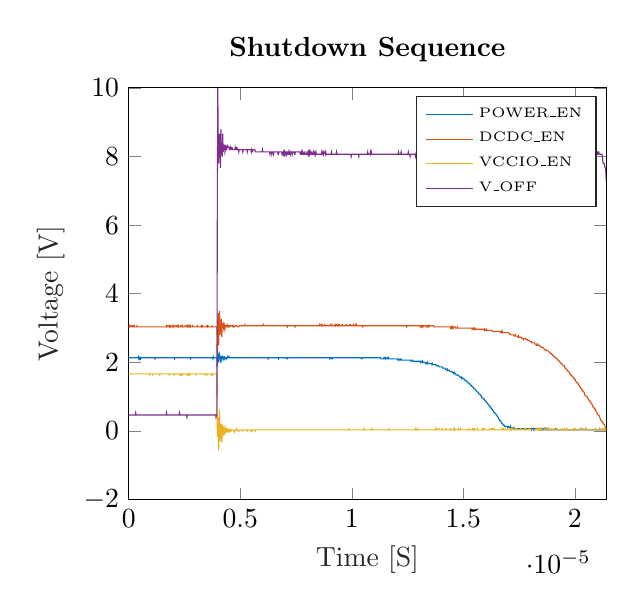
\begin{tikzpicture}

\begin{axis}[%
width=0.5\textwidth,
%height=3.566in,
at={(0.758in,0.481in)},
scale only axis,
xmin=0,
xmax=2.14e-05,
xlabel style={font=\color{white!15!black}},
xlabel={Time [S]},
ymin=-2,
ymax=10,
ylabel style={font=\color{white!15!black}},
ylabel={Voltage [V]},
axis background/.style={fill=white},
title style={font=\bfseries},
title={Shutdown Sequence},
legend style={legend cell align=left,font=\tiny, align=left, draw=white!15!black}
]
\addplot [color=mycolor1]
  table[row sep=crcr]{%
-6.20000006890109e-09	2.13333\\
4.13800000043096e-07	2.13333\\
4.33799999921547e-07	2.16667\\
4.53799999799998e-07	2.1\\
4.73800000122537e-07	2.13333\\
4.93800000000988e-07	2.1\\
5.13799999879438e-07	2.13333\\
5.33800000201978e-07	2.1\\
5.53800000080429e-07	2.13333\\
1.15379999998666e-06	2.13333\\
1.17379999986511e-06	2.1\\
1.19380000018765e-06	2.13333\\
2.03379999996756e-06	2.13333\\
2.05379999984601e-06	2.1\\
2.07380000016855e-06	2.13333\\
2.75380000003267e-06	2.13333\\
2.77379999991112e-06	2.1\\
2.79379999978957e-06	2.13333\\
3.75380000017245e-06	2.13333\\
3.7738000000509e-06	2.1\\
3.79379999992935e-06	2.16667\\
3.8137999998078e-06	2.13333\\
3.95379999984513e-06	2.13333\\
3.97380000016767e-06	1.86667\\
3.99380000004612e-06	2.3\\
4.01379999992457e-06	2.2\\
4.03379999980302e-06	2\\
4.05380000012556e-06	2.16667\\
4.07380000000401e-06	2.23333\\
4.09379999988246e-06	2.13333\\
4.113800000205e-06	2.06667\\
4.13380000008345e-06	2.16667\\
4.1537999999619e-06	2.16667\\
4.17379999984036e-06	2.06667\\
4.1938000001629e-06	2.13333\\
4.21380000004135e-06	2.16667\\
4.25379999979825e-06	2.1\\
4.27380000012079e-06	2.16667\\
4.29379999999924e-06	2.16667\\
4.31379999987769e-06	2.1\\
4.33380000020023e-06	2.13333\\
4.37379999995713e-06	2.13333\\
4.39379999983558e-06	2.1\\
4.43380000003657e-06	2.16667\\
4.45379999991502e-06	2.13333\\
4.47379999979347e-06	2.13333\\
4.49380000011601e-06	2.16667\\
4.51379999999446e-06	2.13333\\
6.23380000019935e-06	2.13333\\
6.2538000000778e-06	2.1\\
6.27379999995625e-06	2.13333\\
6.69380000006825e-06	2.13333\\
6.7137999999467e-06	2.1\\
6.73379999982515e-06	2.13333\\
7.07379999997926e-06	2.13333\\
7.09379999985771e-06	2.1\\
7.11380000018025e-06	2.1\\
7.1338000000587e-06	2.13333\\
8.99379999985683e-06	2.13333\\
9.01380000017937e-06	2.1\\
9.03380000005782e-06	2.13333\\
9.07379999981472e-06	2.13333\\
9.09380000013726e-06	2.1\\
9.11380000001571e-06	2.1\\
9.13379999989417e-06	2.13333\\
1.04138000001086e-05	2.13333\\
1.04337999999871e-05	2.1\\
1.04537999998655e-05	2.1\\
1.0473800000188e-05	2.13333\\
1.12938000000895e-05	2.13333\\
1.1313799999968e-05	2.1\\
1.14137999998043e-05	2.1\\
1.14338000001268e-05	2.13333\\
1.14737999998837e-05	2.13333\\
1.14938000002063e-05	2.1\\
1.15138000000847e-05	2.13333\\
1.15337999999632e-05	2.1\\
1.15738000001642e-05	2.1\\
1.15938000000426e-05	2.13333\\
1.16137999999211e-05	2.1\\
1.16337999997995e-05	2.1\\
1.16538000001221e-05	2.13333\\
1.16738000000005e-05	2.1\\
1.20338000000331e-05	2.1\\
1.20537999999115e-05	2.06667\\
1.20938000001125e-05	2.06667\\
1.2113799999991e-05	2.1\\
1.21337999998694e-05	2.06667\\
1.21738000000704e-05	2.06667\\
1.21937999999489e-05	2.1\\
1.22137999998273e-05	2.1\\
1.22338000001498e-05	2.06667\\
1.26337999999393e-05	2.06667\\
1.26537999998177e-05	2.03333\\
1.26738000001403e-05	2.06667\\
1.27137999998972e-05	2.06667\\
1.27338000002197e-05	2.03333\\
1.30538000000513e-05	2.03333\\
1.30737999999297e-05	2\\
1.30937999998082e-05	2.03333\\
1.31338000000092e-05	2.03333\\
1.31537999998876e-05	2\\
1.31738000002102e-05	2.03333\\
1.31938000000886e-05	2\\
1.3293799999925e-05	2\\
1.33137999998034e-05	1.96667\\
1.3333800000126e-05	2\\
1.33538000000044e-05	2\\
1.33737999998829e-05	1.96667\\
1.33938000002054e-05	2\\
1.34138000000839e-05	1.96667\\
1.35737999999996e-05	1.96667\\
1.35937999998781e-05	1.93333\\
1.36138000002006e-05	1.96667\\
1.36338000000791e-05	1.93333\\
1.37738000001164e-05	1.93333\\
1.37937999999949e-05	1.9\\
1.38937999998312e-05	1.9\\
1.39138000001537e-05	1.86667\\
1.40538000001911e-05	1.86667\\
1.40738000000695e-05	1.83333\\
1.41737999999059e-05	1.83333\\
1.41937999997843e-05	1.8\\
1.42537999998638e-05	1.8\\
1.42738000001863e-05	1.76667\\
1.42938000000647e-05	1.8\\
1.43137999999432e-05	1.76667\\
1.43738000000226e-05	1.76667\\
1.43937999999011e-05	1.73333\\
1.44938000001815e-05	1.73333\\
1.451380000006e-05	1.7\\
1.45537999998169e-05	1.7\\
1.45738000001394e-05	1.66667\\
1.45938000000179e-05	1.66667\\
1.46137999998963e-05	1.7\\
1.46338000002189e-05	1.66667\\
1.46538000000973e-05	1.66667\\
1.46737999999758e-05	1.63333\\
1.47737999998121e-05	1.63333\\
1.47938000001346e-05	1.6\\
1.48337999998915e-05	1.6\\
1.48538000002141e-05	1.56667\\
1.4893799999971e-05	1.56667\\
1.49137999998494e-05	1.53333\\
1.4933800000172e-05	1.56667\\
1.49538000000504e-05	1.53333\\
1.50138000001299e-05	1.53333\\
1.50338000000083e-05	1.5\\
1.50537999998868e-05	1.5\\
1.50738000002093e-05	1.46667\\
1.51337999998447e-05	1.46667\\
1.51538000001672e-05	1.43333\\
1.51937999999241e-05	1.43333\\
1.52137999998025e-05	1.4\\
1.52538000000035e-05	1.4\\
1.5273799999882e-05	1.36667\\
1.5313800000083e-05	1.36667\\
1.53337999999614e-05	1.33333\\
1.53537999998399e-05	1.33333\\
1.53738000001624e-05	1.3\\
1.54137999999193e-05	1.3\\
1.54337999997978e-05	1.26667\\
1.54538000001203e-05	1.26667\\
1.54737999999988e-05	1.23333\\
1.55138000001998e-05	1.23333\\
1.55338000000782e-05	1.2\\
1.55537999999567e-05	1.2\\
1.55737999998351e-05	1.16667\\
1.55938000001576e-05	1.16667\\
1.56138000000361e-05	1.13333\\
1.56738000001155e-05	1.13333\\
1.57137999998724e-05	1.06667\\
1.57538000000734e-05	1.06667\\
1.57737999999519e-05	1.03333\\
1.57937999998303e-05	1.03333\\
1.58338000000313e-05	0.966667\\
1.58737999997882e-05	0.966667\\
1.58938000001108e-05	0.933333\\
1.59337999998677e-05	0.933333\\
1.59538000001902e-05	0.9\\
1.59738000000686e-05	0.9\\
1.59937999999471e-05	0.866667\\
1.60137999998256e-05	0.866667\\
1.60338000001481e-05	0.833333\\
1.60538000000265e-05	0.833333\\
1.6073799999905e-05	0.8\\
1.60937999997834e-05	0.8\\
1.6113800000106e-05	0.766667\\
1.61337999999844e-05	0.766667\\
1.61537999998629e-05	0.733333\\
1.61738000001854e-05	0.733333\\
1.61938000000639e-05	0.7\\
1.62137999999423e-05	0.7\\
1.62337999998208e-05	0.666667\\
1.62538000001433e-05	0.666667\\
1.62738000000218e-05	0.633333\\
1.62937999999002e-05	0.633333\\
1.63137999997787e-05	0.6\\
1.63338000001012e-05	0.6\\
1.63737999998581e-05	0.533333\\
1.64138000000591e-05	0.533333\\
1.64337999999375e-05	0.5\\
1.6453799999816e-05	0.5\\
1.64738000001385e-05	0.466667\\
1.6493800000017e-05	0.466667\\
1.65137999998954e-05	0.433333\\
1.6533800000218e-05	0.433333\\
1.65937999998533e-05	0.333333\\
1.66138000001759e-05	0.333333\\
1.66338000000543e-05	0.3\\
1.66737999998112e-05	0.3\\
1.67138000000122e-05	0.233333\\
1.67337999998907e-05	0.233333\\
1.67538000002132e-05	0.2\\
1.67738000000917e-05	0.2\\
1.67937999999701e-05	0.166667\\
1.68338000001711e-05	0.166667\\
1.68538000000495e-05	0.133333\\
1.69738000002084e-05	0.133333\\
1.69938000000869e-05	0.1\\
1.70137999999653e-05	0.133333\\
1.70337999998438e-05	0.133333\\
1.70538000001663e-05	0.1\\
1.70937999999232e-05	0.1\\
1.71137999998017e-05	0.133333\\
1.71338000001242e-05	0.0666666999999999\\
1.71538000000027e-05	0.1\\
1.71938000002037e-05	0.1\\
1.72138000000821e-05	0.0666666999999999\\
1.7253799999839e-05	0.0666666999999999\\
1.72738000001615e-05	0.1\\
1.729380000004e-05	0.0666666999999999\\
1.80337999999836e-05	0.0666666999999999\\
1.8053799999862e-05	0.0333332999999998\\
1.80738000001845e-05	0.0666666999999999\\
1.81137999999414e-05	0.0666666999999999\\
1.81337999998199e-05	0.0333332999999998\\
1.81538000001424e-05	0.0666666999999999\\
1.81738000000209e-05	0.0333332999999998\\
1.81937999998993e-05	0.0666666999999999\\
1.83337999999367e-05	0.0666666999999999\\
1.83537999998151e-05	0.0333332999999998\\
1.83938000000161e-05	0.0333332999999998\\
1.84137999998946e-05	0.0666666999999999\\
1.84338000002171e-05	0.0666666999999999\\
1.84538000000956e-05	0.0333332999999998\\
1.8473799999974e-05	0.0333332999999998\\
1.84937999998525e-05	0.0666666999999999\\
1.8513800000175e-05	0.0666666999999999\\
1.85338000000534e-05	0.0333332999999998\\
1.85537999999319e-05	0.0666666999999999\\
1.85737999998103e-05	0.0666666999999999\\
1.85938000001329e-05	0.0333332999999998\\
1.86138000000113e-05	0.0333332999999998\\
1.86337999998898e-05	0.0666666999999999\\
1.86538000002123e-05	0.0333332999999998\\
1.86738000000908e-05	0.0333332999999998\\
1.86937999999692e-05	0.0666666999999999\\
1.87137999998477e-05	0.0333332999999998\\
1.87338000001702e-05	0.0333332999999998\\
1.87538000000487e-05	0.0666666999999999\\
1.87737999999271e-05	0.0333332999999998\\
1.87937999998056e-05	0.0333332999999998\\
1.88138000001281e-05	0.0666666999999999\\
1.88338000000066e-05	0.0333332999999998\\
1.91138000000812e-05	0.0333332999999998\\
1.91337999999597e-05	0.0666666999999999\\
1.91537999998381e-05	0.0666666999999999\\
1.91738000001607e-05	0.0333332999999998\\
2.02537999998142e-05	0.0333332999999998\\
2.02738000001368e-05	0.0666666999999999\\
2.02938000000152e-05	0.0333332999999998\\
2.0453799999931e-05	0.0333332999999998\\
2.04737999998095e-05	0.0666666999999999\\
2.0493800000132e-05	0.0333332999999998\\
2.10938000000382e-05	0.0333332999999998\\
2.11137999999167e-05	0.0666666999999999\\
2.11337999997951e-05	0.0333332999999998\\
2.14137999998698e-05	0.0333332999999998\\
};
\addlegendentry{POWER\_EN}

\addplot [color=mycolor2]
  table[row sep=crcr]{%
-6.20000006890109e-09	3.06667\\
1.37999998095495e-08	3.03333\\
3.38000001320893e-08	3.06667\\
5.38000000105399e-08	3.03333\\
7.37999998889904e-08	3.03333\\
9.38000002115302e-08	3.06667\\
1.33799999968431e-07	3.06667\\
1.53799999846882e-07	3.03333\\
1.73800000169422e-07	3.03333\\
1.93800000047872e-07	3.06667\\
2.13799999926323e-07	3.03333\\
2.33799999804774e-07	3.03333\\
2.53800000127313e-07	3.06667\\
2.73800000005764e-07	3.03333\\
3.53799999963655e-07	3.03333\\
3.73799999842106e-07	3.06667\\
3.93800000164646e-07	3.03333\\
1.673799999935e-06	3.03333\\
1.69379999981345e-06	3.06667\\
1.71380000013599e-06	3.03333\\
1.73380000001444e-06	3.06667\\
1.79380000009388e-06	3.06667\\
1.81379999997233e-06	3.03333\\
1.83379999985078e-06	3.06667\\
1.85380000017332e-06	3.03333\\
1.87380000005177e-06	3.06667\\
1.89379999993022e-06	3.06667\\
1.91379999980867e-06	3.03333\\
1.95380000000966e-06	3.03333\\
1.97379999988812e-06	3.06667\\
1.99380000021065e-06	3.03333\\
2.01380000008911e-06	3.06667\\
2.03379999996756e-06	3.03333\\
2.07380000016855e-06	3.03333\\
2.093800000047e-06	3.06667\\
2.1337999998039e-06	3.06667\\
2.15380000012644e-06	3.03333\\
2.17380000000489e-06	3.03333\\
2.19379999988334e-06	3.06667\\
2.21380000020588e-06	3.03333\\
2.23380000008433e-06	3.06667\\
2.25379999996278e-06	3.03333\\
2.31380000004222e-06	3.03333\\
2.33379999992067e-06	3.06667\\
2.37380000012166e-06	3.06667\\
2.39380000000011e-06	3.03333\\
2.41379999987856e-06	3.06667\\
2.4338000002011e-06	3.03333\\
2.51380000015899e-06	3.03333\\
2.53380000003744e-06	3.06667\\
2.57379999979435e-06	3.06667\\
2.59380000011689e-06	3.03333\\
2.61379999999534e-06	3.03333\\
2.63379999987379e-06	3.06667\\
2.65380000019633e-06	3.03333\\
2.67380000007478e-06	3.06667\\
2.69379999995323e-06	3.03333\\
2.71379999983168e-06	3.03333\\
2.73380000015422e-06	3.06667\\
2.75380000003267e-06	3.03333\\
2.77379999991112e-06	3.06667\\
2.79379999978957e-06	3.03333\\
2.85379999986901e-06	3.03333\\
2.87380000019155e-06	3.06667\\
2.89380000007e-06	3.03333\\
3.05379999998578e-06	3.03333\\
3.07379999986424e-06	3.06667\\
3.09380000018677e-06	3.03333\\
3.23379999978002e-06	3.03333\\
3.25380000010256e-06	3.06667\\
3.27379999998101e-06	3.03333\\
3.29379999985946e-06	3.06667\\
3.313800000182e-06	3.06667\\
3.33380000006045e-06	3.03333\\
3.47380000009778e-06	3.03333\\
3.49379999997623e-06	3.06667\\
3.51379999985468e-06	3.06667\\
3.53380000017722e-06	3.03333\\
3.55380000005567e-06	3.06667\\
3.57379999993412e-06	3.03333\\
3.71379999997146e-06	3.03333\\
3.73379999984991e-06	3.06667\\
3.75380000017245e-06	3.03333\\
3.95379999984513e-06	3.03333\\
3.97380000016767e-06	2.3\\
3.99380000004612e-06	3.26667\\
4.01379999992457e-06	3.43333\\
4.03379999980302e-06	2.5\\
4.05380000012556e-06	3.16667\\
4.07380000000401e-06	3.5\\
4.09379999988246e-06	2.8\\
4.113800000205e-06	2.96667\\
4.13380000008345e-06	3.06667\\
4.1537999999619e-06	3.26667\\
4.17379999984036e-06	2.73333\\
4.1938000001629e-06	3.13333\\
4.21380000004135e-06	3.13333\\
4.25379999979825e-06	3\\
4.27380000012079e-06	3.13333\\
4.29379999999924e-06	3.1\\
4.31379999987769e-06	2.96667\\
4.33380000020023e-06	3.06667\\
4.35380000007868e-06	3.06667\\
4.37379999995713e-06	3.03333\\
4.39379999983558e-06	3.03333\\
4.41380000015812e-06	3.1\\
4.45379999991502e-06	3.03333\\
4.47379999979347e-06	3.06667\\
4.49380000011601e-06	3.06667\\
4.51379999999446e-06	3.03333\\
4.53379999987291e-06	3.03333\\
4.55380000019545e-06	3.06667\\
4.65380000003179e-06	3.06667\\
4.67379999991024e-06	3.03333\\
4.69379999978869e-06	3.06667\\
4.71380000011123e-06	3.03333\\
4.75379999986814e-06	3.03333\\
4.77380000019068e-06	3.06667\\
4.85380000014857e-06	3.06667\\
4.87380000002702e-06	3.03333\\
4.93380000010646e-06	3.03333\\
4.95379999998491e-06	3.06667\\
5.19379999985858e-06	3.06667\\
5.21380000018112e-06	3.1\\
5.23380000005957e-06	3.06667\\
6.01380000020413e-06	3.06667\\
6.03380000008258e-06	3.1\\
6.05379999996103e-06	3.06667\\
7.09379999985771e-06	3.06667\\
7.11380000018025e-06	3.03333\\
7.1338000000587e-06	3.06667\\
7.43380000001181e-06	3.06667\\
7.45379999989026e-06	3.03333\\
7.4738000002128e-06	3.06667\\
8.53379999998793e-06	3.06667\\
8.55379999986638e-06	3.1\\
8.57380000018892e-06	3.06667\\
8.59380000006738e-06	3.1\\
8.63379999982428e-06	3.1\\
8.65380000014682e-06	3.06667\\
8.67380000002527e-06	3.1\\
8.69379999990372e-06	3.06667\\
8.77379999986161e-06	3.06667\\
8.79380000018415e-06	3.1\\
8.8138000000626e-06	3.06667\\
9.01380000017937e-06	3.06667\\
9.03380000005782e-06	3.1\\
9.05379999993627e-06	3.06667\\
9.09380000013726e-06	3.06667\\
9.11380000001571e-06	3.1\\
9.13379999989417e-06	3.06667\\
9.2338000001746e-06	3.06667\\
9.25380000005305e-06	3.1\\
9.2737999999315e-06	3.06667\\
9.29379999980995e-06	3.1\\
9.31380000013249e-06	3.1\\
9.33380000001094e-06	3.06667\\
9.35379999988939e-06	3.06667\\
9.37380000021193e-06	3.1\\
9.39380000009038e-06	3.06667\\
9.41379999996883e-06	3.1\\
9.43379999984728e-06	3.1\\
9.45380000016982e-06	3.06667\\
9.53380000012771e-06	3.06667\\
9.55380000000616e-06	3.1\\
9.57379999988461e-06	3.1\\
9.59380000020715e-06	3.06667\\
9.7337999998004e-06	3.06667\\
9.75380000012294e-06	3.1\\
9.77380000000139e-06	3.1\\
9.79379999987984e-06	3.06667\\
9.89380000016027e-06	3.06667\\
9.91380000003872e-06	3.1\\
9.93379999991717e-06	3.1\\
9.95379999979562e-06	3.06667\\
1.00538000000761e-05	3.06667\\
1.00737999999545e-05	3.1\\
1.0093799999833e-05	3.06667\\
1.01338000000339e-05	3.06667\\
1.01537999999124e-05	3.1\\
1.01737999997908e-05	3.06667\\
1.01938000001134e-05	3.06667\\
1.02137999999918e-05	3.1\\
1.02337999998703e-05	3.06667\\
1.0473800000188e-05	3.06667\\
1.04938000000665e-05	3.03333\\
1.0513799999945e-05	3.06667\\
1.24337999998225e-05	3.06667\\
1.24538000001451e-05	3.03333\\
1.24738000000235e-05	3.06667\\
1.30538000000513e-05	3.06667\\
1.30737999999297e-05	3.03333\\
1.30937999998082e-05	3.06667\\
1.31138000001307e-05	3.06667\\
1.31338000000092e-05	3.03333\\
1.31537999998876e-05	3.06667\\
1.31738000002102e-05	3.06667\\
1.31938000000886e-05	3.03333\\
1.32137999999671e-05	3.06667\\
1.3293799999925e-05	3.06667\\
1.33137999998034e-05	3.03333\\
1.33538000000044e-05	3.03333\\
1.33737999998829e-05	3.06667\\
1.33938000002054e-05	3.06667\\
1.34138000000839e-05	3.03333\\
1.34337999999623e-05	3.06667\\
1.34537999998408e-05	3.03333\\
1.34738000001633e-05	3.03333\\
1.34938000000417e-05	3.06667\\
1.3673799999836e-05	3.06667\\
1.36938000001585e-05	3.03333\\
1.44137999997795e-05	3.03333\\
1.44338000001021e-05	3\\
1.44537999999805e-05	3.03333\\
1.4473799999859e-05	3\\
1.44938000001815e-05	3.03333\\
1.451380000006e-05	3\\
1.45337999999384e-05	3.03333\\
1.45537999998169e-05	3\\
1.45738000001394e-05	3.03333\\
1.46338000002189e-05	3.03333\\
1.46538000000973e-05	3\\
1.47138000001767e-05	3\\
1.47338000000552e-05	3.03333\\
1.47537999999336e-05	3\\
1.53738000001624e-05	3\\
1.53938000000409e-05	2.96667\\
1.54137999999193e-05	3\\
1.54337999997978e-05	3\\
1.54538000001203e-05	2.96667\\
1.54737999999988e-05	3\\
1.54937999998772e-05	2.96667\\
1.55138000001998e-05	3\\
1.55338000000782e-05	3\\
1.55537999999567e-05	2.96667\\
1.59137999999892e-05	2.96667\\
1.59337999998677e-05	2.93333\\
1.59538000001902e-05	2.96667\\
1.59738000000686e-05	2.93333\\
1.60137999998256e-05	2.93333\\
1.60338000001481e-05	2.96667\\
1.60538000000265e-05	2.93333\\
1.62937999999002e-05	2.93333\\
1.63137999997787e-05	2.9\\
1.66537999999328e-05	2.9\\
1.66737999998112e-05	2.86667\\
1.66938000001338e-05	2.86667\\
1.67138000000122e-05	2.9\\
1.67337999998907e-05	2.86667\\
1.67538000002132e-05	2.9\\
1.67738000000917e-05	2.86667\\
1.70337999998438e-05	2.86667\\
1.70538000001663e-05	2.83333\\
1.70937999999232e-05	2.83333\\
1.71137999998017e-05	2.8\\
1.7253799999839e-05	2.8\\
1.72738000001615e-05	2.76667\\
1.73137999999184e-05	2.76667\\
1.73337999997969e-05	2.8\\
1.73538000001194e-05	2.76667\\
1.74338000000773e-05	2.76667\\
1.74537999999558e-05	2.73333\\
1.74737999998342e-05	2.76667\\
1.74938000001568e-05	2.73333\\
1.75937999999931e-05	2.73333\\
1.76137999998716e-05	2.7\\
1.7673799999951e-05	2.7\\
1.76937999998295e-05	2.66667\\
1.7713800000152e-05	2.7\\
1.77737999997873e-05	2.7\\
1.77938000001099e-05	2.66667\\
1.78738000000678e-05	2.66667\\
1.78937999999462e-05	2.63333\\
1.79737999999041e-05	2.63333\\
1.79937999997826e-05	2.6\\
1.8053799999862e-05	2.6\\
1.80738000001845e-05	2.56667\\
1.81937999998993e-05	2.56667\\
1.82138000002219e-05	2.53333\\
1.82537999999788e-05	2.53333\\
1.82737999998572e-05	2.5\\
1.82938000001798e-05	2.5\\
1.83138000000582e-05	2.53333\\
1.83337999999367e-05	2.5\\
1.84137999998946e-05	2.5\\
1.84338000002171e-05	2.46667\\
1.8473799999974e-05	2.46667\\
1.84937999998525e-05	2.43333\\
1.85938000001329e-05	2.43333\\
1.86337999998898e-05	2.36667\\
1.87137999998477e-05	2.36667\\
1.87338000001702e-05	2.33333\\
1.88138000001281e-05	2.33333\\
1.88338000000066e-05	2.3\\
1.88738000002076e-05	2.3\\
1.8893800000086e-05	2.26667\\
1.89337999998429e-05	2.26667\\
1.89538000001654e-05	2.23333\\
1.89937999999223e-05	2.23333\\
1.90137999998008e-05	2.2\\
1.90338000001233e-05	2.2\\
1.90538000000018e-05	2.16667\\
1.90938000002028e-05	2.16667\\
1.91138000000812e-05	2.13333\\
1.91537999998381e-05	2.13333\\
1.91738000001607e-05	2.1\\
1.92137999999176e-05	2.1\\
1.9233799999796e-05	2.06667\\
1.9273799999997e-05	2.06667\\
1.92937999998755e-05	2.03333\\
1.9313800000198e-05	2.03333\\
1.93338000000765e-05	2\\
1.93537999999549e-05	2\\
1.93737999998334e-05	1.96667\\
1.94138000000343e-05	1.96667\\
1.94337999999128e-05	1.93333\\
1.94537999997912e-05	1.93333\\
1.94738000001138e-05	1.9\\
1.95338000001932e-05	1.9\\
1.95538000000717e-05	1.83333\\
1.95937999998286e-05	1.83333\\
1.96138000001511e-05	1.8\\
1.96338000000296e-05	1.8\\
1.9653799999908e-05	1.76667\\
1.96737999997865e-05	1.76667\\
1.9693800000109e-05	1.73333\\
1.97337999998659e-05	1.73333\\
1.97738000000669e-05	1.66667\\
1.97937999999453e-05	1.66667\\
1.98137999998238e-05	1.63333\\
1.98338000001463e-05	1.63333\\
1.98538000000248e-05	1.6\\
1.98937999997817e-05	1.6\\
1.99138000001042e-05	1.56667\\
1.99337999999827e-05	1.56667\\
1.99537999998611e-05	1.53333\\
1.99738000001837e-05	1.53333\\
1.9993799999618e-05	1.5\\
2.00137999999406e-05	1.5\\
2.00538000001416e-05	1.43333\\
2.007380000002e-05	1.43333\\
2.00937999998985e-05	1.4\\
2.01338000000995e-05	1.4\\
2.01737999998564e-05	1.33333\\
2.01938000001789e-05	1.33333\\
2.02337999999358e-05	1.26667\\
2.02537999998142e-05	1.26667\\
2.02738000001368e-05	1.23333\\
2.02938000000152e-05	1.23333\\
2.03137999998937e-05	1.2\\
2.03338000002162e-05	1.2\\
2.03538000000947e-05	1.16667\\
2.03737999999731e-05	1.16667\\
2.03937999998516e-05	1.13333\\
2.04138000001741e-05	1.13333\\
2.04338000000526e-05	1.1\\
2.0453799999931e-05	1.03333\\
2.0493800000132e-05	1.03333\\
2.05138000000105e-05	1\\
2.05538000002115e-05	1\\
2.05937999999684e-05	0.933333\\
2.06137999998468e-05	0.933333\\
2.06538000000478e-05	0.866667\\
2.06937999998047e-05	0.866667\\
2.07338000000057e-05	0.8\\
2.07537999998841e-05	0.8\\
2.08137999999636e-05	0.7\\
2.0833799999842e-05	0.7\\
2.08538000001646e-05	0.666667\\
2.0873800000043e-05	0.666667\\
2.08937999999215e-05	0.633333\\
2.09137999997999e-05	0.633333\\
2.09737999998794e-05	0.533333\\
2.09938000002019e-05	0.533333\\
2.10337999999588e-05	0.466667\\
2.10738000001598e-05	0.466667\\
2.11737999999961e-05	0.3\\
2.11937999998746e-05	0.3\\
2.12138000001971e-05	0.266667\\
2.1253799999954e-05	0.266667\\
2.12737999998325e-05	0.2\\
2.13138000000335e-05	0.2\\
2.13537999997904e-05	0.133333\\
2.13738000001129e-05	0.133333\\
2.14137999998698e-05	0.0666666999999999\\
};
\addlegendentry{DCDC\_EN}

\addplot [color=mycolor3]
  table[row sep=crcr]{%
-6.20000006890109e-09	1.66667\\
9.13799999890941e-07	1.66667\\
9.33799999991436e-07	1.63333\\
9.53800000091931e-07	1.66667\\
1.05379999992827e-06	1.66667\\
1.07380000002877e-06	1.63333\\
1.09379999990722e-06	1.66667\\
1.35380000010343e-06	1.66667\\
1.37379999998188e-06	1.63333\\
1.39380000008238e-06	1.63333\\
1.41379999996083e-06	1.66667\\
1.79380000009388e-06	1.66667\\
1.81379999997233e-06	1.63333\\
1.83380000007283e-06	1.66667\\
2.01380000008911e-06	1.66667\\
2.03379999996756e-06	1.63333\\
2.05380000006805e-06	1.63333\\
2.0737999999465e-06	1.66667\\
2.27380000006328e-06	1.66667\\
2.29379999994173e-06	1.63333\\
2.31380000004222e-06	1.66667\\
2.33379999992067e-06	1.66667\\
2.35380000002117e-06	1.63333\\
2.37379999989962e-06	1.66667\\
2.39380000000011e-06	1.66667\\
2.41380000010061e-06	1.63333\\
2.43379999997906e-06	1.66667\\
2.59379999989484e-06	1.66667\\
2.61379999999534e-06	1.63333\\
2.63380000009583e-06	1.66667\\
2.65379999997428e-06	1.66667\\
2.67380000007478e-06	1.63333\\
2.69379999995323e-06	1.63333\\
2.71380000005372e-06	1.66667\\
2.73379999993217e-06	1.63333\\
2.75380000003267e-06	1.66667\\
2.99379999990634e-06	1.66667\\
3.01380000000684e-06	1.63333\\
3.03380000010733e-06	1.66667\\
3.39379999991785e-06	1.66667\\
3.41380000001834e-06	1.63333\\
3.43379999989679e-06	1.66667\\
3.49379999997623e-06	1.66667\\
3.51380000007673e-06	1.63333\\
3.53379999995518e-06	1.66667\\
3.67379999999251e-06	1.66667\\
3.69380000009301e-06	1.63333\\
3.71379999997146e-06	1.66667\\
3.73380000007195e-06	1.66667\\
3.7537999999504e-06	1.63333\\
3.7738000000509e-06	1.66667\\
3.95380000006718e-06	1.66667\\
3.97379999994563e-06	-0.166667\\
3.99380000004612e-06	0.266667\\
4.01379999992457e-06	0.4\\
4.03380000002507e-06	-0.566667\\
4.05379999990352e-06	-0.0666667000000001\\
4.07380000000401e-06	0.633333\\
4.09380000010451e-06	-0.3\\
4.11379999998296e-06	-0.133333\\
4.13380000008345e-06	0.1\\
4.1537999999619e-06	0.2\\
4.1738000000624e-06	-0.333333\\
4.19379999994085e-06	0.0666667000000001\\
4.21380000004135e-06	0.133333\\
4.2337999999198e-06	0.0333333\\
4.25380000002029e-06	-0.133333\\
4.27379999989874e-06	0.133333\\
4.31380000009973e-06	-0.0666667000000001\\
4.33379999997818e-06	-0.0333333\\
4.35380000007868e-06	0.0666667000000001\\
4.37379999995713e-06	-0.0333333\\
4.39380000005762e-06	-0.0333333\\
4.41379999993607e-06	0.0666667000000001\\
4.43380000003657e-06	0.0666667000000001\\
4.45379999991502e-06	0\\
4.47380000001552e-06	0.0333333\\
4.49379999989397e-06	0.0333333\\
4.51379999999446e-06	-0.0333333\\
4.53380000009496e-06	-0.0333333\\
4.55379999997341e-06	0.0333333\\
4.5738000000739e-06	0\\
4.59379999995235e-06	0\\
4.61380000005285e-06	0.0333333\\
4.69380000001074e-06	0.0333333\\
4.73379999998969e-06	-0.0333333\\
4.77379999996863e-06	0.0333333\\
4.81379999994758e-06	0.0333333\\
4.83380000004807e-06	0.0666667000000001\\
4.87380000002702e-06	0\\
4.95379999998491e-06	0\\
4.9738000000854e-06	0.0333333\\
5.07379999992175e-06	0.0333333\\
5.09380000002224e-06	0\\
5.11379999990069e-06	0\\
5.13380000000119e-06	0.0333333\\
5.29379999991697e-06	0.0333333\\
5.31380000001747e-06	0\\
5.33379999989592e-06	0.0333333\\
5.4538000000548e-06	0.0333333\\
5.47379999993325e-06	0\\
5.49380000003374e-06	0.0333333\\
5.51379999991219e-06	0.0333333\\
5.53380000001269e-06	0\\
5.55379999989114e-06	0.0333333\\
5.65379999994953e-06	0.0333333\\
5.67380000005002e-06	0\\
5.69379999992847e-06	0.0333333\\
9.85379999995928e-06	0.0333333\\
9.87380000005977e-06	0.0666667000000001\\
9.89379999993822e-06	0.0333333\\
1.05338000000454e-05	0.0333333\\
1.05537999999239e-05	0.0666667000000001\\
1.05738000000244e-05	0.0333333\\
1.08737999999775e-05	0.0333333\\
1.0893800000078e-05	0.0666667000000001\\
1.09137999999565e-05	0.0333333\\
1.16537999999e-05	0.0333333\\
1.16738000000005e-05	0.0666667000000001\\
1.1693800000101e-05	0.0333333\\
1.28338000000561e-05	0.0333333\\
1.28537999999345e-05	0.0666667000000001\\
1.2873800000035e-05	0.0333333\\
1.2913800000014e-05	0.0333333\\
1.29337999998924e-05	0.0666667000000001\\
1.29537999999929e-05	0.0333333\\
1.37337999999154e-05	0.0333333\\
1.37538000000159e-05	0.0666667000000001\\
1.37737999998944e-05	0.0333333\\
1.37937999999949e-05	0.0333333\\
1.38138000000954e-05	0.0666667000000001\\
1.38337999999738e-05	0.0333333\\
1.38938000000532e-05	0.0333333\\
1.39137999999317e-05	0.0666667000000001\\
1.39338000000322e-05	0.0333333\\
1.40338000000906e-05	0.0333333\\
1.4053799999969e-05	0.0666667000000001\\
1.40738000000695e-05	0.0333333\\
1.41938000000064e-05	0.0333333\\
1.42138000001069e-05	0.0666667000000001\\
1.42337999999853e-05	0.0666667000000001\\
1.42538000000858e-05	0.0333333\\
1.43937999999011e-05	0.0333333\\
1.44138000000016e-05	0.0666667000000001\\
1.44338000001021e-05	0.0666667000000001\\
1.44537999999805e-05	0.0333333\\
1.45538000000389e-05	0.0333333\\
1.45737999999174e-05	0.0666667000000001\\
1.45938000000179e-05	0.0333333\\
1.46137999998963e-05	0.0666667000000001\\
1.46337999999968e-05	0.0333333\\
1.47537999999336e-05	0.0333333\\
1.47738000000341e-05	0.0666667000000001\\
1.47937999999126e-05	0.0333333\\
1.4853799999992e-05	0.0333333\\
1.48738000000925e-05	0.0666667000000001\\
1.4893799999971e-05	0.0333333\\
1.5233799999903e-05	0.0333333\\
1.52538000000035e-05	0.0666667000000001\\
1.5273800000104e-05	0.0333333\\
1.53938000000409e-05	0.0333333\\
1.54137999999193e-05	0.0666667000000001\\
1.54338000000198e-05	0.0666667000000001\\
1.54537999998983e-05	0.0333333\\
1.54737999999988e-05	0.0666667000000001\\
1.54938000000993e-05	0.0666667000000001\\
1.55137999999777e-05	0.0333333\\
1.56138000000361e-05	0.0333333\\
1.56337999999145e-05	0.0666667000000001\\
1.5653800000015e-05	0.0333333\\
1.58537999999098e-05	0.0333333\\
1.58738000000103e-05	0.0666667000000001\\
1.58938000001108e-05	0.0333333\\
1.59137999999892e-05	0.0666667000000001\\
1.59537999999682e-05	0.0666667000000001\\
1.59738000000686e-05	0.0333333\\
1.61737999999634e-05	0.0333333\\
1.61938000000639e-05	0.0666667000000001\\
1.62537999999213e-05	0.0666667000000001\\
1.62738000000218e-05	0.0333333\\
1.62937999999002e-05	0.0333333\\
1.63138000000007e-05	0.0666667000000001\\
1.63338000001012e-05	0.0333333\\
1.63738000000802e-05	0.0333333\\
1.63937999999586e-05	0.0666667000000001\\
1.64138000000591e-05	0.0333333\\
1.67138000000122e-05	0.0333333\\
1.67337999998907e-05	0.0666667000000001\\
1.67537999999912e-05	0.0333333\\
1.67738000000917e-05	0.0333333\\
1.67937999999701e-05	0.0666667000000001\\
1.68138000000706e-05	0.0333333\\
1.6873799999928e-05	0.0333333\\
1.68938000000285e-05	0.0666667000000001\\
1.69137999999069e-05	0.0333333\\
1.70738000000448e-05	0.0333333\\
1.70937999999232e-05	0.0666667000000001\\
1.71138000000237e-05	0.0666667000000001\\
1.71337999999022e-05	0.0333333\\
1.71538000000027e-05	0.0666667000000001\\
1.71738000001032e-05	0.0333333\\
1.71937999999816e-05	0.0333333\\
1.72138000000821e-05	0.0666667000000001\\
1.72337999999606e-05	0.0333333\\
1.729380000004e-05	0.0333333\\
1.73137999999184e-05	0.0666667000000001\\
1.73338000000189e-05	0.0333333\\
1.73537999998974e-05	0.0333333\\
1.73737999999979e-05	0.0666667000000001\\
1.73938000000984e-05	0.0333333\\
1.75337999999137e-05	0.0333333\\
1.75538000000142e-05	0.0666667000000001\\
1.75737999998926e-05	0.0666667000000001\\
1.75937999999931e-05	0.0333333\\
1.77338000000304e-05	0.0333333\\
1.77537999999089e-05	0.0666667000000001\\
1.77738000000094e-05	0.0333333\\
1.77938000001099e-05	0.0666667000000001\\
1.78137999999883e-05	0.0333333\\
1.79337999999252e-05	0.0333333\\
1.79538000000257e-05	0.0666667000000001\\
1.79737999999041e-05	0.0666667000000001\\
1.79938000000046e-05	0.0333333\\
1.82537999999788e-05	0.0333333\\
1.82738000000793e-05	0.0666667000000001\\
1.82937999999577e-05	0.0333333\\
1.83337999999367e-05	0.0333333\\
1.83538000000372e-05	0.0666667000000001\\
1.83737999999156e-05	0.0333333\\
1.83938000000161e-05	0.0333333\\
1.84137999998946e-05	0.0666667000000001\\
1.84337999999951e-05	0.0333333\\
1.84538000000956e-05	0.0666667000000001\\
1.8473799999974e-05	0.0333333\\
1.84938000000745e-05	0.0666667000000001\\
1.8513799999953e-05	0.0333333\\
1.86337999998898e-05	0.0333333\\
1.86537999999903e-05	0.0666667000000001\\
1.86738000000908e-05	0.0333333\\
1.87337999999482e-05	0.0333333\\
1.87538000000487e-05	0.0666667000000001\\
1.88338000000066e-05	0.0666667000000001\\
1.88538000001071e-05	0.0333333\\
1.89137999999645e-05	0.0333333\\
1.89338000000649e-05	0.0666667000000001\\
1.89537999999434e-05	0.0666667000000001\\
1.89738000000439e-05	0.0333333\\
1.90138000000228e-05	0.0333333\\
1.90337999999013e-05	0.0666667000000001\\
1.90538000000018e-05	0.0666667000000001\\
1.90738000001023e-05	0.0333333\\
1.91737999999386e-05	0.0333333\\
1.91938000000391e-05	0.0666667000000001\\
1.92137999999176e-05	0.0333333\\
1.93937999999338e-05	0.0333333\\
1.94138000000343e-05	0.0666667000000001\\
1.94337999999128e-05	0.0666667000000001\\
1.94538000000133e-05	0.0333333\\
1.95138000000927e-05	0.0333333\\
1.95337999999712e-05	0.0666667000000001\\
1.95538000000717e-05	0.0333333\\
1.96137999999291e-05	0.0333333\\
1.96338000000296e-05	0.0666667000000001\\
1.9653799999908e-05	0.0666667000000001\\
1.96738000000085e-05	0.0333333\\
1.99337999999827e-05	0.0333333\\
1.99538000000832e-05	0.0666667000000001\\
1.99737999999616e-05	0.0333333\\
1.9993799999618e-05	0.0666667000000001\\
2.00137999999406e-05	0.0666667000000001\\
2.00338000000411e-05	0.0333333\\
2.02138000000573e-05	0.0333333\\
2.02337999999358e-05	0.0666667000000001\\
2.02538000000363e-05	0.0333333\\
2.03337999999942e-05	0.0333333\\
2.03538000000947e-05	0.0666667000000001\\
2.03737999999731e-05	0.0666667000000001\\
2.03938000000736e-05	0.0333333\\
2.0453799999931e-05	0.0333333\\
2.04738000000315e-05	0.0666667000000001\\
2.0533800000111e-05	0.0666667000000001\\
2.05537999999894e-05	0.0333333\\
2.0873800000043e-05	0.0333333\\
2.08937999999215e-05	0.0666667000000001\\
2.09337999999004e-05	0.0666667000000001\\
2.09538000000009e-05	0.0333333\\
2.10737999999377e-05	0.0333333\\
2.10938000000382e-05	0.0666667000000001\\
2.11338000000172e-05	0.0666667000000001\\
2.11537999998956e-05	0.0333333\\
2.12338000000756e-05	0.0333333\\
2.1253799999954e-05	0.0666667000000001\\
2.12738000000545e-05	0.0333333\\
2.1293799999933e-05	0.0333333\\
2.13138000000335e-05	0.0666667000000001\\
2.13337999999119e-05	0.0333333\\
2.13538000000124e-05	0.0333333\\
2.13737999998909e-05	0.0666667000000001\\
2.13937999999914e-05	0.0333333\\
2.14138000000919e-05	0.0333333\\
};
\addlegendentry{VCCIO\_EN}

\addplot [color=mycolor4]
  table[row sep=crcr]{%
-6.2000005129903e-09	0.466666999999999\\
2.93799999440125e-07	0.466666999999999\\
3.13799999318576e-07	0.533333000000001\\
3.33799999197026e-07	0.466666999999999\\
1.673799999935e-06	0.466666999999999\\
1.69379999981345e-06	0.533333000000001\\
1.7137999996919e-06	0.466666999999999\\
2.25379999996278e-06	0.466666999999999\\
2.27379999984123e-06	0.533333000000001\\
2.29379999971968e-06	0.466666999999999\\
2.5937999996728e-06	0.466666999999999\\
2.61379999955125e-06	0.4\\
2.6337999994297e-06	0.466666999999999\\
3.89380000065387e-06	0.466666999999999\\
3.91380000053232e-06	0.4\\
3.93380000041077e-06	0.466666999999999\\
3.95380000028922e-06	0.466666999999999\\
3.97380000016767e-06	6.93333\\
3.99380000004612e-06	10\\
4.01379999992457e-06	8.26667\\
4.03379999980302e-06	7.8\\
4.05379999968147e-06	8.4\\
4.07379999955992e-06	8.66667\\
4.09379999943837e-06	8.4\\
4.11379999931683e-06	7.66667\\
4.13379999919528e-06	8.8\\
4.15380000085008e-06	8.06667\\
4.17380000072853e-06	8.26667\\
4.19380000060698e-06	8\\
4.21380000048543e-06	8.66667\\
4.23380000036389e-06	8.13333\\
4.25380000024234e-06	8.26667\\
4.27380000012079e-06	8.33333\\
4.29379999999924e-06	8.33333\\
4.31379999987769e-06	8.13333\\
4.35379999963459e-06	8.26667\\
4.37379999951304e-06	8.2\\
4.39379999939149e-06	8.2\\
4.41379999926994e-06	8.33333\\
4.43379999914839e-06	8.33333\\
4.4538000008032e-06	8.26667\\
4.4938000005601e-06	8.26667\\
4.51380000043855e-06	8.2\\
4.533800000317e-06	8.2\\
4.55380000019545e-06	8.26667\\
4.5738000000739e-06	8.2\\
4.59379999995235e-06	8.2\\
4.6137999998308e-06	8.26667\\
4.63379999970925e-06	8.26667\\
4.6537999995877e-06	8.2\\
4.75380000075631e-06	8.2\\
4.77380000063476e-06	8.26667\\
4.79380000051322e-06	8.2\\
4.81380000039167e-06	8.2\\
4.83380000027012e-06	8.26667\\
4.85380000014857e-06	8.26667\\
4.87380000002702e-06	8.2\\
4.91379999978392e-06	8.2\\
4.93379999966237e-06	8.13333\\
4.95379999954082e-06	8.2\\
5.09380000046633e-06	8.2\\
5.11380000034478e-06	8.13333\\
5.13380000022323e-06	8.2\\
5.29379999925084e-06	8.2\\
5.31379999912929e-06	8.13333\\
5.33380000078409e-06	8.2\\
5.47379999993325e-06	8.2\\
5.4937999998117e-06	8.13333\\
5.51379999969015e-06	8.2\\
5.5337999995686e-06	8.13333\\
5.55379999944705e-06	8.13333\\
5.5737999993255e-06	8.2\\
5.65380000061566e-06	8.2\\
5.67380000049411e-06	8.13333\\
5.97380000044723e-06	8.13333\\
5.99380000032568e-06	8.2\\
6.01380000020413e-06	8.13333\\
6.31380000015724e-06	8.13333\\
6.33380000003569e-06	8.06667\\
6.35379999991414e-06	8.13333\\
6.39379999967105e-06	8.13333\\
6.4137999995495e-06	8.06667\\
6.43379999942795e-06	8.13333\\
6.47379999918485e-06	8.13333\\
6.49380000083966e-06	8.06667\\
6.51380000071811e-06	8.13333\\
6.67379999974571e-06	8.13333\\
6.69379999962416e-06	8.06667\\
6.71379999950261e-06	8.06667\\
6.73379999938106e-06	8.13333\\
6.85380000042812e-06	8.13333\\
6.87380000030657e-06	8.06667\\
6.89380000018502e-06	8.13333\\
6.91380000006347e-06	8.13333\\
6.93379999994193e-06	8.06667\\
6.95379999982038e-06	8.13333\\
6.97379999969883e-06	8.06667\\
6.99379999957728e-06	8.13333\\
7.01379999945573e-06	8.06667\\
7.03379999933418e-06	8.13333\\
7.05379999921263e-06	8.13333\\
7.07380000086744e-06	8.06667\\
7.09380000074589e-06	8.13333\\
7.11380000062434e-06	8.13333\\
7.13380000050279e-06	8.06667\\
7.15380000038124e-06	8.06667\\
7.17380000025969e-06	8.13333\\
7.19380000013814e-06	8.06667\\
7.21380000001659e-06	8.06667\\
7.23379999989504e-06	8.13333\\
7.25379999977349e-06	8.06667\\
7.27379999965194e-06	8.13333\\
7.31379999940884e-06	8.13333\\
7.33379999928729e-06	8.06667\\
7.35379999916574e-06	8.13333\\
7.41380000057745e-06	8.13333\\
7.4338000004559e-06	8.06667\\
7.45380000033435e-06	8.06667\\
7.4738000002128e-06	8.13333\\
7.67380000077367e-06	8.13333\\
7.69380000065212e-06	8.06667\\
7.71380000053057e-06	8.06667\\
7.73380000040902e-06	8.13333\\
7.75380000028747e-06	8.06667\\
7.77380000016592e-06	8.06667\\
7.79380000004437e-06	8.13333\\
7.81379999992282e-06	8.06667\\
7.85379999967972e-06	8.06667\\
7.87379999955817e-06	8.13333\\
7.89379999943662e-06	8.13333\\
7.91379999931507e-06	8.06667\\
7.97380000072678e-06	8.06667\\
7.99380000060523e-06	8.13333\\
8.01380000048368e-06	8.13333\\
8.03380000036213e-06	8.06667\\
8.05380000024059e-06	8.13333\\
8.07380000011904e-06	8.06667\\
8.09379999999749e-06	8.13333\\
8.11379999987594e-06	8.06667\\
8.13379999975439e-06	8.13333\\
8.15379999963284e-06	8.06667\\
8.17379999951129e-06	8.06667\\
8.19379999938974e-06	8.13333\\
8.21379999926819e-06	8.13333\\
8.23379999914664e-06	8.06667\\
8.2738000006799e-06	8.06667\\
8.29380000055835e-06	8.13333\\
8.3138000004368e-06	8.06667\\
8.33380000031525e-06	8.13333\\
8.3538000001937e-06	8.13333\\
8.37380000007215e-06	8.06667\\
8.3937999999506e-06	8.13333\\
8.41379999982905e-06	8.06667\\
8.63380000026837e-06	8.06667\\
8.65380000014682e-06	8.13333\\
8.67380000002527e-06	8.06667\\
8.69379999990372e-06	8.06667\\
8.71379999978217e-06	8.13333\\
8.73379999966062e-06	8.06667\\
8.75379999953907e-06	8.13333\\
8.79379999929597e-06	8.13333\\
8.81379999917442e-06	8.06667\\
8.83380000082923e-06	8.13333\\
8.85380000070768e-06	8.06667\\
9.07379999937064e-06	8.06667\\
9.09379999924909e-06	8.13333\\
9.11379999912754e-06	8.06667\\
9.29379999980995e-06	8.06667\\
9.3137999996884e-06	8.13333\\
9.33379999956685e-06	8.06667\\
9.95379999935153e-06	8.06667\\
9.97379999922998e-06	8\\
9.99380000088479e-06	8.06667\\
1.02938000008379e-05	8.06667\\
1.03138000007164e-05	8\\
1.03338000005948e-05	8.06667\\
1.06938000001833e-05	8.06667\\
1.07138000000617e-05	8.13333\\
1.07337999999402e-05	8.06667\\
1.0813799999454e-05	8.06667\\
1.08337999993324e-05	8.13333\\
1.08537999992109e-05	8.06667\\
1.08738000008657e-05	8.13333\\
1.08938000007441e-05	8.06667\\
1.20738000006781e-05	8.06667\\
1.20938000005566e-05	8.13333\\
1.2113800000435e-05	8.06667\\
1.21937999999489e-05	8.06667\\
1.22137999998273e-05	8.13333\\
1.22337999997058e-05	8.06667\\
1.25137999997804e-05	8.06667\\
1.25337999996589e-05	8.13333\\
1.25537999995373e-05	8.06667\\
1.25937999992942e-05	8.06667\\
1.26137999991727e-05	8\\
1.26338000008275e-05	8.06667\\
1.2833799999612e-05	8.06667\\
1.28537999994904e-05	8\\
1.28937999992473e-05	8.13333\\
1.29137999991258e-05	8.06667\\
1.37337999994713e-05	8.06667\\
1.37537999993498e-05	8.13333\\
1.37737999992282e-05	8.06667\\
1.3793800000883e-05	8.13333\\
1.38138000007615e-05	8.06667\\
1.39937999996675e-05	8.06667\\
1.4013799999546e-05	8.13333\\
1.40337999994244e-05	8.13333\\
1.40537999993029e-05	8.06667\\
1.42138000001069e-05	8.06667\\
1.42337999999853e-05	8.13333\\
1.42537999998638e-05	8.06667\\
1.43737999991345e-05	8.06667\\
1.43938000007893e-05	8.13333\\
1.44138000006677e-05	8.06667\\
1.44338000005462e-05	8.13333\\
1.44538000004246e-05	8.06667\\
1.45737999996953e-05	8.06667\\
1.45937999995738e-05	8.13333\\
1.46137999994522e-05	8.13333\\
1.46337999993307e-05	8.06667\\
1.46938000007424e-05	8.06667\\
1.47138000006208e-05	8.13333\\
1.47338000004993e-05	8.06667\\
1.47738000002562e-05	8.06667\\
1.47938000001346e-05	8.13333\\
1.48138000000131e-05	8.06667\\
1.49938000006955e-05	8.06667\\
1.5013800000574e-05	8.13333\\
1.50338000004524e-05	8.06667\\
1.50538000003309e-05	8.13333\\
1.50738000002093e-05	8.13333\\
1.50938000000878e-05	8.06667\\
1.51737999996016e-05	8.06667\\
1.519379999948e-05	8.13333\\
1.52137999993585e-05	8.06667\\
1.52337999992369e-05	8.13333\\
1.52537999991154e-05	8.06667\\
1.53338000004055e-05	8.06667\\
1.5353800000284e-05	8.13333\\
1.53738000001624e-05	8.06667\\
1.53938000000409e-05	8.13333\\
1.54137999999193e-05	8.06667\\
1.5693799999994e-05	8.06667\\
1.57137999998724e-05	8.13333\\
1.57337999997509e-05	8.06667\\
1.59338000003117e-05	8.06667\\
1.59538000001902e-05	8.13333\\
1.59738000000686e-05	8.06667\\
1.61137999992178e-05	8.06667\\
1.61338000008726e-05	8.13333\\
1.61538000007511e-05	8.06667\\
1.66137999997318e-05	8.06667\\
1.66337999996102e-05	8.13333\\
1.66537999994887e-05	8.06667\\
1.6873799999928e-05	8.06667\\
1.68937999998064e-05	8.13333\\
1.69137999996849e-05	8.06667\\
1.70538000006104e-05	8.06667\\
1.70738000004889e-05	8.13333\\
1.71138000002458e-05	8.13333\\
1.71338000001242e-05	8.06667\\
1.71538000000027e-05	8.13333\\
1.71737999998811e-05	8.06667\\
1.73338000006851e-05	8.06667\\
1.73538000005635e-05	8.13333\\
1.7373800000442e-05	8.06667\\
1.73938000003204e-05	8.06667\\
1.74138000001989e-05	8.13333\\
1.74338000000773e-05	8.13333\\
1.74537999999558e-05	8.06667\\
1.75137999995911e-05	8.06667\\
1.75337999994696e-05	8.13333\\
1.7553799999348e-05	8.06667\\
1.76138000007597e-05	8.06667\\
1.76338000006382e-05	8.13333\\
1.76538000005166e-05	8.06667\\
1.76738000003951e-05	8.13333\\
1.76938000002735e-05	8.06667\\
1.7713800000152e-05	8.13333\\
1.77338000000304e-05	8.06667\\
1.78337999994227e-05	8.06667\\
1.78537999993011e-05	8.13333\\
1.78737999991796e-05	8.06667\\
1.82338000005444e-05	8.06667\\
1.82538000004229e-05	8\\
1.82738000003013e-05	8.06667\\
1.82938000001798e-05	8.06667\\
1.83138000000582e-05	8.13333\\
1.83337999999367e-05	8.06667\\
1.83737999996936e-05	8.06667\\
1.8393799999572e-05	8.13333\\
1.84137999994505e-05	8.06667\\
1.85138000006191e-05	8.06667\\
1.85338000004975e-05	8.13333\\
1.85938000001329e-05	8.13333\\
1.86138000000113e-05	8.06667\\
1.86337999998898e-05	8.06667\\
1.86537999997682e-05	8.13333\\
1.86737999996467e-05	8.06667\\
1.87137999994036e-05	8.06667\\
1.8733799999282e-05	8.13333\\
1.87537999991605e-05	8.13333\\
1.87738000008153e-05	8.06667\\
1.89337999998429e-05	8.06667\\
1.89537999997214e-05	8.13333\\
1.89737999995998e-05	8.06667\\
1.89937999994783e-05	8.13333\\
1.90137999993567e-05	8.06667\\
1.91938000000391e-05	8.06667\\
1.92137999999176e-05	8.13333\\
1.9233799999796e-05	8.06667\\
1.97738000000669e-05	8.06667\\
1.97937999999453e-05	8.13333\\
1.98137999998238e-05	8.13333\\
1.98337999997023e-05	8.06667\\
2.03338000002162e-05	8.06667\\
2.03538000000947e-05	8.13333\\
2.03737999999731e-05	8.06667\\
2.06937999998047e-05	8.06667\\
2.07137999996831e-05	8.13333\\
2.075379999944e-05	8.13333\\
2.07737999993185e-05	8.06667\\
2.08138000008518e-05	8.06667\\
2.08338000007302e-05	8.13333\\
2.08538000006087e-05	8.06667\\
2.08738000004871e-05	8.13333\\
2.08938000003656e-05	8.06667\\
2.0913800000244e-05	8.13333\\
2.09937999997578e-05	8.13333\\
2.10137999996363e-05	8.06667\\
2.10337999995147e-05	8.06667\\
2.10537999993932e-05	8.13333\\
2.10737999992716e-05	8.13333\\
2.10937999991501e-05	8.06667\\
2.12138000001971e-05	8.06667\\
2.12338000000756e-05	8\\
2.1253799999954e-05	7.86667\\
2.12737999998325e-05	7.8\\
2.13137999995894e-05	7.8\\
2.13537999993463e-05	7.66667\\
2.13737999992247e-05	7.66667\\
2.1413800000758e-05	7.26667\\
};
\addlegendentry{V\_OFF}

\end{axis}
\end{tikzpicture}%
	\caption{Measured signals on the Swarm carrier card at shutdown.}
	\label{fig:shutdown}
\end{figure}
It should be noted that figure \ref{fig:shutdown} only shows the first few microseconds after toggling the power switch.
In figure \ref{fig:shutdown_bounce} the first millisecond is shown and it can be seen that the switch creates quite a lot of bouncing on \texttt{V\_OFF}.
The bouncing could be removed by designing and inferring a low pass filter to the circuit, possibly with a Schmitt trigger circuit to generate a clean edge.

\begin{figure}[h]
	\centering
    % This file was created by matlab2tikz.
%
%The latest updates can be retrieved from
%  http://www.mathworks.com/matlabcentral/fileexchange/22022-matlab2tikz-matlab2tikz
%where you can also make suggestions and rate matlab2tikz.
%
\definecolor{mycolor1}{rgb}{0.00000,0.44700,0.74100}%
\definecolor{mycolor2}{rgb}{0.85000,0.32500,0.09800}%
\definecolor{mycolor3}{rgb}{0.92900,0.69400,0.12500}%
\definecolor{mycolor4}{rgb}{0.49400,0.18400,0.55600}%
%
\begin{tikzpicture}

\begin{axis}[%
width=0.5\textwidth,
%height=3.566in,
at={(0.758in,0.481in)},
scale only axis,
xmin=0,
xmax=0.001,
xlabel style={font=\color{white!15!black}},
xlabel={Time [S]},
ymin=0,
ymax=12,
ylabel style={font=\color{white!15!black}},
ylabel={Voltage [V]},
axis background/.style={fill=white},
title style={font=\bfseries},
title={Full Shutdown Sequence},
legend style={legend cell align=left,font=\tiny, align=left, draw=white!15!black}
]
\addplot [color=mycolor1, forget plot]
  table[row sep=crcr]{%
-6.20000006890109e-09	2.13333\\
4.13800000043096e-07	2.13333\\
4.33799999921547e-07	2.16667\\
4.53799999799998e-07	2.1\\
4.73800000122537e-07	2.13333\\
4.93800000000988e-07	2.1\\
5.13799999879438e-07	2.13333\\
5.33800000201978e-07	2.1\\
8.33800000155094e-07	2.13333\\
1.15379999998666e-06	2.13333\\
1.17379999986511e-06	2.1\\
1.47379999981823e-06	2.13333\\
2.03379999996756e-06	2.13333\\
2.05379999984601e-06	2.1\\
2.35379999979912e-06	2.13333\\
2.75380000003267e-06	2.13333\\
2.77379999991112e-06	2.1\\
3.07379999986424e-06	2.13333\\
3.75380000017245e-06	2.13333\\
3.7738000000509e-06	2.1\\
3.79379999992935e-06	2.16667\\
3.97380000016767e-06	1.86667\\
3.99380000004612e-06	2.3\\
4.03379999980302e-06	2\\
4.07380000000401e-06	2.23333\\
4.113800000205e-06	2.06667\\
4.1537999999619e-06	2.16667\\
4.17379999984036e-06	2.06667\\
4.21380000004135e-06	2.16667\\
4.25379999979825e-06	2.1\\
4.29379999999924e-06	2.16667\\
4.31379999987769e-06	2.1\\
4.37379999995713e-06	2.13333\\
4.39379999983558e-06	2.1\\
4.43380000003657e-06	2.16667\\
4.47379999979347e-06	2.13333\\
4.49380000011601e-06	2.16667\\
4.79380000006913e-06	2.13333\\
6.23380000019935e-06	2.13333\\
6.2538000000778e-06	2.1\\
6.55380000003092e-06	2.13333\\
6.7137999999467e-06	2.1\\
7.01379999989982e-06	2.13333\\
7.11380000018025e-06	2.1\\
7.41380000013336e-06	2.13333\\
8.99379999985683e-06	2.13333\\
9.01380000017937e-06	2.1\\
9.07379999981472e-06	2.13333\\
9.11380000001571e-06	2.1\\
9.41379999996883e-06	2.13333\\
1.04138000001086e-05	2.13333\\
1.04537999998655e-05	2.1\\
1.07537999998186e-05	2.13333\\
1.12938000000895e-05	2.13333\\
1.14137999998043e-05	2.1\\
1.14737999998837e-05	2.13333\\
1.14938000002063e-05	2.1\\
1.15138000000847e-05	2.13333\\
1.15738000001642e-05	2.1\\
1.15938000000426e-05	2.13333\\
1.16337999997995e-05	2.1\\
1.16538000001221e-05	2.13333\\
1.19538000000752e-05	2.1\\
1.20938000001125e-05	2.06667\\
1.2113799999991e-05	2.1\\
1.21738000000704e-05	2.06667\\
1.22137999998273e-05	2.1\\
1.25137999997804e-05	2.06667\\
1.26537999998177e-05	2.03333\\
1.27137999998972e-05	2.06667\\
1.30137999998503e-05	2.03333\\
1.30737999999297e-05	2\\
1.31338000000092e-05	2.03333\\
1.31537999998876e-05	2\\
1.31738000002102e-05	2.03333\\
1.33137999998034e-05	1.96667\\
1.33538000000044e-05	2\\
1.33737999998829e-05	1.96667\\
1.33938000002054e-05	2\\
1.35937999998781e-05	1.93333\\
1.36138000002006e-05	1.96667\\
1.39537999999106e-05	1.86667\\
1.42738000001863e-05	1.76667\\
1.42938000000647e-05	1.8\\
1.45938000000179e-05	1.66667\\
1.46137999998963e-05	1.7\\
1.49137999998494e-05	1.53333\\
1.4933800000172e-05	1.56667\\
1.53738000001624e-05	1.3\\
1.62538000001433e-05	0.666667\\
1.68538000000495e-05	0.133333\\
1.69938000000869e-05	0.1\\
1.70337999998438e-05	0.133333\\
1.70937999999232e-05	0.1\\
1.71137999998017e-05	0.133333\\
1.71338000001242e-05	0.0666666999999999\\
1.71938000002037e-05	0.1\\
1.7253799999839e-05	0.0666666999999999\\
1.72738000001615e-05	0.1\\
1.75738000001147e-05	0.0666666999999999\\
1.80337999999836e-05	0.0666666999999999\\
1.8053799999862e-05	0.0333332999999998\\
1.81137999999414e-05	0.0666666999999999\\
1.81337999998199e-05	0.0333332999999998\\
1.81538000001424e-05	0.0666666999999999\\
1.81738000000209e-05	0.0333332999999998\\
1.83337999999367e-05	0.0666666999999999\\
1.83938000000161e-05	0.0333332999999998\\
1.84338000002171e-05	0.0666666999999999\\
1.8473799999974e-05	0.0333332999999998\\
1.8513800000175e-05	0.0666666999999999\\
1.85338000000534e-05	0.0333332999999998\\
1.85737999998103e-05	0.0666666999999999\\
1.86138000000113e-05	0.0333332999999998\\
1.86337999998898e-05	0.0666666999999999\\
1.86738000000908e-05	0.0333332999999998\\
1.86937999999692e-05	0.0666666999999999\\
1.87338000001702e-05	0.0333332999999998\\
1.87538000000487e-05	0.0666666999999999\\
1.87937999998056e-05	0.0333332999999998\\
1.88138000001281e-05	0.0666666999999999\\
1.91138000000812e-05	0.0333332999999998\\
1.91537999998381e-05	0.0666666999999999\\
1.94537999997912e-05	0.0333332999999998\\
2.02537999998142e-05	0.0333332999999998\\
2.02738000001368e-05	0.0666666999999999\\
2.0453799999931e-05	0.0333332999999998\\
2.04737999998095e-05	0.0666666999999999\\
2.07738000002067e-05	0.0333332999999998\\
2.10938000000382e-05	0.0333332999999998\\
2.11137999999167e-05	0.0666666999999999\\
2.14137999998698e-05	0.0333332999999998\\
2.14737999999493e-05	0.0666666999999999\\
2.15138000001502e-05	0\\
2.15537999999071e-05	0.0666666999999999\\
2.15938000001081e-05	0\\
2.16137999999866e-05	0.0666666999999999\\
2.16538000001876e-05	0\\
2.16937999999445e-05	0.0666666999999999\\
2.19937999998976e-05	0.0333332999999998\\
2.20737999998555e-05	0\\
2.23737999998086e-05	0.0333332999999998\\
2.34537999999063e-05	0.0333332999999998\\
2.34737999997847e-05	0.0666666999999999\\
2.37738000001819e-05	0.0333332999999998\\
2.47338000001207e-05	0.0333332999999998\\
2.47537999999992e-05	0.0666666999999999\\
2.47938000002002e-05	0.0333332999999998\\
2.48138000000786e-05	0.0666666999999999\\
2.50737999998307e-05	0.0333332999999998\\
2.50938000001533e-05	0.0666666999999999\\
2.53938000001064e-05	0.0333332999999998\\
2.5673800000181e-05	0.0666666999999999\\
2.59738000001342e-05	0.0333332999999998\\
2.60137999998911e-05	0.0666666999999999\\
2.63137999998442e-05	0.0333332999999998\\
2.66737999998767e-05	0.0333332999999998\\
2.67138000000777e-05	0.0666666999999999\\
2.6893799999872e-05	0.0333332999999998\\
2.69138000001945e-05	0.0666666999999999\\
2.69338000000729e-05	0.0333332999999998\\
2.69537999999514e-05	0.0666666999999999\\
2.70138000000308e-05	0.0333332999999998\\
2.70337999999093e-05	0.0666666999999999\\
2.73337999998624e-05	0.0333332999999998\\
2.74538000000213e-05	0.0666666999999999\\
2.77537999999744e-05	0.0333332999999998\\
2.78938000000117e-05	0.0666666999999999\\
2.80138000001706e-05	0.0333332999999998\\
2.80338000000491e-05	0.0666666999999999\\
2.8113800000007e-05	0.0333332999999998\\
2.8153800000208e-05	0.0666666999999999\\
2.84538000001611e-05	0.0333332999999998\\
2.88537999999505e-05	0.0333332999999998\\
2.8873799999829e-05	0.0666666999999999\\
2.89738000001094e-05	0.0333332999999998\\
2.89937999999879e-05	0.0666666999999999\\
2.91138000001467e-05	0.0333332999999998\\
2.91338000000252e-05	0.0666666999999999\\
2.92337999998615e-05	0.0333332999999998\\
2.92538000001841e-05	0.0666666999999999\\
2.93538000000204e-05	0.0333332999999998\\
2.93737999998989e-05	0.0666666999999999\\
2.94537999998568e-05	0.0333332999999998\\
2.94738000001793e-05	0.0666666999999999\\
2.95738000000156e-05	0.0333332999999998\\
2.95937999998941e-05	0.0666666999999999\\
2.96338000000951e-05	0.0333332999999998\\
2.96537999999735e-05	0.0666666999999999\\
2.97938000000109e-05	0.0333332999999998\\
2.98137999998893e-05	0.0666666999999999\\
2.98338000002119e-05	0.0333332999999998\\
2.98538000000903e-05	0.0666666999999999\\
2.99338000000482e-05	0.0333332999999998\\
2.99537999999266e-05	0.0666666999999999\\
2.99737999998051e-05	0.0333332999999998\\
2.99938000001276e-05	0.0666666999999999\\
3.00138000000061e-05	0.0333332999999998\\
3.0093799999964e-05	0.0666666999999999\\
3.01137999998424e-05	0.0333332999999998\\
3.0133800000165e-05	0.0666666999999999\\
3.01538000000434e-05	0.0333332999999998\\
3.01737999999219e-05	0.0666666999999999\\
3.02338000000013e-05	0.0333332999999998\\
3.02738000002023e-05	0.0666666999999999\\
3.04537999999965e-05	0.0333332999999998\\
3.0473799999875e-05	0.0666666999999999\\
3.05337999999544e-05	0.0333332999999998\\
3.05537999998329e-05	0.0666666999999999\\
3.06737999999918e-05	0.0333332999999998\\
3.06937999998702e-05	0.0666666999999999\\
3.07938000001506e-05	0.0333332999999998\\
3.08337999999075e-05	0.0666666999999999\\
3.0853799999786e-05	0.0333332999999998\\
3.08738000001085e-05	0.0666666999999999\\
3.09538000000664e-05	0.0333332999999998\\
3.09937999998233e-05	0.0666666999999999\\
3.11738000000616e-05	0.0333332999999998\\
3.11937999999401e-05	0.0666666999999999\\
3.1273799999898e-05	0.0333332999999998\\
3.13537999998559e-05	0.0666666999999999\\
3.14337999998138e-05	0.0333332999999998\\
3.14538000001363e-05	0.0666666999999999\\
3.15338000000942e-05	0.0333332999999998\\
3.15537999999727e-05	0.0666666999999999\\
3.169380000001e-05	0.0333332999999998\\
3.17137999998884e-05	0.0666666999999999\\
3.17937999998463e-05	0.0333332999999998\\
3.18338000000473e-05	0.0666666999999999\\
3.18737999998042e-05	0.0333332999999998\\
3.19138000000052e-05	0.0666666999999999\\
3.19337999998837e-05	0.0333332999999998\\
3.2073799999921e-05	0.0666666999999999\\
3.20937999997994e-05	0.0333332999999998\\
3.2113800000122e-05	0.0666666999999999\\
3.21537999998789e-05	0.0333332999999998\\
3.21738000002014e-05	0.0666666999999999\\
3.22337999998368e-05	0.0333332999999998\\
3.22538000001593e-05	0.0666666999999999\\
3.23537999999957e-05	0.0333332999999998\\
3.23737999998741e-05	0.0666666999999999\\
3.2453799999832e-05	0.0333332999999998\\
3.2493800000033e-05	0.0666666999999999\\
3.25538000001124e-05	0.0333332999999998\\
3.26737999998272e-05	0.0666666999999999\\
3.26938000001498e-05	0.0333332999999998\\
3.27138000000282e-05	0.0666666999999999\\
3.27738000001077e-05	0.0333332999999998\\
3.27937999999861e-05	0.0666666999999999\\
3.2873799999944e-05	0.0333332999999998\\
3.2913800000145e-05	0.0666666999999999\\
3.29737999997803e-05	0.0333332999999998\\
3.30137999999813e-05	0.0666666999999999\\
3.31137999998177e-05	0.0333332999999998\\
3.31538000000187e-05	0.0666666999999999\\
3.31737999998971e-05	0.0333332999999998\\
3.3293800000056e-05	0.0666666999999999\\
3.33738000000139e-05	0.0333332999999998\\
3.33937999998923e-05	0.0666666999999999\\
3.34138000002149e-05	0.0333332999999998\\
3.35738000001307e-05	0.0666666999999999\\
3.35938000000091e-05	0.0333332999999998\\
3.36137999998876e-05	0.0666666999999999\\
3.36338000002101e-05	0.0333332999999998\\
3.36538000000886e-05	0.0666666999999999\\
3.3673799999967e-05	0.0333332999999998\\
3.37537999999249e-05	0.0666666999999999\\
3.37737999998033e-05	0.0333332999999998\\
3.37938000001259e-05	0.0666666999999999\\
3.38337999998828e-05	0.0333332999999998\\
3.38738000000838e-05	0.0666666999999999\\
3.39538000000417e-05	0.0333332999999998\\
3.39737999999201e-05	0.0666666999999999\\
3.4053799999878e-05	0.0333332999999998\\
3.41137999999575e-05	0.0666666999999999\\
3.41337999998359e-05	0.0333332999999998\\
3.41937999999153e-05	0.0666666999999999\\
3.42338000001163e-05	0.0333332999999998\\
3.43138000000742e-05	0.0666666999999999\\
3.43337999999527e-05	0.0333332999999998\\
3.43537999998311e-05	0.0666666999999999\\
3.43738000001537e-05	0.0333332999999998\\
3.44538000001116e-05	0.0666666999999999\\
3.447379999999e-05	0.0333332999999998\\
3.44937999998685e-05	0.0666666999999999\\
3.4513800000191e-05	0.0333332999999998\\
3.45537999999479e-05	0.0666666999999999\\
3.45737999998263e-05	0.0333332999999998\\
3.47538000000647e-05	0.0666666999999999\\
3.48338000000226e-05	0.0333332999999998\\
3.4853799999901e-05	0.0666666999999999\\
3.49137999999805e-05	0.0333332999999998\\
3.49337999998589e-05	0.0666666999999999\\
3.49538000001814e-05	0.0333332999999998\\
3.49937999999383e-05	0.0666666999999999\\
3.50538000000178e-05	0.0333332999999998\\
3.52137999999336e-05	0.0666666999999999\\
3.52538000001346e-05	0.0333332999999998\\
3.5273800000013e-05	0.0666666999999999\\
3.5313800000214e-05	0.0333332999999998\\
3.53938000001719e-05	0.0666666999999999\\
3.54337999999288e-05	0.0333332999999998\\
3.54537999998072e-05	0.0666666999999999\\
3.55137999998867e-05	0.0333332999999998\\
3.55338000002092e-05	0.0666666999999999\\
3.55538000000877e-05	0.0333332999999998\\
3.56338000000456e-05	0.0666666999999999\\
3.5653799999924e-05	0.0333332999999998\\
3.57538000002044e-05	0.0666666999999999\\
3.57738000000829e-05	0.0333332999999998\\
3.57937999999614e-05	0.0666666999999999\\
3.58338000001623e-05	0.0333332999999998\\
3.58538000000408e-05	0.0666666999999999\\
3.58737999999192e-05	0.0333332999999998\\
3.59337999999987e-05	0.0666666999999999\\
3.59938000000781e-05	0.0333332999999998\\
3.62337999999518e-05	0.0666666999999999\\
3.62537999998302e-05	0.0333332999999998\\
3.64737999998255e-05	0.0666666999999999\\
3.6493800000148e-05	0.0333332999999998\\
3.65337999999049e-05	0.0666666999999999\\
3.65537999997834e-05	0.0333332999999998\\
3.65937999999844e-05	0.0666666999999999\\
3.66137999998628e-05	0.0333332999999998\\
3.66338000001853e-05	0.0666666999999999\\
3.66538000000638e-05	0.0333332999999998\\
3.67537999999001e-05	0.0666666999999999\\
3.67938000001011e-05	0.0333332999999998\\
3.68137999999796e-05	0.0666666999999999\\
3.68538000001806e-05	0.0333332999999998\\
3.69737999998954e-05	0.0666666999999999\\
3.69938000002179e-05	0.0333332999999998\\
3.70938000000542e-05	0.0666666999999999\\
3.71137999999327e-05	0.0333332999999998\\
3.71538000001337e-05	0.0666666999999999\\
3.71738000000121e-05	0.0333332999999998\\
3.71937999998906e-05	0.0666666999999999\\
3.725379999997e-05	0.0333332999999998\\
3.73537999998064e-05	0.0666666999999999\\
3.73738000001289e-05	0.0333332999999998\\
3.7673800000082e-05	0.0666666999999999\\
3.77137999998389e-05	0.0333332999999998\\
3.78138000001194e-05	0.0666666999999999\\
3.78337999999978e-05	0.0333332999999998\\
3.79937999999136e-05	0.0666666999999999\\
3.8013799999792e-05	0.0333332999999998\\
3.83138000001892e-05	0.0666666999999999\\
3.83537999999461e-05	0.0333332999999998\\
3.84937999999835e-05	0.0666666999999999\\
3.85137999998619e-05	0.0333332999999998\\
3.8813799999815e-05	0.0666666999999999\\
3.8853800000016e-05	0.0333332999999998\\
3.91138000002123e-05	0.0666666999999999\\
3.91338000000907e-05	0.0333332999999998\\
3.91938000001701e-05	0.0666666999999999\\
3.9233799999927e-05	0.0333332999999998\\
3.9273800000128e-05	0.0666666999999999\\
3.92938000000065e-05	0.0333332999999998\\
3.94938000001233e-05	0.0666666999999999\\
3.95138000000017e-05	0.0333332999999998\\
3.98137999999548e-05	0.0666666999999999\\
4.01137999999079e-05	0.0666666999999999\\
4.01337999997864e-05	0.0333332999999998\\
4.04338000001836e-05	0.0666666999999999\\
4.06937999999357e-05	0.0333332999999998\\
4.09937999998888e-05	0.0666666999999999\\
4.12338000002066e-05	0.1\\
4.15338000001597e-05	0.0666666999999999\\
4.2093799999865e-05	0.0666666999999999\\
4.21138000001875e-05	0.0333332999999998\\
4.23137999998602e-05	0.0666666999999999\\
4.23338000001827e-05	0.0333332999999998\\
4.24537999998975e-05	0.0666666999999999\\
4.24738000002201e-05	0.0333332999999998\\
4.27738000001732e-05	0.0666666999999999\\
4.33138e-05	0.0666666999999999\\
4.33337999998784e-05	0.0333332999999998\\
4.36337999998315e-05	0.0666666999999999\\
4.38138000000698e-05	0.0333332999999998\\
4.4113800000023e-05	0.0666666999999999\\
5.0893800000118e-05	0.0666666999999999\\
5.09137999999965e-05	0.1\\
5.12137999999496e-05	0.0666666999999999\\
5.15737999999821e-05	0.0666666999999999\\
5.15937999998606e-05	0.1\\
5.16338000000616e-05	0.0666666999999999\\
5.165379999994e-05	0.1\\
5.17937999999774e-05	0.0666666999999999\\
5.18137999998558e-05	0.1\\
5.18338000001783e-05	0.0666666999999999\\
5.18538000000568e-05	0.1\\
5.18737999999352e-05	0.0666666999999999\\
5.18937999998137e-05	0.1\\
5.21938000002109e-05	0.0666666999999999\\
5.22138000000893e-05	0.1\\
5.22938000000472e-05	0.0666666999999999\\
5.23337999998041e-05	0.1\\
5.23738000000051e-05	0.0666666999999999\\
5.23937999998836e-05	0.1\\
5.24138000002061e-05	0.0666666999999999\\
5.24338000000846e-05	0.1\\
5.24737999998415e-05	0.0666666999999999\\
5.25138000000425e-05	0.1\\
5.26338000002013e-05	0.0666666999999999\\
5.26538000000798e-05	0.1\\
5.27737999997946e-05	0.0666666999999999\\
5.27938000001171e-05	0.1\\
5.29338000001545e-05	0.0666666999999999\\
5.29538000000329e-05	0.1\\
5.30537999998693e-05	0.0666666999999999\\
5.30738000001918e-05	0.1\\
5.30938000000702e-05	0.0666666999999999\\
5.31337999998271e-05	0.1\\
5.3213799999785e-05	0.0666666999999999\\
5.32338000001076e-05	0.1\\
5.33138000000655e-05	0.0666666999999999\\
5.33337999999439e-05	0.1\\
5.33537999998224e-05	0.0666666999999999\\
5.33738000001449e-05	0.1\\
5.34137999999018e-05	0.0666666999999999\\
5.34337999997803e-05	0.1\\
5.35338000000607e-05	0.0666666999999999\\
5.35537999999391e-05	0.1\\
5.35737999998176e-05	0.0666666999999999\\
5.36138000000186e-05	0.1\\
5.36538000002196e-05	0.0666666999999999\\
5.3673800000098e-05	0.1\\
5.36937999999765e-05	0.0666666999999999\\
5.37137999998549e-05	0.1\\
5.37338000001775e-05	0.0666666999999999\\
5.37937999998128e-05	0.1\\
5.38138000001354e-05	0.0666666999999999\\
5.38338000000138e-05	0.1\\
5.38537999998923e-05	0.0666666999999999\\
5.39137999999717e-05	0.1\\
5.39538000001727e-05	0.0666666999999999\\
5.39937999999296e-05	0.1\\
5.4013799999808e-05	0.0666666999999999\\
5.40338000001306e-05	0.1\\
5.4053800000009e-05	0.0666666999999999\\
5.42538000001258e-05	0.1\\
5.43138000002052e-05	0.0666666999999999\\
5.443379999992e-05	0.1\\
5.4473800000121e-05	0.0666666999999999\\
5.45937999998358e-05	0.1\\
5.46138000001584e-05	0.0666666999999999\\
5.4813799999831e-05	0.1\\
5.48338000001536e-05	0.0666666999999999\\
5.51338000001067e-05	0.1\\
5.6073800000167e-05	0.1\\
5.60938000000455e-05	0.133333\\
5.61337999998024e-05	0.1\\
5.61538000001249e-05	0.133333\\
5.62138000002044e-05	0.1\\
5.62338000000828e-05	0.133333\\
5.64338000001996e-05	0.1\\
5.6453800000078e-05	0.133333\\
5.65737999997928e-05	0.1\\
5.66337999998723e-05	0.133333\\
5.66538000001948e-05	0.1\\
5.66738000000733e-05	0.133333\\
5.66937999999517e-05	0.1\\
5.67338000001527e-05	0.133333\\
5.67937999997881e-05	0.1\\
5.68138000001106e-05	0.133333\\
5.68337999999891e-05	0.1\\
5.68938000000685e-05	0.133333\\
5.69137999999469e-05	0.1\\
5.69738000000264e-05	0.133333\\
5.70137999997833e-05	0.1\\
5.70537999999843e-05	0.133333\\
5.70737999998627e-05	0.1\\
5.71138000000637e-05	0.133333\\
5.71537999998206e-05	0.1\\
5.71938000000216e-05	0.133333\\
5.72137999999001e-05	0.1\\
5.73338000000589e-05	0.133333\\
5.73537999999374e-05	0.1\\
5.74337999998953e-05	0.133333\\
5.74738000000963e-05	0.1\\
5.75538000000542e-05	0.133333\\
5.75937999998111e-05	0.1\\
5.7673800000213e-05	0.133333\\
5.76938000000915e-05	0.1\\
5.78338000001288e-05	0.133333\\
5.78538000000073e-05	0.1\\
5.81537999999604e-05	0.133333\\
5.82738000001193e-05	0.1\\
5.85738000000724e-05	0.133333\\
6.02137999998753e-05	0.133333\\
6.02538000000763e-05	0.166667\\
6.03938000001136e-05	0.133333\\
6.04137999999921e-05	0.166667\\
6.04337999998705e-05	0.133333\\
6.04738000000715e-05	0.166667\\
6.049379999995e-05	0.133333\\
6.0533800000151e-05	0.166667\\
6.05737999999079e-05	0.133333\\
6.05937999997863e-05	0.166667\\
6.06138000001089e-05	0.133333\\
6.06337999999873e-05	0.166667\\
6.06537999998658e-05	0.133333\\
6.06738000001883e-05	0.166667\\
6.06938000000667e-05	0.133333\\
6.09938000000199e-05	0.166667\\
6.10937999998562e-05	0.2\\
6.13137999998514e-05	0.166667\\
6.1333800000174e-05	0.2\\
6.14138000001319e-05	0.166667\\
6.16338000001271e-05	0.2\\
6.16538000000055e-05	0.166667\\
6.19537999999586e-05	0.2\\
6.24338000001501e-05	0.2\\
6.24538000000285e-05	0.233333\\
6.2473799999907e-05	0.2\\
6.25337999999864e-05	0.233333\\
6.25537999998649e-05	0.2\\
6.26738000000238e-05	0.266667\\
6.2893800000019e-05	0.233333\\
6.29538000000984e-05	0.266667\\
6.29737999999769e-05	0.233333\\
6.32137999998506e-05	0.3\\
6.32538000000515e-05	0.266667\\
6.32937999998084e-05	0.3\\
6.33338000000094e-05	0.266667\\
6.36337999999625e-05	0.3\\
6.37937999998783e-05	0.333333\\
6.38138000002009e-05	0.3\\
6.38338000000793e-05	0.333333\\
6.38737999998362e-05	0.3\\
6.41938000001119e-05	0.366667\\
6.42538000001913e-05	0.333333\\
6.42738000000698e-05	0.366667\\
6.43338000001492e-05	0.333333\\
6.46537999999808e-05	0.4\\
6.46737999998592e-05	0.366667\\
6.47337999999387e-05	0.4\\
6.47537999998171e-05	0.366667\\
6.50738000000928e-05	0.433333\\
6.53738000000459e-05	0.466667\\
6.54137999998028e-05	0.433333\\
6.54338000001253e-05	0.466667\\
6.54538000000038e-05	0.433333\\
6.54737999998822e-05	0.466667\\
6.54938000002048e-05	0.433333\\
6.57938000001579e-05	0.466667\\
6.58937999999942e-05	0.5\\
6.59338000001952e-05	0.466667\\
6.60138000001531e-05	0.5\\
6.60338000000316e-05	0.466667\\
6.62937999997837e-05	0.533333\\
6.63738000001857e-05	0.5\\
6.66938000000172e-05	0.566667\\
6.67538000000967e-05	0.533333\\
6.70538000000498e-05	0.566667\\
6.7273800000045e-05	0.6\\
6.72937999999235e-05	0.566667\\
6.75937999998766e-05	0.6\\
6.79537999999091e-05	0.633333\\
6.81737999999044e-05	0.666667\\
6.81937999997828e-05	0.633333\\
6.82138000001054e-05	0.666667\\
6.82337999999838e-05	0.633333\\
6.85537999998154e-05	0.7\\
6.89338000001705e-05	0.7\\
6.89538000000489e-05	0.733333\\
6.89737999999274e-05	0.7\\
6.90138000001284e-05	0.733333\\
6.90338000000068e-05	0.7\\
6.90938000000862e-05	0.733333\\
6.91137999999647e-05	0.7\\
6.94137999999178e-05	0.766667\\
6.94937999998757e-05	0.733333\\
6.97338000001935e-05	0.8\\
6.97737999999504e-05	0.766667\\
6.97937999998288e-05	0.8\\
6.98338000000298e-05	0.766667\\
6.98537999999083e-05	0.8\\
6.98938000001093e-05	0.766667\\
7.01938000000624e-05	0.8\\
7.04138000000576e-05	0.833333\\
7.04537999998145e-05	0.8\\
7.0473800000137e-05	0.833333\\
7.04938000000155e-05	0.8\\
7.06737999998097e-05	0.866667\\
7.06938000001323e-05	0.833333\\
7.07138000000107e-05	0.866667\\
7.07337999998892e-05	0.833333\\
7.07738000000901e-05	0.866667\\
7.07937999999686e-05	0.833333\\
7.10937999999217e-05	0.866667\\
7.12138000000806e-05	0.9\\
7.127380000016e-05	0.866667\\
7.15738000001132e-05	0.9\\
7.21137999999399e-05	0.933333\\
7.21738000000194e-05	0.966667\\
7.22537999999773e-05	0.933333\\
7.22737999998557e-05	0.966667\\
7.23138000000567e-05	0.933333\\
7.23337999999352e-05	0.966667\\
7.23537999998136e-05	0.933333\\
7.24737999999725e-05	0.966667\\
7.24937999998509e-05	0.933333\\
7.27937999998041e-05	0.966667\\
7.28338000000051e-05	1\\
7.2873800000206e-05	0.966667\\
7.28938000000845e-05	1\\
7.29137999999629e-05	0.966667\\
7.29337999998414e-05	1\\
7.29538000001639e-05	0.966667\\
7.32538000001171e-05	1\\
7.3293799999874e-05	1.03333\\
7.33138000001965e-05	1\\
7.33338000000749e-05	1.03333\\
7.33938000001544e-05	1\\
7.34337999999113e-05	1.03333\\
7.34537999997897e-05	1\\
7.3713799999986e-05	1.06667\\
7.37937999999438e-05	1.03333\\
7.38338000001448e-05	1.06667\\
7.38538000000233e-05	1.03333\\
7.41537999999764e-05	1.06667\\
7.43737999999716e-05	1.1\\
7.43937999998501e-05	1.06667\\
7.44338000000511e-05	1.1\\
7.44537999999295e-05	1.06667\\
7.4513800000009e-05	1.1\\
7.45337999998874e-05	1.06667\\
7.46538000000463e-05	1.1\\
7.46737999999247e-05	1.06667\\
7.489379999992e-05	1.13333\\
7.4933800000121e-05	1.1\\
7.52338000000741e-05	1.13333\\
7.55737999997841e-05	1.13333\\
7.55938000001066e-05	1.16667\\
7.56137999999851e-05	1.13333\\
7.56337999998635e-05	1.16667\\
7.56538000001861e-05	1.13333\\
7.5693799999943e-05	1.16667\\
7.57137999998214e-05	1.13333\\
7.60138000002186e-05	1.16667\\
7.61537999998119e-05	1.2\\
7.62137999998913e-05	1.16667\\
7.62338000002138e-05	1.2\\
7.62538000000923e-05	1.16667\\
7.62937999998492e-05	1.2\\
7.63138000001717e-05	1.16667\\
7.66138000001249e-05	1.2\\
7.67337999998396e-05	1.23333\\
7.67538000001622e-05	1.2\\
7.67738000000406e-05	1.23333\\
7.68137999997975e-05	1.2\\
7.6873799999877e-05	1.23333\\
7.68938000001995e-05	1.2\\
7.71938000001526e-05	1.23333\\
7.74338000000263e-05	1.26667\\
7.74537999999048e-05	1.23333\\
7.74938000001058e-05	1.26667\\
7.75137999999842e-05	1.23333\\
7.78337999998158e-05	1.3\\
7.78937999998952e-05	1.26667\\
7.79138000002177e-05	1.3\\
7.79537999999746e-05	1.26667\\
7.79737999998531e-05	1.3\\
7.80138000000541e-05	1.26667\\
7.83138000000072e-05	1.3\\
7.86137999999603e-05	1.3\\
7.86337999998388e-05	1.33333\\
7.87338000001192e-05	1.3\\
7.87737999998761e-05	1.33333\\
7.88337999999555e-05	1.3\\
7.8893800000035e-05	1.33333\\
7.89137999999134e-05	1.3\\
7.89337999997919e-05	1.33333\\
7.89737999999929e-05	1.3\\
7.89937999998713e-05	1.33333\\
7.90138000001939e-05	1.3\\
7.90737999998292e-05	1.33333\\
7.90938000001518e-05	1.3\\
7.91738000001097e-05	1.33333\\
7.91937999999881e-05	1.3\\
7.92538000000675e-05	1.36667\\
7.9273799999946e-05	1.33333\\
7.92937999998244e-05	1.36667\\
7.93338000000254e-05	1.33333\\
7.93537999999039e-05	1.36667\\
7.93737999997823e-05	1.33333\\
7.96738000001795e-05	1.36667\\
8.00137999998896e-05	1.36667\\
8.00937999998474e-05	1.4\\
8.011380000017e-05	1.36667\\
8.01938000001279e-05	1.4\\
8.02138000000063e-05	1.36667\\
8.05137999999594e-05	1.4\\
8.07337999999547e-05	1.43333\\
8.07738000001557e-05	1.4\\
8.07938000000341e-05	1.43333\\
8.08137999999126e-05	1.4\\
8.0913800000193e-05	1.43333\\
8.09338000000714e-05	1.4\\
8.12338000000246e-05	1.43333\\
8.14338000001413e-05	1.46667\\
8.15138000000992e-05	1.43333\\
8.15337999999777e-05	1.46667\\
8.16137999999356e-05	1.43333\\
8.1673800000015e-05	1.46667\\
8.16937999998935e-05	1.43333\\
8.17737999998513e-05	1.46667\\
8.17938000001739e-05	1.43333\\
8.2093800000127e-05	1.46667\\
8.22737999999212e-05	1.5\\
8.23338000000007e-05	1.46667\\
8.23537999998791e-05	1.5\\
8.23938000000801e-05	1.46667\\
8.24137999999586e-05	1.5\\
8.24937999999165e-05	1.46667\\
8.27937999998696e-05	1.5\\
8.30538000000658e-05	1.53333\\
8.31537999999021e-05	1.5\\
8.31737999997806e-05	1.53333\\
8.31938000001031e-05	1.5\\
8.32137999999816e-05	1.53333\\
8.323379999986e-05	1.5\\
8.35337999998131e-05	1.53333\\
8.42938000000792e-05	1.53333\\
8.43538000001587e-05	1.56667\\
8.43738000000371e-05	1.53333\\
8.46737999999903e-05	1.56667\\
8.5293800000219e-05	1.56667\\
8.53138000000975e-05	1.6\\
8.53938000000554e-05	1.56667\\
8.54337999998123e-05	1.6\\
8.55138000002142e-05	1.56667\\
8.55338000000927e-05	1.6\\
8.55537999999711e-05	1.56667\\
8.56537999998075e-05	1.6\\
8.57137999998869e-05	1.56667\\
8.601379999984e-05	1.6\\
8.6473800000153e-05	1.6\\
8.64938000000315e-05	1.63333\\
8.65137999999099e-05	1.6\\
8.65337999997884e-05	1.63333\\
8.65538000001109e-05	1.6\\
8.65737999999894e-05	1.63333\\
8.66138000001904e-05	1.6\\
8.66737999998257e-05	1.63333\\
8.67337999999052e-05	1.6\\
8.68338000001856e-05	1.63333\\
8.6853800000064e-05	1.6\\
8.71538000000172e-05	1.63333\\
8.75537999998066e-05	1.63333\\
8.75738000001292e-05	1.66667\\
8.77138000001665e-05	1.63333\\
8.77537999999234e-05	1.66667\\
8.77737999998018e-05	1.63333\\
8.77938000001244e-05	1.66667\\
8.78138000000028e-05	1.63333\\
8.78538000002038e-05	1.66667\\
8.78738000000823e-05	1.63333\\
8.78937999999607e-05	1.66667\\
8.79137999998392e-05	1.63333\\
8.79338000001617e-05	1.66667\\
8.79538000000402e-05	1.63333\\
8.82537999999933e-05	1.66667\\
8.86537999997827e-05	1.66667\\
8.86738000001053e-05	1.7\\
8.87137999998622e-05	1.66667\\
8.87937999998201e-05	1.7\\
8.88537999998995e-05	1.66667\\
8.89738000000584e-05	1.7\\
8.90137999998153e-05	1.66667\\
8.92738000000115e-05	1.7\\
8.929379999989e-05	1.66667\\
8.95937999998431e-05	1.7\\
8.97337999998804e-05	1.73333\\
8.97738000000814e-05	1.7\\
8.98137999998383e-05	1.73333\\
8.98937999997962e-05	1.7\\
8.99138000001187e-05	1.73333\\
8.99738000001982e-05	1.7\\
8.99938000000766e-05	1.73333\\
9.00137999999551e-05	1.7\\
9.00337999998335e-05	1.73333\\
9.0133800000114e-05	1.7\\
9.01737999998709e-05	1.73333\\
9.02337999999503e-05	1.7\\
9.02537999998287e-05	1.73333\\
9.03137999999082e-05	1.7\\
9.04138000001886e-05	1.73333\\
9.04338000000671e-05	1.7\\
9.04537999999455e-05	1.73333\\
9.0473799999824e-05	1.7\\
9.0513800000025e-05	1.73333\\
9.05337999999034e-05	1.7\\
9.05738000001044e-05	1.73333\\
9.05937999999828e-05	1.7\\
9.0893799999936e-05	1.73333\\
9.14538000000853e-05	1.73333\\
9.14737999999637e-05	1.76667\\
9.17137999998374e-05	1.73333\\
9.173380000016e-05	1.76667\\
9.18738000001973e-05	1.73333\\
9.19137999999542e-05	1.76667\\
9.19538000001552e-05	1.73333\\
9.19738000000336e-05	1.76667\\
9.19937999999121e-05	1.73333\\
9.21537999998279e-05	1.76667\\
9.21738000001504e-05	1.73333\\
9.24738000001035e-05	1.76667\\
9.2913800000094e-05	1.76667\\
9.29337999999724e-05	1.8\\
9.30738000000098e-05	1.76667\\
9.30937999998882e-05	1.8\\
9.31338000000892e-05	1.76667\\
9.31537999999676e-05	1.8\\
9.31938000001686e-05	1.76667\\
9.32138000000471e-05	1.8\\
9.32337999999255e-05	1.76667\\
9.32738000001265e-05	1.8\\
9.3293800000005e-05	1.76667\\
9.35937999999581e-05	1.8\\
9.43138000000232e-05	1.8\\
9.43337999999017e-05	1.76667\\
9.43738000001026e-05	1.83333\\
9.44338000001821e-05	1.8\\
9.44538000000605e-05	1.83333\\
9.46137999999763e-05	1.8\\
9.46538000001773e-05	1.83333\\
9.46738000000558e-05	1.8\\
9.46937999999342e-05	1.83333\\
9.48138000000931e-05	1.8\\
9.48337999999715e-05	1.83333\\
9.50138000002099e-05	1.8\\
9.50938000001678e-05	1.83333\\
9.51138000000462e-05	1.8\\
9.51537999998031e-05	1.83333\\
9.51738000001257e-05	1.8\\
9.5273799999962e-05	1.83333\\
9.5313800000163e-05	1.8\\
9.54538000002003e-05	1.83333\\
9.54738000000788e-05	1.8\\
9.54937999999572e-05	1.83333\\
9.55137999998357e-05	1.8\\
9.56138000001161e-05	1.83333\\
9.56337999999946e-05	1.8\\
9.59337999999477e-05	1.83333\\
9.62337999999008e-05	1.83333\\
9.62537999997792e-05	1.86667\\
9.63737999999381e-05	1.83333\\
9.63937999998166e-05	1.86667\\
9.64138000001391e-05	1.83333\\
9.64338000000176e-05	1.86667\\
9.6453799999896e-05	1.83333\\
9.64738000002185e-05	1.86667\\
9.65538000001764e-05	1.83333\\
9.65738000000549e-05	1.86667\\
9.65937999999333e-05	1.83333\\
9.66938000002138e-05	1.86667\\
9.67337999999707e-05	1.83333\\
9.70337999999238e-05	1.86667\\
9.82338000001803e-05	1.86667\\
9.82538000000588e-05	1.9\\
9.82737999999372e-05	1.86667\\
9.83138000001382e-05	1.9\\
9.83338000000167e-05	1.86667\\
9.83537999998951e-05	1.9\\
9.83938000000961e-05	1.86667\\
9.8433799999853e-05	1.9\\
9.85137999998109e-05	1.86667\\
9.85338000001335e-05	1.9\\
9.85538000000119e-05	1.86667\\
9.85737999998904e-05	1.9\\
9.86337999999698e-05	1.86667\\
9.86537999998482e-05	1.9\\
9.87137999999277e-05	1.86667\\
9.87337999998061e-05	1.9\\
9.88737999998435e-05	1.86667\\
9.8893800000166e-05	1.9\\
9.89738000001239e-05	1.86667\\
9.90137999998808e-05	1.9\\
9.90937999998387e-05	1.86667\\
9.91938000001191e-05	1.9\\
9.92137999999976e-05	1.86667\\
9.92538000001986e-05	1.9\\
9.9273800000077e-05	1.86667\\
9.94537999998713e-05	1.9\\
9.94738000001938e-05	1.86667\\
9.9613799999787e-05	1.9\\
9.96338000001096e-05	1.86667\\
9.9693800000189e-05	1.9\\
9.97138000000675e-05	1.86667\\
0.000100013800000021	1.9\\
0.000100213800000137	1.93333\\
0.000100473799999889	1.9\\
0.000100533799999969	1.93333\\
0.000100753799999964	1.9\\
0.000100773799999843	1.93333\\
0.0001008537999998	1.9\\
0.000100893800000001	1.93333\\
0.000100973799999959	1.9\\
0.000100993799999838	1.93333\\
0.000101073799999796	1.9\\
0.000101153800000198	1.93333\\
0.000101173800000076	1.9\\
0.000101213799999833	1.93333\\
0.000101233800000156	1.9\\
0.000101293799999791	1.93333\\
0.000101313800000113	1.9\\
0.000101373800000193	1.93333\\
0.000101393800000071	1.9\\
0.000101513799999786	1.93333\\
0.000101533800000109	1.9\\
0.000101553799999987	1.93333\\
0.000101593800000188	1.9\\
0.000101893800000141	1.93333\\
0.000102193800000094	1.93333\\
0.000102213799999973	1.9\\
0.000102513799999926	1.93333\\
0.000102573800000005	1.96667\\
0.000102873799999958	1.93333\\
0.000103233799999991	1.93333\\
0.00010329380000007	1.96667\\
0.000103313799999949	1.93333\\
0.000103333799999827	1.96667\\
0.00010335380000015	1.93333\\
0.000103373800000028	1.96667\\
0.000103393799999907	1.93333\\
0.000103433800000108	1.96667\\
0.000103493800000187	1.93333\\
0.000103553799999823	1.96667\\
0.000103593800000024	1.93333\\
0.000103633799999781	1.96667\\
0.000103673799999981	1.93333\\
0.00010369379999986	1.96667\\
0.000103713800000182	1.93333\\
0.000103733800000061	1.96667\\
0.000103753799999939	1.93333\\
0.000103773799999818	1.96667\\
0.000103873800000098	1.93333\\
0.000103893799999977	1.96667\\
0.000103913799999855	1.93333\\
0.000103993799999813	1.96667\\
0.000104013800000136	1.93333\\
0.000104053799999893	1.96667\\
0.000104073800000215	1.93333\\
0.000104373800000168	1.96667\\
0.000107213799999784	1.96667\\
0.000107233800000106	2\\
0.000107253799999985	1.96667\\
0.000107273799999863	2\\
0.000107433799999779	1.96667\\
0.00010747379999998	2\\
0.000107513800000181	1.96667\\
0.000107533800000059	2\\
0.000107573799999816	1.96667\\
0.000107633799999896	2\\
0.000107793799999811	1.96667\\
0.000107813800000134	2\\
0.000107873800000213	1.96667\\
0.00010791379999997	2\\
0.000107993799999928	1.96667\\
0.000108013799999807	2\\
0.000108033800000129	1.96667\\
0.000108073799999886	2\\
0.000108093800000209	1.96667\\
0.000108113800000087	2\\
0.000108273800000003	1.96667\\
0.000108293799999881	2\\
0.000108313800000204	1.96667\\
0.000108333800000082	2\\
0.000108353799999961	1.96667\\
0.000108433799999919	2\\
0.000108513799999876	1.96667\\
0.000108613800000157	2\\
0.000108633800000035	1.96667\\
0.000108653799999914	2\\
0.000108673799999792	1.96667\\
0.000108793799999951	2\\
0.00010881379999983	1.96667\\
0.000108853800000031	2\\
0.000108873799999909	1.96667\\
0.000108893799999787	2\\
0.000108993800000068	1.96667\\
0.000109033799999825	2\\
0.000109053800000147	1.96667\\
0.000109113799999783	2\\
0.000109133800000105	1.96667\\
0.000109193800000185	2\\
0.000109213800000063	1.96667\\
0.000109293800000021	2.03333\\
0.000109453799999937	1.96667\\
0.00010975379999989	2\\
0.000109893799999927	1.96667\\
0.00011019379999988	2\\
0.000110813800000109	2\\
0.000110833799999988	2.03333\\
0.000110853799999866	2\\
0.000110873800000189	2.03333\\
0.000110893800000067	1.96667\\
0.000111073799999861	2.03333\\
0.000111173800000142	2\\
0.00011119380000002	2.03333\\
0.000111453800000216	2\\
0.000111473800000095	2.03333\\
0.00011159379999981	2\\
0.000111613800000132	2.03333\\
0.000111633800000011	2\\
0.000111653799999889	2.03333\\
0.000111733799999847	2\\
0.000111753800000169	2.03333\\
0.000111893800000207	2\\
0.000111913800000085	2.03333\\
0.000112013799999922	2\\
0.0001120337999998	2.03333\\
0.000112053800000123	2\\
0.000112073800000001	2.03333\\
0.000112093799999879	2\\
0.000112113800000202	2.03333\\
0.00011213380000008	2\\
0.000112153799999959	2.03333\\
0.00011219380000016	2\\
0.000112213800000038	2.03333\\
0.000112313799999875	2\\
0.000112373799999954	2.03333\\
0.00011247379999979	2\\
0.00011253379999987	2.03333\\
0.000112553800000192	2\\
0.000112713800000108	2.03333\\
0.000112733799999987	2\\
0.000112793800000066	2.03333\\
0.000112833799999823	2\\
0.000112953799999982	2.03333\\
0.00011297379999986	2\\
0.000112993800000183	2.03333\\
0.00011303379999994	2\\
0.000113093800000019	2.03333\\
0.000113113799999898	2\\
0.000113253799999935	2.03333\\
0.000113273799999813	2\\
0.000113333799999893	2.03333\\
0.000113373800000094	2\\
0.000113393799999972	2.03333\\
0.000113413799999851	2\\
0.000113453800000052	2.03333\\
0.000113493799999809	2\\
0.00011353380000001	2.03333\\
0.000113553799999888	2\\
0.000113853799999841	2.03333\\
0.000114953799999817	2.03333\\
0.00011497380000014	2\\
0.000115013799999897	2.03333\\
0.000115033800000219	2\\
0.000115333800000172	2.03333\\
0.0001185937999999	2.03333\\
0.000118633800000101	2.06667\\
0.000118933800000054	2.03333\\
0.000119233800000007	2.06667\\
0.000119333799999843	2.03333\\
0.000119353800000166	2.06667\\
0.000119413799999801	2.03333\\
0.000119433800000124	2.06667\\
0.000119473799999881	2.03333\\
0.000119493800000203	2.06667\\
0.000119793800000156	2.03333\\
0.000120093800000109	2.03333\\
0.000120113799999988	2.06667\\
0.000120413799999941	2.03333\\
0.0001205338000001	2.06667\\
0.000120833800000053	2.03333\\
0.000121053800000048	2.06667\\
0.000121153799999885	2.03333\\
0.000121173800000207	2.06667\\
0.000121293799999922	2.03333\\
0.0001213137999998	2.06667\\
0.000121513799999917	2.03333\\
0.000121533799999796	2.06667\\
0.000121633800000076	2.03333\\
0.000121653799999955	2.06667\\
0.000121753799999791	2.03333\\
0.00012181379999987	2.06667\\
0.000121833800000193	2.03333\\
0.000121853800000071	2.06667\\
0.000121933800000029	2.03333\\
0.000121953799999908	2.06667\\
0.000121973799999786	2.03333\\
0.000122193799999781	2.06667\\
0.000122213800000104	2.03333\\
0.000122253799999861	2.06667\\
0.000122273800000183	2.03333\\
0.000122293800000062	2.06667\\
0.00012231379999994	2.03333\\
0.000122333799999819	2.06667\\
0.000122453799999978	2.03333\\
0.000122533799999935	2.06667\\
0.000122553799999814	2.03333\\
0.000122573800000136	2.06667\\
0.000122593800000015	2.03333\\
0.000122633800000216	2.06667\\
0.000122673799999973	2.03333\\
0.000122733800000052	2.06667\\
0.000122753799999931	2.03333\\
0.000122773799999809	2.06667\\
0.000122793800000132	2.03333\\
0.000122853800000211	2.06667\\
0.00012287380000009	2.03333\\
0.000122913799999846	2.06667\\
0.000122953800000047	2.03333\\
0.000122973799999926	2.06667\\
0.000123053799999884	2.03333\\
0.000123073800000206	2.06667\\
0.000123113799999963	2.03333\\
0.000123133799999842	2.06667\\
0.000123153800000164	2.03333\\
0.000123193799999921	2.06667\\
0.000123233800000122	2.03333\\
0.00012331380000008	2.06667\\
0.000123333799999958	2.03333\\
0.000123373800000159	2.06667\\
0.000123393800000038	2.03333\\
0.000123493799999874	2.06667\\
0.000123533800000075	2.03333\\
0.000123733800000192	2.06667\\
0.00012375380000007	2.03333\\
0.000123833800000028	2.06667\\
0.000123853799999907	2.03333\\
0.000123873799999785	2.06667\\
0.000123913799999986	2.03333\\
0.000124013799999823	2.06667\\
0.000124033800000145	2.03333\\
0.000124073799999902	2.06667\\
0.00012409379999978	2.03333\\
0.000124393800000178	2.06667\\
0.000124413800000056	2.03333\\
0.000124433799999935	2.06667\\
0.000124473800000136	2.03333\\
0.000124773800000089	2.06667\\
0.000125053800000163	2.03333\\
0.000125293800000037	2.06667\\
0.000125313799999915	2.03333\\
0.000125353800000116	2.06667\\
0.000125373799999995	2.03333\\
0.000125673799999948	2.06667\\
0.000127653799999905	2.06667\\
0.000127673799999783	2.03333\\
0.000127973800000181	2.06667\\
0.00013021379999989	2.06667\\
0.000130233800000212	2.03333\\
0.000130533800000165	2.06667\\
0.000132613799999959	2.06667\\
0.000132633799999837	2.1\\
0.00013293379999979	2.06667\\
0.000133873799999851	2.06667\\
0.000133893800000173	2.1\\
0.000134193800000126	2.06667\\
0.000135293800000102	2.06667\\
0.000135313799999981	2.1\\
0.000135613799999934	2.06667\\
0.000136053799999925	2.06667\\
0.000136073799999803	2.1\\
0.000136153800000205	2.06667\\
0.000136173800000083	2.1\\
0.000136193799999962	2.06667\\
0.00013621379999984	2.1\\
0.000136513799999793	2.06667\\
0.000136813800000191	2.1\\
0.000136973800000106	2.06667\\
0.000136993799999985	2.1\\
0.000137033800000186	2.06667\\
0.000137053800000064	2.1\\
0.000137133800000022	2.06667\\
0.000137153799999901	2.1\\
0.000137453799999854	2.06667\\
0.000137633800000092	2.1\\
0.000137933800000045	2.06667\\
0.000138073800000083	2.1\\
0.000138193799999797	2.06667\\
0.00013821380000012	2.1\\
0.000138253799999877	2.06667\\
0.000138273800000199	2.1\\
0.000138353800000157	2.06667\\
0.000138373800000036	2.1\\
0.000138573800000152	2.06667\\
0.000138613799999909	2.1\\
0.000138693799999867	2.06667\\
0.00013871380000019	2.1\\
0.000138813800000026	2.06667\\
0.000138833799999905	2.1\\
0.000138853799999783	2.06667\\
0.000138873800000106	2.1\\
0.000139173800000059	2.06667\\
0.000139453800000133	2.1\\
0.00013949379999989	2.06667\\
0.000139533800000091	2.1\\
0.000139833800000044	2.06667\\
0.000139893800000124	2.1\\
0.000140153799999876	2.06667\\
0.000140173800000198	2.1\\
0.000140473800000152	2.06667\\
0.000140793799999983	2.06667\\
0.000140813799999862	2.1\\
0.000140833800000184	2.06667\\
0.000140853800000063	2.1\\
0.000140873799999941	2.06667\\
0.000140893799999819	2.1\\
0.0001409938000001	2.06667\\
0.000141013799999978	2.1\\
0.000141053800000179	2.06667\\
0.000141073800000058	2.1\\
0.000141273800000175	2.06667\\
0.000141293800000053	2.1\\
0.000141353800000132	2.06667\\
0.000141373800000011	2.1\\
0.000141673799999964	2.06667\\
0.000141693799999842	2.1\\
0.000141993799999796	2.06667\\
0.000142073800000198	2.1\\
0.000142353799999828	2.06667\\
0.000142373800000151	2.1\\
0.000142453800000109	2.06667\\
0.000142473799999987	2.1\\
0.000142493799999865	2.06667\\
0.000142573799999823	2.1\\
0.000142693799999982	2.06667\\
0.000142713799999861	2.1\\
0.000142853799999898	2.06667\\
0.000142873800000221	2.1\\
0.000142893800000099	2.06667\\
0.000142913799999977	2.1\\
0.000143053800000015	2.06667\\
0.000143073799999893	2.1\\
0.000143173800000174	2.06667\\
0.000143193800000052	2.1\\
0.000143333800000089	2.06667\\
0.000143353799999968	2.1\\
0.000143373799999846	2.06667\\
0.000143393800000169	2.1\\
0.000143693800000122	2.06667\\
0.000143813799999837	2.1\\
0.000143873799999916	2.06667\\
0.000143933799999996	2.1\\
0.000143993800000075	2.06667\\
0.000144053800000155	2.1\\
0.000144073800000033	2.06667\\
0.000144093799999911	2.1\\
0.00014411379999979	2.06667\\
0.000144133800000112	2.1\\
0.000144193800000192	2.06667\\
0.00014421380000007	2.1\\
0.00014427380000015	2.06667\\
0.000144293800000028	2.1\\
0.000144333799999785	2.03333\\
0.000144413800000187	2.1\\
0.000144513800000023	2.06667\\
0.000144533799999902	2.1\\
0.000144673799999939	2.06667\\
0.00014471380000014	2.1\\
0.000144733800000019	2.06667\\
0.000144753799999897	2.1\\
0.00014477380000022	2.06667\\
0.000144793800000098	2.1\\
0.000144853800000178	2.06667\\
0.000144873800000056	2.1\\
0.000144953800000014	2.06667\\
0.000144973799999892	2.1\\
0.000145013800000093	2.06667\\
0.000145033799999972	2.1\\
0.000145073800000173	2.06667\\
0.000145093800000051	2.1\\
0.000145133799999808	2.06667\\
0.000145153800000131	2.1\\
0.00014521380000021	2.06667\\
0.000145233800000089	2.1\\
0.000145293800000168	2.06667\\
0.000145313800000046	2.1\\
0.000145413799999883	2.06667\\
0.000145433800000205	2.1\\
0.000145453800000084	2.06667\\
0.000145473799999962	2.1\\
0.000145493799999841	2.06667\\
0.000145513800000163	2.1\\
0.00014555379999992	2.06667\\
0.000145573799999799	2.1\\
0.000145593800000121	2.06667\\
0.0001456138	2.1\\
0.000145693799999957	2.06667\\
0.000145773799999915	2.1\\
0.000145833799999995	2.06667\\
0.000145853799999873	2.1\\
0.000145973800000032	2.06667\\
0.000145993799999911	2.1\\
0.000146073799999868	2.06667\\
0.000146093800000191	2.1\\
0.000146253800000107	2.06667\\
0.000146273799999985	2.1\\
0.000146313800000186	2.06667\\
0.000146333800000065	2.1\\
0.000146353799999943	2.06667\\
0.000146373799999822	2.1\\
0.000146413800000023	2.06667\\
0.000146513799999859	2.1\\
0.000146533800000181	2.06667\\
0.00014655380000006	2.1\\
0.000146593799999817	2.06667\\
0.000146613800000139	2.1\\
0.000146653799999896	2.06667\\
0.000146693800000097	2.1\\
0.000146773800000055	2.06667\\
0.000146793799999934	2.1\\
0.000146813799999812	2.06667\\
0.000146853800000013	2.1\\
0.000146933799999971	2.06667\\
0.000146953799999849	2.1\\
0.000146973800000172	2.06667\\
0.000147013799999929	2.1\\
0.000147033799999807	2.06667\\
0.00014705380000013	2.1\\
0.000147253799999802	2.06667\\
0.000147273800000125	2.1\\
0.00014739379999984	2.06667\\
0.000147433800000041	2.1\\
0.000147453799999919	2.06667\\
0.00014749380000012	2.1\\
0.000147533799999877	2.06667\\
0.000147573800000078	2.1\\
0.000147713800000115	2.06667\\
0.000147733799999994	2.1\\
0.000147773800000195	2.06667\\
0.000147793800000073	2.1\\
0.000147873800000031	2.06667\\
0.00014789379999991	2.1\\
0.000147913799999788	2.06667\\
0.000147953799999989	2.1\\
0.000147973799999868	2.06667\\
0.000148013800000069	2.1\\
0.000148033799999947	2.06667\\
0.000148073800000148	2.1\\
0.000148153800000106	2.06667\\
0.000148173799999984	2.1\\
0.000148293800000143	2.06667\\
0.000148313800000022	2.1\\
0.000148413799999858	2.06667\\
0.000148433800000181	2.1\\
0.000148493799999816	2.06667\\
0.000148533800000017	2.13333\\
0.000148593800000096	2.06667\\
0.000148613799999975	2.1\\
0.000148653800000176	2.06667\\
0.000148673800000054	2.1\\
0.000148933799999806	2.06667\\
0.000148953800000129	2.1\\
0.000148993799999886	2.06667\\
0.000149013800000208	2.1\\
0.000149053799999965	2.06667\\
0.000149073799999844	2.1\\
0.000149093800000166	2.06667\\
0.000149113800000045	2.1\\
0.000149133799999923	2.06667\\
0.000149153799999802	2.1\\
0.000149173800000124	2.06667\\
0.000149193800000003	2.1\\
0.000149253800000082	2.06667\\
0.00014927379999996	2.1\\
0.000149353799999918	2.06667\\
0.000149393800000119	2.1\\
0.000149433799999876	2.06667\\
0.000149473800000077	2.1\\
0.000149513799999834	2.06667\\
0.000149533800000157	2.1\\
0.000149733799999829	2.06667\\
0.000149793799999909	2.1\\
0.000149853799999988	2.06667\\
0.000149893800000189	2.1\\
0.000149973800000147	2.06667\\
0.000149993800000026	2.1\\
0.000150033799999783	2.06667\\
0.000150053800000105	2.1\\
0.000150113800000184	2.06667\\
0.000150153799999941	2.1\\
0.000150193800000142	2.06667\\
0.000150233799999899	2.1\\
0.0001502738000001	2.06667\\
0.000150293799999979	2.1\\
0.000150393799999815	2.06667\\
0.000150413800000138	2.1\\
0.000150433800000016	2.06667\\
0.000150453799999894	2.1\\
0.000150473800000217	2.06667\\
0.000150593799999932	2.1\\
0.000150633800000133	2.06667\\
0.000150693800000212	2.1\\
0.000150753799999848	2.06667\\
0.00015077380000017	2.1\\
0.000150833799999806	2.06667\\
0.000150853800000128	2.1\\
0.000150873800000006	2.06667\\
0.000150913800000207	2.1\\
0.000151033799999922	2.06667\\
0.000151053799999801	2.1\\
0.000151133800000203	2.06667\\
0.00015117379999996	2.1\\
0.000151253799999918	2.06667\\
0.000151293800000118	2.1\\
0.000151393799999955	2.06667\\
0.000151413799999833	2.1\\
0.000151453800000034	2.06667\\
0.000151493799999791	2.1\\
0.000151513800000114	2.06667\\
0.000151553799999871	2.1\\
0.000151653800000151	2.06667\\
0.00015167380000003	2.1\\
0.000151693799999908	2.06667\\
0.000151853799999824	2.1\\
0.000151893800000025	2.06667\\
0.000151933799999782	2.1\\
0.000151953800000104	2.06667\\
0.000151993799999861	2.1\\
0.000152033800000062	2.06667\\
0.000152053799999941	2.1\\
0.000152073799999819	2.06667\\
0.000152153800000221	2.1\\
0.000152173800000099	2.06667\\
0.000152193799999978	2.1\\
0.000152233800000179	2.06667\\
0.000152273799999936	2.1\\
0.000152293799999814	2.06667\\
0.000152313800000137	2.1\\
0.000152333800000015	2.06667\\
0.000152373800000216	2.1\\
0.000152393800000095	2.06667\\
0.000152453800000174	2.1\\
0.000152493799999931	2.06667\\
0.000152513799999809	2.1\\
0.000152533800000132	2.06667\\
0.00015255380000001	2.1\\
0.00015261380000009	2.06667\\
0.000152653799999847	2.1\\
0.000152673800000169	2.06667\\
0.000152713799999926	2.1\\
0.000152773800000006	2.06667\\
0.000152853799999964	2.1\\
0.000152873799999842	2.06667\\
0.000152893800000165	2.1\\
0.000152913800000043	2.06667\\
0.000152933799999921	2.1\\
0.0001529537999998	2.06667\\
0.000152973800000122	2.1\\
0.00015305380000008	2.06667\\
0.000153073799999959	2.1\\
0.000153133800000038	2.06667\\
0.000153153799999917	2.1\\
0.000153193800000118	2.06667\\
0.000153233799999875	2.1\\
0.000153253800000197	2.06667\\
0.000153353800000033	2.1\\
0.000153373799999912	2.06667\\
0.00015339379999979	2.1\\
0.000153433799999991	2.06667\\
0.00015345379999987	2.1\\
0.000153493800000071	2.06667\\
0.00015355380000015	2.1\\
0.000153653799999987	2.06667\\
0.000153753799999823	2.1\\
0.000153793800000024	2.06667\\
0.000153813799999902	2.1\\
0.000153833799999781	2.06667\\
0.00015389379999986	2.1\\
0.000153933800000061	2.06667\\
0.00015405380000022	2.1\\
0.000154213800000136	2.06667\\
0.000154233800000014	2.1\\
0.000154253799999893	2.06667\\
0.000154333799999851	2.1\\
0.000154353800000173	2.06667\\
0.00015439379999993	2.1\\
0.000154413799999809	2.06667\\
0.000154473799999888	2.1\\
0.000154493800000211	2.06667\\
0.000154513800000089	2.1\\
0.000154553799999846	2.06667\\
0.000154573800000168	2.1\\
0.000154613799999925	2.06667\\
0.000154673800000005	2.1\\
0.000154793800000164	2.06667\\
0.000154873800000122	2.1\\
0.0001548938	2.06667\\
0.000154913799999878	2.1\\
0.000154953800000079	2.06667\\
0.000154973799999958	2.1\\
0.000154993799999836	2.06667\\
0.000155093800000117	2.1\\
0.000155113799999995	2.06667\\
0.000155133799999874	2.1\\
0.000155153800000196	2.06667\\
0.000155273799999911	2.1\\
0.000155293799999789	2.06667\\
0.00015539380000007	2.1\\
0.000155413799999948	2.06667\\
0.000155513799999785	2.1\\
0.000155553799999986	2.06667\\
0.000155573799999864	2.1\\
0.000155653799999822	2.06667\\
0.000155673800000145	2.1\\
0.000155693800000023	2.06667\\
0.000155713799999901	2.1\\
0.00015573379999978	2.06667\\
0.00015583380000006	2.1\\
0.000155873799999817	2.06667\\
0.000156013799999855	2.1\\
0.000156033800000177	2.06667\\
0.000156113800000135	2.1\\
0.000156133800000013	2.06667\\
0.000156173800000214	2.1\\
0.000156213799999971	2.06667\\
0.000156273800000051	2.1\\
0.000156353800000009	2.06667\\
0.000156373799999887	2.1\\
0.00015639380000021	2.06667\\
0.000156413800000088	2.1\\
0.000156433799999967	2.06667\\
0.000156473800000168	2.1\\
0.000156533799999803	2.06667\\
0.000156573800000004	2.1\\
0.000156653799999962	2.06667\\
0.000156693800000163	2.1\\
0.000156713800000041	2.06667\\
0.000156773800000121	2.1\\
0.000156793799999999	2.06667\\
0.0001568338000002	2.1\\
0.000156853800000079	2.06667\\
0.000156893799999835	2.1\\
0.000156913800000158	2.06667\\
0.000156933800000036	2.1\\
0.000156953799999915	2.06667\\
0.000157013799999994	2.1\\
0.000157033799999873	2.06667\\
0.000157073800000074	2.1\\
0.000157093799999952	2.06667\\
0.00015717379999991	2.1\\
0.000157193799999789	2.06667\\
0.000157253799999868	2.1\\
0.000157273800000191	2.06667\\
0.000157373800000027	2.1\\
0.000157393799999905	2.06667\\
0.000157433800000106	2.1\\
0.000157453799999985	2.06667\\
0.000157493800000186	2.1\\
0.000157513800000064	2.06667\\
0.000157573800000144	2.1\\
0.000157593800000022	2.06667\\
0.00015767379999998	2.1\\
0.000157693799999858	2.06667\\
0.000157753799999938	2.1\\
0.000157773799999816	2.06667\\
0.000157833799999896	2.1\\
0.000157853800000218	2.06667\\
0.000157913799999854	2.1\\
0.000157933800000176	2.06667\\
0.000157993799999812	2.1\\
0.000158013800000134	2.06667\\
0.000158053799999891	2.1\\
0.000158073800000214	2.06667\\
0.000158093800000092	2.1\\
0.000158153800000171	2.06667\\
0.000158373800000167	2.1\\
0.000158393800000045	2.06667\\
0.000158413799999924	2.1\\
0.000158453800000125	2.06667\\
0.000158473800000003	2.1\\
0.000158493799999881	2.06667\\
0.000158773799999956	2.1\\
0.000158793799999835	2.06667\\
0.000158833800000036	2.1\\
0.000158853799999914	2.06667\\
0.000158873799999792	2.1\\
0.000158913799999993	2.06667\\
0.000159033800000152	2.1\\
0.000159053800000031	2.06667\\
0.00015911380000011	2.1\\
0.000159133799999989	2.06667\\
0.00015917380000019	2.1\\
0.000159233799999825	2.06667\\
0.000159253800000148	2.1\\
0.000159273800000026	2.06667\\
0.000159313799999783	2.1\\
0.000159333800000105	2.06667\\
0.000159433799999942	2.1\\
0.000159553800000101	2.06667\\
0.000159593799999858	2.1\\
0.00015961380000018	2.06667\\
0.000159633800000059	2.1\\
0.000159673799999815	2.06667\\
0.000159773800000096	2.1\\
0.000159793799999974	2.06667\\
0.000159813799999853	2.1\\
0.000159833800000175	2.06667\\
0.000159853800000054	2.1\\
0.00015995379999989	2.06667\\
0.000159973800000213	2.1\\
0.000159993800000091	2.06667\\
0.00016001379999997	2.1\\
0.000160053800000171	2.06667\\
0.000160113799999806	2.1\\
0.000160133800000128	2.06667\\
0.000160153800000007	2.1\\
0.000160173799999885	2.06667\\
0.000160193800000208	2.1\\
0.000160213800000086	2.06667\\
0.000160273800000166	2.1\\
0.000160293800000044	2.06667\\
0.000160373800000002	2.1\\
0.000160413800000203	2.06667\\
0.000160433800000082	2.1\\
0.000160473799999838	2.06667\\
0.000160493800000161	2.1\\
0.000160533799999918	2.06667\\
0.000160553799999796	2.1\\
0.000160573800000119	2.06667\\
0.000160593799999997	2.1\\
0.000160673799999955	2.06667\\
0.000160693799999834	2.1\\
0.000160753799999913	2.06667\\
0.00016089379999995	2.1\\
0.000160973799999908	2.06667\\
0.000161033799999988	2.1\\
0.000161073800000189	2.06667\\
0.000161153800000147	2.1\\
0.000161173800000025	2.06667\\
0.000161193799999904	2.1\\
0.000161313800000062	2.06667\\
0.000161333799999941	2.1\\
0.000161353799999819	2.06667\\
0.000161373800000142	2.1\\
0.00016139380000002	2.06667\\
0.000161413799999899	2.1\\
0.000161433800000221	2.06667\\
0.000161513800000179	2.1\\
0.000161553799999936	2.06667\\
0.000161573799999815	2.1\\
0.000161593800000137	2.06667\\
0.000161813800000132	2.1\\
0.000161853799999889	2.06667\\
0.000161873800000212	2.1\\
0.00016189380000009	2.06667\\
0.000161913799999969	2.1\\
0.000161933799999847	2.06667\\
0.00016195380000017	2.1\\
0.000162013799999805	2.06667\\
0.000162033800000128	2.1\\
0.000162053800000006	2.06667\\
0.000162113800000085	2.1\\
0.000162133799999964	2.06667\\
0.000162173800000165	2.1\\
0.000162193800000043	2.06667\\
0.000162253800000123	2.1\\
0.000162313800000202	2.06667\\
0.000162333800000081	2.1\\
0.000162353799999959	2.06667\\
0.00016239380000016	2.1\\
0.000162413800000039	2.06667\\
0.000162453799999795	2.1\\
0.000162473800000118	2.06667\\
0.000162533800000197	2.1\\
0.000162553800000076	2.06667\\
0.000162573799999954	2.1\\
0.000162593799999833	2.06667\\
0.000162613800000155	2.1\\
0.000162633800000034	2.06667\\
0.000162753800000193	2.1\\
0.00016279379999995	2.06667\\
0.000162833800000151	2.1\\
0.000162893799999786	2.06667\\
0.000163033799999823	2.1\\
0.000163053800000146	2.06667\\
0.000163073800000024	2.1\\
0.000163093799999903	2.06667\\
0.000163213800000062	2.1\\
0.00016323379999994	2.06667\\
0.000163273800000141	2.1\\
0.000163293800000019	2.06667\\
0.00016333380000022	2.1\\
0.000163353800000099	2.06667\\
0.000163373799999977	2.1\\
0.000163453799999935	2.06667\\
0.000163473799999814	2.1\\
0.000163553800000216	2.06667\\
0.00016367379999993	2.1\\
0.000163713800000131	2.06667\\
0.000163753799999888	2.1\\
0.000163773800000211	2.06667\\
0.000163833799999846	2.1\\
0.000163873800000047	2.06667\\
0.000163913799999804	2.1\\
0.000163973799999884	2.06667\\
0.000163993800000206	2.1\\
0.000164013800000085	2.06667\\
0.000164053799999841	2.1\\
0.000164073800000164	2.06667\\
0.000164093800000042	2.1\\
0.000164113799999921	2.06667\\
0.000164133799999799	2.1\\
0.000164213800000201	2.06667\\
0.000164253799999958	2.1\\
0.000164273799999837	2.06667\\
0.000164293800000159	2.1\\
0.000164353799999795	2.06667\\
0.000164373800000117	2.1\\
0.000164413799999874	2.06667\\
0.000164433800000197	2.1\\
0.000164453800000075	2.06667\\
0.000164473799999953	2.1\\
0.000164513800000154	2.06667\\
0.000164533800000033	2.1\\
0.000164593800000112	2.06667\\
0.000164613799999991	2.1\\
0.000164713799999827	2.06667\\
0.00016473380000015	2.1\\
0.000164753800000028	2.06667\\
0.000164793799999785	2.1\\
0.000164893800000065	2.06667\\
0.000164913799999944	2.1\\
0.000165033800000103	2.06667\\
0.000165053799999981	2.1\\
0.00016507379999986	2.06667\\
0.000165113800000061	2.1\\
0.000165133799999939	2.06667\\
0.000165273799999976	2.1\\
0.000165293799999855	2.06667\\
0.000165393800000135	2.1\\
0.000165413800000014	2.06667\\
0.000165433799999892	2.1\\
0.000165493799999972	2.06667\\
0.000165633800000009	2.1\\
0.000165653799999887	2.06667\\
0.000165713799999967	2.1\\
0.000165733799999845	2.06667\\
0.000165753800000168	2.1\\
0.000165773800000046	2.06667\\
0.000165973800000163	2.1\\
0.000165993800000042	2.06667\\
0.0001661138000002	2.1\\
0.000166133800000079	2.06667\\
0.000166153799999957	2.1\\
0.000166173799999836	2.06667\\
0.000166413800000154	2.1\\
0.000166473799999789	2.06667\\
0.00016651379999999	2.1\\
0.000166533799999868	2.06667\\
0.000166573800000069	2.1\\
0.000166593799999948	2.06667\\
0.000166633800000149	2.1\\
0.000166653800000027	2.06667\\
0.000166673799999906	2.1\\
0.000166693799999784	2.06667\\
0.000166753799999864	2.1\\
0.000166813799999943	2.06667\\
0.000166853800000144	2.1\\
0.000166873800000022	2.06667\\
0.000166913799999779	2.1\\
0.000166933800000102	2.06667\\
0.000166973799999859	2.1\\
0.000166993800000181	2.06667\\
0.000167073800000139	2.1\\
0.000167113799999896	2.06667\\
0.000167153800000097	2.1\\
0.000167193799999854	2.06667\\
0.000167213800000177	2.1\\
0.000167273799999812	2.06667\\
0.000167293800000134	2.1\\
0.000167313800000013	2.06667\\
0.000167393799999971	2.1\\
0.000167413799999849	2.06667\\
0.000167433800000172	2.1\\
0.00016745380000005	2.06667\\
0.00016751380000013	2.1\\
0.000167553799999887	2.06667\\
0.000167573800000209	2.1\\
0.000167593800000088	2.06667\\
0.000167633799999845	2.1\\
0.000167673800000046	2.06667\\
0.000167753800000003	2.1\\
0.000167833799999961	2.06667\\
0.000167933799999798	2.1\\
0.000167973799999999	2.06667\\
0.0001680138000002	2.1\\
0.000168033800000078	2.06667\\
0.000168073799999835	2.1\\
0.000168153799999793	2.06667\\
0.000168193799999994	2.1\\
0.000168273799999952	2.06667\\
0.00016829379999983	2.1\\
0.000168333800000031	2.06667\\
0.00016835379999991	2.1\\
0.000168373799999788	2.06667\\
0.000168393800000111	2.1\\
0.000168413799999989	2.06667\\
0.000168493799999947	2.1\\
0.000168513799999825	2.06667\\
0.000168533800000148	2.1\\
0.000168573799999905	2.06667\\
0.000168673800000185	2.1\\
0.000168693800000064	2.06667\\
0.000168713799999942	2.1\\
0.000168733799999821	2.06667\\
0.000168833800000101	2.1\\
0.00016885379999998	2.06667\\
0.000168873799999858	2.1\\
0.000168893800000181	2.06667\\
0.000168933799999937	2.1\\
0.000168953799999816	2.06667\\
0.000168973800000138	2.1\\
0.000168993800000017	2.06667\\
0.000169053800000096	2.1\\
0.000169113800000176	2.06667\\
0.000169153799999933	2.1\\
0.000169193800000134	2.06667\\
0.000169233799999891	2.1\\
0.00016929379999997	2.06667\\
0.000169333800000171	2.1\\
0.000169353800000049	2.06667\\
0.000169373799999928	2.1\\
0.000169393799999806	2.06667\\
0.000169473800000208	2.1\\
0.000169493800000087	2.06667\\
0.000169613799999802	2.1\\
0.000169653800000003	2.06667\\
0.000169693800000204	2.1\\
0.00016973379999996	2.06667\\
0.000169753799999839	2.1\\
0.00016979380000004	2.06667\\
0.000169813799999918	2.1\\
0.000169833799999797	2.06667\\
0.000169873799999998	2.1\\
0.000169893799999876	2.06667\\
0.000170033799999914	2.1\\
0.000170093799999993	2.06667\\
0.000170113799999871	2.1\\
0.000170153800000072	2.06667\\
0.000170173799999951	2.1\\
0.000170213800000152	2.06667\\
0.00017023380000003	2.1\\
0.000170253799999909	2.06667\\
0.000170273799999787	2.1\\
0.000170373800000068	2.06667\\
0.000170413799999825	2.1\\
0.000170433800000147	2.06667\\
0.000170453800000026	2.1\\
0.000170473799999904	2.06667\\
0.000170533799999983	2.1\\
0.000170553799999862	2.06667\\
0.00017063379999982	2.1\\
0.000170673800000021	2.06667\\
0.000170773799999857	2.1\\
0.000170873800000138	2.06667\\
0.000170913799999894	2.1\\
0.000170933800000217	2.06667\\
0.000170953800000095	2.1\\
0.000171033800000053	2.06667\\
0.000171053799999932	2.1\\
0.00017107379999981	2.06667\\
0.000171173800000091	2.1\\
0.000171193799999969	2.06667\\
0.00017123380000017	2.1\\
0.000171253800000049	2.06667\\
0.000171273799999927	2.1\\
0.000171293799999805	2.06667\\
0.000171313800000128	2.1\\
0.000171333800000006	2.06667\\
0.000171353799999885	2.1\\
0.000171393800000086	2.06667\\
0.000171413799999964	2.1\\
0.000171433799999843	2.06667\\
0.00017163379999996	2.1\\
0.000171653799999838	2.06667\\
0.000171853799999955	2.1\\
0.000171913800000034	2.06667\\
0.000171933799999913	2.1\\
0.000171953799999791	2.06667\\
0.000171973800000114	2.1\\
0.000171993799999992	2.06667\\
0.000172093799999828	2.1\\
0.000172173799999786	2.06667\\
0.000172233799999866	2.1\\
0.000172253800000188	2.06667\\
0.000172293799999945	2.1\\
0.000172313799999824	2.06667\\
0.000172333800000146	2.1\\
0.000172353800000025	2.06667\\
0.000172393799999782	2.1\\
0.000172413800000104	2.06667\\
0.000172473800000184	2.1\\
0.000172493800000062	2.06667\\
0.000172533799999819	2.1\\
0.00017257380000002	2.06667\\
0.000172653799999978	2.1\\
0.000172673799999856	2.06667\\
0.000172853800000095	2.1\\
0.000172893799999851	2.06667\\
0.000173033799999889	2.1\\
0.00017307380000009	2.06667\\
0.000173113799999847	2.1\\
0.000173133800000169	2.06667\\
0.000173153800000048	2.1\\
0.000173173799999926	2.06667\\
0.000173373800000043	2.1\\
0.000173433800000122	2.06667\\
0.000173473799999879	2.1\\
0.000173493800000202	2.06667\\
0.00017351380000008	2.1\\
0.000173613799999917	2.06667\\
0.000173633799999795	2.1\\
0.000173673799999996	2.06667\\
0.000173693799999874	2.1\\
0.000173793800000155	2.06667\\
0.000173833799999912	2.1\\
0.00017385379999979	2.06667\\
0.00017391379999987	2.1\\
0.000173933800000192	2.06667\\
0.000173953800000071	2.1\\
0.000173993799999828	2.06667\\
0.000174033800000029	2.1\\
0.000174053799999907	2.06667\\
0.000174153800000187	2.1\\
0.000174253800000024	2.06667\\
0.000174273799999902	2.1\\
0.000174313800000103	2.06667\\
0.000174373800000183	2.1\\
0.00017441379999994	2.06667\\
0.000174453800000141	2.1\\
0.000174573799999855	2.06667\\
0.000174613800000056	2.1\\
0.000174913800000009	2.06667\\
0.000174933799999888	2.1\\
0.000175073799999925	2.06667\\
0.000175093799999804	2.1\\
0.000175393800000201	2.06667\\
0.000175413800000079	2.1\\
0.000175453799999836	2.03333\\
0.000175753799999789	2.06667\\
0.000176713800000172	2.06667\\
0.000176733800000051	2.03333\\
0.000176833799999887	2.06667\\
0.00017685380000021	2.03333\\
0.000177073800000205	2.06667\\
0.000177093800000083	2.03333\\
0.00017713379999984	2.06667\\
0.00017719379999992	2.03333\\
0.000177273799999877	2.06667\\
0.000177333799999957	2.03333\\
0.000177413799999915	2.06667\\
0.000177453800000116	2.03333\\
0.000177513800000195	2.06667\\
0.000177553799999952	2.03333\\
0.000177593800000153	2.06667\\
0.00017763379999991	2.03333\\
0.000177693799999989	2.06667\\
0.000177993799999943	2.03333\\
0.000178033800000144	2.06667\\
0.000178153799999858	2.03333\\
0.000178193800000059	2.06667\\
0.000178233799999816	2.03333\\
0.000178253800000139	2.06667\\
0.000178493800000012	2.03333\\
0.000178513799999891	2.06667\\
0.000178793799999966	2.03333\\
0.000178813799999844	2.06667\\
0.000179113799999797	2.03333\\
0.000180693799999965	2.03333\\
0.000180713799999843	2\\
0.000180773799999923	2.03333\\
0.000180793799999801	2\\
0.000180873800000203	2.03333\\
0.000180893800000081	2\\
0.000180933799999838	2.03333\\
0.000180953800000161	2\\
0.000181233799999792	2.03333\\
0.000181293799999871	2\\
0.000181333800000072	2.03333\\
0.00018135379999995	2\\
0.000181373799999829	2.03333\\
0.00018141380000003	2\\
0.000181433799999908	2.03333\\
0.000181453799999787	2\\
0.000181473800000109	2.03333\\
0.000181493799999988	2\\
0.000181533800000189	2.03333\\
0.000181573799999946	2\\
0.000181613800000147	2.03333\\
0.000181653799999903	2\\
0.000181713799999983	2.03333\\
0.000181733799999861	2\\
0.000181753800000184	2.03333\\
0.00018185380000002	2\\
0.000181873799999899	2.03333\\
0.000181933799999978	1.96667\\
0.000182073800000015	2.03333\\
0.000182233799999931	2\\
0.00018225379999981	2.03333\\
0.000182553800000207	2\\
0.000183473799999945	2\\
0.000183493799999823	1.96667\\
0.000183593800000104	2\\
0.000183673800000062	1.96667\\
0.00018369379999994	2\\
0.000183713799999818	1.96667\\
0.000183733800000141	2\\
0.000183753800000019	1.96667\\
0.00018379380000022	2\\
0.000183853799999856	1.96667\\
0.000183953800000136	2\\
0.000183973800000015	1.96667\\
0.000183993799999893	2\\
0.000184013800000216	1.96667\\
0.000184033800000094	2\\
0.000184073799999851	1.96667\\
0.000184093800000174	2\\
0.000184113800000052	1.96667\\
0.000184153799999809	2\\
0.000184173800000131	1.96667\\
0.00018419380000001	2\\
0.000184213799999888	1.96667\\
0.000184233800000211	2\\
0.000184513799999841	1.96667\\
0.000184573799999921	2\\
0.000184873799999874	1.96667\\
0.000186073800000131	1.96667\\
0.000186093800000009	1.93333\\
0.000186393799999962	1.96667\\
0.000186553799999878	1.93333\\
0.000186613799999957	1.96667\\
0.000186633799999836	1.93333\\
0.000186813800000074	1.96667\\
0.000186833799999953	1.93333\\
0.000186953800000111	1.96667\\
0.00018697379999999	1.93333\\
0.000187093800000149	1.96667\\
0.000187113800000027	1.93333\\
0.000187233800000186	1.96667\\
0.000187253800000065	1.93333\\
0.000187273799999943	1.96667\\
0.000187293799999821	1.93333\\
0.000187333800000022	1.96667\\
0.000187353799999901	1.93333\\
0.000187373799999779	1.96667\\
0.000187393800000102	1.93333\\
0.00018741379999998	1.96667\\
0.000187453800000181	1.93333\\
0.00018747380000006	1.96667\\
0.000187533800000139	1.93333\\
0.000187573799999896	1.96667\\
0.000187593800000219	1.93333\\
0.000187613800000097	1.96667\\
0.000187653799999854	1.93333\\
0.000187673800000177	1.96667\\
0.000187733799999812	1.93333\\
0.000187773800000013	1.96667\\
0.00018797380000013	1.93333\\
0.000187993800000008	1.96667\\
0.000188293799999961	1.93333\\
0.000188673799999872	1.93333\\
0.000188693800000195	1.96667\\
0.000188993800000148	1.93333\\
0.000189413799999816	1.93333\\
0.000189433800000138	1.9\\
0.000189713800000213	1.93333\\
0.000189733800000091	1.9\\
0.000189793800000171	1.93333\\
0.000189833799999928	1.9\\
0.000190073799999801	1.93333\\
0.000190113800000002	1.9\\
0.000190153800000203	1.93333\\
0.000190173800000082	1.9\\
0.00019019379999996	1.93333\\
0.000190213799999839	1.9\\
0.00019025380000004	1.93333\\
0.000190333799999998	1.9\\
0.000190353799999876	1.93333\\
0.000190433799999834	1.9\\
0.000190453800000157	1.93333\\
0.000190473800000035	1.9\\
0.000190493799999913	1.93333\\
0.000190553799999993	1.9\\
0.000190593800000194	1.93333\\
0.000190613800000072	1.9\\
0.000190653799999829	1.93333\\
0.000190673800000152	1.9\\
0.00019069380000003	1.93333\\
0.000190733799999787	1.9\\
0.00019075380000011	1.93333\\
0.000190793799999867	1.9\\
0.000190813800000189	1.93333\\
0.000190913800000025	1.9\\
0.000190933799999904	1.93333\\
0.00019109379999982	1.9\\
0.000191113800000142	1.93333\\
0.0001911938000001	1.9\\
0.000191213799999979	1.93333\\
0.000191453799999852	1.9\\
0.000191473800000175	1.93333\\
0.000191773800000128	1.9\\
0.000192313799999955	1.9\\
0.000192333799999833	1.86667\\
0.000192573800000151	1.9\\
0.000192593800000029	1.86667\\
0.000192653800000109	1.9\\
0.000192673799999987	1.86667\\
0.000192693799999866	1.9\\
0.000192713800000188	1.86667\\
0.000192933800000183	1.9\\
0.00019297379999994	1.86667\\
0.000192993799999819	1.9\\
0.000193013800000141	1.86667\\
0.000193053799999898	1.9\\
0.000193073800000221	1.86667\\
0.000193093800000099	1.9\\
0.000193113799999978	1.86667\\
0.000193133799999856	1.9\\
0.000193153800000179	1.86667\\
0.000193173800000057	1.9\\
0.000193213799999814	1.86667\\
0.000193253800000015	1.9\\
0.000193293800000216	1.86667\\
0.000193313800000094	1.9\\
0.000193333799999973	1.86667\\
0.000193353799999851	1.9\\
0.000193433799999809	1.86667\\
0.000193453800000132	1.9\\
0.000193553799999968	1.86667\\
0.000193593800000169	1.9\\
0.000193833800000043	1.86667\\
0.000193853799999921	1.9\\
0.00019397380000008	1.86667\\
0.000194013799999837	1.9\\
0.00019431379999979	1.86667\\
0.000195693799999841	1.86667\\
0.000195713800000163	1.83333\\
0.000196013800000117	1.86667\\
0.000196353799999827	1.86667\\
0.000196373800000149	1.83333\\
0.000196673800000102	1.86667\\
0.000196793799999817	1.83333\\
0.000196833800000018	1.86667\\
0.000196853799999896	1.83333\\
0.000196973800000055	1.86667\\
0.000197053800000013	1.83333\\
0.000197093800000214	1.86667\\
0.000197113800000093	1.83333\\
0.00019715379999985	1.86667\\
0.000197213799999929	1.83333\\
0.00019725380000013	1.86667\\
0.000197313800000209	1.83333\\
0.000197373799999845	1.86667\\
0.000197393800000167	1.83333\\
0.000197413800000046	1.86667\\
0.000197453799999803	1.83333\\
0.000197473800000125	1.86667\\
0.000197573799999962	1.83333\\
0.00019759379999984	1.86667\\
0.000197713799999999	1.83333\\
0.000197733799999877	1.86667\\
0.000197933799999994	1.83333\\
0.000197953799999873	1.86667\\
0.000198073800000031	1.83333\\
0.00019809379999991	1.86667\\
0.000198293800000027	1.83333\\
0.000198313799999905	1.86667\\
0.000198613799999858	1.83333\\
0.000198913799999811	1.83333\\
0.000198933800000134	1.86667\\
0.000199233800000087	1.83333\\
0.000199333799999923	1.8\\
0.000199573799999797	1.83333\\
0.000199633799999877	1.8\\
0.000199673800000078	1.83333\\
0.000199693799999956	1.8\\
0.000199713799999834	1.83333\\
0.000199753800000035	1.8\\
0.000199853799999872	1.83333\\
0.000200013799999788	1.8\\
0.000200073799999867	1.83333\\
0.000200133799999946	1.8\\
0.000200213799999904	1.83333\\
0.000200233799999783	1.8\\
0.000200293799999862	1.83333\\
0.000200313800000185	1.8\\
0.000200353799999942	1.83333\\
0.000200393800000143	1.8\\
0.000200413800000021	1.83333\\
0.000200473800000101	1.8\\
0.000200493799999979	1.83333\\
0.000200513799999857	1.8\\
0.000200553800000058	1.83333\\
0.000200593799999815	1.8\\
0.000200613800000138	1.83333\\
0.000200913800000091	1.8\\
0.000201833799999829	1.8\\
0.000201853800000151	1.76667\\
0.000202153800000104	1.8\\
0.000202453800000058	1.8\\
0.000202473799999936	1.76667\\
0.000202653800000174	1.8\\
0.000202673800000053	1.76667\\
0.000202733800000132	1.8\\
0.000202773799999889	1.76667\\
0.000202793800000212	1.8\\
0.00020287380000017	1.76667\\
0.000202913799999926	1.8\\
0.000202933799999805	1.76667\\
0.000202973800000006	1.8\\
0.000203033800000085	1.76667\\
0.000203053799999964	1.8\\
0.000203093800000165	1.76667\\
0.000203133799999922	1.8\\
0.000203173800000123	1.76667\\
0.00020321379999988	1.8\\
0.000203233800000202	1.76667\\
0.000203253800000081	1.8\\
0.000203273799999959	1.76667\\
0.000203333800000038	1.8\\
0.000203353799999917	1.76667\\
0.000203373799999795	1.8\\
0.000203433799999875	1.76667\\
0.000203453800000197	1.8\\
0.000203533800000155	1.76667\\
0.000203613800000113	1.8\\
0.000203633799999992	1.76667\\
0.00020365379999987	1.8\\
0.000203673800000193	1.76667\\
0.000203733799999828	1.8\\
0.000203773800000029	1.76667\\
0.000203793799999907	1.8\\
0.000204013799999903	1.76667\\
0.00020409379999986	1.8\\
0.000204293799999977	1.76667\\
0.000204313799999856	1.8\\
0.000204333800000178	1.76667\\
0.000204353800000057	1.8\\
0.00020465380000001	1.76667\\
0.000204713800000089	1.73333\\
0.000205013800000042	1.76667\\
0.000205693799999906	1.76667\\
0.000205713799999785	1.73333\\
0.000205753799999986	1.76667\\
0.000205773799999864	1.73333\\
0.000205813800000065	1.76667\\
0.000205833799999944	1.73333\\
0.000205893800000023	1.76667\\
0.000205913799999902	1.73333\\
0.000206033800000061	1.76667\\
0.00020609380000014	1.73333\\
0.000206113800000018	1.76667\\
0.000206153800000219	1.73333\\
0.000206213799999855	1.76667\\
0.000206233800000177	1.73333\\
0.000206253800000056	1.76667\\
0.000206293799999813	1.73333\\
0.000206333800000014	1.76667\\
0.000206373800000215	1.73333\\
0.000206393800000093	1.76667\\
0.000206513799999808	1.73333\\
0.000206553800000009	1.76667\\
0.000206573799999887	1.73333\\
0.000206653799999845	1.76667\\
0.000206753800000126	1.73333\\
0.000206773800000004	1.76667\\
0.000206793799999883	1.73333\\
0.000206813800000205	1.76667\\
0.000206853799999962	1.73333\\
0.00020687379999984	1.76667\\
0.000206893800000163	1.73333\\
0.000206953799999798	1.76667\\
0.000206973800000121	1.73333\\
0.000207013799999878	1.76667\\
0.000207093799999836	1.73333\\
0.000207113800000158	1.76667\\
0.000207133800000037	1.73333\\
0.000207153799999915	1.76667\\
0.000207273800000074	1.73333\\
0.000207293799999952	1.76667\\
0.000207453799999868	1.7\\
0.000207493800000069	1.73333\\
0.000207513799999948	1.16667\\
0.000207553800000149	1.8\\
0.000207573800000027	1.63333\\
0.000207613799999784	1.86667\\
0.000207653799999985	1.66667\\
0.000207693800000186	1.8\\
0.000207713800000064	1.7\\
0.000207773800000144	1.76667\\
0.000207793800000022	1.73333\\
0.000207833799999779	1.76667\\
0.000207953799999938	1.73333\\
0.000207993800000139	1.76667\\
0.000208293800000092	1.73333\\
0.000208853799999797	1.73333\\
0.00020887380000012	1.7\\
0.000209173800000073	1.73333\\
0.000209693800000021	1.73333\\
0.0002097137999999	1.7\\
0.00020981380000018	1.73333\\
0.000209853799999937	1.7\\
0.000209873799999816	1.73333\\
0.000209893800000138	1.7\\
0.000209953800000218	1.73333\\
0.000210073799999932	1.7\\
0.000210133800000012	1.73333\\
0.00021015379999989	1.7\\
0.000210173800000213	1.73333\\
0.000210333800000129	1.7\\
0.000210353800000007	1.73333\\
0.000210613800000203	1.7\\
0.000210633800000082	1.73333\\
0.000210793799999998	1.66667\\
0.000210893799999834	1.7\\
0.000210913800000156	1.66667\\
0.000210933800000035	1.7\\
0.000210953799999913	1.66667\\
0.000210993800000114	1.7\\
0.000211013799999993	1.66667\\
0.000211033799999871	1.7\\
0.000211333799999824	1.66667\\
0.000211433800000105	1.63333\\
0.000211453799999983	1.66667\\
0.000211773799999815	1.6\\
0.000211793800000137	1.63333\\
0.000212113799999969	1.56667\\
0.00021249379999988	1.5\\
0.000212513800000202	1.53333\\
0.000212853799999912	1.43333\\
0.000213593799999856	1.16667\\
0.00021393380000001	0.966667\\
0.000213953799999889	1\\
0.00021443380000008	0.666667\\
0.000215393800000019	0.1\\
0.000215753800000051	0.0666666999999999\\
0.000216093800000206	0.0666666999999999\\
0.000216113800000084	0.0333332999999998\\
0.000216193800000042	0.0666666999999999\\
0.000216233799999799	0.0333332999999998\\
0.000216253800000121	0.0666666999999999\\
0.0002162738	0.0333332999999998\\
0.000216293799999878	0.0666666999999999\\
0.000216313800000201	0.0333332999999998\\
0.000216353799999958	0.0666666999999999\\
0.000216373799999836	0.0333332999999998\\
0.000216393800000159	0.0666666999999999\\
0.000216433799999916	0.0333332999999998\\
0.000216553800000074	0.0666666999999999\\
0.000216673799999789	0.0333332999999998\\
0.00021671379999999	0.0666666999999999\\
0.000216733799999869	0.0333332999999998\\
0.000216753800000191	0.0666666999999999\\
0.000216813799999827	0.0333332999999998\\
0.000216833800000149	0.0666666999999999\\
0.000216873799999906	0.0333332999999998\\
0.000216893799999784	0.0666666999999999\\
0.000216913800000107	0.0333332999999998\\
0.000216933799999985	0.0666666999999999\\
0.000217173799999859	0.0333332999999998\\
0.000217193800000182	0.0666666999999999\\
0.000217493800000135	0.0333332999999998\\
0.000220253799999792	0.0333332999999998\\
0.000220273800000115	0.0666666999999999\\
0.000220573800000068	0.0333332999999998\\
0.000220873800000021	0.0333332999999998\\
0.000220913800000222	0\\
0.000221213800000175	0.0333332999999998\\
0.000223813799999917	0.0333332999999998\\
0.000223833799999795	0\\
0.000223893799999875	0.0333332999999998\\
0.000223933800000076	0\\
0.000223973799999833	0.0333332999999998\\
0.000223993800000155	0\\
0.00022411379999987	0.0333332999999998\\
0.000224133800000192	0\\
0.000224353800000188	0.0333332999999998\\
0.000224373800000066	0\\
0.000224673800000019	0.0333332999999998\\
0.000225213799999846	0.0333332999999998\\
0.000225253800000047	0\\
0.0002255538	0.0333332999999998\\
0.000228293799999779	0.0333332999999998\\
0.000228313800000102	0\\
0.000228613800000055	0.0333332999999998\\
0.000229573799999994	0.0333332999999998\\
0.000229593799999872	0.0666666999999999\\
0.000229893799999825	0.0333332999999998\\
0.000230693799999848	0.0333332999999998\\
0.000230713800000171	0\\
0.000231013800000124	0.0333332999999998\\
0.000233513800000029	0.0333332999999998\\
0.000233533799999908	0.0666666999999999\\
0.000233833799999861	0.0333332999999998\\
0.00023395380000002	0\\
0.000234253799999973	0.0333332999999998\\
0.000235433799999907	0.0333332999999998\\
0.000235453799999785	0.0666666999999999\\
0.000235713799999981	0.0333332999999998\\
0.00023573379999986	0.0666666999999999\\
0.000235853800000019	0.0333332999999998\\
0.000235873799999897	0.0666666999999999\\
0.000236153799999972	0.0333332999999998\\
0.00023617379999985	0.0666666999999999\\
0.000236473799999803	0.0333332999999998\\
0.000238733799999835	0.0333332999999998\\
0.000238753800000158	0.0666666999999999\\
0.000239053800000111	0.0333332999999998\\
0.000239333800000185	0\\
0.000239633800000139	0.0333332999999998\\
0.000240593800000077	0.0333332999999998\\
0.000240613799999956	0\\
0.000240913799999909	0.0333332999999998\\
0.000241113800000026	0\\
0.000241413799999979	0.0333332999999998\\
0.000241773800000011	0.0333332999999998\\
0.00024179379999989	0\\
0.000242093799999843	0.0333332999999998\\
0.000242673799999871	0.0333332999999998\\
0.000242693800000193	0.0666666999999999\\
0.000242993800000146	0.0333332999999998\\
0.000243493800000216	0.0333332999999998\\
0.000243513800000095	0.0666666999999999\\
0.000243813800000048	0.0333332999999998\\
0.000246433800000112	0.0333332999999998\\
0.000246453799999991	0.0666666999999999\\
0.000246753799999944	0.0333332999999998\\
0.00024685379999978	0.0666666999999999\\
0.00024701380000014	0.0333332999999998\\
0.000247033800000018	0.0666666999999999\\
0.000247333799999971	0.0333332999999998\\
0.000248053800000037	0.0333332999999998\\
0.000248073799999915	0.0666666999999999\\
0.000248373799999868	0.0333332999999998\\
0.000248713800000022	0.0333332999999998\\
0.000248733799999901	0.0666666999999999\\
0.000249033799999854	0.0333332999999998\\
0.000249613799999882	0.0333332999999998\\
0.000249633800000204	0.0666666999999999\\
0.00024979380000012	0.0333332999999998\\
0.000249813799999998	0.0666666999999999\\
0.000249933800000157	0.0333332999999998\\
0.000249973799999914	0.0666666999999999\\
0.00025013379999983	0.0333332999999998\\
0.000250153800000152	0.0666666999999999\\
0.000250173800000031	0.0333332999999998\\
0.000250213799999788	0.0666666999999999\\
0.000250453800000106	0.0333332999999998\\
0.000250473799999984	0.0666666999999999\\
0.000250553799999942	0.0333332999999998\\
0.00025057379999982	0.0666666999999999\\
0.000250593800000143	0.0333332999999998\\
0.000250613800000021	0.0666666999999999\\
0.000250913799999974	0.0333332999999998\\
0.000251473800000124	0.0333332999999998\\
0.000251493800000002	0.0666666999999999\\
0.000251793799999955	0.0333332999999998\\
0.000252413800000184	0.0333332999999998\\
0.000252433800000063	0.0666666999999999\\
0.000252473799999819	0.0333332999999998\\
0.00025251380000002	0.0666666999999999\\
0.000252713800000137	0.0333332999999998\\
0.000252733800000016	0.0666666999999999\\
0.000252993800000212	0.0333332999999998\\
0.00025301380000009	0.0666666999999999\\
0.000253313800000043	0.0333332999999998\\
0.000253873800000193	0.0333332999999998\\
0.000253893800000071	0.0666666999999999\\
0.000254193800000024	0.0333332999999998\\
0.000254213799999903	0.0666666999999999\\
0.000254333800000062	0.0333332999999998\\
0.00025435379999994	0.0666666999999999\\
0.00025441380000002	0.0333332999999998\\
0.000254433799999898	0.0666666999999999\\
0.000254553800000057	0.0333332999999998\\
0.000254573799999935	0.0666666999999999\\
0.000254873799999888	0.0333332999999998\\
0.000255753799999869	0.0333332999999998\\
0.000255773800000192	0.0666666999999999\\
0.000256073800000145	0.0333332999999998\\
0.000256953800000126	0.0333332999999998\\
0.000256973800000004	0.0666666999999999\\
0.000257273799999957	0.0333332999999998\\
0.000257313800000158	0.0666666999999999\\
0.000257573799999911	0.0333332999999998\\
0.000257593799999789	0.0666666999999999\\
0.000257673800000191	0.0333332999999998\\
0.000257693800000069	0.0666666999999999\\
0.000257773800000027	0.0333332999999998\\
0.000257793799999906	0.0666666999999999\\
0.000257853799999985	0.0333332999999998\\
0.000257873799999864	0.0666666999999999\\
0.000258173799999817	0.0333332999999998\\
0.000258313799999854	0.0666666999999999\\
0.000258493800000092	0.0333332999999998\\
0.000258513799999971	0.0666666999999999\\
0.000258593799999929	0.0333332999999998\\
0.000258613799999807	0.0666666999999999\\
0.000258733799999966	0.0333332999999998\\
0.000258753799999845	0.0666666999999999\\
0.000258773800000167	0.0333332999999998\\
0.000258793800000046	0.0666666999999999\\
0.000259093799999999	0.0333332999999998\\
0.00025957380000019	0.0333332999999998\\
0.000259613799999947	0.0666666999999999\\
0.000259713799999783	0.0333332999999998\\
0.000259733800000106	0.0666666999999999\\
0.000259753799999984	0.0333332999999998\\
0.000259773799999863	0.0666666999999999\\
0.000259833799999942	0.0333332999999998\\
0.000259853799999821	0.0666666999999999\\
0.000259873800000143	0.0333332999999998\\
0.000259893800000022	0.0666666999999999\\
0.0002599137999999	0.0333332999999998\\
0.000259933799999779	0.0666666999999999\\
0.000260073799999816	0.0333332999999998\\
0.000260093800000138	0.0666666999999999\\
0.000260233800000176	0.0333332999999998\\
0.000260253800000054	0.0666666999999999\\
0.00026041379999997	0.0333332999999998\\
0.000260433799999849	0.0666666999999999\\
0.000260513799999806	0.0333332999999998\\
0.000260553800000007	0.0666666999999999\\
0.000260593800000208	0.0333332999999998\\
0.000260633799999965	0.0666666999999999\\
0.000260653799999844	0.0333332999999998\\
0.000260693800000045	0.0666666999999999\\
0.000260813800000204	0.0333332999999998\\
0.000260833800000082	0.0666666999999999\\
0.000260853799999961	0.0333332999999998\\
0.000260873799999839	0.0666666999999999\\
0.000261093799999834	0.0333332999999998\\
0.000261113800000157	0.0666666999999999\\
0.000261293799999951	0.0333332999999998\\
0.000261333800000152	0.0666666999999999\\
0.000261633800000105	0.0333332999999998\\
0.000261773800000142	0.0666666999999999\\
0.000261813799999899	0.0333332999999998\\
0.000261833800000222	0.0666666999999999\\
0.000261873799999979	0.0333332999999998\\
0.000261893799999857	0.0666666999999999\\
0.000261993800000138	0.0333332999999998\\
0.000262013800000016	0.0666666999999999\\
0.000262033799999895	0.0333332999999998\\
0.000262053800000217	0.0666666999999999\\
0.000262093799999974	0.0333332999999998\\
0.000262113799999852	0.0666666999999999\\
0.000262133800000175	0.0333332999999998\\
0.000262153800000053	0.0666666999999999\\
0.000262173799999932	0.0333332999999998\\
0.00026219379999981	0.0666666999999999\\
0.000262293800000091	0.0333332999999998\\
0.00026235380000017	0.0666666999999999\\
0.000262533799999964	0.0333332999999998\\
0.000262553799999843	0.0666666999999999\\
0.000262653800000123	0.0333332999999998\\
0.000262673800000002	0.0666666999999999\\
0.00026269379999988	0.0333332999999998\\
0.000262713800000203	0.0666666999999999\\
0.000262913799999875	0.0333332999999998\\
0.000262953800000076	0.0666666999999999\\
0.000263053799999913	0.0333332999999998\\
0.000263073799999791	0.0666666999999999\\
0.000263133799999871	0.0333332999999998\\
0.000263153800000193	0.0666666999999999\\
0.00026319379999995	0.0333332999999998\\
0.000263213799999829	0.0666666999999999\\
0.000263233800000151	0.0333332999999998\\
0.000263293799999786	0.0666666999999999\\
0.000263313800000109	0.0333332999999998\\
0.000263353799999866	0.0666666999999999\\
0.000263453800000146	0.0333332999999998\\
0.000263493799999903	0.0666666999999999\\
0.000263673800000142	0.0333332999999998\\
0.00026369380000002	0.0666666999999999\\
0.000263733800000221	0.0333332999999998\\
0.000263753800000099	0.0666666999999999\\
0.000264033800000174	0.0333332999999998\\
0.000264053800000053	0.0666666999999999\\
0.000264313799999805	0.0333332999999998\\
0.000264333800000127	0.0666666999999999\\
0.0002645337999998	0.0333332999999998\\
0.000264553800000122	0.0666666999999999\\
0.000264853800000076	0.0333332999999998\\
0.000264913800000155	0.0666666999999999\\
0.000265213800000108	0.0333332999999998\\
0.000265253799999865	0.0666666999999999\\
0.000265333799999823	0.0333332999999998\\
0.000265373800000024	0.0666666999999999\\
0.000265413799999781	0.0333332999999998\\
0.000265453799999982	0.0666666999999999\\
0.000265513800000061	0.0333332999999998\\
0.00026553379999994	0.0666666999999999\\
0.000265673799999977	0.0333332999999998\\
0.000265693799999855	0.0666666999999999\\
0.000265713800000178	0.0333332999999998\\
0.000265733800000056	0.0666666999999999\\
0.000265833799999893	0.0333332999999998\\
0.000265873800000094	0.0666666999999999\\
0.000266013800000131	0.0333332999999998\\
0.00026603380000001	0.0666666999999999\\
0.000266173800000047	0.0333332999999998\\
0.000266213799999804	0.0666666999999999\\
0.000266253800000005	0.0333332999999998\\
0.000266273799999883	0.0666666999999999\\
0.000266333799999963	0.0333332999999998\\
0.000266373800000164	0.0666666999999999\\
0.0002664738	0.0333332999999998\\
0.000266493799999878	0.0666666999999999\\
0.000266593800000159	0.0333332999999998\\
0.000266613800000037	0.0666666999999999\\
0.000266633799999916	0.0333332999999998\\
0.000266653799999794	0.0666666999999999\\
0.000266673800000117	0.0333332999999998\\
0.000266693799999995	0.0666666999999999\\
0.000266793799999832	0.0333332999999998\\
0.000266813800000154	0.0666666999999999\\
0.000266833800000033	0.0333332999999998\\
0.000266853799999911	0.0666666999999999\\
0.000267133799999986	0.0333332999999998\\
0.000267153799999864	0.0666666999999999\\
0.000267213799999944	0.0333332999999998\\
0.000267253800000145	0.0666666999999999\\
0.00026731379999978	0.0333332999999998\\
0.000267353799999981	0.0666666999999999\\
0.000267373799999859	0.0333332999999998\\
0.00026741380000006	0.0666666999999999\\
0.000267453799999817	0.0333332999999998\\
0.00026747380000014	0.0666666999999999\\
0.000267533800000219	0.0333332999999998\\
0.000267553800000098	0.0666666999999999\\
0.000267693800000135	0.0333332999999998\\
0.000267733799999892	0.0666666999999999\\
0.000267753800000214	0.0333332999999998\\
0.000267773800000093	0.0666666999999999\\
0.000267793799999971	0.0333332999999998\\
0.00026781379999985	0.0666666999999999\\
0.000267833800000172	0.0333332999999998\\
0.000267853800000051	0.0666666999999999\\
0.000267953799999887	0.0333332999999998\\
0.00026797380000021	0.0666666999999999\\
0.000268033799999845	0.0333332999999998\\
0.000268053800000168	0.0666666999999999\\
0.000268073800000046	0.0333332999999998\\
0.000268093799999924	0.0666666999999999\\
0.000268113799999803	0.0333332999999998\\
0.000268133800000125	0.0666666999999999\\
0.000268373799999999	0.0333332999999998\\
0.000268393799999878	0.0666666999999999\\
0.000268513800000036	0.0333332999999998\\
0.000268533799999915	0.0666666999999999\\
0.000268573800000116	0.0333332999999998\\
0.000268593799999994	0.0666666999999999\\
0.000268793800000111	0.0333332999999998\\
0.00026881379999999	0.0666666999999999\\
0.000268873800000069	0.0333332999999998\\
0.000268893799999947	0.0666666999999999\\
0.000268973799999905	0.0333332999999998\\
0.000268993799999784	0.0666666999999999\\
0.000269073800000186	0.0333332999999998\\
0.000269093800000064	0.0666666999999999\\
0.000269153800000144	0.0333332999999998\\
0.000269213799999779	0.0666666999999999\\
0.000269293800000181	0.0333332999999998\\
0.000269333799999938	0.0666666999999999\\
0.000269353799999816	0.0333332999999998\\
0.000269373800000139	0.0666666999999999\\
0.000269473799999975	0.0333332999999998\\
0.000269493799999854	0.0666666999999999\\
0.000269533800000055	0.0333332999999998\\
0.000269553799999933	0.0666666999999999\\
0.000269573799999812	0.0333332999999998\\
0.000269593800000134	0.0666666999999999\\
0.000269793799999807	0.0333332999999998\\
0.000269813800000129	0.0666666999999999\\
0.000269833800000008	0.0333332999999998\\
0.000269933799999844	0.0666666999999999\\
0.000269993799999924	0.0333332999999998\\
0.000270013799999802	0.0666666999999999\\
0.000270053800000003	0.0333332999999998\\
0.000270093800000204	0.0666666999999999\\
0.000270113800000082	0.0333332999999998\\
0.000270133799999961	0.0666666999999999\\
0.00027019380000004	0.0333332999999998\\
0.000270213799999919	0.0666666999999999\\
0.000270293799999877	0.0333332999999998\\
0.000270373799999835	0.0666666999999999\\
0.000270393800000157	0.0333332999999998\\
0.000270433799999914	0.0666666999999999\\
0.000270493799999993	0.0333332999999998\\
0.000270533800000194	0.0666666999999999\\
0.000270573799999951	0.0333332999999998\\
0.00027059379999983	0.0666666999999999\\
0.000270653799999909	0.0333332999999998\\
0.00027069380000011	0.0666666999999999\\
0.000270773800000068	0.0333332999999998\\
0.000270813799999825	0.0666666999999999\\
0.000270833800000148	0.0333332999999998\\
0.000270853800000026	0.0666666999999999\\
0.000270873799999904	0.0333332999999998\\
0.000270913800000105	0.0666666999999999\\
0.000270933799999984	0.0333332999999998\\
0.000270993800000063	0.0666666999999999\\
0.0002710937999999	0.0333332999999998\\
0.000271113799999778	0.0666666999999999\\
0.000271233799999937	0.0333332999999998\\
0.000271353800000096	0.0666666999999999\\
0.000271373799999974	0.0333332999999998\\
0.000271393799999853	0.0666666999999999\\
0.000271413800000175	0.0333332999999998\\
0.000271493800000133	0.0666666999999999\\
0.00027153379999989	0.0333332999999998\\
0.000271553800000213	0.0666666999999999\\
0.000271573800000091	0.0333332999999998\\
0.00027159379999997	0.0666666999999999\\
0.000271613799999848	0.0333332999999998\\
0.000271693799999806	0.0666666999999999\\
0.000271713800000128	0.0333332999999998\\
0.000271733800000007	0.0666666999999999\\
0.000271753799999885	0.0333332999999998\\
0.000271833799999843	0.0666666999999999\\
0.000271853800000166	0.0333332999999998\\
0.000271973799999881	0.0666666999999999\\
0.000271993800000203	0.0333332999999998\\
0.000272053799999838	0.0666666999999999\\
0.000272093800000039	0.0333332999999998\\
0.000272393799999993	0.0666666999999999\\
0.000272413799999871	0.0333332999999998\\
0.000272493799999829	0.0666666999999999\\
0.000272513800000151	0.0333332999999998\\
0.000272653800000189	0.0666666999999999\\
0.000272693799999946	0.0333332999999998\\
0.000272713799999824	0.0666666999999999\\
0.000272733800000147	0.0333332999999998\\
0.000272753800000025	0.0666666999999999\\
0.000272773799999904	0.0333332999999998\\
0.000272853799999861	0.0666666999999999\\
0.000272893800000062	0.0333332999999998\\
0.000272913799999941	0.0666666999999999\\
0.000272953800000142	0.0333332999999998\\
0.00027297380000002	0.0666666999999999\\
0.000272993799999899	0.0333332999999998\\
0.0002730338000001	0.0666666999999999\\
0.000273053799999978	0.0333332999999998\\
0.000273073799999857	0.0666666999999999\\
0.000273093800000179	0.0333332999999998\\
0.000273113800000058	0.0666666999999999\\
0.000273133799999936	0.0333332999999998\\
0.000273173800000137	0.0666666999999999\\
0.000273193800000016	0.0333332999999998\\
0.000273253800000095	0.0666666999999999\\
0.000273273799999973	0.0333332999999998\\
0.00027337379999981	0.0666666999999999\\
0.000273393800000132	0\\
0.000273453800000212	0.0666666999999999\\
0.000273513799999847	0.0333332999999998\\
0.00027353380000017	0.0666666999999999\\
0.000273633800000006	0.0333332999999998\\
0.000273673800000207	0.0666666999999999\\
0.000273693800000085	0.0333332999999998\\
0.000273713799999964	0.0666666999999999\\
0.000273733799999842	0.0333332999999998\\
0.000273773800000043	0.0666666999999999\\
0.000273793799999922	0.0333332999999998\\
0.00027387379999988	0.0666666999999999\\
0.000273933799999959	0.0333332999999998\\
0.00027397380000016	0.0666666999999999\\
0.000274013799999917	0.0333332999999998\\
0.000274093799999875	0.0666666999999999\\
0.000274113800000197	0.0333332999999998\\
0.000274133800000076	0.0666666999999999\\
0.000274173799999833	0.0333332999999998\\
0.000274233799999912	0.0666666999999999\\
0.000274293799999992	0.0333332999999998\\
0.000274353800000071	0.0666666999999999\\
0.00027437379999995	0.0333332999999998\\
0.000274393799999828	0.0666666999999999\\
0.000274413800000151	0.0333332999999998\\
0.000274433800000029	0.0666666999999999\\
0.000274453799999907	0.0333332999999998\\
0.000274533799999865	0.0666666999999999\\
0.000274593799999945	0.0333332999999998\\
0.000274613799999823	0.0666666999999999\\
0.000274653800000024	0.0333332999999998\\
0.000274673799999903	0.0666666999999999\\
0.000274693799999781	0.0333332999999998\\
0.000274713800000104	0.0666666999999999\\
0.000274733799999982	0.0333332999999998\\
0.000274753799999861	0.0666666999999999\\
0.000274793800000062	0.0333332999999998\\
0.000274853800000141	0.0666666999999999\\
0.000274893799999898	0.0333332999999998\\
0.000274953799999977	0.0666666999999999\\
0.000275013800000057	0.0333332999999998\\
0.000275033799999935	0.0666666999999999\\
0.000275053799999814	0.0333332999999998\\
0.000275073800000136	0.0666666999999999\\
0.000275113799999893	0.0333332999999998\\
0.000275173799999973	0.0666666999999999\\
0.000275213800000174	0.0333332999999998\\
0.000275233800000052	0.0666666999999999\\
0.000275273799999809	0.0333332999999998\\
0.000275333799999888	0.0666666999999999\\
0.000275373800000089	0.0333332999999998\\
0.000275413799999846	0.0666666999999999\\
0.000275433800000169	0.0333332999999998\\
0.000275473799999926	0.0666666999999999\\
0.000275493799999804	0.0333332999999998\\
0.000275513800000127	0.0666666999999999\\
0.000275573800000206	0.0333332999999998\\
0.000275633799999842	0.0666666999999999\\
0.000275653800000164	0.0333332999999998\\
0.000275673800000042	0.0666666999999999\\
0.000275713799999799	0.0333332999999998\\
0.000275733800000122	0.0666666999999999\\
0.0002757538	0.0333332999999998\\
0.000275773799999879	0.0666666999999999\\
0.000275793800000201	0.0333332999999998\\
0.00027581380000008	0.0666666999999999\\
0.000275833799999958	0.0333332999999998\\
0.000275853799999837	0.0666666999999999\\
0.000275873800000159	0.0333332999999998\\
0.000275973799999996	0.0666666999999999\\
0.000276013800000197	0.0333332999999998\\
0.000276073799999832	0.0666666999999999\\
0.000276093800000154	0.0333332999999998\\
0.000276213799999869	0.0666666999999999\\
0.000276233800000192	0.0333332999999998\\
0.000276293799999827	0.0666666999999999\\
0.000276333800000028	0.0333332999999998\\
0.000276413799999986	0.3\\
0.000276453800000187	-0.1\\
0.000276493799999944	0.133333\\
0.000276533800000145	0\\
0.000276553800000023	0.133333\\
0.00027659379999978	0\\
0.000276633799999981	0.1\\
0.000276673800000182	0.0333332999999998\\
0.000276713799999939	0.0666666999999999\\
0.00027675380000014	0.0333332999999998\\
0.000276773800000019	0.0666666999999999\\
0.00027681380000022	0.0333332999999998\\
0.000276913800000056	0.0666666999999999\\
0.000277013799999892	0.0333332999999998\\
0.000277133800000051	0.0666666999999999\\
0.000277173799999808	0.0333332999999998\\
0.000277193800000131	0.0666666999999999\\
0.000277233799999888	0.0333332999999998\\
0.000277293799999967	0.0666666999999999\\
0.000277313799999845	0.0333332999999998\\
0.000277333800000168	0.0666666999999999\\
0.000277373799999925	0.0333332999999998\\
0.000277393799999803	0.0666666999999999\\
0.000277413800000126	0.0333332999999998\\
0.000277433800000004	0.0666666999999999\\
0.000277473800000205	0.0333332999999998\\
0.000277493800000084	0.0666666999999999\\
0.000277573800000042	0.0333332999999998\\
0.000277613799999799	0.0666666999999999\\
0.000277733799999957	0.0333332999999998\\
0.000277753799999836	0.0666666999999999\\
0.000277793800000037	0.0333332999999998\\
0.000277813799999915	0.0666666999999999\\
0.000277973799999831	0.0333332999999998\\
0.000277993800000154	0.0666666999999999\\
0.000278013800000032	0.0333332999999998\\
0.000278033799999911	0.0666666999999999\\
0.000278113799999868	0.0333332999999998\\
0.000278133800000191	0.0666666999999999\\
0.000278353800000186	0.0333332999999998\\
0.000278373800000065	0.0666666999999999\\
0.000278493799999779	0.0333332999999998\\
0.000278513800000102	0.0666666999999999\\
0.000278613799999938	0.0333332999999998\\
0.000278653800000139	0.0666666999999999\\
0.000278953800000092	0.0333332999999998\\
0.000279313800000125	0.0333332999999998\\
0.000279333800000003	0.0666666999999999\\
0.000279633799999957	0.0333332999999998\\
0.000282193799999941	0.0333332999999998\\
0.00028221379999982	0.0666666999999999\\
0.000282433799999815	0.0333332999999998\\
0.000282453800000138	0.0666666999999999\\
0.000282753800000091	0.0333332999999998\\
0.000283473800000156	0.0333332999999998\\
0.000283493800000034	0.0666666999999999\\
0.000283793799999987	0.0333332999999998\\
0.000284133800000141	0.0333332999999998\\
0.00028415380000002	0.0666666999999999\\
0.000284453799999973	0\\
0.000284473799999851	0.0666666999999999\\
0.000284513800000052	0\\
0.000284813800000006	0.0333332999999998\\
0.000286633800000047	0.0333332999999998\\
0.000286653799999925	0.0666666999999999\\
0.000286953799999878	0.0333332999999998\\
0.000288053799999854	0.0333332999999998\\
0.000288073800000177	0\\
0.000288093800000055	0.0666666999999999\\
0.000288393800000009	0.0333332999999998\\
0.000288813800000121	0.0333332999999998\\
0.000288833799999999	0\\
0.000289133799999952	0.0333332999999998\\
0.000291133799999788	0.0333332999999998\\
0.00029115380000011	0\\
0.000291453800000063	0.0333332999999998\\
0.000292053799999969	0.0333332999999998\\
0.000292073799999848	0.0666666999999999\\
0.000292113800000049	0\\
0.000292413800000002	0.0333332999999998\\
0.000292693800000077	0\\
0.00029299380000003	0.0333332999999998\\
0.000293153799999946	0\\
0.000293453799999899	0.0333332999999998\\
0.000293953799999969	0.0333332999999998\\
0.000293973799999847	0.0666666999999999\\
0.0002942737999998	0.0333332999999998\\
0.000294473799999917	0.0666666999999999\\
0.00029477379999987	0.0333332999999998\\
0.000294933799999786	0.0666666999999999\\
0.000294953800000108	0.0333332999999998\\
0.000294973799999987	0.0666666999999999\\
0.00029527379999994	0.0333332999999998\\
0.000295613800000094	0.0333332999999998\\
0.000295633799999973	0\\
0.000295673800000174	0.0666666999999999\\
0.000295973800000127	0.0333332999999998\\
0.000297013800000023	0.0333332999999998\\
0.00029705379999978	0.2\\
0.000297093799999981	-0.0666666999999999\\
0.00029711379999986	0.133333\\
0.000297153800000061	-0.0666666999999999\\
0.000297193799999818	0.1\\
0.000297233800000019	-0.0333332999999998\\
0.00029727380000022	0.0666666999999999\\
0.000297293800000098	0\\
0.000297333799999855	0.0666666999999999\\
0.000297373800000056	0\\
0.000297473799999892	0.0666666999999999\\
0.000297653800000131	0.0333332999999998\\
0.000297673800000009	0.0666666999999999\\
0.000297973799999962	0.0333332999999998\\
0.000299213799999976	0.0333332999999998\\
0.000299233799999854	0.0666666999999999\\
0.000299373799999891	0\\
0.000299673799999844	0.0333332999999998\\
0.000300133800000157	0.0333332999999998\\
0.000300153800000036	0.0666666999999999\\
0.000300453799999989	0.0333332999999998\\
0.000300593800000026	0\\
0.000300873800000101	0.0333332999999998\\
0.000300893799999979	0\\
0.000301193799999933	0.0333332999999998\\
0.000302733799999899	0.0333332999999998\\
0.000302753800000222	0\\
0.000303053800000175	0.0333332999999998\\
0.000303573800000123	0.0333332999999998\\
0.000303593800000002	-0.0666666999999999\\
0.000303673799999959	0.0666666999999999\\
0.000303693799999838	0\\
0.000303993799999791	0.0333332999999998\\
0.000304733800000179	0.0333332999999998\\
0.000304753800000057	0\\
0.000304853799999893	0.0333332999999998\\
0.000304873800000216	0\\
0.000305173800000169	0.0333332999999998\\
0.000305493800000001	0.0333332999999998\\
0.000305513799999879	0\\
0.000305673799999795	0.0333332999999998\\
0.000305693800000117	0\\
0.000305993800000071	0.0333332999999998\\
0.00030605380000015	0\\
0.000306353800000103	0.0333332999999998\\
0.00030655380000022	0\\
0.000306853800000173	0.0333332999999998\\
0.00030783379999999	0.0333332999999998\\
0.000307853799999869	0\\
0.000308153799999822	0.0333332999999998\\
0.000309113800000205	0.0333332999999998\\
0.000309133800000083	0.0666666999999999\\
0.000309433800000036	0.0333332999999998\\
0.000309553800000195	0\\
0.000309853800000148	0.0333332999999998\\
0.000309993800000186	0\\
0.000310293800000139	0.0333332999999998\\
0.000312993800000161	0.0333332999999998\\
0.000313013800000039	0.0666666999999999\\
0.000313313799999992	0.0333332999999998\\
0.000313653800000147	0.0333332999999998\\
0.000313673800000025	0.0666666999999999\\
0.000313973799999978	0.0333332999999998\\
0.000315793800000019	0.0333332999999998\\
0.000315813799999898	0\\
0.000316113799999851	0.0333332999999998\\
0.000317253800000028	0.0333332999999998\\
0.000317273799999906	0.0666666999999999\\
0.00031757379999986	0.0333332999999998\\
0.000317853799999934	0.0666666999999999\\
0.000317873799999813	0.0333332999999998\\
0.000317893800000135	0.0666666999999999\\
0.000318153799999887	0.0333332999999998\\
0.00031817380000021	0.0666666999999999\\
0.000318193800000088	0.0333332999999998\\
0.000318213799999967	0.0666666999999999\\
0.00031851379999992	0.0333332999999998\\
0.000318593799999878	0.0666666999999999\\
0.000318893799999831	0.0333332999999998\\
0.000320513800000199	0.0333332999999998\\
0.000320533800000078	0\\
0.000320833800000031	0.0333332999999998\\
0.000321133799999984	0.0666666999999999\\
0.000321433799999937	0.0333332999999998\\
0.000324713799999987	0.0333332999999998\\
0.000324733799999866	0.0666666999999999\\
0.000325033799999819	0.0333332999999998\\
0.000325053800000141	0.0666666999999999\\
0.000325353800000094	0.0333332999999998\\
0.000326193799999874	0.0333332999999998\\
0.000326213800000197	0\\
0.00032651380000015	0.0333332999999998\\
0.000328113800000196	0.0333332999999998\\
0.000328133800000074	0.0666666999999999\\
0.000328313799999869	0\\
0.000328613799999822	0.0333332999999998\\
0.000328813799999939	0\\
0.00032885380000014	0.3\\
0.000328893799999896	-0.1\\
0.000328913800000219	0.133333\\
0.000328953799999976	-0.0333332999999998\\
0.000328993800000177	0.1\\
0.000329033799999934	-0.0333332999999998\\
0.000329073800000135	0.0666666999999999\\
0.000329113799999892	0\\
0.000329133800000214	0.0666666999999999\\
0.000329173799999971	0\\
0.000329273799999807	0.0666666999999999\\
0.000329533800000004	0\\
0.000329713799999798	0.0333332999999998\\
0.00032973380000012	0\\
0.000329933799999793	0.0333332999999998\\
0.000329953800000116	0\\
0.000330093800000153	0.0333332999999998\\
0.000330113800000031	0\\
0.000330413799999985	0.0333332999999998\\
0.000332633799999815	0.0333332999999998\\
0.000332673800000016	0\\
0.000332753799999974	0.0333332999999998\\
0.000332793800000175	0\\
0.000333093800000128	0.0333332999999998\\
0.000333493799999918	0.0333332999999998\\
0.000333513799999796	0\\
0.000333733799999791	0.0333332999999998\\
0.000333753800000114	0\\
0.000334053800000067	0.0333332999999998\\
0.000334153799999903	0\\
0.000334453799999856	0.0333332999999998\\
0.000335073800000085	0.0333332999999998\\
0.000335093799999964	0\\
0.000335393799999917	0.0333332999999998\\
0.000336313800000099	0.0333332999999998\\
0.000336333799999977	0.0666666999999999\\
0.00033663379999993	0.0333332999999998\\
0.000339353799999831	0.0333332999999998\\
0.000339373800000153	0\\
0.000339673800000106	0.0333332999999998\\
0.000340753800000204	0.0333332999999998\\
0.000340773800000083	0\\
0.000340893799999797	0.0666666999999999\\
0.000341193800000195	0.0333332999999998\\
0.000344673799999917	0.0333332999999998\\
0.000344693799999796	0\\
0.000344993800000193	0.0333332999999998\\
0.000345293800000146	0\\
0.000345593800000099	0.0333332999999998\\
0.000345893800000052	0\\
0.000346193800000005	0.0333332999999998\\
0.000348773799999869	0.0333332999999998\\
0.000348793800000191	0\\
0.000349093800000144	0.0333332999999998\\
0.000349213799999859	0\\
0.000349293799999817	0.0333332999999998\\
0.000349313800000139	0\\
0.000349353799999896	0.0333332999999998\\
0.000349373800000219	0\\
0.000349393800000097	0.0333332999999998\\
0.000349413799999976	0\\
0.000349493799999934	0.0666666999999999\\
0.000349533800000135	0\\
0.000349573799999892	0.0333332999999998\\
0.000349593800000214	0\\
0.000349733799999807	0.0333332999999998\\
0.00034975380000013	0\\
0.000349993800000004	0.0333332999999998\\
0.000350013799999882	0\\
0.000350313799999835	0.0333332999999998\\
0.00035053379999983	0\\
0.000350833799999783	0.0333332999999998\\
0.000350973799999821	0\\
0.000351273800000218	0.0333332999999998\\
0.000352093800000119	0.0333332999999998\\
0.000352113799999998	0\\
0.000352413799999951	0.0333332999999998\\
0.00035253380000011	0\\
0.000352833800000063	0.0666666999999999\\
0.000353133800000016	0.0333332999999998\\
0.000354453799999987	0.0333332999999998\\
0.000354473799999866	0\\
0.000354593800000025	0.0333332999999998\\
0.000354633799999782	0\\
0.000354933800000179	0.0333332999999998\\
0.000355033800000015	0.0666666999999999\\
0.000355333799999968	0.0333332999999998\\
0.000355993799999954	0.0333332999999998\\
0.000356013799999833	0\\
0.00035609379999979	0.0333332999999998\\
0.000356113800000113	-0.1\\
0.000356133799999991	0.166667\\
0.000356173800000192	-0.1\\
0.000356213799999949	0.133333\\
0.00035625380000015	-0.0333332999999998\\
0.000356293799999907	0.0666666999999999\\
0.000356313799999786	-0.0333332999999998\\
0.000356353799999987	0.0666666999999999\\
0.000356393800000188	0\\
0.000356433799999945	0.0333332999999998\\
0.000356453799999823	0\\
0.000356513799999902	0.0333332999999998\\
0.000356533799999781	0\\
0.000356833800000178	0.0333332999999998\\
0.00035709379999993	0\\
0.000357393799999883	0.0333332999999998\\
0.00035859380000014	0.0333332999999998\\
0.000358613800000018	0\\
0.000358913799999971	0.0333332999999998\\
0.000359273800000004	0.0333332999999998\\
0.000359293799999882	0\\
0.000359593799999836	0.0333332999999998\\
0.000360113799999784	0.0333332999999998\\
0.000360153799999985	0\\
0.000360453799999938	0.0333332999999998\\
0.000360613799999854	0\\
0.000360893799999928	0.0333332999999998\\
0.000360913799999807	0\\
0.000361213800000204	0.0333332999999998\\
0.00036187380000019	0.0333332999999998\\
0.000361893800000068	0\\
0.000362193800000021	0.0333332999999998\\
0.000363873800000025	0.0333332999999998\\
0.000363893799999904	0\\
0.000364193799999857	0.0333332999999998\\
0.000364273799999815	0.0666666999999999\\
0.000364573800000212	0.0333332999999998\\
0.000364973800000001	0.0333332999999998\\
0.00036499379999988	0\\
0.000365293799999833	0.0333332999999998\\
0.00036593379999994	0.0333332999999998\\
0.000365953799999819	0.0666666999999999\\
0.00036599380000002	0\\
0.000366013799999898	0.0666666999999999\\
0.000366053800000099	0\\
0.000366353800000052	0.0333332999999998\\
0.000367793800000182	0.0333332999999998\\
0.000367813800000061	0\\
0.000368113800000014	0.0333332999999998\\
0.000368493799999925	0.0333332999999998\\
0.000368513799999803	0.0666666999999999\\
0.000368533800000126	0\\
0.000368833800000079	0.0333332999999998\\
0.000369453799999864	0.0333332999999998\\
0.000369473800000186	0\\
0.000369773800000139	0.0333332999999998\\
0.000374413799999918	0.0333332999999998\\
0.000374433799999796	0\\
0.000374733800000193	0.0333332999999998\\
0.000375693800000132	0.0333332999999998\\
0.00037571380000001	0\\
0.000375973800000207	0.0333332999999998\\
0.000375993800000085	0\\
0.000376293800000038	0.0333332999999998\\
0.000376833799999865	0.0333332999999998\\
0.000376853800000188	0\\
0.000377153800000141	0.0333332999999998\\
0.000377373800000136	0\\
0.000377393800000014	0.0333332999999998\\
0.000377413799999893	0\\
0.000377713799999846	0.0333332999999998\\
0.000377793799999804	0\\
0.000377853799999883	0.0333332999999998\\
0.000377873800000206	0\\
0.000378173800000159	0.0333332999999998\\
0.000378613800000149	0.0333332999999998\\
0.000378633800000028	0\\
0.000378933799999981	0.0333332999999998\\
0.000379373799999971	0.0333332999999998\\
0.00037939379999985	0\\
0.00037949380000013	0.0333332999999998\\
0.000379513800000009	0\\
0.000379813799999962	0.0333332999999998\\
0.00037983379999984	0\\
0.000380133799999793	0.0333332999999998\\
0.000380793799999779	0.0333332999999998\\
0.000380813800000102	0\\
0.000381113800000055	0.0333332999999998\\
0.000381133799999933	0\\
0.000381433799999886	0.0333332999999998\\
0.000381793799999919	0.0333332999999998\\
0.000381813799999797	0\\
0.000382113800000194	0.0333332999999998\\
0.000382233799999909	0\\
0.000382453799999904	0.0666666999999999\\
0.000382753799999858	0.0333332999999998\\
0.000383353800000208	0.0333332999999998\\
0.000383373800000086	0.0666666999999999\\
0.000383673800000039	0.0333332999999998\\
0.000383713799999796	0\\
0.000384013800000194	0.0333332999999998\\
0.000384533800000142	0.0333332999999998\\
0.00038455380000002	0.0666666999999999\\
0.000384853799999973	0.0333332999999998\\
0.00038505380000009	0\\
0.000385293799999964	0.0333332999999998\\
0.000385313799999842	0\\
0.000385493800000081	0.0333332999999998\\
0.000385513799999959	0\\
0.000385813799999912	0.0333332999999998\\
0.000386713800000216	0.0333332999999998\\
0.000386733800000094	0\\
0.000387033800000047	0.0333332999999998\\
0.000387113800000005	0.0666666999999999\\
0.000387413799999958	0.0333332999999998\\
0.000389593800000032	0.0333332999999998\\
0.000389613799999911	0\\
0.000389653800000112	0.0333332999999998\\
0.00038967379999999	0\\
0.000389973799999943	0.0333332999999998\\
0.000390793799999845	0.0333332999999998\\
0.000390813800000167	0\\
0.00039111380000012	0.0333332999999998\\
0.000391193800000078	0\\
0.000391493800000031	0.0333332999999998\\
0.000391573799999989	0\\
0.000391873799999942	0.0333332999999998\\
0.000392673799999965	0.0333332999999998\\
0.000392693799999844	0.0666666999999999\\
0.000392993799999797	0.0333332999999998\\
0.000394573799999964	0.0333332999999998\\
0.000394593799999843	0.0666666999999999\\
0.000394673799999801	-0.0333332999999998\\
0.000394693800000123	0.133333\\
0.00039473379999988	-0.0333332999999998\\
0.000394753800000203	0.1\\
0.00039479379999996	-0.0666666999999999\\
0.000394833800000161	0.0666666999999999\\
0.000394873799999917	0\\
0.000394913800000118	0.0666666999999999\\
0.000394933799999997	0\\
0.000394973800000198	0.0666666999999999\\
0.000395013799999955	0\\
0.000395113799999791	0.0666666999999999\\
0.000395433800000067	0\\
0.00039573380000002	0.0333332999999998\\
0.000396273799999847	0.0333332999999998\\
0.000396293800000169	0\\
0.000396433800000207	0.0333332999999998\\
0.000396453800000085	0\\
0.000396753800000038	0.0333332999999998\\
0.00039935379999978	0.0333332999999998\\
0.000399373800000102	0\\
0.000399673800000055	0.0333332999999998\\
0.000400373799999798	0.0333332999999998\\
0.000400393800000121	0\\
0.000400413799999999	0.0333332999999998\\
0.000400433799999877	0\\
0.000400473800000078	0.0333332999999998\\
0.000400493799999957	0\\
0.00040079379999991	0.0333332999999998\\
0.000401033799999784	0\\
0.000401133800000064	0.0333332999999998\\
0.000401173799999821	0\\
0.000401253799999779	0.0333332999999998\\
0.000401273800000101	0\\
0.00040129379999998	0.0333332999999998\\
0.000401313799999858	0\\
0.000401373799999938	0.0333332999999998\\
0.000401393799999816	0\\
0.000401433800000017	0.0333332999999998\\
0.000401453799999896	0\\
0.000401533799999854	0.0333332999999998\\
0.000401553800000176	0\\
0.000401573800000055	0.0333332999999998\\
0.000401593799999933	0\\
0.000401893799999886	0.0333332999999998\\
0.000402053799999802	0\\
0.000402353800000199	0.0333332999999998\\
0.0004031337999999	0.0333332999999998\\
0.000403153799999778	0.0666666999999999\\
0.000403453800000175	0.0333332999999998\\
0.000403953799999801	0.0333332999999998\\
0.000403973800000124	0\\
0.000404273800000077	0.0333332999999998\\
0.000405333799999852	0.0333332999999998\\
0.000405353800000174	-0.2\\
0.000405373800000053	0.133333\\
0.00040541379999981	-0.1\\
0.000405453800000011	0.133333\\
0.000405493800000212	-0.0333332999999998\\
0.000405533799999969	0.0666666999999999\\
0.000405553799999847	-0.0333332999999998\\
0.000405593800000048	0.0666666999999999\\
0.000405633799999805	0\\
0.000405673800000006	0.0666666999999999\\
0.000405713800000207	0\\
0.000405753799999964	0.0333332999999998\\
0.000405773799999842	0\\
0.000406073799999795	0.0333332999999998\\
0.000406113799999996	0\\
0.000406253800000034	0.0333332999999998\\
0.000406273799999912	0\\
0.000406573799999865	0.0333332999999998\\
0.000407653799999963	0.0333332999999998\\
0.000407673799999841	0.0666666999999999\\
0.000407973799999795	0.0333332999999998\\
0.000409093800000093	0.0333332999999998\\
0.000409113799999972	0\\
0.000409233800000131	0.0333332999999998\\
0.000409253800000009	0\\
0.000409553799999962	0.0333332999999998\\
0.000409753800000079	0\\
0.000410053800000032	0.0333332999999998\\
0.000410553800000102	0.0333332999999998\\
0.00041057379999998	0\\
0.000410873799999933	0.0333332999999998\\
0.000411833799999872	0.0333332999999998\\
0.000411873800000073	0\\
0.000411893799999952	0.0666666999999999\\
0.000411933800000153	0\\
0.000412233800000106	0.0333332999999998\\
0.000412533800000059	0\\
0.000412733800000176	0.0333332999999998\\
0.000412753800000054	0\\
0.000413053800000007	0.0333332999999998\\
0.000413393800000161	0.0333332999999998\\
0.00041341380000004	0\\
0.000413513799999876	0.0333332999999998\\
0.000413533800000199	0\\
0.000413753800000194	0.0333332999999998\\
0.000413773800000072	0\\
0.000414073800000025	0.0333332999999998\\
0.00041529380000016	0.0333332999999998\\
0.000415333799999917	0\\
0.00041563379999987	0.0333332999999998\\
0.000416493799999973	0.0333332999999998\\
0.000416513799999851	0\\
0.000416813799999805	0.0333332999999998\\
0.000417853800000145	0.0333332999999998\\
0.000417893799999902	0.233333\\
0.000417933800000103	-0.1\\
0.00041797379999986	0.133333\\
0.000417993800000183	-0.0333332999999998\\
0.00041803379999994	0.1\\
0.00041807380000014	-0.0333332999999998\\
0.000418113799999897	0.0666666999999999\\
0.00041813380000022	0\\
0.000418173799999977	0.0666666999999999\\
0.000418233800000056	0\\
0.000418533800000009	0.0333332999999998\\
0.000418633799999846	0\\
0.000418833799999963	0.0333332999999998\\
0.000418853799999841	0\\
0.000419153799999794	0.0333332999999998\\
0.000420073799999976	0.0333332999999998\\
0.000420093799999854	0.0666666999999999\\
0.000420393799999808	0.0333332999999998\\
0.000421013800000036	0.0333332999999998\\
0.000421033799999915	0\\
0.000421333799999868	0.0333332999999998\\
0.000421393799999947	0.0666666999999999\\
0.0004216937999999	0.0333332999999998\\
0.000424193799999806	0.0333332999999998\\
0.000424213800000128	0\\
0.000424513800000081	0.0333332999999998\\
0.000424713800000198	0.0666666999999999\\
0.000424753799999955	0\\
0.000425053799999908	0.0333332999999998\\
0.000425513800000221	0.0333332999999998\\
0.0004255338000001	0\\
0.000425833800000053	0.0333332999999998\\
0.000426853800000071	0.0333332999999998\\
0.000426873799999949	0\\
0.000427173799999903	0.0333332999999998\\
0.000427353800000141	0\\
0.000427653800000094	0.0333332999999998\\
0.000427833799999888	0\\
0.000428133799999841	0.0333332999999998\\
0.000428213799999799	0\\
0.000428513800000196	0.0333332999999998\\
0.000428893800000107	0.0333332999999998\\
0.000428913799999986	0\\
0.000429213799999939	0.0333332999999998\\
0.00042925380000014	0\\
0.000429553800000093	0.0333332999999998\\
0.000430293800000037	0.0333332999999998\\
0.000430313799999915	0\\
0.000430473799999831	0.0666666999999999\\
0.000430513800000032	0\\
0.00043059379999999	0.0333332999999998\\
0.000430613799999868	0\\
0.000430913799999821	0.0333332999999998\\
0.000431273799999854	0.0333332999999998\\
0.000431293800000176	0\\
0.00043159380000013	0.0333332999999998\\
0.000431673800000087	0\\
0.000431893800000083	0.0333332999999998\\
0.000431913799999961	0\\
0.000432213799999914	0.0333332999999998\\
0.000432633800000026	0.0333332999999998\\
0.000432653799999905	0\\
0.000432953799999858	0.0333332999999998\\
0.000433693799999801	0.0333332999999998\\
0.000433713800000124	0.0666666999999999\\
0.000434013800000077	0.0333332999999998\\
0.00043437380000011	0.0333332999999998\\
0.000434393799999988	0\\
0.000434693799999941	0.0333332999999998\\
0.000438273799999944	0.0333332999999998\\
0.000438293799999823	0\\
0.00043859380000022	0.0333332999999998\\
0.000438833800000094	0\\
0.000439053800000089	0.0333332999999998\\
0.000439073799999967	0\\
0.00043937379999992	0.0333332999999998\\
0.000439693800000196	0.0333332999999998\\
0.000439713800000074	0\\
0.000439773800000154	0.0333332999999998\\
0.000439793800000032	0\\
0.000440093799999985	0.0333332999999998\\
0.000440973799999966	0.0333332999999998\\
0.000440993799999845	0\\
0.000441293799999798	0.0333332999999998\\
0.000441453800000158	0\\
0.000441753800000111	0.0333332999999998\\
0.000442813799999886	0.0333332999999998\\
0.000442833800000209	0\\
0.000443133800000162	0.0333332999999998\\
0.000444793799999843	0.0333332999999998\\
0.000444813800000166	0\\
0.00044493379999988	0.0333332999999998\\
0.000444953800000203	0\\
0.000445193800000077	0.0333332999999998\\
0.000445213799999955	0\\
0.000445513799999908	0.0333332999999998\\
0.000445613800000189	0\\
0.000445913800000142	0.0333332999999998\\
0.000445953799999899	0\\
0.000446253799999852	0.0333332999999998\\
0.000446733800000043	0.0333332999999998\\
0.000446753799999922	0\\
0.000446853800000202	0.0333332999999998\\
0.00044687380000008	0\\
0.000447173800000034	0.0333332999999998\\
0.00044737380000015	0\\
0.000447673800000103	0.0333332999999998\\
0.00044777379999994	0\\
0.000448073799999893	0.0333332999999998\\
0.000448333800000089	0\\
0.000448633800000042	0.0333332999999998\\
0.000448733799999879	0\\
0.000449033799999832	0.0333332999999998\\
0.000450253799999967	0.0333332999999998\\
0.000450273799999845	0\\
0.000450573799999798	0.0333332999999998\\
0.00045293380000011	0.0333332999999998\\
0.000452953799999989	0\\
0.000453253799999942	0.0333332999999998\\
0.000453453800000059	0.0666666999999999\\
0.000453473799999937	0\\
0.000453513800000138	0.0666666999999999\\
0.000453813800000091	0.0333332999999998\\
0.000453853799999848	0\\
0.000453953800000129	0.0333332999999998\\
0.000453973800000007	0\\
0.00045427379999996	0.0333332999999998\\
0.000454313800000161	0.0666666999999999\\
0.000454613800000114	0.0333332999999998\\
0.000454653799999871	0\\
0.000454953799999824	0.0333332999999998\\
0.00045561379999981	0.0333332999999998\\
0.000455633800000133	0\\
0.00045577380000017	0.0333332999999998\\
0.000455793800000048	0\\
0.000456093800000001	0.0333332999999998\\
0.000456733800000109	0.0333332999999998\\
0.000456753799999987	0\\
0.00045705379999994	0.0333332999999998\\
0.000457853799999963	0.0333332999999998\\
0.000457873799999842	0\\
0.000458173799999795	0.0333332999999998\\
0.000458233799999874	0.0666666999999999\\
0.000458273800000075	0\\
0.000458313799999832	0.0333332999999998\\
0.000458333800000155	0\\
0.00045855380000015	0.0333332999999998\\
0.000458573800000028	0\\
0.000458873799999981	0.0333332999999998\\
0.000460813800000182	0.0333332999999998\\
0.00046083380000006	0\\
0.000461133800000013	0.0333332999999998\\
0.000462833799999895	0.0333332999999998\\
0.000462873800000096	0.266667\\
0.000462913799999853	-0.1\\
0.000462953800000054	0.1\\
0.000462973799999933	-0.0333332999999998\\
0.000463013800000134	0.1\\
0.000463053799999891	-0.0333332999999998\\
0.000463093800000092	0.0666666999999999\\
0.00046311379999997	0\\
0.000463153800000171	0.0666666999999999\\
0.000463193799999928	0\\
0.000463373800000166	0.0333332999999998\\
0.000463393800000045	0\\
0.000463693799999998	0.0333332999999998\\
0.000463833800000035	0\\
0.000464133799999988	0.0333332999999998\\
0.000467173800000165	0.0333332999999998\\
0.000467193800000043	0\\
0.000467373799999837	0.0333332999999998\\
0.00046739380000016	0\\
0.000467633800000034	0.0333332999999998\\
0.000467653799999912	0\\
0.000467913800000108	0.0666666999999999\\
0.000468213800000061	0.0333332999999998\\
0.000468513800000014	0\\
0.000468813799999968	0.0333332999999998\\
0.000469093800000042	0\\
0.000469393799999995	0.0333332999999998\\
0.000472713799999802	0.0333332999999998\\
0.000472773799999882	0\\
0.000472833799999961	0.0333332999999998\\
0.000472853799999839	0\\
0.000473153799999793	0.0333332999999998\\
0.000475373800000067	0.0333332999999998\\
0.000475393799999946	0\\
0.000475693799999899	0.0333332999999998\\
0.000475893800000016	0\\
0.000476193799999969	0.0333332999999998\\
0.000476833800000076	0.0333332999999998\\
0.000476853799999954	0\\
0.000477153799999908	0.0333332999999998\\
0.000477193800000109	0\\
0.000477493800000062	0.0333332999999998\\
0.000477693800000178	0.0666666999999999\\
0.000477993800000132	0.0333332999999998\\
0.000479653799999813	0.0333332999999998\\
0.000479673800000135	0\\
0.000479933799999888	0.0333332999999998\\
0.00047995380000021	0\\
0.000480253800000163	0.0333332999999998\\
0.000481253799999859	0.0333332999999998\\
0.000481273800000181	0\\
0.000481573800000135	0.0333332999999998\\
0.000482593800000153	0.0333332999999998\\
0.000482613800000031	0.0666666999999999\\
0.000482913799999984	0.0333332999999998\\
0.000482993799999942	0\\
0.000483193800000059	0.0333332999999998\\
0.000483213799999938	0\\
0.000483313800000218	0.0666666999999999\\
0.000483353799999975	0\\
0.000483413800000054	0.0333332999999998\\
0.000483433799999933	0\\
0.000483473800000134	0.0333332999999998\\
0.000483493800000012	0\\
0.000483793799999965	0.0333332999999998\\
0.000485373800000133	0.0333332999999998\\
0.000485393800000011	0\\
0.000485693799999964	0.0333332999999998\\
0.000487493800000127	0.0333332999999998\\
0.000487513800000006	0\\
0.000487553800000207	0.0333332999999998\\
0.000487573800000085	0\\
0.000487873800000038	0.0333332999999998\\
0.000490233799999906	0.0333332999999998\\
0.000490253799999785	0.0666666999999999\\
0.000490553800000182	0.0333332999999998\\
0.000490653800000018	0\\
0.000490953799999971	0.0333332999999998\\
0.000492453800000181	0.0333332999999998\\
0.000492473800000059	0.0666666999999999\\
0.000492773800000013	0.0333332999999998\\
0.000497453799999992	0.0333332999999998\\
0.00049747379999987	0\\
0.000497773799999823	0.0333332999999998\\
0.000499833800000182	0.0333332999999998\\
0.000499853800000061	0\\
0.000500153800000014	0.0333332999999998\\
0.000502993800000073	0.0333332999999998\\
0.000503013799999952	0\\
0.000503313799999905	0.0333332999999998\\
0.000507333799999898	0.0333332999999998\\
0.000507373800000099	0\\
0.000507673800000052	0.0333332999999998\\
0.000508453800000197	0.0333332999999998\\
0.000508473800000075	0.0666666999999999\\
0.000508773800000029	0.0333332999999998\\
0.000512913800000181	0.0333332999999998\\
0.000512933800000059	0\\
0.000513233800000013	0.0333332999999998\\
0.000515233799999848	0.0333332999999998\\
0.000515253800000171	0.133333\\
0.000515293799999927	-0.0333332999999998\\
0.000515313799999806	0.1\\
0.000515353800000007	-0.0666666999999999\\
0.000515393800000208	0.0666666999999999\\
0.000515433799999965	-0.0333332999999998\\
0.000515473800000166	0.0666666999999999\\
0.000515493800000044	0\\
0.000515533799999801	0.0666666999999999\\
0.000515573800000002	0\\
0.000515693800000161	0.0333332999999998\\
0.000515713800000039	0\\
0.000515773800000119	0.0333332999999998\\
0.000515793799999997	0\\
0.00051609379999995	0.0333332999999998\\
0.000517273799999884	0.0333332999999998\\
0.000517293800000207	0.0666666999999999\\
0.00051759380000016	0.0333332999999998\\
0.000518733799999893	0.0333332999999998\\
0.000518753800000216	0\\
0.000519053800000169	0.0333332999999998\\
0.000522293800000018	0.0333332999999998\\
0.000522313799999896	0.0666666999999999\\
0.000522613799999849	0.0333332999999998\\
0.000523893800000064	0.0333332999999998\\
0.000523933799999821	0\\
0.000523973800000022	0.0333332999999998\\
0.0005239937999999	0\\
0.000524193800000017	0.0666666999999999\\
0.000524233800000218	0\\
0.000524533800000171	0.0333332999999998\\
0.000527293799999828	0.0333332999999998\\
0.000527313800000151	0.0666666999999999\\
0.000527613800000104	0.0333332999999998\\
0.000527733799999819	0\\
0.000528033800000216	0.0333332999999998\\
0.000528233799999889	0.0666666999999999\\
0.000528533799999842	0.0333332999999998\\
0.000528813799999917	-0.166667\\
0.000528833799999795	0.1\\
0.000528873799999996	-0.1\\
0.000528913800000197	0.133333\\
0.000528953799999954	-0.0333332999999998\\
0.000528993800000155	0.0666666999999999\\
0.000529013800000033	0\\
0.000529073800000113	0.0666666999999999\\
0.000529093799999991	0\\
0.000529133800000192	0.0666666999999999\\
0.000529173799999949	0.0333332999999998\\
0.000529193799999828	0.0666666999999999\\
0.000529233800000029	0\\
0.000529393799999944	0.0666666999999999\\
0.000529693799999897	0.0333332999999998\\
0.00053233379999984	0.0333332999999998\\
0.000532353800000163	0\\
0.000532653800000116	0.0333332999999998\\
0.000537173800000179	0.0333332999999998\\
0.000537193800000058	0\\
0.000537493800000011	0.0333332999999998\\
0.000537793799999964	0.0333332999999998\\
0.000537813799999842	0\\
0.000537853800000043	0.0333332999999998\\
0.000537873799999922	0\\
0.000538173799999875	0.0333332999999998\\
0.000538313799999912	0\\
0.000538613799999865	0.0333332999999998\\
0.000538773799999781	0.0666666999999999\\
0.000539073800000178	0.0333332999999998\\
0.000539693799999963	0.0333332999999998\\
0.000539713799999841	0\\
0.000540013799999794	0.0333332999999998\\
0.000540273799999991	0\\
0.000540573799999944	0.0333332999999998\\
0.000540653799999902	0\\
0.000540953799999855	0.0333332999999998\\
0.000542493799999821	0.0333332999999998\\
0.000542533800000022	0.0666666999999999\\
0.000542833799999975	0.0333332999999998\\
0.000543453800000204	0.0333332999999998\\
0.000543473800000083	0\\
0.00054351379999984	0.0333332999999998\\
0.000543533800000162	0\\
0.000543833800000115	0.0333332999999998\\
0.000544473799999778	0.0333332999999998\\
0.000544493800000101	-0.166667\\
0.000544513799999979	0.1\\
0.00054455380000018	-0.1\\
0.000544593799999937	0.133333\\
0.000544633800000138	-0.0333332999999998\\
0.000544673799999895	0.0666666999999999\\
0.000544713800000096	0\\
0.000544733799999975	0.0666666999999999\\
0.000544773800000176	0.0333332999999998\\
0.000544793800000054	0.0666666999999999\\
0.000544853800000134	0\\
0.000545153800000087	0.0333332999999998\\
0.000545413799999839	0\\
0.000545713799999792	0.0333332999999998\\
0.000547913800000188	0.0333332999999998\\
0.000547933800000067	0\\
0.000548133800000183	0.0333332999999998\\
0.000548153800000062	0\\
0.000548453800000015	0.0333332999999998\\
0.000548493800000216	0\\
0.000548793800000169	0.0333332999999998\\
0.000551473799999869	0.0333332999999998\\
0.000551493800000191	0\\
0.000551793800000144	0.0333332999999998\\
0.000552713799999882	0.0333332999999998\\
0.000552773799999962	0.0666666999999999\\
0.000553073799999915	0.0333332999999998\\
0.000553593799999863	0.0333332999999998\\
0.000553613800000186	0\\
0.000553773800000101	0.0333332999999998\\
0.00055379379999998	0\\
0.000554053800000176	0.0666666999999999\\
0.000554193800000213	0.0333332999999998\\
0.000554213800000092	0.0666666999999999\\
0.00055423379999997	0\\
0.00055429380000005	0.0333332999999998\\
0.000554313799999928	0\\
0.000554613799999881	0.0333332999999998\\
0.000556393800000166	0.0333332999999998\\
0.000556413800000044	0\\
0.000556713799999997	0.0333332999999998\\
0.000557233799999945	0.0333332999999998\\
0.000557273800000146	0.166667\\
0.000557313799999903	-0.0333332999999998\\
0.000557333799999782	0.1\\
0.000557373799999983	-0.0333332999999998\\
0.000557413800000184	0.0666666999999999\\
0.000557453799999941	0\\
0.000557493800000142	0.0666666999999999\\
0.000557533799999899	0.0333332999999998\\
0.000557553800000221	0.0666666999999999\\
0.000557673799999936	0.0333332999999998\\
0.000557693799999814	0.0666666999999999\\
0.000557813799999973	0\\
0.000558113799999926	0.0333332999999998\\
0.000559973800000169	0.0333332999999998\\
0.000559993800000047	0.0666666999999999\\
0.0005602938	0.0333332999999998\\
0.000560413800000159	0\\
0.000560713800000112	0.0333332999999998\\
0.000560953799999986	0.0666666999999999\\
0.000561253799999939	0.0333332999999998\\
0.000561493799999813	0\\
0.00056179380000021	0.0333332999999998\\
0.000562293799999836	0.0333332999999998\\
0.000562313800000158	0\\
0.000562533800000153	0.0333332999999998\\
0.000562553800000032	0\\
0.000562853799999985	0.0333332999999998\\
0.000563053800000102	0.0666666999999999\\
0.000563353800000055	0.0333332999999998\\
0.000563793800000045	0.0333332999999998\\
0.000563813799999924	0\\
0.000563893799999882	0.0333332999999998\\
0.000563913800000204	0\\
0.000564213800000157	0.0333332999999998\\
0.000564313799999994	0.0666666999999999\\
0.000564613799999947	0.0333332999999998\\
0.000565653799999843	0.0333332999999998\\
0.000565673800000166	0\\
0.000565973800000119	0.0333332999999998\\
0.000566453799999866	0.0333332999999998\\
0.000566473800000189	0\\
0.000566773800000142	0.0333332999999998\\
0.000566913800000179	0\\
0.000567213800000133	0.0333332999999998\\
0.000568213799999828	0.0333332999999998\\
0.000568233800000151	0.0666666999999999\\
0.000568273799999908	0\\
0.000568573799999861	0.0333332999999998\\
0.000568793799999856	0\\
0.000569093799999809	0.0333332999999998\\
0.00057007380000007	0.0333332999999998\\
0.000570093799999949	0.0666666999999999\\
0.000570393799999902	0.0333332999999998\\
0.000573313799999919	0.0333332999999998\\
0.000573333799999798	0\\
0.000573633800000195	0.0333332999999998\\
0.00057469379999997	0.0333332999999998\\
0.000574713799999849	0.0666666999999999\\
0.000575013799999802	0.0333332999999998\\
0.000577673800000067	0.0333332999999998\\
0.000577693799999945	0\\
0.000577993799999899	0.0333332999999998\\
0.00057847380000009	0.0333332999999998\\
0.000578513799999847	0\\
0.0005788137999998	0.0333332999999998\\
0.000579013799999917	0\\
0.00057931379999987	0.0333332999999998\\
0.00058115379999979	0.0333332999999998\\
0.000581173800000112	0\\
0.000581393800000107	0.0333332999999998\\
0.000581413799999986	0\\
0.000581713799999939	0.0333332999999998\\
0.00058209379999985	0.0333332999999998\\
0.000582113800000172	0\\
0.000582413800000126	0.0333332999999998\\
0.000583053799999789	0.0333332999999998\\
0.000583073800000111	0\\
0.000583373800000064	0.0333332999999998\\
0.000583393799999943	0\\
0.000583693799999896	0.0333332999999998\\
0.000583733800000097	0.0666666999999999\\
0.00058403380000005	0.0333332999999998\\
0.000584673800000157	0.0333332999999998\\
0.000584693800000036	0\\
0.000584773799999994	0.0333332999999998\\
0.000584793799999872	0\\
0.000585093799999825	0.0333332999999998\\
0.000586993799999824	0.0333332999999998\\
0.000587013800000147	0\\
0.0005873138000001	0.0333332999999998\\
0.000588053800000043	0.0333332999999998\\
0.000588073799999922	0\\
0.000588113800000123	0.0666666999999999\\
0.00058815379999988	0\\
0.000588453799999833	0.0333332999999998\\
0.000588893799999823	0.0333332999999998\\
0.000588913800000146	0\\
0.000588953799999903	0.0666666999999999\\
0.000589253799999856	0.0333332999999998\\
0.000592573800000107	0.0333332999999998\\
0.000592593799999985	0\\
0.000592813799999981	0.0666666999999999\\
0.000593113799999934	0.0333332999999998\\
0.00059415379999983	0.0333332999999998\\
0.000594173800000153	0.0666666999999999\\
0.000594473800000106	0.0333332999999998\\
0.000594773800000059	0.0666666999999999\\
0.000595073800000012	0.0333332999999998\\
0.000596253799999946	0.0333332999999998\\
0.000596273799999825	0.0666666999999999\\
0.000596573800000222	0.0333332999999998\\
0.000596633799999857	0\\
0.00059693379999981	0.0333332999999998\\
0.000597513799999838	0.0333332999999998\\
0.000597533800000161	0.0666666999999999\\
0.000597573799999918	0.0333332999999998\\
0.000597613800000119	0.2\\
0.000597653799999875	-0.0333332999999998\\
0.000597693800000076	0.1\\
0.000597713799999955	0\\
0.000597753800000156	0.0666666999999999\\
0.000597793799999913	0\\
0.000597833800000114	0.0666666999999999\\
0.000597873799999871	0\\
0.000597893800000193	0.0666666999999999\\
0.000598193800000146	0.0333332999999998\\
0.000600033800000066	0.0333332999999998\\
0.000600053799999944	0\\
0.000600353799999898	0.0333332999999998\\
0.000601913800000187	0.0333332999999998\\
0.000601933800000065	0\\
0.000602233800000018	0.0333332999999998\\
0.000603633799999947	0.0333332999999998\\
0.000603653799999826	0\\
0.000603953799999779	0.0333332999999998\\
0.000604713800000045	0.0333332999999998\\
0.000604733799999924	0.0666666999999999\\
0.000605033799999877	0.0333332999999998\\
0.00060533379999983	0.0666666999999999\\
0.000605453799999989	0.0333332999999998\\
0.000605473799999867	0.0666666999999999\\
0.000605593800000026	0.0333332999999998\\
0.000605613799999905	0.0666666999999999\\
0.000605793800000143	0\\
0.0006058337999999	0.0666666999999999\\
0.000606133799999853	0.0333332999999998\\
0.000608633800000202	0.0333332999999998\\
0.000608673799999959	0\\
0.000608973799999912	0.0333332999999998\\
0.000609933799999851	0.0333332999999998\\
0.000609953800000174	0\\
0.00061005380000001	0.0333332999999998\\
0.000610073799999888	0\\
0.000610373799999842	0.0333332999999998\\
0.000610853800000033	0.0333332999999998\\
0.00061089379999979	0.133333\\
0.000610933799999991	-0.0333332999999998\\
0.000610973800000192	0.0666666999999999\\
0.00061099380000007	-0.0333332999999998\\
0.000611033799999827	0.0666666999999999\\
0.000611073800000028	0\\
0.000611113799999785	0.0666666999999999\\
0.000611133800000108	0\\
0.000611173799999865	0.0666666999999999\\
0.000611213800000066	0\\
0.000611253799999822	0.0333332999999998\\
0.000611273800000145	0\\
0.000611573800000098	0.0333332999999998\\
0.000611813799999972	0\\
0.000612113799999925	0.0333332999999998\\
0.000614493800000115	0.0333332999999998\\
0.000614513799999994	0\\
0.000614813799999947	0.0333332999999998\\
0.000615413799999853	0.0333332999999998\\
0.000615433800000176	0.0666666999999999\\
0.000615593800000092	0.0333332999999998\\
0.00061561379999997	0.0666666999999999\\
0.000615733800000129	0.0333332999999998\\
0.000615753800000007	0.0666666999999999\\
0.00061605379999996	0.0333332999999998\\
0.000616173800000119	0\\
0.000616213799999876	0.0333332999999998\\
0.000616233800000199	0\\
0.000616533800000152	0.0333332999999998\\
0.000619633799999963	0.0333332999999998\\
0.000619653799999842	0\\
0.000619953799999795	0.0333332999999998\\
0.00062073379999994	0.0333332999999998\\
0.000620773800000141	0\\
0.000621073800000094	0.0333332999999998\\
0.000621633799999799	0.0333332999999998\\
0.000621653800000121	0\\
0.000621953800000075	0.0333332999999998\\
0.000625713799999872	0.0333332999999998\\
0.000625733800000194	0\\
0.000626033800000148	0.0333332999999998\\
0.000626133799999984	0\\
0.000626193800000063	0.0333332999999998\\
0.000626213799999942	0\\
0.000626513799999895	0.0333332999999998\\
0.000627013799999965	0.0333332999999998\\
0.000627033799999843	0\\
0.000627253799999838	0.0333332999999998\\
0.000627273800000161	0\\
0.000627313799999918	0.2\\
0.000627353800000119	-0.0666666999999999\\
0.000627393799999876	0.133333\\
0.000627433800000077	0\\
0.000627473799999834	0.0666666999999999\\
0.000627493800000156	0\\
0.000627533799999913	0.0666666999999999\\
0.000627633800000194	0\\
0.000627693799999829	0.0333332999999998\\
0.000627713800000151	0\\
0.000628013800000105	0.0333332999999998\\
0.000628473799999973	0.0333332999999998\\
0.000628493799999852	0\\
0.000628793799999805	0.0333332999999998\\
0.000628833800000006	0\\
0.000628993799999922	0.0333332999999998\\
0.0006290137999998	0\\
0.000629313800000197	0.0333332999999998\\
0.000630713800000127	0.0333332999999998\\
0.000630733800000005	0\\
0.000631033799999958	0.0333332999999998\\
0.000631133799999795	0\\
0.000631153800000117	0.0333332999999998\\
0.000631173799999996	0\\
0.000631473799999949	0.0333332999999998\\
0.00063151380000015	0\\
0.000631553799999907	0.0666666999999999\\
0.00063185379999986	0.0333332999999998\\
0.00063235379999993	0.0333332999999998\\
0.000632373799999808	0\\
0.000632673800000205	0.0333332999999998\\
0.000633973799999854	0.0333332999999998\\
0.000633993800000177	0\\
0.00063429380000013	0.0333332999999998\\
0.000635293799999825	0.0333332999999998\\
0.000635313800000148	0\\
0.000635373799999783	0.0333332999999998\\
0.000635393800000106	0\\
0.000635693800000059	0.0333332999999998\\
0.000635713799999937	0\\
0.000635953799999811	0.0333332999999998\\
0.000635973800000134	0\\
0.00063601379999989	0.0333332999999998\\
0.000636033800000213	0\\
0.000636253800000208	0.0333332999999998\\
0.000636273800000087	0\\
0.00063657380000004	0.0333332999999998\\
0.000636833799999792	0.0666666999999999\\
0.000636853800000114	0\\
0.000637153800000068	0.0333332999999998\\
0.000637533799999979	0.0333332999999998\\
0.000637553799999857	0\\
0.00063785379999981	0.0333332999999998\\
0.000638033800000049	0\\
0.000638333800000002	0.0333332999999998\\
0.000638513799999796	0\\
0.000638793799999871	0.0333332999999998\\
0.000638813800000193	0\\
0.000639113800000146	0.0333332999999998\\
0.00063935380000002	0\\
0.000639653799999973	0.0333332999999998\\
0.000639953799999926	0.0333332999999998\\
0.000639973799999805	0\\
0.000640273800000202	0.0333332999999998\\
0.000640333799999837	0\\
};
\addplot [color=mycolor1]
  table[row sep=crcr]{%
0.000640333799999837	0\\
0.00064063379999979	0.0333332999999998\\
0.000640873800000108	0\\
0.00064113379999986	0.0666666999999999\\
0.000641173800000061	0\\
0.000641433799999813	0.0333332999999998\\
0.000641453800000136	0\\
0.000641753800000089	0.0333332999999998\\
0.000642233799999836	0.0333332999999998\\
0.000642253800000159	0.0666666999999999\\
0.000642533799999789	0\\
0.000642833800000187	0.0333332999999998\\
0.00064297379999978	-0.0666666999999999\\
0.000642993800000102	0.1\\
0.000643033799999859	-0.0666666999999999\\
0.00064307380000006	0.1\\
0.000643113799999817	0\\
0.000643153800000018	0.0666666999999999\\
0.000643193800000219	0\\
0.000643213800000098	0.0666666999999999\\
0.000643253799999854	0\\
0.000643313799999934	0.0333332999999998\\
0.000643333799999812	0\\
0.000643553799999808	0.0333332999999998\\
0.00064357380000013	0\\
0.000643873800000083	0.0333332999999998\\
0.000644113799999957	0\\
0.00064441379999991	0.0333332999999998\\
0.000644693799999985	0\\
0.000644993799999938	0.0333332999999998\\
0.000645713800000003	0.0333332999999998\\
0.000645733799999881	0\\
0.000646033799999834	0.0333332999999998\\
0.000646673799999942	0.0333332999999998\\
0.00064669379999982	0\\
0.000646993800000217	0.0333332999999998\\
0.000647433800000208	0.0333332999999998\\
0.000647453800000086	0\\
0.000647573799999801	0.0333332999999998\\
0.000647593800000124	0\\
0.000647833799999997	0.0333332999999998\\
0.000647853799999876	0\\
0.000647973800000035	0.0333332999999998\\
0.000647993799999913	0\\
0.000648293799999866	0.0333332999999998\\
0.000648493799999983	0\\
0.000648793799999936	0.0333332999999998\\
0.00064903379999981	0\\
0.000649173799999847	0.0333332999999998\\
0.00064919380000017	0\\
0.000649493800000123	0.0333332999999998\\
0.000649753799999875	0\\
0.000650053799999828	0.0333332999999998\\
0.000650653800000178	0.0333332999999998\\
0.000650673800000057	0\\
0.000650693799999935	0.0333332999999998\\
0.000650713799999814	0\\
0.000651013800000211	0.0333332999999998\\
0.000651113800000047	0\\
0.000651373799999799	0.0333332999999998\\
0.000651393800000122	0\\
0.000651693800000075	0.0333332999999998\\
0.000652193800000145	0.0333332999999998\\
0.000652213800000023	0\\
0.000652513799999976	0.0333332999999998\\
0.000653293800000121	0.0333332999999998\\
0.000653313799999999	0\\
0.000653373800000079	0.0333332999999998\\
0.000653413799999836	0\\
0.000653493799999794	0.0333332999999998\\
0.000653513800000116	0\\
0.000653553799999873	0.0333332999999998\\
0.000653573800000196	0\\
0.000653673800000032	0.0333332999999998\\
0.00065369379999991	0\\
0.000653713799999789	0.0333332999999998\\
0.00065375379999999	0\\
0.000654013800000186	0.0333332999999998\\
0.000654033800000065	0\\
0.000654333800000018	0.0333332999999998\\
0.000654853799999966	0.0333332999999998\\
0.000654873799999844	0\\
0.000654993800000003	0.0333332999999998\\
0.000655013799999882	0\\
0.00065509379999984	0.0333332999999998\\
0.000655113800000162	0\\
0.000655273800000078	0.0333332999999998\\
0.000655293799999956	0\\
0.00065559379999991	0.0333332999999998\\
0.000655773800000148	0\\
0.000656073800000101	0.0333332999999998\\
0.000657553799999988	0.0333332999999998\\
0.000657573799999867	0\\
0.00065787379999982	0.0333332999999998\\
0.000658193800000095	0.0333332999999998\\
0.000658213799999974	0\\
0.000658273800000053	0.0333332999999998\\
0.000658293799999932	0\\
0.000658433799999969	0.0333332999999998\\
0.00065847380000017	0\\
0.000658513799999927	0.0666666999999999\\
0.00065881379999988	0.0333332999999998\\
0.000659173799999913	0.0333332999999998\\
0.000659193799999791	0\\
0.000659493800000188	0.0333332999999998\\
0.000660233800000132	0.0333332999999998\\
0.00066025380000001	0\\
0.000660273799999889	0.0333332999999998\\
0.00066031380000009	0\\
0.000660533800000085	0.0666666999999999\\
0.00066075380000008	0.0333332999999998\\
0.000660773799999959	0.0666666999999999\\
0.000661073799999912	0.0333332999999998\\
0.000661293799999907	0\\
0.000661353799999986	0.0333332999999998\\
0.000661373799999865	0\\
0.000661673799999818	0.0333332999999998\\
0.000662973799999911	0.0333332999999998\\
0.000662993799999789	0\\
0.000663173800000028	0.0333332999999998\\
0.000663193799999906	0\\
0.000663493799999859	0.0333332999999998\\
0.000664293799999882	0.0333332999999998\\
0.000664313800000205	0\\
0.000664613800000158	0.0333332999999998\\
0.000665993800000209	0.0333332999999998\\
0.000666013800000087	0.0666666999999999\\
0.000666193799999881	0\\
0.000666493799999834	0.0333332999999998\\
0.000666553799999914	0\\
0.000666653800000194	0.0333332999999998\\
0.000666673800000073	0\\
0.000666833799999988	0.0333332999999998\\
0.000666853799999867	0\\
0.00066715379999982	0.0333332999999998\\
0.000668253799999796	0.0333332999999998\\
0.000668273800000119	0\\
0.000668293799999997	0.0333332999999998\\
0.000668313799999876	0\\
0.000668613799999829	0.0333332999999998\\
0.000668873800000025	0\\
0.000669173799999978	0.0333332999999998\\
0.000669453800000053	0\\
0.000669753800000006	0.0333332999999998\\
0.000670473800000071	0.0333332999999998\\
0.000670493799999949	0\\
0.000670793799999903	0.0333332999999998\\
0.00067143380000001	0.0333332999999998\\
0.000671453799999888	0.0666666999999999\\
0.000671753799999841	0.0333332999999998\\
0.000672093799999995	0.0333332999999998\\
0.000672113799999874	0\\
0.00067227379999979	0.0333332999999998\\
0.000672293800000112	0\\
0.000672593800000065	0.0333332999999998\\
0.000672893800000018	0\\
0.000673193799999972	0.0333332999999998\\
0.000673533800000126	0.0333332999999998\\
0.000673553800000004	0\\
0.000673793799999878	0.0333332999999998\\
0.0006738138000002	0\\
0.000674113800000153	0.0333332999999998\\
0.000674193800000111	0\\
0.000674393799999784	0.0333332999999998\\
0.000674413800000107	0\\
0.00067471380000006	0.0333332999999998\\
0.00067565380000012	0.0333332999999998\\
0.000675673799999998	0\\
0.000675973799999952	0.0333332999999998\\
0.000678393799999899	0.0333332999999998\\
0.000678413800000222	0\\
0.000678673799999974	0.0333332999999998\\
0.000678693799999852	0\\
0.000678993799999805	0.0333332999999998\\
0.00067937380000016	0.0333332999999998\\
0.000679393800000039	0\\
0.000679693799999992	0.0333332999999998\\
0.000679753800000071	0\\
0.000680053800000024	0.0333332999999998\\
0.000681353800000117	0.0333332999999998\\
0.000681393799999874	0\\
0.000681513800000033	0.0333332999999998\\
0.000681533799999912	0\\
0.000681833799999865	0.0333332999999998\\
0.00068355380000007	0.0333332999999998\\
0.000683573799999948	0\\
0.000683873799999901	0.0333332999999998\\
0.000684553800000209	0.0333332999999998\\
0.000684573800000088	0\\
0.000684873800000041	0.0333332999999998\\
0.000685793799999779	0.0333332999999998\\
0.000685813800000101	0\\
0.000686093800000176	0.0333332999999998\\
0.000686113800000054	0\\
0.000686153799999811	0.0666666999999999\\
0.000686453800000209	0.0333332999999998\\
0.000687073799999993	0.0333332999999998\\
0.000687093799999872	0\\
0.000687393799999825	0.0333332999999998\\
0.000687533799999862	0.0666666999999999\\
0.000687813799999937	0\\
0.00068811379999989	0.0333332999999998\\
0.000688373800000086	0\\
0.000688673800000039	0.0333332999999998\\
0.000688933799999791	0\\
0.000688973799999992	0.0333332999999998\\
0.000688993799999871	0\\
0.000689153799999787	0.0666666999999999\\
0.000689453800000184	0.0333332999999998\\
0.000689673800000179	0\\
0.000689753800000137	0.0333332999999998\\
0.000689773800000015	0\\
0.000689793799999894	0.0666666999999999\\
0.000689893800000174	0\\
0.000690193800000127	0.0333332999999998\\
0.000690213800000006	0\\
0.000690513799999959	0.0333332999999998\\
0.000690633800000118	-0.133333\\
0.000690673799999875	0.0666666999999999\\
0.000690713800000076	0\\
0.000690753799999833	0.0666666999999999\\
0.000690773800000155	-0.0333332999999998\\
0.000690813799999912	0.0333332999999998\\
0.000690853800000113	0\\
0.00069089379999987	0.0666666999999999\\
0.000690933800000071	0.0333332999999998\\
0.000690953799999949	0.0666666999999999\\
0.00069099380000015	0\\
0.000691033799999907	0.0333332999999998\\
0.000691053799999786	0\\
0.000691353800000183	0.0333332999999998\\
0.000691573800000178	0\\
0.000691633799999813	0.0333332999999998\\
0.000691653800000136	0\\
0.000691953800000089	0.0333332999999998\\
0.000692353799999879	0.0333332999999998\\
0.000692373800000201	0\\
0.000692673800000154	0.0333332999999998\\
0.000693153799999902	0.0333332999999998\\
0.00069317379999978	0\\
0.00069327380000006	0.0333332999999998\\
0.000693293799999939	0\\
0.000693313799999817	0.0333332999999998\\
0.00069333380000014	0\\
0.000693373799999897	0.0333332999999998\\
0.000693393800000219	0\\
0.000693473800000177	0.0333332999999998\\
0.000693493800000056	0\\
0.00069377380000013	0.0333332999999998\\
0.000693793800000009	0\\
0.000694093799999962	0.0333332999999998\\
0.000694533799999952	0.0333332999999998\\
0.000694553799999831	0\\
0.000694713800000191	0.0333332999999998\\
0.000694733800000069	0\\
0.000695033800000022	0.0333332999999998\\
0.000695053799999901	0\\
0.000695353799999854	0.0333332999999998\\
0.000695793799999844	0.0333332999999998\\
0.000695813800000167	0\\
0.00069611380000012	0.0333332999999998\\
0.000697193800000218	0.0333332999999998\\
0.000697213800000096	0.0666666999999999\\
0.000697233799999974	0\\
0.000697533799999928	0.0333332999999998\\
0.000698073800000198	0.0333332999999998\\
0.000698093800000077	0\\
0.00069839380000003	0.0333332999999998\\
0.0007015737999998	0.0333332999999998\\
0.000701613800000001	0\\
0.000701913799999954	0.0333332999999998\\
0.000702833800000136	0.0333332999999998\\
0.000702873799999892	0.0666666999999999\\
0.000703153799999967	0\\
0.000703253799999803	0.0333332999999998\\
0.000703273800000126	0\\
0.000703573800000079	0.0333332999999998\\
0.000703713800000116	0\\
0.00070401380000007	0.0333332999999998\\
0.000705173800000125	0.0333332999999998\\
0.000705193800000004	0\\
0.000705493799999957	0.0333332999999998\\
0.000708333800000016	0.0333332999999998\\
0.000708353799999895	0.0666666999999999\\
0.000708393800000096	0.0333332999999998\\
0.000708413799999974	0.0666666999999999\\
0.000708713799999927	0.0333332999999998\\
0.000709193800000119	0.0333332999999998\\
0.000709213799999997	0.0666666999999999\\
0.00070951379999995	0.0333332999999998\\
0.000710093799999978	0.0333332999999998\\
0.000710113799999856	0\\
0.000710413799999809	0.0333332999999998\\
0.000713993799999812	0.0333332999999998\\
0.000714033800000013	0.0666666999999999\\
0.000714073800000214	0\\
0.000714113799999971	0.0666666999999999\\
0.000714413799999924	0.0333332999999998\\
0.000714993799999952	0.0333332999999998\\
0.000715013799999831	0\\
0.000715033800000153	0.0333332999999998\\
0.000715053800000032	0\\
0.000715353799999985	0.0333332999999998\\
0.000716533799999919	0.0333332999999998\\
0.000716553799999797	0\\
0.000716853800000194	0.0333332999999998\\
0.000717093800000068	0\\
0.000717173800000026	0.0333332999999998\\
0.000717193799999905	0\\
0.000717373800000143	0.0333332999999998\\
0.000717393800000021	0\\
0.000717693799999974	0.0333332999999998\\
0.000718073799999885	0.0333332999999998\\
0.000718093800000208	0\\
0.000718193800000044	0.0333332999999998\\
0.000718213799999923	0\\
0.000718513799999876	0.0333332999999998\\
0.000718933799999988	0.0333332999999998\\
0.000718953799999866	0\\
0.000719253799999819	0.0333332999999998\\
0.000719653800000053	0.0333332999999998\\
0.000719673799999931	0\\
0.000719733800000011	0.0333332999999998\\
0.000719753799999889	0\\
0.000720053799999842	0.0333332999999998\\
0.00072029380000016	0\\
0.000720593800000113	0.0333332999999998\\
0.000721113800000062	0.0333332999999998\\
0.00072113379999994	0\\
0.000721433799999893	0.0333332999999998\\
0.000722533799999869	0.0333332999999998\\
0.000722553800000192	0\\
0.000722853800000145	0.0333332999999998\\
0.000723193799999855	0.0333332999999998\\
0.000723213800000178	0\\
0.000723273799999813	0.0333332999999998\\
0.000723293800000135	0\\
0.000723593800000089	0.0333332999999998\\
0.000723793800000205	0\\
0.000723873800000163	0.0333332999999998\\
0.000723893800000042	0\\
0.000724193799999995	0.0333332999999998\\
0.00072485379999998	0.0333332999999998\\
0.000724873799999859	0\\
0.000725173799999812	0.0333332999999998\\
0.000726173799999952	0.0333332999999998\\
0.000726213800000153	0\\
0.00072625379999991	0.0333332999999998\\
0.000726273799999788	0\\
0.000726333799999868	0.0333332999999998\\
0.00072635380000019	0\\
0.000726653800000143	0.0333332999999998\\
0.000726933800000218	0\\
0.000727233800000171	0.0333332999999998\\
0.000727893800000157	0.0333332999999998\\
0.000727913800000035	0\\
0.000728213799999988	0.0333332999999998\\
0.000728673799999857	0.0333332999999998\\
0.00072869380000018	0\\
0.000728993800000133	0.0333332999999998\\
0.000729413799999801	0.0333332999999998\\
0.000729433800000123	0\\
0.00072953379999996	0.0333332999999998\\
0.000729553799999838	0\\
0.000729613799999917	0.0333332999999998\\
0.000729633799999796	0\\
0.000729873800000114	0.0333332999999998\\
0.000729893799999992	0\\
0.000730193799999945	0.0333332999999998\\
0.000730713799999894	0.0333332999999998\\
0.000730733800000216	0\\
0.000731033800000169	0.0333332999999998\\
0.000731073799999926	0\\
0.000731093799999805	0.0333332999999998\\
0.000731113800000127	0\\
0.00073141380000008	0.0333332999999998\\
0.000732133800000145	0.0333332999999998\\
0.000732153800000024	0\\
0.000732453799999977	0.0333332999999998\\
0.000732913799999846	0.0333332999999998\\
0.000732933800000168	0\\
0.000733233800000122	0.0333332999999998\\
0.000734173800000182	0.0333332999999998\\
0.00073419380000006	0\\
0.000734493800000013	0.0333332999999998\\
0.000734853800000046	0.0333332999999998\\
0.000734893799999803	0\\
0.0007351938000002	0.0333332999999998\\
0.00073703380000012	0.0333332999999998\\
0.000737053799999998	0\\
0.000737233799999792	0.0333332999999998\\
0.000737253800000115	0\\
0.000737553800000068	0.0333332999999998\\
0.000737773800000063	0\\
0.00073781379999982	0.0333332999999998\\
0.000737833800000143	0\\
0.000738133800000096	0.0333332999999998\\
0.000739713799999819	0.0333332999999998\\
0.000739733800000142	0\\
0.000740033800000095	0.0333332999999998\\
0.000740333800000048	0\\
0.000740633800000001	0.0333332999999998\\
0.000740893800000197	0\\
0.000741193800000151	0.0333332999999998\\
0.000741453799999903	0\\
0.000741753799999856	0.0333332999999998\\
0.000742693799999916	0.0333332999999998\\
0.000742713799999795	0\\
0.000742853799999832	0.0333332999999998\\
0.000742873800000154	0\\
0.000743173800000108	0.0333332999999998\\
0.000743893800000173	0.0333332999999998\\
0.000743913800000051	0\\
0.000744053800000088	0.0333332999999998\\
0.000744073799999967	0\\
0.00074437379999992	0.0333332999999998\\
0.000745973799999966	0.0333332999999998\\
0.000745993799999844	0\\
0.000746073799999802	0.0333332999999998\\
0.000746113800000003	0\\
0.00074631380000012	0.0666666999999999\\
0.000746613800000073	0.0333332999999998\\
0.000747833800000208	0.0333332999999998\\
0.000747853800000087	0\\
0.00074815380000004	0.0333332999999998\\
0.000748473799999871	0\\
0.000748773799999825	0.0333332999999998\\
0.000748793800000147	0\\
0.0007490938000001	0.0333332999999998\\
0.000749313800000095	0\\
0.000749453800000133	0.0333332999999998\\
0.000749473800000011	0\\
0.000749613800000049	0.0666666999999999\\
0.000749853799999922	0\\
0.000750153799999875	0.0333332999999998\\
0.000750593799999866	0.0333332999999998\\
0.000750613800000188	0\\
0.000750913800000141	0.0333332999999998\\
0.000753573799999963	0.0333332999999998\\
0.000753633800000042	0\\
0.00075365379999992	0.0333332999999998\\
0.000753673799999799	0\\
0.000753693800000121	0.0333332999999998\\
0.0007537138	0\\
0.000753893799999794	0.0333332999999998\\
0.000753913800000117	0\\
0.000754233799999948	0.0666666999999999\\
0.000754533799999901	0.0333332999999998\\
0.000755773799999915	0.0333332999999998\\
0.000755793799999793	0\\
0.000755953800000153	0.0333332999999998\\
0.000755973800000032	0\\
0.000756273799999985	0.0333332999999998\\
0.000756673800000218	0.0333332999999998\\
0.000756693800000097	0\\
0.00075699380000005	0.0333332999999998\\
0.000757293800000003	0\\
0.000757313799999881	0.0333332999999998\\
0.000757333800000204	0\\
0.000757473799999797	0.0333332999999998\\
0.00075749380000012	0\\
0.000757793800000073	0.0333332999999998\\
0.000758233800000063	0.0333332999999998\\
0.000758253799999942	0\\
0.000758553799999895	0.0333332999999998\\
0.000758613799999974	0\\
0.00075887380000017	0.0333332999999998\\
0.000758893800000049	0\\
0.000759193800000002	0.0333332999999998\\
0.000759613800000114	0.0333332999999998\\
0.000759633799999992	0\\
0.000759833800000109	0.0333332999999998\\
0.000759853799999988	0\\
0.000760013799999903	0.0333332999999998\\
0.000760033799999782	0\\
0.000760333800000179	0.0333332999999998\\
0.000760373799999936	0\\
0.000760673799999889	0.0333332999999998\\
0.000760913800000207	0\\
0.000760953799999964	0.0666666999999999\\
0.000761253799999917	0.0333332999999998\\
0.000761613799999949	0.0333332999999998\\
0.000761633799999828	0\\
0.000761933799999781	0.0333332999999998\\
0.000763073799999958	0.0333332999999998\\
0.000763093799999837	0\\
0.00076339379999979	0.0333332999999998\\
0.000764793800000163	0.0333332999999998\\
0.000764813800000042	0\\
0.000765113799999995	0.0333332999999998\\
0.000765813800000181	0.0333332999999998\\
0.00076583380000006	0.0666666999999999\\
0.000766133800000013	0.0333332999999998\\
0.000767413799999783	0.0333332999999998\\
0.000767433800000106	0\\
0.000767493800000185	0.0333332999999998\\
0.000767513800000064	0\\
0.000767813800000017	0.0333332999999998\\
0.000768493799999881	0.0333332999999998\\
0.000768513800000203	0\\
0.000768813800000157	0.0333332999999998\\
0.000769833800000175	0.0333332999999998\\
0.000769853800000053	0\\
0.000770153800000006	0.0333332999999998\\
0.000770373800000002	0\\
0.000770673799999955	0.0333332999999998\\
0.000771473799999978	0.0333332999999998\\
0.000771493799999856	0.0666666999999999\\
0.000771653800000216	0.0333332999999998\\
0.000771673800000094	0.0666666999999999\\
0.000771973800000048	0.0333332999999998\\
0.000772593799999832	0.0333332999999998\\
0.000772613800000155	0\\
0.000772913800000108	0.0333332999999998\\
0.00077461379999999	0.0333332999999998\\
0.000774633799999869	0\\
0.000774933799999822	0.0333332999999998\\
0.00077501379999978	0\\
0.000775093800000182	0.0333332999999998\\
0.00077511380000006	0\\
0.000775413800000013	0.0333332999999998\\
0.000775873799999882	0.0333332999999998\\
0.000775893800000205	0\\
0.00077605380000012	0.0333332999999998\\
0.000776073799999999	0\\
0.000776373799999952	0.0333332999999998\\
0.000776433800000031	0\\
0.00077655380000019	0.0333332999999998\\
0.000776573800000069	0\\
0.000776873800000022	0.0333332999999998\\
0.000778133799999914	0.0333332999999998\\
0.000778153799999792	0\\
0.000778453800000189	0.0333332999999998\\
0.000778653799999862	0\\
0.000778953799999815	0.0333332999999998\\
0.000779113800000175	0\\
0.000779413800000128	0.0333332999999998\\
0.000779893799999876	0.0333332999999998\\
0.000779913800000198	0\\
0.000779973799999834	0.0333332999999998\\
0.000779993800000156	0\\
0.000780133800000193	0.0333332999999998\\
0.000780153800000072	0\\
0.00078023380000003	0.0333332999999998\\
0.000780273799999787	0\\
0.000780433800000147	0.0333332999999998\\
0.000780453800000025	0\\
0.000780593800000062	0.0333332999999998\\
0.000780613799999941	0\\
0.00078067380000002	0.0333332999999998\\
0.000780693799999899	0\\
0.000780853799999814	0.0333332999999998\\
0.000780873800000137	0\\
0.00078117380000009	0.0333332999999998\\
0.000781293799999805	0\\
0.000781593800000202	0.0333332999999998\\
0.000782353800000024	0.0333332999999998\\
0.000782373799999903	0\\
0.000782673799999856	0.0333332999999998\\
0.000783273800000206	0.0333332999999998\\
0.000783293800000084	0\\
0.000783593800000038	0.0333332999999998\\
0.000783633799999794	0\\
0.000783933800000192	0.0333332999999998\\
0.000784393800000061	0.0333332999999998\\
0.000784413799999939	0\\
0.000784593800000177	0.0333332999999998\\
0.000784613800000056	0\\
0.000784913800000009	0.0333332999999998\\
0.000786053800000186	0.0333332999999998\\
0.000786073800000064	0\\
0.00078629380000006	0.0333332999999998\\
0.000786313799999938	0\\
0.000786613799999891	0.0333332999999998\\
0.000786873800000087	0\\
0.000787173800000041	0.0333332999999998\\
0.000787193799999919	0\\
0.000787273799999877	0.0333332999999998\\
0.000787293800000199	0\\
0.000787593800000153	0.0333332999999998\\
0.000787993799999942	0.0333332999999998\\
0.00078801379999982	0\\
0.000788313800000218	0.0333332999999998\\
0.000789233799999955	0.0333332999999998\\
0.000789253799999834	0\\
0.000789273800000156	0.0333332999999998\\
0.000789313799999913	0\\
0.000789393799999871	0.0333332999999998\\
0.000789413800000194	0\\
0.000789713800000147	0.0333332999999998\\
0.000790153800000137	0.0333332999999998\\
0.000790173800000016	0\\
0.000790473799999969	0.0333332999999998\\
0.00079051380000017	0\\
0.000790573799999805	0.0333332999999998\\
0.000790593800000128	0\\
0.000790813800000123	0.0333332999999998\\
0.000790833800000001	0\\
0.000790893800000081	0.0333332999999998\\
0.000790913799999959	0\\
0.000791213799999912	0.0333332999999998\\
0.00079179379999994	0.0333332999999998\\
0.000791813799999819	0\\
0.000791953799999856	0.0333332999999998\\
0.000791973800000179	0\\
0.000792273800000132	0.0333332999999998\\
0.000793073800000155	0.0333332999999998\\
0.000793093800000033	0\\
0.000793333799999907	0.0333332999999998\\
0.000793353799999785	0\\
0.000793653800000182	0.0333332999999998\\
0.000794533800000163	0.0333332999999998\\
0.000794553800000042	0\\
0.000794773800000037	0.0333332999999998\\
0.000794793799999916	0\\
0.000794893800000196	0.0333332999999998\\
0.000794913800000074	0\\
0.000795213800000028	0.0333332999999998\\
0.000795273800000107	0\\
0.000795333800000186	0.0333332999999998\\
0.000795373799999943	0\\
0.000795673799999896	0.0333332999999998\\
0.000796233800000046	0.0333332999999998\\
0.000796253799999924	0.0666666999999999\\
0.000796553799999877	0.0333332999999998\\
0.000796893800000031	0.0333332999999998\\
0.00079691379999991	0\\
0.000797213799999863	0.0333332999999998\\
0.000798093799999844	0.0333332999999998\\
0.000798113800000166	0\\
0.00079841380000012	0.0333332999999998\\
0.000798433799999998	0\\
0.000798613799999792	0.0333332999999998\\
0.000798633800000115	0\\
0.000798933800000068	0.0333332999999998\\
0.000799053799999783	0\\
0.00079935380000018	0.0333332999999998\\
0.000799393799999937	0\\
0.00079969379999989	0.0333332999999998\\
0.000800413799999955	0.0333332999999998\\
0.000800433799999833	0\\
0.000800593800000193	0.0333332999999998\\
0.000800613800000072	0\\
0.00080069380000003	0.0333332999999998\\
0.000800733799999787	0\\
0.000801033800000184	0.0333332999999998\\
0.0008011938000001	0\\
0.000801493800000053	0.0333332999999998\\
0.00080163380000009	0\\
0.000801693800000169	0.0333332999999998\\
0.000801713800000048	0\\
0.000802013800000001	0.0333332999999998\\
0.000803373800000173	0.0333332999999998\\
0.000803393800000052	0\\
0.00080341379999993	0.0333332999999998\\
0.000803433799999809	0\\
0.000803573799999846	0.0333332999999998\\
0.000803593800000169	0\\
0.000803813800000164	0.0333332999999998\\
0.000803833800000042	0\\
0.00080397380000008	0.0333332999999998\\
0.000804033800000159	0\\
0.000804133799999995	0.0333332999999998\\
0.000804153799999874	0\\
0.000804453799999827	0.0333332999999998\\
0.000804493800000028	0\\
0.000804793799999981	0.0333332999999998\\
0.000805153800000014	0.0333332999999998\\
0.000805173799999892	0.133333\\
0.000805213800000093	-0.0333332999999998\\
0.00080525379999985	0.0666666999999999\\
0.000805293800000051	0\\
0.000805313799999929	0.0666666999999999\\
0.00080535380000013	0\\
0.000805393799999887	0.0333332999999998\\
0.00080541380000021	0\\
0.000805713800000163	0.0333332999999998\\
0.000806153800000153	0.0333332999999998\\
0.000806173800000032	0\\
0.000806473799999985	0.0333332999999998\\
0.000806813800000139	0.0333332999999998\\
0.000806833800000017	0\\
0.000807033800000134	0.0333332999999998\\
0.000807053800000013	0\\
0.000807293799999886	0.0333332999999998\\
0.000807313800000209	0\\
0.000807613800000162	0.0333332999999998\\
0.000809313800000044	0.0333332999999998\\
0.000809333799999923	0\\
0.000809633799999876	0.0333332999999998\\
0.000810073799999866	0.0333332999999998\\
0.000810113800000067	0\\
0.000810333800000063	0.0333332999999998\\
0.000810353799999941	0\\
0.000810653799999894	0.0333332999999998\\
0.000810873799999889	0\\
0.000811173799999843	0.0333332999999998\\
0.000811713800000113	0.0333332999999998\\
0.000811733799999992	0\\
0.000812033799999945	0.0333332999999998\\
0.000812193799999861	0\\
0.000812273799999819	0.0333332999999998\\
0.000812293800000141	0\\
0.000812593800000094	0.0333332999999998\\
0.000812833799999968	0\\
0.000813133799999921	0.0333332999999998\\
0.000813213799999879	0\\
0.000813233800000202	0.0333332999999998\\
0.000813273799999958	0\\
0.000813573799999912	0.0333332999999998\\
0.000813853799999986	0.0666666999999999\\
0.000813873799999865	0.133333\\
0.000813913800000066	-0.0333332999999998\\
0.000813953799999823	0.0666666999999999\\
0.000813993800000024	0\\
0.000814013799999902	0.0666666999999999\\
0.000814053800000103	0\\
0.00081409379999986	0.0666666999999999\\
0.000814133800000061	0\\
0.000814433800000014	0.0333332999999998\\
0.000814793800000047	0.0333332999999998\\
0.000814833799999803	0\\
0.000815133800000201	0.0333332999999998\\
0.000815753799999985	0.0333332999999998\\
0.000815773799999864	0\\
0.000816013800000182	0.0333332999999998\\
0.00081603380000006	0\\
0.000816333800000013	0.0333332999999998\\
0.000819333799999988	0.0333332999999998\\
0.000819353799999867	0\\
0.00081965379999982	0.0333332999999998\\
0.000820313799999806	0.0333332999999998\\
0.000820333800000128	0\\
0.000820633800000081	0.0333332999999998\\
0.000820933800000034	0.0333332999999998\\
0.000820953799999913	0\\
0.000821253799999866	0.0333332999999998\\
0.000821893799999973	0.0333332999999998\\
0.000821913799999852	0\\
0.000822213799999805	0.0333332999999998\\
0.000822853799999912	0.0333332999999998\\
0.00082287379999979	0.133333\\
0.000822913799999991	-0.0333332999999998\\
0.000822953800000192	0.0666666999999999\\
0.000822993799999949	0\\
0.00082303380000015	0.0333332999999998\\
0.000823053800000029	0\\
0.000823093799999786	0.0666666999999999\\
0.000823393800000183	0.0333332999999998\\
0.000823493800000019	0.0666666999999999\\
0.000823793799999972	0.0333332999999998\\
0.000824353800000122	0.0333332999999998\\
0.0008243738	0\\
0.000824673799999953	0.0333332999999998\\
0.000826673799999789	0.0333332999999998\\
0.000826693800000111	0\\
0.000826993800000064	0.0333332999999998\\
0.000830813799999941	0.0333332999999998\\
0.000830833799999819	0\\
0.000831133800000217	0.0333332999999998\\
0.000831333799999889	0\\
0.000831413799999847	0.0333332999999998\\
0.00083143380000017	0\\
0.000831733800000123	0.0333332999999998\\
0.000833473800000206	0.0333332999999998\\
0.000833493800000085	0\\
0.000833793800000038	0.0333332999999998\\
0.000834133800000192	0.0333332999999998\\
0.00083415380000007	0\\
0.000834453800000023	0.0333332999999998\\
0.00083599379999999	0.0333332999999998\\
0.000836013799999868	0\\
0.000836313799999822	0.0333332999999998\\
0.000836533799999817	0\\
0.000836673799999854	0.0333332999999998\\
0.000836693800000177	0\\
0.00083699380000013	0.0333332999999998\\
0.00083743380000012	0.0333332999999998\\
0.000837473799999877	0\\
0.000837633799999793	0.0333332999999998\\
0.000837653800000115	0\\
0.000837953800000069	0.0333332999999998\\
0.000838113799999984	0\\
0.000838413799999937	0.0333332999999998\\
0.000838433799999816	0\\
0.000838573799999853	0.0333332999999998\\
0.000838593800000176	0\\
0.00083877379999997	0.0333332999999998\\
0.000838793799999848	0\\
0.000838993799999965	0.0333332999999998\\
0.000839013799999844	0\\
0.000839113800000124	0.0333332999999998\\
0.000839153799999881	0\\
0.000839313799999797	0.0333332999999998\\
0.000839333800000119	0\\
0.000839633800000072	0.0333332999999998\\
0.000839753799999787	0\\
0.000840053800000184	0.0333332999999998\\
0.00084071380000017	0.0333332999999998\\
0.000840733800000049	0\\
0.000841033800000002	0.0333332999999998\\
0.000841213799999796	0\\
0.000841513800000193	0.0333332999999998\\
0.00084155379999995	0\\
0.000841693799999987	0.0333332999999998\\
0.000841713799999866	0\\
0.000841973800000062	0.0333332999999998\\
0.000841993799999941	0\\
0.000842293799999894	0.0333332999999998\\
0.00084255380000009	0\\
0.000842593799999847	0.0333332999999998\\
0.000842613800000169	0\\
0.000842913800000122	0.0333332999999998\\
0.000843353800000113	0.0333332999999998\\
0.000843373799999991	0\\
0.000843453799999949	0.0333332999999998\\
0.000843513800000029	0\\
0.000843813799999982	0.0333332999999998\\
0.000844373800000131	0.0333332999999998\\
0.00084439380000001	0\\
0.000844693799999963	0.0333332999999998\\
0.000844853799999878	0\\
0.000845153799999832	0.0333332999999998\\
0.000846053800000135	0.0333332999999998\\
0.000846093799999892	0\\
0.000846373799999967	0.0333332999999998\\
0.000846393799999845	0\\
0.000846553800000205	0.0333332999999998\\
0.000846573800000083	0\\
0.000846873800000036	0.0333332999999998\\
0.000847153800000111	0\\
0.000847233800000069	0.0333332999999998\\
0.000847253799999947	0\\
0.000847553799999901	0.0333332999999998\\
0.000847973800000013	0.0333332999999998\\
0.000848013800000214	0\\
0.000848033800000092	0.0333332999999998\\
0.00084805379999997	0\\
0.000848353799999924	0.0333332999999998\\
0.000848893800000194	0.0333332999999998\\
0.000848913800000073	0.0666666999999999\\
0.000849153799999947	0\\
0.0008494537999999	0.0333332999999998\\
0.000849713800000096	0\\
0.000850013800000049	0.0333332999999998\\
0.000850313800000002	0.0333332999999998\\
0.000850333799999881	0\\
0.00085039379999996	0.0333332999999998\\
0.000850413799999838	0\\
0.000850713799999792	0.0333332999999998\\
0.000850953800000109	0\\
0.000851233800000184	0.0333332999999998\\
0.000851253800000062	0\\
0.000851553800000016	0.0333332999999998\\
0.00085173379999981	0\\
0.000852033800000207	0.0333332999999998\\
0.000854533800000112	0.0333332999999998\\
0.000854553799999991	0\\
0.000854853799999944	0.0333332999999998\\
0.000855093799999818	0\\
0.000855393800000215	0.0333332999999998\\
0.000855533799999808	0\\
0.000855833800000205	0.0333332999999998\\
0.000855853800000084	0\\
0.000856153800000037	0.0333332999999998\\
0.000856293800000074	0\\
0.000856373800000032	0.0333332999999998\\
0.00085639379999991	0\\
0.000856693799999864	0.0333332999999998\\
0.000857133799999854	0.0333332999999998\\
0.000857153800000177	0.0666666999999999\\
0.00085745380000013	0.0333332999999998\\
0.000857633799999924	0\\
0.000857813800000162	0.0333332999999998\\
0.000857833800000041	0\\
0.000858133799999994	0.0333332999999998\\
0.000858213799999952	0\\
0.000858513799999905	0.0333332999999998\\
0.000859313799999928	0.0333332999999998\\
0.000859333799999806	0\\
0.000859453799999965	0.0333332999999998\\
0.000859473799999844	0\\
0.00085967379999996	0.0333332999999998\\
0.000859693799999839	0\\
0.000859993799999792	0.0333332999999998\\
0.000860533800000063	0.0333332999999998\\
0.000860553799999941	0\\
0.000860853799999894	0.0333332999999998\\
0.000864253800000103	0.0333332999999998\\
0.000864273799999982	0\\
0.000864573799999935	0.0333332999999998\\
0.000865853800000149	0.0333332999999998\\
0.000865873800000028	0\\
0.000866173799999981	0.0333332999999998\\
0.000867113800000041	0.0333332999999998\\
0.00086713379999992	0\\
0.000867433799999873	0.0333332999999998\\
0.000868413800000134	0.0333332999999998\\
0.000868433800000012	0\\
0.000868473800000213	0.0666666999999999\\
0.000868733799999966	0\\
0.000869033799999919	0.0333332999999998\\
0.000869293800000115	0\\
0.00086941379999983	0.0333332999999998\\
0.000869433800000152	0\\
0.000869533799999989	0.0666666999999999\\
0.000869593800000068	0\\
0.000869713799999783	0.0333332999999998\\
0.000869733800000105	0\\
0.000870033800000058	0.0333332999999998\\
0.000870993799999997	0.0333332999999998\\
0.000871013799999876	0\\
0.000871113800000156	0.0333332999999998\\
0.000871133800000035	0\\
0.000871433799999988	0.0333332999999998\\
0.000873513799999781	0.0333332999999998\\
0.000873533800000104	0\\
0.000873833800000057	0.0333332999999998\\
0.000874473800000164	0.0333332999999998\\
0.000874493800000042	0\\
0.000874673799999837	0.0666666999999999\\
0.00087497379999979	0.0333332999999998\\
0.000875873800000093	0.0333332999999998\\
0.000875893799999972	0\\
0.000876133799999845	0.0333332999999998\\
0.000876173800000046	0\\
0.000876473799999999	0.0333332999999998\\
0.00087735379999998	0.0333332999999998\\
0.000877373799999859	0\\
0.000877673799999812	0.0333332999999998\\
0.000877773800000092	0\\
0.000878073800000045	0.0333332999999998\\
0.000880953799999862	0.0333332999999998\\
0.000880973800000184	0\\
0.000881273800000137	0.0333332999999998\\
0.000887133800000051	0.0333332999999998\\
0.000887153799999929	0.0666666999999999\\
0.000887253800000209	0\\
0.000887553800000163	0.0333332999999998\\
0.000887853800000116	0.0333332999999998\\
0.000887873799999994	0\\
0.000888173799999947	0.0333332999999998\\
0.000888233800000027	0.0666666999999999\\
0.00088853379999998	0.0333332999999998\\
0.000891113799999843	0.0333332999999998\\
0.000891133800000166	0\\
0.000891433800000119	0.0333332999999998\\
0.000891473799999876	0\\
0.000891773799999829	0.0333332999999998\\
0.000892393800000058	0.0333332999999998\\
0.000892413799999936	0.0666666999999999\\
0.000892713799999889	0.0333332999999998\\
0.000892953800000207	0\\
0.00089325380000016	0.0333332999999998\\
0.000894433800000094	0.0333332999999998\\
0.000894453799999972	0\\
0.000894753799999926	0.0333332999999998\\
0.000896753800000205	0.0333332999999998\\
0.000896773800000084	0\\
0.000897073800000037	0.0333332999999998\\
0.000897573800000107	0.0333332999999998\\
0.000897593799999985	0\\
0.000897893799999938	0.0333332999999998\\
0.000898353799999807	0.0333332999999998\\
0.00089837380000013	0\\
0.000898673800000083	0.0333332999999998\\
0.000899633800000021	0.0333332999999998\\
0.0008996537999999	0\\
0.000899713799999979	0.0666666999999999\\
0.000900013799999932	0.0333332999999998\\
0.000900313799999886	0.0333332999999998\\
0.000900333800000208	0\\
0.000900493800000124	0.0333332999999998\\
0.000900513800000002	0\\
0.000900813799999955	0.0333332999999998\\
0.000901333799999904	0.0333332999999998\\
0.000901353799999782	0\\
0.000901653800000179	0.0333332999999998\\
0.000902413800000001	0.0333332999999998\\
0.00090243379999988	0\\
0.000902573799999917	0.0333332999999998\\
0.000902593799999796	0\\
0.000902893800000193	0.0333332999999998\\
0.000903553800000179	0.0333332999999998\\
0.000903573800000057	0\\
0.00090387380000001	0.0333332999999998\\
0.000904913799999907	0.0333332999999998\\
0.000904933799999785	0\\
0.000905233800000182	0.0333332999999998\\
0.000905533800000136	0.0333332999999998\\
0.000905553800000014	0\\
0.000905613800000094	0.0333332999999998\\
0.000905633799999972	0\\
0.000905733799999808	0.0333332999999998\\
0.000905753800000131	0\\
0.000905853799999967	0.0333332999999998\\
0.000905873799999846	0\\
0.000906013799999883	0.0333332999999998\\
0.000906033800000206	0\\
0.000906333800000159	0.0333332999999998\\
0.00090715380000006	0.0333332999999998\\
0.000907173799999939	0\\
0.000907313799999976	0.0333332999999998\\
0.000907333799999854	0\\
0.000907373800000055	0.0333332999999998\\
0.000907393799999934	0\\
0.000907693799999887	0.0333332999999998\\
0.000907913799999882	0\\
0.000908213799999835	0.0333332999999998\\
0.000908393800000074	0\\
0.000908573799999868	0.0333332999999998\\
0.00090859380000019	0\\
0.000908693800000027	0.0333332999999998\\
0.000908713799999905	0\\
0.000909013799999858	0.0333332999999998\\
0.000909093799999816	0\\
0.000909393800000213	0.0333332999999998\\
0.000909633800000087	0\\
0.00090993380000004	0.0333332999999998\\
0.0009108738000001	0.0333332999999998\\
0.000910893799999979	0\\
0.000911193799999932	0.0333332999999998\\
0.00091137380000017	0\\
0.000911673800000123	0.0333332999999998\\
0.00091171379999988	0\\
0.00091177379999996	0.0333332999999998\\
0.000911793799999838	0\\
0.000912093799999791	0.0333332999999998\\
0.000912193800000072	0\\
0.00091221379999995	0.0333332999999998\\
0.000912233799999829	0\\
0.000912313799999787	0.0333332999999998\\
0.000912333800000109	0\\
0.000912573799999983	0.0333332999999998\\
0.000912593799999861	0\\
0.000912633800000062	0.0333332999999998\\
0.000912653799999941	0\\
0.000912953799999894	0.0333332999999998\\
0.000913073800000053	0\\
0.000913153800000011	0.0333332999999998\\
0.000913173799999889	0\\
0.000913233799999968	0.0333332999999998\\
0.000913253799999847	0\\
0.0009135537999998	0.0333332999999998\\
0.000914113799999949	0.0333332999999998\\
0.000914133799999828	0\\
0.000914433799999781	0.0333332999999998\\
0.000914813800000136	0.0333332999999998\\
0.000914833800000014	0\\
0.000914953800000173	0.0333332999999998\\
0.000914973800000052	0\\
0.000915173800000169	0.0333332999999998\\
0.000915193800000047	0\\
0.0009154938	0.0333332999999998\\
0.000915513799999879	0\\
0.00091555380000008	0.0333332999999998\\
0.000915573799999958	0\\
0.000915793799999953	0.0333332999999998\\
0.000915813799999832	0\\
0.000915833800000154	0.0333332999999998\\
0.000915853800000033	0\\
0.000916153799999986	0.0333332999999998\\
0.00091633379999978	0\\
0.000916633800000177	0.0333332999999998\\
0.00091693380000013	0.0333332999999998\\
0.000916953800000009	0\\
0.000917253799999962	0.0333332999999998\\
0.000917693799999952	0.0333332999999998\\
0.000917713799999831	0\\
0.000918013799999784	0.0333332999999998\\
0.000918353799999938	0.0333332999999998\\
0.000918373799999816	0\\
0.000918613800000134	0.0333332999999998\\
0.000918673800000214	0\\
0.000918973800000167	0.0333332999999998\\
0.00091917379999984	0\\
0.000919473799999793	0.0333332999999998\\
0.000919513799999994	0\\
0.000919813799999947	0.0333332999999998\\
0.000920253799999937	0.0333332999999998\\
0.000920273799999816	0\\
0.000920293800000138	0.0333332999999998\\
0.000920313800000017	0\\
0.000920453800000054	0.0333332999999998\\
0.000920473799999932	0\\
0.000920773799999886	0.0333332999999998\\
0.000920873800000166	0\\
0.000921173800000119	0.0333332999999998\\
0.00092195379999982	0.0333332999999998\\
0.000921973800000142	0\\
0.000922273800000095	0.0333332999999998\\
0.000922333800000175	0\\
0.000922633800000128	0.0333332999999998\\
0.000922693800000207	0\\
0.00092299380000016	0.0333332999999998\\
0.000923813800000062	0.0333332999999998\\
0.00092383379999994	0\\
0.000924133799999893	0.0333332999999998\\
0.000924773800000001	0.0333332999999998\\
0.000924793799999879	0\\
0.000925033800000197	0.0333332999999998\\
0.000925093799999832	0\\
0.000925393799999785	0.0333332999999998\\
0.000925693800000182	0.0333332999999998\\
0.000925713800000061	0\\
0.000926013800000014	0.0333332999999998\\
0.00092761380000006	0.0333332999999998\\
0.000927633799999938	0\\
0.000927933799999892	0.0333332999999998\\
0.000927973800000093	0\\
0.000927993799999971	0.0333332999999998\\
0.000928013799999849	0\\
0.00092805380000005	0.0333332999999998\\
0.000928073799999929	0\\
0.00092811380000013	0.0333332999999998\\
0.000928133800000008	0\\
0.000928433799999961	0.0333332999999998\\
0.000928493800000041	0\\
0.000928733799999915	0.0333332999999998\\
0.000928753799999793	0\\
0.00092905380000019	0.0333332999999998\\
0.000929433800000101	0.0333332999999998\\
0.00092945379999998	0\\
0.000929533799999938	0.0333332999999998\\
0.000929553799999816	0\\
0.000929613799999895	0.0333332999999998\\
0.000929633800000218	0\\
0.000929933800000171	0.0333332999999998\\
0.000930333799999961	0.0333332999999998\\
0.000930353799999839	0\\
0.00093039380000004	0.0333332999999998\\
0.000930433799999797	0\\
0.000930453800000119	0.0333332999999998\\
0.000930473799999998	0\\
0.000930773799999951	0.0333332999999998\\
0.000930993799999946	0\\
0.000931053800000026	0.0333332999999998\\
0.000931093799999783	0\\
0.00093139380000018	0.0333332999999998\\
0.000931533800000217	0\\
0.000931553800000096	0.0333332999999998\\
0.000931573799999974	0\\
0.000931873799999927	0.0333332999999998\\
0.000932333799999796	0.0333332999999998\\
0.000932353800000119	0\\
0.000932433800000076	0.0333332999999998\\
0.000932453799999955	0\\
0.000932573800000114	0.0333332999999998\\
0.000932593799999992	0\\
0.000932633800000193	0.0333332999999998\\
0.00093267379999995	0\\
0.000932973799999903	0.0333332999999998\\
0.000933213800000221	0\\
0.000933353799999814	0.0333332999999998\\
0.000933373800000137	0\\
0.000933393800000015	0.0333332999999998\\
0.000933413799999894	0\\
0.000933533800000053	0.0333332999999998\\
0.000933553799999931	0\\
0.000933853799999884	0.0333332999999998\\
0.000934133799999959	0\\
0.00093417380000016	0.0333332999999998\\
0.000934193800000038	0\\
0.000934493799999991	0.0333332999999998\\
0.000934793799999944	0.0333332999999998\\
0.000934813799999823	0\\
0.000934933799999982	0.0333332999999998\\
0.00093495379999986	0\\
0.000935253799999813	0.0333332999999998\\
0.000936033799999958	0.0333332999999998\\
0.000936053799999836	0\\
0.000936293800000154	0.0333332999999998\\
0.000936313800000033	0\\
0.000936613799999986	0.0333332999999998\\
0.00093739380000013	0.0333332999999998\\
0.000937413800000009	0\\
0.000937713799999962	0.0333332999999998\\
0.000937913800000079	0\\
0.000937973800000158	0.0333332999999998\\
0.000937993800000037	0\\
0.00093823379999991	0.0333332999999998\\
0.000938253799999789	0\\
0.000938553800000186	0.0333332999999998\\
0.000938633800000144	0\\
0.000938853800000139	0.0333332999999998\\
0.000938873800000017	0\\
0.000939173799999971	0.0333332999999998\\
0.000939213800000172	0\\
0.00093923380000005	0.0333332999999998\\
0.000939253799999928	0\\
0.000939333799999886	0.0333332999999998\\
0.000939353800000209	0\\
0.000939393799999966	0.0333332999999998\\
0.000939413799999844	0\\
0.000939633799999839	0.0333332999999998\\
0.000939653800000162	0\\
0.000939953800000115	0.0333332999999998\\
0.000940253800000068	0.0333332999999998\\
0.000940273799999947	0\\
0.000940433799999862	0.0333332999999998\\
0.000940453800000185	0\\
0.000940753800000138	0.0333332999999998\\
0.000941293799999965	0.0333332999999998\\
0.000941313799999843	0\\
0.000941613799999796	0.0333332999999998\\
0.000941873799999993	0\\
0.000942173799999946	0.0333332999999998\\
0.000942373800000063	0\\
0.000942673800000016	0.0333332999999998\\
0.000943173800000086	0.0333332999999998\\
0.000943193799999964	0\\
0.000943493799999917	0.0333332999999998\\
0.000943613800000076	0\\
0.000943893800000151	0.0333332999999998\\
0.000943913800000029	0\\
0.000944213799999982	0.0333332999999998\\
0.000944233799999861	0\\
0.00094429379999994	0.0333332999999998\\
0.000944313799999819	0\\
0.000944493800000057	0.0333332999999998\\
0.000944513799999935	0\\
0.000944613800000216	0.0333332999999998\\
0.000944633800000094	0\\
0.000944713800000052	0.0333332999999998\\
0.000944733799999931	0\\
0.000945033799999884	0.0333332999999998\\
0.000945153800000043	0\\
0.000945453799999996	0.0333332999999998\\
0.000945873800000108	0.0333332999999998\\
0.000945893799999986	0\\
0.000946193799999939	0.0333332999999998\\
0.000946913800000004	0.0333332999999998\\
0.000946933799999883	0\\
0.000947153799999878	0.0333332999999998\\
0.000947173800000201	0\\
0.000947473800000154	0.0333332999999998\\
0.000947593799999868	0\\
0.000947653799999948	0.0333332999999998\\
0.000947673799999826	0\\
0.000947973799999779	0.0333332999999998\\
0.000948293800000055	0.0333332999999998\\
0.000948313799999934	0\\
0.000948333799999812	0.0333332999999998\\
0.000948353800000135	0\\
0.000948613799999887	0.0333332999999998\\
0.000948633800000209	0\\
0.000948713800000167	0.0666666999999999\\
0.00094901380000012	0.0333332999999998\\
0.000950693800000124	0.0333332999999998\\
0.000950713800000003	0.0666666999999999\\
0.000951013799999956	0.0333332999999998\\
0.000951473799999825	0.0333332999999998\\
0.000951493800000147	0\\
0.000951593799999984	0.0666666999999999\\
0.000951893799999937	0.0333332999999998\\
0.000955293800000145	0.0333332999999998\\
0.000955333799999902	0\\
0.000955633799999855	0.0333332999999998\\
0.000955813800000094	0\\
0.000955893800000052	0.0333332999999998\\
0.00095591379999993	0\\
0.000956213799999883	0.0333332999999998\\
0.000957113800000187	0.0333332999999998\\
0.000957153799999944	0\\
0.000957453799999897	0.0333332999999998\\
0.000957793800000051	0.0333332999999998\\
0.000957813799999929	0\\
0.000958113799999882	0.0333332999999998\\
0.000958653800000153	0.0333332999999998\\
0.00095869379999991	0\\
0.000958993799999863	0.0333332999999998\\
0.000959813800000209	0.0333332999999998\\
0.000959853799999966	0\\
0.000960033800000204	0.0333332999999998\\
0.000960053800000082	0\\
0.000960353800000036	0.0333332999999998\\
0.000961253799999895	0.0333332999999998\\
0.000961273800000217	0\\
0.000961393799999932	0.0333332999999998\\
0.000961413799999811	0\\
0.000961713800000208	0.0333332999999998\\
0.000962573799999866	0.0333332999999998\\
0.000962593800000189	0\\
0.000962893800000142	0.0333332999999998\\
0.000963593799999884	0.0333332999999998\\
0.000963613800000207	0\\
0.00096391380000016	0.0333332999999998\\
0.000963973799999795	0\\
0.000964273800000193	0.0333332999999998\\
0.000964473799999865	0\\
0.000964773799999818	0.0333332999999998\\
0.000965013800000136	0\\
0.00096519379999993	0.0333332999999998\\
0.000965213799999809	0\\
0.000965513800000206	0.0333332999999998\\
0.000965593800000164	0\\
0.000965893800000117	0.0333332999999998\\
0.000966153799999869	0\\
0.000966453799999822	0.0333332999999998\\
0.000967553799999799	0.0333332999999998\\
0.000967613799999878	0\\
0.000967913799999831	0.0333332999999998\\
0.000969233799999802	0.0333332999999998\\
0.000969253800000125	0\\
0.000969553800000078	0.0333332999999998\\
0.000969673799999793	0\\
0.00096981379999983	0.0333332999999998\\
0.000969833800000153	0\\
0.000970133800000106	0.0333332999999998\\
0.000970173799999863	0\\
0.000970473799999816	0.0333332999999998\\
0.000973633800000151	0.0333332999999998\\
0.000973653800000029	0\\
0.000973953799999983	0.0333332999999998\\
0.000974373800000095	0.0333332999999998\\
0.000974393799999973	0.0666666999999999\\
0.000974693799999926	0.0333332999999998\\
0.000974733800000127	0.0666666999999999\\
0.00097503380000008	0.0333332999999998\\
0.000975413799999991	0.0333332999999998\\
0.00097543379999987	0\\
0.000975733799999823	0.0333332999999998\\
0.00097593379999994	0\\
0.00097603380000022	0.0333332999999998\\
0.000976053800000098	0\\
0.000976353800000052	0.0333332999999998\\
0.000976673799999883	0.0333332999999998\\
0.000976693800000206	0.0666666999999999\\
0.000976993800000159	0.0333332999999998\\
0.000977493799999785	0.0333332999999998\\
0.000977513800000107	0\\
0.000977553799999864	0.0333332999999998\\
0.000977573800000187	0\\
0.000977693799999901	0.0333332999999998\\
0.00097771379999978	0\\
0.000978013800000177	0.0333332999999998\\
0.000978273799999929	0\\
0.00097837380000021	0.0333332999999998\\
0.000978393800000088	0\\
0.000978433799999845	0.0333332999999998\\
0.000978453800000167	0\\
0.000978753800000121	0.0333332999999998\\
0.000979813799999896	0.0333332999999998\\
0.000979833800000218	0\\
0.000980133800000171	0.0333332999999998\\
0.000980853799999792	0.0333332999999998\\
0.000980873800000115	0\\
0.000981173800000068	0.0333332999999998\\
0.000981253800000026	0\\
0.000981553799999979	0.0333332999999998\\
0.000982653799999955	0.0333332999999998\\
0.000982673799999834	0.0666666999999999\\
0.000982973799999787	0.0333332999999998\\
0.000983293800000062	0.0333332999999998\\
0.000983313799999941	0\\
0.00098337380000002	0.0333332999999998\\
0.000983393799999899	0\\
0.000983693799999852	0.0333332999999998\\
0.00098377379999981	0\\
0.000984053799999884	0.0333332999999998\\
0.000984073800000207	0\\
0.000984353799999838	0.0333332999999998\\
0.00098437380000016	0\\
0.000984673800000113	0.0333332999999998\\
0.000985593799999851	0.0333332999999998\\
0.000985613800000174	0\\
0.000985913800000127	0.0333332999999998\\
0.000986373799999996	0.0333332999999998\\
0.000986393799999874	0\\
0.000986693799999827	0.0333332999999998\\
0.000986773799999785	0\\
0.000987073800000182	0.0333332999999998\\
0.00098721380000022	0\\
0.000987513800000173	0.0333332999999998\\
0.000988293799999873	0.0333332999999998\\
0.000988313800000196	0\\
0.000988613800000149	0.0333332999999998\\
0.000988953799999859	0.0333332999999998\\
0.000988973800000181	0\\
0.000989013799999938	0.0666666999999999\\
0.000989313799999891	0.0333332999999998\\
0.00098943380000005	0\\
0.000989733800000003	0.0333332999999998\\
0.00098993380000012	0\\
0.000990233800000073	0.0333332999999998\\
0.000990533800000026	0.0333332999999998\\
0.000990553799999905	0.0666666999999999\\
0.000990753800000022	0\\
0.000990853799999858	0.0666666999999999\\
0.000991153799999811	0.0333332999999998\\
0.000992313799999867	0.0333332999999998\\
0.000992333800000189	0\\
0.000992373799999946	0.0333332999999998\\
0.000992393799999824	0\\
0.000992693800000222	0.0333332999999998\\
0.000993953800000114	0.0333332999999998\\
0.000993973799999992	0\\
0.000994273799999945	0.0333332999999998\\
0.000995813799999912	0.0333332999999998\\
0.00099583379999979	0.0666666999999999\\
0.000996073800000108	0\\
0.000996373800000061	0.0333332999999998\\
0.000996553799999855	0.0666666999999999\\
0.000996573800000178	0\\
0.000996873800000131	0.0333332999999998\\
0.000997533800000117	0.0333332999999998\\
0.000997553799999995	0\\
0.000997853799999948	0.0333332999999998\\
0.000998413800000097	0.0333332999999998\\
0.000998433799999976	0\\
0.000998513799999934	0.0333332999999998\\
0.000998533799999812	0\\
0.00099867379999985	0.0333332999999998\\
0.000998693800000172	0\\
0.000998993800000125	0.0333332999999998\\
0.000999313799999957	0.0333332999999998\\
0.000999333799999835	0\\
0.000999633799999788	0.0333332999999998\\
0.000999973799999943	0.0333332999999998\\
0.000999993799999821	0\\
0.00100001380000014	0.0333332999999998\\
};
\addlegendentry{POWER\_EN}

\addplot [color=mycolor2]
  table[row sep=crcr]{%
-6.20000006890109e-09	3.06667\\
1.37999998095495e-08	3.03333\\
3.38000001320893e-08	3.06667\\
7.37999998889904e-08	3.03333\\
1.33799999968431e-07	3.06667\\
1.73800000169422e-07	3.03333\\
1.93800000047872e-07	3.06667\\
2.33799999804774e-07	3.03333\\
2.53800000127313e-07	3.06667\\
3.53799999963655e-07	3.03333\\
3.73799999842106e-07	3.06667\\
6.73799999795222e-07	3.03333\\
1.673799999935e-06	3.03333\\
1.69379999981345e-06	3.06667\\
1.71380000013599e-06	3.03333\\
1.79380000009388e-06	3.06667\\
1.81379999997233e-06	3.03333\\
1.83379999985078e-06	3.06667\\
1.85380000017332e-06	3.03333\\
1.89379999993022e-06	3.06667\\
1.95380000000966e-06	3.03333\\
1.97379999988812e-06	3.06667\\
1.99380000021065e-06	3.03333\\
2.01380000008911e-06	3.06667\\
2.07380000016855e-06	3.03333\\
2.1337999998039e-06	3.06667\\
2.17380000000489e-06	3.03333\\
2.19379999988334e-06	3.06667\\
2.21380000020588e-06	3.03333\\
2.23380000008433e-06	3.06667\\
2.31380000004222e-06	3.03333\\
2.37380000012166e-06	3.06667\\
2.39380000000011e-06	3.03333\\
2.41379999987856e-06	3.06667\\
2.51380000015899e-06	3.03333\\
2.57379999979435e-06	3.06667\\
2.61379999999534e-06	3.03333\\
2.63379999987379e-06	3.06667\\
2.65380000019633e-06	3.03333\\
2.67380000007478e-06	3.06667\\
2.71379999983168e-06	3.03333\\
2.73380000015422e-06	3.06667\\
2.75380000003267e-06	3.03333\\
2.77379999991112e-06	3.06667\\
2.85379999986901e-06	3.03333\\
2.87380000019155e-06	3.06667\\
3.05379999998578e-06	3.03333\\
3.07379999986424e-06	3.06667\\
3.23379999978002e-06	3.03333\\
3.25380000010256e-06	3.06667\\
3.27379999998101e-06	3.03333\\
3.313800000182e-06	3.06667\\
3.47380000009778e-06	3.03333\\
3.51379999985468e-06	3.06667\\
3.53380000017722e-06	3.03333\\
3.55380000005567e-06	3.06667\\
3.71379999997146e-06	3.03333\\
3.73379999984991e-06	3.06667\\
3.97380000016767e-06	2.3\\
4.01379999992457e-06	3.43333\\
4.03379999980302e-06	2.5\\
4.07380000000401e-06	3.5\\
4.09379999988246e-06	2.8\\
4.1537999999619e-06	3.26667\\
4.17379999984036e-06	2.73333\\
4.21380000004135e-06	3.13333\\
4.25379999979825e-06	3\\
4.27380000012079e-06	3.13333\\
4.31379999987769e-06	2.96667\\
4.35380000007868e-06	3.06667\\
4.39379999983558e-06	3.03333\\
4.41380000015812e-06	3.1\\
4.45379999991502e-06	3.03333\\
4.49380000011601e-06	3.06667\\
4.53379999987291e-06	3.03333\\
4.65380000003179e-06	3.06667\\
4.67379999991024e-06	3.03333\\
4.69379999978869e-06	3.06667\\
4.75379999986814e-06	3.03333\\
4.85380000014857e-06	3.06667\\
4.93380000010646e-06	3.03333\\
5.21380000018112e-06	3.1\\
5.51380000013424e-06	3.06667\\
6.01380000020413e-06	3.06667\\
6.03380000008258e-06	3.1\\
6.33380000003569e-06	3.06667\\
7.09379999985771e-06	3.06667\\
7.11380000018025e-06	3.03333\\
7.41380000013336e-06	3.06667\\
7.45379999989026e-06	3.03333\\
7.75379999984338e-06	3.06667\\
8.53379999998793e-06	3.06667\\
8.55379999986638e-06	3.1\\
8.57380000018892e-06	3.06667\\
8.63379999982428e-06	3.1\\
8.65380000014682e-06	3.06667\\
8.67380000002527e-06	3.1\\
8.77379999986161e-06	3.06667\\
8.79380000018415e-06	3.1\\
9.01380000017937e-06	3.06667\\
9.03380000005782e-06	3.1\\
9.09380000013726e-06	3.06667\\
9.11380000001571e-06	3.1\\
9.2338000001746e-06	3.06667\\
9.25380000005305e-06	3.1\\
9.2737999999315e-06	3.06667\\
9.31380000013249e-06	3.1\\
9.35379999988939e-06	3.06667\\
9.37380000021193e-06	3.1\\
9.39380000009038e-06	3.06667\\
9.43379999984728e-06	3.1\\
9.53380000012771e-06	3.06667\\
9.57379999988461e-06	3.1\\
9.7337999998004e-06	3.06667\\
9.77380000000139e-06	3.1\\
9.89380000016027e-06	3.06667\\
9.93379999991717e-06	3.1\\
1.00538000000761e-05	3.06667\\
1.00737999999545e-05	3.1\\
1.01338000000339e-05	3.06667\\
1.01537999999124e-05	3.1\\
1.01938000001134e-05	3.06667\\
1.02137999999918e-05	3.1\\
1.04938000000665e-05	3.03333\\
1.07938000000196e-05	3.06667\\
1.24337999998225e-05	3.06667\\
1.24538000001451e-05	3.03333\\
1.27538000000982e-05	3.06667\\
1.30538000000513e-05	3.06667\\
1.30737999999297e-05	3.03333\\
1.31138000001307e-05	3.06667\\
1.31338000000092e-05	3.03333\\
1.31738000002102e-05	3.06667\\
1.31938000000886e-05	3.03333\\
1.3293799999925e-05	3.06667\\
1.33538000000044e-05	3.03333\\
1.33938000002054e-05	3.06667\\
1.34138000000839e-05	3.03333\\
1.34337999999623e-05	3.06667\\
1.34738000001633e-05	3.03333\\
1.3673799999836e-05	3.06667\\
1.39737999997891e-05	3.03333\\
1.44137999997795e-05	3.03333\\
1.44338000001021e-05	3\\
1.44537999999805e-05	3.03333\\
1.4473799999859e-05	3\\
1.44938000001815e-05	3.03333\\
1.451380000006e-05	3\\
1.45337999999384e-05	3.03333\\
1.45537999998169e-05	3\\
1.46338000002189e-05	3.03333\\
1.47138000001767e-05	3\\
1.47338000000552e-05	3.03333\\
1.50338000000083e-05	3\\
1.53738000001624e-05	3\\
1.53938000000409e-05	2.96667\\
1.54337999997978e-05	3\\
1.54538000001203e-05	2.96667\\
1.54737999999988e-05	3\\
1.54937999998772e-05	2.96667\\
1.55338000000782e-05	3\\
1.58338000000313e-05	2.96667\\
1.59337999998677e-05	2.93333\\
1.59538000001902e-05	2.96667\\
1.60137999998256e-05	2.93333\\
1.60338000001481e-05	2.96667\\
1.63537999999797e-05	2.9\\
1.66537999999328e-05	2.9\\
1.66938000001338e-05	2.86667\\
1.67138000000122e-05	2.9\\
1.67337999998907e-05	2.86667\\
1.67538000002132e-05	2.9\\
1.70738000000448e-05	2.83333\\
1.73137999999184e-05	2.76667\\
1.73337999997969e-05	2.8\\
1.74537999999558e-05	2.73333\\
1.74737999998342e-05	2.76667\\
1.76937999998295e-05	2.66667\\
1.77737999997873e-05	2.7\\
1.81337999998199e-05	2.56667\\
1.82938000001798e-05	2.5\\
1.83138000000582e-05	2.53333\\
1.86937999999692e-05	2.36667\\
2.14538000000708e-05	0.0333332999999998\\
2.14737999999493e-05	0.0666666999999999\\
2.15138000001502e-05	-0.1\\
2.15537999999071e-05	0.133333\\
2.15938000001081e-05	-0.166667\\
2.16137999999866e-05	0.0666666999999999\\
2.16538000001876e-05	-0.133333\\
2.16937999999445e-05	0.0333332999999998\\
2.17338000001455e-05	-0.0666666999999999\\
2.17737999999024e-05	0.0333332999999998\\
2.18138000001034e-05	-0.0333332999999998\\
2.18337999999818e-05	0\\
2.18738000001828e-05	-0.0333332999999998\\
2.20338000000986e-05	0\\
2.20737999998555e-05	-0.0333332999999998\\
2.21938000000144e-05	0\\
2.22338000002154e-05	-0.0333332999999998\\
2.22538000000938e-05	0\\
2.22737999999723e-05	-0.0333332999999998\\
2.22937999998507e-05	0\\
2.23138000001732e-05	-0.0333332999999998\\
2.26138000001264e-05	0\\
2.27337999998412e-05	-0.0333332999999998\\
2.28737999998785e-05	0\\
2.29138000000795e-05	-0.0333332999999998\\
2.29738000001589e-05	0\\
2.29938000000374e-05	-0.0333332999999998\\
2.31537999999532e-05	0\\
2.31737999998316e-05	-0.0333332999999998\\
2.31938000001541e-05	0\\
2.32138000000326e-05	-0.0333332999999998\\
2.35137999999857e-05	0\\
2.3653800000023e-05	0.0333332999999998\\
2.39537999999762e-05	0\\
2.42338000000508e-05	0.0333332999999998\\
2.44937999998029e-05	0\\
2.45138000001255e-05	0.0333332999999998\\
2.46337999998403e-05	0\\
2.46538000001628e-05	0.0333332999999998\\
2.46738000000413e-05	0\\
2.47137999997982e-05	0.0333332999999998\\
2.47338000001207e-05	0\\
2.47537999999992e-05	0.0333332999999998\\
2.4873800000158e-05	0\\
2.49137999999149e-05	0.0333332999999998\\
2.49538000001159e-05	0\\
2.49737999999944e-05	0.0333332999999998\\
2.49937999998728e-05	0\\
2.50138000001954e-05	0.0333332999999998\\
2.50338000000738e-05	0\\
2.50537999999523e-05	0.0333332999999998\\
2.50737999998307e-05	0\\
2.50938000001533e-05	0.0333332999999998\\
2.51937999999896e-05	0\\
2.52137999998681e-05	0.0333332999999998\\
2.5253800000069e-05	0\\
2.52937999998259e-05	0.0333332999999998\\
2.54337999998633e-05	0\\
2.54937999999427e-05	0.0333332999999998\\
2.55137999998212e-05	0\\
2.56938000000595e-05	0.0333332999999998\\
2.57337999998164e-05	0\\
2.59537999998116e-05	0.0333332999999998\\
2.59738000001342e-05	0\\
2.59938000000126e-05	0.0333332999999998\\
2.60137999998911e-05	0\\
2.60538000000921e-05	0.0333332999999998\\
2.61138000001715e-05	0\\
2.61338000000499e-05	0.0333332999999998\\
2.61737999998068e-05	0\\
2.62337999998863e-05	0.0333332999999998\\
2.63338000001667e-05	0\\
2.63737999999236e-05	0.0333332999999998\\
2.64138000001246e-05	0\\
2.64338000000031e-05	0.0333332999999998\\
2.64537999998815e-05	0\\
2.64738000002041e-05	0.0333332999999998\\
2.6513799999961e-05	0\\
2.65337999998394e-05	0.0333332999999998\\
2.66137999997973e-05	0\\
2.66737999998767e-05	0.0333332999999998\\
2.67138000000777e-05	0\\
2.67337999999562e-05	0.0333332999999998\\
2.67537999998346e-05	0\\
2.69737999998299e-05	0.0333332999999998\\
2.69938000001524e-05	0\\
2.70537999997877e-05	0.0333332999999998\\
2.70738000001103e-05	0\\
2.71338000001897e-05	0.0333332999999998\\
2.71538000000682e-05	0\\
2.72537999999045e-05	0.0333332999999998\\
2.7273799999783e-05	0\\
2.74137999998203e-05	0.0333332999999998\\
2.74338000001428e-05	0\\
2.75938000000586e-05	0.0333332999999998\\
2.76137999999371e-05	0\\
2.77737999998529e-05	0.0333332999999998\\
2.77938000001754e-05	0\\
2.78337999999323e-05	0.0333332999999998\\
2.78537999998107e-05	0\\
2.79737999999696e-05	0.0333332999999998\\
2.80138000001706e-05	0\\
2.8153800000208e-05	0.0333332999999998\\
2.81738000000864e-05	0\\
2.81937999999649e-05	0.0333332999999998\\
2.82137999998433e-05	0\\
2.83338000000022e-05	0.0333332999999998\\
2.83537999998806e-05	0\\
2.86537999998338e-05	0.0333332999999998\\
2.87737999999926e-05	0\\
2.90737999999457e-05	0.0333332999999998\\
2.91138000001467e-05	0\\
2.94138000000999e-05	0.0333332999999998\\
2.94337999999783e-05	0\\
2.97337999999314e-05	0.0333332999999998\\
3.0133800000165e-05	0.0333332999999998\\
3.01737999999219e-05	0\\
3.0473799999875e-05	0.0333332999999998\\
3.06137999999123e-05	0\\
3.09137999998654e-05	0.0333332999999998\\
3.15938000001736e-05	0.0333332999999998\\
3.16138000000521e-05	0\\
3.19138000000052e-05	0.0333332999999998\\
3.22337999998368e-05	0.0333332999999998\\
3.22538000001593e-05	0\\
3.25538000001124e-05	0.0333332999999998\\
3.41738000000369e-05	0.0333332999999998\\
3.41937999999153e-05	0\\
3.44937999998685e-05	0.0333332999999998\\
3.60137999999566e-05	0.0333332999999998\\
3.6033799999835e-05	0\\
3.63337999997881e-05	0.0333332999999998\\
3.71538000001337e-05	0.0333332999999998\\
3.71738000000121e-05	0\\
3.74737999999653e-05	0.0333332999999998\\
4.11938000000056e-05	0.0333332999999998\\
4.12137999998841e-05	0\\
4.15137999998372e-05	0.0333332999999998\\
4.42338000001818e-05	0.0333332999999998\\
4.42538000000603e-05	0\\
4.45538000000134e-05	0.0333332999999998\\
4.70737999997972e-05	0.0333332999999998\\
4.70938000001198e-05	0\\
4.73938000000729e-05	0.0333332999999998\\
4.7693800000026e-05	0\\
4.78138000001849e-05	0.0333332999999998\\
4.78338000000633e-05	0\\
4.81338000000164e-05	0.0333332999999998\\
4.96538000001046e-05	0.0333332999999998\\
4.9673799999983e-05	0\\
4.99737999999361e-05	0.0333332999999998\\
5.05737999998424e-05	0.0333332999999998\\
5.05938000001649e-05	0\\
5.0893800000118e-05	0.0333332999999998\\
6.5673799999999e-05	0.0333332999999998\\
6.56937999998775e-05	0\\
6.59937999998306e-05	0.0333332999999998\\
6.65137999997789e-05	0.0333332999999998\\
6.65338000001015e-05	0\\
6.68338000000546e-05	0.0333332999999998\\
8.2093800000127e-05	0.0333332999999998\\
8.21138000000055e-05	0\\
8.24137999999586e-05	0.0333332999999998\\
8.97337999998804e-05	0.0333332999999998\\
8.97538000002029e-05	0.0666666999999999\\
9.00538000001561e-05	0.0333332999999998\\
9.23338000000662e-05	0.0333332999999998\\
9.23537999999446e-05	0.0666666999999999\\
9.26537999998978e-05	0.0333332999999998\\
9.53537999999199e-05	0.0333332999999998\\
9.53737999997983e-05	0.0666666999999999\\
9.56738000001955e-05	0.0333332999999998\\
9.71538000000827e-05	0.0333332999999998\\
9.71737999999611e-05	0.0666666999999999\\
9.74737999999142e-05	0.0333332999999998\\
9.84137999999746e-05	0.0333332999999998\\
9.8433799999853e-05	0.0666666999999999\\
9.85737999998904e-05	0.0333332999999998\\
9.85938000002129e-05	0.0666666999999999\\
9.87538000001287e-05	0.0333332999999998\\
9.87738000000071e-05	0.0666666999999999\\
9.88138000002081e-05	0.0333332999999998\\
9.88338000000866e-05	0.0666666999999999\\
9.91338000000397e-05	0.0333332999999998\\
9.92538000001986e-05	0.0666666999999999\\
9.95538000001517e-05	0.0333332999999998\\
9.98937999998617e-05	0.0333332999999998\\
9.99138000001842e-05	0.0666666999999999\\
0.000100093799999978	0.0333332999999998\\
0.000100113799999857	0.0666666999999999\\
0.00010041379999981	0.0333332999999998\\
0.00010091379999988	0.0333332999999998\\
0.000100933800000202	0.0666666999999999\\
0.000101233800000156	0.0333332999999998\\
0.00010141379999995	0.0666666999999999\\
0.000101533800000109	0.0333332999999998\\
0.000101553799999987	0.0666666999999999\\
0.000101653799999823	0.0333332999999998\\
0.000101673800000146	0.0666666999999999\\
0.000101973800000099	0.0333332999999998\\
0.000102013799999856	0.0666666999999999\\
0.000102233799999851	0.0333332999999998\\
0.000102253800000174	0.0666666999999999\\
0.000102293799999931	0.0333332999999998\\
0.000102313799999809	0.0666666999999999\\
0.000102613800000206	0.0333332999999998\\
0.000102693800000164	0.0666666999999999\\
0.000102873799999958	0.0333332999999998\\
0.000102893799999837	0.0666666999999999\\
0.00010319379999979	0.0333332999999998\\
0.000103273800000192	0.0666666999999999\\
0.00010329380000007	0.0333332999999998\\
0.000103313799999949	0.0666666999999999\\
0.000103613799999902	0.0333332999999998\\
0.000103753799999939	0.0666666999999999\\
0.000103933800000178	0.0333332999999998\\
0.000103953800000056	0.0666666999999999\\
0.000104253800000009	0.0333332999999998\\
0.000104733800000201	0.0333332999999998\\
0.000104753800000079	0.0666666999999999\\
0.000104773799999958	0.0333332999999998\\
0.000104793799999836	0.0666666999999999\\
0.000104813800000159	0.0333332999999998\\
0.000104833800000037	0.0666666999999999\\
0.000105033800000154	0.0333332999999998\\
0.000105053800000032	0.0666666999999999\\
0.000105253800000149	0.0333332999999998\\
0.000105273800000028	0.0666666999999999\\
0.000105413800000065	0.0333332999999998\\
0.000105433799999943	0.0666666999999999\\
0.000105453799999822	0.0333332999999998\\
0.000105473800000144	0.0666666999999999\\
0.000105573799999981	0.0333332999999998\\
0.000105593799999859	0.0666666999999999\\
0.00010563380000006	0.0333332999999998\\
0.000105653799999939	0.0666666999999999\\
0.000105713800000018	0.0333332999999998\\
0.000105733799999896	0.0666666999999999\\
0.000105793799999976	0.0333332999999998\\
0.000105813799999854	0.0666666999999999\\
0.00010603379999985	0.0333332999999998\\
0.000106053800000172	0.0666666999999999\\
0.000106353800000125	0.0333332999999998\\
0.000106453799999962	0.0666666999999999\\
0.000106733800000036	0.0333332999999998\\
0.000106753799999915	0.0666666999999999\\
0.00010691379999983	0.0333332999999998\\
0.000106953800000031	0.0666666999999999\\
0.000107033799999989	0.0333332999999998\\
0.00010707380000019	0.0666666999999999\\
0.000107193799999905	0.0333332999999998\\
0.000107213799999784	0.0666666999999999\\
0.000107233800000106	0.0333332999999998\\
0.000107253799999985	0.0666666999999999\\
0.000107453800000101	0.0333332999999998\\
0.000107493799999858	0.0666666999999999\\
0.000107793799999811	0.0333332999999998\\
0.000108213799999923	0.0333332999999998\\
0.000108253800000124	0.0666666999999999\\
0.000108373799999839	0.0333332999999998\\
0.000108393800000162	0.0666666999999999\\
0.000108633800000035	0.0333332999999998\\
0.000108653799999914	0.0666666999999999\\
0.000108953799999867	0.0333332999999998\\
0.000109093799999904	0.0666666999999999\\
0.000109393799999857	0.0333332999999998\\
0.000109513800000016	0.0666666999999999\\
0.000109573800000096	0.0333332999999998\\
0.000109593799999974	0.0666666999999999\\
0.000109893799999927	0.0333332999999998\\
0.000110013800000086	0.0666666999999999\\
0.000110033799999965	0.0333332999999998\\
0.000110053799999843	0.0666666999999999\\
0.000110353799999796	0.0333332999999998\\
0.000110413799999876	0.0666666999999999\\
0.000110533800000034	0.0333332999999998\\
0.000110553799999913	0.0666666999999999\\
0.000110573799999791	0.0333332999999998\\
0.000110593800000114	0.0666666999999999\\
0.000110893800000067	0.0333332999999998\\
0.000110913799999945	0.0666666999999999\\
0.000110953800000146	0.0333332999999998\\
0.000110973800000025	0.0666666999999999\\
0.000111053799999983	0.0333332999999998\\
0.000111093800000184	0.0666666999999999\\
0.000111113800000062	0.0333332999999998\\
0.000111133799999941	0.0666666999999999\\
0.000111153799999819	0.0333332999999998\\
0.000111173800000142	0.0666666999999999\\
0.000111213799999899	0.0333332999999998\\
0.000111233800000221	0.0666666999999999\\
0.000111273799999978	0.0333332999999998\\
0.000111293799999856	0.0666666999999999\\
0.000111453800000216	0.0333332999999998\\
0.000111473800000095	0.0666666999999999\\
0.000111553800000053	0.0333332999999998\\
0.000111573799999931	0.0666666999999999\\
0.00011169380000009	0.0333332999999998\\
0.000111713799999968	0.0666666999999999\\
0.000111773800000048	0.0333332999999998\\
0.000111793799999926	0.0666666999999999\\
0.000111993800000043	0.0333332999999998\\
0.000112013799999922	0.0666666999999999\\
0.000112313799999875	0.0333332999999998\\
0.000112353800000076	0.0666666999999999\\
0.000112653800000029	0.0333332999999998\\
0.000112773800000188	0.0666666999999999\\
0.000112913799999781	0.0333332999999998\\
0.000112953799999982	0.0666666999999999\\
0.00011297379999986	0.0333332999999998\\
0.000112993800000183	0.0666666999999999\\
0.000113113799999898	0.0333332999999998\\
0.000113153800000099	0.0666666999999999\\
0.000113193799999856	0.0333332999999998\\
0.000113213800000178	0.0666666999999999\\
0.000113313800000014	0.0333332999999998\\
0.000113333799999893	0.0666666999999999\\
0.000113353800000215	0.0333332999999998\\
0.000113413799999851	0.0666666999999999\\
0.000113713799999804	0.0333332999999998\\
0.000113773799999883	0.0666666999999999\\
0.000113793800000206	0.0333332999999998\\
0.000113813800000084	0.0666666999999999\\
0.000113893800000042	0.0333332999999998\\
0.000113913799999921	0.0666666999999999\\
0.000113933799999799	0.0333332999999998\\
0.000113953800000122	0.0666666999999999\\
0.000114073799999836	0.0333332999999998\\
0.000114133799999916	0.0666666999999999\\
0.000114273799999953	0.0333332999999998\\
0.000114293799999832	0.0666666999999999\\
0.000114313800000154	0.0333332999999998\\
0.00011437379999979	0.0666666999999999\\
0.000114413799999991	0.0333332999999998\\
0.000114433799999869	0.0666666999999999\\
0.00011447380000007	0.0333332999999998\\
0.000114493799999948	0.0666666999999999\\
0.000114533800000149	0.0333332999999998\\
0.000114553800000028	0.0666666999999999\\
0.000114573799999906	0.0333332999999998\\
0.000114593799999785	0.0666666999999999\\
0.000114613800000107	0.0333332999999998\\
0.000114653799999864	0.0666666999999999\\
0.000114733799999822	0.0333332999999998\\
0.000114753800000145	0.0666666999999999\\
0.00011481379999978	0.0333332999999998\\
0.000114873799999859	0.0666666999999999\\
0.000114893800000182	0.0333332999999998\\
0.000114933799999939	0.0666666999999999\\
0.000114993800000018	0.0333332999999998\\
0.000115013799999897	0.0666666999999999\\
0.000115033800000219	0.0333332999999998\\
0.000115053800000098	0.0666666999999999\\
0.000115093799999855	0.0333332999999998\\
0.000115113800000177	0.0666666999999999\\
0.000115153799999934	0.0333332999999998\\
0.000115173799999813	0.0666666999999999\\
0.000115273800000093	0.0333332999999998\\
0.00011531379999985	0.0666666999999999\\
0.000115393799999808	0.0333332999999998\\
0.00011541380000013	0.0666666999999999\\
0.000115453799999887	0.0333332999999998\\
0.00011547380000021	0.0666666999999999\\
0.000115493800000088	0.0333332999999998\\
0.000115513799999967	0.0666666999999999\\
0.000115573800000046	0.0333332999999998\\
0.000115593799999925	0.0666666999999999\\
0.000115693800000205	0.0333332999999998\\
0.000115713800000083	0.0666666999999999\\
0.000115833799999798	0.0333332999999998\\
0.000115853800000121	0.0666666999999999\\
0.000115893799999878	0.0333332999999998\\
0.000115993800000158	0.0666666999999999\\
0.000116013800000037	0.0333332999999998\\
0.000116033799999915	0.0666666999999999\\
0.000116153800000074	0.0333332999999998\\
0.000116173799999952	0.0666666999999999\\
0.000116413799999826	0.0333332999999998\\
0.000116433800000149	0.0666666999999999\\
0.000116473799999905	0.0333332999999998\\
0.000116493799999784	0.0666666999999999\\
0.000116653800000144	0.0333332999999998\\
0.000116673800000022	0.0666666999999999\\
0.000116713799999779	0.0333332999999998\\
0.00011675379999998	0.0666666999999999\\
0.000116773799999859	0.0333332999999998\\
0.000116873800000139	0.0666666999999999\\
0.000116993799999854	0.0333332999999998\\
0.000117033800000055	0.0666666999999999\\
0.000117053799999933	0.0333332999999998\\
0.000117073799999812	0.0666666999999999\\
0.000117113800000013	0.0333332999999998\\
0.000117133799999891	0.0666666999999999\\
0.000117153800000214	0.0333332999999998\\
0.000117193799999971	0.0666666999999999\\
0.000117273799999928	0.0333332999999998\\
0.000117313800000129	0.0666666999999999\\
0.000117353799999886	0.0333332999999998\\
0.000117373800000209	0.0666666999999999\\
0.000117393800000087	0.0333332999999998\\
0.000117413799999966	0.0666666999999999\\
0.000117453800000167	0.0333332999999998\\
0.000117493799999924	0.0666666999999999\\
0.000117793799999877	0.0333332999999998\\
0.000117853799999956	0.0666666999999999\\
0.000117873799999835	0.0333332999999998\\
0.000117893800000157	0.0666666999999999\\
0.000117953799999793	0.0333332999999998\\
0.000117973800000115	0.0666666999999999\\
0.000117993799999994	0.0333332999999998\\
0.000118113800000152	0.0666666999999999\\
0.000118133800000031	0.0333332999999998\\
0.000118173799999788	0.0666666999999999\\
0.00011819380000011	0.0333332999999998\\
0.000118233799999867	0.0666666999999999\\
0.000118273800000068	0.0333332999999998\\
0.000118293799999947	0.0666666999999999\\
0.000118393799999783	0.0333332999999998\\
0.000118413800000106	0.0666666999999999\\
0.000118433799999984	0.0333332999999998\\
0.000118453799999862	0.0666666999999999\\
0.000118553800000143	0.0333332999999998\\
0.000118573800000021	0.0666666999999999\\
0.000118633800000101	0.0333332999999998\\
0.000118653799999979	0.0666666999999999\\
0.00011869380000018	0.0333332999999998\\
0.000118753799999816	0.0666666999999999\\
0.000118773800000138	0.0333332999999998\\
0.000118793800000017	0.0666666999999999\\
0.000118813799999895	0.0333332999999998\\
0.000118833800000218	0.0666666999999999\\
0.000118853800000096	0.0333332999999998\\
0.000118873799999974	0.0666666999999999\\
0.000118893799999853	0.0333332999999998\\
0.000118933800000054	0.0666666999999999\\
0.000119053800000213	0.0333332999999998\\
0.000119113799999848	0.0666666999999999\\
0.000119133800000171	0.0333332999999998\\
0.000119193799999806	0.0666666999999999\\
0.000119213800000129	0.0333332999999998\\
0.000119233800000007	0.0666666999999999\\
0.000119273800000208	0.0333332999999998\\
0.000119313799999965	0.0666666999999999\\
0.000119333799999843	0.0333332999999998\\
0.000119433800000124	0.0666666999999999\\
0.000119453800000002	0.0333332999999998\\
0.000119513800000082	0.0666666999999999\\
0.000119553799999839	0.0333332999999998\\
0.00011959380000004	0.0666666999999999\\
0.000119653800000119	0.0333332999999998\\
0.000119733800000077	0.0666666999999999\\
0.000119773799999834	0.0333332999999998\\
0.000120073799999787	0.0666666999999999\\
0.000120173800000067	0.0333332999999998\\
0.000120213799999824	0.0666666999999999\\
0.000120233800000147	0.0333332999999998\\
0.000120253800000025	0.0666666999999999\\
0.000120273799999904	0.0333332999999998\\
0.000120393800000063	0.0666666999999999\\
0.000120473800000021	0.0333332999999998\\
0.000120553799999978	0.0666666999999999\\
0.000120693800000016	0.0333332999999998\\
0.000120733800000217	0.0666666999999999\\
0.000120753800000095	0.0333332999999998\\
0.000120793799999852	0.0666666999999999\\
0.000120833800000053	0.0333332999999998\\
0.000120853799999932	0.0666666999999999\\
0.00012087379999981	0.0333332999999998\\
0.000121173800000207	0.0666666999999999\\
0.000121213799999964	0.0333332999999998\\
0.000121273800000044	0.0666666999999999\\
0.000121293799999922	0.0333332999999998\\
0.000121333800000123	0.0666666999999999\\
0.000121413800000081	0.0333332999999998\\
0.000121453799999838	0.0666666999999999\\
0.00012147380000016	0.0333332999999998\\
0.000121553800000118	0.0666666999999999\\
0.000121573799999997	0.0333332999999998\\
0.000121593799999875	0.0666666999999999\\
0.000121613800000198	0.0333332999999998\\
0.000121633800000076	0.0666666999999999\\
0.000121653799999955	0.0333332999999998\\
0.000121673799999833	0.0666666999999999\\
0.000121693800000156	0.0333332999999998\\
0.000121753799999791	0.0666666999999999\\
0.000121773800000113	0.0333332999999998\\
0.000121833800000193	0.0666666999999999\\
0.000121853800000071	0.0333332999999998\\
0.000121973799999786	0.0666666999999999\\
0.000121993800000109	0.0333332999999998\\
0.000122053800000188	0.0666666999999999\\
0.000122073800000067	0.0333332999999998\\
0.000122133800000146	0.0666666999999999\\
0.000122173799999903	0.0333332999999998\\
0.000122213800000104	0.0666666999999999\\
0.000122233799999982	0.0333332999999998\\
0.000122253799999861	0.0666666999999999\\
0.000122273800000183	0.0333332999999998\\
0.000122293800000062	0.0666666999999999\\
0.000122353800000141	0.0333332999999998\\
0.00012237380000002	0.0666666999999999\\
0.000122433800000099	0.0333332999999998\\
0.000122673799999973	0.0666666999999999\\
0.000122693799999851	0.0333332999999998\\
0.000122793800000132	0.0666666999999999\\
0.00012281380000001	0.0333332999999998\\
0.000123033800000005	0.0666666999999999\\
0.000123053799999884	0.0333332999999998\\
0.000123093800000085	0.0666666999999999\\
0.000123113799999963	0.0333332999999998\\
0.000123353799999837	0.0666666999999999\\
0.000123393800000038	0.0333332999999998\\
0.000123413799999916	0.0666666999999999\\
0.000123453800000117	0.0333332999999998\\
0.000123493799999874	0.0666666999999999\\
0.000123513800000197	0.0333332999999998\\
0.000123553799999954	0.0666666999999999\\
0.000123573799999832	0.0333332999999998\\
0.00012365379999979	0.0666666999999999\\
0.000123673800000113	0.0333332999999998\\
0.000123713799999869	0.0666666999999999\\
0.000123733800000192	0.0333332999999998\\
0.00012381380000015	0.0666666999999999\\
0.000123913799999986	0.0333332999999998\\
0.000124013799999823	0.0666666999999999\\
0.00012409379999978	0.0333332999999998\\
0.000124213799999939	0.0666666999999999\\
0.00012425380000014	0.0333332999999998\\
0.00012431380000022	0.0666666999999999\\
0.000124333800000098	0.0333332999999998\\
0.000124413800000056	0.0666666999999999\\
0.000124433799999935	0.0333332999999998\\
0.000124613800000173	0.0666666999999999\\
0.000124633800000051	0.0333332999999998\\
0.00012465379999993	0.0666666999999999\\
0.000124673799999808	0.0333332999999998\\
0.000124973800000205	0.0666666999999999\\
0.000125613799999869	0.0666666999999999\\
0.000125633800000191	0.0333332999999998\\
0.000125933800000144	0.0666666999999999\\
0.000126213800000219	0.0333332999999998\\
0.000126233800000097	0.0666666999999999\\
0.000126253799999976	0.0333332999999998\\
0.000126333799999934	0.0666666999999999\\
0.000126353799999812	0.0333332999999998\\
0.000126653800000209	0.0666666999999999\\
0.000126853799999882	0.0333332999999998\\
0.000127153799999835	0.0666666999999999\\
0.000127593799999826	0.0666666999999999\\
0.000127613800000148	0.0333332999999998\\
0.000127633800000027	0.0666666999999999\\
0.000127653799999905	0.0333332999999998\\
0.000127693800000106	0.0666666999999999\\
0.000127713799999984	0.0333332999999998\\
0.000128013799999938	0.0666666999999999\\
0.000128333800000213	0.0666666999999999\\
0.000128353800000092	0.0333332999999998\\
0.000128653800000045	0.0666666999999999\\
0.000129513800000147	0.0666666999999999\\
0.000129533800000026	0.1\\
0.000129833799999979	0.0666666999999999\\
0.000131413800000146	0.0666666999999999\\
0.000131433800000025	0.1\\
0.000131493800000104	0.0666666999999999\\
0.000131533799999861	0.1\\
0.000131633800000142	0.0333332999999998\\
0.000131793800000057	0.1\\
0.000131833799999814	0.0333332999999998\\
0.000131853800000137	0.1\\
0.000131973799999852	0.0666666999999999\\
0.000131993800000174	0.1\\
0.000132293800000127	0.0666666999999999\\
0.000132713799999795	0.0666666999999999\\
0.000132733800000118	0.1\\
0.000133033800000071	0.0666666999999999\\
0.000133073799999828	0.1\\
0.000133373799999781	0.0666666999999999\\
0.00013393379999993	0.0666666999999999\\
0.000133953799999809	0.1\\
0.000134213800000005	0.0666666999999999\\
0.000134233799999883	0.1\\
0.000134273800000084	0.0666666999999999\\
0.000134293799999963	0.1\\
0.000134593799999916	0.0666666999999999\\
0.000134613799999794	0.1\\
0.000134653799999995	0.0666666999999999\\
0.000134673799999874	0.1\\
0.000134733799999953	0.0666666999999999\\
0.000134753799999832	0.1\\
0.000135053799999785	0.0666666999999999\\
0.000135073800000107	0.1\\
0.000135133800000187	0.0666666999999999\\
0.000135153800000065	0.1\\
0.00013543380000014	0.0666666999999999\\
0.000135473799999897	0.1\\
0.000135613799999934	0.0666666999999999\\
0.000135653800000135	0.1\\
0.000135793800000172	0.0666666999999999\\
0.000135833799999929	0.1\\
0.000135853799999808	0.0666666999999999\\
0.00013587380000013	0.1\\
0.000135893800000009	0.0666666999999999\\
0.000135913799999887	0.1\\
0.000135953800000088	0.0666666999999999\\
0.000135973799999967	0.1\\
0.000136013800000168	0.0666666999999999\\
0.000136053799999925	0.1\\
0.000136073799999803	0.0666666999999999\\
0.000136093800000125	0.1\\
0.000136153800000205	0.0666666999999999\\
0.000136173800000083	0.1\\
0.000136193799999962	0.0666666999999999\\
0.00013621379999984	0.1\\
0.000136413799999957	0.0666666999999999\\
0.000136433799999836	0.1\\
0.000136473800000037	0.0666666999999999\\
0.000136513799999793	0.1\\
0.000136593800000195	0.0666666999999999\\
0.000136613800000074	0.1\\
0.000136633799999952	0.0666666999999999\\
0.000136653799999831	0.1\\
0.000136673800000153	0.0666666999999999\\
0.000136693800000032	0.1\\
0.000136833800000069	0.0666666999999999\\
0.000136853799999948	0.1\\
0.000136873799999826	0.0666666999999999\\
0.000136893800000149	0.1\\
0.000136933799999905	0.0666666999999999\\
0.000136953799999784	0.1\\
0.000137033800000186	0.0666666999999999\\
0.000137073799999943	0.1\\
0.000137113800000144	0.0666666999999999\\
0.000137133800000022	0.1\\
0.00013727380000006	0.0666666999999999\\
0.000137313799999816	0.1\\
0.000137333800000139	0.0666666999999999\\
0.000137353800000017	0.1\\
0.000137473800000176	0.0666666999999999\\
0.000137493800000055	0.1\\
0.000137533799999812	0.0666666999999999\\
0.000137653799999971	0.1\\
0.000137673799999849	0.0666666999999999\\
0.000137753799999807	0.1\\
0.000137773800000129	0.0666666999999999\\
0.000137813799999886	0.1\\
0.000137833800000209	0.0666666999999999\\
0.000137853800000087	0.1\\
0.000137893799999844	0.0666666999999999\\
0.000138173799999919	0.1\\
0.000138193799999797	0.0666666999999999\\
0.000138333799999835	0.1\\
0.000138353800000157	0.0666666999999999\\
0.000138453799999994	0.1\\
0.000138473799999872	0.0666666999999999\\
0.000138613799999909	0.1\\
0.000138633799999788	0.0666666999999999\\
0.000138853799999783	0.1\\
0.000138873800000106	0.0666666999999999\\
0.000138933800000185	0.1\\
0.000138953800000063	0.0666666999999999\\
0.000138973799999942	0.1\\
0.000139033800000021	0.0666666999999999\\
0.0001390537999999	0.1\\
0.000139073799999778	0.0666666999999999\\
0.000139193799999937	0.1\\
0.000139273799999895	0.0666666999999999\\
0.000139393800000054	0.1\\
0.000139413799999932	0.0666666999999999\\
0.000139573799999848	0.1\\
0.000139593800000171	0.0666666999999999\\
0.000139633799999928	0.1\\
0.000139653799999806	0.0666666999999999\\
0.000139753800000086	0.1\\
0.000139773799999965	0.0666666999999999\\
0.000140073799999918	0.1\\
0.000140193800000077	0.0666666999999999\\
0.000140333800000114	0.1\\
0.000140353799999993	0.0666666999999999\\
0.000140653799999946	0.1\\
0.000142533800000066	0.1\\
0.000142553799999945	0.133333\\
0.000142853799999898	0.1\\
0.000143813799999837	0.1\\
0.000143833800000159	0.133333\\
0.000143873799999916	0.1\\
0.000143893799999795	0.133333\\
0.000143913800000117	0.1\\
0.000143973800000197	0.133333\\
0.000144093799999911	0.1\\
0.000144133800000112	0.133333\\
0.000144173799999869	0.1\\
0.000144193800000192	0.133333\\
0.00014421380000007	0.1\\
0.000144253799999827	0.133333\\
0.000144313799999907	0.1\\
0.000144333799999785	0.133333\\
0.000144373799999986	0.1\\
0.000144413800000187	0.133333\\
0.000144453799999944	0.1\\
0.000144753799999897	0.133333\\
0.000144973799999892	0.1\\
0.000145093800000051	0.133333\\
0.00014511379999993	0.1\\
0.000145253799999967	0.133333\\
0.000145273799999845	0.1\\
0.000145413799999883	0.133333\\
0.000145433800000205	0.1\\
0.000145733800000158	0.133333\\
0.000146853800000013	0.133333\\
0.000146873799999891	0.166667\\
0.000146953799999849	0.133333\\
0.00014699380000005	0.166667\\
0.000147013799999929	0.133333\\
0.000147033799999807	0.166667\\
0.000147073800000008	0.133333\\
0.000147093799999887	0.166667\\
0.000147213800000046	0.133333\\
0.000147273800000125	0.166667\\
0.000147333800000204	0.133333\\
0.000147353800000083	0.166667\\
0.00014739379999984	0.133333\\
0.000147693799999793	0.166667\\
0.000147973799999868	0.133333\\
0.000148273799999821	0.166667\\
0.000149853799999988	0.166667\\
0.000149893800000189	0.2\\
0.000149933799999946	0.166667\\
0.000150013799999904	0.2\\
0.000150033799999783	0.166667\\
0.000150153799999941	0.2\\
0.000150193800000142	0.166667\\
0.000150353800000058	0.2\\
0.000150373799999937	0.166667\\
0.000150433800000016	0.2\\
0.000150453799999894	0.166667\\
0.000150493800000095	0.2\\
0.000150513799999974	0.166667\\
0.000150813799999927	0.2\\
0.000150893799999885	0.166667\\
0.000151193799999838	0.2\\
0.000151313799999997	0.233333\\
0.000151493799999791	0.2\\
0.000151513800000114	0.233333\\
0.000151813800000067	0.2\\
0.000152013800000184	0.233333\\
0.000152033800000062	0.2\\
0.000152053799999941	0.233333\\
0.000152093800000141	0.2\\
0.00015211380000002	0.233333\\
0.000152133799999898	0.2\\
0.000152153800000221	0.233333\\
0.000152173800000099	0.2\\
0.000152193799999978	0.233333\\
0.000152233800000179	0.2\\
0.000152253800000057	0.233333\\
0.000152293799999814	0.2\\
0.000152333800000015	0.233333\\
0.000152373800000216	0.2\\
0.000152473800000053	0.233333\\
0.000152493799999931	0.2\\
0.000152533800000132	0.233333\\
0.00015255380000001	0.2\\
0.000152853799999964	0.233333\\
0.00015311380000016	0.266667\\
0.000153133800000038	0.233333\\
0.000153153799999917	0.266667\\
0.000153233799999875	0.233333\\
0.000153253800000197	0.266667\\
0.000153313799999832	0.233333\\
0.00015339379999979	0.266667\\
0.000153413800000113	0.233333\\
0.000153593799999907	0.266667\\
0.000153613799999786	0.233333\\
0.000153753799999823	0.266667\\
0.000153793800000024	0.233333\\
0.000154093799999977	0.266667\\
0.000154833799999921	0.266667\\
0.000154913799999878	0.3\\
0.000154993799999836	0.266667\\
0.000155093800000117	0.3\\
0.000155133799999874	0.266667\\
0.000155173800000075	0.3\\
0.000155193799999953	0.266667\\
0.000155373800000191	0.3\\
0.00015539380000007	0.266667\\
0.000155453800000149	0.3\\
0.000155473800000028	0.266667\\
0.000155773799999981	0.3\\
0.000156253800000172	0.3\\
0.000156273800000051	0.333333\\
0.000156353800000009	0.3\\
0.000156373799999887	0.333333\\
0.000156433799999967	0.3\\
0.000156453799999845	0.333333\\
0.000156513799999924	0.3\\
0.000156533799999803	0.333333\\
0.000156573800000004	0.3\\
0.000156653799999962	0.333333\\
0.000156693800000163	0.3\\
0.000156933800000036	0.333333\\
0.000156953799999915	0.3\\
0.000157253799999868	0.333333\\
0.000157353800000148	0.366667\\
0.000157513800000064	0.333333\\
0.000157573800000144	0.366667\\
0.000157593800000022	0.333333\\
0.000157653800000102	0.366667\\
0.00015767379999998	0.333333\\
0.000157693799999858	0.366667\\
0.000157773799999816	0.333333\\
0.000157793800000139	0.366667\\
0.000157813800000017	0.333333\\
0.000157833799999896	0.366667\\
0.000157853800000218	0.333333\\
0.000157953800000055	0.366667\\
0.000157973799999933	0.333333\\
0.000158273799999886	0.366667\\
0.000158513800000204	0.4\\
0.000158573799999839	0.366667\\
0.00015861380000004	0.4\\
0.00015867380000012	0.366667\\
0.000158733800000199	0.4\\
0.000158753800000078	0.366667\\
0.000158813800000157	0.4\\
0.000158833800000036	0.366667\\
0.000159133799999989	0.4\\
0.000159413800000063	0.433333\\
0.000159473800000143	0.4\\
0.000159493800000021	0.433333\\
0.000159593799999858	0.4\\
0.000159633800000059	0.433333\\
0.000159733799999895	0.4\\
0.000159793799999974	0.433333\\
0.000159813799999853	0.4\\
0.000159833800000175	0.433333\\
0.000159853800000054	0.4\\
0.000159993800000091	0.433333\\
0.00016001379999997	0.4\\
0.000160253799999843	0.466667\\
0.000160313799999923	0.433333\\
0.000160333799999801	0.466667\\
0.000160433800000082	0.433333\\
0.00016045379999996	0.466667\\
0.000160473799999838	0.433333\\
0.000160493800000161	0.466667\\
0.000160513800000039	0.433333\\
0.000160813799999993	0.466667\\
0.000161173800000025	0.466667\\
0.000161193799999904	0.5\\
0.000161233800000105	0.466667\\
0.000161253799999983	0.5\\
0.000161373800000142	0.466667\\
0.00016139380000002	0.5\\
0.0001614538000001	0.466667\\
0.000161473799999978	0.5\\
0.000161593800000137	0.466667\\
0.000161613800000016	0.5\\
0.000161633799999894	0.466667\\
0.000161693799999973	0.5\\
0.000161713799999852	0.466667\\
0.000161733800000174	0.5\\
0.000161773799999931	0.466667\\
0.000161813800000132	0.5\\
0.000161833800000011	0.466667\\
0.000161873800000212	0.5\\
0.00016189380000009	0.466667\\
0.000162193800000043	0.5\\
0.000162913800000108	0.5\\
0.000162953799999865	0.533333\\
0.000162973800000188	0.5\\
0.000163013799999945	0.533333\\
0.000163073800000024	0.5\\
0.000163093799999903	0.533333\\
0.000163133800000104	0.5\\
0.000163433800000057	0.533333\\
0.000163633800000174	0.566667\\
0.000163653800000052	0.533333\\
0.00016367379999993	0.566667\\
0.000163693799999809	0.533333\\
0.000163713800000131	0.566667\\
0.000163753799999888	0.533333\\
0.000163793800000089	0.566667\\
0.000163833799999846	0.533333\\
0.000164133799999799	0.566667\\
0.000164533800000033	0.566667\\
0.000164553799999911	0.6\\
0.00016457379999979	0.566667\\
0.000164593800000112	0.6\\
0.000164633799999869	0.566667\\
0.000164933799999822	0.6\\
0.00016507379999986	0.633333\\
0.000165273799999976	0.6\\
0.000165293799999855	0.633333\\
0.000165333800000056	0.6\\
0.000165353799999934	0.633333\\
0.000165373799999813	0.6\\
0.000165393800000135	0.633333\\
0.000165413800000014	0.6\\
0.000165433799999892	0.633333\\
0.000165473800000093	0.6\\
0.000165493799999972	0.633333\\
0.000165593799999808	0.6\\
0.000165893800000205	0.633333\\
0.000166353800000074	0.633333\\
0.000166373799999953	0.666667\\
0.000166533799999868	0.633333\\
0.000166553800000191	0.666667\\
0.000166593799999948	0.633333\\
0.000166613799999826	0.666667\\
0.000166653800000027	0.633333\\
0.000166673799999906	0.666667\\
0.000166693799999784	0.633333\\
0.000166773800000186	0.666667\\
0.000166793800000065	0.633333\\
0.000167093800000018	0.666667\\
0.000167433800000172	0.666667\\
0.00016745380000005	0.7\\
0.000167493799999807	0.666667\\
0.00016751380000013	0.7\\
0.000167573800000209	0.666667\\
0.000167653800000167	0.7\\
0.000167673800000046	0.666667\\
0.000167733800000125	0.7\\
0.000167753800000003	0.666667\\
0.000168053799999957	0.7\\
0.000168173800000115	0.733333\\
0.000168213799999872	0.7\\
0.000168273799999952	0.733333\\
0.00016829379999983	0.7\\
0.000168313800000153	0.733333\\
0.00016835379999991	0.7\\
0.000168653799999863	0.733333\\
0.000168893800000181	0.766667\\
0.000169173799999811	0.733333\\
0.000169473800000208	0.766667\\
0.000170173799999951	0.766667\\
0.000170193799999829	0.8\\
0.000170253799999909	0.766667\\
0.000170553799999862	0.8\\
0.000170573800000184	0.766667\\
0.000170873800000138	0.8\\
0.000170993799999852	0.833333\\
0.000171053799999932	0.8\\
0.000171093800000133	0.833333\\
0.000171113800000011	0.8\\
0.00017113379999989	0.833333\\
0.000171153800000212	0.8\\
0.00017123380000017	0.833333\\
0.000171253800000049	0.8\\
0.000171273799999927	0.833333\\
0.000171293799999805	0.8\\
0.000171613800000081	0.866667\\
0.000171693800000039	0.833333\\
0.000171733799999796	0.866667\\
0.000171753800000118	0.833333\\
0.000171793799999875	0.866667\\
0.000171813800000198	0.833333\\
0.000171833800000076	0.866667\\
0.000171853799999955	0.833333\\
0.000171873799999833	0.866667\\
0.000171893800000156	0.833333\\
0.000172193800000109	0.866667\\
0.000172633800000099	0.866667\\
0.000172653799999978	0.9\\
0.000172673799999856	0.866667\\
0.000172693800000179	0.9\\
0.000172713800000057	0.866667\\
0.000172753799999814	0.9\\
0.000172793800000015	0.866667\\
0.000172813799999894	0.9\\
0.000173053800000211	0.866667\\
0.000173093799999968	0.9\\
0.000173113799999847	0.866667\\
0.0001734137999998	0.9\\
0.000173453800000001	0.933333\\
0.000173613799999917	0.9\\
0.000173713800000197	0.933333\\
0.000173733800000075	0.9\\
0.000173873800000113	0.933333\\
0.000173893799999991	0.9\\
0.000173933800000192	0.933333\\
0.000173953800000071	0.9\\
0.000174253800000024	0.933333\\
0.00017441379999994	0.966667\\
0.000174453800000141	0.933333\\
0.000174753800000094	0.966667\\
0.000175193800000084	0.966667\\
0.000175233799999841	1\\
0.000175273800000042	0.966667\\
0.00017529379999992	1\\
0.000175313799999799	0.966667\\
0.000175613800000196	1\\
0.000175873799999948	1.03333\\
0.000175893799999827	1\\
0.000175913800000149	1.03333\\
0.000176033799999864	1\\
0.000176093799999943	1.03333\\
0.000176153800000023	1\\
0.000176173799999901	1.03333\\
0.00017619379999978	1\\
0.000176493800000177	1.03333\\
0.00017713379999984	1.03333\\
0.000177433799999793	1.06667\\
0.000177613800000032	1.1\\
0.000177693799999989	1.06667\\
0.000177993799999943	1.1\\
0.000178153799999858	1.13333\\
0.000178193800000059	1.1\\
0.000178213799999938	1.13333\\
0.000178253800000139	1.1\\
0.000178273800000017	1.13333\\
0.000178313800000218	1.1\\
0.000178413800000055	1.13333\\
0.000178453799999811	1.1\\
0.000178753800000209	1.13333\\
0.000179113799999797	1.13333\\
0.00017913380000012	1.16667\\
0.000179153799999998	1.13333\\
0.000179193800000199	1.16667\\
0.000179213800000078	1.13333\\
0.000179233799999956	1.16667\\
0.000179253799999834	1.13333\\
0.000179353800000115	1.16667\\
0.000179393799999872	1.13333\\
0.000179413800000194	1.16667\\
0.000179433800000073	1.13333\\
0.000179693799999825	1.2\\
0.000179853800000185	1.16667\\
0.000179873800000063	1.2\\
0.000179933800000143	1.16667\\
0.000179953800000021	1.2\\
0.0001799737999999	1.16667\\
0.000180013800000101	1.2\\
0.000180033799999979	1.16667\\
0.000180333799999932	1.2\\
0.000180633799999885	1.2\\
0.000180673800000086	1.23333\\
0.000180733800000166	1.2\\
0.000180793799999801	1.23333\\
0.000180813800000124	1.2\\
0.00018085379999988	1.23333\\
0.000180873800000203	1.2\\
0.000181133799999955	1.26667\\
0.000181253800000114	1.23333\\
0.000181333800000072	1.26667\\
0.00018135379999995	1.23333\\
0.000181653799999903	1.26667\\
0.000181993800000058	1.26667\\
0.000182013799999936	1.3\\
0.000182093799999894	1.26667\\
0.000182113800000216	1.3\\
0.000182133800000095	1.26667\\
0.000182173799999852	1.3\\
0.000182193800000174	1.26667\\
0.000182273800000132	1.3\\
0.000182313799999889	1.26667\\
0.000182453799999927	1.3\\
0.000182473799999805	1.26667\\
0.000182513800000006	1.3\\
0.000182533799999884	1.26667\\
0.000182773800000202	1.33333\\
0.000182793800000081	1.3\\
0.000182833799999838	1.33333\\
0.000182873800000039	1.3\\
0.000182913799999795	1.33333\\
0.000182933800000118	1.3\\
0.000183233800000071	1.33333\\
0.000183553799999903	1.33333\\
0.000183593800000104	1.36667\\
0.000183653800000183	1.33333\\
0.000183713799999818	1.36667\\
0.000183733800000141	1.33333\\
0.00018379380000022	1.36667\\
0.000183813800000099	1.33333\\
0.000183853799999856	1.36667\\
0.000183893800000057	1.33333\\
0.000183913799999935	1.4\\
0.000183933799999814	1.36667\\
0.000183953800000136	1.4\\
0.000184033800000094	1.36667\\
0.000184053799999973	1.4\\
0.00018413379999993	1.36667\\
0.000184433799999884	1.4\\
0.000184673800000201	1.43333\\
0.000184813799999795	1.4\\
0.000184833800000117	1.43333\\
0.000184873799999874	1.4\\
0.000184893800000197	1.43333\\
0.000184913800000075	1.4\\
0.000184953799999832	1.43333\\
0.000184993800000033	1.4\\
0.000185053800000112	1.43333\\
0.000185073799999991	1.4\\
0.000185373799999944	1.43333\\
0.000185733799999976	1.43333\\
0.000185793800000056	1.46667\\
0.000185813799999934	1.43333\\
0.000185833799999813	1.46667\\
0.000185873800000014	1.43333\\
0.00018597379999985	1.46667\\
0.000185993800000173	1.43333\\
0.000186233800000046	1.5\\
0.000186353800000205	1.46667\\
0.000186373800000084	1.5\\
0.000186393799999962	1.46667\\
0.000186433800000163	1.5\\
0.000186453800000042	1.46667\\
0.000186733800000116	1.53333\\
0.000186893800000032	1.5\\
0.00018691379999991	1.53333\\
0.00018697379999999	1.5\\
0.000186993799999868	1.53333\\
0.000187073799999826	1.5\\
0.000187373799999779	1.53333\\
0.000187793799999891	1.53333\\
0.000187813800000214	1.56667\\
0.000187853799999971	1.53333\\
0.000187893800000172	1.56667\\
0.00018791380000005	1.53333\\
0.000188033800000209	1.56667\\
0.000188073799999966	1.53333\\
0.000188373799999919	1.56667\\
0.000188713800000073	1.56667\\
0.000189013800000026	1.6\\
0.000189053799999783	1.63333\\
0.000189193799999821	1.6\\
0.000189213800000143	1.63333\\
0.000189293800000101	1.6\\
0.000189313799999979	1.63333\\
0.00018935380000018	1.6\\
0.000189373800000059	1.63333\\
0.000189393799999937	1.6\\
0.000189433800000138	1.63333\\
0.000189473799999895	1.6\\
0.000189493800000218	1.63333\\
0.000189513800000096	1.6\\
0.000189533799999975	1.63333\\
0.000189553799999853	1.6\\
0.000189853799999806	1.63333\\
0.00019025380000004	1.63333\\
0.000190273799999918	1.66667\\
0.000190313800000119	1.63333\\
0.000190373800000199	1.66667\\
0.000190393800000077	1.63333\\
0.000190453800000157	1.66667\\
0.000190493799999913	1.63333\\
0.000190793799999867	1.66667\\
0.000190973800000105	1.7\\
0.000191073799999941	1.66667\\
0.000191313799999815	1.7\\
0.000191333800000137	1.66667\\
0.00019153379999981	1.73333\\
0.000191633800000091	1.7\\
0.000191673799999847	1.73333\\
0.000191713800000048	1.7\\
0.000191733799999927	1.73333\\
0.000191753799999805	1.7\\
0.000191793800000006	1.73333\\
0.000191813799999885	1.7\\
0.000192113799999838	1.73333\\
0.000192213800000118	1.76667\\
0.000192373800000034	1.73333\\
0.000192393799999913	1.76667\\
0.000192413799999791	1.73333\\
0.000192433800000114	1.76667\\
0.000192493800000193	1.73333\\
0.000192513800000071	1.76667\\
0.00019253379999995	1.73333\\
0.000192593800000029	1.76667\\
0.000192613799999908	1.73333\\
0.000192733800000067	1.76667\\
0.000192753799999945	1.73333\\
0.000193073800000221	1.8\\
0.000193153800000179	1.76667\\
0.000193173800000057	1.8\\
0.000193293800000216	1.76667\\
0.000193313800000094	1.8\\
0.000193373800000174	1.76667\\
0.000193413799999931	1.8\\
0.000193453800000132	1.76667\\
0.000193753800000085	1.8\\
0.000193993799999959	1.83333\\
0.000194153799999874	1.8\\
0.000194193800000075	1.83333\\
0.000194233799999832	1.8\\
0.000194273800000033	1.83333\\
0.000194293799999912	1.8\\
0.000194593799999865	1.83333\\
0.000194713800000024	1.86667\\
0.000194753799999781	1.83333\\
0.000194833800000183	1.86667\\
0.000194893799999818	1.83333\\
0.000194953799999897	1.86667\\
0.00019497380000022	1.83333\\
0.000195213800000094	1.9\\
0.000195353800000131	1.86667\\
0.000195373800000009	1.9\\
0.000195453799999967	1.86667\\
0.000195473799999846	1.9\\
0.000195493800000168	1.86667\\
0.000195573800000126	1.9\\
0.000195593800000005	1.86667\\
0.000195613799999883	1.9\\
0.000195633800000206	1.86667\\
0.000195933800000159	1.9\\
0.000196153800000154	1.93333\\
0.000196293800000191	1.9\\
0.000196333799999948	1.93333\\
0.000196413799999906	1.9\\
0.000196433799999784	1.93333\\
0.000196453800000107	1.9\\
0.000196493799999864	1.93333\\
0.000196533800000065	1.9\\
0.000196833800000018	1.93333\\
0.000197213799999929	1.93333\\
0.00019725380000013	1.96667\\
0.000197273800000008	1.93333\\
0.000197393800000167	1.96667\\
0.000197413800000046	1.93333\\
0.000197453799999803	1.96667\\
0.000197473800000125	1.93333\\
0.000197773800000078	1.96667\\
0.000197873799999915	2\\
0.000197893799999793	1.96667\\
0.000197953799999873	2\\
0.000198053800000153	1.96667\\
0.000198353800000106	2\\
0.000198553799999779	2.03333\\
0.000198633800000181	2\\
0.000198693799999816	2.03333\\
0.000198713800000139	2\\
0.000199013800000092	2.03333\\
0.000199433800000204	2.03333\\
0.000199453800000082	2.06667\\
0.000199473799999961	2.03333\\
0.000199493799999839	2.06667\\
0.00019959380000012	2.03333\\
0.000199613799999998	2.06667\\
0.000199633799999877	2.03333\\
0.000199653800000199	2.06667\\
0.000199773799999914	2.03333\\
0.000200073799999867	2.06667\\
0.000200213799999904	2.1\\
0.000200233799999783	2.06667\\
0.000200253800000105	2.1\\
0.000200293799999862	2.06667\\
0.00020037379999982	2.1\\
0.000200393800000143	2.06667\\
0.0002004337999999	2.1\\
0.000200453799999778	2.06667\\
0.000200513799999857	2.1\\
0.00020053380000018	2.06667\\
0.000200833800000133	2.1\\
0.000201233799999923	2.1\\
0.000201253799999801	2.13333\\
0.000201293800000002	2.1\\
0.00020131379999988	2.13333\\
0.000201353800000081	2.1\\
0.00020137379999996	2.13333\\
0.000201413800000161	2.1\\
0.000201453799999918	2.13333\\
0.000201493800000119	2.1\\
0.000201573800000077	2.13333\\
0.000201593799999955	2.1\\
0.000201893799999908	2.13333\\
0.000202293800000142	2.13333\\
0.00020231380000002	2.16667\\
0.000202353800000221	2.13333\\
0.0002023738000001	2.16667\\
0.000202393799999978	2.13333\\
0.000202553799999894	2.16667\\
0.000202573800000216	2.13333\\
0.000202593800000095	2.16667\\
0.000202613799999973	2.13333\\
0.000202913799999926	2.16667\\
0.000203133799999922	2.2\\
0.0002031537999998	2.16667\\
0.000203173800000123	2.2\\
0.00020321379999988	2.16667\\
0.000203233800000202	2.2\\
0.000203253800000081	2.16667\\
0.000203553800000034	2.2\\
0.000203973800000146	2.2\\
0.000203993800000024	2.23333\\
0.000204013799999903	2.2\\
0.000204033799999781	2.23333\\
0.00020409379999986	2.2\\
0.00020415379999994	2.23333\\
0.000204173799999818	2.2\\
0.000204193800000141	2.23333\\
0.00020425380000022	2.2\\
0.000204393799999814	2.23333\\
0.000204413800000136	2.2\\
0.000204713800000089	2.23333\\
0.000204833799999804	2.26667\\
0.000204853800000127	2.23333\\
0.000204913800000206	2.26667\\
0.000204933800000084	2.23333\\
0.000204953799999963	2.26667\\
0.000204973799999841	2.23333\\
0.0002050938	2.26667\\
0.000205113799999879	2.23333\\
0.000205413799999832	2.26667\\
0.000205733800000107	2.26667\\
0.000205753799999986	2.3\\
0.000205913799999902	2.26667\\
0.00020593379999978	2.3\\
0.000205973799999981	2.26667\\
0.00020599379999986	2.3\\
0.000206013800000182	2.26667\\
0.000206033800000061	2.3\\
0.00020609380000014	2.26667\\
0.000206133799999897	2.3\\
0.000206173800000098	2.26667\\
0.000206473800000051	2.3\\
0.000206813800000205	2.3\\
0.000206833800000084	2.33333\\
0.00020687379999984	2.3\\
0.000206913800000041	2.33333\\
0.00020693379999992	2.3\\
0.000206953799999798	2.33333\\
0.000206973800000121	2.3\\
0.000206993799999999	2.33333\\
0.000207013799999878	2.3\\
0.000207053800000079	2.33333\\
0.000207093799999836	2.3\\
0.000207173799999794	2.33333\\
0.000207193800000116	2.3\\
0.000207413800000111	2.33333\\
0.000207453799999868	2.3\\
0.000207493800000069	2.33333\\
0.000207513799999948	1.53333\\
0.000207553800000149	2.93333\\
0.000207573800000027	1.73333\\
0.000207613799999784	2.6\\
0.000207653799999985	2.06667\\
0.000207693800000186	2.56667\\
0.000207713800000064	2.1\\
0.000207773800000144	2.43333\\
0.000207793800000022	2.23333\\
0.000207813799999901	2.43333\\
0.000207853800000102	2.3\\
0.000207913800000181	2.36667\\
0.00020793380000006	2.3\\
0.000207973799999817	2.4\\
0.000208013800000018	2.36667\\
0.000208033799999896	2.4\\
0.000208073800000097	2.33333\\
0.000208113799999854	2.36667\\
0.000208133800000176	2.33333\\
0.000208173799999933	2.4\\
0.000208273800000214	2.33333\\
0.00020837380000005	2.4\\
0.000208493800000209	2.33333\\
0.000208633799999802	2.36667\\
0.000208653800000125	2.33333\\
0.000208753799999961	2.4\\
0.000209033800000036	2.33333\\
0.000209053799999914	2.36667\\
0.000209073799999793	2.33333\\
0.000209133799999872	2.36667\\
0.000209153800000195	2.33333\\
0.000209193799999952	2.36667\\
0.000209493799999905	2.33333\\
0.000209853799999937	2.26667\\
0.000209873799999816	2.3\\
0.000209893800000138	2.26667\\
0.000209913800000017	2.3\\
0.000210173800000213	2.23333\\
0.000210193800000091	2.26667\\
0.000210473800000166	2.16667\\
0.000210493800000044	2.2\\
0.000210833800000199	2.1\\
0.0002124337999998	1.33333\\
0.000212713799999875	1.1\\
0.000212733800000198	1.13333\\
0.000213313799999781	0.633333\\
0.000214093799999926	-0.0333332999999998\\
0.000214193800000206	0\\
0.000214233799999963	-0.0333332999999998\\
0.000214373800000001	0\\
0.00021443380000008	-0.0333332999999998\\
0.000214733800000033	0\\
0.00021483379999987	-0.0333332999999998\\
0.000214893799999949	0.0333332999999998\\
0.000215093800000066	0\\
0.000215113799999944	0.0333332999999998\\
0.000215293800000183	0\\
0.000215313800000061	0.0333332999999998\\
0.00021543380000022	0\\
0.000215473799999977	0.0333332999999998\\
0.000215613800000014	0\\
0.000215633799999893	0.0333332999999998\\
0.00021577379999993	0\\
0.000215793799999808	0.0333332999999998\\
0.000215833800000009	0\\
0.000215853799999888	0.0333332999999998\\
0.000216033800000126	0\\
0.000216053800000005	0.0333332999999998\\
0.000216073799999883	0\\
0.000216113800000084	0.0333332999999998\\
0.000216133799999962	0\\
0.000216153799999841	0.0333332999999998\\
0.000216333800000079	0\\
0.000216353799999958	0.0333332999999998\\
0.000216373799999836	0\\
0.000216393800000159	0.0333332999999998\\
0.000216453799999794	0\\
0.000216493799999995	0.0333332999999998\\
0.000216533800000196	0\\
0.000216613800000154	0.0333332999999998\\
0.000216653799999911	0\\
0.000216673799999789	0.0333332999999998\\
0.00021671379999999	0\\
0.000216813799999827	0.0333332999999998\\
0.000216833800000149	0\\
0.000216853800000028	0.0333332999999998\\
0.000216873799999906	0\\
0.000216913800000107	0.0333332999999998\\
0.000216933799999985	0\\
0.000216953799999864	0.0333332999999998\\
0.000216973800000186	0\\
0.000216993800000065	0.0333332999999998\\
0.000217033799999822	0\\
0.000217053800000144	0.0333332999999998\\
0.000217133800000102	0\\
0.000217173799999859	0.0333332999999998\\
0.000217333800000219	0\\
0.000217353800000097	0.0333332999999998\\
0.000217393799999854	0\\
0.000217453799999934	0.0333332999999998\\
0.000217513800000013	0\\
0.000217533799999892	0.0333332999999998\\
0.000217573800000093	0\\
0.000217633800000172	0.0333332999999998\\
0.000217653800000051	0\\
0.000217673799999929	0.0333332999999998\\
0.000217693799999807	0\\
0.00021771380000013	0.0333332999999998\\
0.000217733800000008	0\\
0.000217753799999887	0.0333332999999998\\
0.000217873800000046	0\\
0.000217913799999803	0.0333332999999998\\
0.000217933800000125	0\\
0.000217953800000004	0.0333332999999998\\
0.000218073800000163	0\\
0.000218093800000041	0.0333332999999998\\
0.000218113799999919	0\\
0.000218133799999798	0.0333332999999998\\
0.00021815380000012	0\\
0.000218373800000116	0.0333332999999998\\
0.000218393799999994	0\\
0.000218453800000074	0.0333332999999998\\
0.000218473799999952	0\\
0.000218573799999788	0.0333332999999998\\
0.000218593800000111	0\\
0.000218713799999826	0.0333332999999998\\
0.000218733800000148	0\\
0.000218813800000106	0.0333332999999998\\
0.000218873800000186	0\\
0.000218953800000143	0.0333332999999998\\
0.000218973800000022	0\\
0.0002189937999999	0.0333332999999998\\
0.000219013799999779	0\\
0.000219133799999938	0.0333332999999998\\
0.000219173800000139	0\\
0.000219473800000092	0.0333332999999998\\
0.00021955380000005	0\\
0.000219673800000209	0.0333332999999998\\
0.000219693800000087	0\\
0.00021999380000004	0.0333332999999998\\
0.000220153799999956	0\\
0.000220253799999792	0.0333332999999998\\
0.000220273800000115	0\\
0.000220573800000068	0.0333332999999998\\
0.000220653800000026	0\\
0.000220873800000021	0.0333332999999998\\
0.000220893799999899	0\\
0.000221193799999853	0.0333332999999998\\
0.000221393799999969	0\\
0.000221693799999922	0.0333332999999998\\
0.000221813800000081	0\\
0.000221933799999796	0.0333332999999998\\
0.000221953800000119	0\\
0.000222093800000156	0.0333332999999998\\
0.000222113800000034	0\\
0.000222413799999988	0.0333332999999998\\
0.000222533800000146	0\\
0.0002228338000001	0.0333332999999998\\
0.00022377380000016	0.0333332999999998\\
0.000223833799999795	0\\
0.000223893799999875	0.1\\
0.000223933800000076	-0.0666666999999999\\
0.000223953799999954	0.1\\
0.000223993800000155	-0.1\\
0.000224033799999912	0.0333332999999998\\
0.000224073800000113	-0.0333332999999998\\
0.000224093799999991	0.0666666999999999\\
0.000224133800000192	0\\
0.000224173799999949	0.0333332999999998\\
0.00022421380000015	0\\
0.000224333799999865	0.0333332999999998\\
0.000224413799999823	0\\
0.000224573800000183	0.0333332999999998\\
0.000224593800000061	0\\
0.000224753799999977	0.0333332999999998\\
0.000224773799999856	0\\
0.000224793800000178	0.0333332999999998\\
0.000224813800000057	0\\
0.00022511380000001	0.0333332999999998\\
0.000225293799999804	0\\
0.000225333800000005	0.0333332999999998\\
0.000225353799999883	0\\
0.000225653799999836	0.0333332999999998\\
0.000226133800000028	0.0333332999999998\\
0.000226153799999906	0\\
0.000226453799999859	0.0333332999999998\\
0.000226693800000177	0\\
0.00022699380000013	0.0333332999999998\\
0.000227673799999994	0.0333332999999998\\
0.000227693799999873	0\\
0.000227993799999826	0.0333332999999998\\
0.000229633800000073	0.0333332999999998\\
0.000229653799999952	0\\
0.000229953799999905	0.0333332999999998\\
0.000231513800000194	0.0333332999999998\\
0.000231533800000072	0\\
0.000231833800000025	0.0333332999999998\\
0.000233973799999898	0.0333332999999998\\
0.000233993800000221	0\\
0.000234033799999978	0.0333332999999998\\
0.000234053799999856	0\\
0.000234153800000136	0.0333332999999998\\
0.000234173800000015	0\\
0.000234473799999968	0.0333332999999998\\
0.000237653800000182	0.0333332999999998\\
0.00023767380000006	0\\
0.000237973800000013	0.0333332999999998\\
0.000238273799999966	0.0333332999999998\\
0.000238313800000167	0\\
0.00023861380000012	0.0333332999999998\\
0.000239153799999947	0.0333332999999998\\
0.000239173799999826	0\\
0.000239473799999779	0.0333332999999998\\
0.00023951379999998	0\\
0.000239813799999933	0.0333332999999998\\
0.000240613799999956	0.0333332999999998\\
0.000240633799999834	0\\
0.000240913799999909	0.0333332999999998\\
0.000240933799999787	0\\
0.000241173800000105	0.0333332999999998\\
0.000241193799999984	0\\
0.000241493799999937	0.0333332999999998\\
0.000242113800000165	0.0333332999999998\\
0.000242133800000044	0\\
0.000242173799999801	0.0333332999999998\\
0.000242193800000123	0\\
0.000242493800000076	0.0333332999999998\\
0.000242813799999908	0.0333332999999998\\
0.000242833799999786	0\\
0.000243073800000104	0.0333332999999998\\
0.000243093799999983	0\\
0.000243393799999936	0.0333332999999998\\
0.000246153800000037	0.0333332999999998\\
0.000246173799999916	0\\
0.000246473799999869	0.0333332999999998\\
0.00025013379999983	0.0333332999999998\\
0.000250153800000152	0\\
0.000250333799999947	0.0333332999999998\\
0.000250353799999825	0\\
0.000250653799999778	0.0333332999999998\\
0.000250693799999979	0\\
0.000250993799999932	0.0333332999999998\\
0.000251873799999913	0.0333332999999998\\
0.000251893799999792	0\\
0.000252193800000189	0.0333332999999998\\
0.00025763379999999	0.0333332999999998\\
0.000257653799999868	0\\
0.000257953799999822	0.0333332999999998\\
0.000258013799999901	0\\
0.000258313799999854	0.0333332999999998\\
0.000259373800000073	0.0333332999999998\\
0.000259393799999952	0\\
0.000259693799999905	0.0333332999999998\\
0.000260453800000171	0.0333332999999998\\
0.000260473800000049	0\\
0.000260773800000003	0.0333332999999998\\
0.000263913800000015	0.0333332999999998\\
0.000263933799999894	0\\
0.000264233799999847	0.0333332999999998\\
0.000265593800000019	0.0333332999999998\\
0.000265613799999898	0\\
0.000265913799999851	0.0333332999999998\\
0.000266873799999789	0.0333332999999998\\
0.000266893800000112	0\\
0.000267193800000065	0.0333332999999998\\
0.000269053799999863	0.0333332999999998\\
0.000269073800000186	0\\
0.000269373800000139	0.0333332999999998\\
0.000276373799999785	0.0333332999999998\\
0.000276393800000108	-0.233333\\
0.000276413799999986	0.7\\
0.000276453800000187	-0.333333\\
0.000276493799999944	0.6\\
0.000276513799999822	-0.433333\\
0.000276573799999902	0.133333\\
0.00027659379999978	-0.3\\
0.000276633799999981	0.133333\\
0.000276673800000182	-0.0333332999999998\\
0.000276693800000061	0.133333\\
0.000276733799999818	-0.1\\
0.000276773800000019	0.0333332999999998\\
0.00027681380000022	-0.0333332999999998\\
0.000276853799999977	0.0666666999999999\\
0.000276953799999813	0\\
0.000277053800000093	0.0666666999999999\\
0.00027715379999993	0\\
0.000277333800000168	0.0333332999999998\\
0.000277373799999925	0\\
0.000277493800000084	0.0333332999999998\\
0.000277533799999841	0\\
0.000277633800000121	0.0333332999999998\\
0.0002776538	0\\
0.000277713800000079	0.0333332999999998\\
0.000277733799999957	0\\
0.000277773800000158	0.0666666999999999\\
0.000277953799999953	0\\
0.000277993800000154	0.0333332999999998\\
0.000278013800000032	0\\
0.000278313799999985	0.0333332999999998\\
0.000279493799999919	0.0333332999999998\\
0.000279513799999798	0\\
0.000279813800000195	0.0333332999999998\\
0.000282193799999941	0.0333332999999998\\
0.00028221379999982	0\\
0.000282513800000217	0.0333332999999998\\
0.000284373800000015	0.0333332999999998\\
0.000284413800000216	0.1\\
0.000284433800000095	-0.0666666999999999\\
0.000284473799999851	0.1\\
0.000284513800000052	-0.0666666999999999\\
0.000284553799999809	0.0666666999999999\\
0.00028459380000001	0\\
0.000284613799999889	0.1\\
0.00028465380000009	0\\
0.000284693799999847	0.0333332999999998\\
0.000284733800000048	0\\
0.000284853800000207	0.0333332999999998\\
0.000284873800000085	0\\
0.000285073800000202	0.0333332999999998\\
0.00028509380000008	0\\
0.000285393800000033	0.0333332999999998\\
0.00029477379999987	0.0333332999999998\\
0.000294793800000193	0\\
0.000294933799999786	0.0333332999999998\\
0.000294953800000108	0\\
0.000295253800000062	0.0333332999999998\\
0.000295513799999814	0\\
0.000295593800000216	0.0333332999999998\\
0.000295613800000094	0\\
0.000295913800000047	0.0333332999999998\\
0.000297013800000023	0.0333332999999998\\
0.000297033799999902	-0.133333\\
0.00029705379999978	0.9\\
0.000297073800000103	-0.6\\
0.000297133800000182	0.5\\
0.000297153800000061	-0.566667\\
0.000297193799999818	0.2\\
0.000297233800000019	-0.2\\
0.00029727380000022	0.2\\
0.000297293800000098	-0.133333\\
0.000297333799999855	0.133333\\
0.000297373800000056	-0.1\\
0.000297393799999934	0.0666666999999999\\
0.000297433800000135	-0.0333332999999998\\
0.000297493800000215	0.0666666999999999\\
0.000297593800000051	0\\
0.00029761379999993	0.0333332999999998\\
0.000297633799999808	0\\
0.000297693799999887	0.0666666999999999\\
0.000297793800000168	0\\
0.000297913799999883	0.0333332999999998\\
0.000297933800000205	0\\
0.000297973799999962	0.0333332999999998\\
0.000297993799999841	0\\
0.000298133799999878	0.0333332999999998\\
0.0002981538000002	0\\
0.000298333799999995	0.0333332999999998\\
0.000298353799999873	0\\
0.000298653799999826	0.0333332999999998\\
0.00030093380000018	0.0333332999999998\\
0.000300953800000059	0\\
0.000301253800000012	0.0333332999999998\\
0.000302993800000095	0.0333332999999998\\
0.000303013799999974	0\\
0.000303313799999927	0.0333332999999998\\
0.000303593800000002	0.1\\
0.000303633800000203	-0.0333332999999998\\
0.000303673799999959	0.0666666999999999\\
0.000303693799999838	-0.0333332999999998\\
0.000303733800000039	0.0666666999999999\\
0.000303773799999796	0\\
0.000303813799999997	0.0666666999999999\\
0.000303913799999833	0\\
0.000304213799999786	0.0333332999999998\\
0.000305513799999879	0.0333332999999998\\
0.000305533800000202	0.0666666999999999\\
0.000305633800000038	0\\
0.000305813799999832	0.0333332999999998\\
0.000305833800000155	0\\
0.000306133800000108	0.0333332999999998\\
0.000308293799999859	0.0333332999999998\\
0.000308313800000182	0\\
0.000308613800000135	0.0333332999999998\\
0.000311133799999919	0.0333332999999998\\
0.000311153799999797	0\\
0.000311453800000194	0.0333332999999998\\
0.000313653800000147	0.0333332999999998\\
0.000313673800000025	0\\
0.000313973799999978	0.0333332999999998\\
0.000314173800000095	0\\
0.000314473800000048	0.0333332999999998\\
0.00031489380000016	0.0333332999999998\\
0.000314913800000038	0\\
0.000315213799999992	0.0333332999999998\\
0.000317373800000187	0.0333332999999998\\
0.000317393800000065	0\\
0.000317693800000018	0.0333332999999998\\
0.00032001380000013	0.0333332999999998\\
0.000320033800000008	0\\
0.000320333799999961	0.0333332999999998\\
0.000324413800000034	0.0333332999999998\\
0.000324433799999913	0\\
0.000324733799999866	0.0333332999999998\\
0.000325353800000094	0.0333332999999998\\
0.000325373799999973	0\\
0.000325593799999968	0.0333332999999998\\
0.000325613799999847	0\\
0.0003259137999998	0.0333332999999998\\
0.000328813799999939	0.0333332999999998\\
0.000328833799999817	-0.266667\\
0.00032885380000014	0.866667\\
0.000328873800000018	-0.3\\
0.000328933800000097	0.633333\\
0.000328953799999976	-0.533333\\
0.000328993800000177	0.166667\\
0.000329033799999934	-0.3\\
0.000329073800000135	0.166667\\
0.000329093800000013	-0.0666666999999999\\
0.000329133800000214	0.166667\\
0.000329173799999971	-0.1\\
0.000329213800000172	0.0333332999999998\\
0.000329253799999929	-0.0333332999999998\\
0.000329273799999807	0.1\\
0.000329373800000088	-0.0333332999999998\\
0.000329493799999803	0.0666666999999999\\
0.000329593800000083	0\\
0.000329693799999919	0.0666666999999999\\
0.000329833799999957	0.0333332999999998\\
0.000329853799999835	0.0666666999999999\\
0.000329953800000116	0\\
0.000330153799999788	0.0333332999999998\\
0.000330173800000111	0\\
0.000330313800000148	0.0333332999999998\\
0.000330333800000027	0\\
0.000330533800000143	0.0333332999999998\\
0.000330553800000022	0\\
0.000330673800000181	0.0333332999999998\\
0.000330693800000059	0\\
0.000330993800000012	0.0333332999999998\\
0.000331733799999956	0.0333332999999998\\
0.000331753799999834	0\\
0.000332053799999787	0.0333332999999998\\
0.000332173799999946	0\\
0.000332473799999899	0.0333332999999998\\
0.000336093800000103	0.0333332999999998\\
0.000336113799999982	0\\
0.000336413799999935	0.0333332999999998\\
0.000339673800000106	0.0333332999999998\\
0.000339693799999985	0\\
0.000339993799999938	0.0333332999999998\\
0.000346893800000192	0.0333332999999998\\
0.00034691380000007	0\\
0.000347213800000024	0.0333332999999998\\
0.000349113800000023	0.0333332999999998\\
0.000349133799999901	0\\
0.000349173800000102	0.0666666999999999\\
0.00034925380000006	0\\
0.000349293799999817	0.1\\
0.000349313800000139	-0.0666666999999999\\
0.000349353799999896	0.0666666999999999\\
0.000349393800000097	-0.0333332999999998\\
0.000349413799999976	0.0666666999999999\\
0.000349433799999854	0\\
0.000349493799999934	0.1\\
0.000349533800000135	-0.0666666999999999\\
0.000349573799999892	0.0666666999999999\\
0.000349593800000214	-0.0666666999999999\\
0.000349633799999971	0.0666666999999999\\
0.000349673800000172	0\\
0.000349713799999929	0.0666666999999999\\
0.00034975380000013	0\\
0.000349793799999887	0.0333332999999998\\
0.000349813800000209	0\\
0.000349953799999803	0.0333332999999998\\
0.000349973800000125	0\\
0.000349993800000004	0.0333332999999998\\
0.000350013799999882	0\\
0.000350313799999835	0.0333332999999998\\
0.000353233799999852	0.0333332999999998\\
0.000353253800000175	0\\
0.000353293799999932	0.0333332999999998\\
0.000353333800000133	0\\
0.000353633800000086	0.0333332999999998\\
0.000353693800000165	0\\
0.000353993800000119	0.0333332999999998\\
0.000354433800000109	0.0333332999999998\\
0.000354453799999987	0\\
0.000354753799999941	0.0333332999999998\\
0.00035609379999979	0.0333332999999998\\
0.000356113800000113	-0.7\\
0.00035615379999987	0.433333\\
0.000356173800000192	-0.6\\
0.000356213799999949	0.5\\
0.00035625380000015	-0.166667\\
0.000356293799999907	0.266667\\
0.000356313799999786	-0.3\\
0.000356353799999987	0.133333\\
0.000356393800000188	-0.133333\\
0.000356413800000066	0.133333\\
0.000356473800000146	-0.0333332999999998\\
0.000356493800000024	0.0666666999999999\\
0.000356533799999781	-0.0333332999999998\\
0.000356573799999982	0.0666666999999999\\
0.000356673799999818	-0.0333332999999998\\
0.000356713800000019	0.0333332999999998\\
0.000356733799999898	0\\
0.000356773800000099	0.0666666999999999\\
0.000356873799999935	-0.0333332999999998\\
0.000357013799999972	0.0333332999999998\\
0.000357033799999851	0\\
0.000357333799999804	0.0333332999999998\\
0.000357453799999963	0\\
0.000357753799999916	0.0333332999999998\\
0.000359253800000126	0.0333332999999998\\
0.000359273800000004	0.0666666999999999\\
0.000359573799999957	0.0333332999999998\\
0.000360893799999928	0.0333332999999998\\
0.000360913799999807	0\\
0.000361213800000204	0.0333332999999998\\
0.00036593379999994	0.0333332999999998\\
0.000365953799999819	0.1\\
0.000365973800000141	-0.0666666999999999\\
0.000366013799999898	0.1\\
0.000366053800000099	-0.1\\
0.000366093799999856	0.0666666999999999\\
0.000366133800000057	0\\
0.000366153799999935	0.0666666999999999\\
0.000366193800000136	0\\
0.000366233799999893	0.0333332999999998\\
0.000366253800000216	0\\
0.000366393799999809	0.0333332999999998\\
0.000366413800000132	0\\
0.000366713800000085	0.0333332999999998\\
0.000368873799999836	0.0333332999999998\\
0.000368893800000158	0\\
0.000369193800000112	0.0333332999999998\\
0.000373193799999783	0.0333332999999998\\
0.000373213800000105	0\\
0.000373513800000058	0.0333332999999998\\
0.000374973800000067	0.0333332999999998\\
0.000374993799999945	0\\
0.000375293799999898	0.0333332999999998\\
0.000377773799999925	0.0333332999999998\\
0.000377793799999804	0\\
0.000378093800000201	0.0333332999999998\\
0.000380313800000032	0.0333332999999998\\
0.00038033379999991	0.0666666999999999\\
0.000380633799999863	0.0333332999999998\\
0.000383673800000039	0.0333332999999998\\
0.000383693799999918	0\\
0.000383993799999871	0.0333332999999998\\
0.000385793800000034	0.0333332999999998\\
0.000385813799999912	0\\
0.000386113799999865	0.0333332999999998\\
0.000392613799999886	0.0333332999999998\\
0.000392633800000208	0\\
0.000392653800000087	0.0333332999999998\\
0.000392673799999965	0\\
0.000392973799999918	0.0333332999999998\\
0.000394533800000207	0.0333332999999998\\
0.000394553800000086	0\\
0.000394573799999964	0.0333332999999998\\
0.000394593799999843	-0.0333332999999998\\
0.000394633800000044	0.0333332999999998\\
0.000394653799999922	-0.166667\\
0.000394693800000123	0.8\\
0.000394713800000002	-0.6\\
0.000394773800000081	0.366667\\
0.00039479379999996	-0.466667\\
0.000394833800000161	0.2\\
0.000394873799999917	-0.133333\\
0.000394913800000118	0.166667\\
0.000394933799999997	-0.133333\\
0.000394973800000198	0.1\\
0.000395013799999955	-0.1\\
0.000395033799999833	0.0666666999999999\\
0.000395073800000034	0\\
0.000395113799999791	0.0666666999999999\\
0.00039523379999995	0\\
0.000395333799999786	0.0666666999999999\\
0.000395433800000067	0\\
0.000395533799999903	0.0666666999999999\\
0.000395793800000099	0\\
0.000396093800000052	0.0333332999999998\\
0.000401253799999779	0.0333332999999998\\
0.00040129379999998	0.1\\
0.000401313799999858	-0.1\\
0.000401353800000059	0.0666666999999999\\
0.000401393799999816	-0.1\\
0.000401433800000017	0.0333332999999998\\
0.000401453799999896	0\\
0.000401493800000097	0.0666666999999999\\
0.000401533799999854	0\\
0.000401573800000055	0.0333332999999998\\
0.000401613799999812	0\\
0.000401913800000209	0.0333332999999998\\
0.000403473800000054	0.0333332999999998\\
0.000403493799999932	0\\
0.000403793799999885	0.0333332999999998\\
0.000405333799999852	0.0333332999999998\\
0.000405353800000174	-0.7\\
0.000405393799999931	0.533333\\
0.00040541379999981	-0.6\\
0.000405453800000011	0.466667\\
0.000405493800000212	-0.2\\
0.000405533799999969	0.266667\\
0.000405553799999847	-0.266667\\
0.000405613799999927	0.133333\\
0.000405633799999805	-0.133333\\
0.000405673800000006	0.1\\
0.000405713800000207	-0.0333332999999998\\
0.000405733800000085	0.0666666999999999\\
0.000405773799999842	-0.0333332999999998\\
0.000405813800000043	0.0666666999999999\\
0.00040591379999988	-0.0333332999999998\\
0.00040601380000016	0.0666666999999999\\
0.000406133799999875	0\\
0.000406253800000034	0.0333332999999998\\
0.000406273799999912	0\\
0.000406313800000113	0.0333332999999998\\
0.000406333799999992	0\\
0.000406453800000151	0.0333332999999998\\
0.000406493799999907	0\\
0.000406793799999861	0.0333332999999998\\
0.000407093799999814	0\\
0.000407393800000211	0.0333332999999998\\
0.000407633800000085	0\\
0.000407933800000038	0.0333332999999998\\
0.000410033800000154	0.0333332999999998\\
0.000410053800000032	0\\
0.000410353799999985	0.0333332999999998\\
0.000411333799999802	0.0333332999999998\\
0.000411353800000125	0\\
0.000411413800000204	0.0333332999999998\\
0.000411433800000083	0\\
0.000411533799999919	0.0333332999999998\\
0.000411553799999798	0\\
0.000411833799999872	0.1\\
0.000411853800000195	-0.0666666999999999\\
0.000411893799999952	0.1\\
0.000411933800000153	-0.0666666999999999\\
0.00041197379999991	0.0666666999999999\\
0.000412013800000111	0\\
0.000412033799999989	0.0666666999999999\\
0.00041207380000019	0\\
0.000412113799999947	0.0333332999999998\\
0.000412153800000148	0\\
0.000412453800000101	0.0333332999999998\\
0.000412713799999853	0\\
0.000413013799999806	0.0333332999999998\\
0.000416313800000179	0.0333332999999998\\
0.000416333800000057	0\\
0.00041663380000001	0.0333332999999998\\
0.000417853800000145	0.0333332999999998\\
0.000417873800000024	-0.2\\
0.000417893799999902	0.666667\\
0.000417933800000103	-0.333333\\
0.00041797379999986	0.566667\\
0.000417993800000183	-0.4\\
0.000418053799999818	0.166667\\
0.00041807380000014	-0.266667\\
0.000418113799999897	0.166667\\
0.000418153800000098	-0.0333332999999998\\
0.000418173799999977	0.133333\\
0.000418213800000178	-0.0666666999999999\\
0.000418253799999935	0.0333332999999998\\
0.000418293800000136	-0.0333332999999998\\
0.000418333799999893	0.0666666999999999\\
0.000418433800000173	0\\
0.000418613799999967	0.0333332999999998\\
0.000418633799999846	0\\
0.000418933799999799	0.0333332999999998\\
0.000419013800000201	0\\
0.000419193799999995	0.0333332999999998\\
0.000419213799999874	0\\
0.000419353799999911	0.0333332999999998\\
0.000419373799999789	0\\
0.000419673800000187	0.0666666999999999\\
0.00041997380000014	0.0333332999999998\\
0.000424693799999876	0.0333332999999998\\
0.000424713800000198	0.1\\
0.000424753799999955	-0.0666666999999999\\
0.000424793800000156	0.0666666999999999\\
0.000424833799999913	-0.0333332999999998\\
0.000424853799999791	0.0666666999999999\\
0.000424893799999992	0\\
0.000424933800000193	0.0666666999999999\\
0.00042503380000003	0\\
0.000425333799999983	0.0333332999999998\\
0.000425793799999852	0.0333332999999998\\
0.000425813800000174	0\\
0.000426113800000127	0.0333332999999998\\
0.000426413800000081	0.0333332999999998\\
0.000426433799999959	0\\
0.000426493800000038	0.0333332999999998\\
0.000426513799999917	0\\
0.000426613800000197	0.0333332999999998\\
0.000426633800000076	0\\
0.000426933800000029	0.0333332999999998\\
0.000428173800000042	0.0333332999999998\\
0.000428193799999921	0\\
0.000428493799999874	0.0333332999999998\\
0.00043003379999984	0.0333332999999998\\
0.000430053800000163	0\\
0.000430353800000116	0.0333332999999998\\
0.000430493800000153	0\\
0.000430793800000107	0.0333332999999998\\
0.000432913800000101	0.0333332999999998\\
0.000432933799999979	0\\
0.000433233799999933	0.0333332999999998\\
0.000436493800000104	0.0333332999999998\\
0.000436513799999982	0\\
0.000436813799999936	0.0333332999999998\\
0.000437773799999874	0.0333332999999998\\
0.000437793800000197	0\\
0.00043809380000015	0.0333332999999998\\
0.000443033799999881	0.0333332999999998\\
0.000443053800000204	0\\
0.000443173799999919	0.0333332999999998\\
0.000443193799999797	0\\
0.000443493800000194	0.0333332999999998\\
0.000443893799999984	0.0333332999999998\\
0.000443913799999862	0\\
0.000444213799999815	0.0333332999999998\\
0.000444873799999801	0.0333332999999998\\
0.000444893800000123	0\\
0.000445193800000077	0.0333332999999998\\
0.000446533799999926	0.0333332999999998\\
0.000446553799999805	0\\
0.000446853800000202	0.0333332999999998\\
0.000449233799999949	0.0333332999999998\\
0.000449253799999827	0\\
0.00044955379999978	0.0333332999999998\\
0.000451933799999971	0.0333332999999998\\
0.000451953799999849	0\\
0.000452253799999802	0.0333332999999998\\
0.000453693799999932	0.0333332999999998\\
0.000453713799999811	0\\
0.000454013800000208	0.0333332999999998\\
0.000455473800000217	0.0333332999999998\\
0.000455493800000095	0\\
0.000455793800000048	0.0333332999999998\\
0.000455953799999964	0\\
0.000456253799999917	0.0333332999999998\\
0.000462593800000022	0.0333332999999998\\
0.0004626137999999	0\\
0.000462833799999895	0.0333332999999998\\
0.000462853800000218	-0.2\\
0.000462873800000096	0.766667\\
0.000462913799999853	-0.2\\
0.000462953800000054	0.566667\\
0.000462973799999933	-0.433333\\
0.000463013800000134	0.133333\\
0.000463053799999891	-0.266667\\
0.000463093800000092	0.166667\\
0.00046311379999997	-0.0333332999999998\\
0.000463153800000171	0.133333\\
0.000463193799999928	-0.1\\
0.000463233800000129	0.0666666999999999\\
0.000463273799999886	-0.0333332999999998\\
0.000463293800000208	0.1\\
0.000463413799999923	0\\
0.000463513800000204	0.0666666999999999\\
0.00046361380000004	0\\
0.000463913799999993	0.0333332999999998\\
0.000463973800000073	0\\
0.000464173800000189	0.0333332999999998\\
0.000464193800000068	0\\
0.000464493800000021	0.0333332999999998\\
0.000465073800000049	0.0333332999999998\\
0.000465093799999927	0\\
0.00046539379999988	0.0333332999999998\\
0.000467713799999991	0.0333332999999998\\
0.00046773379999987	0\\
0.000468033799999823	0.0333332999999998\\
0.000469293800000159	0.0333332999999998\\
0.000469313800000037	0\\
0.000469613799999991	0.0333332999999998\\
0.00047101379999992	0.0333332999999998\\
0.000471033799999798	0\\
0.000471333800000195	0.0333332999999998\\
0.000472793800000204	0.0333332999999998\\
0.000472813800000083	0\\
0.000473113800000036	0.0333332999999998\\
0.00047339380000011	0\\
0.000473693800000063	0.0333332999999998\\
0.00047423379999989	0.0333332999999998\\
0.000474253800000213	0\\
0.000474513799999965	0.0333332999999998\\
0.000474533799999843	0\\
0.000474833799999796	0.0333332999999998\\
0.000476873799999833	0.0333332999999998\\
0.000476893800000155	0\\
0.000477193800000109	0.0333332999999998\\
0.000477653799999977	0.0333332999999998\\
0.000477673799999856	0\\
0.000477973799999809	0.0333332999999998\\
0.000478033799999888	0\\
0.000478333799999842	0.0333332999999998\\
0.000478553799999837	0\\
0.00047885379999979	0.0333332999999998\\
0.000482373800000158	0.0333332999999998\\
0.000482393800000036	0\\
0.00048257379999983	0.0333332999999998\\
0.000482593800000153	0\\
0.000482893800000106	0.0333332999999998\\
0.000482993799999942	0\\
0.000483173800000181	0.0333332999999998\\
0.000483213799999938	0\\
0.000483253800000139	0.0666666999999999\\
0.000483273800000017	0\\
0.000483313800000218	0.1\\
0.000483353799999975	-0.1\\
0.000483393800000176	0.0666666999999999\\
0.000483433799999933	-0.0333332999999998\\
0.000483473800000134	0.0333332999999998\\
0.000483493800000012	0\\
0.000483533800000213	0.0666666999999999\\
0.00048357379999997	0\\
0.000483613800000171	0.0333332999999998\\
0.00048363380000005	0\\
0.000483933800000003	0.0333332999999998\\
0.000483973800000204	0\\
0.000484153799999998	0.0333332999999998\\
0.000484173799999876	0\\
0.000484473799999829	0.0333332999999998\\
0.000484753799999904	0\\
0.000485053799999857	0.0333332999999998\\
0.00048591379999996	0.0333332999999998\\
0.000485933799999838	0\\
0.000486233799999791	0.0333332999999998\\
0.000487593799999964	0.0333332999999998\\
0.000487613799999842	0\\
0.000487913799999795	0.0333332999999998\\
0.000491293800000125	0.0333332999999998\\
0.000491313800000004	0\\
0.000491613799999957	0.0333332999999998\\
0.000493473800000199	0.0333332999999998\\
0.000493493800000078	0\\
0.000493793800000031	0.0333332999999998\\
0.000494613799999932	0.0333332999999998\\
0.000494633799999811	0\\
0.00049475379999997	0.0333332999999998\\
0.000494773799999848	0\\
0.000494793800000171	0.0333332999999998\\
0.000494813800000049	0\\
0.000495113800000002	0.0333332999999998\\
0.00049753379999995	0.0333332999999998\\
0.000497553799999828	0\\
0.000497853799999781	0.0333332999999998\\
0.000498873799999799	0.0333332999999998\\
0.000498893800000122	0\\
0.000499193800000075	0.0333332999999998\\
0.000499653799999944	0.0333332999999998\\
0.000499673799999822	0\\
0.00049997380000022	0.0333332999999998\\
0.000500733800000042	0.0333332999999998\\
0.00050075379999992	0\\
0.000501053799999873	0.0333332999999998\\
0.000503133800000111	0.0333332999999998\\
0.000503153799999989	0\\
0.000503453799999942	0.0333332999999998\\
0.000503853800000176	0.0333332999999998\\
0.000503873800000054	0\\
0.000504173800000007	0.0333332999999998\\
0.00050447379999996	0\\
0.000504773799999914	0.0333332999999998\\
0.000505213799999904	0.0333332999999998\\
0.000505233799999782	0\\
0.00050553380000018	0.0333332999999998\\
0.000505693800000095	0\\
0.000505933799999969	0.0333332999999998\\
0.000505953799999848	0\\
0.000506253799999801	0.0333332999999998\\
0.000507393799999978	0.0333332999999998\\
0.000507413799999856	0\\
0.000507713799999809	0.0333332999999998\\
0.000507993799999884	0\\
0.000508293799999837	0.0333332999999998\\
0.000508473800000075	0\\
0.000508773800000029	0.0333332999999998\\
0.000509933800000084	0.0333332999999998\\
0.000509953799999963	0\\
0.000510253799999916	0.0333332999999998\\
0.000512353800000032	0.0333332999999998\\
0.00051237379999991	0\\
0.000512413800000111	0.0333332999999998\\
0.00051243379999999	0\\
0.000512733799999943	0.0333332999999998\\
0.000513673800000003	0.0333332999999998\\
0.000513693799999881	0\\
0.000513993799999835	0.0333332999999998\\
0.00051521379999997	0.0333332999999998\\
0.000515233799999848	0\\
0.000515253800000171	0.733333\\
0.000515273800000049	-0.533333\\
0.000515333800000128	0.366667\\
0.000515353800000007	-0.433333\\
0.000515393800000208	0.2\\
0.000515433799999965	-0.133333\\
0.000515473800000166	0.166667\\
0.000515493800000044	-0.1\\
0.000515533799999801	0.1\\
0.000515573800000002	-0.1\\
0.000515613800000203	0.0333332999999998\\
0.00051565379999996	0\\
0.000515673799999838	0.0666666999999999\\
0.000515773800000119	0\\
0.000515813799999876	0.0333332999999998\\
0.000515833800000198	0\\
0.000515953799999913	0.0333332999999998\\
0.000515993800000114	0\\
0.000516193799999787	0.0333332999999998\\
0.000516213800000109	0\\
0.000516333799999824	0.0333332999999998\\
0.000516353800000147	0\\
0.000516553799999819	0.0333332999999998\\
0.000516573800000142	0\\
0.000516873800000095	0.0333332999999998\\
0.000517253800000006	0.0333332999999998\\
0.000517273799999884	0\\
0.000517573799999838	0.0333332999999998\\
0.000517673800000118	0\\
0.000517973800000071	0.0333332999999998\\
0.000519733800000033	0.0333332999999998\\
0.000519753799999911	0\\
0.000520053799999864	0.0333332999999998\\
0.000523893800000064	0.0333332999999998\\
0.000523933799999821	-0.0333332999999998\\
0.000523953800000143	0.1\\
0.0005239937999999	0\\
0.000524033800000101	0.0666666999999999\\
0.000524053799999979	-0.0333332999999998\\
0.000524113800000059	0.0666666999999999\\
0.000524153799999816	0\\
0.000524193800000017	0.1\\
0.000524233800000218	-0.0666666999999999\\
0.000524273799999975	0.0666666999999999\\
0.000524293799999853	-0.0333332999999998\\
0.000524333800000054	0.0666666999999999\\
0.000524373799999811	0\\
0.000524393800000134	0.0666666999999999\\
0.000524693800000087	0.0333332999999998\\
0.000525273800000114	0.0333332999999998\\
0.000525293799999993	0\\
0.000525593799999946	0.0333332999999998\\
0.00052677379999988	0.0333332999999998\\
0.000526793800000203	0\\
0.000527093800000156	0.0333332999999998\\
0.000527493799999945	0.0333332999999998\\
0.000527513799999824	0\\
0.000527813800000221	0.0333332999999998\\
0.000528453799999884	0.0333332999999998\\
0.000528473800000206	0\\
0.00052877380000016	0.0333332999999998\\
0.000528813799999917	-0.666667\\
0.000528853800000118	0.5\\
0.000528873799999996	-0.533333\\
0.000528913800000197	0.4\\
0.000528953799999954	-0.2\\
0.000528993800000155	0.233333\\
0.000529013800000033	-0.266667\\
0.000529073800000113	0.1\\
0.000529093799999991	-0.133333\\
0.00052911379999987	0.1\\
0.000529173799999949	-0.0333332999999998\\
0.000529193799999828	0.0666666999999999\\
0.000529233800000029	-0.0333332999999998\\
0.000529273799999785	0.0666666999999999\\
0.000529313799999986	0\\
0.000529333799999865	0.0333332999999998\\
0.000529373800000066	0\\
0.000529473799999902	0.0666666999999999\\
0.000529573800000183	0\\
0.000529873800000136	0.0333332999999998\\
0.000531093799999827	0.0333332999999998\\
0.000531113800000149	0\\
0.000531413800000102	0.0333332999999998\\
0.000532953800000069	0.0333332999999998\\
0.000532973799999947	0\\
0.0005332737999999	0.0333332999999998\\
0.000536313800000077	0.0333332999999998\\
0.000536333799999955	0\\
0.000536633799999908	0.0333332999999998\\
0.000537753800000207	0.0333332999999998\\
0.000537773800000085	0.1\\
0.000537813799999842	-0.0666666999999999\\
0.000537853800000043	0.0666666999999999\\
0.0005378937999998	-0.0333332999999998\\
0.000537913800000123	0.0666666999999999\\
0.00053795379999988	0\\
0.000537993800000081	0.0666666999999999\\
0.000538093799999917	0\\
0.00053839379999987	0.0333332999999998\\
0.000539153800000136	0.0333332999999998\\
0.000539173800000015	0\\
0.000539473799999968	0.0333332999999998\\
0.000543473800000083	0.0333332999999998\\
0.000543493799999961	0\\
0.000543793799999914	0.0333332999999998\\
0.000544473799999778	0.0333332999999998\\
0.000544493800000101	-0.6\\
0.000544533799999858	0.5\\
0.00054455380000018	-0.533333\\
0.000544593799999937	0.366667\\
0.000544633800000138	-0.2\\
0.000544673799999895	0.2\\
0.000544693800000218	-0.233333\\
0.000544753799999853	0.1\\
0.000544773800000176	-0.1\\
0.000544813799999933	0.1\\
0.000544853800000134	-0.0333332999999998\\
0.000544873800000012	0.0666666999999999\\
0.000544913800000213	-0.0333332999999998\\
0.00054495379999997	0.0666666999999999\\
0.000545053799999806	0\\
0.000545153800000087	0.0666666999999999\\
0.000545253799999923	0\\
0.000545553799999876	0.0333332999999998\\
0.000545833799999951	0\\
0.000546053799999946	0.0333332999999998\\
0.000546073799999824	0\\
0.000546173800000105	0.0333332999999998\\
0.000546193799999983	0\\
0.000546493799999936	0.0333332999999998\\
0.000546753800000133	0\\
0.000547053800000086	0.0333332999999998\\
0.000548453800000015	0.0333332999999998\\
0.000548473799999893	0\\
0.000548773799999847	0.0333332999999998\\
0.000552653799999803	0.0333332999999998\\
0.000552673800000125	0\\
0.000552973800000078	0.0333332999999998\\
0.000553773800000101	0.0333332999999998\\
0.00055379379999998	0\\
0.000553993800000097	0.0333332999999998\\
0.000554033799999853	0\\
0.000554053800000176	0.133333\\
0.000554093799999933	0\\
0.000554133800000134	0.0666666999999999\\
0.000554153800000012	-0.0333332999999998\\
0.000554213800000092	0.1\\
0.000554253799999849	-0.0333332999999998\\
0.000554273800000171	0.0666666999999999\\
0.000554313799999928	-0.0333332999999998\\
0.000554353800000129	0.0666666999999999\\
0.000554393799999886	0\\
0.000554433800000087	0.0666666999999999\\
0.00055473380000004	0.0333332999999998\\
0.000557233799999945	0.0333332999999998\\
0.000557253799999824	-0.166667\\
0.000557273800000146	0.633333\\
0.000557293800000025	-0.366667\\
0.000557353800000104	0.4\\
0.000557373799999983	-0.4\\
0.000557413800000184	0.133333\\
0.000557453799999941	-0.166667\\
0.000557493800000142	0.133333\\
0.00055751380000002	-0.0666666999999999\\
0.000557553800000221	0.1\\
0.000557593799999978	-0.1\\
0.000557633800000179	0.0333332999999998\\
0.000557653800000057	0\\
0.000557693799999814	0.0666666999999999\\
0.000557813799999973	0\\
0.000557853800000174	0.0333332999999998\\
0.000557873800000053	0\\
0.000557893799999931	0.0666666999999999\\
0.00055801380000009	0\\
0.000558313800000043	0.0333332999999998\\
0.000558593800000118	0\\
0.000558733800000155	0.0333332999999998\\
0.000558753800000034	0\\
0.000558793799999791	0.0333332999999998\\
0.000558813800000113	0\\
0.000559113800000066	0.0333332999999998\\
0.000561573800000215	0.0333332999999998\\
0.000561593800000093	0\\
0.000561893800000046	0.0333332999999998\\
0.000562513799999831	0.0333332999999998\\
0.000562533800000153	0\\
0.000562833800000107	0.0333332999999998\\
0.000566373799999909	0.0333332999999998\\
0.000566393799999787	0\\
0.000566693800000184	0.0333332999999998\\
0.000568073799999791	0.0333332999999998\\
0.000568093800000113	0\\
0.000568213799999828	0.0333332999999998\\
0.000568233800000151	0\\
0.000568533800000104	0.0333332999999998\\
0.000568813800000179	0\\
0.000569113800000132	0.0333332999999998\\
0.000569353800000005	0\\
0.000569653799999958	0.0333332999999998\\
0.000573973799999905	0.0333332999999998\\
0.000573993799999784	0\\
0.000574293800000181	0.0333332999999998\\
0.000574353799999816	0\\
0.000574653800000213	0.0333332999999998\\
0.000574813800000129	0\\
0.000575113800000082	0.0333332999999998\\
0.000577153800000119	0.0333332999999998\\
0.000577173799999997	0\\
0.000577193799999876	0.0333332999999998\\
0.000577213800000198	0\\
0.000577513800000151	0.0333332999999998\\
0.000578533800000169	0.0333332999999998\\
0.000578553800000048	0\\
0.000578853800000001	0.0333332999999998\\
0.000579533799999865	0.0333332999999998\\
0.000579553800000188	0\\
0.000579853800000141	0.0333332999999998\\
0.000580153800000094	0\\
0.000580453800000047	0.0333332999999998\\
0.000581933799999934	0.0333332999999998\\
0.000581953799999813	0\\
0.00058225380000021	0.0333332999999998\\
0.000582973799999831	0.0333332999999998\\
0.000582993800000153	0\\
0.000583293800000106	0.0333332999999998\\
0.000583713800000218	0.0333332999999998\\
0.000583733800000097	0\\
0.00058403380000005	0.0333332999999998\\
0.000584173800000087	0\\
0.000584193799999966	0.0333332999999998\\
0.000584213799999844	0\\
0.000584313800000125	0.0333332999999998\\
0.000584333800000003	0\\
0.00058453380000012	0.0333332999999998\\
0.000584553799999998	0\\
0.000584693800000036	0.0333332999999998\\
0.000584713799999914	0\\
0.000585013799999867	0.0333332999999998\\
0.000587073799999782	0.0333332999999998\\
0.000587093800000105	0\\
0.000587393800000058	0.0333332999999998\\
0.000587733800000212	0.0333332999999998\\
0.00058775380000009	0\\
0.000587853799999927	0.0333332999999998\\
0.000587873799999805	0\\
0.000587973800000086	0.0333332999999998\\
0.000588013799999842	0\\
0.000588033800000165	0.1\\
0.000588073799999922	-0.0333332999999998\\
0.000588113800000123	0.133333\\
0.00058815379999988	-0.0333332999999998\\
0.000588173800000202	0.0666666999999999\\
0.000588213799999959	-0.0333332999999998\\
0.00058825380000016	0.0666666999999999\\
0.000588293799999917	0\\
0.000588313799999796	0.0666666999999999\\
0.000588373799999875	0\\
0.000588393800000198	0.0333332999999998\\
0.000588433799999954	0\\
0.000588733799999908	0.0333332999999998\\
0.000588873799999945	0\\
0.000588933800000024	0.0333332999999998\\
0.000588953799999903	0\\
0.000588993800000104	0.0333332999999998\\
0.000589013799999982	0\\
0.000589313799999935	0.0333332999999998\\
0.000589533799999931	0\\
0.000589833799999884	0.0333332999999998\\
0.000591053800000019	0.0333332999999998\\
0.000591073799999897	0\\
0.00059137379999985	0.0333332999999998\\
0.000591593799999846	0\\
0.000591733799999883	0.0333332999999998\\
0.000591753800000205	0\\
0.000591893799999799	0.0333332999999998\\
0.000591913800000121	0\\
0.000591993800000079	0.0333332999999998\\
0.000592013799999958	0\\
0.000592313799999911	0.0333332999999998\\
0.000592833799999859	0.0333332999999998\\
0.000592853800000182	0\\
0.000593153800000135	0.0333332999999998\\
0.000593193799999892	0\\
0.000593493799999845	0.0333332999999998\\
0.00059415379999983	0.0333332999999998\\
0.000594173800000153	0\\
0.000594473800000106	0.0333332999999998\\
0.000597573799999918	0.0333332999999998\\
0.000597593799999796	-0.166667\\
0.000597613800000119	0.566667\\
0.000597633799999997	-0.166667\\
0.000597673800000198	0.1\\
0.000597693800000076	0.433333\\
0.000597713799999955	-0.333333\\
0.000597753800000156	0.1\\
0.000597793799999913	-0.2\\
0.000597833800000114	0.133333\\
0.000597853799999992	-0.0333332999999998\\
0.000597893800000193	0.1\\
0.00059793379999995	-0.0333332999999998\\
0.00059799380000003	0.0333332999999998\\
0.000598013799999908	0\\
0.000598033799999786	0.0666666999999999\\
0.000598133800000067	0\\
0.000598173799999824	0.0333332999999998\\
0.000598193800000146	0\\
0.000598313799999861	0.0333332999999998\\
0.000598353800000062	0\\
0.000598473800000221	0.0333332999999998\\
0.000598493800000099	0\\
0.000598793800000053	0.0333332999999998\\
0.000599413799999837	0.0333332999999998\\
0.00059943380000016	0\\
0.000599533799999996	0.0333332999999998\\
0.000599553799999875	0\\
0.000599853799999828	0.0333332999999998\\
0.000600033800000066	0\\
0.000600093800000145	0.0333332999999998\\
0.000600113800000024	0\\
0.000600413799999977	0.0333332999999998\\
0.000605233799999993	0.0333332999999998\\
0.000605253799999872	0.1\\
0.000605293800000073	-0.0666666999999999\\
0.00060533379999983	0.0666666999999999\\
0.000605373800000031	-0.0333332999999998\\
0.000605413799999788	0.0333332999999998\\
0.00060543380000011	0\\
0.00060549380000019	0.0333332999999998\\
0.000605513800000068	0\\
0.000605553799999825	0.0333332999999998\\
0.000605573800000148	0\\
0.000605693799999862	0.0333332999999998\\
0.000605733800000063	0\\
0.000605753799999942	0.0333332999999998\\
0.00060577379999982	0\\
0.000605913799999858	0.0333332999999998\\
0.00060593380000018	0\\
0.000606113799999974	0.0333332999999998\\
0.000606133799999853	0\\
0.000606433799999806	0.0333332999999998\\
0.000606513800000208	0\\
0.000606813800000161	0.0333332999999998\\
0.000610033800000132	0.0333332999999998\\
0.00061005380000001	0\\
0.000610353799999963	0.0333332999999998\\
0.000610713799999996	0.0333332999999998\\
0.000610733799999874	0\\
0.000610853800000033	0.0333332999999998\\
0.000610873799999911	-0.0666666999999999\\
0.00061089379999979	0.566667\\
0.000610913800000112	-0.4\\
0.000610973800000192	0.333333\\
0.00061099380000007	-0.333333\\
0.000611033799999827	0.133333\\
0.000611073800000028	-0.133333\\
0.000611113799999785	0.133333\\
0.000611133800000108	-0.0666666999999999\\
0.000611173799999865	0.0666666999999999\\
0.000611213800000066	-0.0666666999999999\\
0.000611253799999822	0.0333332999999998\\
0.000611293800000023	0\\
0.000611313799999902	0.0666666999999999\\
0.000611433800000061	0\\
0.000611613799999855	0.0333332999999998\\
0.000611633800000178	0\\
0.000611933800000131	0.0333332999999998\\
0.00061199380000021	0\\
0.000612293800000163	0.0333332999999998\\
0.000613693800000092	0.0333332999999998\\
0.000613713799999971	0\\
0.000614013799999924	0.0333332999999998\\
0.000614633800000153	0.0333332999999998\\
0.000614653800000031	0\\
0.000614953799999984	0.0333332999999998\\
0.000615413799999853	0.0333332999999998\\
0.000615433800000176	0.0666666999999999\\
0.000615513800000134	-0.0333332999999998\\
0.000615553799999891	0.1\\
0.000615573800000213	-0.0333332999999998\\
0.000615633799999848	0.0333332999999998\\
0.000615653800000171	-0.0333332999999998\\
0.000615693799999928	0.0333332999999998\\
0.000615733800000129	0\\
0.000615773799999886	0.0333332999999998\\
0.000615793800000208	0\\
0.000616093800000161	0.0333332999999998\\
0.000616173800000119	0\\
0.000616193799999998	0.0666666999999999\\
0.000616233800000199	0\\
0.000616253800000077	0.0666666999999999\\
0.000616293799999834	-0.0333332999999998\\
0.000616413799999993	0.0333332999999998\\
0.000616433799999871	0\\
0.000616473800000072	0.0333332999999998\\
0.000616493799999951	0\\
0.000616793799999904	0.0333332999999998\\
0.000618153800000076	0.0333332999999998\\
0.000618173799999955	0\\
0.000618473799999908	0.0333332999999998\\
0.000620473800000187	0.0333332999999998\\
0.000620493800000066	0\\
0.000620793800000019	0.0333332999999998\\
0.000620933800000056	0\\
0.000621093799999972	0.0333332999999998\\
0.000621113799999851	0\\
0.000621413799999804	0.0333332999999998\\
0.000626113800000105	0.0333332999999998\\
0.000626133799999984	0\\
0.000626173800000185	0.0333332999999998\\
0.000626193800000063	0\\
0.000626493800000016	0.0333332999999998\\
0.000627273800000161	0.0333332999999998\\
0.000627293800000039	-0.166667\\
0.000627313799999918	0.466667\\
0.000627353800000119	-0.3\\
0.000627393799999876	0.433333\\
0.000627413800000198	-0.233333\\
0.000627473799999834	0.133333\\
0.000627493800000156	-0.2\\
0.000627533799999913	0.1\\
0.000627573800000114	-0.0333332999999998\\
0.000627593799999993	0.1\\
0.000627633800000194	-0.0333332999999998\\
0.000627693799999829	0.0333332999999998\\
0.000627713800000151	0\\
0.00062773380000003	0.0666666999999999\\
0.000627853800000189	0\\
0.000627953800000025	0.0666666999999999\\
0.000627993799999782	0\\
0.000628013800000105	0.0333332999999998\\
0.000628073800000184	0\\
0.000628193799999899	0.0333332999999998\\
0.000628273799999857	0\\
0.00062857379999981	0.0333332999999998\\
0.0006290137999998	0.0333332999999998\\
0.000629033800000123	0\\
0.000629333800000076	0.0333332999999998\\
0.00063145380000007	0.0333332999999998\\
0.000631493799999827	0\\
0.000631533800000028	0.0333332999999998\\
0.000631553799999907	0\\
0.000631593800000108	0.0333332999999998\\
0.000631613799999986	0\\
0.000631913799999939	0.0333332999999998\\
0.000633873800000018	0.0333332999999998\\
0.000633893799999896	0\\
0.000634193799999849	0.0333332999999998\\
0.000635333800000026	0.0333332999999998\\
0.000635353799999905	0\\
0.000635513799999821	0.0333332999999998\\
0.000635533800000143	0\\
0.000635553800000022	0.0333332999999998\\
0.0006355737999999	0\\
0.000635713799999937	0.0333332999999998\\
0.000635733799999816	0\\
0.000635913800000054	0.0333332999999998\\
0.000635933799999933	0\\
0.000636133800000049	0.0333332999999998\\
0.000636153799999928	0\\
0.000636453799999881	0.0333332999999998\\
0.00063651379999996	0\\
0.000636813799999913	0.0333332999999998\\
0.000636893799999871	0\\
0.000637193799999825	0.0333332999999998\\
0.000637293800000105	0\\
0.000637593800000058	0.0333332999999998\\
0.000637733800000095	0\\
0.000638033800000049	0.0333332999999998\\
0.000641113799999982	0.0333332999999998\\
0.00064113379999986	0.1\\
0.000641173800000061	-0.0333332999999998\\
0.000641233800000141	0.0333332999999998\\
0.000641253800000019	-0.0333332999999998\\
0.000641273799999897	0.0666666999999999\\
0.000641313800000098	0\\
0.000641373800000178	0.0333332999999998\\
0.000641393800000056	0\\
0.000641693800000009	0.0333332999999998\\
0.000642953799999901	0.0333332999999998\\
0.00064297379999978	-0.433333\\
0.000643013799999981	0.3\\
0.000643033799999859	-0.4\\
0.00064307380000006	0.333333\\
0.000643113799999817	-0.133333\\
0.000643153800000018	0.166667\\
0.000643173799999897	-0.2\\
0.000643233799999976	0.0666666999999999\\
0.000643253799999854	-0.1\\
0.000643273800000177	0.1\\
0.000643313799999934	-0.0333332999999998\\
0.000643353800000135	0.0666666999999999\\
0.000643393799999892	0\\
0.000643433800000093	0.0666666999999999\\
0.000643733800000046	0.0333332999999998\\
0.000645893799999797	0.0333332999999998\\
0.00064591380000012	0\\
0.000646213800000073	0.0333332999999998\\
0.000647433800000208	0.0333332999999998\\
0.000647453800000086	0\\
0.000647613800000002	0.0333332999999998\\
0.00064763379999988	0\\
0.000647933799999834	0.0333332999999998\\
0.000650313800000024	0.0333332999999998\\
0.000650333799999903	0\\
0.000650633799999856	0.0333332999999998\\
0.000650733800000136	0\\
0.000651033800000089	0.0333332999999998\\
0.000651953799999827	0.0333332999999998\\
0.00065197380000015	0\\
0.000652273800000103	0.0333332999999998\\
0.000653833799999948	0.0333332999999998\\
0.000653853799999826	0\\
0.000654153799999779	0.0333332999999998\\
0.000658353800000011	0.0333332999999998\\
0.000658393800000212	0\\
0.000658693800000165	0.0333332999999998\\
0.00065881379999988	0\\
0.000659113799999833	0.0333332999999998\\
0.000659173799999913	0\\
0.00065931379999995	0.0333332999999998\\
0.000659333799999828	0\\
0.000659513800000067	0.0333332999999998\\
0.000659533799999945	0\\
0.000659833799999898	0.0333332999999998\\
0.000660873799999795	0.0333332999999998\\
0.000660893800000117	0\\
0.000661193800000071	0.0333332999999998\\
0.000662913799999831	0.0333332999999998\\
0.000662933800000154	0\\
0.000663233800000107	0.0333332999999998\\
0.000663973800000051	0.0333332999999998\\
0.000663993799999929	0\\
0.000664293799999882	0.0333332999999998\\
0.000669473799999931	0.0333332999999998\\
0.00066949379999981	0\\
0.000669793800000207	0.0333332999999998\\
0.00067009380000016	0\\
0.000670193799999996	0.0333332999999998\\
0.000670213799999875	0\\
0.000670513799999828	0.0333332999999998\\
0.000672253799999911	0.0333332999999998\\
0.00067227379999979	0\\
0.000672573800000187	0.0333332999999998\\
0.000672973799999976	0.0333332999999998\\
0.000672993799999855	0\\
0.000673293799999808	0.0333332999999998\\
0.000674353800000027	0.0333332999999998\\
0.000674373799999906	0\\
0.000674673799999859	0.0333332999999998\\
0.000674973799999812	0\\
0.000675273800000209	0.0333332999999998\\
0.000675453800000003	0\\
0.000675593800000041	0.0333332999999998\\
0.000675613799999919	0\\
0.000675913799999872	0.0333332999999998\\
0.00067599379999983	0\\
0.000676293799999783	0.0333332999999998\\
0.000676393800000064	0\\
0.000676693800000017	0.0333332999999998\\
0.000677813799999871	0.0333332999999998\\
0.000677833800000194	0\\
0.000678053800000189	0.0333332999999998\\
0.000678073800000067	0\\
0.000678373800000021	0.0333332999999998\\
0.000680633800000052	0.0333332999999998\\
0.000680653799999931	0\\
0.000680953799999884	0.0333332999999998\\
0.000686013800000218	0.0333332999999998\\
0.000686033800000097	0\\
0.000686133799999933	0.0333332999999998\\
0.000686153799999811	0\\
0.000686453800000209	0.0333332999999998\\
0.000686993800000035	0.0333332999999998\\
0.000687013799999914	0\\
0.000687313799999867	0.0333332999999998\\
0.000688973799999992	0.0333332999999998\\
0.000688993799999871	0\\
0.000689033800000072	0.0333332999999998\\
0.00068905379999995	0\\
0.000689093800000151	0.0333332999999998\\
0.00068911380000003	-0.0333332999999998\\
0.000689153799999787	0.1\\
0.000689173800000109	-0.0333332999999998\\
0.000689233800000189	0.0333332999999998\\
0.000689253800000067	-0.0333332999999998\\
0.000689293799999824	0.0666666999999999\\
0.000689333800000025	0\\
0.000689453800000184	0.0333332999999998\\
0.000689473800000062	0\\
0.000689513799999819	0.0666666999999999\\
0.000689533800000142	-0.0333332999999998\\
0.000689593800000221	0.0333332999999998\\
0.0006896138000001	0\\
0.000689673800000179	0.0333332999999998\\
0.000689693800000057	0\\
0.000689793799999894	0.1\\
0.000689813800000216	-0.0333332999999998\\
0.000689853799999973	0.0666666999999999\\
0.000689893800000174	-0.0333332999999998\\
0.00068995379999981	0.0333332999999998\\
0.000689973800000132	0\\
0.000690073799999968	0.0333332999999998\\
0.000690093799999847	0\\
0.000690253800000207	0.0333332999999998\\
0.000690273800000085	0\\
0.000690573800000038	0.0333332999999998\\
0.000690633800000118	-0.333333\\
0.000690673799999875	0.466667\\
0.000690693800000197	-0.333333\\
0.000690753799999833	0.2\\
0.000690773800000155	-0.233333\\
0.000690813799999912	0.133333\\
0.00069083379999979	-0.1\\
0.00069089379999987	0.1\\
0.000690913800000192	-0.0666666999999999\\
0.000690953799999949	0.0666666999999999\\
0.00069099380000015	-0.0333332999999998\\
0.000691033799999907	0.0333332999999998\\
0.000691073800000108	0\\
0.000691093799999987	0.0666666999999999\\
0.000691193799999823	0\\
0.000691293800000103	0.0666666999999999\\
0.000691613799999935	0\\
0.000691733800000094	0.0333332999999998\\
0.000691753799999972	0\\
0.000692053799999925	0.0333332999999998\\
0.000692493799999916	0.0333332999999998\\
0.000692513799999794	0\\
0.000692813800000192	0.0333332999999998\\
0.000694553799999831	0.0333332999999998\\
0.000694573800000153	0\\
0.000694873800000106	0.0333332999999998\\
0.000702353799999944	0.0333332999999998\\
0.000702373799999823	0\\
0.00070267380000022	0.0333332999999998\\
0.000702913800000093	0\\
0.000703213800000047	0.0333332999999998\\
0.000703693799999794	0.0333332999999998\\
0.000703713800000116	0\\
0.00070401380000007	0.0333332999999998\\
0.000709433799999992	0.0333332999999998\\
0.000709453799999871	0\\
0.000709633800000109	0.0333332999999998\\
0.000709653799999987	0\\
0.000709953799999941	0.0333332999999998\\
0.000713713800000182	0.0333332999999998\\
0.00071373380000006	0\\
0.000714033800000013	0.0333332999999998\\
0.000715913800000134	0.0333332999999998\\
0.000715933800000013	0\\
0.000716233799999966	0.0333332999999998\\
0.000717033799999989	0.0333332999999998\\
0.000717053799999867	0\\
0.00071735379999982	0.0333332999999998\\
0.000719393799999857	0.0333332999999998\\
0.000719413800000179	0\\
0.000719653800000053	0.0333332999999998\\
0.000719673799999931	0\\
0.000719973799999885	0.0333332999999998\\
0.000729813800000034	0.0333332999999998\\
0.000729833799999913	0\\
0.000730133799999866	0.0333332999999998\\
0.000731133800000006	0.0333332999999998\\
0.000731153799999884	0\\
0.000731453799999837	0.0333332999999998\\
0.000736953800000162	0.0333332999999998\\
0.00073697380000004	0\\
0.000737273799999993	0.0333332999999998\\
0.000737493799999989	0\\
0.000737793799999942	0.0333332999999998\\
0.000738773800000203	0.0333332999999998\\
0.000738793800000082	0\\
0.000739093800000035	0.0333332999999998\\
0.000740073799999852	0.0333332999999998\\
0.000740093800000174	0\\
0.000740393800000128	0.0333332999999998\\
0.000740953799999833	0.0333332999999998\\
0.000740973800000155	0\\
0.000741273800000108	0.0333332999999998\\
0.000742673800000038	0.0333332999999998\\
0.000742693799999916	0\\
0.000742993799999869	0.0333332999999998\\
0.000743653799999855	0.0333332999999998\\
0.000743673800000177	0\\
0.000743973800000131	0.0333332999999998\\
0.000744633800000116	0.0333332999999998\\
0.000744653799999995	0\\
0.000744953799999948	0.0333332999999998\\
0.000746013800000167	0.0333332999999998\\
0.000746033800000045	0\\
0.000746333799999999	0.0333332999999998\\
0.000746493799999914	0\\
0.000746793799999868	0.0333332999999998\\
0.000750533799999786	0.0333332999999998\\
0.000750553800000109	0\\
0.000750853800000062	0.0333332999999998\\
0.00075227379999987	0.0333332999999998\\
0.000752293800000192	0\\
0.000752593800000145	0.0333332999999998\\
0.000754193800000191	0.0333332999999998\\
0.00075421380000007	0\\
0.000754513800000023	0.0333332999999998\\
0.000756513799999858	0.0333332999999998\\
0.000756533800000181	0\\
0.000756833800000134	0.0333332999999998\\
0.00075887380000017	0.0333332999999998\\
0.000758893800000049	0\\
0.000759193800000002	0.0333332999999998\\
0.000759453800000198	0\\
0.000759573799999913	0.0333332999999998\\
0.000759593799999791	0\\
0.000759893800000189	0.0333332999999998\\
0.000760153799999941	0\\
0.000760453799999894	0.0333332999999998\\
0.000761153800000081	0.0333332999999998\\
0.000761173799999959	0\\
0.000761473799999912	0.0333332999999998\\
0.000762813800000206	0.0333332999999998\\
0.000762833800000084	0.0666666999999999\\
0.000763133800000038	0.0333332999999998\\
0.000766033800000177	0.0333332999999998\\
0.000766053800000055	0\\
0.000766353800000008	0.0333332999999998\\
0.000768873799999792	0.0333332999999998\\
0.000768893800000114	0\\
0.000769193800000068	0.0333332999999998\\
0.000769933800000011	0.0333332999999998\\
0.00076995379999989	0\\
0.000770253799999843	0.0333332999999998\\
0.000771713799999851	0.0333332999999998\\
0.000771733800000174	0\\
0.000772033800000127	0.0333332999999998\\
0.000772373799999837	0.0333332999999998\\
0.00077239380000016	0\\
0.000772613800000155	0.0333332999999998\\
0.000772633800000033	0\\
0.000772933799999986	0.0333332999999998\\
0.0007741738	0.0333332999999998\\
0.000774193799999878	0\\
0.000774373800000117	0.0333332999999998\\
0.000774393799999995	0\\
0.000774693799999948	0.0333332999999998\\
0.000775873799999882	0.0333332999999998\\
0.000775893800000205	0\\
0.000776193800000158	0.0333332999999998\\
0.000777513800000129	0.0333332999999998\\
0.000777533800000008	0.0666666999999999\\
0.000777833799999961	0.0333332999999998\\
0.000778573799999904	0.0333332999999998\\
0.000778593799999783	0\\
0.00077889380000018	0.0333332999999998\\
0.000781553800000001	0.0333332999999998\\
0.00078157379999988	0\\
0.000781873799999833	0.0333332999999998\\
0.000784233800000145	0.0333332999999998\\
0.000784253800000023	0\\
0.000784393800000061	0.0333332999999998\\
0.000784413799999939	0\\
0.000784633799999934	0.0333332999999998\\
0.000784653799999813	0\\
0.00078495380000021	0.0333332999999998\\
0.000787253799999998	0.0333332999999998\\
0.000787273799999877	0\\
0.00078757379999983	0.0333332999999998\\
0.000787753800000068	0\\
0.000788053800000021	0.0333332999999998\\
0.000790233800000095	0.0333332999999998\\
0.000790253799999974	0\\
0.000790533800000048	0.0333332999999998\\
0.000790553799999927	0\\
0.00079085379999988	0.0333332999999998\\
0.000791273799999992	0.0333332999999998\\
0.00079129379999987	0\\
0.000791593799999823	0.0333332999999998\\
0.000793593800000103	0.0333332999999998\\
0.000793613799999981	0\\
0.000793913799999935	0.0333332999999998\\
0.000794513799999841	0.0333332999999998\\
0.000794533800000163	0\\
0.000794833800000116	0.0333332999999998\\
0.000795233799999906	0.0333332999999998\\
0.000795273800000107	0\\
0.000795373799999943	0.0333332999999998\\
0.000795393799999822	0\\
0.000795693800000219	0.0333332999999998\\
0.000796113799999887	0.0333332999999998\\
0.000796133800000209	0\\
0.000796433800000163	0.0333332999999998\\
0.000797933799999928	0.0333332999999998\\
0.000797953799999807	0\\
0.000798013799999886	0.0333332999999998\\
0.000798053800000087	0\\
0.00079835380000004	0.0333332999999998\\
0.000800033800000044	0.0333332999999998\\
0.000800053799999922	0\\
0.000800353799999876	0.0333332999999998\\
0.000800613800000072	0\\
0.000800833800000067	0.0333332999999998\\
0.000800853799999945	0\\
0.000801153799999899	0.0333332999999998\\
0.000801513799999931	0.0333332999999998\\
0.00080153379999981	0\\
0.000801833800000207	0.0333332999999998\\
0.000802493800000192	0.0333332999999998\\
0.000802513800000071	0\\
0.000802813800000024	0.0333332999999998\\
0.000803433799999809	0.0333332999999998\\
0.000803453800000131	0\\
0.000803493799999888	0.0666666999999999\\
0.000803513800000211	0\\
0.000803573799999846	0.0333332999999998\\
0.000803593800000169	0\\
0.000803893800000122	0.0333332999999998\\
0.000805133800000135	0.0333332999999998\\
0.000805153800000014	-0.133333\\
0.000805173799999892	0.333333\\
0.000805213800000093	-0.1\\
0.00080525379999985	0.266667\\
0.000805273800000172	-0.2\\
0.000805313799999929	0.0666666999999999\\
0.00080535380000013	-0.1\\
0.000805393799999887	0.1\\
0.00080541380000021	0\\
0.000805453799999967	0.0666666999999999\\
0.000805493800000168	-0.0333332999999998\\
0.000805593800000004	0.0666666999999999\\
0.000805713800000163	0\\
0.000805873800000079	0.0333332999999998\\
0.000805913799999836	0\\
0.000806213799999789	0.0333332999999998\\
0.000807333800000087	0.0333332999999998\\
0.000807353799999966	0\\
0.000807393800000167	0.0333332999999998\\
0.000807413800000045	0\\
0.000807713799999998	0.0333332999999998\\
0.000809053799999848	0.0333332999999998\\
0.000809073800000171	0\\
0.000809113799999928	0.0333332999999998\\
0.000809133799999806	0\\
0.000809393800000002	0.0333332999999998\\
0.000809433800000203	0\\
0.000809453800000082	0.0666666999999999\\
0.000809493799999839	0\\
0.00080953380000004	0.0666666999999999\\
0.000809553799999918	0\\
0.000809853799999871	0.0333332999999998\\
0.000810133799999946	0\\
0.000810173800000147	0.0333332999999998\\
0.000810193800000025	0\\
0.000810393800000142	0.0333332999999998\\
0.000810413800000021	0\\
0.000810713799999974	0.0333332999999998\\
0.000810793799999932	0\\
0.00081091380000009	0.0333332999999998\\
0.000810953799999847	0\\
0.0008112537999998	0.0333332999999998\\
0.000811393799999838	0\\
0.000811693799999791	0.0333332999999998\\
0.000813133799999921	0.0333332999999998\\
0.0008131537999998	0.0666666999999999\\
0.000813413799999996	0\\
0.000813713799999949	0.0333332999999998\\
0.000813853799999986	-0.133333\\
0.000813873799999865	0.366667\\
0.000813913800000066	-0.1\\
0.000813953799999823	0.266667\\
0.000813973800000145	-0.166667\\
0.00081403379999978	0.0666666999999999\\
0.000814053800000103	-0.133333\\
0.00081409379999986	0.1\\
0.000814133800000061	-0.0333332999999998\\
0.000814153799999939	0.0666666999999999\\
0.00081419380000014	-0.0333332999999998\\
0.00081425380000022	0.0333332999999998\\
0.000814273800000098	0\\
0.000814433800000014	0.0333332999999998\\
0.000814453799999892	0\\
0.000814753799999846	0.0333332999999998\\
0.000814973799999841	0\\
0.000815273799999794	0.0333332999999998\\
0.000815673800000027	0.0333332999999998\\
0.000815693799999906	0\\
0.000815993799999859	0.0333332999999998\\
0.00081881380000004	0.0333332999999998\\
0.000818833799999918	0\\
0.000818873800000119	0.0666666999999999\\
0.000818893799999998	0\\
0.000818933800000199	0.0666666999999999\\
0.000818973799999956	0\\
0.000819053799999914	0.0333332999999998\\
0.000819073799999792	0\\
0.000819133799999872	0.0333332999999998\\
0.000819153800000194	0\\
0.00081931380000011	0.0666666999999999\\
0.000819613800000063	0.0333332999999998\\
0.000820113800000133	0.0333332999999998\\
0.000820133800000011	0\\
0.000820433799999964	0.0333332999999998\\
0.000822833800000033	0.0333332999999998\\
0.000822853799999912	-0.133333\\
0.00082287379999979	0.333333\\
0.000822913799999991	-0.1\\
0.000822953800000192	0.266667\\
0.000822973800000071	-0.2\\
0.000823013799999828	0.0666666999999999\\
0.000823053800000029	-0.133333\\
0.000823093799999786	0.1\\
0.000823133799999987	0\\
0.000823153799999865	0.0666666999999999\\
0.000823193800000066	-0.0333332999999998\\
0.000823253800000145	0.0333332999999998\\
0.000823273800000024	0\\
0.000823393800000183	0.0333332999999998\\
0.000823413800000061	0\\
0.000823593799999855	0.0333332999999998\\
0.000823613800000178	0\\
0.000823733799999893	0.0333332999999998\\
0.000823753800000215	0\\
0.000824053800000168	0.0333332999999998\\
0.000826453799999793	0.0333332999999998\\
0.000826473800000116	0\\
0.000826773800000069	0.0333332999999998\\
0.00082721380000006	0.0333332999999998\\
0.000827233799999938	0\\
0.000827413800000176	0.0333332999999998\\
0.000827433800000055	0\\
0.000827733800000008	0.0333332999999998\\
0.000828433800000195	0.0333332999999998\\
0.000828453800000073	0\\
0.000828753800000026	0.0333332999999998\\
0.000829593799999806	0.0333332999999998\\
0.000829613800000129	0\\
0.000829913800000082	0.0333332999999998\\
0.0008309338000001	0.0333332999999998\\
0.000830953799999978	0\\
0.000831033799999936	0.0333332999999998\\
0.000831053799999815	0\\
0.000831353800000212	0.0333332999999998\\
0.00083137380000009	0\\
0.000831573800000207	0.0333332999999998\\
0.000831593800000086	0\\
0.000831893800000039	0.0333332999999998\\
0.000832173800000113	0\\
0.000832293799999828	0.0333332999999998\\
0.000832313800000151	0\\
0.000832613800000104	0.0333332999999998\\
0.000832653799999861	0\\
0.000832913800000057	0.0333332999999998\\
0.000832933799999935	0\\
0.000833233799999888	0.0333332999999998\\
0.000837273800000204	0.0333332999999998\\
0.000837293800000083	0\\
0.000837593800000036	0.0333332999999998\\
0.000837693799999872	0\\
0.000837993799999825	0.0333332999999998\\
0.000838693800000012	0.0333332999999998\\
0.000838713799999891	0\\
0.000839013799999844	0.0333332999999998\\
0.000839913800000147	0.0333332999999998\\
0.000839933800000026	0\\
0.000840233799999979	0.0333332999999998\\
0.000840753799999927	0.0333332999999998\\
0.000840773799999806	0\\
0.000841073800000203	0.0333332999999998\\
0.000843533799999907	0.0333332999999998\\
0.000843553799999786	0\\
0.000843853800000183	0.0333332999999998\\
0.000849673799999895	0.0333332999999998\\
0.000849693800000217	0\\
0.000849733799999974	0.0333332999999998\\
0.000849753799999853	0\\
0.000849793800000054	0.0333332999999998\\
0.000849813799999932	0\\
0.000850113799999885	0.0333332999999998\\
0.000850533799999997	0.0333332999999998\\
0.000850553799999876	0\\
0.000850573800000198	0.0333332999999998\\
0.000850593800000077	0\\
0.00085089380000003	0.0333332999999998\\
0.000851773800000011	0.0333332999999998\\
0.000851793799999889	0\\
0.000852093799999842	0.0333332999999998\\
0.000852393799999795	0\\
0.000852693800000193	0.0333332999999998\\
0.000852813799999907	0\\
0.000853113799999861	0.0333332999999998\\
0.000854293799999795	0.0333332999999998\\
0.000854313800000117	0\\
0.00085461380000007	0.0333332999999998\\
0.000855833800000205	0.0333332999999998\\
0.000855853800000084	0\\
0.000855893799999841	0.0333332999999998\\
0.000855913800000163	0\\
0.000856213800000116	0.0333332999999998\\
0.000857033800000018	0.0333332999999998\\
0.000857053799999896	0\\
0.000857273799999891	0.0333332999999998\\
0.000857293800000214	0\\
0.000857593800000167	0.0333332999999998\\
0.000863273799999842	0.0333332999999998\\
0.000863293800000164	0\\
0.000863573799999795	0.0333332999999998\\
0.000863593800000118	0\\
0.000863893800000071	0.0333332999999998\\
0.000864173800000145	0\\
0.000864313800000183	0.0333332999999998\\
0.000864333800000061	0\\
0.000864633800000014	0.0333332999999998\\
0.000864733799999851	0\\
0.000865033799999804	0.0333332999999998\\
0.000865093799999883	0\\
0.000865393799999836	0.0333332999999998\\
0.000865453799999916	0\\
0.000865753799999869	0.0333332999999998\\
0.000868893799999881	0.0333332999999998\\
0.000868913800000204	0\\
0.000869213800000157	0.0333332999999998\\
0.000872533799999964	0.0333332999999998\\
0.000872553799999842	0\\
0.000872853799999795	0.0333332999999998\\
0.000873473800000024	0.0333332999999998\\
0.000873493799999903	0\\
0.000873793799999856	0.0333332999999998\\
0.000874773800000117	0.0333332999999998\\
0.000874793799999996	0\\
0.000875093799999949	0.0333332999999998\\
0.000875613799999897	0.0333332999999998\\
0.00087563380000022	0\\
0.000875693799999855	0.0333332999999998\\
0.000875713800000177	0\\
0.000876013800000131	0.0333332999999998\\
0.000879473799999975	0.0333332999999998\\
0.000879493799999853	0\\
0.000879793799999806	0.0333332999999998\\
0.000880113800000082	0.0333332999999998\\
0.00088013379999996	0\\
0.000880433799999913	0.0333332999999998\\
0.000880893799999782	0.0333332999999998\\
0.000880953799999862	0\\
0.000880993800000063	0.0333332999999998\\
0.000881013799999941	0\\
0.000881053800000142	0.0333332999999998\\
0.000881073800000021	0\\
0.000881213800000058	0.0333332999999998\\
0.000881233799999936	0\\
0.00088153379999989	0.0333332999999998\\
0.000881813799999964	0\\
0.000881913799999801	0.0333332999999998\\
0.000881933800000123	0\\
0.000882213800000198	0.0333332999999998\\
0.000882233800000076	0\\
0.000882533800000029	0.0333332999999998\\
0.000882553799999908	0\\
0.000882853799999861	0.0333332999999998\\
0.000882953800000141	0\\
0.000883253800000094	0.0333332999999998\\
0.000884433800000028	0.0333332999999998\\
0.000884453799999907	0\\
0.00088475379999986	0.0333332999999998\\
0.000886353799999906	0.0333332999999998\\
0.000886373799999784	0\\
0.000886533800000144	0.0333332999999998\\
0.000886553800000023	0\\
0.000886853799999976	0.0333332999999998\\
0.000892433799999814	0.0333332999999998\\
0.000892453800000137	0\\
0.00089275380000009	0.0333332999999998\\
0.000893673799999828	0.0333332999999998\\
0.00089369380000015	0\\
0.000893853800000066	0.0333332999999998\\
0.000893873799999945	0\\
0.000894173799999898	0.0333332999999998\\
0.000894253799999856	0\\
0.000894553799999809	0.0333332999999998\\
0.000899693800000101	0.0333332999999998\\
0.000899713799999979	0\\
0.000900013799999932	0.0333332999999998\\
0.000901013800000072	0.0333332999999998\\
0.000901033799999951	0\\
0.00090115380000011	0.0333332999999998\\
0.000901173799999988	0\\
0.000901473799999941	0.0333332999999998\\
0.000905973800000126	0.0333332999999998\\
0.000905993800000005	0.0666666999999999\\
0.000906073799999962	0\\
0.000906373799999916	0.0333332999999998\\
0.000908953799999779	0.0333332999999998\\
0.000908973800000101	0\\
0.000909093799999816	0.0333332999999998\\
0.000909113800000139	0\\
0.000909133800000017	0.0333332999999998\\
0.000909153799999896	0\\
0.000909453799999849	0.0333332999999998\\
0.000910533799999946	0.0333332999999998\\
0.000910553799999825	0\\
0.000910853800000222	0.0333332999999998\\
0.00091227380000003	0.0333332999999998\\
0.000912293799999908	0\\
0.000912593799999861	0.0333332999999998\\
0.000913433800000085	0.0333332999999998\\
0.000913453799999964	0\\
0.000913753799999917	0.0333332999999998\\
0.000916133800000107	0.0333332999999998\\
0.000916153799999986	0\\
0.000916453799999939	0.0333332999999998\\
0.000918693800000092	0.0333332999999998\\
0.000918713799999971	0\\
0.000918753800000172	0.0333332999999998\\
0.00091877380000005	0\\
0.000919073800000003	0.0333332999999998\\
0.000920393799999975	0.0333332999999998\\
0.000920413799999853	0\\
0.000920713799999806	0.0333332999999998\\
0.000922573800000048	0.0333332999999998\\
0.000922593799999927	0\\
0.00092289379999988	0.0333332999999998\\
0.000927093800000112	0.0333332999999998\\
0.00092711379999999	0\\
0.000927413799999943	0.0333332999999998\\
0.000927453800000144	0\\
0.000927753800000097	0.0333332999999998\\
0.00092905380000019	0.0333332999999998\\
0.000929073800000069	0\\
0.000929373800000022	0.0333332999999998\\
0.000931533800000217	0.0333332999999998\\
0.000931553800000096	0\\
0.000931853800000049	0.0333332999999998\\
0.000931993800000086	0\\
0.000932253799999838	0.0333332999999998\\
0.000932273800000161	0\\
0.000932573800000114	0.0333332999999998\\
0.000935493800000131	0.0333332999999998\\
0.00093551380000001	0\\
0.000935813799999963	0.0333332999999998\\
0.000937933799999957	0.0333332999999998\\
0.000937953799999836	0\\
0.000938253799999789	0.0333332999999998\\
0.000939653800000162	0.0333332999999998\\
0.00093967380000004	0\\
0.000939913799999914	0.0333332999999998\\
0.000939933799999793	0\\
0.00094023380000019	0.0333332999999998\\
0.000940433799999862	0\\
0.000940733799999816	0.0333332999999998\\
0.000941853800000114	0.0333332999999998\\
0.000941873799999993	0\\
0.000942173799999946	0.0333332999999998\\
0.000942773799999852	0.0333332999999998\\
0.000942793800000175	0\\
0.000943093800000128	0.0333332999999998\\
0.000944573800000015	0.0333332999999998\\
0.000944593799999893	0\\
0.000944893799999846	0.0333332999999998\\
0.000946013800000145	0.0333332999999998\\
0.000946033800000023	0\\
0.000946193799999939	0.0333332999999998\\
0.000946213799999818	0\\
0.000946413799999934	0.0333332999999998\\
0.000946433799999813	0\\
0.00094673380000021	0.0333332999999998\\
0.000948733800000046	0.0333332999999998\\
0.000948753799999924	0\\
0.000949053799999877	0.0333332999999998\\
0.000950693800000124	0.0333332999999998\\
0.000950713800000003	0\\
0.000951013799999956	0.0333332999999998\\
0.000958053799999803	0.0333332999999998\\
0.000958073800000125	0.0666666999999999\\
0.000958373800000079	0.0333332999999998\\
0.000958493799999793	0\\
0.000958793800000191	0.0333332999999998\\
0.000964293800000071	0.0333332999999998\\
0.00096431379999995	0\\
0.000964613799999903	0.0333332999999998\\
0.000970253799999821	0.0333332999999998\\
0.000970273800000143	0\\
0.0009703137999999	0.0333332999999998\\
0.000970333799999779	0\\
0.000970633800000176	0.0333332999999998\\
0.000974893800000043	0.0333332999999998\\
0.000974913799999921	0\\
0.000975213799999874	0.0333332999999998\\
0.000982133800000007	0.0333332999999998\\
0.000982153799999885	0\\
0.000982453799999838	0.0333332999999998\\
0.000983093799999946	0.0333332999999998\\
0.000983113799999824	0\\
0.000983293800000062	0.0333332999999998\\
0.000983313799999941	0\\
0.000983613799999894	0.0333332999999998\\
0.000986053800000164	0.0333332999999998\\
0.000986073800000042	0\\
0.000986373799999996	0.0333332999999998\\
0.000986833799999864	0.0333332999999998\\
0.000986853800000187	0\\
0.00098715380000014	0.0333332999999998\\
0.00098765380000021	0.0333332999999998\\
0.000987673800000088	0\\
0.000987973800000042	0.0333332999999998\\
0.00098993380000012	0.0333332999999998\\
0.000989953799999999	0\\
0.000990253799999952	0.0333332999999998\\
0.00099087380000018	0.0333332999999998\\
0.000990893800000059	0\\
0.000991193800000012	0.0333332999999998\\
0.000993073800000133	0.0333332999999998\\
0.000993093800000011	0\\
0.000993393799999964	0.0333332999999998\\
0.000995073799999968	0.0333332999999998\\
0.000995093799999847	0\\
0.0009953937999998	0.0333332999999998\\
0.000995873799999991	0.0333332999999998\\
0.00099589379999987	0\\
0.000996193799999823	0.0333332999999998\\
0.000996593800000056	0.0333332999999998\\
0.000996613799999935	0\\
0.000996913799999888	0.0333332999999998\\
0.000997713799999911	0.0333332999999998\\
0.000997733799999789	0\\
0.00099783380000007	0.0333332999999998\\
0.000997853799999948	0\\
0.000998153799999901	0.0333332999999998\\
0.00100001380000014	0.0333332999999998\\
};
\addlegendentry{DCDC\_EN}

\addplot [color=mycolor3, forget plot]
  table[row sep=crcr]{%
-6.20000006890109e-09	1.66667\\
9.13799999890941e-07	1.66667\\
9.33799999991436e-07	1.63333\\
1.05379999992827e-06	1.66667\\
1.07380000002877e-06	1.63333\\
1.35380000010343e-06	1.66667\\
1.39380000008238e-06	1.63333\\
1.69380000003549e-06	1.66667\\
1.81379999997233e-06	1.63333\\
2.01380000008911e-06	1.66667\\
2.05380000006805e-06	1.63333\\
2.27380000006328e-06	1.66667\\
2.29379999994173e-06	1.63333\\
2.33379999992067e-06	1.66667\\
2.35380000002117e-06	1.63333\\
2.39380000000011e-06	1.66667\\
2.41380000010061e-06	1.63333\\
2.59379999989484e-06	1.66667\\
2.61379999999534e-06	1.63333\\
2.65379999997428e-06	1.66667\\
2.69379999995323e-06	1.63333\\
2.71380000005372e-06	1.66667\\
2.73379999993217e-06	1.63333\\
2.99379999990634e-06	1.66667\\
3.01380000000684e-06	1.63333\\
3.31379999995995e-06	1.66667\\
3.41380000001834e-06	1.63333\\
3.49379999997623e-06	1.66667\\
3.51380000007673e-06	1.63333\\
3.67379999999251e-06	1.66667\\
3.69380000009301e-06	1.63333\\
3.73380000007195e-06	1.66667\\
3.7537999999504e-06	1.63333\\
3.95380000006718e-06	1.66667\\
3.97379999994563e-06	-0.166667\\
4.01379999992457e-06	0.4\\
4.03380000002507e-06	-0.566667\\
4.07380000000401e-06	0.633333\\
4.09380000010451e-06	-0.3\\
4.1537999999619e-06	0.2\\
4.1738000000624e-06	-0.333333\\
4.21380000004135e-06	0.133333\\
4.25380000002029e-06	-0.133333\\
4.27379999989874e-06	0.133333\\
4.31380000009973e-06	-0.0666667000000001\\
4.35380000007868e-06	0.0666667000000001\\
4.39380000005762e-06	-0.0333333\\
4.43380000003657e-06	0.0666667000000001\\
4.45379999991502e-06	0\\
4.49379999989397e-06	0.0333333\\
4.53380000009496e-06	-0.0333333\\
4.55379999997341e-06	0.0333333\\
4.59379999995235e-06	0\\
4.69380000001074e-06	0.0333333\\
4.73379999998969e-06	-0.0333333\\
4.83380000004807e-06	0.0666667000000001\\
4.95379999998491e-06	0\\
5.07379999992175e-06	0.0333333\\
5.11379999990069e-06	0\\
5.29379999991697e-06	0.0333333\\
5.31380000001747e-06	0\\
5.4538000000548e-06	0.0333333\\
5.47379999993325e-06	0\\
5.51379999991219e-06	0.0333333\\
5.53380000001269e-06	0\\
5.65379999994953e-06	0.0333333\\
5.67380000005002e-06	0\\
5.97380000000314e-06	0.0333333\\
9.85379999995928e-06	0.0333333\\
9.87380000005977e-06	0.0666667000000001\\
1.01738000000129e-05	0.0333333\\
1.05338000000454e-05	0.0333333\\
1.05537999999239e-05	0.0666667000000001\\
1.08538000000991e-05	0.0333333\\
1.0893800000078e-05	0.0666667000000001\\
1.11938000000311e-05	0.0333333\\
1.16537999999e-05	0.0333333\\
1.16738000000005e-05	0.0666667000000001\\
1.19737999999536e-05	0.0333333\\
1.28338000000561e-05	0.0333333\\
1.28537999999345e-05	0.0666667000000001\\
1.2913800000014e-05	0.0333333\\
1.29337999998924e-05	0.0666667000000001\\
1.32338000000676e-05	0.0333333\\
1.37337999999154e-05	0.0333333\\
1.37538000000159e-05	0.0666667000000001\\
1.37937999999949e-05	0.0333333\\
1.38138000000954e-05	0.0666667000000001\\
1.38938000000532e-05	0.0333333\\
1.39137999999317e-05	0.0666667000000001\\
1.40338000000906e-05	0.0333333\\
1.4053799999969e-05	0.0666667000000001\\
1.41938000000064e-05	0.0333333\\
1.42337999999853e-05	0.0666667000000001\\
1.43937999999011e-05	0.0333333\\
1.44338000001021e-05	0.0666667000000001\\
1.45538000000389e-05	0.0333333\\
1.45737999999174e-05	0.0666667000000001\\
1.45938000000179e-05	0.0333333\\
1.46137999998963e-05	0.0666667000000001\\
1.47537999999336e-05	0.0333333\\
1.47738000000341e-05	0.0666667000000001\\
1.4853799999992e-05	0.0333333\\
1.48738000000925e-05	0.0666667000000001\\
1.51738000000456e-05	0.0333333\\
1.52538000000035e-05	0.0666667000000001\\
1.53938000000409e-05	0.0333333\\
1.54338000000198e-05	0.0666667000000001\\
1.54537999998983e-05	0.0333333\\
1.54938000000993e-05	0.0666667000000001\\
1.56138000000361e-05	0.0333333\\
1.56337999999145e-05	0.0666667000000001\\
1.58537999999098e-05	0.0333333\\
1.58738000000103e-05	0.0666667000000001\\
1.58938000001108e-05	0.0333333\\
1.59537999999682e-05	0.0666667000000001\\
1.61737999999634e-05	0.0333333\\
1.62537999999213e-05	0.0666667000000001\\
1.62937999999002e-05	0.0333333\\
1.63138000000007e-05	0.0666667000000001\\
1.63738000000802e-05	0.0333333\\
1.63937999999586e-05	0.0666667000000001\\
1.66937999999117e-05	0.0333333\\
1.67337999998907e-05	0.0666667000000001\\
1.67738000000917e-05	0.0333333\\
1.67937999999701e-05	0.0666667000000001\\
1.6873799999928e-05	0.0333333\\
1.68938000000285e-05	0.0666667000000001\\
1.70738000000448e-05	0.0333333\\
1.71138000000237e-05	0.0666667000000001\\
1.71337999999022e-05	0.0333333\\
1.71538000000027e-05	0.0666667000000001\\
1.71937999999816e-05	0.0333333\\
1.72138000000821e-05	0.0666667000000001\\
1.729380000004e-05	0.0333333\\
1.73137999999184e-05	0.0666667000000001\\
1.73537999998974e-05	0.0333333\\
1.73737999999979e-05	0.0666667000000001\\
1.75337999999137e-05	0.0333333\\
1.75737999998926e-05	0.0666667000000001\\
1.77338000000304e-05	0.0333333\\
1.77537999999089e-05	0.0666667000000001\\
1.77738000000094e-05	0.0333333\\
1.77938000001099e-05	0.0666667000000001\\
1.79337999999252e-05	0.0333333\\
1.79737999999041e-05	0.0666667000000001\\
1.82537999999788e-05	0.0333333\\
1.82738000000793e-05	0.0666667000000001\\
1.83337999999367e-05	0.0333333\\
1.83538000000372e-05	0.0666667000000001\\
1.83938000000161e-05	0.0333333\\
1.84137999998946e-05	0.0666667000000001\\
1.84337999999951e-05	0.0333333\\
1.84538000000956e-05	0.0666667000000001\\
1.8473799999974e-05	0.0333333\\
1.84938000000745e-05	0.0666667000000001\\
1.86337999998898e-05	0.0333333\\
1.86537999999903e-05	0.0666667000000001\\
1.87337999999482e-05	0.0333333\\
1.88338000000066e-05	0.0666667000000001\\
1.89137999999645e-05	0.0333333\\
1.89537999999434e-05	0.0666667000000001\\
1.90138000000228e-05	0.0333333\\
1.90538000000018e-05	0.0666667000000001\\
1.91737999999386e-05	0.0333333\\
1.91938000000391e-05	0.0666667000000001\\
1.93937999999338e-05	0.0333333\\
1.94337999999128e-05	0.0666667000000001\\
1.95138000000927e-05	0.0333333\\
1.95337999999712e-05	0.0666667000000001\\
1.96137999999291e-05	0.0333333\\
1.9653799999908e-05	0.0666667000000001\\
1.99337999999827e-05	0.0333333\\
1.99538000000832e-05	0.0666667000000001\\
1.99737999999616e-05	0.0333333\\
2.00137999999406e-05	0.0666667000000001\\
2.02138000000573e-05	0.0333333\\
2.02337999999358e-05	0.0666667000000001\\
2.03337999999942e-05	0.0333333\\
2.03737999999731e-05	0.0666667000000001\\
2.0453799999931e-05	0.0333333\\
2.0533800000111e-05	0.0666667000000001\\
2.08338000000641e-05	0.0333333\\
2.09337999999004e-05	0.0666667000000001\\
2.10737999999377e-05	0.0333333\\
2.11338000000172e-05	0.0666667000000001\\
2.12338000000756e-05	0.0333333\\
2.1253799999954e-05	0.0666667000000001\\
2.1293799999933e-05	0.0333333\\
2.13138000000335e-05	0.0666667000000001\\
2.13538000000124e-05	0.0333333\\
2.13737999998909e-05	0.0666667000000001\\
2.14538000000708e-05	0.0333333\\
2.14737999999493e-05	0.133333\\
2.15137999999282e-05	-0.0333333\\
2.15537999999071e-05	0.166667\\
2.15938000001081e-05	-0.0666667000000001\\
2.16137999999866e-05	0.166667\\
2.16537999999655e-05	-0.0666667000000001\\
2.21737999999139e-05	1.6\\
2.22737999999723e-05	1.56667\\
2.25737999999254e-05	1.6\\
2.26338000000048e-05	1.56667\\
2.27738000000421e-05	1.6\\
2.27937999999206e-05	1.56667\\
2.28538e-05	1.6\\
2.28738000001005e-05	1.56667\\
2.30137999999158e-05	1.6\\
2.30338000000163e-05	1.56667\\
2.33337999999694e-05	1.6\\
2.33737999999484e-05	1.56667\\
2.36737999999015e-05	1.6\\
2.42937999999082e-05	1.6\\
2.43138000000087e-05	1.56667\\
2.43937999999666e-05	1.6\\
2.44138000000671e-05	1.56667\\
2.47138000000202e-05	1.6\\
2.53338000000269e-05	1.6\\
2.53537999999054e-05	1.56667\\
2.56538000000806e-05	1.6\\
2.59538000000337e-05	1.6\\
2.59737999999121e-05	1.56667\\
2.62738000000873e-05	1.6\\
3.29938000001029e-05	1.6\\
3.30137999999813e-05	1.63333\\
3.33137999999344e-05	1.6\\
3.39337999999412e-05	1.6\\
3.39938000000206e-05	1.63333\\
3.41137999999575e-05	1.6\\
3.41338000000579e-05	1.63333\\
3.42337999998943e-05	1.6\\
3.42537999999948e-05	1.63333\\
3.42937999999737e-05	1.6\\
3.43138000000742e-05	1.63333\\
3.447379999999e-05	1.6\\
3.44938000000905e-05	1.63333\\
3.45537999999479e-05	1.6\\
3.45738000000484e-05	1.63333\\
3.46138000000273e-05	1.6\\
3.46337999999058e-05	1.63333\\
3.47538000000647e-05	1.6\\
3.47938000000436e-05	1.63333\\
3.4933800000081e-05	1.6\\
3.49537999999594e-05	1.63333\\
3.49738000000599e-05	1.6\\
3.49937999999383e-05	1.63333\\
3.51138000000972e-05	1.6\\
3.51337999999757e-05	1.63333\\
3.52937999998915e-05	1.6\\
3.5313799999992e-05	1.63333\\
3.53738000000714e-05	1.6\\
3.53937999999498e-05	1.63333\\
3.54337999999288e-05	1.6\\
3.54538000000293e-05	1.63333\\
3.55138000001087e-05	1.6\\
3.55337999999872e-05	1.63333\\
3.5693799999903e-05	1.6\\
3.57138000000035e-05	1.63333\\
3.57738000000829e-05	1.6\\
3.57937999999614e-05	1.63333\\
3.58938000000197e-05	1.6\\
3.59137999998982e-05	1.63333\\
3.60937999999145e-05	1.6\\
3.6113800000015e-05	1.63333\\
3.62737999999307e-05	1.6\\
3.62938000000312e-05	1.63333\\
3.64338000000686e-05	1.6\\
3.6453799999947e-05	1.63333\\
3.6493799999926e-05	1.6\\
3.65138000000265e-05	1.63333\\
3.65538000000054e-05	1.6\\
3.65937999999844e-05	1.63333\\
3.66138000000849e-05	1.6\\
3.66337999999633e-05	1.63333\\
3.66938000000427e-05	1.6\\
3.67738000000006e-05	1.63333\\
3.68137999999796e-05	1.6\\
3.6873800000059e-05	1.63333\\
3.68937999999375e-05	1.6\\
3.69337999999164e-05	1.63333\\
3.69937999999959e-05	1.6\\
3.71537999999116e-05	1.63333\\
3.72338000000916e-05	1.6\\
3.72738000000705e-05	1.63333\\
3.73138000000495e-05	1.6\\
3.73538000000284e-05	1.63333\\
3.73737999999069e-05	1.6\\
3.74138000001079e-05	1.63333\\
3.74938000000657e-05	1.6\\
3.75738000000236e-05	1.63333\\
3.75937999999021e-05	1.6\\
3.76138000000026e-05	1.63333\\
3.76537999999815e-05	1.6\\
3.76937999999605e-05	1.63333\\
3.7713800000061e-05	1.6\\
3.77938000000189e-05	1.63333\\
3.78337999999978e-05	1.6\\
3.79137999999557e-05	1.63333\\
3.79338000000562e-05	1.6\\
3.80138000000141e-05	1.63333\\
3.80337999998925e-05	1.6\\
3.81538000000514e-05	1.63333\\
3.82737999999883e-05	1.6\\
3.82938000000888e-05	1.63333\\
3.83137999999672e-05	1.6\\
3.83338000000677e-05	1.63333\\
3.83937999999251e-05	1.6\\
3.84138000000256e-05	1.63333\\
3.8433799999904e-05	1.6\\
3.87137999999787e-05	1.63333\\
3.87338000000792e-05	1.6\\
3.87537999999576e-05	1.63333\\
3.87738000000581e-05	1.6\\
3.88138000000371e-05	1.63333\\
3.88337999999155e-05	1.6\\
3.89138000000955e-05	1.63333\\
3.89337999999739e-05	1.6\\
3.90537999999108e-05	1.63333\\
3.90738000000113e-05	1.6\\
3.90937999998897e-05	1.63333\\
3.91137999999902e-05	1.6\\
3.91738000000696e-05	1.63333\\
3.91937999999481e-05	1.6\\
3.92938000000065e-05	1.63333\\
3.9313800000107e-05	1.6\\
3.93938000000649e-05	1.63333\\
3.94137999999433e-05	1.6\\
3.95738000000811e-05	1.63333\\
3.95937999999596e-05	1.6\\
3.98937999999127e-05	1.63333\\
3.99138000000132e-05	1.6\\
4.01938000000879e-05	1.63333\\
4.02137999999663e-05	1.6\\
4.05137999999194e-05	1.63333\\
4.06537999999568e-05	1.6\\
4.09537999999099e-05	1.63333\\
4.10537999999683e-05	1.6\\
4.12138000001061e-05	1.63333\\
4.12337999999846e-05	1.6\\
4.15337999999377e-05	1.63333\\
4.1673799999975e-05	1.6\\
4.19737999999281e-05	1.63333\\
4.21537999999444e-05	1.6\\
4.24537999998975e-05	1.63333\\
4.30337999999253e-05	1.63333\\
4.30538000000258e-05	1.6\\
4.33537999999789e-05	1.63333\\
4.45138000000345e-05	1.63333\\
4.45337999999129e-05	1.66667\\
4.47338000000297e-05	1.6\\
4.49337999999244e-05	1.63333\\
4.49538000000249e-05	1.6\\
4.5253799999978e-05	1.63333\\
4.53138000000575e-05	1.66667\\
4.56138000000106e-05	1.63333\\
4.75138000000097e-05	1.63333\\
4.75338000001102e-05	1.66667\\
4.78338000000633e-05	1.63333\\
4.86937999999437e-05	1.63333\\
4.87138000000442e-05	1.66667\\
4.87337999999227e-05	1.63333\\
4.87538000000232e-05	1.66667\\
4.90537999999763e-05	1.63333\\
4.95337999999457e-05	1.63333\\
4.95737999999246e-05	1.66667\\
4.98738000000998e-05	1.63333\\
5.04338000000271e-05	1.63333\\
5.04537999999055e-05	1.66667\\
5.0473800000006e-05	1.63333\\
5.04938000001065e-05	1.66667\\
5.07938000000596e-05	1.63333\\
5.11938000000711e-05	1.63333\\
5.12137999999496e-05	1.66667\\
5.15137999999027e-05	1.63333\\
5.165379999994e-05	1.66667\\
5.19537999998931e-05	1.63333\\
5.20137999999726e-05	1.66667\\
5.23137999999257e-05	1.63333\\
5.26138000001009e-05	1.63333\\
5.26337999999793e-05	1.66667\\
5.28937999999535e-05	1.63333\\
5.2913800000054e-05	1.66667\\
5.30938000000702e-05	1.63333\\
5.31137999999487e-05	1.66667\\
5.3253799999986e-05	1.63333\\
5.32738000000865e-05	1.66667\\
5.35537999999391e-05	1.63333\\
5.35738000000396e-05	1.66667\\
5.38737999999928e-05	1.63333\\
5.40337999999085e-05	1.66667\\
5.42938000001048e-05	1.63333\\
5.43137999999832e-05	1.66667\\
5.43338000000837e-05	1.63333\\
5.43537999999621e-05	1.66667\\
5.46537999999153e-05	1.63333\\
5.46738000000158e-05	1.66667\\
5.46937999998942e-05	1.63333\\
5.47338000000952e-05	1.66667\\
5.49137999998894e-05	1.63333\\
5.49337999999899e-05	1.66667\\
5.49737999999689e-05	1.63333\\
5.49938000000694e-05	1.66667\\
5.52938000000225e-05	1.63333\\
5.54937999999172e-05	1.66667\\
5.55337999998962e-05	1.63333\\
5.55738000000972e-05	1.66667\\
5.56337999999545e-05	1.63333\\
5.56737999999335e-05	1.66667\\
5.5693800000034e-05	1.63333\\
5.57137999999124e-05	1.66667\\
5.57338000000129e-05	1.63333\\
5.57537999998914e-05	1.66667\\
5.58338000000713e-05	1.63333\\
5.58537999999498e-05	1.66667\\
5.58738000000503e-05	1.63333\\
5.58937999999287e-05	1.66667\\
5.59538000000082e-05	1.63333\\
5.59738000001087e-05	1.66667\\
5.61938000001039e-05	1.63333\\
5.62338000000828e-05	1.66667\\
5.62738000000618e-05	1.63333\\
5.62937999999402e-05	1.66667\\
5.63138000000407e-05	1.63333\\
5.63337999999192e-05	1.66667\\
5.63937999999986e-05	1.63333\\
5.64138000000991e-05	1.66667\\
5.65338000000359e-05	1.63333\\
5.65537999999144e-05	1.66667\\
5.66537999999728e-05	1.63333\\
5.66738000000733e-05	1.66667\\
5.67737999999096e-05	1.63333\\
5.67938000000101e-05	1.66667\\
5.68337999999891e-05	1.63333\\
5.68538000000895e-05	1.66667\\
5.6873799999968e-05	1.63333\\
5.69338000000474e-05	1.66667\\
5.70537999999843e-05	1.63333\\
5.70937999999632e-05	1.66667\\
5.71337999999422e-05	1.63333\\
5.71538000000427e-05	1.66667\\
5.72137999999001e-05	1.63333\\
5.72338000000006e-05	1.66667\\
5.72737999999795e-05	1.63333\\
5.729380000008e-05	1.66667\\
5.74537999999958e-05	1.63333\\
5.75337999999537e-05	1.66667\\
5.76137999999116e-05	1.63333\\
5.7673799999991e-05	1.66667\\
5.76938000000915e-05	1.63333\\
5.771379999997e-05	1.66667\\
5.77537999999489e-05	1.63333\\
5.77738000000494e-05	1.66667\\
5.77937999999278e-05	1.63333\\
5.78738000001078e-05	1.66667\\
5.78937999999862e-05	1.63333\\
5.79138000000867e-05	1.66667\\
5.79938000000446e-05	1.63333\\
5.80137999999231e-05	1.66667\\
5.80338000000236e-05	1.63333\\
5.80738000000025e-05	1.66667\\
5.81537999999604e-05	1.63333\\
5.81937999999393e-05	1.66667\\
5.82138000000398e-05	1.63333\\
5.82737999998972e-05	1.66667\\
5.83737999999556e-05	1.63333\\
5.83938000000561e-05	1.66667\\
5.84137999999346e-05	1.63333\\
5.8473800000014e-05	1.66667\\
5.85338000000934e-05	1.63333\\
5.85937999999508e-05	1.66667\\
5.86337999999298e-05	1.63333\\
5.86737999999087e-05	1.66667\\
5.87138000001097e-05	1.63333\\
5.87337999999882e-05	1.66667\\
5.87538000000887e-05	1.63333\\
5.87938000000676e-05	1.66667\\
5.88338000000466e-05	1.63333\\
5.8853799999925e-05	1.66667\\
5.8893799999904e-05	1.63333\\
5.8933800000105e-05	1.66667\\
5.89537999999834e-05	1.63333\\
5.92137999999576e-05	1.66667\\
5.92537999999365e-05	1.63333\\
5.93337999998944e-05	1.66667\\
5.93537999999949e-05	1.63333\\
5.93738000000954e-05	1.66667\\
5.93937999999739e-05	1.63333\\
5.94138000000743e-05	1.66667\\
5.94337999999528e-05	1.63333\\
5.95537999998896e-05	1.66667\\
5.95737999999901e-05	1.63333\\
5.96137999999691e-05	1.66667\\
5.96738000000485e-05	1.63333\\
5.97138000000275e-05	1.66667\\
5.97937999999854e-05	1.63333\\
5.98138000000858e-05	1.66667\\
5.98938000000437e-05	1.63333\\
5.99338000000227e-05	1.66667\\
5.99738000000016e-05	1.63333\\
5.99938000001021e-05	1.66667\\
6.00137999999806e-05	1.63333\\
6.00937999999385e-05	1.66667\\
6.0113800000039e-05	1.63333\\
6.01538000000179e-05	1.66667\\
6.01737999998964e-05	1.63333\\
6.01937999999969e-05	1.66667\\
6.02138000000974e-05	1.63333\\
6.02938000000552e-05	1.66667\\
6.03137999999337e-05	1.63333\\
6.03937999998916e-05	1.66667\\
6.04137999999921e-05	1.63333\\
6.04738000000715e-05	1.66667\\
6.05138000000505e-05	1.63333\\
6.05337999999289e-05	1.66667\\
6.05538000000294e-05	1.63333\\
6.06938000000667e-05	1.66667\\
6.07738000000246e-05	1.63333\\
6.08138000000036e-05	1.66667\\
6.08338000001041e-05	1.63333\\
6.09337999999404e-05	1.66667\\
6.09538000000409e-05	1.63333\\
6.10337999999988e-05	1.66667\\
6.10737999999778e-05	1.63333\\
6.10938000000782e-05	1.66667\\
6.11137999999567e-05	1.63333\\
6.11338000000572e-05	1.66667\\
6.11537999999356e-05	1.63333\\
6.11937999999146e-05	1.66667\\
6.12138000000151e-05	1.63333\\
6.1293799999973e-05	1.66667\\
6.15338000000687e-05	1.63333\\
6.1633799999905e-05	1.66667\\
6.16937999999845e-05	1.63333\\
6.17938000000429e-05	1.66667\\
6.18137999999213e-05	1.63333\\
6.18338000000218e-05	1.66667\\
6.18738000000008e-05	1.63333\\
6.19137999999797e-05	1.66667\\
6.19937999999376e-05	1.63333\\
6.20737999998955e-05	1.66667\\
6.2093799999996e-05	1.63333\\
6.21337999999749e-05	1.66667\\
6.22338000000333e-05	1.63333\\
6.22738000000123e-05	1.66667\\
6.23338000000917e-05	1.63333\\
6.24138000000496e-05	1.66667\\
6.24538000000285e-05	1.63333\\
6.2473799999907e-05	1.66667\\
6.24938000000075e-05	1.63333\\
6.2513800000108e-05	1.66667\\
6.25337999999864e-05	1.63333\\
6.25737999999654e-05	1.66667\\
6.26338000000448e-05	1.63333\\
6.27338000001032e-05	1.66667\\
6.27537999999817e-05	1.63333\\
6.27738000000821e-05	1.66667\\
6.27937999999606e-05	1.63333\\
6.28138000000611e-05	1.66667\\
6.28337999999395e-05	1.63333\\
6.29137999998974e-05	1.66667\\
6.29337999999979e-05	1.63333\\
6.29737999999769e-05	1.66667\\
6.30137999999558e-05	1.63333\\
6.30338000000563e-05	1.66667\\
6.30738000000353e-05	1.63333\\
6.31138000000142e-05	1.66667\\
6.31937999999721e-05	1.63333\\
6.33137999999089e-05	1.66667\\
6.33338000000094e-05	1.63333\\
6.33938000000889e-05	1.66667\\
6.34537999999463e-05	1.63333\\
6.34738000000468e-05	1.66667\\
6.34937999999252e-05	1.63333\\
6.35337999999042e-05	1.66667\\
6.35937999999836e-05	1.63333\\
6.36737999999415e-05	1.66667\\
6.37338000000209e-05	1.63333\\
6.37737999999999e-05	1.66667\\
6.38137999999788e-05	1.63333\\
6.38738000000583e-05	1.66667\\
6.38937999999367e-05	1.63333\\
6.39538000000162e-05	1.66667\\
6.39937999999951e-05	1.63333\\
6.40138000000956e-05	1.66667\\
6.40337999999741e-05	1.63333\\
6.40538000000745e-05	1.66667\\
6.41338000000324e-05	1.63333\\
6.41537999999109e-05	1.66667\\
6.41738000000114e-05	1.63333\\
6.42937999999482e-05	1.66667\\
6.43337999999272e-05	1.63333\\
6.43737999999061e-05	1.66667\\
6.43938000000066e-05	1.63333\\
6.44737999999645e-05	1.66667\\
6.45738000000229e-05	1.63333\\
6.46537999999808e-05	1.66667\\
6.46937999999597e-05	1.63333\\
6.47138000000602e-05	1.66667\\
6.47538000000392e-05	1.63333\\
6.48538000000976e-05	1.66667\\
6.4873799999976e-05	1.63333\\
6.49137999999549e-05	1.66667\\
6.49537999999339e-05	1.63333\\
6.50138000000133e-05	1.66667\\
6.50337999998918e-05	1.63333\\
6.50738000000928e-05	1.66667\\
6.51138000000717e-05	1.63333\\
6.51737999999291e-05	1.66667\\
6.52338000000086e-05	1.63333\\
6.52538000001091e-05	1.66667\\
6.5293800000088e-05	1.63333\\
6.55737999999406e-05	1.66667\\
6.55938000000411e-05	1.63333\\
6.56938000000995e-05	1.76667\\
6.57937999999358e-05	1.73333\\
6.58138000000363e-05	1.76667\\
6.58337999999148e-05	1.73333\\
6.58538000000153e-05	1.76667\\
6.59538000000737e-05	1.73333\\
6.59737999999521e-05	1.76667\\
6.60137999999311e-05	1.73333\\
6.60338000000316e-05	1.76667\\
6.60738000000105e-05	1.73333\\
6.61137999999895e-05	1.76667\\
6.62538000000268e-05	1.73333\\
6.62737999999052e-05	1.76667\\
6.63737999999636e-05	1.73333\\
6.64137999999426e-05	1.76667\\
6.64338000000431e-05	1.73333\\
6.6473800000022e-05	1.76667\\
6.65537999999799e-05	1.73333\\
6.65738000000804e-05	1.76667\\
6.65937999999588e-05	1.73333\\
6.66138000000593e-05	1.76667\\
6.67137999998957e-05	1.73333\\
6.67538000000967e-05	1.76667\\
6.67737999999751e-05	1.73333\\
6.67938000000756e-05	1.76667\\
6.68137999999541e-05	1.73333\\
6.68338000000546e-05	1.76667\\
6.69537999999914e-05	1.73333\\
6.69937999999703e-05	1.76667\\
6.70538000000498e-05	1.73333\\
6.70737999999282e-05	1.76667\\
6.71338000000077e-05	1.73333\\
6.71538000001082e-05	1.76667\\
6.73337999999024e-05	1.73333\\
6.73538000000029e-05	1.76667\\
6.73738000001034e-05	1.73333\\
6.73937999999819e-05	1.76667\\
6.75137999999187e-05	1.73333\\
6.75338000000192e-05	1.76667\\
6.75938000000986e-05	1.73333\\
6.76137999999771e-05	1.76667\\
6.76738000000565e-05	1.73333\\
6.7693799999935e-05	1.76667\\
6.79938000001101e-05	1.73333\\
6.84338000001006e-05	1.73333\\
6.8453799999979e-05	1.76667\\
6.8493799999958e-05	1.73333\\
6.85138000000585e-05	1.76667\\
6.85337999999369e-05	1.73333\\
6.85538000000374e-05	1.76667\\
6.86137999998948e-05	1.73333\\
6.86337999999953e-05	1.76667\\
6.88937999999695e-05	1.73333\\
6.891380000007e-05	1.76667\\
6.90737999999858e-05	1.73333\\
6.90938000000862e-05	1.76667\\
6.9293799999981e-05	1.7\\
6.95338000000767e-05	1.76667\\
6.9713800000093e-05	1.73333\\
6.97538000000719e-05	1.76667\\
6.98137999999293e-05	1.73333\\
6.98338000000298e-05	1.76667\\
6.98537999999083e-05	1.73333\\
6.99137999999877e-05	1.76667\\
6.99937999999456e-05	1.73333\\
7.00138000000461e-05	1.76667\\
7.0053800000025e-05	1.73333\\
7.00737999999035e-05	1.76667\\
7.02137999999408e-05	1.73333\\
7.02338000000413e-05	1.76667\\
7.05137999998939e-05	1.73333\\
7.05337999999944e-05	1.76667\\
7.06738000000318e-05	1.73333\\
7.06937999999102e-05	1.76667\\
7.07738000000901e-05	1.73333\\
7.08138000000691e-05	1.76667\\
7.08337999999475e-05	1.73333\\
7.0853800000048e-05	1.76667\\
7.11538000000012e-05	1.73333\\
7.14338000000758e-05	1.76667\\
7.15737999998911e-05	1.73333\\
7.15937999999916e-05	1.76667\\
7.1653800000071e-05	1.73333\\
7.16737999999495e-05	1.76667\\
7.18738000000663e-05	1.73333\\
7.18937999999447e-05	1.76667\\
7.21937999998978e-05	1.73333\\
7.24737999999725e-05	1.76667\\
7.27737999999256e-05	1.73333\\
7.28137999999046e-05	1.76667\\
7.31138000000797e-05	1.73333\\
7.37537999999649e-05	1.73333\\
7.37738000000654e-05	1.76667\\
7.37937999999438e-05	1.73333\\
7.38138000000443e-05	1.76667\\
7.39938000000606e-05	1.73333\\
7.40137999999391e-05	1.76667\\
7.42938000000137e-05	1.73333\\
7.43137999998922e-05	1.76667\\
7.43337999999927e-05	1.73333\\
7.43737999999716e-05	1.76667\\
7.447380000003e-05	1.73333\\
7.44937999999085e-05	1.76667\\
7.45338000001095e-05	1.73333\\
7.45537999999879e-05	1.76667\\
7.46538000000463e-05	1.73333\\
7.46737999999247e-05	1.76667\\
7.49337999998989e-05	1.73333\\
7.49537999999994e-05	1.76667\\
7.50538000000578e-05	1.73333\\
7.50737999999362e-05	1.76667\\
7.51338000000157e-05	1.73333\\
7.51537999998941e-05	1.76667\\
7.5273800000053e-05	1.73333\\
7.5313800000032e-05	1.76667\\
7.54538000000693e-05	1.73333\\
7.54737999999477e-05	1.76667\\
7.5653799999964e-05	1.73333\\
7.56738000000645e-05	1.76667\\
7.57737999999009e-05	1.7\\
7.59338000000387e-05	1.76667\\
7.60537999999755e-05	1.7\\
7.63537999999286e-05	1.73333\\
7.64138000000081e-05	1.76667\\
7.65337999999449e-05	1.73333\\
7.65538000000454e-05	1.76667\\
7.68537999999985e-05	1.73333\\
7.6913800000078e-05	1.76667\\
7.69538000000569e-05	1.73333\\
7.69737999999354e-05	1.76667\\
7.71338000000732e-05	1.73333\\
7.71537999999516e-05	1.76667\\
7.74537999999048e-05	1.73333\\
7.75937999999421e-05	1.76667\\
7.78937999998952e-05	1.73333\\
7.79937999999536e-05	1.76667\\
7.81938000000704e-05	1.73333\\
7.82137999999488e-05	1.76667\\
7.85137999999019e-05	1.73333\\
7.88138000000771e-05	1.76667\\
7.91138000000302e-05	1.73333\\
7.91937999999881e-05	1.7\\
7.94738000000628e-05	1.76667\\
7.97738000000159e-05	1.73333\\
8.00337999999901e-05	1.76667\\
8.00538000000905e-05	1.73333\\
8.0073799999969e-05	1.76667\\
8.02338000001068e-05	1.73333\\
8.02537999999853e-05	1.76667\\
8.05537999999384e-05	1.73333\\
8.09937999999288e-05	1.73333\\
8.10138000000293e-05	1.76667\\
8.13137999999825e-05	1.73333\\
8.13537999999614e-05	1.76667\\
8.13738000000619e-05	1.73333\\
8.14138000000408e-05	1.76667\\
8.15138000000992e-05	1.73333\\
8.15538000000782e-05	1.76667\\
8.15938000000571e-05	1.73333\\
8.16137999999356e-05	1.76667\\
8.19138000001107e-05	1.73333\\
8.20137999999471e-05	1.76667\\
8.22938000000217e-05	1.73333\\
8.23137999999002e-05	1.76667\\
8.23737999999796e-05	1.73333\\
8.23938000000801e-05	1.76667\\
8.25337999998954e-05	1.73333\\
8.25537999999959e-05	1.76667\\
8.25937999999748e-05	1.73333\\
8.26138000000753e-05	1.76667\\
8.29138000000285e-05	1.73333\\
8.29937999999864e-05	1.76667\\
8.32338000000821e-05	1.7\\
8.331380000004e-05	1.76667\\
8.36137999999931e-05	1.73333\\
8.39738000000256e-05	1.73333\\
8.39937999999041e-05	1.76667\\
8.42938000000792e-05	1.73333\\
8.43137999999577e-05	1.76667\\
8.44337999998945e-05	1.73333\\
8.4453799999995e-05	1.76667\\
8.4493799999974e-05	1.7\\
8.47738000000486e-05	1.76667\\
8.50738000000018e-05	1.73333\\
8.58338000000458e-05	1.73333\\
8.58738000000248e-05	1.76667\\
8.61737999999779e-05	1.73333\\
8.63937999999731e-05	1.76667\\
8.66937999999262e-05	1.73333\\
8.67738000001061e-05	1.76667\\
8.70738000000593e-05	1.73333\\
8.70937999999377e-05	1.76667\\
8.73937999998908e-05	1.73333\\
8.79138000000612e-05	1.73333\\
8.79337999999397e-05	1.76667\\
8.82337999998928e-05	1.73333\\
8.89338000000794e-05	1.73333\\
8.89537999999579e-05	1.76667\\
8.90538000000163e-05	1.73333\\
8.90737999998947e-05	1.76667\\
8.92137999999321e-05	1.73333\\
8.92338000000326e-05	1.76667\\
8.95337999999857e-05	1.73333\\
9.14138000001063e-05	1.73333\\
9.14337999999848e-05	1.76667\\
9.17337999999379e-05	1.73333\\
9.27937999999351e-05	1.73333\\
9.28138000000356e-05	1.76667\\
9.29737999999514e-05	1.73333\\
9.29938000000519e-05	1.76667\\
9.3293800000005e-05	1.73333\\
9.33337999999839e-05	1.76667\\
9.3633799999937e-05	1.73333\\
9.42937999999227e-05	1.73333\\
9.43138000000232e-05	1.7\\
9.44138000000816e-05	1.76667\\
9.47138000000347e-05	1.73333\\
9.50137999999878e-05	1.76667\\
9.51538000000252e-05	1.73333\\
9.51737999999036e-05	1.76667\\
9.54738000000788e-05	1.73333\\
9.59538000000482e-05	1.73333\\
9.59737999999266e-05	1.7\\
9.62738000001018e-05	1.73333\\
9.66337999999123e-05	1.73333\\
9.66538000000128e-05	1.7\\
9.69537999999659e-05	1.73333\\
9.77738000000894e-05	1.73333\\
9.77937999999678e-05	1.7\\
9.8093799999921e-05	1.73333\\
9.92338000000981e-05	1.73333\\
9.92537999999765e-05	1.76667\\
9.9313800000056e-05	1.7\\
9.95338000000512e-05	1.76667\\
9.98338000000043e-05	1.73333\\
0.000101193799999955	1.73333\\
0.000101213800000055	1.76667\\
0.000101513800000008	1.73333\\
0.000101553799999987	1.7\\
0.000101733800000003	1.76667\\
0.000101793800000083	1.7\\
0.000101933799999898	1.76667\\
0.000102233800000073	1.73333\\
0.000102973800000017	1.73333\\
0.000102993799999895	1.7\\
0.00010329380000007	1.73333\\
0.000105853800000055	1.73333\\
0.000105873799999934	1.7\\
0.000105893800000034	1.76667\\
0.000106093799999929	1.7\\
0.000106193799999987	1.76667\\
0.000106313799999924	1.7\\
0.000106573799999898	1.76667\\
0.000106773800000015	1.7\\
0.000107073799999968	1.73333\\
0.000107113799999947	1.7\\
0.000107153799999926	1.73333\\
0.000107173800000027	1.7\\
0.000107253799999985	1.73333\\
0.000107273800000085	1.7\\
0.00010749380000008	1.73333\\
0.000107513799999959	1.7\\
0.000107713800000075	1.73333\\
0.000107733799999954	1.7\\
0.000108033799999907	1.73333\\
0.000109213800000063	1.73333\\
0.000109233799999942	1.76667\\
0.000109293800000021	1.7\\
0.000109593799999974	1.73333\\
0.000110073799999943	1.73333\\
0.000110093800000044	1.7\\
0.000110393799999997	1.73333\\
0.000111233799999999	1.73333\\
0.0001112538000001	1.76667\\
0.000111553800000053	1.73333\\
0.000113233800000057	1.73333\\
0.000113253799999935	1.7\\
0.00011355380000011	1.73333\\
0.000113933800000021	1.73333\\
0.0001139537999999	1.7\\
0.000114253800000075	1.73333\\
0.000114673799999965	1.73333\\
0.000114693800000065	1.7\\
0.000114873800000082	1.73333\\
0.00011489379999996	1.7\\
0.000114953800000039	1.73333\\
0.000114973799999918	1.7\\
0.000115273800000093	1.73333\\
0.00011533379999995	1.7\\
0.000115433800000009	1.73333\\
0.000115453800000109	1.7\\
0.000115553799999946	1.73333\\
0.000115573800000046	1.7\\
0.00011581379999992	1.73333\\
0.000115853799999899	1.7\\
0.000115873799999999	1.73333\\
0.0001158938000001	1.7\\
0.000116193800000053	1.73333\\
0.000116413800000048	1.7\\
0.000116553800000085	1.73333\\
0.000116573799999964	1.7\\
0.000116873799999917	1.73333\\
0.000117133799999891	1.7\\
0.000117433800000066	1.73333\\
0.000118813799999895	1.73333\\
0.000118833799999996	1.76667\\
0.000119153800000049	1.7\\
0.000119293800000086	1.73333\\
0.000119313799999965	1.7\\
0.000119433799999902	1.73333\\
0.000119453800000002	1.7\\
0.000119633800000019	1.73333\\
0.000119673799999997	1.7\\
0.000119973799999951	1.73333\\
0.000120793800000074	1.73333\\
0.000120813799999953	1.7\\
0.000121113799999906	1.73333\\
0.000121173799999985	1.7\\
0.000121193800000086	1.73333\\
0.000121233800000065	1.7\\
0.000121253799999943	1.73333\\
0.000121273800000044	1.7\\
0.000121573799999997	1.73333\\
0.000121753800000013	1.7\\
0.000121793799999992	1.73333\\
0.000121833799999971	1.7\\
0.000121853800000071	1.73333\\
0.00012187379999995	1.7\\
0.000122053799999966	1.73333\\
0.000122073800000067	1.7\\
0.000122133799999924	1.73333\\
0.000122153800000024	1.7\\
0.000122293800000062	1.73333\\
0.00012231379999994	1.7\\
0.000122413799999999	1.73333\\
0.000122433800000099	1.7\\
0.000122473800000078	1.73333\\
0.000122493799999956	1.7\\
0.000122553800000036	1.73333\\
0.000122593800000015	1.7\\
0.000122613799999893	1.73333\\
0.000122633799999994	1.7\\
0.000122673799999973	1.73333\\
0.000122693800000073	1.7\\
0.000122733800000052	1.73333\\
0.000122753799999931	1.7\\
0.000122853799999989	1.73333\\
0.00012287380000009	1.7\\
0.000122973799999926	1.73333\\
0.000122993800000026	1.7\\
0.000123013799999905	1.73333\\
0.000123033800000005	1.7\\
0.000123073799999984	1.73333\\
0.000123093800000085	1.7\\
0.000123133800000064	1.73333\\
0.000123193799999921	1.7\\
0.000123433800000017	1.73333\\
0.000123453799999895	1.7\\
0.000123473799999996	1.73333\\
0.000123553799999954	1.7\\
0.000123853799999907	1.73333\\
0.000123893800000108	1.7\\
0.000124033799999923	1.73333\\
0.000124053800000024	1.7\\
0.000124353799999977	1.73333\\
0.000124473799999913	1.7\\
0.000124553800000093	1.73333\\
0.000124573799999972	1.7\\
0.000124613799999951	1.73333\\
0.00012467380000003	1.7\\
0.000124793799999967	1.73333\\
0.000124833799999946	1.7\\
0.000124893800000025	1.73333\\
0.000124913799999904	1.7\\
0.000125033800000063	1.73333\\
0.000125053799999941	1.7\\
0.000125113800000021	1.73333\\
0.000125133799999899	1.7\\
0.000125373799999995	1.73333\\
0.000125393800000095	1.7\\
0.000125693800000048	1.73333\\
0.000125973799999901	1.7\\
0.000126073799999959	1.73333\\
0.00012609380000006	1.7\\
0.000126113799999938	1.73333\\
0.000126133800000039	1.7\\
0.000126293799999955	1.73333\\
0.000126333799999934	1.7\\
0.000126633800000109	1.73333\\
0.000126933800000062	1.7\\
0.000127113800000078	1.76667\\
0.00012743379999991	1.7\\
0.00012751380000009	1.73333\\
0.000127533799999968	1.7\\
0.000127613799999926	1.76667\\
0.00012793379999998	1.7\\
0.000128093799999895	1.73333\\
0.000128113799999996	1.7\\
0.000128413799999949	1.73333\\
0.000128473800000029	1.7\\
0.000128633799999944	1.73333\\
0.000128653800000045	1.7\\
0.000128813799999961	1.73333\\
0.000128833800000061	1.7\\
0.000128953799999998	1.73333\\
0.000128973800000098	1.7\\
0.000129173799999993	1.73333\\
0.000129193800000094	1.7\\
0.000129493800000047	1.73333\\
0.000129753800000021	1.7\\
0.000129953799999916	1.73333\\
0.000129973800000016	1.7\\
0.000130173799999911	1.73333\\
0.000130193800000011	1.7\\
0.000130433800000107	1.73333\\
0.000130453799999986	1.7\\
0.000130553800000044	1.73333\\
0.000130573799999922	1.7\\
0.000130793799999918	1.73333\\
0.000130813800000018	1.7\\
0.000131113799999971	1.73333\\
0.00013115379999995	1.7\\
0.000131453799999903	1.73333\\
0.000131533800000083	1.7\\
0.000131613800000041	1.73333\\
0.00013165380000002	1.7\\
0.000131673799999898	1.73333\\
0.000131693799999999	1.7\\
0.000131833800000036	1.73333\\
0.000131853799999915	1.7\\
0.000131873800000015	1.73333\\
0.000131893799999894	1.7\\
0.000132033799999931	1.73333\\
0.00013209380000001	1.7\\
0.000132233800000048	1.73333\\
0.000132253799999926	1.7\\
0.000132273800000027	1.73333\\
0.000132293799999905	1.7\\
0.000132373800000085	1.73333\\
0.000132433799999943	1.7\\
0.000132633800000059	1.73333\\
0.000132673800000038	1.7\\
0.000132693799999917	1.73333\\
0.000132713800000017	1.7\\
0.000132773800000097	1.73333\\
0.000132793799999975	1.7\\
0.000132953799999891	1.73333\\
0.000132973799999991	1.7\\
0.000132993800000092	1.73333\\
0.00013301379999997	1.7\\
0.00013307380000005	1.73333\\
0.000133093799999928	1.7\\
0.000133153800000008	1.73333\\
0.000133173800000108	1.7\\
0.000133233799999966	1.73333\\
0.000133253800000066	1.7\\
0.000133273799999944	1.73333\\
0.000133293800000045	1.7\\
0.000133313799999923	1.73333\\
0.000133333800000024	1.7\\
0.000133373800000003	1.73333\\
0.000133393800000103	1.7\\
0.000133693800000056	1.73333\\
0.000133833800000094	1.7\\
0.00013399380000001	1.73333\\
0.00013401380000011	1.7\\
0.000134033799999989	1.73333\\
0.000134053800000089	1.7\\
0.000134093800000068	1.73333\\
0.000134113799999946	1.7\\
0.000134133800000047	1.73333\\
0.000134193799999904	1.7\\
0.000134233800000105	1.73333\\
0.000134273800000084	1.7\\
0.000134313800000063	1.73333\\
0.000134393800000021	1.7\\
0.000134533800000058	1.73333\\
0.000134553799999937	1.7\\
0.000134593799999916	1.73333\\
0.000134633799999895	1.7\\
0.000134653799999995	1.73333\\
0.000134673800000096	1.7\\
0.000134713800000075	1.73333\\
0.000134733799999953	1.7\\
0.000134773799999932	1.73333\\
0.000134813799999911	1.7\\
0.000134833800000012	1.73333\\
0.00013485379999989	1.7\\
0.000134893800000091	1.73333\\
0.000134913799999969	1.7\\
0.00013493380000007	1.73333\\
0.000134993799999927	1.7\\
0.000135073800000107	1.73333\\
0.000135093799999986	1.7\\
0.000135213799999923	1.73333\\
0.000135233800000023	1.7\\
0.00013535379999996	1.73333\\
0.00013537380000006	1.7\\
0.000135393799999939	1.73333\\
0.000135433799999918	1.7\\
0.000135493799999997	1.73333\\
0.000135513800000098	1.7\\
0.000135653799999913	1.73333\\
0.000135673800000014	1.7\\
0.000135693799999892	1.73333\\
0.000135713799999992	1.7\\
0.000135733800000093	1.73333\\
0.000135753799999971	1.7\\
0.00013579379999995	1.73333\\
0.000135813800000051	1.7\\
0.000135833799999929	1.73333\\
0.00013585380000003	1.7\\
0.000135913800000109	1.73333\\
0.000135933799999988	1.7\\
0.000135973799999967	1.73333\\
0.000136013799999946	1.7\\
0.000136073800000025	1.73333\\
0.000136093799999903	1.7\\
0.000136113800000004	1.73333\\
0.000136133800000104	1.7\\
0.000136173800000083	1.73333\\
0.000136233799999941	1.7\\
0.000136253800000041	1.73333\\
0.000136373799999978	1.7\\
0.000136413799999957	1.73333\\
0.000136493799999915	1.7\\
0.000136593799999973	1.73333\\
0.000136653800000053	1.7\\
0.000136673799999931	1.73333\\
0.000136753799999889	1.7\\
0.000136913800000027	1.73333\\
0.000136933799999905	1.7\\
0.000136973800000106	1.73333\\
0.000137033799999964	1.7\\
0.000137173800000001	1.73333\\
0.000137193800000102	1.7\\
0.000137293799999938	1.73333\\
0.000137313800000038	1.7\\
0.000137333799999917	1.73333\\
0.000137353800000017	1.7\\
0.000137533800000034	1.73333\\
0.000137553799999912	1.7\\
0.000137633800000092	1.73333\\
0.000137653799999971	1.7\\
0.000137693799999949	1.73333\\
0.000137753800000029	1.7\\
0.000137773799999907	1.73333\\
0.000137793800000008	1.7\\
0.000137813800000108	1.73333\\
0.000137833799999987	1.7\\
0.000137853800000087	1.73333\\
0.000137893800000066	1.7\\
0.000137933800000045	1.73333\\
0.000137953799999924	1.7\\
0.000138113800000061	1.73333\\
0.00013813379999994	1.7\\
0.000138173799999919	1.73333\\
0.000138193800000019	1.7\\
0.000138233799999998	1.73333\\
0.000138293800000078	1.7\\
0.000138313799999956	1.73333\\
0.000138373800000036	1.7\\
0.000138393799999914	1.73333\\
0.000138433799999893	1.7\\
0.000138493799999972	1.73333\\
0.000138533799999951	1.7\\
0.000138553800000052	1.73333\\
0.000138593800000031	1.7\\
0.000138613799999909	1.73333\\
0.00013863380000001	1.7\\
0.000138693800000089	1.73333\\
0.000138713799999968	1.7\\
0.000138773800000047	1.73333\\
0.000138853800000005	1.7\\
0.000138873800000106	1.73333\\
0.000138893799999984	1.7\\
0.000138933799999963	1.73333\\
0.000138953800000063	1.7\\
0.000138973799999942	1.73333\\
0.0001390738	1.7\\
0.000139093800000101	1.73333\\
0.000139113799999979	1.7\\
0.000139173800000059	1.73333\\
0.000139213800000038	1.7\\
0.000139253800000017	1.73333\\
0.000139273799999895	1.7\\
0.000139293799999995	1.73333\\
0.000139333799999974	1.7\\
0.000139373799999953	1.73333\\
0.000139393800000054	1.7\\
0.000139413799999932	1.73333\\
0.000139433800000033	1.7\\
0.000139453799999911	1.73333\\
0.000139473800000012	1.7\\
0.00013949379999989	1.73333\\
0.000139513799999991	1.7\\
0.000139533800000091	1.73333\\
0.00013955379999997	1.7\\
0.000139593799999949	1.73333\\
0.000139673799999906	1.7\\
0.000139693800000007	1.73333\\
0.000139733799999986	1.7\\
0.000139753800000086	1.73333\\
0.000139793800000065	1.7\\
0.000139833800000044	1.73333\\
0.000139913800000002	1.7\\
0.000139953799999981	1.73333\\
0.000139973800000082	1.7\\
0.00013999379999996	1.73333\\
0.000140033799999939	1.7\\
0.000140093800000018	1.73333\\
0.000140113799999897	1.7\\
0.000140153800000098	1.73333\\
0.000140193800000077	1.7\\
0.000140213799999955	1.73333\\
0.000140233800000056	1.7\\
0.000140253799999934	1.73333\\
0.000140273800000035	1.7\\
0.000140333799999892	1.73333\\
0.000140433799999951	1.7\\
0.00014049380000003	1.73333\\
0.000140533800000009	1.7\\
0.000140553800000109	1.73333\\
0.000140573799999988	1.7\\
0.000140593800000088	1.73333\\
0.000140613799999967	1.7\\
0.000140673800000046	1.73333\\
0.000140693799999925	1.7\\
0.000140713800000025	1.73333\\
0.000140733799999904	1.7\\
0.000140753800000004	1.73333\\
0.000140773800000105	1.7\\
0.000140873799999941	1.73333\\
0.00014091379999992	1.7\\
0.0001409938000001	1.73333\\
0.000141013799999978	1.7\\
0.000141093799999936	1.73333\\
0.000141113800000037	1.7\\
0.000141133799999915	1.73333\\
0.000141173799999894	1.7\\
0.000141213800000095	1.73333\\
0.000141253800000074	1.7\\
0.000141273799999952	1.73333\\
0.000141293800000053	1.7\\
0.000141313799999931	1.73333\\
0.000141373800000011	1.7\\
0.000141393799999889	1.73333\\
0.00014143380000009	1.7\\
0.000141493799999948	1.73333\\
0.000141533799999927	1.7\\
0.000141633799999985	1.73333\\
0.000141653800000086	1.7\\
0.000141693800000064	1.73333\\
0.000141753799999922	1.7\\
0.000141773800000022	1.73333\\
0.000141793799999901	1.7\\
0.00014185379999998	1.73333\\
0.000141873800000081	1.7\\
0.000141893799999959	1.73333\\
0.00014191380000006	1.7\\
0.000141973799999917	1.73333\\
0.000141993800000018	1.7\\
0.000142013799999896	1.73333\\
0.000142033799999997	1.7\\
0.000142253799999992	1.73333\\
0.000142373799999929	1.7\\
0.000142413799999908	1.73333\\
0.000142433800000008	1.7\\
0.000142453800000109	1.73333\\
0.000142473799999987	1.7\\
0.000142513799999966	1.73333\\
0.000142533800000066	1.7\\
0.000142553799999945	1.73333\\
0.000142573800000045	1.7\\
0.000142593799999924	1.73333\\
0.000142673800000104	1.7\\
0.000142693799999982	1.73333\\
0.000142733799999961	1.7\\
0.000142753800000062	1.73333\\
0.000142793800000041	1.7\\
0.000142813799999919	1.73333\\
0.000142853799999898	1.7\\
0.000142893800000099	1.73333\\
0.000142953799999956	1.7\\
0.000142973800000057	1.73333\\
0.000143013800000036	1.7\\
0.000143033799999914	1.73333\\
0.000143053800000015	1.7\\
0.000143113800000094	1.73333\\
0.000143133799999973	1.7\\
0.000143173799999952	1.73333\\
0.000143193800000052	1.7\\
0.000143213799999931	1.73333\\
0.00014325379999991	1.7\\
0.00014329380000011	1.73333\\
0.000143333800000089	1.7\\
0.000143373800000068	1.73333\\
0.000143433799999926	1.7\\
0.000143473799999905	1.73333\\
0.000143513800000106	1.7\\
0.000143553800000085	1.73333\\
0.000143593800000064	1.7\\
0.000143613799999942	1.73333\\
0.000143653799999921	1.7\\
0.00014377380000008	1.73333\\
0.000143793799999958	1.7\\
0.000143813800000059	1.73333\\
0.000143833799999937	1.7\\
0.000143933799999996	1.73333\\
0.000143953800000096	1.7\\
0.000144073800000033	1.73333\\
0.000144093799999911	1.7\\
0.000144113800000012	1.73333\\
0.00014419379999997	1.7\\
0.00014421380000007	1.73333\\
0.000144253800000049	1.7\\
0.000144273799999928	1.73333\\
0.000144393800000087	1.7\\
0.000144413799999965	1.73333\\
0.000144433800000066	1.7\\
0.000144453799999944	1.73333\\
0.000144473800000045	1.7\\
0.000144513800000023	1.73333\\
0.000144533799999902	1.7\\
0.000144553800000002	1.73333\\
0.00014463379999996	1.7\\
0.000144713799999918	1.73333\\
0.000144733800000019	1.7\\
0.000144793800000098	1.73333\\
0.000144873800000056	1.7\\
0.000144933799999913	1.73333\\
0.000144953800000014	1.7\\
0.000144993799999993	1.73333\\
0.000145013800000093	1.7\\
0.000145033799999972	1.73333\\
0.000145053800000072	1.7\\
0.000145073799999951	1.73333\\
0.000145093800000051	1.7\\
0.000145153799999909	1.73333\\
0.00014519380000011	1.7\\
0.000145253799999967	1.73333\\
0.000145273800000068	1.7\\
0.000145313800000046	1.73333\\
0.000145453800000084	1.7\\
0.000145473799999962	1.73333\\
0.0001456338000001	1.7\\
0.000145673800000079	1.73333\\
0.000145813799999894	1.7\\
0.000145833799999995	1.73333\\
0.000145873799999974	1.7\\
0.000145933800000053	1.73333\\
0.000145993799999911	1.7\\
0.000146133799999948	1.73333\\
0.000146193800000027	1.7\\
0.000146213799999906	1.73333\\
0.000146233800000006	1.7\\
0.000146253800000107	1.73333\\
0.000146273799999985	1.7\\
0.000146313799999964	1.73333\\
0.000146373800000044	1.7\\
0.000146393799999922	1.73333\\
0.000146433799999901	1.7\\
0.000146473800000102	1.73333\\
0.00014649379999998	1.7\\
0.000146533799999959	1.73333\\
0.000146573799999938	1.7\\
0.000146653799999896	1.73333\\
0.000146773800000055	1.7\\
0.000146793799999934	1.73333\\
0.00014697379999995	1.7\\
0.00014699380000005	1.73333\\
0.000147013799999929	1.7\\
0.000147033800000029	1.73333\\
0.000147073800000008	1.7\\
0.000147113799999987	1.73333\\
0.000147133800000088	1.7\\
0.000147173800000067	1.73333\\
0.000147233799999924	1.7\\
0.000147273799999903	1.73333\\
0.000147333799999982	1.7\\
0.000147373799999961	1.73333\\
0.000147433800000041	1.7\\
0.000147453799999919	1.73333\\
0.000147553799999978	1.7\\
0.000147593799999957	1.73333\\
0.000147613800000057	1.7\\
0.000147633799999936	1.73333\\
0.000147693800000015	1.7\\
0.000147733799999994	1.73333\\
0.000147753800000094	1.7\\
0.000147773799999973	1.73333\\
0.000147833800000052	1.7\\
0.000147853799999931	1.73333\\
0.000147873800000031	1.7\\
0.00014789379999991	1.73333\\
0.000147933800000111	1.7\\
0.000147953799999989	1.73333\\
0.00014797380000009	1.7\\
0.000147993799999968	1.73333\\
0.000148013800000069	1.7\\
0.000148053800000048	1.73333\\
0.000148153800000106	1.7\\
0.000148173799999984	1.73333\\
0.000148313800000022	1.7\\
0.000148353800000001	1.73333\\
0.000148373800000101	1.7\\
0.000148433799999959	1.73333\\
0.000148533800000017	1.7\\
0.000148553799999895	1.73333\\
0.000148673800000054	1.7\\
0.000148693799999933	1.73333\\
0.000148713800000033	1.7\\
0.000148733799999912	1.73333\\
0.000148793799999991	1.7\\
0.000148813800000092	1.73333\\
0.00014883379999997	1.7\\
0.000148853800000071	1.73333\\
0.000148873799999949	1.7\\
0.000148913799999928	1.73333\\
0.000148953799999907	1.7\\
0.000148973800000007	1.73333\\
0.000149013799999986	1.7\\
0.000149033800000087	1.73333\\
0.000149073800000066	1.7\\
0.000149093799999944	1.73333\\
0.000149113800000045	1.7\\
0.000149153800000024	1.73333\\
0.000149213800000103	1.7\\
0.00014927379999996	1.73333\\
0.000149313799999939	1.7\\
0.000149373800000019	1.73333\\
0.000149433800000098	1.7\\
0.000149453799999977	1.73333\\
0.000149473800000077	1.7\\
0.000149553800000035	1.73333\\
0.000149573799999914	1.7\\
0.000149613799999893	1.73333\\
0.000149653800000094	1.7\\
0.00014975379999993	1.73333\\
0.00014977380000003	1.7\\
0.00014983380000011	1.73333\\
0.000149873800000089	1.7\\
0.000149913800000068	1.73333\\
0.000149933799999946	1.7\\
0.000149953800000047	1.73333\\
0.000149973799999925	1.7\\
0.000150013799999904	1.73333\\
0.000150073799999983	1.7\\
0.000150093800000084	1.73333\\
0.000150113799999962	1.7\\
0.000150133800000063	1.73333\\
0.00015019379999992	1.7\\
0.000150233799999899	1.73333\\
0.0001502538	1.7\\
0.0001502738000001	1.73333\\
0.000150473799999995	1.7\\
0.000150773799999948	1.73333\\
0.000150853799999906	1.7\\
0.000150873800000006	1.73333\\
0.000150893800000107	1.7\\
0.000150933800000086	1.73333\\
0.000150953799999964	1.7\\
0.000150993799999943	1.73333\\
0.000151033799999922	1.7\\
0.000151053800000023	1.73333\\
0.000151093800000002	1.7\\
0.000151133799999981	1.73333\\
0.000151253799999918	1.7\\
0.000151273800000018	1.73333\\
0.000151293799999896	1.7\\
0.000151353799999976	1.73333\\
0.000151513799999892	1.7\\
0.000151533799999992	1.73333\\
0.000151593800000072	1.7\\
0.00015161379999995	1.73333\\
0.000151653799999929	1.7\\
0.000151873799999924	1.73333\\
0.000151893800000025	1.7\\
0.000151953800000104	1.73333\\
0.000151973799999983	1.7\\
0.000151993800000083	1.73333\\
0.000152013799999962	1.7\\
0.000152133799999898	1.73333\\
0.000152153799999999	1.7\\
0.000152193799999978	1.73333\\
0.000152213800000078	1.7\\
0.000152253800000057	1.73333\\
0.000152313799999915	1.7\\
0.000152353799999894	1.73333\\
0.000152373799999994	1.7\\
0.000152393800000095	1.73333\\
0.000152453799999952	1.7\\
0.000152473800000053	1.73333\\
0.000152493799999931	1.7\\
0.00015253379999991	1.73333\\
0.000152813799999985	1.7\\
0.000152853799999964	1.73333\\
0.000152893799999942	1.7\\
0.000152913800000043	1.73333\\
0.000153153799999917	1.7\\
0.000153173800000017	1.73333\\
0.000153193799999896	1.7\\
0.000153213799999996	1.73333\\
0.000153233800000097	1.7\\
0.000153253799999975	1.73333\\
0.000153273800000076	1.7\\
0.000153313800000054	1.73333\\
0.000153333799999933	1.7\\
0.000153353800000033	1.73333\\
0.000153393800000012	1.7\\
0.000153413799999891	1.73333\\
0.00015347379999997	1.7\\
0.000153493800000071	1.73333\\
0.000153513799999949	1.7\\
0.00015353380000005	1.73333\\
0.000153633800000108	1.7\\
0.000153693799999965	1.73333\\
0.000153713800000066	1.7\\
0.000153733799999944	1.73333\\
0.000153873799999982	1.7\\
0.000153913799999961	1.73333\\
0.000153933800000061	1.7\\
0.00015397380000004	1.73333\\
0.000154073800000099	1.7\\
0.000154113800000077	1.73333\\
0.000154133799999956	1.7\\
0.000154153800000056	1.73333\\
0.000154233800000014	1.7\\
0.000154253799999893	1.73333\\
0.000154273799999993	1.7\\
0.000154293800000094	1.73333\\
0.00015445380000001	1.7\\
0.000154533799999967	1.73333\\
0.000154673800000005	1.7\\
0.000154733800000084	1.73333\\
0.000154873799999899	1.7\\
0.0001548938	1.73333\\
0.000154973799999958	1.7\\
0.000155013799999937	1.73333\\
0.000155053799999916	1.7\\
0.000155073800000016	1.73333\\
0.000155093799999895	1.7\\
0.000155113799999995	1.73333\\
0.000155153799999974	1.7\\
0.000155173800000075	1.73333\\
0.000155213800000054	1.7\\
0.00015531379999989	1.73333\\
0.000155353800000091	1.7\\
0.000155373799999969	1.73333\\
0.00015539380000007	1.7\\
0.000155413799999948	1.73333\\
0.000155433800000049	1.7\\
0.000155453799999927	1.73333\\
0.000155513800000007	1.7\\
0.000155533800000107	1.73333\\
0.000155613800000065	1.7\\
0.000155633799999944	1.73333\\
0.000155733800000002	1.7\\
0.000155773799999981	1.73333\\
0.000155793800000081	1.7\\
0.000155853799999939	1.73333\\
0.000155993799999976	1.7\\
0.000156093800000034	1.73333\\
0.000156133800000013	1.7\\
0.000156153799999892	1.73333\\
0.00015631380000003	1.7\\
0.000156333799999908	1.73333\\
0.000156393799999988	1.7\\
0.000156413800000088	1.73333\\
0.000156433799999967	1.7\\
0.000156493800000046	1.73333\\
0.000156533800000025	1.7\\
0.000156553799999903	1.73333\\
0.000156593800000104	1.7\\
0.000156613799999983	1.73333\\
0.000156633800000083	1.7\\
0.000156653799999962	1.73333\\
0.000156693799999941	1.7\\
0.000156713800000041	1.73333\\
0.00015673379999992	1.7\\
0.00015675380000002	1.73333\\
0.000156833799999978	1.7\\
0.000156853800000079	1.73333\\
0.000156873799999957	1.7\\
0.000156893800000057	1.73333\\
0.000156953799999915	1.7\\
0.000156973800000015	1.73333\\
0.000156993799999894	1.7\\
0.000157013799999994	1.73333\\
0.000157113800000053	1.7\\
0.00015717379999991	1.73333\\
0.000157193800000011	1.7\\
0.000157213799999889	1.73333\\
0.00015725380000009	1.7\\
0.000157313799999947	1.73333\\
0.000157353799999926	1.7\\
0.000157373800000027	1.73333\\
0.000157473800000085	1.7\\
0.000157513800000064	1.73333\\
0.000157713799999959	1.7\\
0.000157773800000038	1.73333\\
0.000157793799999917	1.7\\
0.000157813800000017	1.73333\\
0.000157833799999896	1.7\\
0.000157853799999996	1.73333\\
0.000157893799999975	1.7\\
0.000157913800000076	1.73333\\
0.000157993800000034	1.7\\
0.000158013799999912	1.73333\\
0.000158053799999891	1.7\\
0.000158093800000092	1.73333\\
0.000158313800000087	1.7\\
0.000158333799999966	1.73333\\
0.000158373799999945	1.7\\
0.000158393800000045	1.73333\\
0.000158433800000024	1.7\\
0.000158473800000003	1.73333\\
0.000158533800000082	1.7\\
0.000158553799999961	1.73333\\
0.00015861380000004	1.7\\
0.000158653800000019	1.73333\\
0.000158773799999956	1.7\\
0.000158813799999935	1.73333\\
0.000158853799999914	1.7\\
0.000158873800000014	1.73333\\
0.000158913799999993	1.7\\
0.000158933800000094	1.73333\\
0.000158993799999951	1.7\\
0.000159013800000052	1.73333\\
0.00015903379999993	1.7\\
0.000159053800000031	1.73333\\
0.000159073799999909	1.7\\
0.00015909380000001	1.73333\\
0.000159253799999926	1.7\\
0.000159293799999904	1.73333\\
0.000159313800000005	1.7\\
0.000159333800000105	1.73333\\
0.000159393799999963	1.7\\
0.000159433799999942	1.73333\\
0.000159453800000042	1.7\\
0.000159493800000021	1.73333\\
0.000159573799999979	1.7\\
0.000159613799999958	1.73333\\
0.000159653799999937	1.7\\
0.000159673800000038	1.73333\\
0.000159693799999916	1.7\\
0.000159713800000016	1.73333\\
0.000159773800000096	1.7\\
0.000159813800000075	1.73333\\
0.000159833799999953	1.7\\
0.000159853800000054	1.73333\\
0.000159933800000012	1.7\\
0.00015995379999989	1.73333\\
0.000159973799999991	1.7\\
0.00016001379999997	1.73333\\
0.00016003380000007	1.7\\
0.000160093799999927	1.73333\\
0.000160113800000028	1.7\\
0.000160133799999906	1.73333\\
0.000160153800000007	1.7\\
0.000160193799999986	1.73333\\
0.000160233799999965	1.7\\
0.000160253800000065	1.73333\\
0.000160273799999944	1.7\\
0.000160353799999902	1.73333\\
0.000160373800000002	1.7\\
0.000160393800000103	1.73333\\
0.000160413799999981	1.7\\
0.000160433800000082	1.73333\\
0.00016045379999996	1.7\\
0.000160473800000061	1.73333\\
0.000160493799999939	1.7\\
0.000160533799999918	1.73333\\
0.000160573799999897	1.7\\
0.000160593799999997	1.73333\\
0.000160633799999976	1.7\\
0.000160693800000056	1.73333\\
0.000160733800000035	1.7\\
0.000160753799999913	1.73333\\
0.000160793799999892	1.7\\
0.000160833800000093	1.73333\\
0.000161033799999988	1.7\\
0.000161053800000088	1.73333\\
0.000161073799999967	1.7\\
0.000161113799999946	1.73333\\
0.000161233800000105	1.7\\
0.000161253799999983	1.73333\\
0.000161313800000062	1.7\\
0.000161333799999941	1.73333\\
0.000161413799999899	1.7\\
0.0001614538000001	1.73333\\
0.000161653799999995	1.7\\
0.000161693799999973	1.73333\\
0.000161733799999952	1.7\\
0.000161753800000053	1.73333\\
0.000161793800000032	1.7\\
0.00016181379999991	1.73333\\
0.000161833800000011	1.7\\
0.000161853799999889	1.73333\\
0.000162013800000027	1.7\\
0.000162033799999906	1.73333\\
0.000162153800000064	1.7\\
0.000162173799999943	1.73333\\
0.000162233800000022	1.7\\
0.000162293800000102	1.73333\\
0.000162333800000081	1.7\\
0.00016237380000006	1.73333\\
0.000162593800000055	1.7\\
0.000162653799999912	1.73333\\
0.000162673800000013	1.7\\
0.000162733800000092	1.73333\\
0.00016279379999995	1.7\\
0.000162853800000029	1.73333\\
0.000162973799999966	1.7\\
0.000162993800000066	1.73333\\
0.000163033800000045	1.7\\
0.000163053799999924	1.73333\\
0.000163093799999903	1.7\\
0.000163133800000104	1.73333\\
0.000163153799999982	1.7\\
0.000163193799999961	1.73333\\
0.000163253800000041	1.7\\
0.000163293800000019	1.73333\\
0.000163313799999898	1.7\\
0.000163353800000099	1.73333\\
0.000163433800000057	1.7\\
0.000163473800000036	1.73333\\
0.000163493799999914	1.7\\
0.000163533799999893	1.73333\\
0.00016367379999993	1.7\\
0.000163693800000031	1.73333\\
0.000163773799999989	1.7\\
0.000163793800000089	1.73333\\
0.000163833800000068	1.7\\
0.000163853799999947	1.73333\\
0.000163873800000047	1.7\\
0.000163893799999926	1.73333\\
0.000163933799999905	1.7\\
0.000163953800000005	1.73333\\
0.000163973800000106	1.7\\
0.000163993799999984	1.73333\\
0.000164053800000064	1.7\\
0.000164073799999942	1.73333\\
0.000164113799999921	1.7\\
0.000164133800000021	1.73333\\
0.000164393799999996	1.7\\
0.000164413800000096	1.73333\\
0.000164513799999932	1.7\\
0.000164533800000033	1.73333\\
0.000164553799999911	1.7\\
0.000164573800000012	1.73333\\
0.000164613799999991	1.7\\
0.000164633800000091	1.73333\\
0.000164713800000049	1.7\\
0.000164773799999907	1.73333\\
0.000164813800000108	1.7\\
0.000164833799999986	1.73333\\
0.000164953799999923	1.7\\
0.000164973800000023	1.73333\\
0.000165133799999939	1.7\\
0.00016515380000004	1.73333\\
0.000165233799999998	1.7\\
0.000165253800000098	1.73333\\
0.000165333800000056	1.7\\
0.000165353799999934	1.73333\\
0.000165413800000014	1.7\\
0.000165433799999892	1.73333\\
0.000165473800000093	1.7\\
0.000165493799999972	1.73333\\
0.000165533799999951	1.7\\
0.000165633800000009	1.73333\\
0.000165713799999967	1.7\\
0.000165733800000067	1.73333\\
0.000165773800000046	1.7\\
0.000165793799999925	1.73333\\
0.000165893799999983	1.7\\
0.000165933799999962	1.73333\\
0.000166113799999978	1.7\\
0.000166133800000079	1.73333\\
0.000166153799999957	1.7\\
0.000166193799999936	1.73333\\
0.000166273799999894	1.7\\
0.000166313800000095	1.73333\\
0.000166493799999889	1.7\\
0.00016653380000009	1.73333\\
0.000166593799999948	1.7\\
0.000166613800000048	1.73333\\
0.000166893799999901	1.7\\
0.000166913800000001	1.73333\\
0.00016695379999998	1.7\\
0.000166973800000081	1.73333\\
0.000167273800000034	1.7\\
0.000167293799999912	1.73333\\
0.000167473799999929	1.7\\
0.000167533800000008	1.73333\\
0.000167773800000104	1.7\\
0.000167793799999982	1.73333\\
0.000167813800000083	1.7\\
0.000167833799999961	1.73333\\
0.000167853800000062	1.7\\
0.00016787379999994	1.73333\\
0.000168173799999893	1.7\\
0.000168213800000094	1.73333\\
0.000168333800000031	1.7\\
0.00016835379999991	1.73333\\
0.00016843380000009	1.7\\
0.000168473800000069	1.73333\\
0.000168633799999984	1.7\\
0.000168653800000085	1.73333\\
0.000168773800000022	1.7\\
0.0001687937999999	1.73333\\
0.000169093800000075	1.7\\
0.000169193799999912	1.73333\\
0.000169213800000012	1.7\\
0.000169233799999891	1.73333\\
0.000169373799999928	1.7\\
0.000169393800000028	1.73333\\
0.000169413799999907	1.7\\
0.000169433800000007	1.73333\\
0.000169653800000003	1.7\\
0.000169673800000103	1.73333\\
0.000169973800000056	1.7\\
0.000170053800000014	1.73333\\
0.00017023380000003	1.7\\
0.000170253799999909	1.73333\\
0.000170553800000084	1.7\\
0.000171053799999932	1.7\\
0.000171073800000032	1.73333\\
0.000171093799999911	1.7\\
0.000171113800000011	1.73333\\
0.000171413799999964	1.7\\
0.000171693800000039	1.73333\\
0.000171713799999917	1.7\\
0.000171753799999896	1.73333\\
0.000171833800000076	1.7\\
0.000171853799999955	1.73333\\
0.000172013800000093	1.7\\
0.000172033799999971	1.73333\\
0.00017209380000005	1.7\\
0.000172113799999929	1.73333\\
0.000172253799999966	1.7\\
0.000172273800000067	1.73333\\
0.000172313800000046	1.7\\
0.000172333799999924	1.73333\\
0.000172353800000025	1.7\\
0.000172373799999903	1.73333\\
0.000172493800000062	1.7\\
0.000172533800000041	1.73333\\
0.000172593799999898	1.7\\
0.000172613799999999	1.73333\\
0.000172873799999973	1.7\\
0.000172893800000073	1.73333\\
0.000172953799999931	1.7\\
0.000172973800000031	1.73333\\
0.000173133799999947	1.7\\
0.000173153800000048	1.73333\\
0.000173173799999926	1.7\\
0.000173193800000027	1.73333\\
0.000173373800000043	1.7\\
0.000173393799999921	1.73333\\
0.000173693800000096	1.7\\
0.00017719379999992	1.7\\
0.00017721380000002	1.66667\\
0.000177513799999973	1.7\\
0.000177553799999952	1.66667\\
0.000177593799999931	1.7\\
0.000177613800000032	1.66667\\
0.000177673800000111	1.7\\
0.000177693799999989	1.66667\\
0.000177733799999968	1.7\\
0.000177773799999947	1.66667\\
0.000177833800000027	1.7\\
0.000177873800000006	1.66667\\
0.000177893800000106	1.7\\
0.000177953799999964	1.66667\\
0.000178013800000043	1.7\\
0.00017815380000008	1.66667\\
0.000178213799999938	1.7\\
0.000178473799999912	1.66667\\
0.000178493800000012	1.7\\
0.000178553800000092	1.66667\\
0.00017857379999997	1.7\\
0.00017863380000005	1.66667\\
0.000178653799999928	1.7\\
0.000178733800000108	1.66667\\
0.000178753799999987	1.7\\
0.00017905379999994	1.66667\\
0.000180253799999974	1.66667\\
0.000180273800000075	1.63333\\
0.000180453800000091	1.66667\\
0.000180473799999969	1.63333\\
0.000180513799999948	1.66667\\
0.000180553799999927	1.63333\\
0.000180573800000028	1.66667\\
0.000180593799999906	1.63333\\
0.000180673800000086	1.66667\\
0.000180733799999944	1.63333\\
0.000180813799999902	1.66667\\
0.000180853800000103	1.63333\\
0.00018091379999996	1.66667\\
0.00018093380000006	1.63333\\
0.000180973800000039	1.66667\\
0.000181033799999897	1.63333\\
0.000181053799999997	1.66667\\
0.000181073800000098	1.63333\\
0.000181093799999976	1.66667\\
0.000181153800000056	1.63333\\
0.000181193800000035	1.66667\\
0.000181293800000093	1.63333\\
0.000181313799999971	1.66667\\
0.00018135379999995	1.63333\\
0.000181373800000051	1.66667\\
0.000181493799999988	1.63333\\
0.000181513800000088	1.66667\\
0.000181593800000046	1.63333\\
0.000181613799999925	1.66667\\
0.000181633800000025	1.63333\\
0.000181653799999903	1.66667\\
0.000181673800000004	1.63333\\
0.000181693800000104	1.66667\\
0.000181733800000083	1.63333\\
0.000181753799999962	1.66667\\
0.000182033800000037	1.63333\\
0.000182073800000015	1.66667\\
0.000182113799999994	1.63333\\
0.000182133800000095	1.66667\\
0.000182433800000048	1.63333\\
0.000183073799999933	1.63333\\
0.000183093800000034	1.6\\
0.000183393799999987	1.63333\\
0.000183493800000045	1.6\\
0.000183653799999961	1.63333\\
0.000183673800000062	1.6\\
0.000183853800000078	1.63333\\
0.000183873799999956	1.6\\
0.000183913799999935	1.63333\\
0.000183933800000036	1.6\\
0.000183993799999893	1.63333\\
0.000184013799999994	1.6\\
0.000184033800000094	1.63333\\
0.000184053799999973	1.6\\
0.000184253800000089	1.63333\\
0.000184273799999968	1.6\\
0.000184353799999926	1.63333\\
0.000184373800000026	1.6\\
0.000184413800000005	1.63333\\
0.000184473800000085	1.6\\
0.0001846338	1.63333\\
0.000184653800000101	1.6\\
0.000184673799999979	1.63333\\
0.000184713799999958	1.6\\
0.000184753799999937	1.63333\\
0.000184833799999895	1.6\\
0.000184853799999996	1.63333\\
0.000184873800000096	1.6\\
0.000184893799999974	1.63333\\
0.000185033800000012	1.6\\
0.00018505379999989	1.63333\\
0.00018513380000007	1.6\\
0.000185153799999949	1.63333\\
0.000185233799999907	1.6\\
0.000185253800000007	1.63333\\
0.00018555379999996	1.6\\
0.000186513799999899	1.6\\
0.000186533799999999	1.63333\\
0.000186833799999953	1.6\\
0.000188373799999919	1.6\\
0.00018839380000002	1.56667\\
0.000188673800000094	1.6\\
0.000188693799999973	1.56667\\
0.000188733799999952	1.6\\
0.000188753800000052	1.56667\\
0.000188773799999931	1.6\\
0.000188793800000031	1.56667\\
0.00018881379999991	1.6\\
0.00018883380000001	1.56667\\
0.000188893800000089	1.6\\
0.000188913799999968	1.56667\\
0.000188953799999947	1.6\\
0.000188973800000047	1.56667\\
0.000189013800000026	1.6\\
0.000189053800000005	1.56667\\
0.000189073800000106	1.6\\
0.000189093799999984	1.56667\\
0.000189113800000085	1.6\\
0.000189153800000064	1.56667\\
0.000189173799999942	1.6\\
0.000189193800000043	1.56667\\
0.0001892537999999	1.6\\
0.0001892738	1.56667\\
0.000189293800000101	1.6\\
0.000189313799999979	1.56667\\
0.00018933380000008	1.6\\
0.000189353799999958	1.56667\\
0.000189373800000059	1.6\\
0.000189493799999996	1.56667\\
0.000189513800000096	1.6\\
0.000189553800000075	1.56667\\
0.000189573799999954	1.6\\
0.000189593800000054	1.56667\\
0.000189613799999933	1.6\\
0.000189633800000033	1.56667\\
0.000189673800000012	1.6\\
0.000189713799999991	1.56667\\
0.00018977380000007	1.6\\
0.000189793799999949	1.56667\\
0.000189813800000049	1.6\\
0.000189913800000108	1.56667\\
0.000189933799999986	1.6\\
0.000189953800000087	1.56667\\
0.000189973799999965	1.6\\
0.000190153799999981	1.56667\\
0.000190173800000082	1.6\\
0.000190473800000035	1.56667\\
0.000190933799999904	1.56667\\
0.000190953800000004	1.6\\
0.000191253799999958	1.56667\\
0.000191973800000023	1.56667\\
0.000191993799999901	1.53333\\
0.000192013800000002	1.56667\\
0.000192033800000102	1.53333\\
0.000192073800000081	1.56667\\
0.000192093799999959	1.53333\\
0.000192133799999938	1.56667\\
0.000192153800000039	1.53333\\
0.000192293800000076	1.56667\\
0.000192313799999955	1.53333\\
0.000192333800000055	1.56667\\
0.000192373800000034	1.53333\\
0.000192473800000093	1.56667\\
0.000192513800000071	1.53333\\
0.00019255380000005	1.56667\\
0.000192573799999929	1.53333\\
0.000192673799999987	1.56667\\
0.000192733800000067	1.53333\\
0.000192753799999945	1.56667\\
0.000192953800000062	1.53333\\
0.00019297379999994	1.56667\\
0.000193013799999919	1.53333\\
0.00019303380000002	1.56667\\
0.000193133800000078	1.53333\\
0.000193173800000057	1.56667\\
0.000193433800000031	1.53333\\
0.00019345379999991	1.56667\\
0.000193753800000085	1.53333\\
0.000193853799999921	1.56667\\
0.000194153800000096	1.53333\\
0.000194173799999975	1.56667\\
0.000194473799999928	1.53333\\
0.000196213800000011	1.53333\\
0.00019623379999989	1.5\\
0.00019625379999999	1.53333\\
0.000196273800000091	1.5\\
0.000196393800000028	1.53333\\
0.000196433800000007	1.5\\
0.000196573800000044	1.53333\\
0.000196593799999922	1.5\\
0.000196673800000102	1.53333\\
0.000196693799999981	1.5\\
0.00019675380000006	1.53333\\
0.000196773799999939	1.5\\
0.000196793800000039	1.53333\\
0.000196833800000018	1.5\\
0.000196913799999976	1.53333\\
0.000196933800000076	1.5\\
0.000196953799999955	1.53333\\
0.000196993799999934	1.5\\
0.000197053800000013	1.53333\\
0.000197153800000072	1.5\\
0.00019717379999995	1.53333\\
0.000197273800000008	1.5\\
0.000197373800000067	1.53333\\
0.000197393799999945	1.5\\
0.000197433799999924	1.53333\\
0.000197513800000104	1.5\\
0.000197533799999983	1.53333\\
0.000197693799999898	1.5\\
0.000197713799999999	1.53333\\
0.000197733800000099	1.5\\
0.000197753799999978	1.53333\\
0.000197973799999973	1.5\\
0.000197993800000074	1.53333\\
0.000198293800000027	1.5\\
0.000198313799999905	1.53333\\
0.00019861380000008	1.5\\
0.000200093799999967	1.5\\
0.000200113800000068	1.46667\\
0.000200413800000021	1.5\\
0.000201033800000028	1.5\\
0.000201073800000007	1.46667\\
0.000201093800000107	1.5\\
0.000201113799999986	1.46667\\
0.000201173800000065	1.5\\
0.000201213800000044	1.46667\\
0.000201293800000002	1.5\\
0.00020137379999996	1.46667\\
0.00020139380000006	1.5\\
0.000201413799999939	1.46667\\
0.000201453799999918	1.5\\
0.000201593799999955	1.46667\\
0.000201613800000056	1.5\\
0.000201653800000035	1.46667\\
0.000201673799999913	1.5\\
0.000201713799999892	1.46667\\
0.000201733799999992	1.5\\
0.000201753800000093	1.46667\\
0.000201773799999971	1.5\\
0.00020181379999995	1.46667\\
0.000201853799999929	1.5\\
0.000201933800000109	1.46667\\
0.000201953799999988	1.5\\
0.000201993799999967	1.46667\\
0.000202033799999946	1.5\\
0.000202053800000046	1.46667\\
0.000202073799999924	1.5\\
0.000202133800000004	1.46667\\
0.000202153800000104	1.5\\
0.000202233800000062	1.46667\\
0.000202253799999941	1.5\\
0.000202273800000041	1.46667\\
0.00020231380000002	1.5\\
0.0002023738000001	1.46667\\
0.000202393799999978	1.5\\
0.000202473799999936	1.46667\\
0.000202493800000036	1.5\\
0.000202773799999889	1.46667\\
0.00020279379999999	1.5\\
0.000203093799999943	1.46667\\
0.000204553799999951	1.46667\\
0.000204573800000052	1.43333\\
0.000204713800000089	1.46667\\
0.000204733799999968	1.43333\\
0.000205033799999921	1.46667\\
0.00020515380000008	1.43333\\
0.000205413800000054	1.46667\\
0.000205433799999932	1.43333\\
0.000205453800000033	1.46667\\
0.000205493800000012	1.43333\\
0.000205713800000007	1.46667\\
0.000205733800000107	1.43333\\
0.000205813800000065	1.46667\\
0.000205833799999944	1.43333\\
0.00020601379999996	1.46667\\
0.000206033800000061	1.43333\\
0.000206273799999934	1.46667\\
0.000206293800000035	1.43333\\
0.000206313799999913	1.46667\\
0.000206333800000014	1.43333\\
0.000206353799999892	1.46667\\
0.000206373799999993	1.43333\\
0.000206433800000072	1.46667\\
0.000206473800000051	1.43333\\
0.000206553800000009	1.46667\\
0.000206573800000109	1.43333\\
0.000206593799999988	1.46667\\
0.000206633799999967	1.43333\\
0.000206653800000067	1.46667\\
0.000206693800000046	1.43333\\
0.000206713799999925	1.46667\\
0.000206773800000004	1.43333\\
0.000206793800000105	1.46667\\
0.000206813799999983	1.43333\\
0.000206853799999962	1.46667\\
0.000206913800000041	1.43333\\
0.00020693379999992	1.46667\\
0.0002070138000001	1.43333\\
0.000207033799999978	1.46667\\
0.000207333799999931	1.43333\\
0.000207493800000069	1.46667\\
0.000207533800000048	-0.7\\
0.000207553799999927	1.06667\\
0.000207573800000027	-0.866667\\
0.000207613800000006	0.4\\
0.000207653799999985	-0.366667\\
0.000207693799999964	0.233333\\
0.000207713800000064	-0.266667\\
0.000207753800000043	0.133333\\
0.000207793800000022	-0.133333\\
0.000207813799999901	0.133333\\
0.00020787379999998	-0.0666667000000001\\
0.000207893800000081	0.0666667000000001\\
0.00020793380000006	-0.0666667000000001\\
0.000207973800000039	0.0666667000000001\\
0.000207993799999917	0\\
0.000208033799999896	0.0333333\\
0.000208073800000097	-0.0333333\\
0.000208113800000076	0\\
0.000208133799999954	-0.0333333\\
0.000208173799999933	0.0666667000000001\\
0.000208213799999912	0\\
0.000208233800000013	0.0333333\\
0.000208273799999992	-0.0333333\\
0.000208393799999929	0.0333333\\
0.000208433799999908	0\\
0.000208453800000008	0.0333333\\
0.000208493799999987	0\\
0.000208613799999924	0.0333333\\
0.000208713799999982	0\\
0.00020885380000002	0.0333333\\
0.000208893799999998	0\\
0.000208913800000099	0.0333333\\
0.000208933799999977	0\\
0.000209013799999935	0.0333333\\
0.000209033800000036	0\\
0.000209173800000073	0.0333333\\
0.000209193799999952	0\\
0.000209213800000052	0.0333333\\
0.000209233799999931	0\\
0.000209433800000047	0.0333333\\
0.000209453799999926	0\\
0.000209593799999963	0.0333333\\
0.000209613800000064	0\\
0.000209913800000017	0.0333333\\
0.000211333800000046	0.0333333\\
0.000211353799999925	0\\
0.0002116538000001	0.0333333\\
0.000211873800000095	0\\
0.000212173800000048	0.0333333\\
0.000214713799999933	0.0333333\\
0.000214733800000033	0.0666667000000001\\
0.000215033799999986	0.0333333\\
0.000216573799999953	0.0333333\\
0.000216593800000053	0.0666667000000001\\
0.000216893800000006	0.0333333\\
0.000220893799999899	0.0333333\\
0.0002209138	0.0666667000000001\\
0.000220953799999979	0.0333333\\
0.000220973800000079	0.0666667000000001\\
0.000221273800000032	0.0333333\\
0.000221373800000091	0.0666667000000001\\
0.000221673800000044	0.0333333\\
0.000223293799999968	0.0333333\\
0.000223313800000069	0.0666667000000001\\
0.000223413799999905	0.0333333\\
0.000223433800000006	0.0666667000000001\\
0.000223733799999959	0.0333333\\
0.000223853799999896	0\\
0.000223893800000097	0.1\\
0.000223933800000076	-0.0333333\\
0.000223953799999954	0.1\\
0.000223993799999933	-0.0666667000000001\\
0.000224033799999912	0.1\\
0.000224073799999891	0.0666667000000001\\
0.000224113800000092	0.166667\\
0.00022413379999997	0.1\\
0.000224173799999949	0.166667\\
0.000224213799999928	0.133333\\
0.000224313799999987	0.233333\\
0.000224393799999945	0.2\\
0.000224653799999919	0.266667\\
0.000224833799999935	0.233333\\
0.000224853800000036	0.266667\\
0.000225033800000052	0.233333\\
0.00022505379999993	0.266667\\
0.00022513380000011	0.233333\\
0.000225153799999989	0.266667\\
0.000225193799999968	0.233333\\
0.000225213800000068	0.266667\\
0.000225233799999947	0.233333\\
0.000225293800000026	0.266667\\
0.000225373799999984	0.233333\\
0.000225393800000084	0.266667\\
0.000225413799999963	0.233333\\
0.000225473800000042	0.266667\\
0.0002255337999999	0.233333\\
0.0002255538	0.266667\\
0.000225573800000101	0.233333\\
0.000225633799999958	0.266667\\
0.000225653800000059	0.233333\\
0.000225953800000012	0.266667\\
0.00022647379999996	0.266667\\
0.00022649380000006	0.3\\
0.000226513799999939	0.266667\\
0.000226533800000039	0.3\\
0.000226553799999918	0.266667\\
0.000226633800000098	0.3\\
0.000226653799999976	0.266667\\
0.000226833799999993	0.3\\
0.000226853800000093	0.266667\\
0.000227153800000046	0.3\\
0.000227453799999999	0.333333\\
0.000227513800000079	0.3\\
0.000227553800000058	0.333333\\
0.000227653799999894	0.3\\
0.000227673799999994	0.333333\\
0.000227693800000095	0.3\\
0.00022789379999999	0.333333\\
0.000227953800000069	0.3\\
0.000228073800000006	0.333333\\
0.000228093800000106	0.3\\
0.00022839380000006	0.366667\\
0.000228693800000013	0.333333\\
0.000228713799999891	0.366667\\
0.000228753800000092	0.333333\\
0.000228793800000071	0.366667\\
0.00022881379999995	0.333333\\
0.000228853799999928	0.366667\\
0.000228893799999907	0.333333\\
0.000228913800000008	0.366667\\
0.000228933800000108	0.333333\\
0.000229073799999924	0.366667\\
0.000229093800000024	0.333333\\
0.000229393799999977	0.366667\\
0.000230053799999963	0.366667\\
0.000230073800000063	0.4\\
0.000230093799999942	0.366667\\
0.000230133799999921	0.4\\
0.0002301737999999	0.366667\\
0.0002301938	0.4\\
0.00023025380000008	0.366667\\
0.000230293800000059	0.4\\
0.000230313799999937	0.366667\\
0.000230453799999975	0.4\\
0.000230473800000075	0.366667\\
0.000230773800000028	0.433333\\
0.000230893799999965	0.4\\
0.000230973799999923	0.433333\\
0.000230993800000023	0.4\\
0.000231073799999981	0.433333\\
0.000231093800000082	0.4\\
0.000231153799999939	0.433333\\
0.000231213800000019	0.4\\
0.000231273800000098	0.433333\\
0.000231293799999976	0.4\\
0.000231413799999913	0.433333\\
0.000231433800000014	0.4\\
0.000231733799999967	0.433333\\
0.000231993799999941	0.466667\\
0.00023203379999992	0.433333\\
0.000232053800000021	0.466667\\
0.000232073799999899	0.433333\\
0.000232233800000037	0.466667\\
0.000232253799999915	0.433333\\
0.00023255380000009	0.466667\\
0.000233313799999912	0.466667\\
0.000233333800000013	0.5\\
0.000233413799999971	0.466667\\
0.00023345379999995	0.5\\
0.00023347380000005	0.466667\\
0.000233613800000088	0.5\\
0.000233633799999966	0.466667\\
0.000233673799999945	0.5\\
0.000233693800000045	0.466667\\
0.00023389379999994	0.5\\
0.000233913800000041	0.466667\\
0.000234213799999994	0.5\\
0.000234273800000073	0.533333\\
0.000234353800000031	0.5\\
0.00023437379999991	0.533333\\
0.00023439380000001	0.5\\
0.000234413800000111	0.533333\\
0.00023445380000009	0.5\\
0.000234553799999926	0.533333\\
0.000234573800000026	0.5\\
0.000234633800000106	0.533333\\
0.000234653799999984	0.5\\
0.000234673800000085	0.533333\\
0.000234713800000064	0.5\\
0.000235013800000017	0.533333\\
0.000235373800000049	0.533333\\
0.000235393799999928	0.566667\\
0.000235533799999965	0.533333\\
0.000235553800000066	0.566667\\
0.000235693800000103	0.533333\\
0.000235713799999981	0.566667\\
0.00023575379999996	0.533333\\
0.000235773800000061	0.566667\\
0.000235953800000077	0.533333\\
0.000235973799999956	0.566667\\
0.000236033800000035	0.533333\\
0.000236333799999988	0.566667\\
0.000237053800000053	0.566667\\
0.000237113799999911	0.6\\
0.000237133800000011	0.566667\\
0.00023717379999999	0.6\\
0.000237253799999948	0.566667\\
0.000237333799999906	0.6\\
0.000237353800000006	0.566667\\
0.00023765379999996	0.6\\
0.000238033800000093	0.6\\
0.000238053799999971	0.633333\\
0.000238213800000109	0.6\\
0.000238253800000088	0.633333\\
0.000238293800000067	0.6\\
0.000238333800000046	0.633333\\
0.000238373800000025	0.6\\
0.000238393799999903	0.633333\\
0.000238453799999983	0.6\\
0.000238473800000083	0.633333\\
0.000238493799999961	0.6\\
0.00023853379999994	0.633333\\
0.000238573799999919	0.6\\
0.000238873800000095	0.633333\\
0.000239593799999938	0.633333\\
0.000239613800000038	0.666667\\
0.000239853799999912	0.633333\\
0.000239873800000012	0.666667\\
0.00024001380000005	0.633333\\
0.000240053800000029	0.666667\\
0.000240073799999907	0.633333\\
0.000240233800000045	0.666667\\
0.000240253799999923	0.633333\\
0.000240293799999902	0.666667\\
0.000240313800000003	0.633333\\
0.00024045380000004	0.666667\\
0.000240473799999918	0.633333\\
0.000240773800000094	0.666667\\
0.00024131379999992	0.666667\\
0.000241333800000021	0.7\\
0.000241493799999937	0.666667\\
0.000241513800000037	0.7\\
0.000241613800000096	0.666667\\
0.000241653800000075	0.7\\
0.000241773800000011	0.666667\\
0.00024179379999989	0.7\\
0.00024181379999999	0.666667\\
0.000241833800000091	0.7\\
0.000241853799999969	0.666667\\
0.000241933799999927	0.7\\
0.000241953800000028	0.666667\\
0.000241993800000007	0.7\\
0.000242013800000107	0.666667\\
0.00024231380000006	0.7\\
0.000242413799999897	0.733333\\
0.000242493800000076	0.7\\
0.000242513799999955	0.733333\\
0.000242633799999892	0.7\\
0.000242673800000093	0.733333\\
0.000242713800000072	0.7\\
0.00024279380000003	0.733333\\
0.000242873799999987	0.7\\
0.000243173799999941	0.733333\\
0.00024417380000008	0.733333\\
0.000244193799999959	0.766667\\
0.000244213800000059	0.733333\\
0.000244233799999938	0.766667\\
0.000244253800000038	0.733333\\
0.000244273799999917	0.766667\\
0.000244373799999975	0.733333\\
0.000244393800000076	0.766667\\
0.000244413799999954	0.733333\\
0.000244433800000055	0.766667\\
0.000244453799999933	0.733333\\
0.000244473800000033	0.766667\\
0.000244493799999912	0.733333\\
0.000244673799999928	0.766667\\
0.000244693800000029	0.733333\\
0.000244793800000087	0.766667\\
0.000244813799999966	0.733333\\
0.000245113799999919	0.766667\\
0.000245373799999893	0.8\\
0.000245433799999972	0.766667\\
0.000245453800000073	0.8\\
0.000245753800000026	0.766667\\
0.000245793800000005	0.8\\
0.000245933800000042	0.766667\\
0.000245973800000021	0.8\\
0.0002459937999999	0.766667\\
0.0002460138	0.8\\
0.00024607380000008	0.766667\\
0.000246113800000058	0.8\\
0.000246133799999937	0.766667\\
0.000246193800000016	0.8\\
0.000246213799999895	0.766667\\
0.000246313799999953	0.8\\
0.000246333800000054	0.766667\\
0.000246633800000007	0.8\\
0.0002479338000001	0.8\\
0.000247953799999978	0.833333\\
0.000248013800000058	0.8\\
0.000248093800000015	0.833333\\
0.000248113799999894	0.8\\
0.000248133799999994	0.833333\\
0.000248153800000095	0.8\\
0.000248233800000053	0.833333\\
0.000248253799999931	0.8\\
0.00024829379999991	0.833333\\
0.000248313800000011	0.8\\
0.000248433799999948	0.833333\\
0.000248453800000048	0.8\\
0.000248753800000001	0.833333\\
0.000249593800000003	0.833333\\
0.000249613800000104	0.866667\\
0.000249673799999961	0.833333\\
0.000249693800000061	0.866667\\
0.000249773800000019	0.833333\\
0.000249793799999898	0.866667\\
0.000249813799999998	0.833333\\
0.000249853799999977	0.866667\\
0.000249893799999956	0.833333\\
0.000249993800000015	0.866667\\
0.000250013799999893	0.833333\\
0.000250093800000073	0.866667\\
0.000250133800000052	0.833333\\
0.000250293799999968	0.866667\\
0.000250313800000068	0.833333\\
0.000250473799999984	0.866667\\
0.000250493800000084	0.833333\\
0.000250793800000038	0.866667\\
0.000251953800000093	0.866667\\
0.000251973799999972	0.9\\
0.000252133800000109	0.866667\\
0.000252153799999988	0.9\\
0.000252253800000046	0.866667\\
0.000252273799999925	0.9\\
0.000252433800000063	0.866667\\
0.000252453799999941	0.9\\
0.000252553799999999	0.866667\\
0.0002525738000001	0.9\\
0.000252613800000079	0.866667\\
0.000252653800000058	0.9\\
0.000252733800000016	0.866667\\
0.000252753799999894	0.9\\
0.000252773799999995	0.866667\\
0.000252893799999931	0.9\\
0.000252913800000032	0.866667\\
0.000253053800000069	0.9\\
0.000253073799999948	0.866667\\
0.000253173800000006	0.9\\
0.000253193800000107	0.866667\\
0.00025349380000006	0.9\\
0.000254133799999945	0.9\\
0.000254153800000045	0.933333\\
0.00025441380000002	0.9\\
0.000254433799999898	0.933333\\
0.000254733800000073	0.9\\
0.000254793799999931	0.933333\\
0.00025485380000001	0.9\\
0.000254873800000111	0.933333\\
0.000254913800000089	0.9\\
0.000255013799999926	0.933333\\
0.000255033800000026	0.9\\
0.000255073800000005	0.933333\\
0.000255153799999963	0.9\\
0.000255333799999979	0.933333\\
0.00025535380000008	0.9\\
0.000255393800000059	0.933333\\
0.000255413799999937	0.9\\
0.000255433800000038	0.933333\\
0.000255453799999916	0.9\\
0.000255573800000075	0.933333\\
0.000255593799999954	0.9\\
0.000255893799999907	0.933333\\
0.000256353799999998	0.933333\\
0.000256373800000098	0.966667\\
0.000256633800000072	0.933333\\
0.000256653799999951	0.966667\\
0.000256733799999909	0.933333\\
0.000256753800000009	0.966667\\
0.00025677380000011	0.933333\\
0.000256793799999988	0.966667\\
0.000256973800000004	0.933333\\
0.000256993800000105	0.966667\\
0.000257033800000084	0.933333\\
0.000257053799999962	0.966667\\
0.000257113800000042	0.933333\\
0.000257153800000021	0.966667\\
0.000257173799999899	0.933333\\
0.0002572138000001	0.966667\\
0.000257273799999957	0.933333\\
0.000257293800000058	0.966667\\
0.000257313799999936	0.933333\\
0.00025761379999989	0.966667\\
0.000257793799999906	0.933333\\
0.000257953800000044	0.966667\\
0.000257973799999922	0.933333\\
0.000258273800000097	0.966667\\
0.000259733800000106	0.966667\\
0.000259753799999984	1\\
0.000259773800000085	0.966667\\
0.000259813800000064	1\\
0.000259893800000022	0.966667\\
0.000259933800000001	1\\
0.00025997379999998	0.966667\\
0.000260013799999959	1\\
0.000260073800000038	0.966667\\
0.000260173800000096	1\\
0.000260193799999975	0.966667\\
0.000260213800000075	1\\
0.000260233799999954	0.966667\\
0.000260293800000033	1\\
0.000260313799999912	0.966667\\
0.000260433800000071	1\\
0.000260453799999949	0.966667\\
0.000260593799999986	1\\
0.000260613800000087	0.966667\\
0.000260653800000066	1\\
0.000260673799999944	0.966667\\
0.000260793800000103	1\\
0.000260813799999982	0.966667\\
0.000261053800000077	1\\
0.000261093800000056	0.966667\\
0.000261393800000009	1\\
0.000262553800000065	1\\
0.000262573799999943	1.03333\\
0.000262733800000081	1\\
0.00026275379999996	1.03333\\
0.000262793799999939	1\\
0.000262813800000039	1.03333\\
0.000263093799999892	1\\
0.000263133800000093	1.03333\\
0.000263233799999929	1\\
0.000263273799999908	1.03333\\
0.000263293800000008	1\\
0.000263333799999987	1.03333\\
0.000263433800000046	1\\
0.000263453799999924	1.03333\\
0.000263473800000025	1\\
0.000263513800000004	1.03333\\
0.000263553799999983	1\\
0.000263573800000083	1.03333\\
0.000263613800000062	1\\
0.000263713799999898	1.03333\\
0.000263733799999999	1\\
0.000263753800000099	1.03333\\
0.000263773799999978	1\\
0.000263833800000057	1.03333\\
0.000263853799999936	1\\
0.000263873800000036	1.03333\\
0.000263893799999915	1\\
0.000263933799999894	1.03333\\
0.000263973800000095	1\\
0.000264033799999952	1.03333\\
0.000264073799999931	1\\
0.00026419380000009	1.03333\\
0.000264213799999968	1\\
0.000264333799999905	1.03333\\
0.000264353800000006	1\\
0.000264653799999959	1.03333\\
0.000265013799999991	1.03333\\
0.000265033800000092	1\\
0.000265333800000045	1.03333\\
0.000266953799999969	1.03333\\
0.00026697380000007	1.06667\\
0.000267273800000023	1.03333\\
0.000267353799999981	1.06667\\
0.00026739379999996	1.03333\\
0.00026741380000006	1.06667\\
0.000267473799999918	1.03333\\
0.000267513799999897	1.06667\\
0.000267533799999997	1.03333\\
0.000267573799999976	1.06667\\
0.000267613799999955	1.03333\\
0.000267633800000056	1.06667\\
0.000267693799999913	1.03333\\
0.000267713800000013	1.06667\\
0.000267733799999892	1.03333\\
0.000267813800000072	1.06667\\
0.00026783379999995	1.03333\\
0.000267873799999929	1.06667\\
0.00026789380000003	1.03333\\
0.000267913799999908	1.1\\
0.000267973799999988	1.03333\\
0.000267993800000088	1.06667\\
0.000268013799999967	1.03333\\
0.000268053799999945	1.1\\
0.000268153800000004	1.03333\\
0.000268233799999962	1.1\\
0.000268253800000062	1.03333\\
0.000268373799999999	1.1\\
0.000268453799999957	1.06667\\
0.000268473800000057	1.1\\
0.000268493799999936	1.06667\\
0.000268513800000036	1.1\\
0.000268653800000074	1.06667\\
0.000268693800000053	1.1\\
0.000268713799999931	1.03333\\
0.000268733800000032	1.1\\
0.00026881379999999	1.03333\\
0.000268853799999969	1.1\\
0.000268893799999947	1.06667\\
0.000268913800000048	1.1\\
0.000268933799999926	1.06667\\
0.000269013800000106	1.1\\
0.000269033799999985	1.06667\\
0.000269053800000085	1.1\\
0.000269073799999964	1.03333\\
0.000269133800000043	1.1\\
0.000269153799999922	1.06667\\
0.000269213800000001	1.1\\
0.000269233800000102	1.03333\\
0.000269353800000038	1.1\\
0.000269373799999917	1.06667\\
0.000269413799999896	1.1\\
0.000269433799999996	1.06667\\
0.000269513799999954	1.1\\
0.000269533800000055	1.06667\\
0.000269593799999912	1.1\\
0.000269633799999891	1.06667\\
0.00026969379999997	1.1\\
0.000269733799999949	1.06667\\
0.000269873799999987	1.1\\
0.000269913799999966	1.06667\\
0.000269953799999945	1.1\\
0.000269973800000045	1.06667\\
0.000270013800000024	1.1\\
0.000270033799999903	1.06667\\
0.000270333800000078	1.1\\
0.000272893800000062	1.1\\
0.000272913799999941	1.13333\\
0.000273213799999894	1.1\\
0.000273253800000095	1.13333\\
0.000273373800000032	1.1\\
0.00027339379999991	1.13333\\
0.00027345379999999	1.1\\
0.00027347380000009	1.13333\\
0.000273733800000064	1.1\\
0.000273773800000043	1.13333\\
0.000273813800000022	1.1\\
0.000273853800000001	1.13333\\
0.000273873800000102	1.1\\
0.00027389379999998	1.13333\\
0.000273913800000081	1.1\\
0.00027395380000006	1.13333\\
0.000273993800000039	1.1\\
0.000274013799999917	1.13333\\
0.000274033800000018	1.1\\
0.000274073799999996	1.13333\\
0.000274093800000097	1.1\\
0.000274153799999954	1.13333\\
0.000274173800000055	1.1\\
0.000274193799999933	1.13333\\
0.000274253800000013	1.1\\
0.00027437379999995	1.13333\\
0.000274413799999929	1.1\\
0.000274473800000008	1.13333\\
0.000274493800000108	1.1\\
0.000274613800000045	1.13333\\
0.000274653800000024	1.1\\
0.000274693800000003	1.13333\\
0.000274713800000104	1.1\\
0.000274733799999982	1.13333\\
0.000274773799999961	1.1\\
0.000274973800000078	1.13333\\
0.000274993799999956	1.1\\
0.000275133799999994	1.13333\\
0.000275153800000094	1.1\\
0.000275393799999968	1.13333\\
0.000275413800000068	1.1\\
0.000275713800000021	1.13333\\
0.000276013799999975	1.03333\\
0.000276153800000012	1.13333\\
0.00027617379999989	1.1\\
0.000276193799999991	1.13333\\
0.00027625380000007	1.1\\
0.000276273799999949	1.13333\\
0.000276313799999928	1.06667\\
0.000276373800000007	1.1\\
0.000276393800000108	-0.666667\\
0.000276413799999986	1.03333\\
0.000276433800000087	-0.366667\\
0.000276493799999944	0.633333\\
0.000276513800000044	-0.433333\\
0.000276553800000023	0.133333\\
0.000276593800000002	-0.266667\\
0.000276633799999981	0.166667\\
0.00027667379999996	-0.0666667000000001\\
0.000276693800000061	0.1\\
0.00027673380000004	-0.0666667000000001\\
0.000276773800000019	0.0333333\\
0.000276813799999998	-0.0333333\\
0.000276853799999977	0.0666667000000001\\
0.000276953800000035	0\\
0.000276973799999913	0.0333333\\
0.000277013799999892	0\\
0.000277113799999951	0.0333333\\
0.00027715379999993	0\\
0.000277273800000088	0.0333333\\
0.000277313800000067	0\\
0.000277333799999946	0.0333333\\
0.000277353800000046	0\\
0.000277493800000084	0.0333333\\
0.000277533800000063	0\\
0.000277693799999978	0.0333333\\
0.000277713800000079	0\\
0.000278013800000032	0.0333333\\
0.000278653799999917	0.0333333\\
0.000278673800000018	0\\
0.000278973799999971	0.0333333\\
0.000281393799999918	0.0333333\\
0.000281413800000019	0.0666667000000001\\
0.000281713799999972	0.0333333\\
0.000281833799999909	0.0666667000000001\\
0.000282133800000084	0.0333333\\
0.000282173800000063	0.0666667000000001\\
0.000282473800000016	0.0333333\\
0.000282973800000086	0.0333333\\
0.000282993799999964	0.0666667000000001\\
0.000283153800000102	0.0333333\\
0.000283173799999981	0.0666667000000001\\
0.00028321379999996	0\\
0.000283413800000076	0.0666667000000001\\
0.000283633800000072	0.0333333\\
0.00028365379999995	0.0666667000000001\\
0.000283693799999929	0.0333333\\
0.000283713800000029	0.0666667000000001\\
0.000283753800000008	0.0333333\\
0.000283773800000109	0.0666667000000001\\
0.000283873799999945	0.0333333\\
0.000283893800000046	0.0666667000000001\\
0.000283913799999924	0.0333333\\
0.000283933800000025	0.0666667000000001\\
0.000284233799999978	0.0333333\\
0.000284393799999894	0.0666667000000001\\
0.000284413799999994	0.166667\\
0.000284433800000095	-0.0666667000000001\\
0.000284473800000073	0.1\\
0.000284513800000052	-0.0333333\\
0.000284553800000031	0.1\\
0.00028457379999991	0.0333333\\
0.000284613800000111	0.133333\\
0.000284673799999968	0.0666667000000001\\
0.000284693800000069	0.1\\
0.000284733800000048	0.0666667000000001\\
0.000284833800000106	0.1\\
0.000284933799999942	0.0666667000000001\\
0.000285033800000001	0.1\\
0.00028507379999998	0.0666667000000001\\
0.000285233799999896	0.1\\
0.000285313800000075	0.0666667000000001\\
0.000285453799999891	0.1\\
0.00028551379999997	0.0666667000000001\\
0.000285613800000029	0.1\\
0.000285653800000008	0.0666667000000001\\
0.000285833800000024	0.1\\
0.000285853799999902	0.0666667000000001\\
0.000286153800000077	0.1\\
0.000286493800000009	0.1\\
0.00028651380000011	0.0666667000000001\\
0.000286733800000105	0.1\\
0.000286753799999984	0.0666667000000001\\
0.000286813800000063	0.1\\
0.000286833799999942	0.0666667000000001\\
0.000287073800000037	0.1\\
0.000287113800000016	0.0666667000000001\\
0.000287413799999969	0.1\\
0.000287513800000028	0.0666667000000001\\
0.000287813799999981	0.1\\
0.00028787380000006	0.0666667000000001\\
0.000288173800000013	0.1\\
0.000288973800000036	0.1\\
0.000288993799999915	0.0666667000000001\\
0.00028929380000009	0.1\\
0.000292033800000091	0.1\\
0.000292053799999969	0.133333\\
0.000292353799999923	0.1\\
0.000292473800000081	0.133333\\
0.000292753799999934	0.1\\
0.000292773800000035	0.133333\\
0.000293073799999988	0.1\\
0.00029341379999992	0.1\\
0.00029343380000002	0.133333\\
0.000293633799999915	0.1\\
0.000293653800000016	0.133333\\
0.000293953799999969	0.1\\
0.000294113800000106	0.133333\\
0.000294313800000001	0.1\\
0.000294333800000102	0.133333\\
0.000294473799999917	0.1\\
0.000294493800000017	0.133333\\
0.000294533799999996	0.1\\
0.000294553800000097	0.133333\\
0.000294653799999933	0.1\\
0.000294673800000034	0.133333\\
0.00029485380000005	0.1\\
0.000294873799999928	0.133333\\
0.000295173800000104	0.1\\
0.00029529380000004	0.133333\\
0.000295453799999956	0.1\\
0.000295473800000057	0.133333\\
0.000295613800000094	0.1\\
0.000295633799999973	0.133333\\
0.000295673799999951	0.1\\
0.000295693800000052	0.133333\\
0.000295833800000089	0.1\\
0.000295873800000068	0.133333\\
0.000295953800000026	0.1\\
0.000295973799999905	0.133333\\
0.000296033799999984	0.1\\
0.000296053800000085	0.133333\\
0.000296233800000101	0.1\\
0.000296253799999979	0.133333\\
0.000296293799999958	0.1\\
0.000296333799999937	0.133333\\
0.000296393800000017	0.1\\
0.000296433799999996	0.133333\\
0.000296533800000054	0.1\\
0.000296553799999932	0.133333\\
0.00029663379999989	0.1\\
0.000296653799999991	0.133333\\
0.000296733799999949	0.1\\
0.000296753800000049	0.133333\\
0.000296773799999928	0.1\\
0.000296793800000028	0.133333\\
0.000297033799999902	-0.533333\\
0.000297053800000002	1.2\\
0.000297073800000103	-0.6\\
0.00029713379999996	0.4\\
0.000297153800000061	-0.4\\
0.00029719380000004	0.3\\
0.000297233800000019	-0.133333\\
0.000297273799999997	0.2\\
0.000297293800000098	-0.1\\
0.000297333800000077	0.133333\\
0.000297373800000056	-0.0666667000000001\\
0.000297413800000035	0.0666667000000001\\
0.000297433799999913	0\\
0.000297473799999892	0.1\\
0.000297513800000093	0.0333333\\
0.000297553800000072	0.0666667000000001\\
0.000297593800000051	0\\
0.000297693800000109	0.0666667000000001\\
0.000297793799999946	0\\
0.000297893800000004	0.0666667000000001\\
0.000298033800000042	0.0333333\\
0.00029805379999992	0.0666667000000001\\
0.000298253800000037	0.0333333\\
0.000298273799999915	0.0666667000000001\\
0.000298453799999931	0.0333333\\
0.00029849379999991	0.0666667000000001\\
0.000298533799999889	0.0333333\\
0.00029855379999999	0.0666667000000001\\
0.000298853799999943	0.0333333\\
0.000299093800000039	0.0666667000000001\\
0.000299253799999954	0.0333333\\
0.000299273800000055	0.0666667000000001\\
0.000299573800000008	0.0333333\\
0.000300153800000036	0.0333333\\
0.000300173799999914	0.0666667000000001\\
0.000300473800000089	0.0333333\\
0.000301233799999912	0.0333333\\
0.000301253800000012	0.0666667000000001\\
0.000301413799999928	0.0333333\\
0.000301433800000028	0.0666667000000001\\
0.000301573800000066	0.0333333\\
0.000301593799999944	0.0666667000000001\\
0.00030183380000004	0.0333333\\
0.000301853799999918	0.0666667000000001\\
0.000301953799999977	0.0333333\\
0.000301993799999956	0.0666667000000001\\
0.000302113799999892	0.0333333\\
0.000302153800000093	0.0666667000000001\\
0.000302453800000047	0.0333333\\
0.000302733799999899	0.0666667000000001\\
0.0003027538	0.0333333\\
0.0003027738000001	0.0666667000000001\\
0.000303053799999953	0.0333333\\
0.000303073800000053	0.0666667000000001\\
0.000303313799999927	0.0333333\\
0.000303333800000027	0.0666667000000001\\
0.000303433800000086	0.0333333\\
0.000303453799999964	0.0666667000000001\\
0.000303513800000044	0.0333333\\
0.000303533799999922	0.0666667000000001\\
0.000303573799999901	0.0333333\\
0.000303613800000102	0.0666667000000001\\
0.000303633799999981	0\\
0.000303673799999959	0.0666667000000001\\
0.000303713799999938	0\\
0.000303753799999917	0.0666667000000001\\
0.000303773800000018	0.0333333\\
0.000304073799999971	0.0666667000000001\\
0.000306293800000024	0.0666667000000001\\
0.000306313799999902	0.1\\
0.000306613800000077	0.0666667000000001\\
0.000311953800000042	0.0666667000000001\\
0.000311973799999921	0.1\\
0.000312273800000096	0.0666667000000001\\
0.000313173799999955	0.0666667000000001\\
0.000313193800000056	0.1\\
0.000313473799999908	0.0666667000000001\\
0.000313493800000009	0.1\\
0.000313793799999962	0.0666667000000001\\
0.000313973799999978	0.1\\
0.000314273799999931	0.0666667000000001\\
0.000314573800000106	0.0666667000000001\\
0.000314593799999985	0.1\\
0.000314893799999938	0.0666667000000001\\
0.000314973799999896	0.1\\
0.000315273800000071	0.0666667000000001\\
0.000317073800000012	0.0666667000000001\\
0.00031709379999989	0.1\\
0.000317393800000065	0.0666667000000001\\
0.000319893799999971	0.0666667000000001\\
0.000319913800000071	0.1\\
0.000320213800000024	0.0666667000000001\\
0.00032089380000011	0.0666667000000001\\
0.000320913799999989	0.1\\
0.000321213799999942	0.0666667000000001\\
0.000321953800000108	0.0666667000000001\\
0.000321973799999986	0.1\\
0.000322273799999939	0.0666667000000001\\
0.000322513800000035	0.1\\
0.000322673799999951	0.0666667000000001\\
0.000322693800000051	0.1\\
0.000322993800000004	0.0666667000000001\\
0.000324073800000102	0.0666667000000001\\
0.00032409379999998	0.1\\
0.000324393799999934	0.0666667000000001\\
0.000325033800000041	0.0666667000000001\\
0.000325053799999919	0.1\\
0.00032507380000002	0.0666667000000001\\
0.000325093799999898	0.1\\
0.000325233799999936	0.0666667000000001\\
0.000325273799999914	0.1\\
0.00032557380000009	0.0666667000000001\\
0.000325793800000085	0.1\\
0.000325833800000064	0.0666667000000001\\
0.000325873800000043	0.1\\
0.000326173799999996	0.0666667000000001\\
0.000326633800000087	0.0666667000000001\\
0.000326653799999965	0.1\\
0.000326713800000045	0.0666667000000001\\
0.000326753800000024	0.1\\
0.000327053799999977	0.0666667000000001\\
0.000327253800000094	0.1\\
0.000327293800000072	0.0666667000000001\\
0.000327313799999951	0.1\\
0.000327573799999925	0.0666667000000001\\
0.000327593800000026	0.1\\
0.000327893799999979	0.0666667000000001\\
0.000327913800000079	0.1\\
0.000327973799999937	0.0666667000000001\\
0.000327993800000037	0.1\\
0.000328033800000016	0.0666667000000001\\
0.000328053799999894	0.1\\
0.000328313800000091	0.0666667000000001\\
0.000328373799999948	0.1\\
0.000328673799999901	0.0666667000000001\\
0.000328833800000039	-0.533333\\
0.000328853799999917	1.13333\\
0.000328873800000018	-0.433333\\
0.000328933800000097	0.566667\\
0.000328953799999976	-0.4\\
0.000328993799999955	0.266667\\
0.000329033799999934	-0.2\\
0.000329073799999913	0.2\\
0.000329093800000013	-0.0666667000000001\\
0.000329133799999992	0.166667\\
0.000329173799999971	-0.0666667000000001\\
0.00032921379999995	0.0666667000000001\\
0.000329253799999929	0\\
0.000329273800000029	0.1\\
0.000329313800000008	0.0333333\\
0.000329353799999987	0.0666667000000001\\
0.000329393799999966	0\\
0.000329413800000067	0.0666667000000001\\
0.000329453800000046	0.0333333\\
0.000329513799999903	0.0666667000000001\\
0.000329533800000004	0.0333333\\
0.000329553800000104	0.0666667000000001\\
0.000329673800000041	0.0333333\\
0.000329693799999919	0.0666667000000001\\
0.000329813800000078	0.0333333\\
0.000329833799999957	0.0666667000000001\\
0.000329853800000057	0.0333333\\
0.000329873799999936	0.0666667000000001\\
0.000329893800000036	0.0333333\\
0.000329913799999915	0.0666667000000001\\
0.000330013799999973	0.0333333\\
0.000330073800000052	0.0666667000000001\\
0.000330253800000069	0.0333333\\
0.000330273799999947	0.0666667000000001\\
0.000330413799999985	0.0333333\\
0.000330453799999963	0.0666667000000001\\
0.000330473800000064	0.0333333\\
0.000330493799999942	0.0666667000000001\\
0.00033063379999998	0.0333333\\
0.00033065380000008	0.0666667000000001\\
0.000330773800000017	0.0333333\\
0.000330793799999896	0.0666667000000001\\
0.000330813799999996	0.0333333\\
0.000330833800000097	0.0666667000000001\\
0.000330853799999975	0.0333333\\
0.000330873800000075	0.0666667000000001\\
0.000331173800000029	0.0333333\\
0.000331473799999982	0.0666667000000001\\
0.000331773799999935	0.0333333\\
0.000331853799999893	0.0666667000000001\\
0.000331953799999951	0.0333333\\
0.000331973800000052	0.0666667000000001\\
0.00033205380000001	0.0333333\\
0.00033207380000011	0.0666667000000001\\
0.000332193800000047	0.0333333\\
0.000332213799999925	0.0666667000000001\\
0.000332353799999963	0.0333333\\
0.000332393799999942	0.0666667000000001\\
0.000332433799999921	0.0333333\\
0.000332473799999899	0.0666667000000001\\
0.000332613799999937	0.0333333\\
0.000332633800000037	0.0666667000000001\\
0.00033293379999999	0.0333333\\
0.000333693800000034	0.0333333\\
0.000333713799999913	0.0666667000000001\\
0.000334013800000088	0.0333333\\
0.000334033799999967	0.0666667000000001\\
0.000334213799999983	0.0333333\\
0.000334233800000083	0.0666667000000001\\
0.000334533800000036	0.0333333\\
0.000334973800000027	0.0333333\\
0.000334993799999905	0.0666667000000001\\
0.000335153800000043	0.0333333\\
0.000335173799999922	0.0666667000000001\\
0.000335193800000022	0.0333333\\
0.000335213799999901	0.0666667000000001\\
0.000335513800000076	0.0333333\\
0.000335893799999987	0.0333333\\
0.000335913800000087	0.0666667000000001\\
0.00033621380000004	0.0333333\\
0.000336353800000078	0.0666667000000001\\
0.000336653800000031	0.0333333\\
0.000337333799999895	0.0333333\\
0.000337353799999995	0.0666667000000001\\
0.000337653799999948	0.0333333\\
0.000337713800000028	0.0666667000000001\\
0.000337893800000044	0.0333333\\
0.000337913799999923	0.0666667000000001\\
0.00033807380000006	0.0333333\\
0.000338093799999939	0.0666667000000001\\
0.000338393799999892	0.0333333\\
0.000338833800000105	0.0333333\\
0.000338853799999983	0.0666667000000001\\
0.000339153799999936	0.0333333\\
0.000339593799999927	0.0333333\\
0.000339613800000027	0.0666667000000001\\
0.00033991379999998	0.0333333\\
0.000340073799999896	0.0666667000000001\\
0.000340373800000071	0.0333333\\
0.000340813800000062	0.0333333\\
0.00034083379999994	0.0666667000000001\\
0.000340853800000041	0.0333333\\
0.000340873799999919	0.0666667000000001\\
0.000340893800000019	0.0333333\\
0.000340913799999898	0.0666667000000001\\
0.000341193799999973	0.0333333\\
0.000341213800000073	0.0666667000000001\\
0.000341513800000026	0.0333333\\
0.000341633799999963	0.0666667000000001\\
0.00034183380000008	0.0333333\\
0.000341853799999958	0.0666667000000001\\
0.000342153799999911	0.0333333\\
0.000343513800000084	0.0333333\\
0.000343533799999962	0.0666667000000001\\
0.00034361379999992	0.0333333\\
0.000343653799999899	0.0666667000000001\\
0.000343793799999936	0.0333333\\
0.000343833799999915	0.0666667000000001\\
0.000343933799999974	0.0333333\\
0.000343953800000074	0.0666667000000001\\
0.000344253800000027	0.0333333\\
0.000344293800000006	0.0666667000000001\\
0.000344333799999985	0.0333333\\
0.000344353800000086	0.0666667000000001\\
0.000344393800000065	0.0333333\\
0.000344433800000044	0.0666667000000001\\
0.000344513800000001	0.0333333\\
0.000344533800000102	0.0666667000000001\\
0.000344653800000039	0.0333333\\
0.000344673799999917	0.0666667000000001\\
0.000344773799999976	0.0333333\\
0.000344813799999955	0.0666667000000001\\
0.000344913800000013	0.0333333\\
0.000344973800000092	0.0666667000000001\\
0.000345253799999945	0.0333333\\
0.000345273800000045	0.0666667000000001\\
0.00034547379999994	0.0333333\\
0.000345493800000041	0.0666667000000001\\
0.000345613799999978	0.0333333\\
0.000345633800000078	0.0666667000000001\\
0.000345793799999994	0.0333333\\
0.000345813800000094	0.0666667000000001\\
0.000346113800000047	0.0333333\\
0.000346533799999937	0.0333333\\
0.000346553800000038	0.0666667000000001\\
0.000346593800000017	0.0333333\\
0.000346613799999895	0.0666667000000001\\
0.00034691380000007	0.0333333\\
0.000347173800000045	0.0666667000000001\\
0.000347193799999923	0.0333333\\
0.000347213800000024	0.0666667000000001\\
0.000347353800000061	0.0333333\\
0.000347373799999939	0.0666667000000001\\
0.000347533800000077	0.0333333\\
0.000347573800000056	0.0666667000000001\\
0.00034781379999993	0.0333333\\
0.00034783380000003	0.0666667000000001\\
0.000347853799999909	0.0333333\\
0.00034789380000011	0.0666667000000001\\
0.000348013800000047	0.0333333\\
0.000348033799999925	0.0666667000000001\\
0.000348113800000105	0.0333333\\
0.000348133799999983	0.0666667000000001\\
0.000348193800000063	0.0333333\\
0.000348213799999941	0.0666667000000001\\
0.000348513799999894	0.0333333\\
0.000348573799999974	0.0666667000000001\\
0.000348873799999927	0.0333333\\
0.000349073800000044	0.0666667000000001\\
0.000349093799999922	0.0333333\\
0.000349113800000023	0.0666667000000001\\
0.000349153800000002	0.0333333\\
0.000349173800000102	0.0666667000000001\\
0.000349213800000081	0\\
0.00034923379999996	0.0666667000000001\\
0.00034925380000006	0.0333333\\
0.000349293800000039	0.1\\
0.000349313799999917	-0.0666667000000001\\
0.000349333800000018	0.1\\
0.000349393800000097	0\\
0.000349413799999976	0.0666667000000001\\
0.000349433800000076	0\\
0.000349453799999955	0.0666667000000001\\
0.000349473800000055	0.0333333\\
0.000349493799999934	0.1\\
0.000349533799999913	-0.0333333\\
0.000349573799999892	0.1\\
0.000349593799999992	-0.0333333\\
0.000349653800000072	0.0666667000000001\\
0.00034967379999995	0.0333333\\
0.000349733800000029	0.0666667000000001\\
0.000349753799999908	0.0333333\\
0.000349793800000109	0.0666667000000001\\
0.000349813799999987	0.0333333\\
0.000349953800000025	0.0666667000000001\\
0.000350013800000104	0.0333333\\
0.00035011379999994	0.0666667000000001\\
0.000350153799999919	0.0333333\\
0.000350333799999936	0.0666667000000001\\
0.000350353800000036	0.0333333\\
0.000350533800000052	0.0666667000000001\\
0.000350573800000031	0.0333333\\
0.00035059379999991	0.0666667000000001\\
0.00035061380000001	0.0333333\\
0.000350713800000069	0.0666667000000001\\
0.000350733799999947	0.0333333\\
0.000350813799999905	0.0666667000000001\\
0.000350833800000006	0.0333333\\
0.000350873799999984	0.0666667000000001\\
0.000350913799999963	0.0333333\\
0.000351053800000001	0.0666667000000001\\
0.000351073800000101	0.0333333\\
0.000351133799999959	0.0666667000000001\\
0.000351153800000059	0.0333333\\
0.000351213799999917	0.0666667000000001\\
0.000351233800000017	0.0333333\\
0.000351273799999996	0.0666667000000001\\
0.000351293800000096	0.0333333\\
0.000351333800000075	0.0666667000000001\\
0.000351353799999954	0.0333333\\
0.000351373800000054	0.0666667000000001\\
0.000351393799999933	0.0333333\\
0.000351473799999891	0.0666667000000001\\
0.000351493799999991	0.0333333\\
0.00035153379999997	0.0666667000000001\\
0.000351553800000071	0.0333333\\
0.000351613799999928	0.0666667000000001\\
0.000351633800000029	0.0333333\\
0.000351933799999982	0.0666667000000001\\
0.000351953800000082	0.0333333\\
0.00035201379999994	0.0666667000000001\\
0.00035203380000004	0.0333333\\
0.000352313799999893	0.0666667000000001\\
0.000352333799999993	0.0333333\\
0.00035247380000003	0.0666667000000001\\
0.000352493799999909	0.0333333\\
0.000352673799999925	0.0666667000000001\\
0.000352693800000026	0.0333333\\
0.000352993799999979	0.0666667000000001\\
0.000353073799999937	0.0333333\\
0.000353293799999932	0.0666667000000001\\
0.000353313800000032	0.0333333\\
0.000353533800000028	0.0666667000000001\\
0.000353553799999906	0.0333333\\
0.000353813800000102	0.0666667000000001\\
0.00035389380000006	0.0333333\\
0.000353913799999939	0.0666667000000001\\
0.000353933800000039	0.0333333\\
0.000353973800000018	0.0666667000000001\\
0.000353993799999897	0.0333333\\
0.000354193800000013	0.0666667000000001\\
0.000354253800000093	0.0333333\\
0.00035431379999995	0.0666667000000001\\
0.000354333800000051	0.0333333\\
0.00035437380000003	0.0666667000000001\\
0.000354413800000009	0.0333333\\
0.000354533799999945	0.0666667000000001\\
0.000354573799999924	0.0333333\\
0.000354593800000025	0.0666667000000001\\
0.000354613799999903	0.0333333\\
0.000354633800000004	0.0666667000000001\\
0.000354673799999983	0.0333333\\
0.000354773800000041	0.0666667000000001\\
0.00035479379999992	0.0333333\\
0.000354833799999899	0.0666667000000001\\
0.000354873800000099	0.0333333\\
0.000354953800000057	0.0666667000000001\\
0.000354973799999936	0.0333333\\
0.000354993800000036	0.0666667000000001\\
0.000355053799999894	0.0333333\\
0.000355073799999994	0.0666667000000001\\
0.000355113799999973	0.0333333\\
0.000355193799999931	0.0666667000000001\\
0.000355213800000032	0.0333333\\
0.000355253800000011	0.0666667000000001\\
0.000355273800000111	0.0333333\\
0.000355353800000069	0.0666667000000001\\
0.000355393800000048	0.0333333\\
0.000355573800000064	0.0666667000000001\\
0.000355593799999943	0.0333333\\
0.00035575380000008	0.0666667000000001\\
0.000355793800000059	0.0333333\\
0.000355833800000038	0.0666667000000001\\
0.000355873800000017	0.0333333\\
0.000355913799999996	0.0666667000000001\\
0.000355933800000097	0.0333333\\
0.000356053800000034	0.0666667000000001\\
0.000356073799999912	0.0333333\\
0.000356093800000012	0.0666667000000001\\
0.000356113799999891	-0.533333\\
0.000356133799999991	0.5\\
0.00035617379999997	-0.333333\\
0.000356213799999949	0.633333\\
0.00035623380000005	-0.166667\\
0.000356293799999907	0.233333\\
0.000356313800000008	-0.233333\\
0.000356353799999987	0.166667\\
0.000356393799999966	-0.0666667000000001\\
0.000356413800000066	0.133333\\
0.000356473799999923	-0.0333333\\
0.000356493800000024	0.0666667000000001\\
0.000356533800000003	-0.0333333\\
0.000356573799999982	0.0666667000000001\\
0.000356613799999961	0.0333333\\
0.000356633800000061	0.0666667000000001\\
0.00035667380000004	0\\
0.000356793799999977	0.0666667000000001\\
0.000356873799999935	0\\
0.000356913799999914	0.0666667000000001\\
0.000356953799999893	0.0333333\\
0.000356993800000094	0.0666667000000001\\
0.000357113800000031	0.0333333\\
0.000357133799999909	0.0666667000000001\\
0.00035717380000011	0.0333333\\
0.000357193799999989	0.0666667000000001\\
0.000357313799999925	0.0333333\\
0.000357333800000026	0.0666667000000001\\
0.000357633799999979	0.0333333\\
0.000357733800000037	0.0666667000000001\\
0.000357933799999932	0.0333333\\
0.000357953800000033	0.0666667000000001\\
0.000358253799999986	0.0333333\\
0.000358853799999892	0.0333333\\
0.000358873799999992	0.0666667000000001\\
0.000359153800000067	0.0333333\\
0.000359173799999946	0.0666667000000001\\
0.000359253799999903	0.0333333\\
0.000359293800000104	0.0666667000000001\\
0.000359393799999941	0.0333333\\
0.000359413800000041	0.0666667000000001\\
0.000359713799999994	0.0333333\\
0.00035987379999991	0.0666667000000001\\
0.000360053799999926	0.0333333\\
0.000360093799999905	0.0666667000000001\\
0.000360393800000081	0.0333333\\
0.000361213799999982	0.0333333\\
0.000361233800000083	0.0666667000000001\\
0.000361413800000099	0.0333333\\
0.000361433799999977	0.0666667000000001\\
0.000361593799999893	0.0333333\\
0.000361633800000094	0.0666667000000001\\
0.000361773799999909	0.0333333\\
0.00036181380000011	0.0666667000000001\\
0.000362113800000063	0.0333333\\
0.000362613799999911	0.0333333\\
0.000362633800000012	0.0666667000000001\\
0.000362813800000028	0.0333333\\
0.000362833799999907	0.0666667000000001\\
0.000363133800000082	0.0333333\\
0.000363873800000025	0.0333333\\
0.000363893799999904	0.0666667000000001\\
0.000363993799999962	0.0333333\\
0.000364013800000063	0.0666667000000001\\
0.000364313800000016	0.0333333\\
0.000364553799999889	0.0666667000000001\\
0.000364833799999964	0.0333333\\
0.000364853800000065	0.0666667000000001\\
0.000365133799999917	0.0333333\\
0.000365153800000018	0.0666667000000001\\
0.000365453799999971	0.0333333\\
0.000365693800000066	0.0666667000000001\\
0.00036593379999994	0.0333333\\
0.000365953800000041	0.166667\\
0.000365973799999919	-0.0666667000000001\\
0.000366013799999898	0.1\\
0.000366053800000099	-0.0333333\\
0.000366093800000078	0.1\\
0.000366133800000057	0.0333333\\
0.000366153799999935	0.1\\
0.000366213800000015	0.0333333\\
0.000366233799999893	0.0666667000000001\\
0.000366273800000094	0.0333333\\
0.000366373799999931	0.0666667000000001\\
0.000366473799999989	0.0333333\\
0.000366573800000047	0.0666667000000001\\
0.000366613800000026	0.0333333\\
0.000366633799999905	0.0666667000000001\\
0.000366693799999984	0.0333333\\
0.000366793800000043	0.0666667000000001\\
0.000366893800000101	0.0333333\\
0.000366953799999958	0.0666667000000001\\
0.000367013800000038	0.0333333\\
0.000367033799999916	0.0666667000000001\\
0.000367053800000017	0.0333333\\
0.000367153800000075	0.0666667000000001\\
0.000367193800000054	0.0333333\\
0.000367253799999911	0.0666667000000001\\
0.000367273800000012	0.0333333\\
0.00036729379999989	0.0666667000000001\\
0.000367313799999991	0.0333333\\
0.00036737380000007	0.0666667000000001\\
0.000367413800000049	0.0333333\\
0.000367553800000087	0.0666667000000001\\
0.000367593800000066	0.0333333\\
0.000367673800000023	0.0666667000000001\\
0.000367693799999902	0.0333333\\
0.000367713800000002	0.0666667000000001\\
0.000367733800000103	0.0333333\\
0.000367753799999981	0.0666667000000001\\
0.000367813800000061	0.0333333\\
0.000367993800000077	0.0666667000000001\\
0.000368013799999956	0.0333333\\
0.000368073800000035	0.0666667000000001\\
0.000368113800000014	0.0333333\\
0.000368133799999892	0.0666667000000001\\
0.000368213800000072	0.0333333\\
0.00036829380000003	0.0666667000000001\\
0.000368313799999909	0.0333333\\
0.00036835380000011	0.0666667000000001\\
0.000368373799999988	0.0333333\\
0.000368413799999967	0.0666667000000001\\
0.000368453799999946	0.0333333\\
0.000368513800000025	0.0666667000000001\\
0.000368533799999904	0.0333333\\
0.000368553800000004	0.0666667000000001\\
0.000368573800000105	0.0333333\\
0.000368673799999941	0.0666667000000001\\
0.000368753799999899	0.0333333\\
0.000368833800000079	0.0666667000000001\\
0.000368953800000016	0.0333333\\
0.000368993799999995	0.0666667000000001\\
0.000369013800000095	0.0333333\\
0.000369033799999974	0.0666667000000001\\
0.000369073799999953	0.0333333\\
0.000369113799999932	0.0666667000000001\\
0.000369133800000032	0.0333333\\
0.000369253799999969	0.0666667000000001\\
0.000369293799999948	0.0333333\\
0.000369313800000048	0.0666667000000001\\
0.000369373799999906	0.0333333\\
0.000369453800000086	0.0666667000000001\\
0.000369473799999964	0.0333333\\
0.000369493800000065	0.0666667000000001\\
0.000369513799999943	0.0333333\\
0.000369533800000044	0.0666667000000001\\
0.000369553799999922	0.0333333\\
0.000369613800000002	0.0666667000000001\\
0.000369633800000102	0.0333333\\
0.00036965379999998	0.0666667000000001\\
0.000369693799999959	0.0333333\\
0.00036971380000006	0.0666667000000001\\
0.000369733799999938	0.0333333\\
0.000369813799999896	0.0666667000000001\\
0.000369833799999997	0.0333333\\
0.000369913799999955	0.0666667000000001\\
0.000369933800000055	0.0333333\\
0.000369953799999934	0.0666667000000001\\
0.000369973800000034	0.0333333\\
0.000369993799999913	0.0666667000000001\\
0.000370013800000013	0.0333333\\
0.000370033799999891	0.0666667000000001\\
0.000370053799999992	0.0333333\\
0.000370113800000071	0.0666667000000001\\
0.00037015380000005	0.0333333\\
0.000370173799999929	0.0666667000000001\\
0.000370253800000109	0.0333333\\
0.000370313799999966	0.0666667000000001\\
0.000370333800000067	0.0333333\\
0.000370413800000025	0.0666667000000001\\
0.000370453800000003	0.0333333\\
0.00037057379999994	0.0666667000000001\\
0.000370593800000041	0.0333333\\
0.000370653799999898	0.0666667000000001\\
0.000370673799999999	0.0333333\\
0.000370733800000078	0.0666667000000001\\
0.000370793799999936	0.0333333\\
0.000370853800000015	0.0666667000000001\\
0.000370893799999994	0.0333333\\
0.000370933799999973	0.0666667000000001\\
0.000370953800000073	0.0333333\\
0.000370973799999952	0.0666667000000001\\
0.000371013799999931	0.0333333\\
0.000371033800000031	0.0666667000000001\\
0.00037105379999991	0.0333333\\
0.00037113380000009	0.0666667000000001\\
0.000371153799999968	0.0333333\\
0.000371173800000069	0.0666667000000001\\
0.000371193799999947	0.0333333\\
0.000371233799999926	0.0666667000000001\\
0.000371253800000027	0.0333333\\
0.000371313800000106	0.0666667000000001\\
0.000371353800000085	0.0333333\\
0.000371413799999942	0.0666667000000001\\
0.000371473800000022	0.0333333\\
0.000371513800000001	0.0666667000000001\\
0.00037157380000008	0.0333333\\
0.000371593799999959	0.0666667000000001\\
0.000371673799999916	0.0333333\\
0.000371813799999954	0.0666667000000001\\
0.000371833800000054	0.0333333\\
0.000371873800000033	0.0666667000000001\\
0.000371913800000012	0.0333333\\
0.000371933799999891	0.0666667000000001\\
0.000372013800000071	0.0333333\\
0.000372093800000028	0.0666667000000001\\
0.000372113799999907	0.0333333\\
0.000372133800000007	0.0666667000000001\\
0.000372173799999986	0.0333333\\
0.000372193800000087	0.0666667000000001\\
0.000372213799999965	0.0333333\\
0.000372273800000045	0.0666667000000001\\
0.000372333799999902	0.0333333\\
0.000372393799999982	0.0666667000000001\\
0.000372433799999961	0.0333333\\
0.000372453800000061	0.0666667000000001\\
0.000372553799999897	0.0333333\\
0.000372633800000077	0.0666667000000001\\
0.000372673800000056	0.0333333\\
0.000372753800000014	0.0666667000000001\\
0.000372773799999893	0.0333333\\
0.000372793799999993	0.0666667000000001\\
0.000372813800000094	0.0333333\\
0.000372873799999951	0.0666667000000001\\
0.00037291379999993	0.0333333\\
0.000372973800000009	0.0666667000000001\\
0.000373013799999988	0.0333333\\
0.000373033800000089	0.0666667000000001\\
0.000373073800000068	0.0333333\\
0.000373133799999925	0.0666667000000001\\
0.000373153800000026	0.0333333\\
0.000373173799999904	0.0666667000000001\\
0.000373213800000105	0.0333333\\
0.000373233799999984	0.0666667000000001\\
0.000373253800000084	0.0333333\\
0.000373293800000063	0.0666667000000001\\
0.000373313799999941	0.0333333\\
0.0003734138	0.0666667000000001\\
0.000373453799999979	0.0333333\\
0.000373533799999937	0.0666667000000001\\
0.000373553800000037	0.0333333\\
0.000373593800000016	0.0666667000000001\\
0.000373613799999895	0.0333333\\
0.000373633799999995	0.0666667000000001\\
0.000373653800000096	0.0333333\\
0.000373673799999974	0.0666667000000001\\
0.000373693800000074	0.0333333\\
0.000373713799999953	0.0666667000000001\\
0.000373753799999932	0.0333333\\
0.000373773800000032	0.0666667000000001\\
0.000373813800000011	0.0333333\\
0.000373893799999969	0.0666667000000001\\
0.00037391380000007	0.0333333\\
0.000373993800000028	0.0666667000000001\\
0.000374053800000107	0.0333333\\
0.000374113799999964	0.0666667000000001\\
0.000374133800000065	0.0333333\\
0.000374153799999943	0.0666667000000001\\
0.000374213800000023	0.0333333\\
0.000374233799999901	0.0666667000000001\\
0.000374253800000002	0.0333333\\
0.000374273800000102	0.0666667000000001\\
0.000374293799999981	0.0333333\\
0.00037435380000006	0.0666667000000001\\
0.000374373799999939	0.0333333\\
0.000374393800000039	0.0666667000000001\\
0.000374453799999896	0.0333333\\
0.000374513799999976	0.0666667000000001\\
0.000374533800000076	0.0333333\\
0.000374553799999955	0.0666667000000001\\
0.000374613800000034	0.0333333\\
0.000374733799999971	0.0666667000000001\\
0.000374793800000051	0.0333333\\
0.000374813799999929	0.0666667000000001\\
0.00037483380000003	0.0333333\\
0.000374893800000109	0.0666667000000001\\
0.000374953799999966	0.0333333\\
0.000374993799999945	0.0666667000000001\\
0.000375013800000046	0.0333333\\
0.000375093800000004	0.0666667000000001\\
0.000375113800000104	0.0333333\\
0.000375133799999983	0.0666667000000001\\
0.000375233800000041	0.0333333\\
0.000375253799999919	0.0666667000000001\\
0.000375313799999999	0.0333333\\
0.000375333800000099	0.0666667000000001\\
0.000375353799999978	0.0333333\\
0.000375413800000057	0.0666667000000001\\
0.000375433799999936	0.0333333\\
0.000375453800000036	0.0666667000000001\\
0.000375473799999915	0.0333333\\
0.000375533799999994	0.0666667000000001\\
0.000375553800000095	0.0333333\\
0.00037571380000001	0.0666667000000001\\
0.000375733800000111	0.0333333\\
0.000375813800000069	0.0666667000000001\\
0.000375833799999947	0.0333333\\
0.000375933800000006	0.0666667000000001\\
0.000375953800000106	0.0333333\\
0.000376033800000064	0.0666667000000001\\
0.000376053799999942	0.0333333\\
0.000376093799999921	0.0666667000000001\\
0.000376113800000022	0.0333333\\
0.00037621380000008	0.0666667000000001\\
0.000376273799999938	0.0333333\\
0.000376293800000038	0.0666667000000001\\
0.000376313799999917	0.0333333\\
0.000376433800000076	0.0666667000000001\\
0.000376473800000054	0.0333333\\
0.000376553800000012	0.0666667000000001\\
0.000376573799999891	0.0333333\\
0.000376613800000092	0.0666667000000001\\
0.00037663379999997	0.0333333\\
0.000376793800000108	0.0666667000000001\\
0.000376813799999987	0.0333333\\
0.000376833800000087	0.0666667000000001\\
0.000376873800000066	0.0333333\\
0.000376893799999944	0.0666667000000001\\
0.000376913800000045	0.0333333\\
0.000376953800000024	0.0666667000000001\\
0.000376973799999902	0.0333333\\
0.000377013800000103	0.0666667000000001\\
0.000377073799999961	0.0333333\\
0.000377173800000019	0.0666667000000001\\
0.000377233800000099	0.0333333\\
0.000377333799999935	0.0666667000000001\\
0.000377353800000035	0.0333333\\
0.000377433799999993	0.0666667000000001\\
0.000377473799999972	0.0333333\\
0.00037755379999993	0.0666667000000001\\
0.000377573800000031	0.0333333\\
0.000377833800000005	0.0666667000000001\\
0.000377853800000105	0.0333333\\
0.000377873799999984	0.0666667000000001\\
0.000377913799999963	0.0333333\\
0.0003780738000001	0.0666667000000001\\
0.000378113800000079	0.0333333\\
0.000378193800000037	0.0666667000000001\\
0.000378213799999916	0.0333333\\
0.000378293800000096	0.0666667000000001\\
0.000378313799999974	0.0333333\\
0.000378613799999927	0.0666667000000001\\
0.000378673800000007	0.0333333\\
0.000378773800000065	0.0666667000000001\\
0.000378813800000044	0.0333333\\
0.000378933799999981	0.0666667000000001\\
0.000378953800000081	0.0333333\\
0.000379133800000098	0.0666667000000001\\
0.000379153799999976	0.0333333\\
0.000379353800000093	0.0666667000000001\\
0.000379373799999971	0.0333333\\
0.000379393800000072	0.0666667000000001\\
0.00037941379999995	0.0333333\\
0.000379433800000051	0.0666667000000001\\
0.000379533800000109	0.0333333\\
0.000379693800000025	0.0666667000000001\\
0.000379733800000004	0.0333333\\
0.000379853799999941	0.0666667000000001\\
0.00037991380000002	0.0333333\\
0.000380153799999894	0.0666667000000001\\
0.000380173799999994	0.0333333\\
0.000380293799999931	0.0666667000000001\\
0.00038033379999991	0.0333333\\
0.000380473799999947	0.0666667000000001\\
0.000380493800000048	0.0333333\\
0.000380553799999905	0.0666667000000001\\
0.000380593800000106	0.0333333\\
0.000380653799999964	0.0666667000000001\\
0.000380693799999943	0.0333333\\
0.000380713800000043	0.0666667000000001\\
0.000380733799999922	0.0333333\\
0.000380893800000059	0.0666667000000001\\
0.000380913799999938	0.0333333\\
0.000380993799999896	0.0666667000000001\\
0.000381013799999996	0.0333333\\
0.000381113800000055	0.0666667000000001\\
0.000381133799999933	0.0333333\\
0.000381153800000034	0.0666667000000001\\
0.000381173799999912	0.0333333\\
0.000381193800000013	0.0666667000000001\\
0.000381253800000092	0.0333333\\
0.000381293800000071	0.0666667000000001\\
0.000381313799999949	0.0333333\\
0.000381393799999907	0.0666667000000001\\
0.000381433800000108	0.0333333\\
0.000381453799999987	0.0666667000000001\\
0.000381473800000087	0.0333333\\
0.000381493799999966	0.0666667000000001\\
0.000381533799999945	0.0333333\\
0.000381573799999924	0.0666667000000001\\
0.000381633800000003	0.0333333\\
0.000381673799999982	0.0666667000000001\\
0.000381713799999961	0.0333333\\
0.000381733800000061	0.0666667000000001\\
0.00038175379999994	0.0333333\\
0.00038177380000004	0.0666667000000001\\
0.000381813800000019	0.0333333\\
0.000381833799999898	0.0666667000000001\\
0.000381853799999998	0.0333333\\
0.000381973799999935	0.0666667000000001\\
0.000382033800000015	0.0333333\\
0.000382053799999893	0.0666667000000001\\
0.000382073799999993	0.0333333\\
0.000382093800000094	0.0666667000000001\\
0.000382113799999972	0.0333333\\
0.000382153799999951	0.0666667000000001\\
0.000382173800000052	0.0333333\\
0.00038219379999993	0.0666667000000001\\
0.000382213800000031	0.0333333\\
0.000382233799999909	0.0666667000000001\\
0.00038227380000011	0.0333333\\
0.000382393800000047	0.0666667000000001\\
0.000382413799999926	0.0333333\\
0.000382513799999984	0.0666667000000001\\
0.000382533800000084	0.0333333\\
0.000382593799999942	0.0666667000000001\\
0.000382633799999921	0.0333333\\
0.000382653800000021	0.0666667000000001\\
0.0003826938	0.0333333\\
0.000382713800000101	0.0666667000000001\\
0.000382733799999979	0.0333333\\
0.00038275380000008	0.0666667000000001\\
0.000382773799999958	0.0333333\\
0.000382893799999895	0.0666667000000001\\
0.000382913799999995	0.0333333\\
0.000382953799999974	0.0666667000000001\\
0.000382973800000075	0.0333333\\
0.000383073799999911	0.0666667000000001\\
0.000383093800000012	0.0333333\\
0.00038317379999997	0.0666667000000001\\
0.00038319380000007	0.0333333\\
0.000383273800000028	0.0666667000000001\\
0.000383313800000007	0.0333333\\
0.000383433799999944	0.0666667000000001\\
0.000383453800000044	0.0333333\\
0.000383553800000103	0.0666667000000001\\
0.000383573799999981	0.0333333\\
0.00038361379999996	0.0666667000000001\\
0.000383633800000061	0.0333333\\
0.000383693799999918	0.0666667000000001\\
0.000383733799999897	0.0333333\\
0.000383753799999997	0.0666667000000001\\
0.000383773800000098	0.0333333\\
0.000383873799999934	0.0666667000000001\\
0.000383893800000035	0.0333333\\
0.000383913799999913	0.0666667000000001\\
0.000383933800000014	0.0333333\\
0.000384073800000051	0.0666667000000001\\
0.000384093799999929	0.0333333\\
0.000384253800000067	0.0666667000000001\\
0.000384273799999946	0.0333333\\
0.000384473800000062	0.0666667000000001\\
0.00038453379999992	0.0333333\\
0.00038455380000002	0.0666667000000001\\
0.000384573799999899	0.0333333\\
0.0003846138000001	0.0666667000000001\\
0.000384633799999978	0.0333333\\
0.000384653800000079	0.0666667000000001\\
0.000384693800000058	0.0333333\\
0.000384753799999915	0.0666667000000001\\
0.000384773800000016	0.0333333\\
0.000384813799999995	0.0666667000000001\\
0.000384833800000095	0.0333333\\
0.000384953800000032	0.0666667000000001\\
0.00038497379999991	0.0333333\\
0.000385073799999969	0.0666667000000001\\
0.000385093800000069	0.0333333\\
0.000385153799999927	0.0666667000000001\\
0.000385173800000027	0.0333333\\
0.000385253799999985	0.0666667000000001\\
0.000385273800000085	0.0333333\\
0.000385313800000064	0.0666667000000001\\
0.000385333799999943	0.0333333\\
0.000385393800000022	0.0666667000000001\\
0.000385413799999901	0.0333333\\
0.000385433800000001	0.0666667000000001\\
0.000385453800000102	0.0333333\\
0.00038553380000006	0.0666667000000001\\
0.000385553799999938	0.0333333\\
0.000385713800000076	0.0666667000000001\\
0.000385733799999954	0.0333333\\
0.000385753800000055	0.0666667000000001\\
0.000385773799999933	0.0333333\\
0.000385833800000013	0.0666667000000001\\
0.000385853799999891	0.0333333\\
0.000386033799999908	0.0666667000000001\\
0.000386053800000008	0.0333333\\
0.000386133799999966	0.0666667000000001\\
0.000386153800000066	0.0333333\\
0.000386293800000104	0.0666667000000001\\
0.000386313799999982	0.0333333\\
0.000386353799999961	0.0666667000000001\\
0.000386373800000062	0.0333333\\
0.000386553800000078	0.0666667000000001\\
0.000386573799999956	0.0333333\\
0.000386753799999973	0.0666667000000001\\
0.000386773800000073	0.0333333\\
0.000386853800000031	0.0666667000000001\\
0.000386873799999909	0.0333333\\
0.000387073800000026	0.0666667000000001\\
0.000387113800000005	0.0333333\\
0.000387153799999984	0.0666667000000001\\
0.000387193799999963	0.0333333\\
0.000387213800000064	0.0666667000000001\\
0.000387233799999942	0.0333333\\
0.000387273799999921	0.0666667000000001\\
0.0003873137999999	0.0333333\\
0.000387373799999979	0.0666667000000001\\
0.00038739380000008	0.0333333\\
0.000387493799999916	0.0666667000000001\\
0.000387513800000017	0.0333333\\
0.000387533799999895	0.0666667000000001\\
0.000387553799999996	0.0333333\\
0.000387733800000012	0.0666667000000001\\
0.000387793800000091	0.0333333\\
0.000387913800000028	0.0666667000000001\\
0.000387953800000007	0.0333333\\
0.000387973800000108	0.0666667000000001\\
0.000387993799999986	0.0333333\\
0.000388153799999902	0.0666667000000001\\
0.000388173800000002	0.0333333\\
0.00038825379999996	0.0666667000000001\\
0.000388293799999939	0.0333333\\
0.00038831380000004	0.0666667000000001\\
0.000388333799999918	0.0333333\\
0.000388573800000014	0.0666667000000001\\
0.000388593799999892	0.0333333\\
0.000388613799999993	0.0666667000000001\\
0.000388633800000093	0.0333333\\
0.000388653799999972	0.0666667000000001\\
0.000388693799999951	0.0333333\\
0.000388713800000051	0.0666667000000001\\
0.00038873379999993	0.0333333\\
0.000388893800000067	0.0666667000000001\\
0.000388913799999946	0.0333333\\
0.000388953799999925	0.0666667000000001\\
0.000388973800000025	0.0333333\\
0.000389013800000004	0.0666667000000001\\
0.000389033800000105	0.0333333\\
0.000389093799999962	0.0666667000000001\\
0.000389133799999941	0.0333333\\
0.000389153800000042	0.0666667000000001\\
0.00038917379999992	0.0333333\\
0.000389293800000079	0.0666667000000001\\
0.000389313799999957	0.0333333\\
0.000389333800000058	0.0666667000000001\\
0.000389353799999936	0.0333333\\
0.000389533799999953	0.0666667000000001\\
0.000389553800000053	0.0333333\\
0.000389573799999932	0.0666667000000001\\
0.000389593800000032	0.0333333\\
0.000389613799999911	0.0666667000000001\\
0.000389713799999969	0.0333333\\
0.000389813800000027	0.0666667000000001\\
0.000389853800000006	0.0333333\\
0.000389913800000086	0.0666667000000001\\
0.000389933799999964	0.0333333\\
0.000390033800000023	0.0666667000000001\\
0.000390073800000001	0.0333333\\
0.000390093800000102	0.0666667000000001\\
0.000390133800000081	0.0333333\\
0.000390153799999959	0.0666667000000001\\
0.000390213800000039	0.0333333\\
0.000390273799999896	0.0666667000000001\\
0.000390293799999997	0.0333333\\
0.000390313800000097	0.0666667000000001\\
0.000390333799999976	0.0333333\\
0.000390373799999955	0.0666667000000001\\
0.000390393800000055	0.0333333\\
0.000390433800000034	0.0666667000000001\\
0.000390453799999912	0.0333333\\
0.000390533800000092	0.0666667000000001\\
0.000390553799999971	0.0333333\\
0.000390793800000067	0.0666667000000001\\
0.000390813799999945	0.0333333\\
0.000390833800000046	0.0666667000000001\\
0.000390853799999924	0.0333333\\
0.000390953799999982	0.0666667000000001\\
0.000390973800000083	0.0333333\\
0.000391153800000099	0.0666667000000001\\
0.000391173799999978	0.0333333\\
0.000391193800000078	0.0666667000000001\\
0.000391213799999957	0.0333333\\
0.000391253799999935	0.0666667000000001\\
0.000391273800000036	0.0333333\\
0.000391353799999994	0.0666667000000001\\
0.000391433799999952	0.0333333\\
0.00039153380000001	0.0666667000000001\\
0.000391553800000111	0.0333333\\
0.000391573799999989	0.0666667000000001\\
0.00039159380000009	0.0333333\\
0.000391633800000069	0.0666667000000001\\
0.000391653799999947	0.0333333\\
0.000391733799999905	0.0666667000000001\\
0.000391773800000106	0.0333333\\
0.000391813800000085	0.0666667000000001\\
0.000391853800000064	0.0333333\\
0.000391913799999921	0.0666667000000001\\
0.000392053799999958	0.0333333\\
0.000392153800000017	0.0666667000000001\\
0.000392173799999895	0.0333333\\
0.000392253800000075	0.0666667000000001\\
0.000392273799999954	0.0333333\\
0.000392293800000054	0.0666667000000001\\
0.000392313799999933	0.0333333\\
0.000392353799999912	0.0666667000000001\\
0.000392393799999891	0.0333333\\
0.000392673799999965	0.0666667000000001\\
0.000392693800000066	0.0333333\\
0.000392733800000045	0.0666667000000001\\
0.000392753799999923	0.0333333\\
0.000392773800000024	0.0666667000000001\\
0.000392793799999902	0.0333333\\
0.000392813800000003	0.0666667000000001\\
0.000392833800000103	0.0333333\\
0.000392993800000019	0.0666667000000001\\
0.000393013799999897	0.0333333\\
0.000393173800000035	0.0666667000000001\\
0.000393193799999914	0.0333333\\
0.000393233799999892	0.0666667000000001\\
0.000393253799999993	0.0333333\\
0.000393333799999951	0.0666667000000001\\
0.000393353800000051	0.0333333\\
0.000393513799999967	0.0666667000000001\\
0.000393533800000068	0.0333333\\
0.000393593799999925	0.0666667000000001\\
0.000393633799999904	0.0333333\\
0.000393653800000004	0.0666667000000001\\
0.000393673800000105	0.0333333\\
0.000393713800000084	0.0666667000000001\\
0.000393733799999962	0.0333333\\
0.000393953799999958	0.0666667000000001\\
0.000393973800000058	0.0333333\\
0.000394053800000016	0.0666667000000001\\
0.000394073799999894	0.0333333\\
0.000394253799999911	0.0666667000000001\\
0.000394273800000011	0.0333333\\
0.000394333800000091	0.0666667000000001\\
0.00039437380000007	0.0333333\\
0.000394573799999964	0.0666667000000001\\
0.000394593800000065	0.0333333\\
0.000394653799999922	0.0666667000000001\\
0.000394673800000023	-0.433333\\
0.000394693799999901	1\\
0.000394713800000002	-0.566667\\
0.000394753799999981	0.3\\
0.00039479379999996	-0.3\\
0.000394833799999939	0.266667\\
0.000394873799999917	-0.1\\
0.000394913799999896	0.166667\\
0.000394933799999997	-0.0666667000000001\\
0.000394973799999976	0.133333\\
0.000395013799999955	-0.0666667000000001\\
0.000395053799999934	0.0666667000000001\\
0.000395073800000034	-0.0333333\\
0.000395113800000013	0.1\\
0.000395153799999992	0.0333333\\
0.000395193799999971	0.0666667000000001\\
0.000395213800000072	0\\
0.000395333800000008	0.0666667000000001\\
0.000395433800000067	0\\
0.000395473800000046	0.0666667000000001\\
0.000395493799999924	0.0333333\\
0.000395533799999903	0.0666667000000001\\
0.000395653800000062	0.0333333\\
0.000395693800000041	0.0666667000000001\\
0.000395713799999919	0.0333333\\
0.000395753799999898	0.0666667000000001\\
0.000395873800000057	0.0333333\\
0.000395893799999936	0.0666667000000001\\
};
\addplot [color=mycolor3, forget plot]
  table[row sep=crcr]{%
0.000395893799999936	0.0666667000000001\\
0.000396193800000111	0.0333333\\
0.000396273800000069	0.0666667000000001\\
0.000396453800000085	0.0333333\\
0.000396473799999963	0.0666667000000001\\
0.000396633800000101	0.0333333\\
0.00039665379999998	0.0666667000000001\\
0.000396853800000097	0.0333333\\
0.000396873799999975	0.0666667000000001\\
0.000397173799999928	0.0333333\\
0.000397753799999956	0.0333333\\
0.000397773800000056	0.0666667000000001\\
0.000398073800000009	0.0333333\\
0.000398173800000068	0.0666667000000001\\
0.000398253800000026	0.0333333\\
0.000398273799999904	0.0666667000000001\\
0.000398573800000079	0.0333333\\
0.000398693800000016	0.0666667000000001\\
0.000398733799999995	0.0333333\\
0.000398753800000096	0.0666667000000001\\
0.000399053800000049	0.0333333\\
0.000399473799999939	0.0333333\\
0.000399493800000039	0.0666667000000001\\
0.000399673800000055	0.0333333\\
0.000399693799999934	0.0666667000000001\\
0.000399993800000109	0.0333333\\
0.000400253800000083	0.0666667000000001\\
0.000400553800000036	0.0333333\\
0.000401073799999985	0.0333333\\
0.000401093800000085	0.0666667000000001\\
0.000401153799999943	0.0333333\\
0.000401173800000043	0.0666667000000001\\
0.000401213800000022	0.0333333\\
0.0004012337999999	0.0666667000000001\\
0.000401273800000101	0.0333333\\
0.00040129379999998	0.133333\\
0.00040131380000008	-0.0666667000000001\\
0.000401353800000059	0.1\\
0.000401393800000038	-0.0333333\\
0.000401433800000017	0.0666667000000001\\
0.000401453799999896	0.0333333\\
0.000401513799999975	0.0666667000000001\\
0.000401533800000076	0.0333333\\
0.000401573800000055	0.0666667000000001\\
0.000401613800000034	0.0333333\\
0.000401713800000092	0.0666667000000001\\
0.000401813799999928	0.0333333\\
0.000401873800000008	0.0666667000000001\\
0.000401893800000108	0.0333333\\
0.000401913799999987	0.0666667000000001\\
0.000401973800000066	0.0333333\\
0.000402013800000045	0.0666667000000001\\
0.000402033799999924	0.0333333\\
0.000402053800000024	0.0666667000000001\\
0.000402073799999902	0.0333333\\
0.000402113800000103	0.0666667000000001\\
0.00040221379999994	0.0333333\\
0.000402293799999898	0.0666667000000001\\
0.000402413800000057	0.0333333\\
0.000402433799999935	0.0666667000000001\\
0.000402473799999914	0.0333333\\
0.000402513799999893	0.0666667000000001\\
0.000402613799999951	0.0333333\\
0.00040265379999993	0.0666667000000001\\
0.000402773800000089	0.0333333\\
0.000402833799999947	0.0666667000000001\\
0.000402933800000005	0.0333333\\
0.000402953800000105	0.0666667000000001\\
0.000402993800000084	0.0333333\\
0.000403073800000042	0.0666667000000001\\
0.000403113800000021	0.0333333\\
0.000403193799999979	0.0666667000000001\\
0.00040321380000008	0.0333333\\
0.000403273799999937	0.0666667000000001\\
0.000403293800000037	0.0333333\\
0.000403313799999916	0.0666667000000001\\
0.000403373799999995	0.0333333\\
0.000403453799999953	0.0666667000000001\\
0.000403533799999911	0.0333333\\
0.000403553800000012	0.0666667000000001\\
0.000403593799999991	0.0333333\\
0.00040363379999997	0.0666667000000001\\
0.00040365380000007	0.0333333\\
0.000403693800000049	0.0666667000000001\\
0.000403713799999927	0.0333333\\
0.000403933799999923	0.0666667000000001\\
0.000404013800000103	0.0333333\\
0.000404033799999981	0.0666667000000001\\
0.000404053800000082	0.0333333\\
0.00040407379999996	0.0666667000000001\\
0.00040409380000006	0.0333333\\
0.000404293799999955	0.0666667000000001\\
0.000404353800000035	0.0333333\\
0.000404373799999913	0.0666667000000001\\
0.000404433799999993	0.0333333\\
0.00040451379999995	0.0666667000000001\\
0.000404553799999929	0.0333333\\
0.000404593799999908	0.0666667000000001\\
0.000404613800000009	0.0333333\\
0.000404793800000025	0.0666667000000001\\
0.000404833800000004	0.0333333\\
0.000404853800000105	0.0666667000000001\\
0.000404873799999983	0.0333333\\
0.000404913799999962	0.0666667000000001\\
0.000404933800000062	0.0333333\\
0.00040499379999992	0.0666667000000001\\
0.000405033799999899	0.0333333\\
0.000405093799999978	0.0666667000000001\\
0.000405133799999957	0.0333333\\
0.000405153800000058	0.0666667000000001\\
0.000405293800000095	0.0333333\\
0.000405313799999973	0.0666667000000001\\
0.000405353799999952	-0.466667\\
0.000405393799999931	0.4\\
0.000405413800000032	-0.4\\
0.000405453800000011	0.6\\
0.00040549379999999	-0.166667\\
0.000405533799999969	0.266667\\
0.000405553800000069	-0.2\\
0.000405593800000048	0.166667\\
0.000405633800000027	-0.0666667000000001\\
0.000405673800000006	0.133333\\
0.000405713799999985	-0.0333333\\
0.000405733800000085	0.0666667000000001\\
0.000405773800000064	-0.0333333\\
0.000405833799999922	0.0666667000000001\\
0.000405913800000102	-0.0333333\\
0.000406033800000039	0.0666667000000001\\
0.000406113799999996	0\\
0.000406173800000076	0.0666667000000001\\
0.000406193799999954	0.0333333\\
0.000406233799999933	0.0666667000000001\\
0.000406353800000092	0.0333333\\
0.000406373799999971	0.0666667000000001\\
0.000406393800000071	0.0333333\\
0.00040643380000005	0.0666667000000001\\
0.000406533800000108	0.0333333\\
0.000406593799999966	0.0666667000000001\\
0.000406773799999982	0.0333333\\
0.000406793800000083	0.0666667000000001\\
0.000406933799999898	0.0333333\\
0.000406953799999998	0.0666667000000001\\
0.000407253799999951	0.0333333\\
0.000407693799999942	0.0333333\\
0.000407733799999921	0.0666667000000001\\
0.000407893800000059	0.0333333\\
0.000407913799999937	0.0666667000000001\\
0.000408113800000054	0.0333333\\
0.000408133799999932	0.0666667000000001\\
0.000408433800000108	0.0333333\\
0.000408673799999981	0.0666667000000001\\
0.000408873800000098	0.0333333\\
0.000408893799999976	0.0666667000000001\\
0.00040919379999993	0.0333333\\
0.000409273800000109	0.0666667000000001\\
0.000409393800000046	0.0333333\\
0.000409413799999925	0.0666667000000001\\
0.000409453799999904	0.0333333\\
0.000409473800000004	0.0666667000000001\\
0.000409773799999957	0.0333333\\
0.000409793800000058	0.0666667000000001\\
0.000410093800000011	0.0333333\\
0.000410273800000027	0.0666667000000001\\
0.000410453800000044	0.0333333\\
0.000410473799999922	0.0666667000000001\\
0.000410493800000022	0.0333333\\
0.000410533800000001	0.0666667000000001\\
0.00041057379999998	0.0333333\\
0.000410593800000081	0.0666667000000001\\
0.000410773800000097	0.0333333\\
0.000410793799999976	0.0666667000000001\\
0.000410933800000013	0.0333333\\
0.000410953799999891	0.0666667000000001\\
0.000411253800000067	0.0333333\\
0.000411293800000045	0.0666667000000001\\
0.000411353799999903	0\\
0.000411373800000003	0.0666667000000001\\
0.000411433800000083	0.0333333\\
0.000411453799999961	0.0666667000000001\\
0.000411513800000041	0.0333333\\
0.000411533799999919	0.0666667000000001\\
0.000411653800000078	0.0333333\\
0.000411673799999956	0.0666667000000001\\
0.000411713799999935	0.0333333\\
0.000411733800000036	0.0666667000000001\\
0.000411813799999994	0.0333333\\
0.000411833800000094	0.133333\\
0.000411853799999973	-0.0666667000000001\\
0.000411893799999952	0.1\\
0.000411933799999931	-0.0333333\\
0.00041197379999991	0.0666667000000001\\
0.000412013800000111	0.0333333\\
0.00041205380000009	0.0666667000000001\\
0.000412073799999968	0.0333333\\
0.000412113799999947	0.0666667000000001\\
0.000412153799999926	0.0333333\\
0.000412193799999905	0.0666667000000001\\
0.000412233800000106	0.0333333\\
0.000412273800000085	0.0666667000000001\\
0.000412373799999921	0.0333333\\
0.000412473799999979	0.0666667000000001\\
0.000412553799999937	0.0333333\\
0.000412593799999916	0.0666667000000001\\
0.000412633799999895	0.0333333\\
0.000412653799999996	0.0666667000000001\\
0.000412693799999975	0.0333333\\
0.000412713800000075	0.0666667000000001\\
0.000412773799999933	0.0333333\\
0.000412813799999912	0.0666667000000001\\
0.00041293380000007	0.0333333\\
0.000412973800000049	0.0666667000000001\\
0.000413013800000028	0.0333333\\
0.000413053800000007	0.0666667000000001\\
0.000413073800000108	0.0333333\\
0.000413093799999986	0.0666667000000001\\
0.000413133799999965	0.0333333\\
0.000413153800000066	0.0666667000000001\\
0.000413193800000045	0.0333333\\
0.000413233800000024	0.0666667000000001\\
0.000413313799999981	0.0333333\\
0.000413333800000082	0.0666667000000001\\
0.000413393799999939	0.0333333\\
0.000413453800000019	0.0666667000000001\\
0.000413533799999977	0.0333333\\
0.000413553800000077	0.0666667000000001\\
0.000413573799999956	0.0333333\\
0.000413593800000056	0.0666667000000001\\
0.000413613799999935	0.0333333\\
0.000413693799999892	0.0666667000000001\\
0.000413733800000093	0.0333333\\
0.000413793799999951	0.0666667000000001\\
0.00041383379999993	0.0333333\\
0.00041385380000003	0.0666667000000001\\
0.000413873799999909	0.0333333\\
0.000413893800000009	0.0666667000000001\\
0.000413953800000089	0.0333333\\
0.000413973799999967	0.0666667000000001\\
0.000413993800000068	0.0333333\\
0.000414093799999904	0.0666667000000001\\
0.000414153799999983	0.0333333\\
0.000414213800000063	0.0666667000000001\\
0.00041427379999992	0.0333333\\
0.000414313799999899	0.0666667000000001\\
0.0004143338	0.0333333\\
0.0004143538000001	0.0666667000000001\\
0.000414373799999979	0.0333333\\
0.000414473800000037	0.0666667000000001\\
0.000414693800000032	0.0333333\\
0.000414733800000011	0.0666667000000001\\
0.00041475379999989	0.0333333\\
0.000414813799999969	0.0666667000000001\\
0.000414853799999948	0.0333333\\
0.000414913800000027	0.0666667000000001\\
0.000414933799999906	0.0333333\\
0.000414993799999985	0.0666667000000001\\
0.000415013800000086	0.0333333\\
0.000415053800000065	0.0666667000000001\\
0.000415073799999943	0.0333333\\
0.000415193800000102	0.0666667000000001\\
0.000415213799999981	0.0333333\\
0.000415253799999959	0.0666667000000001\\
0.00041527380000006	0.0333333\\
0.000415293799999938	0.0666667000000001\\
0.000415313800000039	0.0333333\\
0.000415353800000018	0.0666667000000001\\
0.000415373799999896	0.0333333\\
0.000415393799999997	0.0666667000000001\\
0.000415453800000076	0.0333333\\
0.000415473799999955	0.0666667000000001\\
0.000415513799999934	0.0333333\\
0.000415533800000034	0.0666667000000001\\
0.000415593799999892	0.0333333\\
0.000415653799999971	0.0666667000000001\\
0.000415673800000071	0.0333333\\
0.000415773799999908	0.0666667000000001\\
0.000415833799999987	0.0333333\\
0.000415953799999924	0.0666667000000001\\
0.000416033800000104	0.0333333\\
0.000416073800000083	0.0666667000000001\\
0.000416093799999961	0.0333333\\
0.000416173799999919	0.0666667000000001\\
0.000416213799999898	0.0333333\\
0.000416253800000099	0.0666667000000001\\
0.000416273799999978	0.0333333\\
0.000416293800000078	0.0666667000000001\\
0.000416353799999936	0.0333333\\
0.000416413800000015	0.0666667000000001\\
0.000416433799999893	0.0333333\\
0.000416493799999973	0.0666667000000001\\
0.000416573799999931	0.0333333\\
0.00041661379999991	0.0666667000000001\\
0.000416653800000111	0.0333333\\
0.000416673799999989	0.0666667000000001\\
0.000416753799999947	0.0333333\\
0.000416773800000048	0.0666667000000001\\
0.000416813800000027	0.0333333\\
0.000416873800000106	0.0666667000000001\\
0.000416913800000085	0.0333333\\
0.000416973799999942	0.0666667000000001\\
0.000416993800000043	0.0333333\\
0.000417013799999921	0.0666667000000001\\
0.000417033800000022	0.0333333\\
0.0004170537999999	0.0666667000000001\\
0.000417073800000001	0.0333333\\
0.000417093800000101	0.0666667000000001\\
0.00041711379999998	0.0333333\\
0.000417193799999938	0.0666667000000001\\
0.000417213800000038	0.0333333\\
0.000417253800000017	0.0666667000000001\\
0.000417273799999895	0.0333333\\
0.000417353800000075	0.0666667000000001\\
0.000417373799999954	0.0333333\\
0.000417473800000012	0.0666667000000001\\
0.000417493799999891	0.0333333\\
0.000417733799999986	0.0666667000000001\\
0.000417753800000087	0.0333333\\
0.000417773799999965	0.0666667000000001\\
0.000417833800000045	0.0333333\\
0.000417853799999923	0.0666667000000001\\
0.000417873800000024	-0.5\\
0.000417893799999902	0.933333\\
0.000417933800000103	-0.166667\\
0.000417973800000082	0.6\\
0.000417993799999961	-0.266667\\
0.00041803379999994	0.2\\
0.000418073799999918	-0.2\\
0.000418113799999897	0.166667\\
0.000418153800000098	-0.0333333\\
0.000418173799999977	0.133333\\
0.000418213799999956	-0.0333333\\
0.000418253799999935	0.0666667000000001\\
0.000418293799999914	0\\
0.000418333799999893	0.0666667000000001\\
0.000418373800000094	0.0333333\\
0.000418393799999972	0.0666667000000001\\
0.000418433799999951	0\\
0.000418533800000009	0.0666667000000001\\
0.000418573799999988	0.0333333\\
0.000418593800000089	0.0666667000000001\\
0.000418653799999946	0.0333333\\
0.000418733799999904	0.0666667000000001\\
0.000418853800000063	0.0333333\\
0.00041891379999992	0.0666667000000001\\
0.000418933800000021	0.0333333\\
0.0004189738	0.0666667000000001\\
0.000419013799999979	0.0333333\\
0.000419033800000079	0.0666667000000001\\
0.000419073800000058	0.0333333\\
0.000419113800000037	0.0666667000000001\\
0.000419293800000053	0.0333333\\
0.000419313799999932	0.0666667000000001\\
0.000419613800000107	0.0333333\\
0.000419653800000086	0.0666667000000001\\
0.000419793799999901	0.0333333\\
0.000419813800000002	0.0666667000000001\\
0.000420113799999955	0.0333333\\
0.000420253799999992	0.0666667000000001\\
0.000420273800000093	0.0333333\\
0.000420293799999971	0.0666667000000001\\
0.000420453800000109	0.0333333\\
0.000420473799999987	0.0666667000000001\\
0.000420613800000025	0.0333333\\
0.000420633799999903	0.0666667000000001\\
0.000420933800000078	0.0333333\\
0.000421013800000036	0.0666667000000001\\
0.000421153800000074	0.0333333\\
0.000421193800000053	0.0666667000000001\\
0.000421493800000006	0.0333333\\
0.000421593800000064	0.0666667000000001\\
0.00042175379999998	0.0333333\\
0.00042177380000008	0.0666667000000001\\
0.000421793799999959	0.0333333\\
0.000421813800000059	0.0666667000000001\\
0.000421833799999938	0.0333333\\
0.000421853800000038	0.0666667000000001\\
0.000421893800000017	0.0333333\\
0.000421933799999996	0.0666667000000001\\
0.000422053799999933	0.0333333\\
0.000422073800000033	0.0666667000000001\\
0.000422113800000012	0.0333333\\
0.000422133799999891	0.0666667000000001\\
0.000422313799999907	0.0333333\\
0.000422333800000008	0.0666667000000001\\
0.000422573800000103	0.0333333\\
0.000422593799999982	0.0666667000000001\\
0.000422773799999998	0.0333333\\
0.000422793800000099	0.0666667000000001\\
0.000422873800000056	0.0333333\\
0.000422893799999935	0.0666667000000001\\
0.000422973799999893	0.0333333\\
0.000422993799999993	0.0666667000000001\\
0.000423013800000094	0.0333333\\
0.000423033799999972	0.0666667000000001\\
0.000423333799999925	0.0333333\\
0.000423533800000042	0.0666667000000001\\
0.000423573800000021	0.0333333\\
0.0004235937999999	0.0666667000000001\\
0.000423633800000101	0.0333333\\
0.000423653799999979	0.0666667000000001\\
0.000423953799999932	0.0333333\\
0.00042405379999999	0.0666667000000001\\
0.000424073800000091	0.0333333\\
0.00042411380000007	0.0666667000000001\\
0.000424213799999906	0.0333333\\
0.000424233800000007	0.0666667000000001\\
0.000424293800000086	0.0333333\\
0.000424353799999944	0.0666667000000001\\
0.000424393799999923	0.0333333\\
0.000424413800000023	0.0666667000000001\\
0.000424473800000102	0.0333333\\
0.000424493799999981	0.0666667000000001\\
0.00042455380000006	0.0333333\\
0.000424573799999939	0.0666667000000001\\
0.000424653799999897	0.0333333\\
0.000424673799999997	0.0666667000000001\\
0.000424693800000098	0.0333333\\
0.000424733800000077	0.1\\
0.000424753799999955	-0.0333333\\
0.000424793799999934	0.1\\
0.000424833799999913	-0.0333333\\
0.000424873799999892	0.0666667000000001\\
0.000424893799999992	0.0333333\\
0.000424933799999971	0.1\\
0.00042497379999995	0.0333333\\
0.000424993800000051	0.0666667000000001\\
0.00042503380000003	0.0333333\\
0.000425193799999946	0.0666667000000001\\
0.000425213800000046	0.0333333\\
0.000425353800000083	0.0666667000000001\\
0.000425433800000041	0.0333333\\
0.000425553799999978	0.0666667000000001\\
0.000425573800000079	0.0333333\\
0.000425633799999936	0.0666667000000001\\
0.000425653800000036	0.0333333\\
0.000425833800000053	0.0666667000000001\\
0.000425873800000032	0.0333333\\
0.00042595379999999	0.0666667000000001\\
0.00042597380000009	0.0333333\\
0.000425993799999969	0.0666667000000001\\
0.000426013800000069	0.0333333\\
0.000426113799999905	0.0666667000000001\\
0.000426133800000006	0.0333333\\
0.000426293799999922	0.0666667000000001\\
0.000426333799999901	0.0333333\\
0.000426413800000081	0.0666667000000001\\
0.000426433799999959	0.0333333\\
0.000426513799999917	0.0666667000000001\\
0.000426533800000017	0.0333333\\
0.000426573799999996	0.0666667000000001\\
0.000426613799999975	0.0333333\\
0.000426633800000076	0.0666667000000001\\
0.000426653799999954	0.0333333\\
0.000426713800000034	0.0666667000000001\\
0.000426733799999912	0.0333333\\
0.000426853800000071	0.0666667000000001\\
0.000426873799999949	0.0333333\\
0.000426993800000108	0.0666667000000001\\
0.000427013799999987	0.0333333\\
0.000427093799999945	0.0666667000000001\\
0.000427113800000045	0.0333333\\
0.000427173799999903	0.0666667000000001\\
0.000427213800000104	0.0333333\\
0.000427353799999919	0.0666667000000001\\
0.000427373800000019	0.0333333\\
0.000427493799999956	0.0666667000000001\\
0.000427513800000057	0.0333333\\
0.000427573799999914	0.0666667000000001\\
0.000427593800000015	0.0333333\\
0.000427673799999972	0.0666667000000001\\
0.000427693800000073	0.0333333\\
0.00042775379999993	0.0666667000000001\\
0.000427773800000031	0.0333333\\
0.000427793799999909	0.0666667000000001\\
0.00042783380000011	0.0333333\\
0.000428053800000106	0.0666667000000001\\
0.000428073799999984	0.0333333\\
0.000428333799999958	0.0666667000000001\\
0.000428353800000059	0.0333333\\
0.000428373799999937	0.0666667000000001\\
0.000428393800000038	0.0333333\\
0.000428473799999995	0.0666667000000001\\
0.000428573800000054	0.0333333\\
0.000428873800000007	0.0666667000000001\\
0.000428933800000086	0.0333333\\
0.000429093800000002	0.0666667000000001\\
0.000429113800000103	0.0333333\\
0.000429153800000082	0.0666667000000001\\
0.00042917379999996	0.0333333\\
0.000429273800000018	0.0666667000000001\\
0.000429313799999997	0.0333333\\
0.000429453800000035	0.0666667000000001\\
0.000429473799999913	0.0333333\\
0.000429513799999892	0.0666667000000001\\
0.000429533799999993	0.0333333\\
0.00042967380000003	0.0666667000000001\\
0.000429733800000109	0.0333333\\
0.000429813800000067	0.0666667000000001\\
0.000429833799999946	0.0333333\\
0.000429913799999904	0.0666667000000001\\
0.000429953800000105	0.0333333\\
0.000430013799999962	0.0666667000000001\\
0.000430033800000063	0.0333333\\
0.000430053799999941	0.0666667000000001\\
0.000430073800000041	0.0333333\\
0.00043009379999992	0.0666667000000001\\
0.00043011380000002	0.0333333\\
0.000430233799999957	0.0666667000000001\\
0.000430253800000058	0.0333333\\
0.000430293800000037	0.0666667000000001\\
0.000430313799999915	0.0333333\\
0.000430453799999952	0.0666667000000001\\
0.000430473800000053	0.0333333\\
0.000430653800000069	0.0666667000000001\\
0.000430673799999948	0.0333333\\
0.000430713799999927	0.0666667000000001\\
0.000430733800000027	0.0333333\\
0.000430753799999906	0.0666667000000001\\
0.000430793800000107	0.0333333\\
0.000430813799999985	0.0666667000000001\\
0.000430853799999964	0.0333333\\
0.000430893799999943	0.0666667000000001\\
0.000430933799999922	0.0333333\\
0.000431013800000102	0.0666667000000001\\
0.00043103379999998	0.0333333\\
0.000431073799999959	0.0666667000000001\\
0.00043109380000006	0.0333333\\
0.000431193799999896	0.0666667000000001\\
0.000431233800000097	0.0333333\\
0.000431373799999912	0.0666667000000001\\
0.000431393800000013	0.0333333\\
0.000431473799999971	0.0666667000000001\\
0.000431493800000071	0.0333333\\
0.000431593799999908	0.0666667000000001\\
0.000431613800000008	0.0333333\\
0.000431653799999987	0.0666667000000001\\
0.000431673800000087	0.0333333\\
0.000431753800000045	0.0666667000000001\\
0.000431773799999924	0.0333333\\
0.000431793800000024	0.0666667000000001\\
0.000431813799999903	0.0333333\\
0.00043195379999994	0.0666667000000001\\
0.000431973800000041	0.0333333\\
0.000432033799999898	0.0666667000000001\\
0.000432053799999998	0.0333333\\
0.000432313799999973	0.0666667000000001\\
0.000432333800000073	0.0333333\\
0.000432493799999989	0.0666667000000001\\
0.000432553800000068	0.0333333\\
0.000432573799999947	0.0666667000000001\\
0.000432633800000026	0.0333333\\
0.000432733800000085	0.0666667000000001\\
0.000432753799999963	0.0333333\\
0.000432833799999921	0.0666667000000001\\
0.000432853800000021	0.0333333\\
0.000433033800000038	0.0666667000000001\\
0.000433073800000017	0.0333333\\
0.000433213800000054	0.0666667000000001\\
0.000433233799999933	0.0333333\\
0.000433253800000033	0.0666667000000001\\
0.000433273799999911	0.0333333\\
0.000433293800000012	0.0666667000000001\\
0.00043331379999989	0.0333333\\
0.000433453799999928	0.0666667000000001\\
0.000433493799999907	0.0333333\\
0.000433793800000082	0.0666667000000001\\
0.00043387380000004	0.0333333\\
0.000433893799999918	0.0666667000000001\\
0.000433973800000098	0.0333333\\
0.000433993799999977	0.0666667000000001\\
0.000434013800000077	0.0333333\\
0.000434033799999956	0.0666667000000001\\
0.000434053800000056	0.0333333\\
0.000434253799999951	0.0666667000000001\\
0.000434273800000051	0.0333333\\
0.000434333799999909	0.0666667000000001\\
0.00043437380000011	0.0333333\\
0.000434433799999967	0.0666667000000001\\
0.000434453800000068	0.0333333\\
0.000434473799999946	0.0666667000000001\\
0.000434493800000046	0.0333333\\
0.000434593800000105	0.0666667000000001\\
0.000434633800000084	0.0333333\\
0.000434653799999962	0.0666667000000001\\
0.000434673800000063	0.0333333\\
0.000434693799999941	0.0666667000000001\\
0.000434713800000042	0.0333333\\
0.0004348138000001	0.0666667000000001\\
0.000434833799999979	0.0333333\\
0.000435013799999995	0.0666667000000001\\
0.000435073800000074	0.0333333\\
0.00043521379999989	0.0666667000000001\\
0.00043523379999999	0.0333333\\
0.000435353799999927	0.0666667000000001\\
0.000435373800000027	0.0333333\\
0.000435393799999906	0.0666667000000001\\
0.000435413800000006	0.0333333\\
0.000435433800000107	0.0666667000000001\\
0.000435453799999985	0.0333333\\
0.000435533799999943	0.0666667000000001\\
0.000435573799999922	0.0333333\\
0.000435693800000081	0.0666667000000001\\
0.000435713799999959	0.0333333\\
0.000435893799999976	0.0666667000000001\\
0.000435913800000076	0.0333333\\
0.000435933799999955	0.0666667000000001\\
0.000435973799999934	0.0333333\\
0.000436073799999992	0.0666667000000001\\
0.000436113799999971	0.0333333\\
0.00043615379999995	0.0666667000000001\\
0.00043617380000005	0.0333333\\
0.000436473800000003	0.0666667000000001\\
0.000436513799999982	0.0333333\\
0.000436633799999919	0.0666667000000001\\
0.00043665380000002	0.0333333\\
0.000436713800000099	0.0666667000000001\\
0.000436733799999978	0.0333333\\
0.000436793800000057	0.0666667000000001\\
0.000436813799999936	0.0333333\\
0.000436853799999914	0.0666667000000001\\
0.000436893799999893	0.0333333\\
0.000436913799999994	0.0666667000000001\\
0.000436933800000094	0.0333333\\
0.000436973800000073	0.0666667000000001\\
0.000436993799999952	0.0333333\\
0.000437033799999931	0.0666667000000001\\
0.00043707379999991	0.0333333\\
0.00043709380000001	0.0666667000000001\\
0.000437113800000111	0.0333333\\
0.000437133799999989	0.0666667000000001\\
0.00043715380000009	0.0333333\\
0.000437173799999968	0.0666667000000001\\
0.000437193800000069	0.0333333\\
0.000437213799999947	0.0666667000000001\\
0.000437233800000048	0.0333333\\
0.000437253799999926	0.0666667000000001\\
0.000437273800000026	0.0333333\\
0.000437313800000005	0.0666667000000001\\
0.000437333800000106	0.0333333\\
0.000437353799999984	0.0666667000000001\\
0.000437413800000064	0.0333333\\
0.000437493800000022	0.0666667000000001\\
0.0004375137999999	0.0333333\\
0.000437533800000001	0.0666667000000001\\
0.000437553800000101	0.0333333\\
0.000437613799999959	0.0666667000000001\\
0.000437633800000059	0.0333333\\
0.000437673800000038	0.0666667000000001\\
0.000437693799999916	0.0333333\\
0.000437793799999975	0.0666667000000001\\
0.000437813800000075	0.0333333\\
0.000437893800000033	0.0666667000000001\\
0.000437913799999912	0.0333333\\
0.000437933800000012	0.0666667000000001\\
0.000437973799999991	0.0333333\\
0.000438073800000049	0.0666667000000001\\
0.000438093799999928	0.0333333\\
0.000438113800000028	0.0666667000000001\\
0.000438133799999907	0.0333333\\
0.000438173800000108	0.0666667000000001\\
0.000438193799999986	0.0333333\\
0.000438213800000087	0.0666667000000001\\
0.000438253800000066	0.0333333\\
0.000438353799999902	0.0666667000000001\\
0.000438413799999982	0.0333333\\
0.000438473800000061	0.0666667000000001\\
0.00043851380000004	0.0333333\\
0.000438553800000019	0.0666667000000001\\
0.000438573799999897	0.0333333\\
0.000438773800000014	0.0666667000000001\\
0.000438853799999972	0.0333333\\
0.000438993800000009	0.0666667000000001\\
0.00043901380000011	0.0333333\\
0.000439313800000063	0.0666667000000001\\
0.00043937379999992	0.0333333\\
0.000439393800000021	0.0666667000000001\\
0.000439473799999979	0.0333333\\
0.000439653799999995	0.0666667000000001\\
0.000439673800000095	0.0333333\\
0.000439693799999974	0.0666667000000001\\
0.000439713800000074	0.0333333\\
0.000439773799999932	0.0666667000000001\\
0.000439793800000032	0.0333333\\
0.000439813799999911	0.0666667000000001\\
0.000439833800000011	0.0333333\\
0.000439893800000091	0.0666667000000001\\
0.00043993380000007	0.0333333\\
0.000439993799999927	0.0666667000000001\\
0.000440013800000028	0.0333333\\
0.000440093799999985	0.0666667000000001\\
0.000440113800000086	0.0333333\\
0.000440173799999943	0.0666667000000001\\
0.000440193800000044	0.0333333\\
0.000440213799999922	0.0666667000000001\\
0.000440233800000023	0.0333333\\
0.000440453800000018	0.0666667000000001\\
0.000440473799999896	0.0333333\\
0.000440533799999976	0.0666667000000001\\
0.000440573799999955	0.0333333\\
0.000440673800000013	0.0666667000000001\\
0.000440713799999992	0.0333333\\
0.00044079379999995	0.0666667000000001\\
0.000440813800000051	0.0333333\\
0.000440833799999929	0.0666667000000001\\
0.000440853800000029	0.0333333\\
0.000440933799999987	0.0666667000000001\\
0.000440953800000088	0.0333333\\
0.000440973799999966	0.0666667000000001\\
0.000441013799999945	0.0333333\\
0.000441073800000025	0.0666667000000001\\
0.000441193799999962	0.0333333\\
0.000441313799999898	0.0666667000000001\\
0.000441333799999999	0.0333333\\
0.000441433800000057	0.0666667000000001\\
0.000441453799999936	0.0333333\\
0.000441653800000052	0.0666667000000001\\
0.000441673799999931	0.0333333\\
0.00044171379999991	0.0666667000000001\\
0.00044173380000001	0.0333333\\
0.000442033799999964	0.0666667000000001\\
0.000442173800000001	0.0333333\\
0.000442353800000017	0.0666667000000001\\
0.000442413800000097	0.0333333\\
0.000442433799999975	0.0666667000000001\\
0.000442453800000076	0.0333333\\
0.000442613799999991	0.0666667000000001\\
0.000442633800000092	0.0333333\\
0.000442753800000029	0.0666667000000001\\
0.000442773799999907	0.0333333\\
0.000442833799999987	0.0666667000000001\\
0.000442853800000087	0.0333333\\
0.000442993799999902	0.0666667000000001\\
0.000443033800000103	0.0333333\\
0.00044315380000004	0.0666667000000001\\
0.000443233799999998	0.0333333\\
0.000443333800000056	0.0666667000000001\\
0.000443433799999893	0.0333333\\
0.000443533799999951	0.0666667000000001\\
0.000443553800000052	0.0333333\\
0.00044357379999993	0.0666667000000001\\
0.000443593800000031	0.0333333\\
0.00044363380000001	0.0666667000000001\\
0.00044365380000011	0.0333333\\
0.000443673799999988	0.0666667000000001\\
0.000443693800000089	0.0333333\\
0.000443713799999967	0.0666667000000001\\
0.000443733800000068	0.0333333\\
0.000443753799999946	0.0666667000000001\\
0.000443773800000047	0.0333333\\
0.000443793799999925	0.0666667000000001\\
0.000443833799999904	0.0333333\\
0.000443933799999963	0.0666667000000001\\
0.000443993800000042	0.0333333\\
0.000444013799999921	0.0666667000000001\\
0.000444033800000021	0.0333333\\
0.000444113799999979	0.0666667000000001\\
0.000444153799999958	0.0333333\\
0.000444193799999937	0.0666667000000001\\
0.000444213800000037	0.0333333\\
0.000444273799999895	0.0666667000000001\\
0.000444293799999995	0.0333333\\
0.000444313800000096	0.0666667000000001\\
0.000444353800000075	0.0333333\\
0.000444373799999953	0.0666667000000001\\
0.000444393800000054	0.0333333\\
0.00044449379999989	0.0666667000000001\\
0.000444553799999969	0.0333333\\
0.000444593799999948	0.0666667000000001\\
0.000444613800000049	0.0333333\\
0.000444633799999927	0.0666667000000001\\
0.000444673799999906	0.0333333\\
0.000444713800000107	0.0666667000000001\\
0.000444813799999944	0.0333333\\
0.000444873800000023	0.0666667000000001\\
0.000444933800000102	0.0333333\\
0.000445233800000056	0.0666667000000001\\
0.000445353799999992	0.0333333\\
0.00044543379999995	0.0666667000000001\\
0.000445453800000051	0.0333333\\
0.000445473799999929	0.0666667000000001\\
0.000445533800000009	0.0333333\\
0.000445553800000109	0.0666667000000001\\
0.000445593800000088	0.0333333\\
0.000445613799999967	0.0666667000000001\\
0.000445653799999945	0.0333333\\
0.000445673800000046	0.0666667000000001\\
0.000445713800000025	0.0333333\\
0.000445733799999903	0.0666667000000001\\
0.000445773800000104	0.0333333\\
0.000445813800000083	0.0666667000000001\\
0.000445873799999941	0.0333333\\
0.000445893800000041	0.0666667000000001\\
0.00044593380000002	0.0333333\\
0.000445953799999899	0.0666667000000001\\
0.0004459938000001	0.0333333\\
0.000446013799999978	0.0666667000000001\\
0.000446033800000079	0.0333333\\
0.000446053799999957	0.0666667000000001\\
0.000446093799999936	0.0333333\\
0.000446173799999894	0.0666667000000001\\
0.000446213800000095	0.0333333\\
0.000446233799999973	0.0666667000000001\\
0.000446273799999952	0.0333333\\
0.000446333800000032	0.0666667000000001\\
0.00044635379999991	0.0333333\\
0.000446453799999968	0.0666667000000001\\
0.000446473800000069	0.0333333\\
0.000446553800000027	0.0666667000000001\\
0.000446593800000006	0.0333333\\
0.000446653800000085	0.0666667000000001\\
0.000446693800000064	0.0333333\\
0.000446733800000043	0.0666667000000001\\
0.000446753799999922	0.0333333\\
0.000446773800000022	0.0666667000000001\\
0.000446793799999901	0.0333333\\
0.000446973799999917	0.0666667000000001\\
0.000446993800000017	0.0333333\\
0.000447053800000097	0.0666667000000001\\
0.000447073799999975	0.0333333\\
0.000447173800000034	0.0666667000000001\\
0.000447193799999912	0.0333333\\
0.000447233799999891	0.0666667000000001\\
0.000447253799999991	0.0333333\\
0.000447313800000071	0.0666667000000001\\
0.000447333799999949	0.0333333\\
0.00044735380000005	0.0666667000000001\\
0.000447433800000008	0.0333333\\
0.000447453800000108	0.0666667000000001\\
0.000447493800000087	0.0333333\\
0.000447533800000066	0.0666667000000001\\
0.000447553799999945	0.0333333\\
0.000447653800000003	0.0666667000000001\\
0.000447673800000103	0.0333333\\
0.000447713800000082	0.0666667000000001\\
0.000447733799999961	0.0333333\\
0.00044777379999994	0.0666667000000001\\
0.00044779380000004	0.0333333\\
0.000447813799999919	0.0666667000000001\\
0.000447833800000019	0.0333333\\
0.000447873799999998	0.0666667000000001\\
0.000447913799999977	0.0333333\\
0.000447973800000057	0.0666667000000001\\
0.000448053800000014	0.0333333\\
0.000448133799999972	0.0666667000000001\\
0.000448153800000073	0.0333333\\
0.000448173799999951	0.0666667000000001\\
0.000448193800000052	0.0333333\\
0.00044827380000001	0.0666667000000001\\
0.00044829380000011	0.0333333\\
0.000448333800000089	0.0666667000000001\\
0.000448353799999968	0.0333333\\
0.000448433799999925	0.0666667000000001\\
0.000448473799999904	0.0333333\\
0.00044877380000008	0.0666667000000001\\
0.000448813800000059	0.0333333\\
0.000448833799999937	0.0666667000000001\\
0.000448853800000037	0.0333333\\
0.000448933799999995	0.0666667000000001\\
0.000448953800000096	0.0333333\\
0.000448973799999974	0.0666667000000001\\
0.000448993800000075	0.0333333\\
0.000449053799999932	0.0666667000000001\\
0.000449153799999991	0.0333333\\
0.00044919379999997	0.0666667000000001\\
0.00044921380000007	0.0333333\\
0.000449273799999927	0.0666667000000001\\
0.000449393800000086	0.0333333\\
0.000449413799999965	0.0666667000000001\\
0.000449433800000065	0.0333333\\
0.000449513800000023	0.0666667000000001\\
0.000449553800000002	0.0333333\\
0.00044963379999996	0.0666667000000001\\
0.000449693800000039	0.0333333\\
0.000449733800000018	0.0666667000000001\\
0.000449753799999897	0.0333333\\
0.000449813799999976	0.0666667000000001\\
0.000449833800000077	0.0333333\\
0.000449853799999955	0.0666667000000001\\
0.000449893799999934	0.0333333\\
0.000449973799999892	0.0666667000000001\\
0.000450093800000051	0.0333333\\
0.000450113799999929	0.0666667000000001\\
0.00045013380000003	0.0333333\\
0.000450353800000025	0.0666667000000001\\
0.000450373799999904	0.0333333\\
0.000450393800000004	0.0666667000000001\\
0.000450433799999983	0.0333333\\
0.000450453800000084	0.0666667000000001\\
0.000450513799999941	0.0333333\\
0.000450533800000041	0.0666667000000001\\
0.00045055379999992	0.0333333\\
0.000450613799999999	0.0666667000000001\\
0.0004506338000001	0.0333333\\
0.000450653799999978	0.0666667000000001\\
0.000450753800000037	0.0333333\\
0.000450793800000016	0.0666667000000001\\
0.000450813799999894	0.0333333\\
0.000450853800000095	0.0666667000000001\\
0.000450933800000053	0.0333333\\
0.000451013800000011	0.0666667000000001\\
0.000451033799999889	0.0333333\\
0.00045105379999999	0.0666667000000001\\
0.000451133799999948	0.0333333\\
0.000451293800000085	0.0666667000000001\\
0.000451333800000064	0.0333333\\
0.000451353799999943	0.0666667000000001\\
0.000451433799999901	0.0333333\\
0.000451473800000102	0.0666667000000001\\
0.00045149379999998	0.0333333\\
0.000451613799999917	0.0666667000000001\\
0.000451673799999996	0.0333333\\
0.000451693800000097	0.0666667000000001\\
0.000451713799999975	0.0333333\\
0.000451793799999933	0.0666667000000001\\
0.000451813800000034	0.0333333\\
0.000451853800000013	0.0666667000000001\\
0.000451873799999891	0.0333333\\
0.000452013799999929	0.0666667000000001\\
0.000452033800000029	0.0333333\\
0.000452053799999907	0.0666667000000001\\
0.000452073800000008	0.0333333\\
0.000452113799999987	0.0666667000000001\\
0.000452173800000066	0.0333333\\
0.000452193799999945	0.0666667000000001\\
0.000452213800000045	0.0333333\\
0.000452233799999924	0.0666667000000001\\
0.000452253800000024	0.0333333\\
0.00045241379999994	0.0666667000000001\\
0.000452433800000041	0.0333333\\
0.000452633799999935	0.0666667000000001\\
0.000452653800000036	0.0333333\\
0.000452733799999994	0.0666667000000001\\
0.000452793800000073	0.0333333\\
0.000452833800000052	0.0666667000000001\\
0.00045285379999993	0.0333333\\
0.000452973800000089	0.0666667000000001\\
0.000453013800000068	0.0333333\\
0.000453093800000026	0.0666667000000001\\
0.000453113799999905	0.0333333\\
0.000453293799999921	0.0666667000000001\\
0.000453313800000021	0.0333333\\
0.000453373800000101	0.0666667000000001\\
0.00045341380000008	0.0333333\\
0.000453433799999958	0.0666667000000001\\
0.000453453800000059	0.0333333\\
0.000453553799999895	0.0666667000000001\\
0.000453573799999996	0.0333333\\
0.000453633800000075	0.0666667000000001\\
0.000453653799999953	0.0333333\\
0.000453693799999932	0.0666667000000001\\
0.000453733799999911	0.0333333\\
0.000453753800000012	0.0666667000000001\\
0.00045377379999989	0.0333333\\
0.000453813800000091	0.0666667000000001\\
0.00045383379999997	0.0333333\\
0.00045385380000007	0.0666667000000001\\
0.000453913799999928	0.0333333\\
0.000453953799999907	0.0666667000000001\\
0.000453993800000108	0.0333333\\
0.000454013799999986	0.0666667000000001\\
0.000454033800000087	0.0333333\\
0.000454053799999965	0.0666667000000001\\
0.000454073800000065	0.0333333\\
0.000454093799999944	0.0666667000000001\\
0.000454113800000044	0.0333333\\
0.000454293800000061	0.0666667000000001\\
0.00045433380000004	0.0333333\\
0.000454433800000098	0.0666667000000001\\
0.000454533799999934	0.0333333\\
0.000454573799999913	0.0666667000000001\\
0.000454593800000014	0.0333333\\
0.000454873800000088	0.0666667000000001\\
0.000454893799999967	0.0333333\\
0.000454933799999946	0.0666667000000001\\
0.000454973799999925	0.0333333\\
0.000454993800000025	0.0666667000000001\\
0.000455033800000004	0.0333333\\
0.000455053800000105	0.0666667000000001\\
0.000455073799999983	0.0333333\\
0.000455113799999962	0.0666667000000001\\
0.000455133800000063	0.0333333\\
0.000455213800000021	0.0666667000000001\\
0.000455253799999999	0.0333333\\
0.000455313800000079	0.0666667000000001\\
0.000455333799999957	0.0333333\\
0.000455353800000058	0.0666667000000001\\
0.000455373799999936	0.0333333\\
0.000455393800000037	0.0666667000000001\\
0.000455413799999915	0.0333333\\
0.000455433800000016	0.0666667000000001\\
0.000455473799999995	0.0333333\\
0.000455593799999932	0.0666667000000001\\
0.000455613800000032	0.0333333\\
0.00045563379999991	0.0666667000000001\\
0.000455673799999889	0.0333333\\
0.000455733799999969	0.0666667000000001\\
0.000455753800000069	0.0333333\\
0.000455773799999948	0.0666667000000001\\
0.000455793800000048	0.0333333\\
0.000455933800000086	0.0666667000000001\\
0.000455953799999964	0.0333333\\
0.000456073799999901	0.0666667000000001\\
0.000456093800000001	0.0333333\\
0.000456213799999938	0.0666667000000001\\
0.000456233800000039	0.0333333\\
0.000456293799999896	0.0666667000000001\\
0.000456313799999997	0.0333333\\
0.000456353799999976	0.0666667000000001\\
0.000456373800000076	0.0333333\\
0.000456413800000055	0.0666667000000001\\
0.000456453800000034	0.0333333\\
0.000456513799999891	0.0666667000000001\\
0.000456533799999992	0.0333333\\
0.000456573799999971	0.0666667000000001\\
0.000456593800000071	0.0333333\\
0.000456653799999929	0.0666667000000001\\
0.000456693799999908	0.0333333\\
0.000456773800000088	0.0666667000000001\\
0.000456793799999966	0.0333333\\
0.000456813800000067	0.0666667000000001\\
0.000456833799999945	0.0333333\\
0.000456853800000045	0.0666667000000001\\
0.000456873799999924	0.0333333\\
0.000456973799999982	0.0666667000000001\\
0.00045705379999994	0.0333333\\
0.000457073800000041	0.0666667000000001\\
0.000457093799999919	0.0333333\\
0.000457193799999978	0.0666667000000001\\
0.000457213800000078	0.0333333\\
0.000457313799999914	0.0666667000000001\\
0.000457393800000094	0.0333333\\
0.000457433800000073	0.0666667000000001\\
0.000457473800000052	0.0333333\\
0.00045761380000009	0.0666667000000001\\
0.000457633799999968	0.0333333\\
0.000457653800000069	0.0666667000000001\\
0.000457673799999947	0.0333333\\
0.000457693800000047	0.0666667000000001\\
0.000457733800000026	0.0333333\\
0.000457853799999963	0.0666667000000001\\
0.000457873800000064	0.0333333\\
0.000457893799999942	0.0666667000000001\\
0.000457913800000043	0.0333333\\
0.000458073799999958	0.0666667000000001\\
0.000458093800000059	0.0333333\\
0.000458113799999937	0.0666667000000001\\
0.000458133800000038	0.0333333\\
0.000458213799999996	0.0666667000000001\\
0.000458233800000096	0.0333333\\
0.000458413799999891	0.0666667000000001\\
0.000458433799999991	0.0333333\\
0.000458453800000092	0.0666667000000001\\
0.00045847379999997	0.0333333\\
0.000458653799999986	0.0666667000000001\\
0.000458673800000087	0.0333333\\
0.000458693799999965	0.0666667000000001\\
0.000458713800000066	0.0333333\\
0.000458773799999923	0.0666667000000001\\
0.000458793800000024	0.0333333\\
0.000458873799999981	0.0666667000000001\\
0.000458953799999939	0.0333333\\
0.000459213799999914	0.0666667000000001\\
0.000459273799999993	0.0333333\\
0.000459293800000093	0.0666667000000001\\
0.000459313799999972	0.0333333\\
0.000459373800000051	0.0666667000000001\\
0.00045939379999993	0.0333333\\
0.000459433799999909	0.0666667000000001\\
0.000459513800000089	0.0333333\\
0.000459573799999946	0.0666667000000001\\
0.000459593800000047	0.0333333\\
0.000459613799999925	0.0666667000000001\\
0.000459633800000026	0.0333333\\
0.000459673800000004	0.0666667000000001\\
0.000459693800000105	0.0333333\\
0.000459873799999899	0.0666667000000001\\
0.0004598938	0.0333333\\
0.000459973799999958	0.0666667000000001\\
0.000459993800000058	0.0333333\\
0.000460133800000095	0.0666667000000001\\
0.000460153799999974	0.0333333\\
0.000460173800000074	0.0666667000000001\\
0.000460193799999953	0.0333333\\
0.000460233799999932	0.0666667000000001\\
0.000460253800000032	0.0333333\\
0.00046033379999999	0.0666667000000001\\
0.000460353800000091	0.0333333\\
0.000460413799999948	0.0666667000000001\\
0.000460453799999927	0.0333333\\
0.000460473800000027	0.0666667000000001\\
0.000460533800000107	0.0333333\\
0.000460553799999985	0.0666667000000001\\
0.000460573800000086	0.0333333\\
0.000460613800000065	0.0666667000000001\\
0.000460633799999943	0.0333333\\
0.000460653800000044	0.0666667000000001\\
0.000460673799999922	0.0333333\\
0.000460693800000023	0.0666667000000001\\
0.000460733800000002	0.0333333\\
0.000460773799999981	0.0666667000000001\\
0.00046083380000006	0.0333333\\
0.000460913800000018	0.0666667000000001\\
0.000460953799999997	0.0333333\\
0.000460973800000097	0.0666667000000001\\
0.000461053800000055	0.0333333\\
0.000461073799999934	0.0666667000000001\\
0.000461133800000013	0.0333333\\
0.000461173799999992	0.0666667000000001\\
0.00046125379999995	0.0333333\\
0.000461293799999929	0.0666667000000001\\
0.000461313800000029	0.0333333\\
0.000461333799999908	0.0666667000000001\\
0.000461393799999987	0.0333333\\
0.000461433799999966	0.0666667000000001\\
0.000461453800000067	0.0333333\\
0.000461493800000046	0.0666667000000001\\
0.000461553799999903	0.0333333\\
0.000461573800000004	0.0666667000000001\\
0.000461613799999983	0.0333333\\
0.000461673800000062	0.0666667000000001\\
0.00046169379999994	0.0333333\\
0.000461773799999898	0.0666667000000001\\
0.000461793799999999	0.0333333\\
0.000461813800000099	0.0666667000000001\\
0.000461833799999978	0.0333333\\
0.000461873799999957	0.0666667000000001\\
0.000461893800000057	0.0333333\\
0.000462073800000073	0.0666667000000001\\
0.000462093799999952	0.0333333\\
0.000462233799999989	0.0666667000000001\\
0.00046225380000009	0.0333333\\
0.000462293800000069	0.0666667000000001\\
0.000462313799999947	0.0333333\\
0.000462333800000048	0.0666667000000001\\
0.000462353799999926	0.0333333\\
0.000462373800000027	0.0666667000000001\\
0.000462393799999905	0.0333333\\
0.000462453799999984	0.0666667000000001\\
0.000462493799999963	0.0333333\\
0.000462513800000064	0.0666667000000001\\
0.000462533799999942	0.0333333\\
0.000462553800000043	0.0666667000000001\\
0.000462593800000022	0.0333333\\
0.000462713799999959	0.0666667000000001\\
0.000462733800000059	0.0333333\\
0.000462813800000017	0.0666667000000001\\
0.000462853799999996	-0.466667\\
0.000462873800000096	1\\
0.000462893799999975	-0.3\\
0.000462953800000054	0.533333\\
0.000462973799999933	-0.3\\
0.000463013799999912	0.233333\\
0.000463053799999891	-0.166667\\
0.000463093800000092	0.2\\
0.000463133800000071	0\\
0.000463153799999949	0.133333\\
0.000463193799999928	-0.0333333\\
0.000463233799999907	0.0666667000000001\\
0.000463273800000108	0\\
0.000463313800000087	0.0666667000000001\\
0.000463353800000066	0.0333333\\
0.000463373799999944	0.0666667000000001\\
0.000463413799999923	0.0333333\\
0.000463433800000024	0.0666667000000001\\
0.000463473800000003	0.0333333\\
0.000463513799999982	0.0666667000000001\\
0.000463673799999897	0.0333333\\
0.000463713800000098	0.0666667000000001\\
0.000463833800000035	0.0333333\\
0.000463873800000014	0.0666667000000001\\
0.000464013800000052	0.0333333\\
0.00046403379999993	0.0666667000000001\\
0.00046405380000003	0.0333333\\
0.000464093800000009	0.0666667000000001\\
0.000464213799999946	0.0333333\\
0.000464233800000047	0.0666667000000001\\
0.0004645338	0.0333333\\
0.0004645538000001	0.0666667000000001\\
0.000464593800000079	0.0333333\\
0.000464613799999958	0.0666667000000001\\
0.000464733799999895	0.0333333\\
0.000464753799999995	0.0666667000000001\\
0.000464793799999974	0.0333333\\
0.000464813800000075	0.0666667000000001\\
0.000465013799999969	0.0333333\\
0.000465053799999948	0.0666667000000001\\
0.000465193799999986	0.0333333\\
0.000465233799999965	0.0666667000000001\\
0.000465393800000102	0.0333333\\
0.000465413799999981	0.0666667000000001\\
0.000465713799999934	0.0333333\\
0.000466013800000109	0.0666667000000001\\
0.000466133800000046	0.0333333\\
0.000466173800000025	0.0666667000000001\\
0.000466353800000041	0.0333333\\
0.00046637379999992	0.0666667000000001\\
0.000466493800000078	0.0333333\\
0.000466513799999957	0.0666667000000001\\
0.000466753800000053	0.0333333\\
0.000466773799999931	0.0666667000000001\\
0.000467073800000106	0.0333333\\
0.000467193800000043	0.0666667000000001\\
0.00046733380000008	0.0333333\\
0.000467353799999959	0.0666667000000001\\
0.000467393799999938	0.0333333\\
0.000467413800000038	0.0666667000000001\\
0.000467473799999896	0.0333333\\
0.000467533799999975	0.0666667000000001\\
0.000467593800000055	0.0333333\\
0.000467613799999933	0.0666667000000001\\
0.000467633800000034	0.0333333\\
0.000467653799999912	0.0666667000000001\\
0.000467693799999891	0.0333333\\
0.000467713799999991	0.0666667000000001\\
0.000467773800000071	0.0333333\\
0.000467793799999949	0.0666667000000001\\
0.000467853800000029	0.0333333\\
0.000467873799999907	0.0666667000000001\\
0.000467913800000108	0.0333333\\
0.000467953800000087	0.0666667000000001\\
0.000468033800000045	0.0333333\\
0.000468053799999923	0.0666667000000001\\
0.000468113800000003	0.0333333\\
0.000468133800000103	0.0666667000000001\\
0.000468193799999961	0.0333333\\
0.000468213800000061	0.0666667000000001\\
0.000468273799999919	0.0333333\\
0.000468313799999898	0.0666667000000001\\
0.000468393800000078	0.0333333\\
0.000468433800000057	0.0666667000000001\\
0.000468593799999972	0.0333333\\
0.000468613800000073	0.0666667000000001\\
0.000468653800000052	0.0333333\\
0.00046867379999993	0.0666667000000001\\
0.000468713799999909	0.0333333\\
0.00046873380000001	0.0666667000000001\\
0.000468793800000089	0.0333333\\
0.000468813799999968	0.0666667000000001\\
0.000468973800000105	0.0333333\\
0.000468993799999984	0.0666667000000001\\
0.00046923380000008	0.0333333\\
0.000469273800000058	0.0666667000000001\\
0.000469373799999895	0.0333333\\
0.000469393799999995	0.0666667000000001\\
0.000469453800000075	0.0333333\\
0.000469473799999953	0.0666667000000001\\
0.000469773799999906	0.0333333\\
0.000469873799999965	0.0666667000000001\\
0.000469893800000065	0.0333333\\
0.000469913799999944	0.0666667000000001\\
0.000470013800000002	0.0333333\\
0.000470033800000103	0.0666667000000001\\
0.000470333800000056	0.0333333\\
0.000471493799999889	0.0333333\\
0.00047151379999999	0.0666667000000001\\
0.000471813799999943	0.0333333\\
0.000472133799999996	0.0333333\\
0.000472153800000097	0.0666667000000001\\
0.000472233800000055	0.0333333\\
0.000472253799999933	0.0666667000000001\\
0.000472333799999891	0.0333333\\
0.000472353799999992	0.0666667000000001\\
0.000472653799999945	0.0333333\\
0.000472773800000104	0.0666667000000001\\
0.000472913799999919	0.0333333\\
0.000472933800000019	0.0666667000000001\\
0.000473093799999935	0.0333333\\
0.000473113800000036	0.0666667000000001\\
0.000473173799999893	0.0333333\\
0.000473193799999994	0.0666667000000001\\
0.000473333800000031	0.0333333\\
0.000473353799999909	0.0666667000000001\\
0.000473533799999926	0.0333333\\
0.000473553800000026	0.0666667000000001\\
0.000473833800000101	0.0333333\\
0.000473853799999979	0.0666667000000001\\
0.00047387380000008	0.0333333\\
0.000473893799999958	0.0666667000000001\\
0.000474193799999911	0.0333333\\
0.00047473379999996	0.0333333\\
0.000474753800000061	0.0666667000000001\\
0.000474833800000019	0.0333333\\
0.000474853799999897	0.0666667000000001\\
0.000474953799999955	0.0333333\\
0.000474973800000056	0.0666667000000001\\
0.000475033799999913	0.0333333\\
0.000475053800000014	0.0666667000000001\\
0.000475353799999967	0.0333333\\
0.000476333800000006	0.0333333\\
0.000476373799999985	0.0666667000000001\\
0.000476393800000086	0.0333333\\
0.000476413799999964	0.0666667000000001\\
0.000476713799999917	0.0333333\\
0.000476773799999997	0.0666667000000001\\
0.00047707379999995	0.0333333\\
0.000477233800000088	0.0666667000000001\\
0.000477333799999924	0.0333333\\
0.000477353800000024	0.0666667000000001\\
0.000477413800000104	0.0333333\\
0.000477433799999982	0.0666667000000001\\
0.000477533800000041	0.0333333\\
0.000477553799999919	0.0666667000000001\\
0.000477813799999893	0.0333333\\
0.000477833799999994	0.0666667000000001\\
0.000478033800000111	0.0333333\\
0.000478053799999989	0.0666667000000001\\
0.000478253800000106	0.0333333\\
0.000478273799999984	0.0666667000000001\\
0.000478573799999937	0.0333333\\
0.000478973799999949	0.0333333\\
0.000478993800000049	0.0666667000000001\\
0.000479073800000007	0.0333333\\
0.000479093800000108	0.0666667000000001\\
0.000479393800000061	0.0333333\\
0.000479633799999934	0.0666667000000001\\
0.000479813799999951	0.0333333\\
0.00047985379999993	0.0666667000000001\\
0.000480053800000046	0.0333333\\
0.000480073799999925	0.0666667000000001\\
0.000480153800000105	0.0333333\\
0.000480173799999983	0.0666667000000001\\
0.000480233800000063	0.0333333\\
0.000480273800000042	0.0666667000000001\\
0.000480413800000079	0.0333333\\
0.000480453800000058	0.0666667000000001\\
0.000480633800000074	0.0333333\\
0.000480673800000053	0.0666667000000001\\
0.00048077379999989	0.0333333\\
0.00048079379999999	0.0666667000000001\\
0.000480813800000091	0.0333333\\
0.000480833799999969	0.0666667000000001\\
0.000480913799999927	0.0333333\\
0.000480933800000027	0.0666667000000001\\
0.000481213800000102	0.0333333\\
0.000481233799999981	0.0666667000000001\\
0.000481353799999917	0.0333333\\
0.000481373800000018	0.0666667000000001\\
0.000481553800000034	0.0333333\\
0.000481573799999913	0.0666667000000001\\
0.000481633799999992	0.0333333\\
0.000481673799999971	0.0666667000000001\\
0.000481933799999945	0.0333333\\
0.000481953800000046	0.0666667000000001\\
0.000481993800000025	0.0333333\\
0.000482013799999903	0.0666667000000001\\
0.000482073799999982	0.0333333\\
0.000482093800000083	0.0666667000000001\\
0.000482233799999898	0.0333333\\
0.000482253799999999	0.0666667000000001\\
0.000482333799999957	0.0333333\\
0.000482353800000057	0.0666667000000001\\
0.000482373799999936	0.0333333\\
0.000482393800000036	0.0666667000000001\\
0.000482413799999915	0.0333333\\
0.000482433800000015	0.0666667000000001\\
0.000482453799999893	0.0333333\\
0.000482473799999994	0.0666667000000001\\
0.000482513799999973	0.0333333\\
0.000482553799999952	0.0666667000000001\\
0.000482573800000052	0.0333333\\
0.000482593799999931	0.0666667000000001\\
0.000482893800000106	0.0333333\\
0.000482973800000064	0.0666667000000001\\
0.00048315380000008	0.0333333\\
0.000483173799999959	0.0666667000000001\\
0.000483233800000038	0.0333333\\
0.000483253799999916	0.0666667000000001\\
0.000483293799999895	0.0333333\\
0.000483313799999996	0.1\\
0.000483353799999975	-0.0666667000000001\\
0.000483393799999954	0.1\\
0.000483433799999933	-0.0333333\\
0.000483473799999912	0.0666667000000001\\
0.000483493800000012	0.0333333\\
0.000483553800000092	0.0666667000000001\\
0.000483653799999928	0.0333333\\
0.000483693799999907	0.0666667000000001\\
0.000483713800000007	0.0333333\\
0.000483753799999986	0.0666667000000001\\
0.000483853800000045	0.0333333\\
0.000483873799999923	0.0666667000000001\\
0.000483893800000024	0.0333333\\
0.000483953800000103	0.0666667000000001\\
0.000484033800000061	0.0333333\\
0.000484113800000019	0.0666667000000001\\
0.000484193799999977	0.0333333\\
0.000484333800000014	0.0666667000000001\\
0.000484373799999993	0.0333333\\
0.000484393800000094	0.0666667000000001\\
0.000484413799999972	0.0333333\\
0.000484453799999951	0.0666667000000001\\
0.000484473800000051	0.0333333\\
0.00048449379999993	0.0666667000000001\\
0.000484593799999988	0.0333333\\
0.000484673799999946	0.0666667000000001\\
0.000484733800000026	0.0333333\\
0.000484753799999904	0.0666667000000001\\
0.000484773800000005	0.0333333\\
0.000484793800000105	0.0666667000000001\\
0.000484813799999984	0.0333333\\
0.000484853799999962	0.0666667000000001\\
0.000484893799999941	0.0333333\\
0.000484913800000042	0.0666667000000001\\
0.00048493379999992	0.0333333\\
0.000484973799999899	0.0666667000000001\\
0.0004850138000001	0.0333333\\
0.000485093800000058	0.0666667000000001\\
0.000485113799999937	0.0333333\\
0.000485133800000037	0.0666667000000001\\
0.000485253799999974	0.0333333\\
0.000485273800000074	0.0666667000000001\\
0.000485373799999911	0.0333333\\
0.000485393800000011	0.0666667000000001\\
0.00048543379999999	0.0333333\\
0.000485453800000091	0.0666667000000001\\
0.00048549380000007	0.0333333\\
0.000485513799999948	0.0666667000000001\\
0.000485653799999985	0.0333333\\
0.000485673800000086	0.0666667000000001\\
0.000485753800000044	0.0333333\\
0.000485873799999981	0.0666667000000001\\
0.00048591379999996	0.0333333\\
0.00048593380000006	0.0666667000000001\\
0.000485973800000039	0.0333333\\
0.000486033799999896	0.0666667000000001\\
0.000486073800000097	0.0333333\\
0.000486133799999955	0.0666667000000001\\
0.000486253799999892	0.0333333\\
0.000486293800000093	0.0666667000000001\\
0.000486313799999971	0.0333333\\
0.000486333800000072	0.0666667000000001\\
0.000486473800000109	0.0333333\\
0.000486653799999903	0.0666667000000001\\
0.000486713799999983	0.0333333\\
0.000486773800000062	0.0666667000000001\\
0.000486813800000041	0.0333333\\
0.000486833799999919	0.0666667000000001\\
0.00048685380000002	0.0333333\\
0.000486953800000078	0.0666667000000001\\
0.000486993800000057	0.0333333\\
0.000487013799999936	0.0666667000000001\\
0.000487053799999915	0.0333333\\
0.000487173800000074	0.0666667000000001\\
0.000487193799999952	0.0333333\\
0.000487213800000053	0.0666667000000001\\
0.000487233799999931	0.0333333\\
0.00048735380000009	0.0666667000000001\\
0.000487433800000048	0.0333333\\
0.000487473800000027	0.0666667000000001\\
0.000487493799999905	0.0333333\\
0.000487533800000106	0.0666667000000001\\
0.000487553799999985	0.0333333\\
0.000487593799999964	0.0666667000000001\\
0.000487653800000043	0.0333333\\
0.0004877137999999	0.0666667000000001\\
0.00048777379999998	0.0333333\\
0.00048779380000008	0.0666667000000001\\
0.000487813799999959	0.0333333\\
0.000487913800000017	0.0666667000000001\\
0.000487953799999996	0.0333333\\
0.000487993799999975	0.0666667000000001\\
0.000488013800000076	0.0333333\\
0.000488153799999891	0.0666667000000001\\
0.000488193800000092	0.0333333\\
0.000488253799999949	0.0666667000000001\\
0.000488293799999928	0.0333333\\
0.000488313800000029	0.0666667000000001\\
0.000488393799999987	0.0333333\\
0.000488473799999944	0.0666667000000001\\
0.000488573800000003	0.0333333\\
0.000488633800000082	0.0666667000000001\\
0.000488653799999961	0.0333333\\
0.00048869379999994	0.0666667000000001\\
0.000488753800000019	0.0333333\\
0.000488793799999998	0.0666667000000001\\
0.000488833799999977	0.0333333\\
0.000488873799999956	0.0666667000000001\\
0.000488893800000056	0.0333333\\
0.000488913799999935	0.0666667000000001\\
0.000488933800000035	0.0333333\\
0.000488953799999914	0.0666667000000001\\
0.000488993799999893	0.0333333\\
0.000489013799999993	0.0666667000000001\\
0.000489033800000094	0.0333333\\
0.000489053799999972	0.0666667000000001\\
0.000489173799999909	0.0333333\\
0.00048919380000001	0.0666667000000001\\
0.00048921380000011	0.0333333\\
0.000489233799999989	0.0666667000000001\\
0.000489253800000089	0.0333333\\
0.000489273799999967	0.0666667000000001\\
0.000489293800000068	0.0333333\\
0.000489313799999946	0.0666667000000001\\
0.000489453799999984	0.0333333\\
0.000489473800000084	0.0666667000000001\\
0.000489673799999979	0.0333333\\
0.000489693800000079	0.0666667000000001\\
0.000489753799999937	0.0333333\\
0.000489773800000037	0.0666667000000001\\
0.00049005379999989	0.0333333\\
0.00049007379999999	0.0666667000000001\\
0.000490173800000049	0.0333333\\
0.000490193799999927	0.0666667000000001\\
0.000490233799999906	0.0333333\\
0.000490253800000007	0.0666667000000001\\
0.000490313800000086	0.0333333\\
0.000490333799999965	0.0666667000000001\\
0.000490353800000065	0.0333333\\
0.000490393800000044	0.0666667000000001\\
0.000490453799999901	0.0333333\\
0.000490513799999981	0.0666667000000001\\
0.000490613800000039	0.0333333\\
0.000490633799999918	0.0666667000000001\\
0.000490813799999934	0.0333333\\
0.000490833800000035	0.0666667000000001\\
0.000490853799999913	0.0333333\\
0.000490873800000013	0.0666667000000001\\
0.00049099379999995	0.0333333\\
0.000491013800000051	0.0666667000000001\\
0.000491033799999929	0.0333333\\
0.00049105380000003	0.0666667000000001\\
0.000491093800000009	0.0333333\\
0.000491113800000109	0.0666667000000001\\
0.000491413800000062	0.0333333\\
0.00049147379999992	0.0666667000000001\\
0.000491533799999999	0.0333333\\
0.0004915538000001	0.0666667000000001\\
0.000491713800000015	0.0333333\\
0.000491733799999894	0.0666667000000001\\
0.000491853800000053	0.0333333\\
0.000491873799999931	0.0666667000000001\\
0.00049191379999991	0.0333333\\
0.000491953799999889	0.0666667000000001\\
0.000492013799999969	0.0333333\\
0.000492033800000069	0.0666667000000001\\
0.000492093799999926	0.0333333\\
0.000492113800000027	0.0666667000000001\\
0.000492133799999905	0.0333333\\
0.000492153800000006	0.0666667000000001\\
0.000492213800000085	0.0333333\\
0.000492273799999943	0.0666667000000001\\
0.000492293800000043	0.0333333\\
0.000492313799999922	0.0666667000000001\\
0.000492333800000022	0.0333333\\
0.000492353799999901	0.0666667000000001\\
0.000492453799999959	0.0333333\\
0.000492513800000038	0.0666667000000001\\
0.000492613800000097	0.0333333\\
0.000492653800000076	0.0666667000000001\\
0.000492673799999954	0.0333333\\
0.000492693800000055	0.0666667000000001\\
0.000492753799999912	0.0333333\\
0.000492773800000013	0.0666667000000001\\
0.000492813799999992	0.0333333\\
0.00049285379999997	0.0666667000000001\\
0.000492933799999928	0.0333333\\
0.000492953800000029	0.0666667000000001\\
0.000492973799999907	0.0333333\\
0.000492993800000008	0.0666667000000001\\
0.000493033799999987	0.0333333\\
0.000493053800000087	0.0666667000000001\\
0.000493093800000066	0.0333333\\
0.000493113799999945	0.0666667000000001\\
0.000493193799999903	0.0333333\\
0.000493233800000104	0.0666667000000001\\
0.000493293799999961	0.0333333\\
0.000493313800000061	0.0666667000000001\\
0.000493513799999956	0.0333333\\
0.000493533800000057	0.0666667000000001\\
0.000493573800000036	0.0333333\\
0.000493613800000015	0.0666667000000001\\
0.000493733799999951	0.0333333\\
0.000493793800000031	0.0666667000000001\\
0.000493813799999909	0.0333333\\
0.000493893800000089	0.0666667000000001\\
0.000493913799999968	0.0333333\\
0.000493933800000068	0.0666667000000001\\
0.000493973800000047	0.0333333\\
0.000493993799999926	0.0666667000000001\\
0.000494073800000105	0.0333333\\
0.000494093799999984	0.0666667000000001\\
0.000494153800000063	0.0333333\\
0.000494173799999942	0.0666667000000001\\
0.000494193800000042	0.0333333\\
0.000494213799999921	0.0666667000000001\\
0.000494233800000021	0.0333333\\
0.0004942537999999	0.0666667000000001\\
0.00049433380000008	0.0333333\\
0.000494393799999937	0.0666667000000001\\
0.000494453800000016	0.0333333\\
0.000494473799999895	0.0666667000000001\\
0.000494493799999995	0.0333333\\
0.000494553800000075	0.0666667000000001\\
0.000494653799999911	0.0333333\\
0.00049477380000007	0.0666667000000001\\
0.000494853800000028	0.0333333\\
0.000494973799999965	0.0666667000000001\\
0.000495013799999944	0.0333333\\
0.000495093799999902	0.0666667000000001\\
0.000495233799999939	0.0333333\\
0.000495333799999997	0.0666667000000001\\
0.000495353800000098	0.0333333\\
0.000495373799999976	0.0666667000000001\\
0.000495413799999955	0.0333333\\
0.000495513800000014	0.0666667000000001\\
0.000495593799999972	0.0333333\\
0.000495613800000072	0.0666667000000001\\
0.000495653800000051	0.0333333\\
0.000495673799999929	0.0666667000000001\\
0.00049569380000003	0.0333333\\
0.000495733800000009	0.0666667000000001\\
0.000495893799999925	0.0333333\\
0.000495933799999904	0.0666667000000001\\
0.000495953800000004	0.0333333\\
0.000496033799999962	0.0666667000000001\\
0.000496073799999941	0.0333333\\
0.000496093800000041	0.0666667000000001\\
0.00049613380000002	0.0333333\\
0.000496173799999999	0.0666667000000001\\
0.0004961938000001	0.0333333\\
0.000496213799999978	0.0666667000000001\\
0.000496273800000058	0.0333333\\
0.000496313800000037	0.0666667000000001\\
0.000496353800000016	0.0333333\\
0.000496373799999894	0.0666667000000001\\
0.000496393799999995	0.0333333\\
0.000496413800000095	0.0666667000000001\\
0.000496433799999974	0.0333333\\
0.000496453800000074	0.0666667000000001\\
0.000496513799999931	0.0333333\\
0.000496573800000011	0.0666667000000001\\
0.00049661379999999	0.0333333\\
0.000496653799999969	0.0666667000000001\\
0.000496753800000027	0.0333333\\
0.000496813800000107	0.0666667000000001\\
0.000496853800000085	0.0333333\\
0.000496873799999964	0.0666667000000001\\
0.000496933800000043	0.0333333\\
0.000496993799999901	0.0666667000000001\\
0.000497013800000001	0.0333333\\
0.000497073800000081	0.0666667000000001\\
0.000497093799999959	0.0333333\\
0.000497173799999917	0.0666667000000001\\
0.000497193800000018	0.0333333\\
0.000497213799999896	0.0666667000000001\\
0.000497233799999997	0.0333333\\
0.000497273799999975	0.0666667000000001\\
0.000497353799999933	0.0333333\\
0.000497393799999912	0.0666667000000001\\
0.000497413800000013	0.0333333\\
0.000497473800000092	0.0666667000000001\\
0.00049753379999995	0.0333333\\
0.000497633800000008	0.0666667000000001\\
0.000497673799999987	0.0333333\\
0.000497693800000087	0.0666667000000001\\
0.000497773800000045	0.0333333\\
0.000497813800000024	0.0666667000000001\\
0.000497873800000104	0.0333333\\
0.000497893799999982	0.0666667000000001\\
0.00049797379999994	0.0333333\\
0.000497993800000041	0.0666667000000001\\
0.000498013799999919	0.0333333\\
0.00049803380000002	0.0666667000000001\\
0.000498173800000057	0.0333333\\
0.000498233799999914	0.0666667000000001\\
0.000498273799999893	0.0333333\\
0.000498293799999994	0.0666667000000001\\
0.000498333799999973	0.0333333\\
0.000498413799999931	0.0666667000000001\\
0.000498513799999989	0.0333333\\
0.000498573800000068	0.0666667000000001\\
0.000498653800000026	0.0333333\\
0.000498673799999905	0.0666667000000001\\
0.000498713800000106	0.0333333\\
0.000498733799999984	0.0666667000000001\\
0.000498773799999963	0.0333333\\
0.000498793800000064	0.0666667000000001\\
0.0004988937999999	0.0333333\\
0.0004989138	0.0666667000000001\\
0.000498933800000101	0.0333333\\
0.00049897380000008	0.0666667000000001\\
0.000499133799999996	0.0333333\\
0.000499153800000096	0.0666667000000001\\
0.000499193800000075	0.0333333\\
0.000499213799999954	0.0666667000000001\\
0.000499233800000054	0.0333333\\
0.000499273800000033	0.0666667000000001\\
0.000499313800000012	0.0333333\\
0.00049933379999989	0.0666667000000001\\
0.000499353799999991	0.0333333\\
0.000499373800000091	0.0666667000000001\\
0.00049939379999997	0.0333333\\
0.000499453800000049	0.0666667000000001\\
0.000499533800000007	0.0333333\\
0.000499553800000108	0.0666667000000001\\
0.000499593800000087	0.0333333\\
0.000499633800000066	0.0666667000000001\\
0.000499673800000044	0.0333333\\
0.000499693799999923	0.0666667000000001\\
0.000499713800000023	0.0333333\\
0.000499793799999981	0.0666667000000001\\
0.00049989380000004	0.0333333\\
0.000499933800000019	0.0666667000000001\\
0.000499953799999897	0.0333333\\
0.000499973799999998	0.0666667000000001\\
0.000500053799999955	0.0333333\\
0.000500073800000056	0.0666667000000001\\
0.000500113800000035	0.0333333\\
0.000500153800000014	0.0666667000000001\\
0.000500413799999988	0.0333333\\
0.000500453799999967	0.0666667000000001\\
0.000500533799999925	0.0333333\\
0.000500553800000025	0.0666667000000001\\
0.000500693800000063	0.0333333\\
0.000500713799999941	0.0666667000000001\\
0.000500733800000042	0.0333333\\
0.00050075379999992	0.0666667000000001\\
0.000500853799999978	0.0333333\\
0.000500873800000079	0.0666667000000001\\
0.000500993800000016	0.0333333\\
0.000501013799999894	0.0666667000000001\\
0.000501093800000074	0.0333333\\
0.000501113799999953	0.0666667000000001\\
0.000501133800000053	0.0333333\\
0.000501153799999932	0.0666667000000001\\
0.000501433800000006	0.0333333\\
0.000501473799999985	0.0666667000000001\\
0.000501593799999922	0.0333333\\
0.000501613800000023	0.0666667000000001\\
0.00050169379999998	0.0333333\\
0.000501733799999959	0.0666667000000001\\
0.000501773799999938	0.0333333\\
0.000501793800000039	0.0666667000000001\\
0.000501853799999896	0.0333333\\
0.000501873799999997	0.0666667000000001\\
0.000501893800000097	0.0333333\\
0.000501913799999976	0.0666667000000001\\
0.000502213799999929	0.0333333\\
0.000502253799999908	0.0666667000000001\\
0.000502273800000008	0.0333333\\
0.000502313799999987	0.0666667000000001\\
0.000502353799999966	0.0333333\\
0.000502373800000067	0.0666667000000001\\
0.000502393799999945	0.0333333\\
0.000502453800000024	0.0666667000000001\\
0.000502473799999903	0.0333333\\
0.000502493800000003	0.0666667000000001\\
0.000502513800000104	0.0333333\\
0.000502533799999982	0.0666667000000001\\
0.000502573799999961	0.0333333\\
0.00050267380000002	0.0666667000000001\\
0.000502693799999898	0.0333333\\
0.000502793799999957	0.0666667000000001\\
0.000502833799999935	0.0333333\\
0.000502873799999914	0.0666667000000001\\
0.000502913799999893	0.0333333\\
0.000502933799999994	0.0666667000000001\\
0.00050311380000001	0.0333333\\
0.00050317380000009	0.0666667000000001\\
0.000503253800000047	0.0333333\\
0.000503293800000026	0.0666667000000001\\
0.000503313799999905	0.0333333\\
0.000503353800000106	0.0666667000000001\\
0.0005035337999999	0.0333333\\
0.000503553800000001	0.0666667000000001\\
0.00050361380000008	0.0333333\\
0.000503653800000059	0.0666667000000001\\
0.000503733800000017	0.0333333\\
0.000503773799999996	0.0666667000000001\\
0.000503813799999975	0.0333333\\
0.000503853799999954	0.0666667000000001\\
0.000503873800000054	0.0333333\\
0.000503893799999933	0.0666667000000001\\
0.000503933799999912	0.0333333\\
0.000503973799999891	0.0666667000000001\\
0.000504073799999949	0.0333333\\
0.000504093800000049	0.0666667000000001\\
0.000504173800000007	0.0333333\\
0.000504193800000108	0.0666667000000001\\
0.000504273800000066	0.0333333\\
0.000504353800000024	0.0666667000000001\\
0.000504453800000082	0.0333333\\
0.000504513799999939	0.0666667000000001\\
0.00050453380000004	0.0333333\\
0.000504553799999918	0.0666667000000001\\
0.000504593799999897	0.0333333\\
0.000504613799999998	0.0666667000000001\\
0.000504673800000077	0.0333333\\
0.000504713800000056	0.0666667000000001\\
0.000504833799999993	0.0333333\\
0.000504853800000093	0.0666667000000001\\
0.00050503380000011	0.0333333\\
0.000505053799999988	0.0666667000000001\\
0.000505113800000068	0.0333333\\
0.000505133799999946	0.0666667000000001\\
0.000505173799999925	0.0333333\\
0.000505213799999904	0.0666667000000001\\
0.000505333800000063	0.0333333\\
0.000505373800000042	0.0666667000000001\\
0.0005054738000001	0.0333333\\
0.000505513800000079	0.0666667000000001\\
0.000505533799999958	0.0333333\\
0.000505613799999916	0.0666667000000001\\
0.000505713799999974	0.0333333\\
0.000505733800000074	0.0666667000000001\\
0.000505773800000053	0.0333333\\
0.000505833799999911	0.0666667000000001\\
0.000505913800000091	0.0333333\\
0.000505933799999969	0.0666667000000001\\
0.000506073800000006	0.0333333\\
0.000506093800000107	0.0666667000000001\\
0.000506133800000086	0.0333333\\
0.000506153799999964	0.0666667000000001\\
0.000506173800000065	0.0333333\\
0.000506193799999943	0.0666667000000001\\
0.000506253800000023	0.0333333\\
0.000506273799999901	0.0666667000000001\\
0.000506573800000076	0.0333333\\
0.000506713799999892	0.0666667000000001\\
0.000506753800000093	0.0333333\\
0.000506773799999971	0.0666667000000001\\
0.000506853799999929	0.0333333\\
0.000506893799999908	0.0666667000000001\\
0.000506913800000008	0.0333333\\
0.000506933800000109	0.0666667000000001\\
0.000506973800000088	0.0333333\\
0.000507053800000046	0.0666667000000001\\
0.000507073799999924	0.0333333\\
0.000507113799999903	0.0666667000000001\\
0.000507153800000104	0.0333333\\
0.000507193800000083	0.0666667000000001\\
0.000507353799999999	0.0333333\\
0.000507373800000099	0.0666667000000001\\
0.000507393799999978	0.0333333\\
0.000507453800000057	0.0666667000000001\\
0.000507493800000036	0.0333333\\
0.000507573799999994	0.0666667000000001\\
0.000507593800000095	0.0333333\\
0.000507613799999973	0.0666667000000001\\
0.000507673800000052	0.0333333\\
0.000507713800000031	0.0666667000000001\\
0.00050773379999991	0.0333333\\
0.00050775380000001	0.0666667000000001\\
0.000507833799999968	0.0333333\\
0.000507853800000069	0.0666667000000001\\
0.000507913799999926	0.0333333\\
0.000507953799999905	0.0666667000000001\\
0.000507973800000006	0.0333333\\
0.000507993800000106	0.0666667000000001\\
0.000508013799999985	0.0333333\\
0.000508033800000085	0.0666667000000001\\
0.000508093799999942	0.0333333\\
0.000508133799999921	0.0666667000000001\\
0.000508153800000022	0.0333333\\
0.000508193800000001	0.0666667000000001\\
0.00050823379999998	0.0333333\\
0.000508273799999959	0.0666667000000001\\
0.000508353799999917	0.0333333\\
0.000508373800000017	0.0666667000000001\\
0.000508393799999896	0.0333333\\
0.000508413799999996	0.0666667000000001\\
0.000508453799999975	0.0333333\\
0.000508473800000075	0.0666667000000001\\
0.000508493799999954	0.0333333\\
0.000508513800000054	0.0666667000000001\\
0.000508573799999912	0.0333333\\
0.000508593800000012	0.0666667000000001\\
0.000508613799999891	0.0333333\\
0.000508653800000092	0.0666667000000001\\
0.00050867379999997	0.0333333\\
0.00050873380000005	0.0666667000000001\\
0.000508813800000008	0.0333333\\
0.000508853799999986	0.0666667000000001\\
0.000508893799999965	0.0333333\\
0.000508913800000066	0.0666667000000001\\
0.000508933799999944	0.0333333\\
0.000508953800000045	0.0666667000000001\\
0.000509093800000082	0.0333333\\
0.00050915379999994	0.0666667000000001\\
0.000509213800000019	0.0333333\\
0.000509233799999897	0.0666667000000001\\
0.000509253799999998	0.0333333\\
0.000509273800000098	0.0666667000000001\\
0.000509313800000077	0.0333333\\
0.000509393800000035	0.0666667000000001\\
0.000509413799999914	0.0333333\\
0.000509533800000073	0.0666667000000001\\
0.000509573800000052	0.0333333\\
0.00050959379999993	0.0666667000000001\\
0.000509613800000031	0.0333333\\
0.000509793800000047	0.0666667000000001\\
0.000509833800000026	0.0333333\\
0.000509873800000005	0.0666667000000001\\
0.00051003379999992	0.0333333\\
0.0005100938	0.0666667000000001\\
0.000510173799999958	0.0333333\\
0.000510193800000058	0.0666667000000001\\
0.000510213799999937	0.0333333\\
0.000510253799999916	0.0666667000000001\\
0.000510373800000075	0.0333333\\
0.000510393799999953	0.0666667000000001\\
0.000510413800000054	0.0333333\\
0.000510433799999932	0.0666667000000001\\
0.000510473799999911	0.0333333\\
0.00051051379999989	0.0666667000000001\\
0.00051053379999999	0.0333333\\
0.000510553800000091	0.0666667000000001\\
0.000510573799999969	0.0333333\\
0.000510633800000049	0.0666667000000001\\
0.000510673800000028	0.0333333\\
0.000510713800000007	0.0666667000000001\\
0.000510773800000086	0.0333333\\
0.000510793799999965	0.0666667000000001\\
0.000510813800000065	0.0333333\\
0.000510873799999922	0.0666667000000001\\
0.000510913799999901	0.0333333\\
0.000510933800000002	0.0666667000000001\\
0.000510953800000102	0.0333333\\
0.000510993800000081	0.0666667000000001\\
0.00051101379999996	0.0333333\\
0.000511053799999939	0.0666667000000001\\
0.000511153799999997	0.0333333\\
0.000511193799999976	0.0666667000000001\\
0.000511273799999934	0.0333333\\
0.000511293800000034	0.0666667000000001\\
0.000511313799999913	0.0333333\\
0.000511333800000013	0.0666667000000001\\
0.000511353799999892	0.0333333\\
0.000511413799999971	0.0666667000000001\\
0.000511433800000072	0.0333333\\
0.000511473800000051	0.0666667000000001\\
0.000511493799999929	0.0333333\\
0.000511533799999908	0.0666667000000001\\
0.000511613800000088	0.0333333\\
0.000511633799999966	0.0666667000000001\\
0.000511673799999945	0.0333333\\
0.000511693800000046	0.0666667000000001\\
0.000511773800000004	0.0333333\\
0.000511813799999983	0.0666667000000001\\
0.000511833800000083	0.0333333\\
0.000511853799999962	0.0666667000000001\\
0.000511973799999899	0.0333333\\
0.000511993799999999	0.0666667000000001\\
0.0005120138000001	0.0333333\\
0.000512033799999978	0.0666667000000001\\
0.000512093800000057	0.0333333\\
0.000512113799999936	0.0666667000000001\\
0.000512133800000036	0.0333333\\
0.000512173800000015	0.0666667000000001\\
0.000512213799999994	0.0333333\\
0.000512233800000095	0.0666667000000001\\
0.000512253799999973	0.0333333\\
0.000512293799999952	0.0666667000000001\\
0.000512313800000053	0.0333333\\
0.00051237379999991	0.0666667000000001\\
0.000512493800000069	0.0333333\\
0.000512533800000048	0.0666667000000001\\
0.000512613800000006	0.0333333\\
0.000512653799999985	0.0666667000000001\\
0.000512673800000085	0.0333333\\
0.000512753800000043	0.0666667000000001\\
0.00051289380000008	0.0333333\\
0.000512933800000059	0.0666667000000001\\
0.000512973800000038	0.0333333\\
0.000513013800000017	0.0666667000000001\\
0.000513193800000034	0.0333333\\
0.000513233800000013	0.0666667000000001\\
0.000513253799999891	0.0333333\\
0.000513293800000092	0.0666667000000001\\
0.000513333800000071	0.0333333\\
0.000513353799999949	0.0666667000000001\\
0.00051337380000005	0.0333333\\
0.000513393799999928	0.0666667000000001\\
0.000513433799999907	0.0333333\\
0.000513453800000008	0.0666667000000001\\
0.000513553800000066	0.0333333\\
0.000513573799999945	0.0666667000000001\\
0.000513613799999924	0.0333333\\
0.000513633800000024	0.0666667000000001\\
0.000513653799999902	0.0333333\\
0.000513673800000003	0.0666667000000001\\
0.000513773800000061	0.0333333\\
0.00051379379999994	0.0666667000000001\\
0.00051381380000004	0.0333333\\
0.000513833799999919	0.0666667000000001\\
0.000513853800000019	0.0333333\\
0.000513893799999998	0.0666667000000001\\
0.000513933799999977	0.0333333\\
0.000513953800000078	0.0666667000000001\\
0.000513973799999956	0.0333333\\
0.000514033800000036	0.0666667000000001\\
0.000514093799999893	0.0333333\\
0.000514113799999993	0.0666667000000001\\
0.000514153799999972	0.0333333\\
0.000514173800000073	0.0666667000000001\\
0.000514193799999951	0.0333333\\
0.000514213800000052	0.0666667000000001\\
0.000514253800000031	0.0333333\\
0.000514273799999909	0.0666667000000001\\
0.00051429380000001	0.0333333\\
0.00051431380000011	0.0666667000000001\\
0.000514353800000089	0.0333333\\
0.000514373799999968	0.0666667000000001\\
0.000514393800000068	0.0333333\\
0.000514413799999947	0.0666667000000001\\
0.000514473800000026	0.0333333\\
0.000514493799999904	0.0666667000000001\\
0.000514533800000105	0.0333333\\
0.000514553799999984	0.0666667000000001\\
0.000514573800000084	0.0333333\\
0.000514593799999963	0.0666667000000001\\
0.000514613800000063	0.0333333\\
0.000514633799999942	0.0666667000000001\\
0.000514653800000042	0.0333333\\
0.000514673799999921	0.0666667000000001\\
0.0005147137999999	0.0333333\\
0.0005147338	0.0666667000000001\\
0.000514753800000101	0.0333333\\
0.000514773799999979	0.0666667000000001\\
0.000514893799999916	0.0333333\\
0.000514913800000016	0.0666667000000001\\
0.000514953799999995	0.0333333\\
0.000514993799999974	0.0666667000000001\\
0.000515033799999953	0.0333333\\
0.000515053800000054	0.0666667000000001\\
0.000515093800000033	0.0333333\\
0.00051515379999989	0.0666667000000001\\
0.00051523380000007	-0.433333\\
0.000515253799999948	0.966667\\
0.000515273800000049	-0.5\\
0.000515333799999906	0.266667\\
0.000515353800000007	-0.3\\
0.000515393799999986	0.266667\\
0.000515433799999965	-0.1\\
0.000515473799999944	0.166667\\
0.000515493800000044	-0.0666667000000001\\
0.000515533800000023	0.133333\\
0.000515573800000002	-0.0333333\\
0.000515613799999981	0.0666667000000001\\
0.000515633800000082	0\\
0.00051567380000006	0.1\\
0.000515793799999997	0.0333333\\
0.000515813800000098	0.0666667000000001\\
0.000515853800000077	0.0333333\\
0.000515893800000056	0.0666667000000001\\
0.000515933800000035	0.0333333\\
0.000515953799999913	0.0666667000000001\\
0.000516013799999993	0.0333333\\
0.000516033800000093	0.0666667000000001\\
0.000516053799999971	0.0333333\\
0.00051609379999995	0.0666667000000001\\
0.000516213800000109	0.0333333\\
0.000516253800000088	0.0666667000000001\\
0.000516293800000067	0.0333333\\
0.000516313799999946	0.0666667000000001\\
0.000516453799999983	0.0333333\\
0.000516473800000083	0.0666667000000001\\
0.00051659380000002	0.0333333\\
0.000516613799999899	0.0666667000000001\\
0.000516633799999999	0.0333333\\
0.0005166538000001	0.0666667000000001\\
0.000516673799999978	0.0333333\\
0.000516693800000079	0.0666667000000001\\
0.000516793799999915	0.0333333\\
0.000516833799999894	0.0666667000000001\\
0.000516993800000032	0.0333333\\
0.00051701379999991	0.0666667000000001\\
0.000517173800000048	0.0333333\\
0.000517193799999927	0.0666667000000001\\
0.000517413799999922	0.0333333\\
0.000517433800000022	0.0666667000000001\\
0.000517593799999938	0.0333333\\
0.000517613800000039	0.0666667000000001\\
0.000517733799999975	0.0333333\\
0.000517753800000076	0.0666667000000001\\
0.000517773799999954	0.0333333\\
0.000517793800000055	0.0666667000000001\\
0.000517813799999933	0.0333333\\
0.000517833800000034	0.0666667000000001\\
0.000517953799999971	0.0333333\\
0.000517973800000071	0.0666667000000001\\
0.00051799379999995	0.0333333\\
0.00051801380000005	0.0666667000000001\\
0.000518153800000087	0.0333333\\
0.000518193800000066	0.0666667000000001\\
0.000518233800000045	0.0333333\\
0.000518253799999924	0.0666667000000001\\
0.000518553800000099	0.0333333\\
0.000518633800000057	0.0666667000000001\\
0.00051893380000001	0.0333333\\
0.000518973799999989	0.0666667000000001\\
0.000519273799999942	0.0333333\\
0.000519533799999916	0.0666667000000001\\
0.000519573799999895	0.0333333\\
0.000519613800000096	0.0666667000000001\\
0.000519733800000033	0.0333333\\
0.000519753799999911	0.0666667000000001\\
0.000519773800000012	0.0333333\\
0.000519833800000091	0.0666667000000001\\
0.000519893799999949	0.0333333\\
0.000519913800000049	0.0666667000000001\\
0.000520093800000065	0.0333333\\
0.000520113799999944	0.0666667000000001\\
0.000520413799999897	0.0333333\\
0.000520653799999993	0.0666667000000001\\
0.000520953799999946	0.0333333\\
0.000521133799999962	0.0666667000000001\\
0.000521153800000063	0.0333333\\
0.000521173799999941	0.0666667000000001\\
0.00052121379999992	0.0333333\\
0.000521233800000021	0.0666667000000001\\
0.000521253799999899	0.0333333\\
0.0005212938000001	0.0666667000000001\\
0.000521373800000058	0.0333333\\
0.000521393799999936	0.0666667000000001\\
0.000521413800000037	0.0333333\\
0.000521453800000016	0.0666667000000001\\
0.000521533799999974	0.0333333\\
0.000521573799999953	0.0666667000000001\\
0.000521593800000053	0.0333333\\
0.000521613799999932	0.0666667000000001\\
0.000521673800000011	0.0333333\\
0.000521693799999889	0.0666667000000001\\
0.000521973799999964	0.0333333\\
0.000521993800000065	0.0666667000000001\\
0.000522013799999943	0.0333333\\
0.000522033800000044	0.0666667000000001\\
0.000522133800000102	0.0333333\\
0.000522193799999959	0.0666667000000001\\
0.000522273799999917	0.0333333\\
0.000522293800000018	0.0666667000000001\\
0.000522353800000097	0.0333333\\
0.000522373799999976	0.0666667000000001\\
0.000522473800000034	0.0333333\\
0.000522493799999912	0.0666667000000001\\
0.00052265380000005	0.0333333\\
0.000522673799999929	0.0666667000000001\\
0.000522973800000104	0.0333333\\
0.000523053800000062	0.0666667000000001\\
0.000523353800000015	0.0333333\\
0.000523813800000106	0.0333333\\
0.000523833799999984	0.0666667000000001\\
0.000523873799999963	0.0333333\\
0.000523913799999942	0.0666667000000001\\
0.000523933800000043	-0.0333333\\
0.000523953799999921	0.1\\
0.000524013800000001	0.0333333\\
0.000524033800000101	0.0666667000000001\\
0.00052407380000008	0.0333333\\
0.000524113800000059	0.0666667000000001\\
0.000524153800000038	0.0333333\\
0.000524193800000017	0.1\\
0.000524233799999996	-0.0333333\\
0.000524273799999975	0.1\\
0.000524293800000075	-0.0333333\\
0.000524353799999933	0.0666667000000001\\
0.000524373800000033	0.0333333\\
0.000524413800000012	0.0666667000000001\\
0.000524453799999991	0.0333333\\
0.00052449379999997	0.0666667000000001\\
0.00052451380000007	0.0333333\\
0.000524553800000049	0.0666667000000001\\
0.000524593800000028	0.0333333\\
0.000524633800000007	0.0666667000000001\\
0.000524653800000108	0.0333333\\
0.000524673799999986	0.0666667000000001\\
0.000524713799999965	0.0333333\\
0.000524773800000045	0.0666667000000001\\
0.000524793799999923	0.0333333\\
0.000524833799999902	0.0666667000000001\\
0.000524853800000002	0.0333333\\
0.000524873800000103	0.0666667000000001\\
0.000524913800000082	0.0333333\\
0.000524953800000061	0.0666667000000001\\
0.000524973799999939	0.0333333\\
0.000525033800000019	0.0666667000000001\\
0.000525073799999998	0.0333333\\
0.000525233799999913	0.0666667000000001\\
0.000525253800000014	0.0333333\\
0.000525273799999892	0.0666667000000001\\
0.000525293799999993	0.0333333\\
0.00052543380000003	0.0666667000000001\\
0.000525453799999909	0.0333333\\
0.000525553799999967	0.0666667000000001\\
0.000525573800000068	0.0333333\\
0.000525593799999946	0.0666667000000001\\
0.000525613800000047	0.0333333\\
0.000525693800000004	0.0666667000000001\\
0.000525713800000105	0.0333333\\
0.000525793800000063	0.0666667000000001\\
0.000525833800000042	0.0333333\\
0.000525953799999979	0.0666667000000001\\
0.000525973800000079	0.0333333\\
0.000526013800000058	0.0666667000000001\\
0.000526033799999936	0.0333333\\
0.000526053800000037	0.0666667000000001\\
0.000526093800000016	0.0333333\\
0.000526113799999894	0.0666667000000001\\
0.000526153800000095	0.0333333\\
0.000526173799999974	0.0666667000000001\\
0.000526193800000074	0.0333333\\
0.000526253799999932	0.0666667000000001\\
0.000526293799999911	0.0333333\\
0.000526313800000011	0.0666667000000001\\
0.00052633379999989	0.0333333\\
0.00052635379999999	0.0666667000000001\\
0.000526373800000091	0.0333333\\
0.00052641380000007	0.0666667000000001\\
0.000526433799999948	0.0333333\\
0.000526453800000048	0.0666667000000001\\
0.000526473799999927	0.0333333\\
0.000526513799999906	0.0666667000000001\\
0.000526533800000006	0.0333333\\
0.000526593800000086	0.0666667000000001\\
0.000526633800000065	0.0333333\\
0.000526653799999943	0.0666667000000001\\
0.000526673800000044	0.0333333\\
0.000526693799999922	0.0666667000000001\\
0.000526713800000023	0.0333333\\
0.000526733799999901	0.0666667000000001\\
0.000526813800000081	0.0333333\\
0.00052685380000006	0.0666667000000001\\
0.000526913799999917	0.0333333\\
0.000526953799999896	0.0666667000000001\\
0.000526993800000097	0.0333333\\
0.000527013799999976	0.0666667000000001\\
0.000527033800000076	0.0333333\\
0.000527073800000055	0.0666667000000001\\
0.000527093799999934	0.0333333\\
0.000527113800000034	0.0666667000000001\\
0.000527173799999892	0.0333333\\
0.000527213800000093	0.0666667000000001\\
0.000527233799999971	0.0333333\\
0.000527253800000071	0.0666667000000001\\
0.00052729380000005	0.0333333\\
0.000527333800000029	0.0666667000000001\\
0.000527393800000109	0.0333333\\
0.000527413799999987	0.0666667000000001\\
0.000527453799999966	0.0333333\\
0.000527473800000067	0.0666667000000001\\
0.000527493799999945	0.0333333\\
0.000527513800000046	0.0666667000000001\\
0.000527633799999983	0.0333333\\
0.000527653800000083	0.0666667000000001\\
0.000527753799999919	0.0333333\\
0.00052777380000002	0.0666667000000001\\
0.000527813799999999	0.0333333\\
0.000527853799999978	0.0666667000000001\\
0.000527953800000036	0.0333333\\
0.000528013799999894	0.0666667000000001\\
0.000528033799999994	0.0333333\\
0.000528053800000094	0.0666667000000001\\
0.000528113799999952	0.0333333\\
0.000528173800000031	0.0666667000000001\\
0.00052819379999991	0.0333333\\
0.00052827380000009	0.0666667000000001\\
0.000528393800000027	0.0333333\\
0.000528413799999905	0.0666667000000001\\
0.000528493800000085	0.0333333\\
0.000528593799999921	0.0666667000000001\\
0.000528673800000101	0.0333333\\
0.00052869379999998	0.0666667000000001\\
0.000528813799999917	-0.366667\\
0.000528853799999895	0.4\\
0.000528873799999996	-0.366667\\
0.000528913799999975	0.533333\\
0.000528953799999954	-0.166667\\
0.000528993799999933	0.233333\\
0.000529013800000033	-0.166667\\
0.000529053800000012	0.166667\\
0.000529093799999991	-0.0666667000000001\\
0.00052913379999997	0.1\\
0.000529173799999949	-0.0333333\\
0.00052919380000005	0.0666667000000001\\
0.000529233800000029	-0.0333333\\
0.000529273800000007	0.0666667000000001\\
0.000529313799999986	0.0333333\\
0.000529333800000087	0.0666667000000001\\
0.000529453800000024	0.0333333\\
0.000529493800000003	0.0666667000000001\\
0.000529513800000103	0.0333333\\
0.000529533799999982	0.0666667000000001\\
0.000529593800000061	0.0333333\\
0.00052961379999994	0.0666667000000001\\
0.00052963380000004	0.0333333\\
0.000529713799999998	0.0666667000000001\\
0.000529813800000056	0.0333333\\
0.000529833799999935	0.0666667000000001\\
0.000529873799999914	0.0333333\\
0.000529893800000014	0.0666667000000001\\
0.000530013799999951	0.0333333\\
0.00053005379999993	0.0666667000000001\\
0.000530233799999946	0.0333333\\
0.000530253800000047	0.0666667000000001\\
0.000530393800000084	0.0333333\\
0.000530433800000063	0.0666667000000001\\
0.000530733800000016	0.0333333\\
0.000531133800000028	0.0333333\\
0.000531153799999906	0.0666667000000001\\
0.000531453800000081	0.0333333\\
0.000531873799999971	0.0333333\\
0.00053191379999995	0.0666667000000001\\
0.000531953799999929	0.0333333\\
0.00053197380000003	0.0666667000000001\\
0.000532033800000109	0.0333333\\
0.000532053799999987	0.0666667000000001\\
0.000532333800000062	0.0333333\\
0.000532353799999941	0.0666667000000001\\
0.000532513800000078	0.0333333\\
0.000532533799999957	0.0666667000000001\\
0.000532553800000057	0.0333333\\
0.000532573799999936	0.0666667000000001\\
0.000532693800000095	0.0333333\\
0.000532713799999973	0.0666667000000001\\
0.00053291380000009	0.0333333\\
0.000532933799999968	0.0666667000000001\\
0.000533233799999921	0.0333333\\
0.0005332737999999	0.0666667000000001\\
0.000533453799999917	0.0333333\\
0.000533473800000017	0.0666667000000001\\
0.000533613800000055	0.0333333\\
0.000533633799999933	0.0666667000000001\\
0.000533853799999928	0.0333333\\
0.000533873800000029	0.0666667000000001\\
0.000533973800000087	0.0333333\\
0.000533993799999966	0.0666667000000001\\
0.000534013800000066	0.0333333\\
0.000534033799999944	0.0666667000000001\\
0.000534153800000103	0.0333333\\
0.000534173799999982	0.0666667000000001\\
0.000534213799999961	0.0333333\\
0.000534233800000061	0.0666667000000001\\
0.000534533800000014	0.0333333\\
0.000534893800000047	0.0333333\\
0.000534913799999925	0.0666667000000001\\
0.000534933800000026	0.0333333\\
0.000534953799999904	0.0666667000000001\\
0.000534973800000005	0.0333333\\
0.000534993800000105	0.0666667000000001\\
0.000535293800000058	0.0333333\\
0.000535713799999948	0.0333333\\
0.000535733800000049	0.0666667000000001\\
0.000536033800000002	0.0333333\\
0.000536213800000018	0.0666667000000001\\
0.000536333799999955	0.0333333\\
0.000536353800000056	0.0666667000000001\\
0.000536413799999913	0.0333333\\
0.000536433800000014	0.0666667000000001\\
0.000536733799999967	0.0333333\\
0.000537633800000048	0.0333333\\
0.000537653799999926	0.0666667000000001\\
0.000537753799999985	0.0333333\\
0.000537793799999964	0.0666667000000001\\
0.000537813800000064	-0.0333333\\
0.000537853800000043	0.1\\
0.000537873799999922	-0.0333333\\
0.000537933800000001	0.0666667000000001\\
0.000537953800000102	0.0333333\\
0.000537993800000081	0.0666667000000001\\
0.00053803380000006	0.0333333\\
0.000538053799999938	0.0666667000000001\\
0.000538093799999917	0.0333333\\
0.000538193799999975	0.0666667000000001\\
0.000538253800000055	0.0333333\\
0.000538273799999933	0.0666667000000001\\
0.000538333800000013	0.0333333\\
0.000538353799999891	0.0666667000000001\\
0.000538373799999992	0.0333333\\
0.000538413799999971	0.0666667000000001\\
0.000538453799999949	0.0333333\\
0.00053847380000005	0.0666667000000001\\
0.000538513800000029	0.0333333\\
0.000538553800000008	0.0666667000000001\\
0.000538633799999966	0.0333333\\
0.000538673799999945	0.0666667000000001\\
0.000538693800000045	0.0333333\\
0.000538773800000003	0.0666667000000001\\
0.000538793800000104	0.0333333\\
0.000538813799999982	0.0666667000000001\\
0.000538873800000061	0.0333333\\
0.00053889379999994	0.0666667000000001\\
0.00053891380000004	0.0333333\\
0.000538933799999919	0.0666667000000001\\
0.000538953800000019	0.0333333\\
0.000538973799999898	0.0666667000000001\\
0.000539053800000078	0.0333333\\
0.000539113799999935	0.0666667000000001\\
0.000539213799999994	0.0333333\\
0.000539273800000073	0.0666667000000001\\
0.000539293799999951	0.0333333\\
0.000539313800000052	0.0666667000000001\\
0.00053933379999993	0.0333333\\
0.000539373799999909	0.0666667000000001\\
0.00053941380000011	0.0333333\\
0.000539453800000089	0.0666667000000001\\
0.000539473799999968	0.0333333\\
0.000539513799999947	0.0666667000000001\\
0.000539573800000026	0.0333333\\
0.000539593799999905	0.0666667000000001\\
0.000539613800000005	0.0333333\\
0.000539693799999963	0.0666667000000001\\
0.000539733799999942	0.0333333\\
0.000539773799999921	0.0666667000000001\\
0.0005398137999999	0.0333333\\
0.0005398338	0.0666667000000001\\
0.000539853800000101	0.0333333\\
0.000539953799999937	0.0666667000000001\\
0.000540013800000017	0.0333333\\
0.000540073800000096	0.0666667000000001\\
0.000540093799999974	0.0333333\\
0.000540133799999953	0.0666667000000001\\
0.000540173799999932	0.0333333\\
0.000540193800000033	0.0666667000000001\\
0.000540213799999911	0.0333333\\
0.000540233800000012	0.0666667000000001\\
0.000540293800000091	0.0333333\\
0.00054031379999997	0.0666667000000001\\
0.00054033380000007	0.0333333\\
0.000540393799999928	0.0666667000000001\\
0.000540433799999906	0.0333333\\
0.000540473800000107	0.0666667000000001\\
0.000540533799999965	0.0333333\\
0.000540573799999944	0.0666667000000001\\
0.000540593800000044	0.0333333\\
0.000540633800000023	0.0666667000000001\\
0.000540653799999902	0.0333333\\
0.000540693800000103	0.0666667000000001\\
0.000540773800000061	0.0333333\\
0.000540793799999939	0.0666667000000001\\
0.00054081380000004	0.0333333\\
0.000540833799999918	0.0666667000000001\\
0.000540853800000018	0.0333333\\
0.000540893799999997	0.0666667000000001\\
0.000540933799999976	0.0333333\\
0.000540993800000056	0.0666667000000001\\
0.000541013799999934	0.0333333\\
0.000541073800000014	0.0666667000000001\\
0.000541113799999993	0.0333333\\
0.000541213800000051	0.0666667000000001\\
0.00054125380000003	0.0333333\\
0.000541273799999908	0.0666667000000001\\
0.000541333799999988	0.0333333\\
0.000541453799999925	0.0666667000000001\\
0.000541513800000004	0.0333333\\
0.000541613800000063	0.0666667000000001\\
0.000541653800000041	0.0333333\\
0.00054169380000002	0.0666667000000001\\
0.000541713799999899	0.0333333\\
0.000541733799999999	0.0666667000000001\\
0.0005417538000001	0.0333333\\
0.000541773799999978	0.0666667000000001\\
0.000541793800000079	0.0333333\\
0.000541833800000058	0.0666667000000001\\
0.000541873800000037	0.0333333\\
0.000541893799999915	0.0666667000000001\\
0.000541953799999995	0.0333333\\
0.000541973800000095	0.0666667000000001\\
0.000542253799999948	0.0333333\\
0.000542313800000027	0.0666667000000001\\
0.000542333799999906	0.0333333\\
0.000542353800000006	0.0666667000000001\\
0.000542413800000086	0.0333333\\
0.000542433799999964	0.0666667000000001\\
0.000542533800000022	0.0333333\\
0.000542593800000102	0.0666667000000001\\
0.000542633800000081	0.0333333\\
0.00054267380000006	0.0666667000000001\\
0.000542733799999917	0.0333333\\
0.000542753800000018	0.0666667000000001\\
0.000542793799999997	0.0333333\\
0.000542813800000097	0.0666667000000001\\
0.000542833799999975	0.0333333\\
0.000542853800000076	0.0666667000000001\\
0.000542893800000055	0.0333333\\
0.000542913799999933	0.0666667000000001\\
0.000542953799999912	0.0333333\\
0.000542973800000013	0.0666667000000001\\
0.000543053799999971	0.0333333\\
0.000543073800000071	0.0666667000000001\\
0.00054311380000005	0.0333333\\
0.000543153800000029	0.0666667000000001\\
0.000543193800000008	0.0333333\\
0.000543213800000109	0.0666667000000001\\
0.000543233799999987	0.0333333\\
0.000543313799999945	0.0666667000000001\\
0.000543353799999924	0.0333333\\
0.000543393799999903	0.0666667000000001\\
0.000543433800000104	0.0333333\\
0.000543493799999961	0.0666667000000001\\
0.000543573799999919	0.0333333\\
0.000543653800000099	0.0666667000000001\\
0.000543833799999893	0.0333333\\
0.000543853799999994	0.0666667000000001\\
0.000543873800000094	0.0333333\\
0.000543973799999931	0.0666667000000001\\
0.000543993800000031	0.0333333\\
0.00054405380000011	0.0666667000000001\\
0.000544073799999989	0.0333333\\
0.000544133800000068	0.0666667000000001\\
0.000544173800000047	0.0333333\\
0.000544253800000005	0.0666667000000001\\
0.000544293799999984	0.0333333\\
0.000544313800000085	0.0666667000000001\\
0.000544353800000064	0.0333333\\
0.000544373799999942	0.0666667000000001\\
0.000544393800000043	0.0333333\\
0.000544413799999921	0.0666667000000001\\
0.0005444537999999	0.0333333\\
0.0005444738	0.0666667000000001\\
0.000544493800000101	-0.333333\\
0.00054453380000008	0.4\\
0.000544553799999958	-0.333333\\
0.000544593799999937	0.5\\
0.000544633799999916	-0.133333\\
0.000544673799999895	0.233333\\
0.000544693799999996	-0.166667\\
0.000544733799999975	0.133333\\
0.000544773799999954	-0.0666667000000001\\
0.000544813799999933	0.1\\
0.000544853799999911	-0.0333333\\
0.000544873800000012	0.0666667000000001\\
0.000544913799999991	0.0333333\\
0.00054495379999997	0.0666667000000001\\
0.000544993799999949	0.0333333\\
0.000545033799999928	0.0666667000000001\\
0.000545053800000028	0\\
0.000545093800000007	0.0666667000000001\\
0.000545133799999986	0.0333333\\
0.000545173799999965	0.0666667000000001\\
0.000545193800000066	0.0333333\\
0.000545233800000045	0.0666667000000001\\
0.000545293799999902	0.0333333\\
0.000545313800000002	0.0666667000000001\\
0.000545333800000103	0.0333333\\
0.000545353799999981	0.0666667000000001\\
0.000545473799999918	0.0333333\\
0.000545513799999897	0.0666667000000001\\
0.000545573799999977	0.0333333\\
0.000545593800000077	0.0666667000000001\\
0.000545713800000014	0.0333333\\
0.000545733799999892	0.0666667000000001\\
0.000545913799999909	0.0333333\\
0.000545933800000009	0.0666667000000001\\
0.000546093799999925	0.0333333\\
0.000546113800000025	0.0666667000000001\\
0.000546253800000063	0.0333333\\
0.000546273799999941	0.0666667000000001\\
0.000546293800000042	0.0333333\\
0.00054631379999992	0.0666667000000001\\
0.0005463738	0.0333333\\
0.0005463938000001	0.0666667000000001\\
0.000546673799999953	0.0333333\\
0.000546713799999932	0.0666667000000001\\
0.000546853799999969	0.0333333\\
0.000546873800000069	0.0666667000000001\\
0.000546893799999948	0.0333333\\
0.000546913800000048	0.0666667000000001\\
0.000547213800000002	0.0333333\\
0.000547293799999959	0.0666667000000001\\
0.000547593799999913	0.0333333\\
0.000547633799999891	0.0666667000000001\\
0.000547853800000109	0.0333333\\
0.000547873799999987	0.0666667000000001\\
0.000548033799999903	0.0333333\\
0.000548053800000003	0.0666667000000001\\
0.000548353799999957	0.0333333\\
0.000548513800000094	0.0666667000000001\\
0.000548613799999931	0.0333333\\
0.000548633800000031	0.0666667000000001\\
0.000548693800000111	0.0333333\\
0.000548713799999989	0.0666667000000001\\
0.000549013799999942	0.0333333\\
0.000549053799999921	0.0666667000000001\\
0.000549133800000101	0.0333333\\
0.00054915379999998	0.0666667000000001\\
0.00054917380000008	0.0333333\\
0.000549193799999959	0.0666667000000001\\
0.000549233799999937	0.0333333\\
0.000549273799999916	0.0666667000000001\\
0.000549353800000096	0.0333333\\
0.000549373799999975	0.0666667000000001\\
0.000549673799999928	0.0333333\\
0.00055003379999996	0.0666667000000001\\
0.000550053800000061	0.0333333\\
0.000550073799999939	0.0666667000000001\\
0.000550233800000077	0.0333333\\
0.000550253799999956	0.0666667000000001\\
0.000550293799999935	0.0333333\\
0.000550313800000035	0.0666667000000001\\
0.000550453800000072	0.0333333\\
0.000550473799999951	0.0666667000000001\\
0.000550653799999967	0.0333333\\
0.000550673800000068	0.0666667000000001\\
0.000550713800000047	0.0333333\\
0.000550733799999925	0.0666667000000001\\
0.0005510338000001	0.0333333\\
0.000551373800000032	0.0333333\\
0.000551393799999911	0.0666667000000001\\
0.000551653800000107	0.0333333\\
0.000551673799999985	0.0666667000000001\\
0.000551973799999939	0.0333333\\
0.000552013799999918	0.0666667000000001\\
0.000552033800000018	0.0333333\\
0.000552053799999896	0.0666667000000001\\
0.000552353800000072	0.0333333\\
0.000552653800000025	0.0666667000000001\\
0.000552673799999903	0.0333333\\
0.000552693800000004	0.0666667000000001\\
0.000552713800000104	0.0333333\\
0.000552793800000062	0.0666667000000001\\
0.000552953799999978	0.0333333\\
0.000552973800000078	0.0666667000000001\\
0.000553233800000053	0.0333333\\
0.000553253799999931	0.0666667000000001\\
0.00055329379999991	0.0333333\\
0.00055331380000001	0.0666667000000001\\
0.000553613799999964	0.0333333\\
0.000553713800000022	0.0666667000000001\\
0.000553873799999938	0.0333333\\
0.000553893800000038	0.0666667000000001\\
0.000554033800000076	-0.0333333\\
0.000554053799999954	0.166667\\
0.000554093799999933	0\\
0.000554133799999912	0.0666667000000001\\
0.000554153800000012	-0.0333333\\
0.000554213800000092	0.0666667000000001\\
0.000554253800000071	-0.0333333\\
0.00055429380000005	0.0666667000000001\\
0.000554313799999928	-0.0333333\\
0.000554353799999907	0.0666667000000001\\
0.000554393800000108	0.0333333\\
0.000554433800000087	0.0666667000000001\\
0.000554473800000066	0.0333333\\
0.000554493799999944	0.0666667000000001\\
0.000554553800000024	0.0333333\\
0.000554573799999902	0.0666667000000001\\
0.000554613800000103	0.0333333\\
0.000554633799999982	0.0666667000000001\\
0.00055473380000004	0.0333333\\
0.000554753799999919	0.0666667000000001\\
0.000554773800000019	0.0333333\\
0.000554793799999898	0.0666667000000001\\
0.000554813799999998	0.0333333\\
0.000554833800000099	0.0666667000000001\\
0.000554973799999914	0.0333333\\
0.000554993800000014	0.0666667000000001\\
0.000555013799999893	0.0333333\\
0.000555053800000094	0.0666667000000001\\
0.000555313800000068	0.0333333\\
0.000555353800000047	0.0666667000000001\\
0.000555373799999925	0.0333333\\
0.000555433800000005	0.0666667000000001\\
0.000555473799999984	0.0333333\\
0.000555493800000084	0.0666667000000001\\
0.000555533800000063	0.0333333\\
0.000555553799999942	0.0666667000000001\\
0.000555633799999899	0.0333333\\
0.0005556538	0.0666667000000001\\
0.000555753800000058	0.0333333\\
0.000555773799999937	0.0666667000000001\\
0.000555813799999916	0.0333333\\
0.000555853799999895	0.0666667000000001\\
0.000555913799999974	0.0333333\\
0.000555933800000075	0.0666667000000001\\
0.000555973800000054	0.0333333\\
0.00055607379999989	0.0666667000000001\\
0.000556113800000091	0.0333333\\
0.000556133799999969	0.0666667000000001\\
0.000556173799999948	0.0333333\\
0.000556193800000049	0.0666667000000001\\
0.000556213799999927	0.0333333\\
0.000556233800000028	0.0666667000000001\\
0.000556253799999906	0.0333333\\
0.000556273800000007	0.0666667000000001\\
0.000556313799999986	0.0333333\\
0.000556333800000086	0.0666667000000001\\
0.000556373800000065	0.0333333\\
0.000556393799999944	0.0666667000000001\\
0.000556413800000044	0.0333333\\
0.000556433799999922	0.0666667000000001\\
0.000556453800000023	0.0333333\\
0.000556513800000102	0.0666667000000001\\
0.000556553800000081	0.0333333\\
0.00055659380000006	0.0666667000000001\\
0.000556613799999939	0.0333333\\
0.000556633800000039	0.0666667000000001\\
0.000556653799999918	0.0333333\\
0.000556693799999897	0.0666667000000001\\
0.000556733800000098	0.0333333\\
0.000556753799999976	0.0666667000000001\\
0.000556773800000077	0.0333333\\
0.000556833799999934	0.0666667000000001\\
0.000556873799999913	0.0333333\\
0.000556913799999892	0.0666667000000001\\
0.00055701379999995	0.0333333\\
0.000557053799999929	0.0666667000000001\\
0.00055707380000003	0.0333333\\
0.000557113800000009	0.0666667000000001\\
0.000557173800000088	0.0333333\\
0.000557193799999967	0.0666667000000001\\
0.000557253800000046	-0.366667\\
0.000557273799999924	0.866667\\
0.000557293800000025	-0.4\\
0.000557353800000104	0.366667\\
0.000557373799999983	-0.266667\\
0.000557413799999962	0.233333\\
0.000557453799999941	-0.133333\\
0.00055749379999992	0.166667\\
0.00055751380000002	-0.0333333\\
0.000557553799999999	0.1\\
0.000557593799999978	-0.0333333\\
0.000557633799999957	0.0666667000000001\\
0.000557653800000057	0\\
0.000557713799999915	0.0666667000000001\\
0.000557733800000015	0.0333333\\
0.000557773799999994	0.0666667000000001\\
0.000557873800000053	0.0333333\\
0.000557913800000032	0.0666667000000001\\
0.000558073799999947	0.0333333\\
0.000558113799999926	0.0666667000000001\\
0.000558233800000085	0.0333333\\
0.000558333799999922	0.0666667000000001\\
0.000558393800000001	0.0333333\\
0.000558413800000102	0.0666667000000001\\
0.00055845380000008	0.0333333\\
0.000558493800000059	0.0666667000000001\\
0.000558533800000038	0.0333333\\
0.000558553799999917	0.0666667000000001\\
0.000558613799999996	0.0333333\\
0.000558633800000097	0.0666667000000001\\
0.000558833799999991	0.0333333\\
0.000558853800000092	0.0666667000000001\\
0.000558973800000029	0.0333333\\
0.000558993799999907	0.0666667000000001\\
0.000559053799999987	0.0333333\\
0.000559073800000087	0.0666667000000001\\
0.00055937380000004	0.0333333\\
0.000559613799999914	0.0666667000000001\\
0.000559653799999893	0.0333333\\
0.000559673799999993	0.0666667000000001\\
0.000559913800000089	0.0333333\\
0.000559933799999968	0.0666667000000001\\
0.000559953800000068	0.0333333\\
0.000559973799999947	0.0666667000000001\\
0.000560233799999921	0.0333333\\
0.000560253800000021	0.0666667000000001\\
0.000560553799999974	0.0333333\\
0.000560833800000049	0.0666667000000001\\
0.000560853799999927	0.0333333\\
0.000560873800000028	0.0666667000000001\\
0.000560913800000007	0.0333333\\
0.000560933800000107	0.0666667000000001\\
0.000561133800000002	0.0333333\\
0.000561173799999981	0.0666667000000001\\
0.000561233800000061	0.0333333\\
0.000561253799999939	0.0666667000000001\\
0.000561393799999976	0.0333333\\
0.000561413800000077	0.0666667000000001\\
0.000561533800000014	0.0333333\\
0.000561553799999892	0.0666667000000001\\
0.000561613799999972	0.0333333\\
0.00056165379999995	0.0666667000000001\\
0.000561873799999946	0.0333333\\
0.000561893800000046	0.0666667000000001\\
0.000562193799999999	0.0333333\\
0.000562613799999889	0.0333333\\
0.00056265380000009	0.0666667000000001\\
0.000562953800000043	0.0333333\\
0.000562993800000022	0.0666667000000001\\
0.000563093800000081	0.0333333\\
0.000563113799999959	0.0666667000000001\\
0.000563393800000034	0.0333333\\
0.000563413799999912	0.0666667000000001\\
0.000563533800000071	0.0333333\\
0.00056355379999995	0.0666667000000001\\
0.00056357380000005	0.0333333\\
0.000563613800000029	0.0666667000000001\\
0.000563733799999966	0.0333333\\
0.000563753800000066	0.0666667000000001\\
0.000563873800000003	0.0333333\\
0.000563893800000104	0.0666667000000001\\
0.000563973800000062	0.0333333\\
0.00056399379999994	0.0666667000000001\\
0.000564133799999977	0.0333333\\
0.000564153800000078	0.0666667000000001\\
0.000564253799999914	0.0333333\\
0.000564273800000015	0.0666667000000001\\
0.00056451380000011	0.0333333\\
0.000564533799999989	0.0666667000000001\\
0.000564573799999968	0.0333333\\
0.000564593800000068	0.0666667000000001\\
0.000564693799999905	0.0333333\\
0.000564713800000005	0.0666667000000001\\
0.000565013799999958	0.0333333\\
0.000565313799999911	0.0333333\\
0.000565333800000012	0.0666667000000001\\
0.000565473800000049	0.0333333\\
0.000565493799999928	0.0666667000000001\\
0.000565573800000108	0.0333333\\
0.000565593799999986	0.0666667000000001\\
0.000565633799999965	0.0333333\\
0.000565653800000065	0.0666667000000001\\
0.000565713799999923	0.0333333\\
0.000565733800000023	0.0666667000000001\\
0.000565893799999939	0.0333333\\
0.00056591380000004	0.0666667000000001\\
0.000566093800000056	0.0333333\\
0.000566113799999934	0.0666667000000001\\
0.000566193799999892	0.0333333\\
0.000566233800000093	0.0666667000000001\\
0.000566253799999972	0.0333333\\
0.000566273800000072	0.0666667000000001\\
0.000566473799999967	0.0333333\\
0.000566493800000067	0.0666667000000001\\
0.000566593799999904	0.0333333\\
0.000566613800000004	0.0666667000000001\\
0.000566693799999962	0.0333333\\
0.000566713800000063	0.0666667000000001\\
0.000566733799999941	0.0333333\\
0.000566753800000042	0.0666667000000001\\
0.000566873799999978	0.0333333\\
0.000566893800000079	0.0666667000000001\\
0.000566933800000058	0.0333333\\
0.000566953799999936	0.0666667000000001\\
0.000567193800000032	0.0333333\\
0.000567213799999911	0.0666667000000001\\
0.00056729380000009	0.0333333\\
0.000567313799999969	0.0666667000000001\\
0.000567453800000006	0.0333333\\
0.000567473800000107	0.0666667000000001\\
0.000567733800000081	0.0333333\\
0.00056777380000006	0.0666667000000001\\
0.000567853800000018	0.0333333\\
0.000567873799999896	0.0666667000000001\\
0.000567953800000076	0.0333333\\
0.000567973799999955	0.0666667000000001\\
0.00056819379999995	0.0333333\\
0.000568233799999929	0.0666667000000001\\
0.000568253800000029	0.0333333\\
0.000568273799999908	0.0666667000000001\\
0.000568353800000088	0.0333333\\
0.000568393800000067	0.0666667000000001\\
0.000568473800000024	0.0333333\\
0.000568493799999903	0.0666667000000001\\
0.000568793800000078	0.0333333\\
0.000568953799999994	0.0666667000000001\\
0.000569093800000031	0.0333333\\
0.00056911379999991	0.0666667000000001\\
0.00056913380000001	0.0333333\\
0.000569153800000111	0.0666667000000001\\
0.000569233800000069	0.0333333\\
0.000569253799999947	0.0666667000000001\\
0.000569433799999963	0.0333333\\
0.000569453800000064	0.0666667000000001\\
0.000569513799999921	0.0333333\\
0.000569533800000022	0.0666667000000001\\
0.0005695537999999	0.0333333\\
0.000569573800000001	0.0666667000000001\\
0.00056961379999998	0.0333333\\
0.00056963380000008	0.0666667000000001\\
0.000569653799999958	0.0333333\\
0.000569713800000038	0.0666667000000001\\
0.000569893800000054	0.0333333\\
0.000569913799999933	0.0666667000000001\\
0.000570033800000092	0.0333333\\
0.00057005379999997	0.0666667000000001\\
0.000570353799999923	0.0333333\\
0.000570453799999981	0.0666667000000001\\
0.000570733800000056	0.0333333\\
0.000570753799999935	0.0666667000000001\\
0.000570813800000014	0.0333333\\
0.000570833799999892	0.0666667000000001\\
0.000571073799999988	0.0333333\\
0.000571093800000089	0.0666667000000001\\
0.000571393800000042	0.0333333\\
0.000571593799999937	0.0666667000000001\\
0.000571653800000016	0.0333333\\
0.000571673799999894	0.0666667000000001\\
0.00057197380000007	0.0333333\\
0.000572213799999943	0.0666667000000001\\
0.000572493800000018	0.0333333\\
0.000572513799999896	0.0666667000000001\\
0.000572553800000097	0.0333333\\
0.000572573799999976	0.0666667000000001\\
0.000572873799999929	0.0333333\\
0.000573133799999903	0.0666667000000001\\
0.000573193799999983	0.0333333\\
0.000573213800000083	0.0666667000000001\\
0.00057333380000002	0.0333333\\
0.000573353799999898	0.0666667000000001\\
0.000573393800000099	0.0333333\\
0.000573413799999978	0.0666667000000001\\
0.000573473800000057	0.0333333\\
0.000573493799999936	0.0666667000000001\\
0.000573633799999973	0.0333333\\
0.000573653800000073	0.0666667000000001\\
0.000573693800000052	0.0333333\\
0.000573733800000031	0.0666667000000001\\
0.000573913800000048	0.0333333\\
0.000573933799999926	0.0666667000000001\\
0.000574033799999984	0.0333333\\
0.000574053800000085	0.0666667000000001\\
0.000574153799999921	0.0333333\\
0.000574173800000022	0.0666667000000001\\
0.000574233800000101	0.0333333\\
0.00057425379999998	0.0666667000000001\\
0.000574293799999959	0.0333333\\
0.000574333799999938	0.0666667000000001\\
0.000574393800000017	0.0333333\\
0.000574413799999896	0.0666667000000001\\
0.000574533800000054	0.0333333\\
0.000574553799999933	0.0666667000000001\\
0.000574793800000029	0.0333333\\
0.000574813799999907	0.0666667000000001\\
0.000574833800000007	0.0333333\\
0.000574853800000108	0.0666667000000001\\
0.000575153800000061	0.0333333\\
0.000575233800000019	0.0666667000000001\\
0.000575333800000077	0.0333333\\
0.000575353799999956	0.0666667000000001\\
0.000575393799999935	0.0333333\\
0.000575413800000035	0.0666667000000001\\
0.000575593800000052	0.0333333\\
0.000575633800000031	0.0666667000000001\\
0.000575753799999967	0.0333333\\
0.000575793799999946	0.0666667000000001\\
0.000575893800000005	0.0333333\\
0.000575913800000105	0.0666667000000001\\
0.000575953800000084	0.0333333\\
0.000575973799999963	0.0666667000000001\\
0.0005761138	0.0333333\\
0.0005761338000001	0.0666667000000001\\
0.000576173800000079	0.0333333\\
0.000576193799999958	0.0666667000000001\\
0.000576253800000037	0.0333333\\
0.000576293800000016	0.0666667000000001\\
0.000576313799999895	0.0333333\\
0.000576333799999995	0.0666667000000001\\
0.000576393800000075	0.0333333\\
0.000576413799999953	0.0666667000000001\\
0.000576573800000091	0.0333333\\
0.000576593799999969	0.0666667000000001\\
0.000576753800000107	0.0333333\\
0.000576773799999986	0.0666667000000001\\
0.000577073799999939	0.0333333\\
0.000577233800000077	0.0666667000000001\\
0.00057753380000003	0.0333333\\
0.000577713800000046	0.0666667000000001\\
0.000577893800000062	0.0333333\\
0.000577913799999941	0.0666667000000001\\
0.000578213799999894	0.0333333\\
0.000578233799999994	0.0666667000000001\\
0.000578413800000011	0.0333333\\
0.000578433800000111	0.0666667000000001\\
0.000578553800000048	0.0333333\\
0.000578573799999926	0.0666667000000001\\
0.000578753799999943	0.0333333\\
0.000578773800000043	0.0666667000000001\\
0.000579073799999996	0.0333333\\
0.000579173800000055	0.0666667000000001\\
0.000579213800000034	0.0333333\\
0.000579233799999912	0.0666667000000001\\
0.000579373799999949	0.0333333\\
0.000579413799999928	0.0666667000000001\\
0.000579433800000029	0.0333333\\
0.000579453799999907	0.0666667000000001\\
0.000579573800000066	0.0333333\\
0.000579613800000045	0.0666667000000001\\
0.000579653800000024	0.0333333\\
0.000579673799999902	0.0666667000000001\\
0.000579973800000078	0.0333333\\
0.000580273800000031	0.0333333\\
0.000580293799999909	0.0666667000000001\\
0.000580593800000084	0.0333333\\
0.000580973799999995	0.0333333\\
0.000580993800000096	0.0666667000000001\\
0.000581213800000091	0.0333333\\
0.000581233799999969	0.0666667000000001\\
0.000581533799999923	0.0333333\\
0.000581853799999976	0.0333333\\
0.000581873800000077	0.0666667000000001\\
0.00058217380000003	0.0333333\\
0.000582253799999988	0.0666667000000001\\
0.000582313800000067	0.0333333\\
0.000582333799999946	0.0666667000000001\\
0.000582633799999899	0.0333333\\
0.000582793800000037	0.0666667000000001\\
0.000582813799999915	0.0333333\\
0.000582833800000016	0.0666667000000001\\
0.000583133799999969	0.0333333\\
0.000583893800000013	0.0333333\\
0.000583913799999891	0.0666667000000001\\
0.000584053799999928	0.0333333\\
0.000584093799999907	0.0666667000000001\\
0.000584393800000083	0.0333333\\
0.000584433800000062	0.0666667000000001\\
0.00058445379999994	0.0333333\\
0.00058447380000004	0.0666667000000001\\
0.000584593799999977	0.0333333\\
0.000584633799999956	0.0666667000000001\\
0.000584673799999935	0.0333333\\
0.000584693800000036	0.0666667000000001\\
0.000584833800000073	0.0333333\\
0.000584873800000052	0.0666667000000001\\
0.000585173800000005	0.0333333\\
0.0005853938	0.0666667000000001\\
0.000585533800000038	0.0333333\\
0.000585553799999916	0.0666667000000001\\
0.000585853800000091	0.0333333\\
0.000585933800000049	0.0666667000000001\\
0.000586233800000002	0.0333333\\
0.000586353799999939	0.0666667000000001\\
0.00058637380000004	0.0333333\\
0.000586393799999918	0.0666667000000001\\
0.000586433799999897	0.0333333\\
0.000586453799999997	0.0666667000000001\\
0.000586733800000072	0.0333333\\
0.000586753799999951	0.0666667000000001\\
0.000587053799999904	0.0333333\\
0.000587293799999999	0.0666667000000001\\
0.000587333799999978	0.0333333\\
0.000587353800000079	0.0666667000000001\\
0.000587613800000053	0.0333333\\
0.000587633799999931	0.0666667000000001\\
0.000587933800000107	0.0333333\\
0.000588013800000065	-0.0333333\\
0.000588033799999943	0.133333\\
0.000588073799999922	0\\
0.000588113799999901	0.133333\\
0.000588153800000102	-0.0333333\\
0.000588193800000081	0.0666667000000001\\
0.000588213799999959	-0.0333333\\
0.000588253799999938	0.0666667000000001\\
0.000588293799999917	0.0333333\\
0.000588333799999896	0.0666667000000001\\
0.000588373800000097	0.0333333\\
0.000588393799999976	0.0666667000000001\\
0.000588453800000055	0.0333333\\
0.000588473799999933	0.0666667000000001\\
0.000588513799999912	0.0333333\\
0.000588553799999891	0.0666667000000001\\
0.000588613799999971	0.0333333\\
0.000588713800000029	0.0666667000000001\\
0.000588893800000045	0.0333333\\
0.000588913799999924	0.0666667000000001\\
0.000588933800000024	0.0333333\\
0.000588953799999903	0.0666667000000001\\
0.000589053799999961	0.0333333\\
0.00058909379999994	0.0666667000000001\\
0.000589173799999898	0.0333333\\
0.000589193799999999	0.0666667000000001\\
0.000589213800000099	0.0333333\\
0.000589293800000057	0.0666667000000001\\
0.000589433800000094	0.0333333\\
0.000589513800000052	0.0666667000000001\\
0.000589553800000031	0.0333333\\
0.00058957379999991	0.0666667000000001\\
0.00058959380000001	0.0333333\\
0.000589633799999989	0.0666667000000001\\
0.000589653800000089	0.0333333\\
0.000589673799999968	0.0666667000000001\\
0.000589693800000068	0.0333333\\
0.000589713799999947	0.0666667000000001\\
0.000589793799999905	0.0333333\\
0.000589853799999984	0.0666667000000001\\
0.000589873800000085	0.0333333\\
0.000589893799999963	0.0666667000000001\\
0.000589993800000022	0.0333333\\
0.000590053800000101	0.0666667000000001\\
0.00059009380000008	0.0333333\\
0.000590133800000059	0.0666667000000001\\
0.000590173800000038	0.0333333\\
0.000590253799999996	0.0666667000000001\\
0.000590273800000096	0.0333333\\
0.000590293799999975	0.0666667000000001\\
0.000590333799999954	0.0333333\\
0.000590373799999933	0.0666667000000001\\
0.00059045379999989	0.0333333\\
0.000590473799999991	0.0666667000000001\\
0.000590593799999928	0.0333333\\
0.000590613800000028	0.0666667000000001\\
0.000590653800000007	0.0333333\\
0.000590673800000108	0.0666667000000001\\
0.000590713800000087	0.0333333\\
0.000590753800000066	0.0666667000000001\\
0.000590813799999923	0.0333333\\
0.000590833800000024	0.0666667000000001\\
0.000590853799999902	0.0333333\\
0.000590873800000002	0.0666667000000001\\
0.000590913799999981	0.0333333\\
0.00059095379999996	0.0666667000000001\\
0.000590973800000061	0.0333333\\
0.00059101380000004	0.0666667000000001\\
0.000591033799999918	0.0333333\\
0.000591053800000019	0.0666667000000001\\
0.000591253799999913	0.0333333\\
0.000591273800000014	0.0666667000000001\\
0.000591393799999951	0.0333333\\
0.000591413800000051	0.0666667000000001\\
0.00059145380000003	0.0333333\\
0.000591473799999909	0.0666667000000001\\
0.000591493800000009	0.0333333\\
0.00059151380000011	0.0666667000000001\\
0.000591533799999988	0.0333333\\
0.000591553800000089	0.0666667000000001\\
0.000591613799999946	0.0333333\\
0.000591633800000047	0.0666667000000001\\
0.000591753799999983	0.0333333\\
0.000591773800000084	0.0666667000000001\\
0.000591833799999941	0.0333333\\
0.000591853800000042	0.0666667000000001\\
0.000591893800000021	0.0333333\\
0.000591913799999899	0.0666667000000001\\
0.000591993800000079	0.0333333\\
0.000592113800000016	0.0666667000000001\\
0.000592153799999995	0.0333333\\
0.000592173800000095	0.0666667000000001\\
0.000592273799999932	0.0333333\\
0.000592293800000032	0.0666667000000001\\
0.000592393800000091	0.0333333\\
0.000592413799999969	0.0666667000000001\\
0.00059243380000007	0.0333333\\
0.000592453799999948	0.0666667000000001\\
0.000592493799999927	0.0333333\\
0.000592513800000027	0.0666667000000001\\
0.000592813799999981	0.0333333\\
0.000592953800000018	0.0666667000000001\\
0.000592993799999997	0.0333333\\
0.000593013800000097	0.0666667000000001\\
0.000593253799999971	0.0333333\\
0.000593273800000071	0.0666667000000001\\
0.000593433799999987	0.0333333\\
0.000593453800000088	0.0666667000000001\\
0.000593493800000067	0.0333333\\
0.000593533800000046	0.0666667000000001\\
0.000593693799999961	0.0333333\\
0.000593713800000062	0.0666667000000001\\
0.00059373379999994	0.0333333\\
0.000593753800000041	0.0666667000000001\\
0.000593813799999898	0.0333333\\
0.000593833799999999	0.0666667000000001\\
0.000593853800000099	0.0333333\\
0.000593873799999978	0.0666667000000001\\
0.000593933800000057	0.0333333\\
0.000593973800000036	0.0666667000000001\\
0.000594053799999994	0.0333333\\
0.000594093799999973	0.0666667000000001\\
0.000594113800000073	0.0333333\\
0.000594133799999952	0.0666667000000001\\
0.000594193800000031	0.0333333\\
0.00059421379999991	0.0666667000000001\\
0.000594353799999947	0.0333333\\
0.000594373800000048	0.0666667000000001\\
0.000594453800000005	0.0333333\\
0.000594473800000106	0.0666667000000001\\
0.000594533799999963	0.0333333\\
0.000594553800000064	0.0666667000000001\\
0.0005946537999999	0.0333333\\
0.000594693800000101	0.0666667000000001\\
0.00059473380000008	0.0333333\\
0.000594753799999959	0.0666667000000001\\
0.000594893799999996	0.0333333\\
0.000594913800000096	0.0666667000000001\\
0.000594933799999975	0.0333333\\
0.000594953800000075	0.0666667000000001\\
0.000594973799999954	0.0333333\\
0.000594993800000054	0.0666667000000001\\
0.000595053799999912	0.0333333\\
0.000595093799999891	0.0666667000000001\\
0.000595193799999949	0.0333333\\
0.00059521380000005	0.0666667000000001\\
0.000595233799999928	0.0333333\\
0.000595253800000028	0.0666667000000001\\
0.000595273799999907	0.0333333\\
0.000595353800000087	0.0666667000000001\\
0.000595413799999944	0.0333333\\
0.000595433800000045	0.0666667000000001\\
0.000595453799999923	0.0333333\\
0.000595473800000024	0.0666667000000001\\
0.000595513800000003	0.0333333\\
0.000595553799999982	0.0666667000000001\\
0.000595573800000082	0.0333333\\
0.000595613800000061	0.0666667000000001\\
0.000595753800000098	0.0333333\\
0.000595813799999956	0.0666667000000001\\
0.000596033799999951	0.0333333\\
0.000596053800000051	0.0666667000000001\\
0.00059609380000003	0.0333333\\
0.000596133800000009	0.0666667000000001\\
0.00059615380000011	0.0333333\\
0.000596173799999988	0.0666667000000001\\
0.000596213799999967	0.0333333\\
0.000596293799999925	0.0666667000000001\\
0.000596353800000005	0.0333333\\
0.000596373800000105	0.0666667000000001\\
0.000596393799999984	0.0333333\\
0.000596433799999962	0.0666667000000001\\
0.000596733799999916	0.0333333\\
0.000596833799999974	0.0666667000000001\\
0.000596853800000074	0.0333333\\
0.000596933800000032	0.0666667000000001\\
0.00059699379999989	0.0333333\\
0.000597033800000091	0.0666667000000001\\
0.00059707380000007	0.0333333\\
0.000597093799999948	0.0666667000000001\\
0.000597213800000107	0.0333333\\
0.000597233799999985	0.0666667000000001\\
0.000597393799999901	0.0333333\\
0.000597413800000002	0.0666667000000001\\
0.000597433800000102	0.0333333\\
0.000597453799999981	0.0666667000000001\\
0.00059749379999996	0.0333333\\
0.00059751380000006	0.0666667000000001\\
0.000597593800000018	-0.333333\\
0.000597613799999897	0.766667\\
0.000597633799999997	-0.266667\\
0.000597693800000076	0.4\\
0.000597713799999955	-0.233333\\
0.000597753799999934	0.166667\\
0.000597793799999913	-0.133333\\
0.000597833799999892	0.133333\\
0.000597853799999992	-0.0333333\\
0.000597893799999971	0.1\\
0.00059793379999995	-0.0333333\\
0.000597973799999929	0.0666667000000001\\
0.000598013799999908	0.0333333\\
0.000598053800000109	0.0666667000000001\\
0.000598093800000088	0.0333333\\
0.000598113799999966	0.0666667000000001\\
0.000598213800000025	0.0333333\\
0.000598253800000004	0.0666667000000001\\
0.000598273800000104	0.0333333\\
0.000598293799999983	0.0666667000000001\\
0.000598373799999941	0.0333333\\
0.000598393800000041	0.0666667000000001\\
0.00059843380000002	0.0333333\\
0.000598453799999898	0.0666667000000001\\
0.000598593799999936	0.0333333\\
0.000598613800000036	0.0666667000000001\\
0.000598653800000015	0.0333333\\
0.000598673799999894	0.0666667000000001\\
0.000598733799999973	0.0333333\\
0.000598753800000074	0.0666667000000001\\
0.000598793800000053	0.0333333\\
0.000598813799999931	0.0666667000000001\\
0.00059887380000001	0.0333333\\
0.000598893800000111	0.0666667000000001\\
0.000599033799999926	0.0333333\\
0.000599073799999905	0.0666667000000001\\
0.00059937380000008	0.0333333\\
0.000599393799999959	0.0666667000000001\\
0.000599433799999938	0.0333333\\
0.000599453800000038	0.0666667000000001\\
0.000599753799999991	0.0333333\\
0.000600373799999998	0.0333333\\
0.000600393800000099	0.0666667000000001\\
0.000600693800000052	0.0333333\\
0.000600973799999904	0.0666667000000001\\
0.000601273800000079	0.0333333\\
0.000602213799999918	0.0333333\\
0.000602233800000018	0.0666667000000001\\
0.000602413800000035	0.0333333\\
0.000602433799999913	0.0666667000000001\\
0.00060257379999995	0.0333333\\
0.000602593800000051	0.0666667000000001\\
0.000602773800000067	0.0333333\\
0.000602793799999946	0.0666667000000001\\
0.000603093799999899	0.0333333\\
0.000603153799999978	0.0666667000000001\\
0.000603453799999931	0.0333333\\
0.000604693799999945	0.0333333\\
0.000604713800000045	0.0666667000000001\\
0.000604733799999924	0.0333333\\
0.000604773799999903	0.0666667000000001\\
0.000605073800000078	0.0333333\\
0.000605273799999972	0.0666667000000001\\
0.000605293800000073	-0.0333333\\
0.000605333800000052	0.0666667000000001\\
0.000605373800000031	-0.0333333\\
0.00060541380000001	0.0666667000000001\\
0.00060543380000011	0.0333333\\
0.000605473800000089	0.0666667000000001\\
0.000605593800000026	0.0333333\\
0.000605633800000005	0.0666667000000001\\
0.000605653800000105	0.0333333\\
0.000605673799999984	0.0666667000000001\\
0.000605793799999921	0.0333333\\
0.000605893799999979	0.0666667000000001\\
0.000606013799999916	0.0333333\\
0.000606053799999895	0.0666667000000001\\
0.000606073799999995	0.0333333\\
0.000606093800000096	0.0666667000000001\\
0.000606193799999932	0.0333333\\
0.000606233799999911	0.0666667000000001\\
0.00060633379999997	0.0333333\\
0.00060635380000007	0.0666667000000001\\
0.000606453799999906	0.0333333\\
0.000606473800000007	0.0666667000000001\\
0.000606533800000086	0.0333333\\
0.000606593799999944	0.0666667000000001\\
0.000606613800000044	0.0333333\\
0.000606653800000023	0.0666667000000001\\
0.000606673799999902	0.0333333\\
0.000606693800000002	0.0666667000000001\\
0.000606733799999981	0.0333333\\
0.000606793800000061	0.0666667000000001\\
0.000606933800000098	0.0333333\\
0.000606953799999976	0.0666667000000001\\
0.000606973800000077	0.0333333\\
0.000607013800000056	0.0666667000000001\\
0.000607073799999913	0.0333333\\
0.000607093800000014	0.0666667000000001\\
0.000607313800000009	0.0333333\\
0.000607333800000109	0.0666667000000001\\
0.000607453800000046	0.0333333\\
0.000607473799999925	0.0666667000000001\\
0.00060769379999992	0.0333333\\
0.00060771380000002	0.0666667000000001\\
0.0006077738000001	0.0333333\\
0.000607813800000079	0.0666667000000001\\
0.000607893800000037	0.0333333\\
0.000607993800000095	0.0666667000000001\\
0.00060813379999991	0.0333333\\
0.000608173799999889	0.0666667000000001\\
0.000608473800000064	0.0333333\\
0.000608813799999997	0.0333333\\
0.000608833800000097	0.0666667000000001\\
0.000608853799999975	0.0333333\\
0.000608873800000076	0.0666667000000001\\
0.000608893799999954	0.0333333\\
0.000608913800000055	0.0666667000000001\\
0.000608933799999933	0.0333333\\
0.000608953800000034	0.0666667000000001\\
0.000608993800000013	0.0333333\\
0.000609093800000071	0.0666667000000001\\
0.00060913380000005	0.0333333\\
0.000609173800000029	0.0666667000000001\\
0.000609233800000109	0.0333333\\
0.000609253799999987	0.0666667000000001\\
0.000609273800000087	0.0333333\\
0.000609313800000066	0.0666667000000001\\
0.000609413799999903	0.0333333\\
0.000609433800000003	0.0666667000000001\\
0.000609473799999982	0.0333333\\
0.000609493800000083	0.0666667000000001\\
0.000609573800000041	0.0333333\\
0.000609593799999919	0.0666667000000001\\
0.00060961380000002	0.0333333\\
0.000609633799999898	0.0666667000000001\\
0.000609913799999973	0.0333333\\
0.000609933800000073	0.0666667000000001\\
0.00061005380000001	0.0333333\\
0.00061007380000011	0.0666667000000001\\
0.000610333800000085	0.0333333\\
0.000610353799999963	0.0666667000000001\\
0.000610413800000043	0.0333333\\
0.000610433799999921	0.0666667000000001\\
0.00061055380000008	0.0333333\\
0.000610573799999958	0.0666667000000001\\
0.000610633800000038	0.0333333\\
0.000610653799999916	0.0666667000000001\\
0.000610733800000096	0.0333333\\
0.000610753799999975	0.0666667000000001\\
0.000610813800000054	0.0333333\\
0.000610833799999932	0.0666667000000001\\
0.000610873799999911	-0.3\\
0.000610893800000012	0.766667\\
0.00061091379999989	-0.366667\\
0.00061097379999997	0.266667\\
0.00061099380000007	-0.2\\
0.000611033800000049	0.2\\
0.000611073800000028	-0.1\\
0.000611113800000007	0.133333\\
0.000611133800000108	-0.0333333\\
0.000611173800000087	0.1\\
0.000611213800000066	-0.0333333\\
0.000611253800000044	0.0666667000000001\\
0.000611273799999923	0\\
0.000611333800000002	0.0666667000000001\\
0.000611353800000103	0.0333333\\
0.000611393800000082	0.0666667000000001\\
0.00061141379999996	0\\
0.000611533799999897	0.0666667000000001\\
0.000611693800000035	0.0333333\\
0.000611733800000014	0.0666667000000001\\
0.000612033799999967	0.0333333\\
0.00061233379999992	0.0666667000000001\\
0.000612433799999978	0.0333333\\
0.000612453800000079	0.0666667000000001\\
0.000612753800000032	0.0333333\\
0.00061419379999994	0.0333333\\
0.000614213800000041	0.0666667000000001\\
0.000614273799999898	0.0333333\\
0.000614293799999999	0.0666667000000001\\
0.000614593799999952	0.0333333\\
0.000614793800000069	0.0666667000000001\\
0.000615093800000022	0.0333333\\
0.00061519380000008	0.0666667000000001\\
0.000615313800000017	0.0333333\\
0.000615333799999895	0.0666667000000001\\
0.000615373800000096	0.0333333\\
0.000615393799999975	0.0666667000000001\\
0.000615513799999912	0\\
0.000615553799999891	0.1\\
0.000615573799999991	0\\
0.000615633800000071	0.0666667000000001\\
0.000615653799999949	0\\
0.000615693799999928	0.0666667000000001\\
0.000615753800000007	0.0333333\\
0.000615773800000108	0.0666667000000001\\
0.000616073800000061	0.0333333\\
0.000616133799999918	0.0666667000000001\\
0.000616173799999897	0.0333333\\
0.000616193799999998	0.1\\
0.000616213800000098	-0.0333333\\
0.000616253800000077	0.0666667000000001\\
0.000616293800000056	-0.0333333\\
0.000616333800000035	0.0666667000000001\\
0.000616373800000014	0.0333333\\
0.000616413799999993	0.0666667000000001\\
0.00061653379999993	0.0333333\\
0.000616593800000009	0.0666667000000001\\
0.000616713799999946	0.0333333\\
0.000616793799999904	0.0666667000000001\\
0.000616933799999941	0.0333333\\
0.000616953800000042	0.0666667000000001\\
0.000617253799999995	0.0333333\\
0.000617313800000074	0.0666667000000001\\
0.000617393800000032	0.0333333\\
0.000617413799999911	0.0666667000000001\\
0.000617433800000011	0.0333333\\
0.00061747379999999	0.0666667000000001\\
0.000617493800000091	0.0333333\\
0.00061753380000007	0.0666667000000001\\
0.000617553799999948	0.0333333\\
0.000617573800000049	0.0666667000000001\\
0.000617593799999927	0.0333333\\
0.000617613800000028	0.0666667000000001\\
0.000617633799999906	0.0333333\\
0.000617653800000006	0.0666667000000001\\
0.000617753800000065	0.0333333\\
0.000617793800000044	0.0666667000000001\\
0.000617853799999901	0.0333333\\
0.000617873800000002	0.0666667000000001\\
0.000618133799999976	0.0333333\\
0.000618173799999955	0.0666667000000001\\
0.000618413800000051	0.0333333\\
0.000618433799999929	0.0666667000000001\\
0.000618513800000109	0.0333333\\
0.000618533799999987	0.0666667000000001\\
0.000618653799999924	0.0333333\\
0.000618673800000025	0.0666667000000001\\
0.00061889380000002	0.0333333\\
0.000618913799999898	0.0666667000000001\\
0.000618953800000099	0.0333333\\
0.000618973799999978	0.0666667000000001\\
0.000618993800000078	0.0333333\\
0.000619013799999957	0.0666667000000001\\
0.000619073800000036	0.0333333\\
0.000619093799999915	0.0666667000000001\\
0.000619213800000074	0.0333333\\
0.000619233799999952	0.0666667000000001\\
0.000619273799999931	0.0333333\\
0.00061931379999991	0.0666667000000001\\
0.00061939380000009	0.0333333\\
0.000619413799999968	0.0666667000000001\\
0.000619473800000048	0.0333333\\
0.000619493799999926	0.0666667000000001\\
0.000619593799999985	0.0333333\\
0.000619613800000085	0.0666667000000001\\
0.000619913800000038	0.0333333\\
0.000619993799999996	0.0666667000000001\\
0.000620133800000033	0.0333333\\
0.000620153799999912	0.0666667000000001\\
0.000620193799999891	0.0333333\\
0.000620273800000071	0.0666667000000001\\
0.000620353800000029	0.0333333\\
0.000620373799999907	0.0666667000000001\\
0.000620393800000008	0.0333333\\
0.000620413800000108	0.0666667000000001\\
0.000620493800000066	0.0333333\\
0.000620513799999944	0.0666667000000001\\
0.000620633800000103	0.0333333\\
0.000620693799999961	0.0666667000000001\\
0.00062075380000004	0.0333333\\
0.000620793800000019	0.0666667000000001\\
0.000620813799999897	0.0333333\\
0.000620853800000098	0.0666667000000001\\
0.000620893800000077	0.0333333\\
0.000620913799999956	0.0666667000000001\\
0.000620973800000035	0.0333333\\
0.000621053799999993	0.0666667000000001\\
0.00062117379999993	0.0333333\\
0.000621213799999909	0.0666667000000001\\
0.000621233800000009	0.0333333\\
0.00062125380000011	0.0666667000000001\\
0.000621313799999967	0.0333333\\
0.000621333800000068	0.0666667000000001\\
0.000621373800000047	0.0333333\\
0.000621393799999925	0.0666667000000001\\
0.000621413800000026	0.0333333\\
0.000621433799999904	0.0666667000000001\\
0.000621473800000105	0.0333333\\
0.000621493799999984	0.0666667000000001\\
0.000621553800000063	0.0333333\\
0.000621573799999942	0.0666667000000001\\
0.000621773800000058	0.0333333\\
0.000621793799999937	0.0666667000000001\\
0.000621833799999916	0.0333333\\
0.000621873799999895	0.0666667000000001\\
0.000622013799999932	0.0333333\\
0.000622033800000032	0.0666667000000001\\
0.00062209379999989	0.0333333\\
0.00062211379999999	0.0666667000000001\\
0.000622253800000028	0.0333333\\
0.000622273799999906	0.0666667000000001\\
0.000622573800000081	0.0333333\\
0.000622693800000018	0.0666667000000001\\
0.000622793800000077	0.0333333\\
0.000622813799999955	0.0666667000000001\\
0.000622833800000056	0.0333333\\
0.000622873800000034	0.0666667000000001\\
0.000622973800000093	0.0333333\\
0.00062303379999995	0.0666667000000001\\
0.000623153800000109	0.0333333\\
0.000623173799999988	0.0666667000000001\\
0.000623333799999903	0.0333333\\
0.000623353800000004	0.0666667000000001\\
0.00062353380000002	0.0333333\\
0.000623553799999899	0.0666667000000001\\
0.000623573799999999	0.0333333\\
0.0006235938000001	0.0666667000000001\\
0.000623633800000079	0.0333333\\
0.000623653799999957	0.0666667000000001\\
0.000623673800000057	0.0333333\\
0.000623693799999936	0.0666667000000001\\
0.000623813800000095	0.0333333\\
0.000623853800000074	0.0666667000000001\\
0.000623873799999952	0.0333333\\
0.000623893800000053	0.0666667000000001\\
0.000623933800000032	0.0333333\\
0.00062395379999991	0.0666667000000001\\
0.000623993800000111	0.0333333\\
0.00062401379999999	0.0666667000000001\\
0.000624233799999985	0.0333333\\
0.000624253800000085	0.0666667000000001\\
0.000624433800000102	0.0333333\\
0.00062445379999998	0.0666667000000001\\
0.00062447380000008	0.0333333\\
0.000624513800000059	0.0666667000000001\\
0.000624633799999996	0.0333333\\
0.000624653800000097	0.0666667000000001\\
0.000624673799999975	0.0333333\\
0.000624693800000076	0.0666667000000001\\
0.000624773800000034	0.0333333\\
0.000624793799999912	0.0666667000000001\\
0.000624913800000071	0.0333333\\
0.000624933799999949	0.0666667000000001\\
0.000625213800000024	0.0333333\\
0.000625233799999902	0.0666667000000001\\
0.000625253800000003	0.0333333\\
0.000625293799999982	0.0666667000000001\\
0.000625333799999961	0.0333333\\
0.000625353800000061	0.0666667000000001\\
0.00062537379999994	0.0333333\\
0.000625413799999919	0.0666667000000001\\
0.000625433800000019	0.0333333\\
0.000625473799999998	0.0666667000000001\\
0.000625573800000057	0.0333333\\
0.000625593799999935	0.0666667000000001\\
0.000625653800000014	0.0333333\\
0.000625673799999893	0.0666667000000001\\
0.000625853799999909	0.0333333\\
0.00062587380000001	0.0666667000000001\\
0.00062589380000011	0.0333333\\
0.000625913799999989	0.0666667000000001\\
0.000625933800000089	0.0333333\\
0.000625953799999968	0.0666667000000001\\
0.000626033799999925	0.0333333\\
0.000626053800000026	0.0666667000000001\\
0.000626133799999984	0.0333333\\
0.000626153800000084	0.0666667000000001\\
0.000626193800000063	0.0333333\\
0.000626233800000042	0.0666667000000001\\
0.000626333800000101	0.0333333\\
0.000626353799999979	0.0666667000000001\\
0.000626553800000096	0.0333333\\
0.000626573799999974	0.0666667000000001\\
0.000626613799999953	0.0333333\\
0.000626653799999932	0.0666667000000001\\
0.000626693799999911	0.0333333\\
0.000626713800000012	0.0666667000000001\\
0.000626773800000091	0.0333333\\
0.00062679379999997	0.0666667000000001\\
0.000626833799999948	0.0333333\\
0.000626853800000049	0.0666667000000001\\
0.000626893800000028	0.0333333\\
0.000626933800000007	0.0666667000000001\\
0.000627053799999944	0.0333333\\
0.000627073800000044	0.0666667000000001\\
0.000627093799999923	0.0333333\\
0.000627113800000023	0.0666667000000001\\
0.00062725380000006	0.0333333\\
0.000627273799999939	0.0666667000000001\\
0.000627293800000039	-0.366667\\
0.000627313799999918	0.633333\\
0.000627353799999897	-0.133333\\
0.000627393800000098	0.466667\\
0.000627413799999976	-0.166667\\
0.000627473800000056	0.133333\\
0.000627493799999934	-0.133333\\
0.000627533799999913	0.133333\\
0.000627573799999892	-0.0333333\\
0.000627593799999993	0.1\\
0.000627633799999971	-0.0333333\\
0.00062767379999995	0.0666667000000001\\
0.000627713799999929	0.0333333\\
0.000627753799999908	0.0666667000000001\\
0.000627793800000109	0.0333333\\
0.000627813799999988	0.0666667000000001\\
0.000627873800000067	0.0333333\\
0.000627893799999946	0.0666667000000001\\
0.000627933799999925	0.0333333\\
0.000627973799999904	0.0666667000000001\\
0.000628133800000041	0.0333333\\
0.00062815379999992	0.0666667000000001\\
0.000628293799999957	0.0333333\\
0.000628353800000037	0.0666667000000001\\
0.000628493800000074	0.0333333\\
0.000628533800000053	0.0666667000000001\\
0.00062865379999999	0.0333333\\
0.00062867380000009	0.0666667000000001\\
0.000628693799999969	0.0333333\\
0.000628713800000069	0.0666667000000001\\
0.000629013800000022	0.0333333\\
0.000629073800000102	0.0666667000000001\\
0.000629373800000055	0.0333333\\
0.000629493799999992	0.0666667000000001\\
0.000629793799999945	0.0333333\\
0.000629873799999903	0.0666667000000001\\
0.00063001379999994	0.0333333\\
0.000630033800000041	0.0666667000000001\\
0.000630333799999994	0.0333333\\
0.000630593799999968	0.0666667000000001\\
0.000630893799999921	0.0333333\\
0.00063143379999997	0.0333333\\
0.00063145380000007	0.0666667000000001\\
0.000631693799999944	0.0333333\\
0.000631713800000044	0.0666667000000001\\
0.000632013799999998	0.0333333\\
0.000632273799999972	0.0666667000000001\\
0.00063243380000011	0.0333333\\
0.000632473800000088	0.0666667000000001\\
0.000632773800000042	0.0333333\\
0.000633073799999995	0.0333333\\
0.000633093800000095	0.0666667000000001\\
0.000633373799999948	0.0333333\\
0.000633393800000048	0.0666667000000001\\
0.000633573800000065	0.0333333\\
0.000633593799999943	0.0666667000000001\\
0.000633813799999938	0.0333333\\
0.000633833800000039	0.0666667000000001\\
0.000634133799999992	0.0333333\\
0.000634253799999929	0.0666667000000001\\
0.000634493800000024	0.0333333\\
0.000634513799999903	0.0666667000000001\\
0.000634733799999898	0.0333333\\
0.000634753799999999	0.0666667000000001\\
0.000635053799999952	0.0333333\\
0.000635093799999931	0.0666667000000001\\
0.000635393800000106	0.0333333\\
0.000635433800000085	0.0666667000000001\\
0.000635733800000038	0.0333333\\
0.000636373799999923	0.0333333\\
0.000636393800000024	0.0666667000000001\\
0.000636693799999977	0.0333333\\
0.000636793800000035	0.0666667000000001\\
0.000636973800000051	0.0333333\\
0.00063699379999993	0.0666667000000001\\
0.00063701380000003	0.0333333\\
0.000637053800000009	0.0666667000000001\\
0.000637173799999946	0.0333333\\
0.000637193800000047	0.0666667000000001\\
0.000637213799999925	0.0333333\\
0.000637233800000025	0.0666667000000001\\
0.000637533799999979	0.0333333\\
0.000637653799999915	0.0666667000000001\\
0.000637953800000091	0.0333333\\
0.000638733800000013	0.0333333\\
0.000638753799999892	0.0666667000000001\\
0.000639053800000067	0.0333333\\
0.000639673800000073	0.0333333\\
0.000639693799999952	0.0666667000000001\\
0.000639993799999905	0.0333333\\
0.000640553800000054	0.0333333\\
0.000640573799999933	0.0666667000000001\\
0.000640853800000007	0.0333333\\
0.000640873800000108	0.0666667000000001\\
0.000640973799999944	0.0333333\\
0.000640993800000045	0.0666667000000001\\
0.000641013799999923	0.0333333\\
0.000641033800000024	0.0666667000000001\\
0.000641113799999982	0.0333333\\
0.000641153799999961	0.0666667000000001\\
0.000641173800000061	-0.0333333\\
0.00064121380000004	0.0666667000000001\\
0.000641253800000019	0\\
0.000641293799999998	0.0666667000000001\\
0.000641333799999977	0.0333333\\
0.000641373799999956	0.0666667000000001\\
0.000641393800000056	0.0333333\\
0.000641433800000035	0.0666667000000001\\
0.000641473800000014	0.0333333\\
0.000641513799999993	0.0666667000000001\\
0.000641533800000094	0.0333333\\
0.000641553799999972	0.0666667000000001\\
0.000641673799999909	0.0333333\\
0.000641693800000009	0.0666667000000001\\
0.000641753800000089	0.0333333\\
0.000641773799999967	0.0666667000000001\\
0.000641873800000026	0.0333333\\
0.000641933800000105	0.0666667000000001\\
0.000642033799999941	0.0333333\\
0.000642053800000042	0.0666667000000001\\
0.000642093800000021	0.0333333\\
0.0006421338	0.0666667000000001\\
0.000642193800000079	0.0333333\\
0.000642293799999916	0.0666667000000001\\
0.000642333799999895	0.0333333\\
0.000642353799999995	0.0666667000000001\\
0.000642373800000096	0.0333333\\
0.000642393799999974	0.0666667000000001\\
0.000642533800000011	0.0333333\\
0.00064255379999989	0.0666667000000001\\
0.000642653799999948	0.0333333\\
0.000642673800000049	0.0666667000000001\\
0.000642753800000007	0.0333333\\
0.000642833799999964	0.0666667000000001\\
0.000642933800000023	0.0333333\\
0.000642953799999901	0.0666667000000001\\
0.000642973800000002	-0.3\\
0.000642993800000102	0.333333\\
0.000643033800000081	-0.233333\\
0.00064307380000006	0.433333\\
0.000643113800000039	-0.1\\
0.000643153800000018	0.2\\
0.000643173799999897	-0.133333\\
0.000643213800000098	0.1\\
0.000643253800000076	-0.0333333\\
0.000643293800000055	0.1\\
0.000643333800000034	-0.0333333\\
0.000643353799999913	0.0666667000000001\\
0.000643393799999892	0\\
0.000643433800000093	0.0666667000000001\\
0.000643473800000072	0.0333333\\
0.00064349379999995	0.0666667000000001\\
0.000643613800000109	0.0333333\\
0.000643633799999987	0.0666667000000001\\
0.000643773800000025	0.0333333\\
0.000643793799999903	0.0666667000000001\\
0.000643813800000004	0.0333333\\
0.000643853799999983	0.0666667000000001\\
0.000644153799999936	0.0333333\\
0.000644233799999894	0.0666667000000001\\
0.000644333799999952	0.0333333\\
0.000644353800000053	0.0666667000000001\\
0.000644653800000006	0.0333333\\
0.000645213799999933	0.0333333\\
0.000645233800000033	0.0666667000000001\\
0.000645313799999991	0.0333333\\
0.000645333800000092	0.0666667000000001\\
0.00064535379999997	0.0333333\\
0.000645373800000071	0.0666667000000001\\
0.000645673800000024	0.0333333\\
0.000646113800000014	0.0333333\\
0.000646133799999893	0.0666667000000001\\
0.000646393800000089	0.0333333\\
0.000646413799999968	0.0666667000000001\\
0.000646713799999921	0.0333333\\
0.000647113799999932	0.0333333\\
0.000647133800000033	0.0666667000000001\\
0.000647253799999969	0.0333333\\
0.000647293799999948	0.0666667000000001\\
0.000647373799999906	0.0333333\\
0.000647393800000007	0.0666667000000001\\
0.000647573800000023	0.0333333\\
0.000647593799999902	0.0666667000000001\\
0.00064769379999996	0.0333333\\
0.000647733799999939	0.0666667000000001\\
0.000647853800000098	0.0333333\\
0.000647873799999976	0.0666667000000001\\
0.000648173799999929	0.0333333\\
0.000648293800000088	0.0666667000000001\\
0.000648333800000067	0.0333333\\
0.000648353799999946	0.0666667000000001\\
0.000648513800000083	0.0333333\\
0.000648533799999962	0.0666667000000001\\
0.000648833799999915	0.0333333\\
0.000648953800000074	0.0666667000000001\\
0.000649253800000027	0.0333333\\
0.000649913800000013	0.0333333\\
0.000649933799999891	0.0666667000000001\\
0.000650073799999928	0.0333333\\
0.000650093800000029	0.0666667000000001\\
0.000650393799999982	0.0333333\\
0.000652293799999981	0.0333333\\
0.000652313800000082	0.0666667000000001\\
0.000652613800000035	0.0333333\\
0.000654053799999943	0.0333333\\
0.000654073800000043	0.0666667000000001\\
0.000654373799999997	0.0333333\\
0.00065467379999995	0.0333333\\
0.00065469380000005	0.0666667000000001\\
0.000654873800000066	0.0333333\\
0.000654893799999945	0.0666667000000001\\
0.000654913800000045	0.0333333\\
0.000654933799999924	0.0666667000000001\\
0.000655033799999982	0.0333333\\
0.000655053800000083	0.0666667000000001\\
0.000655133800000041	0.0333333\\
0.000655153799999919	0.0666667000000001\\
0.000655453800000094	0.0333333\\
0.00065561380000001	0.0666667000000001\\
0.000655913799999963	0.0333333\\
0.0006560538	0.0666667000000001\\
0.000656353799999954	0.0333333\\
0.000657193799999956	0.0333333\\
0.000657213800000056	0.0666667000000001\\
0.000657433800000051	0.0333333\\
0.00065745379999993	0.0666667000000001\\
0.000657553799999988	0.0333333\\
0.000657573800000089	0.0666667000000001\\
0.000657873800000042	0.0333333\\
0.000658093800000037	0.0666667000000001\\
0.000658113799999915	0.0333333\\
0.000658133800000016	0.0666667000000001\\
0.000658293799999932	0.0333333\\
0.000658313800000032	0.0666667000000001\\
0.000658613799999985	0.0333333\\
0.000658653799999964	0.0666667000000001\\
0.00065883379999998	0.0333333\\
0.000658873799999959	0.0666667000000001\\
0.000658993799999896	0.0333333\\
0.000659033800000097	0.0666667000000001\\
0.000659253800000092	0.0333333\\
0.000659273799999971	0.0666667000000001\\
0.000659393799999908	0.0333333\\
0.000659413800000008	0.0666667000000001\\
0.000659613799999903	0.0333333\\
0.000659633800000003	0.0666667000000001\\
0.000659673799999982	0.0333333\\
0.000659693800000083	0.0666667000000001\\
0.000659733800000062	0.0333333\\
0.00065975379999994	0.0666667000000001\\
0.000659873800000099	0.0333333\\
0.000659893799999978	0.0666667000000001\\
0.000659933799999957	0.0333333\\
0.000659953800000057	0.0666667000000001\\
0.000660033800000015	0.0333333\\
0.000660053799999893	0.0666667000000001\\
0.000660353800000069	0.0333333\\
0.000660373799999947	0.0666667000000001\\
0.000660433800000026	0.0333333\\
0.000660453799999905	0.0666667000000001\\
0.000660653800000022	0.0333333\\
0.0006606737999999	0.0666667000000001\\
0.000660833800000038	0.0333333\\
0.000660853799999916	0.0666667000000001\\
0.000660993799999954	0.0333333\\
0.000661013800000054	0.0666667000000001\\
0.000661273800000028	0.0333333\\
0.000661293799999907	0.0666667000000001\\
0.000661493800000024	0.0333333\\
0.000661513799999902	0.0666667000000001\\
0.000661593800000082	0.0333333\\
0.000661613799999961	0.0666667000000001\\
0.000661913799999914	0.0333333\\
0.000662033800000073	0.0666667000000001\\
0.000662253800000068	0.0333333\\
0.000662273799999946	0.0666667000000001\\
0.000662393800000105	0.0333333\\
0.000662433800000084	0.0666667000000001\\
0.000662673799999958	0.0333333\\
0.000662693800000058	0.0666667000000001\\
0.000662773800000016	0.0333333\\
0.000662793799999895	0.0666667000000001\\
0.000662873800000074	0.0333333\\
0.000662913800000053	0.0666667000000001\\
0.000662953800000032	0.0333333\\
0.000662973799999911	0.0666667000000001\\
0.000663053800000091	0.0333333\\
0.00066309380000007	0.0666667000000001\\
0.000663353800000044	0.0333333\\
0.000663373799999922	0.0666667000000001\\
0.00066351379999996	0.0333333\\
0.00066353380000006	0.0666667000000001\\
0.000663833800000013	0.0333333\\
0.000663933800000072	0.0666667000000001\\
0.000664093799999987	0.0333333\\
0.000664113800000088	0.0666667000000001\\
0.000664173799999945	0.0333333\\
0.000664193800000046	0.0666667000000001\\
0.000664493799999999	0.0333333\\
0.000664513800000099	0.0666667000000001\\
0.000664713799999994	0.0333333\\
0.000664733800000095	0.0666667000000001\\
0.00066487379999991	0.0333333\\
0.000664933799999989	0.0666667000000001\\
0.000665233799999942	0.0333333\\
0.000665453799999938	0.0666667000000001\\
0.000665613800000076	0.0333333\\
0.000665633799999954	0.0666667000000001\\
0.00066581379999997	0.0333333\\
0.00066587380000005	0.0666667000000001\\
0.000665913800000029	0.0333333\\
0.000665933799999907	0.0666667000000001\\
0.000665973800000108	0.0333333\\
0.000665993799999987	0.0666667000000001\\
0.000666013800000087	0.0333333\\
0.000666033799999965	0.0666667000000001\\
0.000666053800000066	0.0333333\\
0.000666073799999944	0.0666667000000001\\
0.000666373799999898	0.0333333\\
0.000666673800000073	0.0666667000000001\\
0.00066673379999993	0.0333333\\
0.000666753800000031	0.0666667000000001\\
0.000666773799999909	0.0333333\\
0.00066679380000001	0.0666667000000001\\
0.000666833799999988	0.0333333\\
0.000666873799999967	0.0666667000000001\\
0.000667033800000105	0.0333333\\
0.000667053799999984	0.0666667000000001\\
0.000667113800000063	0.0333333\\
0.000667133799999942	0.0666667000000001\\
0.000667173799999921	0.0333333\\
0.000667213799999899	0.0666667000000001\\
0.000667513800000075	0.0333333\\
0.00066765379999989	0.0666667000000001\\
0.000667773800000049	0.0333333\\
0.000667793799999927	0.0666667000000001\\
0.000668053799999901	0.0333333\\
0.000668093800000102	0.0666667000000001\\
0.000668213800000039	0.0333333\\
0.000668233799999918	0.0666667000000001\\
0.000668273799999897	0.0333333\\
0.000668313800000098	0.0666667000000001\\
0.000668613800000051	0.0333333\\
0.000668753800000088	0.0666667000000001\\
0.000668853799999924	0.0333333\\
0.000668893799999903	0.0666667000000001\\
0.000668933800000104	0.0333333\\
0.000668953799999983	0.0666667000000001\\
0.000669253799999936	0.0333333\\
0.000670313799999933	0.0333333\\
0.000670353799999912	0.0666667000000001\\
0.000670393799999891	0.0333333\\
0.000670413799999992	0.0666667000000001\\
0.000670713799999945	0.0333333\\
0.000671153799999935	0.0333333\\
0.000671173800000036	0.0666667000000001\\
0.000671473799999989	0.0333333\\
0.000671673800000105	0.0666667000000001\\
0.000671973800000059	0.0333333\\
0.000672213799999932	0.0666667000000001\\
0.000672513800000107	0.0333333\\
0.000672593800000065	0.0666667000000001\\
0.000672773800000082	0.0333333\\
0.00067279379999996	0.0666667000000001\\
0.000673033800000056	0.0333333\\
0.000673053799999934	0.0666667000000001\\
0.000673113800000014	0.0333333\\
0.000673133799999892	0.0666667000000001\\
0.000673173800000093	0.0333333\\
0.000673213800000072	0.0666667000000001\\
0.000673253800000051	0.0333333\\
0.000673273799999929	0.0666667000000001\\
0.000673573800000105	0.0333333\\
0.000673953800000016	0.0333333\\
0.000673973799999894	0.0666667000000001\\
0.000674173800000011	0.0333333\\
0.000674193799999889	0.0666667000000001\\
0.000674493800000064	0.0333333\\
0.000674673800000081	0.0666667000000001\\
0.000674973800000034	0.0333333\\
0.000674993799999912	0.0666667000000001\\
0.000675033799999891	0.0333333\\
0.000675053799999992	0.0666667000000001\\
0.000675293800000087	0.0333333\\
0.000675313799999966	0.0666667000000001\\
0.000675373800000045	0.0333333\\
0.000675393799999924	0.0666667000000001\\
0.000675533799999961	0.0333333\\
0.000675553800000062	0.0666667000000001\\
0.000675593800000041	0.0333333\\
0.000675613799999919	0.0666667000000001\\
0.000675913800000094	0.0333333\\
0.000676253800000026	0.0333333\\
0.000676273799999905	0.0666667000000001\\
0.000676333799999984	0.0333333\\
0.000676353800000085	0.0666667000000001\\
0.000676653800000038	0.0333333\\
0.000676733799999996	0.0666667000000001\\
};
\addplot [color=mycolor3]
  table[row sep=crcr]{%
0.000676733799999996	0.0666667000000001\\
0.000676753800000096	0.0333333\\
0.000676773799999975	0.0666667000000001\\
0.000676793800000075	0.0333333\\
0.000676833800000054	0.0666667000000001\\
0.000676913800000012	0.0333333\\
0.00067693379999989	0.0666667000000001\\
0.000677173799999986	0.0333333\\
0.000677213799999965	0.0666667000000001\\
0.000677313800000023	0.0333333\\
0.000677333799999902	0.0666667000000001\\
0.000677633800000077	0.0333333\\
0.000677753800000014	0.0666667000000001\\
0.000677953799999909	0.0333333\\
0.000677973800000009	0.0666667000000001\\
0.000678173799999904	0.0333333\\
0.000678193800000004	0.0666667000000001\\
0.000678493799999957	0.0333333\\
0.000678533799999936	0.0666667000000001\\
0.000678753799999932	0.0333333\\
0.000678773800000032	0.0666667000000001\\
0.000678913800000069	0.0333333\\
0.000678933799999948	0.0666667000000001\\
0.000678973799999927	0.0333333\\
0.000679013799999906	0.0666667000000001\\
0.000679033800000006	0.0333333\\
0.000679053800000107	0.0666667000000001\\
0.000679133800000065	0.0333333\\
0.000679153799999943	0.0666667000000001\\
0.000679173800000044	0.0333333\\
0.000679193799999922	0.0666667000000001\\
0.000679253800000001	0.0333333\\
0.000679273800000102	0.0666667000000001\\
0.00067935380000006	0.0333333\\
0.000679373799999938	0.0666667000000001\\
0.000679413799999917	0.0333333\\
0.000679433800000018	0.0666667000000001\\
0.000679453799999896	0.0333333\\
0.000679493800000097	0.0666667000000001\\
0.000679593799999934	0.0333333\\
0.000679613800000034	0.0666667000000001\\
0.000679813799999929	0.0333333\\
0.000679833800000029	0.0666667000000001\\
0.000680133799999982	0.0333333\\
0.00068021379999994	0.0666667000000001\\
0.000680333800000099	0.0333333\\
0.000680353799999978	0.0666667000000001\\
0.000680493800000015	0.0333333\\
0.000680513799999893	0.0666667000000001\\
0.000680653799999931	0.0333333\\
0.00068069379999991	0.0666667000000001\\
0.000680833799999947	0.0333333\\
0.000680873799999926	0.0666667000000001\\
0.000681033800000064	0.0333333\\
0.000681053799999942	0.0666667000000001\\
0.000681093799999921	0.0333333\\
0.0006811337999999	0.0666667000000001\\
0.000681433800000075	0.0333333\\
0.000681493799999933	0.0666667000000001\\
0.000681793800000108	0.0333333\\
0.000682353800000035	0.0333333\\
0.000682373799999914	0.0666667000000001\\
0.000682673800000089	0.0333333\\
0.000682693799999967	0.0666667000000001\\
0.00068299379999992	0.0333333\\
0.000683033799999899	0.0666667000000001\\
0.000683093799999979	0.0333333\\
0.000683113800000079	0.0666667000000001\\
0.000683233800000016	0.0333333\\
0.000683253799999894	0.0666667000000001\\
0.00068355380000007	0.0333333\\
0.000684553799999987	0.0333333\\
0.000684573800000088	0.0666667000000001\\
0.000684713799999903	0.0333333\\
0.000684753800000104	0.0666667000000001\\
0.000684933799999898	0.0333333\\
0.000684953799999999	0.0666667000000001\\
0.000685173799999994	0.0333333\\
0.000685193800000095	0.0666667000000001\\
0.000685373800000111	0.0333333\\
0.000685393799999989	0.0666667000000001\\
0.000685693799999942	0.0333333\\
0.000685933800000038	0.0666667000000001\\
0.000686213799999891	0.0333333\\
0.000686233799999991	0.0666667000000001\\
0.000686253800000092	0.0333333\\
0.00068627379999997	0.0666667000000001\\
0.000686453799999986	0.0333333\\
0.000686473800000087	0.0666667000000001\\
0.000686513800000066	0.0333333\\
0.000686533799999944	0.0666667000000001\\
0.000686653800000103	0.0333333\\
0.000686673799999982	0.0666667000000001\\
0.000686973799999935	0.0333333\\
0.000687133800000073	0.0666667000000001\\
0.000687293799999988	0.0333333\\
0.000687333799999967	0.0666667000000001\\
0.000687533800000084	0.0333333\\
0.000687553799999963	0.0666667000000001\\
0.000687833800000037	0.0333333\\
0.000687853799999916	0.0666667000000001\\
0.000687893799999895	0.0333333\\
0.000687933800000096	0.0666667000000001\\
0.000688033799999932	0.0333333\\
0.000688053800000032	0.0666667000000001\\
0.000688173799999969	0.0333333\\
0.00068819380000007	0.0666667000000001\\
0.000688313800000007	0.0333333\\
0.000688333800000107	0.0666667000000001\\
0.00068863380000006	0.0333333\\
0.000688693799999918	0.0666667000000001\\
0.000688853800000055	0.0333333\\
0.000688873799999934	0.0666667000000001\\
0.000688913799999913	0.0333333\\
0.000688933800000013	0.0666667000000001\\
0.000688993800000093	0.0333333\\
0.000689013799999971	0.0666667000000001\\
0.000689073800000051	0.0333333\\
0.000689093799999929	0.0666667000000001\\
0.000689133799999908	0\\
0.000689153800000009	0.133333\\
0.000689193799999988	0\\
0.000689233799999966	0.0666667000000001\\
0.000689273799999945	0.0333333\\
0.000689293800000046	0.0666667000000001\\
0.000689333800000025	0.0333333\\
0.000689373800000004	0.0666667000000001\\
0.000689413799999983	0.0333333\\
0.000689433800000083	0.0666667000000001\\
0.000689493799999941	0.0333333\\
0.000689513800000041	0.1\\
0.00068953379999992	0\\
0.000689573799999899	0.0666667000000001\\
0.000689633799999978	0.0333333\\
0.000689653800000078	0.0666667000000001\\
0.000689713799999936	0.0333333\\
0.000689733800000036	0.0666667000000001\\
0.000689753799999915	0.0333333\\
0.000689793799999894	0.1\\
0.000689813799999994	0\\
0.000689873800000074	0.0666667000000001\\
0.000689893799999952	0\\
0.000689933799999931	0.0666667000000001\\
0.00068997379999991	0.0333333\\
0.000690013800000111	0.0666667000000001\\
0.000690133800000048	0.0333333\\
0.000690153799999926	0.0666667000000001\\
0.000690173800000027	0.0333333\\
0.000690213800000006	0.0666667000000001\\
0.000690253799999985	0.0333333\\
0.000690273800000085	0.0666667000000001\\
0.000690313800000064	0.0333333\\
0.000690373799999922	0.0666667000000001\\
0.0006904137999999	0.0333333\\
0.000690453800000101	0.0666667000000001\\
0.00069049380000008	0.0333333\\
0.000690533800000059	0.0666667000000001\\
0.000690653799999996	-0.2\\
0.000690673800000097	0.566667\\
0.000690693799999975	-0.3\\
0.000690733799999954	0.233333\\
0.000690773799999933	-0.133333\\
0.000690813799999912	0.166667\\
0.000690853799999891	-0.0333333\\
0.000690893800000092	0.1\\
0.00069091379999997	-0.0333333\\
0.000690953799999949	0.0666667000000001\\
0.000690993799999928	-0.0333333\\
0.000691033799999907	0.0666667000000001\\
0.000691073800000108	0.0333333\\
0.000691153800000066	0.0666667000000001\\
0.000691273800000003	0.0333333\\
0.000691313799999982	0.0666667000000001\\
0.000691433799999919	0.0333333\\
0.000691453800000019	0.0666667000000001\\
0.000691473799999898	0.0333333\\
0.000691513800000099	0.0666667000000001\\
0.000691633800000035	0.0333333\\
0.000691653799999914	0.0666667000000001\\
0.00069183379999993	0.0333333\\
0.000691853800000031	0.0666667000000001\\
0.000691873799999909	0.0333333\\
0.00069191380000011	0.0666667000000001\\
0.000691933799999989	0.0333333\\
0.000691953800000089	0.0666667000000001\\
0.000692053799999925	0.0333333\\
0.000692093799999904	0.0666667000000001\\
0.000692373799999979	0.0333333\\
0.00069239380000008	0.0666667000000001\\
0.000692453799999937	0.0333333\\
0.000692473800000037	0.0666667000000001\\
0.000692773799999991	0.0333333\\
0.000694013800000004	0.0333333\\
0.000694033800000105	0.0666667000000001\\
0.000694053799999983	0.0333333\\
0.000694073800000083	0.0666667000000001\\
0.00069417379999992	0.0333333\\
0.00069419380000002	0.0666667000000001\\
0.000694413800000016	0.0333333\\
0.000694453799999994	0.0666667000000001\\
0.000694493799999973	0.0333333\\
0.000694513800000074	0.0666667000000001\\
0.000694633800000011	0.0333333\\
0.000694653799999889	0.0666667000000001\\
0.000694833799999905	0.0333333\\
0.000694853800000006	0.0666667000000001\\
0.000695033800000022	0.0333333\\
0.000695053799999901	0.0666667000000001\\
0.000695193799999938	0.0333333\\
0.000695213800000039	0.0666667000000001\\
0.000695513799999992	0.0333333\\
0.000695753800000087	0.0666667000000001\\
0.00069605380000004	0.0333333\\
0.000696313800000015	0.0666667000000001\\
0.000696333799999893	0.0333333\\
0.000696353799999994	0.0666667000000001\\
0.000696653799999947	0.0333333\\
0.000697133799999916	0.0333333\\
0.000697153800000017	0.0666667000000001\\
0.000697353799999911	0.0333333\\
0.000697373800000012	0.0666667000000001\\
0.000697673799999965	0.0333333\\
0.000697993800000019	0.0333333\\
0.000698013799999897	0.0666667000000001\\
0.000698313800000072	0.0333333\\
0.000698573800000046	0.0666667000000001\\
0.000698713800000084	0.0333333\\
0.000698733799999962	0.0666667000000001\\
0.000698753800000063	0.0333333\\
0.000698773799999941	0.0666667000000001\\
0.000698873799999999	0.0333333\\
0.0006988938000001	0.0666667000000001\\
0.000699193800000053	0.0333333\\
0.000699293799999889	0.0666667000000001\\
0.00069933380000009	0.0333333\\
0.000699353799999969	0.0666667000000001\\
0.000699653799999922	0.0333333\\
0.000700013799999955	0.0333333\\
0.000700033800000055	0.0666667000000001\\
0.000700333800000008	0.0333333\\
0.000700773799999999	0.0333333\\
0.000700793800000099	0.0666667000000001\\
0.000700893799999935	0.0333333\\
0.000700913800000036	0.0666667000000001\\
0.000701033799999973	0.0333333\\
0.000701053800000073	0.0666667000000001\\
0.000701353800000026	0.0333333\\
0.000701473799999963	0.0666667000000001\\
0.0007015937999999	0.0333333\\
0.000701633800000101	0.0666667000000001\\
0.000701873799999975	0.0333333\\
0.000701913799999954	0.0666667000000001\\
0.00070203379999989	0.0333333\\
0.000702053799999991	0.0666667000000001\\
0.000702073800000091	0.0333333\\
0.00070209379999997	0.0666667000000001\\
0.000702233800000007	0.0333333\\
0.000702253800000108	0.0666667000000001\\
0.000702353799999944	0.0333333\\
0.000702373800000045	0.0666667000000001\\
0.000702673799999998	0.0333333\\
0.000702793799999935	0.0666667000000001\\
0.000702833799999913	0.0333333\\
0.000702853800000014	0.0666667000000001\\
0.000703153799999967	0.0333333\\
0.000703193799999946	0.0666667000000001\\
0.000703493799999899	0.0333333\\
0.000705413799999999	0.0333333\\
0.000705433800000099	0.0666667000000001\\
0.000705473800000078	0.0333333\\
0.000705493799999957	0.0666667000000001\\
0.00070579379999991	0.0333333\\
0.000706113799999963	0.0333333\\
0.000706133800000064	0.0666667000000001\\
0.000706433800000017	0.0333333\\
0.000706453799999895	0.0666667000000001\\
0.000706753800000071	0.0333333\\
0.000706973800000066	0.0666667000000001\\
0.000707253799999918	0.0333333\\
0.000707273800000019	0.0666667000000001\\
0.000707353799999977	0.0333333\\
0.000707373800000077	0.0666667000000001\\
0.000707633800000051	0.0333333\\
0.00070765379999993	0.0666667000000001\\
0.000707713800000009	0.0333333\\
0.00070773380000011	0.0666667000000001\\
0.000707753799999988	0.0333333\\
0.000707773800000089	0.0666667000000001\\
0.000708053799999941	0.0333333\\
0.000708113800000021	0.0666667000000001\\
0.000708413799999974	0.0333333\\
0.000708433800000074	0.0666667000000001\\
0.000708553800000011	0.0333333\\
0.00070857379999989	0.0666667000000001\\
0.000708693800000049	0.0333333\\
0.000708713799999927	0.0666667000000001\\
0.000708773800000007	0.0333333\\
0.000708813799999986	0.0666667000000001\\
0.000708893799999943	0.0333333\\
0.000708933799999922	0.0666667000000001\\
0.000709013800000102	0.0333333\\
0.000709033799999981	0.0666667000000001\\
0.000709053800000081	0.0333333\\
0.00070907379999996	0.0666667000000001\\
0.000709153799999918	0.0333333\\
0.000709173800000018	0.0666667000000001\\
0.000709333799999934	0.0333333\\
0.000709353800000034	0.0666667000000001\\
0.000709653799999987	0.0333333\\
0.000709853800000104	0.0666667000000001\\
0.000709933800000062	0.0333333\\
0.000709953799999941	0.0666667000000001\\
0.000709973800000041	0.0333333\\
0.00070999379999992	0.0666667000000001\\
0.00071001380000002	0.0333333\\
0.000710033799999898	0.0666667000000001\\
0.000710173799999936	0.0333333\\
0.000710193800000036	0.0666667000000001\\
0.000710293800000095	0.0333333\\
0.000710313799999973	0.0666667000000001\\
0.000710533799999968	0.0333333\\
0.000710553800000069	0.0666667000000001\\
0.000710753799999964	0.0333333\\
0.000710773800000064	0.0666667000000001\\
0.000711073800000017	0.0333333\\
0.000711153799999975	0.0666667000000001\\
0.000711253800000033	0.0333333\\
0.000711273799999912	0.0666667000000001\\
0.000711513800000008	0.0333333\\
0.000711533800000108	0.0666667000000001\\
0.000711693800000024	0.0333333\\
0.000711713799999902	0.0666667000000001\\
0.000711953799999998	0.0333333\\
0.000711973800000099	0.0666667000000001\\
0.000712113799999914	0.0333333\\
0.000712153799999893	0.0666667000000001\\
0.000712213799999972	0.0333333\\
0.000712233800000073	0.0666667000000001\\
0.000712333799999909	0.0333333\\
0.00071235380000001	0.0666667000000001\\
0.00071237380000011	0.0333333\\
0.000712413800000089	0.0666667000000001\\
0.000712533800000026	0.0333333\\
0.000712553799999904	0.0666667000000001\\
0.0007127737999999	0.0333333\\
0.0007127938	0.0666667000000001\\
0.000713073800000075	0.0333333\\
0.000713093799999953	0.0666667000000001\\
0.000713273799999969	0.0333333\\
0.00071329380000007	0.0666667000000001\\
0.000713593800000023	0.0333333\\
0.000713893799999976	0.0666667000000001\\
0.000713953800000056	0.0333333\\
0.000713973799999934	0.0666667000000001\\
0.000714033800000013	0.0333333\\
0.000714073799999992	0.0666667000000001\\
0.000714373799999946	0.0333333\\
0.000714973800000074	0.0333333\\
0.000714993799999952	0.0666667000000001\\
0.000715293799999905	0.0333333\\
0.000716153800000008	0.0333333\\
0.000716173800000108	0.0666667000000001\\
0.000716233799999966	0.0333333\\
0.000716253800000066	0.0666667000000001\\
0.000716373800000003	0.0333333\\
0.000716393800000104	0.0666667000000001\\
0.000716473800000061	0.0333333\\
0.00071649379999994	0.0666667000000001\\
0.000716593799999998	0.0333333\\
0.000716613800000099	0.0666667000000001\\
0.000716673799999956	0.0333333\\
0.000716713799999935	0.0666667000000001\\
0.000716753799999914	0.0333333\\
0.000716793799999893	0.0666667000000001\\
0.000716913800000052	0.0333333\\
0.00071693379999993	0.0666667000000001\\
0.000716953800000031	0.0333333\\
0.000716973799999909	0.0666667000000001\\
0.000717133800000047	0.0333333\\
0.000717153799999926	0.0666667000000001\\
0.000717453800000101	0.0333333\\
0.000717553799999937	0.0666667000000001\\
0.00071785379999989	0.0333333\\
0.000717873799999991	0.0666667000000001\\
0.000718093799999986	0.0333333\\
0.000718113800000086	0.0666667000000001\\
0.000718273800000002	0.0333333\\
0.000718293800000103	0.0666667000000001\\
0.000718593800000056	0.0333333\\
0.000718713799999993	0.0666667000000001\\
0.000718913800000109	0.0333333\\
0.000718933799999988	0.0666667000000001\\
0.000719013799999946	0.0333333\\
0.000719033800000046	0.0666667000000001\\
0.000719233799999941	0.0333333\\
0.000719253800000041	0.0666667000000001\\
0.000719553799999995	0.0333333\\
0.000719693800000032	0.0666667000000001\\
0.000719813799999969	0.0333333\\
0.000719833800000069	0.0666667000000001\\
0.000720013800000086	0.0333333\\
0.000720033799999964	0.0666667000000001\\
0.00072021379999998	0.0333333\\
0.000720233800000081	0.0666667000000001\\
0.000720353800000018	0.0333333\\
0.000720373799999896	0.0666667000000001\\
0.000720573800000013	0.0333333\\
0.000720593799999891	0.0666667000000001\\
0.000720733799999929	0.0333333\\
0.000720753800000029	0.0666667000000001\\
0.000720893800000066	0.0333333\\
0.000720913799999945	0.0666667000000001\\
0.000721113800000062	0.0333333\\
0.000721153800000041	0.0666667000000001\\
0.000721453799999994	0.0333333\\
0.000721793799999926	0.0333333\\
0.000721813800000026	0.0666667000000001\\
0.000722113799999979	0.0333333\\
0.000722153799999958	0.0666667000000001\\
0.000722453799999911	0.0333333\\
0.000723093800000019	0.0333333\\
0.000723113799999897	0.0666667000000001\\
0.000723413800000072	0.0333333\\
0.000723673800000046	0.0666667000000001\\
0.0007239738	0.0333333\\
0.000724193799999995	0.0666667000000001\\
0.000724333800000032	0.0333333\\
0.000724373800000011	0.0666667000000001\\
0.000724533799999927	0.0333333\\
0.000724553800000027	0.0666667000000001\\
0.000724573799999906	0.0333333\\
0.000724593800000006	0.0666667000000001\\
0.000724893799999959	0.0333333\\
0.000724953800000039	0.0666667000000001\\
0.000725253799999992	0.0333333\\
0.000725513799999966	0.0666667000000001\\
0.000725673800000104	0.0333333\\
0.000725693799999982	0.0666667000000001\\
0.000725993799999936	0.0333333\\
0.000726053800000015	0.0666667000000001\\
0.00072625379999991	0.0333333\\
0.00072627380000001	0.0666667000000001\\
0.000726513800000106	0.0333333\\
0.000726533799999984	0.0666667000000001\\
0.000726593800000064	0.0333333\\
0.000726613799999942	0.0666667000000001\\
0.000726713800000001	0.0333333\\
0.000726733800000101	0.0666667000000001\\
0.000726793799999959	0.0333333\\
0.000726813800000059	0.0666667000000001\\
0.000726973799999975	0.0333333\\
0.000726993800000075	0.0666667000000001\\
0.000727013799999954	0.0333333\\
0.000727033800000054	0.0666667000000001\\
0.000727233799999949	0.0333333\\
0.000727253800000049	0.0666667000000001\\
0.000727553800000003	0.0333333\\
0.000727593799999982	0.0666667000000001\\
0.000727813799999977	0.0333333\\
0.000727833800000077	0.0666667000000001\\
0.000727893799999935	0.0333333\\
0.000727913800000035	0.0666667000000001\\
0.000727933799999914	0.0333333\\
0.000727953800000014	0.0666667000000001\\
0.000728253799999967	0.0333333\\
0.000729153800000049	0.0333333\\
0.000729173799999927	0.0666667000000001\\
0.000729413800000023	0.0333333\\
0.000729433799999901	0.0666667000000001\\
0.000729733800000076	0.0333333\\
0.000730093800000109	0.0333333\\
0.000730113799999987	0.0666667000000001\\
0.000730253800000025	0.0333333\\
0.000730273799999903	0.0666667000000001\\
0.000730333799999983	0.0333333\\
0.000730353800000083	0.0666667000000001\\
0.000730373799999962	0.0333333\\
0.00073041379999994	0.0666667000000001\\
0.000730713799999894	0.0333333\\
0.000731013800000069	0.0666667000000001\\
0.000731313800000022	0.0333333\\
0.000731493800000038	0.0666667000000001\\
0.000731613799999975	0.0333333\\
0.000731633800000075	0.0666667000000001\\
0.000731773799999891	0.0333333\\
0.000731793799999991	0.0666667000000001\\
0.000731813800000092	0.0333333\\
0.000731853800000071	0.0666667000000001\\
0.000731993800000108	0.0333333\\
0.000732013799999987	0.0666667000000001\\
0.000732033800000087	0.0333333\\
0.000732053799999965	0.0666667000000001\\
0.000732193800000003	0.0333333\\
0.000732213800000103	0.0666667000000001\\
0.000732293800000061	0.0333333\\
0.00073231379999994	0.0666667000000001\\
0.000732413799999998	0.0333333\\
0.000732433800000099	0.0666667000000001\\
0.000732553800000035	0.0333333\\
0.000732573799999914	0.0666667000000001\\
0.000732793799999909	0.0333333\\
0.00073281380000001	0.0666667000000001\\
0.000733113799999963	0.0333333\\
0.000733493800000096	0.0333333\\
0.000733513799999974	0.0666667000000001\\
0.000733813799999927	0.0333333\\
0.000734013800000044	0.0666667000000001\\
0.000734313799999997	0.0333333\\
0.000735573800000111	0.0333333\\
0.00073559379999999	0.0666667000000001\\
0.000735633799999968	0.0333333\\
0.000735653800000069	0.0666667000000001\\
0.000735953800000022	0.0333333\\
0.000736173800000017	0.0666667000000001\\
0.00073647379999997	0.0333333\\
0.000736873799999982	0.0333333\\
0.000736913799999961	0.0666667000000001\\
0.000736993799999919	0.0333333\\
0.000737013800000019	0.0666667000000001\\
0.000737313799999972	0.0333333\\
0.000738213800000054	0.0333333\\
0.000738233799999932	0.0666667000000001\\
0.000738533800000107	0.0333333\\
0.00073883380000006	0.0666667000000001\\
0.000738853799999939	0.0333333\\
0.000738873800000039	0.0666667000000001\\
0.000739173799999993	0.0333333\\
0.000739233800000072	0.0666667000000001\\
0.000739533800000025	0.0333333\\
0.000739633800000083	0.0666667000000001\\
0.00073973379999992	0.0333333\\
0.00073975380000002	0.0666667000000001\\
0.000740013799999995	0.0333333\\
0.000740033800000095	0.0666667000000001\\
0.000740153800000032	0.0333333\\
0.00074017379999991	0.0666667000000001\\
0.000740333800000048	0.0333333\\
0.000740353799999927	0.0666667000000001\\
0.000740653800000102	0.0333333\\
0.000741113799999971	0.0333333\\
0.000741133800000071	0.0666667000000001\\
0.000741233799999907	0.0333333\\
0.000741253800000008	0.0666667000000001\\
0.000741433800000024	0.0333333\\
0.000741453799999903	0.0666667000000001\\
0.000741673799999898	0.0333333\\
0.000741693799999998	0.0666667000000001\\
0.000741713800000099	0.0333333\\
0.000741733799999977	0.0666667000000001\\
0.000741793800000057	0.0333333\\
0.000741813799999935	0.0666667000000001\\
0.00074211380000011	0.0333333\\
0.000742653799999937	0.0333333\\
0.000742673800000038	0.0666667000000001\\
0.000742813800000075	0.0333333\\
0.000742833799999953	0.0666667000000001\\
0.000742973799999991	0.0333333\\
0.000742993800000091	0.0666667000000001\\
0.000743293800000044	0.0333333\\
0.00074395380000003	0.0333333\\
0.000743973799999909	0.0666667000000001\\
0.000744273800000084	0.0333333\\
0.000744413799999899	0.0666667000000001\\
0.000744673800000095	0.0333333\\
0.000744693799999974	0.0666667000000001\\
0.000744993799999927	0.0333333\\
0.000745013800000027	0.0666667000000001\\
0.000745113800000086	0.0333333\\
0.000745133799999964	0.0666667000000001\\
0.000745353799999959	0.0333333\\
0.00074537380000006	0.0666667000000001\\
0.000745433799999917	0.0333333\\
0.000745453800000018	0.0666667000000001\\
0.000745673800000013	0.0333333\\
0.000745693799999891	0.0666667000000001\\
0.000745973799999966	0.0333333\\
0.000745993800000067	0.0666667000000001\\
0.000746013799999945	0.0333333\\
0.000746033800000045	0.0666667000000001\\
0.000746153799999982	0.0333333\\
0.000746193799999961	0.0666667000000001\\
0.000746313799999898	0.0333333\\
0.000746353800000099	0.0666667000000001\\
0.000746553799999994	0.0333333\\
0.000746573800000094	0.0666667000000001\\
0.000746653800000052	0.0333333\\
0.00074671379999991	0.0666667000000001\\
0.000746873800000047	0.0333333\\
0.000746893799999926	0.0666667000000001\\
0.000747033799999963	0.0333333\\
0.000747053800000064	0.0666667000000001\\
0.000747253799999958	0.0333333\\
0.000747293799999937	0.0666667000000001\\
0.000747353800000017	0.0333333\\
0.000747373799999895	0.0666667000000001\\
0.000747413800000096	0.0333333\\
0.000747433799999975	0.0666667000000001\\
0.000747513799999933	0.0333333\\
0.000747533800000033	0.0666667000000001\\
0.000747833799999986	0.0333333\\
0.000747913799999944	0.0666667000000001\\
0.000748213799999897	0.0333333\\
0.000748633800000009	0.0333333\\
0.00074865380000011	0.0666667000000001\\
0.000748953800000063	0.0333333\\
0.000749453799999911	0.0333333\\
0.000749473800000011	0.0666667000000001\\
0.000749533800000091	0.0333333\\
0.000749553799999969	0.0666667000000001\\
0.000749713800000107	0.0333333\\
0.000749733799999985	0.0666667000000001\\
0.000749813799999943	0.0333333\\
0.000749853799999922	0.0666667000000001\\
0.000749893799999901	0.0333333\\
0.000749913800000002	0.0666667000000001\\
0.000750213799999955	0.0333333\\
0.000750853800000062	0.0333333\\
0.00075087379999994	0.0666667000000001\\
0.000750993800000099	0.0333333\\
0.000751013799999978	0.0666667000000001\\
0.000751313799999931	0.0333333\\
0.00075135379999991	0.0666667000000001\\
0.00075137380000001	0.0333333\\
0.000751393800000111	0.0666667000000001\\
0.000751693800000064	0.0333333\\
0.000751973799999917	0.0666667000000001\\
0.000752273800000092	0.0333333\\
0.000752613800000024	0.0333333\\
0.000752633799999902	0.0666667000000001\\
0.000752933800000077	0.0333333\\
0.000753513800000105	0.0333333\\
0.000753533799999984	0.0666667000000001\\
0.000753693799999899	0.0333333\\
0.0007537138	0.0666667000000001\\
0.0007537338000001	0.0333333\\
0.000753753799999979	0.0666667000000001\\
0.000753913799999895	0.0333333\\
0.000753933799999995	0.0666667000000001\\
0.000754173800000091	0.0333333\\
0.00075421380000007	0.0666667000000001\\
0.000754413799999964	0.0333333\\
0.000754433800000065	0.0666667000000001\\
0.000754493799999922	0.0333333\\
0.000754533799999901	0.0666667000000001\\
0.000754553800000002	0.0333333\\
0.000754573800000102	0.0666667000000001\\
0.000754873800000055	0.0333333\\
0.000754893799999934	0.0666667000000001\\
0.000755193800000109	0.0333333\\
0.000755733799999936	0.0333333\\
0.000755753800000036	0.0666667000000001\\
0.000756053799999989	0.0333333\\
0.000756093799999968	0.0666667000000001\\
0.000756393799999922	0.0333333\\
0.000756473800000101	0.0666667000000001\\
0.000756553800000059	0.0333333\\
0.000756573799999938	0.0666667000000001\\
0.000756713799999975	0.0333333\\
0.000756733800000076	0.0666667000000001\\
0.000756913800000092	0.0333333\\
0.00075693379999997	0.0666667000000001\\
0.000757233799999923	0.0333333\\
0.000757633799999935	0.0333333\\
0.000757653800000035	0.0666667000000001\\
0.000757953799999989	0.0333333\\
0.000757973800000089	0.0666667000000001\\
0.000758273800000042	0.0333333\\
0.0007583337999999	0.0666667000000001\\
0.000758633800000075	0.0333333\\
0.000758933800000028	0.0666667000000001\\
0.000759113800000044	0.0333333\\
0.000759133799999923	0.0666667000000001\\
0.000759213800000103	0.0333333\\
0.000759233799999981	0.0666667000000001\\
0.00075927379999996	0.0333333\\
0.00075929380000006	0.0666667000000001\\
0.000759393799999897	0.0333333\\
0.000759413799999997	0.0666667000000001\\
0.000759593800000014	0.0333333\\
0.000759613799999892	0.0666667000000001\\
0.000759753799999929	0.0333333\\
0.000759813800000009	0.0666667000000001\\
0.000759913800000067	0.0333333\\
0.000759933799999946	0.0666667000000001\\
0.000759973799999925	0.0333333\\
0.000759993800000025	0.0666667000000001\\
0.000760033800000004	0.0333333\\
0.000760053800000104	0.0666667000000001\\
0.000760353800000058	0.0333333\\
0.000760433800000015	0.0666667000000001\\
0.000760733799999969	0.0333333\\
0.000760853799999905	0.0666667000000001\\
0.000760873800000006	0.0333333\\
0.000760913799999985	0.0666667000000001\\
0.000761213799999938	0.0333333\\
0.000761273800000017	0.0666667000000001\\
0.000761573799999971	0.0333333\\
0.000761713800000008	0.0666667000000001\\
0.000762013799999961	0.0333333\\
0.000762233799999956	0.0666667000000001\\
0.000762373799999994	0.0333333\\
0.000762393800000094	0.0666667000000001\\
0.000762693800000047	0.0333333\\
0.00076305380000008	0.0333333\\
0.000763073799999958	0.0666667000000001\\
0.000763373799999911	0.0333333\\
0.000764193800000035	0.0333333\\
0.000764213799999913	0.0666667000000001\\
0.000764513800000088	0.0333333\\
0.000764653799999904	0.0666667000000001\\
0.000764753799999962	0.0333333\\
0.000764773800000063	0.0666667000000001\\
0.000765073800000016	0.0333333\\
0.000765493799999906	0.0333333\\
0.000765513800000006	0.0666667000000001\\
0.000765753800000102	0.0333333\\
0.00076577379999998	0.0666667000000001\\
0.000765793800000081	0.0333333\\
0.000765813799999959	0.0666667000000001\\
0.000765973800000097	0.0333333\\
0.000765993799999976	0.0666667000000001\\
0.000766293799999929	0.0333333\\
0.000766413800000088	0.0666667000000001\\
0.000766573800000003	0.0333333\\
0.000766593800000104	0.0666667000000001\\
0.000766893800000057	0.0333333\\
0.000767113800000052	0.0666667000000001\\
0.000767413800000005	0.0333333\\
0.000767493799999963	0.0666667000000001\\
0.000767673799999979	0.0333333\\
0.00076769380000008	0.0666667000000001\\
0.000767753799999937	0.0333333\\
0.000767773800000038	0.0666667000000001\\
0.000767953800000054	0.0333333\\
0.000767973799999933	0.0666667000000001\\
0.000768273800000108	0.0333333\\
0.000768793800000056	0.0333333\\
0.000768813799999934	0.0666667000000001\\
0.000769093800000009	0.0333333\\
0.00076911380000011	0.0666667000000001\\
0.000769413800000063	0.0333333\\
0.000770113800000027	0.0333333\\
0.000770133799999906	0.0666667000000001\\
0.00077041379999998	0.0333333\\
0.000770433800000081	0.0666667000000001\\
0.000770693800000055	0.0333333\\
0.000770713799999934	0.0666667000000001\\
0.000770733800000034	0.0333333\\
0.000770753799999913	0.0666667000000001\\
0.000770833800000092	0.0333333\\
0.00077089379999995	0.0666667000000001\\
0.000770933799999929	0.0333333\\
0.000770953800000029	0.0666667000000001\\
0.000770973799999908	0.0333333\\
0.000770993800000008	0.0666667000000001\\
0.000771153799999924	0.0333333\\
0.000771173800000025	0.0666667000000001\\
0.00077139380000002	0.0333333\\
0.000771413799999898	0.0666667000000001\\
0.000771433799999999	0.0333333\\
0.000771453800000099	0.0666667000000001\\
0.000771753800000052	0.0333333\\
0.000772213799999921	0.0333333\\
0.000772233800000022	0.0666667000000001\\
0.00077231379999998	0.0333333\\
0.000772413800000038	0.0666667000000001\\
0.000772593800000054	0.0333333\\
0.000772613799999933	0.0666667000000001\\
0.000772913800000108	0.0333333\\
0.000772953800000087	0.0666667000000001\\
0.000773013799999944	0.0333333\\
0.000773033800000045	0.0666667000000001\\
0.000773133800000103	0.0333333\\
0.000773153799999982	0.0666667000000001\\
0.000773273799999918	0.0333333\\
0.000773293800000019	0.0666667000000001\\
0.000773593799999972	0.0333333\\
0.00077367379999993	0.0666667000000001\\
0.000773973800000105	0.0333333\\
0.00077411379999992	0.0666667000000001\\
0.000774273800000058	0.0333333\\
0.000774293799999937	0.0666667000000001\\
0.000774373799999895	0.0333333\\
0.000774393799999995	0.0666667000000001\\
0.000774653799999969	0.0333333\\
0.00077467380000007	0.0666667000000001\\
0.000774973800000023	0.0333333\\
0.000775793799999924	0.0333333\\
0.000775813800000025	0.0666667000000001\\
0.000775933799999962	0.0333333\\
0.000775953800000062	0.0666667000000001\\
0.000775993800000041	0.0333333\\
0.000776013799999919	0.0666667000000001\\
0.000776153799999957	0.0333333\\
0.000776173800000057	0.0666667000000001\\
0.000776313800000095	0.0333333\\
0.000776333799999973	0.0666667000000001\\
0.000776633799999926	0.0333333\\
0.000776673799999905	0.0666667000000001\\
0.000776873800000022	0.0333333\\
0.0007768937999999	0.0666667000000001\\
0.000777153800000097	0.0333333\\
0.000777173799999975	0.0666667000000001\\
0.000777473799999928	0.0333333\\
0.000777553800000108	0.0666667000000001\\
0.000777853800000061	0.0333333\\
0.000777913799999919	0.0666667000000001\\
0.000778213800000094	0.0333333\\
0.000778253800000073	0.0666667000000001\\
0.000778433800000089	0.0333333\\
0.000778473800000068	0.0666667000000001\\
0.000778773800000021	0.0333333\\
0.0007788138	0.0666667000000001\\
0.000779113799999953	0.0333333\\
0.000779933800000077	0.0333333\\
0.000779953799999955	0.0666667000000001\\
0.000780053800000013	0.0333333\\
0.000780073799999892	0.0666667000000001\\
0.000780373800000067	0.0333333\\
0.000780453800000025	0.0666667000000001\\
0.000780753799999978	0.0333333\\
0.000781393800000085	0.0333333\\
0.000781413799999964	0.0666667000000001\\
0.000781653800000059	0.0333333\\
0.000781673799999938	0.0666667000000001\\
0.000781753799999896	0.0333333\\
0.000781773799999996	0.0666667000000001\\
0.000781813799999975	0.0333333\\
0.000781833800000076	0.0666667000000001\\
0.000782133800000029	0.0333333\\
0.000782373799999903	0.0666667000000001\\
0.000782633800000099	0.0333333\\
0.000782653799999977	0.0666667000000001\\
0.000782773799999914	0.0333333\\
0.000782793800000015	0.0666667000000001\\
0.000783093799999968	0.0333333\\
0.000783213799999904	0.0666667000000001\\
0.000783393799999921	0.0333333\\
0.000783413800000021	0.0666667000000001\\
0.000783713799999974	0.0333333\\
0.000783793799999932	0.0666667000000001\\
0.000784033800000028	0.0333333\\
0.000784053799999906	0.0666667000000001\\
0.000784353800000082	0.0333333\\
0.000784493799999897	0.0666667000000001\\
0.000784613800000056	0.0333333\\
0.000784633799999934	0.0666667000000001\\
0.000784933800000109	0.0333333\\
0.000785113799999904	0.0666667000000001\\
0.000785173799999983	0.0333333\\
0.000785193800000084	0.0666667000000001\\
0.000785493800000037	0.0333333\\
0.000786133799999922	0.0333333\\
0.000786153800000022	0.0666667000000001\\
0.000786313799999938	0.0333333\\
0.000786333800000039	0.0666667000000001\\
0.000786393799999896	0.0333333\\
0.000786413799999996	0.0666667000000001\\
0.000786453799999975	0.0333333\\
0.000786473800000076	0.0666667000000001\\
0.000786773800000029	0.0333333\\
0.000786853799999987	0.0666667000000001\\
0.00078715379999994	0.0333333\\
0.000787233799999898	0.0666667000000001\\
0.000787533800000073	0.0333333\\
0.000788793799999965	0.0333333\\
0.000788813800000066	0.0666667000000001\\
0.000789113800000019	0.0333333\\
0.000789793800000105	0.0333333\\
0.000789813799999983	0.0666667000000001\\
0.000789893799999941	0.0333333\\
0.000789913800000042	0.0666667000000001\\
0.000790213799999995	0.0333333\\
0.000790473799999969	0.0666667000000001\\
0.000790773799999922	0.0333333\\
0.000790833800000001	0.0666667000000001\\
0.000791133799999955	0.0333333\\
0.000792333799999989	0.0333333\\
0.00079235380000009	0.0666667000000001\\
0.000792653800000043	0.0333333\\
0.000792873800000038	0.0666667000000001\\
0.000793173799999991	0.0333333\\
0.000793253799999949	0.0666667000000001\\
0.000793293799999928	0.0333333\\
0.000793313800000028	0.0666667000000001\\
0.000793613799999981	0.0333333\\
0.000793873799999956	0.0666667000000001\\
0.000793993799999893	0.0333333\\
0.000794013799999993	0.0666667000000001\\
0.000794253800000089	0.0333333\\
0.000794273799999967	0.0666667000000001\\
0.000794293800000068	0.0333333\\
0.000794313799999946	0.0666667000000001\\
0.000794613799999899	0.0333333\\
0.000794793799999916	0.0666667000000001\\
0.000794913800000074	0.0333333\\
0.000794973799999932	0.0666667000000001\\
0.000795113799999969	0.0333333\\
0.00079513380000007	0.0666667000000001\\
0.000795273800000107	0.0333333\\
0.000795293799999985	0.0666667000000001\\
0.000795593799999939	0.0333333\\
0.000795713800000097	0.0666667000000001\\
0.000795813799999934	0.0333333\\
0.000795833800000034	0.0666667000000001\\
0.000796133799999987	0.0333333\\
0.000796333800000104	0.0666667000000001\\
0.000796613799999957	0.0333333\\
0.000796633800000057	0.0666667000000001\\
0.000796753799999994	0.0333333\\
0.000796773800000095	0.0666667000000001\\
0.000797033800000069	0.0333333\\
0.000797053799999947	0.0666667000000001\\
0.000797313799999921	0.0333333\\
0.0007973537999999	0.0666667000000001\\
0.000797653800000075	0.0333333\\
0.000797713799999933	0.0666667000000001\\
0.000797973799999907	0.0333333\\
0.000797993800000008	0.0666667000000001\\
0.000798113799999944	0.0333333\\
0.000798133800000045	0.0666667000000001\\
0.000798293799999961	0.0333333\\
0.000798313800000061	0.0666667000000001\\
0.00079833379999994	0.0333333\\
0.00079835380000004	0.0666667000000001\\
0.000798653799999993	0.0333333\\
0.000799033799999904	0.0333333\\
0.000799053800000005	0.0666667000000001\\
0.000799113800000084	0.0333333\\
0.000799133799999963	0.0666667000000001\\
0.000799253799999899	0.0333333\\
0.0007992938000001	0.0666667000000001\\
0.000799593800000054	0.0333333\\
0.000799633800000032	0.0666667000000001\\
0.00079977380000007	0.0333333\\
0.000799793799999948	0.0666667000000001\\
0.000799853800000028	0.0333333\\
0.000799873799999906	0.0666667000000001\\
0.000799913800000107	0.0333333\\
0.000799933799999986	0.0666667000000001\\
0.000799953800000086	0.0333333\\
0.000799993800000065	0.0666667000000001\\
0.000800153799999981	0.0333333\\
0.000800173800000081	0.0666667000000001\\
0.000800453799999934	0.0333333\\
0.000800473800000034	0.0666667000000001\\
0.000800493799999913	0.0333333\\
0.000800513800000013	0.0666667000000001\\
0.000800573800000093	0.0333333\\
0.000800593799999971	0.0666667000000001\\
0.00080069380000003	0.0333333\\
0.000800733800000009	0.0666667000000001\\
0.000800813799999966	0.0333333\\
0.000800833800000067	0.0666667000000001\\
0.000801013800000083	0.0333333\\
0.000801033799999962	0.0666667000000001\\
0.00080111379999992	0.0333333\\
0.00080113380000002	0.0666667000000001\\
0.000801233800000078	0.0333333\\
0.000801253799999957	0.0666667000000001\\
0.000801293799999936	0.0333333\\
0.000801313800000036	0.0666667000000001\\
0.000801413800000095	0.0333333\\
0.000801433799999973	0.0666667000000001\\
0.000801453800000074	0.0333333\\
0.000801473799999952	0.0666667000000001\\
0.000801533800000032	0.0333333\\
0.00080155379999991	0.0666667000000001\\
0.00080163380000009	0.0333333\\
0.000801653799999968	0.0666667000000001\\
0.000801953799999922	0.0333333\\
0.000802033800000101	0.0666667000000001\\
0.000802213799999896	0.0333333\\
0.000802273799999975	0.0666667000000001\\
0.000802533799999949	0.0333333\\
0.00080255380000005	0.0666667000000001\\
0.000802593800000029	0.0333333\\
0.000802613799999907	0.0666667000000001\\
0.000802913800000082	0.0333333\\
0.000803093800000099	0.0666667000000001\\
0.000803253800000014	0.0333333\\
0.000803273799999893	0.0666667000000001\\
0.000803313800000094	0.0333333\\
0.000803333799999972	0.0666667000000001\\
0.000803393800000052	0.0333333\\
0.00080341379999993	0.0666667000000001\\
0.00080347380000001	0.0333333\\
0.00080349380000011	0.1\\
0.000803513799999989	0\\
0.000803573800000068	0.0666667000000001\\
0.000803593799999947	0\\
0.000803633799999925	0.0666667000000001\\
0.000803673799999904	0.0333333\\
0.000803713800000105	0.0666667000000001\\
0.000803833800000042	0.0333333\\
0.000803853799999921	0.0666667000000001\\
0.000803993799999958	0.0333333\\
0.000804013800000059	0.0666667000000001\\
0.000804053800000037	0.0333333\\
0.000804093800000016	0.0666667000000001\\
0.000804213799999953	0.0333333\\
0.000804273800000033	0.0666667000000001\\
0.000804293799999911	0.0333333\\
0.00080433379999989	0.0666667000000001\\
0.000804433799999948	0.0333333\\
0.000804453800000049	0.0666667000000001\\
0.000804473799999927	0.0333333\\
0.000804493800000028	0.0666667000000001\\
0.000804773800000103	0.0333333\\
0.000804813800000082	0.0666667000000001\\
0.000804893800000039	0.0333333\\
0.000804913799999918	0.0666667000000001\\
0.000805153800000014	-0.2\\
0.000805173799999892	0.466667\\
0.000805193799999993	-0.133333\\
0.000805253800000072	0.266667\\
0.00080527379999995	-0.133333\\
0.000805313799999929	0.133333\\
0.000805353799999908	-0.0666667000000001\\
0.000805393800000109	0.1\\
0.000805433800000088	0.0333333\\
0.000805453799999967	0.1\\
0.000805493799999946	0\\
0.000805533799999925	0.0666667000000001\\
0.000805573799999904	0.0333333\\
0.000805613800000105	0.0666667000000001\\
0.000805633799999983	0.0333333\\
0.000805673799999962	0.0666667000000001\\
0.00080577380000002	0.0333333\\
0.000805793799999899	0.0666667000000001\\
0.000805973799999915	0.0333333\\
0.000806013799999894	0.0666667000000001\\
0.000806133800000053	0.0333333\\
0.000806153799999931	0.0666667000000001\\
0.000806173800000032	0.0333333\\
0.00080619379999991	0.0666667000000001\\
0.000806213800000011	0.0333333\\
0.000806233799999889	0.0666667000000001\\
0.000806533800000064	0.0333333\\
0.000806593799999922	0.0666667000000001\\
0.000806893800000097	0.0333333\\
0.000807333800000087	0.0333333\\
0.000807373800000066	0.0666667000000001\\
0.000807433799999924	0.0333333\\
0.000807473799999903	0.0666667000000001\\
0.000807493800000003	0.0333333\\
0.000807533799999982	0.0666667000000001\\
0.000807653799999919	0.0333333\\
0.000807673800000019	0.0666667000000001\\
0.000807693799999898	0.0333333\\
0.000807713799999998	0.0666667000000001\\
0.000807733800000099	0.0333333\\
0.000807753799999977	0.0666667000000001\\
0.00080805379999993	0.0333333\\
0.000808253800000047	0.0666667000000001\\
0.0008085538	0.0333333\\
0.000809013800000091	0.0333333\\
0.00080903379999997	0.0666667000000001\\
0.000809093800000049	0.0333333\\
0.000809113799999928	0.0666667000000001\\
0.000809213799999986	0.0333333\\
0.000809233800000086	0.0666667000000001\\
0.000809433799999981	0\\
0.000809453800000082	0.1\\
0.000809513799999939	0.0333333\\
0.00080953380000004	0.0666667000000001\\
0.000809573800000019	0.0333333\\
0.000809593799999897	0.0666667000000001\\
0.000809653799999976	0.0333333\\
0.000809673800000077	0.0666667000000001\\
0.000809793800000014	0.0333333\\
0.000809813799999892	0.0666667000000001\\
0.000810053799999988	0.0333333\\
0.000810093799999967	0.0666667000000001\\
0.000810133799999946	0.0333333\\
0.000810153800000046	0.0666667000000001\\
0.000810273799999983	0.0333333\\
0.000810293800000084	0.0666667000000001\\
0.000810593800000037	0.0333333\\
0.00081083379999991	0.0666667000000001\\
0.000810853800000011	0.0333333\\
0.000810873799999889	0.0666667000000001\\
0.00081089379999999	0.0333333\\
0.00081091380000009	0.0666667000000001\\
0.000810953800000069	0.0333333\\
0.000810973799999948	0.0666667000000001\\
0.000811273799999901	0.0333333\\
0.000811433800000039	0.0666667000000001\\
0.000811573800000076	0.0333333\\
0.000811613800000055	0.0666667000000001\\
0.000811673799999912	0.0333333\\
0.000811693800000013	0.0666667000000001\\
0.000811993799999966	0.0333333\\
0.000812713800000031	0.0333333\\
0.00081273379999991	0.0666667000000001\\
0.00081275380000001	0.0333333\\
0.000812773800000111	0.0666667000000001\\
0.000812913799999926	0.0333333\\
0.000812933800000026	0.0666667000000001\\
0.000813153800000022	0.0333333\\
0.0008131737999999	0.0666667000000001\\
0.000813473800000075	0.0333333\\
0.000813733800000049	0.0666667000000001\\
0.000813853799999986	-0.2\\
0.000813873800000087	0.466667\\
0.000813913800000066	-0.0666667000000001\\
0.000813953800000045	0.266667\\
0.000813973799999923	-0.133333\\
0.000814013799999902	0.1\\
0.000814053800000103	-0.0666667000000001\\
0.000814093800000082	0.1\\
0.000814133800000061	0\\
0.000814153799999939	0.1\\
0.000814193799999918	0\\
0.000814233799999897	0.0666667000000001\\
0.000814273800000098	0.0333333\\
0.000814313800000077	0.0666667000000001\\
0.000814553799999951	0.0333333\\
0.000814573800000051	0.0666667000000001\\
0.000814693799999988	0.0333333\\
0.000814733799999967	0.0666667000000001\\
0.000814853799999904	0.0333333\\
0.000814873800000004	0.0666667000000001\\
0.000815173799999958	0.0333333\\
0.000815413800000053	0.0666667000000001\\
0.000815713800000006	0.0333333\\
0.000816113800000018	0.0333333\\
0.000816133799999896	0.0666667000000001\\
0.000816433800000071	0.0333333\\
0.000816773800000004	0.0333333\\
0.000816793800000104	0.0666667000000001\\
0.000816913800000041	0.0333333\\
0.000816933799999919	0.0666667000000001\\
0.000817033799999978	0.0333333\\
0.000817053800000078	0.0666667000000001\\
0.000817353800000031	0.0333333\\
0.000817693799999963	0.0333333\\
0.000817713800000064	0.0666667000000001\\
0.000818013800000017	0.0333333\\
0.00081879379999994	0.0333333\\
0.00081881380000004	0.0666667000000001\\
0.000818833799999918	0\\
0.000818853800000019	0.0666667000000001\\
0.000818913800000098	0.0333333\\
0.000818933799999977	0.0666667000000001\\
0.000819033800000035	0.0333333\\
0.000819053799999914	0.0666667000000001\\
0.000819073800000014	0\\
0.000819113799999993	0.0666667000000001\\
0.000819293800000009	0.0333333\\
0.00081931380000011	0.0666667000000001\\
0.000819613800000063	0.0333333\\
0.000819873800000037	0.0666667000000001\\
0.000820053800000053	0.0333333\\
0.000820093800000032	0.0666667000000001\\
0.000820213799999969	0.0333333\\
0.000820253799999948	0.0666667000000001\\
0.000820393799999986	0.0333333\\
0.000820433799999964	0.0666667000000001\\
0.000820593800000102	0.0333333\\
0.000820613799999981	0.0666667000000001\\
0.000820773799999897	0.0333333\\
0.000820793799999997	0.0666667000000001\\
0.000820893800000055	0.0333333\\
0.000820913799999934	0.0666667000000001\\
0.000821213800000109	0.0333333\\
0.000822193799999926	0.0333333\\
0.000822233799999905	0.0666667000000001\\
0.00082253380000008	0.0333333\\
0.000822713800000097	0.0666667000000001\\
0.000822813799999933	0.0333333\\
0.000822833800000033	0.0666667000000001\\
0.000822853799999912	-0.2\\
0.000822873800000012	0.5\\
0.000822893799999891	-0.133333\\
0.00082295379999997	0.266667\\
0.000822973800000071	-0.133333\\
0.00082301380000005	0.133333\\
0.000823053800000029	-0.0666667000000001\\
0.000823093800000008	0.1\\
0.000823133799999987	0.0333333\\
0.000823173799999966	0.0666667000000001\\
0.000823193800000066	0\\
0.000823313800000003	0.0666667000000001\\
0.000823493800000019	0.0333333\\
0.000823513799999898	0.0666667000000001\\
0.000823773800000094	0.0333333\\
0.000823793799999972	0.0666667000000001\\
0.000823853800000052	0.0333333\\
0.00082387379999993	0.0666667000000001\\
0.000824173800000105	0.0333333\\
0.00082479379999989	0.0333333\\
0.00082481379999999	0.0666667000000001\\
0.000825033799999986	0.0333333\\
0.000825053800000086	0.0666667000000001\\
0.000825213800000002	0.0333333\\
0.000825233800000102	0.0666667000000001\\
0.000825273800000081	0.0333333\\
0.00082531380000006	0.0666667000000001\\
0.000825453800000098	0.0333333\\
0.000825493800000077	0.0666667000000001\\
0.000825613800000013	0.0333333\\
0.000825633799999892	0.0666667000000001\\
0.000825933800000067	0.0333333\\
0.000826973799999964	0.0333333\\
0.000826993800000064	0.0666667000000001\\
0.000827293800000017	0.0333333\\
0.000827553799999992	0.0666667000000001\\
0.000827853799999945	0.0333333\\
0.000829253800000096	0.0333333\\
0.000829273799999974	0.0666667000000001\\
0.000829573799999928	0.0333333\\
0.000831013800000058	0.0333333\\
0.000831033799999936	0.0666667000000001\\
0.000831333799999889	0.0333333\\
0.000831653799999943	0.0333333\\
0.000831673800000043	0.0666667000000001\\
0.000831973799999997	0.0333333\\
0.000832013799999975	0.0666667000000001\\
0.000832133799999912	0.0333333\\
0.000832173799999891	0.0666667000000001\\
0.000832473800000066	0.0333333\\
0.00083319379999991	0.0333333\\
0.00083321380000001	0.0666667000000001\\
0.000833493800000085	0.0333333\\
0.000833513799999963	0.0666667000000001\\
0.000833813799999916	0.0333333\\
0.000833833800000017	0.0666667000000001\\
0.000833873799999996	0.0333333\\
0.000833893800000096	0.0666667000000001\\
0.000834193800000049	0.0333333\\
0.000834213799999928	0.0666667000000001\\
0.000834373800000066	0.0333333\\
0.000834393799999944	0.0666667000000001\\
0.000834693799999897	0.0333333\\
0.000835433800000063	0.0333333\\
0.000835453799999941	0.0666667000000001\\
0.000835753799999894	0.0333333\\
0.000836193800000107	0.0333333\\
0.000836213799999985	0.0666667000000001\\
0.000836273800000065	0.0333333\\
0.000836293799999943	0.0666667000000001\\
0.000836593799999896	0.0333333\\
0.000836613799999997	0.0666667000000001\\
0.000836653799999976	0.0333333\\
0.000836673800000076	0.0666667000000001\\
0.000836693799999955	0.0333333\\
0.000836713800000055	0.0666667000000001\\
0.000836813799999891	0.0333333\\
0.000836833799999992	0.0666667000000001\\
0.000837133799999945	0.0333333\\
0.000837173799999924	0.0666667000000001\\
0.00083735379999994	0.0333333\\
0.000837373800000041	0.0666667000000001\\
0.000837453799999999	0.0333333\\
0.000837473800000099	0.0666667000000001\\
0.000837773800000052	0.0333333\\
0.000838033800000026	0.0666667000000001\\
0.00083833379999998	0.0333333\\
0.000838993799999965	0.0333333\\
0.000839013800000066	0.0666667000000001\\
0.000839073799999923	0.0333333\\
0.000839093800000024	0.0666667000000001\\
0.000839393799999977	0.0333333\\
0.000839553799999893	0.0666667000000001\\
0.000839613799999972	0.0333333\\
0.000839633800000072	0.0666667000000001\\
0.000839653799999951	0.0333333\\
0.000839673800000051	0.0666667000000001\\
0.000839973800000005	0.0333333\\
0.00084069380000007	0.0333333\\
0.000840713799999948	0.0666667000000001\\
0.000840853799999985	0.0333333\\
0.000840873800000086	0.0666667000000001\\
0.000841173800000039	0.0333333\\
0.000841273800000097	0.0666667000000001\\
0.000841413799999913	0.0333333\\
0.000841433800000013	0.0666667000000001\\
0.000841733799999966	0.0333333\\
0.000844213799999993	0.0333333\\
0.000844233800000094	0.0666667000000001\\
0.000844253799999972	0.0333333\\
0.000844273800000073	0.0666667000000001\\
0.000844573800000026	0.0333333\\
0.000845033799999895	0.0333333\\
0.000845053799999995	0.0666667000000001\\
0.000845353799999948	0.0333333\\
0.000847093800000032	0.0333333\\
0.00084711379999991	0.0666667000000001\\
0.000847413800000085	0.0333333\\
0.000849673799999895	0.0333333\\
0.000849693799999995	0\\
0.000849793800000054	0.0666667000000001\\
0.00084997380000007	0.0333333\\
0.000849993799999949	0.0666667000000001\\
0.000850033799999927	0.0333333\\
0.000850053800000028	0.0666667000000001\\
0.000850173799999965	0.0333333\\
0.000850193800000065	0.0666667000000001\\
0.000850213799999944	0.0333333\\
0.000850233800000044	0.0666667000000001\\
0.00085039379999996	0.0333333\\
0.000850413800000061	0.0666667000000001\\
0.000850593800000077	0.0333333\\
0.000850613799999955	0.0666667000000001\\
0.000850633800000056	0.0333333\\
0.000850653799999934	0.0666667000000001\\
0.000850933800000009	0.0333333\\
0.000850953800000109	0.0666667000000001\\
0.000851253800000062	0.0333333\\
0.000851553800000016	0.0333333\\
0.000851573799999894	0.0666667000000001\\
0.000851873800000069	0.0333333\\
0.000851893799999948	0.0666667000000001\\
0.000852193799999901	0.0333333\\
0.000852353800000039	0.0666667000000001\\
0.000852653799999992	0.0333333\\
0.000854713799999907	0.0333333\\
0.000854733800000007	0.0666667000000001\\
0.00085503379999996	0.0333333\\
0.000855373799999892	0.0333333\\
0.000855413800000093	0.0666667000000001\\
0.000855713800000046	0.0333333\\
0.000855753800000025	0.0666667000000001\\
0.000856053799999978	0.0333333\\
0.000856913800000081	0.0333333\\
0.000856933799999959	0.0666667000000001\\
0.000857113799999976	0.0333333\\
0.000857133800000076	0.0666667000000001\\
0.000857333799999971	0.0333333\\
0.000857353800000071	0.0666667000000001\\
0.000857533800000088	0.0333333\\
0.000857553799999966	0.0666667000000001\\
0.000857673799999903	0.0333333\\
0.000857693800000003	0.0666667000000001\\
0.000857913799999999	0.0333333\\
0.000857933800000099	0.0666667000000001\\
0.000858233800000052	0.0333333\\
0.000858993800000096	0.0333333\\
0.000859013799999975	0.0666667000000001\\
0.000859313799999928	0.0333333\\
0.000859373800000007	0.0666667000000001\\
0.000859493799999944	0.0333333\\
0.000859513800000045	0.0666667000000001\\
0.000859533799999923	0.0333333\\
0.000859553800000024	0.0666667000000001\\
0.000859853799999977	0.0333333\\
0.000860633799999899	0.0333333\\
0.0008606538	0.0666667000000001\\
0.000860693799999979	0.0333333\\
0.000860713800000079	0.0666667000000001\\
0.000861013800000032	0.0333333\\
0.00086245379999994	0.0333333\\
0.000862473800000041	0.0666667000000001\\
0.000862773799999994	0.0333333\\
0.000862853799999952	0.0666667000000001\\
0.000862873800000052	0.0333333\\
0.000862893799999931	0.0666667000000001\\
0.000863053800000069	0.0333333\\
0.000863073799999947	0.0666667000000001\\
0.000863213799999984	0.0333333\\
0.000863233800000085	0.0666667000000001\\
0.000863533800000038	0.0333333\\
0.000864013800000007	0.0333333\\
0.000864033800000108	0.0666667000000001\\
0.000864253800000103	0.0333333\\
0.000864273799999982	0.0666667000000001\\
0.000864573799999935	0.0333333\\
0.000864673799999993	0.0666667000000001\\
0.000864973799999946	0.0333333\\
0.0008652938	0.0333333\\
0.0008653138000001	0.0666667000000001\\
0.000865553799999974	0.0333333\\
0.000865573800000075	0.0666667000000001\\
0.000865773799999969	0.0333333\\
0.00086579380000007	0.0666667000000001\\
0.000866093800000023	0.0333333\\
0.000866153800000102	0.0666667000000001\\
0.000866453800000055	0.0333333\\
0.000868273800000097	0.0333333\\
0.000868313800000076	0.0666667000000001\\
0.000868613800000029	0.0333333\\
0.000868913799999982	0.0666667000000001\\
0.000869213799999935	0.0333333\\
0.000869673800000026	0.0333333\\
0.000869693799999904	0.0666667000000001\\
0.000869853800000042	0.0333333\\
0.000869873799999921	0.0666667000000001\\
0.000870173800000096	0.0333333\\
0.000870473800000049	0.0333333\\
0.000870493799999927	0.0666667000000001\\
0.000870793800000103	0.0333333\\
0.000870973799999897	0.0666667000000001\\
0.000871133800000035	0.0333333\\
0.000871153799999913	0.0666667000000001\\
0.000871453800000088	0.0333333\\
0.00087179380000002	0.0333333\\
0.000871813799999899	0.0666667000000001\\
0.000871933800000058	0.0333333\\
0.000871953799999936	0.0666667000000001\\
0.000872253799999889	0.0333333\\
0.000872393799999927	0.0666667000000001\\
0.000872453800000006	0.0333333\\
0.000872473800000106	0.0666667000000001\\
0.000872573799999943	0.0333333\\
0.000872613799999922	0.0666667000000001\\
0.000872653799999901	0.0333333\\
0.000872673800000001	0.0666667000000001\\
0.000872693800000102	0.0333333\\
0.00087271379999998	0.0666667000000001\\
0.000872993800000055	0.0333333\\
0.000873013799999933	0.0666667000000001\\
0.000873073800000013	0.0333333\\
0.000873093799999891	0.0666667000000001\\
0.000873393800000066	0.0333333\\
0.000873753800000099	0.0333333\\
0.000873773799999977	0.0666667000000001\\
0.00087407379999993	0.0333333\\
0.000874673800000059	0.0333333\\
0.000874693799999937	0.0666667000000001\\
0.000874813800000096	0.0333333\\
0.000874833799999974	0.0666667000000001\\
0.000874973800000012	0.0333333\\
0.00087499379999989	0.0666667000000001\\
0.000875133799999928	0.0333333\\
0.000875153800000028	0.0666667000000001\\
0.000875453799999981	0.0333333\\
0.000875633799999997	0.0666667000000001\\
0.000875913800000072	0.0333333\\
0.000875933799999951	0.0666667000000001\\
0.00087597379999993	0.0333333\\
0.00087599380000003	0.0666667000000001\\
0.000876173800000046	0.0333333\\
0.000876193799999925	0.0666667000000001\\
0.000876213800000025	0.0333333\\
0.000876233799999904	0.0666667000000001\\
0.000876393800000042	0.0333333\\
0.00087641379999992	0.0666667000000001\\
0.000876453799999899	0.0333333\\
0.000876473799999999	0.0666667000000001\\
0.000876773799999953	0.0333333\\
0.000878033800000066	0.0333333\\
0.000878053799999945	0.0666667000000001\\
0.000878353799999898	0.0333333\\
0.000878513800000036	0.0666667000000001\\
0.000878813799999989	0.0333333\\
0.0008791937999999	0.0333333\\
0.0008792138	0.0666667000000001\\
0.000879233800000101	0.0333333\\
0.000879253799999979	0.0666667000000001\\
0.00087927380000008	0.0333333\\
0.000879333799999937	0.0666667000000001\\
0.000879353800000038	0.0333333\\
0.000879373799999916	0.0666667000000001\\
0.000879393800000017	0.0333333\\
0.000879413799999895	0.0666667000000001\\
0.000879493800000075	0.0333333\\
0.000879513799999954	0.0666667000000001\\
0.000879653799999991	0.0333333\\
0.000879673800000091	0.0666667000000001\\
0.000879973800000045	0.0333333\\
0.000879993799999923	0.0666667000000001\\
0.000880073800000103	0.0333333\\
0.000880093799999981	0.0666667000000001\\
0.00088013379999996	0.0333333\\
0.000880153800000061	0.0666667000000001\\
0.00088019380000004	0.0333333\\
0.000880233800000019	0.0666667000000001\\
0.000880293800000098	0.0333333\\
0.000880313799999977	0.0666667000000001\\
0.000880333800000077	0.0333333\\
0.000880353799999956	0.0666667000000001\\
0.000880393799999935	0.0333333\\
0.000880413800000035	0.0666667000000001\\
0.000880673800000009	0.0333333\\
0.00088069380000011	0.0666667000000001\\
0.000880913800000105	0.0333333\\
0.000880933799999983	0.0666667000000001\\
0.000881233799999936	0.0333333\\
0.000881373799999974	0.0666667000000001\\
0.000881673799999927	0.0333333\\
0.000881913800000023	0.0666667000000001\\
0.000882213799999976	0.0333333\\
0.000882313800000034	0.0666667000000001\\
0.000882613799999987	0.0333333\\
0.000882673800000067	0.0666667000000001\\
0.00088297380000002	0.0333333\\
0.000883173799999915	0.0666667000000001\\
0.000883213799999893	0.0333333\\
0.000883233799999994	0.0666667000000001\\
0.000883293800000073	0.0333333\\
0.000883313799999952	0.0666667000000001\\
0.00088341380000001	0.0333333\\
0.000883433800000111	0.0666667000000001\\
0.000883693800000085	0.0333333\\
0.000883713799999963	0.0666667000000001\\
0.000883773800000043	0.0333333\\
0.000883793799999921	0.0666667000000001\\
0.000883993800000038	0.0333333\\
0.000884013799999916	0.0666667000000001\\
0.000884153799999954	0.0333333\\
0.000884173800000054	0.0666667000000001\\
0.000884373799999949	0.0333333\\
0.00088439380000005	0.0666667000000001\\
0.000884473800000007	0.0333333\\
0.000884493800000108	0.0666667000000001\\
0.000884613800000045	0.0333333\\
0.000884633799999923	0.0666667000000001\\
0.000884873800000019	0.0333333\\
0.000884893799999897	0.0666667000000001\\
0.000885193800000073	0.0333333\\
0.00088527380000003	0.0666667000000001\\
0.000885573799999984	0.0333333\\
0.000885833799999958	0.0666667000000001\\
0.000886033800000074	0.0333333\\
0.000886053799999953	0.0666667000000001\\
0.00088625380000007	0.0333333\\
0.000886293800000049	0.0666667000000001\\
0.000886393800000107	0.0333333\\
0.000886413799999985	0.0666667000000001\\
0.000886453799999964	0.0333333\\
0.000886473800000065	0.0666667000000001\\
0.000886773800000018	0.0333333\\
0.0008903938	0.0333333\\
0.000890413800000101	0.0666667000000001\\
0.000890713800000054	0.0333333\\
0.000891893799999988	0.0333333\\
0.000891913800000088	0.0666667000000001\\
0.000892033800000025	0.0333333\\
0.000892053799999903	0.0666667000000001\\
0.000892173800000062	0.0333333\\
0.000892193799999941	0.0666667000000001\\
0.00089225380000002	0.0333333\\
0.000892273799999899	0.0666667000000001\\
0.000892373799999957	0.0333333\\
0.000892393800000058	0.0666667000000001\\
0.000892493799999894	0.0333333\\
0.000892513799999994	0.0666667000000001\\
0.000892813799999947	0.0333333\\
0.000892893799999905	0.0666667000000001\\
0.000893193800000081	0.0333333\\
0.000893593800000092	0.0333333\\
0.00089361379999997	0.0666667000000001\\
0.000893753800000008	0.0333333\\
0.000893813800000087	0.0666667000000001\\
0.00089411380000004	0.0333333\\
0.000894753799999926	0.0333333\\
0.000894773800000026	0.0666667000000001\\
0.000894933799999942	0.0333333\\
0.000894953800000042	0.0666667000000001\\
0.000895253799999995	0.0333333\\
0.000896133799999976	0.0333333\\
0.000896153800000077	0.0666667000000001\\
0.00089645380000003	0.0333333\\
0.000896533799999988	0.0666667000000001\\
0.000896693799999904	0.0333333\\
0.000896713800000004	0.0666667000000001\\
0.000897013799999957	0.0333333\\
0.000897153799999995	0.0666667000000001\\
0.00089739380000009	0.0333333\\
0.000897413799999969	0.0666667000000001\\
0.000897673799999943	0.0333333\\
0.000897693800000043	0.0666667000000001\\
0.00089781379999998	0.0333333\\
0.000897833800000081	0.0666667000000001\\
0.000897913800000039	0.0333333\\
0.000897933799999917	0.0666667000000001\\
0.000898233800000092	0.0333333\\
0.000898393800000008	0.0666667000000001\\
0.000898693799999961	0.0333333\\
0.000899333800000068	0.0333333\\
0.000899353799999947	0.0666667000000001\\
0.0008996537999999	0.0333333\\
0.000901273800000046	0.0333333\\
0.000901293799999925	0.0666667000000001\\
0.0009015938000001	0.0333333\\
0.000901713800000037	0.0666667000000001\\
0.00090201379999999	0.0333333\\
0.000902093799999948	0.0666667000000001\\
0.000902393799999901	0.0333333\\
0.000902573799999917	0.0666667000000001\\
0.000902873800000092	0.0333333\\
0.00090437380000008	0.0333333\\
0.000904393799999959	0.0666667000000001\\
0.000904693799999912	0.0333333\\
0.000905033800000066	0.0333333\\
0.000905053799999944	0.0666667000000001\\
0.000905353799999897	0.0333333\\
0.000905473800000056	0.0666667000000001\\
0.000905693800000051	0.0333333\\
0.00090571379999993	0.0666667000000001\\
0.000905973799999904	0.0333333\\
0.000905993800000005	0.0666667000000001\\
0.000906033799999983	0\\
0.000906333799999937	0.0333333\\
0.000907273799999997	0.0333333\\
0.000907293800000097	0.0666667000000001\\
0.000907593800000051	0.0333333\\
0.000908633799999947	0.0333333\\
0.000908653800000048	0.0666667000000001\\
0.000908873800000043	0.0333333\\
0.000908893799999921	0.0666667000000001\\
0.000909193800000097	0.0333333\\
0.000911073799999995	0.0333333\\
0.000911093800000096	0.0666667000000001\\
0.000911393800000049	0.0333333\\
0.000912313800000009	0.0333333\\
0.000912333800000109	0.0666667000000001\\
0.000912573799999983	0.0333333\\
0.000912613799999962	0.0666667000000001\\
0.000912913799999915	0.0333333\\
0.000913773800000017	0.0333333\\
0.000913793799999896	0.0666667000000001\\
0.000914093800000071	0.0333333\\
0.000914913799999972	0.0333333\\
0.000914933800000073	0.0666667000000001\\
0.000915013800000031	0.0333333\\
0.000915033799999909	0.0666667000000001\\
0.00091505380000001	0.0333333\\
0.00091507380000011	0.0666667000000001\\
0.000915373800000063	0.0333333\\
0.000916253800000044	0.0333333\\
0.000916273799999923	0.0666667000000001\\
0.000916573800000098	0.0333333\\
0.000916633799999955	0.0666667000000001\\
0.000916933799999908	0.0333333\\
0.000917753800000032	0.0333333\\
0.00091777379999991	0.0666667000000001\\
0.000918073800000085	0.0333333\\
0.000918253800000102	0.0666667000000001\\
0.000918553800000055	0.0333333\\
0.000919753800000089	0.0333333\\
0.000919773799999968	0.0666667000000001\\
0.000920073799999921	0.0333333\\
0.000923773800000083	0.0333333\\
0.000923793799999961	0.0666667000000001\\
0.000924093799999914	0.0333333\\
0.00092433380000001	0.0666667000000001\\
0.000924413799999968	0.0333333\\
0.000924433800000068	0.0666667000000001\\
0.000924733800000022	0.0333333\\
0.000924873800000059	0.0666667000000001\\
0.000925073799999954	0.0333333\\
0.000925093800000054	0.0666667000000001\\
0.000925113799999933	0.0333333\\
0.000925133800000033	0.0666667000000001\\
0.000925153799999912	0.0333333\\
0.000925173800000012	0.0666667000000001\\
0.00092519379999989	0.0333333\\
0.000925233800000091	0.0666667000000001\\
0.000925373799999907	0.0333333\\
0.000925413800000108	0.0666667000000001\\
0.000925713800000061	0.0333333\\
0.000926793799999936	0.0333333\\
0.000926813800000037	0.0666667000000001\\
0.000926973799999953	0.0333333\\
0.000926993800000053	0.0666667000000001\\
0.00092709379999989	0.0333333\\
0.00092711379999999	0.0666667000000001\\
0.000927413799999943	0.0333333\\
0.000929353799999921	0.0333333\\
0.000929373800000022	0.0666667000000001\\
0.000929673799999975	0.0333333\\
0.000930553799999956	0.0333333\\
0.000930573800000056	0.0666667000000001\\
0.000930873800000009	0.0333333\\
0.000930953799999967	0.0666667000000001\\
0.00093125379999992	0.0333333\\
0.000931453800000037	0.0666667000000001\\
0.00093175379999999	0.0333333\\
0.000932053799999943	0.0666667000000001\\
0.000932353799999897	0.0333333\\
0.000933113799999941	0.0333333\\
0.000933133800000041	0.0666667000000001\\
0.000933433799999994	0.0333333\\
0.000933693799999968	0.0666667000000001\\
0.000933993799999921	0.0333333\\
0.000937333800000051	0.0333333\\
0.000937353799999929	0.0666667000000001\\
0.000937653800000104	0.0333333\\
0.000939793799999977	0.0333333\\
0.000939813800000078	0.0666667000000001\\
0.000940113800000031	0.0333333\\
0.000941153799999928	0.0333333\\
0.000941173800000028	0.0666667000000001\\
0.000941473799999981	0.0333333\\
0.000941953799999951	0.0333333\\
0.000941973800000051	0.0666667000000001\\
0.000942273800000004	0.0333333\\
0.000942473799999899	0.0666667000000001\\
0.000942493799999999	0.0333333\\
0.0009425138000001	0.0666667000000001\\
0.000942813800000053	0.0333333\\
0.000943413799999959	0.0333333\\
0.00094343380000006	0.0666667000000001\\
0.000943453799999938	0.0333333\\
0.000943473800000039	0.0666667000000001\\
0.000943773799999992	0.0333333\\
0.000945193800000022	0.0333333\\
0.0009452137999999	0.0666667000000001\\
0.000945513800000075	0.0333333\\
0.000948113800000039	0.0333333\\
0.000948133799999917	0.0666667000000001\\
0.000948433800000092	0.0333333\\
0.000949053800000099	0.0333333\\
0.000949073799999978	0.0666667000000001\\
0.000949373799999931	0.0333333\\
0.000949753800000064	0.0333333\\
0.000949773799999942	0.0666667000000001\\
0.000950073799999895	0.0333333\\
0.000950233800000033	0.0666667000000001\\
0.000950533799999986	0.0333333\\
0.000952513799999943	0.0333333\\
0.000952533800000044	0.0666667000000001\\
0.000952833799999997	0.0333333\\
0.000952973800000034	0.0666667000000001\\
0.000953273799999987	0.0333333\\
0.000958413800000057	0.0333333\\
0.000958433799999936	0.0666667000000001\\
0.000958733800000111	0.0333333\\
0.00096011379999994	0.0333333\\
0.00096013380000004	0.0666667000000001\\
0.000960273800000078	0.0333333\\
0.000960293799999956	0.0666667000000001\\
0.000960333799999935	0.0333333\\
0.000960373799999914	0.0666667000000001\\
0.000960673800000089	0.0333333\\
0.000960693799999968	0.0666667000000001\\
0.000960993799999921	0.0333333\\
0.000961073800000101	0.0666667000000001\\
0.000961373800000054	0.0333333\\
0.000961453800000012	0.0666667000000001\\
0.000961753799999965	0.0333333\\
0.000961913800000103	0.0666667000000001\\
0.000962213800000056	0.0333333\\
0.00096289379999992	0.0333333\\
0.00096291380000002	0.0666667000000001\\
0.000963213799999973	0.0333333\\
0.000963593800000107	0.0333333\\
0.000963613799999985	0.0666667000000001\\
0.000963753800000022	0.0333333\\
0.000963773799999901	0.0666667000000001\\
0.000964073800000076	0.0333333\\
0.000964713799999961	0.0333333\\
0.000964733800000062	0.0666667000000001\\
0.000965033800000015	0.0333333\\
0.000965453799999905	0.0333333\\
0.000965473800000005	0.0666667000000001\\
0.000965533800000085	0.0333333\\
0.000965553799999963	0.0666667000000001\\
0.000965853799999916	0.0333333\\
0.00096805380000009	0.0333333\\
0.000968073799999969	0.0666667000000001\\
0.000968373799999922	0.0333333\\
0.000970153799999984	0.0333333\\
0.000970173800000085	0.0666667000000001\\
0.000970473800000038	0.0333333\\
0.000971073799999944	0.0333333\\
0.000971093800000045	0.0666667000000001\\
0.000971273800000061	0.0333333\\
0.000971293799999939	0.0666667000000001\\
0.000971593799999892	0.0333333\\
0.000971633800000093	0.0666667000000001\\
0.000971933800000047	0.0333333\\
0.00097217379999992	0.0666667000000001\\
0.000972473800000095	0.0333333\\
0.000974613799999968	0.0333333\\
0.000974633800000069	0.0666667000000001\\
0.000974933800000022	0.0333333\\
0.000974993800000101	0.0666667000000001\\
0.000975093799999938	0.0333333\\
0.000975113800000038	0.0666667000000001\\
0.000975153800000017	0.0333333\\
0.000975173799999896	0.0666667000000001\\
0.000975293800000054	0.0333333\\
0.000975313799999933	0.0666667000000001\\
0.000975613800000108	0.0333333\\
0.000976173800000035	0.0333333\\
0.000976193799999914	0.0666667000000001\\
0.00097637379999993	0.0333333\\
0.000976393800000031	0.0666667000000001\\
0.000976673800000105	0.0333333\\
0.000976693799999984	0.0666667000000001\\
0.000976713800000084	0.0333333\\
0.000976733799999963	0.0666667000000001\\
0.000976833800000021	0.0333333\\
0.000976853799999899	0.0666667000000001\\
0.0009768738	0.0333333\\
0.0009768938000001	0.0666667000000001\\
0.000977193800000054	0.0333333\\
0.000978753799999899	0.0333333\\
0.000978773799999999	0.0666667000000001\\
0.000979073799999952	0.0333333\\
0.000982073799999927	0.0333333\\
0.000982093800000028	0.0666667000000001\\
0.000982253799999944	0.0333333\\
0.000982273800000044	0.0666667000000001\\
0.000982573799999997	0.0333333\\
0.000983173799999904	0.0333333\\
0.000983193800000004	0.0666667000000001\\
0.000983213800000104	0.0333333\\
0.000983233799999983	0.0666667000000001\\
0.000983473800000079	0.0333333\\
0.000983493799999957	0.0666667000000001\\
0.000983553800000037	0.0333333\\
0.000983573799999915	0.0666667000000001\\
0.000983613799999894	0.0333333\\
0.000983633799999994	0.0666667000000001\\
0.000983933799999948	0.0333333\\
0.000984953799999966	0.0333333\\
0.000984973800000066	0.0666667000000001\\
0.000985273800000019	0.0333333\\
0.000985753799999989	0.0333333\\
0.000985773800000089	0.0666667000000001\\
0.000986073800000042	0.0333333\\
0.000988053799999999	0.0333333\\
0.0009880738000001	0.0666667000000001\\
0.000988373800000053	0.0333333\\
0.000989813799999961	0.0333333\\
0.000989833800000062	0.0666667000000001\\
0.000990033799999956	0.0333333\\
0.000990053800000057	0.0666667000000001\\
0.00099035380000001	0.0333333\\
0.00099227380000011	0.0333333\\
0.000992293799999988	0.0666667000000001\\
0.000992593799999941	0.0333333\\
0.000994313799999924	0.0333333\\
0.000994333800000025	0.0666667000000001\\
0.000994633799999978	0.0333333\\
0.00099497379999991	0.0333333\\
0.00099499380000001	0.0666667000000001\\
0.000995293799999963	0.0333333\\
0.000996673800000014	0.0333333\\
0.000996693799999893	0.0666667000000001\\
0.000996953800000089	0\\
0.000997253800000042	0.0333333\\
0.00100001379999992	0.0333333\\
};
\addlegendentry{VCCIO\_EN}

\addplot [color=mycolor4, forget plot]
  table[row sep=crcr]{%
-6.2000005129903e-09	0.466666999999999\\
2.93799999440125e-07	0.466666999999999\\
3.13799999318576e-07	0.533333000000001\\
6.13799999271691e-07	0.466666999999999\\
1.673799999935e-06	0.466666999999999\\
1.69379999981345e-06	0.533333000000001\\
1.99379999976657e-06	0.466666999999999\\
2.27379999984123e-06	0.533333000000001\\
2.57379999979435e-06	0.466666999999999\\
2.61379999955125e-06	0.4\\
2.91379999950436e-06	0.466666999999999\\
3.89380000065387e-06	0.466666999999999\\
3.91380000053232e-06	0.4\\
3.95380000028922e-06	0.466666999999999\\
3.99380000004612e-06	10\\
4.03379999980302e-06	7.8\\
4.07379999955992e-06	8.66667\\
4.11379999931683e-06	7.66667\\
4.13379999919528e-06	8.8\\
4.15380000085008e-06	8.06667\\
4.17380000072853e-06	8.26667\\
4.19380000060698e-06	8\\
4.21380000048543e-06	8.66667\\
4.23380000036389e-06	8.13333\\
4.29379999999924e-06	8.33333\\
4.31379999987769e-06	8.13333\\
4.35379999963459e-06	8.26667\\
4.39379999939149e-06	8.2\\
4.43379999914839e-06	8.33333\\
4.533800000317e-06	8.2\\
4.55380000019545e-06	8.26667\\
4.59379999995235e-06	8.2\\
4.63379999970925e-06	8.26667\\
4.75380000075631e-06	8.2\\
4.77380000063476e-06	8.26667\\
4.81380000039167e-06	8.2\\
4.85380000014857e-06	8.26667\\
4.93379999966237e-06	8.13333\\
5.09380000046633e-06	8.2\\
5.11380000034478e-06	8.13333\\
5.29379999925084e-06	8.2\\
5.31379999912929e-06	8.13333\\
5.47379999993325e-06	8.2\\
5.4937999998117e-06	8.13333\\
5.51379999969015e-06	8.2\\
5.55379999944705e-06	8.13333\\
5.65380000061566e-06	8.2\\
5.95380000056878e-06	8.13333\\
5.99380000032568e-06	8.2\\
6.29380000027879e-06	8.13333\\
6.33380000003569e-06	8.06667\\
6.39379999967105e-06	8.13333\\
6.4137999995495e-06	8.06667\\
6.47379999918485e-06	8.13333\\
6.49380000083966e-06	8.06667\\
6.67379999974571e-06	8.13333\\
6.71379999950261e-06	8.06667\\
6.85380000042812e-06	8.13333\\
6.87380000030657e-06	8.06667\\
6.91380000006347e-06	8.13333\\
6.93379999994193e-06	8.06667\\
6.95379999982038e-06	8.13333\\
6.97379999969883e-06	8.06667\\
6.99379999957728e-06	8.13333\\
7.01379999945573e-06	8.06667\\
7.05379999921263e-06	8.13333\\
7.07380000086744e-06	8.06667\\
7.11380000062434e-06	8.13333\\
7.15380000038124e-06	8.06667\\
7.17380000025969e-06	8.13333\\
7.21380000001659e-06	8.06667\\
7.23379999989504e-06	8.13333\\
7.25379999977349e-06	8.06667\\
7.31379999940884e-06	8.13333\\
7.33379999928729e-06	8.06667\\
7.41380000057745e-06	8.13333\\
7.45380000033435e-06	8.06667\\
7.67380000077367e-06	8.13333\\
7.71380000053057e-06	8.06667\\
7.73380000040902e-06	8.13333\\
7.77380000016592e-06	8.06667\\
7.79380000004437e-06	8.13333\\
7.85379999967972e-06	8.06667\\
7.89379999943662e-06	8.13333\\
7.97380000072678e-06	8.06667\\
8.01380000048368e-06	8.13333\\
8.03380000036213e-06	8.06667\\
8.05380000024059e-06	8.13333\\
8.07380000011904e-06	8.06667\\
8.09379999999749e-06	8.13333\\
8.11379999987594e-06	8.06667\\
8.13379999975439e-06	8.13333\\
8.17379999951129e-06	8.06667\\
8.21379999926819e-06	8.13333\\
8.2738000006799e-06	8.06667\\
8.29380000055835e-06	8.13333\\
8.3138000004368e-06	8.06667\\
8.3538000001937e-06	8.13333\\
8.37380000007215e-06	8.06667\\
8.3937999999506e-06	8.13333\\
8.63380000026837e-06	8.06667\\
8.65380000014682e-06	8.13333\\
8.69379999990372e-06	8.06667\\
8.71379999978217e-06	8.13333\\
8.73379999966062e-06	8.06667\\
8.79379999929597e-06	8.13333\\
8.81379999917442e-06	8.06667\\
8.83380000082923e-06	8.13333\\
9.07379999937064e-06	8.06667\\
9.09379999924909e-06	8.13333\\
9.29379999980995e-06	8.06667\\
9.3137999996884e-06	8.13333\\
9.61379999964151e-06	8.06667\\
9.95379999935153e-06	8.06667\\
9.97379999922998e-06	8\\
1.02737999991831e-05	8.06667\\
1.03138000007164e-05	8\\
1.06138000006695e-05	8.06667\\
1.07138000000617e-05	8.13333\\
1.0813799999454e-05	8.06667\\
1.08337999993324e-05	8.13333\\
1.08537999992109e-05	8.06667\\
1.08738000008657e-05	8.13333\\
1.11738000008188e-05	8.06667\\
1.20738000006781e-05	8.06667\\
1.20938000005566e-05	8.13333\\
1.21937999999489e-05	8.06667\\
1.22137999998273e-05	8.13333\\
1.25137999997804e-05	8.06667\\
1.25337999996589e-05	8.13333\\
1.26137999991727e-05	8\\
1.2833799999612e-05	8.06667\\
1.28537999994904e-05	8\\
1.28937999992473e-05	8.13333\\
1.31937999992005e-05	8.06667\\
1.37337999994713e-05	8.06667\\
1.37537999993498e-05	8.13333\\
1.37737999992282e-05	8.06667\\
1.3793800000883e-05	8.13333\\
1.39937999996675e-05	8.06667\\
1.40337999994244e-05	8.13333\\
1.42138000001069e-05	8.06667\\
1.42337999999853e-05	8.13333\\
1.43737999991345e-05	8.06667\\
1.43938000007893e-05	8.13333\\
1.44138000006677e-05	8.06667\\
1.44338000005462e-05	8.13333\\
1.45737999996953e-05	8.06667\\
1.46137999994522e-05	8.13333\\
1.46938000007424e-05	8.06667\\
1.47138000006208e-05	8.13333\\
1.47738000002562e-05	8.06667\\
1.47938000001346e-05	8.13333\\
1.49938000006955e-05	8.06667\\
1.5013800000574e-05	8.13333\\
1.50338000004524e-05	8.06667\\
1.50738000002093e-05	8.13333\\
1.51737999996016e-05	8.06667\\
1.519379999948e-05	8.13333\\
1.52137999993585e-05	8.06667\\
1.52337999992369e-05	8.13333\\
1.53338000004055e-05	8.06667\\
1.5353800000284e-05	8.13333\\
1.53738000001624e-05	8.06667\\
1.53938000000409e-05	8.13333\\
1.5693799999994e-05	8.06667\\
1.57137999998724e-05	8.13333\\
1.59338000003117e-05	8.06667\\
1.59538000001902e-05	8.13333\\
1.61137999992178e-05	8.06667\\
1.61338000008726e-05	8.13333\\
1.64338000008257e-05	8.06667\\
1.66337999996102e-05	8.13333\\
1.6873799999928e-05	8.06667\\
1.68937999998064e-05	8.13333\\
1.70538000006104e-05	8.06667\\
1.71138000002458e-05	8.13333\\
1.71338000001242e-05	8.06667\\
1.71538000000027e-05	8.13333\\
1.73338000006851e-05	8.06667\\
1.73538000005635e-05	8.13333\\
1.73938000003204e-05	8.06667\\
1.74338000000773e-05	8.13333\\
1.75137999995911e-05	8.06667\\
1.75337999994696e-05	8.13333\\
1.76138000007597e-05	8.06667\\
1.76338000006382e-05	8.13333\\
1.76538000005166e-05	8.06667\\
1.76738000003951e-05	8.13333\\
1.76938000002735e-05	8.06667\\
1.7713800000152e-05	8.13333\\
1.78337999994227e-05	8.06667\\
1.78537999993011e-05	8.13333\\
1.81537999992543e-05	8.06667\\
1.82538000004229e-05	8\\
1.83138000000582e-05	8.13333\\
1.83737999996936e-05	8.06667\\
1.8393799999572e-05	8.13333\\
1.85138000006191e-05	8.06667\\
1.85938000001329e-05	8.13333\\
1.86337999998898e-05	8.06667\\
1.86537999997682e-05	8.13333\\
1.87137999994036e-05	8.06667\\
1.87537999991605e-05	8.13333\\
1.89337999998429e-05	8.06667\\
1.89537999997214e-05	8.13333\\
1.89737999995998e-05	8.06667\\
1.89937999994783e-05	8.13333\\
1.91938000000391e-05	8.06667\\
1.92137999999176e-05	8.13333\\
1.95137999998707e-05	8.06667\\
1.98137999998238e-05	8.13333\\
2.01137999997769e-05	8.06667\\
2.03538000000947e-05	8.13333\\
2.06538000000478e-05	8.06667\\
2.075379999944e-05	8.13333\\
2.08138000008518e-05	8.06667\\
2.08338000007302e-05	8.13333\\
2.08538000006087e-05	8.06667\\
2.08738000004871e-05	8.13333\\
2.08938000003656e-05	8.06667\\
2.09937999997578e-05	8.13333\\
2.10337999995147e-05	8.06667\\
2.10737999992716e-05	8.13333\\
2.1413800000758e-05	7.26667\\
2.14538000005149e-05	7.8\\
2.14938000002718e-05	7.4\\
2.15338000000287e-05	7.66667\\
2.17338000005896e-05	1.26667\\
2.17738000003465e-05	1.33333\\
2.21138000000565e-05	1.13333\\
2.22738000008604e-05	1.06667\\
2.23138000006173e-05	1.2\\
2.23738000002527e-05	1.13333\\
2.23938000001311e-05	1.2\\
2.24737999996449e-05	1.13333\\
2.24937999995234e-05	1.2\\
2.25137999994018e-05	1.13333\\
2.26538000003274e-05	1.2\\
2.26738000002058e-05	1.13333\\
2.27537999997196e-05	1.2\\
2.27737999995981e-05	1.13333\\
2.30737999995512e-05	1.2\\
2.40137999991674e-05	1.2\\
2.40338000008222e-05	1.26667\\
2.41538000000929e-05	1.2\\
2.41737999999714e-05	1.26667\\
2.4453800000046e-05	1.2\\
2.44737999999245e-05	1.26667\\
2.47338000001207e-05	1.2\\
2.47537999999992e-05	1.26667\\
2.4833799999513e-05	1.2\\
2.48737999992699e-05	1.26667\\
2.495380000056e-05	1.2\\
2.49738000004385e-05	1.26667\\
2.50138000001954e-05	1.2\\
2.50338000000738e-05	1.26667\\
2.50737999998307e-05	1.2\\
2.50937999997092e-05	1.26667\\
2.51137999995876e-05	1.2\\
2.5173799999223e-05	1.26667\\
2.52338000006347e-05	1.2\\
2.53338000000269e-05	1.26667\\
2.53537999999054e-05	1.2\\
2.53937999996623e-05	1.26667\\
2.54137999995407e-05	1.2\\
2.54337999994192e-05	1.26667\\
2.54737999991761e-05	1.2\\
2.54938000008309e-05	1.26667\\
2.57337999993723e-05	1.2\\
2.57537999992508e-05	1.26667\\
2.57737999991292e-05	1.2\\
2.58138000006625e-05	1.26667\\
2.58738000002978e-05	1.2\\
2.59138000000547e-05	1.26667\\
2.6013799999447e-05	1.2\\
2.60337999993254e-05	1.26667\\
2.60537999992039e-05	1.2\\
2.61138000006156e-05	1.26667\\
2.6133800000494e-05	1.2\\
2.61538000003725e-05	1.26667\\
2.61738000002509e-05	1.2\\
2.62537999997647e-05	1.26667\\
2.63137999994001e-05	1.2\\
2.64138000005687e-05	1.26667\\
2.64538000003256e-05	1.2\\
2.64938000000825e-05	1.26667\\
2.6513799999961e-05	1.2\\
2.65537999997179e-05	1.26667\\
2.65737999995963e-05	1.2\\
2.66738000007649e-05	1.26667\\
2.66938000006434e-05	1.2\\
2.67738000001572e-05	1.26667\\
2.67938000000356e-05	1.2\\
2.6853799999671e-05	1.26667\\
2.68737999995494e-05	1.2\\
2.69538000008396e-05	1.26667\\
2.6973800000718e-05	1.2\\
2.70138000004749e-05	1.26667\\
2.70538000002318e-05	1.2\\
2.70937999999887e-05	1.26667\\
2.71137999998672e-05	1.2\\
2.71337999997456e-05	1.26667\\
2.71737999995025e-05	1.2\\
2.72137999992594e-05	1.26667\\
2.72337999991379e-05	1.2\\
2.72738000006711e-05	1.26667\\
2.72938000005496e-05	1.2\\
2.73937999999418e-05	1.26667\\
2.74137999998203e-05	1.2\\
2.74337999996987e-05	1.26667\\
2.74937999993341e-05	1.2\\
2.75338000008674e-05	1.26667\\
2.75738000006243e-05	1.2\\
2.75938000005027e-05	1.26667\\
2.76138000003812e-05	1.2\\
2.76338000002596e-05	1.26667\\
2.7693799999895e-05	1.2\\
2.77337999996519e-05	1.26667\\
2.78137999991657e-05	1.2\\
2.79737999999696e-05	1.26667\\
2.80737999993619e-05	1.2\\
2.80937999992403e-05	1.26667\\
2.81137999991188e-05	1.2\\
2.8153800000652e-05	1.26667\\
2.81938000004089e-05	1.2\\
2.82138000002874e-05	1.26667\\
2.82338000001658e-05	1.2\\
2.82937999998012e-05	1.26667\\
2.83137999996796e-05	1.2\\
2.83337999995581e-05	1.26667\\
2.8373799999315e-05	1.2\\
2.83937999991934e-05	1.26667\\
2.84538000006052e-05	1.2\\
2.84938000003621e-05	1.26667\\
2.85138000002405e-05	1.2\\
2.85537999999974e-05	1.26667\\
2.85737999998759e-05	1.2\\
2.85937999997543e-05	1.26667\\
2.86537999993897e-05	1.2\\
2.86937999991466e-05	1.26667\\
2.87538000005583e-05	1.2\\
2.87738000004367e-05	1.26667\\
2.87938000003152e-05	1.2\\
2.88138000001936e-05	1.26667\\
2.89537999993428e-05	1.2\\
2.8993800000876e-05	1.26667\\
2.91338000000252e-05	1.2\\
2.91737999997821e-05	1.26667\\
2.91937999996605e-05	1.2\\
2.9213799999539e-05	1.26667\\
2.92938000008292e-05	1.2\\
2.93338000005861e-05	1.26667\\
2.94537999998568e-05	1.2\\
2.94937999996137e-05	1.26667\\
2.95337999993706e-05	1.2\\
2.95737999991275e-05	1.26667\\
2.96138000006607e-05	1.2\\
2.96338000005392e-05	1.26667\\
2.99338000004923e-05	1.2\\
3.01137999993983e-05	1.26667\\
3.02138000005669e-05	1.2\\
3.02338000004454e-05	1.26667\\
3.02738000002023e-05	1.2\\
3.02938000000808e-05	1.26667\\
3.0393799999473e-05	1.2\\
3.04137999993515e-05	1.26667\\
3.05138000005201e-05	1.2\\
3.05338000003985e-05	1.26667\\
3.07538000008378e-05	1.2\\
3.07738000007163e-05	1.26667\\
3.08338000003516e-05	1.2\\
3.08538000002301e-05	1.26667\\
3.10337999991361e-05	1.2\\
3.10938000005478e-05	1.26667\\
3.1393800000501e-05	1.2\\
3.15937999992855e-05	1.26667\\
3.17737999999679e-05	1.2\\
3.17937999998463e-05	1.26667\\
3.20937999997994e-05	1.2\\
3.21537999994348e-05	1.26667\\
3.24537999993879e-05	1.2\\
3.27938000008743e-05	1.2\\
3.28138000007527e-05	1.26667\\
3.31138000007059e-05	1.2\\
3.32737999997335e-05	1.26667\\
3.3413800000659e-05	1.2\\
3.34338000005374e-05	1.26667\\
3.37338000004905e-05	1.2\\
4.0153800000553e-05	1.2\\
4.01738000004315e-05	1.13333\\
4.02338000000668e-05	1.2\\
4.02537999999453e-05	1.13333\\
4.05537999998984e-05	1.2\\
4.12537999991969e-05	1.2\\
4.12938000007301e-05	1.13333\\
4.15938000006832e-05	1.2\\
4.16138000005617e-05	1.13333\\
4.17737999995893e-05	1.2\\
4.18137999993462e-05	1.13333\\
4.20937999994209e-05	1.2\\
4.21137999992993e-05	1.13333\\
4.2173800000711e-05	1.2\\
4.22138000004679e-05	1.13333\\
4.22338000003464e-05	1.2\\
4.22538000002248e-05	1.13333\\
4.22738000001033e-05	1.2\\
4.22937999999817e-05	1.13333\\
4.23337999997386e-05	1.2\\
4.23537999996171e-05	1.13333\\
4.26537999995702e-05	1.2\\
4.27137999992055e-05	1.13333\\
4.30137999991587e-05	1.2\\
4.31737999999626e-05	1.13333\\
4.3233799999598e-05	1.2\\
4.32737999993549e-05	1.13333\\
4.33138000008881e-05	1.2\\
4.33338000007666e-05	1.13333\\
4.33738000005235e-05	1.2\\
4.33938000004019e-05	1.13333\\
4.34737999999157e-05	1.2\\
4.35337999995511e-05	1.13333\\
4.35537999994295e-05	1.2\\
4.35937999991864e-05	1.13333\\
4.36338000007197e-05	1.2\\
4.36538000005982e-05	1.13333\\
4.3733800000112e-05	1.2\\
4.37537999999904e-05	1.13333\\
4.37937999997473e-05	1.2\\
4.38337999995042e-05	1.13333\\
4.39338000006728e-05	1.2\\
4.39538000005513e-05	1.13333\\
4.39938000003082e-05	1.2\\
4.40537999999435e-05	1.13333\\
4.4073799999822e-05	1.2\\
4.40937999997004e-05	1.13333\\
4.41137999995789e-05	1.2\\
4.41537999993358e-05	1.13333\\
4.42538000005044e-05	1.2\\
4.42738000003828e-05	1.13333\\
4.42938000002613e-05	1.2\\
4.43138000001397e-05	1.13333\\
4.43537999998966e-05	1.2\\
4.43737999997751e-05	1.13333\\
4.44737999991673e-05	1.2\\
4.44938000008221e-05	1.13333\\
4.45138000007006e-05	1.2\\
4.45538000004575e-05	1.13333\\
4.4753799999242e-05	1.2\\
4.47737999991205e-05	1.13333\\
4.48138000006537e-05	1.2\\
4.48538000004106e-05	1.13333\\
4.48738000002891e-05	1.2\\
4.48938000001675e-05	1.13333\\
4.49937999995598e-05	1.2\\
4.50137999994382e-05	1.13333\\
4.50337999993167e-05	1.2\\
4.50537999991951e-05	1.13333\\
4.50938000007284e-05	1.2\\
4.51138000006068e-05	1.13333\\
4.51938000001206e-05	1.2\\
4.52937999995129e-05	1.13333\\
4.53137999993913e-05	1.2\\
4.53537999991482e-05	1.13333\\
4.5373800000803e-05	1.2\\
4.54138000005599e-05	1.13333\\
4.54538000003168e-05	1.2\\
4.54738000001953e-05	1.13333\\
4.54938000000737e-05	1.2\\
4.56137999993445e-05	1.13333\\
4.56738000007562e-05	1.2\\
4.56938000006346e-05	1.13333\\
4.57138000005131e-05	1.2\\
4.57738000001484e-05	1.13333\\
4.57938000000269e-05	1.2\\
4.58337999997838e-05	1.13333\\
4.58537999996622e-05	1.2\\
4.58937999994191e-05	1.13333\\
4.59137999992976e-05	1.2\\
4.59538000008308e-05	1.13333\\
4.59738000007093e-05	1.2\\
4.59938000005877e-05	1.13333\\
4.60338000003446e-05	1.2\\
4.60538000002231e-05	1.13333\\
4.60738000001015e-05	1.2\\
4.61137999998584e-05	1.13333\\
4.61337999997369e-05	1.2\\
4.62137999992507e-05	1.13333\\
4.62538000007839e-05	1.2\\
4.64537999995684e-05	1.13333\\
4.64737999994469e-05	1.2\\
4.65137999992038e-05	1.13333\\
4.65338000008586e-05	1.2\\
4.66138000003724e-05	1.13333\\
4.66538000001293e-05	1.2\\
4.66738000000078e-05	1.13333\\
4.66937999998862e-05	1.2\\
4.69937999998393e-05	1.13333\\
4.71138000008864e-05	1.2\\
4.71338000007648e-05	1.13333\\
4.71738000005217e-05	1.2\\
4.72138000002786e-05	1.13333\\
4.72338000001571e-05	1.2\\
4.7433800000718e-05	1.13333\\
4.74538000005964e-05	1.2\\
4.76537999993809e-05	1.13333\\
4.76737999992594e-05	1.2\\
4.79737999992125e-05	1.13333\\
4.81338000000164e-05	1.2\\
4.82737999991656e-05	1.13333\\
4.83338000005773e-05	1.2\\
4.86338000005304e-05	1.13333\\
4.89138000006051e-05	1.2\\
4.89938000001189e-05	1.13333\\
4.90137999999973e-05	1.2\\
4.9133799999268e-05	1.13333\\
4.91537999991465e-05	1.2\\
4.9453800000876e-05	1.13333\\
4.98937999999782e-05	1.13333\\
4.99137999998567e-05	1.2\\
5.02137999998098e-05	1.13333\\
5.07338000002022e-05	1.13333\\
5.07538000000807e-05	1.2\\
5.10538000000338e-05	1.13333\\
5.11937999991829e-05	1.2\\
5.14937999991361e-05	1.13333\\
5.31337999998271e-05	1.13333\\
5.3173799999584e-05	1.06667\\
5.32337999992194e-05	1.13333\\
5.32538000008742e-05	1.06667\\
5.34137999999018e-05	1.13333\\
5.34337999997803e-05	1.06667\\
5.37337999997334e-05	1.13333\\
5.4393799999275e-05	1.13333\\
5.44137999991534e-05	1.06667\\
5.4513800000322e-05	1.13333\\
5.45338000002005e-05	1.06667\\
5.48338000001536e-05	1.13333\\
5.58938000008169e-05	1.13333\\
5.59138000006953e-05	1.06667\\
5.59538000004522e-05	1.13333\\
5.59738000003307e-05	1.06667\\
5.6033799999966e-05	1.13333\\
5.60537999998445e-05	1.06667\\
5.62738000002838e-05	1.13333\\
5.62938000001623e-05	1.06667\\
5.65738000002369e-05	1.13333\\
5.65938000001154e-05	1.06667\\
5.66937999995076e-05	1.13333\\
5.67137999993861e-05	1.06667\\
5.67337999992645e-05	1.13333\\
5.68138000005547e-05	1.06667\\
5.71138000005078e-05	1.13333\\
5.72137999999001e-05	1.06667\\
5.73137999992923e-05	1.13333\\
5.73337999991708e-05	1.06667\\
5.74538000002178e-05	1.13333\\
5.74738000000963e-05	1.06667\\
5.7593799999367e-05	1.13333\\
5.76137999992454e-05	1.06667\\
5.76337999991239e-05	1.13333\\
5.76538000007787e-05	1.06667\\
5.76738000006571e-05	1.13333\\
5.76938000005356e-05	1.06667\\
5.7713800000414e-05	1.13333\\
5.77538000001709e-05	1.06667\\
5.78537999995632e-05	1.13333\\
5.78937999993201e-05	1.06667\\
5.79538000007318e-05	1.13333\\
5.79738000006103e-05	1.06667\\
5.79938000004887e-05	1.13333\\
5.80138000003672e-05	1.06667\\
5.80738000000025e-05	1.13333\\
5.81337999996379e-05	1.06667\\
5.83138000003203e-05	1.13333\\
5.83538000000772e-05	1.06667\\
5.83737999999556e-05	1.13333\\
5.83937999998341e-05	1.06667\\
5.84937999992263e-05	1.13333\\
5.8553800000638e-05	1.06667\\
5.85938000003949e-05	1.13333\\
5.86138000002734e-05	1.06667\\
5.88538000005911e-05	1.13333\\
5.88738000004696e-05	1.06667\\
5.89138000002265e-05	1.13333\\
5.89537999999834e-05	1.06667\\
5.90937999991326e-05	1.13333\\
5.91138000007874e-05	1.06667\\
5.91738000004227e-05	1.13333\\
5.91938000003012e-05	1.06667\\
5.92537999999365e-05	1.13333\\
5.92937999996934e-05	1.06667\\
5.93737999992072e-05	1.13333\\
5.94538000004974e-05	1.06667\\
5.95737999997681e-05	1.13333\\
5.95937999996465e-05	1.06667\\
5.96537999992819e-05	1.13333\\
5.96737999991603e-05	1.06667\\
5.9733800000572e-05	1.13333\\
5.97938000002074e-05	1.06667\\
5.98337999999643e-05	1.13333\\
5.98537999998427e-05	1.06667\\
5.99137999994781e-05	1.13333\\
5.99337999993566e-05	1.06667\\
5.99737999991135e-05	1.13333\\
6.00338000005252e-05	1.06667\\
6.00538000004036e-05	1.13333\\
6.00738000002821e-05	1.06667\\
6.0113800000039e-05	1.13333\\
6.01937999995528e-05	1.06667\\
6.02537999991881e-05	1.13333\\
6.02938000007214e-05	1.06667\\
6.03738000002352e-05	1.13333\\
6.0453799999749e-05	1.06667\\
6.04737999996274e-05	1.13333\\
6.04937999995059e-05	1.06667\\
6.05537999991412e-05	1.13333\\
6.0573800000796e-05	1.06667\\
6.05938000006745e-05	1.13333\\
6.06338000004314e-05	1.06667\\
6.07737999995805e-05	1.13333\\
6.0793799999459e-05	1.06667\\
6.08137999993374e-05	1.13333\\
6.08938000006276e-05	1.06667\\
6.09138000005061e-05	1.13333\\
6.09738000001414e-05	1.06667\\
6.09938000000199e-05	1.13333\\
6.10337999997768e-05	1.06667\\
6.10537999996552e-05	1.13333\\
6.11137999992906e-05	1.06667\\
6.11938000005807e-05	1.13333\\
6.12538000002161e-05	1.06667\\
6.12738000000945e-05	1.13333\\
6.1293799999973e-05	1.06667\\
6.13137999998514e-05	1.13333\\
6.13937999993652e-05	1.06667\\
6.14137999992437e-05	1.13333\\
6.14337999991221e-05	1.06667\\
6.14738000006554e-05	1.13333\\
6.15538000001692e-05	1.06667\\
6.15738000000476e-05	1.13333\\
6.15937999999261e-05	1.06667\\
6.16137999998045e-05	1.13333\\
6.17538000007301e-05	1.06667\\
6.1793800000487e-05	1.13333\\
6.18738000000008e-05	1.06667\\
6.19137999997577e-05	1.13333\\
6.1973799999393e-05	1.06667\\
6.19937999992715e-05	1.13333\\
6.20338000008047e-05	1.06667\\
6.21138000003185e-05	1.13333\\
6.2133800000197e-05	1.06667\\
6.21538000000754e-05	1.13333\\
6.22137999997108e-05	1.06667\\
6.22337999995892e-05	1.13333\\
6.22737999993461e-05	1.06667\\
6.22937999992246e-05	1.13333\\
6.23938000003932e-05	1.06667\\
6.24937999997854e-05	1.13333\\
6.25337999995423e-05	1.06667\\
6.25537999994208e-05	1.13333\\
6.25737999992992e-05	1.06667\\
6.26138000008325e-05	1.13333\\
6.26538000005894e-05	1.06667\\
6.26738000004678e-05	1.13333\\
6.27138000002248e-05	1.06667\\
6.27737999998601e-05	1.13333\\
6.27937999997386e-05	1.06667\\
6.28337999994955e-05	1.13333\\
6.28937999991308e-05	1.06667\\
6.29138000007856e-05	1.13333\\
6.30537999999348e-05	1.06667\\
6.30937999996917e-05	1.13333\\
6.31137999995701e-05	1.06667\\
6.31737999992055e-05	1.13333\\
6.32138000007387e-05	1.06667\\
6.32338000006172e-05	1.13333\\
6.35338000005703e-05	1.06667\\
6.3653799999841e-05	1.13333\\
6.36737999997194e-05	1.06667\\
6.37137999994764e-05	1.13333\\
6.37337999993548e-05	1.06667\\
6.37537999992333e-05	1.13333\\
6.40537999991864e-05	1.06667\\
6.45137999999434e-05	1.06667\\
6.45337999998219e-05	1.13333\\
6.45937999994572e-05	1.06667\\
6.46137999993357e-05	1.13333\\
6.46337999992141e-05	1.06667\\
6.4653800000869e-05	1.13333\\
6.46738000007474e-05	1.06667\\
6.46938000006259e-05	1.13333\\
6.47738000001397e-05	1.06667\\
6.48137999998966e-05	1.13333\\
6.48737999995319e-05	1.06667\\
6.48937999994104e-05	1.13333\\
6.4993800000579e-05	1.06667\\
6.50138000004574e-05	1.13333\\
6.51137999998497e-05	1.06667\\
6.51337999997281e-05	1.13333\\
6.51537999996066e-05	1.06667\\
6.5173799999485e-05	1.13333\\
6.54737999994381e-05	1.06667\\
6.55338000008499e-05	1.13333\\
6.56138000003637e-05	1.06667\\
6.5673799999999e-05	1.13333\\
6.56937999998775e-05	1.06667\\
6.57137999997559e-05	1.13333\\
6.59138000003168e-05	1\\
6.59937999998306e-05	1.13333\\
6.62937999997837e-05	1.06667\\
6.63737999992975e-05	1.13333\\
6.64138000008307e-05	1.06667\\
6.64338000007092e-05	1.13333\\
6.67338000006623e-05	1.06667\\
6.69137999995684e-05	1.13333\\
6.71537999998861e-05	1.06667\\
6.71737999997646e-05	1.13333\\
6.72938000008116e-05	1.06667\\
6.73138000006901e-05	1.13333\\
6.76138000006432e-05	1.06667\\
6.79938000001101e-05	1.06667\\
6.80137999999886e-05	1\\
6.81537999991377e-05	1.13333\\
6.82538000003063e-05	1.06667\\
6.82738000001848e-05	1.13333\\
6.83537999996986e-05	1.06667\\
6.8373799999577e-05	1.13333\\
6.86737999995302e-05	1.06667\\
6.95737999993895e-05	1.06667\\
6.9593799999268e-05	1\\
6.98937999992211e-05	1.06667\\
7.01537999994173e-05	1.13333\\
7.02738000004643e-05	1\\
7.04537999993704e-05	1.13333\\
7.05938000002959e-05	1\\
7.08538000004921e-05	1.13333\\
7.08738000003706e-05	1\\
7.11338000005668e-05	1.13333\\
7.13537999992298e-05	1.06667\\
7.13738000008846e-05	1.13333\\
7.16938000007161e-05	1\\
7.17938000001084e-05	1.13333\\
7.20938000000615e-05	1.06667\\
7.23538000002577e-05	1.13333\\
7.26538000002108e-05	1.06667\\
7.26738000000893e-05	1.13333\\
7.26937999999677e-05	1\\
7.29937999999208e-05	1.06667\\
7.35737999999486e-05	1.06667\\
7.35937999998271e-05	1.13333\\
7.36137999997055e-05	1\\
7.39137999996586e-05	1.06667\\
7.41737999998549e-05	1\\
7.42937999991256e-05	1.06667\\
7.43138000007804e-05	1\\
7.4593800000855e-05	1.06667\\
7.46138000007335e-05	1\\
7.46538000004904e-05	1.06667\\
7.46738000003688e-05	1\\
7.4813799999518e-05	1.06667\\
7.48337999993964e-05	1\\
7.48938000008081e-05	1.06667\\
7.4933800000565e-05	1\\
7.49538000004435e-05	1.06667\\
7.49738000003219e-05	1\\
7.50537999998357e-05	1.06667\\
7.50737999997142e-05	1\\
7.52938000001535e-05	1.06667\\
7.5313800000032e-05	1\\
7.54537999991811e-05	1.06667\\
7.54738000008359e-05	1\\
7.56337999998635e-05	1.06667\\
7.5653799999742e-05	1\\
7.59137999999382e-05	1.06667\\
7.59337999998166e-05	1\\
7.59537999996951e-05	1.06667\\
7.59737999995735e-05	1\\
7.60137999993304e-05	1.06667\\
7.60337999992089e-05	1\\
7.60738000007422e-05	1.06667\\
7.60938000006206e-05	1\\
7.61938000000129e-05	1.06667\\
7.62137999998913e-05	1\\
7.62537999996482e-05	1.06667\\
7.62737999995267e-05	1\\
7.63137999992836e-05	1.06667\\
7.6333799999162e-05	1\\
7.66337999991151e-05	1.06667\\
7.67937999999191e-05	1\\
7.68937999993113e-05	1.06667\\
7.69137999991898e-05	1\\
7.69338000008446e-05	1.06667\\
7.6953800000723e-05	1\\
7.70538000001153e-05	1.06667\\
7.70737999999938e-05	1\\
7.71937999992645e-05	1.06667\\
7.72137999991429e-05	1\\
7.72738000005546e-05	1.06667\\
7.72938000004331e-05	1\\
7.733380000019e-05	1.06667\\
7.73538000000684e-05	1\\
7.73737999999469e-05	1.06667\\
7.74137999997038e-05	1\\
7.74737999993391e-05	1.06667\\
7.74937999992176e-05	1\\
7.76138000002646e-05	1.06667\\
7.76338000001431e-05	1\\
7.77537999994138e-05	1.06667\\
7.77737999992922e-05	1\\
7.78538000005824e-05	1.06667\\
7.78738000004608e-05	1\\
7.80937999991238e-05	1.06667\\
7.81138000007786e-05	1\\
7.82537999999278e-05	1.06667\\
7.82737999998062e-05	1\\
7.84138000007317e-05	1.06667\\
7.84338000006102e-05	1\\
7.84738000003671e-05	1.06667\\
7.84938000002455e-05	1\\
7.85338000000024e-05	1.06667\\
7.85537999998809e-05	1\\
7.86938000008064e-05	1.06667\\
7.87138000006848e-05	1\\
7.88937999995909e-05	1.06667\\
7.89137999994693e-05	1\\
7.89337999993478e-05	1.06667\\
7.89938000007595e-05	1\\
7.92537999991794e-05	1.06667\\
7.92738000008342e-05	1\\
7.93138000005911e-05	1.06667\\
7.9353800000348e-05	1\\
7.9533799999254e-05	1.06667\\
7.95537999991325e-05	1\\
7.95938000006657e-05	1.06667\\
7.96138000005442e-05	1\\
7.9693800000058e-05	1.06667\\
7.97137999999364e-05	1\\
7.97737999995718e-05	1.06667\\
7.97937999994502e-05	1\\
7.98738000007404e-05	1.06667\\
7.98938000006189e-05	1\\
7.99338000003758e-05	1.06667\\
7.99738000001327e-05	1\\
8.01738000006935e-05	1.06667\\
8.0193800000572e-05	1\\
8.04137999992349e-05	1.06667\\
8.04337999991134e-05	1\\
8.05937999999173e-05	1.06667\\
8.06137999997958e-05	1\\
8.06337999996742e-05	1.06667\\
8.06537999995527e-05	1\\
8.06937999993096e-05	1.06667\\
8.0713799999188e-05	1\\
8.07538000007213e-05	1.06667\\
8.07738000005997e-05	1\\
8.08138000003567e-05	1.06667\\
8.08338000002351e-05	1\\
8.0873799999992e-05	1.06667\\
8.08937999998705e-05	1\\
8.09137999997489e-05	1.06667\\
8.09337999996274e-05	1\\
8.09937999992627e-05	1.06667\\
8.10137999991412e-05	1\\
8.11338000001882e-05	1.06667\\
8.11937999998236e-05	1\\
8.12337999995805e-05	1.06667\\
8.12737999993374e-05	1\\
8.12937999992158e-05	1.06667\\
8.13138000008706e-05	1\\
8.1373800000506e-05	1.06667\\
8.13938000003844e-05	1\\
8.14538000000198e-05	1.06667\\
8.15337999995336e-05	1\\
8.16338000007022e-05	1.06667\\
8.16538000005806e-05	1\\
8.16738000004591e-05	1.06667\\
8.1713800000216e-05	1\\
8.17338000000944e-05	1.06667\\
8.17537999999729e-05	1\\
8.18137999996082e-05	1.06667\\
8.18537999993652e-05	1\\
8.19138000007769e-05	1.06667\\
8.19338000006553e-05	1\\
8.19738000004122e-05	1.06667\\
8.20138000001691e-05	1\\
8.20737999998045e-05	1.06667\\
8.221380000073e-05	1\\
8.22538000004869e-05	1.06667\\
8.23338000000007e-05	1\\
8.24537999992714e-05	1.06667\\
8.25138000006831e-05	1\\
8.25338000005615e-05	1.06667\\
8.25738000003184e-05	1\\
8.26138000000753e-05	1.06667\\
8.26537999998322e-05	1\\
8.27537999992245e-05	1.06667\\
8.27738000008793e-05	1\\
8.28138000006362e-05	1.06667\\
8.28338000005147e-05	1\\
8.28538000003931e-05	1.06667\\
8.28738000002716e-05	1\\
8.289380000015e-05	1.06667\\
8.29337999999069e-05	1\\
8.29737999996638e-05	1.06667\\
8.30137999994207e-05	1\\
8.30337999992992e-05	1.06667\\
8.30537999991776e-05	1\\
8.30738000008324e-05	1.06667\\
8.30938000007109e-05	1\\
8.31338000004678e-05	1.06667\\
8.32137999999816e-05	1\\
8.32537999997385e-05	1.06667\\
8.32737999996169e-05	1\\
8.33137999993738e-05	1.06667\\
8.3393800000664e-05	1\\
8.34138000005424e-05	1.06667\\
8.34538000002993e-05	1\\
8.34938000000562e-05	1.06667\\
8.35137999999347e-05	1\\
8.35337999998131e-05	1.06667\\
8.35537999996916e-05	1\\
8.36137999993269e-05	1.06667\\
8.36538000008602e-05	1\\
8.36738000007387e-05	1.06667\\
8.37138000004956e-05	1\\
8.37538000002525e-05	1.06667\\
8.37738000001309e-05	1\\
8.37938000000094e-05	1.06667\\
8.38737999995232e-05	1\\
8.38937999994016e-05	1.06667\\
8.39738000006918e-05	1\\
8.40338000003271e-05	1.06667\\
8.42137999992332e-05	1\\
8.4233800000888e-05	1.06667\\
8.42738000006449e-05	1\\
8.42938000005233e-05	1.06667\\
8.43138000004018e-05	1\\
8.43338000002802e-05	1.06667\\
8.43538000001587e-05	1\\
8.43738000000371e-05	1.06667\\
8.45538000007195e-05	1\\
8.4573800000598e-05	1.06667\\
8.46937999998687e-05	1\\
8.47337999996256e-05	1.06667\\
8.47537999995041e-05	1\\
8.4793799999261e-05	1.06667\\
8.4913800000308e-05	1\\
8.49338000001865e-05	1.06667\\
8.50137999997003e-05	1\\
8.50337999995787e-05	1.06667\\
8.50737999993356e-05	1\\
8.50937999992141e-05	1.06667\\
8.51138000008689e-05	1\\
8.51538000006258e-05	1.06667\\
8.51738000005042e-05	1\\
8.51938000003827e-05	1.06667\\
8.52338000001396e-05	1\\
8.5253800000018e-05	1.06667\\
8.52937999997749e-05	1\\
8.53137999996534e-05	1.06667\\
8.55737999998496e-05	1\\
8.5593799999728e-05	1.06667\\
8.56137999996065e-05	1\\
8.56337999994849e-05	1.06667\\
8.57138000007751e-05	1\\
8.58138000001674e-05	1.06667\\
8.58737999998027e-05	1\\
8.59337999994381e-05	1.06667\\
8.60138000007282e-05	1\\
8.6093800000242e-05	1.06667\\
8.61138000001205e-05	1\\
8.61537999998774e-05	1.06667\\
8.61737999997558e-05	1\\
8.62137999995127e-05	1.06667\\
8.62337999993912e-05	1\\
8.62537999992696e-05	1.06667\\
8.62737999991481e-05	1\\
8.63138000006813e-05	1.06667\\
8.63338000005598e-05	1\\
8.63538000004382e-05	1.06667\\
8.63938000001951e-05	1\\
8.64138000000736e-05	1.06667\\
8.6433799999952e-05	1\\
8.65337999993443e-05	1.06667\\
8.65537999992227e-05	1\\
8.65738000008776e-05	1.06667\\
8.66338000005129e-05	1\\
8.66538000003914e-05	1.06667\\
8.67737999996621e-05	1\\
8.6813799999419e-05	1.06667\\
8.68738000008307e-05	1\\
8.6933800000466e-05	1.06667\\
8.71137999993721e-05	1\\
8.71738000007838e-05	1.06667\\
8.72338000004191e-05	1\\
8.72538000002976e-05	1.06667\\
8.7273800000176e-05	1\\
8.72938000000545e-05	1.06667\\
8.73137999999329e-05	1\\
8.73337999998114e-05	1.06667\\
8.74137999993252e-05	1\\
8.74337999992036e-05	1.06667\\
8.75738000001292e-05	1\\
8.76137999998861e-05	1.06667\\
8.76737999995214e-05	1\\
8.76937999993999e-05	1.06667\\
8.77137999992783e-05	1\\
8.777380000069e-05	1.06667\\
8.78738000000823e-05	1\\
8.78937999999607e-05	1.06667\\
8.7993799999353e-05	1\\
8.80338000008862e-05	1.06667\\
8.80938000005216e-05	1\\
8.81138000004e-05	1.06667\\
8.82737999994276e-05	1\\
8.82937999993061e-05	1.06667\\
8.83137999991845e-05	1\\
8.83538000007178e-05	1.06667\\
8.83738000005962e-05	1\\
8.84138000003531e-05	1.06667\\
8.845380000011e-05	1\\
8.84737999999885e-05	1.06667\\
8.85937999992592e-05	1\\
8.86538000006709e-05	1.06667\\
8.87338000001847e-05	1\\
8.87538000000632e-05	1.06667\\
8.87737999999416e-05	1\\
8.87937999998201e-05	1.06667\\
8.8953800000624e-05	1\\
8.89738000005025e-05	1.06667\\
8.92138000008202e-05	1\\
8.92338000006987e-05	1.06667\\
8.93338000000909e-05	1\\
8.93737999998478e-05	1.06667\\
8.93937999997263e-05	1\\
8.94537999993616e-05	1.06667\\
8.9673799999801e-05	1\\
8.96937999996794e-05	1.06667\\
8.98738000003618e-05	1\\
8.99138000001187e-05	1.06667\\
8.99537999998756e-05	1\\
8.99737999997541e-05	1.06667\\
9.00337999993894e-05	1\\
9.00737999991463e-05	1.06667\\
9.01938000001934e-05	1\\
9.02337999999503e-05	1.06667\\
9.0353799999221e-05	1\\
9.03738000008758e-05	1.06667\\
9.03938000007543e-05	1\\
9.04138000006327e-05	1.06667\\
9.04538000003896e-05	1\\
9.04738000002681e-05	1.06667\\
9.05537999997819e-05	1\\
9.05737999996603e-05	1.06667\\
9.06137999994172e-05	1\\
9.06337999992957e-05	1.06667\\
9.09337999992488e-05	1\\
9.10738000001743e-05	1.06667\\
9.11337999998096e-05	1\\
9.11537999996881e-05	1.06667\\
9.11737999995665e-05	1\\
9.12337999992019e-05	1.06667\\
9.1533799999155e-05	1\\
9.16338000003236e-05	1.06667\\
9.17137999998374e-05	1\\
9.17537999995943e-05	1.06667\\
9.18738000006414e-05	1\\
9.19138000003983e-05	1.06667\\
9.19738000000336e-05	1\\
9.19937999999121e-05	1.06667\\
9.21738000005945e-05	1\\
9.21938000004729e-05	1.06667\\
9.24538000006692e-05	1\\
9.24738000005476e-05	1.06667\\
9.27338000007438e-05	1\\
9.27538000006223e-05	1.06667\\
9.28138000002576e-05	1\\
9.28338000001361e-05	1.06667\\
9.30938000003323e-05	1\\
9.31138000002107e-05	1.06667\\
9.31338000000892e-05	1\\
9.31537999999676e-05	1.06667\\
9.34537999999208e-05	1\\
9.35938000008463e-05	1.06667\\
9.38137999995092e-05	1\\
9.38337999993877e-05	1.06667\\
9.39138000006778e-05	1\\
9.39338000005563e-05	1.06667\\
9.42338000005094e-05	1\\
9.46137999999763e-05	1\\
9.46337999998548e-05	1.06667\\
9.49337999998079e-05	1\\
9.55137999998357e-05	1\\
9.55337999997141e-05	1.06667\\
9.57138000003965e-05	1\\
9.5733800000275e-05	1.06667\\
9.60338000002281e-05	1\\
9.61337999996204e-05	1.06667\\
9.64337999995735e-05	1\\
9.81937999995353e-05	1\\
9.82137999994137e-05	1.06667\\
9.84737999996099e-05	1\\
9.84937999994884e-05	1.06667\\
9.87937999994415e-05	1\\
0.00010059379999916	1\\
0.000100613800000815	1.06667\\
0.000100913800000768	1\\
0.000102353799999122	1\\
0.000102373800000777	0.933332999999999\\
0.00010267380000073	1\\
0.00010293379999915	0.933332999999999\\
0.000103233800000879	1\\
0.000104533800000084	1\\
0.000104553799999962	0.933332999999999\\
0.000104573799999841	1\\
0.000104593799999719	0.933332999999999\\
0.000104893799999672	1\\
0.000106013799999971	1\\
0.00010603379999985	0.933332999999999\\
0.000106173800000775	1\\
0.000106193800000653	0.933332999999999\\
0.000106273800000167	1\\
0.000106293800000046	0.933332999999999\\
0.000106593799999999	1\\
0.000106813800000438	0.933332999999999\\
0.000106993799999344	1\\
0.000107013799999223	0.933332999999999\\
0.000107313799999176	1\\
0.000107633800000784	1\\
0.000107653800000662	0.933332999999999\\
0.000107773799999933	1\\
0.000107793799999811	0.933332999999999\\
0.000107853799999447	1\\
0.000107873799999325	0.933332999999999\\
0.000108133799999521	1\\
0.0001081537999994	0.933332999999999\\
0.000108453799999353	1\\
0.000108553800000522	0.933332999999999\\
0.000108853800000475	1\\
0.000108893800000232	0.933332999999999\\
0.000109013799999502	1\\
0.000109033799999381	0.933332999999999\\
0.000109153800000428	1\\
0.000109173800000306	0.933332999999999\\
0.000109313799999455	1\\
0.000109333799999334	0.933332999999999\\
0.000109533799999895	1\\
0.00010959379999953	0.933332999999999\\
0.000109653799999165	1\\
0.00010967380000082	0.933332999999999\\
0.000109813799999969	1\\
0.000109833799999848	0.933332999999999\\
0.000109973800000773	1\\
0.00011001380000053	0.933332999999999\\
0.000110113799999922	1\\
0.000110153799999679	0.933332999999999\\
0.000110233799999193	1\\
0.000110253800000848	0.933332999999999\\
0.000110273800000726	1\\
0.000110293800000605	0.933332999999999\\
0.000110533799999146	1\\
0.000110553800000801	0.933332999999999\\
0.000110653800000193	1\\
0.00011069379999995	0.933332999999999\\
0.000110873800000633	1\\
0.000110893800000511	0.933332999999999\\
0.00011091380000039	1\\
0.000110953800000146	0.933332999999999\\
0.000111013799999782	1\\
0.00011103379999966	0.933332999999999\\
0.000111213800000343	1\\
0.000111233800000221	0.933332999999999\\
0.000111273799999978	1\\
0.000111293799999856	0.933332999999999\\
0.000111333799999613	1\\
0.000111353799999492	0.933332999999999\\
0.000111413799999127	1\\
0.000111433800000782	0.933332999999999\\
0.00011145380000066	1\\
0.000111513800000296	0.933332999999999\\
0.000111553800000053	1\\
0.000111573799999931	0.933332999999999\\
0.000111713800000857	1\\
0.000111753800000614	0.933332999999999\\
0.000111773800000492	1\\
0.00011179380000037	0.933332999999999\\
0.00011193379999952	1\\
0.000111973799999276	0.933332999999999\\
0.000112053800000567	1\\
0.000112093800000324	0.933332999999999\\
0.000112113800000202	1\\
0.000112173799999837	0.933332999999999\\
0.000112213799999594	1\\
0.000112233799999473	0.933332999999999\\
0.00011235380000052	1\\
0.000112373800000398	0.933332999999999\\
0.000112433800000034	1\\
0.000112453799999912	0.933332999999999\\
0.000112493799999669	1\\
0.000112533799999426	0.933332999999999\\
0.000112553799999304	1\\
0.000112573799999183	0.933332999999999\\
0.000112593800000838	1\\
0.000112613800000716	0.933332999999999\\
0.000112633800000594	1\\
0.000112653800000473	0.933332999999999\\
0.000112753799999865	1\\
0.000112773799999744	0.933332999999999\\
0.000112933800000548	1\\
0.000113073799999697	0.933332999999999\\
0.000113093799999575	1\\
0.000113113799999454	0.933332999999999\\
0.000113253800000379	1\\
0.000113313800000014	0.933332999999999\\
0.000113353799999771	1\\
0.00011337379999965	0.933332999999999\\
0.000113413799999407	1\\
0.000113453799999164	0.933332999999999\\
0.000113473800000818	1\\
0.000113553800000332	0.933332999999999\\
0.000113673799999603	1\\
0.00011371379999936	0.933332999999999\\
0.000113753799999117	1\\
0.000113853800000285	0.933332999999999\\
0.000113873800000164	1\\
0.000113913799999921	0.933332999999999\\
0.000113933799999799	1\\
0.000114033799999191	0.933332999999999\\
0.000114073800000725	1\\
0.000114113800000482	0.933332999999999\\
0.00011413380000036	1\\
0.000114153800000238	0.933332999999999\\
0.000114173800000117	1\\
0.000114273799999509	0.933332999999999\\
0.000114293799999388	1\\
0.000114333799999145	0.933332999999999\\
0.000114373800000678	1\\
0.00011447380000007	0.933332999999999\\
0.000114493799999948	1\\
0.000114633800000874	0.933332999999999\\
0.000114653800000752	1\\
0.000114673800000631	0.933332999999999\\
0.000114693800000509	1\\
0.000114753800000145	0.933332999999999\\
0.000114833799999658	1\\
0.000114893799999294	0.933332999999999\\
0.000114933800000827	1\\
0.000114993800000462	0.933332999999999\\
0.000115013800000341	1\\
0.000115033800000219	0.933332999999999\\
0.000115053800000098	1\\
0.000115173799999368	0.933332999999999\\
0.000115213799999125	1\\
0.00011523380000078	0.933332999999999\\
0.000115253800000659	1\\
0.000115293800000416	0.933332999999999\\
0.000115313800000294	1\\
0.000115333800000172	0.933332999999999\\
0.000115353800000051	1\\
0.000115393799999808	0.933332999999999\\
0.000115473799999322	1\\
0.000115553800000612	0.933332999999999\\
0.00011557380000049	1\\
0.000115693799999761	0.933332999999999\\
0.000115733799999518	1\\
0.000115833800000686	0.933332999999999\\
0.000115853800000565	1\\
0.000115953799999957	0.933332999999999\\
0.000116013799999592	1\\
0.000116113800000761	0.933332999999999\\
0.000116153800000518	1\\
0.000116233800000032	0.933332999999999\\
0.00011625379999991	1\\
0.000116313799999546	0.933332999999999\\
0.000116333799999424	1\\
0.000116453800000471	0.933332999999999\\
0.000116493800000228	1\\
0.000116513800000106	0.933332999999999\\
0.000116533799999985	1\\
0.000116793800000181	0.933332999999999\\
0.00011681380000006	1\\
0.000116893799999573	0.933332999999999\\
0.000116913799999452	1\\
0.000116993800000742	0.933332999999999\\
0.00011701380000062	1\\
0.000117253799999162	0.933332999999999\\
0.000117273800000817	1\\
0.000117333800000452	0.933332999999999\\
0.00011735380000033	1\\
0.000117373800000209	0.933332999999999\\
0.000117413799999966	1\\
0.000117433799999844	0.933332999999999\\
0.000117473799999601	1\\
0.00011749379999948	0.933332999999999\\
0.000117513799999358	1\\
0.000117553799999115	0.933332999999999\\
0.00011757380000077	1\\
0.000117613800000527	0.933332999999999\\
0.000117633800000405	1\\
0.000117713799999919	0.933332999999999\\
0.000117733799999797	1\\
0.000117793799999433	0.933332999999999\\
0.00011783379999919	1\\
0.000117953800000237	0.933332999999999\\
0.000117973800000115	1\\
0.000118273800000068	0.933332999999999\\
0.000118373799999461	1\\
0.000118433800000872	0.933332999999999\\
0.000118453800000751	1\\
0.000118673799999414	0.933332999999999\\
0.000118693799999292	1\\
0.000118793800000461	0.933332999999999\\
0.000118813800000339	1\\
0.000118893799999853	0.933332999999999\\
0.000118913799999731	1\\
0.000118973799999367	0.933332999999999\\
0.000118993799999245	1\\
0.000119073800000535	0.933332999999999\\
0.000119093800000414	1\\
0.000119113800000292	0.933332999999999\\
0.000119133800000171	1\\
0.000119213799999685	0.933332999999999\\
0.000119253799999441	1\\
0.000119373800000488	0.933332999999999\\
0.000119393800000367	1\\
0.000119433800000124	0.933332999999999\\
0.000119453800000002	1\\
0.000119753799999955	0.933332999999999\\
0.000120193800000834	0.933332999999999\\
0.000120213800000712	1\\
0.000120393799999619	0.933332999999999\\
0.000120413799999497	1\\
0.00012071379999945	0.933332999999999\\
0.000120733799999329	1\\
0.000121033799999282	0.933332999999999\\
0.000122653800000094	0.933332999999999\\
0.000122673799999973	1\\
0.000122973799999926	0.933332999999999\\
0.000123093799999197	1\\
0.000123333799999514	0.933332999999999\\
0.000123353799999393	1\\
0.000123653799999346	0.933332999999999\\
0.000124333800000542	0.933332999999999\\
0.000124353800000421	1\\
0.000124653800000374	0.933332999999999\\
0.000125053799999719	0.933332999999999\\
0.000125073799999598	1\\
0.000125373799999551	0.933332999999999\\
0.000125493800000598	1\\
0.000125533800000355	0.933332999999999\\
0.000125553800000233	1\\
0.000125613799999869	0.933332999999999\\
0.000125633799999747	1\\
0.0001259337999997	0.933332999999999\\
0.000126113800000383	1\\
0.000126413800000336	0.933332999999999\\
0.000131533799999417	0.933332999999999\\
0.000131553799999296	1\\
0.00013183379999937	0.866667\\
0.000132133799999323	0.933332999999999\\
0.000133373800000669	0.933332999999999\\
0.000133393800000547	0.866667\\
0.000133693800000501	0.933332999999999\\
0.000137993799999236	0.933332999999999\\
0.000138013799999115	0.866667\\
0.000138313800000844	0.933332999999999\\
0.000138693800000311	0.933332999999999\\
0.00013871380000019	0.866667\\
0.000139013800000143	0.933332999999999\\
0.00013981380000061	0.933332999999999\\
0.000139853800000367	0.866667\\
0.000139953799999759	0.933332999999999\\
0.000139973799999638	0.866667\\
0.000140013799999394	0.933332999999999\\
0.000140033799999273	0.866667\\
0.000140233799999834	0.933332999999999\\
0.000140253799999712	0.866667\\
0.000140273799999591	0.933332999999999\\
0.000140293799999469	0.866667\\
0.000140353800000881	0.933332999999999\\
0.000140373800000759	0.866667\\
0.000140673800000712	0.933332999999999\\
0.000140853799999618	0.866667\\
0.000141093799999936	0.933332999999999\\
0.000141113799999815	0.866667\\
0.000141333800000254	0.933332999999999\\
0.000141353800000132	0.866667\\
0.000141373800000011	0.933332999999999\\
0.000141393799999889	0.866667\\
0.000141693799999842	0.933332999999999\\
0.000141993799999796	0.866667\\
0.000142053799999431	0.933332999999999\\
0.000142073799999309	0.866667\\
0.000142173800000478	0.933332999999999\\
0.000142193800000356	0.866667\\
0.00014249380000031	0.933332999999999\\
0.000142553799999945	0.866667\\
0.00014283380000002	0.933332999999999\\
0.000142853799999898	0.866667\\
0.000143153799999851	0.933332999999999\\
0.000143313800000655	0.866667\\
0.000143433799999926	0.933332999999999\\
0.000143453799999804	0.866667\\
0.000143473799999683	0.933332999999999\\
0.000143493799999561	0.866667\\
0.000143673800000244	0.933332999999999\\
0.000143693800000122	0.866667\\
0.000143793799999514	0.933332999999999\\
0.000143813799999393	0.866667\\
0.000143833799999271	0.933332999999999\\
0.00014385379999915	0.866667\\
0.000143953800000318	0.933332999999999\\
0.000143973800000197	0.866667\\
0.000144033799999832	0.933332999999999\\
0.00014405379999971	0.866667\\
0.000144133799999224	0.933332999999999\\
0.000144153800000879	0.866667\\
0.000144193800000636	0.933332999999999\\
0.000144233800000393	0.866667\\
0.00014427380000015	0.933332999999999\\
0.000144313799999907	0.866667\\
0.000144373799999542	0.933332999999999\\
0.00014439379999942	0.866667\\
0.000144413799999299	0.933332999999999\\
0.000144453800000832	0.866667\\
0.000144553800000224	0.933332999999999\\
0.000144593799999981	0.866667\\
0.00014461379999986	0.933332999999999\\
0.000144633799999738	0.866667\\
0.000144933799999691	0.933332999999999\\
0.000145053800000738	0.866667\\
0.000145173800000009	0.933332999999999\\
0.000145233799999644	0.866667\\
0.000145333800000813	0.933332999999999\\
0.000145353800000692	0.866667\\
0.000145513799999719	0.933332999999999\\
0.000145553799999476	0.866667\\
0.000145633800000766	0.933332999999999\\
0.000145673800000523	0.866667\\
0.00014571380000028	0.933332999999999\\
0.000145733800000158	0.866667\\
0.000145793799999794	0.933332999999999\\
0.000145813799999672	0.866667\\
0.000145853799999429	0.933332999999999\\
0.000145873799999308	0.866667\\
0.000145913800000841	0.933332999999999\\
0.000145933800000719	0.866667\\
0.000145993800000355	0.933332999999999\\
0.000146013800000233	0.866667\\
0.000146093799999747	0.933332999999999\\
0.000146113799999625	0.866667\\
0.000146133799999504	0.933332999999999\\
0.000146153799999382	0.866667\\
0.000146193799999139	0.933332999999999\\
0.000146213800000794	0.866667\\
0.000146293800000308	0.933332999999999\\
0.000146313800000186	0.866667\\
0.000146333800000065	0.933332999999999\\
0.000146353799999943	0.866667\\
0.000146493800000869	0.933332999999999\\
0.000146553800000504	0.866667\\
0.000146693799999653	0.933332999999999\\
0.000146713799999532	0.866667\\
0.000146853800000457	0.933332999999999\\
0.000146873800000336	0.866667\\
0.000146933799999971	0.933332999999999\\
0.000146973799999728	0.866667\\
0.000147033799999363	0.933332999999999\\
0.000147053799999242	0.866667\\
0.000147093800000775	0.933332999999999\\
0.000147113800000653	0.866667\\
0.000147133800000532	0.933332999999999\\
0.000147173800000289	0.866667\\
0.000147233799999924	0.933332999999999\\
0.000147253799999802	0.866667\\
0.000147293799999559	0.933332999999999\\
0.000147313799999438	0.866667\\
0.00014737380000085	0.933332999999999\\
0.000147433800000485	0.866667\\
0.000147453800000363	0.933332999999999\\
0.000147473800000242	0.866667\\
0.000147553799999756	0.933332999999999\\
0.000147573799999634	0.866667\\
0.000147633799999269	0.933332999999999\\
0.000147653799999148	0.866667\\
0.000147733800000438	0.933332999999999\\
0.000147753800000316	0.866667\\
0.000147813799999952	0.933332999999999\\
0.00014783379999983	0.866667\\
0.000147893799999466	0.933332999999999\\
0.000147913799999344	0.866667\\
0.000147933799999223	0.933332999999999\\
0.000147973800000756	0.866667\\
0.000148013800000513	0.933332999999999\\
0.00014805380000027	0.866667\\
0.000148093800000026	0.933332999999999\\
0.000148113799999905	0.866667\\
0.000148133799999783	0.933332999999999\\
0.000148153799999662	0.866667\\
0.000148333800000344	0.933332999999999\\
0.000148353800000223	0.866667\\
0.000148373800000101	0.933332999999999\\
0.00014839379999998	0.866667\\
0.000148413799999858	0.933332999999999\\
0.000148453799999615	0.866667\\
0.000148493799999372	0.933332999999999\\
0.00014851379999925	0.866667\\
0.000148533799999129	0.933332999999999\\
0.000148553800000784	0.866667\\
0.00014859380000054	0.933332999999999\\
0.000148613800000419	0.866667\\
0.000148633800000297	0.933332999999999\\
0.000148653800000176	0.866667\\
0.000148693799999933	0.933332999999999\\
0.000148713799999811	0.866667\\
0.000148753799999568	0.933332999999999\\
0.000148793799999325	0.866667\\
0.000148833800000858	0.933332999999999\\
0.000148853800000737	0.866667\\
0.000148893800000494	0.933332999999999\\
0.00014893380000025	0.866667\\
0.000148973800000007	0.933332999999999\\
0.000149033799999643	0.866667\\
0.000149053799999521	0.933332999999999\\
0.0001490737999994	0.866667\\
0.000149133800000811	0.933332999999999\\
0.00014915380000069	0.866667\\
0.000149173800000568	0.933332999999999\\
0.000149213800000325	0.866667\\
0.000149293799999839	0.933332999999999\\
0.000149333799999596	0.866667\\
0.000149353799999474	0.933332999999999\\
0.000149373799999353	0.866667\\
0.000149473800000521	0.933332999999999\\
0.0001494938000004	0.866667\\
0.000149553800000035	0.933332999999999\\
0.000149593799999792	0.866667\\
0.000149693799999184	0.933332999999999\\
0.000149713800000839	0.866667\\
0.000149733800000718	0.933332999999999\\
0.000149753800000596	0.866667\\
0.000149773800000474	0.933332999999999\\
0.000149793800000353	0.866667\\
0.000149813800000231	0.933332999999999\\
0.00014983380000011	0.866667\\
0.000149893799999745	0.933332999999999\\
0.000149913799999624	0.866667\\
0.000149933799999502	0.933332999999999\\
0.000149953799999381	0.866667\\
0.000150013800000792	0.933332999999999\\
0.000150033800000671	0.866667\\
0.000150053800000549	0.933332999999999\\
0.000150153799999941	0.866667\\
0.00015017379999982	0.933332999999999\\
0.000150213799999577	0.866667\\
0.000150233799999455	0.933332999999999\\
0.000150253799999334	0.866667\\
0.000150313800000745	0.933332999999999\\
0.000150333800000624	0.866667\\
0.000150353800000502	0.933332999999999\\
0.000150373800000381	0.866667\\
0.000150393800000259	0.933332999999999\\
0.000150413800000138	0.866667\\
0.000150453799999894	0.933332999999999\\
0.000150473799999773	0.866667\\
0.000150493799999651	0.933332999999999\\
0.000150533799999408	0.866667\\
0.000150553799999287	0.933332999999999\\
0.000150653800000455	0.866667\\
0.000150673800000334	0.933332999999999\\
0.000150713800000091	0.866667\\
0.000150733799999969	0.933332999999999\\
0.000150773799999726	0.866667\\
0.000150833799999361	0.933332999999999\\
0.00015085379999924	0.866667\\
0.000150873799999118	0.933332999999999\\
0.000150913800000652	0.866667\\
0.000150953800000408	0.933332999999999\\
0.000150973800000287	0.866667\\
0.000151013800000044	0.933332999999999\\
0.000151033799999922	0.866667\\
0.000151093799999558	0.933332999999999\\
0.000151173800000848	0.866667\\
0.000151193800000726	0.933332999999999\\
0.000151293800000118	0.866667\\
0.000151353799999754	0.933332999999999\\
0.000151373799999632	0.866667\\
0.000151413799999389	0.933332999999999\\
0.000151453799999146	0.866667\\
0.000151513800000558	0.933332999999999\\
0.000151553800000315	0.866667\\
0.00015161379999995	0.933332999999999\\
0.000151633799999829	0.866667\\
0.000151653799999707	0.933332999999999\\
0.000151673799999585	0.866667\\
0.000151713799999342	0.933332999999999\\
0.000151733799999221	0.866667\\
0.000151753800000876	0.933332999999999\\
0.000151793800000632	0.866667\\
0.00015195379999966	0.933332999999999\\
0.000151973799999539	0.866667\\
0.000152013799999295	0.933332999999999\\
0.000152033799999174	0.866667\\
0.000152053800000829	0.933332999999999\\
0.000152073800000707	0.866667\\
0.000152093800000586	0.933332999999999\\
0.000152113800000464	0.866667\\
0.000152133800000342	0.933332999999999\\
0.000152193799999978	0.866667\\
0.000152253799999613	0.933332999999999\\
0.00015229379999937	0.866667\\
0.000152333799999127	0.933332999999999\\
0.00015237380000066	0.866667\\
0.000152393800000539	0.933332999999999\\
0.000152413800000417	0.866667\\
0.000152493799999931	0.933332999999999\\
0.000152673800000613	0.866667\\
0.000152693800000492	0.933332999999999\\
0.000152873799999398	0.866667\\
0.000152893799999276	0.933332999999999\\
0.00015293380000081	0.866667\\
0.000152953800000688	0.933332999999999\\
0.000152993800000445	0.866667\\
0.000153013800000323	0.933332999999999\\
0.000153113799999716	0.866667\\
0.000153133799999594	0.933332999999999\\
0.00015327380000052	0.866667\\
0.000153313800000277	0.933332999999999\\
0.000153433799999547	0.866667\\
0.000153453799999426	0.933332999999999\\
0.000153513800000837	0.866667\\
0.000153533800000716	0.933332999999999\\
0.000153653799999987	0.866667\\
0.000153693799999743	0.933332999999999\\
0.000153833800000669	0.866667\\
0.000153853800000547	0.933332999999999\\
0.000153873800000426	0.866667\\
0.000153893800000304	0.933332999999999\\
0.00015407379999921	0.866667\\
0.000154093800000865	0.933332999999999\\
0.000154273799999771	0.866667\\
0.00015429379999965	0.933332999999999\\
0.000154413800000697	0.866667\\
0.000154513800000089	0.933332999999999\\
0.000154673799999117	0.866667\\
0.000154693800000771	0.933332999999999\\
0.00015471380000065	0.866667\\
0.000154733800000528	0.933332999999999\\
0.000154793800000164	0.866667\\
0.000154813800000042	0.933332999999999\\
0.000154853799999799	0.866667\\
0.000154893799999556	0.933332999999999\\
0.000154913799999434	0.866667\\
0.000154933799999313	0.933332999999999\\
0.000155013800000603	0.866667\\
0.000155033800000481	0.933332999999999\\
0.000155133799999874	0.866667\\
0.000155153799999752	0.933332999999999\\
0.000155313800000556	0.866667\\
0.000155413799999948	0.933332999999999\\
0.000155453799999705	0.866667\\
0.000155473799999584	0.933332999999999\\
0.000155553800000874	0.866667\\
0.000155573800000752	0.933332999999999\\
0.000155713799999901	0.866667\\
0.000155773799999537	0.933332999999999\\
0.000155993799999976	0.866667\\
0.000156013799999855	0.933332999999999\\
0.000156033799999733	0.866667\\
0.000156053799999611	0.933332999999999\\
0.00015607379999949	0.866667\\
0.000156093799999368	0.933332999999999\\
0.000156313799999808	0.866667\\
0.000156353799999565	0.933332999999999\\
0.000156433800000855	0.866667\\
0.000156453800000733	0.933332999999999\\
0.000156613799999761	0.866667\\
0.000156633799999639	0.933332999999999\\
0.000156873799999957	0.866667\\
0.000156893799999835	0.933332999999999\\
0.000157033800000761	0.866667\\
0.000157053800000639	0.933332999999999\\
0.000157093800000396	0.866667\\
0.000157113800000275	0.933332999999999\\
0.000157293799999181	0.866667\\
0.000157333800000714	0.933332999999999\\
0.000157473799999863	0.866667\\
0.000157493799999742	0.933332999999999\\
0.000157693800000303	0.866667\\
0.000157713800000181	0.933332999999999\\
0.000157753799999938	0.866667\\
0.000157773799999816	0.933332999999999\\
0.000157793799999695	0.866667\\
0.000157813799999573	0.933332999999999\\
0.000158093799999648	0.866667\\
0.000158113799999526	0.933332999999999\\
0.00015827380000033	0.866667\\
0.000158293800000209	0.933332999999999\\
0.000158593800000162	0.866667\\
0.000158853800000358	0.933332999999999\\
0.000158933799999872	0.866667\\
0.00015895379999975	0.933332999999999\\
0.000159153800000311	0.866667\\
0.00015917380000019	0.933332999999999\\
0.000159233799999825	0.800000000000001\\
0.0001595137999999	0.933332999999999\\
0.000159813799999853	0.866667\\
0.000159833799999731	0.933332999999999\\
0.000160073800000049	0.866667\\
0.000160093799999927	0.933332999999999\\
0.000160153799999563	0.800000000000001\\
0.000160213799999198	0.933332999999999\\
0.000160313800000367	0.866667\\
0.000160333800000245	0.933332999999999\\
0.000160353800000124	0.866667\\
0.000160373800000002	0.933332999999999\\
0.000160433799999637	0.866667\\
0.000160453799999516	0.933332999999999\\
0.000160473799999394	0.866667\\
0.000160493799999273	0.933332999999999\\
0.000160793799999226	0.866667\\
0.000161613799999571	0.866667\\
0.00016163379999945	0.933332999999999\\
0.000161933799999403	0.866667\\
0.000162433799999917	0.866667\\
0.000162453799999795	0.933332999999999\\
0.000162753799999749	0.866667\\
0.000164233799999636	0.866667\\
0.000164253799999514	0.933332999999999\\
0.000164473799999953	0.800000000000001\\
0.000164773799999907	0.866667\\
0.000164993800000346	0.800000000000001\\
0.000165293800000299	0.866667\\
0.000165433799999448	0.933332999999999\\
0.000165733799999401	0.866667\\
0.000167973799999999	0.866667\\
0.000167993799999877	0.800000000000001\\
0.000168193800000438	0.933332999999999\\
0.000168313799999709	0.800000000000001\\
0.000168613799999662	0.866667\\
0.000168693799999176	0.933332999999999\\
0.000168993799999129	0.866667\\
0.000169073800000419	0.800000000000001\\
0.000169373800000372	0.866667\\
0.0001699538000004	0.866667\\
0.000169973800000278	0.800000000000001\\
0.000170273800000231	0.866667\\
0.000170673799999577	0.866667\\
0.000170693799999455	0.800000000000001\\
0.000170713799999334	0.866667\\
0.000170733799999212	0.800000000000001\\
0.000170893800000016	0.866667\\
0.000170913799999894	0.800000000000001\\
0.000171013799999287	0.866667\\
0.000171033799999165	0.800000000000001\\
0.000171133800000334	0.866667\\
0.000171153800000212	0.800000000000001\\
0.000171453800000165	0.866667\\
0.000171653800000726	0.800000000000001\\
0.000171793799999875	0.866667\\
0.000171813799999754	0.800000000000001\\
0.00017207379999995	0.866667\\
0.000172093799999828	0.800000000000001\\
0.000172353800000025	0.866667\\
0.000172373799999903	0.800000000000001\\
0.000172533800000707	0.866667\\
0.000172553800000586	0.800000000000001\\
0.000172613800000221	0.866667\\
0.000172633800000099	0.800000000000001\\
0.00017283380000066	0.866667\\
0.000172873800000417	0.800000000000001\\
0.000173053799999323	0.866667\\
0.000173073799999202	0.800000000000001\\
0.000173133800000613	0.866667\\
0.000173153800000492	0.800000000000001\\
0.000173333799999398	0.866667\\
0.000173373799999155	0.800000000000001\\
0.000173673800000884	0.866667\\
0.000173773800000276	0.800000000000001\\
0.000173933799999304	0.866667\\
0.000173973800000837	0.800000000000001\\
0.000173993800000716	0.866667\\
0.000174013800000594	0.800000000000001\\
0.00017407380000023	0.866667\\
0.000174093800000108	0.800000000000001\\
0.000174353800000304	0.866667\\
0.000174373800000183	0.800000000000001\\
0.00017441379999994	0.866667\\
0.000174433799999818	0.800000000000001\\
0.00017453379999921	0.866667\\
0.000174553800000865	0.800000000000001\\
0.000174633800000379	0.866667\\
0.000174653800000257	0.800000000000001\\
0.000174693800000014	0.866667\\
0.000174713799999893	0.800000000000001\\
0.00017475379999965	0.866667\\
0.000174773799999528	0.800000000000001\\
0.000174913800000454	0.866667\\
0.00017495380000021	0.800000000000001\\
0.000175053799999603	0.866667\\
0.00017509379999936	0.800000000000001\\
0.000175253800000164	0.866667\\
0.00017529379999992	0.800000000000001\\
0.000175333799999677	0.866667\\
0.000175353799999556	0.800000000000001\\
0.000175373799999434	0.866667\\
0.000175393799999313	0.800000000000001\\
0.000175573799999995	0.866667\\
0.000175593799999874	0.800000000000001\\
0.000175753800000678	0.866667\\
0.000175773800000556	0.800000000000001\\
0.000175793800000434	0.866667\\
0.000175813800000313	0.800000000000001\\
0.00017585380000007	0.866667\\
0.000175873799999948	0.800000000000001\\
0.000175913799999705	0.866667\\
0.000175933799999584	0.800000000000001\\
0.000175993799999219	0.866667\\
0.000176013800000874	0.800000000000001\\
0.000176073800000509	0.866667\\
0.000176093800000388	0.800000000000001\\
0.000176273799999294	0.866667\\
0.000176293799999172	0.800000000000001\\
0.000176353800000584	0.866667\\
0.000176373800000462	0.800000000000001\\
0.000176393800000341	0.866667\\
0.000176413800000219	0.800000000000001\\
0.000176513799999611	0.866667\\
0.000176553799999368	0.800000000000001\\
0.000176633800000658	0.866667\\
0.000176673800000415	0.800000000000001\\
0.000176733800000051	0.866667\\
0.000176753799999929	0.800000000000001\\
0.000176833799999443	0.866667\\
0.000176853799999321	0.800000000000001\\
0.000176893800000855	0.866667\\
0.000176933800000612	0.800000000000001\\
0.000176973800000368	0.866667\\
0.000177013800000125	0.800000000000001\\
0.000177073799999761	0.866667\\
0.000177093799999639	0.800000000000001\\
0.000177153799999274	0.866667\\
0.000177173799999153	0.800000000000001\\
0.000177213800000686	0.866667\\
0.000177273800000322	0.800000000000001\\
0.0001772938000002	0.866667\\
0.000177313800000078	0.800000000000001\\
0.000177333799999957	0.866667\\
0.000177353799999835	0.800000000000001\\
0.000177373799999714	0.866667\\
0.000177393799999592	0.800000000000001\\
0.000177433799999349	0.866667\\
0.000177473800000882	0.800000000000001\\
0.000177533800000518	0.866667\\
0.000177553800000396	0.800000000000001\\
0.000177573800000275	0.866667\\
0.000177593800000153	0.800000000000001\\
0.00017763379999991	0.866667\\
0.000177653799999788	0.800000000000001\\
0.000177673799999667	0.866667\\
0.000177753799999181	0.800000000000001\\
0.000177773800000836	0.866667\\
0.000177813800000592	0.800000000000001\\
0.000177833800000471	0.866667\\
0.000177853800000349	0.800000000000001\\
0.000177893800000106	0.866667\\
0.000178033799999255	0.800000000000001\\
0.000178073800000789	0.866667\\
0.000178193800000059	0.800000000000001\\
0.000178253799999695	0.866667\\
0.000178293799999452	0.800000000000001\\
0.000178373800000742	0.866667\\
0.000178453800000256	0.800000000000001\\
0.000178613799999283	0.866667\\
0.000178633799999162	0.800000000000001\\
0.000178693800000573	0.866667\\
0.000178713800000452	0.800000000000001\\
0.000178753800000209	0.866667\\
0.000178773800000087	0.800000000000001\\
0.000178813799999844	0.866667\\
0.000178833799999722	0.800000000000001\\
0.000178993800000526	0.866667\\
0.000179053800000162	0.800000000000001\\
0.000179133799999676	0.866667\\
0.000179173799999433	0.800000000000001\\
0.000179273800000601	0.866667\\
0.000179313800000358	0.800000000000001\\
0.000179373799999993	0.866667\\
0.00017941379999975	0.800000000000001\\
0.000179433799999629	0.866667\\
0.000179473799999386	0.800000000000001\\
0.000179513799999143	0.866667\\
0.000179533800000797	0.800000000000001\\
0.000179573800000554	0.866667\\
0.000179673799999946	0.800000000000001\\
0.000179693799999825	0.866667\\
0.000179713799999703	0.800000000000001\\
0.000179813800000872	0.866667\\
0.00017983380000075	0.800000000000001\\
0.000179873800000507	0.866667\\
0.000179893800000386	0.800000000000001\\
0.0001799737999999	0.866667\\
0.000179993799999778	0.800000000000001\\
0.000180033799999535	0.866667\\
0.000180053799999413	0.800000000000001\\
0.000180113800000825	0.866667\\
0.000180133800000704	0.800000000000001\\
0.000180153800000582	0.866667\\
0.00018017380000046	0.800000000000001\\
0.000180193800000339	0.866667\\
0.000180213800000217	0.800000000000001\\
0.000180273799999853	0.866667\\
0.000180293799999731	0.800000000000001\\
0.000180353799999367	0.866667\\
0.000180393799999123	0.800000000000001\\
0.000180413800000778	0.866667\\
0.000180433800000657	0.800000000000001\\
0.000180473800000414	0.866667\\
0.000180593799999684	0.800000000000001\\
0.000180613799999563	0.866667\\
0.000180633799999441	0.800000000000001\\
0.00018065379999932	0.866667\\
0.000180673799999198	0.800000000000001\\
0.00018073380000061	0.866667\\
0.000180773800000367	0.800000000000001\\
0.00018085379999988	0.866667\\
0.000180873799999759	0.800000000000001\\
0.000180913799999516	0.866667\\
0.000180953799999273	0.800000000000001\\
0.000180993800000806	0.866667\\
0.000181013800000684	0.800000000000001\\
0.000181033800000563	0.866667\\
0.000181053800000441	0.800000000000001\\
0.000181173799999712	0.866667\\
0.000181193799999591	0.800000000000001\\
0.000181213799999469	0.866667\\
0.000181253799999226	0.800000000000001\\
0.000181313800000638	0.866667\\
0.000181333800000516	0.800000000000001\\
0.000181373800000273	0.866667\\
0.000181393800000151	0.800000000000001\\
0.000181433799999908	0.866667\\
0.000181473799999665	0.800000000000001\\
0.000181493799999544	0.866667\\
0.000181573800000834	0.800000000000001\\
0.000181633800000469	0.866667\\
0.000181653800000348	0.800000000000001\\
0.000181673800000226	0.866667\\
0.000181693800000104	0.800000000000001\\
0.000181733799999861	0.866667\\
0.000181773799999618	0.800000000000001\\
0.000181833799999254	0.866667\\
0.000181873800000787	0.800000000000001\\
0.000181933800000422	0.866667\\
0.000181993800000058	0.800000000000001\\
0.000182073799999571	0.866667\\
0.000182193800000618	0.800000000000001\\
0.000182213800000497	0.866667\\
0.000182233800000375	0.800000000000001\\
0.000182393799999403	0.866667\\
0.000182413799999281	0.800000000000001\\
0.00018251380000045	0.866667\\
0.000182553800000207	0.800000000000001\\
0.000182613799999842	0.866667\\
0.000182673799999478	0.800000000000001\\
0.000182693799999356	0.866667\\
0.000182893799999917	0.800000000000001\\
0.000182953799999552	0.866667\\
0.000182993799999309	0.800000000000001\\
0.000183033800000842	0.866667\\
0.000183053800000721	0.800000000000001\\
0.000183133800000235	0.866667\\
0.000183153800000113	0.800000000000001\\
0.00018319379999987	0.866667\\
0.000183333800000796	0.800000000000001\\
0.000183433800000188	0.866667\\
0.000183453800000066	0.800000000000001\\
0.000183473799999945	0.866667\\
0.000183513799999702	0.800000000000001\\
0.000183573799999337	0.866667\\
0.000183733800000141	0.800000000000001\\
0.000183773799999898	0.866667\\
0.00018387379999929	0.800000000000001\\
0.000183913800000823	0.866667\\
0.000183933800000702	0.800000000000001\\
0.000183973800000459	0.866667\\
0.000183993800000337	0.800000000000001\\
0.000184013800000216	0.866667\\
0.000184033800000094	0.800000000000001\\
0.000184113799999608	0.866667\\
0.000184173799999243	0.733333\\
0.000184193799999122	0.866667\\
0.000184253800000533	0.800000000000001\\
0.00018429380000029	0.866667\\
0.000184313800000169	0.800000000000001\\
0.000184333800000047	0.866667\\
0.000184353799999926	0.800000000000001\\
0.000184373799999804	0.866667\\
0.000184473799999196	0.733333\\
0.000184553800000486	0.866667\\
0.000184833800000561	0.800000000000001\\
0.000184873800000318	0.866667\\
0.000184933799999953	0.800000000000001\\
0.000185013799999467	0.866667\\
0.000185033799999346	0.800000000000001\\
0.000185053799999224	0.866667\\
0.000185233799999907	0.800000000000001\\
0.000185273799999663	0.866667\\
0.000185333799999299	0.800000000000001\\
0.000185353799999177	0.866667\\
0.000185373800000832	0.800000000000001\\
0.000185413800000589	0.866667\\
0.000185433800000467	0.800000000000001\\
0.000185453800000346	0.866667\\
0.000185633799999252	0.800000000000001\\
0.00018565379999913	0.866667\\
0.000185813799999934	0.800000000000001\\
0.000185833799999813	0.866667\\
0.00018587379999957	0.800000000000001\\
0.000185893799999448	0.866667\\
0.00018595380000086	0.800000000000001\\
0.000185973800000738	0.866667\\
0.000186053800000252	0.800000000000001\\
0.000186113799999887	0.866667\\
0.000186173799999523	0.800000000000001\\
0.000186193799999401	0.866667\\
0.000186253800000813	0.800000000000001\\
0.00018629380000057	0.866667\\
0.000186333800000327	0.800000000000001\\
0.000186353800000205	0.866667\\
0.000186393799999962	0.800000000000001\\
0.000186433799999719	0.866667\\
0.000186713799999794	0.800000000000001\\
0.000186733799999672	0.866667\\
0.000186773799999429	0.800000000000001\\
0.000186793799999307	0.866667\\
0.000186913800000355	0.800000000000001\\
0.000186933800000233	0.866667\\
0.000186993799999868	0.800000000000001\\
0.000187013799999747	0.866667\\
0.000187073799999382	0.800000000000001\\
0.000187093799999261	0.866667\\
0.000187153800000672	0.800000000000001\\
0.000187213800000308	0.866667\\
0.000187253800000065	0.800000000000001\\
0.000187293799999821	0.866667\\
0.0001873137999997	0.800000000000001\\
0.000187333799999578	0.866667\\
0.000187433800000747	0.800000000000001\\
0.000187453800000625	0.866667\\
0.000187473800000504	0.800000000000001\\
0.000187493800000382	0.866667\\
0.00018765379999941	0.800000000000001\\
0.000187673799999288	0.866667\\
0.000187833800000092	0.800000000000001\\
0.000187873799999849	0.866667\\
0.000187913799999606	0.800000000000001\\
0.000187933799999485	0.866667\\
0.000188013800000775	0.800000000000001\\
0.000188033800000653	0.866667\\
0.000188133800000045	0.800000000000001\\
0.000188153799999924	0.866667\\
0.000188253799999316	0.800000000000001\\
0.000188293800000849	0.866667\\
0.000188373800000363	0.800000000000001\\
0.00018841380000012	0.866667\\
0.000188493799999634	0.800000000000001\\
0.000188513799999512	0.866667\\
0.000188593800000803	0.800000000000001\\
0.000188613800000681	0.866667\\
0.00018875379999983	0.800000000000001\\
0.000188773799999709	0.866667\\
0.000188793799999587	0.800000000000001\\
0.000188813799999465	0.866667\\
0.000188853799999222	0.800000000000001\\
0.000188873800000877	0.866667\\
0.000189073799999662	0.800000000000001\\
0.000189133799999297	0.866667\\
0.000189193800000709	0.800000000000001\\
0.000189213800000587	0.866667\\
0.000189373799999615	0.800000000000001\\
0.000189393799999493	0.866667\\
0.00018943379999925	0.800000000000001\\
0.000189453799999129	0.866667\\
0.000189593800000054	0.800000000000001\\
0.000189633799999811	0.866667\\
0.000189673799999568	0.800000000000001\\
0.000189713799999325	0.866667\\
0.000189873800000129	0.800000000000001\\
0.000189893800000007	0.866667\\
0.000189953799999643	0.800000000000001\\
0.000189973799999521	0.866667\\
0.000189993799999399	0.800000000000001\\
0.000190013799999278	0.866667\\
0.000190133800000325	0.800000000000001\\
0.000190153800000203	0.866667\\
0.000190313799999231	0.800000000000001\\
0.000190333800000886	0.866667\\
0.000190593799999306	0.800000000000001\\
0.000190613799999184	0.866667\\
0.000190673800000596	0.800000000000001\\
0.000190693800000474	0.866667\\
0.000190993800000427	0.800000000000001\\
0.000191153799999455	0.866667\\
0.000191253800000624	0.800000000000001\\
0.000191273800000502	0.866667\\
0.000191353800000016	0.800000000000001\\
0.000191373799999894	0.866667\\
0.000191613800000212	0.800000000000001\\
0.000191633800000091	0.866667\\
0.000191933800000044	0.800000000000001\\
0.000192313799999511	0.800000000000001\\
0.000192333799999389	0.866667\\
0.000192473800000315	0.800000000000001\\
0.000192493800000193	0.866667\\
0.000192793800000146	0.800000000000001\\
0.000193053800000342	0.866667\\
0.000193153799999735	0.733333\\
0.000193173799999613	0.866667\\
0.000193233799999248	0.733333\\
0.000193493799999445	0.866667\\
0.000193573800000735	0.733333\\
0.000193773799999519	0.866667\\
0.000193793799999398	0.800000000000001\\
0.000193813799999276	0.866667\\
0.000193873800000688	0.733333\\
0.000194173800000641	0.800000000000001\\
0.00019431379999979	0.733333\\
0.000194593799999865	0.800000000000001\\
0.000194633799999622	0.733333\\
0.000194713799999136	0.800000000000001\\
0.00019473380000079	0.733333\\
0.000195033800000743	0.800000000000001\\
0.000195113800000257	0.733333\\
0.000195393800000332	0.800000000000001\\
0.00019541380000021	0.733333\\
0.000195473799999846	0.866667\\
0.000195613800000771	0.800000000000001\\
0.00019563380000065	0.866667\\
0.000195913800000724	0.800000000000001\\
0.000195933800000603	0.866667\\
0.000196233800000556	0.800000000000001\\
0.000196373799999705	0.866667\\
0.000196513800000631	0.733333\\
0.000196593800000144	0.800000000000001\\
0.000196613800000023	0.733333\\
0.000196713799999415	0.800000000000001\\
0.000196733799999294	0.733333\\
0.000196793800000705	0.866667\\
0.000196973799999611	0.733333\\
0.000197093800000658	0.800000000000001\\
0.000197113800000537	0.733333\\
0.000197133800000415	0.800000000000001\\
0.000197153800000294	0.733333\\
0.000197453800000247	0.800000000000001\\
0.000197713800000443	0.733333\\
0.000197813799999835	0.800000000000001\\
0.000197853799999592	0.733333\\
0.000197873799999471	0.800000000000001\\
0.000197893799999349	0.733333\\
0.000198013800000396	0.800000000000001\\
0.000198033800000275	0.733333\\
0.000198193799999302	0.800000000000001\\
0.000198213799999181	0.733333\\
0.000198293800000471	0.866667\\
0.000198353800000106	0.733333\\
0.000198373799999985	0.800000000000001\\
0.000198393799999863	0.733333\\
0.000198453799999498	0.800000000000001\\
0.000198473799999377	0.733333\\
0.000198513799999134	0.800000000000001\\
0.000198533800000789	0.733333\\
0.000198673799999938	0.800000000000001\\
0.000198693799999816	0.733333\\
0.000198813800000863	0.800000000000001\\
0.000198873800000499	0.733333\\
0.000198933800000134	0.800000000000001\\
0.000198953800000012	0.733333\\
0.000198973799999891	0.800000000000001\\
0.000199013799999648	0.733333\\
0.000199213800000209	0.800000000000001\\
0.000199233800000087	0.733333\\
0.000199253799999966	0.800000000000001\\
0.000199273799999844	0.733333\\
0.000199293799999722	0.800000000000001\\
0.000199313799999601	0.733333\\
0.000199353799999358	0.800000000000001\\
0.000199373799999236	0.733333\\
0.000199453800000526	0.800000000000001\\
0.000199493800000283	0.733333\\
0.000199793800000236	0.800000000000001\\
0.000199813800000115	0.733333\\
0.000199913799999507	0.800000000000001\\
0.000199933799999386	0.733333\\
0.000200133799999946	0.800000000000001\\
0.000200153799999825	0.733333\\
0.000200193799999582	0.800000000000001\\
0.00020021379999946	0.733333\\
0.000200273800000872	0.800000000000001\\
0.00020029380000075	0.733333\\
0.0002004337999999	0.800000000000001\\
0.000200453799999778	0.733333\\
0.000200513799999413	0.800000000000001\\
0.000200533799999292	0.733333\\
0.000200593800000703	0.800000000000001\\
0.00020063380000046	0.733333\\
0.000200653800000339	0.800000000000001\\
0.000200673800000217	0.733333\\
0.00020077379999961	0.800000000000001\\
0.000200793799999488	0.733333\\
0.000200893800000657	0.800000000000001\\
0.000200913800000535	0.733333\\
0.00020119380000061	0.800000000000001\\
0.000201233800000367	0.733333\\
0.000201253800000245	0.800000000000001\\
0.000201293800000002	0.733333\\
0.000201353799999637	0.800000000000001\\
0.000201373799999516	0.733333\\
0.000201413799999273	0.800000000000001\\
0.000201473800000684	0.733333\\
0.000201493800000563	0.800000000000001\\
0.00020153380000032	0.733333\\
0.000201613799999834	0.800000000000001\\
0.00020165379999959	0.733333\\
0.000201713799999226	0.800000000000001\\
0.000201753800000759	0.733333\\
0.000201893799999908	0.800000000000001\\
0.000201913799999787	0.733333\\
0.000202033800000834	0.800000000000001\\
0.000202053800000712	0.733333\\
0.000202113800000348	0.800000000000001\\
0.000202133800000226	0.733333\\
0.000202253799999497	0.800000000000001\\
0.000202273799999375	0.733333\\
0.000202313799999132	0.800000000000001\\
0.000202353800000665	0.733333\\
0.000202433800000179	0.800000000000001\\
0.000202493799999814	0.733333\\
0.000202533799999571	0.800000000000001\\
0.00020255379999945	0.733333\\
0.000202613800000861	0.866667\\
0.000202773799999889	0.733333\\
0.000202793799999768	0.800000000000001\\
0.000202813799999646	0.733333\\
0.000202853799999403	0.800000000000001\\
0.000202873799999281	0.733333\\
0.00020289379999916	0.800000000000001\\
0.000202933800000693	0.733333\\
0.000202993800000328	0.800000000000001\\
0.000203013800000207	0.733333\\
0.000203073799999842	0.800000000000001\\
0.000203113799999599	0.733333\\
0.000203173799999234	0.800000000000001\\
0.000203233800000646	0.733333\\
0.000203293800000282	0.800000000000001\\
0.000203373799999795	0.733333\\
0.000203413799999552	0.800000000000001\\
0.000203493800000842	0.733333\\
0.000203513800000721	0.800000000000001\\
0.000203533800000599	0.733333\\
0.000203573800000356	0.800000000000001\\
0.000203593800000235	0.733333\\
0.000203633799999992	0.800000000000001\\
0.000203673799999748	0.733333\\
0.000203693799999627	0.800000000000001\\
0.000203713799999505	0.733333\\
0.000203753799999262	0.800000000000001\\
0.000203773799999141	0.733333\\
0.000203793800000795	0.800000000000001\\
0.000203873800000309	0.733333\\
0.000203913800000066	0.800000000000001\\
0.000203933799999945	0.733333\\
0.000203953799999823	0.800000000000001\\
0.000203973799999702	0.733333\\
0.000204033799999337	0.800000000000001\\
0.000204053799999215	0.733333\\
0.00020407380000087	0.800000000000001\\
0.000204093800000749	0.733333\\
0.000204113800000627	0.800000000000001\\
0.000204153800000384	0.733333\\
0.000204193800000141	0.800000000000001\\
0.000204213800000019	0.733333\\
0.000204233799999898	0.800000000000001\\
0.000204273799999655	0.733333\\
0.00020433379999929	0.800000000000001\\
0.000204353799999168	0.733333\\
0.000204373800000823	0.800000000000001\\
0.00020441380000058	0.733333\\
0.000204453800000337	0.800000000000001\\
0.000204473800000216	0.733333\\
0.000204493800000094	0.800000000000001\\
0.000204513799999972	0.733333\\
0.000204573799999608	0.800000000000001\\
0.000204633799999243	0.733333\\
0.000204733800000412	0.800000000000001\\
0.00020475380000029	0.733333\\
0.000204773800000169	0.800000000000001\\
0.000204793800000047	0.733333\\
0.000204833799999804	0.800000000000001\\
0.000204893799999439	0.733333\\
0.00020497380000073	0.800000000000001\\
0.000204993800000608	0.733333\\
0.000205013800000486	0.800000000000001\\
0.000205073800000122	0.733333\\
0.0002050938	0.800000000000001\\
0.000205133799999757	0.733333\\
0.000205153799999636	0.800000000000001\\
0.000205193799999392	0.733333\\
0.000205213799999271	0.800000000000001\\
0.000205293800000561	0.733333\\
0.00020531380000044	0.800000000000001\\
0.000205373800000075	0.733333\\
0.000205393799999953	0.800000000000001\\
0.000205493799999346	0.733333\\
0.000205573800000636	0.800000000000001\\
0.000205693799999906	0.733333\\
0.000205713799999785	0.800000000000001\\
0.000205753799999542	0.733333\\
0.000205793799999299	0.800000000000001\\
0.000205813799999177	0.733333\\
0.000205833800000832	0.800000000000001\\
0.00020585380000071	0.733333\\
0.000205873800000589	0.800000000000001\\
0.000206033799999616	0.733333\\
0.000206053799999495	0.800000000000001\\
0.000206093799999252	0.733333\\
0.000206133800000785	0.800000000000001\\
0.000206153800000664	0.733333\\
0.000206253800000056	0.800000000000001\\
0.000206353799999448	0.733333\\
0.000206373799999326	0.800000000000001\\
0.000206433800000738	0.733333\\
0.000206453800000617	0.800000000000001\\
0.000206513800000252	0.733333\\
0.00020653380000013	0.800000000000001\\
0.000206573799999887	0.733333\\
0.000206633799999523	0.800000000000001\\
0.000206653799999401	0.733333\\
0.00020667379999928	0.800000000000001\\
0.000206693799999158	0.733333\\
0.00020675380000057	0.800000000000001\\
0.000206793800000327	0.733333\\
0.000206813800000205	0.800000000000001\\
0.000206833800000084	0.733333\\
0.000206853799999962	0.800000000000001\\
0.000206913799999597	0.733333\\
0.000206933799999476	0.800000000000001\\
0.000206973799999233	0.733333\\
0.000206993800000888	0.800000000000001\\
0.000207013800000766	0.733333\\
0.000207033800000644	0.800000000000001\\
0.00020709380000028	0.733333\\
0.000207113800000158	0.800000000000001\\
0.000207133800000037	0.733333\\
0.000207153799999915	0.800000000000001\\
0.000207173799999794	0.733333\\
0.000207193799999672	0.800000000000001\\
0.000207233799999429	0.733333\\
0.000207253799999307	0.800000000000001\\
0.000207413800000111	0.733333\\
0.000207453799999868	1\\
0.000207493799999625	0.800000000000001\\
0.000207533799999382	10.7333\\
0.00020755379999926	7.4\\
0.000207573799999139	8.73333\\
0.000207593800000794	7.46667\\
0.000207613800000672	9.13333\\
0.000207653800000429	7.93333\\
0.000207673800000308	8.46667\\
0.000207733799999943	8\\
0.000207753799999821	8.6\\
0.000207793799999578	8.2\\
0.000207833799999335	8.46667\\
0.000207853799999214	8.13333\\
0.000207913800000625	8.26667\\
0.000207933800000504	8.13333\\
0.000207973800000261	8.33333\\
0.000207993800000139	8.2\\
0.000208033799999896	8.26667\\
0.000208073799999653	8.13333\\
0.000208173800000822	8.26667\\
0.000208313799999971	8.2\\
0.000208333799999849	8.26667\\
0.000208353799999728	8.2\\
0.000208373799999606	8.26667\\
0.000208493800000653	8.13333\\
0.000208613799999924	8.2\\
0.000208633799999802	8.13333\\
0.000208753800000849	8.2\\
0.000208793800000606	8.13333\\
0.000208833800000363	8.2\\
0.000208913799999877	8.13333\\
0.000208953799999634	8.2\\
0.000208973799999512	8.13333\\
0.000208993799999391	8.2\\
0.000209073800000681	8.13333\\
0.000209133800000316	8.2\\
0.000209233799999708	8.06667\\
0.000209333800000877	8.2\\
0.00020963380000083	8.13333\\
0.000209693800000466	8.06667\\
0.000209753800000101	8.13333\\
0.000209773799999979	8.06667\\
0.000210073799999932	8.13333\\
0.000210333800000129	8.06667\\
0.000210393799999764	8.13333\\
0.000210453799999399	8.06667\\
0.000210473799999278	8.13333\\
0.000210493799999156	8.06667\\
0.000210513800000811	8.13333\\
0.00021053380000069	8.06667\\
0.000210753799999353	8.13333\\
0.000210773799999231	8.06667\\
0.000210853800000521	8.13333\\
0.0002108738000004	8.06667\\
0.000210893800000278	8.13333\\
0.000210933800000035	8.06667\\
0.000210953799999913	8.13333\\
0.00021099379999967	8.06667\\
0.000211053799999306	8.13333\\
0.000211093800000839	8.06667\\
0.000211133800000596	8.13333\\
0.000211173800000353	8.06667\\
0.000211193800000231	8.13333\\
0.00021121380000011	8.06667\\
0.000211253799999866	8.13333\\
0.000211293799999623	8.06667\\
0.00021133379999938	8.13333\\
0.00021141380000067	8.06667\\
0.000211473800000306	8.13333\\
0.000211493800000184	8.06667\\
0.000211513800000063	8.13333\\
0.000211533799999941	8.06667\\
0.00021155379999982	8.13333\\
0.000211653799999212	8.06667\\
0.000211693800000745	8.13333\\
0.000211793800000137	8.06667\\
0.000211813800000016	8.13333\\
0.00021209380000009	8.06667\\
0.000212113799999969	8.13333\\
0.000212253799999118	8.06667\\
0.000212273800000773	8.13333\\
0.000212573800000726	8.06667\\
0.000212633800000361	8.13333\\
0.000212933800000314	8.06667\\
0.000213033799999707	8.13333\\
0.00021333379999966	8.06667\\
0.000213513800000342	8.13333\\
0.000213533800000221	8.06667\\
0.000213553800000099	8.13333\\
0.000213693799999248	8.06667\\
0.000213713799999127	8.13333\\
0.00021375380000066	8.06667\\
0.000213773800000538	8.13333\\
0.000213933799999566	8.06667\\
0.000213993799999201	8.13333\\
0.000214293799999155	8.06667\\
0.000214373800000445	8.13333\\
0.00021477379999979	7.73333\\
0.000214873799999182	7.8\\
0.000214913800000716	7.73333\\
0.000214953800000472	7.8\\
0.000214973800000351	7.73333\\
0.000215013800000108	7.8\\
0.000215073799999743	7.73333\\
0.000215213800000669	7.8\\
0.000215233800000547	7.73333\\
0.0002155338000005	7.8\\
0.000215893800000089	7.8\\
0.000215913799999967	7.86667\\
0.000215953799999724	7.8\\
0.000215993799999481	7.86667\\
0.000216133800000406	7.8\\
0.000216173800000163	7.86667\\
0.000216253799999677	7.8\\
0.000216273799999556	7.86667\\
0.000216413800000481	7.8\\
0.00021643380000036	7.86667\\
0.000216733800000313	7.8\\
0.000217133799999658	7.93333\\
0.000217153799999537	8\\
0.000217313800000341	7.86667\\
0.00021745379999949	8\\
0.000217573800000537	7.86667\\
0.000217673799999929	8.06667\\
0.000217713799999686	8\\
0.000217753799999443	8.06667\\
0.000218053799999396	8\\
0.000218113800000808	8.06667\\
0.000218293799999714	8\\
0.000218313799999592	8.06667\\
0.000218373799999227	8\\
0.000218413800000761	8.06667\\
0.000218433800000639	8\\
0.000218473800000396	8.06667\\
0.000218493800000275	8\\
0.000218513800000153	8.06667\\
0.000218533800000031	8\\
0.000218833799999985	8.06667\\
0.000219013800000667	8.13333\\
0.000219113800000059	8.06667\\
0.000219133799999938	8.13333\\
0.000219293800000742	8.06667\\
0.00021931380000062	8.13333\\
0.000219393800000134	8.06667\\
0.000219413800000012	8.13333\\
0.000219513799999405	8.06667\\
0.000219613800000573	8.13333\\
0.000219633800000452	8.06667\\
0.000219713799999965	8.13333\\
0.000219773799999601	8.06667\\
0.000219793799999479	8.13333\\
0.000219833799999236	8.06667\\
0.000219853799999115	8.13333\\
0.000219893800000648	8.06667\\
0.000219913800000526	8.13333\\
0.000220113799999311	8.06667\\
0.000220133799999189	8.13333\\
0.000220173800000723	8.06667\\
0.000220193800000601	8.13333\\
0.000220213800000479	8.06667\\
0.000220233800000358	8.13333\\
0.000220253800000236	8.06667\\
0.000220273800000115	8.13333\\
0.000220313799999872	8.06667\\
0.00022033379999975	8.13333\\
0.000220353799999629	8.06667\\
0.000220373799999507	8.13333\\
0.000220453800000797	8.06667\\
0.000220473800000676	8.13333\\
0.000220533800000311	8.06667\\
0.000220553800000189	8.13333\\
0.000220593799999946	8.06667\\
0.000220613799999825	8.13333\\
0.000220653799999582	8.06667\\
0.00022067379999946	8.13333\\
0.000220693799999339	8.06667\\
0.000220733800000872	8.13333\\
0.000220853800000143	8.06667\\
0.000220873800000021	8.13333\\
0.000220893799999899	8.06667\\
0.000220933799999656	8.13333\\
0.00022109380000046	8.06667\\
0.000221133800000217	8.13333\\
0.000221173799999974	8.06667\\
0.000221193799999853	8.13333\\
0.000221253799999488	8.06667\\
0.000221273799999366	8.13333\\
0.000221393800000413	8.06667\\
0.000221413800000292	8.13333\\
0.00022143380000017	8.06667\\
0.000221453800000049	8.13333\\
0.000221473799999927	8.06667\\
0.000221493799999806	8.13333\\
0.000221553799999441	8.06667\\
0.000221573799999319	8.13333\\
0.000221673800000488	8.06667\\
0.000221733800000123	8.13333\\
0.000221833799999516	8.06667\\
0.000221853799999394	8.13333\\
0.000221873799999273	8.06667\\
0.000221893799999151	8.13333\\
0.000221933800000684	8.06667\\
0.000221953800000563	8.13333\\
0.00022199380000032	8.06667\\
0.000222013800000198	8.13333\\
0.000222053799999955	8.06667\\
0.000222073799999833	8.13333\\
0.000222093799999712	8.06667\\
0.00022211379999959	8.13333\\
0.000222133799999469	8.06667\\
0.000222173799999226	8.13333\\
0.000222253800000516	8.06667\\
0.000222273800000394	8.13333\\
0.000222373799999787	8.06667\\
0.000222393799999665	8.13333\\
0.000222493800000834	8.06667\\
0.000222513800000712	8.13333\\
0.000222573800000347	8.06667\\
0.000222613800000104	8.13333\\
0.000222813800000665	8.06667\\
0.000222833800000544	8.13333\\
0.000222893800000179	8.06667\\
0.000222913800000057	8.13333\\
0.000222933799999936	8.06667\\
0.000222953799999814	8.13333\\
0.000222973799999693	8.06667\\
0.000222993799999571	8.13333\\
0.000223313799999403	8\\
0.000223473800000207	7.86667\\
0.000223493800000085	7.93333\\
0.000223513799999964	7.86667\\
0.000223533799999842	7.93333\\
0.000223573799999599	7.86667\\
0.000223633799999234	7.93333\\
0.000223813799999917	7.2\\
0.000223853799999674	7.6\\
0.00022445379999958	1.33333\\
0.000224493799999337	1.4\\
0.000224613800000384	1.33333\\
0.000224733799999655	1.4\\
0.000224773799999411	1.33333\\
0.000225073799999365	1.4\\
0.000225953799999346	1.4\\
0.000225993800000879	1.46667\\
0.000226013800000757	1.4\\
0.000226073800000393	1.46667\\
0.000226173799999785	1.4\\
0.00022623379999942	1.46667\\
0.000226273799999177	1.4\\
0.00022631380000071	1.46667\\
0.000226333800000589	1.4\\
0.000226353800000467	1.46667\\
0.000226373800000346	1.4\\
0.000226413800000103	1.46667\\
0.000226453799999859	1.4\\
0.000226513799999495	1.46667\\
0.000226533799999373	1.4\\
0.000226673800000299	1.46667\\
0.000226693800000177	1.4\\
0.000226753799999813	1.46667\\
0.000226773799999691	1.4\\
0.000226813799999448	1.46667\\
0.000226833799999326	1.4\\
0.000226853799999205	1.46667\\
0.00022687380000086	1.4\\
0.000227033799999887	1.46667\\
0.000227053799999766	1.4\\
0.000227353799999719	1.46667\\
0.000227413799999354	1.4\\
0.000227713799999307	1.46667\\
0.000227953799999625	1.4\\
0.000227993799999382	1.53333\\
0.000228093800000551	1.4\\
0.000228113800000429	1.46667\\
0.000228133800000307	1.4\\
0.000228393800000504	1.46667\\
0.000228413800000382	1.4\\
0.000228713800000335	1.46667\\
0.000229453799999391	1.46667\\
0.000229473799999269	1.4\\
0.000229773799999222	1.46667\\
0.000229833800000634	1.4\\
0.000229853800000512	1.46667\\
0.000229873800000391	1.4\\
0.000230173800000344	1.46667\\
0.000230333799999372	1.4\\
0.000230633799999325	1.46667\\
0.000231053800000325	1.46667\\
0.000231073800000203	1.4\\
0.000231173799999596	1.46667\\
0.000231193799999474	1.4\\
0.000231213799999352	1.46667\\
0.000231233799999231	1.4\\
0.000231433799999792	1.53333\\
0.000231733799999745	1.46667\\
0.000231973800000063	1.4\\
0.00023201379999982	1.46667\\
0.000232033799999698	1.4\\
0.000232153800000745	1.46667\\
0.000232173800000623	1.4\\
0.000232193800000502	1.46667\\
0.00023221380000038	1.4\\
0.000232313799999773	1.46667\\
0.000232333799999651	1.4\\
0.000232633799999604	1.46667\\
0.000232813800000287	1.4\\
0.00023311380000024	1.46667\\
0.000233493799999707	1.46667\\
0.000233513799999585	1.4\\
0.000233613800000754	1.46667\\
0.000233633800000632	1.4\\
0.000233693800000268	1.46667\\
0.000233713800000146	1.4\\
0.000233733800000024	1.46667\\
0.000233753799999903	1.4\\
0.000233773799999781	1.46667\\
0.00023379379999966	1.4\\
0.000233833799999417	1.46667\\
0.000233853799999295	1.4\\
0.000233893800000828	1.46667\\
0.000233913800000707	1.4\\
0.000233973800000342	1.46667\\
0.000233993800000221	1.4\\
0.000234013800000099	1.46667\\
0.000234073799999734	1.4\\
0.000234113799999491	1.46667\\
0.000234153799999248	1.4\\
0.000234233800000538	1.46667\\
0.000234253800000417	1.4\\
0.000234313800000052	1.46667\\
0.000234333799999931	1.4\\
0.000234353799999809	1.46667\\
0.000234393799999566	1.4\\
0.000234413799999444	1.46667\\
0.000234433799999323	1.4\\
0.000234473800000856	1.46667\\
0.000234493800000735	1.4\\
0.000234513800000613	1.46667\\
0.000234633799999884	1.4\\
0.000234673799999641	1.46667\\
0.000234753799999154	1.4\\
0.000234793800000688	1.46667\\
0.00023489380000008	1.4\\
0.000234953799999715	1.46667\\
0.000234993799999472	1.4\\
0.000235013799999351	1.46667\\
0.000235093800000641	1.4\\
0.000235113800000519	1.46667\\
0.000235133800000398	1.4\\
0.000235153800000276	1.46667\\
0.000235193800000033	1.4\\
0.000235253799999668	1.46667\\
0.000235353800000837	1.4\\
0.000235393800000594	1.46667\\
0.000235433800000351	1.4\\
0.000235453800000229	1.46667\\
0.000235553799999622	1.4\\
0.0002355737999995	1.46667\\
0.000235673800000669	1.4\\
0.000235693800000547	1.46667\\
0.000235713800000426	1.4\\
0.000235753800000182	1.46667\\
0.000235773800000061	1.4\\
0.000235793799999939	1.46667\\
0.000235813799999818	1.4\\
0.000235833799999696	1.46667\\
0.000235873799999453	1.4\\
0.00023591379999921	1.46667\\
0.000235973800000622	1.4\\
0.0002359938000005	1.46667\\
0.000236073800000014	1.4\\
0.000236113799999771	1.46667\\
0.000236173799999406	1.4\\
0.000236193799999285	1.46667\\
0.00023633380000021	1.4\\
0.000236353800000089	1.46667\\
0.000236413799999724	1.4\\
0.000236433799999602	1.46667\\
0.000236573800000528	1.4\\
0.000236593800000406	1.46667\\
0.00023667379999992	1.4\\
0.000236693799999799	1.46667\\
0.000236793799999191	1.4\\
0.000236813800000846	1.46667\\
0.000237113800000799	1.4\\
0.000237153800000556	1.46667\\
0.000237273799999826	1.4\\
0.000237293799999705	1.46667\\
0.000237373799999219	1.4\\
0.000237393800000874	1.46667\\
0.000237473800000387	1.4\\
0.000237493800000266	1.46667\\
0.000237593799999658	1.4\\
0.000237613799999536	1.46667\\
0.000237653799999293	1.4\\
0.000237673799999172	1.46667\\
0.000237733800000584	1.4\\
0.000237753800000462	1.46667\\
0.000237933799999368	1.4\\
0.000237953799999246	1.46667\\
0.000238053800000415	1.4\\
0.000238073800000294	1.46667\\
0.000238173799999686	1.4\\
0.000238193799999564	1.46667\\
0.000238313800000611	1.4\\
0.00023833380000049	1.46667\\
0.00023845379999976	1.4\\
0.000238473799999639	1.46667\\
0.000238533799999274	1.4\\
0.000238553799999153	1.46667\\
0.000238853800000882	1.4\\
0.000239213800000471	1.4\\
0.000239233800000349	1.46667\\
0.000239293799999984	1.4\\
0.000239313799999863	1.46667\\
0.000239613799999816	1.4\\
0.000239653799999573	1.46667\\
0.000239953799999526	1.4\\
0.000241373799999778	1.4\\
0.000241393799999656	1.46667\\
0.000241693799999609	1.4\\
0.000244393799999187	1.4\\
0.000244413800000842	1.33333\\
0.000244553799999991	1.4\\
0.00024457379999987	1.33333\\
0.000244813800000188	1.4\\
0.000244833800000066	1.33333\\
0.000245033800000627	1.4\\
0.000245053800000505	1.33333\\
0.000245353800000458	1.4\\
0.000245633800000533	1.33333\\
0.000245813799999439	1.4\\
0.000245853799999196	1.33333\\
0.000246153799999149	1.4\\
0.000246253800000318	1.33333\\
0.00024635379999971	1.4\\
0.000246373799999589	1.33333\\
0.000246413799999345	1.4\\
0.000246433799999224	1.33333\\
0.000246453800000879	1.4\\
0.000246473800000757	1.33333\\
0.000246713799999299	1.4\\
0.000246733799999177	1.33333\\
0.000246913799999859	1.4\\
0.000246933799999738	1.33333\\
0.000246953799999616	1.4\\
0.000246973799999495	1.33333\\
0.000246993799999373	1.4\\
0.000247013799999252	1.33333\\
0.000247173800000056	1.4\\
0.000247193799999934	1.33333\\
0.000247393800000495	1.4\\
0.000247413800000373	1.33333\\
0.000247713800000327	1.4\\
0.000247893799999233	1.33333\\
0.000248033800000158	1.4\\
0.000248053800000037	1.33333\\
0.000248113799999672	1.4\\
0.00024813379999955	1.33333\\
0.000248333800000111	1.4\\
0.00024835379999999	1.33333\\
0.000248433799999503	1.4\\
0.000248453799999382	1.33333\\
0.000248573800000429	1.4\\
0.000248613800000186	1.33333\\
0.000248873800000382	1.4\\
0.000248893800000261	1.33333\\
0.000248913800000139	1.4\\
0.000248933800000017	1.33333\\
0.000249013799999531	1.4\\
0.00024903379999941	1.33333\\
0.0002491138000007	1.4\\
0.000249133800000578	1.33333\\
0.000249273799999727	1.4\\
0.000249293799999606	1.33333\\
0.000249393800000774	1.4\\
0.000249413800000653	1.33333\\
0.00024945380000041	1.4\\
0.000249473800000288	1.33333\\
0.000249493800000167	1.4\\
0.000249513800000045	1.33333\\
0.000249633799999316	1.4\\
0.000249653799999194	1.33333\\
0.000249953799999147	1.4\\
0.000249993800000681	1.33333\\
0.000250033800000438	1.4\\
0.000250053800000316	1.33333\\
0.000250113799999951	1.4\\
0.000250173799999587	1.33333\\
0.000250213799999344	1.4\\
0.000250253800000877	1.33333\\
0.000250293800000634	1.4\\
0.000250333800000391	1.33333\\
0.000250433799999783	1.4\\
0.00025047379999954	1.33333\\
0.000250513799999297	1.4\\
0.000250533799999175	1.33333\\
0.000250653800000222	1.4\\
0.000250673800000101	1.33333\\
0.000250693799999979	1.4\\
0.000250713799999858	1.33333\\
0.000250773799999493	1.4\\
0.000250793799999371	1.33333\\
0.000250833799999128	1.4\\
0.000250853800000783	1.33333\\
0.000250953800000175	1.4\\
0.000250993799999932	1.33333\\
0.000251013799999811	1.4\\
0.000251053799999568	1.33333\\
0.000251153800000736	1.4\\
0.000251173800000615	1.33333\\
0.000251213800000372	1.4\\
0.000251293799999885	1.33333\\
0.000251473800000568	1.4\\
0.000251493800000446	1.33333\\
0.000251533800000203	1.4\\
0.000251613799999717	1.33333\\
0.000251653799999474	1.4\\
0.000251673799999352	1.33333\\
0.000251773800000521	1.4\\
0.000251793800000399	1.33333\\
0.000251833800000156	1.4\\
0.000251853800000035	1.33333\\
0.00025191379999967	1.4\\
0.000251953799999427	1.33333\\
0.000251993799999184	1.4\\
0.000252013800000839	1.33333\\
0.000252073800000474	1.4\\
0.000252133800000109	1.33333\\
0.000252193799999745	1.4\\
0.00025225379999938	1.33333\\
0.000252273799999259	1.4\\
0.000252313800000792	1.33333\\
0.000252353800000549	1.4\\
0.000252373800000427	1.33333\\
0.000252393800000306	1.4\\
0.000252413800000184	1.33333\\
0.000252433800000063	1.4\\
0.000252453799999941	1.33333\\
0.000252473799999819	1.4\\
0.000252573799999212	1.33333\\
0.000252613800000745	1.4\\
0.000252633800000623	1.33333\\
0.000252753799999894	1.4\\
0.000252773799999773	1.33333\\
0.000252793799999651	1.4\\
0.000252813799999529	1.33333\\
0.000252833799999408	1.4\\
0.000252853799999286	1.33333\\
0.00025289380000082	1.4\\
0.000252973800000333	1.33333\\
0.000252993800000212	1.4\\
0.00025301380000009	1.33333\\
0.000253033799999969	1.4\\
0.000253073799999726	1.33333\\
0.000253153799999239	1.4\\
0.00025323380000053	1.33333\\
0.000253273800000287	1.4\\
0.000253293800000165	1.33333\\
0.000253333799999922	1.4\\
0.0002533537999998	1.33333\\
0.000253413799999436	1.4\\
0.000253473800000847	1.33333\\
0.000253513800000604	1.4\\
0.000253613799999997	1.33333\\
0.000253633799999875	1.4\\
0.000253653799999753	1.33333\\
0.000253733799999267	1.4\\
0.000253793800000679	1.33333\\
0.000253813800000557	1.4\\
0.000253873800000193	1.33333\\
0.000253893800000071	1.4\\
0.000253933799999828	1.33333\\
0.000253973799999585	1.4\\
0.000253993799999463	1.33333\\
0.000254013799999342	1.4\\
0.000254053800000875	1.33333\\
0.000254073800000754	1.4\\
0.000254133800000389	1.33333\\
0.000254153800000267	1.4\\
0.000254453800000221	1.33333\\
0.000254533799999734	1.4\\
0.000254693800000538	1.33333\\
0.000254713800000417	1.4\\
0.000254733800000295	1.33333\\
0.000254753800000174	1.4\\
0.000255053800000127	1.33333\\
0.000255073800000005	1.4\\
0.000255173799999397	1.33333\\
0.000255193799999276	1.4\\
0.000255253800000688	1.33333\\
0.000255273800000566	1.4\\
0.000255313800000323	1.33333\\
0.000255333800000201	1.4\\
0.000255633800000155	1.33333\\
0.000255913800000229	1.4\\
0.0002560337999995	1.33333\\
0.000256053799999378	1.4\\
0.000256193800000304	1.33333\\
0.000256213800000182	1.4\\
0.000256313799999575	1.33333\\
0.000256353799999331	1.4\\
0.000256653799999285	1.33333\\
0.000256693800000818	1.4\\
0.000256993800000771	1.33333\\
0.000257113800000042	1.4\\
0.000257293800000724	1.33333\\
0.000257313800000603	1.4\\
0.000257533799999266	1.33333\\
0.000257553799999144	1.4\\
0.000257853800000873	1.33333\\
0.00025789380000063	1.4\\
0.000258193800000583	1.33333\\
0.000258693799999321	1.33333\\
0.0002587137999992	1.4\\
0.000258733800000854	1.33333\\
0.000258753800000733	1.4\\
0.000259053800000686	1.33333\\
0.000259073800000564	1.4\\
0.000259373800000517	1.26667\\
0.00025947379999991	1.33333\\
0.000259493799999788	1.26667\\
0.000259793799999741	1.33333\\
0.000261013799999432	1.33333\\
0.000261033799999311	1.26667\\
0.000261333799999264	1.33333\\
0.000261453800000311	1.26667\\
0.000261633799999217	1.33333\\
0.000261653800000872	1.26667\\
0.000261813799999899	1.33333\\
0.000261833799999778	1.26667\\
0.000262133799999731	1.33333\\
0.000262393799999927	1.26667\\
0.00026269379999988	1.33333\\
0.000262773799999394	1.26667\\
0.000263073799999347	1.33333\\
0.000263133800000759	1.26667\\
0.000263233800000151	1.33333\\
0.00026325380000003	1.26667\\
0.000263513800000226	1.4\\
0.000263813800000179	1.33333\\
0.00026413380000001	1.33333\\
0.000264173799999767	1.26667\\
0.000264253799999281	1.33333\\
0.00026427379999916	1.26667\\
0.000264573799999113	1.33333\\
0.000264633800000524	1.26667\\
0.000264673800000281	1.33333\\
0.00026469380000016	1.26667\\
0.000264893800000721	1.33333\\
0.000264913800000599	1.26667\\
0.000265173800000795	1.33333\\
0.000265193800000674	1.26667\\
0.000265213800000552	1.33333\\
0.000265233800000431	1.26667\\
0.000265393799999458	1.33333\\
0.000265473800000748	1.26667\\
0.000265613799999898	1.33333\\
0.000265653799999654	1.26667\\
0.00026571379999929	1.33333\\
0.000265733799999168	1.26667\\
0.000265833800000337	1.33333\\
0.000265853800000215	1.26667\\
0.000265893799999972	1.33333\\
0.000265913799999851	1.26667\\
0.000265993799999364	1.33333\\
0.000266013799999243	1.26667\\
0.000266113800000412	1.33333\\
0.00026613380000029	1.26667\\
0.000266193799999925	1.33333\\
0.000266213799999804	1.26667\\
0.000266233799999682	1.33333\\
0.000266253799999561	1.26667\\
0.000266293799999318	1.33333\\
0.000266313799999196	1.26667\\
0.000266333800000851	1.33333\\
0.000266353800000729	1.26667\\
0.000266393800000486	1.33333\\
0.000266413800000365	1.26667\\
0.000266453800000122	1.33333\\
0.000266493799999878	1.26667\\
0.000266513799999757	1.33333\\
0.000266553799999514	1.26667\\
0.000266593799999271	1.33333\\
0.000266633800000804	1.26667\\
0.000266653800000682	1.33333\\
0.000266673800000561	1.26667\\
0.000266713800000318	1.33333\\
0.000266733800000196	1.26667\\
0.000266853799999467	1.33333\\
0.000266873799999345	1.26667\\
0.000266993800000392	1.33333\\
0.000267013800000271	1.26667\\
0.000267173799999298	1.33333\\
0.000267213800000832	1.26667\\
0.000267253800000589	1.33333\\
0.000267273800000467	1.26667\\
0.000267313800000224	1.33333\\
0.000267353799999981	1.26667\\
0.000267373799999859	1.33333\\
0.000267393799999738	1.26667\\
0.000267453799999373	1.33333\\
0.000267533800000663	1.26667\\
0.000267553800000542	1.33333\\
0.00026757380000042	1.26667\\
0.000267593800000299	1.33333\\
0.000267713799999569	1.26667\\
0.000267733799999448	1.33333\\
0.000267773799999205	1.26667\\
0.00026779380000086	1.33333\\
0.000267813800000738	1.26667\\
0.000267873800000373	1.33333\\
0.000267893800000252	1.26667\\
0.00026791380000013	1.33333\\
0.000267953799999887	1.26667\\
0.000267973799999766	1.33333\\
0.000268013799999522	1.26667\\
0.000268153800000448	1.33333\\
0.000268173800000326	1.26667\\
0.000268193800000205	1.33333\\
0.000268213800000083	1.26667\\
0.000268293799999597	1.33333\\
0.000268313799999476	1.26667\\
0.000268353799999232	1.33333\\
0.000268393800000766	1.26667\\
0.000268413800000644	1.33333\\
0.000268433800000523	1.26667\\
0.000268513800000036	1.33333\\
0.000268553799999793	1.26667\\
0.000268573799999672	1.33333\\
0.000268613799999429	1.26667\\
0.000268633799999307	1.33333\\
0.000268713800000597	1.26667\\
0.000268853799999746	1.33333\\
0.000268873799999625	1.26667\\
0.000268913799999382	1.33333\\
0.00026893379999926	1.26667\\
0.000268993800000672	1.33333\\
0.00026901380000055	1.26667\\
0.000269073800000186	1.33333\\
0.000269133799999821	1.26667\\
0.0002691537999997	1.33333\\
0.000269173799999578	1.26667\\
0.000269253800000868	1.33333\\
0.000269293800000625	1.26667\\
0.000269373800000139	1.33333\\
0.000269393800000017	1.26667\\
0.000269413799999896	1.33333\\
0.000269433799999774	1.26667\\
0.000269453799999653	1.33333\\
0.00026949379999941	1.26667\\
0.000269513799999288	1.33333\\
0.000269533799999166	1.26667\\
0.000269553800000821	1.33333\\
0.0002695738000007	1.26667\\
0.000269593800000578	1.33333\\
0.00026969379999997	1.26667\\
0.000269713799999849	1.33333\\
0.000269733799999727	1.26667\\
0.000269753799999606	1.33333\\
0.000269773799999484	1.26667\\
0.000269793799999363	1.33333\\
0.000269853800000774	1.26667\\
0.000269873800000653	1.33333\\
0.000269933800000288	1.26667\\
0.000269953800000167	1.33333\\
0.000269993799999924	1.26667\\
0.000270013799999802	1.33333\\
0.000270093799999316	1.26667\\
0.000270113799999194	1.33333\\
0.000270333799999634	1.26667\\
0.00027037379999939	1.33333\\
0.000270433800000802	1.26667\\
0.000270453800000681	1.33333\\
0.000270493800000438	1.26667\\
0.000270513800000316	1.33333\\
0.000270573799999951	1.26667\\
0.00027059379999983	1.33333\\
0.000270613799999708	1.26667\\
0.000270633799999587	1.33333\\
0.000270753800000634	1.26667\\
0.000270793800000391	1.33333\\
0.000270813800000269	1.26667\\
0.000270833800000148	1.33333\\
0.000270853800000026	1.26667\\
0.00027093379999954	1.33333\\
0.000271133800000101	1.26667\\
0.000271153799999979	1.33333\\
0.000271253799999371	1.26667\\
0.00027127379999925	1.33333\\
0.000271333800000662	1.26667\\
0.00027135380000054	1.33333\\
0.000271373800000418	1.26667\\
0.000271393800000297	1.33333\\
0.000271433800000054	1.26667\\
0.000271473799999811	1.33333\\
0.000271533799999446	1.26667\\
0.000271553799999324	1.33333\\
0.000271573799999203	1.26667\\
0.000271593800000858	1.33333\\
0.000271653800000493	1.26667\\
0.000271673800000372	1.33333\\
0.000271733800000007	1.26667\\
0.000271753799999885	1.33333\\
0.000271773799999764	1.26667\\
0.000271793799999642	1.33333\\
0.000271813799999521	1.26667\\
0.000271833799999399	1.33333\\
0.000271933800000568	1.26667\\
0.000271953800000446	1.33333\\
0.000271973800000325	1.26667\\
0.000271993800000203	1.33333\\
0.000272013800000082	1.26667\\
0.00027203379999996	1.33333\\
0.000272113799999474	1.26667\\
0.000272153799999231	1.33333\\
0.000272173800000886	1.26667\\
0.000272193800000764	1.33333\\
0.000272213800000642	1.26667\\
0.000272233800000521	1.33333\\
0.000272273800000278	1.26667\\
0.000272333799999913	1.33333\\
0.000272613799999988	1.26667\\
0.000272633799999866	1.33333\\
0.000272653799999745	1.26667\\
0.000272673799999623	1.33333\\
0.000272733799999259	1.26667\\
0.000272753799999137	1.33333\\
0.00027279380000067	1.26667\\
0.000272833800000427	1.33333\\
0.000273013799999333	1.26667\\
0.000273033799999212	1.33333\\
0.000273113800000502	1.26667\\
0.000273153800000259	1.33333\\
0.000273233799999772	1.26667\\
0.000273253799999651	1.33333\\
0.000273273799999529	1.26667\\
0.000273293799999408	1.33333\\
0.000273393800000576	1.26667\\
0.000273413800000455	1.33333\\
0.000273453800000212	1.26667\\
0.00027347380000009	1.33333\\
0.000273513799999847	1.26667\\
0.000273533799999726	1.33333\\
0.000273653800000773	1.26667\\
0.000273713800000408	1.33333\\
0.000273773800000043	1.26667\\
0.000273793799999922	1.33333\\
0.000273953800000726	1.26667\\
0.000273973800000604	1.33333\\
0.000274093799999875	1.26667\\
0.000274133799999632	1.33333\\
0.000274173799999389	1.26667\\
0.000274193799999267	1.33333\\
0.000274473799999342	1.26667\\
0.00027449379999922	1.33333\\
0.000274613800000267	1.26667\\
0.000274633800000146	1.33333\\
0.000274693799999781	1.26667\\
0.00027471379999966	1.33333\\
0.000274753799999417	1.26667\\
0.000274773799999295	1.33333\\
0.000274893800000342	1.26667\\
0.00027491380000022	1.33333\\
0.000275033799999491	1.26667\\
0.00027505379999937	1.33333\\
0.00027513380000066	1.26667\\
0.000275153800000538	1.33333\\
0.000275173800000417	1.26667\\
0.000275193800000295	1.33333\\
0.000275233800000052	1.26667\\
0.00027525379999993	1.33333\\
0.000275353799999323	1.26667\\
0.000275373799999201	1.33333\\
0.000275673799999154	1.26667\\
0.000275873799999715	1.33333\\
0.000275973800000884	1.26667\\
0.000275993800000762	1.33333\\
0.000276053800000398	1.26667\\
0.000276073800000276	1.33333\\
0.000276093800000154	1.26667\\
0.000276113800000033	1.33333\\
0.000276193799999547	1.2\\
0.000276213799999425	1.33333\\
0.000276293800000715	1.26667\\
0.000276313800000594	1.33333\\
0.000276333800000472	1.26667\\
0.000276373800000229	1.33333\\
0.000276393800000108	8.8\\
0.000276413799999986	8.13333\\
0.000276433799999865	9.2\\
0.000276453799999743	7\\
0.000276473799999621	9.2\\
0.0002764937999995	8.13333\\
0.000276513799999378	8.46667\\
0.000276533799999257	7.6\\
0.000276553799999135	8.8\\
0.00027657380000079	8\\
0.000276633800000425	8.53333\\
0.000276653800000304	8.13333\\
0.000276693800000061	8.33333\\
0.000276733799999818	8.13333\\
0.000276773799999575	8.26667\\
0.000276813799999331	8.2\\
0.000276853800000865	8.26667\\
0.000276893800000622	8.2\\
0.0002769138000005	8.26667\\
0.000277013799999892	8.2\\
0.000277033799999771	8.26667\\
0.000277153800000818	8.13333\\
0.000277213800000453	8.2\\
0.000277233800000332	8.13333\\
0.000277273800000088	8.2\\
0.000277293799999967	8.13333\\
0.000277333799999724	8.2\\
0.000277373799999481	8.13333\\
0.000277453800000771	8.2\\
0.000277533800000285	8.13333\\
0.000277553800000163	8.2\\
0.000277573800000042	8.13333\\
0.00027759379999992	8.2\\
0.000277613799999799	8.13333\\
0.000277653799999555	8.2\\
0.000277953799999509	8.13333\\
0.000278513799999658	8.13333\\
0.000278533799999536	8.06667\\
0.000278833799999489	8.13333\\
0.000278893799999125	8.06667\\
0.000279013800000172	8.13333\\
0.00027903380000005	8.06667\\
0.000279153799999321	8.13333\\
0.000279173799999199	8.06667\\
0.000279213800000733	8.13333\\
0.000279233800000611	8.06667\\
0.00027925380000049	8.13333\\
0.000279273800000368	8.06667\\
0.000279333800000003	8.13333\\
0.000279353799999882	8.06667\\
0.000279393799999639	8.13333\\
0.000279433799999396	8.06667\\
0.000279473799999153	8.13333\\
0.000279493800000807	8.06667\\
0.000279513800000686	8.13333\\
0.000279533800000564	8.06667\\
0.000279613800000078	8.13333\\
0.00027971379999947	8.06667\\
0.00027979380000076	8.13333\\
0.000279893800000153	8.06667\\
0.000279913800000031	8.13333\\
0.00027993379999991	8.06667\\
0.000279953799999788	8.13333\\
0.000280033799999302	8.06667\\
0.00028005379999918	8.13333\\
0.000280153800000349	8.06667\\
0.000280173800000227	8.13333\\
0.000280193800000106	8.06667\\
0.000280213799999984	8.13333\\
0.000280233799999863	8.06667\\
0.000280253799999741	8.13333\\
0.000280293799999498	8.06667\\
0.000280313799999377	8.13333\\
0.000280413800000545	8.06667\\
0.000280433800000424	8.13333\\
0.000280713800000498	8.06667\\
0.000280733800000377	8.13333\\
0.000280773800000134	8.06667\\
0.000280793800000012	8.13333\\
0.000280873799999526	8.06667\\
0.000280893799999404	8.13333\\
0.000281193799999357	8.06667\\
0.000281233799999114	8.13333\\
0.000281433799999675	8.06667\\
0.000281453799999554	8.13333\\
0.000281573800000601	8.06667\\
0.000281593800000479	8.13333\\
0.000281753799999507	8.06667\\
0.000281773799999385	8.13333\\
0.000282073799999338	8.06667\\
0.000282113800000872	8.13333\\
0.000282413800000825	8.06667\\
0.000282553799999974	8.13333\\
0.000282853799999927	8.06667\\
0.000282893799999684	8.13333\\
0.000283073800000366	8.06667\\
0.000283093800000245	8.13333\\
0.000283293800000806	8.06667\\
0.000283313800000684	8.13333\\
0.00028349379999959	8.06667\\
0.000283513799999469	8.13333\\
0.000283753799999786	8\\
0.000283793799999543	8.06667\\
0.0002838337999993	8\\
0.000283873800000833	8.06667\\
0.00028391380000059	8\\
0.000283953800000347	8.06667\\
0.000284133799999253	7.93333\\
0.000284153799999132	8\\
0.000284393799999449	7.33333\\
0.00028459380000001	1.53333\\
0.000284613799999889	1.6\\
0.000284733799999159	1.4\\
0.000285033799999113	1.46667\\
0.000285073800000646	1.53333\\
0.000285133800000281	1.46667\\
0.000285193799999917	1.53333\\
0.000285213799999795	1.46667\\
0.000285233799999673	1.53333\\
0.00028527379999943	1.46667\\
0.000285313799999187	1.53333\\
0.000285333800000842	1.46667\\
0.000285373800000599	1.53333\\
0.000285393800000477	1.46667\\
0.000285693800000431	1.53333\\
0.000286833800000608	1.53333\\
0.000286893800000243	1.6\\
0.000286973799999757	1.53333\\
0.000286993799999635	1.6\\
0.000287013799999514	1.53333\\
0.000287033799999392	1.6\\
0.000287093800000804	1.53333\\
0.000287113800000682	1.6\\
0.000287133800000561	1.53333\\
0.000287173800000318	1.6\\
0.000287293799999588	1.53333\\
0.000287313799999467	1.6\\
0.000287333799999345	1.53333\\
0.000287393800000757	1.6\\
0.000287413800000635	1.53333\\
0.000287453800000392	1.6\\
0.000287513800000028	1.53333\\
0.000287553799999785	1.6\\
0.00028761379999942	1.53333\\
0.000287633799999298	1.6\\
0.00028769380000071	1.53333\\
0.000287733800000467	1.6\\
0.000287753800000345	1.53333\\
0.000287773800000224	1.6\\
0.000287793800000102	1.53333\\
0.000287893799999495	1.6\\
0.000287933799999252	1.53333\\
0.000288013800000542	1.6\\
0.000288073800000177	1.53333\\
0.000288293800000616	1.6\\
0.000288313800000495	1.53333\\
0.000288613800000448	1.6\\
0.000288633800000326	1.53333\\
0.000288693799999962	1.6\\
0.00028871379999984	1.53333\\
0.000288773799999476	1.6\\
0.000288793799999354	1.53333\\
0.000288813799999232	1.6\\
0.000288853800000766	1.53333\\
0.000288893800000523	1.6\\
0.000288933800000279	1.53333\\
0.000288993799999915	1.6\\
0.000289013799999793	1.53333\\
0.000289193800000476	1.6\\
0.000289233800000233	1.53333\\
0.000289253800000111	1.6\\
0.000289273799999989	1.53333\\
0.000289333799999625	1.6\\
0.000289353799999503	1.53333\\
0.000289373799999382	1.6\\
0.00028939379999926	1.53333\\
0.000289513800000307	1.6\\
0.000289533800000186	1.53333\\
0.000289653799999456	1.6\\
0.000289673799999335	1.53333\\
0.000289713800000868	1.6\\
0.000289733800000747	1.53333\\
0.000289833800000139	1.6\\
0.000289853800000017	1.53333\\
0.00029015379999997	1.6\\
0.000290213799999606	1.53333\\
0.000290393800000288	1.6\\
0.000290413800000167	1.53333\\
0.000290433800000045	1.6\\
0.000290453799999923	1.53333\\
0.00029049379999968	1.6\\
0.000290533799999437	1.53333\\
0.000290673800000363	1.6\\
0.000290693800000241	1.53333\\
0.00029071380000012	1.6\\
0.000290733799999998	1.53333\\
0.000290753799999877	1.6\\
0.000290793799999634	1.53333\\
0.000290853799999269	1.6\\
0.000290873799999147	1.53333\\
0.000290953800000437	1.66667\\
0.000290973800000316	1.53333\\
0.000291033799999951	1.6\\
0.00029105379999983	1.53333\\
0.000291113799999465	1.6\\
0.000291133799999344	1.53333\\
0.000291153799999222	1.6\\
0.000291173800000877	1.53333\\
0.000291233800000512	1.6\\
0.000291273800000269	1.53333\\
0.000291353799999783	1.6\\
0.00029139379999954	1.53333\\
0.000291433799999297	1.6\\
0.000291453799999175	1.53333\\
0.000291513800000587	1.6\\
0.000291613799999979	1.53333\\
0.000291633799999858	1.6\\
0.000291693799999493	1.53333\\
0.00029173379999925	1.6\\
0.000291753799999128	1.53333\\
0.000291793800000661	1.6\\
0.000291853800000297	1.53333\\
0.000291893800000054	1.6\\
0.000291933799999811	1.53333\\
0.000291993799999446	1.6\\
0.000292073800000736	1.53333\\
0.000292093800000615	1.6\\
0.000292173800000128	1.53333\\
0.000292193800000007	1.6\\
0.000292213799999885	1.53333\\
0.000292273799999521	1.6\\
0.000292313799999278	1.53333\\
0.000292353800000811	1.6\\
0.000292373800000689	1.53333\\
0.000292393800000568	1.6\\
0.000292413800000446	1.53333\\
0.000292453800000203	1.6\\
0.000292473800000081	1.53333\\
0.00029249379999996	1.6\\
0.000292533799999717	1.53333\\
0.000292553799999595	1.6\\
0.000292573799999474	1.53333\\
0.000292593799999352	1.6\\
0.000292613799999231	1.53333\\
0.000292633800000885	1.6\\
0.000292653800000764	1.53333\\
0.000292673800000642	1.6\\
0.000292733800000278	1.53333\\
0.000292753800000156	1.6\\
0.000292793799999913	1.53333\\
0.000292813799999792	1.6\\
0.00029283379999967	1.53333\\
0.000292853799999548	1.6\\
0.000292893799999305	1.53333\\
0.000292913799999184	1.6\\
0.000293053800000109	1.53333\\
0.000293113799999745	1.6\\
0.000293133799999623	1.53333\\
0.000293193799999258	1.6\\
0.000293233800000792	1.53333\\
0.00029325380000067	1.6\\
0.000293313800000305	1.53333\\
0.000293353800000062	1.6\\
0.000293413799999698	1.53333\\
0.000293433799999576	1.6\\
0.000293633800000137	1.53333\\
0.000293653800000016	1.6\\
0.000293673799999894	1.53333\\
0.000293693799999772	1.6\\
0.000293713799999651	1.53333\\
0.000293733799999529	1.6\\
0.000293793799999165	1.53333\\
0.000293813800000819	1.6\\
0.000293833800000698	1.53333\\
0.000293853800000576	1.6\\
0.000293873800000455	1.53333\\
0.000293913800000212	1.6\\
0.000294073799999239	1.53333\\
0.000294113800000773	1.6\\
0.000294133800000651	1.53333\\
0.000294153800000529	1.6\\
0.000294173800000408	1.53333\\
0.000294193800000286	1.6\\
0.0002942737999998	1.53333\\
0.000294313799999557	1.6\\
0.000294333799999436	1.53333\\
0.000294373799999192	1.6\\
0.000294393800000847	1.53333\\
0.000294413800000726	1.6\\
0.00029449380000024	1.53333\\
0.000294513800000118	1.6\\
0.000294553799999875	1.53333\\
0.000294573799999753	1.6\\
0.000294753800000436	1.53333\\
0.000294773800000314	1.6\\
0.000294873799999706	1.53333\\
0.000294913799999463	1.6\\
0.000294933799999342	1.53333\\
0.00029495379999922	1.6\\
0.000295073800000267	1.53333\\
0.000295093800000146	1.6\\
0.000295333800000463	1.53333\\
0.000295353800000342	1.6\\
0.000295413799999977	1.53333\\
0.000295433799999856	1.6\\
0.000295733799999809	1.53333\\
0.000295833799999201	1.6\\
0.000296033799999762	1.53333\\
0.00029605379999964	1.6\\
0.000296173800000687	1.53333\\
0.000296193800000566	1.6\\
0.000296493800000519	1.53333\\
0.000296733800000837	1.6\\
0.000296873799999986	1.53333\\
0.000296893799999864	1.6\\
0.000296913799999743	1.53333\\
0.000296933799999621	1.6\\
0.0002969537999995	1.53333\\
0.000297013799999135	1.73333\\
0.00029703380000079	9.86667\\
0.000297053800000668	7.66667\\
0.000297073800000547	9.13333\\
0.000297093800000425	7\\
0.000297113800000304	9.26667\\
0.000297133800000182	8.06667\\
0.000297153800000061	8.13333\\
0.000297173799999939	8\\
0.000297193799999818	8.66667\\
0.000297233799999574	8\\
0.000297273799999331	8.4\\
0.00029729379999921	8.13333\\
0.000297333800000743	8.4\\
0.0002973738000005	8.13333\\
0.000297413800000257	8.26667\\
0.000297433800000135	8.13333\\
0.000297493799999771	8.26667\\
0.000297513799999649	8.2\\
0.000297553799999406	8.26667\\
0.000297573799999284	8.13333\\
0.000297673800000453	8.26667\\
0.000297793799999724	8.13333\\
0.000297833799999481	8.2\\
0.000297853799999359	8.13333\\
0.000297933800000649	8.2\\
0.000297953800000528	8.13333\\
0.000297993800000285	8.2\\
0.000298013800000163	8.13333\\
0.000298073799999798	8.2\\
0.000298093799999677	8.13333\\
0.000298113799999555	8.2\\
0.000298233800000602	8.13333\\
0.000298273800000359	8.2\\
0.000298573800000312	8.13333\\
0.000298933799999901	8.13333\\
0.000298953799999779	8.06667\\
0.000298993799999536	8.13333\\
0.000299033799999293	8.06667\\
0.000299113800000583	8.13333\\
0.000299133800000462	8.06667\\
0.000299293799999489	8.13333\\
0.000299333799999246	8.06667\\
0.000299353799999125	8.13333\\
0.00029937380000078	8.06667\\
0.000299413800000536	8.13333\\
0.00029949380000005	8.06667\\
0.000299513799999929	8.13333\\
0.000299553799999686	8.06667\\
0.000299573799999564	8.13333\\
0.000299813799999882	8.06667\\
0.00029983379999976	8.13333\\
0.000299873799999517	8.06667\\
0.000299893799999396	8.13333\\
0.000300013800000443	8.06667\\
0.000300033800000321	8.13333\\
0.000300133799999713	8.06667\\
0.000300153799999592	8.13333\\
0.000300213799999227	8.06667\\
0.000300233800000882	8.13333\\
0.00030025380000076	8.06667\\
0.000300273800000639	8.13333\\
0.000300333800000274	8.06667\\
0.000300353800000153	8.13333\\
0.000300373800000031	8.06667\\
0.00030039379999991	8.13333\\
0.000300693799999863	8.06667\\
0.000300993799999816	8.06667\\
0.000301013799999694	8.13333\\
0.000301053799999451	8.06667\\
0.00030107379999933	8.13333\\
0.000301373799999283	8.06667\\
0.000301433800000694	8.13333\\
0.000301453800000573	8.06667\\
0.000301473800000451	8.13333\\
0.000301773800000404	8.06667\\
0.000301973799999189	8.13333\\
0.000302053800000479	8\\
0.000302193799999628	8.06667\\
0.000302253799999264	8\\
0.000302273799999142	8.06667\\
0.000302573800000872	8\\
0.000302693800000142	8.06667\\
0.000302833799999291	8\\
0.00030285379999917	8.06667\\
0.000303093799999488	7.93333\\
0.000303113799999366	8\\
0.000303593800000002	6.33333\\
0.000303853800000198	1.6\\
0.000304153800000151	1.66667\\
0.000304793799999814	1.66667\\
0.000304813799999692	1.73333\\
0.000304833799999571	1.66667\\
0.000304853799999449	1.73333\\
0.000304873799999328	1.66667\\
0.000304893799999206	1.73333\\
0.000304913800000861	1.66667\\
0.000304953800000618	1.73333\\
0.000304973800000496	1.66667\\
0.000305013800000253	1.73333\\
0.000305033800000132	1.66667\\
0.000305073799999889	1.73333\\
0.000305093799999767	1.66667\\
0.000305113799999646	1.73333\\
0.000305153799999403	1.66667\\
0.000305173799999281	1.73333\\
0.000305193799999159	1.66667\\
0.000305213800000814	1.73333\\
0.000305253800000571	1.66667\\
0.000305333800000085	1.73333\\
0.000305353799999963	1.66667\\
0.000305513800000767	1.8\\
0.00030581380000072	1.73333\\
0.000305913800000113	1.8\\
0.000306213800000066	1.73333\\
0.000306513800000019	1.73333\\
0.000306533799999897	1.8\\
0.000306573799999654	1.73333\\
0.000306593799999533	1.8\\
0.00030663379999929	1.73333\\
0.000306673800000823	1.8\\
0.000306893799999486	1.73333\\
0.000306953799999121	1.8\\
0.000306993800000654	1.73333\\
0.000307033800000411	1.8\\
0.000307073800000168	1.73333\\
0.000307093800000047	1.8\\
0.000307173799999561	1.73333\\
0.000307193799999439	1.8\\
0.000307293800000608	1.73333\\
0.000307313800000486	1.8\\
0.000307333800000364	1.73333\\
0.000307353800000243	1.8\\
0.000307493799999392	1.73333\\
0.000307513799999271	1.8\\
0.000307573800000682	1.73333\\
0.000307693799999953	1.8\\
0.000307753799999588	1.73333\\
0.000307773799999467	1.8\\
0.000307893800000514	1.73333\\
0.000307913800000392	1.8\\
0.000307973800000028	1.73333\\
0.000308013799999785	1.8\\
0.000308033799999663	1.73333\\
0.00030807379999942	1.8\\
0.000308173800000588	1.73333\\
0.000308193800000467	1.8\\
0.000308333799999616	1.73333\\
0.000308353799999495	1.8\\
0.000308373799999373	1.73333\\
0.00030841379999913	1.8\\
0.000308453800000663	1.73333\\
0.000308473800000542	1.8\\
0.00030849380000042	1.73333\\
0.000308513800000298	1.8\\
0.000308533800000177	1.73333\\
0.000308593799999812	1.8\\
0.000308633799999569	1.73333\\
0.000308653799999448	1.8\\
0.000308713800000859	1.73333\\
0.000308733800000738	1.8\\
0.000308793800000373	1.73333\\
0.00030883380000013	1.8\\
0.000308873799999887	1.73333\\
0.000308893799999765	1.8\\
0.000309033800000691	1.73333\\
0.000309053800000569	1.8\\
0.000309133800000083	1.73333\\
0.000309153799999962	1.8\\
0.000309213799999597	1.73333\\
0.000309233799999475	1.8\\
0.000309273799999232	1.73333\\
0.000309293800000887	1.8\\
0.000309313800000766	1.73333\\
0.000309333800000644	1.8\\
0.000309353800000522	1.73333\\
0.000309373800000401	1.8\\
0.000309393800000279	1.73333\\
0.000309433800000036	1.8\\
0.000309453799999915	1.73333\\
0.00030951379999955	1.8\\
0.00030959380000084	1.73333\\
0.000309653800000476	1.8\\
0.000309693800000232	1.73333\\
0.000309713800000111	1.8\\
0.000309833799999382	1.73333\\
0.00030985379999926	1.8\\
0.000309873799999139	1.73333\\
0.000309893800000793	1.8\\
0.000310053799999821	1.73333\\
0.000310073799999699	1.8\\
0.000310093799999578	1.73333\\
0.000310113799999456	1.8\\
0.000310173800000868	1.73333\\
0.000310233800000503	1.8\\
0.000310293800000139	1.73333\\
0.000310313800000017	1.8\\
0.000310333799999896	1.73333\\
0.000310353799999774	1.8\\
0.000310473800000821	1.73333\\
0.000310533800000456	1.8\\
0.000310573800000213	1.73333\\
0.000310593800000092	1.8\\
0.000310653799999727	1.73333\\
0.000310673799999606	1.8\\
0.000310713799999363	1.73333\\
0.000310793800000653	1.8\\
0.000310973799999559	1.73333\\
0.000310993799999437	1.8\\
0.000311073800000727	1.73333\\
0.000311113800000484	1.8\\
0.000311313799999269	1.73333\\
0.000311333799999147	1.8\\
0.00031137380000068	1.73333\\
0.000311393800000559	1.8\\
0.000311693800000512	1.73333\\
0.000312033800000222	1.73333\\
0.000312053800000101	1.8\\
0.000312113799999736	1.73333\\
0.000312133799999614	1.8\\
0.00031219379999925	1.73333\\
0.000312213799999128	1.8\\
0.00031227380000054	1.73333\\
0.000312293800000418	1.8\\
0.000312553800000615	1.73333\\
0.000312573800000493	1.8\\
0.000312593800000371	1.73333\\
0.000312633800000128	1.8\\
0.000312693799999764	1.73333\\
0.000312713799999642	1.8\\
0.000312773799999277	1.73333\\
0.000312793799999156	1.8\\
0.000312893800000325	1.66667\\
0.00031295379999996	1.8\\
0.000313153800000521	1.73333\\
0.000313173800000399	1.8\\
0.00031329379999967	1.73333\\
0.000313313799999548	1.8\\
0.000313613799999501	1.73333\\
0.00031371380000067	1.66667\\
0.000313853799999819	1.73333\\
0.000313873799999698	1.66667\\
0.000313973800000866	1.73333\\
0.000313993800000745	1.66667\\
0.000314173799999651	1.73333\\
0.000314193799999529	1.66667\\
0.000314233799999286	1.73333\\
0.000314253799999165	1.66667\\
0.000314513799999361	1.73333\\
0.000314553799999118	1.66667\\
0.000314633800000408	1.8\\
0.000314933800000361	1.73333\\
0.000315313799999828	1.73333\\
0.000315333799999706	1.66667\\
0.000315373799999463	1.73333\\
0.000315393799999342	1.66667\\
0.000315673799999416	1.73333\\
0.000315693799999295	1.66667\\
0.000315933799999613	1.73333\\
0.000315953799999491	1.66667\\
0.000315993799999248	1.73333\\
0.000316013799999126	1.66667\\
0.000316073800000538	1.73333\\
0.000316113800000295	1.66667\\
0.00031617379999993	1.73333\\
0.000316193799999809	1.66667\\
0.000316213799999687	1.73333\\
0.000316233799999566	1.66667\\
0.000316313800000856	1.73333\\
0.000316333800000734	1.66667\\
0.000316413800000248	1.73333\\
0.000316433800000127	1.66667\\
0.00031651379999964	1.73333\\
0.000316533799999519	1.66667\\
0.000316693800000323	1.73333\\
0.000316713800000201	1.66667\\
0.000316753799999958	1.73333\\
0.000316773799999837	1.66667\\
0.000316933800000641	1.73333\\
0.000316953800000519	1.66667\\
0.000317173799999182	1.73333\\
0.000317213800000715	1.66667\\
0.000317253800000472	1.73333\\
0.000317273800000351	1.66667\\
0.000317353799999864	1.73333\\
0.000317373799999743	1.66667\\
0.0003174137999995	1.73333\\
0.000317433799999378	1.66667\\
0.000317453799999257	1.73333\\
0.000317473799999135	1.66667\\
0.000317553800000425	1.73333\\
0.000317573800000304	1.66667\\
0.000317853800000378	1.73333\\
0.000317873800000257	1.66667\\
0.000317993799999527	1.73333\\
0.000318033799999284	1.66667\\
0.000318053799999163	1.73333\\
0.000318193800000088	1.66667\\
0.000318213799999967	1.73333\\
0.000318233799999845	1.66667\\
0.000318273799999602	1.73333\\
0.000318293799999481	1.66667\\
0.000318313799999359	1.73333\\
0.000318333799999237	1.66667\\
0.000318353799999116	1.73333\\
0.000318373800000771	1.66667\\
0.000318393800000649	1.73333\\
0.000318413800000528	1.66667\\
0.000318493800000041	1.73333\\
0.000318573799999555	1.66667\\
0.000318673800000724	1.73333\\
0.000318693800000602	1.66667\\
0.000318713800000481	1.73333\\
0.000318733800000359	1.66667\\
0.000318753800000238	1.73333\\
0.000318793799999995	1.66667\\
0.000318893799999387	1.73333\\
0.000318953800000799	1.66667\\
0.000319033800000312	1.73333\\
0.000319053800000191	1.66667\\
0.000319113799999826	1.73333\\
0.000319153799999583	1.66667\\
0.000319173799999461	1.73333\\
0.000319213799999218	1.66667\\
0.000319233800000873	1.73333\\
0.000319253800000752	1.66667\\
0.000319353800000144	1.73333\\
0.000319373800000022	1.66667\\
0.000319413799999779	1.73333\\
0.000319433799999658	1.66667\\
0.000319473799999415	1.73333\\
0.000319493799999293	1.66667\\
0.000319513799999172	1.73333\\
0.000319573800000583	1.66667\\
0.000319593800000462	1.73333\\
0.000319693799999854	1.66667\\
0.000319713799999732	1.73333\\
0.000319733799999611	1.66667\\
0.000319753799999489	1.73333\\
0.000319833800000779	1.66667\\
0.000319893800000415	1.73333\\
0.000320113800000854	1.66667\\
0.000320153800000611	1.73333\\
0.000320173800000489	1.66667\\
0.000320193800000368	1.73333\\
0.000320233800000125	1.66667\\
0.000320273799999882	1.73333\\
0.000320353799999396	1.66667\\
0.000320373799999274	1.73333\\
0.000320413800000807	1.66667\\
0.000320433800000686	1.73333\\
0.000320513800000199	1.66667\\
0.000320533800000078	1.73333\\
0.000320593799999713	1.66667\\
0.000320613799999592	1.73333\\
0.00032071380000076	1.66667\\
0.000320793800000274	1.73333\\
0.000320813800000153	1.66667\\
0.000320833800000031	1.73333\\
0.00032097379999918	1.66667\\
0.000321013800000713	1.73333\\
0.00032105380000047	1.66667\\
0.000321073800000349	1.73333\\
0.000321213799999498	1.66667\\
0.000321233799999376	1.73333\\
0.000321353800000423	1.66667\\
0.000321373800000302	1.73333\\
0.000321453799999816	1.66667\\
0.000321473799999694	1.73333\\
0.000321493799999573	1.66667\\
0.000321513799999451	1.73333\\
0.00032153379999933	1.66667\\
0.000321553799999208	1.73333\\
0.000321793799999526	1.66667\\
0.000321813799999404	1.73333\\
0.000322113799999357	1.66667\\
0.000322493800000601	1.66667\\
0.000322513800000479	1.73333\\
0.000322813800000432	1.66667\\
0.000323453800000095	1.66667\\
0.000323493799999852	1.73333\\
0.000323793799999805	1.66667\\
0.000328813799999494	1.66667\\
0.000328833799999373	9.26667\\
0.000328853799999251	7.93333\\
0.00032887379999913	9.13333\\
0.000328893800000785	6.86667\\
0.000328913800000663	9.2\\
0.000328933800000542	8.13333\\
0.00032895380000042	8.33333\\
0.000328973800000298	7.73333\\
0.000328993800000177	8.73333\\
0.000329033799999934	8.06667\\
0.000329073799999691	8.4\\
0.000329113799999448	8.13333\\
0.000329133799999326	8.4\\
0.000329173800000859	8.06667\\
0.000329213800000616	8.26667\\
0.000329233800000495	8.13333\\
0.00032929380000013	8.26667\\
0.000329393799999522	8.13333\\
0.000329433799999279	8.2\\
0.000329453799999158	8.13333\\
0.000329493800000691	8.2\\
0.000329533800000448	8.13333\\
0.000329553800000326	8.2\\
0.000329593800000083	8.13333\\
0.000329653799999718	8.2\\
0.000329693799999475	8.13333\\
0.000329713799999354	8.2\\
0.000329753800000887	8.13333\\
0.000329773800000766	8.2\\
0.000329813800000522	8.13333\\
0.000329833800000401	8.2\\
0.000329873800000158	8.13333\\
0.000329913799999915	8.2\\
0.000330093800000597	8.13333\\
0.000330113800000476	8.2\\
0.000330353800000793	8.13333\\
0.000330373800000672	8.2\\
0.000330413800000429	8.06667\\
0.000330473800000064	8.13333\\
0.000330493799999942	8.06667\\
0.000330513799999821	8.13333\\
0.000330553799999578	8.06667\\
0.000330633800000868	8.13333\\
0.000330653800000746	8.06667\\
0.000330673800000625	8.13333\\
0.000330713800000382	8.06667\\
0.000330773800000017	8.13333\\
0.000330813799999774	8.06667\\
0.000330913799999166	8.13333\\
0.000330933800000821	8.06667\\
};
\addplot [color=mycolor4, forget plot]
  table[row sep=crcr]{%
0.000330933800000821	8.06667\\
0.000331033800000213	8.13333\\
0.000331053800000092	8.06667\\
0.00033107379999997	8.13333\\
0.000331113799999727	8.06667\\
0.000331153799999484	8.13333\\
0.000331213799999119	8.06667\\
0.000331273800000531	8.13333\\
0.000331373799999923	8.06667\\
0.000331393799999802	8.13333\\
0.000331473799999316	8.06667\\
0.000331493799999194	8.13333\\
0.000331513800000849	8.06667\\
0.000331533800000727	8.13333\\
0.000331653799999998	8.06667\\
0.000331673799999876	8.13333\\
0.000331713799999633	8.06667\\
0.000331733799999512	8.13333\\
0.000331773799999269	8.06667\\
0.000331793799999147	8.13333\\
0.000331953799999951	8.06667\\
0.00033197379999983	8.13333\\
0.000332153800000512	8.06667\\
0.00033217380000039	8.13333\\
0.000332213800000147	8.06667\\
0.000332233800000026	8.13333\\
0.000332533799999979	8.06667\\
0.000332673799999128	8.13333\\
0.000332713800000661	8.06667\\
0.00033273380000054	8.13333\\
0.000333033800000493	8.06667\\
0.000333893800000595	8.06667\\
0.000333913800000474	8\\
0.000334213800000427	8.06667\\
0.000334293799999941	8\\
0.000334493800000502	8.06667\\
0.00033451380000038	8\\
0.000334813800000333	8.06667\\
0.000336253800000463	8.06667\\
0.000336273800000342	8.13333\\
0.000336573800000295	8.06667\\
0.000336893800000126	8.06667\\
0.000336913800000005	8\\
0.000337213799999958	8.06667\\
0.000337853799999621	8.06667\\
0.0003378737999995	8.13333\\
0.00033807380000006	8.06667\\
0.000338093799999939	8.13333\\
0.000338413799999771	8\\
0.000338533800000818	8.13333\\
0.000338833800000771	8.06667\\
0.000339293799999751	8.06667\\
0.00033931379999963	8\\
0.000339613799999583	8.06667\\
0.00033965379999934	8.13333\\
0.00033973380000063	8.06667\\
0.000339753800000508	8.13333\\
0.000340053800000462	8.06667\\
0.000340193799999611	8.13333\\
0.000340493799999564	8.06667\\
0.000340653800000368	8.13333\\
0.000340773799999639	8\\
0.000341073799999592	8.06667\\
0.000341833800000302	8.06667\\
0.00034185380000018	8\\
0.000341913799999816	8.06667\\
0.000341933799999694	8\\
0.000342013799999208	8.06667\\
0.000342033800000863	8\\
0.000342173800000012	8.06667\\
0.00034219379999989	8\\
0.000342493799999843	8.06667\\
0.000343293800000311	8.06667\\
0.000343313800000189	8\\
0.000343613800000142	8.06667\\
0.000344033799999366	8.06667\\
0.000344053799999244	8\\
0.000344153800000413	8.06667\\
0.000344173800000291	8\\
0.000344473800000245	8.06667\\
0.000345493799999375	8.06667\\
0.000345513799999253	8\\
0.000345733799999692	8.13333\\
0.000346033799999645	8.06667\\
0.000346513800000281	8.06667\\
0.000346533800000159	8\\
0.000346753800000599	8.06667\\
0.000346773800000477	8\\
0.000346873799999869	8.13333\\
0.000347173799999823	8.06667\\
0.000347733799999972	8.06667\\
0.00034775379999985	8\\
0.000347793799999607	8.06667\\
0.000347813799999486	8\\
0.000348113799999439	8.06667\\
0.000348173800000851	8.13333\\
0.000348393799999513	8\\
0.00034843379999927	8.06667\\
0.000348453799999149	8\\
0.000348553800000317	8.06667\\
0.000348853800000271	8\\
0.000349093800000588	7.86667\\
0.000349133800000345	7.4\\
0.000349173800000102	7.46667\\
0.000349233799999737	7.2\\
0.000349273799999494	7.53333\\
0.000349293799999373	7.06667\\
0.000349313799999251	7.73333\\
0.00034941380000042	7.33333\\
0.000349433800000298	7.66667\\
0.000349533799999691	3.93333\\
0.000349693800000495	2.26667\\
0.000349713800000373	2.33333\\
0.000349853799999522	2.2\\
0.000349873799999401	2.26667\\
0.000349893799999279	2.2\\
0.000349953800000691	2.26667\\
0.000349993800000448	2.2\\
0.000350113799999718	2.26667\\
0.000350193799999232	2.2\\
0.000350493799999185	2.26667\\
0.000351073799999213	2.26667\\
0.000351093800000868	2.33333\\
0.00035119380000026	2.26667\\
0.000351213800000139	2.33333\\
0.000351293799999652	2.26667\\
0.000351313799999531	2.33333\\
0.000351373799999166	2.26667\\
0.000351393800000821	2.33333\\
0.000351453800000456	2.26667\\
0.000351593799999605	2.33333\\
0.000351633799999362	2.26667\\
0.000351653799999241	2.33333\\
0.000351673799999119	2.26667\\
0.000351693800000774	2.33333\\
0.000351773800000288	2.26667\\
0.000351793800000166	2.33333\\
0.000351813800000045	2.26667\\
0.000351853799999802	2.33333\\
0.000351953799999194	2.26667\\
0.000352073800000241	2.33333\\
0.000352133799999876	2.26667\\
0.000352153799999755	2.33333\\
0.000352193799999512	2.26667\\
0.000352233799999269	2.33333\\
0.000352273800000802	2.26667\\
0.000352313800000559	2.33333\\
0.000352373800000194	2.26667\\
0.000352413799999951	2.33333\\
0.000352433799999829	2.26667\\
0.000352613800000512	2.33333\\
0.000352653800000269	2.26667\\
0.00035285380000083	2.33333\\
0.000352893800000587	2.26667\\
0.000352913800000465	2.33333\\
0.000352953800000222	2.26667\\
0.000353253800000175	2.33333\\
0.000353513800000371	2.26667\\
0.00035353380000025	2.33333\\
0.000353573800000007	2.26667\\
0.000353713799999156	2.33333\\
0.000353733800000811	2.26667\\
0.000353813800000324	2.33333\\
0.000353833800000203	2.26667\\
0.000353853800000081	2.33333\\
0.00035387379999996	2.26667\\
0.000354033800000764	2.33333\\
0.000354073800000521	2.26667\\
0.000354373800000474	2.33333\\
0.000354393800000352	2.26667\\
0.000354453799999987	2.33333\\
0.000354473799999866	2.26667\\
0.000354733800000062	2.33333\\
0.000354753799999941	2.26667\\
0.000354793799999698	2.33333\\
0.000354813799999576	2.26667\\
0.000354833799999454	2.33333\\
0.000354853799999333	2.26667\\
0.000354873799999211	2.33333\\
0.000354893800000866	2.26667\\
0.000354933800000623	2.33333\\
0.000354953800000501	2.26667\\
0.000354993800000258	2.33333\\
0.000355033800000015	2.26667\\
0.000355073799999772	2.33333\\
0.000355093799999651	2.26667\\
0.000355173799999164	2.33333\\
0.000355213800000698	2.26667\\
0.000355273800000333	2.33333\\
0.000355293800000211	2.26667\\
0.000355393799999604	2.33333\\
0.000355433799999361	2.26667\\
0.000355453799999239	2.33333\\
0.000355493800000772	2.26667\\
0.000355573800000286	2.33333\\
0.000355593800000165	2.26667\\
0.000355673799999678	2.33333\\
0.000355713799999435	2.26667\\
0.000355893800000118	2.33333\\
0.000355913799999996	2.26667\\
0.000356093800000679	2.33333\\
0.000356133800000435	9.33333\\
0.000356173800000192	7.6\\
0.000356213799999949	8.53333\\
0.000356253799999706	7.66667\\
0.000356273799999585	8.6\\
0.00035633379999922	8\\
0.000356353800000875	8.53333\\
0.000356393800000632	8.13333\\
0.000356433800000389	8.33333\\
0.000356473800000146	8.13333\\
0.000356493800000024	8.26667\\
0.000356533799999781	8.13333\\
0.000356573799999538	8.26667\\
0.000356673800000706	8.13333\\
0.000356773800000099	8.2\\
0.000356793799999977	8.13333\\
0.000356833799999734	8.2\\
0.000356953800000781	8.13333\\
0.000356973800000659	8.2\\
0.000357113799999809	8.13333\\
0.000357133799999687	8.2\\
0.000357393799999883	8.06667\\
0.000357413799999762	8.13333\\
0.00035743379999964	8.06667\\
0.000357573800000566	8.13333\\
0.000357613800000323	8.06667\\
0.000357673799999958	8.13333\\
0.000357693799999836	8.06667\\
0.00035785380000064	8.13333\\
0.000357873800000519	8.06667\\
0.000357933800000154	8.13333\\
0.000357953800000033	8.06667\\
0.00035799379999979	8.13333\\
0.000358013799999668	8.06667\\
0.000358133800000715	8.13333\\
0.0003583337999995	8.06667\\
0.000358353799999378	8.13333\\
0.000358373799999256	8.06667\\
0.000358393799999135	8.13333\\
0.00035841380000079	8.06667\\
0.000358433800000668	8.13333\\
0.000358453800000547	8.06667\\
0.00035853380000006	8.13333\\
0.000358833800000014	8.06667\\
0.00035887379999977	8.13333\\
0.000359053800000453	8.06667\\
0.000359073800000331	8.13333\\
0.000359233799999359	8.06667\\
0.000359273799999116	8.13333\\
0.000359573800000845	8.06667\\
0.000359813799999387	8.13333\\
0.00036011379999934	8.06667\\
0.000361053800000732	8.06667\\
0.000361073800000611	8\\
0.000361293799999274	8.06667\\
0.000361313799999152	8\\
0.000361353800000686	8.06667\\
0.000361393800000442	8\\
0.000361693800000396	8.06667\\
0.000361833799999545	8.13333\\
0.000362133799999498	8.06667\\
0.000362173799999255	8\\
0.000362473799999208	8.06667\\
0.000362673799999769	8\\
0.000362973799999722	8.06667\\
0.000363693800000675	8.06667\\
0.000363713800000554	8.13333\\
0.000363933799999216	8\\
0.000363993800000628	8.06667\\
0.000364013800000507	8\\
0.000364213799999291	8.13333\\
0.000364453799999609	8.06667\\
0.000364473799999487	8.13333\\
0.000364513799999244	8\\
0.000364693799999927	8.06667\\
0.000364713799999805	8\\
0.00036477379999944	8.06667\\
0.000364813799999197	8\\
0.000365113799999151	8.06667\\
0.000365133800000805	8\\
0.000365153800000684	8.06667\\
0.000365493800000394	7.86667\\
0.000365813800000225	7.66667\\
0.000365833800000104	7.73333\\
0.000365933799999496	7.66667\\
0.000366273799999206	2.46667\\
0.000366573799999159	2.53333\\
0.000366633800000571	2.46667\\
0.000366653800000449	2.53333\\
0.000366673800000328	2.46667\\
0.00036677379999972	2.53333\\
0.000366793799999598	2.46667\\
0.000366813799999477	2.53333\\
0.000366913800000646	2.46667\\
0.000366953800000402	2.53333\\
0.000367093799999552	2.46667\\
0.000367153799999187	2.53333\\
0.000367173800000842	2.46667\\
0.00036719380000072	2.53333\\
0.000367253800000356	2.46667\\
0.000367273800000234	2.53333\\
0.000367313799999991	2.46667\\
0.000367333799999869	2.53333\\
0.000367353799999748	2.46667\\
0.00036753380000043	2.53333\\
0.000367553800000309	2.46667\\
0.000367573800000187	2.53333\\
0.000367593800000066	2.46667\\
0.000367653799999701	2.53333\\
0.000367673799999579	2.46667\\
0.000367973799999533	2.53333\\
0.000368153800000215	2.46667\\
0.000368413800000411	2.53333\\
0.00036843380000029	2.46667\\
0.000368713800000364	2.53333\\
0.000368733800000243	2.46667\\
0.000369033800000196	2.53333\\
0.000369613800000224	2.53333\\
0.000369633800000102	2.6\\
0.000369933800000055	2.53333\\
0.000370113800000738	2.6\\
0.000370413800000691	2.53333\\
0.000371153799999746	2.53333\\
0.000371173799999625	2.46667\\
0.000371333800000428	2.6\\
0.000371633800000382	2.53333\\
0.000371733799999774	2.46667\\
0.000372033799999727	2.53333\\
0.000372273800000045	2.46667\\
0.000372573799999998	2.53333\\
0.00037267379999939	2.46667\\
0.000372973799999343	2.53333\\
0.000373413800000222	2.53333\\
0.0003734338000001	2.46667\\
0.000373693800000297	2.53333\\
0.000373713800000175	2.46667\\
0.000373893800000857	2.53333\\
0.000373913800000736	2.46667\\
0.00037411379999952	2.53333\\
0.000374133799999399	2.46667\\
0.000374233800000567	2.53333\\
0.000374273800000324	2.46667\\
0.00037433379999996	2.53333\\
0.000374353799999838	2.46667\\
0.000374393799999595	2.53333\\
0.000374413799999473	2.46667\\
0.000374493800000764	2.53333\\
0.000374513800000642	2.46667\\
0.000374573800000277	2.53333\\
0.000374593800000156	2.46667\\
0.000374713799999427	2.53333\\
0.000374753799999183	2.46667\\
0.000374773800000838	2.53333\\
0.000374853800000352	2.46667\\
0.000374913799999987	2.53333\\
0.000374933799999866	2.46667\\
0.000374953799999744	2.53333\\
0.000374993799999501	2.46667\\
0.00037501379999938	2.53333\\
0.000375033799999258	2.46667\\
0.000375053799999137	2.53333\\
0.000375073800000791	2.46667\\
0.00037509380000067	2.53333\\
0.000375153800000305	2.46667\\
0.000375213799999941	2.53333\\
0.000375273799999576	2.46667\\
0.000375293799999454	2.53333\\
0.000375313799999333	2.46667\\
0.000375333799999211	2.53333\\
0.000375353800000866	2.46667\\
0.000375413800000501	2.53333\\
0.000375533799999772	2.46667\\
0.000375553799999651	2.53333\\
0.000375573799999529	2.46667\\
0.000375593799999407	2.53333\\
0.000375633799999164	2.46667\\
0.000375653800000819	2.53333\\
0.000375733800000333	2.46667\\
0.000375753800000211	2.53333\\
0.00037577380000009	2.46667\\
0.000375853799999604	2.53333\\
0.000375913799999239	2.46667\\
0.000375953800000772	2.53333\\
0.000376013800000408	2.46667\\
0.000376053800000165	2.53333\\
0.0003761137999998	2.46667\\
0.000376213799999192	2.53333\\
0.000376333800000239	2.46667\\
0.000376353800000118	2.53333\\
0.000376473799999388	2.46667\\
0.000376553800000679	2.53333\\
0.000376633800000192	2.46667\\
0.000376653800000071	2.53333\\
0.000376673799999949	2.46667\\
0.000376693799999828	2.53333\\
0.000376713799999706	2.46667\\
0.000376733799999585	2.53333\\
0.000376813800000875	2.46667\\
0.00037687380000051	2.53333\\
0.000376893800000389	2.46667\\
0.000376913800000267	2.53333\\
0.000376933800000145	2.46667\\
0.000376953800000024	2.53333\\
0.000377013799999659	2.46667\\
0.000377033799999538	2.53333\\
0.000377293799999734	2.46667\\
0.000377313799999612	2.53333\\
0.000377613799999565	2.46667\\
0.000377713800000734	2.53333\\
0.000378013800000687	2.46667\\
0.000378213799999472	2.53333\\
0.000378393800000154	2.46667\\
0.000378413800000033	2.53333\\
0.000378713799999986	2.46667\\
0.000382233799999909	2.46667\\
0.000382253799999788	2.4\\
0.000382553799999741	2.46667\\
0.000382933799999208	2.46667\\
0.000382953800000863	2.4\\
0.000383253800000816	2.46667\\
0.000383513799999236	2.4\\
0.000383573800000647	2.46667\\
0.000383593800000526	2.4\\
0.000383653800000161	2.46667\\
0.000383673800000039	2.4\\
0.000383973799999993	2.46667\\
0.000384093799999263	2.4\\
0.000384113799999142	2.46667\\
0.000384133800000797	2.4\\
0.000384173800000553	2.46667\\
0.000384193800000432	2.4\\
0.000384473800000507	2.46667\\
0.000384493800000385	2.4\\
0.000384653799999413	2.46667\\
0.000384673799999291	2.4\\
0.000384853799999973	2.46667\\
0.00038489379999973	2.4\\
0.000384933799999487	2.46667\\
0.000384973799999244	2.4\\
0.000385253799999319	2.46667\\
0.000385273799999197	2.4\\
0.000385373800000366	2.46667\\
0.000385393800000244	2.4\\
0.000385413800000123	2.46667\\
0.000385433800000001	2.4\\
0.00038545379999988	2.46667\\
0.000385473799999758	2.4\\
0.000385533799999394	2.46667\\
0.000385553799999272	2.4\\
0.00038557379999915	2.46667\\
0.000385653800000441	2.4\\
0.000385713800000076	2.46667\\
0.000385853799999225	2.4\\
0.000385893800000758	2.46667\\
0.000385933800000515	2.4\\
0.000386053799999786	2.46667\\
0.000386093799999543	2.4\\
0.000386113799999421	2.46667\\
0.00038621380000059	2.4\\
0.000386253800000347	2.46667\\
0.000386313799999982	2.4\\
0.000386333799999861	2.46667\\
0.000386373799999618	2.4\\
0.000386413799999374	2.46667\\
0.000386433799999253	2.4\\
0.000386453799999131	2.46667\\
0.000386513800000543	2.4\\
0.0003865538000003	2.46667\\
0.000386593800000057	2.4\\
0.000386633799999814	2.46667\\
0.000386673799999571	2.4\\
0.000386693799999449	2.46667\\
0.000386853800000253	2.4\\
0.000386933799999767	2.46667\\
0.000386953799999645	2.4\\
0.000386973799999524	2.46667\\
0.000387093800000571	2.4\\
0.000387113800000449	2.46667\\
0.000387133800000328	2.4\\
0.000387153800000206	2.46667\\
0.000387413800000402	2.4\\
0.000387493799999916	2.46667\\
0.000387553799999552	2.4\\
0.000387613799999187	2.46667\\
0.00038791379999914	2.4\\
0.000387953800000673	2.46667\\
0.000388053800000066	2.4\\
0.000388073799999944	2.46667\\
0.000388193799999215	2.4\\
0.000388213800000869	2.46667\\
0.000388513800000823	2.4\\
0.000390013800000588	2.4\\
0.000390033800000467	2.46667\\
0.00039033380000042	2.4\\
0.000390413799999934	2.46667\\
0.000390713799999887	2.4\\
0.000390953800000204	2.33333\\
0.000391253800000158	2.4\\
0.000391373799999428	2.46667\\
0.000391673799999381	2.4\\
0.000392253799999409	2.4\\
0.000392273799999288	2.33333\\
0.000392313800000821	2.4\\
0.000392333800000699	2.33333\\
0.000392633800000652	2.4\\
0.000392753799999923	2.33333\\
0.00039279379999968	2.4\\
0.000392813799999558	2.33333\\
0.000392953800000484	2.4\\
0.000392973800000362	2.33333\\
0.000393093799999633	2.4\\
0.000393113799999512	2.33333\\
0.00039321380000068	2.4\\
0.000393233800000559	2.33333\\
0.000393273800000316	2.4\\
0.000393293800000194	2.33333\\
0.000393333799999951	2.4\\
0.000393353799999829	2.33333\\
0.000393393799999586	2.4\\
0.000393413799999465	2.33333\\
0.000393613800000026	2.4\\
0.000393633799999904	2.33333\\
0.000393793800000708	2.4\\
0.000393813800000586	2.33333\\
0.00039411380000054	2.4\\
0.000394193800000053	2.33333\\
0.000394213799999932	2.4\\
0.000394253799999689	2.33333\\
0.000394333799999202	2.4\\
0.000394353800000857	2.33333\\
0.000394433800000371	2.4\\
0.00039445380000025	2.33333\\
0.000394513799999885	2.4\\
0.00039457379999952	2.33333\\
0.00039465380000081	2.46667\\
0.000394673800000689	9.73333\\
0.000394693800000567	7.66667\\
0.000394713800000446	8.8\\
0.000394733800000324	7.2\\
0.000394753800000203	9.06667\\
0.00039479379999996	8\\
0.000394833799999716	8.53333\\
0.000394873799999473	8\\
0.000394893799999352	8.33333\\
0.000394933800000885	8.06667\\
0.000394973800000642	8.33333\\
0.000395013800000399	8.06667\\
0.000395053800000156	8.2\\
0.000395073800000034	8.06667\\
0.00039513379999967	8.2\\
0.000395173799999426	8.13333\\
0.000395193799999305	8.2\\
0.000395293800000474	8.13333\\
0.00039533380000023	8.2\\
0.000395633800000184	8.06667\\
0.000395773799999333	8.13333\\
0.000395793799999211	8.06667\\
0.000395853800000623	8.13333\\
0.000395873800000501	8.06667\\
0.000395933800000137	8.13333\\
0.000396033799999529	8.06667\\
0.000396053799999407	8.13333\\
0.000396073799999286	8.06667\\
0.000396093799999164	8.13333\\
0.000396133800000698	8.06667\\
0.000396153800000576	8.13333\\
0.000396173800000454	8.06667\\
0.000396253799999968	8.13333\\
0.000396553799999921	8.06667\\
0.000397993800000052	8.06667\\
0.00039801379999993	8\\
0.000398313799999883	8.06667\\
0.000398613799999836	8.06667\\
0.000398653799999593	8\\
0.000398753800000762	8.06667\\
0.00039877380000064	8\\
0.000398793800000519	8.06667\\
0.000398813800000397	8\\
0.000398853800000154	8.06667\\
0.000398873800000032	8\\
0.000398933799999668	8.06667\\
0.000398993799999303	8\\
0.000399033800000836	8.06667\\
0.000399093800000472	8\\
0.000399133800000229	8.06667\\
0.000399153800000107	8\\
0.000399193799999864	8.06667\\
0.000399213799999742	8\\
0.000399413800000303	8.06667\\
0.00039945380000006	8\\
0.000399533799999574	8.06667\\
0.000399573799999331	8\\
0.000399613800000864	8.06667\\
0.000399713800000256	8\\
0.000399733800000135	8.06667\\
0.00039979379999977	8\\
0.000399813799999649	8.06667\\
0.000399833799999527	8\\
0.000399953800000574	8.06667\\
0.00040001380000021	8\\
0.000400113799999602	8.06667\\
0.000400193799999116	8\\
0.00040021380000077	8.06667\\
0.000400233800000649	8\\
0.000400253800000527	8.06667\\
0.000400273800000406	8\\
0.000400313800000163	8.06667\\
0.000400333800000041	8\\
0.00040035379999992	8.06667\\
0.000400533800000602	8\\
0.000400573800000359	8.06667\\
0.000400873800000312	8\\
0.00040111380000063	7.86667\\
0.000401133800000508	7.93333\\
0.000401153800000387	7.8\\
0.000401173800000265	7.86667\\
0.000401273799999657	7.13333\\
0.000401473800000218	2.46667\\
0.000401493800000097	2.53333\\
0.000401593799999489	2.4\\
0.000401893799999442	2.46667\\
0.000402633800000274	2.46667\\
0.000402653800000152	2.53333\\
0.00040281379999918	2.46667\\
0.000402833800000835	2.53333\\
0.000403013799999741	2.46667\\
0.000403053799999498	2.53333\\
0.000403093799999255	2.46667\\
0.000403113799999133	2.53333\\
0.000403133800000788	2.46667\\
0.000403153800000666	2.53333\\
0.000403173800000545	2.46667\\
0.000403213800000302	2.53333\\
0.00040323380000018	2.46667\\
0.000403293799999815	2.53333\\
0.000403313799999694	2.46667\\
0.000403333799999572	2.53333\\
0.000403373799999329	2.46667\\
0.000403393799999208	2.53333\\
0.000403413800000862	2.46667\\
0.00040357379999989	2.53333\\
0.000403593799999769	2.46667\\
0.000403893799999722	2.53333\\
0.000403953799999357	2.46667\\
0.000404073800000404	2.53333\\
0.000404093800000282	2.46667\\
0.000404193799999675	2.53333\\
0.000404233799999432	2.46667\\
0.000404533799999385	2.53333\\
0.000404653800000432	2.46667\\
0.000404813799999459	2.53333\\
0.000404833799999338	2.46667\\
0.000405133799999291	2.53333\\
0.000405373799999609	9.4\\
0.000405413799999366	7.86667\\
0.000405453799999123	8.6\\
0.000405493800000656	7.73333\\
0.000405513800000534	8.53333\\
0.00040557380000017	7.93333\\
0.000405593800000048	8.46667\\
0.000405633799999805	8.13333\\
0.000405673799999562	8.33333\\
0.00040569379999944	8.06667\\
0.000405753800000852	8.2\\
0.00040577380000073	8.06667\\
0.000405833800000366	8.2\\
0.000405853800000244	8.13333\\
0.000405873800000123	8.2\\
0.000405993799999393	8.13333\\
0.000406013799999272	8.2\\
0.000406113800000441	8.06667\\
0.000406213799999833	8.2\\
0.000406273799999468	8.06667\\
0.000406313799999225	8.13333\\
0.00040633380000088	8.06667\\
0.000406453800000151	8.13333\\
0.000406493799999907	8.06667\\
0.0004065937999993	8.13333\\
0.000406613799999178	8.06667\\
0.000406633800000833	8.13333\\
0.000406713800000347	8.06667\\
0.000406733800000225	8.13333\\
0.000406753800000104	8.06667\\
0.000406793799999861	8.13333\\
0.000406853799999496	8.06667\\
0.000406873799999374	8.13333\\
0.000406913799999131	8.06667\\
0.000406973800000543	8.13333\\
0.000407273800000496	8.06667\\
0.000407953799999916	8.06667\\
0.000407973799999795	8\\
0.000408133800000599	8.13333\\
0.000408433800000552	8.06667\\
0.000408553799999822	8\\
0.000408613799999458	8.06667\\
0.000408633799999336	8\\
0.000408933799999289	8.06667\\
0.00040913379999985	8\\
0.000409433799999803	8.06667\\
0.000409633800000364	8\\
0.000409673800000121	8.06667\\
0.000409713799999878	8\\
0.000409733799999756	8.06667\\
0.000409753799999635	8\\
0.000409793799999392	8.06667\\
0.00040981379999927	8\\
0.000409833799999149	8.06667\\
0.000409873800000682	8\\
0.00040989380000056	8.06667\\
0.000409933800000317	8\\
0.000409953800000196	8.06667\\
0.000409973800000074	8\\
0.000410013799999831	8.06667\\
0.000410033799999709	8\\
0.000410073799999466	8.06667\\
0.000410093799999345	8\\
0.000410113799999223	8.06667\\
0.000410133800000878	8\\
0.000410153800000757	8.06667\\
0.000410213800000392	8\\
0.00041023380000027	8.06667\\
0.000410293799999906	8\\
0.000410333799999663	8.06667\\
0.000410433800000831	8\\
0.00041045380000071	8.06667\\
0.000410753800000663	8\\
0.000411213799999643	7.73333\\
0.000411333800000691	7.4\\
0.000411393800000326	7.53333\\
0.000411493799999718	7.26667\\
0.000411513799999597	7.33333\\
0.000411533799999475	7.26667\\
0.000411573799999232	7.46667\\
0.000411633800000644	7.4\\
0.000411713800000157	7.66667\\
0.00041181379999955	7.4\\
0.00041215379999926	2.53333\\
0.000412333799999942	2.66667\\
0.000412633799999895	2.6\\
0.000412733799999287	2.66667\\
0.000412793800000699	2.6\\
0.000412813800000578	2.66667\\
0.00041291379999997	2.6\\
0.000412933799999848	2.66667\\
0.000412973799999605	2.6\\
0.000413013799999362	2.66667\\
0.000413053799999119	2.6\\
0.000413073800000774	2.66667\\
0.000413093800000652	2.6\\
0.000413113800000531	2.66667\\
0.000413193800000045	2.6\\
0.000413353800000849	2.66667\\
0.000413373800000727	2.6\\
0.000413393800000605	2.66667\\
0.000413433800000362	2.6\\
0.000413693800000559	2.66667\\
0.000413713800000437	2.6\\
0.00041401380000039	2.66667\\
0.000415313799999595	2.66667\\
0.000415333799999473	2.73333\\
0.000415633799999426	2.66667\\
0.000416113800000062	2.66667\\
0.00041613379999994	2.73333\\
0.000416433799999893	2.66667\\
0.000416553799999164	2.73333\\
0.000416673800000211	2.6\\
0.000416713799999968	2.73333\\
0.000416793799999482	2.6\\
0.000417093799999435	2.66667\\
0.000417153800000847	2.73333\\
0.0004174538000008	2.66667\\
0.000417533800000314	2.73333\\
0.000417833800000267	2.6\\
0.000417853800000145	2.66667\\
0.000417873800000024	8.53333\\
0.000417893799999902	8.26667\\
0.000417913799999781	8.93333\\
0.000417933799999659	7.2\\
0.000417953799999538	8.86667\\
0.000417973799999416	8.2\\
0.000417993799999294	8.4\\
0.000418013799999173	7.66667\\
0.000418033800000828	8.66667\\
0.000418093800000463	8.06667\\
0.000418113800000341	8.4\\
0.00041813380000022	8.06667\\
0.000418173799999977	8.26667\\
0.000418213799999734	8.06667\\
0.000418253799999491	8.2\\
0.000418293799999248	8.13333\\
0.000418333800000781	8.2\\
0.000418353800000659	8.13333\\
0.000418393800000416	8.2\\
0.000418493799999808	8.13333\\
0.000418533799999565	8.2\\
0.000418633800000734	8.06667\\
0.000418733800000126	8.2\\
0.000418773799999883	8.06667\\
0.000419073799999836	8.13333\\
0.00041915379999935	8.06667\\
0.000419173799999228	8.13333\\
0.00041923380000064	8.06667\\
0.000419273800000397	8.13333\\
0.000419313800000154	8.06667\\
0.000419333800000032	8.13333\\
0.000419393799999668	8.06667\\
0.000419413799999546	8.13333\\
0.000419433799999425	8.06667\\
0.000419453799999303	8.13333\\
0.000419473799999182	8.06667\\
0.000419493800000836	8.13333\\
0.000419793800000789	8.06667\\
0.000419953799999817	8\\
0.000420073800000864	8.06667\\
0.000420093800000743	8\\
0.00042025379999977	8.06667\\
0.000420293799999527	8\\
0.000420333799999284	8.06667\\
0.000420353799999162	8\\
0.000420653799999116	8.06667\\
0.00042093379999919	8\\
0.000421233799999143	8.06667\\
0.000421593800000508	8.06667\\
0.000421613800000387	8\\
0.000421673800000022	8.06667\\
0.0004216937999999	8\\
0.000421753799999536	8.06667\\
0.000421773799999414	8\\
0.000421993799999854	8.06667\\
0.000422013799999732	8\\
0.000422053799999489	8.06667\\
0.000422073799999367	8\\
0.000422173800000536	8.06667\\
0.000422193800000414	8\\
0.000422213800000293	8.06667\\
0.000422233800000171	8\\
0.000422293799999807	8.06667\\
0.000422313799999685	8\\
0.000422333799999564	8.06667\\
0.000422353799999442	8\\
0.000422653799999395	8.06667\\
0.000422693799999152	8\\
0.000422753800000564	8.06667\\
0.000422773800000442	8\\
0.000422813800000199	8.06667\\
0.000422853799999956	8\\
0.000422873799999834	8.06667\\
0.00042293379999947	8\\
0.000422973799999227	8.06667\\
0.00042301380000076	8\\
0.000423093800000274	8.06667\\
0.000423133800000031	8\\
0.00042327379999918	8.06667\\
0.000423293800000835	8\\
0.000423313800000713	8.06667\\
0.00042335380000047	8\\
0.000423393800000227	8.06667\\
0.000423413800000105	8\\
0.000423473799999741	8.06667\\
0.000423493799999619	8\\
0.000423513799999498	8.06667\\
0.000423553799999254	8\\
0.000423573799999133	8.06667\\
0.000423593800000788	8\\
0.000423613800000666	8.06667\\
0.000423633800000545	8\\
0.000423653800000423	8.06667\\
0.00042369380000018	8\\
0.000423713800000058	8.06667\\
0.000423953800000376	7.93333\\
0.000423993800000133	8\\
0.000424153799999161	7.93333\\
0.000424233800000451	8\\
0.000424273800000208	7.93333\\
0.000424313799999965	8\\
0.000424453799999114	7.73333\\
0.000424493800000647	7.8\\
0.00042471379999931	6.73333\\
0.000425033799999142	2.66667\\
0.000425333800000871	2.73333\\
0.000425773799999973	2.73333\\
0.000425793799999852	2.8\\
0.00042603380000017	2.73333\\
0.000426053800000048	2.8\\
0.000426093799999805	2.73333\\
0.000426113799999683	2.8\\
0.000426173799999319	2.73333\\
0.000426253800000609	2.8\\
0.000426273800000487	2.73333\\
0.000426293800000366	2.8\\
0.000426313800000244	2.73333\\
0.00042637379999988	2.8\\
0.000426393799999758	2.73333\\
0.000426453799999393	2.8\\
0.000426473799999272	2.73333\\
0.000426513800000805	2.8\\
0.000426533800000684	2.73333\\
0.00042671379999959	2.8\\
0.000426733799999468	2.73333\\
0.000426753799999346	2.8\\
0.000426773799999225	2.73333\\
0.000426953799999907	2.8\\
0.000426973799999786	2.73333\\
0.000427073799999178	2.8\\
0.000427093800000833	2.73333\\
0.000427193800000225	2.8\\
0.000427233799999982	2.73333\\
0.000427393800000786	2.8\\
0.000427413800000664	2.73333\\
0.000427713800000618	2.8\\
0.000427793800000131	2.73333\\
0.000428093800000084	2.8\\
0.000429033799999701	2.8\\
0.000429053799999579	2.86667\\
0.000429353799999532	2.8\\
0.000430153799999999	2.8\\
0.000430193799999756	2.73333\\
0.000430493799999709	2.8\\
0.000430813799999541	2.8\\
0.000430833799999419	2.73333\\
0.00043091380000071	2.8\\
0.000430933800000588	2.73333\\
0.000430993800000223	2.8\\
0.000431013800000102	2.73333\\
0.000431313800000055	2.8\\
0.000431573800000251	2.73333\\
0.00043159380000013	2.8\\
0.000431633799999886	2.73333\\
0.00043179380000069	2.8\\
0.000431813800000569	2.73333\\
0.000431853800000326	2.8\\
0.000431873800000204	2.73333\\
0.000431893800000083	2.8\\
0.000431973799999597	2.73333\\
0.000431993799999475	2.8\\
0.000432013799999353	2.73333\\
0.000432073800000765	2.8\\
0.000432093800000644	2.73333\\
0.0004321338000004	2.8\\
0.000432253799999671	2.73333\\
0.000432393800000597	2.8\\
0.000432413800000475	2.73333\\
0.00043247380000011	2.8\\
0.000432513799999867	2.73333\\
0.000432533799999746	2.8\\
0.000432553799999624	2.73333\\
0.000432573799999503	2.8\\
0.00043261379999926	2.73333\\
0.000432653800000793	2.8\\
0.00043269380000055	2.73333\\
0.000432713800000428	2.8\\
0.000432733800000307	2.73333\\
0.000432813799999821	2.8\\
0.000432833799999699	2.73333\\
0.000432913799999213	2.8\\
0.000432953800000746	2.73333\\
0.000433053800000138	2.8\\
0.000433093799999895	2.73333\\
0.000433113799999774	2.8\\
0.000433193799999287	2.73333\\
0.000433273800000578	2.8\\
0.000433333800000213	2.73333\\
0.000433453799999484	2.8\\
0.000433573800000531	2.73333\\
0.000433613800000288	2.8\\
0.000433693799999801	2.73333\\
0.000433733799999558	2.8\\
0.000433953799999998	2.73333\\
0.000433993799999755	2.8\\
0.00043405379999939	2.73333\\
0.000434073799999268	2.8\\
0.000434213800000194	2.73333\\
0.000434253799999951	2.8\\
0.000434293799999708	2.73333\\
0.000434313799999586	2.8\\
0.000434613799999539	2.73333\\
0.000435073800000296	2.73333\\
0.000435093800000175	2.8\\
0.000435273800000857	2.73333\\
0.000435293800000736	2.8\\
0.000435333800000492	2.73333\\
0.000435353800000371	2.8\\
0.000435653800000324	2.73333\\
0.000436353799999623	2.73333\\
0.000436373799999501	2.8\\
0.000436673799999454	2.73333\\
0.000440213799999256	2.73333\\
0.000440233799999135	2.66667\\
0.000440533800000864	2.73333\\
0.000440653800000135	2.66667\\
0.000440693799999892	2.73333\\
0.00044071379999977	2.66667\\
0.000441013799999723	2.73333\\
0.000441033799999602	2.66667\\
0.000441113799999115	2.73333\\
0.00044113380000077	2.66667\\
0.000441233800000163	2.73333\\
0.000441253800000041	2.66667\\
0.000441553799999994	2.73333\\
0.000441653799999386	2.66667\\
0.000441713800000798	2.73333\\
0.000441753800000555	2.66667\\
0.000441853799999947	2.73333\\
0.000441873799999826	2.66667\\
0.000441933799999461	2.73333\\
0.000441953799999339	2.66667\\
0.000442253799999293	2.73333\\
0.000442273799999171	2.66667\\
0.000442573799999124	2.73333\\
0.000442613800000657	2.66667\\
0.000442773799999685	2.73333\\
0.000442813799999442	2.66667\\
0.000442993800000124	2.73333\\
0.000443013800000003	2.66667\\
0.000443193800000685	2.73333\\
0.00044339379999947	2.66667\\
0.000443513800000517	2.73333\\
0.000443533800000395	2.66667\\
0.000443553800000274	2.73333\\
0.000443573800000152	2.66667\\
0.000443613799999909	2.73333\\
0.000443633799999787	2.66667\\
0.000443673799999544	2.73333\\
0.000443713799999301	2.66667\\
0.00044373379999918	2.73333\\
0.000443773800000713	2.66667\\
0.000443793800000591	2.73333\\
0.00044381380000047	2.66667\\
0.000443833800000348	2.73333\\
0.000443853800000227	2.66667\\
0.000443873800000105	2.73333\\
0.000443893799999984	2.66667\\
0.000443913799999862	2.73333\\
0.000443973799999497	2.66667\\
0.000443993799999376	2.73333\\
0.000444053800000788	2.66667\\
0.000444093800000545	2.73333\\
0.000444113800000423	2.66667\\
0.000444133800000301	2.73333\\
0.000444193799999937	2.66667\\
0.000444213799999815	2.73333\\
0.000444253799999572	2.66667\\
0.000444273799999451	2.73333\\
0.000444393800000498	2.66667\\
0.000444413800000376	2.73333\\
0.000444513799999768	2.66667\\
0.000444533799999647	2.73333\\
0.000444633800000815	2.66667\\
0.000444653800000694	2.73333\\
0.000444673800000572	2.66667\\
0.000444693800000451	2.73333\\
0.000444953800000647	2.66667\\
0.000444973800000525	2.73333\\
0.000444993800000404	2.66667\\
0.000445013800000282	2.73333\\
0.000445053800000039	2.66667\\
0.000445073799999918	2.73333\\
0.000445153799999431	2.66667\\
0.000445193799999188	2.73333\\
0.000445453799999385	2.66667\\
0.000445473799999263	2.73333\\
0.000445533800000675	2.66667\\
0.000445553800000553	2.73333\\
0.000445573800000432	2.66667\\
0.00044559380000031	2.73333\\
0.000445893800000263	2.66667\\
0.000445953799999899	2.73333\\
0.000446073799999169	2.6\\
0.000446093800000824	2.73333\\
0.00044627379999973	2.66667\\
0.000446313799999487	2.73333\\
0.000446513800000048	2.66667\\
0.000446533799999926	2.73333\\
0.000446833799999879	2.66667\\
0.000447553800000833	2.66667\\
0.000447573800000711	2.6\\
0.000447873800000664	2.66667\\
0.000448333799999645	2.66667\\
0.000448353799999524	2.6\\
0.000448493800000449	2.66667\\
0.000448513800000327	2.6\\
0.000448593799999841	2.66667\\
0.00044861379999972	2.6\\
0.000448913799999673	2.66667\\
0.000449173799999869	2.6\\
0.000449273799999261	2.66667\\
0.00044929379999914	2.6\\
0.000449593800000869	2.66667\\
0.000449633800000626	2.6\\
0.000449673800000383	2.66667\\
0.000449693800000261	2.6\\
0.000449833799999411	2.66667\\
0.000449873799999168	2.6\\
0.000449913800000701	2.66667\\
0.000449933800000579	2.6\\
0.000449993800000215	2.66667\\
0.000450013800000093	2.6\\
0.000450133799999364	2.66667\\
0.000450153799999242	2.6\\
0.000450273800000289	2.66667\\
0.000450313800000046	2.6\\
0.000450453799999195	2.66667\\
0.00045047380000085	2.6\\
0.000450493800000729	2.66667\\
0.000450553800000364	2.6\\
0.000450713799999392	2.66667\\
0.00045073379999927	2.6\\
0.000450753799999148	2.66667\\
0.000450773800000803	2.6\\
0.00045081380000056	2.66667\\
0.000450833800000439	2.6\\
0.000450853800000317	2.66667\\
0.000450873800000196	2.6\\
0.000450893800000074	2.66667\\
0.000450913799999952	2.6\\
0.000450973799999588	2.66667\\
0.000450993799999466	2.6\\
0.000451053800000878	2.66667\\
0.000451073800000756	2.6\\
0.000451093800000635	2.66667\\
0.000451113800000513	2.6\\
0.000451233799999784	2.66667\\
0.000451313799999298	2.6\\
0.000451393800000588	2.66667\\
0.000451413800000466	2.6\\
0.000451433800000345	2.66667\\
0.00045149379999998	2.6\\
0.000451533799999737	2.66667\\
0.000451553799999616	2.6\\
0.000451613799999251	2.66667\\
0.000451653800000784	2.6\\
0.000451713800000419	2.66667\\
0.000451773800000055	2.6\\
0.000451793799999933	2.66667\\
0.000451853799999569	2.6\\
0.000451873799999447	2.66667\\
0.000451913799999204	2.6\\
0.000451933800000859	2.66667\\
0.000451973800000616	2.6\\
0.000451993800000494	2.66667\\
0.000452133799999643	2.6\\
0.000452153799999522	2.66667\\
0.0004521737999994	2.6\\
0.000452193799999279	2.66667\\
0.000452233800000812	2.6\\
0.00045225380000069	2.66667\\
0.000452273800000569	2.6\\
0.000452293800000447	2.66667\\
0.000452313800000326	2.6\\
0.000452333800000204	2.66667\\
0.000452613800000279	2.6\\
0.000452633800000157	2.66667\\
0.000452853800000597	2.6\\
0.000452873800000475	2.66667\\
0.00045315380000055	2.6\\
0.000453173800000428	2.66667\\
0.000453353799999334	2.6\\
0.000453373799999213	2.66667\\
0.000453473800000381	2.6\\
0.00045349380000026	2.66667\\
0.000453793800000213	2.6\\
0.000454233799999315	2.6\\
0.000454253799999194	2.66667\\
0.000454553799999147	2.6\\
0.000455013799999904	2.6\\
0.000455033799999782	2.66667\\
0.000455333799999735	2.6\\
0.000458473800000192	2.6\\
0.00045849380000007	2.53333\\
0.000458593799999463	2.6\\
0.000458613799999341	2.53333\\
0.000458653800000874	2.6\\
0.000458693800000631	2.53333\\
0.000458993800000584	2.6\\
0.000459333800000294	2.6\\
0.000459353800000173	2.53333\\
0.000459433799999687	2.6\\
0.000459453799999565	2.53333\\
0.000459613800000369	2.6\\
0.000459653800000126	2.53333\\
0.000459713799999761	2.6\\
0.00045973379999964	2.53333\\
0.000459793799999275	2.6\\
0.000459813799999154	2.53333\\
0.000460053799999471	2.6\\
0.000460093799999228	2.53333\\
0.000460113800000883	2.6\\
0.000460133800000762	2.53333\\
0.00046015380000064	2.6\\
0.000460173800000518	2.53333\\
0.000460233800000154	2.6\\
0.000460273799999911	2.53333\\
0.000460353799999424	2.6\\
0.000460413800000836	2.53333\\
0.000460453800000593	2.6\\
0.00046049380000035	2.53333\\
0.000460513800000228	2.6\\
0.000460533800000107	2.53333\\
0.000460593799999742	2.6\\
0.000460613799999621	2.53333\\
0.000460693799999135	2.6\\
0.000460713800000789	2.53333\\
0.000460753800000546	2.6\\
0.000460773800000425	2.53333\\
0.000460953799999331	2.6\\
0.000461033800000621	2.53333\\
0.000461093800000256	2.6\\
0.000461113800000135	2.53333\\
0.000461153799999892	2.6\\
0.00046117379999977	2.53333\\
0.000461293800000817	2.6\\
0.000461313800000696	2.53333\\
0.000461353800000452	2.6\\
0.000461413800000088	2.53333\\
0.000461433799999966	2.6\\
0.000461473799999723	2.53333\\
0.000461553799999237	2.6\\
0.00046159380000077	2.53333\\
0.000461613800000649	2.6\\
0.000461693800000162	2.53333\\
0.000461753799999798	2.6\\
0.000461773799999676	2.53333\\
0.000461793799999555	2.6\\
0.000461813799999433	2.53333\\
0.000461833799999312	2.6\\
0.000461893800000723	2.53333\\
0.000461913800000602	2.6\\
0.000462113799999386	2.53333\\
0.000462133799999265	2.6\\
0.000462193800000676	2.53333\\
0.000462213800000555	2.6\\
0.00046227380000019	2.53333\\
0.000462293800000069	2.6\\
0.000462413799999339	2.53333\\
0.000462433799999218	2.6\\
0.000462513800000508	2.53333\\
0.000462533800000386	2.6\\
0.000462693799999414	2.53333\\
0.000462713799999293	2.6\\
0.000462733799999171	2.53333\\
0.00046283380000034	2.6\\
0.000462853800000218	8.8\\
0.000462873800000096	8\\
0.000462893799999975	8.93333\\
0.000462913799999853	7.06667\\
0.000462933799999732	9\\
0.00046295379999961	8.13333\\
0.000462973799999489	8.26667\\
0.000462993799999367	7.66667\\
0.000463013799999246	8.66667\\
0.000463053800000779	8\\
0.000463093800000536	8.4\\
0.000463113800000414	8.06667\\
0.000463153800000171	8.26667\\
0.000463193799999928	8.06667\\
0.000463233799999685	8.26667\\
0.000463273799999442	8.13333\\
0.000463313799999199	8.2\\
0.000463333800000854	8.13333\\
0.00046337380000061	8.2\\
0.000463413800000367	8.13333\\
0.000463433800000246	8.2\\
0.000463473800000003	8.13333\\
0.00046351379999976	8.2\\
0.000463613799999152	8.06667\\
0.000463733800000199	8.13333\\
0.000463773799999956	8.06667\\
0.000463953800000638	8.13333\\
0.000463973800000517	8.06667\\
0.000463993800000395	8.13333\\
0.000464013800000274	8.06667\\
0.000464073799999909	8.13333\\
0.000464093799999787	8.06667\\
0.000464113799999666	8.13333\\
0.000464133799999544	8.06667\\
0.000464153799999423	8.13333\\
0.00046419379999918	8.06667\\
0.000464293800000348	8.13333\\
0.000464573800000423	8.06667\\
0.000464593800000301	8.13333\\
0.00046461380000018	8.06667\\
0.000464633800000058	8.13333\\
0.000464933800000011	8.06667\\
0.0004652937999996	8.06667\\
0.000465333799999357	8\\
0.000465353799999235	8.06667\\
0.000465373799999114	8\\
0.000465413800000647	8.06667\\
0.000465433800000525	8\\
0.000465573799999675	8.06667\\
0.00046563379999931	8\\
0.000465673800000843	8.06667\\
0.000465693800000722	8\\
0.000465753800000357	8.06667\\
0.000465793800000114	8\\
0.000465833799999871	8.06667\\
0.000465853799999749	8\\
0.000465993800000675	8.06667\\
0.000466013800000553	8\\
0.000466073800000188	8.06667\\
0.000466093800000067	8\\
0.000466133799999824	8.06667\\
0.000466153799999702	8\\
0.000466173799999581	8.06667\\
0.000466193799999459	8\\
0.000466253800000871	8.06667\\
0.000466273800000749	8\\
0.000466313800000506	8.06667\\
0.000466353800000263	8\\
0.000466373800000142	8.06667\\
0.00046639380000002	8\\
0.000466433799999777	8.06667\\
0.000466453799999655	8\\
0.000466473799999534	8.06667\\
0.000466493799999412	8\\
0.000466573800000702	8.06667\\
0.000466633800000338	8\\
0.00046673379999973	8.06667\\
0.000466753799999609	8\\
0.000466773799999487	8.06667\\
0.000466793799999365	8\\
0.000466813799999244	8.06667\\
0.000466873800000656	8\\
0.000467013799999805	8.06667\\
0.000467053799999562	8\\
0.00046707379999944	8.06667\\
0.000467093799999319	8\\
0.00046715380000073	8.06667\\
0.000467173800000609	8\\
0.000467193800000487	8.06667\\
0.000467213800000366	8\\
0.000467253800000123	8.06667\\
0.000467293799999879	8\\
0.000467353799999515	8.06667\\
0.000467373799999393	8\\
0.000467393799999272	8.06667\\
0.00046741379999915	8\\
0.000467433800000805	8.06667\\
0.00046749380000044	8\\
0.000467513800000319	8.06667\\
0.000467573799999954	8\\
0.000467593799999833	8.06667\\
0.000467613799999711	8\\
0.000467653799999468	8.06667\\
0.000467673799999346	8\\
0.00046771380000088	8.06667\\
0.000467733800000758	8\\
0.000467753800000636	8.06667\\
0.000467793800000393	8\\
0.000467813800000272	8.06667\\
0.00046783380000015	8\\
0.000467853800000029	8.06667\\
0.000467873799999907	8\\
0.000467893799999786	8.06667\\
0.000467913799999664	8\\
0.000467953799999421	8.06667\\
0.000467973799999299	8\\
0.000467993799999178	8.06667\\
0.000468013800000833	8\\
0.000468073800000468	8.06667\\
0.000468093800000347	8\\
0.000468153799999982	8.06667\\
0.00046817379999986	8\\
0.000468193799999739	8.06667\\
0.000468213799999617	8\\
0.000468233799999496	8.06667\\
0.000468253799999374	8\\
0.000468273799999253	8.06667\\
0.0004683938000003	8\\
0.000468453799999935	8.06667\\
0.000468473799999813	8\\
0.000468493799999692	8.06667\\
0.00046851379999957	8\\
0.000468553799999327	8.06667\\
0.00046859380000086	8\\
0.000468633800000617	8.06667\\
0.000468693800000253	8\\
0.000468773799999767	8.06667\\
0.000468813799999523	8\\
0.000468833799999402	8.06667\\
0.00046885379999928	8\\
0.000468893800000814	8.06667\\
0.00046893380000057	8\\
0.000468953800000449	8.06667\\
0.000469053799999841	8\\
0.00046907379999972	8.06667\\
0.000469093799999598	8\\
0.000469113799999477	8.06667\\
0.000469153799999233	8\\
0.000469173799999112	8.06667\\
0.000469273800000281	8\\
0.000469293800000159	8.06667\\
0.000469353799999794	8\\
0.000469373799999673	8.06667\\
0.00046941379999943	8\\
0.000469473800000841	8.06667\\
0.000469633799999869	8\\
0.000469653799999747	8.06667\\
0.000469673799999626	8\\
0.000469713799999383	8.06667\\
0.000469773800000794	8\\
0.000469813800000551	8.06667\\
0.000470053800000869	8\\
0.000470073800000748	8.06667\\
0.000470093800000626	8\\
0.000470113800000505	8.06667\\
0.000470193800000018	8\\
0.000470293799999411	8.06667\\
0.000470453800000215	8\\
0.000470473800000093	8.06667\\
0.000470533799999728	8\\
0.000470633799999121	8.06667\\
0.000470713800000411	8\\
0.000470733800000289	8.06667\\
0.000470793799999925	8\\
0.000470813799999803	8.06667\\
0.000470893799999317	8\\
0.000470913799999195	8.06667\\
0.000471013800000364	8\\
0.000471033800000242	8.06667\\
0.000471093799999878	8\\
0.000471113799999756	8.06667\\
0.000471133799999635	8\\
0.000471153799999513	8.06667\\
0.000471173799999391	8\\
0.00047119379999927	8.06667\\
0.000471293800000439	8\\
0.000471313800000317	8.06667\\
0.000471333800000195	8\\
0.000471353800000074	8.06667\\
0.000471433799999588	8\\
0.000471453799999466	8.06667\\
0.000471533800000756	8\\
0.000471553800000635	8.06667\\
0.000471573800000513	8\\
0.000471593800000392	8.06667\\
0.000471653800000027	8\\
0.000471673799999905	8.06667\\
0.000471693799999784	8\\
0.000471713799999662	8.06667\\
0.000471733799999541	8\\
0.000471773799999298	8.06667\\
0.000471813800000831	8\\
0.000471833800000709	8.06667\\
0.000471873800000466	8\\
0.000471893800000345	8.06667\\
0.000472093799999129	8\\
0.000472113800000784	8.06667\\
0.000472253799999933	8\\
0.000472273799999812	8.06667\\
0.000472313799999569	8\\
0.000472353799999325	8.06667\\
0.000472593799999643	8\\
0.000472613799999522	8.06667\\
0.000472853799999839	7.93333\\
0.000473153799999793	8\\
0.000474473800000652	8\\
0.000474493800000531	8.06667\\
0.000474673799999437	8\\
0.000474693799999315	8.06667\\
0.000474773800000605	8\\
0.000474793800000484	8.06667\\
0.000474813800000362	8\\
0.000474853800000119	8.06667\\
0.000474953799999511	8\\
0.000474993799999268	8.06667\\
0.00047505380000068	8\\
0.000475073800000558	8.06667\\
0.000475113800000315	8\\
0.000475133800000194	8.06667\\
0.000475213799999707	8\\
0.000475253799999464	8.06667\\
0.000475313800000876	8\\
0.000475333800000755	8.06667\\
0.000475413800000268	8\\
0.000475433800000147	8.06667\\
0.000475513799999661	8\\
0.000475533799999539	8.06667\\
0.000475553799999417	8\\
0.000475613800000829	8.06667\\
0.000475653800000586	8\\
0.000475673800000465	8.06667\\
0.000475693800000343	8\\
0.000475753799999978	8.06667\\
0.000475913800000782	8\\
0.000475953800000539	8.06667\\
0.000476113799999567	8\\
0.000476133799999445	8.06667\\
0.000476193800000857	8\\
0.000476253800000492	8.06667\\
0.000476373799999763	8\\
0.000476393799999641	8.06667\\
0.00047641379999952	8\\
0.000476433799999398	8.06667\\
0.000476533800000567	8\\
0.000476553800000445	8.06667\\
0.000476853800000399	8\\
0.000476893800000155	8.06667\\
0.000476913800000034	8\\
0.000476933799999912	8.06667\\
0.000477013799999426	8\\
0.000477033799999305	8.06667\\
0.000477113800000595	8\\
0.000477133800000473	8.06667\\
0.00047717380000023	8\\
0.000477193800000109	8.06667\\
0.000477233799999865	8\\
0.000477273799999622	8.06667\\
0.000477373800000791	8\\
0.000477393800000669	8.06667\\
0.000477533799999819	8\\
0.000477573799999575	8.06667\\
0.000477613799999332	8\\
0.000477633799999211	8.06667\\
0.000477693800000623	8\\
0.000477713800000501	8.06667\\
0.000477733800000379	8\\
0.000477753800000258	8.06667\\
0.000477893799999407	8\\
0.000477913799999286	8.06667\\
0.00047819379999936	8\\
0.000478213799999239	8.06667\\
0.000478493799999313	8\\
0.000478513799999192	8.06667\\
0.000478813799999145	8\\
0.000479373799999294	8\\
0.000479393799999173	8.06667\\
0.00047951380000022	8\\
0.000479553799999977	8.06667\\
0.000479833800000051	8\\
0.00047985379999993	8.06667\\
0.000479933799999444	8\\
0.000479953799999322	8.06667\\
0.000480253799999275	8\\
0.000480593800000761	8\\
0.000480633800000518	8.06667\\
0.000480673800000275	8\\
0.000480693800000154	8.06667\\
0.000480773799999668	8\\
0.000480793799999546	8.06667\\
0.000480813799999424	8\\
0.000480833799999303	8.06667\\
0.000480913800000593	8\\
0.000480933800000471	8.06667\\
0.000481033799999864	8\\
0.000481053799999742	8.06667\\
0.000481093799999499	8\\
0.000481113799999378	8.06667\\
0.000481133799999256	8\\
0.000481153799999134	8.06667\\
0.000481173800000789	8\\
0.000481233800000425	8.06667\\
0.000481313799999938	8\\
0.000481353799999695	8.06667\\
0.000481373799999574	8\\
0.000481393799999452	8.06667\\
0.000481473800000742	8\\
0.000481493800000621	8.06667\\
0.000481533800000378	8\\
0.000481553800000256	8.06667\\
0.000481573800000135	8\\
0.000481593800000013	8.06667\\
0.000481893799999966	8\\
0.000482093800000527	7.93333\\
0.000482133800000284	8\\
0.000482473799999994	7.8\\
0.000482833799999582	7.93333\\
0.000482993800000386	7.53333\\
0.000483053800000022	7.6\\
0.000483193799999171	7.2\\
0.000483233800000704	7.6\\
0.000483513800000779	3\\
0.000483533800000657	3.06667\\
0.00048383380000061	3\\
0.000484033799999395	3.06667\\
0.000484073799999152	3\\
0.000484093800000807	3.06667\\
0.000484213800000077	3\\
0.000484233799999956	3.06667\\
0.00048431379999947	3\\
0.000484333799999348	3.06667\\
0.000484353799999226	3\\
0.000484373800000881	3.06667\\
0.00048439380000076	3\\
0.000484433800000517	3.06667\\
0.000484473800000274	3\\
0.00048451380000003	3.06667\\
0.000484533799999909	3\\
0.000484553799999787	3.06667\\
0.000484613799999423	3\\
0.000484633799999301	3.06667\\
0.00048465379999918	3\\
0.000484673800000834	3.06667\\
0.000484693800000713	3\\
0.000484773800000227	3.06667\\
0.000484793800000105	3\\
0.000484813799999984	3.06667\\
0.000484833799999862	3\\
0.000484973800000787	3.06667\\
0.000484993800000666	3\\
0.000485293800000619	3.06667\\
0.000485573800000694	3\\
0.000485873800000647	3.06667\\
0.000489233799999766	3.06667\\
0.000489253799999645	3\\
0.000489553799999598	3.06667\\
0.000489713800000402	3\\
0.000489893799999308	3.06667\\
0.000489913799999186	3\\
0.00049007379999999	3.06667\\
0.000490093799999869	3\\
0.000490193799999261	3.06667\\
0.00049021379999914	3\\
0.000490513800000869	3.06667\\
0.000490653800000018	3\\
0.000490793799999167	3.06667\\
0.000490813800000822	3\\
0.000490933800000093	3.06667\\
0.000490953799999971	3\\
0.000491113800000775	3.06667\\
0.000491133800000654	3\\
0.000491233800000046	3.06667\\
0.000491273799999803	3\\
0.00049139380000085	3.06667\\
0.000491413800000728	3\\
0.000491433800000607	3.06667\\
0.000491453800000485	3\\
0.000491493800000242	3.06667\\
0.000491513800000121	3\\
0.000491573799999756	3.06667\\
0.000491593799999634	3\\
0.000491693800000803	3.06667\\
0.000491713800000682	3\\
0.000491853799999831	3.06667\\
0.000491913799999466	3\\
0.000491933799999345	3.06667\\
0.000491973800000878	3\\
0.000491993800000756	3.06667\\
0.000492013800000635	3\\
0.000492033800000513	3.06667\\
0.00049207380000027	3\\
0.000492093800000148	3.06667\\
0.000492153799999784	3\\
0.000492193799999541	3.06667\\
0.000492273800000831	3\\
0.000492293800000709	3.06667\\
0.000492333800000466	3\\
0.000492393800000102	3.06667\\
0.00049241379999998	3\\
0.000492433799999858	3.06667\\
0.000492493799999494	3\\
0.000492513799999372	3.06667\\
0.000492553799999129	3\\
0.000492573800000784	3.06667\\
0.000492593800000662	3\\
0.000492673800000176	3.06667\\
0.00049275379999969	3\\
0.000492773799999568	3.06667\\
0.000492853800000859	3\\
0.000492913800000494	3.06667\\
0.000492973800000129	3\\
0.000493013799999886	3.06667\\
0.000493053799999643	3\\
0.000493073799999522	3.06667\\
0.000493153800000812	3\\
0.00049317380000069	3.06667\\
0.000493253800000204	3\\
0.000493273800000082	3.06667\\
0.000493493800000522	3\\
0.0004935138000004	3.06667\\
0.000493773800000596	3\\
0.000493793800000475	3.06667\\
0.000493813800000353	3\\
0.000493833800000232	3.06667\\
0.000493993799999259	3\\
0.000494013799999138	3.06667\\
0.000494213799999699	3\\
0.000494233799999577	3.06667\\
0.000494293799999213	3\\
0.000494313800000867	3.06667\\
0.00049461380000082	3\\
0.000496793800000006	3\\
0.000496813799999885	2.93333\\
0.000497113799999838	3\\
0.000498453800000576	3\\
0.000498473800000454	2.93333\\
0.000498773800000407	3\\
0.000498793800000286	2.93333\\
0.00049907380000036	3\\
0.000499093800000239	2.93333\\
0.000499113800000117	3\\
0.000499133799999996	2.93333\\
0.000499333800000556	3\\
0.000499353800000435	2.93333\\
0.000499453799999827	3\\
0.000499553799999219	2.93333\\
0.000499573800000874	3\\
0.000499593800000753	2.93333\\
0.00049963380000051	3\\
0.000499653800000388	2.93333\\
0.000499673800000267	3\\
0.000499713800000023	2.93333\\
0.000499793799999537	3\\
0.000499813799999416	2.93333\\
0.000499893800000706	3\\
0.000499913800000584	2.93333\\
0.000499933800000463	3\\
0.000499953800000341	2.93333\\
0.00050009379999949	3\\
0.000500133799999247	2.93333\\
0.000500293800000051	3\\
0.00050031379999993	2.93333\\
0.000500373799999565	3\\
0.0005004337999992	2.93333\\
0.000500453800000855	3\\
0.000500533800000369	2.93333\\
0.000500553800000247	3\\
0.000500573800000126	2.93333\\
0.000500613799999883	3\\
0.000500693799999397	2.93333\\
0.000500713799999275	3\\
0.000500733799999153	2.93333\\
0.000500833800000322	3\\
0.000500853800000201	2.93333\\
0.000500893799999957	3\\
0.000500913799999836	2.93333\\
0.000500973799999471	3\\
0.000501013799999228	2.93333\\
0.000501053800000761	3\\
0.00050107380000064	2.93333\\
0.000501093800000518	3\\
0.000501293799999303	2.93333\\
0.000501333800000836	3\\
0.000501453800000107	2.93333\\
0.000501473799999985	3\\
0.000501493799999864	2.93333\\
0.000501533799999621	3\\
0.000501833799999574	2.93333\\
0.000501853799999452	3\\
0.000501873799999331	2.93333\\
0.000501893799999209	3\\
0.000501933800000742	2.93333\\
0.000501953800000621	3\\
0.000502013800000256	2.93333\\
0.000502033800000135	3\\
0.000502153799999405	2.93333\\
0.000502173799999284	3\\
0.000502193799999162	2.93333\\
0.000502233800000695	3\\
0.000502453799999358	2.93333\\
0.000502473799999237	3\\
0.000502533800000649	2.93333\\
0.000502553800000527	3\\
0.000502573800000405	2.93333\\
0.000502593800000284	3\\
0.000502893800000237	2.93333\\
0.000503053799999265	3\\
0.000503213800000069	2.86667\\
0.000503513800000022	3\\
0.000503733800000461	2.93333\\
0.000503753800000339	3\\
0.000503973800000779	2.93333\\
0.000503993800000657	3\\
0.00050429380000061	2.93333\\
0.000504373800000124	2.86667\\
0.000504673800000077	2.93333\\
0.000504833800000881	2.86667\\
0.00050497380000003	2.93333\\
0.000504993799999909	2.86667\\
0.000505113799999179	2.93333\\
0.000505133800000834	2.86667\\
0.000505353799999497	2.93333\\
0.000505373799999376	2.86667\\
0.00050553380000018	2.93333\\
0.000505553800000058	2.86667\\
0.000505633799999572	2.93333\\
0.00050565379999945	2.86667\\
0.000505733800000741	2.93333\\
0.000505753800000619	2.86667\\
0.000505973799999282	2.93333\\
0.00050599379999916	2.86667\\
0.000506013800000815	2.93333\\
0.000506033800000694	2.86667\\
0.000506073800000451	2.93333\\
0.000506093800000329	2.86667\\
0.000506173799999843	2.93333\\
0.000506193799999721	2.86667\\
0.000506233799999478	2.93333\\
0.000506253799999357	2.86667\\
0.000506293799999114	2.93333\\
0.000506313800000768	2.86667\\
0.000506393800000282	2.93333\\
0.000506413800000161	2.86667\\
0.000506513799999553	2.93333\\
0.000506573799999188	2.86667\\
0.000506613800000721	2.93333\\
0.0005066338000006	2.86667\\
0.000506673800000357	2.93333\\
0.000506693800000235	2.86667\\
0.000506833799999384	2.93333\\
0.000506853799999263	2.86667\\
0.000506913800000675	2.93333\\
0.000506933800000553	2.86667\\
0.000506953800000431	2.93333\\
0.00050697380000031	2.86667\\
0.000507073799999702	2.93333\\
0.000507093799999581	2.86667\\
0.000507133799999337	2.93333\\
0.000507173800000871	2.86667\\
0.000507233800000506	2.93333\\
0.000507253800000385	2.86667\\
0.000507273800000263	2.93333\\
0.000507293800000141	2.86667\\
0.000507333799999898	2.93333\\
0.000507353799999777	2.86667\\
0.000507373799999655	2.93333\\
0.000507393799999534	2.86667\\
0.000507413799999412	2.93333\\
0.000507433799999291	2.86667\\
0.000507453799999169	2.93333\\
0.000507493800000702	2.86667\\
0.000507513800000581	2.93333\\
0.000507533800000459	2.86667\\
0.000507593800000095	2.93333\\
0.000507633799999851	2.86667\\
0.00050765379999973	2.93333\\
0.000507693799999487	2.86667\\
0.000507713799999365	2.93333\\
0.000507773800000777	2.86667\\
0.000507793800000655	2.93333\\
0.000507873800000169	2.86667\\
0.000507913799999926	2.93333\\
0.000507933799999805	2.86667\\
0.000507953799999683	2.93333\\
0.00050807380000073	2.86667\\
0.000508093800000609	2.93333\\
0.000508253799999636	2.86667\\
0.000508293799999393	2.93333\\
0.000508433800000319	2.86667\\
0.000508453800000197	2.93333\\
0.000508593799999346	2.86667\\
0.000508613799999225	2.93333\\
0.000508653800000758	2.86667\\
0.000508693800000515	2.93333\\
0.000508773800000029	2.86667\\
0.000508793799999907	2.93333\\
0.000508913799999178	2.86667\\
0.000508933800000833	2.93333\\
0.000509033800000225	2.86667\\
0.000509053800000103	2.93333\\
0.000509073799999982	2.86667\\
0.00050909379999986	2.93333\\
0.000509113799999739	2.86667\\
0.000509133799999617	2.93333\\
0.000509153799999496	2.86667\\
0.000509173799999374	2.93333\\
0.000509213799999131	2.86667\\
0.000509253800000664	2.93333\\
0.000509333800000178	2.86667\\
0.000509353800000056	2.93333\\
0.000509373799999935	2.86667\\
0.000509453799999449	2.93333\\
0.000509753799999402	2.86667\\
0.000510213800000159	2.86667\\
0.000510233800000037	2.93333\\
0.00051053379999999	2.86667\\
0.000511173799999654	2.86667\\
0.000511193799999532	2.8\\
0.000511393800000093	2.93333\\
0.000511673800000167	2.86667\\
0.000511693800000046	2.93333\\
0.000511793799999438	2.8\\
0.000512073799999513	2.86667\\
0.000512093799999391	2.8\\
0.000512393799999344	2.86667\\
0.000512473800000635	2.93333\\
0.000512733800000831	2.8\\
0.000512833800000223	2.86667\\
0.000512853800000102	2.8\\
0.00051287379999998	2.86667\\
0.000512893799999858	2.8\\
0.000512953799999494	2.86667\\
0.000512973799999372	2.8\\
0.000512993799999251	2.86667\\
0.000513013799999129	2.8\\
0.000513313800000859	2.86667\\
0.000513373800000494	2.8\\
0.000513393800000372	2.86667\\
0.000513413800000251	2.8\\
0.000513473799999886	2.86667\\
0.000513493799999765	2.8\\
0.000513533799999522	2.86667\\
0.0005135537999994	2.8\\
0.000513573799999278	2.86667\\
0.000513593799999157	2.8\\
0.000513613800000812	2.86667\\
0.000513653800000569	2.8\\
0.000513733800000082	2.86667\\
0.000513773799999839	2.8\\
0.000513833799999475	2.86667\\
0.000513853799999353	2.8\\
0.000513873799999232	2.86667\\
0.000513893800000886	2.8\\
0.000513933800000643	2.86667\\
0.0005139738000004	2.8\\
0.000514033800000036	2.86667\\
0.000514053799999914	2.8\\
0.000514233800000596	2.86667\\
0.000514293800000232	2.8\\
0.00051431380000011	2.86667\\
0.000514333799999989	2.8\\
0.000514353799999867	2.86667\\
0.000514373799999746	2.8\\
0.000514453799999259	2.86667\\
0.000514473799999138	2.8\\
0.000514533800000549	2.86667\\
0.000514593800000185	2.8\\
0.00051465379999982	2.86667\\
0.000514693799999577	2.8\\
0.000514713799999456	2.86667\\
0.000514753799999212	2.8\\
0.000514773800000867	2.86667\\
0.000514813800000624	2.8\\
0.000514853800000381	2.86667\\
0.000514893800000138	2.8\\
0.000514913800000016	2.86667\\
0.000515013799999409	2.8\\
0.00051507380000082	2.86667\\
0.000515093800000699	2.8\\
0.000515173800000213	2.86667\\
0.000515193800000091	2.8\\
0.00051521379999997	2.93333\\
0.000515233799999848	9.46667\\
0.000515253799999726	7.73333\\
0.000515273799999605	8.8\\
0.000515293799999483	7.2\\
0.000515313799999362	9\\
0.000515373800000773	8\\
0.000515393800000652	8.46667\\
0.000515433800000409	8\\
0.000515453800000287	8.33333\\
0.000515493800000044	8.06667\\
0.000515533799999801	8.33333\\
0.000515573799999558	8.06667\\
0.000515613799999315	8.2\\
0.000515633799999193	8.06667\\
0.000515673800000727	8.2\\
0.000515793799999997	8.06667\\
0.00051589379999939	8.13333\\
0.000515913799999268	8.06667\\
0.000515953800000801	8.13333\\
0.000515993800000558	8.06667\\
0.000516033800000315	8.13333\\
0.000516053800000194	8.06667\\
0.000516133799999707	8.13333\\
0.000516153799999586	8.06667\\
0.000516173799999464	8.13333\\
0.000516213799999221	8.06667\\
0.000516233800000876	8.13333\\
0.000516273800000633	8.06667\\
0.000516293800000511	8.13333\\
0.000516353800000147	8.06667\\
0.000516373800000025	8.13333\\
0.000516673799999978	8.06667\\
0.000517793800000277	8.06667\\
0.000517813800000155	8\\
0.000517933799999426	8.06667\\
0.000517953799999304	8\\
0.000518033800000595	8.06667\\
0.000518053800000473	8\\
0.000518113800000108	8.06667\\
0.000518133799999987	8\\
0.000518153799999865	8.06667\\
0.000518173799999744	8\\
0.000518213799999501	8.06667\\
0.000518233799999379	8\\
0.000518273799999136	8.06667\\
0.000518293800000791	8\\
0.000518493799999575	8.06667\\
0.000518513799999454	8\\
0.00051877379999965	8.06667\\
0.000518793799999528	8\\
0.000518873800000819	8.06667\\
0.000518893800000697	8\\
0.000518913800000576	8.06667\\
0.000518953800000332	8\\
0.000518973800000211	8.06667\\
0.000519013799999968	8\\
0.000519033799999846	8.06667\\
0.000519073799999603	8\\
0.000519093799999482	8.06667\\
0.000519133799999238	8\\
0.000519253800000286	8.06667\\
0.000519313799999921	8\\
0.000519353799999678	8.06667\\
0.000519393799999435	8\\
0.000519413799999313	8.06667\\
0.000519433799999192	8\\
0.000519473800000725	8.06667\\
0.000519513800000482	8\\
0.00051953380000036	8.06667\\
0.000519613799999874	8\\
0.000519653799999631	8.06667\\
0.000519673799999509	8\\
0.000519713799999266	8.06667\\
0.0005197538000008	8\\
0.000519893799999949	8.06667\\
0.000519933799999706	8\\
0.000519953799999584	8.06667\\
0.000519973799999462	8\\
0.000519993799999341	8.06667\\
0.000520033800000874	8\\
0.000520073800000631	8.06667\\
0.00052009380000051	8\\
0.000520233799999659	8.06667\\
0.000520253799999537	8\\
0.000520333800000827	8.06667\\
0.000520353800000706	8\\
0.000520393800000463	8.06667\\
0.000520413800000341	8\\
0.000520473799999976	8.06667\\
0.000520493799999855	8\\
0.000520513799999733	8.06667\\
0.000520533799999612	8\\
0.00052055379999949	8.06667\\
0.000520613799999126	8\\
0.000520653800000659	8.06667\\
0.000520673800000537	8\\
0.000520713800000294	8.06667\\
0.000520733800000173	8\\
0.00052077379999993	8.06667\\
0.000520793799999808	8\\
0.0005208937999992	8.06667\\
0.000520913800000855	8\\
0.000520953800000612	8.06667\\
0.00052097380000049	8\\
0.000521013800000247	8.06667\\
0.000521133799999518	8\\
0.000521153799999396	8.06667\\
0.000521173799999275	8\\
0.000521193799999153	8.06667\\
0.000521233800000687	8\\
0.000521273800000444	8.06667\\
0.000521293800000322	8\\
0.000521393799999714	8.06667\\
0.000521413799999593	8\\
0.000521433799999471	8.06667\\
0.00052145379999935	8\\
0.000521473799999228	8.06667\\
0.000521493800000883	8\\
0.00052153380000064	8.06667\\
0.000521593800000275	8\\
0.00052165379999991	8.06667\\
0.000521753799999303	8\\
0.000521833800000593	8.06667\\
0.000521853800000471	8\\
0.00052187380000035	8.06667\\
0.000521913800000107	8\\
0.000521973799999742	8.06667\\
0.000522173800000303	8\\
0.000522193800000181	8.06667\\
0.00052221380000006	8\\
0.000522233799999938	8.06667\\
0.000522253799999817	8\\
0.000522273799999695	8.06667\\
0.000522453800000378	8\\
0.000522533799999891	8.06667\\
0.000522613799999405	8\\
0.000522633799999284	8.06667\\
0.000522693800000695	8\\
0.000522713800000574	8.06667\\
0.000522753800000331	8\\
0.000522773800000209	8.06667\\
0.000522813799999966	8\\
0.000522833799999844	8.06667\\
0.000523113799999919	8\\
0.000523133799999798	8.06667\\
0.00052323379999919	8\\
0.000523273800000723	8.06667\\
0.000523373800000115	8\\
0.000523393799999994	8.06667\\
0.000523693799999947	8\\
0.000523773799999461	7.93333\\
0.000523853800000751	8\\
0.000523913800000386	7.26667\\
0.000523933800000265	7.53333\\
0.000523953800000143	7.4\\
0.000523973800000022	7.46667\\
0.000524053799999535	7.13333\\
0.000524113799999171	7.6\\
0.000524453800000657	2.93333\\
0.000524633799999563	3\\
0.000524653799999442	2.93333\\
0.000524953799999395	3\\
0.000525353800000516	3\\
0.000525373800000395	3.06667\\
0.000525473799999787	3\\
0.000525493799999666	3.06667\\
0.000525593800000834	3\\
0.000525633800000591	3.06667\\
0.000525833799999376	3\\
0.000525853799999254	3.06667\\
0.000525893800000787	3\\
0.000525913800000666	3.06667\\
0.000525933800000544	3\\
0.000525953800000423	3.06667\\
0.000526053799999815	3\\
0.000526073799999693	3.06667\\
0.000526093799999572	3\\
0.000526153799999207	3.06667\\
0.000526253800000376	3\\
0.000526273800000254	3.06667\\
0.000526313800000011	3\\
0.00052633379999989	3.06667\\
0.000526373799999647	3\\
0.000526433799999282	3.06667\\
0.00052645379999916	3\\
0.000526473800000815	3.06667\\
0.000526493800000694	3\\
0.000526513800000572	3.06667\\
0.000526573800000207	3\\
0.000526613799999964	3.06667\\
0.000526653799999721	3\\
0.0005266737999996	3.06667\\
0.000526713799999357	3\\
0.000526813800000525	3.06667\\
0.00052687380000016	3\\
0.000526893800000039	3.06667\\
0.000526913799999917	3\\
0.000526953799999674	3.06667\\
0.000526973799999553	3\\
0.000527073800000721	3.06667\\
0.0005270938000006	3\\
0.000527153800000235	3.06667\\
0.000527173800000114	3\\
0.000527253799999627	3.06667\\
0.000527313799999263	3\\
0.000527393800000553	3.06667\\
0.000527413800000431	3\\
0.000527493799999945	3.06667\\
0.000527513799999824	3\\
0.000527553799999581	3.06667\\
0.000527593799999337	3\\
0.000527613799999216	3.06667\\
0.000527633800000871	3\\
0.00052777380000002	3.06667\\
0.000527793799999898	3\\
0.000527913799999169	3.06667\\
0.000527933800000824	3\\
0.00052811379999973	3.06667\\
0.000528133799999608	3\\
0.000528153799999487	3.06667\\
0.000528173799999365	3\\
0.000528273800000534	3.06667\\
0.000528293800000412	3\\
0.000528313800000291	3.06667\\
0.000528333800000169	3\\
0.000528353800000048	3.06667\\
0.000528373799999926	3\\
0.000528633800000122	3.06667\\
0.000528653800000001	3\\
0.00052879379999915	3.06667\\
0.000528833800000683	9.33333\\
0.00052887380000044	7.93333\\
0.000528913800000197	8.53333\\
0.000528953799999954	7.73333\\
0.000528973799999832	8.46667\\
0.000529033799999468	8\\
0.000529053799999346	8.4\\
0.000529093800000879	8.06667\\
0.000529133800000636	8.26667\\
0.000529173800000393	8.06667\\
0.00052921380000015	8.13333\\
0.000529233800000029	8.06667\\
0.000529273799999785	8.2\\
0.000529293799999664	8.06667\\
0.000529353799999299	8.13333\\
0.000529373799999178	8.06667\\
0.000529393800000832	8.13333\\
0.000529453800000468	8.06667\\
0.000529493800000225	8.13333\\
0.000529513800000103	8.06667\\
0.000529533799999982	8.13333\\
0.000529593799999617	8.06667\\
0.000529633799999374	8.13333\\
0.000529653799999252	8.06667\\
0.000529693800000786	8.13333\\
0.000529793800000178	8.06667\\
0.000529833799999935	8.13333\\
0.000529873799999692	8.06667\\
0.000529913799999449	8.13333\\
0.00052997380000086	8.06667\\
0.000530033800000496	8.13333\\
0.000530053800000374	8.06667\\
0.000530073800000253	8.13333\\
0.000530173799999645	8.06667\\
0.000530213799999402	8.13333\\
0.00053023379999928	8.06667\\
0.000530273800000813	8.13333\\
0.000530573800000766	8.06667\\
0.000530713799999916	8.13333\\
0.000531013799999869	8.06667\\
0.000531173800000673	8\\
0.000531433800000869	8.06667\\
0.000531453800000747	8\\
0.000531533800000261	8.06667\\
0.00053155380000014	8\\
0.000531633799999653	8.06667\\
0.00053167379999941	8\\
0.000531973799999363	8.06667\\
0.000532093800000411	8\\
0.000532113800000289	8.06667\\
0.000532153800000046	8\\
0.000532193799999803	8.06667\\
0.000532213799999681	8\\
0.000532293799999195	8.06667\\
0.000532333800000728	8\\
0.000532373800000485	8.06667\\
0.000532393800000364	8\\
0.000532533799999513	8.06667\\
0.000532593799999148	8\\
0.000532793799999709	8.06667\\
0.000532813799999587	8\\
0.000532833799999466	8.06667\\
0.000532853799999344	8\\
0.000532933800000635	8.06667\\
0.000532973800000391	8\\
0.000533073799999784	8.06667\\
0.000533093799999662	8\\
0.000533113799999541	8.06667\\
0.000533133799999419	8\\
0.000533153799999297	8.06667\\
0.000533173799999176	8\\
0.000533193800000831	8.06667\\
0.000533213800000709	8\\
0.000533313800000101	8.06667\\
0.00053333379999998	8\\
0.000533353799999858	8.06667\\
0.000533373799999737	8\\
0.000533393799999615	8.06667\\
0.000533413799999494	8\\
0.000533433799999372	8.06667\\
0.000533473799999129	8\\
0.000533493800000784	8.06667\\
0.000533513800000662	8\\
0.000533553800000419	8.06667\\
0.000533573800000298	8\\
0.000533593800000176	8.06667\\
0.000533613800000055	8\\
0.000533633799999933	8.06667\\
0.000533653799999811	8\\
0.000533693799999568	8.06667\\
0.000533713799999447	8\\
0.000533753799999204	8.06667\\
0.000533793800000737	8\\
0.000533853800000372	8.06667\\
0.000533873800000251	8\\
0.000533893800000129	8.06667\\
0.000533913800000008	8\\
0.000533933799999886	8.06667\\
0.000533953799999765	8\\
0.0005340137999994	8.06667\\
0.000534033799999278	8\\
0.000534053799999157	8.06667\\
0.000534073800000812	8\\
0.00053409380000069	8.06667\\
0.000534133800000447	8\\
0.000534153800000325	8.06667\\
0.000534193800000082	8\\
0.000534213799999961	8.06667\\
0.000534253799999718	8\\
0.000534313799999353	8.06667\\
0.000534333799999231	8\\
0.0005344338000004	8.06667\\
0.000534453800000279	8\\
0.000534553799999671	8.06667\\
0.000534573799999549	8\\
0.000534593799999428	8.06667\\
0.000534633799999185	8\\
0.000534713800000475	8.13333\\
0.000534793799999989	8\\
0.000534813799999867	8.06667\\
0.000534833799999745	8\\
0.000534853799999624	8.06667\\
0.000534893799999381	8\\
0.000534913799999259	8.06667\\
0.000534933799999138	8\\
0.000534953800000793	8.06667\\
0.000534993800000549	8\\
0.000535073800000063	8.06667\\
0.000535133799999699	8\\
0.000535173799999455	8.06667\\
0.000535213799999212	8\\
0.000535253800000746	8.06667\\
0.000535273800000624	8\\
0.000535333800000259	8.06667\\
0.000535393799999895	8\\
0.000535473799999409	8.06667\\
0.00053553380000082	8\\
0.000535593800000456	8.06667\\
0.000535613800000334	8\\
0.000535653800000091	8.06667\\
0.000535673799999969	8\\
0.000535713799999726	8.06667\\
0.000535733799999605	8\\
0.000535753799999483	8.06667\\
0.00053579379999924	8\\
0.000535813799999119	8.06667\\
0.000535833800000773	8\\
0.000535853800000652	8.06667\\
0.000535913800000287	8\\
0.000535973799999923	8.06667\\
0.000536053799999436	8\\
0.000536073799999315	8.06667\\
0.000536113800000848	8\\
0.000536153800000605	8.06667\\
0.000536173800000483	8\\
0.000536233800000119	8.06667\\
0.000536293799999754	8\\
0.000536333799999511	8.06667\\
0.000536373799999268	8\\
0.00053643380000068	8.06667\\
0.000536533800000072	8\\
0.00053655379999995	8.06667\\
0.000536573799999829	8\\
0.000536593799999707	8.06667\\
0.000536613799999586	8\\
0.000536653799999343	8.06667\\
0.000536713800000754	8\\
0.000536733800000633	8.06667\\
0.00053689379999966	8\\
0.000536913799999539	8.06667\\
0.000537173799999735	7.93333\\
0.000537213799999492	8\\
0.000537473799999688	7.53333\\
0.000537493799999567	7.6\\
0.000537513799999445	7.53333\\
0.000537553799999202	7.6\\
0.000537773799999641	6.26667\\
0.000537893800000688	3.33333\\
0.000537913800000567	3.4\\
0.000538053799999716	3.13333\\
0.000538073799999594	3.2\\
0.000538153800000885	3.13333\\
0.000538193800000641	3.2\\
0.000538333799999791	3.13333\\
0.000538413799999304	3.2\\
0.000538473800000716	3.13333\\
0.000538593799999987	3.2\\
0.000538653799999622	3.13333\\
0.000538673799999501	3.2\\
0.000538713799999258	3.13333\\
0.000538793800000548	3.2\\
0.000538833800000305	3.13333\\
0.000538913799999818	3.2\\
0.000538933799999697	3.13333\\
0.00053923379999965	3.2\\
0.000542473799999499	3.2\\
0.000542493799999377	3.26667\\
0.000542533799999134	3.2\\
0.000542553800000789	3.26667\\
0.000542853800000742	3.2\\
0.000544373800000386	3.2\\
0.000544413800000143	3.26667\\
0.000544473799999778	3.2\\
0.000544513799999535	9.26667\\
0.000544553799999292	7.93333\\
0.000544593800000825	8.53333\\
0.000544633800000582	7.73333\\
0.000544653800000461	8.46667\\
0.000544713800000096	8\\
0.000544733799999975	8.4\\
0.000544773799999732	8.06667\\
0.000544813799999488	8.26667\\
0.000544833799999367	8.06667\\
0.000544893800000779	8.13333\\
0.000544913800000657	8.06667\\
0.000544953800000414	8.2\\
0.000545053799999806	8.06667\\
0.000545233800000489	8.13333\\
0.000545273800000246	8.06667\\
0.000545313800000002	8.13333\\
0.000545333799999881	8.06667\\
0.000545373799999638	8.13333\\
0.000545393799999516	8.06667\\
0.000545413799999395	8.13333\\
0.000545453799999152	8.06667\\
0.000545513800000563	8.13333\\
0.000545573800000199	8.06667\\
0.000545593800000077	8.13333\\
0.000545713799999348	8.06667\\
0.000545733799999226	8.13333\\
0.000545753800000881	8.06667\\
0.000545793800000638	8.13333\\
0.000546033799999179	8.06667\\
0.000546053800000834	8.13333\\
0.000546313799999254	8.06667\\
0.000546333799999132	8.13333\\
0.000546513799999815	8.06667\\
0.000546533799999693	8.13333\\
0.000546673800000619	8.06667\\
0.000546693800000497	8.13333\\
0.000546753800000133	8\\
0.000546953800000693	8.06667\\
0.000546973800000572	8\\
0.000547273800000525	8.06667\\
0.00054747379999931	8\\
0.000547713799999627	8.06667\\
0.000547733799999506	8\\
0.000547773799999263	8.06667\\
0.000547813800000796	8\\
0.000547833800000674	8.06667\\
0.000547853800000553	8\\
0.000547953799999945	8.06667\\
0.000547973799999824	8\\
0.000548033799999459	8.06667\\
0.000548093800000871	8\\
0.00054823380000002	8.06667\\
0.000548273799999777	8\\
0.000548553799999851	8.06667\\
0.000548613799999487	8\\
0.000548633799999365	8.06667\\
0.000548673799999122	8\\
0.000548693800000777	8.06667\\
0.000548713800000655	8\\
0.000548793800000169	8.06667\\
0.000548813800000048	8\\
0.000548833799999926	8.06667\\
0.000548853799999804	8\\
0.000548873799999683	8.06667\\
0.000548893799999561	8\\
0.00054891379999944	8.06667\\
0.000548973800000851	8\\
0.000549033800000487	8.06667\\
0.000549053800000365	8\\
0.000549113800000001	8.06667\\
0.000549133799999879	8\\
0.000549153799999758	8.06667\\
0.000549173799999636	8\\
0.000549193799999514	8.06667\\
0.000549213799999393	8\\
0.000549233799999271	8.06667\\
0.000549273800000805	8\\
0.000549293800000683	8.06667\\
0.00054933380000044	8\\
0.000549393800000075	8.06667\\
0.000549413799999954	8\\
0.000549453799999711	8.06667\\
0.000549493799999468	8\\
0.000549513799999346	8.06667\\
0.000549533799999224	8\\
0.000549573800000758	8.06667\\
0.000549593800000636	8\\
0.000549613800000515	8.06667\\
0.000549653800000272	8\\
0.00054967380000015	8.06667\\
0.000549693800000028	8\\
0.000549733799999785	8.06667\\
0.000549753799999664	8\\
0.000549793799999421	8.06667\\
0.000549913800000468	8\\
0.000549953800000225	8.06667\\
0.000549993799999982	8\\
0.000550033799999738	8.06667\\
0.000550113799999252	8\\
0.000550133799999131	8.06667\\
0.000550193800000542	8\\
0.000550213800000421	8.06667\\
0.000550233800000299	8\\
0.000550273800000056	8.06667\\
0.000550293799999935	8\\
0.000550313799999813	8.06667\\
0.000550473800000617	8\\
0.000550493800000496	8.06667\\
0.000550533800000252	8\\
0.000550553800000131	8.06667\\
0.000550593799999888	8\\
0.000550633799999645	8.06667\\
0.00055069379999928	8\\
0.000550733800000813	8.06667\\
0.000550793800000449	8\\
0.000550853800000084	8.06667\\
0.000550893799999841	8\\
0.000551033800000766	8.06667\\
0.000551053800000645	8\\
0.000551073800000523	8.06667\\
0.000551153800000037	8\\
0.000551173799999916	8.06667\\
0.000551293799999186	8\\
0.000551313800000841	8.06667\\
0.000551353800000598	8\\
0.000551373800000476	8.06667\\
0.000551553799999382	8\\
0.000551573799999261	8.06667\\
0.000551593799999139	8\\
0.000551613800000794	8.06667\\
0.000551633800000673	8\\
0.000551653800000551	8.06667\\
0.000551693800000308	8\\
0.000551733800000065	8.06667\\
0.000551753799999943	8\\
0.000551773799999822	8.06667\\
0.0005517937999997	8\\
0.000551813799999579	8.06667\\
0.000551873799999214	8\\
0.000551893800000869	8.06667\\
0.000552033800000018	8\\
0.000552073799999775	8.06667\\
0.00055213379999941	8\\
0.000552153799999289	8.06667\\
0.000552173799999167	8\\
0.000552233800000579	8.06667\\
0.000552293800000214	8\\
0.000552313800000093	8.06667\\
0.00055235379999985	8\\
0.000552373799999728	8.06667\\
0.000552413799999485	8\\
0.000552453799999242	8.06667\\
0.000552493800000775	8\\
0.000552513800000654	8.06667\\
0.00055255380000041	8\\
0.000552593800000167	8.06667\\
0.00055269379999956	8\\
0.000552713799999438	8.06667\\
0.000552753799999195	8\\
0.000552793800000728	8.06667\\
0.000552813800000607	8\\
0.000552833800000485	8.06667\\
0.000552953799999756	8\\
0.000552973799999634	8.06667\\
0.000553273799999587	8\\
0.000553633799999176	7.93333\\
0.000553673800000709	8\\
0.000553833799999737	7.46667\\
0.000553853799999615	7.53333\\
0.000554013800000419	7.06667\\
0.000554033800000298	7.8\\
0.000554053800000176	7.66667\\
0.000554073800000054	7.73333\\
0.000554093799999933	7.46667\\
0.000554113799999811	7.6\\
0.000554493799999278	3.26667\\
0.000554513799999157	3.33333\\
0.000554593800000447	3.26667\\
0.000554633800000204	3.33333\\
0.000554693799999839	3.26667\\
0.000554793799999231	3.33333\\
0.000554813800000886	3.26667\\
0.000554833800000765	3.33333\\
0.000554873800000522	3.26667\\
0.0005548938000004	3.33333\\
0.000554933800000157	3.26667\\
0.000554993799999792	3.33333\\
0.000555013799999671	3.26667\\
0.000555313799999624	3.33333\\
0.000555393799999138	3.4\\
0.000555453800000549	3.26667\\
0.000555533800000063	3.4\\
0.000555613799999577	3.33333\\
0.000555633799999455	3.4\\
0.000555713800000746	3.33333\\
0.000555733800000624	3.4\\
0.000555813800000138	3.33333\\
0.000555833800000016	3.4\\
0.000555873799999773	3.33333\\
0.000555893799999652	3.4\\
0.00055591379999953	3.33333\\
0.000555933799999409	3.4\\
0.000556073800000334	3.33333\\
0.000556093800000212	3.4\\
0.000556173799999726	3.33333\\
0.000556213799999483	3.4\\
0.000556233799999362	3.33333\\
0.000556273799999119	3.4\\
0.000556293800000773	3.33333\\
0.000556313800000652	3.4\\
0.000556373800000287	3.33333\\
0.000556393800000166	3.4\\
0.000556453799999801	3.33333\\
0.000556473799999679	3.4\\
0.000556573800000848	3.33333\\
0.000556593800000726	3.4\\
0.000556633800000483	3.33333\\
0.00055667380000024	3.4\\
0.000556693800000119	3.33333\\
0.000556713799999997	3.4\\
0.000556733799999876	3.33333\\
0.000556773799999633	3.4\\
0.000556813799999389	3.33333\\
0.000556853799999146	3.4\\
0.000556873800000801	3.33333\\
0.000556913800000558	3.4\\
0.000556933800000436	3.33333\\
0.000556973800000193	3.4\\
0.000557053799999707	3.33333\\
0.000557113799999343	3.4\\
0.000557133799999221	3.33333\\
0.000557153800000876	3.4\\
0.000557193800000633	3.33333\\
0.00055723380000039	3.4\\
0.000557253800000268	9.26667\\
0.000557273800000146	7.73333\\
0.000557293800000025	8.8\\
0.000557313799999903	7.2\\
0.000557333799999782	8.86667\\
0.000557393799999417	7.86667\\
0.000557413799999296	8.46667\\
0.000557453800000829	8\\
0.000557493800000586	8.26667\\
0.000557533800000343	8.06667\\
0.000557553800000221	8.26667\\
0.000557613799999856	8.06667\\
0.000557633799999735	8.2\\
0.000557653799999613	8\\
0.000557713799999249	8.13333\\
0.000557733799999127	8.06667\\
0.00055777380000066	8.13333\\
0.000557813800000417	8.06667\\
0.000557833800000296	8.13333\\
0.000557873800000053	8.06667\\
0.00055791379999981	8.13333\\
0.000558033800000857	8.06667\\
0.000558053800000735	8.13333\\
0.000558073800000614	8.06667\\
0.00055811380000037	8.13333\\
0.000558273799999398	8.06667\\
0.000558293799999277	8.13333\\
0.000558413800000324	8\\
0.000558713800000277	8.06667\\
0.000559093799999744	8.06667\\
0.000559113799999622	8\\
0.000559253800000548	8.06667\\
0.000559273800000426	8\\
0.000559493800000865	8.06667\\
0.000559513800000744	8\\
0.000559573800000379	8.13333\\
0.000559673799999771	8\\
0.000559753799999285	8.06667\\
0.000559773799999164	8\\
0.000559833800000575	8.06667\\
0.000559853800000454	8\\
0.000559873800000332	8.06667\\
0.000559893800000211	8\\
0.000559953799999846	8.06667\\
0.000560013799999481	8\\
0.00056011380000065	8.06667\\
0.000560133800000528	8\\
0.000560153800000407	8.06667\\
0.000560173800000285	8\\
0.000560193800000164	8.06667\\
0.000560213800000042	8\\
0.000560313799999435	8.06667\\
0.000560333799999313	8\\
0.000560373800000846	8.06667\\
0.000560393800000725	8\\
0.000560413800000603	8.06667\\
0.000560473800000238	8\\
0.000560493800000117	8.06667\\
0.000560513799999995	8\\
0.000560553799999752	8.06667\\
0.000560733800000435	8\\
0.000560753800000313	8.06667\\
0.00056079380000007	8\\
0.000560833799999827	8.06667\\
0.000560853799999705	8\\
0.000560973800000752	8.06667\\
0.000561033800000388	8\\
0.000561093800000023	8.06667\\
0.00056113379999978	8\\
0.000561153799999659	8.06667\\
0.000561193799999415	8\\
0.000561273800000706	8.06667\\
0.000561293800000584	8\\
0.000561313800000462	8.06667\\
0.000561333800000341	8\\
0.000561353800000219	8.06667\\
0.000561373800000098	8\\
0.000561393799999976	8.06667\\
0.000561413799999855	8\\
0.000561433799999733	8.06667\\
0.000561453799999612	8\\
0.000561493799999369	8.06667\\
0.000561513799999247	8\\
0.00056155380000078	8.06667\\
0.000561593800000537	8\\
0.000561613800000416	8.06667\\
0.000561633800000294	8\\
0.000561673800000051	8.06667\\
0.000561693799999929	8\\
0.000561753799999565	8.06667\\
0.000561773799999443	8\\
0.000561793799999322	8.06667\\
0.000561833800000855	8\\
0.000561873800000612	8.06667\\
0.000562013799999761	8\\
0.000562033799999639	8.06667\\
0.000562073799999396	8\\
0.000562093799999275	8.06667\\
0.000562113799999153	8\\
0.000562133800000808	8.06667\\
0.000562253800000079	8\\
0.000562273799999957	8.06667\\
0.000562373799999349	8\\
0.000562393799999228	8.06667\\
0.000562413800000883	8\\
0.00056245380000064	8.06667\\
0.000562473800000518	8\\
0.000562493800000397	8.06667\\
0.000562533800000153	8\\
0.000562553800000032	8.06667\\
0.000562733800000714	8\\
0.000562753800000593	8.06667\\
0.000562773800000471	8\\
0.00056279380000035	8.06667\\
0.000562833800000107	8\\
0.000562853799999985	8.06667\\
0.000562933799999499	8\\
0.000562953799999377	8.06667\\
0.000562973799999256	8\\
0.000562993799999134	8.06667\\
0.000563153799999938	8\\
0.000563193799999695	8.06667\\
0.000563213799999573	8\\
0.00056325379999933	8.06667\\
0.000563273799999209	8\\
0.000563293800000864	8.06667\\
0.000563313800000742	8\\
0.00056333380000062	8.06667\\
0.000563353800000499	8\\
0.000563393800000256	8.06667\\
0.000563493799999648	8\\
0.000563513799999527	8.06667\\
0.000563593800000817	8\\
0.000563613800000695	8.06667\\
0.000563733799999966	8\\
0.000563753799999844	8.06667\\
0.000563773799999723	8\\
0.000563833799999358	8.06667\\
0.000563933800000527	8\\
0.000563953800000405	8.06667\\
0.000563973800000284	8\\
0.000563993800000162	8.06667\\
0.000564013800000041	8\\
0.000564053799999797	8.06667\\
0.000564113799999433	8\\
0.000564133799999311	8.06667\\
0.00056415379999919	8\\
0.000564273800000237	8.06667\\
0.000564293800000115	8\\
0.000564333799999872	8.06667\\
0.000564393799999507	8\\
0.000564453799999143	8.06667\\
0.000564493800000676	8\\
0.000564553800000311	8.06667\\
0.00056457380000019	8\\
0.000564593800000068	8.06667\\
0.000564613799999947	8\\
0.000564633799999825	8.06667\\
0.000564673799999582	8\\
0.000564713799999339	8.06667\\
0.000564933799999778	8\\
0.000564973799999535	8.06667\\
0.000565133800000339	8\\
0.000565153800000218	8.06667\\
0.000565273799999488	8\\
0.000565293799999367	8.06667\\
0.000565353800000779	8\\
0.000565373800000657	8.06667\\
0.000565453800000171	8\\
0.000565473800000049	8.06667\\
0.000565533799999685	8\\
0.000565553799999563	8.06667\\
0.000565613799999198	8\\
0.000565633800000853	8.06667\\
0.000565933800000806	8\\
0.000566033800000199	8.06667\\
0.000566233800000759	8\\
0.000566253800000638	8.06667\\
0.000566413799999665	8\\
0.000566433799999544	8.06667\\
0.000566613800000226	8\\
0.000566633800000105	8.06667\\
0.000566773799999254	8\\
0.000566793799999132	8.06667\\
0.000566933800000058	8\\
0.000566953799999936	8.06667\\
0.000567253799999889	8\\
0.000567553799999843	8.06667\\
0.000567853799999796	8\\
0.000568193799999506	8\\
0.000568213799999384	8.06667\\
0.000568533799999216	7.93333\\
0.000568653800000263	8\\
0.000568673800000141	7.93333\\
0.000568713799999898	8\\
0.000568733799999777	7.93333\\
0.000568833799999169	8\\
0.000568853800000824	7.93333\\
0.000568873800000702	8\\
0.000568953800000216	7.93333\\
0.000568993799999973	8\\
0.00056903379999973	7.93333\\
0.000569093799999365	8\\
0.000569113799999243	7.93333\\
0.000569413799999197	8\\
0.000569593799999879	8.06667\\
0.000569893799999832	8\\
0.000570033800000758	8.06667\\
0.000570333800000711	8\\
0.000571413799999476	8\\
0.000571433799999355	8.06667\\
0.000571493800000766	8\\
0.000571513800000645	8.06667\\
0.000571633799999915	8\\
0.000571653799999794	8.06667\\
0.000571693799999551	8\\
0.000571713799999429	8.06667\\
0.000571873800000233	8\\
0.00057191379999999	8.06667\\
0.000571973799999625	8\\
0.000571993799999504	8.06667\\
0.000572073800000794	8\\
0.000572093800000673	8.06667\\
0.000572213799999943	8\\
0.000572233799999822	8.06667\\
0.000572393800000626	8\\
0.000572413800000504	8.06667\\
0.000572493800000018	8\\
0.000572513799999896	8.06667\\
0.000572613799999289	8\\
0.000572633799999167	8.06667\\
0.000572853799999606	7.93333\\
0.000572873799999485	8\\
0.000573113799999803	7.8\\
0.000573413799999756	7.93333\\
0.000573473799999391	7.86667\\
0.00057349379999927	7.93333\\
0.000573513799999148	7.86667\\
0.000573533800000803	7.93333\\
0.000573853800000634	7.8\\
0.000574093799999176	7.6\\
0.000574213800000223	7.46667\\
0.000574613799999568	7.93333\\
0.000574633799999447	7.86667\\
0.000574793800000251	8\\
0.000574853799999886	7.86667\\
0.000574913799999521	7.93333\\
0.0005749337999994	7.86667\\
0.000575133799999961	8\\
0.000575153799999839	7.93333\\
0.000575453799999792	8\\
0.000576333799999773	8\\
0.000576353799999652	7.93333\\
0.000576393799999408	8\\
0.000576553800000212	7.93333\\
0.000576573800000091	8\\
0.000576733799999118	7.93333\\
0.000576833800000287	8\\
0.000576973799999436	7.86667\\
0.000577073800000605	8\\
0.000577093800000483	7.93333\\
0.000577313799999146	8.06667\\
0.000577613800000876	8\\
0.000577753800000025	8.06667\\
0.000577773799999903	8\\
0.000577793799999782	8.06667\\
0.000578093799999735	8\\
0.000578133799999492	8.06667\\
0.000578433799999445	8\\
0.000578453799999323	8.06667\\
0.00057857380000037	8\\
0.000578593800000249	8.06667\\
0.000578613800000127	8\\
0.000578633800000006	8.06667\\
0.00057871379999952	8\\
0.000578733799999398	8.06667\\
0.00057891380000008	8\\
0.000578933799999959	8.06667\\
0.000578953799999837	8\\
0.000578973799999716	8.06667\\
0.000578993799999594	8\\
0.000579013799999473	8.06667\\
0.000579033799999351	8\\
0.00057905379999923	8.06667\\
0.000579113800000641	8\\
0.00057913380000052	8.06667\\
0.000579193800000155	8\\
0.000579213800000034	8.06667\\
0.000579233799999912	8\\
0.00057925379999979	8.06667\\
0.000579553799999744	8\\
0.000579653799999136	8.06667\\
0.00057981379999994	8\\
0.000579833799999818	8.06667\\
0.000579913799999332	8\\
0.00057993379999921	8.06667\\
0.000579953800000865	8\\
0.000579973800000744	8.06667\\
0.000579993800000622	8\\
0.000580013800000501	8.06667\\
0.000580093800000014	8\\
0.000580113799999893	8.06667\\
0.000580213799999285	8\\
0.000580333800000332	8.06667\\
0.000580393799999968	8\\
0.000580413799999846	8.06667\\
0.000580473799999481	8\\
0.00058049379999936	8.06667\\
0.000580553800000772	8\\
0.00058057380000065	8.06667\\
0.000580873800000603	8\\
0.00058193379999949	8\\
0.000581953799999368	8.06667\\
0.000582253799999322	8\\
0.00058291380000064	8\\
0.000582933800000518	7.93333\\
0.000582973800000275	8\\
0.000583133799999302	7.86667\\
0.000583153799999181	7.93333\\
0.000583333799999863	7.86667\\
0.000583413799999377	8\\
0.000583453799999134	7.93333\\
0.000583753800000864	8\\
0.000584653800000723	8\\
0.000584673800000601	8.06667\\
0.000584973800000554	8\\
0.000585173799999339	8.06667\\
0.000585333800000143	8\\
0.000585353800000021	8.06667\\
0.000585393799999778	8\\
0.000585433799999535	8.06667\\
0.000585733799999488	8\\
0.000585773799999245	8.06667\\
0.000586073799999198	8\\
0.00058613380000061	8.06667\\
0.000586193800000245	8\\
0.000586213800000124	8.06667\\
0.000586353799999273	8\\
0.000586373799999151	8.06667\\
0.000586673800000881	8\\
0.000586713800000638	8.06667\\
0.000587013800000591	8\\
0.00058749379999945	8\\
0.000587653800000254	7.8\\
0.000587713799999889	7.86667\\
0.000587993799999964	6.86667\\
0.000588013799999842	7.53333\\
0.000588073799999478	7.06667\\
0.000588093799999356	7.13333\\
0.0005884738000006	3.86667\\
0.00058927379999929	3.86667\\
0.000589293799999169	3.93333\\
0.000589593799999122	3.86667\\
0.000589753799999926	3.93333\\
0.000589773799999804	3.86667\\
0.000589793799999683	3.93333\\
0.000589953800000487	3.86667\\
0.000589993800000244	3.93333\\
0.0005900338	3.86667\\
0.000590053799999879	3.93333\\
0.000590073799999757	3.86667\\
0.000590093799999636	3.93333\\
0.000590133799999393	3.86667\\
0.00059017379999915	3.93333\\
0.000590193800000804	3.86667\\
0.000590233800000561	3.93333\\
0.000590393799999589	3.86667\\
0.000590413799999467	3.93333\\
0.000590433799999346	3.86667\\
0.000590453799999224	3.93333\\
0.000590513800000636	3.86667\\
0.000590553800000393	3.93333\\
0.000590573800000271	3.86667\\
0.000590613800000028	3.93333\\
0.000590653799999785	3.86667\\
0.000590673799999664	3.93333\\
0.000590693799999542	3.86667\\
0.000590713799999421	3.93333\\
0.000590733799999299	3.86667\\
0.000590773800000832	3.93333\\
0.000590793800000711	3.86667\\
0.000590813800000589	3.93333\\
0.000590833800000468	3.86667\\
0.000590853800000346	3.93333\\
0.00059093379999986	3.86667\\
0.000590953799999738	3.93333\\
0.000590973799999617	3.86667\\
0.000591013799999374	3.93333\\
0.000591153800000299	3.86667\\
0.000591193800000056	3.93333\\
0.000591213799999935	3.86667\\
0.000591233799999813	3.93333\\
0.000591253799999691	3.86667\\
0.00059127379999957	3.93333\\
0.000591293799999448	3.86667\\
0.000591373800000738	3.93333\\
0.000591393800000617	3.86667\\
0.000591493800000009	3.93333\\
0.000591533799999766	3.86667\\
0.000591553799999645	3.93333\\
0.000591653800000813	3.86667\\
0.00059169380000057	3.93333\\
0.000591713800000448	3.86667\\
0.000591753800000205	3.93333\\
0.000591853799999598	3.86667\\
0.000591893799999355	3.93333\\
0.000591933800000888	3.86667\\
0.000591973800000645	3.93333\\
0.000592013800000402	3.86667\\
0.00059203380000028	3.93333\\
0.000592093799999915	3.86667\\
0.000592113799999794	3.93333\\
0.000592153799999551	3.86667\\
0.000592173799999429	3.93333\\
0.000592213799999186	3.86667\\
0.000592233800000841	3.93333\\
0.000592353800000112	3.86667\\
0.00059237379999999	3.93333\\
0.000592453799999504	3.86667\\
0.000592473799999382	3.93333\\
0.000592493799999261	3.86667\\
0.000592513799999139	3.93333\\
0.000592553800000672	3.86667\\
0.000592573800000551	3.93333\\
0.000592633800000186	3.86667\\
0.000592653800000065	3.93333\\
0.0005927137999997	3.86667\\
0.000592733799999579	3.93333\\
0.000592813800000869	3.86667\\
0.000592833800000747	3.93333\\
0.000592993799999775	3.86667\\
0.00059305379999941	3.93333\\
0.000593073799999289	3.86667\\
0.000593093799999167	3.93333\\
0.000593173800000457	3.86667\\
0.000593193800000336	3.93333\\
0.000593233800000093	3.86667\\
0.000593253799999971	3.93333\\
0.000593433800000653	3.86667\\
0.00059347380000041	3.93333\\
0.000593513800000167	3.86667\\
0.000593533800000046	3.93333\\
0.000593833799999999	3.86667\\
0.000594133799999952	3.86667\\
0.00059415379999983	3.93333\\
0.00059437380000027	3.86667\\
0.000594413800000027	3.93333\\
0.00059471379999998	3.86667\\
0.000595753800000764	3.86667\\
0.000595773800000643	3.8\\
0.000596073800000596	3.86667\\
0.000597573800000362	3.86667\\
0.00059759380000024	8.8\\
0.000597613800000119	7.93333\\
0.000597633799999997	8.73333\\
0.000597653799999875	7.2\\
0.000597673799999754	8.73333\\
0.000597693799999632	8\\
0.000597713799999511	8.13333\\
0.000597733799999389	7.8\\
0.000597753799999268	8.46667\\
0.000597793800000801	8\\
0.000597833800000558	8.26667\\
0.000597873800000315	8.06667\\
0.000597893800000193	8.26667\\
0.000597953799999829	8.06667\\
0.000597973799999707	8.2\\
0.000598013799999464	8.06667\\
0.000598053799999221	8.13333\\
0.000598093800000754	8.06667\\
0.000598113800000633	8.13333\\
0.000598173800000268	8.06667\\
0.000598193800000146	8.13333\\
0.000598233799999903	8.06667\\
0.000598253799999782	8.13333\\
0.000598493800000099	8.06667\\
0.000598513799999978	8.13333\\
0.000598753800000296	8\\
0.000599053800000249	8.06667\\
0.000599133799999763	8\\
0.000599233799999155	8.06667\\
0.000599333800000323	8\\
0.000599353800000202	8.06667\\
0.000599393799999959	8\\
0.000599413799999837	8.06667\\
0.000599433799999716	8\\
0.000599453799999594	8.06667\\
0.000599473799999473	8\\
0.000599493799999351	8.06667\\
0.000599673800000033	8\\
0.000599693799999912	8.06667\\
0.000599733799999669	8\\
0.000599753799999547	8.06667\\
0.0006000537999995	8\\
0.000600313799999697	8.06667\\
0.000600373799999332	8\\
0.00060039379999921	8.06667\\
0.000600433800000744	8\\
0.000600453800000622	8.06667\\
0.000600753800000575	8\\
0.000602353799999733	8\\
0.000602373799999611	8.06667\\
0.000602673799999565	8\\
0.000602893800000004	7.93333\\
0.000603193799999957	8\\
0.00060417379999933	8\\
0.000604213800000863	7.93333\\
0.000604233800000742	8\\
0.00060425380000062	7.93333\\
0.000604353800000013	8\\
0.000604393799999769	7.93333\\
0.000604433799999526	8\\
0.000604453799999405	7.93333\\
0.000604473799999283	8\\
0.000604613800000209	7.8\\
0.000604633800000087	7.86667\\
0.000604653799999966	7.8\\
0.000604693799999723	7.86667\\
0.00060473379999948	7.8\\
0.000604773799999236	7.86667\\
0.000604953799999919	7.73333\\
0.000604973799999797	7.8\\
0.000605253799999872	7.06667\\
0.000605573799999704	3.86667\\
0.000605873799999657	3.93333\\
0.000606013800000582	3.86667\\
0.000606053800000339	3.93333\\
0.000606073800000217	3.86667\\
0.000606093800000096	3.93333\\
0.000606153799999731	3.86667\\
0.00060617379999961	3.93333\\
0.000606313800000535	3.86667\\
0.000606333800000414	3.93333\\
0.000606393800000049	3.86667\\
0.000606433799999806	3.93333\\
0.000606573800000731	3.86667\\
0.000606633800000367	3.93333\\
0.000606673800000124	3.86667\\
0.000606713799999881	3.93333\\
0.000606753799999638	3.86667\\
0.000606833799999151	3.93333\\
0.000606853800000806	3.86667\\
0.000606913800000441	3.93333\\
0.00060693380000032	3.86667\\
0.000606993799999955	3.93333\\
0.000607013799999834	3.86667\\
0.000607033799999712	3.93333\\
0.000607053799999591	3.86667\\
0.000607113799999226	3.93333\\
0.000607153800000759	3.86667\\
0.000607193800000516	3.93333\\
0.000607213800000395	3.86667\\
0.000607233800000273	3.93333\\
0.000607253800000152	3.86667\\
0.00060727380000003	3.93333\\
0.000607333799999665	3.86667\\
0.000607633799999618	3.93333\\
0.000607753800000665	3.86667\\
0.000607833800000179	3.93333\\
0.000607873799999936	3.86667\\
0.000607893799999815	3.93333\\
0.000607913799999693	3.86667\\
0.000607993799999207	3.93333\\
0.000608013800000862	3.86667\\
0.000608053800000619	3.93333\\
0.000608073800000497	3.86667\\
0.00060837380000045	3.93333\\
0.000608633800000646	3.86667\\
0.000608813799999552	3.93333\\
0.000608833799999431	3.86667\\
0.000608973800000356	3.93333\\
0.000608993800000235	3.86667\\
0.000609113799999506	3.93333\\
0.000609173799999141	3.86667\\
0.000609193800000796	3.93333\\
0.000609233800000553	3.86667\\
0.00060927380000031	3.93333\\
0.000609293800000188	3.86667\\
0.000609533800000506	3.93333\\
0.000609553800000384	3.86667\\
0.000609633799999898	3.93333\\
0.000609653799999776	3.86667\\
0.000609833800000459	3.93333\\
0.000609873800000216	3.86667\\
0.000609973799999608	3.93333\\
0.000610033799999243	3.86667\\
0.000610133800000412	3.93333\\
0.000610193800000047	3.86667\\
0.000610213799999926	3.93333\\
0.000610233799999804	3.86667\\
0.000610273799999561	3.93333\\
0.000610313799999318	3.86667\\
0.000610353800000851	3.93333\\
0.00061037380000073	3.86667\\
0.000610473800000122	3.93333\\
0.000610533799999757	3.86667\\
0.000610553799999636	3.93333\\
0.000610593799999393	3.86667\\
0.000610613799999271	3.93333\\
0.00061063379999915	3.86667\\
0.000610653800000804	3.93333\\
0.000610673800000683	3.86667\\
0.00061071380000044	3.93333\\
0.000610733800000318	3.86667\\
0.000610773800000075	3.93333\\
0.000610793799999954	3.86667\\
0.000610813799999832	3.93333\\
0.00061083379999971	3.86667\\
0.000610853799999589	3.93333\\
0.000610873799999467	9.13333\\
0.000610893799999346	7.8\\
0.000610913799999224	8.66667\\
0.000610933800000879	7.26667\\
0.000610953800000757	8.73333\\
0.000611013800000393	7.93333\\
0.000611033800000271	8.33333\\
0.000611073800000028	7.93333\\
0.000611113799999785	8.2\\
0.000611153799999542	8.06667\\
0.00061117379999942	8.2\\
0.000611213799999177	8\\
0.000611253800000711	8.13333\\
0.000611273800000589	8.06667\\
0.000611333800000224	8.13333\\
0.000611633800000178	8.06667\\
0.000611933800000131	8.06667\\
0.000611953800000009	8\\
0.000612113800000813	8.06667\\
0.000612133800000692	8\\
0.000612193800000327	8.06667\\
0.000612233800000084	8\\
0.000612393800000888	8.06667\\
0.000612413800000766	8\\
0.00061249380000028	8.06667\\
0.000612513800000158	8\\
0.000612553799999915	8.06667\\
0.000612593799999672	8\\
0.000612613799999551	8.06667\\
0.000612653799999308	8\\
0.000612713800000719	8.06667\\
0.00061283379999999	8\\
0.000612853799999868	8.06667\\
0.000612873799999747	8\\
0.000612913799999504	8.06667\\
0.000613053800000429	8\\
0.000613093800000186	8.06667\\
0.000613213799999457	8\\
0.000613253799999214	8.06667\\
0.000613553799999167	8\\
0.000614553800000195	8\\
0.000614593799999952	7.93333\\
0.000614653799999587	8\\
0.000614733800000877	7.86667\\
0.00061483380000027	7.93333\\
0.000615053800000709	7.6\\
0.00061517379999998	7.66667\\
0.000615233799999615	7.6\\
0.000615253799999493	7.66667\\
0.000615493799999811	7.2\\
0.000615533799999568	7.8\\
0.000615593799999203	7.66667\\
0.000615613800000858	7.8\\
0.000615653800000615	7.6\\
0.00061571380000025	7.66667\\
0.000615733800000129	7.6\\
0.000615753800000007	7.66667\\
0.000616213800000764	5.33333\\
0.000616433799999427	3.86667\\
0.000616473799999184	3.93333\\
0.000616533800000596	3.86667\\
0.000616573800000353	3.93333\\
0.000616593800000231	3.86667\\
0.00061661380000011	3.93333\\
0.000616653799999867	3.86667\\
0.000616713799999502	3.93333\\
0.00061673379999938	3.86667\\
0.000616813800000671	3.93333\\
0.000616833800000549	3.86667\\
0.000616853800000428	3.93333\\
0.000616873800000306	3.86667\\
0.000617053799999212	3.93333\\
0.000617073800000867	3.86667\\
0.00061737380000082	3.93333\\
0.000618373800000072	3.93333\\
0.00061839379999995	4\\
0.000618433799999707	3.93333\\
0.000618453799999585	4\\
0.000618493799999342	3.93333\\
0.000618513799999221	4\\
0.000618773799999417	3.93333\\
0.000618793799999295	4\\
0.000619093799999249	3.93333\\
0.000619173800000539	4\\
0.000619233800000174	3.93333\\
0.000619253800000052	4\\
0.000619553800000006	3.93333\\
0.000619753800000566	4\\
0.00062005380000052	3.93333\\
0.00062107379999965	3.93333\\
0.000621093799999528	4\\
0.000621393799999481	3.93333\\
0.000621533800000407	3.86667\\
0.00062183380000036	3.93333\\
0.000622993800000415	3.93333\\
0.000623013800000294	3.86667\\
0.000623313800000247	3.93333\\
0.000623453799999396	3.86667\\
0.000623533800000686	3.93333\\
0.000623553800000565	3.86667\\
0.000623573800000443	3.93333\\
0.0006236138000002	3.86667\\
0.000623653799999957	3.93333\\
0.000623673799999835	3.86667\\
0.000623713799999592	3.93333\\
0.000623733799999471	3.86667\\
0.000623793800000882	3.93333\\
0.000623813800000761	3.86667\\
0.000623833800000639	3.93333\\
0.000623853800000518	3.86667\\
0.000623873800000396	3.93333\\
0.000623893800000275	3.86667\\
0.000623933800000032	3.93333\\
0.00062395379999991	3.86667\\
0.000624033799999424	3.93333\\
0.000624053799999302	3.86667\\
0.000624093800000836	3.93333\\
0.000624113800000714	3.86667\\
0.000624133800000592	3.93333\\
0.000624153800000471	3.86667\\
0.000624213800000106	3.93333\\
0.000624233799999985	3.86667\\
0.000624313799999499	3.93333\\
0.000624333799999377	3.86667\\
0.000624453800000424	3.93333\\
0.000624493800000181	3.86667\\
0.000624553799999816	3.93333\\
0.000624653799999209	3.86667\\
0.00062471380000062	3.93333\\
0.000624753800000377	3.86667\\
0.000624773800000256	3.93333\\
0.000624813800000013	3.86667\\
0.000624833799999891	3.93333\\
0.000624993800000695	3.86667\\
0.000625013800000573	3.93333\\
0.000625073800000209	3.86667\\
0.000625113799999966	3.93333\\
0.000625193799999479	3.86667\\
0.000625213799999358	3.93333\\
0.000625353800000283	3.86667\\
0.000625373800000162	3.93333\\
0.000625433799999797	3.86667\\
0.000625453799999676	3.93333\\
0.000625473799999554	3.86667\\
0.000625493799999433	3.93333\\
0.00062561380000048	3.86667\\
0.000625633800000358	3.93333\\
0.000625713799999872	3.86667\\
0.00062573379999975	3.93333\\
0.000625893800000554	3.86667\\
0.000625913800000433	3.93333\\
0.000625993799999947	3.86667\\
0.000626013799999825	3.93333\\
0.00062607379999946	3.86667\\
0.000626093799999339	3.93333\\
0.000626133800000872	3.86667\\
0.00062615380000075	3.93333\\
0.000626453800000704	3.86667\\
0.00062663379999961	3.93333\\
0.000626693799999245	3.86667\\
0.000626713799999123	3.93333\\
0.000626833800000171	3.86667\\
0.000626853800000049	3.93333\\
0.00062697379999932	3.86667\\
0.000627013800000853	3.93333\\
0.000627073800000488	3.86667\\
0.000627093800000367	3.93333\\
0.000627173799999881	3.86667\\
0.000627193799999759	3.93333\\
0.000627273799999273	3.86667\\
0.000627333800000685	8.53333\\
0.000627353800000563	7.4\\
0.000627373800000441	8.53333\\
0.00062739380000032	8.13333\\
0.000627413800000198	8.26667\\
0.000627433800000077	7.73333\\
0.000627453799999955	8.4\\
0.000627513799999591	8\\
0.000627533799999469	8.26667\\
0.000627573799999226	8.06667\\
0.000627593800000881	8.2\\
0.000627633800000638	8\\
0.000627673800000395	8.13333\\
0.000627713800000151	8.06667\\
0.000627753799999908	8.13333\\
0.000627933800000591	8.06667\\
0.000627953800000469	8.13333\\
0.000627993800000226	8\\
0.000628133799999375	8.13333\\
0.000628393799999571	8\\
0.000628693799999525	8.06667\\
0.000628853800000329	8\\
0.000629013799999356	8.06667\\
0.000629033799999235	8\\
0.00062917380000016	8.06667\\
0.000629193800000039	8\\
0.000629253799999674	8.06667\\
0.000629293799999431	8\\
0.000629333799999188	8.06667\\
0.000629353800000843	8\\
0.000629373800000721	8.06667\\
0.000629393800000599	8\\
0.000629413800000478	8.06667\\
0.000629473800000113	8\\
0.000629493799999992	8.06667\\
0.000629533799999749	8\\
0.000629553799999627	8.06667\\
0.000629633799999141	8\\
0.000629673800000674	8.06667\\
0.000629693800000553	8\\
0.000629733800000309	8.06667\\
0.000629753800000188	8\\
0.000629813799999823	8.06667\\
0.000629833799999702	8\\
0.000629873799999459	8.06667\\
0.000629953800000749	8\\
0.000629973800000627	8.06667\\
0.000630013800000384	8\\
0.000630033800000263	8.06667\\
0.000630093799999898	8\\
0.000630113799999776	8.06667\\
0.000630133799999655	8\\
0.000630153799999533	8.06667\\
0.000630453799999486	8\\
0.000630653800000047	8.06667\\
0.000630733799999561	8\\
0.000630753799999439	8.06667\\
0.000631053799999393	8\\
0.000631193800000318	8.06667\\
0.000631493800000271	8\\
0.000633193800000598	8\\
0.000633213800000476	8.06667\\
0.000633513800000429	8\\
0.000634933800000681	8\\
0.000634953800000559	8.06667\\
0.000635253800000513	8\\
0.000636013799999446	8\\
0.000636033799999325	8.06667\\
0.000636333799999278	8\\
0.00063685379999967	8\\
0.000636873799999549	8.06667\\
0.000637173799999502	8\\
0.000637393799999941	8.06667\\
0.000637573800000624	8\\
0.000637613800000381	8.06667\\
0.000637913800000334	8\\
0.000638433800000726	8\\
0.000638453800000605	8.06667\\
0.000638753800000558	8\\
0.000638913799999585	8.06667\\
0.000639013800000754	8\\
0.000639033800000632	8.06667\\
0.000639313800000707	8\\
0.000639333800000585	8.06667\\
0.000639453799999856	8\\
0.000639473799999735	8.06667\\
0.000639493799999613	8\\
0.000639513799999492	8.06667\\
0.000639673800000296	8\\
0.000639693800000174	8.06667\\
0.000639993800000127	8\\
0.000640433799999229	8\\
0.000640753800000837	7.86667\\
0.000641113800000426	7.13333\\
0.000641333800000865	4\\
0.000641353800000743	4.06667\\
0.000641653800000697	4\\
0.000642053800000042	4\\
0.00064207379999992	4.06667\\
0.000642113799999677	4\\
0.000642133799999556	4.06667\\
0.000642173799999313	4\\
0.000642193799999191	4.06667\\
0.000642233800000724	4\\
0.000642253800000603	4.06667\\
0.000642353799999995	4\\
0.000642373799999874	4.06667\\
0.00064241379999963	4\\
0.000642433799999509	4.06667\\
0.000642453799999387	4\\
0.000642473799999266	4.06667\\
0.000642493799999144	4\\
0.000642513800000799	4.06667\\
0.000642553800000556	4\\
0.000642573800000434	4.06667\\
0.000642673799999827	4\\
0.000642733799999462	4.06667\\
0.00064275379999934	4\\
0.000642813800000752	4.13333\\
0.000642853800000509	4\\
0.000642873800000388	4.06667\\
0.000642893800000266	4\\
0.000642953799999901	4.06667\\
0.000642993799999658	8.8\\
0.000643033799999415	7.73333\\
0.000643073799999172	8.26667\\
0.000643113800000705	7.73333\\
0.000643133800000584	8.33333\\
0.000643193800000219	7.93333\\
0.000643213800000098	8.26667\\
0.000643253799999854	8\\
0.000643293799999611	8.2\\
0.000643333799999368	8\\
0.000643353799999247	8.13333\\
0.000643513800000051	8\\
0.000643633799999321	8.13333\\
0.000643673800000855	8\\
0.000643973800000808	8.06667\\
0.000644153799999714	8\\
0.000644233799999228	8.06667\\
0.000644253800000882	8\\
0.000644273800000761	8.06667\\
0.000644333800000396	8\\
0.000644373800000153	8.06667\\
0.000644393800000032	8\\
0.000644433799999788	8.06667\\
0.000644453799999667	8\\
0.000644493799999424	8.06667\\
0.000644533799999181	8\\
0.000644573800000714	8.06667\\
0.000644593800000592	8\\
0.000644813799999255	8.06667\\
0.000644853800000789	8\\
0.000644913800000424	8.06667\\
0.000644933800000302	8\\
0.000645113799999208	8.06667\\
0.000645133800000863	8\\
0.000645213800000377	8.06667\\
0.000645253800000134	8\\
0.000645313799999769	8.06667\\
0.000645333799999648	8\\
0.000645353799999526	8.06667\\
0.000645493800000452	8\\
0.000645533800000209	8.06667\\
0.000645653799999479	8\\
0.000645673799999358	8.06667\\
0.000645693799999236	8\\
0.00064573380000077	8.06667\\
0.000645753800000648	8\\
0.000645773800000526	8.06667\\
0.000645833800000162	8\\
0.00064585380000004	8.06667\\
0.000645893799999797	8\\
0.000645913799999676	8.06667\\
0.000645953799999432	8\\
0.000645973799999311	8.06667\\
0.00064607380000048	8\\
0.000646093800000358	8.06667\\
0.000646333800000676	8\\
0.000646353800000554	8.06667\\
0.00064653379999946	8\\
0.000646573799999217	8.06667\\
0.000646793799999656	8\\
0.000646813799999535	8.06667\\
0.000646853799999292	8\\
0.00064687379999917	8.06667\\
0.000646893800000825	8\\
0.000646913800000704	8.06667\\
0.000647153799999245	8\\
0.000647173799999123	8.06667\\
0.000647473800000853	8\\
0.000647613800000002	8.06667\\
0.000647773800000806	8\\
0.000647793800000684	8.06667\\
0.000648093800000638	8\\
0.000649253800000693	8\\
0.000649273800000572	8.06667\\
0.000649573800000525	8\\
0.000650093799999141	8\\
0.000650113800000796	8.06667\\
0.000650233800000066	8\\
0.000650253799999945	8.06667\\
0.000650553799999898	8\\
0.00065065379999929	8.06667\\
0.000650673799999169	8\\
0.000650693800000823	8.06667\\
0.000650793800000216	8\\
0.000650813800000094	8.06667\\
0.000650973799999122	8\\
0.000650993800000776	8.06667\\
0.000651033800000533	8\\
0.000651053800000412	8.06667\\
0.000651093800000169	8\\
0.000651133799999926	8.06667\\
0.000651153799999804	8\\
0.000651173799999683	8.06667\\
0.000651373800000243	8\\
0.000651393800000122	8.06667\\
0.0006514138	8\\
0.000651453799999757	8.06667\\
0.000651653800000318	8\\
0.000651673800000196	8.06667\\
0.000651793799999467	8\\
0.000651813799999346	8.06667\\
0.000652073799999542	8\\
0.000652113799999299	8.06667\\
0.000652153800000832	8\\
0.000652233800000346	8.06667\\
0.000652373799999495	8\\
0.000652393799999373	8.06667\\
0.000652453800000785	8\\
0.000652493800000542	8.06667\\
0.000652633799999691	8\\
0.00065265379999957	8.06667\\
0.000652913799999766	8\\
0.000652933799999644	8.06667\\
0.000652953799999523	8\\
0.000652973799999401	8.06667\\
0.000653273799999354	8\\
0.000653433800000158	8.06667\\
0.000653473799999915	8\\
0.000653493799999794	8.06667\\
0.000653633800000719	8\\
0.000653653800000598	8.06667\\
0.000653813799999625	8\\
0.000653833799999504	8.06667\\
0.000654133799999457	8\\
0.000654933799999924	8\\
0.000654953799999802	7.93333\\
0.000654973799999681	8\\
0.000655013799999438	7.93333\\
0.000655053799999195	8\\
0.000655093800000728	7.93333\\
0.000655113800000606	8\\
0.000655153800000363	7.93333\\
0.000655173800000242	8\\
0.000655273799999634	7.93333\\
0.000655293799999512	8\\
0.000655333799999269	7.93333\\
0.000655353799999148	8\\
0.00065553379999983	7.93333\\
0.000655553799999709	8\\
0.000655833799999783	7.93333\\
0.000655853799999662	8\\
0.00065587379999954	7.93333\\
0.000655913799999297	8\\
0.000655933799999175	7.93333\\
0.000655973800000709	8\\
0.000655993800000587	7.93333\\
0.000656053800000223	8\\
0.000656113799999858	7.93333\\
0.000656313800000419	8\\
0.000656373800000054	7.93333\\
0.000656393799999933	8\\
0.000656413799999811	7.93333\\
0.000656453799999568	8\\
0.000656593800000493	7.86667\\
0.000656613800000372	7.93333\\
0.00065663380000025	7.86667\\
0.000656713799999764	7.93333\\
0.000656753799999521	7.86667\\
0.000656773799999399	7.93333\\
0.000656813799999156	7.86667\\
0.000656873800000568	7.93333\\
0.000656893800000447	7.86667\\
0.00065697379999996	7.93333\\
0.000656993799999839	7.86667\\
0.000657293799999792	7.93333\\
0.000657553799999988	8\\
0.00065765379999938	7.93333\\
0.000657673799999259	8\\
0.000657773800000427	7.93333\\
0.000657813800000184	8\\
0.000657833800000063	7.93333\\
0.000657853799999941	8\\
0.000657893799999698	7.93333\\
0.000657933799999455	8\\
0.000657973799999212	7.93333\\
0.000658053800000502	8\\
0.000658073800000381	7.93333\\
0.00065821379999953	8\\
0.000658233799999408	7.93333\\
0.000658533799999361	8\\
0.000660853799999472	8\\
0.000660873799999351	8.06667\\
0.000661173799999304	8\\
0.00066385380000078	8\\
0.000663873800000658	8.06667\\
0.000663893800000537	8\\
0.000663913800000415	8.06667\\
0.000663953800000172	8\\
0.000663973800000051	8.06667\\
0.000664273800000004	8\\
0.000664353799999517	8.06667\\
0.000664653799999471	8\\
0.000664973799999302	8.06667\\
0.000665013800000835	8\\
0.000665033800000714	8.06667\\
0.000665333800000667	8\\
0.000665413800000181	8.06667\\
0.000665433800000059	8\\
0.000665453799999938	8.06667\\
0.000665753799999891	8\\
0.000665993800000209	8.06667\\
0.000666033799999965	8\\
0.000666053799999844	8.06667\\
0.000666353799999797	8\\
0.000666633799999872	8.06667\\
0.000666693799999507	8\\
0.000666713799999386	8.06667\\
0.000666733799999264	8\\
0.000666773800000797	8.06667\\
0.00066707380000075	8\\
0.000667673800000657	8\\
0.000667693800000535	8.06667\\
0.000667713800000413	8\\
0.000667733800000292	8.06667\\
0.000667833799999684	8\\
0.000667853799999563	8.06667\\
0.000668153799999516	8\\
0.000668233800000806	8.06667\\
0.000668473799999347	8\\
0.000668493799999226	8.06667\\
0.000668793799999179	8\\
0.000669093799999132	8\\
0.000669113800000787	8.06667\\
0.000669293799999693	8\\
0.000669313799999571	8.06667\\
0.000669613799999524	8\\
0.000670013800000646	8\\
0.000670033800000525	8.06667\\
0.000670333800000478	8\\
0.000675053800000214	8\\
0.000675073800000092	8.06667\\
0.000675373800000045	8\\
0.000675693799999877	8\\
0.000675713799999755	8.06667\\
0.000676013799999708	8\\
0.000677393800000203	8\\
0.000677413800000082	8.06667\\
0.000677493799999596	8\\
0.000677513799999474	8.06667\\
0.0006776538000004	8\\
0.000677673800000278	8.06667\\
0.000677753799999792	8\\
0.00067777379999967	8.06667\\
0.000678073799999623	8\\
0.000678133799999259	8.06667\\
0.000678373799999576	8\\
0.000678393799999455	8.06667\\
0.000678593800000016	8\\
0.000678613799999894	8.06667\\
0.000678913799999847	8\\
0.000678933799999726	8.06667\\
0.000679153800000165	8\\
0.000679173800000044	8.06667\\
0.000679473799999997	8\\
0.000679853799999464	8\\
0.000679873799999342	8.06667\\
0.000680153799999417	8\\
0.000680173799999295	8.06667\\
0.000680473799999248	8\\
0.000680953799999884	8\\
0.000680973799999762	8.06667\\
0.000681273799999715	8\\
0.000681413800000641	8.06667\\
0.000681713800000594	8\\
0.000682193799999453	8\\
0.000682213799999332	8.06667\\
0.000682273800000743	8\\
0.000682293800000622	8.06667\\
0.000682453799999649	8\\
0.000682473799999528	8.06667\\
0.000682733799999724	8\\
0.000682753799999603	8.06667\\
0.000682973800000042	8\\
0.00068299379999992	8.06667\\
0.000683253800000116	8\\
0.000683273799999995	8.06667\\
0.000683573799999948	8\\
0.000683633799999583	8.06667\\
0.000683813800000266	8\\
0.000683833800000144	8.06667\\
0.000684133800000097	8\\
0.000687013800000358	8\\
0.000687033800000236	8.06667\\
0.000687093799999872	8\\
0.00068711379999975	8.06667\\
0.000687413799999703	8\\
0.000688273799999806	8\\
0.00068843380000061	7.26667\\
0.000688453800000488	7.33333\\
0.000688593799999637	7.2\\
0.000688633799999394	7.26667\\
0.000688833799999955	6.86667\\
0.00068889379999959	7\\
0.00068897380000088	6.86667\\
0.000689013800000637	7.2\\
0.000689093800000151	6.93333\\
0.000689133799999908	7.66667\\
0.000689193799999543	7.46667\\
0.000689213799999422	7.6\\
0.000689253799999179	7.4\\
0.000689273800000834	7.46667\\
0.00068945379999974	7\\
0.000689493799999497	7.53333\\
0.000689553799999132	7.33333\\
0.000689573800000787	7.4\\
0.00068979379999945	6.13333\\
0.000690053799999646	4.53333\\
0.000690073799999524	4.6\\
0.000690173800000693	4.53333\\
0.000690193800000571	4.6\\
0.00069021380000045	4.53333\\
0.000690233800000328	4.6\\
0.000690353799999599	4.53333\\
0.000690433799999113	4.6\\
0.000690513800000403	4.53333\\
0.000690533800000281	4.6\\
0.00069055380000016	4.53333\\
0.000690593799999917	4.6\\
0.000690613799999795	4.53333\\
0.000690653799999552	9\\
0.000690673799999431	7.73333\\
0.000690693799999309	8.33333\\
0.000690713799999187	7.53333\\
0.000690733800000842	8.53333\\
0.000690773800000599	7.86667\\
0.000690813800000356	8.2\\
0.000690853800000113	7.86667\\
0.000690873799999991	8.13333\\
0.000690933799999627	8\\
0.000690953799999505	8.13333\\
0.000691013799999141	8\\
0.000691033800000795	8.06667\\
0.000691073800000552	8\\
0.000691093800000431	8.06667\\
0.000691133800000188	8\\
0.000691153800000066	8.06667\\
0.000691453800000019	8\\
0.000691533799999533	8.06667\\
0.00069165380000058	8\\
0.000691673800000459	8.06667\\
0.000691973800000412	8\\
0.000692473799999149	8\\
0.000692493800000804	7.93333\\
0.000692793800000757	8\\
0.000700773800000221	8\\
0.000700793800000099	8.06667\\
0.000701093800000052	8\\
0.00070421380000063	8\\
0.000704233800000509	8.06667\\
0.000704533800000462	8\\
0.000705773800000031	8\\
0.00070579379999991	8.06667\\
0.000706093799999863	8\\
0.000706853800000573	8\\
0.000706873800000452	8.06667\\
0.000707173800000405	8\\
0.000707793800000189	8\\
0.000707813800000068	8.06667\\
0.000707873799999703	8\\
0.000707893799999582	8.06667\\
0.000708193799999535	8\\
0.000710133800000179	8\\
0.000710153800000057	8.06667\\
0.00071045380000001	8\\
0.000711493800000795	8\\
0.000711513800000674	8.06667\\
0.000711553800000431	8\\
0.000711573800000309	8.06667\\
0.000711873800000262	8\\
0.000713373800000028	8\\
0.000713393799999906	8.06667\\
0.000713673799999981	8\\
0.000713693799999859	8.06667\\
0.000713993799999812	8\\
0.000714733800000644	8\\
0.000714753800000523	8.06667\\
0.000715053800000476	8\\
0.000715193799999625	8.06667\\
0.000715493799999578	8\\
0.000716733799999147	8\\
0.000716753800000802	8.06667\\
0.000717053800000755	8\\
0.00071869379999967	8\\
0.000718713799999549	8.06667\\
0.000719013799999502	8\\
0.000719573799999651	8\\
0.000719593799999529	8.06667\\
0.000719893799999483	8\\
0.000724913799999172	8\\
0.000724933800000827	8.06667\\
0.00072523380000078	8\\
0.000727273800000816	8\\
0.000727293800000695	8.06667\\
0.000727593800000648	8\\
0.000728053799999628	8\\
0.000728073799999507	8.06667\\
0.00072837379999946	8\\
0.000729093800000413	8\\
0.000729113800000292	7.93333\\
0.000729413800000245	8\\
0.000730193800000833	8\\
0.000730213800000712	8.06667\\
0.000730513800000665	8\\
0.000730613800000057	8.06667\\
0.000730693799999571	8\\
0.00073071379999945	8.06667\\
0.000731013799999403	8\\
0.00073113380000045	8.06667\\
0.000731433800000403	8\\
0.000735913799999821	8\\
0.0007359337999997	8.06667\\
0.000736233799999653	8\\
0.000736993800000363	8\\
0.000737013800000241	8.06667\\
0.000737313800000194	8\\
0.000739353800000231	8\\
0.000739373800000109	7.93333\\
0.000739673800000062	8\\
0.000746193799999517	8\\
0.000746213799999396	7.93333\\
0.000746513799999349	8\\
0.000748693800000311	8\\
0.000748713800000189	7.93333\\
0.000749013800000142	8\\
0.000760453799999894	8\\
0.000760473799999772	8.06667\\
0.000760773799999725	8\\
0.00076517379999963	8\\
0.000765193799999508	7.93333\\
0.000765493799999462	8\\
0.000766093799999368	8\\
0.000766113799999246	8.06667\\
0.000766413799999199	8\\
0.000770253800000731	8\\
0.000770273800000609	7.93333\\
0.000770573800000562	8\\
0.000771253799999982	8\\
0.000771273799999861	8.06667\\
0.000771573799999814	8\\
0.000772073800000328	8\\
0.000772093800000206	7.93333\\
0.00077239380000016	8\\
0.000774133800000243	8\\
0.000774153800000121	7.93333\\
0.000774453800000074	8\\
0.000774553799999467	7.93333\\
0.00077485379999942	8\\
0.000775373799999812	8\\
0.000775393799999691	7.93333\\
0.000775693799999644	8\\
0.000777173799999531	8\\
0.000777193799999409	7.93333\\
0.000777333800000335	8\\
0.000777353800000213	7.93333\\
0.000777653800000166	8\\
0.000778333799999587	8\\
0.000778353799999465	7.93333\\
0.000778653799999418	8\\
0.000779353800000493	8\\
0.000779373800000371	7.93333\\
0.000779673800000324	8\\
0.000780333799999866	8\\
0.000780353799999745	7.93333\\
0.000780373799999623	8\\
0.000780393799999501	7.93333\\
0.000780613799999941	8\\
0.000780633799999819	7.93333\\
0.000780933799999772	8\\
0.000781653800000726	8\\
0.000781673800000604	7.93333\\
0.000781833799999632	8\\
0.00078185379999951	7.93333\\
0.000782153799999463	8\\
0.000782593800000342	8\\
0.00078261380000022	7.93333\\
0.000782913800000173	8\\
0.000788613799999283	8\\
0.000788633799999161	7.93333\\
0.000788673800000694	8\\
0.000788693800000573	7.93333\\
0.000788993800000526	8\\
0.000795233799999906	8\\
0.000795273799999663	7.93333\\
0.00079531379999942	8\\
0.000795333799999298	7.93333\\
0.000795433800000467	8\\
0.000795453800000345	7.93333\\
0.000795473800000224	8\\
0.000795493800000102	7.93333\\
0.000795533799999859	8\\
0.000795573799999616	7.93333\\
0.000795693800000663	8\\
0.000795893799999448	7.93333\\
0.000795933799999204	8\\
0.000795953800000859	7.93333\\
0.000795993800000616	8\\
0.000796013800000495	7.93333\\
0.00079607380000013	8\\
};
\addplot [color=mycolor4]
  table[row sep=crcr]{%
0.00079607380000013	8\\
0.000796113799999887	7.93333\\
0.000796133799999765	8\\
0.000796153799999644	7.93333\\
0.000796253800000812	8\\
0.000796313800000448	7.93333\\
0.000796433799999718	8\\
0.000796453799999597	7.93333\\
0.000796713799999793	8\\
0.000796733799999672	7.93333\\
0.000796813799999185	8\\
0.00079683380000084	7.93333\\
0.000796853800000719	8\\
0.000796873800000597	7.93333\\
0.000796913800000354	8\\
0.000796973799999989	7.93333\\
0.000796993799999868	8\\
0.000797333799999578	7.8\\
0.000797533800000139	7.73333\\
0.000797573799999896	7.8\\
0.000797593799999774	7.73333\\
0.000797613799999652	7.8\\
0.000797673799999288	7.73333\\
0.000797733800000699	7.8\\
0.000797773800000456	7.73333\\
0.000797893799999727	7.8\\
0.000797913799999606	7.73333\\
0.000798233799999437	7.86667\\
0.000798553799999269	7.86667\\
0.000798773799999708	7.73333\\
0.000798793799999586	7.8\\
0.000798813799999465	7.73333\\
0.000798853799999222	7.8\\
0.000798873800000877	7.73333\\
0.000798893800000755	7.8\\
0.00079909379999954	7.66667\\
0.00079917380000083	7.8\\
0.000799193800000708	7.73333\\
0.000799493800000661	7.8\\
0.000799653799999689	7.86667\\
0.000799813800000493	7.8\\
0.000799833800000371	7.86667\\
0.000800133800000324	7.8\\
0.000800673800000595	7.8\\
0.000800693800000474	7.73333\\
0.000800713800000352	7.8\\
0.000800893799999258	7.73333\\
0.000800933800000792	7.8\\
0.00080095380000067	7.73333\\
0.000800993800000427	7.8\\
0.000801033800000184	7.73333\\
0.000801073799999941	7.8\\
0.000801113799999698	7.73333\\
0.000801133799999576	7.8\\
0.000801153799999454	7.73333\\
0.000801173799999333	7.8\\
0.000801233800000745	7.73333\\
0.000801273800000502	7.8\\
0.000801413799999651	7.66667\\
0.000801453799999408	7.73333\\
0.00080163380000009	7.6\\
0.000801693799999725	7.66667\\
0.000801753799999361	7.6\\
0.000801773799999239	7.66667\\
0.000802133800000604	7.4\\
0.000802173800000361	7.46667\\
0.000802213800000118	7.4\\
0.000802333799999388	7.46667\\
0.000802453800000436	7.33333\\
0.000802533799999949	7.4\\
0.000802913799999416	7.06667\\
0.000803133799999856	6.93333\\
0.000803153799999734	7.06667\\
0.000803213799999369	6.93333\\
0.000803273800000781	7.13333\\
0.000803353800000295	6.93333\\
0.00080341379999993	7.13333\\
0.000803513799999322	6\\
0.000803853800000809	5.2\\
0.000804153800000762	5.26667\\
0.000805133800000135	5.26667\\
0.000805153800000014	8.4\\
0.000805173799999892	7.93333\\
0.00080519379999977	8.33333\\
0.000805213799999649	7.46667\\
0.000805233799999527	8.4\\
0.000805293799999163	7.8\\
0.000805313800000818	8.2\\
0.000805353800000574	7.93333\\
0.000805393800000331	8.06667\\
0.000805433800000088	8\\
0.000805453799999967	8.06667\\
0.00080575379999992	8\\
0.000808453799999498	8\\
0.000808473799999376	7.93333\\
0.000808653800000059	8\\
0.000808693799999816	7.93333\\
0.000808773799999329	8\\
0.000809073799999283	7.53333\\
0.000809233800000086	7.6\\
0.000809413800000769	7.13333\\
0.000809473800000404	7.73333\\
0.00080965379999931	7.46667\\
0.0008097338000006	7.53333\\
0.000809833799999993	7.4\\
0.00080987379999975	7.46667\\
0.000810173799999703	5.53333\\
0.000810273800000871	5.26667\\
0.00081029380000075	5.33333\\
0.000810393800000142	5.2\\
0.000810413800000021	5.26667\\
0.000810453799999777	5.2\\
0.000810533799999291	5.26667\\
0.00081055379999917	5.2\\
0.000810593800000703	5.26667\\
0.000810613800000581	5.2\\
0.000810793799999487	5.26667\\
0.000810813799999366	5.2\\
0.000810893800000656	5.26667\\
0.000810933800000413	5.2\\
0.000811153800000852	5.26667\\
0.000811173800000731	5.2\\
0.000811193800000609	5.26667\\
0.000811233800000366	5.2\\
0.000811293800000001	5.26667\\
0.00081131379999988	5.2\\
0.000811333799999758	5.26667\\
0.000811353799999637	5.2\\
0.000811553800000198	5.26667\\
0.000811573800000076	5.2\\
0.000811613799999833	5.26667\\
0.000811633799999711	5.2\\
0.000811713799999225	5.26667\\
0.00081173380000088	5.2\\
0.000811853800000151	5.26667\\
0.000811873800000029	5.2\\
0.00081207380000059	5.26667\\
0.000812093800000468	5.2\\
0.000812133800000225	5.26667\\
0.000812153800000104	5.2\\
0.000812293799999253	5.26667\\
0.000812313799999131	5.2\\
0.000812613800000861	5.26667\\
0.000813233800000646	5.26667\\
0.000813253800000524	5.2\\
0.000813553800000477	5.26667\\
0.00081385380000043	8.26667\\
0.000813873800000309	8\\
0.000813893800000187	8.33333\\
0.000813913800000066	7.46667\\
0.000813933799999944	8.33333\\
0.000813993799999579	7.8\\
0.000814013799999458	8.2\\
0.000814053799999215	7.86667\\
0.000814093800000748	8.06667\\
0.000814133800000505	7.93333\\
0.000814153800000383	8.06667\\
0.00081419380000014	7.93333\\
0.000814233799999897	8\\
0.000814253799999776	7.93333\\
0.000814373800000823	8\\
0.000814393800000701	7.93333\\
0.000814453800000337	8\\
0.000814473800000215	7.93333\\
0.000814773800000168	8\\
0.000815453799999588	8\\
0.000815473799999467	7.93333\\
0.00081577379999942	8\\
0.000816973799999232	8\\
0.000816993800000887	7.93333\\
0.000817133800000036	8\\
0.000817153799999915	7.93333\\
0.000817453799999868	8\\
0.000817513799999503	7.93333\\
0.000817713800000064	8\\
0.000817733799999942	7.93333\\
0.000817773799999699	8\\
0.000817833799999335	7.93333\\
0.000817853799999213	8\\
0.000817913800000625	7.93333\\
0.000817933800000503	8\\
0.000817953800000382	7.93333\\
0.00081797380000026	8\\
0.000818013800000017	7.93333\\
0.000818033799999895	8\\
0.000818153799999166	7.86667\\
0.000818173800000821	7.93333\\
0.000818453799999119	6.93333\\
0.000818493800000653	7\\
0.000818533800000409	6.93333\\
0.000818573800000166	7\\
0.000818593800000045	6.93333\\
0.000818613799999923	7\\
0.000818733799999194	6.86667\\
0.000818753800000849	6.93333\\
0.000818813800000484	6.86667\\
0.000818873800000119	7.33333\\
0.000819093800000559	5.66667\\
0.000819293799999343	5.2\\
0.000819313799999222	5.26667\\
0.000819373800000633	5.2\\
0.000819393800000512	5.26667\\
0.000819453800000147	5.2\\
0.000819493799999904	5.26667\\
0.000819693800000465	5.2\\
0.000819713800000343	5.26667\\
0.000820013800000297	5.2\\
0.000820253800000614	5.26667\\
0.00082031380000025	5.2\\
0.000820333800000128	5.26667\\
0.000820373799999885	5.2\\
0.000820413799999642	5.26667\\
0.000820713799999595	5.2\\
0.000820733799999473	5.26667\\
0.00082077379999923	5.2\\
0.000820793800000885	5.26667\\
0.000821093800000838	5.2\\
0.000821213800000109	5.26667\\
0.000821233799999987	5.2\\
0.000821253799999866	5.26667\\
0.000821453800000427	5.2\\
0.000821473800000305	5.26667\\
0.000821533799999941	5.2\\
0.000821553799999819	5.26667\\
0.000821713800000623	5.2\\
0.000821733800000501	5.26667\\
0.00082175380000038	5.2\\
0.000821773800000258	5.26667\\
0.000821873799999651	5.2\\
0.000821893799999529	5.26667\\
0.000821993800000698	5.2\\
0.000822013800000576	5.26667\\
0.000822153799999725	5.2\\
0.000822173799999604	5.26667\\
0.000822213799999361	5.2\\
0.000822233799999239	5.26667\\
0.000822393800000043	5.2\\
0.000822413799999921	5.26667\\
0.000822713799999875	5.2\\
0.0008228538000008	8.4\\
0.000822873800000679	7.93333\\
0.000822893800000557	8.33333\\
0.000822913800000435	7.46667\\
0.000822933800000314	8.33333\\
0.000822993799999949	7.8\\
0.000823013799999828	8.2\\
0.000823053799999585	7.93333\\
0.000823093799999342	8.06667\\
0.000823133800000875	8\\
0.000823153800000753	8.06667\\
0.000823273800000024	8\\
0.000823293799999902	8.06667\\
0.000823593799999855	8\\
0.000824233799999519	8\\
0.000824253799999397	8.06667\\
0.00082455379999935	8\\
0.000825233800000547	8\\
0.000825253800000425	7.93333\\
0.00082531380000006	8\\
0.000825333799999939	7.93333\\
0.000825353799999817	8\\
0.000825393799999574	7.93333\\
0.000825573800000257	8\\
0.000825593800000135	7.93333\\
0.000825633799999892	8\\
0.000825733799999284	7.93333\\
0.000825753799999163	8\\
0.000825933799999845	7.86667\\
0.00082599379999948	7.93333\\
0.000826013799999359	7.86667\\
0.00082621379999992	8\\
0.00082633379999919	7.93333\\
0.000826353800000845	8\\
0.000826373800000724	7.93333\\
0.000826393800000602	8\\
0.000826413800000481	7.93333\\
0.000826433800000359	8\\
0.000826473800000116	7.93333\\
0.000826513799999873	8\\
0.000826533799999751	7.93333\\
0.000826593799999387	8\\
0.000826633799999144	7.93333\\
0.000826713800000434	8\\
0.000826753800000191	7.93333\\
0.000826793799999948	8\\
0.000826813799999826	7.93333\\
0.000826833799999704	8\\
0.000826853799999583	7.93333\\
0.00082697380000063	8\\
0.000826993800000508	7.93333\\
0.000827013800000387	8\\
0.000827033800000265	7.93333\\
0.000827053800000144	8\\
0.000827073800000022	7.93333\\
0.000827233800000826	8\\
0.000827293800000461	7.93333\\
0.00082731380000034	8\\
0.000827353800000097	7.93333\\
0.000827393799999854	8\\
0.000827693799999807	7.93333\\
0.000827733799999564	8\\
0.000827893800000368	7.86667\\
0.000827933800000125	7.93333\\
0.000828073799999274	7.86667\\
0.000828113800000807	7.93333\\
0.000828133800000685	7.86667\\
0.000828233800000078	7.93333\\
0.000828253799999956	7.86667\\
0.000828273799999835	7.93333\\
0.000828293799999713	7.86667\\
0.00082833379999947	7.93333\\
0.000828353799999348	7.86667\\
0.000828653799999302	7.93333\\
0.000828693800000835	8\\
0.000828773800000349	7.93333\\
0.000828813800000106	8\\
0.000828853799999862	7.93333\\
0.000828873799999741	8\\
0.000828993800000788	7.93333\\
0.000829013800000666	8\\
0.000829033800000545	7.93333\\
0.000829073800000302	8\\
0.000829213799999451	7.86667\\
0.000829513799999404	7.93333\\
0.000829593800000694	7.86667\\
0.000829893800000647	7.93333\\
0.00082999380000004	8\\
0.000830033799999796	7.93333\\
0.000830093799999432	8\\
0.000830133799999189	7.93333\\
0.000830253800000236	8\\
0.000830273800000114	7.93333\\
0.000830573800000067	8\\
0.000830793800000507	7.93333\\
0.000831033800000824	8\\
0.000831053800000703	7.93333\\
0.000831353800000656	8\\
0.000831393800000413	7.93333\\
0.000831573799999319	8\\
0.000831593799999197	7.93333\\
0.000831793799999758	8\\
0.000831813799999637	7.93333\\
0.000831873799999272	8\\
0.00083189379999915	7.93333\\
0.00083219380000088	8\\
0.000832393799999664	7.93333\\
0.000832693799999618	8\\
0.000832713799999496	7.93333\\
0.000832793800000786	8\\
0.000832813800000665	7.93333\\
0.000833113800000618	8\\
0.000833433800000449	8\\
0.000833453800000328	7.93333\\
0.000833473800000206	8\\
0.00083355379999972	7.93333\\
0.000833853799999673	8\\
0.000834013800000477	7.93333\\
0.00083431380000043	8\\
0.000834333800000309	7.93333\\
0.000834433799999701	8\\
0.000834453799999579	7.93333\\
0.000834753799999532	8\\
0.000834793799999289	7.93333\\
0.000834973799999972	8\\
0.00083499379999985	7.93333\\
0.000835293799999803	8\\
0.000835353799999439	7.93333\\
0.000835653799999392	8\\
0.000836493799999616	8\\
0.000836533799999373	7.93333\\
0.000836613800000663	8\\
0.000836633800000541	7.93333\\
0.000836713800000055	8\\
0.000836733799999934	7.93333\\
0.000836873800000859	8\\
0.000836893800000738	7.93333\\
0.000837093799999522	8\\
0.000837133799999279	7.93333\\
0.000837373799999597	8\\
0.000837393799999475	7.93333\\
0.000837493800000644	8\\
0.000837513800000522	7.93333\\
0.000837533800000401	8\\
0.000837573800000158	7.93333\\
0.000837773800000718	8\\
0.000837793800000597	7.93333\\
0.00083809380000055	8\\
0.000838313799999213	7.93333\\
0.000838453800000138	8\\
0.000838473800000017	7.93333\\
0.000838533799999652	8\\
0.000838553799999531	7.93333\\
0.000838613799999166	8\\
0.000838633800000821	7.93333\\
0.00083877379999997	8\\
0.000838793799999848	7.93333\\
0.000839053800000045	8\\
0.000839073799999923	7.93333\\
0.000839093799999802	8\\
0.00083911379999968	7.93333\\
0.000839413799999633	8\\
0.000841033800000446	8\\
0.000841053800000324	7.93333\\
0.000841353800000277	8\\
0.00084179379999938	8\\
0.000841813799999258	7.93333\\
0.000842113799999211	8\\
0.00084357379999922	8\\
0.000843593800000875	7.93333\\
0.000843893800000828	8\\
0.000848033800000536	8\\
0.000848053800000415	7.93333\\
0.000848353800000368	8\\
0.000849733800000863	8\\
0.000849753800000741	7.93333\\
0.000850053800000694	8\\
0.000852333799999272	8\\
0.00085235379999915	8.06667\\
0.00085265380000088	8\\
0.000854733800000673	8\\
0.000854753800000552	7.93333\\
0.000855053800000505	8\\
0.000856853800000223	8\\
0.000856873800000102	7.93333\\
0.000857173800000055	8\\
0.000858113799999671	8\\
0.00085813379999955	7.93333\\
0.000858433799999503	8\\
0.000860573800000708	8\\
0.000860593800000586	7.93333\\
0.000860893800000539	8\\
0.000861953799999426	8\\
0.000861973799999305	7.93333\\
0.000862153799999987	8.06667\\
0.00086245379999994	8\\
0.000862893800000819	8\\
0.000862913800000698	7.93333\\
0.000863213800000651	8\\
0.000867953800000265	8\\
0.000867973800000144	7.93333\\
0.000868273800000097	8\\
0.000869893799999133	8\\
0.000869913800000788	7.93333\\
0.000870133799999451	8\\
0.000870153799999329	7.93333\\
0.000870393799999647	8\\
0.000870413799999525	7.93333\\
0.000870713799999479	8\\
0.000871653800000871	8\\
0.00087167380000075	7.93333\\
0.000871713800000506	8\\
0.000871733800000385	7.93333\\
0.000872033800000338	8\\
0.000872413799999805	8\\
0.000872433799999683	7.93333\\
0.000872733799999637	8\\
0.000872753799999515	7.93333\\
0.000873053799999468	8\\
0.000875513800000505	8\\
0.000875533800000383	7.93333\\
0.000875833800000336	8\\
0.000879033800000428	8\\
0.000879053800000307	8.06667\\
0.00087935380000026	8\\
0.000880913799999661	8\\
0.000880933799999539	7.93333\\
0.000881233799999492	8\\
0.000881373800000418	7.93333\\
0.000881673800000371	8\\
0.000882453799999183	8\\
0.000882473800000838	7.93333\\
0.000882773800000791	8\\
0.000885173800000416	8\\
0.000885193800000295	7.93333\\
0.000885493800000248	8\\
0.000885833799999958	8\\
0.000885853799999836	7.93333\\
0.000886153799999789	8\\
0.000886833799999209	8\\
0.000886853800000864	7.93333\\
0.000886933800000378	8\\
0.000886953800000256	7.93333\\
0.000887213800000453	8\\
0.000887233800000331	7.93333\\
0.000887533800000284	8\\
0.000888013799999143	8\\
0.000888033800000798	7.93333\\
0.00088827379999934	8\\
0.000888293799999218	7.93333\\
0.000888593799999171	8\\
0.000888893799999124	8\\
0.000888913800000779	7.93333\\
0.000889213800000732	8\\
0.000890673800000741	8\\
0.000890693800000619	7.93333\\
0.000890993800000572	8\\
0.000891093799999965	7.93333\\
0.000891393799999918	8\\
0.000892373799999291	8\\
0.000892393799999169	7.93333\\
0.000892693799999122	8\\
0.000893113800000123	8\\
0.000893133800000001	7.93333\\
0.000893433799999954	8\\
0.000893953800000347	8\\
0.000893973800000225	7.93333\\
0.000894273800000178	8\\
0.000894653799999645	8\\
0.000894673799999524	7.93333\\
0.000894973799999477	8\\
0.000895113800000402	7.93333\\
0.000895413800000355	8\\
0.000896673799999803	8\\
0.000896693799999682	7.93333\\
0.000896853800000486	8\\
0.000896893800000242	7.93333\\
0.000896993799999635	8\\
0.000897013799999513	7.93333\\
0.00089705379999927	8\\
0.000897073799999148	7.93333\\
0.000897373800000878	8\\
0.000897633799999298	7.93333\\
0.000897933799999251	8\\
0.000898133799999812	7.93333\\
0.000898433799999765	8\\
0.000899153800000718	8\\
0.000899173800000597	7.93333\\
0.000899313799999746	8\\
0.000899333799999624	7.93333\\
0.000899633799999577	8\\
0.000899953799999409	8\\
0.000899973799999287	7.93333\\
0.000900273799999241	8\\
0.000903153799999501	8\\
0.000903173799999379	7.93333\\
0.000903473799999333	8\\
0.000903693799999772	7.93333\\
0.000903993799999725	8\\
0.000907853799999359	8\\
0.000907873799999237	8.06667\\
0.00090817379999919	8\\
0.000910093799999956	8\\
0.000910113799999834	7.93333\\
0.000910413799999787	8\\
0.000910493799999301	7.93333\\
0.000910793799999254	8\\
0.000913253800000291	8\\
0.000913273800000169	8.06667\\
0.000913573800000123	8\\
0.000915153799999402	8\\
0.00091517379999928	7.93333\\
0.000915473799999234	8\\
0.000915673799999794	7.93333\\
0.000915973799999747	8\\
0.00091615380000043	7.93333\\
0.000916453800000383	8\\
0.000916773800000215	8\\
0.000916793800000093	7.93333\\
0.000917093800000046	8\\
0.000918193800000466	8\\
0.000918213800000345	7.93333\\
0.000918393799999251	8\\
0.000918413799999129	7.93333\\
0.000918553800000055	8\\
0.000918573799999933	7.93333\\
0.000918693799999204	8\\
0.000918713800000859	7.93333\\
0.000918833800000129	8\\
0.000918853800000008	7.93333\\
0.000919153799999961	8\\
0.0009193738000004	7.93333\\
0.000919673800000353	8\\
0.000920173800000867	8\\
0.000920193800000746	7.93333\\
0.000920293800000138	8\\
0.000920313800000017	7.93333\\
0.00092061379999997	8\\
0.000921453800000194	8\\
0.000921473800000072	7.93333\\
0.000921773800000025	8\\
0.000921993800000465	7.93333\\
0.0009220538000001	8\\
0.000922073799999978	7.93333\\
0.000922373799999932	8\\
0.000924233799999286	8\\
0.000924253799999164	7.93333\\
0.000924453799999725	8\\
0.000924473799999603	7.93333\\
0.000924773799999556	8\\
0.000925853800000098	8\\
0.000925873799999977	7.93333\\
0.00092617379999993	8\\
0.000926233799999565	7.93333\\
0.000926433800000126	8\\
0.000926453800000004	7.93333\\
0.000926753799999958	8\\
0.000927213800000715	8\\
0.000927233800000593	7.93333\\
0.000927253800000472	8\\
0.00092727380000035	7.93333\\
0.000927573800000303	8\\
0.000927673799999695	7.93333\\
0.000927973799999648	8\\
0.000928553799999676	8\\
0.000928573799999555	7.93333\\
0.000928873799999508	8\\
0.000931233799999376	8\\
0.000931253799999254	7.93333\\
0.000931453799999815	8\\
0.000931473799999694	7.93333\\
0.000931533799999329	8\\
0.000931553799999207	7.93333\\
0.000931833799999282	8\\
0.000931853799999161	7.93333\\
0.000932153799999114	8\\
0.000933673800000534	8\\
0.000933693800000412	7.93333\\
0.000933753800000048	8\\
0.000933773799999926	7.93333\\
0.000934073799999879	8\\
0.00093661380000043	8\\
0.000936653800000187	7.93333\\
0.00093695380000014	8\\
0.000937493800000411	8\\
0.000937513800000289	7.93333\\
0.000937813800000242	8\\
0.000942013799999586	8\\
0.000942033799999464	7.93333\\
0.000942333799999417	8\\
0.000946173799999173	8\\
0.000946193800000827	7.93333\\
0.000946493800000781	8\\
0.000946793800000734	7.93333\\
0.000947093800000687	8\\
0.000947113800000565	7.93333\\
0.000947413800000518	8\\
0.000947713800000471	7.93333\\
0.000948013800000425	8\\
0.000949353799999386	8\\
0.000949373799999265	7.93333\\
0.000949473800000433	8\\
0.000949493800000312	7.93333\\
0.000949693800000873	8\\
0.000949713800000751	7.93333\\
0.000950013800000704	8\\
0.000950253799999246	7.93333\\
0.000950493799999563	8\\
0.000950513799999442	7.93333\\
0.000950713800000003	8\\
0.000950733799999881	7.93333\\
0.000951033799999834	8\\
0.000951613799999862	8\\
0.000951653799999619	7.93333\\
0.000951953799999572	8\\
0.000952973800000478	8\\
0.000952993800000357	7.93333\\
0.00095329380000031	8\\
0.000953353799999945	7.93333\\
0.000953473799999216	8\\
0.000953493800000871	7.93333\\
0.000953793800000824	8\\
0.000954693800000683	8\\
0.000954713800000562	7.93333\\
0.000955013800000515	8\\
0.000955093800000029	7.93333\\
0.000955393799999982	8\\
0.000955693799999935	7.93333\\
0.00095575379999957	8\\
0.000955773799999449	7.93333\\
0.000956073799999402	8\\
0.000958293800000121	8\\
0.000958313799999999	7.93333\\
0.000958613799999952	8\\
0.000959353800000784	8\\
0.000959373800000662	7.93333\\
0.000959513799999812	8\\
0.00095953379999969	7.93333\\
0.000959833799999643	8\\
0.000959853799999522	7.93333\\
0.000960153799999475	8\\
0.000960253800000643	7.93333\\
0.000960433799999549	8\\
0.000960453799999428	7.93333\\
0.000960753799999381	8\\
0.00096221379999939	8\\
0.000962233799999268	7.93333\\
0.000962533799999221	8\\
0.000963333799999688	8\\
0.000963353799999567	7.93333\\
0.000963633799999641	8\\
0.00096365379999952	7.93333\\
0.00096373380000081	8\\
0.000963753800000688	7.93333\\
0.000964053800000642	8\\
0.00096407380000052	7.93333\\
0.000964373800000473	8\\
0.000964473799999865	7.93333\\
0.000964773799999818	8\\
0.000965033800000015	7.93333\\
0.000965333799999968	8\\
0.000965413799999482	7.93333\\
0.000965553800000407	8\\
0.000965573800000286	7.93333\\
0.000965713799999435	8\\
0.000965753799999192	7.93333\\
0.000966033799999266	8\\
0.000966053799999145	7.93333\\
0.000966333799999219	8\\
0.000966373800000753	7.93333\\
0.000966393800000631	8\\
0.00096641380000051	7.93333\\
0.000966713800000463	8\\
0.000967153799999565	8\\
0.000967173799999443	7.93333\\
0.000967353800000126	8\\
0.000967373800000004	7.93333\\
0.000967673799999957	8\\
0.000968133800000714	8\\
0.000968153800000593	7.93333\\
0.000968213800000228	8\\
0.000968233800000107	7.93333\\
0.00096853380000006	8\\
0.000972493800000862	8\\
0.000972513800000741	7.93333\\
0.000972813800000694	8\\
0.000973213800000039	8\\
0.000973233799999917	7.93333\\
0.000973533799999871	8\\
0.000973853799999702	7.93333\\
0.000974073800000141	8\\
0.00097409380000002	7.93333\\
0.000974393799999973	8\\
0.000974633800000291	7.93333\\
0.00097477379999944	8\\
0.000974793799999318	7.93333\\
0.000974813799999197	8\\
0.000974833800000852	7.93333\\
0.000974873800000609	8\\
0.000974893800000487	7.93333\\
0.00097519380000044	8\\
0.000976673800000327	8\\
0.000976693800000206	7.93333\\
0.000976993800000159	8\\
0.000977493800000673	8\\
0.000977513800000551	7.93333\\
0.000977813800000504	8\\
0.00097833379999912	8\\
0.000978353800000775	7.93333\\
0.000978653800000728	8\\
0.000978953800000681	7.93333\\
0.000979213800000878	8\\
0.000979233800000756	7.93333\\
0.000979533800000709	8\\
0.000981693800000016	8\\
0.000981713799999895	7.93333\\
0.000981893800000577	8\\
0.000981913800000456	7.93333\\
0.000982153800000773	8\\
0.000982173800000652	7.93333\\
0.000982353799999558	8\\
0.000982373799999436	7.93333\\
0.00098267379999939	8\\
0.000983353800000586	8\\
0.000983373800000464	7.93333\\
0.000983673800000417	8\\
0.000985013799999379	8\\
0.000985033799999258	7.93333\\
0.000985073800000791	8\\
0.000985093800000669	7.93333\\
0.000985393800000622	8\\
0.000985713800000454	8\\
0.000985733800000332	7.93333\\
0.000986033800000286	8\\
0.000986233800000846	7.93333\\
0.000986333800000239	8\\
0.000986353800000117	7.93333\\
0.00098665380000007	8\\
0.000986733799999584	7.93333\\
0.000987033799999537	8\\
0.000987773800000369	8\\
0.000987793800000247	7.93333\\
0.000987853799999883	8\\
0.000987873799999761	7.93333\\
0.000988113800000079	8\\
0.000988133799999957	7.93333\\
0.00098823379999935	8\\
0.000988253799999228	7.93333\\
0.000988553799999181	8\\
0.000988673800000228	7.93333\\
0.000988933800000424	8\\
0.000988953800000303	7.93333\\
0.000989013799999938	8\\
0.000989033799999817	7.93333\\
0.00098933379999977	8\\
0.000989433799999162	7.93333\\
0.000989493800000574	8\\
0.000989513800000452	7.93333\\
0.000989733799999115	8\\
0.00098975380000077	7.93333\\
0.000990053800000723	8\\
0.000990913800000826	8\\
0.000990933800000704	7.93333\\
0.000991153799999367	8\\
0.000991173799999245	7.93333\\
0.00099145379999932	8\\
0.000991473799999198	7.93333\\
0.000991773799999152	8\\
0.000992793800000058	8\\
0.000992813799999936	7.93333\\
0.00099311379999989	8\\
0.000993133799999768	7.93333\\
0.000993433799999721	8\\
0.000995393800000244	8\\
0.000995413800000122	7.93333\\
0.000995713800000075	8\\
0.000997133800000327	8\\
0.000997153800000206	7.93333\\
0.000997393800000523	8\\
0.000997413800000402	7.93333\\
0.000997713800000355	8\\
0.000997733800000233	7.93333\\
0.000998033800000186	8\\
0.000998413799999653	8\\
0.000998433799999532	7.93333\\
0.00099867379999985	8\\
0.000998693799999728	7.93333\\
0.000998993799999681	8\\
0.00099909380000085	7.93333\\
0.000999393800000803	8\\
0.00100001380000059	8\\
};
\addlegendentry{V\_OFF}

\end{axis}
\end{tikzpicture}%
	\caption{Measured signals on the Swarm carrier card at shutdown. Full sequence is shown.}
	\label{fig:shutdown_bounce}
\end{figure}

\subsection{Discharge Curve of the Ansmann 2S1P} % (fold)
\label{sub:discharge_curve_of_the_ansmann_2s1p}
In an effort to quantify the possible runtime of the system, a discharge curve was made for the Ansmann 2S1P Li-Ion battery used in this project.
Making the discharge curve was done by fully charging the battery using the Swallow AC/DC 2 charger.
This charger is capable of charging a variety of batteries, following the specific charge curve for each technology.
As is expected from a 2-cell Li-Ion battery, the no-load voltage once fully charged is $\approx$8.4V.
After charging, the battery is connected using a DC Electronic Load (model number: EA-EL 3160-60).
The load is set at constant current mode and the current set.
The battery is equipped with undervoltage protection that turns off the output once the voltage dips below 5V, in spite of this, it was decided to calculate the theoretical duration and run the test for that amount of time.
At 2600mAh it will take $2600\text{mAh}/4000\text{mA}=0.65h$ or, in human terms, 39 minutes, to discharge the battery.
For the sake of completion, the trial is repeated for 4, 3, 2 and 1A.
The result can be seen in figure \ref{fig:discharge}.
As discussed in sections \ref{sec:power_dissipation} and \ref{sub:power_req}, the maximum current draw of the platform at the battery is approximately 2.2A.
Although it should be noted that this is a theoretical maximum and that it is unlikely that this will actually be reached.
As with any battery, due to the internal resistance of the battery the voltage seen at the terminals depends heavily on the current being drawn.
The platform will remain functional so long as the voltage remains above 6.1V, the minimum voltage required to maintain \texttt{VCC}, the rail supplying the MicroZed.
The speed of the motors will however decline as the battery discharges.
From table \ref{tab:discharge} it can be seen that discharging at 2A will give 4320 seconds or 72 minutes of use.
Note that the graphs were acquired using two batteries in order to shorten the time required to finish the test.
This may have a marginal impact on the results, but is assumed to be irrelevant.

\begin{table}[h]
  \centering
  \begin{tabular}{|r|c|c|c|c|}
    \hline
    Current [A] & 4 & 3 & 2 & 1 \\
    \hline
    Time [S] & 2340 & 3060 & 4320 &  \\
    \hline
    Voltage[V] & 5.326 & 5.294 & 5.562 &\\
    \hline
  \end{tabular}
  \caption{Table showing the discharge current, the time to discharge the battery fully and the last measured voltage before the undervoltage protection activates.}
  \label{tab:discharge}
\end{table}h

\begin{figure}[h]
  \centering
  % This file was created by matlab2tikz.
%
\definecolor{mycolor1}{rgb}{0.00000,0.44700,0.74100}%
%
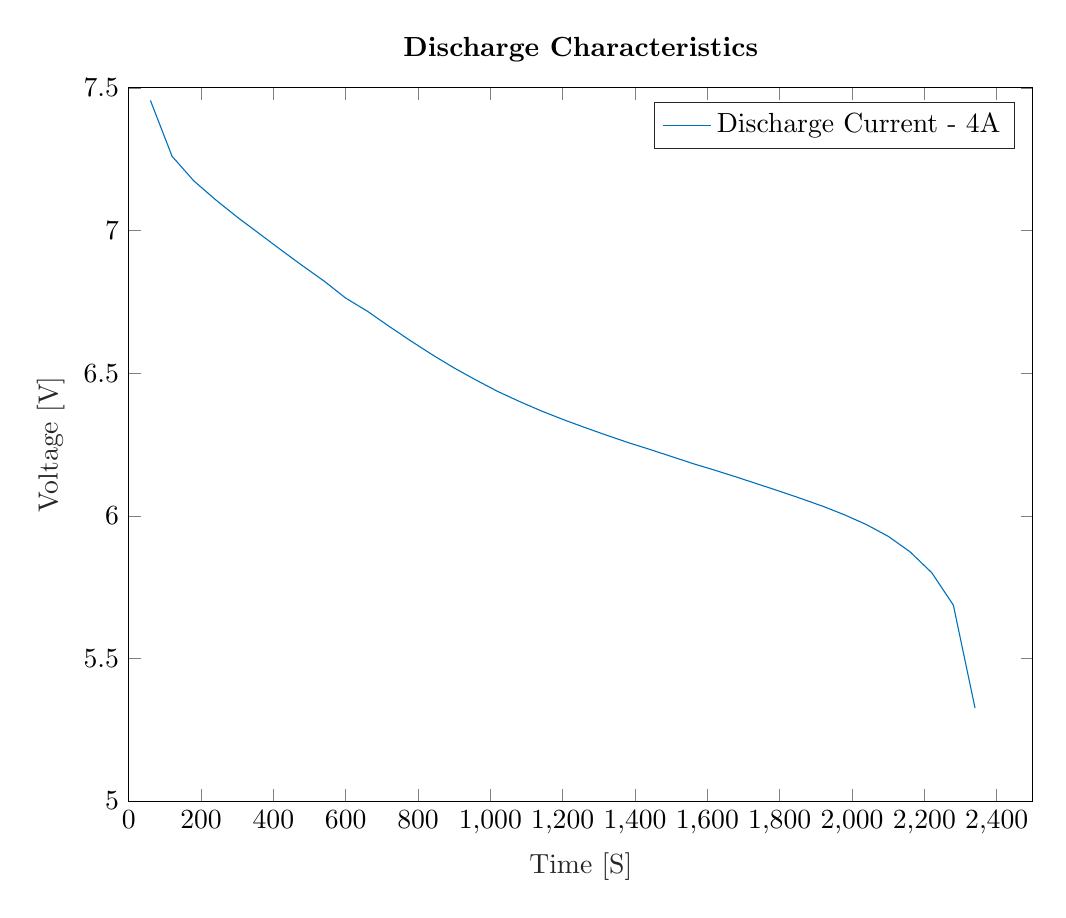
\begin{tikzpicture}

\begin{axis}[%
width=4.521in,
height=3.566in,
at={(0.758in,0.481in)},
scale only axis,
xmin=0,
xmax=2500,
xlabel style={font=\color{white!15!black}},
xlabel={Time [S]},
ymin=5,
ymax=7.5,
ylabel style={font=\color{white!15!black}},
ylabel={Voltage [V]},
axis background/.style={fill=white},
title style={font=\bfseries},
title={Discharge Characteristics},
legend style={legend cell align=left, align=left, draw=white!15!black}
]
\addplot [color=mycolor1]
  table[row sep=crcr]{%
60	7.456\\
120	7.26\\
180	7.174\\
240	7.108\\
300	7.047\\
360	6.99\\
420	6.933\\
480	6.877\\
540	6.823\\
600	6.763\\
660	6.717\\
720	6.664\\
780	6.613\\
840	6.564\\
900	6.518\\
960	6.476\\
1020	6.436\\
1080	6.401\\
1140	6.368\\
1200	6.338\\
1260	6.31\\
1320	6.283\\
1380	6.257\\
1440	6.233\\
1500	6.208\\
1560	6.183\\
1620	6.16\\
1680	6.136\\
1740	6.111\\
1800	6.086\\
1860	6.06\\
1920	6.033\\
1980	6.003\\
2040	5.969\\
2100	5.928\\
2160	5.874\\
2220	5.801\\
2280	5.687\\
2340	5.326\\
};
\addlegendentry{Discharge Current - 4A}

\end{axis}
\end{tikzpicture}%
  \caption{Discharge curve of the Ansmann 18650 2S1P Li-Ion battery used to power the swarmbot.}
  \label{fig:discharge}
\end{figure}
% subsection discharge_curve_of_the_ansmann_2s1p (end)
%\mikkel{Alle signaler i texttt}

\subsubsection*{IO ports}
To ensure the functionality of the IO ports and the MicroZed in general two tests were performed.
In the first test a VHDL program was written to turn on a LED connected to a IO port. 
It worked, which led to the conclusion that the PL part of the MicroZed and the IO port worked properly.

In the next test a C program was written to make a LED blink.
This test also succeeded, which led to the conclusion that both the PS and PL part of the MicroZed worked properly.

\subsubsection*{Conclusion}
The problems on the carrier card were found and fixed through systematic debugging.
The carrier card has the wanted powerup and powerdown sequence which was measured using an oscilloscope. 
On shutdown the power switch introduces bouncing on the \texttt{V\_OFF} signal which could be filtered away by a low pass filter.
The PS, PL and IO functionalities of the MicroZed when connected to the carrier were verified through tests.
